% !TeX program = lualatex
\documentclass[11pt]{article}
\usepackage[a4paper,margin=27mm,headheight=14pt]{geometry}
\usepackage{fontspec}
\setmainfont{texgyretermes-regular.otf}[Path=fonts/,BoldFont=texgyretermes-bold.otf,ItalicFont=texgyretermes-italic.otf,BoldItalicFont=texgyretermes-bolditalic.otf]
\setsansfont{texgyreheros-regular.otf}[Path=fonts/,BoldFont=texgyreheros-bold.otf,ItalicFont=texgyreheros-italic.otf,BoldItalicFont=texgyreheros-bolditalic.otf]
\setmonofont{lmmono10-regular.otf}[Path=fonts/,ItalicFont=lmmono10-italic.otf]
\usepackage{amsmath,amssymb,amsthm,unicode-math}
\setmathfont{latinmodern-math.otf}[Path=fonts/]
\usepackage{graphicx,array,booktabs,longtable,enumitem,xcolor,needspace}
\usepackage{xr-hyper}
\usepackage[numbers,sort&compress]{natbib}
\usepackage[unicode,colorlinks=true,allcolors=blue!45!black,bookmarksnumbered,hypertexnames=false]{hyperref}
\hypersetup{pdftitle={Tournament anti-Sidorenko orientations of trees with at most five branch vertices},pdfauthor={Yanbin Qiao and Liwei Yao}}
\renewcommand{\theHtable}{lt.\arabic{table}}
\setlength{\emergencystretch}{2em}
\setlength{\parskip}{2pt}
\setlength{\parindent}{1.4em}
\setlength{\lineskiplimit}{4pt}
\setlength{\lineskip}{4pt}
\allowdisplaybreaks[2]
\numberwithin{equation}{section}
\newcommand{\proofpart}[1]{\par\smallskip\noindent\textbf{#1.}\enspace}
\newsavebox{\mathfitbox}
\newcommand{\fitdisplay}[2]{%
 \begin{equation*}%
 \sbox{\mathfitbox}{$\displaystyle #1$}%
 \ifdim\wd\mathfitbox>\linewidth
  \typeout{MATHFIT original=\the\wd\mathfitbox target=\the\linewidth inputline=\the\inputlineno}%
  \resizebox{\linewidth}{!}{\usebox{\mathfitbox}}%
 \else\usebox{\mathfitbox}\fi
 \if\relax\detokenize{#2}\relax\else\tag{#2}\fi
 \end{equation*}%
}
\makeatletter
\renewcommand{\@pnumwidth}{2.5em}
\renewcommand{\@tocrmarg}{3.5em}
\ifdefined\ArticleView\else
 \renewcommand*\l@subsection{\@dottedtocline{2}{1.5em}{3.4em}}
\fi
\renewcommand\paragraph{\@startsection{paragraph}{4}{\z@}{1.8ex plus .5ex minus .2ex}{.6ex plus .2ex}{\normalfont\normalsize\bfseries}}
\makeatother
\newtheorem{theorem}{Theorem}[section]
\newtheorem{proposition}[theorem]{Proposition}
\newtheorem{lemma}[theorem]{Lemma}
\newtheorem{corollary}[theorem]{Corollary}
\theoremstyle{definition}
\newtheorem{definition}[theorem]{Definition}
\theoremstyle{remark}
\newtheorem{remark}[theorem]{Remark}
\newcommand{\E}{\mathbb E}
\newcommand{\one}{\mathbf1}
\newcommand{\homc}{\operatorname{hom}}
\newcommand{\ip}[2]{\left\langle#1,#2\right\rangle}
\newcommand{\norm}[1]{\left\lVert#1\right\rVert}
\newcommand{\op}{2\to2}
\newcommand{\can}{\mathrm{can}}
\newcommand{\Nplus}[1]{N_+(#1)}
\newcommand{\Nminus}[1]{N_-(#1)}
\title{Tournament anti-Sidorenko orientations of trees\\with at most five branch vertices}
\author{%
\begin{tabular}{c}
Yanbin Qiao\thanks{Yanbin Qiao and Liwei Yao contributed equally and should be considered joint first authors. Both authors are corresponding authors.}\quad Liwei Yao\\[0.4em]
\normalsize School of Mathematics, China University of Mining and Technology\\
\normalsize Xuzhou, Jiangsu 221116, China\\[0.3em]
\small Yanbin Qiao: \href{mailto:a15024953277@qq.com}{a15024953277@qq.com}\\
\small Liwei Yao: \href{mailto:10235419@cumt.edu.cn}{10235419@cumt.edu.cn}\\
\small ORCID: \href{https://orcid.org/0009-0005-2476-208X}{0009-0005-2476-208X}\quad
\href{https://orcid.org/0009-0005-6990-9372}{0009-0005-6990-9372}
\end{tabular}}
\date{}


% Reading views share one source graph and one mathematical manuscript.
\ifdefined\ArticleView
 \externaldocument{article-external}[02_Technical_Appendix.pdf]
\fi
\ifdefined\SupplementView
 \externaldocument{supplement-external}[01_Article.pdf]
\fi
\begin{document}
\raggedbottom
\maketitle
\ifdefined\SupplementView
% The main text contains nine tables and six figures.
\setcounter{table}{9}
\setcounter{figure}{6}
\begin{center}\large Appendices\end{center}
This file contains all appendices to the accompanying article. It includes
the shared calculus, the worked estimate, the four-branch foundations,
the direction tables and the local proofs cited by the main text.
\setcounter{tocdepth}{2}
\tableofcontents
\clearpage
\else
\begin{abstract}
A finite tree with at most five vertices of degree at least three admits an orientation whose homomorphism density into any tournament is at most the random-tournament benchmark. Degrees, arm multiplicities and positive subdivision lengths are unrestricted, and a single orientation, chosen from the tree alone, satisfies the stronger kernel inequality for every finite probability space and every real skew kernel of absolute value at most one. For four branch vertices we convert terminal fourth moments into weighted second moments across a connector; for five we allocate reference arms in the star and fork skeletons and join the two halves of the path skeleton through compatible fractional moments. Separate arguments cover a central singleton arm and a unit outer connector. The kernel inequality also yields an entropy bound that holds for arbitrarily correlated vertex labels.
\end{abstract}
\noindent\textbf{Keywords:} tournaments; anti-Sidorenko inequality; oriented trees; skew kernels; weighted moments.\\
\textbf{MSC 2020:} 05C20, 05C05, 05C35, 47A30.\\
\ifdefined\ArticleView\else
\setcounter{tocdepth}{2}\tableofcontents\clearpage
\fi
\section{Introduction}\label{sec:intro}
For an oriented graph $D$ and a finite tournament $\mathcal T$, let
$\homc(D,\mathcal T)$ be the number of arc-preserving vertex maps from
$D$ to $\mathcal T$; the maps need not be injective. An orientation $D$
of a tree $U$ is \emph{tournament anti-Sidorenko} if
\begin{equation}\label{eq:tas}
 \homc(D,\mathcal T)\le 2^{-e(U)}|V(\mathcal T)|^{|V(U)|}
\end{equation}
for every nonempty finite loopless tournament. The factor $2^{-e(U)}$
is the limiting density of $D$ in a uniformly random tournament. Thus
\eqref{eq:tas} bounds the number of maps from $D$ into any tournament
by this random benchmark. Fox, Himwich, Mani and Zhou conjectured that every tree
admits such an orientation~\cite[Conjecture 1.12]{FHMZ}. We prove their
conjecture for trees with at most five branch vertices.

Here a \emph{branch vertex} of $U$ is a vertex of degree at least three,
and
\[
 b(U)=|\{v\in V(U):\deg_U(v)\ge3\}|,\qquad e(U)=|E(U)|.
\]
All degrees refer to $U$.

\begin{theorem}\label{thm:main}
Every nonempty finite tree $U$ with $b(U)\le5$ has an orientation
$D=D(U)$ satisfying \eqref{eq:tas} for every nonempty finite loopless
tournament $\mathcal T$.
\end{theorem}

We prove a kernel form of the theorem, in which one orientation serves
every host. For a nonempty finite probability space $(X,\mu)$ and a real
skew kernel $K:X^2\to[-1,1]$, put
\begin{equation}\label{eq:density}
 Z_D(K,\mu)=\E_{\mu^{V(U)}}
       \prod_{u\to v\in E(D)}(1+K(x_u,x_v)).
\end{equation}
All labels are independently sampled from the same measure; coincident
labels are included.
\begin{theorem}\label{thm:kernel}
For every nonempty finite tree $U$ with $b(U)\le5$, there is an
orientation $D=D(U)$ of all its edges such that
\begin{equation}\label{eq:kernelbound}
 Z_D(K,\mu)\le1
\end{equation}
for every nonempty finite probability space and every real skew kernel
bounded in absolute value by one.
\end{theorem}

\paragraph{Related results.}
Sidorenko's conjecture bounds the homomorphism density of a bipartite
graph from below in terms of its edge density~\cite{Sidorenko}; the
tournament problem seeks an orientation with a universal upper bound
at the random benchmark. Table~\ref{tab:prior} lists the tree classes covered by the
relevant results. These classes overlap only partly: arbitrary
subdivisions produce many vertices of degree two, whereas a bound on
$b(U)$ restricts neither the degrees nor the multiplicities of equal
branches.

\begin{table}[htbp]\centering\small
\caption{Tree classes covered by the closest prior results and by this paper.}\label{tab:prior}
\begin{tabular}{@{}p{45mm}p{103mm}@{}}\toprule
Work & Scope\\\midrule
Fox--Himwich--Mani--Zhou~\cite[Proposition 1.13]{FHMZ} & Trees with at most one vertex of even degree.\\
Chen--Clemen--Noel~\cite{CCN} & Every three-legged spider, with arbitrary leg lengths.\\
He--Mani--Nie--Tung--Wei~\cite[Theorems 1.3 and 1.4]{HMNTW} & Isomorphic-branch attachment and every caterpillar.\\
Theorem~\ref{thm:main} & Every tree with at most five original vertices of degree at least three, with unrestricted degrees, multiplicities and positive subdivision lengths.\\\bottomrule
\end{tabular}
\end{table}
Chen and Lin prove path anti-Sidorenko inequalities when the length is
large relative to the number of direction flips~\cite{CL}. Paths enter
our argument in a different role, as connectors that carry rooted
messages between branch vertices; their lengths are arbitrary, including
one.

\paragraph{Proof strategy.}
The proof separates the assembly of a tree from the local moment
estimates. Table~\ref{tab:proof-route} gives the route through the
assembly; the technical appendix proves the inputs listed there.

\begin{table}[htbp]\centering\small
\caption{The proof of Theorems~\ref{thm:main} and~\ref{thm:kernel}. Each row uses the preceding structural reductions and the indicated local estimates.}\label{tab:proof-route}
\begin{tabular}{@{}p{29mm}p{77mm}p{39mm}@{}}\toprule
Stage & Argument or required input & Location\\\midrule
Path interface & Weighted second moments at two roots control every positive connector length. & Lemma~\ref{lem:weighted-interface}\\
Four branches & Pair equal arms; convert terminal fourth moments to the second moments needed by the interface. & Sections~\ref{sec:geometry}--\ref{sec:star}\\
Five-branch reduction & Reduce to four branches or to $P_5$, $K_{1,4}$ and the fork $T_5$. & Lemma~\ref{lem:five-reduction}\\
Star and fork & Allocate disjoint arms to simple-reference fourth, ordinary eighth and compound-reference second moments. & Section~\ref{sec:five-star-fork}; Propositions~\ref{prop:five-reference}--\ref{prop:five-compound}\\
Path alternatives & First treat a central singleton and a unit off-center arm whose receiving connector has length one. & Section~\ref{sec:five-chain}\\
Remaining path & Give both sides the same inverse-weighted boundary estimate; close by H\"older at the center. & Proposition~\ref{prop:five-outlet}; \eqref{eq:five-chain-close}\\
Conclusion & Fix all choices from the tree, restore equal pairs, and pass from kernels to tournaments. & Section~\ref{sec:completion}\\\bottomrule
\end{tabular}
\end{table}

For four branch vertices the terminal fourth moments close the path
$P_4$ and the star $K_{1,3}$. For five, the star and fork need one
existing central arm as a reference, while the path uses
$I_q(V)=\E[q^{-1/3}|V|^{8/3}]$, with $q=1-K\one$.
After the two structural path alternatives, both side messages satisfy
this bound with the same $q$; the three weight powers cancel in the
central H\"older inequality. The arm allocation, rather than a
restriction on the connector lengths, distinguishes these assemblies.

Appendix~\ref{app:local-calculus} gives the shared scalar calculus,
and Appendix~\ref{app:worked} proves one terminal estimate in full.
Appendix~\ref{app:five-directions} is the entry point to the remaining
direction tables: it separates reference, ordinary and outlet inputs,
whose directions and weights differ. The local proofs retain the
short-length exceptions before treating the finite tails.

\section{Kernel preliminaries and rooted messages}\label{sec:prelim}\label{q3:sec:method}
Delete zero-mass atoms and use the real inner product $\ip{u}{v}=\E(uv)$ on $L^2(\mu)$. Define
\begin{equation}\label{q3:eq:notation}
 Ju=(\E u)\one,\quad A=J+K,\quad A^*=J-K,\quad
 g=K\one,\quad d=\E g^2,\quad p=1+g,\quad q=1-g.
\end{equation}
All operators and adjoints are taken with respect to this measure. We also write $r=Kg$. Write $T=A^*$. Both $A$ and $T$ have nonnegative kernels. Since $K(x,x)=0$ and $\mu(x)>0$, we have $p(x),q(x)\ge\mu(x)>0$.

The row constraint is
\begin{equation}\label{q3:eq:cyclepoint}
 |r(x)|\le[1-g(x)^2]/2=p(x)q(x)/2.
\end{equation}
For $a_y=K(x,y)$, antisymmetrization gives
$r(x)=\frac12\E_{y,z}[(a_y-a_z)K(y,z)]$.
The scalar inequality $|u-v|\le1-uv$ on $[-1,1]^2$ follows by squaring,
since the difference is $(1-u^2)(1-v^2)\ge0$.
Taking expectations proves \eqref{q3:eq:cyclepoint}.

For an orientation $D$ of a rooted tree, its message is the conditional integral of the product in~\eqref{eq:density}, with the root label fixed and all other labels integrated independently.

For $n\ge0$ put $f_n=A^n\one$, $\bar f_n=(A^*)^n\one$, $\mu_n=\E f_n$ and, for $n\ge1$, $h_n=A^*f_{n-1}$. At a rooted arm of length $n$, these are the actual messages of, respectively, all edges pointing away from the root, all edges pointing toward the root, and the first edge pointing toward the root with every remaining edge pointing away along the arm. In particular, $f_1=p$ and $h_1=q$.

We use the constants and moments
\begin{equation}\label{q3:eq:constants}
 \theta=\frac{13}{32},\qquad C_*=\frac{101}{50},\qquad
 \delta_j=\norm{K^j\one}_2^2,\qquad S_n=\sum_{j=0}^nK^j\one.
\end{equation}
Appendix~\ref{q3:app:foundations} proves $\norm K_{\op}\le2/\pi$, $d\le1/3$, $\delta_{j+1}\le\theta \delta_{j}$, $\mu_n\le1$, and the positive convolution identity
\begin{equation}\label{q3:eq:convolution}
 S_n=f_n+\sum_{j=3}^n\beta_jf_{n-j},\qquad
 d-\delta_{2}\le\beta_j\le d\quad(j\ge3).
\end{equation}
The elementary identity $A+A^*=2J$ gives
\begin{equation}\label{q3:eq:equalpair}
 f_n+h_n=2\mu_{n-1},\qquad 0<f_nh_n\le\mu_{n-1}^2\le1.
\end{equation}

At a root, pair equal arm lengths maximally and use $f_n,h_n$ on each pair; let $E_0$ be the actual product of the pair messages, so $0<E_0\le1$. The remaining lengths are distinct and are exactly those of odd multiplicity. Since $E_0\le1$, an upper bound may drop $E_0$.

For an even arm list, its \emph{positive canonical orientation} pairs the remaining distinct lengths adjacently, assigning $h_af_b$ to a pair $a<b$. For an odd list, retain the shortest residual arm as an outward anchor $f_a$ and pair the rest in this way. Write the odd message as $f_aR$, where $R$ includes all equal and distinct pairs. The \emph{negative canonical orientation} reverses all the corresponding edges. A universal assertion at $-K$ proves the reversed one.


For later use set
\[
 N_+(H)=\E[pH^2],\qquad N_-(H)=\E[qH^2].
\]

\begin{lemma}[Weighted path interface]\label{lem:weighted-interface}\label{lem:connector}
For every integer $L\ge1$ and all real $H,G$,
\[
 |\ip H{A^LG}|\le\sqrt{N_+(H)N_-(G)},\qquad N_-(AG)\le N_-(G).
\]
The reversed statements hold after interchanging $A,T$ and $p,q$.
\end{lemma}
\begin{proof}
The nonnegative edge measure $(1+K(x,y))\,d\mu(x)d\mu(y)$ has marginals $p\mu,q\mu$. Cauchy--Schwarz on this measure proves the first inequality for $L=1$. Row Cauchy--Schwarz gives $(AG)^2\le pA(G^2)$, and hence
\[
 N_-(AG)\le\E[pqA(G^2)]=\E[T(pq)G^2]\le\E[qG^2],
\]
because $pq=1-g^2\le1$ and $T$ preserves order. Iterate $L-1$ times and apply the one-edge inequality.
\end{proof}

\begin{lemma}[Rooted spider boundary]\label{lem:spidersecond}
Every finite arm multiset admits an orientation, fixed independently of the kernel and measure, with actual message $F$ satisfying $N_-(F)\le1$.
\end{lemma}
The direction for each residual arm list, and the proof, are given in Appendix~\ref{q3:app:spiderboundary}. Reversal gives the corresponding $N_+$ statement.

\begin{table}[htbp]\centering\small
\caption{Notation used in the moment calculations.}\label{tab:notation}
\begin{tabular}{@{}p{29mm}p{117mm}@{}}\toprule
Symbol & Meaning\\\midrule
$g,r$ & $K\one$ and $Kg$, both with the original measure.\\
$r_0$ & The centered function $QKg=Kg+d\one$, used only in Appendix~\ref{q3:app:operators}.\\
$d,\delta_j$ & $d=\E g^2=\delta_1$ and $\delta_j=\|K^j\one\|_2^2$. Ordinary powers such as $d^2$ remain powers of $d$.\\
$f_n,\bar f_n,h_n$ & Outward, inward, and first-edge-inward arm messages, respectively.\\
$\beta_j,\omega_j$ & Positive convolution coefficients, and local envelope or propagation losses; neither is a path function.\\
$\xi$ & A scalar score coordinate in a polynomial comparison: $p(x)=\xi$, $q(x)=2-\xi$.\\
$n_T$ & Number of vertices of the host tournament.\\\bottomrule
\end{tabular}
\end{table}

\section{The four-branch foundation}\label{sec:four-foundation}
The five-branch argument uses the following four-branch result whenever
a reduction removes one branch vertex.
\begin{theorem}\label{thm:four}
For every nonempty finite tree $U$ with $b(U)\le4$, there is an
orientation $D=D(U)$ of all its edges such that \eqref{eq:tas} holds for
every nonempty finite loopless tournament.
\end{theorem}
\begin{theorem}\label{thm:four-kernel}
The orientation in Theorem~\ref{thm:four} can be chosen so that
$Z_D(K,\mu)\le1$ for every finite probability space and every real skew
kernel bounded in absolute value by one.
\end{theorem}
Appendix~\ref{sec:three} proves the assertion for at most three branch
vertices. Section~\ref{sec:geometry} reduces to the two skeletons,
Section~\ref{sec:terminals} supplies the terminal estimates and the
internal side tables; Sections~\ref{sec:chain} and~\ref{sec:star}
then close the chain and the star. These inputs also serve the five-branch
case.

\section{The two branching skeletons and a reduction}\label{sec:geometry}
Theorem~\ref{q3:thm:kernel} gives every tree with at most three branch vertices one orientation satisfying \eqref{eq:kernelbound} for every finite model, so it remains to treat $b(U)=4$.

Let $B$ be the four original branch vertices, and let $S$ be the minimal connected subtree of $U$ containing $B$. Every vertex of degree at least three in $S$ belongs to $B$, since it also has original degree at least three. Every leaf of $S$ belongs to $B$, by minimality. Suppressing the degree-two vertices of $S$ outside $B$ leaves a tree on exactly four vertices, which is either a path $P_4$ or a star $K_{1,3}$ (Figure~\ref{fig:skeletons}).

Each skeleton edge represents a positive-length path in the original tree, whose interior vertices have degree two and carry no side arms. Every component outside the core is a path attached at a branch vertex, since another branch point there would belong to $B$, contrary to the choice of $S$. These components are the \emph{side arms}, and the core paths together with the side arms partition the edges of $U$.

\begin{figure}[htbp]\centering
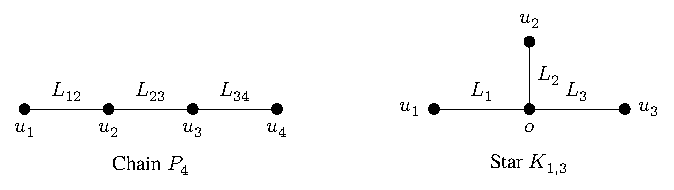
\includegraphics{figures/skeletons.pdf}
\caption{The two skeletons on four branch vertices. Each edge represents its original positive-length connector; side arms are omitted from the drawing.}\label{fig:skeletons}
\end{figure}

A leaf of the skeleton is called a \emph{terminal}. It has at least two actual side arms in $U$. Maximally pair its equal-length arms using \eqref{q3:eq:equalpair}.

\begin{lemma}[Reducible terminal]\label{lem:reduction}
If a terminal has zero or one residual side arm after equal-length pairing, then $U$ has a fixed orientation satisfying \eqref{eq:kernelbound}.
\end{lemma}
\begin{proof}
Orient the equal pairs so that their product is $E_i\le1$. Removing those paired arms for the comparison leaves the terminal vertex, its remaining arm if any, and all core edges; the terminal then has degree at most two and no other degree has increased. The comparison tree is nonempty, has at most three branch vertices, and carries a fixed orientation from Theorem~\ref{q3:thm:kernel}. Restoring those arms multiplies the nonnegative integrand at the terminal label by $E_i\le1$, preserving the density bound.
\end{proof}

The reduction applies to both skeletons. We may therefore assume that every terminal has at least two distinct residual lengths. Singleton internal side tables and singleton star-center tables survive the reduction and are estimated in Sections~\ref{sec:chain} and~\ref{sec:star}.

\section{The complete terminal fourth-moment catalogue}\label{sec:terminals}
Let $\Sigma$ be a terminal arm multiset whose distinct residual list has at least two entries, with arbitrary original multiplicities. We use the following local estimate.

\begin{theorem}[Terminal supply]\label{thm:terminal}
For each integer $n\ge0$ there is an orientation of all the arms, with actual message $F^+_{\Sigma,n}$, determined by $\Sigma$ and $n$, such that
\begin{equation}\label{eq:terminalplus}
 \E\bigl[p(T^nF^+_{\Sigma,n})^4\bigr]\le1.
\end{equation}
Its complete reversal $F^-_{\Sigma,n}=\bar F^+_{\Sigma,n}$ satisfies
\begin{equation}\label{eq:terminalminus}
 \E\bigl[q(A^nF^-_{\Sigma,n})^4\bigr]\le1.
\end{equation}
The parameter $n$ is a prescribed integer determined by the original connector length.
\end{theorem}

The catalogue below proves the theorem, with analytic estimates in the indicated sections of Appendices~\ref{app:zero-moments}--\ref{app:odd-propagation}.

\subsection{Zero-step directions}
Every direction in this subsection includes the equal-pair multiplier $E_0$. For an even residual list, put
\[
 P=\prod_{i=1}^t h_{a_i}f_{b_i},\qquad
 a_1<b_1<\cdots<a_t<b_t.
\]
This direction $F^+_{\Sigma,0}=E_0P$ satisfies $\E[p(F^+_{\Sigma,0})^4]\le1$. The pair $(1,2)$ is treated directly in Section~\ref{loc:S13}. Every other even residual list also satisfies a weighted sixth-moment bound, which yields the fourth moment by H\"older against $p\mu$; the complete even catalogue, with its component ranges, is collected at the end of Section~\ref{loc:even-zero-catalogue}, with proofs in Appendix~\ref{q3:app:foundations} and Sections~\ref{loc:S2}--\ref{loc:S9}.

For an odd residual list $a<b_1<c_1<\cdots<b_t<c_t$, $t\ge1$, use
\begin{equation}\label{eq:zeroOdd}
 F^+_{\Sigma,0}=
 \begin{cases}
 E_0 qf_{b_1}h_{c_1}\displaystyle\prod_{i=2}^t h_{b_i}f_{c_i},&a=1,\\[3pt]
 \displaystyle\overline{E_0f_a\prod_{i=1}^t h_{b_i}f_{c_i}},&a\ge2.
 \end{cases}
\end{equation}
The first line is proved in Section~\ref{loc:S14}, for every number of pairs. The second line is the full reversal of the $q$-weighted fourth estimates for positive canonical odd messages, with minimum two in Section~\ref{loc:S15} and minimum at least three in Section~\ref{loc:S16}; there the equal-pair arms are reversed together with the residual arms, which is what converts the $q$ weight into the $p$ weight.

\subsection{Positive steps: even residual lists}
Write the residual list as $a_1<b_1<\cdots<a_t<b_t$, $t\ge1$. The following table gives the residual part of $F^+_{\Sigma,n}$ for every $n\ge1$; multiply each row by its actual $E_0$.

\begin{table}[htbp]
\centering
\caption{Positive-step terminal directions for even residual lists.}\label{tab:terminal-even}
\fontsize{9}{11}\selectfont
\setlength{\tabcolsep}{1pt}\noindent\begin{tabular}{@{}p{57mm}p{68mm}p{29mm}@{}}
\toprule
Residual condition & Residual message & Complete proof\\\midrule
$t=1$, $(a_1,b_1)=(1,2)$ & $qf_2$ & Section~\ref{loc:S21}\\
$t=1$, $a_1=1$, $b_1\ge3$ & $qf_{b_1}$ & Section~\ref{loc:S24}\\
$t\ge2$, $a_1=1$ & $\prod_{i=1}^t h_{a_i}f_{b_i}$ & Section~\ref{loc:S29}\\
$t=1$, $(a_1,b_1)=(2,3)$ & $h_2f_3$ & Section~\ref{loc:S23}\\
$t=1$, $a_1=2$, $b_1\ge4$ & $h_2f_{b_1}$ & Section~\ref{loc:S25}\\
$t\ge2$, $a_1=2$ & $\prod_{i=1}^t h_{a_i}f_{b_i}$ & Section~\ref{loc:S33}\\
$a_1=3$, any $t\ge1$ & $f_3h_{b_1}\prod_{i=2}^t h_{a_i}f_{b_i}$ & Sections~\ref{loc:S28}, \ref{loc:S30}\\
$a_1\ge4$, any $t\ge1$ & $\prod_{i=1}^t h_{a_i}f_{b_i}$ & Section~\ref{loc:S27}\\
\bottomrule
\end{tabular}

\end{table}

The row of minimum three uses $f_3h_{b_1}$, with the first pair reversed.

\subsection{Positive steps: odd residual lists}
Write
\[
 a<b_1<c_1<b_2<c_2<\cdots<b_t<c_t,\qquad t\ge1.
\]
Again the table gives only the residual part and covers all $n\ge1$. Here $\bar f_a=T^a\one$ is a path function, whereas $b_i$ in the ordered list is an arm length.

\begin{table}[htbp]
\centering
\caption{Positive-step terminal directions for odd residual lists.}\label{tab:terminal-odd}
\fontsize{9}{11}\selectfont
\setlength{\tabcolsep}{1pt}\noindent\begin{tabular}{@{}p{54mm}p{71mm}p{29mm}@{}}
\toprule
Residual condition & Residual message & Complete proof\\\midrule
$a=1,t=1,b_1=2,c_1=3$ & $qf_2h_3$ & Section~\ref{loc:S22}\\
$a=1,t=1,b_1=2,c_1\ge4$ & $qf_2h_{c_1}$ & Section~\ref{loc:S26}\\
$a=1,t=1,3\le b_1<c_1$ & $qf_{b_1}h_{c_1}$ & Section~\ref{loc:S31}\\
$a=1,t\ge2$ & $qf_{b_1}h_{c_1}\prod_{i=2}^t h_{b_i}f_{c_i}$ & Section~\ref{loc:S35}\\
$a=2,b_1=3$, any $t\ge1$ & $\bar f_2f_3h_{c_1}\prod_{i=2}^t h_{b_i}f_{c_i}$ & Section~\ref{loc:S34}\\
$a\ge2,b_1=4$ & $\bar f_af_4h_{c_1}\prod_{i=2}^t h_{b_i}f_{c_i}$ & Section~\ref{loc:S32}\\
$a\ge2,b_1\ge5$ & $\bar f_a\prod_{i=1}^t h_{b_i}f_{c_i}$ & Section~\ref{loc:S32}\\
\bottomrule
\end{tabular}

\end{table}

\paragraph{Completeness of the terminal classification.}
For an even list the minimum is $1,2,3$, or at least four; the first
two cases split into one pair and multiple pairs.  For an odd list of
minimum one, the cases split by the number of pairs and then by the second
length.  At minimum two the second length is three, four, or at
least five; at larger minimum it is at least four.  The inward
anchor $\bar f_a$ is an actual arm with all of its edges directed toward
the root.

\subsection{Restoration, reversal, and interface length}
The proofs in the tables are for the residual message and already allow arbitrary equal-pair factors. Since $0\le E_0\le1$ and $P\ge0$ give $T^n(E_0P)\le T^nP$, taking fourth powers and integrating against the nonnegative weight $p$ restores the paired arms without weakening the bound.

Applying \eqref{eq:terminalplus} at $-K$ interchanges $T$ with $A$, $p$ with $q$, and the selected arm message with its complete reversal, which proves \eqref{eq:terminalminus}.

For a connector of original length $L$, keeping the edge nearest the internal vertex leaves $n=L-1$ edges to integrate, so $L=1$ uses the zero-step catalogue and $L\ge2$ the positive-step one. In the empty-center star construction of Section~\ref{sec:emptystar} one terminal is propagated through all $L$ edges.

\subsection{The two internal side-table roles}
After equal pairing, an internal side table in a chain is of one of two kinds. Call it type R if its residual list is empty or has at least two entries. For an empty list take $V^+=E_0$, and otherwise use the zero-step catalogue. In either case
\begin{equation}\label{eq:R}
 \E[p(V^+)^4]\le1,\qquad V^-=\bar V^+,
 \qquad \E[q(V^-)^4]\le1.
\end{equation}
Call the table type S if it has exactly one residual arm, of length $a\ge1$. Put $C^+=E_0f_a$ and $C^-=\bar C^+$. The complete singleton estimate is
\begin{equation}\label{eq:S}
 \E[q^5(C^+)^4]\le1,\qquad \E[p^5(C^-)^4]\le1.
\end{equation}
For $a=1$, $q^5p^4=q(pq)^4\le q$ proves this directly. The length-two proof is Section~\ref{loc:S17}, and all lengths $a\ge3$ are proved in Section~\ref{loc:S19}.

\section{The chain skeleton}\label{sec:chain}
Let $u_1,u_2,u_3,u_4$ be the branch vertices in path order. Write $L_{12},L_{23},L_{34}\ge1$ for their original connector lengths. By Lemma~\ref{lem:reduction}, the two terminals may be assumed irreducible. Every central-path edge will point from $u_2$ toward $u_3$.

\subsection{Four half-tree inequalities}
The following inequalities account for the weights in the internal catalogue; all factors in each product are evaluated at the same root label.
\begin{lemma}\label{lem:halftree}
For nonnegative functions $C,F,G$,
\begin{align}
 \Nplus{CTF}&\le\sqrt{\E[qC^4]\,\E[pF^4]},\label{eq:mergeRleft}\\
 \Nminus{CTF}&\le\sqrt{\E[q^5C^4]\,\E[pF^4]},\label{eq:mergeSright}\\
 \Nminus{CAG}&\le\sqrt{\E[pC^4]\,\E[qG^4]},\label{eq:mergeRright}\\
 \Nplus{CAG}&\le\sqrt{\E[p^5C^4]\,\E[qG^4]}.\label{eq:mergeSleft}
\end{align}
\end{lemma}
\begin{proof}
Row Cauchy--Schwarz gives $(TF)^2\le qT(F^2)$. Hence
\[
 \Nplus{CTF}\le\E[pqC^2T(F^2)]\le\E[C^2T(F^2)].
\]
The edge measure for $T$ has root marginal $q\mu$ and other marginal $p\mu$. Cauchy--Schwarz on that measure proves \eqref{eq:mergeRleft}. For \eqref{eq:mergeSright}, retain the extra factors:
\[
 \Nminus{CTF}\le\E[q^2C^2T(F^2)]
 \le\sqrt{\E[q(q^2C^2)^2]\,\E[pF^4]}.
\]
The first term is exactly $\E[q^5C^4]$. Complete reversal gives \eqref{eq:mergeRright} and \eqref{eq:mergeSleft}.
\end{proof}

The merger converts fourth moments into the second moments required by Lemma~\ref{lem:connector}.

\subsection{Compatible directions for all four role combinations}
At the left terminal set $n_1=L_{12}-1$ and use Theorem~\ref{thm:terminal} to define
\[
 G_1^+=T^{n_1}F^+_{1,n_1},\qquad
 G_1^-=A^{n_1}F^-_{1,n_1}.
\]
Then $\E[p(G_1^+)^4]\le1$ and $\E[q(G_1^-)^4]\le1$. Use $n_4=L_{34}-1$ at the right terminal to obtain $G_4^\pm$ with the same bounds. The superscript at a terminal is chosen according to its adjacent internal role in the following table.

\begin{table}[htbp]
\centering
\caption{Compatible outer directions and half-tree bounds.}\label{tab:roles}
\fontsize{9}{11}\selectfont
\setlength{\tabcolsep}{2pt}\noindent\begin{tabular}{@{}p{15mm}p{26mm}p{32mm}p{39mm}p{36mm}@{}}
\toprule
Role & Side message & Entire outer path & Half-tree message & Required output\\\midrule
Left R & $V_2^-$ & $u_1\to u_2$ & $H_\ell=V_2^-TG_1^+$ & $N_+(H_\ell)\le1$\\
Left S & $C_2^-$ & $u_2\to u_1$ & $H_\ell=C_2^-AG_1^-$ & $N_+(H_\ell)\le1$\\
Right R & $V_3^+$ & $u_3\to u_4$ & $H_r=V_3^+AG_4^-$ & $N_-(H_r)\le1$\\
Right S & $C_3^+$ & $u_4\to u_3$ & $H_r=C_3^+TG_4^+$ & $N_-(H_r)\le1$\\
\bottomrule
\end{tabular}

\end{table}

For example, a left type-R vertex has side message $V_2^-$ with $q$-weighted fourth moment at most one. The retained incoming edge contributes $T$, so \eqref{eq:mergeRleft} gives $N_+(H_\ell)\le1$. A left type-S vertex has the fully reversed side message $C_2^-$ with $p^5$-weighted fourth moment at most one; \eqref{eq:mergeSleft} gives the same $N_+$ output, using an outgoing outer path. The right type-R and type-S cases follow from \eqref{eq:mergeRright} and \eqref{eq:mergeSright}, respectively.

The factor $TG$ or $AG$ integrates the final edge of the outer connector; its preceding $L-1$ edges are integrated in $G$. For an outer connector of length one, $G$ is the zero-step terminal message.

The two side tables and the two terminal arm systems are disjoint, so their directions can be chosen independently. For each of the four role combinations RR, RS, SR and SS, the left half produces an $N_+$ bound and the right half an $N_-$ bound.

\begin{figure}[htbp]\centering
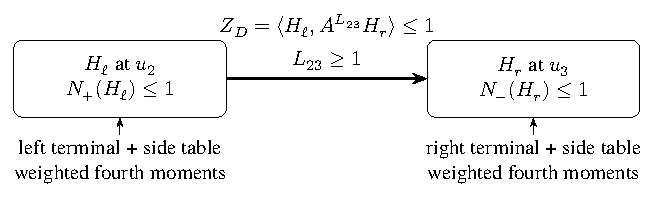
\includegraphics{figures/chain-merger.pdf}
\caption{The chain merger. Terminal and side-table fourth moments give the two indicated half-tree bounds. The outer directions depend on the R/S roles in Table~\ref{tab:roles}; the central connector always points from $u_2$ to $u_3$.}\label{fig:chain}
\end{figure}

\subsection{The complete central path}
After integration over every arm and both outer connector interiors, the original density is exactly
\begin{equation}\label{eq:chaindensity}
 Z_D(K,\mu)=\ip{H_\ell}{A^{L_{23}}H_r}.
\end{equation}
Lemma~\ref{lem:connector} gives
\[
 Z_D(K,\mu)\le\sqrt{N_+(H_\ell)N_-(H_r)}\le1.
\]
Together with the reducible-terminal case, this proves the theorem for the entire $P_4$ skeleton.

\section{The star skeleton}\label{sec:star}
Let $o$ be the central branch vertex and $u_1,u_2,u_3$ the three terminal branch vertices, with connector lengths $L_1,L_2,L_3\ge1$. The center may have no side arms. Write $E_c$ for its product of equal-length arm pairs, so $0\le E_c\le1$.

\subsection{The center catalogue}
The residual center tables fall into three classes. In the first, a fixed message $C$ satisfies
\begin{equation}\label{eq:center3}
 \E[q^3C^4]\le1.
\end{equation}
The table gives the direction for each row. The factor $E_c$ multiplies every row, and the products $P$ and $V^+$ involve only the indicated residual arms.

\begin{table}[htbp]
\centering
\caption{Center directions with a cubed-weight fourth moment.}\label{tab:center}
\fontsize{9}{11}\selectfont
\setlength{\tabcolsep}{1pt}\noindent\begin{tabular}{@{}p{56mm}p{66mm}p{32mm}@{}}
\toprule
Residual center table & Message $C/E_c$ & Complete proof\\\midrule
Singleton $a\ge1$ & $f_a$ & Section~\ref{loc:S36}\\
Odd, at least three, minimum one & $pP$, $P$ canonical on the rest & Section~\ref{loc:S18}; \eqref{eq:unitcenter}\\
Odd, at least three, minimum $a\ge2$ & $f_aP$, $P$ canonical on the rest & Section~\ref{loc:S18}\\
Even, minimum two & $f_2h_{b_1}\prod_{i=2}^t h_{a_i}f_{b_i}$ & Section~\ref{loc:S38}\\
Even, minimum three & $f_3h_{b_1}\prod_{i=2}^t h_{a_i}f_{b_i}$ & Section~\ref{loc:S37}\\
Even, minimum at least four & $\prod_{i=1}^t h_{a_i}f_{b_i}$ & Section~\ref{loc:S37}\\
Even, at least four, minimum one & $pV^+$ & Section~\ref{loc:S38}; \eqref{eq:unitcenter}\\
\bottomrule
\end{tabular}

\end{table}

The unit-arm reductions in the second and last rows are direct. If $V\ge0$ is the message of the row in question, with $\E[pV^4]\le1$, then
\begin{equation}\label{eq:unitcenter}
 \E[q^3(pV)^4]=\E[p(pq)^3V^4]\le\E[pV^4]\le1.
\end{equation}
For an odd center of minimum one, $V=P$ is the canonical even product. For an even center with at least four entries and minimum one, the remaining odd list has at least three entries, and $V^+$ is exactly its zero-step direction in \eqref{eq:zeroOdd}. The leading $p$ comes from the unit arm.

The singleton row directs its residual arm outward for every length and is proved in
Section~\ref{loc:S36}, with a separate certificate for the two-edge arm.

The second center class consists of a residual list exactly $(1,b)$, $b\ge2$. Direct both residual arms outward and take
\begin{equation}\label{eq:center9}
 C=E_cpf_b,\qquad
 \E[q^9C^4]\le\E[q^5f_b^4]\le1.
\end{equation}
Indeed $q^9C^4=E_c^4(pq)^4q^5f_b^4$. The last inequality is the complete singleton estimate in Sections~\ref{loc:S17}, \ref{loc:S19}. This class uses the ninth power rather than the cubed weight, including the case $b=2$.

The third class has an empty residual list and message $C=E_c\le1$; Section~\ref{sec:emptystar} handles it with a different merger.

The first class
contains every odd nonempty list and every even list whose minimum is two,
three, or at least four. An even list with minimum one has either two
entries, which gives the second class, or at least four, which gives the
first. The empty list is the third class.

\begin{figure}[htbp]\centering
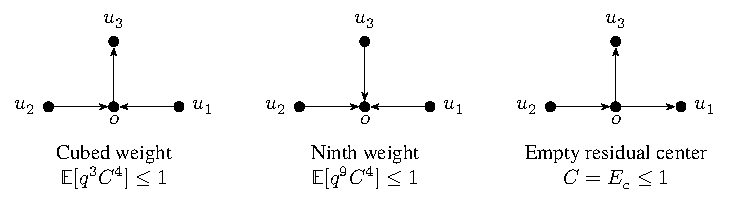
\includegraphics{figures/star-centers.pdf}
\caption{Core directions for the three star-center constructions. The empty-center case uses a full $L_1$-step terminal on the right-hand path and a second-moment terminal on the upper path. All connector lengths remain positive and arbitrary.}\label{fig:star}
\end{figure}

\subsection{Cubed-weight centers: two incoming paths and one outgoing path}
Assume \eqref{eq:center3}. Reducible terminals have already been covered by Lemma~\ref{lem:reduction}. Fix the core directions
\[
 u_1\longrightarrow o,\qquad u_2\longrightarrow o,
 \qquad o\longrightarrow u_3,
\]
with every original edge of each path pointing consistently. Put
\[
 G_i=T^{L_i-1}F^+_{i,L_i-1}\quad(i=1,2),\qquad
 H_3=A^{L_3-1}F^-_{3,L_3-1}.
\]
The terminal theorem gives $\E[pG_i^4]\le1$ and $\E[qH_3^4]\le1$. Retaining only the final edge near $o$ on each path, the density is
\begin{equation}\label{eq:stardensity}
 Z_D=\E[C(TG_1)(TG_2)(AH_3)].
\end{equation}
We control two groups at the same center label. First,
\begin{align}
 \norm{CTG_1}_2^2
 &\le\E[qC^2T(G_1^2)]\notag\\
 &\le\sqrt{\E[q^3C^4]\,\E[pG_1^4]}\le1.\label{eq:starfirst}
\end{align}
The first step is row Cauchy--Schwarz; the second applies Cauchy--Schwarz to the $T$ edge measure, whose root marginal is $q\mu$.
For the other two paths, row Cauchy--Schwarz and $pq\le1$ give
\begin{align}
 \norm{(TG_2)(AH_3)}_2^2
 &\le\E[pq\,T(G_2^2)A(H_3^2)]\notag\\
 &\le\ip{G_2^2}{A^2(H_3^2)}\notag\\
 &\le\sqrt{\E[pG_2^4]\,\E[qH_3^4]}\le1.\label{eq:starsecond}
\end{align}
The middle expression uses $T^*=A$, and the last step is Lemma~\ref{lem:connector} with length two. The joint estimate integrates the two adjacent edges at their common label. Applying ordinary Cauchy--Schwarz to the two groups in \eqref{eq:stardensity} proves $Z_D\le1$.

\subsection{Ninth-weight centers: all three paths incoming}
Now use \eqref{eq:center9} and direct every connector from $u_i$ toward $o$. Set $G_i=T^{L_i-1}F^+_{i,L_i-1}$, so $\E[pG_i^4]\le1$. The exact density is
\[
 Z_D=\E\left[C\prod_{i=1}^3TG_i\right].
\]
H\"older on a row of the nonnegative $T$ kernel gives
\begin{equation}\label{eq:rowholder}
 (TG_i)^4\le q^3T(G_i^4).
\end{equation}
The factor $q^3$ reflects the mass $q$ of the row measure. Apply \eqref{eq:rowholder}, followed by four-factor H\"older on the original probability measure:
\begin{align*}
 Z_D&\le\E\left[Cq^{9/4}\prod_{i=1}^3T(G_i^4)^{1/4}\right]\\
 &\le\left(\E[q^9C^4]\prod_{i=1}^3\E[T(G_i^4)]\right)^{1/4}\\
 &=\left(\E[q^9C^4]\prod_{i=1}^3\E[pG_i^4]\right)^{1/4}\le1.
\end{align*}
The equality uses $\E[Tv]=\E[pv]$.

\subsection{Empty residual center}\label{sec:emptystar}
Here $C=E_c\le1$. Choose the core directions $o\to u_1$, $u_2\to o$, and $o\to u_3$. At the first terminal use the \emph{positive-step} supply through the entire first path:
\[
 X=A^{L_1}F^-_{1,L_1},\qquad \E[qX^4]\le1.
\]
At the second terminal retain its last edge and put
\[
 G=T^{L_2-1}F^+_{2,L_2-1},\qquad \E[pG^4]\le1.
\]
At the third terminal choose the actual spider direction of Lemma~\ref{lem:spidersecond}, with message $F_3$ and $N_-(F_3)\le1$; a second-moment bound suffices here.

Let $H=X(TG)$. Row Cauchy--Schwarz, followed by edge Cauchy--Schwarz with the correct marginals, yields
\begin{align*}
 N_+(H)&\le\E[pqX^2T(G^2)]\\
 &\le\sqrt{\E[p^2q^3X^4]\,\E[pG^4]}\\
 &\le\sqrt{\E[qX^4]\,\E[pG^4]}\le1.
\end{align*}
In the last comparison $p^2q^2\le1$ is used. Multiplying by $C\le1$ gives $N_+(CH)\le1$. The exact density is
\[
 Z_D=\ip{CH}{A^{L_3}F_3}
 \le\sqrt{N_+(CH)N_-(F_3)}\le1.
\]
The three center constructions, the terminal catalogue, and Lemma~\ref{lem:reduction} prove the assertion for the $K_{1,3}$ skeleton.

\section{Five branch vertices: reduction and geometry}\label{sec:five-geometry}
Let $B$ be the five original branch vertices and let $S$ be their minimal
connecting subtree. Its leaves belong to $B$, and every vertex of
degree at least three in $S$ belongs to $B$. Suppressing the degree-two
vertices outside $B$ reveals the skeleton. The resulting tree
on five vertices is $P_5$, $K_{1,4}$ or $T_5$: maximum degree four gives
the star, maximum degree three gives degree sequence $(3,2,1,1,1)$,
and maximum degree two gives the path. Each skeleton edge retains its
original positive path length, and every off-core component is a side arm.

At each skeleton vertex $v$, pair equal-length side arms maximally.
Let $c_v$ be its skeleton degree and $t_v$ the number of remaining
distinct arm lengths.
\begin{lemma}\label{lem:five-reduction}
If $c_v+t_v\le2$ at any skeleton vertex, then $U$ has an orientation
satisfying \eqref{eq:kernelbound} for every finite model.
\end{lemma}
\begin{proof}
Orient each equal pair as in \eqref{q3:eq:equalpair}, then bound their
product at $v$ by one in the integrand. The comparison tree retains
$v$, all core paths and the unpaired arms, and has at most four branch
vertices; Theorem~\ref{thm:four-kernel} gives it a fixed orientation.
Restoring the pairs at their original attachment multiplies the
integrand at $v$ by their actual product, which is at most one, so the
original density is also at most one.
\end{proof}
Apply this test at every skeleton vertex. In $P_5$ it covers an empty
internal residual and a terminal with at most one residual arm; an empty
residual at the star or fork center needs the separate argument of
Section~\ref{sec:five-star-fork}.

\begin{figure}[htbp]\centering
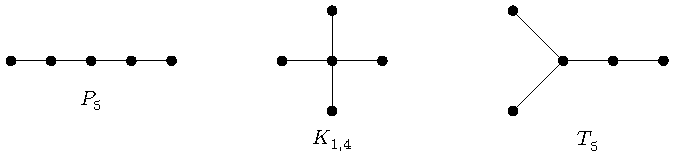
\includegraphics{figures/five-skeletons.pdf}
\caption{The three skeletons on five branch vertices. Every drawn edge denotes an independently chosen positive-length path in the original tree.}\label{fig:five-skeletons}
\end{figure}

\section{The five-branch boundary estimates}\label{sec:five-inputs}
Besides $f_n,\bar f_n,h_n$, write
\[
 W_n=A\bar f_{n-1}\quad(n\ge1),\qquad
 I_q(V)=\E[q^{-1/3}|V|^{8/3}].
\]
The arm message $W_n$ directs its first edge away from the root and
its remaining edges toward the first neighbor. Reversal exchanges
$f_n$ with $\bar f_n$ and $h_n$ with $W_n$.

\subsection{Simple-reference and ordinary moments}
The terminal residuals below contain at least two distinct lengths.
All messages include their actual equal-pair factors.
\begin{proposition}[Simple-reference fourth moments]\label{prop:five-reference}
For every existing outward arm $f_s$, $s\ge1$, every terminal arm
multiset as above, and every connector length $L\ge1$, there is a
structurally chosen terminal direction with actual received message
$X=T^LF$ such that
\[
 \E[f_sX^4]\le1.
\]
For $s\ge3$, the direction in the genuine-reference table satisfies
the stronger bound $1-d/3000$; for $s=2$ only the bound $1$ is used.
\end{proposition}
For $s=1$ the assertion is Theorem~\ref{thm:terminal} with step count
$L$. For $s\ge2$ the direction table and its proof are in
Sections~\ref{proof:R2-C032} and~\ref{proof:R2-C034}, indexed in
Appendix~\ref{app:five-directions}; the short-arm directions there are
specific to this reference catalogue.

For ordinary moments, a \emph{post block} means actual unequal central
pairs with negative canonical message
\[
 P=\prod_{i=1}^k W_{u_i}\bar f_{v_i},\qquad
 4\le u_1<v_1<\cdots<u_k<v_k.
\]
When nonempty, it is required that the designated anchor length satisfy
$m<u_1$. This order is automatic in the central allocations below.
\begin{proposition}[Ordinary eighth moments]\label{prop:five-ordinary}
Given an existing arm of length $m\ge3$, a terminal residual of size at
least two, a connector of length $L\ge1$ and a post block in the stated
order, there is a direction of exactly these resources with actual
message $H$ satisfying
\[
 \E H^8\le e^{-d/1024}.
\]
Given instead one existing unit arm and no unequal post block, there
is an actual message $H_1$ with $\E H_1^8\le1-d/20000$.
\end{proposition}
The complete ordinary direction table, including the first-edge
choices, is in Section~\ref{proof:R2-C046}, and
Appendix~\ref{app:five-directions} indexes its cases. The nonunit proof
draws on Sections~\ref{proof:R2-C030}, \ref{proof:R2-C038},
\ref{proof:R2-C039}, \ref{proof:R2-C040} and~\ref{proof:R2-C043}; the
unit input is the ordinary catalogue of Section~\ref{proof:Q5-C106}.
For the terminal $(1,2,3)$, the special direction occurs at $L=2$ in this
ordinary catalogue and at $L=1$ in the genuine-reference catalogue.

We also use the following path and mixed central bounds:
\begin{equation}\label{eq:five-mixed}
 \E f_s^2\le1\quad(s\ge2),\qquad
 \E[f_s^2Q^8]\le e^{-17d/64},
\end{equation}
where the second bound has
$Q=W_a\bar f_b\prod_iW_{u_i}\bar f_{v_i}$ and
$2\le s<a<b<u_1<v_1<\cdots$. The mixed proof, including $s=2$ and $a=3$,
is in Section~\ref{proof:R2-C044}. When $Q=1$ only the first bound is
needed. For $s=2$ its exact value is $1-d+\delta_2$; for $s\ge3$ the
finite path estimate gives $\E f_s^2\le1-d+2\delta_2\le1-3d/16$.

\subsection{A reference second moment for a compound branch}
A fork has a two-segment branch $c-r-t$ with independent lengths
$M,N\ge1$ and arbitrary side-arm tables at $r,t$.
\begin{proposition}\label{prop:five-compound}
For each $s\ge1$, this actual compound branch admits a direction with
received message $Y$ satisfying $\E[f_sY^2]\le1$.
\end{proposition}
\begin{proof}
If $t$ is reducible, its retained connector and possible residual arm
form one comparison arm at $r$. Choose the canonical endpoint direction
used in \eqref{q3:eq:singleendpoint}, apply that inequality, and restore
the equal pairs. Otherwise put
$G=T^{N-1}F^+_{t,N-1}$, so $\E[pG^4]\le1$.

If the residual at $r$ is empty or has at least two entries, select its
negative zero-step factor $C_r^-$ with $\E[q(C_r^-)^4]\le1$ and set
$H=C_r^-TG$, $Y=T^MH$. Row H\"older and Cauchy--Schwarz give
\begin{equation}\label{eq:inverse-half}
 (TG)^4\le q^3T(G^4),\qquad
 \E[H^2/q]\le\sqrt{\E[q(C_r^-)^4]\,
                         \E[(TG)^4/q^3]}\le1.
\end{equation}
Thus $H=\sqrt q\,h$ with $\|h\|_2\le1$. The operator bounds in
Proposition~\ref{q3:prop:operators}, together with normalized
propagation, give
\begin{equation}\label{eq:five-normalized}
 \sqrt{f_s}T^M\sqrt q
  =(\sqrt{f_s}T\sqrt q)(q^{-1/2}T\sqrt q)^{M-1},
 \qquad\|\sqrt{f_s}T^M\sqrt q\|\le1.
\end{equation}
This proves the claim in the R case, including $M=N=1$.

If $r$ has one residual arm of length $a$, orient it inward as
$\bar f_a$. At $t$, choose the positive canonical direction for an
even residual list and the negative canonical direction for an odd
residual list, and denote the resulting message by $S$. Let $S^-$
be its full reversal and put $V=A^NS^-$, $H=\bar f_aV$ and $Y=T^MH$.
The full reversal of \eqref{q3:eq:singleendpoint} gives
$\E[\bar f_aV^2]\le1$ for every $a,N\ge1$.
The cross-path contraction
$\|\sqrt{f_s}T^M\sqrt{\bar f_a}\|\le1$ proves the assertion.
Equal pairs at $r$ are restored by positivity.
\end{proof}

\subsection{The common-reference outlets for the path skeleton}
Consider one side $c-r-t$ of $P_5$. Its terminal connector $r-t$ has
length $L\ge1$, and its receiving connector $r-c$ has length $M\ge1$.
The terminal residual has size at least two, and the
residual at $r$ is nonempty. The following catalogue is used after the two
whole-tree alternatives of Section~\ref{sec:five-chain}.
\begin{proposition}[Common-reference outlet]\label{prop:five-outlet}
Except for a unit singleton at $r$ with $M=1$, every such side has an
actual message $U$ at $c$, determined by the structure, satisfying
\begin{equation}\label{eq:five-outlet}
 I_q(U)^3\le e^{-\eta d},\qquad \eta\ge1/500.
\end{equation}
Both sides of the path use the same $q$.
\end{proposition}
\begin{table}[htbp]\centering\small
\caption{The path outlet catalogue. The entries locate the proofs in the technical appendix, and Appendix~\ref{app:five-directions} indexes the direction tables.}\label{tab:five-outlets}
\begin{tabular}{@{}p{38mm}p{54mm}p{50mm}@{}}\toprule
Root residual & Structural subdivision & Where proved\\\midrule
Unit singleton & $M=2$; $M\ge3$ &
\ref{proof:R2-C026}, \ref{proof:R2-C029}, \ref{proof:R2-C031},
\ref{proof:R2-C033}, \ref{proof:R2-C035}, \ref{proof:R2-C037};
\ref{proof:Q5-C079}, \ref{proof:Q5-C106}\\
Singleton $a\ge2$ & $M=1,3,\ge4$; $a=2,M=2$; $a\ge3,M=2$ &
\ref{proof:R2-C032}, \ref{proof:R2-C034}, \ref{proof:R2-C045},
\ref{proof:Q5-E008-singleton}; \ref{proof:R2-C047}; \ref{proof:R2-C048}\\
Exactly two arms & Minimum one; minimum at least two &
\ref{proof:Q5-C066}, \ref{proof:Q5-C106}; \ref{proof:R2-C046}\\
Odd, at least three & Minimum one, two, or at least three &
\ref{proof:Q5-C185}, \ref{proof:Q5-C186}, \ref{proof:Q5-C188},
\ref{proof:Q5-C189}, \ref{proof:Q5-C192};
\ref{proof:R2-C002}--\ref{proof:R2-C005}\\
Even, at least four & Minimum one or at least two, with one actual inward multiplier retained &
\ref{proof:R2-C042}\\\bottomrule
\end{tabular}
\end{table}
The unit-singleton row $M=1$ is handled by the whole-tree construction
before this catalogue is consulted.

\section{The five-vertex star and fork}\label{sec:five-star-fork}
Let $c$ be the degree-four star center or the degree-three fork center.
There are four simple terminal branches in the star, and two simple
terminal branches plus one compound branch in the fork. A reducible
simple terminal is covered by Lemma~\ref{lem:five-reduction}.
Write $E_c\le1$ for the product of central equal pairs.

\subsection{Nonempty central residuals}
Table~\ref{tab:five-center} allocates the central arms along the
increasing residual list. One actual outward arm $f_s$ serves as the
common reference; an ordinary message consumes its anchor, one simple
terminal and the connecting path; the central equal pairs belong to one
indicated factor.
\begin{table}[htbp]\centering\small
\caption{Central arm allocation for $K_{1,4}$ and $T_5$. Later pairs always retain their displayed negative canonical directions.}\label{tab:five-center}
\begin{tabular}{@{}p{38mm}p{19mm}p{43mm}p{40mm}@{}}\toprule
Residual list & Reference & Ordinary factors & Other central factors\\\midrule
Singleton $s$ & $f_s$ & None & $E_c$ in one reference message\\
$(s,m,\text{later pairs})$, $2\le s<m$ & $f_s$ & $H$: anchor $m$, later pairs, $E_c$ & None\\
$(s,a,b,\text{later pairs})$, $2\le s<a<b$ & $f_s$ & $H_a$ and $H_b$; latter holds later pairs and $E_c$ & None\\
$(1,s,m,\text{later pairs})$ & $f_s$ & Unit $H_1$; $H_m$ holds later pairs and $E_c$ & None\\
$(1,s)$ or $(1,s,a,b,\text{later pairs})$ & $f_s$ & Unit $H_1$ holds $E_c$ & $Q=1$ or $W_a\bar f_b$ times later pairs\\\bottomrule
\end{tabular}
\end{table}
In every nonsingleton row $s\ge2$, so \eqref{eq:five-mixed} applies,
and the anchor preceding a nonempty post block is shorter than all its
post lengths, as Proposition~\ref{prop:five-ordinary} requires.

For a singleton center the densities are
\[
 Z_\star=\E[f_sX_1X_2X_3X_4],\qquad
 Z_{T_5}=\E[f_sX_1X_2Y].
\]
Use H\"older exponents $(4,4,4,4)$ or $(4,4,2)$ and the reference
estimates. Both densities are at most one, including $s=1,2$.

For a nonunit even center the products are $f_sHX_2X_3X_4$ and
$f_sHXY$. Factor the first into
$H,f_s^{1/4},f_s^{1/4}X_2,f_s^{1/4}X_3,f_s^{1/4}X_4$,
and the second into $H,f_s^{1/4},f_s^{1/4}X,f_s^{1/2}Y$.
H\"older with exponents $(8,8,4,4,4)$ or $(8,8,4,2)$ gives, in both
cases, $Z_D\le e^{-d/8192}$.

For a nonunit odd center there are two distinct ordinary factors.
The star and fork factors are, respectively,
\[
 (H_a,H_b,f_s^{1/2},f_s^{1/4}X_3,f_s^{1/4}X_4),\qquad
 (H_a,H_b,f_s^{1/2},f_s^{1/2}Y).
\]
The same exponent lists give $Z_D\le e^{-d/4096}$.
For a unit-minimum odd center replace the first ordinary input by
$\E H_1^8\le1-d/20000$. This gives
\[
 Z_D\le (1-d/20000)^{1/8}e^{-d/8192}
       \le e^{-(1/160000+1/8192)d}.
\]

For a unit-minimum even center use the factors
$H_1,f_s^{1/4}Q$ and the remaining reference factors. Equations
\eqref{eq:five-mixed} and the same H\"older exponents give
\begin{equation}\label{eq:five-star-strict}
 Z_D\le
 \begin{cases}
 e^{-d/160000},&Q=1,\\
 e^{-(1/160000+17/512)d},&Q\ne1.
 \end{cases}
\end{equation}
The reference
arm carries total analytic power one, and the ordinary factors use
distinct terminal branches. H\"older applies to the resulting functions
of the central label.

\subsection{Empty central residual}
For the star, choose two paths toward $c$ and two away from it. Put
$G_i=T^{L_i-1}F^+_{i,L_i-1}$ for $i=1,2$ and
$H_i=A^{L_i-1}F^-_{i,L_i-1}$ for $i=3,4$. Then
\[
 Z_D=\E[E_c(TG_1)(TG_2)(AH_3)(AH_4)].
\]
For each pair, row Cauchy--Schwarz, $pq\le1$, and the path interface give
\[
 \E[(TG)^2(AH)^2]
 \le\ip{G^2}{A^2(H^2)}
 \le\sqrt{\E[pG^4]\,\E[qH^4]}\le1.
\]
Cauchy--Schwarz on $(TG_1)(AH_3)$ and $(TG_2)(AH_4)$ proves $Z_D\le1$.

For the fork label its simple ends $a,b$ and its compound $c-r-t$,
with lengths $L_a,L_b,M,N$. Set
\[
 X=A^{L_a}F^-_{a,L_a},\quad
 G=T^{L_b-1}F^+_{b,L_b-1},\quad H_c=E_cX(TG).
\]
The first terminal uses the $L_a$-step supply. The edge measure
for $T$ has marginals $q\mu,p\mu$, so
\[
 N_+(H_c)\le\sqrt{\E[p^2q^3X^4]\,\E[pG^4]}
             \le\sqrt{\E[qX^4]\,\E[pG^4]}\le1.
\]
If $r$ is type R, choose its positive zero-step factor $V_r^+$ and put
$V=A^{N-1}F^-_{t,N-1}$, $H_r=V_r^+AV$. If $r$ is a singleton,
put $C_r^+=E_rf_a$, $V=T^{N-1}F^+_{t,N-1}$ and $H_r=C_r^+TV$.
Inequality~\eqref{eq:mergeRright} gives $N_-(H_r)\le1$ in the R case, and
\eqref{eq:mergeSright} in the singleton case, where the $q^5$ weight enters.
Direct the whole $M$-path from $c$ to $r$. Then
\[
 Z_D=\ip{H_c}{A^MH_r}\le\sqrt{N_+(H_c)N_-(H_r)}\le1.
\]
This proves both skeletons. Only the
nonsingleton central allocations give the strict loss $e^{-d/160000}$;
the comparison, empty-center and singleton-center directions give the
bound $1$.

\section{The five-vertex path}\label{sec:five-chain}
Write the core in path order as
\[
 t\;--_{L_-}\;r\;--_{M_-}\;c\;--_{M_+}\;w\;--_{L_+}\;z,
 \qquad L_-,M_-,M_+,L_+\ge1.
\]
Here $L_\pm$ counts a terminal connector and $M_\pm$ the connector
from an off-center root to $c$. In a local outlet formula, $L$ denotes
the terminal-connector length and $M$ the receiving-connector length.
After Lemma~\ref{lem:five-reduction}, the two terminal residuals have
at least two entries and the three internal residuals are nonempty.
Call an internal residual S if it is a singleton and R otherwise.

\subsection{A central singleton: the maximal S spine}
Suppose $c$ is S. Take the maximal consecutive S sequence among
$r,c,w$ that contains $c$. Orient its singleton arms alternately as
$f_a$ and $\bar f_b$, starting with an outward arm at its left end.
Every connector between consecutive S vertices points from the
negative end toward the positive end. The corresponding operators
between square roots of the actual arm messages are
\[
 B_i=\sqrt{f_a}T^{M_i}\sqrt{\bar f_b}
 \quad\hbox{or their adjoints},\qquad \|B_i\|\le1
\]
by Proposition~\ref{q3:prop:operators}.

At a positive S end whose arm has message \(f_s\), an ordinary
terminal supplies
\[
 y=\sqrt{f_s}\,T^LF_t,\qquad \|y\|_2\le1,
\]
where \(F_t\) is positive canonical for an even residual list and
negative canonical for an odd residual list; the norm bound is
\eqref{q3:eq:singleendpoint}. An R half-tree supplies instead
\[
 y=\sqrt{f_s}\,T^MH,\qquad
 H=C^-TG=\sqrt q\,h,\qquad \|h\|_2\le1.
\]
Equations~\eqref{eq:inverse-half} and~\eqref{eq:five-normalized}
give \(\|y\|_2\le1\) for every \(M\ge1\).
At a negative S end reverse the entire outside configuration:
the two endpoint functions become
\(\sqrt{\bar f_s}A^LF_t^-\) and
\(\sqrt{\bar f_s}A^MH^-\), respectively, with the same norm bound.

Bounding the genuine equal-pair factors on the spine by one gives
\[
 \ip{y_L}{B_1\cdots B_{j-1}y_R}\le1,
 \qquad \|y_L\|_2,\|y_R\|_2\le1.
\]
For a one-vertex spine this is $\ip{y_L}{y_R}$. This covers the patterns SSS, RSS,
SSR and RSR. The two square roots of each arm contribute one arm factor, and each
original connector appears once.

\subsection{A unit off-center arm with a unit receiving connector}
Now suppose the center is R and, say, $r$ has one unit residual arm
and its receiving connector $r-c$ has $M_-=1$. Put $L=L_-$ and choose the terminal direction with
step count $L-1$. Its composite message at $r$ is
\[
 F_*^+=E_r^-qA^LF^-_{t,L-1}.
\]
The actual unit arm is the factor $q$. Row H\"older and $pq\le1$ give,
for every real $G$,
\[
 \E[q|pTG|^4]\le\E[(pq)^4T(|G|^4)]\le\E[p|G|^4].
\]
Full reversal proves $\E[p(F_*^+)^4]\le1$. The one edge from $r$ to
$c$ has not yet been integrated. Choose the central negative R factor
$C^-$ with $\E[q(C^-)^4]\le1$ and put $H_c=C^-TF_*^+$.
Lemma~\ref{lem:halftree} gives $N_+(H_c)\le1$.

At $w$, use the right R or S construction in Table~\ref{tab:roles},
with its actual terminal and terminal-connector length $L_+$. It gives a message
$H_w$ with $N_-(H_w)\le1$. Direct the entire $M_+$-path from $c$ to
$w$. The exact density is
\[
 Z_D=\ip{H_c}{A^{M_+}H_w}\le1.
\]
This whole-tree construction replaces the $I_q$ outlet at $r$.

\subsection{Two compatible outlets}
In the remaining structural branch $c$ is R, and any unit singleton
off-center has receiving-connector length at least two. Choose the central negative
zero-step factor $C_c$ as follows. An even residual uses negative
canonical pairs. An odd residual beginning with one uses
$E_c^-p\bar f_aW_b$ followed by negative canonical pairs. A nonunit
odd residual uses $E_c^+f_a$ followed by positive canonical pairs.
These are the full reversals of the corresponding zero-step
directions, so
\[
 \E[qC_c^4]\le1.
\]
Proposition~\ref{prop:five-outlet} supplies actual outputs $U_-,U_+$
for the two sides, both using this same $q$. Integration over their
disjoint interiors gives $Z_D=\E[C_cU_-U_+]$.
H\"older at exponents $4,8/3,8/3$ yields
\begin{align}\label{eq:five-chain-close}
 Z_D&\le(\E[qC_c^4])^{1/4}
             I_q(U_-)^{3/8}I_q(U_+)^{3/8}\notag\\
 &\le e^{-(\eta_-+\eta_+)d/8}\le e^{-d/2000}\le1.
\end{align}
The weight powers $1/4,-1/8,-1/8$ cancel, and both side functions are evaluated at the same central label.

\begin{figure}[htbp]\centering
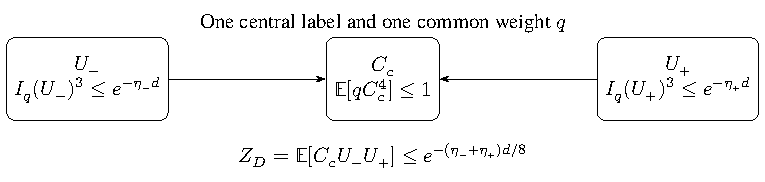
\includegraphics{figures/five-path-closure.pdf}
\caption{The remaining path branch. The two structural alternatives are applied first; only then are the two local outlets joined with the same central reference weight.}\label{fig:five-path}
\end{figure}

The root catalogue divides nonempty residual lists into singletons,
pairs, odd lists of at least three entries, and even lists of at least four. Singletons split according to their arm and
receiving-connector lengths: the two-step construction treats an arm of
length two differently from one of length at least three, and the choice
depends on the length; $d$ enters in the estimates. The minimum-two odd row with a
terminal $(2,t)$ has its own first-edge choices, notably $W_2\bar f_t$ at
$L=1$ and $\bar f_2W_t$ at $L\ge2$; the table in the technical appendix
lists them all. Together with the two whole-tree alternatives above,
\eqref{eq:five-chain-close} proves every $P_5$.

\subsection{A worked five-branch example}\label{sec:five-example}
Consider the path core in Figure~\ref{fig:five-example}, with connector
lengths \((L_-,M_-,M_+,L_+)=(2,1,2,1)\) and pendant-arm lists
\begin{equation}\label{eq:five-example:arms}
\begin{array}{c|ccccc}
 \text{vertex}&t&r&c&w&z\\\hline
 \text{arm lengths}&(2,4)&(1,3,4)&(4,5)&(2,4,5)&(2,3).
\end{array}
\end{equation}
This tree has 45 edges and five branch vertices, of degrees
\(3,5,4,5,3\). It falls in the two-outlet case above.
Direct every core edge toward \(c\), and choose the pendant directions
specified by the following messages:
\begin{equation}\label{eq:five-example:messages}
\begin{aligned}
 F_-&=\bar f_2W_4,& H_-&=pW_3\bar f_4\,T^2F_-,&U_-&=TH_-,\\
 F_+&=W_2\bar f_3,& H_+&=f_2h_4f_5\,TF_+,&U_+&=T^2H_+,\\
 &&C&=W_4\bar f_5.
\end{aligned}
\end{equation}
Integration over the two sides gives \(Z_D=\E[CU_-U_+]\).
We verify the three moment inputs to this identity directly.
When \(d=0\), leaf integration gives \(Z_D=1\); henceforth assume \(d>0\).

\begin{figure}[htbp]\centering
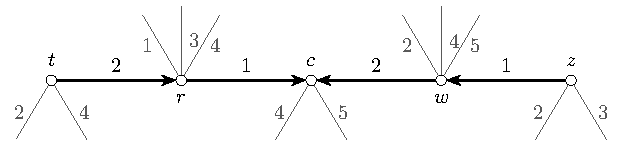
\includegraphics{figures/five-branch-example.pdf}
\caption{The five-branch example. Each segment represents a path of
the indicated length; pendant directions are specified in
\eqref{eq:five-example:messages}.}\label{fig:five-example}
\end{figure}

Put \(B=-K\) and \(u=-g=B\one\), so that \(T=J+B\),
\(A=J-B\), \(p=1-u\), and \(q=1+u\). We use
\(d\le1/3\), \(\delta_{j+1}\le\theta\delta_j\),
\(\theta=13/32\), and the spectral measure \(\nu\) of \(-B^2\)
at \(u\), for which \(\int x^j\,d\nu=\delta_{j+1}\).
The row bound \(|BV|\le\|V\|_2\) and
\eqref{eq:oc:signed-moments} give the common fourth-moment rule
\begin{equation}\label{eq:five-example:payment}
 0\le H\le e^{a+BV}\quad\Longrightarrow\quad
 \log\E H^4\le4(a+\E BV)+\tfrac{17}{4}\|V\|_2^2.
\end{equation}
The arm recurrences \(f_{n+1}=Af_n\),
\(\bar f_{n+1}=T\bar f_n\), \(h_n=Tf_{n-1}\), and
\(W_n=A\bar f_{n-1}\) give
\begin{equation}\label{eq:five-example:identities}
\begin{aligned}
 \bar f_2+W_4&=2-2d+du-B^2u-B^3u,\\
 W_3+\bar f_4&=2-3d-du+B^3u,\\
 W_2+\bar f_3&=2-d+B^2u,\\
 h_4+f_5&=2-4d+\delta_2-df_2-B^4u,\\
 W_4+\bar f_5&=2-4d+\delta_2-d\bar f_2+B^4u.
\end{aligned}
\end{equation}
These identities and \(ab\le e^{a+b-2}\) for nonnegative \(a,b\)
provide all the envelopes below.

\paragraph{The two-step side.}
Set
\[
 R=du-B^2u-B^3u,\quad s=\E R^2
   =d^3+2d\delta_2+\delta_3+\delta_4,\quad
 \Delta=-\delta_2+\tfrac32s,
 \quad\epsilon=\Delta-d^2-\delta_2.
\]
The first identity gives \(F_-\le e^{-2d+R}\).
Since \(|R|\le d+\sqrt{\delta_2+\delta_3}<1\), the elementary
bound \(e^y\le1+y+3y^2/4\), \(|y|\le1\), and positivity give
\[
 TF_-\le e^{-2d}(q+BR+\Delta),\qquad
 T^2F_-\le e^{-2d}(\bar f_2+B^2R+\Delta q-d^2-\delta_2).
\]
Adding the factors in the last upper bound to \(p\), and then using
the second identity in \eqref{eq:five-example:identities}, yields
\[
 H_-\le e^{-5d+\epsilon+BV_-},\qquad
 V_-=u+BR+B^2u+(\Delta-d)\one.
\]
Here
\[
 -5d+\epsilon+\E BV_-
 =-6d+\epsilon+\delta_2+\delta_3<-\tfrac{27}{5}d.
\]
Indeed
\[
 \epsilon=d^2(-1+3d/2)+(-2+3d)\delta_2
                     +\tfrac32(\delta_3+\delta_4)\le0,
\]
because \(3\theta(1+\theta)/2<1\).

To bound the complete vector, write \(c_0=\Delta-d\). Its
nonconstant part has spectral coordinates
\(a(x)=1-x-x^2\), \(b(x)=d+x\).
On \([0,\theta]\), \(a^2\le1-x\) and \(0\le b\le1\),
so that part has squared norm at most \(d\) and mean
\(-d^2-\delta_2\). Moreover
\[
 s/d\le\tfrac19+\tfrac{2\theta}{3}+\theta^2+\theta^3<\tfrac58,
 \qquad -(d+\delta_2)\le c_0<0.
\]
Keeping its constant cross term therefore gives
\[
 \|V_-\|_2^2\le d+(d+\delta_2)^2
                +2(d+\delta_2)(d^2+\delta_2)<\tfrac{12}{5}d.
\]
The rule \eqref{eq:five-example:payment} now proves
\(\log\E H_-^4<-57d/5\le-6d\).

\paragraph{The one-step side.}
The third identity gives
\(F_+\le e^{-d+B^2u}\). The same Taylor bound gives
\[
 TF_+\le e^{-d}(q+B^3u+\tfrac32\delta_3).
\]
Adding its upper factor to \(f_2=1-u+Bu\) leaves
\(2+B(u+B^2u)+3\delta_3/2\). The fourth identity, together
with \(f_2\ge0\) and \(4-\theta>3\), gives
\(h_4f_5\le e^{-3d-B^4u}\). Consequently
\[
 H_+\le e^{-4d+(3/2)\delta_3+BV_+},\qquad
 V_+=u+B^2u-B^3u.
\]
Its spectral square is \((1-x)^2+x^3\le1\). Thus
\[
 \|V_+\|_2^2\le d,\qquad
 -4d+\tfrac32\delta_3+\E BV_+
 =-5d+\delta_2+\tfrac32\delta_3<-4d.
\]
Equation~\eqref{eq:five-example:payment} proves
\(\log\E H_+^4<-47d/4\le-6d\).

\paragraph{The center and the receiving connectors.}
The last identity gives \(C\le e^{-3d+B^4u}\).
Put \(X=u+4B^4u\). Skew-adjointness gives \(\E X=0\), and
\[
 |X|\le1+4\theta^{3/2}\sqrt d<2,\qquad
 \E X^2\le(1+4\theta^2)^2d<3d.
\]
Since \(q\le e^u\) and \(e^y\le1+y+3y^2/2\) for \(|y|\le2\),
\[
 \E[qC^4]\le e^{-12d}\E e^X
 \le e^{-12d}(1+9d/2)\le e^{-15d/2}\le1.
\]
For a positive operator \(P\), row Cauchy--Schwarz followed by
H\"older gives
\[
 I_q(PH)^3\le\E[(P\one)^4/q]\,\|P\|_{2\to2}^4(\E H^4)^2.
\]
The short-path row and operator bounds proved in
Section~\ref{proof:Q5-C084} are
\[
 \E[q^3]\le e^{4d},\quad \|T\|^4\le e^{128d/19},\qquad
 \E[\bar f_2^4/q]\le e^{6d},\quad \|T^2\|^4\le e^{4d}.
\]
Using \(\E H_-^4,\E H_+^4\le e^{-6d}\) gives
\[
 I_q(U_-)^3\le e^{-24d/19},\qquad I_q(U_+)^3\le e^{-2d}.
\]
Finally, the three-factor H\"older inequality at \(c\) yields
\[
 Z_D\le(\E[qC^4])^{1/4}
           I_q(U_-)^{3/8}I_q(U_+)^{3/8}
 \le e^{-(24/19+2)d/8}\le1.
\]
The powers \(q^{1/4},q^{-1/8},q^{-1/8}\) cancel at the central
label.


\section{The fixed orientation and its consequences}\label{sec:completion}
Fix an ordering of the original vertices and arms to resolve ties.
For $b(U)\le4$ use Theorem~\ref{thm:four-kernel}. Otherwise recognize
the five-vertex skeleton and apply Lemma~\ref{lem:five-reduction} at
the first qualifying vertex, if one exists. For $K_{1,4}$ or $T_5$,
use the corresponding central allocation or empty-center construction
of Section~\ref{sec:five-star-fork}. For $P_5$, first use the maximal
S spine when the center is S, then the construction for a unit arm
with a receiving connector of length one when applicable, and otherwise select the two outlet
rows from the original integer data. Restore every previously
oriented equal pair at its original attachment.

This rule fixes one orientation of $U$ before the host is chosen and
proves Theorem~\ref{thm:kernel}.

\subsection{All maps into a tournament}\label{sec:finite-transfer}
For a loopless tournament $\mathcal T$ on $n_T\ge1$ vertices, take
the uniform measure and its skew sign kernel, with $K(x,x)=0$.
For every original edge and every vertex map $\phi$,
\[
 \one_{\{\phi(u)\to\phi(v)\text{ in }\mathcal T\}}
 \le\frac{1+K(\phi(u),\phi(v))}{2}.
\]
For distinct images this is equality; for equal images it is the
inequality $0\le1/2$. Multiplying over the original edges and summing over all
$n_T^{|V(U)|}$ maps gives
\[
 \homc(D,\mathcal T)\le
  2^{-e(U)}n_T^{|V(U)|}Z_D(K,\mu)
  \le2^{-e(U)}n_T^{e(U)+1},
\]
which proves Theorem~\ref{thm:main}.

\subsection{Correlated vertex labels}
Let $W_D$ be the product in \eqref{eq:density} and let
$P=\mu^{V(U)}$. A constant-label assignment has positive mass and
weight one, so $Z_D>0$.
\begin{corollary}\label{cor:entropy}
For the orientation in Theorem~\ref{thm:kernel} and every joint law
$\rho$ on the original vertex labels,
\[
 \E_\rho\log W_D
 \le D_{\rm KL}(\rho\Vert P)+\log Z_D
 \le D_{\rm KL}(\rho\Vert P).
\]
\end{corollary}
\begin{proof}
When the reference entropy is finite and $\rho$ gives no mass to
$W_D=0$, use the probability law $dP_D=(W_D/Z_D)dP$. Nonnegativity
of $D_{\rm KL}(\rho\Vert P_D)$ gives the first inequality, and the
kernel theorem gives the second. If $\rho$ gives positive mass to
$W_D=0$, the left side is $-\infty$. A law outside the reference support
has infinite reference entropy and is covered by the extended-value form
of the inequality.
\end{proof}
\subsection{Boundary cases}
Zero-mass atoms can be omitted without changing the integral. At $d=0$
we have $K\one=0$, hence $A\one=T\one=\one$, and successive leaf
integration gives $Z_D=1$ for every oriented tree. Reversing every
original edge amounts to replacing $K$ by $-K$, which preserves the
universal bound.

\section{Further directions}\label{sec:discussion}
The four-branch argument converts terminal fourth moments into weighted
second moments. For five branch vertices, the proof allocates central arms to different
moment estimates and introduces additional boundary quantities, among
them $I_q$. Each skeleton has a separate assembly. An extension
to more branch vertices requires estimates that remain valid for the
composite messages produced by further mergers.

Known attachment constructions already produce families with unbounded
branch count~\cite[Theorem 1.3 and Proposition 5.2]{HMNTW}. Attaching two
copies with the same internal orientation and rooted message $m\ge0$,
where $\E m\le1$, through oppositely directed attachment edges contributes
$(Am)(Tm)=(\E m)^2-(Km)^2\le1$, the kernel form of those constructions. Asymmetric composite branches require further boundary estimates.

Two branches give explicit losses, $e^{-d/2000}$ for the two-outlet
path construction and $e^{-d/160000}$ for the nonsingleton central
allocations. The other constructions yield $Z_D\le1$.

\section*{Author contributions}
Both authors contributed equally, share first authorship, and are corresponding authors.
\section*{Acknowledgments}
This research received no specific grant from any funding agency in the public, commercial, or not-for-profit sectors.
\section*{Conflicts of interest}
The authors declare no conflicts of interest.
\section*{Data and code availability}
No experimental data were collected. Proof sources, exact-arithmetic verification scripts and rational certificate data are publicly available in the research compendium~\citep{QYCompendium}, \href{https://github.com/E123456829/tournament-anti-sidorenko-five-branch-trees-v2/releases/tag/v2026.10.30-r3}{GitHub release v2026.10.30-r3}.
\section*{AI assistance}
AI assistance was used during symbolic exploration and manuscript preparation: OpenAI Codex assisted with merging, translation and typesetting; DeepSeek assisted with language editing and with language polishing and typesetting of the final manuscript. The authors are responsible for the content of this manuscript.

\clearpage
\nocite{*}
\phantomsection
\ifdefined\ArticleView
 \pdfbookmark[1]{References}{references}
\else
 \addcontentsline{toc}{section}{References}
\fi
\bibliographystyle{plainnat}
\bibliography{references}
\fi
\ifdefined\ArticleView
\else
\clearpage
\appendix
\section{Shared calculus for local moments}\label{app:local-calculus}\label{app:catalogue-map}\label{app:local-catalogue}
This appendix collects the scalar tools shared by the local estimates and
records where each one is used. In every statement, the direction and the
weight are part of the hypotheses. References to Appendices~\ref{sec:three}--\ref{app:five-remaining-outlets} point to
the technical appendix that accompanies this article.
\begin{table}[htbp]
\centering
\caption{Local estimates and their uses in the assembly.}\label{tab:proof-index}

\begin{tabular}{@{}p{30mm}p{74mm}p{43mm}@{}}\toprule
Location & Estimates & Used in\\\midrule
Appendix~\ref{app:path-moments} & Path fourth moments; singleton fifth and cubed weights & terminal and center bounds\\
Appendix~\ref{app:zero-moments} & Unpropagated even and odd messages & zero-step supply; canonical roots\\
Appendix~\ref{app:even-propagation} & Even residual lists after positive propagation & terminal supply\\
Appendix~\ref{app:odd-propagation} & Odd residual lists after positive propagation & terminal supply\\
Appendix~\ref{app:center-moments} & Cubed-weight estimates for nonsingleton centers & four-branch star assembly\\
Appendix~\ref{app:five-directions} & Index to direction tables and short-length exceptions & all five-branch constructions\\
Appendices~\ref{app:five-local-proofs}--\ref{app:five-remaining-outlets} & Reference fourths, ordinary eighths and common-reference outlets & five-branch boundary estimates\\\bottomrule
\end{tabular}

\end{table}
The common spectral and rooted-spider foundations are in
Appendix~\ref{q3:app:foundations}.\label{loc:S1}
The scalar tools below carry no arm parameters; each application supplies
its own messages, signed means and parameter interval. A finite
coefficient table records a polynomial identity or a bound on a
continuous domain.

\paragraph{Common scalar calculations.}
For a nonnegative weight $w$ with $\E w=1$, write
$\E_w H=\E[wH]$; the measure and the adjoint of $K$ are unchanged.
Each application specifies its weight and message.

If $|R|\le M$, then, for $j\ge2$,
$|\E_w R^j|\le M^{j-2}\E_wR^2$. In particular, set
\begin{equation}\label{eq:compact-binomial}
 B_r(m,M)=\sum_{j=2}^{r}\binom rj
                 m^{r-j}M^{j-2}2^{-j}\qquad(r=6,8,12).
\end{equation}
For $m\ge0$ and $0\le P\le(m+R/2)^2$, binomial expansion gives
\begin{equation}\label{eq:compact-power-bound}
 \E_w P^{r/2}\le m^r+\frac r2m^{r-1}\E_wR
                  +B_r(m,M)\E_wR^2 .
\end{equation}
Every coefficient of $B_r$ is nonnegative. Thus upper bounds for $m,M$
can be substituted term by term, retaining the signed linear mean separately.
The fourth-power expansions below specify their center and weight.

If instead $P\le\exp(R-\Delta)$, let
$\Lambda(t)=\log\E_w e^{tR}$. Its second derivative is the variance of
$R$ under the tilted probability measure, and is at most $M^2$. Hence
\begin{equation}\label{eq:compact-exponential}
 \E_w P^s\le
 \exp\{s(\E_wR-\Delta)+s^2M^2/2\}\qquad(s\ge0).
\end{equation}
In particular $\Delta-\E_wR\ge3M^2$ suffices for the sixth moment.
For the centered square envelopes, Cauchy--Schwarz also gives
\begin{equation}\label{eq:compact-weighted-variance}
 V=\E R^2,\quad \|R\|_\infty\le M
 \quad\Longrightarrow\quad
 \E[pR^2],\ \E[qR^2]\le V+M\sqrt{dV}.
\end{equation}

\paragraph{Reading the interval tables.}
The tables below specify upper bounds on closed intervals. When an upper
bound has the form $H(d)+ad$ and $H''\ge0$, the two listed endpoint bounds
prove the assertion throughout that interval. A decreasing bound needs only
the left endpoint. Entries are rational bounds from the displayed finite
polynomials or their geometric tails; intermediate integer cross-products
are suppressed.
The case $d=0$ is settled by leaf integration: every actual rooted message
equals one, so divisions by $d$ below are confined to $d>0$. Equal-pair
restoration and complete reversal follow Section~\ref{sec:prelim}.

\subsection{Scalar and propagation tools}\label{calc:logtools}
The scalar inequalities used for odd-root and propagation estimates are
\begin{equation}\label{eq:compact-log-tools}
 \begin{gathered}
 \log(1-x)\le-x-3x^2/10\quad(-1\le x<1),\\
 \log(1+x)\le x-3x^2/10\quad(-1<x\le1),\\
 e^{y-y^2/7}\le1+y+3y^2/8,\qquad e^{y-y^2/8}\le1+y+5y^2/12.
 \end{gathered}
\end{equation}
For the logarithm, differentiate
$\log(1-x)+x+3x^2/10$; its derivative is $-x(2+3x)/[5(1-x)]$,
and its only possible maxima are $-1,0$, with $\log2<7/10$.
For the last two inequalities the positive quadratic polynomials $Q_7,Q_8$
have logarithmic differences with derivatives
$y(2-5y+6y^2)/(56Q_7)$ and $y(4-8y+5y^2)/(48Q_8)$,
respectively. Each quadratic factor is positive, proving the global bounds.

We also need the sharper global bound, for every real $x$,
\begin{equation}\label{eq:shared-exp-eighth}
 e^{x-x^2/8}\le Q(x):=1+x+13x^2/32,
\end{equation}
because $[\log Q-x+x^2/8]'=x(13x^2-20x+8)/(128Q)$ has the sign of $x$.

\paragraph{Shared propagation identities.}\label{calc:duhamel}
Write $\operatorname{Alt}_h=\sum_{i=1}^h(-1)^{i-1}\delta_{i}$ for each finite $h\ge0$.
For the propagation catalogue write $\tau=d-\delta_{2}$ and $S'_n=\sum_{j=0}^nK'^j\one$.
Here and below $K'=-K$, $g'=-g$, $\bar f_{n}=T^n\one$ and
$\|F\|_{4,p}=(\E[p|F|^4])^{1/4}$.
The finite Duhamel identity, obtained by iterating $T=J+K'$, is
\begin{equation}\label{eq:compact-duhamel}
 T^Lu=K'^Lu+\sum_{j=0}^{L-1}\E[K'^ju]\bar f_{L-1-j}.
\end{equation}
The actual path means also satisfy the stronger uniform loss
\begin{equation}\label{eq:compact-strong-path-means}
 \mu_n=\E f_n=\E \bar f_{n}\le1-83d/32\qquad(n\ge4).
\end{equation}
For $n=4,5,6$ use their exact formulas; the losses divided by $d$ are at
least $83/32,137/48,89/32$. For
$\mu_7=1-6d+4\delta_{2}+6d^2-2\delta_{3}-2d\delta_{2}$ the loss is at least $127/48$.
For $n\ge8$ retain $f_0,\ldots,f_5$ in convolution. The three preceding
beta indices are at least seven, each contributing an additional
$c_0\delta_{3}$, $c_0=19/32$. Hence
\[
 1-\mu_n\ge\tau(7-10d+3\delta_{2}+d^2)+3c_0\delta_{3}
 \ge c_0d(7-10d+7d^2)\ge95d/36>83d/32.
\]
This uses integral moment inequalities $\delta_{2}\ge d^2$, $\delta_{3}\ge d^3$,
without imposing a lower bound on individual spectral frequencies.

\paragraph{A finite perturbation of $G_n$.}
If a spectral polynomial has the form $G_n(z)+E_n(z)$ with
\[
 |E_n(i\sqrt x)|\le(4/5)x^{(n-1)/2},\qquad 0\le x\le\theta,
\]
then its modulus is at most one for every $n\ge4$.
For odd $n\ge5$, use
$1-|G_n|\ge(x-x^n)/[2(1+x)]$; the required worst-index comparison is
$17/18+625/20736=20209/20736<1$.
For $n=4$, $|G_4|\le1-x/2-x^2/2$ and
$(4/5)x^{3/2}\le x(1+x)/2$ by a positive quadratic in $\sqrt x$.
For $n\equiv0\pmod4$, $n\ge8$, compare against
$1-1/\sqrt{1+x}\ge x/[2(1+x)]$; the worst bound is
$3/(5\sqrt2)<1$.
For $n\equiv2\pmod4$, $n\ge6$, the sufficient inequality is
\[
 (8/5)(1+x)x^{(n-3)/2}+2x^{n/2-1}+x^{n-1}\le1.
\]
At the worst index $n=6$, use $x\le5/12$, $\sqrt x\le2/3$ and
$x^5<1/64$ to obtain $17/27+25/72+1/64=1715/1728<1$.
All higher powers improve these bounds; at $x=0$ there is equality.

\paragraph{Fourth-moment endpoint comparison.}
For $Z\ge0$, put $\mu=\E Z$, $w=Z-\mu$ and $h=\E[-gw]$.
The original $p$-weighted expansion is exactly
\[
 \E[pZ^4]=\mu^4-4\mu^3h+
            \E[pw^2(Z^2+2\mu Z+3\mu^2)].
\]
If $0\le\mu\le\bar\mu$, $h\ge h_0\ge0$,
$\operatorname{Var}Z\le V$ and the pointwise coefficient is at most $M$,
then
\begin{equation}\label{eq:compact-fourth-endpoints}
 \E[pZ^4]\le MV+\max\{0,\bar\mu^3(\bar\mu-4h_0)\}.
\end{equation}
This treats the two opposite-sign mean terms together: the maximum of
$u^3(u-4h_0)$ on $[0,\bar\mu]$ is at an endpoint.


For later error estimates,
\begin{equation}\label{eq:compact-qnorm}
 \E[pq^4]\le1+12d/5,\qquad \|q\|_{4,p}\le e^{3d/5}.
\end{equation}
Indeed $pq^4=1-3g+2g^2+g^3(1-g)(2-g)$; its last term is nonpositive
when $g\le0$, and for $g\ge0$ use
$g(1-g)(2-g)\le2/(3\sqrt3)<2/5$.
The elementary exponential remainder used with these bounds is
\begin{equation}\label{eq:compact-exp-remainder}
 e^x\le1+x+\frac{x^2}{2(1-x/3)}\qquad(0\le x<3).
\end{equation}
Its proof bounds $j!\ge2\,3^{j-2}$ for every $j\ge2$ and sums the
positive geometric tail.

\subsection{A fourth-power coefficient}\label{calc:pathscalar}
Set $c=19/32$, $x=\sqrt d$, $x_*=2/\sqrt{19}$,
$m=1-3cx^2$, $b_0=1-cx^2$ and $a_0=1+m+x$.
For $B_x(q)=a_0-b_0q$ put
\begin{equation}\label{eq:compact-pathscalar}
 H_x(q)=q[B_x(q)^2+2mB_x(q)+3m^2]\le7-10x^2
 \quad(0\le x\le x_*,\ 0\le q\le2).
\end{equation}
Here $B_x\ge0$, and
$H_x''=6b_0^2q-4b_0(a_0+m)\le4b_0x(3cx-1)\le0$.
At $q=3/2$ the value and derivative are
\begin{align*}
 H_0(x)&=51m^2/8+9mx/2+3x^2/2,\\
 D(x)&=-1/4-221x^2/64-57x^3/16+35739x^4/4096.
\end{align*}
The derivative $(-D)'=x[221/32+171x/16-35739x^2/1024]$ is positive:
the bracket is concave, and its endpoint lower bound at $x_*$ is
$93233/24320>0$. Thus $D\le-1/4$ and the maximum in $q$ lies in
$[0,3/2]$. On that interval $H_x''\le-1813/704<-5/2$, using
$b_0\ge7/8$ and the endpoint bound
$-3-4x+15cx^2\le-259/88$.
The tangent bound is therefore $\max H_x\le H_0+D^2/5$.
The two derivative certificates are $-D(1/3)<2/3$ and
$-D(x_*)<89205/92416<1$.
Write
\[
 Q=H_0+10x^2-7
 =-5/8+9x/2-1435x^2/128-513x^3/64+165699x^4/8192.
\]
For $x\le1/3$ its last two terms have nonpositive sum, so
$Q+D^2/5<-5/8+1/2+4/45=-13/360$.
For $1/3\le x\le x_*$ its quadratic part is at most $-427/1152$;
the last two terms sum to less than $2/15$, using $x_*<6/13$.
Hence $Q+D^2/5<-427/1152+2/15+1/5=-43/1152$.
This proves the full continuous domain of \eqref{eq:compact-pathscalar}.

\subsection{A common fourth-moment comparison}\label{calc:fourthcomparison}
Set $c=19/32$, $\tau=d-\delta_{2}$ and $g'=-g$. Suppose $Z=S-a-bq\ge0$, with
\begin{gather*}
 \E S=1-\alpha,\quad\E[g'S]=\eta,\quad
 a,b,\alpha,\eta\in[\tau,d],\quad\|S-1\|^2\le d,\\
 |S-1-g'|\le\sqrt d.
\end{gather*}
For $\mu=\E Z$, $w=Z-\mu$ the exact identities imply
\begin{gather*}
 0\le\mu\le m=1-3cd,\quad \E[g'w]\ge h=cd-d^2,\\
 \E w^2=\|S-1\|^2-\alpha^2+b^2d-2b\eta
                  \le d-3c^2d^2+d^3,\\
 Z\le(1-cd)q-cd+\sqrt d.
\end{gather*}
More generally, the four displayed output bounds on the mean, covariance,
variance and pointwise envelope alone suffice for the conclusion below;
the coefficient conditions $a,b,\alpha,\eta\in[\tau,d]$ are one
sufficient route to those outputs. In particular, later applications
may have $b>d$ if they verify the outputs directly.
The coefficient $p(Z^2+2\mu Z+3\mu^2)$ is bounded by $7-10d$ on the
whole $0\le d\le1/3$. For $d\le4/19$ this is
\eqref{eq:compact-pathscalar}. For the extension put $x=\sqrt d$ and use
the same polynomials $H_0,D,Q$ from its proof. On
$[2/\sqrt{19},1/\sqrt3]$, $-D$ increases to less than $7/6$,
$H'_x(2)<0$, and $H''_x\le-3/2$ on $[0,3/2]$.
The latter follows from $b_0\ge77/96$ and
$-3-4x+15cx^2\le-519/224$.
Also $Q'<0$: it is convex and has negative endpoint values
\[
 Q'(2/\sqrt{19})=-171/304-(52421/9728)(2/\sqrt{19}),\quad
 Q'(1/\sqrt3)=-225/64+(9313/2048)/\sqrt3.
\]
Since $Q(2/\sqrt{19})<-3/4$, the tangent remainder is at most
$-3/4+49/108=-8/27<0$.
In the fourth expansion the combined function
$\Phi(u)=u^3(u-4h)$ is maximized on $[0,m]$ at $m$:
$m-4h=1-7cd+4d^2\ge17/288>0$.
It follows that
\begin{equation}\label{eq:compact-fourth-comparison}
 \E[pZ^4]\le R_0:=m^3(1-7cd+4d^2)+(7-10d)(d-3c^2d^2+d^3)
 \le1-d/9.
\end{equation}
The divided coefficients of $R_0-1$ are bounded by
$-5/2,37/2,-49,52,-22$. The resulting polynomial is at most
$-5/2+(37/2)d-36d^2\le-71/576$ for $d\le1/4$.
For $d=1/4+h$, $h\le1/12$, its exact expansion is
$-27/128+19h/8-73h^2/4+30h^3-22h^4$;
using $30h^3\le5h^2/2$ bounds it by $-979/8064<-1/9$.

\proofpart{An enlarged short tail}
The same comparison holds if the row tail is $(13/12)\sqrt d$ and
$d\le1/10$. At $p=3/2$ the modified derivative and remainder are
\begin{align*}
 D_\lambda&=-1/4-1889x^2/576-247x^3/64+35739x^4/4096,\\
 Q_\lambda&=-5/8+39x/8-4205x^2/384-2223x^3/256+165699x^4/8192.
\end{align*}
Here $|D_\lambda|\le2/3$, the maximum is in $p\le3/2$, and
$H''\le-14/5$. The cubic and quartic sum in $Q_\lambda$ is nonpositive;
the remaining quadratic and tangent gain leave
$-5/8+4563/8410+5/63=-6499/2119320<0$.

\subsection{Five short-connector coefficient profiles}\label{calc:coefficientprofiles}
For each row below put $x=\sqrt d$, $u$ equal to its mean bound,
$B$ equal to its row envelope, and $H(\xi)=\xi(B^2+2uB+3u^2)$, with $q=2-\xi$.
All rows have $H\le7$. This follows from concavity, $H'(3/2)<0$,
and the tangent estimate $H\le H(3/2)+D^2/(2\kappa)$ when
$H''\le-\kappa$ below $3/2$.
The displayed formulas define every coefficient in the table; bounds
are on $D=-|D|$ and $Q=H(3/2)-7$.
\begin{table}[htbp]
\centering
\caption{Scalar coefficient profiles for short connectors.}\label{tab:profiles}
\small
\begin{tabular}{@{}cllll@{}}
\toprule
 & $(u,B)$ & range of $x$ & $(|D|,\kappa)$ & upper bound for $Q$\\\midrule
A & $(1-d,(1-d/3)q-d/3+x)$ & all & $(9/10,8/3)$ & $-7/40$\\
B & $(1-3d/2,(1-d/2)q-d/2+13x/12)$ & all & $(11/10,5/2)$ & $-53/200$\\
C & $(1-9d/8,(1-3d/10)q+x)$ & $x\le1/3$ & $(21/40,27/10)$ & $-1/8$\\
 & & $x\ge1/3$ & $(1,27/10)$ & $-2/5$\\
D & $(1-5d/8,q+4x/5-3d/8)$ & all & $(1,3)$ & $-13/72$\\
E & $(1-d,q+x-2d/3)$ & $x\le1/3$ & $(2/3,3)$ & $-13/64$\\
 & & $x\ge1/3$ & $(7/5,3)$ & $-1/2$\\\bottomrule
\end{tabular}

\end{table}
Differentiation gives
$H''=6b^2\xi-4b(A+u)$ when $B=A-b\xi$.
In each row $-D$ increases; its derivative divided by $x$ is an
endpoint-positive concave quadratic. On the upper intervals of C and E,
$Q'$ is convex with negative endpoints, giving the tabulated bounds;
for A, D and the lower intervals of C and E, discard the nonpositive
cubic/quartic sum and maximize the remaining quadratic.
For B instead use $x\le3/5$ to bound that sum by $(207/160)x^3$;
then $Q_B\le-5/8+39x/8-(9953/600)x^2<-53/200$.
\subsection{A positive cycle form}\label{loc:S6}
Let $r=Kg$, $m_j=\E g^j$ and
$C(x,y,z)=(1+K(x,y))(1+K(y,z))(1+K(z,x))\ge0$.
For every real $f$ the following exact form is nonnegative:
\begin{equation}\label{eq:compact-cycle-form}
 \E[(1+2r)f^2]+(\E f)^2-\|Kf+gf\|_2^2
 =\tfrac12\E[C(x,y,z)(f(x)+f(y))^2]\ge0.
\end{equation}
To verify it, integrate $C$ first in one or two coordinates:
\begin{align*}
 \E_{y,z}C(x,y,z)&=1-g(x)^2+2r(x),\\
 \E_zC(x,y,z)&=(1+K(x,y))[1+g(y)-g(x)+K^2(x,y)].
\end{align*}
The symmetric part of the second kernel is
$1+K^2(x,y)+K(x,y)(g(y)-g(x))$. Thus
\[
 \E[Cf(x)f(y)]=(\E f)^2-\|Kf\|_2^2-2\E[gfKf].
\]
Combining this with the first marginal proves
\eqref{eq:compact-cycle-form}; in particular $\E C=1-3d$.
Taking $f=g+t$ gives, with $\Delta=d-\delta_{2}-m_4$,
\[
 \Delta-4tm_3+2(1-3d)t^2\ge0\quad(t\in\mathbb R),
 \qquad \Delta\ge0,\qquad 2m_3^2\le(1-3d)\Delta.
\]
The last inequality also follows without division by Cauchy--Schwarz on
the nonnegative measure $C\,d\mu^3$: its quadratic form has values
$Q(g)=\Delta$, $Q(1)=2(1-3d)$, and $Q(g,1)=-2m_3$.
Repeated atoms are retained. Their diagonal contribution gives
$1-3d\ge\sum_x\mu(x)^3>0$ and
$\Delta\ge2\sum_x\mu(x)^3g(x)^2$, so $\Delta>0$ when $d>0$.
The quantities $\delta_{2},m_3,m_4$ satisfy the joint budgets above.

\subsection{Integer reference powers}\label{loc:S10}
Put $c=pq+2Kg\ge0$ and
$\sigma_m(z)=\sum_{j=0}^{m-1}2^{m-1-j}z^j$, with $\sigma_0=0$.
For every integer $m\ge0$,
\begin{equation}\label{eq:compact-reference-integer}
 A(p^m)\le\frac{p^{m+1}}{m+1}+\frac c2\sigma_m(p),\qquad
 T(q^m)\le\frac{q^{m+1}}{m+1}+\frac c2\sigma_m(q).
\end{equation}
These follow from the convex transport proved below: take $\phi(t)=t^m$
and use $(2^m-p^m)/q=\sigma_m(p)$. The cases $m=0,1$ are equalities;
in particular $f_2=(p^2+c)/2$ and $A(p^2)\le p^3/3+(p+2)c/2$.
Multiplication by a specified nonnegative function and integration preserve
these pointwise inequalities.

\subsection{Convex reference transport}\label{loc:S11}
For every continuous convex $\phi:[0,2]\to\mathbb R$,
\begin{equation}\label{eq:compact-convex-transport}
 A[\phi(p)](x)\le\int_0^{p(x)}\phi(t)\,dt+
 \frac{c(x)}{2q(x)}[\phi(2)-\phi(p(x))].
\end{equation}
Complete reversal gives the corresponding $T[\phi(q)]$ bound.
Affine tests give equality.

First, if $s$ is the score of any finite skew kernel bounded in absolute value by one and $P=1+s$, then
\[
 \E(P-a)_+\le(2-a)^2/4\quad(0\le a\le2),\qquad
 \E\psi(P)\le\tfrac12\int_0^2\psi(t)\,dt
\]
for every continuous convex $\psi$. Indeed, for $S=\{P>a\}$ and
$z=\mu(S)$, skewness gives $\int_Ss\,d\mu\le z(1-z)$, and hence
$\E(P-a)_+\le z(2-a-z)\le(2-a)^2/4$.
Express a convex piecewise linear function as an affine function plus
a nonnegative combination of $(t-a)_+$, then take uniform polygonal
approximations. The constants and linear terms agree because $\E P=1$.
In particular, for a scalar $0<P_0\le2$,
\begin{equation}\label{eq:compact-scaled-score}
 \E\phi(P_0P/2)\le P_0^{-1}\int_0^{P_0}\phi(t)\,dt.
\end{equation}

Write $B=T^2$. Its kernel is
$B(x,y)=1-g(x)+g(y)+K^2(x,y)$; nonnegative two-step convolution gives
$0\le B(x,y)\le2q(x)$. The cycle marginal just proved is
\[
 \E_y[A(x,y)B(x,y)]=c(x)\ge0.
\]
At a fixed $x$, set $p_x=p(x)>0$. For this scalar comparison alone use
$d\nu_x(y)=A(x,y)d\mu(y)/p_x$. Its score is
$\gamma_x(y)=[g(y)-K^2(x,y)]/p_x$. Put
$a_y=p_x(1+\gamma_x(y))/2$, $b_y=B(x,y)/2$. Then
\[
 0\le a_y\le p_x,\quad0\le b_y\le q_x,\quad
 a_y+b_y=p(y),\quad \E_y[A(x,y)b_y]=c(x)/2.
\]
For $0\le a\le p$, $0\le b\le q$, convexity gives
\[
 \phi(a+b)-\phi(a)\le\frac bq[\phi(a+q)-\phi(a)]
 \le\frac bq[\phi(2)-\phi(p)].
\]
The second inequality is the monotonicity of a convex increment of fixed
length, also valid for negative increments. Integrate against
$A(x,y)d\mu(y)$ and apply \eqref{eq:compact-scaled-score} to $\nu_x$.
This proves \eqref{eq:compact-convex-transport}; all target operators and
adjoints still use the original $\mu$.

For $\alpha\ge1$, the tests $t^\alpha$ and $(2-t)^\alpha$ give
\begin{align*}
 A(p^\alpha)&\le\frac{p^{\alpha+1}}{\alpha+1}
                  +\frac{c(2^\alpha-p^\alpha)}{2q},\\
 A(q^\alpha)&\le\frac{2^{\alpha+1}-q^{\alpha+1}}{\alpha+1}
                  -\frac c2q^{\alpha-1}.
\end{align*}
Their full reversals give the other two real-power inequalities.
The test $(t-h)_+$, $0\le h\le2$, gives
\[
 A[(p-h)_+](x)\le\frac{(p(x)-h)_+^2}{2}
 +\frac{c(x)}{2q(x)}[(2-h)-(p(x)-h)_+].
\]
The negative cycle term in the opposite-direction power bound is retained.



\subsection{Constants and arithmetic certificates}\label{sec:certificate-scope}
\begin{table}[htbp]\centering\small
\caption{Fixed constants and their roles. The rational relaxations are sufficient bounds.}\label{tab:constants}
\begin{tabular}{@{}p{26mm}p{55mm}p{65mm}@{}}\toprule
Constant & Origin & Use\\\midrule
$2/\pi$ & Skew-kernel norm bound, Appendix~\ref{q3:app:foundations} & Spectral estimates.\\
$\theta=13/32$ & Rational upper bound for $(2/\pi)^2$ & Geometric control of $\delta_{j+1}/\delta_j$.\\
$\alpha=19/32$ & $1-\theta$ & Centered resolvent and fourth-moment losses.\\
$\rho=5/12$ & Convenient relaxation of $\theta$ & Geometric tails in Appendix~\ref{q3:app:operators}.\\
$C_*=101/50$ & Relaxed spectral mask bound in the four-branch estimates & Pair and multiple-arm envelopes.\\
$C_*=32768/16245$ & Sharper finite-mask bound used in the five-branch estimates & Joint terminal and root-mask estimates.\\
$\eta_*=1/500$ & Common sufficient outlet loss, Appendix~\ref{app:five-directions} & Two compatible outlets give loss $d/2000$.\\
$7/15$ & Residue-class geometric deficit, \eqref{eq:compact-G-loss} & Finite spectral polynomials.\\
$625$ & Negative-part estimate, Section~\ref{loc:S35} & Signed odd-table auxiliaries.\\\bottomrule
\end{tabular}
\end{table}
Each certificate follows the same pattern: a nonnegative message
envelope, a spectral polynomial, signed mean and variance bounds, and a
scalar moment comparison. Rational endpoints keep the last stage finite
while covering the whole continuous parameter domain.
Appendix~\ref{app:worked} works out one example in full.


The full local arguments are in the technical appendix.

\subsection{Polynomial coefficient certificates}
\label{sec:bernstein-certificates}

The polynomial comparisons below use rational coefficients on closed
intervals or rectangles. The following elementary criterion makes
their finite coefficient tables sufficient for the whole domain.

\begin{lemma}[Bernstein coefficient bounds]\label{lem:bernstein-certificate}
Let \(P\) be a polynomial on
\([a,b]\times[c,d]\), and write
\[
 Q(s,t)=P(a+(b-a)s,c+(d-c)t)
       =\sum_{p=0}^{n}\sum_{q=0}^{m}A_{pq}s^pt^q.
\]
Define
\begin{equation}\label{eq:bernstein-coefficients}
 B_{ij}=\sum_{p=0}^{i}\sum_{q=0}^{j}
 A_{pq}\frac{\binom{i}{p}}{\binom{n}{p}}
        \frac{\binom{j}{q}}{\binom{m}{q}},
 \qquad 0\le i\le n,\quad0\le j\le m.
\end{equation}
Then
\begin{equation}\label{eq:bernstein-convex-bound}
 \min_{i,j} B_{ij}\ \le P(x,y)\le\ \max_{i,j}B_{ij}
 \qquad ((x,y)\in[a,b]\times[c,d]).
\end{equation}
For a polynomial on one interval, take \(m=0\) and omit the
second variable. Degrees \(n,m\) may exceed the actual degrees.
The coefficients and both bounds are rational when the data are rational.
\end{lemma}
\begin{proof}
The binomial theorem gives
\[
 s^p=\sum_{i=p}^{n}
       \frac{\binom{i}{p}}{\binom{n}{p}}
       \binom{n}{i}s^i(1-s)^{n-i}.
\]
Apply this identity to both variables. It yields
\[
 Q(s,t)=\sum_{i=0}^{n}\sum_{j=0}^{m}B_{ij}
 \binom{n}{i}s^i(1-s)^{n-i}
 \binom{m}{j}t^j(1-t)^{m-j}.
\]
For \(s,t\in[0,1]\), the weights are nonnegative and sum to one.
This proves \eqref{eq:bernstein-convex-bound}, including the boundary.
\end{proof}


\subsection{Two reference curvature bounds}
\label{sec:reference-curvature-nine}

\begin{lemma}\label{lem:reference-coefficient-nine}
Let \(0\le d\le1/3\), \(t=\sqrt d\), and let \(q,C,Z\) be
nonnegative functions on a probability space, with \(q\le2\)
and \(\mu=\E Z\). Define the following scalar functions:
\begin{equation}\label{eq:reference-coefficient-nine:data}
\begin{aligned}
 \mathcal C_w&=2-q+6t/5,&
 \mathcal M_w&=1-3t^2/2,\\
 \mathcal S_w&=q+1+13t/12-(2+5q/8)t^2,\\
 \mathcal C_s&=2-q+6t/5-19t^2/32,&
 \mathcal M_s&=1-11t^2/8,\\
 \mathcal S_s&=q+1+t-(13/8+3q/8)t^2.
\end{aligned}
\end{equation}
If, for one \(i\in\{w,s\}\),
\[
 C\le\mathcal C_i,\qquad Z+\mu\le\mathcal S_i,
 \qquad \mu\le\mathcal M_i,
\]
then
\begin{equation}\label{eq:reference-coefficient-nine:bound}
 C\{(Z+\mu)^2+2\mu^2\}\le9.
\end{equation}
\end{lemma}
\begin{proof}
Enlarge the scalar domain to \(0\le t\le3/5\), \(0\le q\le2\).
Both \(\mathcal M_i\) are at least \(23/50\), and both
\(\mathcal S_i\) are at least \(93/100\): their coefficient of
\(q\) is positive, and their remaining concave quadratics have
these endpoint lower bounds. The two \(\mathcal C_i\) are
nonnegative as well, since \(6/5-19t/32>0\).
Thus the asserted coefficient is at most
\(\mathcal C_i(\mathcal S_i^2+2\mathcal M_i^2)\).

Put \(D_i=9-\mathcal C_i(\mathcal S_i^2+2\mathcal M_i^2)\).
Divide the enlarged domain at \(t=3/10\) and \(q=1\).
On each of the four rectangles, map both variables affinely to
\([0,1]\) and apply \eqref{eq:bernstein-coefficients}.
The complete coefficient lists have the following bounds:
\begin{table}[htbp]\centering\small
\caption{Complete coefficient bounds for the reference curvature comparisons.}
\label{tab:reference-coefficient-nine:bernstein}
\begin{tabular}{@{}ccccc@{}}
\toprule
Polynomial&Bidegree&Rectangles&Total coefficients&Lower bound\\
\midrule
\(D_w\)&\((5,3)\)&4&96&\(1/2\)\\
\(D_s\)&\((6,3)\)&4&112&\(1/2\)\\
\bottomrule
\end{tabular}
\end{table}

Lemma~\ref{lem:bernstein-certificate} gives \(D_i\ge1/2\)
throughout the enlarged domain, including its boundary.
This proves \eqref{eq:reference-coefficient-nine:bound} on
the original domain \(t\le1/\sqrt3<3/5\).
\end{proof}

\section{A worked terminal certificate}\label{app:worked}
The residual pair $(1,2)$ illustrates the pattern used throughout the
technical catalogue: choose one nonnegative envelope, compute its
propagated mean, covariance and variance, and finish with a scalar
fourth-moment comparison. The one-step, two-step and longer-connector
calculations below use the same orientation, and the displayed scalar
inequalities are part of the proof.
\subsection[The propagated residual pair (1,2)]{The propagated residual pair $(1,2)$}\label{loc:S21}
Throughout this proof $\tau=d-\delta_{2}$ and $D_j=\delta_{j}/(1-\theta^2)$.
Let $P=qf_2$. We prove $\E[p(T^LP)^4]\le1$ for every $L\ge1$.
Use the single nonnegative input envelope
$P\le F_0=(1+r/2)^2$ and $Y_L=T^LF_0\ge T^LP$.

\proofpart{One step}
Put $s=K^2g$, $t=K^3g$, $G=\E[gr^2]$, $R_3=\E r^3$,
$V_3=\E[tr^2]$ and $b=-d+\delta_{2}/4$. Direct expansion gives
\begin{align*}
 Y_1&=q-d-s+\delta_{2}/4-K(r^2)/4,\\
 \E[p(Y_1-1)]&=-2d+5\delta_{2}/4+(G+R_3)/4,\\
 \E(Y_1-1)^2&=d-2\delta_{2}+\delta_{3}+b^2-(R_3+V_3)/2
                         +\|K(r^2)\|^2/16+bG/2.
\end{align*}
The row bound gives $-1\le Y_1-1\le-g+e$, $e=13/102$.
Writing $\xi=p(x)\in[0,2]$, the fourth coefficient is bounded by
\[
 \xi^3-(6+2e)\xi^2+(11+6e+e^2)\xi<7\quad(0\le \xi\le2).
\]
Indeed its derivative at $3/2$ is $-1/4+e^2<0$; its maximum lies
in $[0,3/2]$, where its second derivative is at most $-3$.
The quadratic tangent leaves margin $463/27744$ below $7$.
For $d\le1/4$, $b\in[-1/4,0]$ and $0\le1+7b/2\le1$.
Using $|R_3|\le\sqrt d\,\delta_{2}$, $|V_3|\le\theta\sqrt d\,\delta_{2}$,
$|G|\le d\sqrt{\delta_{2}}$, $\|K(r^2)\|^2\le \delta_{2}^2$ gives
\[
 \E[pY_1^4]-1\le-d-197\delta_{2}/32+251\sqrt d\,\delta_{2}/64
                       +d\sqrt{\delta_{2}}+7d^2+7\delta_{2}^2/16.
\]
With $z=\sqrt d$ and $v=\delta_{2}/d\in[z^2,\theta]$, the divided right side
decreases in $v$: its derivative is at most $-3693/1024$.
At $v=z^2$ it is
$-1+59z^2/32+251z^3/64+7z^6/16\le-43/1024$.
Thus $\E[p(TP)^4]\le1-43d/1024$ there.
For $d\ge1/4$ use the actual mean $\E P=1-2d$ to get $TP\le2\E P\le1$.

\proofpart{All lengths at least three}
Let $K'=-K$, $S'_L=\sum_{j=0}^LK'^j\one$.
Finite Duhamel and positive convolution give
\begin{gather*}
 Y_L\le S'_L+K'^{L+2}\one-\gamma \bar f_{L-1}
                         -\sum_{j=3}^L\omega_j\bar f_{L-j},\\
 \gamma=d-\delta_{2}/2\ge0,\qquad
 \omega_j=\begin{cases}\beta_j,&j\text{ even},\\\beta_{j+2},&j\text{ odd}.
 \end{cases}
\end{gather*}
For $L\ge4$ retain the last two terms:
\[
 Z_L=S'_L+K'^{L+2}\one-\omega_L-\omega_{L-1}q\ge Y_L.
\]
Here $a=\omega_L$, $b=\omega_{L-1}$, and the mean coefficients are
$(\alpha,\eta)=(\beta_{L+3},\beta_{L+2})$ for even $L$ and
$(\beta_{L+1},\beta_{L+4})$ for odd $L$.
All four lie in $[\tau,d]$. The variance polynomial is $P_L(K')g'$,
and the row-tail polynomial is $K'P_{L-1}(K')g'$, so the common
comparison applies.
Its finite spectral polynomial is
\[
 P_m(z)=G_m(z)+z^{m+1}=\frac{1-z^m(1-z+z^2)}{1-z}.
\]
Its squared numerator is
$1+x^m(1-x+x^2)-2\operatorname{Re}[(i\sqrt x)^m(1-x-i\sqrt x)]$.
For residues $0,1\pmod4$ it is at most $1$; for residues $2,3$,
with $m\ge4$, its deficit divided by $x$ is at least
$(1-2x^2-x^5)/(1+x)\ge7/15$.
For $m=3$ separately the deficit numerator is
$1-2x-x^2+x^3-x^4$, decreasing to $65295/1048576>0$.
Thus $\|P_m(K')\|\le1$ for every required index, proving both the
variance and row-tail conditions.
For $L=3$ retain the $\gamma r$ term:
\[
 Y_3\le\widehat S-\tau-\gamma q,\quad
 \widehat S=S'_3+K'^5\one-\gamma r.
\]
Its four coefficients are $d(1-\gamma),\tau,\gamma,\tau+\delta_{3}\in[\tau,d]$.
Moreover $\widehat S-1=[P_3(K')-\gamma K']g'$.
Subtracting $\gamma z$ changes the imaginary coefficient from one to
$1-\gamma\in[0,1]$, so its modulus does not exceed that of $P_3$ and
$\|\widehat S-1\|_2^2\le d$.
The row-tail factor is $1-\gamma+z+z^3$, whose squared spectral modulus
is $(1-\gamma)^2+x(1-x)^2\le(1-\gamma)^2+4/27$.
The original $K'$ row bound multiplies its norm by $\sqrt d$.
For $d\ge1/10$, $\gamma\ge51/640$ makes this at most $1$;
for $d\le1/10$ it is at most $31/27<(13/12)^2$.
Thus the two comparison versions cover $L=3$.

\proofpart{Two steps}
The same envelope gives $Y_2\le Z=aq+r+K^3g\ge0$,
$a=1-d+\delta_{2}/2$. With $g'=-g$ its exact outputs are
\[
 \mu=1-2d+3\delta_{2}/2,\quad\E[g'(Z-\mu)]=ad,\quad
 \operatorname{Var}Z=a^2d+\delta_{2}-2\delta_{3}+\delta_{4}-(d-\delta_{2})^2.
\]
They imply $\mu\le m=1-89d/64$, covariance at least $h=(1-d)d$,
and variance at most
\[
 V=d[59/51-1993d/1024+2601d^2/4096],
\]
using $v-(2-\theta)v^2\le8/51$ for $v=\delta_{2}/d$.
The row envelope is $Z\le(1-51d/64)q+\sqrt d$.
The fourth coefficient is at most $7-7d$. Put $x=\sqrt d$,
$A=1-51d/64$ and define
\[
 H_x(\xi)=\xi\{[A(2-\xi)+x]^2+2m[A(2-\xi)+x]+3m^2\}.
\]
Its derivative $D=\partial_\xi H_x(3/2)$ and comparison remainder
$Q=H_x(3/2)+7x^2-7$ are
\begin{align*}
 D&=-1/4-125x^2/128-19x^3/16+45735x^4/16384,\\
 Q&=-5/8+9x/2-2021x^2/256-687x^3/128+347427x^4/32768.
\end{align*}
The maximum is in $\xi\le3/2$; curvature is at most $-2$ there and at
most $-3$ for $x\le1/3$.
On $x\le1/3$, $Q''<-12$, $Q(1/4)<-9/256$,
$Q'(1/4)<7/32$ and $|D(1/3)|<3/8$ leave remainder
$-239/24576$. On $x\ge1/3$, $Q'<0$,
$Q(1/3)+1/16=-20061/2654208<0$ and $|D|<1/2$ suffice.
The fourth expansion is therefore bounded by
$\max\{G,\Phi(m)+G\}$, $G=(7-7d)V$, where here $\Phi(u)=u^3(u-4h)$ with $h=(1-d)d$.
For the first branch,
$G\le7d(1-d)(59/51-7105d/4096)<31/32$:
this cubic has second derivative less than $-16$ and at $d=1/4$
has value less than $77/80$ and derivative in $(0,7/24)$.
For the second branch the divided coefficients of $\Phi(m)+G-1$
are bounded by $-7/5,11,-32,34,-10$.
The corresponding polynomial is at most $-53/470$ on $d\le1/4$.
At $d=1/4+h$ it is
$-101/640+3h/4-41h^2/4+24h^3-10h^4\le-991/7040$.
Combining both branches yields $\E[p(T^2P)^4]\le1-3d/32$.
This proves the bound for every positive integer connector length.



\section{Trees with at most three branch vertices}\label{sec:three}
We first treat up to three branch vertices using a joint moment estimate for endpoint messages at a common label.
\begin{theorem}\label{q3:thm:main}
For every nonempty finite tree $U$ with $b(U)\le3$, there is an orientation $D=D(U)$ of all its original edges such that~\eqref{eq:tas} holds for every nonempty finite loopless tournament.
\end{theorem}
\begin{theorem}\label{q3:thm:kernel}
The orientation in Theorem~\ref{q3:thm:main} may be chosen so that $Z_D(K,\mu)\le1$ for every finite probability space and every real skew kernel bounded in absolute value by one.
\end{theorem}
\subsection{Root moments and connector estimates}\label{q3:sec:interfaces}
\begin{proposition}\label{q3:prop:canonical}
The same positive canonical even message $F$ satisfies
\begin{equation}\label{q3:eq:evencubic}
 \E F^3\le1,\qquad \E[pF^3]\le1.
\end{equation}
A positive canonical odd message $f_aR$ satisfies
\begin{equation}\label{q3:eq:anchored}
 \E[f_aR^3]\le1.
\end{equation}
All equal-pair factors are included. The complete reversals hold as well.
\end{proposition}
Section~\ref{q3:app:canonical} proves these statements. The anchored estimate \eqref{q3:eq:anchored} uses exponent one on the leading path factor in $f_aR$.

\begin{proposition}\label{q3:prop:operators}
For all positive indices in the stated ranges,
\begin{align}
 \norm{\sqrt{f_n}A^*}_{\op}&\le1 &&(n\ge2),\label{q3:eq:half}\\
 \norm{\sqrt{f_n}A^*\sqrt q}_{\op}&\le1 &&(n\ge1),\label{q3:eq:mixed}\\
 \norm{\sqrt{f_i}(A^*)^j\sqrt{\bar f_a}}_{\op}&\le1 &&(i,a,j\ge1).\label{q3:eq:opposite}
\end{align}
The same bounds hold after replacing $K$ by $-K$.
\end{proposition}
The proof, including all short indices, is in Appendix~\ref{q3:app:operators}. Multiplication operators occur in the displayed order.

\begin{lemma}\label{q3:lem:momentpack}
If a real function $z$ satisfies $\E z^2\le1$ and $\E[pz^2]\le1$, then
\begin{equation}\label{q3:eq:momentpack}
 \E\bigl[f_i((A^*)^jz)^2\bigr]\le1\qquad(i,j\ge1).
\end{equation}
\end{lemma}
\begin{proof}
Row Cauchy--Schwarz and positivity give
\[
 \E[p(A^*z)^2]\le\E[A(pq)z^2]\le\E[pz^2].
\]
This iterates and proves the case $i=1$. For $i\ge2,j=1$, use \eqref{q3:eq:half}. Put
\[
 X_i=\sqrt{f_i}A^*\sqrt q,\qquad
 Y_t=q^{-1/2}(A^*)^tp^{-1/2}\quad(t\ge1).
\]
Row Cauchy--Schwarz proves $\norm{Y_1}\le1$; weighted square propagation proves $\norm{q^{-1/2}A^*\sqrt q}\le1$. Thus $\norm{Y_t}\le1$ for $t\ge1$. For $j\ge2$,
\[
 \sqrt{f_i}(A^*)^jz=X_iY_{j-1}\sqrt p\,z.
\]
Apply \eqref{q3:eq:mixed}. Only positive indices of $Y$ occur.
\end{proof}

\begin{theorem}[Joint endpoint moment]\label{q3:thm:endpoints}
Let $F,G$ be the complete messages of two arbitrary endpoint arm lists, each of size at least two. Use positive canonical directions at an even left endpoint and negative canonical directions at an odd left endpoint; reverse these choices on the right. For all $L,M\ge1$,
\begin{equation}\label{q3:eq:joint}
 \E\left[\bigl(((A^*)^LF)(A^MG)\bigr)^{3/2}\right]\le1.
\end{equation}
This statement has no assumption on the middle arm list.
\end{theorem}
\begin{proof}
Write $W=(A^*)^L$, $V=A^M$. At an even left endpoint put $\sigma=L$, $X=F^{3/2}$, $B_{\rm L}=W$. At an odd left endpoint write $F=\bar f_aR_-$ and put
\[
 \sigma=L+a,\quad X=\sqrt{\bar f_a}\,R_-^{3/2},\quad
 B_{\rm L}=W\sqrt{\bar f_a}.
\]
The even $X$ has both ordinary and $p$-weighted square norm at most one by \eqref{q3:eq:evencubic}; the odd $X$ has ordinary square norm at most one by \eqref{q3:eq:anchored}. On the right, use $\tau=M$, $Y=G^{3/2}$, $B_{\rm R}=V$ in the even case, and
\[
 \tau=M+b,\quad Y=\sqrt{f_b}\,R_+^{3/2},\quad B_{\rm R}=V\sqrt{f_b}
\]
when $G=f_bR_+$ is odd. The even $Y$ has ordinary and $q$-weighted square norms at most one, and the odd $Y$ has ordinary square norm at most one.

For every nonnegative kernel $B$ and nonnegative $u,z$, row H\"older gives
\[
 [B(uz)]^{3/2}\le[Bu]^{1/2}B(uz^{3/2}).
\]
Choose the reference $u=1$ at even endpoints and the actual anchor at odd endpoints. Since $W\bar f_a=\bar f_{L+a}$ and $Vf_b=f_{M+b}$,
\[
 (WF)^{3/2}\le\sqrt{\bar f_\sigma}B_{\rm L}X,
 \qquad (VG)^{3/2}\le\sqrt{f_\tau}B_{\rm R}Y.
\]
Multiplication and Cauchy--Schwarz, with the reference weights crossed, give
\[
 \E[((WF)(VG))^{3/2}]
 \le\{\E[f_\tau(B_{\rm L}X)^2]\}^{1/2}
      \{\E[\bar f_\sigma(B_{\rm R}Y)^2]\}^{1/2}\le1.
\]
For an even endpoint use Lemma~\ref{q3:lem:momentpack}; for an odd endpoint use \eqref{q3:eq:opposite}. Apply the reversed versions on the right. This includes all four endpoint parities and $L=M=1$.
\end{proof}

\subsection{The lower-branch assembly}\label{q3:sec:assembly}
\subsubsection{The three-branch geometry}
The case $b(U)\le2$ is proved in Appendix~\ref{q3:app:foundations}. Suppose $b(U)=3$. The three branch vertices lie on one path: otherwise their connecting subtree has a distinct tripod junction, yielding a fourth branch vertex. Call them $u,w,v$ in path order. Their connector lengths $L,M$ are positive. Every component attached off the core is a path to a leaf. Hence the data are arbitrary positive arm lengths $\alpha_1,\ldots,\alpha_r$ at $u$, $\beta_1,\ldots,\beta_s$ at $v$, and $c_1,\ldots,c_k$ at $w$, with $r,s\ge2$ and $k\ge1$. In particular,
\begin{equation}\label{q3:eq:edgecount}
 e(U)=L+M+\sum_i\alpha_i+\sum_j\beta_j+\sum_\ell c_\ell.
\end{equation}
Pair equal middle arms as in Section~\ref{q3:sec:method}, and let $t$ be the number of distinct residual lengths.

\subsubsection{One residual middle arm}
Suppose $t=1$ and let $n$ be its length. Give it message $f_n$, so the middle message is $E_0f_n$. Direct both connectors toward $w$. At each endpoint use positive canonical directions for an even arm count and negative canonical directions for an odd count.

For an even endpoint message $F$, \eqref{q3:eq:evencubic} and H\"older, on the probability measures $\mu$ and $p\mu$, imply $\E F^2\le1$ and $\E[pF^2]\le1$. Lemma~\ref{q3:lem:momentpack} yields
\begin{equation}\label{q3:eq:singleendpoint}
 \E[f_n((A^*)^jF)^2]\le1\qquad(n,j\ge1).
\end{equation}
For an odd endpoint $F=\bar f_aR_-$, H\"older with the finite measure $\bar f_a\mu$ gives
\[
 \E[\bar f_aR_-^2]\le
 (\E[\bar f_aR_-^3])^{2/3}(\E\bar f_a)^{1/3}\le1.
\]
Now apply \eqref{q3:eq:opposite} to $\sqrt{\bar f_a}R_-$ to obtain \eqref{q3:eq:singleendpoint}. Thus, for the two actual endpoint messages $F,G$,
\[
 Z_D=\E[E_0f_n((A^*)^LF)((A^*)^MG)]
 \le\{\E[f_n((A^*)^LF)^2]\}^{1/2}
      \{\E[f_n((A^*)^MG)^2]\}^{1/2}\le1.
\]
This includes $n=1,2$ and every positive connector length.

\subsection{The middle cubic construction}
If $t=0$, the middle message is $E_0\le1$. If $t\ge2$ is even, use the positive canonical even direction and \eqref{q3:eq:evencubic}. For odd $t\ge3$, write the distinct residual list as
\[
 a<b<c<b_2<c_2<\cdots<b_m<c_m,\qquad t=2m+1,\quad m\ge1,
\]
and put $P_{\rm tail}=\prod_{i=2}^m h_{b_i}f_{c_i}$, with empty product one. The following table specifies a residual message $C$. The complete middle message is always $C_{\rm mid}=E_0C$.

\begin{table}[htbp]
\centering
\caption{Middle-root directions for odd residual lists.}\label{tab:middle}
\fontsize{9}{11}\selectfont
\noindent\begin{tabular}{@{}p{65mm}p{45mm}p{25mm}@{}}
\toprule
Residual condition & Residual message $C$ & Proof\\\midrule
$a\ge3$ & $f_ah_bf_cP_{\rm tail}$ & Section~\ref{q3:app:odd}\\
$a\in\{1,2\},\ b=4$ & $\bar f_ah_4f_cP_{\rm tail}$ & Section~\ref{q3:app:odd}\\
$a\in\{1,2\},\ b\ge5$ & $f_ah_bf_cP_{\rm tail}$ & Section~\ref{q3:app:odd}\\
$a\in\{1,2\},\ b=3,\ c=4$ & $\bar f_ah_3f_4P_{\rm tail}$ & Section~\ref{q3:app:prefix}\\
$a\in\{1,2\},\ b=3,\ c\ge5$ & $\bar f_ah_3f_cP_{\rm tail}$ & Section~\ref{q3:app:prefix}\\
$a=1,b=2,m\ge2$ & $p h_2f_cP_{\rm tail}$ & Section~\ref{q3:app:tails}\\
$a=1,b=2,m=1,c=3$ & $qf_2h_3$ & Section~\ref{q3:app:critical}\\
$a=1,b=2,m=1,c=4,5$ & $qf_2h_c$ & Section~\ref{q3:app:triples}\\
$a=1,b=2,m=1,c\ge6$ & $qf_2h_c$ & Section~\ref{q3:app:longtriples}\\
\bottomrule
\end{tabular}
\end{table}

Each cited subsection proves the ordinary cubic bound for the direction in its row. Restoring $E_0\le1$ gives
\begin{equation}\label{q3:eq:middlecubic}
 \E C_{\rm mid}^3\le1.
\end{equation}
To read the cases, if $a<3$, then $a=1$ or $2$; next $b\ge4$, $b=3$, or $b=2$. The first two alternatives are listed, while $b=2$ forces $a=1$ and is divided by whether the tail is empty. An empty tail is exhausted by $c=3,4,5$ and $c\ge6$.

\subsection{Assembly and the tournament inequality}
Use the cubic construction when $t=0$ or $t\ge2$. Direct the core $u\to w\to v$ consistently and take the endpoint directions in Theorem~\ref{q3:thm:endpoints}. Exact integration over arms and connector interiors gives
\[
 Z_D=\E[C_{\rm mid}((A^*)^LF)(A^MG)].
\]
H\"older with conjugate exponents $3$ and $3/2$, \eqref{q3:eq:middlecubic} and \eqref{q3:eq:joint} imply $Z_D\le1$. Together with the singleton construction and the lower-branch cases this proves Theorem~\ref{q3:thm:kernel}.

The choices depend only on arm lengths, multiplicities and endpoint
parities.  Applying the kernel-to-tournament comparison in
Section~\ref{sec:finite-transfer} to this orientation proves
Theorem~\ref{q3:thm:main}.

 \section{Path and ordered-pair estimates}\label{q3:app:foundations}
This appendix proves the preliminary estimates used throughout. All functions and operators are on the space in Section~\ref{q3:sec:method}. Put $u_j=\E K^j\one$ and $G_t(z)=\sum_{j=0}^{t-1}z^j$, with $G_0=0$.

\subsection{Spectral bound and positive convolution}
\begin{lemma}\label{q3:lem:spectral}
We have
\[
 \norm K_{\op}\le\frac2\pi,\quad \norm K_{\op}^2\le\theta,\quad
 \norm{Kv}_\infty\le\norm v_2,\quad
 u_{2j}=(-1)^j\delta_{j},\quad u_{2j+1}=0,\quad \delta_{j+1}\le\theta \delta_{j}.
\]
Moreover $0\le d\le1/3$ and
\[
 \norm{G_t(K)}\le1\quad(t=0,1\text{ or }t\ge3),\qquad
 \norm{G_2(K)}^2\le1+\theta.
\]
\end{lemma}
\begin{proof}
For a real unit vector $v$ with $Kv\ne0$, set $w=Kv/\norm{Kv}_2$. Then $v,w$ are orthogonal unit vectors and $|\ip v{Kw}|=\norm{Kv}_2$. Write $v(x)+iw(x)=r(x)e^{i\varphi(x)}$, so $\E r^2=2$. Antisymmetrization gives
\[
 |\ip v{Kw}|\le\frac12\E_{x,y}r(x)r(y)|\sin(\varphi(y)-\varphi(x))|.
\]
Use the absolutely convergent Fourier series
\[
 |\sin t|=\frac2\pi-\frac4\pi\sum_{n\ge1}\frac{\cos(2nt)}{4n^2-1}.
\]
Each nonconstant average is the nonnegative square $|\E r e^{2in\varphi}|^2$ and has a negative coefficient. Hence the last upper bound is at most $(\E r)^2/\pi\le2/\pi$. The case $Kv=0$ is immediate. Also $4/\pi^2<13/32$; for instance Machin's identity and alternating arctangent truncation give $\pi>157/50$, and $320000<13\cdot24649$.

The row bound follows from Cauchy--Schwarz, and the moment identities from skew-adjointness. Expanding the nonnegative cyclic product on three independent points yields
\[
 0\le\E_{x,y,z}(1+K(x,y))(1+K(y,z))(1+K(z,x))=1-3d.
\]
The cubic expectation vanishes by a transposition. Thus $d\le1/3$.

For a rotation frequency $i\lambda$ put $x=\lambda^2\le\theta<1/2$. If $t$ is odd, $|G_t(i\lambda)|^2=(1+x^t)/(1+x)\le1$. If $4\mid t$, the numerator is $(1-x^{t/2})^2\le1$. If $t\equiv2\pmod4$ and $t\ge6$, use $2x^2+x^5\le17/32<1$ to obtain $(1+x^{t/2})^2\le1+x$. For $t=2$ the squared modulus is $1+x$. Orthogonal rotation blocks prove the assertions.
\end{proof}

Define $\beta_1=\beta_2=0$ and
\[
 \beta_n=\sum_{j=1}^{\lfloor(n-1)/2\rfloor}(-1)^{j-1}\delta_{j}\quad(n\ge3).
\]
The identity $S_n=AS_{n-1}+\beta_n\one$ proves \eqref{q3:eq:convolution} by iteration. Alternating sums give $d-\delta_{2}\le\beta_n\le d$, while $\E S_n=1-\beta_{n+1}$ for $n\ge1$. Consequently $0<f_n\le S_n$, $\mu_n\le1$, and $f_n,h_n\le2$. Also $\norm{S_n}_2\le1$ for $n\ge2$ by the geometric-sum bound, so $\E f_n^2\le1$ for $n\ge2$.

The initial means are
\[
 \mu_0=\mu_1=1,\quad \mu_2=1-d,\quad\mu_3=1-2d,\quad
 \mu_4=1-3d+\delta_{2},\quad\mu_5=1-4d+2\delta_{2}+d^2.
\]
They imply $\mu_n\le1-2d$ for $n=3,4,5$. For $n\ge6$, retain the four convolution terms with $f_0,f_1,f_2,f_3$ and use $\beta_j\ge d/2$. Then
\[
 \mu_n\le1-\frac d2-\frac d2(4-3d)\le1-2d.
\]
If $d=0$, $K\one=0$ and every rooted tree message equals one by leaf integration. Subsequent divisions by $d$ are therefore confined to $d>0$.

\subsection{Weighted propagation and a weighted path cube}
Put $N_\pm(F)=\E[(1\pm g)F^2]$. Row Cauchy--Schwarz gives $(AF)^2\le pA(F^2)$ and hence
\begin{equation}\label{q3:eq:energy}
 N_-(AF)\le\E[A^*(pq)F^2]\le N_-(F).
\end{equation}
Reversal gives $N_+(A^*F)\le N_+(F)$. The edge measure with density $1+K(x,y)$ has total mass one and marginals $p,q$. Cauchy--Schwarz and \eqref{q3:eq:energy} thus imply
\begin{equation}\label{q3:eq:bilinear}
 |\ip F{A^LG}|\le\sqrt{N_+(F)N_-(G)}\qquad(L\ge1).
\end{equation}
In particular $N_-(f_n)\le1$ and $\E(f_n^2/p)\le1$: the latter follows by dividing the row square inequality for $Af_{n-1}$ by $p$ and integrating.

\begin{lemma}\label{q3:lem:weightedpathcube}
For every $n\ge2$,
\[
 \E[qf_n^3]\le\E[qS_n^3]\le1-d/8.
\]
\end{lemma}
\begin{proof}
Write $x=g$, $y=S_n-1-g$. Skewness gives $\E y+\E(gy)=-d-u_{n+1}$ and
\begin{equation}\label{q3:eq:yvariance}
 \norm y_2^2-u_{n+1}\le \delta_{2}.
\end{equation}
For even $n$, this follows from the geometric-sum bound. For $n=2h+1$, integrate against the spectral measure of $g$. The integrand of the left side of \eqref{q3:eq:yvariance} minus the right side is
\[
 \frac{-t^2+(-1)^ht^h(1-t)+t^{2h+1}}{1+t}\le0.
\]
For odd $h$ the middle term is nonpositive and $t^{2h+1}\le t^2$. For even $h\ge2$, division by $t^2$ bounds the numerator by $-1+(1-t)+t=0$.

The pointwise identity
\[
 -2x^3-x^4-3x^2(1+x)y-3x^2y^2
 =x^2\left[1-\frac{(1+x)^2}{4}-3\left(y+\frac{1+x}{2}\right)^2\right]\le x^2
\]
then gives
\[
 \E[qS_n^3]\le1-2d+3(\norm y_2^2-u_{n+1})+\E[qy^3].
\]
For $n=2$ or $n\ge4$, $\norm y_\infty\le\sqrt d$ and $\norm y_2^2\le \delta_{2}$, so $\E[qy^3]\le(6/5)\delta_{2}$. The resulting bound is $1-(47/160)d\le1-d/8$. For $n=3$, $\norm y_2^2=\delta_{2}+\delta_{3}$, $u_4=\delta_{2}$, $\norm y_\infty^2\le3d/2$, and $\E[qy^3]\le9d/8$. Using $\delta_{3}\le d/4$ proves the remaining case.
\end{proof}

\subsection{Ordered pairs and exponential moments}
For $1\le a<b$, set $P_{ab}=h_af_b$, $R_{ab}=S_b-S_a$. Then
\begin{equation}\label{q3:eq:pairenvelope}
 P_{ab}\le e^{R_{ab}-\omega_{ab}},\qquad
 \omega_{ab}=
 \begin{cases}
 \beta_b,&a=1,2,\\
 2d-\delta_{2},&a=3,\\
 2d,&a\ge4.
 \end{cases}
\end{equation}
For $a=1,2$, use $f_a=S_a$, $h_a=2-S_a$ and $f_b\le S_b-\beta_b$. For $b>a\ge3$, subtraction of the positive convolutions gives
\[
 f_b-f_a=R_{ab}+\sum_{i=0}^{a-3}(\beta_{a-i}-\beta_{b-i})f_i
                 -\sum_{i=a-2}^{b-3}\beta_{b-i}f_i.
\]
The positive contribution in the middle sum is at most
$4\sum_{j\ge1}\delta_{2j}\le4\delta_{2}/(1-\theta^2)\le2d$; for $a=3$ it is at most $\delta_{2}$. Combine this with $h_a+f_b=2\mu_{a-1}+f_b-f_a$. Finally, for nonnegative $h,f$ with $h+f\le2+C$, AM--GM gives $hf\le(1+C/2)^2\le e^C$. This proves \eqref{q3:eq:pairenvelope}.

If a finite polynomial $Q$ has coefficients zero or one, grouping powers modulo four gives
\[
 |Q(i\lambda)|^2\le\frac{1+\lambda^2}{(1-\lambda^4)^2}
 \le\frac{32768}{16245}<C_*.
\]
For ordered disjoint pairs $a_1<b_1<\cdots<a_t<b_t$, put
\[
 P=\prod_{i}P_{a_ib_i},\quad R=\sum_iR_{a_ib_i},\quad
 \Delta=\sum_i\omega_{a_ib_i},\quad a=a_1.
\]
Then $R=K^aQ(K)g$ for a zero-one polynomial and
\begin{equation}\label{q3:eq:mask}
 P\le e^{R-\Delta},\qquad
 \norm R_\infty^2\le C_*\theta^{a-1}d,\qquad
 \norm R_2^2\le C_*\theta^ad.
\end{equation}
The same estimates are uniform in the number and size of the pairs. Also
\begin{equation}\label{q3:eq:weightedboundary}
 \E[pR_{ab}]=u_{a+1}-u_{b+1}.
\end{equation}
For disjoint pairs this implies $\E[pR]\le0$ if $a=1$, and $\E[pR]\le d$ if $a\ge2$. Indeed all boundary indices are distinct and $\sum_{j\ge2}\delta_{j}\le13d/19$. Under the original measure, $\E R\le d/2$ for $a\ge2$, and $\E R\le-d/2$ for $a=1$, because $\sum_{j\ge1}\delta_{2j}\le(416/855)d<d/2$.

For any probability measure and $|R|\le M$,
\begin{equation}\label{q3:eq:hoeffding}
 \E e^{sR}\le\exp\{s\E R+s^2M^2/2\}\quad(s\ge0).
\end{equation}
To see this, the second derivative of $\log\E e^{sR}$ is the tilted variance, at most $M^2$; integrate twice. Thus
\begin{equation}\label{q3:eq:criterion}
 \Delta-\E R\ge(s/2)M^2\quad\Longrightarrow\quad \E P^s\le1.
\end{equation}
One may use a scalar weighted probability measure in this criterion without changing any underlying operator or adjoint.

\begin{lemma}\label{q3:lem:pairmoments}
For every disjoint ordered pair list, $\E[pP^2]\le1$. If $a_1\ge3$, also $\E[pP^6]\le1$ and $\E P^6\le1$.
\end{lemma}
\begin{proof}
For one pair with $a\ge3$, \eqref{q3:eq:weightedboundary} gives $\E[pR_{ab}]\le \delta_{2}+\delta_{3}$. Thus $\Delta-\E[pR]\ge(1047/1024)d$, while $M^2\le(1+\theta)\theta^2d=(7605/32768)d$ and $3M^2\le(1047/1024)d$. For two or more pairs with $a_1\ge3$, $\Delta\ge(4-\theta)d$, $\E[pR]\le d$, and $M^2\le C_*\theta^2d$; these again satisfy \eqref{q3:eq:criterion} for $s=6$. The ordinary sixth moment follows by the same argument: for one pair $\E R\le \delta_{2}$ and for several pairs $\E R\le d/2$, which give stronger deficit bounds. H\"older gives the corresponding second moments.

For the weighted second moment with shortest length two and one pair, the following upper and lower bounds are valid, respectively:
\[
 \begin{array}{c|c|c}
 b&M^2\text{ upper bound}&\Delta-\E[pR]\text{ lower bound}\\\hline
 3&\delta_{2}&d+\delta_{2}\\4&\delta_{2}+\delta_{3}&d\\b\ge5&\delta_{2}&d-\delta_{2}-\delta_{3} .
 \end{array}
\]
The last comparison uses $1-2\theta-\theta^2=23/1024>0$. With at least two pairs, the deficit is at least $(2-\theta)d$ and $M^2\le C_*\theta d$.

For shortest length one and one pair, $b=2,3,b\ge4$ give $(M^2,\Delta-\E[pR])$ bounded by $(d,d)$, $(d+\delta_{2},2d+\delta_{2})$ and $(d,2d-\delta_{2}-\delta_{3})$. If there are exactly two pairs and the first is $(1,2)$, the deficit is at least $(2071/1024)d>C_*d\ge M^2$. For at least three pairs beginning with $(1,2)$ it is at least $(4-\theta)d$. For at least two pairs with first long arm at least three it is at least $(3-\theta)d$. These exhaust the cases and satisfy \eqref{q3:eq:criterion} with $s=2$ under $p\mu$.
\end{proof}

\subsection{Short-pair cubic estimates}\label{q3:sec:shortpaircubes}
\begin{lemma}\label{q3:lem:shortpaircubes}
For $n\ge2$ and $m\ge3$,
\[
 \E(qf_n)^3\le1-d/6,\qquad \E(h_2f_m)^3\le1-d/10.
\]
In particular,
\begin{equation}\label{q3:eq:quantshort}
 \E(qf_2)^3\le1-\alpha_*d,\qquad
 \alpha_*=\frac{66751}{92160}>\frac{18}{25}.
\end{equation}
\end{lemma}
\begin{proof}
If nonnegative $u,v$ satisfy $u+v\le2m+R$, then $(uv)^3\le(m+R/2)^6$. For $m\ge0$, $|R|\le M$, expansion gives
\[
 \E(m+R/2)^6\le m^6+3m^5\E R+\mathcal C(m,M)\E R^2,
\]
\[
 \mathcal C(m,M)=\frac{15}4m^4+\frac52m^3M+
 \frac{15}{16}m^2M^2+\frac3{16}mM^3+\frac1{64}M^4.
\]
We will use $\mathcal C\le16133/2880$ for $m\le1,M\le3/5,M^2\le1/3$; $\mathcal C\le1579/256$ for $m\le1,M\le3/4,M^2\le1/2$; and $\mathcal C<197/40$ for $m\le15/16$ under the latter two bounds on $M$. These follow term by term from the displayed polynomial.

For $qf_2$, use $q+f_2=2+Kg$, $\E Kg=-d$, $\E(Kg)^2=\delta_{2}$, $M\le\sqrt d$. The bound is
$1-3d+(16133/2880)\delta_{2}\le1-\alpha_*d$.
For $qf_3$, take $m=1-d/2$, $R=Kg+K^2g$, so $\E R=-d$, $\E R^2=\delta_{2}+\delta_{3}\le3d/5$, $M\le3/4$. The identity
\[
 (1-t/2)^6-3t(1-t/2)^5
 =1-6t+\frac{45}4t^2-10t^3+\frac{75}{16}t^4-\frac98t^5+\frac7{64}t^6
\]
is at most $1-6t+45t^2/4-9t^3$ on $[0,1/5]$ and at most the analogous expression with $-8t^3$ on $[0,1/3]$. Splitting at $d=1/6$ gives deficits $3d/8$ and $331d/1800$, both at least $d/6$.
For $n\ge4$, set $\tau=(19/32)d$, $m=1-\tau/2$ and $R=S_n-1-g$. Positive convolution gives $q+f_n\le2m+R$, while $\E R\le-\tau$, $\E R^2\le \delta_{2}$, $M\le\sqrt d$. The preceding polynomial bounds yield a deficit coefficient at least
\[
 \frac{80275}{32768}-\frac{209729}{92160}
 =\frac{256711}{1474560}>\frac16.
\]

For $h_2f_3$, use $h_2+f_3=2-d+K^2g$, $M\le3/8$, $\E R=0$, $\E R^2=\delta_{3}$. Since $\mathcal C\le5$ and $(1-d/2)^6\le1-7d/4$, the deficit is $(947/1024)d$.
For $h_2f_4$, use
\[
 m=1-d,\quad R=K^2g+K^3g-dg,\quad
 \E R=\delta_{2},\quad \E R^2=\delta_{3}+\delta_{4}+2d\delta_{2}+d^3.
\]
When $d\le1/6$, $M\le1/2$, $\E R^2<2d/5$, $\mathcal C<16/3$, and the constant and mean terms are at most $1-73d/32$. The deficit is at least $71d/480$. When $d\ge1/6$, $M<4/5$, $\mathcal C<7/2$, $\E R^2<5d/8$. The constant and mean terms are bounded by $(1-d)^5(1+7d/32)\le1-5d/2$: this function is convex and its value at $1/3$ is $103/729<1/6$. The deficit is then at least $5d/16$.

For $h_2f_n$, $n\ge5$, positive convolution gives $h_2+f_n\le2-2\tau+R$ with
\[
 R=S_n-S_2-\tau g,\quad
 \E R\le \delta_{2},\quad \E R^2\le(\theta+(19/32)d)^2d,\quad
 M\le23/40,\quad M^2<1/3.
\]
For $d\le2/19$, the constant and mean terms are at most $1-915d/512$, and the variance term at most $80665d/65536$; their difference is $36455d/65536$. For $d\ge2/19$, $m=1-\tau\le15/16$, $\mathcal C<9/2$, and the variance term is at most $841d/512$. Convexity of
$W(d)=(1-(19/32)d)^5(1+5d/8)$ and $W(1/3)<5/12$ give $W(d)\le1-7d/4$. The remaining deficit is $55d/512>d/10$. All interval endpoints are included, and $d=0$ gives equality.
\end{proof}

\subsection{Every tree with at most two branch vertices}\label{q3:app:spiderboundary}
Every rooted spider has an orientation with $N_-(F)\le1$. To prove this, first restore equal pairs only after estimating the residual distinct list $\ell_1<\cdots<\ell_t$. For $t=0$ or $1$, use $F=1$ or $f_{\ell_1}$ and \eqref{q3:eq:energy}. For positive even $t$, use the reversal of the canonical pair product and Lemma~\ref{q3:lem:pairmoments}. For odd $t\ge3$ with $\ell_1=1$, put $F=pP$, with the remaining pairs positive canonical. Then
\[
 N_-(F)=\E[p(1-g^2)P^2]\le\E[pP^2]\le1.
\]
For odd $t\ge3$ with $\ell_1\ge2$, put $F=f_{\ell_1}P(-K)$, where $P$ pairs the remaining arms. Their shortest length is at least three, so
\[
 N_-(F)\le(\E[qf_{\ell_1}^3])^{2/3}
          (\E[qP(-K)^6])^{1/3}\le1.
\]
Use Lemmas~\ref{q3:lem:weightedpathcube} and \ref{q3:lem:pairmoments}. Complete reversal gives an $N_+$ certificate.

For two branch vertices choose the left endpoint with $N_+(F)\le1$, the right with $N_-(G)\le1$, and direct the entire connector left to right. Exact integration and \eqref{q3:eq:bilinear} give $Z_D=\ip F{A^LG}\le1$. For one branch vertex, designate one actual arm as an inward path and use the remaining root certificate in the same inequality. A path uses $\mu_n\le1$ and a single vertex has density one. This proves the lower-branch cases used in Section~\ref{q3:sec:assembly}.

 \section{All positive-length connector estimates}\label{q3:app:operators}
We give the operator certificates needed for Proposition~\ref{q3:prop:operators}. In this appendix put
\[
 Q=I-J,\quad C=QKQ,\quad {r_0}=Cg=Kg+d\one,\quad s=\norm{r_0}_2^2,
 \quad \alpha=19/32,\quad \rho=5/12 .
\]
Thus $r_0=QKg$ is centered; the uncentered $r=Kg$ retains its meaning from Section~\ref{sec:prelim}. We have $s+d^2\le\theta d$, $\norm K^2\le\theta<\rho<1/2$ and $Kg=-d\one+{r_0}$.

\subsection{Schur certificates and normalized propagation}
If $P_0$ is a nonnegative symmetric kernel and $v>0$ satisfies $P_0v\le\lambda v$, then
$\ip z{P_0z}\le\lambda\norm z_2^2$: apply $2ab\le a^2+b^2$ after inserting $v(x)/v(y)$ in the two terms. We use this only with positive semidefinite symmetric kernels.

Write $P=A^*A$, so $Pz=q\E z-\E(gz)-K^2z$. Weighted propagation \eqref{q3:eq:energy}, its reversal and ordinary adjoints give
\[
 \norm{B_q}\le1,\quad B_q=q^{-1/2}A^*\sqrt q,\qquad
 \norm Y\le1,\quad Y=q^{-1/2}A^*p^{-1/2}.
\]
For the last assertion, integrate $(A^*v)^2\le qA^*(v^2)$ after setting $v=z/\sqrt p$. Consequently
\begin{equation}\label{q3:eq:normalizedpositive}
 Y_j=q^{-1/2}(A^*)^jp^{-1/2}=B_q^{j-1}Y,\qquad \norm{Y_j}\le1\quad(j\ge1).
\end{equation}
The index range starts at one.

\subsection{An ordinary one-step certificate}
We first prove
\begin{equation}\label{q3:eq:ordinaryoperator}
 \norm{f_nA^*}^2\le1-d/72\qquad(n\ge2).
\end{equation}
For $n\ge3$ put $H=S_n$, $a=H-1$, $R=(I+K^2)^{-1}$,
\[
 \begin{gathered}
 e=-R(K^{n+1}+K^{n+2})\one,\quad u=1+e,\quad t=1-\E H,\\
 v=\E(gH),\quad b=\E(He),\quad c_0=\E(ge),\quad a_0=\E|ae|.
 \end{gathered}
\]
Direct expansion, using $(I-K^2)a-g-Kg=(I+K^2)e$, yields
\begin{equation}\label{q3:eq:ordinaryresidual}
 M_HP M_Hu-u=-a^2+ae+H\{q(b-t)-(v+c_0)+A^*K(ae)\}.
\end{equation}
The geometric-sum bounds give $\norm a_2\le\sqrt d$, $|e|\le6\sqrt d/7\le18/35$, and hence $17/35\le u\le53/35$. The exact formula
\[
 b=-\E RK^{n+1}\one+(-1)^{n+1}\E RK^{2n+2}\one
\]
and $\norm e_2^2/d\le\rho^n(1+\rho)/(1-\rho)^2$ give
\[
\begin{array}{c|c|c|c}
n&b\text{ upper bound}&a_0\text{ upper bound}&a_0+b\text{ upper bound}\\\hline
n\equiv3\pmod4&0&4d/7&4d/7\\
n\ge4\text{ even}&3d/56&5d/14&23d/56\\
n\equiv1\pmod4,\ n\ge5&9d/28&5d/21&47d/84 .
\end{array}
\]
All last entries are at most $7d/12\le t$. For $n=2m-1$ or $2m$ the full spectral measure $\nu$ at $\one$ gives
\[
 v+c_0=\int\left[\frac{x}{1+x}
       +(-1)^{m+1}\frac{2x^{m+1}}{1-x^2}\right]\,d\nu(x)\ge2d/7.
\]
In the negative branch the weakest case is $m=2$, where the integrand is $x(1-2x)/(1-x)\ge2x/7$. Since $A^*K(ae)\le qa_0$, \eqref{q3:eq:ordinaryresidual} is at most
$-a^2+a(e-2d/7)-2d/7$. The bound $|e-2d/7|\le36\sqrt d/35$ and a completed square give a residual at most $-26d/1225$. Schur's argument gives
$\norm{HA^*}^2\le1-26d/1855$. Since $0<f_n/H\le1$, this proves \eqref{q3:eq:ordinaryoperator} for $n\ge3$.

For $n=2$, let $F=f_2=1-d+g+{r_0}$, $a=F-1$, $R_C=(I+C^2)^{-1}$ and
$e=-C^2R_C(g+{r_0})$, $u=1+e$. With the spectral measure $\eta$ of $-C^2$ at $g$, put $\kappa=\int x^2/(1-x)\,d\eta$. Then
\[
 \ip {r_0} e=\kappa,\quad\ip g e=s+\kappa,\quad
 \kappa\le13s/19,\quad\norm e_2^2\le585s/361.
\]
The row bound gives $|e|\le2(1+\sqrt d)\sqrt s\le13/20<312/475$, so $163/475<u<787/475$. Exact expansion yields
\[
 M_FP M_Fu-u=-a^2+ae-F[2d+s-d(g+a)+\kappa g]+FA^*K(ae).
\]
Here $\norm a_2^2\le45d/32$, $\E|ae|\le585d/608$, $\kappa\le169d/608$, and
$\E|ae|+|d-\E|ae|-\kappa|\le5d/4$. The residual is therefore at most
\[
 -(1-d)a^2+a(e+d/4-s)-3d/4-s.
\]
Completing the square leaves, after division by $d$, the positive quantity
\[
 3(1-d)-8(\sqrt d+d)s/d-(1+\sqrt d)\sqrt s-d/16.
\]
Split $8(\sqrt d+d)s/d$ into $8s/\sqrt d$ and $8s$. These and the next two losses are at most $8/9$, $25/72$, $1/3$ and $1/48$, respectively, whereas $3(1-d)\ge2$. Their sum is $229/144$, leaving $59/144$. Thus the residual is at most $-59d/576$. The same $u$ gives $\norm{FA^*}^2\le1-(28025/453312)d$, which implies \eqref{q3:eq:ordinaryoperator}. Reversal and adjoints preserve the displayed operator order.

\subsection{Half-step certificates for lengths two to four}
We prove $\norm{\sqrt H A^*}\le1$ by finding $u>0$ with $M_HP u\le u$ and applying Schur to $\sqrt H P\sqrt H$ with vector $u/\sqrt H$. For $H=f_2$, $h_2=A^*p=2-f_2$ and $f_2h_2\le1$; hence
$AM_{f_2}A^*p=A(f_2h_2)\le p$, which proves the length-two case.

For the other short lengths, set
\[
 a_0=\theta-d,\quad z=\alpha+d,\quad Z_3=R_C{r_0},\quad
 \beta=\ip {r_0}{Z_3},\quad L=\norm{Z_3}_2^2.
\]
The Schur complement of $\theta I+K^2$ gives
\[
 -C^2+g\otimes g+({r_0}\otimes {r_0})/a_0\le\theta I.
\]
Since $g\perp Z_3$, it follows that
\begin{equation}\label{q3:eq:centerbounds}
 \beta\ge\alpha L+\beta^2/a_0,\quad
 \beta^2\le sL,\quad
 \beta\le da_0/z,\quad L\le da_0/z^2,\quad\beta/d\le13/19.
\end{equation}
If $\beta=0$, then ${r_0}=Z_3=0$ and no division by $\beta$ is made.

For length three and $0<d\le1/5$, put $c=1-d$, $G=f_3$, $x=Kf_2=G-c$,
$e=C^2R_Cg=KZ_3$. Then $\E e=0$, $\ip g e=-\beta$, $|e|\le13/38$ and
\[
 P(1+e)=2-G+e-dp+\beta q.
\]
Cauchy--Schwarz gives $L\ge\beta+\beta^2/d$. For $\beta>0$ define
\[
 \lambda=dL/\beta-d-\beta,\quad u_2=dL/\beta,\quad b=u_2/c,\quad
 u=1+e+\lambda,\quad V=(b-\lambda)g+b{r_0},
\]
\[
 \mathcal A=(1+b)x^2+cd(1+b)-\beta,\qquad
 \Psi=(x-d)Z_3+(c+x)V.
\]
Then $\lambda\ge0$, $u>0$, and the exact row residual is
\[
 -(M_GP u-u)=\mathcal A-K\Psi,\qquad
 \norm\Psi_2^2=Lx^2/c^2+E'(c+x)^2,
\]
where
\[
 c^2E'=d^2u_2+su_2^2-d(1-2d)\lambda u_2+dc^2\lambda^2.
\]
Since $u_2\le d/\alpha$ and $\lambda\le\theta d/\alpha$, the last two terms together are nonpositive; thus $E'\le d^3/(\alpha^2c)<10d^3/(3c)$. Set
\[
 j=1-ca_0/z,\qquad \eta=a_0/(cz^2)+30d^2.
\]
Using $(c+x)^2\le9c^2/8+9x^2$ gives
$\mathcal A\ge x^2/c+dj$ and
$\norm\Psi_2^2\le(d\eta/c)x^2+(15/4)cd^3$.
Their squared comparison reduces to
\begin{equation}\label{q3:eq:p10condition}
 \eta(4j-\eta)-15dc>0.
\end{equation}
Here is an exact certificate over the entire interval. Put $t=d/(1-d)\in[0,1/4]$,
\[
 W=19+51t,\quad J_0=6+89t+51t^2,\quad
 U=32(13-19t)(1+t)^4+30t^2W^2,\quad D_0=4J_0(1+t)W.
\]
The left side of \eqref{q3:eq:p10condition} is $P_{10}/[(1+t)^4W^4]$, where
$P_{10}=U(D_0-U)-15t(1+t)^2W^4$. Its coefficients from degree zero upward are
\[
\begin{split}
(&16640,1160833,-8704266,-35377737,232713992,819741071,\\
 &-950959922,-5593930311,-4938713932,86107392,-369664).
\end{split}
\]
If these coefficients are $p_i$, choose the integers $\ell_i$ in the next table and set
$r_i=p_i-4^i\ell_i$,
$B_i=\sum_{j\le i}\binom{10-j}{i-j}\ell_j$:
\[
\begin{array}{r|r|r|r}
i&\ell_i&r_i&B_i\\\hline
0&16640&0&16640\\1&290208&1&456608\\2&-544017&6&2816655\\
3&-552778&55&7539374\\4&909039&8&9678989\\5&800528&399&4940960\\
6&-232168&206&38245\\7&-341427&9657&1478051\\8&-75359&13492&3503691\\
9&328&124160&1910221\\10&-1&678912&270993
\end{array}
\]
Every $r_i\ge0$ and $B_i\ge180\binom{10}{i}$. The exact Bernstein transformation
$P_{10}(t)=\sum_i b_i(4t)^i(1-4t)^{10-i}$, with
$b_i=\sum_{j\le i}\binom{10-j}{i-j}p_j/4^j\ge B_i$, proves $P_{10}\ge180$. Hence $\mathcal A>\norm\Psi_2$ and the residual is nonnegative. If $\beta=0$, $u=1$ has residual $-(x-d)^2-Gdp\le0$. For $d\ge1/5$, $\mu_4\le1-(83/32)d\le77/160$ and
$Pf_3=2\mu_4-f_5\le77/80$; the Schur vector is the actual $f_3$. This proves the full length-three case.

For length four and $0<d\le1/6$, put
\[
 \begin{gathered}
 c=1-2d,\quad c_1=1-d,\quad Z=(1+C)Z_3,\quad e=CZ,\\
 L_4=\norm Z_2^2=2L-\beta,\quad H=f_4,\quad x=Kf_3=H-c.
 \end{gathered}
\]
Then $\ip gZ=-\beta$, $\ip {r_0}Z=\beta$, $e=KZ-\beta$ and
\[
 P(1+e)=2-H+e-[2(d-\beta)+(2d+\beta)g+dKg].
\]
For $\beta>0$, set $T_0={r_0}+C^2g$, $D_1=(2-d)\beta-s\ge c_1\beta$ and
\[
 \begin{gathered}
 b=\frac{2dL_4/c+d\beta+\beta^2}{D_1},\quad
 \lambda=cb-2d-\beta,\quad t_0=d(1+b)+\beta,\\
 V=t_0g+bT_0,\quad \Psi=(x-2d)Z+(c+x)V.
 \end{gathered}
\]
\[
 \mathcal A=(1+b)x^2+2d-2c_1\beta+2d\lambda.
\]
The exact residual is $\mathcal A-K\Psi$. The identity
\[
 \lambda D_1=4dL-5d\beta-(1+d)\beta^2+(2d+\beta)s
 \ge(5/57)d\beta
\]
uses $L+s\ge2\beta$ and $L\ge\beta$. Thus $b,t_0,\lambda>0$, and
$u=1+e+\lambda\ge1-\sqrt{195}/19-13/57>2/57$.
Since $\ip ZV=2dL_4/c$,
\[
 \norm\Psi_2^2=L_4x^2/c^2+E'(c+x)^2,\qquad
 E'=\norm V_2^2-4d^2L_4/c^2\ge0.
\]
Projection onto $Z^\perp$ gives
$\ip{g_\perp}{(T_0)_\perp}=2(\beta^2-Ls)/L_4\le0$ and
$\norm{(T_0)_\perp}_2^2\le\theta^2L_4/4$. Substitution of
$\alpha\le s/\beta\le1$ and $L/\beta\le(1+\alpha-s/\beta)/\alpha$ yields
\[
 \begin{gathered}
 cb/d\le11712/2261<21/4,\quad ct_0/d\le389/152<13/5,\\
 c^2E'/d^3<169/25+55125/27648<9.
 \end{gathered}
\]
Also $L_4\le da_0(2-z)/z^2$. Put
$j=1-c_1a_0/z$ and $\eta=[a_0(2-z)/z^2+45d^2]/c$.
Then $\mathcal A\ge x^2/c+2dj$ and
$\norm\Psi_2^2\le(d\eta/c)x^2+45d^3/4$.
The squared comparison is $\eta(8j-\eta)-45d>0$.

Put $t=d/(1-2d)\in[0,1/4]$, $W=19+70t$, $J_0=6+101t+146t^2$,
$V_0=585+484t-348t^2$, $U=(1+2t)^2V_0+45t^2W^2$, $D_0=8J_0W$.
The comparison equals $P_8/[(1+2t)^2W^4]$, with
$P_8=U(D_0-U)-45t(1+2t)W^4$. Its coefficients are
\[
\begin{split}
(&191295,4353483,-12419292,-147707432,798676159,\\
 &5703292456,1626691752,-34778574624,-48008315664).
\end{split}
\]
The same Bernstein transformation is certified by
\[
\begin{array}{r|r|r|r}
i&\ell_i&r_i&B_i\\\hline
0&191295&0&191295\\1&1088370&3&2618730\\2&-776206&4&12198644\\
3&-2307929&24&26603125\\4&3119828&191&31420693\\5&5569621&552&28250993\\
6&397141&2216&29314622\\7&-2122716&4320&20811810\\8&-732549&15600&4426855
\end{array}
\]
Here $B_i\ge100000\binom8i$, so $P_8\ge100000$. If $\beta=0$, then ${r_0}=C^2g=0$ and $H=cp-dc_1>0$ implies $2dp-d^2>d^2/c>0$; the residual at $u=1$ is $-(x-2d)^2-H(2dp-d^2)\le0$.
For $d\ge1/6$, the exact mean gives
$\mu_5\le1-(51/16)d+d^2\le143/288$ and $Pf_4=2\mu_5-f_6\le143/144$.
This completes length four.

\subsection{Half-step certificates for every length at least five}
For $n\ge5$, define
\[
 \begin{gathered}
 D_0=K^2\sum_{j=0}^{n-3}K^j\one,\quad
 Y=(I+K^2)^{-1}D_0,\quad e_S=KY,\\
 b=\E e_S,\quad c_0=-\E(ge_S),\quad
 a_j=\int\frac{x^j}{1-x}\,d\nu(x).
 \end{gathered}
\]
Alternating sums give
\[
 b=\sum_{j=2}^{\lfloor n/2\rfloor}(-1)^ja_j,\quad
 c_0=\sum_{j=2}^{\lfloor(n+1)/2\rfloor}(-1)^ja_j,\quad
 0\le b\le13d/19,\quad 0\le c_0\le \delta_{2}+a_4,
\]
\[
 b+c_0\le a_2+\delta_{2},\qquad c_0\le10101d/19456<19d/32.
\]
The geometric sum satisfies $x(1+x^3)^2\le(1-x)^2(1+x)$ on $[0,5/12]$; the difference is decreasing and at $5/12$ equals $105043/35831808>0$. Thus $\norm Y_2^2\le d$ and $|e_S|\le\sqrt d$.

For $n=5$, $-\E Y=d$, $b=a_2$, $c_0=\delta_{2}$, and
$\norm Y_2^2\le\kappa d$ with $\kappa=10101/11552<7/8$. Take $u=1+e_S-d$, so $0<u\le5/4$. With $\delta=f_5-1$ and $C_0=3d-b-2\delta_{2}$, exact convolution gives
\[
 M_{f_5}Pu-u=-\delta^2+\delta(e_S-d)-f_5[C_0+(d+b)g].
\]
Center $Y$ by $Y_c=Y+d$, write $v^2=\norm{Y_c}_2^2\le\kappa d-d^2$, and use the row constraint
$e_S=-dg+\zeta$, $|\zeta|\le v\sqrt{1-g^2}$. With $T=(2d+b)\delta+d+b$, the residual is at most
\[
 -\delta^2-d\delta-C_0(1+\delta)-Tg+
 |\delta|v\sqrt{1-g^2}.
\]
If $T\ge0$, positivity gives $f_5\le2p$, hence $g\ge(\delta-1)/2$. Put
$C'_0=[C_0-(d+b)/2]/d\ge201/304>13/20$ and $a=1+b/(2d)\le51/38<27/20$.
The completed-square margin
\[
 \Phi=4C'_0(1+ad)-
    [\sqrt{v^2/d}+\sqrt d(C'_0+a)]^2
\]
is increasing in $C'_0$. Lower $C'_0$ to $13/20$ before raising $a$ to $27/20$; the resulting bound is
$69/40+51d/100-4\sqrt{d(7/8-d)}\ge39/200$.
Since $1+ad\le29/20$, the residual is at most $-39d/1160$.
If $T<0$, set $x=-\delta\in(0,1)$. The row constraint and $|T|\le dx$ bound the residual by
$-x^2+x[(5/2)d+\sqrt{\kappa d}]-3d/2\le-15d/1024$.
Thus $\norm{\sqrt{f_5}A^*}^2\le1-3d/256$.

For $n\ge6$ and $d\le1/6$, put $m_0=-\E Y$. Write the frequency sum as
$\sum_{j=0}^{n-3}(i\sqrt x)^j=U+i\sqrt x V$.
There are two types:
\[
\begin{array}{c|c|c}
\text{type}&m_0/d&\text{correlations}\\\hline
\mathrm I:\ n\text{ even or }n\equiv3\pmod4&
 [1,777/608]\subset[1,41/32]&b\le c_0\le\theta m_0\\
\mathrm {II}:\ n\equiv1\pmod4,\ n\ge9&
 [1,1024/855]\subset[1,6/5]&c_0\le\theta m_0,\ b\le9c_0/8 .
\end{array}
\]
For type I, $U\ge V$ and $1-x\le U\le1-x+x^2$.
For type II, $(1-x)(1+x^2)\le U\le1/(1+x)$ and $1\le V/U\le9/8$; the latter follows from $9x^3-x^2+x-1\le0$ on $[0,5/12]$.
The ratio of the density of $\norm Y_2^2$ to that of $m_0$ is at most $3/4$: in type I it is bounded by $x(1+x^3)/(1-x)$, and in type II by
$x/(1-x^2)+(9/8)x^2(1-x+x^2)/(1-x)$.
Consequently $v^2=\norm{Y+m_0}_2^2\le3m_0/4-m_0^2$, and $u=1+e_S-m_0$ satisfies $71/192\le u\le19/16$.

Set $\tau=19d/32$, $\delta=f_n-1$ and
\[
 W_0=(2\tau-m_0)g+\tau {r_0},\quad w_0=\norm{W_0}_2,\quad
 C_4=(4-2d)\tau-b-c_0,\quad C_1=C_4-w_0,
\]
\[
 B=\tau(3-d)+b-m_0,\quad A_0=m_0+B,\quad T=A_0\delta+B.
\]
Retaining $f_0,f_1,f_2,f_3$ in the positive convolution and using the same row constraint bounds the residual by
\begin{equation}\label{q3:eq:longhalfresidual}
 -\delta^2-m_0\delta-C_1(1+\delta)-Tg+
 |\delta|v\sqrt{1-g^2}.
\end{equation}
For $d>0$, put $m=m_0/d$, $\eta=19/32$, and
\[
 F(m,d)=\sqrt{d[(m-2\eta)^2+\eta^2(\theta-d)]}.
\]
Then $w_0/d\le F(m,d)$. For type I the correlated bounds are
\[
 \begin{split}
 C_1/d&\ge(4-2d)\eta-2\theta m-F(m,d),\\
 (C_1-B/2)/d&\ge\eta(5/2-3d/2)
                  +(1/2-5\theta/2)m-F(m,d).
 \end{split}
\]
For type II they are
\[
 \begin{split}
 C_1/d&\ge(4-2d)\eta-(17\theta/8)m-F(m,d),\\
 (C_1-B/2)/d&\ge\eta(5/2-3d/2)
                  +(1/2-43\theta/16)m-F(m,d).
 \end{split}
\]
The derivative of $F$ in $m$ has magnitude at most $\sqrt d$.
All four linear slopes are negative with magnitude at least $33/64$,
whereas $\sqrt d\le\sqrt{1/6}<33/64$. Thus each complete lower
bound decreases in $m$. Evaluate these bounds at $m=41/32$ for
type I and $m=6/5$ for type II. At these respective endpoints,
$F(m,d)<1/8$ throughout $0\le d\le1/6$; indeed
$d[(m-19/16)^2+(361/1024)(\theta-d)]$ is increasing on this
interval and is less than $1/64$ at $d=1/6$.
Using $A_0/d=\eta(3-d)+b/d$ gives the following table: 
\[
\begin{array}{c|c|c|c}
&C_1/d\text{ lower}&(C_1-B/2)/d\text{ lower}&A_0/(2d)\text{ upper}\\\hline
\mathrm I&1553/1536&1127/2048>35/64&2357/2048<37/32\\
\mathrm {II}&1951/1920&641/1280>1/2&1491/1280<75/64 .
\end{array}
\]
When $T\ge0$, again use $g\ge(\delta-1)/2$. The same $\Phi$ calculation has, in type I, $v^2/d\le123/128-(1681/1024)d$ and $\Phi\ge57/1024$. In type II, $v^2/d\le9/10-36d/25$; splitting at $d=1/8$ gives margins $31/320$ and $197/1920$. Since $1+ad\le153/128$, the residual is at most $-19d/1632$. When $T<0$, $B>0$, $x=-\delta\in(0,1)$ and $|T|\le m_0x$. The joint row bound is $x\norm Y_2\le x\sqrt d$, and \eqref{q3:eq:longhalfresidual} is at most
$-x^2+x[(73/32)d+\sqrt d]-d\le-28823d/589824$.
This is stronger than $-19d/1632$. Schur's argument proves
$\norm{\sqrt{f_n}A^*}^2\le1-d/102$ in the low range.

For $d\ge1/6$, retain five final convolution terms. For every $j\ge7$,
\[
 \mu_j\le1-(d-\delta_{2})(6-6d+\delta_{2})
 \le1-\alpha d[6-(179/32)d]<1/2.
\]
The last loss is increasing in $d\in[1/6,1/3]$ and at the left endpoint is $18487/36864>1/2$. Thus
$Pf_n=2\mu_{n+1}-f_{n+2}<1$ and the actual vector $u=f_n$ is a Schur certificate. This completes \eqref{q3:eq:half} for every $n\ge2$.

\subsection{Mixed half-step certificates}
For a positive $H$ put $X_H=\sqrt H A^*\sqrt q$ and $T=M_qAM_HA^*$. The operator $T$ is similar to $X_H^*X_H$ via multiplication by $\sqrt q$. If $u>0$ and $Tu\le\lambda u$, apply Schur with $u/\sqrt q$.

First take a full-space correction
\[
 Z=(I+K^2)^{-1}(H-1-g),\quad e=KZ,\quad
 b=\E e,\quad D=-\E Z,\quad L=\norm Z_2^2,\quad u=1+e.
\]
Writing $\delta=H-1$, $t=g+Ke$, $m=\E(\delta t)$, exact expansion gives
\[
 Tu-u=-g^2-ge+q[-D+bAH-m-K(\delta t)].
\]
Since $\delta-t=Z$ and $|vw|-vw\le(v-w)^2/2$,
\begin{equation}\label{q3:eq:fullmixedresidual}
 Tu-u\le-g^2-ge-q[D-L/2-bAH].
\end{equation}
For $H=f_2$, $Z=(I+K^2)^{-1}K^2\one$, $b=0$, and
\[
 D=\int\frac{x}{1-x}\,d\nu,\quad
 L=\int\frac{x^2}{(1-x)^2}\,d\nu,\quad
 d\le D\le32/57,\quad L\le(13/19)D<25/64.
\]
Hence $|e|<5/8$, $3/8<u<13/8$. With $a=D-L/2$,
$4a\ge50D/19$, whereas $(\sqrt L+a)^2\le(569/228)D$.
Completing the square in \eqref{q3:eq:fullmixedresidual} leaves $-31D/912$, so
$\norm{X_{f_2}}^2\le1-d/48$.

For $n\ge3$ use the centered correction
\[
 \begin{gathered}
 Z=R_C(QH-g),\quad e=CZ,\quad b_0=\ip gZ,\quad L=\norm Z_2^2,\\
 D=1-\E H+\ip {r_0}Z,\quad B=(L+D^2)/2,\quad u=1+e.
 \end{gathered}
\]
Now $Z$ is centered, $e=KZ+b_0$, and $\delta-t=Z-D$. The exact residual and its row upper bound are
\[
 Tu-u=-g^2-ge-q[D+b_0+\E(\delta t)+Dg+K(\delta t)],
\]
\begin{equation}\label{q3:eq:centerresidual}
 Tu-u\le-(1-D)g^2-g(KZ+B)-D-b_0+B.
\end{equation}
If $D<1$, the completed-square margin is
\[
 \Phi=4(1-D)(D+b_0-B)-(\sqrt L+B)^2.
\]
When $0\le D<1$, $0<u<2$ and $\Phi\ge d/100$, \eqref{q3:eq:centerresidual} implies
$\norm{X_H}^2\le1-d/800$.

The following uniform spectral bounds supply this margin. Write
$R(x)=1/(1-x)$, $a=\int xR\,d\nu$, $W=1+a=\int R\,d\nu$,
$U_j(x)=\sum_{\ell=0}^{j-1}(-x)^\ell$, $F_j=xU_j$, $F_0=0$.
For $H=S_n-c$, let $m=\lfloor n/2\rfloor$, $\ell=\lfloor(n-1)/2\rfloor$,
$D_n=\int RF_m\,d\nu$, $\mathfrak b_n=\int xRF_\ell\,d\nu$,
$d_s=D_n/W$, $\mathfrak b_s=\mathfrak b_n/W$. Direct centering of the full resolvent gives
\[
 Z=(I+K^2)^{-1}(S_n-1-g)+\mathfrak b_s(I+K^2)^{-1}g+
 d_s(I+K^2)^{-1}\one,\quad D=c+d_s,\quad b_0=-\mathfrak b_s,
\]
\[
 L=\int R^2(F_m-d_s)^2\,d\nu+
       \int xR^2(F_\ell-\mathfrak b_s)^2\,d\nu.
\]
Each $F_j$ is nondecreasing and $1$-Lipschitz, with $0\le F_j\le x$. To compare variances, put $\pi=R\nu/W$ and use
\[
 \E_\pi[R(F-\E_\pi F)^2]
 =\frac12\E_{\pi,\pi}[(R_x+R_y-\E_\pi R)(F_x-F_y)^2].
\]
Its coefficient is positive because $2-1/\alpha>0$. For the odd part, put
$\rho_0=xR\nu/a$, $\kappa=a/W$ and use
\[
\begin{split}
 \E_{\rho_0}[R(F-\kappa\E F)^2]
 ={}&\frac\kappa2\E_{\rho_0,\rho_0}
 [(R_x+R_y-\kappa\E R)(F_x-F_y)^2]\\
 &+(1-\kappa)\E_{\rho_0}[(R-\kappa\E R)F^2].
\end{split}
\]
Here $\kappa\E R\le\theta/\alpha<1$, so both coefficients are nonnegative. Replacing $F$ by $x$ in these two formulas proves $L(S_n-c)\le L(S_3)$.
From \eqref{q3:eq:centerbounds},
\[
 L(S_3)=(2+2d+d^2)L_{r_0}+(d^2-1)\beta+d^3,\qquad
 L_{r_0}=\norm{R_C{r_0}}_2^2\le(\beta-\beta^2/a_0)/\alpha .
\]
The resulting concave quadratic increases up to $\beta=da_0/z$; its endpoint derivative, after multiplication by $\alpha z$, is at least $6472/27648$. Thus
\[
 L\le d\,\ell(d),\qquad
 \ell(d)=\frac{585/1024-d}{(19/32+d)^2}.
\]
This convex function has the upper chords
\[
 \ell(d)\le
 \begin{cases}
 13/8-6d,&0\le d\le1/10,\\
 7/5-4d,&1/10\le d\le1/5,\\
 4/3-11d/3,&1/8\le d\le1/5.
 \end{cases}
\]
Independently, centering the full spectral even and odd parts does not increase their norms, giving
\[
 L\le\int\frac{x^2[U_m^2+xU_\ell^2]}{(1-x)^2}\,d\nu.
\]
For $n\ge5$ this is less than $(15/16)d$, since $U_j\le1-x+x^2$ for $j\ge2$; for $n=4$ it is at most $(10101/11552)d<(7/8)d$.

For $n\ge5$ and $d\le1/5$, take $H=S_n-\alpha d\ge f_n$. Then
\[
 \frac43d\le D\le\frac{15}8d,\qquad
 D+b_0\ge(11/20)D+(171/640)d,\qquad 0<u<2.
\]
The ratio bound $\mathfrak b_n\le(9/20)D_n$ follows pointwise from the finite alternating sums: the only additional even-index ratio is $(x+x^4)/(1-x^4)$, at most $454545/1020015<9/20$. The margin is bounded below by
\[
 \mathcal F(D,L)=4(1-D)[(11/20)D+(171/640)d-(L+D^2)/2]
                  -[\sqrt L+(L+D^2)/2]^2.
\]
It decreases in $L$ and is concave in $D\le3/8$. At $D=td$, $L\le l d$, write
$c_t=11t/20+171/640$, $b_t=l/2+t^2d/2$; then
\[
 \mathcal F(td,ld)/d=4(1-td)(c_t-b_t)-(\sqrt l+b_t\sqrt d)^2.
\]
The two endpoints $t=4/3,15/8$ suffice. On $d\le1/10$ use $l=15/16$: the first term is greater than $3/2$, and the square is at most $(311/256)^2$, leaving $1583/65536>1/100$. On $1/10\le d\le1/5$, use $l=7/5-4d$. The respective bounds are
\[
\begin{array}{c|c|c|c}
t&\text{first term lower}&\text{square upper}&\text{margin lower}\\\hline
4/3&57/40&(1337/1125)^2&637865/50625000\\
15/8&3/2&(973/800)^2&13271/640000 .
\end{array}
\]
The first terms are concave quadratics and the square-root sums decrease; the table follows by their interval endpoints. Both margins exceed $1/100$.

For $n=4$ choose $H=S_4-d=f_4+dp$. Then
$(5/3)d\le D\le2d$, $D+b_0\ge(6/19)D+(13/19)d$ and $0<u<2$.
Use the same concavity argument with $t=5/3,2$ and $c_t=(6t+13)/19$. On $d\le1/8$, $l=7/8$ gives first terms at least $205/108,573/304>15/8$ and square at most $(161/128)^2$, leaving $4799/16384$. On $1/8\le d\le1/5$, take $l=4/3-11d/3$: the first terms are at least $3/2$ and $702/475$ respectively, while the square is below $23/16$. The uniform margin is at least $307/7600>1/100$.

For $n=3$ use the actual $H=f_3=S_3-d$. With $D_2=a/W$,
\[
 D=d+D_2,\quad b_0=-[(1+d)D_2-d],\quad
 D+b_0=d(2+d-D),\quad D\le d(43/16-2d).
\]
On $d\le1/10$, $1-D>7/10$, $(D+b_0)/d>9/5$, $L/d\le13/8-6d$ and $B/d<7/8$. Thus the first term of $\Phi/d$ is at least $259/100$, and the square at most $(191/120)^2$, leaving $815/14400>1/100$. On $1/10\le d\le1/5$, $1-D\ge217/400$, $(D+b_0)/d\ge697/400$, $L/d\le7/5-4d$ and $B/d<5/6$. The corresponding bounds are $236747/120000$ and $(11/8)^2=226875/120000$, leaving $9872/120000>1/100$. In both cases $L\le1/5$ gives $0<u<2$.

Finally for $d\ge1/5$ a Hilbert--Schmidt bound on the actual message gives
$\norm{X_{f_n}}^2\le2\mu_{n+2}$. Positive convolution bounds this by $191/200$ for $n\ge4$, and the exact $\mu_5$ bounds it by $161/200$ for $n=3$. Both are below $1-d/800$. This proves \eqref{q3:eq:mixed} for $n\ge2$. For $n=1$, the factorization
$X_1=[\sqrt p A^*p^{-1/2}]\sqrt{pq}$ and weighted propagation prove the assertion.

\subsection{Opposite types and every positive connector length}
Let $X_i=\sqrt{f_i}A^*\sqrt q$ and let $X_j^-=\sqrt{\bar f_j}A\sqrt p$. Every case of \eqref{q3:eq:opposite} is covered by the following factorizations:
\[
\begin{array}{c|l}
\text{indices}&\text{factorization or estimate}\\\hline
i=j=1&[\sqrt p A^*p^{-1/2}]^L\sqrt{pq}\\
i\ge2,j=1&X_i B_q^{L-1}\\
i=1,j\ge2&\text{reversal and adjoint of the preceding case}\\
i,j\ge2,L=2&(\sqrt{f_i}A^*)(\sqrt{\bar f_j}A)^*\\
i,j\ge2,L\ge3&X_iY_{L-2}(X_j^-)^* .
\end{array}
\]
For $i,j\ge2,L=1$, Cauchy--Schwarz on the nonnegative edge kernel yields
\[
 |\ip u{\sqrt{f_i}A^*\sqrt{\bar f_j}v}|^2
 \le\ip{|u|}{M_{f_i}A^*|v|}\,
     \ip{|u|}{A^*M_{\bar f_j}|v|}
 \le\norm u_2^2\norm v_2^2
\]
by \eqref{q3:eq:ordinaryoperator} and its reversed adjoint. All factors have already been proved contractions. The connector has $L$ steps; at $L=3$ the factor is $Y_1$, while $Y_0$ lies outside the positive-index range. This finishes Proposition~\ref{q3:prop:operators}.

 \section{Rooted cubic estimates}\label{q3:app:roots}
These estimates supply the endpoint and middle-root inputs of
Section~\ref{sec:three}. The canonical rooted estimates come first;
the remaining cases follow the residual-length partition in its
middle-root table. The anchor direction is fixed within each case.
\subsection{Canonical cubic root certificates}\label{q3:app:canonical}
We prove Proposition~\ref{q3:prop:canonical}. Throughout this subsection $P=\prod_{i} h_{a_i}f_{b_i}$, where $a_1<b_1<\cdots<a_t<b_t$. Equal pairs are restored at the end using \eqref{q3:eq:equalpair}.

\subsubsection{The ordinary cubic}
If $t=0$ there is nothing to prove. If $a_1\ge3$, use the ordinary sixth moment in Lemma~\ref{q3:lem:pairmoments}. A single pair with $a_1=1$ or $2$ is covered by Lemma~\ref{q3:lem:shortpaircubes}.

For the remaining cases write $P\le e^{R-\Delta}$ as in \eqref{q3:eq:mask}, and let $D_0=\Delta-\E R$. The following bounds prove $D_0\ge3M^2/2$:
\[
\begin{array}{c|c|c}
\text{condition}&D_0\text{ lower bound}&M^2\text{ upper bound}\\ \hline
a_1=2,\ t\ge2 &(67/32)d&C_*\theta d\\
a_1=1,\ b_1\ge3,\ t\ge2 &(99/32)d&C_*d\\
(a_1,b_1)=(1,2),\ t\ge3 &(131/32)d&C_*d .
\end{array}
\]
Indeed the sums $\Delta$ in the first two rows are at least $(3-\theta)d$, and in the last row at least $(4-\theta)d$; subtract the ordinary mean estimates after \eqref{q3:eq:weightedboundary}. The comparisons are $3939/3200<67/32$ and $303/100<99/32<131/32$.

It remains to consider exactly two pairs $(1,2),(a,b)$, $3\le a<b$. If $a=3$, write
\[
 R=KQ(K)g,\qquad Q(z)=1+z^2G_{b-3}(z).
\]
Then $\norm{Q(K)}\le1$. For $G_1$ this is immediate. For $m=b-3\ge2$,
\[
 Q(z)=\frac{1-z+z^2-z^{m+2}}{1-z}.
\]
At $z=i\lambda$, $x=\lambda^2\le1/2$, its numerator has squared modulus at most $1-x+3x^2+x^4\le1+x$, because $3x+x^3<2$. Thus $M^2=d$ is valid. Here $\E R\le-d+\delta_{2}$ and $\Delta=2d-\delta_{2}$, so $D_0\ge(35/16)d>3d/2$.

If $a\ge4$, the polynomial $Q(z)=1+z^{a-1}G_{b-a}(z)$ has no terms of degrees one or two. Grouping powers modulo four yields
\[
 |Q(i\lambda)|^2\le\frac{1+x^3}{(1-x^2)^2}
 \le\frac{1+(3/7)^3}{(1-(3/7)^2)^2}=\frac{259}{160}.
\]
Hence $M^2\le259d/160$. Since $\Delta=2d$ and $\E R\le-d/2$, $D_0\ge5d/2>777d/320=3M^2/2$. Criterion~\eqref{q3:eq:criterion} proves $\E P^3\le1$ in all cases.


\subsubsection{The compatible weighted cubic}
The complete even catalogue proved in Appendix~\ref{q3:app:foundations} and Sections~\ref{loc:S2}--\ref{loc:S9}
and collected in Section~\ref{loc:S13} gives, for this same canonical $P$,
$\E[pP^6]\le1$ unless the sole distinct pair is $(1,2)$.
For that pair Section~\ref{loc:S13} proves $\E[pP^4]\le1$.
Since $\E p=1$, H\"older under $p\mu$ yields in both cases
\begin{equation}\label{q3:eq:weightedpairs}
 \E[pP^3]\le1.
\end{equation}
Multiplication by the actual factor $E_0\le1$ restores all equal pairs.
The foundational estimates in Appendix~\ref{q3:app:foundations}
supply the inputs to the even catalogue.

\subsubsection{An odd anchor to power one}
Pair equal lengths, retain the smallest residual arm $a$, and write $R=E_0P$ for the remaining pairs. If $P$ is empty, $\E[f_aR^3]\le\mu_a\le1$. If $a=1$, then $f_a=p$ and all paired shorter lengths are at least two, so \eqref{q3:eq:weightedpairs} applies. If $a\ge2$, all paired shorter lengths are at least three and
\[
 \E[f_aR^3]\le
 \left(\E\frac{f_a^2}{p}\right)^{1/2}
 \left(\E[pP^6]\right)^{1/2}\le1.
\]
Here the inverse-weight path square and weighted sixth moment were proved in Appendix~\ref{q3:app:foundations}. Every anchor is an existing arm. Replacing $K$ by $-K$ proves the complete reversed statements and finishes Proposition~\ref{q3:prop:canonical}.

\subsection{Odd roots with a long anchor or a separated second arm}\label{q3:app:odd}
\subsubsection{Ordinary cubic envelopes for every path of length at least three}
For $n\ge3$ put $t_j=1-\E S_j$, $a=t_n$, $b=t_{n-1}$ and $y=S_n-b$. Positive convolution gives $0<f_n\le y$ and $\E y=1-a-b$, with $(1-\theta)d\le a,b\le d$. For odd $n$, $a=b$; for even $n=2m$, $a-b=(-1)^{m-1}\delta_{m}$.

Let $C=\norm{S_n-1}_2^2$ and $v=S_n-\E S_n$. Since $S_n-1=KS_{n-1}$ and $\norm{S_{n-1}}_2\le1$, we have $|S_n-1|\le1$. Thus $\E v^2=C-a^2$ and $v^3\le(1+a)v^2$, giving
\begin{equation}\label{q3:eq:pathcubicenvelope}
 \E f_n^3\le\E y^3
 \le(1-a-b)^3+(4-2a-3b)(C-a^2).
\end{equation}
The coefficient is positive. The spectral formulas for $G_n$ give
\[
\begin{array}{c|c|c}
n\bmod4&\text{relation of deficits}&C\text{ upper bound}\\\hline
3&a=b&b\\
0&a-b=-\delta_{n/2}\le0&a\\
1&a=b&b+\delta_{3}\\
2&a=b+c,\ 0\le c=\delta_{n/2}\le \delta_{3}&a+\theta c.
\end{array}
\]
For example, for odd $n=2m+1$,
$C=\int x(1+x^{2m+1})/(1+x)\,d\nu$ and
$a=b=\int x[1-(-x)^m]/(1+x)\,d\nu$; subtracting yields the two odd rows. For even $n=2m$, the two integrands are $x[1-(-x)^m]^2/(1+x)$ and $x[1-(-x)^m]/(1+x)$, which prove the even rows.

Write $H(a,b)=(1-a-b)^3+(4-2a-3b)(a-a^2)$. Direct expansion gives
\[
 H(b+\delta,b)=1-2b+3b^2-3b^3+
 \delta(1-3b)-3(1-b)\delta^2+\delta^3.
\]
For $0\le b\le1/3$, $2-3b+3b^2\ge4/3$. In the first two rows all additional $\delta$ terms are nonpositive. In the third row the excess is at most $4\delta_{3}$; in the fourth it is at most $(1+4\theta)\delta_{3}$. Consequently the respective deficit coefficients, relative to $d$, are
\[
 19/24,\quad19/24,\quad101/768,\quad8809/24576.
\]
We have proved, for the same positive envelope $y$,
\begin{equation}\label{q3:eq:allpathcubic}
 \E y^3\le1-(101/768)d,\qquad
 \E y\ge1-2d,\qquad \norm{S_n-1}_2^2\le d.
\end{equation}

\subsubsection{A scalar estimate for an anchored cubic}
\begin{lemma}\label{q3:lem:tiltedcubic}
Suppose $y,P>0$, $P\le e^{R-\Delta}$ and $|R|\le M$. Put $x=\E y^3$ and let $B\ge\E[y^3R]$. Then
\[
 \log\E[y^3P^3]\le\log x+\frac{3B}{x}+\frac92M^2-3\Delta.
\]
If $x>3B$ and $x\le u$, the first two terms are at most $\log u+3B/u$. If also $B\ge0$ and $u\ge1$, they are at most $\log u+3B$.
\end{lemma}
\begin{proof}
Apply \eqref{q3:eq:hoeffding} to the probability measure $y^3\mu/x$. The derivative of $\log x+3B/x$ is $(x-3B)/x^2$. All operator estimates remain on $\mu$.
\end{proof}
We also use, for $z\ge0$,
\begin{equation}\label{q3:eq:logbound}
 \log(1+z)\le z-\frac{z^2}{2(1+z)}.
\end{equation}
The derivative of the difference is $z^2/[2(1+z)^2]\ge0$.

\subsubsection{The smallest residual arm has length at least three}
Let $F=E_0f_aP$, where $a\ge3$ is smaller than every paired residual length, and let there be $\ell$ pairs. If $\ell=0$, use \eqref{q3:eq:allpathcubic}. Otherwise their shortest length is at least four, so
\[
 P\le e^{R-\Delta},\quad \Delta=2\ell d\ge2d,\quad
 \norm R_\infty^2\le d/7,\quad \E R^2\le d/18,\quad \E R\le d/12.
\]
The first two norm bounds follow from $C_*\theta^3<1/7$ and $C_*\theta^4<1/18$; the mean bound follows by retaining positive means from degree eight onward, using
$\delta_{4}/(1-\theta^2)\le d/12$.
If $d\ge1/28$, then $\norm R_\infty\le2d\le\Delta$, hence $P\le1$ and the path cubic suffices.

For $0<d\le1/28$, use the actual envelope $y$ in \eqref{q3:eq:allpathcubic}, put $t=y-1$ and $Z_0=\E y^3$. Then $|t|\le1$,
$\E t^2\le d+3d^2\le31d/28$ and $Z_0\ge(1-2d)^3\ge(13/14)^3>4/5$. Expanding the cubic weight gives
\[
 \E[y^3R]=\E R+3\E(tR)+\E[t^2(3+t)R]
 \le\left(\frac1{12}+\frac34+\frac13\right)d=\frac76d.
\]
Here $3|\E(tR)|\le3\sqrt{31/504}\,d\le3d/4$ and the last term is at most
$4(1/14)(31/28)d\le d/3$. Thus its normalized tilted mean is at most $35d/24$. Applying \eqref{q3:eq:hoeffding} under $y^3\mu/Z_0$ yields
\[
 \E[y^3P^3]\le Z_0\exp[-3\Delta+3(35/24)d+(9/14)d]
 \le Z_0e^{-(55/56)d}\le1-(101/768)d.
\]
Restoring $E_0\le1$ proves the required full root cubic.

\subsubsection{A short anchor followed by a residual arm of length at least four}
Suppose the residual list is $a<b_1<c_1<\cdots<b_t<c_t$ with $a=1$ or $2$. Write $b=b_1$ and $P=\prod_{i} h_{b_i}f_{c_i}$. For $b=4$ choose the inward anchor $y=\bar f_a$; for $b\ge5$ choose $y=f_a$. We prove $\E(yP)^3\le1$.

For $z=y-1$ and $x=\E y^3$ the elementary short-path bounds are
\[
 |z|\le1,\quad \E z^2\le3d/2,\quad
 (1-d)^3\le x\le1+4d.
\]
For a unit anchor $x\ge1$; for a two-edge anchor $x\le1+(21/8)d$. Indeed $\E z=-d$, $\E z^2=d+\delta_{2}$, and $x=1+3\delta_{2}+\E z^3$ in the latter case.

If $b\ge5$, the disjoint-mask bounds give
\[
 M^2\le d/18,\quad \E R^2\le d/40,\quad
 \E R\le d/12,\quad \E(gR)\le d/30,\quad \Delta=2td.
\]
For $y=p$, expansion gives $\E[y^3R]\le d/5+4Md=:B$. If $d\le1/8$, then $M\le1/12$, $3B\le1/5<x$, and Lemma~\ref{q3:lem:tiltedcubic} gives a logarithmic bound at most $-(3/20)d$. If $d\ge1/8$, $M\le2d/3$ and the pointwise bound gives
$\E[y^3P^3]\le(1+4d)e^{-4d}\le1$.

For $y=f_2$, ordinary Cauchy--Schwarz gives
$\E[y^3R]\le(2/3)d+6Md=:B$. Put $D=32/729$. If $d\le D$, then $M\le4/81$, $3B\le832/6561<1/2<x$, and the logarithmic bound is
$[-9/8+18M]d\le-(17/72)d$. For $d\ge D$, $M\le9d/8$ and
$\E[y^3P^3]\le[1+(21/8)d]e^{-(21/8)d}\le1$.

Now take $b=4$ and one pair. The contiguous remainder is $R=S_c-S_4$, $c\ge5$, with $M^2\le(1+\theta)\theta^3d<d/10$, $\Delta=2d$. For the inward anchors, the linear cubic-weight term is
\[
 \E[(1+3z)R]=
 \begin{cases}
 \sum_{j=5}^c(u_j+3u_{j+1}),&a=1,\\
 \sum_{j=5}^c(u_j+3u_{j+1}+3u_{j+2}),&a=2.
 \end{cases}
\]
For $c=5$ these equal $-3\delta_{3}$. For $c\ge6$ they are at most
$-4\delta_{3}+7\delta_{4}/(1-\theta^2)=-(508/855)\delta_{3}\le0$. Hence $B=4Md$ or $6Md$ is valid.
For the unit anchor, $d\ge9/40$ gives the pointwise estimate as before. In the other range $M\le3/20$, $3B<x$, and \eqref{q3:eq:logbound} gives
\[
 \log\E[y^3P^3]\le d[-31/20+(12/\sqrt{10})\sqrt d-(80/19)d]
 \le-(139/200)d.
\]
For the two-edge anchor use the threshold $D=32/405$. Above it, $M\le9d/8$ gives the pointwise estimate. Below it, $M\le4/45$, $3B<1/2<x$, and the logarithmic bound is at most $[-117/40+18M]d\le-(53/40)d$.

Finally suppose $b=4$ and $t\ge2$. Then $\Delta\ge4d$, $M^2\le d/7$, and counting the positive linear-weight coefficients gives
$\E[(1+3z)R]\le7\delta_{4}/(1-\theta^2)\le7d/12$. Thus $B=7d/12+6Md$ works for both anchors.
For $d\ge1/16$, $M\le2d$ and $(1+4d)e^{-6d}\le1$. For $d\le1/16$, $M<1/10$, $3B\le71/320<1/2<x$, and Lemma~\ref{q3:lem:tiltedcubic} bounds the logarithm by
\[
 [4+7/4+9/5+9/14-12]d=-(533/140)d.
\]
All short-anchor configurations with $b\ge4$ are covered, in the fixed directions stated at the beginning. Restoring $E_0$ proves the complete middle-root statement in the coverage table.

\subsection{Short anchors followed by an arm of length three}\label{q3:app:prefix}
We treat every residual list beginning with $a,3,c$, where $a=1$ or $2$ and $c\ge4$. The anchor is always inward: $y=\bar f_a$. All remaining ordered pairs have their positive canonical directions. Put $z=y-1$ and $x=\E y^3$. As in Section~\ref{q3:app:odd}, $|z|\le1$; for $a=1$, $\E z^2=d$ and $1\le x\le1+4d$; for $a=2$, $\E z^2=d+\delta_{2}\le3d/2$ and $(1-d)^3\le x\le1+(21/8)d$.

\subsubsection{The first pair has lengths three and four}
Writing $h=Kg$, direct recursion gives
\[
 h_3+f_4=2-3d+R_0,\qquad R_0=K^3g-dg.
\]
Thus $h_3f_4\le e^{R_0-3d}$ and
\[
 M^2=\norm{R_0}_\infty^2\le \delta_{3}+d^2\le\theta^2d+d^2.
\]
The row vector here is $K^2g-d\one$, whose mean cross term is zero. Skewness gives
$\E R_0=\delta_{2}$, $\E(gR_0)=-d^2$, $\E(hR_0)=-\delta_{3}$. Hence
\[
 \E[(1+3z)R_0]\le \delta_{2}+3d^2,
\]
and valid budgets for Lemma~\ref{q3:lem:tiltedcubic} are
$B_1=\delta_{2}+3d^2+4Md$ and $B_2=\delta_{2}+3d^2+6Md$.

For the unit anchor, $d\ge3/32$ implies $M\le5d/3$ and the pointwise estimate gives $(1+4d)e^{-4d}\le1$. Below this threshold, $M\le5/32$, $3B_1<x$, and \eqref{q3:eq:logbound} gives
\[
 \log\E[y^3(h_3f_4)^3]
 \le d[-6223/2048+(169/22)d+12M]\le-(847/2048)d.
\]
For the two-edge anchor, $d\ge1/20$ implies $M\le17d/8$ and the pointwise bound pays $1+(21/8)d$. Below the threshold, $M<1/9$, $3B_2<1/2<x$, and
\[
 \log\E[y^3(h_3f_4)^3]
 \le d[-9039/2048+(27/2)d+18M]\le-(3407/2048)d.
\]

If there are further ordered pairs, put
\[
 \bar R=K^3g+\sum_{i=2}^t(S_{c_i}-S_{b_i}),\quad
 R=\bar R-dg,\quad \Delta=3d+2(t-1)d\ge5d .
\]
Then $P\le e^{R-\Delta}$. Since $\bar R=K^3Q(K)g$ with a zero-one mask, setting $V=K^2Q(K)g$ gives $\norm V_2^2\le17d/50$ and $\E V\ge-d/5$. Therefore
\[
 M^2\le(17/50)d+(7/5)d^2.
\]
Counting positive moments in $\E[(1+3z)\bar R]$ gives a coefficient one at $u_4=\delta_{2}$ and at most seven at each later positive moment. Since $\delta_{4}/(1-\theta^2)\le d/12$ and $\E(zg)=-d$,
\[
 \E[y^3R]\le d+3d^2+6Md=:B.
\]
For $d\ge1/16$, $M\le3d$ and $(1+4d)e^{-6d}\le1$. For $d\le1/16$, $M<1/6$, $(9/2)M^2<2d$, $3B\le105/256<1/2<x$, and Lemma~\ref{q3:lem:tiltedcubic} gives a logarithmic bound at most $-(39/16)d$. This proves all residual lists starting with $a,3,4$.

\subsubsection{A nonempty tail after the first pair}
Suppose the residual list is $a,3,c_1,b_2,c_2,\ldots,b_t,c_t$, with $t\ge2$ and $c_1\ge5$. The general pair envelope gives
\[
 \Delta=2td-\delta_{2}\ge(115/32)d,\qquad
 M^2\le C_*\theta^2d\le17d/50 .
\]
For the inward unit anchor the linear cubic-weight mean is at most
$\delta_{2}+4\delta_{4}/(1-\theta^2)<3d/4$. For the inward two-edge anchor it is at most
$\delta_{2}+7\delta_{4}/(1-\theta^2)<d$. Thus
\[
 B_1=3d/4+4Md,\qquad B_2=d+6Md
\]
are valid. For $a=1$, split at $d=1/14$. Above it $M\le9d/4$ and $\Delta-M\ge43d/32>4d/3$. Below it $M<1/6$ and $3B_1\le17/56<x$; Lemma~\ref{q3:lem:tiltedcubic} gives
\[
 \log\E[y^3P^3]\le
 [4+9/4+153/100-345/32+2]d=-(801/800)d.
\]
For $a=2$, split at $d=1/16$. Above it $M\le5d/2$ and $\Delta-M\ge35d/32>7d/8$. Below it $M<3/20$, $3B_2\le57/160<1/2<x$, and the logarithmic bound is
\[
 [21/8+3+153/100-345/32+27/10]d=-(741/800)d.
\]
This proves all nonempty-tail cases.

\subsubsection{An endpoint version of the scalar estimate}
For the remaining three-arm lists we retain the denominator in Lemma~\ref{q3:lem:tiltedcubic}. If $0<L\le x\le U$ and $B\ge0$, then
\begin{equation}\label{q3:eq:endpointscalar}
 3B\le\frac{2LU}{L+U}
 \quad\Longrightarrow\quad
 \log x+3B/x\le\log U+3B/U.
\end{equation}
Indeed the function has only a minimum, so its maximum on an interval is at an endpoint. The inequality
$\log t\ge2(t-1)/(t+1)$ for $t\ge1$ proves that the upper endpoint is larger under the displayed condition. We will also use
\begin{equation}\label{q3:eq:thirdlog}
 \log(1+s)\le s-\frac{s^2}{2(1+s)}-\frac{s^3}{6(1+s)^2}
 \qquad(s\ge0).
\end{equation}
The derivative of the difference for the first two terms is $s^2/[2(1+s)^2]$; its integral is at least $s^3/[6(1+s)^2]$.

\subsubsection{The single pair of lengths three and five}
Set $h=Kg$, $j=K^2g$, $k=K^3g$, $\ell=K^4g$. Exact recursion gives
\[
 h_3+f_5=2-\Delta+R,\qquad
 \Delta=4d-\delta_{2},\qquad R=k+\ell-d(2g+h).
\]
Thus $P=h_3f_5\le e^{R-\Delta}$ and $\Delta\ge115d/32$.
The two linear cubic-weight means are
\[
 \E[(1+3z)R]=
 \begin{cases}
 \delta_{2}-3\delta_{3}+7d^2\le d/12+7d^2,&a=1,\\
 \delta_{2}-6\delta_{3}+7d^2-3d\delta_{2}\le d/24+7d^2,&a=2.
 \end{cases}
\]
Here the spectral inequalities are $x-3x^2\le1/12$ and $x-6x^2\le1/24$.
The full row vector gives
\[
 M^2\le \delta_{3}+\delta_{4}-2d\delta_{2}+4d^2+d^3
 \le\max\{(4+d)d^2,S(d)\},
\]
\[
 S(d)=C_0d+(51/16)d^2+d^3,\qquad C_0=(1+\theta)\theta^2=7605/32768.
\]
The last bound follows by applying the endpoint chord of the convex polynomial $x^2+x^3-2dx$ on $[0,\theta]$ to the spectral measure of $g$. For $d\le2/15$ the second expression is larger. Valid cubic-weight budgets are
$B_1=d/12+7d^2+4Md$ and $B_2=d/24+7d^2+6Md$.

For $a=1$ and $d\ge2/15$, both row bounds are at most $(81/16)d^2$: use $C_0<209/900\le d(15/8-d)$. Hence $M\le9d/4$ and the pointwise estimate proves the cubic. For $d\le2/15$, $M^2\le S(d)$, $M\le3/10$ and $3B_1<1\le x$. Put $U=1+4d$ and retain $3B_1/U$. Lemma~\ref{q3:lem:tiltedcubic} and \eqref{q3:eq:logbound} give
\[
\begin{split}
 \frac1d\log\E[y^3P^3]\le{}&
 4-\frac{345}{32}+\frac92C_0+
 \frac{1/4+13d+12\sqrt{S(d)}}{1+4d}\\
 &+\frac{459}{32}d+\frac92d^2.
\end{split}
\]
Every varying term increases. For the square-root quotient, differentiate its square; the sign numerator is
$C_0+(2(51/16)-4C_0)d+3d^2+4d^3>0$.
At $d=2/15$ the quotient is at most $335/92<73/20$, and the other terms give
$-917/160+73/20+153/80+2/25=-71/800<0$.

For $a=2$ and $d\ge1/16$, use $C_0<139/576\le d(565/144-d)$ to get $M\le8d/3$; hence $\Delta-M\ge89d/96>7d/8$ and the pointwise estimate pays $1+(21/8)d$.
For $d\le1/16$, $S(d)\le14261/524288<1/36$, $M\le1/6$ and $3B_2<1/2<x$. The logarithmic bound is
\[
 [11/4+(9/2)C_0-345/32]+(1131/32)d+18M+(9/2)d^2
 \le-1369/800.
\]
This proves both single-pair cases at length five.

\subsubsection{The single pair with every longer length}
Assume $c\ge6$. Put
\[
 r=\delta_{2}/d,\quad \tau=d-\delta_{2}=d(1-r),\quad d\le r\le\theta .
\]
Here $r$ is a scalar ratio. Retaining $f_0,f_1,f_2$ in positive convolution gives
\[
 h_3+f_c\le2-\Delta+R,\quad
 \Delta=(4-3r)d,\quad
 R=R_0-\tau(2g+Kg),\quad R_0=S_c-S_3.
\]
For $m=c-3\ge3$, the exact geometric formulas imply
\[
 |G_m(i\sqrt x)|^2\le H(x)=\frac{(1+x^3)^2}{1+x}.
\]
The function $xH(x)$ increases and $H(\theta)\le13/16$.
Let $\Gamma=169/512$ and $U_0=K^2G_{c-3}(K)g$. Then
\[
 \norm{U_0}_2^2\le\Gamma \delta_{2},\quad
 \E U_0\ge \delta_{2}-\delta_{3},\quad \ip g{U_0}\ge-\delta_{2}.
\]
Since $R=K[U_0-\tau g-2\tau\one]$, the complete row expansion yields
\begin{equation}\label{q3:eq:Vcoupled}
 M^2\le dV(d,r),\quad
 V(d,r)=\Gamma r+d[(1-r)^2(4+d)-(3/8)(1-r)r].
\end{equation}
The cross terms have been retained. The convex quadratic $V$ in $r$ has coefficients
\[
 A_r=d(35/8+d),\quad B_r=\Gamma-d(67/8+2d),\quad C_r=d(4+d).
\]
Its endpoint formulas are
\[
 V(d,\theta)=v_0+v_1d+v_2d^2,\quad
 (v_0,v_1,v_2)=(2197/16384,10811/8192,361/1024),
\]
\[
 V(d,d)=dW(d),\qquad W(d)=4+\Gamma-(59/8)d+(19/8)d^2+d^3.
\]
On $[0,1/5]$, $W>5/2$, $-59/8\le W'<0$, $(dW)'>0$ and $2W+dW'>0$.
Also $v_0<1/7$, $1<v_1<4/3$, $v_2<3/8$,
$V(1/5,\theta)<33/80$, $V(1/16,\theta)<7/32$,
$W(1/5)<3$ and $W(1/16)<4$.

For the linear cubic weights, finite alternating sums give
\[
 \E[(1-3g)R_0]\le \delta_{2}-4\delta_{3}+4\delta_{4}\le d/10,
\]
\[
 \E[(1-3g+3Kg)R_0]\le \delta_{2}-7\delta_{3}+7\delta_{4}\le d/20.
\]
For example, when $c=2m$, the first expression is
$\delta_{2}+4\sum_{j=3}^m(-1)^j\delta_{j}$; for odd $c$ add $3(-1)^{m+1}\delta_{m+1}$. Grouping each later positive term with its preceding negative proves the bound. The spectral scalar estimates are $x(1-2x)^2\le2/27<1/10$ and $x-7x^2+7x^3\le1/21<1/20$ on $[0,1/2]$.
The correction $-\tau(2g+Kg)$ contributes at most $7\tau d$, so valid budgets are
\begin{equation}\label{q3:eq:singlepairbudgets}
 B_1=d/10+7\tau d+4Md,\qquad B_2=d/20+7\tau d+6Md.
\end{equation}

For $a=2,d\ge1/16$, we claim $M\le[(11-13r)/3]d$. By \eqref{q3:eq:Vcoupled}, it suffices that
\[
 d[(85/9-d)+(-1685/72+2d)r+(1037/72-d)r^2]-\Gamma r\ge0.
\]
This decreases in $r\le\theta$, so set $r=\theta$. The result is
$d[((61/32)^2-v_1)-v_2d]-v_0$, increasing on $[1/16,1/3]$ and positive at $1/16$ because $V(1/16,\theta)/(1/16)<7/2<(61/32)^2$.
Thus $\Delta-M\ge(1+4r)d/3$, which pays the sharper short-path bound $x\le1+(1+4r)d$.
For $d\le1/16$, convexity and the endpoint formulas give $V\le1/4$, so $M\le1/8$. The budget has $3B_2\le297/1280<1/2<x$; Lemma~\ref{q3:lem:tiltedcubic} gives
\[
 \frac1d\log\E[y^3P^3]\le
 21/8+3/20+21/16+18/8+9/8-267/32=-141/160.
\]

For $a=1,d\ge1/5$, the analogous bound is $M\le(8/3-3r)d$. Its squared difference is
\[
 d[(28/9-d)+(-61/8+2d)r+(37/8-d)r^2]-\Gamma r,
\]
again decreasing in $r$. At $r=\theta$ it is increasing in $d\le1/3$ and positive at $1/5$, because $V(1/5,\theta)/(1/5)<33/16<(139/96)^2$. Thus $\Delta-M\ge4d/3$ and the pointwise estimate proves the result.

It remains to handle $a=1,d\le1/5$, where $1+2d\le x\le U=1+4d$. We justify the upper-endpoint substitution before using it. For $d\le1/10$, \eqref{q3:eq:Vcoupled} gives $M\le1/4$, so $3B_1\le27/50<x$. For $1/10\le d\le1/5$, $\partial_rV\le\Gamma-(617/128)d<0$, and hence
\[
 B_1\le\bar B(d)=d[1/10+7d(1-d)+4d\sqrt{W(d)}].
\]
Both $\bar B/d$ and $d/H$ increase, where
$H=(1+2d)(1+4d)/(1+3d)$.
At $d=1/5$, $\bar B\le131/250$ and $3\bar B\le393/250<63/40=H$. Criterion~\eqref{q3:eq:endpointscalar} therefore proves
$\log x+3B_1/x\le\log U+3B_1/U$ throughout this range.

For $d\le1/48$, $V<1/4$ and $M\le1/12$, so the logarithmic bound divided by $d$ is at most
$4+139/80+9/8-267/32=-237/160$.
For $1/48\le d\le1/5$, \eqref{q3:eq:thirdlog} bounds it by
\[
 \Psi(d,r)=-8+9r+\frac92V(d,r)
 +\frac{3/10+(13-21r)d+12\sqrt{dV(d,r)}}{1+4d}
 -\frac{32d^2}{3(1+4d)^2}.
\]
This is convex in $r$: the only nonautomatic term is the square root, whose second derivative has the sign of
\[
 4A_rC_r-B_r^2=-\Gamma^2+(67\Gamma/4)d+(151/128)d^2>0
\]
because $(67/4)d-\Gamma\ge29/1536$. It is enough to check $r=d,\theta$.
Both endpoint functions increase in $d\le1/5$. For $r=\theta$, the polynomial $V(d,\theta)$ increases and
$\sqrt{dV(d,\theta)}/(1+4d)$ increases since the derivative of its square has numerator
$v_0+(2v_1-4v_0)d+3v_2d^2+4v_2d^3>0$.
The derivative of $(9/2)V$ exceeds $9/2$, while the magnitude of the last negative derivative is at most $64/15$. The remaining linear quotient also increases.
For $r=d$, the ordinary quotient has derivative numerator
$59/5-42d-84d^2\ge1/25$, and the square-root quotient increases because
$2W+d(1+4d)W'\ge5-(9/25)(59/8)>0$.
The derivative of $9d$ pays the same last negative term.
Finally, at $d=1/5$,
\[
 \Psi(1/5,\theta)\le-199/80+743/288-32/243
 =-1529/38880<0,
\]
\[
 \Psi(1/5,1/5)\le-7/2+313/90-32/243=-1/45-32/243<0.
\]
This completes the single-pair proof for every $c\ge6$ and both short anchors.

Every orientation in this subsection depends only on the residual lengths. The estimates include shared interval endpoints, $d=0$ gives equality, and multiplying by the actual equal-pair product preserves the full cubic.

\subsection{Residual prefixes of lengths one and two with a nonempty tail}\label{q3:app:tails}
Consider distinct residual lengths
$1,2,c,b_2,c_2,\ldots,b_t,c_t$, where $t\ge2$ and
$c<b_2<c_2<\cdots<b_t<c_t$. We prove the ordinary cubic for the fixed message
\[
 F=pP,\qquad P=h_2f_c\prod_{i=2}^t h_{b_i}f_{c_i}.
\]
Throughout $x=\E p^3$ satisfies $1\le x\le1+4d$. We will also use $x\le2$. To prove this last bound, sample four independent labels from $\mu$ and, conditionally on the labels, orient each pair of the four distinct indices independently with probability $(1+K(X_i,X_j))/2$. At most one index points to the other three. The expected number of such indices is $4\E(p/2)^3=x/2$, proving $x\le2$, even when some sampled labels coincide.

Write $R_{\rm tail}=\sum_{i=2}^t(S_{c_i}-S_{b_i})$. The later pairs have shorter length at least four, so their product is bounded by $e^{R_{\rm tail}-2(t-1)d}$. All estimates below retain the signed denominator in Lemma~\ref{q3:lem:tiltedcubic}.

\subsubsection{The third residual length is three}
Since $h_2+f_3=2-d+K^2g$,
\[
 P\le e^{R-\Delta},\quad
 R=K^2g+R_{\rm tail},\quad \Delta=(2t-1)d\ge3d.
\]
Write $R=K^2Q(K)g$. The polynomial $Q$ has constant coefficient one and no linear term. Grouping its real and imaginary parts at $i\sqrt z$ gives
\[
 |Q(i\sqrt z)|^2\le\frac{1+z^3}{(1-z^2)^2}
 \le\frac{1118880}{731025}<\lambda,\qquad \lambda=25/16.
\]
Its real part is nonnegative because $1-z/(1-z^2)>0$; the imaginary sum starts at degree three. Therefore $M^2=\norm R_\infty^2\le\lambda \delta_{2}$.

The mandatory degree-three term contributes $-3\delta_{2}$ to $\E[(1+3g)R]$, and the absent degree-four term delays positive ordinary means. Discarding other negative terms gives
\[
 \E[(1+3g)R]\le-3\delta_{2}+\frac{3\delta_{3}+\delta_{4}}{1-\theta^2}
 =-\frac{1148}{855}\delta_{2}\le-\frac43\delta_{2}.
\]
Thus $B=-(4/3)\delta_{2}+4Md$ bounds $\E[p^3R]$. This budget may be negative.

For $d\le1/5$, completing the square in $\sqrt{\delta_{2}}$ gives
$3B\le9\lambda d^2\le9/16<1\le x$. Put $u=1+4d$. Lemma~\ref{q3:lem:tiltedcubic} and $\log u\le4d$ give
\[
 \log\E[p^3P^3]\le-5d+\left[\frac92\lambda-\frac4u\right]\delta_{2}+\frac{12Md}{u}.
\]
The coefficient of $\delta_{2}$ is positive. Substituting $\delta_{2}\le\theta d$ and $M^2\le\lambda\theta d$ bounds this, after division by $d$, by
\[
 -5+\theta\left[\frac92\lambda-\frac4u\right]
       +\frac{12\sqrt{\lambda\theta d}}{1+4d}.
\]
On this interval the middle term is at most $18005/9216$ and the last is less than $12/5$, since $\sqrt d/(1+4d)$ increases up to $1/4$ and $\lambda\theta/5< (9/25)^2$. The result is at most $-29783/46080$.
For $d\ge1/5$, $M\le9d/5$, so $P^3\le e^{-(18/5)d}$. The bound $x\le2$ then gives
$\E[p^3P^3]\le2e^{-18/25}<1$; the first four Taylor terms of $e^{18/25}$ already sum to $31897/15625>2$.

\subsubsection{The third residual length is four}
Exact recursion gives
\[
 h_2+f_4=2-2d+K^2g+K^3g-dg.
\]
Put $\bar R=K^2g+K^3g+R_{\rm tail}$, $R=\bar R-dg$, $\Delta=2td\ge4d$. Writing $\bar R=K^2Q(K)g$ and $V=KQ(K)g$ gives
\[
 R=K[V-d\one],\quad
 \norm V_2^2\le C_*\delta_{2},\quad \E V\ge-d/(1-\theta^2),
\]
\[
 M^2\le C_*\delta_{2}+(17/5)d^2 .
\]
The mandatory degrees three and four give $-2\delta_{2}$ in the linear cubic weight; degree five is absent. The remaining positive sum is at most
$(\delta_{4}+3\delta_{5})/(1-\theta^2)=(11999/27360)\delta_{2}<\delta_{2}/2$. The correction $-dg$ contributes $-3d^2$, so
\[
 B=-\frac32\delta_{2}-3d^2+4Md
\]
is valid.
If $d\le1/6$, then $M^2\le6659/28800<(29/60)^2<1/4$, and $3B\le6d-9d^2\le3/4<x$. With $u=1+4d$ the logarithmic bound becomes
\[
 -8d+[909/100-9/(2u)]\delta_{2}+
 [153/10-9/u]d^2+12Md/u.
\]
Both bracketed coefficients are positive. After replacing $\delta_{2}$ by $\theta d$, their bounds divided by $d$ are $8307/3200$ and $33/20$. The square of
$\sqrt{C_*\theta d+(17/5)d^2}/(1+4d)$ has positive derivative numerator $C_*\theta+[34/5-4C_*\theta]d$, so the last term is at most $87/25$. The full bound is $-(877/3200)d$.
If $d\ge1/6$, then $M\le29d/10$ and $P^3\le e^{-(33/10)d}$. Since $d/(1+4d)\ge1/10$, \eqref{q3:eq:logbound} gives $\log x\le(16/5)d$, leaving $-d/10$.

\subsubsection{The third residual length is five}
We need a sharper polynomial bound. If the first three coefficients of a zero-one polynomial $Q$ are one, then $\norm{Q(K)}^2\le5/4$. For $z\in[0,5/12]$,
\[
 |Q(i\sqrt z)|^2\le[1-z+(6/5)z^2]^2+(36/25)z
 =1-\frac{14}{25}z+\frac{17}5z^2-\frac{12}5z^3+\frac{36}{25}z^4.
\]
The last polynomial is convex, since its second derivative is at least $4/5$; its endpoint values are $1$ and $3533/2880<5/4$.

Direct recursion gives
\[
 h_2+f_5=2-(3d-\delta_{2})+K^2g+K^3g+K^4g-2dg-dKg.
\]
Put $\bar R=K^2g+K^3g+K^4g+R_{\rm tail}$, $R=\bar R-2dg-dKg$, and
$\Delta=(2t+1)d-\delta_{2}\ge5d-\delta_{2}$. The polynomial in $\bar R=K^2Q(K)g$ has its first three coefficients one and the next zero. With $V=KQ(K)g$,
\[
 \E V\ge-d+\delta_{2}-\frac{\delta_{3}}{1-\theta^2},\qquad
 \E(gV)\ge-\delta_{2}-\frac{\delta_{4}}{1-\theta^2}.
\]
Expansion of $R=K[V-2d\one-dg]$ gives
\[
 M^2\le(5/4)\delta_{2}+8d^2+d^3+(292/855)d\delta_{2}
 \le(5/4)\delta_{2}+(17/2)d^2.
\]
The linear cubic-weight mean of $\bar R$ is at most
$[-2+3\theta+\theta^2(1+3\theta)/(1-\theta^2)]\delta_{2}
=-(293/855)\delta_{2}\le-\delta_{2}/3$.
The two corrections contribute $-5d^2$, so $B=-\delta_{2}/3-5d^2+4Md$.

For $d\le1/7$, $M^2\le1543/6272<1/4$ and $3B\le27/49<x$. Retain the improvement \eqref{q3:eq:logbound} in $\log u$. The resulting bound is
\[
 \log\E[p^3P^3]\le
 -11d+[69/8-1/u]\delta_{2}+[153/4-23/u]d^2+12Md/u .
\]
Both coefficients are positive. The upper bounds after substituting $\delta_{2}\le\theta d$ increase with $d$. The last quotient does too, since its squared derivative numerator is
$(5/4)\theta+[17-5\theta]d>0$.
At $d=1/7$, the bound divided by $d$ is at most
\[
 -11+9139/2816+1039/308+42/11=-11099/19712.
\]
For $d\ge1/7$, $M\le7d/2$ and $\Delta\ge147d/32$, so $P^3\le e^{-(105/32)d}$.
Here $\log x\le(36/11)d$, leaving the negative logarithmic bound $-3d/352$.

\subsubsection{Every third residual length at least six}
Put $r=\delta_{2}/d$ and $\tau=d(1-r)$. Retaining four final terms in positive convolution yields
\[
 P\le e^{R-\Delta},\quad
 \bar R=S_c-S_2+R_{\rm tail},\quad
 R=\bar R-\tau(3g+2Kg+K^2g),
\]
\[
 \Delta\ge\delta=\tau(4-d)+2d.
\]
The first four coefficients of the polynomial $Q$ in $\bar R=K^2Q(K)g$ are one. Such a polynomial satisfies $\norm{Q(K)}\le1$. Indeed both its real part and its imaginary part divided by the frequency are nonnegative and at most $1-z+(6/5)z^2$; thus
\[
 |Q(i\sqrt z)|^2\le(1+z)[1-z+(6/5)z^2]^2
 =1-z+\frac75z^2+z^3-\frac{24}{25}z^4+\frac{36}{25}z^5\le1.
\]
For the last comparison use $(7/5)z+z^2+(36/25)z^4\le461/576<1$ on $[0,5/12]$.

Set $V=KQ(K)g$, $Z=3\one+2g+Kg$. The mandatory first four degrees give
\[
\begin{split}
 \E V&\ge-d+\delta_{2}-\delta_{3}/(1-\theta^2),\\
 \E(gV)&\ge-\delta_{2}+\delta_{3}-\delta_{4}/(1-\theta^2),\\
 \E[(Kg)V]&\ge \delta_{2}-\delta_{3}-\delta_{5}/(1-\theta^2).
\end{split}
\]
Consequently $\ip VZ\ge-3d+(2/5)\delta_{2}$ and $\norm Z_2^2=9-2d+\delta_{2}\le9$. The full row expansion gives
\[
 M^2\le\norm{V-\tau Z}_2^2
 \le \delta_{2}+9\tau^2+6\tau d-(4/5)\tau \delta_{2}
 =rd+a(r)d^2,
\]
\[
 a(r)=15-(124/5)r+(49/5)r^2>0\quad(0\le r\le\theta).
\]
The mandatory degrees three through six contribute $-2\delta_{2}+2\delta_{3}$ to the linear cubic weight; later positive contributions are at most
$(\delta_{4}+3\delta_{5})/(1-\theta^2)$. Thus $\E[(1+3g)\bar R]\le-(7/10)\delta_{2}$.
Also $\E[(1+3g)(3g+2Kg+K^2g)]=7d-3\delta_{2}$, so
\[
 B=-\frac7{10}\delta_{2}-\tau(7d-3\delta_{2})+4Md
\]
is a valid signed budget.

For $d\le1/7$, convexity in $r$ gives
$M^2\le\max\{15d^2,\theta d+(33497/5120)d^2\}\le15/49$.
Both associated quotients by $(1+4d)^2$ increase, so $M/u<4/11$. Also $3B<48/49<x$. Substitution into Lemma~\ref{q3:lem:tiltedcubic}, retaining its signed denominator and using \eqref{q3:eq:logbound}, gives
\[
\begin{split}
 \frac1d\log\E[p^3P^3]\le{}&
 -14+\frac{33}2r-\frac{21r}{10u}\\
 &+d\left[3(1-r)+\frac92a(r)-\frac{29-30r+9r^2}{u}\right]
 +\frac{12M}{u}.
\end{split}
\]
Except for the last term, already bounded by $48/11$, the expression increases with $d$: the square bracket is increasing in $u$ and at $u=1$ is at least
$83/2-(423/5)\theta=1141/160>0$.
Put $d=1/7,u=11/7$. The resulting function is convex in $r$, its quadratic coefficient being $(1/7)(441/10-63/11)>0$.
At $r=0$ it is $-339/154<-1/6$.
At $r=\theta$ it is
\[
 -467/64-1911/3520+57/224+301473/71680-18737/11264+48/11
 \le-1/6,
\]
using the respective bounds $-29/4,-1/2,1/3,17/4,-3/2,9/2$.
This proves the low range.

For $d\ge1/7$,
\[
 M^2/d^2\le15-(89/5)r+(49/5)r^2,\qquad
 \delta/d\ge17/3-(11/3)r .
\]
The positive function $s(r)=137/30-(11/3)r$ satisfies
\[
 s(r)^2-[15-(89/5)r+(49/5)r^2]
 =5269/900-(706/45)r+(164/45)r^2>0.
\]
The last polynomial decreases on $[0,\theta]$ and has endpoint value $4741/57600>0$. Thus $M\le\delta-(11/10)d$, so $P^3\le e^{-(33/10)d}$.
Since $\log x\le(36/11)d$, the resulting logarithmic bound is at most $-3d/110$.

All four ranges $c=3,4,5,c\ge6$ have now been proved for every $d$. At $d=0$ there is equality. Multiplication by the actual equal-pair factors preserves the cubic without changing any edge or orientation.

\subsection{The single residual triples with third length at least four}\label{q3:app:triples}
Within this subsection write
\[
 r=Kg,\quad k=K^2g,\quad \ell=K^3g,\quad
 u=1+r/2,\quad H_c=qf_2h_c .
\]
The direction is the same for every parameter value: the unit arm is inward, the two-edge arm is outward throughout, and the length-$c$ arm is inward on its first edge and outward thereafter. The exact identity
\begin{equation}\label{q3:eq:shortsquare}
 qf_2=u^2-(g+r/2)^2\le u^2
\end{equation}
will be used only as an upper bound on the actual product.

\subsubsection{Two scalar estimates for a cubic expansion}
Suppose $h_c\le m-r+w$ and $|w|\le M$. Set $Y=(m-r+w)u^2$ and
\[
 B(r)=(m-r)^2u^6,\qquad C(r)=[3(m-r)+M]u^6.
\]
Since $w^3\le Mw^2$,
\begin{equation}\label{q3:eq:Yexpansion}
 h_c^3u^6\le Y^3\le[(m-r)u^2]^3+3B(r)w+C(r)w^2.
\end{equation}
If $m=1-\delta$, $0\le\delta\le3/4$ and $|r|\le1/2$, then
\begin{equation}\label{q3:eq:Aenvelope}
 (m-r)u^2
 =1-\delta-\delta r-\frac{3+\delta+r}{4}r^2
 \le A_0(\delta):=1-\delta+\frac25\delta^2.
\end{equation}
The real cube is increasing, so this remains valid when $m-r<0$. The function $A_0$ is positive and decreasing on $[0,3/4]$.

For $1/4\le m\le1$ and $|r|\le1/2$,
\begin{equation}\label{q3:eq:Buniform}
 |B(r)-m^2-m(3m-2)r|\le(9/4)r^2 .
\end{equation}
Here is a proof over the full rectangle. Put $v=1+r/2$ and
\[
 A_1(v)=\frac{v^6-6v+5}{4(v-1)^2},\quad
 B_1(v)=\frac{v^6-1}{2(v-1)},\quad C_1(v)=v^6.
\]
The remainder divided by $r^2$ is $A_1m^2-2B_1m+C_1$, with continuous values at $v=1$. For its lower bound, complete the square in $m$. The condition
$(C_1+9/4)A_1-B_1^2\ge0$ is equivalent to
\[
 (37-24v)v^6+41-54v=(v-1)^2Q_1(v)\ge0,
\]
\[
 Q_1(v)=-24v^5-11v^4+2v^3+15v^2+28v+41 .
\]
On $[3/4,5/4]$, $Q_1''<0$, $Q_1'(3/4)=-85/32<0$ and $Q_1(5/4)=831/256>0$.
For the upper bound use convexity in $m$. At $m=1$, the logarithmic derivative of
$(1-r)^2(1+r/2)^6/(1+r)$ is
$-r(5+7r)/[2(1-r)(1+r/2)(1+r)]$, so the remainder is at most zero.
At $m=1/4$ its exact polynomial is
\[
 -17/64+(41/32)r+(655/256)r^2+(523/256)r^3+
 (865/1024)r^4+(23/128)r^5+r^6/64 .
\]
Replacing $r$ by $|r|\le1/2$ bounds it by $21769/16384<3/2$. This proves \eqref{q3:eq:Buniform}.

If $r^2\le d$ and $3m+M\le4-(123/16)d$, then
\begin{equation}\label{q3:eq:Cuniform}
 C(r)\le45/8.
\end{equation}
For $r\le0$, use $(4-3r)(1+r/2)^6\le4$. For $r\ge0$, bound by
$c_0(r)=(4-3r-(123/16)r^2)(1+r/2)^6$.
Its coefficients after the linear term are all negative:
\[
\begin{split}
 c_0(t)={}&4+9t-(27/16)t^2-(389/16)t^3-(2085/64)t^4\\
 &-(681/32)t^5-(1973/256)t^6-(381/256)t^7-(123/1024)t^8 .
\end{split}
\]
At $t=1/4$, $c_0=376791669/67108864$ and $1<c_0'=2302911/2097152<9/8$.
The function is concave, increases up to $1/4$, and has $c_0''<-64$ for $t\ge1/4$. Its quadratic tangent therefore bounds it by
$376791669/67108864+81/8192<45/8$.

\subsubsection{The third length is four}
Assume $d\le1/4$ and put
\[
 m=1-2d,\quad w=-(1-d)g-k-\ell,\quad M_0=1-(27/16)d.
\]
Then $h_4=m-r+w$, and skewness gives
\[
 \begin{aligned}
 \E w&=-\delta_{2},\quad \E(rw)=\delta_{3},\\
 \E w^2&=(1-d)^2d-2(1-d)\delta_{2}+\delta_{3}+\delta_{4}\\
 &\le(1-d)^2d-(1463/1024-2d)\delta_{2} .
 \end{aligned}
\]
Writing $w=-K[(1-d)\one+r+k]$, the squared reference norm is
$1-4d+3d^2+\delta_{2}+\delta_{3}\le1-(3511/1024)d+3d^2$.
Its difference from $M_0^2$ is $(55/1024)d-(39/256)d^2\ge0$, so $|w|\le M_0$.

We need the sharper bound
\begin{equation}\label{q3:eq:Bfour}
 |B(r)-m^2-m(3m-2)r|\le(171/80)r^2 .
\end{equation}
For $m=1-2d$, the coefficients $b_2,\ldots,b_8$ of $B$ are
\[
\begin{array}{c|l}
2&-5/4-3d+15d^2\\3&-2+5d+10d^2\\
4&-5/16+(25/4)d+(15/4)d^2\\
5&13/16+3d+(3/4)d^2\\6&37/64+(11/16)d+d^2/16\\
7&5/32+d/16\\8&1/64 .
\end{array}
\]
For $d\le1/16$, $|r|\le1/4$ and these coefficients bound the absolute remainder divided by $r^2$ by $19/10+10027/262144<2$.
For $1/16\le d\le1/4$, $b_4\ge0$. Bounding the terms with $d^{3/2}$ and $d^{5/2}$ using $\sqrt d\le1/2$, all terms except $-b_3\sqrt d$ are at most
\[
 P(d)=5/4+(99/32)d-(211/32)d^2+(311/64)d^3+d^4/16.
\]
Here $P''<0$, $P'(1/4)=729/1024>0$ and $P(1/4)=27/16$.
The remaining term $(2-5d-10d^2)\sqrt d$ has derivative in $\sqrt d$ equal to $-50(d-1/10)(d+2/5)$ and maximum $7/(5\sqrt{10})\le9/20$. Their sum is $171/80$, proving \eqref{q3:eq:Bfour}.

The identity $3m+M_0=4-(123/16)d$ permits \eqref{q3:eq:Cuniform}. Also \eqref{q3:eq:Aenvelope} gives $a(d)=1-2d+(8/5)d^2$ for the constant factor. Retaining the exact first two moments of $w$ in \eqref{q3:eq:Yexpansion} yields
\[
 \E Y^3\le a(d)^3+(45/8)(1-d)^2d+K(d)\delta_{2},
\]
\[
 K=-3m^2+3\theta[m(3m-2)]_+
 +(513/80)M_0-(45/8)(1463/1024-2d).
\]
For $d\le1/6$ this equals
$-139479/40960+(3429/1280)d+(21/8)d^2\le-29/12$.
For $1/6\le d\le1/4$ it is
$-189399/40960+(15909/1280)d-12d^2$, increasing with value
$-92847/40960<-2$ at $1/4$. Thus $K\le-2$. Use $\delta_{2}\ge d^2$ to get
\[
 \E Y^3\le a(d)^3+(45/8)(1-d)^2d-2d^2.
\]
After subtracting one and dividing by $d$, the polynomial is
\[
 -3/8+(71/20)d-(863/40)d^2+(672/25)d^3
 -(384/25)d^4+(512/125)d^5.
\]
For $d\le1/4$ it is at most $-3/8+(18/5)d-14d^2\le-201/1400$.
By \eqref{q3:eq:shortsquare}, $\E H_4^3\le1-(201/1400)d$.

For $d\ge15/64$, $h_4\le2\mu_3=2(1-2d)$ and \eqref{q3:eq:quantshort} give
\[
 \E H_4^3\le8(1-2d)^3(1-\alpha_*d)
 \le(17/16)^3(133/160)=653429/655360<1.
\]
The factors decrease and the two parameter ranges overlap, proving the full length-four case.

\subsubsection{The third length is five}
For $d\le3/16$ put
\[
 \delta=3d-\delta_{2},\quad m=1-\delta,\quad a=1-2d,\quad
 w=-ag+dr-k-\ell-K^4g .
\]
Then $h_5=m-r+w$, $m\ge7/16$ and $\gamma d\le\delta\le3d$, where $\gamma=83/32$. Exact moments are
\[
 \E w=-\delta_{2}-d^2,\quad \E(rw)=d\delta_{2}+\delta_{3},
\]
\[
 \E w^2=a^2d+(-2+4d+d^2)\delta_{2}+(3-2d)\delta_{3}-\delta_{4}+\delta_{5}
 \le a^2d-L(d)\delta_{2},
\]
\[
 L(d)=25/32-(51/16)d-d^2\ge19/128.
\]
The reference $w=-K[a\one-dg+r+k+\ell]$ has squared norm
$1-6d+8d^2+d^3+(3-2d)\delta_{2}-\delta_{3}+\delta_{4}\le a^2-L(d)d$, so $|w|\le a$.

Use \eqref{q3:eq:Buniform} with the weaker constant three. The $C$ estimate here is sharper:
$3m+a\le4-(313/32)d$, whence $C(r)\le27/5$.
For verification, the positive-$r$ comparison polynomial is
\[
\begin{split}
 \Phi(t)={}&(4-3t-(313/32)t^2)(1+t/2)^6\\
 ={}&4+9t-(121/32)t^2-(979/32)t^3-(5175/128)t^4\\
 &-(1697/64)t^5-(4951/512)t^6-(963/512)t^7-(313/2048)t^8 .
\end{split}
\]
For $t\le1/8$ it is at most $41/8$. For $t\ge1/8$, $\Phi''<-39$.
At $t=1/4$, $\Phi=717976791/134217728<107/20$ and $|\Phi'|=7263027/4194304<7/4$. Thus $\Phi\le107/20+49/1248<27/5$. Negative $r$ gives the bound four as before.

Since $[m(3m-2)]_+\le m^2$ and $m\ge1-3d$, the linear contribution satisfies
\[
 3\E[B(r)w]\le[9a-3(1-\theta-d)(1-3d)^2]\delta_{2}
                       -3(1-3d)^2d^2.
\]
Combining with the second moment and \eqref{q3:eq:Aenvelope},
\[
 \E(h_5u^2)^3\le A_0(\gamma d)^3+(27/5)(1-2d)^2d
          +B_*(d)\delta_{2}-3(1-3d)^2d^2,
\]
\[
 B_*(d)=3+(129/10)d-(4581/160)d^2+27d^3\ge3.
\]
Thus $\delta_{2}$ may be replaced by $\theta d$. After subtracting one and dividing by $d$, the first four coefficients are
$-93/80$, $45549/5120$, $-5138011/163840$, $1572999882/26214400$;
the last two are $-(12/25)\gamma^5$, $(8/125)\gamma^6$.
This is at most
\[
 -93/80+9d-31d^2+61d^3+20d^5
 \le-93/80+9d-19d^2\le-183/1280
\]
for $d\le3/16$. It follows that $\E H_5^3\le1-(183/1280)d$ in that range.
For $d\ge3/16$, $h_5\le2\mu_4\le2-(83/16)d$, and
\begin{equation}\label{q3:eq:largetriple}
 \E H_5^3\le[2-(83/16)d]^3(1-\alpha_*d)
 \le(263/256)^3(139/160)<1 .
\end{equation}
Both factors decrease, proving the full length-five case.

\subsubsection{A uniform path mean for the large parameter range}
We record the all-length estimate
\begin{equation}\label{q3:eq:uniformmean}
 \mu_n\le1-(83/32)d\qquad(n\ge4).
\end{equation}
This is the common path-mean estimate
\eqref{eq:compact-strong-path-means}, proved from the convolution and
the initial means in Appendix~\ref{app:local-calculus}.

\subsection{Residual triples with third length at least six}\label{q3:app:longtriples}
This continues the single-triple calculation of Section~\ref{q3:app:triples} for all remaining third lengths.
\subsubsection{Every third length at least six}
Fix $c\ge6$ and first assume $d\le3/16$. Let
\[
 \lambda=19/32,\quad\tau=d-\delta_{2},\quad R_0=S_c-S_2,\quad
 \delta=(4-d)\tau,\quad m=1-\delta,\quad a=1-3\tau,
\]
\[
 w=-ag+2\tau r+\tau k-R_0,\qquad M=1-(5/2)\tau.
\]
Apply $A^*$ to the positive convolution for $f_{c-1}$. The identity
$A^*S_{c-1}=2-\beta_c-S_c$, retaining $h_1,h_2,h_3$, gives
\[
 h_c\le2-\tau-S_c-\tau(h_1+h_2+h_3)=m-r+w .
\]
Here $h_1+h_2+h_3=3-d-3g-2r-k$. We have
$\lambda d\le\tau\le d$, $\delta\le3/4$, $1/4\le m\le1$ and $7/16\le a\le1$.

Put $V=KG_{c-2}(K)g$ and $U=a\one-2\tau g-\tau r+V$.
Then $R_0=KV$, $w=-KU$, $\norm V_2^2\le \delta_{2}$ and $\norm{R_0}_2^2\le \delta_{3}$.
Finite alternating sums give
\[
\begin{gathered}
 \E R_0\ge \delta_{2}-\delta_{3},\quad-\delta_{3}\le\E(rR_0)\le0,\quad
 \E(gR_0)\le-\delta_{2}+\delta_{3},\quad\E(kR_0)\ge \delta_{3}-\delta_{4},\\
 \E V\le-d+\delta_{2},\quad\E(gV)\ge-\delta_{2},\quad\E(rV)\ge \delta_{2}-\delta_{3}.
\end{gathered}
\]
The indicated initial terms occur for every $c\ge6$. Therefore
\[
 \E w\le-2\tau d-\delta_{2}+\delta_{3},\qquad
 2\tau \delta_{2}\le\E(rw)\le2\tau \delta_{2}+\delta_{3},
\]
\[
 \E w^2\le a^2d+[-2a+2a\tau+4\tau^2]\delta_{2}
       +[1+2a+\tau^2+2\tau]\delta_{3}+2\tau \delta_{4}
 \le a^2d-L(\tau)\delta_{2},
\]
\[
 L(\tau)=25/32-(3433/512)\tau+(51/32)\tau^2.
\]
The full row expansion has the same coefficient pattern one moment lower:
$\norm U_2^2\le a^2-L(\tau)d$. This proves $|w|\le M$. If $L\ge0$, use $\norm U_2\le a\le M$. If $L<0$, use $d\le3/16$ to obtain
\[
 M^2-[a^2-Ld]\ge
 75/512-(2107/8192)\tau-(1255/512)\tau^2\ge99/8192>0 .
\]
The last quadratic decreases on $[0,3/16]$.

Apply \eqref{q3:eq:Yexpansion}, \eqref{q3:eq:Aenvelope} and \eqref{q3:eq:Buniform}.
Since $3m+M\le4-(223/16)\tau\le4-(4237/512)d\le4-(123/16)d$, \eqref{q3:eq:Cuniform} also applies. Write $b_1=m(3m-2)$. Keeping the lower covariance when $b_1<0$ yields
\[
 \E[B(r)w]\le-2m^2\tau d+
 [-\lambda m^2+2\tau b_1+\theta(b_1)_++(9/4)M]\delta_{2} .
\]
Indeed $\E(rw)=2\tau \delta_{2}+t$ with $0\le t\le \delta_{3}$. Thus its linear contribution is at most $2\tau b_1\delta_{2}+(b_1)_+\delta_{3}$. Combining terms gives
\[
 \E[h_c^3u^6]\le A_0(\delta)^3+(45/8)a^2d-6m^2\tau d+K(d,\tau)\delta_{2},
\]
\[
 K=-3\lambda m^2+6\tau b_1+3\theta(b_1)_+
       +(27/4)M-(45/8)L(\tau).
\]
Put $Q_0=(27/4)M-(45/8)L
=603/256+(85365/4096)\tau-(2295/256)\tau^2$.
Then $Q_0\ge603/256$, $m^2\le1$ and $b_1\ge-1/3$ imply
$K\ge603/256-57/32-2\tau\ge51/256>0$.
We may replace $\delta_{2}$ by $\theta d$, defining the upper bound
\[
 P(d,\tau)=A_0(\delta)^3+(45/8)a^2d-6m^2\tau d+\theta dK(d,\tau).
\]

For fixed $d$ this function decreases on $\lambda d\le\tau\le d$.
Put $b=4-d$, so $m=1-b\tau$. At the only corner $m=2/3$, $K$ is continuous.
For $m\ge2/3$,
\[
 \begin{gathered}
 K=(15/8+18\tau)m^2-(39/16+12\tau)m+Q_0,\\
 K_\tau-Q_0'=54m^2-60m+12+b[39/16-(15/4)m]\le6 .
 \end{gathered}
\]
For $m\le2/3$,
\[
 K=(-57/32+18\tau)m^2-12\tau m+Q_0,\quad
 K_\tau-Q_0'=54m^2-60m+12+(57/16)bm\le11/2 .
\]
These follow by convexity in $m$ and the endpoints $1/4,2/3,1$, using $b\le4$.
Since $Q_0'<21$, $K_\tau\le27$. Also $A_0'(\delta)<0$ and
$\partial_\tau(-6m^2\tau d)=-6db_1$. Hence
\[
 P_\tau\le d[-6(45/8)(7/16)+2+27\theta]=-(115/64)d<0 .
\]
Continuity at the corner proves $P(d,\tau)\le P(d,\lambda d)$.

At $\tau=\lambda d$, $\delta=\lambda d(4-d)\le3477/8192<3/7$.
The two scalar inequalities required there are
\[
 A_0(z)^3\le1-3z+(21/5)z^2-(11/4)z^3,\qquad
 (1-4z+3z^2)_+\le1-(7/3)z .
\]
For the first, the residual coefficient
$17/5-(42/25)z+(12/25)z^2-(8/125)z^3$ decreases and at $7/16$ is
$11/4+97/64000$; the second follows by subtraction and nonnegativity of its right side on $[0,3/7]$.
Substitution and collection now give
\[
 [\E(h_c^3u^6)-1]/d\le Q(d),
\]
\[
\begin{split}
 Q(d)={}&-6321/8192+(189543791/20971520)d\\
 &-(1392699791/41943040)d^2+(22776573/655360)d^3\\
 &-(9815229/1048576)d^4+(445835/524288)d^5.
\end{split}
\]
The coefficients are bounded by $-77/100$, $226/25$, $-166/5$, $174/5$, $0$, $1$.
For $d\le3/16$, $(174/5)d^3+d^5\le(33/5)d^2$, so
\[
 Q(d)\le-77/100+(226/25)d-(133/5)d^2\le-129/66500 .
\]
Together with \eqref{q3:eq:shortsquare}, this proves
$\E H_c^3\le1-(129/66500)d$ for $d\le3/16$ and every $c\ge6$.

For $d\ge3/16$, \eqref{q3:eq:uniformmean} at $n=c-1$ gives
$h_c\le2\mu_{c-1}\le2-(83/16)d$. The decreasing-factor estimate
\eqref{q3:eq:largetriple} therefore applies without change, proving the same fixed-direction cubic for every remaining $d$.
All equal-length pairs may be restored using \eqref{q3:eq:equalpair}, without changing any original edge count.

\subsection{The critical residual triple of lengths one two and three}\label{q3:app:critical}
We prove the last root inequality
\begin{equation}\label{q3:eq:criticaltarget}
 \E[(qf_2h_3)^3]\le1 .
\end{equation}
Only the bounded skew-kernel model and the spectral bound of Lemma~\ref{q3:lem:spectral} are needed for this root proof. Within this subsection
\[
 r=Kg,\quad k=K^2g,\quad D=\E r^2,\quad E_3=\E k^2 .
\]
We will prove the quantitative bounds
\begin{equation}\label{q3:eq:criticalranges}
\begin{array}{ll}
 \E[(qf_2h_3)^3]\le1-(99/1280)d,&0\le d\le1/8,\\
 \E[(qf_2h_3)^3]\le1-(67/6000)d,&1/8\le d\le8/29,\\
 \E[(qf_2h_3)^3]\le3943/4000,&8/29\le d\le1/3.
\end{array}
\end{equation}
Each line concerns the same actual orientation.

\subsubsection{A geometric bound and a universal reversal}
Skewness gives
\[
 \E g=\E k=\E(gr)=\E(rk)=0,\quad
 \E r=-d,\quad \E(gk)=-D,\quad d^2\le D\le\theta d,\quad E_3\le\theta D.
\]
Use the pointwise constraint \eqref{q3:eq:cyclepoint}.
Thus $c=r+(1-g^2)/2\ge0$ and $\E c=(1-3d)/2$.
Also $|k|\le\sqrt D\le\sqrt{13/96}<3/8$.

The actual short messages are $f_2=1+g+r$ and $h_3=1-d-g-r-k$.
The target at the universally reversed kernel is
\[
 F=(qf_2h_3)(-K)=p(1-g+r)(1-d+g-r+k).
\]
It suffices to prove $\E F^3\le1$ for every legal $K$, then substitute $-K$.
Set
\[
 a=1-d/2,\quad m=a+k/2,\quad w=-r+(k-d)/2,\quad z=g+w .
\]
The last two actual factors of $F$ are $m-z,m+z$, so
$F=p(m^2-z^2)$ and $|z|\le m$.
The geometric bounds give
\[
 w\ge-(1-g^2)/2-17/48,\quad m\ge31/48,\quad
 m\le1+\theta/8=269/256,\quad m^2<10/9 .
\]
Consequently
\begin{equation}\label{q3:eq:criticalexponential}
 F^3\le m^6p^3e^{-27z^2/10}.
\end{equation}

\subsubsection{A scalar quadratic majorant}
For $-1\le g\le1$ and $w\ge-(1-g^2)/2-17/48$, put $z=g+w$.
We claim
\begin{equation}\label{q3:eq:Qmajorant}
 \frac{p^3}{1+27z^2/10}
 \le Q=1+3g+(12/5)g^2+(3/2)w^2.
\end{equation}
Let
\[
 Q_0=1+3g+(12/5)g^2=(12/5)(g+5/8)^2+1/16>0,
\]
\[
 B=3/2+(27/10)Q_0=21/5+(81/10)g+(162/25)g^2>0.
\]
Expanding and using $Q\ge Q_0$ bounds the difference between the two sides after multiplication by the denominator below by
\[
 R_g(z)=g^2(9/10-g)-3gz+Bz^2.
\]
The following four cases prove nonnegativity.
For $g\le-3/5$, directly
$Q-p^3=g^2(-3/5-g)+(3/2)w^2\ge0$.
For $-3/5\le g\le0$, put
\[
 \Delta(g)=(9/10-g)B-9/4
 =153/100+(309/100)g-(567/250)g^2-(162/25)g^3.
\]
Writing $-g=1/2+y$, $-1/2\le y\le1/10$, gives
$\Delta=57/250-(249/500)y+(1863/250)y^2+(162/25)y^3
\ge1/5-|y|/2+4y^2\ge59/320$.
Then
$R_g(z)=B[z-3g/(2B)]^2+(g^2/B)\Delta\ge0$.
For $0\le g\le7/10$, $\Delta''<0$ and its endpoint values are $153/100$ and $1122/3125$, so the same square completion works.

For $g=7/10+y$, $y\ge0$, the assumed lower bound on $w$ gives
\[
 z\ge T=109/1200+(17/10)y+y^2/2,\quad
 B\ge13+17y,\quad T\ge9/100+(17/10)y+y^2/2.
\]
Thus $BT-3g/2\ge3/25+(103/5)y>0$ and $R_g$ increases for $z\ge T$.
The part of $R_g(T)$ outside $BT^2$ equals
$-371/4000-(1621/400)y-(147/20)y^2-(5/2)y^3$.
Multiplication of the positive lower bounds yields
\[
 BT^2\ge1053/10000+(41157/10000)y+(3757/100)y^2+(221/10)y^3.
\]
Their sum is at least
$251/20000+(79/1250)y+(1511/50)y^2+(98/5)y^3>0$.
This proves \eqref{q3:eq:Qmajorant}. Since $e^{-u}\le1/(1+u)$ for $u\ge0$, \eqref{q3:eq:criticalexponential} implies
\begin{equation}\label{q3:eq:criticalreduction}
 \E F^3\le\E[m^6Q].
\end{equation}

\subsubsection{Centered moments and the Taylor remainder}
Introduce
\[
 S=\E g^3,\quad M=\E(g^2k),\quad N=\E(gk^2),\quad
 B_{22}=\E(g^2k^2),\quad \rho_0=D-d^2,
\]
\[
 s=k+dg=K(r+d\one),\quad \sigma=\E s^2,\quad G=\E(gs^2).
\]
Since $k=s-dg$, the exact relation is
\begin{equation}\label{q3:eq:Nidentity}
 N=-2dM-d^2S+G .
\end{equation}
The row and spectral bounds give $|s|^2\le\rho_0$ and $\sigma\le\theta\rho_0$.
Centering $s^2$, and using $\E g=0$, gives
\[
 |G|^2\le d(\E s^4-\sigma^2)\le d(\rho_0\sigma-\sigma^2).
\]
Since $\theta<1/2$ and $u(1-u)$ increases up to $1/2$,
\begin{equation}\label{q3:eq:centeredG}
 |G|\le\sqrt{d\theta(1-\theta)}(D-d^2)\le(\sqrt d/2)(D-d^2).
\end{equation}
If $\rho_0=0$, then $s=0$ and this holds directly.

The remaining bounds are
\[
 |M|\le d\sqrt D,\quad |S|\le d-d^2,\quad
 B_{22}\le dD,\quad |N|\le D\sqrt{\theta d},
\]
\begin{equation}\label{q3:eq:wsecondcritical}
 \E w^2=D+E_3/4-3d^2/4
 \le(1+\theta/4)D-3d^2/4.
\end{equation}
The score bound for $S$ follows from the expectations of $(1-g)(g+d)^2$ and $(1+g)(g-d)^2$. The nonnegative cycle remainder gives stronger large-$d$ estimates:
\begin{equation}\label{q3:eq:cyclemoments}
 |S|\le1-3d,\qquad |M|\le(1-d)(1-3d)/2.
\end{equation}
Indeed $\E(gc)=-S/2$; with $b=1-g^2$, skewness gives $\E[cKb]=M$, and $|Kb|\le\E b=1-d$.

Expand $T=m^6=(a+k/2)^6$:
\[
 T=a^6+3a^5k+(15/4)a^4k^2+R_3,\quad
 |R_3|\le C_3|k|^3,
\]
\[
 C_3=(5/2)a^3+(15/16)a^2\sqrt D+
       (3/16)aD+D^{3/2}/64.
\]
The bounds $\sqrt D<3/8$ and $a=1-d/2$ give
\[
 C_3<3\ (d\ge0),\qquad C_3<12/5\ (d\ge1/8),\qquad C_3<2\ (d\ge1/4).
\]
For example, with denominator $32768$ the three upper numerators are $94331$, $78462$ and $64483$.
Also $T\le27/20$ always, since $(269/256)^6<27/20$.
For $d\ge8/29$, $\sqrt{\theta d}\le d+3/50$, so $m\le103/100$ and $T<6/5$. The squared comparison is the increasing polynomial
$d^2-(229/800)d+9/2500$, positive at $11/40<8/29$.

Because $Q_0>0$, the absolute remainder is bounded with its sign intact by
\[
 \E(R_3Q_0)\le C_3\sqrt D\,\E(k^2Q_0)\le R(d)D,
\]
where, for a valid constant $\bar C\ge C_3$,
\[
 t=\sqrt d,\qquad
 R(d)=\bar C(16/25)t[\theta+3(16/25)t+(12/5)d].
\]
The three choices $\bar C=3,12/5,2$ give respectively
\[
\begin{array}{c|l}
R_S&(39/50)t+(2304/625)t^2+(576/125)t^3\\
R_M&(78/125)t+(9216/3125)t^2+(2304/625)t^3\\
R_L&(13/25)t+(1536/625)t^2+(384/125)t^3 .
\end{array}
\]
Using \eqref{q3:eq:Nidentity} in the principal quadratic term yields the master estimate
\begin{equation}\label{q3:eq:criticalmaster}
\begin{split}
 \E F^3\le{}&
 a^6[1+(12/5)d]-9a^5D+(15/4)a^4E_3\\
 &+A_MM-(45/4)a^4d^2S+(45/4)a^4G\\
 &+9a^4B_{22}+R(d)D+(3/2)U[(1+\theta/4)D-3d^2/4],
\end{split}
\end{equation}
where $A_M=(9/10)a^4(8-29d)$ and $U$ is the applicable bound on $T$.
Before substituting \eqref{q3:eq:Nidentity}, the quadratic term is
$(15/4)a^4[E_3+3N+(12/5)B_{22}]$ and the linear term is
$-9a^5D+(36/5)a^5M$. This verifies every sign in \eqref{q3:eq:criticalmaster}.

\subsubsection{A common polynomial for the small and middle ranges}
For $d\le8/29$, $A_M\ge0$. Use
$M\le d\sqrt D\le D/4+d^2$, \eqref{q3:eq:centeredG}, $|S|\le d-d^2$,
$B_{22}\le dD$, $E_3\le\theta D$, and $U=27/20$. Then
\begin{equation}\label{q3:eq:A0V}
 \E F^3\le A_0(d)+V(d)D,
\end{equation}
\[
 A_0=a^6[1+(12/5)d]+
 a^4d^2[36/5-(297/20)d-(45/8)t-(45/4)d^2]-(243/160)d^2,
\]
\[
 V=a^4[-3633/640+(45/8)t+(279/40)d]+R(d)+11421/5120.
\]
The negative term $-(45/8)a^4td^2$ is the centered contribution of $G$ and is retained.
With $R=R_M$ and $H_M=A_0+\theta dV$, direct collection gives
\[
\begin{split}
 H_M={}&a^4[1-(18557/20480)t^2+(585/256)t^3+
 (10091/1280)t^4-(45/8)t^5\\
 &\hspace{26mm}-(57/4)t^6-(45/4)t^8]
 +(148473/163840)t^2+(507/2000)t^3\\
 &-(32067/100000)t^4+(936/625)t^5.
\end{split}
\]
Write $(H_M-1)/t^2=\sum_{j=0}^{14}q_jt^j$. All coefficients and the upper bounds used are
\[
\begin{array}{r|r|r}
j&q_j&\text{upper bound}\\\hline
0&-327663/163840&-199/100\\
1&81237/32000&51/20\\
2&69600837/6400000&109/10\\
3&-695817/80000&-43/5\\
4&-261131/8192&-1593/50\\
5&7515/512&147/10\\
6&242409/8192&148/5\\
7&-4905/512&0\\
8&-188313/65536&0\\
9&12105/4096&3\\
10&-189589/20480&0\\
11&-45/128&0\\
12&303/64&19/4\\
13&0&0\\
14&-45/64&0 .
\end{array}
\]
For $t\le8/15$, the positive terms of degree at least five are bounded by
\[
 t^4[(147/10)(8/15)+(148/5)(8/15)^2+
 3(8/15)^5+(19/4)(8/15)^8]\le(8211/500)t^4.
\]
Combining with $q_4$ and discarding the remaining negative terms gives
\[
 (H_M-1)/t^2\le L_M(t)
 =-199/100+(51/20)t+(109/10)t^2-(43/5)t^3-(77/5)t^4.
\]
With $R=R_S$, only $q_1,q_2,q_3$ change, to
$16653/6400$, $71517765/6400000$, $-133173/16000$.
Thus the corresponding $H_S=A_0+\theta dV$ satisfies
\[
 (H_S-1)/t^2\le L_S(t)
 =-199/100+(261/100)t+(56/5)t^2-(83/10)t^3-(77/5)t^4.
\]

\subsubsection{The small range}
Suppose $d\le1/8$ and use $R_S$. Since $d^2\le D\le\theta d$, \eqref{q3:eq:A0V} is bounded by the larger of $A_0+Vd^2$ and $H_S$.
First $V\le1$ on this interval. Indeed
$B(t)=-3633/640+(45/8)t+(279/40)t^2$ is negative and increasing, so $a^4B$ increases, as does $R_S$. At $d=1/8$, use $t\le99/280$:
\[
 B\le-563/200,\quad a^4\ge193/250,\quad
 R_S<941/1000,\quad11421/5120<2231/1000.
\]
These give $V<49941/50000<1$.
Moreover
\[
 \begin{aligned}
 a^6[1+(12/5)d]
 ={}&1-(3/5)d-(69/20)d^2+(13/2)d^3-(81/16)d^4\\
 &+(33/16)d^5-(139/320)d^6+(3/80)d^7\\
 \le{}&1-(3/5)d-(5/2)d^2 .
 \end{aligned}
\]
The last comparison follows by dividing the difference by $d^2$ and bounding it by
$-19/20+13/16+33/8192+3/2621440<0$.
Dropping negative terms in the bracket of $A_0$ now gives
\[
 A_0+Vd^2\le1-(3/5)d+(669/160)d^2\le1-(99/1280)d.
\]
For the upper endpoint, $t\le\sqrt{1/8}<3/8$ and
$L_S'(t)\ge261/100+(22/5)t>0$ on $[0,3/8]$.
Thus $L_S(t)\le L_S(3/8)=-18277/102400<-99/1280$.
Both endpoints prove the first range of \eqref{q3:eq:criticalranges}.

\subsubsection{The middle range}
For $1/8\le d\le8/29$ use $R_M$. The coefficient $V$ is positive:
$B(t)\ge-375/128$ and $a^4\le(15/16)^4$ imply $a^4B>-23/10$;
$R_M\ge26/125$ and $11421/5120>11/5$ give $V>27/250$.
Hence $D$ may be replaced by $\theta d$.
Here $1/3\le t\le\sqrt{8/29}<8/15$ and
\[
 L_M''(t)=109/5-(258/5)t-(924/5)t^2<-15.
\]
At $t=1/2$, $L_M=-11/400$ and $L_M'=-7/10$. Strong concavity gives
\[
 L_M(t)\le-11/400-(7/10)(t-1/2)-(15/2)(t-1/2)^2
 \le-67/6000 .
\]
This proves the second range of \eqref{q3:eq:criticalranges}.

\subsubsection{The large range and completion}
For $d\ge8/29$, $A_M\le0$. Use the cycle bounds \eqref{q3:eq:cyclemoments}, $R_L$ and $U=6/5$ in \eqref{q3:eq:criticalmaster}. The coefficient of $D$ is
\[
 V_L=a^4[-957/128+(27/2)d+(45/8)t]+R_L+1269/640>0 .
\]
Indeed the bracket is at least $-165/128$ for $d\ge1/4,t\ge1/2$,
and $1269/640-165/128=111/160>0$.
Replacing $D$ by $\theta d$ and collecting gives
\[
 \E F^3\le a^4I(d)+O(d),
\]
\[
 I=P(d)+(45/8)d^{3/2}(\theta-d),\quad
 P(d)=-13/5+(528643/20480)d-(15493/320)d^2+6d^3,
\]
\[
 O=(16497/20480)d+(169/800)d^{3/2}-(879/2500)d^2+(156/125)d^{5/2}.
\]
For verification, the cycle $M$ term expands as
$-18/5+(549/20)d-63d^2+(783/20)d^3$; the two terms containing $\sqrt d$ inside $a^4$ combine to the displayed one in $I$.

Since $P''<-84$, $P(2/7)=3381267/3512320<97/100$ and
$|P'(2/7)|=385389/1003520<1/2$, a quadratic tangent gives
$P(d)\le97/100+1/672<39/40$.
Also $d(\theta-d)$ decreases on this interval and has maximum $121/3364$ at $8/29$.
Using $\sqrt d\le7/12$ bounds the remaining term of $I$ by
$38115/322944<1/8$. Thus $I\le11/10$ and
$a^4I\le(25/29)^4(11/10)\le99/160$.
For $O$, use $d\le1/3$ and $d^2\ge64/841$ to bound its four terms respectively by
$27/100$, $21/500$, $-13/500$, $81/1000$. Hence $O\le367/1000$ and
\[
 \E F^3\le99/160+367/1000=3943/4000<1 .
\]
This proves the third range. If $d=0$, all arm messages equal one.
The three closed ranges exhaust $[0,1/3]$. The argument is universal in $K$, so substituting $-K$ proves \eqref{q3:eq:criticaltarget} for the original fixed message $qf_2h_3$.
Multiplying by any actual equal-pair product $E_0\le1$ preserves the cubic.
Theorem~\ref{q3:thm:endpoints} and the exact assembly in Section~\ref{q3:sec:assembly} therefore apply to the last residual family as well, completing the proof of the three-branch theorem.


 \section{Path and singleton moments}\label{app:path-moments}
These same-direction path and singleton estimates provide the boundary weights used by both skeletons. The fifth and cubed weights are kept distinct.

\subsection{Oppositely weighted fourth moments of paths}\label{loc:S20}
Throughout this proof set $c=19/32$, $s=K^2g$, $\tau=d-\delta_{2}$ and $D_j=\delta_{j}/(1-\theta^2)$. Write $\nu$ for the spectral measure of $-K^2$ at $\one$.
For every $n\ge3$ we prove $\E[qf_n^4]\le1$ and its full reversal
$\E[p\bar f_{n}^4]\le1$. In particular, if an actual terminal message satisfies
$0\le F\le1$, positivity gives $T^LF\le \bar f_{L}$ and hence
$\E[p(T^LF)^4]\le1$ for $L\ge3$.

\proofpart{Improved finite geometric sums}
For all $n\ge3$ and $0\le x\le\theta$,
\begin{equation}\label{eq:compact-G-loss}
 |G_n(i\sqrt x)|^2\le1-7x/15,\qquad
 \|S_n-1\|_2^2\le d-7\delta_{2}/15.
\end{equation}
For odd $n$ the squared modulus is $(1+x^n)/(1+x)$ and its loss divided
by $x$ is at least $1-x\ge19/32$.
For $n\equiv0\pmod4$ it is $(1-x^{n/2})^2/(1+x)$, with loss at least
$x/(1+x)$. For $n\equiv2\pmod4$, $n\ge6$, the loss divided by $x$
is at least $(1-2x^2-x^5)/(1+x)$; comparison at $\theta$ gives
$8-7\theta-30\theta^2-15\theta^5=1311885/33554432>0$.
Integrate at the vector $g$ for the second assertion.

\proofpart{The three-edge path}
Put $z=f_3-1=g+r+s-d$. The exact moments and row bound give
\[
 \E[qz]=-3d+\delta_{2},\quad \E z^2=d-\delta_{2}+\delta_{3}+3d^2,\quad
 -1\le z\le g+\sqrt{45d/32}-d.
\]
On $d\le1/6$ the final correction is increasing and less than $8/25$.
Thus $q(6+4z+z^2)\le M(q)$, where
$M(q)=q^3-166q^2/25+8139q/625$.
On $[0,2]$, $M''\le-32/25$, $M(3/2)=39843/5000$ and
$M'(3/2)=-369/2500$, so its quadratic tangent gives $M<8$.
Expansion of $(1+z)^4$ yields
\[
 \E[qf_3^4]\le1-4d-4\delta_{2}+8\delta_{3}+24d^2
 \le1-4d+93d^2/4\le1-d/8.
\]
For the other range put $\mu=1-2d$ and $v=f_3-\mu$.
Since $\|S_2\|_2^2=1-d+\delta_{2}\le1$, the row bound gives
$|S_3-1|\le1$, so $v\le1+d$ and
$\E v^2=d-\delta_{2}+\delta_{3}-d^2$.
The inequality $v^3\le(1+d)v^2$ gives
\[
 \E f_3^3\le(1-2d)^3+(4-5d)(d-\delta_{2}+\delta_{3}-d^2)
 \le1-43d/24.
\]
Also $\sqrt{qf_3}\le1-d/2+\sqrt{45d/32}/2<113/96$,
so $qf_3<7/5$. For $d\ge1/6$ it follows that
$\E[qf_3^4]\le(7/5)(1-43d/24)\le707/720$.

\proofpart{Paths of length at least four, $d\le4/19$}
For fixed $n\ge4$, let $a=\beta_n$, $b=\beta_{n-1}$,
$\alpha=\beta_{n+1}$, $\eta=\beta_{n+2}$ and
$Y=S_n-a-bp\ge f_n>0$. Set $\mu=\E Y$ and $w=Y-\mu$.
All four coefficients lie in $[\tau,d]$, so
\begin{gather*}
 1-3d\le\mu\le m=1-3cd,\quad
 \E[gw]=\eta-bd\ge h_0=cd-d^2,\\
 \E w^2\le d-7\delta_{2}/15-3\tau^2+d^3,\qquad
 Y\le p+\sqrt d-cd-cdp.
\end{gather*}
Equation~\eqref{eq:compact-pathscalar} bounds the fourth coefficient by $7-10d$.
Thus
\[
 \E[qY^4]\le\mu^4-4h_0\mu^3+(7-10d)\E w^2.
\]
The negative first-order term must be kept with the fourth power.
The function $u^4-4h_0u^3$ increases for $\mu\le u\le m$, since
$u-3h_0\ge1-153d/32+3d^2\ge365/2888>0$.
With $a_1=7/15+3c^2$ this gives the polynomial upper bound
\[
 R(d)=m^3(1-7cd+4d^2)+(7-10d)(d-a_1d^2+d^3).
\]
Its expansion is
\begin{gather*}
 R-1=-5d/2+C_2d^2+C_3d^3+C_4d^4-108c^3d^5,\\
 C_2=69c^2-139/15<16,\quad
 C_3=35/3+30c^2-36c-216c^3=-544915/12288<-44,\\
 C_4=108c^2+189c^4-10<52.
\end{gather*}
Hence $(R-1)/d\le-5/2+16d-(628/19)d^2$.
This increases on $[0,4/19]$ to $-8183/13718<-1/2$,
proving $\E[qf_n^4]\le1-d/2$.

\proofpart{The remaining large parameters}
For $n=4$, $R_4=r+s+K^3g-dg$ satisfies
$\|R_4\|_\infty^2\le d+77d^2/32$.
The positive quadratic
$(1/6+2d)^2-(d+77d^2/32)=1/36-d/3+51d^2/32$
gives $qf_4\le169/144$.
For the ordinary cubic use $\alpha=d-\delta_{2}$, $\beta=d$, $Y=S_4-\beta$.
The spectral integral
\[
 C=\|S_4-1\|_2^2
 =\int x(1-x^2)^2/(1+x)\,d\nu\le\alpha
\]
and $|S_4-1|\le1$ give
\[
 \E f_4^3\le(1-\alpha-\beta)^3+(4-2\alpha-3\beta)(\alpha-\alpha^2)
 \le1-4d/3.
\]
For the last step write $\delta=\alpha-\beta=-\delta_{2}\le0$; the extra
terms are $\delta(1-3\beta)-3(1-\beta)\delta^2+\delta^3\le0$.
Consequently $\E[qf_4^4]\le6929/8208$ for $d\ge4/19$.
For every $k\ge4$ the convolution gives $\mu_k\le1-19d/8$:
check $k=4,5$ from their exact formulas, and for $k\ge6$ retain
$f_0,f_1,f_2,f_3$ to obtain $1-\mu_k\ge\tau(5-3d)\ge4\tau$.
Thus $f_n\le2\mu_{n-1}\le1$ whenever $n\ge5$ and $d\ge4/19$.
These ranges complete the path theorem and its stated propagation corollary.

\subsection{The fifth-weight estimate at length two}\label{loc:S17}
Put $P=qf_2$ and $r=Kg$. Since the actual nonnegative factors have
$q+f_2=2+r$, $P\le(1+r/2)^2$.
For $0<d\le1/4$, the intermediate Hermite bound proved in
Section~\ref{loc:S13} is
\[
 \E[p(1+r/2)^8]\le1-d/360.
\]
This is the bound on the auxiliary envelope itself, preceding the final
bound on $P$. Under $K\mapsto-K$, $r=K^2\one$ is unchanged and $p$ becomes
$q$. Thus $\E[qP^4]\le1-d/360$ in this range.

For $1/4\le d\le1/3$, let $c=pq+2r\in[0,2pq]$.
The function $q^5(p^2+c)^4/16$ is convex in $c$; its endpoint chord gives
\[
 qP^4\le B(g)+L(g)c,\quad
 B=p^8q^5/16,\quad L=p^3q^4[(p+2q)^4-p^4]/32.
\]
The intercept maximum occurs at $(p,q)=(16/13,10/13)$, giving $B<9/100$.
For the slope discard the negative fourth power and put
$G(q)=q^4(2-q)^3(2+q)^4/32$.
The logarithm is strictly concave and has derivative
$(16+2q-11q^2)/[q(2-q)(2+q)]$.
Its unique positive zero lies in $(13/10,131/100)$, where the numerator
has endpoint values $1/100,-2571/10000$.
The tangent at $13/10$, whose logarithmic derivative is $10/3003<1/300$,
gives
\[
 G(q_*)\le G(13/10)\frac{30000}{29999}
 <\frac{3631}{1000}\frac{30000}{29999}<91/25.
\]
Here $G(13/10)=11617783760583/3200000000000$.
Since $\E c=1-3d$, the full large interval satisfies
$\E[qP^4]\le9/100+(91/25)(1-3d)\le1$.
We have proved $\E[q^5f_2^4]\le1$ with the actual outward path direction.
The length-one case is $q^5p^4\le q$; multiplication by $E_0$ and full
reversal supply the complete decorated and reversed statements.

\subsection{Singletons with the fifth boundary weight}\label{loc:S19}
We prove $\E[q^5f_a^4]=\E[q(qf_a)^4]\le1$ for $a\ge3$.
Together with Section~\ref{loc:S17} and $q^5p^4=q(pq)^4\le q$, this gives
\eqref{eq:S}. The auxiliary pair integral has weight $q$ throughout.

\proofpart{Lengths at least six}
Put $\alpha=19/32$, $\epsilon=\alpha d$, $P=qf_a$ and
\begin{gather*}
 T_0=S_a-S_1=KG_{a-1}(K)g,\quad V_0=3g+2r+s,\quad
 R=T_0-\epsilon V_0,\quad m_0=1-2\alpha d+\alpha d^2/2.
\end{gather*}
The actual convolution and the unweighted envelopes of Section~\ref{loc:S7} give
\begin{gather*}
 q+f_a\le2m_0+R,\quad P\le(m_0+R/2)^2,\\
 \|R\|_\infty^2\le U=d+4d^2,\quad
 V:=\E R^2\le dW,\quad W=11/32+33d/80+3d^2,\\
 P\le(13/12)^2,\qquad P\le1\quad(d\ge4/19).
\end{gather*}
The last bound includes $a=6$, whose separate threshold $16/83$ is smaller.
The alternating tails give $\beta_{a+1},\beta_{a+2}\ge d-\delta_{2}+\delta_{3}-\delta_{4}$.
Consequently
\begin{align*}
 \E[qT_0]&=d-\beta_{a+1}-\beta_{a+2}
 \le-d+2\delta_{2}-2\delta_{3}+2\delta_{4}\le-3d/8,\\
 \E[qV_0]&=-5d+\delta_{2},\qquad
 \E[qR]\le-3d/8+95d^2/32.
\end{align*}
Indeed $-1+2x-2x^2+2x^3$ increases on $[0,\theta]$ and its endpoint
value is $-6283/16384<-3/8$.
For $V_q=\E[qR^2]$, Cauchy--Schwarz gives
$V_q/d\le W+\sqrt{UW}$.
On $d\le4/19$ we have $3/4\le m_0\le m=1-9d/8$.
Apply the finite binomial rule \eqref{eq:compact-power-bound} with
$r=8$ and $r=6$, using $B_r$ as defined in \eqref{eq:compact-binomial}.
When the mean is nonpositive, discard its linear contribution before
increasing the center. When $\E[qR]\le\ell d$ and $\ell\ge0$,
the cubic main term is bounded by $(1-cd)^5(1-bd)$,
where $c=9/8$, $b=c-3\ell$.
Its second derivative is $5c(1-cd)^3(4c+2b-6bcd)>0$ on the intervals used.
For $d\le1/16$, take $M=9/32$, $V_q/d<9/16$, $B_8<75/8$.
The endpoint certificate $(119/128)^8<3/5$ gives
\[
 \E[qP^4]\le(1-9d/8)^8+675d/128\le1-721d/640,
\]
since $3/5+675/2048=9519/10240<1$ and the function is convex.
For the cubic intervals the complete rational inputs are
\begin{center}\small
\begin{tabular}{@{}cccccc@{}}\toprule
$I$&$\bar m$&$M$&$V_q/d$&$B_6$&$\ell$\\\midrule
$[1/16,1/8]$&$15/16$&$7/16$&$3/4$&$4$&$0$\\
$[1/8,5/32]$&$7/8$&$17/32$&$7/8$&$10/3$&$3/32$\\
$[5/32,3/16]$&$5/6$&$23/40$&$19/20$&$3$&$3/16$\\
$[3/16,4/19]$&$4/5$&$5/8$&$26/25$&$21/8$&$1/4$\\\bottomrule
\end{tabular}
\end{center}
The endpoint upper bounds for the convex main term plus
$dB_6(V_q/d)$ are, in row order,
\begin{gather*}
 (17/20,19/24),\quad(1247/1536,6167/7680),\\
 (1037/1280,3197/3840),\quad(7889/9600,1169/1425).
\end{gather*}
Thus $\E[qP^3]\le17/20$ and
$\E[qP^4]\le(169/144)(17/20)=2873/2880<1$ there.
For $d\ge4/19$ use $P\le1$.

\proofpart{Length four}
For $P_4=qf_4$, $R_4=r+s+K^3g-dg$ and the exact center $m=1-d$,
Section~\ref{loc:S8} supplies the unweighted bounds, while the actual mean is
\begin{gather*}
 q+f_4=2m+R_4,\quad \E[qR_4]=-d+2\delta_{2}+d^2\le-3d/16+d^2,\\
 \|R_4\|_\infty^2\le U_4=d+77d^2/32,\quad
 \E R_4^2\le dW_4,\quad W_4=10101/32768+13d/16+d^2,\\
 P_4\le(13/12)^2.
\end{gather*}
For any $|R|\le M$, $V=\E R^2$, centering $R^2$ proves
\begin{equation}\label{eq:compact-centered-variance}
 |\E[gR^2]|\le\sqrt{dV(M^2-V)}.
\end{equation}
The resulting $V+\sqrt{dV(M^2-V)}$ increases for $V\le M^2/2$.
Here this condition follows from
$1-2(10101/32768)+25d/32-2d^2>0$. Hence
\[
 \E[qR_4^2]/d\le W_4+\sqrt{dW_4V_4},\qquad
 V_4=1-10101/32768+51d/32-d^2.
\]
Both polynomials increase on $[0,1/3]$.
For $d\le1/16$, the same $M,V_q/d,B_8$ bounds as above, with
$(15/16)^8<3/5$, give $\E[qP_4^4]\le1-721d/640$.
For the other intervals use the following data for $B_6$ and the main
function $(1-d)^5(1-bd)$. Its convexity follows from $4+2b-6bd>0$.
In the first row the negative mean is retained at the exact center;
the remaining rows use nonnegative mean upper bounds.
\begin{center}\small
\begin{tabular}{@{}cccccc@{}}\toprule
$I$&$b$&$\bar m$&$M$&$V_q/d$&$B_6$\\\midrule
$[1/16,1/8]$&$19/16$&$15/16$&$13/32$&$7/10$&$4$\\
$[1/8,3/16]$&$1$&$7/8$&$21/40$&$7/8$&$10/3$\\
$[3/16,7/32]$&$29/32$&$13/16$&$7/12$&$1$&$27/10$\\
$[7/32,1/4]$&$13/16$&$25/32$&$41/64$&$17/16$&$99/40$\\
$[1/4,9/32]$&$23/32$&$3/4$&$11/16$&$21/20$&$9/4$\\
$[9/32,5/16]$&$5/8$&$23/32$&$3/4$&$8/7$&$65/32$\\
$[5/16,1/3]$&$9/16$&$11/16$&$7/9$&$6/5$&$29/16$\\\bottomrule
\end{tabular}
\end{center}
Its endpoint upper bounds, after adding each row's remainder, are
\begin{gather*}
 (1493/1760,2537/3200),\quad(391/480,271/320),\\
 (2061/2560,8511/10240),\quad(16833/20480,277389/327680),\\
 (25515/131072+189/320,4219/5120),\quad
 (7327/8960,2473/2912),\quad(671/832,8087/9720).
\end{gather*}
All are at most $17/20$. The pointwise cap converts this cubic bound to
$\E[qP_4^4]\le2873/2880<1$.

\proofpart{Length five}
Set $P_5=qf_5$, $R_5=r+s+K^3g+K^4g-d(2g+r)$ and
$m_0=1-(3d-\delta_{2})/2\le m=1-5d/4$. The data are
\begin{gather*}
 q+f_5=2m_0+R_5,\quad P_5\le(m_0+R_5/2)^2,\quad P_5\le(16/15)^2,\\
 \|R_5\|_\infty^2\le U_5=d+5d^2,\quad
 \E R_5^2\le dW_5,\quad W_5=1/4+d/2+9d^2/2,\\
 \E[qR_5]=-d+2\delta_{2}-\delta_{3}+3d^2\le-11d/32+3d^2.
\end{gather*}
The last step uses the increasing polynomial $-1+2x-x^2$ and
$(1-\theta)^2>11/32$. Since $1+5d-2W_5=1/2+4d-9d^2>0$,
\[
 \E[qR_5^2]/d\le W_5+\sqrt{dW_5V_5},\qquad V_5=3/4+9d/2-9d^2/2.
\]
For $d\le1/16$, $M=3/10$, $V_q/d<1/2$, $B_8(1,3/10)<10$ and
$(59/64)^8<3/5$ give $\E[qP_5^4]\le1-7d/5$ by convexity.
For the subsequent cubic estimates, the main functions in the first row,
second row, and remaining rows respectively are
\begin{gather*}
 (1-5d/4)^5(1-37d/32),\qquad (1-5d/4)^5(1-19d/32),\\
 H=(1-5d/4)^5(1-73d/32+9d^2).
\end{gather*}
All mean upper bounds here are nonnegative, so the center substitution is
valid. The first two functions are convex by the preceding formula.
For $H$, the bracket in $H''/(1-5d/4)^3$ is
$4977/64-96495d/256+4725d^2/8$; it exceeds
$77-378d+590d^2>0$, whose discriminant is $-38836$.
\begin{center}\small
\begin{tabular}{@{}ccccc@{}}\toprule
$I$&$\bar m$&$M$&$V_q/d$&$B_6$\\\midrule
$[1/16,1/8]$&$12/13$&$11/24$&$27/40$&$4$\\
$[1/8,3/16]$&$17/20$&$5/8$&$24/25$&$13/4$\\
$[3/16,7/32]$&$10/13$&$11/16$&$65/64$&$49/20$\\
$[7/32,1/4]$&$3/4$&$3/4$&$75/64$&$75/32$\\
$[1/4,9/32]$&$11/16$&$5/6$&$43/32$&$31/16$\\
$[9/32,19/64]$&$13/20$&$55/64$&$10/7$&$27/16$\\
$[19/64,5/16]$&$19/30$&$9/10$&$61/40$&$8/5$\\
$[5/16,31/96]$&$61/100$&$23/25$&$8/5$&$29/20$\\
$[31/96,1/3]$&$3/5$&$19/20$&$317/192$&$17/12$\\\bottomrule
\end{tabular}
\end{center}
The endpoint upper bounds for the main functions plus their remainders are
\begin{gather*}
 (3023/3840,14577/20480),\quad(81411/102400,7891/9600),\\
 (8645/12288,6367/8192),\quad(54639/65536,89381/106496),\\
 (21393/26624,14189/16384),\quad(5819/7168,237197/286720),\\
 (171207/204800,15455/17920),\quad(14783/17920,8115/9600),\quad
 (7/8,149719/172800).
\end{gather*}
They are at most $7/8$, proving $\E[qP_5^4]\le(256/225)(7/8)=224/225<1$.
Every interval table above specifies a finite binomial sum, an increasing
variance envelope, and both rational endpoint bounds. Convexity extends these bounds throughout each interval.

\proofpart{Length three: Hermite reduction}
For $P=qf_3$, $R=r+s$ and $m=1-d/2$, the exact data are
\[
 P\le(m+R/2)^2,\quad \E[qR]=-d+\delta_{2},\quad
 \E R^2=\delta_{2}+\delta_{3},\quad \|R\|_\infty^2\le d+\delta_{2}.
\]
Writing $a=\delta_{2}/d\le\theta$, $c_0=45/32$, the centered variance bound gives
\[
 \E[qR^2]\le c_0ad+d^{3/2}\sqrt{c_0a(1-\theta a)}.
\]
Here $c_0a/(1+a)\le\theta<1/2$, and both terms increase with $a$.
Put
\begin{gather*}
 t=\sqrt{45d/32},\quad k=16/45,\quad\kappa=19/45,\quad
 b=13/32,\quad c=29/70,\quad v=b+ct,\\
 D=1+b+(2\kappa+c)t,\quad s_0=-t(v+\kappa t)/(1+\kappa t),\\
 w=(v-\kappa^2t^2)/D,\quad U=1+t/2-kt^2,\quad
 W=1-kt^2-t(v+\kappa t)/[2(1+\kappa t)].
\end{gather*}
On $[0,11/16]$, $v<1$, $v-\kappa^2t^2>0$, $-t\le s_0\le0$,
$0<w<1$, and $1-kt^2-t/2\ge703/1440>0$.
Our moment bounds are $|R|\le t$, $\E[qR]\le-\kappa t^2$,
$\E[qR^2]\le t^2v$, using $\sqrt{247/1440}<29/70$.
For $\phi(x)=(1-kt^2+x/2)^8$, the quadratic Hermite interpolant at
the double node $s_0$ and upper node $t$ majorizes $\phi$ on $[-t,t]$:
the remainder has the sign of $(x-s_0)^2(x-t)$ since $\phi'''\ge0$.
Its quadratic and linear coefficients are positive
($\beta=\phi'(s_0)-2\alpha s_0>0$).
The two-node law of masses $w,1-w$ has exactly the substituted moments.
Thus
\[
 \E[qP^4]\le H(t):=wU^8+(1-w)W^8.
\]
The actual range $t\le\sqrt{15/32}$ lies in $[0,11/16]$.

\proofpart{Low-interval coefficient certificate}
For $t\le11/20$, Hermite interpolation at $-2t/3$ (double) and $t$ gives
$H\le Q$, where
\begin{gather*}
 Q=\omega\phi(t)+(1-\omega)\phi(-2t/3)+h\phi'(-2t/3),\\
 \omega=49/160-281t/5250,\qquad h=5t/32-1049t^2/3150.
\end{gather*}
This is an expectation of an upper interpolant, so $h$ need not be positive.
Set $z=1-kt^2$ and
\[
 A_j=49/160+(222-75j)(-2/3)^j/320,\quad
 B_j=-562/10500+(562+5245j)(-2/3)^j/10500.
\]
An exact generator retaining every coefficient is
\[
 Q=\sum_{j=0}^8\binom8j2^{-j}z^{8-j}t^j(A_j+B_jt)
   =1+\sum_{j=2}^{16}C_jt^j.
\]
Its rational coefficient upper bounds are
\begin{center}\small
\begin{tabular}{@{}c*{7}{c}@{}}\toprule
$j$&2&3&4&5&6&7&8\\
$C_j\le$&$-811/480$&$7291/1440$&$-197/250$&$-196/25$&$13/5$&$137/25$&$-9/5$\\\midrule
$j$&9&10&11&12&13&14&15\quad16\\
$C_j\le$&$-11/5$&$3/5$&$29/50$&$0$&$0$&$0$&$3/500\quad3/2000$\\\bottomrule
\end{tabular}
\end{center}
For example $C_4=-81709/103680$, $C_5=-6102127/777600$,
$C_6=40432717/15552000$; the same finite generator supplies every other
rational comparison. Therefore $Q\le1+t^2S(t)$, with
\begin{align*}
 S={}&-811/480+7291t/1440-197t^2/250-196t^3/25\\
 &+13t^4/5+137t^5/25-9t^6/5-11t^7/5\\
 &+3t^8/5+29t^9/50+3t^{13}/500+3t^{14}/2000.
\end{align*}
Using $t^2\le121/400$ gives $S'\ge P_0$ and
\begin{gather*}
 P_0=7291/1440-197t/125-588t^2/25+7133t^3/1000+45483t^4/2000,\\
 P_0'\le-197/125-1550667t/200000<0,\qquad P_0(11/20)>349/1000>1/3.
\end{gather*}
Rational substitution gives $S(11/20)<-944/100000<-1/200$;
its last two positive terms sum to less than $1/100000$.
Consequently $H\le1-t^2/200$ on the whole low interval.

\proofpart{Curvature and a critical-point bracket}
Write $H=A_0+B_0$, with $A_0=wU^8$, $B_0=(1-w)W^8$.
Set $A=45/32$, $B=793/630$, $e=6703/10080$, $h=527/630$.
The exact derivatives are
\begin{align*}
 w'&=[c-2\kappa b-2\kappa^2At-\kappa^2Bt^2]/D^2,&w''&=-2e^2/D^3,\\
 U'&=1/2-2kt,&U''&=-32/45,\\
 W'&=-2kt-[b+2ht+\kappa ht^2]/[2(1+\kappa t)^2],&
 W''&=-32/45-e/(1+\kappa t)^3.
\end{align*}
On $[11/20,5/8]$ the rational endpoint bounds are
\begin{gather*}
 27/100\le w\le7/25,\quad w'\le-3/50,\quad-1/10\le w''\le-1/12,\\
 7/6\le U\le47/40,\quad1/18\le U'\le11/100,\\
 5/8\le W\le7/10,\quad |W'|\ge17/20,\quad |W''|\le11/10,\quad W''\le-32/45,
\end{gather*}
and $-W'(11/20)<7/8$.
Substitution in the exact second derivatives gives
\begin{align*}
 A_0''&=w''U^8+16w'U^7U'+w[56U^6(U')^2+8U^7U'']\le-71/16,\\
 B_0''&=-w''W^8-16w'W^7W'+(1-w)[56W^6(W')^2+8W^7W'']\le889/250.
\end{align*}
For the latter bound, $W^6(W')^2$ decreases because
$3(W')^2+WW''\ge559/400>0$ and $W'<0$.
Thus $H''<-4/5$. At $t_0=3/5$,
\begin{gather*}
 U=293/250,\ U'=11/150,\ w=744211/2723475,\ W=3445933/5264000,\\
 w'=-19710732160/296692643025,\qquad W'=-32/75-1936883/3958528.
\end{gather*}
These give $U^8<89/25$, $W^8<27/800$, $273/1000\le w\le2733/10000$,
$-67/1000\le w'\le-33/500$, and $-23/25\le W'\le-9/10$.
Using also $3<U^7<31/10$ and $1/20<W^7<13/250$ gives
$6/25<A_0'<27/100$ and $1/4<-B_0'<7/25$ there.
Hence $H(t_0)<399/400$, $|H'(t_0)|\le1/25$, and
\[
 H(t)\le399/400+|t-t_0|/25-2(t-t_0)^2/5\le1997/2000<1
\]
on the middle interval.

On $[5/8,11/16]$, $w',w''<0$, $U'>0$, and
$56(U')^2+8UU''\le56/324-(256/45)(7/6)<0$, so $A_0''<0$.
Its unique maximum lies in $[81/125,13/20]$.
Indeed at $13/20$,
\[
 w=6806449/25224975,\quad -w'=39948064688/565599434445,
\]
giving $269/1000<w<27/100$ and $7/100<-w'<71/1000$.
The derivative signs follow from
$(-w')/w<71/269<4/15<8U'/U$ at $81/125$, and
$(-w')/w>7/27>2720/10573=8U'/U$ at $13/20$.
Since $w$ decreases and $U$ increases,
\[
 A_0\le w(81/125)U(13/20)^8<(27/100)(98/27)=49/50.
\]
The two certificates are
\[
 w(81/125)<27/100\quad\text{and}\quad(10573/9000)^8<98/27.
\]
The first is equivalently $-22661/3500000<0$.
Finally $-w'\le1/10$, $w\le7/25$, $W\le1$, $W'\le-4/9$ imply
$B_0'/B_0\le5/36-32/9<0$. At $5/8$, $W<19/30$, $w\ge27/100$ and
$(19/30)^8<2/75$, so $B_0<73/3750<1/50$.
Thus $H<1$ also on the high interval. This completes the three closed
intervals, the length-three case, and the singleton supply.

\subsection{Singletons with the cubed boundary weight}\label{loc:S36}
We prove $\E[q^3f_a^4]\le1$ for all $a\ge1$ in the outward direction.
For $a=1$, $q^3p^4=p(pq)^3\le p$.
For $a\ge3$ use Cauchy--Schwarz with the same outward estimates from
Sections~\ref{loc:S19} and~\ref{loc:S20}:
\[
 \E[q^3f_a^4]\le\sqrt{\E[qf_a^4]\E[q^5f_a^4]}\le1.
\]
It remains to prove the stronger bound $1-3d/160$ for $a=2$.

\proofpart{A scalar inequality on the full row domain}
The row domain is \eqref{q3:eq:cyclepoint}.
We prove on the whole closed domain $-1\le g\le1$, $|r|\le pq/2$ that
\begin{equation}\label{eq:compact-singleton-row}
 q^3(p+r)^4\le p+(4+3g)r+49r^2/5.
\end{equation}
Put $\gamma=49/5$, $z=pq$, $S=1+z+z^2$.
The right side minus the left is exactly
\[
 D=pg^2S+(4g^2S+3g)r+(\gamma-6p^2q^3)r^2-4pq^3r^3-q^3r^4.
\]
Set $A=\gamma-C(q)$, $C(q)=p^2q^3(6+2q+q^2/4)$ and
$A_-=\gamma-6p^2q^3$. For $r\ge0$,
$D\ge pg^2S+(4g^2S+3g)r+Ar^2$.
For $r=-v\le0$, the cubic and quartic remainder is
$q^3v^3(4p-v)\ge0$, so
$D\ge pg^2S-(4g^2S+3g)v+A_-v^2$.

\proofpart{Two shared scalar budgets}
The derivative of $C=q^3(2-q)^2(q^2+8q+24)/4$ has sign
$144-56q-38q^2-7q^3$, which decreases and has its unique zero in
$(5/4,63/50)$; its endpoint values are $61/64,-111429/125000$.
Since $\log C$ is strictly concave,
$C(5/4)=640125/65536<489/50$ and
$(\log C)'(5/4)=244/8535<1/34$ give
$C<33252/3399<49/5$.
Also $\max p^2q^3=3456/3125$, whence $A_-\ge9889/3125$.
Write $S(u)=3-3u^2+u^4$, $R(u)=uS(u)$ for $0\le u\le1$.
Its unique interior maximum lies below $2/3$; there
$R\le3u-23u^3/9\le6/\sqrt{23}<63/50$.
The minimum on $[2/7,1]$ occurs at an endpoint, giving
$3-4R(u)\le0$ for $u\ge2/7$.

\proofpart{Nonnegative $r$}
If $g\ge0$ the lower quadratic for $D$ is already nonnegative.
For $g=-u$, let $B=3-4R(u)$. Only $u<2/7$, $B>0$ needs attention.
There $pS\ge3-4u$, $B\le3-21u/2$, and
\[
 A(1+u)\ge A_0=31/20-43u/4+55u^2/4+85u^3/4-6u^4.
\]
The discriminant comparison is
\[
 4pSA-B^2\ge P_0=48/5-454u/5+907u^2/4+35u^3-412u^4+96u^5>0.
\]
For its sign put $v=u-1/4\in[-1/4,1/28]$:
$P_0=33/320+421v/80+227v^2/2-317v^3-292v^4+96v^5$.
For $v=-w\le0$ the last three terms are nonnegative, and the remaining
quadratic has minimum $122399/2905600$.
For $v\ge0$ absorb the negative higher powers into the quadratic;
its coefficient remains greater than $100$.

\proofpart{Negative $r$ and nonnegative $g$}
For $g=u\ge0$ the lower quadratic is
$pSu^2-u[3+4R(u)]v+A_-(1-u)v^2$.
The following intervals certify its discriminant, using $3+4R\le201/25$:
\[
 \begin{array}{c|c|c|c}
 I&pS\ge&A_-\ge&\text{comparison}\\\hline
 {}[0,1/4]&3&19/5&228/5>6^2\\
 {}[1/4,1/2]&3&14963/2560&44889/640>(201/25)^2\\
 {}[1/2,1]&2&649/80&649/10>(201/25)^2.
 \end{array}
\]
Here $pS\ge3$ on $u\le1/2$ by expansion, and $pS\ge2$ globally from
$pS-2=(1-u)(1+4u+u^2-2u^3-u^4)\ge0$.
The $A_-$ bounds use the decreasing function $(1-u)(1-u^2)^2$.

\proofpart{Negative $r$ and negative $g$}
For $g=-u$, only $B_-=4R-3>0$ needs attention.
If $u\le3/4$, $pS\ge417/1024$, $B_-\le51/25$, and
$4pSA_--B_-^2\ge794433/800000>0$.
For $u\ge3/4$ write $p=1-u\in[0,1/4]$.
Then $S\ge1+2p$, $R\le1+p+p^2$, $B_-\le(1+2p)^2$.
For $p\ge1/20$,
$B_-^2/(4pS)\le(1+2p)^3/(4p)\le1331/200<A_-$,
using $A_-\ge19943/2560$.
For $0<p\le1/20$, $R\ge1+p$, so $uB_-\ge1$ whereas
$A_-pq\le49/50$. Thus the lower quadratic $Q(v)$ decreases up to
$v_{\max}=pq/2$. Its endpoint is
\[
 Q(v_{\max})/p=u[3q/2-uS(1+2u)]+A_-pq^2/4.
\]
The bracket equals
$-5p/2-p^2+23p^3-29p^4+13p^5-2p^6>-13p/5$.
Since $A_->19/2$, $q>19/10$, it follows that
$Q(v_{\max})/p>(4779/800)p>0$.
At $p=0$ one has $r=0$, $D=0$ directly.
All closed sign regions are now covered, proving
\eqref{eq:compact-singleton-row}.
Taking the original expectation, $\E p=1$, $\E r=-d$, $\E[gr]=0$ and
$\delta_{2}\le13d/32$ yield
$\E[q^3f_2^4]\le1-4d+49\delta_{2}/5\le1-3d/160$.
This completes the singleton catalogue, including equal-pair restoration
and full reversal by the common rules.


 \section{Unpropagated rooted moments}\label{app:zero-moments}
We first prove the even catalogue, including its exceptional pair, and then the odd catalogue. These bounds concern zero propagation steps. Shared scalar inequalities are in Appendix~\ref{app:local-calculus}.

\subsection{Sixth moments for multiple canonical pairs}\label{loc:S2}
Here $\nu_g$ is the spectral measure of $-K^2$ at $g$, of total mass $d$.
Let $P=\prod_{i} h_{a_i}f_{b_i}$, with
$a_1<b_1<\cdots<a_t<b_t$. We prove $\E[pP^6]\le1$ for all $t\ge2$
and for the sole pair $(2,3)$. The empty table and $a_1\ge3$ are already
covered by Appendix~\ref{q3:app:foundations}.

\proofpart{Deficits and finite masks}
Write $R_{ab}=S_b-S_a=K^aG_{b-a}(K)g$.
The actual pair envelope is $h_af_b\le e^{R_{ab}-\omega_{ab}}$, with
\[
 \omega_{ab}=\begin{cases}
 \beta_b,&a=1,2,\\2d-\delta_{2},&a=3,\\2d,&a\ge4.
 \end{cases}
\]
For the block use $R=\sum_iR_{a_ib_i}$, $\Delta=\sum_i\omega_{a_ib_i}$.
The common sixth-moment criterion is $D:=\Delta-\E[pR]\ge3M^2$.
Here
\[
 \|R\|_\infty^2\le C_*\theta^{a_1-1}d,\quad
 \E[pR]=\sum_i(u_{a_i+1}-u_{b_i+1}),\quad u_j=\E K^j\one.
\]
Distinct boundaries let each positive $\delta_{j}$ occur at most once. The mean is
at most $d$ if $a_1\ge2$, at most zero if $a_1=1$, and more precisely
at most $-d+\sum_{j\ge3}\delta_{j}$ if $a_1=1,b_1\ge3$, or
$-d+\sum_{j\ge2}\delta_{j}$ for the first pair $(1,2)$.
Use $\sum_{j\ge2}\delta_{j}\le13d/19$ and both bounds
$\sum_{j\ge3}\delta_{j}\le169d/608$ and
$\sum_{j\ge3}\delta_{j}\le(13/19)\delta_{2}$ in their respective forms.
For $R=KQ(K)g$ starting with $(1,2)$, $Q$ has constant coefficient one
and no linear term. Separating residue signs gives
\[
 |Q(i\sqrt x)|^2\le(1+x^3)/(1-x^2)^2<31/20,
 \qquad M^2\le31d/20.
\]
For a general zero-one mask the increasing convex function
$(1+x)/(1-x^2)^2$ lies below its endpoint chord
$1+(816/325)x$; therefore also
$M^2\le d+(816/325)\delta_{2}$.

\proofpart{At least three pairs and minimum two}
The table lists the ranges, with admissible lower
and upper bounds for $D,M^2$; each row satisfies $D\ge3M^2$.
\begin{center}\small
\begin{tabular}{@{}ccc@{}}\toprule
condition&$D\ge$&$M^2\le$\\\midrule
$a_1=2,t\ge3$&$115d/32$&$C_*\theta d$\\
$a_1=2,t=2,b_1=3,4$&$1655d/608$&$C_*\theta d$\\
$a_1=2,t=2,b_1\ge5$&$44d/19$&$117d/200$\\
sole $(2,3)$&$d+\delta_{2}$&$\delta_{2}$\\
$a_1=1,t\ge4,b_1\ge3$&$211d/32$&$C_*d$\\
$a_1=1,t\ge4,b_1=2$&$179d/32$&$31d/20$\\
$a_1=1,t=3,b_1\ge4$&$101d/19$&$25d/16$\\
$a_1=1,t=3,b_1=3$&$6d+6\delta_{2}/19$&$d+816\delta_{2}/325$\\
$a_1=1,t=3,b_1=2,a_2\ge4$&$2871d/608$&$31d/20$\\
first $(1,2),(3,4)$, $t=3$&$2377d/608$&$d$\\
first $(1,2),(3,b_2\ge5)$, $t=3$&$2377d/608$&$289d/225$\\\bottomrule
\end{tabular}
\end{center}
Here are the prefix norm comparisons needed beyond the mask bound.
For minimum two with $b_1\ge5$ separate the two intervals: the first
$G$ contracts and the second starts at degree at least five. This gives
$M^2\le\theta[1+\sqrt{1+\theta}\theta^2]^2d<117d/200$.
For $t=3,b_1\ge4$, the first $G$ contracts and the two-interval tail
starts at degree four, giving $(1+\theta^2\sqrt{C_*})^2d<25d/16$.
For the last two rows use
$Q_0(z)=1+z^2G_m(z)$, $m\ge1$. It contracts: for $m=1$ this is
$1-x$, and for $m\ge2$ its numerator
$1-z+z^2-z^{m+2}$ has squared modulus at most
$1-x+3x^2+x^4\le1+x$.
The third segment then contributes less than $2/15$ in norm.
For $(1,2),(3,4)$ its sharper bound is
$|Q|\le1-x+x^2\sqrt{1+x}\le1$.
The row with $b_1=3$ has margin
$D-3M^2\ge519d/7600$; the sole-pair row uses $2\delta_{2}\le d$.

\proofpart{Two pairs $(1,2),(3,b)$}
Set $Q=1+z^2G_{b-3}(z)$.
Then $\Delta=2d-\delta_{2}$, $\E[pR]=-d+\delta_{2}-u_{b+1}$ and
$D=3d-2\delta_{2}+u_{b+1}$. Compare the spectral integrands of $D$ and
$3\int|Q(i\sqrt x)|^2\,d\nu_g$.
For $b=2k$, put $s=(-x)^{k-1}$; after multiplying their difference by
$1+x$ one gets $x(4-5x-6s-3s^2)$.
If $s\le0$ this is nonnegative; if $s>0$, use $s\le x^2$ and
$4-5x-6x^2-3x^4\ge1570/2401>0$ for $x\le3/7$.
For $b=2k+1$, put $s=(-x)^k$; the difference is
$x(4-5x)+s(5-7x)-3s^2$.
If $s\ge0$, $s\le x^2$ gives $5-7x-3s\ge71/49$.
If $s<0$, $|s|\le x^3$ leaves
$x(4-5x-5x^2-3x^5)\ge5x/32$.
Thus the integrated criterion holds for every $b\ge4$.

\proofpart{Sharper pair deficits}
Retaining real nonnegative convolution terms yields
\begin{gather*}
 h_4+f_b\le2+R_{4b}-4d+3\delta_{2},\qquad
 h_5+f_b\le2+R_{5b}-6d+6\delta_{2},\\
 h_a+f_b\le2+R_{ab}-\omega_a,\qquad
 \omega_6=89d/24,\quad\omega_a=11d/4\ (a\ge7).
\end{gather*}
For the first use $h_4=2-S_4-2d+dg$ and retain $1,p$ in $f_b$.
For the second use $h_5=2-S_5-5d+\delta_{2}+d(f_2+p)$ and retain $1,p,f_2$.
For the last use $f_b-f_a\le R_{ab}+2d$ and
$h_a+f_b=2\mu_{a-1}+f_b-f_a$.
The required means follow from
$\mu_5\le1-137d/48$, $\mu_6\le1-89d/32$ and
$\mu_n\le1-19d/8$ for $n\ge7$; for the last bound retain
$f_0,\ldots,f_4$ in convolution and use
$\sum_{j=0}^4\mu_j=5-6d+\delta_{2}\ge3$.
AM--GM converts each displayed actual sum to the exponential envelope
at the same $R_{ab}$.

\proofpart{Two pairs $(1,m),(4,b)$}
For $m=2$ use the sharper remainder
\begin{gather*}
 B=\beta_{b-2},\quad T=d-\beta_{b-1}-B\in[-d,0],\quad
 \delta=2d+\beta_b+\beta_{b-1}+B,\\
 R'=(1-B)r+R_{4b}+Tg,\qquad P\le e^{R'-\delta}.
\end{gather*}
Its exact mean is $-d+d^2-\beta_{b-1}d-u_{b+1}$, so
$D\ge6d-3\delta_{2}-\delta_{3}-d\delta_{2}\ge13765d/3072$.
Write $R'=K[(1-B)g+U+T\one]$, $U=K^3G_{b-4}(K)g$.
Then $\E U\ge0$, $\langle g,U\rangle\le \delta_{3}$ and
$\|U\|^2\le(1+\theta)\theta^3d$.
The nonpositive $2T\E U$ may be discarded, giving
$M^2\le[1+7/144+2\theta^2+(1+\theta)\theta^3]d<1067d/720$.
Since $13765/3072>1067/240$, the criterion follows.
For $m=3$, use $\Delta=5d-3\delta_{2}$ and exact mean
$-d-\delta_{2}-u_{b+1}$, so $D\ge5143d/1024>5d$.
The polynomial $Q=1+z+z^3G_{b-4}(z)$ has squared modulus at most $5/3$.
The tail lengths one and two give $1+x(1-x)^2$ and $(1+x)(1+x^3)$.
For longer tails use
$Q=(1-z^2+z^3-z^{j+3})/(1-z)$ and the bound
$|Q|^2\le1+x+3x^3+9x^6/4<196523/120000<5/3$.

\proofpart{All remaining two-pair blocks}
For $(1,m),(a,b)$ the norm polynomial is
$G_{m-1}(z)+z^{a-1}G_{b-a}(z)$.
The first factor contracts except when $m=3$, where its modulus is
$\sqrt{1+x}$. Combining it with the enhanced deficit gives the table:
\begin{center}\small
\begin{tabular}{@{}ccc@{}}\toprule
$(a;m)$&$D\ge$&$M^2\le$\\\midrule
$(5;2)$&$73d/16$&$36d/25$\\
$(5;4)$&$89d/16$&$36d/25$\\
$(5;3)$&$191d/32$&$245d/128$\\
$(6;2)$&$547d/120$&$289d/225$\\
$(6;3)$&$137d/24$&$125d/72$\\
$(6;4,5)$&$413d/96$&$289d/225$\\
$(\ge7;2)$&$18d/5$&$6d/5$ (strict)\\
$(\ge7;\ge4)$&$309d/76$&$6d/5$ (strict)\\
$(\ge7;3)$&$19d/4+6\delta_{2}/19$&$d+3\delta_{2}/2$\\\bottomrule
\end{tabular}
\end{center}
For $a=5$, the second pair has nonpositive weighted mean; its gap-two
factor is retained, giving $(1+\theta)(1+\theta^2)^2\le245/128$ when $m=3$.
For $a=6$, later positive boundaries start at $\delta_{4}$, with sum less than
$3d/20$; also $\theta^{5/2}<1/9$ gives the $m=3$ norm.
For $a\ge7$, the tail norm is at most $\sqrt{1+\theta}\theta^3$.
In its final row retain the spectral correlation:
\[
 (1+x)(1+x^3)^2\le1+3x/2,
\]
because the bracket $1+2x^2+2x^3+x^5+x^6$ is at most
$44697/30000<3/2$. Thus $D-3M^2\ge61d/1216$ in that row.
The other displayed rows satisfy $D>3M^2$ directly.
All two-pair blocks of minimum one, every larger pair count, and the
minimum-two cases have now been covered. Equal-pair restoration and full
reversal yield the stated complete canonical sixth moments.

\subsection[The residual pair (2,4)]{The residual pair $(2,4)$}\label{loc:S3}
We prove $\E[pP^6]\le1$ for $P=h_2f_4$. Use the common notation and put
$s=K^2g$, $t=K^3g$, $m=1-d$ and $R=s+t-dg$.
The exact path formulas give $h_2+f_4=2m+R$, so AM--GM gives
\[
 0\le P\le(m+R/2)^2\le e^{R-2d}.
\]
Skew symmetry and the row bound yield
\begin{align*}
 \E R&=\delta_{2},&\E[gR]&=-\delta_{2}-d^2,&\E[pR]&=-d^2,\\
 \|R\|_\infty^2&\le M_0^2=\delta_{2}+\delta_{3}+3d^2,&
 V=\E R^2&=\delta_{3}+\delta_{4}+2d\delta_{2}+d^3.
\end{align*}
Indeed $R=K[(K+K^2)g-d\one]$,
$\langle Kg,K^2g\rangle=0$, and $\E[(K+K^2)g]=-d$.
With $c=\theta+\theta^2=585/1024$, these formulas imply
\[
 \begin{gathered}
 M_0^2\le cd+3d^2,\qquad
 V/d\le v(d)=7605/32768+(13/16)d+d^2,\\
 V_p:=\E[pR^2]\le V+M_0\sqrt{dV}.
 \end{gathered}
\]
The two polynomial bounds \eqref{eq:compact-power-bound} are
\[
 \E[pP^6]\le H(d)+B_{12}(m,M)V_p,\qquad
 \E[pP^3]\le F(d)+B_6(m,M)V_p,
\]
where
\[
 H=(1-d)^{12}-6d^2(1-d)^{11},\qquad
 F=(1-d)^6-3d^2(1-d)^5.
\]
Both are convex on $[0,1/3]$, since
\[
 H''=12(1-d)^9(10+13d-78d^2)>0,\qquad
 F''=6(1-d)^3(4+7d-21d^2)>0.
\]
For $0<d\le1/32$, the exponential criterion applies because
\[
 (2d+d^2)-3M_0^2
 \ge d(2-3\theta-3\theta^2-8d)\ge37d/1024.
\]
For $1/32\le d\le1/8$, the following table proves the sixth moment.
In each row $m\le1-\inf I$; $M$ bounds $M_0$, and $B$ bounds
$B_{12}(1-\inf I,M)$. The last column bounds the resulting convex
function at the two endpoints, except in the first row, where
$(1-d)^{12}\le1-8d$ gives the displayed bound directly.
\begin{center}
\begin{tabular}{@{}ccccc@{}}
\toprule
$I$ & $M$ & $V_p/d$ & $B$ & final bound\\\midrule
$[1/32,1/16]$ & $7/32$ & $5/12$ & $19$ & $1-d/12$\\
$[1/16,3/32]$ & $2/7$ & $12/25$ & $31/2$ & $193/200,\ 399/400$\\
$[3/32,7/64]$ & $8/25$ & $13/25$ & $13$ & $747/800,\ 1583/1600$\\
$[7/64,1/8]$ & $7/20$ & $14/25$ & $45/4$ & $601/640,\ 396/400$\\
\bottomrule
\end{tabular}
\end{center}
These entries use $v(d)$ and \eqref{eq:compact-weighted-variance}.
For the remainder sums, the first five terms are
$\frac{33}2m^{10}$, $\frac{55}2m^9M$, $\frac{495}{16}m^8M^2$,
$\frac{99}4m^7M^3$, $\frac{231}{16}m^6M^4$; consecutive tail terms
have ratio at most $\frac58(M/2)$. This supplies every omitted term.

For the remaining range, completing a square gives
$\sqrt{cd+3d^2}\le2d+c/6$, and consequently
\[
 P\le(1+c/12)^2=(4291/4096)^2<(22/21)^2,
 \quad(22/21)^6<4/3,\quad(22/21)^{10}<8/5.
\]
On $[1/8,1/4]$, apply the third-moment bound with the following data;
$B$ now bounds $B_6$. Convexity of $F$ gives $\E[pP^3]<3/4$.
\begin{center}
\begin{tabular}{@{}ccccc@{}}
\toprule
$I$ & $M$ & $V_p/d$ & $B$ & endpoint bounds\\\midrule
$[1/8,3/16]$ & $1/2$ & $91/120$ & $13/4$ & $3/4,\ 11/15$\\
$[3/16,1/4]$ & $7/12$ & $11/12$ & $8/3$ & $29/40,\ 3/4$\\
\bottomrule
\end{tabular}
\end{center}
Thus $\E[pP^6]<(4/3)(3/4)=1$ there. Finally, the global bounds
$v(d)<5/8$, $M_0<3/4$ give $V_p/d<49/40$ and
\[
 \E[pP]\le1-2d+d^3+V_p/4
 <1-2279d/1440\le1-3d/2.
\]
For $d\ge1/4$ this is less than $5/8$, and therefore
$\E[pP^6]<(8/5)(5/8)=1$. The intervals exhaust $[0,1/3]$.

\subsection[The residual pair (2,5)]{The residual pair $(2,5)$}\label{loc:S4}
Put $P=h_2f_5$, $r=Kg$, $s=K^2g$, $t=K^3g$, $u=K^4g$, and
\[
 m=1-(3d-\delta_{2})/2,\qquad R=s+t+u-2dg-dr.
\]
The path expansion gives $h_2+f_5=2m+R$ and hence
$0\le P\le(m+R/2)^2$. Its exact moment data are
\begin{align*}
 \E[pR]&=\delta_{3}-d^2,\\
 M_0^2&=\delta_{2}-\delta_{3}+\delta_{4}+8d^2-2d\delta_{2}+d^3,\\
 V=\E R^2&=\delta_{3}-\delta_{4}+\delta_{5}+4d\delta_{2}-2d\delta_{3}+4d^3+d^2\delta_{2}.
\end{align*}
Here $\|R\|_\infty^2\le M_0^2$ follows by applying the row bound to
$K[(K+K^2+K^3)g-2d\one-dg]$; the three cross terms are
$\|(K+K^2+K^3)g\|^2=\delta_{2}-\delta_{3}+\delta_{4}$,
$\E[(K+K^2+K^3)g]=-d+\delta_{2}$ and
$\langle g,(K+K^2+K^3)g\rangle=-\delta_{2}$.
The spectral polynomials
$x-x^2+x^3-2dx$ and
$x^2-x^3+x^4-2dx^2+(4d+d^2)x$ increase on $[0,\theta]$:
their derivatives are $3(x-1/3)^2+2/3-2d$ and
$x(2-3x+4x^2)+4d(1-x)+d^2$. Consequently
\[
 \begin{gathered}
 M_0^2\le U(d)=\frac{10101}{32768}d+\frac{115}{16}d^2+d^3,\\
 V/d\le W(d)=\frac{131313}{1048576}+\frac{663}{512}d+
                  \frac{141}{32}d^2,\qquad
 V_p\le V+M_0\sqrt{dV}.
 \end{gathered}
\]
Set $a=83/64$, $\tau=169/1024$, $\bar m=1-ad$,
$\bar L=\tau d-d^2$ and $\delta_{*}=24/83$.
Then $m\le\bar m$ and $\E[pR]\le\bar L$.
For $d\le \delta_{*}$ and $k=1,3,6$, the expression
$m^{2k}+k\bar Lm^{2k-1}$ increases on the permitted range of $m$:
when $\bar L<0$, its derivative has sign determined by
$2m+(2k-1)\bar L\ge2-3d-11d^2>0$.
Thus the three base functions in the first-, third- and sixth-moment
estimates are
\[
 G=\bar m^2+\bar m\bar L,\qquad
 F=\bar m^5[1-(821/1024)d-3d^2],\qquad
 H=\bar m^{11}[1-(157/512)d-6d^2].
\]
All are convex on $[0,\delta_{*}]$. For $b=157/512$ and $c=821/1024$,
\begin{align*}
 H''&=\bar m^9[(110a^2+22ab-12)+(288a-132a^2b)d-936a^2d^2],\\
 F''&=\bar m^3[(20a^2+10ac-6)+(72a-30a^2c)d-126a^2d^2].
\end{align*}
The brackets are positive: use $ab<1$, $ac<4/3$, $a>5/4$ and
$d^2\le1/9$ to bound them below by $6a^2+22ab-12$ and
$6a^2+10ac-6$, respectively. Also
$G=1-(2a-\tau)d+(30661/65536)d^2+ad^3$.

For $d\le1/16$, the exponential criterion uses
$\Delta=3d-\delta_{2}$ and $D=\Delta-\E[pR]=3d-\delta_{2}-\delta_{3}+d^2$.
Writing $\rho=\delta_{2}/d$, the bounds $\delta_{3}\ge \delta_{2}^2/d$, $\delta_{4}\le\theta \delta_{3}$
give
\[
 \begin{aligned}
 (D-3M_0^2)/d&\ge
 3-(4-6d)\rho+(2-3\theta)\rho^2-23d-3d^2\\
 &\ge49281/32768-(329/16)d-3d^2\ge6785/32768.
 \end{aligned}
\]
The intermediate polynomial decreases in $0\le\rho\le\theta$.

For larger $d$, the following rational data, together with the common
binomial bounds and convexity, suffice. The column $B$ refers to $B_{12}$
in the first two rows and $B_6$ in the third; in each row use
$\bar m\le1-a\inf I$. The first-moment rows use $G+V_p/4$ directly.
\begin{center}
\begin{tabular}{@{}cccccc@{}}
\toprule
$I$ & moment & $M$ & $V_p/d$ & $B$ & endpoint bounds\\\midrule
$[1/16,3/32]$ & $6$ & $5/16$ & $1/2$ & $14$ & $15/16,\ 95/96$\\
$[3/32,1/8]$ & $6$ & $2/5$ & $3/5$ & $11$ & $1/3+99/160,\ 1$\\
$[1/8,3/16]$ & $3$ & $4/7$ & $19/20$ & $3$ & $117/160,\ 235/320$\\
$[3/16,7/32]$ & $1$ & $13/20$ & $229/200$ & --- & $5/8,\ 5/8$\\
$[7/32,1/4]$ & $1$ & $3/4$ & $11/8$ & --- & $5/8,\ 5/8$\\
\bottomrule
\end{tabular}
\end{center}
All upper endpoint bounds in this table are strict. On $[1/4,\delta_{*}]$,
$M<6/7$, $W<7/8$ and $\sqrt W<15/16$ give
$V_p<(47/28)d\le282/581<1/2$. Since $\bar L\le0$,
\[
 \E[pP]\le\bar m^2+V_p/4<121/256+1/8=153/256<5/8.
\]
The pointwise bound used to pass from lower moments
to the sixth is $P<(22/21)^2$. If $d\ge \delta_{*}$ then
$P\le4\mu_4\le4[1-(3-\theta)d]\le1$.
For $d\le \delta_{*}$, put $B(d)=1-ad+\sqrt{U(d)}/2$.
The polynomial $(U')^2-16a^2U$ has positive coefficients, since
$115/16-4a^2=471/1024>0$; hence $B$ increases.
At $\delta_{*}$, $1-a\delta_{*}=5/8$ and
$U(\delta_{*})<2042113/2858935<(71/84)^2$, giving $B(\delta_{*})<22/21$.
The preceding third-moment bound is $<3/4$, while the first-moment
bounds are $<5/8$. Finally use
$(22/21)^6<4/3$ and $(22/21)^{10}<8/5$, as in the $(2,4)$ case.
This covers every $d$ and proves $\E[p(h_2f_5)^6]\le1$.

\subsection[The residual pairs (2,b), b >= 6]{The residual pairs $(2,b)$, $b\ge6$}\label{loc:S5}
Let $P=h_2f_b$, $m=b-2\ge4$, $R_0=K^2G_m(K)g$.
For $0\le x\le\theta$ the finite residue formulas give
\[
 |G_m(i\sqrt x)|^2\le(1+x^3)^2/(1+x)\le1-2x/5.
\]
For the second inequality it suffices that
$2x^2+x^5+2x/5\le3/5$; its left side is at most
$25/72+1/32+1/6=157/288$.
Consequently
\begin{gather*}
 \|KG_m(K)g\|^2\le \delta_{2}-2\delta_{3}/5,\quad
 \|R_0\|^2\le \delta_{3}-2\delta_{4}/5,\\
 \E[KG_m(K)g]\ge-d+\delta_{2}-\delta_{3},\quad
 \langle g,R_0\rangle\ge-\delta_{2}+\delta_{3}-\delta_{4},\quad
 \E[pR_0]=-u_{b+1}\le \delta_{5}\le\theta^4d.
\end{gather*}
Here $u_j=\E K^j\one$. The lower bounds retain one further negative term in each finite
alternating sum. The last identity is exact telescoping; its first possible
positive value occurs at index $b+1=10$.

Set $a=19/32$, $\epsilon=ad$, $\tau=\theta^4=28561/1048576$,
$m_0=1-ad$ and $R=R_0-\epsilon g$.
Retaining $f_0,f_1$ in convolution gives
$h_2+f_b\le2m_0+R$, so $P\le(m_0+R/2)^2$ and
$\E[pR]\le L=\tau d-ad^2$.
The exact row and variance budgets are
\begin{align*}
 \|R\|_\infty^2&\le \delta_{2}-2\delta_{3}/5+\epsilon^2+2\epsilon(d-\delta_{2}+\delta_{3})
                       \le U=871d/2560+20539d^2/16384,\\
 \E R^2&\le \delta_{3}-2\delta_{4}/5+\epsilon^2d+2\epsilon(\delta_{2}-\delta_{3}+\delta_{4})\le dW,\\
 W&=11323/81920+191919d/524288+361d^2/1024.
\end{align*}
For the two spectral substitutions the derivatives of
$(1-2\epsilon)x+(2\epsilon-2/5)x^2$ and
$x^2-2x^3/5+2\epsilon(x-x^2+x^3)$ are nonnegative on $[0,\theta]$.
Thus $U,W$ increase, and $V_p/d\le W+\sqrt{UW}$.
The cap is $P\le(19/18)^2$: the square of $2ad+1/9$ minus $U$ is
\[
 2565d^2/16384-1759d/23040+1/81>0,
\]
whose discriminant is $-1009919/530841600$.
In particular $(19/18)^6<7/5$.

The common binomial estimates have main terms
\[
 H=(1-ad)^{11}[1-(a-6\tau)d-6ad^2],\qquad
 F=(1-ad)^5[1-(a-3\tau)d-3ad^2].
\]
They are convex on $[0,1/3]$. For $H$, put $b=a-6\tau$, $c=6a$;
the bracket in $H''/(1-ad)^9$ is
$110a^2+22ab-2c+12a(4c-11ab)d-156a^2cd^2$.
Its linear term is positive and the remainder is at least
$a(110a-104a^2-12)+22ab>0$.
For $F$, put $b=a-3\tau$, $c=3a$; the corresponding bracket is
$20a^2+10ab-2c+6a(4c-5ab)d-42a^2cd^2$,
bounded below by $2a(10a-7a^2-3)+10ab>0$.
These signs use $1/2<a<3/5$ and $d^2\le1/9$.
For $d\le1/32$ the exponential criterion gives
$D-3U>d[1/8-13d/4]\ge3d/128$, with
$D\ge(2a-\tau)d+ad^2$.

The remaining sixth-moment intervals use $H+B_{12}V_p$ and the following
complete data; all bounds are strict at positive endpoints.
\begin{center}\small
\begin{tabular}{@{}ccccc@{}}\toprule
$I$&$\bar m$&$M$&$V_p/d$&$B_{12}$\\\midrule
$[1/32,1/16]$&$53/54$&$1/6$&$1/4$&$19$\\
$[1/16,3/32]$&$26/27$&$5/24$&$11/40$&$17$\\
$[3/32,1/8]$&$17/18$&$1/4$&$3/10$&$31/2$\\
$[1/8,5/32]$&$25/27$&$29/100$&$47/140$&$27/2$\\
$[5/32,11/64]$&$49/54$&$5/16$&$9/25$&$12$\\\bottomrule
\end{tabular}
\end{center}
The endpoint upper bounds are respectively
\begin{gather*}
 (377/384,185/192),\quad(1841/1920,1265/1280),\quad
 (631/640,157/160),\\
 (433/448,5375/5376),\quad(29/30,799/800).
\end{gather*}
For the cubic intervals use $F+B_6V_p$:
\begin{center}\small
\begin{tabular}{@{}ccccc@{}}\toprule
$I$&$\bar m$&$M$&$V_p/d$&$B_6$\\\midrule
$[11/64,3/16]$&$44/49$&$1/3$&$19/50$&$63/20$\\
$[3/16,7/32]$&$8/9$&$11/30$&$5/12$&$31/10$\\
$[7/32,1/4]$&$67/77$&$13/32$&$23/50$&$3$\\
$[1/4,2/7]$&$109/128$&$9/20$&$41/80$&$113/40$\\\bottomrule
\end{tabular}
\end{center}
The respective endpoint upper bounds are
$(228203/320000,11091/16000)$,
$(91/128,81/200+217/768)$,
$(1131/1600,139/200)$ and $(9113/12800,7993/11200)$.
All are less than $5/7$, so the pointwise cap converts the cubic to the
sixth moment. Each table uses the increasing $U,W$, the full finite sum
$B_r$, and convex interpolation of the displayed main polynomial.

Finally, for $d\ge2/7$, the row bound $|r|\le pq/2$ gives
$ph_2\le pq(1+p/2)\le37/24$; for $g\ge0$ use $g-3g^2\le1/12$,
and for $g\le0$ use $3/2$ directly.
Positivity gives $f_b\le2\mu_{b-2}p$, hence $P\le37\mu_{b-2}/12$.
For $b\ge7$ the proved mean bound $\mu_{b-2}\le1-19d/8$ gives $111/112$.
For $b=6$ retain the exact $\mu_4\le1-83d/32$, giving $1073/1344$.
Both are less than one. This covers all $d$ and proves $\E[pP^6]\le1$.

\subsection[The residual pairs (1,b), b >= 6]{The residual pairs $(1,b)$, $b\ge6$}\label{loc:S7}
Put $P=qf_b$, $U_0=G_{b-1}(K)g$, $T_0=KU_0=S_b-S_1$,
$a=19/32$, $\epsilon=ad$, $\tau=\theta^4$ and
\[
 m_0=1-2ad+ad^2/2,\qquad R=T_0-\epsilon(3g+2r+s).
\]
The finite-$G$ comparison in Section~\ref{loc:S5} gives
$\|U_0\|^2\le d-2\delta_{2}/5$, $\|T_0\|^2\le \delta_{2}-2\delta_{3}/5$.
Every finite alternating truncation also satisfies
\begin{gather*}
 \E U_0\ge-d+\delta_{2}-\delta_{3},\quad
 \langle g,U_0\rangle\ge d-\delta_{2},\quad
 \langle r,U_0\rangle\ge \delta_{2}-\delta_{3},\\
 \langle g,T_0\rangle\ge-\delta_{2}+\delta_{3}-\delta_{4},\quad
 \langle r,T_0\rangle\ge \delta_{2}-\delta_{3},\quad
 \langle s,T_0\rangle\ge \delta_{3}-\delta_{4}.
\end{gather*}
These retain one negative tail term and bound the remaining decreasing
alternating sum by zero. Telescoping gives
$\E[pT_0]=-d-u_{b+1}\le-(1-\tau)d$, where $u_j=\E K^j\one$.
Retain $f_0,f_1,f_2,f_3$ in convolution, whose sum is
$4-d+3g+2r+s$. The actual envelope and mean are
\[
 q+f_b\le2m_0+R,\quad P\le(m_0+R/2)^2,\quad
 \E[pR]\le-(1-\tau)d-a^2d^2\le-31d/32.
\]
Using $R=K[U_0-\epsilon(3\one+2g+r)]$ gives
\begin{align*}
 \|R\|_\infty^2&\le d-2\delta_{2}/5+\epsilon^2(9-2d+\delta_{2})
                              +2\epsilon(d-2\delta_{2}+4\delta_{3})\le U=d+4d^2,\\
 \E R^2&\le \delta_{2}-2\delta_{3}/5+\epsilon^2(9d-2\delta_{2}+\delta_{3})
                              +2\epsilon(\delta_{2}-2\delta_{3}+4\delta_{4})\le dW,\\
 W&=11/32+33d/80+3d^2.
\end{align*}
For the first reduction the spectral part is bounded by $-2\delta_{2}/5$,
since $4-8\theta=3/4>\epsilon$; then use $\delta_{2}\ge d^2$.
For the second, the derivative of
$x-2x^2/5+\epsilon^2(9-2x+x^2)+2\epsilon(x-2x^2+4x^3)$
is positive on $[0,\theta]$; its first two parts exceed $119/200$.
Substitution at $\theta$ gives coefficients
$871/2560,53599/131072,3087633/1048576$, bounded by those in $W$.
As usual $V_p/d\le W+\sqrt{UW}$.

For $d\ge4/19$, positivity gives $f_b\le2\mu_{b-2}p$, so
$P\le2\mu_{b-2}$.
Use the path mean $\mu_n\le1-19d/8$ for $b\ge7$.
For $b=6$, the exact $\mu_4\le1-83d/32$ gives the threshold
$16/83<4/19$. Thus $P\le1$ in the entire large range.
On $d\le4/19$, comparison of $U$ with
$(1/6+4ad-ad^2)^2$ leaves at least
$1/36-5d/24+5d^2/6>0$, whose discriminant is $-85/1728$.
Therefore the global cap is $P\le(13/12)^2$, and $(13/12)^6<5/3$.

Put $m=1-9d/8$. The sixth- and third-moment main terms are
\[
 H=m^{11}(1-111d/16),\qquad F=m^5(1-129d/32).
\]
The negative mean substitution is valid: for the sixth bound on
$d\le3/32$, $2m_0-11(31/32)d\ge2-417d/32>0$;
for the cubic on $d\le4/19$, use $2-231d/32>0$.
Convexity follows from
\[
 [(1-cd)^n(1-bd)]''=nc(1-cd)^{n-2}[(n-1)c+2b-(n+1)bcd],
\]
with $(n,b)=(11,111/16)$ or $(5,129/32)$, $c=9/8$.
For $d\le1/36$ the exponential criterion applies with
$D\ge(4a+1-\tau)d+(a^2-a)d^2$:
$D-3U>d[11/32-49d/4]\ge d/288$.

The remaining sixth-moment data are
\begin{center}\small
\begin{tabular}{@{}cccccc@{}}\toprule
$I$&$\bar m$&$M$&$V_p/d$&$B_{12}$&endpoints\\\midrule
$[1/36,1/16]$&$31/32$&$9/32$&$9/16$&$21$&$191/192,255/256$\\
$[1/16,5/64]$&$119/128$&$13/36$&$3/5$&$17$&$573/640,319/320$\\
$[5/64,3/32]$&$11/12$&$13/36$&$13/20$&$29/2$&$2397/2560,1271/1280$\\\bottomrule
\end{tabular}
\end{center}
Here the second row may enlarge its row-norm bound $13/40$ to $13/36$
for the remainder. The displayed endpoints bound $H+dB_{12}(V_p/d)$.
For the cubic ranges the table gives a rounded coefficient $k$ with
$B_6(V_p/d)\le k$; the final columns bound $F+kd$.
\begin{center}\small
\begin{tabular}{@{}cccccc@{}}\toprule
$I$&$\bar m$&$M$&$V_p/d$&$k$&endpoints\\\midrule
$[3/32,1/8]$&$17/19$&$7/16$&$59/80$&$5/2$&$19/32,9/16$\\
$[1/8,5/32]$&$13/15$&$51/100$&$17/20$&$11/4$&$19/32,371/640$\\
$[5/32,3/16]$&$33/40$&$23/40$&$19/20$&$8/3$&$17/30,7/12$\\
$[3/16,4/19]$&$15/19$&$5/8$&$25/24$&$125/48$&$439/768,269/456$\\\bottomrule
\end{tabular}
\end{center}
The complete finite $B_6$ bounds used here are $27/8,16/5,14/5,5/2$.
All cubic endpoints are less than $3/5$, so the cap converts them to the
sixth moment. The finite sums $B_r$, increasing $U,W$, and convexity
certify all closed intervals. Together with the two outer ranges this
proves $\E[p(qf_b)^6]\le1$ for every $b\ge6$.

\subsection[The residual pairs (1,4) and (1,5)]{The residual pairs $(1,4)$ and $(1,5)$}\label{loc:S8}
Put $P_j=qf_j$, $r=Kg$, $s=K^2g$, $t=K^3g$, $u=K^4g$.
The actual path expansions give
\begin{align*}
 R_4&=r+s+t-dg,&m_4&=1-d,&\E[pR_4]&=-d-d^2,\\
 R_5&=r+s+t+u-d(2g+r),&m_5^0&=1-(3d-\delta_{2})/2,&\E[pR_5]&=-d+\delta_{3}-d^2,
\end{align*}
and $q+f_j=2m_j+R_j$, with $m_5=m_5^0$ in this identity.
Thus $P_j\le(m_j+R_j/2)^2$.
The unweighted budgets, also used in Section~\ref{loc:S19}, are
\begin{gather*}
 \|R_4\|_\infty^2\le U_4=d+77d^2/32,\qquad
 \E R_4^2\le dW_4,\quad W_4=10101/32768+13d/16+d^2,\\
 \|R_5\|_\infty^2\le U_5=d+5d^2,\qquad
 \E R_5^2\le dW_5,\quad W_5=1/4+d/2+9d^2/2.
\end{gather*}
For the first row use
$\|g+r+s\|^2=d-\delta_{2}+\delta_{3}$ and
$\E R_4^2=\delta_{2}-\delta_{3}+\delta_{4}+2d\delta_{2}+d^3$;
the increasing spectral polynomial is $x-x^2+x^3$.
For the second, write $R_5=K[U_0-dW_0]$,
$U_0=g+r+s+t$, $W_0=2\one+g$. Then
\begin{gather*}
 \|U_0\|^2=d-\delta_{2}-\delta_{3}+\delta_{4},\quad
 \langle U_0,W_0\rangle=-d+\delta_{2},\quad\|W_0\|^2=4+d,\\
 \E R_5^2=\delta_{2}-\delta_{3}-\delta_{4}+\delta_{5}+2d(\delta_{2}-\delta_{3})+d^2(4d+\delta_{2}).
\end{gather*}
Discard $-\delta_{4}+\delta_{5}\le0$ and use the increasing $x-x^2$ on
$[0,\theta]$ to obtain the stated $W_5$.
All $U_j,W_j$ increase; use $V_{p,j}/d\le W_j+\sqrt{U_jW_j}$.

\proofpart{Pointwise caps and the outer intervals}
Comparing squares gives
\begin{align*}
 (1/6+2d)^2-U_4&=1/36-d/3+51d^2/32>0,\\
 (2/15+83d/32)^2-U_5&=4/225-37d/120+1769d^2/1024>0.
\end{align*}
Their discriminants are $-19/288$ and $-1/36$, respectively.
Hence $P_4\le(13/12)^2$, $P_5\le(16/15)^2$.
The powers used below are
$(13/12)^6<5/3$, $(13/12)^{10}<9/4$,
$(16/15)^6<3/2$, $(16/15)^{10}<2$.
Since $\E[pP_j]\le\mu_j$,
the large ranges $d\ge7/32$ for $j=4$ and $d\ge3/16$ for $j=5$
give sixth moments less than $3987/4096$ and $119/128$, respectively,
using $\mu_4\le1-83d/32$ and $\mu_5\le1-137d/48$.

\proofpart{Convex main terms}
The sixth and cubic main terms are
\begin{align*}
 H_4&=(1-d)^{11}(1-7d-6d^2),&F_4&=(1-d)^5(1-4d-3d^2),\\
 H_5&=(1-5d/4)^{11}(1-121d/20),&F_5&=(1-5d/4)^5(1-73d/20).
\end{align*}
The center for length four is exact. For length five use
$m_5^0\le1-5d/4$ and $\E[pR_5]\le-4d/5$.
The negative mean substitution is valid since its derivative factors are
$2m_5^0-11(4/5)d\ge2-59d/5>0$ on $d\le1/16$ and
$2m_5^0-5(4/5)d\ge2-7d>0$ on $d\le3/16$.
For length four the second-derivative brackets are
$252-636d-936d^2>0$ on $d\le3/32$ and
$54-48d-126d^2>0$ on $d\le1/3$.
For length five use the derivative formula from Section~\ref{loc:S7}
with $cd\le1/8$ or $1/4$. Thus all main functions are convex on their
table domains.

\proofpart{Complete sixth-moment certificates}
Use $H_j+dB_{12}(V_{p,j}/d)$, with the following exact finite-sum bounds.
\begin{center}\small
\begin{tabular}{@{}cccccc@{}}\toprule
$j;I$&$\bar m$&$M$&$V_{p,j}/d$&$B_{12}$&endpoint bounds\\\midrule
$4;[0,1/32]$&$1$&$3/16$&$9/20$&$23$&$1,567/640$\\
$4;[1/32,1/16]$&$31/32$&$9/32$&$17/32$&$21$&$933/1024,501/512$\\
$4;[1/16,5/64]$&$15/16$&$5/16$&$29/50$&$16$&$689/800,73/80$\\
$4;[5/64,3/32]$&$12/13$&$11/32$&$5/8$&$15$&$471/512,1253/1280$\\
$5;[0,1/32]$&$1$&$1/5$&$19/50$&$47/2$&$1,2813/3200$\\
$5;[1/32,1/16]$&$25/26$&$7/24$&$15/32$&$20$&$1143/1280,111/128$\\\bottomrule
\end{tabular}
\end{center}
In the second length-four row the actual $M=27/100$ may be enlarged to
$9/32$ for $B_{12}$, while its recorded variance bound is unchanged.
Convexity gives the complete sixth ranges including zero.

\proofpart{Complete cubic certificates}
Here $k$ is a rounded upper bound for $B_6(V_{p,j}/d)$, and the endpoint
columns bound $F_j+kd$.
\begin{center}\small
\begin{tabular}{@{}cccccc@{}}\toprule
$j;I$&$\bar m$&$M$&$V_{p,j}/d$&$k$&endpoint bounds\\\midrule
$4;[3/32,1/8]$&$29/32$&$13/32$&$7/10$&$49/20$&$191/320,173/320$\\
$4;[1/8,5/32]$&$7/8$&$15/32$&$39/50$&$5/2$&$35/64,35/64$\\
$4;[5/32,3/16]$&$27/32$&$21/40$&$7/8$&$21/8$&$145/256,71/128$\\
$4;[3/16,7/32]$&$13/16$&$7/12$&$1$&$27/10$&$91/160,189/320$\\
$5;[1/16,3/32]$&$12/13$&$3/8$&$4/7$&$72/35$&$139/210,159/280$\\
$5;[3/32,1/8]$&$8/9$&$11/24$&$27/40$&$9/4$&$75/128,17/32$\\
$5;[1/8,5/32]$&$17/20$&$8/15$&$4/5$&$5/2$&$9/16,107/192$\\
$5;[5/32,3/16]$&$13/16$&$5/8$&$24/25$&$11/4$&$229/384,39/64$\\\bottomrule
\end{tabular}
\end{center}
The complete $B_6$ upper bounds in row order are
$7/2,16/5,3,27/10,18/5,10/3,25/8,14/5$.
The length-four endpoints are less than $3/5$ and the length-five endpoints
less than $2/3$. Their respective pointwise caps convert each cubic
estimate into the sixth moment. Together with the outer ranges these
prove $\E[p(qf_4)^6],\E[p(qf_5)^6]\le1$ on all $d\in[0,1/3]$.

\subsection[The pair (1,3): a sixth moment]{The pair $(1,3)$: a sixth moment}\label{loc:S9}
Let $P=qf_3$, $R=r+s$ and $m=1-d/2$. Exact recursion gives
\[
 P\le(m+R/2)^2,\quad\E[pR]=-d-\delta_{2},\quad
 \E R^2=\delta_{2}+\delta_{3},\quad\|R\|_\infty^2\le d+\delta_{2}.
\]

\proofpart{The large-variance range}
Let $c=pq+2r$ be the nonnegative cycle marginal and
$\mathcal T(x)=\E_{y,z}[C(x,y,z)(g(y)+g(z))/2]$.
Symmetrizing gives $\mathcal T=K(g^2)+s-gr$ and $|\mathcal T|\le c$.
The exact path decomposition is
\[
 f_3=p^3/6+(p+2)c/6+(Ac+\mathcal T)/3.
\]
Its remainder after $p^3/6$ is nonnegative, since it is at least
$pc/6+Ac/3$. Put $a_0=qp^3/6\le9/32$.
Using $\mathcal T\le c$ and $T(pq)=q-d+K(g^2)\le q$ in the adjoint integral gives
\[
 \E[p(P-a_0)]\le(113/96)(1-3d).
\]
Here the scalar coefficient is $(7-g-5g^2-g^3)/6\le113/96$.
The row bound gives $P<7/5$ globally. The chord of $x^6$ on
$[a_0,7/5]$ has slope at most
$(7/5)^6/(7/5-9/32)<27/4$.
Thus $\E[pP^6]<1/1000+(3051/384)(1-3d)<1$ for $d\ge7/24$.

\proofpart{Centered variance and a Hermite upper bound}
Now $0<d\le7/24$. Write $a=\delta_{2}/d\in[d,\theta]$, $c_0=45/32$.
Centering $R^2$ gives
\[
 \E[pR^2]\le B_a=c_0ad+d^{3/2}\sqrt{c_0a(1-\theta a)}.
\]
The variance substitution is valid because $c_0a/(1+a)\le\theta<1/2$;
also $B_\theta-B_a\ge c_0d(\theta-a)$.
Set
\begin{gather*}
 t=\sqrt{c_0d},\quad k=16/45,\quad b=13/32,\quad c=5/12,\quad
 v=b+ct,\quad D=1+2t+v,\\
 s_0=-t(t+v)/(1+t),\quad w=(v-t^2)/D,\quad
 U=1+t/2-kt^2,\quad W=1-kt^2+s_0/2.
\end{gather*}
The actual $t$ range is contained in $[0,13/20]$.
Here $v<1$, $v-t^2>0$, $-9/16\le s_0\le0$,
$m-t/2\ge61/120>0$ and $m+s_0/2\ge53/96$.
The quadratic Hermite interpolant of $\phi(x)=(m+x/2)^{12}$ at
the double node $s_0$ and upper node $t$ majorizes $\phi$ on $[-t,t]$,
because $\phi'''\ge0$ and the remainder has sign
$(x-s_0)^2(x-t)\le0$. Write it as $\alpha x^2+\beta x+\gamma$.
Then $\alpha\ge\phi''(s_0)/2>0$ and
\[
 \beta/\alpha\le4m/11-20s_0/11\le61/44<c_0.
\]
Hence the combined mean/variance substitution, including a possibly
negative $\beta$, has the correct sign:
\[
 \alpha B_a-\beta(1+a)d+\gamma
 \le\alpha t^2v-\beta t^2+\gamma.
\]
The two-node law on $t,s_0$ of masses $w,1-w$ has mean $-t^2$ and second
moment $t^2v$. Consequently
$\E[pP^6]\le H(t)=wU^{12}+(1-w)W^{12}$.

\proofpart{The full small interval}
For $t\le1/3$, another Hermite interpolant, at $-t/2$ (double) and $t$,
gives $H\le Q$ with
\[
 Q=\omega\phi(t)+(1-\omega)\phi(-t/2)+h\phi'(-t/2),\quad
 \omega=7/24-7t/27,\quad h=t/16-11t^2/18.
\]
For $x^j$ its expectation is $t^j(A_j+B_jt)$, where
\[
 A_j=7/24+(17-3j)(-1/2)^j/24,\qquad
 B_j=-7/27+(7+33j)(-1/2)^j/27.
\]
For $j\ge5$, $A_j\le3/10$, $B_j\le0$.
For even $j\ge6$ the latter follows from $7+33j\le7\,2^j$;
odd $j$ are immediate. Let $x=kt^2$, and let $E_{n,r}(x)$ be the
degree-$r$ Taylor polynomial of $(1-x)^n$ at zero.
Even truncations are upper bounds and odd truncations lower bounds.
The following finite table specifies all retained terms, including their
required truncation direction:
\begin{center}\small
\begin{tabular}{@{}cc@{}}\toprule
term in $Q$&bound for its factor $m^n$\\\midrule
$m^{12}$&$E_{12,4}$\\
$-6t^2m^{11}$&$E_{11,3}$ (lower)\\
$(33/2)t^2(b+ct)m^{10}$&$E_{10,2}$\\
$(55/8)t^3m^9-(165/8)t^4m^9$&$E_{9,2}$; $E_{9,1}$ (lower)\\
$\widehat A_4t^4m^8+\widehat B_4t^5m^8$&$E_{8,2}$\\
$\widehat A_5t^5m^7-\widehat N_5t^6m^7$&$E_{7,2}$; $E_{7,1}$ (lower)\\
$\widehat A_6t^6m^6-\widehat N_6t^7m^6$&$1$; $E_{6,1}$ (lower)\\
$j=7$&discard $B_7\le0$, then $m^5\le1$\\
$j\ge8$&$A_j\le3/10$, $B_j\le0$, $m^{12-j}\le1$\\\bottomrule
\end{tabular}
\end{center}
The coefficient symbols here are scalar constants:
\begin{gather*}
 \widehat A_4=19305/2048,\ \widehat B_4=495/256,\ \widehat A_5=3663/512,\ \widehat N_5=363/32,\\
 \widehat A_6=34419/8192,\ \widehat N_6=2079/1024,\ \widehat A_7=7425/4096.
\end{gather*}
Substitution gives coefficient upper bounds for powers $t^2,\ldots,t^9$
equal, respectively, to
\[
 -57/16,\quad55/4,\quad-3,\quad-37,\quad19,\quad50,\quad116,\quad32.
\]
For example the first exact coefficient is $-3421/960<-57/16$;
the other entries follow from the finite table and the displayed constants.
The entire $j=10,11,12$ positive tail is at most
$2449t^{10}/122880<t^{10}/50$.
Thus
\begin{align*}
 Q&\le1+t^2[-57/16+55t/4-3t^2-37t^3
                          +19t^4+50t^5+116t^6+32t^7+t^8/50]\\
 &\le1+t^2[-57/16+55t/4-3t^2-20t^3]
 \le1-23t^2/432.
\end{align*}
The second line uses $t\le1/3$ to bound the last five positive terms by
$17t^3$; the final bracket increases to $-23/432$ at $1/3$.

\proofpart{A rational maximum bracket on the remaining interval}
The function $U$ increases and $w$ decreases on $[0,13/20]$.
For $A=wU^{12}$,
\[
 A'=U^{11}N(t)/D^2,\quad
 N=4657/1536+73t/48-84049t^2/4320-2441t^3/216+580t^4/27.
\]
The exact integer polynomial $69120N$ is
$209565+105120t-1344784t^2-781120t^3+1484800t^4$.
It is positive up to $1/10$; thereafter
$N'<73/48-(4623/200)t<0$.
At $17/40$, $-1/200<N<0$; on $[53/125,17/40]$ we have $N'<-7$,
so $N(53/125)>1/500$.
Thus the unique maximum of $A$ lies in that rational bracket.
Its value satisfies
\[
 A\le w(53/125)U(17/40)^{12}
 <(83/500)(263/50)=21829/25000<7/8.
\]
The certificates are $w(53/125)<83/500$ (the reduced numerator is
$-783/4000$), $U(17/40)=20669/18000$ and
$(20669/18000)^3<53/35$, $(53/35)^4<263/50$.
For $B=(1-w)W^{12}$, $W'\le-b/2$ and $W\le1$ give
$B'/B\le2-6b=-7/16<0$.
At $1/3$, $w=125/637$, $W=88199/103680<23/27$,
and $(23/27)^3<5/8$, whence $B(1/3)<625/5096<1/8$.
Therefore $H<1$ on $[1/3,13/20]$.
The two scalar intervals cover $0<d\le7/24$; the cycle argument covers
$d\ge7/24$. Hence $\E[p(qf_3)^6]\le1$ in the full finite model.

\subsection[The pair (1,2) and the complete even catalogue]{The pair $(1,2)$ and the complete even catalogue}\label{loc:S13}
For $P=qf_2=q(p+r)$ we prove
\begin{equation}\label{eq:compact-P12-fourth}
 \E[pP^4]\le1-d/360.
\end{equation}
The argument also retains an intermediate envelope estimate used in
Section~\ref{loc:S17}.
The row geometry is $|r|\le\min\{\sqrt d,pq/2\}$,
$c=pq+2r\in[0,2pq]$, $\E c=1-3d$, and $f_2=(p^2+c)/2$.
Since $q+f_2=2+r$, $P\le(1+r/2)^2$.

\proofpart{Orthogonal residual variance}
For $0<d\le1/4$,
\begin{equation}\label{eq:compact-orthogonal-budget}
 |\E[gr^2]|^2\le d(d-\delta_{2})(\delta_{2}-d^2)/(1-d).
\end{equation}
If $V=\delta_{2}-d^2=0$ then $r=-d$ identically and the left side vanishes.
Otherwise put $U=d-\delta_{2}>0$, $H=\E r^3+d\delta_{2}$.
The function $g$ is orthogonal to $1,r+d$, and the residual of $r^2$
from their span has squared norm $\E r^4-\delta_{2}^2-H^2/V$.
For every real $k$,
\[
 0\le\E[(d-r^2)(r-k)^2]
 =d\delta_{2}-\E r^4-2k(d\E r-\E r^3)+k^2U.
\]
Complete the square first in $k$, then in $H$, to obtain
\[
 \E r^4\le d\delta_{2}-(H+dU)^2/U,\quad
 \E r^4-\delta_{2}^2-H^2/V\le UV/(1-d).
\]
Cauchy--Schwarz against $g$ proves \eqref{eq:compact-orthogonal-budget}.
With $t=\sqrt d$, $a=\delta_{2}/d\in[d,\theta]$, the resulting bound is
\[
 \E[pr^2]/d\le a+t\sqrt{(1-a)(a-t^2)/(1-t^2)}.
\]
It increases with $a$, since $1+t^2-2a>0$. Thus
\begin{gather*}
 \E[pr]=-t^2,\quad\E[pr^2]\le t^2v(t),\quad
 v=\theta+ts(t),\quad
 s(t)=\sqrt{(1-\theta)(\theta-t^2)/(1-t^2)}.
\end{gather*}

\proofpart{Fixed Hermite envelope}
Interpolate $\phi(y)=(1+y/2)^8$ quadratically at $-2t/3$ (double) and $t$.
Its cubic Rolle remainder is nonpositive on $[-t,t]$ and its quadratic
coefficient is nonnegative. Substituting the preceding moments gives
\begin{equation}\label{eq:compact-P12-aux}
 \E[pP^4]\le\E[p\phi(r)]\le1+t^2\mathcal F(t),\qquad
 \mathcal F=Av+B,
\end{equation}
where the complete polynomials are
\begin{align*}
 A={}&7-7t/3+35t^2/8-35t^3/108+455t^4/1296+t^5/1296+457t^6/186624,\\
 B={}&-4+28t/9-371t^2/54+7t^3/54-1295t^4/972
                     -73t^5/729-613t^6/15552-67t^7/46656.
\end{align*}
For reconstruction, the coefficients of $\phi$ are
$1,4,7,7,35/8,7/4,7/16,1/16,1/256$.
For $y^j$, put $u=-2/3$ and
$\eta_j=\sum_{k=0}^{j-2}(k+1)u^k$.
Its interpolant expectation is
$t^j[\alpha_j+\eta_jv+\beta_jt]$, where
$\alpha_j=(1-j)u^j+4\eta_j/9$,
$\beta_j=-ju^{j-1}-4\eta_j/3$.
This finite formula supplies every coefficient in $A,B$.

\proofpart{The small interval}
On $[0,1/2]$, $A\ge7-7t/3+455t^2/108>13/2$ and
$v\le\theta+t/2$.
The exact coefficients of $B+A(\theta+t/2)$ are
\begin{gather*}
 -37/32,\quad1631/288,\quad-43267/6912,\quad7553/3456,\\
 -168175/124416,\quad28261/373248,\quad-227147/5971968,\quad-79/373248.
\end{gather*}
For $t\le1/4$ these give
$\mathcal F\le-37/32+1631t/288-17t^2/3\le-109/1152$.
The last quadratic increases up to $1/4$, so the bound covers the full interval.

\proofpart{Curvature on the middle interval}
Set $c_0=19/32$. Direct differentiation gives
\begin{align*}
 v'&=s-c_0^2t^2/[s(1-t^2)^2],\\
 v''&=-3c_0^2t/[s(1-t^2)^2]-4c_0^2t^3/[s(1-t^2)^3]
                         -c_0^4t^3/[s^3(1-t^2)^4].
\end{align*}
On $[1/4,1/2]$ all denominators are positive. The full derivative bounds are
\[
 v<3/5,\quad v'\le1/2,\quad v''\le-361/600,\quad
 A''<28/3,\quad A'<9/4,\quad B''\le-721/54.
\]
For $v<3/5$ use $t^2s^2<9/256$, equivalent to the positive quadratic
$(19/32)D^2-(283/1024)D+9/256$ in $D=t^2$,
whose discriminant is $-7463/1048576$.
For $v''$ retain only its first negative term and use $s\le1/2$.
The polynomial derivative bounds follow termwise at the appropriate
endpoints; their rational upper values are
$A''\le4640045/497664<28/3$ and $A'\le2207545/995328<9/4$.
If $A'<0$ then $t<1/3$, where $v'\ge0$ because
$\theta-2t^2+t^4\ge53/288>0$.
Otherwise $2A'v'\le A'<9/4$.
Together with $A>13/2$ this gives
\[
 \mathcal F''=A''v+2A'v'+Av''+B''
 \le28/5+9/4-4693/1200-721/54<-9.
\]
At the single rational center $t_0=3/8$, direct substitution gives
\begin{gather*}
 673/100\le A\le6731/1000,\quad B\le-19099/5000,\\
 22/25\le A'\le9/10,\quad-23/10\le B'\le-9/4,\\
 s^2=323/1760,\quad107/250<s<3/7,\\
 113/200<v\le127/224<567/1000,\quad27/100\le v'\le34/125.
\end{gather*}
In particular $\mathcal F(t_0)\le-3991/1120000<-1/300$ and
$143/10000\le\mathcal F'(t_0)\le22783/250000<1/10$.
Strong concavity therefore proves
\[
 \mathcal F(t)\le-1/300+|t-t_0|/10-9(t-t_0)^2/2\le-1/360
\]
throughout $[1/4,1/2]$.
This also proves the auxiliary assertion
$\E[p(1+r/2)^8]\le1-d/360$ for every $d\le1/4$.

\proofpart{Large parameters and the full even catalogue}
For fixed $g$, chord convexity in $c\in[0,2pq]$ gives
\[
 pP^4\le p(qp^2/2)^4+L_4(g)c,\quad
 L_4\le q^3(4-q^2)^4/32<8/3.
\]
The maximum in the last inequality occurs at $q^2=12/11$;
there $q^3<231/200$, $(4-q^2)^4<72$, yielding $2079/800<8/3$.
Also $(qp^2/2)^4\le(16/27)^4<1/8$.
Thus $\E[pP^4]\le1/8+(8/3)(1-3d)\le19/24$ for $d\ge1/4$,
which is stronger than \eqref{eq:compact-P12-fourth}.
Together with the two Hermite ranges and $d=0$ this proves the stated bound.

\phantomsection\label{loc:even-zero-catalogue}
Consequently every even canonical message, including its actual $E_0$,
has $\E[pF^4]\le1$. Indeed all cases other than the sole $(1,2)$ have
the compatible sixth moment: Appendix~\ref{q3:app:foundations} covers
minimum at least three and empty residuals, Section~\ref{loc:S2} covers
multiple pairs and $(2,3)$, Sections~\ref{loc:S3}--\ref{loc:S5} cover
$(2,b\ge4)$, and Sections~\ref{loc:S7}--\ref{loc:S9} cover $(1,b\ge3)$.
H\"older under $p\mu$ supplies the fourth moment; full reversal supplies
the corresponding $q$-weighted catalogue.

\subsection[Zero-step triples (1,2,c)]{Zero-step triples $(1,2,c)$}\label{loc:S12}
For $H_c=qf_2h_c$, $c\ge3$, we prove
\[
 \E[pH_c^4]\le
 \begin{cases}e^{-22\delta_{2}/9},&c=3,\\e^{-319d/96},&c=4,\\
 e^{-7103d/20736},&c\ge5.
 \end{cases}
\]
The directions are exactly those of \eqref{eq:zeroOdd}.
Two full-domain scalar inequalities suffice:
\[
 (1+x)(1-x)^4\le e^{-3x-9x^2/4}\quad(|x|<1),\qquad
 e^{y-y^2/7}\le1+y+4y^2/9.
\]
The logarithmic differences have derivatives
$-x(1+3x)^2/[2(1-x^2)]$ and
$y(11-10y+8y^2)/(63Q(y))$, respectively, where
$Q=1+y+4y^2/9>0$. Their extrema at zero give the asserted signs.

The exact inward-first path identity is
\[
 h_c=2-\beta_c-S_c-\sum_{j=3}^{c-1}\beta_jh_{c-j}.
\]
Set $B=\beta_{c-1}$, $\alpha=\beta_c$, $\Delta=\alpha+B$,
$W=K^2G_{c-2}(K)g$, $R=Bg-W$.
Retaining the last $Bq$ subtraction gives
$f_2+h_c\le2-\Delta+R$; when $c=3$, $B=0$ and the same identity applies.
Thus $f_2h_c\le e^{R-\Delta}$.
Put $I=\|KG_{c-2}(K)g\|^2$, $J_1=\|W\|^2$, $V=3g-4R$.
Since $3-4B\in[5/3,3]$, weighted Cauchy gives
$V^2/7\le9g^2/4+16W^2/3\le9g^2/4+16I/3$.
The scalar inequalities and exact skew moments therefore yield
\begin{align*}
 \E[pH_c^4]&\le e^{\Xi_c},\\
 \Xi_c={}&-4\Delta+4\beta_{c+1}
       -32(Bd+d-\beta_{c+2})/3\\
 &+64[B^2d+2B(d-\beta_{c+2})+J_1]/9+16I/3.
\end{align*}
Here $\E R=\beta_{c+1}-d$, $\E[gR]=Bd+d-\beta_{c+2}$ and
$\E R^2=B^2d+2B(d-\beta_{c+2})+J_1$; all are taken in the original measure.

For $c=3$, $B=0$, $I=\delta_{2}$, $J_1=\delta_{3}$, and the exponent is
$-16\delta_{2}/3+64\delta_{3}/9\le-22\delta_{2}/9$.
For $c=4$, retain the exceptional $G_2$ data
$I=\delta_{2}+\delta_{3}$, $J_1=\delta_{3}+\delta_{4}$, $\beta_5=\beta_6=d-\delta_{2}$.
The exponent becomes
\[
 -4d-32d^2/3+64d^3/9+(-28/3+128d/9)\delta_{2}+112\delta_{3}/9+64\delta_{4}/9.
\]
After $\delta_{4}\le\theta \delta_{3}\le\theta^2\delta_{2}$, its $\delta_{2}$ coefficient is at
most $707/432<5/3$ and the pure quadratic/cubic terms are nonpositive.
Hence $\Xi_4\le-319d/96$.
For $c\ge5$, use $I\le \delta_{2}$, $J_1\le \delta_{3}$ and the finite beta intervals:
\begin{gather*}
 -4\Delta+4\beta_{c+1}\le-4d+4\delta_{2}+4\delta_{3},\\
 Bd+d-\beta_{c+2}\ge d^2-d\delta_{2}+\delta_{2}-\delta_{3},\\
 B^2d+2B(d-\beta_{c+2})+J_1\le d^3+2d\delta_{2}+\delta_{3}.
\end{gather*}
Combine the $\delta_{3}\le\theta \delta_{2}$ terms before replacing $\delta_{2}$ by $\theta d$;
the combined coefficient is $541/72+224d/9>0$.
This gives
\[
 \Xi_c/d\le-2183/2304-5d/9+64d^2/9
 \le-2183/2304+49/81=-7103/20736.
\]
The convex quadratic comparison includes every $d\in[0,1/3]$.
Restoration and full reversal give the complete decorated statements;
the ordinary cubic in the same direction remains the separate Q3 estimate.

\subsection{Odd tables of minimum two: compatible moments}\label{loc:S15}
Let $F=E_0f_2P$, $P=\prod_{i=1}^t h_{b_i}f_{c_i}$,
$3\le b_1<c_1<\cdots<b_t<c_t$, $t\ge1$.
We prove, for this same direction,
\[
 \E[qF^4]\le e^{-259d/600},\qquad \E F^2\le e^{-53d/72}.
\]

\proofpart{Shared scalar and packet estimates}
The actual ordered pair has envelope $h_bf_c\le e^{R_{bc}-\omega_b}$,
$R_{bc}=\sum_{j=b}^{c-1}K^jg$.
The base deficits are $\omega_3=2d-\delta_{2}$, $\omega_b=2d$ for $b\ge4$.
At the same $R_{bc}$, Section~\ref{loc:S2} gives enhanced deficits
\[
 \omega_4=4d-3\delta_{2},\quad\omega_5=6d-6\delta_{2},\quad
 \omega_b\ge11d/4\quad(b\ge6).
\]
Write
\begin{gather*}
 R=\sum_iR_{b_ic_i}=Kv,\quad
 v=\sum_i\sum_{j=b_i}^{c_i-1}K^{j-1}g,\quad
 I=\|v\|_2^2,\quad J_1=\|R\|_2^2,\quad
 P\le e^{R-\Delta}.
\end{gather*}
The disjoint intervals give a finite zero-one polynomial after factoring
$K^{b_1-1}$ out of $v$. Separating the two signs in each residue class
modulo four proves
\[
 \|Q_0(K)\|^2\le(1+\theta)/(1-\theta^2)^2
 =32768/16245<C_*=101/50.
\]
Thus $I\le C_*\delta_{b_1}$, $J_1\le C_*\delta_{b_1+1}$.
For one interval the factor is one except at gap two, where the exact
values are $I=\delta_{b}+\delta_{b+1}$, $J_1=\delta_{b+1}+\delta_{b+2}$; in all cases the
factor $3/2$ suffices. The signed means are exactly
\begin{gather*}
 \E R_{bc}=\beta_{b+1}-\beta_{c+1},\quad
 \E[gR_{bc}]=\beta_{c+2}-\beta_{b+2},\quad
 \E[rR_{bc}]=\beta_{b+3}-\beta_{c+3}.
\end{gather*}
For later masks apply the corresponding termwise skew identities.
Put $D_j=\delta_{j}/(1-\theta^2)$. The rational bounds used below are
\begin{gather*}
 \delta_{2}\le5d/12,\ \delta_{3}\le d/6,\ \delta_{4}\le d/12,\ \delta_{5}\le d/32,\ \delta_{6}\le d/64,\\
 D_2\le d/2,\quad D_3\le d/5,\quad D_4\le d/12,\quad D_5\le d/24.
\end{gather*}
Use the scalar bounds in \eqref{eq:compact-log-tools}.
Positive masses give $|g|<1$ and $u=g+r=f_2-1\in(-1,1)$.

\proofpart{Fourth moment}
Set $Y=3g+4r+4R$. The exact decomposition
$Y=3g/5+12u/5+K(8g/5+4v)$ has weighted Cauchy constant
$(3/5)^2/(3/10)+(12/5)^2/(6/5)+1=7$.
Thus
\[
 Y^2/7\le3g^2/10+6u^2/5+\eta,\qquad
 \eta=64d/25+16I-64\E R/5.
\]
Combine this with $qf_2^4\le e^{3g+4r-3g^2/10-6u^2/5}$ and
\eqref{eq:compact-log-tools}. Since
$\E Y=-4d+4\E R$ and
$\E Y^2=9d+16\delta_{2}+16J_1+24\E[gR]+32\E[rR]$,
\begin{equation}\label{eq:compact-min2-master}
 \E[q(f_2P)^4]\le e^\Xi,\quad
 \Xi=-4\Delta+387d/200+6\delta_{2}+16I+6J_1
                  +9\E[gR]+12\E[rR]-44\E R/5.
\end{equation}
The following table specifies every prefix budget. All entries are upper
bounds except the two explicitly marked lower-bound columns; later tails
are already included in each multiple-pair row.
\begin{center}\small
\begin{tabular}{@{}ccccccc@{}}\toprule
$(b,c);t$&$\Delta\ge$&$I\le$&$J_1\le$&$\E R\ge$&$\E[gR]\le$&$\E[rR]\le$\\\midrule
$(3,4);1$&$2d-\delta_{2}$&$\delta_{3}$&$\delta_{4}$&$\delta_{2}$&$0$&$-\delta_{3}$\\
$(3,5);1$&$2d-\delta_{2}$&$\delta_{3}+\delta_{4}$&$\delta_{4}+\delta_{5}$&$\delta_{2}$&$\delta_{3}$&$-\delta_{3}$\\
$(3,\ge6);1$&$2d-\delta_{2}$&$\delta_{3}$&$\delta_{4}$&$\delta_{2}-\delta_{3}$&$\delta_{3}$&$-\delta_{3}+\delta_{4}$\\
$(3,c);\ge2$&$4d-\delta_{2}$&$C_*\delta_{3}$&$C_*\delta_{4}$&$\delta_{2}-\delta_{3}-D_3$&$\delta_{3}+D_5$&$-\delta_{3}+\delta_{4}+D_4$\\
$(4,5);1$&$4d-3\delta_{2}$&$\delta_{4}$&$\delta_{5}$&$0$&$\delta_{3}$&$0$\\
$(4,6);1$&$4d-3\delta_{2}$&$\delta_{4}+\delta_{5}$&$\delta_{5}+\delta_{6}$&$-\delta_{3}$&$\delta_{3}$&$\delta_{4}$\\
$(4,\ge7);1$&$4d-3\delta_{2}$&$\delta_{4}$&$\delta_{5}$&$-\delta_{3}$&$\delta_{3}$&$\delta_{4}$\\
$(4,c);\ge2$&$6d-3\delta_{2}$&$C_*\delta_{4}$&$C_*\delta_{5}$&$-\delta_{3}-D_5$&$\delta_{3}+D_5$&$\delta_{4}+D_4$\\
$(\ge5,c);\ge1$&$11d/4$&$C_*\delta_{5}$&$C_*\delta_{6}$&$-D_3$&$D_5$&$D_4$\\\bottomrule
\end{tabular}
\end{center}
Substitution in \eqref{eq:compact-min2-master}, followed by the displayed
rational spectral bounds, gives the respective upper bounds for $\Xi/d$
\begin{gather*}
 -2639/600,\quad-551/400,\quad-259/600,\quad-31/15,\quad-4253/1200,\\
 -387/800,\quad-431/400,\quad-13883/2400,\quad-3569/1600.
\end{gather*}
The largest is $-259/600$. The two gap-two rows explicitly retain $G_2$.

\proofpart{Second moment in the identical direction}
Use only the base deficits. With $Y_2=2u+2R$,
$Y_2^2/8\le3u^2/5+3I$. The denominator-eight scalar bound yields
\begin{equation}\label{eq:compact-min2-second}
 \E(f_2P)^2\le e^\Omega,\quad
 \Omega=-2\Delta-d/3+5\delta_{2}/3+3I+5J_1/3
               +10(\E[gR]+\E[rR])/3+2\E R.
\end{equation}
For one $b=3$ pair use $\Delta=2d-\delta_{2}$, $\E R\le \delta_{2}$,
$\E[gR]+\E[rR]\le \delta_{4}$, $I\le3\delta_{3}/2$, $J_1\le3\delta_{4}/2$;
this gives $\Omega\le-53d/72$.
For multiple pairs starting at three use $\Delta\ge4d-\delta_{2}$,
$\E R\le D_2$, $\E[gR]\le D_3$, $\E[rR]\le D_4$;
the mask bounds give $\Omega\le-6427d/1800$.
For $b\ge4$, use $\Delta\ge2d$, $\E R\le D_4$,
$\E[gR]\le D_3$, $\E[rR]\le D_4$, obtaining $-27613d/14400$.
Thus the required second and fourth bounds hold simultaneously.
The residual singleton is excluded. Restore $E_0$ and reverse all edges
only through the common rules; the reversed message supplies the
$p$-fourth and ordinary second moments together.

\subsection{Odd tables with a longer outward anchor}\label{loc:S16}
Throughout this proof $\tau=d-\delta_{2}$ and $D_j=\delta_{j}/(1-\theta^2)$.
Let $F=E_0f_aP$, where $3\le a<b_1<c_1<\cdots<b_t<c_t$, $t\ge1$,
and $P$ is the canonical pair product. We prove
$\E[qF^4]\le e^{-59d/200}$ for this direction.
The ordinary cubic in Section~\ref{q3:app:odd} additionally gives
\[
 \E F^3\le1-101d/768,\quad
 \E F^2\le(1-101d/768)^{2/3},\quad
 \E[qF^3]\le e^{-177d/800}.
\]
These are compatible moments of one message; the fourth estimate excludes
an empty residual tail.

\proofpart{Packet data}
Use $R=Kv$, $I,J_1$ from Section~\ref{loc:S15} with $\Delta=2td$.
Write $t_0=\E[gv]$, $L=\E[rv]$, $W=\E[sv]$, so
$\E R=-t_0$, $\E[gR]=-L$, $\E[rR]=-W$.
For $K^{j-1}g$ the nonzero contributions to these three moments are
\[
 \begin{array}{c|c|c}
 &j\text{ parity}&\text{value}\\\hline
 t_0&\text{odd}&(-1)^{(j-1)/2}\delta_{(j+1)/2}\\
 L&\text{even}&(-1)^{(j-2)/2}\delta_{j/2+1}\\
 W&\text{odd}&(-1)^{(j-3)/2}\delta_{(j+3)/2}.
 \end{array}
\]
For one interval use factor $3/2$ in $I,J_1$; for any number of intervals
the signed-mask bound $(1+x)/(1-x)^2\le1440/361<4$ gives factor $4$.
For a contiguous interval starting at least at four,
$|t_0|,|L|\le \delta_{3}$, $|W|\le \delta_{4}$.
For any positive mask starting there,
$t_0\le D_3$, $-D_3\le L\le D_4$, $W\ge-D_4$.
If it starts at least at six these improve to
$t_0\le \delta_{5}$, $L\ge-\delta_{5}$, $W\ge-\delta_{6}$ for one interval,
and the corresponding $D_j$ bounds for multiple intervals.

\proofpart{One anchor increment}
Set
\begin{gather*}
 A_a=\beta_a,\quad z_a=KG_{a-2}(K)g,\quad T_a=Kz_a,\quad
 \widehat f_a=S_a-\beta_a=1+g+r+T_a-A_a.
\end{gather*}
Convolution gives $0<f_a\le\widehat f_a=AS_{a-1}\le2$.
Thus $u=\widehat f_a-1\in(-1,1]$, as required by the logarithmic bound.
For $Y_0=3g+4r+4R$ put $X=Y_0+4T_a-12A_a/5$.
The exact decomposition is
\[
 X=3g/5+12u/5+KZ,\qquad Z=8(g+z_a)/5+4v.
\]
The Cauchy constant is again $7$, so
$\E[q\widehat f_a^4P^4]\le e^\Xi$, with
$\Xi=-4\Delta-8A_a/5+\|Z\|^2+\E X+3\E X^2/8$.
Define the exact anchor data
\begin{gather*}
 e_a=\E T_a=d-\beta_{a+1},\quad I_a=\|z_a\|^2,\quad J_a=\|T_a\|^2,\\
 L_a=\E[rz_a]=d-\beta_{a+2},\quad
 W_a=\E[sz_a]=\beta_{a+3}-\tau,\\
 C_a=\langle z_a,v\rangle,\qquad D_a=\langle Kz_a,Kv\rangle.
\end{gather*}
They satisfy $\tau\le A_a\le d$, $0\le e_a\le \delta_{2}$,
$\delta_{2}-\delta_{3}\le L_a\le \delta_{2}$, $0\le W_a\le \delta_{3}$.
If
\[
 \Xi_0=-4\Delta+387d/200+6\delta_{2}+16I+6J_1-9L-12W+44t_0/5,
\]
the complete increment, before discarding any signed term, is
\begin{align*}
 \Xi-\Xi_0={}&-4A_a-28e_a/25-36A_ae_a/5+64I_a/25+6J_a-9L_a-12W_a\\
 &+64C_a/5+12D_a+36A_ad/5+36A_at_0/5+54A_a^2/25.
\end{align*}
It follows by expanding the two squared norms and using
$\E z_a=-A_a$, $\E[gz_a]=-e_a$,
$\E[gT_a]=-L_a$, $\E[rT_a]=-W_a$.

\proofpart{The six anchor budgets}
In the following substitutions retain the sharper rational bounds
$\delta_{4}\le7d/100$, $\delta_{5}\le3d/100$, $\delta_{6}\le d/64$, $\delta_{7}\le d/128$,
$D_3\le d/5$, $D_4\le d/12$, $D_5\le d/24$, $D_6\le d/48$.
For $a=3$,
\[
 A_a=d,\ e_a=W_a=0,\ z_a=r,\ I_a=L_a=\delta_{2},\ J_a=\delta_{3},\ C_a=L.
\]
For one pair use $I\le3\delta_{4}/2$, $J_1\le3\delta_{5}/2$,
$|t_0|,|L|\le \delta_{3}$, $|W|\le \delta_{4}$, $D_a\le \delta_{5}$.
For multiple pairs use $I\le4\delta_{4}$, $J_1\le4\delta_{5}$, $t_0\le D_3$,
$L\le D_4$, $W\ge-D_4$, $D_a\le D_5$.

For $a=4$,
\[
 A_a=d,\quad e_a=L_a=\delta_{2},\quad z_a=r+s,\quad
 I_a=\delta_{2}+\delta_{3},\quad J_a=\delta_{3}+\delta_{4},\quad W_a=\delta_{3}.
\]
For one pair use $I\le3\delta_{5}/2$, $J_1\le3\delta_{6}/2$,
$t_0\le \delta_{3}$, $L,W\ge-\delta_{4}$,
$C_a\le \delta_{4}+\delta_{5}$, $D_a\le \delta_{5}+\delta_{6}$.
For multiple pairs use $I\le4\delta_{5}$, $J_1\le4\delta_{6}$,
$t_0\le D_3$, $L\ge-D_3$, $W\ge-D_4$,
$|C_a|\le2\delta_{3}$, $|D_a|\le2\delta_{4}$.
The cross bounds follow from the two factors $zG_2(z)$ and
$z^{b-1}Q(z)$, whose product is bounded by
$(12/5)x^{b/2}<2x^2$ when $b\ge5$.

For $a\ge5$, $I_a\le \delta_{2}$, $J_a\le \delta_{3}$.
The increment is bounded by
\begin{align*}
 \Xi\le{}&-8td+387d/200-11\delta_{2}/25+15\delta_{3}+16I+6J_1-9L-12W\\
 &+44t_0/5+64C_a/5+12D_a
 -A_a[4-36d/5-54A_a/25-36t_0/5].
\end{align*}
For one pair use $I\le3\delta_{6}/2$, $J_1\le3\delta_{7}/2$,
$t_0\le \delta_{5}$, $L\ge-\delta_{5}$, $W\ge-\delta_{6}$,
$|C_a|\le6\delta_{4}/5$, $|D_a|\le6\delta_{5}/5$.
For multiple pairs use $I\le4\delta_{6}$, $J_1\le4\delta_{7}$ and the corresponding
$D_5,D_6$ mean bounds, with $|C_a|\le2\delta_{4}$, $|D_a|\le2\delta_{5}$.
The bracket is respectively at least $101/125$ and $39/50$,
so its whole contribution is nonpositive.
The cross estimates follow from $|G_{a-2}|\le1$ and the one-interval
or signed-mask bound, rather than independent estimates of all summands.

These substitutions into the exact increment give the six rational bounds
\[
 \begin{array}{c|cc}
 &t=1&t\ge2\\\hline
 a=3&\Xi/d\le-59/200&\Xi/d\le-2813/600\\
 a=4&\Xi/d\le-2401/4800&\Xi/d\le-373/300\\
 a\ge5&\Xi/d\le-71279/80000&\Xi/d\le-41243/6000.
 \end{array}
\]
Extra pairs contribute unused deficit $8d$. The largest entry is
$-59/200$, proving the fourth estimate. H\"older gives the stated lower
moments under the original probability and $q\mu$; reversal preserves
their compatibility for the same fully reversed message.

\subsection{All zero-step odd tables with a unit anchor}\label{loc:S14}
Throughout this proof $\tau=d-\delta_{2}$ and $D_j=\delta_{j}/(1-\theta^2)$.
Let
$F=E_0qf_bh_c\prod_{i=2}^th_{b_i}f_{c_i}$,
$1<b<c<b_2<c_2<\cdots<b_t<c_t$.
For $t=1,b=2$ apply Section~\ref{loc:S12}.
The remaining cases satisfy
\[
 \E[pF^4]\le
 \begin{cases}e^{-5d/2},&t=1,b=3,\\
 e^{-2d/3},&t=1,b\ge4,\\e^{-3d},&t\ge2.
 \end{cases}
\]
Only the first residual pair is reversed relative to the canonical pair rule.

\proofpart{A signed packet master}
Set $B=\beta_{c-1}$, $C=\beta_b$,
$T_0=\sum_{j=b}^{c-1}K^jg$,
$S=\sum_{i=2}^t\sum_{j=b_i}^{c_i-1}K^jg$, and
\[
 W=T_0-S=Kv,\quad R=Bg-W,\quad
 \Delta=\beta_c+B+C+2(t-1)d,\quad I=\|v\|^2,\quad J_1=\|W\|^2.
\]
The exact inward-path identity and $f_b\le S_b-\beta_b$ give
$F/E_0\le q e^{R-\Delta}$.
Use the score inequality from Section~\ref{loc:S12} and the sharper
$3/8$ quadratic from \eqref{eq:compact-log-tools}.
The same weighted Cauchy decomposition with $V=3g-4R$ yields
\begin{equation}\label{eq:compact-unit-odd-master}
 \E[p(F/E_0)^4]\le e^\Xi,\quad
 \Xi=-4\Delta+16I/3+4\E R+27d/8-9\E[gR]+6\E R^2.
\end{equation}
The actual signed outputs are
\begin{gather*}
 \E R=\beta_{c+1}-\beta_{b+1}+\E S,\\
 \E[gR]=Bd+\beta_{b+2}-\beta_{c+2}+\E[gS],\\
 \E R^2=B^2d+2B[\beta_{b+2}-\beta_{c+2}+\E[gS]]+J_1.
\end{gather*}

\proofpart{Finite masks and exceptional prefixes}
The signed-mask estimate gives $I\le4\delta_{b}$, $J_1\le4\delta_{b+1}$.
For one pair replace $4$ by $1+\theta<3/2$.
For later positive masks, the skew sign sequence gives
$\E S\le D_4$, $\E[gS]\ge-D_4$.
If $b_2\ge5$, also $\E[gS]\le D_5$.
The positive terms begin at exponent seven for $\E S$, the negative mixed
terms at six, and the positive mixed terms at eight; summing their finite
geometric tails proves these bounds, with $D_4<d/12$, $D_5<d/24$.
For $b=2$ separate the first interval from the later mask:
$W=K^2[G_{c-2}(K)-K^NQ_0(K)]g$, $N\ge c-1$.
Since $\|Q_0\|<10/7$, the norm factor is at most $177/112$ when
$c=3$, giving $I\le5\delta_{2}/2$, $J_1\le5\delta_{3}/2$.
For $c\ge5$, it is at most $1+(10/7)\theta^2<5/4$,
so factor $2$ suffices. For $c=4$ retain factor $4$, including $G_2$.

\proofpart{Coefficient certificate}
The beta intervals and the preceding signed outputs give the following
upper polynomials for \eqref{eq:compact-unit-odd-master}:
\begin{align*}
 t=1,b=3:\quad\Xi\le{}&-69d/8+4\delta_{2}+21\delta_{3}+9\delta_{4}+Q_1,\\
 t=1,b\ge4:\quad\Xi\le{}&-69d/8+12\delta_{2}+13\delta_{3}+8\delta_{4}+9\delta_{5}+Q_1,\\
 t\ge2,b\ge3:\quad\Xi\le{}&-133d/8+12\delta_{2}+103\delta_{3}/3+24\delta_{4}+13D_4+Q_2,\\
 t\ge2,b=2,c=3:\quad\Xi\le{}&-69d/8+13\delta_{2}/3+15\delta_{3}+13D_4,\\
 t\ge2,b=2,c=4:\quad\Xi\le{}&-101d/8+25\delta_{2}/3+24\delta_{3}+13D_4+Q_3,\\
 t\ge2,b=2,c\ge5:\quad\Xi\le{}&-101d/8+17\delta_{2}/3+25\delta_{3}+13D_4+Q_4,
\end{align*}
where the exact remaining terms are
\begin{align*}
 Q_1&=-9d^2+9d\delta_{2}+12d\delta_{3}+6d^3,\\
 Q_2&=Q_1+12dD_4,\\
 Q_3&=-9d^2+12d\delta_{2}+12dD_5+6d^3,\\
 Q_4&=-9d^2+21d\delta_{2}+12dD_5+6d^3.
\end{align*}
The first three are nonpositive by the rational spectral bounds;
$Q_4/d\le65/96<1$.
For clarity the one-pair rows use respectively
$\Delta\ge d+2\tau$ or $3\tau$,
$\E R\le-\delta_{2}+\delta_{3}$ or $\delta_{3}$,
$\E[gR]\ge\tau d-\delta_{3}$ and $\E R^2\le d^3+2d\delta_{3}+J_1$.
For $t\ge2,b\ge3$ add $2d$ to the loss and $D_4$ to the mean/tail budget.
For the final three rows the respective loss bounds are
$3d,4d,4d-2\delta_{2}$; retain $B=0$ in the $c=3$ row.
Their mean upper bounds are $D_4,-\delta_{2}+D_4,-\delta_{2}+\delta_{3}+D_4$;
the mixed lower bounds are
$\delta_{2}-D_4,d^2+\delta_{2}-D_4,d^2-d\delta_{2}+\delta_{2}-\delta_{3}-D_4$.
For the last two, the square-moment upper bound is
$d^3+2d(\delta_{2}+D_5)+J_1$; for $c=3$ it is simply $J_1$.
Thus all signs and the exceptional zero coefficient are retained.

Substitution gives the respective strict linear bounds
$-65d/24$, $-1781d/2400$, $-1469d/450$, $-233d/72$,
$-293d/72$, and $(-361/72+65/96)d$.
They imply the announced losses $5/2,2/3,3$ in all branches.
These six rows, together with Section~\ref{loc:S12}, exhaust $t\ge1$.
Restore the original equal pairs and reverse every edge through the common rules.


 \section{Positive propagation of even terminal tables}\label{app:even-propagation}
Every bound in this appendix uses the residual direction in the even table of Section~\ref{sec:terminals} and covers all positive integer propagation lengths. First we settle single short pairs, then products of pairs. The moment comparison, including its short-tail variant, is proved in Section~\ref{calc:fourthcomparison}.

\subsection[Propagated pairs (1,b), b >= 3]{Propagated pairs $(1,b)$, $b\ge3$}\label{loc:S24}\label{proof:Q4-C127}
In this proof \(\tau=d-\delta_2\).
We prove \(\E[p(T^L(qf_b))^4]\le1\) for every \(b\ge3,L\ge1\).
Use Lemma~\ref{lem:short-one:packet} with \(K'=-K\), \(g'=-g\).
Thus \(N=b-1\), \(R=KG_N(K)g\), \(m=1-\beta_b/2\), \(k=m^{-1}\),
\(V=\E R^2\), \(U=\|KR\|^2\), \(\rho=\E(rR)\), \(D_j=\E K'^jR\);
the positive terminal upper is \(F_0=(m+R/2)^2\).
Put \(Y_L=T^LF_0\), \(\gamma=k\beta_{b+1}-k^2V/2\), and
\(B_0=\gamma+k(d-\beta_{b+2})\).
The common finite bounds give
\begin{equation}\label{eq:compact-1b-losses}
3d/10\le\gamma\le6d/5,\quad5d/8\le B_0\le3d/2,\quad
B_0\ge d-29\delta_2/32.
\end{equation}
They also give \(U\le\theta V\), \(\kappa\delta_2\le\rho\le\delta_2\),
\(V\le\delta_2\) for \(b\ge4\), and
\(V=\delta_2+\delta_3,\rho=\delta_2\) at \(b=3\).
For \(P_n(z)=G_n(z)+kz^{n+1}G_N(-z)\),
\[
\|P_n(K')\|\le1\ (n\ge3),\quad
\|P_2(K')\|^2\le71/63,\quad \|P_1(K')\|\le1.
\]
With \(V_L=\sum_{j=0}^LK'^j\one+kK'^LR\), \(L\ge3\),
the exact identities \eqref{eq:short-one:means} give
\(1-\E V_L,\E(g'V_L)\in[\tau,d]\).

The coefficient profiles A--E used below are proved in Section~\ref{calc:coefficientprofiles}.

We shall compare with the positive Taylor bound
\begin{equation}\label{eq:compact-1b-taylor}
 m^{-8}\ge1+4\beta_b+9\beta_b^2+15\beta_b^3
 \ge1+7d/3+49d^2/16+35d^3/12.
\end{equation}


\proofpart{Every $L\ge2$}
Duhamel gives
\[
 Y_L/m^2\le V_L-\gamma \bar f_{L-1}-k(d-\beta_{b+2})\bar f_{L-2}
                   -\sum_{j=3}^L\varepsilon_j\bar f_{L-j},\quad
 \varepsilon_j=\beta_j-kD_{j-1}.
\]
$d-k\delta_{2}\le\varepsilon_3\le d$ and
$\varepsilon_j\in[\tau,d]$ for $j\ge4$; thus all discarded terms
are nonnegative.
For $L\ge4$ retain $Z=V_L-\varepsilon_L-\varepsilon_{L-1}q$.
The mean, covariance and variance bounds are
$1-3d/2$, $d/2-d^2$, and $d-3d^2/4+d^3$.
Its row bound permits certificate A, so the fourth moment is at most
\[
 1-d+85d^2/4-38d^3+621d^4/16-27d^5/2.
\]
Subtracting \eqref{eq:compact-1b-taylor} and dividing by $d$ leaves at most
$-10/3+291d/16-401d^2/16\le-2597/76992$.

For $L=3$ retain $Z=\widehat V-a-B_0q$,
$\widehat V=V_3-\gamma r$, $a=d-kD_2$.
Subtracting $\gamma$ from the nonnegative imaginary part of $P_3$
and real part of $P_2$ decreases their moduli; hence
$\|\widehat V-1\|^2\le d$, with row tail at most $13\sqrt d/12$.
The exact mean loss of $\widehat V$ is at least $2d/5$.
Together with \eqref{eq:compact-1b-losses} this gives
$\mu\le1-3d/2$, covariance at least $3d/32$, and
$\operatorname{Var}Z\le d-3d^2/4$.
For the last claim maximize $t^2d-(19/16)t$ over
$t=B_0/d\in[5/8,3/2]$, obtaining at most $-235/384$.
Certificate B applies. After discarding the favorable covariance,
the Taylor difference divided by $d$ is at least
$4/3-83d/16+189d^2/16\ge9239/12096$.

For $L=2$, use $Z=V_2-\gamma q-k(d-\beta_{b+2})$.
It has $\mu\le1-9d/8$, covariance at least $4d/5-6d^2/5$,
variance at most $71d/63-7d^2/10$, and the row bound of certificate C.
The positive endpoint branch is
\[
 1+17d/90+2927d^2/160-21789d^3/640
                  +499365d^4/20480-2187d^5/320.
\]
Its difference above the Taylor bound, divided by $d$, is at most
$-193/90+61d/4-57d^2/2\le-2857/27360$.

\proofpart{One step and its coupled spectral budget}
Exactly $Y_1=m^2Z$, where
\[
 Z=q-k\beta_{b+1}-kKR+e,\quad
 e=(V-K(R^2))/(4m^2),\quad0\le e\le V/(2m^2).
\]
The original mean, covariance and variance bounds are
\[
 \mu\le1-d+29\delta_{2}/32,\quad h\ge d-25\delta_{2}/16,\quad
 \operatorname{Var}Z\le d-5\delta_{2}/16.
\]
The covariance error coefficient is at most $1203/800<25/16$.
Before adding $e$, the variance loss is at least $25\delta_{2}/32$ for
$b\ge4$ and $7\delta_{2}/5$ for $b=3$.
Centering $e$ adds at most $(k^2V/2)\sqrt d+k^4V^2/16$;
the respective added coefficients are below $1971/4375<15/32$ and
$243/400+1/20$, leaving the claimed loss.
For $b\ge4$ the row bound is $q+4\sqrt d/5-25d/64$;
for $b=3$ it is $q+\sqrt d-5d/7$. Certificates D and E apply.

Put $v=\delta_{2}/d\in[d,\theta]$,
$A_v=1-29v/32$, $B_v=5-229v/32$.
The positive endpoint in \eqref{eq:compact-fourth-endpoints} is valid
because $B_vd\le251/288<1$. Comparing with the sharper Taylor bound
using $\tau=(1-v)d$ gives the complete polynomial
\begin{gather*}
 F(v,d)=P_0(v)+Q(v)d-H(v)d^2+J(v)d^3,\\
 P_0=-5+187v/16,\quad Q=9-45v/2+6615v^2/512,\\
 H=A_v^3+3A_v^2B_v+15(1-v)^3,\quad J=A_v^3B_v.
\end{gather*}
For $v\le1/3$, the last two terms sum to a nonpositive quantity;
$F\le P_0+Qv$ increases to $-193/1536$.
For $1/3\le v\le3/8$, decreasing $Q,H,J$ give
$F\le-79/128+3d-5d^2\le-107/640$.
For $3/8\le v\le\theta$, use
$P_0\le-129/512$, $Q<119/50$, $H>589/100$ and $J<2/3$:
\[
 F\le-129/512+(119/50)d-(5101/900)d^2
 \le-129/512+127449/510100<0.
\]
This covers all continuous parameters and all finite $b$.
Positivity restores equal pairs; full reversal and the $d=0$ case
follow from the common rules.

\subsection[The propagated pair (2,3)]{The propagated pair $(2,3)$}\label{loc:S23}
In this proof $\tau=d-\delta_{2}$.
Here $P=h_2f_3$. We prove $\E[p(T^LP)^4]\le1$ for every $L\ge1$,
with the same actual directions at every length and parameter.
Put $m=1-d/2$, $k=1/m$ and $s=K^2g$. Since
$h_2+f_3=2-d+s$, positivity and AM--GM give
\[
 P\le F_0=(m+s/2)^2,\qquad Y_L=T^LF_0\ge T^LP\ge0.
\]
We shall compare all moments with
\begin{equation}\label{eq:compact-23-taylor}
 m^{-8}\ge1+4d+9d^2,\qquad dm^8<1/9.
\end{equation}
The first is the positive Taylor remainder of $(1-d/2)^{-8}$.
The second follows by differentiation: its maximum is
$(2/9)(8/9)^8<1/9$ at $d=2/9$.

\proofpart{Finite spectra and every $L\ge4$}
Let $Q_n(z)=G_n(z)-kz^{n+2}$. For every $n\ge3$ its spectral norm
is at most one. To see this write
\[
 Q_n=\frac{1-z^n(1+kz^2-kz^3)}{1-z},\quad
 A_x=1-kx\ge41/80,\quad C_x=A_x^2+k^2x^3\le1.
\]
For $n\equiv0,3\pmod4$ the numerator of the squared modulus is at most
one. For residues $1,2$ the losses after division by $x$ are at least
$1-(12/5)x^3-x^4\ge51/80$ and
$1-2x^2-x^5\ge15/32$, respectively. This includes every finite length.
For $V_L=S'_L-kK'^{L+3}\one$, $L\ge3$, finite alternating means give
$\alpha=1-\E V_L,\eta=\E[g'V_L]\in[\tau,d]$.
Even added powers are $\beta_{2j-2}+k(-1)^j\delta_{j}$; pair consecutive terms,
using $k\theta^2<1$, with the first case $d-k\delta_{3}\ge\tau$.
Hence $\|V_L-1\|^2\le d$ and, for $L\ge4$,
$|V_L-q|\le\sqrt d$.

Duhamel and $T(s^2)\le2\delta_{3}$ give
\[
 Y_L\le m^2V_L-m\delta_{2}\bar f_{L-2}+(\delta_{3}/2)\bar f_{L-1}
                 -\sum_{j=3}^L\omega_j\bar f_{L-j},
\]
where $\omega_j=m^2\beta_j$ for odd $j$, and
$\omega_j=m^2\beta_j-m(-1)^{j/2}\delta_{j/2+1}$ for even $j$.
All are at least $m^2\tau$: for $j\equiv0\pmod4$ pair the final
positive beta term with $\delta_{j/2+1}$, using $m>\theta^2$;
the boundary $j=4$ uses $m>\theta$.
For $L\ge4$ this implies $Y_L\le m^2Z$ with
\[
 Z=V_L-a-\tau q,\quad a=\tau-\delta_{3}/m^2\ge2279d/6400>d/3.
\]
Then $\mu=\E Z\le1-d$, covariance $\E[g'(Z-\mu)]\ge0$,
$\operatorname{Var}Z\le d$, and
$Z\le(1-d/3)q-d/3+\sqrt d$.
Profile A of Section~\ref{calc:coefficientprofiles} bounds the fourth
coefficient by seven for exactly this mean and row envelope.
Thus $\E[pY_L^4]\le m^8[(1-d)^4+7d]\le1$;
the Taylor difference is $d+3d^2+4d^3-d^4\ge0$.

\proofpart{Three and two steps}
For each short case below define $H=p(B^2+2uB+3u^2)$ using that case's stated mean upper bound $u$ and pointwise upper bound $B$.
For $L=3$, retain the actual term $-m\delta_{2}q$:
\[
 Y_3\le m^2Z,\quad Z=V_3-a-bq,\quad
 a=d-\delta_{3}/m^2\ge4879d/6400,\quad b=k\delta_{2}.
\]
The mean is at most $1-d$, covariance at least $3d/10$, and variance
at most $d$. The tail $Q_2$ has squared modulus
$(1-kx^2)^2+x\le233/200<(13/12)^2$.
Thus $Z\le q-3d/4+13\sqrt d/12$. The coefficient certificate is
\begin{align*}
 D&=-1/4-407x^2/144-91x^3/24+81x^4/16,\\
 Q&=-5/8+39x/8-1163x^2/96-91x^3/16+243x^4/32.
\end{align*}
Here $D=H'(3/2)$, $Q=H(3/2)-7$ and $H''\le-3$ on the maximizing
interval. For $x\le1/3$, $-D<2/3$, $Q<-1/8$, giving margin $-11/216$.
For $x\ge1/3$, convexity and negative endpoints of $Q'$ give
$Q\le-25/54$, $-D<7/5$, giving margin $-92/675$.
The same Taylor comparison proves the three-step case.

For $L=2$, set $\varepsilon=\delta_{3}/(2m^2)$ and
$Z=V_2-k\delta_{2}+\varepsilon q\ge Y_2/m^2$.
Then
\[
 \mu\le1-d,\qquad h\ge4d/5,\qquad
 \operatorname{Var}Z\le25d/22,\qquad Z\le q+21\sqrt d/20.
\]
For the variance, use $v=\delta_{2}/d$ and
\[
 d+\delta_{2}-2k\delta_{3}+k^2\delta_{5}\le d[1+v-(2-\theta^2)v^2]<25d/22;
\]
the remaining $-d^2+2\varepsilon(d-k\delta_{3})+\varepsilon^2d$ is
nonpositive since $\varepsilon<3d/25$.
The row bound is $\sqrt{d+k^2\delta_{4}}\le21\sqrt d/20$.
For $\lambda=21/20$ the corresponding coefficient function is concave,
has maximum below $3/2$ and curvature at most $-3$; its derivative there
has absolute value below $4/3$, while its value is at most $57/8$.
The tangent bound $57/8+8/27<15/2$ proves $M\le15/2$.
The endpoint comparison is therefore
\[
 \E[pY_2^4]\le m^8\max\{Cd,(1-d)^3(1-21d/5)+Cd\},\quad C=375/44.
\]
The first branch is below $125/132$ by \eqref{eq:compact-23-taylor}.
For the second, its difference below $1+4d+9d^2$ is at least
$21d/44+61d^3/5\ge0$.

\proofpart{One step}
Exactly $Y_1=m^2Z$, where
\[
 Z=q-kK^3g+e,\quad e=(\delta_{3}-K(s^2))/(4m^2),\quad
 0\le e\le \delta_{3}/(2m^2).
\]
The mean, covariance and centered variance obey
\[
 \mu\le1-3\delta_{2}/4,\quad h\ge d-\delta_{2}/10,\quad
 \operatorname{Var}Z\le d+7\delta_{2}/16.
\]
Indeed the mean loss and covariance error are bounded by
\[
 (1-\theta/2)\delta_{2}=51\delta_{2}/64,\qquad
 (117/800)\sqrt d\,\delta_{2}<\delta_{2}/10,
\]
respectively.
For the variance, use the square of
\[
 \sqrt{d+k^2\delta_{4}}+\delta_{3}/(4m^2).
\]
The three added coefficients are
$1521/6400$, $2457\sqrt d/8000$, $13689\delta_{2}/640000$,
whose sum is below $751/1750<7/16$.
Put $u=\sqrt{\delta_{2}}<3/8$. The row envelope is
$Z\le q+4u/5+3u^2/10$.
For this envelope and mean $1-3u^2/4$, the concave fourth coefficient
has curvature at most $-3$ below $3/2$ and
\begin{align*}
 D&=-1/4-59u^2/25-18u^3/25+531u^4/400,\\
 H(3/2)&=51/8+18u/5-1113u^2/200-27u^3/25+1593u^4/800.
\end{align*}
$-D<5/8$; the cubic and quartic sum is nonpositive, and the quadratic
gain is below $3/5$. Hence $M<51/8+3/5+25/384<57/8$.
The zero mean endpoint is below $247/256$ by $\delta_{2}\le d/2$ and
\eqref{eq:compact-23-taylor}.
For the other endpoint, expand with $\delta=3\delta_{2}/4$:
\[
 (1-\delta)^3(1-\delta-4h)
 \le1-4d-13\delta_{2}/5+9d\delta_{2}+99\delta_{2}^2/40.
\]
Adding $M(d+7\delta_{2}/16)$ and subtracting from the Taylor lower bound
leaves at least $789d/1280+621d^2/160\ge0$.
This completes every positive length. Equal pairs are restored by
positivity, full reversal exchanges $p,T$ with $q,A$, and $d=0$ gives equality.

\subsection[Propagated pairs (2,b), b >= 4]{Propagated pairs $(2,b)$, $b\ge4$}\label{loc:S25}\label{proof:Q4-C128}
In this proof $\tau=d-\delta_{2}$.
For $F=h_2f_b$ we prove $\E[p(T^LF)^4]\le1$ for all $b\ge4,L\ge1$.
First assume $0<d\le1/4$ and put
$m=1-d$, $k=m^{-1}$, $u_0=1/2+d$, $z_0=\theta+11d/16$.

\proofpart{A retained quadratic envelope}
In $h_2+f_b=2+\sum_{j=3}^bK^j\one-\sum_{j=3}^b\beta_jf_{b-j}$
retain coefficients $C_1,C_2,C_3$ as follows:
\[
 (C_1,C_2,C_3)=
 \begin{cases}(d,0,0),&b=4,\\(d,\delta_{2},0),&b=5,\\
 (\beta_{b-1},\lambda\beta_{b-2},\lambda\beta_{b-3}),&b\ge6,
 \end{cases}
\]
where $\lambda=(2d-\beta_b-\beta_{b-1})/
[\beta_{b-2}+(1-d)\beta_{b-3}]\in[0,1]$.
Indeed the numerator is at most $2\delta_{2}$, whereas the full retained
constant is at least $(4-d)\tau\ge209d/96>2d$.
Then $0\le C_i\le d$, $C_1\ge\tau$, and
$\beta_b+C_1+C_2+(1-d)C_3=2d$.
Set $C=C_1+C_2+C_3$, $D=C_2+C_3$, $E=C_3$ and
\[
 R=\sum_{j=3}^bK^j\one-Cg-Dr-Es.
\]
The actual nonnegative sum is at most $2m+R$, so
$F\le F_0=(m+R/2)^2$.
At spectral frequency $i\sqrt x$, write
$G_{b-2}=a+i\sqrt x\,b_x$, $1-x\le a,b_x\le1$.
The multiplier of $R$ at $g$ is $-A-i\sqrt xB$, with
\begin{gather*}
 A=C+x(a-E),\quad B=D+xb_x,\\
 V=\E R^2=\int(A^2+xB^2),\quad D_0=\E R=\int B,\\
 a_1=-\E[gR]=\int A,\quad\rho_0=-\E[rR]=\int xB.
\end{gather*}
All integrals use the spectral measure of $g$.
Since $(1-x)B-A\le-C_1-C_2x$,
\begin{equation}\label{eq:compact-2b-cancellation}
 \E[f_2R]\le-\tau d,\quad
 a_1\ge D_0-\rho_0+\tau d,\quad D_0^2-2D_0a_1\le0.
\end{equation}
The pointwise spectral bounds are
\[
 \sqrt{A^2+xB^2}\le u_0,\quad B\le z_0;
 \qquad \sqrt{A^2+xB^2}\le3/8+3d/2\quad(b\ge5).
\]
For $b=4$ use $A=d+x,B=x$ and
$\theta^2(1+\theta)<1/4$.
For $b=5$ the constant and $d$ vectors have squared norms
$131313/1048576<9/64$ and $66997/32768<9/4$.
For $b\ge6$ use $u=\theta-\theta^2+\theta^3<5/16$ and maximize
\[
 [u+(1+\theta)d+E(d-\theta)]^2+
                  \theta[u+2\theta d+dE]^2
\]
at $E=0,d$. Their square-root bounds are respectively
$3/8+3d/2$ and $3/8+8d/7+6d^2/5\le3/8+3d/2$.
The bound for $B$ follows from
$u+2\theta d+d^2-z_0\le5/16-13/32+d/8+d^2\le0$.

Let $D_j=\E[K'^jR]$. The repeating signs are
\[
 D_{4j+1}=-\int x^{2j}A,\quad D_{4j+2}=-\int x^{2j+1}B,
 \quad D_{4j+3}=\int x^{2j+1}A,\quad D_{4j+4}=\int x^{2j+2}B.
\]
Thus $D_3\le\theta u_0d$ and every positive $D_j$, $j\ge4$,
is at most $\theta^2z_0d$. Also
$a_1-D_0\le d^2+\theta^3d$, since
$A-B=C_1-Ex+x(a-b_x)$ and the last possible positive term has
integral at most $\delta_{4}$.

\proofpart{One step}
Exactly $Y=TF_0=m^2q+m(D_0-KR)+e$, $0\le e\le V/2$.
Its fourth coefficient relative to $m^2$ is at most $7m^2$.
Here is a direct certificate. Set $x=\sqrt d\le1/2$, $y=q+1$,
$A_y=y^2+2$ and $p=3-y$. Then $pA_y\le32/5$ and
$py^2\le4A_y/5$. The row errors divided by $m$ are at most
$x/2+21d/16$ for $b=4$, and $3x/8+7d/4$ for $b\ge5$.
After absorbing cubic and quartic terms using $x\le1/2$, the
coefficient divided by $m^2$ is bounded respectively by
\[
 p[A_y+yx-D_yx^2],\quad
 D_y=2y^2-21y/8+2439/1024\ge A_y/2,
\]
and
\[
 p[A_y+3yx/4-D_yx^2],\quad
 D_y=2y^2-7y/2+43/16\ge3A_y/8.
\]
Completing the square gives $32/5+2/5<7$ and $32/5+3/10<7$.

For $w=Y-m^2$, \eqref{eq:compact-2b-cancellation} yields
\[
 \E[pw]\le-m^2d-m\tau d+V/2,\quad
 \E w^2\le m^2dH+(6/5)md^{3/2}v+d^2v^2/4,
\]
where $v=(1/2+d)^2$ and $H=(733-699d+434d^2)/512<36/25$.
The fourth expansion is at most
\[
 U=m^8(1-4d)-19m^7d^2/8+2m^6dv+7m^4dH
                         +(42/5)m^3d^{3/2}v+(7/4)m^2d^2v^2.
\]
Positive Taylor terms of $m^{-4}$, followed by
$m^{-1}\le1+4d/3$, $m^{-2}\le16/9$, show that
$(1-U)/(m^4d)$ is at least
\[
 Q(x)=757/512-21x/10-13x^2/10-56x^3/5+25x^4.
\]
The discarded even-power coefficients are positive: the remaining
fourth and sixth coefficients are $288989/11520>25$ and $2023/120$.
For $x\le2/5$, completing the square gives
$Q\ge1838493/8000000>0$.
For $x=1/2-y$, $0\le y\le1/10$, its exact expansion is
$681/2560-7y/10+97y^2/5-194y^3/5+25y^4$,
at least $251545/1600000>0$.

\proofpart{The common propagation calculation}
Put $\delta=kD_0+k^2V/2$, $\varepsilon=\delta-ka_1$, $\nu=1+\varepsilon$.
Duhamel gives the positive upper comparison
\[
 T^LF_0/m^2\le Z_L^*=S'_L+\delta S'_{L-1}-ka_1S'_{L-2}+kK'^LR.
\]
The dropped coefficients are
$\gamma_3=d+k\rho_0$, $\gamma_4=d+\delta d-kD_3$ and
$\gamma_j=\beta_j+\delta\beta_{j-1}-ka_1\beta_{j-2}-kD_{j-1}$.
They are nonnegative; for $j\ge5$,
$\gamma_j\ge(1/2-6d/5)d$.
The comparison follows from the endpoint-positive concave polynomial
$875/32768+40369d/81920-11d^2/5$ after multiplying by $m$.
We also have
\[
 |\varepsilon|\le\frac{297+21d+834d^2}{1024m^2}d\le315d/512,
 \qquad0\le\delta\le\frac{544+800d-192d^2}{1024m^2}d\le61d/48.
\]
For the lower $\varepsilon$ bound use $a_1-D_0\le d^2+\theta^3d$;
the numerator difference is $7307-29899d+59456d^2>0$.

With $R=(A-Bz)g'$ define $P_n=G_n+kz^n(A-Bz)$.
Then $\|P_n\|\le1$ for $n\ge3$, $|P_2|^2\le1+x$ and
$\|P_1\|\le10/7$.
For $n=3$ both real and imaginary parts decrease those of $G_3$.
For $n=4,5$ the respective upper bounds are
$1-x/2+x^2/2$ and $1-x/2+23x^2/20$.
For $n\ge6$ use
$(1+x^3)/\sqrt{1+x}+x^3\le1$, which follows from
$x(1+\sqrt{1+x})\le143/160<1$ (with equality in the original comparison at $x=0$).
For $P_2$ it suffices that
$2-4x-kx[u_0(1-x)+xz_0]\ge323/49152>0$;
for $P_1$ the squared upper bound is $1561/768<100/49$.

For $L\ge4$, write $Z_L^*=\nu+Q_L(K')g'$ with
$Q_L=P_L+\varepsilon G_{L-2}+\delta z^{L-2}$.
Both its norm and row-tail bound are at most $N=1+29d/20$.
The boundary $L=4$ uses
$1+|\varepsilon|+\sqrt\theta\delta\le1+11069d/7680\le N$;
the other lengths use $(6/5)|\varepsilon|+\theta\delta$.
With $\alpha=\nu-\E Z_L^*$ and $\eta=\E[g'Z_L^*]$, the exact mean losses are
\begin{gather*}
 \alpha=\beta_{L+1}+\delta\beta_L-ka_1\beta_{L-1}-kD_L,\\
 \eta=\beta_{L+2}+\delta\beta_{L+1}-ka_1\beta_L-kD_{L+1}.
\end{gather*}
Both are at least $(1/2-6d/5)d$.
The expansion around $\nu$ is exactly
\begin{gather*}
 \E[pZ^4]=\nu^4+4\nu^3\E[p(Z-\nu)]
   +\E[p(Z-\nu)^2(Z^2+2\nu Z+3\nu^2)],\\
 \E[p(Z-\nu)]=-\alpha-\eta.
\end{gather*}
Using $\nu\le u=1+2d/3$, the fourth comparison is bounded by
\[
 u^4-4u^3d+(48/5)u^3d^2+(32/5)u^2N^2d
                           +(9/4)uN^3d+2N^4d^2.
\]
This uses $\sqrt d\le1/2$ and the joint endpoint maximum of
$t^3(t-8(1/2-6d/5)d)$; its upper endpoint is positive.
The polynomial coefficients are $1,439/60,17859/400$, followed by
values below $89,84,39,9$.
The positive Taylor coefficients of $m^{-8}$ dominate them, leaving
$d[41/60-3459d/400+31d^2]>0$ by completing the square.

For $L=3$ retain $\ell=d+k\rho_0$ and use $Z=Z_3^*-\ell$.
Its reference is $\nu_0=1+\varepsilon-\ell\in[5/12,1-3d/8]$ and
$\|Z-\nu_0\|\le N\sqrt d$.
Here $\alpha=\nu_0-\E Z=d+\delta d-kD_3\ge(19/32)d$ and
$\eta=\E[g'Z]=\tau+\varepsilon d-kD_4\ge15371d/49152$,
so the combined loss is $\alpha+\eta\ge7d/8$. These bounds and the row bound $q+11\sqrt d/6$
give the coefficient $32/5+33\sqrt d/4+121d/18$.
The fourth polynomial after $\sqrt d\le1/2$ has coefficients
$1,221/40,<421/10,<42,<15$.
The Taylor difference is at least
$d[99/40-61d/10]+78d^3+315d^4\ge19d/20$.

For $L=2$, $Z=Z_2^*$ has
\[
 \mu\le u=1-2d/3,\quad h\ge19d/32,\quad
 \operatorname{Var}Z\le45d/32+5d^2/3+16d^3/9.
\]
The mean estimate uses \eqref{eq:compact-2b-cancellation}; the variance
uses the real-shift bound
\[
 |P_2+\delta|^2\le(1+\delta)^2+x,
\]
and subtracts the squared mean loss. Its fourth coefficient is at most $32/5+9\sqrt d+8d$.
For $q\le1$ the row bound is $q+2\sqrt d$.
For $1\le q\le2$ compare instead
$q+10x/7+E_qx^2$, $E_q=5/8+9(q-1)/7$, with that same coefficient.
The difference divided by $x$ is at most
\[
 -8(q+1)/7+x[2(q+1)E_q-4q/3-292/49]
                  +(20/7)E_qx^2+(E_q^2+4/3)x^3.
\]
Convexity in $x\in[0,1/2]$, then in $q$ at $x=1/2$, reduces it
to two negative endpoints, $-565/98+95/56+25/512$ and $-1621/75264$.
Using $\sqrt d\le1/8+2d$ gives the fourth polynomial
\[
 u^4-(19/8)du^3+(301/40+26d)(45d/32+5d^2/3+16d^3/9).
\]
The upper mean endpoint is positive because
$u-4(19/32)d=1-73d/24\ge23/96>0$.
Its coefficients are $1,4255/768,2713/48,14137/270,3817/81$.
The Taylor difference is at least
$d[1889/768-985d/48+67d^2]+282d^4>0$.

\proofpart{The large range, using the actual message}
For $d\ge1/4$ put $t_b=\E[h_2f_b]$.
The first four means are $1+d,1,1-d-\delta_{2},1-2d-d^2$.
Weighted positive convolution gives
\[
 t_4=1-3d+\delta_{2}-d^2+\delta_{3}\le1353/4096<2/5,
 \quad t_5=1-4d+2(1+d)\delta_{2}\le65/256<2/5.
\]
For $b\ge6$ retain those four actual means to obtain
\[
 t_b\le1-\tau(5-2d-d^2-\delta_{2})+\delta_{3}
 \le1-d(2871-1463d-608d^2)/1024\le2/5.
\]
The last loss increases and equals $9869/16384>3/5$ at $d=1/4$.
Therefore $TF\le4/5$. Positivity and the actual path moments
$\E[pq^4]\le11/6$, $\E[p\bar f_{n}^4]\le2$ for $n\ge2$ yield, respectively,
$256/625$, $1408/1875$, $512/625$ at $L=1,2,\ge3$.
Both parameter ranges include $1/4$. The common rules cover $d=0$,
all equal pairs, and full reversal without changing any actual direction.

\subsection{Even terminals of minimum at least four}\label{loc:S27}
Let $P=\prod_{i=1}^th_{a_i}f_{b_i}$, where
$4\le a_1<b_1<\cdots<a_t<b_t$. We prove, for every $L\ge1$,
\[
 \E[p(T^LP)^4]\le e^{-d/20};\qquad
 \E[p(T^LP)^4]\le e^{-[8(t-2)+481/1000]d}\quad(t\ge2).
\]

\proofpart{The reference weight}
Define $U_L=p\bar f_{L}^3$, $W_L=A^LU_L$.
Rowwise H\"older for the positive kernel $T^L$ and adjointness give
\begin{equation}\label{eq:compact-reference-weight}
 \E[p(T^LF)^4]\le\E[W_LF^4],\qquad \E W_L=\E[p\bar f_{L}^4].
\end{equation}
The following bounds will also be used for minimum three:
\begin{center}
\begin{tabular}{@{}cccc@{}}
\toprule
$L$ & $\E W_L$ & $\|W_L-\E W_L\|_2/\sqrt d$ & $\|W_L\|_\infty$\\\midrule
1 & $1+12d/5$ & $23/10$ & $8/3$\\
2 & $e^{27d/8}$ & $291/80$ & $4$\\
$\ge3$ & $1$ & $10093/1280<8$ & $4$\\\bottomrule
\end{tabular}
\end{center}
We prove these bounds from the path recursion.
With $P_0=I-J$ and $B=P_0KP_0$, a finite polynomial with coefficients
in $[0,M]$ has $L^2$ norm at most $3M/2$ on $B$.
Indeed at $x=\lambda^2\le\theta$ its squared modulus is at most
$M^2(1+x)/(1-x^2)^2\le32768M^2/16245<9M^2/4$.
This is a spectral norm estimate on $B$.
The centered recursion
\[
 \bar f_{n}-\E \bar f_{n}=-\sum_{j=0}^{n-1}\E \bar f_{n-1-j}(-B)^jg
\]
therefore has norm at most $3\sqrt d/2$.
For $L\ge2$ the actual cubic path estimate gives $\E U_L\le1$;
positivity implies $W_L\le4$.
Since $|x^3-y^3|\le7|x-y|$ for $0\le x\le2$, $0\le y\le1$,
$\|U_L-(\E \bar f_{L})^3\|\le37\sqrt d/2$.
Centering the $A$ recursion yields
\[
 \|W_L-\E W_L\|\le[3+(37/2)\theta^{L/2}]\sqrt d.
\]
For $L\ge3$ use Section~\ref{loc:S20} for its mass.
For $L=1$, $U_1=pq^3=1+g(-2+2g^2-g^3)$;
the last polynomial has absolute value at most two.
Thus its centered image has norm at most
$(1+2\sqrt\theta)\sqrt d\le23\sqrt d/10$, and $\E U_1\le1+d$.
The mass bound is \eqref{eq:compact-qnorm}.
For $L=2$ use the scalar inequalities in
\eqref{eq:compact-log-tools} and \eqref{eq:shared-exp-eighth} with $X=-3g+4r$:
\[
 \E[p\bar f_2^4]\le e^{26d/25}[1-11d/32+13\delta_{2}/2]
                \le e^{5339d/1600}\le e^{27d/8}.
\]
For centering, $\max pq^2=32/27$ gives
\[
 |U_2-U_1|\le |r|(32/9+3\sqrt d+2d),\qquad
 \|U_2-1\|<6\sqrt d.
\]
Expand the actual $A^2$ before centering:
\[
 P_0W_2=(\E U_2)g+(r+d)+P_0K^2(U_2-1).
\]
The first two terms are orthogonal; hence the norm is at most
$(6/5+6\theta)\sqrt d=291\sqrt d/80$.
Uniformly the table implies $\E W_L\le e^{27d/8}$ and
$\E W_L\le10/3$; for the latter use
\eqref{eq:compact-exp-remainder} at $9/8$, obtaining $251/80<10/3$.

\proofpart{Finite exponential tails}
Taylor's integral remainder for negative arguments and the positive
series ratio for nonnegative arguments give
\begin{equation}\label{eq:compact-small-exp}
 e^u\le1+u+2u^2/3\ (|u|\le3/4),\qquad
 e^u\le1+u+3u^2/4\ (|u|\le1).
\end{equation}
The positive remainder coefficient is at most
$1/2+u/[6(1-u/4)]$, which is $17/26<2/3$ or $13/18<3/4$.
For $W\ge0$, $M=\E W$, retain the mean through
\begin{equation}\label{eq:compact-weight-tail}
 \E[WR]\le M\E R+\|W-M\|_2\|R\|_2.
\end{equation}

For one pair, the actual envelope is
$h_af_b\le e^{R-2d}$, $R=K^aG_{b-a}(K)g$.
If $a=4,5$, $\E R\le0$, $\|R\|\le(507/2560)\sqrt d<\sqrt d/5$,
and $|4R|<3/4$. Applying the first inequality in
\eqref{eq:compact-small-exp} with the weight table gives the following
upper exponents for $\E[W_Le^{4R}]$:
\[
 \begin{array}{c|ccc}
 L&1&2&\ge3\\\hline
 \text{cost}/d&
 267/50<6&404817/51200<159/20&206590332/26214400<79/10.
 \end{array}
\]
The terms are respectively the mass, $4\|W_L-\E W_L\|\|R\|$,
and $(32/3)\|W_L\|_\infty\|R\|^2$; thus every entry is specified
by the preceding table. Multiplication by $e^{-8d}$ gives losses
$2d,d/20,d/10$.
For $a\ge6$, use
$\E R\le\theta^3d$, $\|R\|\le21\sqrt d/250$.
The mean, covariance and square costs are at most
$14d/15$, $336d/125$, $147d/500$.
Together with $27d/8$ their sum is $21871d/3000<15d/2$,
leaving loss $d/2$.

For $t\ge2$, $P\le e^{R-2td}$ where the exponent intervals in
$R=\sum_iK^{a_i}G_{b_i-a_i}(K)g$ are disjoint.
The finite coefficient bound yields
\[
 \|R\|\le\sqrt d/4,\quad \|R\|^2<63d/1000,
 \quad\|R\|_\infty^2\le(9/4)\theta^3d,\quad
 \E R\le \delta_{4}/(1-\theta^2)<21d/250.
\]
Now $|4R|<1$; the second inequality of \eqref{eq:compact-small-exp}
gives mean, covariance and square costs $28d/25$, $8d$, $378d/125$.
Including the mass cost gives $15519d/1000$.
The actual loss $8td$ proves the stated stronger bound.

\subsection[The propagated pair (3,b)]{The propagated pair $(3,b)$}\label{loc:S28}
The actual message here is $P=f_3h_b$, $b\ge4$.
We prove $\E[p(T^LP)^4]\le e^{-d/1000}$ for every $L\ge1$.
The length-three arm is outward; the first edge of the longer arm is
inward. These directions are kept in the multiple-pair argument below.

\proofpart{The actual retained envelope}
Use the coefficients $C_1,C_2,C_3$ from Section~\ref{loc:S25};
their construction and $0\le\lambda\le1$ remain valid up to $d=1/3$.
Write $C=C_1+C_2+C_3$, $D=C_2+C_3$, $E=C_3$ and
\[
 R=-\sum_{j=4}^bK^j\one+Cg+Dr+Es.
\]
The positive convolution identity
$h_b=2-\beta_b-S_b-\sum_{j=3}^{b-1}\beta_jh_{b-j}$ gives
$0\le f_3+h_b\le2-3d+R$. Hence
\begin{equation}\label{eq:compact-min3-envelope}
 P\le(1-3d/2+R/2)^2\le e^{R-3d}.
\end{equation}
At frequency $i\sqrt x$, write $G_{b-2}=a+i\sqrt x\,b_x$ and put
\[
 H=1-a+E,\quad B=D+xb_x,\quad
 Q=C-xH+i\sqrt x B,\quad R=Q(K)g=KV.
\]
Since $1-x\le a,b_x\le1$, we have
$\E R=-\int B\,d\nu_g\le-(1-\theta)\delta_{2}$.
For $b\ge6$, $x-x^2+E\le H\le x+E$ and
$B\le D+x-x^2+x^3$. The expression
$|Q|^2=C^2+x[-2CH+xH^2+B^2]$ is convex in $H$;
at either endpoint the bracket is at most $x^2(1+x)+D^2$.
For the upper endpoint expand it as
$x^2(1+x)+2x(xE-C_1)+(D-E)^2-(1-x)E^2-2C_1E$.
For the lower endpoint use $xE\le C_1$, $xE\le2C$ and
$2D\le4/3<2-x+x^2-x^3$.
Integrating against the spectral measure at $\one$ gives
\begin{equation}\label{eq:compact-min3-row}
 \|V\|^2\le C^2+(1+\theta)\delta_{3}+D^2d\qquad(b\ge6).
\end{equation}
Only the original row bound is then used for $|R|\le\|V\|$.
For $b=4$, $R=dg-K^3g$ and
$\|R\|^2=d^3+\delta_{4}$, $\|V\|^2=d^2+\delta_{3}$.
For $b=5$,
\[
 \|V\|^2=d^2+(1+d)\delta_{2}^2+\delta_{3}+\delta_{4},
 \quad |Q|^2=(d+\delta_{2})^2+\delta_{2}^2x-2dx^2+x^3+x^4.
\]

\proofpart{Uniform small and large parameter bounds}
For $d\le1/9$ the preceding formulas imply
\begin{equation}\label{eq:compact-min3-small}
 \|R\|\le31\sqrt d/100,\qquad |R|\le1/4.
\end{equation}
Here are the finite certificates covering all $b$.
For $b=4$, the normalized squared norm is below $1/12$, and
$\|V\|^2\le5/162<1/16$.
For $b=5$, convexity in $d\in[0,1/9]$ reduces its frequency square to
$d=0,1/9$; at $d=1/9$ split at $x=1/4$.
The two bounds are $109/2304$ and $157/1800$, both below $19/200$;
also $\|V\|^2\le32/2187+1/36<1/16$.
For $b\ge6$ use $C<7/40$, $D<103/1000$ and $D<1/9$.
When $x\le d$, $|Q|^2\le49/1600+4/729<1/16$.
When $x\ge d$, $|C-xH|\le\theta^2$ and $B<823/2000$, so
$|Q|^2<12293277/128000000<961/10000$.
The row-factor bound \eqref{eq:compact-min3-row} is
$49/1600+1/729+1/36<1/16$.
These two frequency intervals impose no spectral lower cutoff.

For $1/9\le d\le1/3$,
\begin{equation}\label{eq:compact-min3-large}
 |R|\le(69/32-1/4000)d.
\end{equation}
For $b=4,5$ the squared row-factor ratios are below $5/2,9/2$.
For $b\ge6$, \eqref{eq:compact-min3-row} gives the convex function
\[
 \|V\|^2/d^2\le(1+\theta+d)^2+d(2\theta+d)^2
                         +(1+\theta)\theta^2/d.
\]
Its endpoint bounds, relaxing $\theta<5/12$, are $216799/46656$ and
$7351/1728$. The larger is below $(69/32)^2-1/500$, which is below
$(69/32-1/4000)^2$. This proves the full large interval.

\proofpart{Propagation along the connector}
Use $W_L$ from \eqref{eq:compact-reference-weight}.
For $d\le1/9$ its centered constants improve to
\begin{equation}\label{eq:compact-min3-weights}
 \frac{\|W_L-\E W_L\|}{\sqrt d}\le
 23/10\ (L=1),\quad10/3\ (L=2),\quad5\ (L\ge3).
\end{equation}
For $L=2$ the difference-of-cubes bracket is at most $43/9$,
giving $\|U_2-1\|\le919\sqrt d/180$; the exact centered $A^2$
formula yields $18859\sqrt d/5760<10\sqrt d/3$.
For longer paths write $\bar f_{L}=mq+u$, $m=\E \bar f_{L-1}$,
$u=-K(\bar f_{L-1}-m)$. The centered original row bound gives
$|u|^2\le(9/4)pqd$, and $\|u\|\le39\sqrt d/40$.
Thus
$\|U_L-m^3\|\le[2+(39/40)(289/54)]\sqrt d<29\sqrt d/4$.
The centered recursion from Section~\ref{loc:S27} now gives
$[3+(29/4)\theta^{L/2}]\sqrt d\le12581\sqrt d/2560<5\sqrt d$.

For $|u|\le1$, the series proof of \eqref{eq:compact-small-exp}
also gives $e^u\le1+u+13u^2/18$.
Since $\E R\le0$, \eqref{eq:compact-min3-small} yields
\[
 \E[W_Le^{4R}]\le\E W_L+4\|W_L-\E W_L\|\|R\|
                                +(104/9)\|W_L\|_\infty\|R\|^2.
\]
The exponent costs are below $9d$, $537763d/45000$, and $11d$ for
$L=1,2,\ge3$. The second consists of
$27/8+62/15+24986/5625$; the last linear cost is $59861/5625$.
Combining with \eqref{eq:compact-min3-envelope} gives losses
$3d$, $2237d/45000$, and $d$.
On the large interval, \eqref{eq:compact-min3-large} and
$\E W_L\le e^{27d/8}$ leave
$[-12+4(69/32-1/4000)+27/8]d=-d/1000$.


\subsection{Even terminals of minimum one with multiple pairs}\label{loc:S29}
Let $F=\prod_{i=1}^th_{a_i}f_{b_i}$, where
$1=a_1<b_1<a_2<\cdots<a_t<b_t$, $t\ge2$.
We prove $\E[p(T^LF)^4]\le1$ for every $L\ge1$.

\proofpart{Reduction of the pair count}
Put $R_i=\sum_{j=a_i+1}^{b_i}K^j\one$ and $R=\sum_iR_i=KQ(K)g$;
$Q$ is a finite $0/1$ mask. Positive convolution gives
$h_{a_i}+f_{b_i}\le2-\omega_i+R_i$, with
\[
 \omega_i=\beta_{b_i}\ (a_i=1,2),\quad
 \omega_i=2d-\delta_{2}\ (a_i=3),\quad\omega_i=2d\ (a_i\ge4).
\]
If $\sum\omega_i\ge2(t-1)d+\kappa_0$, $-\delta_{2}\le\kappa_0\le d$,
AM--GM on actual positive roots gives
$\sqrt F\le[m+C/t]^t$, $m=1-d$, $C=R/2+d-\kappa_0/2$.
This decreases for real $t\ge2$.
Indeed its logarithmic derivative is $\log m+h(y)$,
$h(y)=\log(1+y)-y/(1+y)$, $y=C/(tm)$.
The mask norm gives $|R|\le10\sqrt d/7$.
For $C\ge0$, $h(y)\le y^2/2\le225d/392<d$;
for $C<0$, $tm+C\ge13/12$ and
$h(y)\le y^2/[2(1+y)^2]\le1800d/8281<d$.
Thus with $m_4=1-d/2-\kappa_0/4$,
\[
 F\le(m_4+R/4)^4
 \le[m_4^2+M^2d/16+m_4R/2]^2
 \quad\text{if }R^2\le M^2d.
\]
All quantities squared are nonnegative upper bounds of actual roots.
The three types give $F\le F_0=m_0^2(1+kR/2)^2$:
\begin{center}
\begin{tabular}{@{}ccccc@{}}
\toprule
type & first pairs & $\kappa_0$ & $(M^2,m_0)$ & upper $k=m_4/m_0$\\\midrule
I & $(1,2),(3,b_2)$ & $-\delta_{2}$ & $(1,1-13d/20)$ & $9/8$\\
II & $(1,2),\ a_2\ge4$ & $0$ & $(259/160,1-13d/16)$ & $8/7$\\
III & $(1,b_1),\ b_1\ge3$ & $\beta_{b_1}$ & $(101/50,1-31d/32)$ & $6/5$\\\bottomrule
\end{tabular}
\end{center}
For I the prefix of $Q$ is $(1,0,1)$ and the squared-norm denominator
margin is $x[2-3x-3x^2+3x^3-x^5]\ge2501x/16807$.
For II the prefix is $(1,0,0)$ and
$|Q|^2\le(1+x^3)/(1-x^2)^2\le259/160$.
For III use the general mask bound $101/50$.
The upper bounds on $m_4^2+M^2d/16$ before relaxing to $m_0$ are
$1-33495d/49152$, $1-6263d/7680$, and $1-4769d/4800$.

\proofpart{One signed spectral calculation for all types}
Write $Q(i\sqrt x)=u+i\sqrt x v$ and integrate against $\nu_g$.
Let $a=439/855$, $B=1024/855$, $a_{\mathrm{II}}=25163/27360$.
The complete prefix bounds are
\[
 \begin{array}{c|cc}
 &u&v\\\hline
 I&a\le u\le1&-Bx\le v\le Bx^2\\
 II&a_{\mathrm{II}}\le u\le B&-Bx\le v\le Bx^2\\
 III&a\le u\le B&a\le v\le B.
 \end{array}
\]
For III the sharper lower function for both is
$(1-x-x^2)/(1-x^2)$; for II it is $1-x^3/(1-x^2)$ for $u$.
Set $V=\E R^2$, $D_j=\E[K'^jR]$.
All signs and means are fixed by
\begin{gather*}
 V=\int x(u^2+xv^2),\quad
 D_{4j}=-\int x^{2j}u,\quad D_{4j+1}=-\int x^{2j+1}v,\\
 D_{4j+2}=\int x^{2j+1}u,\quad D_{4j+3}=\int x^{2j+2}v,\\
 \E[pR]=-\int(u+xv),\quad\E[f_2R]=-\int[(1-x)u+xv].
\end{gather*}
Define $\gamma=-kD_0-k^2V/2\ge0$,
$\varepsilon_j=\beta_j-kD_{j-1}$ and $\delta=k(D_1)_+$.
For III retain instead $\omega=-kD_1\ge0$.
The following bounds follow from the displayed integrals and
$\delta_{j+1}\le\theta \delta_{j}$:
\begin{center}\small
\begin{tabular}{@{}ccccc@{}}
\toprule
 & $\gamma/d$ & $\delta/d$ & $\varepsilon_3/d$ & $\varepsilon_j/d$, $j\ge4$\\\midrule
I & $[9/32,9/8]$ & $\le9/40$ & $[1/2,6/5]$ & $[1/2,6/5]$\\
II & $[27/50,7/5]$ & $\le23/100$ & $[2/5,5/4]$ & $[1/2,5/4]$\\
III & $[0,29/20]$ & $0$ & $[1/3,5/4]$ & $[1/3,5/4]$\\\bottomrule
\end{tabular}
\end{center}
For III $\gamma\ge0$ uses $a-3939/8000>0$;
for I and II the lower constants use $a-117/512>9/32$ and
$a_{\mathrm{II}}-3367/8960>27/50$.
Let $V_n=S'_n+kK'^nR=1+P_n(K')g'$, with
$P_n=G_n+kz^{n+1}Q(-z)$.
The norm bounds $(\|P_1\|,\|P_2\|^2,\|P_3\|)$ are
$(1,3/2,11/10)$, $(1,45/32,9/8)$ and $(1,45/32,6/5)$
for I, II and III. For all types $\|P_n\|\le1$ when $n\ge4$.
For the short indices expand the real and imaginary parts using the
prefix table. For III the $n=3$ square is bounded by
$1-x+17x^2/4\le5305/4096<36/25$;
for I and II the triangle bounds are
$1-x/2+13x^2/8<11/10$ and $1-x/2+79x^2/40<9/8$.
For the long indices put $U=k\sqrt\theta\|Q\|\le11/10$.
At $n=4,5$ the bounds are $1-x/2+3x^2/5$ and
$1-x/2+243x^2/200$.
For $n\ge6$, $(1+x^3)/\sqrt{1+x}+Ux^3\le1$, since
$x^2(1+U\sqrt{1+x})(1+\sqrt{1+x})\le107822/128000<1$.

Duhamel gives the same comparison at every $L\ge2$:
\[
 T^LF_0/m_0^2\le V_L-\gamma \bar f_{L-1}+kD_1\bar f_{L-2}
                         -\sum_{j=3}^L\varepsilon_j\bar f_{L-j}.
\]
Write $\alpha_n=1-\E V_n$, $\eta_n=\E[g'V_n]$.
For $n\ge4$ both have the same interval bounds as
$\varepsilon_j$ in the table. The short bounds needed are
$\alpha_3=\eta_2\ge19d/20$ and $\eta_3\ge\tau$ in I,II;
in III they are $\alpha_3=\eta_2\ge3d/4$ and $\eta_3\ge\tau$.
These are the same finite means $\beta_{n+1}-kD_n$,
$\beta_{n+2}-kD_{n+1}$ for the specified direction.

\proofpart{All $L\ge2$: finite coefficient certificates}
For $L\ge4$ retain the last two $\varepsilon$ terms and add
$2\delta$ for I,II. For $L=3$ retain $\varepsilon_3$ and add
$2\delta$; for $L=2$ keep exactly $V_2-\gamma q+kD_1$.
These give positive upper envelopes $Z$.
For $y=q+1$, $A_y=y^2+2$, the elementary scalar bounds are
$pA_y\le32/5$, $py^2\le4A_y/5$.
Each coefficient certificate below is obtained by expanding
$(Z+\mu)^2+2\mu^2$, bounding it by
$A_y+\ell yx-D_yx^2$, $x=\sqrt d$, and using $D_y\ge cA_y$.
Its maximum is at most $32/5+\ell^2/(5c)$ by completing the square.
\begin{center}\small
\begin{tabular}{@{}ccccc@{}}
\toprule
type & $L$ & $\ell$ & $D_y$ & coefficient bound\\\midrule
I & $\ge4$ & $9/4$ & $1067/1600+11y/10+y^2$ & $8$\\
I & $3$ & $5/2$ & $421/300+21y/10$ & $331/40$\\
I & $2$ & $2$ & $8589/6400+47y/80+9y^2/16$ & $38/5$\\
II & $\ge4$ & $9/4$ & $31407/40000+27y/25+4y^2/5$ & $8$\\
II & $3$ & $12/5$ & $53127/40000+163y/100$ & $9$\\
II & $2$ & $2$ & $671/600+9y/25+27y^2/25$ & $37/5$\\
III & $\ge4$ & $12/5$ & $14/25+2y+2y^2/3$ & $8$\\
III & $3$ & $12/5$ & $878/675+8y/3$ & $8$\\
III & $2$ & $2$ & $2+2y$ & $15/2$\\\bottomrule
\end{tabular}
\end{center}
The corresponding lower factors $c$ are
$7/8,2/3,2/3;\ 4/5,1/2,4/5;\ 1,4/5,8/11$.
They follow by checking endpoints of a linear or concave quadratic on
$1\le y\le3$. Cubic terms of the expansion are nonpositive;
quartic terms are absorbed using $x^2\le1/3$.

The original centered fourth expansion now gives the following complete
upper polynomials; negative higher terms have only been discarded:
\[
\begin{array}{c|ccc}
 & L\ge4&L=3&L=2\\\hline
I&1+4d+6d^2&1+20051d/4000+9d^2&1+23d/5+849d^2/50\\
II&1+22d/5+243d^2/50&1+377d/64+315d^2/32&1+801d/160+399d^2/40\\
III&1+19d/3&(1-d)^4+288d/25&(1-d)^4+675d/64.
\end{array}
\]
For I,II the respective mean bounds at these lengths are
$(1-d,1-d,1-4d/5)$ and $(1-9d/10,1-7d/8,1-19d/20)$.
Their positive covariance bounds are respectively
$(d/10,d/4,9d/10-9d^2/8)$ and $(d/12,d/2,2d/5)$.
For III the first covariance can be $-d/12$, contributing at most $d/3$;
the others are positive. Variances are respectively
$(d,121d/100,3d/2)$, $(d,81d/64,45d/32)$ and
$(d,36d/25,45d/32)$.
The joint mean endpoint in \eqref{eq:compact-fourth-endpoints} is positive
whenever used; for example I at $L=2$ has
$1-22d/5+9d^2/2\ge1/30$.
Compare with the positive Taylor polynomials of $m_0^{-8}$.
Only the I two-step comparison has a negative quadratic difference;
its difference is $3d/5-177d^2/100\ge d/100$.
All other displayed comparisons have positive linear and quadratic
margins (and the remaining $(1-d)^4$ terms are nonpositive after degree two).

\proofpart{One step}
The actual quadratic remainder must be retained:
\[
 Y=TF_0/m_0^2=q+kD_0-kKR+e,\qquad
 e=(k^2/4)(V-K(R^2)).
\]
For the three types the mean, covariance, variance and row budgets are
\[
\begin{array}{c|cccc}
 &\E Y&h\text{ lower bound}&\operatorname{Var}Y\text{ upper bound}&Y\text{ upper bound}\\\hline
I&1-d/12&27d/50-13d^{3/2}/100&d+13d^{3/2}/50+17d^2/1000&q+3\sqrt d/4\\
II&1-d/3&2d/5-11d^{3/2}/50&d+11d^{3/2}/25+d^2/20&q+19\sqrt d/20\\
III&1-d/5&2d/5-3d^{3/2}/10&d+3d^{3/2}/5+9d^2/100&q+11\sqrt d/10.
\end{array}
\]
The mean uses $\E[pR]\le-6d/19,-439d/608,-439d/608$,
respectively. The centered linear square is at most $d$, because
$2\inf u\ge k\theta\|Q\|^2$; the centered remainder norm is at most
$k^2V/4$. The row bounds follow from $\gamma\ge0$ and $k\sqrt V$.
For $Y\le q+\lambda\sqrt d$, $\mu\le1$, its fourth coefficient is
at most $32/5+(9\lambda/2)\sqrt d+2\lambda^2d$.
Multiplying the table entries in the centered expansion gives, respectively,
\begin{align*}
\E[pY^4]&\le1+4d+6d^{3/2}+3d^2+2d^{5/2}/5+d^3/50,\quad(I),\\
&\le1+7d/2+8d^{3/2}+13d^2/2+21d^{5/2}/20+d^3/10,\quad(II),\\
&\le1+4d+999d^{3/2}/100+3583d^2/500
                          +759d^{5/2}/400+1089d^3/5000,\quad(III).
\end{align*}
The upper mean endpoint is positive after subtracting four times its
covariance lower bound, so both possible mean endpoints are paid.
With $x=\sqrt d\le7/12$, comparison with $m_0^{-8}$, retaining its
cubic Taylor term, gives lower differences divided by $d$:
\[
 6/5-6x+11x^2\ge21/55,\qquad
 3-8x+16x^2\ge2,\qquad
 15/4-999x/100+25x^2>0.
\]
These cover I,II,III in order. Every positive $L$ and every min-one
multiple-pair table is therefore covered. The common decoration,
zero-parameter and full-reversal rules complete the result.

\subsection{All even terminals of minimum three}\label{loc:S30}
For $t\ge2$ use the fixed actual message
$P=f_3h_{b_1}\prod_{i=2}^th_{a_i}f_{b_i}$,
where $3<b_1<a_2<\cdots<a_t<b_t$.
We prove the stronger bound
\[
 \E[p(T^LP)^4]\le e^{-[8(t-2)+257/1000]d}\quad(L\ge1).
\]
Let $R_0$ be the preceding first-pair exponent and
$S=\sum_{i=2}^tK^{a_i}G_{b_i-a_i}(K)g$, $R=R_0+S$.
Disjoint exponent intervals give a finite $0/1$ mask, and hence
\[
 \|S\|\le(3/2)\theta^{a_2/2}\sqrt d,\quad
 |S|\le(3/2)\theta^{(a_2-1)/2}\sqrt d,\quad
 \E S\le \delta_{4}/(1-\theta^2)<\delta_{2}/5.
\]
Thus $\E R\le-63\delta_{2}/160\le0$ and the actual product satisfies
$P\le e^{R-(2t+1)d}$.
For $d\le1/9$,
$\|R\|\le9\sqrt d/20$ and $|4R|\le5/4$.
If $b_1=4$, use $\|R_0\|<2\sqrt d/7$ and
$\|S\|<13\sqrt d/80$, while
$|R_0|<3/16$, $|S|<1/12$.
If $b_1\ge5$, $a_2\ge6$ gives
$\|R\|<83\sqrt d/200$ and $|R|\le73/240<5/16$.
For $|u|\le5/4$, Taylor through degree four and series ratio $u/5$
give $e^u\le1+u+4u^2/5$; its positive remainder coefficient is
at most $229/288<4/5$.
Using the masses and pointwise bounds from Section~\ref{loc:S27},
and \eqref{eq:compact-min3-weights}, the total exponent costs of
$\E[W_Le^{4R}]$ are respectively
\[
 3363/250<14,\quad19743/1000,\quad2421/125
 \qquad\text{times }d\quad(L=1,2,\ge3).
\]
The first is $12/5+207/50+864/125$;
the second is $27/8+6+1296/125$; the last is $9+1296/125$.
Subtracting the actual loss $(8t+4)d$ leaves margins
$8(t-2)+6$, $8(t-2)+257/1000$, and $8(t-2)+79/125$.
For $d\ge1/9$, $|S|\le\sqrt d/4\le3d/4$ gives
$|R|\le93d/32$ and total cost at most $15d$;
the resulting margin is $8(t-2)+5$.
For $t=1$ use Section~\ref{loc:S28}. The common restoration and reversal
rules complete all stated ranges, including $d=0$.

\subsection{Even terminals of minimum two with multiple pairs}\label{loc:S33}
Let $F=\prod_{i} h_{a_i}f_{b_i}$ with
$2=a_1<b_1<a_2<\cdots<a_t<b_t$, $t\ge2$.
We prove $\E[p(T^LF)^4]\le1$ for all $L\ge1$.
The pair-count reduction of Section~\ref{loc:S29} applies with
$\kappa_0=\beta_{b_1}$ and $R=K^2Q(K)g$, $Q$ a finite $0/1$ mask
with constant term one. Here $R^2\le1313d/1600$.
Thus, writing $m_4=1-d/2-\beta_{b_1}/4$, two positive envelopes of
the same actual message are
\[
 F\le F_0=m_0^2(1+kR/2)^2,\quad m_0=1-d,\quad1\le k=m_4/m_0\le6/5,
\]
and, for the one-step comparison,
\[
 F\le F_1=m_1^2(1+kR/2)^2,\quad m_1=1-6d/5+d^2/3,
 \quad1\le k=m_4/m_1\le5/4.
\]
Indeed $m_4^2+1313d/25600\le1-82061d/76800\le m_0$,
and more sharply it is at most $1-31d/25+7d^2/16\le m_1$.
The upper $k$ bound follows from
$(5/4)m_1-(1-83d/128)\ge43/3456$.

\proofpart{Signed mask and propagation coefficients}
At $i\sqrt x$ write $Q=u+i\sqrt xv$.
Then $a=439/855\le u\le B=1024/855$,
$-Bx\le v\le B$, $|Q|^2\le101/50$.
If its linear coefficient is one, both $u,v$ are at least
$1-x/(1-x^2)$; if it is zero, $v\le Bx^2$.
For $V=\E R^2$ and $D_j=\E[K'^jR]$, the exact formulas are
\begin{gather*}
 V=\int x^2(u^2+xv^2)\le17069d/51200,\\
 D_{4j}=\int x^{2j+1}v,\quad D_{4j+1}=-\int x^{2j+1}u,\quad
 D_{4j+2}=-\int x^{2j+2}v,\quad D_{4j+3}=\int x^{2j+2}u,\\
 \E[pR]=\int x(v-u),\qquad\E[f_2R]=\int x[(1-x)v-u].
\end{gather*}
For $k\le6/5$ put $V_n=S'_n+kK'^nR=1+P_n(K')g'$,
$P_n=G_n-kz^{n+2}Q(-z)$.
The norms are $\|P_1\|\le13/10$, $\|P_2\|^2\le3/2$,
$\|P_3\|\le11/10$, $\|P_n\|\le1$ for $n\ge4$.
For the first two square directly:
$|P_1|^2=1+2kx^2v+k^2x^3|Q|^2<169/100$ and
$|P_2|^2=1+x-2kx^2(u-xv)+k^2x^4|Q|^2<3/2$,
using $u-xv\ge0$. For $n=3$ use
$1-x/2+8x^2/5\le679/640<11/10$.
For $n\ge4$ the long-polynomial proof of Section~\ref{loc:S29}
applies with the smaller perturbation budget
$U=k\theta\sqrt{101/50}<7/10$.

Set $\sigma=kD_0+k^2V/2$,
$\delta=k(D_0)_++k^2V/2$, $\omega=-kD_1$, $\varepsilon=\delta-\omega$.
The prefix distinction gives
\[
 0\le\delta\le33d/40,\quad0\le\omega\le117d/200,
 \quad\varepsilon\le23d/40,\quad|\varepsilon|\le117d/200.
\]
For the linear coefficient one use $D_0+D_1\le \delta_{3}/(1-\theta)$;
for coefficient zero use $v<u$, retaining the sign of $D_0$.
Duhamel gives, for $L\ge3$,
\[
 T^LF_0/m_0^2\le V_L^*-\sum_{j=3}^Lc_j\bar f_{L-j},\quad
 V_n^*=S'_n+\delta S'_{n-1}-\omega S'_{n-2}+kK'^nR,
\]
where $c_j=\beta_j+\delta\beta_{j-1}-\omega\beta_{j-2}-kD_{j-1}$.
The coefficient bounds are
$c_3\ge9d/10$, $c_4\ge3d/4$, $3d/10\le c_j\le7d/5$.
For $j\ge5$ the lower ratio is at least
$19/32-39/200-2197/22800=3/10+109/45600$.
Put $\nu=1+\varepsilon$; then $V_n^*=\nu+N_n(K')g'$.
The mean losses of $V_n^*$ are
$\alpha_n=\nu-\E V_n^*=c_{n+1}$ and
$\eta_n=\E[g'V_n^*]=c_{n+2}$.
Its centered polynomial is
$N_n=P_n+\varepsilon G_{n-2}+\delta z^{n-2}$ and satisfies
\[
 \|N_2\|\le31/20,\quad\|N_3\|\le11/10+9d/8,
 \quad\|N_n\|\le1+21d/20\quad(n\ge4).
\]
The exceptional $G_2$ at $n=4$ is retained: its correction ratio is
$(117/200)(6/5)+(33/40)\theta=33189/32000<21/20$.
For $n\ge5$ the correction is smaller.

\proofpart{All lengths at least two}
For $L\ge4$ retain $Z=V_L^*-c_L-c_{L-1}q$.
It has mean at most $1-13d/40$, covariance at least $-d/6$, variance
at most $(1+21d/20)^2d$, and
$Z+\E Z\le q+1+3\sqrt d/2$.
For $L=3$ use $Z=V_3^*-c_3$; its corresponding bounds are
$1-d$, $3d/10$, $(11/10+9d/8)^2d$, and
$q+1+31\sqrt d/20$ for the last sum.
For $L=2$ retain the actual signed quantity
$Z=V_2+\sigma q-\omega$, rather than replacing $\sigma$ by $\delta$.
Since $\E[f_2R]\le B\delta_{4}$, its mean is at most $1-13d/20$,
covariance at least $d/2$, and variance at most
$3d/2+33d^2/20+1089d^3/1600$.
For its fourth coefficient, keeping
$C_y=(33y-59)/40$, $y=q+1$, gives
\[
 M\le32/5+117\sqrt d/20+20d/11+26d^{3/2}/33+13d^2/5
 \le32/5+117\sqrt d/20+16d/5.
\]
Here $pC_y\le10/33$, $pC_y^2\le169/200$;
this retains the dependence on $y$ before bounding.
For the other lengths the fourth coefficient for a row sum
$y+\lambda\sqrt d$ is $32/5+(9\lambda/2)\sqrt d+2\lambda^2d$.
Expanding the original centered fourth identity yields:
\[
\begin{array}{c|rrrrrrr}
 L&[d]&[d^{3/2}]&[d^2]&[d^{5/2}]&[d^3]&[d^{7/2}]&[d^4]\\\hline
\ge4&173/30&27/4&19&29/2&17&15/2&5\\
3&11/4&17/2&31&35/2&20&9&25/4\\
2&5&351/40&22&10&10&4&11/5
\end{array}
\]
Each row bounds the coefficients of $\E[pZ^4]-1$ from above.
The favorable covariance is retained at $L=3,2$ via $d/4,d/2$;
the corresponding upper mean endpoints remain positive.
Compare with the positive Taylor polynomial of $(1-d)^{-8}$ through
degree four. With $x=\sqrt d\le7/12$, the difference divided by $d$
is at least, for $L\ge4$, $67/30-27x/4+8x^2\ge6217/7680$;
for $L=2$, $3-9x+8x^2\ge15/32$.
For $L=3$ it is at least
$21/4-17x/2+5x^2-35x^3/2+100x^4-9x^5+1295x^6/4$.
The first two terms are at least $7/24$; after absorbing $-9x^5$
the remaining $x^2(5-35x/2+90x^2)$ is positive by its discriminant.

\proofpart{One step: a joint spectral budget}
Use the stronger envelope $F_1$, $k\le5/4$ and
$Y=TF_1/m_1^2=q+kD_0-kKR+e$, $e=(k^2/4)(V-K(R^2))$.
Put
\[
 \varepsilon_0=k(D_0+D_1)+k^2V/2,\quad
 h_{\mathrm{lin}}=d-kD_2,\quad
 V_{\mathrm{lin}}=d+2k\int x^2v+k^2\int x^3(u^2+xv^2).
\]
The essential joint bound is
\[
 4\varepsilon_0-4h_{\mathrm{lin}}+(32/5)V_{\mathrm{lin}}\le143d/20.
\]
Its excess over $12d/5$ is the integral of
\[
 \Phi=4kx(v-u)+(44/5)kx^2v
                 +k^2(2x^2+32x^3/5)(u^2+xv^2).
\]
This is separately convex on $1/2\le u\le6/5$,
$-1/2\le v\le6/5$.
At $v=-1/2$ discard the two negative linear terms and obtain
$\Phi\le(19/16)(36/25+13/128)<19/4$.
At $v=6/5$ increase $x,k$ to $\theta,5/4$; the two $u$ endpoints
give $14723/3200$ and $2939/640$, both below $19/4$.
This is a full continuous-domain certificate.

The remaining original-row budgets are
\[
 V_{\mathrm{lin}}\le171d/100,\quad k^2V/4\le131d/1000,\quad
 k\sqrt V\le73\sqrt d/100,\quad \sigma\le87d/100.
\]
Centering the actual remainder and retaining the mean square yields
\[
 \E(Y-1)^2\le V_{\mathrm{lin}}+7d^{3/2}/20+3d^2/2,
 \quad\E[p(Y-1)]\le\varepsilon_0-h_{\mathrm{lin}}+131d^{3/2}/1000.
\]
For the exact expansion around the fixed reference one,
$\E[pY^4]=1+4\E[p(Y-1)]+
\E[p(Y-1)^2((Y+1)^2+2)]$, its coefficient is at most
$32/5+33\sqrt d/10+5d+13d^{3/2}/5+8d^2/5$.
Use the joint bound only for its constant term; multiplication gives
\[
 \E[pY^4]\le1+143d/20+17d^{3/2}/2+39d^2/2
                  +23d^{5/2}/2+23d^3/2+9d^{7/2}/2+12d^4/5.
\]
Positive Taylor terms give
$m_1^{-8}\ge1+48d/5+40d^2+150d^3+330d^4$,
using $6d/5-d^2/3\ge49d/45$.
After absorbing higher odd powers with $x\le7/12$, the difference
divided by $d$ is at least
$49/20-17x/2+13x^2\ge1103/1040$.
This completes the one-step case and hence all lengths.


 \section{Positive propagation of odd terminal tables}\label{app:odd-propagation}
A unit anchor requires a signed packet and explicit short-connector bounds. We prove the three-arm inputs first and then the multi-pair estimates. Nonunit inward anchors use the weighted path integral under the fixed measure.

\subsection[The propagated triple (1,2,3)]{The propagated triple $(1,2,3)$}\label{loc:S22}
In this proof $\tau=d-\delta_{2}$.
For $P=qf_2h_3$, we prove
\[
 \|T^LP\|_{4,p}\le
 \begin{cases}1-4837d/76800,&L=1,\\
 1-287d/76800,&L=2,\\1-589d/1536,&L\ge3.
 \end{cases}
\]
In particular the fourth moment is at most $e^{-287d/19200}$.
The unit arm is inward, the second outward, and the third has its first
edge inward; every connector edge points toward the new root.
Set $t=1-d/2$, $a=t^2$, $k=t^{-1}$, $c_0=19/32$ and $s=K^2g$.

\proofpart{A positive comparison and the first step}
The actual identity $f_2+h_3=2-d-s$ gives
$P\le q(t-s/2)^2$. Put $H=q-ks$, $B_L=T^LH$.
The two positive paths $h_3=q-d-r-s$ and $\bar f_{3}=q-d+r-s$ imply
$q-s\ge d+|r|$. Since $|s|<3/8$ and $k-1=d/(2t)$,
$H\ge31d/40\ge0$, $\E H=1$, and $0\le B_1\le2$.
The exact first-step calculation is
\[
 TP\le aB_1+t(|K(gs)|-\delta_{2})+\tfrac12\E[qs^2]
       \le aB_1+273d/1024.
\]
Indeed $|K(gs)|\le\sqrt{d\delta_{3}}$ and
$\sqrt{\theta\rho}-\rho\le\theta/4$ for $\rho=\delta_{2}/d$;
also $\E[qs^2]/2\le \delta_{3}\le\theta^2d$.
Positivity consequently gives, for every $L$,
\begin{equation}\label{eq:compact-123-comparison}
 T^LP\le aB_L+(273/1024)d\,\bar f_{L-1}.
\end{equation}

Apply \eqref{eq:compact-log-tools} and \eqref{eq:shared-exp-eighth}. Write $B_1=q+R$, $R=r+kK^3g$ and
\[
 X=-3g+4R,\qquad J=d-2k\delta_{2}+k^2\delta_{3},\qquad I=\delta_{2}-2k\delta_{3}+k^2\delta_{4}.
\]
The two logarithmic estimates and the original row bound give
\[
 X^2/8-3g^2/10-6(-g+R)^2/5
 =-3(g+4R/5)^2/8+26R^2/25\le26J/25.
\]
Since $\E X=4(-d+k\delta_{2})$ and $\E X^2=9d+16I$,
\[
 \E[pB_1^4]\le
 \exp\{26J/25-11d/32+4k\delta_{2}+13I/2\}\le e^{13d/5}.
\]
For the last inequality the spectral integrand is
\[
 P_k(x)=557/800+(48k/25+13/2)x
              +(26k^2/25-13k)x^2+(13k^2/2)x^3.
\]
It is convex in $k\in[1,6/5]$ and increasing in $x\in[0,\theta]$;
the derivative discriminant divided by $4k^2$ is at most $-2063/100$.
Its endpoint values are $4225129/1638400$ and $52694818/20480000$,
both below $13/5$. Minkowski in $p\mu$ now yields
\[
 \|TP\|_{4,p}\le ae^{13d/20}+273d/1024
 \le1-791d/2400+273d/1024=1-4837d/76800.
\]

\proofpart{The second step}
Use $K'=-K$, $u_j=K'^j\one$ and $S'_n=\sum_{j=0}^nu_j$.
Exactly $B_2=V-D$ with
$V=S'_3+ku_5$ and $D=d-k\delta_{2}\ge41d/80$. Thus
\[
 \mu:=\E B_2\le v=1-3d/2,\quad
 \E[g'(B_2-\mu)]\ge h=19d/32,\quad
 \operatorname{Var}B_2\le V_0=d-19d^2/25.
\]
For the variance use
$|1+z+z^2+kz^4|^2=1-x+(1+2k)x^2-2kx^3+k^2x^4$ at $z=i\sqrt x$.
At $k=1$ this is at most one; its $k$ derivative is below $2/5$,
and $k-1\le3d/5$. Finally subtract the exact squared mean $d^2$.
The row tail is at most $13\sqrt d/12$, because its squared polynomial
norm is $1+x(1-kx)^2\le1+4/27$. Hence
$B_2\le q-d/2+13\sqrt d/12$.

Here is the finite certificate for the fourth coefficient $M\le7$.
Put $x=\sqrt d$, $\lambda=13/12$, $E=\lambda x-x^2/2$,
$W=2-p+E$ and $H(p)=p(W^2+2vW+3v^2)$.
At $p=3/2$,
\begin{align*}
 H_0&=51/8+39x/8-1559x^2/96-13x^3/2+51x^4/4,\\
 D_0&=-1/4-695x^2/144-13x^3/3+17x^4/2.
\end{align*}
$D_0<0$ and $H'(2)<0$, so the maximum lies below $3/2$.
For $x\le1/3$, $H''\le-3$, $H_0<55/8$, $-D_0<6/7$;
the tangent bound is $55/8+6/49<7$.
For $x\ge1/3$, $H''\le-14/5$, $H_0\le5281/864$ and
$-D_0<9/5$; the bound is $5281/864+81/140<7$.
These claims follow by differentiating the displayed polynomials:
$-D_0$ increases, and $H_0'$ is convex with two negative endpoints
on the second interval.
Equation~\eqref{eq:compact-fourth-endpoints} gives
\[
 \E[pB_2^4]\le7V_0+\max\{0,v^3(v-4h)\}\le1+13d/5.
\]
For the zero branch the difference $(22/5)d-133d^2/25\le197/225<1$.
For the other branch the difference divided by $d$ is
\[
 159/40-7547d/400+945d^2/32-837d^3/64;
\]
its derivative increases but is still $-5663/1600$ at $1/3$, and its
terminal value is $2317/4800>0$.
Using \eqref{eq:compact-qnorm} and \eqref{eq:compact-exp-remainder},
$\|q\|_{4,p}\le1+2d/3$. Thus \eqref{eq:compact-123-comparison} gives
\[
 \|T^2P\|_{4,p}\le1-427d/5120+3059d^2/12800
                         \le1-287d/76800.
\]

\proofpart{Every later step}
Put $P_j(k;z)=G_j(z)+kz^{j+1}$. For $j\ge4$,
$\|P_j(k;K')\|\le1$, and for $j=4$,
$\|P_4(k;K')g'\|^2\le d-32\delta_{2}/45$.
Indeed
\[
 P_j=\frac{1-z^j(1-kz+kz^2)}{1-z},\qquad
 C(x)=|1-kx-ik\sqrt x|^2\le1.
\]
For $j\equiv0,1\pmod4$ the numerator of the squared modulus is at most
one; $1/(1+x)\le1-32x/45$ gives the extra $j=4$ loss.
The other two residues reduce to
$2x^2+x^5<1$ and $(12/5)x^3+x^6<1$, respectively.
For $j=3$ the weaker bound is
$\|P_3(k;K')\|\le1+(k-1)\theta^2$.

For $n=L+1$, Duhamel gives
\[
 B_L=V_n-\sum_{j=3}^n\omega_j\bar f_{n-j},\quad
 V_n=S'_n+ku_{n+2},\quad
 \omega_j=\begin{cases}\beta_j,&j\text{ even},\\
 \beta_j-k(-1)^{(j-3)/2}\delta_{(j+1)/2},&j\text{ odd}.
 \end{cases}
\]
$\omega_3=d-k\delta_{2}\ge41d/80$, and all subsequent coefficients lie in
$[\tau,d]$. The same is true of
$\alpha=1-\E V_n$ and $\eta=\E[g'V_n]$ for $n\ge5$:
pair consecutive alternating terms, using $k\theta<1$ for the final pair.
For $L\ge4$ retain $Z=V_n-\omega_n-\omega_{n-1}q\ge B_L$.
The norm identities
$V_n-1=P_n(K')g'$ and $V_n-q=K'P_{n-1}(K')g'$
give the four output conditions of Section~\ref{calc:fourthcomparison}:
\[
 \E Z\le1-3c_0d,\quad \E[g'(Z-\E Z)]\ge c_0d-d^2,
 \quad\operatorname{Var}Z\le d-3c_0^2d^2+d^3,
 \quad Z\le(1-c_0d)q-c_0d+\sqrt d.
\]
Consequently $\E[pB_L^4]\le1-d/9$.
For $L=3$, $B_3=V_4-d-bq$ with
$b=d-k\delta_{2}$, $\alpha=\tau+k\delta_{3}$, $\eta=\tau$.
Although $b$ can be below $\tau$, the required mean loss holds because
$\alpha+d+b\ge3\tau$. The improved $P_4$ norm gives the variance condition
using $\delta_{2}\ge d^2$ and $32/45\ge2c_0(c_0-41/80)$.
The excess of the row envelope over the required one is at most
\[
 \theta[-d+(k-1)(2d+\theta\sqrt d)]\le0,
\]
by $k-1=d/(2-d)$ and $3d+\theta\sqrt d<2$.
Thus $\|B_L\|_{4,p}\le1$ for all $L\ge3$, and
\[
 \|T^LP\|_{4,p}\le a+273d/512
          \le1-589d/1536.
\]
The common decoration and full-reversal rules restore all equal pairs
and give the reversed statement. At $d=0$ every message is one.

\subsection[Propagated triples (1,2,c), c >= 4]{Propagated triples $(1,2,c)$, $c\ge4$}\label{loc:S26}
Let $P_c=qf_2h_c$. We prove $\E[p(T^LP_c)^4]\le1$ for every $L\ge1$.
The common path mean \eqref{eq:compact-strong-path-means} gives
$h_c\le77/80$ for $c\ge5,d\ge1/5$; for $c=4,d\ge1/4$,
$h_4\le2\mu_3=2(1-2d)\le1$.
Positivity and Section~\ref{loc:S21} therefore cover all these large
parameters in the same actual direction. Below $d\le1/5$ for $c\ge5$,
or $d\le1/4$ for $c=4$.

\proofpart{Positive input and the actual error}
Put
\begin{gather*}
 \alpha=\beta_c,\quad B=\beta_{c-1},\quad
 m=1-(\alpha+B)/2,\quad k=1/m,\quad a_0=\beta_{c-2},\\
 W_c=K^2G_{c-2}(K)g,\quad U=Bg-W_c,\quad H=q+kU,\quad B_L=T^LH,\\
 D_1=d-\beta_{c+1},\quad D_2=d-\beta_{c+2},\quad
 E_3=\beta_{c+3}-\tau,\quad E_4=\beta_{c+4}-\tau,\\
 v=1-kB,\quad\epsilon=kD_1.
\end{gather*}
The inward-path convolution gives
$h_c\le(1-B)q-r-W_c-\alpha$, and thus
$P_c\le q(m+U/2)^2$.
We next verify $H\ge0$.
Take $z=S_{c-3}\ge0$; then
\[
 T^3z=(1-a_0+B)q+(1-a_0)r-\alpha-W_c\ge0.
\]
Add $(1-a_0)[(1-B)q-r-\alpha-W_c]\ge0$ and divide by $2-a_0$.
This proves $q-W_c\ge\alpha+a_0(1-B)q/(2-a_0)\ge\alpha$.
It follows that $H\ge k[(\alpha-B)+(\alpha+3B)g]/2$.
For $g\ge1/4$ the right side is at least $k(d-2\delta_{2})/2\ge0$.
For $g\le1/4$, $q+kBg\ge3/4$ and
$k|W_c|<3/4$, since
$|W_c|^2\le\theta(1+\theta)d\le195/1024<1/4$.
Thus $H\ge0$ and $\E H=1+k(\beta_{c+1}-d)\le1$.

Expansion of the actual first step gives
\[
 TP_c\le m^2B_1-m\E[gU]+mK(gU)+T(qU^2)/4.
\]
For $J_U=\E U^2$, $v_0=\E[gU]$, its error is at most
$m(\sqrt{dJ_U}-v_0)+J_U$.
For $c\ge5$,
$v_0\ge Bd+c_0\delta_{2}$, $\sqrt{J_U}\le B\sqrt d+\sqrt{\delta_{3}}$,
where $c_0=19/32$. Hence, uniformly on $d\le1/5$,
\begin{equation}\label{eq:compact-12c-error}
 T^LP_c\le m^2B_L+C_Ed\,\bar f_{L-1},\qquad
 C_E=\theta/(4c_0)+(1/5+\theta)^2.
\end{equation}
This completes a square in $\rho=\delta_{2}/d$, without a spectral-support
assumption. The sharper error retained for short lengths is
\begin{equation}\label{eq:compact-12c-rho-error}
 d[m(y-c_0\rho)+(B+y)^2],\qquad y=\sqrt{\theta\rho}.
\end{equation}
For $c=4$, $J_U=d^3+2d\delta_{2}+\delta_{3}+\delta_{4}$, $v_0=d^2+\delta_{2}$;
the error is at most $C_4d$, $C_4=2889/4096$, using
$\sqrt{dJ_U}-v_0\le\theta(1+\theta)d/4$ and $J_U/d\le9/16$.

\proofpart{All long connectors for $c\ge5$}
Let $n=L+1$ and $s_0=c-2\ge3$. Define
\begin{gather*}
 \Pi_n(z)=G_n(z)+kz^{n-1}[-B+z^2G_{s_0}(-z)],\\
 V_n=S'_n-kB K'^n\one+kG_{s_0}(-K')K'^{n+2}\one.
\end{gather*}
The perturbation budget is
$k(B+\theta)\le97/128<4/5$; the shared finite-$G$ lemma therefore gives
$\|\Pi_n(K')\|\le1$ for $n\ge4$.
Duhamel and convolution give the exact finite coefficient identity
\begin{gather*}
 B_L=V_n-\sum_{j=2}^n\omega_j\bar f_{n-j},\\
 \omega_j=v\beta_j+kB\beta_{j-1}
                +k(-1)^j[\beta_{j+1}-\beta_{c+j-1}],\\
 1-\E V_n=\omega_{n+1},\qquad\E[g'V_n]=\omega_{n+2}.
\end{gather*}
Here $\omega_2=kD_1\ge0$, $\omega_3=vd-kD_2\ge0$,
and $\tau\le\omega_j\le d$ for all $j\ge4$.
To see the full index range, expand each beta as its finite alternating
sum. For even $j=2h$, the initial terms are
$\operatorname{Alt}_{h-1}$ and the next retained tail starts at
$k(-1)^{h+1}\delta_{h+1}$, skipping $\delta_{h}$.
The transition is decreasing since $k\delta_{h+1}\le \delta_{h-1}$;
for $h=2$ check $d-k\delta_{3}\ge\tau$ directly.
For odd $j=2h+1\ge5$ the sequence is
\[
 \operatorname{Alt}_{h-1}+(-1)^{h-1}v\delta_{h}
       +k[(-1)^h\delta_{h+1}+(-1)^{h+1}\delta_{h+2}+\cdots].
\]
Both transitions decrease because $\delta_{h-1}\ge v\delta_{h}\ge k\delta_{h+1}$.
Every tail ends at the highest index of $\beta_{c+j-1}$, so the argument
applies to finite paths of either parity.
For $L\ge4$ retain the last two losses:
$0\le B_L\le Z=V_n-\omega_n-\omega_{n-1}q$.
Since $V_n-1=\Pi_n(K')g'$ and
$V_n-1-g'=K'\Pi_{n-1}(K')g'$, all four beta coefficients, variance and
row-tail conditions of \eqref{eq:compact-fourth-comparison} hold.
Thus $\E[pB_L^4]\le1-d/9$.
Minkowski in the original probability $p\mu$ and $\bar f_{L-1}\le2$ now give
\[
 \|T^LP_c\|_{4,p}\le m^2+2C_Ed
 \le1-19363d/486400.
\]
The exact margin is
$5719/5120-13/38-9409/12800=19363/486400$.

\proofpart{The distinct $c=4$ spectral family}
Here $m=1-d$, $k\le4/3$, $v=2-k$, and
$\Pi_n=G_n+kz^{n-1}(-d+z^2-z^3)$.
The same finite coefficient formulas apply and
$k(d+\theta)\le7/8<1$ preserves their alternating transitions.
For $z=i\sqrt x$ write
\[
 \Pi_n=\frac{1-z^{n-1}W}{1-z},\quad
 W=a+i\sqrt x\,b,\quad a=k(d+x-x^2),\quad b=1-kd-2kx.
\]
Then $0\le a\le2/3$, $-5/12\le b\le1$,
$|W|^2\le245/288<1$ and $a\ge x(1-x)$.
For $n\equiv1\pmod4$, $n\ge5$, the numerator is at most one because
$x^{(n-1)/2}|W|^2\le2a$.
For the other three residue classes the sufficient upper bounds are
\[
 \begin{array}{c|c}
 n\equiv3,\ n\ge7&(4/3)x^2+x^5<35/96\\
 n\equiv0,\ n\ge4&(5/6)x+x^2<2/3\\
 n\equiv2,\ n\ge6&2x^2+x^4<9/16.
 \end{array}
\]
Each is less than one, proving $\|\Pi_n\|\le1$ for every $n\ge4$.
The same long-connector comparison gives $\E[pB_L^4]\le1-d/9$ and
\[
 \|T^LP_4\|_{4,p}\le(1-d)^2+2C_4d\le1-695d/2048.
\]
At large parameters the reduction to $qf_2$ gives norm at most $1-d/36$.
Together with the $c\ge5$ margin, this proves the optional uniform loss
$\E[p(T^LP_c)^4]\le e^{-d/9}$ for $L\ge4,c\ge4$.

\proofpart{Three short connectors for $c=4$}
For $d\le1/4$ the following output conditions imply
$\E[pZ^4]\le e^{4d}$:
\[
 Z\ge0,\quad \E Z\le1-d/2,\quad\E[-gZ]\ge3d/4,\quad
 \operatorname{Var}Z\le9d/8,\quad Z\le q+(13/12)\sqrt d.
\]
To certify the coefficient, put $x=\sqrt d$, $u=1-x^2/2$,
$W=2-p+13x/12$, and $H_x(p)=p(W^2+2uW+3u^2)$.
At $p=3/2$,
\begin{align*}
 H_0&=51/8+39x/8-335x^2/96-13x^3/8+9x^4/8,\\
 D_0&=-1/4-119x^2/144-13x^3/12+3x^4/4.
\end{align*}
Here $H_0\le1499/192$, $|D_0|\le157/288<3/5$;
$H'_x(2)<0$, and on the maximizing interval $p\le3/2$, $H_x''\le-3$.
Thus the coefficient is at most $1499/192+3/50<63/8<8$.
The endpoint expansion \eqref{eq:compact-fourth-endpoints} is bounded by
$\max\{9d,(1-d/2)^3(1-7d/2)+9d\}\le e^{4d}$,
by the quadratic Taylor lower bound of the exponential.

For $B_1$, the exact outputs are
\begin{gather*}
 B_1=(1-\epsilon)q+Kz_0,\quad
 z_0=vg+k(s+K^3g)-\epsilon,\\
 \E B_1=1-d+kd^2,\quad\E[-gB_1]=d-k\delta_{3},\\
 \operatorname{Var}B_1=d+v^2\delta_{2}-2k(v+1)\delta_{3}+k^2(\delta_{4}+\delta_{5})-(vd-k\delta_{2})^2.
\end{gather*}
Use $2k(v+1)-k^2\theta(1+\theta)>9/4$ and
$\delta_{3}\ge \delta_{2}^2/d$ to get variance at most $10d/9<9d/8$.
Also $\|z_0\|^2\le v^2d-2vk\delta_{2}+k^2(\delta_{3}+\delta_{4})\le d$.
The mean and covariance satisfy $\E B_1\le1-2d/3$,
$\E[-gB_1]\ge599d/768>3d/4$.

For $B_2=V_3-\epsilon q-\omega_3$,
$\omega_3=vd-k\delta_{2}\ge d/8$, $\alpha_3=d-k\delta_{3}$ and
$\eta_3=\tau+kd\delta_{2}+k\delta_{3}$.
Its mean is at most $1-d/2$ and covariance at least $3d/4$.
The squared spectral polynomial is
\[
 F_k(x)=[1-2x+kx(1+x)]^2+x(1-kx^2)^2.
\]
At $k=1$, $F_1-1=xQ(x)$,
$Q=-1+3x-4x^2+x^3+x^4\le-1/3$:
$Q$ increases and $Q(\theta)=-363983/1048576$.
Also $\partial_kF_k\le45x/16$, $k-1\le4d/3$, so
$F_k\le1+[-1/3+15d/4]x$.
After centering, $\alpha_3\ge3d/4$ and
$\epsilon^2d-2\epsilon\eta_3\le0$ give variance at most $9d/8$;
for $d\ge4/45$ its divided bound is $1+161/1536<9/8$.
The row-tail square is
$(1-kx^2)^2+x(v-kx)^2\le1+v^2x-9x^2/4\le10/9<169/144$.
Both $B_1,B_2$ therefore satisfy the displayed fourth comparison.

For $B_3$ retain $\epsilon r$:
\[
 B_3=\widehat V-a-bq,\quad\widehat V=V_4-\epsilon r,\quad
 a=d-k\delta_{3},\quad b=vd,
\]
with $1-\E\widehat V=\tau+k\delta_{3}$ and
$\E[g'\widehat V]=\tau+k\delta_{4}$.
These four coefficients lie in $[c_0d,d]$.
Subtracting $\epsilon z$ lowers the nonnegative imaginary part of $\Pi_4$,
so $\|\widehat V-1\|^2\le d$.
For its row tail $\|\Pi_3-\epsilon\|\le1$ follows by multiplying its
squared-modulus difference by $(1-d)^2$ and bounding it by
$xQ+A(x)d-C(x)d^2$, where
\[
 A=4x-6x^2+6x^3,\quad C=23/16+2x-2x^2.
\]
Completing the square reduces this to
$-4CxQ-A^2=xD(x)/4\ge0$, with
\[
 D=23-101x+156x^2-135x^3+105x^4-144x^5+32x^6.
\]
Here $D'\le-105931/8192<0$ and
$D(\theta)=2479497/33554432>0$.
Thus \eqref{eq:compact-fourth-comparison} gives $\E[pB_3^4]\le1-d/9$.
Restoring the actual error, for $L=1,2$ use
$m^2e^d+C_4de^d\le1-2671d/28672$,
since $m^2e^d\le1-d$ and $e^d\le9/7$.
For $L=3$ use $1-695d/2048$ as above. This completes all short $c=4$ cases.

\proofpart{The first two steps for $c\ge5$}
For $B_1$ the exact mean and covariance are
\[
 \E B_1=1-d+kBd+k(D_2-D_1),\qquad\E[-gB_1]=d-kE_3.
\]
They are at most $1-2d/3$ and at least $3d/4$, respectively.
For the mean, $D_2-D_1\le0$ at $c=5,6$; for $c\ge7$ use
$D_2-D_1\le \delta_{4}$, $B\le d-c_0\delta_{2}$ and
$kB+k\delta_{4}/d<5/16<1/3$.
Write $G_{s_0}(-i\sqrt x)=a-i\sqrt x\,b$, so $1-x\le a,b\le1$.
The squared polynomial for $V_2-1$ is
$(1-kx^2b)^2+x(v-kxa)^2$.
Both brackets are positive, and it is at most
\[
 F_0=(1-x^2+x^3)^2+x(1-x+x^2)^2
 \le1+x-4x^2+5x^3\le13/12.
\]
The last cubic has possible maxima at $1/5$ and $\theta$, with values
$2/25,2665/32768<1/12$.
The row-tail square is at most
$v^2+kx[-2v+(2v+k)x]\le v^2\le1$.
Thus $B_1$ has variance at most $13d/12$ and row bound $q+\sqrt d$.
Using the coefficient $63/8$ proved above for the short $c=4$ connectors in the endpoint expansion gives
\[
 \E[pB_1^4]\le\max\{273d/32,
 1+275d/96+26d^2/3-140d^3/27+88d^4/81\}\le e^{13d/4}.
\]
For the two branches, comparison with exponential Taylor polynomials
leaves respectively $31/200$ and the positive quadratic
$37/96-325d/96+10d^2$, whose minimum is $36455/368640$.

For $B_2$ the exact outputs are
\begin{gather*}
 B_2=V_3-\epsilon q-\omega_3,\quad\omega_3=vd-kD_2,\quad
 \alpha_3=d-kE_3,\quad\eta_3=\tau+kB\delta_{2}+kE_4,\\
 \mu=1-(1+v)d+k(E_3+D_2-D_1),\qquad
 h=\tau+kB\delta_{2}+kE_4-kD_1d.
\end{gather*}
Finite alternating sums give $0\le E_3+D_2-D_1\le \delta_{3}$, hence
$\mu\le1-3d/2$.
Retain $E_4\ge c_0\delta_{3}$ in the covariance. With $\rho=\delta_{2}/d$,
\[
 h/d\ge1-\rho+\frac{c_0-d}{1-d+\rho d}\rho^2
 \ge32125/48128>2/3.
\]
The first expression decreases in both $d$ and $\rho$ on
$[0,1/5]\times[0,\theta]$, giving the endpoint certificate.
For variance use $1-x\le a\le1-x+x^2$, $1-x\le b\le1$ in
$[1-vx+kx^2a]^2+x[1-kx^2b]^2$.
Writing $R_0=1-x+x^2-x^3+x^4$, the increase over $k=1$ is at most
$(10/3)dx$; the unperturbed square is $1+xQ_*$, where
\[
 Q_*=-1+3x-6x^2+7x^3-3x^4+x^5-x^6+x^7\le Q\le-1/3.
\]
Indeed $Q_*-Q=x^2[-2(1-x)(1-2x)+x^3-x^4+x^5]\le0$ on $[0,\theta]$.
Consequently $\|V_3-1\|^2\le d+[-1/3+10d/3]\delta_{2}$.
Centering with $\alpha_3\ge3d/4$ and
$\epsilon^2d-2\epsilon\eta_3\le0$ gives
$\operatorname{Var}B_2\le33d/32$; on $d\ge1/10$ the divided upper bound
is $491/480$.
The preceding $\Pi_2$ row tail gives $B_2\le q+(13/12)\sqrt d$.
Thus
\[
 \E[pB_2^4]\le\max\{2079d/256,
 1-419d/768+51d^2/2-63d^3/2+225d^4/16\}\le e^{21d/8}.
\]
Comparison with the quadratic and cubic exponential Taylor lower bounds
has endpoint margins $247/6400$ and
$2129/76800$ after their decreasing remainder polynomials are evaluated
at $d=1/5$.

\proofpart{The actual ratio errors}
By \eqref{eq:compact-12c-rho-error}, the two norm bounds have the common
upper function
\[
 F=m^2e^{\lambda d}+\gamma d[m(y-c_0\rho)+(B+y)^2].
\]
Use $(\lambda,\gamma)=(13/16,1)$ for one step and $(21/32,8/7)$ for two
steps; \eqref{eq:compact-qnorm} gives $\|q\|_{4,p}<8/7$ on $d\le1/5$.
The function decreases in $\alpha$ and $B$; its $B$ derivative is at most
$-m+2\gamma d(B+\theta)<0$. Hence put $\alpha=B=(1-\rho)d$.
Writing $a=1-\rho$, use
$e^{\lambda d}\le1+\lambda d+Cd^2$, with $C=7/20$ or $1/4$.
Then $(F-1)/d$ is bounded by $L+Qd+Rd^2+Sd^3$, where
\begin{gather*}
 L=\lambda-2+[2+\gamma(2\theta-1)]\rho+\gamma y,\\
 Q=C-2a\lambda+a^2+\gamma a(y+c_0\rho),\quad
 R=a^2(\lambda+\gamma)-2aC,\quad S=Ca^2.
\end{gather*}
These full polynomials increase in $\rho$. In the first row the derivative
bounds are $L'\ge29/16$, $Q'>0$, $R'\ge-117/40$, $S'\ge-7/10$;
the total is at least $16899/10000$.
In the second they are $25/14,-129/112,-347/112,-1/2$, yielding
at least $1961/1400$. Values at $\rho=0$ follow by continuity.
The complete endpoint coefficients are
\[
 \begin{array}{c|cccc|c}
 L&L(\theta)&Q(\theta)&R(\theta)&S(\theta)&(F-1)/d\le\\\hline
 1&-23/512&20009/163840&18297/81920&2527/20480&-216589/20480000\\
 2&-69/448&7529/28672&77387/229376&361/4096&-2503049/28672000.
 \end{array}
\]
The last three coefficients are positive, so evaluating at $d=1/5$
bounds the polynomial throughout the rectangle.

\proofpart{Three steps for $c\ge5$}
Retain $\widehat V=V_4-\epsilon r$ and write $B_3=\widehat V-a-bq$, where
\begin{gather*}
 a=d-kE_3,\quad b=d-kBd+k(D_1-D_2),\quad
 \alpha=1-\E\widehat V=\omega_5-\epsilon d,\quad\eta=\omega_6.
\end{gather*}
Here $a,b\ge3d/4$, $\alpha\ge2d/3$,
$b\le(4941/4096)d<1/4$, and
$\eta=\tau+kF_5$ with $F_5=\tau+\delta_{3}-\beta_{c+5}\ge c_0\delta_{4}$.
For the lower bound on $b$, only $c\equiv3\pmod4$ has a negative
$D_1-D_2$. At $c=7$ use $B=\tau$, $|D_1-D_2|=\delta_{4}$;
for $c\ge11$ use $B\le d-c_0\delta_{2}$ and $|D_1-D_2|\le \delta_{6}$.
Both give $B+|D_1-D_2|/d\le1/5$.
Subtracting $\epsilon z$ decreases the nonnegative imaginary part of
$\Pi_4$, so $\|\widehat V-1\|^2\le d$.
The exact centered outputs satisfy
\begin{gather*}
 \mu\le1-13d/6\le1-3c_0d,\quad
 h=\eta-bd\ge\tau-d^2,\\
 \operatorname{Var}B_3\le d-769d^2/576+9d^3/16
                         \le d-3c_0^2d^2+d^3.
\end{gather*}
For the covariance when $b>d$, necessarily $c\equiv1\pmod4$.
At $c=5$ use $\delta_{4}\ge d\delta_{3}$, the integral covariance inequality
$\frac12\iint(x-y)(x^3-y^3)\,d\nu(x)d\nu(y)\ge0$.
For $c\ge9$ use $b-d\le k\delta_{5}$ and $c_0\delta_{4}\ge d\delta_{5}$.
For variance the exact expression is
$\|\widehat V-1\|^2-\alpha^2+b^2d-2b\eta$;
its last two terms decrease in the actual $b$ interval.
The row tail obeys
\[
 \|\Pi_3-\epsilon\|^2\le1+\max\{0,\theta(10d-1)/3\}.
\]
For $d\le1/10$ it contracts. Otherwise the extra row term is at most
$\theta(10d-1)\sqrt d/6\le5d/32$.
The extra losses $a,b\ge3d/4$ absorb it, giving
$0\le B_3\le(1-c_0d)q-c_0d+\sqrt d$.
All four outputs of \eqref{eq:compact-fourth-comparison} hold, so
$\E[pB_3^4]\le1-d/9$.
Restoring \eqref{eq:compact-12c-error} gives the same actual norm
$1-19363d/486400$ as the long case.
The large-parameter reductions and the two short-step margins all join
their small ranges. Every $c\ge4,L\ge1$ is therefore covered with the
original arm and connector directions unchanged.

\subsection[Propagated triples (1,b,c), 3 <= b<c]{Propagated triples $(1,b,c)$, $3\le b<c$}\label{loc:S31}
We prove $\E[p(T^L(qf_bh_c))^4]\le1$ for every $L\ge1$.
For $c\ge5,d\ge1/5$ use $h_c\le77/80$ and the pair result in
Section~\ref{loc:S24}; for $(b,c)=(3,4),d\ge1/4$ use $h_4\le1$.
Only the complementary small ranges are considered below.

\proofpart{The common positive envelope and finite coefficients}
Put
\begin{gather*}
 \Delta=\beta_b+\beta_c+B,\quad B=\beta_{c-1},\quad
 m=1-\Delta/2,\quad k=1/m,\quad v=1-kB,\\
 W=S_c-S_b=K^bG_{c-b}(K)g,\quad U=Bg-W,\quad H=q+kU,\quad B_L=T^LH.
\end{gather*}
Retaining the three indicated beta subtractions gives
$qf_bh_c\le q(m+U/2)^2$.
For $c\ge5,d\le1/5$, $m\ge7/10$, $k\le10/7$.
Writing $w=K^{b-1}G_{c-b}(K)g$ gives
$|w|^2\le(1+\theta)\delta_{b-1}\le117/1024<1/4$,
$\E w=\beta_b-\beta_c\le \delta_{2}\le B$ and $m-B\ge1/2$.
Thus $z=w-B+m\ge0$ and $mH=Tz+B-\E w\ge0$.
The exact actual-error calculation from Section~\ref{loc:S26} gives
\begin{equation}\label{eq:compact-1bc-error}
 T^L(qf_bh_c)\le m^2B_L+Cd\,\bar f_{L-1}
\end{equation}
whenever $Cd\ge m(\sqrt{dJ}-v_0)+J$, $J=\E U^2$, $v_0=\E[gU]$.

Let $n=L+1$, $s=c-b$, and define
\begin{gather*}
 \Pi_n=G_n+kz^{n-1}[-B+(-1)^bz^bG_s(-z)],\\
 V_n=S'_n-kBK'^n\one+k(-1)^bG_s(-K')K'^{n+b}\one,\\
 \omega_j=v\beta_j+kB\beta_{j-1}
                  +k(-1)^j[\beta_{b+j-1}-\beta_{c+j-1}].
\end{gather*}
Duhamel gives exactly
\begin{gather*}
 B_L=V_n-\sum_{j=2}^n\omega_j\bar f_{n-j},\quad
 1-\E V_n=\omega_{n+1},\quad\E[g'V_n]=\omega_{n+2},\\
 V_n-1=\Pi_n(K')g',\qquad V_n-q=K'\Pi_{n-1}(K')g'.
\end{gather*}
For $c\ge5$ the perturbation budget is less than $3/4<4/5$:
\[
 k[B+\theta^{b/2}\|G_s\|]
 \le(10/7)[1/5+\theta\sqrt{\theta(1+\theta)}]<3/4.
\]
The shared finite perturbation lemma proves $\|\Pi_n\|\le1$ for all $n\ge4$.
Let $t=\tau-k\delta_{4}$. The finite beta intervals give
$|\omega_2|\le k\delta_{3}$ for $b\ge4$, $\omega_2\ge0$ for $b=3$,
$\omega_3\ge0$, and
\[
 t\le\omega_j\le d+k\delta_{4}\quad(j\ge4),\qquad
 t/d\ge57111/114688>49/100.
\]
For $b\ge4$ all shifted beta indices are at least seven and their
differences have width $\delta_{4}$; for $b=3$ check $j=4$ separately as
$d-k(\beta_{c+3}-\tau)\in[\tau,d]$.

\proofpart{Every $L\ge4$, $c\ge5$}
Let $e=( -\omega_2)_+$ and retain
$Z=V_n+2e-t-tq\ge B_L\ge0$.
For $b\ge4$ its outputs are
\[
 \mu\le1-d,\quad h\ge3d/8,\quad\operatorname{Var}Z\le d,\quad
 Z\le q+\sqrt d.
\]
The mean and row losses use
$3c_0-(10/7)(2\theta^2+3\theta^3)>1$ and
$c_0-(10/7)(2\theta^2+\theta^3)>0$.
Coefficient $63/8$ in the fourth expansion gives
$\E[pB_L^4]\le e^{13d/4}$.
For $b=3$, $e=0$ and the sharper outputs are
\[
 \mu\le1-7d/5,\quad h\ge3d/8,\quad
 \operatorname{Var}Z\le d-2d^2/3,\quad
 Z\le(1-d/3)q-d/3+\sqrt d.
\]
Here the fourth coefficient is at most $7$.
The weaker mean bound $1-d$ and the same row envelope are
profile A of Section~\ref{calc:coefficientprofiles}, so the coefficient
is at most seven.
The endpoint fourth expansion now gives $\E[pB_L^4]\le e^{2d}$.
Its two branch comparisons have margins $4/15$ and $141292/234375$ at
$d=1/5$ after decreasing Taylor remainders.
The corresponding actual errors, retaining their dependence on $m$, are
\[
 C_b(m,d)=\begin{cases}
 (143/300)m+d^2+19/200,&b=3,\\
 (11/30)m+(d+1/5)^2,&b\ge4.
 \end{cases}
\]
For $b\ge4$ use $\|W\|/\sqrt d<1/5$, $\E[gW]\le \delta_{3}$;
for $b=3$ use $\E[gW]\ge0$,
$\|W\|^2\le(1+\theta)\delta_{4}$ and $(1+\theta)\theta^3<19/200$.
The norm expression is
$m^2e^{\lambda d}+2dC_b(m,d)$, with
$\lambda=1/2$ or $13/16$. It increases in $m$; use $m\le1-57d/64$.
The divided polynomial coefficient bounds are
\[
 \begin{array}{c|rrrr|c}
 b&\text{constant}&d&d^2&d^3&\text{final bound}\\\hline
 3&-331/2400&<0&5/2&1/7&-3089/84000\\
 \ge4&-373/2400&<0&45/16&7/20&-2407/60000.
 \end{array}
\]
The exponential upper coefficients are $1/7$ and $7/20$ in
\eqref{eq:compact-exp-remainder}; evaluating the positive terms at $d=1/5$
proves both norm deficits.

\proofpart{Finite short-connector certificates}
The finite convex hull makes all remaining arm indices explicit.
For $z=i\sqrt x$, every finite $G_j(z)$ lies in the real convex hull of
$G_1,G_2,G_3,G_4$, since
\[
 G_\infty=(G_3+xG_1)/(1+x),\qquad
 G_{4h+r}=(1-x^{2h})G_\infty+x^{2h}G_r
 \quad(r=1,2,3,4).
\]
Thus $|A+BG_j|^2$ is at most the largest of its four vertex values.
Write $\epsilon=k\E W$ and
\[
 D=\beta_{b+2}-\beta_{c+2},\quad
 F=\beta_{b+3}-\beta_{c+3},\quad
 G=\beta_{b+4}-\beta_{c+4}.
\]
The exact first-step outputs are
\begin{gather*}
 \mu_1=1-vd+kD-\epsilon,\quad h_1=d+kF,\\
 \operatorname{Var}B_1=d+v^2\delta_{2}+2kF+2vkG+k^2\|KW\|^2-(-vd+kD)^2,\\
 B_1=q-\epsilon+Kz_0,\quad z_0=vg+kW,\quad
 \|z_0\|^2=v^2d-2vkD+k^2\|W\|^2.
\end{gather*}
For $b=3,4,5$ the polynomial
$R_b(z)=-1+vz+kz^{b+1}G_{c-b}(z)$ bounds the variance.
Its maximizing hull vertices are respectively $3,2,1$;
the corresponding $z_0$ vertices are $2,2,1$.
Use $k\le1+(15/7)d$, $k^2\le1+(255/49)d$ and the rational inputs
$\theta^3<27/400$, $\theta^5<9/800$.
The resulting complete one-step outputs are
\begin{center}\small
\begin{tabular}{@{}ccccc@{}}\toprule
$b$&$\mu_1\le$&$h_1\ge$&$\operatorname{Var}B_1\le$&row tail coefficient\\\midrule
$3$&$1-9d/10$&$3d/4$&$45d/32$&$4/3$\\
$4$&$1-93d/100+221d^2/140$&$d$&$17d/10+7d^2/10$&$11/9$\\
$5$&$1-23d/30+27d^2/14$&$d$&$31d/20+d^2/3$&$25/24$\\
$\ge6$&$1-3d/5$&$19d/20$&$3d/2$&$13/12$\\\bottomrule
\end{tabular}
\end{center}
A row tail coefficient $\lambda$ means $B_1\le q+\lambda\sqrt d$.
For $b=4,5$ the displayed means imply the weaker losses $3d/5,3d/8$.
Their refined row bounds retain the negative $kB$ term:
\[
 b=4:\quad7/6+3/175+k(x/6-x^2/3)\le1699/1400<11/9,
\]
and for $b=5$ use
$1+3/175+k[x/6-(19/32)x^2]<25/24$.
For $b\ge6$, finite beta parity gives
\[
 (-\E W)_+,(-D)_+,(-F)_+\le \delta_{5},\quad F_+,G_+\le \delta_{6},\quad
 D-\E W\le \delta_{4}.
\]
The last difference is exactly $u_{c+1}-u_{b+1}$.
These signs and $\|W\|/\sqrt d<2/25$ give the fourth row and error below.

The next two steps use the same coefficients:
\begin{gather*}
 B_2=V_3-\epsilon q-\omega_3,\quad
 \mu_2=1-\omega_4-\omega_3-\epsilon,\quad h_2=\omega_5-\epsilon d,\\
 \operatorname{Var}B_2=\|V_3-1\|^2-\omega_4^2+\epsilon^2d-2\epsilon\omega_5,\\
 Z_3=V_4+2e-\omega_4-\omega_3q\ge B_3,\quad e=(-\epsilon)_+,\\
 \mu_3=1-\omega_5-\omega_4-\omega_3+2e,\quad h_3=\omega_6-\omega_3d,\\
 \operatorname{Var}Z_3=\|V_4-1\|^2-\omega_5^2+\omega_3^2d-2\omega_3\omega_6.
\end{gather*}
The finite beta intervals give the following coefficient certificate;
entries are divided by $d$:
\begin{center}\small
\begin{tabular}{@{}cccccc@{}}\toprule
$b$&$e/d\le$&$\omega_3/d$&$\omega_4/d\ge$&$\omega_5/d$&$\omega_6/d\ge$\\\midrule
$3$&$0$&$[5/7,26/21]$&$16/21$&$\ge79/160$&$19/32$\\
$4$&$5/21$&$[5/7,26/21]$&$1$&$[79/160,1]$&$11/20$\\
$5$&$5/21$&$[43/70,1]$&$1$&$[19/32,73/70]$&$11/20$\\
$\ge6$&$3/70$&$[43/70,73/70]$&$19/20$&$[4/7,11/10]$&$4/7$\\\bottomrule
\end{tabular}
\end{center}
For $b=3$, additionally $\epsilon\ge k(\delta_{2}-\delta_{3})$ and
$\omega_3+\omega_4+\epsilon\ge32d/21$;
the covariance retains $h_2\ge\tau-k\delta_{4}-k\delta_{2}^2\ge1499d/3360$.
For $b\ge6$, $\epsilon_+\le d/10$.
Every coefficient range follows from the actual finite alternating sums;
the possible negative $\epsilon$ is retained in both variance identities.

The two short polynomials, in the original $K$ coordinate, are
\[
 P_2=1-vz-kz^{b+1}G_{c-b}(z),\qquad
 P_3=1-z+vz^2+kz^{b+2}G_{c-b}(z).
\]
The vertex certificates are
\[
 \begin{array}{c|cc}
 b&\|P_2\|\le&\|P_3\|^2\le\\\hline
 3&19/16&1\\4&11/8&1\\5&13/10&11/10\\
 \ge6&19/16+13/175&101/100.
 \end{array}
\]
For $b=3$, $|P_3|^2\le(1-vx)^2+x\le1-(347/1568)x$.
For $b=4$, vertex three adds
$-2kx^3[1-19x/7+5x^2/7]+k^2x^6(1-x+x^2)$;
its bracket is at least $109/7168$, and the positive part is at most
$(6/245)x$, below the base loss.
For $b=5$, vertex two gives
$|P_3|^2\le1+[-347/1568+2/5+45/3136]x<1+x/5<11/10$.
For $b\ge6$, the tail is at most $4x/35$ in modulus, giving
$\|P_3\|\le501/500$ and the stated squared bound.

Substitution into the exact centered formulas gives the complete outputs:
\begin{center}\small
\begin{tabular}{@{}cccccc@{}}\toprule
step;$b$&mean upper&$h\ge$&variance upper&coefficient $M$&$\E[pZ^4]\le$\\\midrule
$2;3$&$1-3d/2$&$7d/16$&$d$&$8$&$e^{4d}$\\
$2;4$&$1-4d/3$&$12d/25$&$d$&$8$&$e^{4d}$\\
$2;5$&$1-4d/3$&$7d/12$&$11d/10$&$8$&$e^{4d}$\\
$2;\ge6$&$1-3d/2$&$d/2$&$9d/8$&$8$&$e^{4d}$\\
$3;3$&$1-9d/5$&$d/3$&$d$&$7$&$e^{3d}$\\
$3;4$&$1-17d/10$&$3d/10$&$d$&$7$&$e^{3d}$\\
$3;5$&$1-17d/10$&$3d/10$&$d$&$63/8$&$e^{4d}$\\
$3;\ge6$&$1-2d$&$d/3$&$d$&$63/8$&$e^{3d}$\\\bottomrule
\end{tabular}
\end{center}
For two steps the row bounds are $q+\lambda\sqrt d$, with
$\lambda=19/16,11/8,13/10,4/3$ in row order.
For three steps and $b=3,4$ the row bound is
$(1-d/3)q-d/3+\sqrt d$, so coefficient $7$ applies.
For $b\ge5$ it is $q+(13/12)\sqrt d$.
In the variance calculation the terms caused by negative $\epsilon$ are
at most $d^2$ for $b=4$, $3d^2/5$ for $b=5$, and $d^2/10$ for $b\ge6$;
the retained $\omega_4^2$ pays them.

\proofpart{Finite scalar coefficients and exponential certificates}
The coefficient-$8$ entries use the following complete profiles
$(a,\lambda)$ for mean $\mu\le1-ad$ and row bound $q+\lambda\sqrt d$:
\[
 (9/10,4/3),\ (3/5,11/9),\ (3/8,25/24),\ (3/2,4/3),\ (4/3,3/2).
\]
The first four have $d\le1/5$; the last permits $d\le1/4$.
For $x=\sqrt d$ the common value and derivative at $p=3/2$ are
\begin{align*}
 H_0&=51/8+(9\lambda/2)x+[(3/2)\lambda^2-(21/2)a]x^2
                              -3a\lambda x^3+(9/2)a^2x^4,\\
 D_0&=-1/4+(\lambda^2-4a)x^2-2a\lambda x^3+3a^2x^4.
\end{align*}
For all profiles $D_0,H'(2)<0$ and $H''\le-3$ on $p\le3/2$,
so the maximum is at most $H_0+D_0^2/6$.
The respective rational bounds $(H_0,|D_0|)$ are
\[
 (51/8+540/407,1),\ (79/10,4/7),\ (159/20,1/2),\
 (51/8+108/157,3/2),\ (633/85,8/5).
\]
Each gives a bound below $8$.
For the first and fourth profiles discard the nonpositive cubic/quartic
sum and maximize the remaining quadratic; for the second and third
$H_0$ increases to the rational endpoint $x=9/20$.
For the last profile its cubic/quartic sum is again nonpositive.
The $63/8$ profile was proved in Section~\ref{loc:S26}.
For one step the four moment bounds from the first output table are
$e^{5d},e^{7d},e^{6d},e^{6d}$, respectively.
They and the last output table follow from
\eqref{eq:compact-fourth-endpoints} and the quadratic/cubic Taylor lower
bounds of the exponential. The second endpoint branches may be bounded by
\[
 \begin{array}{c|l}
 1;3&1+93d/20+324d^2/25-5103d^3/500+28431d^4/10000\\
 1;4&1+147d/25+29d^2\\
 1;5&1+16d/3+24d^2\\
 1;\ge6&1+449d/80+9d^2-621d^3/125+594d^4/625\\
 2;3&1+d/4+171d^2/8\\
 2;4&1+56d/75+1376d^2/75\\
 2;5&1+17d/15+20d^2\\
 2;\ge6&1+d+45d^2/2-27d^3+189d^4/16\\
 3;3&1-23d/15+666d^2/25\\
 3;4&1-d+1173d^2/50\\
 3;5&1-d/8+1173d^2/50\\
 3;\ge6&1-35d/24+32d^2-48d^3+80d^4/3.
 \end{array}
\]
The first endpoint branches are exactly $M$ times the variance bound in
the corresponding output table. These formulas specify both branches
and the polynomial signs establish them over each interval in $d$.

\proofpart{Actual short-step error budget}
The four error functions in \eqref{eq:compact-1bc-error} are
\[
 C_b(m,d)=\begin{cases}
 (143/300)m+d^2+19/200,&b=3,\\
 (11/30)m+(d+1/5)^2,&b=4,\\
 m/8+(d+1/8)^2,&b=5,\\
 (3/20)m+(d+2/25)^2,&b\ge6.
 \end{cases}
\]
For $b=5$ retain the favorable $\E[gW]=-D\le0$ and
$\|W\|/\sqrt d<1/8$; for $b\ge6$ use the finite sign bounds already given.
For each step the norm is bounded by
$m^2e^{\lambda d}+\gamma dC_b(m,d)$, where $\lambda$ is one quarter of
the moment exponent, and $\gamma=1,8/7,2$ for steps one, two, three.
It increases with $m$; use $m\le1-ad$ with $a=35/32$ for $b=3,4$ and
$a=57/64$ for $b\ge5$.
Expansion using \eqref{eq:compact-exp-remainder} gives the following
upper coefficients for the divided norm minus one. The final column
bounds the entire quotient on $0\le d\le1/5$.
\begin{center}\small
\begin{tabular}{@{}crrrrc@{}}\toprule
step;$b$&constant&$d$&$d^2$&$d^3$&final\\\midrule
$1;3$&$-439/1200$&$<0$&$3$&$2$&$<-1/5$\\
$1;4$&$-37/1200$&$-7/15$&$<0$&$35/16$&$-1/75$\\
$1;5$&$-9/64$&$-23/64$&$\le0$&$5/4$&$-209/1600$\\
$1;\ge6$&$-2497/20000$&$<0$&$\le0$&$5/4$&$-2297/20000$\\
$2;3$&$-641/1200$&$-5/28$&$5/2$&$5/7$&$<-2/5$\\
$2;4$&$-6071/8400$&$-59/420$&$5/2$&$5/7$&$<-3/5$\\
$2;5$&$-139/224$&$-1/7$&$15/7$&$4/7$&$<-1/2$\\
$2;\ge6$&$-3/5$&$<0$&$15/7$&$4/7$&$-446/875$\\
$3;3$&$-353/1200$&$-271/300$&$3$&$3/8$&$<-1/6$\\
$3;4$&$-749/1200$&$-1/120$&$3$&$3/8$&$<-1/2$\\
$3;5$&$-1/2$&$-5/224$&$2$&$4/7$&$<-2/5$\\
$3;\ge6$&$-7/10$&$-2/25$&$11/4$&$3/10$&$-1469/2500$\\\bottomrule
\end{tabular}
\end{center}
All entries are substitutions into one explicit polynomial expansion;
negative linear terms may be discarded and positive higher terms maximized
at $d=1/5$. The factor $8/7$ follows from \eqref{eq:compact-qnorm}.
This completes all $c\ge5$ short connectors.

\proofpart{The corner $(b,c)=(3,4)$, every connector length}
For $d\le1/4$, $\Delta=3d$, $m=1-3d/2$, $k\le8/5$, $B=d$, $W=K^4\one$.
The positive-input construction remains valid since
$|K^3\one|\le\sqrt{\theta d}<3/8\le m-B$.
Now $\Pi_n=G_n+kz^{n-1}(-d-z^3)$ has perturbation budget
$329/400<5/6$. This larger budget is essential.
The four residue comparisons for $n\ge4$ give respectively:
the $n=4$ quadratic $y^2-(5/3)y+1>0$;
for odd $n\ge5$, $1026961/1048576<1$;
for $n\equiv0$, $n\ge8$, $5/(8\sqrt2)<1$;
and for $n\equiv2$, $n\ge6$, $3951/4096<1$.
Thus $\|\Pi_n\|\le1$ for the full index range.
Here $\omega_2=k\delta_{2}$, $\omega_3=(1-kd)d$ and every $\omega_j$, $j\ge4$,
lies in $[\tau,d]$: odd indices are convex combinations of adjacent betas,
and even indices have the finite form
$\operatorname{Alt}_{h-1}+k(-1)^{h+1}\delta_{h+1}$.
Long connectors satisfy \eqref{eq:compact-fourth-comparison}.
The actual error is less than $2d/5$, since $J=d^3+\delta_{4}$, $v_0=d^2$,
$\sqrt{dJ}-d^2<(13/50)d$ and $J/d<13/100$.
For $L\ge4$ this gives norm at most $1-131d/80$.

For the three short steps the exact coefficients are
\[
 \epsilon=k\delta_{2},\quad\omega_3=vd,\quad\omega_4=d-k\delta_{3},\quad
 \omega_5=\tau+kd\delta_{2},\quad\omega_6=\tau+k\delta_{4}.
\]
At step one, $\mu\le1-d$, $h\ge7d/10$,
variance $\le45d/32$, and row tail $\le q+(13/12)\sqrt d$.
The coefficient $63/8$ gives moment at most $e^{5d}$.
At step two, $\mu\le1-3d/2$, $h=\tau$, variance $\le d$ and
row tail $q+(19/16)\sqrt d$ give moment at most $e^{4d}$.
At step three use $Z=V_4-\omega_4-\omega_3q$, with
$\mu\le1-9d/5$, $h\ge d/3$, variance $\le d$ and the coefficient-$7$
row envelope, giving moment at most $e^{3d}$.
The short spectra here are $P_3=1-z+vz^2+kz^5$, whose square is at most
$(1-3x/5)^2+x\le1$, and $P_2=1-vz-kz^4$, with square at most $1+x$.
The actual norm comparisons use $\gamma=1,7/6,2$ respectively,
$C=2/5$, and the same $m=1-3d/2$.
Their divided polynomials are bounded by
\begin{gather*}
 -27/20-5d/8+3d^2/16+63d^3/32,\\
 -23/15-5d/28+15d^2/28+9d^3/7,\\
 -29/20+3d/10+63d^2/80+27d^3/40.
\end{gather*}
All are negative on $[0,1/4]$ by their endpoint upper bounds.
For the last moment comparison retain the full second branch
$1-23d/15+666d^2/25-4536d^3/125+11421d^4/625$;
its exponential Taylor remainder decreases to $117697/120000>0$.
For two steps the corresponding margin is $21/64$.
Large parameters use $h_4\le1$, completing the corner and the full catalogue.
Equal-pair restoration and full reversal are the shared operations;
the half-tree application is exactly Lemma~\ref{lem:halftree}.

\subsection{Odd terminals with a nonunit anchor}\label{loc:S32}
Let $2\le a<b_1<c_1<\cdots<b_t<c_t$, $t\ge1$, $b_1\ge4$.
Use the actual inward anchor $\bar f_{a}$ and
\[
 P=\begin{cases}\prod_{i} h_{b_i}f_{c_i},&b_1\ge5,\\
 f_4h_{c_1}\prod_{i\ge2}h_{b_i}f_{c_i},&b_1=4.
 \end{cases}
\]
We prove $\E[p(T^L(\bar f_{a}P))^4]\le e^{-d/30}$ for every $L\ge1$.

\proofpart{The actual anchor occurs once}
Put $n=a+L$, $U=p\bar f_{n}^3$, $Z_j=A^jU$, $e_j=\E Z_j$ and
$W_{a,L}=\bar f_{a}Z_L$. Rowwise H\"older with density $\bar f_{a}$ gives
\begin{equation}\label{eq:compact-anchor-weight}
 (T^L(\bar f_{a}P))^4\le \bar f_{a+L}^3T^L(\bar f_{a}P^4),\qquad
 \E[p(T^L(\bar f_{a}P))^4]\le\E[W_{a,L}P^4].
\end{equation}
Its exact mass is $\E W_{a,L}=\E[p\bar f_{a+L}^4]\le1$ by
Section~\ref{loc:S20}. Also $e_0,e_1\le1$, $e_j\le2$ for $j\ge2$.
For $e_1$, use $pq\le1$ and the ordinary actual cubic bound
$\E \bar f_{n}^3\le1-101d/768$ proved in Section~\ref{q3:app:odd}.
It follows that $W_{a,L}\le4$ for $L=1,2$ and $W_{a,L}\le8$ otherwise.

For $d\le1/9$, the centered actual input satisfies
$\|U-\E U\|\le29\sqrt d/4$, as derived in
Section~\ref{loc:S28}. The centered $A$ recursion with
$B_0=(I-J)K(I-J)$ gives
\[
 Z_L-e_L=B_0^L(U-\E U)+\sum_{j=0}^{L-1}e_{L-1-j}B_0^jg.
\]
The finite coefficient bound from Section~\ref{loc:S27} yields centered
constants $457/80$, $569/128$, $12581/2560$ at $L=1,2,\ge3$.
Since $\|\bar f_{a}-\E \bar f_{a}\|\le3\sqrt d/2$, center the actual product by
comparison with the constant $(\E \bar f_{a})e_L$ to obtain constants
$517/40$, $761/64$, $16421/1280$, all below $13$.
Consequently
\begin{equation}\label{eq:compact-anchor-budget}
 \|W_{a,L}-\E W_{a,L}\|\le13\sqrt d.
\end{equation}
For an exponent $R$ with $\E R\le m_Rd$ and $\|R\|\le r_R\sqrt d$,
the scalar bound $e^{4R}\le1+4R+16cR^2$ therefore gives
\[
 \E[W_{a,L}e^{4R}]\le1+[4\max(m_R,0)+52r_R+128cr_R^2]d.
\]
The sharper squared norm may be retained in its final term.
The coefficients $c=2/3,13/18,4/5$ apply on
$|4R|\le3/4,1,5/4$, respectively; their series proofs are in
Sections~\ref{loc:S27}--\ref{loc:S30}.

\proofpart{First paired length at least five}
The actual product is $P\le e^{R-2td}$,
$R=\sum_iK^{b_i}G_{c_i-b_i}(K)g$.
For one pair $b_1=5$, the finite consecutive sum gives
$\E R\le0$, $\|R\|^2<d/64$ and $|4R|\le3/4$.
The cost is $47d/6$, leaving loss $d/6$ after $8d$.
For one pair $b_1\ge6$, use
$\|R\|\le21\sqrt d/250$, $\E R\le7d/100$;
the cost is at most $7/25+546/125+112896/187500<6$, times $d$.
For $t\ge2$, disjoint masks give
$\|R\|\le13\sqrt d/80$, $|R|\le\sqrt d/4$ and
$\E R\le21d/250$. With $c=2/3$ the cost is
$42/125+169/20+169/75=16559/1500<12$.
It leaves loss $[8(t-2)+4]d$.
These bounds apply for $d\le1/9$.
For $d\ge1/9$, the same row bound is $|R|\le3d/4$;
the exact mass $\E W_{a,L}\le1$ gives loss $(8t-3)d$ directly.

\proofpart{First paired length four}
Use the coefficients $C,D,E$ of Section~\ref{loc:S28}, with $c=c_1$.
Retaining the extra constant in $f_4=S_4-2d-dg$ gives
\[
 f_4h_c\le e^{R_4-4d},\qquad
 R_4=-\sum_{j=5}^cK^j\one+(C-d)g+Dr+Es.
\]
For $c=5$, $R_4=-K^4g+\delta_{2}g+\delta_{2}r$.
For $c\ge6$, its multiplier at $g$ is
\[
 Q_4=\alpha+(d-x)E-x(1-u)
                  +i\sqrt x[D-x(1-v)],\quad
 \alpha=d-\beta_c\in[0,\delta_{2}],\quad G_{c-2}=u+i\sqrt xv.
\]
Thus $\E R_4\le \delta_{3}$.
For $d\le1/9$ the full frequency bound is $|Q_4|^2\le9/200$,
and for $c=5$ it improves to $|Q_4|\le17/100$.
For the latter square $(\delta_{2}-x^2)^2+x\delta_{2}^2$ and use
$\theta^4+\theta^3/81<17/600$.
For $c\ge6$ set $D_{\max}=d(2\theta+d)<103/1000$.
On $x\le d$, the real modulus is below $3/50$ and the imaginary
coefficient below $103/1000$; on $d\le x\le1/3$, they are below
$3/20$ and $1/9$. The resulting square bounds are
$9/2500+(103/1000)^2/9$ and $9/400+1/243$, both below $9/200$.
On $1/3\le x\le\theta$ maximize the two convex quadratics in
$D\in[0,D_{\max}]$, using imaginary choices $x^2-D$ and $x^3$.
The common component bounds are
\[
 |\Re Q_4|\le x^2+(x-d)D,\qquad
 |\text{imaginary coefficient}|\le\max(x^2-D,x^3).
\]
Thus the two quadratics are $[x^2+(x-d)D]^2+x(x^2-D)^2$
and $[x^2+(x-d)D]^2+x^7$.
At $D=0$ the square is at most $\theta^4(1+\theta)<1/25$.
At $D=D_{\max}$ the first is at most $1/25+1/324$:
its excess over $x^4(1+x)$ is
$d^2k[-2x^2+k((x-d)^2+x)]\le1/324$, $k=2\theta+d<1$.
For the other choice the real modulus increases to below
$5927/30000<1/5$, and $\theta^7<1/500$ gives square below $21/500$.
This exhausts the frequency interval. Therefore
\[
 \|R_4\|^2\le9d/200,\quad\|R_4\|\le3\sqrt d/14,
 \quad |R_4|\le\|Q_4(K)\one\|\le3/14.
\]
For one pair use $c=13/18$ and retain the sharper squared norm.
The cost is $169/256+78/7+104/25=16-1657/44800$,
leaving loss $1657d/44800>d/30$.
For large $d$, $R_4=R_0+K^4\one-dg$ and
$|K^4\one-dg|\le\sqrt{\delta_{3}+d^2}<8d/5$ give
$|R_4|\le601d/160$; the loss is $39d/40$.

For at least two pairs put $R=R_4+S$, with later minimum at least six.
If $c_1=5$, the norm constants add as $17/100+21/200<9/32$;
if $c_1\ge6$, they add as $3/14+13/200<9/32$.
Also $\E R\le d/4$ and $|R|\le3/14+13/240<5/16$.
Use $c=4/5$ in the common budget: the cost is
$1+117/8+81/10=949/40$.
The actual loss $(8t+8)d$ leaves $[8(t-2)+11/40]d$.
For $d\ge1/9$, $|R|\le679d/160$ leaves
$[8(t-2)+281/40]d$.
Both parameter ranges include $1/9$; all margins imply the claimed
$d/30$ loss. The common rules restore equal pairs, $d=0$ and full reversal.

\subsection[Odd terminals beginning with (2,3)]{Odd terminals beginning with $(2,3)$}\label{loc:S34}
Let $P=f_3h_c\prod_{i=2}^th_{a_i}f_{b_i}$,
$4\le c<a_2<b_2<\cdots<a_t<b_t$, and retain the actual inward
length-two anchor: $F=\bar f_2P$.
We prove $\E[p(T^LF)^4]\le e^{-2d/3}$ for every $t\ge1,L\ge1$.
Write $R_0$ for the exponent in Section~\ref{loc:S28},
$S=\sum_{i=2}^tK^{a_i}G_{b_i-a_i}(K)g$ and $R=R_0+S$.

\proofpart{Large parameters and the small-range inputs}
For $d\ge1/24$, the exact row-factor squares from
Section~\ref{loc:S28} give $|R_0|\le17d/6$.
For $c=4,5$ the squared ratios are below $5$ and $62/9$;
for $c\ge6$ the convex ratio
$(1+\theta+d)^2+d(2\theta+d)^2+(1+\theta)\theta^2/d$
has endpoint bounds $191/24$ and $69/16$, both below eight.
For $t\ge2$, the disjoint later mask has $|S|<\sqrt d/4\le5d/4$.
The actual product satisfies $P\le e^{R-(2t+1)d}\le e^{-d/6}$.
Thus $T^LF\le e^{-d/6}\bar f_{L+2}$, and the actual fourth path bound
proves the claimed large-range loss.

For $d\le1/24$ the needed packages are
\[
 \begin{array}{c|ccc}
 &\|R\|/\sqrt d&\text{row control}&\E R\\\hline
 t=1&31/100&|R|\le1/8&\le0\\
 t\ge2&9/20&R=KV,\ \|V\|\le3\sqrt d/4&\le0.
 \end{array}
\]
For the first row, the three row-factor ratios for $c=4,5,\ge6$
are below $1/4$, $81/256$, $9/25$.
For multiple pairs add later row-factor constants
$1/4,13/80,21/200$, respectively; the sums are at most $3/4$.
The norm and nonpositive-mean proof is the same signed first-pair/tail
calculation in Section~\ref{loc:S30}, with the stronger current domain.
In particular $|\E R|\le3d/4$ follows from the row factor,
rather than from a square-root-order estimate.

For one pair AM--GM gives
$F\le \bar f_2m^2(1+kR/2)^2$, $m=1-3d/2$, $k=1/m\le16/15$.
For $t\ge2$, the positive root
$[1-d+(R-d)/(2t)]^{2t}$ decreases with real $t\ge2$:
its logarithmic derivative uses
$|u|=|(R-d)/(2t(1-d))|\le\sqrt d/4<1/16$,
and $\log(1+u)-u/(1+u)\le8d/225<d$.
At $t=2$ use $R^2\le9d/16$ to get the same form with
$m=1-19d/8$, $k=(1-5d/4)/m\le16/15$.
The constant inequality is
$(1-5d/4)^2+9d/256\le1-1843d/768\le m$.

\proofpart{One row comparison and a signed auxiliary}
Set $H=\bar f_2+kR$, $H_L=T^LH$. These functions may be signed.
Expansion of the actual quadratic envelope gives
\begin{equation}\label{eq:compact-odd23-row}
 0\le T^LF\le m^2H_L+\epsilon d\,\bar f_{L-1},\quad
 \epsilon=17/20\ (t=1),\quad13/10\ (t\ge2).
\end{equation}
Indeed the first-step error is at most
$[(12/5)\rho+\rho^2]d$ when $\|R\|\le\rho\sqrt d$;
use $\|\bar f_2-1\|<6\sqrt d/5$ and the original nonnegative rows.
Both envelopes have $m^2k,m^2k^2\le1$.
Every actual path satisfies $\|\bar f_{n}\|_{4,p}\le6/5$ here, including
$n=0,1$; for $n\ge2$ use the actual cubic bound and $\bar f_{n}\le2$.

Put $K'=-K$, $V_n=S'_n+kK'^{n-2}R=1+v_n$ and
$\omega_j=\beta_{j+2}-k\E[K'^{j-1}R]$.
Exact recursion gives
\[
 H_L=V_{L+2}-\sum_{j=1}^L\omega_j\bar f_{L-j},\quad
 \E V_n=1-\omega_{n-1},\quad\E[g'V_n]=\omega_n,
 \quad V_n=q+K'v_{n-1}.
\]
With $\eta=k\rho$,
$\|v_2\|\le(6/5+\eta)\sqrt d$ and
$\|v_n\|\le[1+\eta\theta^{(n-2)/2}]\sqrt d$ for $n\ge3$.
For $j\ge2$,
$|k\E[K'^{j-1}R]|\le\eta\theta^{(j-2)/2}d$;
the first coefficient instead uses the exact row-factor mean.
The resulting complete bounds are
\[
\begin{array}{c|ccccc}
 &\|v_2\|/\sqrt d&\|v_3\|/\sqrt d&\|v_4\|/\sqrt d&
 \|v_n\|/\sqrt d\ (n\ge5)&(\omega_1/d,\omega_2/d)\\\hline
1&8/5&\sqrt{3/2}&227/200&109/100&([1,3/2],[14/15,4/3])\\
\ge2&42/25&4/3&239/200&113/100&([1,9/5],[13/25,37/25]).
\end{array}
\]
For $t=1$, $\omega_3\ge39d/100$ and
$9d/20\le\omega_j\le6d/5$ for $j\ge4$.
Also $\E H_1\le1-199d/100$.
To retain this stronger one-step sign, write
$M=\int B$, $N=\int(C-xH)$ in the first-pair notation.
Then $\omega_1=d+kM$, $\omega_2=d-kN$ and
$M-N\ge-\theta^2d^2$; for $c=4,5$ it is respectively
$\delta_{2}-d^2$, $\delta_{2}+\delta_{3}-d^2$.
For $t\ge2$, all $j\ge3$ have
$7d/25\le\omega_j\le4d/3$, improving for $j\ge4$ to
$319d/800\le\omega_j\le6d/5$.

\proofpart{Signed fourth coefficients and every length}
For real $Z$ with $0\le\mu=\E Z\le1$, the centered fourth identity
remains exact. The coefficient $p(3\mu^2+2\mu Z+Z^2)$ is at most
$17/2$, $9$, $33/4$ on the respective intervals
\[
 [-1/3,q+1/3],\quad[-1/3,q+7/20],\quad[-1/2,q+1/4].
\]
Convexity in $Z$ reduces this to the endpoints. At the positive endpoint,
enlarge $\mu$ to one and complete the square in
$(2-v)[3+2(v+a)+(v+a)^2]$, $v=q$.
The bounds are $457/54$, $1529/200+(631/400)^2/(14/5)$ and
$4177/512$, respectively; the negative endpoints are smaller.

For $L=1,2$ take $Z=H_L$. For $L\ge3$ take
$Z=V_{L+2}-\gamma d(1+q+\bar f_2)$, with
$\gamma=3/8$ for one pair and $7/25$ otherwise.
The preceding positive $\omega_j$ show $H_L\le Z$.
All these envelopes may be signed, but have positive means.
Their full fourth budgets are:
\begin{center}\small
\begin{tabular}{@{}cccccc@{}}
\toprule
$t$ & $L$ & mean upper bound & variance bound & $M$ & $[\E(pZ^4)-1]/d$ upper bound\\\midrule
1&1&$1-199d/100$&$3d/2$&$17/2$&$231201/40000<6$\\
1&2&$1-9d/4$&$36d/25$&$17/2$&$7209/1600<6$\\
1&$\ge3$&$1-3d/2$&$81d/64$&$33/4$&$1281/256<6$\\
$\ge2$&1&$1-38d/25$&$16d/9$&$9$&$12247/1250<10$\\
$\ge2$&2&$1-9d/5$&$169d/100$&$17/2$&$319/40<10$\\
$\ge2$&$\ge3$&$1-6d/5$&$49d/36$&$33/4$&$8147/1200<10$\\\bottomrule
\end{tabular}
\end{center}
The covariance is nonnegative in every row. In the fourth row retain
$4\mu^3h\ge7d/10$, using $\mu\ge259/300>6/7$ and $h\ge7d/25$.
All other rows may discard that favorable term.
For $L\ge3$ the variance uses
$\|v_{L+2}-\gamma d(2g'+K'g')\|$ and
$\sqrt{4+\theta}<21/10$.
Its upper endpoint is at most $q+1/4$ and its lower endpoint at least
$-1/2$, since $S'_n\ge0$ and $1+q+\bar f_2\le5$.
For $L=1,2$ the lower endpoint is $-1/3$ by the original row mass
and the small-range row package. These facts also give all positive
mean lower endpoints directly from the displayed $\delta$ bounds.
The table follows by $(1-ad)^4\le1-4ad+6a^2d^2$ and $d\le1/24$.

Finally use the nonnegative composite comparison
\eqref{eq:compact-odd23-row} with $H_L\le Z$ and Minkowski on
absolute fourth norms. For one pair,
\[
 \|T^LF\|_{4,p}\le e^{-3d/2}+51d/50
             \le1-693d/1600\le1-2d/5;
\]
for multiple pairs it is at most
$e^{-9d/4}+39d/25\le1-3741d/6400\le1-d/2$.
Their fourth powers improve the large-range loss $2d/3$.
Both ranges include $1/24$; decorations, full reversal and $d=0$
are covered by the common rules.

\subsection{Odd terminals with a unit anchor and multiple pairs}\label{loc:S35}
Let $2\le b_1<c_1<b_2<c_2<\cdots<b_t<c_t$, $t\ge2$, and
$F=qf_{b_1}h_{c_1}\prod_{i=2}^th_{b_i}f_{c_i}$.
We prove $\E[p(T^LF)^4]\le e^{-2d/5}$ for every $L\ge1$.
Use $b=b_1$, $c=c_1$, $B=\beta_{c-1}$ and the finite sums
\[
 W=\sum_{j=b}^{c-1}K^jg,\quad
 S=\sum_{i=2}^t\sum_{j=b_i}^{c_i-1}K^jg,\quad
 R=Bg-W+S=Kv,\quad\Delta_0=\beta_b+\beta_c+B.
\]
Here the specific row factor is
\[
 v=B\one-\sum_{j=b}^{c-1}K^{j-1}g
       +\sum_{i=2}^t\sum_{j=b_i}^{c_i-1}K^{j-1}g.
\]
All original directions, including the inward unit arm, are fixed.

\proofpart{A common square and the actual error}
For $d\ge1/24$, the later mask starts at length at least four and
$|S|<(3/8)\sqrt d\le15d/8$.
Its actual product is at most $e^{-d/8}$.
Therefore $F\le e^{-d/8}qf_bh_c$, and the complete three-arm results
in Sections~\ref{loc:S22}, \ref{loc:S26}, \ref{loc:S31} prove the bound.

For $0<d\le1/24$, the actual arm sums are bounded by
$2-\Delta_0+Bg-W$ and $2-2d+$ the corresponding later sum.
AM--GM reduces the positive $2t$-th root to $t=2$:
\[
 f_bh_c\prod_{i=2}^th_{b_i}f_{c_i}\le(m_4+R/4)^4,\quad
 m_4=1-(\Delta_0+2d)/4.
\]
To justify the continuous reduction, $d\le\Delta_0\le3d$ and the
signed-mask bound give $|R|\le d+13\sqrt d/10$.
With $u=(R-(\Delta_0-2d))/(2t(1-d))$,
$|u|\le103\sqrt d/230<1/10$.
Then $\log(1-d)+\log(1+u)-u/(1+u)<-7d/8$.
The inequality follows by integration of $u/(1+u)^2$;
its positive correction is at most $530450d/4284900<d/8$.
Since $m_4^2+\|R\|_\infty^2/16\le1-307439d/230400$,
we have the common positive square envelope
\[
 F\le qm^2(1+kR/2)^2,\quad m=1-4d/3,\quad
 k=m_4/m<16/15.
\]
Below $m$ is improved for each prefix and $k$ is updated accordingly.
Set $H=q+kR$, $H_L=T^LH$.
One exact original-row comparison gives
\begin{equation}\label{eq:compact-unit-row}
 0\le T^LF\le m^2H_L+\epsilon d\,\bar f_{L-1},
\end{equation}
whenever
$\epsilon d\ge\sqrt{dJ}-\E[gR]+J$, $J=\E R^2$.
This uses $m^2k,m^2k^2\le1$, Cauchy, and $T(qR^2)\le4J$.
As in Section~\ref{loc:S34}, every actual $\bar f_{j}$ has fourth norm at
most $6/5$ on this small range.

The finite expansion common to all three prefixes is, for $n=L+1$,
\begin{equation}\label{eq:compact-unit-deltas}
 V_n=S'_n+kK'^{n-1}R,\quad
 \omega_j=\beta_j-k\E[K'^{j-2}R],\quad
 H_L=V_n-\sum_{j=2}^n\omega_j\bar f_{n-j}.
\end{equation}
Its two mean coefficients are $\omega_{n+1}$ and $\omega_{n+2}$.
To distinguish polynomials from their values at $K$, write
$W_{b,c}(z)=\sum_{j=b}^{c-1}z^j$ and
$U(z)=\sum_{i=2}^t\sum_{j=b_i}^{c_i-1}z^j$.
The general vector polynomial, in the original $z$ convention, is
\[
 \Pi_n(z)=G_n(-z)+k(-z)^{n-1}[-B+W_{b,c}(z)-U(z)].
\]
The formulas below specialize this same finite family.
Write $D_j=\delta_{j}/(1-\theta^2)$ for finite same-sign tail bounds.
Only $\omega_2$ may be negative; set $e=k(\E R)_+$ to control it.

\proofpart{The first pair $(2,3)$}
Here $R=-s+S$, $S=K^4Q_0(K)g$, $B=0$.
The finite frequency bound
$|1-z^2Q_0(z)|\le177/112$ gives
$\|v\|^2\le5\delta_{2}/2$, $J\le5\delta_{3}/2$,
$\E[gR]\ge \delta_{2}-D_4$.
The improved constant is $m=1-45d/32$, $k=m_4/m\le16/15$;
$m_4^2+\|R\|_\infty^2/16\le1-1447d/1024\le m$.
Optimizing $\sqrt{(5/2)\theta\rho}-\rho$ at $\rho=\delta_{2}/d$ shows
that \eqref{eq:compact-unit-row} holds with $\epsilon=3/4$:
$5\theta/8+D_4/d+5\theta^2/2<3/4$.

Here $H\ge0$ by the original row-covariance inequality.
In general, if $k\|v\|^2\le2\E v$, then
\[
 q+kKv\ge(a/2)p+(1-a/2)q-\sqrt{a(2-a)pq}\ge0,
 \quad a=k\E v\in[0,2].
\]
For this prefix $\E v\ge d-D_3$ and
$k\|v\|^2\le13d/12<2(1-2\theta^2)d/(1-\theta^2)$.
The finite coefficient ranges are
\[
\begin{gathered}
 e\le4d/45,\quad
 7d/20\le\omega_3\le11d/10,\\
 41d/45\le\omega_4\le11d/10,\quad
 11d/20\le\omega_j\le11d/10\ (j\ge5).
\end{gathered}
\]
For the later mask the first positive/negative mean bounds at indices
$j=3,4,5,6,7$ are $(D_3,D_4)$, $(D_4,D_5)$,
$(D_5,D_4)$, $(D_6,D_5)$, $(D_5,D_6)$.
Each four-step shift raises both moment indices by two.
Combining these with the alternating beta sums gives every stated index,
including the first boundary $d-k(\delta_{2}+D_3)\ge7d/20$.

Let $U(z)$ be the finite $S$ mask. The vector polynomial is
$\Pi_n=G_n(-z)+k(-z)^{n-1}(z^2-U(z))$.
Its required squared vector norms are
\[
 \|(1+kK^2-kU(K))g\|^2\le d,\quad
 \|\Pi_2g\|^2\le d+\delta_{2},\quad
 \|\Pi_3g\|^2\le3d/2,\quad\|\Pi_ng\|^2\le d\ (n\ge4).
\]
For the first three use
$-x^3/(1-x^2)\le\Re U\le x^2/(1-x^2)$ and
$-\sqrt x x^3/(1-x^2)\le\Im U\le\sqrt x x^2/(1-x^2)$.
The first loss divided by $kx$ is at most
$-8/5+(16/25)kx+kx^4/(1-x^2)^2<0$.
For $\Pi_2$ the sufficient comparison is
$2x^2/(1-x^2)+kx^6/(1-x^2)^2<1/2<8/5-(16/25)kx$.
For $\Pi_3$ the real part lies in $[0,1]$ and its imaginary modulus
is below $(21/20)\sqrt x$.
For all $n\ge4$,
$|\Pi_n-G_n(-z)|\le k[x+(10/7)x^2]x^{(n-1)/2}
\le(4/5)x^{(n-1)/2}$; use the shared perturbation proof.

For $L=1$, the actual combined mean, covariance and variance bounds are
$1-4d/15$, $41d/45$, $45d/32$.
The first uses the joint positive terms of $\E S+\E[gS]$,
with the joint upper bound $\delta_{3}/(1-\theta)$.
For $L=2$ use $Z=V_3-\omega_3+eq\ge H_2\ge0$;
for $L\ge3$ use
$Z=V_n-\omega_n-\omega_{n-1}q+e\bar f_{n-2}\ge H_L\ge0$.
Their fourth certificates are in the first three rows of the table below.

\proofpart{The first pair $(2,c)$, $c\ge4$}
The finite prefix/tail bound is
$|G_{c-2}(z)-z^{c-1}Q_0(z)|^2\le5/2$.
At $c=4$ the norm is at most $701/448$, whose square is below $5/2$;
for $c\ge5$ it is at most $1+(10/7)\theta^2$.
Thus $\|v-B\one\|^2\le5\delta_{2}/2$ and $\|W-S\|^2\le5\delta_{3}/2$.
Now $m=1-23d/16$, $k\le16/15$ and $H\ge0$ by the same row lemma:
$\E v\ge79d/80$, $\|v\|^2\le25d/16$.
The improved square constant before relaxation is $1-144471d/98304$.
The actual error is $\epsilon=1$.
To check this retain $\rho=\delta_{2}/d$:
\[
 J\le d[d+\sqrt{(5/2)\theta\rho}]^2,\qquad
 \E[gR]\ge(1-\theta)\rho d-D_4.
\]
The error increases in $\rho$ and is at most
$263/384+1/12-247/1024+(263/384)^2=146881/147456<1$.
The coefficient bounds improve to
\[
 7d/15\le\omega_3\le d,\quad11d/15\le\omega_4\le d,
 \quad11d/20\le\omega_j\le11d/10\ (j\ge5),\quad e\le4d/45.
\]
For the first two use respectively
$0\le\E[gR]\le d^2+\delta_{2}+D_5$ and
$0\le\E[rR]\le \delta_{3}+D_4$.
For later indices pair the last modified beta term with its predecessor;
the sufficient bounds are $k(B+\theta)<1$ and
$k(B\theta+\theta^2)\le53/270<1-\theta$.
Restoring the $S$ mask adds at most $D_5$ to a positive tail and
$D_4$ to a negative tail, as above.

Here $Q(z)=1-kB+kW_{2,c}(z)-kU(z)$ satisfies $\|Q(K)\|\le1$.
Its real part lies between zero and $1-3kx/8$ and its imaginary
modulus is at most $(3/2)kx\sqrt x$; the square loss divided by $kx$
is at most $-3/4+(9/64)kx+(9/4)kx^2\le-23/80$.
Also $\langle g,KQg\rangle=k\E[rR]\ge0$, so the short vector bounds
are again $45d/32,3d/2$.
For $n\ge4$ the perturbation budget is $263/360<4/5$.
The combined one-step mean is at most $1-5d/6$:
its positive finite terms, after the $Bd$ term, are disjoint and total
at most $\delta_{4}/(1-\theta)$.
The fourth certificates occupy the next three rows of the table.

\begin{center}\small
\begin{tabular}{@{}cccccc@{}}
\toprule
first pair & $L$ & mean loss $a$ & covariance ratio $h_0$ & variance ratio & $M$\\\midrule
$(2,3)$&1&$4/15$&$41/45$&$45/32$&$15/2$\\
 &2&$7/6$&$11/20$&$3/2$&8\\
 &$\ge3$&$4/3$&$9/20$&$6/5$&8\\
$(2,c\ge4)$&1&$5/6$&$7/10$&$45/32$&$15/2$\\
 &2&$10/9$&$11/20$&$3/2$&8\\
 &$\ge3$&$4/3$&$9/20$&$6/5$&8\\\bottomrule
\end{tabular}
\end{center}
The mean is at most $1-ad$ and covariance at least $h_0d$.
Each row uses both endpoints from \eqref{eq:compact-fourth-endpoints}.
For the coefficients, if $0\le Z\le q+\alpha$, $\mu\le1$,
the tangent at $p=3/2$ is
$51/8+9\alpha/2+3\alpha^2/2+(-1/4+\alpha^2)^2/6$.
It is below $15/2$ at $\alpha=7/32$ and below eight at $\alpha=1/4$.
The one-step row bounds use $q+\sqrt d+kD_4\le q+7/32$.
For $L=2$, $\omega_3-2e>0$ gives the endpoint $q+1/4$.
For $L\ge3$ the first boundary uses
$q+5\sqrt d/4-67d/180\le q+1/4$; all later tails use $\|\Pi_{n-1}\|\le1$.
The two-step variance follows from
$-\omega_4^2+2e\omega_5+e^2d\le0$;
the later variance is bounded by
$[1+(11/10)d+(4/45)\sqrt{2d}]^2d\le6d/5$.
The positive endpoint's linear and quadratic coefficients in the
centered fourth identity are $MV/d-4(a+h_0)$ and $6a^2+12ah_0$;
all higher terms sum to a nonpositive quantity on $d\le1/24$.
These formulas and the table give $\E[pH_L^4]\le e^{6d}$ in all six rows.
The zero endpoints are below one; the closest second endpoint is
$1+241d/45+398d^2/27$ at $(2,c\ge4),L=2$,
whose increment ratio is at most $9671/1620<6$.
Thus the actual norms from \eqref{eq:compact-unit-row} are at most
$e^{-21d/16}+9d/10\le1-3d/8$ and
$e^{-11d/8}+6d/5\le1-d/8$, respectively.

\proofpart{All remaining first pairs, $b\ge3$}
The signed-mask bounds give
$\|v-B\one\|^2\le4\delta_{3}$, $\|W-S\|^2\le4\delta_{4}$.
Use $m=1-7d/4$, $k\le16/15$;
the square constant before relaxation is at most $1-107d/60$.
The actual error is $\epsilon=9/8$, since
\[
 d+2\theta^{3/2}+\theta^2+D_4/d+[d+2\theta^{3/2}]^2
 \le6470929/5760000<9/8.
\]
Here $H$ may be signed. The original centered row estimate gives
$|\E v|\le13d/8$, $\|v\|^2\le21d/20$, and
\[
 H\ge q-k|\E v|-k\sqrt{2q\|v\|^2}\ge-5d/2,
 \qquad H_L\ge-5d.
\]
For any proxy $Z\ge H_L$, it is therefore sufficient to add $625d^4$
to its fourth moment when bounding $\E[p|H_L|^4]$.
The finite coefficient ranges are
\begin{gather*}
 e\le4d/45\ (b=3),\quad e\le4d/15\ (b\ge4),\\
 5d/6\le\omega_3\le4d/3,\quad11d/15\le\omega_4\le4d/3,\\
 9d/20\le\omega_j\le4d/3\ (j\ge5).
\end{gather*}
These follow from $\E R=\beta_{c+1}-\beta_{b+1}+\E S$,
$\E[gR]=Bd+\beta_{b+2}-\beta_{c+2}+\E[gS]$,
and the alternating beta ranges, retaining the first $b=3,4$ boundaries.
The long perturbation budget is $674/1125<4/5$;
the short norms are $\|\Pi_2\|<8/5$, $\|\Pi_3\|<5/4$.

For $L=1$ the exact mean satisfies $1-3d\le\mu$ and
$\mu\le1-5d/6$ at $b=3,4$, $\mu\le1-13d/20$ at $b\ge5$.
The positive terms are at most $\delta_{4}/(1-\theta)$ for $b=3,4$
and $\delta_{3}/(1-\theta)$ otherwise.
The covariance is at least $11d/15$ at $b=3$, and $19d/20$ otherwise;
the latter uses $k\theta^4/(1-\theta)<1/20$.
The row bounds are $[-5d,q+1/3]$ and $[-5d,q+7/24]$,
with fourth coefficients $17/2$ and eight. Convexity includes the
negative endpoint $-5/24$.
For clarity, the finite-arm variance calculation is
\[
 \operatorname{Var}H_1\le d+a_0^2\delta_{2}+2k\E[rP]
              -2ka_0\E[sP]+k^2\|KP\|^2,\quad
 a_0=1-kB,\quad P=W-S.
\]
For $b=3$ the excess over $d+\delta_{2}$ is at most
$2k[-\delta_{3}+2\delta_{4}+2D_5]+4k^2\delta_{5}<3d/40+d/8$.
For $b=4$ split $c=5,6,\ge7$; the cross-term bounds are
$3d/10$, $7d/18$, $d/3$, and each square term is below $d/30$.
These are the finite $G_1,G_2$ exceptions plus their later masks.
For $b\ge5$ the cross and square bounds are $3d/10,d/40$.
The resulting triples $(M,V/d,a,h_0)$ are
\[
 (17/2,13/8,5/6,11/15),\quad
 (8,11/6,5/6,19/20),\quad(8,7/4,13/20,19/20).
\]
Their positive-endpoint coefficient pairs are
$(1811/240,23/2)$, $(113/15,41/3)$, $(38/5,1989/200)$;
each is bounded by the corresponding coefficients $8,32$ of $e^{8d}$.
All zero endpoints are below one. Thus $\E[p|H_1|^4]\le e^{8d}$.

For $L=2$ use $Z=V_3-\omega_3+eq\ge H_2$.
It has mean at most $1-13d/10$, covariance at least $9d/20$,
variance at most $8d/5$, and row interval $[-5d,q+1/3]$.
Its positive endpoint is at most $1+33d/5+429d^2/25$.
Add $625d^4\le2d^2$ to control the actual negative part;
the result is below $e^{8d}$, and the zero endpoint is below $821/1440$.
For $L\ge3$ use $Z=V_n-\omega_n-\omega_{n-1}q+e\bar f_{n-2}$.
Its corresponding bounds are $1-d$, $d/4$, $4d/3$ and
$[-5d,q+7/24]$. The positive endpoint after adding the negative-part
cost is at most $1+17d/3+11d^2<e^{8d}$; the zero endpoint is below one.
This proves the absolute fourth norm at every length.
Finally \eqref{eq:compact-unit-row} gives
\[
 \|T^LF\|_{4,p}\le e^{-3d/2}+27d/20\le1-d/10.
\]
The three small-range cases all imply the stated loss $2d/5$.
The large range gives loss $d/2$ with the same directions.
The common rules restore decorations, full reversal and $d=0$;
the half-tree application is already proved in Section~\ref{sec:chain}.


 \section{Cubed-weight center estimates}\label{app:center-moments}
The remaining estimates have weight $q^3$ and the exact center directions of Section~\ref{sec:star}. Singleton centers were treated in Section~\ref{loc:S36}; the residual pair $(1,b)$ uses the fifth-weight reduction in \eqref{eq:center9}.

\subsection{Odd centers with the cubed boundary weight}\label{loc:S18}
For $C=E_0f_aP$, $2\le a<b_1<c_1<\cdots<b_t<c_t$, $t\ge1$,
we prove $\E[q^3C^4]\le e^{-4d}$.
Use the shared packet and anchor data from Sections~\ref{loc:S15}--\ref{loc:S16};
for $a=2$ set all anchor data $A_a,z_a,T_a,e_a,I_a,J_a,L_a,W_a,C_a,D_a$
equal to zero. The packet deficit is
$\Delta=\omega_{b_1}+2(t-1)d$, using the base pair deficits.

\proofpart{Cubed-weight master}
The actual anchor envelope is $\widehat f_a=1+g+r+T_a-A_a\in(0,2]$.
With $u=\widehat f_a-1$, the logarithmic inequalities give
\[
 q^3\widehat f_a^4\le
 e^{g+4r+4T_a-4A_a-9g^2/10-6u^2/5}.
\]
Put $Y_0=g+4r+4R$, $X=Y_0+4T_a-2A_a$, $Z=2(g+z_a)+4v$.
Then $X=-g+2u+KZ$ and the reciprocal-weight sum is
$10/9+10/3+23/9=7$. Thus
$X^2/7\le9g^2/10+6u^2/5+(9/23)\|Z\|^2$.
The global scalar bound proves
\[
 \E[q^3\widehat f_a^4P^4]\le e^\Xi,\quad
 \Xi=-4\Delta-2A_a+(9/23)\|Z\|^2+\E X+3\E X^2/8.
\]
The base and the complete anchor increment are
\begin{align*}
 \Xi_0={}&-4\Delta-379d/184+6\delta_{2}+144I/23+6J_1-3L-12W+52t_0/23,\\
 \Xi-\Xi_0={}&-4A_a+(20/23-6A_a)e_a+36I_a/23+6J_a-3L_a-12W_a\\
 &+144C_a/23+12D_a+6A_ad+6A_at_0+3A_a^2/2.
\end{align*}
These follow from $\E Y_0=-4d-4t_0$,
$\E Y_0^2=d+16\delta_{2}+16J_1-8L-32W$ and the exact anchor identities.
In particular the positive term $20e_a/23$ is retained.
The expansion integrates against $\mu$, with $q^3\mu$ kept as a weighted measure.

\proofpart{Complete budget certificate}
The packet norm bounds and signed-moment lists are those proved in
Section~\ref{loc:S16}. One extra short-prefix bound is needed: for a
single pair starting at three,
$t_0\le-\delta_{2}+\delta_{3}$, $L\ge-\delta_{3}$, $W\ge \delta_{3}-\delta_{4}$.
For masks starting at least at three use
$t_0\le D_3$, $L\ge-D_3$, $W\ge-D_4$.
With the exact anchor-three/four data already displayed there, the master
has the following upper polynomials. Put $\mathcal D(c_1,\ldots,c_m)=\sum_{j=1}^m c_j\delta_{j}$.
For example, $\mathcal D(0,1,-1)=\delta_{2}-\delta_{3}$; powers such as $d^2$
are written separately. The seven upper bounds for $\Xi$ are:
\begin{align*}
 a=2,b=3,t=1:\quad&\mathcal D(-1851/184,178/23,61/23,21),\\
 a=2,b\ge4,t=1:\quad&\mathcal D(-1851/184,6,121/23,492/23,9),\\
 a=2,t\ge2:\quad&\mathcal D(-3323/184,10,576/23,24)+121D_3/23+12D_4,\\
 a=3,t=1:\quad&\mathcal D(-2587/184,105/23,311/23,492/23,21)+15d^2/2,\\
 a=4,t=1:\quad&\mathcal D(-2587/184,125/23,98/23,627/23,636/23,21)+15d^2/2,\\
 a\ge5,t=1:\quad&\mathcal D(-1851/184,125/23,9,864/115,2261/115,492/23,9),\\
 a\ge3,t\ge2:\quad&\mathcal D(-3323/184,143/23,3108/115,6192/115,24)
                         +121D_3/23+12D_4.
\end{align*}
For the first three rows use the packet bounds directly.
For $a=3,t=1$ use $C_a=L$, $D_a\le \delta_{5}$.
For $a=4,t=1$ use $C_a\le \delta_{4}+\delta_{5}$, $D_a\le \delta_{5}+\delta_{6}$,
as obtained by the two contiguous alternating cross lists.
For $a\ge5,t=1$ use
$|C_a|\le6\delta_{4}/5$, $|D_a|\le6\delta_{5}/5$;
the remaining anchor term is
$-A_a[4-6d-3A_a/2-6t_0]$, whose bracket is at least $36/25$.
For $a\ge3,t\ge2$ use $I_a\le3\delta_{2}/2$, $J_a\le3\delta_{3}/2$,
$|C_a|\le12\delta_{3}/5$, $|D_a|\le12\delta_{4}/5$.
Here the same bracket is at least $11/10$.
These cross bounds use respectively the finite geometric and signed-mask
spectral products, with minimum exponent six or four as appropriate.
The spectral products retain the joint dependence of the pair messages.

Using $d^2\le d/3$ and the rational bounds in
Section~\ref{loc:S16}, the seven rows give respectively
\[
 \Xi/d\le-29/6,\ -14/3,\ -347/60,\ -5,\ -21/4,\ -541/120,\ -21/5.
\]
Each is at most $-4$, completing the estimate for every $a\ge2,t\ge1$.
All additional pairs supply unused nonnegative deficit.

\proofpart{A genuine unit anchor}
The actual unit-arm reduction is \eqref{eq:unitcenter}; it uses the
canonical even fourth moment and includes a singleton unit center.

\subsection{Even centers of minimum at least three}\label{loc:S37}
In this proof $D_j=\delta_{j}/(1-\theta^2)$ bounds finite same-sign tails.
For an even center use $\prod h_{a_i}f_{b_i}$ if $a_1\ge4$;
if $a_1=3$, use $f_3h_{b_1}\prod_{i\ge2}h_{a_i}f_{b_i}$.
We prove its original cubed-weight fourth moment is at most $e^{-d/1000}$.
The stronger bounds below are retained because they supply the later-pair
budgets. Equal-pair multipliers are restored at the end.

\proofpart{A cubed-weight exponential comparison}
If $P\le e^{R-\Delta}$, $R=KV$, put
$I=\|V\|^2$, $J=\|R\|^2$, $t_0=\E[gV]$, $L_0=\E[rV]$.
Then
\begin{equation}\label{eq:compact-center-master}
 \E[q^3P^4]\le e^\Xi,\qquad
 \Xi=-4\Delta+6d+16I+(32/3)J-4t_0+16L_0.
\end{equation}
To prove this use $\log(1-g)\le-g-3g^2/10$ and $X=-3g+4R$.
The original row bound and exact square completion give
$X^2/11-9g^2/10=16R^2-(9/110)(g+40R/3)^2\le16I$.
Also $e^{X-X^2/11}\le Q(X)=1+X+2X^2/3$:
the logarithmic difference has derivative
$X[4(X-2)^2+1]/[33Q(X)]$ and minimum zero.
Finally $\E X=-4t_0$ and $\E X^2=9d+16J+24L_0$.
Here $q^3\mu$ denotes the unnormalized weighted measure.

For a single pair with $a\ge4$, use
$R=K^aG_{b-a}(K)g$, $\Delta=2d$.
The squared norms are at most $3\delta_{a}/2,3\delta_{a+1}/2$.
Finite alternating signs give the following complete budgets:
\[
\begin{array}{c|ccc}
a&t_0\text{ lower bound}&L_0\text{ upper bound}&\Xi\text{ upper bound}\\\hline
4&0&-\delta_{3}+\delta_{4}&-3d/2\\
5&\delta_{3}-\delta_{4}&\delta_{4}&-5d/16\\
\ge6&-\delta_{4}&\delta_{4}&-d/10.
\end{array}
\]
The positive costs are, respectively,
$40\delta_{4}+16\delta_{5}-16\delta_{3}\le31265d/65536$,
$3d/4+d/4+11d/16$, and $3d/8+d/8+7d/5$,
against the common loss $2d$.
For $t\ge2$, disjoint masks give
$I\le4\delta_{4}$, $J\le4\delta_{5}$, $-t_0,L_0\le D_4=\delta_{4}/(1-\theta^2)$.
Equation~\eqref{eq:compact-center-master} gives
$\Xi\le-[8(t-2)+63/25]d$.

\proofpart{The first pair of minimum three}
Retain $P_0=f_3h_b\le e^{R_0-3d}$ and the coefficients $C,D,E$
and row factor $V_0$ from Section~\ref{loc:S28}.
Write $M=\E[gV_0]$, $N_0=\E[gR_0]$.
The exponent is
\[
 \Xi_0=-6d+16\|V_0\|^2+(32/3)\|R_0\|^2-4M-16N_0.
\]
For $b=4$, $M=\delta_{2}$, $N_0=d^2$ and
$\Xi_0=-6d+16\delta_{3}+(32/3)(d^3+\delta_{4})-4\delta_{2}\le-d$.
For $b=5$, $M=(1+d)\delta_{2}$, $N_0=d^2+d\delta_{2}-\delta_{3}$, giving
\[
 \Xi_0=-6d-4\delta_{2}+32\delta_{3}+80\delta_{4}/3+32\delta_{5}/3+H,
\]
where $H=-20d\delta_{2}+16(1+d)\delta_{2}^2+
(32/3)(d^3+2d^2\delta_{2}+d\delta_{2}^2+\delta_{2}^3-2d\delta_{3})\le0$.
For $u=\delta_{2}/d\le1/3$ use $d\le u$ and $\delta_{3}\ge \delta_{2}^2/d$;
$H/d^2\le(4u/3)(-7+12u+20u^2+8u^3)\le0$.
For $u\ge1/3$ use $d\le1/3$ to obtain
$(4/9)(8-29u+8u^2+8u^3)<0$.
The remaining spectral polynomial is convex and has endpoints
$0,563745/98304<23/4$, so $\Xi_0\le-d/4$.

For $d\ge1/9$, use the full row bound
$|R_0|\le(69/32-1/4000)d$ from Section~\ref{loc:S28} and
$\E q^3\le1+4d\le e^{27d/8}$.
This proves the uniform loss $d/1000$ for every $b\ge4$.
It remains to treat $b\ge6,d\le1/9$.

\proofpart{All remaining finite lengths in the small range}
Put $\alpha=d-\beta_b$, $\alpha'=d-\beta_{b-1}$,
$\rho=\beta_{b-3}/(\beta_{b-2}+\beta_{b-3})$ and $S_0=\alpha+\alpha'$.
Then $19/51\le\rho\le32/51$ and
$E=\rho S_0/(1-d\rho)$, $D=S_0+dE$.
The important joint bound is $\rho S_0\le \delta_{2}$.
It is immediate if $\rho\le1/2$.
For $b=7$ it is $d\delta_{3}\ge \delta_{2}^2$.
For $b\ge11$ in the remaining residue $b\equiv3\pmod4$, write
$\beta_{b-2}=\beta-e$, $S_0=2(d-\beta)+2e-f$,
$e=\delta_{(b-3)/2}$, $f=\delta_{(b-1)/2}$.
The sufficient inequality is
$2(19/32)-(2+\theta/(19/32))\theta=59/608>0$.
Thus every finite residue is included and
\begin{gather*}
 7\delta_{2}/16\le E\le13\delta_{2}/12,\quad19\delta_{2}/16\le D<17\delta_{2}/8,\\
 C\ge d+(19/32)\delta_{2}+dE,\quad C<3d/2,\quad D<7d/8.
\end{gather*}

Let $W=-K^2G_{b-3}(K)g$ and $V_0=W+C\one+Dg+Er$.
Apply the finite geometric loss \eqref{eq:compact-G-loss} with $N=b-3\ge3$.
Consequently the base norms are
$I_b\le \delta_{3}-7\delta_{4}/15$, $J_b\le \delta_{4}-7\delta_{5}/15$.
With $G_{b-2}=a+i\sqrt x b_x$, define
$M_1=\int xb_x$, $M_2=\int x^2b_x$,
$L_1=\int x(1-a)$, $L_2=\int x^2(1-a)$.
Their ranges are
$\delta_{2}-\delta_{3}\le M_1\le \delta_{2}$, $0\le M_2\le \delta_{3}$,
$\delta_{3}-\delta_{4}\le L_1\le \delta_{3}$, $0\le L_2\le \delta_{4}$.
The full dependent quantities are
\begin{align*}
 I&=I_b+2Cd-C^2+D^2d+E^2\delta_{2}+2DM_1+2EL_1,\\
 J&=J_b+C^2d+D^2\delta_{2}+E^2\delta_{3}-2CL_1+2DM_2+2EL_2-2CE\delta_{2},\\
 M&=Dd+M_1,\qquad N_0=Cd-E\delta_{2}-L_1.
\end{align*}
In particular the negative terms $-C^2$ and $-2CE\delta_{2}$ are retained.
Substitution gives
\[
 \Xi_0\le-6d-4\delta_{2}+36\delta_{3}+16\delta_{4}/5-224\delta_{5}/45+H,
\]
where
\begin{align*}
 H={}&-(16-32d/3)C^2+16Cd+D^2(16d+32\delta_{2}/3)-4Dd\\
 &+32D\delta_{2}+64D\delta_{3}/3+E^2(16\delta_{2}+32\delta_{3}/3)\\
 &+16E\delta_{2}+32E\delta_{3}+64E\delta_{4}/3-64CE\delta_{2}/3-64C(\delta_{3}-\delta_{4})/3.
\end{align*}
Using the preceding upper and lower coefficient bounds with their
indicated signs yields $H\le d^2H_2(u)+d^3H_3(u)$, $u=\delta_{2}/d$,
with the complete polynomials
\begin{gather*}
 H_2=-57u/4+14881u^2/144-361u^3/48,\\
 H_3=(32/3)(1+19u/32)^2-161u/27+755u^2/12+28723u^3/432.
\end{gather*}
For example the $C$ term decreases for $C\ge d$, and its bound is
$-16(19/32)d\delta_{2}-16(19/32)^2\delta_{2}^2+
(32/3)d^3(1+19u/32)^2-161d^2\delta_{2}/27$.
The negative last term uses $\delta_{3}-\delta_{4}\ge(19/32)\delta_{2}^2/d$.
Jensen gives $\delta_{5}\ge du^4$, so
\[
 \Xi_0/d\le-6+B(u)+dH_2(u)+d^2H_3(u),\quad
 B(u)=3569u/320-224u^4/45.
\]
$B$, $\max(H_2,0)$ and $H_3$ increase on $[0,\theta]$:
$H_2\le0$ up to $1/8$, then its derivative is positive and increasing;
the other derivatives have the indicated positive coefficient bounds.
The endpoint certificates are
$B(\theta)<22/5$, $H_2(\theta)<54/5$, $H_3(\theta)<29$.
For the last polynomial its four terms are respectively below
$33/2,-12/5,52/5,9/2$.
Hence $\Xi_0/d<-6+22/5+(54/5)/9+29/81=-17/405$.

\proofpart{All later pairs and the original star interface}
For $t\ge2$ put $R=R_0+R_T$, $V=V_0+V_T$ and
$\Delta=(2t+1)d$. The exact additional cost is
\[
 16(2\langle V_0,V_T\rangle+\|V_T\|^2)
 +(32/3)(2\langle R_0,R_T\rangle+\|R_T\|^2)
 -4\E[gV_T]+16\E[rV_T].
\]
For $b=4$, the two signed cross terms are at most
$(1+d)D_4$ and $dD_4+D_5$;
$\|V_T\|^2\le d/16$, $\|R_T\|^2\le d/36$.
Thus the additional cost is at most $568d/81$, leaving
$[8(t-2)+161/81]d$.
For $b\ge5$, use
$\|V_0\|^2\le d/2$, $\|R_0\|\le31\sqrt d/100$,
$\|V_T\|\le\sqrt d/6$, $\|R_T\|\le\sqrt d/9$,
and $-\E[gV_T],\E[rV_T]\le D_4$.
The cost ratio is at most $268/63+5264/6075+5/3<7$,
leaving $[8(t-2)+1]d$.
For $d\ge1/9$, $R_T\le3d/4$ and the already proved same-direction
first-pair bound give the stronger loss $[8(t-2)+5+1/1000]d$.
The common rules restore decorations, $d=0$ and full reversal.
The original star assembly using these center moments is proved in
Section~\ref{sec:star}.

\subsection{Even centers of minimum two and unit-arm reductions}\label{loc:S38}
In this proof $D_j=\delta_{j}/(1-\theta^2)$ bounds finite same-sign tails.
For $2=a_1<b_1<a_2<\cdots<a_t<b_t$ use
$F=f_2h_{b_1}\prod_{i=2}^th_{a_i}f_{b_i}$.
We prove $\E[q^3F^4]\le e^{-d/20}$, with the stronger loss
$[8(t-2)+1]d$ when $t\ge2$.
In particular the first pair is $f_2h_b$, rather than the terminal
direction $h_2f_b$.

\proofpart{A logarithmic comparison retaining both arms}
Suppose $h_b\le\widehat h\le2$ and
$f_2+\widehat h=2-\Delta+R$, $R=KV$.
Write $I=\|V\|^2$, $J=\|R\|^2$,
$t_0=\E[gV]$, $L_0=\E[rV]$. Then
\begin{equation}\label{eq:compact-min2-center-master}
 \E[q^3(f_2h_b)^4]\le e^\Xi,
\end{equation}
where the complete exponent is
\[
 \Xi=-4\Delta+8091d/2056+900I/257+6J+9L_0
                         +(-308/257+2\Delta)t_0+\Delta^2/6.
\]
To prove it put $u=f_2-1=g+r$, $v=\widehat h-1$,
$w=(u-v)/2=g+r-R/2+\Delta/2$.
The quadratic logarithmic bound gives
\[
 q^3(f_2\widehat h)^4\le
 e^{-4\Delta-3g+4R-9g^2/10-12w^2/5}.
\]
Take $X=-3g+4R-2\Delta/3=-5g/3-4w/3+KZ$,
$Z=(4g+10V)/3$.
Weighted Cauchy and the original row bound give
$X^2/7\le9g^2/10+12w^2/5+\eta$,
$\eta=(9/257)\|4g+10V\|^2$.
The scalar inequality $e^{X-X^2/7}\le Q(X)=1+X+3X^2/8$
follows from derivative $X(6X^2-5X+2)/(56Q)$.
Finally
\[
 \eta=144d/257+900I/257+720t_0/257,\quad
 \E X=-4t_0-2\Delta/3,
\]
and $\E X^2=9d+16J+24L_0+(16\Delta/3)t_0+4\Delta^2/9$.
Taking expectation under the fixed probability measure gives the exponent.

\proofpart{Every single pair}
For $b=3$ take $\widehat h=h_3$, $\Delta=d$, $R=-s$, $V=-r$.
Thus $(I,J,t_0,L_0)=(\delta_{2},\delta_{3},0,-\delta_{2})$ and
\[
 \Xi=-133d/2056-1413\delta_{2}/257+6\delta_{3}+d^2/6\le-d/16.
\]
For $b\ge4$, use the retained coefficients $C_1,C_2,C_3$ from
Section~\ref{loc:S28} and
$\widehat h=2-\beta_b-S_b-C_1h_1-C_2h_2-C_3h_3$.
It lies between the actual $h_b$ and two.
Let $R_0=KV_0$ be the same first-pair polynomial as there.
Then $\Delta=2d$, $R=R_0-s$, $V=V_0-r$.
Put $M=\E[gV_0]$, $N_0=\E[gR_0]$, $N_1=-\E[sR_0]$.
The quantities entering the exponent are exactly
\[
 t_0=M,\quad L_0=-N_0-\delta_{2},\quad
 I=\|V_0\|^2+\delta_{2}+2N_0,\quad J=\|R_0\|^2+\delta_{3}+2N_1.
\]
Hence
\begin{align*}
 \Xi={}&-8357d/2056+(900/257)\|V_0\|^2+6\|R_0\|^2
 -1413\delta_{2}/257-513N_0/257\\
 &+6\delta_{3}+12N_1+(-308/257+4d)M+2d^2/3.
\end{align*}
For $b=4$, the exact inputs are
\[
 I=3d^2+\delta_{2}+\delta_{3},\quad J=d^3+\delta_{3}+\delta_{4}+2d\delta_{2},
 \quad t_0=\delta_{2},\quad L_0=-d^2-\delta_{2}.
\]
The linear spectral terms are at most $-5\delta_{2}/3$;
using $d\le1/3$, $\delta_{2}\le5d/12$ gives $\Xi\le-19d/18$.
For $b=5$, they are
\begin{align*}
 I&=3d^2+\delta_{2}+2d\delta_{2}+(1+d)\delta_{2}^2-\delta_{3}+\delta_{4},\\
 J&=d^3+2d^2\delta_{2}+d\delta_{2}^2+\delta_{2}^3+(1-2d)\delta_{3}-\delta_{4}+\delta_{5}
                                      +2d\delta_{2}+2\delta_{2}^2,\\
 t_0&=(1+d)\delta_{2},\qquad L_0=-d^2-d\delta_{2}+\delta_{3}-\delta_{2}.
\end{align*}
Substitution bounds the exponent by
\[
 -4d+9d^2/4+6d^3-2\delta_{2}+8d\delta_{2}+16d^2\delta_{2}+(16+10d)\delta_{2}^2+6\delta_{2}^3.
\]
The positive costs divided by $d$ are at most
$3/4+2/3+55/54+29/27+7/150$, giving
$\Xi\le-1199d/2700\le-2d/5$.

For every $b\ge6$, the common finite-frequency formulas give
\begin{gather*}
 \|V_0\|^2\le C^2+(1+\theta)\delta_{3}+D^2d,\quad
 \|R_0\|^2\le C^2d+\delta_{4}+\delta_{5}+D^2\delta_{2},\\
 N_0\ge Cd-\delta_{3}-E\delta_{2},\quad
 N_1\le C\delta_{2}-\delta_{4}+\delta_{5}-E\delta_{3}.
\end{gather*}
For $d\le1/5$, the $M$ coefficient is negative and $M\ge0$.
Let $A=900/257$, $B=513/257$.
The higher spectral terms after substitution have nonpositive sum:
their coefficient per $\delta_{2}$ is at most
$(41395/3200)(13/32)+7/32-549/100=-1641/102400$.
The remaining positive terms are bounded as follows, using
$d\le C\le257d/160$, $D\le81d/80$, $E\le D$:
\[
\begin{array}{c|c}
\text{term divided by }d&\text{upper bound}\\\hline
[(A+6d)C^2-BCd]/d&9/5\\
D^2(Ad+6\delta_{2})/d&1/4\\
12C\delta_{2}/d&8/5\\
BE\delta_{2}/d&1/6\\
2d/3&2/15
\end{array}
\]
Their sum is $79/20$, while $8357/2056>4$.
Thus $\Xi\le-d/20$ on the full small interval, with every finite $b$.
For $d\ge1/5$, the stronger actual path means
\eqref{eq:compact-strong-path-means} give $h_b\le77/80$.
The same-direction singleton result of Section~\ref{loc:S36} gives
$\E[q^3f_2^4]\le1$, so the actual pair fourth moment is at most
$(77/80)^4\le e^{-3/20}\le e^{-d/20}$.

\proofpart{All later pairs in the same integral}
Let $S=KW=\sum_{i=2}^t\sum_{j=a_i}^{b_i-1}K^jg$ and put
$I_W=\|W\|^2$, $J_W=\|S\|^2$,
$t_W=\E[gW]$, $L_W=\E[rW]$.
In the preceding logarithmic argument replace $X$ by $X+4S$ and
the row vector $Z$ by $Z+4W$.
The exact additional cost is
\[
 \mathrm{Extra}=2160\langle V,W\rangle/257+1296I_W/257
 +12\langle R,S\rangle+6J_W+9L_W+(-164/257+2\Delta)t_W.
\]
The total exponent is $\Xi_{\rm first}-8(t-1)d+\mathrm{Extra}$.
On $d\le1/5$, $|-164/257+2\Delta|<2/3$,
$|t_W|\le D_3<d/5$ and $L_W\le D_4<21d/250$.
For $b=3$ use
$\|V\|\le13\sqrt d/20$, $\|R\|\le5\sqrt d/12$,
$\|W\|<2\sqrt d/5$, $\|S\|<\sqrt d/4$.
The six term cost ratios sum to
$221/100+102/125+5/4+3/8+189/250+2/15=16621/3000<7$.
For $b\ge4$, the exact norms above imply
$\|V\|\le7\sqrt d/5$, $\|R\|\le5\sqrt d/6$.
Indeed $C\le13d/8$, $D\le21d/20$ give squared ratios below
$23/12<49/25$ and $1333/2000<25/36$.
Later minimum at least five gives
$\|W\|<\sqrt d/4$, $\|S\|<13\sqrt d/80$;
the six costs are at most
$119/40+51/160+13/8+507/3200+189/250+2/15<7$.
This proves the stronger multiple-pair loss $[8(t-2)+1]d$.
For $d\ge1/5$, the actual tail is bounded by $S<2\sqrt d/5\le d$.
Multiply the same-direction first-pair bound by its actual exponential
tail, giving the still stronger loss $[8(t-2)+4+1/20]d$.

\proofpart{A residual unit arm}
Except for the sole residual pair $(1,2)$, direct that unit arm outward.
If $G$ is the remaining actual message with $\E[pG^4]\le1$, then
\[
 \E[q^3(pG)^4]=\E[p(pq)^3G^4]\le\E[pG^4]\le1.
\]
For sole $(1,b)$, $b\ge3$, take $G=\bar f_{b}$ and use
Section~\ref{loc:S20}. If at least three arms remain after removing the
unit arm, use the fully reversed positive odd canonical direction
from Sections~\ref{loc:S15}--\ref{loc:S16}.
These are the original zero-step fourth directions.
The exception $(1,2)$ has length outside the path theorem and is handled
separately in the main star catalogue.
All equal pairs, zero parameters and full reversal follow from the common rules.


 \section{Index to the five-branch direction catalogues}\label{app:five-directions}
This appendix locates the direction tables and their proofs in
Appendices~\ref{app:five-local-proofs}--\ref{app:five-remaining-outlets}. All lengths below are original positive integers. A
terminal residual has at least two distinct entries after maximal
equal-length pairing. Each actual equal-pair factor remains at its
original vertex.

\subsection{Path directions and weights}
An $f_n$ arm points outward throughout; a $\bar f_n$ arm points inward
throughout. An $h_n$ arm has its first edge toward the root and all
later edges toward its leaf. Its full reversal is $W_n$. A connector
$T^L$ has all $L$ edges pointing toward its receiver. In $AT^{L-1}$
only the edge adjacent to the receiver is reversed. These products
include every original subdivision edge.

The quantities below have different roles. A simple branch supplies
$\E[f_sX^4]\le1$ with its actual existing reference arm. An ordinary
slot supplies an eighth moment and consumes its stated anchor. A
compound reference supplies a second moment. A path outlet supplies
$I_q(U)^3\le e^{-\eta d}$ with the common original
$I_q(U)=\E[q^{-1/3}|U|^{8/3}]$. All entries use the fixed measure.

\subsection{The inputs to the assembly}
For a path side $c$--$r$--$t$, $L$ is the length of the terminal
connector $r$--$t$ and $M$ is the length of the receiving connector
$r$--$c$. The two whole-tree alternatives of
Section~\ref{sec:five-chain} are applied before the local outlet
catalogue: a central singleton and a unit off-center singleton with
$M=1$. Table~\ref{tab:referee-entry-map} gives the adopted inputs,
their parameter ranges and the locations of their proofs.

\begingroup\small
\setlength{\tabcolsep}{3pt}
\begin{longtable}{@{}p{0.23\linewidth}p{0.37\linewidth}p{0.34\linewidth}@{}}
\caption{The adopted inputs and their proof locations.}\label{tab:referee-entry-map}\\
\toprule
Input & Parameter range & Statement/tool and proof location\\
\midrule\endfirsthead
\toprule
Input & Parameter range & Statement/tool and proof location\\
\midrule\endhead
\bottomrule\endfoot
% F1
Finite calculus and connector operators & Finite $\mu$, real skew $|K|\le1$; original $L^2(\mu)$; crossed lengths positive. & \ref{q3:lem:spectral}, \ref{q3:prop:operators}, \eqref{q3:eq:ordinaryoperator}; proof: \ref{q3:app:foundations}, \ref{q3:app:operators}. \\
\addlinespace[2pt]
% F2
Canonical rooted-spider boundary & Every finite residual list; positive path/anchor lengths; canonical parity direction. & \ref{q3:prop:canonical}, \eqref{q3:eq:singleendpoint}; proof: \ref{q3:app:canonical}, \ref{sec:three}. \\
\addlinespace[2pt]
% F3
Four-branch comparison and terminal supply & $b\le4$; genuine step zero and every positive step; all equal pairs. & \ref{thm:four-kernel}, \ref{thm:terminal}; proof: \ref{sec:terminals}, \ref{lem:halftree}. \\
\addlinespace[2pt]
% G1
Reduction to the three five-vertex skeletons & Original $b=5$; reducible roles use the four-branch comparison. & \ref{lem:five-reduction}; proof: \ref{sec:five-geometry}. \\
\addlinespace[2pt]
% R1
Unit reference fourth moment & $s=1$, terminal residual size at least two, every $L\ge1$. & \ref{thm:terminal}, \eqref{eq:terminalplus}; proof: \ref{sec:terminals}. \\
\addlinespace[2pt]
% R2
Reference arm of length two & $s=2$, every terminal residual and $L\ge1$; the $(1,2,3)$ exception occurs at $L=1$. & \ref{prop:five-reference}; proof: \ref{proof:R2-C034}. \\
\addlinespace[2pt]
% R3
Terminal pair with minimum one & $F=qf_b$, $b\ge2$, all $L\ge1$; reference weight $f_2$. & \eqref{eq:L58:claim}; proof: \ref{proof:Q5-C058}. \\
\addlinespace[2pt]
% R4
Terminal pair with minimum two & $F=h_2f_b$, $b\ge3$, $L\ge1$; coefficient construction on $0\le d\le1/3$. & \eqref{eq:L77:claim}, \eqref{eq:L77:correctedfrequency}; proof: \ref{proof:Q5-C077}, \ref{loc:S25}. \\
\addlinespace[2pt]
% R5
Short terminal reference rows & $a\ge3$ short directory; $a=2$ with terminal $(1,2,3)$ or $(1,2,4)$ treated separately. & \eqref{eq:R9:reference}, \eqref{eq:Q114:0.3}, \eqref{eq:Q104:1.1}, \eqref{eq:Q105:0.2}; proof: \ref{proof:R2-C009}, \ref{proof:Q5-C114}, \ref{proof:Q5-C104}, \ref{proof:Q5-C105}. \\
\addlinespace[2pt]
% R6
Remaining reference estimates & All remaining parameter ranges of the reference catalogue. & \ref{prop:five-reference}; proof: \ref{app:five-reference-moments}, \ref{proof:R2-C032}, \ref{proof:R2-C034}. \\
\addlinespace[2pt]
% R7
Reference arms of length at least three & $s\ge3$, all terminal lists and $L\ge1$; deficit at least $d/3000$. & \ref{prop:five-reference}; proof: \ref{proof:R2-C032}, \ref{proof:R2-C009}. \\
\addlinespace[2pt]
% O1
Unit-arm ordinary eighth moment & One unit anchor, no unequal root posts, all terminal lists and $L\ge1$. & \ref{prop:five-ordinary}; proof: \ref{proof:Q5-C106}. \\
\addlinespace[2pt]
% O2
Nonunit ordinary eighth moment & $m\ge3$, all $L\ge1$; ordered negative posts with $m<u_1$ when nonempty. & \ref{prop:five-ordinary}; proof: \ref{proof:R2-C046}. \\
\addlinespace[2pt]
% O3
Finite masks, scalar payments and propagation & Actual finite supports; coupled means/norms; full continuous $d$ and moment intervals. & \ref{lem:oc:finite-continuation}, \ref{lem:oc:anchored-eighth}, \ref{lem:odd-common:mask}; proof: \ref{proof:Q5-C071}, \ref{proof:Q5-C181}, \ref{sec:common-moment-propagation}. \\
\addlinespace[2pt]
% C1
The mixed central moment & $2\le s<a<b<u_1<v_1<\cdots$; same-label $f_s^2Q^8$, including $s=2,a=3$. & \eqref{eq:five-mixed}; proof: \ref{proof:R2-C044}. \\
\addlinespace[2pt]
% C2
Compound reference second moment & $s\ge1$; independent $M,N\ge1$; arbitrary side residuals; includes the zero-step case $N=1$. & \ref{prop:five-compound}, \eqref{eq:inverse-half}, \eqref{eq:five-normalized}; proof: \ref{prop:five-compound}. \\
\addlinespace[2pt]
% S1
Star/fork with nonempty center & Each residual parity/minimum class; distinct anchor resources; four positive connectors. & \ref{tab:five-center}; proof: \ref{sec:five-star-fork}. \\
\addlinespace[2pt]
% S2
Star/fork with empty center & Empty central residual, arbitrary other side lists, all positive connectors. & \ref{lem:weighted-interface}, \eqref{eq:mergeRright}, \eqref{eq:mergeSright}; proof: \ref{sec:five-star-fork}. \\
\addlinespace[2pt]
% P1
A central singleton: the maximal S spine & Any singleton arm length; all SSS/RSS/SSR/RSR patterns and positive connectors. & \eqref{q3:eq:opposite}, \eqref{eq:five-normalized}; proof: \ref{sec:five-chain}. \\
\addlinespace[2pt]
% P2
Unit off-center arm with a unit outer edge & Central R; one off-center unit singleton with $M=1$; actual terminal step $L-1$. & \ref{lem:halftree}; proof: \ref{sec:five-chain}. \\
\addlinespace[2pt]
% P3
Unit singleton, $M=2$ & Unit residual, $M=2$, every terminal list and inner $L\ge1$. & \ref{prop:five-outlet}; proof: \ref{app:five-unit-outlets}. \\
\addlinespace[2pt]
% P4
Unit singleton, $M\ge3$ & Unit residual, every $M\ge3$ and inner $L\ge1$; no unequal root posts. & \ref{prop:five-outlet}; proof: \ref{proof:Q5-C106}. \\
\addlinespace[2pt]
% P5
Nonunit singleton, $M\ne2$ & $a\ge2$; $M=1,3$ or $M\ge4$; all terminals and inner $L\ge1$. & \ref{prop:five-outlet}; proof: \ref{proof:Q5-E008-singleton}, \ref{proof:R2-C045}. \\
\addlinespace[2pt]
% P6
Nonunit singleton, $M=2$ & $M=2$; $a=2$ and $a\ge3$ have separate constructions. & \ref{prop:five-outlet}; proof: \ref{proof:R2-C047}, \ref{proof:R2-C048}. \\
\addlinespace[2pt]
% P7
Exactly two root arms & Root $(1,a)$ or $2\le s<m$; all independent $L,M\ge1$. & \ref{prop:five-outlet}; proof: \ref{proof:Q5-C106}, \ref{proof:R2-C046}. \\
\addlinespace[2pt]
% P8
Odd root of minimum one & Root $(1,2,v,\ldots)$ or $(1,a,b,\ldots)$ with $a\ge3$; all terminals, $L,M\ge1$. & \ref{prop:five-outlet}, \ref{lem:odd-common:extra-pairs}; proof: \ref{proof:Q5-C185}, \ref{proof:Q5-C186}. \\
\addlinespace[2pt]
% P9
Odd root of minimum two & All odd lists of minimum two; all terminal parity/minimum classes; $L,M\ge1$. & \ref{prop:five-outlet}; proof: \ref{proof:Q5-C188}, \ref{proof:Q5-C192}, \ref{proof:R2-C002}, \ref{proof:R2-C003}, \ref{proof:R2-C004}, \ref{proof:R2-C005}. \\
\addlinespace[2pt]
% P10
Odd root of minimum at least three & All strict odd root lists of minimum at least three; every terminal class and $L,M\ge1$. & \ref{prop:five-outlet}, \ref{lem:odd-common:replacement}; proof: \ref{proof:Q5-C189}. \\
\addlinespace[2pt]
% P11
Even root with at least four residual arms & Any strict even root list of size at least four; all terminals; actual retained inward multiplier. & \ref{prop:five-outlet}; proof: \ref{proof:R2-C042}. \\
\addlinespace[2pt]
% P12
Two compatible outlets & Same original $q$ on both sides; central negative zero-step R factor; exponents $4,8/3,8/3$. & \eqref{eq:five-chain-close}; proof: \ref{sec:five-chain}. \\
\addlinespace[2pt]
% Z1
Kernel, tournament and entropy conclusions & Original edges and counts; $d=0$; all tournament maps; arbitrary correlated joint labels. & \ref{thm:kernel}, \ref{thm:main}, \ref{cor:entropy}; proof: \ref{sec:completion}, \ref{sec:finite-transfer}. \\
\addlinespace[2pt]
\end{longtable}
\endgroup


The reference direction for terminal residual $(1,2,3)$ has its
exception at $L=1$. The ordinary unit-arm direction has its exception
at $L=2$. The ordinary nonunit catalogue permits a post block
\[
 P=\prod_{i=1}^{k}W_{u_i}\bar f_{v_i},\qquad
 4\le u_1<v_1<\cdots<u_k<v_k,
 \quad m<u_1\quad\text{if }k\ge1.
\]
The post lengths and the terminal lengths may be interleaved.
The direction compares the integer lengths specified in each row;
the parameter $d$ enters its estimates.

Each local outlet row gives $\eta\ge1/500$. Two compatible outlets
therefore yield loss at least
\[
 \frac18\left(\frac1{500}+\frac1{500}\right)d=\frac d{2000}.
\]
The preceding whole-tree alternatives have their respective bounds.
In the star and fork, Table~\ref{tab:five-center} allocates each
central arm once. An ordinary slot consumes its anchor, terminal and
connector; unused central pairs keep the prescribed negative
direction. The compound second-moment construction is proved in
Proposition~\ref{prop:five-compound}, including its zero-step terminal
case. Complete reversal reverses the arms, equal pairs, connector
edges and reference weight together.

 \section{Finite calculus and shared local estimates}\label{app:five-local-proofs}
The five-branch proof uses the local estimates in
Appendices~\ref{app:five-local-proofs}--\ref{app:five-remaining-outlets}.
Table~\ref{tab:five-proof-families} locates the six families; the
direction tables are indexed in Appendix~\ref{app:five-directions}.
Each family begins with its adopted input statements and keeps the
short-length cases next to the corresponding general case.

\begin{table}[htbp]\centering\small
\caption{The local proof families for five branch vertices.}
\label{tab:five-proof-families}
\begin{tabular}{@{}p{26mm}p{54mm}p{67mm}@{}}\toprule
Location & Inputs & Role in the article\\\midrule
\ref{app:five-local-proofs} & Finite convolution, path envelopes and moment propagation & Tools shared by the local catalogues\\
\ref{app:five-reference-moments} & Genuine reference fourth moments & Proposition~\ref{prop:five-reference}\\
\ref{app:five-ordinary-moments} & Ordinary fourth and eighth moments & Proposition~\ref{prop:five-ordinary}; nonsingleton outlets\\
\ref{app:five-unit-outlets} & Unit-arm two-step outlets & Unit singleton row of Proposition~\ref{prop:five-outlet}\\
\ref{app:five-odd-outlets} & Odd-root fourth moments and outlets & Odd nonsingleton row of Proposition~\ref{prop:five-outlet}\\
\ref{app:five-remaining-outlets} & Remaining singleton, even-root and mixed estimates & Remaining rows of Proposition~\ref{prop:five-outlet} and \eqref{eq:five-mixed}\\\bottomrule
\end{tabular}
\end{table}

All expectations and adjoints use the original finite measure. The
notation $B=-K$ keeps that measure and adjoint. Complete reversal
reverses every arm, connector, decoration and reference weight together.
For a side $c$--$r$--$t$, $L$ is the length of $r$--$t$ and $M$ is the
length of $r$--$c$. The four-branch foundations are in
Appendices~\ref{sec:three}--\ref{app:center-moments}.

\subsection{The full-mean exponential lemma and the minimum-two root catalogue}\label{proof:Q5-C081}
\paragraph{Q81.0 Local message bounds}\label{part:Q81:local-roles}
Use the finite skew-kernel model of Section~\ref{proof:Q5-C064} and put
\(W_n=A\bar f_{n-1}\). The root has distinct residual arm lengths
\(2,u_1,v_1,\ldots,u_j,v_j\), where
\[
2<u_1<v_1<\cdots<u_j<v_j,\qquad j\ge1.
\]
The terminal has residual arm lengths \((1,b)\), with \(b\ge2\).

For a unit connector, set \(P_{\rm unit}=\prod_{i=1}^jW_{u_i}\bar f_{v_i}\),
except that when \(b=2,j=1,u_1=5\), take
\(P_{\rm unit}=h_5f_{v_1}\). The message and bound are
\begin{equation}\tag{Q81.0.1}\label{eq:Q81:unit-role}
Y_{\rm unit}=f_2P_{\rm unit}T(p\bar f_b),\qquad
\E Y_{\rm unit}^8\le e^{-191d/24}.
\end{equation}

For a connector of length \(L\ge2\), restrict to \(u_1=3\) and write
\(v=v_1\). The message is
\begin{equation}\tag{Q81.0.2}\label{eq:Q81:nonunit-message}
Y_{\rm nonunit}=W_2\bar f_3W_v
\prod_{i=2}^jW_{u_i}\bar f_{v_i}\,T^L(qf_b).
\end{equation}
It satisfies \eqref{eq:Q81:nonunit-bound}. The first pair is
\(\bar f_3W_v\), and its direction is fixed by the arm lengths and L.

These bounds include arbitrary genuine equal-pair products at the terminal
and root. Insert the terminal product inside T or \(T^L\) and multiply
the root product outside. Each product lies in \([0,1]\), so positivity
bounds the decorated message by the displayed undecorated message.

\paragraph{Q81.1 Original finite calculus and finite masks}

Delete zero-mass atoms and use the measure on the remaining atoms. Since diagonal
kernel entries vanish, \(p(x),\allowbreak  q(x)\ge\mu(x)>0\). All finite tree
messages are positive: the all-equal labeling has positive mass and
diagonal edge factors one. Both A and T are positive operators.

Set

\fitdisplay{
r=Kg,\quad \sigma=Kr,\quad t=K\sigma,\quad
 \delta_i=\|K^{i}\one\|_2^2,\quad
 \theta=13/32,\quad \kappa=19/32,\quad \tau=d-\delta_2.
}{}

The C014 calculus supplies

\fitdisplay{
\|K\|^2\le\theta,\quad0\le d\le1/3,\quad
 d^2\le \delta_2\le\theta d,\quad \delta_{i+1}\le\theta \delta_i,
 \quad |KV(x)|\le\|V\|_2,
}{Q81.1.1}
\fitdisplay{
Er=-d,\quad E\sigma=0,\quad Et=\delta_2,\quad Egr=0,
 \qquad\kappa d\le\tau\le d-d^2\le2/9.
}{Q81.1.2}

The original two-row bound \(|K^2V(x)|^2\le\|V\|^2/3\) is used
only in quoting specified already-paid original scalar certificates.
It is not a spectral bound for an arbitrary compression.

Define the finite quantities

\fitdisplay{
G_n(z)=\sum_{i=0}^{n-1}z^i,\quad
 \beta_1=\beta_2=0,\quad
 \beta_n=\sum_{i=1}^{\lfloor(n-1)/2\rfloor}(-1)^{i-1}\delta_i.
}{}

For either sign the exact finite positive convolution is

\fitdisplay{
\sum_{i=0}^n(\pm K)^i1
 =f_n^{\pm}+\sum_{i=3}^n\beta_i f_{n-i}^{\pm},
 \qquad \tau\le\beta_n\le d\quad(n\ge3),
}{Q81.1.3}

where \(f_n^+=f_n,\allowbreak  f_n^-=\bar f_n\). This finite identity applies at every integer length.

For a rotation frequency write \(z=i\sqrt x\), \(0\le x\le\theta\),
and \(G_n(z)=a_n+z c_n\). For \(n\ge2\),

\fitdisplay{
1-x\le a_n,c_n\le1;\qquad a_1=1,\ c_1=0.
}{Q81.1.4}

For \(n\ge3\), \(a_n\le1-x+x^2\) and \(|G_n(z)|\le1\).
For \(n\ge4\), both coordinates are at most \(1-x+x^2\).
The finite geometric formula proves these statements: odd indices
have squared numerator \(1+x^n\), and even indices have
\((1\pm x^{n/2})^2\), all divided by \(1+x\). In the positive-ending
even case \(n\ge6\), use \(2x^2+x^5\le1\).
We will also use

\fitdisplay{
|G_n(z)|^2\le1-7x/15\qquad(n\ge3).
\label{eq:Q81:finite-geometric-loss}
}{Q81.1.5}

For \(n=3\), the left side is \(1-x+x^2\), and \(1-x\ge7/15\).
For \(n=4\), it is \((1-x^2)^2/(1+x)\le1/(1+x)\le1-7x/15\).
For every \(n\ge5\), the finite numerator is bounded by
\((1+x^3)^2\). The remaining comparison is equivalent to
\(8-7x-30x^2-15x^5\ge0\); this decreases on the interval and its
value at \(13/32\) is \(1311885/33554432>0\).
These arguments cover every integer tail.

The spectral measure of g is denoted by \(\nu\). It has mass d and
\(\int x^i\,\allowbreak  d\nu=\delta_{i+1}\). Apply the frequency inequalities through the spectral theorem for this kernel.

\paragraph{Q81.1.1 Actual extra pairs and their finite masks}

C067 gives \(h_u f_v\le e^{R_{uv}-3d}\) for every \(4\le u<v\),
where \(R_{uv}=\sum_{a=u}^{v-1}K^a g\). C014 gives the exact exceptional
loss \(2d-\delta_2\) at \(u=3\). Full reversal gives, for negative pairs,

\fitdisplay{
\prod_i W_{u_i}\bar f_{v_i}\le e^{S-\Gamma},\quad
 S=K U(-K)g,\quad
 U(z)=\sum_i\sum_{a=u_i}^{v_i-1}z^{a-1},
}{Q81.1.6}
\fitdisplay{
\Gamma=3jd\ (u_1\ge4),\qquad
 \Gamma=2d-\delta_2+3(j-1)d\ (u_1=3).
}{Q81.1.7}

The intervals are disjoint, so U is a finite zero-one mask. Separating
the four residue classes at \(i\sqrt x\) gives, for every finite
zero-one or [0, 1]-coefficient mask Q,

\fitdisplay{
|Q(i\sqrt x)|^2\le\frac{1+x}{(1-x^2)^2},\qquad
 \|Q(K)\|^2\le\frac{32768}{16245}<\frac{100}{49}.
}{Q81.1.8}

Geometric series bound the finite positive subcollections in these sums. Consequently

\fitdisplay{
\|U(-K)g\|\le
 \begin{cases}(3/8)\sqrt d,&u_1\ge4,\\
 (1/4)\sqrt d,&u_1\ge5,\\
 (3/5)\sqrt d,&u_1=3,
 \end{cases}
}{Q81.1.9}
\fitdisplay{
ES\le d/12\ (u_1\ge4),\qquad
 ES\le \delta_2+d/12\ (u_1=3).
}{Q81.1.10}

The positive mean terms after excluding the first quadratic term are
at most \(\delta_4/(1-\theta^2)<d/12\). For a single pair starting at three,
\(U=z^2G_h(z)\), \(h=v-3\ge1\), and \(ES\le \delta_2\).

When \(u_{1}=3\) the mandatory quadratic coefficient gives

\fitdisplay{
U=u-i\sqrt x\,w,\quad
 -6x/5\le u\le-x/2,\qquad -x/2\le w\le6x/5.
}{Q81.1.11}

For a single such pair, the stronger form is
\(U=-x(a_h+z c_h)\), where \(a_h\in[1-x,\allowbreak  1]\),
\(c_h\in[0,\allowbreak  1]\), and \(c_h\ge1-x\) if \(h\ge2\).

At \(d=0,\allowbreak  g=0\) on every retained atom. K need not be zero. Successive
leaf integration nevertheless makes every actual message in this
manuscript equal to one. All endpoint assertions follow directly.
Every subsequent division by d assumes \(d>0.\)

\paragraph{Q81.2 A signed-mean exponential lemma}\label{part:Q81.2}

Theorem T086.1. Let W be any finite real variable with
\(|W|\le U\) and \(EW^2\le\theta U^2\), where \(\theta=13/32\).
For every \(s\ge0\),

\fitdisplay{
\boxed{Ee^{sW}\le
 \exp\{sEW+(17/64)s^2U^2\}.}
}{Q81.2.1}

Consequently, for every real vector V in the original kernel model,

\fitdisplay{
\boxed{Ee^{8KV}\le e^{8E(KV)+17\|V\|_2^2}.}
}{Q81.2.2}

The case \(U=0\) is immediate. For \(U>0\), put \(m=EW\),
\(v=E(W-m)^2\), \(M=U-m\). The cases \(M=0\) or \(v=0\) follow
directly. Otherwise the quadratic Hermite interpolant tangent to
\(e^{sw}\) at \(m-v/M\) and agreeing at U majorizes it on \([-U,U]\):
its remainder has the sign of \((w-m+v/M)^2(w-U)\le0\).
The lower contact lies in the interval since \(v\le U^2-m^2\).
Matching the first two moments therefore gives

\begin{equation}\tag{Q81.2.3}\label{eq:Q102:3.3}
Ee^{sW}\le e^{sm}Ee^{sL(B-\pi)},\qquad
L=M+v/M,\qquad \pi=\frac{v}{M^2+v},
\end{equation}

where B is Bernoulli with mean pi. For \(m\ge0\),
\(L\le(1+\theta)U\). The centered two-point log moment has second
derivative at most \(L^2/4\); integrating twice gives the coefficient
\((1+\theta)^2/8<17/64\).

For \(m\le0\), put \(u=-m/U\in[0,\sqrt\theta]\). Increasing the raw
second moment to \(\theta U^2\) enlarges L and decreases \(y=1-2\pi\),
giving

\begin{equation}\tag{Q81.2.4}\label{eq:Q102:3.4}
\begin{gathered}
L/U\le\ell(u)=\frac{1+\theta+2u}{1+u},\qquad
y\ge y(u)=\frac{\kappa+2u+2u^2}{1+\theta+2u}\ge0.
\end{gathered}
\end{equation}

The Bernoulli bound is

\begin{equation}\tag{Q81.2.5}\label{eq:Q102:3.5}
Ee^{t(B-\pi)}\le
\exp\left\{\frac{1-2\pi}{4\log((1-\pi)/\pi)}t^2\right\}.
\end{equation}

Indeed, put \(a=\frac12\log((1-\pi)/\pi)\). The function
\(z\mapsto\log\cosh\sqrt z\) is concave on \(z\ge0\), since
\(\tanh a/a\) decreases; the derivative test is
\((\tanh a-a\operatorname{sech}^2a)'=2a\operatorname{sech}^2a\tanh a\ge0\).
Apply the tangent inequality at \(a^2\) to \((a-t/2)^2\) in
\(Ee^{t(B-\pi)}=e^{t\tanh(a)/2}\cosh(a-t/2)/\cosh a\).
The endpoints follow by continuity.

The positive-term integral for arctanh gives

\fitdisplay{
\log\frac{1+y}{1-y}\ge2(y+y^3/3),\qquad0\le y<1.
}{}

Thus the coefficient in (Q81.2.3) is at most
\(L^2/[8(1+y^2/3)]\). It remains to prove

\begin{equation}\tag{Q81.2.6}\label{eq:Q102:3.6}
8\ell(u)^2\le17(1+y(u)^2/3)
\qquad(0\le u\le\sqrt\theta).
\end{equation}

Set \(A_0=45+64u\) and \(B_0=19+64u+64u^2\). Then
\(\ell=A_0/[32(1+u)]\) and \(y(u)=B_0/A_0\). Clearing positive
denominators reduces (Q81.2.6) to \(\mathcal R(u)\ge0\), where

\fitdisplay{
\mathcal R(u)=2176(1+u)^2(3A_0^2+B_0^2)-3A_0^4.
}{}

Expansion gives the certificate

\begin{equation}\tag{Q81.2.7}\label{eq:Q102:3.7}
\begin{aligned}
\mathcal R(u)={}&1167597+918784u+1048576u^3+919552u^4\\
&+35651584u^5+8912896u^6
+8564224(2u^2-1/4)^2.
\end{aligned}
\end{equation}

Every term is nonnegative for \(u\ge0\), proving (Q81.2.1).
Applying the row and spectral bounds in (Q81.1.1) with
\(W=KV\), \(U=\|V\|_2\), and \(s=8\) gives (Q81.2.2).

\paragraph{Q81.3 The unit terminal and a complete correlated frequency estimate}

For \eqref{eq:Q81:unit-role}, use only the terminal comparisons of
Lemma~\ref{lem:ordinary-unit-inner-terminal}. For \(b\ge3\), take
\(\bar R,\allowbreak m_b,\allowbreak k_b,\allowbreak t_0,\allowbreak e,\allowbreak V_b,\allowbreak\gamma\) from
\eqref{eq:ordinary-unit-inner:terminal-data}, writing
\(m=m_b\), \(k=k_b\), and \(V=V_b\).
For \(b=2\), take \(m=k=1\), \(\gamma=d-\delta_2/2\), and
\(\sigma=K^2g\) in \eqref{eq:ordinary-unit-inner:terminal2}.
The terminal lemma has no restriction on the receiving length;
the receiving factor here remains the actual \(f_2\).

Since \(f_{2}=p+r,\allowbreak \) the arithmetic mean of the two positive factors yields

\fitdisplay{
f_2T(p\bar f_b)\le
 \begin{cases}
 [1-\gamma/2+K(1+z)g/2]^2,&b=2,\\
 m^2[1-\gamma/2+KQ(z)g/2]^2,&b\ge3,
 \end{cases}
 \quad z=-K,\quad Q(z)=1+kzG_{b-1}(z).
}{Q81.3.5}

The square bases are nonnegative actual arithmetic means. Thus their
sixteenth powers are bounded by the corresponding exponentials,
including any zero boundary by continuity.

\paragraph{Q81.3.1 Single pair starting at three, \(b\ge 3\)}

For every \(N\ge 2,\allowbreak  h\ge 1,\allowbreak \) k in [1, \(6/5\)] and x in [0, theta],

\fitdisplay{
\boxed{|1+kzG_N(z)+z^2G_h(z)|^2\le1-159x/160,
 \qquad z=i\sqrt x.}
}{Q81.3.6}

The real and normalized imaginary coordinates are
\(1-kx c_N-xa_h\) and \(ka_N-xc_h\). They are positive:
their lower bounds are \(17/160\) and \(3/16.\) It is therefore legitimate
to upper-bound each coordinate before squaring.

For \(h=1,\allowbreak  N=2,\allowbreak \) the squared norm minus one, divided by x, is

\fitdisplay{
k^2-2k-2+(k+1)^2x.
}{}

It is increasing in x and convex in k; at \(x=\theta\) its k endpoints
are -\(11/8\) and -\(159/160.\)
For \(h=1,\allowbreak  N\ge 3,\allowbreak \) the coordinate upper bounds are
\(1-(k+1)x+kx^2\), \(k(1-x+x^2)\). The same difference quotient is

\fitdisplay{
k^2-2k-2+(-k^2+4k+1)x+(k^2-2k)x^2-k^2x^3(1-x).
}{}

The final two terms are nonpositive. The remaining endpoint values
are -\(11/8\) and -\(951/800,\allowbreak \) both at most -\(159/160.\)
For \(h\ge 2,\allowbreak  N=2\) use coordinates
\(1-(k+1)x+x^2\), \(k-x+x^2\). The quotient is

\fitdisplay{
k^2-2k-2+(k^2+3)x-x^2-x^3+x^4.
}{}

Its last three terms are nonpositive. The remaining endpoints are
-\(11/8\) and -\(37/32.\) Finally, for \(h\ge 2,\allowbreak  N\ge 3,\allowbreak \) use
\(1-(k+1)x+(k+1)x^2\), \(k-(k+1)x+(k+1)x^2\). The quotient is

\fitdisplay{
k^2-2k-2+(-k^2+2k+3)x+(k^2-1)x^2-(k+1)^2x^3(1-x).
}{}

Drop only its last nonpositive term. The remainder increases in x
and is convex in k; its endpoints are -\(11/8\) and -\(32733/25600,\allowbreak \)
both at most -\(159/160.\) This covers the four cases.

\paragraph{Q81.3.2 General masks for the other \(b\ge 3\) unit rows}\label{part:Q81.3.2}

If \(u_{1}=3\) and \(j\ge 2,\allowbreak \) (Q81.1.11) gives

\fitdisplay{
|Q+U|^2\le(1-35x/32)^2+x(6/5+x/2)^2<3/2.
}{Q81.3.7}

The coordinates remain positive. The excess over one is
\(-299x/400+(1225/1024+6/5)x^2+x^3/4\), at most
\(5/12+1/56<1/2\), using \(x^2<1/6,\allowbreak  x^3<1/14.\)

For every mask starting in degree at least three,

\fitdisplay{
\boxed{|Q+U|^2\le4/3.}
}{Q81.3.8}

To prove it, put \(\delta=x^2/(1-x^2)\le 6x^2/5.\) The positive upper tail
in each coordinate is at most delta. Both total coordinates remain
positive; the possible negative tails have magnitudes at most
\(x^3/(1-x^2)\) and \(x/(1-x^2),\allowbreak \) respectively. For \(N=2\) the upper coordinates
are \(1-kx+6x^2/5\), \(k+6x^2/5\). Their squared norm is

\fitdisplay{
1+(k^2-2k)x+(k^2+12/5)x^2+(36/25)(x^4+x^5).
}{}

For \(N\ge 3\) they are \(1-kx+(k+6/5)x^2\) and
\(k-kx+(k+6/5)x^2\). Their squared norm is

\fitdisplay{
1+(k^2-2k)x+(2k+12/5-k^2)x^2+k^2x^3
 +(k+6/5)(6/5-k)x^4+(k+6/5)^2x^5.
}{}

Both are convex in \(x\ge 0\) and in k on the specified interval.
Thus check \(x=0,\allowbreak \) theta and \(k=1,\allowbreak  6/5.\) At \(x=\theta,\allowbreak \) with denominator
838860800, the four numerators are respectively
1015054740, 1089601940, 1080009045, 1111336016.
Each is below four thirds of that denominator; for the largest,
the cross-multiplication difference is \(21435152>0.\)
Convexity extends these endpoint bounds to the interval.

\paragraph{Q81.4 The unit-connector estimate}\label{part:Q81:unit-estimate}

For \(b\ge 3\) combine (Q81.3.5) and (Q81.1.6) before using (Q81.2.2). In every case,

\fitdisplay{
\log EY^8\le
 -8(\beta_b+\gamma-ke+d+\Gamma-ES)
       +17\|(Q+U)g\|^2.
}{Q81.4.1}

For \(u_1=3\), \(j=1\), the last line of \eqref{eq:ordinary-unit-inner:terminal-long} and (Q81.3.6) make the right side at most

\fitdisplay{
-23d+(23093/800)\delta_2\le-10d.
}{}

For \(u_{1}=3,\allowbreak  j\ge 2\) use \(\Gamma\ge 5d-\delta_2,\allowbreak  ES\le \delta_2+d/12,\allowbreak \) and (Q81.3.7).
The upper divided by d is at most
\(-64+(1144/25)\theta+2/3+51/2<-10\).
For \(u_{1}\ge 4\) use \(\Gamma\ge 3d,\allowbreak  ES\le d/12,\allowbreak \) and (Q81.3.8). The upper is
\((-48+(744/25)\theta+2/3+68/3)d<-10d\).
Further pairs only strengthen these losses. Thus every \(b\ge 3\) row
has \(EY^8\le e^{-10d}\).

For \(b=2\) the common logarithmic expression is

\fitdisplay{
-8\gamma-8d-8\Gamma+8ES+17\|(1+z+U)g\|^2.
}{Q81.4.2}

For a single \(u_{1}=3\) pair, \(1+z+U=G_{h+2}\). By (Q81.1.5), (Q81.4.2) is at most
\(-15d+(181/15)\delta_2\le-(4847/480)d<-10d\).
For \(u_{1}=3,\allowbreak  j\ge 2,\allowbreak \) (Q81.1.11) gives

\fitdisplay{
|1+z+U|^2\le(1-x/2)^2+x(1+x/2)^2<5/4.
}{}

Use \(\Gamma\ge 5d-\delta_2\) and \(ES\le \delta_2+d/12\) in (Q81.4.2); the result is below -10d.
For \(u_{1}\ge 4,\allowbreak  j\ge 2,\allowbreak \) (Q81.1.9) and \(\sqrt{1+\theta}<6/5\) give
\(\|(1+z+U)g\|^2<(6/5+3/8)^2d<5d/2\).
\(\Gamma\ge 6d\) and \(ES\le d/12\) again make (Q81.4.2) below -10d.

It remains to pay every single pair with \(u\ge 4.\) At \(u=4\) keep its
negative direction, so \(U=z^3G_h(z)\). At \(u=5\) use the positive
exception in \hyperref[part:Q81:local-roles]{paragraph Q81.0}; its primitive is
\(U=z^4G_h(-z)\). In both cases the real coordinate of 1+z+U
lies in [0, \(1+x^2\)], its normalized imaginary coordinate in [0, 1],
and \(ES\le 0.\) Therefore

\fitdisplay{
|1+z+U|^2\le1+x+2x^2+x^4.
}{}

With \(\Gamma=3d,\allowbreak \) (Q81.4.2) is at most
\(-23d+21\delta_2+34\delta_3+17\delta_5\le-8d\).
The last comparison has surplus \(413535/1048576\) at \(x=\theta.\)

For every \(u\ge 6\) keep the negative direction. The single interval has
\(|U|\le x^{5/2}\sqrt{1+x}\), so

\fitdisplay{
|1+z+U|^2\le(1+x)(1+(2/3)x^2)^2<7/4.
}{Q81.4.3}

The upper is increasing; at theta the numerator and denominator are
130816125 and 75497472. Its comparison with \(7/4\) has positive
difference 1304451 in that denominator. Using \(ES\le d/12,\allowbreak \)
(Q81.4.2) is now at most

\fitdisplay{
\left[-40+119/4+2/3+4\theta\right]d=-191d/24.
}{}

The cases above prove \eqref{eq:Q81:unit-role} for \(b\ge 2,\allowbreak \) every first short arm,
every finite number of pairs, and every finite last arm.

\paragraph{Q81.5 The exchanged first pair for the nonunit family}

For \eqref{eq:Q81:nonunit-message}, exchange the first pair of arms; the preceding direction has factor \(W_3\bar f_v\).

Apply A, a positive operator, to the negative finite convolution for
\(\bar f_{v-1}\). Since

\fitdisplay{
A\sum_{i=0}^{v-1}(-K)^i1=2-\beta_v-\sum_{i=0}^v(-K)^i1,
}{}

retaining the real final term \(\beta_{v-1}W_1=\beta_{v-1}p\) gives

\fitdisplay{
W_v\le2-\beta_v-S_v^- -\beta_{v-1}p,
 \qquad S_v^-=\sum_{i=0}^v(-K)^i1.
}{Q81.5.1}

Also \(\bar f_3=S_3^- -d\). Set

\fitdisplay{
h=v-3\ge1,\quad \alpha=\beta_v,\quad\beta=\beta_{v-1},\quad
 U(z)=z^2G_h(z),\quad S=K U(-K)g,
 \quad\Gamma=d+\alpha+\beta.
}{Q81.5.2}

Here \(S_v^- -S_3^-=S\). Adding (Q81.5.1) to the b3 identity and using
AM--GM on two nonnegative actual factors proves

\fitdisplay{
\boxed{\bar f_3W_v\le\exp\{-S-\beta g-\Gamma\},\qquad
 \Gamma\ge3d-2\delta_2\ge35d/16.}
}{Q81.5.3}

Exchanging the first pair changes the sign of S and gives the displayed loss.

Write \(G_h=a_h+z c_h\), with the conventions of (Q81.1.4), and put
\(\zeta=\delta_2/d\) when \(d>0.\) Direct skew integration gives

\fitdisplay{
S=KU g,\quad ES=\int x a_h\,d\nu\in[\kappa \delta_2,\delta_2],
 \quad E(Ug)=-\int x c_h\,d\nu.
}{Q81.5.4}

For \(h=1,\allowbreak  \alpha=\beta=d\), \(ES=\delta_2\), \(E(Ug)=0\).
For \(h=2,\allowbreak  \beta=d\), \(ES=\delta_2\), \(E(Ug)=-\delta_2\).
For \(h\ge 3,\allowbreak \)

\fitdisplay{
\tau\le\beta\le d-\kappa \delta_2,\quad |G_h|\le1,
 \quad E(Ug)\le-\kappa \delta_2.
}{Q81.5.5}

The bound on beta is the finite alternating comparison
\(\beta_n\le d-\delta_2+\delta_3\le d-\kappa \delta_2\) for \(n\ge 5.\)
For all \(h\ge 2,\allowbreak  E(Ug)\le-\kappa \delta_2\), while
\(\tau\le\beta\le d\). We retain these same-variable correlations.

\paragraph{Q81.6 The base table and its full-mean conversion}

Put \(X=T^L(qf_b)\), \(Y_0=W_2X=(p-r)X\), \(L\ge 2.\)
The C071/C075/C076 actual positive masks have the form

\fitdisplay{
0<X\le C[Bq+Br+Z-a],\qquad
 Y_0\le CB\left(1+\frac{Z-a}{2B}\right)^2,
 \quad Z=KV.
}{Q81.6.1}

The base of the square is the arithmetic mean of actual nonnegative
upper factors. The table below records the finite envelopes and scalar bounds used in this proof.

For \(b=2\) set \(\gamma=d-\delta_2/2,\allowbreak  B_2=1-\gamma\).
For \(b\ge 3\) use the same actual positive terminal remainder

\fitdisplay{
R=KG_{b-1}(K)g,\quad m=1-\beta_b/2,\quad k=1/m,
 \quad e=d-\beta_{b+2},\quad \rho=E(rR),
}{}
\fitdisplay{
\gamma=k\beta_{b+1}-k^2ER^2/2,\quad a_1=ke,
 \quad B_*=\gamma+a_1.
}{Q81.6.2}

Here \(1\le k\le6/5\), \(0\le e\le \delta_2\),
\(\kappa \delta_2\le e,\allowbreak  \rho\le \delta_2\), \(\gamma\le kd\),
\(a_1\le39d/80\), and \(1-\gamma\ge17/25\).
At a frequency, writing \(G_{b-1}=a_N+z c_N\),
\(e=\int x c_N\,\allowbreak  d\nu\) and \(\rho=\int x a_N\,\allowbreak  d\nu\).
Define

\fitdisplay{
P_n(z)=G_n(z)+z^{n+1}\quad(b=2),\qquad
 P_n(z)=G_n(z)+kz^{n+1}G_{b-1}(-z)\quad(b\ge3).
}{Q81.6.3}


\begingroup\small
\setlength{\tabcolsep}{3pt}
\setlength{\LTleft}{0pt}\setlength{\LTright}{\fill}
\begin{longtable}{@{}>{\raggedright\arraybackslash}p{0.1200\linewidth}>{\raggedright\arraybackslash}p{0.2000\linewidth}>{\raggedright\arraybackslash}p{0.2000\linewidth}>{\raggedright\arraybackslash}p{0.2000\linewidth}>{\raggedright\arraybackslash}p{0.2000\linewidth}@{}}
\caption{Finite masks for \(X=T^L(qf_b)\), indexed by \((b,L)\).}\label{tab:parameters:q5-c081:1}\\
\toprule
\((b,L)\) & C & B & a & Actual Z \\
\midrule\endfirsthead
\toprule
\((b,L)\) & C & B & a & Actual Z \\
\midrule\endhead
\bottomrule\endfoot
2, 2 & 1; & B2; & 0; & \(K^2(\gamma 1+r)\). \\
\addlinespace[2pt]
2, 3 & 1; & B2; & \(\tau\); & \(-K^2(g+\sigma)\). \\
\addlinespace[2pt]
2, 4 & 1; & \(B2-\tau\); & d B2; & \(K^2[\tau 1-B2 g+r+t]\). \\
\addlinespace[2pt]
\(2,\allowbreak L\ge 5\) & 1; & \(1-2\tau\); & \(\tau\); & \(K[\tau+z P_{L-2}(z)]g\). \\
\addlinespace[2pt]
\(b\ge 3,\allowbreak 2\) & \(m^2\); & \(1-\gamma\); & a1; & \(K^2(\gamma 1+kR)\). \\
\addlinespace[2pt]
\(b\ge 3,\allowbreak 3\) & \(m^2\); & \(1-B*\); & \(d-k \rho\); & \(K[a_{1}+z P1(z)]g\). \\
\addlinespace[2pt]
\(b\ge 3,\allowbreak 4\) & \(m^2\); & \(1-41d/80\); & \(\kappa d\); & \(K[41d/80+z P2(z)]g\). \\
\addlinespace[2pt]
\(b\ge 3,\allowbreak L\ge 5\) & \(1-d/2\); & \(1-d/2\); & \(d/2\); & \(K[d/2+z P_{L-2}(z)]g\). \\
\end{longtable}
\endgroup


In this table \(z=-K\); displayed strings such as P1 designate the finite
polynomials in (Q81.6.3), not an unspecified path input.

The complete old scalar expressions are

\fitdisplay{
8\log(CB)-8a/B+8M/B+
 \begin{cases}6D_2/B^2,&Z=K^2V_2,\\
 (2025/128)D_1/B^2,&Z=KV_1,
 \end{cases}
}{Q81.6.4}

with \(M\ge\max(EZ,\allowbreak  0)\) and the original specified vector bounds \(D_i.\)
Every expression (Q81.6.4) is at most -d/10. For \(b\ge 3,\allowbreak  L=2\) it is at most
-d/8. The improved b2L2 calculation in Section~\ref{proof:Q5-C075}, \hyperref[part:Q75.3.2]{paragraph Q75.3.2}, explicitly
pays that original scalar, with \(D_2=\delta_2\) and
\(M=\delta_2-\gamma d\); it is not merely a moment theorem.
The finite positive-end-sign family \(b=2\) mod 4 is included by C071's
same-remainder d3 payment. Its sign is not discarded here.

For reference, the whole-domain normalizations for the four two-row
rows, in their order above, are

\fitdisplay{
\frac{D_2}{B^2d}\le
 \theta\frac{324}{169},\quad\frac{324}{169},\quad
 \frac{217}{81}<\frac{25}{9},\quad\frac{540}{289}<2.
}{Q81.6.5}

The one-row normalizations, in their order, are

\fitdisplay{
\frac{D_1}{B^2d}\le
 \frac{289}{256},\quad\frac{481}{400},\quad
 \frac{27}{32},\quad\frac{18}{25};
}{Q81.6.6}

all are at most \(5/4.\) The lower B bounds are respectively
\(13/18,\allowbreak  13/18,\allowbreak  1/2,\allowbreak  5/9,\allowbreak  17/25,\allowbreak  1/2,\allowbreak  4/5,\allowbreak  5/6.\)
For example the b2L4 normalization is
\((1+4/9)^2+16/27=217/81\), using \(B_2=B+\tau\).
For \(b\ge 3,\allowbreak \) L2, use \(\theta(1+\theta)<3/5\), \(k\le 6/5,\allowbreak \)
and \(B\ge 17/25.\) The b2 tail quotient
\((\theta-2\theta\kappa\tau+\tau^2)/(1-2\tau)^2\)
increases for \(0\le \tau\le 2/9\) and has endpoint \(289/256.\)
These are the full original normalizations from Q5-C076.

Set \(V_0=V/B\) in (Q81.6.1). Changing (Q81.6.4) to the exact full-mean
17 scalar (Q81.2.2) costs at most \((17\theta-6)D_2/B^2=(29/32)D_2/B^2\)
in a two-row case, and \((17-2025/128)D_1/B^2=(151/128)D_1/B^2\)
in a one-row case. Actual \(EZ\le M\) is retained. Therefore

\fitdisplay{
\mathcal E_0:=8\log(CB)-8a/B+8E(KV_0)+17\|V_0\|^2
 \le c_0d,\qquad \|V_0\|^2\le5d/4,
}{Q81.6.7}
\fitdisplay{
c_0=5/2\ (b=2),\qquad
 c_0=8/5\ (b\ge3,L=2),\qquad
 c_0=3/2\ (b\ge3,L\ge3).
}{Q81.6.8}

The arithmetic is
\(-1/10+(29/32)(25/9)=3481/1440<5/2\),
\(-1/8+(29/32)(540/289)=1813/1156<8/5\), and
\(-1/10+(151/128)(5/4)=3519/2560<3/2\).
The norm bound in (Q81.6.7) follows from (Q81.6.5) after multiplication by
theta and from (Q81.6.6). 

\paragraph{Q81.6.1 Finite coefficient facts used below}

For every finite \(n\ge 3\) in (Q81.6.3), writing \(P_n=A_P+zB_P\),

\fitdisplay{
1-x\le A_P,B_P\le1.
}{Q81.6.9}

This is the exact C075 finite coefficient lemma. One direct
proof separates n modulo four in the finite alternating sums
\(S_a=\sum_{i=0}^a(-x)^i\). For \(n=4a\) the two additions have signs
+,+ and magnitudes \(kx^{2a+1}c_N,\allowbreak  kx^{2a}a_N\); for \(n=4a+1\) they
have signs -,+ and magnitudes \(kx^{2a+1}a_N,\allowbreak  kx^{2a+1}c_N\);
for \(n=4a+2\) they have signs -,- and magnitudes
\(kx^{2a+2}c_N,\allowbreak  kx^{2a+1}a_N\); and for \(n=4a+3\) they have signs
+,- and magnitudes \(kx^{2a+2}a_N,\allowbreak  kx^{2a+2}c_N\).
Each fits inside the final alternating interval because \(kx<1\) and
\(kx^2<1.\) At \(n=3\) its second coordinate is directly at least 1-x.
The four residue classes cover every integer n. The b2 polynomial is included
by \(k=1,\allowbreak  N=1.\) For b2 also \(A_P\le1-x+x^2\).

The two short positive-terminal polynomials have exact coordinates

\fitdisplay{
P_1:\ A_P=1-kx a_N,\ B_P=kx c_N;
 \qquad P_2:\ A_P=1-kx^2c_N,\ B_P=1-kx a_N.
}{Q81.6.10}

In particular \(A_{P_1}\ge41/80\), \(A_{P_2}\ge4/5\).
In the later tail we may use the weaker bounds \(A_P\ge 1/2\) and
\(B_P\ge 3/8,\allowbreak \) as well as their upper bound one.

\paragraph{Q81.7 Single exchanged pair: terminal \(b=2,\allowbreak \) every \(L\ge 2\)}

Let \(Y_1=Y_0\bar f_3W_v\). Combine the two actual remainders before
applying (Q81.2.2). Define

\fitdisplay{
\Delta=\|V_0-Ug-\beta\one\|^2-\|V_0\|^2.
}{Q81.7.1}

Equations (Q81.5.3),(Q81.6.1) give the exact scalar certificate

\fitdisplay{
\log EY_1^8\le\mathcal E_0-8\Gamma+
                         17\Delta-8ES.
}{Q81.7.2}

We prove, throughout the full continuous original domain,

\fitdisplay{
\boxed{17\Delta-8ES\le7d\qquad(b=2,L\ge2).}
}{Q81.7.3}

Together with (Q81.6.8) and \(\Gamma\ge 35d/16\) this proves
\(EY_1^8\le e^{-8d}\).
In the computations below \(\zeta=\delta_2/d\in[d,\allowbreak  \theta]\).
Spectral Cauchy also gives \(\delta_3\ge \delta_2^2/d\).

\paragraph{Q81.7.1 \(L=2\)}

Here \(V_0=(\gamma+z^2)g/B\), \(B=B2.\) Put \(\lambda=\gamma/B.\)
Then \(0\le\lambda\le5/13\), because
\(\gamma\le d-d^2/2\le5/18\). Since \(EV0=0,\allowbreak \) the beta cross term is
\(\beta^2+2\beta E(Ug)\le\beta^2\). The frequency increment is

\fitdisplay{
x^2|G_h|^2-(2/B)x^2a_h+2\lambda x a_h.
}{Q81.7.4}

For \(h=1,\allowbreak \) this gives \(\Delta\le d^2+2\lambda \delta_2-\delta_3\).
For \(h=2,\allowbreak \) use \(|G_2|^2=1+x,\allowbreak  a_2=1\) to get
\(\Delta\le d^2+2\lambda \delta_2-\kappa \delta_3\).
As \(ES=\delta_2\) in both cases, their cost divided by d is at most

\fitdisplay{
17/3+(66/13)\zeta-17\kappa\zeta^2
 \le17/3+\frac{(66/13)^2}{68\kappa}<20/3<7.
}{Q81.7.5}

For the strict comparison use \(34848<54587.\) The h1 quadratic is
stronger. The concave quadratic bounds apply throughout the stated interval.

For \(h\ge 3,\allowbreak  |G_h|^2\le1\) and \(a_h\ge\kappa\) make the d3 term
in (Q81.7.4) nonpositive. By (Q81.5.5),

\fitdisplay{
\Delta\le2\lambda \delta_2+d^2(1-\kappa\zeta)^2.
}{}

Thus its cost divided by d is at most

\fitdisplay{
(170/13-8\kappa)\zeta+(17/3)(1-\kappa\zeta)^2.
}{}

This increases on [0, theta]: its derivative is at least
\(170/13-8\kappa-34\kappa/3>0\).
At theta it is \(20904801/3145728<7\). This proves the full L2 row.

\paragraph{Q81.7.2 \(L=3\)}

Here \(V_0=(z+z^3)g/B\), \(B=B2,\allowbreak \) and \(EV_0=\tau/B\).
Because \(\beta\le d\) and \(2\tau/B\ge 2\kappa d>d,\allowbreak \) the entire beta cross
\(\beta^2-2\beta EV_0+2\beta E(Ug)\) is nonpositive.
The remaining increment is at most

\fitdisplay{
\int x^2\{1+x+(2/B)(1-x)\}\,d\nu
 \le\int\frac{x^2(49-23x)}{13}\,d\nu.
}{Q81.7.6}

Use \(B\ge 13/18.\) After subtracting \(8ES\ge 8\kappa\) d2, the frequency
upper has its maximum at \(x=\theta\) or zero: its quotient by x is
increasing, since \(49-46x>0.\) At theta the value is
\(217217/32768<7\). This proves L3.

\paragraph{Q81.7.3 \(L=4\)}

Now \(B=B2-\tau\) and
\(V_0=[\tau+B_2z+z^2+z^4]g/B\), so \(EV_0=B_2d/B\).
The frequency increment excluding beta is

\fitdisplay{
x^2|G_h|^2-(2/B)x^2(1-x)a_h+2x^2c_h
                 +(2\tau/B)(xa_h+x^2c_h).
}{Q81.7.7}

The beta term is at most \(\tau^2-2\tau B_2d/B\): the function
\(\beta^2-2\beta B_2d/B\) decreases on [tau, d], and \(EUg\le 0.\)
Combining it with the last term of (Q81.7.7) gives a nonpositive quantity.
Indeed it suffices that

\fitdisplay{
2[B_2-(1+\theta)\zeta]-B(1-\zeta)\ge0.
}{}

Its exact left side is
\(1-(1+2\theta)\zeta-\zeta(5-3\zeta)d/2\).
It decreases in both variables on the original rectangle, and at
\(\zeta=\theta,\allowbreak  d=1/3\) equals \(47/6144>0.\)

In the remainder of (Q81.7.7), use \(B\le 1,\allowbreak  a_h\ge 1-x,\allowbreak  c_h\le 1,\allowbreak \) and \(|G_h|^2\le 1+x.\) This gives

\fitdisplay{
\Delta\le\int x^2(1+5x-2x^2)\,d\nu.
}{}

After subtraction of 8kappa d2 the frequency quotient by x increases,
and its endpoint value is \(2961647/524288<7\). This proves L4.

\paragraph{Q81.7.4 Every \(L\ge 5\)}

Here \(V_0=[\tau+zP_n]g/B\), \(n=L-2\ge 3,\allowbreak  B=1-2\tau\ge 5/9.\)
Write \(Pn=A+zC.\) In this b2 family,
\(1-x\le A,\allowbreak  C\le1\), \(A\le1-x+x^2\), and \(EV_0\ge\kappa d/B\).
For \(h=1,\allowbreak \) the frequency term is at most
\((1-2\kappa/B)\delta_3+(2\tau/B)\delta_2\).
With \(\beta=d,\allowbreak \) the constant term is at most \(d^2-2\kappa d^2/B\).
Since \(\tau \delta_2\le\kappa d^2\), these give \(\Delta\le d^2\).
Thus \(17\Delta-8ES\le9d^2\le3d\).

For \(h\ge 2,\allowbreak \) the frequency cross satisfies

\fitdisplay{
A c_h-C a_h\le(1-x+x^2)-(1-x)^2=x.
}{Q81.7.8}

The terms involving tau and beta together are at most

\fitdisplay{
\tau d\{1-2\kappa\zeta-(2/B)(\kappa-\zeta)\}
 \le(73/512)\tau d\le(73/2304)d.
}{Q81.7.9}

To see this, use \(\beta^2\le \beta\) d, \(\beta\ge \tau,\allowbreak  EUg\le -\kappa\) d2,
\(EV0\ge \kappa\) d/B, \(ES\le \delta_2,\allowbreak \) and \(B\le 1.\) The coefficient of beta
before this substitution is negative. Its final upper is
\(1-2\kappa+2\theta\zeta\le73/512\).

Equations (Q81.7.8)--(Q81.7.9) therefore give

\fitdisplay{
\Delta\le \delta_3+(23/5)\delta_4+(73/2304)d.
}{}

Consequently

\fitdisplay{
17\Delta-8ES\le
 \left[17\theta^2+(391/5)\theta^3+1241/2304-8\kappa\theta\right]d
 =\frac{9817163}{1474560}d<7d.
}{Q81.7.10}

Use \(d3\le \theta\) d2, \(d4\le \theta^2\delta_2,\allowbreak \) followed by \(\delta_2\le \theta\) d;
the coefficient being multiplied by d2 is positive. This proves
every integer \(L\ge 5\) and completes (Q81.7.3).

\paragraph{Q81.8 Single exchanged pair: every \(b\ge 3\) and every \(L\ge 2\)}

For these rows we prove

\fitdisplay{
\boxed{17\Delta-8ES\le8d.}
}{Q81.8.1}

The same exact definition (Q81.7.1) and the same actual terminal parameters
are used. Together with (Q81.6.8), this yields exp(-79d/10) at L2 and exp(-8d)
at every \(L\ge 3.\)

\paragraph{Q81.8.1 \(L=2\)}

Put \(c=k/B\) and \(\lambda=\gamma/B.\) Then
\(c\le30/17\), \(\lambda\le cd\), and

\fitdisplay{
V_0=[\gamma+kz^2G_N(-z)]g/B,\quad N=b-1\ge2,
 \qquad EV_0=c e\ge c\kappa \delta_2.
}{Q81.8.2}

Its frequency increment is

\fitdisplay{
x^2|G_h|^2+2\lambda x a_h
       -2c x^2(a_Na_h-xc_Nc_h).
}{Q81.8.3}

For \(h=1,\allowbreak  \beta=d\) and \(EUg=0.\) Combining the gamma and beta terms
gives at most \(d^2+2c\theta d \delta_2\), since \(e\ge \kappa\) d2.
The remaining frequency contribution is at most \(-3\delta_3/16\).
Thus

\fitdisplay{
17\Delta-8ES
 \le17d^2+60\theta d \delta_2-8\delta_2-(51/16)\delta_3
 \le(17/3)d+\delta_2/8<6d.
}{Q81.8.4}

For \(h=2,\allowbreak  \beta=d\) and \(EUg=-\delta_2.\) The gamma plus constant part is
at most \(d^2,\allowbreak \) because \(ctheta<1.\) The cross in (Q81.8.3) is nonnegative
before its minus sign: \(a_N-xc_N\ge1-2x>0\). Hence
\(\Delta\le d^2+\delta_3+\delta_4\), and

\fitdisplay{
17\Delta-8ES\le[17/3+\{17\theta(1+\theta)-8\}\theta]d<7d.
}{Q81.8.5}

For \(h\ge 3,\allowbreak  |Gh|\le 1\) and
\(a_Na_h-xc_Nc_h\ge1-3x+x^2\ge-55/1024\).
The part of (Q81.8.3) not involving gamma is at most
\((5177/4352)\delta_3<(6/5)\delta_3\).
The gamma and beta terms together are at most \(d^2.\) For this bound, Write \(\beta=t\) d,
\(1-\zeta\le t\le1-\kappa\zeta\). After using \(\lambda\le cd,\allowbreak  EUg\le -\kappa\) d2, and (Q81.8.2), their upper divided by \(d^2\) is

\fitdisplay{
t^2+(60/17)\zeta-(893/272)t\zeta.
}{Q81.8.6}

It is convex in t. At \(t=1-\zeta\) its excess over one is
\(\zeta[-477+1165\zeta]/272\le0\).
At \(t=1-\kappa\) zeta that excess is
\(\zeta[-16/17+(40071/17408)\zeta]\le0\).
At theta the two brackets are strictly negative, with numerators
-\(119/32\) and -\(3365/557056,\allowbreak \) respectively. Thus (\(Q81.8.6)\le 1\) throughout.
It follows that

\fitdisplay{
17\Delta-8ES\le
 [17/3+(102/5)\theta^2-8\kappa\theta]d
 =\frac{54557}{7680}d<8d.
}{Q81.8.7}

This proves every \(b\ge 3\) terminal, including all finite end signs, at L2.

\paragraph{Q81.8.2 \(L=3\)}

Here \(V_0=[\delta+zP_1]g/B\), \(\delta=ke,\allowbreak  B\ge 1/2.\)
Use (Q81.6.10). The general frequency increment, before beta, is

\fitdisplay{
x^2|G_h|^2+(2\delta/B)x a_h
            +(2/B)x^2(A_Pc_h-B_Pa_h).
}{Q81.8.8}

For \(h\ge 2,\allowbreak \) all terms involving delta and beta have nonpositive sum.
To verify this fully, write \(\beta=t\) d, \(1-\zeta\le t\le 1.\) Since
\(EV_0=(d-k\rho)/B\ge(d-k\delta_2)/B\) and \(\delta\le k\) d2, their upper
divided by \(d^2\) is

\fitdisplay{
t^2-2\kappa t\zeta-(2/B)[t(1-k\zeta)-k\zeta^2].
}{}

The bracket is at least \(1-(1+k)\zeta\ge17/160>0\).
Since \(B\le 1,\allowbreak \) the last display is at most

\fitdisplay{
t^2-2t+2(k-\kappa)t\zeta+2k\zeta^2.
}{Q81.8.9}

At \(t=1\) it is \(-1+2(k-\kappa)\zeta+2k\zeta^2\);
at \(t=1-\zeta\) it is \(-1+2(k-\kappa)\zeta+(1+2\kappa)\zeta^2\).
Both increase in k, zeta and are negative at \(k=6/5,\allowbreak  \zeta=\theta.\)
Convexity in t proves the assertion on the full interval.

For \(h=1\) the same terms are at most \(d^2,\allowbreak \) since
\(1-k\zeta(1+\zeta)>0\); the remaining cross in (Q81.8.8) is
nonpositive. Thus \(\Delta\le d^2+\delta_3\), which pays (Q81.8.1).

For \(h=2,\allowbreak  A_P-B_P\le1-2\kappa x\). Using \(2/B\le 4\) gives
\(\Delta\le5\delta_3-15\delta_4/4\). As \(ES=\delta_2,\allowbreak \)

\fitdisplay{
17\Delta-8ES\le(852501/131072)d<8d.
}{Q81.8.10}

For \(h\ge 3,\allowbreak  |G_h|^2\le1\), and
\(A_Pc_h-B_Pa_h\le1-\kappa(1+\kappa)x\).
Hence \(\Delta\le5\delta_3-(969/256)\delta_4\), and

\fitdisplay{
17\Delta-8ES\le(65299507/8388608)d<8d.
}{Q81.8.11}

For both endpoint comparisons, the frequency upper divided by x is
increasing on [0, theta]. Its derivative is positive there:
respectively \(85-(255/2)x>0\) and
\(85-(16473/128)x>0\). The estimate follows for every frequency and h.

\paragraph{Q81.8.3 \(L=4\)}

Now \(V_0=[\delta+zP_2]g/B\), \(\delta=41d/80,\allowbreak  B=1-41d/80\ge199/240>4/5\).
The delta and beta terms in (Q81.8.8) have nonpositive sum for every h.
For \(h=1,\allowbreak \) their upper divided by \(d^2\) is

\fitdisplay{
1-(2/B)[1-(k\theta+41/80)\zeta]\le-1+2\zeta<0.
}{}

For \(h\ge 2\) use \(t=\beta/d\) in [1-zeta, 1], \(EUg\le -\kappa\) d2, and
\(EV_0\ge(d-k\delta_3)/B\). The bracket
\(t(1-k\theta\zeta)-(41/80)\zeta\) is positive: at its smallest
permitted t it is at least \(1-2\zeta+(39/80)\zeta^2>0\).
Replace 1/B by one only in its negative contribution. The resulting
upper is

\fitdisplay{
t^2-2t+2(k\theta-\kappa)t\zeta+(41/40)\zeta
 \le-\kappa+(41/40)\theta<0.
}{Q81.8.12}

For \(h=1\) the remaining frequency cross is nonpositive, so (Q81.8.1)
is immediate. For \(h\ge 2,\allowbreak \) the exact coordinates in (Q81.6.10) give

\fitdisplay{
A_Pc_h-B_Pa_h
 \le x[11/5-(153/80)x].
}{Q81.8.13}

Indeed its upper is \(A_P-B_P(1-x)\), then use \(a_N\le 1,\allowbreak  c_N\ge \kappa,\allowbreak \) and maximize the resulting expression in k.
The right side is nonnegative. With \(2/B\le 5/2\) and \(|Gh|^2\le 1+x,\allowbreak \)

\fitdisplay{
\Delta\le \delta_3+(13/2)\delta_4-(153/32)\delta_5.
}{}

Subtracting \(8ES\ge 8\kappa\) d2 gives an increasing frequency quotient
by x and endpoint value

\fitdisplay{
17[\theta^2+(13/2)\theta^3-(153/32)\theta^4]
       -8\kappa\theta
 =203700679/33554432<8.
}{Q81.8.14}

The derivative test is \(1+13x-(459/32)x^2>0\). This proves L4.

\paragraph{Q81.8.4 Every \(L\ge 5\)}

Here \(B=1-d/2\ge 5/6,\allowbreak  \delta=d/2,\allowbreak \) and \(V_0=[\delta+zP_n]g/B\),
\(n=L-2\ge 3.\) Use \(A_P\ge 1/2,\allowbreak  B_P\ge 3/8,\allowbreak \) and \(A_P,\allowbreak  B_P\le 1.\)
For \(h\ge 2\) the delta and beta terms have nonpositive sum. Their upper
divided by \(d^2\) is

\fitdisplay{
t^2-2\kappa t\zeta-(t-\zeta)/B
 \le t^2-t+\zeta-2\kappa t\zeta.
}{Q81.8.15}

Here \(t\ge 1-\zeta>\zeta.\) At \(t=1\) its value is (\(1-2\kappa)\zeta\le 0\);
at \(t=1-\zeta\) it is \(\zeta[(1+2\kappa)\zeta-2\kappa]\le0\).
Convexity gives the bound between these endpoints.

For \(h=1\) that sum is at most \((6/5)\zeta d^2\), and the frequency
part is at most d3. Therefore its cost is at most
\((913/160)\zeta d<8d\).

For \(h\ge 2,\allowbreak  A_Pc_h-B_Pa_h\le5/8+3x/8\). Since \(2/B\le 12/5,\allowbreak \)

\fitdisplay{
\Delta\le(5/2)\delta_3+(19/10)\delta_4,
}{}
\fitdisplay{
17\Delta-8ES\le
 [ (85/2)\theta^2+(323/10)\theta^3-8\kappa\theta]d
 =2375711d/327680<8d.
}{Q81.8.16}

The finite coefficient lemma gives these bounds for every \(n\ge 3\). This completes
(Q81.8.1) and every terminal \(b\ge 3,\allowbreak \) inner \(L\ge 2\) single-pair case.

\paragraph{Q81.9 Further pairs in the nonunit message}

The single-pair proof gives a scalar bound for the combined remainder. Its primitive is
\(V_*=V_0-Ug-\beta\one\). From (Q81.6.7), (Q81.1.4), and \(\beta\le d,\allowbreak \)

\fitdisplay{
\|V_*\|\le(9/8+1/2+3/5)\sqrt d
             =(89/40)\sqrt d<(9/4)\sqrt d.
}{Q81.9.1}

For the middle term use
\(\|Ug\|\le\theta\sqrt{1+\theta}\sqrt d<\sqrt d/2\);
for the last use \(\sqrt d<3/5\). These are original norm bounds.

All remaining pairs satisfy \(u_2\ge v+1\ge5\). Their complete
disjoint mask has primitive Vtail of norm at most \(\sqrt{d}\)/4, mean
\(E(KV_{tail})\le d/12\), and actual total loss \(3(j-1)d\).
Combining it with V* before (Q81.2.2) adds at most

\fitdisplay{
\left[\frac23+17\left(2\cdot\frac94\cdot\frac14+\frac1{16}\right)
                  -24(j-1)\right]d
 =\left[\frac{1001}{48}-24(j-1)\right]d.
}{Q81.9.2}

For \(j\ge 2\) this is at most -151d/48. The bound is uniform in the number, gaps, and largest length of the remaining arms. Combining (Q81.7.2)--(Q81.8.16) with (Q81.9.2) yields

\fitdisplay{
\boxed{E\left[W_2\bar f_3W_v\prod_{i=2}^jW_{u_i}\bar f_{v_i}
                         T^L(qf_b)\right]^8\le e^{-79d/10}
 \quad(b\ge2,L\ge2,j\ge1).}\label{eq:Q81:nonunit-bound}
}{Q81.9.3}

This proves \eqref{eq:Q81:nonunit-bound}, including every finite short connector and
both infinite integer tails. All continuous payments used only the
original domain \(d\le 1/3,\allowbreak  d\le \zeta\le 13/32,\allowbreak \) and the stated same-kernel
spectral moments. 

% Insert once before the odd-root catalogue.  The path-calculus inputs are
% q3:lem:spectral and q3:app:foundations; no new kernel hypothesis is used.
\subsection{Finite calculus for the odd-root estimates}
\label{sec:odd-common-calculus}

Work on a finite probability space after deleting zero-mass atoms. Let
\(B=-K\), where \(K\) is a real antisymmetric kernel with \(|K|\le1\),
and write
\[
 T=J+B,\quad A=J-B=T^*,\quad u=B\one,\quad p=1-u,\quad q=1+u,
 \qquad d=\E u^2,\quad \delta_j=\|B^j\one\|_2^2.
\]
The four arm messages are
\(f_n=A^n\one\), \(\bar f_n=T^n\one\),
\(h_n=Tf_{n-1}\) and \(W_n=A\bar f_{n-1}\).
Thus \(f_n\) points outward, \(\bar f_n\) inward, \(h_n\) first
inward and then outward, and \(W_n\) first outward and then inward.
The path calculus in Section~\ref{q3:app:foundations} gives
\begin{equation}\label{eq:odd-common:inputs}
\begin{gathered}
 0\le d\le\tfrac13,\quad d^2\le\delta_2\le\theta d,
 \quad\delta_{j+1}\le\theta\delta_j,
 \quad\|B\|^2\le\theta=\tfrac{13}{32},\quad\kappa=\tfrac{19}{32},\\
 |BV(x)|\le\|V\|_2,\qquad
 0\le f_n,\bar f_n,h_n,W_n\le2,\qquad
 \E f_n=\E\bar f_n\le1,\\
 0\le f_nh_n,\bar f_nW_n\le1.
\end{gathered}
\end{equation}
Here the path bounds concern \(n\ge1\), and the mean bound also holds
at \(n=0\). The last line permits only genuine equal-length pair
decorations. All operators and expectations below use the original
measure. Since \(p(x),q(x)\ge\mu(x)>0\), actual tree messages and the
upper bounds dominating them are positive. When \(d=0\), leaf
integration gives density one; subsequent estimates take \(d>0\).

\begin{lemma}[Finite spectral coordinates]\label{lem:odd-common:spectral}
Let \(G_n(z)=\sum_{j=0}^{n-1}z^j\), \(G_0=0\), and
\[
 \beta_n=\sum_{j=1}^{\lfloor(n-1)/2\rfloor}(-1)^{j-1}\delta_j
 \quad(n\ge1).
\]
Empty sums are zero. With \(\tau=d-\delta_2\),
\begin{equation}\label{eq:Q188:conv}
 S_n:=\one+G_n(B)u
   =\bar f_n+\sum_{j=3}^{n}\beta_j\bar f_{n-j},\qquad
 \tau\le\beta_j\le d\quad(j\ge3),\qquad
 \kappa d\le\tau\le\tfrac29.
\end{equation}
There is a positive measure \(\nu\) on \([0,\theta]\) of mass \(d\)
such that \(\int x^j\,d\nu=\delta_{j+1}\). If
\(P(i\sqrt x)=a(x)+i\sqrt x\,b(x)\), then
\begin{equation}\label{eq:odd-common:coordinates}
\begin{aligned}
 \E[P(B)u]&=-\int b\,d\nu,&
 \E[BP(B)u]&=-\int a\,d\nu,\\
 \|P(B)u+c\one\|_2^2
   &=\int(a^2+xb^2)\,d\nu-2c\int b\,d\nu+c^2.
\end{aligned}
\end{equation}
For \(G_m=E+zC\), \((E,C)=(1,0)\) at \(m=1\). For \(m\ge2\),
\(1-x\le E,C\le1\); even \(m\) has \(E=C\), and odd \(m\ge3\)
has \(E=1-xC\). In particular \(G_2=1+z\) and
\(|G_2|^2=1+x\); no contraction bound is imposed at this index.
For \(m\ge3\), \(E\le1-x+x^2\) and \(|G_m|\le1\).
\end{lemma}

\begin{proof}
Skew-adjointness gives
\(\E B^{2j+1}\one=0\) and
\(\E B^{2j}\one=(-1)^j\delta_j\).
Hence \(TS_n=S_{n+1}-\beta_{n+1}\one\), which proves the finite
convolution by induction. The alternating sums lie between
\(d-\delta_2\) and \(d\). Also
\(\tau\le d-d^2\le2/9\).
The spectral measure of \(-B^2\) at \(u\) gives \(\nu\) and the norm
identity. Skew-adjointness then gives the two means and the displayed
constant cross term. The coordinate relations follow directly by
separating the finite even and odd powers of \(G_m\).
For odd \(m\ge3\),
\(|G_m|^2=(1-xC)^2+xC^2\le1\).
For even \(m\ge4\), use \(C\le1-x+x^2\) and
\[
 1-(1+x)(1-x+x^2)^2
 =x(1-x-x^2+x^3-x^4)\ge3x/16\ge0
 \quad(0\le x\le1/2).
\]
\end{proof}

\begin{lemma}[One finite mask]\label{lem:odd-common:mask}
For every finite polynomial \(P(z)=\sum_j\epsilon_jz^j\),
\(\epsilon_j\in\{0,1\}\), and every \(0\le x\le\theta\),
\begin{equation}\label{eq:odd-common:mask}
 |P(i\sqrt x)|^2\le\frac{1+x}{(1-x^2)^2}
 \le\frac{32768}{16245}<\frac{101}{50}.
\end{equation}
Consequently, for every integer \(r\ge0\),
\(\|B^rP(\pm B)u\|^2\le(101/50)\theta^r d\).
The constants are independent of the number of nonzero coefficients.
\end{lemma}
\begin{proof}
In each real or imaginary coordinate, separate the two alternating
signs and take the larger same-sign subseries. Each such series is
bounded by \((1-x^2)^{-1}\). This proves the first inequality;
its two positive factors increase on \([0,\theta]\).
Integrate against the original spectral measure for the norm bound.
The geometric series bound finite sums only; no path or message is
replaced by an infinite one.
\end{proof}

\begin{lemma}[A joint finite path bound]\label{lem:odd-common:joint-paths}
For every \(n\ge3\), \(m\ge1\) and \(0\le x\le\theta\),
\begin{equation}\label{eq:odd-common:joint-paths}
 |G_n(z)-zG_m(z)|\le\tfrac65,\qquad z=i\sqrt x.
\end{equation}
When \(m=1\), the bound improves to one.
\end{lemma}
\begin{proof}
The difference is \(1+z^{m+1}G_{n-1-m}\) if \(n-1\ge m\), and
\(1-z^nG_{m-n+1}\) otherwise. The empty tail gives one.
For a nonempty tail, the finite coordinate bounds above give the
following bounds for the square:
\[
\begin{array}{c|c}
 \text{tail term}&\text{squared upper bound}\\ \hline
 +z^2G_l&(1-x+x^2)^2+x^3\le1\\
 -z^3G_l&1+x^3\\
 +z^3G_l&1+2x^2+x^3+x^4\\
 \pm z^kG_l,\ k\ge4&1+2x^2+x^4(1+x).
\end{array}
\]
The third row is at most \(1493553/1048576<36/25\) at
\(x=\theta\); the last is at most
\(345857/248832<7/5<36/25\) even at \(x=5/12\).
The second row is smaller still. For the first row,
the difference from one is
\(x[-2+3x-x^2+x^3]\le0\) on \([0,1/2]\).
When \(m=1\), use this first row on
\(G_n-z=1+z^2G_{n-2}\). These bounds include \(G_1\) and \(G_2\).
\end{proof}

\subsection{One finite packet for short-one terminals}
\label{sec:short-one-packet}
Use the original finite-space conventions of
Lemma~\ref{lem:odd-common:spectral}, with \(B_0=-K\), \(u=-g\),
\(g=K\one\), \(r=K^2\one\), \(\theta=13/32\), \(\kappa=19/32\),
and \(\tau=d-\delta_2\).
All statements at \(d=0\) follow by leaf integration.

\begin{lemma}[Finite short-one packet]\label{lem:short-one:packet}
For an integer \(b\ge2\), put
\begin{equation}\label{eq:short-one:data}
\begin{gathered}
 F_b=qf_b,\quad R=\sum_{j=2}^bK^j\one=B_0G_{b-1}(-B_0)u,\quad
 m=1-\beta_b/2,\quad k=m^{-1},\\
 t_0=\beta_{b+1},\quad e=d-\beta_{b+2},\quad
 V=\E R^2,\quad \rho=\E(rR),\quad D_j=\E B_0^jR,\\
 \gamma=kt_0-k^2V/2,\quad a_1=ke,\quad B_*=\gamma+a_1,\quad
 \varepsilon_j=\beta_j-kD_{j-1}.
\end{gathered}
\end{equation}
Then \(F_b\le F_0:=(m+R/2)^2\), \(5/6\le m\le1\), \(1\le k\le6/5\),
and \(D_0=-t_0,D_1=-e,D_2=\rho,0\le D_3\le\delta_3\).
For \(L\ge1\), set
\[
 V_L=\sum_{j=0}^LB_0^j\one+kB_0^LR,\qquad
 P_n(z)=G_n(z)+kz^{n+1}G_{b-1}(-z).
\]
The positive finite upper bound is
\begin{equation}\label{eq:short-one:propagation}
 0<X_{b,L}:=T^LF_b\le T^LF_0\le m^2\left[
 V_L-\gamma\bar f_{L-1}-a_1\bar f_{L-2}
       -\sum_{j=3}^L\varepsilon_j\bar f_{L-j}\right].
\end{equation}
Terms with negative path index are absent. The parameters satisfy
\begin{equation}\label{eq:short-one:losses}
\begin{gathered}
 \tfrac3{10}d\le\gamma\le\tfrac65d,\quad
 \tfrac58d\le B_*\le\tfrac32d,\quad
 B_*\ge d-\tfrac{29}{32}\delta_2,\quad
 1-\gamma\ge\tfrac{17}{25},\\
 \varepsilon_3=d-k\rho\ge\tfrac{41}{80}d,\qquad
 \tau\le\varepsilon_j\le d\quad(j\ge4),\\
 \kappa\delta_2\le\rho\le\delta_2,\qquad
 0\le a_1\le\tfrac{39}{80}d,\qquad
 \E(KR)^2\le\theta V.
\end{gathered}
\end{equation}
For \(b=2\), \(m=k=1,R=r,e=0,V=\rho=\delta_2\),
\(\gamma=d-\delta_2/2\), and \(\varepsilon_j\ge\tau\) also at \(j=3\).
For \(b=3\), \(V=\delta_2+\delta_3,\rho=e=\delta_2\).
For \(b\ge4\), \(V\le\delta_2\).
For \(b\ge3\), \(\kappa\delta_2\le e\le\delta_2\) and
\begin{equation}\label{eq:short-one:scale}
 m^2\le1-\tfrac{209}{384}d.
\end{equation}
The full finite spectral catalogue is
\begin{equation}\label{eq:short-one:norms}
\begin{gathered}
 |P_1(i\sqrt x)|^2\le1-\tfrac45x,\quad
 |P_2(i\sqrt x)|^2\le1+x-\tfrac{63}{32}x^2\le\tfrac{71}{63}
 \quad(b\ge3),\\
 |P_3(i\sqrt x)|^2\le1-\tfrac18x\quad(b\ge3),\\
 |P_n(i\sqrt x)|\le1\quad(n\ge3),\qquad
 |P_4(i\sqrt x)|^2\le1-\tfrac7{10}x,\\
 |P_n(i\sqrt x)|^2\le1-\tfrac7{15}x
 \quad(n\ge6,\ \text{or }b=2,\ n\ge4).
\end{gathered}
\end{equation}
Writing \(P_n=A_n+zC_n\), \(z=i\sqrt x\), its coordinates obey
\begin{equation}\label{eq:short-one:coordinates}
\begin{array}{c|cc}
 n&A_n&C_n\\ \hline
 1&[1-6x/5,1]&[0,6x/5]\\
 2&[1-x,1]&[1-6x/5,1]\\
 n\ge3&[1-x,1]&[1-x,1].
\end{array}
\end{equation}
For \(b=2,n\ge3\), the real-coordinate interval improves to
\begin{equation}\label{eq:short-one:terminal-two-profile}
 1-x\le\Re P_n(i\sqrt x)\le1-x+x^2,\qquad \Re P_4=1-x .
\end{equation}
For \(L\ge3\) the exact mean identities are
\begin{equation}\label{eq:short-one:means}
\begin{gathered}
 \alpha_L:=1-\E V_L=\varepsilon_{L+1}\in[\tau,d],\qquad
 \E(uV_L)=\alpha_{L+1},\\
 R_L:=V_L-q=B_0P_{L-1}(B_0)u,\qquad
 \E[r(V_L-1)]=d-\alpha_{L+2}.
\end{gathered}
\end{equation}
Finally the finite terminal end sign is
\begin{equation}\label{eq:short-one:end-sign}
 \rho-e=
 \begin{cases}
 0,&b\text{ odd},\\
 -\delta_{b/2+1},&b\equiv0\pmod4,\\
 +\delta_{b/2+1},&b\equiv2\pmod4.
 \end{cases}
\end{equation}
\end{lemma}
\begin{proof}
The outward version of \eqref{eq:Q188:conv}, retaining its constant
loss \(\beta_b\), gives \(q+f_b\le2m+R\). Both sides are positive;
AM--GM proves the square bound. Write \(h=b-1\) and
\(G_h(-z)=a-zc\). At \(h=1\), \((a,c)=(1,0)\); at \(h\ge2\),
\(1-x\le a,c\le1\). In the spectral measure \(\nu\) of \(u\),
\[
 t_0=\int a\,d\nu,\quad e=\int xc\,d\nu,\quad
 \rho=\int xa\,d\nu,\quad V=\int x(a^2+xc^2)\,d\nu .
\]
More generally,
\[
\begin{aligned}
 D_{4j}&=-\int x^{2j}a\,d\nu,&
 D_{4j+1}&=-\int x^{2j+1}c\,d\nu,\\
 D_{4j+2}&=\int x^{2j+1}a\,d\nu,&
 D_{4j+3}&=\int x^{2j+2}c\,d\nu .
\end{aligned}
\]
These formulas give the signed means, \(\rho\)'s bounds, the exceptional
\(b=3\) values and \(V\le\delta_2\) for \(b\ge4\).
The two alternating sums for \(\rho,e\) differ only in their last
term, proving \eqref{eq:short-one:end-sign}.

As \(T(R^2)\le2V\), positivity gives
\(m^{-2}TF_0\le q+kB_0R-\gamma\).
Apply finite Duhamel and \eqref{eq:Q188:conv} to obtain
\eqref{eq:short-one:propagation}. Also \(V_L-1=P_L(B_0)u\).
Skew adjunction gives
\(\alpha_L=\beta_{L+1}-kD_L=\varepsilon_{L+1}\);
one and two further adjunctions give the other identities in
\eqref{eq:short-one:means}.

Here are the coefficient bounds at every finite index.
At \(j=3\), \(\varepsilon_3=d-k\rho\ge(1-6\theta/5)d\).
At \(j=4\), \(D_3\le\delta_3\) and \(k\theta<1\) give
\(\tau\le\varepsilon_4\le d\).
For \(j\ge5\), \(\beta_j\le d-\kappa\delta_2\);
for \(j\ge7\), \(\beta_j\ge\tau+\kappa\delta_3\).
If \(D_{j-1}\le0\), its magnitude is at most \(\delta_3\);
if \(D_{j-1}>0\) and \(j\ge7\), it is at most
\(\delta_4\le\theta\delta_3\). Since \(k\theta<\kappa\),
these prove all \(\varepsilon_j\) bounds. The \(b=2\) value
\(\varepsilon_3=\tau\) follows directly.

For \(\gamma\)'s lower bound use
\(V\le\theta(1+\theta)d\) and \(t_0\ge\kappa d\).
The concave quadratic \(k\kappa-k^2\theta(1+\theta)/2\) has endpoint
values \(631/2048,771/2560\), both above \(3/10\).
For \(b=3\), \(B_*\ge kd\), \(B_*\le449d/320\).
For \(b\ge4\), \(t_0+e\in[d-\delta_3,d+\delta_4]\), so
\[
 B_*/d\ge k(1-\theta^2)-k^2\theta/2\ge647/1024>5/8,\qquad
 B_*/d\le k(1+\theta^3)<3/2 .
\]
Moreover
\[
 B_*\ge k(d-\theta\delta_2)-k^2\delta_2/2
 \ge d-(\theta+1/2)\delta_2,
\]
because \((\theta+11/10)\theta<1\).
At \(b=2\), the same stated bounds follow from
\(\gamma=d-\delta_2/2\), \(a_1=0\).
Set \(v_0=kt_0\). Since \(V\ge t_0^2\),
\(\gamma\le v_0-v_0^2/2\), where
\(v_0\le d/(1-d/2)\le2/5\); hence \(1-\gamma\ge17/25\).
Finally \(m^2\le1-11\beta_b/12\) gives
\eqref{eq:short-one:scale} when \(b\ge3\).

The norm bounds reduce to a few scalar inequalities.
All coordinate upper bounds used below are nonnegative.
For \(b\ge3\), the loss of \(|P_1|^2\) is at least
\[
 kx\{2(1-x)-kx[(1-x)^2+x]\}.
\]
After division by \(x\), this is concave in \(k\). Its endpoint
values decrease in \(x\); at \(x=\theta\) they are
\(28811/32768,200931/204800\), both above \(4/5\).
For \(b\ge3\), the two coordinates of \(P_2\) are \(1-kx^2c,1-kxa\).
They decrease in \(k\), giving
\[
 |P_2|^2\le(1-x^2+x^3)^2+x(1-x+x^2)^2
 \le1+x-\tfrac{63}{32}x^2.
\]
The second difference divided by \(x^2\) is
\(65/32-5x+x^2+x^3-x^4\ge0\).
For \(P_3\), bound its coordinates by
\(1-x+kx^2,1-kx^2(1-x)\). Their squared sum is convex in \(k\).
At \(k=1,6/5\), its loss divided by \(x\) is
\[
 Q_k=1-(1+2k)x+4kx^2-(2k+k^2)x^3-k^2x^4+2k^2x^5-k^2x^6 .
\]
Put \(C_k=3(2k+k^2)-10k^2\theta^2\).
Then \(Q_k'\le-(1+2k)+8kx-C_kx^2<0\), since
\(4(1+2k)C_k>64k^2\) at both endpoints.
Their values at \(x=\theta\) are
\(247671943/1073741824\) and \(937169087/6710886400\), both above \(1/8\).
Convexity in \(k\) proves the claimed uniform \(P_3\) loss.
The case \(b=2,n=3\) is
\(|P_3|^2=1-x+3x^2-2x^3+x^4\le1\);
the loss divided by \(x\) decreases to \(1451/32768>0\).
For \(P_4\),
\[
 |P_4|^2\le(1-x+6x^3/5)^2+x(1-x+6x^2/5)^2
 \le1-\tfrac7{10}x .
\]
Indeed its loss divided by \(x\) is at least
\(1+x[\kappa-(24/5)\theta\kappa-(36/25)\theta^3(1+\theta)]\);
the smaller endpoint value exceeds \(7/10\).

For all remaining lengths use the exact finite identity
\[
 P_n=\frac{1+z^nS}{1-z},\qquad
 S=-1+kz(1-z)G_h(-z).
\]
For \(h\ge2\), \(|S|\le1\) follows from
\[
 k(1+x)(a^2+xc^2)\le\tfrac65(1+\theta)^2
   =1215/512<1216/512=4\kappa\le2(a+c).
\]
At \(h=1\), it follows from \(1-x+x^2\le1\).
Thus \(n=5\) is contractive because
\(2x^{3/2}+x^4\le4\theta/3+\theta^4<1\);
for \(n\ge6\),
\[
 |P_n|^2\le\frac{(1+x^3)^2}{1+x}\le1-\tfrac7{15}x .
\]
The last difference, after multiplication by \(15(1+x)/x\),
is \(8-7x-30x^2-15x^5\), which decreases to
\(1311885/33554432>0\).
The same bound holds for \(G_n\), \(n\ge5\), by its finite
geometric formula. At \(b=2,n=5\), \(P_5\) is obtained from
\(G_5\) by reducing its positive real coordinate, so the stronger
bound also holds there.

For the coordinate bounds at \(n=3,4,5\), the exact pairs are
\[
\begin{array}{c|cc}
3&1-x+kx^2a&1-kx^2c\\
4&1-x+kx^3c&1-x+kx^2a\\
5&1-x+x^2-kx^3a&1-x+kx^3c .
\end{array}
\]
They lie in \([1-x,1]^2\), using \(kx<1\); this also holds at
\((a,c)=(1,0)\). The rows \(n=1,2\) follow from their explicit
coordinates above.
For \(n\ge6\), the geometric identity places \(P_n\) within distance
\(x^{n/2}/\sqrt{1+x}\) of \((1+z)/(1+x)\).
The error in either real coefficient is at most
\(x^{(n-1)/2}/\sqrt{1+x}\le x^2/(1+x)\), since
\(\theta(1+\theta)<1\). This proves
\eqref{eq:short-one:coordinates}, including \(x=0\) by continuity.
At \(b=2\), separate the finite even powers of \(G_n+z^{n+1}\).
Their real part is always a truncation of \(1-x+x^2-\cdots\)
ending at or after the \(x\)-term, proving
\eqref{eq:short-one:terminal-two-profile}.
\end{proof}

\begin{lemma}[A two-row bound and an exponential comparison]
\label{lem:short-one:exponential}
For every real vector \(H\),
\begin{equation}\label{eq:short-one:two-row}
 |K^2H(x)|^2\le\|H\|_2^2/3.
\end{equation}
If a finite real variable \(Z\) satisfies
\(|Z|\le U,\ \E Z^2\le hU^2,\ 0\le h<1\), then
\begin{equation}\label{eq:short-one:positive-mgf}
 \E e^{sZ}\le
 \exp\{s\max(\E Z,0)+s^2(1+h)^2U^2/8\}\qquad(s\ge0).
\end{equation}
Consequently, if \(C,B>0\), \(M\ge\max(\E Z,0)\), and the actual
nonnegative message has an upper bound
\begin{equation}\label{eq:short-one:actual-square}
 0\le Y\le CB[1+(Z-a)/(2B)]^2
\end{equation}
whose square base is nonnegative, then
\begin{equation}\label{eq:short-one:paid-exponent}
\begin{aligned}
 \log\E Y^8\le\mathcal E:={}&
 8\log C+8\log B-\frac{8a}{B}+\frac{8M}{B}\\
 &+\begin{cases}
       6D/B^2,&Z=K^2H,\ \|H\|_2^2\le D,\\
       8c_*D/B^2,&Z=KH,\ \|H\|_2^2\le D,
   \end{cases}
 \qquad c_*=(1+\theta)^2 .
\end{aligned}
\end{equation}
\end{lemma}
\begin{proof}
For any legal skew kernel \(L\), integrating
\[
 1+ab+bc+ca
 =\{(1+a)(1+b)(1+c)+(1-a)(1-b)(1-c)\}/2\ge0
\]
at \(a=L(x,y),b=L(y,z),c=L(z,x)\) gives
\(\|L\one\|_2^2\le1/3\).
Conjugating \(K\) by any coordinate sign vector, then taking convex
combinations, gives \(\|Kv\|_2^2\le1/3\) for \(|v|\le1\).
Apply this to \(v(y)=K(x,y)\) and use skew adjunction and
Cauchy--Schwarz to prove \eqref{eq:short-one:two-row}.

For the exponential inequality let \(\mu=\E Z\ge0\), \(v=\operatorname{Var}Z\).
Unless \(U=0\), \(U-\mu>0\). The quadratic tangent to \(e^{sz}\)
at \(\mu-v/(U-\mu)\) and passing through \(U\) majorizes it on
\([-U,U]\): its Hermite remainder has sign
\((z-\mu+v/(U-\mu))^2(z-U)\).
The lower contact lies in \([-U,U]\) because \(v\le U^2-\mu^2\).
The two-point law with these contacts and the same first two moments
has range
\[
 U-\mu+\frac{v}{U-\mu}
 \le U\left(2-\frac{1-h}{1-\mu/U}\right)\le(1+h)U .
\]
The tilted log-moment has second derivative at most one quarter
of the squared range. Integrating twice proves the claim.
If \(\E Z<0\), take instead the contacts \(-hU,U\).
The interpolating quadratic has nonnegative quadratic coefficient
\(C_2\) and linear coefficient \(se^{-shU}+2hUC_2\ge0\), hence
permits replacing the mean by zero and the
raw second moment by \(hU^2\). The resulting mean-zero law has
range \((1+h)U\). Degenerate cases follow by continuity.

For \(Z=KH\) take \(U^2=D,h=\theta\); for \(Z=K^2H\) take
\(U^2=D/3,h=1/2\), using \(\theta^2<1/6\).
Apply \eqref{eq:short-one:positive-mgf} at \(s=8/B\).
Since the base in \eqref{eq:short-one:actual-square} is nonnegative,
its sixteenth power is at most \(e^{8(Z-a)/B}\), including at a
zero base. This proves the complete expression
\eqref{eq:short-one:paid-exponent}.
\end{proof}

% Shared finite receiving identities and fourth-moment comparisons.
% This lemma supplies algebra; each row must still prove its finite data.
\subsection{The receiving weight and its two mean endpoints}
\label{sec:reference-common:receiving}
Work on the original finite probability space, with zero-mass atoms
deleted, and let \(K\) be the real antisymmetric kernel with
\(|K|\le1\) used in Lemma~\ref{q3:lem:spectral}. Write
\[
 \begin{gathered}
 B=-K,\quad u=B\one,\quad A=J-B,\quad T=J+B,\\
 p=1-u,\quad q=1+u,\quad f_n=A^n\one,\quad
 d=\E u^2,\quad\delta_j=\|B^j\one\|_2^2.
 \end{gathered}
\]
Put \(G_0=0\), \(G_n(z)=\sum_{j=0}^{n-1}z^j\), and
\[
 \beta_n=\sum_{j=1}^{\lfloor(n-1)/2\rfloor}
             (-1)^{j-1}\delta_j\quad(n\ge1),\qquad
 \theta=\tfrac{13}{32},\quad\kappa=\tfrac{19}{32},\quad
 \tau=d-\delta_2.
\]
In particular \(\beta_1=\beta_2=0\). The finite path and spectral
calculus of Lemma~\ref{lem:odd-common:spectral} and
\eqref{eq:odd-common:inputs} gives \(0\le d\le1/3\),
\(\kappa d\le\tau\le\beta_n\le d\) for \(n\ge3\), and a
positive measure \(\nu\) on \([0,\theta]\) of mass \(d\) such that
\(\int x^j\,d\nu=\delta_{j+1}\) for every integer \(j\ge0\).
Thus the measure in each integral below is the actual spectral measure
of \(-B^2\) at \(u\), not a separately chosen moment distribution.
The finite convolution \eqref{eq:Q188:conv} also holds with \(B\)
replaced by \(-B\), since this leaves every \(\delta_j\) and
\(\beta_n\) unchanged. All expectations and inner products use the
original measure, with spectral means and norms as in
\eqref{eq:odd-common:coordinates}. When \(d=0\), leaf integration
gives all the tree densities below directly; divisions by \(d\) in
individual parameter tables concern \(d>0\).

\begin{lemma}[A finite receiving arm]
\label{lem:reference-common:receiving}
For an integer \(a\ge2\), let
\[
 S_a=1-G_a(-B)u,\qquad C_{a,t}=S_a-\beta_a-tp,
 \qquad 0\le t\le\beta_{a-1}.
\]
The case \(a=2\) has \(t=\beta_1=0\), so
\(C_{2,0}=f_2\). In every case \(C_{a,t}\ge f_a\ge0\), and
\begin{equation}\label{eq:reference-common:mass}
 \E C_{a,t}=1-\beta_a-\beta_{a+1}-t.
\end{equation}
For a real finite polynomial \(Q\), put
\(Z=c+Q(B)u\) and \(\alpha=-\E[Q(B)u]\). Then
\begin{align}
 \operatorname{Var}Z&=\int|Q(i\sqrt x)|^2\,d\nu-\alpha^2,
 \label{eq:reference-common:variance}\\
 \operatorname{Cov}(C_{a,t},Z)
 &=-\int\operatorname{Re}(G_a(i\sqrt x)Q(i\sqrt x))\,d\nu
   -\beta_{a+1}\alpha
   +t\int\operatorname{Re}Q(i\sqrt x)\,d\nu.
 \label{eq:reference-common:covariance}
\end{align}
\end{lemma}
\begin{proof}
The reversed finite convolution \eqref{eq:Q188:conv} gives
\[
 S_a=f_a+\sum_{j=3}^{a}\beta_j f_{a-j}.
\]
When \(a\ge4\), remove its terms \(\beta_a f_0\) and
\(t f_1=tp\); the latter is at most the available term
\(\beta_{a-1}f_1\). For \(a=2,3\), the displayed assertions
follow from \(\beta_1=\beta_2=0\). This proves nonnegativity
without introducing any arm. The finite spectral mean is
\(\E[G_a(-B)u]=\beta_{a+1}\), proving
\eqref{eq:reference-common:mass}.
Skew-adjointness gives
\[
 \langle G_a(-B)u,Q(B)u\rangle
   =\int\operatorname{Re}(G_a(i\sqrt x)Q(i\sqrt x))\,d\nu,
 \qquad
 \langle u,Q(B)u\rangle=\int\operatorname{Re}Q\,d\nu.
\]
The norm identity gives \eqref{eq:reference-common:variance}.
Subtracting the two actual means gives
\eqref{eq:reference-common:covariance}; its signed term
\(-\beta_{a+1}\alpha\) is retained. Constants in \(Z\) do
not change its covariance or variance.
\end{proof}

\begin{lemma}[A reference fourth-moment payment]
\label{lem:reference-common:fourth}
Suppose \(0\le X\le sZ\), \(s>0\), \(Z\ge0\),
\(C\ge f_a\ge0\), and \(\mu=\E Z\in[0,M]\). Assume
\[
 \E C\le h,\quad h\ge0,\qquad
 \operatorname{Cov}(C,Z)\le b,\qquad
 \operatorname{Var}Z\le V,
\]
where \(b\) can have either sign. If
\(C[(Z+\mu)^2+2\mu^2]\le K_0\), then
\begin{equation}\label{eq:reference-common:two-endpoints}
 \E[f_aX^4]\le
 s^4\bigl[K_0V+\max\{0,hM^4+4bM^3\}\bigr].
\end{equation}
If instead \(s=e^{-\Gamma}\) and the pointwise coefficient
\(K_0\) has been proved on \(sZ\), then the corresponding bound is
\begin{equation}\label{eq:reference-common:scaled-endpoints}
 \E[f_aX^4]\le
 e^{-4\Gamma}\max\{0,hM^4+4bM^3\}
       +K_0e^{-2\Gamma}V.
\end{equation}
In the scaled assertion, the pointwise hypothesis is
\(C[(sZ+s\mu)^2+2s^2\mu^2]\le K_0\).
\end{lemma}
\begin{proof}
Taylor's exact fourth identity at the actual mean gives
\[
 \E[CZ^4]=(\E C)\mu^4+4\mu^3\operatorname{Cov}(C,Z)
   +\E[C(Z-\mu)^2\{(Z+\mu)^2+2\mu^2\}].
\]
The derivative of \(hy^4+4by^3\) is
\(4y^2(hy+3b)\); on \([0,M]\), its maximum is at an
endpoint, including when \(b<0\) or \(h=0\). This proves
\eqref{eq:reference-common:two-endpoints}. Applying the same
identity to \(sZ\) gives
\eqref{eq:reference-common:scaled-endpoints}. In particular a
pointwise coefficient proved on the scaled message multiplies
the variance with its second-power scale.
\end{proof}

The actual \(f_2\) row has mass \(1-d\). The weak rows
\(a\ge3,t=0\) have mass \(1-\beta_a-\beta_{a+1}\), while
the strengthened rows retain the additional term \(-t\).
These weights share the displayed algebra but retain different
finite covariance and pointwise hypotheses in their row proofs.

\begin{lemma}[Changing the receiving mass]
\label{lem:reference-common:mass-transfer}
Suppose \(1\le\eta\le2\), \(0\le\mu\le M\), and
the scalar comparison bracket is
\((1-\eta d)\mu^4+4b_0\mu^3\).
For a receiving factor of mass \(1-d\), this same bracket
remains an upper if its covariance with the unscaled positive
upper is at most \(b_0-(\eta-1)Md/4\).
\end{lemma}
\begin{proof}
The new bracket minus the comparison bracket is at most
\((\eta-1)d\mu^3(\mu-M)\le0\). No endpoint substitution for
\(\mu\) or for a spectral moment was used in this comparison.
\end{proof}

\subsection{One retained vector for the two short-arm sums}
\label{sec:unit-retained-square}
Use the original finite kernel, with $B=-K$, $u=B\one$, and
$\mathsf X=-B^2$, and write $g=K\one=-u$. The path coefficients $\beta_j$ are those in
\eqref{eq:Q188:conv}; put $\tau=d-\delta_2$, $\theta=13/32$,
and $\kappa=1-\theta$.

\begin{lemma}[A retained pair of arm sums]
\label{lem:unit-retained-pair}
Let $n\ge5$. Take either $\sigma=2$, $0\le d\le1/3$, or
$\sigma=9/4$, $0\le d\le1/5$, and set $m=1-\sigma d/2$.
For $n=5$ put
\[
 a_1=d,\qquad a_2=(\sigma-2)d+\delta_2,\qquad a_3=0.
\]
For $n\ge6$ put
\[
 \lambda=\frac{\sigma d-\beta_n-\beta_{n-1}}
                    {\beta_{n-2}+(1-d)\beta_{n-3}},\qquad
 a_1=\beta_{n-1},\quad a_2=\lambda\beta_{n-2},\quad
 a_3=\lambda\beta_{n-3}.
\]
At $d=0$ all $a_i$ are zero. These are genuine retained coefficients:
$0\le a_i\le\beta_{n-i}$. Define
\[
 C_0=a_1+a_2+a_3,\quad D_0=a_2+a_3,\quad E_0=a_3,\qquad
 U=\sum_{j=3}^{n}K^j\one-C_0g-D_0Kg-E_0K^2g.
\]
The same actual vector gives both comparisons
\begin{equation}\label{eq:unit-retained:dual-sums}
 h_2+f_n\le2m+U,\qquad f_2+h_n\le2m-U.
\end{equation}
Each right side is nonnegative. In particular
$h_2f_n\le(m+U/2)^2$ and $f_2h_n\le(m-U/2)^2$.

Write $U=[a(\mathsf X)-b(\mathsf X)B]u$. At $n=5$ its exact
coordinates are
\[
 a=(\sigma-1)d+\delta_2+x-x^2,\qquad
 b=(\sigma-2)d+\delta_2+x.
\]
For $n\ge6$, writing $G_{n-2}(i\sqrt x)=a_N+i\sqrt x\,b_N$,
they are
\begin{equation}\label{eq:unit-retained:coordinates}
 a=C_0+x(a_N-E_0),\qquad b=D_0+xb_N,
 \qquad a-(1-x)b\ge a_1+a_2x\ge\tau.
\end{equation}
All statements retain the global $d,\delta_2,E_0$ while $x$ varies.
\end{lemma}
\begin{proof}
For $d>0$ the denominator defining $\lambda$ is at least
$(2-d)\tau>0$. Its numerator is nonnegative. The full available
constant loss is at least $(4-d)\tau$: it exceeds $2d$ on
$[0,1/3]$, since $209/96>2$, and exceeds $9d/4$ on $[0,1/5]$,
since $361/160>9/4$. Thus $0\le\lambda\le1$.
For $n=5$, $a_2\le(21/32)d\le\beta_3$ even at $\sigma=9/4$;
$a_3=0$ takes nothing from $\beta_2=0$.
In both cases
\[
 \beta_n+a_1+a_2+(1-d)a_3=\sigma d,
 \quad C_0=\sigma d-\beta_n+dE_0,
 \quad D_0=\sigma d-\beta_n-\beta_{n-1}+dE_0.
\]
Retain $\beta_n\one,a_1f_1,a_2f_2,a_3f_3$ in the positive
convolution for $f_n$. Since $h_2+\sum_{j=0}^nK^j\one
=2+\sum_{j=3}^nK^j\one$, this proves the first sum.
Applying $T$ to the convolution for $f_{n-1}$ gives exactly
\[
 f_2+h_n=2-\beta_n-\sum_{j=3}^nK^j\one
             -\sum_{j=1}^{n-3}\beta_{n-j}h_j.
\]
Retaining $a_1h_1,a_2h_2,a_3h_3$ proves the second sum, with
the opposite sign of the same $U$.
The finite geometric identity gives the displayed coordinates.
For $N\ge4$, alternating sums give
$1-x\le a_N,b_N\le1-x+x^2$ and $a_N\ge(1-x)b_N$.
The last inequality in \eqref{eq:unit-retained:coordinates} follows
after inserting $C_0-D_0=a_1$ and $D_0-E_0=a_2$;
the $n=5$ formula verifies the same assertion directly.
\end{proof}

\begin{lemma}[The two retained first-row packets]
\label{lem:reference-retained-packet}
Take the actual vector $U=[a(\mathsf X)-b(\mathsf X)B]u$ of
Lemma~\ref{lem:unit-retained-pair}, with $n=c\ge5$. The following
two rows hold for $0<d\le d_{\max}$:
\[
\begin{array}{c|c|c|c|c|c}
 \sigma&d_{\max}&\ell&a\text{ upper}&b\text{ upper}&D\\\hline
 2&1/4&2&7/10&3/5&d/2\\
 9/4&1/5&15/7&16/25&9/16&2d/5.
\end{array}
\]
In each row, with $m=1-\sigma d/2$, $k=m^{-1}$ and $R=-kU$, one has
\begin{equation}\label{eq:reference-retained:coefficient}
 \ell(a^2+xb^2)\le a+b,\qquad
 T(qf_2h_c)\le m^2(\bar f_2+BR+D\one).
\end{equation}
The same coefficients satisfy $a,b\ge x(1-x)$ and
$ka\ge k\tau+(1-x)kb$.
Let $D_i=\E B^iR$ and $\gamma_j=\beta_j-D_{j-2}$. Their exact signs and
the bounds needed at every later finite index are
\begin{equation}\label{eq:reference-retained:signed-moments}
\begin{aligned}
 D_{4j+1}&=k\int x^{2j}a\,d\nu,&
 D_{4j+2}&=k\int x^{2j+1}b\,d\nu,\\
 D_{4j+3}&=-k\int x^{2j+1}a\,d\nu,&
 D_{4j+4}&=-k\int x^{2j+2}b\,d\nu,\\
 D_1&<d,&D_2&<d/3,\\
 \gamma_3&\ge0,&\gamma_4&\ge2d/3,\\
 \gamma_5&\ge\tau,&\gamma_j&\ge41d/96\quad(j\ge5).
\end{aligned}
\end{equation}
Every positive $D_i$ with $i\ge3$ is less than $d/6$. In the $9/4$ row,
also $D_1+D_2<5d/4$. The $2d$ row retains its own original vector;
it is available through $d=1/4$ independently of the $9d/4$ row.
In the $9d/4$ row, the displayed coordinate cap further gives
$D_1<128d/155$, hence $\gamma_3>27d/155>d/8$.
At $d=0$, $U=R=0$ and all non-strict bounds extend directly.
\end{lemma}
\begin{proof}
Write $E=a_3$, $C=a_1+a_2+a_3$ and $v(x)=x-x^2$, $w(x)=x-x^2+x^3$.
The actual retained coefficients give
\[
 (\sigma-1)d+dE\le C\le(\sigma-\kappa)d+dE,
 \quad 0\le E\le d,\quad
 a\le C+w(x)-xE,\quad b\ge C-d+v(x)\ge0.
\]
The last two comparisons also hold at $c=5$, using its explicit
coordinates. For $c=5$, its explicit coordinates are increasing in $x$ and give
\[
 a\le\theta-\theta^2+(\sigma-1+\theta)d,\qquad
 b\le\theta+(\sigma-2+\theta)d.
\]
At the respective $d_{\max}$ these bounds are
$(607/1024,65/128)$ for $\sigma=2$, and
$(2931/5120,43/80)$ for $\sigma=9/4$; they are strictly below
the four coordinate caps in the table.
For $c\ge6$, first increase $x$ to $\theta$, keeping the original
$d,E$ fixed. This is legitimate since
$w'(x)-E\ge2/3-E>0$. Because $d<\theta$,
\[
 a\le w(\theta)+(\sigma-\kappa)d,\qquad
 b\le w(\theta)+(\sigma-2\kappa)d+d^2.
\]
At $d=d_{\max}$ the respective bounding pairs are
\[
\begin{aligned}
 \sigma=2 &: \quad(21621/32768,18805/32768),\\
 \sigma=9/4 &: \quad(104777/163840,459373/819200).
\end{aligned}
\]
They imply the displayed coordinate bounds and $0\le ka,kb<1$.
Also $b\ge x(1-x)$, while the lower bound for $a$ exceeds
$x(1-x)+d(\sigma-1)+E(d-x)\ge x(1-x)$.
The relation between $ka$ and $kb$ follows from
\eqref{eq:unit-retained:coordinates}.

Put $\Phi(a,b)=\ell(a^2+xb^2)-a-b$. The displayed bounds imply
$2\ell xb<1$, so $\Phi$ decreases in $b$ and is convex in $a$.
The endpoint $a=0$ is nonpositive. At the other endpoint put
$A=C+w(x)-xE$, and decrease $b$ to $B_*=C-d+v(x)$. For fixed
original $C,d,E$, the exact second derivative is
\[
 2\ell\bigl[(1-E-2x+3x^2)^2
 +(6x-2)(d-Ex+x^3)+x(1-2x)^2\bigr]+4-6x.
\]
For $x\le1/3$, the square is at least $25/144$, the $d$ term at least
$-1/2$, and the $-Ex$ term is nonnegative. The remaining terms combine as
$x(1-4x+2x^2+6x^3)\ge0$; its parenthesis decreases to $1/9$.
Thus this derivative is at least $101/168>0$ for both rows.
For $x\ge1/3$ the bracket is nonnegative. It suffices to check
$x=0,\theta$.

At zero, $\Phi=\ell C^2-2C+d$ decreases in $C$, since
$C\le53/128$ and $(15/7)(53/128)<1$.
Substituting $C\ge(\sigma-1)d$ proves the required sign.
At $x=\theta$, convexity reduces $C$ to
$\alpha d+dE$, where $\alpha=\sigma-1,\sigma-\kappa$, and then
$E$ to $0,d$. The $E=0$ expressions are convex in $d$.
For $E=d$ the coordinates are
\[
 A=w(\theta)+(\alpha-\theta)d+d^2,\qquad
 B_*=v(\theta)+(\alpha-1)d+d^2.
\]
Their second $d$ derivative is
$2\ell[(A')^2+2A+\theta((B_*')^2+2B_*)]-4>0$, because
$\kappa^2+2w(\theta)+2\theta v(\theta)>1$ and $\alpha\ge1$.
Only $d=0,d_{\max}$ remain. At zero use
$w(\theta)<5/16$, $v(\theta)<1/4$ and
$w(\theta)+v(\theta)>1/2$.
For $d=d_{\max}$, in the order
$(\alpha,E)=(\sigma-1,0),(\sigma-\kappa,0),
(\sigma-1,d),(\sigma-\kappa,d)$, exact substitution gives
\[
 \begin{aligned}
 -536870912\,\Phi\big|_{\sigma=2}
   &\in\{69198055,19544295,112116455,65444583\},\\
 -187904819200\,\Phi\big|_{\sigma=9/4}
   &\in\{20259598945,2787865185,33811712609,17975757409\}.
 \end{aligned}
\]
This proves the coefficient inequality on the full continuous domains.

Let $V=\E U^2=\int(a^2+xb^2)\,d\nu$.
Expanding the original positive square gives
\[
 \frac{T(qf_2h_c)}{m^2}
 \le\bar f_2+BR+\delta\one,\qquad
 \delta=-k\int(a+b)\,d\nu+k\sqrt{dV}+k^2V.
\]
Here the linear row error is bounded by $\E|uR|$, and the quadratic
term by $\E R^2$, using the original kernel row bound and $q\le2$.
For $\sigma=2$, use
$\sqrt{dV}\le3d/8+(2/3)V$ and $k+2/3\le2$ to get
$\delta\le3kd/8\le d/2$.
For $\sigma=9/4$, use
$\sqrt{dV}\le3d/10+(5/6)V$ and $k+5/6\le15/7$ to get
$\delta\le3kd/10\le12d/31<2d/5$.

Skew adjunction gives the four exact sign classes in
\eqref{eq:reference-retained:signed-moments}. The coordinate caps in
the table imply $D_1<d$, $D_2<d/3$ and, in the second row,
$D_1+D_2<5d/4$. The later positive classes cost at most
$k\theta^2(\sup a)d$ and $k\theta^3(\sup b)d$, both less than $d/6$.
Combining them with $\beta_j\ge\tau\ge\kappa d$ proves all the
$\gamma$ bounds. At $d=0$ the retained vectors vanish.
\end{proof}

\begin{lemma}[Positive continuation of a retained square]
\label{lem:reference-retained:continuation}
For either row above, let $F=qf_2h_c$ and use its same actual $R,D$.
For every finite $L\ge1$,
\begin{equation}\label{eq:reference-retained:continuation}
\begin{aligned}
 T^LF&\le m^2Y_L,\\
 Y_L&=\bar f_{L+1}+B^LR+D\bar f_{L-1}
             +\sum_{i=1}^{L-1}D_i\bar f_{L-1-i}\\
 &=\one+G_{L+1}(B)u+B^LR+D\bar f_{L-1}
             -\sum_{j=3}^{L+1}\gamma_j\bar f_{L+1-j}.
\end{aligned}
\end{equation}
Every loss in the last sum is nonnegative.
\end{lemma}
\begin{proof}
Apply $T^{L-1}$ to the original first row and use $T=J+B$.
The identity
$T^{L-1}(BR)=B^LR+\sum_{i=1}^{L-1}(\E B^iR)\bar f_{L-1-i}$
follows by finite induction. Substituting the positive path convolution
for $\bar f_{L+1}$ gives the second expression.
\end{proof}

\begin{lemma}[Strong norms for the $9d/4$ packet]
\label{lem:reference-retained:strong-norm}
For the actual $\sigma=9/4$ coefficients of
Lemma~\ref{lem:unit-retained-pair}, for every finite $c\ge5$ and
$0\le d\le1/5$, one has
\begin{equation}\label{eq:reference-retained:strong-norm}
 \sqrt{a^2+xb^2}\le u_0=3/8+9d/5\le147/200,
 \qquad b\le z_0=\theta+13d/16\le91/160.
\end{equation}
\end{lemma}
\begin{proof}
For $c=5$ the coordinates increase in $x$. First set $x=\theta$
with the original $d,\delta_2$ fixed, then use $\delta_2\le\theta d$.
The resulting vector is bounded coordinatewise by
\[
 (\theta-\theta^2,\sqrt\theta\,\theta)
   +d(53/32,\sqrt\theta\,21/32).
\]
Its constant and linear squared norms are
$131313/1048576<9/64$ and $95621/32768<81/25$.
The triangle inequality proves the norm bound;
$b\le\theta+21d/32\le z_0$ gives the second assertion.

For $c\ge6$ put $w(x)=x-x^2+x^3$. The actual global moment gives
\[
 a\le w(x)+5d/4+\delta_2+E(d-x),\qquad
 b\le w(x)+d/4+2\delta_2+dE.
\]
Both upper functions increase in $x$: their derivatives are at least
$2/3-E\ge7/15$ and $2/3$. Set $x=\theta$, then
$\delta_2\le\theta d$. With $w_\theta=10101/32768<5/16$,
the bounding coordinates are
\[
 a_*=w_\theta+(53/32)d+E(d-\theta),\qquad
 b_*=w_\theta+(17/16)d+dE.
\]
Their squared norm is convex in $E\in[0,d]$.
At $E=0$ the constant norm is below $3/8$ and the linear
squared norm is $26229/8192<81/25$.
At $E=d$ the linear squared norm is $16557/8192<100/49$ and
the quadratic vector has norm $\sqrt{45/32}<6/5$. Thus
\[
 \sqrt{a_*^2+\theta b_*^2}
 \le3/8+(10/7)d+(6/5)d^2
 \le3/8+(10/7+6/25)d<3/8+9d/5.
\]
Finally $b\le5/16+(17/16)d+d^2$, whose excess above $z_0$ is
$-3/32+d/4+d^2\le-3/800$. All frequency maximizations kept the
original $d,\delta_2,E$ fixed.
\end{proof}

\begin{lemma}[The two short retained polynomials]
\label{lem:reference-retained:short-norms}
For the same $\sigma=9/4$ packet, put $t=ka$, $s=kb$ and
\[
 Q_2=1-sx+z(1-t),\qquad
 Q_3=1-x+tx+z(1-sx).
\]
For every actual finite $c\ge5$ and every $x\in[0,\theta]$,
\begin{equation}\label{eq:retained-reference:Q2-tight}
 |Q_2|^2\le1+8/63<8/7,
\end{equation}
\begin{equation}\label{eq:retained-reference:Q3-tight}
 |Q_3|^2\le8/7.
\end{equation}
\end{lemma}
\begin{proof}
Both normalized imaginary coordinates are nonnegative since
$0\le t,s\le1$. Using $a,b\ge x(1-x)$ and $k\ge1$ gives
\[
 |Q_2|^2\le1+x-4x^2+5x^3-x^4-x^5+x^6
 \le1+x-(63/32)x^2\le1+8/63.
\]
Indeed $4-5x+x^2+x^3-x^4$ decreases to
$2279183/1048576>63/32$.

For $Q_3$, first suppose $x\le d$.
Then $a\le(53/32)d+dE+x(1-E)\le85d/32$, hence
$ka\le85/124<3/4$. Thus
$|Q_3|^2\le(1-x/4)^2+x\le441/400<8/7$.
For $x\ge d$, increase $a$ to $C+w(x)-xE$ and decrease
$b$ to $C-d+v(x)$, with $v=x-x^2$, $w=x-x^2+x^3$.
This increases both nonnegative coordinates. Their squared norm
increases in $C$ for $x>0$, because its derivative is
$2kx[\operatorname{Re}Q_3-x\operatorname{Im}Q_3/\sqrt x]>0$;
the parenthesis is at least $1-2x>0$.
The case $x=0$ is direct.
Take $C=53d/32+dE$. Increasing $E$ now decreases both coordinates,
so take $E=0$. At fixed $x$ the coordinates are affine in
$d/m\in[0,8/31]$, and the squared norm is convex. It suffices to
use $d=0,1/5$, allowing the whole rectangle for this last bound.
At zero it is at most $(1-x+x^2)^2+x\le1$.
At $1/5$, the coordinates are
\[
 1-(71/124)x+(40/31)x^2-(40/31)x^3+(40/31)x^4,
 \quad 1-(21/124)x-(40/31)x^2+(40/31)x^3.
\]
In their squared norm $P(x)=1+\sum_{j=1}^8 a_jx^j$,
\[
\begin{aligned}
 (a_1,\ldots,a_5)
 &=(-9/62,39513/15376,-101639/15376,\\
 &\hspace{2em}134400/15376,-55040/15376),\\
 (a_6,a_7,a_8)&=(k^2,-k^2,k^2),\qquad k=40/31.
\end{aligned}
\]
Thus $P''\ge5-40x+104x^2-72x^3>0$; the remaining term is
$k^2x^4(30-42x+56x^2)>0$.
For $y=x-1/4\le5/32$, the cubic lower bound is
$3/8-(3/2)y+50y^2-72y^3
\ge3/8-(3/2)y+(155/4)y^2>0$.
At $x=0$ the norm is one; at $\theta$ the two coordinates are
less than $93/100,81/100$, giving
$P(\theta)<362061/320000<8/7$.
Convexity proves the bound on the entire frequency interval.
\end{proof}

\subsection{Five continuous payments for a retained reference square}
\label{sec:retained-reference-payments}
\begin{lemma}\label{lem:retained-reference-payments}
For the functions $\mathcal U_i$ below, one has
$\mathcal U_i(d)\le1-\varepsilon_i d$ throughout $0\le d\le D_i$.
\begin{align*}
 \mathcal U_1(d)={}&e^{-37d/4}
   +\frac{39}{4}d e^{-4d-2d^2}
   -\frac34d e^{-851d/96}
   -9d^2(\kappa-2d)^2e^{-7d/3},\\
 \mathcal U_2(d)={}&e^{-159d/16}
   +\frac{261}{26}d e^{-9d/2-81d^2/32}
   -\frac34d e^{-10d},\\
 \mathcal U_3(d)={}&e^{-203d/16}
   +\frac{72}{7}d e^{-15d/4-81d^2/32},\\
 \mathcal U_4(d)={}&e^{-209d/16}
   +9d e^{-25d/8-2d^2}
   +(d/4+4d^2)e^{-349d/32},\\
 \mathcal U_5(d)={}&e^{-25d/2}
   +\frac{91}{10}d e^{-7d/2}.
\end{align*}
Here $\kappa=19/32$, and the parameters are
\[
 \begin{array}{c|cc|cc}
  i&D_i&\varepsilon_i&\deg P_i&\min_j b_{i,j}\text{ lower bound}\\\hline
  1&1/4&1/800&32&1/100\\
  2&1/5&1/16&32&1/5\\
  3&1/5&1/160&32&1/10\\
  4&1/4&1/600&32&1/20\\
  5&1/4&1/60&16&1/100.
 \end{array}
\]
The polynomials $P_i$ and their Bernstein coefficients $b_{i,j}$ are
defined in the proof, on one interval for each row.
\end{lemma}
\begin{proof}
Put
\[
 E(z)=\sum_{j=0}^{16}\frac{(-z)^j}{j!},\qquad
 O(z)=\sum_{j=0}^{15}\frac{(-z)^j}{j!}.
\]
The signed Taylor remainder gives $O(z)\le e^{-z}\le E(z)$ for
every $z\ge0$. In the displayed $\mathcal U_i$, replace an exponential
with a positive prefactor by $E$, and one with a negative prefactor by
$O$; call the resulting polynomial $\widehat{\mathcal U}_i$.
All prefactors have the indicated sign on their stated intervals.
The polynomial
\[
 P_i(d)=\frac{1-\varepsilon_i d-\widehat{\mathcal U}_i(d)}{d}
\]
has a removable zero in the numerator at $d=0$.
If $P_i(d)=\sum_{k=0}^{n_i}a_{i,k}d^k$, its coefficients in
the Bernstein basis on $[0,D_i]$ are exactly
\[
 b_{i,j}=\sum_{k=0}^{j}
  a_{i,k}D_i^k\frac{\binom jk}{\binom{n_i}k},\qquad 0\le j\le n_i.
\]
Substitution of the five displayed formulas gives the 149 positive
coefficients with the rational lower bounds in the table.
 Applying
Lemma~\ref{lem:bernstein-certificate} gives $P_i\ge0$ on the entire
interval. Therefore
$\mathcal U_i\le\widehat{\mathcal U}_i\le1-\varepsilon_i d$,
including the endpoint $d=0$.
\end{proof}

\subsection{Propagation of moment bounds}\label{sec:common-moment-propagation}
% Shared finite transport on the original probability space.
\subsection{Finite packets at a unit root}
\label{sec:unit-two-step-packets}
Work on the original finite probability space. Put
\[
 A=J+K,\quad T=J-K=J+B,\quad u=B\one=-g,\quad
 p=1-u,\quad q=1+u,\quad d=\|g\|^2,
\]
where $K^*=-K$, $|K(x,y)|\le1$, and $\|K\|^2\le13/32$.
Zero-mass atoms are omitted. Thus $p,q>0$ on the remaining support.
The notation $\bar f_0=\one$ includes the constant vector. Write
$G_n(z)=\sum_{j=0}^{n-1}z^j$ and use the positive-convolution
coefficients $\beta_j$ of \eqref{eq:Q188:conv}.
In particular $\beta_j\ge d-\delta_2\ge\kappa d$ for $j\ge3$,
where $\delta_2=\|K^2\one\|^2$ and $\kappa=19/32$.
Paragraph~\ref{part:Q81.2} supplies the signed-mean bound
\begin{equation}\label{eq:unit-two-step:signed-exponential}
 \E e^{sBW}\le
 e^{s\E BW+(17/64)s^2\|W\|^2}
 \qquad(W\text{ real},\ s\ge0).
\end{equation}

\begin{lemma}[Finite continuation]\label{lem:oc:finite-continuation}
For a real vector $Z$ and an integer $m\ge0$,
\begin{equation}\label{eq:oc:finite-duhamel}
 T^mZ=B^mZ+\sum_{i=0}^{m-1}(\E B^iZ)\bar f_{m-1-i}.
\end{equation}
\end{lemma}
\begin{proof}
The empty sum gives $m=0$. Apply $T$, use
$TB^mZ=B^{m+1}Z+(\E B^mZ)\one$ and
$T\bar f_j=\bar f_{j+1}$, and induct on $m$.
\end{proof}

\begin{lemma}[A finite exponential envelope]
\label{lem:unit-two-step:exponential-envelope}
If $|S|\le b<3$ and $c\ge(1-b/3)^{-1}$, then
$e^S\le1+S+cS^2/2$.
\end{lemma}
\begin{proof}
For $S\ge0$, use $n!\ge2\cdot3^{n-2}$ for $n\ge2$ in the
exponential series. For $S\le0$, its integral remainder is at
most $S^2/2$. Both give the displayed bound.
\end{proof}

\begin{lemma}[The unit-arm logarithm]\label{lem:unit-two-step:unit-log}
For $-1\le u<1$,
\[
 \log(1-u)\le-u-3u^2/10.
\]
\end{lemma}
\begin{proof}
The derivative of $\log(1-u)+u+3u^2/10$ is
$-u(2+3u)/[5(1-u)]$. Its maxima on $[-1,1)$ occur at $-1$
and $0$. Their values are negative and zero, respectively,
since the first four terms of $e^{7/10}$ sum to $12013/6000>2$.
\end{proof}

\begin{theorem}[Unit-root finite-packet transport]
\label{thm:unit-two-step-transport}
\smallskip\noindent
\textit{The positive first row and its continuation.}
Suppose $0\le w\le W$, $Tw=\bar f_r$, $r\ge1$, and
\[
 0<F\le w(s_0+s_1Z+s_2Z^2),\qquad s_0>0,\quad s_2\ge0.
\]
For any real $\lambda$, set
\[
 R=\frac{s_1\lambda}{s_0}Z,
\qquad
 D\ge\frac{s_1}{s_0}\E(wZ)
       +\frac{|s_1|}{s_0}\|w-\lambda\one\|\|Z\|
       +\frac{2Ws_2}{s_0}\|Z\|^2.
\]
For every integer $L\ge1$, with $D_i=\E B^iR$,
\begin{equation}\label{eq:unit-two-step:finite-row}
 0<T^LF\le s_0Y_L,\qquad
 Y_L=\bar f_{r+L-1}+B^LR+D\bar f_{L-1}
             +\sum_{i=1}^{L-1}D_i\bar f_{L-1-i}.
\end{equation}
In particular the scalar $D$ propagates to $D\bar f_{L-1}$.
For $n=r+L-1$, put $m_L=\max(n-3,L-1)$ and, for
$0\le k\le m_L$, define the finite coefficient
\begin{equation}\label{eq:unit-two-step:path-ledger}
 e_k=D\,\mathbf1_{\{k=L-1\}}
 +D_{L-1-k}\,\mathbf1_{\{0\le k\le L-2\}}
 -\beta_{n-k}\,\mathbf1_{\{0\le k\le n-3\}}.
\end{equation}
An indexed term outside its indicated range is absent. For any subset
$\mathcal J\subseteq\{0,\ldots,m_L\}$ the same comparison gives
\begin{equation}\label{eq:unit-two-step:retained-ledger}
 Y_L\le1+G_n(B)u+B^LR
       +\sum_{k\in\mathcal J}e_k\bar f_k
       +2\sum_{k\notin\mathcal J}(e_k)_+.
\end{equation}

\smallskip\noindent
\textit{Pairing with the actual unit arm.}
If $0<G\le Cq+S$, $C>0$, then
\begin{equation}\label{eq:unit-two-step:unit-pairing}
 pG\le C\left(1+\frac{S}{2C}\right)^2,
 \qquad 1+\frac{S}{2C}\ge0.
\end{equation}

\smallskip\noindent
\textit{The complete-vector moment payment.}
Suppose an actual positive message obeys
\[
 0<G\le sY,\quad s>0,\qquad
 Y\le Cq+c+t u+BV,\quad C>0.
\]
For $\nu\in\{4,8\}$,
\begin{equation}\label{eq:unit-two-step:moment-payment}
 \log\E(pG)^\nu\le\nu\log(sC)+\frac\nu C(c+\E BV)
 +\frac1{C^2}\left\{
       \frac{17\nu^2}{64}\|V\|^2
                    +\frac{5\nu}{6}t^2\right\}.
\end{equation}
For one fixed comparison, use the same norm upper bound
$N_0\ge\|V\|^2/C^2$ in both right-hand sides.
Their values satisfy $\mathcal B_4=\mathcal B_8/2-17N_0/4$.

If instead the actual positive message has the square form
\[
 0<H\le\eta(c+BV/2)^2,\qquad c+BV/2\ge0,\quad\eta>0,
\]
then
\begin{equation}\label{eq:unit-two-step:square-log-scale}
 \log\E H^4\le4\log\eta+8(c-1)+4\E BV
                  +\tfrac{17}{4}\|V\|^2.
\end{equation}
The last term may instead be $2\|V\|^2+6\|BV\|^2$.
The underlying exponential estimate, valid for every real $V$, is
\begin{equation}\label{eq:unit-two-step:variance-exponential}
 \E e^{4BV}\le e^{4\E BV+2\|V\|^2+6\|BV\|^2}.
\end{equation}

\end{theorem}

\begin{proof}
Write $wZ=\lambda Z+(w-\lambda)Z$. The identity
$T(wZ)=\E(wZ)+\lambda BZ+B((w-\lambda)Z)$ and the row bound give
\[
|B((w-\lambda)Z)|\le\E|(w-\lambda)Z|
                  \le\|w-\lambda\one\|\|Z\|,
 \qquad T(wZ^2)\le2W\|Z\|^2.
\]
This proves the first positive comparison. Apply the finite identity
\eqref{eq:oc:finite-duhamel} to
$BR$ and then use positivity to obtain
\eqref{eq:unit-two-step:finite-row}. Subtract the exact positive path convolution from $\bar f_n$ in
\eqref{eq:unit-two-step:finite-row}. Its term of index $k$ is
$-\beta_{n-k}\bar f_k$, and the other two terms have exactly the
indices in \eqref{eq:unit-two-step:path-ledger}. On unretained indices use
$0\le\bar f_k\le2$ according to the sign of $e_k$, proving
\eqref{eq:unit-two-step:retained-ledger}.
For \eqref{eq:unit-two-step:unit-pairing}, the upper bound
$Cq+S$ is positive because it dominates $G>0$.
Apply AM--GM to the two nonnegative functions $p$ and
$(Cq+S)/C$, whose sum is $2+S/C$.

For the moment payment use Lemma~\ref{lem:unit-two-step:unit-log},
$\log p\le-u-3u^2/10$ and
$\log Y\le\log C+(Y-C)/C$. Completing the scalar square gives
\[
 \nu t u/C-3\nu u^2/10\le\frac{5\nu}{6C^2}t^2.
\]
The signed-mean exponential estimate at $\nu/C$ now proves
\eqref{eq:unit-two-step:moment-payment}.
Using the same norm upper $N_0$ in both formulas, the other
terms are linear in $\nu$, proving their stated relation.

For \eqref{eq:unit-two-step:square-log-scale}, first keep the
positive factor $\eta$ outside the fourth moment, and use
$\log(c+BV/2)\le c+BV/2-1$. This retains the exact $4\log\eta$.
Here is the variance-sensitive alternative, retaining the same mean.
For a real $W$ with $|W|\le U$, put
$h=\E W^2/U^2\le\theta$ and $m=\E W$. The moment-matching
two-point comparison in paragraph~\ref{part:Q81.2} applies.
If $m\ge0$, its separation is at most $(1+h)U$, so its centered
log moment is at most $s^2U^2(1+3h)/8$, using
$(1+h)^2\le1+3h$. If $m\le0$, write
$w=-m/U$, $a=(h-w^2)/(1+w)^2$. The same Bernoulli estimate gives
the desired coefficient precisely when
\[
 \frac{3(1+a)^4}{4(1+a+a^2)}
 \le\frac{1+3w^2}{(1+w)^2}+3a.
\]
After subtracting $3a$, the left side is
$3(1+a^2)^2/[4(1+a+a^2)]\le3/4$, since
$a^3+a\le\theta^3+\theta<1$; the other side differs from $3/4$
by $(3w-1)^2/[4(1+w)^2]$.
Consequently $\E e^{sW}\le
e^{s\E W+s^2(U^2+3\E W^2)/8}$.
Apply this with $W=BV$, $U=\|V\|$ and $s=4$;
the zero and degenerate moment cases follow directly.

\end{proof}

\begin{corollary}[The original two-edge output]\label{cor:unit-two-step:output}
For an actual nonnegative $H$, put $U=T^2H$ and
$I_q(U)=\E[q^{-1/3}|U|^{8/3}]$. Then
\[
 I_q(U)^3\le\min\left\{
       [\E(U^4/q)]^2,
       e^{(24427/3420)d-5d^2}[\E H^4]^2\right\}.
\]
\end{corollary}
\begin{proof}
H\"older and $\E q=1$ give the first bound. For the second, apply
the generic transfer \eqref{eq:unit-output:ordinary-transfer},
the inverse row \eqref{eq:unit-output:inverse-row}, and its
cost \eqref{eq:unit-output:curvature}. The ordinary norm input
is proved in paragraph~\ref{part:Q64.7.2}.
\end{proof}

\begin{corollary}[The first connector of a square]
\label{cor:unit-two-step:first-square}
Let $m>0$ and use the same original kernel throughout.
If $0<F\le(m+Z/2)^2$, then
\begin{equation}\label{eq:unit-two-step:first-unweighted-square}
 pTF\le(c+BZ/2)^2,\qquad
 c=m+\tfrac12\E Z+\frac{\|Z\|^2}{4m}.
\end{equation}
If instead $0<F\le q(m+Z/2)^2$, $Z=ag-W$, and
$e=\E W$, put
\[
 N=K((m-a)g+W),\qquad
 \Delta\ge m\{\sqrt{d\|Z\|^2}-\E(gZ)\}+\|Z\|^2.
\]
Then
\begin{equation}\label{eq:unit-two-step:first-q-square}
 0<TF\le m^2q+mN-me+\Delta,\qquad
 pTF\le\left(m-e/2+\frac\Delta{2m}+N/2\right)^2.
\end{equation}
Both square bases are nonnegative. The assertions hold for the
actual signed $e,\E(gZ)$ and need no separate sign condition on $q+Z/m$.
\end{corollary}
\begin{proof}
Use the first row of Theorem~\ref{thm:unit-two-step-transport}
with $s_0=m^2$, $s_1=m$, $s_2=1/4$, and $\lambda=1$.
For $w=1$, $r=1$, it gives
$TF\le m^2q+mBZ+m\E Z+\|Z\|^2/2$.
Equation~\eqref{eq:unit-two-step:unit-pairing} gives
\eqref{eq:unit-two-step:first-unweighted-square}.
For $w=q$, $r=2$, use $\bar f_2=q+Kg$ and
$\E Z=-e$ to obtain
\[
 m^2\bar f_2+mBZ=m^2q+mK((m-a)g+W).
\]
The first-row scalar error is at most $-me+\Delta$.
The complete upper bound in \eqref{eq:unit-two-step:first-q-square}
is therefore positive. Apply the same unit pairing with $C=m^2$.
\end{proof}

\begin{corollary}[Bare inward paths]\label{cor:unit-two-step:bare-paths}
For the actual paths on the same measure,
\[
 \E(p\bar f_2)^4\le e^{d/4},\qquad
 \E(p\bar f_3)^4\le e^{-259d/128},\qquad
 \E(p\bar f_n)^4\le e^{-d/2}\quad(n\ge4).
\]
\end{corollary}
\begin{proof}
At $n=2$, $p+\bar f_2=2+Bu$ and $\E Bu=-d$.
For $n\ge3$, retain $\beta_n\bar f_0$ in the positive convolution:
\[
 p+\bar f_n\le2-\beta_n+BG_{n-1}(B)u,
 \qquad \E BG_{n-1}(B)u=-\beta_{n+1}.
\]
The squared norm of $G_2(B)u$ is $d+\delta_2\le45d/32$;
for $n\ge4$, Lemma~\ref{lem:odd-common:spectral} gives
$\|G_{n-1}(B)u\|^2\le d$.
Apply \eqref{eq:unit-two-step:square-log-scale} to the positive
arithmetic-mean square. Its fourth exponent is
$-4\beta_n-4\beta_{n+1}+(17/4)\|G_{n-1}(B)u\|^2$.
At $n=3$, $\beta_3=\beta_4=d$, so this is at most
$-259d/128$; thereafter use
$\beta_n,\beta_{n+1}\ge\kappa d$ and
$8\kappa-17/4=1/2$.
\end{proof}

% Insert once at the former R29.5 position; see integration.json.
% Uses only the finite calculus established before R29.5 and Q81.2.
% Historical equation tags are retained to preserve incoming references.
\paragraph{A common propagation lemma}\label{part:R29.5}
Write \(B=-K\), \(u=B\one=-g\), \(T=J+B\), and
\(p=1-u\). All expectations and norms use the original finite measure.
The path convolution, the bounds \(0<\bar f_n\le2\), and
\(\beta_n\in[\tau,d]\) for \(n\ge3\) are given by
\eqref{eq:Q188:conv}. The signed-mean inequality of
Section~\ref{proof:Q5-C081}, paragraph~\ref{part:Q81.2}, gives
\begin{equation}\label{eq:oc:signed-moments}
 \E e^{4BV}\le e^{4\E BV+(17/4)\|V\|^2},\qquad
 \E e^{8BV}\le e^{8\E BV+17\|V\|^2}
 \quad(V\ \text{real}).
\end{equation}

The continuation identity \eqref{eq:oc:finite-duhamel} and
Theorem~\ref{thm:unit-two-step-transport} give the following two
specializations.

\begin{lemma}[Ordinary fourth-moment propagation]\label{lem:oc:fourth}
Suppose \(F>0\), \(F\le e^{R-\Gamma}\), and \(|R|\le t\), where \(0\le t<3\).
For \(c\ge(1-t/3)^{-1}\), put
\begin{equation}\tag{R29.5.1}\label{eq:oc:remainder}
 e^R\le1+R+\frac c2R^2,
\end{equation}
\begin{equation}\tag{R29.5.2}\label{eq:oc:fourth-data}
 \sigma=\E R^2,\quad D_i=\E B^iR,\quad
 \delta=D_0+c\sigma,\quad \epsilon=\delta+D_1.
\end{equation}
Let \(H=pT^LF\), \(L\ge1\). Then
\begin{align}
 \log\E H^4&\le-4\Gamma+4\epsilon+\tfrac{17}{4}\sigma,
 &&L=1,\tag{R29.5.6}\label{eq:oc:fourth-L1}\\
 \log\E H^4&\le-4\Gamma+4\epsilon-4d+4D_2
  +\tfrac{17}{4}\|u+BR\|^2+\tfrac{10}{3}\delta^2,
 &&L=2,\tag{R29.5.7}\label{eq:oc:fourth-L2}\\
 \log\E H^4&\le-4\Gamma+4\epsilon+4D_2+4D_3-4\delta d-8d
  \notag\\[-2pt]
 &\hspace{9mm}+\tfrac{17}{4}\|(1+B)u+\delta u+B^2R\|^2
     +\tfrac{10}{3}\epsilon^2,
 &&L=3.\tag{R29.5.8}\label{eq:oc:fourth-L3}
\end{align}
For \(L\ge4\), assume additionally that \(h\ge0\) and
\begin{equation}\tag{R29.5.9}\label{eq:oc:gamma}
 \gamma_k:=\beta_k-D_{k-1}\ge hd\quad(k\ge3).
\end{equation}
With \(V_L=G_{L-1}(B)u+B^{L-1}R\), one has
\begin{equation}\tag{R29.5.10}\label{eq:oc:fourth-long}
 \log\E H^4\le-4\Gamma+8\delta_++8(D_1)_+-12hd
          +\tfrac{17}{4}\|V_L\|^2+\tfrac{10}{3}h^2d^2.
\end{equation}
\end{lemma}
\begin{proof}
Use the E row of Table~\ref{tab:unit-two-step:parameters}, that is,
$w=1$, $r=1$, $\lambda=1$, $s_0=e^{-\Gamma}$ and $R$ as stated.
Lemma~\ref{lem:unit-two-step:exponential-envelope} gives
\eqref{eq:oc:remainder}; the first row and continuation give
\begin{equation}\tag{R29.5.3}\label{eq:oc:fourth-duhamel}
 0<e^\Gamma T^LF\le Y_L
 =\bar f_L+\delta\bar f_{L-1}+B^LR
       +\sum_{i=1}^{L-1}D_i\bar f_{L-1-i}.
\end{equation}
The scalar inequalities in the common proof are
\begin{equation}\tag{R29.5.4}\label{eq:oc:unit-log}
 \log p\le-u-\tfrac3{10}u^2\qquad(-1\le u<1),
\end{equation}
\begin{equation}\tag{R29.5.5}\label{eq:oc:unit-square}
 4a_0u-\tfrac65u^2\le\tfrac{10}{3}a_0^2
 \qquad(a_0\in\mathbb R).
\end{equation}
For the complete-vector payment
\eqref{eq:unit-two-step:moment-payment}, take $s=e^{-\Gamma}$,
$C=1$, and the following actual $(c,t,V)$:
\[
\begin{array}{c|ccc}
 L&c&t&V\\\hline
 1&\delta&0&R\\
 2&\epsilon&\delta&u+BR\\
 3&\epsilon+D_2-d&\epsilon&(1+\delta)u+Bu+B^2R.
\end{array}
\]
The signed means of $BV$ are $D_1$, $-d+D_2$, and
$-(1+\delta)d+D_3$. This gives the three short formulas.
For $L\ge4$, the finite ledger retains $\bar f_0=1$ and
$\bar f_1=1+u$, giving
\[
 Y_L\le q+2\delta_++2(D_1)_+-hd(2+u)+BV_L.
\]
Here $\E BV_L=-\gamma_{L+1}\le-hd$.
The same payment with $t=-hd$ proves
\eqref{eq:oc:fourth-long}.
\end{proof}

\begin{lemma}[Ordinary eighth moments with an inward path arm]
\label{lem:oc:anchored-eighth}
Let \(a\ge1\), \(F>0\), and
\(F\le\bar f_a e^{R-\Gamma}\). Suppose
\[
 |R|\le\tfrac12,\qquad \|R\|\le\varrho\sqrt d,\qquad
 \|\bar f_a-\mu_a\|\le s\sqrt d,
 \quad \mu_a=\E\bar f_a\in[0,1].
\]
Here \(s,\varrho\ge0\).
Write \(\mu=\mu_a\), \(D_i=\E B^iR\), and
\(c_0=2s\varrho+(12/5)\varrho^2\). Set
\(\delta=\mu D_0+c_0d\). The positive first step obeys
\begin{equation}\tag{Q93.4.1}\label{eq:Q93:4.1}
 \begin{aligned}
 T(\bar f_ae^R)&\le\bar f_{a+1}+T(\bar f_aR)
                         +\tfrac35T(\bar f_aR^2)\\
 &\le\bar f_{a+1}+\mu BR+\delta.
 \end{aligned}
\end{equation}
For \(L\ge1\), \(n=a+L\), define
\begin{equation}\tag{Q93.4.3}\label{eq:Q93:4.3}
 0<e^\Gamma T^LF\le Y_L
 =\bar f_n+\mu B^LR+\delta\bar f_{L-1}
       +\mu\sum_{i=1}^{L-1}D_i\bar f_{L-1-i},
\end{equation}
\begin{equation}\tag{Q93.4.4}\label{eq:Q93:4.4}
 V=G_{n-1}(B)u+\mu B^{L-1}R,\quad N=BV,\quad
 \E N=-\beta_{n+1}+\mu D_L,
\end{equation}
\begin{equation}\tag{Q93.4.5}\label{eq:Q93:4.5}
 c_1=\delta-\beta_n,\qquad
 c_L=2\delta_++2\mu\sum_{i=1}^{L-1}(D_i)_+-\beta_n\quad(L\ge2).
\end{equation}
Then
\begin{equation}\tag{Q93.4.6}\label{eq:Q93:4.6}
 \log\E[(pT^LF)^8]
 \le-8\Gamma+8c_L+8\E N+17\|V\|^2.
\end{equation}
\end{lemma}
\begin{proof}
Use the A row of Table~\ref{tab:unit-two-step:parameters}, with
$w=\bar f_a$, $r=a+1$, $\lambda=\mu$, $c=6/5$ and
normalized seed $\mu R$. The scalar error is at most
$\mu D_0+2s\varrho d+(12/5)\varrho^2d=\delta$.
This proves \eqref{eq:Q93:4.1} and the exact continuation
\eqref{eq:Q93:4.3}. The finite ledger retains $\beta_n\bar f_0$;
the remaining positive paths are bounded by two, giving
$p+Y_L\le2+c_L+N$ with \eqref{eq:Q93:4.4}--\eqref{eq:Q93:4.5}.
Apply \eqref{eq:unit-two-step:moment-payment} at $\nu=8$,
$s=e^{-\Gamma}$, $C=1$, $t=0$ to obtain
\eqref{eq:Q93:4.6}.
\end{proof}

% Insert once after ordinary-propagation.tex.  This file supplies scalar
% comparisons only; the finite model and the signed exponential estimate
% are unchanged.  It does not use any local terminal certificate.
\paragraph{Scalar comparisons for ordinary moments}
\label{part:oc:scalar-comparisons}

\begin{lemma}[Quadratic Hermite comparison]\label{lem:oc:hermite}
Let \(W\) be a finite real variable with \(|W|\le U\), and let
\(f\in C^3([-U,U])\) satisfy \(f'''\ge0\).
For \(-U\le c<U\), put
\begin{equation}\label{eq:oc:hermite-majorant}
 Q_c(w)=f(c)+f'(c)(w-c)+b_c(w-c)^2,\qquad
 b_c=\frac{f(U)-f(c)-f'(c)(U-c)}{(U-c)^2}.
\end{equation}
Then \(f(w)\le Q_c(w)\) throughout \([-U,U]\).
If also \(f',f''\ge0\), \(0\le a\le U\),
\(\E W\le-a\) and \(\E W^2\le v_0\), then
\begin{equation}\label{eq:oc:negative-contact}
 \E f(W)\le f(-a)+b_{-a}(v_0-a^2).
\end{equation}
Here the case \(U=a=0\) is read directly. If in addition \(f\ge0\),
then \(0\le b_{-a}\le f(U)/(U+a)^2\) when \(U+a>0\).
In particular, for \(0\le h\le1\),
\begin{equation}\label{eq:oc:fixed-contact}
 \E W\le0,\quad \E W^2\le hU^2
 \quad\Longrightarrow\quad
 \E f(W)\le\frac{f(-hU)+h f(U)}{1+h},
 \qquad(f',f'',f'''\ge0).
\end{equation}

For moment matching, write \(m=\E W\), \(v=\E(W-m)^2\),
\(M=U-m>0\). With
\begin{equation}\label{eq:oc:matched-contacts}
 c=m-v/M,\qquad \ell=M+v/M,\qquad
 \pi=\frac{v}{M^2+v},
\end{equation}
one has \(-U\le c\le m<U\), and the Bernoulli variable
\(Z\) of mean \(\pi\) gives
\begin{equation}\label{eq:oc:hermite-matching}
 \E f(W)\le \E f\bigl(m+\ell(Z-\pi)\bigr).
\end{equation}
If \(M=0\), then \(W=U\); if \(v=0\), both sides equal \(f(m)\).
The matching statement needs only \(f'''\ge0\), not a restriction
on the sign of \(m\) or a bound involving \(\theta\).
\end{lemma}
\begin{proof}
The Hermite remainder has sign
\(f'''(\xi)(w-c)^2(w-U)/6\le0\).
Under the additional hypothesis \(f''\ge0\), convexity gives
\(b_c\ge0\); at \(c=-a\), the coefficient of
\(\E W\) in \(\E Q_c(W)\) is \(f'(c)+2ab_c\ge0\).
Substituting the two moment bounds proves
\eqref{eq:oc:negative-contact}; the upper bound for \(b_{-a}\)
follows by dropping the nonnegative terms in its numerator.
For \eqref{eq:oc:fixed-contact}, take \(c=-hU\): the enlarged
moments \(0,hU^2\) are realized at \(-hU,U\) with probabilities
\(1/(1+h),h/(1+h)\).
For matching, \(v\le U^2-m^2=M(U+m)\) places the lower contact
in the interval. The two-point variable in
\eqref{eq:oc:hermite-matching} has the same first two moments
as \(W\) and lies at the contact points, so its expectation of
\(Q_c\) is \(\E Q_c(W)\).
\end{proof}

The centered Bernoulli estimate used with these comparisons is
\eqref{eq:Q102:3.5}, proved in paragraph~\ref{part:Q81.2}.
Moment matching retains the actual mean of \(W\), of either sign.
The continuous balanced coefficient is \(1/8\); at a deterministic
endpoint the centered variable is zero.

\begin{lemma}[Ordinary moments from a positive sum or square]
\label{lem:oc:ordinary-comparison}
Use the original finite kernel and \(B=-K\).
For \(r\in\{4,8\}\), write \(C_r=17r^2/64\).
If \(H\ge0\), \(a>0\), and
\(H\le a^2(c+BV/2)^2\) with \(c+BV/2\ge0\), then
\begin{equation}\label{eq:oc:ordinary-square}
 \log\E H^r\le
 2r\log a+2r(c-1)+r\E BV+C_r\|V\|_2^2.
\end{equation}
If \(X,Y\ge0\), \(X+Y\le2+c+BV\), and
\(0\le H\le a^2e^{-\Gamma}XY\), then
\begin{equation}\label{eq:oc:ordinary-sum}
 \log\E H^r\le
 r(2\log a-\Gamma+c+\E BV)+C_r\|V\|_2^2.
\end{equation}
Both formulas allow either sign of \(\E BV\) and a constant
coordinate in \(V\). A zero moment is read with \(\log0=-\infty\).
\end{lemma}
\begin{proof}
For \(y\ge0\), \(y^{2r}\le e^{2r(y-1)}\).
Apply \eqref{eq:oc:signed-moments} to the resulting exponential
of \(rBV\) to obtain \eqref{eq:oc:ordinary-square}.
For the sum form, AM--GM gives
\(XY\le(1+(c+BV)/2)^2\), whose base is nonnegative since it
dominates \((X+Y)/2\); use the square form with
\(a e^{-\Gamma/2}\) and \(1+c/2\).
\end{proof}

% Insert after odd-common-calculus.tex. Three different literal pairs are
% distinguished; their constants must not be interchanged.
\subsection{The three length-three pair envelopes}
\label{sec:odd-common:root-three}

\begin{lemma}[Length-three pairs, with their full constants]
\label{lem:odd-common:root-three}
Let \(c\ge4\), \(m=c-3\), \(G_m=E+zD\), and put
\(\Gamma_+=3d-2\delta_2\),
\(\beta=\beta_{c-1}\) and \(\Gamma_-=d+\beta_c+\beta\).
The three literal arm products have the following envelopes:
\begin{equation}\label{eq:odd-common:positive-three}
 h_3f_c\le e^{-\Gamma_++BV_+},\qquad
 V_+=(-xE+zxD)u+\tau\one;
\end{equation}
\begin{equation}\label{eq:odd-common:reversed-three}
 W_3\bar f_c\le e^{-\Gamma_++BV_{\rm rev}},\qquad
 V_{\rm rev}=(-xE-zxD)u-\tau\one;
\end{equation}
\begin{equation}\label{eq:odd-common:exchanged-three}
 \bar f_3W_c\le e^{-\Gamma_-+B(U_-+\beta\one)},\qquad
 U_-=(xE+zxD)u,\quad\Gamma_-\ge3d-2\delta_2.
\end{equation}
The nonconstant parts of all three vectors have norm less than
\(\sqrt d/2\). In addition
\begin{equation}\label{eq:odd-common:three-norms}
\begin{gathered}
 \E B(V_+-\tau\one)\le\delta_2,\qquad
 \E BU_-\le0,\quad-\delta_2\le\E U_-\le0,\\
 \|Bu+U_-\|\le\sqrt d,\qquad
 \|-u+U_-\|\le\sqrt d.
\end{gathered}
\end{equation}
At \(m=1\), \((E,D)=(1,0)\). No lower bound on \(D\) is imposed
there. Constants \(\tau\one\), \(-\tau\one\) and
\(\beta\one\) belong to their respective complete vectors.
\end{lemma}
\begin{proof}
The exact arm identity is \(h_3+f_3=2-2d\).
In the finite convolution for \(f_c\), retain
\(\beta_cf_0+\beta_{c-1}f_1\ge\tau(1+p)\).
With \(R_{3c}=\sum_{j=4}^cK^j\one=B^3G_m(-B)u\), this gives
\[
 h_3+f_c\le2-(3d-2\delta_2)+R_{3c}+\tau u.
\]
The actual factors are nonnegative, so \(xy\le e^{x+y-2}\) proves
\eqref{eq:odd-common:positive-three}. Complete reversal gives
\eqref{eq:odd-common:reversed-three}.
For the exchanged pair, retain \(\beta\bar f_0\) before applying
\(A\) to \(\bar f_{c-1}\); then add the exact \(\bar f_3\).
Using \(G_{c-1}=1+B+B^2G_m\) gives
\[
 \bar f_3+W_c\le2-d-\beta_c-\beta
                   +B[-B^2G_m(B)u+\beta\one].
\]
This proves \eqref{eq:odd-common:exchanged-three}.
The common nonconstant square is
\(\int x^2(E^2+xD^2)\,d\nu\le\theta^2(1+\theta)d<d/4\).
The means are given by \eqref{eq:odd-common:coordinates}.
Finally
\[
 \|Bu+U_-\|^2\le\int[x^2+x(1+x)^2]\,d\nu\le d,
\quad
 \|-u+U_-\|^2\le\int[(1-x+x^2)^2+x^3]\,d\nu\le d.
\]
The first bound uses \(\theta+3\theta^2+\theta^3<1\), and the
second is the positive-exponent-two case of
Lemma~\ref{lem:odd-common:joint-paths}. These norm estimates concern
the displayed nonconstant vectors; a constant-square payment in a
later certificate is retained separately.
\end{proof}

% Insert after odd-common-calculus.tex and ordinary-propagation.tex.
% Keep the stable curvature label here
% when q5-c168.tex is replaced by q5-c168-compressed.tex.
\subsection{Fourth-moment certificates and root replacement}
\label{sec:odd-common:fourth}

Use the signed-mean estimate \eqref{eq:oc:signed-moments}, whose full
proof is in Section~\ref{part:Q81.2}. It applies to vectors with
nonzero means and constant components.
For a terminal envelope \(F\le e^{R-\Gamma}\), write
\(\sigma,D_j,\delta,\epsilon\) as in \eqref{eq:oc:fourth-data},
using the row's pointwise Taylor coefficient \(c=\eta\).
The finite positive majorant is \eqref{eq:oc:fourth-duhamel}.
Once that majorant is known, an additional root pair is handled by
combining its envelope with this same majorant and recomputing the
complete vector and signed mean.

\begin{lemma}[Two fourth-moment conventions]
\label{lem:odd-common:fourth}\label{calc:five-root-curvature}
If \(\log H\le a+BQ\), then
\(\log\E H^4\le4(a+\E BQ)+(17/4)\|Q\|_2^2\).
If an actual unit arm supplies \(p\) and the combined bound is
\(\log H\le a+BQ+cu-3u^2/10\), then
\begin{equation}\label{eq:odd-common:curvature}
 \log\E H^4\le4(a+\E BQ)+\tfrac{17}{4}\|Q\|_2^2
                                  +\tfrac{10}{3}c^2,
 \qquad c\in\mathbb R.
\end{equation}
The first convention includes every constant in \(Q\); the second
uses the displayed unit-arm curvature to pay \(cu\).
\end{lemma}
\begin{proof}
The first bound is \eqref{eq:oc:signed-moments}. The second combines
that bound with \eqref{eq:oc:unit-log} and
\eqref{eq:oc:unit-square}, taking \(a_0=c\).
This permits negative \(c\) and makes no orthogonality assumption
about the remaining vector.
\end{proof}

For a long connector, the positive-majorant step in the proof of
Lemma~\ref{lem:oc:fourth} also gives the following useful form before
any root-pair envelope is added. If
\(h\ge0\) and \(\gamma_j=\beta_j-D_{j-1}\ge hd\) for all \(j\ge3\), then for
\(L\ge4\), \(n=L-1\),
\begin{equation}\label{eq:odd-common:long-parameters}
\begin{gathered}
 Y_L\le1+u+2\delta_++2(D_1)_+-2hd
       +B\{G_n(B)u+B^nR-hd\one\},\\
 \E B\{G_n(B)u+B^nR-hd\one\}
       =-\gamma_{L+1}\le-hd.
\end{gathered}
\end{equation}
Its terminal scalar plus mean is at most
\(-\Gamma+2\delta_++2(D_1)_+-3hd\).
The two retained terms are \(\gamma_L\bar f_0\) and
\(\gamma_{L-1}\bar f_1\), already present at \(L=4\).
The ordinary propagation proof is shared; the root pair and its
constant are added using Lemma~\ref{lem:odd-common:fourth}.

\begin{lemma}[The two complete root pairs]
\label{lem:odd-common:root-pairs}
Let \(v\ge3\), \(m=v-2\), \(G_m=E+zC\),
\(\beta=\beta_{v-1}=\int C\,d\nu\) and
\(\Gamma_v=\beta_v+\beta=\int(E+C)\,d\nu\).
The two specified arm directions have envelopes
\begin{equation}\label{eq:odd-common:root-standard}
 \bar f_2W_v\le
 \exp\{-\Gamma_v+B[-BG_m(B)u+\beta\one]\},
\end{equation}
\begin{equation}\label{eq:odd-common:root-alternative}
 h_2f_v\le
 \exp\{-\Gamma_v+B[-BG_m(-B)u+\beta\one]\}.
\end{equation}
Their scalar-plus-mean losses are
\begin{equation}\label{eq:odd-common:root-losses}
\begin{aligned}
 \ell_s&=\Gamma_v+\int xC\,d\nu,&
 \ell_a&=\Gamma_v-\int xC\,d\nu,\\
 \ell_s=\ell_a&=d\quad(v=3),&
 \ell_s&\ge\tfrac{1463}{1024}d,\quad
 \ell_a\ge\tfrac{969}{1024}d\quad(v\ge4).
\end{aligned}
\end{equation}
Dropping the nonpositive \(\beta(u-1)\) instead gives the weaker
envelopes
\begin{equation}\label{eq:odd-common:root-weak}
 \bar f_2W_v\le e^{-\beta_v-B^2G_m(B)u},\qquad
 h_2f_v\le e^{-\beta_v-B^2G_m(-B)u}.
\end{equation}
Their scalar-plus-mean losses are at least \(5d/6\) and \(3d/16\),
respectively. These versions keep the same arm directions and omit
the constant only by the displayed pointwise comparison.
\end{lemma}
\begin{proof}
Retain \(\beta_{v-1}\bar f_0\) in the positive convolution for
\(\bar f_{v-1}\), then apply \(A\). This gives
\[
 W_v\le1-\beta_v-u-BG_{v-1}(B)u-\beta p.
\]
Adding \(\bar f_2=1+u+Bu\), using
\(G_{v-1}=1+BG_m\), and applying \(xy\le e^{x+y-2}\)
proves \eqref{eq:odd-common:root-standard}.
For \eqref{eq:odd-common:root-alternative}, retain both
\(\beta_vf_0\) and \(\beta_{v-1}f_1\) in the reversed convolution
for \(f_v\), and add \(h_2\).
The means follow from \eqref{eq:odd-common:coordinates}.
At \(m=1\), \(C=\beta=0\). For even \(m\ge2\),
\[
 \ell_s=\int(2+x)C\ge(2-\theta-\theta^2)d,
 \qquad
 \ell_a=\int(2-x)C\ge(2-3\theta+\theta^2)d.
\]
For odd \(m\ge3\), the corresponding bounds are
\(\ell_s\ge(2-\theta)d\) and
\(\ell_a\ge(2-3\theta+2\theta^2)d\).
These prove the stated constants while retaining the full
\(\beta\one\) component in both root envelopes.
For the weak standard envelope, the two parities give
\(\int(1+x)C\ge(1-\theta^2)d>5d/6\) and \(d\).
For the weak alternative, they give
\(\int(1-x)C\ge\kappa^2d\) and
\(d-2\int xC\ge(1-2\theta)d=3d/16\).
The \(v=3\) endpoint has loss \(d\) in both cases.
\end{proof}

\begin{lemma}[A root pair and a positive comparison]
\label{lem:odd-common:root-interface}
Suppose \(0\le X\le e^\alpha[C_0q+c_0+BV]\), with the bracket positive,
and take either root pair of Lemma~\ref{lem:odd-common:root-pairs}.
Write \(\varepsilon=1\), \(\ell=\ell_s\) for \(\bar f_2W_v\),
and \(\varepsilon=-1\), \(\ell=\ell_a\) for \(h_2f_v\).
For the full actual message \(H=pPX\),
\begin{equation}\label{eq:odd-common:root-interface}
\begin{aligned}
 \log\E H^4\le{}&4[\alpha+C_0+c_0-1+\E BV-\ell]\\
 &+\tfrac{17}{4}\|V-BG_m(\varepsilon B)u\|^2
       +\tfrac{10}{3}(\beta+C_0-1)^2.
\end{aligned}
\end{equation}
The vector \(V\) retains any already displayed constant components.
At a zero of the message, interpret \(\log0=-\infty\).
\end{lemma}
\begin{proof}
Use \(\log Y\le Y-1\) on the same positive bracket, add the full
root envelope and \(\log p\le-u-3u^2/10\).
The residual coefficient of \(u\) is \(\beta+C_0-1\), while its
remaining vector is \(V-BG_m(\varepsilon B)u\).
Apply \eqref{eq:odd-common:curvature}; the root's signed mean is
already included in \(\ell\).
\end{proof}

\begin{lemma}[Constant terms in a root replacement]
\label{lem:odd-common:replacement}
Suppose the same propagated input has a positive upper bound
\(X\le e^\alpha[C_0q+c_0+BQ(B)u]\).
Put \(\gamma=C_0-1\), \(k_0=C_0+c_0-1\), and write
\(Q=U+zV\). Take a new root \(f_a h_bf_c\), \(3\le a<b<c\),
with the actual pair envelope
\(h_bf_c\le e^{BV_{bc}-16d/5}\).
Write \(G_{a-1}(-z)=E_a-zD_a\) and
\(V_{bc}=(r+zs)u\). Let
\[
 V_0=(Q-B)u,\qquad V_*=(Q+G_{a-1}(-B))u+V_{bc},
 \qquad\phi=1-D_a+s.
\]
Relative to the old root \(pP_0\),
\(P_0\le e^{-d-B^2u}\), the complete fourth exponents satisfy
\begin{equation}\label{eq:odd-common:replacement-density}
\begin{aligned}
 j_Q={}&-\tfrac{44}{5}-4(E_a+D_a+r)\\
 &+\tfrac{17}{4}\{(U+E_a+r)^2-U^2
            +x[(V-D_a+s)^2-(V-1)^2]\}.
\end{aligned}
\end{equation}
If the old certificate retained \(\gamma\one\) in its full vector,
\begin{equation}\label{eq:odd-common:replacement-full}
 J_{\rm new}-J_{\rm old,full}
   =\int j_Q\,d\nu-\tfrac{17}{2}\gamma\int\phi\,d\nu.
\end{equation}
If the old certificate paid \(\gamma u\) using its actual \(p\),
\begin{equation}\label{eq:odd-common:replacement-curved}
 J_{\rm new}-J_{\rm old,curv}
   =\int j_Q\,d\nu+\tfrac{17}{2}\gamma\E V_*
                                    +\tfrac{11}{12}\gamma^2.
\end{equation}
\end{lemma}
\begin{proof}
Logarithms of the positive majorant give
\(\log X\le\alpha+k_0+u+B(Qu+\gamma\one)\).
The finite convolution also gives
\(f_a\le1-u+BG_{a-1}(-B)u-\beta_a\),
where \(\beta_a=\int D_a\,d\nu\).
The new complete vector is \(V_*+\gamma\one\), with scalar
\(\alpha+k_0-\beta_a-16d/5\).
The old scalar is \(\alpha+k_0-d\): its full-vector convention uses
\(V_0+\gamma\one\), while its curved convention uses \(V_0\)
and pays \(\gamma u\) with the actual \(p\).
Subtract these complete exponents using
\eqref{eq:odd-common:coordinates}; this gives
\eqref{eq:odd-common:replacement-density}.
In the first convention the constant squares cancel and
\(\E(V_*-V_0)=-\int\phi\,d\nu\).
In the second the new root must retain \(\gamma\one\), while the
old root paid \(10\gamma^2/3\); thus
\(17/4-10/3=11/12\), giving the second identity.
These are exponent comparisons for the same input, not divisions
by an old root moment. Root-specific coordinate rectangles and
their signed overshoot charges are still required.
\end{proof}

\begin{lemma}[Adding all later root pairs at once]
\label{lem:odd-common:extra-pairs}
Suppose a complete fourth certificate has rate \(\lambda\), with
its full real vector bounded by \((7/2)\sqrt d\) on
\(0<d\le1/64\). Suppose \(k\ge1\) later unequal pairs, in their
specified common direction, have disjoint exponent intervals and
give the actual bound
\[
 E_k\le\exp\{BV_k-(16k/5)d\},\qquad
 \|V_k\|\le\tfrac38\sqrt d,\qquad \E BV_k\le d/12.
\]
Keep any already used unit-arm curvature payment separate.
Then the augmented certificate has rate at least
\begin{equation}\label{eq:odd-common:extra-pair-rate}
 \lambda+\tfrac{2737}{3840}+\tfrac{64}{5}(k-1).
\end{equation}
On \(d\ge1/64\), the same direction instead gives the stronger
pointwise fourth gain \(4/5+64(k-1)/5\).
\end{lemma}
\begin{proof}
The low-domain scalar gain is \(64kd/5\); its mean and square
costs total at most
\[
 \tfrac d3+\tfrac{17}{4}
       [2(\tfrac72)(\tfrac38)+\tfrac9{64}]d
   =\tfrac{9283}{768}d.
\]
Subtracting gives \eqref{eq:odd-common:extra-pair-rate}.
For the high domain the row bound gives
\(BV_k\le\|V_k\|\le3d\), so the pointwise fourth gain is
\(64k/5-12\).
The required mask estimates, when the original powers start at five,
follow from Lemma~\ref{lem:odd-common:mask} and the actual signed
even-moment tail:
\[
 |P(i\sqrt x)|^2\le\frac{1+x}{(1-x^2)^2}\le\tfrac{101}{50},
 \quad\|V_k\|^2\le\tfrac{101}{50}\theta^3d<\tfrac9{64}d,
 \quad\E BV_k\le\frac{\delta_4}{1-\theta^2}<\tfrac d{12}.
\]
Here \(P\) is one finite zero-one mask. Disjoint intervals make
the bound independent of \(k\). Reversal preserves the same even
moment mean bound. Each pair must retain its true \(16d/5\)
scalar loss from the pair estimate; the lemma does not make
arbitrary unequal pairs free.
\end{proof}

Finally the ordinary, unanchored fourth outlet of
Sections~\ref{proof:Q5-C084} and~\ref{proof:Q5-C164} gives, for every
real \(Y\) and independent \(M\ge1\),
\begin{equation}\label{eq:odd-common:outlet}
\begin{gathered}
 I_q(T^MY)^3\le e^{c(M)d}(\E|Y|^4)^2,
 \qquad I_q(X)=\E[q^{-1/3}|X|^{8/3}],\\
 c(1)=\tfrac{204}{19},\quad c(2)=10,\quad c(3)=0,
 \quad c(4)=7,\quad c(M)=6\ (M\ge5).
\end{gathered}
\end{equation}
In particular one may use the weaker uniform cost \(11\).
This outlet uses one arm factor and an unweighted input estimate.

% Insert after the ordinary and odd fourth-moment entrances.
% This is the q-anchored/W_2 interface, not the ordinary no-pair lemma.
\subsection{An anchored packet and its reversed unit row}
\label{sec:odd-common:q-packet}

\begin{lemma}[A correlated first row and the \(W_2\) cancellation]
\label{lem:odd-common:q-packet}
Let \(F\) be an actual terminal, \(R=r(B)u\), and suppose its actual
first row has been proved in the form
\begin{equation}\label{eq:odd-common:q-first-row}
 TF\le e^{\alpha}(\bar f_2+BR+D),\qquad D\ge0.
\end{equation}
For a terminal \(F\le q e^{R-\Gamma}\), \(\alpha=-\Gamma\).
A square row with prefactor \(m^2e^{-\Gamma}\) instead has
\(\alpha=2\log m-\Gamma\); that scalar is kept throughout.
Set \(D_i=\E B^iR\) and \(\gamma_j=\beta_j-D_{j-2}\).
Finite propagation and the positive path convolution give
\begin{equation}\label{eq:odd-common:q-finite}
 T^LF\le e^{\alpha}\left[
 1+G_{L+1}(B)u+B^LR+D\bar f_{L-1}
       -\sum_{j=3}^{L+1}\gamma_j\bar f_{L+1-j}\right].
\end{equation}
For \(L\ge2\), if the displayed \(\gamma_j\) are nonnegative,
\begin{equation}\label{eq:odd-common:q-long}
\begin{gathered}
 T^LF\le e^{\alpha}[1+u+c_L+BQ_L(B)u],\qquad
 c_L=2D-\gamma_{L+1},\quad Q_L=G_L+z^{L-1}r,\\
 \E BQ_L(B)u=-\gamma_{L+2}.
\end{gathered}
\end{equation}
The mean identity requires the same actual moment at index \(L+2\).

Under complete terminal reversal, \(\bar R=-r(-B)u\) and
\begin{equation}\label{eq:odd-common:q-reversal}
 \E\bar R=\E R,\quad\|\bar R\|=\|R\|,
 \quad\E(u\bar R)=-\E(uR).
\end{equation}
If the first-row proof used
\(D\ge\max\{\E R+\E(uR)+\sqrt{d\E R^2}+c_T\E R^2,0\}\),
the same proof and the same \(D\) give
\(T\bar F\le e^{\alpha}[Tp+B\bar R+D]\).
The coefficient \(c_T\) is the one proved for the actual terminal.

Suppose the chosen root pair has the full envelope
\(P_r\le e^{-\Gamma_r+BV_r}\), including its actual constant.
The resulting complete certificates are
\begin{equation}\label{eq:odd-common:q-cancel}
\begin{array}{c|c|c}
 \text{actual message}&a&\text{complete }V\\ \hline
 f_2P_rT\bar F&\alpha+D-\Gamma_r&\bar R+V_r\\
 W_2P_rT^LF,\ L\ge2&\alpha+c_L-\Gamma_r&(Q_L-1)u+V_r.
\end{array}
\end{equation}
They mean \(\log H\le a+BV\), with fourth exponent
\(4(a+\E BV)+(17/4)\|V\|^2\).
For the second row its scalar-plus-mean, before the actual root
mean \(\E BV_r\), is
\(\alpha-\Gamma_r+2D+d-\gamma_{L+1}-\gamma_{L+2}\).
\end{lemma}

\begin{proof}
Apply \(T^{L-1}\) to \eqref{eq:odd-common:q-first-row} and use
the bare finite Duhamel identity
\eqref{eq:oc:finite-duhamel}. Substituting
\eqref{eq:Q188:conv} gives
\eqref{eq:odd-common:q-finite}. Retaining the final
\(\gamma_{L+1}\bar f_0\) and using
\(\bar f_{L-1}\le2\) gives \eqref{eq:odd-common:q-long}; the
two spectral means give its next-index identity and
\eqref{eq:odd-common:q-reversal}.
In the first-row calculation
\(T(qR)=\E R+\E(uR)+BR+B(uR)\).
Reversal changes its mean sum to
\(\E\bar R-\E(u\bar R)\), which is the same number;
the row-product bound remains \(\sqrt{d\E R^2}\).
Finally \(f_2=1-u+Bu\) cancels both \(u\) and \(Bu\) in
\(Tp=1+u-Bu\), whereas \(W_2=1-u-Bu\) cancels \(u\) and
subtracts one \(u\) from the primitive in the long row.
Apply \(\log y\le y-1\) to these positive factors and their
positive majorants. This gives the displayed full vectors,
without a new unit-arm curvature reserve.
\end{proof}

% Insert once after odd-q-packet-template.tex and before the local modules.
\subsection{Finite rows with a two-edge root arm}
\label{sec:odd-common:w2}

\begin{lemma}[Continuation from an anchored first row]
\label{lem:odd-common:anchored-continuation}
Let \(s\ge1\), and suppose an actual terminal has the positive upper bound
\(TF\le e^\alpha[\bar f_s+\mu BR+D]\), where \(R\) is real.
Put \(D_i=\E B^iR\). For every integer \(L\ge1\),
\begin{equation}\label{eq:odd-common:anchored-continuation}
 0<e^{-\alpha}T^LF\le
 \bar f_{s+L-1}+\mu B^LR+D\bar f_{L-1}
       +\mu\sum_{i=1}^{L-1}D_i\bar f_{L-1-i}.
\end{equation}
The constants \(\alpha,\mu,D\) are those of the proved first row.
\end{lemma}
\begin{proof}
Apply \(T^{L-1}\) to that row and use
\eqref{eq:oc:finite-duhamel} with the vector \(BR\).

\end{proof}

For the actual two-edge arm \(W_2=1-u-Bu\), any positive upper bound
\(T^LF\le e^{-\Gamma}[Cq+BV+c]\) gives
\begin{equation}\label{eq:odd-common:w2-majorant}
 \log(W_2T^LF)\le-\Gamma+C+c-1
                   +B[V-u+(C-1)\one].
\end{equation}
This follows by adding \(\log W_2\le-u-Bu\) to
\(\log(Cq+BV+c)\le Cq+BV+c-1\).
The complete bracket, rather than each summand, is required to be positive.

\begin{lemma}[The ordinary terminal at a \(W_2\) root]
\label{lem:odd-common:w2}
Suppose \(F>0\), \(F\le e^{R-\Gamma}\), and the actual remainder
satisfies \(e^R\le1+R+(c_T/2)R^2\).
Write \(\sigma,D_i,\delta,\epsilon\) as in
\eqref{eq:oc:fourth-data}, with \(c=c_T\).
Then \(\log(W_2T^LF)\le a+B(V_0+c_0\one)\), where
\begin{equation}\label{eq:odd-common:w2-table}
\begin{array}{c|c|c|c}
 L&a&V_0&c_0\\ \hline
 1&-\Gamma+\delta&R-u&0\\
 2&-\Gamma+\epsilon&BR&\delta\\
 3&-\Gamma+\epsilon-d+D_2&(B+\delta)u+B^2R&\epsilon\\
 L\ge4&-\Gamma+2\delta_++2(D_1)_+-2hd
          &(G_{L-1}-1)u+B^{L-1}R&-hd
\end{array}
\end{equation}
The last row assumes \(h\ge0\) and
\(\gamma_j=\beta_j-D_{j-1}\ge hd\) for every \(j\ge3\).
With \(n=L-1\), its two means are
\begin{equation}\label{eq:odd-common:w2-long-means}
 \E BV_0=d-\gamma_{L+1}\le(1-h)d,
 \qquad \E V_0=-\gamma_{n+1}\le-hd.
\end{equation}
At a unit-length row whose actual arm is \(f_2\), replace only
\(R-u\) by \(R+u\).
If the actual root-pair product has envelope
\(P\le e^{-\Gamma_r+BV_r}\), including its full constant,
\begin{equation}\label{eq:odd-common:w2-complete}
\begin{gathered}
 V=V_0+c_0\one+V_r,\qquad S=a-\Gamma_r+\E BV,\\
 \log\E[(PW_2T^LF)^4]\le4S+\tfrac{17}{4}\|V\|^2.
\end{gathered}
\end{equation}
For the unit \(f_2\) exception the same conclusion uses that actual arm.
\end{lemma}
\begin{proof}
The finite positive majorant is \eqref{eq:oc:fourth-duhamel}; its
derivation needs only the displayed remainder bound and
\(T(R^2)\le2\sigma\).
Expand its first three lengths and add \(\log W_2\le-u-Bu\).
For \(L\ge4\), use \eqref{eq:odd-common:long-parameters}; adding
\(\log W_2\) subtracts one \(u\) from its primitive and gives
the last row of \eqref{eq:odd-common:w2-table}.
The signed means follow from \eqref{eq:odd-common:coordinates}.
The unit exception uses \(\log f_2\le-u+Bu\) instead.
Finally add the actual pair envelope and apply
Lemma~\ref{lem:odd-common:fourth} to the whole vector \(V\).
There is no independent unit-arm curvature payment at this root.
\end{proof}

% Shared two-arm terminal proof at roots of minimum one and two.
\subsection{A two-arm terminal at roots of minimum one and two}
\label{sec:odd-two:roots}

Use the original model of Section~\ref{sec:odd-common-calculus} and put
\(h=17/32\). All lengths below are positive integers, all ordered lists
are finite, and all operators use the same original probability measure.

\begin{lemma}[Transporting a complete constant]
\label{lem:odd-two:constant}
Suppose an actual positive message satisfies
\[
 \log H\le a+B(V+c\one)-\tfrac3{10}(u+\xi Bu)^2,
 \qquad \xi\in\{0,1\},\quad c\in\mathbb R.
\]
Its two available fourth certificates are
\begin{align}
 J_f&=4(a+\E BV)+\tfrac{17}{4}\|V+c\one\|^2,
       \label{eq:odd-two:full-certificate}\\
 J_c&=4\{a+\E B(V-\xi cu)\}
       +\tfrac{17}{4}\|V-\xi cu\|^2+\tfrac{10}{3}c^2.
       \label{eq:odd-two:curved-certificate}
\end{align}
Each bounds \(\log\E H^4\). The case \(\xi=0\) uses the actual
\(p\) curvature, and \(\xi=1\) uses the actual \(W_2\) curvature.
\end{lemma}
\begin{proof}
For \(w\in[-1,1)\), \(\log(1-w)\le-w-3w^2/10\).
Its derivative proof is the unit-arm proof applied to \(w\); the
endpoint \(-1\) is paid by \(\log2<7/10\). Both \(w=u\) and
\(w=u+Bu=1-W_2\) have this range. The full certificate follows by
discarding the nonpositive square and applying
\eqref{eq:oc:signed-moments}. For the second use the exact inequality
\[
 4cu-\tfrac65(u+\xi Bu)^2
 \le\tfrac{10}{3}c^2-4\xi cBu
\]
before that same signed-mean bound. In particular no mean or
constant-vector cross term is declared zero.
\end{proof}

\begin{lemma}[The terminal packet actually needed]
\label{lem:odd-two:packet}
For \(t\ge3\), set \(m=t-2\), \(G_m=e+zf\) at
\(z=i\sqrt x\), and
\[
 \gamma=\beta_{t-1}=\int f\,d\nu,\quad
 \Gamma=\beta_t+\gamma=\int(e+f)\,d\nu,\quad
 R=(\gamma+x e+zx f)u.
\]
The actual terminal \(F_t=\bar f_2W_t\) satisfies
\(F_t\le e^{R-\Gamma}\). At \(t=3\) the same envelope also
holds for the distinct terminal \(h_2f_3\).
Put \(D_j=\E B^jR\), \(\sigma=\E R^2\),
\(\delta=D_0+\eta\sigma\), and \(\epsilon=\delta+D_1\), where
\(\eta=3/2\) at \(t\ge4\) and \(\eta=8/7\) at \(t=3\).
Then
\begin{equation}\label{eq:odd-two:packet}
\begin{gathered}
 TF_t\le e^{-\Gamma}(q+BR+\delta),\qquad
 \Gamma\ge d,\quad0\le\gamma\le d,\quad\|R\|\le\tfrac45\sqrt d,\\
 -\delta_2\le\delta\le\tfrac7{12}d,\qquad
 -\tfrac{13}{16}d\le\epsilon\le0,\qquad D_1\le0,\\
 \Gamma-2\delta_+\ge\tfrac35d,\qquad
 \Gamma-(1-d)\delta\ge\tfrac45d,\qquad
 \gamma_j:=\beta_j-D_{j-1}\ge hd\quad(j\ge3).
\end{gathered}
\end{equation}
The first-row statement also holds for the stated \(h_2f_3\) choice.
\end{lemma}
\begin{proof}
Retain \(\beta_{t-1}W_1\) in the positive \(A\)-image defining
\(W_t\). Adding \(\bar f_2\) gives
\(\bar f_2+W_t\le2-\Gamma+R\); positive AM--GM proves the
envelope. At \(t=3\) both actual sums
\(\bar f_2+W_3\) and \(h_2+f_3\) equal \(2-d-B^2u\).
The exact moments are
\begin{equation}\label{eq:odd-two:packet-moments}
\begin{aligned}
 \sigma&=\gamma^2d+2\gamma\int x e\,d\nu
                +\int x^2(e^2+xf^2)\,d\nu,\\
 D_0&=-\int xf\,d\nu,&
 D_1&=-\gamma d-\int xe\,d\nu,\\
 D_2&=\int x^2f\,d\nu,&
 D_3&=\gamma\delta_2+\int x^2e\,d\nu.
\end{aligned}
\end{equation}
For \(m\ge2\), \(1-x\le e,f\le1\). The row bound gives
\(|R|\le d+\sqrt{\delta_2+\delta_3}<1\); hence
\(e^R\le1+R+3R^2/4\) and the positive first row follows.
The positive remainder coefficient is at most \(e-2<3/4\);
the negative remainder is at most \(1/2\).
Moreover
\[
 \sigma/d\le\tfrac19+\tfrac{2\theta}{3}+\theta^2+\theta^3
 <\tfrac58<\tfrac{16}{25}.
\]

For fixed actual \(e,f\), \(\epsilon\) is convex in
\(\gamma\in[0,1/3]\). At zero, its two negative linear terms
absorb the positive squares. At \(\gamma=1/3\) it is at most
\[
 -d/6+\int[-x+(5/2)x^2+(3/2)x^3]\,d\nu\le0.
\]
Here maximize the actual \(e\)-term at one and the \(f\)-term
at \(1-x\); the latter derivative is negative. The displayed
convex cubic has endpoints zero and \(7007/65536<1/6\).
Conversely \(\sigma\ge\gamma^2d+2\gamma\int xe\,d\nu\)
gives
\[
 \epsilon/d\ge-2\theta+(3\theta-1)\gamma+(3/2)\gamma^2
 \ge-13/16.
\]
Here \(3\gamma-1\le0\) and both first integrals are at most
\(\delta_2\le\theta d\).

We prove the joint scalar bound before using it to bound \(\delta\).
When \(\delta\le0\), \(\Gamma\ge2\kappa d>5d/6\).
Otherwise consider \(\Gamma-2\delta\), retaining
\(\gamma=\int f\,d\nu\). If \(m\) is even, \(e=f\). With
\(X=\int xf\,d\nu\), \(Y=\int x^2(1+x)f^2\,d\nu\),
\[
 \Gamma-2\delta=2\gamma-3\gamma^2d+(2-6\gamma)X-3Y,
 \qquad Y\le\theta(1+\theta)X.
\]
If \(2-6\gamma-3\theta(1+\theta)\ge0\), the result is at
least \(95d/96\). Otherwise use \(X\le\theta\gamma\) and
\(a=\gamma/d\in[\kappa,1]\). The lower bound divided by \(d\) is
\[
 C a-\tfrac{55}{48}a^2,\qquad
 C=2+2\theta-3\theta^2(1+\theta)>21/10.
\]
Its two endpoint lower bounds are \(229/240\) and
\(207157/245760\), both exceeding \(5/6\).
If \(m\ge3\) is odd, \(e=1-xf\) and
\[
 \sigma=\gamma^2d+2\gamma\delta_2-2\gamma\int x^2f\,d\nu
 +\delta_3-\int x^3 f[2-(1+x)f]\,d\nu.
\]
Using \(\int xf\,d\nu\ge\kappa\delta_2\),
\(\int x^2f\,d\nu\ge\kappa\delta_3\), and
\(f[2-(1+x)f]\ge\kappa^2\) gives
\[
 \Gamma-2\delta\ge d+\gamma-3\gamma^2d+\int J_\gamma\,d\nu,
 \quad J_\gamma=(\kappa-6\gamma)x+(6\gamma\kappa-3)x^2
                         +3\kappa^2x^3.
\]
Its second derivative is at most
\(4\kappa-6+18\kappa^2\theta<0\), and its endpoint at
\(\theta\) is negative: the \(\gamma\)-coefficient is negative
and the \(\gamma=0\) value is negative. After using \(d\le1/3\), its lower bound divided
by \(d\) is
\[
 A+Ca-a^2/3,\quad
 A=1+\kappa\theta-3\theta^2+3\kappa^2\theta^3>13/16,
 \quad C=1-2\theta+2\kappa\theta^2>3/8.
\]
The two endpoint bounds exceed \(41/48\) and \(233/256\).
Thus, for every finite \(m\ge2\),
\begin{equation}\label{eq:odd-two:joint-loss}
 \Gamma-2\delta_+\ge5d/6\qquad(t\ge4).
\end{equation}
Since \(\Gamma\le2d\), this already implies the sufficient
\(\delta\le7d/12\). Also \(\delta\ge D_0\ge-\delta_2\),
and \((1-d)\delta\le2\delta_+\) proves the other scalar bound.

At \(m=1\), \((e,f,\gamma,\Gamma)=(1,0,0,d)\),
\(R=-B^2u\), and \(|R|\le\sqrt{\delta_2}<3/8\).
The finite factorial-tail bound for the remainder coefficient is
\(7281/12800<4/7\). Therefore
\[
 \delta=8\delta_3/7<d/5,\quad
 \epsilon=\delta-\delta_2,\quad D_2=0,\quad D_3=\delta_3.
\]
These values give all the stated scalar bounds.
Finally the complete four residue classes, for every \(j\ge0\), are
\[
\begin{aligned}
 D_{4j}&=-\int x^{2j+1}f\,d\nu,&
 D_{4j+1}&=-\gamma\delta_{2j+1}-\int x^{2j+1}e\,d\nu,\\
 D_{4j+2}&=\int x^{2j+2}f\,d\nu,&
 D_{4j+3}&=\gamma\delta_{2j+2}+\int x^{2j+2}e\,d\nu.
\end{aligned}
\]
The first two positive classes give
\(D_2\le\delta_3\), \(D_3\le d\delta_2+\delta_3\).
Every later positive value is at most
\((d+\theta)\delta_4<3\delta_4/4<d/16\), and each
subsequent member contracts by \(\theta^2\). Combining with the
finite \(\beta_j\) bounds proves \(\gamma_j\ge17d/32\), including
the next mean index at every connector length.
\end{proof}

\Needspace{20\baselineskip}
\begin{theorem}[The two root minima with the exact terminal \((2,t)\)]
\label{thm:odd-two:roots}
Let the root residual list be
\((r,a,b,s_1,t_1,\ldots,s_k,t_k)\), with \(r\in\{1,2\}\),
\(3\le a<b<s_1<t_1<\cdots<s_k<t_k\), and terminal list
\((2,t)\), \(t\ge3\). The directions are as follows:
\begin{longtable}{@{}ccp{.40\linewidth}p{.32\linewidth}@{}}
\caption{The two root minima and their terminal directions.}
\label{tab:odd-two:directions}\\
\toprule
\(r\)&\(L\)&Root factor&Terminal factor\\
\midrule
1&all&\(pW_a\bar f_b\prod W_{s_i}\bar f_{t_i}\)
 &\(h_2f_3\) if \(t=3\), otherwise \(\bar f_2W_t\)\\
2&1&\(f_2h_af_b\prod h_{s_i}f_{t_i}\)&\(W_2\bar f_t\)\\
2&\(\ge2\), \(a=3\)&\(W_2\bar f_3W_b\prod W_{s_i}\bar f_{t_i}\)
 &\(\bar f_2W_t\)\\
2&\(\ge2\), \(a\ge4\)&\(W_2W_a\bar f_b\prod W_{s_i}\bar f_{t_i}\)
 &\(\bar f_2W_t\)\\
\bottomrule
\end{longtable}
Every inner edge points terminal-to-root and every outer edge
root-to-receiver. Let \(H_k\) be the actual root factor times the
actual \(T^L\)-propagated terminal, with arbitrary compatible equal-pair
decorations at both roots. Put \(z_0=0\) and, for \(k\ge1\),
\(z_k=2737/3840+64(k-1)/5\). Then for every original host,
\begin{equation}\label{eq:odd-two:conclusion}
 \E H_k^4\le e^{-(6+z_k)d},\qquad
 I_q(T^MH_k)^3\le e^{-[12+2z_k-c(M)]d}\le e^{-24d/19},
\end{equation}
for every independent \(L,M\ge1\), with
\(c(1)=204/19,c(2)=10,c(3)=0,c(4)=7,c(M)=6\) for \(M\ge5\).
\end{theorem}
\begin{proof}
First omit decorations and later pairs. The actual pair envelopes are
Lemma~\ref{lem:odd-common:root-three}. Write
\(G_{b-3}=E+zC\), \(U=(xE+zxC)u\), \(\beta=\beta_{b-1}\).
The reversed pair is bounded by
\(e^{-g_r+B(-U-\tau\one)}\), with
\(g_r=3d-2\delta_2\). The exchanged pair is bounded by
\(e^{-g_e+B(U+\beta\one)}\), where
\(g_e=d+\beta_b+\beta\ge3d-2\delta_2\) and
\(\kappa d\le\beta\le d\).
At the finite boundary \(b=4\), \((E,C)=(1,0)\) and \(\beta=d\).
For a short root arm at least four, the one-pair envelope is
\(e^{-16d/5+BV_*}\), with
\(\|V_*\|\le3\sqrt d/8\), \(\E BV_*\le d/12\).
The same bounds apply in the positive direction at a unit inner edge.
They follow from the actual pair loss and the single finite mask:
\[
 \|V_*\|^2\le(101/50)\theta^3d<9d/64,
 \qquad \E BV_*\le\delta_4/(1-\theta^2)<d/12.
\]

\paragraph{The common finite root calculation.}
Use Lemma~\ref{lem:odd-two:packet}. The positive finite Duhamel majorant is
\[
 Y_L=\bar f_L+\delta\bar f_{L-1}+B^LR
                   +\sum_{j=1}^{L-1}D_j\bar f_{L-1-j}.
\]
For \(L\ge4\), the two actual final losses give
\(Y_L\le1+u+2\delta_+-2hd+B[G_nu+B^nR-hd\one]\),
where \(n=L-1\ge3\). Its next-index mean is
\(\E B(G_nu+B^nR)=-\gamma_{L+1}\le-hd\).
Before adding a root pair, the following table is exact:
\[
\begin{array}{c|c|c|c}
L&a_L&V_L&c_L\\\hline
1&-\Gamma+\delta&R&0\\
2&-\Gamma+\epsilon&u+BR&\delta\\
3&-\Gamma+\epsilon-d+D_2&(1+\delta+B)u+B^2R&\epsilon\\
\ge4&-\Gamma+2\delta_+-2hd&G_nu+B^nR&-hd
\end{array}
\]
For the actual \(p\) prefix,
\(\log(pT^LF)\le a_L+B(V_L+c_L\one)-3u^2/10\).
For the actual \(W_2\) prefix, at \(L\ge2\), replace only
\(V_L\) by \(V_L-u\), and retain \(-3(u+Bu)^2/10\).
Thus the same finite input supplies both root minima. Constants are paid
by Lemma~\ref{lem:odd-two:constant}, not discarded from this table.

The following entries record the complete payments. Here \(A\) means
\(a+\E BV\le-Ad\); \(N\) bounds the square of the final full or
transported vector divided by \(d\); \(C_0\) bounds the separate
curvature expense divided by \(d\). Each loss is \(4A-17N/4-C_0\).
\begingroup\small
\Needspace{8\baselineskip}
\begin{longtable}{@{}ccccc@{}}
\caption{Complete root certificates for the nonunit packet.
Every displayed loss exceeds six.}
\label{tab:odd-two:payments}\\
\toprule
Root and length&\(A\)&\(N\)&\(C_0\)&Loss\\\midrule
\endfirsthead
\toprule
Root and length&\(A\)&\(N\)&\(C_0\)&Loss\\\midrule
\endhead
\(pW_3\bar f_b,1\)&\(12/5\)&\(2/3\)&0&\(203/30\)\\
\(pW_3\bar f_b,2\)&\(18/5\)&\(15/8\)&0&\(1029/160\)\\
\(pW_3\bar f_b,3\)&\(179/40\)&\(15/8\)&\(15/4\)&\(989/160\)\\
\(pW_3\bar f_b,\ge4\)&\(159/40\)&\(25/16\)&\(8/3\)&\(6329/960\)\\
\(pW_a\bar f_b,1; a\ge4\)&\(247/60\)&\((47/40)^2\)&0&\(203501/19200\)\\
\(pW_a\bar f_b,2; a\ge4\)&\(76057/15360\)&\((67/40)^2\)&0&\(75673/9600\)\\
\(pW_a\bar f_b,3; a\ge4\)&\(349/60\)&4&0&\(94/15\)\\
\(pW_a\bar f_b,\ge4; a\ge4\)&\(2549/480\)&\(64/25\)&\(1/3\)&\(6017/600\)\\
\(W_2\bar f_3W_b,2\)&\(51/16\)&\(227/144\)&0&\(3485/576\)\\
\(W_2\bar f_3W_b,3\)&\(319/80\)&\(3/2\)&0&\(383/40\)\\
\(W_2\bar f_3W_b,\ge4\)&\(541/160\)&\(25/16\)&0&\(2203/320\)\\
\(W_2W_a\bar f_b,2; a\ge4\)&\(79/20\)&\((53/40)^2\)&0&\(53367/6400\)\\
\(W_2W_a\bar f_b,3; a\ge4\)&\(289/60\)&\((41/24)^2\)&0&\(79067/11520\)\\
\(W_2W_a\bar f_b,\ge4; a\ge4\)&\(2069/480\)&\(64/25\)&0&\(3817/600\)\\
\bottomrule
\end{longtable}
\endgroup
Every entry exceeds six; the ninth has margin \(29/576\).
We justify the entire finite table next.

\paragraph{The \(p\) prefix and its reversed length-three pair.}
\phantomsection\label{part:odd-two:p-three}
Add \(-U-\tau\one\) to the displayed complete primitive.
At \(L=1\), its nonconstant coordinates are
\(\gamma+x(e-E),x(f-C)\). Because \(|e-E|\le x\) and
\(|f-C|\le1\), its full square, including \(-\tau\one\), is at most
\[
 [d^2+2d\theta^2+\theta^4+\theta^3+d]d<2d/3.
\]
The constant cross costs at most
\(\tau^2+2\tau\delta_2=d^2-\delta_2^2\le d^2\).
Its scalar plus mean is at most
\(-4d+2\delta_2+\delta+\delta_3\le-12d/5\).

At \(L=2\), the nonconstant coordinates are
\(1-x^2f-xE,\gamma+x(e-C)\), and the constant is
\(c=\delta-\tau\in[-d,0]\).
The real coordinate is positive and its square is at most \(1-x\);
the imaginary absolute value is at most \(d+x<1\).
Thus its nonconstant square is at most \(d\). Since its mean is
at least \(-\gamma d-\delta_2\), the full square is at most
\(\{1+d(1+2d+2\theta)\}d\le263d/144<15d/8\).
The actual scalar plus mean is at most
\(-5d+3\delta_2+\delta_3\le-18d/5\).

At \(L=3\) the nonconstant coordinates are
\[
 1+\delta-\gamma x-x^2e-xE,\qquad1-x^2f-xC.
\]
They are positive: the real lower bound is
\(1-2\theta/3-\theta^2-\theta=485/3072\).
Their square is at most \((43/36)^2+\theta<15/8\).
The actual scalar plus mean, before the constant \(c=\epsilon-\tau\), is
\[
\begin{aligned}
 &-\{\Gamma-(1-d)\delta\}-2d-g_r
 -\gamma(d-\delta_2)-\int xe\,d\nu\\
 &\quad+\int x^2(e+f)\,d\nu+\int xE\,d\nu\\
 &\le-\tfrac{29}{5}d+2\delta_2+3\delta_3<-179d/40.
\end{aligned}
\]
Transport the same \(c\) by the actual \(p\) curvature;
\(|c|\le29d/16\) and its expense is below \(15d/4\).

For \(L\ge4\) the nonconstant primitive is
\(G_nu+B^nR-U\), and \(c=-hd-\tau\).
The coordinates of \(G_nu-U\) are nonnegative and bounded by
\(1-2x+2x^2,1\); their square is at most one, since
\(-3+8x-8x^2+4x^3<0\) on \([0,\theta]\).
The actual finite tail has norm below \(16\sqrt d/75\), giving
\(\|V\|\le91\sqrt d/75<5\sqrt d/4\).
Its scalar plus mean is at most
\(-[3/5+3h+3-3\theta]d=-159d/40\).
The actual \(p\) curvature pays \(c\), with expense below \(8d/3\).
This proves the first four rows.

\paragraph{The \(p\) prefix and every higher first pair.}
\phantomsection\label{part:odd-two:p-higher}
Add the one actual mask \(V_*\). At length one use
\(\|R+V_*\|\le47\sqrt d/40\) and
\(-\Gamma+\epsilon-16d/5+\E BV_*\le-247d/60\).
At length two the whole primitive before \(V_*\) is
\(u+BR+\delta\one\). Its square divided by \(d\) is at most
\[
 1+\theta(d+\theta)^2+(7/6)d(d+\theta)+(49/144)d<(13/10)^2.
\]
This includes the absolute constant cross, using
\(|\delta|\le7d/12\) and
\(|\E(u+BR)|\le(d+\theta)d\).
The scalar plus mean is at most
\(-[2-\theta^2-1/12+16/5]d=-76057d/15360\).
At length three the nonconstant coordinates are
\(1+\delta-\gamma x-x^2e,1-x^2f\). Their square is below
\(15d/8\), and including \(\epsilon\one\) costs at most
\(195d/256\). Their full square is therefore below
\(675d/256<(13/8)^2d\). Adding \(V_*\) gives norm at most
\(2\sqrt d\). The scalar plus mean is at most
\(-[4/5+2+16/5-1/10-1/12]d=-349d/60\), since
\(-\int xe+\int x^2(e+f)\le-\delta_2+3\delta_3<d/10\).
For the long rows, pay \(c=-hd\) by \(p\) curvature.
The remaining norm is below
\((1+16/75+3/8)\sqrt d<8\sqrt d/5\), its scalar plus mean
is at most \(-2549d/480\), and its curvature expense is below
\(d/3\). This proves the next four rows.

\paragraph{The \(W_2\) prefix and the exchanged length-three pair.}
\phantomsection\label{part:odd-two:w2-three}
At length two the nonconstant coordinates are
\(xE-x^2f,\gamma+xe+xC\), the constant is
\(c=\delta+\beta\), and the scalar is
\(-\Gamma+\epsilon-g_e\).
The scalar plus mean is at most \(-51d/16\), using
\(D_2-\int xE\le-\delta_2+2\delta_3\le0\).
The nonconstant square is at most \(20d/27\), while
\(0<c\le19d/12\) and its mean is nonpositive. Thus the full
square is at most \(20d/27+361d/432=227d/144\).

At length three the coordinates are
\(\delta-\gamma x-x^2e+xE,1-x^2f+xC\), and
\(c=\epsilon+\beta\in[-7d/32,d]\).
Their real absolute value is below \(5/8\); their imaginary
coefficient lies between \(5/6\) and \(17/12\).
The nonconstant square is below \(5d/4\). If \(c\ge0\), its
constant correction is nonpositive. If \(c<0\), that correction
is at most \(2051d^2/3072<d/4\). The full square is therefore
below \(3d/2\). Its exact scalar plus mean is at most
\(-[4/5+1+35/16]d=-319d/80\); the two negative first moments
absorb the two positive second moments before this estimate.

For the long rows the nonconstant primitive is
\((G_n-1)u+B^nR+U\), and \(c=\beta-hd\in[d/16,15d/32]\).
Before the tail, its coordinate bounds are
\([-x^2,x^2]\) and \([1-x,1+x]\), giving square below one.
Its full norm before \(c\one\) is below \(5\sqrt d/4\).
The imaginary coefficient after the actual finite tail is at least
\(1-4\theta/3-\theta^2=901/3072>15/64\).
Consequently \(c(c+2\E V)\le0\), so the full constant does not
increase this square. The scalar plus mean is at most \(-541d/160\).
This proves all three exchanged-pair rows, including \(G_1\).

\paragraph{The \(W_2\) prefix and every higher first pair.}
\phantomsection\label{part:odd-two:w2-higher}
At length two the complete vector is \(BR+\delta\one+V_*\).
Its norm is at most \((3/5+7/20+3/8)\sqrt d=53\sqrt d/40\),
and its scalar plus mean is at most \(-79d/20\).
At length three the nonconstant coordinates before \(V_*\) are
\(\delta-\gamma x-x^2e,1-x^2f\).
The real absolute value is below \(1/2\): bound its two signs
separately by \(7/36\) and \(2\theta/3+\theta^2\).
The nonconstant norm is below \(5\sqrt d/6\).
The actual \(\epsilon\one\) has norm below \(\sqrt d/2\),
so the complete norm is at most \(41\sqrt d/24\).
The scalar plus mean is at most \(-289d/60\).
For the long rows, keep \(c=-hd\) and the actual \(W_2\) curvature.
Transporting it replaces the primitive by
\((G_n-1+hd)u+B^nR+V_*\). Its norm is below
\((4/5+16/75+3/8+17/96)\sqrt d<8\sqrt d/5\).
The extra scalar correction is
\(-4hd^2+(10/3)h^2d^2\le0\), while the uncorrected scalar
plus mean is at most \(-2069d/480\). The last three rows follow.

\paragraph{The distinct unit-length minimum-two direction.}
\phantomsection\label{part:odd-two:unit}
Here the actual terminal is \(W_2\bar f_t\), rather than
\(\bar f_2W_t\). The finite convolution gives
\[
 W_2+\bar f_t\le2-\beta_t+B^2G_{t-2}u.
\]
Thus \(F\le e^{R^--\beta_t}\), with
\(R^-=(-xe-zxf)u\), and
\[
 TF\le e^{-\beta_t}(q+BR^-+\delta^-),\qquad
 \delta^-=\int xf\,d\nu+(3/2)\int x^2(e^2+xf^2)\,d\nu.
\]
The actual \(f_2\) cancels \(u\), leaving primitive \(u+R^-\).
For \(a=3\), add the positive length-three pair with primitive
\((-xE+zxC)u+\tau\one\). The full nonconstant coordinates are
\(1-x(e+E),x(C-f)\). The true constant correction is at most
\(\tau^2+2\tau\delta_2\le d^2\le d/3\).
Keeping all terms in the same original spectral integral bounds the
remaining fourth exponent by \(\int P(x)\,d\nu\), where
\[
 P=-63/4+7x+36x^2-(95/4)x^3+17x^4.
\]
Indeed use \(-4e+4xe\le-4(1-x)^2\), \(f,E\le1\),
\(|C-f|\le1\), and
\(0\le1-x(e+E)\le1-2x+2x^2\) in the exact fourth expansion.
The polynomial increases on \([0,5/12]\), where its endpoint is
\(-20189/2592\). The paid constant gives loss
\(16517/2592>6\).
Its nonconstant square is at most \((1+\theta^3)d<(7/6)^2d\),
and \(\tau\le3\sqrt d/5\); its complete norm is therefore
less than \(2\sqrt d\), as needed for later pairs.
For \(a\ge4\), the base primitive has norm at most \(\sqrt d\),
and its scalar plus mean is at most \(-71d/128\): its integrand
is bounded by the increasing cubic
\(-2+3x+x^2/2+3x^3/2\) at \(5/12\).
The actual root mask then gives complete norm at most
\(11\sqrt d/8\) and loss \(25537/3840>6\).
Both calculations include \((e,f)=(1,0)\) when \(t=3\).

\paragraph{All later pairs, decorations and the outer length.}
\phantomsection\label{part:odd-two:outer}
Every complete or transported vector above has norm at most
\(2\sqrt d\) on the whole host domain; its already paid curvature
constant is unchanged by a later root pair. The entire ordered list
of \(k\ge1\) later pairs is one finite mask, with scalar loss
\(16kd/5\), norm at most \(3\sqrt d/8\), and signed mean at most
\(d/12\). Adding it to the same certificate costs at most
\[
 \left[\tfrac13+\tfrac{17}{4}
       \{2(2)(3/8)+9/64\}\right]d.
\]
The resulting gain is
\(21097/3840+64(k-1)/5>z_k\), proving the first claim.
Equal-pair products lie in \([0,1]\) in their actual compatible
directions, and positivity restores them at both original vertices.

If \(\mathcal M\) is any original positive operator
and \(r=\mathcal M\one\), row Cauchy and H\"older give
\[
 I_q(\mathcal MH)^3\le\E(r^4/q)\|\mathcal M\|^4(\E|H|^4)^2.
\]
This uses the original \(q\), which is positive on every retained atom.
The operator bounds and path rows of
Sections~\ref{proof:Q5-C084} and~\ref{proof:Q5-C164} give exactly
the costs \(204/19,10,0,7,6\) in the five stated length ranges:
at \(M=1\) the two costs are \(4\) and \(128/19\);
at \(M=2\) they are \(6\) and \(4\);
at \(M=3\) both are nonpositive; at \(M\ge4\) the operator
norm is at most one and the path-row costs are \(7,6\).

Since \(12-204/19=24/19\), it proves the second claim for every
independent outer length.
When \(d=0\), leaf integration makes every actual message one,
even if \(B\ne0\).  All finite indices,
continuous endpoints and arm directions have been retained.
\end{proof}


\subsection{The actual three-step inverse-$q$ fourth moment}\label{proof:Q5-C056}
We retain Q5-C056, Section 3, with its necessary elementary premises.
On original positive-mass support $q(x)\ge\mu(x)>0$.
Use $r=Kg$, $s=Kr$, $d=\E g^2$, $\delta_2=\E r^2$,
$\delta_3=\E s^2$.
The exact original skew identities are
$\E g=0$, $\E r=-d$, $\E s=0$,
$\E gr=\E rs=0$, $\E gs=-\delta_2$.
The actual paths are $\bar f_1=q$, $\bar f_2=q+r$,
$\bar f_3=q+r-s-d$.
We need only the elementary weaker spectral bound $\|K\|^2\le1/2$:
the original Hilbert--Schmidt square is at most one; for a maximizing
real unit vector $v$, $u=Kv/\|K\|$ is orthogonal to $v$ and
$\|Ku\|\ge\|K\|$. Extending $u,v$ to an orthonormal basis gives
$\|K\|_{\rm HS}^2\ge2\|K\|^2$.
Thus $\delta_2\le d/2$, $\delta_3\le\delta_2/2$.
The original three-cycle inequality gives $d\le1/3$.

Put $v=r-s$, $u_0=v-d=\bar f_3-q$, $W=2v-g$.
Their exact moments are
\[
\begin{gathered}
\E v=-d,\quad \E gv=\delta_2,\quad \E v^2=\delta_2+\delta_3,\quad \E u_0=-2d,\quad \E gu_0=\delta_2,\\
\E u_0^2=\delta_2+\delta_3+3d^2,
\end{gathered}
\]
\[
\E W=-2d,\qquad\E W^2=d+4\delta_3.
\]
The latter equality keeps the cancellation
$4(\delta_2+\delta_3)-4\delta_2+d$.
The actual generating identity is $W=K(-1+2g-2r)$,
with input square $1+4\delta_2$. Therefore the original row bound
gives $|W|\le\sqrt{1+4\delta_2}\le\sqrt{1+2d}\le1+d=:t$.
This includes small-mass atoms where $|g|$ is large.
The correlated cubic combination is
\[
\mathcal C=-\E g^3+4\E(g^2v)-6\E(gv^2)+4\E v^3
=\tfrac12\{\E W^3+\E(g^2W)\}.
\]
Since $(W+2d)^2(W-t)\le0$, exact expansion and
$\E W=-2d$ give
$\E W^3\le(t-4d)\E W^2-4td^2+8d^3$.
Also $\E(g^2W)\le td$, hence
\begin{equation}\tag{L56.3.8}\label{eq:L56:cubic}
\mathcal C\le td-2(1+t)d^2+4d^3+2(t-4d)\delta_3.
\end{equation}
The cubic interpolation applies for every $W$.
For the only inverse-weight quartic term, use the actual identity
$u_0=T(\bar f_2-1)$.
For $w=\bar f_2-1$, $\E w^2=d+\delta_2$;
row Cauchy--Schwarz and the original kernel bound two give
$u_0^2\le qT(w^2)$, $T(w^2)\le2(d+\delta_2)$.
Thus
\begin{equation}\tag{L56.3.9}\label{eq:L56:inverse}
\E(u_0^4/q)\le2(d+\delta_2)(\delta_2+\delta_3+3d^2).
\end{equation}
This controls arbitrarily small original $q$ without a uniform bound
on $1/q$.
The exact fourth expansion is
$R_4:=\E(\bar f_3^4/q)
=\E q^3+4\E(q^2u_0)+6\E(qu_0^2)+4\E u_0^3+\E(u_0^4/q)$,
with individual terms
\[
\begin{aligned}
\E q^3&=1+3d-\E g^3,\\
\E(q^2u_0)&=-2d-2\delta_2+\E(g^2v)-d^2,\\
\E(qu_0^2)&=\delta_2+\delta_3+3d^2-\E(gv^2)+2d\delta_2,\\
\E u_0^3&=\E v^3-3d(\delta_2+\delta_3)-4d^3.
\end{aligned}
\]
The $d\delta_2$ terms cancel exactly, leaving
$R_4=1-5d-2\delta_2+6\delta_3+14d^2-16d^3
-12d\delta_3+\mathcal C+\E(u_0^4/q)$.
Combining \eqref{eq:L56:cubic}--\eqref{eq:L56:inverse} gives
\[
R_4-1\le-(5-t)d-2\delta_2+(6+2t-20d)\delta_3
+(12-2t)d^2-12d^3
+2(d+\delta_2)(\delta_2+\delta_3+3d^2).
\]
For $d>0$ put $x=\delta_2/d\in[0,1/2]$ and substitute $t=1+d$.
The separate $\delta_3$ coefficient is $8-18d\ge2$ and its
coefficient in the last product is also nonnegative, so
$\delta_3\le\delta_2/2$ can be inserted legally everywhere.
The normalized upper bound becomes
\[
-4+11d+(2-6d+6d^2)x+3dx^2-8d^2.
\]
Its $x$ derivative is positive since
$2-6d+6d^2=6(d-1/2)^2+1/2>0$.
At $x=1/2$ it is $-3+(35/4)d-5d^2$.
This increases throughout $[0,1/3]$, derivative at least $65/12$,
and at $1/3$ is exactly $-23/36$.
We obtain the complete original-measure interface
\begin{equation}\tag{L56.3.15}\label{eq:L56:claim}
\E[\bar f_3^4/q]\le1-23d/36.
\end{equation}
At $d=0$, $g=r=s=0$, all these actual path messages and weights are
one, while $K$ may be nonzero. The proof uses no lower spectral
moment inequality or stronger spectral constant.

\subsection{Finite path rows and ordinary operator power bounds}\label{proof:Q5-C064}
\paragraph{Q64.1 Measure, operators, and inputs}

Let \(X\ne\varnothing\) be finite with a probability measure \(\mu\),
after deleting zero-mass atoms. Assume
\fitdisplay{
K(x,y)=-K(y,x),\qquad |K(x,y)|\le1.
}{Q64.1.1}
Every expectation and every operator adjoint is with respect to this
one original \(\mu\). Define
\fitdisplay{
Jv=(Ev)1,\quad A=J+K,\quad T=J-K=A^*,\quad
 g=K1,\quad p=1+g,\quad q=1-g,
}{}
\fitdisplay{
f_n=A^{n}\one,\quad \bar f_n=T^{n}\one,\quad f_0=\bar f_0=1,\qquad
 h_n=T f_{n-1}\quad(n\ge1),
}{}
\fitdisplay{
I_q(X)=E[q^{-1/3}|X|^{8/3}],\qquad
 \beta(X)=E[X^2/q].
}{Q64.1.2}
The kernels of \(A,\allowbreak  T\) are nonnegative. Since \(K(x,\allowbreak  x)=0\),
\(p(x),\allowbreak  q(x)\ge\mu(x)>0\). Every \(f_n,\allowbreak  \bar f_n\) is strictly positive.

Write
\fitdisplay{
r=Kg,\quad s=Kr,\quad t=Ks,\quad
 \delta_j=\|K^{j}\one\|_2^2,\quad d=\delta_1,\quad
 \theta=\frac{13}{32},\quad c=\frac{19}{32},\quad k=\frac{32}{19}.
}{Q64.1.3}
We use the kernel spectral bound
\(\|K\|^2\le\theta\) from the Q3/Q4 package. We keep \(p\) and \(q\) as weights. In particular,
\fitdisplay{
0\le d\le\frac13,\quad d^2\le \delta_2\le\theta d,\quad
 \delta_{j+1}\le\theta \delta_j,\quad \delta_3d\ge \delta_2^2.
}{Q64.1.4}
Here \(Er=-d\) proves \(d^2\le \delta_2\). The last inequality is
Cauchy--Schwarz in the finite spectral measure of \(-K^2\) at \(1\).
\mbox{\hyperref[part:Q64.9]{part Q64.9}} includes the elementary proof of \(d\le1/3\).

The other inputs are the following exact finite identities and estimates.

Ordinary path multiplier. For every \(a\ge2\),
\fitdisplay{
\|M_{f_a}T\|_{2\to2}^2\le1-d/72.
}{Q64.1.5}
This is the full ordinary multiplier, in this actual order, stated in
Q4 C115, original formula (8.3) and reconstructed in the Q3 operator
proof in Appendix~\ref{q3:app:operators}. Apply it to \(-K\), then take the
ordinary \(\mu\)-adjoint, to obtain
\fitdisplay{
\boxed{\|T M_{\bar f_a}\|_{2\to2}^2\le1-d/72,\quad a\ge2.}
}{Q64.1.6}
The full multiplier and propagation occur in the displayed order.

Inverse path fourth, C056.
\fitdisplay{
E[\bar f_3^4/q]\le1-\frac{23}{36}d.
}{Q64.1.7}


Eighth-moment bounds, C049/C050 and C058. For the same
directions at every positive inner length, put
\fitdisplay{
Y_{b,L}=pT^L(qf_b),\qquad b\ge2,\quad L\ge1.
}{}
Then
\fitdisplay{
EY_{b,L}^8\le1-d/12000.
}{Q64.1.8}
For \(b=2\), the stronger inputs are
\fitdisplay{
EY_{2,L}^8\le1-d/500\quad(L\ge1),\qquad
 EY_{2,L}^8\le1-d/50\quad(L\ge2).
}{Q64.1.9}
The same terminal message is used for every positive connector length in (Q64.1.8).

The four-branch zero-step R table and equal-arm pairs. The actual
negative zero-step table satisfies
\fitdisplay{
E[q(C^-)^4]\le1.
}{Q64.1.10}
The residual arm table is empty or has at least two distinct lengths
after maximal equal-length pairing; a singleton S table is not added.
An equal positive pair of length \(\ell\) contributes
\(f_\ell h_\ell\le1\) pointwise. Reversing every edge gives the
negative pair inequality.

If \(d=0\), then \(g=0\), \(p=q=1\), and every \(f_n=\bar f_n=1\).
The kernel need not vanish. Leaf integration gives value one for
actual finite-tree messages with boundary values one. Expressions
using \(\delta_2/d\) below are restricted to \(d>0\).

\paragraph{Q64.2 Row bounds and the full positive path convolution}

For \(Ev=0\), row centering gives
\fitdisplay{
|Kv(x)|^2
 =|E_y[(K(x,y)-g(x))v(y)]|^2
 \le p(x)q(x)\|v\|_2^2.
}{Q64.2.1}
Thus \(r^2\le pqd\). Row Cauchy for the nonnegative \(T\)-kernel yields
\fitdisplay{
(TX)^2\le qT(X^2),\qquad
 \beta(TX)\le E[T(X^2)]=E[pX^2]\le\beta(X),
}{Q64.2.2}
where the last step uses \(pq\le1\). Since \(\bar f_2=q+r\),
\fitdisplay{
\beta(\bar f_2)=1-2d+E[r^2/q]\le1-d.
}{}
Consequently
\fitdisplay{
\boxed{\beta(\bar f_n)\le1-d,\qquad n\ge2.}
}{Q64.2.3}

Define
\fitdisplay{
S_n=\sum_{j=0}^nK^{j}\one,\quad G_n(z)=\sum_{j=0}^{n-1}z^j,\quad
 \tau=d-\delta_2,
}{}
\fitdisplay{
\beta_1=\beta_2=0,\qquad
 \beta_j=\sum_{i=1}^{\lfloor(j-1)/2\rfloor}(-1)^{i-1}\delta_i
 \quad(j\ge3).
}{Q64.2.4}
The scalar \(\beta_j\) is distinct from the quadratic functional
\(\beta(X)\). Skewness gives \(ES_n=1-\beta_{n+1}\).
The recurrence \(S_n=AS_{n-1}+\beta_n1\) and induction give
\fitdisplay{
\boxed{S_n=f_n+\sum_{j=3}^n\beta_j f_{n-j}.}
}{Q64.2.5}
The sum is empty for \(n<3\). Alternation and (Q64.1.4) imply
\fitdisplay{
\tau\le\beta_j\le d\ (j\ge3),\qquad
 cd\le\tau\le d-d^2\le2/9.
}{Q64.2.6}
This is a positive finite convolution for every \(n\).

We will also use
\fitdisplay{
\|G_n(K)\|_{2\to2}\le1\ (n\ge3),\qquad
 \|S_j\|_2\le1\ (j\ge2).
}{Q64.2.7}
For a full proof, diagonalize the real skew operator into rotation
blocks and put \(z=i\sqrt{x}\), \(0\le x\le\theta<1/2\).
For odd \(n\ge3\),
\fitdisplay{
|G_n(z)|^2=(1+x^n)/(1+x)\le1.
}{}
For even \(n\), the numerator is
\((1-(-1)^{n/2}x^{n/2})^2\). If \(4\mid n\), the claim is immediate.
Otherwise \(n\ge6\), and with \(m=n/2\ge3\),
\fitdisplay{
2x^{m-1}+x^{2m-1}\le2x^2+x^5\le1/2+1/32<1.
}{}
This proves the first inequality in (Q64.2.7); the second follows from
\(S_j=G_{j+1}(K)1\). Since \(|Ku|\le E|u|\le\|u\|_2\),
\fitdisplay{
0\le S_n=1+KS_{n-1}\le2\qquad(n\ge3).
}{Q64.2.8}
In particular \(0<f_n\le2\) for \(n\ge3\), by (Q64.2.5).

For \(0\le Z\le U\), \(\mu_Z=EZ\), and
\(V_Z=\operatorname{\operatorname{Var}}Z\), we shall use the exact identity and bound
\fitdisplay{
EZ^4=\mu_Z^4+
 E[(Z-\mu_Z)^2(Z^2+2\mu_ZZ+3\mu_Z^2)]
 \le\mu_Z^4+(U^2+2\mu_ZU+3\mu_Z^2)V_Z.
}{Q64.2.9}
Expansion and \(E(Z-\mu_Z)=0\) prove the identity. Every use below
retains the nonnegativity of the mean and of its majorants.

\paragraph{Q64.3 Length four: a same-kernel fourth moment}\label{part:Q64.3}

Assume \(d>0\) and put \(x=\delta_2/d\), so \(d\le x\le\theta\).
The exact path, mean, and upper bound are
\fitdisplay{
f_4=S_4-d(1+p)=1-2d+(1-d)g+r+s+t,
}{}
\fitdisplay{
m=Ef_4=1-(3-x)d,\qquad 0<f_4\le U=2-d.
}{Q64.3.1}
Skewness gives
\fitdisplay{
\operatorname{\operatorname{Var}}f_4
 =d-\delta_2-\delta_3+\delta_4-3d^2+4d\delta_2-\delta_2^2+d^3.
}{Q64.3.2}
Indeed \(\langle g,\allowbreak  s\rangle=-\delta_2\),
\(\langle r,\allowbreak  t\rangle=-\delta_3\), odd total-degree pairings vanish, and
the mean of \((1-d)g+r+s+t\) is \(-d+\delta_2\).
Using \(\delta_4\le\theta \delta_3\) and \(\delta_3\ge \delta_2^2/d\), define
\fitdisplay{
V(d,x)=d[1-x-cx^2-3d+4dx-dx^2+d^2],
}{}
\fitdisplay{
F(d,x)=m^4+(U^2+2mU+3m^2)V(d,x).
}{Q64.3.3}
Then \(Ef_4^4\le F(d,\allowbreak  x)\).

For the exact \(x\)-dependence put
\fitdisplay{
m_*=1-\frac{83}{32}d,\quad
 V_0=d-4d^2+\frac{141}{32}d^3-d^4,
}{}
\fitdisplay{
b(d)=1-\frac{45}{16}d+2d^2,\quad C_{\min}=11-36d+34d^2.
}{Q64.3.4}
Throughout \(0<d\le1/3,\allowbreak  \ d\le x\le\theta\),
\fitdisplay{
1-3d\le m\le m_*,\quad V\le V_0,\quad V_x\le-db(d),\quad
 U^2+2mU+3m^2\ge C_{\min}.
}{Q64.3.5}
Here \(b(d)\ge41/144>0\). All variance majorants are nonnegative:
\(V\) decreases with \(x\), and
\fitdisplay{
V(d,\theta)/d=c(1-\theta^2)-\frac{1577}{1024}d+d^2
 \ge\frac{27581}{294912}>0.
}{Q64.3.6}
The last quadratic decreases on the whole interval and the displayed
constant is its value at \(d=1/3\).

Differentiating (Q64.3.3) at fixed \(d\) gives \(F_x\le-dD(d)\), where
\fitdisplay{
D=bC_{\min}-[4m_*^3+(2U+6m_*)V_0]
 =7-\frac{733}{16}d+\frac{34325}{256}d^2
 -\frac{1737845}{8192}d^3+\frac{79557}{512}d^4-\frac{281}{16}d^5.
}{Q64.3.7}
A coefficientwise lower polynomial is
\fitdisplay{
P(d)=7-46d+134d^2-213d^3+155d^4-18d^5.
}{}
For \(s=3d\in[0,\allowbreak  1]\), the degree-five Bernstein coefficients of
\(P(s/3)\) are
\fitdisplay{
7,\quad59/15,\quad106/45,\quad133/90,\quad362/405,\quad41/81.
}{Q64.3.8}
They are positive, so \(D>0\) and \(F\) decreases with \(x\).
A degree-\(n\) Bernstein list \((B_0,\allowbreak  \ldots,\allowbreak  B_n)\) here always means
the exact identity
\fitdisplay{
P(s/3)=\sum_{i=0}^nB_i\binom ni s^i(1-s)^{n-i}.
}{Q64.3.9}
Thus each ledger specifies a finite algebraic certificate and its
entire interval, not a finite collection of test points.

At \(x=d\), expansion gives
\fitdisplay{
F_0(d):=F(d,d)
 =1-d-22d^2+\frac{2959}{32}d^3-\frac{1365}{8}d^4
 +\frac{1351}{8}d^5-\frac{689}{8}d^6+\frac{679}{32}d^7-2d^8.
}{Q64.3.10}
The expression \((F_0-1+d)/d^2\) is at most
\fitdisplay{
Q_4(d)=-22+93d-170d^2+169d^3-86d^4+22d^5.
}{}
The degree-five Bernstein coefficients of \(Q_4(s/3)\) are
\fitdisplay{
-22,\quad-79/5,\quad-517/45,\quad-2279/270,\quad
 -2528/405,\quad-1118/243.
}{Q64.3.11}
Every coefficient is at most \(-4\). Therefore
\fitdisplay{
\boxed{Ef_4^4\le F(d,x)\le F_0(d)\le1-d-4d^2.}\label{eq:Q64:four}
}{Q64.3.12}
Changing \(K\) to \(-K\) gives the same bounds for \(\bar f_4\) with the
same \(d,\allowbreak  \delta_2,\allowbreak  x\). This asserts common bounds, not equality between
the two fourth moments for a fixed kernel.

\paragraph{Q64.4 Length five: a global strict fourth budget}

The convolution gives
\fitdisplay{
f_5=S_5-d(f_2+p+1)+\delta_2,\quad
 Ef_5=1-4d+2\delta_2+d^2\le1-\frac{51}{16}d+d^2,\quad 0<f_5\le2.
}{Q64.4.1}
Its nonconstant polynomial is \(G_5(K)g-d(2g+r)\).
For \(z=i\sqrt{x}\), \(0\le x\le\theta<1/2\),
\fitdisplay{
|G_5(z)|^2=\frac{1+x^5}{1+x}\le1-\frac7{15}x,
}{}
\fitdisplay{
\operatorname{Re}\{G_5(z)\overline{(2+z)}\}
 =2-x+x^2\ge\frac74,\qquad |2+z|^2\le\frac92.
}{Q64.4.2}
For the first inequality,
\((1-x^4)/(1+x)\ge(15/16)/(3/2)=5/8>7/15\).
Integrating against the spectral measure at \(g\) and dropping the
nonnegative square of the mean gives
\fitdisplay{
\operatorname{\operatorname{Var}}f_5
 \le d-\frac7{15}\delta_2-\frac72d^2+\frac92d^3
 \le d-\frac{37}{15}d^2=:V_5.
}{Q64.4.3}
This last majorant is nonnegative on \([0,\allowbreak  1/3]\), and is positive
when \(d>0\).

For \(m=1-ad\), the right side of (Q64.2.9) with \(U=2,\allowbreak  V=V_5\) is
\fitdisplay{
1+(11-4a)d+C_2d^2+C_3d^3+C_4d^4,
}{}
\fitdisplay{
C_2=6a^2-10a-407/15,\quad
 C_3=-4a^3+3a^2+(74/3)a,\quad C_4=a^4-(37/5)a^2.
}{Q64.4.4}
This bound is increasing in a nonnegative mean majorant \(m\).
For \(d\le1/6\), (Q64.4.1) allows \(a=145/48\), for which
\fitdisplay{
11-4a=-13/12,\quad C_2=-4971/1920<-2,\quad
 C_3=-926260/110592<0,\quad C_4<16.
}{Q64.4.5}
The last inequality follows from \(a^2<913/100\) and
\((913/100)(913/100-37/5)=157949/10000<16\).
Thus (Q64.4.4) is at most
\fitdisplay{
1-\frac{13}{12}d-2d^2+16d^4\le1-\frac{13}{12}d.
}{Q64.4.6}
For \(1/6\le d\le1/3\), use \(a=137/48\), so
\fitdisplay{
11-4a=-5/12,\quad C_2=-13051/1920<-6,\quad
 C_3=203308/110592<3,\quad C_4<7.
}{Q64.4.7}
Indeed \(a^2<49/6\) and
\((49/6)(49/6-37/5)=1127/180<7\). Hence (Q64.4.4) is at most
\fitdisplay{
1-\frac5{12}d-6d^2+3d^3+7d^4
 \le1-\frac5{12}d-\frac{38}{9}d^2
 \le1-\frac{121}{108}d\le1-\frac{13}{12}d.
}{Q64.4.8}
The intervals meet and \(d=0\) is immediate. We have proved
\fitdisplay{
\boxed{Ef_5^4\le1-\frac{13}{12}d,\qquad
        E\bar f_5^4\le1-\frac{13}{12}d.}
}{Q64.4.9}
The second statement is the global sign reversal of the first.

\paragraph{Q64.5 All lengths at least six: one finite mask proof}

For every \(n\ge6\), the four final coefficients in (Q64.2.5) are at least
\(\tau\), so
\fitdisplay{
0<f_n\le Z:=S_n-\tau(1+p+f_2+f_3).
}{Q64.5.1}
This uses the full integer convolution, not extrapolation from samples.
Since \(1+p+f_2+f_3=4-d+3g+2r+s\), and
\(\alpha=\beta_{n+1}\in[\tau,\allowbreak  d]\),
\fitdisplay{
EZ=1-\alpha-\tau(4-3d)\le\mu_0:=1-\tau(5-3d),\qquad
 Z\le2-\tau.
}{Q64.5.2}
We have \(\mu_0\ge1/9\), because
\((d-d^2)(5-3d)\) increases on \([0,\allowbreak  1/3]\) to \(8/9\).

The nonconstant polynomial of \(Z\) is
\fitdisplay{
G_n(K)g-\tau(3g+2r+s).
}{}
Put \(P(z)=3+2z+z^2\). For \(z=i\sqrt{x}\),
\fitdisplay{
|P(z)|^2=9-2x+x^2\le9,\qquad
 \operatorname{Re}\{(1-z)^{-1}\overline{P(z)}\}
 =\frac{3+x}{1+x}\ge\frac73.
}{Q64.5.3}
For \(n\ge6\), the geometric tail satisfies
\fitdisplay{
|((1-z)^{-1}-G_n(z))\overline{P(z)}|
 \le3\theta^3<1/4.
}{}
Therefore
\fitdisplay{
\operatorname{Re}\{G_n(z)\overline{P(z)}\}\ge2.
}{Q64.5.4}
Together with (Q64.2.7), this gives the squared-norm majorant
\(d(1-4\tau+9\tau^2)\le d(1-2\tau)\), since \(\tau\le2/9\).
The mean of the nonconstant polynomial is \(-\alpha+2\tau d\);
moreover \(\alpha-2\tau d\ge\tau(1-2d)\ge0\). Thus
\fitdisplay{
\operatorname{\operatorname{Var}}Z\le d(1-2\tau)-\tau^2(1-2d)^2.
}{Q64.5.5}

In the fourth-moment bound (Q64.2.9), the upper quantities \(\mu_0\),
\(2-\tau\), and the right side of (Q64.5.5) decrease with \(\tau\).
They are nonnegative where used; the variance bound majorizes an
actual nonnegative variance and increases when \(\tau\) decreases.
Hence substitute \(\tau=cd\) and put
\fitdisplay{
m=1-5cd+3cd^2,\quad U=2-cd,\quad
 V=d-(2c+c^2)d^2+4c^2d^3-4c^2d^4.
}{Q64.5.6}
All substituted factors are nonnegative.

The coefficients of \(m^4+(U^2+2mU+3m^2)V-1\), degrees one through
eight, are
\fitdisplay{
\begin{array}{c|l}
 1&11-20c=-7/8\\
 2&-66c+139c^2\\
 3&30c+62c^2-444c^3\\
 4&-146c^2+474c^3+539c^4\\
 5&27c^2-4c^3-1060c^4\\
 6&-66c^3+595c^4\\
 7&-48c^4\\
 8&-27c^4
 \end{array}
}{Q64.5.7}
At \(c=19/32\), degrees two through six equal respectively
\fitdisplay{
\frac{10051}{1024}<10,\quad-\frac{1745492}{32768}<-53,\quad
 \frac{120309387}{1048576}<115,\quad
 -\frac{129037284}{1048576}<-122,\quad
 \frac{63054787}{1048576}<61.
}{Q64.5.8}
Discard the last two negative terms and divide by \(d>0\). The result
is at most
\fitdisplay{
Q_{\ge6}(d)=-7/8+10d-53d^2+115d^3-122d^4+61d^5.
}{}
The degree-five Bernstein coefficients of \(Q_{\ge6}(s/3)\) are
\fitdisplay{
-7/8,\quad-5/24,\quad-47/360,\quad-233/1080,\quad
 -1099/3240,\quad-829/1944.
}{Q64.5.9}
Each is at most \(-47/360\). Including \(d=0\), we obtain
\fitdisplay{
\boxed{Ef_n^4\le1-\frac{47}{360}d,\quad
 E\bar f_n^4\le1-\frac{47}{360}d,\qquad n\ge6.}
}{Q64.5.10}
Together with parts Q64.3--4 this yields the weaker common bound
\(1-47d/360\) for every \(n\ge4\).

\paragraph{Q64.6 Positive-kernel transfer from an ordinary norm}

Let \(B\) be a positive linear operator on this same finite
\(L^2(\mu)\), with strictly positive row mass \(a=B\one\).
For real \(Y\), row Jensen gives
\fitdisplay{
|BY|^4\le a^3B(|Y|^4).
}{}
Raise this to power \(2/3\), multiply by \(q^{-1/3}\), and apply
Hölder with exponents \(3\) and \(3/2\):
\fitdisplay{
I_q(BY)\le
 \{E[(B(|Y|^4))^2]\}^{1/3}\{E[a^3/\sqrt q]\}^{2/3}.
}{}
Thus, putting \(R(a)=E[a^3/\sqrt q]\), we have
\fitdisplay{
\boxed{I_q(BY)^3\le\|B\|_{2\to2}^2E|Y|^8R(a)^2.}
}{Q64.6.1}


Cauchy--Schwarz supplies
\fitdisplay{
R(a)^2\le\beta(a)Ea^4,\qquad
 R(\bar f_3)^2\le(E\bar f_3^4/q)(E\bar f_3^2).
}{Q64.6.2}
For the second, factor \(\bar f_3^3/\sqrt q=(\bar f_3^2/\sqrt q)\bar f_3\).
The exact second moment is
\fitdisplay{
E\bar f_3^2=1-3d-\delta_2+\delta_3+3d^2\le1-2d,
}{Q64.6.3}
using \(\bar f_3=q+r-s-d\), \(\delta_3\le \delta_2\), and \(3d^2\le d\).
Consequently (Q64.1.7) gives
\fitdisplay{
R(\bar f_3)^2\le(1-23d/36)(1-2d)\le1.
}{Q64.6.4}

\paragraph{Q64.7 Two short ordinary operator bounds}

\paragraph{Q64.7.1 A \(T\)-norm bound retaining \(\delta_2\)}

Put \(\Pi=I-J\), \(C=\Pi K\Pi\) on \(1^\perp\),
\(U=-C^2\), and \(h=Cg\). Then
\(0\le U\le\theta I\), \(\|h\|^2=\delta_2-d^2\), and
\fitdisplay{
T=\begin{pmatrix}1&g^*\\-g&-C\end{pmatrix},\qquad
 T^*T=\begin{pmatrix}1+d&(g-h)^*\\g-h&U+g\otimes g\end{pmatrix}.
}{Q64.7.1}
Our convention is \((u\otimes v)w=u\langle v,\allowbreak  w\rangle\).
Set
\fitdisplay{
t_0=d+k\delta_2,\quad\Lambda=(1+t_0)^2,\quad
 R=(\Lambda-U)^{-1},\quad \sigma=\langle g,Rg\rangle.
}{}
Commutation with \(U\) and skewness of \(C\) give
\fitdisplay{
\langle g-h,Rg\rangle=\sigma,\qquad
 \langle g-h,R(g-h)\rangle=(1+\Lambda)\sigma-d.
}{Q64.7.2}
Moreover
\fitdisplay{
\sigma\le\frac{d+(\delta_2-d^2)/(\Lambda-\theta)}{\Lambda}
 \le\frac{t_0}{(1+t_0)^2}
 \le1-\Lambda^{-1/2}<1
}{Q64.7.3}
when \(t_0>0\). If \(t_0=0\), then \(g=0,\allowbreak  \sigma=0\), and the
same non-strict inequalities are immediate.

The rank-one inverse formula, verifiable by multiplication, gives
\fitdisplay{
\langle g-h,(\Lambda-U-g\otimes g)^{-1}(g-h)\rangle
 =\Lambda\sigma-d+\frac{\sigma}{1-\sigma}.
}{Q64.7.4}
The lower block is positive since \(\sigma<1\).
Its Schur complement in \(\Lambda I-T^*T\) is nonnegative exactly
when \(\Lambda(1-\sigma)^2\ge1\), which follows from (Q64.7.3).
Therefore
\fitdisplay{
\boxed{\|T\|_{2\to2}^2\le(1+d+k\delta_2)^2
 =:\Lambda(d,x)=(1+d+kxd)^2.}
}{Q64.7.5}
The same \(x=\delta_2/d\) will be preserved in \mbox{\hyperref[part:Q64.8]{part Q64.8}}.


\paragraph{Q64.7.2 A \(T^2\)-norm bound using cyclic even/odd subspaces}\label{part:Q64.7.2}

Let \(S=-K^2\). The finite cyclic subspace generated by \(1\) under
\(K\), and its orthogonal complement, are invariant. On the latter,
\(J=0\), so \(T^2=K^2\) has norm at most \(\theta\).
Inside the cyclic subspace put
\fitdisplay{
{\cal E}=\operatorname{span}\{S^j1:j\ge0\},\qquad
 {\cal O}=\operatorname{span}\{KS^j1:j\ge0\}.
}{Q64.7.6}
Odd skew moments vanish, so these spaces are orthogonal and span
the cyclic subspace. The operator \(K\) interchanges them and
\(S\) preserves them.

Multiplying \(T^2\) on the left by the orthogonal sign operator
\(P=\operatorname{\operatorname{diag}}(I_{\cal E},\allowbreak -I_{\cal O})\) gives
\fitdisplay{
N=PT^2=\begin{pmatrix}
 J-S_{\cal E}&1\otimes g\\ g\otimes1&S_{\cal O}
 \end{pmatrix}.
}{Q64.7.7}
This operator is self-adjoint and has the same norm as \(T^2\).
Let \(\nu\) be the finite spectral measure of \(S\) at \(1\):
\fitdisplay{
\operatorname{supp}\nu\subset[0,\theta],\quad
 \int d\nu=1,\quad\int x\,d\nu=d,\quad\int x^2\,d\nu=\delta_2.
}{Q64.7.8}
This scalar spectral measure changes no original adjoint.

Take \(\lambda\ge1>\theta\). In \(\lambda I+N\) the lower block
is positive and its Schur complement is
\fitdisplay{
\lambda-S_{\cal E}
 +\{1-\langle g,(\lambda+S_{\cal O})^{-1}g\rangle\}J>0,
}{}
because the bracket is at least \(1-d/\lambda>0\).
For \(\lambda I-N\), the rank-one Schur condition is
\fitdisplay{
\lambda h_\lambda t_\lambda\le1,\quad
 h_\lambda=\int\frac{d\nu(x)}{\lambda-x},\quad
 t_\lambda=\int\frac{d\nu(x)}{\lambda+x}.
}{Q64.7.9}
Indeed
\fitdisplay{
1+\langle g,(\lambda-S_{\cal O})^{-1}g\rangle
 =1+\int\frac{x\,d\nu(x)}{\lambda-x}=\lambda h_\lambda.
}{}
Put
\fitdisplay{
\alpha=\int\frac{x^2\,d\nu(x)}{\lambda^2-x^2},\qquad
 \eta=\int\frac{x\,d\nu(x)}{\lambda^2-x^2}.
}{}
Then \(h_\lambda=(1+\alpha)/\lambda+\eta\) and
\(t_\lambda=(1+\alpha)/\lambda-\eta\), whence
\fitdisplay{
\lambda h_\lambda t_\lambda\le(1+\alpha)^2/\lambda.
}{}
Choose
\fitdisplay{
\kappa=(1-\theta^2)^{-1}=1024/855,\qquad
 \lambda=(1+\kappa \delta_2)^2.
}{}
We have \(\alpha\le\kappa \delta_2\), so (Q64.7.9) follows. Both signs of
\(N\), and the orthogonal complement, are controlled. Hence
\fitdisplay{
\boxed{\|T^2\|_{2\to2}\le(1+\kappa \delta_2)^2,\qquad
 \|T^2\|_{2\to2}^2\le(1+d/2)^4.}
}{Q64.7.10}
Here \(\kappa\theta=416/855<1/2\).
This is an ordinary \(L^2(\mu)\) bound, not the separate generic
weighted two-step conjecture.

\paragraph{Q64.8 Full continuous payment for outer length two}\label{part:Q64.8}

The expression to pay is
\fitdisplay{
(1-d)\Lambda(d,x)F(d,x),\qquad
 0<d\le1/3,\quad d\le x\le\theta.
}{Q64.8.1}
Separately maximizing the factors in \(x\) would lose needed
same-kernel information. By \mbox{\hyperref[part:Q64.3]{part Q64.3}}, \(F_x\le-dD\), while
\fitdisplay{
\Lambda_x/\Lambda=\frac{2kd}{1+d+kxd}\le2kd.
}{}
All factors are nonnegative. Since \(F\le F_0\),
\fitdisplay{
(\Lambda F)_x\le-\Lambda d\{D(d)-2kF_0(d)\}.
}{Q64.8.2}
We now certify positivity of this bracket on the whole interval.

The coefficients of \(D-2kF_0\), in degrees zero through eight, are
\fitdisplay{
\frac{69}{19},\quad-\frac{12903}{304},\quad
 \frac{1012623}{4864},\quad-\frac{81499311}{155648},\quad
 \frac{7102623}{9728},\quad-\frac{178267}{304},\quad
 \frac{5512}{19},\quad-\frac{1358}{19},\quad\frac{128}{19}.
}{Q64.8.3}
They are coefficientwise at least those of
\fitdisplay{
L(d)=18/5-(85/2)d+208d^2-524d^3+730d^4-587d^5
       +290d^6-72d^7+6d^8.
}{Q64.8.4}
For \(s=3d\), the power coefficients of \(65610L(s/3)\) are
\fitdisplay{
236196,\ -929475,\ 1516320,\ -1273320,\ 591300,
 -158490,\ 26100,\ -2160,\ 60.
}{Q64.8.5}
Its degree-eight Bernstein coefficients are \(N_i/\binom8i\), where
\fitdisplay{
(N_0,\ldots,N_8)=
 (236196,\ 960093,\ 1623483,\ 1532601,\ 971595,
 495261,\ 204543,\ 54333,\ 6531).
}{Q64.8.6}
Thus the Bernstein coefficients of \(L(s/3)\) are
\(N_i/[65610\binom8i]\), all strictly positive. The finite rational
identities (Q64.8.3)--(Q64.8.6) prove \(D-2kF_0>0\). Consequently
\fitdisplay{
(1-d)\Lambda(d,x)F(d,x)
 \le(1-d)(1+d+kd^2)^2(1-d-4d^2).
}{Q64.8.7}
The final product is exactly
\fitdisplay{
1-\frac{50}{19}d^2-\frac{140}{19}d^3-\frac{3251}{361}d^4
 +\frac{612}{361}d^5+\frac{1792}{361}d^6+\frac{4096}{361}d^7.
}{Q64.8.8}
The last three terms are at most
\fitdisplay{
2d^5+5d^6+12d^7\le(5/3)d^4,
}{}
whereas \(3251/361>9\). Thus (Q64.8.8) is at most
\fitdisplay{
1-\frac{50}{19}d^2-\frac{140}{19}d^3-\frac{22}{3}d^4\le1.
}{}
The zero boundary is direct. We have proved
\fitdisplay{
\boxed{(1-d)\Lambda(d,x)F(d,x)\le1}
}{Q64.8.9}
on the entire permitted region with the same kernel moments.

\paragraph{Q64.9 Ordinary contraction of every power of length at least three}\label{part:Q64.9}

This section proves the long-power bound associated with R157/R158.

\paragraph{Q64.9.1 Actual-kernel budgets and the two-dimensional comparison}

For \(a,\allowbreak  b,\allowbreak  c\in[-1,\allowbreak  1]\),
\fitdisplay{
(1+ab)^2-(a+b)^2=(1-a^2)(1-b^2)\ge0,\qquad 1+ab\ge0.
}{}
Hence \(ab+c(a+b)\ge ab-|a+b|\ge-1\).
Apply this to \(a=K(x,\allowbreak  y),\allowbreak  b=K(y,\allowbreak  z),\allowbreak  c=K(z,\allowbreak  x)\) and integrate over
three independent original variables. Each product has mean \(-d\);
therefore \(d\le1/3\), including all atomic coincidences.

Use \(C=\Pi K\Pi\), \(U=-C^2\), and put \(H=Cg\),
\(r_C=\|C\|\). In the decomposition \(\mathbb R1\oplus1^\perp\),
\fitdisplay{
K=\begin{pmatrix}0&-g^*\\g&C\end{pmatrix},\qquad
 A=\begin{pmatrix}1&-g^*\\g&C\end{pmatrix}.
}{}
Orthogonality of Hilbert--Schmidt blocks gives
\fitdisplay{
2d+\|C\|_{\rm HS}^2=\|K\|_{\rm HS}^2
 =E_{x,y}K(x,y)^2\le1.
}{Q64.9.1}
A real skew operator satisfies \(2\|C\|^2\le\|C\|_{\rm HS}^2\).
Indeed, for unit \(u\) with \(Cu\ne0\), the unit vector
\(v=Cu/\|Cu\|\) is orthogonal to \(u\), and
\(|\langle Cv,\allowbreak  u\rangle|=\|Cu\|\). The Hilbert--Schmidt square
contains at least \(\|Cu\|^2+\|Cv\|^2\ge2\|Cu\|^2\).
Take the supremum. Consequently
\fitdisplay{
r_C^2\le1/2-d,\qquad r_C\le3/4,\qquad
 \langle g,H\rangle=0,\qquad \|H\|^2\le(1/2-d)d.
}{Q64.9.2}


For any block operator
\fitdisplay{
B=\begin{pmatrix}a&-w^*\\v&D\end{pmatrix},
 \qquad 0\le a\le\bar a,\quad \|v\|,\|w\|\le N,\quad \|D\|\le e,
}{}
with \(\bar a,\allowbreak  N,\allowbreak  e\ge0\), componentwise norm estimates imply
\fitdisplay{
\|B\|\le\left\|\begin{pmatrix}\bar a&N\\N&e\end{pmatrix}\right\|.
}{Q64.9.3}
The symmetric comparison matrix has nonnegative entries and trace,
so its largest eigenvalue has modulus at least that of the other.
To bound it by \(\rho=1-d/8\), it is therefore enough to show
\(\rho I-\left(\begin{smallmatrix}\bar a&N\\N&e\end{smallmatrix}\right)\)
is positive semidefinite. The original block operator need not be
self-adjoint.

\paragraph{Q64.9.2 The cube}

Exact multiplication gives
\fitdisplay{
A^3=\begin{pmatrix}1-2d&-w_3^*\\v_3&D_3\end{pmatrix},
}{}
\fitdisplay{
v_3=(1-d-U)g+H,\quad w_3=(1-d-U)g-H,
}{}
\fitdisplay{
D_3=C^3-g\otimes g-H\otimes g+g\otimes H.
}{Q64.9.4}
Commutation and skewness eliminate the cross term in the squared
off-diagonal norms. The scalar polynomial
\((1-d-u)^2+u\) decreases for \(0\le u\le1/2-d\). Thus
\fitdisplay{
\|v_3\|^2=\|w_3\|^2\le d(1-d)^2.
}{Q64.9.5}
The combined skew rank-two operator
\(g\otimes H-H\otimes g\) has norm \(\|g\|\|H\|\), since
\(g\perp H\). Hence
\fitdisplay{
\|D_3\|\le r_C^3+d+r_Cd
 \le d+r_C/2\le d+3/8.
}{Q64.9.6}
Use (Q64.9.3) with \(\bar a=1-2d\), \(N=\sqrt d(1-d)\),
\(e=d+3/8\). The two diagonals of \(\rho I-M\) are
\(15d/8\) and \(5/8-9d/8\ge1/4\). Its determinant is
\fitdisplay{
d\left(\frac{11}{64}-\frac7{64}d-d^2\right)\ge\frac7{288}d.
}{Q64.9.7}
The bracket decreases to \(7/288\) at \(d=1/3\).
This proves \(\|A^3\|\le\rho\), including \(d=0\).

\paragraph{Q64.9.3 The fourth power}

Multiplication by \(A\) gives
\fitdisplay{
a_4=1-3d+d^2+\|H\|^2,\quad
 v_4=(1-2d-U)g+(1-d-U)H,
}{}
\fitdisplay{
w_4=(1-2d-U)g-(1-d-U)H,
}{}
\fitdisplay{
D_4=U^2-(1-d)g\otimes g+(Ug)\otimes g+g\otimes(Ug)
       +H\otimes H+g\otimes H-H\otimes g.
}{Q64.9.8}
Here
\fitdisplay{
1-3d+d^2\le a_4\le1-5d/2.
}{Q64.9.9}
The lower bound is at least \(1/9\), so the constant block is
nonnegative. The squared off-diagonal norm is obtained by integrating
\fitdisplay{
f_4(u)=(1-2d-u)^2+u(1-d-u)^2.
}{}
Its derivative is
\fitdisplay{
f_4'(u)=-1+2d+d^2+2(-1+2d)u+3u^2.
}{}
This is convex in \(u\); at \(u=0\) it is at most \(-2/9\), and
at \(u=1/2-d\) it is \(3d-5/4\le-1/4\).
It is therefore nonpositive throughout the spectral interval. Thus
\fitdisplay{
\|v_4\|^2=\|w_4\|^2\le d(1-2d)^2.
}{Q64.9.10}
Bounding the last two skew terms of \(D_4\) together, and the other
terms separately, gives
\fitdisplay{
\|D_4\|\le r_C^4+(1-d)d+3r_C^2d+r_Cd
 \le e_4:=1/4+(9/4)d-3d^2\le2/3.
}{Q64.9.11}
Use \(\bar a=1-5d/2\), \(N=\sqrt d(1-2d)\), \(e=e_4\) in
(Q64.9.3). The diagonals of \(\rho I-M\) are \(19d/8\) and
\(3/4-19d/8+3d^2\ge7/24\). The determinant is
\fitdisplay{
d\left(\frac{25}{32}-\frac{105}{64}d+\frac{25}{8}d^2\right)
 \ge\frac{15}{64}d.
}{Q64.9.12}
This proves \(\|A^4\|\le\rho\).

\paragraph{Q64.9.4 The fifth power}

The next multiplication gives
\fitdisplay{
a_5=1-4d+3d^2+2\|H\|^2,
}{}
\fitdisplay{
v_5=[a_4-(1-d)U+U^2]g+(1-2d-U)H,\quad
 w_5=[a_4-(1-d)U+U^2]g-(1-2d-U)H.
}{Q64.9.13}
The scalar block obeys
\fitdisplay{
0\le(1-d)(1-3d)\le a_5\le1-3d+d^2.
}{Q64.9.14}
To control the off-diagonal terms, put
\(b=1-2d\in[1/3,\allowbreak  1]\), \(c_0=1-d=(1+b)/2\), and
\(\vartheta=a_4\). The spectral variable satisfies \(0\le u\le b/2\),
and \(\vartheta\ge\vartheta_0=(b^2+4b-1)/4\).
For \(P(u)=\vartheta-c_0u+u^2\), we have
\fitdisplay{
P(u)\ge\vartheta_0-b/4=(b^2+3b-1)/4\ge1/36.
}{Q64.9.15}
Indeed \(P\) decreases on this interval. The relevant norm polynomial
and its derivative are
\fitdisplay{
f_5(u)=P(u)^2+u(b-u)^2,\qquad
 f_5'(u)=-2P(u)(c_0-2u)+(b-u)(b-3u).
}{Q64.9.16}
On \(b/3\le u\le b/2\) both terms are nonpositive.
For \(0\le u\le b/3\), the negative derivative increases with
\(\vartheta\), and its value at \(\vartheta_0\) gives
\fitdisplay{
-f_5'(u)\ge
 \frac{b^3+b^2+3b-1}{4}
 -\frac{(1+b)(3b-1)}2u+u^2(3b-4u)
}{}
\fitdisplay{
\hspace{24mm}\ge\frac{-3b^3-b^2+11b-3}{12}\ge1/27.
}{Q64.9.17}
For the last step the numerator is increasing on \([1/3,\allowbreak  1]\), since
its derivative is \((1-b)(9b+11)\), and its value at \(1/3\) is
\(4/9\). Therefore \(f_5(u)\le f_5(0)=a_4^2\), and
\fitdisplay{
\|v_5\|^2=\|w_5\|^2\le d a_4^2\le d(1-5d/2)^2.
}{Q64.9.18}
The lower-right block can be kept as
\(D_5=-g\otimes w_4+CD_4\). Equations (Q64.9.10)--(Q64.9.11) give
\fitdisplay{
\|D_5\|\le d(1-2d)+(3/4)e_4
 =e_5:=3/16+(43/16)d-(17/4)d^2\le5/6.
}{Q64.9.19}
It is nonnegative by its first expression.

Use \(\bar a=1-3d+d^2\),
\(N=\sqrt d(1-5d/2)\), and \(e=e_5\).
The diagonals of \(\rho I-M\) are
\(d(23/8-d)\) and \(13/16-45d/16+17d^2/4\ge1/8\).
Its determinant is
\fitdisplay{
d\left[\frac{171}{128}-\frac{499}{128}d
       +\frac{281}{32}d^2-\frac{17}{4}d^3\right]>0
 \quad(d>0).
}{Q64.9.20}
The constant and linear terms in the bracket sum to at least \(7/192\);
the remaining part is
\(d^2[281/32-(17/4)d]\ge0\). The zero boundary is positive
semidefinite. Thus \(\|A^5\|\le\rho\).

\paragraph{Q64.9.5 Every integer power}

For \(\ell=3m\), use \(m\) factors \(A^3\).
For \(\ell=3m+1\ge4\), use \(A^4\) and \(m-1\) factors \(A^3\).
For \(\ell=3m+2\ge5\), use \(A^5\) and \(m-1\) factors \(A^3\).
Submultiplicativity and adjunction prove
\fitdisplay{
\boxed{\|A^\ell\|,\ \|T^\ell\|
 \le(1-d/8)^{\lfloor\ell/3\rfloor}\le1,\qquad\ell\ge3.}
}{Q64.9.21}
For \(d=0\), \(A\) is block diagonal with blocks \(1,\allowbreak  C\), so these
powers have norm exactly one. This handles the boundary without
dividing by \(d\).

\subsection{Root multipliers and all outer connectors}\label{proof:Q5-C066}
\paragraph{Q66.1 Original model and exact old interfaces}

Let \(X\) be a nonempty finite probability space \((X,\allowbreak  \mu)\), with
zero-mass atoms deleted. Assume
\fitdisplay{
K(x,y)=-K(y,x),\qquad |K(x,y)|\le1.
}{}
All expectations, inner products, and adjoints use the same original
measure \(\mu\). Put
\fitdisplay{
Jv=(Ev)1,\quad A=J+K,\quad T=J-K=A^*,\quad
 g=K1,\quad p=1+g,\quad q=1-g,
}{}
\fitdisplay{
f_n=A^{n}\one,\quad \bar f_n=T^{n}\one,\quad h_n=T f_{n-1},\quad
 f_0=\bar f_0=1,\qquad
 I_q(X)=E[q^{-1/3}|X|^{8/3}].
}{Q66.1.1}
Since \(K(x,\allowbreak  x)=0\), \(p(x),\allowbreak  q(x)\ge\mu(x)>0\).
All actual path messages are positive, and \(A,\allowbreak  T\) preserve order.

Write
\fitdisplay{
\delta_j=\|K^{j}\one\|_2^2,\quad d=\delta_1,\quad r=Kg,\quad s=Kr,\quad t=Ks,
}{}
\fitdisplay{
\theta=13/32,\quad c=19/32,\quad k=32/19,\quad \tau=d-\delta_2.
}{Q66.1.2}
The original spectral estimate and elementary moment
relations give
\fitdisplay{
\|K\|^2\le\theta,\quad 0\le d\le1/3,\quad
 d^2\le \delta_2\le\theta d,\quad \delta_{j+1}\le\theta \delta_j,\quad
 cd\le\tau\le d-d^2\le2/9.
}{Q66.1.3}


We use the following exact interfaces.

1. The ordinary path multiplier, from the Q3 operator
   estimate T061 and Q4 C115 formula (8.3), after global sign reversal
   and ordinary adjunction:
\fitdisplay{
\|T M_{\bar f_a}\|_{2\to2}^2\le1-d/72,\qquad a\ge2.
}{Q66.1.4}
   Multiplication and propagation are in precisely this order.

2. The C064 positive-kernel transfer. For a positive operator \(B\)
   with row \(a=B\one>0\),
\fitdisplay{
I_q(BY)^3\le\|B\|_{2\to2}^2E|Y|^8
                       \left(E[a^3/\sqrt q]\right)^2.
}{Q66.1.5}
   Indeed \(|BY|^4\le a^3B(|Y|^4)\), followed by Hölder with
   exponents \(3,\allowbreak  3/2\), proves it. In particular, if
   \(\beta(X)=E[X^2/q]\),
\fitdisplay{
\left(E[\bar f_n^3/\sqrt q]\right)^2
    \le\beta(\bar f_n)E\bar f_n^4,\qquad \beta(\bar f_n)\le1-d\quad(n\ge2).
}{Q66.1.6}
   The latter follows from row Cauchy
   \(\beta(TX)\le E[pX^2]\le\beta(X)\),
   \(\bar f_2=q+r\), and \(r^2\le pqd\).

3. The two Q5-C064 ordinary short norms:
\fitdisplay{
\|T\|^2\le(1+d+k\delta_2)^2\le(1+kd)^2,
    \qquad \|T^2\|^2\le(1+d/2)^4.
}{Q66.1.7}
   The second inequality in the first chain uses \(\delta_2\le\theta d\) and
   \(1+k\theta=k\). These are ordinary \(L^2(\mu)\) norms, not
   a generic weighted two-step contraction.

4. C064 already gives (0.2) for \(a=2\), all \(M\ge1\),
   and for every \(a\ge2\) when \(M=1\) or \(M\ge4\).

5. C058 gives, with the same actual terminal \(qf_b\)
   at every inner length,
\fitdisplay{
E[(pT^L(qf_b))^8]\le1-d/12000,\qquad b\ge2,L\ge1.
}{Q66.1.8}
   C049/C050 give \(1-d/500\) when \(b=2,\allowbreak  L\ge1\), and
   \(1-d/50\) when \(b=2,\allowbreak  L\ge2\).

6. C143 supplies its exact zero-step R directions with
   \(E[q(C^-)^4]\le1\), and actual equal pairs
   \(f_\ell h_\ell\le1\), including their complete reversals.

If \(d=0\), then \(g=0\), \(p=q=1\), and all \(f_n=\bar f_n=1\).
The kernel need not vanish. All actual tree messages are then one
by leaf integration. New expressions involving \(\delta_2/d\) or \(\tau/d\)
below are restricted to \(d>0\); the all-real maps at \(d=0\)
follow directly from (Q66.1.4)--(Q66.1.6).

\paragraph{Q66.2 Full path convolution and a sharper geometric-sum estimate}

Define
\fitdisplay{
S_n=\sum_{j=0}^nK^{j}\one,\qquad G_n(z)=\sum_{j=0}^{n-1}z^j,
}{}
\fitdisplay{
\gamma_1=\gamma_2=0,\qquad
 \gamma_j=\sum_{i=1}^{\lfloor(j-1)/2\rfloor}(-1)^{i-1}\delta_i
 \quad(j\ge3).
}{}
Skewness gives \(ES_n=1-\gamma_{n+1}\), and
\(S_n=AS_{n-1}+\gamma_n1\) gives the full finite identity
\fitdisplay{
S_n=f_n+\sum_{j=3}^n\gamma_j f_{n-j},\qquad
 \tau\le\gamma_j\le d\quad(j\ge3).
}{Q66.2.1}
Every summand is nonnegative. This proves statements for every
integer \(n\), without assuming ordinary path means decrease.
For the same finite skew spectral decomposition,
\fitdisplay{
\|G_n(K)\|\le1\quad(n\ge3),\qquad
 \|S_j\|_2\le1\quad(j\ge2),\qquad 0\le S_n\le2\quad(n\ge3).
}{Q66.2.2}
The scalar verification uses
\fitdisplay{
|G_n(i\sqrt x)|^2=
 \begin{cases}
 (1+x^n)/(1+x),&n\text{ odd},\\
 (1-(-1)^{n/2}x^{n/2})^2/(1+x),&n\text{ even},
 \end{cases}
 \quad0\le x\le\theta.
}{}
For \(n=2\bmod4,\allowbreak  \ n\ge6\), the required inequality follows from
\(2x^2+x^5<1\); the other cases are immediate. Finally
\(|KS_{n-1}|\le\|S_{n-1}\|_2\) proves the pointwise bound in
(Q66.2.2). Positivity in (Q66.2.1) gives \(0<f_n\le2\) for \(n\ge3\).

We need a uniform improvement which retains \(\delta_2\):
\fitdisplay{
\boxed{|G_n(i\sqrt x)|^2\le1-\frac7{15}x,
 \quad n\ge5,\quad0\le x\le\theta.}
}{Q66.2.3}
For every \(n\ge5\), its numerator is at most \((1+x^3)^2\).
For odd \(n\) use \(x^n\le2x^3+x^6\); for \(4\mid n\)
use a numerator at most one; the remaining even case has
\(n/2\ge3\). It therefore suffices to check
\fitdisplay{
8-7x-30x^2-15x^5\ge0.
}{Q66.2.4}
The polynomial decreases on \([0,\allowbreak  \theta]\), and its endpoint is
\fitdisplay{
\frac{1311885}{33554432}>0.
}{}
This proves (Q66.2.3), including \(x=0\).
Integration against the spectral measure at \(g\) gives
\fitdisplay{
\|G_n(K)g\|^2\le d-\frac7{15}\delta_2\quad(n\ge5).
}{Q66.2.5}

A second uniform improvement is needed for \(n\ge6\). Put
\(P(z)=3+2z+z^2\). Then, for \(z=i\sqrt x\),
\fitdisplay{
|P(z)|^2=9-2x+x^2\le9,\qquad
 \operatorname{Re}\{(1-z)^{-1}\overline{P(z)}\}
 =\frac{3+x}{1+x}\ge\frac{109}{45}.
}{}
The geometric tail is bounded by \(3\theta^3=6591/32768\).
Since
\fitdisplay{
\frac{109}{45}-\frac{6591}{32768}-\frac{11}{5}
 =\frac{6217}{294912}>0,
}{}
we obtain the all-length statement
\fitdisplay{
\boxed{\operatorname{Re}\{G_n(z)\overline{P(z)}\}\ge11/5,
 \qquad n\ge6.}
}{Q66.2.6}

\paragraph{Q66.3 Every row length at least six: a uniform joint payment}

\paragraph{Q66.3.1 The actual finite mask and its variance}

For \(n\ge6\), retain the four final terms in (Q66.2.1):
\fitdisplay{
0<f_n\le Z:=S_n-\tau(1+p+f_2+f_3).
}{Q66.3.1}
Here
\fitdisplay{
1+p+f_2+f_3=4-d+3g+2r+s.
}{}
With \(\alpha=\gamma_{n+1}\in[\tau,\allowbreak  d]\),
\fitdisplay{
EZ=1-\alpha-\tau(4-3d)
 \le m:=1-(5-3d)\tau,\qquad Z\le U:=2-\tau.
}{Q66.3.2}
Moreover \(m\ge1/9\): the maximum of
\((d-d^2)(5-3d)\) on \([0,\allowbreak  1/3]\) is \(8/9\), since its
derivative \(5-16d+9d^2\) is positive there.

The nonconstant part of \(Z\) is
\(G_n(K)g-\tau P(K)g\). Equations (Q66.2.5)--(Q66.2.6) give
\fitdisplay{
\|G_n(K)g-\tau P(K)g\|^2
 \le d-\frac7{15}\delta_2-\frac{22}{5}\tau d+9\tau^2d
 \le d-\frac7{15}\delta_2-\frac{12}{5}\tau d,
}{}
where \(9\tau^2\le2\tau\). Its mean is
\(-\alpha+2\tau d\), whose absolute value is at least
\(\tau(1-2d)\). Hence
\fitdisplay{
\operatorname{\operatorname{Var}}Z\le
 V(d,\tau):=d-\frac7{15}\delta_2-\frac{12}{5}\tau d
                   -\tau^2(1-2d)^2.
}{Q66.3.3}
Using \(\delta_2=d-\tau\), this is
\fitdisplay{
V=\frac8{15}d+
       \left(\frac7{15}-\frac{12}{5}d\right)\tau
       -(1-2d)^2\tau^2.
}{Q66.3.4}

This variance majorant is positive over the full continuous region
\fitdisplay{
0<d\le1/3,\qquad cd\le\tau\le d-d^2.
}{Q66.3.5}
Indeed \(\delta_2/d\le\theta\), \(\tau\le2/9\), \(\tau\le d\), and
\(d(1-2d)^2\le2/27\) imply
\fitdisplay{
V/d\ge\frac{389}{480}-\frac8{15}-\frac2{27}
       =\frac{877}{4320}>0.
}{Q66.3.6}
The bound \(d(1-2d)^2\le2/27\) follows by differentiating on
\([0,\allowbreak  1/3]\); the only interior maximum occurs at \(d=1/6\).

For \(0\le W\le U\), with mean \(\mu_W\), the exact identity
\fitdisplay{
EW^4=\mu_W^4+
 E[(W-\mu_W)^2(W^2+2\mu_WW+3\mu_W^2)]
}{}
gives
\fitdisplay{
EW^4\le\mu_W^4+(U^2+2\mu_WU+3\mu_W^2)\operatorname{\operatorname{Var}}W.
}{Q66.3.7}
Its right side is increasing in a nonnegative mean majorant.
Thus, putting \(C=U^2+2mU+3m^2\),
\fitdisplay{
Ef_n^4\le EZ^4\le F(d,\tau):=m^4+C\,V(d,\tau).
}{Q66.3.8}

\paragraph{Q66.3.2 A full-region monotonicity proof in the shared moment}

We prove that \(F(d,\allowbreak  \tau)\) decreases with \(\tau\) throughout
(Q66.3.5). This is a statement about an explicit fourth-moment majorant,
not monotonicity of a mean-plus-variance functional.

Put \(B=5-3d\), so \(B\ge4\), \(m=1-B\tau\), \(U=2-\tau\).
Since \(0\le m\le1\), \(0\le U\le2\),
\fitdisplay{
-C_\tau=2(U+m)+2B(U+3m)\ge4C.
}{Q66.3.9}
For a direct verification, after replacing \(B\) by four the difference
from \(4C\) is
\fitdisplay{
10U+26m-4U^2-8mU-12m^2\ge0.
}{}
For fixed \(m\), this is concave in \(U\), so its minimum is on
\(U=0,\allowbreak  2\). At \(U=0\) it is \(26m-12m^2\ge0\).
At \(U=2\) it is \(4+10m-12m^2\), whose endpoint values on
\(0\le m\le1\) are four and two.

Write \(V=v_0+v_1\tau-w\tau^2\), where
\fitdisplay{
v_0=8d/15,\quad v_1=7/15-(12/5)d,\quad w=(1-2d)^2.
}{}
If \(v_1<0\), then \(V_\tau<0\), and (Q66.3.6), (Q66.3.9) immediately
give \(F_\tau<0\). If \(v_1\ge0\), then
\fitdisplay{
V_\tau-4V
 =v_1-4v_0-4v_1\tau-2w\tau(1-2\tau)
 \le\frac{7-68d}{15}.
}{Q66.3.10}
For \(d\ge7/68\), this again proves \(F_\tau<0\).
For \(0\le d\le7/68\), use \(C\le11\),
\(m\ge1-5d\), and (Q66.3.9) to obtain
\fitdisplay{
F_\tau\le
 -16(1-5d)^3+\frac{11}{15}(7-68d)=:q_0(d).
}{}
On this interval
\fitdisplay{
q_0'(d)=240(1-5d)^2-\frac{748}{15}
 \ge\frac{461648}{69360}>0.
}{}
Thus \(q_0(d)\le q_0(7/68)=-16(33/68)^3<0\).
All cases are covered, proving
\fitdisplay{
F(d,\tau)\le F(d,cd)=:F_*(d).
}{Q66.3.11}
The exact same \(\delta_2\) was retained through (Q66.3.3)--(Q66.3.11).
No independent replacement of its variance contribution by zero
was made.

\paragraph{Q66.3.3 The complete finite scalar certificate}

At \(\tau=cd\), the quantities in (Q66.3.8) are
\fitdisplay{
m=1-5cd+3cd^2,\quad U=2-cd,
}{}
\fitdisplay{
V=\frac{389}{480}d-\left(\frac{12}{5}c+c^2\right)d^2
       +4c^2d^3-4c^2d^4,\qquad c=19/32.
}{Q66.3.12}
Expanding \(F_*=m^4+(U^2+2mU+3m^2)V\), its coefficients after
the constant one are as follows:


\begingroup\small
\setlength{\tabcolsep}{3pt}
\setlength{\LTleft}{0pt}\setlength{\LTright}{\fill}
\begin{longtable}{@{}>{\raggedright\arraybackslash}p{0.1200\linewidth}>{\raggedright\arraybackslash}p{0.4000\linewidth}>{\raggedright\arraybackslash}p{0.4000\linewidth}@{}}
\caption{Coefficients of \(d^j\) in the fourth-moment envelope \(F_*(d)\).}\label{tab:parameters:q5-c066:1}\\
\toprule
\(j\) & Exact coefficient & Convenient upper coefficient \\
\midrule\endfirsthead
\toprule
\(j\) & Exact coefficient & Convenient upper coefficient \\
\midrule\endhead
\bottomrule\endfoot
1 & \(-1421/480\); & \(-59/20\). \\
\addlinespace[2pt]
2 & \(207461/15360\); & \(271/20\). \\
\addlinespace[2pt]
3 & \(-26785934/491520\); & \(-1089/20\). \\
\addlinespace[2pt]
4 & \(575254583/5242880\); & \(2196/20\). \\
\addlinespace[2pt]
5 & \(-1837517436/15728640\); & \(-2336/20\). \\
\addlinespace[2pt]
6 & \(303421583/5242880\); & \(1158/20\). \\
\addlinespace[2pt]
7 & \(-48c^4\); & \(0\). \\
\addlinespace[2pt]
8 & \(-27c^4\); & \(0\). \\
\end{longtable}
\endgroup


Each entry in the last column is at least the exact coefficient.
Let \(\mathcal P(d)\) be the degree-six upper polynomial with constant
one and that column's coefficients. It is nonnegative because it
majorizes \(F_*(d)>0\).

Since \(k=32/19<17/10\),
\fitdisplay{
(1-d)(1+kd)^2F_*(d)
 \le (1-d)(1+17d/10)^2\mathcal P(d).
}{Q66.3.13}
The factor on the right outside \(\mathcal P\) is
\(1+(12/5)d-(51/100)d^2-(289/100)d^3\).
The right side of (Q66.3.13), minus one, is \(dQ(d)/2000\), where
\fitdisplay{
\begin{aligned}
 Q(d)={}&-1100+11920d-46631d^2-38530d^3+270660d^4\\
       &-242115d^5-237588d^6+616046d^7-334662d^8.
 \end{aligned}
}{Q66.3.14}
For \(d\le1/3\),
\fitdisplay{
-237588d^6+616046d^7\le-\frac{96718}{3}d^6\le0.
}{}
Dropping this pair and the final negative term leaves the
degree-five upper polynomial
\fitdisplay{
Q_5=-1100+11920d-46631d^2-38530d^3+270660d^4-242115d^5.
}{}
For \(z=3d\in[0,\allowbreak  1]\), its degree-five Bernstein coefficients are
\fitdisplay{
-1100,\quad-\frac{916}{3},\quad-\frac{2591}{90},\quad
 -\frac{111529}{270},\quad-\frac{755394}{810},\quad
 -\frac{112574}{81}.
}{Q66.3.15}
Each is at most \(-2591/90\).
Here a Bernstein list \((B_i)_{i=0}^n\) means the exact identity
\fitdisplay{
Q_5(z/3)=\sum_{i=0}^nB_i\binom ni z^i(1-z)^{n-i}.
}{}
Consequently, with \(\eta=2591/180000\),
\fitdisplay{
\boxed{
 (1-d)(1+kd)^2Ef_n^4\le1-\eta d,\qquad n\ge6.}
}{Q66.3.16}
Global sign reversal gives the same bound for \(E\bar f_n^4\).
The \(d=0\) boundary is direct. These are common bounds under sign
reversal, not an equality of opposite fourth moments for a fixed
kernel.

\paragraph{Q66.4 The remaining row length five}

We need a stronger global fifth-path fourth budget than the one
used in C064:
\fitdisplay{
\boxed{Ef_5^4,\ E\bar f_5^4\le1-\frac32d.}
}{Q66.4.1}
The exact convolution gives
\fitdisplay{
f_5=S_5-d(f_2+p+1)+\delta_2
     =S_5-d(f_2+p)-\tau.
}{}
Therefore
\fitdisplay{
Ef_5=1-4d+2\delta_2+d^2\le m:=1-\frac{51}{16}d+d^2,\qquad
 0<f_5\le U:=2-cd.
}{Q66.4.2}
The mean majorant is positive throughout the interval; at \(d=1/3\)
it is \(7/144\), and it is decreasing on the whole interval.

The nonconstant polynomial is \(G_5(K)g-d(2g+r)\).
For \(z=i\sqrt x\),
\fitdisplay{
|G_5(z)|^2\le1-\frac7{15}x,\quad
 \operatorname{Re}\{G_5(z)\overline{(2+z)}\}
 =2-x+x^2\ge7/4,\quad |2+z|^2\le9/2.
}{}
Thus, dropping the nonnegative square of the mean,
\fitdisplay{
\operatorname{\operatorname{Var}}f_5
 \le d-\frac7{15}\delta_2-\frac72d^2+\frac92d^3
 \le d-\frac{37}{15}d^2=:V_5.
}{Q66.4.3}
The last quantity is nonnegative, and positive for \(d>0\).
Apply (Q66.3.7) with (Q66.4.2)--(Q66.4.3).
The coefficients of the resulting polynomial after its constant one
are


\begingroup\small
\setlength{\tabcolsep}{3pt}
\setlength{\LTleft}{0pt}\setlength{\LTright}{\fill}
\begin{longtable}{@{}>{\raggedright\arraybackslash}p{0.1200\linewidth}>{\raggedright\arraybackslash}p{0.4000\linewidth}>{\raggedright\arraybackslash}p{0.4000\linewidth}@{}}
\caption{Coefficients of \(d^j\) in the fifth-path fourth-moment envelope.}\label{tab:parameters:q5-c066:2}\\
\toprule
\(j\) & Exact coefficient & Convenient upper coefficient \\
\midrule\endfirsthead
\toprule
\(j\) & Exact coefficient & Convenient upper coefficient \\
\midrule\endhead
\bottomrule\endfoot
1 & \(-7/4\); & \(-7/4\). \\
\addlinespace[2pt]
2 & \(4589/1920\); & \(12/5\). \\
\addlinespace[2pt]
3 & \(-91549/2560\); & \(-143/4\). \\
\addlinespace[2pt]
4 & \(99070783/983040\); & \(504/5\). \\
\addlinespace[2pt]
5 & \(-352321/3072\); & \(-573/5\). \\
\addlinespace[2pt]
6 & \(36839/640\); & \(288/5\). \\
\addlinespace[2pt]
7 & \(-51/4\); & retained with degree eight. \\
\addlinespace[2pt]
8 & \(1\); & retained with degree seven. \\
\end{longtable}
\endgroup


The final two terms sum to \(d^7(-51/4+d)\le0\).
After discarding them, the difference from \(1-3d/2\), divided
by \(d>0\), is at most
\fitdisplay{
Q_{\rm five}(d)
 =-\frac14+\frac{12}{5}d-\frac{143}{4}d^2
       +\frac{504}{5}d^3-\frac{573}{5}d^4+\frac{288}{5}d^5.
}{Q66.4.4}
The degree-five Bernstein coefficients of \(Q_{\rm five}(z/3)\)
are
\fitdisplay{
-\frac14,\quad-\frac9{100},\quad-\frac{589}{1800},\quad
 -\frac{353}{600},\quad-\frac{1057}{1350},\quad-\frac{13}{15}.
}{Q66.4.5}
They are all negative. This proves (Q66.4.1) on the whole domain,
including \(d=0\) separately. The improved pointwise upper bound
\(f_5\le2-\tau\), which follows from the exact positive convolution,
is retained in this proof.

\paragraph{Q66.5 Additional strict ordinary loss for the actual root \(\bar f_3\)}

We prove the strengthened ordinary multiplier
\fitdisplay{
\boxed{
 \|T M_{\bar f_3}\|^2\le(1-d/2)^2(1-d/72).}
}{Q66.5.1}
We use the \(S_3\) case of the Q3 T061 Schur argument below.

Set
\fitdisplay{
H=S_3=1+g+r+s,\quad a=H-1,\quad
 R=(I+K^2)^{-1},\quad e=-R(K^4+K^5)1,\quad u=1+e.
}{}
The inverse exists by \(\|K\|^2\le13/32<1\).
Let
\fitdisplay{
P=T A,\quad t_0=1-EH=d,\quad v=E(gH),\quad
 b=E(He),\quad c_0=E(ge),\quad a_0=E|ae|.
}{}
The elementary exact formulas are
\fitdisplay{
Pz=qEz-E(gz)-K^2z,\qquad
 (I-K^2)a-g-r=(I+K^2)e.
}{Q66.5.2}
Expanding by (Q66.5.2) gives
\fitdisplay{
M_H P M_Hu-u
 =-a^2+ae+H\{q(b-t_0)-(v+c_0)+T K(ae)\}.
}{Q66.5.3}
For a direct check, write
\(E(Hu)=1-t_0+b\),
\(E(gHu)=v+c_0+E(gae)\), and
\(K^2(Hu)=K^21+K^2a+K^2e+K^2(ae)\).
The last two \(ae\) contributions form \(TK(ae)\);
the remaining terms inside \(P(Hu)\) reduce to \(1-a+e\).
Multiplying by \(H=1+a\) and subtracting \(u\) yields (Q66.5.3).

Let \(\nu\) be the finite spectral measure of \(-K^2\) at \(1\).
Using skewness and the explicit powers in \(H,\allowbreak  e\),
\fitdisplay{
b=-\delta_2-\delta_3\le0,\qquad
 v+c_0=\int\frac{x(1-2x)}{1-x}\,d\nu(x)\ge\frac27d.
}{Q66.5.4}
For the second bound use \(x\le\theta<\rho:=5/12\) and
\((1-2\rho)/(1-\rho)=2/7\).
Also \(\|a\|_2\le\sqrt d\), since
\(a=G_3(K)g\) and \(|G_3(i\sqrt x)|^2=(1+x^3)/(1+x)\le1\).

The exact spectral formulas for \(e\) give
\fitdisplay{
\|e\|_2^2=\int\frac{x^4(1+x)}{(1-x)^2}\,d\nu(x)
 \le\frac{2125}{7056}d\le\frac{16}{49}d,
}{}
and, writing \(e=-KR(K^3+K^4)1\),
\fitdisplay{
|e|^2\le\|R(K^3+K^4)1\|_2^2
 \le\frac{425}{588}d\le\frac{36}{49}d.
}{Q66.5.5}
The two rational bounds are obtained by evaluating the increasing
scalar factors at \(\rho=5/12\). They imply
\fitdisplay{
a_0\le4d/7,\quad |e|\le6\sqrt d/7\le18/35,\quad
 17/35\le u\le53/35.
}{Q66.5.6}
Here \(\sqrt d\le3/5\) follows from \(d\le1/3\).

Pointwise \(|K(ae)|\le a_0\), and positivity of \(T\) gives
\(TK(ae)\le q a_0\). Since \(b-d+a_0\le0\), (Q66.5.3)--(Q66.5.4) imply
\fitdisplay{
M_H P M_Hu-u
 \le-a^2+a(e-2d/7)-2d/7.
}{}
Moreover \(|e-2d/7|\le(36/35)\sqrt d\). Completing the square,
\fitdisplay{
M_H P M_Hu-u
 \le\frac{324}{1225}d-\frac27d
 =-\frac{26}{1225}d.
}{Q66.5.7}
Because \(u\le53/35\), this is at most
\(-26du/1855\).

The operator \(M_H P M_H\) is positive semidefinite and has a
nonnegative kernel. Indeed \(P=T A=A^*A\), and \(H=f_3+d>0\).
The elementary weighted Schur argument therefore gives
\fitdisplay{
\|M_H T\|^2=\|M_H P M_H\|\le1-\frac{26}{1855}d.
}{Q66.5.8}
For clarity, if a symmetric nonnegative kernel \(Q\) satisfies
\(Qu\le\lambda u\) with \(u>0\), the inequality
\(2z(x)z(y)\le(u(y)/u(x))z(x)^2+(u(x)/u(y))z(y)^2\), integrated against
\(Q(x,\allowbreak  y)\mu(x)\mu(y)\), gives
\(\langle z,\allowbreak  Qz\rangle\le\lambda\|z\|^2\).
Positive semidefiniteness then controls the full operator norm.

Finally \(f_3=H-d\), \(0<H\le2\), so
\fitdisplay{
0<f_3/H\le1-d/2.
}{}
Thus
\fitdisplay{
\|M_{f_3}T\|^2\le(1-d/2)^2(1-26d/1855).
}{}
Global sign reversal followed by the ordinary adjoint gives the
same estimate for \(T M_{\bar f_3}\). Since \(26/1855\ge1/72\),
(Q66.5.1) follows. 

\paragraph{Q66.6 All short outer lengths for every \(a\ge3\)}

Put \(B_{M,\allowbreak  a}=T^M M_{\bar f_a}\); its actual row is \(\bar f_{M+a}\).
Using (Q66.1.4)--(Q66.1.6),
\fitdisplay{
I_q(B_{M,a}Y)^3
 \le(1-d/72)\|T^{M-1}\|^2(1-d)E\bar f_{M+a}^4\,E|Y|^8.
}{Q66.6.1}

If \(M=2,\allowbreak  a\ge4\), the row length is at least six. Equations
(Q66.1.7) and (Q66.3.16) show
\fitdisplay{
I_q(T^2(\bar f_aY))^3
 \le(1-d/72)(1-\eta d)E|Y|^8
 \le(1-d/72)E|Y|^8.
}{Q66.6.2}
If \(M=3,\allowbreak  a\ge3\), again the row length is at least six, and
\fitdisplay{
(1+d/2)^2\le1+\frac{13}{12}d\le1+kd.
}{}
Therefore the same payment proves
\fitdisplay{
I_q(T^3(\bar f_aY))^3
 \le(1-d/72)(1-\eta d)E|Y|^8.
}{Q66.6.3}
This covers every such \(a\), not merely sufficiently long roots.

It remains to consider \(a=3,\allowbreak  M=2\). Use (Q66.5.1) in place of the
weaker ordinary multiplier in (Q66.6.1), and use (Q66.4.1):
\fitdisplay{
I_q(T^2(\bar f_3Y))^3
 \le(1-d/72)(1-d/2)^2(1+kd)^2(1-d)(1-3d/2)E|Y|^8.
}{Q66.6.4}
All displayed factors are nonnegative. We have
\fitdisplay{
(1-d)(1-3d/2)\le(1-5d/4)^2,
}{}
and \(k<7/4\), so the square root of the extra factor in (Q66.6.4)
is at most
\fitdisplay{
(1-d/2)(1+7d/4)(1-5d/4)
 =1-\frac{39}{16}d^2+\frac{35}{32}d^3\le1.
}{Q66.6.5}
The last step uses \(d\le1/3\).
This proves the final short case on the whole continuous domain.

The regular case follows directly from (Q66.1.4)--(Q66.1.6).
Equations (Q66.6.2)--(Q66.6.5) prove (0.1). Together with the exact
C064 cases, they prove the complete all-\(a\), all-\(M\) map (0.2).
The argument uses the operator order
\(T^{M-1}(T M_{\bar f_a})\), the row \(\bar f_{M+a}\), and the
fixed measure.


\paragraph{Q66.10.1 A complete outer-length interface for every negative even root}

Let an actual even residual root table be
\fitdisplay{
1\le s_1<t_1<s_2<t_2<\cdots<s_j<t_j,\qquad j\ge1.
}{}
The negative canonical pair orientation has factor
\fitdisplay{
C_\Sigma^-=E_r\prod_{i=1}^j\bar h_{s_i}\bar f_{t_i},
 \qquad \bar h_s=A \bar f_{s-1}.
}{Q66.10.1}
Thus each shorter arm has its first edge away from the root and all
remaining edges toward the root; each longer arm is wholly toward
the root. Equal pairs in \(E_r\) are the actual reversed pairs.
Every original arm and its length is retained.

Choose the first longer arm \(t_1\ge2\) and set
\fitdisplay{
W_\Sigma=E_r\bar h_{s_1}
                     \prod_{i=2}^j\bar h_{s_i}\bar f_{t_i}.
}{}
For any fixed actual terminal message \(F\) and any \(L,\allowbreak  M\ge1\),
the actual half-tree factor and output are
\fitdisplay{
H_\Sigma=C_\Sigma^-T^L F
          =\bar f_{t_1}(W_\Sigma T^L F),\qquad T^M H_\Sigma.
}{}
The full multiplier theorem proves the unconditional analytic bound
\fitdisplay{
\boxed{
 I_q(T^M H_\Sigma)^3
 \le(1-d/72)E[(W_\Sigma T^L F)^8],\qquad M\ge1.}
}{Q66.10.2}
There is no short-outer exception left in this interface, and
\(L,\allowbreak  M\) are independent. The missing responsibility for these more
general roots is now an explicit ordinary eighth input, not an
unspecified outer-propagation claim.

For the terminal family
\(F=E_tqf_b\), \(b\ge2\), the precise sufficient new input is
\fitdisplay{
E\!\left[\left\{
 E_r(A \bar f_{s_1-1})
 \left(\prod_{i=2}^j(A \bar f_{s_i-1})\bar f_{t_i}\right)
 T^L(E_tqf_b)\right\}^{8}\right]\le1.
}{Q66.10.3}
When \(j=1,\allowbreak  s_1=1\), this is exactly the input with factor
\(p=A1\), and parts Q66.8--9 finish all outer lengths. For \(s_1\ge2\), or \(j\ge2\), (Q66.10.3) is a sufficient local condition, not a necessary condition for
the full mapping or for the existence of an orientation of the
original tree.

The following two symbolic examinations show why the missing factors matter in the current positive comparison.

\subsection{Actual unequal-pair envelopes and finite masks}\label{proof:Q5-C090}
We use the pair and finite-mask bounds of Q5-C090, Sections 2.1--2.3.
For actual residual arm lengths $a<b$ write
$R_{ab}=\sum_{n=a+1}^bK^n\one=\sum_{n=a}^{b-1}K^ng$.
The exact finite positive-convolution difference is
\begin{equation}\tag{L90.2.4}\label{eq:L90:difference}
f_b-f_a=R_{ab}
+\sum_{i=0}^{a-3}(\beta_{a-i}-\beta_{b-i})f_i
-\sum_{i=a-2}^{b-3}\beta_{b-i}f_i.
\end{equation}
The first sum's positive part is at most
$4\delta_2/(1-\theta^2)\le1664d/855$; this is the finite
alternating-beta difference bound from the original Q3 convolution,
using $f_i\le2$. In particular the short sums give
\[
h_2+f_b\le2+R_{2b}-\beta_b\le2+R_{2b}-\kappa d,
\qquad h_3+f_b\le2+R_{3b}-(2d-\delta_2).
\]
The shortest cases $b=3,4$ retain the actual $\beta_bf_0$ term.

We include the precise all-integer path-mean input, also recorded in
Q5-C067, Section 2, and the Q4 path foundation. For $n=4,5,6,7$,
the exact means are respectively
\[
\begin{gathered}
1-3d+\delta_2,\quad1-4d+2\delta_2+d^2,\quad
1-5d+3\delta_2+3d^2-\delta_3,\\
1-6d+4\delta_2+6d^2-2\delta_3-2d\delta_2.
\end{gathered}
\]
Their losses divided by $d$ are at least
$83/32,137/48,89/32,127/48$.
For every finite $n\ge8$, retain $f_0,\ldots,f_5$ and three
additional convolution indices at least seven. Positive convolution
gives
\[
1-\mu_n\ge\tau(7-10d+3\delta_2+d^2)+3\kappa\delta_3
\ge\kappa d(7-10d+7d^2)\ge95d/36>83d/32.
\]
Here $\delta_2\ge d^2$, $\delta_3\ge d^3$ are original global
spectral moment inequalities; the bracket is positive and decreasing
on $[0,1/3]$. Thus $\mu_n\le1-83d/32$ for every $n\ge4$,
without using monotonicity of the sequence $\mu_n$.

For $a=4$, retain the actual negative $f_2$ term in
\eqref{eq:L90:difference}:
$f_b-f_4\le R_{4b}+\delta_2(1+p)-\tau f_2$.
The original pointwise row inequality $|Kg|\le pq/2$ gives
$f_2=p+Kg\ge p^2/2$.
For $d>0$, completing the square gives
\[
\delta_2(1+p)-\tau f_2
\le\delta_2+\delta_2p-\tau p^2/2
\le\delta_2+\frac{\delta_2^2}{2\tau}\le3d/4.
\]
Since $h_4+f_4=2-4d$, the sum loss is at least $13d/4>16d/5$.
For $a\ge5$, use $h_a+f_a=2\mu_{a-1}\le2-83d/16$ and the
finite positive-difference bound. The loss is at least
$[83/16-1664/855]d=(44341/13680)d
=[16/5+113/2736]d>16d/5$.
Every actual two-arm sum is nonnegative, so AM--GM followed by
$1+t\le e^t$ applies with a nonnegative square base and gives
\begin{equation}\tag{L90.2.3}\label{eq:L90:pair}
h_af_b\le\begin{cases}
e^{R_{ab}-\kappa d},&a=2,\\
e^{R_{ab}-(2-\theta)d},&a=3,\\
e^{R_{ab}-16d/5},&a\ge4.
\end{cases}
\end{equation}
For a finite ordered pair list, its intervals are disjoint; sum them
once into $R$. The actual product $F$ satisfies $F\le e^{R-\lambda d}$,
where
\[
\lambda=\begin{cases}
\kappa+16(j-1)/5,&a_1=2,\\
2-\theta+16(j-1)/5,&a_1=3,\\
16j/5,&a_1\ge4.
\end{cases}
\]
For $j\ge2$ the first two values are at least $607/160,767/160$.
No expectations of distinct pair factors are multiplied.

If a finite polynomial $P$ has all coefficients in $[0,1]$, put
$z=i\sqrt x$, $0\le x\le\theta$.
The positive and negative real-coordinate subsums are each bounded
by their geometric sums, so the absolute real coordinate is at most
$1/(1-x^2)$. The imaginary coordinate, divided by $\sqrt x$, has
the same bound. Consequently
\begin{equation}\tag{L90.2.5}\label{eq:L90:mask}
|P(i\sqrt x)|^2\le\frac{1+x}{(1-x^2)^2}
\le C_*:=\frac{32768}{16245}<\frac{100}{49}.
\end{equation}
Apply this on each original skew-operator rotation block.
The actual finite mask is $R=K^{a_1}P(K)g$, with coefficients zero
or one and lowest coefficient one. Hence
\begin{equation}\tag{L90.2.6}\label{eq:L90:masknorm}
\begin{gathered}
\|R\|_2^2\le\theta^{a_1}C_*d,\quad |R(x_0)|^2\le\theta^{a_1-1}C_*d,\quad |U(i\sqrt x)|^2\le x^{a_1}C_*,\\
\|B^rR\|_2^2\le\theta^{a_1+r}C_*d.
\end{gathered}
\end{equation}
Here $U$ is the actual polynomial representing $R$ in $B,u$
coordinates; it is not pointwise division by $u$. The pointwise
bound removes only the outermost original kernel using its row bound.
For $|R|\le t<3$, the positive Taylor terms obey
$n!\ge2\cdot3^{n-2}$ for $n\ge2$, and negative $R$ is bounded by
the integral remainder. Thus
\[
e^R\le1+R+\frac{R^2}{2(1-t/3)}.
\]
For $a_1\ge4$, $|R|^2<d/7\le1/21<1/16$, so $t=1/4$ works;
for $a_1=3$, $|R|^2<d/3\le1/9$, so $t=1/3$ works.
Both give $e^R\le1+R+3R^2/5$.
For $a_1=2$, $|R|^2<5d/6\le5/18<9/25$; take $t=3/5$ to get
$e^R\le1+R+5R^2/8$.
At $d=0$ the actual messages are one by original leaf integration.

\subsection{The sharpened losses for actual pairs starting at four}\label{proof:Q5-C096}
Use the original finite calculus and notation of Q5-C090.
For $4\le s<c$ put $R_{sc}=\sum_{r=s+1}^cK^r\one$.
The finite difference retains, for the shortest case $s=4$, the actual
negative convolution term
\[
f_c-f_4\le R_{4c}+\delta_2(1+p)-\tau f_2.
\]
The original row constraint gives $f_2\ge p^2/2$.
For $d>0$, $\delta_2/d\le13/32$, $\tau/d\ge19/32$, so
\[
\delta_2(1+p)-\tau f_2
\le\delta_2+\delta_2p-\tau p^2/2
\le\delta_2+\frac{\delta_2^2}{2\tau}\le\frac{663}{1216}d.
\]
Since $h_4+f_4=2\mu_3=2-4d$,
$h_4+f_c\le2+R_{4c}-(4201/1216)d$ and
$4201/1216-69/20=29/6080>0$.
AM--GM on the nonnegative actual two-arm sum and $1+t\le e^t$
therefore prove
\begin{equation}\tag{L96.2.5}\label{eq:L96:four}
h_4f_c\le e^{R_{4c}-69d/20}.
\end{equation}
For every finite $s\ge5$, the original difference's positive part
is at most $4\delta_2/(1-\theta^2)$, and the all-integer path mean
proved in Q5-C090 gives $2\mu_{s-1}\le2-83d/16$.
Thus
\begin{equation}\tag{L96.2.6}\label{eq:L96:long}
h_sf_c\le e^{R_{sc}-\gamma d},\qquad
\gamma=\frac{83}{16}-\frac{1664}{855}
=\frac{16}{5}+\frac{113}{2736}>\frac{16}{5}.
\end{equation}
Every $s\ge4$ may consequently use the common loss $16d/5$.
The finite-mask estimate used with these losses is
\eqref{eq:L90:mask}, with the stronger rational comparison
$C_*<101/50<100/49$. Useful exact original tail comparisons are
\[
\begin{gathered}
\sqrt\theta<13/20<2/3,\quad\theta^2<1/6,
\quad\theta^3<7/100<1/14,\quad\theta^{3/2}<4/15,\\
\theta/(1-\theta^2)=416/855<1/2,\quad
\theta^2/(1-\theta^2)=169/855<1/5,\\
\theta^3/(1-\theta^2)=2197/27360<1/12,\quad
\theta^4/(1-\theta^2)=28561/875520<1/30,\\
\theta^5/(1-\theta^2)=371293/28016640<1/72.
\end{gathered}
\]
The last numerator comparison is $26733096<28016640$.
These bounds hold for every finite mask. At $d=0$ equality follows by original leaf integration.

\subsection{Unanchored propagation and negative odd-root unit bridges}\label{proof:Q5-C079}
\paragraph{Q79.1 Original finite identities, directions, and inputs}

Delete zero-mass atoms. Since K(x, \(x)=0,\allowbreak \) on each retained atom
p(x), \(q(x)\ge \mu(x)>0.\) Every actual finite rooted-tree message is
positive, because the all-equal labeling at the root has positive
mass and all diagonal edge factors are one. Write

\fitdisplay{
r=Kg,\quad s=Kr,\quad t=Ks,\quad
 \theta=13/32,\quad\kappa=19/32,\quad\tau=d-\delta_2.
}{}

The original finite skew calculus gives

\fitdisplay{
0\le d\le1/3,\quad \|K\|^2\le\theta,\quad
 d^2\le \delta_2\le\theta d,\quad \delta_{m+1}\le\theta \delta_m,
}{}
\fitdisplay{
Er=-d,\quad Eg=Es=0,\quad E(gr)=E(rs)=0,
 \quad E(gs)=-\delta_2.
}{Q79.1.1}

Original row centering gives \(r^2\le pqd.\) The stronger pointwise
\(|r|\le pq/2\) also follows directly by antisymmetrizing its two inner
labels:

\fitdisplay{
r(x)=\tfrac12 E_{y,z}
 [(K(x,y)-K(x,z))K(y,z)],
}{}

using \(|u-v|\le 1-uv\) for u, v in [-1, 1]. Consequently

\fitdisplay{
|r|\le pq/2\le1/2.
}{Q79.1.2}

The exact C064 ordinary norm inputs are

\fitdisplay{
\|T\|^2\le(1+32d/19)^2,\qquad
 \|T^2\|^2\le(1+d/2)^4,
}{}
\fitdisplay{
\|T^M\|\le(1-d/8)^{\lfloor M/3\rfloor}\le1
 \quad(M\ge3).
}{Q79.1.3}

Their order is the ordinary original L2(mu) order. In particular the
last line is an integer-power theorem, not a claim that \(\lVert T\rVert \le 1.\)
The exact C064 path fourth and C056 inverse fourth inputs are

\fitdisplay{
E\bar f_4^4\le1-d-4d^2,\qquad E\bar f_5^4\le1-13d/12,
 \qquad E\bar f_n^4\le1-47d/360\quad(n\ge6),
}{Q79.1.4}
\fitdisplay{
E[\bar f_3^4/q]\le1-23d/36.
}{Q79.1.5}

Only these ranges are used. The convenient weaker common bound $1-47d/360$ also holds for all $n\ge4$. 

The unit-connector directions in Proposition~\ref{prop:ordinary-unit-inner} are as follows:

\begin{description}[style=nextline,leftmargin=1.6em]
\item[{Terminal unit arm}] Away from the terminal, with factor \(p\).
\item[{Terminal \(b\)-arm}] Entirely toward the terminal, with factor \(\bar f_b\).
\item[{Unit inner connector}] From the terminal toward the root, with operator \(T\).
\item[{Root shortest arm \(a\)}] Entirely away from the root, with factor \(f_a\).
\item[{Root arm \(u_i\)}] The first edge points away from the root and the remaining edges toward its first neighbor, with factor \(W_{u_i}\).
\item[{Root arm \(v_i\)}] Entirely toward the root, with factor \(\bar f_{v_i}\).
\item[{Outer path of length \(M\)}] Every edge points from the root toward the receiving root, with operator \(T^M\).
\end{description}

Thus the root has exactly $2k+1$ residual arms, and \eqref{eq:ordinary-unit-inner:unanchored-output} lists them all.
The directions depend solely on the original ordered lengths. The
same directions are used in every continuous parameter interval.

If \(d=0\) then \(g=0,\allowbreak \) but K need not vanish. \(A\one=T\one=\one,\allowbreak \) so leaf integration
gives value one for every actual component. For the all-real theorem,
(Q79.1.3) and row mass one give the asserted estimates directly as shown
in \mbox{\hyperref[part:Q79.2]{part Q79.2}}. Divisions by d below are confined to \(d>0.\)

\paragraph{Q79.2 A positive-kernel transfer on the fixed measure}\label{part:Q79.2}

For any positive operator B with row mass \(h=B\one>0,\allowbreak \) original row Jensen
gives \(|BY|^4\le h^3 B(|Y|^4).\) Raising to power \(2/3,\allowbreak \) multiplying by
\(q^{-1/3},\allowbreak \) and applying Holder with exponents 3 and \(3/2\) gives

\fitdisplay{
I_q(BY)\le
 \{E[B(|Y|^4)^2]\}^{1/3}
 \{E[h^3/\sqrt q]\}^{2/3}.
}{}

Here \(B(|Y|^4)^2\) means the square of \(B(|Y|^4).\) Its L2 norm is
bounded by ||B|| times the L2 norm of \(|Y|^4.\) Thus

\fitdisplay{
I_q(BY)^3\le\|B\|^2 E|Y|^8 R(h)^2,
 \qquad R(h)=E[h^3/\sqrt q].
}{Q79.2.1}

The C064 transfer has the displayed weight, operator order and
input exponent. It applies to every real Y.

Taking \(B=T^M,\allowbreak \) its actual row is \(\bar f_{M}.\) For \(d=0,\allowbreak  q=\bar f_{M}=1\) and
the norm in (Q79.1.3) is at most one, so (Q79.2.1) proves (0.1) for all-real
Y also in that boundary case. We now pay the row for every M.

\paragraph{Q79.3 The two shortest rows, with complete scalar certificates}

\paragraph{Q79.3.1 A uniform original q fifth-half moment}

For \(0\le q\le 2\) put \(z=\sqrt{q}.\) The exact identity is

\fitdisplay{
q^{5/2}-1-\tfrac52(q-1)
 =(z-1)^2(z^3+2z^2+3z+3/2).
}{}

The difference between (\(9/4)(z+1)^2\) and its last factor is

\fitdisplay{
-z^3+\tfrac14z^2+\tfrac32z+\tfrac34
 \ge\tfrac14z^2-\tfrac12z+\tfrac34
 =\tfrac14(z-1)^2+\tfrac12>0,
}{Q79.3.1}

because \(z^3\le 2z.\) Multiplying by (\(z-1)^2\) gives the full-interval
pointwise inequality

\fitdisplay{
q^{5/2}\le1+\tfrac52(q-1)+\tfrac94(q-1)^2.
}{}

Since \(Eq=1\) and \(E(q-1)^2=d,\allowbreak \)

\fitdisplay{
R(\bar f_{1})=E q^{5/2}\le1+9d/4.
}{Q79.3.2}

Together with (Q79.1.3) and \(\log(1+x)\le x,\allowbreak \) this gives

\fitdisplay{
\|T\|^2 R(\bar f_{1})^2
 \le(1+32d/19)^2(1+9d/4)^2
 \le e^{(64/19+9/2)d}=e^{(299/38)d}.
}{Q79.3.3}

This proves the \(M=1\) line without asserting that it is a contraction.
Indeed for \(Y=1\) and a nonconstant q, \(I_q(T1)=E q^{7/3}>1,\allowbreak \) so a
universal cost-free unit map would be false.

\paragraph{Q79.3.2 The actual b2 weighted row}

The exact path is \(\bar f_2=q+r.\) First note that, again with \(z=\sqrt{q},\allowbreak \)

\fitdisplay{
q^{3/2}-1-\tfrac32(q-1)=(z-1)^2(z+1/2),
}{}

and \(0\le z+1/2\le (z+1)^2/2.\) The nonnegative remainder H(q) therefore
satisfies \(0\le H(q)\le g^2/2.\) Using \(Egr=0\) and (Q79.1.2),

\fitdisplay{
E[q^{3/2}r]=-d+E[H(q)r]
 \le-d+\tfrac12EH(q)\le-3d/4.
}{Q79.3.4}

The two remaining terms in the cubic expansion have the bounds

\fitdisplay{
E[\sqrt q\,r^2]\le\tfrac{10}{7}\delta_2,
 \qquad E[r^3/\sqrt q]\le\tfrac47\delta_2.
}{Q79.3.5}

For the first use \(\sqrt{2}<10/7.\) For the second, (Q79.1.2) gives
\(r^3/\sqrt{q}\le r^2\) p \(\sqrt{q}\)/2. The square of the last coefficient
is (\(2-q)^2q/4.\) Its derivative has sign (2-q)(2-3q), so its maximum
on [0, 2] is \(8/27\) at \(q=2/3.\) The comparison \(8/27<16/49\) proves
p \(\sqrt{q}/2<4/7.\) This argument needs no host-independent positive lower bound on q.

Expand the same actual cubic row and combine (Q79.3.2), (Q79.3.4), (Q79.3.5):

\fitdisplay{
\begin{aligned}
 R(\bar f_2)
 &=E q^{5/2}+3E[q^{3/2}r]+3E[\sqrt q\,r^2]+E[r^3/\sqrt q]\\
 &\le1+(9/4-9/4)d+(34/7)\delta_2\\
 &\le1+(221/112)d\le1+2d.
 \end{aligned}
}{Q79.3.6}

The cancellation of the first-order q cost comes from the actual
negative mean of r with the same q. The terms were not replaced by
independent extremal function budgets. Equation (Q79.1.3) now gives

\fitdisplay{
\|T^2\|^2R(\bar f_2)^2
 \le(1+d/2)^4(1+2d)^2\le e^{6d}.
}{Q79.3.7}

This pays every kernel and the entire continuous domain for \(M=2.\)

\paragraph{Q79.4 Every outer length at least three}

Let \(\beta(U)=E\)[\(U^2/q\)]. Row Cauchy for the original positive T gives

\fitdisplay{
(TU)^2\le qT(U^2),\qquad
 \beta(TU)\le E[pU^2]\le\beta(U),
}{Q79.4.1}

where the last inequality uses \(pq\le 1.\) Since \(r^2\le pqd,\allowbreak \)

\fitdisplay{
\beta(\bar f_2)=1-2d+E[r^2/q]\le1-d,
 \quad\beta(\bar f_{M})\le1-d\quad(M\ge2).
}{Q79.4.2}

For \(M\ge 4,\allowbreak \) ordinary Cauchy and the exact (Q79.1.4) give

\fitdisplay{
R(\bar f_{M})^2\le\beta(\bar f_{M})E\bar f_{M}^4\le1-d.
}{Q79.4.3}

All integer lengths are included: \(M=4,\allowbreak \) 5 use their own fourths and \(M\ge 6\) uses the complete finite tail.

The boundary \(M=3\) uses its actual inverse fourth, not an assumed
ordinary fourth. The exact path \(\bar f_3=1-d-g+r-s\) has mean 1-2d,
and the odd/even skew orthogonality in (Q79.1.1) gives

\fitdisplay{
\operatorname{\operatorname{Var}}(\bar f_3)=d-\delta_2+\delta_3-d^2,
 \qquad E\bar f_3^2=1-3d+3d^2-\delta_2+\delta_3\le1-2d.
}{Q79.4.4}

Thus (Q79.1.5) and Cauchy give

\fitdisplay{
R(\bar f_3)^2\le E[\bar f_3^4/q]E\bar f_3^2
 \le(1-23d/36)(1-2d)\le1-d.
}{Q79.4.5}

The final factors are nonnegative on \(0\le d\le 1/3.\) Use the true
ordinary-power contraction (Q79.1.3) in (Q79.2.1) to conclude

\fitdisplay{
I_q(T^M Y)^3\le(1-d)E|Y|^8\quad(M\ge3).
}{Q79.4.6}

The cases \(M=1\), \(M=2\), and \(M\ge3\) prove, for every real
input \(Y\), the uniform bound
\begin{equation}\label{eq:ordinary-unanchored:uniform}
 I_q(T^MY)^3\le e^{(299/38)d}\E|Y|^8\qquad(M\ge1).
\end{equation}
Here \(299/38>6\); the sharper contraction for \(M\ge3\) remains
(Q79.4.6).

\subsubsection{A unit connector at a nonunit receiving arm}
\label{proof:Q5-C074}\label{sec:ordinary-unit-inner}

All lengths below are positive integers, and the operators use the
same original finite probability measure. Put
\(\theta=13/32\), \(\tau=d-\delta_2\), and use the finite
\(G_n\) and \(\beta_n\) of \eqref{eq:Q188:conv}, with \(K=-B\).
The actual terminal is \(p\bar f_b\); its connector is one edge
with operator \(T\). The receiving arm points outward.

\begin{lemma}[The reversed unit terminal]
\label{lem:ordinary-unit-inner-terminal}
For every \(b\ge2\), the following positive comparisons hold.
At \(b=2\),
\begin{equation}\label{eq:ordinary-unit-inner:terminal2}
 T(p\bar f_2),\ T(qf_2)\le q-\gamma-K^2g,\qquad
 \gamma=d-\delta_2/2.
\end{equation}
For \(b\ge3\), write
\begin{equation}\label{eq:ordinary-unit-inner:terminal-data}
\begin{gathered}
 \bar R=KG_{b-1}(-K)g,\quad m_b=1-\beta_b/2,\quad k_b=1/m_b,\\
 t_0=\beta_{b+1},\quad e=d-\beta_{b+2},\quad
 V_b=\E\bar R^2,\quad \gamma=k_bt_0-k_b^2V_b/2.
\end{gathered}
\end{equation}
Then
\begin{equation}\label{eq:ordinary-unit-inner:terminal-long}
\begin{gathered}
 T(p\bar f_b)\le m_b^2(q-\gamma-k_bK\bar R),\\
 5/6\le m_b\le1,\quad1\le k_b\le6/5,\quad
 0\le e\le\delta_2,\quad0\le\gamma\le k_bd,\\
 \gamma-k_be\ge d-68\delta_2/25.
\end{gathered}
\end{equation}
This lemma is independent of the length of the receiving arm.
\end{lemma}
\begin{proof}
The finite positive convolution gives
\(p+\bar f_b\le2m_b+\bar R\). The right side is positive, so
AM--GM and positivity of \(T\) give
\[
 p\bar f_b\le(m_b+\bar R/2)^2,\qquad
 T\bar R=-t_0-K\bar R,\qquad T(\bar R^2)\le2V_b.
\]
These prove the first line of \eqref{eq:ordinary-unit-inner:terminal-long}.
Finite skew identities give \(\E\bar R=-t_0\),
\(\E[g\bar R]=e\), \(V_3=\delta_2+\delta_3\), and
\(V_b\le\delta_2\) for \(b\ge4\), using
\(\|G_{b-1}\|\le1\) in the latter range.
For \(b\ge4\),
\(t_0-e\ge d-2\delta_2\ge0\), hence
\[
 \gamma-k_be=k_b(t_0-e)-k_b^2V_b/2
       \ge d-2\delta_2-18\delta_2/25.
\]
For \(b=3\), \(t_0=d\), \(e=\delta_2\) give the stronger
\(\gamma-k_be\ge d-(161/80)\delta_2\).
Also \(\gamma\ge0\): for \(b\ge4\), use
\(k_b\tau-k_b^2\delta_2/2\ge(25/64)d\);
for \(b=3\), use \(d-(18/25)(\delta_2+\delta_3)\ge0\),
strictly when \(d>0\).
The upper bound \(\gamma\le k_bd\) is immediate.
At \(b=2\), both \(p+\bar f_2\) and \(q+f_2\) equal \(2+Kg\),
and the same calculation uses
\(T(Kg)=-d-K^2g\) and \(T((Kg)^2)\le2\delta_2\).
\end{proof}

\begin{proposition}[One receiving arm, with all later negative pairs]
\label{prop:ordinary-unit-inner}
Let \(a\ge3\), \(b\ge2\), \(k\ge0\), and put
\[
 J_{a,b}=f_aT(p\bar f_b),\qquad
 P=\prod_{i=1}^kW_{u_i}\bar f_{v_i},\qquad
 a<u_1<v_1<\cdots<u_k<v_k.
\]
For \(k=0\), take \(P=1\). The directions are fixed by these integer lengths alone. Then
\begin{equation}\label{eq:ordinary-unit-inner:rates}
 \E(PJ_{a,b})^8\le e^{-\Lambda_kd},\qquad
 \Lambda_0=\frac94,\qquad
 \Lambda_k=\frac{2005}{192}+24(k-1)\quad(k\ge1).
\end{equation}
Genuine equal pairs may be retained at either vertex.
The terminal length has no ordering restriction relative to the
receiving arm or the post lengths.
When \(b=2\), the same bounds also hold with the distinct actual
terminal \(qf_2\) in place of \(p\bar f_2\).
\end{proposition}
\begin{proof}
First suppose \(d>0\). We keep the complete positive comparison for the bare input.
For \(b\ge3\), the root envelope
\(f_a\le p+KG_{a-1}(K)g-\beta_a\), together with
Lemma~\ref{lem:ordinary-unit-inner-terminal}, gives
\begin{equation}\label{eq:ordinary-unit-inner:square}
\begin{gathered}
 J_{a,b}\le m_b^2[1-(\beta_a+\gamma)/2+Z/2]^2,\\
 Z=KV_0,\qquad
 V_0=[G_{a-1}(K)-k_bKG_{b-1}(-K)]g,\\
 \E Z=-\beta_{a+1}+k_be\le-17d/160.
\end{gathered}
\end{equation}
The square base is half the sum of the same two nonnegative upper
factors. For \(b=2\), the formula holds with
\(m_b=k_b=1\), \(\gamma=d-\delta_2/2\), and
\(V_0=[G_{a-1}(K)-K]g\), \(\E Z=-\beta_{a+1}\).

For every finite \(r,s\ge2\), \(1\le k\le6/5\),
and \(z=i\sqrt x\), \(0\le x\le\theta\),
\begin{equation}\label{eq:ordinary-unit-inner:correlated-frequency}
 |G_r(z)-kzG_s(-z)|^2\le1-17x/20.
\end{equation}
Indeed, the real and normalized imaginary coordinates of each
\(G_n\), \(n\ge2\), lie in \([1-x,1]\).
The real part of the difference is positive, at least \(17/160\),
and at most \(1-kx(1-x)\); its imaginary coordinate has absolute
value at most \(k-1+x\). The squared bound is \(1+xP(k,x)\), where
\[
 P=k^2-4k+1+(k^2+4k-2)x+(1-2k^2)x^2+k^2x^3.
\]
Here \(P_x\ge589/400>0\) and
\(P_{kk}=2(1+x-2x^2+x^3)>0\). Its maximum is therefore at
\(x=\theta\) and \(k=1\) or \(6/5\), where its values are
\(-28811/32768\) and \(-174331/204800\), both below \(-17/20\).
This proves the frequency bound for all finite indices, including
zero frequency. Integration gives
\(\|V_0\|^2\le d-17\delta_2/20\) when \(b\ge3\).

At \(b=2\), the squared primitive bounds are
\(d\) for \(a=3\) and \(d-51\delta_2/32\) for \(a=4\).
For every \(a\ge5\), the finite identity
\[
 G_{a-1}(z)-z=\frac{1-z+z^2-z^{a-1}}{1-z}
\]
gives
\begin{equation}\label{eq:ordinary-unit-inner:tail-frequency}
 |G_{a-1}(z)-z|^2
 \le\frac{1-x+3x^2+x^4}{1+x}\le1-65x/128.
\end{equation}
The first bound uses \(|1-z+z^2|\le1\) and \(|z^{a-1}|\le x^2\).
For the second, the decreasing polynomial
\(191/128-(449/128)x-x^3\) has value \(3/32768>0\) at \(\theta\).
In every case \(\|V_0\|^2\le d\).

Apply \eqref{eq:oc:signed-moments} to \(-V_0\), since \(B=-K\).
The actual signed mean in \eqref{eq:ordinary-unit-inner:square}
is retained, and
\begin{equation}\label{eq:ordinary-unit-inner:bare-certificate}
 \log\E J_{a,b}^8\le16\log m_b-8(\beta_a+\gamma)
                         +8\E Z+17\|V_0\|^2.
\end{equation}
For \(b\ge3\), \(16\log m_b\le-8\beta_b\), and
\[
 \beta_a+\beta_{a+1}+\beta_b+\gamma-k_be
       \ge4d-143\delta_2/25.
\]
Thus the complete exponent is at most
\(-15d+(3131/100)\delta_2\le-(7297/3200)d<-9d/4\).
At \(a=3\), retaining \(\beta_3+\beta_4=2d\) improves this
by \(16\delta_2\). The other short cases give the following
complete lower bounds for the bare rate:
\begin{equation}\label{eq:ordinary-unit-inner:bare-rates}
\begin{array}{c|c}
 (a,b)&\text{rate}\\
 \hline
 (3,2)&43/8\\
 (4,2)&7\\
 (a\ge5,2)&9757/4096\\
 (3,b\ge3)&28097/3200\\
 (a\ge4,b\ge3)&7297/3200
\end{array}
\end{equation}
For the first three rows the respective full exponents are
\(-7d+4\delta_2\), \(-7d-483\delta_2/32\), and
\(-7d+1455\delta_2/128\). Every listed rate exceeds \(9/4\).

Now take \(k\ge1\). Complete reversal of \eqref{eq:L90:pair},
with the weaker loss \(3d\) per pair, gives
\begin{equation}\label{eq:ordinary-unit-inner:post-mask}
 P\le e^{S-3kd},\quad S=KV_S,\quad
 V_S=\sum_{i=1}^k\sum_{j=u_i}^{v_i-1}(-K)^{j-1}g.
\end{equation}
The intervals are disjoint and start in degree at least
\(u_1-1\ge a\). The finite-mask bound \eqref{eq:L90:mask} gives
\[
 \|V_S\|^2\le(100/49)\theta^a d,\qquad
 \|V_S\|\le\varepsilon_a\sqrt d,\qquad
 \varepsilon_a=\begin{cases}3/8,&a=3,\\1/4,&a\ge4.\end{cases}
\]
The first possible positive mean in the tail is \(\delta_4\), so
\[
 \E S\le\frac{\delta_4}{1-\theta^2}
       \le\frac{2197}{27360}d<d/12,
 \qquad \E(Z+S)\le-11d/480.
\]
Keep the original scalar in \eqref{eq:ordinary-unit-inner:bare-certificate}
and apply the same signed estimate once to the full primitive
\(V_0+V_S\). Its squared norm increases by at most
\((2\varepsilon_a+\varepsilon_a^2)d\le57d/64\).
The additional complete exponent is therefore at most
\[
 [17(57/64)+2/3-24k]d
       =-[1573/192+24(k-1)]d.
\]
Together with the bare rate \(9/4\), this proves
\eqref{eq:ordinary-unit-inner:rates}. Equal pairs decrease the
same positive input. At \(d=0\), original leaf integration
gives every actual message value one, even if \(K\ne0\).
\end{proof}

When another genuine inward arm \(\bar f_s\), \(s\ge2\), is
available, Section~\ref{proof:Q5-C066} gives, for every independent
\(M\ge1\),
\begin{equation}\label{eq:ordinary-unit-inner:multiplier-output}
 I_q\bigl(T^M[\bar f_sPJ_{a,b}]\bigr)^3
       \le(1-d/72)e^{-\Lambda_kd}.
\end{equation}
Its multiplication by the actual inward arm precedes \(T^M\).
For an unanchored output and \(k\ge1\), the independently proved
all-real bound \eqref{eq:ordinary-unanchored:uniform} instead gives
\begin{equation}\tag{Q79.6.8}\label{eq:ordinary-unit-inner:unanchored-output}
 I_q(T^M[PJ_{a,b}])^3
 \le e^{-[9391/3648+24(k-1)]d}\le e^{-25d/912}
 \qquad(M\ge1).
\end{equation}
The unanchored conclusion here uses a nonempty post block.

\subsection{The same-row inverse fourth moment and its endpoint payment}\label{proof:Q5-C100}
\paragraph{Q100.2 Kernel notation and inherited estimates}

For finite trees with at most five branch vertices, the orientation
problem requires the following bound on every finite probability space
and every real skew \(|K|\le 1\):

\fitdisplay{
Z_D=E_{\mu^{V(U)}}\prod_{v\to w\in D}(1+K(x_v,x_w))\le1.
}{}



Delete zero-mass atoms only. On the unchanged original L2(mu), use

\fitdisplay{
Jv=(Ev)1,\quad A=J+K,\quad T=J-K=A^*,\quad
 g=K1,\quad p=1+g,\quad q=1-g,
}{}
\fitdisplay{
f_n=A^{n}\one,\quad \bar f_n=T^{n}\one,\quad h_n=T f_{n-1},\quad
 W_n=A \bar f_{n-1},\quad \delta_j=\|K^{j}\one\|^2,\quad d=\delta_1.
}{}

The finite calculus gives \(\theta=13/32,\allowbreak  \kappa=19/32,\allowbreak  d\le1/3\), \(d^2\le\delta_2\le\theta d\), \(\delta_{j+1}\le\theta\delta_j\), and \(\|K\|^2\le\theta\).
Skewness gives \(K(x,\allowbreak x)=0\), so p(x), \(q(x)\ge \mu(x)>0\) on retained atoms.
Every actual rooted tree message is positive by the all-equal labeling.

The proof uses the finite calculus and the four-branch pairing and zero-step interfaces already established above.

The genuine equal-pair comparison is \(f_l h_l\le 1,\allowbreak \) or its full reverse
\(\bar f_l W_l\le 1.\) Each such factor stays at its original vertex and is removed
only from a nonnegative upper comparison. The path-mean bound used here applies to $f_n$ and $\bar f_n$. In contrast, $\E h_2=\E W_2=1+d$.
The f2 case uses the non-strict bound.

\paragraph{Q100.3 Independent finite-G reconstruction}

Put \(G_m(z)=\sum _{j=0}^{m-1} z^j\) and
\(E_r(x)=\sum _{j=0}^{r-1}(-x)^j.\) For \(0\le x\le \theta<1,\allowbreak \) the finite
alternating sum satisfies \(1-x\le E_r\le 1.\) At \(z=i \sqrt{x}\), write
\(G_m(z)=A_m(x)+zD_m(x).\) For the actual

\fitdisplay{
R=K G_m(-K)g,\qquad h=E(gR),\qquad V=ER^2,
 \qquad m=n-1\ge3,
}{}

the block expression is \(R=(zA_m+xD_m)g.\) Hence the genuine finite
spectral measure \(\nu_g\) of -\(K^2\) at g gives

\fitdisplay{
h=\int xD_m\,d\nu_g,\qquad
 V=\int x(A_m^2+xD_m^2)\,d\nu_g.
}{}

Its mass is d and its first moment is \(\delta_2.\) This proves the signs and
identifies the same R as in the original correlated cubic calculation.

\paragraph{Q100.3.1 Even and odd finite lengths}

For \(m=2r,\allowbreak  r\ge 2,\allowbreak  A_m=D_m=E_r,\allowbreak \) and the FINITE identity
(\(1+x)E_r=1-(-x)^r\) yields

\fitdisplay{
x[(1+x)E_r^2-E_r]=(-1)^{r+1}x^{r+1}E_r.
}{}

Positive cases have r odd, so \(r\ge 3.\) They are bounded by \(x^4,\allowbreak \)
because \(E_r\le 1\) and \(x\le 1.\) Furthermore
\(x^4\le x^3(1-x+x^2),\allowbreak \) since their difference is \(x^3(1-x)^2.\)
Negative cases automatically satisfy the same upper bound.

For \(m=2r+1,\allowbreak  r\ge 1,\allowbreak  D_m=E_r\) and \(A_m=1-xE_r.\) Substitution, or replacing
(\(1+x)E_r\) by its finite expression, gives

\fitdisplay{
A_m^2+xD_m^2-D_m=(-x)^r A_m.
}{}

Here \(A_m>0.\) Only even \(r\ge 2\) gives a positive term. In that case

\fitdisplay{
A_m=\frac{1+x^{r+1}}{1+x}\le
 \frac{1+x^3}{1+x}=1-x+x^2,\qquad x^{r+1}\le x^3.
}{}

Multiplication by x proves the same uniform upper polynomial. The two
short endpoints are explicit:

\fitdisplay{
m=3:\ -x^2(1-x),\qquad
 m=4:\ -x^3(1-x).
}{}

They are negative, not missing positive cases. At \(m=5\) the expression
is exactly \(x^3(1-x+x^2),\allowbreak \) so that polynomial is a real finite expression.
These calculations cover every integer \(m\ge 3,\allowbreak \) with no infinite-tail
substitution.

\paragraph{Q100.3.2 Uniform spectral payment and exact constants}

The derivative of \(x^2(1-x+x^2)\) is \(x(2-3x+4x^2),\allowbreak \) nonnegative;
the quadratic has discriminant -23 and positive leading coefficient.
Therefore

\fitdisplay{
\begin{aligned}
 V-h
 &\le\int x^3(1-x+x^2)\,d\nu_g\\
 &\le\theta^2(1-\theta+\theta^2)\int x\,d\nu_g
 =r_*\delta_2.
 \end{aligned}
}{}

Since \(1-\theta+\theta^2=777/1024\) and \(\theta^2=169/1024,\allowbreak  r_*=131313/1048576.\) The comparisons in (2.6)-(2.7) check exactly:

\begin{itemize}
\item \(r_*>1/8\) because \(131313>131072.\)
\item \(r_*<13/100\) because \(13131300<13631488.\)
\item \(\theta r_*=1707069/33554432<51/1000\) because
  \(1707069000<1711276032.\)
\item \(\theta^2-51/1000=(21125-6528)/128000=14597/128000.\)
  This is >\(9/80\) because \(14597>14400.\)
\end{itemize}

Thus \(\theta(\theta-r_*)>\delta_*=14597/128000>0.\) No step assumes \(x\ge d.\)
In particular this is a correlated V-h bound, not independent worst-case
budgets for V and h.

\paragraph{Q100.4 Exact same-row calculation}

This section reconstructs the calculation through (2.10). Write \(\alpha=\kappa d\), \(C=1-\alpha,\allowbreak  t=1+d/2\) and \(\beta=\beta_{n+1}.\)

The finite convolution is

\fitdisplay{
S'_n=\sum_{j=0}^n(-K)^j1
 =\bar f_n+\sum_{j=3}^n\beta_j\bar f_{n-j}=q+R.
}{}

For \(n\ge 4\) retain its actual b0 and b1 terms. Since \(\beta_n,\allowbreak  \beta_{n-1}\)
are at least alpha, \(\bar f_n\le Cq+R-\alpha.\) Also T \(v\le 2Ev\) and
\(T^2v\le 2(Ev)q\) for \(v\ge 0.\) The same finite convolution gives
\(E\bar f_{n-2}\le 1-\beta_{n-1}\le C,\allowbreak \) hence \(\bar f_n\le 2Cq.\)
At \(n=4\) the latter uses the actual b2 mean 1-d; no short term is lost.

For \(s\ge -1,\allowbreak \)

\fitdisplay{
\min(1+s,2)^4\le1+4s+7s^2+4s^3.
}{}

On [-1, 1] the difference from (\(1+s)^4\) is \(s^2(1-s^2).\)
On [1, infinity), the cubic starts at 16 and has positive derivative.
The upper Cq+R-alpha is positive, so \(s=(R-\alpha)/(Cq)>-1.\)
Applying the inequality to the same actual row gives

\fitdisplay{
B_n\le C^4Eq^3+4C^3E[q^2(R-\alpha)]
       +7C^2E[q(R-\alpha)^2]+4CE(R-\alpha)^3.
}{Q100.A24.1}

The exact finite quantities satisfy \(ER=-\beta,\allowbreak  \alpha\le \beta\le d,\allowbreak  \kappa\delta_2\le h\le\delta_2\), \(V\le \delta_2,\allowbreak  |R|\le \sqrt{d},\allowbreak \) and
E[\(G_m(-K)g\)]=\(\beta_n\ge \alpha.\) The h and V bounds follow from the
actual finite coordinates \(D_m\ge 1-x\) and \(|G_m|\le 1\) for \(m\ge 3.\)

Put \(W=2R-Cg.\) The original row estimate gives

\fitdisplay{
|W|^2\le C^2+4d-4C\alpha
 =1+(4-6\kappa)d+5\kappa^2d^2\le t^2.
}{}

The last difference is
\(d[9/16-(1549/1024)d]\ge179d/3072\). Also

\fitdisplay{
EW=-2\beta,\qquad D_W=EW^2=C^2d+4V-4Ch\ge0.
}{}

The pointwise inequality (\(W+2\beta)^2(W-t)\le 0\) gives

\fitdisplay{
EW^3\le(t-4\beta)D_W-4t\beta^2+8\beta^3.
}{}

The full correlated identity is

\fitdisplay{
-C^4Eg^3+4C^3E(g^2R)-6C^2E(gR^2)+4CER^3
 =\frac{C}{2}[EW^3+C^2E(g^2W)].
}{}

Use \(E(g^2W)\le td.\) Of the seven copies of -\(C^2E(gR^2)\) in the
expansion (Q100.A24.1), six are in this identity and one remains. This is
where a separate absolute cubic budget would lose the intended gain.

At fixed TRUE \(D_W\ge 0,\allowbreak \) the beta-linear coefficient from the rest of
(Q100.A24.1) is

\fitdisplay{
-4C^3+14C^2\alpha-12C\alpha^2
 =-2C(2C-3\alpha)(C-2\alpha)<0.
}{}

Indeed \(\alpha\le 19/96<1/5.\) The derivative of the cubic bound, after
its C/2 factor, is
\(C[-2D_W-4t\beta+12\beta^2]\le0\) because \(3\beta\le 1\le t.\)
Thus one first lowers beta to alpha, while holding \(D_W\) fixed.
Only afterwards \(t-4\alpha=1-15d/8\ge 3/8\) allows its substitution.

Before grouping V-h, the coefficients are precisely

\fitdisplay{
C[7+2t-27\alpha]V+C^2[-8-2t+30\alpha]h.
}{}

Writing \(V=(V-h)+h\) makes the h coefficient

\fitdisplay{
\begin{aligned}
 C\{7+2t-27\alpha+(1-\alpha)(-8-2t+30\alpha)\}
 &=C[-1+(11+2t)\alpha-30\alpha^2]\\
 &=C[-1+(13+d)\alpha-30\alpha^2].
 \end{aligned}
}{Q100.A24.2}

This independently proves (2.10), including the disputed
coefficient. Together with its unchanged constants it yields

\fitdisplay{
\begin{aligned}
 B_n\le{}&C^4(1+3d)+C^3[td-6\alpha d-8\alpha]
             +C\alpha^2[19-d-33\alpha]\\
 &+CB(d)(V-h)
 +C[-1+(13+d)\alpha-30\alpha^2]h-C^2E(gR^2),
 \end{aligned}
}{Q100.A24.3}

where \(B(d)=7+2t-27\alpha=9-481d/32\) and \(B\ge 383/96>0.\)


\paragraph{Q100.4.2 Complete signed substitution}

Split the actual h coefficient
term by term, using the lower h bound on its negative terms and the
upper h bound on its positive term:

\fitdisplay{
[-1+(13+d)\alpha-30\alpha^2]h
 \le[-\kappa+13\kappa d+\kappa(1-30\kappa^2)d^2]\delta_2
 =H(d)\delta_2.
}{}

After the proved V-h improvement, the combined coefficient is
\(S_new=r_*B+H.\) Its constant is >\(17/32,\allowbreak \) using \(r_*>1/8.\)
Its linear coefficient is

\fitdisplay{
13\kappa-\frac{481}{32}r_*
 >\frac{24700-6253}{3200}
 =\frac{18447}{3200}>5.
}{}

Its quadratic coefficient is -\(93157/16384>-6.\) Thus

\fitdisplay{
S_{\rm new}>17/32+5d-6d^2>0,\qquad 0\le d\le1/3.
}{}

This sign is proved BEFORE multiplying the upper bound \(\delta_2\le\theta d\).
\paragraph{Q100.5 Old polynomial, exact difference and continuous row}

For the coefficient P, let F0 be
the first three terms of (Q100.A24.3). The combined coefficient is

\fitdisplay{
S_{\rm old}=\theta B+H
 =\frac{49}{16}+\frac{1651}{1024}d
       -\frac{93157}{16384}d^2.
}{}

For example, its linear coefficient is
-\(6253/1024+7904/1024=1651/1024.\) 

The old polynomial is \(P=F_0+C\theta d S_{\rm old}\). Its coefficient ledger in kappa is


\begingroup\small
\setlength{\tabcolsep}{3pt}
\setlength{\LTleft}{0pt}\setlength{\LTright}{\fill}
\begin{longtable}{@{}>{\raggedright\arraybackslash}p{0.1200\linewidth}>{\raggedright\arraybackslash}p{0.4000\linewidth}>{\raggedright\arraybackslash}p{0.4000\linewidth}@{}}
\caption{Coefficients of \(d^j\) in the comparison polynomial \(P(d)\).}\label{tab:parameters:q5-c100:1}\\
\toprule
\(j\) & Coefficient before setting \(\kappa=19/32\) & Exact value \\
\midrule\endfirsthead
\toprule
\(j\) & Coefficient before setting \(\kappa=19/32\) & Exact value \\
\midrule\endhead
\bottomrule\endfoot
1 & \(13-31\kappa+10\kappa^2\); & \(-963/512\). \\
\addlinespace[2pt]
2 & \(3/2-46\kappa+110\kappa^2-37\kappa^3\); & \(171113/32768\). \\
\addlinespace[2pt]
3 & \(-(3/2)\kappa+53\kappa^2-152\kappa^3+57\kappa^4\); & \(-7275575/1048576\). \\
\addlinespace[2pt]
4 & \((1/2)\kappa^2-29\kappa^3+72\kappa^4-30\kappa^5\); & \(14103187/16777216\). \\
\addlinespace[2pt]
5 & \(9\kappa^4-(1/2)\kappa^3\); & \(1063145/1048576\). \\
\end{longtable}
\endgroup


Expanding the finite products gives these coefficients. For instance the degree-two numerator
is \(49152-894976+\;1270720-253783=171113\); the degree-three numerator is
-\(933888+\;19592192-33362176+\;7428297=-7275575.\) At degree four, the
numerator over 33554432 is
\(5914624-203684864+\;300259584-74282970=28206374,\allowbreak \) giving the printed
fraction after division by two. At degree five it is
\(1172889-109744=1063145\) over 1048576.

The correct new polynomial is consequently EXACTLY

\fitdisplay{
F0+C\theta d(r_*B+H)
 =P-CB\theta(\theta-r_*)d.
}{Q100.A24.4}

The correlation satisfies

\fitdisplay{
|E(gR^2)|\le\sqrt{d\,ER^4}
 \le d\sqrt V\le\sqrt\theta\,d^{3/2}\le\frac23d^{3/2}.
}{}

Here \(|R|^2\le d\) and \(V\le \theta\) d are the actual same-R bounds.
Combining them with (Q100.A24.4) proves (3.4) exactly.

The rational majorization of P also checks:
\(A2<21/4\) follows from \(171113<172032\);
\(A3<-69/10\) from \(72755750>72351744\);
\(A4<1\) and \(A5<33/32\) from
\(14103187<16777216\) and \(1063145<1081344.\)
Since

\fitdisplay{
d^3+\frac{33}{32}d^4
 \le\left(\frac13+\frac{33}{288}\right)d^2
 =\frac{43}{96}d^2,
}{}

and \(69/10-43/96=3097/480>32/5,\allowbreak \) one gets (3.5) for \(d>0.\)

Using \(\theta(\theta-r_*)>\delta_*\) proves

\fitdisplay{
B_n\le1-s(d)d,
}{}
\fitdisplay{
s(d)=\frac{963}{512}-\frac{21}{4}d+\frac{32}{5}d^2
       -\frac23(1-\kappa d)^2\sqrt d
       +\delta_*(1-\kappa d)(9-481d/32).
}{}

All factors in its last product are positive. The derivative of its first
three terms is at most -\(21/4+64/15=-59/60.\) The product
(1-kappa d)(9-481d/32) decreases, since both positive factors decrease.
For \(d>0,\allowbreak \)

\fitdisplay{
\frac{d}{dd}\{(1-\kappa d)^2\sqrt d\}
 =\frac{(1-\kappa d)(1-5\kappa d)}{2\sqrt d}>0;
}{}

at \(d=1/3,\allowbreak \) 1-5kappa \(d=1/96.\) The negative of this term therefore
decreases too. These exact signs prove decreasing s on the whole
interval, with its continuous extension at zero. 

\paragraph{Q100.6 Completing the inverse-row bound.}
The final scalar payment for
\(B_n=\E[\bar f_n^4/q]\), \(n\ge4\), is as follows.
The derivative above is positive on \(0<d\le1/3\), and
\(1/\sqrt3<11/19\), since \(361<363\). Hence
\fitdisplay{
\frac23(1-\kappa d)^2\sqrt d
 \le\frac23\left(\frac{77}{96}\right)^2\frac{11}{19}
 =\frac{130438}{525312}<\frac14.
}{Q100.3.6}
The last comparison is \(521752<525312\).
Dropping the nonnegative improvement in \(s(d)\), the preceding
coefficient bound therefore gives, for \(d>0\),
\fitdisplay{
\frac{B_n-1}{d}
 \le-\frac{835}{512}+\frac{21}{4}d-\frac{32}{5}d^2.
}{Q100.3.7}
This quadratic increases on \([0,\allowbreak 1/3]\): its derivative is at least
\(21/4-64/15=59/60>0\). Its value at the right endpoint is
\fitdisplay{
-\frac{835}{512}+\frac74-\frac{32}{45}
 =-\frac{13639}{23040}<-\frac12.
}{Q100.3.8}
At \(d=0\), \(\bar f_n=q=1\). Thus every finite \(n\ge4\) satisfies
\fitdisplay{
\boxed{\E[\bar f_n^4/q]\le1-d/2.}
}{Q100.3.9}
The separate \(n=3\) estimate in Section~\ref{proof:Q5-C056} is
\(1-23d/36\); since \(23/36>13639/23040>1/2\), it implies the
same weaker bound. These are the actual inward paths for every
length throughout the score interval.

\subsection{Finite path caps and the sharper fourth-moment outlet}\label{proof:Q5-C164}
\paragraph{Q164.0 Original goal and exact new scope}

For every nonempty finite original tree U with at most five original
vertices of degree at least three, we seek an orientation fixed
from U alone before the host, for which every original finite probability
measure and every real skew pointwise kernel \(|K|\le 1\) satisfy \(Z_D\le 1.\)
All original arms, equal multiplicities, subdivisions, four independent
positive core lengths, original e(U), arbitrary joint-label KL laws and
noninjective maps must remain. The operator outlet gives the conditional tree application below.

% Replace a pure model-definition block only; keep local root/terminal data.
Use the original finite-space model and arm messages of
Section~\ref{sec:odd-common-calculus}.
When the original \(K\)-notation is used, \(K=-B\) and
\(g=K\one=-u\); in either notation
\(\delta_j=\|B^j\one\|_2^2=\|K^j\one\|_2^2\).
All means, norms, adjoints and spectral integrals use the same
original probability measure.
Zero-mass atoms alone may be removed. On positive-mass atoms p, q are
strictly positive, since K(x, \(x)=0\) and p(x), \(q(x)\ge \mu(x).\)


The new actual path-row bounds are
\fitdisplay{
\boxed{E[\bar f_4^4/q]\le e^{7d},\qquad
 E[\bar f_{M}^4/q]\le e^{6d}\quad(M\ge5).}
}{Q164.0.1}
Combined with the exact short-length outlet and the original
operator estimate specified in \mbox{\hyperref[part:Q164.1]{part Q164.1}}, this gives for every real H
and every original integer \(M\ge 1\)
\fitdisplay{
\boxed{I_q(T^M H)^3\le e^{c(M)d}(E|H|^4)^2,\qquad
 I_q(Y)=E[q^{-1/3}|Y|^{8/3}],}
}{Q164.0.2}
where the structure-only cost table is
\fitdisplay{
c(1)=204/19,\quad c(2)=10,\quad c(3)=0,\quad
 c(4)=7,\quad c(M)=6\ (M\ge5).
}{Q164.0.3}
In particular, the uniform coefficient \(204/19\) is valid for every \(M\ge 1.\)
No reference arm is inserted into (Q164.0.2). It is an ordinary fourth-moment
outlet, not a same-reference fourth-moment theorem.

\paragraph{Q164.1 Exact inputs and finite path identities}\label{part:Q164.1}

Use Section~\ref{sec:odd-common-calculus} with \(K=-B\) and \(g=-u\).
The reversed form of \eqref{eq:Q188:conv} is
\fitdisplay{
 1+G_n(K)g=f_n+\sum_{j=3}^n\beta_jf_{n-j},\qquad
 \tau\le\beta_j\le d\quad(j\ge3).
}{Q164.1.1}
The same formula with \(B,u\) gives \(\bar f_n\).
Besides \(0\le f_n,\bar f_n\le2\) and
\(0\le\E f_n=\E\bar f_n\le1\), the path means give
\fitdisplay{
 \E f_2=\E\bar f_2=1-d,\qquad
 \E f_n=\E\bar f_n\le1-2d\quad(n\ge3).
}{Q164.1.2}
Also \(\bar f_n\le2\E\bar f_{n-1}\), since the kernel of \(T\) is at most two.

Section~\ref{proof:Q5-C084} supplies
\fitdisplay{
 \|T^M\|_{2\to2}\le1\quad(M\ge3),
}{Q164.1.3}
and its real-input outlet costs \(204/19,10,0\) at \(M=1,2,3\).
The following argument proves the new costs \(7,6\) for \(M=4\)
and \(M\ge5\), respectively.
The finite spectral coordinates and moments are
Lemma~\ref{lem:odd-common:spectral}, retaining \(|G_2|^2=1+x\).

\paragraph{Q164.2 The exact path caps}\label{part:Q164.2}

For \(M=4,\allowbreak \) (Q164.1.2) and positivity give
\fitdisplay{
\bar f_3=T \bar f_{2}\le 2E\bar f_2=2(1-d),\qquad
 \bar f_4=T \bar f_{3}\le2(1-d)q.
}{Q164.2.1}
For every \(M\ge 5,\allowbreak  M-2\ge 3\) and hence
\fitdisplay{
\bar f_{M-1}\le2E\bar f_{M-2}\le2(1-2d),\qquad
 \bar f_{M}\le2(1-2d)q.
}{Q164.2.2}
Thus define the actual upper cap
\fitdisplay{
c_4=2(1-d)\in[4/3,2],\qquad
 c_{\ge5}=2(1-2d)\in[2/3,2].
}{}
The endpoint \(2/3\) is an allowed closed-domain upper-bound calculation;
no positive-mass host is required to attain \(d=1/3.\)

For all c in [\(2/3,\allowbreak \) 2] and all \(s\ge -1,\allowbreak \)
\fitdisplay{
\boxed{\min\{1+s,c\}^4\le1+4s+(c^2+2c+3)s^2.}
}{Q164.2.3}
Indeed, on [-1, c-1] expand (\(1+s)^4\) and use that
\(s^2+4s+6\) is increasing for \(s\ge -1.\) At \(s=c-1\) its value is
\(c^2+2c+3.\) On [c-1, infinity), the quadratic on the right
has derivative at its left endpoint
\fitdisplay{
4+2(c^2+2c+3)(c-1)=2(c^3+c^2+c-1)>0.
}{}
The last polynomial increases for \(c\ge 0\) and at \(c=2/3\) is \(11/27.\)
The quadratic derivative then only increases. Its value at c-1
equals \(c^4,\allowbreak \) proving the second range. Both boundary points are included.

Consequently the relevant quadratic coefficients are
\fitdisplay{
a_4(d)=11-12d+4d^2,\qquad
 a_{\ge5}(d)=11-24d+16d^2.
}{Q164.2.4}
They are positive throughout the entire host domain.

\paragraph{Q164.3 Same-kernel finite row moments}

Fix \(M\ge 4.\) The finite convolution (Q164.1.1), with the actual sign reversal,
gives
\fitdisplay{
0<\bar f_{M}\le U=q+R-\beta_M,\qquad
 R=K G_{M-1}(-K)g.
}{Q164.3.1}
U is nonnegative because it dominates \(\bar f_{M}.\) Put \(\beta=\beta_M.\)
The polynomial index M-1 is at least three, so all uses of \(|G|\le 1\)
are within the valid finite range.

The exact same-measure identities imply
\fitdisplay{
-d\le ER\le-\tau,\quad
 \kappa \delta_2\le E(gR)\le \delta_2,\quad
 ER^2\le \delta_2,\quad |R|\le\sqrt d.
}{Q164.3.2}
To check the signs directly, at \(z=-K\) and \(G(z)=a+zc,\allowbreak  R=-zG(z)g\) has real coefficient xc and imaginary coefficient -a.
Thus \(\E R=-\int a\,d\nu\) and \(\E(gR)=\int xc\,d\nu\).
The bounds \(1-x\le a,c\le1\) give the first two inequalities, using
\(\delta_3\le \theta \delta_2\) for the lower bound on E(gR).
Also \(ER^2=\int  x|G|^2 d\nu\le \delta_2.\) The original row bound applied
to \(KG(-K)g\) gives \(|R|\le\|G(-K)g\|_2\le\sqrt d\).

Because \(\tau\le \beta\le d\) and \(Eg=0,\allowbreak \)
\fitdisplay{
E[q^2(R-\beta)]
 \le-2\tau-2\kappa \delta_2+d\sqrt d-\tau d.
}{Q164.3.3}
Expanding \(q^2=1-2g+g^2\), the first term satisfies
\(\E R-\beta\le-2\tau\), the next is
\(-2\E(gR)\le-2\kappa\delta_2\), and
\(\E(g^2R)-\beta d\le d\sqrt d-\tau d\).

The same actual cross terms give
\fitdisplay{
E[q(R-\beta)^2]
 \le \delta_2+3d^2+d\sqrt{\delta_2}+2d\delta_2.
}{Q164.3.4}
The expansion is
\fitdisplay{
ER^2-2\beta ER+\beta^2-E(gR^2)+2\beta E(gR).
}{}
The five upper bounds are respectively \(\delta_2,\allowbreak  2d^2,\allowbreak  d^2,\allowbreak \)
d \(\sqrt{\delta_2},\allowbreak \) and \(2d\delta_2.\) For the fourth use
\fitdisplay{
|E(gR^2)|\le\sqrt{d\,ER^4}
 \le d\sqrt{ER^2}\le d\sqrt{\delta_2},
}{}
where \(R^2\le d\) is the same pointwise row bound. No independent copies
of R or of the spectral measure have been introduced.
Finally
\fitdisplay{
Eq^3=1+3d-Eg^3\le1+4d
}{Q164.3.5}
because \(|g|\le 1\) and \(|Eg^3|\le d.\)

\paragraph{Q164.4 The common scalar row upper bound}

Put \(s=(R-\beta)/q.\) By (Q164.3.1), \(s\ge -1.\) The two simultaneous actual
pointwise bounds are \(\bar f_{M}\le q(1+s)\) and \(\bar f_{M}\le c\) q.
Since these quantities are nonnegative, (Q164.2.3) gives
\fitdisplay{
\bar f_{M}^4/q\le q^3+4q^2(R-\beta)+a(d)q(R-\beta)^2.
}{Q164.4.1}
Apply the scalar majorant at the actual s.

Combining (Q164.3.3)--(Q164.3.5), and only then using \(\delta_2\le \theta\) d, yields
\fitdisplay{
E[\bar f_{M}^4/q]\le1+d\,B_a(t),\qquad t=\sqrt d,
}{}
\fitdisplay{
B_a(t)=-4+8\theta^2+a\theta
       +(4+2a/3)t+(-19/8+61a/16)t^2.
}{Q164.4.2}
Here \(\sqrt{\theta}<2/3\) was used in d \(\sqrt{\delta_2},\allowbreak \) and all coefficients
multiplying the replaced \(\delta_2\) and \(d\delta_2\) are positive.
Equivalently, before this replacement the nonconstant upper bound is
\fitdisplay{
-4d+(8\theta+a)\delta_2+4d\sqrt d
 +(3a-4)d^2+(4+2a)d\delta_2+a d\sqrt{\delta_2}.
}{}
This records all constant and cross contributions.

For \(M\ge 5,\allowbreak \) insertion of \(a=11-24t^2+16t^4\) gives
\fitdisplay{
B_5(t)=\frac{229}{128}+\frac{34}{3}t+\frac{477}{16}t^2
 -16t^3-85t^4+\frac{32}{3}t^5+61t^6.
}{Q164.4.3}
For \(M=4,\allowbreak  a=11-12t^2+4t^4\) instead gives
\fitdisplay{
B_4(t)=\frac{229}{128}+\frac{34}{3}t+\frac{555}{16}t^2
 -8t^3-\frac{353}{8}t^4+\frac83t^5+\frac{61}{4}t^6.
}{Q164.4.4}
These are finite exact rational expansions of (Q164.4.2); they are not part
of the machine-checked certificate set.

\paragraph{Q164.5 One continuous quartic certificate}

The following explicit quartic is positive on the whole interval
\(0\le t\le 1/\sqrt{3}:\)
\fitdisplay{
R_0(t)=\frac{539}{128}-\frac{34}{3}t
             -\frac{189}{16}t^2+\frac{1414}{15}t^4>0.
}{Q164.5.1}

On [0, \(1/3\)], \(t^3\le t/9,\allowbreak \) so
\fitdisplay{
R_0'(t)\le-\frac{34}{3}+\frac{19733}{1080}t
 \le-\frac{16987}{3240}<0.
}{}
The endpoint is
\fitdisplay{
R_0(1/3)=\frac{44237}{155520}>\frac14.
}{}
This proves the first whole interval.

On [\(1/3,\allowbreak  1/\sqrt{3}\)],
\fitdisplay{
R_0''(t)=-\frac{189}{8}+\frac{5656}{5}t^2
 \ge\frac{36743}{360}>100.
}{}
Take the fixed rational point \(c=3/8,\allowbreak \) which lies in this interval.
Direct substitution gives
\fitdisplay{
R_0(c)=\frac{1679}{10240}>\frac4{25},\qquad
 R_0'(c)=-\frac{37}{120},\quad |R_0'(c)|<\frac13.
}{}
Taylor's integral formula, or integrating \(R_0\)''\ensuremath{\ge}100 in either
direction between c and t, gives
\fitdisplay{
R_0(t)\ge R_0(c)+R_0'(c)(t-c)+50(t-c)^2
 \ge R_0(c)-R_0'(c)^2/200
 >\frac4{25}-\frac1{1800}=\frac{287}{1800}>\frac18.
}{}
This proves (Q164.5.1) continuously, with no finite sampling of t.

\paragraph{Q164.6 All \(M\ge 5:\) the coefficient six}

For \(0\le t\le 1/\sqrt{3},\allowbreak \) use \(t\le 3/5\) and \(t^2\le 1/3.\) The exact difference is
\fitdisplay{
6+18t^2+36t^4-B_5(t)
 =\frac{539}{128}-\frac{34}{3}t-\frac{189}{16}t^2
   +16t^3+121t^4-\frac{32}{3}t^5-61t^6.
}{}
The last two adverse terms have the rigorous lower bounds
\fitdisplay{
-\frac{32}{3}t^5\ge-\frac{32}{5}t^4,\qquad
 -61t^6\ge-\frac{61}{3}t^4.
}{}
Since \(121-32/5-61/3=1414/15,\allowbreak \) the whole difference is at least
\(R_0(t)+16t^3>0.\) Therefore
\fitdisplay{
1+d B_5(\sqrt d)\le1+6d+18d^2+36d^3\le e^{6d}.
}{}
The last comparison is the positive Taylor lower bound for \(e^{6d}.\)
Together with (Q164.4.2), it proves the \(M\ge 5\) part of (Q164.0.1).
No d-dependent orientation has been selected.

\paragraph{Q164.7 The exceptional \(M=4:\) the coefficient seven}

For the same whole interval,
\fitdisplay{
7+\frac{49}{2}t^2+\frac{343}{6}t^4-B_4(t)
 =\frac{667}{128}-\frac{34}{3}t-\frac{163}{16}t^2
   +8t^3+\frac{2431}{24}t^4-\frac83t^5-\frac{61}{4}t^6.
}{}
The fifth and sixth terms are bounded below using \(t\le 3/5,\allowbreak  t^2\le 1/3.\) Their combined fourth-power coefficient is at least
\fitdisplay{
\frac{2431}{24}-\frac85-\frac{61}{12}
 =\frac{11353}{120}
 =\frac{1414}{15}+\frac{41}{120}.
}{}
Hence the difference is at least
\fitdisplay{
R_0(t)+1+\frac{13}{8}t^2+8t^3+\frac{41}{120}t^4>0.
}{}
Thus
\fitdisplay{
E[\bar f_4^4/q]\le1+7d+\frac{49}{2}d^2+\frac{343}{6}d^3
 \le e^{7d}.
}{}
This explicitly uses the weaker but valid \(M=4\) cap from (Q164.2.1).


\paragraph{Q164.8 Real inputs, every outer length, and uniform specialization}

The positive-kernel outlet is elementary. If B0 is
any positive original operator with \(h=B0\) 1, row Cauchy gives
|B0 \(H|^2\le h B0(|H|^2).\) Hölder with exponents 3 and \(3/2\) then gives
\fitdisplay{
I_q(B0H)^3
 \le E[h^4/q]\,\bigl(E[(B0(|H|^2))^2]\bigr)^2
 \le E[h^4/q]\,\|B0\|_{2\to2}^4(E|H|^4)^2.
}{Q164.8.1}
The expectation in the middle factor is the original second moment.
This argument permits arbitrary real H.

For \(M\ge 4\) set \(B0=T^M,\allowbreak \) apply (Q164.1.3) and parts Q164.6--7.
For \(M=1,\allowbreak \) 2, 3 use the exact C084 costs stated in \mbox{\hyperref[part:Q164.1]{part Q164.1}}.
This proves the complete table (Q164.0.3) and (Q164.0.2).
Since \(10<204/19\) and 7, 6, \(0<204/19,\allowbreak \) the uniform version is
\fitdisplay{
\boxed{I_q(T^M H)^3
 \le e^{204d/19}(E|H|^4)^2\quad(M\ge1).}
}{Q164.8.2}

If a separately proved actual nonnegative half-tree has
\(EH^4\le \exp(-\lambda\) d), the exact outlet is
\fitdisplay{
I_q(T^M H)^3\le\exp\{-[2\lambda-c(M)]d\}.
}{Q164.8.3}
For example the already specified value \(\lambda=45/8\) gives the uniform
loss \(39/76,\allowbreak \) while \(\lambda=705/128\) gives \(339/1216.\)
These are substitutions into a conditional statement; they are not
new claims that an arbitrary actual half-tree has either input moment.

All \(d=0\) cases are valid. Then \(g=0,\allowbreak  q=1\) and \(\bar f_{M}=1,\allowbreak \) though K can be nonzero.
The real-input estimate also follows from (Q164.8.1) and the short
operator facts. Actual finite tree messages equal one by original leaf
integration. 

\subsection{Bare path eighth moments at every length at least six}\label{proof:Q5-C072-bare}
Use $A=\allowbreak J+K$, $T=\allowbreak J-K=\allowbreak A^*$, $g=\allowbreak K\one$, $p=\allowbreak 1+g$, $q=\allowbreak 1-g$,
$f_n=\allowbreak A^n\one$, $\bar f_n=\allowbreak T^n\one$, $d=\allowbreak \E g^2$,
$\delta_j=\allowbreak \|K^j\one\|_2^2$, $\theta=\allowbreak 13/32$, $\kappa=\allowbreak 19/32$ and
$\tau=\allowbreak d-\delta_2$. We prove
\begin{equation}\tag{Q72.bare}\label{eq:Q72:bare}
 \E[(p\bar f_n)^8]\le1-d/50\qquad(n\ge6).
\end{equation}
The finite calculus supplies
$0\le\allowbreak  d\le\allowbreak 1/3$, $d^2\le\allowbreak \delta_2\le\allowbreak \theta d$,
$\delta_{j+1}\le\allowbreak \theta\delta_j$, $\|K\|^2\le\allowbreak \theta$ and
$|Kv(x)|\le\allowbreak \|v\|_2$. Write $G_m(z)=\allowbreak \sum_{j=\allowbreak 0}^{m-1}z^j$, with $G_0=\allowbreak 0$,
and $\beta_1=\allowbreak \beta_2=\allowbreak 0$,
$\beta_j=\allowbreak \sum_{i=\allowbreak 1}^{\lfloor(j-1)/2\rfloor}(-1)^{i-1}\delta_i$ for $j\ge\allowbreak 3$.
Then
\begin{equation}\tag{Q72.1.2}\label{eq:Q72:convolution}
 \sum_{j=0}^n(-K)^j\one
 =\bar f_n+\sum_{j=3}^n\beta_j\bar f_{n-j},\qquad
 \tau\le\beta_j\le d\quad(j\ge3).
\end{equation}
In particular $\kappa d\le\allowbreak \tau\le\allowbreak  d-d^2\le\allowbreak 2/9$.
The paths lie in $[0,\allowbreak 2]$ and have means
$\mu_n=\allowbreak \E f_n=\allowbreak \E\bar f_n\in[0,\allowbreak 1]$. The finite geometric bounds are
\begin{equation}\tag{Q72.1.4}\label{eq:Q72:finite-G}
 \|G_m(K)\|\le1\quad(m=0,1\text{ or }m\ge3),\qquad
 \|G_2(K)\|^2\le1+\theta.
\end{equation}
At $d=\allowbreak 0$ leaf integration gives equality in \eqref{eq:Q72:bare}; divisions
by $d$ below use $d>\allowbreak 0$.

\paragraph{Q72.2 Finite masks and centered paths}\label{part:Q72.2}
For a finite polynomial with coefficients in $[0,\allowbreak 1]$, sign-separated
geometric sums at $z=\allowbreak i\sqrt x$, $0\le\allowbreak  x\le\allowbreak \theta$, give
\[
 |\operatorname{Re}P(z)|\le(1-x^2)^{-1},\qquad
 |\operatorname{Im}P(z)|\le\sqrt x(1-x^2)^{-1}.
\]
Thus
\begin{equation}\tag{Q72.2.1}\label{eq:Q72:mask}
 |P(z)|^2\le\frac{1+x}{(1-x^2)^2}
 \le\frac{32768}{16245}<\frac{100}{49}<\frac94.
\end{equation}
The strict comparison uses $32768\cdot49=\allowbreak 1605632<\allowbreak 1624500$.
Let $P_0$ be orthogonal projection onto the mean-zero subspace and
$C_0=\allowbreak P_0KP_0$ there. This operator is skew and $\|C_0\|^2\le\allowbreak \theta$.
For $v_n=\allowbreak \bar f_n-\mu_n\one$, the path recursion gives
\begin{equation}\tag{Q72.2.2}\label{eq:Q72:centered-path}
 v_{n+1}=-\mu_ng-C_0v_n,\qquad
 v_n=-\sum_{j=0}^{n-1}\mu_{n-1-j}(-C_0)^jg.
\end{equation}
Since its coefficients lie in $[0,\allowbreak 1]$, \eqref{eq:Q72:mask} and reversal give
\begin{equation}\tag{Q72.2.3}\label{eq:Q72:path-sigma}
 \sigma(\bar f_n),\sigma(f_n)\le(3/2)\sqrt d.
\end{equation}
Here $\sigma$ is standard deviation under the given measure. Set
$H_n=\allowbreak p\bar f_n$. The recursion also yields
\[
 H_n=\mu_{n-1}(1-g^2)-pKv_{n-1},\qquad\E H_n=\mu_{n+1}\le1.
\]
Comparison with the constant $\mu_{n-1}$, using $p\le\allowbreak 2$ and
$\sqrt\theta<\allowbreak 2/3$, gives
\begin{equation}\tag{Q72.2.5}\label{eq:Q72:mass-sigma}
 \sigma(H_n)\le(1+3\sqrt\theta)\sqrt d<3\sqrt d.
\end{equation}
Likewise,
$\bar f_af_L-\mu_a\mu_L=\allowbreak f_L(\bar f_a-\mu_a)+\mu_a(f_L-\mu_L)$ gives
$\sigma(\bar f_af_L)\le\allowbreak (9/2)\sqrt d$.

\paragraph{Q72.3.1 An exponential mass estimate}\label{part:Q72.3.1}
Put $w_n=\allowbreak \sum_{j=\allowbreak 2}^n(-K)^j\one=\allowbreak KG_{n-1}(-K)g$.
Retaining $\beta_n\bar f_0$ in \eqref{eq:Q72:convolution} gives
\begin{equation}\tag{Q72.3.1}\label{eq:Q72:first-loss}
 0\le\bar f_n\le q+w_n-\beta_n,\qquad \E w_n=-\beta_{n+1}.
\end{equation}
For $n\ge\allowbreak 4$, $|w_n|\le\allowbreak \sqrt d$, $\E w_n^2\le\allowbreak \theta d$ and
$|\E w_n|\le\allowbreak  d$. Arithmetic--geometric mean gives
\begin{equation}\tag{Q72.3.2}\label{eq:Q72:mass-exp}
 p\bar f_n\le[1+(w_n-\beta_n)/2]^2,\qquad
 \E H_n^8\le e^{-8\beta_n}\E e^{8w_n}.
\end{equation}
Use the negative-mean lemma of Section~\ref{proof:Q5-C065}, whose
coefficient is $\lambda(x)=\allowbreak (188/25)(2-\kappa/(1+x))^2$.
It increases with $x$, and
$\lambda(\sqrt d)\le\allowbreak \lambda(3/5)=\allowbreak 32691132/1638400<\allowbreak 20$.
Consequently
\begin{equation}\tag{Q72.3.4}\label{eq:Q72:mass-long-exp}
 \E H_n^8\le e^{-8\beta_n-8\beta_{n+1}+20d}\le e^{21d/2}
 \qquad(n\ge4).
\end{equation}
For $n=\allowbreak 3$, $w_3=\allowbreak r-s$ with $r=\allowbreak K^2\one$, $s=\allowbreak K^3\one$.
Its squared norm is $\delta_2+\delta_3\le\allowbreak \theta(1+\theta)d$,
$|w_3|\le\allowbreak \sqrt{(1+\theta)d}$, and $\E w_3=\allowbreak -d$.
The same lemma with $A_0=\allowbreak 1+\theta$ gives
\begin{equation}\tag{Q72.3.5}\label{eq:Q72:mass-three-exp}
 \E H_3^8\le e^{[20(1+\theta)-16]d}=e^{97d/8}.
\end{equation}
Equation~\eqref{eq:Q72:first-loss} and $pq\le\allowbreak 1$ also imply
$H_n\le\allowbreak 1+2\sqrt d$ for $n\ge\allowbreak 4$. Thus, using $\sqrt{1+\theta}<\allowbreak 6/5$,
\begin{equation}\tag{Q72.3.6}\label{eq:Q72:rough-mass}
 \E H_n^8\le e^{97d/8}\le e^{13d},\qquad
 0\le H_n\le1+(12/5)\sqrt d\quad(n\ge3).
\end{equation}

\paragraph{Q72.3.2 Four retained convolution losses}\label{part:Q72.3.2}
Let $B_0=\allowbreak -K$ and $R_n=\allowbreak \sum_{j=\allowbreak 2}^nB_0^j\one$. For $n\ge\allowbreak 6$, the
four convolution indices $n,\allowbreak n-1,\allowbreak n-2,\allowbreak n-3$ are all at least three. Retaining
their $\tau$ multiples gives
\begin{equation}\tag{Q72.3.7}\label{eq:Q72:four-losses}
 \bar f_n\le q+R_n-\tau(\bar f_0+\bar f_1+\bar f_2+\bar f_3)
 =(1-3\tau)q+\widetilde R_n-\tau(1-d),
\end{equation}
where
\begin{equation}\tag{Q72.3.8}\label{eq:Q72:remainder}
 \widetilde R_n=R_n-2\tau r+\tau s
 =B_0Q_{n-1}(B_0)(B_0\one),\qquad
 Q_m(z)=G_m(z)-\tau(2+z).
\end{equation}
Here $\bar f_0=\allowbreak 1$, $\bar f_1=\allowbreak q$, $\bar f_2=\allowbreak q+r$ and
$\bar f_3=\allowbreak q+r-s-d$. For every $m\ge\allowbreak 5$, $0\le\allowbreak  x\le\allowbreak \theta$ and
$z=\allowbreak i\sqrt x$,
\begin{equation}\tag{Q72.3.9}\label{eq:Q72:weighted-G}
 |G_m(z)|\le1,\qquad x|G_m(z)|^2\le1/3.
\end{equation}
The first bound is \eqref{eq:Q72:finite-G}. If $m$ is odd,
$|G_m|^2=\allowbreak (1+x^m)/(1+x)$; the sufficient inequality
$2x+3x^{m+1}\le\allowbreak 1$ follows from
$13/16+1/72<\allowbreak 1$, using $\theta^2<\allowbreak 1/6$.
If $m$ is divisible by four, $x|G_m|^2\le\allowbreak  x/(1+x)\le\allowbreak 13/45$.
If $m\equiv2\pmod4$, then $m\ge\allowbreak 6$ and
$|G_m|^2\le\allowbreak (1+x^3)^2/(1+x)$. Now
$2x+6x^4+3x^7\le\allowbreak 13/16+1/6+13/2304=\allowbreak 2269/2304<\allowbreak 1$.

Sign-separated sums also give
\[
 \operatorname{Re}[G_m(z)(2-z)]\ge2-\frac{3x}{1-x^2}\ge154/285.
\]
Since $\tau(4+x)\le\allowbreak 47/48<\allowbreak 308/285$,
\begin{equation}\tag{Q72.3.10}\label{eq:Q72:Q-loss}
 |Q_m(z)|^2=|G_m(z)|^2-2\tau\operatorname{Re}[G_m(z)(2-z)]
                  +\tau^2(4+x)\le|G_m(z)|^2.
\end{equation}
The row bound and \eqref{eq:Q72:weighted-G} imply
\begin{equation}\tag{Q72.3.11}\label{eq:Q72:remainder-data}
 \begin{gathered}
 |\widetilde R_n|\le\sqrt d,\qquad \E\widetilde R_n^2\le d/3,\\
 \E\widetilde R_n=-\beta_{n+1}+2\tau d\le-\tau(1-2d).
 \end{gathered}
\end{equation}

\paragraph{Q72.3.3 The scalar interface}\label{part:Q72.3.3}
Apply row V of Table~\ref{tab:unit-ordinary:two-data}. For
\(0\le d\le1/3\), put \(\eta=\kappa d\), \(B=1-3\eta\),
\(a_0=\eta(1-2d)\), and \(a_*=\eta(1-d)\).
The row proves \(\E H^8\le1-d\le1-d/50\) for every nonnegative
\(H\) with \(|R|\le\sqrt d\), \(\E R\le-a_0\),
\(\E R^2\le d/3\), and
\begin{equation}\tag{Q72.3.12}\label{eq:Q72:scalar-interface}
 H\le B\left(1+\frac{R-a_*}{2B}\right)^2.
\end{equation}
Its full-interval certificate also verifies the compatible moments
and the positive interpolation base.
Here \(\tau\ge\eta\) makes \eqref{eq:Q72:four-losses} at most
\(Bq+\widetilde R_n-a_*\). Multiplying by \(p\) and applying
AM--GM to \(Bp\) and this nonnegative upper gives the displayed square
for \(H_n\). Equation~\eqref{eq:Q72:remainder-data}, with
\(1-2d\ge0\), supplies its three actual moment bounds and proves
\eqref{eq:Q72:bare}.


\section{Reference fourth moments}\label{app:five-reference-moments}
This family proves the genuine-reference catalogue of Proposition~\ref{prop:five-reference}. Its receiving arm of length two has its own input; the directions for references of length at least three are stated separately.

\subsection{The full pointwise coefficient for the one-connector genuine reference}\label{proof:Q5-C029}
Use the original finite model. Fix the
actual terminal $F=qf_2$, $X=TF$, $f_2=p+r$, with the unit arm inward,
the two-edge arm outward, and the connector toward the reference root.
For $0<d\le1/5$, put $m=1-2d$, $v=\delta_2/d\in[d,\theta]$.
The full coefficient bound is
\begin{equation}\tag{L29.T}\label{eq:L29:claim}
f_2(X^2+2mX+3m^2)\le C(d,v):=255/32-13d+2(v-3/10)_+.
\end{equation}
This statement concerns the pointwise coefficient; the covariance payment is treated separately. At $d=0$ the actual
messages are one and the coefficient is six, without defining $v$.

The actual identity with $u=g(g+r)$ is
$F=1+r-u$, $\E F=m$, $X=q-2d-s+Ku$, where $s=Kr$.
The original row and Cauchy bounds give
\[
\begin{gathered}
\E|u|\le d\sqrt{1+v},\quad |s|\le\sqrt{dv},\quad 0\le X\le q+\alpha,\\
\alpha=-2d+\sqrt{dv}+d\sqrt{1+v}\ge0,\quad X\le2m.
\end{gathered}
\]
Centering an original row gives $r(x)=\E[(K(x,\cdot)-g(x))g]$ and
$r(x)^2\le p(x)q(x)d$, so $f_2\le p+\sqrt{pqd}\le p+\sqrt d$.
The common error bound is
\begin{equation}\tag{L29.e}\label{eq:L29:error}
\alpha\le e(v):=\min\{1/8,((1+d)v-d)/2\}.
\end{equation}
The second branch follows from $\sqrt{dv}\le(d+v)/2$ and
$\sqrt{1+v}\le1+v/2$. For the first, use
$\sqrt{1+v}\le\sqrt{45/32}<19/16$ and complete the square in
$\alpha\le\sqrt{\theta d}-13d/16\le1/8$.

\proofpart{The whole low interval $0<d\le1/9$}
Let $x=\sqrt d\le1/3$. The actual coefficient is at most the maximum on
$0\le q\le2$ of
\[
F(q)=(2+x-q)\{(q+1/8)^2+2m(q+1/8)+3m^2\}.
\]
We prove the stronger bound $\max F\le255/32-13d$.
Put $a=9/8-2x^2$, $b=a^2+2m^2$, $B_1=1+2a+b$.
One has $F'(0)>0$ and
\[
F'(1/2)=1/4+3x+8x^2-4x^3-12x^4+(1/4)(x+2x^2)-1/64>0.
\]
For example $8x^2-4x^3-12x^4\ge3x^2$ for $x\le1/2$.
Since $F'$ is a concave quadratic, a maximum lies in $[1/2,2]$.
There $F''(q)\le-L$, with $L=7/2-2x-8x^2\ge35/18$.
The quadratic tangent at one therefore gives
\[
\begin{gathered}
\max F\le F_1+z^2/(2L),\\
F_1=(1+x)(417/64-(33/2)x^2+12x^4),\\
z=-145/64+(17/4)x+(25/2)x^2-4x^3-12x^4.
\end{gathered}
\]
 Let $D=255/32-13x^2-F_1$. The complete remainder is
\[
\begin{aligned}
R(x):=4096(2LD-z^2)={}&20639-131744x+269888x^2+333312x^3\\
&-1567232x^4-401408x^5+\;2146304x^6
+393216x^7-589824x^8.
\end{aligned}
\]
Its derivative is
\[
\begin{aligned}
R'={}&-131744+539776x+999936x^2-6268928x^3\\
&-2007040x^4+\;12877824x^5+\;2752512x^6-4718592x^7.
\end{aligned}
\]
Absorb the positive fifth and sixth terms into the cubic, using
$-6268928+\;12877824/9+\;2752512/27=-127875072/27<-4700000$.
Dropping the other nonpositive terms gives
$R'\le h=-131744+539776x+999936x^2-4700000x^3$.
On $[0,1/5]$, $h'$ is concave and positive at both endpoints, so
$h\le h(1/5)=-534784/25<0$.
On $[1/5,1/3]$, $h''\le-3640128<-3000000$.
At $2/7$, $h=-1891936/343<-5000$ and
$h'=-1952768/49$, $|h'|<40000$.
Strong concavity gives
$h<-5000+800/3<-4700<0$ on this entire interval.
Thus $R$ decreases and $R(1/3)=264973/243>0$.
Since $L>0$, this proves the stronger low-interval coefficient.

\proofpart{The entire middle interval $1/10\le d\le3/16$}
Now keep the sharper actual row bound. The coefficient is at most
\[
\Phi(e):=\max_{0\le q\le2}
\{2-q+x\sqrt{q(2-q)}\}\{(q+e)^2+2m(q+e)+3m^2\},
\qquad x=\sqrt d,
\]
at $e=e(v)$. As a maximum of increasing convex quadratics with
nonnegative coefficients, $\Phi$ increases and is convex for $e\ge0$.
Set $e_0=3/20-7d/20$, $v_1=(d+1/4)/(1+d)$.
Here $0<e_0<1/8$ and $3/10<v_1\le7/19<\theta$.
For $v\le3/10$, $e(v)\le e_0$; on $[3/10,v_1]$ it is affine;
after $v_1$ it equals $1/8$. Thus it suffices to prove
\[
\Phi(e_0)\le255/32-13d,\qquad
\Phi(1/8)\le255/32-13d+2(v_1-3/10).
\]
The intermediate segment follows from the convex chord bound and the
outer segments from monotonicity and the nonnegative target slope.

For either endpoint, and every $e\in[e_0,1/8]$, put
$a=m+e$, $b=a^2+2m^2$, $B_1=1+2a+b$,
$z=2(1+x)(1+a)-B_1$. One has $5/16<x<7/16$,
$m\ge5/8$, $a\ge227/320>7/10$, and $0<z\le5/4$.
Indeed $z_e=2x-2a<0$; at $e=1/8$ the same polynomial $z$ as above
increases on $[5/16,7/16]$, since
$17/4-12x^2+x(25-48x^2)>0$, and its left value is $765/16384>0$.
For the upper bound discard $e$ and use the function
$1+2x(1+m)-3m^2$, increasing in $x$ and decreasing in $m$;
its endpoint bound is $5/4$.
For $t=2+x$, the cubic $F(q)=(t-q)(q^2+2aq+b)$ has
$F'(0)>0$, $F'(1)=z>0$, so it increases on $[0,1]$.
For $q=1+w\ge1$, the original row improvement
$\sqrt{q(2-q)}=\sqrt{1-w^2}\le1-w^2/2$ bounds the coefficient by
\[
(1+x)B_1+zw-A'w^2-w^3,
\qquad A'=1-x+2a+xB_1/2\ge101/40>5/2.
\]
Only additional nonpositive cubic and quartic terms were discarded.
The lower bound uses $B_1\ge18/5$ and $5/16\le x\le7/16$.
Since $z\le A'/2$, completing the square gives, also for $q\le1$,
\begin{equation}\tag{L29.II.4}\label{eq:L29:He}
\Phi(e)\le(1+x)B_1+z^2/(4A')\le(1+x)B_1+z/8
=H_e:=(7/8+x)B_1+(1+x)(1+a)/4.
\end{equation}

At $e=e_0$, $a=(23-47x^2)/20$,
$B_1=(2649-7242x^2+5409x^4)/400$.
For $D_0=255/32-13x^2-H_{e_0}$, the exact polynomial is
\[
3200D_0=5237-22912x+10974x^2+59816x^3-37863x^4-43272x^5.
\]
On the wider interval $I=[5/16,7/16]$,
$D_0''=5487/800+(22431/200)x-(113589/800)x^2-(5409/20)x^3$
is concave, since its second derivative is
$-113589/400-(16227/10)x<0$.
Its endpoint values $8105109/409600$, $2499363/409600$ exceed six.
Also $D_0(7/16)=31687275/419430400>3/40$ and
$D_0'(7/16)=3509875/26214400\in(0,1/4)$.
Strong convexity gives $D_0>3/40-1/192=67/960>0$ on $I$.

At $e=1/8$,
$H_{1/8}=3191/512+(451/64)x-(239/16)x^2-17x^3+(21/2)x^4+12x^5$.
Multiply the second endpoint's desired excess by $1+x^2$ and set
\[
P=(1+x^2)\left[255/32-13x^2
+2\left(\frac{x^2+1/4}{1+x^2}-3/10\right)-H_{1/8}\right].
\]
Its complete polynomial and second derivative are
\[
2560P=4189-18040x+12989x^2+25480x^3-21920x^4
+12800x^5-26880x^6-30720x^7,
\]
\[
P''=12989/1280+(1911/32)x-(411/4)x^2+100x^3-315x^4-504x^5.
\]
Since $411/4+315(7/16)^2+504(7/16)^3<206$ and
$100x^3\ge(125/4)x^2$,
$P''\ge12989/1280+(1911/32)x-(699/4)x^2$.
The latter concave quadratic has positive endpoint values
$60131/5120$, $14471/5120$, so $P''>0$.
Finally $P'(7/16)=-9291053/(8192\cdot2560)<0$ and
$P(7/16)=4683285/(131072\cdot2560)>0$.
Thus $P$ decreases to a positive endpoint on $I$, proving the second
endpoint certificate and the entire middle interval.

\proofpart{The actual truncation for $3/16\le d\le1/5$}
Here retain the additional actual bound $X\le2m$.
Let $s_0=\sqrt d$, $t=2+s_0$, $e=e(v)$ and
$q_0=2m-e\in(0,2)$. The coefficient is at most
\[
\max_{0\le q\le2}(t-q)\{y^2+2my+3m^2\},\qquad y=\min(q+e,2m).
\]
Before truncation the derivative of
$F(q)=(t-q)\{(q+e)^2+2m(q+e)+3m^2\}$ satisfies
$F'(q_0)=m[6(2+s_0)+6e-23m]\ge0$,
since $46d+6s_0\ge11$ ($s_0\ge43/100$).
Also $F'(0)>0$: $m\ge3/5$, $m+e\le3/4$ give
$2t(m+e)\ge12/5$ whereas $(m+e)^2+2m^2\le43/32$.
Its concave quadratic derivative is nonnegative on $[0,q_0]$;
after truncation the expression is $11m^2(t-q)$ and decreases.
Consequently $C_{\rm actual}\le11m^2(4d+e+s_0)$.

Write $C_*=8-13d+2(v-3/10)_+$.
For $v\le3/10$, $e\le e_0=3/20-7d/20$ and set
$B=3/20+73d/20+s_0$, $G=11m^2B$.
On the entire interval,
$B\ge2023/1600$, $B'\le73/20+50/43$, $3/5\le m\le5/8$.
The bracket is negative, so
\[
G'=11m(-4B+mB')
\le(33/5)[-2023/400+(5/8)(73/20+50/43)]<-13.
\]
At $d=3/16$, $s_0=\sqrt3/4<7/16$ gives
$B\le407/320$, $G\le111925/20480$, whereas
$8-13d=113920/20480$. Hence $G\le8-13d-1995/20480$ everywhere.
For $v\ge3/10$,
$e\le e_0+(1+d)(v-3/10)/2$.
The additional slope $11m^2(1+d)/2$ decreases in $d$ and is at most
$5225/2048$. Compared with the slope two of $C_*$, its maximum loss is
$(5225/2048-2)(17/160)=19193/327680$.
The original margin is $1995/20480=31920/327680$, so
\begin{equation}\tag{L29.III}\label{eq:L29:truncated}
C_{\rm actual}\le C_*-12727/327680<C_*-1/32=C(d,v).
\end{equation}
The three closed score intervals overlap and cover $0<d\le1/5$.
Their actual terminal, receiving weight and original directions are the
same, proving \eqref{eq:L29:claim} with every local variable defined.

\subsection{One connector from the terminal \((1,2)\)}
\label{proof:Q5-C032}

Use the original finite measure and a real skew kernel \(K\), \(|K|\le1\).
Write \(A=J+K\), \(T=J-K\), \(g=K\one\), \(p=1+g\),
\(q=1-g\), \(f_2=A^2\one\), \(d=\E g^2\),
\(\delta_j=\|K^j\one\|^2\), and \(\theta=13/32\).
Lemma~\ref{q3:lem:spectral} gives \(0\le d\le1/3\),
\(\|K\|^2\le\theta\), and
\(\delta_{j+1}\le\theta\delta_j\).
Direct the terminal unit arm inward, its two-edge arm outward, the
connector toward the receiving root, and that root's length-two arm
outward. Thus \(F=qf_2\) and \(X=TF\). We prove
\begin{equation}\tag{L32.T}\label{eq:L32:claim}
 \E[f_2X^4]\le1.
\end{equation}
The inequality is strict for \(d>0\). Both directions and the reference
weight are fixed throughout the proof.

\paragraph{The common covariance criterion.}
Put \(r=Kg\), \(s=Kr\), \(U=g(g+r)\),
\(m=1-2d\), \(k=1-d\), and \(h=4m^3\).
Since \(f_2=1+g+r\in[0,2]\), \(|g+r|\le1\). Skewness gives
\[
 \E U=d,\quad \E U^2\le d,\quad
 \operatorname{Var}U\le dk,\quad
 \E|U|\le\sqrt{d(d+\delta_2)}.
\]
The last bound is Cauchy--Schwarz; hence
\(\|KU\|^2\le d^2(1+v)\), where \(v=\delta_2/d\) when \(d>0\).
The actual identities, with \(Z=X-m\), are
\begin{equation}\tag{L30.2}\label{eq:L30:ledger}
\begin{aligned}
 F&=1+r-U,\qquad X=q-2d-s+KU,\\
 Z&=-g-s+KU,\qquad \E f_2=k,\\
 \E[f_2Z]&=-d+\delta_2-\E[(g+r+s)U],\\
 \E Z^2&=d-2\delta_2+\delta_3+\|KU\|^2\\
 &\quad+2\E[(r+K^2r)U].
\end{aligned}
\end{equation}
Here \(m=\E F\); it need not equal \(\E X\).
Let \(c\ge0\) satisfy the actual pointwise bound
\(f_2(X^2+2mX+3m^2)\le c\).
Expanding the fourth power at \(m\), and using
\(\delta_3\le\theta\delta_2\), gives
\[
 \E[f_2X^4]-1\le-d\mathcal L
                  +\E[(V-\E V)(U-d)],
\]
where
\begin{align*}
 V&=-h(g+s)+(2c-h)r+2cK^2r,\\
 \mathcal B&=3m^4+4m^3+2m^2+2m+2,\\
 \mathcal L&=\mathcal B-kc+[(2-\theta-3d)c-h]v,\\
 \E V&=d(h-2c+2cv).
\end{align*}
The uncentered constant before subtracting one is
\(km^4-hd+h\delta_2+c[d-2\delta_2+\theta\delta_2+d^2(1+v)]
+d^2(h-2c+2cv)\); it equals \(-d\mathcal L+1\).

Let \(\sigma\) be the spectral measure of \(-K^2\) at \(g\).
It has mass \(d\), support \([0,\theta]\) and moments
\(\int x^j\,d\sigma=\delta_{j+1}\). Thus
\[
 \|V\|^2=\int\{h^2(1-x)^2+x(2c-h-2cx)^2\}\,d\sigma.
\]
If \(b=4c^2(2-\theta)-4ch-h^2\ge0\), use
\(\delta_4\le\theta\delta_3\) and the integrated restriction
\(\delta_3\ge\delta_2^2/d\), then subtract \((\E V)^2\):
\begin{equation}\tag{L30.3.3}\label{eq:L30:Q}
 \operatorname{Var}V\le d\mathcal Q,
 \qquad
 \mathcal Q=h^2+(4c^2-4ch-h^2)v-bv^2-d(h-2c+2cv)^2.
\end{equation}
In particular \(\mathcal Q\ge0\) for every actual kernel to which this
calculation applies. Original-measure Cauchy--Schwarz now gives
\begin{equation}\tag{L30.3.5}\label{eq:L30:sharedbound}
 \E[f_2X^4]\le1+d\{-\mathcal L+\sqrt{k\mathcal Q}\}.
\end{equation}
Consequently it suffices to prove
\(b\ge0\), \(\mathcal L>0\), and
\(\mathcal D:=\mathcal L^2-k\mathcal Q>0\).

\paragraph{One certificate on the whole range \(0<d\le1/5\).}
The proved pointwise coefficient \eqref{eq:L29:claim} supplies
\begin{equation}\label{eq:reference-synthesis:coefficient}
 c=255/32-13d+2(v-3/10)_+.
\end{equation}
The actual moment range is \(d\le v\le\theta\), since
\(d^2\le\delta_2\le\theta d\).
Here \(859/160\le c\le1309/160\), \(0<h\le4\); hence
\[
 b\ge4(51/32)(859/160)^2-16(859/160)-16
       =16762811/204800>80.
\]
Here the lower bound first uses \(h\le4\); the resulting polynomial
\(4(51/32)c^2-16c-16\) increases for \(c\ge859/160\).
Also \([(2-\theta-3d)c-h]\ge34181/25600>4/3\).
Writing \(m\in[3/5,1]\), one obtains
\[
 \mathcal L\ge P(m):=
 3m^4+4m^3-\tfrac54m^2-\tfrac{669}{320}m+\tfrac{371}{320}.
\]
Indeed \(c\le1309/160-13d\). Since
\(P''=36m^2+24m-5/2>0\) and
\(P'(3/5)=26571/8000>0\),
\(\mathcal L\ge P(3/5)=3539/5000>0\).

It remains to check a single polynomial on each side of \(v=3/10\).
An expanded form useful for this check is
\[
\begin{aligned}
 \mathcal Q={}&h^2(k-v+v^2)
       +ch[4d-4(1+d)v+4v^2]\\
       &+c^2[-4d+4(1+2d)v-4(2-\theta+d)v^2].
\end{aligned}
\]
For the lower branch put \(v=d+(3/10-d)t\); for the upper branch
put \(v=3/10+(\theta-3/10)t\), with \(0\le t\le1\).
The latter entire rectangle is allowed because \(d\le1/5<3/10\).
These domains retain the actual restriction \(v\ge d\), but need
not consist entirely of realizable kernel moments.

For \(i=0,1,2,3\), \(j=0,1\), substitute
\(d=(i+x)/20\), \(t=(j+y)/2\), \((x,y)\in[0,1]^2\).
The resulting polynomial \(\mathcal D_{ij}\) has degree at most
\((n,m)=(9,2)\) on the lower branch and \((8,4)\) on the upper branch.
Apply Lemma~\ref{lem:bernstein-certificate} to its power coefficients.
The Bernstein coefficients \(\beta_{rs}\) are the explicit rationals
given by \eqref{eq:bernstein-coefficients}.
Every such coefficient is at least the corresponding entry below.
The two columns in each branch correspond to \(j=0,1\).
\begin{table}[htbp]\centering\small
\caption{Lower bounds for every Bernstein coefficient in the sixteen cells.}
\label{tab:reference-synthesis:bernstein}
\begin{tabular}{c|cc|cc}
\(i\)&\multicolumn{2}{c|}{lower branch}&\multicolumn{2}{c}{upper branch}\\
\hline
0&3&5&13&18\\
1&\(3/2\)&\(3/2\)&4&\(13/2\)\\
2&\(3/5\)&\(3/40\)&\(3/4\)&\(5/3\)\\
3&\(1/2\)&\(1/200\)&\(1/25\)&\(7/40\)
\end{tabular}
\end{table}
This finite table follows by expanding the displayed \(\mathcal L\)
and \(\mathcal Q\) and applying
\eqref{eq:bernstein-coefficients}. 
All denominators are positive integers; none depends on \(d,v,x,y\).
The Bernstein basis is nonnegative and sums to one on the unit square.
Thus \(\mathcal D\ge1/200>0\) on both closed branches, including
their common boundary. This proves \eqref{eq:L32:claim} for
\(0<d\le1/5\) by \eqref{eq:L30:sharedbound}.
Indeed \(\mathcal L\le13+(51/32)(1309/160)\theta<19\), and
\(\mathcal L-\sqrt{k\mathcal Q}
=\mathcal D/(\mathcal L+\sqrt{k\mathcal Q})\ge1/7600\).
Thus this range has deficit at least \(d/7600\).

\paragraph{The same direction on \(1/5\le d\le1/3\).}
The direct actual first moment is
\[
 \E[f_2X]=1-4d+\delta_2+2d^2-\E[(g+r+s)U].
\]
Since \(g+s\) is orthogonal to \(r\),
\(\|g+r+s\|^2=d-\delta_2+\delta_3
 \le d-(1-\theta)\delta_2\), and \(\|U\|^2\le d\).
Writing \(\kappa=19/32\), this gives
\[
 \E[f_2X]\le1-4d+2d^2+d[v+\sqrt{1-\kappa v}]
 \le1-\tfrac{87}{32}d+2d^2
 \le h_*(d):=1-\tfrac{81}{32}d+2d^2.
\]
Here \(v+\sqrt{1-\kappa v}\) increases on \([0,\theta]\),
and its right endpoint is less than \(13/32+7/8=41/32\).
The original positive row gives \(0\le X\le m_*(d)=2(1-2d)\).
The functions \(m_*\) and \(h_*\) are nonnegative and decreasing
on this interval; therefore
\[
 \E[f_2X^4]\le m_*^3h_*
 \le(6/5)^3(459/800)=12393/12500<1.
\]
The two parameter ranges use the same original orientation and meet
at \(d=1/5\). At \(d=0\), \(K\one=0\), so every actual tree message
is one by leaf integration even if \(K\ne0\).
For actual equal-pair factors \(0\le E_i\le1\), positivity gives
\(T((\prod_iE_i)qf_2)\le X\), and a receiving equal-pair factor
is also at most one. Full reversal sends \(K\) to \(-K\) and gives
\(\E[\bar f_2\{A(p\bar f_2)\}^4]\le1\) with the same strictness.

\subsection{The genuine length-two reference after every connector of length at least six}\label{proof:Q5-C033}
Keep $F=qf_2$, $f_2=p+r$, and $X_n=T^nF$, with every connector
edge directed from the terminal toward the receiving root. For every
finite integer $n\ge6$,
\begin{equation}\tag{L33.A}\label{eq:L33:claim}
\E[f_2X_n^4]\le1.
\end{equation}
More precisely the upper bounds are $1-483d/400$ for
$0<d\le1/10$, and $1-853/124416$ strictly for
$1/10\le d\le1/3$. Actual equal-arm pairs and full reversal are
included by positivity, reversing all original edges and weights together.


Write $B=-K$, $u=B\one=-g$, $c=19/32$, $\tau=d-\delta_2$,
$\theta=13/32$, and $s=K^2g$. We use the original spectral and row bounds
$\|K\|^2\le\theta$, $d^2\le\delta_2\le\theta d$,
$\delta_{j+1}\le\theta\delta_j$, $0\le d\le1/3$, and
$|Kz|\le\|z\|_2$. The scalar coefficient proved in
Section~\ref{calc:fourthcomparison} says that
\begin{equation}\tag{L33.1.2}\label{eq:L33:pcoefficient}
\begin{gathered}
0\le Z\le(1-cd)q-cd+\sqrt d,\qquad
0\le\mu\le1-3cd\\
\Longrightarrow\quad p(Z^2+2\mu Z+3\mu^2)\le7-10d
\quad(0\le d\le1/3).
\end{gathered}
\end{equation}
This is only a scalar input; the additional $r$ weight is retained below.

\proofpart{Four actual positive-convolution losses}
Define
\[
\begin{gathered}
S_j=\sum_{i=0}^jB^i\one,\quad \beta_1=\beta_2=0,\\
\beta_j=\sum_{i=1}^{\lfloor(j-1)/2\rfloor}(-1)^{i-1}\delta_i\quad (j\ge3).
\end{gathered}
\]
Skew-adjointness and decreasing alternating sums give
\begin{equation}\tag{L33.2.1}\label{eq:L33:convolution}
\begin{gathered}
\E S_j=1-\beta_{j+1},\quad \E[uS_j]=\beta_{j+2},\quad \tau\le\beta_j\le d\ (j\ge3),\\
S_j=\bar f_j+\sum_{i=3}^j\beta_i\bar f_{j-i}.
\end{gathered}
\end{equation}
The last identity follows recursively from $TS_{j-1}=S_j-\beta_j\one$;
every $\bar f_j=T^j\one$ is nonnegative. The same actual input satisfies
\[
F=(1+r/2)^2-(g+r/2)^2\le F_0:=(1+r/2)^2.
\]
For $Y_n=T^nF_0$, the inequality $T(r^2)\le2\delta_2$ and finite
Duhamel expansion yield
\begin{equation}\tag{L33.2.2}\label{eq:L33:retention}
Y_n\le\widehat S_n-\gamma\bar f_{n-1}
-\sum_{j=3}^n\omega_j\bar f_{n-j},\quad
\widehat S_n=S_n+B^{n+2}\one,\quad\gamma=d-\delta_2/2,
\quad
\omega_j=\begin{cases}\beta_j,&j\text{ even},\\
\beta_{j+2},&j\text{ odd}.\end{cases}
\end{equation}
Indeed, the signed $r$ contribution is exactly
\[
T^nr=B^{n+2}\one-d\bar f_{n-1}+\delta_2\bar f_{n-3}
-\delta_3\bar f_{n-5}+\cdots,
\]
retaining only nonnegative indices; combine this with
\eqref{eq:L33:convolution}. For each $n\ge6$ retain the last four terms:
\begin{equation}\tag{L33.2.3}\label{eq:L33:Z}
Z=\widehat S_n-\sum_{i=0}^3a_i\bar f_i,\qquad
a_i=\omega_{n-i}\in[\tau,d],\qquad0\le X_n\le Y_n\le Z.
\end{equation}
Every discarded term is a nonnegative subtraction. If
$\E\widehat S_n=1-\alpha$ and $\E[u\widehat S_n]=\eta$, then
\[
\alpha=\begin{cases}\beta_{n+3},&n\text{ even},\\\beta_{n+1},&n\text{ odd},\end{cases}
\qquad
\eta=\begin{cases}\beta_{n+2},&n\text{ even},\\\beta_{n+4},&n\text{ odd}.\end{cases}
\]
Thus $\alpha,\allowbreak \eta,\allowbreak a_0,\allowbreak \ldots,\allowbreak a_3\in[\tau,\allowbreak d]$. The actual short paths are
\[
\bar f_0=1,\quad\bar f_1=q,\quad\bar f_2=q+r,\quad
\bar f_3=q+r-s-d,
\]
with means $1,1,1-d,1-2d$. Consequently, for $\mu=\E Z$ and $w=Z-\mu$,
\begin{equation}\tag{L33.2.5}\label{eq:L33:mean}
0\le\mu\le1-\tau(5-3d)\le M(d):=1-5cd+3cd^2.
\end{equation}

\proofpart{The common finite spectral polynomial}
Put $P_n(z)=\sum_{j=0}^{n-1}z^j+z^{n+1}$. Exactly,
\[
\widehat S_n-1=P_n(B)u,\qquad
\widehat S_n-1-u=BP_{n-1}(B)u.
\]
For $0\le x\le\theta$,
\begin{equation}\tag{L33.3.1}\label{eq:L33:finiteP}
|P_n(i\sqrt x)|^2=
\frac{1+x^n(1-x+x^2)-2\Re\{(i\sqrt x)^n(1-x-i\sqrt x)\}}{1+x}.
\end{equation}
For all $n\ge4$ this is at most $1-7x/15$. If $n\equiv0,1\pmod4$,
the numerator is at most one, and the loss divided by $x$ is at least
$1/(1+x)\ge32/45$. For $n\equiv2\pmod4$ with $n\ge6$ and
$n\equiv3\pmod4$ with $n\ge7$, the loss divided by $x$ is at least
$(1-2x^2-x^5)/(1+x)\ge7/15$: its numerator is positive and decreasing,
its denominator increasing, and
\[
15(1-2\theta^2-\theta^5)-7(1+\theta)=1311885/33554432>0.
\]
At $x=0$ equality is direct. In particular $\|P_j(B)\|\le1$ for
$j\ge4$, so $|\widehat S_n-1-u|\le\sqrt d$ for $n\ge6$.
Keeping $a_0,a_1$ in \eqref{eq:L33:Z} gives
\begin{equation}\tag{L33.3.3}\label{eq:L33:row}
0\le Z\le(1-cd)q-cd+\sqrt d.
\end{equation}

Write $P_n(i\sqrt x)=R_n(x)+i\sqrt x I_n(x)$. For $n\ge6$ both
finite alternating sums satisfy
\begin{equation}\tag{L33.3.4}\label{eq:L33:RI}
\rho(x):=1-x+x^2-x^3\le R_n(x),I_n(x)\le1.
\end{equation}
For $n=4k,4k+1,4k+2,4k+3$, the respective last exponents in
$(R_n,I_n)$ are $(2k-1,\allowbreak 2k),\allowbreak (2k+1,\allowbreak 2k-1),\allowbreak (2k,\allowbreak 2k+1),\allowbreak (2k+2,\allowbreak 2k)$.
All needed exponents are at least two; the exponent-two sum also exceeds
$\rho$, and all remaining cases follow from decreasing alternating sums.
Let $\Pi z=z-\E z$ and
$A_0=a_1+a_2+a_3$, $B_0=a_2+a_3$, $C_0=a_3$. These scalars are
distinct from the operators $A,B$. The actual short paths give
\[
w=\Pi\{[P_n(B)-A_0-B_0B-C_0B^2]u\}.
\]
At $i\sqrt x$ the subtracted real and normalized imaginary parts obey
$\tau(3-x)\le A_0-C_0x\le3d$ and $2\tau\le B_0\le2d$.
Since $2\rho(x)\ge2\rho(\theta)>1$ and $3d\le1$, each subtraction is
at most twice its original component. The componentwise square difference is
\[
|P_n-A_0-B_0z-C_0z^2|^2\le|P_n|^2
-\tau\{(3-x)[2\rho(x)-3d]+2x[2\rho(x)-2d]\}.
\]
All bracketed factors are nonnegative. Moreover
$(6+2x)\rho(x)=6-4x+4x^2-4x^3-2x^4\ge6-4x+2x^2$,
because $4-4\theta-2\theta^2>2$. Thus
\[
|P_n-A_0-B_0z-C_0z^2|^2\le
1-7x/15-\tau[6-9d-(4+d)x+2x^2].
\]
Integrate against the spectral measure of $u$ for $-B^2$, whose mass,
first moment and second moment are $d,\delta_2,\delta_3$; use
$\delta_3\ge\delta_2^2/d$ and contraction of $\Pi$. For $d>0$,
\begin{equation}\tag{L33.3.7}\label{eq:L33:variance}
\frac{\E w^2}{d}\le\mathcal V(d,v):=
1-\frac7{15}v-d(1-v)[6-9d-(4+d)v+2v^2],\qquad
v=\delta_2/d\in[d,\theta].
\end{equation}
The subtracted bracket is nonnegative, since even its crude lower bound
$6-3-(13/3)\theta$ is positive; hence also $\E w^2\le d$.

The additional reference weight has an actual signed correlation.
By \eqref{eq:L33:RI},
$\rho_r:=\E[r(\widehat S_n-1)]=\int xI_n(x)\,d\sigma_u(x)\le\delta_2$.
The exact paths and $\E r=-d$, $\E[ru]=\E[rs]=0$ give
\[
\begin{aligned}
\E[uw]&=\eta-a_1d-a_2d-a_3\tau\ge\tau-2d^2-d\tau,\\
\E[rw]&=\rho_r-\alpha d-(a_2+a_3)(\delta_2-d^2)\\
&\le\delta_2-\tau d-2\tau(\delta_2-d^2).
\end{aligned}
\]
Consequently
\begin{equation}\tag{L33.3.9}\label{eq:L33:covariance}
\E[f_2w]=-\E[uw]+\E[rw]
\le d[-1+2v+2d-2\tau(v-d)]\le dH(d),\quad H(d)=-3/16+2d.
\end{equation}

\proofpart{The full length-two fourth coefficient}
Put $R_4(Z,\mu)=Z^2+2\mu Z+3\mu^2$. Equations
\eqref{eq:L33:mean} and \eqref{eq:L33:row} allow
\eqref{eq:L33:pcoefficient}. We now retain the extra $r$ term and prove
\begin{equation}\tag{L33.4.1}\label{eq:L33:f2coefficient}
rR_4(Z,\mu)\le9/4,\qquad
f_2R_4(Z,\mu)\le C(d):=37/4-10d.
\end{equation}
For an original row $k(y)=K(x,y)$, the equality $\E g=0$ gives
$|r(x)|=|\E[(k-g(x))g]|\le\sqrt{p(x)q(x)d}$.
Set $x=\sqrt d$, $b=1-cx^2$, $e=x-cx^2$,
$M=1-5cx^2+3cx^4$. Then $0\le Z\le bq+e$, $0\le\mu\le M$.
Direct maximization for $0\le q\le2$, $p=2-q$ yields
\[
\sqrt{pq}\le1,\quad \sqrt{pq}\,q\le3\sqrt3/4<21/16,
\quad\sqrt{pq}\,q^2\le25\sqrt5/27<25/12.
\]
The additional term is therefore at most
\begin{align*}
\mathcal E(x)&=x\{(25/12)b^2+(21/8)b(e+M)+(e+M)^2+2M^2\}\\
&=\frac{185}{24}x+\frac{37}{8}x^2-\frac{24103}{768}x^3
-\frac{2223}{256}x^4+\frac{319295}{6144}x^5
+\frac{57}{16}x^6-\frac{299991}{8192}x^7+\frac{9747}{1024}x^9.
\end{align*}
The first row of Table~\ref{tab:reference-synthesis:long-scalars} proves
\(9/4-\mathcal E(3y/5)\ge1/40\) for \(0\le y\le1\).
Since \(x=\sqrt d\le1/\sqrt3<3/5\), this gives
\(rR_4(Z,\mu)<9/4\) on the entire actual domain.
Together with \eqref{eq:L33:pcoefficient}, it proves
\eqref{eq:L33:f2coefficient}.

\proofpart{The entire small-score interval}
The exact fourth expansion is
\begin{equation}\tag{L33.5.1}\label{eq:L33:fourthexpansion}
\E[f_2Z^4]=(1-d)\mu^4+4\mu^3\E[f_2w]
+\E[f_2w^2R_4(Z,\mu)].
\end{equation}
For $0<d\le1/10$, the bracket in \eqref{eq:L33:variance} is at least
$51/10-(41/10)\theta=1099/320>17/5$.
Using $\tau\ge cd$ and $v\ge d$ therefore gives
\[
\begin{gathered}
\E w^2\le d(1-\mathcal B d),\quad \mathcal B=1193/480,\quad \mu\le N=1-\mathcal A d,\\
\mathcal A=893/320,
\end{gathered}
\]
the latter because $5-3d\ge47/10$. The maximum of
$\phi(t)=(1-d)t^4+4dH(d)t^3$ on $[0,N]$ is at an endpoint:
for $H\ge0$ it increases; for $H<0$ its derivative has one positive
root, changing from negative to positive. Furthermore
$(1-d)N+4dH\ge(9/10)(7/10)-3/40>0$, so $N$ is the maximizing
endpoint. Equations \eqref{eq:L33:covariance}--\eqref{eq:L33:fourthexpansion} give
\[
\E[f_2Z^4]\le
N^3[1-(\mathcal A+7/4)d+(\mathcal A+8)d^2]
+(37/4-10d)d(1-\mathcal B d).
\]
For \(\lambda\in\{1193/480,2\}\), let
\[
\begin{gathered}
 \mathcal S_\lambda(d)=\frac{1-\ell_\lambda d-
 [(1-d)N^4+4dH(d)N^3+C(d)d(1-\lambda d)]}{d},\\
 \ell_{1193/480}=483/400,\quad \ell_2=303/400.
\end{gathered}
\]
The numerator vanishes at zero, so each quotient is a polynomial,
including at that endpoint. The two low-score rows of
Table~\ref{tab:reference-synthesis:long-scalars} prove
\(\mathcal S_{1193/480}>0\) and \(\mathcal S_2>0\)
on \([0,1/10]\). The first yields
\begin{equation}\tag{L33.5.3}\label{eq:L33:small}
\E[f_2X_n^4]\le\E[f_2Z^4]\le1-483d/400.
\end{equation}

\proofpart{The entire remaining score interval}
Let $1/10\le d\le1/3$. Differentiating \eqref{eq:L33:variance} gives
\[
\partial_v\mathcal V=-7/15+d[10-8d-(12+2d)v+6v^2],
\]
which decreases in $v$. At $v=\theta$ it is
$-7/15+(3131/512)d-(141/16)d^2$, a concave quadratic with positive
endpoint values $4357/76800$ and $4551/7680$.
Hence the maximum variance factor is
\[
V_\theta(d)=389/480-(45771/16384)d+(5719/1024)d^2.
\]
Since $H(d)>0$, the mean part of \eqref{eq:L33:fourthexpansion}
increases in $\mu$. With $M=1-95d/32+57d^2/32$, set
\begin{equation}\tag{L33.6.2}\label{eq:L33:P}
\begin{gathered}
\E[f_2Z^4]\le P(d):=M^3B_1+F(d),\\
B_1=1-(151/32)d+(51/4)d^2-(57/32)d^3,\quad
F=d(37/4-10d)V_\theta.
\end{gathered}
\end{equation}
Put \(P_0(d)=M(d)^3B_1(d)\). The two remaining rows of
Table~\ref{tab:reference-synthesis:long-scalars} prove directly that
\begin{equation}\label{eq:reference-synthesis:long-high-payment}
 P(d)<1-853/124416\qquad(1/10\le d\le1/3),
\end{equation}
and also the shared monotonicity statement
\begin{equation}\label{eq:reference-synthesis:P0-decreasing}
 P_0'(d)<0\qquad(1/10\le d\le1/3).
\end{equation}
The latter is the mean-part estimate used for connector four.

For the table, apply \eqref{eq:bernstein-coefficients} to each displayed
polynomial in \(y\). All coefficients are at least its listed positive
bound. Every clearing denominator is a
positive constant integer. Lemma~\ref{lem:bernstein-certificate} therefore
proves the assertions throughout the stated closed intervals.
\begin{table}[htbp]\centering\small
\caption{Complete-interval scalar payments for the genuine length-two reference.}
\label{tab:reference-synthesis:long-scalars}
\begin{tabular}{@{}lcc@{}}
\toprule
Polynomial in \(0\le y\le1\)&degree&coefficient lower bound\\
\midrule
\(9/4-\mathcal E(3y/5)\)&9&\(1/40\)\\
\(\mathcal S_{1193/480}(y/10)\)&4&\(1/8\)\\
\(\mathcal S_2(y/10)\)&4&\(3/16\)\\
\(1-853/124416-P(1/10+7y/30)\)&9&\(1/2500\)\\
\(-P_0'(1/10+7y/30)\)&8&\(3/20\)\\
\bottomrule
\end{tabular}
\end{table} At $d=0$, $g=0$ and all the actual
messages are one, so equality is direct; the kernel need not vanish.

\subsection{The one-step genuine short-one, long-three reference}\label{proof:Q5-C035}
For the actual terminal $F_{13}=qf_3$ with its unit arm inward and
length-three arm outward, set $X=T F_{13}$. The connector points from
the terminal toward the receiving root, whose outward length-two arm
supplies the weight $f_2$. Then
\begin{equation}\tag{L35.T}\label{eq:L35:claim}
\E[f_2X^4]\le1-59d/6000.
\end{equation}
Write
$r=Kg$, $s=Kr$, $t=Ks$, $\theta=13/32$, and
$\delta_j=\|K^j\one\|_2^2$. Here $t$ is a Krylov vector.
The exact short paths are $f_2=p+r$, $f_3=p-d+r+s$, and
\[
\begin{gathered}
\E r=-d,\quad\E s=0,\quad\E t=\delta_2,\quad
\E[gr]=\E[rs]=\E[gt]=\E[st]=0,\\
\E[gs]=-\delta_2,\quad\E[rt]=-\delta_3,\quad
\E r^2=\delta_2,\quad\E s^2=\delta_3,\quad\E t^2=\delta_4.
\end{gathered}
\]
For an original row, centering gives
$r(x)=\E_y[(K(x,y)-g(x))g(y)]$ and
$r(x)^2\le p(x)q(x)d$.
We use the scalar profile D of Section~\ref{calc:coefficientprofiles}:
if $z,u_0\ge0$, $z\le q+(4/5)\sqrt d-3d/8$,
$u_0\le1-5d/8$, then
\begin{equation}\tag{L35.1.5}\label{eq:L35:pcoefficient}
p(z^2+2u_0z+3u_0^2)\le7\quad(0\le d\le1/3).
\end{equation}
The C127 scalar profile bounds the $p$ contribution in the
$f_2$-weighted calculation below.

\proofpart{A positive square envelope for the same actual terminal}
Put $a=1-d/2$, $R=r+s$, $V=\E R^2=\delta_2+\delta_3$.
Then $5/6\le a\le1$ and $q+f_3=2a+R$. Hence
$0<F_{13}\le(a+R/2)^2$ and positivity of $T$, together with
$TR=-d-s-t$ and $T(R^2)\le2V$, gives
\begin{equation}\tag{L35.2.2}\label{eq:L35:envelope}
0<X\le T\{(a+R/2)^2\}\le Z:=a^2q-ad-a(s+t)+V/2.
\end{equation}
Thus the nonnegativity of $Z$ follows from the actual positive message.
For $\mu=\E Z$ and $w=Z-\mu$,
\[
\begin{aligned}
\mu&=a^2-ad-a\delta_2+(\delta_2+\delta_3)/2\\
&=1-2d+3d^2/4-(1-d)\delta_2/2+\delta_3/2,
\end{aligned}
\]
so $0<\mu\le1-2d+3d^2/4\le N:=1-7d/4$, using
$\delta_3\le\theta\delta_2$ and $1-d-\theta>0$.
Also $N\ge5/12$ and
$w=-a^2g-as-a(t-\delta_2)$.

\proofpart{The actual weighted covariance and variance}
The signed identities give
$\E[gw]=-a^2d+a\delta_2$, $\E[rw]=a\delta_3-ad\delta_2$.
Therefore
\begin{equation}\tag{L35.3.1}\label{eq:L35:covariance}
\begin{gathered}
\E[f_2w]=-a^2d+a(1-d)\delta_2+a\delta_3
\le dH(v),\quad H(v)=-a^2+a(1-d+\theta)v,\\
v=\delta_2/d\in[d,\theta].
\end{gathered}
\end{equation}
For $d>0$ the same $v$ is retained in the exact variance:
\begin{equation}\tag{L35.3.3}\label{eq:L35:variance}
\begin{gathered}
\E w^2=a^4d-2a^3\delta_2+a^2(\delta_3+\delta_4-\delta_2^2)
\le dW(v),\quad W(v)=a^2[a^2-(2a-\eta)v-dv^2],\\
\eta=585/1024<3/5.
\end{gathered}
\end{equation}
Here $\eta=\theta(1+\theta)$, the negative cross term uses
$\E[gs]=-\delta_2$, and the square of the nonzero mean
$\E t=\delta_2$ is retained.

\proofpart{The full fourth coefficient on the continuous domain}
Since $V\le\eta d$, the row bound $|KR|\le\sqrt V$ yields
\[
Z\le a^2q+a\sqrt V-ad+V/2
\le a^2q+(4/5)\sqrt d-d/2.
\]
The rational comparisons used are $\eta<16/25$ and
$5/6-\eta/2=3365/6144>1/2$. Together with $\mu\le N$, these imply
the hypotheses of \eqref{eq:L35:pcoefficient}.
For the additional $r$ term set $x=\sqrt d\in[0,1/\sqrt3]$,
\[
b=1-11x^2/12,\quad e=4x/5-x^2/2,\quad
n=1-7x^2/4,\quad u_0=e+n=1+4x/5-9x^2/4.
\]
Since $a^2\le1-11d/12$, one has $Z\le bq+e$, $\mu\le n$.
All right sides are nonnegative on the stated interval. Maximizing the
squares over $q\in[0,2]$, with $p=2-q$, gives
\[
\sqrt{pq}\le1,\qquad q\sqrt{pq}\le3\sqrt3/4<21/16,
\qquad q^2\sqrt{pq}\le25\sqrt5/27<25/12.
\]
The latter critical points are $q=3/2,5/3$, and both endpoint values
are zero. Consequently, also when $r<0$,
\begin{align*}
r(Z^2+2\mu Z+3\mu^2)
&\le x\sqrt{pq}[(bq+u_0)^2+2n^2]\le\mathcal E(x),\\
\mathcal E(x)&=x[(25/12)b^2+(21/8)bu_0+u_0^2+2n^2]\\
&=\frac{185}{24}x+\frac{37}{10}x^2-\frac{82771}{3600}x^3
-\frac{221}{40}x^4+\frac{63425}{3456}x^5.
\end{align*}
As $x^2\le1/3$ and
$-82771/3600+63425/10368+67/4=-32287/259200<0$,
\[
\mathcal E(x)\le G(x):=185x/24+37x^2/10-67x^3/4.
\]
On $[0,1/3]$, $G'$ is concave with positive endpoint values
$185/24,551/120$, so $G\le G(1/3)=2549/1080<3$.
On $[1/3,1/\sqrt3]$,
$G''=37/5-(201/2)x\le-261/10<-26$.
At $1/2$, $G=1289/480<27/10$, $G'=-277/240$, $|G'|<6/5$.
The strong concavity bound gives
$G(x)\le G(1/2)+G'(1/2)^2/52<27/10+9/325<3$.
The added term is zero at $x=0$. Thus the full coefficient satisfies
\begin{equation}\tag{L35.4.6}\label{eq:L35:coefficient}
f_2(Z^2+2\mu Z+3\mu^2)\le10.
\end{equation}

\proofpart{A compatible endpoint reduction}
The exact fourth expansion and
\eqref{eq:L35:covariance}--\eqref{eq:L35:coefficient} give
\[
\E[f_2Z^4]\le k\mu^4+4dH(v)\mu^3+10dW(v),\qquad k=1-d.
\]
The derivative of $\Phi(t)=kt^4+4dH(v)t^3$ is
$4t^2[kt+3dH(v)]$. On $[0,N]$ the function increases, or first
decreases and then increases. Its maximum is therefore at an endpoint:
\begin{equation}\tag{L35.5.2}\label{eq:L35:endpoints}
\E[f_2Z^4]\le\max\{10dW(v),\ kN^4+4dH(v)N^3+10dW(v)\}.
\end{equation}
Both branches strictly decrease in $v$. For the first use $2a-\eta>0$.
For the second its $v$ derivative divided by $da$ is
$4(1-d+\theta)N^3-10a(2a-\eta+2dv)$.
The first term is at most $45/8$, whereas the second is at least
$10(5/6)(5/3-3/5)=80/9>45/8$.
Thus the same endpoint $v=d$ can be used for both compatible budgets.

For the zero endpoint, $\eta\le3/5$ gives
\[
W(d)\le a^2[1-(12/5)d+(5/4)d^2-d^3]
\le a^2(1-6d/5)^2\le(1-3d/2)^2.
\]
The second comparison has difference $19d^2/100+d^3\ge0$.
The last uses the nonnegative quantities
$a(1-6d/5)=1-17d/10+3d^2/5\le1-3d/2$.
The cubic $10d(1-3d/2)^2$ has derivative
$10(1-3d/2)(1-9d/2)$ and its maximum on $[0,1/3]$ is $80/81$ at
$d=2/9$. Therefore $10dW(d)\le80/81$.

For the other endpoint use $\theta\le5/12$ and $d^3/2\le d^2/6$:
\[
H(d)\le-1+29d/12-47d^2/24+d^3/2
\le-1+29d/12-43d^2/24.
\]
That branch is consequently at most
\[
P(d)=(1-7d/4)^3[1-27d/4+137d^2/12-43d^3/6]
+10d(1-3d/2)^2.
\]
The bracket can be negative at an endpoint value. The complete divided excess is
\begin{equation}\tag{L35.6.5}\label{eq:L35:excess}
\frac{P(d)-1}{d}=F(d):=-2+\frac{625}{24}d-\frac{5375}{48}d^2
+\frac{45745}{256}d^3-\frac{97559}{768}d^4+\frac{14749}{384}d^5.
\end{equation}
The following is a continuous certificate on $[0,1/3]$, using the
polynomial extension at zero:
\[
\begin{aligned}
F''&=-5375/24+(137235/128)d-(97559/64)d^2+(73745/96)d^3,\\
F'''&=137235/128-(97559/32)d+(73745/32)d^2,\\
F''''&=(-97559+147490d)/32<0.
\end{aligned}
\]
Although $F'''$ decreases, $F'''(1/3)=359387/1152>0$.
Hence $F''$ increases to $F''(1/3)=-77737/10368<0$,
and $F''(1/4)=-80263/2048<-30$.
At $1/5$, $F=-38711/1200000<-3/100$,
$F'=-34071/32000$, $|F'|<11/10$.
On $[0,1/4]$ strong concavity therefore gives
\[
F(d)\le F(1/5)+F'(1/5)^2/60<-3/100+121/6000=-59/6000.
\]
On $[1/4,1/3]$, $F''<0$ and $F'(1/5)<0$, so $F$ decreases and the
same bound holds. Thus $P(d)<1-59d/6000$ for $d>0$.
Finally $59d/6000\le59/18000<1/81$, so the zero endpoint also obeys
$80/81<1-59d/6000$. Substitution in \eqref{eq:L35:endpoints} and
$0<X\le Z$ proves \eqref{eq:L35:claim}. At $d=0$, $g=0$ and
$f_2=f_3=F_{13}=X=1$; this allows $K\ne0$ and gives equality directly.
Actual equal-arm factors at either end are restored by positivity.
Applying the same statement to $-K$, with every edge and weight reversed,
gives $\E[\bar f_2\{A(p\bar f_3)\}^4]\le1-59d/6000$.

\subsection{The genuine length-two reference for connectors two through five}\label{proof:Q5-C037}
For the same terminal $F=qf_2$ and reference arm $f_2$,
let $X_n=T^nF$, with all connector edges directed toward the reference
root. We prove $\E[f_2X_n^4]\le1$ for $n=2,3,4,5$.
Together with Sections~\ref{proof:Q5-C032} and~\ref{proof:Q5-C033} this supplies every positive
connector for precisely this terminal and reference. The quantitative
bounds proved here are
\begin{equation}\tag{L37.0}\label{eq:L37:claims}
\begin{array}{c|cc}
n&\text{first score interval}&\text{remaining interval}\\\hline
4&1-303d/400\quad(0<d\le1/10)&1473/1600\quad(1/10\le d\le1/3)\\
5&1-483d/400\quad(0<d\le1/10)&1-853/124416\quad(1/10\le d\le1/3)\\
3&1-41d/3328\quad(0<d\le1/4)&61/64\quad(1/4\le d\le1/3)\\
2&\multicolumn{2}{c}{1-259d/128000\quad(0<d\le1/3).}
\end{array}
\end{equation}
The bounds on the remaining interval for $n=4,5,3$, and the $n=2$
bound, are strict. At $d=0$ all actual
messages are one. Equal-arm factors are restored by positivity, and
full reversal applies to every original edge and weight together.

Use $B=-K$, $u=B\one=-g$, $r=Kg$, $s=K^2g$, $t_3=K^3g$,
$c=19/32$, $\theta=13/32$, $\tau=d-\delta_2$,
$\gamma=d-\delta_2/2$, and $\Pi z=z-\E z$.
The finite polynomials $S_n,\widehat S_n,P_n$ are as in
Section~\ref{proof:Q5-C033}. In the following envelope notation
$\mathcal U_n$ is distinct from the paper's receiving message $W_n$.
The same difference of squares and finite Duhamel identity give
\[
0\le X_n\le T^n\{(1+r/2)^2\}\le
\mathcal U_n:=\bar f_n+T^nr+(\delta_2/2)\bar f_{n-1},
\qquad\mathcal U_{n+1}=T\mathcal U_n.
\]
Explicitly,
\begin{equation}\tag{L37.1.4}\label{eq:L37:envelopes}
\begin{aligned}
\mathcal U_2&=(1-\gamma)q+r+t_3,\\
\mathcal U_3&=\widehat S_3-\tau-\gamma\bar f_2,\\
\mathcal U_4&=\widehat S_4-d-\tau\bar f_1-\gamma\bar f_3,\\
\mathcal U_5&=\widehat S_5-(\tau+\delta_3)-d\bar f_1
-\tau\bar f_2-\gamma\bar f_4.
\end{aligned}
\end{equation}
All are nonnegative by the preceding actual comparison. The short paths are
\[
\bar f_1=q,\quad\bar f_2=q+r,\quad\bar f_3=q+r-s-d,\quad
\bar f_4=1-2d+(1-d)u+r-s+t_3,
\]
of means $1,1-d,1-2d,1-3d+\delta_2$.

We use precisely the coefficient and scalar comparisons already proved
in Section~\ref{proof:Q5-C033}. Put
\[
\begin{gathered}
M=1-95d/32+57d^2/32,\quad H=-3/16+2d,\quad C=37/4-10d,\\
\mathcal V(d,v)=1-7v/15-d(1-v)[6-9d-(4+d)v+2v^2].
\end{gathered}
\]
For $Z\ge0$, $\mu=\E Z$, the bounds
$Z\le(1-cd)q-cd+\sqrt d$, $\mu\le M$ give
$f_2(Z^2+2\mu Z+3\mu^2)\le C$.
If also $\E[f_2(Z-\mu)]\le dH$ and
$\operatorname{Var}Z\le d\mathcal V(d,v)$, $d\le v\le\theta$,
the two scalar conclusions \eqref{eq:L33:small} and the final high-score
bound there apply. In every case the starting identity is
\begin{equation}\tag{L37.2.5}\label{eq:L37:expansion}
\E[f_2Z^4]=(1-d)\mu^4+4\mu^3\E[f_2(Z-\mu)]
+\E\{f_2(Z-\mu)^2[Z^2+2\mu Z+3\mu^2]\}.
\end{equation}

\proofpart{Connector four: exact moments and retained variance}
Take $Z=\mathcal U_4$, $d>0$, $v=\delta_2/d\in[d,\theta]$.
The finite signed sums give
\[
\begin{gathered}
\E\widehat S_4=1-\tau-\delta_3,\quad \E[u\widehat S_4]=\tau,\\
\E[r(\widehat S_4-1)]=\delta_2-\delta_3+\delta_4.
\end{gathered}
\]
Consequently
\begin{equation}\tag{L37.3.1}\label{eq:L37:mean4}
\mu_4=1-4d+(5/2)\delta_2+2d^2-d\delta_2-\delta_3
\le1-d[4-(5/2)v+v^2]+d^2(2-v)\le M.
\end{equation}
The last comparison reduces to
$4-(5/2)v+v^2-5c-d(2-v-3c)\ge0$.
Its left side decreases in $v$ and at $\theta$ equals
$185/1024+3d/16>0$. The actual covariances
$\operatorname{Cov}(f_2,\bar f_1)=-d$,
$\operatorname{Cov}(f_2,\bar f_3)=-d+2\delta_2-d^2$ give
\[
\E[f_2(Z-\mu_4)]=-d+2\delta_2-(1+d)\delta_3+\delta_4
+\gamma d(1-2v+d).
\]
Using $\delta_4\le\theta\delta_3$, $\gamma\le d$ and
$1-2v+d\le1+d\le4/3$ bounds this divided by $d$ by
$-3/16+(4/3)d\le H$.

On $[0,\theta]$,
$|P_3(i\sqrt x)|^2=1-x+3x^2-2x^3+x^4\le1$,
because $j(x)=1-3x+2x^2-x^3$ decreases to
$j(\theta)=1451/32768>0$.
Thus $\widehat S_4\le q+\sqrt d$ by the row bound and
$\widehat S_4-1-u=BP_3(B)u$.
Retaining $-d,-\tau q$ in \eqref{eq:L37:envelopes} yields
$0\le Z\le(1-cd)q-cd+\sqrt d$. Hence the full coefficient $C$ applies.
Exactly,
\[
Z-\mu_4=\Pi\{[P_4(B)-(\tau+\gamma)-\gamma B-\gamma B^2]u\}.
\]
The real and normalized imaginary parts of $P_4(i\sqrt x)$ are
$1-x$ and $1-x+x^2$, and
$|P_4|^2=1-x-x^2+3x^3-2x^4+x^5\le1-x$ by $j\ge0$.
The respective subtracted parts lie in $[\tau(2-x),2d]$ and $[\tau,d]$.
Since $2(1-x)-2d>0$ and $2(1-x)-d>0$, their square difference gives
\[
\begin{aligned}
|P_4-(\tau+\gamma)-\gamma z-\gamma z^2|^2
&\le1-x-\tau\{(2-x)[2(1-x)-2d]+x[2(1-x)-d]\}\\
&=1-x-\tau[4-4d-(4-d)x].
\end{aligned}
\]
Integrating against the same spectral measure of $u$, of mass $d$ and
first moment $\delta_2$, and contracting by $\Pi$, gives
\begin{equation}\tag{L37.3.8}\label{eq:L37:V4}
\operatorname{Var}(Z)/d\le V_4(d,v):=(1-v)[(1-2d)^2+d(4-d)v].
\end{equation}

For $0<d\le1/10$, the preceding spectral bracket is at least
$18/5-4\theta=79/40$, whence
$\operatorname{Var}(Z)/d\le1-d-c(79/40)d\le1-2d$.
Set $\mathcal A=893/320$ and $N=1-\mathcal A d\ge\mu_4$.
The function $(1-d)t^4+4dHt^3$ has its maximum on $[0,N]$ at $N$:
its derivative either is nonnegative or changes once from negative to
positive, and $(1-d)N+4dH\ge(9/10)(7/10)-3/40>0$.
Here the actual variance factor is \(1-2d\), so the polynomial
\(\mathcal S_2\) in Table~\ref{tab:reference-synthesis:long-scalars}
is the divided difference between \(1-303d/400\) and the resulting
fourth-moment upper bound. Its strictly positive coefficients prove
the first \(n=4\) bound in \eqref{eq:L37:claims}.

For $1/10\le d\le1/3$, the mean part is at most
$P_0=M^3B_1$, where $B_1=1-151d/32+51d^2/4-57d^3/32$.
Equation~\eqref{eq:reference-synthesis:P0-decreasing} gives
\(P_0'<0\) throughout this actual interval.
The endpoint estimates are
\[
\begin{array}{c|rrr}
d&M\text{ upper bound}&B_1\text{ upper bound}&P_0\text{ upper bound}\\\hline
1/10&3/4&2/3&9/32\\
3/20&3/5&23/40&621/5000<1/8\\
1/5&12/25&9/16&972/15625<1/16\\
1/4&37/100&3/5&151959/5000000<1/32.
\end{array}
\]
Writing $A_1=(1-2d)^2$, $B_2=d(4-d)$ makes $V_4=(1-v)(A_1+B_2v)$
concave in $v$. On $[1/10,1/4]$ it decreases in $d$, since
$\partial_dV_4=-(1-v)[4-8d-(4-2d)v]<0$, with bracket at least
$2-(7/2)\theta=37/64$. The allowed $v$ interval also shrinks.
The first three endpoint maxima occur at $v=d$; the later ones are
bounded by the unrestricted quadratic maximum $(A_1+B_2)^2/(4B_2)$:
\[
\begin{array}{c|rr}
d&\text{upper bound on }\max_vV_4&\text{simpler bound}\\\hline
1/10&6111/10000&5/8\\1/8&2233/4096&11/20\\
3/20&78421/160000&1/2\\1/5&196/475&5/12\\
1/4&361/960&2/5\\1/3&4/11&2/5.
\end{array}
\]
Each simpler bound is strict. On $[1/4,1/3]$, for each fixed
$v\in[0,\theta]$, $V_4$ is convex in $d$, so its last two endpoint
bounds give $V_4<2/5$ on the entire interval. Since $dC(d)$ increases,
the following closed intervals cover the full remaining domain:
\[
\begin{array}{c|rrrr}
d\text{ interval}&P_0&dC&V_4&\text{total upper bound}\\\hline
{}[1/10,1/8]&9/32&1&5/8&29/32\\
{}[1/8,3/20]&9/32&93/80&11/20&1473/1600\\
{}[3/20,1/5]&1/8&29/20&1/2&17/20\\
{}[1/5,1/4]&1/16&27/16&5/12&49/64\\
{}[1/4,1/3]&1/32&71/36&2/5&1181/1440.
\end{array}
\]
Thus $\E[f_2X_4^4]\le\E[f_2Z^4]<1473/1600$.

\proofpart{Connector five: verification of all common comparison inputs}
Let $Z=\mathcal U_5$. The finite signed sums are
\[
\begin{gathered}
\E\widehat S_5=1-\tau,\quad \E[u\widehat S_5]=\tau+\delta_3-\delta_4,\\
\E[r(\widehat S_5-1)]=\delta_2-\delta_3.
\end{gathered}
\]
The exact mean is
\[
\mu_5=1-5d+(7/2)\delta_2+4d^2-(7/2)d\delta_2
+\delta_2^2/2-\delta_3.
\]
Since $\mu_5-\mu_4=-\tau[1-(d/2)(4-v)]\le0$, one has $0\le\mu_5\le M$.
The actual covariances are
$\operatorname{Cov}(f_2,\bar f_2)=-d+\delta_2-d^2$ and
$\operatorname{Cov}(f_2,\bar f_4)=-d+2\delta_2-\delta_3+d\delta_2$.
Consequently
\[
\begin{aligned}
\E[f_2(Z-\mu_5)]={}&-d+2\delta_2-2\delta_3+\delta_4+d^2
-\tau(\delta_2-d^2)\\
&+\gamma(d-2\delta_2+\delta_3-d\delta_2).
\end{aligned}
\]
After $\delta_4\le\theta\delta_3$ the total coefficient of
$\delta_3$ is at most $-(2-\theta-\gamma)<0$.
Discarding this and $-\tau(\delta_2-d^2)$, using $\gamma\le d$ and
$1-2v-dv\le1$, gives $\E[f_2(Z-\mu_5)]/d\le-1+2v+d+\gamma\le H$.
The bound $|P_4|\le1$ proved above gives $\widehat S_5\le q+\sqrt d$.
Retain the constant $\tau+\delta_3$ and $dq$ in
\eqref{eq:L37:envelopes}; then $0\le Z\le(1-cd)q-cd+\sqrt d$.

The real and normalized imaginary parts of $P_5$ are
$\rho=1-x+x^2-x^3$ and $1-x$, and
\[
|P_5(i\sqrt x)|^2=1-x+x^2-3x^3+3x^4-2x^5+x^6\le1-6x/7.
\]
Indeed its loss divided by $x$ is at least
$1-x+3cx^2\ge1-1/(12c)=49/57>6/7$, using $1-x\ge c$ and
$2x^4-x^5\ge0$; at zero equality is direct.
In the centered polynomial the subtracted parts are
$r_0=d+\tau+\gamma(1-d-x)$ and $r_1=\tau+\gamma(1-x)$.
As $1-d-x>0$, these lie in $[\tau(3-d-x),3d]$ and
$[\tau(2-x),2d]$. The factors $2\rho-3d$ and $2(1-x)-2d$ are
positive, so the componentwise square difference is at least $\tau B_5$,
where
\[
\begin{aligned}
B_5&=(3-d-x)(2\rho-3d)+x(2-x)[2(1-x)-2d]\\
&=6-11d+3d^2+(d-4)x+2x^2-(6-2d)x^3+2x^4\\
&\ge6-11d+3d^2-L(d)x,\qquad L(d)=(2139-681d)/512.
\end{aligned}
\]
The last inequality uses $x^3\le\theta x^2$, drops $2x^4$, and uses
$(6-2d)\theta-2\ge1/6$ and $x^2\le\theta x$.
Spectral integration and centering give
\[
\operatorname{Var}(Z)/d\le V_5(d,v):=1-6v/7
-\tau[6-11d+3d^2-L(d)v].
\]
Its exact difference from the common variance factor is
\[
V_5-\mathcal V=-41v/105+\tau[2d-3d^2+(91-1193d)v/512+2v^2].
\]
For $d\ge1/10$ the linear coefficient is negative, and
\[
\frac\tau v(2d-3d^2+2v^2)
\le d(1-v)(2-3d+2v)\le d(1-d)(2-d)\le10/27<41/105.
\]
Here the derivative in $v$ is $3d-4v<0$, and the final cubic increases
on $[0,1/3]$; the strict difference is $19/945$.
For $0<d\le1/10$, retaining the positive part of the linear term yields
\[
\begin{gathered}
\frac\tau v[2d-3d^2+(91-1193d)v/512+2v^2]
\le2d(1-v^2)+(91/512)d(1-v)\\
\le1115d/512\le1115/5120<41/105.
\end{gathered}
\]
Thus $V_5<\mathcal V$ everywhere. All common coefficient, mean,
covariance and variance hypotheses have now been verified, so
Section~\ref{proof:Q5-C033} gives both stated $n=5$ bounds.

\proofpart{Connector three: negative reference covariance retained}
Let $Z=\mathcal U_3$, $\alpha=51/64$, $h=c^2=361/1024$.
Exactly,
\[
\mu_3=1-3d+(3/2)\delta_2+d^2-d\delta_2/2
\le M_3(d):=1-3\alpha d+\alpha d^2\le1-2d.
\]
The first upper bound takes $v=\theta$ in an increasing affine expression.
From $\E\widehat S_3=1-d$, $\E[u\widehat S_3]=\tau+\delta_3$,
$\E[r(\widehat S_3-1)]=\delta_2$ and the covariance of $\bar f_2$,
\[
\E[f_2(Z-\mu_3)]=-d+2\delta_2-\delta_3-d^2
+\gamma d(1-v+d)\le-d(1-v)^2\le-hd.
\]
This uses $\delta_3\ge dv^2$, $v\ge d$ and $\gamma(1-v+d)\le d$.
The centered polynomial is $\Pi\{[P_3(B)-\gamma-\gamma B]u\}$.
Its norm before centering obeys
$|P_3-\gamma-\gamma z|^2=|P_3|^2-2\gamma(1+x^2)+\gamma^2(1+x)
\le1-2\gamma+\gamma^2(1+x)$.
Its exact mean is $-(1-\gamma)d$, so
\[
\operatorname{Var}(Z)/d\le1-2\gamma+\gamma^2(1+v)-(1-\gamma)^2d.
\]
This decreases in $\gamma\in[\alpha d,d]$, because its derivative
divided by two is $-(1-d)+\gamma(1+v-d)<0$:
$\gamma(1+v-d)\le(1+\theta)/3=15/32<2/3\le1-d$.
It increases in $v$, hence
\[
\begin{gathered}
\operatorname{Var}(Z)/d\le1-(83/32)d+(325941/131072)d^2-(2601/4096)d^3
\\\le V_3(d):=1-(83/32)d+(5/2)d^2.
\end{gathered}
\]

For the $p$ coefficient set $S=\widehat S_3-\gamma r$;
then $Z=S-\tau-\gamma q$. The four coefficient parameters for
Section~\ref{calc:fourthcomparison} are
$\alpha_0=d(1-\gamma)$, $a_0=\tau$, $b_0=\gamma$,
$\eta_0=\tau+\delta_3$, all in $[\tau,d]$:
$\alpha_0-\tau=\delta_2-d\gamma\ge0$ and $\tau+\delta_3\le d$.
The polynomial $P_3-\gamma z$ only reduces the normalized imaginary
part from one to $1-\gamma$, so $\|S-1\|_2^2\le d$.
Its tail polynomial $(1-\gamma)+z+z^3$ has squared modulus
$(1-\gamma)^2+x(1-x)^2\le(1-\gamma)^2+4/27$,
giving row tail at most $(13/12)\sqrt d$ everywhere.
For $d\ge1/10$, $\gamma\ge51/640$ and
$2\gamma-\gamma^2\ge62679/409600>4/27$, improving it to $\sqrt d$.
The standard and enlarged-tail comparisons of that section cover the
whole domain and give
$p[Z^2+2\mu_3Z+3\mu_3^2]\le7-10d$.
Throughout, $Z\le(1-cd)q-cd+(13/12)\sqrt d$.

For the additional $r$ weight set $x=\sqrt d$, $\lambda=13/12$,
$b=1-cx^2$, $e=\lambda x-cx^2$, $m=1-2x^2$.
The same original-row bound and extrema of $q^j\sqrt{pq}$ used in
Section~\ref{proof:Q5-C035} bound the added term by
$x\{(25/12)b^2+(21/8)b(e+m)+(e+m)^2+2m^2\}$.
All substituted terms are nonnegative; taking $b\le1$ gives
\[
\begin{aligned}
\mathcal E_3(x)&=x\{25/12+(21/8)U+U^2+2m^2\},
\quad U=1+(13/12)x-(83/32)x^2\\
&=(185/24)x+(481/96)x^2-(43367/2304)x^3
-(1079/192)x^4+(15081/1024)x^5.
\end{aligned}
\]
For $0\le x\le1/3$, $43367/2304-15081/9216>17$, so
$\mathcal E_3\le(185/24)x+(481/96)x^2-17x^3$.
Its derivative is concave and positive at both endpoints, giving
the upper bound $719/288<5/2$.
For the remaining interval use \(1/\sqrt3<3/5\), and set
\(\mathcal T(y)=3-\mathcal E_3(1/3+4y/15)\).
This degree-five polynomial has the six Bernstein coefficients
\[
 \frac1{777600000}\begin{gathered}
(450809375,249628875,115378375,\\
62732115,91480239,171085851)
\end{gathered}.
\]
They are all positive, so Lemma~\ref{lem:bernstein-certificate}
gives \(\mathcal E_3<3\) on \([1/3,1/\sqrt3]\).
Consequently the full coefficient is at most $10-10d$.

The pure variance branch is
\[
G(d)=10d(1-d)V_3(d)=10d-(575/16)d^2+(815/16)d^3-25d^4.
\]
Its second derivative $-575/8+(2445/8)d-300d^2$ increases on
$[0,1/3]$ to $-10/3$. As $G(1/4)=975/1024$ and $G'(1/4)=5/256$,
strong concavity gives $G\le975/1024+15/262144<61/64$.
The remaining part is $\phi(t)=(1-d)t^4-4hdt^3$, whose maximum on
any $[0,N]$ is at an endpoint. For $d\le1/4$, take
$N=1-\mathcal A d\ge\mu_3$, $\mathcal A=561/256$.
The divided excess of $\phi(N)+G$ is exactly
\begin{align*}
-301/256
&+[6\mathcal A^2+(4+12h)\mathcal A-575/16]d\\
&+[-4\mathcal A^3-(6+12h)\mathcal A^2+815/16]d^2\\
&+[\mathcal A^4+(4+4h)\mathcal A^3-25]d^3-\mathcal A^4d^4.
\end{align*}
The middle coefficients are less than $11,-40,56$, respectively, using
$219/100<\mathcal A<274/125$ and $44/125<h<353/1000$:
\[
\begin{aligned}
6(274/125)^2+(4+12\cdot353/1000)(274/125)-575/16&<11,\\
-4(219/100)^3-(6+12\cdot44/125)(219/100)^2+815/16&<-40,\\
(274/125)^4+(4+4\cdot353/1000)(274/125)^3-25&<56.
\end{aligned}
\]
The entire excess is therefore at most
$-301/256+11d-26d^2\le-41/3328$, by the maximum of this concave
quadratic. The zero endpoint $G<61/64$ also satisfies the required
$1-41d/3328$ bound. For $d\ge1/4$, $M_3$ and $(1-d)M_3$ decrease,
whereas $4hd$ increases. At $1/4$, $(1-d)M_3-4hd=-55/4096<0$.
Hence $\phi(M_3)<0$ and its maximum on $[0,M_3]$ is zero, so the
whole remaining interval is bounded strictly by $61/64$.

\proofpart{Connector two: exact moment budget}
Let $Z_2=\mathcal U_2=aq+R$, $a=1-d+\delta_2/2$, $R=r+t_3$.
The exact moments are
\begin{equation}\tag{L37.7.1}\label{eq:L37:twoledger}
\begin{aligned}
\mu_2&=1-2d+(3/2)\delta_2,\\
\E[f_2(Z_2-\mu_2)]&=-d+\delta_2-\delta_3+d\delta_2/2,\\
\operatorname{Var}(Z_2)&=a^2d+\delta_2-2\delta_3+\delta_4-(d-\delta_2)^2.
\end{aligned}
\end{equation}
The complete continuous pointwise proof in
Section~\ref{proof:Q5-C037-coefficient} supplies
\begin{equation}\tag{L37.7.C}\label{eq:L37:C2}
f_2[Z_2^2+2\mu_2Z_2+3\mu_2^2]\le C_2(d):=1023/128-8d.
\end{equation}
Keeping the same $\delta_3$ in both moments and using
$\delta_3\ge dv^2$, $\delta_4\le\theta\delta_3$ in
\eqref{eq:L37:expansion} gives
\[
\E[f_2Z_2^4]\le P(d,v):=(1-d)\mu^4+4d\mu^3H_2+C_2(d)dV_2,
\]
where
$\mu=1-2d+(3/2)dv$, $a=1-d+dv/2$,
$H_2=-1+v-v^2+dv/2$ and
$V_2=a^2+v-(51/32)v^2-d(1-v)^2$.
The following monotonicity works for any $v$-independent coefficient
$21/4\le C(d)\le8$, which includes $C_2$:
\[
\frac{\partial_vP}{d}=6\mu^2\mathcal B+4\mu^3H_{2,v}+CV_{2,v},
\quad\mathcal B=1-6d+2d^2+(9/2)dv-3dv^2,
\]
\[
H_{2,v}=1-2v+d/2>0,\qquad
V_{2,v}\ge W(d):=-151/512+(35/16)d-(51/64)d^2.
\]
$W$ increases on $[0,1/3]$. Use the following five intervals.
For $0<d\le1/16$, use $\mu\ge7/8$, $\mathcal B\ge5/8$,
$H_{2,v}\ge3/16$, $CV_{2,v}\ge-151/64$; the resulting sum is
$2077/2048>0$.
For $1/16\le d\le1/8$, use $\mu\ge3/4$,
$\mathcal B\ge9/32$, $H_{2,v}\ge7/32$ and
$8W(1/16)=-2643/2048$, giving
$243/256+189/512-2643/2048=57/2048>0$.
For $1/8\le d\le3/20$, use $\mu\ge7/10$,
$\mathcal B\ge29/200$, $H_{2,v}\ge1/4$ and $8W(1/8)=-139/512$;
the second term alone is $343/1000>139/512$, and the first is positive.
For $3/20\le d\le1/5$, $W\ge391/25600>0$ and
\[
\mathcal B\ge\mathcal B_{\min}(d):=1-6d+(13/2)d^2-3d^3>0.
\]
Here $v(9/2-3v)$ increases for $v\in[0,\theta]$,
$\mathcal B_{\min}$ decreases on $[0,1/3]$, and
$\mathcal B_{\min}(1/5)=9/250$.
For $1/5\le d\le1/3$, the second term is at least $23/160$, since
$\mu\ge1/2$ and $H_{2,v}\ge23/80$; the third exceeds $29/50$, because
$(21/4)W(1/5)=29757/51200>29/50$.
Only a negative first term needs payment. Set $m=1-(89/64)d$.
On the subdomain $\mathcal B_{\min}<0$,
$6\mu^2\mathcal B\ge6m^2\mathcal B_{\min}$.
The derivative of $m^2(-\mathcal B_{\min})$, divided by positive $m$,
is at least
$(103/192)(8/3)-2(89/64)(7/18)=67/192>0$,
using $m\ge103/192$, $-\mathcal B_{\min}\le7/18$ and
$(-\mathcal B_{\min})'\ge8/3$.
Thus $6\mu^2\mathcal B\ge-74263/110592>-27/40$.
The total exceeds $-27/40+23/160+29/50=39/800>0$.
If $\mathcal B_{\min}\ge0$ all terms were already nonnegative.
Consequently $P$ increases strictly in $v$, and $v=\theta$ is a
compatible common endpoint.

At this endpoint, $\mu=1-(89/64)d$,
$H_2=-777/1024+(13/64)d$ and
$V_2=37461/32768-(1993/1024)d+(2601/4096)d^2$.
The exact divided excess is
\[
\begin{aligned}
Q(d):=\frac{P(d,\theta)-1}{d}={}&-1932885/4194304
+(778497/131072)d\\
&-(23816013/1048576)d^2+(1496032917/67108864)d^3
\\&-(99400629/16777216)d^4.
\end{aligned}
\]
Its third derivative exceeds $6\cdot22-8\cdot6=84$, since its cubic
coefficient exceeds $22$ and quartic coefficient exceeds $-6$.
So $Q''$ increases. The quadratic, cubic and quartic coefficients are
less than $-227/10,223/10,-59/10$, giving
$Q''(1/3)<-227/5+223/5-118/15=-26/3<-8$.
The anchor values are
$Q(1/6)=-278262102/86973087744<-3/1000$ and
$Q'(1/6)=844767381/7247757312\in(0,1/8)$.
Strong concavity yields
$Q(d)<-3/1000+1/1024=-259/128000$ on the full interval.
Using \eqref{eq:L37:C2} and $0\le X_2\le Z_2$ proves the claimed
$n=2$ bound. All four connectors have now been treated with the same
actual terminal, reference measure and fixed directions.

\subsection{Every one-step short-one terminal with long arm at least four}\label{proof:Q5-C038}
For every finite $b\ge4$, keep the actual orientation $F_b=qf_b$,
one connector toward the receiving root, and its outward length-two
arm $f_2$. We prove
\begin{equation}\tag{L38.0.1}\label{eq:L38:claim}
\E[f_2\{T(qf_b)\}^4]\le1-(47/65000)d.
\end{equation}
All quantities use the original finite measure. Write $c=\kappa=19/32$,
$r=Kg$, and $\delta_j=\|K^j\one\|_2^2$.
The original row constraint gives $|r|\le pq/2$ and
$0\le f_2\le2-q^2/2$.
Put
$R=\sum_{j=2}^bK^j\one$, $\beta=\beta_b$,
$a=1-\beta/2$, $t_0=\beta_{b+1}=-\E R$,
$k_0=\E KR=d-\beta_{b+2}$, $V=\E R^2$.
Actual positive convolution retains its $\beta_bf_0$ term and gives
$q+f_b\le2a+R$. Thus
\begin{equation}\tag{L38.2.1}\label{eq:L38:envelope}
0<T(qf_b)\le Z:=a^2q-at_0-aKR+V/2.
\end{equation}
For $d>0$, $v=\delta_2/d\in[d,\theta]$ and
$m:=1-d/2\le a\le A_0:=1-(1-v)d/2$, $5/6\le a\le1$.

For every finite $N\ge3$ the exact geometric polynomial satisfies
\begin{equation}\tag{L38.2.3}\label{eq:L38:finiteG}
|G_N(i\sqrt x)|^2\le1-(7/15)x\quad(0\le x\le\theta).
\end{equation}
At $x=0$ equality holds. For odd $N$, the finite formula reduces to
$x^{N-1}+(7/15)x\le8/15$, whose left side is at most
$\theta^2+(7/15)\theta=5447/15360<8/15$.
For $N\equiv0\pmod4$, the numerator $(1-x^{N/2})^2\le1$ and
$(7/15)(1+x)\le21/32<1$.
For $N\equiv2\pmod4$, $N\ge6$, it suffices that
$2x^{N/2-1}+x^{N-1}+(7/15)x\le8/15$.
Use $8/15-2\theta^2-(7/15)\theta=7/512$ and
$\theta^5=371293/33554432<7/512$ (numerators $371293<458752$).
This covers every finite integer.
Consequently, since $b-1\ge3$,
\[
\begin{gathered}
V\le\delta_2-(7/15)\delta_3,\quad
U:=\E(KR)^2\le\delta_3-(7/15)\delta_4\le\theta_*\delta_2,\\
\theta_*=5057/15360<1/3,\quad\theta-\theta_*=1183/15360>1/13.
\end{gathered}
\]
The last endpoint bound follows from increasing $x-7x^2/15$ on
$[0,\theta]$, and $1183\cdot13-15360=19$.
Set $\rho=\E(rR)$ and $\sigma=\E(sR)$.
The exact finite signed sums are
\[
\begin{aligned}
\rho&=\sum_{h=0}^{\lfloor b/2\rfloor-1}(-1)^h\delta_{h+2},\\
k_0&=\sum_{h=0}^{\lfloor(b-1)/2\rfloor-1}(-1)^h\delta_{h+2},\quad
\sigma=\sum_{h=0}^{\lfloor(b-1)/2\rfloor-1}(-1)^h\delta_{h+3}.
\end{aligned}
\]
Thus $c\delta_2\le\rho,k_0\le\delta_2$.
For $b=2h\ge4$, $\rho+\sigma=\delta_2$, $t_0+k_0=d$;
for $b=2h+1\ge5$,
$\rho+\sigma=\delta_2+(-1)^{h-1}\delta_{h+2}$ and
$t_0+k_0=d+(-1)^{h+1}\delta_{h+1}$.
The first positive extra term is at $b=7$, so with
$L_0=1+\theta^3=34965/32768$,
\begin{equation}\tag{L38.2.8}\label{eq:L38:jointmeans}
\rho+\sigma\le L_0\delta_2,\qquad t_0+k_0\ge d-\delta_3.
\end{equation}

The normalized positive bound $\widehat Z=Z/a^2$ satisfies
$\widehat Z\le q+(4/5)\sqrt d-3d/8$,
$\E\widehat Z\le1-5d/8$.
Indeed $k=1/a\in[1,6/5]$, $V\le\delta_2$,
$k\sqrt\theta\le4/5$, and
$kt_0-k^2V/2\ge(ck-\theta k^2/2)d$.
The last concave quadratic has endpoint values $25/64,21/50$,
both at least $3/8$.
The normalized mean loss is at least
$[k(1-\theta^2)-k^2\theta/2]d$, whose endpoint values
$647/1024,9081/12800$ exceed $5/8$.
For any nonnegative $z,u_0$ satisfying these same bounds, the full
continuous coefficient is
\begin{equation}\tag{L38.3.3}\label{eq:L38:curvature}
f_2(z^2+2u_0z+3u_0^2)\le29/3.
\end{equation}
To prove it put $x=\sqrt d$, $n=1-5x^2/8$,
$t=1+4x/5-x^2$. The bracket is at most
$(q+t)^2+2n^2$, whose exact expansion is
\[
q^2+2q+3+(8/5)(q+1)x-(2q+193/50)x^2
-(8/5)x^3+(57/32)x^4.
\]
Since $x<3/5$, its cubic and quartic sum is nonpositive.
Complete the square in the remaining quadratic to add at most
$32(q+1)^2/(100q+193)$ to $q^2+2q+3$.
The base after multiplication by $2-q^2/2$ is at most nine.
The added part is below $2/3$ because, for $y=q-1\in[-1,1]$,
\[
100q+193-24(4-q^2)(q+1)^2
=5+4y+24y^2(y+3)^2\ge1.
\]
All denominators are positive, including both $q$ endpoints.
By homogeneity the actual $Z$, $\mu_0=\E Z$ has coefficient
$Ca^4$, $C=29/3$.

For $w=Z-\mu_0$, exact original skew calculations give
\begin{equation}\tag{L38.4.1}\label{eq:L38:exact}
\begin{gathered}
\mu_0=a^2-a(t_0+k_0)+V/2,\quad \E[f_2w]=-a^2d+a(\rho+\sigma)-adk_0,\\
\E w^2=a^4d-2a^3\rho+a^2(U-k_0^2).
\end{gathered}
\end{equation}
The actual mean square $k_0^2$ is retained.
Equations \eqref{eq:L38:finiteG}--\eqref{eq:L38:jointmeans} imply
\begin{equation}\tag{L38.4.3}\label{eq:L38:M}
\mu_0\le M(d,v):=1-[2-(1739/960)v]d
+[(1-v)(3-29v/16)/4]d^2.
\end{equation}
Before taking $a\le A_0$ the bound is
$a^2-ad+(a-7/30)\delta_3+\delta_2/2$;
$a-7/30\ge3/5$ permits $\delta_3\le\theta\delta_2$,
and its derivative in $a$ is $2a-d+\theta\delta_2>0$.
The weighted centered mean is at most $dH(d,v)$, where
\[
H=-m^2+m(L_0-cd)v<0.
\]
The upper expression decreases in $a$, derivative
$-2a+(L_0-cd)v<0$, justifying $a\ge m$.
The original variance and homogeneous curvature give
\begin{equation}\tag{L38.4.5}\label{eq:L38:B}
Ca^4\E w^2\le B_*(d,v):=CdA_0^6Q_*,\quad
Q_*=A_0^2-(2A_0c-\theta_*)v-c^2dv^2.
\end{equation}
The bracket increases in $a$ and upper-bounds a nonnegative actual
variance; on the full domain it is also positive, since
$A_0\ge5/6$, $2c\theta<1/2$, $c^2dv^2<1/48$ yield
$Q_*>25/144$.
The exact fourth expansion therefore gives the two-endpoint bound
\begin{equation}\tag{L38.4.7}\label{eq:L38:endpoints}
\E[f_2Z^4]\le\max\{B_*,(1-d)N^4+4dHN^3+B_*\}
\quad(\mu_0\le N).
\end{equation}
This follows because $t\mapsto(1-d)t^4+4dHt^3$ decreases then
increases, or increases throughout, on $[0,N]$.

The actual envelope has \(\mu_0=\E Z\ge0\), by
\eqref{eq:L38:envelope}. Take \(N=M(d,v)\) from \eqref{eq:L38:M}.
On the whole moment triangle \(0\le d\le1/3\), \(d\le v\le\theta\),
this bound satisfies \(M\ge1-2d\ge1/3\): its remaining displayed
terms are nonnegative. Moreover
\(H\le m[-5/6+L_0\theta]<0\), where \(m=1-d/2\).
For \(\phi(t)=(1-d)t^4+4dHt^3\),
\(\phi'(t)=4t^2[(1-d)t+3dH]\).
The bracket increases, so \(\phi\) decreases and then increases, or
is monotone, on \([0,M]\). Its maximum is at zero or \(M\).
Thus \eqref{eq:L38:endpoints} reduces the actual integral to
\[
 \max\{B_*,\ (1-d)M^4+4dHM^3+B_*\}.
\]
Put \(\lambda=47/65000\), and define the two polynomial gaps
\begin{equation}\label{eq:reference-synthesis:C038-gaps}
\begin{aligned}
 \Phi(d,v)&=(1-d)M(d,v)^4+4dH(d,v)M(d,v)^3+B_*(d,v),\\
 D_0(d,v)&=1-\lambda d-B_*(d,v),\\
 D_1(d,v)&=[1-\lambda d-\Phi(d,v)]/d.
\end{aligned}
\end{equation}
The second numerator vanishes identically at \(d=0\); after exact
cancellation, \(D_1\) is a polynomial there as well.
The substitutions
\[
 d=x/3,\qquad v=d+(\theta-d)y,\qquad (x,y)\in[0,1]^2
\]
cover the full triangle, since \(\theta-d\ge7/96>0\).
They may include moment pairs that no kernel realizes; proving the
polynomial bounds on this larger set is sufficient.
Put \(\widetilde D_i(x,y)=D_i(x/3,x/3+(\theta-x/3)y)\).
These two polynomials have the following complete-matrix Bernstein bounds:
\begin{table}[htbp]\centering\small
\caption{Joint-parameter payments for the genuine one-step reference.}
\label{tab:reference-synthesis:C038}
\begin{tabular}{@{}cccc@{}}
\toprule
Polynomial&bidegree&number of coefficients&coefficient lower bound\\
\midrule
\(\widetilde D_0\)&\((17,8)\)&162&\(1/8\)\\
\(\widetilde D_1\)&\((16,8)\)&153&\(1/2\)\\
\bottomrule
\end{tabular}
\end{table}
Each entry is obtained from the displayed \(M,H,B_*\) by
\eqref{eq:bernstein-coefficients}.
All clearing denominators are positive constant integers.
Lemma~\ref{lem:bernstein-certificate} gives \(\widetilde D_0\ge1/8\)
and \(\widetilde D_1\ge1/2\) on the full closed square, hence the
same gap bounds throughout the original triangle.
For \(d>0\) these inequalities make both actual endpoint budgets
strictly smaller than \(1-\lambda d\), proving \eqref{eq:L38:claim}.
At $d=0$ original leaf integration gives equality without $K=0$.
Actual equal-pair decorations decrease the positive messages; full
reversal simultaneously reverses every original edge and its weight.

\subsection{The genuine $f_2$ reference for every short-one terminal}\label{proof:Q5-C058}
Let $F_b=qf_b$, $X_{b,L}=T^L(qf_b)$, with the terminal unit arm
inward, its $b$ arm outward, and all $L$ connector edges toward the
receiving root. The reference-fourth bound from Q5-C058 is
\begin{equation}\tag{L58.16.1}\label{eq:L58:claim}
\E[f_2X_{b,L}^4]\le1\quad(b\ge2,L\ge1).
\end{equation}
For $b=2$, the exact base rows are Section~\ref{proof:Q5-C032} for $L=1$,
Section~\ref{proof:Q5-C037} for $2\le L\le5$, and
Section~\ref{proof:Q5-C033} for $L\ge6$.
For $L=1$, the $b=3$ row is Section~\ref{proof:Q5-C035} and every
$b\ge4$ row is Section~\ref{proof:Q5-C038}.
The proof below treats every $b\ge3,L\ge2$ with deficit at least $d/1000$.
Use the finite short-one packet of Lemma~\ref{lem:short-one:packet},
with its actual \(R,m,k,t_0,e,V,\rho,\gamma,a_1,B_*,D_j,\varepsilon_j\).
Locally write \(B=-K\), \(u=-g\), \(U=\E(KR)^2\), and \(M=71/63\).
For \(b\ge3\) the common bounds are
\begin{equation}\tag{L58.1.6}\label{eq:L58:finiteinputs}
\begin{gathered}
3d/10\le\gamma\le6d/5,\quad5d/8\le B_*\le3d/2,\quad
\varepsilon_3=d-k\rho\ge41d/80,\\
\tau\le\varepsilon_j\le d\quad(j\ge4).
\end{gathered}
\end{equation}
In particular \(\kappa\delta_2\le\rho\le\delta_2\), \(U\le\theta V\),
\(V\le\delta_2\) for \(b\ge4\); at \(b=3\),
\(V=\delta_2+\delta_3,\rho=\delta_2\).
Set \(S'_L=\sum_{j=0}^LB^j\one\) and \(V_L=S'_L+kB^LR\).
The same finite packet gives
\begin{equation}\tag{L58.1.7}\label{eq:L58:propagation}
0<X_{b,L}\le m^2\left[
V_L-\gamma\bar f_{L-1}-a_1\bar f_{L-2}
-\sum_{j=3}^L\varepsilon_j\bar f_{L-j}\right].
\end{equation}
Only nonnegative path indices occur.
Here \(V_L-1=P_L(B)u\),
\(\|P_n\|\le1\) for \(n\ge3\),
\(\|P_2\|^2\le M\), and \(\|P_1\|\le1\).
For \(L\ge3\),
\(\alpha_L=1-\E V_L,\ \eta_L=\E(uV_L)=\alpha_{L+1}\in[\tau,d]\).
Also \(R_L=V_L-q=BP_{L-1}(B)u\), so at \(L\ge4\),
\(|R_L|\le\sqrt d\) and \(\E R_L^2\le\theta d\).
The exact mixed mean is
\begin{equation}\tag{L58.1.9}\label{eq:L58:receiving}
\E[r(V_L-1)]=d-\alpha_{L+2}.
\end{equation}

We first give two continuous curvature certificates.
The original row constraint yields $0\le f_2\le2-q^2/2$.
If $Z\ge0$, $\mu=\E Z$, and
$Z\le(1-d/2)q-d/2+\sqrt d$, $\mu\le1-27d/16$, then
\begin{equation}\tag{L58.8.3}\label{eq:L58:curvature19}
f_2[Z^2+2\mu Z+3\mu^2]\le19/2.
\end{equation}
Indeed put $x=\sqrt d$, $a=27/16$, $b(q)=35/16+q/2$,
$n=1-ax^2$. Expanding $(Z+\mu)^2+2\mu^2$, discarding its negative
cubic and using $x^4\le x^2/3$, gives
$q^2+2q+3+2(q+1)x-A(q)x^2$,
$A(q)=(11/12)q^2+(223/48)q+5093/768$.
Complete the square in $x$. The base
$(2-q^2/2)(q^2+2q+3)\le9$ and the gain is at most $1/2$, since
\[
A(q)-(4-q^2)(q+1)^2
=q^4+2q^3-(25/12)q^2-(161/48)q+2021/768>0.
\]
For $h=q-7/8\in[-7/8,9/8]$, the last polynomial is
$113/4096+(35/128)h+h^2[745/96+(11/2)h+h^2]$.
The bracket increases from $713/192>3$; the expression is at least
$113/4096-(35/128)^2/12=4199/196608>0$ on the entire interval.

For \(L=4\), \eqref{eq:short-one:norms} gives
\(|P_4(i\sqrt\xi)|^2\le1-(7/10)\xi\).
In \eqref{eq:L58:propagation} retain the last two losses and take
$\delta=\kappa d$ to obtain
$X_{b,4}\le m^2Z$, $Z=V_4-\delta-(d/2)q\ge0$.
The actual mean is at most $u_0=1-27d/16$; the exact mixed identity
gives
\[
C_f:=\E[f_2(Z-\mu)]
=-\eta_4+d^2/2+d-\alpha_6-d\alpha_4\le-3d/16,
\quad\operatorname{Var}Z\le d-(13/8)d^2+d^3/4.
\]
Before the last variance simplification the quadratic loss is
$(7/10)\delta_2+(\kappa^2+\kappa)d^2$.
The curvature certificate applies. Taylor expansion gives
\[
\E[f_2X_{b,4}^4]\le m^8W,
\quad W=(1-d)u_0^4-(3/4)du_0^3
+(19/2)[d-(13/8)d^2+d^3/4].
\]
The mean polynomial has maximum at an endpoint; its nonzero endpoint
is positive because $(1-d)u_0-(3/4)d\ge1/24$.
The exact expansion is
$W=1+d+(1561/128)d^2-(10327/256)d^3
+(2027349/65536)d^4-(531441/65536)d^5$.
Using $m^{-8}\ge1+4\kappa d+9\kappa^2d^2+15\kappa^3d^3$,
the normalized difference is at most
$-11/8+10d-32d^2\le-19/32$.
The intermediate exact linear coefficient is $9239/1024<10$,
negative quadratic magnitude $1424741/32768>43$, and positive cubic
coefficient below $33$; absorb $d^3\le d^2/3$ and discard the final
negative quartic. Since $m^8\ge(5/6)^8>1/5$, this gives deficit $d/10$.

For every $L\ge5$, the final two coefficients are at least $\tau$.
Take $Z=V_L-\delta-\delta q$, $\delta=\kappa d$, so
$\mu\le u_0=1-3\kappa d$,
$C_f\le-3d/16$, and
$\operatorname{Var}Z\le d-3\kappa^2d^2+\kappa^2d^3$.
The curvature certificate still applies; the covariance uses the same
$\delta\le\alpha_L$ before simplification.
The resulting $W$ is
$(1-d)u_0^4-(3/4)du_0^3+(19/2)[d-3\kappa^2d^2+\kappa^2d^3]$.
Its nonzero mean endpoint is positive since
$(1-d)u_0-(3/4)d\ge1/48$.
Retain the inverse-power expansion through
$(165/8)\kappa^4d^4$. A sufficient normalized difference is
\[
\begin{gathered}
Q(d)=-7/4+(34713/2048)d-Ad^2+Bd^3-Cd^4,\\
A=1591649/32768,\quad B=288139731/8388608,\quad C=10556001/1048576.
\end{gathered}
\]
$Q(1/4)=-27393775/536870912<-1/20$,
$Q'(1/4)=-204774799/134217728$, $|Q'(1/4)|<31/20$.
Here $A>97/2$, $34<B<69/2$, $10<C<11$.
$Q'''=6B-24Cd>6\cdot34-8\cdot11>0$, so $Q''$ increases and
$Q''(1/3)=-2A+2B-(4/3)C<-124/3<-40$.
The full continuous quadratic tangent bound is therefore
$Q\le-1/20+(31/20)^2/80=-639/32000$.
With $m^8>1/5$ this gives deficit $d/300$ for all $L\ge5$.

For $L=3$ retain the actual term $\gamma r$:
$X_{b,3}\le m^2Z$,
$Z=\widehat V-a-B_*q$, $\widehat V=V_3-\gamma r$,
$a=d-k\rho$.
The exact finite means obey
$\widehat\alpha=1-\E\widehat V=d-kD_3-\gamma d
\ge(4/5-6d/5)d$, $\widehat\eta=\E(u\widehat V)=\alpha_4$.
The finite alternating tail gives
$D_4\le-(\delta_3-\delta_4)$,
$D_5\le-(\delta_4-\delta_5)$, hence
$\alpha_4\ge\tau+\kappa\delta_3$,
$\alpha_5\ge\tau+\kappa\delta_4$.
With the global ratio $v=\delta_2/d$, original moment inequalities
give $\delta_3\ge v^2d$, $\delta_4\ge v^3d$.
The exact covariance is
$C_f=-\alpha_4+B_*d+d-\alpha_5-\gamma\delta_2-d\widehat\alpha$,
so
\[
C_f/d\le-1+2v-\kappa(v^2+v^3)+(7/10)d+(9/10)d^2
\le h(d):=-13/40+(7/10)d+(9/10)d^2.
\]
The $v$ polynomial increases up to $\theta$ and
$\kappa\theta^2(1+\theta)=144495/1048576>11/80$ (cross-difference
$25264$). The actual mean loss is at least
$(31/16)d-(6/5)d^2$, so $\mu\le1-13d/8$ on $d\le1/4$ and
$\mu\le1-3d/2$ throughout.
The finite packet gives the stronger bound
\(|P_3|^2\le1-\xi/8\le1-(3/25)\xi\).
Also $\E[r(V_3-1)]=\delta_2-k|D_5|\ge(4/5)\delta_2$.
It follows that
$\|\widehat V-1\|_2^2\le d-(3/25+9d/25)\delta_2$.
The exact variance is
$\|\widehat V-1\|_2^2-\widehat\alpha^2+B_*^2d-2B_*\widehat\eta$.
For $t=B_*/d\in[5/8,3/2]$, the convex endpoint comparison of
$t^2d-2\kappa t$ chooses $5/8$, since the endpoint difference is
$119d/64-7\kappa/4<0$.
Thus
\[
\operatorname{Var}Z\le d-(4807/3200)d^2+(3121/1600)d^3-(36/25)d^4
\le V_3(d):=d-(3/2)d^2+2d^3-(7/5)d^4.
\]
The pointwise and mean bounds are
$Z\le(1-5d/8)q-d/2+(13/12)\sqrt d$, $\mu\le1-3d/2$.
Expanding as above gives the curvature coefficient $29/3$.
In detail the quadratic loss is
$A(q)=(215/192)q^2+(53/12)q+863/144$.
The difference from $(169/192)(4-q^2)(q+1)^2$ is
$(169/192)q^4+(169/96)q^3-(73/48)q^2-(21/8)q+89/36$.
At $q=1+h$, it equals
$557/576+(301/96)h+h^2[217/24+(169/32)h+(169/192)h^2]$.
The bracket is at least $297/64>9/2$, and the whole is at least
$15/16-(16/5)^2/18=1327/3600>0$.
Completing the square in $\sqrt d$ adds at most $2/3$ to the base
nine, proving the full-rectangle coefficient $29/3$.
For $d\le1/4$, use $u_0=1-13d/8$ and
$W=(1-d)u_0^4+4dh(d)u_0^3+(29/3)V_3(d)$.
The mean endpoint replacement is legitimate because
$(1-d)u_0\ge57/128$ and $4dh(d)\ge-13/40$.
After the inverse-power expansion through degree four, a sufficient
normalized upper polynomial is
\[
Q_s=-3/2+(221/16)d-(297/8)d^2+(73/4)d^3
+(153/16)d^4-(123/8)d^5.
\]
For exact coefficient traceability the $W$ coefficients of degrees
one through six are
$13/15,\allowbreak 2717/160,\allowbreak -16331/480,\allowbreak 1278763/61440,\allowbreak 39039/4096,\allowbreak -19773/1280$.
After subtraction the constant is $-181/120<-3/2$, linear
$70699/5120<221/16$, quadratic magnitude
$18266219/491520>297/8$ (cross-difference $18539$), and the cubic
comparison has positive difference $19291$ over $125829120$.
$Q_s(1/4)=-489/8192<-7/128$,
$Q_s'(1/4)=-2111/2048$ of absolute value below $9/8$;
$Q_s'''$ is a concave quadratic positive at both endpoints, so
$Q_s''\le Q_s''(1/4)=-5697/128<-40$.
The tangent bound is $Q_s\le-7/128+(9/8)^2/80=-199/5120$.
For $1/4\le d\le1/3$ take $u_0=1-3d/2$.
Here $h\ge-3/16$, so the nonzero mean endpoint remains positive
by $(1-d)u_0+4dh\ge1/3-1/4=1/12$.
The $W$ coefficients are
$41/30,\allowbreak 273/20,\allowbreak -3053/120,\allowbreak 727/60,\allowbreak 783/80,\allowbreak -243/20$.
Retain inverse-power degree five, $(99/4)\kappa^5d^5$.
The normalized difference $Q_h$ has constant $-121/120$, linear
coefficient below $21/2$, negative quadratic magnitude above $57/2$,
cubic below ten, quartic below eight, and negative quintic magnitude
above twelve. Hence $Q_h''<-57+20+32/3<0$ and
$Q_h'(1/4)<21/2-57/4+30/16+8/16=-11/8<0$.
At $1/4$, $W=113737/61440<1157/625$ (cross-difference $455$),
whereas the inverse-power lower bound exceeds
$1+19/32+1983/10000+4905/100000+1001/100000+1783/1000000>1.8528$.
Its exact degree-two through degree-five terms are
$3249/16384,\allowbreak 102885/2097152,\allowbreak 21502965/2147483648,\allowbreak 
245133801/137438953472$; the displayed rational comparison
cross-differences are $528,1969440,665368352,80146959424$.
Thus $W-m^{-8}<-1/625$ and $Q_h<-4/625$ throughout.
With $m^8>1/5$, the complete $L=3$ row has deficit $d/1000$.

It remains to prove $L=2$ for all finite $b\ge3$.
The actual nonnegative upper bound is
\begin{equation}\tag{L58.12.1}\label{eq:L58:two}
X_{b,2}\le m^2Z,\quad Z=V_2-\gamma q-a_1
=(1-\gamma)q+R_2-a_1,\quad R_2=r+kK^2R,\quad |R_2|\le\sqrt d.
\end{equation}
Set $\alpha=1-\E V_2=d-k\rho$,
$\eta=\E(uV_2)=d-kD_3$, and
$\rho_3=-\E(rK^2R)$. Exact centering gives
\begin{equation}\tag{L58.12.2}\label{eq:L58:twomoments}
\begin{gathered}
\mu=1-\alpha-\gamma-a_1,\qquad
\operatorname{Var}Z=\|V_2-1\|_2^2-\alpha^2+\gamma^2d-2\gamma\eta,\\
C_f=-d+\delta_2+k(D_3-\rho_3)+(\gamma-d+k\rho)d.
\end{gathered}
\end{equation}
For $G_{b-1}(-z)=a_\xi-zb_\xi$,
$D_3=\int\xi^2b_\xi\,d\nu$, $\rho_3=\int\xi^2a_\xi\,d\nu$.
Even finite lengths have $a_\xi=b_\xi$; if $b-1=2j+1$ then
$b_\xi-a_\xi=-(-\xi)^j$.
Hence $D_3-\rho_3\le\delta_4$ for all $b\ge3$, and
$D_3-\rho_3\le\delta_6$ for $b\ge7$, whose first positive terminal
term comes from $b-1=7,j=3$.
For $v=\delta_2/d\in[d,\theta]$ the actual $P_2$ estimate is
\[
\begin{gathered}
\|V_2-1\|_2^2\le d+\delta_2-4\delta_3+5\delta_4
-\delta_5-\delta_6+\delta_7\le dJ(v),\\
J(v)=1+v-(63/32)v^2-(855/1024)v^4-v^5\le71/63.
\end{gathered}
\]
The replacements use global original spectral Jensen and
$\delta_{j+1}\le\theta\delta_j$, not a spectral-point lower bound.

The common continuous $L=2$ curvature is
\begin{equation}\tag{L58.12.5}\label{eq:L58:curvature29}
f_2[Z^2+2\mu Z+3\mu^2]\le29/3.
\end{equation}
It suffices after expanding to have quadratic loss
$A_0(q)=(45/64)q^2+(27/8)q+125/24$.
Indeed
$A_0-(3/4)(4-q^2)(q+1)^2
=(3/4)q^4+(3/2)q^3-(99/64)q^2-(21/8)q+53/24$.
At $q=7/8+h$ it equals
$8437/49152+(63/512)h+h^2[747/128+(33/8)h+(3/4)h^2]$.
The bracket increases from $717/256>11/4$, the constant exceeds
$1/6$ and the linear coefficient is below $1/8$, so the difference
is at least $1/6-1/704>0$.
Completing the square adds at most $2/3$ to the base nine.
For $b=3,4,5/6$ below use $Z\le(1-cd)q+\sqrt d$,
$\mu\le1-ad$ with $(a,\allowbreak c)=(17/10,\allowbreak 7/10),\allowbreak (8/5,\allowbreak 7/16),\allowbreak 
(47/32,\allowbreak 15/32)$. Expansion, dropping the nonpositive cubic and using
$d^2\le d/3$, gives respective quadratic-loss coefficients
\[
\begin{array}{c|ccc}
b&q^2&q&1\\\hline
3&371/300&601/150&631/100\\
4&623/768&433/120&151/25\\
5,6&885/1024&1749/512&5791/1024.
\end{array}
\]
Each dominates the corresponding coefficient of $A_0$.
For $b\ge7$ below, $\gamma\ge(1-3v/2)d$,
$a_1\ge\kappa vd$, and $\mu\le1-A(v)d$,
$A(v)=2-(337/160)v+(57/80)v^2$.
The sum $(1-3v/2)q+\kappa v+A(v)$ decreases in $v$ and at
$\theta$ exceeds $3/2+3q/8$:
$A(\theta)=103377/81920>5/4$,
$\kappa\theta+A(\theta)=123137/81920>3/2$,
$1-3\theta/2=25/64>3/8$.
Thus $Z+\mu\le q+1+\sqrt d-(3/2+3q/8)d$,
$\mu\le1-5d/4$, yielding exactly $A_0$.
For every case the exact Taylor expression must pay both mean
endpoints. If $\mu\le u_0$, $C_f\le dh\le0$ and
$\operatorname{Var}Z\le V_0$, then
\begin{equation}\tag{L58.12.6}\label{eq:L58:endpoints}
\E[f_2X_{b,2}^4]\le m^8\max\{
(29/3)V_0,(1-d)u_0^4+4dhu_0^3+(29/3)V_0\}.
\end{equation}
The mean polynomial $t^3[(1-d)t+4dh]$ has maximum on $[0,u_0]$
at an endpoint. For $u_0=1-ad$, $h=h_0+h_1d+h_2d^2$, its
degree-one through degree-six coefficients are
\begin{equation}\tag{L58.12.7}\label{eq:L58:coefficients}
\begin{aligned}
c_1&=-1-4a+4h_0,&c_2&=6a^2+4a-12ah_0+4h_1,\\
c_3&=-4a^3-6a^2+12a^2h_0-12ah_1+4h_2,
&c_4&=a^4+4a^3-4a^3h_0+12a^2h_1-12ah_2,\\
c_5&=-a^4-4a^3h_1+12a^2h_2,&c_6&=-4a^3h_2.
\end{aligned}
\end{equation}

For $b=3$, $\beta_b=t_0=d$, $e=\rho=\delta_2$,
$V=\delta_2+\delta_3$, $D_3=\rho_3=\delta_3$.
$\gamma$ increases with $k\in[1,6/5]$, so
$\gamma\ge[1-(1+\theta)v/2]d\ge(1463/2048)d>7d/10$.
Since $\alpha+\gamma+a_1=d+\gamma$, $\mu\le1-17d/10$.
Using $k-k^2/2\le1/2$ in \eqref{eq:L58:twomoments} gives
$C_f\le d[-\kappa+(13/64)d+(3/5)d^2]$.
The actual $P_2$ square is at most
$1+\xi-4\xi^2+\xi^3+\xi^4$, hence
$\|V_2-1\|_2^2\le d[1+v-(3511/1024)v^2]\le43d/40$.
$\alpha\ge41d/80$, $\eta\ge4d/5$; the convex endpoint comparison
in $\gamma/d\in[7/10,6/5]$ selects $7/10$, giving
$\operatorname{Var}Z\le(43/40)d-(11/8)d^2+d^3/2$.
The zero-mean endpoint is paid by $m^{-8}\ge1+4d+9d^2$ with
difference at least $1-(13/2)d+20d^2\ge151/320$.
For the nonzero endpoint use \eqref{eq:L58:coefficients} and inverse
degree three. Its normalized coefficients are bounded by
$-3,15,-69,35,9$, with nonpositive last coefficient;
the exact first three are $-227/60,1108/75,-208481/3000$ and
the next bounds use $689537/20000<35$, $677127/80000<9$.
Absorbing higher powers using $d\le1/3$ gives
$-3+15d-55d^2\le-3+225/220<0$.
For $b=4$, $\beta_b=d$, $t_0=\tau$, $e=\delta_2$,
$\rho=\delta_2-\delta_3$, $V=\delta_2-\delta_3+\delta_4$,
$D_3-\rho_3=\delta_4$.
Monotonicity in $k$ gives
$\gamma\ge[1-3v/2+(\kappa/2)v^2]d\ge7d/16$
(endpoint $28811/65536$, excess $139/65536$), and
$\alpha+\gamma+a_1\ge[2-3v/2+(83/64)v^2]d\ge8d/5$
(endpoint $105163/65536$, cross-difference $1527$).
The exact identity
$\gamma-d+k\rho=(k-1)d-k\delta_3-k^2V/2$ gives
$C_f\le d[-1/2+(3/5)d^2]$.
The finite square bound is
$1+\xi-4\xi^2+3\xi^3-\xi^4+\xi^5$,
so $\|V_2-1\|_2^2\le d[1+v-(89/32)v^2]\le12d/11$.
With $\alpha\ge7d/10$, $\eta\ge4d/5$, the same convex endpoint
method gives variance at most $(12/11)d-(19/16)d^2+d^3/5$.
The zero endpoint inverse difference is at least
$1-7d+19d^2\ge27/76$.
The nonzero endpoint normalized coefficients are
$-157/55,\allowbreak 13057/1200,\allowbreak -21664/375,\allowbreak 12256/625,\allowbreak 7424/625$, followed
by a nonpositive term; bound them by $-14/5,11,-57,20,12$ to get
$-14/5+11d-49d^2\le-14/5+121/196<0$.
Both short values yield deficit at least $d/1000$.

For $b=5,6$ keep the shared $\beta_b=\tau$ and common global ratio
$v$. Define
\begin{equation}\tag{L58.14.1}\label{eq:L58:middleparameters}
\begin{gathered}
\Gamma(v)=1-3v/2+v^2/2+(\kappa/2)v^3,\quad
a(v)=1-6v/5+(57/80)v^2,\quad e(v)=1-3v/10,\\
C(v)=a(v)^2+2\Gamma(v)e(v),\quad u_0(v)=1-[1+\Gamma(v)]d,
\quad h(v)=-1+v+(3/5)d^2,\\
V_0(v)=dJ(v)-C(v)d^2+\Gamma(v)^2d^3,
\qquad I(v)=[1-(1-v)d/2]^{-8}.
\end{gathered}
\end{equation}
The actual bounds are $\gamma\ge\Gamma(v)d$,
$\alpha\ge a(v)d$, $\eta\ge e(v)d$,
$\mu\le u_0(v)$, $C_f\le dh(v)$, $\operatorname{Var}Z\le V_0(v)$.
For $b=5$ the exact values are
$V=\delta_2-\delta_3-\delta_4+\delta_5$,
$\rho=e=\delta_2-\delta_3$; the increasing-$k$ lower bound is
$\gamma\ge d-(3/2)\delta_2+\delta_3/2+(\delta_4-\delta_5)/2$,
and the mean loss is exactly $d+\gamma$.
For $b=6$, $V=\delta_2-\delta_3+\delta_4-\delta_5+\delta_6$,
$\rho=\delta_2-\delta_3+\delta_4$, $e=\delta_2-\delta_3$;
the lower bounds are $[1-3v/2+(83/64)v^2]d$ and
$[2-3v/2+(3\kappa/2)v^2]d$ for $\gamma$ and mean loss.
They dominate the shared parameters.
Both have $D_3=\delta_3-\delta_4$ and
$\eta\ge d-(6/5)\theta\kappa\delta_2\ge e(v)d$,
since $(6/5)\theta\kappa=741/2560<3/10$.
$\rho\le\delta_2-\kappa\delta_3$ gives the $\alpha$ bound.
For covariance, the exact $\gamma-d+k\rho$ formulas are
$(k-1)d-k\delta_3-k^2V/2$ and
$(k-1)d+k\delta_4-k^2V/2$.
In the second use $V\ge\kappa\delta_2$,
$\theta^2<\kappa/2$; together with $D_3-\rho_3\le0$,
$k-1\le3d/5$, both yield $h(v)$.
The variance's convex endpoint is $\Gamma(v)$ because
$[(6/5)+\Gamma(v)]d-2e(v)<0$.
$\Gamma$ decreases and
$63/128<\Gamma(\theta)=1033999/2097152<1/2$,
which provides the common curvature premises above.

Set $B_0=29/3$ and
$W(v)=(1-d)u_0^4+4dh(v)u_0^3+B_0V_0(v)$.
With $A=1+\Gamma$, $A_-=-A'$, the exact normalized derivative is
\begin{equation}\tag{L58.14.4}\label{eq:L58:middlederivative}
\partial_v[(W-I)/d]
=4u_0^2\{A_-[(1-d)u_0+3dh]+u_0\}
+B_0[J'-dC'+2\Gamma\Gamma'd^2]
+4[1-(1-v)d/2]^{-9}.
\end{equation}
Uniformly $J'>-1$, and for $v\le1/3$, $J'>-1/2$:
$J'$ decreases, $J'(1/3)=-1/2+43/20736$, $J'(\theta)>-1$.
Also $-C'>13/5$, $2\Gamma\Gamma'\ge-3$, improved to $>-3/2$
when $v\ge1/3$.
For $-C'$ use $a\ge5/8$, $-a'\ge3/5$, $-\Gamma'\ge9/10$,
$e\ge7/8$, $\Gamma\ge49/100$ to get
$3/4+63/40+147/500>13/5$.
For $v\ge1/3$, $\Gamma<3/5$, $-\Gamma'<11/10$ gives the latter bound.
On this interval $9/10\le A_-\le11/10$, $u_0\ge1-8d/5$,
$h\ge-2/3$, so the bracket is at least
$I_+=19/10-(307/50)d+(36/25)d^2>0$, decreasing to $1/75$.
The inverse derivative is at least $4+18\kappa d$.
Expanding gives the sufficient positive lower bound
$29/15-(53/4)d+62d^2$,
whose real minimum is $29/15-2809/3968>0$.
The coefficients of $4(1-8d/5)^2I_+$ used here are
$38/5,\allowbreak -1222/25,\allowbreak 12976/125,\allowbreak -50816/625,\allowbreak 9216/625$;
absorb the negative cubic with $d\le1/3$.
For $v\le1/3$, $1\le A_-\le3/2$, $u_0\ge1-2d$,
$h\ge-1+d$, and the bracket is at least
$I_-=2-(19/2)d+(13/2)d^2$.
For $d\le1/5$ this is positive and the expanded lower bound is
$7-35d+129d^2>0$: the actual constant is $43/6$, linear coefficient
above $-35$, quadratic $181$ before absorbing $-256d^3$.
For $d\ge1/5$, use $I_-\ge-4/9$; the three terms in the derivative
are at least $-16/9,-29/30,4$, totaling $113/90>0$.
Thus $W-I$ increases in the same global $v$ throughout $[d,\theta]$.

The zero-mean endpoint must be paid separately.
For $d\ge1/5$, $B_0V_0-I$ also increases in $v$.
For $v\ge1/3$ its normalized derivative is at least
$B_0[-1+(13/5)d-(3/2)d^2]+4+18\kappa d$,
equal to $367/400>0$ at $1/5$ and increasing.
For $v\le1/3$ use
$B_0[-1/2+(13/5)d-3d^2]+4\ge91/30>0$ and increasing.
At $\theta$, $J<21/20$, $C>5/4$,
$\Gamma^2<1/4$; the middle comparison is
$C>(5/8)^2+2(63/128)(7/8)=641/512>5/4$.
So $V_0(\theta)\le(21/20)d-(5/4)d^2+d^3/4$, and inverse degree
three gives difference at least
$1-(311/40)d+(61/4)d^2\ge879/97600>0$.
For $d\le1/5$, the full correlated bound is
$V_0(v)\le Md-(3/2)d^2$.
Indeed $C\ge3-6v+(209/50)v^2$, $\Gamma\le1-v$;
the required expression is concave in $d$, so check zero and $1/5$.
The second endpoint has sufficient lower polynomial
$D(v)=1219/3150-(53/25)v+(11059/4000)v^2+(855/1024)v^4+v^5$.
$D''>5$, $D(7/20)>1/1000$, $|D'(7/20)|<1/25$, so
$D\ge1/1000-(1/25)^2/10>0$.
The exact five terms at $7/20$ are
$1219/3150,\allowbreak -371/500,\allowbreak 541891/1600000,\allowbreak 2052855/163840000,\allowbreak 
16807/3200000$, whose sum exceeds $0.0014430625$;
$D'=-0.184675+293265/2048000+2401/32000\in(0,1/25)$.
These terminating decimals denote exact rationals.
The inverse difference is then at least
$1-(43/5)d+(35/2)d^2+3d^3$, decreasing to $1/250$ at $1/5$;
use $2059/189-19/8<43/5$,
$29/2+3249/1024>35/2$, $102885/32768>3$.
For the nonzero endpoint, monotonicity reduces to $v=\theta$.
Relax $u_0$ to $1-149d/100$, retaining the endpoint maximum;
take $h=-\kappa+(3/5)d^2$ and
$V_0=(21/20)d-(5/4)d^2+d^3/4$.
Inverse degree five and \eqref{eq:L58:coefficients} give normalized
coefficients $-39/25$, $<147/10$, $<-203/5$, $<13$, $<10$,
with nonpositive final term.
The linear comparison has positive numerator $113923$ over $1920000$;
the quadratic magnitude exceeds $1951/48>203/5$;
the raw next two coefficients are
$3057803777/200000000<153/10$ and
$1105587599/100000000<111/10$, with
$\kappa^4>3/25$, $\kappa^5>3/50$ supplying their inverse costs.
Thus the normalized difference is at most
$-39/25+(147/10)d-35d^2\le-231/14000$.
Both endpoints with $m^8>1/5$ give deficit $d/1000$ for $b=5,6$.

Finally let every finite $b\ge7$ retain the extra alternating loss:
\begin{equation}\tag{L58.15.1}\label{eq:L58:tailbeta}
\beta_b\ge\tau+\kappa\delta_3\ge t(v)d,
\quad t(v)=1-v+\kappa v^2,\quad
t_0\le d-\kappa\delta_2.
\end{equation}
The third positive beta term remains, the fourth negative term is at
most $\theta\delta_3$, and all subsequent complete pairs are
nonnegative. Also
$V\ge c_G\delta_2$,
$c_G=(1+\theta)\kappa^2=16245/32768$,
because the finite coordinates are at least $1-\xi$ and
$(1+\xi)(1-\xi)^2$ decreases on $[0,\theta]$.
The actual covariance is at most $dh(v,d)$, where
\[
h=-1+(31/30)v+d/40+(3/5)d^2.
\]
Indeed $k(D_3-\rho_3)/d\le(6/5)\theta^4v<v/30$.
The remaining correlated expression
$k(\theta v-\kappa v^2)-k^2c_Gv/2$ decreases in $k\ge1$ because
$c_G>\theta$; its upper bound is
$v(\theta-c_G/2)-\kappa v^2\le1/72<1/40$,
using $c_G>23/48$, $\theta-c_G/2<1/6$, $\kappa>1/2$.
The residual $k-1\le3d/5$ yields the stated $h$.
Define
\begin{equation}\tag{L58.15.4}\label{eq:L58:tailparameters}
\begin{gathered}
g_0=1-3v/2,\quad a=1-6v/5+(57/80)v^2,\\
e_0=1-39v/80,\quad A=2-(337/160)v+(57/80)v^2,\\
C=a^2+2g_0e_0,\quad u_0=1-Ad,\\
V_0=dJ-Cd^2+g_0^2d^3,\quad I=[1-t(v)d/2]^{-8}.
\end{gathered}
\end{equation}
The actual bounds are $\gamma\ge g_0d$, $\alpha\ge ad$,
$\eta\ge e_0d$, $\mu\le u_0$, $\operatorname{Var}Z\le V_0$,
$m^{-8}\ge I$.
The stronger bound $B_*\ge d-(29/32)\delta_2$ follows directly
from the finite parameters. Put $s_*=t_0+e$. Consecutive beta values
differ by zero or one signed moment of index at least three, so
$s_*\ge d-\delta_3$. Also $V\le\delta_2$ and
\[
 \frac{d}{dk}\left(ks_*-\frac{k^2V}{2}\right)
 \ge d-\delta_3-\frac65\delta_2>0,
\]
where the last inequality uses $\delta_3\le\theta\delta_2$,
$\delta_2\le\theta d$ and $1-(\theta+6/5)\theta>0$.
Evaluating at $k=1$ therefore gives
\[
 B_*\ge s_*-V/2\ge d-\delta_3-\delta_2/2
       \ge d-(29/32)\delta_2.
\]
Furthermore, $k(1-v)-k^2v/2$ increases for $1\le k\le6/5$, giving
the gamma bound. The variance convex endpoint is $g_0$ since
$[(6/5)+g_0]d-2e_0<0$.
The curvature premise $a_1\ge\kappa\delta_2$ was included above.
For $W=(1-d)u_0^4+4dhu_0^3+B_0V_0$, the exact normalized derivative is
\begin{equation}\tag{L58.15.6}\label{eq:L58:tailderivative}
\begin{aligned}
\partial_v[(W-I)/d]
={}&4u_0^2\{A_-[(1-d)u_0+3dh]+(31/30)u_0\}\\
&+B_0[J'-dC'-3g_0d^2]
+4(1-2\kappa v)[1-t(v)d/2]^{-9}.
\end{aligned}
\end{equation}
Here $3/2\le A_-=-A'\le17/8$, $-C'>7/2$, $J'>-1$, and
$t(v)\ge t(\theta)=22667/32768>11/16$.
For $-C'$ use $a\ge5/8$, $-a'\ge3/5$, $e_0\ge4/5$,
$g_0\ge25/64$ to get $3/4+12/5+(39/40)(25/64)>7/2$.
When $v\le1/3$, $1-2\kappa v\ge29/48$ and $v\ge d$ gives
$u_0\ge1-2d+(21/10)d^2-(3/4)d^3$,
$h\ge-1+(127/120)d+(3/5)d^2$.
The bracket is at least $I_-=38/15-13d+15d^2-(5/4)d^3$;
the stronger raw coefficients are
$38/15,\allowbreak -1553/120,\allowbreak 24107/1600,\allowbreak -49/40,\allowbreak 9/8$.
For $d\le1/4$, $I_->0$ and $u_0\ge1-2d$.
Expansion gives lower bound $77/10-52d+165d^2>0$, with real
minimum $77/10-2704/660>0$.
The coefficients of $4(1-2d)^2I_-$ are
$152/15,\allowbreak -1388/15,\allowbreak 4628/15,\allowbreak -453,\allowbreak 260,\allowbreak -20$;
add $B_0[-1/2+(7/2)d-3d^2]$ and
$(29/12)[1+(99/32)d]$, then absorb negative cubic and quintic
using $d\le1/4$.
For $d\ge1/4$, $I_-\ge-97/540>-1/5$; the three derivative terms
are at least $-4/5,29/16,29/12$, with positive sum.
When $v\ge1/3$, $A_-\le5/3$, $u_0\ge1-7d/5$, $h\ge-2/3$,
$1-2\kappa v\ge265/512$.
The bracket is at least $I_+=5/2-(25/3)d+(21/10)d^2$.
For $d\le1/4$ it is nonnegative; expansion gives the lower bound
$12/5-22d+70d^2>0$, whose real minimum is
$12/5-484/280>0$.
The coefficients of $4(1-7d/5)^2I_+$ are
$10,-184/3,364/3,-6664/75,2058/125$;
after adding the other terms the constant is $923/384>12/5$,
linear coefficient above $-22$, and, absorbing the negative cubic,
quadratic above seventy.
For $d\ge1/4$, use $I_+\ge-2/45$: the three terms are at least
$-8/45,\allowbreak -145/48,\allowbreak (265/128)(1+99/128)>18/5$, again a positive sum.
Thus $W-I$ increases throughout the complete correlated interval.

For the zero endpoint with $d\ge1/5$, $B_0V_0-I$ also increases.
For $v\le1/3$, its variance derivative is at least
$B_0[-1/2+(7/2)d-3d^2]$, positive at $1/5$ and increasing.
For $v\ge1/3$, $g_0\le1/2$, so use
$B_0[-1+(7/2)d-(3/2)d^2]$ and inverse derivative at least
$2(1+3d+5d^2)$.
At $1/5$ their sum is at least $-87/25+18/5=3/25>0$, increasing.
The inverse bounds use $265/128>2$, $99/32>3$, $5445/1024>5$.
At $\theta$, $J=1124767513/1073741824<21/20$
(cross-difference $53228044$), $C>65/64>1$,
$g_0^2=625/4096<5/32$.
Thus $V_0(\theta)\le(21/20)d-d^2+(5/32)d^3$ and inverse degree
three yields difference at least
$1-(37/5)d+(139/10)d^2\ge21/1390>0$;
the actual quadratic is $10691/768>139/10$ and the omitted cubic is
positive.
For $d\le1/5$, the full correlated variance is
$V_0\le Md-(4/3)d^2$.
Expand $C\ge3-(51/8)v+(465/128)v^2$;
the needed expression is concave in $d$, so check zero and $1/5$.
At the latter a sufficient polynomial is
$D(v)=662/1575-(431/200)v+(8337/3200)v^2+(855/1024)v^4+v^5$.
$D''>5$, $D(3/8)>1/500$, $|D'(3/8)|<1/12$ imply
$D\ge1/500-(1/12)^2/10>0$.
The exact terms there are
$662/1575,\allowbreak -1293/1600,\allowbreak 75033/204800,\allowbreak 69255/4194304,\allowbreak 243/32768$,
whose sum exceeds $0.00247$;
$D'=-2573/12800+23085/131072+405/4096\in(0,1/12)$.
Then the inverse difference is at least
$1-(33/4)d+17d^2$, decreasing to $3/100$ at $1/5$;
use $2059/189-11/4<33/4$ and $1089/256+116/9>17$.
For the nonzero endpoint reduce by monotonicity to $v=\theta$,
relax $u_0$ to $1-5d/4$, and take
$h=-23/40+d/40+(3/5)d^2$,
$V_0=(21/20)d-d^2+(5/32)d^3$.
Retaining the zero endpoint justifies any relaxation of a negative
mean polynomial. Use
$I\ge1+(11/4)d+(1089/256)d^2+(19965/4096)d^3$.
The normalized coefficients from \eqref{eq:L58:coefficients} are
$-9/10$, $403/30-1089/256<46/5$,
$-733/30-19965/4096<-29$, $1591/256<25/4$,
$2205/256<35/4$, followed by $-75d^5/16$.
Therefore the normalized difference is at most
$-9/10+(46/5)d-25d^2\le-67/1250<0$.
Both endpoints, $m^8>1/5$ and $d\le1/3$ prove the claimed deficit
$d/1000$ for every finite $b\ge7$.
This finishes all $b\ge3,L\ge2$; the precise base rows stated above
give \eqref{eq:L58:claim}. At $d=0$ original leaf integration gives
equality. Actual equal pairs $E_t\in[0,1]$ are restored inside $T^L$
by positivity. Full reversal simultaneously reverses the actual
reference arm, terminal and all connector and decoration edges.

\subsection{The actual squares for unit terminals of lengths $(2,4)$ and $(2,5)$}\label{proof:Q5-C069}
The following square and moment calculations are used in the reference proofs. Put $r=Kg$, $s=K^2g$, $t_0=K^3g$ and $m=1-d$.
For $(2,4)$, the actual positive paths satisfy
$h_2=q-r$, $f_4=p+r+s+t_0-d-dp$, so
$h_2+f_4=2m+R$, $R=s+t_0-dg$.
The actual product is at most $F_0=(m+R/2)^2$.
For any such square write
\begin{equation}\tag{L69.10.square}\label{eq:L69:square}
\begin{gathered}
Y=TF_0=m^2+w_0+e,\quad w_0=-m^2g+mD_0-mKR,\quad D_0=\E R,\\
e=T(R^2)/4,\quad0\le e\le V/2,\quad V=\E R^2.
\end{gathered}
\end{equation}
For $(2,4)$ the exact original moments are
$\E R=\delta_2$, $\E KR=d^2+\delta_2$,
$\E(rR)=-\delta_3$, $\E(sR)=\delta_3+d\delta_2$.
Consequently
\begin{equation}\tag{L69.10.2}\label{eq:L69:firstfour}
\E[f_2(w_0+e)]=-m^2d-md^2+\E[f_2e]
\le-m^2d-md^2+V/2,
\end{equation}
where the actual adjoint gives
$\E[f_2e]=\E[f_3R^2]/4\le V/2$.
The complete second moment, using $m+d=1$, is
\begin{equation}\tag{L69.10.3}\label{eq:L69:secondfour}
\E w_0^2=m^2[m^2d+2\delta_3+\delta_4+\delta_5
-d^2\delta_2-\delta_2^2].
\end{equation}
On $0<d\le1/4$ set
$v=15/64+(13/16)d+d^2$,
$H=m^2+17/40-(4/25)d-(2/5)d^2$.
The exact $V=d^3+2d\delta_2+\delta_3+\delta_4$ gives
$V\le dv$ and $V\le d(1/2+d)^2$,
using $\theta^2+\theta^3=7605/32768<15/64$.
For the bracket in \eqref{eq:L69:secondfour}, normalized by $d$,
write $v_1=\delta_2/d$. Its upper bound is
$m^2+(2\theta+\theta^2+\theta^3)v_1-d^2v_1-dv_1^2$,
increasing on $[0,\theta]$ since its derivative is at least
$2\theta-d^2-2d\theta>0$.
At $v_1=\theta$ use
$2\theta^2+\theta^3+\theta^4=444977/1048576<17/40$,
$\theta\ge2/5$, $\theta^2\ge4/25$ to obtain
$\E w_0^2\le m^2dH$.
$0<H\le57/40<(6/5)^2$ and Cauchy--Schwarz with $e\le V/2$ give
\begin{equation}\tag{L69.10.4}\label{eq:L69:fourvariance}
\E(w_0+e)^2\le m^2dH+(6/5)md^{3/2}v+d^2v^2/4.
\end{equation}

We supply the full original-$f_2$ curvature certificate.
With $x=\sqrt d\in[0,1/2]$, the row bound gives
$Y\le m^2q+B_0$, $B_0/m\le x/2+(41/32)x^2
\le C=x/2+(21/16)x^2$.
Since $f_2\le p+x=2+x-q$, its fourth Taylor coefficient divided
by $m^2$ is at most
$Q(q)=(2+x-q)\{[m(q+1)+C]^2+2m^2\}$.
Put $c=C/m\le37x/24<1$.
$Q'(0)>0$ and $Q'(1/2)/m^2=1/4+3x+2xc-c^2>0$;
$Q'$ is concave, while
$Q'(1)/m^2=-2+4x+(-2+2x)c-c^2\le0$ and $Q''<0$ after one.
Thus its maximum is in $[1/2,1]$, where $Q''\le-2m^2$.
At $q=3/4$ the normalized derivative is
$D=-11/16+(7/2)x+(2x-1)c-c^2$, with $|D|\le7/10$.
For the lower bound use $c+c^2\le(3145/1152)x<(7/2)x$.
For $x\le2/5$, use $c\ge x/2$ to get
$D\le269/400<7/10$; for $x\ge2/5$, $c/x$ increases and is
at least $205/168>61/50$, giving
$D\le-11/16+(57/25)x+(2379/2500)x^2\le863/1250<7/10$.
Strong concavity gives
\[
\max Q\le\Phi(x)=(5/4+x)
\{[7/4+x/2-7x^2/16]^2+2(1-x^2)^2\}
+(49/400)(1-x^2)^2.
\]
Its coefficients, in ascending degree, are
$10321/1600,\allowbreak 29/4,\allowbreak -621/128-49/200,\allowbreak -373/64,\allowbreak 
2357/1024+49/400,\allowbreak 561/256$.
Absorb $x^4\le x^2/4$, $x^5\le x^3/4$, using
$459827/102400>22/5$, $5407/1024>21/4$, to get
$\Phi\le13/2+(29/4)x-(22/5)x^2-(21/4)x^3$.
This increases up to $2/5$ and there equals $209/25<17/2$.
For $2/5\le x\le1/2$, use $x^3\ge(2/5)x^2$ to get the increasing
upper bound $13/2+(29/4)x-(13/2)x^2$, equal to $17/2$ at $1/2$.
Thus
\begin{equation}\tag{L69.10.5}\label{eq:L69:fourcurvature}
f_2(Y^2+2m^2Y+3m^4)\le(17/2)m^2.
\end{equation}
The exact fourth expansion and the above moments bound the target by
\[
U=m^8(1-5d)-4m^7d^2+2m^6dv+(17/2)m^4dH
+(51/5)m^3d^{3/2}v+(17/8)m^2d^2v^2.
\]
The positive Taylor series gives
$[m^{-4}-m^4(1-5d)]/d\ge13-16d+54d^2+14d^3+61d^4$.
After combining all nonsquare-root terms the normalized deficit is
at least
\[
67/160+(2269/400)d+(6029/160)d^2+(227/8)d^3+55d^4
-(51/5)(\sqrt d/m)v-(17/8)(d/m^2)v^2.
\]
Use $m^{-1}\le1+4d/3$, $m^{-2}\le16/9$.
The first negative cost has $x,x^3,x^5,x^7$ coefficients
$153/64,459/40,85/4,68/5$; the second has $d$ through $d^5$
coefficients $425/2048,\allowbreak 1105/768,\allowbreak 4913/1152,\allowbreak 221/36,\allowbreak 34/9$.
With $d^5\le d^4/4$, $x^5\le x^4/2$, $x^7\le x^6/2$, the
deficit is at least
$67/160-(153/64)x+(27/5)x^2-(459/40)x^3+25x^4$.
The retained quadratic and quartic coefficients are at least
$279807/51200>27/5$, $98371/3840>25$; remaining sixth and eighth
coefficients are nonnegative.
Since $25x^2-(459/40)x+27/5\ge4$, whose square-completion remainder
is $13319/160000>0$, the deficit is at least
$67/160-(153/64)x+4x^2\ge20171/327680$.
Multiplying by $m^4\ge81/256$ proves the low-range bound
$\E[f_2\{T(h_2f_4)\}^4]\le1-d/100$.
The exact actual mean is
$\E(h_2f_4)=1-3d+\delta_2-d^2+\delta_3$.
For $d\ge1/4$ its decreasing upper bound is
$1353/4096<2/5$, so $TF<4/5$ and the target is at most $256/625$.

For $(2,5)$ keep the same $m$ but use the actual retained vector
\begin{equation}\tag{L69.11.vector}\label{eq:L69:fivevector}
R=\sum_{j=3}^5K^j\one-(d+\delta_2)g-\delta_2r.
\end{equation}
Finite positive convolution retaining $f_0,f_1$ and the actual
$\delta_2f_2$ portion gives $h_2+f_5\le2m+R$.
Its multiplier at $g$ is $-A-i\sqrt\xi B$, where
$A=d+\delta_2+\xi-\xi^2$, $B=\delta_2+\xi$.
Let $v=101/800+(13/16)d+(33/16)d^2$ and
$H=m^2+49/128+(3/10)d-(1/2)d^2-(19/20)d^3$.
Here $D_0=(1+d)\delta_2$ and the exact reference cancellation is
\begin{equation}\tag{L69.11.2}\label{eq:L69:fivefirst}
\E[f_2(w_0+e)]=-m^2d-md^2(1+\delta_2)
+m(\delta_3-\delta_4)+\E[f_2e],\quad\E[f_2e]\le V/2.
\end{equation}
The actual difference $\delta_3-\delta_4$ is bounded as one spectral
term: $\xi^2(1-\xi)$ increases to $\theta^2\kappa$, with
$4\theta^2\kappa=3211/8192<2/5$.
The exact vector square is
\[
V=d(d+\delta_2)^2+[2(d+\delta_2)+\delta_2^2]\delta_2
+(1-2d)\delta_3-\delta_4+\delta_5\le dv.
\]
The positive $2\delta_2^2$ cancels with $-2d\delta_3$ using
$\delta_3d\ge\delta_2^2$; the remaining frequency bound gives
$V/d\le\theta^2-\theta^3+\theta^4+2\theta d
+[(1+\theta)^2+\theta^3]d^2$.
Use $131313/1048576<101/800$ and
$66997/32768<33/16$ for the two constants.
The complete second square, writing $u_2=\delta_2$, is
\begin{align*}
\E w_0^2/m^2={}&m^2d+(1-2d-d^2)u_2^2-d^2u_2-2d^3u_2+u_2^3\\
&+[2+(4+2d)u_2+u_2^2]\delta_3+(1-2d)\delta_4-\delta_5+\delta_6.
\end{align*}
The complete high-frequency combination
$2\xi^2+(1-2d)\xi^3-\xi^4+\xi^5$ increases on $[0,\theta]$.
After bounding it, the upper expression increases in $u_2/d$,
with derivative at least $d(4\theta^2-d-2d^2)>0$ on $d\le1/4$.
At $u_2/d=\theta$ it is bounded by
\[
m^2+(2\theta^2+\theta^3-\theta^4+\theta^5)
+\theta^2(1+2\theta)d
-(2\theta^2+\theta-3\theta^3-\theta^4)d^2
-(\theta^2+2\theta)d^3\le H.
\]
The four respective coefficient comparisons are $<49/128$,
$<3/10$, $>1/2$, $>19/20$; the first and third positive differences
have numerators $62403$ over $33554432$ and $8335$ over $1048576$.
$H$ is positive and decreasing, $H\le177/128<(6/5)^2$, hence
\begin{equation}\tag{L69.11.6}\label{eq:L69:fivevariance}
\E(w_0+e)^2\le m^2dH+(6/5)md^{3/2}v+d^2v^2/4.
\end{equation}

The five-arm curvature certificate has, with $x=\sqrt d$,
$\sqrt V\le(3/8+3d/2)\sqrt d$:
the two squared vector constants are
$(\theta-\theta^2)^2+\theta^3=131313/1048576<9/64$ and
$(1+\theta)^2+\theta^3=66997/32768<9/4$.
$D_0\le37d/64$ and $V/(2m)\le3d/8$ give
$Y\le m^2q+B_0$, $B_0/m\le C=3x/8+109x^2/64$.
For $Q=(2+x-q)\{[m(q+1)+C]^2+2m^2\}$ the same derivative
argument locates the maximum in $[1/2,1]$ with $Q''\le-2m^2$.
Now $c=C/m\le157x/96<1$; the normalized derivative at $3/4$ is
$D=-11/16+(7/2)x+(2x-1)c-c^2$, $|D|\le7/10$.
The lower estimate uses $c+c^2\le(54793/18432)x<(7/2)x$;
the upper uses $c\ge3x/8$ for $x\le2/5$ to get $69/100$, and
$c/x\ge845/672>5/4$ for $x\ge2/5$ to get $43/64$.
The strong-concavity upper polynomial is
\[
\Phi=(5/4+x)\{[7/4+3x/8-3x^2/64]^2+2(1-x^2)^2\}
+(49/400)(1-x^2)^2.
\]
Its ascending coefficients are
\[
\begin{gathered}
10321/1600,\quad429/64,\quad-1903/512-49/200,\\
-4165/1024,\quad40429/16384+49/400,\quad8201/4096.
\end{gathered}
\]
Absorb $x^4\le x^2/4$, $x^5\le x^3/4$ to get
$\Phi\le13/2+(27/4)x-(33/10)x^2-(7/2)x^3$.
This increases to $1056/125<35/4$ on $[0,2/5]$;
afterward use $x^3\ge(2/5)x^2$ to obtain upper bound
$13/2+(27/4)x-(47/10)x^2\le87/10<35/4$.
Thus on the full low rectangle
\begin{equation}\tag{L69.11.7}\label{eq:L69:fivecurvature}
f_2(Y^2+2m^2Y+3m^4)\le(35/4)m^2.
\end{equation}
The full normalized deficit after Taylor expansion is
at least
\[
\begin{gathered}
3173/12800+(591/200)d+(14119/400)d^2+(3307/80)d^3+(423/8)d^4
\\-(21/2)(\sqrt d/m)v-(35/16)(d/m^2)v^2.
\end{gathered}
\]
The same-kernel $\delta_3-\delta_4$ contribution retains the favorable
factor $-(2/5)m^3$ before collecting coefficients.
Using $m^{-1}\le1+4d/3$, $m^{-2}\le16/9$, the first cost has
$x,x^3,x^5,x^7$ coefficients
$2121/1600,8239/800,1057/32,231/8$; the second cost has
$d$ through $d^5$ coefficients
$357035/5760000,\allowbreak 45955/57600,\allowbreak 132265/28800,\allowbreak 15015/1152,\allowbreak 4235/256$.
Use $d^5\le d^4/4$.
On $0\le x\le1/3$, absorbing $x^5\le x^4/3$, $x^7\le x^6/3$
gives a lower polynomial
$3173/12800-(2121/1600)x+(289/100)x^2-(8239/800)x^3+(469/20)x^4$.
Its actual quadratic and quartic coefficients are at least
$16663765/5760000>289/100$ and $1352981/57600>469/20$;
the sixth and eighth remainders are nonnegative.
The quadratic $(469/20)x^2-(8239/800)x+289/100$ is at least $7/4$:
use $8239/800<103/10$ and $(469/5)(57/50)>10609/100$.
The deficit is therefore at least
$3173/12800-(2121/1600)x+(7/4)x^2$, decreasing up to $1/3$,
with endpoint $53/115200>0$.
On $1/3\le x\le\sqrt{1/6}<5/12$, absorb instead using $5/12$.
The lower polynomial is
$Q_*=3173/12800-(2121/1600)x+(289/100)x^2
-(8239/800)x^3+(207/10)x^4$;
the actual quartic coefficient is $1194431/57600>207/10$.
At $1/3$, its value, derivative and second derivative are
$431/345600,1127/4800,5113/400$, all positive, and
$Q_*'''=-24717/400+(2484/5)x>0$ afterward.
Hence it increases and is at least $431/345600>53/115200$.
These overlapping continuous intervals cover $d\le1/6$.
Since $m^4\ge81/256$, their loss proves
$\E[f_2\{T(h_2f_5)\}^4]\le1-d/10000$.
For $d\ge1/6$ the exact actual mean is
\begin{equation*}\tag{L69.11.8}
\E(h_2f_5)=1-4d+2(1+d)\delta_2
\le1-(51/16)d+(13/16)d^2\le283/576<1/2.\label{eq:L69:mean}
\end{equation*}
The quadratic decreases on $[1/6,1/3]$, so $TF\le283/288<1$ and
the reference integral is at most $1-d$.
All stated square inputs and claims use actual fixed directions;
at $d=0$ use original leaf integration, and restore equal pairs and
simultaneous full reversal by original positivity.

\subsection{The retained actual square for every unit terminal $(2,b)$ with $b\ge6$}\label{proof:Q5-C073}
We use the square calculation from Q5-C073, Sections 1.1 and
3.1--3.5, for the direction $h_2f_b$.
For $0<d\le1/5$ put $m=1-9d/8$, $N=b-2\ge4$, and
\begin{equation}\tag{L73.3.retained}\label{eq:L73:retained}
\begin{gathered}
\lambda=\frac{9d/4-\beta_b-\beta_{b-1}}
{\beta_{b-2}+(1-d)\beta_{b-3}},\qquad
C_1=\beta_{b-1},\ C_2=\lambda\beta_{b-2},\ C_3=\lambda\beta_{b-3},\\
C=C_1+C_2+C_3,\quad D=C_2+C_3,\quad E=C_3,\qquad
R=\sum_{j=3}^bK^j\one-Cg-Dr-Es.
\end{gathered}
\end{equation}
Here $r=Kg$, $s=K^2g$. The denominator is at least
$(2-d)\tau>0$, the numerator is nonnegative, and the four available
constant portions sum to at least
$(4-d)\tau\ge361d/160>9d/4$. Thus $0\le\lambda\le1$ and these
are actual retained portions of the finite positive convolution.
It gives $0\le h_2+f_b\le2m+R$, so
$F_b=h_2f_b\le(m+R/2)^2$ without any change of actual orientation.

On the original $g$ spectral measure put
$G_N(i\sqrt\xi)=a+i\sqrt\xi\,b_0$.
The finite alternating sums give
$1-\xi\le a,b_0\le1-\xi+\xi^2$ and
$a\ge(1-\xi)b_0$ for every finite $N\ge4$.
The multiplier of $R$ at $g$ is $-A-i\sqrt\xi B$, with
$A=C+\xi(a-E)$, $B=D+\xi b_0$, both nonnegative.
For $V=\E R^2$, $D_0=\E R$, $a_1=\E KR$,
$\rho_0=-\E(rR)$, the exact spectral data are
\begin{equation}\tag{L73.3.1}\label{eq:L73:spectral}
\begin{gathered}
V=\int(A^2+\xi B^2)\,d\nu,\quad D_0=\int B\,d\nu,
\quad a_1=\int A\,d\nu,\quad\rho_0=\int\xi B\,d\nu,\\
(1-\xi)B-A\le-C_1-C_2\xi,\quad
a_1\ge\kappa D_0+\tau d,\quad D_0^2-2D_0a_1\le0.
\end{gathered}
\end{equation}
If $N$ is even, $a=b_0$; for $N=2j+1\ge5$,
$a-b_0=(-\xi)^j$. Thus all finite parities satisfy
\begin{align*}
I:=\int(1-\xi)(B-A)\,d\nu
&\le-\tau^2+d(\delta_2-\delta_3)
+\int\xi^4(1-\xi)\,d\nu\\
&\le-(57/512)d^2+d/60.
\end{align*}
The global relation $d\delta_3\ge\delta_2^2$ bounds the first two
terms by $-(d-\delta_2)(d-2\delta_2)$;
$\xi^4(1-\xi)$ increases to
$\theta^4\kappa=542659/33554432<1/60$.

Put $v=(3/8+9d/5)^2$, $z_0=5/16+17d/16+d^2$.
The full frequency bounds are
\begin{equation}\tag{L73.3.3}\label{eq:L73:vector}
A^2+\xi B^2\le v,\quad B\le z_0,\quad V\le dv,
\quad D_0\le dz_0,\quad\rho_0\le\theta dz_0.
\end{equation}
To prove them write $u_0=\theta-\theta^2+\theta^3<5/16$ and use
$C=9d/4-\beta_b+dE$,
$D=9d/4-\beta_b-\beta_{b-1}+dE$.
The increasing frequency upper bounds for $A,B$ are
$u_0+(5/4+\theta)d+E(d-\theta)$ and
$u_0+(1/4+2\theta)d+dE$.
Their frequency derivatives before endpoint substitution are at least
$2/3-E>0$ and $2/3$, so $\xi=\theta$ is legal.
Their squared sum is convex in $E\in[0,d]$.
For $E=0$ the squared linear-$d$ vector norm is
$26229/8192<(9/5)^2$; for $E=d$ it is
$16557/8192<(10/7)^2$, its quadratic-$d$ vector norm is at most
$6/5$, and $10/7+(6/5)(1/5)<9/5$.
The constant vector has norm $u_0\sqrt{1+\theta}<3/8$.
This proves the square bound; the scalar $B$ bound is exactly $z_0$.

Use the actual square notation \eqref{eq:L69:square}.
The exact second moment is
\[
\E w_0^2=m^4d+2m^3\rho_0
+m^2\{\E(KR)^2+D_0^2-2D_0a_1\}\le m^2dH,
\]
where
\begin{equation}\tag{L73.3.4}\label{eq:L73:H}
H=m^2+2m\theta z_0+\theta v
=2685/2048-(11509/10240)d+(124067/51200)d^2-(117/128)d^3.
\end{equation}
The exact reference identity
$\E[f_2w_0]=-m^2d+mI-mdD_0$ gives
\begin{equation}\tag{L73.3.5}\label{eq:L73:first}
\E[f_2(w_0+e)]\le-m^2d+(m/60)d+V/2.
\end{equation}
Only the nonpositive terms $-(57m/512)d^2-mdD_0$ were dropped.
The cross term with the actual $e=T(R^2)/4$ is
\begin{equation}\tag{L73.1.6}\label{eq:L73:cross}
2\E(w_0e)=\frac{mV}{2}(D_0-a_1)
-\frac{m^2}{2}\E(rR^2)+\frac{mD_0}{2}\E(gR^2)
-\frac m2\E[(K^2R)R^2].
\end{equation}
The second-row inequality is
$|K^2v(x)|^2\le\|v\|_2^2/3$.
For any legal skew kernel $L$, the three-variable inequality
$1+ab+bc+ca\ge0$, with
$a=L(x,y),b=L(y,z),c=L(z,x)$, follows by expanding the two products
of three nonnegative factors and averaging.
Independent integration gives $\|L\one\|_2^2\le1/3$.
For a sign vector $v$, $v(x)K(x,y)v(y)$ is legal, hence
$\|Kv\|_2^2\le1/3$; finite convex mixtures of sign vectors give
the same for $|v|\le1$.
For the original row $k_x(y)=K(x,y)$, skew-adjointness gives
$K^2v(x)=-\langle Kk_x,v\rangle$, proving the stated inequality.
This gives the row bound for the kernel.
Use it in \eqref{eq:L73:cross}, along with
$D_0-a_1\le\theta D_0-\tau d$ and $|g|\le1$, to get
\[
2\E(w_0e)\le(49/80)md^{3/2}v+(2/5)md^2v.
\]
The coefficients follow from
$m/2+\sqrt v/(2\sqrt3)\le49/80-9d/400\le49/80$,
using $1/\sqrt3<3/5$, and
$(1+\theta)z_0/2\le1017/2560<2/5$.
Thus
\begin{equation}\tag{L73.3.6}\label{eq:L73:variance}
\E(w_0+e)^2\le m^2dH+(49/80)md^{3/2}v
+(2/5)md^2v+d^2v^2/4.
\end{equation}

For the original-$f_2$ curvature, the row upper bound gives
$Y\le m^2q+B_0$, $B_0/m=D_0+\sqrt V+V/(2m)$.
With $x=\sqrt d<9/20$, $z_0\le113/200$, $V/(2m)\le7d/20$,
this is at most $3x/8+(69/40)x^2$.
Put $m_0=1-d$, $C_0=3x/8+(109/64)d$.
Since $69/40-109/64=7/320<1/8$ and $q+1\ge1$,
$m(q+1)+B_0/m\le m_0(q+1)+C_0$, $m\le m_0$.
The complete scalar rectangle certificate proved in
\eqref{eq:L69:fivecurvature}, using the displayed derivative and
tangent-polynomial coefficients there, is exactly
\[
(2+x-q)\{[m_0(q+1)+C_0]^2+2m_0^2\}\le35/4
\quad(0\le x\le1/2,0\le q\le2).
\]
Consequently $f_2(Y^2+2m^2Y+3m^4)\le(35/4)m^2$.
The exact fourth expansion bounds the reference target by
\begin{align*}
U={}&m^8(1-5d)+m^7d/15+2m^6dv+(35/4)m^4dH\\
&+(343/64)m^3d^{3/2}v+(7/2)m^3d^2v+(35/16)m^2d^2v^2.
\end{align*}
The positive Taylor series gives
\[
\frac{m^{-4}-m^4(1-5d)}d\ge14-(279/16)d
+(4617/64)d^2+(53217/2048)d^3+(111537/1024)d^4.
\]
Discard the favorable nonconstant part of $-m^3/15$ and combine
$-2m^2v-35H/4$; the resulting constant through quartic coefficients
are $267943/122880,\allowbreak -396097/40960,\allowbreak 10276211/204800,\allowbreak 
2311461/51200,\allowbreak 2578473/25600$.
With $m^{-1}\le1+3d/2$, $m^{-2}\le5/3$, the square-root cost has
$x,x^3,x^5,x^7$ coefficients at most
$3087/4096,\allowbreak 342657/40960,\allowbreak 361179/12800,\allowbreak 83349/3200$.
The $-(7/2)(d/m)v$ cost has $d$ through $d^4$ coefficients
$63/128,6993/1280,7371/400,1701/100$.
The remaining $-(35/16)(d/m^2)v^2$ cost has $d$ through $d^5$
coefficients $4725/65536,\allowbreak 2835/2048,\allowbreak 5103/512,\allowbreak 5103/160,\allowbreak 15309/400$.
Using $d^5\le d^4/5$, the full normalized deficit is at least
\[
\begin{gathered}
109/50-(19/25)x-(41/4)x^2-(42/5)x^3+(433/10)x^4
\\-(113/4)x^5+(67/4)x^6-(261/10)x^7+44x^8.
\end{gathered}
\]
Absorb the fifth and seventh powers using $x\le9/20$ to get
$Q(x)=109/50-(19/25)x-(41/4)x^2-(42/5)x^3+(61/2)x^4$.
Its derivative is at most
$-19/25-(41/2)x+(297/10)x^2$; this convex quadratic is negative
at both endpoints of $[0,9/20]$.
Thus $Q$ decreases and $Q(9/20)=79237/320000>6/25$.
Since $(6/25)(31/40)^4>1/12$, the entire low range gives
\begin{equation}\tag{L73.3.low}\label{eq:L73:low}
\E[f_2\{T(h_2f_b)\}^4]\le1-d/12\quad(b\ge6,d\le1/5).
\end{equation}
For the high range the same actual terminal mean, supplied by the
finite Q4-C128, Section 8, calculation retained in
Section~\ref{loc:S25}, is
\begin{equation}\tag{L73.3.5mean}\label{eq:L73:mean}
\E(h_2f_b)\le1-L(d),\qquad
L(d)=d(2871-1463d-608d^2)/1024\quad(b\ge6).
\end{equation}
$L$ increases on $[0,1/3]$ and $L(1/5)=15963/32000>99/200$.
For $d\ge1/5$, $TF_b\le101/100$ and
$\E[f_2(TF_b)^4]\le(4/5)(101/100)^4<9/10<1-d/12$.
The low and high ranges overlap at $1/5$, with the same actual
orientation for every finite $b$. Equal-pair decorations and full
reversal follow by positivity; $d=0$ by original leaf integration.

\subsection{The genuine-$f_2$ reference for every short-two connector}\label{proof:Q5-C077}
We use the finite-frequency proof of Sections 1--7. The actual terminal is always $F_b=h_2f_b$, $b\ge3$, and
every connector edge points from it toward the receiving root.
The claim, with decorations restored, is
\begin{equation}\tag{L77.0.4}\label{eq:L77:claim}
\E[f_2\{T^L(E_t h_2f_b)\}^4]\le1-d/10000
\quad(b\ge3,L\ge1).
\end{equation}
The proof below treats the $L=2,3$ rows; the exact unit and
$L\ge4$ rows are the finite square and propagation proofs of
Q5-C069 and Q5-C073. All use the same original directions.

Put $B=-K$, $u=-g$, and use the original spectral measure $\nu$,
whose mass is $d$ and support is $[0,\theta]$.
Suppose an actual nonnegative terminal has
$F\le F_0=(m+R/2)^2$, $m>0$, $k=1/m$.
Write
\[
\begin{gathered}
V=\E R^2,\quad D_j=\E B^jR,\quad a_1=\E KR,\quad
\rho_0=-\E(rR),\\
\delta=kD_0+k^2V/2,\quad a=ka_1,\quad
\varepsilon=\delta-a,\quad\nu_0=1+\varepsilon.
\end{gathered}
\]
For $R=(A-B_0z)(B)u$, $z=i\sqrt\xi$, exact spectral integration gives
\begin{equation}\tag{L77.1.4}\label{eq:L77:spectral}
\begin{gathered}
V=\int(A^2+\xi B_0^2),\quad D_0=\int B_0,\quad a_1=\int A,
\quad\rho_0=\int\xi B_0,\\
D_1=-a_1,\ D_2=-\rho_0,\ D_3=\int\xi A,
\ D_4=\int\xi^2B_0,\ D_5=-\int\xi^2A.
\end{gathered}
\end{equation}
Every unspecified integral here uses the same original $\nu$.
Define finite polynomials
$P_n=G_n+kz^n(A-B_0z)$,
$Q_n=P_n+\delta G_{n-1}-aG_{n-2}$ and
$Z_n^*=\nu_0+Q_n(B)u$, using only nonnegative indices.
The bound $T(R^2)\le2V$ and finite Duhamel identity give
\begin{equation}\tag{L77.1.6}\label{eq:L77:propagation}
T^LF_0/m^2\le\bar f_L+kB^LR+\delta\bar f_{L-1}-a\bar f_{L-2}
+k\sum_{j=2}^{L-1}D_j\bar f_{L-1-j}.
\end{equation}
Thus the nonnegative actual upper bounds for $L=2,3$ are respectively
$Z=Z_2^*$ and $Z=Z_3^*-\ell_0$, $\ell_0=d+k\rho_0$.
If $\alpha_n=\nu_0-\E Z_n^*$, then
\[
\begin{gathered}
\alpha_2=d+k\rho_0,\quad \alpha_3=d+\delta d-kD_3,\quad \alpha_4=\tau+\varepsilon d-kD_4,\\
\alpha_5=\tau+\varepsilon d-\delta\delta_2+k\int\xi^2A.
\end{gathered}
\]
The exact centered data, writing $C_Z=\E[f_2(Z-\E Z)]$, are
\begin{equation}\tag{L77.1.8}\label{eq:L77:twomoments}
\begin{aligned}
L=2:\quad\mu_Z&=1-d+k\int[(1-\xi)B_0-A]+k^2V/2,\\
C_Z&=-d+\delta_2+k(D_3+D_4)-\delta d-d^2-kd\rho_0,\\
\operatorname{Var}Z&=\int[(1+\delta-k\xi A)^2+
\xi(1+k\xi B_0)^2]-(d+k\rho_0)^2;
\end{aligned}
\end{equation}
\begin{equation}\tag{L77.1.9}\label{eq:L77:threemoments}
\begin{aligned}
L=3:\quad\mu_Z&=(1+\varepsilon-d-k\rho_0)-\alpha_3,\\
C_Z&=-d+2\delta_2-\varepsilon d+\delta\delta_2
+k\int\xi^2(B_0-A)-d\alpha_3,\\
\operatorname{Var}Z&=\|Q_3(B)u\|_2^2-\alpha_3^2.
\end{aligned}
\end{equation}
The actual row forms are
$Z_2^*=(1+\delta)q-a+BP_1(B)u$ and
$Z_3^*-\ell_0=\nu_0q-\ell_0+BQ_2(B)u$.
Use the original centered fourth identity
\[
\E[f_2Z^4]=(1-d)\mu_Z^4+4\mu_Z^3C_Z
+\E[f_2(Z-\mu_Z)^2\{(Z+\mu_Z)^2+2\mu_Z^2\}].
\]
When $C_Z\le c\le0$ and $\mu_Z\le v_0$, the mean polynomial
$t^3[(1-d)t+4c]$ has its maximum on $[0,v_0]$ at an endpoint.
We explicitly pay both endpoints, or prove the nonzero one nonnegative.

For $(2,3),L=2$, the actual square is $m=1-d/2$, $R=s=K^2g$.
Put $a=k\delta_2$, $\delta=k^2\delta_3/2$, $\eta=a-\delta$.
The exact data simplify to
\begin{equation}\tag{L77.2.1}\label{eq:L77:23}
\begin{gathered}
Z=1-\eta+(1+\delta+B-kB^4)u,\quad\mu_Z=1-d-\eta,\\
C_Z=-d+\delta_2+k\delta_3-\delta d-d^2,\\
\operatorname{Var}Z=(1+\delta)^2d+\delta_2
-2k(1+\delta)\delta_3+k^2\delta_5-d^2.
\end{gathered}
\end{equation}
$\delta/a\le39/160$ implies $\delta q-a\le0$.
The actual row tail has norm $\|1-kB^3\|\le21/20$, since
$(36/25)\theta^3<41/400$.
Hence $Z\le q+(21/20)\sqrt d$, $\mu_Z\le1-d$.
For $x=\sqrt d$, $y=q+1$,
\[
(Z+\mu_Z)^2+2\mu_Z^2
\le y^2+2+(21/10)yx-[2y+759/400]x^2.
\]
Here the negative cubic was omitted and $3x^4\le x^2$ used.
The exact base identity and auxiliary bound are
$9-(2-q^2/2)(y^2+2)=(q-1)^2(q^2+4q+6)/2\ge0$,
$(2-q^2/2)y\le25/8$; the latter follows from $q^3\ge3q-2$.
Completing the square adds at most $1225/936$ because
$y/(2y+759/400)\le400/1053$.
Thus the full reference coefficient is at most $31/3$.
On $d\le1/6$, put $u_2=\delta_2/d$, $v_3=\delta_3/d$.
Then $k\le12/11$, $\eta\ge(7/9)du_2$ since
$\eta/(kdu_2)\ge137/176>7/9$, and
\[
\begin{gathered}
\mu_Z\le1-\sigma d,\quad \sigma=1+7u_2/9,\quad C_Z\le dc-d^2,\quad c=-1+u_2+(12/11)v_3\le-2/5,\\
\operatorname{Var}Z\le d(1+u_2-7v_3/4-d).
\end{gathered}
\]
The variance uses $2k-k^2(d+\theta^2)\ge7/4$; after multiplication
by $m^2$, its decreasing difference has value $287/9216>0$ at
$d=1/6$. The covariance comparison uses
$\theta+(12/11)\theta^2=1651/2816<3/5$.
With coefficient $C=31/3$, the nonzero endpoint polynomial has
linear coefficient at most
$4/3+(101/9)u_2-(1811/132)u_2^2\le11/3$
(square-completion increment $112211/48897<7/3$), quadratic at most
$23/3+(88/9)u_2-(5582/297)u_2^2-(112/11)u_2^3\le9$
(increment $85184/66984<4/3$), nonpositive cubic
$\sigma[-4\sigma^2-6\sigma+12c\sigma+12]$, quartic at most
$\sigma^2(\sigma^2+8\sigma-12)\le64/81<1$, and quintic
$\sigma^3(4-\sigma)\le64/9<8$.
Thus it is at most $1+(11/3)d+9d^2+d^4+8d^5$.
Compare with the positive coefficients
$1,4,9,15,165/8,99/4$ of $(1-d/2)^{-8}$ to get difference
at least $d/3$.
For the zero endpoint, $v_3\ge u_2^2$ gives
$C\operatorname{Var}Z\le(248/21)d$.
The inverse difference is at least
$1-(164/21)d+9d^2+15d^3+(165/8)d^4$,
decreasing on $[0,1/6]$ since its derivative is at most
$-164/21+3+5/4+55/144<0$.
At $1/6$ it is $-13/252+5/72+55/3456>1/30\ge d/5$.
Both endpoints are paid.
For $1/6\le d\le1/3$, the exact formulas give
$\mu_Z\le1-d$, $C_Z\le-3d/8-d^2$,
$\operatorname{Var}Z\le(33/28)d-d^2$.
Use $\kappa-(6/5)\theta^2>3/8$ and combine the actual delta terms
to get $d+\delta_2-d^2-(7/5)\delta_3$;
$1+u_2-7u_2^2/5\le33/28$.
The nonzero endpoint plus variance expands to
$1+(159/28)d+d^2/6-(5/2)d^3-(11/2)d^4+3d^5$.
Its inverse difference is at least
$d[-47/28+(53/6)d+(35/2)d^2]\ge(47/168)d$.
The zero endpoint difference is at least
$1-(229/28)d+(58/3)d^2\ge24565/181888$.
Since $m^8>(2/5)$ in the low interval and $m^8>1/5$ globally,
these bounds prove
\begin{equation}\tag{L77.2.8}\label{eq:L77:23result}
\E[f_2\{T^2(h_2f_3)\}^4]\le1-d/20.
\end{equation}

For $(2,4)$ on $d\le1/4$, use the actual square of
Module Q5-C069: $m=1-d$, $R=s+t_0-dg$,
$A=d+\xi$, $B_0=\xi$,
$V=d^3+2d\delta_2+\delta_3+\delta_4\le d(1/2+d)^2$.
Then $\delta=k\delta_2+k^2V/2$,
$\varepsilon=-kd^2+k^2V/2$, and
$|\varepsilon|\le d/6$, $\delta\le25d/24$.
For the upper epsilon bound multiply by $m^2$ to obtain
$(1-4d)(1+8d)/24\ge0$; for its lower bound use $V\ge3d^3$ and
$z=d/m\le1/3$ so $\varepsilon/d\ge-z+3z^2/2\ge-1/6$.
The delta endpoint bound increases to $25/24$.
At $L=2$, \eqref{eq:L77:twomoments} gives
\[
\mu_Z=1-d-kd^2-k\delta_3+k^2V/2\le1-d,
\quad C_Z=-d+\delta_2+\delta_3+k\delta_4-d^2-k^2dV/2
\le-d/3-d^2.
\]
The mean comparison uses
$V-2m(d^2+\delta_3)
\le d^2(3d-2+2\theta)+(2d-1+\theta)\delta_3\le0$;
the covariance uses $\theta+(37/24)\theta^2=16237/24576<2/3$.
The $P_2$ squared bound is
$1+\xi-2kd\xi-(2/3)\xi^2$.
Its coefficient follows from
$2k\kappa-k^2[(d+\theta)^2+\theta^3]\ge2/3$;
after multiplication by $m^2$, the decreasing quadratic difference
has endpoint $587/32768>0$.
The added real delta costs at most $2\delta+\delta^2$ and actual
mean-square subtraction gives
$\operatorname{Var}Z\le d+\delta_2-(2/3)\delta_3-d^2
+k^2dV+\delta^2d\le(13/10)d+(11/10)d^3$.
Use $k^2dV\le d^2$, $\delta^2d\le625d^3/576$,
$1+u_2-2u_2^2/3\le1991/1536<13/10$.
The original $P_1$ row norm is below $27/20$:
its square is at most
$1+2k\theta^2+k^2\theta[(d+\theta)^2+\theta^3]
<1+4/9+13/36=65/36<(27/20)^2$.
Therefore
\[
Z+\mu_Z\le q+1+(27/20)\sqrt d-5d/6+\delta(q-1).
\]
For $d\le1/8$, if $q\le1$ omit the nonpositive last term to get
$Z+\mu_Z\le q+7/5$, $f_2\le19/8-q$.
The resulting cubic has $Q''\le-17/20$,
$Q(4/5)=10773/1000$, $Q'(4/5)=9/100$, so its strong-concavity
bound is below eleven.
If $q\ge1$ use $\delta\le25d/24$ and complete the square to get
$Z+\mu_Z\le(8/7)q+5/4$:
the actual constant is at most $1243/1000<5/4$ and coefficient at
most $217/192<8/7$.
The cubic $(19/8-q)[((8/7)q+5/4)^2+2]$ decreases after one,
with derivative $-161/784$, negative second derivative, and value
$66627/6272<11$ at one.
For the whole $d\le1/4$, a coefficient thirteen suffices.
On $q\le1$, use $Z+\mu_Z\le q+22/15$;
the cubic $(5/2-q)[(q+22/15)^2+2]$ has $Q''\le-13/15$,
value below $25/2$ at $9/10$, derivative $-1/36$, so bound below
thirteen. On $q\ge1$, use $(19/15)q+5/4$;
the cubic has $Q''\le-3$, $Q(1)=30001/2400$,
$|Q'(1)|=4427/3600<5/4$, giving upper bound
$30001/2400+25/96<13$.
With coefficient $C=11$ or thirteen, the nonzero endpoint is
\[
W_C=(1-d)^5-(4d/3+4d^2)(1-d)^3
+C[(13/10)d+(11/10)d^3].
\]
For $C=11$ its coefficients are
$1,239/30,10,101/10,-17/3,3$, termwise below $(1-d)^{-8}$ with
linear gap $1/30$.
For $C=13$, the first three positive coefficients are
$317/30,10,123/10$ and on $[1/8,1/4]$ the inverse difference is
at least $d[-77/30+26d]\ge41d/60$.
The zero endpoint using the larger coefficient thirteen has inverse
difference at least $1-(89/10)d+(1297/40)d^2\ge5049/12970$.
Since $m^8\ge(3/4)^8>1/10$, the low range gives deficit $d/300$.
For $d\ge1/4$, the actual mean is at most $1353/4096<1/3$,
so $TF_4\le2/3$. The direct actual bound
$\E[f_2q^4]\le1+4d\le7/3$ gives target at most $112/243$.

For $(2,4),L=3$, the exact $\alpha_3=d-k\delta_3+k^2dV/2
\ge3d/4$ gives $\mu_Z\le1-7d/4$.
The exact covariance cancellation is
\[
C_Z=-d+2\delta_2-d^2+kd^3+k\delta_2^2
+(k^2V/2)(\delta_2-d-d^2)\le-3d/16.
\]
The last term is nonpositive and $k(d+\theta^2)<1$ pays the others.
The original $P_3$ contraction gives
$\|Q_3\|\le1+27d/32$ and variance at most
$d+(9/8)d^2+(3/4)d^3$.
Also $\|Q_2\|^2\le(1+\delta)^2+\theta<2$, so
$Z\le(1+d/6)q-d+(10/7)\sqrt d$ and
$Z+\mu_Z\le q+1+(10/7)\sqrt d-(29/12)d\le q+1+3/14$.
The pointwise base identity above gives curvature below eleven,
since $9+2(3/14)(25/8)+2(3/14)^2<11$.
The nonzero mean endpoint is nonnegative (bracket at $1/4$ at least
$15/64$). Using
$(1-7d/4)^4\le1-7d+(147/8)d^2$ and
$(1-7d/4)^3\ge1-21d/4$ bounds the target before $m^8$ by
$1+(9/4)d+(667/16)d^2$.
The inverse difference is at least
$d[23/4-(91/16)d+120d^2]>5d$, giving low loss $d/2$.
For the high range $X_{4,3}\le(2/3)\bar f_2$.
The original pointwise inequality
\begin{equation}\tag{L77.3.7}\label{eq:L77:crosspath}
f_2\bar f_2\le4p
\end{equation}
follows from $r\le pq/2$, since the left side is at most
$pq(1+q/2)(1+p/2)$ and
$q(1+q/2)(2-q/2)$ increases on $[0,2]$ to four.
The original reversed path cube gives $\E[p\bar f_2^3]\le1$,
so $\E[f_2\bar f_2^4]\le4$ and the high target is at most $64/81$.
In particular the full $(2,4),L=3$ row has deficit $d/100$.

For every finite $b\ge5$ on $d\le1/5$, take $m=1-9d/8$.
For $b=5$, retain $C_1=d$, $C_2=d/4+\delta_2$, $C_3=0$;
$C_2\le21d/32\le\beta_3$ and
$\beta_5+C_1+C_2=9d/4$.
For $b\ge6$, use \eqref{eq:L73:retained}.
With $C=C_1+C_2+C_3$, $D_*=C_2+C_3$, $E=C_3$ and
$R=\sum_{j=3}^bK^j\one-Cg-D_*r-Es$,
the actual positive convolution subtracts
$\beta_b,C_1f_1,C_2f_2,Ef_3$.
Its exact constant loss is
$\beta_b+C_1+C_2+(1-d)E=9d/4$, so
$0\le h_2+f_b\le2m+R$.
For $b=5$, $A=d+C_2+\xi-\xi^2$, $B_0=C_2+\xi$.
For $b\ge6$, $A=C+\xi(a_f-E)$, $B_0=D_*+\xi b_f$,
$G_{b-2}(i\sqrt\xi)=a_f+i\sqrt\xi\,b_f$.
For even $N=2j\ge4$, $a_f=b_f=\sum_{i=0}^{j-1}(-\xi)^i$;
for odd $N=2j+1\ge5$, these sums end at $j$ and $j-1$.
Thus $1-\xi\le a_f,b_f\le1-\xi+\xi^2$ and
$a_f-(1-\xi)b_f=[\xi+(-\xi)^j]/(1+\xi)\ge0$ in the odd case.
Every finite case, including $N=4,5$, therefore satisfies
\begin{equation}\tag{L77.4.1b}\label{eq:L77:positivecoordinates}
A,B_0\ge0,\qquad A-(1-\xi)B_0\ge C_1+C_2\xi,\qquad C_1\ge\tau.
\end{equation}
For $b=5$ the latter difference is exactly $d+C_2\xi$.

We use the full-frequency proof of
\begin{equation}\tag{L77.4.1}\label{eq:L77:correctedfrequency}
\sqrt{A^2+\xi B_0^2}\le u_0=3/8+9d/5,\qquad
B_0\le z_0=\theta+13d/16.
\end{equation}
For $b=5$, hold the actual $\delta_2$ fixed while differentiating:
$A'=1-2\xi\ge3/16$, $B_0'=1$, so take $\xi=\theta$ first and
only then use $\delta_2\le\theta d$.
The endpoint vector is bounded componentwise by
$(\theta-\theta^2,\allowbreak \sqrt\theta\,\allowbreak \theta)
+d(53/32,\allowbreak \sqrt\theta\,\allowbreak 21/32)$.
Their squares are $131313/1048576<9/64$ and
$95621/32768<(9/5)^2$, the last difference
$263683/819200>0$; also $B_0\le\theta+(21/32)d\le z_0$.
For $b\ge6$, exact retained constants give
$C=9d/4-\beta_b+dE$,
$D_*=9d/4-\beta_b-\beta_{b-1}+dE$.
Put $u(\xi)=\xi-\xi^2+\xi^3$. The true frequency upper bounds,
with original global constants $d,\delta_2,E$ held fixed, are
\[
\overline A=u(\xi)+5d/4+\delta_2+E(d-\xi),\qquad
\overline B=u(\xi)+d/4+2\delta_2+dE.
\]
$u'=2/3+3(\xi-1/3)^2$, so
$\overline A'\ge2/3-E\ge7/15>0$,
$\overline B'\ge2/3$. They start nonnegative; thus the squared
vector increases to $\xi=\theta$. Only at this endpoint use
$\delta_2\le\theta d$, giving
$A_*=u+(5/4+\theta)d+E(d-\theta)$,
$B_*=u+(1/4+2\theta)d+dE$,
$u=10101/32768<5/16$.
These remain nonnegative: the minimum $A_*$ on $E\in[0,d]$ is
$u+5d/4+d^2$.
The square $A_*^2+\theta B_*^2$ is convex in $E$, with quadratic
coefficient $(d-\theta)^2+\theta d^2\ge0$.
At $E=0$ its vector is
$u(1,\allowbreak \sqrt\theta)+d(53/32,\allowbreak \sqrt\theta\,17/16)$.
The constant norm is below $3/8$ using $1125/8192<1152/8192$;
the $d$-square is $26229/8192<(9/5)^2$, difference $7827/204800$.
At $E=d$ the vector is
$u(1,\allowbreak \sqrt\theta)+d(5/4,\allowbreak \sqrt\theta\,17/16)+d^2(1,\allowbreak \sqrt\theta)$.
The $d$-square $16557/8192<(10/7)^2$, difference $7907/401408$;
the $d^2$ norm is below $6/5$, square difference $27/800$.
Thus its norm is at most
$3/8+(10/7)d+(6/5)d^2<3/8+(9/5)d$; the coefficient difference
at $d=1/5$ is $23/175$.
Finally the independent $B_0$ endpoint gives
$B_0\le5/16+(17/16)d+d^2=:z$.
$z-z_0=-3/32+d/4+d^2$ increases to $-3/800<0$ on the low interval.
This proves \eqref{eq:L77:correctedfrequency} without ever replacing
the global $\delta_2$ by a local frequency multiple $\xi d$.

These inputs imply
$|\varepsilon|\le3d/5$, $\delta\le6d/5$, $ku_0\le1$.
The delta comparison, multiplied by $2m^2$, is the decreasing
quadratic $463/320-(955/128)d+(2601/1600)d^2$, whose endpoint is
$1577/80000>0$.
For upper epsilon use $a_1\ge\kappa D_0+\tau d$ from
\eqref{eq:L77:positivecoordinates}; the decreasing difference is
$1867/2560-(64539/20480)d-(118503/51200)d^2$, endpoint
$16519/2560000>0$.
For lower epsilon the actual finite mean difference is
$a_1-D_0\le d^2+\theta^3d$, giving $-\varepsilon/d\le k(d+\theta^3)<3/5$.
For $b=5$ that difference is $d^2-\delta_3$; for $b\ge6$ use
$A-B_0=C_1-E\xi+\xi(a_f-b_f)$ and its first possible positive
terminal power $\xi^3$.
The original row tail has
$\|P_1\|^2\le1+2k\theta z_0+k^2\theta u_0^2
<1+3/5+3/8<2<(10/7)^2$;
the two endpoint terms are $5915/9920$ and $280917/768800$.
The actual real-shifted $P_2$ satisfies
\begin{equation}\tag{L77.4.3}\label{eq:L77:shiftedPtwo}
|P_2+\delta|^2\le(1+\delta)^2+\xi.
\end{equation}
For its unshifted square it suffices that
$2-4\xi-k\xi[u_0(1-\xi)+\xi z_0]\ge0$.
The subtracted part increases in $\xi,d$, and its endpoint gap is
$79745/3174400>0$; the real shift adds the favorable
$-2\delta k\xi A$.
$P_3$ has coordinates $1-\xi-k\xi^2B_0$, $1-k\xi A$,
nonnegative and bounded by $G_3$ coordinates, hence $\|P_3\|\le1$.

For $L=2$, the exact mean obeys
$\mu_Z\le1-d-k\kappa d^2+k^2du_0^2/2\le1-7d/10$.
The last decreasing difference after multiplication by $m^2$ is
$147/640-(121/160)d-(12213/6400)d^2$, endpoint $337/160000>0$.
To retain covariance cancellations, use the genuine coarse frequency
bounds $A\le\xi+(15/8)d$, $B_0\le\xi+(101/80)d$,
$B_0\ge\xi(1-\xi)$.
For $b\ge6$ these follow from
$C\le(5/4+\theta+d)d\le297d/160<15d/8$,
$D_*\le(1/4+2\theta+d)d\le101d/80$ and the finite coordinates;
$b=5$ has stronger constants $53/32,21/32$.
Thus $\delta d+kd\rho_0\ge kd(\delta_2-\delta_4)$, and
\[
C_Z\le-d+\delta_2+k(\delta_3+\delta_4)-d^2
+kd[(7/8)\delta_2+(101/80)\delta_3+\delta_4]
\le-d/3+d^2/5.
\]
The bracket coefficient is at most $103363/163840$ times $d$,
whose product with $k$ is below $5/6$;
$k-1\le45d/31$, $(45/31)(\theta^2+\theta^3)<7/20$ give the
intermediate bound $-(11851/32768)d+(11/60)d^2$.
Equation \eqref{eq:L77:shiftedPtwo}, with actual mean-square
subtraction, gives
$\operatorname{Var}Z\le(45/32)d+(7/5)d^2+(36/25)d^3$.
For the continuous curvature put $x=\sqrt d<9/20$, $y=q+1$.
The row bound is $Z+\mu_Z\le y+(10/7)x+e(q)d$, where
$e=-1/10$ for $q\le1$ and $e=(6/5)q-13/10$ for $q\ge1$.
With $f_2\le p+x$, the base $p(y^2+2)=6+q-q^3\le32/5$,
the linear-$x$ coefficient is
$61/7+(34/7)q-(13/7)q^2\le1082/91<12$.
For $q\le1$, discard the negative $e$; later costs total at most
$425d/49<9d$.
For $q=1+u$, $0\le u\le1$, use
$pye=-1/5+(5/2)u-(11/10)u^2-(6/5)u^3\le15/22$,
by $u^3\ge3u/4-1/4$ and square completion.
Also $pe\le121/480$, $e\le11/10$, $y\le3$.
The complete $d,x^3,d^2,x^5$ coefficients are at most
$765/77<10$, $121/168+100/49+33/5<19/2$,
$3047/700<9/2$, $121/100$.
Using $x^3\le9d/20$, $d^2\le d/5$, $(121/100)x^5<d/8$ gives
total cost below $153d/10<31d/2$.
Finally $x\le2/15+(15/8)d$ by square completion, proving the full
coefficient $8+38d$.
Take $v_0=1-7d/10$, $c=-d/3+d^2/5$.
The upper mean bracket is $1-(91/30)d+(3/2)d^2$, at least $34/75$.
After the variance payment the exact polynomial coefficients are
$1,367/60,29591/400,7096/125$, then a quartic below $59$ and a
negative quintic. The mean and variance components giving these are
\[
\begin{array}{c|cc}
\text{degree}&\text{mean term}&\text{variance term}\\\hline
1&-77/15&45/4\\2&467/50&56/5+855/16\\
3&-994/125&1618/25\\4&97363/30000&1368/25\\5&-1029/2000&0.
\end{array}
\]
The inverse positive series yields difference at least
$d[173/60-(5683/200)d+114d^2]\ge d$;
the square-completion integer difference is $123330660>0$.
Its quartic inverse coefficient exceeds $500$, and all higher terms
are nonnegative. Since $m\ge31/40$, $m^8>1/8$, the complete low
$L=2$ row has deficit $d/8$.

For $b\ge5,L=3$ on the same low interval,
$\alpha_3\ge(1-k\theta u_0)d\ge\kappa d$ and
$\mu_Z\le1-(7/10+\kappa)d\le1-5d/4$.
The actual finite tail retains
$\int\xi^2(B_0-A)\le\delta_5$.
For $b=5$, $B_0-A=-d+\xi^2$.
For $b\ge6$, $B_0-A=-C_1+E\xi-\xi(a_f-b_f)$;
the first terms are at most $-(\kappa-\theta)d\le0$.
Even $N$ has no last difference; for odd $N=2j+1\ge5$, even $j$
is favorable, while odd $j\ge3$ gives after multiplication at most
$\xi^6\le\xi^4$. This covers every finite $b$.
Thus
$C_Z\le[-3/16+k\theta^4]d+[3/5+(6/5)\theta-\kappa]d^2
\le-211d/4000<-d/20$, using $k\theta^4\le9/250$ and quadratic
coefficient $79/160$.
$\|Q_3\|\le1+69d/50\le1+7d/5$ gives variance at most
$d+(5/2)d^2+2d^3$ after actual $\alpha_3^2$ subtraction.
$\|Q_2\|^2\le38877/20000<49/25$ gives
$Z\le(1+3d/5)q-d+(7/5)\sqrt d$ and
$Z+\mu_Z\le q+1+(7/5)\sqrt d-(21/20)d\le q+22/15$.
The cubic $(49/20-q)[(q+22/15)^2+2]$ has $Q''\le-29/30$,
$Q(9/10)=212071/18000<59/5$ and $|Q'(9/10)|=119/450<3/10$,
so curvature is below twelve.
The upper mean bracket is at least $14/25$.
The exact Taylor bound is at most
$1+(29/5)d+(361/8)d^2+(117/8)d^3$.
The inverse first three coefficients $9,729/16,10935/64$ are larger,
with linear gap $16/5$; $m^8>1/8$ gives deficit $2d/5$.

For $1/5\le d\le1/4$, keep the original direction but use the
other actual C128 square with $m=1-d$.
For $b=5$ retain $C_1=d,C_2=\delta_2,C_3=0$; for $b\ge6$ use
the finite coefficient formula above with numerator constant $2d$.
The precise Q4-C128, Sections 2,4,6,7, inputs, retained in
Section~\ref{loc:S25}, are
\begin{equation}\tag{L77.6.1}\label{eq:L77:middleinputs}
\begin{gathered}
|\varepsilon|\le(315/512)d<2d/3,\quad
\delta\le(61/48)d<4d/3,\quad\mu_{Z_2}\le1-2d/3,\\
\|P_1\|\le10/7,\quad |P_2+\delta|^2\le(1+\delta)^2+\xi,
\quad\|P_3\|\le1,\quad\alpha_3\ge\kappa d.
\end{gathered}
\end{equation}
The actual coordinates remain nonnegative, $A\ge(1-\xi)B_0$,
$B_0\ge\xi(1-\xi)$, and
$A\le\xi+(53/32)d$, $B_0\le\xi+(17/16)d$.
The same covariance cancellation uses
$(21/32)\theta+(17/16)\theta^2+\theta^3=16679/32768$,
whose product with $k$ is below $7/10$;
$k-1\le4d/3$, $(4/3)(\theta^2+\theta^3)<1/3$.
Hence $C_{Z_2}\le-d/3+d^2/5$ and variance at most
$(45/32)d+(5/3)d^2+(16/9)d^3$.
Here $\mu\le13/15$ and the row bound splits at $q=1$:
$Z+\mu\le q+12/7$ when $q\le1$,
$Z+\mu\le(4/3)q+29/21$ when $q\ge1$.
The first cubic $(5/2-q)[(q+12/7)^2+338/225]$ has
$Q''\le-13/7$, $Q(1)<27/2$, $|Q'(1)|<1$.
The second, replacing the square by $((4/3)q+29/21)^2$, has
$Q''\le-64/7<-9$, $Q(6/5)<68/5$, $|Q'(6/5)|<1$.
Both give curvature below fourteen over their full intervals.
With $v_0=1-2d/3$, $c=-d/3+d^2/5$, the upper mean bracket is
$1-3d+(22/15)d^2>0$.
The full polynomial coefficients are
$1,\allowbreak 235/16,\allowbreak 482/15,\allowbreak 2384/135,\allowbreak 128/45,\allowbreak -176/405$.
The inverse difference is at least
$d[-107/16+3d+102d^2+327d^3]\ge d/2$,
since its bracket increases from $1217/2000>1/2$ at $1/5$.
$m^8>1/10$ gives middle $L=2$ deficit $d/20$.
For middle $L=3$, $\mu_Z\le1-5d/4$ and the same finite-tail
calculation gives
$C_Z\le[-3/16+k\theta^4]d+(413/768)d^2
\le-(239/15360)d<0$, using $k\theta^4\le3/80$.
The $Q_3$ cost is
$315/512+(13/20)(61/48)=11069/7680<3/2$,
so variance is at most $d+(8/3)d^2+(9/4)d^3$.
$\|Q_2\|^2\le78985/36864<9/4$ yields
$Z\le(1+2d/3)q-d+(3/2)\sqrt d$ and
$Z+\mu\le q+1+(3/2)\sqrt d-(11/12)d\le q+31/20$.
$\mu\le3/4$, $f_2\le5/2-q$; the cubic has
$Q''\le-6/5$, $Q(1)=9153/800<23/2$, $Q'(1)=9/400$, so
curvature is below twelve.
Discarding only the nonpositive covariance gives
$\E[f_2Z^4]\le1+6d+(371/8)d^2+(141/8)d^3$.
Its inverse difference is at least
$d[2-(83/8)d+(819/8)d^2]>(3/2)d$,
since the square-completion loss $6889/26208<1/2$.
The middle $L=3$ deficit exceeds $3d/20$.

For $d\ge1/4$ use actual terminal means $t_j=\E[h_2f_j]$:
\begin{equation}\tag{L77.7.1}\label{eq:L77:means}
\begin{gathered}
t_0=1+d,\ t_1=1,\ t_2=1-d-\delta_2,\ t_3=1-2d-d^2,\\
t_4=1-3d+\delta_2-d^2+\delta_3,\quad
t_5=1-4d+2(1+d)\delta_2,\\
t_6=1-5d+2d^2+d^3+(3+2d)\delta_2-\delta_3-\delta_4.
\end{gathered}
\end{equation}
For every finite $b\ge7$, $\E[h_2S_b]\le1-\tau+\delta_3$;
retain actual $t_0,\ldots,t_4$ in positive convolution and use
$t_4\ge1-3d$. This gives
$t_b\le1-\tau(6-5d-d^2-\delta_2)+\delta_3
\le1-\mathcal L(d)$,
$\mathcal L(d)=d(3479-3287d-608d^2)/1024$.
All retained beta indices are at least three, all actual terms
nonnegative, and $\mathcal L'\ge1085/1024>0$ on $[0,1/3]$.
The upper bounds for $t_4,t_5,t_6$ also decrease and at $1/4$ are
at most $1353/4096,65/256,63/256<1/3$.
For $b\ge7$, the bound is $t_b\le5907/16384<13/36$ there.
Thus $TF_b\le13/18$ for every $b\ge4$.
At $d\ge4/15$, $\mathcal L(4/15)=2303308/3456000>13/20$
improves it to $TF_b\le7/10$.
For $L=2$, use $X_{b,2}\le(13/18)q$ and
$\E[f_2q^4]\le7/3$ to get target at most
$199927/314928<99/100$.
For $L=3$ on $1/4\le d\le4/15$, the actual bare-two bound is
$\E[f_2\bar f_2^4]\le7/2$.
Its independent proof uses mean $1-d$, covariance
$-d+\delta_2-d^2\le-\kappa d-d^2$, variance at most
$45d/32-d^2$, and curvature $651/64<11$ from the same original
square completion as the $(2,3)$ calculation above.
The actual mean bracket $1-(35/8)d-3d^2$ is negative on this range,
so the centered expansion gives target at most
$11(45d/32-d^2)\le6017/1800<7/2$.
Hence the $L=3$ target is at most
$(13/18)^4(7/2)=199927/209952<99/100$.
For $d\ge4/15$ instead use \eqref{eq:L77:crosspath} and the original
path cube to get $4(7/10)^4=2401/2500<99/100$.
All high bounds are stronger than the stated linear losses.

The complete exact same-direction union is
\begin{equation}\tag{L77.7.table}\label{eq:L77:union}
\begin{array}{c|c|c}
\text{terminal/connector}&\text{proof}&\text{deficit}\\\hline
b=3,L=1&\text{Q5-C073, Section 2}&d/125\\
b=4,L=1&\text{Q5-C069, Section 10}&d/100\\
b=5,L=1&\text{Q5-C069, Section 11}&d/10000\\
b\ge6,L=1&\text{Q5-C073, Section 3}&d/12\\
b\ge3,L=2&\text{the calculations above}&d/300\\
b=3,L=3&\text{\hyperref[proof:Q5-C073-connectors]{M.20}}&d/4\\
b\ge4,L=3&\text{the calculations above}&d/100\\
b\ge3,L\ge4&\text{\hyperref[proof:Q5-C073-connectors]{M.20}}&d/50.
\end{array}
\end{equation}
Together with the exact unit rows in Sections~\ref{proof:Q5-C069}
and~\ref{proof:Q5-C073} and the remaining rows in
Section~\ref{proof:Q5-C073-connectors}, this proves \eqref{eq:L77:claim}.


At $d=0$ all original messages are one.

\subsection{Short-terminal fourth moments with an arbitrary receiving arm}
\label{proof:Q5-C117}

All operators, expectations, and paths use the original finite
probability space of Lemma~\ref{lem:reference-common:receiving}.
Let \(a\ge3\) be the receiving-arm length, and put
\(h_2=Tp=q-Kg\). The receiving arm and the terminal \(b\)-arm
point outward; every connector points from terminal to receiver.
For \(h_2\), the internal vertex of the two-edge arm points to
the terminal and to its leaf. These directions depend only on the
arm lengths. Let \(E_o,E_t\) denote arbitrary actual equal-pair
products at the receiving and terminal vertices, respectively.

\begin{proposition}[The three receiving families]
\label{prop:q117-unified:families}
For every legal original model and all the indicated integers,
\begin{align}
 \E[E_of_a\{T^L(E_tqf_b)\}^4]
   &\le1-d/3000,& b\ge3,\quad L\ge1,
   \label{eq:q117-unified:shortone}\\
 \E[E_of_a\{T^L(E_tqf_2)\}^4]
   &\le1-3d/800,& L\ge6,
   \label{eq:q117-unified:shortone-two-tail}\\
 \E[E_of_a\{T^L(E_th_2f_b)\}^4]
   &\le1-d/400,& b\ge3,\quad L\ge2.
   \label{eq:q117-unified:shorttwo}
\end{align}
\end{proposition}

The proof uses nine finite positive envelopes. Their actual means,
variances, and signed receiving covariances feed the same fourth
identity. Tables of finite parameters then cover the short integer
prefixes and the unbounded connector tails. The high domains use
direct positive path comparisons.

\subsubsection{A finite receiving-symbol bound}
\label{sec:q117-unified:symbols}

The reversed positive path convolution gives
\fitdisplay{
 S_n=1+G_n(K)g
   =f_n+\sum_{j=3}^n\beta_jf_{n-j},\qquad
 \tau\le\beta_j\le d\quad(j\ge3).
 \label{eq:Q117:conv}
}{Q117.1.1}
Consequently the weak receiving upper is
\fitdisplay{
 0\le f_a\le C_{a,0}=S_a-\beta_a\le2,\qquad
 \E C_{a,0}=1-\beta_a-\beta_{a+1}.
 \label{eq:Q117:receiver}
}{Q117.1.2}
The upper bound also follows directly from
\(C_{a,0}=AS_{a-1}\), \(S_{a-1}\ge0\), and
\(\E S_{a-1}=1-\beta_a\), using the original kernel bound
\(A\le2\).
For \(a\ge4\), the next actual positive term permits
\(C_{a,\beta_{a-1}}=S_a-\beta_a-\beta_{a-1}p\ge f_a\).
These are the common weights of
Lemma~\ref{lem:reference-common:receiving}.
The original spectral measure \(\nu\) has support
\([0,\theta]\), mass \(d\), and
\(\int x^j\,d\nu=\delta_{j+1}\). For \(d>0\),
\(d\le v:=\delta_2/d\le\theta\); the lower bound follows
from \(\E(Kg)=-d\) and Cauchy's inequality.
This constraint concerns aggregate moments, rather than each
spectral frequency.

\begin{lemma}[All finite short-one receiving symbols]
\label{lem:q117-unified:shortone-symbol}
For \(b\ge3\), put \(N=b-1\ge2\) and \(1\le k\le6/5\).
For \(b=2\), put \(N=k=1\). For every integer \(L\ge1\),
let \(P_L(z)=G_L(z)+kz^{L+1}G_N(-z)\). Then for every
\(a\ge3\), \(0\le x\le\theta\), and \(z=i\sqrt x\),
\begin{equation}\label{eq:q117-unified:shortone-symbol}
 \operatorname{Re}(G_a(z)P_L(z))
 \ge\phi(x):=1-3x+2x^2-x^3
 \ge1451/32768>1/25.
\end{equation}
\end{lemma}
\begin{proof}
Put \(c=1-x\). Write \(G_a=u_a+zv_a\); finite alternating
sums give \(c\le u_a,v_a\le1\). For \(N\ge2\), write
\(G_N(-z)=\alpha_0-z\beta_0\). The same finite sums give
\[
 c\le\alpha_0,\beta_0\le1,\qquad
 0\le\alpha_0-c\beta_0\le x,\qquad
 c\le c\alpha_0+x\beta_0\le1.
\]
Indeed for \(N=2h\), both coefficients are
\(a_h=(1-(-x)^h)/(1+x)\), so their first difference is
\(xa_h\). For \(N=2h+1\), it is
\((x+(-x)^h)/(1+x)\), lying in \([0,x]\) for every
\(h\ge1\). The other inequalities are the corresponding finite
alternating endpoints. For \(N=1\), use separately
\(\alpha_0=1,\beta_0=0\).

Write \(P_L=r_L+zs_L\). For \(N\ge2\), the first two rows are
\((r_1,s_1)=(1-kx\alpha_0,kx\beta_0)\) and
\((r_2,s_2)=(1-kx^2\beta_0,1-kx\alpha_0)\).
Both coordinates are nonnegative. For \(L\ge3\), each unperturbed
coordinate is at least \(c\), and each possible negative
correction has magnitude at most \(kx^2\). Hence
\(r_L,s_L\ge c-kx^2\ge1013/2560>0\).
The same argument works for \(N=k=1\), allowing \(s_1=0\).
It follows that
\[
 \operatorname{Re}(G_aP_L)=u_ar_L-xv_as_L
 \ge cr_L-xs_L=\operatorname{Re}((c+z)P_L).
\]

Put \(B_0=(1-2x)/(1+x)\), \(A_0=(2-x)/(1+x)\), and
\(D_0=A_0-c=(1-x+x^2)/(1+x)>0\).
Then \(D_0+A_0x=1\), \(kx\le1\),
and \(B_0-D_0x^2=\phi(x)\). Finite geometric division gives
\[
 \operatorname{Re}((c+z)G_{2m})=B_0(1-(-x)^m),\qquad
 \operatorname{Re}((c+z)G_{2m+1})
       =B_0+(-1)^mA_0x^{m+1}.
\]
When \(N\ge2\), the \(L=1\) value is at least \(c-kx\),
whose excess over \(\phi\) is at least
\(x(4/5-2x+x^2)\ge(781/5120)x\).
The \(L=2\) value is
\(1-2x+kx^2(\alpha_0-c\beta_0)\ge1-2x\ge\phi\).
For even \(L=2m\ge4\), the correction is
\(-k(-1)^mx^{m+1}(\alpha_0-c\beta_0)\).
Its negative part costs at most \(kx^4\le x^3\), paid by
the unperturbed lower bound \(c(1-2x)\).
For odd \(L=2m+1\ge3\), put
\(C_0=c\alpha_0+x\beta_0\in[c,1]\).
The exact value is \(B_0+(-1)^m(A_0-kC_0)x^{m+1}\).
For odd \(m\), this is at least \(B_0-D_0x^{m+1}\ge\phi\).
For even \(m\ge2\), a negative correction can occur only if
\(k>A_0\); then \((k-A_0)x\le D_0\), so it costs at most
\(D_0x^2\).

For \(N=k=1\), the even correction is
\(-(-1)^mx^{m+1}\). At \(m=1\) the result is
\((1-x)^2\ge\phi\); at \(m\ge2\) its negative part is at
most \(x^3\). The odd value, including \(L=1\), is exactly
\(B_0+(-1)^mD_0x^{m+1}\), again at least \(\phi\).
Finally \(\phi'=-3+4x-3x^2<0\), and
\(\phi(\theta)=1451/32768\).
\end{proof}

\paragraph{Q117.4 The wider coefficient-nine entrance}
\label{part:Q117.4}
This entrance also applies when the receiving upper is not one of
the \(a\ge3\) weights of the proposition. Suppose \(C,Z\ge0\),
\(u_0=\E Z\ge0\), and
\fitdisplay{
 C\le p+(6/5)\sqrt d,\qquad
 Z\le(1-5d/8)q-d/2+(13/12)\sqrt d,\qquad
 u_0\le1-3d/2.
}{Q117.4.1}
Then on \(0\le d\le1/3\),
\fitdisplay{
 C[(Z+u_0)^2+2u_0^2]\le9.
 \label{eq:q117-unified:weak-nine}
}{Q117.4.2}
Indeed \(t=\sqrt d\) gives exactly case \(w\) of
Lemma~\ref{lem:reference-coefficient-nine}, with the three scalar
uppers in \eqref{eq:reference-coefficient-nine:data}.

\subsubsection{The actual finite envelopes}
\label{sec:q117-unified:envelopes}

Use the original variables and receiving weights of
Lemma~\ref{lem:reference-common:receiving}. Every table entry has
\(Z=z_0+Q(B)u\), so its exact mean is \(z_0-\alpha\), where
\(\alpha=-\E[Q(B)u]\). Its mass, variance, and signed covariance
are \eqref{eq:reference-common:mass},
\eqref{eq:reference-common:variance}, and
\eqref{eq:reference-common:covariance}. The fourth-moment bound
\eqref{eq:reference-common:two-endpoints} is used with \(s=m^2\);
in particular its outside scale is \(m^8\).

For the terminal \(qf_b\), write
\[
 \mathsf P_{L,b}(z)=G_L(z)+kz^{L+1}G_{b-1}(-z),\qquad
 k=m^{-1},\quad m=1-\beta_b/2\quad(b\ge3).
\]
For \(b=2\), take \(m=k=1\). All these are finite polynomials.
Write \(V_L=1+\mathsf P_{L,b}(B)u\), and put
\[
 \begin{gathered}
 R_1=KG_{b-1}(K)g,\quad \rho=\E[(Kg)R_1],\quad
 \gamma=k\beta_{b+1}-k^2\|R_1\|^2/2,\\
 a_1=k(d-\beta_{b+2}),\quad B_*=\gamma+a_1,\quad
 a_*=d-k\rho,\quad \lambda=\kappa d,\quad e_4=41d/80.
 \end{gathered}
\]
These are the precise retained coefficients of
\eqref{eq:L58:finiteinputs} and \eqref{eq:L58:propagation}.

For the terminal \(h_2f_b\), use its actual positive square
\(F\le(m+R/2)^2\). Write \(R=\mathcal R(B)u\), where
on a rotation block \(\mathcal R(z)=A(x)-zB_0(x)\), \(x=-z^2\).
With \(D_j=\E B^jR\), put
\[
 \delta=kD_0+k^2\|R\|^2/2,\quad
 \varepsilon=\delta-k\E(KR),\quad \nu_0=1+\varepsilon,
\]
\[
 \mathsf U_L=G_L+kz^L\mathcal R(z),\qquad
 \mathsf Q_L=\mathsf U_L+\varepsilon G_{L-2}+\delta z^{L-2},
 \quad L\ge2.
\]
The last expression equals
\(\mathsf U_L+\delta G_{L-1}-k\E(KR)G_{L-2}\), by the finite
identity \(G_{L-1}=G_{L-2}+z^{L-2}\). Also put
\(\ell=d+k\rho_0\), \(\rho_0=-\E[(Kg)R]\).

The actual square packets have four parameter choices:
\[
\begin{array}{c|c|c}
 b&d\text{ range}&m\text{ and }R\\\hline
 3&(0,1/3]&m=1-d/2,\quad R=K^2g\\
 4&(0,1/4]&m=1-d,\quad R=K^2g+K^3g-dg\\
 b\ge5&(0,1/5]&m=1-9d/8,\quad R=R_{9/4,b}\\
 b\ge5&[1/5,1/4]&m=1-d,\quad R=R_{2,b}.
\end{array}
\]
To specify the last two finite vectors, let \(c=9/4\) or \(2\).
These quotient definitions concern \(d>0\); the degenerate model is
handled directly by leaf integration.
For \(b=5\), take \(C_1=d\), \(C_2=(c-2)d+\delta_2\),
\(C_3=0\). For \(b\ge6\), take
\[
 C_1=\beta_{b-1},\qquad
 \Lambda=\frac{cd-\beta_b-\beta_{b-1}}
 {\beta_{b-2}+(1-d)\beta_{b-3}},\qquad
 C_2=\Lambda\beta_{b-2},\quad C_3=\Lambda\beta_{b-3}.
\]
On the indicated domains these are retained portions of the actual
positive convolution, with \(0\le\Lambda\le1\). Put
\[
 \begin{gathered}
 C_*=C_1+C_2+C_3,\quad D_*=C_2+C_3,\quad E_*=C_3,\\
 R_{c,b}=\sum_{j=3}^bK^j1-C_*g-D_*Kg-E_*K^2g.
 \end{gathered}
\]
The exact identity
\(\beta_b+C_1+C_2+(1-d)C_3=cd\) gives
\(0\le h_2+f_b\le2m+R_{c,b}\). The finite retained-coefficient
proofs are \eqref{eq:L73:retained} for \(c=9/4\) on the low domain
and Section~\ref{loc:S25} for \(c=2\); the latter has its full
retained construction and its stated middle-domain analytic bounds.
The finite norm and coordinate inputs are
\eqref{eq:L77:positivecoordinates},
\eqref{eq:L77:correctedfrequency}, and
\eqref{eq:L77:middleinputs}. Only those actual analytic inputs,
not their genuine-\(f_2\) fourth-moment conclusions, are used here.

\begingroup\small\setlength{\tabcolsep}{3pt}
\begin{longtable}{p{0.17\linewidth}p{0.13\linewidth}p{0.24\linewidth}p{0.28\linewidth}p{0.08\linewidth}}
\caption{Exact envelopes \(Z=z_0+Q(B)u\).
The original comparison is \(0\le T^LF\le m^2Z\) in every row.}
\label{tab:q117-unified:finite-envelopes}\\
\hline
Terminal and range & Scale & \(z_0\) & \(Q(z)\) & Receiver \(t\)\\
\hline\endfirsthead
\hline
Terminal and range & Scale & \(z_0\) & \(Q(z)\) & Receiver \(t\)\\
\hline\endhead
\(qf_b,\ b\ge3,\ L\ge5\)
 & \(1-\beta_b/2\) & \(1-2\lambda\)
 & \(\mathsf P_{L,b}-\lambda\) & \(0\)\\
\(qf_b,\ b\ge3,\ L=4\)
 & \(1-\beta_b/2\) & \(1-\lambda-e_4\)
 & \(\mathsf P_{4,b}-e_4\) & \(0\)\\
\(qf_b,\ b\ge3,\ L=3\)
 & \(1-\beta_b/2\) & \(1-a_*-B_*\)
 & \(\mathsf P_{3,b}-\gamma z-B_*\) & \(t_a\)\\
\(qf_b,\ b\ge3,\ L=2\)
 & \(1-\beta_b/2\) & \(1-\gamma-a_1\)
 & \(\mathsf P_{2,b}-\gamma\) & \(0\)\\
\(qf_b,\ b\ge3,\ L=1\)
 & \(1-\beta_b/2\) & \(1-\gamma\)
 & \(\mathsf P_{1,b}\) & \(0\)\\
\(qf_2,\ L\ge6\)
 & \(1\) & \(1-\tau(4-d)\)
 & \(\mathsf P_{L,2}-\tau(3+2z+z^2)\) & \(0\)\\
\(h_2f_b,\ b\ge3,\ L\ge4\)
 & Square packet & \(\nu_0-2hd\)
 & \(\mathsf Q_L-hd\) & \(0\)\\
\(h_2f_b,\ b\ge3,\ L=2\)
 & Square packet & \(\nu_0\)
 & \(\mathsf Q_2\) & See below\\
\(h_2f_b,\ b\ge3,\ L=3\)
 & Square packet & \(\nu_0-\ell\)
 & \(\mathsf Q_3\) & \(0\)\\
\hline
\end{longtable}
\endgroup

Here \(t_a=0\) for \(a=3\), and \(t_a=\beta_{a-1}\) for
\(a\ge4\). The \(h_2f_b,L=2\) row uses \(t=t_a\) at \(b=3\)
and \(t=0\) at \(b\ge4\). The square packet is the actual
\(b=3\), \(b=4\), low \(b\ge5\), or middle \(b\ge5\) packet,
on its stated continuous domain; changing that analytic envelope leaves \(F\) and the original direction unchanged.

The rows are algebraic forms of the finite positive propagation
proofs \eqref{eq:L58:propagation}, \eqref{eq:L77:propagation}, and
\eqref{eq:L73c:losses}, with their actual finite inputs. In the first two rows the
last two retained losses give respectively
\(Z=V_L-\lambda(1+q)\) and \(Z=V_4-\lambda-e_4q\).
The third row is \(Z=V_3-\gamma Kg-a_*-B_*q\).
The next two rows are \(Z=V_2-\gamma q-a_1\) and
\(Z=q-kKR_1-\gamma\).

For \(qf_2\), the four actual retained path losses have sum
\[
 \bar f_0+\bar f_1+\bar f_2+\bar f_3
 =(4-d)+(3+2B+B^2)u.
\]
This gives its displayed scalar and polynomial, retaining the entire
constant \(4-d\) before multiplying by \(-\tau\).
The \(h_2f_b\) tail subtracts
\(hd(1+q)\), with \(h=9/16-d/2\) at \(b=3\) and
\(h=1/2-6d/5\) for the other low long-connector packets;
its two short rows retain the actual scalar
\(\ell\) at \(L=3\). Thus all means, centered variances, and
receiving covariances follow from the same finite identities, with
their scalar losses and signs retained.

\subsubsection{The finite parameter rows}
\label{sec:q117-unified:row-data}

For \(d>0\), put \(v=\delta_2/d\); then
\(d\le v\le\theta\). In Tables~\ref{tab:q117-unified:short1-data}--
\ref{tab:q117-unified:short2-three-data}, use the normalization
\begin{equation}\label{eq:q117-unified:normalized-data}
 H_r=1-h_rd,\quad U_r=1-a_rd,\quad J_r=dj_r,\quad V_r=dv_r,
 \qquad
 W_r=H_rU_r^4+4J_rU_r^3+M_rV_r.
\end{equation}
The preceding finite receiving identities and the proofs below
give the two actual mean endpoints \(M_rV_r\) and \(W_r\).
Rows marked \(\dagger\) compare the actual receiving prefix after
its own endpoint reduction. The row marked \(\ddagger\) is formed
after the joint covariance--variance reduction in
\eqref{eq:q117-unified:joint-low23}; its displayed \(j_r\) is part
of that complete endpoint polynomial.

The two-step short-one functions are
\begin{equation}\label{eq:q117-unified:two-step-data}
\begin{aligned}
 A_2&=2-3v/2+9v^2/40,& g_2&=A_2-1,\\
 B_2&=2-2v+v^2,& M_2&=1-2v+7v^2/8,\\
 M_{2,f}&=1-2v+2v^2/3,& H_2&=5v/4-17v^2/20,\\
 J_2&=1+v-63v^2/32-855v^4/1024-v^5,\\
 a_0&=1-6v/5+57v^2/80,& e_0&=1-39v/80+57v^3/80,\\
 D_2&=a_0^2+2g_2e_0,&
 \mathcal V_2&=J_2-D_2d+g_2^2d^2.
\end{aligned}
\end{equation}
For the long \((1,2)\) row write
\[
 T_6=(1-v)[2-25v/32+2d(1-v)],\qquad
 \mathcal V_6=1-7v/15-d(1-v)[6-9d-(4+d)v+2v^2].
\]

\begin{table}[htbp]\centering\small
\setlength{\tabcolsep}{4pt}
\caption{Endpoint polynomials for the short-one terminals.}
\label{tab:q117-unified:short1-data}
\begin{tabular}{@{}cccccc@{}}
\toprule
Row&\(h_r\)&\(a_r\)&\(j_r\)&\(v_r\)&\(M_r\)\\
\midrule
S1&\(2\kappa\)&\(3\kappa\)&\(\kappa(1-\kappa)d\)
 &\(1-3\kappa^2d+\kappa^2d^2\)&9\\
S2&\(2\kappa\)&\(27/16\)&\((41/80-\kappa^2)d\)
 &\(1-13d/8+d^2/4\)&9\\
S3L&\(7/4\)&\(13/8\)&\(-1/25+81d/40+57d^2/80\)
 &\(1-3d/2+2d^2-7d^3/5\)&9\\
S3H&\(7/4\)&\(3/2\)&\(-1/25+81d/40+57d^2/80\)
 &\(1-3d/2+2d^2-7d^3/5\)&9\\
S4\(^{\dagger}\)&\(B_2\)&\(A_2\)&\(-M_2+H_2d+3d^2/5\)
 &\(\mathcal V_2\)&9\\
S4F\(^{\dagger}\)&\(B_2\)&\(A_2\)&\(-M_{2,f}+H_2d+3d^2/5\)
 &\(\mathcal V_2\)&9\\
S5&\(2(1-v)\)&\(1-779v/960\)
 &\(-1+11v/5-57v^2/80-\kappa v(1-v)d\)
 &\(1-41v/48-\kappa^2v^2d\)&\(37/4\)\\
S5F&\(2(1-v)\)&1&\(-1+11v/5-v(1-v)d\)
 &\(1-7v/5-v^2d\)&10\\
S6&\(2(1-v)\)&\((1-v)(5-3d)\)&\(-1/10+dT_6\)
 &\(\mathcal V_6\)&9\\
\bottomrule
\end{tabular}
\end{table}

For the short-two long rows put
\(\mathcal W(N,\eta)=N^2-3\eta^2d+\eta^2d^2\),
\(\eta_3=9/16-d/2\), and \(\eta_*=1/2-6d/5\).
\begin{table}[htbp]\centering\small
\caption{Endpoint polynomials for the short-two long connectors.}
\label{tab:q117-unified:short2-tail-data}
\begin{tabular}{@{}cccccc@{}}
\toprule
Row&\(h_r\)&\(a_r\)&\(j_r\)&\(v_r\)&\(M_r\)\\
\midrule
D4F&\(19/16\)&\(27/16-3d/2\)&\(-1/10+4d/5\)
 &\(\mathcal W(1,\eta_3)\)&10\\
D4B&\(19/16\)&\(4/3-18d/5\)&\(3d\)
 &\(\mathcal W(1+d,\eta_*)\)&13\\
D4T&\(19/16\)&\(9/10-18d/5\)&\(3d\)
 &\(\mathcal W(1+7d/5,\eta_*)\)&13\\
\bottomrule
\end{tabular}
\end{table}

Let \(K_*(d)=124/15+38d\), and put
\(C_{23}=1-2v+49v^2/100\), \(A_{23}=1+51v/64\).
The strengthened receiving row D2F covers \(a\ge4\), using the
actual \(a=4\) comparison proved below. D2F3L and D2F3H are the
remaining actual \(a=3\) prefix.
\begin{table}[htbp]\centering\small
\caption{Endpoint polynomials for the short-two two-step connector.}
\label{tab:q117-unified:short2-two-data}
\begin{tabular}{@{}cccccc@{}}
\toprule
Row&\(h_r\)&\(a_r\)&\(j_r\)&\(v_r\)&\(M_r\)\\
\midrule
D2F\(^{\dagger}\)&\(3-3v+v^2\)&\(A_{23}\)&\(-C_{23}+vd\)
 &\(1+v-7v^2/5-d\)&10\\
D2F3L\(^{\ddagger}\)&2&\(A_{23}\)&\(-1+2v+12v^2/11-v^3-d\)
 &\(1+v-7v^2/4-d\)&10\\
D2F3H&2&1&\(-1/20-d\)&\(33/28-d\)&10\\
D2BL\(^{\dagger}\)&\(19/16\)&1&\(-3/16+7d/32\)
 &\(13/10+11d^2/10\)&\(K_*\)\\
D2BM\(^{\dagger}\)&\(19/16\)&1&\(-3/16+7d/32\)
 &\(13/10+11d^2/10\)&13\\
D2TL\(^{\dagger}\)&\(19/16\)&\(7/10\)&\(-1/5+3d/4\)
 &\(45/32+7d/5+36d^2/25\)&\(K_*\)\\
D2TM\(^{\dagger}\)&\(19/16\)&\(2/3\)&\(-1/5+3d/5\)
 &\(45/32+5d/3+16d^2/9\)&14\\
\bottomrule
\end{tabular}
\end{table}

\begin{table}[htbp]\centering\small
\caption{Endpoint polynomials for the short-two three-step connector.}
\label{tab:q117-unified:short2-three-data}
\begin{tabular}{@{}cccccc@{}}
\toprule
Row&\(h_r\)&\(a_r\)&\(j_r\)&\(v_r\)&\(M_r\)\\
\midrule
D3F&\(2(1-v)\)&\(1+25v/64\)&\(-1+3v-v^2-v^3+d/10\)
 &\(1-6v/7-16d/25\)&11\\
D3B&\(19/16\)&\(7/4\)&\(1/10+2d\)
 &\(1+9d/8+3d^2/4\)&11\\
D3TL&\(19/16\)&\(5/4\)&\(1/10+2d\)
 &\(1+5d/2+2d^2\)&12\\
D3TM&\(19/16\)&\(5/4\)&\(1/10+2d\)
 &\(1+8d/3+9d^2/4\)&12\\
\bottomrule
\end{tabular}
\end{table}

\subsubsection{Finite data for the short-one rows}
\label{sec:q117-unified:short-one-data}

Write \(G_a(z)=u_a(x)+zv_a(x)\), where \(z=i\sqrt x\).
The finite alternating coefficients satisfy
\(1-x\le u_a,v_a\le1\) for every \(a\ge3\).
The receiving-symbol lemma above gives
\(\operatorname{Re}(G_a\mathsf P_{L,b})\ge\phi(x)>1/25\)
for every finite \(a,b,L\) in its stated ranges.
For \(a\ge3\), positivity and the actual path convolution give
\begin{equation}\label{eq:q117-unified:receiver-profile}
 0\le f_a\le C_{a,t}\le C_{a,0}
 \le p+\frac65\sqrt d-\kappa d.
\end{equation}
Indeed \(S_a-p=KG_{a-1}(K)g\), and
\(\|G_2(K)\|^2\le45/32<36/25\), whereas
\(\|G_{a-1}(K)\|\le1\) for \(a\ge4\).
Also \(\beta_a\ge\kappa d\). In particular the actual
receiving weights are bounded by \(5/2-q\) on \(d\le1/3\)
and by \(49/20-q\) on \(d\le1/5\).
The increment \(6y/5-\kappa y^2\), \(y=\sqrt d\), is increasing
on the relevant interval. At its two right endpoints use respectively
\(y<26/45\) and \(y<9/20\) to obtain the asserted bounds.

\paragraph{The longer connectors S1--S3.}
For S1, the actual finite propagation
\eqref{eq:L58:propagation} has nonnegative coefficients
\(\gamma,a_1,\varepsilon_j\), with \(\varepsilon_j\ge\tau\)
for \(j\ge4\). Retaining its last two terms gives the first
envelope in Table~\ref{tab:q117-unified:finite-envelopes}.
The finite inputs \eqref{eq:L58:finiteinputs} give
\[
 \|\mathsf P_{L,b}(B)\|\le1,\qquad
 \alpha_L:=-\E[\mathsf P_{L,b}(B)u]\ge\tau,\qquad
 \eta_L:=\langle u,\mathsf P_{L,b}(B)u\rangle\ge\tau,
 \quad L\ge5.
\]
Thus the exact variance after subtracting \(\lambda u\) is at most
\(d-3\kappa^2d^2+\kappa^2d^3\). Its mean is at most
\(1-3\kappa d\). The common covariance identity and
\(\int u_a\,d\nu\le d\) give
\[
 \operatorname{Cov}(C_{a,0},Z)
 =-\int\operatorname{Re}(G_a\mathsf P_{L,b})\,d\nu
   -\beta_{a+1}\alpha_L+\lambda\int u_a\,d\nu
 \le\kappa(1-\kappa)d^2.
\]
These are the S1 data, including mass \(1-2\kappa d\).

For S2 retain the actual coefficient \(\varepsilon_3\ge41d/80\).
The finite fourth-connector calculation following
\eqref{eq:L58:finiteinputs} gives
\[
 \mu\le1-17d/10\le1-27d/16,
 \qquad
 \operatorname{Var}Z\le d-13d^2/8+d^3/4.
\]
In the variance, increasing the coefficient of \(q\) from \(d/2\)
to \(41d/80\) decreases the bound: its derivative is
\(2ed-2\eta_4<0\) for \(e\le41d/80\), since
\(\eta_4\ge\kappa d\). The same covariance calculation gives
\(J=(41/80-\kappa^2)d^2\).

For S3 the finite third-connector inputs of
Section~\ref{proof:Q5-C058} give, with
\(\widehat V=V_3-\gamma Kg\),
\[
 \begin{gathered}
 5d/8\le B_*\le3d/2,\qquad
 1-\E\widehat V\ge(4/5-6d/5)d,\qquad
 \tau\le\alpha_4\le d,\\
 \mu\le1-13d/8\quad(d\le1/4),\qquad
 \mu\le1-3d/2\quad(d\le1/3),\\
 \operatorname{Var}Z\le d-3d^2/2+2d^3-7d^4/5.
 \end{gathered}
\]
Here \(\alpha_4=-\E[\mathsf P_{4,b}(B)u]\).
Use \(t=t_a\) from Table~\ref{tab:q117-unified:finite-envelopes}.
Its actual mass is \(1-2d\) for \(a=3\), and at most
\(1-3\tau\) for \(a\ge4\), hence at most \(1-7d/4\).
Let
\(M_a=\int\operatorname{Re}(G_a\mathsf P_{3,b})\,d\nu\),
\(J_a=\int xv_a\,d\nu\), and \(D_a=\int u_a\,d\nu\).
The covariance, with every receiving correction retained, is
\begin{equation}\label{eq:q117-unified:third-shortone-covariance}
 \operatorname{Cov}(C_{a,t_a},Z)
 =-M_a-\gamma J_a
  -\beta_{a+1}(1-\E\widehat V)
  +B_*D_a+t_a\alpha_4-t_aB_*d.
\end{equation}
Use \(M_a\ge d/25\), \(J_a\ge0\), \(D_a,t_a\le d\),
and the preceding finite bounds. Dropping the nonpositive terms gives
\[
 \operatorname{Cov}(C_{a,t_a},Z)
 \le-d/25+(81/40)d^2+(57/80)d^3.
\]
This proves S3L and S3H on their respective continuous domains.

\paragraph{The two-step terminal data S4 and S4F.}
Put \(V_R=\|R_1\|^2\), \(\rho=\langle Kg,R_1\rangle\),
\(D_3=\E B^3R_1\), \(t_0=\beta_{b+1}\),
and \(e=d-\beta_{b+2}\). The actual finite identities
\eqref{eq:L58:two}--\eqref{eq:L58:twomoments} are
\begin{equation}\label{eq:q117-unified:two-step-identities}
\begin{aligned}
 \alpha&=d-k\rho,& \eta&=d-kD_3,\\
 \gamma&=kt_0-k^2V_R/2,& a_1&=ke,\\
 \mu&=1-\alpha-\gamma-a_1,&
 \operatorname{Var}Z
  &=\|V_2-1\|^2-\alpha^2+\gamma^2d-2\gamma\eta.
\end{aligned}
\end{equation}
In particular \(\rho=d-\beta_{b+3}\), and the finite alternating
sums give
\[
 t_0+e-\rho=
 \begin{cases}\beta_{b+1},&b\text{ odd},\\
                \beta_{b+3},&b\text{ even}.
 \end{cases}
\]
Thus \(1-\mu=d+k(t_0+e-\rho)-k^2V_R/2\).
The finite geometric loss \eqref{eq:Q81:finite-geometric-loss}
implies the weaker \(\|G_N(i\sqrt x)\|^2\le1-9x/20\)
for every \(N\ge3\). For \(b\ge4\),
\(V_R\le\delta_2-9\delta_3/20\), and
\(k\tau-k^2V_R/2\) increases on \(1\le k\le6/5\),
since its derivative is at least \(17d/160\).
Jensen's moment inequality therefore gives
\(\mu\le1-A_2d\) and \(\gamma\ge g_2d\).
For \(b=3\), use instead \(t_0+e-\rho=d\) and
\(V_R=\delta_2+\delta_3\). The same derivative is positive,
and \(1-\mu\ge(2-45v/64)d\),
\(\gamma\ge(1-45v/64)d\), which imply these same two bounds.

The finite norm proof following \eqref{eq:L58:twomoments} gives
\(\|V_2-1\|^2\le dJ_2(v)\), with the exact \(J_2\) in
\eqref{eq:q117-unified:two-step-data}. For \(b\ge5\), the two
finite alternating coefficients of \(G_{b-1}\) are at most
\(1-\kappa x\); hence
\(\rho\le\delta_2-\kappa\delta_3\) and
\(D_3\le\delta_3-\kappa\delta_4\).
Using \(\delta_3\ge v^2d\), \(\delta_3\le\theta vd\),
and \(\delta_4\ge v^3d\) gives
\(\alpha\ge a_0d\) and \(\eta\ge e_0d\).
In \eqref{eq:q117-unified:two-step-identities}, the larger endpoint
of the convex expression in \(\gamma\in[g_2d,6d/5]\) is
\(\gamma=g_2d\), because
\([(6/5)+g_2]d-2e_0<0\). Consequently
\begin{equation}\label{eq:q117-unified:shortone-common-variance}
 \operatorname{Var}Z\le d\mathcal V_2(v,d),\qquad b\ge3.
\end{equation}
The two finite prefixes in this last assertion
use the following comparisons. At \(b=4\), put
\(a_4=1-6v/5+6v^2/5\), \(e_*=1-39v/80\). Then
\[
 a_4^2-a_0^2\ge1599v^2/3200,
 \qquad2g_2(e_0-e_*)\le57v^2/224.
\]
These follow from \(a_4-a_0=39v^2/80\),
\(a_4+a_0\ge41/40\), \(g_2\le1-7v/5\), and
\(v(1-7v/5)\le5/28\). At \(b=3\), put
\(a_*=1-6v/5\), \(g_*=1-45v/64\). The actual comparison is
\(dJ_2-(a_*^2+2g_*e_*)d^2+g_*^2d^3\).
Here \(g_*-g_2\ge7v/10\), \(g_*+g_2\le2-2v\), and
\(2e_*-(g_*+g_2)d>6/5\); the difference from
\eqref{eq:q117-unified:shortone-common-variance} is paid by
\((21/25)v-(1881/1120)v^2>0\).

\paragraph{The two-step receiving symbols and endpoints.}
For \(a\ge4\), every finite terminal satisfies
\[
 \operatorname{Re}(G_a\mathsf P_{2,b})\ge1-2x+2x^2/3;
 \quad b\ge5\ \Longrightarrow\
 \operatorname{Re}(G_a\mathsf P_{2,b})\ge1-2x+7x^2/8.
\]
Here is the finite-index verification. Write
\(G_{b-1}(-z)=\alpha_0-z\beta_0\) and
\(\mathsf P_{2,b}=c+ze\), with
\(c=1-kx^2\beta_0\), \(e=1-kx\alpha_0\).
For \(b\ge5\), \(\alpha_0-\beta_0\ge-x^3\), so
\(c-xe>0\). At \(a=4,5\), use
\(G_4=(1-x)(1+z)\) and \(G_5=G_4+x^2\), together with
\(kx(1-x)\le3/10\). For \(a\ge6\), the finite coefficients
satisfy \(v_a\ge(1-x)(1+x^2)\), \(u_a-v_a\ge-x^3\).
The sufficient excess divided by \(x^2\) is at least
\[
 9/8-3x+7x^2/10-3x^4/10
 \ge142669/10485760>0.
\]
The polynomial decreases on \([0,\theta]\).
For arbitrary \(b\ge3\), use instead
\(\alpha_0-\beta_0\ge-x\),
\(\alpha_0\ge(1-x)\beta_0\), and \(\beta_0\ge1-x\).
At \(a=4\) the payment is \(kx(1-x)\le3/10<1/3\).
For \(a\ge6\) it reduces to
\[
 4/3-3x+x^2-k(1-x)x+k(1-x)x^4>0.
\]
Its minimum in \(k\) occurs at \(6/5\); the resulting polynomial
decreases, and at \(\theta\) its first three combined terms are
\(-151/15360\), while its final term exceeds \(1/60\).
The remaining receiver \(a=5\) has the stronger bound
\(\operatorname{Re}(G_5\mathsf P_{2,b})\ge1-2x+3x^2/2\)
for every \(b\), from \(kx<1/2\).

Let \(M_a=\int\operatorname{Re}(G_a\mathsf P_{2,b})\,d\nu\),
\(D_a=\int u_a\,d\nu\le d-\kappa\delta_2\). The exact identity is
\[
 \operatorname{Cov}(C_{a,0},Z)=-M_a-\beta_{a+1}\alpha+\gamma D_a.
\]
Finite alternating coefficients also give
\(V_R\ge c_G\delta_2\), \(c_G=16245/32768\).
Keeping the same \(k\), the last two terms divided by \(d^2\)
are at most
\[
 (k-1)+v[1+k(1-\kappa)]-kv^2
 -\tfrac12k^2(V_R/d)(1-\kappa v)
 \le H_2(v)+3d/5.
\]
Here \(k-1\le3d/5\),
\(1+(6/5)\theta-c_G/2<5/4\), and
\(1-c_G\kappa/2>17/20\). For \(a=3\), its actual mass is
\(1-2d\), and \(-d\alpha+\gamma\tau\le(k-1)d^2\), so the
stronger covariance is \(-(1-2v)d+3d^3/5\).

For \(b\ge5\), the mass \(H=1-B_2d\) and covariance in row S4
therefore apply directly at \(a=4\) and \(a\ge6\).
The finite mass losses retain \(2\tau+\delta_3\): this is exact
at \(a=6\); at \(a=4\) use \(\delta_2\ge\delta_3\); and at
\(a\ge7\) each sum retains \(\tau+\kappa\delta_3\), with
\(2\kappa>1\). Compare the remaining receivers only after applying
their own two mean endpoints. Their zero endpoints are unchanged.
At \(a=5\), the nonzero endpoint difference from S4 is at most
\(v^2dU^3(U-5/2)\le0\). At \(a=3\), divided by \(dU^3\), it is
\[
 v[-2+9v/2]+dv[-1-8v/5+39v^2/20-9v^3/40]\le0,
\]
since \(v\le\theta<4/9\) and \((39/20)\theta<8/5\).
This proves the complete S4 endpoints for every receiving length.
For \(b=3,4\), replace \(M_2\) by \(M_{2,f}\) as in S4F.
The same receiving comparisons remain valid. Its nonzero endpoint
increases by \((5/6)v^2dU^3\), while the actual inverse scale obeys
\begin{equation}\label{eq:q117-unified:shortone-prefix-scale}
 (1-d/2)^{-8}-[1-(1-v)d/2]^{-8}
 \ge4vd\ge(5/6)v^2dU^3.
\end{equation}
The first inequality follows termwise from the positive inverse
binomial series. Thus the S4 certificate also pays S4F.

\paragraph{The unit connector S5 and S5F.}
For \(b\ge4\), the actual \(Z=q-kKR_1-\gamma\) satisfies
\[
 \mu=1-k(t_0+e)+k^2V_R/2,\qquad
 \operatorname{Var}Z=d-2k\rho+k^2\|KR_1\|^2-k^2e^2.
\]
By \eqref{eq:Q81:finite-geometric-loss},
\(V_R\le\delta_2-7\delta_3/15\) and
\(\|KR_1\|^2\le\delta_3-7\delta_4/15<\delta_2/3\).
The finite alternating identities give
\(\rho,e\ge\kappa\delta_2\) and \(t_0+e\ge d-\delta_3\).
The last sum equals \(d\) for even \(b\); its first negative
odd correction is \(-\delta_3\), and later ones are smaller.
Both derivatives in \(k\) have the favorable sign:
\(t_0+e-kV_R>0\) and \(k\|KR_1\|^2<\rho\).
At \(k=1\) these yield exactly the S5 mean and variance.
For its receiving symbol write \(G_{b-1}(-z)=\alpha_0-z\beta_0\).
Every finite \(b\ge4\) satisfies
\((1-x)\alpha_0+x\beta_0\le1-\kappa x\).
Since the two coefficients of \(\mathsf P_{1,b}\) are nonnegative,
\[
 \operatorname{Re}(G_a\mathsf P_{1,b})
 \ge1-11x/5+57x^2/80.
\]
The common covariance identity, with
\(\alpha_1=ke\ge\kappa\delta_2\), gives the S5 value of \(J\).
For \(b=3\), the exact data are
\(R_1=Kg+K^2g\), \(t_0=d\), \(e=\rho=\delta_2\),
\(V_R=\delta_2+\delta_3\), and
\(\|KR_1\|^2=\delta_3+\delta_4\).
The same derivative argument gives
\(\mu\le1-d\) and
\(\operatorname{Var}Z\le d(1-7v/5)-v^2d^2\).
Here \(2-\theta-\theta^2>7/5\), and the finite receiving symbol is
\(\operatorname{Re}(G_a\mathsf P_{1,3})\ge1-11x/5\).
Together with \(\alpha_1=k\delta_2\), these prove S5F.

\paragraph{The four-loss tail S6.}
The exact identity
\(qf_2=(1+Kg/2)^2-(g+Kg/2)^2\), positivity of \(T\),
and \(T((Kg)^2)\le2\delta_2\) give the finite propagation
\[
 0\le T^L(qf_2)\le V_L-\gamma\bar f_{L-1}
       -\sum_{j=3}^L\omega_j\bar f_{L-j},\qquad
 \gamma=d-\delta_2/2,\quad
 \omega_j=\begin{cases}\beta_j,&j\text{ even},\\
                         \beta_{j+2},&j\text{ odd}.
             \end{cases}
\]
This is the finite Duhamel expansion of the actual \(Kg\) term;
every coefficient \(\omega_j\ge\tau\). For \(L\ge6\), the last
four indices are at least three and give the S6 mask. Its unmodified
mean shift is \(\alpha_L=\beta_{L+3}\) for even \(L\),
\(\beta_{L+1}\) for odd \(L\), hence in \([\tau,d]\).
The four retained path means sum to \(4-3d\), proving
\(\mu\le1-\tau(5-3d)\).

For every finite \(n\ge4\), the receiver-independent finite
calculation \eqref{eq:L33:finiteP} gives
\( |\mathsf P_{n,2}|^2\le1-7x/15\).
For \(L\ge6\), \eqref{eq:L33:RI} gives both finite coefficients
in \([\rho_*(x),1]\), where
\(\rho_*(x)=1-x+x^2-x^3\).
Those proofs include the four residue classes and their actual
finite last exponents.
The actual receiving symbol consequently obeys
\(\operatorname{Re}(G_a\mathsf P_{L,2})\ge7/60\).
Indeed its finite lower value is at least
\(B_0-D_0x^4\), with
\(B_0=(1-2x)/(1+x)\), \(D_0=(1-x+x^2)/(1+x)\).
This decreases, and at \(\theta\) exceeds
\(2/15-1/60=7/60\), because
\(259\cdot28561<8388608\).

In the S6 mask the real and imaginary coefficient subtractions
are \(\tau(3-x)\) and \(2\tau\). The componentwise proof of
\eqref{eq:L33:variance} permits each of its four actual retained
coefficients to lie in \([\tau,d]\). Setting all four equal to
\(\tau\) gives precisely this S6 polynomial. Its same-measure
spectral integration, using \(\delta_3\ge v^2d\) and projection
onto mean-zero functions, gives the stated S6 variance.
The actual receiving covariance is computed separately below.
For the covariance let \(D_a=\int u_a\,d\nu\),
\(J_a=\int xv_a\,d\nu\), \(E_a=\int xu_a\,d\nu\).
The actual centered mean shift is \(\alpha_L-2\tau d\), so
\[
 \operatorname{Cov}(C_{a,0},Z)
 =-M_a+\tau(3D_a-2J_a-E_a)
       -\beta_{a+1}(\alpha_L-2\tau d).
\]
On \(d\le5/24\), this last mean shift is positive. Use
\(D_a\le d\), \(J_a,E_a\ge\kappa\delta_2\),
\(\beta_{a+1},\alpha_L\ge\tau\), and \(M_a\ge7d/60\).
Since \(3\kappa-1=25/32\), the resulting bound is exactly
the S6 value of \(J\), after weakening \(-7d/60\) to \(-d/10\).

\subsubsection{Finite data for the short-two rows}
\label{sec:q117-unified:short-two-data}

The four actual square packets in
Table~\ref{tab:q117-unified:finite-envelopes} have the following
finite analytic bounds. They are the propagation, coordinate, and
moment bounds of \eqref{eq:L77:propagation},
\eqref{eq:L77:twomoments}--\eqref{eq:L77:threemoments},
\eqref{eq:L77:positivecoordinates},
\eqref{eq:L77:correctedfrequency}, and
\eqref{eq:L77:middleinputs}, together with the long-connector
finite loss calculation \eqref{eq:L73c:losses}.
Here \(N\) bounds both \(\|\mathsf Q_L\|\) and
\(\|\mathsf Q_{L-1}\|\) when \(L\ge4\), and
\(h d\) bounds the retained losses and the three actual mean
shifts at those connector lengths.
\begin{equation}\label{eq:q117-unified:square-packet-data}
\begin{array}{c|c|c|c|c|c}
 b& d\text{ range}&\varepsilon&\delta&h&N\\\hline
 3&(0,1/3]&-\eta&k^2\delta_3/2&9/16-d/2&1\\
 4&(0,1/4]&|\varepsilon|\le d/6&\le25d/24&1/2-6d/5&1+d\\
 b\ge5&(0,1/5]&|\varepsilon|\le3d/5&\le6d/5&1/2-6d/5&1+7d/5\\
 b\ge5&[1/5,1/4]&|\varepsilon|\le2d/3&\le4d/3&\text{not used}&\text{not used}
\end{array}
\end{equation}
At \(b=3\), \(\eta=k\delta_2-k^2\delta_3/2\),
\(0\le\eta\le39d/80\), and \(0\le\delta\le\eta/3\).
For \(b=4\), \(A=d+x\), \(B_0=x\).
For \(b\ge5\), both coordinates \(A,B_0\) are nonnegative.
On the low domain \(\sqrt{A^2+xB_0^2}\le3/8+9d/5\), and
\(k(3/8+9d/5)\le1\); the \(b=4\) packet also has
\(k\sqrt{A^2+xB_0^2}\le1\).
These are bounds at fixed original moments: in their finite proof
one first maximizes the actual functions of \(x\), and only then
uses \(\delta_2\le\theta d\). No substitution \(\delta_2=xd\)
is made in a frequency polynomial.

For all three low long-connector packets, the positive propagation
and the actual mean shifts give
\begin{equation}\label{eq:q117-unified:long-square-moments}
 \mu\le\nu_0-3hd,\qquad
 \operatorname{Var}Z\le N^2d-3h^2d^2+h^2d^3,
 \qquad
 Z\le(\nu_0-hd)q-hd+N\sqrt d.
\end{equation}
The negative square comes from the actual mean of
\(\mathsf Q_L(B)u\), as in
\eqref{eq:reference-common:variance}.

\paragraph{Long connectors D4F, D4B, and D4T.}
First let \(b\ge4\) in its low packet. The finite polynomial
\(\mathsf U_L=G_L+kz^L(A-zB_0)\) satisfies
\[
 \operatorname{Re}(G_a\mathsf U_L)\ge1/50,
 \qquad a\ge3,\quad L\ge4.
\]
At \(L=4\) the perturbation contributes
\(kx^2(u_a A+xv_aB_0)\ge0\), and the unperturbed product is
at least \((1-x)(1-2x)\ge57/512\).
At \(L=5\) its unperturbed value is at least
\(B_0^*+A_0^*x^3\ge2/15\), with
\(B_0^*=(1-2x)/(1+x)\), \(A_0^*=(2-x)/(1+x)\).
The perturbation costs at most \(x^{5/2}\le1/9\), leaving
\(1/45>1/50\). At \(L=6\) the unperturbed product exceeds
\(B_0^*\); at \(L=7\) it is at least
\(2/15-(17/15)\theta^4>11/108\).
For \(L\ge8\), the finite even and odd formulas give, respectively,
\((2/15)(1-\theta^4)>7/54\) and
\(2/15-2\theta^6>67/540\), both exceeding \(3/25\).
The perturbation at \(L\ge6\) costs at most \(\theta^3<7/100\).
These cover every finite connector length.

In \(\mathsf Q_L=\mathsf U_L+\varepsilon G_{L-2}
 +\delta z^{L-2}\),
\(|\operatorname{Re}(G_aG_{L-2})|\le1\); at \(L=4\) this
follows directly from \(0\le u_a-xv_a\le1\), and later from
the two finite norm bounds. The last correction is bounded below
by \(-\delta\theta\). Thus the additional receiving cost is at
most \(151d/256\) for \(b=4\) and \(87d/80\) for \(b\ge5\).
Using the exact centered mean \(\alpha_L\ge hd\), the covariance is
\begin{equation}\label{eq:q117-unified:long-square-covariance}
 \operatorname{Cov}(C_{a,0},Z)
 =-\int\operatorname{Re}(G_a\mathsf Q_L)\,d\nu
       -\beta_{a+1}\alpha_L+hd\int u_a\,d\nu
 \le3d^2.
\end{equation}

For \(b=3\), \(\mathsf U_L=G_L-kz^{L+2}\) has the stronger
finite receiving lower bound \(1/10\). The \(L=4\) correction
is favorable. At \(L=5\), its cost \(kx^4\) is paid by
\(A_0^*x^3\), since \(A_0^*\ge17/15>kx\).
At \(L=6\) the lower value is
\(B_0^*+x^3(B_0^*-kx)\ge2/15-(17/48)(7/100)>1/10\).
At \(L=7\) the correction is favorable and the unperturbed
value exceeds \(11/108\). For \(L\ge8\) the cost is at most
\((6/5)\theta^5<1/50\), paid by the unperturbed \(3/25\).
The remaining corrections cost at most
\(\eta(1+\theta/3)\le4251d/7680\).
Retaining \(-\beta_{a+1}\alpha_L\), rather than discarding it,
now gives
\[
 \operatorname{Cov}(C_{a,0},Z)
 \le-d/10+[4251/7680+\theta h]d^2
 \le-d/10+4d^2/5,
\]
since \(4251/7680+\theta(9/16)=1001/1280<4/5\).
Together with \eqref{eq:q117-unified:long-square-moments}, these
are D4F, D4B, and D4T. In every case the actual receiving mass
is at most \(1-2\tau\le1-19d/16\).

\paragraph{The finite terminal \(b=3,L=2\).}
For this packet the actual polynomial and scalar are
\[
 \mathsf Q_2=1+z+\delta-kz^4,\qquad
 Z=1-\eta+\mathsf Q_2(B)u,\qquad \mu=1-d-\eta.
\]
Since \(k\delta_2-k^2\delta_3/2\) increases with \(k\),
\(\eta\ge\delta_2-\delta_3/2\ge51\delta_2/64\).
The exact variance of this same message is
\[
 (1+\delta)^2d+\delta_2-2k(1+\delta)\delta_3
       +k^2\delta_5-d^2.
\]
It is at most \(d(1+v-7w/4-d)\) on \(d\le1/6\), and at
most \(d(1+v-7v^2/5-d)\) on \(d\le1/3\), where
\(w=\delta_3/d\). To see the first bound, combine the exact
\(\delta_3\) terms before estimating them. After multiplication
by \(m^2\), the sufficient difference is
\(1/4-\theta^2-d/4-7d^2/16\), decreasing and equal to
\(287/9216>0\) at \(1/6\). The full-range coefficient is
\(7/5\), as in the finite calculation for \eqref{eq:L77:23}.

For \(a\ge4\), use \(t=\beta_{a-1}\) and put
\(M_a=\int\operatorname{Re}\{G_a(1+z-z^4)\}\,d\nu\).
The exact receiving cancellation is
\begin{equation}\label{eq:q117-unified:retained-receiving-cancellation}
\begin{aligned}
 \operatorname{Cov}(C_{a,\beta_{a-1}},Z)
 ={}&-M_a+d(\beta_{a-1}-\beta_{a+1})\\
 &+\delta\left(\beta_{a-1}d-\int u_a\,d\nu\right)
 +(k-1)\int u_ax^2\,d\nu-k\beta_{a-1}\delta_3.
\end{aligned}
\end{equation}
The \(\delta\) term is nonpositive, since
\(u_a\ge\kappa>d\ge\beta_{a-1}\). The last two terms have
nonpositive sum: \(k-1=kd/2\), \(u_a\le1\), and
\(\beta_{a-1}\ge\tau>d/2\). The beta difference is one signed
\(\delta_j\), \(j\ge2\). Hence the covariance is at most
\(-M_a+vd^2\).
For \(a=4\), the exact frequency polynomial is
\(1-2x+x^3\), and the actual receiving mass is
\(1-(3-v)d\). For every finite \(a\ge5\),
\[
 M_a\ge(1-2v+49v^2/100)d,\qquad
 \E C_{a,\beta_{a-1}}\le1-(3-3v+v^2)d.
\]
The finite frequency polynomials at \(a=5,6,7\) are respectively
\(1-2x+x^2+x^3-x^4\),
\(1-2x+x^2-x^4\), and
\(1-2x+x^2-x^3-x^4+x^5\).
In the last, the coefficient after \(x^2\) is
\((1-x)(1-x^2)\ge16245/32768>49/100\).
For \(a\ge8\), both coefficients are at least
\((1-x)(1+x^2)\), their difference is at least \(-x^5\),
and the product is at least
\(1-2x+x^2-x^3+x^7\ge1-2x+\kappa x^2\).
Integrate and use \(\delta_3\ge v^2d\).
The three actual beta losses at \(a=5,6,7\) retain
\(3\tau+\delta_3\); at \(a\ge8\), each retains
\(\tau+\delta_3-\delta_4\), and \(3\kappa>1\).
This proves the mass bound as well.

The D2F endpoints therefore apply directly at \(a\ge5\).
At \(a=4\), after taking its own two mean endpoints, the nonzero
endpoint difference from D2F divided by \(dU^3\) is
\[
 v[-(2-v)U+(49/25)v-4v^2]\le0.
\]
Indeed \(U\ge3433/6144>5/9\), and the bracket is at most
\(-(2-\theta)(5/9)+(49/25)\theta=-107/1200<0\).
The zero endpoint is the same. This extends D2F to all \(a\ge4\).

For \(a=3\), the actual mass is \(1-2d\), and the covariance is
\[
 -d+2\delta_2+k\delta_3-k\delta_4
       -\delta(d-\delta_2)-d^2.
\]
On \(d\le1/6\), \(k\le12/11\). With
\(w=\delta_3/d\), \(w_4=\delta_4/d\), the actual joint bounds are
\[
 J\le d[-1+2v+(12/11)w-w_4]-d^2,\qquad
 V\le d[1+v-7w/4-d].
\]
They must be combined before reducing the moments. In the complete
nonzero endpoint, the coefficient of \(w\), divided by \(d\), is
\((48/11)U^3-35/2\le-289/22<0\); the coefficient of \(w_4\)
is \(-4U^3\le0\). Consequently \(w\ge v^2\) and
\(w_4\ge v^3\) give
\begin{equation}\label{eq:q117-unified:joint-low23}
 HU^4+4JU^3+10V\le W_{\mathrm{D2F3L}}(d,v).
\end{equation}
At the zero endpoint, \(10V\) separately decreases with \(w\).
Thus D2F3L is a joint endpoint row, not an independent covariance
upper obtained by substituting \(w\ge v^2\) into \(J\).
On \(d\ge1/6\), use \(w^2\le vw_4\), \(w\le\theta v\).
The quadratic \(-1+2v+(6/5)w-w^2/v\) increases in
\(w\in[0,\theta v]\); its resulting upper increases with \(v\).
Thus \(-1+2v+(6/5)w-w_4\le-9257/163840<-1/20\),
which gives D2F3H with \(\mu\le1-d\) and
\(V\le d(33/28-d)\).

\paragraph{The two-step finite symbols for \(b\ge4\).}
The actual centered mean shift is
\(\alpha_2=d+k\rho_0\), with
\(\rho_0=\int xB_0\,d\nu\ge0\).
For \(b=4\), remove the nonlinear retained constants and set
\(k=1\) to obtain the baseline real coefficients
\(1-x^2\), \(1+x^2\) of \(\mathsf U_2\).
Its receiving lower bound is \(1-2x-x^2>1/50\) at \(a=3\).
For \(a=4\) it is \(1-2x+x^4\ge3/16\), and \(a=5\) is larger.
For \(a\ge6\), the finite lower polynomial is
\(1-2x+x^2-3x^3+x^4+x^5+x^6\).
It decreases on \([0,\theta]\), and its excess over \(3/16\)
at \(\theta\) is \(\theta^2(42545/1048576)>0\).
The baseline vector norm is at most \(1/2\). Since
\(k-1\le4d/3\), the actual perturbation of \(\mathsf U_2\)
has norm at most \(13d/16\). The extra real shift \(\delta\)
has a favorable receiving sign. The common covariance formula
therefore gives
\[
 J_3\le-d/50-3d^2/16,\qquad
 J_a\le-3d/16+7d^2/32\quad(a\ge4).
\]

For \(b\ge5\), write the actual finite decomposition
\(A=A_0+C_*-E_*x\), \(B_0=B_{00}+D_*\).
At \(b=5\), \(A_0=x-x^2\), \(B_{00}=x\).
At \(b\ge6\), \(A_0=xa_f\), \(B_{00}=x\bar a_f\), with
the two finite alternating coefficients
\(a_f,\bar a_f\in[1-x,1-x+x^2]\).
The baseline vector norm is at most \(3/8\): at \(b=5\)
its square is \(x^2-x^3+x^4\), and later it is at most
\((x-x^2+x^3)^2(1+x)<(3/8)^2\).
The receiving baseline obeys
\[
 \operatorname{Re}(G_3\mathsf U_2^0)
 \ge1-2x-x^2+\kappa x^3>3/50,\qquad
 \operatorname{Re}(G_a\mathsf U_2^0)\ge1/5\quad(a\ge4).
\]
For \(a=4,5\), use \(a_f+x\bar a_f\le1+x^3\), so the
lower bound is \((1-x)(1-x-x^2-x^5)>1/5\).
For \(a\ge6\), the finite coefficients give
\(1-2x+x^2-2x^3+x^6-x^7+x^8\); its derivative is negative,
and its endpoint exceeds
\(7/20-7/50-1/500=26/125>1/5\).
The \(a=3\) polynomial decreases and at \(\theta\) is
\(65295/1048576>3/50\).

On the low domain the true retained coefficients give
\(0\le C_*-E_*x\le15d/8\), \(0\le D_*\le101d/80\).
Their perturbing vector norm is at most \(21d/10\), and
\(k-1\le45d/31\), \(k\le40/31\) give a total
\(\mathsf U_2\) perturbation \((10491/7936)d\).
On the middle domain the corresponding constants are
\(C_*\le53d/32\), \(D_*\le17d/16\), vector norm
\(9d/5\), and total perturbation \((377/320)d\).
Including the actual mean product yields
\[
 \begin{array}{c|cc}
 &a=3&a\ge4\\\hline
 d\le1/5&J\le-3d/50+d^2/3&J\le-d/5+3d^2/4\\
 1/5\le d\le1/4&J\le-3d/50+d^2/5&J\le-d/5+3d^2/5.
 \end{array}
\]
The unrounded quadratic coefficients are \(2555/7936,5779/7936\)
and \(57/320,187/320\), respectively.
The exact two-step mean and variance data from
\eqref{eq:L77:twomoments}, \eqref{eq:L77:shiftedPtwo}, and
\eqref{eq:L77:middleinputs} are those in D2BL, D2BM, D2TL, D2TM.
For each \(a=3\) receiver take its own two mean endpoints first.
The nonzero endpoint differences from the formal \(a\ge4\) rows are
\[
 \begin{array}{c|c}
 b=4&-dU^3(57/400+13d/16)\\
 b\ge5,\ d\le1/5&-dU^3(101/400+527d/480)\\
 b\ge5,\ 1/5\le d\le1/4&-dU^3(101/400+127d/120).
 \end{array}
\]
They are nonpositive, and the zero endpoints agree. This proves
the all-receiver endpoint interpretation of those four rows.

\paragraph{Three-step connectors D3B, D3TL, and D3TM.}
The scalar \(\ell=d+k\rho_0\) is retained in the mean.
It cancels from the covariance, which is exactly
\[
 J=-\int\operatorname{Re}(G_a\mathsf U_3)\,d\nu
       -\varepsilon\int u_a\,d\nu
       +\delta\int xv_a\,d\nu-\beta_{a+1}\alpha_3.
\]
For the baseline packets just used, the two coefficients are
\(1-x-x^3\bar a_f\) and \(1-x^2a_f\).
Use \(a_f=\bar a_f=1\) at \(b=4\), and
\(a_f=1-x,\bar a_f=1\) at \(b=5\).
In every finite case \(a_f-(1-x)\bar a_f\ge0\), so
\[
 \operatorname{Re}(G_a\mathsf U_3^0)
 \ge1-3x+x^2+x^3[a_f-(1-x)\bar a_f]
 \ge-55/1024>-3/50.
\]
The three-step perturbation is at most \(\sqrt\theta<13/20\)
times the two-step perturbation. Thus it is below \(9d/10\)
on the low \(b\ge5\) domain, \(4d/5\) on its middle domain,
and \(169d/320\) at \(b=4\).
The actual finite mean shifts satisfy \(\alpha_3\ge\kappa d\).
The resulting covariance fees, divided by \(d^2\), are bounded by
\[
 9/10+3/5+(6/5)\theta-\kappa^2,\quad
 4/5+2/3+(4/3)\theta-\kappa^2,\quad
 169/320+1/6+(25/24)\theta-\kappa^2,
\]
respectively; every one is below two. Hence \(J\le d/10+2d^2\).
The actual means and centered variances of
\eqref{eq:L77:threemoments} and \eqref{eq:L77:middleinputs}
give D3B, D3TL, and D3TM.

\paragraph{The finite three-step terminal D3F.}
For \(b=3\), the exact polynomial is
\[
 \mathsf Q_3=1+z+z^2-\eta+\delta z-kz^5,\qquad
 Z=1-\eta-d+\mathsf Q_3(B)u.
\]
Its centered mean shift is
\(\alpha_3=d-k\delta_3+\delta d\ge2053d/2560>4d/5\), and
\[
 \mu=1-2d-k\delta_2+k\delta_3+(1-d)\delta
 \le1-2d-25\delta_2/64\le1-(1+25v/64)d.
\]
Indeed \(k(1-d)\le1\), and
\(k[\delta_2-(3/2)\delta_3]\ge25\delta_2/64\).
Before the \(\eta,\delta\) shifts, the squared norm is at most
\(1-x+x^2-2x^3+x^5\le1-6x/7\):
\[
 1/7-x+2x^2-x^4\ge1/7-x+(11/6)x^2\ge1/154>0.
\]
The actual shifts change the norm by at most
\[
 -2\eta(1-x)+\eta^2+2\delta x(1-kx^2)+\delta^2x
 \le-11\eta/12+\eta^2(1+\theta/9)\le0,
\]
using \(\delta\le\eta/3\), \(\eta\le13/80\).
Subtracting the true mean square gives
\(V\le d-(6/7)\delta_2-(16/25)d^2\), as in D3F.
The baseline receiving product satisfies
\[
 \operatorname{Re}\{G_a(1+z+z^2-z^5)\}
 \ge1-3x+x^2+x^3.
\]
Its two coordinates are nonnegative; increasing \(k\) only
increases that product. The \(\eta,\delta\) fees are at most
\((109/80)vd^2\), and the negative mean product is at least
\((4\kappa/5)d^2\). Their difference is at most
\((201/2560)d^2<d^2/10\).
Integrating the baseline with \(\delta_3\ge v^2d\) and
\(\delta_4\ge v^3d\) gives exactly the D3F covariance.

\subsubsection{Pointwise fourth coefficients}
\label{sec:q117-unified:point-coefficients}

Write \(y=\sqrt d\), and put
\[
 \mathfrak C=2-q+6y/5-\kappa y^2,\qquad
 \mathfrak C_\infty=5/2-q,\qquad
 \mathfrak C_\ell=49/20-q.
\]
The receiving profiles \eqref{eq:q117-unified:receiver-profile}
give the indicated upper for every actual \(C_{a,t}\).
All three profiles are nonnegative on the rectangles used below.
We prove the coefficient bounds in the row tables by bounding
\(Z+\mu\) and its actual mean \(\mu\), then certifying the
resulting polynomial in \((q,y)\).

\paragraph{The two coefficient-nine entrances.}
S1, S2, S3L, S3H, and S6 satisfy the hypotheses (Q117.4.1).
For S1 and S6 their actual point upper is at most
\((1-\kappa d)q-\kappa d+y\); the difference from the
(Q117.4.1) upper is \(y/12+(3-q)d/32\ge0\).
For S2 the difference is at least \(y/12-21d/160\ge0\),
since \(y\le3/5\). S3 has exactly the required finite point
upper from its third-connector propagation.
Their actual means are at most \(1-3d/2\).
Thus \eqref{eq:q117-unified:weak-nine} gives their coefficient nine.

For clarity retain the stronger two-step entrance with its full
original hypotheses. If \(C,Z\ge0\), \(\mu=\E Z\ge0\), and
\fitdisplay{
 C\le p+(6/5)\sqrt d-\kappa d,\qquad
 Z+\mu\le q+1+\sqrt d-(13/8+3q/8)d,\qquad
 \mu\le1-11d/8,
 \label{eq:q117-unified:strong-nine-data}
}{Q117.6.14}
then
\fitdisplay{
 C[(Z+\mu)^2+2\mu^2]\le9.
 \label{eq:q117-unified:strong-nine}
}{Q117.6.15}
This is Lemma~\ref{lem:reference-coefficient-nine}, case \(s\).
The actual S4 and S4F messages satisfy these hypotheses:
\(Z\le(1-\gamma)q+y-a_1\),
\(\gamma\ge(1-3v/2)d\), \(a_1\ge\kappa vd\), and
\(1-\mu\ge(2-3v/2)d\).
At \(v\le\theta\), the resulting coefficient of \(q\) is at
least \(25/64>3/8\), the other loss is at least
\(1671/1024>13/8\), and the mean loss is at least
\(89/64>11/8\).

\paragraph{The remaining point prerequisites.}
For S5, the exact data of the unit connector give
\(\gamma\ge d-3\delta_2/2>3d/8\) and
\(k|KR_1|\le(6/5)\sqrt{\theta d}<4y/5\).
Its mean is at most \(1-5d/8\), so
\(Z+\mu\le q+1+4y/5-d\).
For S5F, \(\gamma>7d/10\) and
\(k|KR_1|\le11y/12\); the latter follows from
\((36/25)\theta(1+\theta)<121/144\).
Together with \(\mu\le1-d\), this gives its point upper below.
For D2F and its two actual \(a=3\) prefixes,
\(\delta/(k\delta_2)\le39/160\) and
\(\|1-kB^3\|^2\le1+(36/25)\theta^3<(21/20)^2\).
The actual row formula therefore gives
\(Z\le q+21y/20\), with \(\mu\le1-d\).

For the D4 rows, use
\eqref{eq:q117-unified:long-square-moments}.
At \(b=3\), \(h\ge19/48\), \(\nu_0,N\le1\), whence
\[
 Z+\mu\le q+1+y-(19/48)(q+4)d\le q+22/19.
\]
The last inequality completes the square
\(y-19y^2/12\le3/19\).
At \(b=4\), \(\nu_0\le1+d/6\), and the coefficient of
\(q\) is at most one. The remaining upper is
\(1+y-11y^2/6+y^3+24y^4/5\), increasing on \([0,1/2]\)
and equal to \(22/15<3/2\) at \(1/2\).
For its derivative, use \(1-11y/3>0\) on \([0,1/4]\);
on \([1/4,1/2]\) the lower quadratic
\(1-11y/3+39y^2/5\) is positive.
For \(b\ge5\), the \(q\) coefficient is at most
\(1+d/10+6d^2/5\le267/250<107/100\).
The remaining \(Z\) term is at most
\((1+7d/5)\sqrt d-d/2+6d^2/5\), increasing and below
\(131/250<21/40\) at \(d=1/5\), using \(\sqrt{1/5}<9/20\).
In all three D4 rows \(\mu\le1\).

For low two-step \(b\ge5\), the actual finite row gives
\[
 Z+\mu\le q+1+10y/7+e(q)d,\qquad\mu\le1,
 \quad e(q)=\begin{cases}-1/10,&q\le1,\\6q/5-13/10,&q\ge1.
                         \end{cases}
\]
It uses \(\|\mathsf U_1\|\le10/7\),
\(\varepsilon\le3d/5\), and \(\delta\le6d/5\).
The \(b=4\) row has the stronger upper
\(q+1+27y/20-5d/6+\delta(q-1)\), with
\(\delta\le25d/24\). For \(q\le1\), the difference from
the preceding common upper is \(11y/140+11d/15\ge0\).
For \(q\ge1\), it is
\(11y/140+(19q/120+23/40)d\ge0\).
On the middle \(b\ge5\) domain, use
\(\varepsilon\le2d/3\), \(\delta\le4d/3\),
\(\|\mathsf U_1\|\le10/7\), and
\(\mu\le1-2d/3\le13/15\).
The two point uppers are \(q+12/7\) for \(q\le1\), and
\(4q/3+29/21\) for \(q\ge1\).
At \(b=4\), the middle mean is at most \(4/5\).
The stronger row just displayed is at most \(q+22/15\) when
\(q\le1\), since \(27y/20-5y^2/6\le7/15\) for
\(y\le1/2\). For \(q\ge1\), it is at most
\(19q/15+5/4\): the difference has nonnegative \(q\) coefficient
\(4/15-25y^2/24\ge1/160\), and at \(q=1\) is at least
\(31/60-27y/20+5y^2/6\ge1/20\).

For the three-step low \(b\ge5\) packet,
\(\ell\ge d\), \(\|\mathsf Q_2\|\le7/5\),
\(\varepsilon\le3d/5\), and \(\mu\le1-5d/4\) give
\[
 Z+\mu\le q+1+7y/5-21d/20\le q+22/15.
\]
On its middle domain use \(\|\mathsf Q_2\|\le3/2\),
\(\varepsilon\le2d/3\), and \(\mu\le3/4\); then
\(Z+\mu\le q+1+3y/2-11d/12\le q+31/20\).
At \(b=4\), the inputs \(\|\mathsf Q_2\|<10/7\),
\(\varepsilon\le d/6\), \(\ell\ge d\), and
\(\mu\le1-7d/4\) give
\(Z+\mu\le q+1+10y/7-29d/12\le q+1+3/14<q+5/4\).
Here the maximum of the last quadratic increment is
\(300/1421<3/14\).
At \(b=3\), \(\delta\le13/240\) gives
\(\|\mathsf Q_2\|^2\le87409/57600<25/16\).
The actual row gives \(Z\le(1-\eta)q-d+5y/4\);
using \(\mu\le1-d\),
\(Z+\mu\le q+1+5y/4-2d\le q+153/128<q+5/4\).

\paragraph{One rational certificate table.}
In Table~\ref{tab:q117-unified:curvature-data}, let
\(\mathcal P=M-\mathcal C(Y^2+2m_0^2)\).
The entries \(\mathcal C,Y,m_0\) are actual point and mean
uppers proved above. The last row is also used for the high-domain
bare path. Each row has \(\mathcal P\ge0\) on its full rectangle.
Here is an exact coefficient certificate: subdivide the indicated
\(q\) and \(y\) intervals into the stated equal grid, map each
cell affinely to \([0,1]^2\), and apply
\eqref{eq:bernstein-coefficients} with the printed bidegree.
Every Bernstein coefficient is nonnegative. By
Lemma~\ref{lem:bernstein-certificate}, this proves
\begin{equation}\label{eq:q117-unified:coefficient-bound}
 C_{a,t}[(Z+\mu)^2+2\mu^2]\le M
\end{equation}
for each actual row, including every boundary.
For the first three rows, \(0\le y\le26/45\); for the two
low two-step rows, \(0\le y\le9/20\).
The rows without \(y\) have degree zero in that variable.
Their grids and bidegrees determine every coefficient by a finite rational formula.

For the two low two-step entries abbreviate the already proved upper
by \(Y_\ell(q,y)=q+1+10y/7+e(q)y^2\).
The function \(K_*\) is defined with the row data above.
\begingroup\small\setlength{\tabcolsep}{3pt}
\begin{longtable}{@{}p{0.13\linewidth}p{0.10\linewidth}p{0.25\linewidth}p{0.10\linewidth}p{0.11\linewidth}p{0.10\linewidth}p{0.10\linewidth}@{}}
\caption{Fourth-coefficient certificates. A full \(q\) interval is
\([0,2]\); the two symbols \(-,+\) denote \([0,1],[1,2]\).
The grid lists the number of equal subdivisions in \((q,y)\).}
\label{tab:q117-unified:curvature-data}\\
\toprule
Rows & \(\mathcal C\)& \(Y\)&\(m_0\)&\(M\)&Degree&Grid\\
\midrule\endfirsthead
\toprule
Rows & \(\mathcal C\)& \(Y\)&\(m_0\)&\(M\)&Degree&Grid\\
\midrule\endhead
S5&\(\mathfrak C\)&\(q+1+4y/5-y^2\)&\(1-5y^2/8\)&\(37/4\)&\((3,6)\)&\((2,2)\)\\
S5F&\(\mathfrak C\)&\(q+1+11y/12-17y^2/10\)&\(1-y^2\)&10&\((3,6)\)&\((2,2)\)\\
D2F, D2F3L/H&\(\mathfrak C\)&\(q+1+21y/20-y^2\)&\(1-y^2\)&10&\((3,6)\)&\((2,2)\)\\
D4F&\(\mathfrak C_\infty\)&\(q+22/19\)&1&10&\((3,0)\)&\((8,1)\)\\
D4B&\(\mathfrak C_\infty\)&\(q+3/2\)&1&13&\((3,0)\)&\((2,1)\)\\
D4T&\(\mathfrak C_\ell\)&\(107q/100+61/40\)&1&13&\((3,0)\)&\((2,1)\)\\
D2BL/TL \(-\)&\(\mathfrak C\)&\(Y_\ell(q,y)\)&1&\(K_*(y^2)\)&\((3,6)\)&\((1,1)\)\\
D2BL/TL \(+\)&\(\mathfrak C\)&\(Y_\ell(q,y)\)&1&\(K_*(y^2)\)&\((3,6)\)&\((1,1)\)\\
D2TM \(-\)&\(\mathfrak C_\infty\)&\(q+12/7\)&\(13/15\)&14&\((3,0)\)&\((1,1)\)\\
D2TM \(+\)&\(\mathfrak C_\infty\)&\(4q/3+29/21\)&\(13/15\)&14&\((3,0)\)&\((1,1)\)\\
D2BM \(-\)&\(\mathfrak C_\infty\)&\(q+22/15\)&\(4/5\)&13&\((3,0)\)&\((1,1)\)\\
D2BM \(+\)&\(\mathfrak C_\infty\)&\(19q/15+5/4\)&\(4/5\)&13&\((3,0)\)&\((1,1)\)\\
D3TL&\(\mathfrak C_\ell\)&\(q+22/15\)&1&12&\((3,0)\)&\((4,1)\)\\
D3TM&\(\mathfrak C_\infty\)&\(q+31/20\)&\(3/4\)&12&\((3,0)\)&\((2,1)\)\\
D3F, D3B&\(\mathfrak C_\infty\)&\(q+5/4\)&1&11&\((3,0)\)&\((2,1)\)\\
Bare \(\bar f_2\)&\(\mathfrak C_\infty\)&\(q+5/4\)&\(3/4\)&\(75/8\)&\((3,0)\)&\((4,1)\)\\
\bottomrule
\end{longtable}
\endgroup

\begin{longtable}{@{}lp{0.36\linewidth}ccc@{}}
\caption{Integer scopes, continuous domains, and inverse payments.
Every row has \(a\ge3\) unless a smaller receiving range is printed.
S rows use \(qf_b\); D rows use \(h_2f_b\).}
\label{tab:q117-unified:scopes}\\
\toprule
Row&Integer range&\(d\)-interval&\(\sigma_r\)&\(\Delta_r\)\\
\midrule\endfirsthead
\toprule
Row&Integer range&\(d\)-interval&\(\sigma_r\)&\(\Delta_r\)\\
\midrule\endhead
S1&\(b\ge3,\ L\ge5\)&\([0,1/3]\)&\(\kappa\)&\(\frac{1}{600}\)\\
S2&\(b\ge3,\ L=4\)&\([0,1/3]\)&\(\kappa\)&\(\frac{1}{600}\)\\
S3L&\(b\ge3,\ L=3\)&\([0,1/4]\)&\(\kappa\)&\(\frac{1}{600}\)\\
S3H&\(b\ge3,\ L=3\)&\([1/4,1/3]\)&\(\kappa\)&\(\frac{1}{600}\)\\
S4&\(b\ge5,\ L=2\)&\([0,1/3]\)&\(1-v\)&\(\frac{3}{80}\)\\
S4F&\(b=3,4,\ L=2\)&\([0,1/3]\)&\(1\)&\(\frac{3}{80}\)\\
S5&\(b\ge4,\ L=1\)&\([0,1/3]\)&\(1-v\)&\(\frac{1}{600}\)\\
S5F&\(b=3,\ L=1\)&\([0,1/3]\)&\(1\)&\(\frac{1}{600}\)\\
S6&\(b=2,\ L\ge6\)&\([0,5/24]\)&\(0\)&\(\frac{3}{800}\)\\
D4F&\(b=3,\ L\ge4\)&\([0,1/3]\)&\(1\)&\(\frac{1}{80}\)\\
D4B&\(b=4,\ L\ge4\)&\([0,1/4]\)&\(2\)&\(\frac{1}{40}\)\\
D4T&\(b\ge5,\ L\ge4\)&\([0,1/5]\)&\(\frac{9}{4}\)&\(\frac{1}{50}\)\\
D2F&\(b=3,\ L=2,\ a\ge4\)&\([0,1/3]\)&\(1\)&\(\frac{1}{80}\)\\
D2F3L&\(b=3,\ L=2,\ a=3\)&\([0,1/6]\)&\(1\)&\(\frac{1}{80}\)\\
D2F3H&\(b=3,\ L=2,\ a=3\)&\([1/6,1/3]\)&\(1\)&\(\frac{1}{80}\)\\
D2BL&\(b=4,\ L=2\)&\([0,1/5]\)&\(2\)&\(\frac{1}{40}\)\\
D2BM&\(b=4,\ L=2\)&\([1/5,1/4]\)&\(2\)&\(\frac{1}{40}\)\\
D2TL&\(b\ge5,\ L=2\)&\([0,1/5]\)&\(\frac{9}{4}\)&\(\frac{1}{50}\)\\
D2TM&\(b\ge5,\ L=2\)&\([1/5,1/4]\)&\(2\)&\(\frac{1}{40}\)\\
D3F&\(b=3,\ L=3\)&\([0,1/3]\)&\(1\)&\(\frac{1}{80}\)\\
D3B&\(b=4,\ L=3\)&\([0,1/4]\)&\(2\)&\(\frac{1}{40}\)\\
D3TL&\(b\ge5,\ L=3\)&\([0,1/5]\)&\(\frac{9}{4}\)&\(\frac{1}{50}\)\\
D3TM&\(b\ge5,\ L=3\)&\([1/5,1/4]\)&\(2\)&\(\frac{1}{40}\)\\
\bottomrule
\end{longtable}
\begin{longtable}{@{}lcccc@{}}
\caption{Certificates for the two whole payment polynomials.
The bidegrees are those of \(P_r^+,P_r^0\) after the substitution
\(v=d+(\theta-d)t\); a degree-zero second variable is omitted.
Every coefficient in every listed cell is at least \(1/100\).}
\label{tab:q117-unified:scalar-certificates}\\
\toprule
Row&Degree \((+,0)\)&Cells \((c_+,c_0)\)&Coefficients&\(d\)-cut for \(c_+=2\)\\
\midrule\endfirsthead
\toprule
Row&Degree \((+,0)\)&Cells \((c_+,c_0)\)&Coefficients&\(d\)-cut for \(c_+=2\)\\
\midrule\endhead
S1&\(4,5\)&\(2,1\)&16&\(1/6\)\\
S2&\(4,5\)&\(1,1\)&11&\(-\)\\
S3L&\(5,5\)&\(1,1\)&12&\(-\)\\
S3H&\(5,5\)&\(1,1\)&12&\(-\)\\
S4&\((14,10),(10,5)\)&\(2,1\)&396&\(1/6\)\\
S5&\((9,5),(10,5)\)&\(1,1\)&126&\(-\)\\
S5F&\((6,2),(5,2)\)&\(1,1\)&39&\(-\)\\
S6&\((13,5),(5,3)\)&\(1,1\)&108&\(-\)\\
D4F&\(8,5\)&\(1,1\)&15&\(-\)\\
D4B&\(8,5\)&\(1,1\)&15&\(-\)\\
D4T&\(8,5\)&\(1,1\)&15&\(-\)\\
D2F&\((10,6),(5,2)\)&\(1,1\)&95&\(-\)\\
D2F3L&\((9,6),(5,2)\)&\(1,1\)&88&\(-\)\\
D2F3H&\(4,5\)&\(1,1\)&11&\(-\)\\
D2BL&\(4,5\)&\(1,1\)&11&\(-\)\\
D2BM&\(4,5\)&\(1,1\)&11&\(-\)\\
D2TL&\(4,5\)&\(2,1\)&16&\(1/10\)\\
D2TM&\(4,5\)&\(1,1\)&11&\(-\)\\
D3F&\((9,6),(5,1)\)&\(1,1\)&82&\(-\)\\
D3B&\(4,5\)&\(1,1\)&11&\(-\)\\
D3TL&\(4,5\)&\(1,1\)&11&\(-\)\\
D3TM&\(4,5\)&\(1,1\)&11&\(-\)\\
\bottomrule
\end{longtable}
S4F is paid by the S4 row and the exact stronger-prefix scale
comparison \eqref{eq:q117-unified:shortone-prefix-scale}.

\subsubsection{The common continuous payment}
\label{sec:q117-unified:payments}

Table~\ref{tab:q117-unified:scopes} specifies the complete integer
and continuous ranges of the parameter rows. A closed interval
starting at zero includes the polynomial extension at \(d=0\);
the actual zero-variance model is treated below. In each row the
finite data and point bounds just proved give
\begin{equation}\label{eq:q117-unified:two-actual-endpoints}
 \E[f_a\{T^LF\}^4]
 \le m^8\max\{M_rV_r,W_r\}.
\end{equation}
For the rows with a receiving-endpoint comparison, this means
the two actual endpoints followed by the proved comparison,
rather than a replacement of the covariance at an interior mean.

The outside scale in every row has
\(m\le1-\sigma_rd/2\), with \(\sigma_r\) in the scope table.
Define the finite inverse polynomial and its two exact payment
polynomials by
\begin{equation}\label{eq:q117-unified:payment-polynomials}
\begin{aligned}
 S_{5,r}&=\sum_{j=0}^{5}\binom{7+j}{7}(\sigma_rd/2)^j,\\
 P_r^+&=\frac{S_{5,r}-W_r}{d}-\Delta_r,\\
 P_r^0&=S_{5,r}-M_rV_r-\Delta_rd.
\end{aligned}
\end{equation}
The quotient is a polynomial, since both numerator terms have
constant term one in \(d\). The positive inverse-binomial series
gives \(m^{-8}\ge(1-\sigma_rd/2)^{-8}\ge S_{5,r}\).
All its denominators are positive on the displayed domains.

For each row depending on \(v\), set
\(v=d+(\theta-d)t\), \(0\le t\le1\).
Since \(\theta-d\ge7/96>0\), this parametrizes exactly
\(d\le v\le\theta\). For the other rows, the polynomial is
constant in \(t\). Table~\ref{tab:q117-unified:scalar-certificates}
gives a rational certificate for both entire polynomials in
\eqref{eq:q117-unified:payment-polynomials}.
The two bidegrees are in \((d,t)\); \(c_+,c_0\) give the number
of closed \(d\)-cells. Subdivide only at the indicated midpoint
when \(c_+=2\); in every cell the \(t\)-interval is \([0,1]\).
After the affine map, compute the Bernstein coefficients by
\eqref{eq:bernstein-coefficients}. Every coefficient is at least
\(1/100\). The rational coefficient tables include
their complete values and affine power coefficients.
Lemma~\ref{lem:bernstein-certificate} therefore proves both
payment polynomials nonnegative throughout their domains.
Consequently
\begin{equation}\label{eq:q117-unified:paid-endpoints}
 \max\{M_rV_r,W_r\}\le S_{5,r}-\Delta_rd
       \le m^{-8}-\Delta_rd.
\end{equation}
The finite-prefix comparison
\eqref{eq:q117-unified:shortone-prefix-scale} extends the S4
certificate to S4F, paying its entire additional nonzero endpoint.

For S1--S5F, \(m\ge5/6\) and \((5/6)^8>1/5\).
At S6, \(m=1\). For the short-two packets the respective
lower bounds on \(m^8\) are \(1/5\) at \(b=3\),
\(1/10\) at \(b=4\) or on the middle \(b\ge5\) domain,
and \(1/8\) on the low \(b\ge5\) domain.
Multiplying \eqref{eq:q117-unified:paid-endpoints} by the actual
\(m^8\) therefore gives the three required deficits on every
low and middle row. The S4 and S4F bound is stronger,
\begin{equation}\label{eq:q117-unified:shortone-two-step-strong}
 \E[f_a\{T^2(qf_b)\}^4]\le1-3d/400,
 \qquad a,b\ge3.
\end{equation}

\subsubsection{The high domains}
\label{sec:q117-unified:high-domains}

These remaining ranges use the same original terminal and
orientation. The needed path estimates are
\eqref{eq:compact-strong-path-means},
\eqref{eq:L56:claim}, and \eqref{eq:Q64:four}:
\[
 \E f_n=\E\bar f_n\le1-83d/32\quad(n\ge4),\qquad
 \E(\bar f_3^4/q)\le1-23d/36,\qquad
 \E\bar f_4^4\le1-d-4d^2.
\]
In particular \(\bar f_n\le2-5d\) for \(n\ge5\), and
\(\E f_a\le1-2d\) for \(a\ge3\).
From \(f_a\le5/2-q\),
\(f_aq\le25/16<8/5\).

For \(F=qf_2\), \(\E F=1-2d\). Positivity gives
\(T^LF\le2(1-2d)\bar f_{L-1}\).
At \(L\ge6,d\ge5/24\), its fourth moment is at most
\[
 (1-2d)[2(1-2d)(2-5d)]^4
 \le45927/49152<15/16<1-3d/800.
\]
The factors are positive and decreasing, so it suffices to use
their left endpoint; the displayed rational bound also uses
\(161/144<9/8\).

For \(F=h_2f_b,b\ge5,d\ge1/5\), the true terminal mean
from Section~\ref{proof:Q5-C073-connectors} is at most \(91/200\).
Thus \(T^LF\le(91/100)\bar f_{L-1}\).
At \(L=4\), use the inverse \(q\)-weighted \(\bar f_3\)
estimate and \(f_aq<8/5\); the resulting budget is below
\(35/36\). At \(L=5\), use \(f_a\le2\) and the
\(\bar f_4\) estimate, giving a budget below \(8/9\).
At every \(L\ge6\), \(\bar f_{L-1}\le1\), and the budget
is at most \((91/100)^4\). Each is below \(1-d/400\).
For \(b=4,d\ge1/4\), the same terminal calculation gives
\(TF\le4/5\); the identical three path ranges have common
budget \(512/625<1-d/400\).

For the two short high-domain connectors use the actual finite
terminal estimate \eqref{eq:L77:means}:
\(T(h_2f_b)\le13/18\) for every \(b\ge4,d\ge1/4\).
At \(L=2\), positivity gives \(T^2F\le(13/18)q\).
Since \(\E q^3=1+3d-\E g^3\le1+4d\le7/3\),
\begin{equation}\label{eq:q117-unified:high-two-step}
 \E[f_a(T^2F)^4]
 \le(13/18)^4(25/16)(7/3)
 =4998175/5038848<1-d/400.
\end{equation}

For \(L=3\), the actual bare \(\bar f_2=q+Kg\) has mean
\(1-d\), variance at most \(45d/32-d^2\), and covariance
\[
 \operatorname{Cov}(C_{a,0},\bar f_2)
 =-\int\operatorname{Re}\{G_a(1+z)\}\,d\nu-\beta_{a+1}d<0,
\]
since \(\operatorname{Re}\{G_a(1+z)\}\ge1-2x>0\).
Its point upper satisfies
\(\bar f_2+(1-d)\le q+1+\sqrt d-d\le q+5/4\),
and \(1-d\le3/4\). The last row of
Table~\ref{tab:q117-unified:curvature-data} gives coefficient
\(75/8\). The exact fourth identity with mass at most one and
nonpositive covariance yields
\begin{equation}\label{eq:q117-unified:bare-high-fourth}
 \E[f_a\bar f_2^4]
 \le(3/4)^4+(75/8)(103/288)=1409/384.
\end{equation}
Here \(45d/32-d^2\) increases on \([1/4,1/3]\) and is
at most \(103/288\). Therefore
\begin{equation}\label{eq:q117-unified:high-three-step}
 \E[f_a(T^3F)^4]
 \le(13/18)^4(1409/384)
 =40242449/40310784<1-d/400.
\end{equation}
The exact gaps in the last two comparisons are
\(40673/5038848\) and \(68335/40310784\), respectively;
both exceed \(1/1200\).

\paragraph{The degenerate model, decorations, and reversal.}
When \(d=0\), \(g=0\) on every positive-mass atom.
Successive leaf integration makes every actual arm and terminal
message identically one, even if \(K\ne0\). Thus each reference
moment is one, with no moment ratio required.
For \(d>0\), the low, middle, and high intervals above cover
their shared boundaries. Actual equal-pair products lie in
\([0,1]\); positivity of \(T\) restores \(E_t,E_o\) in
the three estimates. This proves
Proposition~\ref{prop:q117-unified:families}.

Whole reversal gives the same three bounds with receiver
\(\bar f_a\), propagation \(A^L\), and terminals
\(p\bar f_b\), \(p\bar f_2\), and \((Aq)\bar f_b\),
respectively. It reverses every actual edge at once.
With short terminal-arm length \(s=1\) or \(2\), an original
decorated component has \(a+b+L+s+2S_t+2S_o\) edges and
one more vertex. The fourth verification tree has
\(a+4(b+L+s)+8S_t+2S_o\) edges and one more vertex;
the receiving arm occurs once.


\subsection{All receiving arms at the unit terminal pair}\label{proof:Q5-C187}
\paragraph{Q187.0 The local claim}
Work on the original finite probability space with a real skew kernel
$|K(x,y)|\le1$. Write
\fitdisplay{
B=-K,\quad T=J+B,\quad A=J-B=T^*,\quad u=B\one,
 \quad p=1-u,\quad q=1+u,
}{}
\fitdisplay{
f_n=A^n\one,\quad\bar f_n=T^n\one,\quad h_n=Tf_{n-1},
 \quad\delta_j=\|B^j\one\|_2^2,\quad d=\delta_1,
 \quad\theta=13/32,\quad\kappa=19/32,\quad\tau=d-\delta_2.
}{}
The terminal residual is $(1,2)$. Its actual message is $F=qf_2$:
the unit arm points inward, the two-edge arm outward, and the
single connector edge points from terminal to receiver. The receiver
has an outward arm $f_a$ of length $a\ge3$. We prove
\fitdisplay{
\E[f_a\{T(qf_2)\}^4]\le1-d/50.
}{Q187.T198.0}
The same bound holds with genuine equal-pair factors $E_o,E_t$
in their original positions, as
$\E[E_of_a\{T(E_tqf_2)\}^4]\le1-d/50$.
The claim here concerns
one connector edge; the $L\ge6$ row is supplied separately by
Section~\ref{proof:Q5-C117}.

\paragraph{Q187.1 The receiving upper}
The finite calculus gives
\fitdisplay{
0\le d\le1/3,\quad d^2\le\delta_2\le\theta d,
 \quad\|B\|^2\le\theta,\quad |BV(x)|\le\|V\|_2.
}{}
The kernels of $A,T$ lie in $[0,2]$. Their path messages have
$\E f_n=\E\bar f_n\le1$, and $\E f_n\le1-2d$ for $n\ge3$.
Set
\fitdisplay{
G_n(z)=\sum_{j=0}^{n-1}z^j,\quad\beta_1=\beta_2=0,
 \quad\beta_n=\sum_{j=1}^{\lfloor(n-1)/2\rfloor}
                   (-1)^{j-1}\delta_j.
}{}
For $n\ge3$, $\tau\le\beta_n\le d$. Finite positive convolution
gives $f_a\le S_a-\beta_a$, where $S_a=1-G_a(-B)u$.
For $a\ge4$ retain one more nonnegative convolution term:
\fitdisplay{
f_a\le C_a:=S_a-\beta_a-\beta_{a-1}p.\label{eq:Q187:receiver}
}{Q187.T198.1}
For $a=3$ set $C_3=f_3=S_3-d$. These uppers are nonnegative,
being $f_a$ plus unused nonnegative convolution terms.
With $V_a=G_{a-1}(-B)u$, finite skew identities give
\fitdisplay{
\E V_a=\beta_a,\qquad
 S_a-\beta_a=(1-\beta_a)p+B(V_a-\beta_a).
}{}
For $a\ge4$, $\|V_a\|_2\le\sqrt d$. For $a=3$,
$V_3=u-Bu$ and
$\operatorname{Var}(V_3)=d+\delta_2-d^2\le45d/32\le36d/25$.
The centered-row inequality for a mean-zero real $V$ is
\fitdisplay{
|BV(x)|\le\sqrt{p(x)q(x)}\,\|V\|_2.
}{}
It follows by subtracting the row mean $u(x)$ and bounding its
variance by $1-u(x)^2=pq$. Since
$\beta_a+\beta_{a-1}\ge2\tau\ge19d/16\ge d$ for $a\ge4$,
both cases give
\fitdisplay{
0\le C_a\le(1-d)p+\tfrac65\sqrt{pqd}.
}{Q187.T198.2}
At $a=3$ this uses $\beta_3=d$; at larger $a$ it uses the retained
second convolution term.

\paragraph{Q187.2 The terminal square and its actual mean}
Put $r=Bu$, $s=-B^2u$, agreeing with the $r=Kg,s=K^2g$
notation in Q5-C117. The identity
\fitdisplay{
qf_2=(1+r/2)^2-(-u+r/2)^2
}{}
and $T(r^2)\le2\E r^2=2\delta_2$ give
\fitdisplay{
0\le X:=T(qf_2)\le W:=q-\gamma+B^2u,
 \qquad\gamma=d-\delta_2/2.
}{Q187.T198.3}
Here $Tr=-d+B^2u$. In particular $W\ge0$ and
$m:=\E W=1-d+\delta_2/2$. The spectral measure $\nu$ of $u$
for $-B^2$ has mass $d$, support $[0,\theta]$, and
$\int x^j\,d\nu=\delta_{j+1}$. Thus
\fitdisplay{
W=m+(1+B^2)u,\qquad
 N:=\operatorname{Var}(W)=d-2\delta_2+\delta_3
                         =\int(1-x)^2\,d\nu.
}{Q187.T198.4}
Since $\E r=-d$, we have $B^2u=-du+B(r+d)$ and
$\operatorname{Var}(r)=\delta_2-d^2$. The centered-row inequality
therefore yields
\fitdisplay{
W\le(1-d)q+\delta_2/2+\sqrt{pq}\sqrt{\delta_2-d^2}.
}{Q187.T198.5}
All these quantities come from the same kernel and measure.

\paragraph{Q187.3 A coupled third-moment bound}
Set $w=r+d$. Then $\E w=0$, $\|w\|_2^2=\delta_2-d^2$, and
\fitdisplay{
B^2u=Bw-du,\qquad
 \langle Bw,u\rangle=-\langle w,Bu\rangle=-\|w\|_2^2.
}{}
The norm bound gives
$\delta_3\le(\theta+2d)(\delta_2-d^2)+d^3$.
For $d>0$ put $v=\delta_2/d\in[d,\theta]$ and
$c=2-\theta-2d=51/32-2d$. Then
\fitdisplay{
0\le N\le\overline N
 :=d[(1-d)^2-c(v-d)].
}{Q187.T198.6}
At $v=d$ this is $d(1-d)^2$. This uses a global Hilbert-space
identity, without imposing a pointwise spectral lower cutoff.

\paragraph{Q187.4 Continuous fourth-expansion coefficients}
The exact expansion at the actual mean is
\fitdisplay{
W^4=m^4+4m^3(W-m)
       +(W-m)^2[(W+m)^2+2m^2].
}{}
We show
\fitdisplay{
C_a[(W+m)^2+2m^2]\le k(d),
}{Q187.T198.7}
where $k=8$ on $[0,1/8]$, $k=121/16$ on $[1/8,1/5]$,
and $k=117/16$ on $[1/5,1/4]$. In fact the first coefficient
works on the whole original domain. Adjacent ranges include their
common endpoint and use the same direction.

Let $t=\sqrt d$, $\alpha=1-t^2$. From $\sqrt{pq}\le1$,
$\sqrt\theta<13/20$, and $\delta_2\le\theta d$, we obtain
\fitdisplay{
C_a\le\alpha p+\tfrac65t,\quad
 W+m\le\alpha(q+1)+\tfrac{13}{20}t+\theta t^2=:y,
 \quad m\le1-\tfrac{51}{64}t^2=:\overline m.
}{}
Set $C=3+37t/20-83t^2/32$. Since
$C-y=\alpha p+6t/5\ge0$,
\fitdisplay{
C_a[(W+m)^2+2m^2]\le(C-y)(y^2+2\overline m^2).
}{Q187.T198.8}
For $0\le t\le1/4$, $C$ increases and
$C\le8449/2560<53/16$, while $\overline m\le1$. For
$0\le y\le53/16$,
\fitdisplay{
8-(53/16-y)(y^2+2)=y^3-\tfrac{53}{16}y^2+2y+\tfrac{11}{8}>0.
}{}
Indeed, with $h=y-7/4$ this is
$h^3+31h^2/16-13h/32+23/256$.
For $-7/4\le h\le0$, group the cubic and quadratic; all resulting
terms are nonnegative. For $h\ge0$, dropping $h^3$ and completing
the square leaves at least $23/256-169/7936=17/248>0$.

For $t\ge1/4$, completing the square gives
$C\le3+1369/4150<10/3$. Also
$\overline m\le973/1024<61/64$, so $2\overline m^2<15/8$.
For $0\le y\le10/3$,
\fitdisplay{
8-(10/3-y)(y^2+15/8)
   =y^3-\tfrac{10}{3}y^2+\tfrac{15}{8}y+\tfrac74.
}{}
Putting $h=y-2$ gives $h^3+8h^2/3+13h/24+1/6$.
It is positive for $h\ge0$. On $[-2,0]$,
$h^3+8h^2/3\ge2h^2/3$, and the remaining quadratic is at least
$1/6-507/4608=29/512>0$. This proves $k=8$ everywhere.

If $d\ge1/8$, then $\overline m\le461/512$ and
$2\overline m^2<13/8$. At $y=2+h$,
\fitdisplay{
\tfrac{121}{16}-(10/3-y)(y^2+13/8)
   =h^3+\tfrac83h^2+\tfrac7{24}h+\tfrac1{16}.
}{}
It is positive for $h\ge0$; the same quadratic bound on $[-2,0]$
gives at least $47/1536>0$. If $d\ge1/5$, then
$\overline m\le269/320$ and $2\overline m^2<23/16$, and
\fitdisplay{
\tfrac{117}{16}-(10/3-y)(y^2+23/16)
   =h^3+\tfrac83h^2+\tfrac5{48}h+\tfrac1{16},
}{}
whose analogous lower bound is $359/6144>0$.
These are continuous polynomial certificates for all three coefficients.

\paragraph{Q187.5 Covariance and the two scalar bounds}
Write $G_a(z)=E_a(x)+zD_a(x)$ on the spectral block. For $a\ge3$,
$E_a\ge1-x$. Since the centered polynomial of $W$ is $1-x$,
\fitdisplay{
\operatorname{Cov}(S_a,W)=-\int E_a(x)(1-x)\,d\nu,
 \qquad\operatorname{Cov}(p,W)=-\tau.
}{}
For $a=3$, $E_3=1-x$, giving
\fitdisplay{
\E C_3=1-2d,\qquad\operatorname{Cov}(C_3,W)=-N.
}{Q187.T198.9}
For $a\ge4$, (Q187.T198.1) gives
\fitdisplay{
\E C_a=1-\beta_a-\beta_{a+1}-\beta_{a-1},\qquad
 \operatorname{Cov}(C_a,W)\le-N+\beta_{a-1}\tau.
}{Q187.T198.10}
Integrate the exact fourth expansion, retaining the actual mean $m$:
\fitdisplay{
R_3=(1-2d)m^4+(k-4m^3)N,
}{}
\fitdisplay{
R_a\le(1-2\tau)m^4+\beta_{a-1}m^3(4\tau-m)+(k-4m^3)N
 \qquad(a\ge4).
}{}
For $d\le1/4$ and $v\ge d$,
$4\tau-m\le-1+5d-9d^2/2\le-1/32<0$.
Thus inserting $\beta_{a-1}\ge\tau$ in its combined coefficient
and $N\le\overline N$ gives
\fitdisplay{
\E[f_aX^4]\le\E[C_aW^4]\le R_*(d,v)
 :=(1-3\tau)m^4+4m^3\tau^2+(k-4m^3)\overline N
 \quad(a\ge4),
}{Q187.T198.11}
\fitdisplay{
R_3(d,v):=(1-2d)m^4+(k-4m^3)\overline N.
}{Q187.T198.12}
Here $m=1-d+dv/2$, $\tau=d(1-v)$, and $c=51/32-2d$.
The variance coefficient is positive since $k\ge117/16$ and $m\le1$.

\paragraph{Q187.6 Continuous monotonicity in the moment ratio}
Differentiate in $v$, holding $d,k$ fixed within a closed strip:
\fitdisplay{
\frac1d\partial_vR_*
 =3m^4+(2+4c)m^3-14m^3\tau+6m^2\tau^2
       -6m^2\overline N-ck,
}{}
\fitdisplay{
\frac1d\partial_vR_3
 =2m^3(1-2d)+4cm^3-6m^2\overline N-ck.
}{}
On $d\le v\le\theta$, $d\le1/4$, $\overline N\ge0$:
its quotient by $d$ decreases in $v$, and at $v=\theta$ equals
$1-2\theta+\theta^2+\theta d-d^2\ge\kappa^2$.
For $0<d\le1/8$, $k=8$, $m\le1$, $\tau\le d$. The first
derivative divided by $d$ is at most
\fitdisplay{
5+6d^2-4c=-11/8+8d+6d^2\le-9/32,
}{}
and the second is at most $2-4c<0$.
For $1/8\le d\le1/5$, $k=121/16$ and
$m\le461/512<29/32$, hence $m^3<3/4$, $m^4<11/16$,
$\tau^2\le1/25$, $c\ge1$. The two upper bounds are
\fitdisplay{
33/16+3/2+6/25-(73/16)c\le-19/25,
 \qquad3/2-(73/16)c<0.
}{}
For $1/5\le d\le1/4$, $k=117/16$ and
$m\le269/320<27/32$, so $m^3<5/8$, $m^4<9/16$,
$\tau^2\le1/16$, $c\ge1$. The corresponding bounds are
$53/16-(77/16)c\le-3/2$ and $5/4-(77/16)c<0$.
Both scalar uppers therefore decrease in $v$. Set
\fitdisplay{
m_0=1-d+d^2/2,\quad\tau_0=d(1-d),\quad N_0=d(1-d)^2.
}{}
Their worst allowed values are
\fitdisplay{
G_3=(1-2d)m_0^4+(k-4m_0^3)d(1-d)^2,
}{}
\fitdisplay{
G_*=(1-3d+3d^2)m_0^4-4d(1-d)^3m_0^3+kd(1-d)^2.
}{}


\paragraph{Q187.7 Polynomial payment on the low domain}
The finite powers are
\fitdisplay{
m_0^3=1-3d+\tfrac92d^2-4d^3+\tfrac94d^4-\tfrac34d^5+d^6/8,
}{}
\fitdisplay{
m_0^4=1-4d+8d^2-10d^3+\tfrac{17}{2}d^4-5d^5
                     +2d^6-d^7/2+d^8/16.
}{}
For $d>0$ define $P_3=(1-G_3)/d$, $P_*=(1-G_*)/d$. Expansion gives
\fitdisplay{
\begin{aligned}
 P_3={}&10-k-(36-2k)d+(72-k)d^2-\tfrac{185}{2}d^3
       +81d^4-49d^5\\
      &+20d^6-\tfrac{81}{16}d^7+\tfrac58d^8,\\
 P_*={}&11-k-(47-2k)d+(112-k)d^2-\tfrac{345}{2}d^3
       +\tfrac{367}{2}d^4-\tfrac{277}{2}d^5\\
      &+74d^6-\tfrac{433}{16}d^7+\tfrac{99}{16}d^8
       -\tfrac{11}{16}d^9.
 \end{aligned}
}{Q187.T198.13}
Pairing successive signed higher terms on $[0,1/4]$ gives
\fitdisplay{
P_3\ge10-k-(36-2k)d+(72-k)d^2-\tfrac{185}{2}d^3+\tfrac{275}{4}d^4,
}{}
\fitdisplay{
P_*\ge11-k-(47-2k)d+(112-k)d^2-\tfrac{345}{2}d^3+\tfrac{1191}{8}d^4.
}{}
For example pair $81d^4-49d^5$ and
$(367/2)d^4-(277/2)d^5$, then the successive signed terms,
using $d\le1/4$.

On $[0,1/8]$, $k=8$. Discard nonnegative terms of degree at least
four and use $d^3\le d^2/8$. The resulting decreasing quadratics give
\fitdisplay{
P_3\ge2-20d+\tfrac{839}{16}d^2\ge327/1024,
 \qquad P_*\ge3-31d+\tfrac{1319}{16}d^2\ge423/1024.
}{}
Their derivatives are still negative at the right endpoint.

On $[1/8,1/5]$, $k=121/16$. The cubic lower bound for $P_3$
has second derivative at least $1031/8-555/5=143/8>0$,
first derivative $-31/5$ at $1/5$, and endpoint value $1/10$.
For $P_*$ use
\fitdisplay{
Q_*={55\over16}-{255\over8}d+{1671\over16}d^2
                  -{345\over2}d^3+{1191\over8}d^4.
}{}
Its second derivative is $1671/8-1035d+(3573/2)d^2>0$:
the first two terms alone are at least $15/8$. Its first derivative
at $1/5$ is $-1509/250$, and $Q_*(1/5)=491/5000$. Thus
\fitdisplay{
P_3\ge1/10,\qquad P_*\ge491/5000.
}{Q187.T198.14}
On $[1/5,1/4]$, $k=117/16$. The fourth-degree lower bound for
$P_3$ has second derivative
$1035/8-555d+825d^2\ge189/8$, first derivative $-133/64$ at
$1/4$, and endpoint value $215/1024$. For $P_*$ use
\fitdisplay{
Q_*={59\over16}-{259\over8}d+{1675\over16}d^2
                  -{345\over2}d^3+{1191\over8}d^4.
}{}
Its second derivative is at least
$1675/8-1035/4+3573/50=4417/200>0$, its first derivative
at $1/4$ is $-393/128$, and $Q_*(1/4)=47/2048$. Hence
\fitdisplay{
P_3\ge215/1024,\qquad P_*\ge47/2048.
}{Q187.T198.15}
The three closed strips cover $[0,1/4]$. Since
$327/1024$, $491/5000$, and $47/2048$ exceed $1/50$,
the actual reference expression is at most $1-d/50$ for
$0<d\le1/4$.

\paragraph{Q187.8 The high domain, zero boundary and decorations}
On the high domain use $X$ directly:
\fitdisplay{
\E(qf_2)=1-2d,\qquad0\le X=T(qf_2)\le2(1-2d).
}{}
For $1/4\le d\le1/3$, $X\le1$, so
$\E[f_aX^4]\le\E f_a\le1-2d\le1-d/50$.
If $d=0$, then $u=0$ on the positive support, though $K$ need
not vanish. Leaf integration with $A\one=T\one=\one$ makes
every actual tree message one.

Each actual equal pair $f_\ell h_\ell$, or its full reversal,
is at most one. Positivity gives $0\le T(E_tF)\le TF$ and
$E_o\le1$, proving the decorated claim. All pair edges and
vertices remain in the original tree and its final edge count.
The finite positive support has $p,q\ge\mu(x)>0$ throughout.

\subsection{Bare inward paths of length at least six under the reference $f_2$}\label{proof:Q5-C099}
Work on a nonempty finite probability space with a real skew kernel
$|K|\le\allowbreak 1$. Use $A=\allowbreak J+K$, $T=\allowbreak J-K$, $g=\allowbreak K\one$, $p=\allowbreak 1+g$,
$q=\allowbreak 1-g$, $f_n=\allowbreak A^n\one$, $\bar f_n=\allowbreak T^n\one$ and
$h_n=\allowbreak Tf_{n-1}$. We prove
\begin{equation}\tag{Q99.0.1}\label{eq:Q99:bare}
 \E[f_2\bar f_n^4]\le1-d/20\qquad(n\ge6).
\end{equation}
All lengths here are finite. At $d=\allowbreak 0$, leaf integration gives equality.
The finite calculus in Section~\ref{q3:app:foundations} gives
$0\le\allowbreak  d\le\allowbreak 1/3$, $d^2\le\allowbreak \delta_2\le\allowbreak \theta d$,
$\delta_{j+1}\le\allowbreak \theta\delta_j$, $\theta=\allowbreak 13/32$,
and $0\le\allowbreak  f_n,\allowbreak \bar f_n,\allowbreak h_n\le\allowbreak 2$. The paths $f_n$ and $\bar f_n$ have means at most one.
On positive-mass atoms $p,\allowbreak q\ge\allowbreak \mu(x)>\allowbreak 0$.

Put $z=\allowbreak -K$, $u=\allowbreak z\one=\allowbreak -g$, $\delta_j=\allowbreak \|K^j\one\|_2^2$,
$\kappa=\allowbreak 19/32$ and $\tau=\allowbreak d-\delta_2$. Then
\[
 \kappa d\le\tau\le d-d^2\le2/9,\qquad
 \beta_1=\beta_2=0,\quad
 \beta_j=\sum_{i=1}^{\lfloor(j-1)/2\rfloor}(-1)^{i-1}\delta_i
 \quad(j\ge3),\qquad \tau\le\beta_j\le d.
\]
For $G_n(z)=\allowbreak \sum_{i=\allowbreak 0}^{n-1}z^i$, $G_0=\allowbreak 0$, finite positive
convolution gives
\[
 S'_n:=\sum_{i=0}^nz^i\one
 =\bar f_n+\sum_{j=3}^n\beta_j\bar f_{n-j}.
\]
The norm of $G_m(z)$ is at most one for $m=\allowbreak 0,\allowbreak 1$ or $m\ge\allowbreak 3$;
$\|G_2(z)\|^2\le\allowbreak 1+\theta$. Equal-arm factors satisfy
$f_\ell h_\ell\le\allowbreak (\E f_{\ell-1})^2\le\allowbreak 1$.
For $n\ge\allowbreak 6$, retain four terms of the convolution to obtain
\[
 0<\bar f_n\le Z:=S'_n-\tau(\bar f_0+\bar f_1+\bar f_2+\bar f_3).
\]
The four retained coefficients all have index at least three, and
\[
 \bar f_0+\bar f_1+\bar f_2+\bar f_3=4-d+3u+2zu+z^2u.
\]
Consequently,
\begin{equation}\tag{Q99.0.2}\label{eq:Q99:majorant}
 Z=1-\tau(4-d)+Q_n(z)u,\qquad
 Q_n(z)=G_n(z)-\tau(3+2z+z^2).
\end{equation}

\paragraph{Q99.1 The finite predecessor family}\label{part:Q99.1}
At $z=\allowbreak i\sqrt{x}$, $0\le\allowbreak  x\le\allowbreak \theta<\allowbreak 5/12$, each real and normalized
imaginary coordinate of $G_n$ lies between $1-x$ and $1-x+x^2$.
Indeed these are finite alternating sums in $-x$ with at least three
terms, including the longer coordinate when $n$ is odd.
Put $a=\allowbreak 1-3\tau$ and $b=\allowbreak 1-2\tau$. Both coordinates of $Q_n$ are
nonnegative, since
\[
 a-(1-\tau)x\ge1/3-(7/9)(5/12)=1/108>0,\qquad
 b-x\ge5/9-5/12>0.
\]
Their upper bounds are $a-(1-\tau)x+x^2$ and $b-x+x^2$.
Thus
\[
 |Q_n|^2-a^2\le x\{-1+4\tau-2\tau^2
 +(1-4\tau+\tau^2)x+(1-2\tau)x^2-x^3+x^4\}.
\]
The derivative of the brace with respect to $\tau$ is
$4(1-x)-\tau(4-2x)-2x^2\ge\allowbreak 79/72>\allowbreak 0$ on this rectangle.
Taking $\tau=\allowbreak 2/9$ gives
\[
 \{\cdots\}\le-17/81+(13/81)x+(5/9)x^2-x^3+x^4
 \le-17/81+65/972+125/1296=-181/3888<0.
\]
Here $-x^3+x^4\le\allowbreak 0$; at $x=\allowbreak 0$ equality holds in the preceding
norm comparison. Hence
\begin{equation}\tag{Q99.1.1}\label{eq:Q99:predecessor}
 \|Q_n(z)\|\le1-3\tau\qquad(n\ge6).
\end{equation}

\paragraph{Q99.2 Mean, covariance and variance}\label{part:Q99.2}
The finite moments give
\[
 \E[G_n(z)u]=-\beta_{n+1},\qquad
 \E[Q_n(z)u]=-\beta_{n+1}+2\tau d.
\]
Writing $m=\allowbreak \E Z$, we have
\begin{equation}\tag{Q99.2.1}\label{eq:Q99:mean}
 0\le m=1-4\tau-\beta_{n+1}+3\tau d
 \le1-(5-3d)\tau\le1-4\kappa d=:u_0,
 \qquad u_0\ge5/24.
\end{equation}
For the actual reference $f_2=\allowbreak 1-u+zu$, telescoping gives
\[
 \E[f_2S'_n]=1-\beta_{n+1}-\beta_{n+2}-\beta_{n+3},\qquad
 \operatorname{Cov}(f_2,S'_n)
 =d-\beta_{n+2}-\beta_{n+3}-d\beta_{n+1}.
\]
The short-path covariances are
\[
 \begin{gathered}
 \operatorname{Cov}(f_2,\bar f_1)=-d,\qquad
 \operatorname{Cov}(f_2,\bar f_2)=-d+\delta_2-d^2,\\
 \operatorname{Cov}(f_2,\bar f_3)=-d+2\delta_2-d^2.
 \end{gathered}
\]
Their sum is $-3\tau-2d^2$. Therefore
\[
 \operatorname{Cov}(f_2,Z)
 \le d-2\tau-d\tau+3\tau^2+2\tau d^2.
\]
The right side decreases with $\tau$, because its derivative satisfies
$6\tau-2-d+2d^2\le\allowbreak 5d-4d^2-2\le\allowbreak -7/9$.
At $\tau=\allowbreak \kappa d$ this bound becomes
\[
 v(d)=-3d/16+(475/1024)d^2+(19/16)d^3.
\]
The quotient $v(d)/d$ increases and equals $913/9216<\allowbreak 1/10$ at
$d=\allowbreak 1/3$. Thus
\begin{equation}\tag{Q99.2.2}\label{eq:Q99:covariance}
 \operatorname{Cov}(f_2,Z)\le d/10.
\end{equation}
By \eqref{eq:Q99:predecessor},
\[
 \operatorname{Var}Z\le(1-3\tau)^2d-(\beta_{n+1}-2\tau d)^2
 \le(1-3\tau)^2d-\tau^2(1-2d)^2.
\]
This expression decreases with $\tau\le\allowbreak 2/9$, since its derivative is
$-6d(1-3\tau)-2\tau(1-2d)^2<\allowbreak 0$. Consequently,
\begin{equation}\tag{Q99.2.3}\label{eq:Q99:variance}
 \operatorname{Var}Z\le
 w(d):=d-(6\kappa+\kappa^2)d^2+13\kappa^2d^3-4\kappa^2d^4.
\end{equation}

\paragraph{Q99.3 The reference coefficient}\label{part:Q99.3}
We use the following pointwise coefficient with $c=\allowbreak 19/48$:
\begin{equation}\tag{Q99.3.1}\label{eq:Q99:coefficient}
 \left.
 \begin{gathered}
 Z\ge0,\quad m=\E Z,\\
 Z\le(1-cd)q-cd+\sqrt d,\qquad m\le1-3cd
 \end{gathered}\right\}
 \quad\Longrightarrow\quad f_2[(Z+m)^2+2m^2]\le10.
\end{equation}
For the four-term $Z$, positive convolution and
$\|G_{n-1}\|\le\allowbreak 1$ give
\[
 Z\le S'_n-\tau(1+q)\le(1-\tau)q-\tau+\sqrt d
 \le(1-cd)q-cd+\sqrt d.
\]
Also $m\le\allowbreak 1-4\kappa d\le\allowbreak 1-3cd$.
Here is the coefficient calculation. The row identity
\[
 2Kg(x)=\E_{y,z}[(K(x,y)-K(x,z))K(y,z)]
\]
and $|a-b|\le\allowbreak 1-ab$ for $a,\allowbreak b\in[-1,\allowbreak 1]$ imply $|Kg|\le\allowbreak  pq/2$.
Hence $0\le\allowbreak  f_2\le\allowbreak  w(q):=\allowbreak 2-q^2/2$.
Put $x=\allowbreak \sqrt d$ and $y=\allowbreak q+1$. The hypotheses give
$Z+m\le\allowbreak  y+x-c(y+3)x^2$ and $m\le\allowbreak 1-3cx^2$.
Expand the squares, drop the negative cubic term and use $x^4\le\allowbreak  x^2/3$:
\[
 (Z+m)^2+2m^2\le y^2+2+2yx-A(q)x^2,
\]
where
\[
 A(q)=\frac{5111}{6912}q^2+\frac{3059}{864}q+\frac{17767}{3456}.
\]
Coefficient subtraction gives
\[
 A(q)-w(q)y^2\ge q^4/2+q^3-(4/5)q^2-q/2+3>0.
\]
On $0\le\allowbreak  q\le\allowbreak 1$ the lower bound is $17/10$; on $1\le\allowbreak  q\le\allowbreak 2$ use
$q^3\ge\allowbreak  q^2$ and $q^4\ge\allowbreak  q$. Moreover,
\[
 9-w(q)(y^2+2)=\tfrac12(q-1)^2(q^2+4q+6)\ge0.
\]
Completing the square gives $2yx-Ax^2\le\allowbreak  y^2/A$.
Multiplication by $w(q)\ge\allowbreak 0$ then bounds the coefficient by
$9+w(q)y^2/A(q)\le\allowbreak 10$. The polynomial comparisons include $q=\allowbreak 0$.

The fourth-order Taylor identity around $m=\allowbreak \E Z$ is
\[
 \E[f_2Z^4]=(1-d)m^4+4m^3\operatorname{Cov}(f_2,Z)
 +\E[f_2(Z-m)^2\{(Z+m)^2+2m^2\}].
\]
Using the positive covariance upper bound in \eqref{eq:Q99:covariance},
the resulting terms increase with $m\ge\allowbreak 0$. Thus
\begin{equation}\tag{Q99.3.2}\label{eq:Q99:taylor}
 \E[f_2\bar f_n^4]\le(1-d)u_0^4+(2/5)du_0^3+10w(d).
\end{equation}

\paragraph{Q99.4 The scalar estimate}\label{part:Q99.4}
Put $a=\allowbreak 4\kappa=\allowbreak 19/8$, so $u_0=\allowbreak 1-ad$. The increment of the
right side of \eqref{eq:Q99:taylor} over one, divided by $d$, is
\[
 -\frac1{10}+\frac{3439}{2560}d-\frac{89167}{2560}d^2
 +\frac{1350501}{20480}d^3-\frac{130321}{4096}d^4.
\]
For $0\le\allowbreak  d\le\allowbreak 1/3$, the cubic term is at most
$(1350501/61440)d^2$. The resulting negative quadratic coefficient
is $263169/20480>\allowbreak 64/5$, and $3439/2560<\allowbreak 27/20$.
Drop the negative quartic term and complete the square:
\[
 \frac{\E[f_2\bar f_n^4]-1}{d}
 \le-1/10+(27/20)d-(64/5)d^2
 \le-1/10+729/20480<-1/20,
\]
where the last comparison is $729<\allowbreak 1024$.
This proves \eqref{eq:Q99:bare} for $d>\allowbreak 0$, and the zero case follows
from the leaf-integration observation above.

\subsection{The short bare inward paths under the reference $f_2$}\label{proof:Q5-C101}
Use the finite model and notation of Section~\ref{proof:Q5-C099}, with
$z=\allowbreak -K$, $u=\allowbreak z\one=\allowbreak -g$, $\delta_j=\allowbreak \|K^j\one\|_2^2$,
$\theta=\allowbreak 13/32$, $\kappa=\allowbreak 19/32$, and $\tau=\allowbreak d-\delta_2$.
The following bounds hold for every real skew $|K|\le\allowbreak 1$:
\begin{equation}\tag{Q101.0.1}\label{eq:Q101:short}
 \E[f_2\bar f_3^4]\le1-d/8,\qquad
 \E[f_2\bar f_4^4]\le1-2d/5,\qquad
 \E[f_2\bar f_5^4]\le1-7d/10.
\end{equation}
Together with \eqref{eq:Q99:bare}, these give
\begin{equation}\tag{Q101.0.2}\label{eq:Q101:bare-all}
 \E[f_2\bar f_n^4]\le1-d/20\qquad(n\ge3).
\end{equation}
All adjoints and moments use the same finite measure. In particular,
$d^2\le\allowbreak \delta_2\le\allowbreak \theta d$, $\delta_3\ge\allowbreak \delta_2^2/d$ for $d>\allowbreak 0$,
and $\delta_{j+1}\le\allowbreak \theta\delta_j$.
At $d=\allowbreak 0$, the result follows by leaf integration.
Actual equal-arm factors satisfy $f_\ell h_\ell\le\allowbreak 1$.

\paragraph{Q101.1 Finite convolution and the coefficient ten}\label{part:Q101.1}
Write $G_n(z)=\allowbreak \sum_{i=\allowbreak 0}^{n-1}z^i$. The finite positive convolution is
\[
 S'_n=1+G_n(z)u
 =\bar f_n+\sum_{j=3}^n\beta_j\bar f_{n-j},\qquad
 \beta_3=\beta_4=d,\quad \beta_5=\beta_6=\tau,\quad
 \beta_7=\beta_8=\tau+\delta_3.
\]
For $n=\allowbreak 4,\allowbreak 5$, positivity and $\|G_{n-1}\|\le\allowbreak 1$ give
\[
 0\le\bar f_n\le S'_n-\tau(1+q)
 \le(1-\tau)q-\tau+\sqrt d.
\]
Their means below satisfy $m\le\allowbreak 1-3cd$, where $c=\allowbreak 19/48$.
Since $\tau\ge\allowbreak \kappa d\ge\allowbreak  cd$, the pointwise coefficient
\eqref{eq:Q99:coefficient} applies:
\[
 f_2[(Z+m)^2+2m^2]\le10,\qquad Z=\bar f_4\ \hbox{or}\ \bar f_5.
\]
For clarity, that coefficient uses $f_2\le\allowbreak  w(q)=\allowbreak 2-q^2/2$,
$x=\allowbreak \sqrt d$, $y=\allowbreak q+1$, and
\[
 (Z+m)^2+2m^2\le y^2+2+2yx-A(q)x^2,\qquad
 A(q)=\frac{5111}{6912}q^2+\frac{3059}{864}q+\frac{17767}{3456}.
\]
The full coefficient proof is given in
\hyperref[part:Q99.3]{the coefficient calculation of Section~\ref{proof:Q5-C099}}.
The Taylor identity is
\begin{equation}\tag{Q101.1.1}\label{eq:Q101:taylor}
 \E[f_2Z^4]=(1-d)m^4+4m^3\operatorname{Cov}(f_2,Z)
 +\E[f_2(Z-m)^2\{(Z+m)^2+2m^2\}].
\end{equation}
For $n=\allowbreak 4,\allowbreak 5$ the covariances are nonpositive, so their middle terms
can be discarded.

\paragraph{Q101.2 Length four}\label{part:Q101.2}
The exact message is
\[
 \bar f_4=S'_4-d(1+q)=1-2d+P_4(z)u,\qquad P_4=G_4-d,
\]
and its mean satisfies
\[
 m_4=1-3d+\delta_2\le1-(83/32)d\le1-5d/2.
\]
Here $m_4$ denotes a path mean; ordinary powers are written explicitly.
At $z=\allowbreak i\sqrt x$,
\[
 |P_4|^2=(1-d)^2+(-1+2d)x-x^2+x^3.
\]
Consequently,
\[
 \operatorname{Var}(\bar f_4)
 =(1-d)^2d-(1-2d)\delta_2-\delta_3+\delta_4-\tau^2,
\]
and
\[
 \operatorname{Cov}(f_2,\bar f_4)=-d+2\delta_2-\delta_3+d\delta_2.
\]
Put $t=\allowbreak \delta_2/d\in[d,\allowbreak \theta]$. Since $\delta_3\ge\allowbreak  t^2d$,
\[
 \frac{\operatorname{Cov}(f_2,\bar f_4)}d
 \le-1+2t-t^2+td\le-\kappa^2+\theta d
 \le-667/3072<0.
\]
The derivative $2-2t+d$ is positive, justifying the endpoint $t=\allowbreak \theta$.
For the variance, use $\delta_4\le\allowbreak \theta\delta_3$ and
$\delta_3\ge\allowbreak  t^2d$:
\[
 \frac{\operatorname{Var}(\bar f_4)}d
 \le(1-d)^2-(1-2d)t-\kappa t^2-d(1-t)^2.
\]
Its derivative in $t$ is $-1+4d-2(\kappa+d)t$.
For $t\ge\allowbreak  d$ this is at most $-1+(45/16)d-2d^2$, which increases
on $[0,\allowbreak 1/3]$ and equals $-41/144<\allowbreak 0$ at its right endpoint.
Thus the maximum occurs at $t=\allowbreak d$, giving
\[
 \operatorname{Var}(\bar f_4)\le
 v_4(d):=d-4d^2+(141/32)d^3-d^4.
\]
Apply the coefficient ten and $m_4\le\allowbreak 1-5d/2$:
\[
 \E[f_2\bar f_4^4]\le(1-d)(1-5d/2)^4+10v_4(d).
\]
The increment over one, divided by $d$, expands as
\[
 -1+(15/2)d-(895/16)d^2+(1465/16)d^3-(625/16)d^4.
\]
Use $d^3\le\allowbreak  d^2/3$ and discard the negative quartic term:
\[
 \frac{\E[f_2\bar f_4^4]-1}d
 \le-1+(15/2)d-(305/12)d^2\le-109/244<-2/5.
\]
The last comparison is $545>\allowbreak 488$.

\paragraph{Q101.3 Length five}\label{part:Q101.3}
The finite convolution retains its actual coefficients:
\[
 \bar f_5=S'_5-d(\bar f_1+\bar f_2)-\tau
 =1-2d-\tau+P_5(z)u,\qquad P_5=G_5-d(2+z).
\]
Its mean satisfies
\[
 m_5=1-4d+2\delta_2+d^2
 \le1-(51/16)d+d^2\le1-(137/48)d\le1-14d/5.
\]
At $z=\allowbreak i\sqrt x$,
\[
 \frac{|P_5|^2-(1-2d)^2}{x}
 =-1+2d+d^2+(1-2d)x-x^2+x^3.
\]
This increases with $d$, because $2+2d-2x>\allowbreak 0$.
At $d=\allowbreak 1/3$ it is at most $-2/9+x/3\le\allowbreak -25/288<\allowbreak 0$, using
$0\le\allowbreak  x\le\allowbreak \theta<\allowbreak 1$ and $-x^2+x^3\le\allowbreak 0$.
Hence $\|P_5\|\le\allowbreak 1-2d$.
The exact mean of $P_5u$ is $-\tau+d^2$, so
\[
 \operatorname{Var}(\bar f_5)\le(1-2d)^2d-(\tau-d^2)^2
 \le v_5(d):=d-(4457/1024)d^2+(83/16)d^3-d^4.
\]
Here $\tau\ge\allowbreak \kappa d>\allowbreak d^2$. The exact covariance is
\[
 \operatorname{Cov}(f_2,\bar f_5)=-d+2\delta_2-2\delta_3+d^2+d^3.
\]
With $t=\allowbreak \delta_2/d$,
\[
 \frac{\operatorname{Cov}(f_2,\bar f_5)}d
 \le-1+2t-2t^2+d+d^2
 \le-265/512+d+d^2\le-337/4608<0.
\]
The derivative $2-4t$ is positive for $t\le\allowbreak \theta$.
The coefficient ten therefore gives
\[
 \E[f_2\bar f_5^4]\le(1-d)(1-14d/5)^4+10v_5(d).
\]
The increment over one, divided by $d$, is
\[
 -11/5+(188347/12800)d-(82973/1000)d^2
 +(87046/625)d^3-(38416/625)d^4.
\]
Absorb the cubic using $d\le\allowbreak 1/3$. The negative quadratic coefficient
becomes $548227/15000>\allowbreak 73/2$, and $188347/12800<\allowbreak 59/4$. Thus
\[
 \frac{\E[f_2\bar f_5^4]-1}d
 \le-11/5+(59/4)d-(73/2)d^2
 \le-11/5+3481/2336<-7/10,
\]
with final margin $23/2336$.

\paragraph{Q101.4 Length three}\label{part:Q101.4}
Put $\eta=\allowbreak \sqrt{45/32}$, $x=\allowbreak \sqrt d$, and $m=\allowbreak 1-2d$.
The exact message and row norm are
\[
 \bar f_3=q-d+K(g-Kg),\qquad
 \|g-Kg\|^2=d+\delta_2\le45d/32.
\]
Hence $0\le\allowbreak \bar f_3\le\allowbreak  q-d+\eta\sqrt d$.
Using $f_2\le\allowbreak  w(q)=\allowbreak 2-q^2/2$ and $c=\allowbreak \eta x-3x^2$ gives
\[
 f_2[(\bar f_3+m)^2+2m^2]
 \le H(q,d):=w(q)[(q+1+c)^2+2m^2].
\]
We establish, for $0\le\allowbreak  q\le\allowbreak 2$, $0\le\allowbreak  d\le\allowbreak 1/3$,
\begin{equation}\tag{Q101.4.1}\label{eq:Q101:coefficient-three}
 H(q,d)\le C(d):=10-15d+8d^2.
\end{equation}
Concavity of $c$ as a function of $x$ gives $-1/3\le\allowbreak  c\le\allowbreak 1/8$:
the lower endpoint uses $\sqrt{15/32}>\allowbreak 2/3$, and its maximum is
$\eta^2/12=\allowbreak 15/128<\allowbreak 1/8$. Differentiation gives
\[
 H_q=(q+1+c)[4-2q^2-q(1+c)]-2qm^2.
\]
For $0\le\allowbreak  q\le\allowbreak 4/5$ the bracket is positive and
\[
\begin{gathered}
H_q\ge(q+2/3)(4-2q^2-9q/8)-2q\\
=8/3+5q/4-59q^2/24-2q^3\\
\ge8/3-(599/300)q\ge1604/1500>0.
\end{gathered}
\]
For $q\ge\allowbreak 3/2$ the derivative is negative, since $1+c\ge\allowbreak 2/3$.
It remains to prove \eqref{eq:Q101:coefficient-three} for
$4/5\le\allowbreak  q\le\allowbreak 3/2$. Put $y=\allowbreak q+1$.
After moving $15x^2-8x^4$ to the left, the cubic and quartic terms are
\[
 -6\eta wx^3+(17w-8)x^4\le0.
\]
Indeed $x\le\allowbreak 1/\sqrt3$, $w\le\allowbreak 42/25$, $\eta\sqrt3>\allowbreak 41/20$, and
$(17-6\eta\sqrt3)w<\allowbreak (47/10)(42/25)=\allowbreak 1974/250<\allowbreak 8$.
Thus
\[
 H+15d-8d^2\le w(y^2+2)+2\eta wyx-A(q)x^2,\qquad
 A(q)=w(q)(6q+403/32)-15.
\]
Put $v=\allowbreak q-1\in[-1/5,\allowbreak 1/2]$. Then
\[
\begin{gathered}
A=(825-614v-979v^2-192v^3)/64\ge997/256>0,\qquad\\
D:=10-w(y^2+2)=1+11v^2/2+3v^3+v^4/2.
\end{gathered}
\]
The bound for $A$ follows from its negative derivative on this interval.
Completing the square in $x$ reduces the claim to
$AD\ge\allowbreak \eta^2w^2y^2$. The exact expansion is
\begin{equation}\tag{Q101.4.2}\label{eq:Q101:polynomial-three}
 \begin{split}
 128(AD-\eta^2w^2y^2)
 ={}&30-688v+9232v^2-2008v^3-14438v^4\\
 &-8960v^5-2176v^6-192v^7.
 \end{split}
\end{equation}
For $-1/5\le\allowbreak  v\le\allowbreak 0$, the odd-degree terms are nonnegative, and
absorbing the negative even powers leaves quadratic coefficient at least
$9232-14438/25-2176/625>\allowbreak 0$.
For $0\le\allowbreak  v\le\allowbreak 1/4$, absorbing degrees at least three into $v^2$
leaves coefficient $7678+15/16>\allowbreak 7600$. Hence the right side of
\eqref{eq:Q101:polynomial-three} is at least
$30-688v+7600v^2>\allowbreak 14$, since $688^2=\allowbreak 473344<\allowbreak 486400$.
For $1/4\le\allowbreak  v\le\allowbreak 1/2$, the coarser absorption leaves $6713/2$;
using $v\le\allowbreak 4v^2$ gives a lower bound
$30+(6713/2-2752)v^2>\allowbreak 0$.
This proves the coefficient on the middle interval, and the
monotonicity in $q$ covers the two tails.

For the actual $\bar f_3$, the exact moments are
\[
 \E\bar f_3=m=1-2d,\qquad
 \operatorname{Cov}(f_2,\bar f_3)=-d+2\delta_2-d^2,\qquad
 \operatorname{Var}(\bar f_3)=d-\delta_2+\delta_3-d^2
 \le d-d^2-\kappa\delta_2.
\]
Apply \eqref{eq:Q101:taylor} with coefficient $C(d)$.
The coefficient of $\delta_2$ in the resulting upper bound is
\[
 B(d)=8(1-2d)^3-\kappa C(d)
 =33/16-(1251/32)d+(365/4)d^2-64d^3.
\]
For $0\le\allowbreak  d\le\allowbreak 1/16$, use $B(d)\le\allowbreak 33/16$ and
$\delta_2\le\allowbreak \theta d$ when $B\ge\allowbreak 0$; when $B<\allowbreak 0$ discard
$B\delta_2$. This gives
\[
 \frac{\E[f_2\bar f_3^4]-1}d
 \le-1107/512+27d-57d^2+24d^3+16d^4
 \le-1919/4096<-2/5.
\]
For the last step, discard the negative quadratic and use
$-1107/512+27/16+3/512+1/4096=\allowbreak -1919/4096$.
For $1/16\le\allowbreak  d\le\allowbreak 1/3$, the function $B$ is convex because
$B^{\prime\prime}=\allowbreak 365/2-384d>\allowbreak 0$.
Its endpoint values are $B(1/16)=\allowbreak -41/1024$ and
$B(1/3)=\allowbreak -2765/864$, so $B\le\allowbreak 0$.
Using $\delta_2\ge\allowbreak  d^2$ gives the quotient
\[
 P(d)=-3+(465/16)d-(3075/32)d^2+(461/4)d^3-48d^4.
\]
Set $t=\allowbreak d-1/4\in[-3/16,\allowbreak 1/12]$. Its exact expansion is
\[
 P=-65/512-(3/8)t-(885/32)t^2+(269/4)t^3-48t^4.
\]
For $t\le\allowbreak 0$, drop the negative cubic and quartic terms and complete
the quadratic to obtain $P\le\allowbreak -65/512+3/2360<\allowbreak -1/8$,
where the last comparison is $1536<\allowbreak 2360$.
For $t\ge\allowbreak 0$, use $t^3\le\allowbreak  t^2/12$; every nonconstant term is then
nonpositive, giving $P\le\allowbreak -65/512<\allowbreak -1/8$.
This proves the length-three bound and completes
\eqref{eq:Q101:short} and \eqref{eq:Q101:bare-all}.

\subsection{The genuine $f_2$ reference for terminal $(1,\allowbreak 2,\allowbreak 3)$, $L\ge\allowbreak 2$}\label{proof:Q5-C104}
% Source Q5-C104: lines 22--635.
\paragraph{Q104.1 Statement and original directions}\label{part:Q104.1}
On a nonempty finite probability space $(X,\allowbreak \mu)$ let $K$ be real skew
with $|K(x,\allowbreak y)|\le\allowbreak 1$. Every operator, norm, expectation, adjoint and
spectral decomposition uses the same original $\mu$. Put
\fitdisplay{
Jv=(\E v)\one,\quad A=J+K,\quad T=J-K=A^*,\quad
 g=K\one,\quad p=1+g,\quad q=1-g,\quad d=\E g^2,
}{}
\fitdisplay{
f_n=A^n\one,\quad\bar f_n=T^n\one,\quad h_n=Tf_{n-1},
\quad\delta_j=\|K^j\one\|_2^2,\quad\theta=13/32,\quad\kappa=19/32.
}{}
For the terminal residual $(1,\allowbreak 2,\allowbreak 3)$, fix at every $L\ge\allowbreak 2$ the same actual
message $F=\allowbreak qf_2h_3$, and put $X_L=\allowbreak T^L(E_tF)$.
The unit terminal arm points inward, the two-edge arm outward, and the
three-edge arm has first edge inward and the other two outward.
Every original connector edge points terminal-to-receiver.
The receiver has its actual outward two-edge arm, producing the genuine
reference $f_2$. Arbitrary original equal pairs at the terminal and
receiver have products $E_t,\allowbreak E_o$, each pair using $f_\ell h_\ell\le\allowbreak 1$.
For this predetermined direction,
\fitdisplay{
\E[E_of_2X_L^4]\le1-d/500\le1\qquad(L\ge2).
\label{eq:Q104:1.1}
}{Q104.1.1}
The fourth power copies only the terminal branch in the analytic moment;
the receiving arm occurs once. The statement excludes $L=\allowbreak 1$, other odd
terminal tables and a generic real-input reference-fourth map.
Global reversal gives the $\bar f_2/A$ version with every edge reversed.
The original finite framework gives
\fitdisplay{
0\le d\le1/3,\quad\|K\|^2\le\theta,\quad|Kv(x)|\le\|v\|_2,
\quad d^2\le\delta_2\le\theta d,\quad\delta_{j+1}\le\theta\delta_j,
\quad\delta_3\ge\delta_2^2/d\quad(d>0).
\label{eq:Q104:1.2}
}{Q104.1.2}
It also supplies path positivity, means at most one and the equal-pair
comparison. The necessary square identities are rederived below.
Delete zero-mass atoms. Then $p,\allowbreak q\ge\allowbreak \mu(x)>\allowbreak 0$, and the all-equal
labeling makes each actual finite-tree message strictly positive.
At $d=\allowbreak 0$, $g=\allowbreak 0$ though $K$ may be nonzero; leaf integration gives
all actual messages one. Henceforth take $d>\allowbreak 0$.

\paragraph{Q104.2 A genuine-reference coefficient and exact moment identity}\label{part:Q104.2}
The original row identity
$2Kg(x)=\allowbreak \E_{y,\allowbreak z}[(K(x,\allowbreak y)-K(x,\allowbreak z))K(y,\allowbreak z)]$ and
$|a-b|\le\allowbreak 1-ab$ for $a,\allowbreak b\in[-1,\allowbreak 1]$ give $|Kg|\le\allowbreak  pq/2$.
Consequently
\fitdisplay{
0\le f_2=p+Kg\le w(q):=2-q^2/2,\qquad\E f_2=1-d.
\label{eq:Q104:2.1}
}{Q104.2.1}
Suppose $Y\ge\allowbreak 0$, $u=\allowbreak \E Y$, and
\fitdisplay{
0\le u\le1-d,\quad
Y+u\le q+1+\eta\sqrt d-(3/2-q/4)d,\quad\eta^2\le4/3.
\label{eq:Q104:2.2}
}{Q104.2.2}
Then the pointwise coefficient obeys
\fitdisplay{
f_2[(Y+u)^2+2u^2]\le21/2.
\label{eq:Q104:2.3}
}{Q104.2.3}
Replacing a negative $\eta$ by its absolute value enlarges the upper,
so take $\eta\ge\allowbreak 0$. Set $t=\allowbreak \sqrt d$, $y=\allowbreak q+1$ and $B=\allowbreak 3/2-q/4>\allowbreak 0$.
The upper for $Y+u$ is nonnegative. Square it, discard the negative
cubic and use $t^4\le\allowbreak  t^2/3$ to get
\fitdisplay{
(Y+u)^2+2u^2\le y^2+2+2\eta yt-\mathcal A(q)t^2,
}{}
\fitdisplay{
\mathcal A(q)=2yB+10/3-\eta^2-B^2/3
\ge-25q^2/48+11q/4+17/4=: \mathcal A_0(q)>0.
}{}
The identity $9-w(q)(y^2+2)=\allowbreak (q-1)^2(q^2+4q+6)/2\ge\allowbreak 0$ and
completion of the $t$ square reduce the claim to
$3\mathcal A_0\ge\allowbreak (8/3)wy^2$. Multiplying by $48$ gives
\fitdisplay{
P(q)=64q^4+128q^3-267q^2-116q+356\ge0\quad(0\le q\le2).
}{}
For $q\le\allowbreak 3/4$, $P\ge\allowbreak 356-267(9/16)-87>\allowbreak 0$.
For $3/4\le\allowbreak  q\le\allowbreak 1$, $64q^4+128q^3\ge\allowbreak 132q^2$, so
$P\ge\allowbreak 356-135-116=\allowbreak 105$.
For $q\ge\allowbreak 1$, write $v=\allowbreak q-1\ge\allowbreak 0$:
$P=\allowbreak 165-10v+501v^2+384v^3+64v^4>\allowbreak 0$, since
$165-10v+501v^2\ge\allowbreak 165-100/2004>\allowbreak 0$.
The exact fourth identity is
\fitdisplay{
\E[f_2Y^4]=(1-d)u^4+4u^3\operatorname{Cov}(f_2,Y)
+\E[f_2(Y-u)^2((Y+u)^2+2u^2)].
\label{eq:Q104:2.4}
}{Q104.2.4}
Therefore \eqref{eq:Q104:2.2} implies
\fitdisplay{
\E[f_2Y^4]\le(1-d)u^4+4u^3\operatorname{Cov}(f_2,Y)
+(21/2)\operatorname{Var}Y.
\label{eq:Q104:2.5}
}{Q104.2.5}
The kernel and adjoint remain at the original measure.

\paragraph{Q104.3 Finite convolution and positive square propagation}\label{part:Q104.3}
Put $z=\allowbreak -K$, $g'=\allowbreak -g=\allowbreak z\one$ and $\mathsf X=\allowbreak -z^2$.
At a rotation frequency $z=\allowbreak i\sqrt x$, $x\in[0,\allowbreak \theta]$.
The spectral measure at $g'$ has mass $d$ and moments $\delta_{j+1}$.
Write $r=\allowbreak Kg$, $s=\allowbreak K^2g=\allowbreak \mathsf Xg'$, so
$\E r=\allowbreak -d$, $\E s=\allowbreak 0$, $\E(gs)=\allowbreak -\delta_2$.
Let $G_n(z)=\allowbreak \sum_{j=\allowbreak 0}^{n-1}z^j$, $G_0=\allowbreak 0$, $\beta_1=\allowbreak \beta_2=\allowbreak 0$, and
$\beta_n=\allowbreak \sum_{j=\allowbreak 1}^{\lfloor(n-1)/2\rfloor}(-1)^{j-1}\delta_j$ for $n\ge\allowbreak 3$.
Finite induction using $T=\allowbreak J+z$ gives
\fitdisplay{
S'_n=\sum_{j=0}^nz^j\one=\bar f_n+\sum_{j=3}^n\beta_j\bar f_{n-j},
\quad\kappa d\le d-\delta_2\le\beta_j\le d\quad(j\ge3).
\label{eq:Q104:3.1}
}{Q104.3.1}
Also $S'_n=\allowbreak \one+G_ng'=\allowbreak q+zG_{n-1}g'$ and
$\E zG_ng'=\allowbreak -\beta_{n+2}$.
Finite geometric sums have norm at most one for $n=\allowbreak 0,\allowbreak 1$ or $n\ge\allowbreak 3$,
while $\|G_2\|^2\le\allowbreak 1+\theta$.
For $n\ge\allowbreak 4$, both real coordinates of $G_n=\allowbreak a+zb$ lie in
$[1-x,\allowbreak 1-x+x^2]$; use finite alternating sums and
$(1-z)G_n=\allowbreak 1-z^n$, with the positive-ending even case $n\ge\allowbreak 6$
using $2x^2+x^5\le\allowbreak 1$.
Since $f_2+h_3=\allowbreak 2-d-s$, let
$m=\allowbreak 1-d/2$, $k=\allowbreak 1/m\in[1,\allowbreak 6/5]$ and $R=\allowbreak -ks$.
AM--GM for the actual arms gives $F\le\allowbreak  q(m-s/2)^2$.
Expand $T(qs)$ and use $|K(gs)|\le\allowbreak \sqrt{d\delta_3}$,
$T(qs^2)\le\allowbreak 4\delta_3$:
\fitdisplay{
TF/m^2\le\bar f_2+zR+\delta\one,
\quad\delta=-k\delta_2+k\sqrt{d\delta_3}+k^2\delta_3.
}{}
For $t=\allowbreak \delta_2/d$, $\delta_3\le\allowbreak \theta\delta_2$ and completion of a square give
\fitdisplay{
\delta/d\le k\{\sqrt{\theta t}-(1-k\theta)t\}
\le\frac{k\theta}{4(1-k\theta)}\le39/164<1/4.
\label{eq:Q104:3.2}
}{Q104.3.2}
Choose $D\ge\allowbreak \delta$, $D\ge\allowbreak 0$. The upper $\bar f_2+zR+D\one$ is
nonnegative. Apply $T^{L-1}$ to obtain
\fitdisplay{
0<T^LF/m^2\le Y_L=\bar f_{L+1}+z^LR+D\bar f_{L-1}
+\sum_{i=1}^{L-1}D_i\bar f_{L-1-i},\quad D_i=\E z^iR.
\label{eq:Q104:3.3}
}{Q104.3.3}
Here $D_1=\allowbreak k\delta_2,\allowbreak D_2=\allowbreak 0,\allowbreak D_3=\allowbreak -k\delta_3,\allowbreak D_4=\allowbreak 0$.
Every positive $D_i$ for $i\ge\allowbreak 3$ is at most
$k\delta_4\le\allowbreak  k\theta^3d<\allowbreak d/12$.
For $\sigma=\allowbreak 49d/96$,
\fitdisplay{
\gamma_j:=\beta_j-D_{j-2}\ge\sigma\quad(j\ge3).
\label{eq:Q104:3.4}
}{Q104.3.4}
Indeed $\gamma_3\ge\allowbreak 41d/80>\allowbreak \sigma$, $\gamma_4=\allowbreak d$, and later cases
use $\kappa d-d/12$. All discarded losses below are nonnegative.
If $Y=\allowbreak (C+c)\one+Q(z)g'=\allowbreak Cq+zP(z)g'+c\one$, then $Q=\allowbreak C+zP$ and
\fitdisplay{
\operatorname{Cov}(f_2,Y)
=\int[-\operatorname{Re}Q+x\operatorname{Im}_zQ]\,d\nu
+d\E[Q(z)g'].
\label{eq:Q104:3.5}
}{Q104.3.5}
Here $\operatorname{Im}_z$ is the real coefficient of $z$ in $Q=\allowbreak a+zb$.
Also $\operatorname{Var}Y=\allowbreak \|Q(z)g'\|_2^2-(\E Q(z)g')^2$.

\paragraph{Q104.4 The complete $L=\allowbreak 2$ proof}\label{part:Q104.4}
Choose $D=\allowbreak d/4$. The actual positive comparison is
\fitdisplay{
Y=Cq+zPg'+c\one,\quad C=1+d/4,\quad
P=1+z+kz^3,\quad c=k\delta_2-d,\quad T^2F\le m^2Y.
\label{eq:Q104:4.1}
}{Q104.4.1}
The terminal remains $qf_2h_3$. At a frequency,
\fitdisplay{
|P|^2=1+x(1-kx)^2\le31/27<4/3.
\label{eq:Q104:4.2}
}{Q104.4.2}
Differentiate the cubic on $0\le\allowbreak  kx\le\allowbreak 39/80<\allowbreak 1$ to get
$x(1-kx)^2\le\allowbreak 4/(27k)$; hence $|zPg'|\le\allowbreak \sqrt{31d/27}$.
Since $g'=\allowbreak z\one$ and $Q=\allowbreak C+z+z^2+kz^4$, skewness gives
$\E[Q(z)g']=\allowbreak \E(Cz\one+z^2\one+z^3\one+kz^5\one)=\allowbreak -d$.
Thus $u=\allowbreak \E Y=\allowbreak 1-7d/4+k\delta_2$, and
\fitdisplay{
u\le1-(101/80)d\le1-(21/20)d.
\label{eq:Q104:4.3}
}{Q104.4.3}
Moreover $c\le\allowbreak -(41/80)d\le\allowbreak -d/2$.
Therefore $u\le\allowbreak 1-d$ and
$Y+u\le\allowbreak  q+1+\sqrt{31d/27}-(3/2-q/4)d$, verifying the coefficient conditions.
The coordinates of $Q$ are $C-x+kx^2$ and one. The identity
\fitdisplay{
|Q|^2-C^2=x[-2+1/k+3kx-2kx^2+k^2x^3]
\label{eq:Q104:4.4}
}{Q104.4.4}
uses $d=\allowbreak 2(1-1/k)$. The bracket is convex in $k$ and increasing in $x$.
At $x=\allowbreak \theta$, its values at $k=\allowbreak 1,\allowbreak 6/5$ are
$-1451/32768$ and $-2281/614400$, so it is negative throughout.
Hence $\|Qg'\|_2^2\le\allowbreak  C^2d$; retain $\E Qg'=\allowbreak -d$ to get
\fitdisplay{
\operatorname{Var}Y\le C^2d-d^2=d-d^2/2+d^3/16\le d.
\label{eq:Q104:4.5}
}{Q104.4.5}
The exact covariance is
\fitdisplay{
\operatorname{Cov}(f_2,Y)=-d-5d^2/4+2\delta_2-k\delta_3
\le-\kappa^2d-5d^2/4\le-(7/20)d-d^2.
\label{eq:Q104:4.6}
}{Q104.4.6}
For the first comparison put $t=\allowbreak \delta_2/d$, use $\delta_3\ge\allowbreak  t^2d$
and $k\ge\allowbreak 1$, and maximize $2t-t^2$ on $[0,\allowbreak \theta]$.
For the second use $\kappa^2=\allowbreak 361/1024>\allowbreak 7/20$, $5/4\ge\allowbreak 1$.
Let $a=\allowbreak 21/20$, $v=\allowbreak 1-ad$, $c_0=\allowbreak 7/20$.
The mean-covariance polynomial is
$F_0(u)=\allowbreak (1-d)u^4-4(c_0d+d^2)u^3$.
On $[0,\allowbreak v]$ its maximum is zero or $F_0(v)$: the only possible positive
critical point is a minimum.
If $F_0(v)\ge\allowbreak 0$, then \eqref{eq:Q104:2.5} gives
$\E[f_2Y^4]\le\allowbreak  B_2(d):=\allowbreak (1-d)v^4-4(c_0d+d^2)v^3+(21/2)d$,
whose exact expansion is
\fitdisplay{
B_2=1+(39/10)d+(449/40)d^2-(819/250)d^3
-(922131/160000)d^4+(546399/160000)d^5.
\label{eq:Q104:4.7}
}{Q104.4.7}
For $0\le\allowbreak  d\le\allowbreak 1/3$ the positive binomial series gives
\fitdisplay{
m^{-8}\ge1+4d+9d^2+15d^3+(165/8)d^4+(99/4)d^5.
\label{eq:Q104:4.8}
}{Q104.4.8}
Subtracting \eqref{eq:Q104:4.7}, the degree-four and degree-five
coefficients are positive, while the first three terms satisfy
\fitdisplay{
d[1/10-(89/40)d+(4569/250)d^2]\ge d/50.
\label{eq:Q104:4.9}
}{Q104.4.9}
Indeed $2/25-(89/40)d+(4569/250)d^2>\allowbreak 0$ by
$(89/40)^2<\allowbreak 4(2/25)(4569/250)$.
Since $m^8>\allowbreak 1/5$, this proves
$\E[f_2(T^2F)^4]\le\allowbreak 1-d/250$.
If $F_0(v)<\allowbreak 0$, the alternative upper is $(21/2)dm^8$.
The maximum of $d(1-d/2)^8$ on $[0,\allowbreak 1/3]$ is at $2/9$.
As $(8/9)^4<\allowbreak 5/8$, this is less than
$(7/3)(25/64)=\allowbreak 175/192<\allowbreak 1-d/250$.

\paragraph{Q104.5 The complete $L=\allowbreak 3$ proof}\label{part:Q104.5}
For the remaining lengths take $D=\allowbreak 3d/8$.
The exact positive upper is
\fitdisplay{
Y_3=Cq+zPg'-d\one,\quad C=1-5d/8+k\delta_2,
\quad P=1+D+z+(I-k\mathsf X)z^2.
\label{eq:Q104:5.1}
}{Q104.5.1}
One has $231/256\le\allowbreak  C\le\allowbreak 1-d/8$; the lower bound follows by minimizing
$1-5d/8+d^2$.
The coordinates of $Q=\allowbreak C+zP$ are $C-x$ and $1+D-x+kx^2$, both nonnegative.
Their squared difference is
\fitdisplay{
|Q|^2-C^2=x[-2C+x+(1+D-x+kx^2)^2].
\label{eq:Q104:5.2}
}{Q104.5.2}
The bracket is convex in $x$, with second derivative
$2(-1+2kx)^2+4k(1+D-x+kx^2)\ge\allowbreak 0$.
At zero it is at most $-138/256$; at $\theta$, use
$1+D-\theta+k\theta^2\le\allowbreak 2347/2560<\allowbreak 15/16$ to get $-133/256$.
Thus $\|Q\|\le\allowbreak  C$ and $\operatorname{Var}Y_3\le\allowbreak  d$.
Furthermore
\fitdisplay{
\E Qg'=-(1+D)d+\delta_2-k\delta_3\le-(3/4+D)d,
\quad\E Y_3\le1-15d/8\le1-7d/4.
\label{eq:Q104:5.3}
}{Q104.5.3}
The covariance integrand in \eqref{eq:Q104:3.5} is
$-C+(2+D)x-x^2+kx^3$, increasing in $x$.
With $C\ge\allowbreak 1-5d/8$, $D\le\allowbreak 1/8$, $k\le\allowbreak 6/5$, its upper is
$-19/24+(17/8)\theta-\theta^2+(6/5)\theta^3=\allowbreak -3187/245760<\allowbreak 0$.
The $d\E Qg'$ term is also nonpositive.
For the row norm, the quotient of $|P|^2-(1+D)^2$ by $x$ is
\fitdisplay{
-5/2+3/(2k)+(7k/2-1/2)x-2kx^2+k^2x^3.
}{}
It is convex in $k$, and increasing in $x$ at $k=\allowbreak 1,\allowbreak 6/5$, with endpoint
values $-1451/32768,\allowbreak -9507/204800$.
Hence $|zPg'|\le\allowbreak (1+D)\sqrt d$ and $(1+D)^2\le\allowbreak 81/64<\allowbreak 4/3$.
The pointwise and mean rows verify \eqref{eq:Q104:2.2}.
Put $v=\allowbreak 1-7d/4$. The moment is at most $(1-d)v^4+(21/2)d$.
Subtracting it from \eqref{eq:Q104:4.8} gives
\fitdisplay{
(3/2)d-(131/8)d^2+(877/16)d^3-(2609/256)d^4+(8737/256)d^5.
}{}
Since $(2609/256)d^4\le\allowbreak (7/2)d^3$, this is at least
$d[3/2-(131/8)d+(821/16)d^2]\ge\allowbreak  d/10$.
After subtracting $1/10$ the quadratic has negative discriminant.
Multiplying by $m^8>\allowbreak 1/5$ proves deficit at least $d/50$.

\paragraph{Q104.6 The complete $L=\allowbreak 4$ proof}\label{part:Q104.6}
The exact positive upper is
\fitdisplay{
\begin{gathered}
Y_4=Cq+zPg'+c\one,\quad C=1-13d/8+k\delta_2,
\quad A_0=C+d,\\
P=A_0+(1+D)z+z^2+(I-k\mathsf X)z^3,
\quad c=-(d-\delta_2)-Dd-k\delta_3.
\end{gathered}\label{eq:Q104:6.1}
}{Q104.6.1}
Here $1/2<\allowbreak 41/72\le\allowbreak  C\le\allowbreak 1-9d/8$ and $231/256\le\allowbreak  A_0\le\allowbreak 1-d/8$.
The positive coordinates of $Q=\allowbreak C+zP$ are
$Q_R=\allowbreak C-(1+D)x+(1-kx)x^2$ and $Q_I=\allowbreak C+d-x$.
Since $Q_R\le\allowbreak  C-x+x^2$,
\fitdisplay{
|Q|^2-C^2\le x[(C+d)^2-2C+(1-2d)x-x^2+x^3].
\label{eq:Q104:6.2}
}{Q104.6.2}
The bracket increases in $d$ for $C\in[1/2,\allowbreak 1]$.
At $d=\allowbreak 1/3$, convexity in $C$ places its maximum at $C=\allowbreak 1$, with
constant $-2/9$; the remaining $(1/3)x-x^2+x^3$ increases and reaches
$3679/98304<\allowbreak 1/8$ at $\theta$.
Thus $\operatorname{Var}Y_4\le\allowbreak  C^2d$.
One has $\E Qg'=\allowbreak -A_0d+\delta_2<\allowbreak 0$.
The covariance integrand
$-C+(1+C+D+d)x-2x^2+kx^3$ increases in $x$ and is at most
$-1/2+(47/24)\theta-2\theta^2+(6/5)\theta^3
=11293/245760<1/16$.
Hence $\operatorname{Cov}(f_2,\allowbreak Y_4)\le\allowbreak  d/16\le\allowbreak  d/4$.
The exact mean correction is
$c+\E Qg'=-2d+2\delta_2+d^2/4-kd\delta_2-k\delta_3
\le(-2+2\theta+1/12)d=-53d/48$,
which with $C\le\allowbreak 1-9d/8$ gives $u=\allowbreak \E Y_4\le\allowbreak 1-2d$.
The direct identity
$|P|^2=\allowbreak A_0^2+x[(1+D-x+kx^2)^2+x-2A_0]$
has convex bracket, negative at both endpoints: at zero it is at most
$-1+2d+D^2<\allowbreak -1/4$, and at $\theta$ at most $-229/768$.
Thus $\|P\|\le\allowbreak  A_0\le\allowbreak 1$; together with $c\le\allowbreak -\kappa d$, this verifies
\eqref{eq:Q104:2.2}.
For $v=\allowbreak 1-2d$,
\fitdisplay{
\begin{aligned}
\E[f_2Y_4^4]&\le(1-d)v^4+dv^3+(21/2)(1-9d/8)^2d\\
&=1+(5/2)d+(19/8)d^2-(3931/128)d^3+40d^4-16d^5.
\end{aligned}
}{}
The last three terms are nonpositive, since
$40d^4\le\allowbreak (40/3)d^3<\allowbreak (3931/128)d^3$.
Compare with $m^{-8}\ge\allowbreak 1+4d+9d^2$ to leave at least $(3/2)d$,
giving reference deficit at least $3d/10$.

\paragraph{Q104.7 Every finite $L\ge\allowbreak 5$}\label{part:Q104.7}
For $n\ge\allowbreak 5$, $0\le\allowbreak \sigma\le\allowbreak 49/288$, $0\le\allowbreak  x\le\allowbreak \theta$, one has
\fitdisplay{
|G_n(z)-\sigma(3+2z+z^2)|\le1-3\sigma,
\qquad z=i\sqrt x.
\label{eq:Q104:7.1}
}{Q104.7.1}
For $n=\allowbreak 5$ the squared difference from $(1-3\sigma)^2$, divided by $x$, is
$-1+4\sigma-2\sigma^2+(1-4\sigma+\sigma^2)x+(-1+2\sigma)x^2+x^3$.
It increases in $\sigma$ up to $3/16$.
At $3/16$ discard the negative quadratic term and put $x=\allowbreak \theta$ to
obtain $-4503/32768<\allowbreak 0$.
For $n\ge\allowbreak 6$, multiplication by $1-z$ gives $M-z^n$, where
$M=\allowbreak (1-3\sigma)+\sigma z+\sigma z^2+\sigma z^3$.
Writing $a=\allowbreak 1-3\sigma$, $|M|\le\allowbreak 1$ and
\fitdisplay{
a^2(1+x)-|M|^2=x[a^2+2a\sigma-\sigma^2(1-x+x^2)]
\ge x(1-4\sigma+2\sigma^2)>3x/8.
}{}
The minimum is $15649/41472>\allowbreak 3/8$.
The finite tail contributes at most $2x^{n/2}+x^n$;
after division by $x$, this is at most
$2\theta^2+\theta^5<\allowbreak 1/3+1/64<\allowbreak 7/20<\allowbreak 3/8$.
The zero frequency is direct.
The estimate $|M|\le\allowbreak 1$ follows from
$|M|^2\le\allowbreak  a^2+\sigma^2x\le\allowbreak 1-6\sigma+(9+\theta)\sigma^2\le\allowbreak 1$.
Set $\sigma=\allowbreak 49d/96$ and retain the last four nonnegative losses in
\eqref{eq:Q104:3.3} using \eqref{eq:Q104:3.4}.
As $\bar f_0+\bar f_1+\bar f_2+\bar f_3
=\one+3q+z(2+z)g'-d\one$ and $\bar f_{L-1}\le S'_{L-1}$,
the actual nonnegative upper is
\fitdisplay{
Y=Cq+zPg'+c\one,\quad C=1-37d/32>0,\quad c=-\sigma(1-d),
\quad P=G_L-k\mathsf Xz^{L-1}+DG_{L-2}-\sigma(2+z),
\quad T^LF\le m^2Y.
\label{eq:Q104:7.2}
}{Q104.7.2}
For $Q=\allowbreak C+zP$,
\fitdisplay{
Q=(1-kx)[G_{L+1}-\sigma S]+kx[G_L-\sigma S]+DG_{L-1},
\qquad S=3+2z+z^2.
}{}
The convex-combination coefficients are nonnegative and $kx\le\allowbreak 39/80$.
By \eqref{eq:Q104:7.1} and $\|G_{L-1}\|\le\allowbreak 1$,
$\|Q\|\le\allowbreak 1-3\sigma+D=\allowbreak C$ and $\operatorname{Var}Y\le\allowbreak  C^2d$.
The shorter shift is
\fitdisplay{
|G_n-\sigma(2+z)|\le1-2\sigma\quad(n\ge3,\sigma\le3/16).
\label{eq:Q104:7.3}
}{Q104.7.3}
$n=\allowbreak 3,\allowbreak 4$ have squared gaps
$x[-1+2\sigma+\sigma^2+x]$ and
$x[-1+2\sigma+\sigma^2+(-1+2\sigma)x+x^2]$.
For $n\ge\allowbreak 5$ the numerator is
$1-2\sigma+\sigma z+\sigma z^2-z^n$.
Its rational-part squared gap is
$x[1-2\sigma-\sigma^2(1+x)]\ge\allowbreak 4715x/8192$,
while the finite tail divided by $x$ is at most
$2\theta^{3/2}+\theta^4<\allowbreak 9/16$.
This proves \eqref{eq:Q104:7.3} and gives
$\|P\|\le\allowbreak 1+D-2\sigma=\allowbreak 1-31d/48\le\allowbreak 1$.
The actual mean term is
\fitdisplay{
\E Qg'=-\beta_{L+2}+D_L-D\beta_L+2\sigma d
\le-\sigma-D\kappa d+2\sigma d\le0.
}{}
Consequently
\fitdisplay{
u=\E Y\le1-(209/96)d+(335/256)d^2\le1-(17/10)d.
\label{eq:Q104:7.4}
}{Q104.7.4}
Every $G$ polynomial in $Q$ has index at least four.
Its finite coordinate bounds give
$-\operatorname{Re}G+x\operatorname{Im}_zG\le\allowbreak -9/32$,
with endpoint margin $1-2\theta+\theta^2-\theta^3=\allowbreak 9355/32768>\allowbreak 9/32$.
The $-\sigma S$ term costs at most $3\sigma$.
Using $\E Qg'\le\allowbreak 0$ in \eqref{eq:Q104:3.5} gives
\fitdisplay{
\operatorname{Cov}(f_2,Y)
\le[-9(1+D)/32+3\sigma]d\le(11/48)d<d/4.
\label{eq:Q104:7.5}
}{Q104.7.5}
The row $\|P\|\le\allowbreak 1$, $c\le\allowbreak -d/3$, the mean bound
\eqref{eq:Q104:7.4}, and $C=\allowbreak 1-37d/32$ verify
\eqref{eq:Q104:2.2}, since $37q/32+61/30\ge\allowbreak 3/2-q/4$.
Set $a=\allowbreak 17/10$, $v=\allowbreak 1-ad$. The moment bound is
\fitdisplay{
\E[f_2Y^4]\le(1-d)v^4+dv^3+(21/2)(1-37d/32)^2d.
\label{eq:Q104:7.6}
}{Q104.7.6}
Its linear coefficient is $37/10$; its quadratic is
$476/25-777/32=\allowbreak -4193/800<\allowbreak -5$; its cubic is
$-14161/500+28749/2048<\allowbreak -14$; its quartic is
$230911/10000<\allowbreak 24$; its quintic is $-83521/10000<\allowbreak 0$.
Since $d^4\le\allowbreak  d^2/9$, all terms of degree at least two sum to at most
$(-5+24/9)d^2-14d^3<\allowbreak 0$. Hence
\fitdisplay{
\E[f_2(T^LF)^4]\le m^8(1+37d/10)
\le e^{-3d/10}\le1-3d/11\le1-d/500.
\label{eq:Q104:7.7}
}{Q104.7.7}
The penultimate step uses $e^t\ge\allowbreak 1+t$ for $t=\allowbreak 3d/10\le\allowbreak 1/10$.
The same direction covers every $L\ge\allowbreak 5$, completing all $L\ge\allowbreak 2$.

\paragraph{Q104.8 Original decorations, reversal and edge counts}\label{part:Q104.8}
Original pair products satisfy $0<\allowbreak E_t,\allowbreak E_o\le\allowbreak 1$.
Positivity of $T$ gives
$\E[E_of_2\{T^L(E_tF)\}^4]\le\allowbreak \E[f_2(T^LF)^4]$.
All equal-pair arms remain in the original oriented object.
If their half-lengths sum to $S$, an original reference component has
$L+6+2+2S=\allowbreak L+8+2S$ edges and $L+9+2S$ vertices, counting the
receiving two-edge arm, the terminal arms, connector subdivisions and
pair decorations once. Only in the fourth-moment comparison is the
terminal branch copied four times while the reference arm stays single.
All directions precede $\mu,\allowbreak K$; indeed the same canonical terminal works
for all $L\ge\allowbreak 2$.
Replacing the whole kernel by $-K$ reverses the reference, propagation,
terminal and all other actual edges together.
The ordinary $qf_2\bar f_3$ message at two edges is not substituted
for the canonical reference message $qf_2h_3$.

\subsection{The genuine $f_2$ reference for terminal $(1,\allowbreak 2,\allowbreak 4)$ at every length}\label{proof:Q5-C105}
% Source Q5-C105: lines 13--840, excluding historical approval receipts.
\paragraph{Q105.0 Actual scope}\label{part:Q105.0}
On a nonempty original finite probability space $(X,\allowbreak \mu)$ let $K$ be real
skew with $|K|\le\allowbreak 1$. Every operator, adjoint, norm, expectation and spectral
measure uses this original $\mu$. Put
\fitdisplay{
Jv=(\E v)\one,\quad A=J+K,\quad T=J-K=A^*,\quad
 g=K\one,\quad p=1+g,\quad q=1-g,
}{}
\fitdisplay{
f_n=A^n\one,\quad\bar f_n=T^n\one,\quad h_n=Tf_{n-1},
\quad\delta_j=\|K^j\one\|_2^2,\quad d=\delta_1,
\quad\theta=13/32,\quad\kappa=19/32.
\label{eq:Q105:0.1}
}{Q105.0.1}
For residual terminal $(1,\allowbreak 2,\allowbreak 4)$ and every positive original $L$, use the
same canonical $F=\allowbreak qf_2h_4$ and $X_L=\allowbreak T^L(E_tF)$.
The receiver has its original outward two-edge arm, giving the genuine
reference $f_2$. For arbitrary original equal-pair products $E_t,\allowbreak E_o$,
\fitdisplay{
\E[E_of_2X_L^4]\le1\qquad(L\ge1).
\label{eq:Q105:0.2}
}{Q105.0.2}
More precisely,
\fitdisplay{
\E[E_of_2X_L^4]\le1-d/50\qquad(0\le d\le1/4,L\ge1).
\label{eq:Q105:0.3}
}{Q105.0.3}
The unit proof gives $1-d/40$; the high domain uses the same $F$,
$h_4\le\allowbreak 1$, and the same-direction $qf_2$ reference fourth of C058.
The direction is independent of $\mu,\allowbreak K,\allowbreak d$.

The different canonical $(1,\allowbreak 2,\allowbreak 3)$ unit target is not an input here:
\fitdisplay{
\E[f_2\{T(qf_2h_3)\}^4]\stackrel{?}{\le}1.
\label{eq:Q105:0.4}
}{Q105.0.4}


\paragraph{Q105.1 Original directions and finite foundations}\label{part:Q105.1}
Along an original arm, $f_n$ points every edge outward, $\bar f_n$ every
edge inward, and $h_n$ only the first edge inward.
Thus the terminal unit arm points inward, its two-edge arm outward,
and its four-edge arm only first-edge inward.
All $L$ connector edges point terminal-to-receiver; the receiving two-edge
arm is outward. Equal pairs use $f_\ell h_\ell\le\allowbreak 1$, fixed before the host,
retaining original multiplicities, subdivision vertices and leaves.
The finite framework is
\fitdisplay{
0\le d\le1/3,\quad\|K\|^2\le\theta,\quad|Kv(x)|\le\|v\|_2,
\quad d^2\le\delta_2\le\theta d,\quad\delta_{j+1}\le\theta\delta_j.
\label{eq:Q105:1.1}
}{Q105.1.1}
After zero-mass atoms are deleted, $p,\allowbreak q\ge\allowbreak \mu(x)>\allowbreak 0$.
The operators are positive; the all-equal labeling gives strictly positive
actual messages. Path means are at most one, and
$f_\ell+h_\ell=\allowbreak 2\E f_{\ell-1}$ gives $0<\allowbreak f_\ell h_\ell\le\allowbreak 1$.
At $d=\allowbreak 0$, $g=\allowbreak 0$ with possibly nonzero $K$; original leaf integration
gives all messages one. Every division by $d$ below is restricted to $d>\allowbreak 0$.
Put
\fitdisplay{
z=-K,\quad g'=-g=z\one,\quad\mathsf X=-z^2=-K^2,
\quad r=Kg=zg',\quad s=K^2g=\mathsf Xg',\quad w=K^3g=-\mathsf Xzg'.
\label{eq:Q105:1.2}
}{Q105.1.2}
The operator $\mathsf X$ is nonnegative and self-adjoint.
At $z=\allowbreak i\sqrt x$, $x\in[0,\allowbreak \theta]$, the original measure $\nu$ at $g'$ has
\fitdisplay{
\int x^j\,d\nu=\delta_{j+1},\quad\nu([0,\theta])=d,
\quad\E[z\mathsf X^jg']=-\delta_{j+1},\quad\E[\mathsf X^jg']=0.
\label{eq:Q105:1.3}
}{Q105.1.3}
Global moment inequalities are not pointwise $x\ge\allowbreak  d$; all polynomials
are finite. The row identity
$2r(x)=\allowbreak \E_{y,\allowbreak t}[(K(x,\allowbreak y)-K(x,\allowbreak t))K(y,\allowbreak t)]$ and
$|a-b|\le\allowbreak 1-ab$ for $a,\allowbreak b\in[-1,\allowbreak 1]$ give
\fitdisplay{
|r|\le pq/2,\quad0<f_2=p+r\le W(q):=2-q^2/2,
\quad\E f_2=1-d.
\label{eq:Q105:1.4}
}{Q105.1.4}
This pointwise fact is specific to the genuine $f_2$.

\paragraph{Q105.2 Five continuous reference coefficients}\label{part:Q105.2}
For $Y\ge\allowbreak 0$ and $u=\allowbreak \E Y$, the exact identity is
\fitdisplay{
\E[f_2Y^4]=(1-d)u^4+4u^3\operatorname{Cov}(f_2,Y)
+\E[f_2(Y-u)^2\{(Y+u)^2+2u^2\}].
\label{eq:Q105:2.1}
}{Q105.2.1}
A pointwise bound $f_2[(Y+u)^2+2u^2]\le\allowbreak  C_*$ therefore yields
\fitdisplay{
\E[f_2Y^4]\le(1-d)u^4+4u^3\operatorname{Cov}(f_2,Y)
+C_*\operatorname{Var}Y.
\label{eq:Q105:2.2}
}{Q105.2.2}
All five coefficient proofs below cover continuous intervals.

\paragraph{Q105.2.1 Coefficient A: $21/2$}
If $0\le\allowbreak  u\le\allowbreak 1-d$ and
\fitdisplay{
Y+u\le q+1+\eta\sqrt d-(3/2-q/4)d,\qquad0\le\eta^2\le4/3,
\label{eq:Q105:2.3}
}{Q105.2.3}
then $C_*=\allowbreak 21/2$. This is precisely the genuine-reference lemma proved in
part~\ref{part:Q104.2}: the same pointwise $f_2\le\allowbreak  W(q)$, the same original
measure, and identical $u,\allowbreak \eta,\allowbreak d$ hypotheses apply. Its finite polynomial
certificate $64q^4+128q^3-267q^2-116q+356\ge\allowbreak 0$ supplies the proof here.

\paragraph{Q105.2.2 Coefficient B: another $21/2$ on the low domain}
If $d\le\allowbreak 1/4$, $u\le\allowbreak 1-d$, and
\fitdisplay{
Y+u\le q+1+(5/4)\sqrt d-(7/4-q/2)d,
\label{eq:Q105:2.4}
}{Q105.2.4}
then $C_*=\allowbreak 21/2$. Set $t=\allowbreak \sqrt d$, $y=\allowbreak q+1$, $B=\allowbreak 7/4-q/2\ge\allowbreak 3/4$.
As in coefficient A, use $t^4\le\allowbreak  t^2/4$ to get quadratic loss
$A_0(q)=\allowbreak -(17/16)q^2+(47/16)q+299/64>\allowbreak 0$.
Complete the square using $W(q)(y^2+2)\le\allowbreak 9$; it remains to show
$24A_0\ge\allowbreak 25W(q)y^2$. Eight times the exact difference is
$P(q)=\allowbreak 100q^4+200q^3-504q^2-236q+497$.
For $v=\allowbreak q-1\in[-1,\allowbreak 1]$ this is
$57-244v+696v^2+600v^3+100v^4$.
At $v\le\allowbreak 0$, $696v^2+600v^3\ge\allowbreak 96v^2$ and $-244v\ge\allowbreak 0$.
At $v\ge\allowbreak 0$, $57-244v+696v^2>\allowbreak 0$ because $244^2<\allowbreak 4\cdot57\cdot696$;
the other terms are nonnegative.

\paragraph{Q105.2.3 Coefficient C: twelve for $L=\allowbreak 2$}
If $d\le\allowbreak 1/4$, $u\le\allowbreak 1-2d/5$, and
\fitdisplay{
Y+u\le q+1+(21/20)\sqrt d-(21/40-q/2)d,
\label{eq:Q105:2.5}
}{Q105.2.5}
then $C_*=\allowbreak 12$. For fixed $q$, square this upper and add
$2(1-2t^2/5)^2$. Its derivative on $0\le\allowbreak  t\le\allowbreak 1/2$ is minimized at
$q=\allowbreak 0$, where it is
$21/10-(619/200)t-(1323/400)t^2+(953/400)t^3$.
This decreases to $3/128>\allowbreak 0$ at $1/2$.
Thus take $t=\allowbreak 1/2$, with upper $(9/8)q+223/160$ for $Y+u$ and $9/10$
for $u$. Clearing positive denominators reduces the claim to
$P(q)=\allowbreak 32400q^4+80280q^3-38399q^2-321120q+249596\ge\allowbreak 0$.
At $v=\allowbreak q-1$ it is
$2757-27478v+396841v^2+209880v^3+32400v^4$.
For $v\le\allowbreak 0$, the quadratic and cubic combine nonnegatively, as does the
linear term. For $v\ge\allowbreak 0$, the quadratic is at least
$2757-27478^2/(4\cdot396841)>\allowbreak 0$, and the remainder nonnegative.

\paragraph{Q105.2.4 The unit low-domain coefficient twelve}
If $u\le\allowbreak 1$ and $Y+u\le\allowbreak  q+11/8$, then $C_*=\allowbreak 12$.
After using \eqref{eq:Q105:1.4} and clearing denominators the polynomial is
$64q^4+176q^3-7q^2-704q+540$.
At $v=\allowbreak q-1\in[-1,\allowbreak 1]$ it is $69+66v+905v^2+432v^3+64v^4$.
For $v\ge\allowbreak 0$ this is immediate; for $v\le\allowbreak 0$ it is at least
$69+66v+473v^2>\allowbreak 0$, since $66^2<\allowbreak 4\cdot69\cdot473$.

\paragraph{Q105.2.5 The unit middle-domain coefficient fifteen}
If $u\le\allowbreak 35/32$ and $Y+u\le\allowbreak  q+55/32$, then $C_*=\allowbreak 15$.
The polynomial after clearing denominators is
$1024q^4+3520q^3+1379q^2-14080q+8820$.
At $v=\allowbreak q-1$ it is $663+3334v+18083v^2+7616v^3+1024v^4$.
For $v\ge\allowbreak 0$ it is immediate; for $v\le\allowbreak 0$ it is at least
$663+3334v+10467v^2>\allowbreak 0$, since $3334^2<\allowbreak 4\cdot663\cdot10467$.

\paragraph{Q105.3 The actual square and finite propagation}\label{part:Q105.3}
For $0<\allowbreak d\le\allowbreak 1/4$, $f_2+h_4=\allowbreak 2-2d-s-w+dg$.
Let
\fitdisplay{
\begin{gathered}
m=1-d,\quad k=1/m\in[1,4/3],\quad a=2-k=1-kd,\\
U=s+w-dg=(dI+\mathsf X-\mathsf Xz)g',\quad R=-kU,
\quad V=\E U^2=d^3+2d\delta_2+\delta_3+\delta_4.
\end{gathered}\label{eq:Q105:3.1}
}{Q105.3.1}
Actual-arm AM--GM gives $F\le\allowbreak  q(m-U/2)^2$.
Expand $T(qU)$, retaining its mean, and use
$|K(gU)|\le\allowbreak \E|gU|\le\allowbreak \sqrt{dV}$ and $T(qU^2)\le\allowbreak 4V$ to obtain
\fitdisplay{
TF/m^2\le\bar f_2+zR+\delta\one,
\quad\delta=-k(d^2+2\delta_2)+k\sqrt{dV}+k^2V.
\label{eq:Q105:3.2}
}{Q105.3.2}
For the full low domain set $v=\allowbreak \delta_2/d$,
$b=\allowbreak \theta(1+\theta)=\allowbreak 585/1024$ and
$J_0=\allowbreak V/d\le\allowbreak  d^2+(2d+b)v$. Using $\sqrt{J_0}\le\allowbreak 3/8+(2/3)J_0$ gives
\fitdisplay{
\delta/(kd)\le3/8-d+2d^2+v(-2+4d+2b)\le3/8.
\label{eq:Q105:3.3}
}{Q105.3.3}
If the $v$ coefficient is nonpositive, discard it; otherwise put
$v=\allowbreak \theta$. The remaining quadratic increases with $d$ and has endpoint
$-1099/16384$ at $1/4$ for the part after $3/8$.
Thus $\delta\le\allowbreak  d/2$, and nonunit rows use $D=\allowbreak d/2$.
For $d\le\allowbreak 1/8$, a stronger choice is $D=\allowbreak d/6$.
Let $A_0=\allowbreak b+2d$, $B_0=\allowbreak 2-b-4d>\allowbreak 0$, $J=\allowbreak d^2+A_0v$.
Since $J_0\le\allowbreak  J$ and $\sqrt{J_0}+kJ_0$ increases, first enlarge to
$\sqrt J+kJ$, then substitute the exact $v=\allowbreak (J-d^2)/A_0$:
\fitdisplay{
\delta/d\le k[-d-2v+\sqrt J+kJ]
=-\frac{bd}{mA_0}+\frac1m\left[\sqrt J-\frac{B_0}{mA_0}J\right]
\le-\frac{bd}{mA_0}+\frac{A_0}{4B_0}.
\label{eq:Q105:3.4}
}{Q105.3.4}
The last upper is at most $1/6$ exactly when
\fitdisplay{
P(d)=b(4-5b)+(8-4b-7b^2)d-(36+24b)d^2+28d^3\ge0.
\label{eq:Q105:3.5}
}{Q105.3.5}
It is concave on $[0,\allowbreak 1/8]$, since $P''=\allowbreak -2(36+24b)+168d<\allowbreak 0$.
At zero it is positive, and
$P(1/8)=\allowbreak 63/128+(25/8)b-(47/8)b^2>\allowbreak 0$.
The latter is concave in $b\in[1/2,\allowbreak 3/5]$, with positive endpoint values.
For either valid $D$, set $D_i=\allowbreak \E z^iR$.
Positive propagation gives
\fitdisplay{
0<T^LF/m^2\le Y_L=\bar f_{L+1}+z^LR+D\bar f_{L-1}
+\sum_{i=1}^{L-1}D_i\bar f_{L-1-i},
\label{eq:Q105:3.6}
}{Q105.3.6}
with the exact coefficient generator
\fitdisplay{
D_{2j-1}=(-1)^{j+1}k(d\delta_j+\delta_{j+1}),
\qquad D_{2j}=(-1)^{j+1}k\delta_{j+2}\quad(j\ge1).
\label{eq:Q105:3.7}
}{Q105.3.7}
Let $G_n(z)=\allowbreak \sum_{j=\allowbreak 0}^{n-1}z^j$, $G_0=\allowbreak 0$,
$\beta_1=\allowbreak \beta_2=\allowbreak 0$ and
$\beta_n=\allowbreak \sum_{j=\allowbreak 1}^{\lfloor(n-1)/2\rfloor}(-1)^{j-1}\delta_j$.
Then
\fitdisplay{
S'_n=\sum_{j=0}^nz^j\one=\bar f_n+\sum_{j=3}^n\beta_j\bar f_{n-j},
\quad\kappa d\le\beta_j\le d\quad(j\ge3).
\label{eq:Q105:3.8}
}{Q105.3.8}
Also $S'_n=\allowbreak q+zG_{n-1}g'$ and $\E zG_ng'=\allowbreak -\beta_{n+2}$,
from finite induction with $T=\allowbreak z+J$.
At $D=\allowbreak d/2$ the losses $\gamma_j=\allowbreak \beta_j-D_{j-2}$ satisfy
\fitdisplay{
\gamma_3\ge d/8,\quad\gamma_4\ge3d/4,
\quad\gamma_j\ge41d/96\quad(j\ge5).
\label{eq:Q105:3.9}
}{Q105.3.9}
Indeed $D_1\le\allowbreak 7d/8$, $D_2<\allowbreak d/4$;
for $i\ge\allowbreak 3$ every positive $D_i<\allowbreak d/6$.
The initial positive odd and even values satisfy
$D_5\le\allowbreak 1183d/8192<\allowbreak d/6$ and
$D_6\le\allowbreak (4/3)\theta^4d<\allowbreak d/6$, followed every four indices by a further
factor at most $\theta^2$.
For $Y=\allowbreak Cq+zPg'+c\one=\allowbreak (C+c)\one+Qg'$, $Q=\allowbreak C+zP=\allowbreak Q_R+zQ_I$,
\fitdisplay{
u=\E Y=C+c+\E Qg',\quad
\operatorname{Var}Y=\|Qg'\|_2^2-(\E Qg')^2,
\quad\operatorname{Cov}(f_2,Y)
=\int[-Q_R+xQ_I]\,d\nu+d\E Qg'.
\label{eq:Q105:3.10}
}{Q105.3.10}
This uses the actual $f_2=\allowbreak 1-g'+zg'$ with mean $1-d$.
For the exact propagated $Y_L$, before discarding losses,
\fitdisplay{
C_{L+1}=C_L+c_L,\quad P_{L+1}=Q_L=C_L+zP_L,
\qquad c_{L+1}=\E(Q_Lg').
\label{eq:Q105:3.11}
}{Q105.3.11}
These are the direct expansion of $TY_L$.

\paragraph{Q105.4 The unit connector on the full low domain}\label{part:Q105.4}
The exact first-row upper is
\fitdisplay{
Y_1=q+zP_1g'+D\one,\quad P_1=aI-k\mathsf X+k\mathsf Xz,
\quad Q_1=1+zP_1.
\label{eq:Q105:4.1}
}{Q105.4.1}
Its frequency coordinates are
\fitdisplay{
(Q_{1,R},Q_{1,I})=(1-kx^2,a-kx).
\label{eq:Q105:4.2}
}{Q105.4.2}
Both are nonnegative. Since $k\ge\allowbreak 1,\allowbreak a\le\allowbreak 1,\allowbreak x(1+x)\le\allowbreak 1$,
\fitdisplay{
|Q_1|^2\le(1-x^2)^2+x(1-x)^2\le1+x-3x^2\le13/12.
\label{eq:Q105:4.3}
}{Q105.4.3}
Also
\fitdisplay{
|P_1|^2=a^2+kx[-2a+kx(1+x)]\le a^2\le1,
\label{eq:Q105:4.4}
}{Q105.4.4}
since $kx(1+x)\le\allowbreak 195/256<\allowbreak 4/3\le\allowbreak 2a$.
The exact mean is $u_1=\allowbreak 1+D-ad+k\delta_2$,
$\E Q_1g'=\allowbreak -ad+k\delta_2<\allowbreak 0$, and
\fitdisplay{
\operatorname{Cov}(f_2,Y_1)
=-d+a\delta_2+d(-ad+k\delta_2)\le-\kappa d.
\label{eq:Q105:4.5}
}{Q105.4.5}
The mean is negative in its nonconstant part because
$a-k\theta\ge\allowbreak 2/3-(4/3)\theta=\allowbreak 1/8$.
The variance is at most $13d/12$.
For $0<\allowbreak d\le\allowbreak 1/8$ take $D=\allowbreak d/6$ from \eqref{eq:Q105:3.4}--\eqref{eq:Q105:3.5}.
Since $k\le\allowbreak 8/7$, $u_1\le\allowbreak 1-(19/84)d\le\allowbreak 1-d/5$.
Then $Y_1+u_1\le\allowbreak  q+1+\sqrt d\le\allowbreak  q+11/8$, so the unit coefficient twelve applies.
For the retained mean margin put
$\alpha=\allowbreak 41/96$, $\beta=\allowbreak 45/28$, $v=\allowbreak 1-\alpha d+\beta d^2$.
The exact mean and $k=\allowbreak 1+d/m$ give $0\le\allowbreak  u_1\le\allowbreak  v\le\allowbreak 1$.
The polynomial $F_0(u)=\allowbreak (1-d)u^4-4\kappa du^3$ has maximum zero or
$F_0(v)$ on $[0,\allowbreak v]$, its only positive critical point being a minimum.
Here $F_0(v)>\allowbreak 0$ since $v\ge\allowbreak 1-\alpha d,\allowbreak d\le\allowbreak 1/8$.
Using $\alpha<\allowbreak 7/16$, $\beta<\allowbreak 13/8$,
$v^4\le\allowbreak 1-4\alpha d+8d^2$ and $v^3\ge\allowbreak 1-3\alpha d$.
The first follows from the fourth expansion of
$e=\allowbreak v-1\in[-\alpha d,\allowbreak 0]$ and
$4\beta+6\alpha^2+\alpha^4/64<\allowbreak 8$.
Thus
\fitdisplay{
\E[f_2Y_1^4]\le1+(95/12)d+13d^2.
\label{eq:Q105:4.6}
}{Q105.4.6}
The linear coefficient is exactly
$13-1-4\alpha-4\kappa=\allowbreak 95/12$; the quadratic is
$8+4\alpha+12\kappa\alpha<\allowbreak 13$.
Since $m^{-8}\ge\allowbreak 1+8d+36d^2$ and $m^8\ge\allowbreak (7/8)^8>\allowbreak 1/3$,
\fitdisplay{
\E[f_2(TF)^4]\le1-m^8d/12\le1-d/40.
\label{eq:Q105:4.7}
}{Q105.4.7}
For $1/8\le\allowbreak  d\le\allowbreak 1/4$, use $D=\allowbreak d/2$.
The mean has $u_1\le\allowbreak  v=\allowbreak 1+3d/8\le\allowbreak 35/32$;
$Y_1+u_1\le\allowbreak  q+1+\sqrt d+7d/8\le\allowbreak  q+55/32$.
The coefficient fifteen and the same covariance and variance yield
\fitdisplay{
\E[f_2(TF)^4]\le m^8[v^3\{1-3d-(3/8)d^2\}+(65/4)d]=:S(d).
\label{eq:Q105:4.8}
}{Q105.4.8}
The first factor in braces is positive.
Both $m^8v^3$ and $1-3d-(3/8)d^2$ decrease, and $dm^8$ decreases
for $d\ge\allowbreak 1/8>\allowbreak 1/9$. Thus $S$ decreases.
At $d=\allowbreak 1/8$, use $(7/8)^8<\allowbreak 9/25$, $(67/64)^3<\allowbreak 7/6$ and the brace
less than $5/8$ to obtain
\fitdisplay{
S(d)\le S(1/8)<(9/25)[(7/6)(5/8)+65/32]
=159/160\le1-d/40.
\label{eq:Q105:4.9}
}{Q105.4.9}
This pays the entire unit low domain with its actual direction.

\paragraph{Q105.5 Finite-frequency contractions for the short nonunit rows}\label{part:Q105.5}
Let $D=\allowbreak d/2$, $C_2=\allowbreak 1+D$. The second $Q$ in \eqref{eq:Q105:3.11} has
\fitdisplay{
Q_{2,R}=C_2-ax+kx^2,\qquad Q_{2,I}=1-kx^2.
\label{eq:Q105:5.1}
}{Q105.5.1}
Its exact squared gap is
\fitdisplay{
|Q_2|^2-C_2^2=xB(k,x),
\quad B=3k+2/k-6+(k^2-k+3)x+(2k^2-6k)x^2+k^2x^3+k^2x^4.
\label{eq:Q105:5.2}
}{Q105.5.2}
This $B$ is convex in $k$.
At $k=\allowbreak 1$, $B\le\allowbreak -1+3x-2x^2+x^3$, increasing to $-1451/32768$.
At $k=\allowbreak 4/3$, it increases in $x$, since nine times its derivative is at
least $31-80x+48x^2>\allowbreak 0$; the endpoint is $196657/589824<\allowbreak 7/20$.
The convex chord gives
\fitdisplay{
B(k,x)\le(21/20)(k-1)\le(7/5)d,
\quad |Q_2|^2\le C_2^2+(91/160)d\le(1+d)^2.
\label{eq:Q105:5.3}
}{Q105.5.3}
The third-row constant is
\fitdisplay{
C_3=1-d/2+k(d^2+\delta_2),\qquad31/32\le C_3\le1+3d/8.
\label{eq:Q105:5.4}
}{Q105.5.4}
The lower bound uses $\delta_2\ge\allowbreak  d^2$ and
$1-d/2+2d^2\ge\allowbreak 31/32$. The coordinates are
\fitdisplay{
Q_{3,R}=C_3-x+kx^3,\quad Q_{3,I}=C_2-ax+kx^2=:R_2(x).
\label{eq:Q105:5.5}
}{Q105.5.5}
One has $\|Q_3\|\le\allowbreak  C_3$:
\fitdisplay{
|Q_3|^2-C_3^2=x\{-2C_3(1-kx^2)+x(1-kx^2)^2+R_2(x)^2\}.
\label{eq:Q105:5.6}
}{Q105.5.6}
The bracket's second derivative is at least
$4k(C_3+R_2-3x)>\allowbreak 0$, since $C_3\ge\allowbreak 15/16$, $R_2\ge\allowbreak 3/4$, $3x\le\allowbreak 39/32$.
At zero it is at most $81/64-30/16<\allowbreak 0$.
At $\theta$, use $1-k\theta^2\ge\allowbreak 599/768>\allowbreak 7/9$,
$\theta(1-\theta^2)^2<\allowbreak 29/100$, $R_2(\theta)\le\allowbreak 275/256$ and
$(275/256)^2<\allowbreak 7/6$ to get
$-35/24+29/100+7/6=\allowbreak -1/600$.
Convexity covers the full interval.

\paragraph{Q105.6 Four exact short-connector payments}\label{part:Q105.6}
Each row comes from the same $Y_L=\allowbreak T^{L-1}Y_1$ through the original
mean and covariance dictionary.
At $L=\allowbreak 2$, $C_2=\allowbreak 1+D$, $P_2=\allowbreak Q_1$, $c_2=\allowbreak k(d^2+\delta_2)-d$, and
\fitdisplay{
u_2=1-3d/2+k(d^2+\delta_2+\delta_3)
\le1-(311/768)d\le1-2d/5.
\label{eq:Q105:6.1}
}{Q105.6.1}
The bounds $c_2\le\allowbreak -d/8$ and
$\|P_2\|^2\le\allowbreak 13/12<\allowbreak (21/20)^2$ verify coefficient C, twelve.
By \eqref{eq:Q105:5.3}, $\operatorname{Var}Y_2\le\allowbreak (1+d)^2d$.
The covariance integrand is
$-C_2+(3-k)x-kx^2-kx^3\le\allowbreak -1+2x-x^2-x^3$,
increasing to $-13749/32768<\allowbreak -2/5$ at $\theta$.
Also $\E Q_2g'=\allowbreak -d+k\delta_3<\allowbreak 0$, so
\fitdisplay{
\operatorname{Cov}(f_2,Y_2)\le-2d/5.
\label{eq:Q105:6.2}
}{Q105.6.2}
For $v=\allowbreak 1-2d/5$, the same endpoint-minimum argument as at $L=\allowbreak 1$
allows the mean-covariance upper at $u=\allowbreak v$, with positive endpoint value.
Thus
\fitdisplay{
\E[f_2Y_2^4]\le W_2(d):=(1-d)v^4-(8/5)dv^3+12d(1+d)^2.
\label{eq:Q105:6.3}
}{Q105.6.3}
At $L=\allowbreak 3$, take $C_3$ from \eqref{eq:Q105:5.4}, $P_3=\allowbreak Q_2$ and
$c_3=\allowbreak -d+k\delta_3\le\allowbreak -3d/4$. Then
\fitdisplay{
u_3=1-5d/2+2\delta_2+(k-1/2)d^2
\le1-(71/48)d\le1-7d/5.
\label{eq:Q105:6.4}
}{Q105.6.4}
The bounds $\|P_3\|\le\allowbreak 1+d\le\allowbreak 5/4$, $C_3\le\allowbreak 1+d/2$,
$c_3\le\allowbreak -3d/4$ and $u_3\le\allowbreak 1-d$ verify coefficient B, $21/2$.
The variance is at most $C_3^2d\le\allowbreak (1+3d/8)^2d$.
The covariance integrand simplifies to $-C_3+(2+D)x-ax^2$, at most
$-15/16+(17/8)\theta-(2/3)\theta^2=\allowbreak -283/1536<\allowbreak 0$.
Also $\E Q_3g'=\allowbreak -(1+D)d+a\delta_2-k\delta_3<\allowbreak 0$.
With $v=\allowbreak 1-7d/5$,
\fitdisplay{
\E[f_2Y_3^4]\le W_3(d):=(1-d)v^4+(21/2)(1+3d/8)^2d.
\label{eq:Q105:6.5}
}{Q105.6.5}
At $L=\allowbreak 4$, $C_4=\allowbreak u_2$, $P_4=\allowbreak Q_3$, $c_4=\allowbreak \E Q_3g'\le\allowbreak -\kappa d$, and
\fitdisplay{
1-3d/2\le C_4\le1-2d/5,\quad
Q_{4,R}=C_4-xR_2(x),\quad Q_{4,I}=C_3-x+kx^3.
\label{eq:Q105:6.6}
}{Q105.6.6}
Since $R_2\ge\allowbreak 3/4$ and $\|P_4\|\le\allowbreak  C_3\le\allowbreak  C_4+d$,
$|Q_4|^2-C_4^2\le\allowbreak  x[(C_4+d)^2-(3/2)C_4]\le\allowbreak 0$.
The opposite bracket is concave in $C_4$, with endpoint lower bounds
$11/64$ and $11/400$ at $1-3d/2,\allowbreak 1-2d/5$ for $d\le\allowbreak 1/4$.
The exact means combine as
\fitdisplay{
c_4+\E Q_4g'=-2d+2\delta_2-kV,
\qquad u_4\le1-(127/80)d\le1-3d/2.
\label{eq:Q105:6.7}
}{Q105.6.7}
The covariance integrand is $-C_4+x(R_2+C_3-x+kx^3)$.
Discard its nonpositive higher-degree group to bound it by
$-C_4+\theta(1+D+C_3)
\le-(1-\theta)C_4+\theta(1+3d/2)\le3/16$.
As $\E Q_4g'=\allowbreak -C_3d+\delta_2-k\delta_4<\allowbreak 0$,
$\operatorname{Cov}(f_2,\allowbreak Y_4)\le\allowbreak  d/4$.
The bounds $\|P_4\|\le\allowbreak 35/32$, $C_4\le\allowbreak 1$, $c_4\le\allowbreak -\kappa d$ and
$u_4\le\allowbreak 1-3d/2$ verify coefficient A.
The variance is at most $d$. For $v=\allowbreak 1-3d/2$,
\fitdisplay{
\E[f_2Y_4^4]\le W_4(d):=(1-d)v^4+dv^3+(21/2)d.
\label{eq:Q105:6.8}
}{Q105.6.8}
At $L=\allowbreak 5$, $C_5=\allowbreak u_3$, $P_5=\allowbreak Q_4$, $c_5=\allowbreak \E Q_4g'\le\allowbreak -9d/16$, and
\fitdisplay{
17/32\le C_5\le1-7d/5,\qquad\|P_5\|\le1.
\label{eq:Q105:6.9}
}{Q105.6.9}
The lower bound follows from
$u_3\ge\allowbreak 1-(5/2)d+(5/2)d^2\ge\allowbreak 17/32$.
Since $Q_5=\allowbreak C_5+zQ_4$, $Q_{4,\allowbreak I}\ge\allowbreak 31/32-x$, and $\|Q_4\|\le\allowbreak 1$,
$|Q_5|^2\le\allowbreak  C_5^2+x[1-2C_5(31/32-x)]$.
This is convex in $C_5$. At $C_5=\allowbreak 1$ it is at most
$1+x(-15/16+2x)\le\allowbreak 1$; at $17/32$ it is at most
$289/1024+(17/16)\theta^2<\allowbreak 1$.
The mean dictionary gives $\E Q_5g'=\allowbreak -C_4d+C_2\delta_2-a\delta_3+k\delta_4<\allowbreak 0$ and
\fitdisplay{
u_5=C_5-(C_3+C_4)d+(2+D)\delta_2-a\delta_3\le1-2d.
\label{eq:Q105:6.10}
}{Q105.6.10}
The first sign uses $C_4\ge\allowbreak 5/8$, $C_2\le\allowbreak 9/8$, $k\le\allowbreak 4/3$;
the second uses $C_3+C_4\ge\allowbreak 51/32$, $(2+D)\theta\le\allowbreak 221/256$,
$C_5\le\allowbreak 1-7d/5$.
The covariance integrand is
$-C_5+(C_3+C_4)x-(2+D)x^2+ax^3$, at most
$-17/32+(67/32)\theta=\allowbreak 327/1024<\allowbreak 1/2$.
Hence the covariance is at most $d/2$ and the variance at most $d$.
The row conditions $C_5\le\allowbreak 1,\allowbreak c_5\le\allowbreak -9d/16,\allowbreak u_5\le\allowbreak 1-2d,\allowbreak \|P_5\|\le\allowbreak 1$
verify coefficient A. For $v=\allowbreak 1-2d$,
\fitdisplay{
\E[f_2Y_5^4]\le W_5(d):=(1-d)v^4+2dv^3+(21/2)d.
\label{eq:Q105:6.11}
}{Q105.6.11}
The four exact polynomials are
\fitdisplay{
\begin{aligned}
W_2={}&1+(39/5)d+(712/25)d^2+(1252/125)d^3+(48/125)d^4-(16/625)d^5,\\
W_3={}&1+(39/10)d+(5047/200)d^2-(340151/16000)d^3
+(9261/625)d^4-(2401/625)d^5,\\
W_4={}&1+(9/2)d+15d^2-(81/4)d^3+(243/16)d^4-(81/16)d^5,\\
W_5={}&1+(7/2)d+20d^2-32d^3+32d^4-16d^5.
\end{aligned}\label{eq:Q105:6.12}
}{Q105.6.12}
Compare coefficients with the positive binomial bound
\fitdisplay{
m^{-8}\ge1+8d+36d^2+120d^3+330d^4.
\label{eq:Q105:6.13}
}{Q105.6.13}
Each difference is at least $d/5$.
Since $m^8\ge\allowbreak (3/4)^8>\allowbreak 1/10$,
\fitdisplay{
\E[f_2(T^LF)^4]\le1-d/50\qquad(L=2,3,4,5).
\label{eq:Q105:6.14}
}{Q105.6.14}

\paragraph{Q105.7 Every finite $L\ge\allowbreak 6$}\label{part:Q105.7}
Set $\sigma=\allowbreak 41d/96\le\allowbreak 41/384<\allowbreak 1/8$.
The needed finite-symbol facts are
\fitdisplay{
|G_n-\sigma(2+z)|\le1-2\sigma\quad(n\ge3),\qquad
|G_n-\sigma(3+2z+z^2)|\le1-3\sigma\quad(n\ge6).
\label{eq:Q105:7.1}
}{Q105.7.1}
For $H_n=\allowbreak G_{n-1}+z^n$, the same respective bounds hold for $n\ge\allowbreak 6$
and $n\ge\allowbreak 7$.
For the two-term $G$ bound let $a_2=\allowbreak 1-2\sigma$.
At $n=\allowbreak 3,\allowbreak 4$ the squared gaps are
$x[-1+2\sigma+\sigma^2+x]$ and
$x[-1+2\sigma+\sigma^2+(-1+2\sigma)x+x^2]$, nonpositive since
$\sigma\le\allowbreak 1/8$ and $x\le\allowbreak \theta<\allowbreak 1-2\sigma$.
For $n\ge\allowbreak 5$, the numerator after multiplication by $1-z$ is
$M_2-z^n$ with $M_2=\allowbreak a_2+\sigma z+\sigma z^2$.
Then $|M_2|\le\allowbreak  a_2+\sigma\sqrt{x+x^2}\le\allowbreak 1$ and
$a_2^2(1+x)-|M_2|^2=\allowbreak x[1-2\sigma-\sigma^2(1+x)]\ge\allowbreak (4715/8192)x$,
even under the looser $\sigma\le\allowbreak 3/16$.
The finite tail increases the square by at most $2x^{n/2}+x^n$;
divided by $x$, this is at most
$2\theta^{3/2}+\theta^4<\allowbreak 9/16<\allowbreak 4715/8192$.
An exact comparison uses $\sqrt\theta<\allowbreak 13/20$ to bound the left side
by $169/320+28561/1048576<\allowbreak 9/16$.
For $H_n$, its numerator tail is $z^{n-1}(1-z+z^2)$, whose extra
factor has squared modulus $1-x+x^2\le\allowbreak 1$; $n\ge\allowbreak 6$ suffices.
Setting $\sigma=\allowbreak 0$ also gives the later-used $|G_n|\le\allowbreak 1$ for $n\ge\allowbreak 3$.
For the three-term bound, the base numerator is
$M=\allowbreak (1-3\sigma)+\sigma z+\sigma z^2+\sigma z^3$,
whose norm is at most $(1-3\sigma)+\sigma\sqrt{x-x^2+x^3}\le\allowbreak 1$.
Writing $a=\allowbreak 1-3\sigma$,
\fitdisplay{
a^2(1+x)-|M|^2
=x[a^2+2a\sigma-\sigma^2(1-x+x^2)]
\ge x(1-4\sigma+2\sigma^2)\ge17x/32.
}{}
For $G_n,\allowbreak n\ge\allowbreak 6$ and $H_n,\allowbreak n\ge\allowbreak 7$ the finite tail increment divided
by $x$ is at most $2\theta^2+\theta^5<\allowbreak 7/20<\allowbreak 17/32$.
Indeed $\theta^5<\allowbreak \theta^4/2$ gives the upper
$169/512+28561/2097152<\allowbreak 7/20$.
The zero frequency is direct, completing all finite integers.
At $L\ge\allowbreak 6$, \eqref{eq:Q105:3.6}, \eqref{eq:Q105:3.8} and
\eqref{eq:Q105:3.9} give coefficient at least $\sigma$ on the last
four actual losses $\bar f_0,\allowbreak \bar f_1,\allowbreak \bar f_2,\allowbreak \bar f_3$.
Retain them and use $D\bar f_{L-1}\le\allowbreak  DS'_{L-1}$ to get
\fitdisplay{
\begin{gathered}
Y=Cq+zPg'+c\one,\quad C=1+D-3\sigma=1-25d/32,
\quad c=-\sigma(1-d),\\
P=G_L-k(dI+\mathsf X)z^{L-1}+k\mathsf Xz^L
+DG_{L-2}-\sigma(2+z),\qquad T^LF\le m^2Y.
\end{gathered}\label{eq:Q105:7.2}
}{Q105.7.2}
At a frequency set $A_1=\allowbreak k(d+x)$, $B_1=\allowbreak kx$, so
$0\le\allowbreak  B_1\le\allowbreak  A_1\le\allowbreak 7/8$.
The first three unshifted terms are
$(1-A_1)G_L+(A_1-B_1)G_{L-1}+B_1H_L$.
For $Q=\allowbreak C+zP$ they become
$(1-A_1)G_{L+1}+(A_1-B_1)G_L+B_1H_{L+1}$,
with $DG_{L-1}$ added and $\sigma(3+2z+z^2)$ subtracted.
Thus
\fitdisplay{
\|P\|\le1+D-2\sigma=1-17d/48\le1,
\qquad\|Q\|\le1+D-3\sigma=C.
\label{eq:Q105:7.3}
}{Q105.7.3}
Retain the exact mean
$\E Qg'=-\beta_{L+2}+D_L-D\beta_L+2\sigma d
\le-\sigma-D\kappa d+2\sigma d<0$, so
\fitdisplay{
u\le1-(157/96)d+(63/64)d^2\le1-4d/3.
\label{eq:Q105:7.4}
}{Q105.7.4}
For $G_n,\allowbreak n\ge\allowbreak 4$, finite coordinates give
$-\operatorname{Re}G_n+x\operatorname{Im}_zG_n\le\allowbreak -9/32$,
using $\operatorname{Re}G_n\ge\allowbreak 1-x$,
$\operatorname{Im}_zG_n\le\allowbreak 1-x+x^2$ and
$1-2\theta+\theta^2-\theta^3=\allowbreak 9355/32768>\allowbreak 9/32$.
For $H_n,\allowbreak n\ge\allowbreak 7$, the additional $z^n$ contributes in absolute value
less than $\sqrt{1+\theta}\theta^{n/2}<\allowbreak 1/16$, so its upper is $-7/32$.
The negative three-term shift costs at most $3\sigma$.
Using \eqref{eq:Q105:3.10},
\fitdisplay{
\operatorname{Cov}(f_2,Y)
\le[-7(1+D)/32+3\sigma]d\le d/4,
\quad\operatorname{Var}Y\le C^2d\le d.
\label{eq:Q105:7.5}
}{Q105.7.5}
The bounds $C\le\allowbreak 1,\allowbreak c\le\allowbreak -41d/128,\allowbreak u\le\allowbreak 1-4d/3,\allowbreak \|P\|\le\allowbreak 1$ verify
coefficient A. At $v=\allowbreak 1-4d/3$,
\fitdisplay{
\begin{aligned}
\E[f_2Y^4]&\le(1-d)v^4+dv^3+(21/2)d\\
&=1+(31/6)d+12d^2-(400/27)d^3+(832/81)d^4-(256/81)d^5.
\end{aligned}\label{eq:Q105:7.6}
}{Q105.7.6}
Comparison with \eqref{eq:Q105:6.13} leaves at least $(17/6)d$;
therefore every finite $L\ge\allowbreak 6$ satisfies
$\E[f_2(T^LF)^4]\le\allowbreak 1-d/50$.

\paragraph{Q105.8 High domain, genuine decorations and reference use}\label{part:Q105.8}
For $d\ge\allowbreak 1/4$, $h_4\le\allowbreak 2\E f_3=\allowbreak 2(1-2d)\le\allowbreak 1$.
Positivity gives $T^L(qf_2h_4)\le\allowbreak  T^L(qf_2)$.
The same genuine-$f_2$ reference fourth proved in
Section~\ref{proof:Q5-C058} is at most one for every $L\ge\allowbreak 1$.
Only the estimate changes across the analytic intervals; the canonical
direction is unchanged.
For original equal pairs $0<\allowbreak E_t,\allowbreak E_o\le\allowbreak 1$,
$\E[E_of_2\{T^L(E_tF)\}^4]\le\allowbreak \E[f_2(T^LF)^4]$.
If the equal-pair half-length sum is $S$, one actual reference component has
\fitdisplay{
e=L+(1+2+4)+2+2S=L+9+2S,\qquad |V|=L+10+2S.
\label{eq:Q105:8.1}
}{Q105.8.1}
The receiving two-edge reference exists in the original tree and is
single in the fourth-moment comparison; only the terminal branch is copied.
Complete reversal of $K$ reverses every actual edge, changes the reference
to $\bar f_2$ and propagation to $A^L$, with corresponding scope.
For a genuine four-terminal star whose central side is the existing outward
two-edge arm and equal pairs, each branch may independently use this
$(1,\allowbreak 2,\allowbreak 4)$ role at any $L>\allowbreak 0$, or another precisely established same-$f_2$
role. For actual branch messages $X_i$, original H\"older gives
\fitdisplay{
Z_D\le\E[f_2\prod_{i=1}^4X_i]
\le\prod_{i=1}^4(\E[f_2X_i^4])^{1/4}\le1.
\label{eq:Q105:8.2}
}{Q105.8.2}
This concerns the stated central-side subfamily; other gluing uses the
explicit slot requiring this same-direction reference and does not assign
an arbitrary compound output the same certificate.
The enhanced-edge comparison in the original uniform tournament model is
$\operatorname{hom}(D,\allowbreak T)\le\allowbreak 2^{-e}|T|^{e+1}Z_D$, retaining all original
noninjective maps, decoration edges and subdivisions.

\subsection{The genuine $f_2$ reference at the reversed unit terminal $(1,\allowbreak 2,\allowbreak 3)$}\label{proof:Q5-C114}
% Source Q5-C114: lines 14--654.
\paragraph{Q114.0 The actual unit interface}\label{part:Q114.0}
Let $(X,\allowbreak \mu)$ be any nonempty original finite probability space and $K$
a real skew kernel with $|K|\le\allowbreak 1$. Every operator, expectation, inner
product, norm, adjoint and spectral measure uses this same original $\mu$.
Put
\fitdisplay{
Jv=(\E v)\one,\quad A=J+K,\quad T=J-K=A^*,\quad
 g=K\one,\quad p=1+g,\quad q=1-g,
}{}
\fitdisplay{
f_n=A^n\one,\quad\bar f_n=T^n\one,\quad h_n=Tf_{n-1},
\quad r=Kg,\quad s=K^2g,\quad\delta_j=\|K^j\one\|_2^2,
\quad d=\delta_1.
\label{eq:Q114:0.1}
}{Q114.0.1}
The terminal residual after maximal equal pairing is $(1,\allowbreak 2,\allowbreak 3)$ and the
original connector is one edge. The receiver's original outward two-edge
arm gives the genuine reference $f_2$.
Use the fixed actual terminal and output
\fitdisplay{
F_{\rm alt}=qf_2\bar f_3,\qquad X=TF_{\rm alt}.
\label{eq:Q114:0.2}
}{Q114.0.2}
For arbitrary original equal-pair products $E_t,\allowbreak E_o$,
\fitdisplay{
\E[E_of_2\{T(E_tF_{\rm alt})\}^4]\le1-d/256\le1.
\label{eq:Q114:0.3}
}{Q114.0.3}
The terminal unit arm points inward, the two-edge arm outward throughout,
and the three-edge arm inward throughout. The connector points
to the receiver, whose two-edge arm is outward.
The direction precedes the host. The three-edge arm is $\bar f_3$,
rather than canonical $h_3$.
The low and high analyses use this same direction. For $0\le\allowbreak  d\le\allowbreak 1/4$
the stronger bound is
\fitdisplay{
\|X\|_{L^4(f_2\mu)}\le1-d/256.
\label{eq:Q114:0.4}
}{Q114.0.4}
The high domain gives $\E[f_2X^4]\le\allowbreak 83521/131072<\allowbreak 3/4$.

\paragraph{Q114.1 Original foundations, positivity and the zero boundary}\label{part:Q114.1}
The original Q3-C014 finite framework, with $\theta=\allowbreak 13/32$, gives
\fitdisplay{
0\le d\le1/3,\quad\|K\|^2\le\theta,\quad|Kv(x)|\le\|v\|_2,
\quad d^2\le\delta_2\le\theta d,\quad\delta_{j+1}\le\theta\delta_j.
\label{eq:Q114:1.1}
}{Q114.1.1}
Skewness gives $\E K^{2j}\one=\allowbreak (-1)^j\delta_j$ and
$\E K^{2j+1}\one=\allowbreak 0$.
In particular $\E r=\allowbreak -d$, $\E s=\allowbreak 0$,
$\E(gr)=\allowbreak \E(rs)=\allowbreak 0$, and $\E(gs)=\allowbreak -\delta_2$.
After zero-mass atoms are removed, $p,\allowbreak q\ge\allowbreak \mu(x)>\allowbreak 0$, and $A,\allowbreak T$ are
positive. Actual tree messages are nonnegative; path means are at most
one, $0\le\allowbreak  f_n,\allowbreak \bar f_n\le\allowbreak 2$ and $f_\ell h_\ell\le\allowbreak 1$.
The genuine reference obeys
\fitdisplay{
f_2=p+r,\qquad\E f_2=1-d,\qquad0<f_2\le2.
\label{eq:Q114:1.2}
}{Q114.1.2}
At $d=\allowbreak 0$, $g=\allowbreak 0$ with possibly nonzero $K$; original leaf integration
gives all actual messages one. Below every division by $d$ requires $d>\allowbreak 0$.
For a mean-zero original vector $w$, the centered row gives
\fitdisplay{
|Kw(x)|^2
=|\E_y[(K(x,y)-g(x))w(y)]|^2\le p(x)q(x)\|w\|_2^2.
\label{eq:Q114:1.3}
}{Q114.1.3}
All spectral polynomials are finite.
The original spectral measure $\nu$ at $g$ is supported in $[0,\allowbreak \theta]$,
has mass $d$ and satisfies $\int x^j\,\allowbreak d\nu=\allowbreak \delta_{j+1}$.
Only global moment inequalities such as $\delta_2\ge\allowbreak  d^2$ are used.

\paragraph{Q114.2 The true five-edge mean and the high domain}\label{part:Q114.2}
The short-path identities are
\fitdisplay{
f_2=p+r,\qquad\bar f_3=q-d\one+r-s.
\label{eq:Q114:2.1}
}{Q114.2.1}
The original adjoint gives
\fitdisplay{
\mu_5:=\E[f_2\bar f_3]
=\langle A^2\one,T^3\one\rangle=\E[A^5\one]
=1-4d+2\delta_2+d^2.
\label{eq:Q114:2.2}
}{Q114.2.2}
The same finite expansion follows by applying $A$ once more to
$f_3=\allowbreak p+r+s-d\one$ and
$f_4=\allowbreak \one-2d\one+(1-d)g+r+s+K^3g$.
In particular $\mu_5\ge\allowbreak 0$, and the actual mean has
\fitdisplay{
u=\E X=\E[pqf_2\bar f_3]\le\mu_5.
\label{eq:Q114:2.3}
}{Q114.2.3}
Also $\E F_{\rm alt}\le\allowbreak 2\mu_5$ and $X\le\allowbreak 4\mu_5$, so
\fitdisplay{
\E[f_2X^4]\le2\E X^4\le2(4\mu_5)^3\E X\le128\mu_5^4.
\label{eq:Q114:2.4}
}{Q114.2.4}
For $d\ge\allowbreak 1/4$, $\mu_5\le\allowbreak 1-(51/16)d+d^2\le\allowbreak 17/64$;
the scalar decreases on $[1/4,\allowbreak 1/3]$.
Therefore
\fitdisplay{
\E[f_2X^4]\le83521/131072<3/4\qquad(1/4\le d\le1/3).
\label{eq:Q114:2.5}
}{Q114.2.5}

\paragraph{Q114.3 The actual square and a nonnegative auxiliary}\label{part:Q114.3}
For $0<\allowbreak d\le\allowbreak 1/4$ put
\fitdisplay{
m=1-3d/2\in[5/8,1],\quad k=1/m\in[1,8/5],
\quad U=r+d\one-s/2,\quad V_0=g+(d\one+s)/2.
\label{eq:Q114:3.1}
}{Q114.3.1}
Here $m$ differs from $\E f_2$.
The actual arm identities $f_2+\bar f_3=\allowbreak 2(m\one+U)$ and
$f_2-\bar f_3=\allowbreak 2V_0$ give
\fitdisplay{
F_{\rm alt}=q\{(m+U)^2-V_0^2\}\le q(m+U)^2.
\label{eq:Q114:3.2}
}{Q114.3.2}
Define the analytic auxiliary
\fitdisplay{
H=q+2k(r+d\one)-ks,\qquad\mathcal B=TH.
\label{eq:Q114:3.3}
}{Q114.3.3}
We prove $H\ge\allowbreak 0$, $\E H=\allowbreak 1$, and $0\le\allowbreak \mathcal B\le\allowbreak 2$.
Let $w=\allowbreak 2g-r-d\one$, so $\E w=\allowbreak 0$ and
$\|w\|_2^2=\allowbreak 4d+\delta_2-d^2$.
The centered row yields
$mH=(1-5d/2)q+3d\one+Kw
\ge a_0q+b_0\one-\sqrt{pqd(4+b-d)}$,
where $a_0=\allowbreak 1-5d/2>\allowbreak 0$, $b_0=\allowbreak 3d$, $b=\allowbreak \delta_2/d\le\allowbreak \theta$.
The exact square is
$(a_0q+b_0)^2-b_0(2a_0+b_0)pq=\allowbreak ((a_0+b_0)q-b_0)^2\ge\allowbreak 0$.
Also $b_0(2a_0+b_0)=\allowbreak 6d(1-d)\ge\allowbreak  d(4+b-d)$, since
$b+5d\le\allowbreak 13/32+5/4=\allowbreak 53/32<\allowbreak 2$.
Thus $H\ge\allowbreak 0$. Its mean is one, and the original kernel of $T$ lies
in $[0,\allowbreak 2]$, so $0\le\allowbreak  TH\le\allowbreak 2\E H=\allowbreak 2$.
This is an analytic auxiliary, not an added actual tree message.
Expanding at the original kernel gives
\fitdisplay{
\mathcal B=q+r-2k(s+dg)+kK^3g.
\label{eq:Q114:3.4}
}{Q114.3.4}

\paragraph{Q114.4 The full genuine-$f_2$ exponential budget}\label{part:Q114.4}
We prove
\fitdisplay{
\E[f_2\mathcal B^4]\le\exp\{3d+(29/2)d^2\}.
\label{eq:Q114:4.1}
}{Q114.4.1}
For $-1<\allowbreak x\le\allowbreak 1$,
\fitdisplay{
\log(1+x)\le x-(3/10)x^2.
\label{eq:Q114:4.2}
}{Q114.4.2}
The difference has derivative $x(2-3x)/(5(1+x))$;
on the negative half and $[0,\allowbreak 2/3]$ its sign is direct,
while on $[2/3,\allowbreak 1]$ use the positive endpoint $7/10-\log2$.
This follows from $e^{7/10}>\allowbreak 1+7/10+49/200+343/6000>\allowbreak 2$.
For every real $z$,
\fitdisplay{
e^{z-z^2/8}\le1+z+(13/32)z^2.
\label{eq:Q114:4.3}
}{Q114.4.3}
The right side $Q(z)>\allowbreak 0$ and
$[\log Q-z+z^2/8]'=\allowbreak z(13z^2-20z+8)/(128Q)$.
The quadratic has negative discriminant, making zero the global minimum.
Let $e_1=\allowbreak f_2-1$, $e_2=\allowbreak \mathcal B-1$, and $S=\allowbreak e_1+4e_2$.
Since $f_2,\allowbreak \mathcal B\in[0,\allowbreak 2]$, \eqref{eq:Q114:4.2} and continuity give
$f_2\mathcal B^4\le\allowbreak \exp\{S-(3/10)e_1^2-(6/5)e_2^2\}$.
The exact completion is
\fitdisplay{
S^2/8-(3/10)e_1^2-(6/5)e_2^2
=-(3/8)\{(9e_1+4e_2)/5\}^2+(26/25)(e_1+e_2)^2.
\label{eq:Q114:4.4}
}{Q114.4.4}
Here $e_1+e_2=\allowbreak Kw_1$, with $w_1=\allowbreak 2g-2kr+ks-2kd\one$, and
\fitdisplay{
J_1:=\|w_1\|_2^2=4d+(4k^2-4k)\delta_2+k^2\delta_3-4k^2d^2.
\label{eq:Q114:4.5}
}{Q114.4.5}
The row bound gives $(e_1+e_2)^2\le\allowbreak  J_1$.
Integrating \eqref{eq:Q114:4.3} and using $1+y\le\allowbreak  e^y$ yields
\fitdisplay{
\E[f_2\mathcal B^4]\le e^{\mathcal E},
\quad\mathcal E=(26/25)J_1+\E S+(13/32)\E S^2.
\label{eq:Q114:4.6}
}{Q114.4.6}
The quantity $\E Q(S)$ is strictly positive.
From the actual auxiliary expansion,
$S=\allowbreak -(3+8kd)g+5r-8ks+4kK^3g$, $\E S=\allowbreak -5d+4k\delta_2$.
Odd and even powers are orthogonal, giving
\fitdisplay{
\E S^2=(3+8kd)^2d+(25-48k-128k^2d)\delta_2
+(64k^2-40k)\delta_3+16k^2\delta_4.
\label{eq:Q114:4.7}
}{Q114.4.7}
Thus $\mathcal E=\allowbreak \int P(x)\,\allowbreak d\nu$, where
\fitdisplay{
\begin{aligned}
P&=C_0+C_1x+C_2x^2+C_3x^3,\\
C_0&=-21/25+(13/32)(3+8kd)^2-(104/25)k^2d,\\
C_1&=(104/25)k^2-(983/50)k+325/32-52k^2d,\\
C_2&=(676/25)k^2-(65/4)k>0,\qquad C_3=(13/2)k^2>0.
\end{aligned}\label{eq:Q114:4.8}
}{Q114.4.8}
The convex chord on $[0,\allowbreak \theta]$ gives
\fitdisplay{
\mathcal E\le C_0d+S_0\delta_2,\qquad S_0=C_1+C_2\theta+C_3\theta^2.
\label{eq:Q114:4.9}
}{Q114.4.9}
Set $h=\allowbreak k-1\in[0,\allowbreak 3/5]$, so $d=\allowbreak 2h/[3(1+h)]$.
The exact expansion is
\fitdisplay{
C_0=2253/800+(767/75)h+(1976/225)h^2.
\label{eq:Q114:4.10}
}{Q114.4.10}
As a quadratic in $k$, $S_0$ has coefficients
$A_*=\allowbreak -2833753/153600$, $B_*=\allowbreak 80689/9600$, $C_*=\allowbreak 325/32$.
At $k=\allowbreak 1$ it equals $5757/51200<\allowbreak 1/8$, with derivative
$-2188241/76800<\allowbreak -28$, and $A_*<\allowbreak -18$.
Hence $S_0\le\allowbreak 1/8-28h-18h^2$. Global $d^2\le\allowbreak \delta_2\le\allowbreak \theta d$ gives
\fitdisplay{
\mathcal E/d\le C_0+\theta/8-(28h+18h^2)d.
\label{eq:Q114:4.11}
}{Q114.4.11}
Let $\epsilon=\allowbreak 851/6400=\allowbreak 3-2253/800-\theta/8$.
Subtract $3+(29/2)d$ and multiply by $1+h$ to get exactly
\fitdisplay{
-\epsilon+(14/25-\epsilon)h+(77/225)h^2-(724/225)h^3.
\label{eq:Q114:4.12}
}{Q114.4.12}
Use $h^2\le\allowbreak 3h/5$, $\epsilon>\allowbreak 17/128$,
$287/375-\epsilon<\allowbreak 2/3$ and $724/225>\allowbreak 16/5$ to bound it by
$-17/128+(2/3)h-(16/5)h^3<\allowbreak 0$.
The positive cubic combination has maximum $\sqrt{10}/27<\allowbreak 17/128$,
with squared comparison $163840<\allowbreak 210681$.
This proves \eqref{eq:Q114:4.1} on the whole low domain.

\paragraph{Q114.5 The true square remainder and its variance}\label{part:Q114.5}
Using $\E U=\allowbreak 0$ and $\E(gU)=\allowbreak \delta_2/2$, the expansion of
\eqref{eq:Q114:3.2} gives
\fitdisplay{
 X\le m^2\mathcal B-m\delta_2+2mK(gU)+T(qU^2).
 \label{eq:Q114:5.1}
}{Q114.5.1}
Put $V=\allowbreak \E U^2=\allowbreak \delta_2+\delta_3/4-d^2$. Then
\fitdisplay{
 |K(gU)|\le\sqrt{dV},\qquad
 T(qU^2)\le\min\{4V,\,2V+2|\E[gU^2]|\}.
 \label{eq:Q114:5.2}
}{Q114.5.2}
Since $\E g=\allowbreak 0$, Cauchy--Schwarz gives
$|\E[gU^2]|^2\le\allowbreak  d\operatorname{Var}(U^2)$.
Also $U=\allowbreak K(g-r/2)+d\one$ and $\E(gr)=\allowbreak 0$, so
\fitdisplay{
 \|U\|_\infty\le d+\sqrt{d+\delta_2/4}=:M_U,\qquad
 \operatorname{Var}(U^2)\le M_U^2V-V^2.
 \label{eq:Q114:5.3}
}{Q114.5.3}
The negative term $-V^2$ is retained in the subsequent estimate.

\paragraph{Q114.5.1 Reduction of the global moment parameters}\label{part:Q114.5.1}
Write $b=\allowbreak \delta_2/d$, $c=\allowbreak \delta_3/d$, $v=\allowbreak V/d=\allowbreak b+c/4-d$ and $t=\allowbreak \sqrt d$.
Then $b\in[d,\allowbreak \theta]$, $0\le\allowbreak  c\le\allowbreak \theta b$, and
\fitdisplay{
 0\le v\le\alpha-d,\qquad
 \beta=1+\theta/4=141/128,\qquad
 \alpha=\beta\theta=1833/4096.
 \label{eq:Q114:5.4}
}{Q114.5.4}
Equations \eqref{eq:Q114:5.1}--\eqref{eq:Q114:5.3} give
$X\le\allowbreak  m^2\mathcal B+\rho d$, where either of the following expressions
is an upper bound for the same error coefficient:
\fitdisplay{
 \begin{gathered}
 -mb+2m\sqrt v+4v,\\
 -mb+2m\sqrt v+2v+
 2t\sqrt{v\{(t+\sqrt{1+b/4})^2-v\}}.
 \end{gathered}\label{eq:Q114:5.5}
}{Q114.5.5}
Both are bounded above by their values at $b=\allowbreak \theta$, $c=\allowbreak \theta b$.
For fixed $b$, $v(W-v)$ increases with $v$, because
$W=\allowbreak (t+\sqrt{1+b/4})^2\ge\allowbreak 1>\allowbreak 2\alpha\ge\allowbreak 2v$.
After setting $c=\allowbreak \theta b$, we have $v=\allowbreak \beta b-d$ and $W$ increases with $b$.
The derivative of $-mb+2m\sqrt v$ with respect to $b$ is
$-m+m\beta/\sqrt v>\allowbreak 0$, since $v\le\allowbreak \alpha<\allowbreak \beta^2$.
The other terms also increase; the case $v=\allowbreak 0$ follows by continuity.
Thus the two global bounds are
\fitdisplay{
 \begin{aligned}
 \rho_4&=-m\theta+2m\sqrt{\alpha-d}+4(\alpha-d),\\
 \rho_2&=-m\theta+2m\sqrt{\alpha-d}+2(\alpha-d)\\
 &\hspace{2em}+2t\sqrt{(\alpha-d)\{(t+\sqrt\beta)^2-(\alpha-d)\}}.
 \end{aligned}\label{eq:Q114:5.6}
}{Q114.5.6}
One may use $\min\{\rho_2,\allowbreak \rho_4\}$. Every parameter belongs to the
same original kernel. 

\paragraph{Q114.5.2 Two finite square-root bounds}\label{part:Q114.5.2}
The tangent bound from a nonnegative square gives
\fitdisplay{
 \sqrt{\alpha-d}\le\tfrac34(\alpha-d+4/9)
 =32881/49152-3d/4\le67/100-3d/4.
 \label{eq:Q114:5.7}
}{Q114.5.7}
Also $\sqrt\beta<\allowbreak 21/20$. Put $\gamma=\allowbreak \beta-\alpha=\allowbreak 2679/4096$ and
$I(t)=\allowbreak (\alpha-t^2)\{\gamma+2t^2+(21/10)t\}$.
This bounds the expression inside the second square root in
\eqref{eq:Q114:5.6}. For every $0\le\allowbreak  t\le\allowbreak 1/2$,
\fitdisplay{
 \sqrt{I(t)}\le Q(t):=11/20+(9/10)t-(21/20)t^2.
 \label{eq:Q114:5.8}
}{Q114.5.8}
Here is the finite certificate. The polynomial $Q$ is positive on this
interval. Put $z=\allowbreak t-1/4\in[-1/4,\allowbreak 1/4]$. The exact expansion is
\fitdisplay{
 Q^2-I=\frac{478089}{419430400}-\frac{97}{10240}z
 +\frac{75261}{102400}z^2+\frac{53}{16}z^3+\frac{1241}{400}z^4.
 \label{eq:Q114:5.9}
}{Q114.5.9}
Its constant term exceeds $1/1000$, its linear coefficient belongs to
$(-1/100,\allowbreak 0)$, and its quadratic coefficient exceeds $73/100$.
For $z\ge\allowbreak 0$, the first three terms are at least
$1/1000-z/100+(73/100)z^2>\allowbreak 0$, and the last two are nonnegative.
For $z\le\allowbreak 0$, the linear term is nonnegative. The bracket multiplying $z^2$,
\fitdisplay{
 75261/102400+(53/16)z+(1241/400)z^2,
}{}
increases on $[-1/4,\allowbreak 0]$; its left endpoint is at least
$73/100-53/64+1241/6400=\allowbreak 613/6400>\allowbreak 0$.
Thus \eqref{eq:Q114:5.9} is strictly positive throughout and proves
\eqref{eq:Q114:5.8}.

\paragraph{Q114.5.3 The two polynomial error bounds}\label{part:Q114.5.3}
Substituting \eqref{eq:Q114:5.7}--\eqref{eq:Q114:5.8} into
\eqref{eq:Q114:5.6} gives
\fitdisplay{
 \rho_2\le\Delta_2(d)
 =747/800+2\alpha+(11/10)\sqrt d
 -(4961/1600)d-(21/10)d^{3/2}+(9/4)d^2,
 \label{eq:Q114:5.10}
}{Q114.5.10}
\fitdisplay{
 \rho_4\le\Delta_4(d)
 =747/800+4\alpha-(11041/1600)d+(9/4)d^2.
 \label{eq:Q114:5.11}
}{Q114.5.11}
Both are positive on the ranges where they are used:
for $d\le\allowbreak 4/25$,
$\Delta_2\ge\allowbreak 747/800+2\alpha-4961/10000-168/1250>\allowbreak 0$;
for $d\le\allowbreak 1/4$,
$\Delta_4\ge\allowbreak 747/800+4\alpha-11041/6400>\allowbreak 0$.

\paragraph{Q114.6 Minkowski with the original reference mass}\label{part:Q114.6}
The norm $L^4(f_2\mu)$ uses the original nonnegative finite weighted
measure, of total mass $\E f_2=\allowbreak 1-d$.
Minkowski applied to the positive upper bound in
\eqref{eq:Q114:5.1}, retaining the norm of the constant function, yields
\fitdisplay{
 \begin{aligned}
 \|X\|_{L^4(f_2\mu)}
 &\le m^2\|\mathcal B\|_{L^4(f_2\mu)}+\Delta d(1-d)^{1/4}\\
 &\le m^2\exp\{(3/4)d+(29/8)d^2\}+\Delta d.
 \end{aligned}\label{eq:Q114:6.1}
}{Q114.6.1}
Use $\Delta=\allowbreak \Delta_2$ for $d\le\allowbreak 4/25$ and $\Delta=\allowbreak \Delta_4$ for
$d\ge\allowbreak 4/25$. The measure in this estimate remains $f_2\mu$ for the
same kernel. The inequality $\log(1-x)\le\allowbreak -x-x^2/2$ gives
$2\log m\le\allowbreak -3d-(9/4)d^2$.
Consequently the first term of \eqref{eq:Q114:6.1} is at most
$\exp\{-h(d)\}$, where $h(d)=\allowbreak (9/4)d-(11/8)d^2>\allowbreak 0$.
Using $e^{-h}\le\allowbreak 1-h+h^2/2$ and putting
$L(d)=\allowbreak 9/4-(125/32)d+(99/32)d^2-(121/128)d^3$, we obtain
\fitdisplay{
 \|X\|_{L^4(f_2\mu)}\le1-d\{L(d)-\Delta(d)\}.
 \label{eq:Q114:6.2}
}{Q114.6.2}

\paragraph{Q114.6.1 The interval $0<\allowbreak d\le\allowbreak 4/25$}\label{part:Q114.6.1}
Write $t=\allowbreak \sqrt d\le\allowbreak 2/5$. The exact difference is
\fitdisplay{
 \begin{aligned}
 L(d)-\Delta_2(d)=P(t)
 &=21567/51200-(11/10)t-(1289/1600)t^2\\
 &\quad+(21/10)t^3+(27/32)t^4-(121/128)t^6.
 \end{aligned}\label{eq:Q114:6.3}
}{Q114.6.3}
The polynomial decreases strictly: using $t^2\le\allowbreak (2/5)t$ and
$t^3\le\allowbreak (4/25)t$ gives
$P'(t)\le\allowbreak -11/10+(1159/800)t\le\allowbreak -1041/2000<\allowbreak 0$.
Hence throughout this interval,
\fitdisplay{
 P(t)\ge P(2/5)=142671/32000000>1/256.
 \label{eq:Q114:6.4}
}{Q114.6.4}

\paragraph{Q114.6.2 The interval $4/25\le\allowbreak  d\le\allowbreak 1/4$}\label{part:Q114.6.2}
Here the exact difference is
\fitdisplay{
 L(d)-\Delta_4(d)=R(d)
 =-12129/25600+(4791/1600)d+(27/32)d^2-(121/128)d^3.
 \label{eq:Q114:6.5}
}{Q114.6.5}
It increases strictly, since $R'\ge\allowbreak 4791/1600-363/2048>\allowbreak 0$. Thus
\fitdisplay{
 R(d)\ge R(4/25)=368623/16000000>1/256.
 \label{eq:Q114:6.6}
}{Q114.6.6}
Equations \eqref{eq:Q114:6.2}, \eqref{eq:Q114:6.4} and
\eqref{eq:Q114:6.6} prove \eqref{eq:Q114:0.4} for all $0<\allowbreak d\le\allowbreak 1/4$.
They imply
\fitdisplay{
 \E[f_2X^4]\le(1-d/256)^4\le1-d/256.
 \label{eq:Q114:6.7}
}{Q114.6.7}
Together with the high-domain estimate and the case $d=\allowbreak 0$, this proves
the bare interface in \eqref{eq:Q114:0.3} for every allowed original kernel.

\paragraph{Q114.7 Decoration, full reversal and the original-edge count}\label{part:Q114.7}
Every genuine equal pair $f_\ell h_\ell$ is at most one in the original
integral. Positivity of $T$ gives
\fitdisplay{
 \E[E_of_2\{T(E_tF_{\rm alt})\}^4]\le\E[f_2(TF_{\rm alt})^4].
}{}
This restores every original equal-pair multiplicity and its original
edges and vertices. If the sums of pair half-lengths at the terminal and
receiver are $S_t,\allowbreak S_o$, respectively, a single original component has
$9+2S_t+2S_o$ edges and $10+2S_t+2S_o$ vertices.
The fourth-moment test tree has $30+8S_t+2S_o$ edges and
$31+8S_t+2S_o$ vertices. The reference two-edge arm remains a single
original arm; analytic copies add no reference arm to the original tree.
Reversing all original edges at once corresponds to $K\mapsto-K$.
The terminal becomes $p\bar f_2f_3$, the connector uses $A$, and the
receiving reference becomes $\bar f_2$. The true reversed interface is
\fitdisplay{
 \E[\overline E_o\bar f_2\{A(\overline E_t p\bar f_2f_3)\}^4]
 \le1-d/256,
 \label{eq:Q114:7.1}
}{Q114.7.1}
with the same scope. This is a simultaneous reversal of terminal,
propagation and reference.

The genuine $f_2$ reference catalogue for $(1,\allowbreak 2,\allowbreak 3)$ can now be combined
with \eqref{eq:Q104:1.1}, which supplies canonical $qf_2h_3$ with the
same-direction propagation $T^L$ and bound $1-d/500$ for every original
$L\ge\allowbreak 2$. Define, before the host is chosen,
\fitdisplay{
 F_L=\begin{cases}
 qf_2\bar f_3,&L=1,\\
 qf_2h_3,&L\ge2.
 \end{cases}
}{}
Then for every positive integer original connector length,
\fitdisplay{
 \E[E_of_2\{T^L(E_tF_L)\}^4]\le1-d/500.
 \label{eq:Q114:7.2}
}{Q114.7.2}
The choice depends on the original integer length and precedes the kernel.
A single original component has $L+8+2S_t+2S_o$ edges and
$L+9+2S_t+2S_o$ vertices.
The changed unit direction is used here only for the genuine reference
fourth moment. 
The conclusion concerns this terminal reference interface; its receiving
weight is exactly $f_2$, not a general reference $f_a$ or a compound output.

\subsection{The unit reference terminal $(1,\allowbreak 2,\allowbreak 3)$}\label{proof:Q5-C165}
% Source Q5-C165: lines 17--24 and 54--526; the unpaid follow-up is excluded.
\paragraph{Q165.0 The actual unit interface}\label{part:Q165.0}
For every original finite probability space and legal real skew kernel,
the terminal residual $(1,\allowbreak 2,\allowbreak 3)$ with one connector edge has the fixed
actual message $F=\allowbreak qf_2\bar f_3$. For every outward receiving arm
$f_a$, $a\ge\allowbreak 3$, and original equal-pair factors $E_o,\allowbreak E_t$,
\fitdisplay{
\E\bigl[E_of_a\{T(E_tqf_2\bar f_3)\}^4\bigr]\le1-d/256.
\label{eq:Q165:T172.0}
}{Q165.T172.0}
The direction is chosen independently of $d$, the host and the kernel.

\paragraph{Q165.1 Original space, direction and parameters}\label{part:Q165.1}
All quantities use the same original finite probability measure $\mu$.
Let $K$ be real and skew, with $|K(x,\allowbreak y)|\le\allowbreak 1$, and put
\fitdisplay{
Jv=(\E v)\one,\quad A=J+K,\quad T=J-K=A^*,\quad
 g=K\one,\quad p=1+g,\quad q=1-g,
}{}
\fitdisplay{
f_n=A^n\one,\quad\bar f_n=T^n\one,\quad h_n=Tf_{n-1},
\quad R=Kg,\quad S=K^2g,\quad W=K^3g,
}{}
\fitdisplay{
\delta_j=\|K^j\one\|_2^2,\quad d=\delta_1,
\quad\theta=13/32,\quad\kappa=19/32.
}{}
The receiving length $a\ge\allowbreak 3$ is distinct from the vector $R$.
At the terminal the unit arm points inward, the two-edge arm outward
throughout, and the three-edge arm inward throughout. The connector
points terminal-to-receiver; the receiving $a$-arm points outward.
The Q3-C014 finite framework gives
\fitdisplay{
0\le d\le1/3,\quad\|K\|^2\le\theta,\quad|Kv(x)|\le\|v\|_2,
\quad d^2\le\delta_2\le\theta d,\quad\delta_{j+1}\le\theta\delta_j.
}{}
Original paths are nonnegative with means at most one, and
$f_\ell h_\ell\le\allowbreak 1$. Skewness gives
$\E R=\allowbreak -d$, $\E S=\allowbreak 0$, $\E(gR)=\allowbreak \E(RS)=\allowbreak 0$ and $\E(gS)=\allowbreak -\delta_2$.
After zero-mass atoms are deleted, $p,\allowbreak q\ge\allowbreak \mu(x)>\allowbreak 0$.
At $d=\allowbreak 0$, $K$ can still be nonzero; integration from the original leaves
makes all actual messages one. We use $d>\allowbreak 0$ below; the final bounds
have no division by $d$.

\paragraph{Q165.2 The receiving envelope and its pointwise bound}\label{part:Q165.2}
Define $G_n(z)=\allowbreak \sum_{j=\allowbreak 0}^{n-1}z^j$ and $S_n=\allowbreak \one+G_n(K)g$.
Finite positive convolution gives
\fitdisplay{
S_n=f_n+\sum_{j=3}^n\beta_j f_{n-j},\qquad
\beta_n=\sum_{j=1}^{\lfloor(n-1)/2\rfloor}(-1)^{j-1}\delta_j,
\qquad\beta_1=\beta_2=0.
}{}
For $n\ge\allowbreak 3$, $\kappa d\le\allowbreak \beta_n\le\allowbreak  d$, and hence
\fitdisplay{
0\le f_a\le C_a:=S_a-\beta_a\one.
\label{eq:Q165:T172.1}
}{Q165.T172.1}
A separate pointwise bound on $S_a$ is needed. At $z=\allowbreak i\sqrt x$,
$0\le\allowbreak  x\le\allowbreak \theta$, every $n\ge\allowbreak 3$ satisfies $|G_n(z)|\le\allowbreak 1$.
For odd $n$ the square is $(1+x^n)/(1+x)\le\allowbreak 1$.
For even $n=\allowbreak 2j$ it is $(1-(-x)^j)^2/(1+x)$: even $j$ is direct,
and odd $j$ with $n\ge\allowbreak 6$ uses $2x^2+x^5<\allowbreak 1$ for $x\le\allowbreak \theta<\allowbreak 1/2$.
The finite rotation blocks of the original skew operator therefore give
$\|G_a(K)\|\le\allowbreak 1$. The row bound and commutativity yield
\fitdisplay{
|S_a(x)-1|=|KG_a(K)\one(x)|
\le\|G_a(K)\one\|_2\le1.
}{}
Thus
\fitdisplay{
0\le S_a\le2,\qquad0\le C_a\le2.
\label{eq:Q165:T172.2}
}{Q165.T172.2}
This uses $G_a$ with $a\ge\allowbreak 3$; the exceptional $G_2$ is excluded.
The later $a=\allowbreak 3$ coordinates use the actual $G_3=\allowbreak 1+z+z^2$, retaining
its $G_2$ predecessor cost.
Write $\beta=\allowbreak \beta_a$. Where $S_a>\allowbreak 0$,
$1-\beta/S_a\le\allowbreak  e^{-\beta/S_a}\le\allowbreak  e^{-\beta/2}$.
If $S_a=\allowbreak 0$, \eqref{eq:Q165:T172.1} implies $\beta=\allowbreak 0$ and $f_a=\allowbreak 0$.
Consequently,
\fitdisplay{
f_a\le e^{-\beta_a/2}S_a.
\label{eq:Q165:T172.3}
}{Q165.T172.3}
This pays the true constant loss $-\beta_a$ without replacing the
reference weight by $f_2$.

\paragraph{Q165.3 The high domain}\label{part:Q165.3}
Let $F=\allowbreak qf_2\bar f_3$ and $X=\allowbreak TF$. The actual short-arm identities are
\fitdisplay{
f_2=p+R,\qquad\bar f_3=q-d\one+R-S,
\qquad\mu_5=\E[f_2\bar f_3]=1-4d+2\delta_2+d^2.
}{}
The adjoint gives $\E X=\allowbreak \E[pqf_2\bar f_3]\le\allowbreak \mu_5$.
Also $\E F\le\allowbreak 2\mu_5$ and $X\le\allowbreak 2\E F\le\allowbreak 4\mu_5$. Hence
\fitdisplay{
\E[f_aX^4]\le2\E X^4\le128\mu_5^4.
}{}
For $d\ge\allowbreak 1/4$,
$\mu_5\le\allowbreak 1-(51/16)d+d^2\le\allowbreak 17/64$, since that scalar decreases on
$[1/4,\allowbreak 1/3]$. Thus $\E[f_aX^4]\le\allowbreak 83521/131072<\allowbreak 3/4<\allowbreak 1-d/256$,
with the same direction.

\paragraph{Q165.4 The actual low-domain square and a nonnegative auxiliary}\label{part:Q165.4}
Let $0<\allowbreak d\le\allowbreak 1/4$ and set
\fitdisplay{
m=1-3d/2,\quad k=m^{-1}\in[1,8/5],\quad
U=R+d\one-S/2,\quad V_0=g+(d\one+S)/2.
}{}
The two nonnegative arms have $f_2+\bar f_3=\allowbreak 2(m\one+U)$ and
$f_2-\bar f_3=\allowbreak 2V_0$. Therefore
\fitdisplay{
F=q\{(m+U)^2-V_0^2\}\le q(m+U)^2.
}{}
Define $H=\allowbreak q+2k(R+d\one)-kS$ and $Z=\allowbreak TH$.
To prove $H\ge\allowbreak 0$, put $w=\allowbreak 2g-R-d\one$. Then
$\E w=\allowbreak 0$ and $\|w\|_2^2=\allowbreak 4d+\delta_2-d^2$.
The centered row gives $|Kw|^2\le\allowbreak  pq\|w\|_2^2$.
With $a_0=\allowbreak 1-5d/2>\allowbreak 0$, $b_0=\allowbreak 3d$ and $b=\allowbreak \delta_2/d\le\allowbreak \theta$,
\fitdisplay{
mH=a_0q+b_0\one+Kw
\ge a_0q+b_0\one-\sqrt{pq\,d(4+b-d)}.
}{}
The identity
$(a_0q+b_0)^2-b_0(2a_0+b_0)pq=\allowbreak ((a_0+b_0)q-b_0)^2\ge\allowbreak 0$
and $b_0(2a_0+b_0)=\allowbreak 6d(1-d)\ge\allowbreak  d(4+b-d)$, since
$b+5d\le\allowbreak 53/32<\allowbreak 2$, imply $H\ge\allowbreak 0$.
As $\E H=\allowbreak 1$, $0\le\allowbreak  Z\le\allowbreak 2$. The actual expansion is
\fitdisplay{
Z=q+R-2k(S+dg)+kW=\one+P(K)g,
\quad P(z)=-1-2kd+z-2kz^2+kz^3.
\label{eq:Q165:T172.4}
}{Q165.T172.4}
The auxiliary $Z$ uses the same original kernel; it is an analytic
quantity rather than an additional tree message.

\paragraph{Q165.5 An exponential functional and an algebraic $f_2$ comparison}\label{part:Q165.5}
This paragraph establishes an algebraic comparison without importing an
$f_2$-reference conclusion to change the weight.
For $-1<\allowbreak t\le\allowbreak 1$, $\log(1+t)\le\allowbreak  t-(3/10)t^2$.
The derivative of the difference is $t(2-3t)/(5(1+t))$;
at $t=\allowbreak 1$ use $\log2<\allowbreak 7/10$, since
$e^{7/10}>\allowbreak 1+7/10+49/200+343/6000>\allowbreak 2$.
For every real $z$,
\fitdisplay{
e^{z-z^2/8}\le1+z+(13/32)z^2.
\label{eq:Q165:T172.5}
}{Q165.T172.5}
The right side $Q(z)$ is positive, and
$[\log Q-z+z^2/8]'=\allowbreak z(13z^2-20z+8)/(128Q)$.
The quadratic has negative discriminant, so zero is the global minimum.
For $1+e,\allowbreak 1+v\in[0,\allowbreak 2]$, let $s=\allowbreak e+4v$. The exact completion is
\fitdisplay{
s^2/8-(3/10)e^2-(6/5)v^2
=-(3/8)\{(9e+4v)/5\}^2+(26/25)(e+v)^2.
}{}
If $e+v=\allowbreak Kw$, the original row bound, \eqref{eq:Q165:T172.5}, and
$1+y\le\allowbreak  e^y$ give
\fitdisplay{
\E[(1+e)(1+v)^4]
\le\exp\{(26/25)\|w\|_2^2+\E s+(13/32)\E s^2\}.
\label{eq:Q165:T172.6}
}{Q165.T172.6}
Here $\E Q(s)>\allowbreak 0$, and zero values are included by continuity.
For the algebraic comparison take $e=\allowbreak G_2(K)g=\allowbreak g+R$ and $v=\allowbreak Z-1$;
call its exponent $\mathcal E_2$. The original spectral measure $\nu$
has support $[0,\allowbreak \theta]$, mass $d$, and
$\int x^j\,\allowbreak d\nu=\allowbreak \delta_{j+1}$. Direct expansion at the same kernel gives
\fitdisplay{
J_2=4d+(4k^2-4k)\delta_2+k^2\delta_3-4k^2d^2,
}{}
\fitdisplay{
\begin{aligned}
\E s_2&=-5d+4k\delta_2,\\
\E s_2^2&=(3+8kd)^2d+(25-48k-128k^2d)\delta_2
+(64k^2-40k)\delta_3+16k^2\delta_4.
\end{aligned}
}{}
Thus $\mathcal E_2=\allowbreak \int P_2(x)\,\allowbreak d\nu$, where
\fitdisplay{
\begin{aligned}
P_2&=C_0+C_1x+C_2x^2+C_3x^3,\\
C_0&=-21/25+(13/32)(3+8kd)^2-(104/25)k^2d,\\
C_1&=(104/25)k^2-(983/50)k+325/32-52k^2d,\\
C_2&=(676/25)k^2-(65/4)k>0,\qquad C_3=(13/2)k^2>0.
\end{aligned}
}{}
The convex chord gives $\mathcal E_2\le\allowbreak  C_0d+S_0\delta_2$, with
$S_0=\allowbreak C_1+C_2\theta+C_3\theta^2$. Let $h=\allowbreak k-1\in[0,\allowbreak 3/5]$,
so $d=\allowbreak 2h/[3(1+h)]$. The exact coefficients are
\fitdisplay{
C_0=2253/800+(767/75)h+(1976/225)h^2,
\quad S_0=5757/51200-(2188241/76800)h-(2833753/153600)h^2.
\label{eq:Q165:T172.7}
}{Q165.T172.7}
For the full comparison payment use $S_0\le\allowbreak 1/8-28h-18h^2$ and
$d^2\le\allowbreak \delta_2\le\allowbreak \theta d$ to get
$\mathcal E_2/d\le\allowbreak  C_0+\theta/8-(28h+18h^2)d$.
Subtract $3+(29/2)d$ and multiply by $1+h$; the result is exactly
\fitdisplay{
-\epsilon+(14/25-\epsilon)h+(77/225)h^2-(724/225)h^3,
\qquad\epsilon=851/6400.
}{}
Using $h^2\le\allowbreak 3h/5$, $\epsilon>\allowbreak 17/128$,
$287/375-\epsilon<\allowbreak 2/3$ and $724/225>\allowbreak 16/5$, this is at most
$-17/128+(2/3)h-(16/5)h^3<\allowbreak 0$.
The positive cubic combination has maximum $\sqrt{10}/27<\allowbreak 17/128$,
with squared comparison $163840<\allowbreak 210681$. Consequently
\fitdisplay{
\mathcal E_2\le3d+(29/2)d^2.
\label{eq:Q165:T172.8}
}{Q165.T172.8}

\paragraph{Q165.6 The all-$a$ comparison at the same kernel}\label{part:Q165.6}
Take $e=\allowbreak S_a-1=\allowbreak G_a(K)g$ and $v=\allowbreak Z-1$, whose pointwise ranges were
proved above. Set
\fitdisplay{
w_a=\{G_{a-1}(K)+I-2kK+kK^2\}g-2kd\one.
}{}
Then $e+v=\allowbreak Kw_a$. Equations~\eqref{eq:Q165:T172.3} and
\eqref{eq:Q165:T172.6} imply
\fitdisplay{
\begin{aligned}
\E[f_aZ^4]&\le e^{\mathcal E_a},\\
\mathcal E_a&=(26/25)\|w_a\|_2^2+\E s_a+(13/32)\E s_a^2-\beta_a/2,\\
s_a&=G_a(K)g+4P(K)g.
\end{aligned}\label{eq:Q165:T172.9}
}{Q165.T172.9}
Every receiving and terminal symbol below is multiplied at the same
$x$ and integrated under the same original $\nu$.
At $z=\allowbreak i\sqrt x$ write
\fitdisplay{
G_a(z)=1-xt+zC,\qquad1-x\le t,C\le1,
\qquad\eta=1-C\in[0,x].
}{}
These finite alternating coordinates cover every $a\ge\allowbreak 3$, with
$t=\allowbreak C=\allowbreak 1$ at $a=\allowbreak 3$. Skewness gives exactly
\fitdisplay{
\beta_a=\int t\,d\nu,\qquad\beta_{a+1}=\int C\,d\nu.
\label{eq:Q165:T172.10}
}{Q165.T172.10}
The first identity uses the imaginary coordinate $t$ of $G_{a-1}$,
since $\E G_{a-1}(K)g=\allowbreak -\beta_a$.
The polynomial part of $w_a$ has coordinates $C+1-kx$ and $t-2k$.
Its mean $2kd-\beta_a$ crosses the actual constant $-2kd\one$, yielding
\fitdisplay{
\|w_a\|_2^2-J_2
=\int\{-2(2-kx)\eta+\eta^2+x(t^2-4kt)+4kdt\}\,d\nu.
\label{eq:Q165:T172.11}
}{Q165.T172.11}
In particular the constant cross term $4kd\beta_a$ is retained.
Let $A_0=\allowbreak -3-8kd+8kx$ and $B_0=\allowbreak 5-4kx$. The coordinates of $s_2$ are
$A_0,\allowbreak zB_0$, and those of $s_a$ are $A_0-xt,\allowbreak z(B_0-\eta)$.
Therefore
\fitdisplay{
\E s_a-\E s_2=\int\eta\,d\nu,
}{}
\fitdisplay{
\E s_a^2-\E s_2^2
=\int\{-2A_0xt+x^2t^2+x(-2B_0\eta+\eta^2)\}\,d\nu.
\label{eq:Q165:T172.12}
}{Q165.T172.12}
Substitute \eqref{eq:Q165:T172.10}--\eqref{eq:Q165:T172.12} into the
exponent difference. The entire $\eta$ contribution is at most
\fitdisplay{
\eta\left\{-79/25+[(52/25)k+26/25-65/16]x
+[(13/4)k+13/32]x^2\right\}\le0.
}{}
Indeed, at $k\le\allowbreak 8/5$ the linear bracket is at most
$611/2000<\allowbreak 1/3$, and the quadratic bracket at most $897/160<\allowbreak 6$.
Since $x<\allowbreak 1/2$, the braces are less than
$-79/25+1/6+3/2=\allowbreak -112/75$. This first uses $\eta^2\le\allowbreak  x\eta$;
it bounds the full legal interval without requiring arbitrary independent
choices of $\eta,\allowbreak t$ to come from a receiving path.
For the remaining terms use $t^2\le\allowbreak  t$ to obtain
\fitdisplay{
\mathcal E_a-\mathcal E_2
\le\int t\{\chi-a_*x-b_*x^2\}\,d\nu,
\label{eq:Q165:T172.13}
}{Q165.T172.13}
where
\fitdisplay{
\chi=-1/2+(104/25)kd=-1/2+(208/75)h,
\quad a_*=273/400-(13/75)h>0,\quad b_*=195/32+(13/2)h>0.
}{}
If $\chi\le\allowbreak 0$, the integral is nonpositive and
\eqref{eq:Q165:T172.8} applies throughout that domain.
If $\chi\ge\allowbreak 0$, $t\le\allowbreak 1$ and $t\ge\allowbreak 1-x$ give
\fitdisplay{
t(\chi-a_*x-b_*x^2)
\le\chi-a_*x+(a_*-b_*)x^2+b_*x^3.
}{}
Add this to $P_2$. The new quadratic coefficient is positive:
$C_2+a_*-b_*>\allowbreak 0$, because $C_2\ge\allowbreak (1079/100)k$ and $b_*<\allowbreak (13/2)k$;
the cubic coefficient is also positive. The convex chord gives
\fitdisplay{
\mathcal E_a\le(C_0+\chi)d+S_*\delta_2,
\qquad S_*=S_0-\kappa(a_*+b_*\theta).
}{}
The exact expansion is
\fitdisplay{
\begin{aligned}
S_*&=-1443981/819200-(4601499/153600)h-(2833753/153600)h^2\\
&\le-7/4-(299/10)h-(92/5)h^2<0.
\end{aligned}\label{eq:Q165:T172.14}
}{Q165.T172.14}
Using only the original global moment inequality $\delta_2\ge\allowbreak  d^2$ gives
\fitdisplay{
\mathcal E_a/d\le F(h):=1853/800+13h+(1976/225)h^2+dS_*.
\label{eq:Q165:T172.15}
}{Q165.T172.15}
No pointwise lower spectral bound $x\ge\allowbreak  d$ is imposed.
For $d\le\allowbreak 4/25$, $h\le\allowbreak 6/19$. By \eqref{eq:Q165:T172.14},
$(1+h)[F(h)-3-(29/2)d]$ is at most
\fitdisplay{
-547/800+(3559/2400)h+(416/225)h^2-(784/225)h^3
\le-547/800+(3/2)h+(15/8)h^2.
}{}
The right side increases, with value $-6667/288800<\allowbreak 0$ at $6/19$.
For either sign of $\chi$,
\fitdisplay{
\E[f_aZ^4]\le\exp\{3d+(29/2)d^2\}
\qquad(0<d\le4/25).
\label{eq:Q165:T172.16}
}{Q165.T172.16}
For $4/25\le\allowbreak  d\le\allowbreak 1/4$, every $h\le\allowbreak 3/5$ satisfies
\fitdisplay{
(1+h)[F(h)-3-15d]
\le-547/800+(23/20)h+(15/8)h^2-(69/20)h^3<0.
}{}
For a continuous proof, let
$P(h)=\allowbreak 547/800-(23/20)h-(15/8)h^2+(69/20)h^3$.
Its derivative is a convex quadratic on $[0,\allowbreak 1/2]$ with negative endpoint
values, so $P$ decreases to $P(1/2)=\allowbreak 57/800$.
For $h\ge\allowbreak 1/2$, $P''\ge\allowbreak 33/5$, $P'(1/2)=\allowbreak -7/16$, and completing the
square gives $P\ge\allowbreak 57/800-245/16896>\allowbreak 0$, using
$57/800>\allowbreak 1/16$ and $245/16896<\allowbreak 1/64$.
If $\chi\le\allowbreak 0$, \eqref{eq:Q165:T172.8} is stronger. Thus
\fitdisplay{
\E[f_aZ^4]\le\exp\{3d+15d^2\}
\qquad(4/25\le d\le1/4).
\label{eq:Q165:T172.17}
}{Q165.T172.17}

\paragraph{Q165.7 The actual square remainder with its variance term}\label{part:Q165.7}
Let $V=\allowbreak \E U^2=\allowbreak \delta_2+\delta_3/4-d^2$.
Since $\E U=\allowbreak 0$ and $\E(gU)=\allowbreak \delta_2/2$, the actual square gives
\fitdisplay{
X\le m^2Z-m\delta_2\one+2mK(gU)+T(qU^2).
}{}
Here $|K(gU)|\le\allowbreak \sqrt{dV}$ and
$T(qU^2)\le\allowbreak \min\{4V,\allowbreak 2V+2|\E(gU^2)|\}$, while
$[\E(gU^2)]^2\le\allowbreak  d\operatorname{Var}(U^2)$.
Moreover,
\fitdisplay{
\|U\|_\infty\le d+\sqrt{d+\delta_2/4},\qquad
\operatorname{Var}(U^2)\le[d+\sqrt{d+\delta_2/4}]^2V-V^2.
}{}
The negative $-V^2$ is retained. Set $b=\allowbreak \delta_2/d$, $c=\allowbreak \delta_3/d$,
$v=\allowbreak V/d=\allowbreak b+c/4-d$ and $t=\allowbreak \sqrt d$. Then
$b\in[d,\allowbreak \theta]$, $c\le\allowbreak \theta b$ and $v\le\allowbreak \alpha-d$, where
$\beta_0=\allowbreak 141/128$ and $\alpha=\allowbreak 1833/4096$.
We have $X\le\allowbreak  m^2Z+\delta_{\rm err}d\one$, with either upper
\fitdisplay{
-mb+2m\sqrt v+4v,
\quad\text{or}\quad
-mb+2m\sqrt v+2v+2t\sqrt{v\{(t+\sqrt{1+b/4})^2-v\}}.
}{}
Both can be bounded jointly at $b=\allowbreak \theta,\allowbreak c=\allowbreak \theta b$.
First fix $b$ and use the increase of $v(W_0-v)$ when
$W_0\ge\allowbreak 1>\allowbreak 2\alpha\ge\allowbreak 2v$; then
$-mb+2m\sqrt{\beta_0b-d}$ has derivative
$-m+m\beta_0/\sqrt v>\allowbreak 0$, and the other terms increase.
Thus the two corresponding upper bounds are
\fitdisplay{
\rho_4=-m\theta+2m\sqrt{\alpha-d}+4(\alpha-d),
}{}
\fitdisplay{
\rho_2=-m\theta+2m\sqrt{\alpha-d}+2(\alpha-d)
+2t\sqrt{(\alpha-d)\{(t+\sqrt{\beta_0})^2-(\alpha-d)\}}.
}{}
The finite radical comparisons are
\fitdisplay{
\sqrt{\alpha-d}\le32881/49152-3d/4\le67/100-3d/4,
}{}
\fitdisplay{
\sqrt{I(t)}\le Q(t)=11/20+(9/10)t-(21/20)t^2,
\quad I(t)=(\alpha-t^2)\{2679/4096+2t^2+(21/10)t\}.
}{}
The second holds for $0\le\allowbreak  t\le\allowbreak 1/2$, using
$\sqrt{\beta_0}<\allowbreak 21/20$. For its full-domain certificate write
$z=\allowbreak t-1/4$:
\fitdisplay{
Q^2-I=478089/419430400-(97/10240)z
+(75261/102400)z^2+(53/16)z^3+(1241/400)z^4.
}{}
At $z\ge\allowbreak 0$ the first three terms are at least
$1/1000-z/100+(73/100)z^2>\allowbreak 0$, and the last two are nonnegative.
At $z\le\allowbreak 0$ the linear term is nonnegative; the remaining $z^2$ bracket
increases on $[-1/4,\allowbreak 0]$, with left endpoint at least $613/6400>\allowbreak 0$.
Also $Q>\allowbreak 0$. Substitution gives the paid uppers
\fitdisplay{
\begin{aligned}
\Delta_2&=747/800+2\alpha+(11/10)\sqrt d
-(4961/1600)d-(21/10)d^{3/2}+(9/4)d^2,\\
\Delta_4&=747/800+4\alpha-(11041/1600)d+(9/4)d^2.
\end{aligned}\label{eq:Q165:T172.18}
}{Q165.T172.18}
Use $\Delta_2$ in the first range and $\Delta_4$ in the second.
They are positive on their respective ranges:
for $d\le\allowbreak 4/25$,
$\Delta_2\ge\allowbreak 747/800+2\alpha-4961/10000-168/1250>\allowbreak 0$;
for $d\le\allowbreak 1/4$,
$\Delta_4\ge\allowbreak 747/800+4\alpha-11041/6400>\allowbreak 0$.
These remainder bounds concern the same $F,\allowbreak U$ at the original kernel
and reference weight.

\paragraph{Q165.8 The complete low-domain payment under $f_a\mu$}\label{part:Q165.8}
The original weight $f_a\mu$ is a nonnegative finite measure of mass
$\E f_a\le\allowbreak 1$. Apply Minkowski to $X\le\allowbreak  m^2Z+\Delta d\one$ without
renormalizing that weight into another kernel:
\fitdisplay{
\|X\|_{L^4(f_a\mu)}
\le m^2\|Z\|_{L^4(f_a\mu)}+\Delta d(\E f_a)^{1/4}
\le m^2\|Z\|_{L^4(f_a\mu)}+\Delta d.
}{}
In the first range, \eqref{eq:Q165:T172.16} and
$2\log m\le\allowbreak -3d-(9/4)d^2$ bound the first term by
$e^{-(9/4)d+(11/8)d^2}$.
Using $e^{-h}\le\allowbreak 1-h+h^2/2$ gives
\fitdisplay{
\|X\|_{L^4(f_a\mu)}\le1-d[L_1(d)-\Delta_2(d)],
\quad L_1=9/4-(125/32)d+(99/32)d^2-(121/128)d^3.
}{}
For $t=\allowbreak \sqrt d\le\allowbreak 2/5$, the gap is
\fitdisplay{
21567/51200-(11/10)t-(1289/1600)t^2
+(21/10)t^3+(27/32)t^4-(121/128)t^6.
}{}
Using $t^2\le\allowbreak 2t/5$ and $t^3\le\allowbreak 4t/25$, its derivative is at most
$-11/10+(1159/800)t\le\allowbreak -1041/2000<\allowbreak 0$.
The gap is therefore at least $142671/32000000>\allowbreak 1/256$.
In the second range, \eqref{eq:Q165:T172.17} bounds the first term
by $e^{-(9/4)d+(3/2)d^2}$. The same finite Taylor comparison gives
\fitdisplay{
L_2=9/4-(129/32)d+(27/8)d^2-(9/8)d^3,
}{}
\fitdisplay{
L_2-\Delta_4=-12129/25600+(4591/1600)d+(9/8)d^2-(9/8)d^3.
}{}
This increases on $[4/25,\allowbreak 1/4]$, since its derivative is at least
$4591/1600-27/128>\allowbreak 0$; its left endpoint is
$152047/16000000>\allowbreak 1/256$.
This pays the extra all-$a$ exponent loss at the actual reference weight.
Thus throughout the low domain,
$\|X\|_{L^4(f_a\mu)}\le\allowbreak 1-d/256$, and
\fitdisplay{
\E[f_aX^4]\le(1-d/256)^4\le1-d/256.
}{}
Together with the high domain and $d=\allowbreak 0$, this proves the bare interface
for every $a\ge\allowbreak 3$ and every original legal kernel.

\paragraph{Q165.9 Decorations, complete reversal and original counts}\label{part:Q165.9}
Each genuine equal-pair factor lies in $[0,\allowbreak 1]$. Positivity of $T$ gives
\fitdisplay{
\E[E_of_a\{T(E_tF)\}^4]\le\E[f_a(TF)^4].
}{}
This restores all original multiplicities and subdivisions.
If the sums of the equal-pair half-lengths are $S_t,\allowbreak S_o$, one original
component has $a+7+2S_t+2S_o$ edges and $a+8+2S_t+2S_o$ vertices.
The fourth-moment test tree has $a+28+8S_t+2S_o$ edges and
$a+29+8S_t+2S_o$ vertices. The analytic copies add no reference arm
to the original component.
Reversing every edge, or replacing $K$ by $-K$, gives
\fitdisplay{
\E[\overline E_o\bar f_a\{A(\overline E_t p\bar f_2f_3)\}^4]
\le1-d/256.
}{}
The reference weight, terminal and connector reverse together.
All vertex variables remain under the same original product measure;
original edge counts, noninjective maps and arbitrary original joint-label
laws retain their meanings. This is the specified reference fourth
interface; ordinary eighth moments, arbitrary internal-root closures,
compound outputs and other skeleton payments require their own inputs.

\subsection{The reference terminal $(1,\allowbreak 2,\allowbreak 4)$ at two connector edges}\label{proof:Q5-C167}
% Source Q5-C167: lines 20--26 and 59--366; section9 onward is excluded.
\paragraph{Q167.0 The fixed local interface}\label{part:Q167.0}
For terminal residual $(1,\allowbreak 2,\allowbreak 4)$, the fixed canonical direction
$F=\allowbreak qf_2h_4$ and original connector length $L=\allowbreak 2$ satisfy, for every
outward receiving arm $f_a$, $a\ge\allowbreak 3$, and every original legal finite kernel,
\fitdisplay{
\E[E_of_a\{T^2(E_tqf_2h_4)\}^4]\le1-d/16.
\label{eq:Q167:T175.0}
}{Q167.T175.0}
The same direction is used on both low and high domains.

\paragraph{Q167.1 Original objects and the receiving envelope}\label{part:Q167.1}
Work at the original finite probability measure. Let $K^*=\allowbreak -K$ and
$|K(x,\allowbreak y)|\le\allowbreak 1$, and put
\fitdisplay{
A=J+K,\quad T=J-K=A^*,\quad g=K\one,\quad
p=1+g,\quad q=1-g,\quad d=\|g\|_2^2,
\quad\delta_j=\|K^j\one\|_2^2,\quad\theta=13/32,\quad\kappa=19/32.
}{}
Every mean, adjoint and spectral measure is original.
The actual arm messages are $f_n=\allowbreak A^n\one$, $\bar f_n=\allowbreak T^n\one$,
$h_n=\allowbreak Tf_{n-1}$. The Q3-C014 finite framework gives $d\le\allowbreak 1/3$,
$\|K\|^2\le\allowbreak \theta$, $|Kv(x)|\le\allowbreak \|v\|_2$,
$d^2\le\allowbreak \delta_2\le\allowbreak \theta d$ and $\delta_{j+1}\le\allowbreak \theta\delta_j$.
Original path means are at most one, and for $n\ge\allowbreak 3$ at most $1-2d$;
actual messages are nonnegative and $f_\ell h_\ell\le\allowbreak 1$.
Let $G_n(z)=\allowbreak \sum_{j=\allowbreak 0}^{n-1}z^j$, $S_n=\allowbreak \one+G_n(K)g$.
Finite convolution gives $f_a\le\allowbreak  C_a=\allowbreak S_a-\beta_a\one$, with
$\beta_n$ the finite decreasing alternating moment sum beginning at $d$,
and $d-\delta_2\le\allowbreak \beta_n\le\allowbreak  d$ for $n\ge\allowbreak 3$.
Thus
\fitdisplay{
\E C_a=1-\beta_a-\beta_{a+1}
\le1-2d+2\delta_2\le1-(19/16)d.
\label{eq:Q167:T175.1}
}{Q167.T175.1}
For $a\ge\allowbreak 3$, the finite norm $\|G_a\|\le\allowbreak 1$ from
part~\ref{part:Q165.2} gives
$|S_a-1|=\allowbreak |KG_a(K)\one|\le\allowbreak 1$, so $0\le\allowbreak  C_a\le\allowbreak  S_a\le\allowbreak 2$.
The actual $a=\allowbreak 3$ predecessor cost is retained:
\fitdisplay{
C_a=p+KG_{a-1}(K)g-\beta_a\one\le p+(6/5)\sqrt d\,\one,
\label{eq:Q167:T175.2}
}{Q167.T175.2}
since $\|G_2\|\le\allowbreak \sqrt{1+\theta}<\allowbreak 6/5$, while $a\ge\allowbreak 4$ has predecessor
norm at most one.
The terminal unit arm points inward, its two-edge arm outward, and its
four-edge arm has first edge inward and the remaining three outward.
Both connector edges point terminal-to-receiver; the receiving arm is outward.

\paragraph{Q167.2 The actual square and a positive two-step upper}\label{part:Q167.2}
Let $0<\allowbreak d\le\allowbreak 1/4$ and put $R=\allowbreak Kg$, $S=\allowbreak K^2g$, $W=\allowbreak K^3g$,
$m=\allowbreak 1-d$ and $k=\allowbreak 1/m\in[1,\allowbreak 4/3]$.
The actual identity $h_4=\allowbreak q-2d\one-R-S-W+dg$ gives
$f_2+h_4=\allowbreak 2m\one-U$, where $U=\allowbreak S+W-dg$; hence
$F=\allowbreak qf_2h_4\le\allowbreak  q(m-U/2)^2$.
One has $\E U^2=\allowbreak V=\allowbreak d^3+2d\delta_2+\delta_3+\delta_4$ and
$\E U-\E(gU)=\allowbreak d^2+2\delta_2$.
Expand $T(qU)$ and use $|K(gU)|\le\allowbreak \sqrt{dV}$,
$T(qU^2)\le\allowbreak 4V$ to obtain
\fitdisplay{
TF/m^2\le\bar f_2+K'R_0+\delta\one,
\quad K'=-K,\quad g'=-g,\quad R_0=-kU,
\quad\delta=-k(d^2+2\delta_2)+k\sqrt{dV}+k^2V.
}{}
Put $v=\allowbreak \delta_2/d$ and
$J_0=\allowbreak V/d\le\allowbreak  d^2+[2d+\theta(1+\theta)]v$.
With $\sqrt{J_0}\le\allowbreak 3/8+(2/3)J_0$ and $k\le\allowbreak 4/3$,
\fitdisplay{
\delta/(kd)\le3/8-d+2d^2
+v[-2+4d+2\theta(1+\theta)]\le3/8.
}{}
If the $v$ coefficient is nonpositive, discard it; otherwise use
$v\le\allowbreak \theta$. The resulting quadratic increases in $d$, with
endpoint value $-1099/16384<\allowbreak 0$ at $1/4$ for the part after $3/8$.
Thus $D=\allowbreak d/2\ge\allowbreak \delta$ and $D\ge\allowbreak 0$.
Apply the original positive operator once more. Its exact
$D_1=\allowbreak \E(K'R_0)=\allowbreak k(d^2+\delta_2)$ and $\bar f_3=\allowbreak S'_3-d\one$ give
\fitdisplay{
0\le X:=T^2F\le\mathcal W:=m^2Y,
\quad Y=Cq+K'Q(K')g'+c\one.
\label{eq:Q167:T175.3}
}{Q167.T175.3}
Here
\fitdisplay{
C=1+d/2,\quad c=k(d^2+\delta_2)-d,
\quad Q(z)=(1-kx^2)+[1-k(d+x)]z,\quad z=i\sqrt x.
}{}
The upper $Y$ is nonnegative by actual positive propagation.
Both real coefficients are nonnegative, since
$k(d+x)\le\allowbreak 7/8$ and $kx^2\le\allowbreak 169/768$. Therefore
\fitdisplay{
|Q|^2\le(1-x^2)^2+x(1-x)^2\le1+x-3x^2\le13/12.
\label{eq:Q167:T175.4}
}{Q167.T175.4}
All comparisons are on $[0,\allowbreak \theta]$, without a lower condition $x\ge\allowbreak  d$.

\paragraph{Q167.3 Every condition for coefficient nine}\label{part:Q167.3}
The coefficient-nine lemma in part Q117.4 of
Section~\ref{proof:Q5-C117} states that nonnegative $C_0,\allowbreak Z$ with
\fitdisplay{
C_0\le p+(6/5)\sqrt d,\quad
Z\le(1-5d/8)q-d/2+(13/12)\sqrt d,\quad
0\le\E Z\le1-3d/2
}{}
satisfy $C_0\{(Z+\E Z)^2+2(\E Z)^2\}\le\allowbreak 9$.
Use the receiving row \eqref{eq:Q167:T175.2}.
Since $c\le\allowbreak -kd(\kappa-2d)$, \eqref{eq:Q167:T175.4} yields
\fitdisplay{
\mathcal W\le m^2Cq-dm(\kappa-2d)\one
+m^2\sqrt{13/12}\sqrt d\,\one.
}{}
The coefficient $m^2C=\allowbreak 1-3d/2+d^3/2\le\allowbreak 1-5d/8$.
For $t=\allowbreak \sqrt d\le\allowbreak 1/2$, use $\sqrt{13/12}<\allowbreak 25/24$.
The remaining difference from the lemma's upper is at least
\fitdisplay{
t/24+(3/32)t^2+(25/12)t^3-(83/32)t^4-(25/24)t^5+2t^6>0.
}{}
Combine the two negative higher terms with the positive cubic using
$t\le\allowbreak 1/2$; its remaining cubic coefficient is $101/192>\allowbreak 0$.
Let $\mu=\allowbreak \E\mathcal W$, distinguished from the measure and score.
The exact mean $\E(K'Q(K')g')=\allowbreak -d+k\delta_3$ gives
\fitdisplay{
\mu=m^2[1-3d/2+k(d^2+\delta_2+\delta_3)].
\label{eq:Q167:T175.5}
}{Q167.T175.5}
For the lemma's weak condition,
$c+\E(K'Q(K')g')=-2d+k(d^2+\delta_2+\delta_3)
\le-695d/768<-7d/8$.
Thus $\mu\le\allowbreak  m^2(1-3d/8)\le\allowbreak 1-3d/2$, and
\fitdisplay{
C_a\{(\mathcal W+\mu)^2+2\mu^2\}\le9.
\label{eq:Q167:T175.6}
}{Q167.T175.6}

\paragraph{Q167.4 A stronger bound on the actual mean}\label{part:Q167.4}
Using $\delta_2+\delta_3\le\allowbreak \theta(1+\theta)d=\allowbreak (585/1024)d$ in
\eqref{eq:Q167:T175.5} gives
$\mu\le\allowbreak  m[1-(1975/1024)d+(5/2)d^2]$.
The upper equals $1-dL(d)$ with
$L(d)=\allowbreak 2999/1024-(4535/1024)d+(5/2)d^2$.
On $[0,\allowbreak 1/4]$, $L'<\allowbreak 0$, so $L(d)\ge\allowbreak  L(1/4)=\allowbreak 8101/4096>\allowbreak 63/32$.
Hence
\fitdisplay{
0\le\mu\le1-(8101/4096)d\le1-(63/32)d.
\label{eq:Q167:T175.7}
}{Q167.T175.7}
This improves the mean estimate for the same positive upper and direction.

\paragraph{Q167.5 Nonpositive covariance at the original kernel}\label{part:Q167.5}
The spectral measure $\nu$ at $g$ has support $[0,\allowbreak \theta]$, mass $d$,
and $\int x^j\,\allowbreak d\nu=\allowbreak \delta_{j+1}$.
Write $G_a=\allowbreak A_0+zB_0$ with $1-x\le\allowbreak  A_0,\allowbreak B_0\le\allowbreak 1$.
The coordinates of $C+zQ$ are
$P_0=\allowbreak C-x+kdx+kx^2>\allowbreak 0$ and $P_1=\allowbreak 1-kx^2\ge\allowbreak 0$.
Then
\fitdisplay{
\operatorname{Re}\{G_a(z)(C+zQ(z))\}
\ge(1-x)P_0-xP_1\ge1-3x+2x^2\ge57/512.
}{}
Retaining the original mean correction,
\fitdisplay{
\operatorname{Cov}(C_a,\mathcal W)
\le-m^2[(57/512)d+\beta_{a+1}(d-k\delta_3)]\le0.
\label{eq:Q167:T175.8}
}{Q167.T175.8}
Here $d-k\delta_3>\allowbreak 0$ since $k\le\allowbreak 4/3$, $\delta_3\le\allowbreak \theta^2d$.
The payment discards this proved nonpositive covariance while retaining
the negative square in the variance.

\paragraph{Q167.6 The full variance after clearing a denominator}\label{part:Q167.6}
Set $j=\allowbreak mC=\allowbreak 1-d/2-d^2/2$ and $a_0=\allowbreak 2d-1$.
For $\rho=\allowbreak P_0^2+xP_1^2$, the exact polynomial is
\fitdisplay{
\begin{aligned}
m^2\rho(x)=v(x)&=(j+a_0x+x^2)^2+x(m-x^2)^2\\
&=j^2+(-1+3d-2d^3)x+(3-5d+3d^2)x^2\\
&\quad+(6d-4)x^3+x^4+x^5.
\end{aligned}\label{eq:Q167:T175.9}
}{Q167.T175.9}
The actual mean gives
\fitdisplay{
\operatorname{Var}(\mathcal W)
=m^2\left\{\int v(x)\,d\nu-(md-\delta_3)^2\right\}.
\label{eq:Q167:T175.10}
}{Q167.T175.10}
Let $F_0(x)=\allowbreak (v(x)-j^2)/x$, extended polynomially at zero.
Its second derivative $2(6d-4)+6x+12x^2$ has maximum
$-149/256<\allowbreak 0$ on $d\le\allowbreak 1/4,\allowbreak x\le\allowbreak \theta$.
Its first derivative at $\theta$ is $4205/8192-d/8+3d^2>\allowbreak 0$,
so $F_0$ increases throughout the interval.
Thus $v(x)\le\allowbreak  j^2+\mathcal B(d)x$, where
\fitdisplay{
\mathcal B(d)=-363983/1048576+(1003/512)d+(39/32)d^2-2d^3.
\label{eq:Q167:T175.11}
}{Q167.T175.11}
The derivative of $\mathcal B(d)-(49/16)d^2$ is
$1003/512-(59/16)d-6d^2\ge\allowbreak 339/512>\allowbreak 0$ on $[0,\allowbreak 1/4]$;
its right endpoint is $-4047/1048576<\allowbreak 0$.
Hence $\mathcal B(d)\le\allowbreak (49/16)d^2$.
Even though $\mathcal B$ can change sign, first multiply this inequality
by $\delta_2\ge\allowbreak 0$, then use the nonnegative upper coefficient:
$\mathcal B(d)\delta_2\le\allowbreak (49/16)d^2\delta_2\le\allowbreak (637/512)d^3$.
Also $md-\delta_3\ge\allowbreak (m-\theta^2)d>\allowbreak 0$.
With $e_0=\allowbreak 1-\theta^2=\allowbreak 855/1024$, retain the variance square:
\fitdisplay{
\begin{aligned}
\operatorname{Var}(\mathcal W)
&\le m^2\{j^2d+(637/512)d^3-(e_0-d)^2d^2\}\\
&=m^2\{d-(1+e_0^2)d^2+(277/128)d^3-d^4/2+d^5/4\}.
\end{aligned}\label{eq:Q167:T175.12}
}{Q167.T175.12}
The negative square is part of the bound used in the following payment.

\paragraph{Q167.7 The complete low-domain fourth payment}\label{part:Q167.7}
The original comparisons $X\le\allowbreak \mathcal W$ and $f_a\le\allowbreak  C_a$ are
nonnegative. The exact fourth identity gives
\fitdisplay{
\begin{aligned}
\E[f_aX^4]\le{}&(\E C_a)\mu^4+4\mu^3\operatorname{Cov}(C_a,\mathcal W)\\
&+\E[C_a(\mathcal W-\mu)^2\{(\mathcal W+\mu)^2+2\mu^2\}].
\end{aligned}
}{}
The established mean, coefficient, covariance and variance bounds give
\fitdisplay{
Q(d)=(1-19d/16)(1-63d/32)^4
+9(1-d)^2\{d-(1+e_0^2)d^2+(277/128)d^3-d^4/2+d^5/4\}.
}{}
The exact finite expansion is
\fitdisplay{
Q(d)=1-d/16+q_2d^2+q_3d^3+q_4d^4+q_5d^5-9d^6+(9/4)d^7,
}{}
\fitdisplay{
\begin{gathered}
q_2=-699417/1048576<-2/3,\quad q_3=928818/1048576<9/10,\\
q_4=-7820208/1048576<-7,\quad q_5=216199917/16777216<13.
\end{gathered}\label{eq:Q167:T175.13}
}{Q167.T175.13}
The comparisons have positive denominators; for example
$3\cdot699417-2\cdot1048576=\allowbreak 1099>\allowbreak 0$,
$7820208>\allowbreak 7\cdot1048576$, and $216199917<\allowbreak 13\cdot16777216$.
Group the coefficients by even degrees:
\fitdisplay{
Q(d)\le1-d/16+d^2[-2/3+(9/10)d]
+d^4[-7+13d]+d^6[-9+(9/4)d].
}{}
For $d\le\allowbreak 1/4$, the three brackets are at most
$-53/120,\allowbreak -15/4,\allowbreak -135/16$, all nonpositive. Hence
\fitdisplay{
\E[f_a\{T^2(qf_2h_4)\}^4]\le1-d/16
\qquad(a\ge3,0\le d\le1/4).
\label{eq:Q167:T175.14}
}{Q167.T175.14}
At $d=\allowbreak 0$ original leaf integration gives equality, without requiring $K=\allowbreak 0$.

\paragraph{Q167.8 A high-domain mean proof, decorations and reversal}\label{part:Q167.8}
For $d\ge\allowbreak 1/4$ retain $F=\allowbreak qf_2h_4$, and let $Y=\allowbreak TF$, $X=\allowbreak TY$.
The original adjoint, $pq\le\allowbreak 1$, and nonnegativity give
\fitdisplay{
\E Y=\E[pF]=\E[pqf_2h_4]\le\E[f_2h_4]
=\langle f_2,Tf_3\rangle=\langle Af_2,f_3\rangle=\E f_3^2.
\label{eq:Q167:T175.15}
}{Q167.T175.15}
This computes the true one-step mean.
The original kernel $1-K\in[0,\allowbreak 2]$ gives $X\le\allowbreak 2\E Y$.
Use $f_3=\allowbreak 1-d+g+R+S$, $\E R=\allowbreak -d$,
$\E(gR)=\allowbreak \E(RS)=\allowbreak 0$ and $\E(gS)=\allowbreak -\delta_2$ to expand
$\E f_3^2=\allowbreak 1-3d+3d^2-\delta_2+\delta_3\le\allowbreak 1-3d+(77/32)d^2$.
This last quadratic decreases on $[1/4,\allowbreak 1/3]$, with derivative at most
$-67/48$ and left endpoint $205/512$. Therefore
\fitdisplay{
0\le X\le205/256<7/8,\quad
\E[f_aX^4]\le(205/256)^4<(7/8)^4=2401/4096<3/4<1-d/16.
\label{eq:Q167:T175.15a}
}{Q167.T175.15a}
Only $\E f_a\le\allowbreak 1$ is used here, simultaneously for all $a\ge\allowbreak 3$.
Together with the low-domain result and the $d=\allowbreak 0$ boundary, this proves
\eqref{eq:Q167:T175.0} at every original finite kernel, without an
ordinary-moment or general change-of-weight input.
For every proved $d$, $E_t,\allowbreak E_o\in[0,\allowbreak 1]$ are actual equal-pair products;
positivity of $T$ gives the decorated result in place.
All multiplicities and subdivisions remain as original directed edges.
For equal-pair half-length sums $S_t,\allowbreak S_o$, an original component has
$a+9+2S_t+2S_o$ edges and $a+10+2S_t+2S_o$ vertices;
its fourth-moment test tree has $a+36+8S_t+2S_o$ edges and
$a+37+8S_t+2S_o$ vertices.
Complete reversal replaces $K$ by $-K$, the terminal by
$p\bar f_2W_4$ with $W_4=\allowbreak A\bar f_3$, propagation $T^2$ by $A^2$,
and receiving $f_a$ by $\bar f_a$, with all decorations reversed together.
Every calculation stays at the same original $\mu$; original joint-label
laws, edge counts, vertices and noninjective maps retain their meanings.
This reference fourth interface does not itself assign arbitrary compound
half-tree or internal-root moments.

\subsection{Reference fourth moments for terminal $(1,\allowbreak 3,\allowbreak c)$}\label{proof:Q5-C175}
% Source Q5-C175: lines 18--549.
\paragraph{Q175.0 The actual local interface}\label{part:Q175.0}
For every $c\ge\allowbreak 4$, $a\ge\allowbreak 2$ and original positive connector length $L$,
the fixed canonical direction $F_c=\allowbreak qf_3h_c$ satisfies
\fitdisplay{
\E[E_of_a\{T^L(E_tF_c)\}^4]\le1-d/800.
\label{eq:Q175:T180.0}
}{Q175.T180.0}
The result concerns this same-reference local interface.
Until paragraph~\ref{part:Q175:f2-extension}, take \(a\ge3\).
The genuine case \(a=2\) is proved there using its own receiving
mass and finite \(G_2\) covariance.
On the original finite probability space let $A=\allowbreak J+K$, $T=\allowbreak J-K=\allowbreak A^*$,
where $K$ is real skew and $|K|\le\allowbreak 1$. Write
\fitdisplay{
g=K\one,\quad p=1+g,\quad q=1-g,\quad
\delta_j=\|K^j\one\|_2^2,\quad d=\delta_1,\quad
\theta=13/32,\quad\kappa=19/32,\quad\tau=d-\delta_2,
}{}
\fitdisplay{
f_n=A^n\one,\qquad\bar f_n=T^n\one,\qquad h_n=Tf_{n-1}.
}{}
The Q3-C014 finite framework gives $d\le\allowbreak 1/3$, $\|K\|^2\le\allowbreak \theta$,
$|Kv|\le\allowbreak \|v\|_2$, $d^2\le\allowbreak \delta_2\le\allowbreak \theta d$ and
$\delta_{j+1}\le\allowbreak \theta\delta_j$. Actual messages are nonnegative;
path means are at most one and, for $n\ge\allowbreak 3$,
$\E f_n=\allowbreak \E\bar f_n\le\allowbreak 1-2d$. Equal pairs satisfy $f_\ell h_\ell\le\allowbreak 1$.
Let $G_n(z)=\allowbreak \sum_{j=\allowbreak 0}^{n-1}z^j$, $S_n=\allowbreak \one+G_n(K)g$, and use
the finite alternating moments $\beta_n$, with $\beta_1=\allowbreak \beta_2=\allowbreak 0$.
Positive convolution gives
\fitdisplay{
0\le f_a\le C_a=S_a-\beta_a\one\le2,\quad
\E C_a=1-\beta_a-\beta_{a+1}\le1-2\tau,
\quad\tau\le\beta_n\le d\quad(n\ge3).
}{}
The independent bound $S_a\le\allowbreak 2$ follows from
$|S_a-1|=\allowbreak |KG_a(K)\one|\le\allowbreak \|G_a(K)\one\|_2\le\allowbreak 1$, since
$\|G_a\|\le\allowbreak 1$ for $a\ge\allowbreak 3$. The true $G_2$ predecessor at $a=\allowbreak 3$
has norm $\sqrt{1+\theta}<\allowbreak 6/5$; hence the receiving row is
\fitdisplay{
C_a\le p+(6/5)\sqrt d\,\one-\beta_a\one
\le p+(6/5)\sqrt d\,\one.
\label{eq:Q175:T180.1}
}{Q175.T180.1}
All quantities use the same original measure. At $d=\allowbreak 0$, $K$ can be
nonzero, but integration from the original leaves gives messages one.

\paragraph{Q175.1 Centered rows and actual constants}\label{part:Q175.1}
Put $z=\allowbreak -K$, $g'=\allowbreak z\one=\allowbreak -g$, so $q=\allowbreak 1+g'$ and $p=\allowbreak 1-g'$.
For $\E w=\allowbreak 0$, subtract the original row mean $g'(x)$ and use Cauchy--Schwarz:
\fitdisplay{
|zw(x)|^2\le p(x)q(x)\E w^2.
\label{eq:Q175:T180.2}
}{Q175.T180.2}
The row variance is at most $1-g'(x)^2=\allowbreak pq$; this is a bound on the
original kernel. For an analytic output $Y=\allowbreak Cq+zV+c\one$, where $V$
is an actual real vector on the original space, set $e=\allowbreak \E V$ and
$\sigma^2=\allowbreak \operatorname{Var}V$. The complete pointwise bound is
\fitdisplay{
Y\le(C+e)q+(c-e)\one+\sqrt{pq}\,\sigma.
\label{eq:Q175:T180.3}
}{Q175.T180.3}
It retains the true mean $e$. When finite propagation gives $c=\allowbreak e$,
the free constant cancels and $Y\le\allowbreak (C+e)q+\sqrt{pq}\sigma$.
The coefficient lemmas below concern original nonnegative variables and
their actual means, rather than a conversion of ordinary eighth moments.

\paragraph{Q175.2 The coefficient $17/2$}\label{part:Q175.2}
Suppose $0\le\allowbreak  d\le\allowbreak 1/4$, $t=\allowbreak \sqrt d$, $\gamma=\allowbreak 35/16$,
$0<\allowbreak \alpha\le\allowbreak  e^{-\gamma d}$, $p+q=\allowbreak 2$, $p,\allowbreak q\ge\allowbreak 0$,
$C_0,\allowbreak Z\ge\allowbreak 0$ and $\mu=\allowbreak \E Z\ge\allowbreak 0$. Assume
\fitdisplay{
C_0\le p+(6/5)t,\quad\mu\le\alpha,\quad
Z+\mu\le\alpha\{q+1+(6/5)\sqrt{pq}\,t+(57/160)t^2\}.
\label{eq:Q175:T180.4}
}{Q175.T180.4}
Then $C_0\{(Z+\mu)^2+2\mu^2\}\le\allowbreak 17/2$ pointwise.
To prove this, use $\sqrt{pq}\le\allowbreak 1$, put $a=\allowbreak 6/5$, $b=\allowbreak 57/160$,
$\delta=\allowbreak at+bt^2$, and $H_0=\allowbreak q^2+2q+3$.
The coefficient is at most
$e^{-2\gamma t^2}(p+at)\{H_0+2(q+1)\delta+\delta^2\}$.
The constant coefficient is $pH_0=\allowbreak 6+q-q^3\le\allowbreak 13/2$, since
$\max(q-q^3)=\allowbreak 2/(3\sqrt3)<\allowbreak 1/2$.
The linear coefficient is $a\{H_0+2p(q+1)\}
=a(-q^2+4q+7)\le66/5$.
The next four coefficients satisfy
\fitdisplay{
\begin{gathered}
A_2\le6a^2+(9/2)b<41/4,\quad A_3=a^3+6ab<43/10,\\
A_4\le2b^2+2a^2b<13/10,\quad A_5=ab^2<4/25.
\end{gathered}
}{}
Here $p(q+1)\le\allowbreak 9/4$, $0\le\allowbreak  p,\allowbreak q\le\allowbreak 2$, and all coefficient uppers are
nonnegative. Since $t\le\allowbreak 1/2$, compression to the quadratic gives
$41/4+43/20+13/40+1/50=\allowbreak 2549/200<\allowbreak 13$.
The polynomial before the exponential is at most
$13/2+(66/5)t+13t^2$, while
$(17/2)e^{2\gamma t^2}\ge\allowbreak 17/2+(595/16)t^2$.
Their difference is at least $2-(66/5)t+(387/16)t^2$, which is positive
on the real line: its leading coefficient is positive and discriminant
$-963/50<\allowbreak 0$. The case $d=\allowbreak 0$ follows directly.

\paragraph{Q175.3 Coefficients nine and eleven for connector tails}\label{part:Q175.3}
Keep $t=\allowbreak \sqrt d$, $\alpha\le\allowbreak  e^{-35d/16}$,
$C_0\le\allowbreak  p+(6/5)t$ and $0\le\allowbreak \mu\le\allowbreak \alpha$.
If $d\le\allowbreak 1/8$ and
\fitdisplay{
Z+\mu\le\alpha\{q+1+\sqrt{pq}\,t+(3/2)t^2\},
}{}
then $C_0\{(Z+\mu)^2+2\mu^2\}\le\allowbreak 9$.
If $d\le\allowbreak 1/4$ and $3/2$ is replaced by $5/2$, the coefficient is at most
$11$. For the proof take $\sqrt{pq}\le\allowbreak 1$, $\delta=\allowbreak t+bt^2$ and
$a=\allowbreak 6/5$ in the same expansion.
The constant is at most $13/2$, the linear coefficient at most $66/5$.
At $b=\allowbreak 3/2$, degrees two through five have bounds
$319/20,\allowbreak 12,\allowbreak 81/10,\allowbreak 27/10$.
Using $t\le\allowbreak 1/\sqrt8<\allowbreak 3/8$, their quadratic compression is less than
$87/4$. Compare with $9e^{2\gamma t^2}\ge\allowbreak 9+(315/8)t^2$:
the difference is at least $5/2-(66/5)t+(141/8)t^2$, with discriminant
$-201/100<\allowbreak 0$.
At $b=\allowbreak 5/2$, the four bounds are $409/20,\allowbreak 96/5,\allowbreak 37/2,\allowbreak 15/2$.
At $t\le\allowbreak 1/2$ their compressed coefficient is $2849/80<\allowbreak 36$.
Compare with $11e^{2\gamma t^2}\ge\allowbreak 11+(385/8)t^2$:
the difference is at least $9/2-(66/5)t+(97/8)t^2$, with discriminant
$-4401/100<\allowbreak 0$. Both full continuous domains follow.

\paragraph{Q175.4 The exponential first row for all $c\ge\allowbreak 4$}\label{part:Q175.4}
Let $0<\allowbreak d\le\allowbreak 1/4$, $m=\allowbreak c-3\ge\allowbreak 1$, and let $B_0=\allowbreak \beta_{c-1}$ be a scalar.
Finite positive convolution retains $\beta_c$ and $B_0q$, giving
\fitdisplay{
f_3+h_c\le(2-\Gamma)\one+R,\quad
\Gamma=d+\beta_c+B_0,\quad R=-B_0g'-z^3G_m(-z)g'.
\label{eq:Q175:T180.5}
}{Q175.T180.5}
Indeed $h_c=\allowbreak T f_{c-1}\le\allowbreak  T(S_{c-1}-B_0\one)$, and adding the exact
$f_3$ gives the bound. AM--GM for the actual arms yields
$F_c\le\allowbreak  q e^{R-\Gamma}$.
Also $\Gamma\ge\allowbreak  d+2\tau\ge\allowbreak (35/16)d$, $\Gamma\le\allowbreak 3d$.
Set $\alpha=\allowbreak e^{-\Gamma}$.
For every $m$, $\|G_m\|\le\allowbreak 6/5$, and the row bound gives
$|R|\le\allowbreak  d+(6/5)\theta\sqrt d\le\allowbreak 79/160<\allowbreak 1/2$.
The Taylor bound $e^r\le\allowbreak 1+r+(3/5)r^2$ for $r\le\allowbreak 1/2$ gives
\fitdisplay{
T(qe^R)\le\bar f_2+zR+\delta\one,
\quad\delta=\E R+\E(g'R)+\sqrt{d\E R^2}+(12/5)\E R^2.
\label{eq:Q175:T180.6}
}{Q175.T180.6}
The mixed means are retained jointly; use
$|z(g'R)|\le\allowbreak \E|g'R|\le\allowbreak \sqrt{d\E R^2}$ and $T(qR^2)\le\allowbreak 4\E R^2$.
The Taylor constant follows from the increase of
$(e^r-1-r)/r^2$ and the finite positive-series bound $e^{1/2}<\allowbreak 33/20$.
We now prove $D=\allowbreak 7d/20\ge\allowbreak \max(\delta,\allowbreak 0)$, with the direction fixed.
Put $v=\allowbreak \delta_2/d$.
For $c=\allowbreak 4$, $R=\allowbreak -dg'-z^3g'$, $\E R+\E(g'R)=\allowbreak -\delta_2-d^2$,
and $\E R^2=\allowbreak d^3+\delta_4$. Young's bound $\sqrt J\le\allowbreak 1/8+2J$ gives
\fitdisplay{
\delta/d\le1/8-d+(22/5)d^2+v[-1+(22/5)\theta^2]\le3/20.
}{}
The $v$ coefficient is negative; the remaining convex quadratic has
maximum $3/20$ at the endpoints zero and $1/4$.
For $c=\allowbreak 5$, the same-kernel expansion gives
$\E R+\E(g'R)=\allowbreak -\delta_2-d^2+\delta_3$ and
$\E R^2/d\le\allowbreak  d^2+[\theta^2(1+\theta)-2\theta d]v$.
Thus
\fitdisplay{
\delta/d\le1/8-d+(22/5)d^2
+v[-\kappa+(22/5)\theta^2(1+\theta)-(44/5)\theta d].
}{}
For $d\le\allowbreak 1/8$, discard the negative $vd$ and $-d+(22/5)d^2$,
then use $v\le\allowbreak \theta$ to obtain $156575/524288<\allowbreak 3/10$.
For $d\ge\allowbreak 1/8$, the $v$ coefficient is $-1593/81920<\allowbreak 0$ at the left
endpoint and decreases; discarding it gives $3/20$.
For $c\ge\allowbreak 6$, one has
$\E R+\E(g'R)\le\allowbreak -(3/16)\delta_2-\kappa d^2$ and
$\E R^2/d\le\allowbreak  d^2+[\theta^2-2\kappa^2\theta d]v$, whence
\fitdisplay{
\delta/d\le1/8-\kappa d+(22/5)d^2
+v[-3/16+(22/5)\theta^2-(44/5)\kappa^2\theta d].
}{}
These expansions use the finite alternating moments of
$W=\allowbreak K^3G_m(K)g$: $\E W-\E(gW)\ge\allowbreak \delta_2-2\delta_3$,
$\E(gW)\ge\allowbreak \kappa\delta_3$, and $\|W\|_2^2\le\allowbreak \delta_4$.
The $v$ bracket is at least $373/2000>\allowbreak 0$ on the full quarter-domain,
using $2/5\le\allowbreak \theta\le\allowbreak 5/12$, $\kappa\le\allowbreak 3/5$.
Set $v=\allowbreak \theta$; the resulting convex quadratic has endpoint values
$28167/81920$ and $1795141/5242880$, both less than $7/20$.
Thus $D=\allowbreak 7d/20$ is valid in every case.

\paragraph{Q175.5 Finite propagation, signed moments and fourth expansion}\label{part:Q175.5}
Let $D_i=\allowbreak \E z^iR$. Define the finite propagation by
\fitdisplay{
Y_L=\bar f_{L+1}+z^LR+D\bar f_{L-1}
+\sum_{i=1}^{L-1}D_i\bar f_{L-1-i}\qquad(L\ge1).
\label{eq:Q175:T180.7}
}{Q175.T180.7}
The first $Y_1$ is a nonnegative upper in \eqref{eq:Q175:T180.6};
$Y_L=\allowbreak T^{L-1}Y_1\ge\allowbreak 0$ and $T^LF_c\le\allowbreak \alpha Y_L$.
The finite alternating sums give
\fitdisplay{
-\delta_3\le D_1\le d^2,\quad0\le D_2\le\delta_3,
\quad D_3\le\delta_4,\quad D_4\le0.
\label{eq:Q175:T180.8}
}{Q175.T180.8}
More fully,
$D_{2r-1}=\allowbreak (-1)^{r+1}(B_0\delta_r-H_{r+2})$ and
$D_{2r}=\allowbreak (-1)^{r+1}\widetilde H_{r+2}$, where $H,\allowbreak \widetilde H$ are
the actual finite decreasing alternating sums obtained by taking the
means of the displayed finite polynomial $R$, both in $[0,\allowbreak \delta_{r+2}]$.
This includes the empty sum at $m=\allowbreak 1$.
Pay the positive sign classes separately:
\fitdisplay{
\sum_{i\ge1}(D_i)_+
\le\frac{B_0d+\delta_3+\delta_4}{1-\theta^2}
\le(169/608)d+(1024/855)d^2.
\label{eq:Q175:T180.9}
}{Q175.T180.9}
The geometric sum only bounds the actual finite positive terms.
For any nonnegative $Z$ on the original space and $\mu=\allowbreak \E Z$,
\fitdisplay{
\E[C_aZ^4]=(\E C_a)\mu^4+4\mu^3\operatorname{Cov}(C_a,Z)
+\E[C_a(Z-\mu)^2\{(Z+\mu)^2+2\mu^2\}].
\label{eq:Q175:T180.10}
}{Q175.T180.10}
A pointwise coefficient bound $K_0$ bounds the last term by
$K_0\operatorname{Var}Z$. We apply this to $W_L=\allowbreak \alpha Y_L$ or its
actual nonnegative upper. The original spectral measure $\nu$ of
$-K^2$ at $g$ (or its full reversal $g'$) has support $[0,\allowbreak \theta]$,
mass $d$, and $\int x^j\,\allowbreak d\nu=\allowbreak \delta_{j+1}$; all symbol products
use the same frequency and original measure.
For the finite exponential denominator set
\fitdisplay{
\gamma=35/16,\quad a_0=35/8,\quad b_0=1225/128,
\quad H(d)=1+a_0d+b_0d^2.
\label{eq:Q175:T180.11}
}{Q175.T180.11}
Then $e^{2\gamma d}\ge\allowbreak  H(d)$.
For $d\le\allowbreak 1/4$, $H\le\allowbreak 5513/2048<\allowbreak 11/4$ and $H^2<\allowbreak 8$;
for $d\le\allowbreak 1/8$, $H<\allowbreak 2$ and $H^2<\allowbreak 4$.
The remaining payments after clearing $H^2$ are finite polynomials.

\paragraph{Q175.6 The unit connector: coupled moments and the variance square}\label{part:Q175.6}
Write $G_m(-z)=\allowbreak U-zV$. For $m\ge\allowbreak 2$, $1-x\le\allowbreak  U,\allowbreak V\le\allowbreak 1$;
for $m=\allowbreak 1$, $U=\allowbreak 1,\allowbreak V=\allowbreak 0$. Define the finite polynomial $P$ by
$R=\allowbreak (P-I)g'$, namely
$P=\allowbreak 1-B_0+x^2V+zxU$. Then $Y_1=\allowbreak \one+D\one+g'+zPg'$.
Since $\E R\le\allowbreak 0$, $|\E R|\le\allowbreak \delta_2$ and
$\|Pg'\|_2^2\le\allowbreak (36/25)d$, the centered row gives
\fitdisplay{
Y_1+\E Y_1\le q+1+(6/5)\sqrt{pqd}+(57/160)d.
}{}
Indeed,
$Y_1\le\allowbreak (1+\E R)q+(D-\E R)\one+\sqrt{pq}\sqrt{\operatorname{Var}(Pg')}$,
and $\E Y_1=\allowbreak 1-d+D_1+D\le\allowbreak  M_1:=\allowbreak 1-(13/20)d+d^2\le\allowbreak 1$.
The sum of the two constant remainders is at most
$2D-d+d^2+\delta_2\le\allowbreak (57/160)d$. The norm estimate follows from
$|P|^2\le\allowbreak (1+x^2)^2+x^3\le\allowbreak 1493553/1048576<\allowbreak 36/25$.
Thus $W_1=\allowbreak \alpha Y_1$ satisfies part~\ref{part:Q175.2}, with coefficient
$17/2$.
The nonconstant symbol of $Y_1$ is $Q_2=\allowbreak 1+zP$, with real coordinate
$1-x^2U$ and imaginary coordinate $1-B_0+x^2V$. Finite same-kernel
coordinates give
\fitdisplay{
|Q_2|^2\le1+(1-B_0)^2x-\eta x^2,\qquad\eta=215/1024.
\label{eq:Q175:T180.12}
}{Q175.T180.12}
Using $U\ge\allowbreak 1-x,\allowbreak V\le\allowbreak 1$, expansion gives
$1+(1-B_0)^2x-2x^2+(4-2B_0)x^3+x^4-x^5+x^6$.
Then use $4x^3\le\allowbreak 13x^2/8$, $x^4\le\allowbreak \theta^2x^2$, and $x^6\le\allowbreak  x^5$.
In particular $\|Q_2\|^2\le\allowbreak 11/8$.
The covariance is nonpositive:
\fitdisplay{
\operatorname{Re}(G_aQ_2)
\ge(1-x)(1-x^2U)-x(1-B_0+x^2V)
\ge1-2x-x^2\ge23/1024,
}{}
and its mean term $-\beta_{a+1}(d-D_1)$ is nonpositive.
Let $v=\allowbreak \delta_2/d\in[d,\allowbreak \theta]$. Spectral Cauchy--Schwarz gives
$\delta_3\ge\allowbreak \delta_2^2/d$. Retaining the negative square yields
\fitdisplay{
\operatorname{Var}Y_1\le dV(v,d),\quad
V=1+v-\eta v^2-2v(1-v)d+v(1-v)^2d^2-d(1-d)^2.
\label{eq:Q175:T180.13}
}{Q175.T180.13}
This uses $B_0\ge\allowbreak \tau=\allowbreak (1-v)d$ and
$(d-D_1)^2\ge\allowbreak  d^2(1-d)^2$. The upper $V>\allowbreak 0$ has $v$ derivative at
least $9/32>\allowbreak 0$, using $\eta<\allowbreak 1/4$, $v\le\allowbreak 5/12$, $d\le\allowbreak 1/4$ and
$1-4v+3v^2\ge\allowbreak -1/6$.
Thus the receiving upper $\E C_a\le\allowbreak 1-2(1-v)d$, the bound on
$e^{-\Gamma}$ and $V$ all increase in $v$ in this upper estimate.
At $v=\allowbreak \theta$, relax to
$V\le\allowbreak 11/8-(47/32)d+(69/32)d^2$. Consequently
\fitdisplay{
\E[f_aW_1^4]\le e^{-4\gamma d}(1-19d/16)M_1^4
+(17/2)de^{-2\gamma d}[11/8-(47/32)d+(69/32)d^2].
}{}
The reference arm occurs once. Use
$M_1^4\le\allowbreak 1-(13/5)d+(1307/200)d^2-(39/5)d^3+6d^4$.
Let $A$ be this polynomial times $1-19d/16$ and
$V_0=\allowbreak 11/8-(47/32)d+(69/32)d^2$. Clearing the denominator gives
\fitdisplay{
H^2-A-(17/2)dV_0H
=d[17/20+g_2d+g_3d^2+g_4d^3+g_5d^4],
}{}
where
\fitdisplay{
\begin{gathered}
g_2=-31967/3200>-10,\quad g_3=1215413/51200>237/10,\\
g_4=9471771/81920,\quad g_5=-1378557/8192,
\quad g_4+g_5d\ge73.
\end{gathered}
}{}
The bracket is at least $17/20-10d+(237/10)d^2+73d^3$.
For $d\le\allowbreak 1/12$ it is at least $1/60$.
For $d\ge\allowbreak 1/12$ it is at least
$17/20-10d+(1787/60)d^2$, whose real-line minimum is
$379/35740>\allowbreak 1/100$. Thus the cleared difference is at least $d/100$;
$H^2<\allowbreak 8$ gives
\fitdisplay{
\E[f_a(TF_c)^4]\le1-d/800.
\label{eq:Q175:T180.14}
}{Q175.T180.14}

\paragraph{Q175.7 The centered structures at $L=\allowbreak 2,\allowbreak 3,\allowbreak 4$}\label{part:Q175.7}
Let $R_0(z)=\allowbreak -B_0-z^3G_m(-z)$, so $R=\allowbreak R_0(z)g'$; all expressions
below use this finite polynomial, without division by $g'$.
Collect the propagation terms as $Y_j=\allowbreak C_jq+zP_j(z)g'+c_j\one$.
The polynomials are
\fitdisplay{
Q_2=G_2+zR_0,\qquad Q_3=G_3+z^2R_0,\qquad Q_4=G_4+z^3R_0,
}{}
\fitdisplay{
\begin{aligned}
C_2&=1+D,&P_2&=Q_2,&c_2&=D_1-d=\E(P_2g'),\\
C_3&=1-d+D+D_1,&P_3&=Q_3+D,&c_3&=D_2-d=\E(P_3g'),\\
C_4&=1-2d+D+D_1+D_2,&P_4&=Q_4-\lambda+Dz,
&c_4&=-\tau-Dd+D_3=\E(P_4g'),\\
&&\lambda&=d-D-D_1\in[2d/5,d].
\end{aligned}\label{eq:Q175:T180.15}
}{Q175.T180.15}
Each $c_j$ is the actual mean $\E(P_jg')$, so the free constant in
\eqref{eq:Q175:T180.3} cancels; $C_j+\E(P_jg')=\allowbreak \E Y_{j-1}\le\allowbreak 1$.
Direct finite coordinates give
\fitdisplay{
\|Q_2\|^2\le11/8,\qquad\|Q_3\|\le1,\qquad\|Q_4\|\le1,
\qquad\|P_4\|\le1+d/4<6/5.
\label{eq:Q175:T180.16}
}{Q175.T180.16}
The $Q_3$ coordinates are $1-(1-B_0)x-x^3V$ and $1-x^2U$;
they are positive and their squared bound is
$(1-3x/4)^2+x\le\allowbreak 1$.
The $Q_4$ coordinates are $1-x+x^3U$ and $1-(1-B_0)x-x^3V$.
After subtracting one and dividing by $x$, the square is at most
$-1-x/2+(41/16)x^2-2x^3+x^5<\allowbreak 0$.
Since $\operatorname{Re}Q_4\ge\allowbreak \kappa$ and $0\le\allowbreak \lambda\le\allowbreak  d$,
$\|Q_4-\lambda\|\le\allowbreak 1$; adding $Dz$ costs
$D\sqrt\theta\le\allowbreak  d/4$. This includes $m=\allowbreak 1,\allowbreak a=\allowbreak 3$ and the full quarter-domain.
The actual means satisfy
\fitdisplay{
\E Y_2\le1-(7/5)d+d^2\le1-(23/20)d,\quad
\E Y_3\le1-(7/4)d,\quad\E Y_4\le1-2d.
\label{eq:Q175:T180.17}
}{Q175.T180.17}
For $Y_2$ use the exact mean $-d+D_2$ and $D_1\le\allowbreak  d^2$.
For $Y_3$ use $\E\bar f_4=\allowbreak 1-3d+\delta_2$,
$D_1\le\allowbreak  d^2$, $D_2\le\allowbreak \delta_3$, $D_3\le\allowbreak \delta_4$.
For $Y_4$ use $\E\bar f_5=\allowbreak 1-4d+2\delta_2+d^2$ and $D_4\le\allowbreak 0$.
The rational comparisons are $\theta+\theta^2+\theta^3<\allowbreak 13/20$
and $2\theta+\theta^2+\theta^3<\allowbreak 21/20$; all means are nonnegative.
Every $W_j=\allowbreak \alpha Y_j$ satisfies the stronger version of
part~\ref{part:Q175.2}, with the $57/160$ constant replaced by zero,
and coefficient $17/2$.
Retaining the actual mean terms, the covariance and variance bounds are
\fitdisplay{
\begin{aligned}
\operatorname{Cov}(C_a,W_2)&\le(55/1024)\alpha d,
&\operatorname{Var}Y_2&\le d-d^2/10+(49/400)d^3,\\
\operatorname{Cov}(C_a,W_3)&\le\alpha d(1/16+d),
&\operatorname{Var}Y_3&\le d,\\
\operatorname{Cov}(C_a,W_4)&\le\alpha d(1/16+9d/4),
&\operatorname{Var}Y_4&\le d[45/32-2d+(27/20)d^2].
\end{aligned}\label{eq:Q175:T180.18}
}{Q175.T180.18}
The full original variance is
$\int|C_j+zP_j|^2\,\allowbreak d\nu-(\int\operatorname{Re}P_j\,\allowbreak d\nu)^2$;
the covariance is
$-\int\operatorname{Re}\{G_a(C_j+zP_j)\}\,d\nu
-\beta_{a+1}\int\operatorname{Re}P_j\,d\nu$.
For these three short cases, $\operatorname{Re}P_j>\allowbreak 0$, so the last
covariance term is nonpositive.
At $L=\allowbreak 2$, $U-(1-x)V\ge\allowbreak 0$ gives
$\operatorname{Re}\{G_a(C_2+zQ_2)\}\ge\allowbreak 1-3x+x^2\ge\allowbreak -55/1024$.
Also $\operatorname{Im}_{z}Q_2\ge\allowbreak 1-B_0$, and $\|Q_2\|^2\le\allowbreak 11/8$,
so $|C_2+zQ_2|^2\le\allowbreak  C_2^2-x/8$.
The negative mean square is at least $(1-\theta^2)^2d^2$;
use $\delta_2\ge\allowbreak  d^2$ and
$7/10-1/8-(855/1024)^2<\allowbreak -1/10$ to obtain the variance bound.
At $L=\allowbreak 3$, $C_3\ge\allowbreak 1-17d/20$, the normalized imaginary coordinate of
$P_3$ is at least $1-\theta^2$, and $\|P_3\|\le\allowbreak 1+D$.
Then $2C_3(1-\theta^2)\ge\allowbreak (1+D)^2$, so the squared symbol is at most
$C_3^2$ and the variance at most $d$.
The receiving real part is at least $1-3x+x^2-d$.
At $L=\allowbreak 4$, $C_4\ge\allowbreak 1-11d/6$, $\operatorname{Re}P_4\le\allowbreak 1$, its
normalized imaginary coordinate is at most $1+D$, and
$C_4-x\operatorname{Im}_{z}P_4>\allowbreak 0$.
The receiving real part is at least $1-3x+x^2-(9/4)d$.
The variance symbol is bounded by $C_4^2+\theta\|P_4\|^2$;
$C_4\le\allowbreak 1-23d/20$ and $\|P_4\|\le\allowbreak 1+d/4$ give the stated variance.
Here $\operatorname{Im}_{z}$ denotes the real coefficient of $z$
in a symbol $R+zI$. These relaxations discard only the displayed
nonpositive terms, retaining each actual mean.

\paragraph{Q175.8 Finite payments at the three short connectors}\label{part:Q175.8}
For the positive covariances in \eqref{eq:Q175:T180.18}, use
$\mu\le\allowbreak \alpha M\le\allowbreak \alpha$. The fourth-expansion contributions are at
most $\alpha^4$ times $(55/256)d$, $d/4+4d^2$, and $d/4+9d^2$.
For $L=\allowbreak 2$ put $M=\allowbreak 1-23d/20$.
Using $M^4\le\allowbreak 1-(23/5)d+(1587/200)d^2$ and the original receiving
mean, the upward quadratic bound is
$A_2=\allowbreak 1-(7133/1280)d+(5359/400)d^2$.
Relax the variance to $d+(49/400)d^3$, and set
\fitdisplay{
G_2=H^2-A_2-(17/2)d[1+(49/400)d^2]H.
}{}
Its coefficients at degrees one through five are at least
$29/5,\allowbreak -25/2,\allowbreak 0,\allowbreak 0,\allowbreak -10$. Thus $G_2\ge\allowbreak 2d$ for $d\le\allowbreak 1/4$, giving
$\E[f_a(T^2F_c)^4]\le\allowbreak 1-d/4$.
For $L=\allowbreak 3$, $M=\allowbreak 1-7d/4$ gives the mean-plus-covariance bound
$A_3=\allowbreak 1-(127/16)d+(491/16)d^2$; relax the variance to $d$.
The coefficients of $G_3=\allowbreak H^2-A_3-(17/2)dH$ at degrees one through
four are at least $8,\allowbreak -30,\allowbreak 0,\allowbreak 0$.
Thus $G_3\ge\allowbreak  d/2$ and $\E[f_a(T^3F_c)^4]\le\allowbreak 1-d/16$.
For $L=\allowbreak 4$, set $M=\allowbreak 1-2d$,
$A_4=\allowbreak 1-(143/16)d+(85/2)d^2$ and
$V_4=\allowbreak 45/32-2d+(27/20)d^2$.
The five nonzero coefficients of $G_4=\allowbreak H^2-A_4-(17/2)dV_4H$ are at
least $57/10,\allowbreak -40,\allowbreak 32,\allowbreak 200,\allowbreak -110$. Hence
\fitdisplay{
G_4/d\ge57/10-40d+32d^2+(345/2)d^3,
}{}
where $-110d^4$ is paid using $d\le\allowbreak 1/4$.
The cubic on the right at $d_0=\allowbreak 9/40$ is $36465/128000>\allowbreak 1/4$;
its derivative is $383/640<\allowbreak 1$, and its second derivative is at least $64$.
Completing the square gives a lower bound
$1/4-1/128=\allowbreak 31/128$, so $\E[f_a(T^4F_c)^4]\le\allowbreak 1-d/64$.
These are explicit rational coefficient comparisons on continuous domains.

\paragraph{Q175.9 Every finite tail $L\ge\allowbreak 5$}\label{part:Q175.9}
Positive convolution retains $\bar f_0,\allowbreak \bar f_1,\allowbreak \bar f_2,\allowbreak \bar f_3$.
For $n=\allowbreak L+1\ge\allowbreak 6$,
\fitdisplay{
\bar f_n\le(1-3\tau)q+z[G_L-\tau(2+z)]g'-\tau(1-d)\one.
}{}
Let $P_{\rm cost}=\allowbreak 2D+2\sum_{i\ge\allowbreak 1}(D_i)_+$,
$C=\allowbreak 1-3\tau$, $a_1=\allowbreak 1-2\tau$, and define the actual finite polynomial
\fitdisplay{
P_L=G_L-\tau(2+z)-B_0z^{L-1}-z^{L+2}G_m(-z).
}{}
Then $Y_L\le\allowbreak  Z_L=\allowbreak Cq+zP_Lg'+c\one\ge\allowbreak 0$, where
$c=\allowbreak P_{\rm cost}-\tau(1-d)$.
We prove $\|P_L\|\le\allowbreak  a_1$ throughout $d\le\allowbreak 1/4$.
For $L=\allowbreak 5$, the nonnegative coordinate uppers are
$a_1-x+x^2+x^4$ and $1-\tau-x+x^3$.
The squared difference from $a_1^2$, divided by $x$, increases with
$\tau$; at $\tau=\allowbreak 1/4$ it is at most
\fitdisplay{
-7/16+x/2-x^2+(7/2)x^3-4x^4+2x^5+x^6+x^7.
}{}
Use $x\le\allowbreak 5/12$ and $2x^3+x^4+x^5\le\allowbreak 5/24$ to bound it by
$-7/16+x/2+(2/3)x^2<\allowbreak 0$.
The actual coordinates are nonnegative using $a_1\ge\allowbreak 1/2,\allowbreak B_0\le\allowbreak 1/4$.
For $L=\allowbreak 6$, the coordinate uppers are
$a_1-x+x^2$ and $1-\tau-x+x^2+x^4$.
The analogous difference increases with $\tau$; at $1/4$ it is at most
$-7/16+x/2+x^2/2-x^3+(5/2)x^4$, and hence at most
$-7/16+x/2+(11/12)x^2\le\allowbreak -121/1728$.
For $L\ge\allowbreak 7$ use only as a comparison the rational symbol
$P_\infty=\allowbreak 1/(1-z)-\tau(2+z)$.
The exact identity
$a_1^2-|P_\infty|^2=\allowbreak x[a_1/(1+x)-\tau^2]$ gives
$a_1-|P_\infty|\ge\allowbreak 211x/720$.
For all finite $m\ge\allowbreak 1,\allowbreak L\ge\allowbreak 7$, the finite remainder divided by $x$ is
at most
$x^{5/2}+x^2/4+(6/5)x^{7/2}\le\allowbreak 125/576<\allowbreak 211/720$,
using $\sqrt x<\allowbreak 2/3$ and $x<\allowbreak 5/12$.
This comparison proves the norm bound for every finite tail.
Its normalized imaginary coordinate $I$ is positive and at most $9/8$;
its real coordinate satisfies
$R\ge\allowbreak \kappa-1/16-(2+\theta^2)d\ge\allowbreak -1/96$.
For these bounds use $(6/5)\theta^{7/2}<\allowbreak 1/16$ and
$I\ge\allowbreak \kappa-(1+\theta^2)d-1/12\ge\allowbreak 7/32>\allowbreak 0$.

\paragraph{Q175.10 Long-connector means, centered rows and covariance}\label{part:Q175.10}
By \eqref{eq:Q175:T180.9},
$P_{\rm cost}\le\allowbreak  a_{\rm cost}d+b_{\rm cost}d^2$, where
$a_{\rm cost}=\allowbreak 7/10+169/304<\allowbreak 63/50$ and
$b_{\rm cost}=\allowbreak 2048/855<\allowbreak 12/5$.
Therefore
\fitdisplay{
\E Z_L\le1-(3/2)d+6d^2=:M_L\le1.
\label{eq:Q175:T180.19}
}{Q175.T180.19}
A more precise common bound is
$\E Z_L\le\allowbreak 1-(1317/800)d+(167/30)d^2$.
For $d\le\allowbreak 1/8$ it is at most $1-9d/10$, and for $d\le\allowbreak 1/4$ at most
$1-d/4$.
This uses $\E Z_L=\allowbreak C+c-\int R\,\allowbreak d\nu$,
$R\ge\allowbreak \kappa-1/16-(2+\theta^2)d$, and $\tau\ge\allowbreak \kappa d$.
The actual mean $\E P_Lg'=\allowbreak -\int I\,\allowbreak d\nu$ lies in $[-9d/8,\allowbreak 0]$.
In the low domain $c\le\allowbreak 35d/32$; throughout the quarter-domain
$c\le\allowbreak 49d/32$. The centered row \eqref{eq:Q175:T180.3} gives
\fitdisplay{
\alpha Z_L+\E(\alpha Z_L)
\le\alpha\{q+1+\sqrt{pqd}+bd\},
}{}
with $b=\allowbreak 3/2$ for $d\le\allowbreak 1/8$ and $b=\allowbreak 5/2$ for $d\le\allowbreak 1/4$.
Thus the coefficients in part~\ref{part:Q175.3} are nine and eleven,
respectively.
Since $I\ge\allowbreak 0$, the full original variance satisfies
\fitdisplay{
\begin{aligned}
\operatorname{Var}Z_L
&=\int|C+zP_L|^2\,d\nu-(\int R\,d\nu)^2\\
&\le d\{(1-3\kappa d)^2+\theta(1-2\kappa d)^2\}=:dV_L.
\end{aligned}\label{eq:Q175:T180.20}
}{Q175.T180.20}
The upper is
$V_L=\allowbreak 45/32-(1159/256)d+(30685/8192)d^2$; the negative mean square
was displayed before this relaxation.
For covariance write $P_L=\allowbreak R+zI$ and $G_a=\allowbreak A_0+zB_1$.
If $C-xI\ge\allowbreak 0$, use $A_0\ge\allowbreak 1-x,\allowbreak B_1\le\allowbreak 1$.
Otherwise the extra error is at most $x(xI-C)_+$.
The full finite coordinates give
\fitdisplay{
\int\operatorname{Re}\{G_a(C+zP_L)\}\,d\nu
\ge-d/10-(7/8)d^2-(17/16)d^2.
}{}
Before the last sign correction, the main expression
$1-3x+x^2-\tau(3-6x+x^2)$ decreases throughout the frequency interval.
At $\theta$ its constant error is $1219/12288<\allowbreak 1/10$,
its $\tau$ coefficient is $745/1024<\allowbreak 3/4$, and the remaining $d$ error
is $\theta^3(1+\kappa)<\allowbreak 1/8$.
The sign correction is
$x(xI-C)_+\le\allowbreak \theta(3-\theta)\tau<\allowbreak (17/16)d$.
The mean term $-\beta_{a+1}\int R\,\allowbreak d\nu$ adds at most $d^2/96$.
Combining gives
\fitdisplay{
\operatorname{Cov}(C_a,\alpha Z_L)\le\alpha(d/10+2d^2).
\label{eq:Q175:T180.21}
}{Q175.T180.21}
The actual $\beta$ and sign terms are retained.

\paragraph{Q175.11 Two complete long-connector payments}\label{part:Q175.11}
The positive covariance contribution in the fourth expansion is at most
$\alpha^4[(2/5)d+8d^2]$.
Use $M_L^4\le\allowbreak 1-6d+(75/2)d^2-108d^3+216d^4$ and
$\E C_a\le\allowbreak 1-19d/16$. With the covariance contribution this gives
\fitdisplay{
A_L=1-(543/80)d+(421/8)d^2-(4881/32)d^3
+(1377/4)d^4-(513/2)d^5.
}{}
For $d\le\allowbreak 1/8$ use $K_0=\allowbreak 9$ and $G=\allowbreak H^2-A_L-9dV_LH$.
Its five coefficients have lower bounds $14/5,\allowbreak -29,\allowbreak 259,\allowbreak -11,\allowbreak -67$.
Hence $G/d\ge\allowbreak 14/5-29d+256d^2>\allowbreak 1$, giving reference fourth
at most $1-d/4$.
For $1/8\le\allowbreak  d\le\allowbreak 1/4$ use $K_0=\allowbreak 11$.
The five coefficient bounds are $1/16,\allowbreak -129/4,\allowbreak 264,\allowbreak 43,\allowbreak -138$, so
\fitdisplay{
G/d\ge1/16-(129/4)d+264d^2+43d^3-138d^4.
}{}
This polynomial increases on the interval: its derivative is at least
$201/8>\allowbreak 0$. The left endpoint is $423/2048>\allowbreak 1/5$.
Thus $G\ge\allowbreak  d/5$ and $H^2<\allowbreak 8$ give reference fourth at most $1-d/40$.
Every $L\ge\allowbreak 5,\allowbreak c\ge\allowbreak 4$ uses the same fixed direction and payment.

\paragraph{Q175.12 The high domain at every length}\label{part:Q175.12}
For $d\ge\allowbreak 1/4$ the actual arm satisfies
$h_c\le\allowbreak 2\E f_{c-1}\le\allowbreak 2(1-2d)\le\allowbreak 1$.
Thus $TF_c\le\allowbreak  T(qf_3)\le\allowbreak 2\E(qf_3)$, and
$\E(qf_3)=\allowbreak 1-3d+\delta_2\le\allowbreak 1-(83/32)d$ gives $TF_c\le\allowbreak  M\le\allowbreak 45/64$.
Positivity yields $T^LF_c\le\allowbreak  M\bar f_{L-1}$.
For $n\ge\allowbreak 1$, $\bar f_n\le\allowbreak 2$ and
$\E[f_a\bar f_n]=\allowbreak \mu_{a+n}\le\allowbreak 1-2d$, so
$\E[f_a\bar f_n^4]\le\allowbreak 8\E[f_a\bar f_n]\le\allowbreak 4$.
For $n=\allowbreak 0$, $\E f_a\le\allowbreak 1\le\allowbreak 4$. Therefore every $L\ge\allowbreak 1$ obeys
\fitdisplay{
\E[f_a(T^LF_c)^4]\le4(45/64)^4<47/48\le1-d/16.
\label{eq:Q175:T180.22}
}{Q175.T180.22}
This is a same-reference original path integral; it uses no conversion
from an ordinary eighth moment.

\paragraph{The genuine receiving arm of length two}
\label{part:Q175:f2-extension}
The same actual direction \(F_c=qf_3h_c\) also satisfies
\begin{equation}\label{eq:Q175:f2-extension}
 \E[f_2\{T^LF_c\}^4]\le1-d/800
 \qquad(c\ge4,\ L\ge1).
\end{equation}
Use the finite packet and positive upper functions already constructed
above, with \(B=-K\), \(u=B\one\), and \(D=7d/20\).
Here the receiving factor is exactly
\(C_2=f_2=1-u+Bu\), with \(\E C_2=1-d\) and
\(C_2\le p+\sqrt d\). Thus the pointwise coefficient proofs in
paragraphs~\ref{part:Q175.2} and~\ref{part:Q175.3} apply to it.

For \(Y=c+Q(B)u\), write \(\alpha=-\E[Q(B)u]\).
Lemma~\ref{lem:reference-common:receiving}, with \(a=2,t=0\), gives
\begin{equation}\label{eq:Q175:f2-covariance}
 \operatorname{Cov}(C_2,Y)
 =-\int\operatorname{Re}\{(1+z)Q(z)\}\,d\nu-d\alpha,
 \qquad z=i\sqrt x.
\end{equation}
We use Lemma~\ref{lem:reference-common:mass-transfer} at the
actual mean, before any mean endpoint or \(\delta_2/d\) substitution.

On \(0<d\le1/4\), the same finite polynomials give the following
covariances and comparison budgets for the unscaled positive uppers:
\begin{equation}\label{eq:Q175:f2-budgets}
\begin{array}{c|c|c|c}
 L&\text{new covariance upper}&v_0&\eta\\\hline
 1&-d/3&0&2(1-\delta_2/d)\\
 2&-d/10&55d/1024&19/16\\
 3&-3d/16+(127/128)d^2&d/16+d^2&19/16\\
 4&-3d/16+(11/6+7\theta/20)d^2&d/16+9d^2/4&19/16\\
 \ge5&-11d/40+(289/96)d^2&d/10+2d^2&19/16.
\end{array}
\end{equation}
All these uppers have nonnegative actual mean at most one.

Here are finite checks of the new column. Write the actual packet
polynomial as \(R_0=-\beta-z^3G_{c-3}(-z)\),
\(\beta=\beta_{c-1}\). At \(L=1\), the full output symbol is
\(Q=1+z(1+R_0)\). If \(G_{c-3}(-z)=U-zV\), its real and
normalized imaginary coordinates are
\(1-x^2U,1-\beta+x^2V\), with \(U,V\in[0,1]\), including
\((U,V)=(1,0)\) at \(c=4\). Its genuine product is at least
\(1-x-x^2-x^3>1/3\), and \(\alpha=d-D_1>0\).
At \(L=2\), the full symbol is \(G_3+D+z^2R_0\). Its genuine
product is at least \(1-2x-x^3>1/10\), and its normalized
imaginary coordinate \(1-x^2U\) is positive. These give the
first two rows of \eqref{eq:Q175:f2-budgets} on the whole spectrum.

At \(L=3,4\), use the actual form
\(Y_L=C_Lq+BP_L(B)u+c_L\) in
\eqref{eq:Q175:T180.15}. Its full symbol is \(C_L+zP_L\),
and its mean parameter \(\int\operatorname{Re}P_L\,d\nu\)
is positive. At length three,
\(C_3\ge1-17d/20\), \(\operatorname{Re}P_3\le1+D\), and
\(\operatorname{Im}_zP_3\le1\); at length four,
\(C_4\ge1-11d/6\), \(\operatorname{Re}P_4\le1\), and
\(\operatorname{Im}_zP_4\le1+D\).
Since the genuine product is
\(C_L-x(\operatorname{Re}P_L+\operatorname{Im}_zP_L)\),
these bounds give precisely the third and fourth rows.

For \(L\ge5\), the full symbol of the positive upper in
paragraph~\ref{part:Q175.9} is
\[
 G_{L+1}-\tau(3+2z+z^2)
       -\beta z^L-z^{L+3}G_{c-3}(-z).
\]
The finite even/odd formulas give
\(\operatorname{Re}(G_2G_n)\ge(1-x)^2\ge\kappa^2>7/20\)
for every \(n\ge4\): for even \(n\) the two coordinates of
\(G_n\) agree and are at least \(1-x\); for odd \(n\ge5\), they
give the lower \(1-2x+2x^2-2x^3\ge(1-x)^2\).
The retained subtraction costs at most \(3\tau d\), since
\(\operatorname{Re}[G_2(3+2z+z^2)]=3-3x\le3\).
The two finite tails together cost less than \((3/40)d\):
\[
 \frac65\left\{d\theta^{L/2}+\frac65\theta^{(L+3)/2}\right\}
 \le\frac65\left\{\frac1{36}+\frac1{30}\right\}
 =\frac{11}{150}<\frac3{40}.
\]
Here the shortest length is \(L=5\); later powers decrease.
The actual bound \(\operatorname{Re}P_L\ge-1/96\) gives an
adverse signed-mean term of at most \(d^2/96\), rather than
discarding that term. This proves the last covariance row.

The first row improves its comparison budget by at least \(d/4\).
Rows two through four improve theirs by more than \(3d/64\).
For the last row the gain after the same fee is
\[
 \left(\frac38-\frac3{64}\right)d-\frac{97}{96}d^2
 \ge\frac{29}{384}d>0.
\]
Thus every bracket comparison is valid with \(M=1\).
The unchanged variance and pointwise coefficients can now be
used in the scalar payments of paragraphs~\ref{part:Q175.6},
\ref{part:Q175.8}, and~\ref{part:Q175.11}. They give the
respective deficits \(d/800,d/4,d/16,d/64\), and at least
\(d/40\) for every long length.

For \(d\ge1/4\), the same direction has \(h_c\le1\) and
\(TF_c\le45/64\), as in paragraph~\ref{part:Q175.12}.
For \(n\ge1\), the actual adjoint identity gives
\[
 \E[f_2\bar f_n^4]\le8\E[f_2\bar f_n]
 =8\mu_{n+2}\le8(1-2d)\le4;
\]
for \(n=0\), use \(\E f_2\le1\).
Hence the high-domain moment is at most
\(4(45/64)^4<47/48\le1-d/16\).
At \(d=0\), leaf integration gives equality.
The original equal-pair insertions and full reversal use positivity
exactly as above, retaining the same receiving arm and connector.

\paragraph{Q175.13 Completion, decorations and reversal}\label{part:Q175.13}
On the low domain the deficits are $d/800$ at $L=\allowbreak 1$, at least $d/4$
at $L=\allowbreak 2$, $d/16$ at $L=\allowbreak 3$, $d/64$ at $L=\allowbreak 4$, and $d/40$ at $L\ge\allowbreak 5$.
The high-domain deficit is at least $d/16$ for every $L$.
This proves \eqref{eq:Q175:T180.0} for all stated integers and original kernels.
The terminal unit arm points inward, its three-edge arm outward throughout,
and its $c$-arm has first edge inward and the remaining edges outward.
Every connector edge points terminal-to-receiver; the receiving arm is
outward. The analytic intervals estimate this one fixed message.
The factors $E_t,\allowbreak E_o\in[0,\allowbreak 1]$ are restored by positivity of $T$.
If the equal-pair half-length sums are $S_t,\allowbreak S_o$, an original component
has $a+c+L+4+2S_t+2S_o$ edges and one more vertex.
Its fourth-moment test tree has $a+4c+4L+16+8S_t+2S_o$ edges and one
more vertex; the receiving arm occurs once.
Complete reversal replaces $K$ by $-K$, $F_c$ by
$p\bar f_3W_c$ with $W_c=\allowbreak A\bar f_{c-1}$, $T^L$ by $A^L$ and
$f_a$ by $\bar f_a$, with all decorations reversed.
The $d=\allowbreak 0$ leaf integration, arbitrary original joint-label laws,
original edge counts and noninjective maps retain their original meanings.
The proof gives this local reference interface and does not itself assign
compound-half-tree moments or other skeleton closures.
For comparison, for $4\le\allowbreak  b<\allowbreak c$ finite positive convolution retains
\fitdisplay{
f_b+h_c\le(2-\Gamma_{bc})\one+R_{bc},\quad
\Gamma_{bc}=\beta_b+\beta_c+\beta_{b-1}+\beta_{c-1},
}{}
\fitdisplay{
R_{bc}=(\beta_{c-1}-\beta_{b-1})g-K^bG_{c-b}(K)g.
}{}
This different residual requires its own first-row error and finite signed
$D_i$; the preceding $b=\allowbreak 3$ data are not its input.
The $(1,\allowbreak b,\allowbreak c)$ family with $b\ge\allowbreak 4$ is supplied separately in
Section~\ref{proof:Q5-C178}.

\subsection{The reference terminal $(1,\allowbreak 2,\allowbreak 3)$ at every $L\ge\allowbreak 2$}\label{proof:Q5-C176}
% Source Q5-C176: lines 19--612.
\paragraph{Q176.0 The original objects and the actual direction}\label{part:Q176.0}
Fix a nonempty original finite probability space $(X,\allowbreak \mu)$ and a real
kernel $K(x,\allowbreak y)=\allowbreak -K(y,\allowbreak x)$, $|K(x,\allowbreak y)|\le\allowbreak 1$. All means, norms, adjoints,
covariances and spectral measures use this original $\mu$. Put
\fitdisplay{
Jv=(\E v)\one,\quad A=J+K,\quad T=J-K=A^*,\quad
B=-K,\quad u=B\one,\quad p=1-u,\quad q=1+u,
}{}
\fitdisplay{
f_n=A^n\one,\quad\bar f_n=T^n\one,\quad h_n=Tf_{n-1},
\quad W_n=A\bar f_{n-1}.
}{}
The message $f_n$ is the outward $n$-arm, $h_n$ has its first edge inward
and the remaining edges outward, and $\bar f_n$ is entirely inward.
The terminal residual is $(1,\allowbreak 2,\allowbreak 3)$, the $L$ connector edges point
terminal-to-receiver, and the receiver has a true outward arm $f_a$, $a\ge\allowbreak 3$.
For every independently specified $a\ge\allowbreak 3,\allowbreak L\ge\allowbreak 2$, the fixed canonical
terminal $F=\allowbreak qf_2h_3$ satisfies
\fitdisplay{
\E[E_of_a\{T^L(E_tF)\}^4]\le1-d/16,\qquad d=\E u^2.
\label{eq:Q176:T182.A}
}{Q176.T182.A}
The genuine pair products $E_o,\allowbreak E_t$ remain at their original receiver
and terminal. The unit terminal arm points inward, the two-edge arm
outward, and the three-edge arm has first edge inward and the rest outward.
These directions are fixed from the original tree before the host.
Together with Section~\ref{proof:Q5-C165}, the structural table is
\fitdisplay{
\begin{array}{c|c|c}
L&\text{actual terminal}&\text{reference fourth, all }a\ge3\\\hline
1&qf_2\bar f_3&1-d/256\\
L\ge2&qf_2h_3&1-d/16.
\end{array}
}{}
The common bound is $1-d/256$ with directions chosen from $L$ alone.
Delete only zero-mass atoms. Then $p,\allowbreak q\ge\allowbreak \mu(x)>\allowbreak 0$, and $A,\allowbreak T$ are
positive. Every actual tree message is strictly positive: the configuration
with all labels equal to the root label has positive weight.
At $d=\allowbreak 0$, $K$ may be nonzero, but original leaf integration gives all
messages one. Below take $d>\allowbreak 0,\allowbreak E_o=\allowbreak E_t=\allowbreak 1$, and restore decorations at the end.
The finite framework gives
\fitdisplay{
0<d\le1/3,\quad\|B\|^2\le\theta=13/32,\quad
|Bv(x)|\le\|v\|_2,\quad d^2\le\delta_2\le\theta d,
\quad\delta_{j+1}\le\theta\delta_j,\quad\delta_j=\|B^j\one\|_2^2.
}{}
Let $\kappa=\allowbreak 19/32$, $\tau=\allowbreak d-\delta_2$, $G_n(z)=\allowbreak \sum_{j=\allowbreak 0}^{n-1}z^j$,
$G_0=\allowbreak 0$, $\beta_1=\allowbreak \beta_2=\allowbreak 0$, and
$\beta_n=\allowbreak \sum_{j=\allowbreak 1}^{\lfloor(n-1)/2\rfloor}(-1)^{j-1}\delta_j$.
Then $\tau\le\allowbreak \beta_n\le\allowbreak  d$ for $n\ge\allowbreak 3$, and
\fitdisplay{
\one+G_n(B)u=\bar f_n+\sum_{j=3}^n\beta_j\bar f_{n-j}.
}{}
Complete reversal gives the receiving envelope
\fitdisplay{
0\le f_a\le C_a=\one-G_a(-B)u-\beta_a\one,\quad
\E C_a=1-\beta_a-\beta_{a+1}\le1-19d/16,\quad C_a\le p+(6/5)\sqrt d\,\one.
\label{eq:Q176:T182.0}
}{Q176.T182.0}
The $a=\allowbreak 3$ predecessor retains its true norm $\sqrt{1+\theta}<\allowbreak 6/5$;
for $a\ge\allowbreak 4$ the finite predecessor norm is at most one.
For every $n\ge\allowbreak 3$, $|G_n(i\sqrt x)|\le\allowbreak 1$ on $[0,\allowbreak \theta]$:
odd $n$ has squared modulus $(1+x^n)/(1+x)$;
even $n=\allowbreak 2j$ has $(1-(-x)^j)^2/(1+x)$, direct for even $j$, while
odd $j\ge\allowbreak 3$ uses $2x^2+x^5<\allowbreak 1$.
The spectral measure $\nu$ of $-B^2$ at $u$ has mass $d$, support
$[0,\allowbreak \theta]$ and $\int x^j\,\allowbreak d\nu=\allowbreak \delta_{j+1}$.
The symbols $x,\allowbreak z=\allowbreak i\sqrt x$ represent the same original spectral calculation;
there is no pointwise assumption $x\ge\allowbreak  d$.

\paragraph{Q176.1 An independent coefficient-ten lemma}\label{part:Q176.1}
Suppose $C_0,\allowbreak Z\ge\allowbreak 0$, $\mu=\allowbreak \E Z\ge\allowbreak 0$, $t=\allowbreak \sqrt d\le\allowbreak 1/\sqrt3$,
\fitdisplay{
C_0\le p+(6/5)t,\quad Z\le q+(13/12)t,
\quad\mu\le1-(5/4)t^2,\quad p+q=2.
}{}
Then
\fitdisplay{
C_0\{(Z+\mu)^2+2\mu^2\}\le10.
\label{eq:Q176:T182b.1}
}{Q176.T182b.1}
Use the positive upper $q+1+(13/12)t-(5/4)t^2$ for $Z+\mu$.
Expand, use $t^4\le\allowbreak  t^2/3$, retain the negative cubic, and multiply by
$p+(6/5)t$ to get the upper
\fitdisplay{
\begin{aligned}
P(q,t)&=6+q-q^3+B(q)t-D_0(q)t^2-E_0(q)t^3-(13/4)t^4,\\
B(q)&=119/15+(137/30)q-(29/30)q^2,\\
D_0(q)&=1247/180-(851/360)q-(5/2)q^2,\\
E_0(q)&=167/15+(7/24)q.
\end{aligned}
}{}
The squared bracket before multiplication is
\fitdisplay{
q^2+2q+3+(13/6)(q+1)t-[(5/2)q+343/72]t^2-(65/24)t^3.
}{}
Each substitution is made before multiplying by a nonnegative factor.
For $q\le\allowbreak 1/2$, $P_q\ge\allowbreak 1/4+(18/5)t-(7/24)t^3>\allowbreak 0$.
For $q\ge\allowbreak 1/2$,
$P_{qq}\le\allowbreak -3-(29/15)t+5t^2\le\allowbreak -12/5$.
The latter quadratic is convex in $t$, with endpoint values at most $-3$
and $-4/3-29/(15\sqrt3)<\allowbreak -256/105<\allowbreak -12/5$, using $1/\sqrt3>\allowbreak 4/7$.
Set
\fitdisplay{
F_0(t)=P(1,t)=6+(173/15)t-(743/360)t^2-(457/40)t^3-(13/4)t^4,
}{}
\fitdisplay{
H_0(t)=P_q(1,t)=-2+(79/30)t+(2651/360)t^2-(7/24)t^3.
}{}
The function $H_0$ strictly increases, with
\fitdisplay{
H_0(3/10)=-4441/8000,\quad H_0(2/5)=479/2250,
\quad H_0(1/2)=3229/2880<9/8,\quad H_0(1/\sqrt3)<2.
}{}
For the last value use $1/\sqrt3<\allowbreak 3/5$ and its exact expression
$491/1080+913/(360\sqrt3)$.
The function $F_0$ increases on $[0,\allowbreak 2/5]$, since $F_0''<\allowbreak 0$ and
$F_0'(2/5)>\allowbreak 0$.
On $[0,\allowbreak 3/10]$, $F_0\le\allowbreak 178789/20000<\allowbreak 9$ and $|H_0|\le\allowbreak 2$;
strong concavity gives $P\le\allowbreak  F_0+(5/24)H_0^2<\allowbreak 9+5/6<\allowbreak 10$.
On $[3/10,\allowbreak 2/5]$, $F_0\le\allowbreak 106523/11250<\allowbreak 19/2$, $|H_0|\le\allowbreak 3/5$,
so $P<\allowbreak 19/2+3/40<\allowbreak 10$.
On $[2/5,\allowbreak 1/2]$, $F_0''\le\allowbreak -36$,
$F_0(1/2)=\allowbreak 3463/360$ and $F_0'(1/2)=\allowbreak -1043/1440$, of absolute value
less than one. The upper tangent quadratic gives
$F_0\le\allowbreak 3463/360+1/72<\allowbreak 97/10$, and $0<\allowbreak H_0\le\allowbreak 9/8$.
Thus $P<\allowbreak 97/10+405/1536<\allowbreak 10$.
On $[1/2,\allowbreak 1/\sqrt3]$, $H_0>\allowbreak 0$, so for $q\le\allowbreak 1$ the maximum is at most
$P(1,\allowbreak t)$. For $q\ge\allowbreak 1$ use $P_{qq}\le\allowbreak -27/5$:
the convex quadratic $-6-(29/15)t+5t^2$ has endpoint values
$-343/60$ and less than $-571/105$, both below $-27/5$.
Since $F_0$ decreases for $t\ge\allowbreak 1/2$,
$P\le\allowbreak 3463/360+(5/54)4=\allowbreak 10789/1080<\allowbreak 10$.
This covers every $q,\allowbreak t$ in the stated continuous domain.

\paragraph{Q176.2 The canonical first row and the fourth-expansion interface}\label{part:Q176.2}
Let $m=\allowbreak 1-d/2$, $k=\allowbreak 1/m\in[1,\allowbreak 6/5]$, and $D=\allowbreak d/4$.
The actual arm identity $f_2+h_3=\allowbreak 2m\one+B^2u$ gives
$R=\allowbreak kB^2u$, whose frequency symbol is $-kxu$. Hence
\fitdisplay{
F\le m^2q(1+R/2)^2,\qquad
TF\le m^2[\bar f_2+BR+\delta\one],\qquad
\delta=-k\delta_2+k\sqrt{d\delta_3}+k^2\delta_3.
}{}
With $s=\allowbreak \delta_2/d$, use $\delta_3\le\allowbreak \theta\delta_2$ and
$\sqrt{\theta s}-(1-k\theta)s\le\allowbreak \theta/[4(1-k\theta)]$.
Since $k\le\allowbreak 6/5$ and $1-k\theta\ge\allowbreak 41/80$,
$\delta/d\le\allowbreak 39/164<\allowbreak 1/4$.
Thus $D=\allowbreak d/4$ is valid throughout the host domain.
For $D_i=\allowbreak \E B^iR$, the exact values include
$D_1=\allowbreak k\delta_2,\allowbreak D_2=\allowbreak 0,\allowbreak D_3=\allowbreak -k\delta_3$.
Successive application of the same positive $T$ gives
\fitdisplay{
0<T^LF/m^2\le Y_L=\bar f_{L+1}+B^LR+D\bar f_{L-1}
+\sum_{i=1}^{L-1}D_i\bar f_{L-1-i}.
}{}
The $Z_2,\allowbreak Z_3,\allowbreak Z_4$ below are exactly the reorganized $Y_2,\allowbreak Y_3,\allowbreak Y_4$;
they are nonnegative before taking fourth powers.
The same original envelope $C_a$ satisfies
$\E C_a\le\allowbreak 1-19d/16$ and $C_a\le\allowbreak  p+(6/5)\sqrt d$.
For $Z=\allowbreak s_0\one+Q(B)u$ with $\alpha=\allowbreak -\E[Q(B)u]>\allowbreak 0$,
\fitdisplay{
\operatorname{Var}Z=\|Q(B)u\|_2^2-\alpha^2,\qquad
\operatorname{Cov}(C_a,Z)
=-\int\operatorname{Re}(G_aQ)\,d\nu-\beta_{a+1}\alpha.
\label{eq:Q176:T182b.2}
}{Q176.T182b.2}
Here $a\ge\allowbreak 3$ and $\beta_{a+1}\ge\allowbreak \tau$.
With $\mu_Z=\allowbreak \E Z$, the exact fourth identity and the coefficient-ten
lemma imply
\fitdisplay{
\E[C_aZ^4]\le(\E C_a)\mu_Z^4
+4\mu_Z^3\operatorname{Cov}(C_a,Z)+10\operatorname{Var}Z
}{}
when that lemma's pointwise and mean conditions have been proved.
Since $T^LF\le\allowbreak  m^2Z$, multiply the entire right side by $m^8$;
variance scales by $m^4$.
For $G_a=\allowbreak E_a+zD_a$, even $a$ has $E_a=\allowbreak D_a$, odd $a$ has
$E_a=\allowbreak 1-xD_a$, and $0\le\allowbreak  D_a\le\allowbreak 1$.
We use
$\psi(x)=\allowbreak 1-3x+2x^2-x^3\ge\allowbreak \psi(\theta)=\allowbreak 1451/32768>\allowbreak 0$;
its derivative is negative throughout the interval.

\paragraph{Q176.3 Two connector edges}\label{part:Q176.3}
Finite propagation gives
\fitdisplay{
Z_2=C_2q+BP_2(B)u+c_2\one,\quad C_2=1+D,
\quad P_2=1+(1-kx)z,\quad c_2=k\delta_2-d,
}{}
\fitdisplay{
Q_2=C_2-x+kx^2+z,\quad\alpha_2=d,
\quad\mu_2=1-7d/4+k\delta_2\le1-101d/80.
\label{eq:Q176:T182b.3}
}{Q176.T182b.3}
One has
$|P_2|^2=\allowbreak 1+x(1-kx)^2\le\allowbreak 1+x(1-x)^2\le\allowbreak 31/27<\allowbreak (13/12)^2$.
Since $Dq+c_2\le\allowbreak  d/2-41d/80<\allowbreak 0$,
$Z_2\le\allowbreak  q+(13/12)\sqrt d$; also $\mu_2\le\allowbreak 1-5d/4$.
Thus the coefficient-ten lemma applies.
To prove $|Q_2|\le\allowbreak  C_2$, divide the squared difference by $x$,
put $s=\allowbreak d/2,\allowbreak k=\allowbreak 1/(1-s)$, and multiply by $(1-s)^2$. The result is
\fitdisplay{
\Phi(s,x)=-1+s+s^2-s^3+(1-s)(3x-2x^2)+x^3.
}{}
It increases in both variables on $0\le\allowbreak  s\le\allowbreak 1/6$, $0\le\allowbreak  x\le\allowbreak \theta$:
$\Phi_s=\allowbreak (1-x)(1-2x)+2s-3s^2\ge\allowbreak 0$ and
$\Phi_x=\allowbreak (1-s)(3-4x)+3x^2>\allowbreak 0$.
Its upper-right value is $-2281/884736<\allowbreak 0$.
Hence $\operatorname{Var}Z_2\le\allowbreak  C_2^2d-d^2=\allowbreak (1-d/4)^2d$.
The real coordinate of $Q_2$ is at least $1-x+x^2$.
Even $a$ gives $\operatorname{Re}(G_aQ_2)\ge\allowbreak  D_a(1-2x+x^2)\ge\allowbreak 0$;
for odd $a$ the worst $D_a=\allowbreak 1$ gives the positive lower bound $\psi(x)$.
Therefore $\operatorname{Cov}(C_a,\allowbreak Z_2)\le\allowbreak 0$, and
\fitdisplay{
\E[f_a(T^2F)^4]\le e^{-819d/80}+10de^{-9d/2}.
\label{eq:Q176:T182b.4}
}{Q176.T182b.4}
For $d\le\allowbreak 1/6$, $k\le\allowbreak 12/11$ and $\mu_2\le\allowbreak 1-115d/88$.
The first exponent improves to $1833/176>\allowbreak 52/5$, giving
\fitdisplay{
\E[f_a(T^2F)^4]\le e^{-52d/5}+10de^{-9d/2}.
\label{eq:Q176:T182b.5}
}{Q176.T182b.5}
For the full continuous payment, first let $0<\allowbreak d\le\allowbreak 1/8$ and define
$L(d)=\allowbreak [e^{9d/2}-e^{-59d/10}]/d$.
Degree-four Taylor bounds give
\fitdisplay{
L(d)\ge52/5-(182/25)d+(37063/750)d^2-(250523/7500)d^3
\ge52/5-(182/25)d+45d^2.
}{}
The positive degree-four Taylor sum and a tail with ratios at most $1/8$
give $e^{3/4}<\allowbreak 17/8$. Convexity gives
$e^{9d/2}\le\allowbreak 1+27d/4$ for $d\le\allowbreak 1/6$.
Thus $L-10-e^{9d/2}/16$ is at least
$27/80-(12323/1600)d+45d^2\ge\allowbreak 3663671/460800000>\allowbreak 0$.
This pays \eqref{eq:Q176:T182b.5} by $1-d/16$.
On $1/8\le\allowbreak  d\le\allowbreak 1/6$, its right side decreases: the derivative test
reduces to $e^{(59/10)d}(1-9d/2)$, decreasing there, with left endpoint
less than $e^{3/4}7/16<\allowbreak 119/128<\allowbreak 26/25$.
At $1/8$, $e^{-13/10}<\allowbreak 11/40$ by the positive degree-five Taylor sum,
and $e^{-9/16}<\allowbreak 4/7$ by the positive degree-three sum, with gap $3/8192$.
The bound is less than $277/280<\allowbreak 95/96\le\allowbreak 1-d/16$.
On $1/6\le\allowbreak  d\le\allowbreak 1/3$, the right side of \eqref{eq:Q176:T182b.4}
also decreases. Before $2/9$ the test expression
$e^{(459/80)d}(1-9d/2)$ decreases, starting below
$e/4<\allowbreak 3/4<\allowbreak 819/800$; afterwards both derivatives are negative.
At $1/6$, $e^{-273/160}<\allowbreak 3/16$, since the degree-five positive Taylor
sum for $e^{17/10}$ exceeds $16/3$;
and $e^{-3/4}<\allowbreak 19/40$, since its degree-four positive sum is
$4331/2048>\allowbreak 40/19$.
Thus the bound is less than $3/16+19/24=\allowbreak 47/48\le\allowbreak 1-d/16$.
All $a\ge\allowbreak 3$ and the entire $d$-domain are covered at $L=\allowbreak 2$.

\paragraph{Q176.4 Three connector edges}\label{part:Q176.4}
The finite expression is
\fitdisplay{
Z_3=C_3q+BP_3(B)u-d\one,\quad C_3=1-d+D+k\delta_2,
\quad P_3=1+D-x+kx^2+z,
}{}
\fitdisplay{
Q_3=C_3-x+z(1+D-x+kx^2),\qquad
\alpha_3=(1+D)d-\delta_2+k\delta_3\ge\tau,
}{}
\fitdisplay{
\mu_3=1-3d+D+(k+1)\delta_2-Dd-k\delta_3\le1-297d/160,
\qquad C_3\le1-21d/80.
\label{eq:Q176:T182b.6}
}{Q176.T182b.6}
Also $C_3\ge\allowbreak 1-3d/4+d^2\ge\allowbreak 31/36$; the final difference factors as
$(1/3-d)(5/12-d)$.
Put $A=\allowbreak 1+D-x+kx^2$, so $0<\allowbreak A\le\allowbreak 1+D\le\allowbreak 13/12$.
Then $|Q_3|^2-C_3^2=\allowbreak x[-2C_3+x+A^2]\le\allowbreak -(41/288)x\le\allowbreak 0$.
Since $P_3=\allowbreak Q_2$, $|P_3|\le\allowbreak  C_2\le\allowbreak 13/12$, so
$Z_3\le\allowbreak  q+(13/12)\sqrt d$.
The mean is at most $1-5d/4$, and the coefficient-ten lemma applies;
$\operatorname{Var}Z_3\le\allowbreak  C_3^2d$.
For $Q_{30}=\allowbreak 1-x+z(1-x+x^2)$, both parity classes give
$\operatorname{Re}(G_aQ_{30})\ge\allowbreak 0$, with odd-class lower bound $\psi$.
The actual perturbation is
$(-d+D+k\delta_2)+z[D+(k-1)x^2]$.
Therefore
\fitdisplay{
\operatorname{Cov}(C_a,Z_3)
\le d^2+D\delta_2+(k-1)\delta_4-\beta_{a+1}\alpha_3\le d^2.
}{}
Use $k-1\le\allowbreak 3d/5$,
$\theta/4+3\theta^3/5<\allowbreak 37/240<\allowbreak 1/4<\allowbreak \kappa^2$ and
$\beta_{a+1}\alpha_3\ge\allowbreak \kappa^2d^2$ for the last step.
The actual negative constant has not been set to zero.
Consequently
\fitdisplay{
\begin{aligned}
\E[f_a(T^3F)^4]&\le e^{-1009d/80}+10de^{-181d/40}
+4d^2e^{-1531d/160}\\
&\le e^{-25d/2}+(103/10)de^{-9d/2}.
\end{aligned}\label{eq:Q176:T182b.7}
}{Q176.T182b.7}
The normalized covariance cost is at most $240/811<\allowbreak 3/10$, using
$te^{-ct}\le\allowbreak 1/(ce)$, $e>\allowbreak 8/3$ and $c=\allowbreak 811/160$.
For $0<\allowbreak d\le\allowbreak 1/4$, put $L=\allowbreak [e^{9d/2}-e^{-8d}]/d$.
The positive and negative degree-four Taylor bounds yield
\fitdisplay{
\begin{aligned}
L&\ge25/2-(175/8)d+(4825/48)d^2-(58975/384)d^3\\
&\ge25/2-(175/8)d+62d^2
\ge25/2-30625/15872>211/20.
\end{aligned}
}{}
Since $211/20=\allowbreak 103/10+1/4$ and $e^{9/8}<\allowbreak 4$, this gives $1-d/16$.
For $d\ge\allowbreak 1/4$, both terms decrease and at $1/4$ are less than
$1/16+103/120=\allowbreak 221/240<\allowbreak 47/48$.
The lower bounds $e^{25/8}>\allowbreak 16$ and $e^{9/8}>\allowbreak 3$ follow from positive
Taylor sums through degree four; $e^{9/8}<\allowbreak 4$ follows from
$e<\allowbreak 3$ and $e^{1/8}\le\allowbreak 8/7$.

\paragraph{Q176.5 Four connector edges and the actual mean}\label{part:Q176.5}
The finite $T^4$ contains the actual $D_3=\allowbreak -k\delta_3$:
\fitdisplay{
\begin{gathered}
Z_4=C_4q+BP_4(B)u+c_4\one,\quad C_4=1-2d+D+k\delta_2,
\quad A_1=C_4+d=C_3,\\
P_4=A_1-x+z(1+D-x+kx^2)=Q_3,\quad
c_4=-\tau-Dd-k\delta_3,\\
Q_4=C_4-xA+z(A_1-x),\qquad A=1+D-x+kx^2.
\end{gathered}
}{}
The exact mean loss is
$\alpha_4=\allowbreak A_1d-\delta_2\ge\allowbreak (131/288)d>\allowbreak 5d/12$, and the mean is
\fitdisplay{
\mu_4=1-4d+D+(k+2)\delta_2+d^2-2Dd-kd\delta_2-k\delta_3.
\label{eq:Q176:T182b.8}
}{Q176.T182b.8}
There is exactly one $-k\delta_3$ term. Since $k(1-d)\le\allowbreak 1$,
$\mu_4\le\allowbreak 1-15d/4+3\delta_2+d^2/2\le\allowbreak 1-227d/96$ and
$C_4\le\allowbreak 1-101d/80$.
Also $C_4\ge\allowbreak  C_{\rm lo}:=\allowbreak 1-7d/4+d^2\ge\allowbreak 19/36>\allowbreak 0$ and $C_4\le\allowbreak 1$.
Using $1+D-x\le\allowbreak  A\le\allowbreak 1+D$ gives
\fitdisplay{
\frac{|Q_4|^2-C_4^2}{x}
\le C_4^2+[(3/2)d-2]C_4+d^2+x(1-3d/2+d^2/16)+x^2.
}{}
The right side increases in $x$, so set $x=\allowbreak \theta$; it is convex in
$C_4$, so check $C_{\rm lo},\allowbreak 1$.
At $C_4=\allowbreak 1$ it is
$F_1(d)=\allowbreak -439/1024+(3\kappa/2)d+(1+\theta/16)d^2$,
increasing up to $d=\allowbreak 1/3$, where it equals $-55/3072<\allowbreak 0$.
The $C_{\rm lo}$ value exceeds this by
$d^2(7/4-d)(1/4-d)$, nonpositive at $d\ge\allowbreak 1/4$.
At $d\le\allowbreak 1/4$ it is at most $7d^2/16$, giving the endpoint upper
$-939/8192<\allowbreak 0$ at $1/4$. Thus $|Q_4|\le\allowbreak  C_4$ throughout the domain.
Since $P_4=\allowbreak Q_3$, $|P_4|\le\allowbreak  C_3\le\allowbreak 1$ and $c_4<\allowbreak 0$,
$Z_4\le\allowbreak  q+\sqrt d$. Its mean is at most $1-5d/4$, so the
coefficient-ten lemma again applies.
For $Q_{40}=\allowbreak 1-x+x^2-x^3+z(1-x)$, the product with every $G_a$
has nonnegative real part. For even $a$ its lower bound is
$D_a(1-2x+2x^2-x^3)$; for odd $a$ it is
$(1-x)(1-2x+x^2-x^3)>\allowbreak 0$.
The actual perturbation has real part $s_C-Dx-(k-1)x^3$ and imaginary
coordinate $s_A$, with
$s_C=\allowbreak -7d/4+k\delta_2<\allowbreak 0$ and $s_A=\allowbreak -3d/4+k\delta_2<\allowbreak 0$.
Thus the imaginary contribution $-xD_as_A$ is nonnegative, and
\fitdisplay{
\operatorname{Cov}(C_a,Z_4)
\le(7/4)d^2+D\delta_2+(k-1)\delta_4-\beta_{a+1}\alpha_4
\le(7/4)d^2.
}{}
Here $\beta_{a+1}\alpha_4>\allowbreak (5/24)d^2$, while the extra positive cost
is less than $37d^2/240$.
With $\operatorname{Var}Z_4\le\allowbreak  C_4^2d$, this yields
\fitdisplay{
\begin{aligned}
\E[f_a(T^4F)^4]&\le e^{-703d/48}+10de^{-261d/40}
+7d^2e^{-355d/32}\\
&\le e^{-703d/48}+(74/7)de^{-13d/2}.
\end{aligned}\label{eq:Q176:T182b.9}
}{Q176.T182b.9}
The normalized covariance cost is at most $4/7$, using exponent gap
$147/32$ and $e>\allowbreak 8/3$.
Set $\alpha=\allowbreak 703/48$, $\beta=\allowbreak 13/2$ and $c=\allowbreak 391/48$.
For $d\le\allowbreak 1/10$, the linear positive-exponential lower and quadratic
negative-exponential upper give
\fitdisplay{
\frac{e^{\beta d}-e^{-cd}}d
\ge\alpha-c^2d/2>29/2-1089/320=3551/320>74/7+1/4.
}{}
Since $e^{13/20}<\allowbreak 3<\allowbreak 4$, this pays by $1-d/16$.
For $d\ge\allowbreak 1/10$ the upper decreases: before $2/13$,
$e^{cd}(1-\beta d)$ decreases and starts below
$3\cdot7/20=\allowbreak 21/20<\allowbreak \alpha/(74/7)$; afterwards both derivatives are negative.
At $1/10$, the positive quadratic Taylor sums give
$e^{-703/480}<\allowbreak 1/3$ and $e^{-13/20}<\allowbreak 5/9$.
The upper is less than $58/63<\allowbreak 47/48$.
This completes $L=\allowbreak 4$ for every receiving length on the full domain.

\paragraph{Q176.6 Four actual losses for every $L\ge\allowbreak 5$}\label{part:Q176.6}
Keep $m=\allowbreak 1-d/2$, $k=\allowbreak 1/m\in[1,\allowbreak 6/5]$.
The actual identity $f_2+h_3=\allowbreak 2m\one+B^2u$ gives
$F\le\allowbreak  q(m+B^2u/2)^2$.
The first row has $R=\allowbreak -kxu$, $\delta\le\allowbreak 39d/164<\allowbreak d/4$ and $D=\allowbreak d/4$.
Set $D_i=\allowbreak \E B^iR$, $\gamma_j=\allowbreak \beta_j-D_{j-2}$.
The exact initial values are $D_1=\allowbreak k\delta_2,\allowbreak D_2=\allowbreak 0,\allowbreak D_3=\allowbreak -k\delta_3,\allowbreak D_4=\allowbreak 0$;
later positive values are at most $k\delta_4<\allowbreak d/12$.
Thus every $j\ge\allowbreak 3$ has $\gamma_j\ge\allowbreak  h:=\allowbreak 49d/96$:
$\gamma_3=\allowbreak d-k\delta_2\ge\allowbreak 41d/80>\allowbreak 49d/96$, $\gamma_4=\allowbreak d$, and the others
have $\gamma_j\ge\allowbreak \kappa d-d/12=\allowbreak 49d/96$.
These are the same finite square coefficients as C102, rather than an
application of its ordinary eighth conclusion.
Retain the actual last four losses $\bar f_0,\allowbreak \bar f_1,\allowbreak \bar f_2,\allowbreak \bar f_3$
and use $D\bar f_{L-1}\le\allowbreak  DS'_{L-1}$.
The finite positive upper is
\fitdisplay{
\begin{aligned}
Y_L&=\bar f_{L+1}+B^LR+D\bar f_{L-1}
+\sum_{i=1}^{L-1}D_i\bar f_{L-1-i}\\
&=S'_{L+1}+B^LR+D\bar f_{L-1}
-\sum_{j=3}^{L+1}\gamma_j\bar f_{L+1-j}
\ge T^LF/m^2>0.
\end{aligned}
}{}
Since $S'_n=\allowbreak \one+G_n(B)u$ and
$\bar f_0+\bar f_1+\bar f_2+\bar f_3=\allowbreak (4-d)\one+3u+2Bu+B^2u$,
\fitdisplay{
\begin{gathered}
0<T^LF\le W=m^2Z,\qquad
Z=Cq+BP_L(B)u-h(1-d)\one,\\
C=1+D-3h=1-41d/32,\quad
P_L=G_L-kxz^{L-1}+DG_{L-2}-h(2+z).
\end{gathered}
}{}
Here $x=\allowbreak -B^2$ is finite-symbol notation, with frequency $z=\allowbreak i\sqrt x$;
it is not an identification of a frequency with $d$.
Equivalently $Z=\allowbreak s\one+Q_L(B)u$, where
\fitdisplay{
s=1+D-4h+hd,\qquad
Q_L=G_{L+1}-kxz^L+DG_{L-1}-h(3+2z+z^2).
}{}
The uppers come from positivity of the original $T$, so $Z>\allowbreak 0$ before
raising it to the fourth power.

\paragraph{Q176.7 A finite three-term shift bound}\label{part:Q176.7}
For $0\le\allowbreak \sigma\le\allowbreak 49/288$, every $n\ge\allowbreak 4$, and $0\le\allowbreak  x\le\allowbreak \theta$,
$z=\allowbreak i\sqrt x$, one has
\fitdisplay{
|G_n(z)-\sigma(3+2z+z^2)|\le1-3\sigma.
\label{eq:Q176:T182.1}
}{Q176.T182.1}
Put $A=\allowbreak 1-3\sigma$. At $n=\allowbreak 4$ the squared difference from $A^2$,
divided by $x$, is
\fitdisplay{
-1+4\sigma-2\sigma^2+(-1+2\sigma+\sigma^2)x+x^2.
}{}
The constant is at most $-3/8$, the linear coefficient negative,
and $x^2\le\allowbreak \theta^2<\allowbreak 1/6$, so it is negative.
At $n=\allowbreak 5$ the quotient is
\fitdisplay{
\begin{aligned}
&-1+4\sigma-2\sigma^2+(1-4\sigma+\sigma^2)x
+(-1+2\sigma)x^2+x^3\\
&\qquad\le-3/8+x-(95/144)x^2+x^3.
\end{aligned}
}{}
The final polynomial increases, since its derivative is at least
$1-(95/72)\theta>\allowbreak 0$; its value at $\theta$ is $-3121/294912<\allowbreak 0$.
Here $1-4\sigma+2\sigma^2\ge\allowbreak 15649/41472>\allowbreak 3/8$.
For $n\ge\allowbreak 6$, multiplication by $1-z$ gives numerator $M-z^n$, with
$M=\allowbreak A+\sigma z+\sigma z^2+\sigma z^3$ and
\fitdisplay{
A^2(1+x)-|M|^2
=x[1-4\sigma+2\sigma^2+\sigma^2x-\sigma^2x^2]\ge(3/8)x.
}{}
Since $|z+z^2+z^3|^2=\allowbreak x-x^2+x^3\le\allowbreak  x\le\allowbreak 1$,
$|M|\le\allowbreak  A+\sigma\le\allowbreak 1$.
The finite tail increment divided by $x$ is at most
$2\theta^2+\theta^5<\allowbreak 169/512+1/80=\allowbreak 877/2560<\allowbreak 3/8$.
The case $x=\allowbreak 0$ is direct, completing all finite integers.
Since $0\le\allowbreak  kx\le\allowbreak 39/80$,
$G_n-kxz^{n-1}=\allowbreak (1-kx)G_n+kxG_{n-1}$.
For $Q_L$, $n=\allowbreak L+1\ge\allowbreak 6$; \eqref{eq:Q176:T182.1} and
$\|G_{L-1}\|\le\allowbreak 1$ give
\fitdisplay{
|Q_L|\le1-3h+D=C,\qquad\|Q_L(B)u\|_2^2\le C^2d.
\label{eq:Q176:T182.2}
}{Q176.T182.2}
Apply the proved two-term shift \eqref{eq:Q102:5.6}, valid for
$n\ge\allowbreak 3,\allowbreak \sigma\le\allowbreak 3/16$, to the same convex combination:
\fitdisplay{
|P_L|\le1-2h+D=1-37d/48=:A_0.
\label{eq:Q176:T182.3}
}{Q176.T182.3}
At $L=\allowbreak 5$ the $G_{L-2}=\allowbreak G_3$ and convex combination $G_5,\allowbreak G_4$ all
lie in the actual domain.

\paragraph{Q176.8 Long-connector means, covariance and variance}\label{part:Q176.8}
Let $\alpha=\allowbreak -\E[Q_L(B)u]$. The exact finite mean loss is
\fitdisplay{
\alpha=\gamma_{L+2}+D\beta_L-2hd\ge h+D\tau-2hd>0.
}{}
Therefore
\fitdisplay{
\mu_Z=\E Z\le1-(221/96)d+(177/128)d^2
\le1-(707/384)d.
\label{eq:Q176:T182.4}
}{Q176.T182.4}
The exact variance $\|Q_L(B)u\|_2^2-\alpha^2$ is at most $C^2d$;
the negative squared mean is displayed before being discarded.
The required finite symbol fact is
$\operatorname{Re}(G_aG_n)\ge\allowbreak 0$ for $a\ge\allowbreak 3,\allowbreak n\ge\allowbreak 4$.
If either index is even, the lower bound follows from $(1-x)(1-2x)>\allowbreak 0$.
If both are odd, $n\ge\allowbreak 5$ has imaginary coordinate at most $1-x+x^2$;
using the receiving imaginary coordinate at most one gives
\fitdisplay{
1-3x+3x^2-3x^3+x^4\ge1-3x+2x^2-x^3\ge1451/32768>0.
}{}
The finite coordinate relations are even $E=\allowbreak D$, odd $E=\allowbreak 1-xD$.
Thus both $G$ convex-combination terms and $DG_{L-1}$ in $Q_L$ give
nonnegative receiving real parts.
Since $\operatorname{Re}[G_a(3+2z+z^2)]\le\allowbreak (3-x)E_a\le\allowbreak 3$,
\fitdisplay{
\operatorname{Cov}(C_a,Z)
=-\int\operatorname{Re}(G_aQ_L)\,d\nu-\beta_{a+1}\alpha
\le3hd=(49/32)d^2.
\label{eq:Q176:T182.5}
}{Q176.T182.5}
The actual constant and mean terms are retained.

\paragraph{Q176.9 Every pointwise condition for coefficient nine}\label{part:Q176.9}
The coefficient-nine lemma proved in part Q117.4 of
Section~\ref{proof:Q5-C117} requires nonnegative $C_a,\allowbreak W$ with
\fitdisplay{
C_a\le p+(6/5)\sqrt d,\quad
W\le(1-5d/8)q-d/2+(13/12)\sqrt d,\quad
\E W\le1-3d/2.
}{}
It gives $C_a[(W+\E W)^2+2(\E W)^2]\le\allowbreak 9$ at the same original point.
From \eqref{eq:Q176:T182.3},
$Z\le\allowbreak  Cq+A_0\sqrt d-h(1-d)$.
The $q$ coefficient satisfies $m^2C\le\allowbreak 1-5d/8$, and
$\E W\le\allowbreak \mu_Z\le\allowbreak 1-3d/2$.
With $t=\allowbreak \sqrt d$, the remaining pointwise difference is exactly
\fitdisplay{
\begin{aligned}
&(13/12)t-m^2A_0t+m^2h(1-d)-d/2\\
&=t/12+t^2/96+(85/48)t^3-(49/48)t^4-(49/48)t^5\\
&\quad+(245/384)t^6+(37/192)t^7-(49/384)t^8\ge0.
\end{aligned}
}{}
Indeed $t\le\allowbreak 3/5,\allowbreak t^2\le\allowbreak 1/3$ give
$85-49t-49t^2\ge\allowbreak 589/15>\allowbreak 0$ and $245-49t^2>\allowbreak 0$; all remaining terms
are positive. All the coefficient-nine conditions are now supplied.

\paragraph{Q176.10 The full continuous long-connector payment}\label{part:Q176.10}
The exact fourth identity and the same-kernel data give
\fitdisplay{
\begin{aligned}
\E[f_a(T^LF)^4]&\le\E[C_aW^4]\\
&\le(\E C_a)(\E W)^4+4(\E W)^3\operatorname{Cov}(C_a,W)
+9\operatorname{Var}W\\
&\le e^{-1205d/96}+9de^{-73d/16}+(49/8)d^2e^{-1219d/128}.
\end{aligned}
}{}
Here $\operatorname{Var}W=\allowbreak m^4\operatorname{Var}Z$, and the covariance
term has scale $m^8\mu_Z^3\operatorname{Cov}(C_a,\allowbreak Z)$.
Using $e>\allowbreak 8/3$ and $te^{-ct}\le\allowbreak 1/(ce)$, the covariance coefficient
relative to $de^{-73d/16}$ is at most $294/635<\allowbreak 1/2$. Therefore
\fitdisplay{
\E[f_a(T^LF)^4]\le e^{-25d/2}+(19/2)de^{-9d/2}.
\label{eq:Q176:T182.6}
}{Q176.T182.6}
For $0<\allowbreak d\le\allowbreak 1/4$, keep the positive cubic and negative quartic Taylor bounds:
\fitdisplay{
\begin{aligned}
\frac{e^{9d/2}-e^{-8d}}d
&\ge25/2-(175/8)d+(4825/48)d^2-(512/3)d^3\\
&\ge25/2-22d+57d^2\ge1183/114>39/4.
\end{aligned}
}{}
Thus the moment is at most $1-(d/4)e^{-9d/2}\le\allowbreak 1-d/16$,
using $e^{9/8}<\allowbreak 4$, which follows from $e<\allowbreak 3,\allowbreak e^{1/8}\le\allowbreak 8/7$.
On $[1/4,\allowbreak 1/3]$ both terms in \eqref{eq:Q176:T182.6} decrease;
at $1/4$ they sum to less than $1/16+19/24=\allowbreak 41/48<\allowbreak 1-d/16$.
The lower bounds $e^{25/8}>\allowbreak 16$ and $e^{9/8}>\allowbreak 3$ follow from positive
Taylor sums through degree four. Hence
\fitdisplay{
\E[f_a\{T^L(qf_2h_3)\}^4]\le1-d/16\qquad(a\ge3,L\ge5).
\label{eq:Q176:T182.7}
}{Q176.T182.7}
Together with the separate $L=\allowbreak 2,\allowbreak 3,\allowbreak 4$ payments this proves
\eqref{eq:Q176:T182.A}.

\paragraph{Q176.11 Genuine decorations, original counts and full reversal}\label{part:Q176.11}
Every original equal-pair message lies in $[0,\allowbreak 1]$, so positivity of the
same $T$ gives $0<\allowbreak T^L(E_tF)\le\allowbreak  T^LF$; at the receiver, $E_o\le\allowbreak 1$.
This restores all actual multiplicities, equal lengths and subdivisions.
If the terminal and receiving pair half-length sums are $S_t,\allowbreak S_o$,
one original component has $a+L+6+2S_t+2S_o$ edges.
The reference-fourth test tree shares only the receiver and its single
$a$-arm, with
\fitdisplay{
e_{\rm verification}=a+4(L+6)+8S_t+2S_o,
\qquad |V|=e_{\rm verification}+1.
\label{eq:Q176:T182.8}
}{Q176.T182.8}
The analytic copies describe the verification integral, rather than extra
edges in the original application. Distinct four-branch messages may be
combined under the same $f_a$ through H\"older, with each actual message paid.
Complete reversal replaces $K$ by $-K$, $f_a$ by $\bar f_a$,
$T$ by $A$, and $qf_2h_3$ by $p\bar f_2W_3$.
The unit row $qf_2\bar f_3$ becomes $p\bar f_2f_3$.
Connectors, terminal arms and decorations reverse together, with $d$
unchanged; the reference weight is never reversed alone.

\subsection{Reference fourth moments for terminal $(1,\allowbreak b,\allowbreak c)$, $4\le\allowbreak  b<\allowbreak c$}\label{proof:Q5-C178}
% Source Q5-C178: lines 21--731. Common decorations/assembly are invoked at the end.
\paragraph{Q178.0 The original local theorem and fixed direction}\label{part:Q178.0}
On a nonempty original finite probability space $(X,\allowbreak \mu)$, let $K$ be
real skew with $|K(x,\allowbreak y)|\le\allowbreak 1$. All expectations, inner products, spectra,
variances, covariances and row bounds use this same original $\mu$.
Put
\fitdisplay{
Jv=(\E v)\one,\quad B=-K,\quad A=J-B,\quad T=J+B=A^*,
\quad u=B\one,\quad p=1-u,\quad q=1+u,
}{}
\fitdisplay{
f_n=A^n\one,\quad\bar f_n=T^n\one,\quad h_n=Tf_{n-1},
\quad\delta_j=\|B^j\one\|_2^2,\quad d=\delta_1,
\quad\theta=13/32,\quad\kappa=19/32.
}{}
The receiver has a true outward arm of length $a\ge\allowbreak 3$.
The terminal residual is $(1,\allowbreak b,\allowbreak c)$, $4\le\allowbreak  b<\allowbreak c$, and $L$ is any
independently specified positive original connector length.
All connector edges point terminal-to-receiver. The terminal unit arm
points inward, its $b$-arm outward throughout, and its $c$-arm has first
edge inward and the rest outward. Thus $F=\allowbreak qf_bh_c$.
Genuine equal pairs at the two roots have fixed messages $f_\ell h_\ell$
or the complete pair reversal; their products $E_o,\allowbreak E_t$ lie in $[0,\allowbreak 1]$.
Every edge belongs to the original tree. For all these independent integers,
\fitdisplay{
\E[E_of_a\{T^L(E_tqf_bh_c)\}^4]\le1-d/3000.
\label{eq:Q178:T186.A}
}{Q178.T186.A}
The direction precedes the host, measure and kernel and stays fixed
across the analytic intervals. The associated four-terminal applications
use the stated receiving arm, rather than an arbitrary compound weight.

\paragraph{Q178.1 Finite tools and the true receiving weight}\label{part:Q178.1}
The finite framework gives $0\le\allowbreak  d\le\allowbreak 1/3$, $\|B\|^2\le\allowbreak \theta$, $|u|\le\allowbreak 1$,
and positive $A,\allowbreak T$ with kernels in $[0,\allowbreak 2]$.
For $n\ge\allowbreak 1$, $0\le\allowbreak  f_n,\allowbreak \bar f_n\le\allowbreak 2$ and their means are at most one;
for $n\ge\allowbreak 3$ the means are at most $1-2d$.
Equal pairs are in $[0,\allowbreak 1]$. Delete only zero-mass atoms; then
$p(x),\allowbreak q(x)\ge\allowbreak \mu(x)>\allowbreak 0$ and the true tree messages are strictly positive.
Let $G_n(z)=\allowbreak \sum_{j=\allowbreak 0}^{n-1}z^j$, $G_0=\allowbreak 0$, $\beta_1=\allowbreak \beta_2=\allowbreak 0$, and
$\beta_n=\allowbreak \sum_{j=\allowbreak 1}^{\lfloor(n-1)/2\rfloor}(-1)^{j-1}\delta_j$.
For $n\ge\allowbreak 3$, $\tau=\allowbreak d-\delta_2\le\allowbreak \beta_n\le\allowbreak  d$, and
\fitdisplay{
\one+G_n(B)u=\bar f_n+\sum_{j=3}^n\beta_j\bar f_{n-j}.
\label{eq:Q178:T186.1}
}{Q178.T186.1}
The spectral measure $\nu$ of $-B^2$ at $u$ has mass $d$, support
$[0,\allowbreak \theta]$, and $\int x^j\,\allowbreak d\nu=\allowbreak \delta_{j+1}$.
At $z=\allowbreak i\sqrt x$, for a finite symbol $A_0+zC_0$,
\fitdisplay{
\|(A_0+zC_0)(B)u\|_2^2=\int(A_0^2+xC_0^2)\,d\nu,
\qquad\E[(A_0+zC_0)(B)u]=-\int C_0\,d\nu.
\label{eq:Q178:T186.2}
}{Q178.T186.2}
Global Cauchy--Schwarz gives $d^2\le\allowbreak \delta_2$ and
$\delta_3\ge\allowbreak \delta_2^2/d$ for $d>\allowbreak 0$; these are not pointwise $x\ge\allowbreak  d$.
For $n\ge\allowbreak 2$, $G_n=\allowbreak U+zV$ has $1-x\le\allowbreak  U,\allowbreak V\le\allowbreak 1$;
$n=\allowbreak 1$ has $(U,\allowbreak V)=\allowbreak (1,\allowbreak 0)$.
For $n\ge\allowbreak 3$, $|G_n|\le\allowbreak 1$, while the true $G_2$ norm is
$\sqrt{1+\theta}<\allowbreak 6/5$.
Odd $n$ has squared modulus $(1+x^n)/(1+x)$; even $n=\allowbreak 2j$ has
$(1-(-x)^j)^2/(1+x)$, with odd $j\ge\allowbreak 3$ covered by $2x^2+x^5<\allowbreak 1$.
The actual nonnegative receiving upper is
\fitdisplay{
0\le f_a\le C_a=\one-G_a(-B)u-\beta_a\one,
\quad\E C_a=1-\beta_a-\beta_{a+1}\le1-2\tau\le1-19d/16.
\label{eq:Q178:T186.3}
}{Q178.T186.3}
The row bound, including the $a=\allowbreak 3$ predecessor $G_2$, gives
$C_a\le\allowbreak  p+(6/5)\sqrt d$.
For $Z=\allowbreak s\one+Q(B)u$ and $\zeta=\allowbreak -\E[Q(B)u]$,
\fitdisplay{
\operatorname{Var}Z=\|Q(B)u\|_2^2-\zeta^2,
\quad\operatorname{Cov}(C_a,Z)
=-\int\operatorname{Re}(G_aQ)\,d\nu-\beta_{a+1}\zeta.
\label{eq:Q178:T186.4}
}{Q178.T186.4}
The last index is $a+1$, and the original mean is retained.
For $W\ge\allowbreak 0$ and its actual mean $m=\allowbreak \E W$,
\fitdisplay{
W^4=m^4+4m^3(W-m)+(W-m)^2\{(W+m)^2+2m^2\}.
\label{eq:Q178:T186.5}
}{Q178.T186.5}
If $C_a\{(W+m)^2+2m^2\}\le\allowbreak  k$ pointwise, then
\fitdisplay{
\E[C_aW^4]\le(\E C_a)m^4+4m^3\operatorname{Cov}(C_a,W)
+k\operatorname{Var}W.
\label{eq:Q178:T186.6}
}{Q178.T186.6}
For $W=\allowbreak \alpha Z$ this is exactly
$\alpha^4[(\E C_a)(\E Z)^4+4(\E Z)^3\operatorname{Cov}(C_a,Z)]
+k\alpha^2\operatorname{Var}Z$.
Negative covariance uses a lower mean bound; positive covariance uses an
upper mean bound.
For a mean-zero original real vector $V$,
$|BV(x)|^2\le\allowbreak  pq\E V^2$. Thus for $Z=\allowbreak Cq+BV+c\one$,
$e=\allowbreak \E V$ and $\sigma^2=\allowbreak \operatorname{Var}V$,
\fitdisplay{
Z\le(C+e)q+(c-e)\one+\sqrt{pq}\,\sigma.
\label{eq:Q178:T186.7}
}{Q178.T186.7}
Only when $c=\allowbreak e$ has been proved does the free constant cancel;
this cancellation does not hold at $L=\allowbreak 1$.

\paragraph{Q178.2 The finite first-row packet and propagation}\label{part:Q178.2}
Use the actual envelope and signed first-row facts proved in parts C173.2--4
of Section~\ref{proof:Q5-C173}. This input concerns finite envelopes and
coefficients, rather than a conversion of its ordinary-fourth conclusion.
Let $n=\allowbreak c-b\ge\allowbreak 1$, $c_0=\allowbreak \beta_{c-1}-\beta_{b-1}$, and
\fitdisplay{
\Gamma=\beta_b+\beta_{b-1}+\beta_c+\beta_{c-1},
\quad r(z)=-c_0+(-1)^bz^bG_n(-z),\quad R=r(B)u.
}{}
Retain $\beta_b,\allowbreak \beta_{b-1}p$ from $f_b$ and $\beta_{c-1}q$ from $h_c$:
\fitdisplay{
f_b+h_c\le(2-\Gamma)\one+R,
\qquad F\le\alpha q e^R,\quad\alpha=e^{-\Gamma}.
\label{eq:Q178:T186.8}
}{Q178.T186.8}
This is AM--GM for the two actual nonnegative arms.
For $0<\allowbreak d\le\allowbreak 1/4$, $|R|<\allowbreak 13/50<\allowbreak 1/2$, and the Taylor bound
$e^R\le\allowbreak 1+R+(3/5)R^2$ gives
\fitdisplay{
T(qe^R)\le\bar f_2+BR+\delta\one,
\quad\delta=\E R+\E(uR)+\sqrt{d\E R^2}+(12/5)\E R^2.
\label{eq:Q178:T186.9}
}{Q178.T186.9}
The same $R$ and its signed means give the complete quarter-domain packet
\fitdisplay{
\begin{array}{c|c|c|c}
b&\Gamma/d\text{ lower}&D/d\quad(D\ge\delta_+)&|r|\text{ upper }\rho\\\hline
4&51/16&1&3/10\\
5&89/32&2/3&1/4\\
b\ge6&19/8&7/20&1/8.
\end{array}
}{}
Write $G_n(-z)=\allowbreak U-zV$. At $b=\allowbreak 4$,
$r=\allowbreak -c_0+x^2U-zx^2V$, $c_0\le\allowbreak 0$, $|c_0|\le\allowbreak \delta_2$.
At $b=\allowbreak 5$, $r=\allowbreak -c_0-x^3V-zx^2U$ with the same $c_0$ bounds.
For $b\ge\allowbreak 6$, $|c_0|\le\allowbreak \delta_3$; if $r=\allowbreak A_0+zC_0$ then
$|A_0|\le\allowbreak \delta_3+x^3$ and $|C_0|\le\allowbreak  x^3$.
These include $n=\allowbreak 1$ and both parities; $\rho$ is a finite-symbol bound,
not a pointwise quotient $R/u$.
For $D_i=\allowbreak \E B^iR$, the exact finite coefficients are
\fitdisplay{
D_{2j-1}=(-1)^j\int x^{j-1}A_0\,d\nu,
\qquad D_{2j}=(-1)^{j+1}\int x^jC_0\,d\nu.
\label{eq:Q178:T186.10}
}{Q178.T186.10}
At $b=\allowbreak 4$, $D_1,\allowbreak D_2\le\allowbreak 0$; at $b=\allowbreak 5$, $D_1\le\allowbreak \delta_4,\allowbreak D_2\le\allowbreak 0$.
For $b\ge\allowbreak 6$, $|D_1|<\allowbreak 67d/600$, $|D_2|<\allowbreak d/36$ and
$4(D_1+D_2)<\allowbreak 3d/5$.
Every $\gamma_j=\allowbreak \beta_j-D_{j-2}$, $j\ge\allowbreak 3$, satisfies
\fitdisplay{
\gamma_j\ge h:=15d/32.
\label{eq:Q178:T186.11}
}{Q178.T186.11}
Specifically $\gamma_3\ge\allowbreak  d/2$, $\gamma_4\ge\allowbreak 11d/12$;
the others use $|D_i|<\allowbreak d/8$ and $\tau\ge\allowbreak 19d/32$.
Positive propagation gives
\fitdisplay{
T^LF\le\alpha Y_L,\qquad
Y_L=\bar f_{L+1}+B^LR+D\bar f_{L-1}
+\sum_{i=1}^{L-1}D_i\bar f_{L-1-i}.
\label{eq:Q178:T186.12}
}{Q178.T186.12}
The first $Y_1=\allowbreak \bar f_2+BR+D\one$ is a nonnegative actual upper;
$Y_L=\allowbreak T^{L-1}Y_1\ge\allowbreak 0$. Finite convolution rewrites it as
\fitdisplay{
Y_L=\one+G_{L+1}(B)u+B^LR+D\bar f_{L-1}
-\sum_{j=3}^{L+1}\gamma_j\bar f_{L+1-j}.
\label{eq:Q178:T186.13}
}{Q178.T186.13}
At $L=\allowbreak 3,\allowbreak 4,\allowbreak \ge\allowbreak 5$ retain only the existing last two, three, four messages,
respectively. The bound $D\bar f_{L-1}\le\allowbreak  D[\one+G_{L-1}(B)u]$
uses this same finite convolution.

\paragraph{Q178.3 Finite symbol and expansion-coefficient lemmas}\label{part:Q178.3}
For $n\ge\allowbreak 2$, $G_n(-z)=\allowbreak U-zV$ satisfies
$0\le\allowbreak  U-(1-x)V\le\allowbreak  x$.
For even $n=\allowbreak 2j$, $U=\allowbreak V=\allowbreak a_j=\allowbreak (1-(-x)^j)/(1+x)$, giving difference
$xa_j$; for odd $n=\allowbreak 2j+1$ it is $(x+(-x)^j)/(1+x)$.
At $j=\allowbreak 1$ it is zero; even $j\ge\allowbreak 2$ gives at most $x$, and odd $j\ge\allowbreak 3$
lies between zero and $x$.
The $n=\allowbreak 1$ coordinates $(1,\allowbreak 0)$ are exceptional; the unit $(b,\allowbreak c)=\allowbreak (4,\allowbreak 5)$
is treated separately.
For receiving $G_a=\allowbreak E_a+zD_a$, even $a$ has $E_a=\allowbreak D_a$ and odd $a$
has $E_a=\allowbreak 1-xD_a$.
Thus $\operatorname{Re}(G_aG_n)\ge\allowbreak 0$ for $a\ge\allowbreak 3,\allowbreak n\ge\allowbreak 4$:
if either is even, use $(1-x)(1-2x)>\allowbreak 0$;
if both are odd, $n\ge\allowbreak 5$ has $D_n\le\allowbreak 1-x+x^2$, so the lower bound is
$1-3x+3x^2-3x^3+x^4\ge\psi(x)=1-3x+2x^2-x^3
\ge1451/32768>0$.
Here $\psi'=\allowbreak -3+4x-3x^2<\allowbreak 0$.
For $n=\allowbreak 3$ the uniform bound is only
\fitdisplay{
\operatorname{Re}(G_aG_3)\ge1-3x+x^2\ge-55/1024>-1/16.
\label{eq:Q178:T186.14}
}{Q178.T186.14}
For $n=\allowbreak 2$, $\operatorname{Re}(G_aG_2)\ge\allowbreak 0$.
Also $\operatorname{Re}[G_a(2+z)]\le\allowbreak 2$ and
$\operatorname{Re}[G_a(3+2z+z^2)]\le\allowbreak (3-x)E_a\le\allowbreak 3$.

\paragraph{Q178.3.2 The finite two-term shift}\label{part:Q178.3.2}
For $n\ge\allowbreak 3$, $0\le\allowbreak \sigma\le\allowbreak 3/16$,
$|G_n-\sigma(2+z)|\le\allowbreak 1-2\sigma$.
Set $A_0=\allowbreak 1-2\sigma$. At $n=\allowbreak 3,\allowbreak 4$ the squared differences from $A_0^2$,
divided by $x$, are respectively
$-1+2\sigma+\sigma^2+x$ and
$-1+2\sigma+\sigma^2+(-1+2\sigma)x+x^2$, strictly negative on the rectangle.
For $n\ge\allowbreak 5$, multiply by $1-z$ to obtain numerator $M-z^n$,
$M=\allowbreak A_0+\sigma z+\sigma z^2$, $|M|\le\allowbreak 1$, and
\fitdisplay{
A_0^2(1+x)-|M|^2=x[1-2\sigma-\sigma^2(1+x)]\ge(4715/8192)x.
}{}
The finite tail increment divided by $x$ is at most
$2\theta^{3/2}+\theta^4<\allowbreak 889/1600<\allowbreak 9/16<\allowbreak 4715/8192$.
At $x=\allowbreak 0$ it is direct. This is the finite proof also used by C102.

\paragraph{Q178.3.3 The finite three-term shift}
For $n\ge\allowbreak 4$, $0\le\allowbreak \sigma\le\allowbreak 49/288$,
$|G_n-\sigma(3+2z+z^2)|\le\allowbreak 1-3\sigma$.
Set $A_0=\allowbreak 1-3\sigma$. At $n=\allowbreak 4$ the quotient of the squared difference is
$-1+4\sigma-2\sigma^2+(-1+2\sigma+\sigma^2)x+x^2<\allowbreak 0$:
the constant is at most $-3/8$, linear coefficient negative, and $x^2<\allowbreak 1/6$.
At $n=\allowbreak 5$ it is
$-1+4\sigma-2\sigma^2+(1-4\sigma+\sigma^2)x+(-1+2\sigma)x^2+x^3$,
at most $-3/8+x-(95/144)x^2+x^3$.
The latter increases to $-3121/294912$ at $\theta$;
$1-4\sigma+2\sigma^2\ge\allowbreak 15649/41472>\allowbreak 3/8$.
For $n\ge\allowbreak 6$, multiplication by $1-z$ gives $M-z^n$,
$M=\allowbreak A_0+\sigma z+\sigma z^2+\sigma z^3$, and
\fitdisplay{
A_0^2(1+x)-|M|^2
=x[1-4\sigma+2\sigma^2+\sigma^2x-\sigma^2x^2]\ge(3/8)x.
}{}
Since $|z+z^2+z^3|^2=\allowbreak x-x^2+x^3\le\allowbreak 1$, $|M|\le\allowbreak  A_0+\sigma\le\allowbreak 1$.
The tail increment divided by $x$ is at most
$2\theta^2+\theta^5<\allowbreak 877/2560<\allowbreak 3/8$; $x=\allowbreak 0$ is direct.
Here $h\le\allowbreak 15/128<\allowbreak 49/288$, and every used index is at least four.

\paragraph{Q178.3.4 Continuous coefficient $17/2$ templates}\label{part:Q178.3.4}
Let $t=\allowbreak \sqrt d\le\allowbreak 1/2$, $W\ge\allowbreak 0$, and suppose
$\E W\le\allowbreak \beta\le\allowbreak  e^{-\gamma d}$,
$W+\E W\le\allowbreak \beta(q+1+r_0t+s_0t^2)$, and $C_a\le\allowbreak  p+(6/5)t$.
The pointwise coefficient is at most
\fitdisplay{
e^{-2\gamma t^2}(p+(6/5)t)
\{q^2+2q+3+2(q+1)(r_0t+s_0t^2)+(r_0t+s_0t^2)^2\}.
}{}
The constant is $6+q-q^3\le\allowbreak 13/2$, and the exact linear coefficient is
$(6/5-2r_0)q^2+(12/5+2r_0)q+18/5+4r_0$.
The next four coefficients have bounds
\fitdisplay{
2r_0^2+(9/2)s_0+(36/5)r_0,\quad
4r_0s_0+(6/5)r_0^2+(36/5)s_0,\quad
2s_0^2+(12/5)r_0s_0,\quad(6/5)s_0^2.
}{}
Compress higher degrees using $t\le\allowbreak 1/2$.
The linear bounds are obtained from the concave quadratic on $[0,\allowbreak 2]$:
\fitdisplay{
\begin{array}{c|c|c|c|c|c}
r_0&s_0&\gamma&\text{linear }\ell&\text{quadratic }B_*&17\gamma-B_*\\\hline
11/10&0&19/8&66/5&12&227/8\\
13/10&0&19/8&133/10&14&211/8\\
7/5&0&19/8&27/2&16&195/8\\
7/5&3/16&51/16&27/2&18&579/16\\
6/5&0&19/8&66/5&13&219/8\\
6/5&1&115/32&66/5&25&1155/32\\
13/10&1&145/48&133/10&26&1217/48\\
5/4&5/12&251/96&53/4&18&2539/96.
\end{array}
}{}
Every quadratic $2-\ell t+(17\gamma-B_*)t^2$ has negative discriminant;
compare with $(17/2)e^{2\gamma t^2}\ge\allowbreak 17/2+17\gamma t^2$ to obtain
coefficient at most $17/2$.
For example the third row has discriminant $-51/4$.
The case $r_0=\allowbreak 13/10,\allowbreak s_0=\allowbreak 0,\allowbreak \gamma=\allowbreak 89/32$ may use the weaker second row.

\paragraph{Q178.3.5 The unit large-$b$ coefficient eight}\label{part:Q178.3.5}
If $\E W\le\allowbreak \beta\le\allowbreak  e^{-(79/32)d}$ and
$W+\E W\le\allowbreak \beta[q+1+(23/20)t]$, the coefficient is at most eight.
The constant is at most $32/5$, since $2/(3\sqrt3)<\allowbreak 2/5$.
At $r_0=\allowbreak 23/20,\allowbreak s_0=\allowbreak 0$, the linear coefficient increases on $[0,\allowbreak 2]$
and is at most $66/5$; the compressed quadratic is
$(13/5)r_0^2+(36/5)r_0<\allowbreak 12$.
Compare with $8e^{(79/16)t^2}\ge\allowbreak 8+(79/2)t^2$:
the remaining quadratic is $8/5-(66/5)t+(55/2)t^2>\allowbreak 0$, with
discriminant $-44/25$. This coefficient is for the actual scaled $W$.

\paragraph{Q178.4 Every nonunit connector}\label{part:Q178.4}
Let $\alpha=\allowbreak e^{-\Gamma}$ and $h=\allowbreak 15d/32$.
The means $\mu_Z,\allowbreak \mu_Y$ refer to unscaled original uppers.
A symbol norm below is on the original spectral support and bounds
$\|P(B)u\|_2/\sqrt d$. The exponential payments use
$1-x\le\allowbreak  e^{-x}$ and actual nonnegative messages, with the direction fixed.

\paragraph{Q178.4.1 Every $L\ge\allowbreak 5$}
Retain $\bar f_0,\allowbreak \bar f_1,\allowbreak \bar f_2,\allowbreak \bar f_3$ and use
$D\bar f_{L-1}\le\allowbreak  DS'_{L-1}$:
\fitdisplay{
\begin{gathered}
Z=Cq+BP(B)u-h(1-d)\one,\quad C=1+D-3h\le1-13d/32,\\
P=G_L+z^{L-1}r+DG_{L-2}-h(2+z),\\
Q=G_{L+1}+z^Lr+DG_{L-1}-h(3+2z+z^2),\quad s=1+D-4h+hd.
\end{gathered}
}{}
Here $Z\ge\allowbreak  Y_L\ge\allowbreak 0$.
The finite shifts proved above give
$\|P\|\le\allowbreak 1-2h+D+\rho\theta^2<\allowbreak 11/10$ and
$\|Q\|\le\allowbreak  C+\rho\theta^{5/2}<\allowbreak C+1/30$.
For the first use the worst bound
$1+d/16+1/20\le\allowbreak 1+1/64+1/20<\allowbreak 11/10$;
for the second use $\sqrt\theta<\allowbreak 13/20$ and
$(3/10)\theta^{5/2}<\allowbreak 1/30$.
The true mean loss is
$\zeta=\allowbreak \gamma_{L+2}+D\beta_L-2hd>\allowbreak 0$, so
$\mu_Z\le\allowbreak 1+D-5h+3hd-D\tau\le\allowbreak 1-127d/128$.
The $G_aG_n$ products are nonnegative for $a\ge\allowbreak 3,\allowbreak n\ge\allowbreak 4$,
and the three-term shift has receiving real part at most three.
Therefore
$\operatorname{Cov}(C_a,Z)\le3hd+\rho\theta^{L/2}d
\le45d^2/32+d/30$,
and $\operatorname{Var}Z\le\allowbreak (C+1/30)^2d$.
The row $Z\le\allowbreak  q+(11/10)\sqrt d$, $\mu_Z\le\allowbreak 1$ satisfies the first
$17/2$ template for $W=\allowbreak \alpha Z$.
The first-term rate is at least
$4(19/8)+19/16+4(127/128)=\allowbreak 469/32$.
The variance term is at most
$(16337/1800)d e^{-(1373/248)d}\le\allowbreak (16337/1800)de^{-11d/2}$;
the covariance term is at most
$[(2/15)d+(45/8)d^2]e^{-(1597/128)d}$.
Relative to $de^{-11d/2}$ its extra coefficient is at most
$2/15+270/893$, and $16337/1800+2/15+270/893<\allowbreak 10$.
Thus this entire row is bounded by $e^{-469d/32}+10de^{-11d/2}$,
which is dominated by the common scalar upper below.

\paragraph{Q178.4.2 $L=\allowbreak 4$}
Retain only $\bar f_0,\allowbreak \bar f_1,\allowbreak \bar f_2$:
\fitdisplay{
\begin{gathered}
C=1+D-2h,\quad s=1+D-3h,\\
Q=G_5+z^4r+DG_3-h(2+z),\quad
P=G_4+z^3r+DG_2-h,\quad Z=Cq+BP(B)u-h\one.
\end{gathered}
}{}
The loss $\zeta=\allowbreak \gamma_6+(D-h)d>\allowbreak 0$ gives
$\mu_Z\le\allowbreak 1+D-4h-(D-h)d\le\allowbreak 1-7d/8$.
Also $Cq-h\le\allowbreak  q-11d/32$ and
$\|P\|\le\allowbreak 1-h+(6/5)D+\rho\theta^{3/2}<\allowbreak 13/10$.
Indeed $|G_4-h|\le\allowbreak 1-h$, since its squared difference quotient is
$-1+2h-x+x^2<\allowbreak 0$.
The second template gives $17/2$.
Moreover $\|Q\|\le\allowbreak 1-2h+D+\rho\theta^2\le\allowbreak 21/20+d/16$.
The actual $DG_3$ exception costs $Dd/16$, so
$\operatorname{Cov}(C_a,Z)\le2hd+(D/16)d+\rho\theta^2d
\le d^2+d/20$.
The three fourth-expansion terms are at most
\fitdisplay{
e^{-227d/16}+(7497/800)de^{-389d/84}
+[(1/5)d+4d^2]e^{-97d/8}.
}{}
Relative to $de^{-9d/2}$ the coefficient is at most
$7497/800+1/5+12/61<\allowbreak 10$.

\paragraph{Q178.4.3 $L=\allowbreak 3$, with all three $b$ ranges}
Here
\fitdisplay{
\begin{gathered}
Z=Cq+BP(B)u-h\one,\quad C=1+D-h,\quad s=1+D-2h,\\
Q=G_4+z^3r+DG_2-h,\quad P=G_3+z^2r+D.
\end{gathered}
}{}
The positive loss is $\zeta=\allowbreak \gamma_5+Dd$, and
$\mu_Z\le\allowbreak 1+D-3h-Dd$.
Also $\operatorname{Cov}(C_a,\allowbreak Z)\le\allowbreak  hd+\rho\theta^{3/2}d$ and
$\|Q\|\le\allowbreak 1-h+(6/5)D+\rho\theta^{3/2}$, using $|G_4-h|\le\allowbreak 1-h$.
The pointwise row is
$Z+\mu_Z\le\allowbreak  q+1+\|P\|\sqrt d+2(D-h)_++D-4h$.
If $D\ge\allowbreak  h$, its last constant is $3D-6h$;
if $D<\allowbreak h$, retain $D-4h$ rather than setting $q=\allowbreak 2$ against a negative coefficient.
For $b=\allowbreak 4$, $\mu_Z\le\allowbreak 1-13d/32$, $\|P\|<\allowbreak 7/5$, and
$3D-6h=\allowbreak 3d/16$. The fourth template gives $17/2$.
Also $\|Q\|\le\allowbreak 27/25+(117/160)d$.
The variance term is at most $(12393/1250)de^{-5d}$, with
$12393/1250=\allowbreak (17/2)(27/25)^2$.
The first rate is $249/16>\allowbreak 31/2$.
The covariance has quadratic cost $(15/8)d^2$, rate $447/32$,
and gap $287/32$ relative to $de^{-5d}$.
Using $e>\allowbreak 8/3$ adds $45/574$; the total
$12393/1250+8/25+45/574<\allowbreak 52/5$.
Thus the upper is $e^{-31d/2}+(52/5)de^{-5d}$.
It is at most $F_0=\allowbreak e^{-25d/2}+(103/10)de^{-9d/2}$:
the extra first rate of three provides at least $3de^{-31d/2}$,
whereas the extra coefficient costs at most $de^{-5d}/10$;
$e^{(21/2)d}<\allowbreak e^3<\allowbreak 27<\allowbreak 30$ on the quarter-domain pays it.
For $b=\allowbreak 5$, $\mu_Z\le\allowbreak 1-71d/96$, $\|P\|<\allowbreak 13/10$, and $3D-6h<\allowbreak 0$.
Use the second template with its stronger $\gamma$.
One has $\|Q\|\le\allowbreak 16/15+(53/160)d$, variance coefficient $2176/225$,
and rate $1265/256>\allowbreak 9/2$.
The first rate is $733/48>\allowbreak 25/2$; the covariance linear coefficient is
$4/15$, with normalized quadratic cost at most $45/566$.
Since $2176/225+4/15+45/566<\allowbreak 103/10$, this is at most $F_0$.
For $b\ge\allowbreak 6$, $\mu_Z\le\allowbreak 1-169d/160$, $\|P\|<\allowbreak 6/5$,
$D<\allowbreak h$ and $D-4h<\allowbreak 0$. The fifth template gives $17/2$.
Here $\|Q\|\le\allowbreak 31/30-(39/800)d$, variance coefficient $16337/1800$
with rate greater than $9/2$, and first rate $1193/80>\allowbreak 25/2$.
The covariance linear coefficient is $2/15$, with normalized quadratic
cost at most $225/2614$; the total is less than $103/10$.

\paragraph{Q178.4.4 $L=\allowbreak 2$: exact constant cancellation}
The actual form is
$Y_2=\allowbreak Cq+BP(B)u+c\one$, with
$C=\allowbreak 1+D$, $P=\allowbreak G_2+zr$, and $c=\allowbreak D_1-d=\allowbreak \E(P(B)u)$.
The centered row yields
$Y_2\le\allowbreak (C+c)q+\sqrt{pq\operatorname{Var}(P(B)u)}$,
where $C+c=\allowbreak 1+D-d+D_1\le\allowbreak 1$.
Also $\|P\|\le\allowbreak 6/5+\rho\sqrt\theta<\allowbreak 7/5$ and $\mu_{Y_2}\le\allowbreak 1$.
The third template gives $17/2$ uniformly.
The full symbol is $Q=\allowbreak G_3+D+z^2r$, with $\zeta=\allowbreak d-D_2>\allowbreak 0$.
Its real and imaginary coordinates are positive:
$|A_0|\le\allowbreak \delta_2+x^2$, $|C_0|\le\allowbreak  x^2$, and
$D\ge\allowbreak 7d/20>\allowbreak \theta^2d$ give real part at least
$1-x-x^3+D-x\delta_2>\allowbreak 0$ and imaginary coordinate at least $1-x^3>\allowbreak 0$.
Thus their positive uppers may be squared.
For $b=\allowbreak 4$, the real coordinate is at most $1+D-x$ since $A_0\ge\allowbreak 0$,
and the imaginary coordinate at most $1+x^3$.
The squared difference quotient is at most
$-1-2D+x+2x^3+x^6<\allowbreak 0$, so $\|Q\|\le\allowbreak 1+D$.
Then $\operatorname{Var}Y_2\le\allowbreak (1+d)^2d-d^2\le\allowbreak  de^{5d/4}$.
The mean is at most $1-d$, with first rate $287/16$ and variance
rate $41/8>\allowbreak 9/2$.
The covariance is at most $d(1/16+39/320)$, giving fourth cost
$59/80$. The combined coefficient $17/2+59/80<\allowbreak 103/10$ is dominated
by $F_0$.
For $b=\allowbreak 5$, real coordinate is at most $1+D-x+x^4$, imaginary at most
$1+x^3$. The quotient is at most $-1+x+4x^3+x^6+x^7<\allowbreak 0$, all $D$
terms being nonpositive; hence $\|Q\|\le\allowbreak 1+D$.
The variance is at most $(1+2d/3)^2d-d^2\le\allowbreak  de^{4d/9}$,
and the mean at most $1-5d/4$.
The first rate is $277/16>\allowbreak 25/2$, the variance rate
$89/16-4/9>\allowbreak 9/2$.
The covariance bound $d(1/16+13/128)=\allowbreak 21d/128$ gives cost $21/32$;
$17/2+21/32<\allowbreak 103/10$.
For $b\ge\allowbreak 6$ use $|A_0|\le\allowbreak \delta_3+x^3$, $|C_0|\le\allowbreak  x^3$ and
$\widetilde D=\allowbreak D+\theta^3d<\allowbreak 21d/50$.
The real coordinate is at most $1+\widetilde D-x+x^4$, imaginary at most
$1+x^4\le\allowbreak 1+x^3$, so $\|Q\|\le\allowbreak 1+\widetilde D$ as above.
Since $\zeta\ge\allowbreak 35d/36$, the variance is at most $d$:
$21/25-(35/36)^2$ plus the worst cubic contribution $441/10000$
is still negative.
The mean is at most $1-3d/2$, with first rate $267/16>\allowbreak 25/2$ and
variance rate $19/4>\allowbreak 9/2$.
The covariance bound $d(1/16+13/256)=\allowbreak 29d/256$ gives cost $29/64$;
$17/2+29/64<\allowbreak 103/10$.
In these cases use
$\operatorname{Re}(G_aG_3)\ge\allowbreak 1-3x+x^2\ge\allowbreak -55/1024>\allowbreak -1/16$;
the $DG_a$ term is nonnegative, the $r$ remainder costs $\rho\theta$,
and the mean correction $-\beta_{a+1}\zeta$ is nonpositive.

\paragraph{Q178.4.5 A common continuous scalar payment}
For $F_0=\allowbreak e^{-25d/2}+(103/10)de^{-9d/2}$, degree-four Taylor bounds give
\fitdisplay{
\begin{aligned}
\frac{e^{9d/2}-e^{-8d}}d
&\ge25/2-(175/8)d+(4825/48)d^2-(58975/384)d^3\\
&\ge25/2-(175/8)d+62d^2\ge25/2-30625/15872>211/20.
\end{aligned}
}{}
Since $211/20=\allowbreak 103/10+1/4$ and $e^{9/8}<\allowbreak 4$, this proves
$F_0\le\allowbreak 1-d/16$ for $0<\allowbreak d\le\allowbreak 1/4$.
For the latter exponential bound use $e<\allowbreak 3$, from a geometric factorial
tail, and $e^{1/8}\le\allowbreak 8/7$, so $e^{9/8}<\allowbreak 24/7<\allowbreak 4$.
Every nonunit row above is dominated by $F_0$, completing all $L\ge\allowbreak 2$
on the low domain.

\paragraph{Q178.5 Every unit connector}\label{part:Q178.5}
For $L=\allowbreak 1$, $Y_1=\allowbreak q+B(u+R)+D\one$.
Write $r=\allowbreak A_0+zC_0$, $P=\allowbreak 1+r$, $Q=\allowbreak 1+zP$, and
\fitdisplay{
e=\E R=-\int C_0\,d\nu,\quad
\zeta=-\E[Q(B)u]=\int(1+A_0)\,d\nu,
\quad\mu=\E Y_1=1-d+D+D_1.
}{}
The original centered row gives
$Y_1\le\allowbreak (1+e)q+(D-e)\one+\sqrt{pq}\sigma$,
where $\sigma^2=\allowbreak \operatorname{Var}((1+r)(B)u)$.
Set the actual upper $W=\allowbreak \alpha Y_1$.
For its coefficient bound use $\beta=\allowbreak \alpha(1+e)>\allowbreak 0$, retaining
$\alpha$ as the true scale in the fourth expansion.
The variance and covariance of $Y_1$ equal those of $Q(B)u$.
The $V$ in the finite coordinates $G_n(-z)=\allowbreak U-zV$ is a spectral scalar,
and the receiving mean correction remains $-\beta_{a+1}\zeta$.

\paragraph{Q178.5.1 $b=\allowbreak 4,\allowbreak c=\allowbreak 5$}
Here $n=\allowbreak 1$, $c_0=\allowbreak \beta_4-\beta_3=\allowbreak 0$, $R=\allowbreak x^2u$,
$(U,\allowbreak V)=\allowbreak (1,\allowbreak 0)$, and $e=\allowbreak 0$.
One has $\Gamma=\allowbreak 4d-\delta_2\ge\allowbreak 115d/32$, $D=\allowbreak d$,
$\mu=\allowbreak 1-\delta_3\le\allowbreak 1$, $Q=\allowbreak 1+z(1+x^2)$ and $\zeta\ge\allowbreak  d$.
Thus $|Q|^2=\allowbreak 1+x+2x^3+x^5\le\allowbreak 25/16$ and
$\operatorname{Var}Y_1\le\allowbreak 25d/16-d^2$.
The product has $\operatorname{Re}(G_aQ)\ge\allowbreak 1-2x-x^3>\allowbreak 0$, so its
receiving covariance is nonpositive.
Since $\|1+r\|\le\allowbreak 1+\theta^2<\allowbreak 6/5$,
$Y_1+\mu\le\allowbreak  q+1+(6/5)\sqrt d+d$.
The template $r_0=\allowbreak 6/5,\allowbreak s_0=\allowbreak 1,\allowbreak \gamma=\allowbreak 115/32$ has linear coefficient
at most $66/5$ and merged quadratic less than $25$.
The successive contributions $801/50,\allowbreak 858/125,\allowbreak 61/50,\allowbreak 3/20$ sum to
less than $25$. The remaining quadratic
$2-(66/5)t+(1155/32)t^2>\allowbreak 0$ has negative discriminant, proving the
coefficient throughout $0\le\allowbreak  t\le\allowbreak 1/2$.
Put
$H=\allowbreak 1+(115/16)d+(13225/512)d^2\le\allowbreak  e^{2\Gamma}$,
$A=\allowbreak 1-19d/16$, and $V_*=\allowbreak 25d/16-d^2$.
The reference fourth is at most $A/H^2+(17/2)V_*/H$.
For $G=\allowbreak H^2-A-(17/2)V_*H$, the coefficients at degrees one through
three are $73/32,\allowbreak 8377/512,\allowbreak 1463835/16384$; degree four is
$b_H^2+(17/2)b_H>\allowbreak 0$, $b_H=\allowbreak 13225/512$.
Hence $G\ge\allowbreak 73d/32$. Since $H(1/4)<\allowbreak 5$,
$G/H^2\ge\allowbreak 73d/800>\allowbreak d/16$, proving the unit bound $1-d/16$.

\paragraph{Q178.5.2 $b=\allowbreak 4,\allowbreak c\ge\allowbreak 6$}
For $n\ge\allowbreak 2$,
$r=\allowbreak -c_0+x^2U-zx^2V$, $c_0\le\allowbreak 0$, $|c_0|\le\allowbreak \delta_2$.
The finite relation $U-(1-x)V\le\allowbreak  x$ was proved in part~\ref{part:Q178.3}.
Both coordinates of $Q$ are positive:
$Q_{\rm re}=\allowbreak 1+x^3V$ and $Q_{\rm im}=\allowbreak 1-c_0+x^2U$,
where the latter denotes the coefficient of $z$.
For odd receiving index, $D_a=\allowbreak 1$ is the lower extremum, giving
$\operatorname{Re}(G_aQ)\ge\allowbreak 1-2x+c_0x-x^4$.
The even-index value is at least this, with difference containing
$x^2Q_{\rm im}\ge\allowbreak 0$.
Let $v=\allowbreak \delta_2/d\in[d,\allowbreak \theta]$. Then
$\Gamma\ge\allowbreak 4d-2\delta_2$ and
$\mu=\allowbreak 1+D_1\le\allowbreak 1-\kappa\delta_3\le\allowbreak 1-\kappa v^2d=\allowbreak :M(v)$.
Also $\mu\ge\allowbreak 1-\delta_2d-\delta_3\ge\allowbreak 1-(273/1024)d\ge\allowbreak 1-4d/15$,
and $\zeta\ge\allowbreak  d$.
Keep the true mean correction to get
\fitdisplay{
\begin{aligned}
\operatorname{Cov}(C_a,Y_1)
&\le-d+2\delta_2+\delta_2^2+\delta_5-\tau d\\
&\le-(1-2\theta-\theta^4)d-(1-\theta-\theta^2)d^2\\
&\le-4d/25-2d^2/5.
\end{aligned}
}{}
Here $1-2\theta-\theta^4=\allowbreak 168047/1048576>\allowbreak 4/25$ and
$1-\theta-\theta^2=\allowbreak 439/1024>\allowbreak 2/5$.
Since $\mu^3\ge\allowbreak 1-4d/5$,
\fitdisplay{
4\mu^3\operatorname{Cov}(C_a,Y_1)\le-L(d),
\quad L(d)=(16d/25+8d^2/5)(1-4d/5)
=16d/25+136d^2/125-32d^3/25.
}{}
The signed norm satisfies
\fitdisplay{
|Q|^2\le1+x+4x^3+x^5+x^6+2\delta_2x(1+x^2)+\delta_2^2x.
}{}
Subtracting $\zeta^2\ge\allowbreak  d^2$ gives
$\operatorname{Var}Y_1\le\allowbreak  V_*:=\allowbreak 17d/10-3d^2/5+7d^3/100$,
using $1+\theta+4\theta^3+\theta^5+\theta^6<\allowbreak 17/10$,
$2\theta^2(1+\theta^2)-1<\allowbreak -3/5$ and $\theta^3<\allowbreak 7/100$.
For the coefficient, $0\le\allowbreak  e\le\allowbreak \delta_3\le\allowbreak  d/6$,
$\|1+r\|\le\allowbreak 13/10$, and
$\beta=\allowbreak \alpha(1+e)\le\allowbreak  e^{-(145/48)d}$.
Because $\mu\le\allowbreak 1\le\allowbreak 1+e$,
$W+\E W\le\allowbreak \beta[q+1+(13/10)\sqrt d+d]$.
The template $r_0=\allowbreak 13/10,\allowbreak s_0=\allowbreak 1,\allowbreak \gamma=\allowbreak 145/48$ gives linear upper
$133/10$, merged quadratic less than $26$;
$2-(133/10)t+(1217/48)t^2>\allowbreak 0$ has negative discriminant.
For the same-$v$ endpoint replacement define
$A(d,\allowbreak v)=\allowbreak [1-2(1-v)d]M(v)^4-L(d)$.
This is positive: $M\ge\allowbreak 39/40$, $M^4\ge\allowbreak 9/10$,
$E_0=\allowbreak 1-2(1-v)d\ge\allowbreak 1/2$ and $L\le\allowbreak 13/50$, giving $A\ge\allowbreak 19/100$.
The derivative of $e^{8vd}A$, divided by $e^{8vd}d$, is
\fitdisplay{
2M^4+8E_0M^3(M-\kappa v)-8L>0.
}{}
Indeed, $2M^4\ge\allowbreak 9/5$, $E_0\ge\allowbreak 1/2$, $M^3\ge\allowbreak 7/10$,
$M-\kappa v\ge\allowbreak 7/10$ and $8L\le\allowbreak 52/25$, giving $42/25>\allowbreak 0$.
Consequently $e^{-4\Gamma}A(d,\allowbreak v)\le\allowbreak  e^{-(51/4)d}A(d,\allowbreak \theta)$.
Since $\kappa\theta^2>\allowbreak 1/12$, $M(\theta)\le\allowbreak 1-d/12$;
using $(1-d/12)^4\le\allowbreak 1-d/3+d^2/24$ gives
\fitdisplay{
A(d,\theta)\le\overline A
=1-(2593/1200)d-(1301/2000)d^2+(11813/9600)d^3.
}{}
Put $H=\allowbreak 1+(51/8)d+(2601/128)d^2\le\allowbreak  e^{2\Gamma_{\min}}$.
The moment is at most $\overline A/H^2+(17/2)V_*/H$.
For $G=H^2-\overline A-(17/2)V_*H
=d[g_1+g_2d+g_3d^2+g_4d^3+g_5d^4]$,
\fitdisplay{
\begin{gathered}
g_1=553/1200>9/20,\quad g_2=-5087/1000>-51/10,
\quad g_3=-14813/3840>-4,\\
g_4=6765201/16384+638979/6400,\qquad g_5=-309519/25600.
\end{gathered}
}{}
For $d\le\allowbreak 1/4$, $g_4+g_5d>\allowbreak 509$.
The bracket is at least $P(d)=\allowbreak 9/20-51d/10-4d^2+509d^3$.
For $d\le\allowbreak 1/16$, $P\ge\allowbreak 37/320>\allowbreak 1/10$.
For $d\ge\allowbreak 1/16$, use $509d^3\ge\allowbreak 509d^2/16$ to get
$P\ge\allowbreak 9/20-51d/10+(445/16)d^2\ge\allowbreak 9/20-2601/11125>\allowbreak 1/10$.
Thus $G\ge\allowbreak  d/10$. Since $H(1/4)=\allowbreak 7913/2048<\allowbreak 4$, the reference fourth
is at most $1-d/160$.

\paragraph{Q178.5.3 $b=\allowbreak 5,\allowbreak c\ge\allowbreak 6$}
The finite coefficients are
$A_0=\allowbreak -c_0-x^3V$, $C_0=\allowbreak -x^2U$, $c_0\le\allowbreak 0$, $|c_0|\le\allowbreak \delta_2$.
Here $\Gamma\ge\allowbreak 89d/32$, $D=\allowbreak 2d/3$, $0\le\allowbreak  e\le\allowbreak \delta_3\le\allowbreak  d/6$,
and $\mu=\allowbreak 1-d/3+D_1\le\allowbreak 1-d/4$, since
$D_1\le\allowbreak \delta_4\le\allowbreak \theta^3d<\allowbreak d/12$.
Also $\mu\ge\allowbreak 1-d/3-\delta_2d\ge\allowbreak 1-7d/16$ and
$\zeta=\allowbreak \int(1-c_0-x^3V)\,\allowbreak d\nu\ge\allowbreak (1-\theta^3)d\ge\allowbreak 11d/12$.
The coefficient scale satisfies
$\beta=\allowbreak \alpha(1+e)\le\allowbreak  e^{-(251/96)d}$, and
\fitdisplay{
W+\E W\le\beta[q+1+(5/4)\sqrt d+(5/12)d].
}{}
Here $\|1+r\|\le\allowbreak 5/4$ and the remaining constant
$D-d/4-2e\le\allowbreak 5d/12$.
The corresponding template gives linear upper $53/4$ and merged
quadratic less than $18$; the contributions are
$14,\allowbreak 167/48,\allowbreak 115/288,\allowbreak 5/192$.
The quadratic $2-(53/4)t+(2539/96)t^2>\allowbreak 0$ has negative discriminant.
The coordinates $Q_{\rm re}=\allowbreak 1+x^3U$ and $Q_{\rm im}=\allowbreak 1-c_0-x^3V$
are positive and
$|Q|^2\le\allowbreak 1+x+2x^3+x^6+2\delta_2x+\delta_2^2x$.
After the exact negative mean square,
$\operatorname{Var}Y_1\le\allowbreak  V_*:=\allowbreak 25d/16-d^2/2+7d^3/100$,
using $1+\theta+2\theta^3+\theta^6<\allowbreak 25/16$,
$2\theta^2-(11/12)^2<\allowbreak -1/2$ and $\theta^3<\allowbreak 7/100$.
Since $\operatorname{Re}(G_aQ)\ge\allowbreak 1-2x-\delta_2x$,
\fitdisplay{
\operatorname{Cov}(C_a,Y_1)
\le-3d/16+[\theta^2-\kappa(11/12)]d^2
\le-3d/16-3d^2/8,
}{}
where $\kappa(11/12)-\theta^2=\allowbreak 1165/3072>\allowbreak 3/8$.
Use $\mu^3\ge\allowbreak 1-21d/16$, $\E C_a\le\allowbreak 1-19d/16$ and
$\mu^4\le\allowbreak (1-d/4)^4\le\allowbreak 1-d+3d^2/8$.
The mean-plus-covariance bracket is at most
$\overline A=\allowbreak 1-47d/16+67d^2/64+195d^3/128$.
Let $H=\allowbreak 1+(89/16)d+(7921/512)d^2$.
For $G=H^2-\overline A-(17/2)V_*H
=d[g_1+g_2d+g_3d^2+g_4d^3+g_5d^4]$,
\fitdisplay{
\begin{aligned}
g_1&=25/32>3/4,\qquad g_2=-4501/512>-9,\\
g_3&=a_H^3-195/128-(17/2)[(25/16)b_H-a_H/2+7/100]>-12,\\
g_4&=b_H^2+(17/2)(b_H/2-(7/100)a_H),\\
g_5&=-(119/200)b_H=-942599/102400,
\qquad a_H=89/16,\quad b_H=7921/512.
\end{aligned}
}{}
On $d\le\allowbreak 1/4$, $g_4+g_5d>\allowbreak 299$, so the bracket is at least
$P(d)=\allowbreak 3/4-9d-12d^2+299d^3$.
For $d\le\allowbreak 1/16$, $P\ge\allowbreak 9/64$.
For $d\ge\allowbreak 1/16$, $P''=\allowbreak -24+1794d>\allowbreak 80$.
At $d_0=\allowbreak 1/9$, $P(d_0)=\allowbreak 35/2916$ and $P'(d_0)=\allowbreak -16/27$.
The tangent quadratic gives
$P(d)\ge\allowbreak 35/2916-8/3645=\allowbreak 143/14580>\allowbreak 1/200$.
Thus $G\ge\allowbreak  d/200$. Since $H(1/4)=\allowbreak 27505/8192<\allowbreak 7/2$, $H^2<\allowbreak 13$,
the reference fourth is at most $1-d/2600$, hence at most $1-d/3000$.

\paragraph{Q178.5.4 Every $b\ge\allowbreak 6,\allowbreak c>\allowbreak b$}\label{part:Q178.5.4}
The actual alternating moments give
$\beta_b+\beta_{b-1}\ge\allowbreak 2\tau$ and
$\beta_c+\beta_{c-1}\ge\allowbreak 2\tau+\delta_3$ for $c\ge\allowbreak 7$.
At $c=\allowbreak 7$ equality holds; for $c\ge\allowbreak 8$ each $\beta$ is at least
$\tau+\kappa\delta_3$, with $2\kappa>\allowbreak 1$.
For $v=\allowbreak \delta_2/d$, the global inequality $\delta_3\ge\allowbreak  v^2d$ yields
\fitdisplay{
\Gamma\ge4\tau+\delta_3\ge(4-4v+v^2)d
\ge(2601/1024)d>5d/2.
}{}
This imposes no pointwise lower spectral bound.
Also $|e|\le\allowbreak \delta_4\le\allowbreak \theta^3d<\allowbreak 7d/100$.
The actual $D_1<\allowbreak 67d/600$ gives $\mu\le\allowbreak 1-d/2$, with loss
$323/600>\allowbreak 1/2$; and
$\mu\ge\allowbreak 1-13d/20-\delta_3d-\delta_4\ge\allowbreak 1-4d/5$,
$\zeta\ge\allowbreak  d-\delta_3d-\delta_4\ge\allowbreak 7d/8$.
The scale $\beta=\allowbreak \alpha(1+e)>\allowbreak 0$ obeys $\beta\le\allowbreak  e^{-(79/32)d}$,
since $2601/1024-\theta^3=\allowbreak 81035/32768>\allowbreak 79/32$.
The centered noise has bound
\fitdisplay{
\frac{\sigma}{(1+e)\sqrt d}
\le\frac{9/8}{1-\theta^3/4}
<\frac{9/8}{393/400}=450/393<23/20.
}{}
Moreover $\mu\le\allowbreak 1-d/2\le\allowbreak 1+e$ and
$D-d/2-2e\le\allowbreak 7d/20-d/2+14d/100=\allowbreak -d/100<\allowbreak 0$.
Thus $W+\E W\le\allowbreak \beta[q+1+(23/20)\sqrt d]$.
For coefficient eight, use
$p(q^2+2q+3)=\allowbreak 6+q-q^3\le\allowbreak 32/5$, since $2/(3\sqrt3)<\allowbreak 2/5$.
At $r_0=\allowbreak 23/20,\allowbreak s_0=\allowbreak 0$, the linear coefficient increases to at most
$66/5$ on $[0,\allowbreak 2]$ and the merged quadratic is
$(13/5)r_0^2+(36/5)r_0<\allowbreak 12$.
Compare with $8e^{(79/16)t^2}\ge\allowbreak 8+(79/2)t^2$;
$8/5-(66/5)t+(55/2)t^2>\allowbreak 0$, with discriminant $-44/25$.
The signed covariance uses
$\operatorname{Re}(G_aQ)\ge\allowbreak 1-2x-(2-x)x^4-x\delta_3$.
After the true mean correction,
\fitdisplay{
\operatorname{Cov}(C_a,Y_1)
\le-(3/16-2\theta^4)d+[\theta^3-7\kappa/8]d^2
\le-13d/100-2d^2/5.
}{}
Here $\theta^4<\allowbreak 1/36$ gives $3/16-1/18=\allowbreak 19/144>\allowbreak 13/100$,
and $\theta^3<\allowbreak 7/100$.
The exact norm bound is
\fitdisplay{
|Q|^2\le1+x+4x^4+x^7+x^8
+2\delta_3x(1+x^3)+\delta_3^2x.
}{}
The linear coefficient is less than $61/40$, using
$\theta^4<\allowbreak 11/400$, $\theta^7<\allowbreak 1/500$, $\theta^8<\allowbreak 1/1000$.
The cross quadratic contribution is at most
$2\theta^2(\theta+\theta^4)\le\allowbreak 4/27$;
after subtracting $\zeta^2\ge\allowbreak 49d^2/64$, it is at most $-3d^2/5$.
The cubic contribution satisfies
$\delta_3^2\delta_2\le\allowbreak \theta^5d^3<\allowbreak d^3/80$.
Therefore $\operatorname{Var}Y_1\le\allowbreak  V_*:=\allowbreak 61d/40-3d^2/5+d^3/80$.
Use $\mu^3\ge\allowbreak 1-12d/5$ and
$\mu^4\le\allowbreak (1-d/2)^4\le\allowbreak 1-2d+3d^2/2$.
The mean-plus-covariance bracket is at most
$\overline A=\allowbreak 1-(1483/400)d+(3523/1000)d^2+(1647/800)d^3$.
Set $H=\allowbreak 1+5d+(25/2)d^2\le\allowbreak  e^{2\Gamma}$.
With coefficient eight,
$G=\allowbreak H^2-\overline A-8V_*H=\allowbreak d[g_1+g_2d+g_3d^2+g_4d^3+g_5d^4]$,
where
\fitdisplay{
g_1=603/400>3/2,\quad g_2=-9723/1000>-10,\quad
 g_3=-4527/800>-6,\quad g_4=863/4,\quad g_5=-5/4.
}{}
For $d\le\allowbreak 1/4$, $g_4+g_5d>\allowbreak 215$, so the bracket is at least
$P(d)=\allowbreak 3/2-10d-6d^2+215d^3$.
At $d\le\allowbreak 1/16$ it exceeds $1/2$.
At $d\ge\allowbreak 1/16$, $P''=\allowbreak -12+1290d>\allowbreak 64$.
For $d_0=\allowbreak 2/15$, $P(d_0)=\allowbreak 1/6-8/75+1720/3375$ and
$P'(d_0)=\allowbreak -2/15$; hence $P(d)\ge\allowbreak  P(d_0)-1/7200>\allowbreak 1/2$.
Thus $G\ge\allowbreak  d/2$. Since $H(1/4)=\allowbreak 97/32<\allowbreak 13/4$, $H^2<\allowbreak 11$,
the reference fourth is at most $1-d/22$, in particular at most $1-d/32$.
In all four unit cases, the mean-plus-covariance upper is nonnegative
before replacing $e^{2\Gamma}$ by $H$.
In part Q178.5.1, $A\ge\allowbreak 45/64$; in Q178.5.2, $A(d,\allowbreak v)>\allowbreak 0$ and
$\overline A\ge\allowbreak  A(d,\allowbreak \theta)$; in Q178.5.3,
$\overline A\ge\allowbreak 1-47d/16\ge\allowbreak 17/64$; in Q178.5.4,
$\overline A\ge\allowbreak 1-(1483/400)d\ge\allowbreak 117/1600$.
Each $V_*$ is nonnegative. Therefore the replacements of $\alpha^4$
by $H^{-2}$ and $\alpha^2$ by $H^{-1}$ preserve their directions.

\paragraph{Q178.6 The high domain and the complete local table}\label{part:Q178.6}
For $1/4\le\allowbreak  d\le\allowbreak 1/3$, $c\ge\allowbreak 5$ gives
$h_c=\allowbreak T f_{c-1}\le\allowbreak 2\E f_{c-1}\le\allowbreak 2(1-2d)\le\allowbreak 1$.
With the same canonical direction,
$T^L(qf_bh_c)\le\allowbreak  T^L(qf_b)$.
For the actual $a\ge\allowbreak3,\allowbreak b\ge\allowbreak3,\allowbreak L\ge\allowbreak1$,
\eqref{eq:q117-unified:shortone} gives
\fitdisplay{
\E[f_a\{T^L(qf_b)\}^4]\le1-d/3000.
}{}
Only that full $(1,\allowbreak b)$ interface is used; the short $(1,\allowbreak 2)$ or unit
$h_2f_b$ rows are not premises of this comparison.
The low-domain bounds are
\fitdisplay{
\begin{array}{c|c}
\text{original window}&0<d\le1/4\text{ reference fourth upper}\\\hline
b\ge4,c>b,L\ge2&1-d/16\\
L=1,b=4,c=5&1-d/16\\
L=1,b=4,c\ge6&1-d/160\\
L=1,b=5,c\ge6&1-d/2600\\
L=1,b\ge6,c>b&1-d/32.
\end{array}
}{}
The high domain gives $1-d/3000$ for every window.
At $d=\allowbreak 0$ only $K\one=\allowbreak 0$ is implied; original leaf integration makes
all actual messages and equal-pair products one.
Combining these domains proves \eqref{eq:Q178:T186.A} for all original
integers. The common positivity restoration of $E_t,\allowbreak E_o\in[0,\allowbreak 1]$
and the complete reversal of the original kernel, receiving arm,
terminal and connector give the decorated and reversed versions in the
same original finite measure.

\paragraph{The genuine receiving arm of length two}
\label{part:Q178:f2-extension}
For the same actual terminal \(F=qf_bh_c\), \(4\le b<c\),
and every \(L\ge1\),
\begin{equation}\label{eq:Q178:f2-extension}
 \E[f_2\{T^LF\}^4]\le1.
\end{equation}
On \(0<d\le1/4\), the proof gives the stronger common bound
\(1-d/3000\). On the high domain the assertion in
\eqref{eq:Q178:f2-extension} uses only the genuine length-two
reference bound by one. The strict all-domain \(d/3000\) loss
for receiving lengths \(a\ge3\) remains the assertion above.

Put \(C_2=f_2=1-u+Bu\), \(\E C_2=1-d\), and
\(C_2\le p+\sqrt d\). The coefficient templates in
paragraph~\ref{part:Q178.3.4} assume only
\(C_a\le p+(6/5)\sqrt d\). The coefficient eight in
paragraph~\ref{part:Q178.3.5} uses this same weak cap.
Thus all the actual scaled coefficients hold for \(C_2\),
without a positive lower bound on \(\beta_2\).
The packet \(r,R,D,\Gamma\), finite \(\gamma\)'s, positive
uppers, actual means, and variances remain those constructed
in paragraphs~\ref{part:Q178.2}, \ref{part:Q178.4}, and
\ref{part:Q178.5}. Only the receiving covariance and mass change.

For \(L\ge2\), the following unscaled covariance bounds follow
from \eqref{eq:reference-common:covariance}, with \(a=2,t=0\):
\begin{equation}\label{eq:Q178:f2-nonunit-budgets}
\begin{array}{c|c|c}
L&\text{new covariance upper}&\text{comparison budget }v_0\\\hline
2&-33d/800&29d/256\\
3&hd-d/4&hd+\rho\theta^{3/2}d\\
4&2hd-7d/25&d^2+d/20\\
\ge5&3hd-3d/10&3hd+d/30,
\end{array}
\qquad h=15d/32.
\end{equation}
The \(L=2\) comparison budget is the smallest of its three
actual \(b\) rows; the other two allow larger values.
To verify the new column, use the finite genuine products
\(\operatorname{Re}(G_2G_3)\ge3/16\) and
\(\operatorname{Re}(G_2G_n)\ge\kappa^2\) for \(n\ge4\).
The latter follows by the finite even/odd formulas as in
paragraph~\ref{part:Q175:f2-extension}.
At length two the full symbol \(G_3+D+z^2r\) has product at
least \(3/16-(6/5)(3/10)\theta=33/800\).
At length three, \(DG_2\) is favorable and
\(\kappa^2-(6/5)(3/10)(4/15)>1/4\).
At length four, \(DG_3\) is favorable and
\(\kappa^2-(6/5)(3/10)\theta^2>7/25\).
For all \(L\ge5\), \(DG_{L-1}\) is favorable and
\(\kappa^2-(6/5)(3/10)\theta^{5/2}>3/10\).
The retained shifts cost respectively \(h,2h,3h\) in the last
three rows. Each actual signed mean parameter is positive,
as proved for these same upper functions in paragraph~\ref{part:Q178.4}.

The comparison mass in every nonunit row is \(1-19d/16\),
and the actual means are at most one. Each improvement in
\eqref{eq:Q178:f2-nonunit-budgets} exceeds \(3d/64\).
Lemma~\ref{lem:reference-common:mass-transfer} therefore applies
before the actual mean substitutions. The same variances and
scaled coefficients give the identical scalar upper
\(e^{-25d/2}+(103/10)d e^{-9d/2}\le1-d/16\).

At \(L=1\), retain all four actual finite configurations:
\begin{equation}\label{eq:Q178:f2-unit-budgets}
\begin{array}{c|c|c}
(b,c)&\text{new covariance upper}&v_0\\\hline
(4,5)&-d/2&0\\
(4,c),\ c\ge6&-d/2-4d^2/5&-4d/25-2d^2/5\\
(5,c),\ c\ge6&-\kappa d-3d^2/4&-3d/16-3d^2/8\\
b\ge6&-53d/100-4d^2/5&-13d/100-2d^2/5.
\end{array}
\end{equation}
Write \(r=A_0+zC_0\). The full output symbol is
\(Q=(1-xC_0)+z(1+A_0)\), and its actual mean parameter is
\(\zeta=\int(1+A_0)\,d\nu>0\).
The first row has \(Q=1+z(1+x^2)\), hence product at least
\(1-x-x^3>1/2\).
For \(b=4,c\ge6\), the finite relation
\(U-(1-x)V\le x\) and \(|c_0|\le\delta_2\) give
\[
 \operatorname{Cov}(C_2,Y_1)
 \le-(\kappa-\theta^4)d-(1-\theta^2)d^2
 \le-d/2-4d^2/5.
\]
For \(b=5\), the negative finite coordinates give
\(A_0+C_0\le\delta_2\) and \(\zeta\ge11d/12\), so the upper
is \(-\kappa d-(11/12-\theta^2)d^2\).
For \(b\ge6\), use
\(|A_0|\le\delta_3+x^3\), \(|C_0|\le x^3\), and
\(\zeta\ge7d/8\). The upper is then
\[
 -(\kappa-2\theta^4)d-(7/8-\theta^3)d^2
 \le-53d/100-4d^2/5.
\]
These calculations retain the signed term \(-d\zeta\).

Every unit-row improvement exceeds \(d/4\). The comparison
mass is either the same-host \(1-2(1-v)d\), \(v=\delta_2/d\),
or its conservative endpoint \(1-19d/16\). Actual means are
at most one. The mass-transfer lemma therefore pays the full
change before any mean or \(v\) endpoint is taken.
The four scalar computations of paragraph~\ref{part:Q178.5},
with their actual negative variance squares and the stronger
\(\Gamma\ge(2601/1024)d>5d/2\) in the last row, now give
deficits \(d/16,d/160,d/2600,d/22\), respectively.
When clearing a scalar denominator, use the same nonnegative
comparison bracket established there; the scaled variance term
retains its second-power scale. This proves the stated common
low-domain deficit.

For \(d\ge1/4\), the same actual arm has \(h_c\le1\), so
\(T^L(qf_bh_c)\le T^L(qf_b)\). The genuine \(f_2\)-weighted
input \eqref{eq:L58:claim} gives a moment at most one for every
\(b\ge4,L\ge1\). At \(d=0\), use leaf integration.
Positivity restores the original equal-pair factors, and full
reversal reverses the receiving arm and connector together.

\subsection{A retained reference square for terminals $(1,2,c)$}
\label{proof:Q5-C184}
\begin{proposition}\label{prop:retained-reference-family}
Let $F_c=qf_2h_c$ in the canonical direction: the unit arm points
toward the terminal, the two-edge arm points outward, and the $c$-arm
has its first edge toward the terminal and its remaining edges outward.
The connector of length $L$ points from terminal to receiver.
For every outward receiving arm $a\ge3$, $c\ge4$, and $L\ge1$,
\begin{equation}\label{eq:Q184:scope}
 \E\bigl[E_of_a\{T^L(E_tF_c)\}^4\bigr]\le1-d/800.
\end{equation}
For the genuine receiving arm of length two, the same statement holds
when $c\ge5$:
\begin{equation}\label{eq:Q184:f2-extension}
 \E\bigl[E_of_2\{T^L(E_tF_c)\}^4\bigr]\le1-d/800.
\end{equation}
Here $E_t,E_o$ are the actual equal-pair factors at the two roots.
For $L\ge2$ both conclusions have the common stronger loss $d/600$.
\end{proposition}
\begin{proof}

\paragraph{The original measure and the two receiving masses.}
At $d=0$, $u=0$ and leaf integration gives equality. Assume $d>0$
for the proof.
Use $B=-K$, $u=B\one$, $q=1+u$, $p=1-u$ and the spectral measure
$\nu$ at $u$ from Section~\ref{sec:reference-common:receiving}.
It has mass $d$, support $[0,\theta]$, and $\int x^j\,d\nu=\delta_{j+1}$.
All means and adjoints below use the original finite measure.
For $a\ge3$ take
\[
 C_a=\one-G_a(-B)u-\beta_a\one\ge f_a,
 \quad\E C_a\le1-19d/16,\quad C_a\le p+6\sqrt d/5.
\]
For $a=2$ take exactly $C_2=f_2=p+Bu$, of mass $1-d$ and cap
$p+\sqrt d$. The proof below uses the weak coefficient-nine profile of Lemma~\ref{lem:reference-coefficient-nine}.

For every actual upper $Z=c_0\one+Q(B)u$, put
$\alpha=-\E Q(B)u$. The identities of
Lemma~\ref{lem:reference-common:receiving} read
\begin{equation}\label{eq:Q184:actual-moments}
 \operatorname{Var}Z=\int|Q|^2\,d\nu-\alpha^2,
 \qquad
 \operatorname{Cov}(C_a,Z)
 =-\int\operatorname{Re}(G_aQ)\,d\nu-\beta_{a+1}\alpha.
\end{equation}
They also hold at $a=2$, where $G_2=1+z$ and $\beta_3=d$.

\paragraph{One finite square and its positive continuation.}
For $c\ge5$, $d\le1/5$, use the actual $\sigma=9/4$ row of
Lemma~\ref{lem:reference-retained-packet}: $m=1-9d/8$, $k=m^{-1}$,
$U=(a-zb)u$, $R=-kU=(-t+zs)u$ and $D=2d/5$.
The retained coefficients keep $0\le t,s\le1$,
$t\ge k\tau+(1-x)s$, $a,b\ge x(1-x)$ and all signed $D_i$.
For $c=4$, $d\le1/4$, use instead
\[
 m=1-d,\quad U=(d+x-xz)u,\quad
 t=k(d+x),\quad s=kx,\quad D=5d/12.
\]
The actual arm sum is $f_2+h_4=2m-U$.
Its first-row error is bounded by $D$ in \eqref{eq:C169:6.1}.
Here $D_1=k(d^2+\delta_2)$, $D_2=k\delta_3$,
$D_3=-k(d\delta_2+\delta_3)$ and $D_4=-k\delta_4$.
These give $\gamma_3\ge0$, $\gamma_4\ge3d/4$ and
$\gamma_j\ge41d/96$ for $j\ge5$.
In both families
\begin{equation}\label{eq:Q184:duhamel}
 T^LF_c\le m^2Y_L,
 \quad
 Y_L=\one+G_{L+1}(B)u+B^LR+D\bar f_{L-1}
       -\sum_{j=3}^{L+1}\gamma_j\bar f_{L+1-j}.
\end{equation}
This is the finite identity of
Lemma~\ref{lem:reference-retained:continuation}, with the same direct
induction for the $c=4$ first row. Every discarded loss is nonnegative.

Retain no final loss at $L=1$, $\gamma_3$ at $L=2$,
both $g_3q$ and $g_4\one$ at $L=3$, where $g_i=\gamma_i$,
and $h=41d/96$ on each of the last two
paths at $L\ge4$. In every case the resulting upper is $W=m^2Z\ge T^LF_c$,
with the following full polynomial and unscaled mean:
\begin{equation}\label{eq:Q184:finite-uppers}
\begin{array}{c|l|l}
 L&Z=c_0\one+Q(B)u&\E Z\text{ upper}\\\hline
 1&c_0=1+D,\quad Q=1-xs+z(1-t)&1+D-d+D_1\\
 2&c_0=1+D-\gamma_3,\quad Q=Q_3+D&1-7d/20\\
 3&c_0=1+D-g_3-g_4,\quad Q=G_4-tz^3+sz^4+DG_2-g_3
    &1-31d/32\\
 \ge4&c_0=1+D-2h,\quad Q=G_{L+1}-tz^L+sz^{L+1}+DG_{L-1}-h
    &1-83d/96.
\end{array}
\end{equation}
The $L=2$ row is used here only for $c\ge5$; its exceptional
$c=4$ conclusion is \eqref{eq:Q167:T175.0}.
In that row $Q_3=1-x+tx+z(1-sx)$.
At $L=3$, $\alpha=\gamma_5+Dd\ge\tau+Dd$; at $L\ge4$,
$\alpha=\gamma_{L+2}+D\beta_L\ge h+D\tau$.
Thus the separate mean term in \eqref{eq:Q184:actual-moments}
has the favorable sign in all nonunit rows.
The genuine retained first loss has the uniform lower bound $g_3\ge d/8$:
for $c=4$, $D_1\le kd(d+\theta)\le7d/8$; for $c\ge5$,
the actual coordinate cap $a<16/25$ gives
$D_1<(40/31)(16/25)d=128d/155<7d/8$.
Also $0\le g_3\le d$ because $D_1\ge0$.
Thus $\E Z\le1+(5/12)d-d/8-2d/3-\kappa d=1-31d/32$.
At $L=3$ the retained polynomial subtracts $g_3$, while $g_4$ remains
a constant loss. This upper follows directly from
$\bar f_2=\one+G_2(B)u$ in the exact finite continuation.

\paragraph{Finite polynomial bounds.}
The finite alternating sums give real and normalized imaginary
coordinates in $[1-x,1]$ for $G_a$, $a\ge3$, and in
$[1-x,1-x+x^2]$ for $G_n$, $n\ge4$.
Consequently
\[
 \operatorname{Re}(G_aG_n)\ge0\ (n\ge4),\qquad
 \operatorname{Re}(G_aG_3)\ge1-3x+x^2\ge-1/16,\qquad
 \operatorname{Re}(G_aG_2)\ge1-2x\ge0.
\]
For $H_n=G_{n-1}+z^n$, the $n=4$ coordinates are
$(1-x+x^2,1)$; for $n\ge5$ they belong to the second rectangle above.
Thus $\operatorname{Re}(G_aH_n)\ge1-3x+2x^2-x^3>0$.
All these finite corners have real part at least $\kappa$.
They contract: $H_4,H_5$ have squared norms
$1-x+3x^2-2x^3+x^4$ and
$1-x-x^2+3x^3-2x^4+x^5$, respectively.
For $H_4$ the residual bracket increases to $-1451/32768$;
for $H_5$ use $x(3x-1)\le91/1024<1/4$ and
$-2x^4+x^5\le0$. For $n\ge6$ use
\[
 (1-z)H_n=1-z^{n-1}(1-z+z^2),\qquad
 |1-z+z^2|^2=1-x+x^2\le1,
 \quad 2\theta^{3/2}+\theta^4<1.
\]
The corresponding finite geometric identity gives $\|G_n\|\le1$
for $n=1$ and $n\ge3$; $\|G_2\|=\sqrt{1+\theta}<6/5$.
Hence the rectangle polynomial
$P_L=G_L-tz^{L-1}+sz^L$ contracts for every $L\ge4$.

The two shorter polynomials retain their sharper bounds
\begin{equation}\label{eq:Q184:tight-short-inputs}
 |Q_2|^2\le8/7,\qquad |Q_3|^2\le8/7\quad(c\ge5),
 \qquad Q_2=1-sx+z(1-t).
\end{equation}
These are \eqref{eq:retained-reference:Q2-tight} and
\eqref{eq:retained-reference:Q3-tight}, proved for the actual retained
coefficients and the full frequency interval. For $c=4$, $Q_3$ instead
has squared norm less than $7/6<(13/12)^2$.
Indeed its coordinates are affine in $k\in[1,4/3]$.
At $k=1$ the squared norm is at most one. At $k=4/3$ it is
\[
 1-x/3+(28/9)x^2-(40/9)x^3+(16/9)x^4+(16/9)x^5.
\]
Its second derivative, with $v=x-1/4$, is
$13/9-(28/3)v+48v^2+(320/9)v^3>0$:
for $v\le0$ use $v^3\ge-v^2/4$; for $v\ge0$ the quadratic
has minimum $107/108$. At $x=\theta$ its coordinates are
$243/256<19/20$, $599/768<4/5$, giving squared norm
less than $93/80<7/6$.

\paragraph{The weak-receiver rows and the genuine-$f_2$ correction.}
For $a\ge3$, \eqref{eq:Q184:actual-moments} gives the following
unscaled covariance budgets:
\begin{equation}\label{eq:Q184:covariance-budgets}
\begin{array}{c|c|c|c}
 L&\text{weak budget }b_0&\text{genuine }\operatorname{Cov}(f_2,Z)\text{ upper}
    &\E Z\text{ cap for transfer}\\\hline
 1&-3d/16&-439d/1024&9/8\\
 2&0&-3d/16&1\\
 3&d/16+d^2&-3d/16+d^2&1\\
 \ge4&29d^2/64&-3d/16+hd&1.
\end{array}
\end{equation}
For the unit weak row,
$\operatorname{Re}(G_aQ)\ge1-2x+x[t-(1-x)s]\ge1-2x$.
At $L=2$ the nonnegative coordinates and $a,b\ge x(1-x)$ give
$\operatorname{Re}(G_aQ)\ge1-3x+2x^2-x^3>0$.
At $L=3$ the $G_3$ corner costs $d/16$, and subtracting $g_3$ costs
at most $d^2$. At $L\ge4$ the subtracted $h$ costs $hd$ and
the possible $DG_3$ term costs at most $Dd/16$, giving $29d^2/64$.

For the genuine row use $G_2=1+z$ directly. At $L=1$,
\[
 \operatorname{Re}(G_2Q)=1-x+xt-sx
 \ge1-x-x^2\ge439/1024,\qquad \alpha=d-D_1\ge0.
\]
At $L=2$ its product is at least $1-2x\ge3/16$ and
$\alpha=d-D_2>0$.
At $L=3$ the corners are $G_3,G_4,G_5,H_4$; their genuine
products are at least $3/16$.
For longer connectors the $G$ corners give at least $\kappa^2$;
$H_5$ gives $1-2x+x^2-x^3>3/16$, and $H_n$, $n\ge6$, gives
at least $\kappa^2-\theta^3>3/16$.
The $D$ term and the separate $-d\alpha$ are favorable.
These facts prove the genuine column of the table.

Lemma~\ref{lem:reference-common:mass-transfer}, with $\eta=19/16$,
therefore replaces the genuine mass $1-d$ by the common comparison
mass $1-19d/16$ in the mean/covariance bracket. The required fees are
$27d/512$ at unit length and $3d/64$ otherwise; each is strictly
smaller than the gain in the table. In particular, the unscaled unit
mean may exceed one: it is at most $1+2d/5\le27/25<9/8$.
No change of measure or replacement of the actual receiving arm occurs.

\paragraph{Curvature on nonunit connectors.}
For $L\ge2$ the actual scaled upper $W=m^2Z$ satisfies
\[
 W\le(1-5d/8)q-d/2+(13/12)\sqrt d,\qquad
 \E W\le1-3d/2.
\]
Here the $L=2$ row uses $\|Q_2\|<15/14$ and
$\gamma_3\ge dz_0/m$, $z_0=19/32-89d/32>0$.
The actual $L=3$ pointwise upper is
\[
 W\le m^2[(1+D-g_3)q+(13/12+D)\sqrt d-g_4].
\]
Here $\|Q_3+D\|\le13/12+D$. To compare with the weak profile,
drop only the nonnegative loss $g_3q$, use $g_4\ge2d/3$ and
$D\le5d/12$. This gives $W\le m^2\mathcal B$, where
\[
 \mathcal B=(1+5d/12)q+(13/12+5d/12)\sqrt d-2d/3
       \ge(3/4)\sqrt d\ge0.
\]
The lower bound uses $q\ge0$ and $\sqrt d\le1/2$.
Scale this entire nonnegative row to get
$W\le(1-d)^2\mathcal B$. Its $q$ coefficient is at most
$(1-d)^2(1+5d/12)\le1-5d/8$.
Its remaining constant difference, with the real constant loss
$-2d/3$, is exactly $dR_3(\sqrt d)$ below.
For $L\ge4$ the row is bounded by
$(1-d)^2[(1-d/96)q+(1+d/2)\sqrt d-h]$.
After comparing the $q$ coefficients, the remaining constant differences
are $tR_2(t)$, $dR_3(t)$, $tR_4(t)$, respectively, where $t=\sqrt d$ and
\[
\begin{aligned}
 R_2(t)&=13/12-(15/14)(1-9t^2/8)^2
    +t[(1-9t^2/8)(19/32-89t^2/32)-1/2],\\
 R_3(t)&=1/6+(7/4)t-(4/3)t^2-t^3/4+(2/3)t^4-(5/12)t^5,\\
 R_4(t)&=1/12-(7/96)t+(3/2)t^2-(41/48)t^3
    +(41/96)t^5-t^6/2.
\end{aligned}
\]
Their Bernstein coefficients have minima $1/84,1/6,89/1152$
on $[0,9/20]$, $[0,1/2]$, $[0,1/2]$, respectively.
The scaled means follow from \eqref{eq:Q184:finite-uppers} and $m\le1-d$.
Thus the weak case of Lemma~\ref{lem:reference-coefficient-nine}
gives curvature nine for both receiving types.

The exact variance remains \eqref{eq:Q184:actual-moments} until bounded.
For $L=2$ it is at most
\[
 m^4d[8/7+2D+D^2]
 \le(8/7)d\exp[-15d/4-81d^2/32].
\]
This uses $\operatorname{Re}Q_3\le1$,
$\log m\le-9d/8-81d^2/128$, and
$1+(7/10)d+(7/50)d^2\le e^{(91/125)d}$.
For $L=3$, each full corner minus $g_3$ has norm at most $1-g_3/2$,
since its real part is at least $\kappa$ and
$2\kappa-1\ge3g_3/4$.
Adding $DG_2$ gives full norm at most
$1-g_3/2+(6/5)D\le1+7d/16$.
For $L\ge4$ the analogous two-loss norm is at most $1+13d/64$.
One may now discard the nonpositive variance mean-square to get
$d(1+7d/16)^2$ and $d(1+13d/64)^2$ before scaling by $m^4$.
For the former keep the quadratic logarithmic gain
$m^4\le(1-d)^4\le e^{-4d-2d^2}$, so its scaled variance is at most
$d e^{-25d/8-2d^2}$.

At $L=2$ the mean is bounded more sharply by
\[
 \E W\le m[1-(11027/5120)d+(9953/2560)d^2+d^4],
 \qquad \E W\le m^2(1-7d/20).
\]
Indeed $D_1+D_2\le k[\delta_2+\delta_3+(53/32)d^2
+(17/16)d\delta_2+d^4]$; its $E$ term is
$E[d^2-(1-d)\delta_2]\le d^4$.
For $d\le3/16$, comparison with the cubic lower Taylor polynomial
of $e^{-23d/8}$ leaves an upper difference at most
$d[-403/1000+(109/50)d-(2/5)d^2+d^3]<0$.
For $3/16\le d\le1/5$, the second upper has logarithm at most
$-(13/5)d-(53/40)d^2-(15/16)d^3\le-23d/8$.
Thus the three scaled mean bounds are
$e^{-23d/8}$, $e^{-95d/32}$ and $e^{-275d/96}$.
The common fourth expansion, with the signed bracket just established,
now gives
\[
 \begin{array}{c|c}
 L&\text{moment upper}\\\hline
 2&\mathcal U_3(d)\\
 3&e^{-209d/16}+9d e^{-25d/8-2d^2}
       +(d/4+4d^2)e^{-349d/32}=\mathcal U_4(d)\\
 \ge4&e^{-607d/48}+9de^{-115d/32}
       +(29/16)d^2e^{-339d/32}\le\mathcal U_5(d).
 \end{array}
\]
For the last inequality use $e>8/3$ and
$\sup_{s\ge0}s e^{-cs}=1/(ce)$.
Lemma~\ref{lem:retained-reference-payments} proves losses
$d/160$, $d/600$ and $d/60$ on the stated low domains.

\paragraph{Unit curvature and the two legal mean endpoints.}
For the actual unit row set $\mu=\E W$.
The relation $t\ge(1-x)s$ gives
$|(1-t)+zs|^2\le1$, hence
$W\le m^2(q+\sqrt d+D)$.
If $C_0\le p+6\sqrt d/5$, $m\le1-d$, $D\le5d/12$ and
$\mu\le m^2(1+2d/5)$, then
\begin{equation}\label{eq:Q184:unitnine}
 C_0[(W+\mu)^2+2\mu^2]\le9.
\end{equation}
To prove it, write $v=\sqrt d\le1/2$ and factor $m^4$.
The nonnegative polynomial upper is
$(p+6v/5)[(q+1+v+(49/60)v^2)^2+2(1+(2/5)v^2)^2]$.
Its coefficients are bounded by
$13/2,66/5,65/4,25/2,4,6/5$.
The terms of degrees at least two are at most $24v^2$.
Comparing with $9e^{4v^2}$ reduces to
$P(v)=5/2-(66/5)v+12v^2+72v^4>0$.
On $[0,1/4]$ it decreases to $37/160$; afterwards
$P''\ge78$, $P'(1/4)=-27/10$, giving
$P\ge37/160-243/5200>0$.
The actual unit means obey the required cap: for $c=4$,
$D_1\le7d/8$ gives $\mu/m^2\le1+7d/24$;
for $c\ge5$, $D_1<d$ gives $\mu/m^2\le1+2d/5$.

In the mean/covariance bracket after the genuine-mass compensation,
use $h_0=1-19d/16$ and
$f(y)=h_0y^4-(3/4)m^2dy^3$.
Its maximum on $[0,M]$ is zero or $f(M)$.
The following actual scaled mean bounds have $M>1/2$ and $f(M)>0$:
\[
\begin{array}{c|c|cc}
 c&M&e^{-a d}\le M&M\le e^{-\lambda d}\\\hline
 4&(1-d)[1-(113/96)d+(19/12)d^2]&a=209/96&\lambda=129/64\\
 \ge5&(1-9d/8)[1-(211/160)d+(373/160)d^2]&a=391/160&\lambda=35/16.
\end{array}
\]
These follow by bounding $D_1$ by $k(d^2+\delta_2)$ and
$k[\delta_2+(53/32)d^2]$, respectively.
Write each cubic as $M=1-ad+bd^2-hd^3$.
The log-convexity numerator is
\[
 MM''-(M')^2=(2b-a^2)+(2ab-6h)d-2b^2d^2+4bhd^3-3h^2d^4.
\]
At $(a,b,h,D)=(209/96,265/96,19/12,1/4)$ its Bernstein
coefficients are
\[
 7199/9216,\quad7689/8192,\quad414635/442368,
 \quad41561/49152,\quad5753/8192;
\]
at $(391/160,4883/1280,3357/1280,1/5)$ they are
\[
\begin{gathered}
 42439/25600,\quad3693013/2048000,\quad215610671/122880000,\\
 163026843/102400000,\quad1395197823/1024000000.
\end{gathered}
\]
They are positive. The tangent at zero gives the lower exponential;
the endpoint chord gives the upper, using
\[
 M(1/4)=309/512<(2329/3840)(255/256)<e^{-129/256},
\]
\[
 M(1/5)=51429/80000<1-7/16+(7/16)^2/2-(7/16)^3/6<e^{-7/16}.
\]
The first comparison uses the degree-five lower Taylor polynomial
for $e^{-1/2}$ and $e^{-1/256}\ge255/256$.
Since $h_0\ge45/64$, $M>1/2$ and $(3/4)m^2d\le3/16$,
the positive endpoint is valid before replacing its mean factors.

For $c=4$ the nonnegative unit coordinates decrease with
$k\ge1$, so
$|Q|^2\le(1-x^2)^2+x(1-x)^2\le1+x-3x^2\le13/12$.
Moreover
$\alpha=d-D_1\ge d(\kappa-2d)/m>0$. Retaining the negative square gives
\[
 \operatorname{Var}W\le(13/12)m^4d-m^2(\kappa-2d)^2d^2.
\]
For $c\ge5$, $a,b\ge x(1-x)$ give
\[
 |Q|^2\le1+x-4x^2+5x^3-x^4-x^5+x^6
       \le1+x-(13/6)x^2.
\]
The last inequality follows since
$4-5x+x^2+x^3-x^4\ge2279183/1048576>13/6$.
Using $\delta_3\ge\delta_2^2/d$ and maximizing the resulting quadratic
gives $\int|Q|^2\,d\nu\le29d/26$.
The inequalities $m^2\ge e^{-7d/3}$ and $m^2\ge e^{-8d/3}$,
respectively, together with the two valid mean bounds, yield moment
uppers $\mathcal U_1(d)$ and $\mathcal U_2(d)$.
In the second row the negative cubic term is at least
$(3/4)d e^{-10d}$, because $8/3+3(391/160)=4799/480<10$.
Lemma~\ref{lem:retained-reference-payments} proves losses $d/800$
and $d/16$ for the unit low domains.

\paragraph{A single high comparison in the same direction.}
For $c\ge5$, \eqref{eq:compact-strong-path-means} gives, throughout
$d\ge1/5$,
\[
 h_c\le2\mu_{c-1}\le2-(83/16)d\le77/80,
 \qquad T^LF_c\le(77/80)T^L(qf_2).
\]
The genuine-$f_2$ reference for $qf_2$ is proved in
Section~\ref{proof:Q5-C032} at $L=1$,
Section~\ref{proof:Q5-C037} at $L=2,3,4,5$, and
Section~\ref{proof:Q5-C033} at $L\ge6$.
For $a\ge3$, the actual all-length proof comprises
Section~\ref{proof:Q5-C187} at $L=1$,
\eqref{eq:Q191:3.1} at $L=2$,
\eqref{eq:Q191:11.1} at $L=3,4,5$ and
\eqref{eq:q117-unified:shortone-two-tail} at $L\ge6$.
Each is at most one. Thus all these fourth moments are at most
$(77/80)^4<1-1/2400\le1-d/800$; the cap also covers the stated
stronger nonunit loss.

For $c=4$, $d\ge1/4$, one has $h_4\le2(1-2d)\le1$.
At $L=2$ use \eqref{eq:Q167:T175.0}, with loss $d/16$.
At $L=3,4,5$ the same-direction $qf_2$ bound
\eqref{eq:Q191:11.1} has loss $9d/10$; for $L\ge6$,
\eqref{eq:q117-unified:shortone-two-tail} has loss $3d/800$.
All exceed the required $d/600$.
At unit length, the actual unpropagated square gives
\[
 \E F_4\le H(d)=1-2d+[-2+\theta(1+\theta)/2]d^2+(9/2)d^3.
\]
This follows from
$\E F_4\le m^2-m(d^2+2\delta_2)
+(d^3+2d\delta_2+\delta_3+\delta_4)/2$.
The moment bounds imply the displayed $H$. Its derivative increases
on $[1/4,1/3]$ and has $H'(1/3)<-3/2$, while $H(1/4)<15/32$.
Consequently $TF_4<15/16$ and its actual reference fourth is less
than $15/16<1-d/800$.

Finally positivity inserts $0\le E_t,E_o\le1$ into the proved
inequalities.
All arm and connector directions are fixed throughout the host domain.
\end{proof}

\subsection{The short connectors for the reference terminal pair $(1,\allowbreak 2)$}\label{proof:Q5-C191}
% Source: Q5-C191, lines 43--71, 103--548 and 605--944.
\paragraph{Q191.0 The original finite model and receiving envelope}\label{part:Q191.0}
On the original finite probability space, delete only zero-mass atoms and let
$K(x,\allowbreak y)=\allowbreak -K(y,\allowbreak x)$ with $|K(x,\allowbreak y)|\le\allowbreak 1$. An operator kernel acts by
$(Kv)(x)=\allowbreak \sum_y\mu(y)K(x,\allowbreak y)v(y)$, and $Jv=\allowbreak (\E v)\one$. Put
\fitdisplay{
B=-K,\quad T=J+B,\quad A=J-B=T^*,\quad u=B\one,
\quad p=1-u,\quad q=1+u,
}{}
\fitdisplay{
f_n=A^n\one,\quad\bar f_n=T^n\one,\quad f_0=\bar f_0=\one,
\quad h_n=Tf_{n-1},\quad\delta_j=\|B^j\one\|_2^2,
}{}
\fitdisplay{
d=\delta_1,\quad\theta=13/32,\quad\kappa=19/32,
\quad\tau=d-\delta_2,\quad\alpha=1-d+\delta_2/2,
\quad m=1-2d+3\delta_2/2.
}{}
The finite polynomials and alternating moments are
\fitdisplay{
G_n(z)=\sum_{j=0}^{n-1}z^j,\quad G_0=0,\quad\beta_1=\beta_2=0,
\quad\beta_n=\sum_{j=1}^{\lfloor(n-1)/2\rfloor}(-1)^{j-1}\delta_j
\quad(n\ge3).
}{}
If $G_n(z)=\allowbreak E_n(x)+zD_n(x)$ at $z=\allowbreak i\sqrt x$, then the same finite
polynomial at $-z$ is $E_n(x)-zD_n(x)$. Bounds on the two coordinates
refer to these real functions, with this sign convention. All means,
rows, norms and spectral measures use the same original $\mu$.
For the receiving envelope put
\fitdisplay{
S_a=\one-G_a(-B)u,\qquad C_3=f_3,
\qquad C_a=S_a-\beta_a\one-\beta_{a-1}p\ge f_a\ge0\quad(a\ge4).
}{}
The finite convolution gives $\tau\le\allowbreak \beta_j\le\allowbreak  d$ for $j\ge\allowbreak 3$.

\paragraph{Q191.3 Exactly two original connector edges}\label{part:Q191.3}
For every original receiving integer $a\ge\allowbreak 3$, every original finite
probability host and every real skew kernel $|K|\le\allowbreak 1$, the fixed actual
terminal $F=\allowbreak qf_2$ satisfies
\fitdisplay{
\E\bigl[E_of_a\{T^2(E_tqf_2)\}^4\bigr]\le1-d/1000.
\label{eq:Q191:3.1}
}{Q191.3.1}
The receiving arm points outward, the terminal unit arm points inward,
its two-edge arm points outward, and both original connector edges point
from terminal to receiver. The factors $E_o,\allowbreak E_t$ are arbitrary actual
equal-pair products in their original locations. The undecorated $a=\allowbreak 3$
estimate below is stronger, with deficit $d/150$.
The proof uses the actual two-step message, rather than propagating the
unit reference fourth moment.

\paragraph{Q191.4 Actual means, covariance and simultaneous rows}\label{part:Q191.4}
The finite framework gives $0\le\allowbreak  d\le\allowbreak 1/3$,
$d^2\le\allowbreak \delta_2\le\allowbreak \theta d$, and the centered-row inequality
\fitdisplay{
|BZ(x)|\le\sqrt{p(x)q(x)}\,\|Z\|_2\qquad(\E Z=0).
\label{eq:Q191:4.1}
}{Q191.4.1}
Subtract the original row mean $u(x)$ before Cauchy--Schwarz; the row
variance is at most $1-u(x)^2$. This leaves the measure unchanged.
The spectral measure $\nu$ of $-B^2$ at $u$ has mass $d$, support
$[0,\allowbreak \theta]$, and $\int x^j\,\allowbreak d\nu=\allowbreak \delta_{j+1}$. For $d>\allowbreak 0$ write
\fitdisplay{
v=\delta_2/d,\quad s=1-v,\quad b=2-3v/2,\quad a_0=1-v/2,
\quad\alpha=1-a_0d,\quad m=1-bd=\alpha-ds.
}{}
Here $a_0$ is a scalar, while $a$ remains the receiving length. The actual
moment range is $d\le\allowbreak  v\le\allowbreak \theta$; no lower bound $x\ge\allowbreak  d$ or $x\ge\allowbreak  v$
is imposed on the spectrum. Also $1/2\le\allowbreak  m\le\allowbreak 1$ and $\alpha\ge\allowbreak  m>\allowbreak 0$.
With $r=\allowbreak Bu$, the exact terminal identity is
\fitdisplay{
qf_2=(1+r/2)^2-(-u+r/2)^2.
}{}
Positivity and $T(r^2)\le\allowbreak 2\delta_2$ give the one-step upper
$q-(d-\delta_2/2)\one+B^2u$. Apply the same positive $T$ once more:
\fitdisplay{
X_2=T^2(qf_2)\le W=\alpha q+Bu+B^3u,\qquad \E W=m,
}{}
\fitdisplay{
V=\operatorname{Var}(W)=\alpha^2d+\delta_2-2\delta_3+\delta_4-\tau^2.
\label{eq:Q191:4.2}
}{Q191.4.2}
The upper $W$ is nonnegative because it dominates the actual $X_2$.
The receiving upper is the finite-convolution expression in
part~\ref{part:Q191.0}. For $a=\allowbreak 3$,
$f_3=\allowbreak 1-d-u+Bu-B^2u$. For $a\ge\allowbreak 4$, set $V_a=\allowbreak G_{a-1}(-B)u$;
then $\E V_a=\allowbreak \beta_a$ and
\fitdisplay{
C_a=(1-\beta_a-\beta_{a-1})p+B(V_a-\beta_a\one).
}{}
The exact means and covariances are
\fitdisplay{
\E C_3=1-2d,\qquad
\operatorname{Cov}(C_3,W)=-(d-2\delta_2+\delta_3)-\delta_2\tau/2,
\label{eq:Q191:4.3}
}{Q191.4.3}
\fitdisplay{
\begin{aligned}
\E C_a&=1-\beta_a-\beta_{a+1}-\beta_{a-1},\\
\operatorname{Cov}(C_a,W)&\le-\alpha\tau+\delta_2-2\delta_3+2\delta_4-\delta_5
-\beta_{a+1}\tau+\beta_{a-1}\alpha d.
\end{aligned}\label{eq:Q191:4.4}
}{Q191.4.4}
For the latter, write $G_a(z)=\allowbreak E_a(x)+zD_a(x)$ at $z=\allowbreak i\sqrt x$.
Then $E_a\ge\allowbreak 1-x$, and, for $a\ge\allowbreak 4$, $D_a\le\allowbreak 1-x+x^2$. Before this
comparison the covariance equals
\fitdisplay{
-\int[\alpha E_a-x(1-x)D_a]\,d\nu
-\beta_{a+1}\tau+\beta_{a-1}\alpha d.
}{}
Its integral upper is exactly \eqref{eq:Q191:4.4}. The positive
$\beta_{a-1}$ covariance coefficient must be combined with its receiving mean.
For the $a=\allowbreak 3$ simultaneous row put $Z_3=\allowbreak 2u-Bu+B^2u-d\one$. Then
\fitdisplay{
\E Z_3=0,\quad\|Z_3\|_2^2=4d-3\delta_2+\delta_3-d^2,
\quad C_3+W+m\one=(3-4d+2\delta_2)\one+(\delta_2/2)u+BZ_3.
}{}
The uncentered symbol is $(2-x)-z$, with squared modulus $4-3x+x^2$
and mean $d$. Maximizing $cu+\sqrt{1-u^2}\|Z_3\|_2$ and using
$\delta_3\le\allowbreak \theta\delta_2$ gives
\fitdisplay{
C_3+W+m\one\le[3-(4-2v)d+\sqrt{H_0}]\one,
\quad H_0=[4-(83/32)v]d-[1-v^2/4]d^2.
\label{eq:Q191:4.5}
}{Q191.4.5}
Here $H_0\ge\allowbreak 0$ because it bounds the actual squared combined row norm.
The square $(\sqrt{H_0}-1/2)^2\ge\allowbreak 0$ gives the joint loss
\fitdisplay{
C_3+W+m\one\le(13/4-\delta)\one,
\quad\delta=(19/32)vd+(1-v^2/4)d^2.
\label{eq:Q191:4.6}
}{Q191.4.6}
It is sharper in the middle range than either $13/4$ or $27/8-4d/3$,
for the same actual direction.
For $a\ge\allowbreak 4$ put $U=\allowbreak (I+B^2)u$ and $Z_a=\allowbreak V_a-\beta_a\one+U$.
Since $\E U=\allowbreak 0$, also $\E Z_a=\allowbreak 0$. Using
$\beta_a+\beta_{a-1}\ge\allowbreak 2\tau$ only against nonnegative $p$ gives
\fitdisplay{
C_a+W+m\one\le(3-5d+4\delta_2)\one+(d-3\delta_2/2)u+BZ_a.
}{}
For $n=\allowbreak a-1\ge\allowbreak 4$, both coordinates of $G_n(-z)$ lie in
$[0,\allowbreak 1-x+x^2]$; at $n=\allowbreak 3$ they are $1-x$ and $1$. Thus the squared symbol
of $V_a+U$ is at most
\fitdisplay{
\begin{aligned}
P(x)&=(2-2x+x^2)^2+x(1-x+x^2)^2\\
&=4-7x+6x^2-x^3-x^4+x^5\le4-(73/16)x.
\end{aligned}
}{}
At $n=\allowbreak 3$ the squared symbol $4-7x+4x^2$ is smaller, because their
difference is $x^2(2-x-x^2+x^3)\ge\allowbreak 0$. The final comparison uses
$6x\le\allowbreak 39/16$ and $-x^3-x^4+x^5\le\allowbreak 0$. Centering subtracts
$\beta_a^2\ge\allowbreak \tau^2$, so
\fitdisplay{
\begin{aligned}
C_a+W+m\one&\le\left[3-5d+4\delta_2+
\sqrt{4d-(73/16)\delta_2-d\delta_2+(5/4)\delta_2^2}\right]\one\\
&\le(13/4-d)\one.
\end{aligned}\label{eq:Q191:4.7}
}{Q191.4.7}
For the last comparison the positive square difference is
\fitdisplay{
1/16-[2-(41/16)v]d+[16-31v+(59/4)v^2]d^2.
}{}
Its leading coefficient is positive and its discriminant is
$v[-5/2+(737/256)v]\le\allowbreak 0$. At $v=\allowbreak 0$ it is $(1/4-4d)^2$.

\paragraph{Q191.5 A common cubic coefficient with the retained joint loss}\label{part:Q191.5}
Put $C_0=\allowbreak 49/16$, $A_0=\allowbreak 10441/2048$ and $k_0=\allowbreak 15561/2048$.
For $a=\allowbreak 3$ use $\delta$ from \eqref{eq:Q191:4.6}; for $a\ge\allowbreak 4$ use
$\delta_*=\allowbreak d$. Define
\fitdisplay{
k_\delta=A_0+(5/2)m^2-\delta(C_0+2m^2).
\label{eq:Q191:5.1}
}{Q191.5.1}
Both choices satisfy, for the same nonnegative receiver and $W$,
\fitdisplay{
C_a[(W+m)^2+2m^2]\le k_\delta\one.
\label{eq:Q191:5.2}
}{Q191.5.2}
Indeed, for $y=\allowbreak W+m\ge\allowbreak 0$ and $C_a+y\le\allowbreak 13/4-\delta$, the left side is
at most $(13/4-\delta-y)(y^2+2m^2)$. First take $m=\allowbreak 1,\allowbreak \delta=\allowbreak 0$ and
$y=\allowbreak 7/4+h$. Its difference from $k_0$ is
\fitdisplay{
h^3+2h^2-(3/16)h+9/2048.
}{}
For $h\ge\allowbreak 0$ this is $h^3+2(h-3/64)^2$; for $-7/4\le\allowbreak  h\le\allowbreak 0$,
$h^2(h+2)$ and the remaining terms are nonnegative. Retaining $m$ gives
the bound $A_0+(5/2)m^2$. At $y\le\allowbreak 2$ the decrease from $m=\allowbreak 1$ is at
least $(5/2)(1-m^2)$. At $y=\allowbreak 2+h\ge\allowbreak 2$ the expression is
\fitdisplay{
5+(5/2)m^2+(1-2m^2)h-(11/4)h^2-h^3.
}{}
Its excess above the constant part is at most $1/44$ since $m^2\ge\allowbreak 1/4$,
while $A_0-5=\allowbreak 201/2048>\allowbreak 1/44$.
At $y\ge\allowbreak 7/4$ the additional loss is at least
$\delta(C_0+2m^2)$. On $0\le\allowbreak  y\le\allowbreak 7/4$ the cubic has its maximum at
an endpoint if its derivative at $7/4$ is nonnegative: the derivative is
a downward quadratic, negative at zero, so its only interior local maximum
lies to the right of $7/4$. The endpoint derivative is
$35/16-(7/2)\delta-2m^2$. For $\delta_*=\allowbreak d$ and $m\le\allowbreak 1-89d/64$ its
lower bound is
\fitdisplay{
3/16+(33/16)d-(7921/2048)d^2>0.
}{}
For \eqref{eq:Q191:4.6}, use $\delta\le\allowbreak (247/1024)d+d^2$; the lower
bound is
\fitdisplay{
3/16+(9663/2048)d-(15089/2048)d^2>0.
}{}
Both quadratics are concave on $[0,\allowbreak 1/3]$ with positive endpoint values;
the second has right endpoint $4339/4608$. At $y=\allowbreak 7/4$ the difference
from \eqref{eq:Q191:5.1} is $1033/2048-m^2/2\ge\allowbreak 9/2048$.
At $y=\allowbreak 0$ it is $A_0-4m^2-C_0\delta$. For $\delta_*=\allowbreak d$ this is at least
$475/6144>\allowbreak 0$; for the other choice,
$\delta\le\allowbreak 1765/9216<\allowbreak 1/5$, so it is at least $A_0-4-49/80>\allowbreak 0$.
This proves \eqref{eq:Q191:5.2} in both cases.
All coefficients are positive and at most $k_0<\allowbreak 8$. For
\eqref{eq:Q191:4.6} put $j=\allowbreak 5/2-2\delta>\allowbreak 21/10$. Its derivative satisfies
\fitdisplay{
\begin{aligned}
\partial_vk_\delta&=3jdm-[(19/32)d-vd^2/2](C_0+2m^2)\\
&\ge d[63/20-1539/512]=(369/2560)d\ge0.
\end{aligned}\label{eq:Q191:5.3}
}{Q191.5.3}
The nonnegative coefficient derivative is retained in the continuous
one-boundary payment.

\paragraph{Q191.6 Coupled moment payment on the original spectrum}\label{part:Q191.6}
The exact identity
\fitdisplay{
W^4=m^4+4m^3(W-m)+(W-m)^2[(W+m)^2+2m^2]
}{}
and \eqref{eq:Q191:5.2} give the two complete upper expressions
\fitdisplay{
R_3=(1-2d)m^4-4m^3(d-2\delta_2+\delta_3+\delta_2\tau/2)+kV,
}{}
\fitdisplay{
\begin{aligned}
R_a={}&[1-\beta_a-\beta_{a+1}-\beta_{a-1}]m^4\\
&+4m^3[-\alpha\tau+\delta_2-2\delta_3+2\delta_4-\delta_5
-\beta_{a+1}\tau+\beta_{a-1}\alpha d]+kV,
\end{aligned}
}{}
where $k$ is the corresponding coefficient just proved, not an independent
parameter. These are the original receiving means, covariances and
variances, coupled before relaxation.
For $a=\allowbreak 3$ the combined frequency polynomial in $\delta_3,\allowbreak \delta_4$ is
\fitdisplay{
-(4m^3+2k)x^2+kx^3.
}{}
Its second derivative is $-8m^3+k(-4+6x)<\allowbreak 0$ on $[0,\allowbreak \theta]$.
Jensen for $\nu/d$ therefore bounds the combined expression by substituting
$d v^2,\allowbreak d v^3$ for $\delta_3,\allowbreak \delta_4$. This joint substitution bounds the combined polynomial for the original host. Set
\fitdisplay{
n=s^2+dvs/2,\qquad H=\alpha^2+(v-d)s^2\ge0.
}{}
The $a=\allowbreak 3$ expression is at most
\fitdisplay{
F_3(d,v)=(1-2d)m^4-4dm^3n+dk_\delta H.
\label{eq:Q191:6.1}
}{Q191.6.1}
For $a\ge\allowbreak 4$ the full covariance-plus-variance frequency polynomial is
\fitdisplay{
(4m^3+k)x-(8m^3+2k)x^2+(8m^3+k)x^3-4m^3x^4.
}{}
Its second derivative is
$-16m^3(1-3x+3x^2)+k(-4+6x)<\allowbreak 0$. Jensen applies at the same first
moment $v$, replacing $\delta_2-2\delta_3+2\delta_4-\delta_5$ by
$dv(1-v)(1-v+v^2)$ jointly with the variance. 

\paragraph{Q191.7 The $a=\allowbreak 3$ reduction increases continuously in $v$}\label{part:Q191.7}
For fixed $d$, differentiating \eqref{eq:Q191:6.1} gives
\fitdisplay{
\begin{aligned}
(\partial_vF_3)/d&=m^2P(d,s)+(\partial_vk_\delta)H+k_\delta H_v,\\
P(d,s)&=6+8s-d(13+17s+30s^2)+d^2(5+8s+15s^2),\\
H_v&=\alpha d+s(3s-2+2d).
\end{aligned}\label{eq:Q191:7.1}
}{Q191.7.1}
The permitted interval is $19/32\le\allowbreak  s\le\allowbreak 1-d$. The polynomial $P$
decreases with $d$ on $[0,\allowbreak 1/3]$. If $s\le\allowbreak 2/3$, then
\fitdisplay{
P\ge P(1/3,s)=(20+29s-75s^2)/9\ge2/3,
}{}
using $s^2\le\allowbreak (2/3)s$. If $s\ge\allowbreak 2/3$, use $d\le\allowbreak 1-s$:
\fitdisplay{
P\ge P(1-s,s)=-2+2s-9s^2+8s^3+15s^4\ge2/3.
}{}
The last polynomial increases on $[2/3,\allowbreak 1]$: its derivative is
$2+6s(4s-3)+60s^3\ge\allowbreak 2-2s+60s^3>\allowbreak 0$, and its value at $2/3$ is $2/3$.
For $d\ge\allowbreak 1/8$, $H_v\ge\allowbreak 0$ since $3s-2+2d\ge\allowbreak 1/32$; together with
\eqref{eq:Q191:5.3}, this makes \eqref{eq:Q191:7.1} positive.
For $d\le\allowbreak 1/8$ use $P\ge\allowbreak 43/4-60d\ge\allowbreak 13/4$ and $m\ge\allowbreak 3/4$.
Also $H_v\ge\allowbreak  s(3s-2)\ge\allowbreak -133/1024$ and $k_\delta<\allowbreak 8$, so
\fitdisplay{
(\partial_vF_3)/d\ge117/64-133/128=101/128>0.
}{}
Both continuous subintervals and their common endpoint are covered. Hence
\fitdisplay{
F_3(d,v)\le F_3(d,\theta).
\label{eq:Q191:7.2}
}{Q191.7.2}

\paragraph{Q191.8 An exact univariate certificate for $a=\allowbreak 3$}\label{part:Q191.8}
At $v=\allowbreak \theta=\allowbreak 13/32$ put $b_0=\allowbreak 89/64$. Then
\fitdisplay{
\begin{aligned}
m&=1-b_0d,\qquad n=361/1024+(247/2048)d,\\
H&=37461/32768-(1993/1024)d+(2601/4096)d^2,\\
\delta&=(247/1024)d+(3927/4096)d^2.
\end{aligned}\label{eq:Q191:8.1}
}{Q191.8.1}
Let $F_{30}$ denote \eqref{eq:Q191:6.1} with $\delta$ set to zero only
in the analytic coefficient, and let $P_0=\allowbreak (1-F_{30})/d$. Its coefficients are
\fitdisplay{
\begin{aligned}
P_0={}&19214147/67108864-(5653367/1048576)d\\
&+(4361211079/268435456)d^2-(833648493/67108864)d^3\\
&+(417698093/134217728)d^4.
\end{aligned}\label{eq:Q191:8.2}
}{Q191.8.2}
They give
\fitdisplay{
P_0\ge2/7-(27/5)d+(81/5)d^2-(25/2)d^3.
\label{eq:Q191:8.3}
}{Q191.8.3}
The positive integer gaps for the first four coefficient comparisons are
$281301,\allowbreak 44717,\allowbreak 62783459,\allowbreak 5212307$, after multiplying the two positive
denominators. The fourth-degree coefficient is positive.
The retained $\delta$ increases the deficit by $\delta F$, where
$F=\allowbreak (49/16+2m^2)H$. Its first four coefficients are
\fitdisplay{
3034341/524288,\quad-8499885/524288,\quad
1239002117/67108864,\quad-23194201/2097152,
}{}
and its degree-four coefficient is positive. Thus
\fitdisplay{
F\ge23/4-(65/4)d+18d^2-(45/4)d^3.
\label{eq:Q191:8.4}
}{Q191.8.4}
The corresponding positive integer gaps are $19685,\allowbreak 19795,\allowbreak 31042565,\allowbreak 398759$.
Combine \eqref{eq:Q191:8.3} with $\delta$ times \eqref{eq:Q191:8.4},
where $\delta\ge0$, and pair degrees four and five using $d\le\allowbreak1/3$:
\fitdisplay{
(1-F_3(d,\theta))/d\ge Q(d),
\quad Q(d)=2/7-(257/64)d+(71/4)d^2-(95/4)d^3+(175/16)d^4.
\label{eq:Q191:8.5}
}{Q191.8.5}
Before the last simplification the coefficients of degrees one through five are
\fitdisplay{
-27/5+5681/4096,\quad81/5+26101/16384,\quad-388919/16384,
\quad59571/4096,\quad-176715/16384.
}{}
The combined degree-four coefficient is at least $538137/49152>\allowbreak 175/16$.
The other three comparison gaps are $53/20480$, $14116/327680$ and
$201/16384$. To pay $Q$ continuously, its second derivative decreases on
$[0,\allowbreak 1/3]$ to $31/12$. At $t=\allowbreak 5/32$,
\fitdisplay{
Q(t)=885817/117440512>3/400,\qquad
Q'(t)=-5421/131072,\quad |Q'(t)|<1/24.
}{}
Taylor's lower quadratic with curvature $31/12$ gives
\fitdisplay{
Q(d)\ge3/400-1/2976>1/150.
\label{eq:Q191:8.6}
}{Q191.8.6}
Equations~\eqref{eq:Q191:6.1}--\eqref{eq:Q191:8.6} yield
$\E[f_3X_2^4]\le\allowbreak 1-d/150$ for all original hosts with $d>\allowbreak 0$.
This certificate uses a continuous quadratic lower bound.

\paragraph{Q191.9 Complete $\beta$ payment for every $a\ge\allowbreak 4$}\label{part:Q191.9}
Use $k_*=\allowbreak A_0+(5/2)m^2-d(C_0+2m^2)$, justified by
\eqref{eq:Q191:4.7} and \eqref{eq:Q191:5.2}. In the exact fourth
expansion the $\beta_{a-1}$ coefficient is $m^3h$, where
\fitdisplay{
h=4\alpha d-m=-1+(6-3v/2)d-(4-2v)d^2.
}{}
Replace $\beta_a,\allowbreak \beta_{a+1}$ by $\tau$ only against their negative
coefficients; replace $\beta_{a-1}$ by $\tau$ if $h\le\allowbreak 0$ and by $d$
if $h>\allowbreak 0$. After the coupled Jensen reduction of part~\ref{part:Q191.6},
the valid upper is
\fitdisplay{
\begin{aligned}
&F_*(d,v)+dvm^3h_+,\\
F_*={}&(1-3ds)m^4+4dm^3[-\alpha s(1-d)-ds^2+vs(1-v+v^2)]+dk_*H.
\end{aligned}\label{eq:Q191:9.1}
}{Q191.9.1}
Here $h_+=\allowbreak \max(h,\allowbreak 0)$ is an analytic bound, with the actual direction fixed.
The positive covariance part of the true $\beta$ coefficient has been retained.
Compare this with the same $F_3$ and its stronger quadratic $\delta$.
For $d>\allowbreak 0$, $\delta<\allowbreak d$, $H\ge\allowbreak  m^2$, and
\fitdisplay{
(C_0+2m^2)H/m^3\ge C_0/m+2m\ge81/16.
}{}
Subtraction gives
\fitdisplay{
F_*+dvm^3h_+\le F_3+dm^3[S(d,v)+vh_+],
\label{eq:Q191:9.2}
}{Q191.9.2}
with
\fitdisplay{
\begin{aligned}
S&=G_0+dL+d^2M,\qquad G_0=3v-1-4v^2(1-v)^2,\\
L&=15/16-(2301/512)v+v^2/2,\qquad
M=17/16+6v-(209/64)v^2.
\end{aligned}\label{eq:Q191:9.3}
}{Q191.9.3}
For the subtraction, the covariance difference divided by $d$ is
$-v^2s^2+ds(1+v)-(1-v/2)d^2s$. After division by $m^3$, the
mean-plus-covariance part is
\fitdisplay{
G_0+d[6-(15/2)v+v^2/2]-4(1-v/2)sd^2.
}{}
Subtracting $(81/16)(d-\delta)$ gives \eqref{eq:Q191:9.3} exactly.

\paragraph{Q191.9.1 The entire low domain $d\le\allowbreak 1/5$}
Since $h$ decreases in $v$ and $v\ge\allowbreak  d$,
\fitdisplay{
h\le-1+6d-(11/2)d^2+2d^3\le-1/250<0.
}{}
The last polynomial increases up to $1/5$, so $h_+=\allowbreak 0$.
Also $M>\allowbreak 0$, hence $S$ is convex in $d$. For the required endpoint bounds,
$G_0$ increases on $[0,\allowbreak \theta]$ because
$G_0'=\allowbreak 3-8v(1-v)(1-2v)\ge\allowbreak 1$, and
\fitdisplay{
G_0(\theta)=-3665/262144<0.
}{}
If $v\le\allowbreak 1/5$, the largest allowed $d$ is $v$, and
\fitdisplay{
\begin{aligned}
S(v,v)&=-1+(63/16)v-(3805/512)v^2+(29/2)v^3-(465/64)v^4\\
&\le-1+63/80+29/250=-193/2000<0.
\end{aligned}
}{}
If $v\ge\allowbreak 1/5$, use $d=\allowbreak 1/5$. The function $S(1/5,\allowbreak v)$ increases in $v$,
since $G_0'\ge\allowbreak 1$, $L'/5\ge\allowbreak -2301/2560$, and $M'>\allowbreak 0$. At $\theta$
it is negative: $G_0(\theta)<\allowbreak 0$ and
\fitdisplay{
5L(\theta)+M(\theta)=23/4-(8433/512)\theta-(49/64)\theta^2
\le-15421/16384<0.
}{}
Convexity proves $S\le\allowbreak 0$ throughout the low domain. Equations
\eqref{eq:Q191:9.2} and \eqref{eq:Q191:8.6} give deficit $d/150$
there for every $a\ge\allowbreak 4$.

\paragraph{Q191.9.2 The entire high domain $1/5\le\allowbreak  d\le\allowbreak 1/3$}
Now $v\ge\allowbreak  d\ge\allowbreak 1/5$; keep the possibly positive $\beta$ coefficient.
For fixed $v$, the proved starting values are
$S(1/5,\allowbreak v)\le\allowbreak 0$ and $h(1/5,\allowbreak v)<\allowbreak 0$. Throughout this domain,
\fitdisplay{
S_d=L+2dM\le L+(2/3)M
=79/48-(253/512)v-(161/96)v^2<3/2,
}{}
\fitdisplay{
vh_d\le v[22/5-(7/10)v]\le17121/10240<27/16.
}{}
For the first inequality, at $v\ge\allowbreak 1/5$ the two subtracted terms exceed
$3/32$ and $1/16$, whose sum exceeds $7/48$; the second quadratic
increases up to $\theta$. Integrating gives
\fitdisplay{
S(d,v)+vh_+(d,v)\le(51/16)(d-1/5).
}{}
Since $m\le\allowbreak 231/320$ and
\fitdisplay{
231^3\cdot85=1047743235<1048576000=32\cdot320^3,
}{}
we have $m^3<\allowbreak 32/85$. Thus \eqref{eq:Q191:9.2} gives
\fitdisplay{
F_*+dvm^3h_+\le F_3+(6/5)d(d-1/5).
\label{eq:Q191:9.4}
}{Q191.9.4}
The same quartic pays this excess. Put $Q_H=\allowbreak Q-(6/5)(d-1/5)$.
On $[1/5,\allowbreak 3/10]$ its second derivative is at least $73/16>\allowbreak 9/2$.
At $t=\allowbreak 1/4$,
\fitdisplay{
Q_H(t)=2017/716800>1/360,\quad
Q_H'(t)=-141/1280,\quad |Q_H'(t)|<1/9.
}{}
Taylor's lower quadratic yields
\fitdisplay{
Q_H\ge1/360-1/729=41/29160>1/1000.
}{}
On $[3/10,\allowbreak 1/3]$, $Q_H$ increases because $Q_H'(3/10)=\allowbreak 13/64>\allowbreak 0$ and
$Q_H''>\allowbreak 0$. Therefore $Q_H>\allowbreak 1/1000$ on the whole high domain.
Equations~\eqref{eq:Q191:8.5} and \eqref{eq:Q191:9.4} prove
\eqref{eq:Q191:3.1} for all $a\ge\allowbreak 4$.

\paragraph{Q191.11 The actual three-, four- and five-edge messages}\label{part:Q191.11}
Under the same original assumptions and the fixed directions in
part~\ref{part:Q191.3}, every $a\ge\allowbreak 3$ and $L\in\{3,\allowbreak 4,\allowbreak 5\}$ satisfy
\fitdisplay{
\E\bigl[E_of_a\{T^L(E_tqf_2)\}^4\bigr]\le1-(9/10)d.
\label{eq:Q191:11.1}
}{Q191.11.1}
Thus the four lengths $2,\allowbreak 3,\allowbreak 4,\allowbreak 5$ have common deficit $d/1000$.
We prove the three lengths by their actual finite propagation.
Retain $\alpha,\allowbreak m,\allowbreak \tau$ and set
\fitdisplay{
\begin{aligned}
M&=m-\alpha d,\qquad\rho=\alpha d-\delta_2+\delta_3,\qquad N=M-\rho,\\
\sigma&=md-\alpha\delta_2=d(1-v)(\alpha-d),\qquad P=N-\sigma.
\end{aligned}\label{eq:Q191:11.2}
}{Q191.11.2}
Starting with $W_2=\allowbreak W$, apply the original positive $T$ successively:
$W_3=\allowbreak TW_2$, $W_4=\allowbreak TW_3$, $W_5=\allowbreak TW_4$. Explicitly,
\fitdisplay{
\begin{aligned}
W_3&=m\one+Q_3(B)u,&Q_3(z)&=\alpha+\alpha z+z^2+z^4,\\
W_4&=M\one+Q_4(B)u,&Q_4(z)&=m+\alpha z+\alpha z^2+z^3+z^5,\\
W_5&=N\one+Q_5(B)u,&Q_5(z)&=M+mz+\alpha z^2+\alpha z^3+z^4+z^6.
\end{aligned}
}{}
Their means are $M,\allowbreak N,\allowbreak P$, and their mean offsets from the displayed
constants are $-\alpha d,\allowbreak -\rho,\allowbreak -\sigma$. Every $W_L\ge\allowbreak 0$ dominates
the actual $T^L(qf_2)$. At $z=\allowbreak i\sqrt x$ write $Q_L=\allowbreak E_L+zD_L$:
\fitdisplay{
\begin{array}{c|c|c}
L&E_L(x)&D_L(x)\\\hline
3&\alpha-x+x^2&\alpha\\
4&m-\alpha x&\alpha-x+x^2\\
5&M-\alpha x+x^2-x^3&m-\alpha x
\end{array}
}{}
The original moment inequalities give
\fitdisplay{
\begin{gathered}
13/18\le\alpha\le1-(51/64)d\le1-3d/4,\qquad
0\le\tau\le d(1-d)\le2/9,\\
\alpha-2\tau=1-3d+(5/2)\delta_2\ge5/18,\qquad
(25/96)d\le\rho\le d,\qquad\sigma=d(1-v)(\alpha-d)\ge0.
\end{gathered}\label{eq:Q191:11.3}
}{Q191.11.3}
For the lower bound on $\rho$, use
$\rho\ge\allowbreak  d(\alpha-v)\ge\allowbreak  d(1-d-v)\ge\allowbreak 25d/96$; the upper bound uses
$\delta_3\le\allowbreak \delta_2$ and $\alpha\le\allowbreak 1$. Also
\fitdisplay{
M=1-[3-(3/2)v]d+(1-v/2)d^2\le1-(17/8)d\le1-2d.
}{}
The loss coefficient $3-3v/2-(1-v/2)d$ decreases in $d,\allowbreak v$, with value
$17/8$ at $d=\allowbreak 1/3,\allowbreak v=\allowbreak \theta$. Positivity and $\rho,\allowbreak \sigma\ge\allowbreak 0$ yield
\fitdisplay{
0\le P\le N\le M\le1-2d.
\label{eq:Q191:11.4}
}{Q191.11.4}
For these lengths use the single receiving-convolution loss, denoted by
$R_a$ to distinguish it from the double-loss upper used at $L=\allowbreak 2$:
\fitdisplay{
0\le f_a\le R_a:=S_a-\beta_a\one,\qquad
\E R_a=1-\beta_a-\beta_{a+1}\le1-2\tau\le1-(19/16)d.
\label{eq:Q191:11.5}
}{Q191.11.5}
In particular $R_3=\allowbreak f_3$. Restore all original equal pairs after proving
the three moment bounds for these same $R_a$.

\paragraph{Q191.12 Positive coordinates and a common variance bound}\label{part:Q191.12}
The polynomial $\phi(x)=\allowbreak 1-3x+2x^2-x^3$ decreases on $[0,\allowbreak \theta]$, and
\fitdisplay{
\phi(x)\ge c_0:=1451/32768>0.
\label{eq:Q191:12.1}
}{Q191.12.1}
For $Q_3$, $E_3/\alpha=\allowbreak 1-x(1-x)/\alpha$ lies between $5/8$ and
$1-x+x^2$, while the normalized imaginary coordinate is one. Hence
\fitdisplay{
|Q_3|^2\le\alpha^2[(1-x+x^2)^2+x]
=\alpha^2[1-x\phi(x)]\le\alpha^2.
\label{eq:Q191:12.2}
}{Q191.12.2}
Since $Q_4=\allowbreak m+zQ_3$, \eqref{eq:Q191:11.3} gives
\fitdisplay{
|Q_4|^2=m^2+x|Q_3|^2-2m\alpha x
\le m^2-\alpha(2m-\alpha)x\le m^2.
\label{eq:Q191:12.3}
}{Q191.12.3}
Its real coordinate satisfies
$E_4=\allowbreak m-\alpha x\ge\allowbreak \alpha\kappa-\tau\ge\allowbreak 119/576>\allowbreak 0$, and $D_4=\allowbreak E_3>\allowbreak 0$.
For $Q_5$, $E_5'=\allowbreak -\alpha+2x-3x^2\le\allowbreak -1/3$, and at $\theta$ it is at least
\fitdisplay{
(13/18)(25/96)-2/9+\theta^2\kappa
=-59/1728+3211/32768>1/48>0.
}{}
Its imaginary coordinate is $E_4>\allowbreak 0$. Compare its coordinates with $m$
times the finite polynomial having coordinates
\fitdisplay{
e_5(x)=1-x+x^2-x^3=(1-x)(1+x^2),\qquad1-x.
}{}
The imaginary comparison is $m-\alpha x\le\allowbreak  m(1-x)$ since $\alpha\ge\allowbreak  m$.
For the real coordinate,
\fitdisplay{
E_5-me_5=-\alpha d-\tau x+(1-m)x^2(1-x)
\le d(-\alpha+2\theta^2)\le0,
}{}
using $1-m\le\allowbreak 2d$ and $\alpha\ge\allowbreak 2/3>\allowbreak 2\theta^2$. Therefore
\fitdisplay{
|Q_5|^2\le m^2(1-x)^2[1+x+2x^2+x^4]\le m^2.
\label{eq:Q191:12.4}
}{Q191.12.4}
The last normalized squared modulus is
$1-x[1-x+3x^2(1-x)+x^4(2-x)]\le\allowbreak 1$, with nonnegative bracketed terms.
These are finite polynomials of the actual messages.
Integrate their squared symbols and subtract the actual squared mean offsets:
\fitdisplay{
\operatorname{Var}(W_3)\le\alpha^2d(1-d),\quad
\operatorname{Var}(W_4)\le m^2d-\rho^2\le m^2d,\quad
\operatorname{Var}(W_5)\le m^2d-\sigma^2\le m^2d.
}{}
For the last two, put $t=\allowbreak \tau/\alpha\in[0,\allowbreak 1]$. Since $t\ge\allowbreak \kappa d$,
\fitdisplay{
2t-t^2\ge2\kappa d-\kappa^2d^2\ge d,
}{}
where $2\kappa-\kappa^2/3=\allowbreak 1+215/3072>\allowbreak 1$. Thus
$m^2\le\allowbreak \alpha^2(1-d)$ and all three actual variances obey
\fitdisplay{
\operatorname{Var}(W_L)\le\alpha^2d(1-d)
\le d(1-d)(1-3d/4)^2\qquad(L=3,4,5).
\label{eq:Q191:12.5}
}{Q191.12.5}

\paragraph{Q191.13 Three simultaneous original-row bounds}\label{part:Q191.13}
For every $a\ge\allowbreak 3$, we prove separately
\fitdisplay{
R_a+W_L+(\E W_L)\one\le(13/4)\one\qquad(L=3,4,5).
\label{eq:Q191:13.1}
}{Q191.13.1}
Let $V_a=\allowbreak G_{a-1}(-B)u$, with $\E V_a=\allowbreak \beta_a$. Then
$R_a=\allowbreak (1-\beta_a)p+B(V_a-\beta_a\one)$. For $n=\allowbreak a-1\ge\allowbreak 2$ the real
and normalized imaginary coordinates of $G_n(-z)$ lie in $[1-x,\allowbreak 1]$;
for $n\ge\allowbreak 3$ the real coordinate is at most $1-x+x^2$.
These are finite alternating sums; at $n=\allowbreak 2$ the coordinates are $1,\allowbreak 1$.

\paragraph{Q191.13.1 $L=\allowbreak 3$, $a\ge\allowbreak 4$}
Put $Y=\allowbreak \alpha u+Bu+B^3u$, whose mean is $-\tau$, and
$Z=\allowbreak V_a-\beta_a\one+Y+\tau\one$. The centered-row inequality and
$\beta_a\ge\allowbreak \tau$ give
\fitdisplay{
R_a+W_3+M\one\le[3-(6-4v)d+(1-v/2)d^2]\one+(\alpha-1)u+BZ.
}{}
The raw symbol of $V_a+Y$ has real coordinate at most $2-x+x^2$ and
absolute normalized imaginary coordinate at most $x$. Its squared modulus is
at most
\fitdisplay{
(2-x+x^2)^2+x^3=4-4x+5x^2-x^3+x^4\le4-(63/32)x.
}{}
Centering decreases the norm. With $a_0=\allowbreak 1-v/2$ the combined squared
row bound is at most $[4-(63/32)v]d+a_0^2d^2$. Apply
$\sqrt H\le\allowbreak  H+1/4$:
\fitdisplay{
\begin{aligned}
R_a+W_3+M\one&\le[13/4+(-2+(65/32)v)d+(a_0+a_0^2)d^2]\one\\
&\le[13/4-(1561/3072)d]\one\le(13/4)\one.
\end{aligned}
}{}

\paragraph{Q191.13.2 $L=\allowbreak 3$, $a=\allowbreak 3$}
Here $R_3=\allowbreak f_3$. The centered vector is
$(1+\alpha)u+B^3u-\delta_2\one$, with squared norm
$(1+\alpha)^2d+\delta_4-\delta_2^2$; the remaining $u$ coefficient is
$-d+3\delta_2/2$. The joint sum is at most
\fitdisplay{
[3-(35/8)d+\sqrt{(33/8)d+d^2}]\one.
}{}
Indeed, the deterministic part satisfies
$3-6d+d^2+3\delta_2-d\delta_2/2\le\allowbreak 3-(35/8)d$, and the combined
squared row norm is at most $(4+\theta^3)d+d^2\le\allowbreak (33/8)d+d^2$.
The positive square difference for comparison with $13/4$ is
\fitdisplay{
1/16-(31/16)d+(1161/64)d^2>0,
}{}
whose discriminant is $-25/32$.

\paragraph{Q191.13.3 $L=\allowbreak 4$, every $a\ge\allowbreak 3$}
Use the exact centered recursion $W_4=\allowbreak Mq+B(W_3-M\one)$.
The combined centered vector is $V_a-\beta_a\one+W_3-M\one$,
with raw symbol $G_{a-1}(-z)+Q_3(z)$. Its real coordinate is at most
$2$; its absolute normalized imaginary coordinate is at most
$\max(1-\alpha,\allowbreak \alpha-(1-x))\le\allowbreak \max(d,\allowbreak x)\le\allowbreak \theta$.
Its squared norm is therefore at most $(33/8)d$.
After $\beta_a\ge\allowbreak \tau$, the remaining $u$ coefficient is
$M-1+\tau=\allowbreak -(1-\alpha+\alpha d)$, with absolute value at most $2d$.
The deterministic part is at most $1-\tau+M+N\le\allowbreak 3-(147/32)d$, so
\fitdisplay{
R_a+W_4+N\one\le[3-(147/32)d+\sqrt{(33/8)d+4d^2}]\one
\le(13/4)\one.
}{}
The positive square difference has coefficients
$1/16,\allowbreak -117/64,\allowbreak 17513/1024$ and discriminant $-3824/4096<\allowbreak 0$.

\paragraph{Q191.13.4 $L=\allowbreak 5$, every $a\ge\allowbreak 3$}
Use $W_5=\allowbreak Nq+B(W_4-N\one)$. The raw symbol of the combined centered
vector is $G_{a-1}(-z)+Q_4(z)$. Its real coordinate is at most $2$;
its absolute normalized imaginary coordinate is at most
\fitdisplay{
1-E_3=1-\alpha+x-x^2\le d+1/4\le7/12.
}{}
This covers both signs: $E_3-(1-x)=\allowbreak x^2-(1-\alpha)\le\allowbreak 1-E_3$, since
$2(1-\alpha)+x-2x^2\ge\allowbreak 0$. The squared norm is at most $(17/4)d$,
using $x(7/12)^2<\allowbreak 1/4$ on the entire frequency interval.
The remaining $u$ coefficient is
$N-1+\tau=\allowbreak -(1-\alpha+\alpha d+\rho)$, of absolute value at most $3d$.
The deterministic part obeys
\fitdisplay{
1-\tau+N+P\le1-\tau+2M-2\rho\le3-5d,
}{}
because $4+\kappa+2(25/96)=\allowbreak 491/96>\allowbreak 5$. Hence
\fitdisplay{
R_a+W_5+P\one\le[3-5d+\sqrt{(17/4)d+9d^2}]\one\le(13/4)\one.
}{}
The square difference $1/16-(7/4)d+16d^2$ has discriminant $-15/16$.
This proves all three bounds in \eqref{eq:Q191:13.1}.

\paragraph{Q191.14 Nonpositive actual receiving covariance}\label{part:Q191.14}
The positive coordinates in part~\ref{part:Q191.12} permit the same finite
receiving comparison for every $a\ge\allowbreak 3$. Let $\lambda_L$ be
$\alpha d,\allowbreak \rho,\allowbreak \sigma$, respectively. With the receiving coordinates
$E_a,\allowbreak D_a$, the exact covariance and sufficient upper are
\fitdisplay{
\begin{aligned}
\operatorname{Cov}(R_a,W_L)
&=-\int[E_aE_L-xD_aD_L]\,d\nu-\beta_{a+1}\lambda_L\\
&\le-\int[(1-x)E_L-xD_L]\,d\nu-\tau\lambda_L.
\end{aligned}\label{eq:Q191:14.1}
}{Q191.14.1}
The negative mean-offset term is retained; $E_a\ge\allowbreak 1-x$ and $D_a\le\allowbreak 1$
are used only against positive $E_L,\allowbreak D_L$.

\paragraph{Q191.14.1 $L=\allowbreak 3$}
The bracket is $\alpha(1-2x)-x(1-x)^2$, decreasing on $[0,\allowbreak \theta]$,
with endpoint $3\alpha/16-4693/32768$. Using $\alpha\ge\allowbreak 1-d$ gives
\fitdisplay{
\operatorname{Cov}(R_a,W_3)\le-c_0d-(13/32)d^2+(19/32)d^3\le0.
\label{eq:Q191:14.2}
}{Q191.14.2}
The quadratic-plus-cubic coefficient is at most $-5/24$ for $d\le\allowbreak 1/3$.

\paragraph{Q191.14.2 $L=\allowbreak 4$}
The bracket in \eqref{eq:Q191:14.1} is
\fitdisplay{
\alpha\phi(x)+(1-\alpha)x^2(1-x)-\tau(1-x).
}{}
Write $\gamma=\allowbreak 1-\alpha$. Since $\rho=\allowbreak \alpha d-\delta_2+\delta_3$,
the covariance upper becomes
\fitdisplay{
-\alpha d+3\alpha\delta_2-(2-\delta_2/2)\delta_3+\delta_4+\gamma\tau d.
}{}
The combined polynomial $-(2-\delta_2/2)x^2+x^3$ is concave because
its second derivative is $-4+\delta_2+6x<\allowbreak 0$. Jensen for $\nu/d$ gives
\fitdisplay{
\operatorname{Cov}(R_a,W_4)/d\le U(d,v)
:=-\alpha+3\alpha v-2v^2+v^3+(d/2)v^3+\gamma\tau.
}{}
Its $v$ derivative is
\fitdisplay{
3-4v+3v^2+d(-7/2+3v+3v^2/2)-d^2(3/2-v)
\ge3-4\theta-7/6-1/6=1/24>0.
}{}
At $v=\allowbreak \theta$ the upper is
\fitdisplay{
-c_0-(9227/65536)d+(969/2048)d^2\le-7597/196608<0.
}{}
Use $d^2\le\allowbreak  d/3$ and then $d\le\allowbreak 1/3$ for the last bound.

\paragraph{Q191.14.3 $L=\allowbreak 5$}
The bracket in \eqref{eq:Q191:14.1} is
\fitdisplay{
M-(M+m+\alpha)x+(2\alpha+1)x^2-2x^3+x^4.
}{}
The combined polynomial $-(2\alpha+1)x^2+2x^3-x^4$ is concave:
its second derivative is $-4\alpha-2+12x-12x^2\le\allowbreak -4\alpha+1<\allowbreak 0$.
Jensen and $\sigma=\allowbreak d(1-v)(\alpha-d)$ yield
\fitdisplay{
\begin{aligned}
\operatorname{Cov}(R_a,W_5)/d&\le-(1-v)J(d,v),\\
J&=(\alpha-d)(1-2v)-\alpha dv+(v^2-d^2)(1-v)\\
&=1-2v+v^2-v^3+d(-2+7v/2-v^2)+d^2(-1+2v-v^2/2).
\end{aligned}\label{eq:Q191:14.3}
}{Q191.14.3}
The coefficients of $d,\allowbreak d^2$ are negative on $[0,\allowbreak \theta]$, so $J$
decreases in $d$. If $v\le\allowbreak 1/3$, use $d\le\allowbreak  v$:
\fitdisplay{
J\ge J(v,v)=1-4v+(7/2)v^2-v^4/2\ge4/81>0;
}{}
the last polynomial decreases up to $1/3$. If $v\ge\allowbreak 1/3$, use $d\le\allowbreak 1/3$:
\fitdisplay{
J\ge J(1/3,v)=(4-11v+11v^2-18v^3)/18\ge2291/294912>0.
}{}
Its derivative is negative and the endpoint shown is its value at $\theta$.
Thus the actual covariance is nonpositive also at $L=\allowbreak 5$.

\paragraph{Q191.15 A common scalar payment for all three lengths}\label{part:Q191.15}
The coefficient argument in part~\ref{part:Q191.5}, with $\delta=\allowbreak 0$,
works for every actual mean $r\in[0,\allowbreak 1]$, including $M,\allowbreak N,\allowbreak P$:
\fitdisplay{
R_a[(W_L+r)^2+2r^2]\le[A_0+(5/2)r^2]\one.
\label{eq:Q191:15.1}
}{Q191.15.1}
For $y\ge\allowbreak 2$, replace the $1/44$ upper by $1/11$, since
$1-2r^2\le\allowbreak 1$, and use $A_0-5=\allowbreak 201/2048>\allowbreak 1/11$. The proof for $y\le\allowbreak 2$
is unchanged. Thus \eqref{eq:Q191:15.1} follows from the actual joint
bounds \eqref{eq:Q191:13.1} for every such $r$.
Use the exact fourth expansion, the nonpositive covariances in
part~\ref{part:Q191.14}, the actual mean bounds
\eqref{eq:Q191:11.4}--\eqref{eq:Q191:11.5}, and
\eqref{eq:Q191:12.5}. Since $A_0<\allowbreak 41/8$, all $L=\allowbreak 3,\allowbreak 4,\allowbreak 5$ and $a\ge\allowbreak 3$
satisfy
\fitdisplay{
\begin{aligned}
\E[f_a\{T^L(qf_2)\}^4]&\le\E[R_aW_L^4]\le R(d),\\
R(d)&=[1-(19/16)d](1-2d)^4\\
&\quad+[61/8-10d+10d^2]d(1-d)(1-3d/4)^2.
\end{aligned}\label{eq:Q191:15.2}
}{Q191.15.2}
Every substitution acts on a nonnegative term. The covariance is first
proved nonpositive for the same $R_a,\allowbreak W_L$, then discarded.
The exact deficit polynomial is
\fitdisplay{
\begin{aligned}
(1-R(d))/d&=25/16-(71/16)d+(1251/128)d^2-(523/128)d^3\\
&\quad-(29/4)d^4+(45/8)d^5\\
&\ge25/16-(71/16)d+(4381/576)d^2\\
&\ge25/16-45369/70096>9/10.
\end{aligned}\label{eq:Q191:15.3}
}{Q191.15.3}
The first comparison uses $d^3\le\allowbreak  d^2/3$, $d^4\le\allowbreak  d^2/9$ and drops
the positive fifth term; the second completes the quadratic over all real
$d$. For the last rational comparison,
$(53/80)70096-45369=\allowbreak 85568/80>\allowbreak 0$.
This proves \eqref{eq:Q191:11.1} continuously on $0<\allowbreak d\le\allowbreak 1/3$.
For the $d=\allowbreak 0$ boundary and equal-pair decorations, use the common
restoration: $B\one=\allowbreak 0$ makes every actual path and terminal message
$\one$, while positivity and $0\le\allowbreak  E_o,\allowbreak E_t\le\allowbreak 1$ restore the original
pairs at their own vertices. The original edge counts, same-$f_a$
four-terminal H\"older interface, dependent joint-label KL laws and
noninjective maps use the common assembly already stated in the article.

\subsection{The complete two-connector coefficient certificate}\label{proof:Q5-C037-coefficient}
We prove the pointwise premise \eqref{eq:L37:C2} for the same
two-connector message, with the original row constraints retained.
Its vector $R=r+t_3=K(g+s)$ has $\E(g+s)=0$; centering an original
row gives
\[
|R|\le\sqrt{pq(d-2\delta_2+\delta_3)}
\le\sqrt{pqd[1-(51/32)v]},\qquad |r|\le\sqrt{pqd}.
\]
Put $x=\sqrt d$, $t=\sqrt{d[1-(51/32)v]}$. Then
\[
a=1-(35/51)x^2-(16/51)t^2,\qquad
m=1-(18/17)x^2-(16/17)t^2,
\]
where $m=\mu_2$. The actual parameters satisfy $(19/32)x\le t\le x$
and $t^2\le d-(51/32)d^2\le8/51<4/25$.
It suffices to work on the full closed rectangle
\begin{equation}\tag{L37.8.3}\label{eq:L37:rectangle}
0\le x\le1/\sqrt3,\qquad0\le t\le2/5,
\end{equation}
where $a,m>0$. Since $\sqrt{pq}\le1$, the actual coefficient is at most
\[
(p+x)\{[a(2-p)+t]^2+2m[a(2-p)+t]+3m^2\}.
\]
Writing $y=p+x\in[x,2+x]$ and $B_0=a(2+x)+t$ makes this
$H(y)=y[(B_0-ay)^2+2m(B_0-ay)+3m^2]$.
At $y_0=7/5$, define
\[
\begin{gathered}
z_0=a(3/5+x)+t,\quad u_0=z_0+m,\quad H_0=(7/5)(u_0^2+2m^2),\\
D=H'(7/5)=u_0^2+2m^2-(14/5)au_0.
\end{gathered}
\]
The proof will establish $|D|<3/10$ on the entire rectangle, and the
additional independent estimates needed to combine that derivative bound.

\proofpart{The exact Taylor square for every allowed value of the weight}
For $h_0=y-7/5$, the cubic expansion is exactly
\[
H(y)=H_0+Dh_0-a[2u_0-ay]h_0^2.
\]
Since $y\le2+x$, the square coefficient is at least
$K_0=a[a(x-4/5)+2t+2m]$.
Let $b=16/51$, $A_0=1-35x^2/51$, $M_0=1-18x^2/17$,
$L=x+26/5$, $B_1=A_0(x-4/5)+2M_0$. Then
\[
K_0=(A_0-bt^2)(B_1+2t-bLt^2),\quad
\partial_t^2K_0=-2b(A_0L+B_1)-12bt+12b^2Lt^2<0.
\]
Indeed $A_0>3/4$, $L\le29/5$, $B_1\le2$, $A_0L+B_1>4$;
with $b<1/3$, $t\le2/5$ the last derivative is less than
$-8b+(1392/125)b^2<0$.
Dropping positive terms from the endpoint difference and using
$A_0L+B_1\le39/5$ gives
$K_0(x,\allowbreak 2/5)-K_0(x,\allowbreak 0)>3/5-52/125-16/375>0$.
Thus the smaller $t$ endpoint is zero. There the exact polynomial is
\[
k(x)=6/5+x-(122/51)x^2-(70/51)x^3
+(2800/2601)x^4+(1225/2601)x^5.
\]
Its second derivative is convex and negative at both endpoints:
$k''(0)=-244/51$ and
$k''(1/\sqrt3)=-1244/2601-39760/(7803\sqrt3)<0$.
So $k$ is concave. Its endpoint minimum exceeds $13/16$:
$k(0)=6/5$, and using $1/\sqrt3>1/2$ gives
\[
k(1/\sqrt3)>(118/153)[59/153+518/765]=31978/39015>13/16.
\]
Consequently $K_0>13/16$ on the full rectangle, without requiring
$H''\le0$ for all $y$, and
\begin{equation}\tag{L37.8.6}\label{eq:L37:Taylor}
H(y)\le H_0+(4/13)D^2\le H_0+D^2/3.
\end{equation}

\proofpart{The complete anchor-value certificate}
Let $F(x,t)=H_0+8x^2$, $b=16/51$, $q_0=x+18/5$,
\[
U_0=8/5+x-(25/17)x^2-(35/51)x^3,\qquad M_0=1-(18/17)x^2.
\]
Then $u_0=U_0+t-bq_0t^2$, $m=M_0-3bt^2$.
Concavity of $U_0$ and its endpoint values give $U_0\ge3/2$;
also $M_0\ge11/17$ and $18/5\le q_0\le21/5$.
The exact second derivative is
\[
\frac{F_{tt}}{14/5}=1-2bq_0U_0-12bM_0-6bq_0t
+b^2(6q_0^2+108)t^2.
\]
The constant part is at most $1-288/85-704/289<-19/4$.
The remaining part is at most $6/25$: the convex polynomial
$R(q)=-6bq+(2/5)b^2(6q^2+108)$ has endpoint values
$174528/325125$ and $166752/325125$, both less than $3/5$,
and is multiplied by $t\le2/5$. Hence $F_{tt}<-12$.
At $t=1/4$,
\[
\begin{gathered}
F_t(x,1/4)=(14/5)N(x),\\
N=-643/5780+(128/867)x+(527/2601)x^2
-(59/867)x^3+(280/2601)x^4.
\end{gathered}
\]
The numerator of $N'$ is $384+1054x-531x^2+1120x^3>0$, using
$x^2\le1/3$. Thus $F_t$ increases in $x$. Its left endpoint is
$-4501/14450>-1/3$; at the right endpoint, $1/\sqrt3<3/5$ yields
$N<-1/10+7/100+3/250+3/40=57/1000$ and hence $F_t<1/3$.
So $|F_t(x,1/4)|<1/3$, giving
$F(x,t)<F(x,1/4)+1/216$ by strong concavity.

Set $F_0(x)=F(x,1/4)$. Its complete derivative is
\[
F_0''=-92647/13005-(12929/289)x+(222796/4335)x^2
+(49000/867)x^3+(17150/867)x^4.
\]
All coefficients of $F_0^{(4)}$ are positive, so $F_0''$ is convex.
The left endpoint is below $-2$; the right is
\[
F_0''(1/\sqrt3)=476197/39015-67361/(2601\sqrt3)
<49/4-(129/5)(4/7)=-349/140<-2.
\]
At $2/5$,
$F_0=115038439/14450000<637/80$ and
$F_0'=-24517/541875\in(-1/20,0)$.
Thus $F_0<637/80+1/1600$, and the separate strong concavity bounds give
\[
F<637/80+1/1600+1/216=255/32-43/43200.
\]
For the stronger combined bound, put $n(x)=F_t(x,1/4)$.
The same numerator for $N'$ gives $0<n'(x)<7/5$: discarding its
nonpositive quadratic term and using $x<3/5$ bounds it by
\[
\frac{14}{5}\frac{384+1054(3/5)+1120(3/5)^3}{2601}
=440412/325125<7/5.
\]
Also $n(2/5)=-12971/216750\in(-1/16,0)$.
For $h=x-2/5$, $z=t-1/4$, $s=F_0'(2/5)$ and $n_0=n(2/5)$,
the two strong concavity bounds and this Lipschitz bound give
\[
\begin{aligned}
F(x,t)&\le F_0(2/5)+sh+n_0z-h^2-6z^2+(7/5)|hz|\\
&<637/80+sh+n_0z-h^2/2-5z^2.
\end{aligned}
\]
Here $(7/5)|hz|\le h^2/2+(49/50)z^2$.
Completing both squares yields
\begin{equation}\tag{L37.8.9}\label{eq:L37:anchor}
H_0+8d<637/80+1/800+1/5120=203877/25600.
\end{equation}

\proofpart{The derivative certificate on the entire rectangle}
Retain the full polynomial certificate for the same
$D=u_0^2+2m^2-(14/5)au_0$. Write
$D(x,t)=\sum_{j=0}^4D_j(x)t^j$. Direct expansion gives
\begin{align*}
D_0={}&2/25+(2/5)x-(191/255)x^2-(22/17)x^3\\
&+(179/867)x^4+(1820/2601)x^5+(1225/2601)x^6,\\
D_1={}&2/5+2x-(52/51)x^2-(70/51)x^3,\\
D_2={}&-2309/1275-(128/85)x+(13952/4335)x^2
+(3296/2601)x^3+(1120/2601)x^4,\\
D_3={}&-2b(x+11/5),\\
D_4={}&b^2\mathcal C(x),\quad\mathcal C=x^2+(22/5)x+522/25.
\end{align*}
Indeed, with $A_0=1-35x^2/51$, $M_0=1-18x^2/17$ one has
$u_0=U_0+t-b(x+18/5)t^2$, giving all five coefficients.
These are ordinary polynomials, including the rectangle boundary.

First,
\[
D_{tt}=2D_2-12b(x+11/5)t+12b^2\mathcal C(x)t^2.
\]
It is convex in each coordinate separately, since $D_2''>0$ and
$\mathcal C''=2>0$. Its maximum is therefore at a corner.
Put $X=1/\sqrt3$. The exact value
\[
D_2(X)=-403991/585225-718624/(663255\sqrt3)<-9/7
\]
follows because the first term is below $-2/3$, the coefficient in
the second exceeds $13/12$ (the integer difference is $1173$), and
$X>4/7$. At $(0,0)$, $D_{tt}=-4618/1275<-18/5$; at $(X,0)$ it is
less than $-18/7$. At $(0,2/5)$ its three terms are less than
$-18/5,-33/10,4$, summing to $-29/10$.
At $(X,2/5)$ the first is below $-18/7$; since $X>1/2$ the negative
term has absolute value greater than
$(24/5)(16/51)(27/10)=1728/425>81/20$.
Since $b^2<1/10$, $X<3/5$, $X^2=1/3$,
$\mathcal C(X)<1/3+66/25+522/25=1789/75$,
and the positive term is below
$(48/25)(1/10)(1789/75)=85872/18750<23/5$.
Thus the final corner is below
$-18/7-81/20+23/5=-283/140<-2$, proving $D_{tt}<-2$ throughout.

Second, the full other derivative is
\begin{align*}
D_{xx}={}&-382/255-(132/17)x+(716/289)x^2
+(36400/2601)x^3+(36750/2601)x^4\\
&+[-104/51-(140/17)x]t\\
&+[27904/4335+(19776/2601)x+(13440/2601)x^2]t^2
+(512/2601)t^4.
\end{align*}
It too is separately convex: in $t$ directly, and in $x$ because its
quadratic and higher coefficients are nonnegative, with positive
quadratic coefficient. At $(0,0)$ it equals $-382/255<-4/5$.
At $(X,0)$,
\[
D_{xx}=105072/117045-24188/(7803\sqrt3)
<9/10-3(4/7)=-57/70<-4/5.
\]
At $(0,2/5)$ it is
\[
-118/51+111616/108375+8192/1625625.
\]
The three terms are below $-23/10$, $21/20$ and $1/100$, and their
sum is less than $-4/5$.
For the last corner compare to $(X,0)$. Its linear $t$ term is less
than $-(2/5)(104/51+70/17)=-628/255<-12/5$.
The bracket in the quadratic $t$ term is less than
$13/2+24/5+7/4=261/20$, using $X<3/5$ and $X^2=1/3$;
after multiplication by $4/25$ it is below $21/10$.
The quartic term is below $1/100$.
The increment is therefore below $-12/5+21/10+1/100=-29/100<0$.
All corners satisfy the desired bound, proving $D_{xx}<-4/5$.

For an upper bound on $D$, take $x_0=1/4$, $t_0=1/5$.
There $a=6423/6800$, $m=3047/3400$, $u_0=258271/136000$ and
\[
\begin{gathered}
D(x_0,t_0)=3516398793/18496000000<191/1000,\\
D_t(x_0,t_0)=-7468703/86700000,\quad |D_t|<1/10.
\end{gathered}
\]
The $t$ concavity bound gives
$D(1/4,t)<191/1000+1/400=387/2000<1/5$ on the full vertical line.
On that line the exact coefficient derivatives are
\[
\begin{gathered}
D_1'=503/408\in(6/5,5/4),\quad D_2'=4784/13005\in(0,2/5),\\
D_3'=-32/51<-3/5,\quad D_4'=6272/13005\in(0,1/2),\\
D_0'=13/510-33/136+179/13872+2275/166464+1225/443904
\in(-1/5,-9/50).
\end{gathered}
\]
For the last interval the lower bound uses $13/510>1/40$,
$33/136<1/4$ and the next two positive terms each greater than $1/80$;
the upper uses $13/510<13/500$, $33/136>6/25$, and the remaining
positive terms less than $13/1000,7/500,3/1000$.
Furthermore
\[
\partial_tD_x(1/4,t)=D_1'+2D_2't+3D_3't^2+4D_4't^3
>6/5-(96/51)(4/25)=382/425>0.
\]
Thus its lower endpoint exceeds $-1/5$, and its upper endpoint is below
\[
-9/50+(5/4)(2/5)+(2/5)(4/25)-(3/5)(8/125)+(1/2)(16/625)
=224/625<3/8.
\]
Hence $|D_x(1/4,t)|<3/8$. The $x$ strong concavity bound yields
\[
D(x,t)<1/5+(3/8)^2/(8/5)=1/5+45/512=737/2560<3/10.
\]
Maximizing that quadratic on the whole real line merely enlarges the
allowed interval; it requires no assumption on the maximizing point.

For the lower bound, the established separate concavity puts the minimum
at one of the four corners, without asserting joint concavity.
At $(0,0)$, $D=2/25>0$.
At $(0,2/5)$,
$a=1211/1275<19/20$, $m=361/425>21/25$,
$u_0=3866/2125\in(9/5,11/6)$, so
\[
D>81/25+2(441/625)-(14/5)(19/20)(11/6)
=-1691/7500>-3/10.
\]
At $(X,0)$, $a=118/153<31/40$, $m=11/17>16/25$;
$4/7<X<7/12$ gives
$8303/5355<u_0<7159/4590$ and thus $31/20<u_0<25/16$.
Therefore
\[
D>(31/20)^2+2(16/25)^2-(14/5)(31/40)(25/16)
=-6757/40000>-3/10.
\]
At $(X,2/5)$, $a=2758/3825<73/100$, $m=211/425>49/100$;
the same bounds on $X$ give
$233093/133875<u_0<401558/229500$ and $87/50<u_0<7/4$.
Thus
\[
D>(87/50)^2+2(49/100)^2-(14/5)(73/100)(7/4)
=-173/2500>-3/10.
\]
This proves $-3/10<D<3/10$ on every point of the full closed rectangle.
Finally \eqref{eq:L37:Taylor} and \eqref{eq:L37:anchor} give
\[
H(y)+8d<203877/25600+(4/13)(3/10)^2
=1023/128-183/332800.
\]
In particular the required coefficient $C_2(d)=1023/128-8d$ in
\eqref{eq:L37:C2} is valid, completing the two-connector premise.

\subsection{The remaining short-two unit and long-connector rows}\label{proof:Q5-C073-connectors}
This continuation retains exactly Q5-C073, Sections 2 and 4--8,
needed in the all-connector union \eqref{eq:L77:union}.
For the unit $(2,3)$ row put $m=1-d/2$, $R=s=K^2g$.
Then $h_2+f_3=2m+s\ge0$ and the square notation
\eqref{eq:L69:square} gives
\[
\E[f_2w_0]=-m^2d-m(\delta_2-\delta_3),\quad
\E[f_2e]\le\delta_3/2,\quad\E w_0^2=m^4d+m^2\delta_4,
\]
\[
2\E(w_0e)=-(m^2/2)\E(rs^2)
-(m/2)[\delta_2\delta_3+\E((Kt_0)s^2)].
\]
The original row bounds $|r|\le\sqrt d$,
$|Kt_0|\le\sqrt{\delta_4}<4\sqrt d/15$ yield
$\E(w_0+e)^2\le m^4d+m^2\delta_4
+(19/30)m\sqrt d\,\delta_3+\delta_3^2/4$.
On $d\le1/4$, $x=\sqrt d$, the row gives
$Y\le m^2q+B_0$, $B_0/m\le C=5x/12+x^2/10$.
Thus the coefficient divided by $m^2$ is bounded by
$Q=(2+x-q)\{[m(q+1)+C]^2+2m^2\}$.
For $c=C/m\le(8/15)x$, direct derivatives locate its maximum in
$[1/2,1]$, where $Q''\le-2m^2$.
The normalized derivative at $3/4$ is
$D=-11/16+(7/2)x+(2x-1)c-c^2$, with $|D|\le1$.
For the lower estimate use
$c+c^2\le(8/15+32/225)x<(7/2)x$.
For $x\le5/12$ use $D\le-11/16+35/24<1$; afterward
$c\ge x/2$ gives $D\le-11/16+(7/2)x-x^2/4\le1$.
The locating signs, divided by $m^2$, are
$(1+c)(3+2x-c)-2>0$ at zero,
$1/4+3x+2xc-c^2>0$ at $1/2$,
$-2+4x+(-2+2x)c-c^2\le0$ at one; $Q'$ is concave.
The tangent polynomial is
\[
\Phi=(5/4+x)\{[7/4+5x/12-31x^2/40]^2
+2(1-x^2/2)^2\}+(1/4)(1-x^2/2)^2.
\]
Its coefficients are
$421/64,\allowbreak 661/96,\allowbreak -643/144,\allowbreak -15397/2880,\allowbreak 3043/3840,\allowbreak 1761/1600$.
Absorbing $x^4\le x^2/4$, $x^5\le x^3/4$ gives
$421/64+(661/96)x-(17/4)x^2-5x^3$.
It increases to $7999/960<17/2$ on $[0,2/5]$; after $2/5$,
$x^3\ge(2/5)x^2$ gives an increasing quadratic with endpoint
$203/24<17/2$. Hence the coefficient is at most $(17/2)m^2$.
With $u_2=\delta_2/d\in[d,\theta]$, the normalized actual deficit is
\begin{align*}
D_3\ge{}&1/2-d/2+(67/8)d^2-(3/8)d^3\\
&+u_2[327/2048-(11/4)d+(101/64)d^2-(19/64)d^3]\\
&-(323/60)(\theta u_2\sqrt d/m)
-(17/8)(\theta^2u_2^2d/m^2).
\end{align*}
The inverse expansion used here is
$[m^{-4}-m^4(1-5d)]/d\ge9-9d+(21/2)d^2-(3/8)d^3$.
For $u_2\le\theta$, $m\ge7/8$, discard positive terms to get
$D_3\ge1/2-(51/50)x-(17/10)x^2+(33/4)x^4$.
The exact relaxations are
$54587/53760<51/50$ for the square-root cost,
$1/2+11\theta/4+(136/49)\theta^4<17/10$,
$3/8+19\theta/64=1015/2048<1/2$, and $d^3\le d^2/4$.
At $x=2/5+y$, the lower polynomial is
$39/1250-(67/250)y+(311/50)y^2+(66/5)y^3+(33/4)y^4$,
$-2/5\le y\le1/10$.
Use $y^3\ge-(2/5)y^2$ to get the decreasing quadratic with
coefficient $47/50$ and endpoint $69/5000$.
Since $(69/5000)(7/8)^4>1/125$, the unit loss is $d/125$.
For $d\ge1/4$, the actual mean $1-2d-d^2\le7/16$ gives
$TF_3\le7/8$, proving the same row.

For longer connectors use the exact propagation
\eqref{eq:L77:propagation}. Put
$Z_L^*=S'_L+\delta S'_{L-1}-aS'_{L-2}+kB^LR
=\nu_0+Q_L(B)u$.
Its difference from that propagated upper bound is
$\sum_{j=3}^L\gamma_j\bar f_{L-j}$, with
\begin{equation}\tag{L73c.4.2}\label{eq:L73c:losses}
\begin{gathered}
\gamma_3=d-kD_2,\quad \gamma_4=d+\delta d-kD_3,\\
\gamma_j=\beta_j+\delta\beta_{j-1}-a\beta_{j-2}-kD_{j-1}\ (j\ge5).
\end{gathered}
\end{equation}
For $\alpha_L=\nu_0-\E Z_L^*$, actual skew integration gives
$\E(uZ_L^*)=\alpha_{L+1}$,
$\E[r(Z_L^*-\nu_0)]=\nu_0d-\alpha_{L+2}$.
If every $\gamma_j\ge hd$ and $L\ge4$, retain the last two actual
losses to obtain $Z=Z_L^*-hd(1+q)\ge T^LF_0/m^2\ge0$.
If the three $\alpha$ terms are at least $hd$ and $\|Q_L\|\le N_0$,
then exact centering yields
\begin{equation}\tag{L73c.4.4}\label{eq:L73c:moments}
\mu\le\nu_0-3hd,\quad
\E[f_2(Z-\mu)]\le(\nu_0-2h)d,\quad
\operatorname{Var}Z\le N_0^2d-3h^2d^2+h^2d^3.
\end{equation}
If $\|Q_{L-1}\|\le N_0$ as well, the original row is
$Z\le(\nu_0-hd)q-hd+N_0\sqrt d$.

For $(2,3)$ over the full $d\le1/3$, $D_0=D_2=D_4=0$,
$D_1=-\delta_2$, $D_3=\delta_3$, with later nonzero signs
alternating. Put $a=k\delta_2$, $\delta=k^2\delta_3/2$,
$\eta=a-\delta$. Then
$\nu_0=1-\eta$, $\delta/a\le39/160$,
$0\le\eta\le39d/80\le13/80<1/6$, $\delta\le\eta/3$.
The exact finite polynomial is
$Q_n=G_n-\eta G_{n-2}+\delta z^{n-2}-kz^{n+2}$ for $n\ge3$.
For $n=3$, $P_3=G_3-kz^5$ has squared norm at most
$(1-\xi)^2+\xi\le1$.
$Q_3$ has coordinates $1-\xi-\eta$, $1+\delta-k\xi^2$;
its square difference is at most
$\eta[-2+(8/3)\xi+\eta(1+\xi/9)]<0$, bracket at most $-53/108$.
For $n=4$ the positive coordinates are bounded by those of
$P_4=G_4-kz^6$, whose norm is at most
$(1-\xi)(1+\xi/2)+k\xi^3\le1$ since $k\xi\le39/80<1/2$.
The coordinate positivity bounds are $11/36$ and $1/3$.
For every finite $n\ge5$,
\[
Q_n=\frac{1-\eta+z^{n-2}[a-\delta z-z^2-kz^4+kz^5]}{1-z}.
\]
The last three terms of the bracket have norm at most $\xi$ because
$(1-k\xi)^2+k^2\xi^3\le1$, implied by $k\xi(1+\xi)\le2$.
Also $a+\delta\sqrt\xi\le19\eta/12$,
$(19/12)\xi^{3/2}<1$.
The numerator norm is at most $1+\xi^{5/2}$ and
$2\xi^{3/2}+\xi^4\le13/16<1$ gives $\|Q_n\|\le1$.
The losses obey $\gamma_3=d$, $\gamma_4\ge4d/5$;
positive $D_{j-1}$ for $j\ge5$ first occurs at index seven and is at
most $\delta_5\le\theta^4d$.
All losses are therefore at least $hd$, $h=9/16-d/2$.
After multiplying the comparison by $m$, its difference is
$1/32-\theta^4+(5/64)d-d^2/4$, concave with positive endpoints
$4207/1048576$ and $4207/1048576-1/576$.
For $L\ge4$, $\alpha_L=\gamma_{L+1}\ge hd$ and
\eqref{eq:L73c:moments} applies with $N_0=1$, $\nu_0\le1$.
The full-domain coefficient ten follows whenever
$Z\le(1-cd)q-cd+\sqrt d$, $\mu\le1-3cd$, $c=19/48$.
Its quadratic-loss polynomial is
$A(q)=(5111/6912)q^2+(3059/864)q+17767/3456$.
It dominates $(2-q^2/2)(q+1)^2$: a sufficient difference is
$q^4/2+q^3-(4/5)q^2-q/2+3$, at least $17/10$ on $[0,1]$
by dropping positive terms, and positive on $[1,2]$ by $q^3\ge q^2$.
Completing the square adds at most one to the base nine.
Since $h\ge19/48$, the actual mean upper bound is
$v_0=1-27d/16+3d^2/2$, covariance at most $-d/8+d^2$,
variance at most $d-3h^2d^2+h^2d^3$.
The upper mean endpoint is positive:
$v_0\ge29/48$, $(1-d)v_0\ge29/72$, $4d^2-d/2\ge-1/64$.
For $a_0=27d/16-3d^2/2<2/5$ use
$v_0^4\le1-4a_0+6a_0^2$ and
$(4d^2-d/2)v_0^3\le(4d^2-d/2)(1-3a_0)+12d^2a_0^2$.
The full polynomial before $m^8$ is at most
$1+(7/4)d+(215/8)d^2-(3579/64)d^3+(5307/64)d^4
-(287/4)d^5+27d^6$.
The last two terms sum nonpositively; inverse Taylor gives gap
$d[9/4-(143/8)d+(1605/32)d^2]\ge(8441/12840)d$.
With $m^8>1/5$ this proves deficit $d/8$ for $L\ge4$.
For $L=3$ take the actual $Z=Z_3^*-d$.
$\alpha_3\ge4d/5$ gives $\mu\le1-9d/5$, covariance at most
$-d/8+d^2/5\le-d/20$, variance at most $d-16d^2/25$.
$Q_2=1+\delta+z-kz^4$ has square at most $(1+\delta)^2+\xi$;
$\delta\le3d/25\le1/25$ gives $\|Q_2\|<5/4$ and
$Z\le q-d+(5/4)\sqrt d$.
The coefficient ten follows by square completion with loss
$A(q)=(28/5)(q+1)+1037/1200$,
using $(2-q^2/2)(q+1)\le25/8$ and $28/5>625/128$.
The upper mean bracket is at least $1/5$ and the full polynomial is
$1+(8/5)d+(533/25)d^2-(5589/125)d^3+(4374/125)d^4-(6561/625)d^5$.
Its inverse gap is at least $d[12/5-13d+54d^2]>(8/5)d$,
so the actual loss exceeds $d/4$.

For $(2,4),L\ge4$, on $d\le1/4$ use $m=1-d$ and the actual
$R=s+t_0-dg$ of Q5-C069.
The exact Q4-C128, Section 4, finite losses retained in
Section~\ref{loc:S25} give
$|\varepsilon|\le d/6$, $\delta\le25d/24$,
$\gamma_j\ge hd$, $h=1/2-6d/5$.
Its finite $P_n$ contraction gives
$\|Q_L\|,\|Q_{L-1}\|\le1+d$.
The shortest $Q_3$ cost is $1/6+(13/20)(25/24)=27/32<1$;
$Q_4$ uses $\|G_2\|\le6/5$, and later tails are smaller.
All three actual $\alpha$ terms are at least $hd$.
Thus $\mu\le1-4d/3+18d^2/5$, covariance at most $3d^2$,
variance at most $(1+d)^2d-3h^2d^2+h^2d^3$.
The row and mean sum is at most $q+B(x)$,
$B(x)=1+x-(11/6)x^2+x^3+(24/5)x^4\le22/15<3/2$.
It increases: $B'\ge1-11/12>0$ up to $1/4$, and then
$B'\ge1-(11/3)x+(39/5)x^2>0$.
With $f_2\le5/2-q$, $\mu\le1$, the curvature cubic has
$Q''\le-1$, $Q(9/10)=1552/125$, $Q'(9/10)=-2/25$,
so its maximum is at most $7762/625<13$.
Using $a_0=(4/3)d-(18/5)d^2\ge0$ and
$(1-d)(1-a_0)^4+12d^2(1-a_0)^3
\le1-d-4a_0+4da_0+6a_0^2+12d^2$,
the full bound is
$P\le1+(20/3)d+(1173/20)d^2-(179/20)d^3+6d^4+(468/25)d^5$.
The inverse gap is at least
$d[4/3-(453/20)d+(2579/20)d^2]>d/3$, since the completion loss
$205209/206320<1$.
$m^8>1/10$ gives low loss $d/30$.

For every $b\ge5,L\ge4$, $d\le1/5$, the finite vector proof \eqref{eq:L77:correctedfrequency} applies.
It gives $|\varepsilon|\le3d/5$, $\delta\le6d/5$,
all $\gamma_j\ge hd$, $h=1/2-6d/5$.
Every positive $D_j$, $j\ge4$, is at most $\theta^2z_0d$
because $\theta u_0\le z_0$.
For $j\ge5$, compare $\kappa-d-k\theta^2z_0$ with $h$;
after multiplying by $m$ its decreasing difference is
$875/32768-(3241/81920)d-(9/40)d^2$, endpoint
$40101/4096000>0$. The first two losses are stronger.
The finite $P_n$ contraction holds for all $n\ge3$ using $ku_0\le1$:
for $n=3$ coordinates are nonnegative and bounded by $G_3$;
for $n=4$ use $(1-\xi)(1+\xi/2)+\xi^2\le1$;
for $n=5$ use $|G_5|\le1-\xi/2+\xi^2/2$ and
$\xi^{5/2}\le13\xi^2/20$, whose base square difference is
$\xi^2(1+2\xi-3\xi^2)/4\ge0$;
for $n\ge6$ use $(1+\xi^3)/\sqrt{1+\xi}+\xi^3\le1$,
following from $\xi(1+\sqrt{1+\xi})\le143/160<1$.
Thus $\|Q_L\|,\|Q_{L-1}\|\le1+7d/5$;
the shortest cost is $3/5+(13/20)(6/5)=69/50<7/5$,
and $Q_4$ uses the true $G_2$ bound.
The actual mean is at most $v_0=1-9d/10+18d^2/5\le1$ and
covariance at most $3d^2$.
Its row is $Z\le aq+b$, $a\le267/250<107/100$,
$b\le21/40$; at $d=1/5$ the increasing latter bound is below
$(32/25)(9/20)-13/250=131/250<21/40$.
The curvature cubic
$(49/20-q)[((107/100)q+61/40)^2+2]$ has
$Q''\le-91699/100000<-9/10$,
$Q(9/10)=3967101/312500<127/10$ and
$|Q'(9/10)|=7819/125000<1/10$, so its maximum is below
$127/10+1/180<13$.
The mean part is at most
$1-(23/5)d+(1743/50)d^2-(1332/25)d^3+(1944/25)d^4$;
variance at most
$d+(41/20)d^2+(581/100)d^3-(138/25)d^4+(36/25)d^5$.
The full bound is therefore
$P\le1+(42/5)d+(6151/100)d^2+(89/4)d^3+6d^4+(468/25)d^5$.
Inverse Taylor gives gap
$d[3/5-16d+147d^2]\ge(121/735)d$;
$m^8>1/8$ and $121/5880>1/50$ prove low loss $d/50$.

For the high range, the precise original path inputs are
$\E[\bar f_3^4/q]\le1-23d/36$ \eqref{eq:L56:claim} and
$\E\bar f_4^4\le1-d-4d^2$ \eqref{eq:Q64:four}.
On positive support $q(x)\ge\mu(x)>0$, so inverse weights
are well defined. Since
$f_2q\le pq(1+q/2)=2q-q^3/2\le8/(3\sqrt3)<8/5$,
the weighted bare moments are at most
$(8/5)(1-23d/36)$ and $2(1-d-4d^2)$, respectively.
The all-integer path means proved in Q5-C090 give
$\bar f_n\le2\mu_{n-1}\le2-5d\le1$ for $n\ge5,d\ge1/5$.
For $b\ge5$, use the actual terminal-mean convolution
$t_b=1-\beta_{b+1}-\beta_{b+2}+\beta_{b+3}
-\sum_{j=3}^b\beta_jt_{b-j}$ with short values
\eqref{eq:L77:means}.
$t_5\le79/200$ for $d\ge1/5$;
$t_6\le1-(121/32)d+(45/16)d^2+d^3$ decreases and is at most
$1457/4000<91/200$ at $1/5$.
For every $b\ge7$ retain five actual terms $t_0,\ldots,t_4$,
$t_4\ge1-3d\ge0$, all beta indices at least three, to get
$t_b\le1-d(3479-3287d-608d^2)/1024$.
The loss increases with derivative numerator at least $1085$;
at $1/5$ it is $17483/32000$.
Thus all $b\ge5$ have $t_b\le91/200$, $TF_b\le91/100$.
For $L=4$, the target is below
$(91/100)^4(8/5)(7/8)<35/36$, using $(91/100)^2<5/6$.
For $L=5$, the weighted fourth-path bound $32/25$ gives target
below $8/9$; for $L\ge6$, the actual path is at most one, giving
target at most $1-d\le4/5$.
All are stronger than $1-d/50$.
For $b=4,d\ge1/4$, its mean gives $TF_4\le4/5$.
For $L=4$ use weighted three-step bound $8/5$, for $L=5$ use
fourth-step bound two, and for $L\ge6$ the pointwise path bound;
all targets are at most $512/625$.
Together with its low proof this gives loss $d/40$ for $b=4$.
Combining all finite $b$ proves the common loss $d/50$ for every
$b\ge3,L\ge4$.

\subsection{The unit connector with terminal arms of lengths two and three}\label{proof:R2-C007}
We use the auxiliary coordinates $B=-K$ and $u=B\one=-g$. Thus
$T=J+B=A^*$, $A=J-B$, $p=1-u$, $q=1+u$, and
$\bar f_n=T^n\one$, $h_n=Tf_{n-1}$, $\delta_i=\|B^i\one\|_2^2$,
$d=\delta_1$, $\theta=13/32$, and $\tau=d-\delta_2$.
All expectations and adjoints use the original measure. The two residual
terminal arms have lengths $(2,3)$ and messages $h_2,f_3$; the unit
connector points from the terminal to the receiving root and has output
$X=T(h_2f_3)$. The receiving arm has its actual outward message $f_a$,
where $a\ge3$. These directions depend only on the original arm lengths.
We prove
\begin{equation}\tag{R07.0.1}\label{eq:R07:claim}
 \E[f_aX^4]\le1-d/100.
\end{equation}
The same conclusion holds with $\E[E_of_a\{T(E_th_2f_3)\}^4]$ on the left,
where $E_o,E_t$ are any actual equal-arm decorations.

The finite calculus of Q3-C014 gives
$0\le d\le1/3$, $d^2\le\delta_2\le\theta d$,
$\delta_{i+1}\le\theta\delta_i$, $\|B\|^2\le\theta$,
$|BV(x)|\le\|V\|_2$, $f_n\le2$, and $\E f_n\le1-2d$ for $n\ge3$.
The operators $A,T$ are positive. Equal-arm pairs lie in $[0,1]$,
and $p,q>0$ on the original positive support.
Put $G_n(z)=\sum_{j=0}^{n-1}z^j$, $\beta_1=\beta_2=0$, and
$\beta_n=\sum_{j=1}^{\lfloor(n-1)/2\rfloor}(-1)^{j-1}\delta_j$.
The exact positive convolution \eqref{eq:Q117:conv} and the receiving uppers
\eqref{eq:Q117:receiver} and \eqref{eq:Q187:receiver} give the receiving bounds
\begin{equation}\tag{R07.1.1}\label{eq:R07:receiving}
 \begin{gathered}
 S_a=1-G_a(-B)u,\qquad C_3=f_3=S_3-d,\\
 C_a=S_a-\beta_a-\beta_{a-1}p\quad(a\ge4),\qquad
 0\le f_a\le C_a,\qquad \tau\le\beta_j\le d\quad(j\ge3),\\
 C_a\le(1-d)p+\tfrac65\sqrt{pqd}
       \le(1-d)p+\tfrac65\sqrt d\quad(a\ge3).
 \end{gathered}
\end{equation}
For $a=3$ the last bound uses the actual variance
$d+\delta_2-d^2\le36d/25$ of $u-Bu$. For $a\ge4$ it retains two
convolution terms, uses $\beta_a+\beta_{a-1}\ge2\tau\ge d$, and
$\|G_{a-1}(-B)u\|_2\le\sqrt d$.
On the original spectral measure $\nu$ of $-B^2$ at $u$, write
$z=i\sqrt x$, $0\le x\le\theta$, and
$\int x^j\,d\nu=\delta_{j+1}$. If $G_a=E_a+zD_a$, then
$1-x\le E_a,D_a\le1$ for $a\ge3$.

Put $m=1-d/2$ and $s=-B^2u$. Since $h_2+f_3=2m+s$,
\begin{equation}\tag{R07.2.1}\label{eq:R07:Y}
 0\le X\le T(m+s/2)^2\le Y:=m^2q-mB^3u+\delta_3/2.
\end{equation}
Here $\E s=0$, $Ts=-B^3u$, and $T(s^2)\le2\delta_3$; in particular,
$Y\ge0$. With $w=Y-m^2$ and $c=\delta_3/2$ the exact moments are
\begin{equation}\tag{R07.2.2}\label{eq:R07:moments}
 \E w=-m\delta_2+c,\qquad
 \E w^2=m^4d+m^2\delta_4-m\delta_2\delta_3+\delta_3^2/4.
\end{equation}
The mixed product of $u$ and $B^3u$ vanishes; the negative constant--mean
cross term in \eqref{eq:R07:moments} is retained. We use the identity
\begin{equation}\tag{R07.2.3}\label{eq:R07:fourth}
 Y^4=m^8+4m^6w+w^2(Y^2+2m^2Y+3m^4).
\end{equation}

For $0\le d\le1/4$ the following continuous pointwise bound holds:
\begin{equation}\tag{R07.3.1}\label{eq:R07:curvature}
 C_a(Y^2+2m^2Y+3m^4)\le8m^2\quad(a\ge3).
\end{equation}
Here is its full certificate. Set $t=\sqrt d\in[0,1/2]$,
$\alpha=1-t^2$, $c_0=6t/5$, and $C=5t/12+t^2/10$.
The row bound and $\delta_3\le\theta^2d$ give $Y\le m^2q+mC$:
indeed $\theta<5/12$, $\theta^2/(2m)\le4\theta^2/7<1/10$, and
$m\ge7/8$. After division by $m^2$ it suffices to bound
\[
 Q(q,t)=[\alpha(2-q)+c_0]\{[m(q+1)+C]^2+2m^2\}\le8,
 \qquad0\le q\le2.
\]
Let $h=C/m\le4/15$. The derivative $Q_q$ is a concave quadratic, and
\[
 \frac{Q_q(0)}{m^2}=\alpha(1+2h-h^2)+2c_0(1+h)>0,\quad
 \frac{Q_q(1/2)}{m^2}=\alpha(1/4-h^2)+2c_0(3/2+h)>0.
\]
Thus $Q$ increases on $[0,1/2]$. On $q\ge1/2$,
\[
 Q_{qq}=2m^2(c_0-3\alpha q)-4\alpha mC\le-5/4.
\]
For $t\le2/5$ the first term is at most $-41262/31250<-5/4$.
For $t\ge2/5$, use $m^2\ge49/64$, $c_0-3\alpha/2\le-21/40$,
$\alpha m\ge21/32$, and $C\ge137/750$ to obtain
$-Q_{qq}\ge1029/1280+2877/6000>5/4$.
The same formula gives $Q_{qq}\le-\lambda$ with
\[
\begin{array}{c|ccccc}
 t\text{ upper bound}&1/8&1/5&1/4&1/3&1/2\\\hline
 \lambda&5/2&9/4&2&3/2&5/4
\end{array}
\]
by inserting the respective bounds for $c_0,\alpha,m$ and retaining the
nonpositive final term. Direct multiplication gives
\begin{align*}
 Q(1,t)&=6+\tfrac{133}{15}t-\tfrac{6787}{720}t^2
 -\tfrac{5357}{600}t^3+\tfrac{21011}{3600}t^4
 +\tfrac{1161}{500}t^5-\tfrac{131}{100}t^6\\
 &\le F(t):=6+\tfrac{133}{15}t-\tfrac{159}{20}t^2-\tfrac{25}{3}t^3,\\
 D(t):=Q_q(1,t)&=-2+\tfrac{119}{30}t+\tfrac{3331}{720}t^2
 -\tfrac{509}{150}t^3-\tfrac{9131}{3600}t^4
 +\tfrac{56}{75}t^5+\tfrac{41}{100}t^6.
\end{align*}
The first comparison uses $t^4\le t^2/4$, $t^5\le t^3/4$.
$F$ increases on $[0,1/3]$, $F'(1/3)=71/90$, and
$F''\le-159/10$, so
$F\le12577/1620+(71/90)^2(5/159)<39/5$ on the full interval.
Discarding positive derivative terms and bounding the two negative
ones at $t=1/2$ gives $D'\ge1105/7200>0$.
Exact endpoint substitution gives
$D(0)=-2$, $D(1/8)>-3/2$, $D(1/5)>-16/15$,
$D(1/4)>-4/5$, $D(1/3)>-1/3$, and $D(1/2)<3/5$.
The strong concavity bound $Q\le Q(1,t)+D(t)^2/(2\lambda)$ therefore
has the following certificates on five closed intervals:
\[
\begin{array}{c|c|c|l}
 t&|D|&\lambda&\text{upper bound, strictly below }8\\\hline
 {}[0,1/8]&2&5/2&F(1/8)+4/5\\
 {}[1/8,1/5]&3/2&9/4&F(1/5)+1/2\\
 {}[1/5,1/4]&16/15&2&F(1/4)+64/225\\
 {}[1/4,1/3]&4/5&3/2&F(1/3)+16/75\\
 {}[1/3,1/2]&3/5&5/4&39/5+18/125
\end{array}
\]
These rational comparisons, including $12577/1620+16/75<8$ in the
fourth row, prove \eqref{eq:R07:curvature} throughout its domain.

For $a=3$ and $0<d\le1/4$, put $v=\delta_2/d$,
$w_3=\delta_3/d$, $w_4=\delta_4/d$. Then
$d\le v\le\theta$, $v^2\le w_3\le\theta v$, $w_4\le\theta w_3$,
and the actual receiving moments are
\begin{align*}
 \E C_3&=1-2d,\\
 \E[C_3(m^2u-mB^3u)]&=-m^2(d-\delta_2)-m(1-d)\delta_2+m\delta_3,\\
 \E[C_3w]/d&=-m^2+(md/2)v+\tfrac32(1-d)w_3.
\end{align*}
Equations \eqref{eq:R07:moments}--\eqref{eq:R07:curvature} bound
$\E[C_3Y^4]$ by
\[
 m^8(1-6d)+8m^6d+2m^7vd^2+6m^6(1-d)w_3d
 +8m^4w_4d-8m^3vw_3d^2+2m^2w_3^2d^2.
\]
Writing its normalized deficit as $D_3=(1-\text{bound})/(m^4d)$,
the positive Taylor expansion gives
\[
 \frac{m^{-4}-m^4(1-6d)}d-8m^2
 \ge2-3d+10d^2-\tfrac78d^3.
\]
Use the spectral bounds above and $m^2\ge49/64$, and discard the
positive term $8vw_3d/m$. This gives
\begin{align*}
 D_3&\ge2-3d+10d^2-\tfrac78d^3-2\theta d
 -[6m^2(1-d)+8\theta]\theta^2-\tfrac{128}{49}\theta^4d\\
 &\ge\tfrac{15}{32}-2d+\tfrac{17}{2}d^2
 \ge\tfrac{191}{544}>1/3.
\end{align*}
For the intermediate comparison the constant is
$2-6\theta^2-8\theta^3=1939/4096>15/32$,
the linear coefficient is greater than $-2$, and, after absorbing the
negative cubic using $d\le1/4$, the quadratic coefficient is
$313/32-(57/8)\theta^2>17/2$. Completing the square proves the last
inequality. Hence the actual deficit exceeds $m^4d/3>d/6$.

For $a\ge4$ work on $0<d\le1/5$, set $\beta=\beta_{a-1}$,
$e_a=\int E_a\,d\nu$, $l_a=\int x^2D_a\,d\nu$. The exact finite
receiving data are
\begin{equation}\tag{R07.5.1}\label{eq:R07:covariance}
\begin{gathered}
 \E C_a=1-\beta_a-\beta_{a+1}-\beta,\qquad
 \E[C_au]=-e_a+\beta d,\\
 \E[C_aB^3u]=(1-\beta_a-\beta)\delta_2-l_a,\qquad
 \tau\le e_a\le d,\quad0\le l_a\le\delta_3.
\end{gathered}
\end{equation}
In $m^8\E C_a+4m^6\E[C_aw]$ the coefficients of $\beta_a$ and
$\beta_{a+1}$ are negative: for the former use
$m^2+2\delta_3-4m\delta_2\ge m(m-4\theta d)>0$.
The coefficient of $\beta$ is $m^6J$, where
$J=-m^2(1-4d)-2\delta_3+4m\delta_2$.
Lowering all three betas and $e_a$ to $\tau$ and raising $l_a$ to
$\delta_3$ costs at most $m^6\delta_2J_+$ beyond the resulting bound $M_0$.
Its normalized deficit satisfies
\begin{align*}
 D_0:=\frac{1-M_0}{m^4d}\ge{}&B_0(d)-3m^4v-2m^3vd(1+d-4v)
 -[m^2(6-8d)+8\theta]w_3\\
 &+vw_3d(8/m-6m^2)-2w_3^2d/m^2,\\
 B_0(d):={}&\frac{m^{-4}-m^4(1-7d+4d^2)}d-8m^2\\
 \ge{}&3-9d+\tfrac{39}{2}d^2-\tfrac{59}{8}d^3+\tfrac{67}{16}d^4.
\end{align*}
The right side decreases in $w_3$: its negative main coefficient is
at least $8\theta$, whereas its positive correction is at most
$vd(8/m)\le13/18$. Insert $w_3=\theta v$. The resulting expression is
$B_0-Lv+dQv^2$, with
\[
 L=3m^4+2m^3d(1+d)+\theta[m^2(6-8d)+8\theta],\quad
 Q=8m^3+\theta(8/m-6m^2)-2\theta^2/m^2<12.
\]
Its $v$ derivative is at most $-3m^4+24d\theta<0$, because
$3m^4\ge3(9/10)^4>39/20\ge24d\theta$. Thus $v=\theta$ gives
\begin{align*}
 D_0\ge{}&B_0-3\theta m^4-2\theta m^3d(1+d-4\theta)
 -\theta^2[m^2(6-8d)+8\theta]\\
 &+\theta^3d(8/m-6m^2)-2\theta^4d/m^2\\
 \ge{}&P(d):=\tfrac{1043}{4096}-\tfrac{11}{3}d
                +\tfrac{151}{10}d^2-\tfrac{49}{10}d^3.
\end{align*}
Indeed $m^{-2}\le1+6d/5$ and
$8/m-6m^2\ge2+10d+d^2/2+d^3$; terms of degree at least four are
nonnegative, while the first four coefficients are bounded by
\[
\begin{gathered}
c_0=1043/4096,\quad
c_1=-9+\tfrac{29}{4}\theta+14\theta^2+2\theta^3-2\theta^4\ge-11/3,\\
c_2=\tfrac{39}{2}-\tfrac{67}{8}\theta-\tfrac{19}{2}\theta^2
       +10\theta^3-\tfrac{12}{5}\theta^4\ge151/10,\\
c_3=-\tfrac{59}{8}+\tfrac{87}{16}\theta+2\theta^2+\theta^3/2\ge-49/10.
\end{gathered}
\]
For example $c_1+11/3=3373/1572864$ and
$c_2-151/10=9145/262144$.
The positive-beta cost is controlled using $\delta_3\ge\delta_2^2/d$:
\[
 J\le-m^2(1-4d)+(4mv-2v^2)d
 \le J_*(d):=-1+\tfrac{3223}{512}d-\tfrac{81}{16}d^2+d^3.
\]
The second comparison uses $m>v$. The polynomial $J_*$ increases on
$[0,1/5]$, $J_*(9/50)<0$, and $J_*(1/5)=4127/64000<1/15$.
For $d\le9/50$ the cost vanishes, and
\[
 P(d)\ge1043/4096-(11/3)d+(7109/500)d^2>1/64.
\]
Completing the square reduces this to
$1043/4096-15125/63981>1/64$, whose cross-multiplied positive
difference is $685399$. On $[9/50,1/5]$, $P$ increases and
$P(9/50)>1/20$, whereas the normalized extra cost is
$m^2vJ_+<\theta/15<1/36$. The remaining deficit is at least
$1/20-1/36=1/45>1/64$. Consequently
\[
 \E[C_aY^4]\le1-(m^4/64)d\le1-d/100.
\]

For the remaining range use the actual terminal, whose exact mean is
$\E[h_2f_3]=1-2d-d^2$. This follows by multiplication, or by subtracting
the means of the squares in
\[
h_2f_3=(m+s/2)^2-(-u+Bu-B^2u/2-d/2)^2;
\]
the two square means are $m^2+\delta_3/4$ and
$d+\delta_3/4+5d^2/4$. Positivity gives $X\le2(1-2d-d^2)$.
For $1/5\le d\le1/3$ both nonnegative factors decrease, so
\[
 \E[f_aX^4]\le(1-2d)[2(1-2d-d^2)]^4
 \le\tfrac35(28/25)^4=1843968/1953125<19/20\le1-d/100.
\]
This overlaps both low ranges and proves \eqref{eq:R07:claim}.
Decorations follow from $0\le E_o,E_t\le1$ and positivity of $T$.
At $d=0$, $u=0$ and successive leaf integration gives every original
tree message equal to one; the kernel need not vanish. All original
arms, decorations, and the unit connector retain their original edges.
Full reversal changes the receiving arm, terminal arms, connector, and
decorations together. Combining this unit row with \eqref{eq:q117-unified:shorttwo}
at $L\ge2$ gives, for terminal $(2,3)$, every $L\ge1$ with deficit
$d/400$. Terminals $(2,t)$ with $t\ge4$ require a separate estimate.

\subsection{The remaining unit connectors with a terminal arm of length two}\label{proof:R2-C008}
Use the coordinates and receiving bounds of R2-C007. The
receiving arm has message $f_a$, $a\ge3$. The terminal residual lengths
are $(2,b)$, $b\ge4$, with actual message $F=h_2f_b$, and the unit
connector has message $X=TF$. We prove
\begin{equation}\tag{R08.0.1}\label{eq:R08:claims}
 \E[f_aX^4]\le
 \begin{cases}1-d/200,&b=4,\\1-d/20,&b=5,\\1-d/10,&b\ge6.
 \end{cases}
\end{equation}
Equal-arm decorations may be restored inside $T$ and beside $f_a$.

In addition to \eqref{eq:R07:receiving}, the receiving bounds satisfy
$\E C_a\le1-57d/32$: for $a=3$ use $1-2d$, and for $a\ge4$ use
$1-3\tau$, where $3\tau\ge57d/32$.
For each terminal use the actual square bound $F\le(m+R/2)^2$,
$m>0$, described below. On the original spectral measure write
$R=(A_0-zB_0)(B)u$, $z=i\sqrt x$, with $A_0,B_0\ge0$; these are
finite scalar spectral coordinates. Put
\[
\begin{gathered}
 V=\E R^2,\quad D_0=\E R=\int B_0\,d\nu,\quad
 a_1=\E(KR)=\int A_0\,d\nu,\\
 \rho_0=\int xB_0\,d\nu,\quad
 I=\int(1-x)(B_0-A_0)\,d\nu.
\end{gathered}
\]
Positivity and $T(R^2)\le2V$ give
\begin{equation}\tag{R08.1.2}\label{eq:R08:Y}
\begin{gathered}
0\le X\le Y:=m^2q+mBR+mD_0+V/2,\\
w_0=m^2u+mBR+mD_0,\quad w=Y-m^2=w_0+V/2,\\
\E w_0=m(D_0-a_1),\qquad
\E w^2=\E w_0^2+mV(D_0-a_1)+V^2/4.
\end{gathered}
\end{equation}
The identity \eqref{eq:R07:fourth} and the pointwise bound proved below yield
\begin{equation}\tag{R08.1.4}\label{eq:R08:payment}
 \E[f_aX^4]\le m^8\E C_a+4m^6\E[C_aw]+8m^2\E w^2.
\end{equation}
For $G_a=E_a+zD_a$, $\beta=\beta_{a-1}$, $e_a=\int E_a\,d\nu$,
let
$I_a=D_0-a_1+\int x(D_aA_0-E_aB_0)\,d\nu$.
Since $1-x\le E_a,D_a\le1$,
\begin{equation}\tag{R08.1.5}\label{eq:R08:mixing}
\begin{aligned}
 I_a&\le I+\int x^2B_0\,d\nu,\\
 \E[C_aw_0]&=-m^2e_a+mI_a-m(\beta_a+\beta)(D_0-a_1)
 -mD_0\beta_{a+1}+\beta(m^2d+m\rho_0)\quad(a\ge4),\\
 \E[C_3w_0]&=-m^2\tau+mI_3-md(2D_0-a_1),\qquad
 I_3=I+\int x^2B_0\,d\nu.
\end{aligned}
\end{equation}
Indeed $C_a=(1-\beta_a-\beta)+(-E_a+zD_a)u+\beta u$ and
$m^2u+mBR$ has coordinates $m^2+mxB_0+zmA_0$.
For $a=3$ the constant is $1-d$ and the coordinates are $-1+x+z$.
In particular, the term $-mD_0\beta_{a+1}$ is part of the actual covariance.

We give the common continuous certificate. Set $t=\sqrt d\in[0,1/2]$,
$\alpha=1-t^2$, $c=6t/5$, and $C_0=3t/8+109t^2/64$. Then
\begin{equation}\tag{R08.2.1}\label{eq:R08:pointwise}
 Q(q,t):=[\alpha(2-q)+c]\{[\alpha(q+1)+C_0]^2+2\alpha^2\}
 \le39/5\quad(0\le q\le2).
\end{equation}
For $h=C_0/\alpha\le157t/96<1$, $h^2<3t^2$, the derivatives at
$q=0,1/2$, divided by $\alpha^2$, are respectively
$\alpha(1+2h-h^2)+2c(1+h)$ and
$\alpha(1/4-h^2)+2c(3/2+h)$. Both are positive, the latter being at
least $\alpha/4-3t^2+18t/5>0$. Since $Q_q$ is a concave quadratic,
$Q$ increases on $[0,1/2]$. For $q\ge1/2$,
\[
 Q_{qq}=2\alpha^2[c-3\alpha q-2C_0]
 \le2\alpha^2[-3/2+(9/20)t-(61/32)t^2]
 \le-(47/16)\alpha^2;
\]
the last comparison completes the square, using $81/3050<1/32$.
The exact tangent polynomials are
\begin{align*}
 P(t):=Q(1,t)&=6+\tfrac{87}{10}t-\tfrac{2959}{320}t^2
 -\tfrac{9957}{1280}t^3+\tfrac{140653}{20480}t^4
 +\tfrac{27939}{10240}t^5-\tfrac{8553}{4096}t^6,\\
 D(t):=Q_q(1,t)&=-2+\tfrac{81}{20}t+\tfrac{1073}{320}t^2
 -\tfrac{6771}{1280}t^3-\tfrac{58317}{20480}t^4
 +\tfrac{1587}{1280}t^5+\tfrac{6121}{4096}t^6.
\end{align*}
Using $t^2\le t/2$, $t^3\le t/4$ to absorb the two positive terms in
$P''$, and dropping its negative quartic, gives
$P''\le-147517/10240<-14$. Also $P'(1/3)>0$,
$P(3/8)<771/100$, and $0<P'(3/8)<1/8$; hence
$P\le771/100+1/1792<7711/1000$.
For $D'$, retaining the positive linear term and using the same
absorptions for its negative quadratic and cubic gives $D'>2$.
Exact substitution gives
\[
\begin{gathered}
D(1/8)>-3/2,\quad D(1/5)>-10/9,\quad D(1/4)>-9/10,\\
D(3/10)>-2/3,\quad D(1/3)>-51/100,\quad
D(2/5)>-1/4,\quad D(1/2)<1/10.
\end{gathered}
\]
The bound $Q\le P+D^2/(2\lambda)$ has the following complete
interval certificates; all entries in the last column are below $39/5$:
\[
\begin{array}{c|c|c|l}
t&|D|&\lambda&\text{upper bound}\\\hline
{}[0,1/8]&2&11/4&7+8/11\\
{}[1/8,1/5]&3/2&8/3&147/20+27/64\\
{}[1/5,1/4]&10/9&5/2&151/20+20/81\\
{}[1/4,3/10]&9/10&12/5&763/100+27/160\\
{}[3/10,1/3]&2/3&9/4&77/10+8/81\\
{}[1/3,2/5]&51/100&2&7711/1000+2601/40000\\
{}[2/5,1/2]&1/4&3/2&7711/1000+1/48
\end{array}
\]
The first five rows use the corresponding rational endpoint bounds
$P(1/8)<7$, $P(1/5)<147/20$, $P(1/4)<151/20$,
$P(3/10)<763/100$, and $P(1/3)<77/10$.

For $b=5$, equations \eqref{eq:L69:fivefirst}--\eqref{eq:L69:fivevariance}, and for $b\ge6$, equations \eqref{eq:L73:low}--\eqref{eq:L73:mean}, give, for the same finite $R$,
$ (Y+m^2)/m\le\alpha(q+1)+C_0$ and $m\le\alpha$.
In the latter case $m=1-9d/8$; the original row bound contributes
$3t/8+69d/40$, and $69/40-109/64=7/320<1/8$.
These bounds use only $V,D_0$ and $e\le V/2$, and therefore apply to
the constant upper bound $Y$ in \eqref{eq:R08:Y}.
For $b=4$ the bound is $ (Y+m^2)/m\le\alpha(q+1)+C_4$,
$C_4=t/2+21t^2/16$, $m=\alpha$. The positive part of
$C_4-C_0=t/8-25t^2/64$ is at most $1/100$ and occurs only for
$t<8/25$. There, for $y=\alpha(q+1)+C_0$,
$C_{\rm rec}=\alpha(2-q)+6t/5$,
\[
\begin{gathered}
C_{\rm rec}+y=3+\tfrac{63}{40}t-\tfrac{83}{64}t^2\le27/8,\quad C_{\rm rec}y\le729/256,\\
C_{\rm rec}\le109/50.
\end{gathered}
\]
The increase in the coefficient is at most
$(1/50)(729/256)+(1/10000)(109/50)<1/10$.
Thus in every case
$C_a(Y^2+2m^2Y+3m^4)\le8m^2$, as required in
\eqref{eq:R08:payment}.

For $b=4$ use Q5-C069, Section 10: $m=1-d$ and
$R=(d+x-xz)(B)u$, so $A_0=d+x$, $B_0=x$. The exact input is
\[
\begin{gathered}
D_0=\delta_2,\quad a_1=d^2+\delta_2,\quad\rho_0=\delta_3,
\quad I=-d\tau,\\
V\le dv,\quad v=15/64+13d/16+d^2,\qquad
\E w_0^2\le m^2dH,\quad H=57/40-54d/25+3d^2/5.
\end{gathered}
\]
Since $\E w_0=-md^2\le0$, $\E w^2\le m^2dH+d^2v^2/4$.
Retaining $-mD_0\beta_{a+1}$ in \eqref{eq:R08:mixing}, using
$\beta_j\le d$, $\beta_{a+1}\ge\tau$, and
$I_a\le-d\tau+\delta_4$, gives
\[
\E[C_aw_0]\le-m^2\tau+m\delta_4+md\delta_3+md^3+m\delta_2^2.
\]
For $a=3$ the stronger expression is
$-m^2\tau+m\delta_4-m^2d^2$. Thus for every $a\ge3$,
\[
 \E[C_aw_0]/d\le-(19/32)m^2+m\theta^3+2m\theta^2d+md^2.
\]
Let $A_*=133/32$ and
$B_*(d)=[m^{-4}-m^4(1-A_*d)]/d$.
On $d\le1/5$, \eqref{eq:R08:payment}, including
$\E[C_aw]\le\E[C_aw_0]+V/2$, gives the normalized deficit
\[
D_4\ge B_*-4m^3\theta^3-8m^3\theta^2d-4m^3d^2
-2m^2v-8H-2dv^2/m^2.
\]
The positive Taylor expansion gives
$B_*\ge389/32-101d/8+783d^2/16$, hence
$B_*-8H\ge121/160+931d/200+3531d^2/80$.
Use
\[
\begin{gathered}
-4m^3\theta^3\ge-4\theta^3+12\theta^3d-12\theta^3d^2,\quad
-8m^3\theta^2d\ge-8\theta^2d,\quad-4m^3d^2\ge-4d^2,\\
-2m^2v\ge-15/32-11d/16,\qquad2v^2/m^2\le1225/2048<3/5.
\end{gathered}
\]
The penultimate bound discards the nonnegative remainder
$(25/32)d^2+(19/8)d^3-2d^4$; the last uses $v\le7/16$, $m\ge4/5$.
It follows that $D_4\ge1/64+(5/2)d+39d^2\ge1/64$;
the actual constant is $791/40960>1/64$, and the next two coefficients
are greater than $5/2$ and $39$. Since $m^4\ge256/625$, the actual
deficit is at least $4d/625>d/200$.
For $d\ge1/5$, the actual mean is
$\E F=1-3d+\delta_2-d^2+\delta_3
\le1-(3-\theta-\theta^2)d-d^2$.
This decreases and is below $1/2$ at $d=1/5$, so $TF\le1$ and
$\E[f_aX^4]\le\E f_a\le1-2d$.

For $b=5$, Q5-C069, Section 11, gives $m=1-d$ and
\[
 R=\sum_{j=3}^5K^j\one-(d+\delta_2)g-\delta_2Kg,
 \quad A_0=d+\delta_2+x-x^2,\quad B_0=\delta_2+x.
\]
Its exact data are
\[
\begin{gathered}
D_0=(1+d)\delta_2,\quad a_1=D_0+d^2-\delta_3,\quad
\rho_0=\delta_2^2+\delta_3,\quad I=-d\tau+\delta_3-\delta_4,\\
V\le dv,\quad v=101/800+13d/16+33d^2/16,\\
\E w_0^2\le m^2dH,\quad H=177/128-17d/10+d^2/2-19d^3/20.
\end{gathered}
\]
Thus $\E w^2\le m^2dH+m\theta^2d^2v+d^2v^2/4$.
In \eqref{eq:R08:mixing}, $I_a\le-d\tau+(1+\delta_2)\delta_3$.
Retain $-mD_0\beta_{a+1}$ and bound the positive part of
$-m(\beta_a+\beta)(D_0-a_1)$ by $2md^3$. This gives
\[
\E[C_aw_0]\le-m^2\tau+m(1+d+\delta_2)\delta_3+md^3
-md^2\delta_2+m(1+2d)\delta_2^2.
\]
For $a=3$ the exact expression
$-m^2\tau+m(1-d+\delta_2)\delta_3-m^2d^2-md^2\delta_2$
is no greater. Dropping $-md^2\delta_2$ gives
\[
 \E[C_aw_0]/d\le-(19/32)m^2+m\theta^2
 +m\theta^2(2+\theta)d+m(1+2\theta^2)d^2.
\]
For $d\le1/6$ the full normalized deficit is at least
\[
D_5\ge B_*-4m^3\theta^2-4m^3\theta^2(2+\theta)d
-4m^3(1+2\theta^2)d^2-2m^2v-8H
-8\theta^2vd/m-2v^2d/m^2.
\]
Here $B_*-8H\ge35/32+39d/40+719d^2/16$.
Since $v<1/3$, $m\ge5/6$, the last two costs are at most
$(16/5)\theta^2d$ and $8d/25$. Also
\[
-4m^3\theta^2\ge-4\theta^2+12\theta^2d-12\theta^2d^2,
\quad-2m^2v\ge-101/400-28d/25-451d^2/400.
\]
The latter discards $(53/8)d^3-(33/8)d^4\ge0$.
In the remaining negative terms replace $m^3$ by $1$. Then
\[
D_5\ge9/50-(5/8)d+36d^2\ge9/50-25/9216>1/6.
\]
The actual constant is $1159/6400$, the linear coefficient is
$-93/200-(33/40)\theta^2>-5/8$, and the quadratic coefficient exceeds
$36$. Since $m^4\ge(5/6)^4$, the deficit exceeds $d/20$.
For $d\ge1/6$, the exact mean
$\E F=1-4d+2(1+d)\delta_2$ and \eqref{eq:L69:mean} give
$TF\le283/288<1$, proving the high-range claim with the same direction.

For every finite $b\ge6$, use the finite positive convolution in
\eqref{eq:L73:retained}. On $0<d\le1/5$ put $m=1-9d/8$, $N=b-2\ge4$,
\[
\begin{gathered}
\ell=\frac{9d/4-\beta_b-\beta_{b-1}}
 {\beta_{b-2}+(1-d)\beta_{b-3}},\quad
C_1=\beta_{b-1},\ C_2=\ell\beta_{b-2},\ C_3=\ell\beta_{b-3},\\
C=C_1+C_2+C_3,\quad D=C_2+C_3,\quad E=C_3,\\
R=\sum_{j=3}^bK^j\one-Cg-DKg-EK^2g.
\end{gathered}
\]
The actual finite convolution gives $0\le\ell\le1$ and
$h_2+f_b\le2m+R$; no actual orientation depends on $\ell$.
For $G_N(i\sqrt x)=a(x)+i\sqrt x\,b_0(x)$,
$A_0=C+x(a-E)$, $B_0=D+xb_0$ are nonnegative.
The input, valid for every finite $N$ and both parities, is
\[
\begin{gathered}
\rho=3/8+9d/5,\quad v=\rho^2,\quad z_0=5/16+17d/16+d^2,
\quad\kappa=19/32,\\
V\le dv,\quad D_0\le dz_0,\quad\rho_0\le\theta dz_0,
\quad a_1\le\rho d,\quad a_1\ge\kappa D_0+\tau d,\\
I\le d/60-57d^2/512,\quad\E w_0^2\le m^2dH,\\
H=2685/2048-11509d/10240+124067d^2/51200-117d^3/128.
\end{gathered}
\]
From \eqref{eq:R08:mixing},
$I_a\le d/60-57d^2/512+\theta^2dz_0$.
Drop $-mD_0\beta_{a+1}$, bound other betas by $d$, and use
$(a_1-D_0)_+\le\rho d$. For every $a\ge4$ this gives
\[
\E[C_aw_0]/d\le-\kappa m^2+m(1/60+\theta^2z_0)
+d[m^2+2m\rho+m\theta z_0-57m/512].
\]
For $a=3$ the extra cost from its exact expression is at most
$m\rho d^2$, so the same bound applies. Moreover
$\E w_0\le m\theta D_0$, and
$\E w^2\le m^2dH+m\theta z_0vd^2+d^2v^2/4$.
For $d\le9/50$, discarding the favorable $57m^3d/128$ in the
normalized deficit gives
\begin{align*}
D_6\ge{}&B_*-(1/15)m^3-4\theta^2m^3z_0-4m^4d
-8m^3\rho d-4\theta m^3z_0d\\
&-2m^2v-8H-8\theta z_0vd/m-2v^2d/m^2.
\end{align*}
Here the positive Taylor expansion, with the present $m$, gives
\[
\begin{gathered}
B_*\ge421/32-873d/64+67311d^2/1024,\\
B_*-8H\ge683/256-5951d/1280+\;1186507d^2/25600.
\end{gathered}
\]
Throughout $[0,9/50]$,
\[
\begin{gathered}
m^3z_0\le5/16+d/128,\quad m^3\rho\le3/8+171d/320,\\
-2m^2v\ge-9/32-(21/10)d-(11/10)d^2,\quad
-4m^4d\ge-4d+(25/2)d^2,\\
8\theta z_0v/m<6/5,\qquad2v^2/m^2<5/6.
\end{gathered}
\]
For the first two inequalities, the negative quadratic terms in the
expansions dominate the positive higher terms. For the third square
$m\rho=3/8+441d/320-81d^2/40$; its exact negative terms after
multiplication by $-2$ are
$-9/32-1323d/640-38961d^2/51200-6561d^4/800$.
Drop the positive cubic and use $d^4\le81d^2/2500$.
For the fourth use $m^4\le1-(9/2)d+(38/5)d^2$.
For the last two use $z_0<27/50$, $v<49/100$,
$m^{-1}<13/10$, and $m^{-2}<17/10$.
The resulting constant exceeds $2$, the linear cost is below $17$,
and the quadratic remainder exceeds $53$, explicitly
\[
\begin{gathered}
683/256-1/15-(5/4)\theta^2-9/32>2,\\
5951/1280+\theta^2/32+4+3+(5/4)\theta+21/10+6/5+5/6<17,\\
1186507/25600+25/2-171/40-\theta/32-11/10>53.
\end{gathered}
\]
Thus $D_6\ge2-17d+53d^2\ge135/212>3/5$.
Since $m\ge31/40$ gives $m^4>1/3$, the low-range actual deficit
exceeds $d/5$.
For $d\ge9/50$, \hyperref[proof:Q5-C073-connectors]{M.20}, using the Q4-C128 finite path,
gives for all $b\ge6$
\[
\E F\le1-L(d),\qquad L(d)=d(2871-1463d-608d^2)/1024.
\]
$L$ increases on $[0,1/3]$ and
$L(9/50)=58229118/128000000>9/20$.
Hence $TF\le11/10$ and $\E f_a\le16/25$, so
\[
\E[f_aX^4]\le(16/25)(11/10)^4=14641/15625<19/20\le1-d/10.
\]
This proves all of \eqref{eq:R08:claims}.
Decorations and $d=0$ follow exactly as in Module R2-C007. Full reversal changes
all original edges together. Combining R2-C007 with this module gives
the unit row for every $b\ge3$ with deficit at least $d/200$.
Together with \eqref{eq:q117-unified:shorttwo} for $L\ge2$,
this yields, independently for
every $a,b\ge3$ and $L\ge1$,
\begin{equation}\tag{R08.6.1}\label{eq:R08:union}
\E[E_of_a\{T^L(E_th_2f_b)\}^4]\le1-d/400.
\end{equation}

\subsection{The three-step bare reference estimate}\label{proof:R2-C012}
Use $B=-K$, $u=-g$ and the notation of R2-C007.
For every integer $a\ge3$, orient the receiving arm outward and all
three input edges toward the receiving root. We prove
\begin{equation}\tag{R12.1.1}\label{eq:R12:claim}
 \E[f_a\bar f_3^4]\le1-3d/40,
 \qquad
 \E[E_of_a\{T^3(E_t)\}^4]\le1-3d/40
\end{equation}
for actual equal-arm decorations $0\le E_o,E_t\le1$ at their original
vertices.

The finite calculus gives
$0\le d\le1/3$, $d^2\le\delta_2\le\theta d$,
$\delta_3\le\theta\delta_2$, and $d\delta_3\ge\delta_2^2$.
For any centered real $V$, the original row bound is
\begin{equation}\tag{R12.2.2}\label{eq:R12:row}
 |BV(x)|^2
 =|\E_y[(B(x,y)-u(x))V(y)]|^2\le p(x)q(x)\|V\|_2^2.
\end{equation}
Use the exact finite $G_n,\beta_n,S_a,C_a$ of
\eqref{eq:R07:receiving}; in particular
\[
\begin{gathered}
S_a=f_a+\sum_{j=3}^a\beta_jf_{a-j},\quad 0\le f_a\le C_a,\quad \E C_3=1-2d,\\
\E C_a=1-\beta_{a-1}-\beta_a-\beta_{a+1}\le1-57d/32\ (a\ge4).
\end{gathered}
\]
For $a\ge4$, $V_a=G_{a-1}(-B)u$ has $\E V_a=\beta_a$,
$\|V_a\|_2\le\sqrt d$, and
\[
C_a=(1-\beta_a-\beta_{a-1})p+B(V_a-\beta_a)
\le(1-d)p+\sqrt{pqd}.
\]
Here $\beta_a+\beta_{a-1}\ge2\tau\ge19d/16\ge d$, and the finite
$G$ norm holds for every $a-1\ge3$. The case $a=3$ instead uses the
following exact centered identities:
\begin{equation}\tag{R12.3.3}\label{eq:R12:centered}
\begin{gathered}
\bar f_3=1-d+u+Bu+B^2u=q-d+B(u+Bu)
       =(1-d)q+B(u+Bu+d),\\
f_3=(1-d)p+B(u-Bu-d),\qquad
\|u+Bu+d\|_2^2=\|u-Bu-d\|_2^2=d+\delta_2-d^2.
\end{gathered}
\end{equation}
Both inputs of $B$ are centered because $\E Bu=-d$.

Put $\alpha=1-d$, $m=\E\bar f_3=1-2d$,
$\sigma^2=d+\delta_2-d^2\ge d$, and
$c=\sqrt{d(45/32-d)}$. Then for every $a\ge3$,
\begin{equation}\tag{R12.3.6}\label{eq:R12:pointwise}
\begin{gathered}
C_a\le\alpha p+\sqrt{pq}\,\sigma,\quad \bar f_3\le\alpha q+\sqrt{pq}\,\sigma,\\
C_a+(\bar f_3+m)\le3-4d+2c.
\end{gathered}
\end{equation}
The row errors need not have the same sign.

We record the continuous cubic inequality used here and below. If
$x,y,m\ge0$, $x+y\le D$, and $D\ge3m$, then
\begin{equation}\tag{R12.4.1}\label{eq:R12:cubic}
x(y^2+2m^2)\le\tfrac4{27}D^3+\tfrac23Dm^2+\tfrac12m^3.
\end{equation}
For $D=0$ this is immediate. Otherwise monotonicity in $y$ reduces
the problem to $G(x)=x[(D-x)^2+2m^2]$. With $z=x-D/3$,
\[
G(x)=\tfrac4{27}D^3+\tfrac23Dm^2+2m^2z-Dz^2+z^3.
\]
On $-D/3\le z\le0$ the last three terms are nonpositive. On
$0\le z\le D/3$ they are at most
$2m^2z-(2D/3)z^2\le3m^4/(2D)\le m^3/2$.
On $2D/3\le x\le D$, $G''=6x-4D\ge0$, so only its endpoints
remain. The left endpoint is already covered, and
$G(D)=2Dm^2\le(4/27)D^3+(2/3)Dm^2+m^3/2$ because $D^2\ge9m^2$.
This also covers $m=0$.

On $0\le d\le1/4$, $m\ge1/2$ and
\[
c\le(1+5d)/4,
\quad ((1+5d)/4)^2-c^2
=\frac{82(d-25/164)^2+31/328}{32}>0.
\]
Hence \eqref{eq:R12:pointwise} gives
$C_a+(\bar f_3+m)\le D=(7-3d)/2$,
$D-3m=(1+9d)/2\ge0$. Applying \eqref{eq:R12:cubic} yields
\begin{align*}
C_a[(\bar f_3+m)^2+2m^2]
&\le\tfrac{248}{27}-\tfrac{43}{2}d+\tfrac{137}{6}d^2-\tfrac{17}{2}d^3\\
&\le\tfrac{19}{2}(1-d)^2-\tfrac{23}{216}.
\end{align*}
Indeed the difference before the last constant is
$17/54+(5/2)d-(40/3)d^2+(17/2)d^3
\ge17/54-(5/6)d\ge23/216$, using $d^2\le d/4$.
This is a certificate on the entire continuous interval.

The spectral polynomial $G_3(z)=1+z+z^2$ satisfies
$|G_3(i\sqrt x)|^2=1-x+x^2$, so the exact variance is
\begin{equation}\tag{R12.6.1}\label{eq:R12:variance}
N:=\operatorname{Var}(\bar f_3)=d-\delta_2+\delta_3-d^2
\le d-\tfrac{19}{32}\delta_2-d^2\le d-\tfrac{51}{32}d^2.
\end{equation}
For every finite $a\ge4$, the alternating coordinates of
$G_a(z)=E_a(x)+zD_a(x)$ satisfy
$E_a\ge1-x$, $D_a\le1-x+x^2$.
For $a=4,5$ the latter is exactly $1-x$; all later finite truncations
obey the displayed bound since $0\le x\le\theta<1$.
Consequently
\[
\operatorname{Re}(G_aG_3)=(1-x)E_a-xD_a
\ge\phi(x):=1-3x+2x^2-x^3>0.
\]
Here $\phi'=-3+4x-3x^2<0$ and
$\phi(13/32)=1451/32768>0$.
Writing $\beta=\beta_{a-1}$, the exact centered covariance is
\begin{equation}\tag{R12.6.5}\label{eq:R12:covariance}
\operatorname{Cov}(C_a,\bar f_3)
=-\int\operatorname{Re}(G_aG_3)\,d\nu
+\beta\tau-\beta_{a+1}d\le0\quad(a\ge4).
\end{equation}
This uses $\E[uG_3(B)u]=\tau$, $\E G_3(B)u=-d$,
$\E G_a(-B)u=\beta_{a+1}$, $\beta\le d$, and
$\beta_{a+1}\ge\tau$.
For $a=3$ the exact signed formula is
\begin{equation}\tag{R12.6.6}\label{eq:R12:a3covariance}
\operatorname{Cov}(f_3,\bar f_3)
=-d+3\delta_2-\delta_3-d^2
\le d(55/1024-d).
\end{equation}
For $d>0$ the last comparison writes $v=\delta_2/d$ and uses
$\delta_3/d\ge v^2$ and monotonicity of $-1+3v-v^2$ on
$0\le v\le13/32$. The variable $v$ is a global moment ratio.

The exact Taylor identity about the actual mean $m$ gives, on
$0<d\le1/4$,
\begin{equation}\tag{R12.7.1}\label{eq:R12:payment}
\E[C_a\bar f_3^4]\le(\E C_a)m^4
+4m^3\operatorname{Cov}(C_a,\bar f_3)
+\tfrac{19}{2}(1-d)^2N.
\end{equation}
For $a\ge4$ the resulting bound is
$(1-57d/32)(1-2d)^4+(19/2)(1-d)^2[d-(51/32)d^2]$.
After subtracting one and dividing by $d$, it becomes
\[
\begin{aligned}
P_4&=-9/32+(263/64)d-(1119/32)d^2+(3703/64)d^3-(57/2)d^4\\
&\le-9/32+(263/64)d-(5249/256)d^2\\
&\le-9/32+69169/335936<-3/40.
\end{aligned}
\]
The final rational comparison has numerator
$335936\cdot33-69169\cdot160=18848>0$.
For $a=3$ omit the covariance temporarily; the baseline is
$m^5+(19/2)(1-d)^2[d-(51/32)d^2]$.
Its normalized excess is
\[
P_3=-1/2+(375/64)d-(1287/32)d^2+(4151/64)d^3-32d^4
\le-1/2+(375/64)d-(6145/256)d^2.
\]
If $d\ge55/1024$, the covariance is nonpositive and
$P_3\le-1/2+140625/393280<-1/10<-3/40$, using
$140625/393280<2/5$.
If $0<d\le55/1024$, its upper bound is nonnegative and $m^3\le1$
can be used for this term only. The total normalized excess is at most
\[
\begin{gathered}
-73/256+(119/64)d-(6145/256)d^2
\\
\le-73/256+14161/393280<-73/256+1/20<-1/5<-3/40.
\end{gathered}
\]
Thus the possible positive covariance is fully included.

For $1/4\le d\le1/3$, the actual message satisfies
$0\le\bar f_3=T\bar f_2\le2\E\bar f_2=2(1-d)$.
All the covariances above are now nonpositive, and for every $a\ge3$
$\E C_a\le1-57d/32$. Therefore
\[
\E[f_a\bar f_3^4]\le[2(1-d)]^3\E[C_a\bar f_3]
\le8(1-d)^3(1-57d/32)(1-2d)
\le1917/2048<39/40\le1-3d/40.
\]
All factors used in the endpoint comparison are nonnegative and
decreasing. This overlaps the low range at $d=1/4$.
Finally $T^3(E_t)\le T^3\one=\bar f_3$, which proves the decorated
claim. At $d=0$ all messages are one by original leaf integration;
$K$ need not vanish. Full reversal replaces $f_a,\bar f_3$ by
$\bar f_a,f_3$ and reverses every decoration. The resulting three-step reference estimate uses the original tree edge count.

\subsection{A unit connector with a nonunit odd terminal starting with two and three}\label{proof:R2-C013}
Use the original-measure notation of Module R2-C007. Let the terminal
residual list be
\[
(2,3,c,s_2,t_2,\ldots,s_j,t_j),\qquad
4\le c<s_2<t_2<\cdots<s_j<t_j,\quad j\ge1.
\]
The actual fixed orientation has
\[
F=\bar f_2f_3h_c\prod_{i=2}^jh_{s_i}f_{t_i},\qquad X=TF.
\]
Thus the length-two arm points inward, the length-three arm outward,
and the $c$ arm and subsequent pairs have the specified $h,f$ messages.
The unit connector points from the terminal to the receiving root.
For every independent finite choice of these lengths and $a\ge3$,
\begin{equation}\tag{R13.1.1}\label{eq:R13:claim}
 \E[f_aX^4]\le1-d/5.
\end{equation}
Actual equal-arm decorations may be restored at both original roots.
Only the unit connector is asserted here.

Use $C_a$ from \eqref{eq:R07:receiving}, so
$0\le f_a\le C_a$, $\E C_a\le1-57d/32$ and
$C_a\le(1-d)p+(6/5)\sqrt d$.
The centered row identities in \eqref{eq:R12:centered} justify this
also at $a=3$. The terminal input is precisely Q5-C181, Sections 4--6,
using its actual finite envelopes rather than its root-$pP$ conclusion.

First suppose $0<d\le1/8$ and $j=1$. Put $m_c=c-3\ge1$,
$\beta=\beta_{c-1}$, and write $G_{m_c}(-z)=U-zV$.
For $m_c=1$ use $U=1,V=0$; otherwise $U,V\in[1-x,1]$.
The actual finite vector and envelope are
\begin{equation}\tag{R13.3.1}\label{eq:R13:terminal}
\begin{gathered}
R_0=\mathfrak r_0(B)u,\qquad
\mathfrak r_0=-\beta+x^2V+zxU,\qquad
\Gamma_0=d+\beta_c+\beta\ge35d/16,\\
F\le\bar f_2e^{R_0-\Gamma_0},\quad
e^{\Gamma_0}X\le Y=\bar f_3+BR_0+D,\quad D=3d/5,\quad
D_1=\E BR_0\in[-\delta_3,d^2],\\
m=\E Y=1-2d+D+D_1\le1-51d/40.
\end{gathered}
\end{equation}
The bound on $D$ retains the three actual mixed means in Q5-C181's
first-row calculation. In $Y=1-d+D+Q(B)u$,
$Q=G_3+z\mathfrak r_0$ has coordinates
$Q_e=1-x-x^2U$, $Q_o=1-\beta+x^2V$, both positive. Hence
\[
|Q|^2\le(1-x-x^2+x^3)^2+x(1+x^2)^2
=1-x-x^2+6x^3-x^4-x^5+x^6\le1.
\]
The last difference from one is
$-x[1+x-6x^2+x^3+x^4-x^5]$;
$1+x-6x^2\ge213/512$ on $[0,\theta]$ and the last three terms
are nonnegative. This covers every finite $c$, including $m_c=1$,
and gives $\operatorname{Var}Y\le d$.
Moreover
\[
\operatorname{Re}(G_aQ)\ge(1-x)(1-x-x^2)-x(1+x^2)=1-3x\ge-7/32.
\]
For $a\ge4$, the exact covariance is
\[
\operatorname{Cov}(C_a,Y)
=-\int\operatorname{Re}(G_aQ)\,d\nu
+\beta_{a-1}\int Q_e\,d\nu-\beta_{a+1}(d-D_1).
\]
Since $\int Q_e\le\tau$ and $d-D_1>0$, the scalar terms are at
most $d\tau-\tau(d-D_1)=\tau D_1\le d^3$.
At $a=3$ the positive-beta term is absent and the actual mean product
is $-d(d-D_1)\le0$. Therefore
\begin{equation}\tag{R13.3.7}\label{eq:R13:covariance}
\operatorname{Cov}(C_a,Y)\le(7/32)d+d^3\quad(a\ge3).
\end{equation}
The finite bound $\|G_{m_c}\|\le6/5$ and
$\theta^{3/2}<4/15$ give
$\|R_0\|_2/\sqrt d\le d+(6/5)\theta^{3/2}
<1/8+8/25=89/200<9/20$.
Using the correct identity
$\bar f_3=q-d+B(u+Bu)$ and
$\|u+Bu\|_2\le6\sqrt d/5$, we get
$Y\le q+(33/20)\sqrt d-(2/5)d$.
Since $\sqrt d\le3/8$ and $m\le1$,
\[
C_a[(Y+m)^2+2m^2]
\le(p+9/20)[(579/160-p)^2+2]\le14.
\]
For a continuous certificate, the cubic on the right has
$F''=6p-543/40\le-63/40<-3/2$ on $[0,2]$,
$F(6/5)=6631977/512000<13$, and
$F'(6/5)=-3367/25600$ of absolute value below $1/7$.
Thus its strong concavity bound is $13+1/147<14$.
Taylor expansion about the actual nonnegative mean $m$ now gives
\[
\E[C_aY^4]\le(1-57d/32)(1-51d/40)^4
+4(7/32+d^2)d+14d
\le e^{-1101d/160}+(239/16)d.
\]
For a negative covariance simply omit it; use $m^3\le1$ only when
its upper bound is nonnegative. With
$A_0=2501/160$, $B_0=239/16$, $C_0=35/4$,
\[
\E[f_aX^4]\le e^{-A_0d}+B_0de^{-C_0d}.
\]
Here $C_0\ge A_0/2$, $A_0-B_0=111/160$, and
$1-e^{-A_0d}\ge A_0de^{-A_0d/2}$ by $\sinh y\ge y$.
The deficit is at least
$(111/160)de^{-A_0d/2}>(37/160)d>d/5$, because
$A_0d/2\le2501/2560<1$ and $e<3$.

For every finite $j\ge2$, retain all subsequent disjoint finite
intervals in one mask $S$, and put $R=R_0+S$.
Q5-C181, Section 5, gives
\[
\begin{gathered}
\Gamma\ge431d/80+(16/5)(j-2)d,\quad
\|S\|_2<(3/20)\sqrt d,\quad\|R\|_2<(3/5)\sqrt d,\\
e^\Gamma X\le Y=\bar f_3+BR+D\ge0,\quad D=3d/2,\\
D_1=\E BR\le19d/120,\quad m=\E Y\le1-41d/120.
\end{gathered}
\]
Since $\|BS\|_2<\sqrt d/10$, the proved $Q$ bound gives
$\operatorname{Var}Y\le(11/10)^2d$.
The receiving centered norm is at most
$(1+d)\sqrt d\le9\sqrt d/8$; for $a\ge4$ use its vector
$[-G_a(-B)+\beta_{a-1}]u$, and for $a=3$ use $\|G_3u\|_2\le\sqrt d$.
Thus the extra covariance cost is at most $9d/80$, including all
beta--mask cross terms, and
\[
\operatorname{Cov}(C_a,Y)\le(53/160)d+d^3\le(111/320)d.
\]
The changed $D$ is a constant and does not enter this covariance.
The row bound gives $Y\le q+(9/5)\sqrt d+d/2$, and
\[
C_a[(Y+m)^2+2m^2]\le(p+9/20)[(299/80-p)^2+2]\le16.
\]
This cubic has $F''=6p-281/20\le-41/20<-2$,
$F(5/4)=890817/64000<14$ and
$F'(5/4)=-1727/6400$ of absolute value below $3/10$.
Its strong concavity bound $14+9/400<16$ covers the full interval.
Discarding only the favorable extra scalar for $j>2$ gives
\[
\E[f_aX^4]\le e^{-A_1d}+B_1de^{-C_1d},\quad
A_1=2371/96,\ B_1=8299/400,\ C_1=431/20.
\]
These constants are
$A_1=4(431/80)+57/32+4(41/120)$ and
$B_1=16(121/100)+4(111/320)$.
Since $C_1\ge A_1/2$ and $A_1-B_1=9481/2400$, the deficit is at least
$(9481/2400)de^{-A_1d/2}>(9481/21600)d>d/5$;
indeed $A_1d/2\le2371/1536<2$ and $e^2<9$.

For $1/8\le d\le1/3$, use the argument of
Q5-R2-A002, Section 7.
\eqref{eq:C181:d} gives $f_3h_c\le e^{-d}$, and every subsequent
$h_sf_t\le e^{-2d}$. Thus with the same actual direction,
$F\le e^{-(2j-1)d}\bar f_2$ and
$X\le e^{-(2j-1)d}\bar f_3$.
The variance and signed covariance formulas
\eqref{eq:R12:variance}--\eqref{eq:R12:a3covariance} follow directly
from the finite path, and all these covariances are nonpositive on
the present interval. Put $\mu_3=1-2d$.
Since $t=\sqrt d\ge1/3$, $6t/5-3t^2\le1/15$, so
\[
\bar f_3+\mu_3\le q+1+(6/5)\sqrt d-3d<25/8-p,
\quad C_a\le p+3/4,\quad\mu_3\le3/4.
\]
Consequently
\[
C_a[(\bar f_3+\mu_3)^2+2\mu_3^2]
\le\Phi(p):=(p+3/4)[(25/8-p)^2+9/8]\le11.
\]
Indeed $\Phi'=3p^2-11p+397/64$, $\Phi''=6p-11$.
On $[1,2]$ the convex quadratic derivative has endpoint values
$-115/64,-243/64$, so $\Phi$ decreases. On $[0,1]$,
$\Phi''\le-5$, $\Phi(3/4)=1299/128$,
$\Phi'(3/4)=-23/64$, and the tangent bound is
$1299/128+529/40960=416209/40960<11$.
The actual centered Taylor formula therefore gives
\[
\E[f_a\bar f_3^4]\le(1-57d/32)(1-2d)^4
+11d(1-51d/32),\quad
\E[f_aX^4]\le e^{-4d}\E[f_a\bar f_3^4].
\]
The first term after multiplication is at most $27/160$, using
$e^{-4d}\le e^{-1/2}\le2/3$,
$1-57d/32\le199/256<4/5$ and $(1-2d)^4\le(3/4)^4$.
Completing the square gives
$1-11d+(1021/32)d^2\ge53/1021>0$.
Thus $15d(1-51d/32)\le1+4d+8d^2\le e^{4d}$ and
$e^{-4d}d(1-51d/32)\le1/15$.
The total is at most $27/160+11/15=433/480<14/15\le1-d/5$.
This joins the low range at $d=1/8$ and proves \eqref{eq:R13:claim}.
Decorations, $d=0$, and full reversal follow by original positivity
and leaf integration, as in Module R2-C007. The local edge count is
$a+1+2+3+c+\sum_{i\ge2}(s_i+t_i)$ plus every actual repeated pair.
The high-range argument uses the finite identities of R2-C012.

\subsection{Four bare steps and two steps from an odd terminal}\label{proof:R2-C014}
In the notation of Module R2-C007 put $\kappa=19/32$.
The two assertions are
\begin{equation}\tag{R14.1.1}\label{eq:R14:bare}
 \E[f_a\bar f_4^4]\le1-d/2\quad(a\ge3)
\end{equation}
and, for the fixed terminal orientation and length list of Module
R2-C013, $F=\bar f_2f_3h_c\prod_{i=2}^jh_{s_i}f_{t_i}$,
\begin{equation}\tag{R14.1.2}\label{eq:R14:terminal}
 \E[f_a(T^2F)^4]\le1-d/5.
\end{equation}
Both connector edges in the second assertion point from the terminal
toward the receiving root. All original lengths are independent finite
integers, with $a\ge3$ and $4\le c<s_2<t_2<\cdots<s_j<t_j$.
The exact receiving data are \eqref{eq:R07:receiving} and
$\E C_a\le1-57d/32$, $\sigma(C_a)\le(1+d)\sqrt d$.
The latter follows for $a\ge4$ from the nonconstant vector
$[-G_a(-B)+\beta_{a-1}]u$, and for $a=3$ from $G_3$.

The correct finite recurrences are
\begin{equation}\tag{R14.2.1}\label{eq:R14:recurrence}
\bar f_3=q-d+B(u+Bu),\qquad
\bar f_4=(1-d)q-d+BG_3(B)u
=1-2d+[G_4(B)-d]u.
\end{equation}
Thus $\mu=\E\bar f_4=1-3d+\delta_2\le1-(5/2)d$.
The exact variance supplied in Q5-C101, Section 2, is
\begin{equation}\tag{R14.2.2}\label{eq:R14:variance}
\operatorname{Var}\bar f_4
=(1-d)^2d-(1-2d)\delta_2-\delta_3+\delta_4-\tau^2
\le v_4(d):=d-4d^2+(141/32)d^3-d^4.
\end{equation}
Put $v=\delta_2/d\in[d,\theta]$ when $d>0$.
Using $\delta_4\le\theta\delta_3$ and $\delta_3\ge v^2d$, the
normalized variance is at most
$(1-d)^2-(1-2d)v-\kappa v^2-d(1-v)^2$.
Its derivative in $v$ is at most
$-1+(45/16)d-2d^2\le-41/144<0$, so its maximum is at the legal
global endpoint $v=d$, giving \eqref{eq:R14:variance}.
At $a=3$ cancellation of actual means gives
\[
\operatorname{Cov}(f_3,\bar f_4)
=-\int(1-x)(1-2x)\,d\nu\le0;
\]
indeed $\operatorname{Re}[G_3(G_4-d)]=(1-x)(1-2x-d)$ and the
mean-product correction is $-d\tau$.
For $a\ge4$, with $\beta=\beta_{a-1}$, the exact covariance is
\[
-\int\operatorname{Re}(G_aG_4)\,d\nu+d\int E_a\,d\nu
+\beta(\tau-d^2)-\beta_{a+1}\tau.
\]
Since $\operatorname{Re}(G_aG_4)=(1-x)(E_a-xD_a)
\ge(1-x)(1-2x)\ge57/512$,
$\beta-\beta_{a+1}\le\delta_2$, $\int E_a\le d$, and $\tau\le d$,
\begin{equation}\tag{R14.2.4}\label{eq:R14:covariance}
\operatorname{Cov}(C_a,\bar f_4)
\le-57d/512+(45/32)d^2\le(45/32)d^2.
\end{equation}
The final nonnegative bound also covers $a=3$.

Here is the full continuous curvature certificate for $0\le d\le1/4$.
Write $t=\sqrt d$, $\alpha=1-t^2$, $c=6t/5$. The correct recurrence
and $\|G_3u\|_2\le\sqrt d$ give
\[
\bar f_4+\mu\le\alpha(q+1)+t-(5/2)d
\le\alpha(q+1)+c-2d,\qquad0\le\mu\le\alpha.
\]
For $h=(c-2t^2)/\alpha$, $0\le h\le1/5$ because
$\alpha/5-c+2t^2=(3t-1)^2/5$.
The curvature divided by $\alpha^2$ is therefore at most
$[\alpha p+c][(16/5-p)^2+2]$.
For fixed $p$, completing the square in $t$, or using its endpoint,
gives
\[
\alpha p+c\le\begin{cases}3p/4+3/5,&0\le p\le6/5,\\
p+9/(25p),&6/5\le p\le2.\end{cases}
\]
On the first interval the resulting cubic is
$F(p)=(3/4)p^3-(21/5)p^2+(267/50)p+918/125$.
It has $F''\le-3$, $F(4/5)=1164/125$, $F'(4/5)=3/50$, and
$F\le1164/125+(3/50)^2/6=46563/5000<19/2$.
On the second interval put
$H=(p+9/(25p))[(16/5-p)^2+2]$. Then
\[
p^2H'=N=3p^4-(64/5)p^3+(63/5)p^2-2754/625,
\quad N'=12p[p^2-(16/5)p+21/10].
\]
The bracket is convex with endpoint values $-3/10$, hence negative;
$N(6/5)=-54/25<0$, so $H$ decreases and $H(6/5)=9<19/2$.
Consequently throughout the low range
\begin{equation}\tag{R14.3.2}\label{eq:R14:curvature}
C_a[(\bar f_4+\mu)^2+2\mu^2]\le(19/2)(1-d)^2.
\end{equation}
Taylor expansion about the actual mean $\mu$, using the displayed
variance and covariance, bounds $\E[C_a\bar f_4^4]$ by
\[
(1-57d/32)(1-5d/2)^4+(45/8)d^2
+(19/2)(1-d)^2[d-4d^2+(141/32)d^3-d^4].
\]
Its excess above one, divided by $d$, is exactly
\[
\begin{gathered}
-73/32+(63/16)d-(31/16)d^2+(1227/64)d^3
-(4465/512)d^4-(19/2)d^5\\
\le-73/32+63/64+1227/4096=-4085/4096<-1/2.
\end{gathered}
\]
For $d\ge1/4$, $\bar f_4=T\bar f_3\le2\E\bar f_3
=2(1-2d)\le1$, and $\E f_a\le1-2d$. This proves
\eqref{eq:R14:bare} on the full range with unchanged directions.

For \eqref{eq:R14:terminal} first take $0<d\le1/8$, $j=1$.
Use $\mathfrak r_0,\allowbreak R_0,\allowbreak U,\allowbreak V,\allowbreak \beta=\beta_{c-1}$ from
\eqref{eq:R13:terminal}, including the $c=4$ case $U=1,V=0$.
Q5-C181, Section 4, gives the two-step envelope
\begin{equation}\tag{R14.5.1}\label{eq:R14:envelope}
\begin{gathered}
\Gamma_0=d+\beta_c+\beta\ge35d/16,\quad D=3d/5,
\quad D_1=\E BR_0\in[-\delta_3,d^2],\quad
0\le D_2=\E B^2R_0\le\delta_3,\\
e^{\Gamma_0}T^2F\le
Y=(1-d+D)q+B[G_3+z\mathfrak r_0](B)u+D_1-d\ge0.
\end{gathered}
\end{equation}
The proof in Module R2-C013 gives, for
$Q=G_3+z\mathfrak r_0$,
$Q_e=1-x-x^2U$, $Q_o=1-\beta+x^2V$, and $|Q|^2\le1$
on the entire original spectrum. The nonconstant polynomial of $Y$ is
\[
P=G_4+z^2\mathfrak r_0-(2/5)d,\quad
P_e=1-x+\beta x-x^3V-(2/5)d,\quad P_o=1-x-x^2U.
\]
Both coordinates are positive. For $x\le2/5$,
$\beta x-(2/5)d\le0$ so $|P|^2\le(1-x)^2(1+x)\le1$.
For $2/5\le x\le\theta$,
$P_e\le3/5+d/160<5/8$, $P_o\le3/5$, so
$|P|^2<25/64+3/20<1$. Thus $\operatorname{Var}Y\le d$.
The actual mean is
\[
m=1-2d+D+D_1-\tau+D_2
\le1-(8723/5120)d\le1-(17/10)d,
\]
because $D_1\le d^2\le d/8$, $D_2\le\theta^2d$ and
$2-3/5-1/8+\kappa-\theta^2=8723/5120>17/10$.
Using $U\ge1-x$, we have $P_o\le(1-x)(1-x^2)$,
$P_e\ge1-x-x^3-(2/5)d$, hence
$\operatorname{Re}(G_aP)\ge(1-x)[1-2x-(2/5)d]\ge209/2560$.
Also $\int P_e\le\tau+d^2/160$ and
$\int P_o=\tau-D_2>0$.
For $a\ge4$, the actual covariance is
\[
-\int\operatorname{Re}(G_aP)\,d\nu
+\beta_{a-1}\int P_e\,d\nu-\beta_{a+1}\int P_o\,d\nu.
\]
Its scalar correction is at most
$d(\tau+d^2/160)-\tau(\tau-D_2)
\le(\theta+\theta^2)d^2+d^3/160\le(2929/40960)d$.
Since $209/2560=3344/40960$, the covariance is at most
$-83d/8192<0$. For $a=3$ it is
$-\int\operatorname{Re}(G_3P)\,\allowbreak d\nu-d\int P_o\,\allowbreak d\nu\le0$.
The row bound in \eqref{eq:R14:envelope} gives
$Y\le(1-2d/5)q+\sqrt d+D_1-d\le q+\sqrt d$.
Thus
\[
C_a[(Y+m)^2+2m^2]\le(p+9/20)[(27/8-p)^2+2]\le12.
\]
This cubic has $F''=6p-63/5\le-3/5$,
$F(1)=14181/1280<111/10$, and $F'(1)=241/320<4/5$.
The strong concavity bound is $111/10+8/15=349/30<12$.
Taylor expansion yields
\[
\E[f_a(T^2F)^4]\le e^{-A_0d}+12de^{-C_0d},
\quad A_0=2773/160,\ C_0=35/4\ge A_0/2.
\]
Here $A_0=4\Gamma_0/d+57/32+4(17/10)$ with the lower bound for
$\Gamma_0/d$. In general, for $A\ge B\ge0$, $C\ge A/2$,
\begin{equation}\tag{R14.7.3}\label{eq:R14:exponential}
1-e^{-Ad}-Bde^{-Cd}\ge(A-B)de^{-Ad/2}.
\end{equation}
Since $A_0-12=853/160$, $A_0d/2\le2773/2560<2$, and $e^2<9$,
the deficit exceeds $853d/1440>d/5$.

For any finite $j\ge2$ retain Q5-C181's single complete mask $S$,
$R=R_0+S$. Section 5 gives
\[
\begin{gathered}
\|S\|_2<(3/20)\sqrt d,\quad
\Gamma\ge431d/80+(16/5)(j-2)d,\quad D=3d/2,\\
D_1=\E BR\le19d/120,\quad D_2=\E B^2R\le d/4,\\
e^\Gamma T^2F\le
Y=(1-d+D)q+B[G_3+z\mathfrak r](B)u+D_1-d\ge0,\quad
R=\mathfrak r(B)u.
\end{gathered}
\]
Its mean is $m\le1-(329/480)d\le1-2d/3$.
Relative to the single-terminal nonconstant vector the addition is
$(9/10)du+B^2S$. Since $\|B^2S\|_2<\sqrt d/16$,
\[
\operatorname{Var}Y\le[1+1/16+(9/10)d]^2d\le(2209/1600)d.
\]
The added $q$ term has nonpositive covariance: for $a\ge4$,
$\operatorname{Cov}(C_a,\allowbreak q)=-\int E_a\,\allowbreak d\nu+\beta_{a-1}d
\le-\tau+d^2<0$, and for $a=3$ it is $-\tau$.
The other added term costs at most
$(9/8)\sqrt d\,\sqrt d/16=9d/128$ in covariance.
Further $\|Q(B)u+BS\|_2<(11/10)\sqrt d$ and $q\le2$ give
$Y\le q+(11/10)\sqrt d+(19/120)d\le q+83/192$.
Since $3+83/192<299/80$, the full curvature is at most
$(p+9/20)[(299/80-p)^2+2]\le16$, with the continuous certificate
already proved in Module R2-C013.
Taylor expansion gives
\[
\E[f_a(T^2F)^4]\le e^{-A_1d}+B_1de^{-C_1d},\quad
A_1=12479/480,\ B_1=17897/800,\ C_1=431/20.
\]
Here $A_1=431/20+57/32+8/3$ and
$B_1=16(2209/1600)+9/32$.
$C_1\ge A_1/2$, $A_1-B_1=272/75$, and
$A_1d/2\le12479/7680<2$, so \eqref{eq:R14:exponential} gives
a deficit greater than $272d/675>d/5$ for every finite mask.

On $1/8\le d\le1/3$, Q5-C181, Section 6, gives the same actual
$F\le e^{-(2j-1)d}\bar f_2$ and hence
$T^2F\le e^{-(2j-1)d}\bar f_4$.
By \eqref{eq:R14:bare},
\[
\E[f_a(T^2F)^4]\le e^{-4(2j-1)d}(1-d/2)
\le e^{-4d}\le1-\frac{4d}{1+4d}\le1-12d/7\le1-d/5.
\]
This joins at $d=1/8$. Decorations follow by positivity, including
$T^4E_t\le\bar f_4$ in the bare assertion. At $d=0$ original leaf
integration gives equality, without requiring $K=0$. Full reversal
changes the receiving arm, terminal, both connector edges, and all
decorations. The terminal edge count is
$a+2+2+3+c+\sum_{i\ge2}(s_i+t_i)$ plus all equal-arm edges.
The estimates apply to the stated four-step bare path and two-step terminal connector.

\subsection{Every bare input path of length at least five}\label{proof:R2-C017}
For all independent finite integers $a\ge3$, $n\ge5$, the actual
outward receiving arm and inward input path satisfy
\begin{equation}\tag{R17.1.1}\label{eq:R17:claim}
\E[f_a\bar f_n^4]\le1-d/2,\qquad
\E[E_of_a\{T^n(E_t)\}^4]\le1-d/2.
\end{equation}
Use Module R2-C007's coordinates, receiving upper bounds, and spectral
measure. In particular $\kappa=19/32$, $\tau=d-\delta_2$,
$\kappa d\le\tau\le d-d^2\le2/9$,
$\E C_a\le1-57d/32$, and
$C_a\le(1-d)p+(6/5)\sqrt d$.
For every nonnegative $Z=c+Q(B)u$, $Q=Q_e+zQ_o$, $m=\E Z$,
the exact original-measure identities are
\begin{equation}\tag{R17.2.3}\label{eq:R17:covariance}
\operatorname{Cov}(C_a,Z)
=-\int\operatorname{Re}(G_aQ)\,d\nu
+\beta_{a-1}\int Q_e\,d\nu-\beta_{a+1}\int Q_o\,d\nu
\end{equation}
and
\begin{equation}\tag{R17.2.4}\label{eq:R17:taylor}
\E[C_aZ^4]=(\E C_a)m^4+4m^3\operatorname{Cov}(C_a,Z)
+\E[C_a(Z-m)^2\{(Z+m)^2+2m^2\}].
\end{equation}
They include $a=3$ by setting $\beta_{a-1}=0$, $\beta_{a+1}=d$.
The final term of \eqref{eq:R17:covariance} is the actual mean-product
correction. All covariance upper bounds used below are nonnegative.
The elementary continuous cubic inequality \eqref{eq:R12:cubic},
whose full proof was given there, implies
\begin{equation}\tag{R17.3.2}\label{eq:R17:cubic}
C_a+Z+m\le D,\quad m\le1,\quad D\ge3
\ \Longrightarrow\
C_a[(Z+m)^2+2m^2]\le4D^3/27+2D/3+1/2.
\end{equation}

For every finite $n\ge6$, the positive convolution
$S'_n=1+G_n(B)u=\bar f_n+\sum_{r=3}^n\beta_r\bar f_{n-r}$
permits retention of four original terms:
\begin{equation}\tag{R17.4.1}\label{eq:R17:fourterms}
\begin{gathered}
0\le\bar f_n\le Z=S'_n-\tau(\bar f_0+\bar f_1+\bar f_2+\bar f_3),\\
\bar f_0+\bar f_1+\bar f_2+\bar f_3=4-d+3u+2Bu+B^2u,\\
Z=1-\tau(4-d)+Q_n(B)u,\qquad Q_n=G_n-\tau(3+2z+z^2).
\end{gathered}
\end{equation}
All four convolution indices are at least three. The finite alternating
coordinates of $G_n$ belong to $[1-x,1-x+x^2]$, including $n=6$.
Thus $Q_e\ge1-x-\tau(3-x)$ and $Q_o\ge1-x-2\tau$, which are at
least $1/108$ and $5/36$, using $x\le\theta<5/12$, $\tau\le2/9$.
With $a_0=1-3\tau$, the coordinate upper bounds give
\[
|Q_n|^2-a_0^2\le x\{-1+4\tau-2\tau^2+(1-4\tau+\tau^2)x
+(1-2\tau)x^2-x^3+x^4\}.
\]
The bracket's $\tau$ derivative is
$4(1-x)-\tau(4-2x)-2x^2\ge79/72>0$ on the full rectangle.
At $\tau=2/9$, it is at most
$-17/81+(13/81)x+(5/9)x^2-x^3+x^4\le-181/3888<0$,
using $-x^3+x^4\le0$ and $x\le5/12$.
Hence $\|Q_n(B)u\|_2\le(1-3\tau)\sqrt d$.
The actual mean and variance satisfy
\begin{equation}\tag{R17.4.3}\label{eq:R17:longmoments}
\begin{gathered}
m=1-4\tau-\beta_{n+1}+3\tau d\le1-4\kappa d=:m_0=1-19d/8,\\
\operatorname{Var}Z\le(1-3\tau)^2d-\tau^2(1-2d)^2
\le w(d):=d-(6\kappa+\kappa^2)d^2+13\kappa^2d^3-4\kappa^2d^4.
\end{gathered}
\end{equation}
Here $\E Q_n(B)u=-\beta_{n+1}+2\tau d\le-\tau(1-2d)$;
the variance bound decreases in $\tau$, with derivative
$-6d(1-3\tau)-2\tau(1-2d)^2<0$. Thus $\tau=\kappa d$ is legal.
$m\ge0$ by positivity and $m_0\ge5/24$.

Put $\phi=1-3x+2x^2-x^3$, $\psi=3-6x+x^2$.
Coordinate positivity gives
\[
\begin{gathered}
\operatorname{Re}(G_aQ_n)\ge\phi-\tau\psi,\qquad
\int Q_e\,d\nu\le d-\delta_2+\delta_3-\tau(3d-\delta_2),\\
\int Q_o\,d\nu=\beta_{n+1}-2\tau d\ge\tau(1-2d)>0.
\end{gathered}
\]
In \eqref{eq:R17:covariance}, use $\beta_{a-1}\le d$,
$\beta_{a+1}\ge\tau$. The covariance is at most
\[
-\int\phi\,d\nu+\tau\int\psi\,d\nu
+d[d-\delta_2+\delta_3-\tau(3d-\delta_2)]-\tau^2(1-2d).
\]
For the global ratios $v=\delta_2/d$, $w_3=\delta_3/d$, use
$v\in[d,\theta]$, $w_3\ge v^2$, $\delta_4\le\theta\delta_3$ and
$\tau=d(1-v)$. After division by $d$ the bound is
\[
-1+3v-(2-\theta)w_3+d[3-8v+5v^2+(2-v)w_3]-d^2(1-v^2).
\]
Its $w_3$ coefficient is negative, so insert $w_3=v^2$.
The resulting $v$ derivative is
$3-2(2-\theta)v+d(-8+14v-3v^2)+2d^2v
\ge1/3+(2/3+2\theta)v-v^2>0$.
The comparison uses that the bracket multiplying $d$ is negative and
$d\le1/3$. At $v=\theta$ the result is
$[-1451+27467d-27360d^2]/32768$, increasing on $[0,1/3]$
and at most $6997/49152<3/20$. Thus
$\operatorname{Cov}(C_a,Z)\le(3/20)d$ for every $a\ge3,n\ge6$.

Discarding only the extra nonnegative $\bar f_2,\bar f_3$ terms in
\eqref{eq:R17:fourterms}, and using
$S'_n=q+BG_{n-1}(B)u$, gives
$Z\le(1-\tau)q-\tau+\sqrt d$.
Combining with the receiving and mean bounds yields
\[
C_a+Z+m\le3-7\kappa d+(11/5)\sqrt d\le33/10.
\]
The full real quadratic maximum of the increment is
$968/3325<3/10$. Equation \eqref{eq:R17:cubic} gives the curvature
coefficient $1003/125<81/10$. Therefore
\[
\E[f_a\bar f_n^4]\le(1-57d/32)(1-19d/8)^4
+(3/5)d(1-19d/8)^3+(81/10)w(d).
\]
Its normalized excess is exactly
\[
-413/160+(30267/2048)d-(681929/10240)d^2
+(551969/5120)d^3-(7428297/131072)d^4.
\]
Using $d^3\le d^2/3$ gives quadratic coefficient
$-941849/30720<-30$; the positive linear coefficient is below $15$.
Discarding the negative quartic and completing the square gives the
bound $-413/160+15d-30d^2\le-113/160<-1/2$.
This covers every finite $n\ge6$ on the whole $0<d\le1/3$.

For $n=5$ the actual finite expansion is
\begin{equation}\tag{R17.7.1}\label{eq:R17:five}
\bar f_5=1-3d+\delta_2+P_5(B)u,\quad
P_5=G_5-d(2+z),\quad
(P_{5,e},P_{5,o})=(1-x+x^2-2d,1-x-d).
\end{equation}
Both coordinates are positive. Their exact square gives
\[
|P_5|^2-(1-2d)^2
=x[-1+2d+d^2+(1-2d)x-x^2+x^3]\le0.
\]
The bracket increases in $d$ and at $d=1/3$ is at most
$-2/9+\theta/3<0$. Thus $\|P_5(B)u\|_2\le(1-2d)\sqrt d$.
Its mean is
$m=1-4d+2\delta_2+d^2\le1-137d/48\le1-11d/4=:m_5$.
Since $\E P_5(B)u=-\tau+d^2$ and
$\tau-d^2\ge d(\kappa-d)>0$,
\[
\operatorname{Var}\bar f_5\le(1-2d)^2d-(\tau-d^2)^2
\le v_5(d):=d-(4+\kappa^2)d^2+(4+2\kappa)d^3-d^4.
\]
Also
$\operatorname{Re}(G_aP_5)\ge(1-x)^3-d(2-3x)$,
$\int P_{5,e}=\tau+\delta_3-2d^2\ge0$,
$\int P_{5,o}=\tau-d^2>0$.
Equation \eqref{eq:R17:covariance} gives
\[
\operatorname{Cov}(C_a,\bar f_5)
\le-\int(1-x)^3\,d\nu+d(2d-3\delta_2)
+d(\tau+\delta_3-2d^2)-\tau(\tau-d^2).
\]
For the same global ratios its normalized upper bound is
$-1+3v-(3-\theta)w_3+d(2-2v+w_3-v^2)-d^2(1+v)$.
The $w_3$ coefficient is negative. At $w_3=v^2$ the $v$ derivative
is $3-2(3-\theta)v-2d-d^2\ge529/4608>0$.
Insert $v=\theta$ to get $-\kappa^3+2\kappa d-(1+\theta)d^2$,
increasing up to $d=1/3$ and there equal to
$2975/98304<1/32$. Hence the covariance is at most $d/32$.
The alternative correct recurrence is
$\bar f_5=(1-2d)q-\tau+B(G_4-d)u$.
The squared coordinate difference for $\|G_4-d\|\le1-d$ is
$x[-1+2d-x+x^2]\le0$. Thus
\[
\bar f_5\le(1-2d)q-\tau+(1-d)\sqrt d,\qquad
C_a+\bar f_5+m\le3-(523/96)d+(11/5)\sqrt d\le13/4.
\]
The full quadratic maximum is $2904/13075<1/4$.
Equation \eqref{eq:R17:cubic} gives coefficient $3349/432<8$, so
\[
\E[f_a\bar f_5^4]\le(1-57d/32)(1-11d/4)^4
+(1/8)d(1-11d/4)^3+8v_5(d).
\]
Its normalized excess is
\[
-149/32+(3727/128)d-(30637/256)d^2
+(49861/256)d^3-(834537/8192)d^4.
\]
Using $d^3\le d^2/3$ gives coefficient
$-21025/384<-54$, and $3727/128<117/4$. Completing the square gives
$-149/32+(117/4)d-54d^2\le-89/128<-1/2$.
This completes \eqref{eq:R17:claim} for $d>0$.
For $d=0$, positivity, decorations, and simultaneous full reversal,
use the original leaf-integration argument in Module R2-C007.
Combining this module with the three-step Module R2-C012
and the four-step assertion \eqref{eq:R14:bare} gives
\begin{equation}\tag{R17.10.1}\label{eq:R17:union}
\E[E_of_a\{T^n(E_t)\}^4]\le1-3d/40\quad(a\ge3,n\ge3).
\end{equation}
The union combines those two estimates with the proof for
$n\ge5$ above.

\subsection{All positive connectors from an odd terminal starting with two and three}\label{proof:R2-C018}
For the actual terminal
$F=\bar f_2f_3h_c\prod_{i=2}^jh_{s_i}f_{t_i}$ with
$4\le c<s_2<t_2<\cdots<s_j<t_j$ and every finite $j\ge1$,
orient all $L$ connector edges toward the receiving root and the
receiving arm outward. For every independent $a\ge3,L\ge1$,
\begin{equation}\tag{R18.1.1}\label{eq:R18:claim}
\E[f_a(T^LF)^4]\le1-d/5.
\end{equation}
The $L=1$ assertion is exactly Module R2-C013, and
$L=2$ is \eqref{eq:R14:terminal}. We prove $L\ge3$ here, using the
independent $n\ge5$ assertion of Module R2-C017 only in the high range.
Equal-arm decorations may be restored at their original vertices.

Use the original finite receiving definitions of Module R2-C007,
$\sigma(C_a)\le(1+d)\sqrt d$, and the exact covariance and Taylor
identities \eqref{eq:R17:covariance}--\eqref{eq:R17:taylor}.
The continuous cubic inequality \eqref{eq:R12:cubic} gives curvature
coefficient $1081/128<17/2$ when $C_a+Y+m\le27/8$, and
$683/54<13$ when $C_a+Y+m\le4$, provided $m=\E Y\le1$.
We also use \eqref{eq:R14:exponential}: if
$\E[f_aX^4]\le e^{-Ad}+Bde^{-Cd}$, $C\ge A/2$, $A>B\ge0$,
then the deficit is at least $(A-B)de^{-Ad/2}$.
All rows below have $d\le1/8$, $Ad/2<2$, so this is greater than
$(A-B)d/9$.

We give the complete finite terminal input from Q5-C181, Sections
4--6. On $0<d\le1/8$, write
$m_c=c-3\ge1$, $\beta=\beta_{c-1}$,
$G_{m_c}(-z)=U-zV$, and
$R_0=\mathfrak r_0(B)u$,
$\mathfrak r_0=-\beta+x^2V+zxU$.
For $m_c=1$, $(U,V)=(1,0)$; otherwise $U,V\in[1-x,1]$.
For $j=1$,
\[
\begin{gathered}
\Gamma_0=d+\beta_c+\beta\ge35d/16,\quad
F\le\bar f_2e^{R_0-\Gamma_0},\quad\|R_0\|_2<(9/20)\sqrt d,
\quad D=3d/5,\\
D_i=\E B^iR_0,\quad -\delta_3\le D_1\le d^2,
\quad0\le D_2\le\delta_3,\quad D_3\le\delta_4,
\quad D_i\le d/36\ (i\ge4).
\end{gathered}
\]
For all finite $j\ge2$, the complete disjoint interval mask $S$ gives
$R=R_0+S=\mathfrak r(B)u$ and
\[
\begin{gathered}
F\le\bar f_2e^{R-\Gamma},\quad
\Gamma\ge[431/80+(16/5)(j-2)]d,\quad
\|S\|_2<(3/20)\sqrt d,\quad\|R\|_2<(3/5)\sqrt d,\\
D=3d/2,\quad D_i=\E B^iR,\quad
-19d/60\le D_1\le19d/120,\quad D_2\le d/4,\\
D_3\le d/6,\quad D_i\le d/9\ (i\ge4).
\end{gathered}
\]
In both cases finite positive propagation gives
\begin{equation}\tag{R18.3.1}\label{eq:R18:old}
e^\Gamma T^LF\le Y_L^{\rm old}
=\bar f_{L+2}+B^LR+D\bar f_{L-1}
+\sum_{i=1}^{L-1}D_i\bar f_{L-1-i}\ge0,
\end{equation}
using $\Gamma_0,R_0$ when $j=1$. The exact $L=3$ form is
\begin{equation}\tag{R18.3.2}\label{eq:R18:three}
\begin{gathered}
Y_3=Cq+BV-\tau+D_2,\quad C=1-2d+D+D_1,\quad
V=[G_4-d+D+z^2\mathfrak r](B)u,\\
m=1-2d-2\tau+D+D_1+D_2+D_3+d^2-Dd.
\end{gathered}
\end{equation}
For all $L\ge4$, retain short finite convolution tails to obtain a
nonnegative upper bound $Y\ge Y_L^{\rm old}$:
\begin{equation}\tag{R18.3.3}\label{eq:R18:longsingle}
\begin{gathered}
j=1:\quad h=2d/5,\quad
Y=(1-3h)q+BV-h(1-d),\\
V=[G_{L+1}+z^{L-1}\mathfrak r_0-h(2+z)](B)u,
\qquad\E BV\le-h+2hd;
\end{gathered}
\end{equation}
\begin{equation}\tag{R18.3.4}\label{eq:R18:longmulti}
\begin{gathered}
j\ge2:\quad h=d/3,\quad
Y=(1-2h)q+BV+d-h,\\
V=[G_{L+1}+z^{L-1}\mathfrak r-h](B)u,
\qquad\E BV\le-h+hd.
\end{gathered}
\end{equation}
In the latter case $d-D=-d/2$ is not treated as nonnegative: the
positive remainder $(D-d)\bar f_{L-1}$ was paid using the actual
$\bar f_{L-1}\le2$, producing the displayed $d$.

For $j=1,L=3$, $C=1-7d/5+D_1\le1-51d/40\le1-d$.
The exact mean in \eqref{eq:R18:three} gives $m\le1-2d$:
the loss is at least $49/40+19/16-\theta^2-\theta^3>2$,
using $\theta^2<1/6$, $\theta^3<1/12$.
The core $G_4-2d/5$ only lowers a positive real coordinate, and
$\theta(9/20)=117/640<3/16$, so $\|V\|_2<(19/16)\sqrt d$.
As $-\tau+D_2<0$,
\[
Y_3\le(1-d)q+(19/16)\sqrt d,\quad
C_a+Y_3+m\le3-4d+(191/80)\sqrt d\le27/8.
\]
The completed-square increment is $36481/102400<3/8$.
The exact nonconstant polynomial is
$P=G_5-a_0-(2/5)dz+z^3\mathfrak r_0$,
where $a_0=7d/5-D_1\in[(51/40)d,(7/5+\theta^2)d]$.
Its core has positive coordinates bounded by those of $G_5$, hence
norm at most one. The tail satisfies
$\|B^3R_0\|_2<(3/25)\sqrt d<\sqrt d/8$, so
$\operatorname{Var}Y_3\le(81/64)d$.
For the covariance, $\operatorname{Re}(G_aG_5)\ge(1-x)^3\ge\kappa^3$;
subtracting $(2/5)dz$ is favorable. The actual scalar correction is
at most $d^2-\tau^2$, because
$-a_0d^2+(2/5)\tau d^2\le0$.
Thus the core covariance is at most
$-\kappa^3d+(177/80)d^2$, where
$7/5+\theta^2+1-\kappa^2=177/80$.
The tail costs at most $(9/8)(3/25)d=27d/200$.
Since $\kappa^3>1/5$, the normalized sum is below
$177/640+27/200-1/5=677/3200<1/4$.
Use covariance bound $d/4$ and curvature $17/2$ in Taylor expansion.
After restoring $e^{-4\Gamma_0}$ the mean exponent is
$35/4+57/32+8=593/32$, which may be lowered to $A=35/2$.
The remaining constants are $B=(17/2)(81/64)+1=1505/128$,
$C=35/4$, $A-B=735/128$, and $Ad/2\le35/32<2$.
The deficit is therefore greater than $735d/1152>d/5$.

For every finite $j\ge2,L=3$, the exact data give
$C\le1-41d/120$ and
$m\le1-(89/80)d-d^2/2\le1-d$, with
$89/80=1/2+2\kappa-19/120-1/4-1/6$.
Now $V=[G_4+d/2+z^2\mathfrak r]u$, so
$\|V\|_2\le[1+1/16+(3/5)\theta]\sqrt d<(21/16)\sqrt d$.
Since $-\tau+D_2\le-11d/32<0$,
\[
Y_3\le q+(21/16)\sqrt d,\quad
C_a+Y_3+m\le3-d-dp+(201/80)\sqrt d<4.
\]
The exact polynomial is
$P=G_5-a_0+(d/2)z+z^3\mathfrak r$,
$a_0=d/2-D_1\in[(41/120)d,(49/60)d]$.
$G_5-a_0$ lowers a positive real coordinate and has norm at most one;
$(d/2)\sqrt\theta<1/24$ and $(3/5)\theta^{3/2}<4/25$.
Hence $\|P(B)u\|_2\le(721/600)\sqrt d<(5/4)\sqrt d$ and
$\operatorname{Var}Y_3\le(25/16)d$.
Retaining actual scalar means, the core covariance is at most
\[
-\kappa^3d+[49/60+\theta/2+1-\kappa^2]d^2
=-\kappa^3d+(25609/15360)d^2
\le-(449/491520)d<0.
\]
The scalar correction is $\le d^2-\tau^2$ and the added positive
imaginary coordinate costs $\le\theta d^2/2$.
The complete tail costs at most $(9/8)(4/25)d=9d/50$; use covariance
bound $d/5$ and curvature $13$.
The exponential payment has
\[
A=431/20+57/32+4=4373/160,\quad
B=13(25/16)+4/5=1689/80,\quad C=431/20.
\]
$C\ge A/2$, $A-B=199/32$, $Ad/2\le4373/2560<2$, giving deficit
greater than $199d/288>d/5$.

For unbounded finite $L$ we need two finite polynomial bounds:
\begin{equation}\tag{R18.6.1}\label{eq:R18:shiftfour}
\|G_N-h(3+2z+z^2)\|\le1-3h\quad(N\ge6,0\le h\le2/9),
\end{equation}
\begin{equation}\tag{R18.6.2}\label{eq:R18:shifttwo}
\|G_N-h(2+z)\|\le1-2h\quad(N\ge5,0\le h\le2/9).
\end{equation}
All finite $G_N$ coordinates lie between $1-x$ and $1-x+x^2$ in
these ranges, and shifted coordinates remain positive.
For \eqref{eq:R18:shiftfour}, after subtracting $(1-3h)^2$ and
dividing the square bound by $x$, one obtains
$-1+4h-2h^2+(1-4h+h^2)x+(1-2h)x^2-x^3+x^4$.
Its $h$ derivative is at least $79/72$; at $h=2/9$, $x\le5/12$,
it is at most $-181/3888<0$, as in Module R2-C017.
For \eqref{eq:R18:shifttwo}, the corresponding expression is
$-1+2h+h^2+(1-2h)(x+x^2)-x^3+x^4$.
Its derivative $2+2h-2(x+x^2)>0$; at $h=2/9$ use
$x+x^2\le85/144$ to get
$-41/81+(5/9)(85/144)=-231/1296<0$.
$x=0$ is included by continuity.

For $j=1,L\ge4$, use \eqref{eq:R18:longsingle}, $h=2d/5$.
Its mean is $m\le1-5h+3hd\le1-(37/20)d$.
The nonconstant polynomial is
$P=G_{L+2}-h(3+2z+z^2)+z^L\mathfrak r_0$.
By \eqref{eq:R18:shiftfour} its core norm is at most $1-3h$;
the tail norm is at most $(9/20)\theta^2\sqrt d<(3/40)\sqrt d$.
Thus $\operatorname{Var}Y\le(1849/1600)d$.
The $V$ bound in \eqref{eq:R18:longsingle} is
\[
\|V\|_2/\sqrt d\le1+(9/20)\theta^{3/2}+h\sqrt{4+\theta}
<1+3/25+21/200=49/40<5/4.
\]
Together with the receiving bound this gives
$C_a+Y+m\le3-(21/5)d+(49/20)\sqrt d\le27/8$,
whose completed-square increment is $2401/6720<3/8$.
For the covariance core,
$\operatorname{Re}(G_aG_{L+2})\ge\phi$,
$\operatorname{Re}[G_a(3+2z+z^2)]\le3$, and the actual scalar
correction is at most $d^2-\tau^2+2hd^2$;
indeed $\int Q_e\le d$ and
$\int Q_o=\beta_{L+3}-2hd\ge\tau-2hd>0$.
The resulting core covariance is at most
\[
-\phi(\theta)d+(11/5-\kappa^2)d^2+(4/5)d^3<d/5,
\]
with normalized upper bound $32629/163840<1/5$ on the full low range.
The tail costs at most $27d/320$, so use total covariance $3d/10$.
Taylor expansion gives the exponential payment with
\[
\begin{gathered}
A=35/2\le35/4+57/32+37/5=2869/160,\\
B=(17/2)(1849/1600)+6/5=35273/3200,\quad C=35/4.
\end{gathered}
\]
Here $A-B=20727/3200$ and $Ad/2\le35/32<2$, giving a deficit
greater than $20727d/28800>d/5$ for every finite $L\ge4$.

For all finite $j\ge2,L\ge4$, use \eqref{eq:R18:longmulti}, $h=d/3$.
Its actual mean is $m\le1+d-4h+hd\le1-(7/24)d$.
The nonconstant polynomial is
$P=G_{L+2}-h(2+z)+z^L\mathfrak r$.
Its core norm is at most $1-2h$ by \eqref{eq:R18:shifttwo}; the
complete tail norm is at most $(3/5)\theta^2\sqrt d<\sqrt d/10$.
Thus $\operatorname{Var}Y\le(121/100)d$.
$G_{L+1}-h$ only lowers a positive real coordinate, and
$(3/5)\theta^{3/2}<4/25<1/5$, so $\|V\|_2\le(6/5)\sqrt d$.
Consequently $C_a+Y+m\le3-(23/24)d+(12/5)\sqrt d<4$.
The core covariance uses
$\operatorname{Re}(G_aG_{L+2})\ge\phi$ and
$\operatorname{Re}[G_a(2+z)]\le2$.
Its actual scalar correction is at most $d^2-\tau^2$, since
$-2hd^2+h\tau d\le0$.
Including the tail cost $9d/80$, the normalized covariance is at most
\[
-1451/32768+(2/3+1-\kappa^2)/8+9/80
=114271/491520<1/4.
\]
With curvature $13$, the payment constants are
\[
A=431/20+57/32+7/6=11759/480,\quad
B=13(121/100)+1=1673/100,\quad C=431/20.
\]
$C\ge A/2$, $A-B=18643/2400$, and $Ad/2\le11759/7680<2$,
so the deficit is greater than $18643d/21600>d/5$.
Every subsequent pair is included in the one finite mask, without a
bound on $j,L$, gaps, or the largest arm.

For $1/8\le d\le1/3$, Q5-C181, Section 6, gives in the same direction
$F\le e^{-(2j-1)d}\bar f_2$.
For $L\ge3$, the $n=L+2\ge5$ part of Module R2-C017 yields
\[
\E[f_a(T^LF)^4]\le e^{-4(2j-1)d}\E[f_a\bar f_{L+2}^4]
\le e^{-4d}(1-d/2)\le e^{-4d}
\le1-\frac{4d}{1+4d}\le1-12d/7\le1-d/5.
\]
This joins the low range at $d=1/8$. The disjoint integer cases
$L=1$, $L=2$, and $L\ge3$ give all positive-connector ranges and prove
\eqref{eq:R18:claim}. Decorations follow from positivity of $T^L$;
$d=0$ gives equality by original leaf integration; full reversal
changes every original edge, including the reference arm and all
decorations, together.

\subsection{All odd terminals with nonunit shortest arm}\label{proof:R2-C020}
Let the original residual list be
$(\ell,s_1,t_1,\ldots,s_j,t_j)$, with
$2\le\ell<s_1<t_1<\cdots<s_j<t_j$, $s_1\ge4$, and finite $j\ge1$.
Fix the actual terminal $F=\bar f_\ell\prod_{i=1}^jh_{s_i}f_{t_i}$,
orient all connector edges toward the receiving root, and orient the
receiving arm outward. We prove, for every independent $a\ge3,L\ge1$,
\begin{equation}\tag{R20.1.1}\label{eq:R20:claim}
\E[f_a(T^LF)^4]\le1-d/5.
\end{equation}
Together with R2-C018, whose second shortest arm is three,
this covers every odd residual list with at least three entries and
shortest entry at least two. Actual equal-arm decorations can be restored in place.

Use the original finite receiving notation, exact covariance
\eqref{eq:R17:covariance}, and centered Taylor identity
\eqref{eq:R17:taylor}. In particular
$\E C_a\le1-57d/32$, $C_a\le(1-d)p+(6/5)\sqrt d$,
$\sigma(C_a)\le(1+d)\sqrt d$.
The cubic inequality \eqref{eq:R12:cubic} gives the following
continuous coefficients for $0\le m=\E Y\le1$:
\[
\begin{array}{c|ccc}
C_a+Y+m\text{ upper bound}&4&7/2&18/5\\\hline
\text{curvature coefficient}&683/54<13&248/27<19/2&2453/250<10.
\end{array}
\]
In the low range $0<d\le1/8$, the exponential payment
\eqref{eq:R14:exponential} will use
\begin{equation}\tag{R20.2.4}\label{eq:R20:payment}
\begin{array}{c|ccc|c}
 &A&B&C&\text{deficit lower bound}\\\hline
j=1&39/2&53/3&64/5&(11/54)d>d/5\\
j\ge2&29&22&128/5&(7/9)d>d/5.
\end{array}
\end{equation}
Indeed $C\ge A/2$, $Ad/2\le39/32$ or $29/16$, both below two,
and $e^2<9$.

Here is the exact finite anchored input from Q5-C181, Section 3.
Let $R$ be the sum of the disjoint original power intervals of all
actual $h_sf_t$ pairs, and let $\Gamma$ be its actual loss.
Put $\mu_\ell=\E\bar f_\ell\in[0,1]$, $D_i=\E B^iR$.
Then $F\le\bar f_\ell e^{R-\Gamma}$, $|R|^2<d/3$, and
\begin{equation}\tag{R20.3.table}\label{eq:R20:rows}
\begin{array}{c|ccccc}
\text{row}&\Gamma/d\text{ lower bound}&\rho&c_0&c_1&c_2\\\hline
I:\ j=1,s_1=4&69/20&1/5&72/125&1/6&7/100\\
II:\ j=1,s_1\ge5&16/5&3/20&3/5&1/30&1/12\\
III:\ j\ge2,s_1\ge4&16j/5&1/4&5/6&1/5&1/12
\end{array}
\end{equation}
Here $\|R\|_2<\rho\sqrt d$,
$\delta_+/d\le c_0$, $(D_1)_+/d\le c_1$, and
$(D_i)_+/d\le c_2$ for $i\ge2$. All bounds hold for every finite
mask and the whole $0<d\le1/3$.
The actual first row and finite propagation are
\begin{equation}\tag{R20.3.1}\label{eq:R20:propagation}
\begin{gathered}
T(\bar f_\ell e^R)\le\bar f_{\ell+1}+\mu_\ell BR+\delta,\\
e^\Gamma T^LF\le\bar f_n+\mu_\ell B^LR+\delta\bar f_{L-1}
+\mu_\ell\sum_{i=1}^{L-1}D_i\bar f_{L-1-i},\quad n=\ell+L.
\end{gathered}
\end{equation}
$\delta$ may be negative. In positive propagation we may replace it
by $D=c_0d\ge\delta$, and each $D_i$ only by its declared actual
positive-part bound. Resulting upper bounds $Y$ remain nonnegative.
In row I the original $\ell$ is two or three, so $\beta_{\ell+1}=d$.

For $n=3,4,5$ the correct finite bare recurrences are
\[
\begin{array}{c|c|c}
n&\bar f_n&\text{mean upper bound}\\\hline
3&q-d+B(u+Bu)&1-2d\\
4&(1-d)q-d+BG_3u&1-5d/2\\
5&(1-2d)q-\tau+B(G_4-d)u&1-11d/4.
\end{array}
\]
Their variances are at most $d$ and, uniformly,
$\bar f_n\le q+(6/5)\sqrt d-\kappa d$.
The exact short covariance formulas retained in Modules R2-C012,
R2-C014 and R2-C017 give
\[
\operatorname{Cov}(C_a,\bar f_n)\le d/12\ (n=3,4,5),\qquad
\operatorname{Cov}(C_a,\bar f_5)\le d/32.
\]
For three steps use nonpositivity at $a\ge4$ and
$d(55/1024-d)$ at $a=3$; for four steps use zero at $a=3$ and
$-57d/512+45d^2/32\le33d/512<d/12$ otherwise.
Two favorable short covariances, directly from
\eqref{eq:R17:covariance}, are
\begin{equation}\tag{R20.4.3}\label{eq:R20:shortcov}
\operatorname{Cov}(C_a,q)\le-\tau+d^2<0,\qquad
\operatorname{Cov}(C_a,\bar f_2)\le-3d/16+\theta d^2<0.
\end{equation}
For the second use $Q=1+z$, $\operatorname{Re}(G_aQ)\ge1-2x\ge3/16$,
and scalar correction at most $d^2-\tau d=d\delta_2$.
Also $\sigma(\bar f_2)^2=d+\delta_2-d^2\le(36/25)d$.

Suppose $n\le5,L=1$. Then
$Y=\bar f_n+\mu_\ell BR+D$ has
\[
\begin{gathered}
m\le1-kd,\quad k=2-c_0-c_1,\quad \operatorname{Var}Y\le(1+\sqrt\theta\rho)^2d,\\
\operatorname{Cov}(C_a,Y)\le[1/12+(9/8)\sqrt\theta\rho]d.
\end{gathered}
\]
The actual nonzero mean of $BR$ is paid by $D_1$.
The pointwise row bound gives
$Y\le q+(6/5+\rho)\sqrt d+(c_0-\kappa)d$.
All rows have $c_0-\kappa-k<0$, so
$C_a+Y+m\le3+(12/5+\rho)\sqrt d<4$; the largest increment is
$159/160<1$ because $\rho\le1/4$, $\sqrt d<3/8$.
For single pairs, $\sqrt\theta\rho<2/15$, covariance is at most
$7d/30$, and the remainder coefficient is
$13(17/15)^2+4(7/30)=3967/225<53/3$.
The mean exponent $4\Gamma/d+57/32+4k$ has $k_I=943/750$,
$k_{II}=41/30$ and exceeds $39/2$ (row II gives $9623/480$).
For multiple pairs $k=29/30$, $\sqrt\theta\rho<1/6$,
the remainder is at most $13(7/6)^2+4(13/48)=169/9<22$,
and the mean exponent is $14999/480>29$.
Thus \eqref{eq:R20:payment} applies.

If $n\le5,L=2$, then $n=4,5$, $\ell=2,3$, and use
$Y=\bar f_n+\mu_\ell B^2R+Dq+\mu_\ell(D_1)_+$.
Here $m\le1-kd$, $k=5/2-c_0-c_1-c_2$:
$k_I=2531/1500>5/3$, $k_{II}=107/60>5/3$,
$k_{III}=83/60$.
The standard deviation is at most
$[1+\theta\rho+c_0d]\sqrt d$, bounded by
$7\sqrt d/6$, $23\sqrt d/20$, and $5\sqrt d/4$ in the three rows.
For row I use $\theta/5<1/12$, $(72/125)d\le9/125$;
for II use $3\theta/20<1/16$; for III use
$\theta/4<5/48$, $(5/6)d\le5/48$.
By \eqref{eq:R20:shortcov}, covariance is at most $d/5$ for single
pairs and $d/4$ for multiple pairs.
The stronger short bound gives
$Y\le(1-d+D)q+(1+\sqrt\theta\rho)\sqrt d+(c_1-\kappa)d$.
For single pairs, $c_0\le3/5$, $c_1\le1/6$, $k\ge5/3$ give
$C_a+Y+m\le3-(463/160)d+(7/3)\sqrt d\le7/2$;
the full increment maximum is $1960/4167<1/2$.
For multiple pairs the $d$ coefficient remains negative and the
$\sqrt d$ coefficient is $71/30$, giving sum below four.
The remainder is at most
$(19/2)(49/36)+4/5=4943/360<14<53/3$ for single pairs,
and $13(25/16)+1=341/16<22$ for multiple pairs.
The mean exponents are at least
$64/5+57/32+20/3>39/2$ and
$128/5+57/32+83/15>29$, respectively.

The only remaining $n\le5,L=3$ case is $n=5,\ell=2$. Take
$Y=\bar f_5+\mu_\ell B^3R+D\bar f_2
+\mu_\ell(D_1)_+q+\mu_\ell(D_2)_+$.
Then $m\le1-kd$, $k=11/4-c_0-c_1-2c_2$:
$k_I=2801/1500>11/6$, $k_{II}=39/20>11/6$,
$k_{III}=31/20$.
Its standard deviation is at most
$[1+\theta^{3/2}\rho+(6/5)c_0d+c_1d]\sqrt d$, bounded by the
same three row values $7/6,23/20,5/4$.
The respective increments are below
$4/75+7/80+1/48<1/6$,
$1/25+9/100+1/240<3/20$, and
$1/15+1/8+1/40<1/4$.
The added $\bar f_2,q$ terms have nonpositive covariance.
The remaining tail covariance costs at most
$(9/8)\theta^{3/2}\rho d\le3d/40$; with $d/32$ use total $d/8$.
For single pairs, $D+(D_1)_+\le(23/30)d<d$ and the actual five-step
bound gives $C_a+Y+m\le3-4d+(7/3)\sqrt d\le7/2$.
Here the negative coefficient is at least
$2+\kappa+11/6-1/12>4$, the square-root coefficient is below
$11/5+\theta/5<7/3$, and the increment maximum is $49/144<1/2$.
For multiple pairs the $q$ coefficient is at most $1-(29/30)d$,
$-\tau+(D_2)_+<0$, so
$C_a+Y+m\le3+(11/5+5/48)\sqrt d<4$.
The remainders are below $14$ and at most
$13(25/16)+1/2<22$; the mean exponents are at least
$64/5+57/32+22/3>39/2$ and
$128/5+57/32+31/5>29$. This exhausts $n\le5$.

For every finite $n\ge6$, rewrite the actual propagated upper bound as
\[
Y_{\rm old}=1+G_n(B)u+\mu_\ell B^LR
-\sum_{r=3}^n\gamma_r\bar f_{n-r},
\quad
\gamma_r=\begin{cases}
\beta_r,&r<\ell+1,\\
\beta_r-D,&r=\ell+1,\\
\beta_r-\mu_\ell D_{r-\ell-1},&r>\ell+1.
\end{cases}
\]
Use the row parameters
\[
\begin{array}{c|cc}I&h=2d/5&E=0\\
II&h=d/2&E=81d/80\\III&h=3d/8&E=59d/48.\end{array}
\]
Except for the one index $r=\ell+1$, all $\gamma_r\ge h$ and
the actual mean coefficient $\beta_{n+1}-\mu_\ell D_L\ge h$.
For I, $\beta_{\ell+1}=d$ gives
$d-D\ge53d/125>2d/5$, and the other tight coefficient is
$\kappa d-d/6=41d/96>2d/5$.
For II and III the nonexceptional bounds are
$\kappa d-d/12=49d/96>d/2$ and
$\kappa d-d/5=63d/160>3d/8$.
The exceptional coefficient in II and III can be raised to $h$ at
cost at most $(81d/160)\bar f_{L-1}$ or
$(59d/96)\bar f_{L-1}$. The actual bound $\bar f_{L-1}\le2$ pays
exactly the stated $E$, even if the index is outside the last four terms.
Retaining only those four actual terms then gives
\begin{equation}\tag{R20.8.1}\label{eq:R20:long}
e^\Gamma T^LF\le Y=1-h(4-d)+Q_{h,n}(B)u+\mu_\ell B^LR+E\ge0,
\quad Q_{h,n}=G_n-h(3+2z+z^2).
\end{equation}
The entire finite bound \eqref{eq:R18:shiftfour} gives
$\|Q_{h,n}\|\le1-3h$. Retaining $D_L$ in the actual mean yields
$m\le1-5h+3hd+E\le1-kd$ with
$k_I=37/20$, $k_{II}=13/10$, $k_{III}=97/192$.
The variance row bounds are $(17/15)^2d$, $(11/10)^2d$,
and $(7/6)^2d$, using only $L\ge1$, $\mu_\ell\le1$.

The pointwise form of \eqref{eq:R20:long} is
$Y=(1-3h)q+BV-h(1-d)+E$,
$V=[G_{n-1}-h(2+z)]u+\mu_\ell B^{L-1}R$.
Thus $\|V\|_2\le[1+\rho+h\sqrt{4+\theta}]\sqrt d$, with row
bounds $4/3$, $41/32$, $7/5$. They give respectively
\[
\begin{array}{c|l|c}
I&C_a+Y+m\le3-(21/5)d+(38/15)\sqrt d\le7/2&19/2\\
II&C_a+Y+m\le3-(109/40)d+(5/2)\sqrt d\le18/5&10\\
III&C_a+Y+m\le3-(77/48)d+(13/5)\sqrt d<4&13.
\end{array}
\]
The final column is the curvature coefficient. The first two full
increment maxima are $361/945<1/2$, $125/218<3/5$; the third is
at most $39/40<1$ using $\sqrt d<3/8$.
For $\phi(x)=1-3x+2x^2-x^3$,
$\phi(\theta)=1451/32768$,
$\operatorname{Re}(G_aG_n)\ge\phi$ and
$\operatorname{Re}[G_a(3+2z+z^2)]\le3$.
The shifted core has $\int Q_e\le d$ and
$\int Q_o=\beta_{n+1}-2hd\ge\tau-2hd>0$.
Its actual scalar correction is at most $d^2-\tau^2+2h\tau d$,
so
\[
\operatorname{Cov}(C_a,Q_{h,n}(B)u)
\le-\phi(\theta)d+[3(h/d)+1-\kappa^2]d^2+2(h/d)d^3.
\]
The normalized bound in I is $32629/163840<1/5$;
in II it is $7857/32768<1/4$; III is smaller than I.
Add the complete tail costs $3d/20$, $9d/80$, and $3d/16$,
respectively. The total covariance is at most $3d/8$ in I and II,
and $2d/5$ in III. The constant $E$ has no covariance.
The row mean exponents are $3677/160>39/2$, $633/32>39/2$,
and $14113/480>29$; the remainders are at most
\[
\begin{gathered}
(19/2)(289/225)+3/2=3083/225<53/3,\\
10(121/100)+3/2=68/5<53/3,\\
13(49/36)+8/5=3473/180<22.
\end{gathered}
\]
Since $\Gamma\ge16d/5$ in I,II and $\Gamma\ge32d/5$ in III,
\eqref{eq:R20:payment} proves the full long low range.

For $1/8\le d\le1/3$, the same actual envelope $|R|^2<d/3$ gives
$|R|\le(5/3)d$, $\Gamma\ge(16/5)jd$, and
$F\le e^{-(23/15)d}\bar f_\ell\le e^{-d}\bar f_\ell$.
Thus $T^LF\le e^{-d}\bar f_n$, $n=\ell+L\ge3$.
The three-step Module R2-C012, four-step Module R2-C014,
and $n\ge5$ Module R2-C017 give $\E[f_a\bar f_n^4]\le1$, so
\[
\E[f_a(T^LF)^4]\le e^{-4d}\le1-\frac{4d}{1+4d}
\le1-12d/7\le1-d/5.
\]
This joins at $d=1/8$. If the second shortest residual arm is three,
the shortest must be two and Module R2-C018 applies. Otherwise the
family above applies, proving the announced complete nonunit odd
terminal union. Directions use only this structural distinction.
At $d=0$ all actual messages are one by original leaf integration,
without implying $K=0$. Positivity restores all original equal pairs;
full reversal reverses the receiving arm, every terminal arm, each
connector edge, and all decorations simultaneously.

\subsection{Unit shortest arm and second shortest arm at least four}\label{proof:R2-C021}
For the residual list $(1,s_1,t_1,\ldots,s_j,t_j)$,
$4\le s_1<t_1<\cdots<s_j<t_j$, fix, for every finite $j\ge2$,
$F=q\prod_{i=1}^jh_{s_i}f_{t_i}$. The unit arm points toward the
terminal, every $h_s$ has its first edge toward the terminal and the
rest toward the leaf, and every $f_t$ points outward. All $L\ge1$
connector edges point toward the receiving root and its arm $a\ge3$
points outward. We prove
\begin{equation}\tag{R21.1.1}\label{eq:R21:claim}
\E[f_a(T^LF)^4]\le1-d/5.
\end{equation}
For $j=1$, use the orientation $qf_sh_t$ from the
short reference table Section~\ref{proof:R2-C009}/$D_{\rm full}$, with deficit
$d/3000$. Choosing between these two directions by the original $j$
gives the entire family $j\ge1$ with bound $1-d/3000$.

Use the receiving bounds and exact centered identities
\eqref{eq:R17:covariance}--\eqref{eq:R17:taylor}.
For $m\le1$, $C_a+Y+m\le4$, the full continuous cubic proof in
\eqref{eq:R12:cubic} gives curvature coefficient $683/54<13$.
In the low range $0<d\le1/8$ every row will satisfy
\begin{equation}\tag{R21.2.3}\label{eq:R21:payment}
\E[f_a(T^LF)^4]\le e^{-(55/2)d}+(51/2)de^{-(128/5)d}.
\end{equation}
By \eqref{eq:R14:exponential}, its deficit is at least
$2de^{-(55/4)d}>2d/9>d/5$, since $(55/4)d\le55/32<2$.

The finite mask $R$ in Q5-C181, Section 3, depends only on the pairs,
so the same actual terminal satisfies
\[
\begin{gathered}
F\le qe^{R-\Gamma},\quad\Gamma\ge(16/5)jd\ge32d/5,
\quad\|R\|_2<(1/4)\sqrt d,\quad|R|^2<d/3,\\
D_0=\E R\le d/12,\quad(D_1)_+\le d/5,\quad
(D_i)_+\le d/12\ (i\ge2),\quad D_i=\E B^iR.
\end{gathered}
\]
The first row must be proved for the actual unit anchor $q$.
As $|R|\le1/3$, $e^R\le1+R+(3/5)R^2$.
Using $T(qR)=D_0+BR+T(uR)$,
$T(uR)\le2\E|uR|$, and $T(qR^2)\le4\E R^2$, we obtain
\begin{equation}\tag{R21.3.1}\label{eq:R21:firstrow}
T(qe^R)\le\bar f_2+BR+D_0+2\sqrt d\|R\|_2+(12/5)\|R\|_2^2
\le\bar f_2+BR+D,\qquad D=11d/15.
\end{equation}
The coefficient is $1/12+1/2+3/20=11/15$.
Finite propagation, with the exact $\E q=1$, gives $n=L+1$ and
\begin{equation}\tag{R21.3.2}\label{eq:R21:propagation}
e^\Gamma T^LF\le\bar f_n+B^LR+D\bar f_{L-1}
+\sum_{i=1}^{L-1}D_i\bar f_{L-1-i}.
\end{equation}
Only declared positive parts will be raised in this expression.

For the short paths the exact bounds are
\[
\begin{array}{c|c|c|c}
n&\text{pointwise upper bound}&\text{mean upper bound}&\text{variance}\\\hline
2&q+\sqrt d&1-d&(45/32)d\\
3&q+(6/5)\sqrt d-d&1-2d&d\\
4&(1-d)q+\sqrt d-d&1-5d/2&d\\
5&(1-2d)q+(1-d)\sqrt d-\tau&1-11d/4&d.
\end{array}
\]
The corresponding receiving covariances are at most $d/12,d/12,d/32$
for $n=3,4,5$, respectively; the sharper three-step bound is
$(55/1024)d$. They follow from the exact finite formulas in Modules
R2-C012, R2-C014 and R2-C017. In addition,
\begin{equation}\tag{R21.4.1}\label{eq:R21:favorable}
\operatorname{Cov}(C_a,q)\le-\tau+d^2<0,\qquad
\operatorname{Cov}(C_a,\bar f_2)
\le-3d/16+\theta d^2\le-(5/96)d\le0.
\end{equation}
The latter holds on the full domain $d\le1/3$: use
$\operatorname{Re}[G_a(1+z)]\ge1-2x\ge3/16$ and actual scalar
correction at most $d\delta_2$. Also
$\sigma(\bar f_2)\le6\sqrt d/5$ and $\sigma(q)=\sqrt d$.

For $L=1$, take $Y=\bar f_2+BR+D$.
Then $m\le1-d/15$,
$\operatorname{Var}Y\le(6/5+1/6)^2d=(1681/900)d$,
and covariance at most $(9/8)(1/6)d=3d/16$.
The row bound uses $|BR|\le\|R\|_2<\sqrt d/4$, giving
$Y\le q+(5/4)\sqrt d+11d/15$ and
\[
C_a+Y+m\le3-dp+(49/20)\sqrt d+(2/3)d<4.
\]
Indeed $\sqrt d\le17/48$ since $289/2304>1/8$, and the positive
increment is at most $833/960+1/12=913/960<1$.
The Taylor remainder is at most
$13(1681/900)+3/4=5632/225<51/2$;
the mean exponent is at least
$4\Gamma/d+57/32+4/15\ge13271/480>55/2$.
This proves \eqref{eq:R21:payment} in the shortest case without any
bare-two-step contraction assumption.

For $L=2$, take $Y=\bar f_3+B^2R+Dq+(D_1)_+$.
The actual mean is at most $1-(59/60)d$ and
\[
\sigma(Y)\le[1+\theta/4+(11/15)d]\sqrt d
<[1+5/48+11/120]\sqrt d<(6/5)\sqrt d.
\]
The $Dq$ covariance is nonpositive; the remainder is at most
$d/12+(9/8)(5/48)d<d/4$.
Since $|B^2R|\le\|BR\|_2<\sqrt d/6$,
$Y\le(1+D)q+(41/30)\sqrt d-(4/5)d$ and
$C_a+Y+m\le3-(19/60)d+(77/30)\sqrt d<4$,
using increment $77/80<1$.
The Taylor remainder is at most $13(36/25)+1=493/25<51/2$;
the mean exponent is at least $128/5+57/32+59/15>55/2$.

For $L=3$, take
$Y=\bar f_4+B^3R+D\bar f_2+(D_1)_+q+(D_2)_+$.
Its mean is at most $1-7d/5$ and, since $\theta^{3/2}<4/15$,
$\sigma(Y)\le[1+1/15+(22/25+1/5)d]\sqrt d<(5/4)\sqrt d$.
The added $\bar f_2,q$ covariances are nonpositive, and the remainder
is at most $d/12+3d/40<d/5$.
The $q$ coefficient is at most $1-d/15$, the square-root coefficient
at most $1+11/120+5/48=287/240<6/5$, and the scalar remainder is
at most $-11d/12$. Hence $C_a+Y+m<3+(12/5)\sqrt d<4$.
The remainder is at most $13(25/16)+4/5=1689/80<51/2$;
the mean exponent is at least $128/5+57/32+28/5>55/2$.

For $L=4$, retain every short addition:
$Y=\bar f_5+B^4R+D\bar f_3+(D_1)_+\bar f_2
+(D_2)_+q+(D_3)_+$.
Retaining $D_4$ in the actual mean gives
$m\le1-(11/4)d+D+d/5+3d/12=1-(47/30)d$.
Also $\|B^4R\|_2<\sqrt d/24$ and
\[
\sigma(Y)\le[1+1/24+(11/15+6/25+1/12)d]\sqrt d
=[1+1/24+(317/300)d]\sqrt d<(6/5)\sqrt d.
\]
The $\bar f_2,q$ additions have nonpositive covariance, but the
$\bar f_3$ addition is paid explicitly:
\[
\operatorname{Cov}(C_a,Y)\le d/32+3d/64
+(11d/15)(55d/1024)
\le[5/64+605/122880]d<d/10.
\]
The correct short expansions give $q$ coefficient at most
$1-59d/60$, square-root coefficient at most
$16/15+(2/25)d\le323/300<6/5$, and scalar remainder at most
$-\tau+(D_3)_+<0$. Thus $C_a+Y+m<4$.
The remainder is at most $13(36/25)+2/5<51/2$;
the mean exponent is at least $128/5+57/32+94/15>55/2$.

For all $L\ge5$, $n=L+1\ge6$, the positive term
$D\bar f_{L-1}$ has convolution index two and must be paid separately:
use the actual $\bar f_{L-1}\le2$ at cost $E=2D=22d/15$.
For $r\ge3$ the remaining coefficients are
$\gamma_r=\beta_r-D_{r-2}$, with
$\gamma_3\ge4d/5$, $\gamma_4\ge11d/12$,
and $\gamma_r\ge49d/96>d/2$ for $r\ge5$.
The actual mean coefficient $\gamma_{n+1}=\beta_{n+1}-D_L$ obeys
the same bound. Put $h=d/2$ and retain the last four actual messages:
\begin{equation}\tag{R21.9.1}\label{eq:R21:long}
e^\Gamma T^LF\le Y=1-h(4-d)+Q_{h,n}(B)u+B^LR+E\ge0,
\quad Q_{h,n}=G_n-h(3+2z+z^2).
\end{equation}
The full finite certificate \eqref{eq:R18:shiftfour} gives
$\|Q_{h,n}\|\le1-3h$ for every $n\ge6$.
The actual mean and variance satisfy
$m\le1-5h+3hd+E\le1-(203/240)d$ and
$\operatorname{Var}Y\le(49/36)d$.
The pointwise form is $(1-3h)q+BV-h(1-d)+E$ with
$V=[G_{n-1}-h(2+z)]u+B^{L-1}R$ and
$\|V\|_2\le[1+1/4+(d/2)\sqrt{4+\theta}]\sqrt d<(7/5)\sqrt d$.
Thus $C_a+Y+m\le3-(109/60)d+(13/5)\sqrt d<4$.
As in the retained-mean calculation of Module R2-C020,
\[
\operatorname{Cov}(C_a,Q_{h,n}(B)u)
\le-\phi(\theta)d+(5/2-\kappa^2)d^2+d^3
\le(7857/32768)d<d/4,
\]
where $\phi=1-3x+2x^2-x^3$.
The actual scalar correction is
$\le d^2-\tau^2+2h\tau d$, since
$\int Q_e\le d$, $\int Q_o\ge\tau-2hd>0$;
$\operatorname{Re}(G_aG_n)\ge\phi$ and
$\operatorname{Re}[G_a(3+2z+z^2)]\le3$.
The complete tail costs at most $3d/16$, so total covariance is
at most $d/2$. The remainder is at most
$13(49/36)+2=709/36<51/2$; the mean exponent is at least
$128/5+57/32+203/60>55/2$.
This proves \eqref{eq:R21:payment} for every positive $L$.

For $1/8\le d\le1/3$, the same finite mask gives
$|R|\le5d/3$, so $\Gamma-|R|\ge71d/15>4d$ and
$F\le e^{-4d}q$, $T^LF\le e^{-4d}\bar f_{L+1}$.
For $L\ge2$, the precise bare assertions of Modules R2-C012,
R2-C014 and R2-C017 give $\E[f_a\bar f_{L+1}^4]\le1$;
$e^{-16d}$ then suffices. For $L=1$ instead use the actual
$\bar f_2\le2$ and the full-domain covariance in
\eqref{eq:R21:favorable}:
\[
\E[f_a\bar f_2^4]\le8\E[C_a\bar f_2]
\le8(1-57d/32)(1-d).
\]
On this range the last two factors are at most $4/5,7/8$ and
$e^{-16d}\le e^{-2}\le3/19$, since
$e^2\ge1+2+2+4/3=19/3$. Hence
$\E[f_a(TF)^4]\le84/95<14/15\le1-d/5$.
The high and low ranges meet at $d=1/8$ with identical directions.
At $d=0$ use original leaf integration; positivity restores all equal
pairs. The $j=1$ union uses $qf_sh_t$, while $j\ge2$ uses
$q\prod h_sf_t$ as stated. Full reversal changes every original
edge, receiving weight, and decoration together.

\subsection{Even terminals whose shortest residual arm is at least four}\label{proof:R2-C022}
Let $4\le s_1<t_1<\cdots<s_j<t_j$ be any finite even residual list,
$j\ge1$. Fix $F=\prod_{i=1}^jh_{s_i}f_{t_i}$, all $L\ge1$
connector edges toward the receiving root, and its arm $a\ge3$
outward. For every independent choice of these integers,
\begin{equation}\tag{R22.1.1}\label{eq:R22:claim}
\E[f_a(T^LF)^4]\le1-d/100,
\qquad \E[E_of_a\{T^L(E_tF)\}^4]\le1-d/100.
\end{equation}
Use the finite receiving bounds of R2-C007,
the covariance and Taylor identities
\eqref{eq:R17:covariance}--\eqref{eq:R17:taylor}, and
$\kappa=19/32$. The favorable full-domain bounds are
\[
\operatorname{Cov}(C_a,q)\le-\kappa d+d^2<0,\quad
\operatorname{Cov}(C_a,\bar f_2)\le-3d/16+\theta d^2\le-5d/96.
\]
For the second, $\operatorname{Re}(G_aG_2)\ge1-2x\ge3/16$ and
the actual scalar correction is at most $d\delta_2$.
The true $G_2$ norm is $\sqrt{1+x}$, rather than one.
For $C_a+Y+m\le18/5$, the continuous cubic inequality
\eqref{eq:R12:cubic} gives curvature $2453/250<10$ if $m\le1$,
and $162189/16000<41/4$ if $m\le21/20$.
The low-range exponential payments use
\eqref{eq:R14:exponential}; all have $d\le1/16$ and $Ad/2<1$,
so the deficit exceeds $(A-B)d/3$.

\eqref{eq:L96:four}, in the actual stated direction, gives
\[
\begin{gathered}
h_4f_t\le e^{R_{4,t}-69d/20},\quad h_sf_t\le e^{R_{s,t}-16d/5}\ (s\ge5),\\
R_{s,t}=\sum_{r=s+1}^tK^r\one.
\end{gathered}
\]
Thus $F\le e^{R-\Gamma}$ for one complete finite disjoint-interval
mask $R$, $\Gamma\ge16jd/5$; retain $\Gamma\ge69d/20$ for
$j=1,s_1=4$.
For a finite zero--one polynomial, separating the positive and negative
subsum in each real and imaginary coordinate and taking the larger
absolute value gives
\[
|Q(i\sqrt x)|^2\le\frac{1+x}{(1-x^2)^2}
\le32768/16245<101/50.
\]
The infinite geometric sum only bounds the actual finite mask.
Writing $R=BV_0$, its smallest original power is five, so
\begin{equation}\tag{R22.3.3}\label{eq:R22:masknorms}
\begin{gathered}
\|V_0\|_2^2\le(101/50)\theta^3d<d/7,\quad \sigma:=\E R^2\le(101/50)\theta^4d<d/18,\\
|R|^2<d/7\le1/21<1/16.
\end{gathered}
\end{equation}
Hence $|R|<1/4$. The positive Taylor-tail ratio is at most $1/12$,
and the integral remainder treats negative $R$, giving
$e^R\le1+R+(5/8)R^2$.
The original signed moments $D_i=\E B^iR$ obey
\begin{equation}\tag{R22.3.4}\label{eq:R22:signed}
D_0\in[-d/5,d/12],\quad D_1\in[-d/12,d/5],\quad
D_i\le d/12\ (i\ge2).
\end{equation}
Indeed $\E K^{2r}\one=(-1)^r\delta_r$ and odd moments vanish.
Same-sign moment indices are spaced by two, giving the sharper bounds
$D_0\in[-C_\beta\delta_3,C_\beta\delta_4]$,
$D_1\in[-C_\beta\delta_4,C_\beta\delta_3]$,
$D_i\le C_\beta\delta_4$ for $i\ge2$, where $C_\beta=1024/855$.
Here $C_\beta\theta^2=169/855<1/5$ and
$C_\beta\theta^3=2197/27360<1/12$.
The actual first row and propagation are
\begin{equation}\tag{R22.3.6}\label{eq:R22:propagation}
\begin{gathered}
T(e^R)\le q+BR+D_0+(5/4)\sigma\le q+BR+D,
\quad D=11d/72,\\
e^\Gamma T^LF\le Y_L=\bar f_L+B^LR+D\bar f_{L-1}
+\sum_{i=1}^{L-1}D_i\bar f_{L-1-i}\ge0.
\end{gathered}
\end{equation}
Individual signed summands need not be nonnegative.
The finite convolution coefficients satisfy
$\gamma_r=\beta_r-D_{r-1}\ge d/2$ for $r\ge3$ because
$\kappa-1/12=49/96>1/2$; indices one and two will be paid separately.
From \eqref{eq:R22:masknorms} and $\|B\|^2\le\theta$,
\begin{equation}\tag{R22.3.8}\label{eq:R22:tails}
\begin{array}{c|rrrrrr}
i&1&2&3&4&5&6\\\hline
\|B^iR\|_2/\sqrt d\text{ upper bound}
&5/32&1/10&1/16&1/25&1/40&1/60.
\end{array}
\end{equation}
These are rational-square comparisons with $\theta^i/18$; all later
finite powers only reduce the bound.

On $0<d\le1/16$, first let $L=1$ and $Y=q+BR+D$.
Its actual mean satisfies
$1+5d/72\le m\le1+127d/360\le21/20$,
and $\operatorname{Var}Y\le(1369/1024)d$.
The covariance is at most
$-15d/32+(9/8)(5/32)d=-75d/256$.
Since $m\ge1$, the negative Taylor term is at most $-75d/64$.
The row bound $Y\le q+(6/25)\sqrt d+D$ gives
$C_a+Y+m\le3+(36/25)\sqrt d+(91/180)d\le18/5$;
the increment is at most $9/25+91/2880<3/5$.
Using curvature $41/4$, the exponential constants are
\[
\begin{gathered}
A=18965/1440=64/5+57/32-4(127/360),\\
B=51329/4096=(41/4)(1369/1024)-75/64,\quad C=64/5.
\end{gathered}
\]
$C\ge A/2$, $A-B=117715/184320>3/5$, and $Ad/2<1$,
so the deficit exceeds $d/5$.

For $L=2$, use the actual
$Y=\bar f_2+B^2R+Dq+D_1$.
Its mean satisfies $m\le1-203d/360$.
Since $|D_2|=|\langle B^2\one,R\rangle|\le(5/32)d$ and
$D_1\ge-d/12$, it also satisfies
$m\ge1-(313/288)d\ge9/10$.
The actual random vector is $(G_2+D)(B)u+B^2R$;
$\|G_2\|\le\sqrt{45/32}<19/16$, $D\le11/1152<1/100$ and
\eqref{eq:R22:tails} give $\operatorname{Var}Y\le(169/100)d$.
The $Dq$ covariance is nonpositive, and
\[
\begin{gathered}
\operatorname{Cov}(C_a,\bar f_2)\le-(83/512)d,\quad |\operatorname{Cov}(C_a,B^2R)|\le(17/16)(1/10)d,\\
\operatorname{Cov}(C_a,Y)\le-(143/2560)d.
\end{gathered}
\]
Therefore $4m^3\operatorname{Cov}(C_a,Y)\le-3d/20$, since
$4(9/10)^3(143/2560)=416988/2560000>3/20$.
The row bound $Y\le(1+D)q+(37/32)\sqrt d+d/5$ gives
$C_a+Y+m\le3-(7/120)d+(377/160)\sqrt d
\le3+377/640<18/5$.
With curvature ten, the payment constants are
\[
A=4849/288=64/5+57/32+4(203/360),\quad
B=67/4=10(169/100)-3/20,\quad C=64/5.
\]
$A-B=25/288$, $C\ge A/2$, $Ad/2<1$, giving deficit
$>25d/864>d/100$.

For $L=3,4,5$ replace signed coefficients only before nonnegative
actual path factors, obtaining the nonnegative upper bounds
\begin{equation}\tag{R22.6.1}\label{eq:R22:short}
\begin{aligned}
\overline Y_3&=\bar f_3+B^3R+D\bar f_2+(d/5)q+d/12,\\
\overline Y_4&=\bar f_4+B^4R+D\bar f_3+(d/5)\bar f_2+(d/12)q+d/12,\\
\overline Y_5&=\bar f_5+B^5R+D\bar f_4+(d/5)\bar f_3
+(d/12)\bar f_2+(d/12)q+d/12.
\end{aligned}
\end{equation}
Their means are the actual means after these replacements.
Use the correct short expansions already displayed in Module R2-C021;
in this range $\E\bar f_4\le1-83d/32$,
$\|G_4-d\|\le1$ and $\|P_5\|\le1-2d$, where
$P_5=G_5-d(2+z)$ and
$|P_5|^2-(1-2d)^2=x[-1+2d+d^2+(1-2d)x-x^2+x^3]\le0$.
The signed mean bounds and whole-vector norm bounds give
\[
\begin{array}{c|c|c}
L&\E\overline Y_L\text{ upper bound}
&\text{random-vector norm}/\sqrt d\text{ upper bound}\\\hline
3&1-533d/360&1+(23/60)d+1/16<11/10\\
4&1-19d/10&1+(857/1800)d+1/25<11/10\\
5&1-2d&1+(193/360)d+1/40<11/10.
\end{array}
\]
The mean losses are respectively
$2-11/72-1/5-1/6=533/360$,
$83/32-11/72-1/5-1/4=2867/1440>19/10$, and
$11/4-11/72-1/5-1/3=743/360>2$.
The vector estimates retain the true $G_2$ norm bound $6/5$.
Their actual pointwise bounds are
\[
\begin{aligned}
\overline Y_3&\le(1+127d/360)q+(21/16)\sqrt d-11d/12,\\
\overline Y_4&\le(1-203d/360)q+(11/10)\sqrt d-11d/12,\\
\overline Y_5&\le(1-533d/360)q+(11/10)\sqrt d-\tau+d/12.
\end{aligned}
\]
For the last two square-root coefficients use
$17/16+(23/60)d<11/10$ and
$1+1/25+(857/1800)d<11/10$.
For $L=3$, $C_a+\overline Y_3+m
\le3-(203/120)d+(201/80)\sqrt d<18/5$:
the increment increases for $t=\sqrt d\le1/4$ and has endpoint
$1003/1920<3/5$. For $L=4,5$ discard favorable negative terms to
obtain $3+(23/10)\sqrt d\le3+23/40<18/5$.
All three rows therefore have curvature ten and the common bounds
\[
\begin{gathered}
m\le1-7d/5,\quad \operatorname{Var}\overline Y_L\le121d/100,\\
\operatorname{Cov}(C_a,\overline Y_L)\le(6/5)d.
\end{gathered}
\]
The covariance upper bound is nonnegative, so $m^3\le1$ is legal.
Payment uses $A=20$, $B=169/10=10(121/100)+24/5$, $C=64/5$;
the actual mean exponent $64/5+57/32+28/5$ exceeds twenty.
$A-B=31/10$, $C\ge A/2$, $Ad/2<1$, so the deficit exceeds $31d/30$.

For every finite $L\ge6$, indices one and two in
\eqref{eq:R22:propagation} cannot be absorbed into $\gamma_r$.
Pay their actual positive cost explicitly:
\[
D\bar f_{L-1}+D_1\bar f_{L-2}\le E_0=(127/180)d,
\]
using $\bar f_n\le2$. All remaining $\gamma_r\ge h=d/2$.
Retain the four last actual paths, whose earliest original index is
$L-3\ge3$:
\begin{equation}\tag{R22.7.2}\label{eq:R22:long}
\widehat Y=1-h(4-d)+[G_L-h(3+2z+z^2)](B)u+B^LR+E_0.
\end{equation}
The actual mean coefficient $\gamma_{L+1}\ge h$ is also retained, so
$m\le1-5h+3hd+E_0\le1-8d/5$; its linear loss is at least
$323/180-3/32=2449/1440>8/5$.
The full finite polynomial certificates
\eqref{eq:R18:shiftfour}--\eqref{eq:R18:shifttwo} give random-vector
norm at most $(1-3h+1/60)\sqrt d<(11/10)\sqrt d$.
The pointwise form is
\[
\begin{gathered}
\widehat Y=(1-3h)q+BV-h(1-d)+E_0,\\
V=[G_{L-1}-h(2+z)](B)u+B^{L-1}R,\quad
\|V\|_2\le(1-2h+1/40)\sqrt d.
\end{gathered}
\]
Since $dp+3hq\ge2d$ and $-2d-h(1-d)+E_0\le0$,
$C_a+\widehat Y+m\le3+(89/40)\sqrt d\le3+89/160<18/5$.
Thus the preceding common variance, covariance and payment bounds
also handle every finite $L\ge6$.

It remains to treat $d\ge1/16$ without changing $F$.
For a single pair with $s_1=4$, its original interval and
$\|G_m\|\le6/5$ give
$|R|\le(6/5)\theta^{3/2}\sqrt d<(8/25)\sqrt d\le32d/25$,
so $\Gamma-|R|>2d$ using $\Gamma\ge69d/20$.
For $s_1\ge5$, $|R|\le(6/5)\theta^2\sqrt d<\sqrt d/5\le4d/5$
gives the same conclusion. For $j\ge2$,
$|R|<\sqrt{d/7}\le4d/\sqrt7<8d/5$ and $\Gamma\ge32d/5$.
Consequently the same actual directions satisfy
\begin{equation}\tag{R22.8.1}\label{eq:R22:high}
0\le F\le e^{-2d},\qquad T^LF\le e^{-2d}\bar f_L.
\end{equation}
For $L\ge3$, the precise bare union of Modules R2-C012, R2-C014
and R2-C017 gives $\E[f_a\bar f_L^4]\le1-3d/40$.
The target is at most $e^{-8d}\le1-8d/(1+8d)
\le1-24d/11<1-d/100$.

For $L=1$, on the full $1/16\le d\le1/3$, use
$C_a\le p+3/4$, $q+1=3-p$.
The cubic inequality with $D=15/4,m=1$ gives curvature
$173/16<11$. Since covariance with $q$ is nonpositive,
$\E[f_aq^4]\le1-57d/32+11d=1+295d/32$.
But $e^{8d}\ge1+8d+32d^2$, whose difference from this bound is
at least $d(32d-39/32)\ge25d/32$.
After multiplying by $e^{-8d}$ the deficit is greater than
$25d/864>d/100$, because $8d\le8/3<3$ and $e^3<27$.

For $L=2$, first take $1/16\le d\le1/8$.
The actual mean and variance are $m_2=1-d$,
$\operatorname{Var}\bar f_2=d+\delta_2-d^2\le d(45/32-d)$,
and covariance with $C_a$ is nonpositive.
Since $\bar f_2=q+Bu$ and $\sqrt d-d\le1/4$,
$\bar f_2+m_2\le13/4-p$, $C_a\le p+9/20$, $m_2\le15/16$.
The full pointwise coefficient is at most
\[
\Phi(p)=(p+9/20)[(13/4-p)^2+225/128]\le10.
\]
Indeed $\Phi''=6p-121/10\le-3$ on $[0,3/2]$,
$\Phi(1)=25317/2560<99/10$, $|\Phi'(1)|=189/640<3/10$,
so the tangent increment is below $3/200$.
After $3/2$, $\Phi'(3/2)=-1283/640<0$ and
$\Phi''\le-1/10$, so the remainder decreases.
Taylor expansion gives
\begin{align*}
\E[f_a\bar f_2^4]&\le P(d):=(1-57d/32)(1-d)^4+10d(45/32-d)\\
&=1+(265/32)d+(25/8)d^2-(235/16)d^3
+(65/8)d^4-(57/32)d^5\\
&\le1+(265/32)d+(25/8)d^2.
\end{align*}
The omitted tail is nonpositive for $d\le1/8$.
Thus $e^{8d}-P(d)\ge d[(231/8)d-9/32]\ge195d/128$;
the resulting deficit exceeds $(65/128)d>d/100$ since $e^{-8d}>1/3$.

Finally take $L=2$, $1/8\le d\le1/3$.
Now $C_a\le p+3/4$, $m_2\le7/8$ and the coefficient is bounded by
\[
\Psi(p)=(p+3/4)[(13/4-p)^2+49/32]\le12.
\]
On $[0,1]$, $\Psi''\le-5$,
$\Psi(3/4)=747/64$, $\Psi'(3/4)=9/32$, so the tangent increment
is at most $81/10240$ and the value below twelve.
On $[1,2]$, the convex quadratic derivative has negative endpoint
values $-41/32,-121/32$, so $\Psi$ decreases.
The target is bounded by
\[
e^{-8d}[(1-57d/32)(1-d)^4+12d(45/32-d)].
\]
The first term is at most $(3/8)(4/5)(7/8)^4=7203/40960$,
using $e\ge8/3$. The function
$h(d)=d(45/32-d)e^{-8d}$ decreases here: after removal of the
positive exponential its derivative is
$45/32-2d-(45/4)d+8d^2$, whose derivative is at most $-95/12$
and whose value at $1/8$ is $-1/8$.
Thus $h(d)\le41/(256e)\le123/2048<1/16$.
The total is at most $7203/40960+3/4=37923/40960<14/15\le1-d/5$.
All high rows join the low range at $d=1/16$.
At $d=0$, original leaf integration gives equality, without requiring
$K=0$. Positivity restores all original equal pairs and subdivision
vertices. Full reversal reverses receiving arm, terminal arms,
connectors, and decorations together.

\subsection{Unit shortest arm and second shortest arm three}\label{proof:R2-C023}
For any finite residual list
$(1,3,c,s_2,t_2,\ldots,s_j,t_j)$,
$4\le c<s_2<t_2<\cdots<s_j<t_j$, fix the actual terminal
$F=qf_3h_c\prod_{i=2}^jh_{s_i}f_{t_i}$.
Orient every $L\ge1$ connector edge toward the receiving root and its
arm $a\ge3$ outward. Then
\begin{equation}\tag{R23.1.1}\label{eq:R23:claim}
\E[f_a(T^LF)^4]\le1-d/800.
\end{equation}
The $j=1$ row is the $(1,3,c)$ row of Section~\ref{proof:R2-C009}/$D_{\rm full}$.
The argument below treats every finite $j\ge2$ with the same
directions in both parameter ranges. Decorations may be restored.

Use the finite original receiving bounds, the exact covariance
\eqref{eq:R17:covariance}, and the Taylor formula
\eqref{eq:R17:taylor}.
$G_1$ has coordinates $(1,0)$; for $n\ge2$ the finite alternating
coordinates are in $[1-x,1]$. $\|G_n\|\le1$ for $n=1$ or $n\ge3$,
whereas $G_2$ has norm $\sqrt{1+x}<6/5$.
In particular $\operatorname{Cov}(C_a,\bar f_2)
\le-3d/16+\theta d^2$.
The full continuous cubic inequality \eqref{eq:R12:cubic}, with
$D=17/5$, $m\le33/32$, gives
\begin{equation}\tag{R23.2.5}\label{eq:R23:curvature}
C_a+Y+m\le17/5\ \Longrightarrow\
C_a[(Y+m)^2+2m^2]\le9,\qquad m^3\le9/8.
\end{equation}
Indeed $D\ge3m$, and its three terms are below $35/6$, $29/12$,
$11/20$, totaling $44/5<9$.
In the low range $0<d\le1/64$, each exponential payment below has
$C\ge A/2$, $A>B\ge0$, $Ad/2<1$. By
\eqref{eq:R14:exponential} the deficit exceeds $(A-B)d/3$.

The actual canonical first pair from Q5-C181, Section 4, has
\begin{equation}\tag{R23.3.1}\label{eq:R23:firstpair}
\begin{gathered}
f_3h_c\le e^{R_0-\Gamma_0},\quad \Gamma_0=d+\beta_c+\beta_{c-1}\ge35d/16,\quad R_0=\mathfrak r_0(B)u,\\
\mathfrak r_0=-\beta-z^3G_{c-3}(-z),\quad \beta=\beta_{c-1}.
\end{gathered}
\end{equation}
Write $G_{c-3}(-z)=U-zV$, with $(U,V)=(1,0)$ for $c=4$ and
$U,V\in[1-x,1]$ otherwise. Thus
$\mathfrak r_0=-\beta+x^2V+zxU$ and the actual signed mixed mean is
\begin{equation}\tag{R23.3.2}\label{eq:R23:mixedmean}
\E R_0+\E(uR_0)=-\beta d-\int x(U-xV)\,d\nu\le0,
\end{equation}
because $U-xV\ge1-2x\ge3/16$.
Every later actual pair has the envelope \eqref{eq:L96:long},
$h_sf_t\le e^{R_{s,t}-16d/5}$,
$R_{s,t}=\sum_{r=s+1}^tK^r\one$.
Let $S$ be their one complete finite interval mask, $R=R_0+S$.
Then
\[
F\le qe^{R-\Gamma},\qquad
\Gamma\ge431d/80+(16/5)(j-2)d.
\]
Since $s_2\ge5$, the first original power of $S$ is at least six.
The four residue classes of its finite zero--one mask give
\begin{equation}\tag{R23.3.4}\label{eq:R23:mask}
\|S\|_2^2\le\theta^5\frac{1+\theta}{(1-\theta^2)^2}d
=\frac{371293}{16634880}d<9d/400,\quad
\E S+\E(uS)\le\frac{2\delta_4}{1-\theta^2}<d/6.
\end{equation}
The positive mixed-mean contributions start with the paired original
$K^7,K^8$ terms $\delta_4$, with later same-sign indices spaced by two.
The geometric sums bound finite masks only. The row bound gives
$|S|<\sqrt d/4$ and
\[
\|R\|_2/\sqrt d\le d+(6/5)\theta^{3/2}+3/20
<777/1600<1/2,\qquad |R|\le d+2\sqrt d\le17/64<1/2.
\]
Therefore $e^R\le1+R+(3/5)R^2$. Expanding the actual $q=1+u$,
using the kernel of $T$ bounded by two and $q\le2$, gives
\begin{equation}\tag{R23.3.6}\label{eq:R23:firstrow}
T(qe^R)\le\bar f_2+BR+\delta,\qquad
\delta=\E R+\E(uR)+\sqrt d\|R\|_2+(12/5)\|R\|_2^2
\le19d/15<D:=4d/3.
\end{equation}
The $B(uR)$ cost is $\E|uR|$ and $T(qR^2)\le4\E R^2$.
The signed means $D_i=\E B^iR$ satisfy
\begin{equation}\tag{R23.3.7}\label{eq:R23:signed}
\begin{gathered}
|D_i|\le\tfrac12\theta^{(i-1)/2}d\ (i\ge1),\quad D_1\le d/2,\quad D_2\le d/3,\\
D_i\le\theta d/2\ (i\ge3).
\end{gathered}
\end{equation}
Finite propagation preserves the nonnegative upper bound
\begin{equation}\tag{R23.3.8}\label{eq:R23:propagation}
e^\Gamma T^LF\le Y_L=\bar f_{L+1}+B^LR+D\bar f_{L-1}
+\sum_{i=1}^{L-1}D_i\bar f_{L-1-i}\ge0.
\end{equation}

Two joint symbols retain the actual cross terms with $R_0$.
For $G_2+z\mathfrak r_0$, the coordinates are
$Q_e=1-x^2U$, $Q_o=1-\beta+x^2V$, both positive. Hence
\begin{equation}\tag{R23.4.1}\label{eq:R23:jointtwo}
|G_2+z\mathfrak r_0|^2
\le1+x-2x^2+4x^3+x^4-x^5+x^6
\le1+x+x^4\le1+\theta+\theta^4<36/25.
\end{equation}
Use $x<1/2$ for the two negative pairs; the last rational comparison
is $37578025<37748736$.
For $G_3+z^2\mathfrak r_0$ the coordinates are
$Q_e=1-x+\beta x-x^3V$, $Q_o=1-x^2U$, positive with lower
bounds $1-x-x^3$, $1-x^2$. Their square is bounded by
\begin{equation}\tag{R23.4.2}\label{eq:R23:jointthree}
[1-(1-\beta)x]^2+x
=1+x[-1+2\beta+(1-\beta)^2x]\le1,
\end{equation}
since $\beta\le1/64$, $x\le\theta$. Both symbols include $c=4$.

For $L=1$, $Y=\bar f_2+BR+D$ has actual mean
$m=1-d+D+D_1\le1+5d/6\le33/32$.
Its random vector is $[G_2+z\mathfrak r_0](B)u+BS$.
Using \eqref{eq:R23:jointtwo} and $\|BS\|_2<\sqrt d/10$ gives
$\operatorname{Var}Y\le169d/100$.
Since $\sigma(C_a)\le65\sqrt d/64$ and $\|BR\|_2<\sqrt d/3$,
\[
\operatorname{Cov}(C_a,Y)
\le-3d/16+\theta d^2+(65/64)(1/3)d
\le967d/6144<d/6.
\]
The pointwise row uses $|BR|\le\|R\|_2\le\sqrt d/2$, giving
$Y\le q+(3/2)\sqrt d+D$ and
$C_a+Y+m\le3+(27/10)\sqrt d+(13/6)d
\le3+713/1920<17/5$.
By \eqref{eq:R23:curvature}, the remainder is at most
$9(169/100)+4(9/8)(1/6)=399/25<16$.

For $L=2$, $Y=\bar f_3+B^2R+Dq+D_1$ has
$m\le1+d/6\le1+5d/6$.
Its random vector is $[G_3+z^2\mathfrak r_0](B)u+Du+B^2S$.
By \eqref{eq:R23:jointthree}, $D\le1/48$ and
$\|B^2S\|_2<\sqrt d/16$, its standard deviation is at most
$(13/12)\sqrt d$, and covariance at most
$(65/64)(13/12)d<9d/8$.
The correct three-step recurrence gives
$Y\le(1+D)q+(23/15)\sqrt d-d/2$ and
$C_a+Y+m\le3+(41/15)\sqrt d+(7/3)d
\le3+121/320<17/5$.
The remainder is at most
$9(169/144)+4(9/8)^2=125/8<16$.
For both rows the actual mean exponent is at least
$431/20+57/32-10/3=9599/480>19$, so
\begin{equation}\tag{R23.5.10}\label{eq:R23:shortpayment}
\E[f_a(T^LF)^4]\le e^{-19d}+16de^{-(431/20)d}.
\end{equation}
Its deficit exceeds $d>d/800$.

For $L=3,4$ raise coefficients only before nonnegative actual paths:
\[
\begin{aligned}
\overline Y_3&=\bar f_4+B^3R+D\bar f_2+(d/2)q+d/3,\\
\overline Y_4&=\bar f_5+B^4R+D\bar f_3+(d/2)\bar f_2+(d/3)q+d/4.
\end{aligned}
\]
They dominate \eqref{eq:R23:propagation} and are nonnegative.
The correct bare recurrences and vector polynomials are those of
Modules R2-C014 and R2-C017, with means at most $1-83d/32$ and
$1-11d/4$, and norms $\|G_4-d\|\le1$,
$\|G_5-d(2+z)\|\le1-2d$.
At $L=3$, retain $\E B^3R\le\theta d/2$ to get
$m\le1-[83/32-4/3-1/2-1/3-\theta/2]d=1-43d/192\le1$.
The whole-vector norm is at most
$[1+(21/10)d+2/15]\sqrt d<(6/5)\sqrt d$, including the true
$G_2$ cost. The row bound is
$\overline Y_3\le(1+5d/6)q+(5/4)\sqrt d-2d/3$,
so $C_a+\overline Y_3+m\le3+d+(49/20)\sqrt d<17/5$.
At $L=4$, $\E B^4R<(2/15)d$ gives
$m\le1-[11/4-4/3-1/2-1/3-1/4-2/15]d=1-d/5$.
The whole-vector norm is at most
$[1+(34/15)d+1/12]\sqrt d<(6/5)\sqrt d$.
The actual row bound is
$\overline Y_4\le(1+d/6)q+(6/5)\sqrt d-\tau+d/4$;
the scalar remainder is negative, so
$C_a+\overline Y_4+m\le3+d/3+(12/5)\sqrt d<17/5$.
Both rows have variance at most $36d/25$, covariance at most $5d/4$,
and remainder at most $9(36/25)+5=449/25<18$.
The mean exponent is at least $431/20+57/32=3733/160>23$, giving
\begin{equation}\tag{R23.6.8}\label{eq:R23:middlepayment}
\E[f_a(T^LF)^4]\le e^{-23d}+18de^{-(431/20)d}.
\end{equation}
Its deficit exceeds $5d/3>d/800$.

For all finite $L\ge5$, put $n=L+1\ge6$. The term
$D\bar f_{L-1}$ has index two, where $\beta_2=0$, and is paid
explicitly at cost $2D=8d/3$.
For $r\ge3$, $\gamma_r=\beta_r-D_{r-2}$ satisfies
$\gamma_3\ge d/2$, $\gamma_4\ge2d/3$, and
$\gamma_r\ge(\kappa-\theta/2)d=25d/64\ge h=3d/8$ for $r\ge5$.
The additional actual mean index satisfies
$\beta_{n+1}-D_L\ge h$ as well.
Retaining the last four actual paths gives the nonnegative bound
\[
e^\Gamma T^LF\le\widehat Y
=1-h(4-d)+[G_n-h(3+2z+z^2)](B)u+B^LR+8d/3.
\]
The exact mean estimate is
$m\le1-5h+3hd+8d/3
=1+(19/24)d+(9/8)d^2\le1+5d/6\le33/32$.
The full finite shifted-symbol certificates
\eqref{eq:R18:shiftfour}--\eqref{eq:R18:shifttwo} apply.
Since $\|B^LR\|_2\le(1/2)\theta^{L/2}\sqrt d<\sqrt d/16$,
variance is at most $289d/256$ and covariance at most
$(1105/1024)d<(11/10)d$.
The pointwise form is $(1-3h)q+BV-h(1-d)+8d/3$, where
$V=[G_L-h(2+z)](B)u+B^{L-1}R$ and
$\|V\|_2\le(1-2h+1/12)\sqrt d\le(13/12)\sqrt d$.
As $dp+3hq\ge2d$,
\[
C_a+\widehat Y+m\le3+(9/8)d+(3/8)d^2+(137/60)\sqrt d
\le3+(6/5)d+(12/5)\sqrt d<17/5.
\]
The remainder is at most
$9(289/256)+4(9/8)(11/10)=19341/1280<16$.
Thus \eqref{eq:R23:shortpayment} covers every $L\ge5$ too,
completing the entire low range.

For $d\ge1/64$, retain the actual first three arms.
Every later pair has $s\ge5$ and its original interval satisfies
$|R_{s,t}|\le(6/5)\theta^{(s-1)/2}\sqrt d
<\sqrt d/5\le8d/5$.
Its loss is at least $16d/5$, so $h_sf_t\le e^{-8d/5}$.
Consequently, with unchanged directions,
\[
F\le e^{-(8/5)(j-1)d}qf_3h_c,\qquad
T^LF\le e^{-(8/5)(j-1)d}T^L(qf_3h_c).
\]
The exact Module Section~\ref{proof:R2-C009}/$D_{\rm full}$ row, originating in Q5-C175,
gives $\E[f_a\{T^L(qf_3h_c)\}^4]\le1-d/800$ for every
$a\ge3,c\ge4,L\ge1$.
The full target is therefore at most
$e^{-(32/5)(j-1)d}(1-d/800)\le1-d/800$.
This joins the low range at $d=1/64$; $j=1$ uses the same directory
row directly. At $d=0$ original leaf integration gives equality,
without $K=0$. Positivity restores original equal pairs and full
reversal reverses the receiving arm, first three arms, all subsequent
pairs, connectors, and decorations together.

\subsection{Unit shortest arm and second shortest arm two}\label{proof:R2-C024}
For the residual list $(1,2,c,s_2,t_2,\ldots,s_j,t_j)$,
$3\le c<s_2<t_2<\cdots<s_j<t_j$, orient the receiving arm $a\ge3$
outward and every $L\ge1$ connector edge toward its root. Fix the
actual terminal by the following structural rule:
\begin{equation}\tag{R24.1.table}\label{eq:R24:directions}
\begin{array}{c|l}
j=1,c=3,L=1&qf_2\bar f_3\\
j=1,\text{ all other cases}&qf_2h_c\\
j\ge2,c=3,s_2=4&qf_2h_{t_2}h_3f_4\prod_{i\ge3}h_{s_i}f_{t_i}\\
j\ge2,\text{ all other cases}&qf_2h_c\prod_{i\ge2}h_{s_i}f_{t_i}.
\end{array}
\end{equation}
The crossing in the third row exchanges roles of existing original
arms only. Every direction is fixed by the original integers.
For this $F$, every independent finite parameter choice satisfies
\begin{equation}\tag{R24.1.1}\label{eq:R24:claim}
\E[f_a(T^LF)^4]\le1-d/800.
\end{equation}
The $j=1$ inputs are precisely the short-directory rows;
the proof below treats every $j\ge2$. Actual equal pairs can be restored.

Use the original receiving bounds of Module R2-C007 and exact
covariance and Taylor identities
\eqref{eq:R17:covariance}--\eqref{eq:R17:taylor}.
The short actual path formulas and bounds of Module R2-C021 apply
on $d\le1/8$: means at most $1-d$, $1-2d$, $1-83d/32$,
$1-11d/4$ for $n=2,3,4,5$; receiving covariances at most zero,
$d/12$, $d/12$, $d/32$, respectively.
$\|G_4-d\|\le1$, $\|G_5-d(2+z)\|\le1-2d$; the latter squared
difference is $x[-1+2d+d^2+(1-2d)x-x^2+x^3]\le0$, here already
implied by $-1+1/4+1/64+\theta<0$.
The favorable covariances with $q,\bar f_2$ are nonpositive.
The full continuous cubic inequality \eqref{eq:R12:cubic} gives
coefficient below nine when $C_a+Y+m\le17/5$, $m\le33/32$,
and below ten when the corresponding sum is at most $18/5$, $m\le1$.
We use the exact exponential comparison \eqref{eq:R14:exponential}.

The following scaled form of Taylor expansion is essential.
If $X\le e^{-\Gamma}Y$, $Y\ge0$, $W=e^{-\Gamma}Y$, and
$C_a[(W+\E W)^2+2(\E W)^2]\le M$, then
\begin{equation}\tag{R24.2.6}\label{eq:R24:scaled}
\E[f_aX^4]\le(\E C_a)e^{-4\Gamma}m_Y^4
+4e^{-4\Gamma}m_Y^3\operatorname{Cov}(C_a,Y)
+Me^{-2\Gamma}\operatorname{Var}Y.
\end{equation}
Here $m_Y=\E Y$ is the actual mean; the last exponent is $-2\Gamma$.

We give the finite terminal algebra from Q5-C177, Sections 6--8,
and the report A138, Sections 8--10.
For every actual $4\le s<t$,
$h_sf_t\le e^{R_{s,t}-16d/5}$,
$R_{s,t}=\sum_{r=s+1}^tK^r\one$.
All subsequent pairs form one finite disjoint-interval mask $S$.
The stripped zero--one polynomial has square at most
$(1+x)/(1-x^2)^2\le32768/16245<100/49$; in each of the four
residue classes take the larger positive or negative finite subsum.
When its first short arm is at least five,
\begin{equation}\tag{R24.3.1}\label{eq:R24:mask}
\begin{gathered}
\|S\|_2<3\sqrt d/20,\quad|S|<\sqrt d/4,\quad
\E S+\E(uS)\le2C_\beta\delta_4<d/6,\quad C_\beta=1024/855,\\
S=(A_S+zC_S)(B)u,\quad
|A_S|\le x^3/(1-x^2),\quad |C_S|\le x^2/(1-x^2).
\end{gathered}
\end{equation}
If the first short arm is at least six, improve the final bound to
$|C_S|\le x^3/(1-x^2)$. In all cases
$\|BS\|_2<\sqrt d/10$, $\|B^2S\|_2<\sqrt d/16$,
$\|B^3S\|_2<\sqrt d/25$, $\|B^4S\|_2<\sqrt d/40$.
For $F\le qe^{R-\Gamma}$ and $|R|\le1/2$, the actual unit-anchor
first row is
\[
T(qe^R)\le\bar f_2+BR+\delta,\quad
\delta=\E R+\E(uR)+\sqrt d\|R\|_2+(12/5)\|R\|_2^2.
\]
This follows by $e^R\le1+R+3R^2/5$,
$T(qR)=\E R+\E(uR)+BR+B(uR)$, and $T(qR^2)\le4\E R^2$.
For $|R|\le3/4$, replace $12/5$ by $8/3$.
Taking $D\ge\max(\delta,0)$ and $D_i=\E B^iR$, finite positive
propagation gives
\begin{equation}\tag{R24.3.3}\label{eq:R24:propagation}
e^\Gamma T^LF\le Y_L=\bar f_{L+1}+B^LR+D\bar f_{L-1}
+\sum_{i=1}^{L-1}D_i\bar f_{L-1-i}\ge0.
\end{equation}

We distinguish four exhaustive structural packages.
Package II has $c\ge4,j\ge2$ and $d\le1/64$.
The actual first-pair convolution gives
\[
\begin{gathered}
\Gamma_0=\beta_c+\beta_{c-1}\ge19d/16,\quad
R_0=-\beta_{c-1}u-\sum_{r=3}^cK^r\one,\quad
R=R_0+S,\quad\Gamma\ge351d/80,\\
\mathfrak r_0=-\beta-xU+zxV,\quad
G_{c-2}(-z)=U-zV,\quad\beta=\beta_{c-1},\quad U,V\in[1-x,1].
\end{gathered}
\]
The actual first mixed mean is at most $-2\delta_2$ if $c=4$,
and $-2\kappa\delta_2$ if $c\ge5$.
For $v=\delta_2/d$,
$\|R\|_2/\sqrt d\le d+C\sqrt{\theta v}$, with $C=8/5$ or $5/4$,
respectively; the mask mixed positive mean is at most
$2C_\beta\theta^2\delta_2$.
Thus
\[
\begin{gathered}
\delta/d\le-\lambda v+d+C\sqrt{\theta v}
+(12/5)[d+C\sqrt{\theta v}]^2,\quad \lambda_4=1372/855,\\
\lambda_5=2\kappa-338/855.
\end{gathered}
\]
As a quadratic in $\sqrt v$, the displayed linear and quadratic
coefficients are positive, and it increases with $d$.
At $v=\theta,d=1/64$, the two bounds are
$221307/128000-4459/6840<11/10$ and
$2373/2000-3/10<9/10$. Take $D=11d/10$.
The complete original symbol obeys $|\mathfrak r|<2/3$ and
$|R|\le d+2\sqrt d<1/2$. Its actual signed means satisfy
\begin{equation}\tag{R24.3.5}\label{eq:R24:IImeans}
D_1\le d^2+\delta_2+C_\beta\delta_4
\le d^2+C_\beta\delta_2\le33d/64,\qquad
D_i<d/4\quad(i\ge2).
\end{equation}
Use $C_\beta\theta=416/855<1/2$ in the first line; later four
residue-class positive parts are at most
$\beta\delta_2+\delta_3+C_\beta\delta_5$, with
$\theta/64<1/128$, $\theta^2<1/6$, $C_\beta\theta^4<1/30$.
All $\gamma_r=\beta_r-D_{r-2}\ge d/3$ for $r\ge3$, including the
additional actual mean index $\beta_{L+2}-D_L$ for $L\ge5$.

Package III has $c=3,s_2\ge5,j\ge2$ and $d\le1/8$.
The exact identity $f_2+h_3=2-d-K^3\one$ gives
\begin{equation}\tag{R24.3.6}\label{eq:R24:III}
\begin{gathered}
R=B^2u+S,\quad\Gamma\ge21d/5,\quad D=11d/10,\quad\rho=3/5,\\
\|R\|_2<\rho\sqrt d,\quad|R|<1/2,\\
D_1<d/2,\ D_2<d/12,\ D_i<d/10\ (i\ge3).
\end{gathered}
\end{equation}
To retain the actual calculation, the mixed mean is at most
$-(1-2C_\beta\theta^2)\delta_2$ and
$\|R\|_2^2/d\le\theta(617/448)^2v$.
The resulting quadratic in $\sqrt v$ increases; at $v=\theta$ its
root bound is below $9/16$ and the negative mixed term exceeds
$6/25$. Hence $\delta/d<9/16+243/320-6/25<11/10$.
The pointwise bound is
$[\sqrt\theta+(10/7)\theta^2]\sqrt d<1/2$.
$D_1\le\delta_2+C_\beta\delta_4\le416d/855$,
$D_2\le C_\beta\delta_4$, and later positive residue-class leading
terms are $C_\beta\delta_5,\allowbreak C_\beta\delta_5,\allowbreak 
\delta_4+C_\beta\delta_6,\allowbreak C_\beta\delta_6$, decaying every four powers.
Consequently
\[
\gamma_3\ge d/2,\quad\gamma_4\ge11d/12,\quad
\gamma_r\ge79d/160\ge15d/32\quad(r\ge5),
\]
also at the additional mean index.

Package IV has $c=3,s_2=4,j=2$, $e=t_2\ge5$, $d\le1/8$,
and the actual crossing $F=qf_2h_eh_3f_4$.
For $e=5$ take $c_1=d,c_2=d/4+\delta_2,c_3=0$.
For $e\ge6$ take
\[
\begin{gathered}
c_1=\beta_{e-1},\quad c_2=\lambda\beta_{e-2},\quad c_3=\lambda\beta_{e-3},\\
\lambda=\frac{9d/4-\beta_e-\beta_{e-1}}
{\beta_{e-2}+(1-d)\beta_{e-3}}\in[0,1].
\end{gathered}
\]
The denominator is positive and the total available constants are at
least $(4-d)\tau>9d/4$. Put $C=c_1+c_2+c_3$, $D_*=c_2+c_3$,
$E=c_3$. The original convolution gives
$f_2+h_e\le2-9d/4-U_e$,
$U_e=(A_{\rm old}-zB_{\rm old})(B)u$.
For $e\ge6$,
$A_{\rm old}=C+x(a_f-E)$, $B_{\rm old}=D_*+xb_f$,
$G_{e-2}(-z)=a_f-zb_f$; for $e=5$ the actual coordinates are
$A_{\rm old}=5d/4+\delta_2+x-x^2$,
$B_{\rm old}=d/4+\delta_2+x$.
The actual constants satisfy
$C\ge5d/4+dE$, $d/4\le D_*\le(17/16+d)d$, $0\le E\le d$.
Combining with $h_3+f_4=2-3d+K^4\one-dg$ gives
\begin{equation}\tag{R24.3.8}\label{eq:R24:crosscoordinates}
\begin{gathered}
F\le qe^{R_c-21d/4},\quad R_c=(-A_c+zB_c)(B)u,\quad
A_c=A_{\rm old}-d,\quad B_c=B_{\rm old}-x,\\
0\le A_c\le19/40,\quad-x^2\le B_c\le19d/16,\quad
A_c+B_c\ge d/2+x/16.
\end{gathered}
\end{equation}
The last comparison uses $a_f+b_f\ge2(1-x)$ and
$1-2x-E\ge1/16$; for $e=5$ it is direct.
$A_{\rm old}\le3/8+9d/5$ follows from
$x(1-x+x^2)\le5/16$ and the $C$ bound.
The coordinate $B_c$ can be negative and is retained with its sign.
The actual mixed mean is $-\int(A_c+B_c)\,d\nu\le0$ and
$\|R_c\|_2<\sqrt d/2$.
The row formula
$R_c=(C-d)g+D_*Kg+(E-1)K^2g-\sum_{r=5}^eK^r\one$
gives
$|R_c|\le25/256+(19/128+119/125)\sqrt{1/8}<1/2$;
here $119/125=16/25+39/125$ pays the actual third-power and continuous
tail, and $\sqrt{1/8}<9/25$ completes the rational comparison.
Thus
\begin{equation}\tag{R24.3.9}\label{eq:R24:IV}
\Gamma=21d/4,\quad D=11d/10,\quad\rho=1/2,\quad
D_1\le19d/40,\quad D_2<d/16,\quad D_i<d/12\ (i\ge3).
\end{equation}
In detail $D_3\le0$, $D_4\le\delta_5$,
$D_5<19\delta_3/40$, $D_6<19d\delta_4/16$, followed by four-class
decay. Every $\gamma_r\ge d/2$, including the mean index.

Package V is the same crossing with $j\ge3$, $d\le1/8$.
Put all subsequent actual pairs $i\ge3$, whose short arms start at
six, in one mask $S$. Then
\begin{equation}\tag{R24.3.10}\label{eq:R24:V}
\begin{gathered}
R=R_c+S,\quad\Gamma\ge169d/20,\quad D=7d/4,\quad\rho=3/5,\\
|R|<7/12<3/4,\quad\|R\|_2<\rho\sqrt d,\quad
D_1<2d/3,\quad D_2<d/3,\quad D_i<d/8\ (i\ge3).
\end{gathered}
\end{equation}
Here $|S|<13/224<1/12$, mixed mean at most $d/6$, and the $8/3$
first-row version gives
$\delta/d\le1/6+3/5+(8/3)(9/25)<7/4$.
The mask's $D_1$ positive part is below $d/12$, and its later positive
parts below $d/30$. Thus every $\gamma_r\ge d/3$, including the
additional mean index.

All long rows use the following actual finite bound.
Put $n=L+1$. The index-two term $D\bar f_{L-1}$ is first paid at
cost $2D$ since $\beta_2=0$.
If $\gamma_r\ge h$ for all $r\ge3$ and $L\ge5$, retain the last
four original path messages to get
\begin{equation}\tag{R24.4.1}\label{eq:R24:long}
e^\Gamma T^LF\le\widehat Y=1-h(4-d)
+[G_n-h(3+2z+z^2)](B)u+B^LR+2D\ge0.
\end{equation}
The actual mean, retaining the extra index, is
\begin{equation}\tag{R24.4.2}\label{eq:R24:longmean}
\E\widehat Y=1-4h+3hd-[\beta_{n+1}-D_L]+2D
\le1-5h+3hd+2D.
\end{equation}
The pointwise form is $(1-3h)q+BV-h(1-d)+2D$, with
$V=[G_L-h(2+z)](B)u+B^{L-1}R$.
The full finite certificates \eqref{eq:R18:shiftfour} and
\eqref{eq:R18:shifttwo} apply for every eligible $N$ and $h\le2/9$;
their negative square-difference bounds are $-181/3888$ and
$-231/1296$, including the shortest $N=6,5$ and $x=0$.

We now pay package II on $d\le1/64$.
The joint symbol $G_2+z\mathfrak r_0$ has coordinates
$1-x^2V$, $1-\beta-xU$, both in $[0,1]$, and norm at most $6/5$.
Thus $Y_1=\bar f_2+BR+D$ has variance at most $169d/100$,
actual mean $m_1\le1+197d/320$, and covariance at most $d/3$.
For the covariance use the negative bare-two bound and
$\|BR\|_2<(4/9)\sqrt d$ to get
$-3/16+\theta/64+65/144<1/3$ after normalization.
The joint symbol $G_3+z^2\mathfrak r_0$ has positive coordinates
$1-x+\beta x+x^2U$, $1-x^2V$.
Its squared norm is at most $[1-(1-\beta)x+x^2]^2+x$;
the difference from one divided by $x$ is
$-1+2\beta+[(1-\beta)^2+2]x-2(1-\beta)x^2+x^3$.
It increases in both $\beta\in[0,1/64]$ and $x\in[0,\theta]$;
the upper-right value is $-2683/131072<0$.
Therefore $Y_2=\bar f_3+B^2R+Dq+D_1$ has
$\sigma(Y_2)<[1+11/640+1/16]\sqrt d<(11/10)\sqrt d$.
Use the weaker common variance $36d/25$, covariance $5d/4$, and
actual mean $m_2\le1-43d/320$.
The pointwise sums for the two rows are at most
\[
3+(43/15)\sqrt d+(549/320)d<17/5,\qquad
3+(128/45)\sqrt d+(549/320)d<17/5.
\]
Both means are at most $33/32$, so curvature nine and positive-term
$m^3\le9/8$ are legitimate.
For $L=3,4$, use the actual nonnegative upper bounds
\[
\begin{aligned}
\overline Y_3&=\bar f_4+B^3R+D\bar f_2+(33d/64)q+d/4,\\
\overline Y_4&=\bar f_5+B^4R+D\bar f_3+(33d/64)\bar f_2+(d/4)q+d/4.
\end{aligned}
\]
Their actual means, including $D_L$, are at most
$1-153d/320$, $1-123d/320$; standard deviations at most
$[1+(33/25+33/64)d+8/45]\sqrt d<(5/4)\sqrt d$ and
$[1+(63/32)d+1/9]\sqrt d<(6/5)\sqrt d$.
Use centered covariance bounds $13d/10$, $5d/4$.
Their row bounds are
$(1+197d/320)q+(13/10)\sqrt d-3d/4$ and
$(1-43d/320)q+(6/5)\sqrt d-\tau+d/4$.
Adding $C_a$ and the actual mean gives sum below $17/5$ in both rows.
For $L\ge5$ take $h=d/3$ in \eqref{eq:R24:long}.
Then $m\le1+(8/15)d+d^2\le1+3d/5$,
$\|B^LR\|_2<\sqrt d/12$, $\sigma\le13\sqrt d/12$,
and covariance at most $9d/8$.
Its pointwise $V$ tail is at most $\sqrt d/9$, so
$C_a+\widehat Y+m\le3+(104/45)\sqrt d+(7/15)d+d^2/3<17/5$.
All package-II payments therefore have
$\E[f_a(T^LF)^4]\le e^{-Ad}+Bde^{-(351/20)d}$ with
\begin{equation}\tag{R24.5.table}\label{eq:R24:IIpayments}
\begin{array}{c|c|c|c|c|c}
L&m\text{ upper bound}&\operatorname{Var}/d&\operatorname{Cov}/d&A&B\\\hline
1&1+197d/320&169/100&1/3&84/5&1671/100\\
2&1-43d/320&36/25&5/4&19&18\\
3&1-153d/320&25/16&13/10&21&20\\
4&1-123d/320&36/25&5/4&20&18\\
\ge5&1+3d/5&169/144&9/8&84/5&16.
\end{array}
\end{equation}
The actual remainder constants are
$1671/100$, at most $449/25<18$, $1541/80<20$,
$449/25<18$, and $125/8<16$.
The exact first-term exponents are respectively
$2699/160,\allowbreak 3179/160,\allowbreak 3399/160,\allowbreak 3339/160,\allowbreak 2709/160$, exceeding the listed
$A$. In all rows $C\ge A/2$, $Ad/2<1$, and $A-B\ge9/100$,
so the deficit exceeds $3d/100>d/800$.

For packages III--V on $d\le1/8$ we prove two scaled continuous
curvature certificates, with $t=\sqrt d<3/8$, $W=e^{-\Gamma}Y$.
Certificate I assumes $\Gamma\ge21d/5$, $m_Y\le1+3d/5$, and
\[
Y+m_Y\le(1+\delta d)q+1+(8/5)t+(9/4)d,
\qquad0\le\delta\le11/10.
\]
Then $\E W\le1$ and $C_a+W+\E W\le18/5$.
Indeed $e^{-\Gamma}(1+\delta d)\le1-d$; the coefficient of $q$
in the sum is nonpositive, so take $q=0,p=2$.
After $e^{-\Gamma}\le1/(1+21d/5)$, multiplication by the positive
denominator bounds the difference from $18/5$ below by
\[
3/5-(14/5)t+(647/100)t^2-(126/25)t^3+(42/5)t^4
\ge3/5-(14/5)t+(229/50)t^2>0,
\]
whose discriminant is $-394/125$.
Certificate II assumes $\Gamma\ge169d/20$, $m_Y\le1+2d$, and
$Y+m_Y\le(1+3d)q+1+2t+(21/4)d$.
The same conclusion holds: the maximum again occurs at $q=0$, and
the positive-denominator difference is at least
\[
3/5-(16/5)t+(1027/100)t^2-(507/50)t^3+(169/10)t^4
\ge3/5-(16/5)t+(2587/400)t^2>0,
\]
whose discriminant is $-2641/500$. Both give $M=10$ in
\eqref{eq:R24:scaled} throughout the full continuous domain.

For package III, $R=B^2u+S$.
At $L=1$ the joint core is $Q_1=G_2+z^3=1+z(1-x)$,
with $|Q_1|^2=1+x(1-x)^2\le31/27<(43/40)^2$.
Adding $BS$ gives $\sigma(Y_1)\le6\sqrt d/5$ and
$m_1\le1+3d/5$.
$\operatorname{Re}(G_aQ_1)\ge(1-x)^2$ and its true scalar
correction is at most $d^2-\tau^2$, so core covariance is at most
$-2225d/8192$. The $BS$ cost is at most $9d/80$, hence total
covariance is nonpositive.
At $L=2$, the core $Q_2=G_3+z^4=(1-x+x^2)+z$ has norm at most
one: the square difference divided by $x$ is
$-1+3x-2x^2+x^3$, increasing to $-1451/32768$ at $\theta$.
Adding $Du+B^2S$ gives $\sigma(Y_2)\le[1+11/80+1/16]\sqrt d
=(6/5)\sqrt d$, and $m_2\le1-19d/60$.
The core real product is at least $\phi=1-3x+2x^2-x^3$;
its scalar correction is at most $d\delta_3$.
Since $D\operatorname{Cov}(C_a,q)\le0$,
$\operatorname{Cov}(C_a,Y_2)
\le[-1451/32768+\theta^2/8+9/128]d<d/20$.
The two row sums $Y+m_Y$ are bounded respectively by
$q+1+(8/5)t+(17/10)d$ and
$(1+D)q+1+(8/5)t-(49/60)d$, so Certificate I applies.

For III at $L=3$ use
$\overline Y_3=\bar f_4+B^3R+D\bar f_2+(d/2)q+d/12$.
Its actual mean is at most $1-389d/480$.
Combining $B^2u$ with all short paths gives exact core coordinates
$1-x+(3/5)d$, $1-x+x^2+(11/10)d$.
Their square is at most $(1+3d/5)^2$, since the difference divided
by $x$ is at most $-1+\theta+d+(121/100)d^2<0$.
Adding $B^3S$ gives $\sigma\le9\sqrt d/8$.
The $D\bar f_2,(d/2)q$ covariances are nonpositive; the others cost
$d/12+(9/8)(8/75+1/25)d<d/4$,
using $\theta^{5/2}<(1/6)(16/25)=8/75$.
The row bound $(1+3d/5)q+(7/5)t-11d/12$ enters Certificate I.
For III at $L=4$ take
$\overline Y_4=\bar f_5+B^4R+D\bar f_3+(d/2)\bar f_2
+(d/12)q+d/10$.
Its mean is at most $1-13d/15$, and the core coordinates are exactly
$1-x+x^2-x^3-(19/60)d-(11/10)dx$, $1-x+(3/5)d$.
The first is positive and at most the $G_5$ real coordinate;
the second adds $3d/5$ to its imaginary coordinate, so the core norm
is at most $1+(2/5)d$.
Adding $B^4S$ gives $\sigma<11\sqrt d/10$.
The possibly positive $D\bar f_3$ covariance is retained:
\[
\operatorname{Cov}(C_a,\overline Y_4)
\le[1/32+(9/8)(7/100+1/40)+11/960]d
=359d/2400<3d/20.
\]
Here $\|B^4B^2u\|_2\le\theta^3\sqrt d<7\sqrt d/100$ and the
$D\bar f_3$ cost before $d\le1/8$ is $(11/120)d^2$.
The row bound is $q+(13/10)t$, so Certificate I applies.
For III at $L\ge5$, take $h=15d/32$ in \eqref{eq:R24:long}.
Then $m\le1-(23/160)d+(45/32)d^2\le1+d/30$.
The complete tail $B^LR=B^{L+2}u+B^LS$ has norm below
$(3/50)\sqrt d$: its two costs are below
$27\sqrt d/625$ and $2\sqrt d/125$, totaling
$37\sqrt d/625<3\sqrt d/50$.
Thus $\sigma\le16\sqrt d/15$, covariance at most $6d/5$, and
$m^3\le33/32$, since $m\le1+1/240$ and
$(1+x)^3\le1+4x$ for $x\le1/4$.
The $V$ tail is below $\sqrt d/10$, giving
$\widehat Y+m\le(1-3h)q+1+(11/10)t+(9/4)d$, again Certificate I.
For short III rows, \eqref{eq:R24:scaled} gives
\begin{equation}\tag{R24.7.1}\label{eq:R24:IIIshort}
\E[f_a(T^LF)^4]\le e^{-16d}+(73/5)de^{-(42/5)d}.
\end{equation}
The four remainder constants are at most
$72/5,73/5,437/32,127/10$; the smallest mean exponent is
$84/5+57/32-12/5=2589/160>16$.
The deficit exceeds $7d/15>d/800$.
For long III rows the remainder is at most
$10(256/225)+4(33/32)(6/5)=2939/180<33/2$ and the mean exponent
exceeds $84/5$, so
$\E[f_a(T^LF)^4]\le e^{-(84/5)d}+(33/2)de^{-(42/5)d}$.
$A-B=3/10$, $Ad/2\le21/20<2$, giving deficit $>d/30>d/800$.

For package IV retain the actual signed coordinates
\eqref{eq:R24:crosscoordinates}.
At $L=1$, the joint coordinates $1-xB_c,1-A_c$ are positive and
have squared norm at most $(1+x^3)^2+x<25/16$;
use $(107/100)^2+13/32<25/16$.
The actual mean is at most $1+23d/40$.
The real product is at least $3/16-19d/64\ge77/512$, and actual
scalar correction is at most
$[(1+\theta^3)-\kappa(21/40)]d^2<47d^2/60$.
Thus covariance is nonpositive. The row sum is at most
$q+1+(3/2)t+(67/40)d$, so Certificate I gives $M=10$;
variance is at most $25d/16$.
At $L=2$, the positive coordinates are $1-x+xA_c,1-xB_c$.
Their square is at most
\[
(1-21x/40)^2+x(1+x^3)^2
\le1+(441/1600)\theta^2+2\theta^4+\theta^7<(17/16)^2.
\]
After $Du$, $\sigma\le17/16+11/80=6/5$ in units of $\sqrt d$.
The actual mean is at most $1-29d/80$, covariance at most $27d/20$,
and row sum at most $(1+D)q+1+(8/5)t$, so Certificate I applies.
At $L=3,4$ use
\[
\begin{aligned}
\overline Y_3&=\bar f_4+B^3R+D\bar f_2+(19d/40)q+d/16,\\
\overline Y_4&=\bar f_5+B^4R+D\bar f_3+(19d/40)\bar f_2+(d/16)q+d/12.
\end{aligned}
\]
Their actual means are at most $1-419d/480$, $1-227d/240$.
Their standard deviations are at most
$[1+(359/200)d+2/15]\sqrt d<(11/8)\sqrt d$ and,
retaining the $P_5$ loss $-2d$,
$[1-107d/400+1/12]\sqrt d\le(13/12)\sqrt d$.
Covariances are at most $d/4$ and $3d/20$:
the first is bounded by $d/12+(9/8)(2/15)d$ after favorable terms;
the second by $d/32+3d/32+11d/960$.
The actual row bounds are
$(1+23d/40)q+(7/5)t-15d/16$ and $q+(5/4)t$, both in Certificate I.
For IV at $L\ge5$ use $h=d/2$: actual mean at most $1-9d/80$,
$\sigma\le17\sqrt d/16$, covariance at most $6d/5$;
$\|V\|_2\le13\sqrt d/12$ gives row sum
$\widehat Y+m\le q+1+(8/5)t+(9/4)d$.
The IV $L=1$ remainder is at most $125/8<16$ and its mean exponent
$21+57/32-23/10>20$, so take $(A,B,C)=(20,16,21/2)$.
For $L=2,3,4,\ge5$, the remainders are at most
$99/5,637/32,4441/360,10297/640$, all below twenty;
their mean exponents exceed twenty-one. Take $(21,20,21/2)$.
All $Ad/2<2$, giving deficit $>d/9>d/800$.

For package V use the actual $R,D_i$ in \eqref{eq:R24:V}.
The first two bounds are \eqref{eq:R24:propagation}; take additionally
\[
\overline Y_3=\bar f_4+B^3R+D\bar f_2+(2d/3)q+d/3,
\quad
\overline Y_4=\bar f_5+B^4R+D\bar f_3+(2d/3)\bar f_2+(d/3)q+d/8,
\]
and $h=d/3$ in the long row. Keeping all actual $D_L$ means gives
\begin{equation}\tag{R24.9.table}\label{eq:R24:Vtable}
\begin{array}{c|c|c|c|c}
L&m_Y\text{ upper bound}&\sigma(Y)/\sqrt d
&\operatorname{Cov}(C_a,Y)/d&m_Y^3\text{ upper bound}\\\hline
1&1+17d/12&8/5&9/20&5/3\\
2&1+3d/4&3/2&3/8&4/3\\
3&1+9d/32&8/5&4/15&9/8\\
4&1+d/4&5/4&1/6&9/8\\
\ge5&1+(11/6)d+d^2\le1+2d&11/10&5/4&2.
\end{array}
\end{equation}
For the first norm use $6/5+2/5$, dropping only the favorable
bare-two covariance and paying tail $9d/20$.
For the second use $1+\theta(3/5)+7/32<3/2$ and covariance
$d/12+9d/32<3d/8$, retaining the negative $Dq$ term.
For the third use $1+(83/30)d+4/25<8/5$ and covariance
$d/12+9d/50<4d/15$.
For the fourth retain $P_5$'s $-2d$, giving
$1+(53/60)d+1/10<5/4$, and covariance
$d/32+9d/80+7d/384<d/6$.
For the long row the core norm is at most $1-d$, complete tail norm
below $\sqrt d/12$, and centered Cauchy--Schwarz pays the covariance.
Each actual row expands to
$Y+m_Y\le(1+3d)q+1+2t+(21/4)d$:
the scalar coefficients are $19/6,5/12$, negative, and at most $3/8$
in the four short rows; the long scalar is
$5d+(4/3)d^2\le31d/6<21d/4$.
The respective $q$ coefficients are at most
$1,1+7d/4,1+17d/12,1+3d/4,1-d$; every square-root coefficient is
below two. Certificate II thus gives $M=10$.
For V at $L=1$, the remainder is at most $143/5<29$, while the
mean exponent $169/5+57/32-17/3>59/2$.
Take $(A,B,C)=(59/2,29,169/10)$.
The other row remainders are at most $49/2,134/5,131/8,221/10$,
all at most $134/5$; their mean exponents exceed twenty-seven, even
the weakest long exponent $169/5+57/32-8>27$.
Take $(A,B,C)=(27,134/5,169/10)$.
$C\ge A/2$, $Ad/2<2$, and the smallest deficit is $>d/45>d/800$.
This pays the entire finite later mask once, independently of its size.

For package II's high range $d\ge1/64$, every later short arm is at
least five and
$|R_{s,t}|<\sqrt d/5\le8d/5$, so $h_sf_t\le e^{-8d/5}$.
The same $F$ is at most $e^{-8(j-1)d/5}qf_2h_c$.
The exact $D_{\rm full}$ row gives the required $1-d/800$ for the
remaining $qf_2h_c$, all $a\ge3,c\ge4,L\ge1$.
For III at $d\ge1/8$, only rearrange multiplication at the same root:
\[
F=(qf_2h_{s_2})(h_3f_{t_2})\prod_{i\ge3}h_{s_i}f_{t_i},
\qquad s_2\ge5,\ t_2\ge6.
\]
The original directions are unchanged. For $t\ge6$ put
$\beta=\beta_{t-1}$, $\Gamma_t=d+\beta_t+\beta$,
$U=\sum_{r=3}^{t-1}K^r\one$, and
$\alpha=\beta-\E U=\Gamma_t-2d\ge3d/16$.
The actual two-arm sum gives
$h_3f_t\le e^{-\Gamma_t-R_0}$,
$R_0=\alpha g-K(U-\E U)$.
The centered row bound and $g^2+pq=1$ give
\[
|R_0|\le\sqrt{\alpha^2+\operatorname{Var}U},\quad
\operatorname{Var}U\le\theta^2d<11d^2/8\le d^2+2\alpha d.
\]
Thus $|R_0|\le\alpha+d$ and $\Gamma_t-|R_0|\ge d$,
proving $h_3f_t\le e^{-d}$.
Pay all other pairs as above and use the same-direction
$D_{\rm full}$ row for $qf_2h_{s_2}$.
For IV,V at $d\ge1/8$ the original expression is already
$(qf_2h_e)(h_3f_4)\prod_{i\ge3}h_{s_i}f_{t_i}$.
From $h_3+f_4=2-3d+K^4\one-dg$, centered rows give
$|K^4\one-dg|\le\sqrt{d^2+\delta_3}\le2d$,
since $\delta_3\le\theta^2d\le3d^2$.
Hence $h_3f_4\le e^{-d}$; pay later pairs and use the exact directory
row for $qf_2h_e$, $e\ge5$. All high rows meet their low rows at the
stated closed endpoints with identical original directions.

For $j\ge2$, Packages II--V give the bounds at $L=1,2,3,4,\ge5$.
For $j=1$, the original $(1,2,3),L=1$ direction $qf_2\bar f_3$ has
deficit $d/256$; its other connectors use $qf_2h_3$ with deficit $d/16$;
$c\ge4$ uses $qf_2h_c$ with deficit $d/800$.
These precise short-directory rows and the table
\eqref{eq:R24:directions} prove \eqref{eq:R24:claim}.
At $d=0$, original leaf integration gives equality without $K=0$.
Positivity restores equal-pair decorations in place. The crossing
retains every original arm and subdivision vertex; full reversal
changes every receiving, terminal, connector, and decoration edge
together. This is a reference fourth-moment interface, to be used
with its actual weights in the complete original-tree integral.

\subsection{Even terminal lists of minimum two or three}\label{proof:R2-C025}

\paragraph{R25.1 Original statement and the precise new theorem}

We use the original finite probability space and real antisymmetric kernel with pointwise \(\lvert K\rvert\le1\).

On the same original probability space put

\fitdisplay{
\begin{gathered}
Jv=(Ev)\one, A=J+K, T=J-K, B=-K, u=B\one=-K\one,\\
p=1-u, q=1+u, f_n=A^n\one, \bar f_n=T^n\one, h_n=T f_{n-1},\\
\delta_i=\lVert B^i\one\rVert ^2, d=\delta_1, \theta=\frac{13}{32}, \kappa=\frac{19}{32}, \tau=d-\delta_2.
\end{gathered}
}{R25.L17}

The original receiving arm \(a\ge 2\) points entirely outward. The original terminal has any finite ordered residual

\fitdisplay{
s_{1}<t_{1}<s_{2}<t_{2}<\ldots<s_{j}<t_{j}, j\ge 2, s_{1} \in\{2,3\}.
}{R25.L24}

Use the SAME actual terminal \(F=\prod_{i=1}^j h_{s_{i}} f_{t_{i}}\) at EVERY positive original connector length \(L\). Each \(h\) arm has its first edge toward the terminal and its remaining edges toward the leaf; each \(f\) arm points entirely toward the leaf. Every connector edge points terminal-to-receiver. None of these directions depends on \(d,\allowbreak \allowbreak  \mu,\allowbreak \allowbreak  K\) or a spectral quantity.

\begin{lemma}[Even finite masks]\label{lem:R25:even-mask}
All independent \(a\ge 2,\allowbreak \allowbreak L\ge 1,\allowbreak \allowbreak j\ge 2\) and all these finite arm tables satisfy, on every original legal host,

\fitdisplay{
E[f_a (T^L F)^4] \le  1-d/100.
}{R25.1.1}

For arbitrary genuine original equal-pair decorations \(E_o,\allowbreak \allowbreak E_t\), the same actual directions satisfy

\fitdisplay{
E[E_o f_a {T^L(E_t F)}^4] \le  1-d/100.
}{R25.1.2}

\end{lemma}

For receiving lengths \(a\ge3\), this and Section~\ref{proof:R2-C022} cover every even terminal with \(j\ge2\) and minimum at least two, in the same canonical direction and with the same deficit.

\paragraph{R25.2 Original finite calculus and receiving covariance}

Use the original Q3-C014 finite calculus, at its original measure:

\fitdisplay{
\begin{gathered}
0\le d\le \frac{1}{3}, d^2\le \delta_2\le \theta d, \delta_{i+1}\le \theta \delta_i,\\
\lVert B\rVert ^2\le \theta, \lvert BV(x)\rvert \le \lVert V\rVert ,\\
EK^{2i}1=(-1)^i \delta_i, EK^{2i+1}1=0.
\end{gathered}
}{R25.L56}

A and \(T\) are positive operators. Original path messages are positive, \(f_n,\allowbreak \allowbreak \bar f_n\le 2\) and \(E f_n=E \bar f_n\le 1\). Equal pairs satisfy \(0\le f_l h_l\le 1\). Positive atoms have \(p,\allowbreak \allowbreak q\ge \mu(x)>0\).  The common zero-boundary argument applies when \(d=0\).

Set \(G_n(z)=\sum_{r=0}^{n-1}z^r,\allowbreak \allowbreak  G_{0}=0,\allowbreak \allowbreak  \beta_{1}=\beta_{2}=0\) and

\fitdisplay{
\beta_n=\sum_{i=1}^{\lfloor (n-1)/2\rfloor}(-1)^{i-1}\delta_i.
}{R25.L67}

The exact finite positive convolution is

\fitdisplay{
\begin{gathered}
1+G_n(B)u=\bar f_n+\sum_{r=3}^n \beta_r \bar f_{n-r},\\
\tau\le \beta_r\le d (r\ge 3), \beta_{3}=\beta_{4}=d.
\end{gathered}
}{R25.2.1}

\(At z=i \sqrt{x},\allowbreak \allowbreak  0\le x\le \theta\), every \(n\ge 2\) has \(G_n=A_n+z C_n\) with \(1-x\le A_n,\allowbreak \allowbreak C_n\le 1\). For \(n\ge 3,\allowbreak \allowbreak  A_n\le 1-x+x^2\); for \(n\ge 4\) both coordinates are \(\le 1-x+x^2\). All finite \(G_n,\allowbreak \allowbreak n\ge 3\) contract; only \(G_{2}\) has norm \(\sqrt{1+x}\), which is strictly below \(\frac{6}{5}\). In addition

\fitdisplay{
\lvert G_n\rvert ^2\le 1-7x/15, n\ge 3.
}{R25.2.2}

Here are finite proofs of the latter useful bound. For \(n=3\) use \(1-x+x^2\le 1-7x/15\). For \(n=4\) use \((1-x^2)^2/(1+x)\le 1/(1+x)\). For \(n\ge 5\) the geometric numerator is \(\le (1+x^3)^2\). The remaining inequality is \(8-7x-30x^2-15x^5\ge 0\), decreasing to \(\frac{1311885}{33554432}>0\) at \(x=\frac{13}{32}\). Thus every finite integer is covered.

Use the weak actual receiving upper \eqref{eq:Q117:receiver},
also obtained directly from (R25.2.1) with \(K\) in place of B:

\fitdisplay{
\begin{gathered}
0\le f_a\le C=1-G_a(-B)u-\beta_a,\\
EC=1-\beta_a-\beta_{a+1}\le 1-d,\\
C\le p+(\frac{6}{5})\sqrt{d}.
\end{gathered}
}{R25.2.3}

The last bound writes \(C=p-\beta_a+B G_{a-1}(-B)u\) and explicitly pays the \(a=3\) predecessor \(G_{2}\). C is the nonnegative upper bound used in the analysis.
For \(a=2\), the same finite formula is exactly \(C=f_2\), since
\(\beta_2=0,\beta_3=d\); the predecessor is \(G_1=1\), and
\(C=p+Bu\le p+\sqrt d\). Thus (R25.2.3)--(R25.2.5) hold in this case too.

Let \(\nu\) be the original spectral measure of \(-B^2\) at \(u\), mass \(d\) and \(\int  x^i d\nu=\delta_{i+1}\). If \(H=Q(B)u,\allowbreak \allowbreak  EH=-\alpha\), then exactly

\fitdisplay{
\operatorname{Cov}(C,H)=-\int  \operatorname{Re}(G_a Q)d\nu-\beta_{a+1} \alpha.
}{R25.2.4}

Indeed the nonconstant receiver part is \(-G_a(-B)u\), with mean \(-\beta_{a+1}\). This proves the signed mean-product term in (R25.2.4).

For every nonnegative \(Y\) with its ACTUAL mean \(m\),

\fitdisplay{
E[C Y^4]=(EC)m^4+4m^3 \operatorname{Cov}(C,Y)
+E[C(Y-m)^2{(Y+m)^2+2m^2}].
}{R25.2.5}

When \(W=e^{-\lambda d}Y\), the first two terms have factor \(e^{-4\lambda d}\), whereas a pointwise remainder coefficient \(M\) paid on \(W\) multiplies \(e^{-2\lambda d} \operatorname{Var} Y\). The latter factor is \(e^{-2\lambda d}\).

\paragraph{R25.3 One entire finite mask: envelope, full signed parameter packet}\label{part:R25.3}

The actual pair-sum inputs, available in C090, Section 2 and C096, Section 2.2, are

\fitdisplay{
\begin{gathered}
h_{2}+f_t \le 2+R_{2,t}-\kappa d,\\
h_{3}+f_t \le 2+R_{3,t}-(2-\theta)d,\\
h_s+f_t \le 2+R_{s,t}-16d/5, s\ge 4,\\
R_{s,t}=\sum_{r=s+1}^t K^r\one.
\end{gathered}
}{R25.3.1}

The first two follow from the finite C014 difference, retaining the true \(\beta_t f_{0}\) term, including the shortest \(t\). For \(s=4\) the retained negative \(\tau f_{2}\) term and \(f_{2}\ge p^2/2\) give loss at least \(13d/4\). For \(s\ge 5\), the exact finite mean bound \(\mu_{s-1}\le 1-83d/32\) and positive difference cost \(1664d/855\) give net loss \((\frac{16}{5}+\frac{113}{2736})d\). These are the pair estimates used below.

AM--GM is legal because each actual pair sum is nonnegative. Multiplying the resulting exponential bounds gives one original variable

\fitdisplay{
\begin{gathered}
F\le \exp(R-\lambda d), R=\sum_i R_{s_{i},t_{i}},\\
\lambda=\frac{607}{160} \quad\text{if } s_{1}=2; \lambda=\frac{767}{160} \quad\text{if } s_{1}=3.
\end{gathered}
}{R25.3.2}

Every original pair remains in \(R\); only its nonnegative loss was weakened. The exponent intervals are disjoint, hence \(R=U(B)u\) is a finite 0--1 mask in the original \(K\) powers, whose lowest power is \(K^{s_{1}+1}1\). No pointwise division by \(u\) occurs.

For any finite [0,1] coefficient polynomial \(P\), separate the four residue classes at \(z=i \sqrt{x}\). The positive and negative subcollections in each coordinate are bounded separately; the absolute difference is bounded by their maximum. Consequently

\fitdisplay{
\lvert P(z)\rvert ^2\le (1+x)/(1-x^2)^2\le C_\star=32768/16245.
}{R25.3.3}

These infinite positive geometric sums only bound original finite sums. The original spectral and row bounds yield

\fitdisplay{
\lVert U\rVert ^2\le \theta^{s_{1}} C_\star, \lvert R\rvert ^2\le \theta^{s_{1}-1} C_\star d.
}{R25.L153}

Thus, writing \(V=ER^2\),

\fitdisplay{
\begin{gathered}
s_{1}=2: \lVert U\rVert <1/\sqrt{3}, V<d/3, \lvert R\rvert <\frac{3}{5};\\
s_{1}=3: \lVert U\rVert <\frac{3}{8}, V<9d/64, \lvert R\rvert <1/3.
\end{gathered}
}{R25.3.4}

For example \(\theta^2 C_\star=\frac{5408}{16245}<\frac{1}{3}\) and \(\theta^3 C_\star=\frac{2197}{16245}<\frac{9}{64}\). The Taylor remainder \(n!\ge 2\cdot 3^{n-2}\) gives

\fitdisplay{
e^R\le 1+R+c R^2/2,
c=\frac{5}{4} (s_{1}=2), c=\frac{6}{5} (s_{1}=3).
}{R25.3.5}

Define the SAME actual signed quantities

\fitdisplay{
D_n=EB^nR, a_0=-D_1, \rho=-D_2,
D=D_0+cV, \epsilon=D-a_0=D+D_1.
}{R25.3.6}

Their complete bounds, all in units of \(d\), are

\begin{description}[style=nextline,leftmargin=1.6em,before=\raggedright]
\item[{2}] \(D/d\): \([-\frac{1}{5},\allowbreak \allowbreak \frac{11}{12}]\);\par\noindent \(\epsilon/d\): \([-\frac{7}{10},\allowbreak \allowbreak \frac{7}{10}]\);\par\noindent \(a_0/d\): \([0,\allowbreak \allowbreak \frac{1}{2}]\);\par\noindent \(\rho/d\): \([-\frac{1}{12},\allowbreak \allowbreak \frac{1}{5}]\);\par\noindent \(D_3/d\): \([0,\allowbreak \allowbreak \frac{1}{5}]\);\par\noindent \(\lvert D_n\rvert /d,\allowbreak \allowbreak  n\ge 4\): \(\le \frac{1}{12}\).
\item[{3}] \(D/d\): \([-\frac{1}{5},\allowbreak \allowbreak \frac{2}{3}]\);\par\noindent \(\epsilon/d\): \([-\frac{17}{60},\allowbreak \allowbreak \frac{7}{8}]\);\par\noindent \(a_0/d\): \([-\frac{1}{5},\allowbreak \allowbreak \frac{1}{12}]\);\par\noindent \(\rho/d\): \([-\frac{1}{12},\allowbreak \allowbreak \frac{1}{5}]\);\par\noindent \(D_3/d\): \([-\frac{1}{12},\allowbreak \allowbreak \frac{1}{30}]\);\par\noindent \(\lvert D_n\rvert /d,\allowbreak \allowbreak  n\ge 4\): \(\le \frac{1}{12}\).
\end{description}

Put \(C_\beta=1/(1-\theta^2)=\frac{1024}{855}\). The even moments of a finite mask satisfy \(D_0\) in \([-C_\beta \delta_3,\allowbreak \allowbreak C_\beta \delta_2]\), with \(C_\beta \theta^2=\frac{169}{855}<\frac{1}{5}\) and \(C_\beta \theta=\frac{416}{855}<\frac{1}{2}\). For \(s_{1}=2\), the mandatory \(K^3\one\) gives

\fitdisplay{
a_0\ge \delta_2-C_\beta \delta_3\ge 439\delta_2/855\ge 0, a_0\le C_\beta \delta_2<d/2.
}{R25.L184}

It likewise gives \(0\le D_3\le C_\beta \delta_3<d/5\). With \(K^3\one\) absent at \(s_{1}=3,\allowbreak \allowbreak  a_0\) lies in \([-C_\beta \delta_3,\allowbreak \allowbreak C_\beta \delta_4]\) and \(D_3\) in \([-C_\beta \delta_4,\allowbreak \allowbreak C_\beta \delta_5]\). For both minima, \(\rho\) lies in \([-C_\beta \delta_4,\allowbreak \allowbreak C_\beta \delta_3]\). For all \(n\ge 4\), the largest same-sign tail begins at \(\delta_4\), so \(\lvert D_n\rvert \le C_\beta \delta_4<d/12\). Here \(C_\beta \theta^3=\frac{2197}{27360}<\frac{1}{12}\) and \(C_\beta \theta^4=\frac{28561}{875520}<\frac{1}{30}\).

The bounds on D follow from (R25.3.4). For \(s_{1}=3\) use the retained sharper \(D_0\le 416d/855\), so \(D\le (\frac{416}{855}+\frac{27}{160})d<2d/3\). For \(s_{1}=2\) the mandatory first negative contribution to \(D_0-a_0\) cancels the possible \(+\delta_2\); the remaining positive subcollections are at most

\fitdisplay{
C_\beta(\delta_3+\delta_4)\le \delta_3/(1-\theta)\le 13\delta_2/19.
}{R25.L198}

Hence \(\epsilon\le (13\theta/19+\frac{5}{12})d<7d/10\). Its lower bound is \(-d/5-d/2\). \(At s_{1}=3,\allowbreak \allowbreak  \epsilon\ge -d/5-d/12=-17d/60\) and \(\epsilon\le 2d/3+d/5=13d/15<7d/8\).

Finally write \(U=\alpha+z \beta\). The actual finite coefficient signs give

\fitdisplay{
\begin{gathered}
s_{1}=2:\\
x-x^2/(1-x^2)\le \alpha\le x/(1-x^2),\\
-x/(1-x^2)\le \beta\le x^2/(1-x^2);\\
\quad\text{thus } x/2\le \alpha\le 6x/5, -6x/5\le \beta\le x/2.
\end{gathered}
}{R25.3.7}

\fitdisplay{
\begin{gathered}
s_{1}=3:\\
-x^2/(1-x^2)\le \alpha\le x^3/(1-x^2),\\
-x/(1-x^2)\le \beta\le x^2/(1-x^2).
\end{gathered}
}{R25.3.8}

These are frequency statements for the same finite polynomial, without using the frequency lower bound \(x\ge d\).

\paragraph{R25.4 Positive propagation, every finite convolution loss and true means}
\label{part:R25:finite-propagation}

Because the original \(T\) kernel lies in \([0,\allowbreak \allowbreak 2],\allowbreak \allowbreak  T(R^2)\le 2V\). Equations(R25.3.2)--(R25.3.6) give a positive actual upper and its exact finite propagation:

\fitdisplay{
\begin{gathered}
e^{\lambda d} T^L F\le Y_L,\\
Y_{1}=q+D+BR,\\
Y_L=\bar f_L+B^LR+D \bar f_{L-1}\\
+\sum_{i=1}^{L-1}D_i \bar f_{L-1-i}.
\end{gathered}
}{R25.4.1}

\(Y_L\) is nonnegative because it is \(T^{L-1}\) applied to the actual first positive upper. The signed summands remain in this upper bound. The finite identity \(T^rR=B^rR+\sum_{i=0}^{r-1}D_i \bar f_{r-1-i}\) proves(R25.4.1).

Define, for \(n\ge 2\),

\fitdisplay{
P_n=G_n+z^n U,
Q_n=P_n+\epsilon G_{n-2}+D z^{n-2}.
}{R25.L233}

Then \(Q_{2}=G_{2}+D+z^2U\) and \(Q_{n+1}=1+\epsilon+z Q_n\). Direct substitution of the finite positive convolution gives

\fitdisplay{
\begin{gathered}
Y_L=1+\epsilon+Q_L(B)u-\sum_{n=3}^L \gamma_n \bar f_{L-n},\\
\gamma_{3}=d-D_2=d+\rho,\\
\gamma_{4}=d+D d-D_3,\\
\gamma_n=\beta_n+D \beta_{n-1}-a_0 \beta_{n-2}-D_{n-1}, n\ge 5.\\
(R25.4.2)
\end{gathered}
}{R25.L239}

In particular the full original means are

\fitdisplay{
\begin{gathered}
EY_{1}=1+\epsilon,\\
EY_{2}=1+\epsilon-\gamma_{3},\\
EY_{3}=1+\epsilon-\gamma_{3}-\gamma_{4}.
\end{gathered}
}{R25.4.3}

The parameter table gives

\fitdisplay{
\begin{gathered}
s_{1}=2: \gamma_{3}\ge 11d/12, \gamma_{4}\ge 11d/15,\\
\gamma_n\ge [\kappa-\frac{1}{12}-(\frac{7}{10})d]d\ge 133d/480>d/4;\\
s_{1}=3: \gamma_{3}\ge 11d/12, \gamma_{4}\ge 9d/10,\\
\gamma_n\ge [\kappa-\frac{1}{12}-(\frac{17}{60})d]d>2d/5, n\ge 5.
\end{gathered}
}{R25.4.4}

For the latter long bounds use \(D\ge -d/5,\allowbreak \allowbreak  \beta\le d\) and respectively \(a_0\le d/2\) or \(d/12\). Only these bounds on the \(\beta\) sequence are used.

Let \(h=\frac{1}{4}\) in the minimum-two case, \(h=\frac{2}{5}\) in the minimum-three case. For EVERY finite \(L\ge 4\) retain precisely \(\gamma_L \bar f_{0}\) and \(\gamma_{L-1}\bar f_1\):

\fitdisplay{
\begin{gathered}
0\le Y_L\le Z_L=1+\epsilon+H-hd(1+q), H=Q_L(B)u,\\
Z_L=(1+\epsilon-hd)q-hd+B Q_{L-1}(B)u.
\end{gathered}
}{R25.4.5}

\(At L=4\) these are \(\gamma_{4}\) and \(\gamma_{3}\); no positive \(\beta_{2}\) is fabricated. The same finite formula yields

\fitdisplay{
\begin{gathered}
EH=-\gamma_{L+1}, \langle H,u\rangle =\gamma_{L+2},\\
EZ_L\le 1+\epsilon-3hd,\\
\operatorname{Var} Z_L=\lVert H\rVert ^2-2hd \gamma_{L+2}+h^2d^3-\gamma_{L+1}^2\\
\le \lVert Q_L\rVert ^2d.
\end{gathered}
}{R25.4.6}

The last inequality retains the real \(u\) cross and the mean subtraction; \(\gamma_{L+2}\ge hd\) and \(d\le \frac{1}{3}\) suffice. The extra mean indices are paid by(R25.4.4).

\paragraph{R25.5 Complete finite symbol norms and receiving signs}

For minimum two, \(P_{3}\) has positive coordinates

\fitdisplay{
1-x+x^2 \beta, 1-x \alpha.
}{R25.L282}

By(R25.3.7) its squared norm is at most

\fitdisplay{
(1-x+x^3/2)^2+x(1-x^2/2)^2
=1-x+x^2-x^4+x^5/4+x^6/4\le 1.
}{R25.5.1}

The final comparison follows from \(x(1-x)\ge 0\) and \(x^4[1-x/4-x^2/4]\ge 0\). For minimum three, the \(G_{3}\) norm gap \(\kappa x/2\) absorbs the perturbation \((\frac{3}{8})x^{3/2}\), since \((\frac{3}{8})\sqrt{\theta}<\kappa/2\). \(At n=4,\allowbreak \allowbreak  \lvert G_{4}\rvert \le 1-x/2\) and \(x^2\lVert U\rVert <x/2\). \(At n=5,\allowbreak \allowbreak  \lvert G_{5}\rvert \le 1-\kappa x/2\) and \(x^{5/2}\lVert U\rVert <\kappa x/2\). For EVERY \(n\ge 6,\allowbreak \allowbreak  (\) R25.2.2) gives gap \(7x/30\) and \(x^{n/2}\lVert U\rVert \le x^3(\frac{3}{5})<7x/30\). Thus both cases have

\fitdisplay{
\lVert P_n\rVert \le 1 \quad\text{for } \text{every } \text{finite } n\ge 3.
}{R25.5.2}

The actual scalar and \(z-\) coordinate perturbations give

\fitdisplay{
\begin{gathered}
\lVert Q_{3}\rVert \le 1+d,\\
\lVert Q_n\rVert \le 1+5d/4 (\text{minimum two}),\\
\lVert Q_n\rVert \le 1+4d/3 (\text{minimum three}), n\ge 3.
\end{gathered}
}{R25.5.3}

For \(Q_{3}\) their squared costs are at most \(d^2[(\frac{7}{10})^2+\theta(\frac{11}{12})^2]<d^2\) and \(d^2[(\frac{7}{8})^2+\theta(\frac{2}{3})^2]<d^2\). \(At n=4\) explicitly pay \(G_{2}: (\frac{7}{10})(\frac{6}{5})+(\frac{11}{12})\theta<\frac{5}{4}\) and \((\frac{7}{8})(\frac{6}{5})+(\frac{2}{3})\theta=\frac{317}{240}<\frac{4}{3}\). Every later predecessor contracts and its \(z\) power decreases.

For \(a\ge3\), the receiving signs follow directly from the finite coordinates:

\fitdisplay{
\begin{gathered}
\operatorname{Re}(G_a G_{2})\ge 1-2x\ge \frac{3}{16},\\
\operatorname{Re}(G_a G_{3})\ge 1-3x+x^2\ge -\frac{55}{1024}>-\frac{3}{50},\\
\operatorname{Re}(G_a G_{4})\ge (1-x)(1-2x)\ge \frac{57}{512},\\
\operatorname{Re}(G_a G_{5})\ge (1-x)^3>1/5.
\end{gathered}
}{R25.5.4}

For \(n\ge 6\), both coordinates of \(G_n\) are \(\le 1-x+x^2\), so the weaker but sufficient lower is

\fitdisplay{
\operatorname{Re}(G_a G_n)\ge 1-3x+2x^2-x^3\ge 1451/32768.
}{R25.L323}

The polynomial is decreasing on \([0,\allowbreak \allowbreak \theta]\). The perturbation is at most \(\theta^3/\sqrt{3}<3\theta^3/5=\frac{6591}{163840}\), whereas \(\frac{1451}{32768}=\frac{7255}{163840}\). Therefore \(\operatorname{Re}(G_a P_n)>0\) for ALL \(n\ge 6\). \(At n=4\) the remaining gap exceeds \(\frac{63}{5120}\); at \(n=5\) the perturbation is \(<2\theta^2/5<\frac{1}{5}\). Thus

\fitdisplay{
\operatorname{Re}(G_a P_n)\ge 0 \quad\text{for } \text{all } n\ge 4.
}{R25.5.5}

\(At n=3\), use \(\sqrt{\theta}<\frac{16}{25}\) and \(\theta^{3/2}<\frac{13}{50}\):

\fitdisplay{
\begin{gathered}
\operatorname{Re}(G_a P_{3})>-\frac{1}{4} (\text{minimum two}), >-\frac{1}{6} (\text{minimum three}).\\
(R25.5.6)
\end{gathered}
}{R25.L335}

Indeed \(\frac{3}{50}+(\frac{3}{5})(\frac{13}{50})<\frac{1}{4}\) and \(\frac{3}{50}+(\frac{3}{8})(\frac{13}{50})<\frac{1}{6}\). These bounds cover \(a_{3}\) and every finite a.

\paragraph{The genuine receiving arm of length two}
\label{part:R25:genuine-two}
For \(a=2\), the same receiving factor in (R25.2.3) is
\(C=f_2=1-u+Bu\), with \(\E C=1-d\) and
\(C\le p+\sqrt d\). Its covariance is exactly (R25.2.4),
with \(G_a=G_2\) and \(\beta_{a+1}=d\).
The following checks give every receiving bound used in the remaining
proof for this genuine arm as well.

At \(L=1\), write \(U=\alpha+z\beta\). Then
\[
 \operatorname{Re}[G_2(1+zU)]=1-x(\alpha+\beta)
 \ge
 \begin{cases}
 1-17x^2/10,&s_1=2,\\
 1-x^3/(1-x),&s_1=3.
 \end{cases}
\]
In the first case \(a_0\ge0\), so the signed mean term is favorable.
In the second case its possible fee is at most \(d^2/5\), and the
displayed real gap exceeds \(d/5\le1/15\). Thus both covariances
are nonpositive.
At \(L=2\), the full coordinates are
\(Q_e=1+D-x\alpha\), \(Q_o=1-x\beta\), both positive.
Their genuine product has the positive lower bounds
\[
 Q_e-xQ_o\ge
 \begin{cases}
 1-x-d/5-(6/5)x^2-(6/5)x^3,&s_1=2,\\
 1-x-d/5-x^3/(1-x),&s_1=3.
 \end{cases}
\]
The actual mean parameter is \(\gamma_3>0\). Hence these
covariances are nonpositive, in particular within the old bounds
\(d/16\) and zero.

For every finite \(m\ge2\), the original coordinates give
\(3/16\le\operatorname{Re}(G_2G_m)\le1\); for \(m=1\) the
product is one. Since \(|G_2|<6/5\) and \(|U|<3/5\),
\[
 \operatorname{Re}(G_2P_3)>
 3/16-(18/25)(13/50)>0,\qquad
 \operatorname{Re}(G_2P_n)>
 3/16-(18/25)\theta^2>0\quad(n\ge4).
\]
Here the perturbations are the full \(z^nU\), not independently
chosen coordinates. Also \(\operatorname{Re}(G_2z)=-x\), and
\(|\operatorname{Re}(G_2z^r)|=x^{\lceil r/2\rceil}\le\theta\)
for every integer \(r\ge2\). The signed \(\epsilon G_{n-2}\),
\(Dz^{n-2}\), and translated \(-hd\,u\) terms therefore have
at most the fees already used below. The remaining actual mean
term \(-d\gamma_{n+1}\) is favorable. All receiving covariance
budgets in (R25.7.1)--(R25.8.5) follow for \(a=2\), and the
scaled pointwise estimates use its valid weaker cap
\(C\le p+6\sqrt d/5\). Thus the common finite mean, variance,
curvature and scalar proof applies to every \(a\ge2\).
At \(d=0\), one has \(u=0\); the exact finite formulas give
\(C=1\) and \(Y_L=1\), so the same conclusion holds.

\paragraph{R25.6 Three self-contained scaled pointwise remainder lemmas}
\label{part:R25:scaled-curvature}

Let \(t=\sqrt{d}\le \frac{3}{5}\) and \(0\le q\le 2\). Suppose the SAME nonnegative \(W\) and \(m=EW\) satisfy

\fitdisplay{
W\le e^{-\lambda d}(q+a t+v d),
m\le e^{-\lambda d}(1+w d).
}{R25.L346}

By(R25.2.3), the remainder coefficient of(R25.2.5), after multiplication by \(e^{2\lambda d}\), is at most

\fitdisplay{
H=(2-q+6t/5)[(q+1+a t+(v+w)t^2)^2+2(1+w t^2)^2].
}{R25.6.1}

For \(b=v+w,\allowbreak \allowbreak c=\frac{6}{5}\), the five coefficients beyond \(H_{0}=6+q-q^3\le \frac{32}{5}\) are

\fitdisplay{
\begin{gathered}
H_{1}=(c-2a)q^2+(2a+2c)q+4a+3c,\\
H_{2}=-2b q^2+(2b-a^2-4w+2ac)q+2a^2+4b+8w+2ac,\\
H_{3}=2b(c-a)q+4ab+c a^2+2bc+4cw,\\
H_{4}=(2-q)(b^2+2w^2)+2abc,\\
H_{5}=c(b^2+2w^2).
\end{gathered}
}{R25.6.2}

All squared majorants dominate the same nonnegative \(W+m\), so squaring is legal. The following full continuous bounds follow from(R25.6.2):

\begin{description}[style=nextline,leftmargin=1.6em,before=\raggedright]
\item[{A}] a: \(\frac{3}{5}\);\par\noindent \(v\): \(\frac{11}{12}\);\par\noindent \(w\): \(\frac{7}{10}\);\par\noindent \(\lambda\) lower: \(\frac{607}{160}\);\par\noindent bounds \(H_{1},\allowbreak \allowbreak H_{2},\allowbreak \allowbreak H_{3},\allowbreak \allowbreak H_{4},\allowbreak \allowbreak H_{5}\): 14,15,16,10,5;\par\noindent \(M\): 8.
\item[{B}] a: \(\frac{7}{4}\);\par\noindent \(v\): \(\frac{7}{10}\);\par\noindent \(w\): 0;\par\noindent \(\lambda\) lower: \(\frac{607}{160}\);\par\noindent bounds \(H_{1},\allowbreak \allowbreak H_{2},\allowbreak \allowbreak H_{3},\allowbreak \allowbreak H_{4},\allowbreak \allowbreak H_{5}\): \(\frac{29}{2},\allowbreak \allowbreak 15,\allowbreak \allowbreak 11,\allowbreak \allowbreak 4,\allowbreak \allowbreak 1\);\par\noindent \(M\): 8.
\item[{C}] a: \(\frac{8}{5}\);\par\noindent \(v\): 2;\par\noindent \(w\): \(\frac{3}{2}\);\par\noindent \(\lambda\) lower: \(\frac{19}{4}\);\par\noindent bounds \(H_{1},\allowbreak \allowbreak H_{2},\allowbreak \allowbreak H_{3},\allowbreak \allowbreak H_{4},\allowbreak \allowbreak H_{5}\): 14,36,42,47,21;\par\noindent \(M\): 10.
\end{description}

For explicit checks, A has \(H_{1}=6+18q/5\) and \(H_{2}=\frac{1067}{75}+(\frac{227}{150})q-(\frac{97}{30})q^2\). Its \(H_{3}\) is \(\frac{1444}{125}+(\frac{97}{50})q<16\). B has \(H_{1}=\frac{53}{5}+(\frac{59}{10})q-(\frac{23}{10})q^2\) and \(H_{2}=\frac{105}{8}+(\frac{203}{80})q-(\frac{7}{5})q^2\); its \(H_{3}\le \frac{2051}{200}<11\). The remaining bounds are immediate from nonnegative \(2-q\) in(R25.6.2).

For \(A,\allowbreak \allowbreak  H\le \frac{32}{5}+14t+30t^2\), whereas \(8e^{2\lambda t^2}\ge 8+(\frac{607}{10})t^2\). Their difference is bounded below by \(\frac{8}{5}-14t+(\frac{307}{10})t^2\), with negative discriminant \(-\frac{12}{25}\). For \(B,\allowbreak \allowbreak  H\le \frac{32}{5}+(\frac{29}{2})t+24t^2\) and the lower difference is \(\frac{8}{5}-(\frac{29}{2})t+(\frac{367}{10})t^2\), discriminant \(-\frac{2463}{100}\).

Here is a complete replacement for the unavailable old coefficient-ten lemma. For C,

\fitdisplay{
\begin{gathered}
H_{1}=10+28q/5-2q^2\le \frac{348}{25}<14,\\
H_{2}=\frac{874}{25}+(\frac{57}{25})q-7q^2<36,\\
H_{3}=\frac{5134}{125}-(\frac{14}{5})q<42,\\
H_{4}<47, H_{5}=\frac{201}{10}<21.
\end{gathered}
}{R25.L387}

Using \(t\le \frac{3}{5},\allowbreak \allowbreak  H\le \frac{32}{5}+14t+(\frac{306}{5})t^2+(\frac{298}{5})t^4\). Also \(10e^{2\lambda t^2}\ge 10+95t^2+(\frac{1805}{4})t^4\). The difference is at least

\fitdisplay{
\frac{18}{5}-14t+(\frac{169}{5})t^2+(\frac{7833}{20})t^4>0,
}{R25.L395}

because the quadratic discriminant is \(-\frac{7268}{25}\). This proves \(M=10\) on the entire original domain. 

\paragraph{R25.7 Minimum two: every positive connector length}

Here \(\lambda=\frac{607}{160}\). In each row set \(W=e^{-\lambda d}Y\), using \(Y_L\) at \(L=1--3\) and \(Z_L\) from(R25.4.5) at \(L\ge 4\). These are actual nonnegative uppers.

\paragraph{R25.7.1 \(L=1\)}

\(Y_{1}=q+D+BR\) has \(m_Y\le 1+7d/10\) and \(\operatorname{Var}Y_{1}\le 737d/480\), since

\fitdisplay{
\begin{gathered}
\operatorname{Var}(u+BR)=d+2\rho+\lVert BR\rVert ^2-a_0^2\\
\le [1+\frac{2}{5}+\theta/3]d.
\end{gathered}
}{R25.L409}

Its receiving covariance is nonpositive: the symbol \(1+zU\) has real receiving product \(\ge \kappa-\sqrt{\theta}/\sqrt{3}>0\), and \(\alpha=a_0\ge 0\) in(R25.2.4). Pointwise \(Y_{1}\le q+(\frac{3}{5})\sqrt{d}+11d/12\), so Lemma A applies. The scaled Taylor identity gives

\fitdisplay{
\begin{gathered}
E[C W^4]\le e^{-107d/8}+(\frac{737}{60})d e^{-607d/80}\\
\le e^{-13d}+(\frac{25}{2})d e^{-7d}.
\end{gathered}
}{R25.7.1}

\paragraph{R25.7.2 \(L=2\): full precursor, output variance and small positive covariance}

\(Y_{2}=q+\epsilon+B V_{2}\) with \(V_{2}=D\one+u+BR\). Its FULL precursor norm is

\fitdisplay{
\lVert V_{2}\rVert ^2=d+2\rho+\lVert BR\rVert ^2+D^2-2D a_0.
}{R25.L424}

For \(D\ge 0\) its last cross is favorable. For \(D<0\) the constant cost is at most \(6d^2/25\), less than \(121d^2/144\). Hence

\fitdisplay{
\lVert V_{2}\rVert ^2\le 737d/480+121d^2/144<(\frac{7}{4})^2d.
}{R25.L429}

The actual mean \(m_Y=1+\epsilon-\gamma_{3}\le 1-d/10\). Lemma B applies. The real and imaginary coordinates of \(Q_{2}\) are positive. Using (R25.3.7),

\fitdisplay{
\begin{gathered}
\operatorname{Re}(G_a Q_{2})\ge 1-2x-(d/5)(1-x)-(\frac{6}{5})x^2\\
\ge -\frac{77}{1536}>-1/16.
\end{gathered}
}{R25.7.2}

The scalar \(\alpha=\gamma_{3}\) is positive, so (R25.2.4) gives \(\operatorname{Cov}(C,\allowbreak \allowbreak Y_{2})\le d/16\).

For \(H=Q_2 u=(1+D)u+Bu+B^2R\), the output variance is

\fitdisplay{
\operatorname{Var}Y_{2}=(1+D)^2d+\delta_2-2(1+D)D_3+2D_4+\lVert B^2R\rVert ^2-\gamma_{3}^2.
}{R25.L442}

Here \(D_3\ge 0\) and \(1+D>0\), so

\fitdisplay{
\begin{gathered}
\operatorname{Var}Y_{2}\le {C_0+(\frac{11}{6})d+(\frac{121}{144})d^2}d,\\
C_0=1+\theta+\frac{1}{6}+\theta^2/3<\frac{5}{3},\\
\operatorname{Var}Y_{2}\le (\frac{5}{3})(1+13d/10)d.
\end{gathered}
}{R25.7.3}

The signed \(D_4\) and actual mean subtraction are not confused with \(V_{2}\). The mean fourth term is \(\le e^{-663d/40}\), and the covariance term is \(\le (d/4)e^{-619d/40}\). Together they are at most \(e^{-15d}(1+d/4)\le e^{-59d/4}\). The scaled variance contributes at most \((\frac{40}{3})d e^{-6d}\), since \(\frac{607}{80}-\frac{13}{10}>6\). Therefore

\fitdisplay{
E[C W^4]\le e^{-59d/4}+(\frac{40}{3})d e^{-6d}.
}{R25.7.4}

\paragraph{R25.7.3 \(L=3\)}

The actual \(Y_{3}=(1+\epsilon)q-\gamma_{3}+B Q_2 u\) has

\fitdisplay{
\begin{gathered}
m_Y\le 1-19d/20, \operatorname{Var}Y_{3}\le (1+d)^2d,\\
\operatorname{Cov}(C,Y_{3})\le d/4+(\frac{11}{10})d^2.
\end{gathered}
}{R25.7.5}

For the covariance use(R25.5.6), the actual \(\alpha=\gamma_{4}>0\), and \(\lvert \epsilon\rvert +D_+\theta\le (\frac{7}{10}+11\theta/12)d<11d/10\). For the pointwise predecessor use

\fitdisplay{
\begin{gathered}
\lVert Q_{2}\rVert \le \frac{6}{5}+\frac{11}{36}+\frac{39}{160}=\frac{2519}{1440}<\frac{7}{4},\\
\epsilon q-\gamma_{3}\le 29d/60<7d/10.
\end{gathered}
}{R25.L469}

Thus Lemma B applies with the same actual mean, which is \(\le 1\). The first two Taylor terms are bounded by \(e^{-15d}[1+d+(\frac{22}{5})d^2]\le e^{-12d}\); the variance term is \(\le 8d e^{-5d}\). Consequently

\fitdisplay{
E[C W^4]\le e^{-12d}+8d e^{-5d}.
}{R25.7.6}

\paragraph{R25.7.4 Every finite \(L\ge 4\)}

Use the exact \(Z_L,\allowbreak \allowbreak  h=\frac{1}{4}\), and (R25.4.6). Then

\fitdisplay{
\begin{gathered}
m_Y\le 1-d/20, \operatorname{Var}Y\le (1+5d/4)^2d,\\
\operatorname{Cov}(C,Y)\le (\frac{7}{10}+11\theta/12+\frac{1}{4})d^2<4d^2/3.
\end{gathered}
}{R25.7.7}

To see the covariance, (R25.5.5) pays the \(P_L\) part, the \(\epsilon G_{L-2}\) product has absolute real part \(\le 1\), and \(D z^{L-2}\) costs at most \(\lvert D\rvert \theta d\). \(At L=4\) the actual \(G_{2}\) product lies in \([\frac{3}{16},\allowbreak \allowbreak 1]\), so its exceptional norm is retained. The \(-hd u\) term costs at most \(h d^2\). The remaining signed mean product is favorable.

The predecessor norm \(\le 1+5d/4<\frac{7}{4}\) and \((\epsilon-hd)q-hd\le 13d/20<7d/10\), so Lemma B applies. The first two terms are at most \(e^{-15d}(1+16d/9)\le e^{-12d}\). The variance exponent is \(\frac{607}{80}-\frac{5}{2}=\frac{407}{80}>5\). Hence (R25.7.6) pays every finite \(L\ge 4\), without any limiting length or gap cutoff.

\paragraph{R25.8 Minimum three: every positive connector length}

Here \(\lambda=\frac{767}{160}>\frac{19}{4}\). Every actual row meets Lemma C.

\(At L=1\) the pointwise radical is \(<3\sqrt{d}/8\) and \(D_+\le 2d/3\). \(At L=2\) the full \(V_{2}\) above has

\fitdisplay{
\begin{gathered}
\lVert V_{2}\rVert ^2\le (1+\frac{2}{5}+9\theta/64)d+(\frac{4}{9}+\frac{4}{15})d^2\\
<(\frac{8}{5})^2d.
\end{gathered}
}{R25.L505}

The cross \(-2D a_0\) is paid, allowing either sign. \(At L=3,\allowbreak \allowbreak  \lVert Q_{2}\rVert \le \frac{6}{5}+\frac{2}{9}+(\frac{3}{8})\theta<\frac{8}{5}\) and \(\epsilon q-\gamma_{3}\le 5d/6<2d\). \(At\) every \(L\ge 4,\allowbreak \allowbreak  \lVert Q_{L-1}\rVert \le 1+4d/3<\frac{8}{5}\) and \((\epsilon-2d/5)q-2d/5\le 11d/20<2d\). All means below are \(\le 1+3d/2\). These prove the literal hypotheses of the self-contained coefficient-ten lemma, not merely a similar old scope.

\paragraph{R25.8.1 \(L=1\)}

The receiving product of \(1+zU\) is at least \(\kappa-(\frac{3}{8})\sqrt{\theta}>\frac{1}{3}\). Its possible unfavorable signed mean-product cost is \(\le d^2/5<d/3\), so \(\operatorname{Cov}(C,\allowbreak \allowbreak Y_{1})\le 0\). Variance \(\le 3d/2\) and \(m_Y\le 1+7d/8\). Thus

\fitdisplay{
E[C W^4]\le e^{-16d}+15d e^{-8d}.
}{R25.8.1}

\paragraph{R25.8.2 \(L=2\)}

Using the actual coordinate bounds(R25.3.8), both \(Q_{2}\) coordinates are positive and the complete lower is

\fitdisplay{
\begin{gathered}
\operatorname{Re}(G_a Q_{2})\ge 1-2x-(d/5)(1-x)\\
-(1-x)x^4/(1-x^2)-x^3/(1-x^2)\\
>\frac{3}{16}-\frac{1}{15}-\frac{1}{30}-\frac{1}{12}=1/240.
\end{gathered}
}{R25.8.2}

The bounds on the last two terms use \(x^4/(1+x)<\frac{1}{30}\) and \(\theta^3/(1-\theta^2)<\frac{1}{12}\). Since \(\alpha=\gamma_{3}>0\), covariance is nonpositive. The complete output formula of(R25.7.3) now gives

\fitdisplay{
\begin{gathered}
\operatorname{Var}Y_{2}\le {C_0+(\frac{13}{9})d+(\frac{4}{9})d^2}d,\\
C_0=1+\theta+\frac{1}{3}+\frac{1}{40}<\frac{9}{5},\\
\operatorname{Var}Y_{2}\le (\frac{9}{5})(1+9d/10)d.
\end{gathered}
}{R25.8.3}

Indeed \(D_3\ge -d/12\) contributes at most \((1+D)d/6,\allowbreak \allowbreak  D_4\) contributes \(d/6\), and \(\lVert B^2R\rVert ^2<d/40\). Every signed and constant coordinate is included. The actual mean is \(\le 1-d/24\). The mean exponent exceeds 19 and the variance exponent \(\frac{767}{80}-\frac{9}{10}\) exceeds \(\frac{17}{2}\). Therefore

\fitdisplay{
E[C W^4]\le e^{-19d}+18d e^{-17d/2}.
}{R25.8.4}

\paragraph{R25.8.3 \(L=3\)}

Equations(R25.4.3),(R25.5.3),(R25.5.6) and \(\alpha=\gamma_{4}>0\) give

\fitdisplay{
\begin{gathered}
m_Y\le 1-9d/10, \operatorname{Var}Y_{3}\le (1+d)^2d,\\
\operatorname{Cov}(C,Y_{3})\le d/6+(\frac{7}{6})d^2.
\end{gathered}
}{R25.L553}

The coordinate cost is at most \((\frac{7}{8}+2\theta/3)d<7d/6\). The first two Taylor terms are at most \(e^{-19d}[1+(\frac{2}{3})d+(\frac{14}{3})d^2]\le e^{-16d}\). The variance exponent \(\frac{767}{80}-2\) exceeds 6. Thus

\fitdisplay{
E[C W^4]\le e^{-16d}+10d e^{-6d}.
}{R25.8.5}

\paragraph{R25.8.4 Every finite \(L\ge 4\)}

Use \(h=\frac{2}{5}\) in(R25.4.5). All actual losses and extra mean indices have already been paid. Then

\fitdisplay{
\begin{gathered}
m_Y\le 1-13d/40, \operatorname{Var}Y\le (1+4d/3)^2d,\\
\operatorname{Cov}(C,Y)\le (\frac{7}{8}+2\theta/3+\frac{2}{5})d^2<8d^2/5.
\end{gathered}
}{R25.L568}

The same finite receiving calculation as(R25.7.7) includes the \(L=4 G_{2}\) case. The first two Taylor terms are at most \(e^{-19d}(1+32d/15)\le e^{-16d}\). The variance exponent \(\frac{767}{80}-\frac{8}{3}=\frac{1661}{240}>6\), so (R25.8.5) also pays every finite long length.

\paragraph{R25.9 Complete continuous scalar payments: one original host interval}\label{part:R25.9}

All rows above hold on \(0\le d\le \frac{1}{3}\) with one original direction. Elementary rational Taylor bounds give \(e<\frac{11}{4}<3\) and \(e^2<8\). For example the terms through \(n=4\) sum to \(\frac{65}{24}\) and the remaining positive tail is \(<\frac{1}{100}\), which proves \(e<\frac{11}{4}\).

If \(A>b\ge 0\) and \(B\ge A/2\), the exact identity for \(\sinh\) gives

\fitdisplay{
1-e^{-Ad}-bd e^{-Bd}\ge (A-b)d e^{-Ad/2}.
}{R25.9.1}

This pays (R25.7.1) by more than \(d/54\), using \(A=13,\allowbreak \allowbreak  b=\frac{25}{2},\allowbreak \allowbreak  B=7\) and \(e^{13/6}<e^3<27\). It pays(R25.8.1) by more than \(d/27\) using \(A=16,\allowbreak \allowbreak  b=15,\allowbreak \allowbreak  B=8\).

For the other four rows, use \(e^{Bd}\) bounded below through degree four and \(e^{-(A-B)d}\) bounded above through degree four, then divide their difference by \(d\). The quartic Taylor upper for a negative exponent is global for nonnegative \(d\). The resulting comparisons are:

\fitdisplay{
\begin{gathered}
\frac{e^{6d}-e^{-35d/4}}{d}\\
\ge \frac{59}{4}-(\frac{649}{32})d+84d^2>\frac{40}{3}+\frac{1}{6};
\end{gathered}
}{R25.9.2}

\fitdisplay{
\frac{e^{5d}-e^{-7d}}{d}
\ge 12-12d+53d^2>11;
}{R25.9.3}

\fitdisplay{
\frac{e^{17d/2}-e^{-21d/2}}{d}
\ge 19-19d+198d^2>\frac{37}{2};
}{R25.9.4}

\fitdisplay{
\frac{e^{6d}-e^{-10d}}{d}
\ge 16-32d+81d^2>12.
}{R25.9.5}

For full coefficient verification, the quadratic coefficients after using \(d\le \frac{1}{3}\) on the signed cubic remainders are respectively

\fitdisplay{
\begin{gathered}
\frac{56699}{384}-\frac{1168849}{18432}>84,\\
78-\frac{74}{3}=\frac{160}{3}>53,\\
\frac{7087}{24}-\frac{6935}{72}=\frac{7163}{36}>198,\\
\frac{608}{3}-\frac{1088}{9}=\frac{736}{9}>81.
\end{gathered}
}{R25.L607}

The all-real minimum of the first quadratic above \(\frac{40}{3}\) is \(\frac{66223}{344064}>\frac{1}{6}\). The others have minima \(12-\frac{36}{53}>11,\allowbreak \allowbreak  19-\frac{361}{792}>\frac{37}{2}\), and \(16-\frac{256}{81}>12\). These are continuous polynomial certificates, not checks at sample points.

Multiplying back by the exact positive scale gives deficits:


\begingroup\small
\setlength{\tabcolsep}{3pt}
\setlength{\LTleft}{0pt}\setlength{\LTright}{\fill}
\begin{longtable}{@{}p{0.1200\linewidth}p{0.8000\linewidth}@{}}
\caption{Even terminal lists of minimum two or three: parameter values.}\label{tab:parameters:r2-c025:3}\\
\toprule
Entry & Certified deficit \\
\midrule\endfirsthead
\toprule
Entry & Certified deficit \\
\midrule\endhead
\bottomrule\endfoot
(R25.7.4) & \(>(d/6)e^{-6d}>d/48\). \\
\addlinespace[2pt]
(R25.7.6) & \(>3d e^{-5d}>d/3\). \\
\addlinespace[2pt]
(R25.8.4) & \(>(d/2)e^{-17d/2}>d/54\). \\
\addlinespace[2pt]
(R25.8.5) & \(>2d e^{-6d}>d/4\). \\
\end{longtable}
\endgroup


Every deficit in this section exceeds \(d/100\). This proves Lemma~\ref{lem:R25:even-mask} on the entire positive original host domain.


\subsection{Even terminal lists of minimum one, including the global third class}\label{proof:R2-C028}

\paragraph{R28.1 Target, original objects and exact structural partition}

The original problem is unchanged: for every finite original tree \(U\) with at most five vertices of original degree at least three, choose every original edge direction before the host, so that

\fitdisplay{
Z_D=E_{\mu^V(U)} \prod_{v\to w}(1+K(x_v,x_w))\le 1
}{R28.L20}

for every original finite probability \(\mu\) and real antisymmetric \(\lvert K\rvert \le 1\). Every original arm, multiplicity, vertex and subdivision vertex remains.

The local theorem of this module is the following all-parameter family. After actual maximal equal-length pairing, take an even terminal residual

\fitdisplay{
\begin{gathered}
1=\mathrm{basis}_{\min} < b_{1} < a_{2} < b_{2} < \ldots < a_{j} < b_{j}, j\ge 2,\\
F=q f_{b_{1}} \prod_{i=2}^{j} h_{a_{i}} f_{b_{i}}.
\end{gathered}
}{R28.L29}

The first unit arm points toward the terminal, each \(f\) arm points entirely outward, and each \(h\) arm has its first edge toward the terminal and all later edges toward the leaf. Every one of the \(L\ge 1\) connector edges points from terminal toward receiver. The actual existing receiving arm points outward and has its original length \(a\ge 3\). Its factor is exactly \(f_a\). The bound is:

\fitdisplay{
E[E_o f_a {T^L(E_t F)}^4] \le 1-d/3000.
}{R28.1.1}

\(E_t\) and \(E_o\) are arbitrary actual equal-pair products in their original locations. All finite residual lengths/gaps and all finite \(j\) are allowed. In this particular theorem one fixed \(F\) works for every \(L\) and every host. No orientation is selected according to \(d\) or another host statistic.

We divide the integer parameters into four cases:

\begin{description}[style=nextline,leftmargin=1.6em,before=\raggedright]
\item[{I}] Exact condition: \(b_{1}\ge 3\);\par\noindent Analytic ranges: low \(d\le \frac{1}{64}\);\par\noindent same-direction high comparison.
\item[{II}] Exact condition: \(b_{1}=2,\allowbreak \allowbreak a_{2}\ge 4\);\par\noindent Analytic ranges: low \(d\le \frac{1}{64}\);\par\noindent same-direction high comparison.
\item[{IIIa}] Exact condition: \(b_{1}=2,\allowbreak \allowbreak a_{2}=3,\allowbreak \allowbreak j=2\);\par\noindent Analytic ranges: low \(d\le \frac{1}{8}\);\par\noindent same-direction high comparison.
\item[{IIIb}] Exact condition: \(b_{1}=2,\allowbreak \allowbreak a_{2}=3,\allowbreak \allowbreak j\ge 3\);\par\noindent Analytic ranges: complete global finite-mask proof.
\end{description}

The low/high partitions change only estimates of the same message.

\paragraph{R28.2 Original finite calculus and the actual receiver}

Work on the positive support of the original \(\mu\). Write

\fitdisplay{
\begin{gathered}
B=-K, u=B\one, T=J+B, A=J-B=T^*, Jv=(Ev)\one,\\
p=1-u, q=1+u, f_n=A^n\one, \bar f_n=T^n\one, h_n=T f_{n-1},\\
\delta_i=\lVert B^i\one\rVert ^2, d=\delta_1, \theta=\frac{13}{32}, \kappa=\frac{19}{32}, \tau=d-\delta_2.
\end{gathered}
}{R28.L60}

The original C014 finite calculus gives \(0\le d\le \frac{1}{3},\allowbreak \allowbreak  d^2\le \delta_2,\allowbreak \allowbreak  \delta_{i+1}\le \theta\cdot \delta_i,\allowbreak \allowbreak  \lVert B\rVert ^2\le \theta\) and \(\lvert BV(x)\rvert \le \lVert V\rVert \). \(A,\allowbreak \allowbreak T\) are positive kernels, all actual path messages lie in[0,2], and \(E f_n=E \bar f_n\le 1\). On every positive-mass atom, \(p,\allowbreak \allowbreak q\ge \mu(x)>0\). The equality \(f_l+h_l=2E f_{l-1}\) gives \(0\le f_l h_l\le 1\) for genuine equal pairs.

Put \(G_n(z)=\sum_{r=0}^{n-1}z^r,\allowbreak \allowbreak  G_{0}=0,\allowbreak \allowbreak  \beta_{1}=\beta_{2}=0\) and

\fitdisplay{
\beta_n=\sum_{i=1}^{{\lfloor (n-1)/2\rfloor}}(-1)^{i-1}\delta_i, n\ge 3.
}{R28.L72}

Finite positive convolution gives

\fitdisplay{
\begin{gathered}
1+G_n(B)u=\bar f_n+\sum_{r=3}^{n} \beta_r \bar f_{n-r},\\
\tau\le \beta_r\le d (r\ge 3), \beta_{3}=\beta_{4}=d.
\end{gathered}
}{R28.2.1}

These are finite identities, with the actual \(\beta_{1},\allowbreak \allowbreak \beta_{2}\) retained as zero. For \(z=i \sqrt{x},\allowbreak \allowbreak 0\le x\le \theta\), the real/normalized-imaginary coordinates of \(G_n\) lie in \([1-x,\allowbreak \allowbreak 1]\) for \(n\ge 2\). Its real coordinate is \(\le 1-x+x^2\) for \(n\ge 3\); both coordinates obey that upper for \(n\ge 4\). Every \(n\ge 3\) contracts, while \(\lVert G_{2}\rVert =\sqrt{1+x}<\frac{6}{5}\). The strengthened finite gap is

\fitdisplay{
\lvert G_n\rvert ^2\le 1-7x/15, n\ge 3.
}{R28.2.2}

This exact finite fact is proved in Q5-C025/E004. For example the only potentially larger tail numerator is \((1+x^3)^2\); comparison after multiplying by \(1+x\) reduces to \(8-7x-30x^2-15x^5\ge \frac{1311885}{33554432}>0\) at its decreasing endpoint \(\theta\). Odd tails and multiples of four satisfy the stronger respective bounds.

The same weak receiver is

\fitdisplay{
\begin{gathered}
0\le f_a\le C=1-G_a(-B)u-\beta_a,\\
EC=1-\beta_a-\beta_{a+1}\le 1-d,\\
C\le p+(\frac{6}{5})\sqrt{d}, a\ge 3.
\end{gathered}
}{R28.2.3}

Let \(\sigma\) denote \(u\)'s original spectral measure for \(-B^2\); its mass isd and \(\int  x^r d \sigma=\delta_{r+1}\). If \(H=Q(B)u\) and \(EH=-\alpha\), exact adjunction gives

\fitdisplay{
\operatorname{Cov}(C,H)=-\int  \operatorname{Re}(G_a Q)d \sigma-\beta_{a+1}\cdot \alpha.
}{R28.2.4}

For every actual nonnegative \(Y\) and its actual mean \(m\),

\fitdisplay{
E[CY^4]=(EC)m^4+4m^3\operatorname{Cov}(C,Y)
+E[C(Y-m)^2{(Y+m)^2+2m^2}].
}{R28.2.5}


Useful all-finite receiving bounds are

\fitdisplay{
\begin{gathered}
\operatorname{Re}(G_a G_{2})\ge 1-2x\ge \frac{3}{16},\\
\operatorname{Re}(G_a G_{3})\ge 1-3x+x^2\ge -\frac{55}{1024}>-\frac{3}{50},\\
\operatorname{Re}(G_a G_{4})\ge (1-x)(1-2x)\ge \frac{57}{512},\\
\operatorname{Re}(G_a G_{5})\ge (1-x)^3>\frac{1}{5},\\
\operatorname{Re}(G_a G_n)\ge 1-3x+2x^2-x^3\ge \frac{1451}{32768}, n\ge 6.
\end{gathered}
}{R28.2.6}

Also \(G_{6}=A_{3}(x)(1+z),\allowbreak \allowbreak  A_{3}=1-x+x^2\), so its receiving lower is at least \(\frac{57}{512}\). The last cubic in(R28.2.6) decreases on \([0,\allowbreak \allowbreak \theta]\). In all cases \(a=3\) and zero frequency are included.

\paragraph{R28.3 Finite masks and positive propagation}

For an actual pair define \(R_{st}=\sum_{n=s+1}^{t}K^n\one\). Exact finite differences and nonnegative AM-GM give

\fitdisplay{
\begin{gathered}
q f_{b_{1}}\le \exp(R_{1b_1}-\beta_{b_{1}}),\\
h_s f_t\le \exp(R_{st}-16d/5), 4\le s<t,
\end{gathered}
}{R28.3.1}

\fitdisplay{
h_{3} f_t\le \exp(R_{3t}-\tau\cdot g-(3d-2\delta_2)), t\ge 4,
g=K\one=-u.
}{R28.L130}

For the last line retain the actual \(\beta_{t-1}f_{1}\) term in \(f_t-f_{3}\). For the long-pair line \(s=4\) retain \(-\tau\cdot f_{2}\) and use \(f_{2}\ge p^2/2\), which bounds \(\delta_2(1+p)-\tau f_{2}\) by \(3d/4\). For \(s\ge 5\) the actual path mean \(E f_n\le 1-83d/32,\allowbreak \allowbreak n\ge 4\), combined with the finite difference positive part \(4\delta_2/(1-\theta^2)\le 1664d/855\) leaves loss \(\frac{83}{16}-\frac{1664}{855}>\frac{16}{5}\). These exact finite proofs are given in the actual C092§2, C067§2 and reproduced E004§2.2.

Let \(R_0=\sum_i R_{a_i,\allowbreak \allowbreak b_i}\) with \(a_{1}=1\). Then \(R_0=BP_{0}(-B)u\), where \(P_0\) is one finite \(\frac{0}{1}\) polynomial coming from all disjoint original pair intervals. Write at \(z=i \sqrt{x}\)

\fitdisplay{
P_0(-z)=U_0(x)-z V_0(x), c(x)=1/(1-x^2),
R_0=(x V_0+z U_0)(B)u.
}{R28.L146}

Grouping the four coefficient residue classes gives


\begingroup\small
\setlength{\tabcolsep}{3pt}
\setlength{\LTleft}{0pt}\setlength{\LTright}{\fill}
\begin{longtable}{@{}p{0.1200\linewidth}p{0.2667\linewidth}p{0.2667\linewidth}p{0.2667\linewidth}@{}}
\caption{Even terminal lists of minimum one, including the global third class: parameter values.}\label{tab:parameters:r2-c028:2}\\
\toprule
Entry & Mandatory coefficients & Exact useful coordinates & \(\lvert P_0\rvert ^2\) upper \\
\midrule\endfirsthead
\toprule
Entry & Mandatory coefficients & Exact useful coordinates & \(\lvert P_0\rvert ^2\) upper \\
\midrule\endhead
\bottomrule\endfoot
I & \((P_0)_0=(P_0)_1=1\); & \(1-xc\le U_0,\allowbreak \allowbreak V_0\le c\); & \(\frac{100}{49}\). \\
\addlinespace[2pt]
II & \((P_0)_0=1,\allowbreak \allowbreak (P_0)_1=(P_0)_2=0\); & \(1-x^3c\le U_0\le 1+x^2c; -xc\le V_0\le x^2c\); & \(\frac{25}{16}\). \\
\addlinespace[2pt]
III & \((P_0)_0=(P_0)_2=1,\allowbreak \allowbreak (P_0)_1=0\); & \(1-xc\le U_0\le 1-x/3; -xc\le V_0\le x^2c\); & 1. \\
\end{longtable}
\endgroup


For a general \(\frac{0}{1}\) mask its square is at most \((1+x)/(1-x^2)^2\le \frac{32768}{16245} <\frac{100}{49}\). The missing II coefficients improve this to \((1+x^3)/(1-x^2)^2<\frac{25}{16}\). In III the compulsory negative real term gives \((1-x/3)^2+(\frac{16}{9})x^3\le 1-x/6\le 1\). These bounds apply to each finite mask.

Thus \(F\le \exp(R-\Gamma)\), where


\begingroup\small
\setlength{\tabcolsep}{3pt}
\setlength{\LTleft}{0pt}\setlength{\LTright}{\fill}
\begin{longtable}{@{}p{0.1200\linewidth}p{0.4000\linewidth}p{0.4000\linewidth}@{}}
\caption{Even terminal lists of minimum one, including the global third class: parameter values.}\label{tab:parameters:r2-c028:3}\\
\toprule
Entry & Actual \(R\) & \(\Gamma\) lower \\
\midrule\endfirsthead
\toprule
Entry & Actual \(R\) & \(\Gamma\) lower \\
\midrule\endhead
\bottomrule\endfoot
I & \(R_0\); & \((\frac{607}{160})d+(\frac{16}{5})(j-2)d\). \\
\addlinespace[2pt]
II & \(R_0\); & \((\frac{16}{5})(j-1)d\). \\
\addlinespace[2pt]
III & \(R_0+\tau\cdot u\); & \((\frac{35}{16})d+(\frac{16}{5})(j-2)d\). \\
\end{longtable}
\endgroup


Suppose \(e^R\le 1+R+(\eta/2)R^2\). Write \(D_i=E B^iR\) and choose a scalar \(D\ge D_0+\eta\cdot ER^2; D\) can be an explicitly enlarged nonnegative value. Original positive \(T\) and \(T(R^2)\le 2ER^2\) give the actual nonnegative upper

\fitdisplay{
\begin{gathered}
0\le e^\Gamma T^LF\le Y_L\\
=\bar f_L+B^L R+D \bar f_{L-1}+\sum_{i=1}^{L-1}D_i \bar f_{L-1-i}.
\end{gathered}
}{R28.3.2}

Put \(\epsilon=D+D_1\) and for \(n\ge 2\)

\fitdisplay{
P_n=G_n+z^n U, R=U(B)u,
Q_n=P_n+\epsilon G_{n-2}+D z^{n-2}.
}{R28.L180}

Then \(Q_{2}=G_{2}+D+z^2U,\allowbreak \allowbreak  Q_{n+1}=1+\epsilon+zQ_n\). The exact finite identity is

\fitdisplay{
\begin{gathered}
Y_L=1+\epsilon+Q_Lu-\sum_{n=3}^{L}\gamma_n \bar f_{L-n},\\
\gamma_{3}=d-D_2, \gamma_{4}=d+Dd-D_3,\\
\gamma_n=\beta_n+D \beta_{n-1}+D_1 \beta_{n-2}-D_{n-1}, n\ge 5.
\end{gathered}
}{R28.3.3}

In particular

\fitdisplay{
\begin{gathered}
Y_{1}=q+D+BR,\\
Y_{2}=q+\epsilon+B(D\one+u+BR),\\
Y_{3}=(1+\epsilon)q-\gamma_{3}+BQ_2 u,\\
EY_{1}=1+\epsilon, EY_{2}=1+\epsilon-\gamma_{3},\\
EY_{3}=1+\epsilon-\gamma_{3}-\gamma_{4}.
\end{gathered}
}{R28.3.4}

If all \(\gamma_n\ge h\cdot d,\allowbreak \allowbreak n\ge 3\), every original \(L\ge 4\) permits retaining exactly the last two true paths \(\gamma_L \bar f_{0}\) and \(\gamma_{L-1}\bar f_1\):

\fitdisplay{
0\le Y_L\le Z_L=1+\epsilon+Q_Lu-hd(1+q)
=(1+\epsilon-hd)q-hd+BQ_{L-1}u.
}{R28.L200}

If \(H=Q_Lu\), then \(EH=-\gamma_{L+1},\allowbreak \allowbreak \langle H,\allowbreak \allowbreak u\rangle =\gamma_{L+2}\). Hence

\fitdisplay{
\begin{gathered}
EZ\le 1+\epsilon-3hd,\\
\operatorname{Var} Z=\lVert H\rVert ^2-2hd \gamma_{L+2}+h^2d^3-\gamma_{L+1}^2\\
\le \lVert Q_L\rVert ^2d.
\end{gathered}
}{R28.3.5}

Both extra mean indices are paid by the complete \(\gamma\) bound. The full \(L=2\) predecessor \(D\one+u+BR\) is distinct from its output centered variance.

\paragraph{R28.4 Four self-contained scaled fourth-remainder estimates}

Let \(t=\sqrt{d},\allowbreak \allowbreak 0\le q\le 2\) and suppose the nonnegative \(W\) and \(m=EW\) obey \(W\le e^{-\lambda d}(q+A t+v d),\allowbreak \allowbreak m\le e^{-\lambda d}(1+w d)\). Equation(R28.2.3) bounds the coefficient of \((W-m)^2\) in(R28.2.5) by \(e^{-2\lambda d} H\), where

\fitdisplay{
H=(2-q+(\frac{6}{5})t)[(q+1+A t+(v+w)t^2)^2+2(1+w t^2)^2].
}{R28.4.1}

With \(b=v+w,\allowbreak \allowbreak c=\frac{6}{5}\), direct multiplication gives \(H_{0}=6+q-q^3\le \frac{32}{5}\) and

\fitdisplay{
\begin{gathered}
H_{1}=(c-2A)q^2+(2A+2c)q+4A+3c,\\
H_{2}=-2bq^2+(2b-A^2-4w+2Ac)q+2A^2+4b+8w+2Ac,\\
H_{3}=2b(c-A)q+4Ab+cA^2+2bc+4cw,\\
H_{4}=(2-q)(b^2+2w^2)+2Abc,\\
H_{5}=c(b^2+2w^2).
\end{gathered}
}{R28.4.2}

The following table is proven below over the whole indicated intervals.


\begingroup\small
\setlength{\tabcolsep}{3pt}
\setlength{\LTleft}{0pt}\setlength{\LTright}{\fill}
\begin{longtable}{@{}p{0.2200\linewidth}p{0.1400\linewidth}p{0.1400\linewidth}p{0.1400\linewidth}p{0.1400\linewidth}p{0.1400\linewidth}@{}}
\caption{Even terminal lists of minimum one, including the global third class: parameter values.}\label{tab:parameters:r2-c028:4}\\
\toprule
Entry & \(A,\allowbreak \allowbreak v,\allowbreak \allowbreak w\) & \(\lambda\) lower & \(t\) upper & \(H_{1},\allowbreak \allowbreak \ldots,\allowbreak \allowbreak H_{5}\) upper & Coefficient \(M\) \\
\midrule\endfirsthead
\toprule
Entry & \(A,\allowbreak \allowbreak v,\allowbreak \allowbreak w\) & \(\lambda\) lower & \(t\) upper & \(H_{1},\allowbreak \allowbreak \ldots,\allowbreak \allowbreak H_{5}\) upper & Coefficient \(M\) \\
\midrule\endhead
\bottomrule\endfoot
\(I/\) II & \(\frac{8}{5},\allowbreak \allowbreak \frac{3}{4},\allowbreak \allowbreak \frac{3}{4}\); & \(\frac{16}{5}\); & \(\frac{1}{8}\); & 14,22,20,13,5; & 8. \\
\addlinespace[2pt]
IIIa \(L=1\) & \(\frac{7}{10},\allowbreak \allowbreak \frac{1}{40},\allowbreak \allowbreak \frac{9}{40}\); & \(\frac{35}{16}\); & \(\frac{3}{8}\); & \(\frac{66}{5},\allowbreak \allowbreak 6,\allowbreak \allowbreak \frac{7}{2},\allowbreak \allowbreak \frac{3}{4},\allowbreak \allowbreak \frac{1}{5}\); & 8. \\
\addlinespace[2pt]
IIIa \(L=2\), new & \(\frac{21}{20},\allowbreak \allowbreak \frac{1}{6},\allowbreak \allowbreak 0\); & \(\frac{35}{16}\); & \(\frac{3}{8}\); & \(\frac{66}{5},\allowbreak \allowbreak \frac{189}{25},\allowbreak \allowbreak \frac{13}{5},\allowbreak \allowbreak \frac{1}{2},\allowbreak \allowbreak \frac{1}{20}\); & 8. \\
\addlinespace[2pt]
IIIa later & \(\frac{6}{5},\allowbreak \allowbreak \frac{1}{6},\allowbreak \allowbreak 0\); & \(\frac{35}{16}\); & \(\frac{3}{8}\); & \(\frac{66}{5},\allowbreak \allowbreak 9,\allowbreak \allowbreak 3,\allowbreak \allowbreak 1,\allowbreak \allowbreak 1\); & 9. \\
\end{longtable}
\endgroup


For \(I/\) II, \(H_{1}=10+28q/5-2q^2<14,\allowbreak \allowbreak  H_{2}=\frac{524}{25}+(\frac{32}{25})q-3q^2<22,\allowbreak \allowbreak H_{3}=\frac{2484}{125}-(\frac{6}{5})q<20; H_{4}\le \frac{1251}{100}<13,\allowbreak \allowbreak H_{5}=\frac{81}{20}<5\). With \(t\le \frac{1}{8}\) this gives \(H\le \frac{32}{5}+14t+25t^2\). The difference from \(8e^{32t^2/5}\) is at least \(\frac{8}{5}-14t+(\frac{131}{5})t^2\), decreasing on \([0,\allowbreak \allowbreak \frac{1}{8}]\) to \(\frac{83}{320}>0\).

For IIIa \(L=1,\allowbreak \allowbreak H_{1}=\frac{32}{5}+19q/5-q^2/5\le \frac{66}{5},\allowbreak \allowbreak  H_{2}=\frac{273}{50}+(\frac{79}{100})q-q^2/2<6\). The remaining coefficients follow directly from(R28.4.2). Thus \(H\le \frac{32}{5}+(\frac{66}{5})t+(\frac{15}{2})t^2\). The lower difference from \(8e^{35t^2/8}\) is \(\frac{8}{5}-(\frac{66}{5})t+(\frac{55}{2})t^2\), discriminant \(-\frac{44}{25}\).

For the NEW \(L=2\) row, \(H_{1}\) and \(H_{2}\) increase on \(q\in  [0,\allowbreak \allowbreak 2]\) and reach \(\frac{66}{5}\) and \(\frac{189}{25}\). \(H_{3}=\frac{2423}{1000}+q/20<\frac{13}{5},\allowbreak \allowbreak H_{4}\le \frac{1}{18}+\frac{21}{50}<\frac{1}{2},\allowbreak \allowbreak H_{5}=\frac{1}{30}<\frac{1}{20}\). Consequently \(H\le \frac{32}{5}+(\frac{66}{5})t+(\frac{44}{5})t^2\). Positive exponential Taylor gives

\fitdisplay{
8e^{35t^2/8}-H\ge \frac{8}{5}-(\frac{66}{5})t+(\frac{131}{5})t^2+75t^4.
}{R28.4.3}

For \(t\le \frac{1}{8}\) its quadratic alone is \(\ge \frac{23}{64}\). For \(t\ge \frac{1}{8}\) use \(75t^4\ge 75t^2/64\): the resulting quadratic has \(t^2\) coefficient \(\frac{8759}{320}\) and discriminant \(-\frac{47}{50}\). This pays the full actual range, without a scan.

For the last row, \(H_{1}=\frac{42}{5}+24q/5-6q^2/5\le \frac{66}{5}\) and \(H_{2}=\frac{482}{75}+(\frac{133}{75})q-q^2/3<9\); the remaining coefficients are \(\le 3,\allowbreak \allowbreak 1,\allowbreak \allowbreak 1\). Thus \(H\le \frac{32}{5}+(\frac{66}{5})t+11t^2\), and the difference from \(9e^{35t^2/8}\) is at least \(\frac{13}{5}-(\frac{66}{5})t+(\frac{227}{8})t^2\), with negative discriminant.

All squared majorants dominate the same nonnegative \(W+m\). These comparisons prove that the actual remainder coefficient is \(\le M\). In particular for \(W=e^{-\lambda d} Y\),

\fitdisplay{
\begin{gathered}
E[CW^4]\le e^{-4\lambda d}[(EC)(EY)^4+4(EY)^3\operatorname{Cov}(C,Y)]\\
+M e^{-2\lambda d} \operatorname{Var}Y.
\end{gathered}
}{R28.4.4}

The variance has the second-power scale, not the fourth-power scale.

\paragraph{R28.5 Classes I and II: complete low-domain packet and finite bounds}

Assume \(0<d\le \frac{1}{64}\). The original row bound gives \(\lvert R_0\rvert ^2<100d/49<\frac{1}{25}\), so \(\eta=\frac{15}{14}\) is valid (use \(n!\ge 2\cdot 3^{n-2}\)). Set \(D=3d/8\) in I and \(D=0\) in II. The actual signed packet, from the finite coordinates in§3, is


\begingroup\small
\setlength{\tabcolsep}{3pt}
\setlength{\LTleft}{0pt}\setlength{\LTright}{\fill}
\begin{longtable}{@{}p{0.1200\linewidth}p{0.2667\linewidth}p{0.2667\linewidth}p{0.2667\linewidth}@{}}
\caption{Even terminal lists of minimum one, including the global third class: parameter values.}\label{tab:parameters:r2-c028:5}\\
\toprule
Entry & \(\E R_0^2\) upper & \(D_1/d\) & \(\epsilon/d\) \\
\midrule\endfirsthead
\toprule
Entry & \(\E R_0^2\) upper & \(D_1/d\) & \(\epsilon/d\) \\
\midrule\endhead
\bottomrule\endfoot
I & \(325d/392\); & \([-\frac{1}{2},\allowbreak \allowbreak 0]\); & \([-\frac{1}{8},\allowbreak \allowbreak \frac{3}{8}]\). \\
\addlinespace[2pt]
II & \(325d/512\); & \([-\frac{1}{12},\allowbreak \allowbreak \frac{1}{5}]\); & \([-\frac{1}{12},\allowbreak \allowbreak \frac{1}{5}]\). \\
\end{longtable}
\endgroup


Indeed I has \(\E R_0\le -439d/855\) and \(\E R_0+(\frac{15}{14})\E R_0^2\le (-\frac{439}{855}+\frac{4875}{5488})d<3d/8\). II has \(\E R_0\le -11d/12\) and corresponding scalar \(\le (-\frac{11}{12}+\frac{4875}{7168})d<0\). For I the real/imaginary first coefficients give \(D_1\le 0\); for II use \(V_0\in  [-xc,\allowbreak \allowbreak x^2c]\). In both cases

\fitdisplay{
0\le D_2\le d/2, D_3\le d/5, D_i\le d/10 \quad\text{for } \text{every } i\ge 4.
}{R28.5.1}

Explicitly \(D_2=\int  xU_{0},\allowbreak \allowbreak D_3=\int  x^2V_0,\allowbreak \allowbreak D_4=-\int  x^2U_0\le 0,\allowbreak \allowbreak  D_5=-\int  x^3V_0\le d/30,\allowbreak \allowbreak D_6\le C_\beta\cdot \delta_4<d/10,\allowbreak \allowbreak D_7\le C_\beta\cdot \delta_5<d/10\); each later residue class decays by \(\theta^2\). Here \(C_\beta=\frac{1024}{855}\). These are upper bounds on the actual signed means, not absolute values.

Equation(R28.3.3) gives \(\gamma_{3}\ge d/2,\allowbreak \allowbreak \gamma_{4}\ge 4d/5\). For \(n\ge 5\), using \(D\ge 0\) and \(\beta\le d\),

\fitdisplay{
\gamma_n \ge  \kappa\cdot d-d/10-d^2/2 \ge 3d/8.
}{R28.L299}

The II lower \(D_1=-d/12\) is stronger. Thus take \(h=\frac{3}{8}\) for every required index. The actual means from(R28.3.4)-(R28.3.5) obey

\fitdisplay{
\begin{gathered}
EY_{1}\le 1+3d/8 (I), \le 1+d/5 (II),\\
EY_{2}\le 1-d/8 (I), \le 1-3d/10 (II),\\
EY_{3}\le 1-37d/40, EZ_L\le 1-3d/4 (L\ge 4).
\end{gathered}
}{R28.5.2}

\(At\) frequencyz the actual \(U=R_0/u=zP_{0}(-z)\) has \(\lvert U\rvert <1\), since \(x\lvert P_0\rvert ^2\le \frac{325}{392}<1\). The symbols are

\fitdisplay{
Q_{1}=1+z^2P_0(-z): (1-xU_{0}, xV_{0}),
Q_{2}: (1+D-x^2V_0, 1-xU_{0}).
}{R28.5.3}

All \(Q_{2}\) coordinates are positive. In I its real coordinate \(\le 1+\frac{3}{512}\), in II \(\le \frac{13}{12}\); both imaginary coefficient \(s\le 1\). Hence

\fitdisplay{
\lVert Q_{2}\rVert ^2\le \frac{13}{8}, \lVert Q_{2}\rVert <4/3.
}{R28.5.4}

For \(Q_{3},\allowbreak \allowbreak \lvert P_{3}\rvert \le 1+\theta^{3/2}<\frac{19}{15}\); the added \(\epsilon+\) Dz vector costs at most \(9d/20\) in I andd/5 in II. Thus \(\lVert Q_{3}\rVert <\frac{4891}{3840}<\frac{51}{40}\). For every \(n\ge 4\),

\fitdisplay{
\lVert Q_n\rVert \le 6/5.
}{R28.5.5}

\(At n=4\) use \(1+\theta^2+(\frac{3}{8})(\frac{6}{5}+\theta)/64<\frac{6}{5}\). Subsequent \(G\) predecessors contract and their perturbation powers decrease. The II fee is smaller.

Here are all receiving signs, including the genuine short cases. \(At L=1\),I has \(\operatorname{Re}(G_a Q_{1})\ge 1-x-x/(1-x^2)\ge \frac{2933}{27360}>\frac{17}{160}\). II has lower \(1-(\frac{11}{5})x+x^2>\frac{17}{160}\). I's mean correction is favorable; II's adverse correction is \(\le d^2/5\), smaller than \(17d/160\). Thus \(\operatorname{Cov}(C,\allowbreak \allowbreak Y_{1})\le 0\). \(At L=2\),

\fitdisplay{
\begin{gathered}
\operatorname{Re}(G_a Q_{2})\ge (1-x)(1+D-x^2V_0)-x(1-xU_{0})\\
\ge 1-2x+x^2[U_0-(1-x)V_0].
\end{gathered}
}{R28.5.6}

I gives lower \(1-2x-x^4/(1-x^2)\ge \frac{3}{16}-\frac{1}{30}>0\). II gives \(U_0\ge \frac{11}{12},\allowbreak \allowbreak V_0\le \frac{1}{5}\), so the bracket is positive. The actual \(\alpha=\gamma_{3}>0\); hence \(\operatorname{Cov}(C,\allowbreak \allowbreak Y_{2})\le 0\).

For every \(n\ge 4,\allowbreak \allowbreak \operatorname{Re}(G_a P_n)\ge 0\). \(At n=4\), I gives the decreasing lower \(1-3x+2x^2-(\frac{6}{5})x^3\), still \(\frac{1}{96}\) at \(x=\frac{5}{12}\). In II, after multiplication by \(1-x^2\), the lower is \(1-3x+x^2+2x^3-3x^4+x^5\). Its derivative is negative on \([0,\allowbreak \allowbreak \frac{5}{12}]\), and its \(\theta\) value is \(\frac{326653}{33554432}>0\). \(At n=5\) use baseline \(\frac{1}{5}\) and perturb \(\theta^{5/2}<\frac{1}{5}\). \(At n=6\) use the exact \(G_{6}\) baseline \(\frac{57}{512}\) and perturb \(\theta^3<\frac{57}{512}\). \(At\) every \(n\ge 7\) use the last baseline in(R28.2.6) and

\fitdisplay{
\theta^{7/2}<(\frac{16}{25})\theta^3<1451/32768.
}{R28.L349}

Thus the general \(\frac{1}{10}\) bound is unnecessary. \(At n=3\) the lower is greater than \(-\frac{3}{50}-\theta^{3/2}>-\frac{1}{3}\). Including the true \(\epsilon\) and D terms,

\fitdisplay{
\begin{gathered}
\operatorname{Cov}(C,Y_{3})\le d/3+(\frac{3}{10})d^2,\\
\operatorname{Cov}(C,Z_L)\le d^2, L\ge 4.
\end{gathered}
}{R28.5.7}

For \(L=3\) the adverse fee is \(\le d^2/8+(3\theta/8)d^2<3d^2/10\) in I and \(\le d^2/12\) in II. For long \(L\) use(R28.2.4), the paid \(P_L\) sign, the actual real \(G_{2}\) product in \([\frac{3}{16},\allowbreak \allowbreak 1]\) at \(L=4\), and the translationhd \(*u\). Its fee is at most \((\frac{3}{8}+3\theta/8+\frac{3}{8})d^2<d^2\); II is smaller. The mean correction is favorable.

\paragraph{R28.6 Classes I and II: all low lengths and final continuous payment}

Every row fits the \(I/\) II coefficient-eight lemma of§4. \(At L=1\) use \(\lVert R_0\rVert <\sqrt{d}\) and \(D\le 3d/8\). \(At L=2\) the FULL precursor norm is

\fitdisplay{
\lVert D\one+u+BR\rVert ^2=d-2D_2+\lVert BR\rVert ^2+D^2+2D D_1 <(\frac{8}{5})^2d.
}{R28.6.1}

In I the last cross is nonpositive; in II \(D=0\). \(At L=3\) use \(\lVert Q_{2}\rVert <\frac{4}{3}\) and \(\epsilon\cdot q-\gamma_{3}\le d/4\). For \(L=4\) the predecessor \(Q_{3}<\frac{51}{40}\); later one \(s<\frac{6}{5}\), and \((\epsilon-hd)q-hd\le 0\). All actual means are \(\le 1+3d/4\).

The actual variances are

\fitdisplay{
\begin{gathered}
\operatorname{Var}Y_{1}=d-2D_2+\lVert BR\rVert ^2-D_1^2\le 27d/20,\\
\operatorname{Var}Y_{2}\le 13d/8,\\
\operatorname{Var}Y_{3}\le (\frac{51}{40})^2d,\\
\operatorname{Var}Z_L\le 36d/25.
\end{gathered}
}{R28.6.2}

The \(L=2\) variance uses its output \(Q_{2}\), not(R28.6.1). The long bound follows only after retaining the full mean/cross terms in(R28.3.5).

Use \(\lambda=\frac{607}{160}\) in I and \(\frac{16}{5}\) in II. Formula(R28.4.4) gives

\fitdisplay{
\begin{gathered}
L1: E[CW^4]\le e^{-64d/5}+(\frac{54}{5})d e^{-32d/5},\\
L2: E[CW^4]\le e^{-15d}+13d e^{-6d},\\
L3 \text{or } L\ge 4: E[CW^4]\le e^{-14d}+(\frac{53}{4})d e^{-6d}.
\end{gathered}
}{R28.6.3}

For \(L=1\) the mean exponents are at least \(\frac{587}{40}\) and 13; the covariance is nonpositive. \(L=2\) gives mean exponents at least \(\frac{667}{40}\) and 15. For \(L=3\) use mean \(\le 1-37d/40\) and(R28.5.7): its first two terms are at most \(e^{-31d/2}[1+(\frac{4}{3}+\frac{3}{160})d]\le e^{-14d}\). Its variance coefficient is \(\frac{2601}{200}<\frac{53}{4}\). The long mean exponent is \(\ge \frac{84}{5}\); the covariance term has exponent \(\ge \frac{301}{20}>15\), so their sum \(\le e^{-15d}(1+4d^2)\le e^{-14d}\). Its variance coefficient \(\frac{288}{25}\) is smaller than \(\frac{53}{4}\). In all rows \(2\lambda\ge \frac{32}{5}>6\).

Full continuous scalar certificates on \(0\le d\le \frac{1}{64}\):

\begin{itemize}
\item The first row use \(s2\sinh\): loss \(\ge 2d e^{-32d/5}>d\).
\item The second uses the quadratic exponential upper and gives loss
\end{itemize}

\fitdisplay{
\ge 2d-(\frac{69}{2})d^2-234d^3>d.
}{R28.L400}

\begin{itemize}
\item The third gives loss \(\ge (\frac{3}{4})d-(\frac{37}{2})d^2-(\frac{477}{2})d^3\)
\end{itemize}

\fitdisplay{
\ge 3299d/8192>d/4.
}{R28.L402}

All are stronger than(R28.1.1).

\paragraph{R28.7 Class IIIa: the true short symbols and complete low packet}

Now \(F=q f_{2} h_{3} f_b,\allowbreak \allowbreak b\ge 4\), with \(0<d\le \frac{1}{8}\). Put \(m=b-3\ge 1\) and \(G_m(-z)=A_0-z C_0,\allowbreak \allowbreak 1-x\le A_0\le 1,\allowbreak \allowbreak 0\le C_0\le 1\). The exponent is

\fitdisplay{
R=[\tau+z+z^3G_m(-z)]u,
\Gamma=3d-2\delta_2\ge 35d/16.
}{R28.7.1}

Thus \(R_0=zP_{0}(-z)u\) with \(P_0(-z)=1+z^2G_m(-z)\), coordinates \(U_0=1-xA_{0},\allowbreak \allowbreak V_0=-xC_{0}\le 0,\allowbreak \allowbreak \lvert P_0\rvert \le 1\). The original row gives \(\lvert R\rvert \le \sqrt{d}+d<\frac{1}{2}\) and \(\eta=\frac{6}{5}\) is legal. The full signed square obeys

\fitdisplay{
\begin{gathered}
ER^2\le \delta_2+\tau^2d,\\
ER\le -d+\delta_2,\\
ER+(\frac{6}{5})ER^2\le -d+(\frac{11}{5})\delta_2+(\frac{6}{5})\tau^2d\le -7d/80<0.
\end{gathered}
}{R28.7.2}

The cross \(2\tau\langle u,\allowbreak \allowbreak R_0\rangle \) is nonpositive, not discarded as an absolute value. Choose \(D=0\). Then

\fitdisplay{
\begin{gathered}
\epsilon=D_1=-\tau\cdot d+\int  x^2 C_0 \in [-d^2,\delta_3],\\
D_2=\delta_2-\int  x^2 A_0 \in [\delta_2-\delta_3,\delta_2],\\
D_3=\tau\cdot \delta_2-\int  x^3 C_0\le \theta\cdot d^2.
\end{gathered}
}{R28.7.3}

For every \(i\ge 4,\allowbreak \allowbreak D_i\le d/10: D_4\le 0,\allowbreak \allowbreak D_5\le \delta_5,\allowbreak \allowbreak D_6\le \delta_4,\allowbreak \allowbreak D_7\le \tau\cdot \delta_4\), and the four signed classes subsequently decay by \(\theta^2\). Therefore

\fitdisplay{
\begin{gathered}
\gamma_{3}\ge \kappa\cdot d,\gamma_{4}\ge 243d/256,\\
\gamma_n\ge [\kappa-\frac{1}{10}-d^2]d\ge 153d/320>7d/16,n\ge 5.
\end{gathered}
}{R28.7.4}

Take \(h=\frac{7}{16}\) for all needed indices. The short symbols are

\fitdisplay{
\begin{gathered}
Q_{1}=1+z^2+z^4G_m(-z)+\tau\cdot z,\\
Q_{2}=G_{2}+\tau\cdot z^2+z^3+z^5G_m(-z),\\
Q_{2} coordinates: (1-\tau\cdot x+x^3C_0, 1-x+x^2A_0).
\end{gathered}
}{R28.7.5}

These expressions follow from (R28.3.4).

\paragraph{R28.7.1 \(L=1\)}

Let \(Q_{0}=1+z^2+z^4G_m(-z)\), with coordinates \((1-x+x^2A_0,\allowbreak \allowbreak -x^2C_0)\). Then \(\lvert Q_{0}\rvert ^2\le (1-x+x^2)^2+x^5\le 1\) on \(x\le \theta<\frac{1}{2}\), and \(\langle Q_0 u,\allowbreak \allowbreak Bu\rangle =-\int  x^3C_0\le 0\). Hence

\fitdisplay{
\operatorname{Var}Y_{1}\le d+\tau^2\delta_2\le d+\theta\cdot d^3.
}{R28.7.6}

The receiving lower is \(\operatorname{Re}(G_a Q_{1})\ge (1-x)^2-\tau\cdot x \ge \kappa^2-\theta/8\). Its possible bad mean correction is \(\le \theta^2d^2\), so \(\operatorname{Cov}(C,\allowbreak \allowbreak Y_{1})\le 0\). The actual mean is \(\le 1+\theta^2d\) and pointwise \(Y_{1}\le q+\sqrt{\delta_2+\tau^2d}\le q+(\frac{7}{10})\sqrt{d}\). These meet the IIIa \(L=1\) lemma in§4. The mean exponent \(4\lambda+1-4\theta^2>9\); the variance exponent \(2\lambda-\theta/8>4\). Thus

\fitdisplay{
E[CW^4]\le e^{-9d}+8d e^{-4d}.
}{R28.7.7}

\paragraph{R28.7.2 \(L=2\): variance, curvature and covariance}

The finite parity identity gives \(C_0-A_0\le x\): even \(m\) has equal coordinates; odd \(m\) contributes one signed power (and \(m=1\) has difference-1). By(R28.7.3),

\fitdisplay{
\begin{gathered}
EY_{2}=1-\tau-\tau\cdot d+\int  x^2(C_0-A_0),\\
\frac{55}{64}\le 1-d-d^2\le EY_{2}\le 1-(\kappa-\theta^3)d\le 1-d/2.
\end{gathered}
}{R28.7.8}

The \(Q_{2}\) coordinates in(R28.7.5) are positive, and

\fitdisplay{
\begin{gathered}
\operatorname{Re}(G_a Q_{2})\ge (1-x)(1-\tau\cdot x)-x(1-x+x^2)\\
\ge \frac{8367}{32768}>1/4.
\end{gathered}
}{R28.7.9}

The polynomial decreases on \([0,\allowbreak \allowbreak \theta]\) after \(\tau\le \frac{1}{8}\). The actual mean parameter is \(\gamma_{3}>0\), so \(\operatorname{Cov}(C,\allowbreak \allowbreak Y_{2})\le -d/4\).

The correct squared symbol is bounded by

\fitdisplay{
P(x)=(1+x^3)^2+x(1-x+x^2)^2
=1+x-2x^2+5x^3-2x^4+x^5+x^6.
}{R28.L481}

\(P'\ge 1-4x+11x^2>0\) on \([0,\allowbreak \allowbreak \theta]\); the exact endpoint difference is \(\frac{11}{8}-P(\theta)=\frac{2692519}{1073741824}>0\). Keep the actual mean subtraction:

\fitdisplay{
\operatorname{Var}Y_{2}\le (\frac{11}{8})d-\kappa^2d^2.
}{R28.7.10}

The FULL predecessor \(Q_1 u\) has squared norm \(\le d+\tau^2\delta_2<(\frac{21}{20})^2d\) by(R28.7.6), and \(\epsilon\le \theta^2d<d/6\). Hence \(Y_{2}\le q+(\frac{21}{20})\sqrt{d}+d/6\), with \(EY_{2}\le 1\). The NEW coefficient-eight lemma of§4 applies. From(R28.7.8)-(R28.7.9),

\fitdisplay{
\begin{gathered}
e^{-4\lambda d}[(EC)(EY_{2})^4+4(EY_{2})^3\operatorname{Cov}(C,Y_{2})]\\
\le e^{-4\lambda d}[e^{-3d}-(\frac{3}{5})d]\le e^{-247d/20},
\end{gathered}
}{R28.7.11}

because \((\frac{55}{64})^3>\frac{3}{5}\) and \(e^{-3d}-e^{-18d/5}\le 3d/5\). Thus

\fitdisplay{
E[CW^4]\le e^{-247d/20}+[11d-(\frac{361}{128})d^2]e^{-35d/8}.
}{R28.7.12}

The covariance sign and squared mean are retained; the argument needs no bound \(\lVert Q_{2}\rVert \le 1\).

\paragraph{R28.7.3 \(L=3\)}

The correct symbol is \(Q_{3}=G_{3}+\epsilon+\tau\cdot z^3+z^4+z^6G_m(-z)\). Before \(\epsilon\), its positive coordinates are \(1-x+x^2-x^3A_0\) and \(1-\tau\cdot x+x^3C_0\). Their squared sum is at most

\fitdisplay{
1-x+3x^2-2x^3+3x^4+x^7<9/8.
}{R28.L509}

Indeed \([-1+3x-2x^2+3x^3+x^6]\) increases on \([0,\allowbreak \allowbreak \frac{5}{12}]\) to \(\frac{373321}{2985984}<\frac{1}{6}\). Negative \(\epsilon\) reduces the positive real coordinate; positive \(\epsilon\) costs at most \(\theta^2d\). Thus \(\lVert Q_{3}\rVert <\frac{17}{16}+\frac{1}{48}=\frac{13}{12}\). The exact mean formula gives \(EY_{3}\le 1-4d/3\).

Here \(\lvert U\rvert \le \tau+\sqrt{\theta}<\frac{31}{40}\), and(R28.2.6) gives \(\operatorname{Re}(G_a P_{3})>-\frac{3}{50}-(\frac{31}{40})(\frac{4}{15})=-\frac{4}{15}\). Positive \(\epsilon\) is favorable; negative \(\epsilon\) costs at most \(d^3;\gamma_{4}>0\). Hence

\fitdisplay{
\operatorname{Cov}(C,Y_{3})\le 4d/15+d^3.
}{R28.7.13}

The correct predecessor satisfies \(\lVert Q_{2}\rVert \le \sqrt{11/8}<\frac{6}{5}\), and \(\epsilon\cdot q-\gamma_{3}\le 2\delta_3-\kappa\cdot d<0\). So \(Y_{3}\le q+(\frac{6}{5})\sqrt{d}\) and the coefficient-nine lemma applies. The mean term \(\le e^{-15d}\) and the covariance term \(\le (16d/15+d^2/2)e^{-51d/4}\). Their sum \(\le e^{-13d}\): after dividing by \(e^{-51d/4}\), the needed difference is \(\ge 2d e^{-9d/4}>4d/3\), which exceeds \((\frac{16}{15}+\frac{1}{16})d\). Therefore

\fitdisplay{
E[CW^4]\le e^{-13d}+(\frac{169}{16})d e^{-35d/8}.
}{R28.7.14}

\paragraph{R28.7.4 Every finite \(L\ge 4\), with the preceding estimates}

All \(P_n,\allowbreak \allowbreak n\ge 4\) contract. \(At n=4\) use \(\lvert G_{4}\rvert \le 1-x/2\) and perturb \(\le 31x^2/40<x/2\). \(At n=5\) use \(\lvert G_{5}\rvert \le 1-\kappa\cdot x/2\) and perturb \(\le 31x^{5/2}/40<\kappa\cdot x/2\). For every \(n\ge 6\) use(R28.2.2 \(),\allowbreak \allowbreak \lvert G_n\rvert \le 1-7x/30\), and \(31x^3/40<7x/30\). As \(\lvert \epsilon\rvert \le \theta^2d\) and \(\lVert G_{2}\rVert <\frac{6}{5}\),

\fitdisplay{
\lVert Q_n\rVert \le 1+(\frac{6}{5})\theta^2d<1+d/5, n\ge 4.
}{R28.7.15}

Every receiving \(P_n\) product is nonnegative. \(At n=4\) its exact coordinates are \(1-x+\tau\cdot x^2-x^4C_0\) and \(1-x+x^2-x^3A_0\). The receiving lower is \(1-3x+2x^2-x^3-x^4+x^5\), decreasing on \([0,\allowbreak \allowbreak \frac{5}{12}]\) to \(\frac{1817}{248832}>0\). \(At n=5\) use baseline \(\frac{1}{5}\) and its smaller perturbation. \(At n=6\) use the exact \(G_{6}\) baseline \(\frac{57}{512}\), which exceeds \((\frac{31}{40})\theta^3\). For \(n\ge 7\) use(R28.2.6) and

\fitdisplay{
(\frac{31}{40})\theta^{7/2}<(\frac{62}{125})\theta^3<1451/32768.
}{R28.L546}

With \(h=\frac{7}{16}\), the true \(Z_L\) has mean \(\le 1-9d/8\) and variance \(\le (1+d/5)^2d\) by(R28.3.5). Its \(L=4\) predecessor is the proved \(Q_{3}<\frac{13}{12}\); all later ones are \(\le 1+d/5<\frac{6}{5}\). The \(q\) excess \((\epsilon-hd)q-hd\) is nonpositive, so the same coefficient-nine lemma applies.

For the covariance, negative \(\epsilon\) costs at most \(d^3\). Positive \(\epsilon\) can only be unfavorable when the predecessor is \(G_{3} (L=5)\), costing \(3\theta^2d^2/50\). The retained \(-hd\cdot u\) costs at most \(hd^2\), and the actual mean correction is favorable. Thus \(\operatorname{Cov}(C,\allowbreak \allowbreak Z_L)<3d^2/5\). Its first two terms are at most

\fitdisplay{
e^{-57d/4}+(\frac{12}{5})d^2e^{-97d/8}\le e^{-13d}.
}{R28.L558}

For the last comparison divide by \(e^{-97d/8}\) and use \(e^{-7d/8}-e^{-17d/8}\ge (\frac{5}{4})d e^{-17d/8}\ge 235d/256>3d/10\). The variance cost is \(\le 9d e^{-159d/40}\le 9d e^{-15d/4}\). Hence

\fitdisplay{
E[CW^4]\le e^{-13d}+9d e^{-15d/4}.
}{R28.7.16}

\paragraph{R28.8 Complete low-domain scalar payments for IIIa}

All statements here hold throughout \(0\le d\le \frac{1}{8}\). The positive Taylor lower of \(e^{Bd}\) and the degree-four upper of \(e^{-Cd}\) give the following exact continuous lower polynomials. After division by \(d\), the negative cubic terms are bounded using \(d\le \frac{1}{8}\).

For(R28.7.7 \(),\allowbreak \allowbreak \frac{e^{4d}-e^{-5d}}{d}\ge 9-(\frac{9}{2})d+29d^2>\frac{17}{2}\). The all-real minimum of the quadratic is \(9-\frac{81}{464}>\frac{17}{2}\). Subtract 8 and multiply by \(e^{-4d}>\frac{1}{2}\); the deficit exceeds \(d/4\).

For(R28.7.12), take \(A=\frac{247}{20},\allowbreak \allowbreak  B=\frac{35}{8},\allowbreak \allowbreak  C=\frac{319}{40}\). Then

\fitdisplay{
\begin{gathered}
\frac{e^{Bd}-e^{-Cd}}{d}-11+(\frac{361}{128})d\\
\ge \frac{27}{20}-(\frac{39}{2})d+77d^2\ge 37/320.
\end{gathered}
}{R28.8.1}

The exact linear coefficient before weakening is \(-\frac{62111}{3200}>-\frac{39}{2}\). The quadratic coefficient, even discarding the positive fourth Taylor term, is \(\frac{38055750399}{491520000}>77\). The final quadratic decreases on \([0,\allowbreak \allowbreak \frac{1}{8}]\) and reaches \(\frac{37}{320}\). Since \(e^{35/64}<2\), the deficit is \(\ge 37d/640\).

For(R28.7.14),

\fitdisplay{
\frac{e^{35d/8}-e^{-69d/8}}{d}
\ge 13-(\frac{221}{8})d+90d^2\ge 701/64.
}{R28.8.2}

The exact quadratic coefficient before weakening, including the positive fourth term, is \(\frac{2309619}{24576}>90\). The displayed quadratic decreases on \([0,\allowbreak \allowbreak \frac{1}{8}]\). Subtract \(\frac{169}{16}=\frac{676}{64}\) and multiply by \(e^{-35d/8}>\frac{1}{2}\); the deficit is \(\ge 25d/128\).

For(R28.7.16),

\fitdisplay{
\frac{e^{15d/4}-e^{-37d/4}}{d}
\ge 13-(\frac{143}{4})d+100d^2\ge 323/32.
}{R28.8.3}

The exact quadratic coefficient even without the positive fourth term is \(\frac{5041423}{49152}>100\). Again the quadratic decreases over the interval. Subtract 9 and multiply by \(e^{-15d/4}>\frac{1}{2}\); the deficit is \(\ge 35d/64\).

The elementary bound \(e^{2/3}<2\) used here follows, for example, from its positive Taylor series with the factorial tail bounded geometrically. Every low IIIa row is consequently stronger than(R28.1.1).

\paragraph{R28.9 Same-direction high comparisons, preserving every actual arm}

\paragraph{R28.9.1 I and II, \(d\ge \frac{1}{64}\)}

Every actual later pair has shorter arma \(_i\ge 4\). For its original finite \(R_{ab}=K^a G_{b-a}(K)g,\allowbreak \allowbreak  \lVert G_m\rVert \le \frac{19}{16}\) for every \(m\ge 1: m=1\) is \(1,\allowbreak \allowbreak m=2\) is \(\sqrt{1+x}\le \sqrt{45/32}<\frac{19}{16}\), and all \(m\ge 3\) contract. The row bound gives

\fitdisplay{
\begin{gathered}
\lvert R_{ab}\rvert \le \theta^{(a-1)/2}(\frac{19}{16})\sqrt{d}\\
<(\frac{39}{125})\sqrt{d}\le (\frac{312}{125})d.
\end{gathered}
}{R28.L618}

Together with(R28.3.1 \(),\allowbreak \allowbreak h_a f_b\le \exp(-d/2\)). Thus the SAME actual canonical \(F\le q f_{b_{1}}\) pointwise. The exact Section~\ref{proof:R2-C009} \(D_{\rm full}\) row is

\fitdisplay{
E[f_a{T^L(q f_b)}^4]\le 1-d/3000,
a\ge 3,b\ge 2,L\ge 1.
}{R28.9.1}

For \(b=2\) it has the strongerd/1000 margin. Original positivity now proves (R28.1.1) throughout this high domain. Original arms are still oriented and present; the pointwise estimate is only inside their actual \(\int \).

\paragraph{R28.9.2 IIIa, \(d\ge \frac{1}{8}\)}

Lemma~\ref{lem:unit-p:three-centered} proves the same actual
\(h_3f_b\le e^{-d}\) for every \(b\ge4\) on \(d\ge1/8\).
It includes the genuine \(G_1\) case \(b=4\) and retains
the centered original row for every later finite length.

The same canonical \(F\le e^{-d} q f_{2}\), and(R28.9.1) proves(R28.1.1) for every \(L\). Both low and high proofs include their common boundary \(\frac{1}{8}\).

\paragraph{R28.10 A uniform payment for class IIIb}
\label{part:R28:global-mask}

The compulsory coefficients of the class-III mask make it possible
to pay every connector with the same estimate.

\begin{lemma}[A finite-mask receiving estimate]
\label{lem:R28:global-mask}
Let \(P\) be a finite polynomial with coefficients in \(\{0,1\}\),
with \(P_0=P_2=1\) and \(P_1=0\). Put
\[
 R=BP(-B)u+\tau u,\qquad \tau=d-\delta_2.
\]
If a nonnegative function \(F\) satisfies
\[
 F\le e^{R-\Gamma},\qquad \Gamma\ge \frac{431}{80}d,
\]
then, for all integers \(a\ge2\) and \(L\ge1\),
\begin{equation}\label{eq:R28:global-mask-conclusion}
 \E\!\left[f_a(T^LF)^4\right]\le1-\frac{2d}{405}.
\end{equation}
\end{lemma}

\begin{proof}
When \(d=0\), one has \(u=0\), \(R=0\) and \(A\one=T\one=\one\);
positivity gives the assertion. Assume \(d>0\), and use the
receiver \(C\) of (R28.2.3) when \(a\ge3\).
When \(a=2\), set \(C=f_2=p+Bu\).
In both cases
\[
 f_a\le C,\qquad \E C\le1-d,\qquad C\le2-q+\frac65\sqrt d.
\]
All the spectral integrals below use the measure \(\nu\) at \(u\):
\(\nu([0,\theta])=d\) and \(\int x^r\,d\nu=\delta_{r+1}\).

\emph{The finite input.}
Write \(P(-z)=U_0-zV_0\), \(z=i\sqrt x\), and \(c=(1-x^2)^{-1}\).
The four coefficient residue classes, with the three compulsory
coefficients retained, give
\begin{equation}\label{eq:R28:global-mask-coordinates}
 \begin{gathered}
 1-xc\le U_0\le1-x+x^2c\le1-x/3,\qquad
 -xc\le V_0\le x^2c,\\
 |P|^2\le(1-x/3)^2+\frac{16}{9}x^3\le1.
 \end{gathered}
\end{equation}
Indeed each allowed residue class is bounded by its geometric sum,
\(c\le1024/855<4/3\), and the last inequality follows from
\(2x+32x^2\le9\) on \(0\le x\le1/2\).
Set
\[
 U(z)=\tau+zP(-z)=\tau+xV_0+zU_0,\qquad R=U(B)u.
\]
Since \(\tau\le d-d^2\le2/9\), one has
\(|U|\le\tau+\sqrt x<9/10\).
For the original pointwise bound use
\(R=B\{P(-B)u+\tau\one\}\).
Here \(\E[P(-B)u]=\int V_0\,d\nu<d/5\), whence
\[
 |R|^2\le d+\tau^2+\frac{2\tau d}{5}
 \le d+\frac75d^2\le\frac{22}{45}<\frac9{16}.
\]
Also, with \(\sigma_R=\E R^2\),
\begin{equation}\label{eq:R28:global-mask-signed-data}
 \begin{gathered}
 \sigma_R\le\delta_2+\frac{\tau d}{6}+\tau^2d
 \le\frac{1277}{2592}d<d/2,\\
 D_0=-\int U_0\,d\nu,\qquad
 D_1=-\tau d-\int xV_0\,d\nu,\\
 D_2=\int xU_0\,d\nu,\qquad
 D_3=\tau\delta_2+\int x^2V_0\,d\nu,
 \qquad D_i=\E B^iR.
 \end{gathered}
\end{equation}
The cross term in the bound for \(\sigma_R\) uses
\(\langle u,BP(-B)u\rangle=\int xV_0\,d\nu<d/12\).
The resulting bounds are
\[
 D_0\le-\frac{439}{855}d,\quad
 -\frac{11}{36}d\le D_1\le\frac15d,\quad
 0\le D_2\le\delta_2,\quad D_3<\frac18d.
\]
For every \(r\ge1\), the same coordinates give
\[
 D_{2r}=(-1)^{r+1}\int x^rU_0\,d\nu,\qquad
 D_{2r+1}=(-1)^{r+1}
 \left(\tau\delta_{r+1}+\int x^{r+1}V_0\,d\nu\right).
\]
Thus \(D_i\le d/12\) for every \(i\ge4\).
For even indices the first positive bound is
\(\theta^3d<d/14\). For odd indices \(1\pmod4\) the
\(\tau\) term is favorable and the bound is
\((1024/855)\theta^4d<d/30\). For odd indices \(3\pmod4\),
starting at seven, it is
\(\{(2/9)\theta^3+(1024/855)\theta^6\}d<d/30\).
Subsequent indices in each class decrease by \(\theta^2\).

\emph{One propagated packet.}
Since \(|R|<3/4\), the Taylor comparison (R28.3.2) applies
with \(\eta=4/3\). Choose
\[
 D=\frac d4,\qquad \epsilon=D+D_1,\qquad h=\frac3{10},
 \qquad \lambda=\frac{431}{80}.
\]
This choice is valid because
\[
 D_0+\frac43\sigma_R
 \le\left(-\frac{439}{855}+\frac{1277}{1944}\right)d
 <\frac3{20}d<D,\qquad
 -\frac d{18}\le\epsilon\le\frac{9d}{20}.
\]
Use \(Y_L,Q_L,\gamma_n\) from (R28.3.2)--(R28.3.4), with
\[
 Q_1=1+zU,\qquad
 Q_n=G_n+z^nU+\epsilon G_{n-2}+Dz^{n-2}\quad(n\ge2).
\]
Their short coordinates and loss bounds are
\begin{equation}\label{eq:R28:global-mask-propagation}
 \begin{gathered}
 Q_1=(1-xU_0)+z(\tau+xV_0),\\
 Q_2=(1+D-\tau x-x^2V_0)+z(1-xU_0),\\
 \gamma_3=d-D_2\ge\frac{19}{32}d,\qquad
 \gamma_4=d+Dd-D_3\ge\frac78d+Dd,\\
 \gamma_n\ge
 \left(\frac{19}{32}-\frac1{12}\right)d-\frac{11}{36}d^2
 \ge\frac{353}{864}d>hd\quad(n\ge5).
 \end{gathered}
\end{equation}
The first two losses use \(\beta_2=0\).
For \(L\ge4\), retain the last two path terms, as in
(R28.3.5), and put
\[
 X_L=
 \begin{cases}
 Y_L,&L=1,2,3,\\
 Z_L=1+\epsilon+Q_Lu-hd(1+q),&L\ge4.
 \end{cases}
\]
Then \(0\le T^LF\le e^{-\lambda d}X_L\).
The identities
\(\E Q_nu=-\gamma_{n+1}\) and
\(\langle Q_nu,u\rangle=\gamma_{n+2}\) give
\[
 \operatorname{Var}Z_L
 =\|Q_Lu\|^2-2hd\gamma_{L+2}
   +h^2d^3-\gamma_{L+1}^2
 \le\|Q_L\|^2d.
\]

\emph{Finite spectral bounds.}
The coordinates of \(Q_2\) lie respectively in
\((0,7/6)\) and \((0,1]\), so
\[
 |Q_2|^2\le\frac{509}{288}<\frac95.
\]
The pointwise predecessor at \(L=2\) is the full vector
\(V_2=D\one+u+BR\). Its constant and its cross term give
\[
 \|V_2\|^2
 =d-2D_2+\|BR\|^2+D^2+2DD_1
 \le\frac{1207}{960}d<\frac{64}{25}d.
\]
For \(Q_3=P_3+\epsilon+Dz\), where \(P_n=G_n+z^nU\),
\[
 |P_3|<\frac{31}{25},\qquad
 |\epsilon+Dz|^2
 \le\left(\frac{81}{400}+\frac{13}{512}\right)d^2
 <\frac14d^2.
\]
Consequently \(\|Q_3\|<211/150\) and
\((211/150)^2<2\). For every \(n\ge4\), one has
\(\|Q_n\|<7/5\). At \(n=4\) the bound is
\[
 1+\theta^2+d(27/50+\theta/4)
 \le1+\frac{29099}{76800}<\frac75;
\]
for \(n\ge5\) it is at most
\[
 1+\frac9{10}\theta^{5/2}
       +d(9/20+\theta^{3/2}/4)
 <1+\frac{971}{3600}<\frac75.
\]
These comparisons include the exceptional \(G_2\) predecessor.

For \(a\ge3\), the receiving products needed below satisfy
\[
 \operatorname{Re}(G_aQ_1)
 \ge1-\frac{20}{9}x+\frac45x^2\ge\frac{23}{108},
\]
\[
 \operatorname{Re}(G_aQ_2)
 \ge1-\frac{20}{9}x+\frac1{45}x^2+\frac15x^3
 \ge\frac2{27}.
\]
Here the \(Q_2\) coordinates are positive; for \(Q_1\) a
negative imaginary coordinate contributes favorably.
For \(P_3\), (R28.2.6) and \(|U|<9/10\) give
\(\operatorname{Re}(G_aP_3)>-3/10\).
For every \(n\ge4\), \(\operatorname{Re}(G_aP_n)>0\).
At \(n=4\), its exact coordinates give the lower bound
\[
 1-3x+2x^2-x^3-(1-x)cx^4
 >\frac{1451}{32768}-\frac1{30}>0.
\]
At \(n=5,6\) the perturbations are respectively less than
\(39/400\) and \(9/140\), below the baselines \(1/5\) and
\(57/512\). For \(n\ge7\) the perturbation is less than
\(3/70<1451/32768\). Thus each finite index is covered by
the same geometric bounds.

For the genuine receiver \(a=2\), both short products have the
stronger lower bound \(1-11x/9-x^2/5\), which exceeds \(23/108\)
on \(0\le x\le\theta\). Also
\[
 \operatorname{Re}(G_2P_3)>
 \frac3{16}-\frac65\frac9{10}\frac4{15}>-\frac3{10}.
\]
For every \(n\ge4\), the finite coordinates give
\(\operatorname{Re}(G_2G_n)\ge1-2x\ge3/16\), whereas
\[
 |G_2z^nU|<\frac{27}{25}\theta^2<\frac3{16}.
\]
Thus the same receiving bounds hold for every \(a\ge2\).

\emph{One fourth-moment payment.}
The preceding bounds and the exact covariance identity (R28.2.4)
give the following data for \(X=X_L\), with \(\mu=\E X\).
\begin{table}[htbp]\centering\small
\caption{The data for the global class-III packet.}
\label{tab:R28:global-mask-data}
\begin{tabular}{@{}ccccc@{}}
\toprule
\(L\)&\(\mu\) upper&
\(\operatorname{Var}X/d\) upper&
\(\operatorname{Cov}(C,X)\) upper&
\(X-q\) upper\\
\midrule
\(1\)&\(1+9d/20\)&\(77/64\)&\(0\)&
 \(\sqrt{d/2}+d/4\)\\
\(2\)&\(1-23d/160\)&\(509/288\)&\(0\)&
 \(8\sqrt d/5+9d/20\)\\
\(3\)&\(1-163d/160\)&\((211/150)^2\)&
 \(3d/10+d^2/6\)&\(8\sqrt d/5+49d/160\)\\
\(\ge4\)&\(1-9d/20\)&\(49/25\)&
 \(d^2/2\)&\(8\sqrt d/5\)\\
\bottomrule
\end{tabular}
\end{table}

For the first row the covariance is at most
\(-23d/108+d^2/5<0\) and
\(\operatorname{Var}Y_1=d-2D_2+\|BR\|^2-D_1^2\le77d/64\).
For the second row both the receiving integral and the
\(-\beta_{a+1}\gamma_3\) correction are nonpositive.
At \(L=3\) the two corrections \(\epsilon+Dz\) cost at most
\((1/18+13/128)d^2<d^2/6\) beyond the \(3d/10\) baseline.
At \(L\ge4\), the \(\epsilon G_{L-2}\), \(Dz^{L-2}\) and
\(-hd\) terms cost at most
\[
 \left(\frac1{18}+\frac{13}{128}+\frac3{10}\right)d^2
 <\frac12d^2.
\]
For \(a\ge3\), this uses
\(-3/50\le\operatorname{Re}(G_aG_n)\le1\) for \(n\ge2\).
For \(a=2\) the latter interval improves to \([3/16,1]\), and
\(\operatorname{Re}(G_2z)=-x\).
Moreover \(\operatorname{Re}(G_2z^k)\ge-\theta\) for every
\(k\ge2\), by the four finite parity classes, so the \(D\)-term
has the same fee.
The remaining mean corrections are
\(-\beta_{a+1}\gamma_{L+1}\le0\).
Finally, the pointwise rows follow from \(Y_1,Y_2,Y_3\)
and the representation
\(Z_L=(1+\epsilon-hd)q-hd+BQ_{L-1}u\);
its extra \(q\) term is at most zero.

In particular, every row has variance at most \(2d\), and
\[
 X\le q+\frac85\sqrt d+2d,\qquad \mu\le1+\frac32d.
\]
Apply the \hyperref[part:R25:scaled-curvature]{coefficient-ten
comparison} with \(W=e^{-\lambda d}X\).
Its scalar proof uses only the displayed cap on \(C\), so it
includes \(a=2\).
The fourth-order identity (R28.2.5) gives
\[
 \E[CW^4]\le e^{-4\lambda d}
 \{(1-d)\mu^4+4\mu^3\operatorname{Cov}(C,X)\}
 +20d\,e^{-2\lambda d}.
\]
The expression in braces is at most \(e^{4d/5}\).
For \(L=1\) this follows from
\((1-d)(1+9d/20)^4\le e^{4d/5}\); for \(L=2\) it is at most one.
For \(L=3\), replace \(\mu\) by \(\mu_0=1-163d/160\)
after taking the nonnegative covariance upper. The result is
\[
 \mu_0^3\left\{1-\frac{131}{160}d+\frac{809}{480}d^2\right\}
 \le\mu_0^3(1-37d/144)\le1.
\]
For \(L\ge4\) the corresponding expression, with
\(\mu_0=1-9d/20\), is at most
\[
 \mu_0^3\{1-29d/20+49d^2/20\}
 \le\mu_0^3(1-19d/30)\le1.
\]
All replacements use nonnegative coefficients of
\(\mu^4\) and \(\mu^3\).
Since \(4\lambda-4/5=83/4\) and \(2\lambda>83/8\),
every connector therefore satisfies the single bound
\[
 \E[CW^4]\le e^{-83d/4}+20d\,e^{-83d/8}
 \le1-\frac34d\,e^{-83d/8}.
\]
The last step uses \(2\sinh(83d/8)\ge83d/4\).
For \(d\le1/3\), one has \(83d/8<4\) and \(e^4<81\),
so the deficit is greater than \(d/108>2d/405\).
This proves the lemma.
\end{proof}

For the actual class-IIIb terminal, the pair estimates (R28.3.1)
give \(F\le e^{R-\Gamma}\) with its single finite mask and
\[
 \Gamma=3d-2\delta_2+\frac{16}{5}(j-2)d
 \ge\frac{431}{80}d\qquad(j\ge3).
\]
Lemma~\ref{lem:R28:global-mask} proves (R28.1.1) for this last
class. Positivity restores the equal-pair factors at their
original locations, as in the other three classes.

\subsection{Every single pair of minimum three: the reference proof}\label{proof:R2-C032}
\paragraph{R32.1 The original object and directions.}
All operators, products and expectations use the original finite probability
measure \(\mu\) and a real skew kernel with \(|K(x,\allowbreak y)|\le1\). Directions
are chosen from the original tree before the host. Original arm
multiplicities, subdivisions and the four independent positive core lengths
are retained.

\emph{Theorem A.} For every receiving arm \(a\ge3\), terminal residual
list exactly \((3,\allowbreak b)\), \(b\ge4\), and original connector length \(L\ge1\), use
\fitdisplay{
\begin{array}{c|c|c}
L&\text{Actual terminal }F&\text{All connector edges}\\\hline
1\text{ or }2&f_3\bar f_b&\text{terminal to receiver}\\
L\ge3&h_3f_b&\text{terminal to receiver}.
\end{array}
}{}
The receiver's existing arm points outward, giving \(f_a\). An \(f\)-arm
is fully outward, a \(\bar f\)-arm fully inward, and \(h_3\) has its first
edge toward the terminal and its other two edges toward the leaf. For
genuine equal-arm-pair products \(E_o,\allowbreak E_t\) at their original locations,
\fitdisplay{
\E\bigl[E_of_a\{T^L(E_tF)\}^4\bigr]\le1-d/3000.
}{}
The stronger deficits are \(d/10\) for \(L=1\), \(3d/320\) for \(L=2\),
and the explicit low/high deficits below for later lengths. The endpoint retains its two unequal arms.

\emph{Theorem B.} The component statements listed below complete the
directory for every strictly increasing positive terminal residual list
of size at least two, every original \(a\ge3,\allowbreak L\ge1\), with
common same-\(f_a\) deficit \(d/3000\). All short-length direction
exceptions in those statements are retained.

Single pairs of minimum one or two and unit-minimum odd triples use
Section~\ref{proof:R2-C009}; minimum-three single pairs use Theorem A.
Even lists of minimum at least four use Section~\ref{proof:R2-C022};
even lists with at least two pairs and minimum two or three use
Section~\ref{proof:R2-C025}; and even multipair lists of minimum one
use Section~\ref{proof:R2-C028}.
Odd lists with nonunit minimum use Section~\ref{proof:R2-C018} when
the second length is three and Section~\ref{proof:R2-C020} otherwise.
For unit-minimum odd lists with at least five entries, second length
two, three or at least four uses, respectively,
Sections~\ref{proof:R2-C024}, \ref{proof:R2-C023} and
\ref{proof:R2-C021}. These alternatives cover every strict residual
list, preserve the actual outward receiving arm \(f_a\), and choose
directions from the original integer data. Every cited deficit is at
least \(d/3000\).

The central allocations using these local reference inputs are
given in Section~\ref{sec:five-star-fork}.

\paragraph{R32.2 Original finite calculus and receiver.}
Delete only zero-mass host atoms and put
\fitdisplay{
\begin{gathered}
Jv=(\E v)\one,\quad B=-K,\quad u=B\one,\quad T=J+B,\quad A=J-B=T^*,\\
p=1-u,\quad q=1+u,\quad f_n=A^n\one,\quad\bar f_n=T^n\one,\\
h_n=Tf_{n-1},\quad W_n=A\bar f_{n-1},\quad
\delta_i=\lVert B^i\one\rVert_2^2,\quad d=\delta_1,\\
\theta=13/32,\quad\kappa=19/32,\quad\tau=d-\delta_2.
\end{gathered}
}{}
The finite calculus of Appendix~\ref{q3:app:foundations} gives positive \(A,\allowbreak T\) and
\fitdisplay{
\begin{gathered}
0\le d\le1/3,\quad d^2\le\delta_2\le\theta d,\quad
\delta_{i+1}\le\theta\delta_i,\quad\lVert B\rVert^2\le\theta,\\
|Bv(x)|\le\lVert v\rVert_2,\qquad p(x),q(x)\ge\mu(x)>0.
\end{gathered}
}{}
Also \(d^2\le\delta_2\) follows directly from \(\E Bu=-d\) and
Cauchy--Schwarz. The finite sums are
\fitdisplay{
G_n(z)=\sum_{j=0}^{n-1}z^j,\quad G_0=0,\quad\beta_1=\beta_2=0,
\qquad
\beta_n=\sum_{j=1}^{\lfloor(n-1)/2\rfloor}(-1)^{j-1}\delta_j\quad(n\ge3).
}{}
The exact positive convolution and its full reverse are
\fitdisplay{
\begin{aligned}
1+G_n(B)u&=\bar f_n+\sum_{r=3}^n\beta_r\bar f_{n-r},\\
1-G_n(-B)u&=f_n+\sum_{r=3}^n\beta_rf_{n-r},
\qquad\tau\le\beta_r\le d\quad(r\ge3).
\end{aligned}
}{}
The sums are empty for \(n=1,\allowbreak 2\). The pure path messages \(f_n\) and \(\bar f_n\) lie in \([0,\allowbreak 2]\) and have means at most one. The identity \(f_\ell+h_\ell=2\E f_{\ell-1}\)
gives \(0\le f_\ell h_\ell\le1\); reversal gives
\(0\le\bar f_\ell W_\ell\le1\). These are the freely removable genuine
pair decorations.

The original spectral measure \(\nu\) of \(-B^2\) at \(u\) has mass \(d\),
support \([0,\allowbreak \theta]\), and \(\int x^j\,\allowbreak d\nu=\delta_{j+1}\).
Integrals below use this measure. At \(z=i\sqrt x\), for a real finite
polynomial \(Q=A_0+zC_0\),
\fitdisplay{
\begin{aligned}
\lVert Q(B)u\rVert_2^2&=\int(A_0^2+xC_0^2),\\
\E[Q(B)u]&=-\int C_0,\qquad
\langle Q(B)u,u\rangle=\int A_0.
\end{aligned}
}{}
Moments such as \(\tau\) remain global. The ratio \(\delta_2/d\) does not impose a pointwise condition \(x\ge d\) on the spectral support.
For \(G_n=A_n+zC_n\), every finite \(n\ge1\) has
\(1-x\le A_n\le1\), \(0\le C_n\le1\), with \((A_1,\allowbreak C_1)=(1,\allowbreak 0)\).
For \(n\ge2\), both coordinates are at least \(1-x\). For \(n\ge3\),
\(A_n\le1-x+x^2\), and for \(n\ge4\), the same holds for \(C_n\).
Finite parity gives \(C_n-A_n\le x\). The exact geometric formula gives
\(\lVert G_n\rVert\le1\) for \(n=1\) or \(n\ge3\), whereas
\(\lVert G_2\rVert^2\le1+\theta<(19/16)^2\). Every finite row therefore
has norm less than \(19/16\), with both \(G_1,\allowbreak G_2\) exceptions retained.
We also have the finite gaps
\fitdisplay{
|G_4|\le1-x/2,\qquad |G_5|\le1-\kappa x/2,\qquad
|G_n|\le1-7x/30\quad(n\ge6).
}{}
For \(G_4\), use \((1-x)^2(1+x)\); for \(G_5\), its exact square
\(1-x+x^2-x^3+x^4\le1-\kappa x\). More generally,
\(|G_n|^2\le1-7x/15\) for \(n\ge3\). The cases \(3,\allowbreak 4\) are direct;
for \(n\ge5\), the finite numerator is at most \((1+x^3)^2\).
The polynomial \(8-7x-30x^2-15x^5\) decreases on \([0,\allowbreak \theta]\) and
equals \(1311885/33554432>0\) at \(\theta\). Taking square roots gives
the gaps, with the tails bounding the finite sums.

For every \(a\ge3\), the true weak receiving upper is
\fitdisplay{
\begin{aligned}
C&=1-G_a(-B)u-\beta_a\ge f_a\ge0,\\
\E C&=1-\beta_a-\beta_{a+1}
 \le1-2\tau\le1-19d/16\le1-d,\\
C&=p-\beta_a+BG_{a-1}(-B)u\le p+(6/5)\sqrt d.
\end{aligned}
}{}
For \(H=Q(B)u\) of actual mean \(-\alpha\),
\fitdisplay{
\operatorname{Cov}(C,H)
=-\int\operatorname{Re}(G_aQ)-\beta_{a+1}\alpha.
}{}
Indeed \(\E[G_a(-B)u]=\beta_{a+1}\), fixing the sign before estimating.
The \(a=3\) predecessor is the paid \(G_2\) row. Uniformly in \(a\ge3\),
\fitdisplay{
\begin{array}{c|c}
n&\text{Lower bound for }\operatorname{Re}(G_aG_n)\\\hline
2&1-2x\ge3/16\\
3&1-3x+x^2\ge-55/1024>-3/50\\
4&(1-x)(1-2x)\ge57/512\\
5&(1-x)^3>1/5\\
n\ge6&1-3x+2x^2-x^3\ge1451/32768.
\end{array}
}{}
At \(n=6\), \(G_6=(1-x+x^2)(1+z)\) gives the stronger \(57/512\).
For \(n\ge6\), use \((1-x)^2-x(1-x+x^2)\); for \(n=5\), use
\((1-x)(1-x+x^2)-x(1-x)\). The other rows are immediate, and the
polynomials decrease on the interval. The general tail row is
\(1451/32768\), not \(1/10\). Upper real products are at most one when
used: for \(n=2\), \(A_a-xC_a\le1\); for \(n\ge3\), use the two
contractions.

\paragraph{R32.2.1 Fourth expansion and finite positive propagation.}
For nonnegative \(Y\) of mean \(m_Y\),
\fitdisplay{
\begin{aligned}
\E(CY^4)={}&(\E C)m_Y^4+4m_Y^3\operatorname{Cov}(C,Y)\\
&+\E\bigl[C(Y-m_Y)^2\{(Y+m_Y)^2+2m_Y^2\}\bigr].
\end{aligned}
}{}
For \(W=e^{-\Gamma}Y\), if the actual scaled curvature is paid by \(M\),
the variance contribution is \(Me^{-2\Gamma}\operatorname{Var}Y\), with
second-power scaling. For a canonical \(F\le e^{R-\Gamma}\), put \(D_i=\E B^iR\) and choose
\(D\ge D_0+(6/5)\E R^2\) when \(|R|\le1/2\). The factorial tail for
\(R\ge0\), and integral remainder for \(R\le0\), give
\(e^R\le1+R+(3/5)R^2\). Positivity and \(T(R^2)\le2\E R^2\) imply
\fitdisplay{
0\le e^\Gamma T^LF\le Y_L
=\bar f_L+B^LR+D\bar f_{L-1}
 +\sum_{i=1}^{L-1}D_i\bar f_{L-1-i}.
}{}
Write \(R=U(B)u\), \(\epsilon=D+D_1\), and, for \(n\ge2\),
\(P_n=G_n+z^nU\), \(Q_n=P_n+\epsilon G_{n-2}+Dz^{n-2}\).
Finite substitution gives
\fitdisplay{
\begin{aligned}
Y_L&=1+\epsilon+Q_L(B)u-\sum_{n=3}^L\gamma_n\bar f_{L-n},\\
\gamma_3&=d-D_2,\qquad\gamma_4=d+Dd-D_3,\\
\gamma_n&=\beta_n+D\beta_{n-1}+D_1\beta_{n-2}-D_{n-1}\quad(n\ge5),\\
\E[Q_n(B)u]&=-\gamma_{n+1},\qquad
\langle Q_n(B)u,u\rangle=\gamma_{n+2}.
\end{aligned}
}{}
The last identity follows by taking expectations in
\(Q_{n+1}(B)u=(1+\epsilon)u+BQ_n(B)u\) and using skewness; its future
index differs from the output mean. In particular,
\(Y_3=(1+\epsilon)q-\gamma_3+BQ_2(B)u\).
If \(\gamma_n\ge hd\) for all \(n\ge3\), retain the last two genuine
convolution terms for every \(L\ge4\) to obtain the positive upper
\fitdisplay{
\begin{aligned}
Z_L&=1+\epsilon+Q_L(B)u-hd(1+q)\\
&=(1+\epsilon-hd)q-hd+BQ_{L-1}(B)u,\\
\E Z_L&\le1+\epsilon-3hd,\\
\operatorname{Var}Z_L
&=\lVert Q_L(B)u\rVert_2^2-2hd\gamma_{L+2}+h^2d^3-\gamma_{L+1}^2\\
&\le\lVert Q_L\rVert^2d.
\end{aligned}
}{}
All other removed terms have nonnegative original path factors and proved
nonnegative coefficients. Both future indices remain paid. 
\paragraph{R32.3 Global \(L=1\), with actual terminal \(f_3\bar f_b\).}
Fix \(a\ge3,\allowbreak b\ge4\). The short arm points outward, the long arm inward,
the one connector terminal-to-receiver, and the receiver is \(f_a\).
We prove \(\E[f_a\{T(f_3\bar f_b)\}^4]\le1-d/10\) on \(0\le d\le1/3\).
Use the original receiver \(C\), measure \(\nu\) and covariance formula
above throughout.

\paragraph{R32.A1 Actual positive square and its negative constant.}
Put \(n=b-3\ge1\), \(G_n=A_0+zC_0\). For every finite \(n\),
\(1-x\le A_0\le1\), \(0\le C_0\le1\); at \(n=1\), \((A_0,\allowbreak C_0)=(1,\allowbreak 0)\).
The exact arm and positive convolution give
\fitdisplay{
f_3=1-d-u+Bu-B^2u,\qquad
\bar f_b\le1+G_b(B)u-\beta_b.
}{}
Consequently
\fitdisplay{
\begin{aligned}
f_3+\bar f_b&\le2-\Gamma+R,\qquad
\Gamma=d+\beta_b\in[2d-\delta_2,2d],\\
R&=2Bu+B^3G_n(B)u=[x^2C_0+zr]u,\\
r&=2-xA_0\in[2-x,2-x+x^2].
\end{aligned}
}{}
Bracket notation denotes the finite spectral polynomial applied to \(u\).
The nonnegative actual arm sum gives \(m+R/2\ge0\), where
\(m=1-\Gamma/2\in[2/3,\allowbreak 1]\), \(k=1/m\in[1,\allowbreak 3/2]\). Hence
\fitdisplay{
F\le m^2(1+kR+k^2R^2/4),\qquad
0\le TF\le m^2Y\le e^{-\Gamma}Y,
}{}
where \(Y=q+kBR+\delta\), \(\delta=k\E R+(k^2/2)\E R^2\).
This uses \(T(R^2)\le2\E R^2\), with no exponential Taylor approximation
of \(R\). The actual means are
\fitdisplay{
\E R=-\int r\le-51d/32,\qquad \E BR=-\int x^2C_0\le0.
}{}
The full square \(\sigma=\E R^2\) satisfies
\fitdisplay{
\sigma\le\int P(x),\qquad P=x(2-x+x^2)^2+x^4,
}{}
and \(P'=(2-x+x^2)(2-3x+5x^2)+4x^3>0\). Its value at \(\theta\) is
\(43080765/33554432\), smaller than \(21/16\) by \(959427/33554432\).
Thus \(\sigma<21d/16\) and
\fitdisplay{
\delta/k\le-51d/32+(3/4)(21/16)d=-39d/64.
}{}
In particular \(\delta\le-3d/5\) and
\(0\le m_Y=\E Y=1+\delta+k\E BR\le1-3d/5\).
Pointwise,
\(Y\le q+k\sqrt\sigma\le q+(7/4)\sqrt d\), since \(k\le3/2\) and
\(3\sqrt{21}<14\). It is nonnegative because it dominates \(TF/m^2\).

\paragraph{R32.A2 Complete variance contraction for \(1\le k\le3/2\).}
The random part of \(Y\) is \(Q_k(B)u\), with
\(Q_k=(1-kxr)+zkx^2C_0\). Its squared modulus is convex in \(k\)
at fixed \(x,\allowbreak A_0,\allowbreak C_0\), so consider \(k=1,\allowbreak 3/2\).
At \(k=1\), the real coordinate is positive and
\fitdisplay{
|Q_1|^2\le(1-x)^4+x^5\le1-2x.
}{}
The last difference divided by \(x\) is \(-2+6x-4x^2+x^3+x^4\).
It increases on \([0,\allowbreak 5/12]\) to \(-1907/20736<0\); \(x=0\) is direct.
At \(k=3/2\), the squared difference from \(1-2x\), divided by \(x\),
is at most \(2-3r+(9/4)xr^2+(9/4)x^4\), convex in \(r\).
At its two allowed endpoints it equals
\fitdisplay{
\begin{aligned}
J_{\rm lo}&=-4+12x-9x^2+(9/4)x^3+(9/4)x^4,\\
J_{\rm hi}&=-4+12x-12x^2+(45/4)x^3-(9/4)x^4+(9/4)x^5.
\end{aligned}
}{}
Both increase on \([0,\allowbreak 5/12]\), with derivatives at least \(9/2\) and
\(259/192\), respectively. Their endpoint values are \(-3059/9216\)
and \(-34183/110592\), both negative. This pays every finite \(n\)
and every \(k\), so, retaining the actual mean before weakening,
\fitdisplay{
\operatorname{Var}Y=\lVert Q_k(B)u\rVert_2^2-(k\E BR)^2\le d-2\delta_2.
}{}
Writing \(G_a=A_a+zC_a\), its coordinates obey \(1-x\le A_a\le1\) and
\(0\le C_a\le1\). Without assuming the real \(Q_k\)
coordinate positive,
\fitdisplay{
\begin{aligned}
\operatorname{Re}(G_aQ_k)
&\ge1-x-kx(2-x+x^2)-kx^3\\
&=1-(1+2k)x+kx^2(1-2x)\ge1-4x.
\end{aligned}
}{}
Its mean is \(k\E BR\le0\), so the receiver mean-product is favorable.
Hence \(\operatorname{Cov}(C,\allowbreak Y)\le-d+4\delta_2\); this possibly positive
upper is retained.

\paragraph{R32.A3 The scaled coefficient \(10\).}
Put \(t=\sqrt d\le3/5\), \(W=e^{-\Gamma}Y\). As \(\E Y\le1\) and
\(Y\le q+7t/4\), the same-reference remainder coefficient is at most
\(e^{-2\Gamma}H\), where
\fitdisplay{
H=(2-q+6t/5)\{(q+1+7t/4)^2+2\}.
}{}
Its constant is \(6+q-q^3\le32/5\), and
\fitdisplay{
\begin{aligned}
H_1&=53/5+(59/10)q-(23/10)q^2\le29/2,\\
H_2&=413/40+(91/80)q\le63/5,\qquad
H_3=147/40,\quad H_4=H_5=0.
\end{aligned}
}{}
The first maximum has margin \(107/920\) below \(29/2\). Hence
\fitdisplay{
\begin{aligned}
H&\le32/5+(29/2)t+(2961/200)t^2,\\
10e^{2\Gamma}-H&\ge18/5-(29/2)t+(1707/100)t^2>0.
\end{aligned}
}{}
Here \(\Gamma/d\ge51/32\); the last discriminant is \(-17779/500\).
This proves the continuous bound, and the exact fourth expansion gives
\fitdisplay{
\begin{aligned}
\E(CW^4)\le{}&e^{-4\Gamma}
 [(1-d)m_Y^4+4m_Y^3\operatorname{Cov}(C,Y)]\\
&+10e^{-2\Gamma}\operatorname{Var}Y.
\end{aligned}
}{}
The variance term therefore has the second-power scale.

\paragraph{R32.A4 Coupled scalar payment on the original domain.}
For \(d>0\), let \(\bar x=\delta_2/d\), so \(d\le\bar x\le\theta\).
The true mean upper \(m_Y\le1-3d/5\), covariance and variance bounds,
and \(\Gamma\ge2d-\delta_2\), bound the moment by
\fitdisplay{
\begin{aligned}
F(d,\bar x)={}&e^{-(57/5-4\bar x)d}
 +10(1-2\bar x)d e^{-(4-2\bar x)d}\\
&+4(4\bar x-1)_+d e^{-(49/5-4\bar x)d}.
\end{aligned}
}{}
The positive part bounds the covariance with either sign. For fixed \(0<d\le1/3\), \(F\) decreases in \(\bar x\) on
\([0,\allowbreak \theta]\). Below \(1/4\), its derivative divided by
\(d e^{-(4-2\bar x)d}\) is
\(4e^{-(37/5-2\bar x)d}-20+20d(1-2\bar x)<0\).
Above \(1/4\), add \(16e^{-yd}(1+zd)\), where
\(y=29/5-2\bar x\), \(z=4\bar x-1\). We have \(4<y<6\),
\(0\le z<1\), \(y-z>3\), and
\fitdisplay{
e^{-yd}(1+zd)\le\frac{1+zd}{1+yd}
\le1-\frac{3d}{1+6d}\le1-d.
}{}
The full bracket is at most \(4-20+10d+16(1-d)=-6d<0\).
Continuity at \(1/4\) gives \(F(d,\allowbreak \bar x)\le F(d,\allowbreak d)\), using \(\delta_2\ge d^2\).
For \(0<d\le1/4\), the positive part vanishes at \(\bar x=d\).
Set \(A=57/5-4d\), \(B=4-2d\), \(C_0=A-B=37/5-2d\).
Positive quadratic Taylor for \(e^{Bd}\) and the quadratic upper for
\(e^{-C_0d}\) give
\fitdisplay{
\frac{e^{Bd}-e^{-C_0d}}d-10(1-2d)
\ge7/5-(169/50)d+(34/5)d^2\ge111/200.
}{}
Since \(Bd\le1\), \(e<3\), this gives \(F(d,\allowbreak d)\le1-37d/200\).
For \(1/4\le d\le1/3\), bound its three terms separately by
\fitdisplay{
\begin{gathered}
\text{first}<e^{-5/2}<1/8,\\
\text{second}\le5d e^{-10d/3}\le3/(2e)<3/5,\\
\text{third}<4/(9e^2)<4/63<1/15.
\end{gathered}
}{}
The inequalities \(e>5/2\), \(e^2>7\) follow from positive Taylor
series. The sum is less than \(19/24\le1-5d/8\). At \(d=0\), every
actual message is one even if \(K\ne0\). Thus
\fitdisplay{
\E[f_a\{T(f_3\bar f_b)\}^4]\le1-d/10
\qquad(a\ge3,\ b\ge4).
}{}
Genuine decorations restore by positivity and full reversal reverses
every original edge together.

\paragraph{R32.4 Global \(L=2\), with the same \(f_3\bar f_b\).}
Use the actual terminal above. Put
\(\Gamma=d+\beta_b\), \(m=1-\Gamma/2\), \(k=1/m\), \(a_0=1-3d/5\).
Then \(\Gamma\ge51d/32\), \(2/3\le m\le1\), \(1\le k\le3/2\),
\(4/5\le a_0\le1\). The exponent-free envelope is
\fitdisplay{
\begin{aligned}
F&\le m^2(1+kR+k^2R^2/4),\\
R&=2Bu+B^3G_{b-3}(B)u=[x^2C_0+zr]u,\\
r&=2-xA_0,\quad1-x\le A_0\le1,\quad0\le C_0\le1,\\
2-x&\le r\le2-x+x^2\le2.
\end{aligned}
}{}
The signed means are \(\E R=-\int r\),
\(D_1=\E BR=-\int x^2C_0\le0\), \(D_2=\E B^2R=\int xr\).
The same-resource bounds give \(\E R\le-51d/32\), \(\sigma\le21d/16\)
and \(\delta=k\E R+(k^2/2)\sigma\le-39d/64\le-3d/5\).

\paragraph{R32.E1 Positive propagation and complete mean.}
Positivity first gives \(TF\le m^2Y_1\),
\(Y_1=q+kBR-3d/5\ge0\). Apply the second actual \(T\):
\fitdisplay{
\begin{aligned}
T^2F&\le m^2Y,\qquad Y=q+\epsilon+BV\ge0,\\
\epsilon&=-3d/5+kD_1,\qquad V=-(3d/5)\one+u+kBR,\\
Q_2&=(a_0-kx^3C_0)+z(1-kxr),\qquad Y=1+\epsilon+Q_2(B)u.
\end{aligned}
}{}
It is positive as the actual \(T\)-image of \(Y_1\); no signed upper is
squared. Its mean is
\(\mu_Y=1-8d/5+k\int(xr-x^2C_0)\). The bracket is nonnegative because
\(r-xC_0\ge2-2x>0\), while
\(xr\le x(2-x+x^2)\le\theta(2-\theta+\theta^2)=23413/32768\).
Therefore
\fitdisplay{
1-8d/5\le\mu_Y
\le1-[8/5-70239/65536]d\le1-21d/40.
}{}
The last difference is \(1061/327680>0\), and \(\mu_Y\ge7/15\).

\paragraph{R32.E2 Precursor, variance and covariance.}
The actual precursor contains the constant vector \(-(3d/5)\one\).
Let \(c=3d/5\). R32.A2 gives \(\lVert u+kBR\rVert_2^2\le d-2\delta_2\).
Since \(\E(u+kBR)=kD_1\), \(D_1=-\int x^2C_0\), its complete square is
\fitdisplay{
\begin{aligned}
\lVert V\rVert_2^2
&=\lVert u+kBR\rVert_2^2+c^2-2ckD_1\\
&\le d-2\delta_2+9d^2/25+(9/5)d\delta_3\\
&\le d-(281/160)\delta_2+9d^2/25\\
&\le d-(1117/800)d^2\le d.
\end{aligned}
}{}
This uses \(\delta_3\le\theta\delta_2\), \(d\le1/3\), \(\delta_2\ge d^2\),
and retains the positive cross \(-2ckD_1\). The original row now gives
\(Y\le q+\epsilon+\sqrt d\le q-3d/5+\sqrt d\le q+\sqrt d\).
The output polynomial \(Q_2\) is used separately for variance/covariance;
the precursor remains the actual constant vector, rather than a multiple
of \(u\).

The real coordinate of \(Q_2\) is positive and at most \(a_0\), since
\(a_0-kx^3C_0\ge4/5-(3/2)\theta^3>0\). Put \(y=kxr\).
For \(y\le1\),
\(x(1-y)^2\le x(1-x)^4\le256/3125<1/12\); the derivative is
\((1-x)^3(1-5x)\), with maximum at \(x=1/5\).
For \(y\ge1\), \(y-1\le4703/65536<3/40\), so
\(x(1-y)^2<9/3200<1/12\). Before the favorable squared-mean subtraction,
\fitdisplay{
\operatorname{Var}Y\le\lVert Q_2(B)u\rVert_2^2
\le(a_0^2+1/12)d\le[13/12-27d/25]d,
}{}
using \(9d^2/25\le3d/25\).
For the actual receiver,
\fitdisplay{
\operatorname{Cov}(C,Y)
=-\int\operatorname{Re}(G_aQ_2)-\beta_{a+1}\alpha,
\qquad\alpha=d-kD_2.
}{}
For every finite \(a\ge3\), \(\operatorname{Re}(G_aQ_2)\ge7/25\).
If \(1-kxr\ge0\), the nonnegative coordinates give
\fitdisplay{
\begin{aligned}
\operatorname{Re}(G_aQ_2)
&\ge(1-x)(a_0-kx^3C_0)-x(1-kxr)\\
&\ge4/5-(9/5)x+2x^2-2x^3+x^4.
\end{aligned}
}{}
Its derivative is at most \(-9/5+4x<0\) on \(x\le5/12\).
Its value there is \(29309/103680>7/25\), with positive cross difference
\(6965\). If \(1-kxr<0\), the imaginary term is favorable and the real
product is at least \(\kappa[4/5-(3/2)\theta^3]>27/80>7/25\).
Also \(\alpha\ge-4703d/65536>-3d/40\), \(\beta_{a+1}\le d\), hence
\fitdisplay{
\operatorname{Cov}(C,Y)
\le-7d/25+3d^2/40\le-51d/200\le-d/4.
}{}
The case \(\alpha<0\) is included in this estimate.

\paragraph{R32.E3 Global continuous remainder with coefficient \(9\).}
Let \(W=e^{-\Gamma}Y\ge T^2F\), \(t=\sqrt d\le3/5\).
We have \(\E Y\le1\), \(Y\le q+t\), \(C\le2-q+6t/5\), and the
scaled fourth curvature is controlled by
\(H=(2-q+6t/5)[(q+1+t)^2+2]\). On \(0\le q\le2\),
\fitdisplay{
\begin{aligned}
H_0&\le32/5,\qquad
H_1=-(4/5)q^2+(22/5)q+38/5\le66/5,\\
H_2&=(7/5)q+22/5\le36/5,\qquad H_3=6/5,\quad H_4=H_5=0.
\end{aligned}
}{}
Thus \(H\le32/5+(66/5)t+(198/25)t^2\). Since \(2\Gamma\ge51t^2/16\),
\fitdisplay{
9e^{2\Gamma}-H\ge13/5-(66/5)t+(8307/400)t^2>0,
}{}
with discriminant \(-20871/500\). The resulting actual moment is
\fitdisplay{
\begin{aligned}
\E(CW^4)\le{}&e^{-4\Gamma}
 [(\E C)\mu_Y^4+4\mu_Y^3\operatorname{Cov}(C,Y)]\\
&+9e^{-2\Gamma}\operatorname{Var}Y.
\end{aligned}
}{}

\paragraph{R32.E4 The signed cubic mean factor on its actual range.}
Use \(\E C\le1-2\tau\le1-19d/16\). The bracket is at most
\(g(\mu_Y)=(1-19d/16)\mu_Y^4-d\mu_Y^3\). Its derivative is nonnegative
for \(\mu_Y\ge7/15\), because
\fitdisplay{
4(1-19d/16)\mu_Y-3d\ge4(29/48)(7/15)-1=23/180>0.
}{}
It may therefore be bounded at \(\mu_0=1-21d/40\), despite the negative
covariance. The resulting positive expression satisfies
\fitdisplay{
\mu_0^3[1-(217/80)d+(399/640)d^2]\le e^{-(2611/640)d}.
}{}
The bracket is positive, and the exponential upper uses \(d\le1/3\).
Together with \(4\Gamma\ge51d/8\), the mean/covariance exponent is
\(6691/640>52/5\). Thus
\fitdisplay{
\E[f_a\{T^2(f_3\bar f_b)\}^4]
\le F(d):=e^{-52d/5}+[(39/4)d-(243/25)d^2]e^{-51d/16}.
}{}

\paragraph{R32.E5 Exact continuous scalar payment.}
Set \(A=52/5\), \(B=51/16\), \(C=A-B=577/80\), \(b_0=39/4\),
\(b_1=243/25\). For \(0<d\le1/8\), positive Taylor through degree three
for \(e^{Bd}\), and even Taylor through degree four for \(e^{-Cd}\), imply
\fitdisplay{
\frac{e^{Bd}-e^{-Cd}}d-b_0+b_1d
\ge13/20-(1121/100)d+53d^2\ge1/20.
}{}
The unweakened quadratic coefficient is
\fitdisplay{
(B^3+C^3)/6-C^4/192=423382685439/7864320000>53,
}{}
with positive numerator difference \(6573725439\). The completed square
uses \(1121^2=1256641<1272000=10000\cdot4\cdot53\cdot(3/5)\).
Since \(e^{-Bd}>1/2\), \(F(d)\le1-d/40\) throughout this interval.
For \(1/8\le d\le1/3\),
\fitdisplay{
\begin{aligned}
F'(d)&=e^{-Bd}[P(d)-Ae^{-Cd}],\\
P(d)&=b_0-\alpha_0d+\beta_0d^2,\\
\alpha_0&=80829/1600\ge101/2,\qquad\beta_0=12393/400<31.
\end{aligned}
}{}
Put \(\Delta=Ae^{-Cd}-P\). At \(d=1/8\), \(C/8<29/32\) and the cubic
lower \(e^{-t}\ge1-t+t^2/2-t^3/6\) give
\fitdisplay{
\Delta(1/8)>(52/5)(74779/196608)-251/64=33148/983040>0.
}{}
For all \(d\) in the interval, \(C\ge7\), \(AC<609/8\),
\(\alpha_0>50\), \(\beta_0<31\), so
\fitdisplay{
\Delta'(d)\ge50-62d-\frac{609/8}{1+7d}>0.
}{}
After multiplying the positive denominator, the numerator is the concave
quadratic \(-209/8+288d-434d^2\), whose endpoint values are \(99/32\)
and \(1559/72\), both positive. Hence \(F\) decreases and
\fitdisplay{
F(d)\le F(1/8)\le1-1/320\le1-3d/320.
}{}
Combining the domains proves
\fitdisplay{
\E[f_a\{T^2(f_3\bar f_b)\}^4]\le1-3d/320
\qquad(a\ge3,b\ge4).
}{}
At \(d=0\), equality follows from \(K\one=0\); directions are independent of \(d\).

\paragraph{R32.5 Every \(L\ge3\), with actual \(h_3f_b\).}
Keep this canonical terminal for every \(b\ge4,\allowbreak L\ge3\) and every host.
Only the proof splits at \(d=1/8\). We reconstruct its finite packet,
without using an ordinary fourth-moment theorem as a same-\(f_a\) premise.

\paragraph{R32.C1 Exact low-domain packet and all path constants.}
Let \(0<d\le1/8\), \(m=b-3\), and \(G_m(-z)=A_0-zC_0\), where
\(\kappa\le A_0\le1\), \(0\le C_0\le1\), \(C_0-A_0\le x\).
The actual finite envelope is
\fitdisplay{
\begin{aligned}
F&\le e^{R-\Gamma},\qquad R=\tau u+B^3G_m(-B)u,\\
\Gamma&=3d-2\delta_2\ge35d/16,\qquad U=\tau-x^2C_0-xzA_0.
\end{aligned}
}{}
Retain \(\beta_bf_0\) and \(\tau f_1\) in the original positive
convolution for \(f_b\), use \(\beta_b\ge\tau\), and add
\(h_3=1-d+u-Bu+B^2u\). This gives \(h_3+f_b\le2-\Gamma+R\), and
nonnegative AM--GM proves the envelope without an extra original unit arm.
All coefficients are real finite polynomials. We have \(|R|<1/2\) and
\(\sigma=\lVert R\rVert_2^2<3d/20\). The actual cross
\(\E[uB^3G_m(-B)u]=-\int x^2C_0\) is nonpositive, so
\fitdisplay{
\sigma\le[(1+\theta)\theta^3+1/64]d<(55/448)d<3d/20.
}{}
The row gives \(|R|\le d+(19/16)\theta\sqrt d<1/2\) for \(d\le1/8\).
The quadratic exponential envelope with coefficient \(6/5\) yields
\fitdisplay{
\begin{aligned}
D&=D_0+(6/5)\sigma,\qquad0\le D\le47d/80,\\
D_0&=\E R=\int xA_0,\\
D_1&=\E BR=\int x^2C_0-\tau d,\\
D_2&=\E B^2R=-\int x^2A_0\le0,\\
D_3&=\E B^3R=-\int x^3C_0+\tau\delta_2\le\theta d^2.
\end{aligned}
}{}
Indeed \(D\le\theta d+(6/5)(55/448)d=31d/56<47d/80\).
The next actual means are
\fitdisplay{
\begin{aligned}
D_4&=\int x^3A_0,&D_5&=\int x^4C_0-\tau\delta_3,\\
D_6&=-\int x^4A_0,&D_7&=-\int x^5C_0+\tau\delta_4.
\end{aligned}
}{}
Each later residue class gains two powers of \(x\). Thus all \(D_i\),
\(i\ge4\), are at most \(d/14\): the first positive even term is
\(\delta_4<d/14\), the positive \(C_0\) term is at most \(\delta_5\),
and the positive \(\tau\) term at most \(\tau\delta_4\).
Put \(\epsilon=D+D_1\). Since \(D\ge0\) and \(D_1\ge-\tau d\),
\(\epsilon\ge-d^2\). The same \(R\) gives
\fitdisplay{
\begin{aligned}
\epsilon={}&\int xA_0+(1-12\tau/5)\int x^2C_0\\
&+(6/5)\lVert B^3G_m(-B)u\rVert_2^2+(-\tau+6\tau^2/5)d\\
\le{}&\delta_2+\delta_3+(6/5)(1+\theta)\delta_4\\
\le{}&(358839/524288)d<11d/16.
\end{aligned}
}{}
It also gives \(D+(D_1)_+\le11d/16\), without separately maximizing the
mean or discarding the negative cross. For the actual positive propagation,
\(Q_n=G_n+z^nU+\epsilon G_{n-2}+Dz^{n-2}\), and
\fitdisplay{
\begin{aligned}
\gamma_3&=d-D_2\ge d,\\
\gamma_4&=d+Dd-D_3\ge(243/256)d>9d/10,\\
\gamma_n&\ge\kappa d-d/14-d^3\ge(227/448)d>d/2\quad(n\ge5).
\end{aligned}
}{}
Thus \(h=1/2\) pays every required future index. The positive upper at
\(L=3\) is
\fitdisplay{
Y_3=(1+\epsilon)q-\gamma_3+BQ_2(B)u,\qquad\E Y_3\le1-97d/80.
}{}
For every \(L\ge4\), the actual positive output is bounded by
\fitdisplay{
Z_L=1+\epsilon+Q_L(B)u-(d/2)(1+q),\qquad\E Z_L\le1-13d/16.
}{}
The removed path sum is nonnegative.
Retaining the constant cross and squared mean gives
\(\operatorname{Var}Z_L\le\lVert Q_L\rVert^2d\), as in R32.2.1.

\paragraph{R32.C2 Spectral norms and receiving products.}
In the low domain,
\fitdisplay{
|U|\le d+(19/16)\theta^{3/2}<1/8+19/60=53/120<9/20.
}{}
For \(P_n=G_n+z^nU\), \(P_3\) has positive coordinates
\(1-x-x^3A_0\), \(1-\tau x+x^3C_0\). Thus
\fitdisplay{
|P_3|^2\le(1-x)^2+x(1+x^3)^2\le1,
}{}
using \(-1+x+2x^3+x^6<0\) for \(x\le1/2\). The \(G_4,\allowbreak G_5,\allowbreak G_n\)
gaps \(x/2,\allowbreak \kappa x/2,\allowbreak 7x/30\), respectively, pay the perturbations
\((9/20)x^{n/2}\). Every finite \(P_n\), \(n\ge3\), contracts, including \(n=4,\allowbreak 5\).
The added \(\epsilon+Dz\) in \(Q_3\) has norm at most \(4d/5\), because
\fitdisplay{
(11/16)^2+\theta(47/80)^2=125517/204800<16/25,
}{}
with difference \(5555/204800\). Hence \(\lVert Q_3\rVert\le1+4d/5\).
At \(n=4\), the added fee is
\([(11/16)(6/5)+(47/80)\theta]d=(2723/2560)d<(16/15)d\).
At \(n\ge5\), it is
\([11/16+(47/80)(4/15)]d=(1013/1200)d<(16/15)d\).
Thus \(\lVert Q_n\rVert\le1+(16/15)d\) for every \(n\ge4\).
The \(Q_2\) coordinates are \(1+D-\tau x+x^3C_0\), \(1+x^2A_0\),
bounded above by \(1+47/640+1/14<23/20\) and \(7/6\). Hence
\fitdisplay{
\lVert Q_2\rVert^2<529/400+637/1152<49/25,\qquad\lVert Q_2\rVert<7/5.
}{}
For the actual \(C\ge f_a\), \(\E C\le1-d\), \(C\le p+(6/5)\sqrt d\),
the receiving products give
\(\operatorname{Re}(G_aP_3)>-3/50-(9/20)(4/15)=-9/50\).
For \(n\ge4\), they are nonnegative: the \(n=4\) baseline \(57/512\)
exceeds \((9/20)\theta^2\); the \(n=5\) baseline \(1/5\) exceeds
\((9/20)\theta^{5/2}\); at \(n=6\), use its exact \(57/512\); for
\(n\ge7\), \(1451/32768\) pays the decreasing \((9/20)\theta^{n/2}\).
The tail uses the displayed lower bound, below \(1/10\).
The actual mean-product in \(\operatorname{Cov}(C,\allowbreak Q_n(B)u)\) is favorable,
and
\fitdisplay{
\operatorname{Cov}(C,Y_3)
\le9d/50+(47\theta/80)d^2+d^3\le9d/50+3d^2/8.
}{}
Negative \(\epsilon\) costs at most \(d^3\). For the long upper, the bad
product with positive \(\epsilon\) occurs only at the actual \(G_3\) index
\(L=5\), costing \((11/16)(3/50)d^2\). Negative \(\epsilon\) costs
\(d^3\), the \(D\)-power costs \((47/80)\theta d^2\), and \(-hdu\)
costs \(d^2/2\). Therefore
\fitdisplay{
\operatorname{Cov}(C,Z_L)
\le d^3+(33/800+611/2560+1/2)d^2<d^2.
}{}

\paragraph{R32.C3 Continuous remainders: \(9\) at \(L=3\), \(8\) at \(L\ge4\).}
For \(t=\sqrt d\le3/8\), \(Y_3\le q+(7/5)t+(3/8)t^2\), \(\E Y_3\le1\),
because \(\epsilon q-\gamma_3\le(11/8-1)d=3d/8\).
For \(W=e^{-\Gamma}Y_3\), the fourth remainder is at most
\(9e^{-2\Gamma}\operatorname{Var}Y_3\). Expand
\fitdisplay{
H=(2-q+6t/5)[(q+1+7t/5+3t^2/8)^2+2].
}{}
On \(0\le q\le2\),
\fitdisplay{
H_0\le32/5,\quad H_1\le27/2,\quad H_2\le21/2,\quad
H_3\le11/2,\quad H_4\le8/5,\quad H_5\le1/5.
}{}
Using \(t\le3/8\), \(H\le32/5+(27/2)t+13t^2\), and
\fitdisplay{
9e^{35t^2/8}-H\ge13/5-(27/2)t+(211/8)t^2>0,
}{}
with negative discriminant. The exact continuous coefficient calculations are
\fitdisplay{
\begin{aligned}
H_1&=-(8/5)q^2+(26/5)q+46/5,&\max H_1&=537/40<27/2,\\
H_2&=-(3/4)q^2+(43/20)q+439/50,&\max H_2&=12385/1200<21/2,\\
H_3&=669/125-(3/20)q<11/2,\\
H_4&\le1233/800<8/5,\qquad H_5=27/160<1/5.
\end{aligned}
}{}
For \(L\ge4\), \(\lVert Q_3\rVert\le1.1\), and every later norm is
at most \(17/15<6/5\). Also
\((\epsilon-d/2)q-d/2\le2(11/16-1/2)d-d/2=-d/8\), so
\(Z_L\le q+(6/5)t\), \(\E Z_L\le1\). The analogous \(H\) has
\fitdisplay{
\begin{gathered}
H_0\le32/5,\quad H_1\le66/5,\quad H_2\le216/25,\\
H_3=216/125,\qquad H_4=H_5=0.
\end{gathered}
}{}
Hence \(H\le32/5+(66/5)t+(47/5)t^2\). Retaining the positive fourth
exponential term gives
\fitdisplay{
8e^{35t^2/8}-H\ge8/5-(66/5)t+(128/5)t^2+75t^4.
}{}
For \(t\le1/6\), the quadratic decreases to \(1/9>0\).
For \(t\ge1/6\), \(75t^4\ge25t^2/12\), so the quadratic coefficient
becomes \(1661/60\), with discriminant \(-44/15\). This proves the
full low-domain coefficient \(8\).

\paragraph{R32.C4 The \(L=3\) scalar payment.}
The true mean term is at most \(e^{-73d/5}\), and the positive covariance
contribution at most \([(18/25)d+(3/2)d^2]e^{-991d/80}\).
Their sum is at most \(e^{-13d}\): after dividing the common exponential,
\fitdisplay{
e^{-49d/80}-e^{-177d/80}
\ge(8/5)d e^{-177d/80}\ge463d/400,
}{}
whereas \(18/25+3d/2\le363/400\). For negative covariance, discard that contribution.
The variance term is at most
\(9d(1+4d/5)^2e^{-35d/8}\le9de^{-111d/40}\). Thus the actual
same-\(f_a\) moment is at most \(e^{-13d}+9de^{-111d/40}\).
Put \(B=111/40\), \(C=409/40\). Positive Taylor through degree four
for \(e^{Bd}\), and even Taylor through degree six for \(e^{-Cd}\), give
\fitdisplay{
\frac{e^{Bd}-e^{-Cd}}d\ge13-(97/2)d+125d^2+700d^4.
}{}
Before weakening, the quadratic coefficient is
\(61494390880/491520000>125\), with numerator difference \(54390880\);
it equals \((B^3+C^3)/6-(C^4-B^4)/192\). The quartic coefficient is at least
\fitdisplay{
\frac{C^5(1-C/48)}{120}
>\frac{(51/5)^5(47/60)}{120}=16216186797/22500000>700.
}{}
The weaker polynomial decreases on \([0,\allowbreak 1/8]\), its derivative being at
most \(-48.5+250/8+2800/512<0\). Its endpoint \(9279/1024\) exceeds
nine by \(63/1024\). Since \(e^{-Bd}>1/2\),
\fitdisplay{
\E[f_a\{T^3(h_3f_b)\}^4]\le1-63d/2048.
}{}

\paragraph{R32.C5 Scalar payment for every \(L\ge4\).}
The mean is at most \(e^{-13d}\), and covariance at most
\(4d^2e^{-179d/16}\). Their sum is at most \(e^{-12d}\), because
\fitdisplay{
e^{-13d/16}-e^{-29d/16}\ge de^{-29d/16}\ge99d/128>4d^2.
}{}
The variance part is at most
\(8d(1+16d/15)^2e^{-35d/8}\le8de^{-269d/120}\).
Thus every actual \(L\ge4\) is bounded by \(e^{-12d}+8de^{-269d/120}\).
Set \(B=269/120\), \(C=1171/120\), \(v=C-B=451/60\in[15/2,\allowbreak 8]\).
The continuous Taylor method through degree four gives
\fitdisplay{
\frac{e^{Bd}-e^{-Cd}}d\ge12-(451/10)d+109d^2.
}{}
The unweakened quadratic coefficient is
\fitdisplay{
(B^3+C^3)/6-(C^4-B^4)/192=72+(3/2)v^2-(9/2)v-v^3/32.
}{}
It increases on \([15/2,\allowbreak 8]\), with derivative at least twelve; its left
value \(28017/256\) exceeds \(109\). The final quadratic decreases on
\([0,\allowbreak 1/8]\) to \(2581/320\), exceeding eight by \(21/320\).
Since \(e^{-Bd}>1/2\),
\fitdisplay{
\E[f_a\{T^L(h_3f_b)\}^4]\le1-21d/640
\qquad(L\ge4,\ d\le1/8).
}{}

\paragraph{R32.C6 The same direction on the high domain.}
For \(d\ge1/8\), Lemma~\ref{lem:unit-p:three-centered} gives
\(h_3f_b\le e^{-d}\) for every \(b\ge4\) in this same canonical
direction. Positivity gives
\(T^L(h_3f_b)\le e^{-d}\bar f_L\). The actual bare-reference bounds
R2-C012/A005 at \(L=3\), R2-C014/A003 at \(L=4\), and
R2-C017/A006 at \(L\ge5\), give
\fitdisplay{
\E(f_a\bar f_L^4)\le1-3d/40\qquad(a\ge3,L\ge3).
}{}
The high-domain moment is at most \(e^{-4d}(1-3d/40)\le1-3d/40\).
All low/high deficits exceed \(d/3000\). At \(d=0\), all finite tree
messages equal one because \(K\one=0\), even when \(K\ne0\).
Decorations and complete reversal use the actual positive operators and
preserve all original edges. The canonical \(h_3f_b\) direction proves
every \(L\ge3\); R32.3--R32.4 prove \(L=1,\allowbreak 2\) with \(f_3\bar f_b\).
This completes Theorem A.

\subsection{Every genuine length-two reference arm: the complete directory}\label{proof:R2-C034}
\paragraph{R34.1 Exact theorem, actual directions and exhaustive structural table}

On the original finite probability space put

\fitdisplay{
Jv=(Ev)1,\quad B=-K,\quad u=B\one,\quad T=J+B,\quad A=J-B,
\quad p=1-u,\quad q=1+u,
}{}
\fitdisplay{
f_n=A^{n}\one,\quad \bar f_n=T^{n}\one,\quad h_n=T f_{n-1},\qquad
\delta_i=\|B^{i}\one\|^2,\quad d=\delta_1,\quad
\theta=13/32,\quad\kappa=19/32,\quad\tau=d-\delta_2.
}{}

The receiver in the theorem is exactly the existing outward arm
\(C=f_2=A^2 1\). There is no variable receiving length in the theorem.
For every strictly increasing positive finite residual table \(\Sigma\) of
size at least two and every integer \(L\ge1\), select the actual terminal
product in the table below. Every connector edge points from terminal to
receiver, so its actual message is \(X=T^LF\). Then

\fitdisplay{
E[f_2X^4]\le1.
}{R34.1.1}

The directions use only \(\Sigma,\allowbreak  L\). In an \(f_s\) arm every edge points
toward its leaf; in an \(h_s\) arm the first edge points toward the terminal
and all remaining edges toward the leaf; in \(\bar f_s\) every edge points toward
the terminal. These statements specify each original edge, including all
degree-two subdivisions. A split of the proof by \(d\) leaves them unchanged.

\begin{description}[style=nextline,leftmargin=1.6em]
\item[{even, \((1,\allowbreak  b)\)}] Actual terminal product, all unmentioned pairs retained: \(qf_b\);\par\noindent Proof: exact Section~\ref{proof:Q5-C058}.
\item[{even, \((2,\allowbreak  b)\)}] Actual terminal product, all unmentioned pairs retained: \(h_2f_b\);\par\noindent Proof: exact Section~\ref{proof:Q5-C077}.
\item[{even, \((3,\allowbreak  b),\allowbreak  b\ge4\)}] Actual terminal product, all unmentioned pairs retained: \(f_3\bar f_b\) for \(L=1,\allowbreak  2\);\par\noindent \(h_3f_b\) for \(L\ge3\);\par\noindent Proof: §4.
\item[{even, \(s_1<t_1<\cdots<s_j<t_j\), \(s_1\ge4\)}] Actual terminal product, all unmentioned pairs retained: \(\prod h_{s_i}f_{t_i}\);\par\noindent Proof: §5.
\item[{even, \(j\ge2,\allowbreak  s_1=2\) or \(3\)}] Actual terminal product, all unmentioned pairs retained: \(\prod h_{s_i}f_{t_i}\);\par\noindent Proof: §6.
\item[{even, \(1<b_1<a_2<b_2<\cdots<a_j<b_j\), \(j\ge2\)}] Actual terminal product, all unmentioned pairs retained: \(qf_{b_1}\prod_{i=2}^j h_{a_i}f_{b_i}\);\par\noindent Proof: §7.
\item[{odd, \(2\le\ell<s_1<t_1<\cdots<s_j<t_j\), \(s_1\ge4\)}] Actual terminal product, all unmentioned pairs retained: \(\bar f_\ell\prod h_{s_i}f_{t_i}\);\par\noindent Proof: Lemma~\ref{lem:R34:nonunit-odd}, family \(\mathcal C\).
\item[{odd, \((2,\allowbreak  3,\allowbreak  c,\allowbreak  s_2,\allowbreak  t_2,\allowbreak  \ldots)\)}] Actual terminal product, all unmentioned pairs retained: \(\bar f_2f_3h_c\prod_{i=2}^j h_{s_i}f_{t_i}\);\par\noindent Proof: Lemma~\ref{lem:R34:nonunit-odd}, family \(\mathcal P\).
\item[{odd, \((1,\allowbreak  2,\allowbreak  3)\)}] Actual terminal product, all unmentioned pairs retained: \(qf_2\bar f_3\) at \(L=1\);\par\noindent \(qf_2h_3\) at \(L\ge2\);\par\noindent Proof: Section~\ref{proof:Q5-C114};\par\noindent Section~\ref{proof:Q5-C104}.
\item[{odd, \((1,\allowbreak  2,\allowbreak  4)\)}] Actual terminal product, all unmentioned pairs retained: \(qf_2h_4\);\par\noindent Proof: Section~\ref{proof:Q5-C105}.
\item[{odd, \((1,\allowbreak  2,\allowbreak  c),\allowbreak  c\ge5\)}] Actual terminal product, all unmentioned pairs retained: \(qf_2h_c\);\par\noindent Proof: §12.
\item[{odd, \((1,\allowbreak  3,\allowbreak  c),\allowbreak  c\ge4\)}] Actual terminal product, all unmentioned pairs retained: \(qf_3h_c\);\par\noindent Proof: §10.
\item[{odd, \((1,\allowbreak  b,\allowbreak  c),\allowbreak  4\le b<c\)}] Actual terminal product, all unmentioned pairs retained: \(qf_bh_c\);\par\noindent Proof: §11.
\item[{odd, \(j\ge2,\allowbreak  s_1\ge4\)}] Actual terminal product, all unmentioned pairs retained: \(q\prod h_{s_i}f_{t_i}\);\par\noindent Proof: Lemma~\ref{lem:R34:unit-multipair}, family \(A\).
\item[{odd, \(j\ge2,\allowbreak  s_1=3\)}] Actual terminal product, all unmentioned pairs retained: \(qf_3h_{t_1}\prod_{i=2}^j h_{s_i}f_{t_i}\);\par\noindent Proof: Lemma~\ref{lem:R34:unit-multipair}, family \(B\).
\item[{odd, \(j\ge2,\allowbreak  s_1=2,\allowbreak  t_1\ge4\)}] Actual terminal product, all unmentioned pairs retained: \(qf_2h_{t_1}\prod_{i=2}^j h_{s_i}f_{t_i}\);\par\noindent Proof: Lemma~\ref{lem:R34:unit-multipair}, family \(II\).
\item[{odd, \(j\ge2,\allowbreak (s_1,\allowbreak  t_1)=(2,\allowbreak  3),\allowbreak  s_2\ge5\)}] Actual terminal product, all unmentioned pairs retained: \(qf_2h_3\prod_{i=2}^j h_{s_i}f_{t_i}\);\par\noindent Proof: Lemma~\ref{lem:R34:unit-multipair}, family \(III\).
\item[{odd, \(j\ge2,\allowbreak (s_1,\allowbreak  t_1,\allowbreak  s_2)=(2,\allowbreak  3,\allowbreak  4)\)}] Actual terminal product, all unmentioned pairs retained: \(qf_2h_{t_2}h_3f_4\prod_{i=3}^j h_{s_i}f_{t_i}\);\par\noindent Proof: Lemma~\ref{lem:R34:unit-multipair}, families \(IV,V\).
\end{description}

The last row crosses the roles of the first two pairs, as prescribed by their lengths. The table is exhaustive by parity, minimum,
second minimum and, in the last odd case, the next original integer.

Arbitrary original equal-pair factors \(E_o,\allowbreak  E_t\) satisfy

\fitdisplay{
E[E_o f_2\{T^L(E_tF)\}^4]\le1.
}{R34.1.2}

Every positive length, arbitrary original repeats and unbounded finite
numbers of pairs are retained. The complete reversal uses the same result
with \(-K\), on the same measure.

\paragraph{R34.2 Genuine f2 calculus and scalar estimates}

All strict inequalities proportional to \(d\) in the proof are used for
\(d>0\). At \(d=0\), \(B\one=0\), and successive integration
of the original leaves gives every actual tree density one.

\paragraph{R34.2.1 Finite original identities}

The supplied C014 calculus gives

\fitdisplay{
0\le d\le1/3,\quad d^2\le \delta_2\le\theta d,\quad
\delta_{i+1}\le\theta \delta_i,\quad\|B\|^2\le\theta,
\quad |BV(x)|\le\|V\|.
}{}

The original positive operators have kernel in \([0,\allowbreak  2]\). The path
messages \(f_n,\allowbreak  \bar f_n\) lie in \([0,\allowbreak  2]\) and have mean at most one. One must
not extend the mean assertion to \(h_n\): \(Eh_2=1+d\).

Write

\fitdisplay{
G_n(z)=\sum_{r=0}^{n-1}z^r,\quad G_0=0,\quad
\beta_1=\beta_2=0,\quad
\beta_n=\sum_{i=1}^{\lfloor(n-1)/2\rfloor}(-1)^{i-1}\delta_i.
}{}

The exact finite positive convolution is

\fitdisplay{
1+G_n(B)u=\bar f_n+\sum_{r=3}^n\beta_r \bar f_{n-r},\qquad
\tau\le\beta_r\le d\ (r\ge3),\quad\beta_3=\beta_4=d.
}{R34.2.1}

All sums are finite; positive geometric series bound their subcollections.
At \(z=i\sqrt x\), \(0\le x\le\theta\), write \(G_n=A_n+zC_n\).
For \(n\ge2\), \(1-x\le A_n,\allowbreak  C_n\le1\); for \(n\ge3\),
\(A_n\le1-x+x^2\); for \(n\ge4\), the same holds for \(C_n\).
The exceptional \(G_1=1\) has imaginary coordinate zero. Every finite
\(G_n,\allowbreak  n=1\) or \(n\ge3\), contracts, and
\(|G_2|<19/16<6/5\). In particular, \(G_2\) is not contractive.

\paragraph{R34.2.2 Exact receiving covariance and basic products}

Directly,

\fitdisplay{
C=f_2=1-u+Bu,\quad EC=1-d,\quad
0\le C\le p+\sqrt d\le p+\tfrac65\sqrt d,
\quad C\le2-q^2/2,
}{R34.2.2}
\fitdisplay{
\sigma(C)^2=d+\delta_2-d^2\le45d/32<(6/5)^2d.
}{}

The point cap in \(2.2\) is also a direct original-row fact. For the fixed
row \(v(y)=B(x,\allowbreak  y)\), skewness gives
\(Bu(x)=\tfrac12E_{y,\allowbreak  z}[(v(y)-v(z))B(y,\allowbreak  z)]\).
Since \(|v(y)-v(z)|\le1-v(y)v(z)\) on \([-1,\allowbreak  1]^2\),
\(Bu(x)\le(1-u(x)^2)/2\), which is exactly \(C\le2-q^2/2\).

Let \(\nu\) be the original spectral measure of \(-B^2\) at \(u\):
its mass is \(d\), support is \([0,\allowbreak  \theta]\), and
\(\int x^r\,\allowbreak  d\nu=\delta_{r+1}\). If \(H=Q(B)u\) and \(EH=-\alpha\),
then the exact identity is

\fitdisplay{
\operatorname{Cov}(C,H)
 =-\int\operatorname{Re}[(1+z)Q(z)]\,d\nu-d\alpha.
}{R34.2.3}

The final signed mean product is retained in the covariance estimates.

The decisive genuine-f2 products are

\fitdisplay{
\begin{array}{c|c}
n&\operatorname{Re}(G_2G_n)\\\hline
1&1\\
2&1-x\ge\kappa\\
3&1-2x\ge3/16\\
n\ge4&\ge(1-x)^2\ge\kappa^2=361/1024.
\end{array}
}{R34.2.4}

For even \(n\), \(A_n=C_n\ge1-x\). For odd \(n\ge5\),
\(A_n=1-xC_n\) and \(C_n\le1-x+x^2\), whence
\(A_n-xC_n\ge1-2x+2x^2-2x^3\ge(1-x)^2\).
Every product in \(2.4\) is at most one. Also

\fitdisplay{
|\operatorname{Re}(G_2z^r)|=x^{\lceil r/2\rceil}\le x
\quad(r\ge2),\qquad \operatorname{Re}(G_2z)=-x,
}{}
\fitdisplay{
\operatorname{Re}(G_2(2+z))=2-x\le2,\quad
\operatorname{Re}(G_2(3+2z+z^2))=3-3x\le3.
}{R34.2.5}

For later positive additions, the actual bare covariances are

\fitdisplay{
\begin{aligned}
\operatorname{Cov}(C,q)&=-d,\\
\operatorname{Cov}(C,\bar f_2)&=-d+\delta_2-d^2<0,\\
\operatorname{Cov}(C,\bar f_3)&=-d+2\delta_2-d^2<0,\\
\operatorname{Cov}(C,\bar f_4)&=-d+2\delta_2-\delta_3+d\delta_2\le-667d/3072,\\
\operatorname{Cov}(C,\bar f_5)&=-d+2\delta_2-2\delta_3+d^2+d^3\le-337d/4608.
\end{aligned}
}{R34.2.6}

For the last two use \(v=\delta_2/d\le\theta\), \(\delta_3/d\ge v^2\),
and monotonicity of \(-1+2v-v^2+dv\) and
\(-1+2v-2v^2+d+d^2\) on the stated rectangle. Their respective
upper corners give the displayed exact rationals.

\paragraph{R34.2.3 Taylor, signed cubic means and exact bracket compensation}

For nonnegative actual \(Y\), with its actual \(m=EY\),

\fitdisplay{
E[CY^4]=(1-d)m^4+4m^3\operatorname{Cov}(C,Y)
 +E[C(Y-m)^2\{(Y+m)^2+2m^2\}].
}{R34.2.7}

If \(W=e^{-\Gamma}Y\), the first two terms scale by \(e^{-4\Gamma}\).
A pointwise coefficient \(M\) proved on \(W\) multiplies
\(e^{-2\Gamma}\operatorname{\operatorname{Var}}Y\), not \(e^{-4\Gamma}\operatorname{\operatorname{Var}}Y\).
If instead \(M\) is proved on \(Y\), all terms have the fourth-power scale.

We will use the following comparison of scalar brackets. Suppose an old bracket
is \((1-\eta d)m^4+4vm^3\), \(1\le\eta\le2\). If \(0\le m\le M\)
and

\fitdisplay{
\operatorname{Cov}(C,Y)\le v-(\eta-1)Md/4,
}{R34.2.8}

then the new mean-plus-covariance bracket is no larger: its difference is
at most \((\eta-1)d m^3(m-M)\le0\). Usually \(M=1\).
This compensates for the mean \(1-d\). When covariance is negative,
all actual cubic means or their valid lower bounds are kept; no replacement
of \(m^3\) by an upper bound is made with the wrong sign.

\paragraph{R34.2.4 Pointwise curvature and scalar certificates}

For \(x,\allowbreak  y,\allowbreak  m\ge0\), \(x+y\le H\), \(H\ge3m\), the cubic estimate is

\fitdisplay{
x(y^2+2m^2)\le4H^3/27+2Hm^2/3+m^3/2.
}{R34.2.9}

To verify it, put \(y=H-x\), then \(x=H/3+t\). For \(t\le0\) the
remaining cubic terms are nonpositive; for \(0\le t\le H/3\), complete
the quadratic square to get at most \(3m^4/(2H)\le m^3/2\).
On \(x\ge2H/3\) the polynomial is convex and its two endpoint values
are covered by the same bound using \(H^2\ge9m^2\).
Thus the curvature constants used below are:


\begingroup\small
\setlength{\tabcolsep}{3pt}
\setlength{\LTleft}{0pt}\setlength{\LTright}{\fill}
\begin{longtable}{@{}p{0.1200\linewidth}p{0.4000\linewidth}p{0.4000\linewidth}@{}}
\caption{Every genuine length-two reference arm: the complete directory: parameter values.}\label{tab:parameters:r2-c034:2}\\
\toprule
Entry & Bound for \(m\) & Valid coefficient \\
\midrule\endfirsthead
\toprule
Entry & Bound for \(m\) & Valid coefficient \\
\midrule\endhead
\bottomrule\endfoot
\(4\) & \(1\); & \(13\). \\
\addlinespace[2pt]
\(18/5\) & \(1\); & \(10\). \\
\addlinespace[2pt]
\(17/5\) & \(33/32\); & \(9\). \\
\addlinespace[2pt]
\(18/5\) & \(21/20\); & \(41/4\). \\
\end{longtable}
\endgroup


The same statement applies to \(W\) and \(EW\). All the pointwise proofs
below use the actual \(2.2\); the stronger old \((1-d)p\) bound is not assigned to \(f_2\).

If \(C_0\ge A_0/2\) and \(A_0>B_0\ge0\), then

\fitdisplay{
e^{-A_0d}+B_0d e^{-C_0d}
 \le1-(A_0-B_0)d e^{-A_0d/2}.
}{R34.2.10}

This follows from \(2\sinh(A_0d/2)\ge A_0d\). We use the elementary
finite positive-series estimates \(e<3,\allowbreak  e^2<9,\allowbreak  e^4<81\).
Other, tighter continuous certificates with their polynomial lower bounds are stated below.

\paragraph{R34.2.5 Finite masks and positive propagation}

For an actual ordered pair put

\fitdisplay{
R_{s,t}=\sum_{r=s+1}^{t}K^{r}\one.
}{R34.2.11}

Disjoint original pairs give disjoint finite intervals and a single
finite coefficient mask; no sum of separate worst-case norms is charged
once per pair. For any finite coefficient polynomial \(P\) with coefficients
in \([0,\allowbreak  1]\), split its four residue classes. Positive and negative
subcollections in each coordinate give

\fitdisplay{
|P(i\sqrt x)|^2\le\frac{1+x}{(1-x^2)^2}
 \le\frac{32768}{16245}.
}{R34.2.12}

The actual finite pair inequalities are

\fitdisplay{
h_2+f_t\le2+R_{2,t}-\kappa d,\quad
h_3+f_t\le2+R_{3,t}-(2-\theta)d,\quad
h_s+f_t\le2+R_{s,t}-16d/5\quad(s\ge4).
}{R34.2.13}

The \(s=4\) loss may be strengthened in the indicated single-pair packets.
These are finite positive-convolution facts, proved in \hyperref[part:R25.3]{the finite-mask calculation of Section~\ref{proof:R2-C025}} and the
corresponding C020/C022 packets. AM--GM applies to their actual nonnegative
left sides. A pair product is bounded by its corresponding exponential.

For \(D_i=EB^iR\) the exact Duhamel identity is

\fitdisplay{
T^rR=B^rR+\sum_{i=0}^{r-1}D_i \bar f_{r-1-i}.
}{R34.2.14}

Every upper used below is obtained by positive propagation of a true first
row. Signed \(D_i\) remain signed unless explicitly replaced by positive
parts in a positive message coefficient. The displayed \(\gamma\)'s
record every finite convolution loss, including the one needed for the
actual mean. Precursor and output norms are different quantities.

\paragraph{R34.3 Exact genuine-f2 boundary rows}




\begingroup\small
\setlength{\tabcolsep}{3pt}
\setlength{\LTleft}{0pt}\setlength{\LTright}{\fill}
\begin{longtable}{@{}p{0.2200\linewidth}p{0.7000\linewidth}@{}}
\caption{Every genuine length-two reference arm: the complete directory: parameter values.}\label{tab:parameters:r2-c034:3}\\
\toprule
Entry & Actual object and exact usable scope \\
\midrule\endfirsthead
\toprule
Entry & Actual object and exact usable scope \\
\midrule\endhead
\bottomrule\endfoot
Section~\ref{proof:Q5-C058} & \(E[f_2\{T^L(qf_b)\}^4]\le1\), every \(b\ge2,\allowbreak  L\ge1\). \\
\addlinespace[2pt]
Section~\ref{proof:Q5-C077} & \(E[f_2\{T^L(h_2f_b)\}^4]\le1-d/10000\), every \(b\ge3,\allowbreak  L\ge1\). \\
\addlinespace[2pt]
Section~\ref{proof:Q5-C101} & \(E[f_2\bar f_n^4]\le1-d/20\), every \(n\ge3\). \\
\addlinespace[2pt]
Section~\ref{proof:Q5-C114} & \(E[f_2\{T(qf_2\bar f_3)\}^4]\le1-d/256\). \\
\addlinespace[2pt]
Section~\ref{proof:Q5-C104} & \(E[f_2\{T^L(qf_2h_3)\}^4]\le1-d/500\), every \(L\ge2\). \\
\addlinespace[2pt]
Section~\ref{proof:Q5-C105} & \(E[f_2\{T^L(qf_2h_4)\}^4]\le1\), every \(L\ge1\). \\
\end{longtable}
\endgroup


Section~\ref{proof:Q5-C101}'s bare \(n=3,\allowbreak  4,\allowbreak  5\) proofs are stronger than the uniform \(d/20\),
and its exact Section~\ref{proof:Q5-C099} input covers every \(n\ge6\). Bare \(n=1,\allowbreak  2\) are not
contractions and will be paid separately whenever they arise. The
C090/C092/Section~\ref{proof:Q5-C101} larger-terminal thresholds enter in their stated ranges.

\paragraph{R34.4 The single pair (3, b) under the genuine f2 reference}

This section independently changes the receiver in the C032 finite proof. Its low-length direction is \(F=f_3\bar f_b\); its \(L\ge3\)
direction is \(F=h_3f_b\). Here \(b\ge4\).

\paragraph{R34.4.1 Length one and the full all-k precursor}

Put \(n=b-3\), \(G_n=A_0+zC_0\), and

\fitdisplay{
R=2Bu+B^3G_n(B)u,\quad\Gamma=d+\beta_b\ge51d/32,
\quad m_0=1-\Gamma/2,\quad k=m_0^{-1}\in[1,3/2].
}{}

The exact coordinates of (R/u), interpreted as a polynomial and not a
pointwise quotient, are \(x^2C_0+zr\), \(r=2-xA_0\). The finite first row
in C032 §§4--5, derived from the actual pair sum, gives

\fitdisplay{
e^\Gamma TF\le Y_1=q+kBR-c,\qquad c=3d/5,
}{}
\fitdisplay{
ER\le-51d/32,\quad D_1=EBR\le0,\quad ER^2\le21d/16,
\quad\|u+kBR\|^2\le d-2\delta_2.
}{R34.4.1}

For every \(k\in[1,\allowbreak  3/2]\), not merely its endpoints, the output symbol

\fitdisplay{
Q_k=1-kxr+zkx^2C_0
}{}

satisfies

\fitdisplay{
\operatorname{Re}(G_2Q_k)=1-kxr-kx^3C_0
 \ge1-2kx\ge1-3x\ge1-4x.
}{R34.4.2}

The signed mean product in \(2.3\) is favorable here. Equations \(4.1\),
\(4.2\), the exact \(EC=1-d\), and \(C\le p+\sqrt d\) meet every premise of
the receiver-independent C032 length-one curvature/scalar certificate
(coefficient 10). Thus its \(d/10\) deficit is retained. In particular no
bound \(|G_2|\le1\) has been inserted.

\paragraph{R34.4.2 Length two: actual negative constant, covariance and cubic mean}

The true precursor is

\fitdisplay{
V=-c\,1+u+kBR,\quad
Y_2=q+\epsilon+BV,\quad\epsilon=-c+kD_1.
}{}

It is not ((1-c)u+kBR). The entire constant cross is

\fitdisplay{
\begin{aligned}
\|V\|^2
&=\|u+kBR\|^2+c^2-2ckD_1\\
&\le d-2\delta_2+9d^2/25+(9/5)d\,\delta_3\\
&\le d-(281/160)\delta_2+9d^2/25
 \le d-(1117/800)d^2\le d.                           
\end{aligned}
}{R34.4.3}

This uses \(D_1=-\int x^2C_0\,\allowbreak  d\nu\), \(\delta_3\le\theta \delta_2\),
\(d\le1/3\), \(\delta_2\ge d^2\); its cross term has the positive sign it
actually has. Consequently \(Y_2\le q+\epsilon+\sqrt d\le q+\sqrt d\).

Write \(a_0=1-c\). The output symbol, distinct from the precursor, is

\fitdisplay{
Q_2=(a_0-kx^3C_0)+z(1-kxr).
}{}

Its genuine-f2 product is at least

\fitdisplay{
4/5-x+2x^2-2x^3>7/12.
}{R34.4.4}

The derivative is \(-6(x-1/3)^2-1/3<0\), and its value at the larger
endpoint \(5/12\) is \(2531/4320>7/12\). The possibly adverse signed
mean product is at most \(3d^2/40\). Hence

\fitdisplay{
\operatorname{Cov}(C,Y_2)\le-7d/12+3d^2/40
 \le-67d/120\le-3d/10.
}{R34.4.5}

The actual mean lies in ([1-8d/5, 1-21d/40]), in particular above
\(7/15\). The required function is now

\fitdisplay{
g(\mu)=(1-d)\mu^4-(6/5)d\mu^3.
}{}

On this actual interval,
\(g'(\mu)/\mu^2=4(1-d)\mu-(18/5)d\ge56/45-6/5=2/45>0\).
It is therefore legitimate to use the upper mean endpoint in the
negative cubic bracket. At that endpoint its exponential rate is at least
\(33/8\); combined with \(4\Gamma\ge51d/8\) it is stronger than \(52/5\).
The full output variance is at most ([\(13/12-27d/25\)]d). The genuine
pointwise bound above gives coefficient 9. Thus the exact continuous
certificate reconstructed in C032 and A016 applies:

\fitdisplay{
e^{-52d/5}+\left(39d/4-243d^2/25\right)e^{-51d/16}
 \le1-3d/320,\qquad0\le d\le1/3.
}{R34.4.6}


\paragraph{R34.4.3 Every length at least three}

For \(d\le1/8\), the canonical \(h_3f_b\) packet is

\fitdisplay{
R=\tau u+B^3G_{b-3}(-B)u,
\quad\Gamma\ge35d/16,\quad U=\tau-x^2C_0-xzA_0,
\quad|U|<9/20.
}{}

The same finite first row has \(\sigma<55d/448\),
\(D\le47d/80\), \(\epsilon=D+D_1\in[-d^2,\allowbreak  11d/16]\), and
\(D+(D_1)_+\le11d/16\). The exact losses include
\(\gamma_3\ge d,\allowbreak  \gamma_4\ge243d/256,\allowbreak  \gamma_n\ge227d/448\)
for \(n\ge5\). The actual means and norms are

\fitdisplay{
EY_3\le1-97d/80,\quad EZ_{L\ge4}\le1-13d/16,
\quad|P_n|\le1\ (n\ge3),
}{}
\fitdisplay{
|Q_2|<7/5,\quad|Q_3|\le1+4d/5,\quad
|Q_n|\le1+16d/15\ (n\ge4).
}{}

For \(P_n=G_n+z^nU\), the genuine receiving real product is positive
for every \(n\ge3\): its minimum baseline is \(3/16\), whereas
\((6/5)(9/20)\theta^{3/2}<(6/5)(9/20)(4/15)=18/125<3/16\).
Positive \(\epsilon G_{n-2}\) is favorable; negative (epsilon) costs
at most \(d^3\), since all products \(2.4\) are between zero and one.
The \(Dz^{n-2}\) and the retained (h(1+q)) costs remain exactly those
of \(2.5\). The full signed mean terms therefore preserve the upper bounds
\(\operatorname{Cov}(C,\allowbreak  Y_3)\le9d/50+3d^2/8\) and
\(\operatorname{Cov}(C,\allowbreak  Z_{L\ge4})\le d^2\).

The actual pointwise upper \(C\le p+\sqrt d\) meets the coefficients
9 and 8. The complete low-domain scalar certificates are consequently

\fitdisplay{
e^{-13d}+9d e^{-111d/40}\le1-63d/2048,
\quad
e^{-12d}+8d e^{-269d/120}\le1-21d/640.
}{R34.4.7}

For \(d\ge1/8\), the same canonical actual pair satisfies
\(h_3f_b\le e^{-d}\). The centered finite proof uses
\(\beta_*=\beta_{b-1}\); \(b=4\) is its actual short endpoint, not an
unavailable geometric tail. Hence

\fitdisplay{
E[f_2\{T^L(h_3f_b)\}^4]
 \le e^{-4d}E[f_2\bar f_L^4]\le e^{-4d}(1-d/20),\quad L\ge3.
}{}

This completes (3, b), with a conservative common \(d/1000\) deficit.

\paragraph{R34.5 Every even table of minimum at least four}

Let \(F=\prod_{i=1}^j h_{s_i}f_{t_i}\), \(j\ge1,\allowbreak  s_1\ge4\).
The entire finite C022 mask has

\fitdisplay{
F\le e^{R-\Gamma},\quad\Gamma\ge16jd/5,
\quad R=BV_0,\quad\|V_0\|^2<d/7,
\quad ER^2<d/18,\quad |R|<1/4.
}{}

For the single pair starting at four, the stronger loss is (69d/20).
The actual moments satisfy

\fitdisplay{
D_0\in[-d/5,d/12],\quad D_1\in[-d/12,d/5],\quad
D_i\le d/12\ (i\ge2).
}{}

Since \(e^R\le1+R+5R^2/8\), take \(D=11d/72\ge D_0+5ER^2/4\).
Positive propagation gives

\fitdisplay{
e^\Gamma T^LF\le Y_L=\bar f_L+B^LR+D \bar f_{L-1}
                +\sum_{i=1}^{L-1}D_i \bar f_{L-1-i}.
}{R34.5.1}

The finite loss \(\gamma_r=\beta_r-D_{r-1}\ge d/2\) for every \(r\ge3\).
The \(r=1,\allowbreak  2\) terms are paid separately in long rows. The successive
spectral tail constants for \(BR,\allowbreak  B^2R,\allowbreak  \ldots,\allowbreak  B^6R\), in units of
\(\sqrt d\), are respectively

\fitdisplay{
5/32,\quad1/10,\quad1/16,\quad1/25,\quad1/40,\quad1/60.
}{R34.5.2}

They follow directly from \(\|B\|^2\le\theta\) and the same finite
mask, so cover every subsequent finite power as well.

\paragraph{R34.5.1 Low domain \(0<d\le1/16\), with all new receiving fees}

At \(L=1\), the actual mean satisfies
\(1+5d/72\le m\le1+127d/360\le21/20\), and
\(\operatorname{\operatorname{Var}}Y\le1369d/1024\). By \(2.3\) or Cauchy on the tail,

\fitdisplay{
\operatorname{Cov}(C,Y)\le-d+(6/5)(5/32)d=-13d/16.
}{}

The negative cubic therefore contributes at most (-13d/4), since
\(m\ge1\). The actual pointwise sum is

\fitdisplay{
C+Y+m\le3+(31/25)\sqrt d+(91/180)d<18/5,
}{}

so coefficient \(41/4\) is legal. The mean exponent is \(223/18>12\),
and the combined variance/covariance coefficient is

\fitdisplay{
(41/4)(1369/1024)-13/4=42817/4096<11.
}{}

Thus \(2.10\) applies with \((A_0,\allowbreak  B_0,\allowbreak  C_0)=(12,\allowbreak  11,\allowbreak  64/5)\).

At \(L=2\),

\fitdisplay{
m\le1-203d/360,\quad m\ge1-313d/288\ge9/10,
\quad\operatorname{\operatorname{Var}}Y\le169d/100,
}{}
\fitdisplay{
\operatorname{Cov}(C,Y)\le-\kappa d+(6/5)(1/10)d
=-379d/800\le-9d/20.
}{}

Hence \(4m^3\operatorname{Cov}(C,\allowbreak  Y)\le-6561d/5000\le-5d/4\),
with the lower, not upper, mean used. The genuine pointwise sum is

\fitdisplay{
C+Y+m\le3+(69/32)\sqrt d-7d/120<18/5.
}{}

The coefficient is 10, and the scalar triple is

\fitdisplay{
(A_0,B_0,C_0)=(289/18,313/20,64/5).
}{}

Its gap is \(73/180\); since \(A_0d/2<1\), the deficit exceeds
\(73d/540>d/100\).

For \(L=3,\allowbreak  4,\allowbreak  5\), use the actual positive upper from the full finite
convolution, with all negative coefficients treated as in \(5.1\). It has

\fitdisplay{
m\le1-7d/5,\quad\operatorname{\operatorname{Var}}Y\le121d/100,
\quad\operatorname{Cov}(C,Y)\le(6/5)(11/10)d=33d/25.
}{}

The pointwise sums are bounded by
\(3+(37/16)\sqrt d-(609/360)d\) at \(L=3\), and by
\(3+(21/10)\sqrt d\) at \(L=4,\allowbreak  5\), all below \(18/5\).
For \(L\ge6\), pay the two exceptional finite coefficients by
\(E_0=127d/180\), retain the loss \(h=d/2\), and use the same shifted
finite polynomial as C022 §7. Then

\fitdisplay{
m\le1-8d/5,\quad\operatorname{\operatorname{Var}}Y\le121d/100,
\quad C+Y+m\le3+(81/40)\sqrt d+(37/180)d+d^2/2<18/5.
}{}

The same Cauchy covariance bound applies. All \(L\ge3\) therefore have
coefficient \(10\) and common scalar triple
\((19,\allowbreak  18,\allowbreak  64/5)\); the actual remainder coefficient is only
\(10(121/100)+4(33/25)=869/50<18\). Every low row has deficit at least
\(d/100\).

\paragraph{R34.5.2 High domain, including the two bare short obstructions}

For \(d\ge1/16\), the same actual entire pair product satisfies
\(F\le e^{-2d}\), by the finite centered C022 pair bound. For \(L\ge3\)
use the exact bare genuine-f2 theorem. At \(L=1\), the direct coefficient
11 with \(C\le p+3/4\), \(Eq=1\), \(\operatorname{Cov}(C,\allowbreak  q)=-d\), gives

\fitdisplay{
E[Cq^4]\le1+6d,
\quad e^{-8d}E[Cq^4]\le1-2d e^{-8d}<1-2d/27.
}{}

At \(L=2,\allowbreak  d\in[1/16,\allowbreak  1/8]\), coefficient 10 is valid because
\(C\le p+9/20\); \(2.6\) gives

\fitdisplay{
E[C\bar f_2^4]\le(1-d)^5+10d(45/32-d)-(19/8)(1-d)^3d
 \le1+(30603/4096)d<1+8d.
}{R34.5.3}

For the second inequality use \((1-d)^5\le1-5d+10d^2\) and
\((1-d)^3\ge(7/8)^3\); the \(d^2\) terms cancel. Comparison with
\(e^{8d}\ge1+8d\) leaves more than \(d/100\) after scaling.

At \(L=2,\allowbreak  d\ge1/8\), coefficient 12 is valid under \(C\le p+3/4\).
Discarding the negative covariance,

\fitdisplay{
e^{-8d}E[C\bar f_2^4]
 \le e^{-8d}(1-d)^5+12d(45/32-d)e^{-8d}
 \le239349/262144<14/15\le1-d/5.
}{R34.5.4}

Indeed the first term is at most \(50421/262144\), using \(e^{-1}<3/8\).
The derivative of \(d(45/32-d)e^{-8d}\) is negative on ([\(1/8,\allowbreak  1/3\)]):
the derivative of its bracket (\(45/32-2d-8d(45/32-d))\) is negative there,
and its value at \(1/8\) is negative. Its second term is at most
\(1476/2048\). Thus every minimum-at-least-four even table has deficit
at least \(d/100\), including all single pairs and all positive \(L\).

For clarity, the two bare \(\bar f_2\) curvature constants above have complete
one-variable certificates. The actual bound
\(\bar f_2+Eb_2\le13/4-p\) follows from
\(\sqrt d-d\le1/4\). On the lower strip the polynomial is
\fitdisplay{
\Phi(p)=(p+9/20)[(13/4-p)^2+225/128]\le10.
}{}
On \(0\le p\le3/2\), \(\Phi''\le-3\),
\(\Phi(1)=25317/2560<99/10\), and
\(|\Phi'(1)|=189/640<3/10\); its quadratic-tangent excess is below
\(3/200\). Beyond \(3/2\), its derivative is negative and decreasing.
On the upper strip use
\fitdisplay{
\Psi(p)=(p+3/4)[(13/4-p)^2+49/32]\le12.
}{}
For \(p\le1\), \(\Psi''\le-5\),
\(\Psi(3/4)=747/64,\allowbreak  \Psi'(3/4)=9/32\); its excess is at most
\(81/10240\). On \([1,\allowbreak  2]\), the convex quadratic derivative has two
negative endpoint values, so it remains negative. These are continuous
proofs of the exact coefficients used in \(5.3\)--\(5.4\).

\paragraph{R34.6 Even multipairs of minimum two or three}

Let \(j\ge2\), \(s_1\in\{2,3\}\), and retain the actual
canonical terminal \(F=\prod_{i=1}^j h_{s_i}f_{t_i}\), with its
strict original arm order. Lemma~\ref{lem:R25:even-mask}, at the
genuine receiving length \(a=2\), gives
\[
 \E[f_2(T^LF)^4]\le1-d/100
 \qquad\text{for every integer }L\ge1.
\]
The shared proof retains the full finite mask, signed first constants,
the constant vector in the length-two precursor, and all actual
long mean indices. Its genuine \(G_2\) receiving branch is proved
in paragraph~\ref{part:R25:genuine-two}. The original directions
and the decoration bound are therefore exactly those in the
reference directory.

\paragraph{R34.7 All minimum-one even multipair tables}

The fixed product is

\fitdisplay{
F=qf_{b_1}\prod_{i=2}^j h_{a_i}f_{b_i},\quad
1<b_1<a_2<b_2<\cdots<a_j<b_j,\quad j\ge2.
}{R34.7.1}

For classes I, II and IIIa, Section~\ref{proof:R2-C028} supplies the
finite masks, positive first rows, norms and scalar certificates;
the genuine \(f_2\) receiving products are checked below.
For class IIIb, Lemma~\ref{lem:R28:global-mask} applies with the actual
receiver length \(a=2\), retaining the stronger deficit \(2d/405\).

Every higher-index \(D_i\) bound in this section is ONE-SIDED. Negative
\(D_i\) values are retained in the finite formulas.

Throughout this section, \(D_i=EB^iR\) belongs to its one actual finite
mask, and positive propagation is exactly
\fitdisplay{
Y_L=\bar f_L+B^LR+D \bar f_{L-1}+\sum_{i=1}^{L-1}D_i \bar f_{L-1-i}.
}{}
The symbols \(P_n=G_n+z^nU,\allowbreak  \ Q_n=P_n+\epsilon G_{n-2}+Dz^{n-2}\),
\(\epsilon=D+D_1\), and every finite \(\gamma_n\) use the algebraic identities in
\hyperref[part:R25:finite-propagation]{Section~\ref{proof:R2-C025}},
with this same \(U,\allowbreak  R,\allowbreak  D,\allowbreak  D_i\); the mask bounds are those of this section.
Thus all displayed mean bounds retain the extra finite index rather than setting a spectral mean to zero.

\paragraph{R34.7.1 Classes I and II}

Class I is \(b_1\ge3\); class II is \(b_1=2,\allowbreak  a_2\ge4\).
On \(d\le1/64\), write the one actual finite mask as

\fitdisplay{
R=zP_0(-z)u=Uu,\quad P_0(-z)=U_0-zV_0,\quad
c_x=(1-x^2)^{-1},\quad |U|<1.
}{}

The actual mask, before coordinate bounds, is
\fitdisplay{
P_0(w)=G_{b_1-1}(w)+
 \sum_{i=2}^j\sum_{r=a_i+1}^{b_i}w^{r-2}.
}{}
Its exponent intervals are disjoint. Together with
\(R=zP_0(-z)u\), this specifies both classes. Its complete coordinate bounds are

\fitdisplay{
\begin{array}{c|cc}
&U_0&V_0\\\hline
\mathrm I &[1-xc_x,c_x]&[1-xc_x,c_x]\\
\mathrm {II}&[1-x^3c_x,1+x^2c_x]&[-xc_x,x^2c_x].
\end{array}
}{}

The losses satisfy
\(\Gamma_{\mathrm I}\ge607d/160+16(j-2)d/5\) and
\(\Gamma_{\mathrm {II}}\ge16(j-1)d/5\).
The true first-row constants are \(D=3d/8\) and \(D=0\), respectively;
\(\epsilon=D+D_1\in[-d/8,\allowbreak  3d/8]\) or ([-d/12, d/5]).
The finite moments obey \(0\le D_2\le d/2,\allowbreak  D_3\le d/5\),
\(D_i\le d/10\) for \(i\ge4\), and every retained \(\gamma\ge3d/8\).
The resulting exact mean/variance table is


\begingroup\small
\setlength{\tabcolsep}{3pt}
\setlength{\LTleft}{0pt}\setlength{\LTright}{\fill}
\begin{longtable}{@{}p{0.1200\linewidth}p{0.4000\linewidth}p{0.4000\linewidth}@{}}
\caption{Every genuine length-two reference arm: the complete directory: parameter values.}\label{tab:parameters:r2-c034:6}\\
\toprule
Entry & Mean upper (I / II where different) & Variance upper \\
\midrule\endfirsthead
\toprule
Entry & Mean upper (I / II where different) & Variance upper \\
\midrule\endhead
\bottomrule\endfoot
1 & \((1+3d/8) / (1+d/5)\); & \((27d/20)\). \\
\addlinespace[2pt]
2 & \((1-d/8) / (1-3d/10)\); & \((13d/8)\). \\
\addlinespace[2pt]
3 & \((1-37d/40)\); & \((51/40)^2d\). \\
\addlinespace[2pt]
\(\ge4\) & \((1-3d/4)\); & \((36d/25)\). \\
\end{longtable}
\endgroup


The new length-one product has
\(Q_1=(1-xU_0)+zxV_0\). Its genuine real product is at least
\(1-x/(1-x)\ge6/19\) in I, and at least
\(\kappa-\theta^3/\kappa>0\) in II. The latter's possible signed
mean cost is at most \(d^2/5\); both covariances are therefore nonpositive.
At length two both full coordinates are positive, so the old
\((1-x)Q_e-xQ_o\) lower bound improves to \(Q_e-xQ_o\), with favorable
signed mean. Its covariance remains nonpositive.

For \(P_n=G_n+z^nU\), \(n\ge4\), the product is at least
\(\kappa^2-(6/5)\theta^2>0\). For \(n=3\) it is at least
\(3/16-(6/5)(4/15)=-53/400>-1/3\).
Equation \(2.4\) pays every signed (epsilon) term, and \(2.5\) every
\(D\) term. The actual translated mean products then preserve

\fitdisplay{
\operatorname{Cov}(C,Y_3)\le d/3+3d^2/10,\qquad
\operatorname{Cov}(C,Z_{L\ge4})\le d^2.
}{}

The original coefficient 8 is valid with \(2.2\). The full continuous
low-domain scalar rows are

\fitdisplay{
e^{-64d/5}+(54/5)d e^{-32d/5},\quad
e^{-15d}+13d e^{-6d},\quad
e^{-14d}+(53/4)d e^{-6d};
}{R34.7.2}

Each is at most \(1-d/4\) on \(0\le d\le1/64\), by the
continuous payments following (R28.6.3) in
Section~\ref{proof:R2-C028}. For \(d\ge1/64\), every later actual pair is at most
\(e^{-d/2}\). Preserve that factor:

\fitdisplay{
F\le e^{-(j-1)d/2}qf_{b_1},\qquad
E[C(T^LF)^4]\le e^{-2d}\le1-6d/5.
}{R34.7.3}

The last inequality follows from \(1-e^{-2d}\ge2d/(1+2d)\ge6d/5\).
Merely discarding these pairs would prove a weaker conclusion and would
not justify the strict margin in \(7.3\).

\paragraph{R34.7.2 Class III, two pairs}

Here \(F=qf_2h_3f_b\), \(b\ge4\). On \(d\le1/8\),

\fitdisplay{
R=[\tau+z+z^3G_{b-3}(-z)]u,\quad\Gamma\ge35d/16,\quad D=0.
}{}

Writing \(G_{b-3}=A_0+zC_0\), the actual short packet is

\fitdisplay{
\epsilon=D_1\in[-d^2,\delta_3],\quad \delta_2-\delta_3\le D_2\le \delta_2,
\quad D_3\le\theta d^2,\quad D_i\le d/10\ (i\ge4),
}{}
\fitdisplay{
\gamma_3\ge\kappa d,\quad\gamma_4\ge243d/256,
\quad\gamma_n\ge7d/16\quad(n\ge5).
}{}

The two actual output symbols are

\fitdisplay{
Q_1=(1-x+x^2A_0)+z(\tau-x^2C_0),
\quad
Q_2=(1-\tau x+x^3C_0)+z(1-x+x^2A_0).
}{R34.7.4}

The first genuine product is at least \(\kappa-\theta/8\); its only
adverse mean cost is at most \(\theta^2d^2\). Thus its covariance is
nonpositive. The second has positive coordinates, so its old lower
product \(1/4\) is preserved, giving covariance at most (-d/4).
This is the sign needed in the tight second-length cubic bracket.
The actual mean is between \(55/64\) and (1-d/2), the output variance
is at most \(11d/8-\kappa^2d^2\), and the entire constant-containing
precursor is at most \(21\sqrt d/20\). These are distinct bounds.

For the later \(P_n\), use \(|U|<31/40\):

\fitdisplay{
\operatorname{Re}(G_2P_3)\ge3/16-(6/5)(31/40)(4/15)>-4/15,
}{}
\fitdisplay{
\operatorname{Re}(G_2P_n)\ge\kappa^2-(6/5)(31/40)\theta^2>0
\quad(n\ge4).
}{}

Positive (epsilon) is favorable; its negative part costs at most
\(d^3\). Full translated covariance bounds remain \(4d/15+d^3\)
at \(L=3\), and \(3d^2/5\) for longer lengths. The other actual data are

\fitdisplay{
\begin{array}{c|cc}
L&\text{mean upper}&\text{variance upper}\\\hline
1&1+D_1\le1+\delta_3\le1+\theta^2d&d+\theta d^3\\
3&1-4d/3&169d/144\\
\ge4&1-9d/8&(1+d/5)^2d.
\end{array}
}{}

The genuine \(C\) satisfies the exact pointwise premises for coefficients
8 at lengths 1, 2 and 9 later. All low-domain scalar certificates are

\fitdisplay{
e^{-9d}+8d e^{-4d},
}{}
\fitdisplay{
e^{-247d/20}+(11d-361d^2/128)e^{-35d/8},
}{}
\fitdisplay{
e^{-13d}+(169/16)d e^{-35d/8},\qquad
e^{-13d}+9d e^{-15d/4}.
}{R34.7.5}

Their respective R2-C028 continuous deficits are at least
(d/4, 37d/640, 25d/128, 35d/64). For \(d\ge1/8\), retain the same
actual inequality \(h_3f_b\le e^{-d}\) and compare with the exact
Section~\ref{proof:Q5-C058} \(qf_2\) row. This gives \(E[C(T^LF)^4]\le e^{-4d}\) for every \(L\).

\paragraph{R34.7.3 Class III, at least three pairs, on the whole domain}

The actual terminal is
\[
 F=qf_2h_3f_{b_2}\prod_{i=3}^j h_{a_i}f_{b_i},
 \qquad 4\le b_2<a_3<b_3<\cdots<a_j<b_j,\quad j\ge3.
\]
Its finite polynomial is
\[
 P_0(w)=1+w^2G_{b_2-3}(w)
       +\sum_{i=3}^j\sum_{r=a_i+1}^{b_i}w^{r-2}.
\]
The original intervals are disjoint, so every coefficient is zero or
one, with \((P_0)_0=(P_0)_2=1\) and \((P_0)_1=0\).
The actual pair inequalities give
\[
 F\le e^{R-\Gamma},\qquad R=BP_0(-B)u+\tau u,\qquad
 \Gamma=3d-2\delta_2+\frac{16}{5}(j-2)d
       \ge\frac{431}{80}d.
\]
Lemma~\ref{lem:R28:global-mask}, in its genuine \(a=2\) case, yields
\(\E[f_2(T^LF)^4]\le1-2d/405\) for every integer \(L\ge1\),
throughout \(0\le d\le1/3\). Together with the preceding classes,
this proves the minimum-one even multipair family with deficit
\(d/3000\).

\paragraph{R34.8 Nonunit odd terminals}
\label{part:R34:nonunit-odd}

\begin{lemma}\label{lem:R34:nonunit-odd}
For every integer \(L\ge1\), the following actual terminals satisfy
\(\E[f_2(T^LF)^4]\le1-d/100\):
\[
\begin{array}{c|l|l}
 &\text{original residual lengths}&F\\\hline
\mathcal C&2\le\ell<s_1<t_1<\cdots<s_j<t_j,\quad s_1\ge4
 &\bar f_\ell\prod_{i=1}^j h_{s_i}f_{t_i}\\
\mathcal P&(2,3,c,s_2,t_2,\ldots,s_j,t_j),\quad c\ge4
 &\bar f_2 f_3h_c\prod_{i=2}^j h_{s_i}f_{t_i}.
\end{array}
\]
Here \(j\ge1\), all listed lengths increase strictly, every connector
edge points toward the receiver, and the existing receiving arm has
length two and points outward.
\end{lemma}
\begin{proof}
Use \(C=f_2\), with mass \(1-d\), pointwise bound
\(C\le p+\sqrt d\), and \(\sigma(C)<(6/5)\sqrt d\).
Leaf integration handles \(d=0\). First suppose \(0<d\le1/8\).

The actual finite packets. For \(\mathcal C\), put
\(\mu_\ell=\E\bar f_\ell\in[0,1]\).
The finite anchored calculation \eqref{eq:R20:rows} gives
\(F\le\bar f_\ell e^{R-\Gamma}\) and the positive upper
\begin{equation}\label{eq:R34:nonunit-propagation}
 e^\Gamma T^LF\le Y_L=\bar f_n+\mu_\ell B^LR+D\bar f_{L-1}
     +\mu_\ell\sum_{i=1}^{L-1}D_i\bar f_{L-1-i},
 \quad n=\ell+L,\quad D_i=\E B^iR.
\end{equation}
Write \(D=c_0d\). Its linked parameters are
\[
\begin{array}{c|c|c|c|c|c}
 &\Gamma/d\ge g&\|R\|/\sqrt d<\rho&c_0&(D_1)_+/d\le c_1
 &(D_i)_+/d\le c_2,\ i\ge2\\\hline
I:\ j=1,s_1=4&69/20&1/5&72/125&1/6&7/100\\
II:\ j=1,s_1\ge5&16/5&3/20&3/5&1/30&1/12\\
III:\ j\ge2&16j/5&1/4&5/6&1/5&1/12.
\end{array}
\]
In row \(I\), necessarily \(\ell=2,3\), and the actual
\(\beta_{\ell+1}=d\) is retained. In every row \(D\) is the
upper for the anchored first constant, including the actual
\(\bar f_\ell\) mixed terms; no larger anchor variance is combined
with a different row's smaller mask.
For \(n\le5\), raise coefficients only before nonnegative paths in
\eqref{eq:R34:nonunit-propagation}. The mean losses at
\(L=1,2,3\) are respectively
\[
 k=2-c_0-c_1,\qquad
 k=5/2-c_0-c_1-c_2,\qquad
 k=11/4-c_0-c_1-2c_2,
\]
and \(\E Y_L\le1-kd\).
The norm bounds are \(1+\sqrt\theta\rho\),
\(1+\theta\rho+c_0d\), and
\(1+\theta^{3/2}\rho+(6c_0/5+c_1)d\), in units of \(\sqrt d\).
Thus the standard deviation is at most \(7\sqrt d/6\) for
single pairs and \(5\sqrt d/4\) for multipairs.

For \(n\ge6\), the same finite convolution gives
\eqref{eq:R20:long}, with
\[
\begin{gathered}
 Y=1-h(4-d)+[G_n-h(3+2z+z^2)](B)u+\mu_\ell B^LR+E,\\
 (h/d,E/d)=(2/5,0),(1/2,81/80),(3/8,59/48).
\end{gathered}
\]
The exceptional original coefficient at \(\ell+1\) is paid by
\(E\), and the extra actual mean coefficient is retained. Hence
\(\E Y\le1-5h+3hd+E\), giving mean losses
\(37/20,13/10,97/192\). The finite shifted-symbol inequalities
\eqref{eq:R18:shiftfour}--\eqref{eq:R18:shifttwo} apply to
\(n\ge6\) and \(n-1\ge5\). The long standard deviation is at
most \((1+\rho\sqrt\theta)\sqrt d\). Consequently all single
rows have \(k\ge5/4\), variance at most \(49d/36\); all
multiple rows have \(k\ge97/192\), variance at most \(25d/16\).

For \(\mathcal P\), the actual packets
\eqref{eq:R13:terminal}, \eqref{eq:R14:envelope}, and
\eqref{eq:R18:old} use
\[
 R_0=r_0(B)u,\quad r_0=-\beta+x^2V+zxU,\quad
 \beta=\beta_{c-1},\quad U\in[1-x,1],\quad V\in[0,1].
\]
The endpoint \(c=4\) is \((U,V)=(1,0)\).
The signed real coordinate gives the useful common improvement
\[
 |r_0|^2=(-\beta+x^2V)^2+x^3U^2
 \le d^2+x^4+x^3\le1/64+\theta^4+\theta^3<1/9.
\]
Thus \(\|R_0\|<\sqrt d/3\). For \(j\ge2\), add the one
complete later mask \(S\), with \(\|S\|<3\sqrt d/20\), so
\(\|R_0+S\|<(29/60)\sqrt d\).
The first constants remain \(D=3d/5\) and \(3d/2\), and the
losses remain \(g=35/16\) and \(431/80\), respectively.
Their finite propagation is \eqref{eq:R34:nonunit-propagation}
with \(n=L+2\) and coefficient one before \(B^LR,D_i\).
The actual \(\bar f_2=1+u+Bu\) is retained in this first row.
The same finite identities give the following mean/variance data:
\[
\begin{array}{c|cc|cc}
 &\multicolumn{2}{c|}{j=1}&\multicolumn{2}{c}{j\ge2}\\
 L&k&\operatorname{Var}Y/d&k&\operatorname{Var}Y/d\\\hline
1&51/40&1&41/120&121/100\\
2&17/10&1&2/3&2209/1600\\
3&2&81/64&1&25/16\\
\ge4&37/20&1849/1600&7/24&121/100.
\end{array}
\]
For \(L\ge4\), use the distinct positive bounds
\eqref{eq:R18:longsingle}--\eqref{eq:R18:longmulti}, with
\(h=2d/5,d/3\). The multirow's negative coefficient
\(\gamma_3=d-D=-d/2\) is paid by \(\bar f_{L-1}\le2\),
giving the actual extra constant \(d\), rather than deleting it.

Genuine covariances. For \(\mathcal C\) with \(n\le5\), the
bare and every positively added short path have nonpositive covariance
by \(2.6\). Only the full tail is charged, at most
\((6/5)\rho\theta^{L/2}d\); this is at most \(4d/25\) for
single pairs and \(d/5\) for multipairs.
In the long rows the core product is at least \(\kappa^2-3h\),
its signed mean parameter \(\beta_{n+1}-2hd\) is positive, and
\[
 \kappa^2-3(h/d)/8>(6/5)\rho\sqrt\theta
\]
in each of the three linked rows. Thus all long covariances are
nonpositive, even when \(L=1\) and the anchor is long.

For \(\mathcal P\) at \(L=1\), the joint core
\(G_3+zr_0\) has genuine product at least
\(1-2x-x^2-x^3>-1/20\) and positive mean parameter.
Its covariance is at most \(d/20\); adding \(BS\) costs at
most \(3d/25\). At \(L=2\), the single core
\(G_4+z^2r_0-2d/5\) has positive imaginary coordinate and
genuine real product at least \((1-x)^2-2d/5-x^4\).
Its gap exceeds the whole later fee \(3d/40\). The added
\((9/10)du\) has negative covariance, so both single and multiple
covariances are nonpositive.
At \(L=3\), keep the signed constants
\[
 P=G_5-a_0+\epsilon z+z^Lr,\qquad
 (a_0,\epsilon)=
 \begin{cases}
 (7d/5-D_1,-2d/5),&j=1,\\
 (d/2-D_1,d/2),&j\ge2.
 \end{cases}
\]
The retained cores \(G_5-a_0+\epsilon z\) have mean parameters
\(\tau-2d^2/5\) and \(\tau+d^2/2\), both positive; the
complete \(z^Lr\) tails are paid separately in the following gaps:
\[
 \kappa^2-(7/5+\theta^2)/8-18/125>0,\qquad
 \kappa^2-(49/60+\theta/2)/8-24/125>0.
\]
Here \(D_1\) keeps its sign; its range gives the displayed upper
bound for \(a_0\), not an unjustified favorable \(D_1q\) term.
For \(L\ge4\), the genuine products of the retained four-path
or two-path core exceed their whole tail fees \(9d/100,3d/25\),
respectively, and their actual signed mean parameters are positive.
Thus every \(\mathcal P\) covariance at \(L\ge2\) is nonpositive.

One curvature coefficient. Every positive upper above satisfies
\(C+Y+\E Y<4\) and \(\E Y\le1\). For \(\mathcal C,n\le5\),
the bound is \(3+(5/2)\sqrt d<4\). In the long rows the
pointwise precursor norm is at most \((1+\rho)\sqrt d\), by
the second shifted-symbol inequality, giving the common upper
\(3+(9/4)\sqrt d+19d/48<4\).
For \(\mathcal P,L=1\), the improved \(R_0\) norm gives sums
at most
\[
 3+(38/15)\sqrt d,\qquad
 3+(161/60)\sqrt d+19d/120
\]
for single and multiple rows; both are below four using
\(\sqrt{1/8}<17/48\). At \(L=2\), the actual upper is at
most \(q+\sqrt d\) or \(q+83/192\); their sums are below four.
The finite pointwise forms \eqref{eq:R18:three},
\eqref{eq:R18:longsingle}, and \eqref{eq:R18:longmulti} give,
for \(L\ge3\), the common upper
\(3+(12/5)\sqrt d+3d/8<4\).
By \(2.9\), the one unscaled coefficient is therefore
\(K=64/5>683/54\).

One payment. If \(\E Y\le1-kd\),
\(\operatorname{Var}Y\le vd\), and
\(\operatorname{Cov}(C,Y)\le bd\) with \(b\ge0\), the exact
fourth identity gives
\[
 \E[C(T^LF)^4]\le e^{-Ad}+Bd\,e^{-4gd},\qquad
 A\le4g+1+4k,\quad B\ge(64/5)v+4b.
\]
The receiving mass \(1-d\) and every actual negative mean loss
are retained. The whole nonunit odd family is paid by five rows:
\[
\begin{array}{c|c|c|c|c|c|c|c}
 &L&g&k&v&b&A&B\\\hline
\mathcal C,j=1&\ge1&16/5&5/4&49/36&4/25&94/5&91/5\\
\mathcal C,j\ge2&\ge1&32/5&97/192&25/16&1/5&28&21\\
\mathcal P,j=1&1&35/16&51/40&1&1/20&74/5&13\\
\mathcal P,j=1&\ge2&35/16&17/10&81/64&0&33/2&81/5\\
\mathcal P,j\ge2&\ge1&431/80&7/24&25/16&1/5&23&21.
\end{array}
\]
Each has \(4g\ge A/2\), \(A-B\ge3/10\), and \(Ad/2<2\).
By \(2.10\) and \(e^2<9\), the low-domain deficit exceeds
\(d/30>d/100\).

For \(d\ge1/8\), the same actual pair comparisons give
\(F\le e^{-d}\bar f_\ell\) in \(\mathcal C\), and
\(F\le e^{-(2j-1)d}\bar f_2\) in \(\mathcal P\).
The propagated bare index is at least three in both cases, so
\eqref{eq:Q101:bare-all} yields at most \(e^{-4d}(1-d/20)\).
Since \(1-e^{-4d}\ge4d/(1+4d)\ge12d/7\), the same margin
holds in the high domain. Both closed endpoints and every original
direction agree across the split.
\end{proof}

\paragraph{R34.10 Unit odd triple (1, 3, c), every c and every length}
The genuine length-two extension \eqref{eq:Q175:f2-extension}
gives, in the actual direction \(F=qf_3h_c\),
\[
 \E[f_2\{T^L(qf_3h_c)\}^4]\le1-d/800
 \qquad(c\ge4,\ L\ge1).
\]
Its proof uses the genuine \(G_2\) product and receiving mass
\(1-d\), all five connector windows, and the high-domain path
comparison. Equal-pair decorations follow by positivity.

\paragraph{R34.11 Unit odd triples (1, b, c), \(4\le b<c\)}
Apply \eqref{eq:Q178:f2-extension} with the same terminal
\(F=qf_bh_c\), the same outward receiving arm of length two,
and the same terminal-to-receiver connector of length \(L\ge1\).
The moment is at most \(1-d/3000\) on \(0<d\le1/4\), and at
most one on \(1/4\le d\le1/3\). The upstream proof retains
the three nonunit \(b\) ranges and all four unit configurations,
including the stronger actual loss for \(b\ge6\).
At \(d=0\), use leaf integration; decorations use positivity.

\paragraph{R34.12 Unit odd triples (1, 2, c), \(c\ge5\)}
\label{part:R34:unit-two-triple}
Use \eqref{eq:Q184:f2-extension} with the actual terminal
\(F=qf_2h_c\), the same receiving arm \(f_2\), and the original
terminal-to-receiver connector \(T^L\), for every \(L\ge1\).
It gives \(1-d/800\) throughout the host domain, with loss \(d/600\)
for nonunit connectors. On \(d\le1/5\), the stronger unit and
connector-dependent bounds are those of
Lemma~\ref{lem:retained-reference-payments}.
The cases \(c=3,4\) retain their separate inputs in §3, including
the \(d/50\) low-domain bound of \eqref{eq:Q105:0.3}.

\paragraph{R34.13 A common estimate for unit-leading multipairs}
\label{part:R34:unit-multipair}

\begin{lemma}\label{lem:R34:unit-multipair}
Let all arm lengths be strictly increasing in their original order,
and let \(j\ge2\). The following six terminals satisfy
\(\E[f_2(T^LF)^4]\le1-d/800\) for every integer \(L\ge1\):
\[
\begin{array}{c|l|l}
\text{family}&\text{original lengths}&F\\\hline
A&s_1\ge4&q\prod_{i=1}^j h_{s_i}f_{t_i}\\
B&s_1=3, c=t_1\ge4&qf_3h_c\prod_{i=2}^j h_{s_i}f_{t_i}\\
II&s_1=2, c=t_1\ge4&qf_2h_c\prod_{i=2}^j h_{s_i}f_{t_i}\\
III&(s_1,t_1)=(2,3),\ s_2\ge5&qf_2h_3\prod_{i=2}^j h_{s_i}f_{t_i}\\
IV&(s_1,t_1,s_2)=(2,3,4),\ j=2&qf_2h_eh_3f_4,\quad e=t_2\ge5\\
V&(s_1,t_1,s_2)=(2,3,4),\ j\ge3&qf_2h_eh_3f_4\prod_{i=3}^j h_{s_i}f_{t_i}.
\end{array}
\]
Family \(A\) satisfies the stronger bound \(1-d/100\).
\end{lemma}
\begin{proof}
Write \(C=f_2\), so \(\E C=1-d\),
\(C\le p+\sqrt d\) and \(\sigma(C)<(6/5)\sqrt d\).
At \(d=0\), integrate the original leaves. Suppose henceforth \(d>0\).

The finite packets. The positive first rows for families \(A,B\)
are \eqref{eq:R21:firstrow} and \eqref{eq:R23:firstrow}.
For families \(II\)--\(V\), use
\eqref{eq:R24:mask}--\allowbreak\eqref{eq:R24:V}.
Together these give
\[
 F\le qe^{R-\Gamma},\qquad
 T(qe^R)\le\bar f_2+BR+D,\qquad D_i=\E B^iR.
\]
These are inequalities between actual messages, before a receiving
factor is inserted. In the following table \(D=\delta d\),
\(h=\eta d\), and \((D_i)_+\le\alpha_i d\) for \(i=1,2,3\).
\[
\begin{array}{c|c|c|c|c|c|c}
 &d_0&\Gamma/d\ge g&\|R\|/\sqrt d\le\rho&\delta&\eta
 &(\alpha_1,\alpha_2,\alpha_3)\\\hline
A&1/8&32/5&1/4&11/15&1/2&(1/5,1/12,1/12)\\
B&1/64&431/80&1/2&4/3&3/8&(1/2,1/3,1/4)\\
II&1/64&351/80&2/3&11/10&1/3&(33/64,1/4,1/4)\\
III&1/8&21/5&14/25&11/10&15/32&(1/2,1/12,1/10)\\
IV&1/8&21/4&1/2&11/10&1/2&(19/40,1/16,1/12)\\
V&1/8&169/20&3/5&7/4&1/3&(2/3,1/3,1/8).
\end{array}
\]
For \(III\), \(R=B^2u+S\) and
\(\|S\|<3\sqrt d/20\), whence
\(\rho\le\theta+3/20=89/160<14/25\).
For \(IV\), retain the signed crossing coordinates
\eqref{eq:R24:crosscoordinates}: \(R=(-A_c+zB_c)(B)u\),
\(0\le A_c\le19/40\), \(-x^2\le B_c\le19d/16\), and
\(A_c+B_c\ge d/2+x/16\). Family \(V\) adds its one complete
later mask to this same crossing. Thus the table preserves every
original interval and, in particular, a possibly negative \(B_c\).

For \(L=1,2\), take
\[
 Y_1=\bar f_2+BR+D,\qquad
 Y_2=\bar f_3+B^2R+Dq+D_1.
\]
For \(L=3,4\), raise only coefficients of nonnegative paths and take
\[
\begin{aligned}
 Y_3&=\bar f_4+B^3R+D\bar f_2+\alpha_1dq+\alpha_2d,\\
 Y_4&=\bar f_5+B^4R+D\bar f_3
              +\alpha_1d\bar f_2+\alpha_2dq+\alpha_3d.
\end{aligned}
\]
For every finite \(L\ge5\), take the retained four-path upper
\eqref{eq:R24:long}, also used in \eqref{eq:R21:long}:
\[
 Y_L=1-h(4-d)+[G_{L+1}-h(3+2z+z^2)](B)u+B^LR+2D.
\]
In each case \(0\le e^\Gamma T^LF\le Y_L\).
The finite packets give \(\beta_r-D_{r-2}\ge h\) at all retained
indices \(r\ge3\), including the additional mean index. Consequently
\(\E Y_L\le1-5h+3hd+2D\) for \(L\ge5\).

Genuine receiving covariances. Apply
\eqref{eq:reference-common:covariance} with \(a=2,t=0\).
For a joint core \(Q(B)u\) with mean \(-\zeta\), this is
\[
 \operatorname{Cov}(C,Q(B)u)
 =-\int\operatorname{Re}(G_2Q)\,d\nu-d\zeta.
\]
For \(B,II\), write respectively
\(r_0=-\beta+x^2V+zxU\) and
\(r_0=-\beta-xU+zxV\), with \(U\in[1-x,1]\), \(V\in[0,1]\).
The latter interval includes the actual \(B\)-endpoint \(c=4\), where \((U,V)=(1,0)\).
For \(III\), use \(R=B^2u+S\); for \(IV\), use the signed
coordinates above. At \(L=1,2\), the joint cores
\(G_{L+1}+z^Lr_0\) have positive imaginary coordinates, and hence
\(\zeta>0\). Their real products with \(G_2\) are at least
\[
\begin{array}{c|c|c|c}
 &L=1&L=2&\text{later-mask covariance fees}\\\hline
B&1-x-x^2-x^3&1-2x-x^4&(3d/25,3d/40)\\
II&1-x-x^3&1-2x&(3d/25,3d/40)\\
III&1-x+x^2&(1-x)^2&(3d/25,3d/40)\\
IV&1-x-19dx/16&1-2x-x^4&(0,0).
\end{array}
\]
Every displayed gap exceeds its fee throughout its stated domain.
The term \(Dq\) is favorable. These eight covariances are therefore
nonpositive. For \(A,V\) at \(L=1\), the bare gap \(\kappa d\)
exceeds \((6/5)\rho\sqrt\theta\,d\); for \(A,V\) at \(L=2\),
only the tail fee \((6/5)\rho\theta d\) need be retained.

At \(L=3,4\), all added path covariances are nonpositive by
\(2.6\), so only \(B^LR\) is charged. Uniformly its fee is
\((6/5)\rho\theta^{L/2}d\). Use
\(\theta^{3/2}<13/50\) and \(\theta^2<1/6\).
For \(L\ge5\), the core has real product at least
\(\kappa^2-3h\); its actual mean parameter is
\(\beta_{L+2}-2hd>0\). The full tail costs at most
\((6/5)\rho\theta^{5/2}d\), with \(\theta^{5/2}<8/75\).
The six parameter rows give
\(\kappa^2-3\eta d_0>(6/5)\rho(8/75)\).
Thus the long covariances, too, are nonpositive.

One payment. Put \(\mu=\E Y_L\), and suppose that
\[
 \mu\le1+ad,\quad \operatorname{Var}Y_L\le vd,\quad
 \operatorname{Cov}(C,Y_L)\le bd,\quad b\ge0.
\]
If the scaled curvature coefficient on \(W=e^{-\Gamma}Y_L\)
is \(K\), the exact fourth identity gives
\begin{equation}\label{eq:R34:unit-payment}
 \E[C(T^LF)^4]\le e^{-Ad}+Bd\,e^{-2gd}
 \quad\text{when}\quad
 A\le4g-\max\{0,4a-1\},\quad B\ge Kv+4br,
\end{equation}
where \(r\ge\mu^3\) is needed only when \(b>0\).
Indeed \((1-d)\mu^4\le e^{(4a-1)d}\), while the nonnegative
covariance fee and the variance fee have the common upper scale
\(e^{-2gd}\). No mean above one is discarded.

Here is sufficient finite data for this single payment. The mean and
variance columns follow by substituting the displayed positive uppers
in \eqref{eq:R21:propagation}, \eqref{eq:R23:propagation}, and
\eqref{eq:R24:propagation}, using their joint short norms and finite
shifted-symbol bounds. The covariance column was proved above.
\[
\begin{array}{c|c|c|c|c|c|c|c|c}
 &L&a&v&b&K&r&A&B\\\hline
A&\ge1&0&1681/900&1/5&13&1&128/5&251/10\\
B&\ge1&5/6&169/100&4/25&9&9/8&19&16\\
II&1&197/320&169/100&0&9&1&16&61/4\\
II&\ge2&3/5&25/16&16/75&9&9/8&16&61/4\\
III&\ge1&3/5&36/25&22/125&10&5/4&77/5&153/10\\
IV&1&23/40&25/16&0&10&1&19&16\\
IV&\ge2&0&121/64&4/25&10&1&21&20\\
V&1\le L\le4&17/12&64/25&3/10&10&5/3&29&28\\
V&\ge5&2&121/100&0&10&1&26&13.
\end{array}
\]
Here are direct norm checks for the variance column. At \(L=1,2\),
the joint cores for \(B,II,III,IV\) have norm bounds respectively
\((6/5,1),(6/5,1),(43/40,1),(5/4,17/16)\); add the single
\(B^LS\) tail and, at \(L=2\), \(Du\).
For \(A,V\), add the full tail to the bare \(G_2,G_3\) cores.
The ordinary triangle bounds on \(\sigma(Y_L)/\sqrt d\) at
\(L=3,4\) are respectively
\[
 1+(6\delta/5+\alpha_1)d+\rho\theta^{3/2},\qquad
 1+(-2+\delta+6\alpha_1/5+\alpha_2)d+\rho\theta^2.
\]
These use the bare centered norms \(6/5,1,1,1-2d\) for indices
\(2,3,4,5\). Only \(III\) needs its tighter joint cores:
at \(L=3\) the coordinates are
\((1-x+3d/5,1-x+x^2+11d/10)\), of norm at most \(1+3d/5\);
the square difference divided by \(x\) is at most
\(-1+\theta+d+121d^2/100<0\).
At \(L=4\), its positive real coordinate is at most the real
coordinate of \(G_5\), and its imaginary coordinate exceeds that
of \(G_5\) by \(3d/5\); the norm is therefore at most
\(1+(3/5)\sqrt\theta d<1+2d/5\).
Add \(\|B^3S\|<\sqrt d/25\),
\(\|B^4S\|<\sqrt d/40\) in these two rows.
Finally the long norm is at most \(1+\rho\theta^{5/2}\), by the
retained finite shifted-symbol inequality. Substitution of the six
parameter rows proves every listed variance bound; precursor and
output norms have not been identified.
For the four positive-covariance groups with \(a>0\), the displayed
\(r\)'s follow from \((1+ad_0)^3\); all other charged groups have
\(\mu\le1\). Every listed \(A,B\) satisfies
\eqref{eq:R34:unit-payment}.

Curvature. In \(A,B,II\), direct path-row bounds give respectively
\[
 C+Y_L+\mu\le
 3+\tfrac{12}{5}\sqrt d+\tfrac23d<4,\quad
 3+\tfrac{38}{15}\sqrt d+\tfrac{13}{3}d<\tfrac{17}{5},\quad
 3+\tfrac83\sqrt d+\tfrac{1189}{320}d<\tfrac{17}{5}.
\]
Also \(\mu\le1,33/32,33/32\), respectively. Thus \(2.9\)
gives \(K=13,9,9\), on \(Y_L\) and hence on its contraction \(W\).
For \(III,IV\), the positive rows satisfy
\[
 Y_L+\mu\le(1+\delta d)q+1+\tfrac85\sqrt d+\tfrac94d,
 \quad0\le\delta\le11/10,\quad\mu\le1+3d/5.
\]
For \(V\), they satisfy
\(Y_L+\mu\le(1+3d)q+1+2\sqrt d+21d/4\),
\(\mu\le1+2d\). These bounds follow from the same positive
coefficients displayed above, including the long excess \(2D\).
In both groups \(\E W\le1\), and the coefficient of \(q\) in
\(C+W+\E W\), using \(C\le2-q+\sqrt d\), is nonpositive.
Put \(t=\sqrt d<3/8\), and use \(e^{-gd}\le(1+gt^2)^{-1}\).
The numerator of the gap to \(18/5\) is at least
\[
\begin{array}{c|l}
III,IV&\frac35-\frac{13}{5}t+\frac{447}{100}t^2-\frac{21}{5}t^3
 \ \ge\ \frac35-\frac{13}{5}t+\frac{579}{200}t^2\\
V&\frac35-3t+\frac{827}{100}t^2-\frac{169}{20}t^3
 \ \ge\ \frac35-3t+\frac{4081}{800}t^2.
\end{array}
\]
The last two quadratics have negative discriminants
\(-47/250,-3243/1000\). Therefore \(C+W+\E W<18/5\),
and \(2.9\) gives \(K=10\) with the variance scale \(e^{-2\Gamma}\).

For every payment row, \(A-B\ge1/10\), \(2g\ge A/2\), and
\(Ad_0/2<2\). Applying \(2.10\) and \(e^2<9\) therefore gives
the common low-domain bound \(1-d/100\).

The high domains use the same directed terminals. For \(A\),
\(d\ge1/8\) gives \(F\le e^{-4d}q\). At \(L\ge2\), use
\eqref{eq:Q101:bare-all}, whose index is \(L+1\ge3\). At \(L=1\),
\[
 \E[C\bar f_2^4]\le8\E[C\bar f_2]\le8(1-d)^2\le49/8,
 \qquad e^{-16d}\E[C\bar f_2^4]\le147/152<1-d/100,
\]
using \(e^{-2}<3/19\) and the nonpositive bare covariance.
For \(B,II\) at \(d\ge1/64\), every later pair is at most
\(e^{-8d/5}\). Use \eqref{eq:Q175:f2-extension} for \(B\), and
Section~\ref{proof:Q5-C105} or paragraph~\ref{part:R34:unit-two-triple}
for \(II\), in their same actual directions.
For \(III\) at \(d\ge1/8\), regroup the same product as
\[
 F=(qf_2h_{s_2})(h_3f_{t_2})\prod_{i=3}^j h_{s_i}f_{t_i}.
\]
Here \(s_2\ge5\), \(h_3f_{t_2}\le e^{-d}\), and the first factor
is the genuine base of paragraph~\ref{part:R34:unit-two-triple}.
For \(IV,V\), the fixed crossing
is already \((qf_2h_e)(h_3f_4)\) times the later pairs;
\(h_3f_4\le e^{-d}\). The two pair inequalities are the actual
pointwise comparisons at the end of Section~\ref{proof:R2-C024}.
These last three families have bound at most \(e^{-4d}\), and
all later factors are at most one. Thus the high domains retain the
claimed margins, including both closed splitting endpoints.
\end{proof}

\paragraph{R34.19 Supplementary finite certificates used in §§11--12}

\paragraph{R34.19.1 The stronger actual unit loss when \(b\ge 6\)}
Paragraph~\ref{part:Q178.5.4} proves, from the actual finite
alternating moments and \(\delta_3\ge\delta_2^2/d\),
\[
 \Gamma\ge4\tau+\delta_3\ge(4-4v+v^2)d
 \ge(2601/1024)d>5d/2,\qquad v=\delta_2/d.
\]
This is the stronger unit-row loss used in
\eqref{eq:Q178:f2-extension}.

\paragraph{R34.19.3 The weak-receiver coefficient nine}
Lemma~\ref{lem:reference-coefficient-nine}, case \(w\), applies whenever
\(C_0,Z\ge0\) and
\[
 C_0\le p+(6/5)\sqrt d,\quad
 Z\le(1-5d/8)q-d/2+(13/12)\sqrt d,\quad
 \E Z\le1-3d/2.
\]
It gives \(C_0[(Z+\E Z)^2+2(\E Z)^2]\le9\) throughout
\(0\le d\le1/3\). The actual \(f_2\) satisfies this pointwise
receiver condition by (R34.2.2).

\paragraph{R34.19.5 The high-domain path mean}
The stronger finite estimate \eqref{eq:compact-strong-path-means},
with \(83/32>5/2\), gives
\fitdisplay{
 \mu_n=\E f_n=\E\bar f_n\le1-5d/2\quad(n\ge4).
}{R34.19.2}
Its proof covers every finite short and long index on \(0\le d\le1/3\).
Consequently \(h_c\le2\mu_{c-1}\le2-5d\) for \(c\ge5\),
as used in the same-direction high comparisons above. At \(d=0\)
the bound follows directly from leaf integration.

\subsection{The short-terminal reference catalogue and its row proofs}\label{proof:R2-C009}
Let $f_a$ be an actual outward receiving arm, with $a\ge\allowbreak 3$, and let
$E_o,\allowbreak E_t$ be the products of equal-arm factors at the receiving and terminal
roots. Each such factor is $f_lh_l\le\allowbreak 1$ or its full reversal
$\bar f_lW_l\le\allowbreak 1$. For every row below, with the indicated actual terminal
factor $F$ and connector length $L$, put $X=\allowbreak T^L(E_tF)$. Then
\begin{equation}\tag{R9.1.ref}\label{eq:R9:reference}
 \E[E_of_aX^4]\le1-\epsilon d.
\end{equation}
All operators use the given finite measure. The connector points from the
terminal toward the receiving root; its $L$ edges and all equal-arm pairs
remain in the oriented tree.

\begin{description}[style=nextline,leftmargin=1.6em]
\item[{$(1,\allowbreak 2)$; $F=\allowbreak qf_2$; $L\ge\allowbreak 1$; $\epsilon=\allowbreak 1/1000$}]
\phantomsection\label{row:Dfull:12}
The unit case is proved in Section~\ref{proof:Q5-C187} with loss $d/50$.
Section~\ref{proof:Q5-C191} gives loss $d/1000$ at $L=\allowbreak 2$ and at least
$9d/10$ at $L=\allowbreak 3,\allowbreak 4,\allowbreak 5$.
For $L\ge\allowbreak6$, \eqref{eq:q117-unified:shortone-two-tail}
gives the actual receiving bound with loss $3d/800$. These use the same factor $qf_2$.

\item[{$(1,\allowbreak b)$, $b\ge\allowbreak 3$; $F=\allowbreak qf_b$; $L\ge\allowbreak 1$; $\epsilon=\allowbreak 1/3000$}]
\phantomsection\label{row:Dfull:1b}
The short and long connectors are proved together in
\eqref{eq:q117-unified:shortone}, for every actual $a,b\ge\allowbreak3$
and $L\ge\allowbreak1$.

\item[{$(2,\allowbreak b)$, $b\ge\allowbreak 3$; $F=\allowbreak h_2f_b$; $L\ge\allowbreak 1$; $\epsilon=\allowbreak 1/400$}]
\phantomsection\label{row:Dfull:2b}
For $L=\allowbreak 1$, Section~\ref{proof:R2-C007} gives $d/100$ at $b=\allowbreak 3$,
and Section~\ref{proof:R2-C008} gives $d/200$, $d/20$ and $d/10$
at $b=\allowbreak 4$, $b=\allowbreak 5$ and $b\ge\allowbreak 6$, respectively.
For $L\ge\allowbreak2$, \eqref{eq:q117-unified:shorttwo}
gives the full receiving estimate with common loss $d/400$.
The terminal factor is $h_2f_b$ in all these ranges.

\item[{$(1,\allowbreak 2,\allowbreak 3)$; $F=\allowbreak qf_2\bar f_3$; $L=\allowbreak 1$; $\epsilon=\allowbreak 1/256$}]
\phantomsection\label{row:Dfull:123unit}
This is the all-receiver fourth-moment proof in
Section~\ref{proof:Q5-C165}.

\item[{$(1,\allowbreak 2,\allowbreak 3)$; $F=\allowbreak qf_2h_3$; $L\ge\allowbreak 2$; $\epsilon=\allowbreak 1/16$}]
\phantomsection\label{row:Dfull:123tail}
Section~\ref{proof:Q5-C176} proves every short connector case and the
full finite tail with this direction.

\item[{$(1,\allowbreak 2,\allowbreak c)$, $c\ge\allowbreak 4$; $F=\allowbreak qf_2h_c$; $L\ge\allowbreak 1$; $\epsilon=\allowbreak 1/800$}]
\phantomsection\label{row:Dfull:12c}
Proposition~\ref{prop:retained-reference-family} proves the whole row.
Its $c=4,L=2$ case uses the actual independent bound
\eqref{eq:Q167:T175.0}.

\item[{$(1,\allowbreak 3,\allowbreak c)$, $c\ge\allowbreak 4$; $F=\allowbreak qf_3h_c$; $L\ge\allowbreak 1$; $\epsilon=\allowbreak 1/800$}]
\phantomsection\label{row:Dfull:13c}
The complete proof, including the unit connector and its finite-length
cases, is Section~\ref{proof:Q5-C175}.

\item[{$(1,\allowbreak b,\allowbreak c)$, $4\le\allowbreak  b<\allowbreak c$; $F=\allowbreak qf_bh_c$; $L\ge\allowbreak 1$; $\epsilon=\allowbreak 1/3000$}]
\phantomsection\label{row:Dfull:1bc}
Section~\ref{proof:Q5-C178} proves this family for every receiving arm
$a\ge\allowbreak 3$ and every positive connector length.
\end{description}

We denote this eight-row catalogue by $D_{\rm full}$.
Its common deficit is $1/3000$. In the $(1,\allowbreak 2,\allowbreak 3)$ rows the choice of
$\bar f_3$ or $h_3$ is determined by $L$. All other displayed terminal
directions are unchanged across the connector ranges. Positivity inserts
$E_t,\allowbreak E_o$ into the undecorated inequalities without increasing a moment.
At $d=\allowbreak 0$, leaf integration gives equality. Applying the same rule to $-K$
gives the fully reversed catalogue, with its receiving arm reversed as well.


\section{Ordinary fourth and eighth moments}\label{app:five-ordinary-moments}
This family supplies Proposition~\ref{prop:five-ordinary}. Post blocks retain their stated order and their actual arm factors. The unit-arm ordinary catalogue is distinguished from the nonunit catalogue.

\subsection{The shortest-two root: one finite packet and nine payments}
\label{proof:Q5-C071}
Let \(W_2=Aq=p-r\), \(r=K^2\one\), \(s=K^3\one\), and
\(t=K^4\one\). With the notation and actual finite packet of
Lemma~\ref{lem:short-one:packet}, we prove
\begin{equation}\tag{Q71.0.2}\label{eq:short2:claim}
 \E[W_2T^L(qf_b)]^8\le e^{-d/10}\le1-d/12\le1-d/256
 \qquad(b\ge2,\ L\ge2).
\end{equation}
The terminal unit arm points inward, its \(b\)-arm outward, and the
whole connector points from the terminal to the root. The first edge
of \(W_2\) points outward and its second inward.
These directions are fixed before choosing the host.
Actual equal-pair decorations \(E_t,E_r\in[0,1]\) give
\[
 0\le E_rW_2T^L(E_tqf_b)\le W_2T^L(qf_b),
\]
so the same bounds hold with such decorations. At \(d=0\), every
actual tree message is one by leaf integration; below \(d>0\).

\paragraph{The common square and its complete exponent.}\label{part:Q71.2}
Write \(X=T^L(qf_b)\), \(Y=W_2X\), and use the \(m,k,R,\gamma,a_1,B_*\)
of \eqref{eq:short-one:data}. For \(b=2\) set
\[
 \gamma=d-\delta_2/2,\quad B_2=1-\gamma,\qquad
 D_4=B_2^2d+\delta_2-2\delta_3+\delta_4-\tau^2.
\]
All nine rows below have an actual positive upper bound
\begin{equation}\label{eq:short2:common-square}
 0<X\le C[Bq+Br+Z-a],\qquad
 0\le Y\le CB[1+(Z-a)/(2B)]^2,\qquad Z=K^jH.
\end{equation}
The square base is half the sum of \(W_2\) and the positive terminal
upper divided by \(CB\).
Put \(c_*=(1+\theta)^2=2025/1024\).
Lemma~\ref{lem:short-one:exponential} gives
\begin{equation}\label{eq:short2:complete-exponent}
 \log\E Y^8\le\mathcal E_{b,L}:=
 8\log C+8\log B-\frac{8a}{B}+\frac{8M}{B}
 +\begin{cases}6D/B^2,&j=2,\\8c_*D/B^2,&j=1,\end{cases}
\end{equation}
where \(\|H\|_2^2\le D\) and \(M\ge\max(\E Z,0)\).
In the tables \(z=-K\), \(P_n\) is the actual polynomial with the
same \(b,k\), and
\[
 A_5(\tau)=\theta-2\theta\tau+\tau^2,\qquad
 A_6(\tau)=\theta-\tfrac7{15}\theta^2-2\theta\kappa\tau+\tau^2.
\]

\begingroup\small
\setlength{\tabcolsep}{3pt}
\setlength{\LTleft}{0pt}\setlength{\LTright}{\fill}
\begin{longtable}{@{}p{0.13\linewidth}p{0.27\linewidth}p{0.51\linewidth}@{}}
\caption{Actual short-one terminal masks for the shortest-two root.}
\label{tab:short2:actual-masks}\\
\toprule Row&\((C,B,a)\)&\((j,H)\)\\\midrule\endfirsthead
\toprule Row&\((C,B,a)\)&\((j,H)\)\\\midrule\endhead
\bottomrule\endfoot
\(b=2,L=2\)&\(1,B_2,0\)&\(2,\ \gamma\one+r\)\\
\(b=2,L=3\)&\(1,B_2,\tau\)&\(2,\ -(g+s)\)\\
\(b=2,L=4\)&\(1,1-\gamma-\tau,d(1-\gamma)\)&
 \(2,\ \tau\one-B_2g+r+t\)\\
\(b=2,L=5\)&\(1,1-2\tau,\tau\)&\(1,\ [\tau+zP_3(z)]g\)\\
\(b=2,L\ge6\)&\(1,1-2\tau,\tau\)&\(1,\ [\tau+zP_{L-2}(z)]g\)\\
\(b\ge3,L=2\)&\(m^2,1-\gamma,a_1\)&\(2,\ \gamma\one+kR\)\\
\(b\ge3,L=3\)&\(m^2,1-B_*,d-k\rho\)&
 \(1,\ [a_1+zP_1(z)]g\)\\
\(b\ge3,L=4\)&\(m^2,1-41d/80,\kappa d\)&
 \(1,\ [41d/80+zP_2(z)]g\)\\
\(b\ge3,L\ge5\)&\(1-d/2,1-d/2,d/2\)&
 \(1,\ [d/2+zP_{L-2}(z)]g\)\\
\end{longtable}
\endgroup

\begingroup\small
\setlength{\tabcolsep}{3pt}
\setlength{\LTleft}{0pt}\setlength{\LTright}{\fill}
\begin{longtable}{@{}p{0.13\linewidth}p{0.35\linewidth}p{0.29\linewidth}r@{}}
\caption{Moments of the same fluctuations and their paid exponents:
\(\mathcal E_{b,L}\le-r_{b,L}d\).}
\label{tab:short2:payments}\\
\toprule Row&\(D\)&\(M\)&\(r_{b,L}\)\\\midrule\endfirsthead
\toprule Row&\(D\)&\(M\)&\(r_{b,L}\)\\\midrule\endhead
\bottomrule\endfoot
\(2,2\)&\(\delta_2\)&\(\delta_2-\gamma d\)&\(1/8\)\\
\(2,3\)&\(d-2\delta_2+\delta_3\)&\(0\)&\(3/4\)\\
\(2,4\)&\(D_4\)&\((\theta\kappa-\tau)d\)&\(1\)\\
\(2,5\)&\(A_5(\tau)d\)&\((\theta-\tau)d\)&\(2/3\)\\
\(2,\ge6\)&\(A_6(\tau)d\)&\((\theta-\tau)d\)&\(4/5\)\\
\(\ge3,2\)&\(k^2V\)&\(\max(k\rho-\gamma d,0)\)&\(1/8\)\\
\(\ge3,3\)&\([351/1280+a_1^2]d\)&\((\theta-a_1)d\)&\(1/10\)\\
\(\ge3,4\)&\([\theta(71/63)+(41d/80)^2]d\)&
 \((\theta-41d/80)d\)&\(8/25\)\\
\(\ge3,\ge5\)&\((\theta+d^2/4)d\)&\((\theta-d/2)d\)&\(2/5\)\\
\end{longtable}
\endgroup

\paragraph{Derivation of all masks and moment data.}
For every \(b\), the first two propagated masks are
\[
 m^{-2}X_{b,1}\le q+kB_0R-\gamma,\qquad
 m^{-2}X_{b,2}\le(1-\gamma)q+r+kK^2R-a_1 .
\]
Thus the \(L=2\) rows follow by AM--GM. Their full vector includes
its constant term: with \(v_0=kt_0,\ v_2=k^2V\),
\begin{equation}\tag{Q71.8.2}\label{eq:Q71:8.2}
 \|\gamma\one+kR\|_2^2=v_2-v_0^2+v_2^2/4\le k^2V .
\end{equation}
Indeed \(\gamma=v_0-v_2/2\ge0\). Its actual \(K^2\)-mean is
\(k\rho-\gamma d\). At \(b=2\) this is nonnegative because
\(\delta_2\ge d^2\); its exact vector norm is
\(\delta_2-d^2+\delta_2^2/4\).

At \(b=2\), \(\varepsilon_3=\tau,\varepsilon_4=d\). Keeping
these terms in \eqref{eq:short-one:propagation} gives
\[
 X_{2,3}\le B_2(q+r)-s-K^5\one-\tau,
\]
and
\[
 X_{2,4}\le(1-\gamma-\tau)(q+r)
       +\tau r-B_2s+t+K^6\one-dB_2 .
\]
These are the displayed \(L=3,4\) masks. Their two-row vector norms
are \(d-2\delta_2+\delta_3\) and \(D_4\).
The latter obeys \(D_4\le[B_2^2+4/27]d\), since
\(x(1-x)^2\le4/27\).
Its mean is \(\delta_2-\delta_3-\tau d
\le(\theta\kappa-\tau)d\), using \(x(1-x)\le\theta\kappa\).
For \(L\ge5\), keep the last three losses, all at least \(\tau\):
\[
 X_{2,L}\le(1-2\tau)q+R_L-\tau r-\tau .
\]
Consequently \(Z=K[\tau+zP_{L-2}]g\).
At \(L=5\), \(\Re(zP_3)=-x\) and \(|P_3|\le1\), giving \(D=A_5d\).
At \(L\ge6\), \eqref{eq:short-one:norms} and
\eqref{eq:short-one:terminal-two-profile} give
\[
 |\tau+zP_{L-2}|^2
 \le\tau^2+(1-2\tau)x+(2\tau-7/15)x^2
 \le A_6(\tau).
\]
This polynomial increases on \(0\le x\le\theta\):
its derivative is at least \(127/720>0\).

For \(b\ge3,L=3\), keep the three actual losses:
\[
 X_{b,3}\le m^2[V_3-\gamma r-(d-k\rho)-B_*q] .
\]
This gives the listed \(Z=R_3-r+a_1r\).
For \(L=4\), retain only \(\varepsilon_4\ge\kappa d\) and
\(\varepsilon_3\ge41d/80\). For \(L\ge5\), retain the last two
losses, each at least \(d/2\), then enlarge \(m^2\) to \(1-d/2\)
after the remaining bracket is positive.
These operations give exactly the last three mask rows.
In every one-row case \(Z=K[\delta+zP_n]g\),
\[
 \Re(zP_n)\le0,\qquad
 \E Z=-\alpha_L+(1-\delta)d\le(\theta-\delta)d .
\]
Use \(|P_1|^2\le1-4x/5\), \(|P_2|^2\le71/63\), or
\(|P_n|^2\le1\) as appropriate to obtain the three displayed \(D\)'s.
The endpoint \(x-4x^2/5\) is \(351/1280\).
All \(M\)'s are nonnegative because
\(\tau\le2/9<\theta\kappa\), \(a_1\le39d/80\le13/80\),
and \(d/2<\theta\).
All \(B\)'s are positive: \(B_2\ge13/18\),
\(1-\gamma-\tau\ge1/2\), \(1-2\tau\ge5/9\),
\(1-\gamma\ge17/25\), and \(1-B_*\ge1/2\).

\paragraph{The two shortest terminal-two connectors.}
At \(b=2,L=2\), let \(v=\delta_2/d\le\theta\), \(B=B_2\).
The complete exponent in \eqref{eq:short2:complete-exponent},
using \(D=\delta_2\) and \(\log B\le-\gamma\), is at most
\(8dF/B^2\), where
\[
 F=\tfrac v2 B^2-(1-v)B+\tfrac34v .
\]
It increases in \(v\) and decreases in \(B\), since
\(vB-(1-v)\le\theta-\kappa<0\). Hence
\begin{equation}\label{eq:short2:L2-paid}
 \mathcal E_{2,2}\le\frac{8dF}{B_2^2},\qquad
 F\le\tfrac{13}{64}(\tfrac{13}{18})^2
       -\tfrac{19}{32}\tfrac{13}{18}+\tfrac{39}{128}
   =-\tfrac{377}{20736}<-\tfrac1{64}.
\end{equation}
In particular \(\mathcal E_{2,2}\le-d/8\).
For \(L=3\), use \(D\le d\), \(\gamma\ge(51/64)d\),
\(\tau\ge\kappa d\), and \(B_2\ge13/18\):
\begin{equation}\tag{Q71.5.2}\label{eq:ordinary-short2-L3-paid}
 \mathcal E_{2,3}\le
 \frac{8d}{B_2^2}\left[-\frac{51}{64}B_2^2-\kappa B_2+\frac34\right]
 \le-\frac{653}{864}d\le-\frac34d .
\end{equation}
The bracket decreases in \(B_2\), and its value at \(13/18\)
is \(-653/6912\).

\paragraph{Terminal two at length four.}
Put \(B=1-\gamma-\tau\), \(v=(\gamma+\tau)/d\).
Using the vector and mean bounds already proved, the exponent
is at most \(8dF/B^2\), where
\[
 F=-(v+1/4)B^2+(\theta\kappa-\tau/2)B+3\tau^2/4+1/9 .
\]
Here \(v\ge89/64\), \(B\ge1/2\), \(\tau\le2/9\), so
\[
 F\le-\tfrac{105}{64}B^2+\tfrac{247}{1024}B+\tfrac4{27}
 \le-\tfrac{7819}{55296}<-\tfrac18 .
\]
The quadratic decreases on \(B\ge1/2\). Thus
\begin{equation}\label{eq:ordinary-short2-L4-paid}
 \mathcal E_{2,4}\le\frac{8dF}{B^2}\le-\frac d{B^2}\le-d .
\end{equation}

\paragraph{The entire terminal-two tail.}
For \(j=5,6\), set
\((A_0,\sigma)=(\theta,1)\) or
\((\theta-7\theta^2/15,\kappa)\), respectively, and \(B=1-2\tau\).
The complete exponent is at most \(8dF_j(d,\tau)/B^2\), where
\begin{equation}\label{eq:short2:tail-scalar}
 F_j=-\frac{2\tau}{d}(1-2\tau)^2
 +(1-2\tau)(\theta-\tau-\tau/d)
 +c_*[A_0-2\theta\sigma\tau+\tau^2].
\end{equation}
Its second \(\tau\)-derivative is
\((20-48\tau)/d+4+2c_*>0\). It therefore suffices to check
\(\tau=\kappa d\) and \(\tau=d-d^2\), throughout \(0<d\le1/3\).
With \(a_5=1/12,a_6=1/10\), the four polynomials are
\begin{equation}\label{eq:ordinary-short2-endpoint-polynomials}
 P_{j,\ell}(x)=-F_j(x/3,\kappa x/3)-a_j,\qquad
 P_{j,u}(x)=-F_j(x/3,x/3-x^2/9)-a_j .
\end{equation}
Their complete Bernstein coefficients on \([0,1]\) are listed below;
the entries are the integer vector divided by \(D\).
Lemma~\ref{lem:bernstein-certificate} gives \(F_5<-1/12,F_6<-1/10\).
\begin{table}[htbp]\centering\small\setlength{\tabcolsep}{4pt}
\caption{All coefficients for the two terminal-two tail payments.}
\label{tab:ordinary-short2-bernstein}
\begin{tabular}{@{}crl@{}}\toprule
\((j,e)\)&\(D\)&\(D(b_0,\ldots,b_n)\)\\\midrule
\((5,\ell)\)&\(9437184\)&\((4608096,2256333,190121)\)\\
\((5,u)\)&\(39813120\)&\(\begin{gathered}
 (67962645,42533343,26218242,\\15176862,7537011,2084065)
 \end{gathered}\)\\
\((6,\ell)\)&\(1509949440\)&\((942104736,468288531,40160486)\)\\
\((6,u)\)&\(1274019840\)&\(\begin{gathered}
 (2347612551,1478434437,910150830,\\519866370,247670913,54696491)
 \end{gathered}\)\\\bottomrule
\end{tabular}
\end{table}
Consequently the actual complete exponents satisfy
\begin{equation}\label{eq:ordinary-short2-L5-paid}
 \mathcal E_{2,5}\le\frac{8dF_5}{B^2}
 \le-\frac{2d}{3B^2}\le-\frac{2d}{3},
\end{equation}
\begin{equation}\label{eq:ordinary-short2-Lge6-paid}
 \mathcal E_{2,L}\le\frac{8dF_6}{B^2}
 \le-\frac{4d}{5B^2}\le-\frac{4d}{5}\qquad(L\ge6).
\end{equation}

\paragraph{Every longer terminal at connector length two.}
The same complete exponent, including its nonzero constant vector,
is
\[
 \mathcal E_{b,2}=16\log m+8\log B
 +\frac8B[\max(k\rho-\gamma d,0)-ke]+\frac{6k^2V}{B^2},
 \qquad B=1-\gamma\ge17/25.
\]
If \(\rho\le e\), the bracket is nonpositive; otherwise it is at most
\(k(\rho-e)\). At \(b=3\), \(\beta_b=d\),
\(V\le(585/1024)d<(3/5)d\), and \(\gamma\ge7d/10\).
Using \(16\log m\le-8d\) and \(\log B\le-\gamma\), the exponent
after division by \(8d/B^2\) is at most
\[
 -\tfrac{17}{10}B^2+\tfrac34k^2(585/1024)
 \le-\tfrac{34}{45}+\tfrac{81}{125}
 =-\tfrac{121}{1125}<-\tfrac1{10}.
\]
Thus \(\mathcal E_{3,2}\le-4d/5\), and
\(\E Y_{3,2}^8\le1-d/2\).
For \(b\ge4\), \(V\le\delta_2\), \(\beta_b\ge\kappa d\), and
\(\gamma\ge(k\kappa-k^2\theta/2)d\ge25d/64\).
At nonpositive end sign this gives
\[
 \frac{B^2}{8d}\mathcal E_{b,2}
 \le-\tfrac{63}{64}B^2+\tfrac34k^2\theta
 \le-\tfrac{657}{40000}<-\tfrac1{64}.
\]
At positive end sign, necessarily \(b\equiv2\pmod4,\ b\ge6\).
The exact \(\Delta=\rho-e=\delta_{b/2+1}\) satisfies
\(\Delta\le\theta\delta_3\). The same finite sums and the
\(G_{b-1}\) loss in the proof of Lemma~\ref{lem:short-one:packet}
give
\[
 t_0\ge\tau+\kappa\delta_3,\quad
 V\le\delta_2-\tfrac7{15}\delta_3,\quad
 \gamma\ge\tfrac{25}{64}d+(k\kappa+7k^2/30)\delta_3 .
\]
This improvement pays the positive sign before any independent
relaxation of moments, because
\[
 -B^2(k\kappa+7k^2/30)\delta_3+Bk\Delta\le0,\qquad
 B(\kappa+7k/30)\ge6749/12000>\theta .
\]
We have therefore proved the complete scalar bound
\begin{equation}\label{eq:short2:longer-L2-paid}
 \mathcal E_{b,2}\le-d/8\qquad(b\ge3).
\end{equation}

\paragraph{All remaining longer-terminal rows.}
Set \(h_0=209/384\).
For \(L=3\), let \(v=B_*/d\in[5/8,3/2]\),
\(B=1-vd\), and \(\delta=a_1\le13/80\).
The exponent is at most \(8dF/B^2\), where
\[
 F\le-(h_0+v)B^2+B(-17/160-\delta)
           +c_*(351/1280+\delta^2).
\]
As \(c_*\delta<B\), the two \(\delta\)-terms are nonpositive.
The function \((13/24+v)(1-v/3)^2\) has at most one interior
maximum and endpoint values \(2527/3456,49/96\). Hence
\[
\begin{gathered}
 (h_0+v)B^2\ge49/96,\qquad c_*351/1280<11/20,\\
 F\le-49/96-17/320+11/20=-13/960<-1/80.
\end{gathered}
\]
Thus
\begin{equation}\label{eq:short2:longer-L3-paid}
 \mathcal E_{b,3}\le-d/10\qquad(b\ge3).
\end{equation}

For \(L=4\), \(u=41/80\), \(B=1-ud\), and
\[
 F=-(h_0+u)B^2+B(\theta-\kappa-ud)
                 +c_*[\theta(71/63)+u^2d^2].
\]
Since \(h_0+u\ge25/24,\ u\ge1/2,\ 71/63\le181/160\), put
\(B'=1-33d/64\le B\) to obtain
\[
 F\le-\tfrac{25}{24}(B')^2+B'(-3/16-d/2)
          +c_*[\theta(181/160)+(33d/64)^2]=Q(d).
\]
Both its linear coefficient \(2061/3072\) and its quadratic
coefficient \((33/64)/2+(33/64)^2(c_*-25/24)\) are positive.
Thus \(Q(d)\le Q(1/3)=-2543205/62914560<-1/25\), proving
\begin{equation}\label{eq:short2:longer-L4-paid}
 \mathcal E_{b,4}\le-8d/25\qquad(b\ge3).
\end{equation}

For \(L\ge5\), \(B=1-d/2\), and the scalar after division by
\(8d/B^2\) is at most
\[
 F=-B^2+B(\theta-1/2-d/2)+c_*(\theta+d^2/4)
 =\theta-\tfrac32+c_*\theta+
   (\tfrac34-\tfrac\theta2)d+\tfrac{c_*}{4}d^2 .
\]
It increases to \(F(1/3)=-5225/98304<-1/20\), so
\begin{equation}\label{eq:short2:longer-tail-paid}
 \mathcal E_{b,L}\le-2d/5\qquad(b\ge3,\ L\ge5).
\end{equation}
These are all rows in Table~\ref{tab:short2:payments}, proving
\eqref{eq:short2:claim}. The corresponding linear bounds are
\[
\begin{array}{c|ccccc}
\text{row}&b=2,L\ge3&b\ge3,L=2&b\ge3,L=3&b\ge3,L=4&b\ge3,L\ge5\\
\E Y^8\le&1-d/2&1-d/10&1-d/12&1-d/4&1-d/3 .
\end{array}
\]
They follow from \(e^{-x}\le(1+x)^{-1}\) and \(d\le1/3\).
For \(b=2,L=4\), the same argument gives the stronger \(1-3d/4\).

\subsection{The nonunit-inner ordinary eighth moment}\label{proof:Q5-C075}
\paragraph{Q75.0 Exact new theorem and its original scope}

Let the original finite probability space and original real skew kernel satisfy
the conventions in \mbox{\hyperref[part:Q75.1]{part Q75.1}}. Put
\fitdisplay{
W_s=A \bar f_{s-1},\qquad X_{b,L}=T^L(qf_b).
}{}
The claim is
\fitdisplay{
\boxed{E(W_sX_{b,L})^8\le e^{-3d/20}\le1-d/7,
 \qquad s\ge3,\quad b\ge2,\quad L\ge2.}
}{Q75.T080.1}
In fact the shortest new arm has the stronger bound
\fitdisplay{
E(W_3X_{b,L})^8\le e^{-d}\qquad(b\ge2,L\ge2).
}{Q75.T080.2}


At an actual root with distinct residual arms (s, a), \(1\le s<a,\allowbreak \) the negative
canonical factor is \(W_s \bar f_a.\) The short arm's first edge points away from
the root, and all its remaining edges point toward the root. The long arm
points entirely toward the root. At the terminal with residual arms (1, b),
the unit arm points toward the terminal and its b-arm points away. The
inner connector of length L points from terminal to root. These descriptions
are literal directions of every original subdivision edge.

After multiplication by the genuine equal-pair decorations \(E_r,\allowbreak  E_t,\allowbreak \) the
actual input and actual receiving-root output are
\fitdisplay{
Y_D=E_r W_sT^L(E_tqf_b),\qquad
 U_D=T^M(\bar f_aY_D),\qquad M\ge1.
}{Q75.0.1}
The exact C066 map, valid for every real Y and every \(a\ge 2,\allowbreak  M\ge 1,\allowbreak \)
is
\fitdisplay{
I_q(T^M(\bar f_aY))^3\le(1-d/72)E|Y|^8,
 \quad I_q(U)=E[q^{-1/3}|U|^{8/3}].
}{Q75.0.2}
Consequently the new \(s\ge 3\) family satisfies
\fitdisplay{
\boxed{I_q(U_D)^3\le(1-d/72)e^{-3d/20}
 \quad(3\le s<a,\ b\ge2,L\ge2,M\ge1).}
}{Q75.T080.4}
The two connector lengths are independent. Section~\ref{sec:completion} gives the exact
arbitrary-joint-law and original P5 applications, with no assumption of
independent branch labels.

This module does not cover unit inner L for \(s\ge 2,\allowbreak \) arbitrary terminal
tables, multiple unequal residual pairs at the root, or every central
role. Other work may supply separate directions in some of those cases;
none is imported here. 

\paragraph{Q75.1 Original objects, positive convolution, and row bounds}\label{part:Q75.1}

Delete zero-mass atoms from the finite probability space and use its expectation and L2 inner product. Set
\fitdisplay{
Jv=(Ev)1,\quad A=J+K,\quad T=J-K=A^*,\quad
 K(x,y)=-K(y,x),\quad |K(x,y)|\le1,
}{}
\fitdisplay{
g=K1,\ p=1+g,\ q=1-g,\ r=Kg,\ s_0=Kr,\ t=Ks_0,
\quad \delta_j=\|K^{j}\one\|_2^2,\quad d=\delta_1,
}{}
\fitdisplay{
f_n=A^{n}\one,\quad \bar f_n=T^{n}\one,\quad
 \theta=13/32,\quad\kappa=19/32,\quad\tau=d-\delta_2.
}{}
The symbol s is an arm length; \(s_0=K^3\) 1 is a function. This avoids
confusing a scalar length with the third score.

The C014 calculus supplies
\fitdisplay{
\|K\|^2\le\theta,\quad0\le d\le1/3,\quad
 d^2\le \delta_2\le\theta d,\quad \delta_{j+1}\le\theta \delta_j,
}{}
\fitdisplay{
\kappa d\le\tau\le d-d^2\le2/9,\quad
 Er=-d,\quad Es_0=0,\quad Et=\delta_2,
\quad Egr=0,\quad Egs_0=-\delta_2,\quad Ert=-\delta_3.
}{Q75.1.1}
All actual path and tree messages are positive on the positive-mass
atoms. In particular p, \(q\ge \mu(x)>0.\) A and T preserve order.

Define the finite coefficients and finite polynomials
\fitdisplay{
\beta_1=\beta_2=0,\qquad
 \beta_j=\sum_{i=1}^{\lfloor(j-1)/2\rfloor}(-1)^{i-1}\delta_i\quad(j\ge3),
\qquad G_n(z)=\sum_{i=0}^{n-1}z^i.
}{}
The original positive finite convolution is
\fitdisplay{
\sum_{j=0}^nK^{j}\one=f_n+\sum_{j=3}^n\beta_j f_{n-j},
 \qquad\tau\le\beta_j\le d\quad(j\ge3).
}{Q75.1.2}
The same finite identity holds after K is replaced everywhere by -K.


For every original vector v, row Cauchy gives \(|Kv(x)|\le \lVert v\rVert _2.\)
The useful two-row estimate is
\fitdisplay{
|K^2v(x)|^2\le\|v\|_2^2/3.
}{Q75.1.3}
This is \eqref{eq:short-one:two-row}; its proof uses conjugated legal skew kernels and the original row measure.

At \(d=0,\allowbreak  g=0\) and every actual tree message here is one by leaf integration,
even when K is nonzero. All theorem boundaries hold directly. Subsequent
divisions by d are restricted to \(d>0.\)

\paragraph{Q75.2 The exact scalar input and its positive majorant interpretation}

Use the positive-mean exponential inequality \eqref{eq:short-one:positive-mgf}. If \(|Z|\le U\) and \(EZ^2\le hU^2,\allowbreak  0\le h<1,\allowbreak \) then, for \(\lambda\ge 0,\allowbreak \)
\fitdisplay{
Ee^{\lambda Z}\le
 \exp\{\lambda\max(EZ,0)+\lambda^2(1+h)^2U^2/8\}.
}{Q75.2.1}
Here all moments belong to the same original finite variable.
A nonnegative upper bound \(M\ge EZ\) may replace max(EZ, 0).

The full proof, allowing either sign of the actual mean, is Lemma~\ref{lem:short-one:exponential}.

At \(\lambda=8/B\) the two forms needed below are:
\fitdisplay{
Z=KV,\ \|V\|^2\le D
 \quad\Longrightarrow\quad
 \log Ee^{8Z/B}\le8M/B+8c_*D/B^2,
 \quad c_*=(1+\theta)^2=2025/1024;
}{Q75.2.2}
\fitdisplay{
Z=K^2V,\ \|V\|^2\le D
 \quad\Longrightarrow\quad
 \log Ee^{8Z/B}\le8M/B+6D/B^2.
}{Q75.2.3}
For (Q75.2.2), the range squared is D and the raw second is at most theta D.
For (Q75.2.3), (Q75.1.3) gives range squared D/3 and \(\theta^2<1/6\) gives raw
second at most D/6, so \(h=1/2\) is legitimate.

Apply AMGM to the following positive factors. With \(W_2=Aq=p-r\) and \(X=T^L(qf_b),\allowbreak \) there is
an actual positive upper bound
\fitdisplay{
0<X\le C[Bq+Br+Z-a],\qquad C,B>0.
}{Q75.2.4}
Thus AMGM between \(W_2\) and the bracket divided by B gives
\fitdisplay{
W_2X\le CB\left(1+\frac{Z-a}{2B}\right)^2.
}{Q75.2.5}
The base is half a sum of nonnegative quantities. Consequently its eighth
power is at most \(C^8B^8\) exp(8(Z-a)/B), including at a zero base.

For a specified nonnegative mean upper M and vector bound D, call the
right-hand logarithmic estimate
\fitdisplay{
\mathcal E=8\log C+8\log B-8a/B+8M/B+
 \begin{cases}6D/B^2,&Z=K^2V,\\8c_*D/B^2,&Z=KV.\end{cases}
}{Q75.2.6}
Section~\ref{proof:Q5-C071} proves every displayed actual mask and
its complete exponent, including the \(b=2,L=2\) row. These complete
expressions are used below for the longer root factors.

\paragraph{Q75.3 The compatible scalar table}\label{part:Q75.3}

\paragraph{Q75.3.1 Exact parameters for every b, L}

For \(b=2\) set \(\gamma=d-\delta_2/2\) and \(B_2=1-\gamma.\) The same original terminal
has \(TF\le q-\gamma-s_0\) and \(T^2F\le B_2q+r+t.\) The C071 finite masks yield:


\begingroup\small
\setlength{\tabcolsep}{3pt}
\setlength{\LTleft}{0pt}\setlength{\LTright}{\fill}
\begin{longtable}{@{}>{\raggedright\arraybackslash}p{0.1200\linewidth}>{\raggedright\arraybackslash}p{0.1600\linewidth}>{\raggedright\arraybackslash}p{0.1600\linewidth}>{\raggedright\arraybackslash}p{0.1600\linewidth}>{\raggedright\arraybackslash}p{0.1600\linewidth}>{\raggedright\arraybackslash}p{0.1600\linewidth}@{}}
\caption{Finite masks and paid scalar bounds for \(b=2\).}\label{tab:parameters:q5-c075:1}\\
\toprule
\(L\) & C & B & a & Z and its row form & Paid scalar upper \\
\midrule\endfirsthead
\toprule
\(L\) & C & B & a & Z and its row form & Paid scalar upper \\
\midrule\endhead
\bottomrule\endfoot
\(L=2\) & 1; & \(B_2\); & 0; & \(K^2(\gamma 1+r)\); & \ensuremath{\le}-d/8 by \mbox{\hyperref[part:Q75.3.2]{part Q75.3.2}}. \\
\addlinespace[2pt]
\(L=3\) & 1; & \(B_2\); & \(\tau\); & \(-K^2(g+s_0)\); & \(\le -3d/4\), by \eqref{eq:ordinary-short2-L3-paid}. \\
\addlinespace[2pt]
\(L=4\) & 1; & \(1-\gamma-\tau\); & \(d(1-\gamma)\); & \(K^2[\tau 1-(1-\gamma)g+r+t]\); & \(\le -d\), by \eqref{eq:ordinary-short2-L4-paid}. \\
\addlinespace[2pt]
\(L=5\) & 1; & \(1-2\tau\); & \(\tau\); & \(K[\tau+zP_3(z)]g,\allowbreak  z=-K\); & \(\le -2d/3\), by \eqref{eq:ordinary-short2-L5-paid}. \\
\addlinespace[2pt]
\(L\ge 6\) & 1; & \(1-2\tau\); & \(\tau\); & \(K[\tau+zP_{L-2}(z)]g\); & \(\le -4d/5\), by \eqref{eq:ordinary-short2-Lge6-paid}. \\
\end{longtable}
\endgroup


Here \(P_n(z)=G_n(z)+ z^{n+1}\). For \(L=2\) one may take \(D=\delta_2\) and
\(M=\delta_2-\gamma d\ge 0.\) For \(L=3\) the exact vector norm is
\(d-2\delta_2+\delta_3\) and \(M=0.\) For \(L=4\) its exact norm is
(\(1-\gamma)^2d+\delta_2-2\delta_3+\delta_4-\tau^2,\allowbreak \) and the used upper mean is
(\(\theta\,\allowbreak \kappa-\tau)d\ge 0.\) The scalar proof uses their stated upper
bounds.
For \(L\ge 5\) the old one-row vector is Qg with \(Q=\delta+zP_n,\allowbreak  \delta=\tau.\) Its old bound \(D=A(\tau)d\) and mean \(M=(\theta-\tau)d\) are
those in Table~\ref{tab:short2:payments}, with
\fitdisplay{
A(\tau)=A_0-2\theta\sigma\tau+\tau^2,
\quad(A_0,\sigma)=
 \begin{cases}(\theta,1),&L=5,\\(\theta-7\theta^2/15,\kappa),&L\ge6.
 \end{cases}
}{Q75.3.1}
The convex endpoint payment there covers the full region
kappa \(d\le \tau\le d-d^2,\allowbreak \) not a finite sample of moments.

For every \(b\ge 3\) use the exact C058/C071 same-direction finite toolkit:
\fitdisplay{
R=\sum_{j=2}^bK^{j}\one=K G_{b-1}(K)g,\quad
 m_b=1-\beta_b/2,\quad k=1/m_b,\quad t_0=\beta_{b+1},
}{}
\fitdisplay{
e=d-\beta_{b+2},\quad V=ER^2,\quad\rho=E(rR),
\quad\gamma=kt_0-k^2V/2,\quad a_1=ke,\quad B_*=\gamma+a_1.
}{Q75.3.2}
In particular \(ER=-t_0,\allowbreak  E(gR)=-e\le 0,\allowbreak  1\le k\le 6/5,\allowbreak  3d/10\le \gamma\le 6d/5,\allowbreak  5d/8\le B_*\le 3d/2,\allowbreak  0\le a_1\le 39d/80,\allowbreak \) and \(m_b^2\le 1-209d/384.\)
Define
\fitdisplay{
P_n(z)=G_n(z)+kz^{n+1}G_{b-1}(-z),\quad z=-K.
}{Q75.3.3}
Every actual upper mask is a finite positive convolution. Specifically,
with \(V_L=\sum _{j=0}^L z^j1+kz^L\) R, its upper bracket before discarding
any nonnegative loss is
\fitdisplay{
X_{b,L}\le m_b^2\left[V_L-\gamma \bar f_{L-1}-a_1\bar f_{L-2}
                  -\sum_{j=3}^L\varepsilon_j\bar f_{L-j}\right],
}{Q75.3.4}
where \(\epsilon_3=d-k \rho\ge 41d/80\) and \(\epsilon_j\ge \tau\) for \(j\ge 4.\)
Only existing indices are used. These exact masks produce (Q75.2.4) with:


\begingroup\small
\setlength{\tabcolsep}{3pt}
\setlength{\LTleft}{0pt}\setlength{\LTright}{\fill}
\begin{longtable}{@{}>{\raggedright\arraybackslash}p{0.1200\linewidth}>{\raggedright\arraybackslash}p{0.1600\linewidth}>{\raggedright\arraybackslash}p{0.1600\linewidth}>{\raggedright\arraybackslash}p{0.1600\linewidth}>{\raggedright\arraybackslash}p{0.1600\linewidth}>{\raggedright\arraybackslash}p{0.1600\linewidth}@{}}
\caption{Finite masks and paid scalar bounds for \(b\ge3\).}\label{tab:parameters:q5-c075:2}\\
\toprule
\(L\) & C & B & a & Z and its row form & Paid scalar upper \\
\midrule\endfirsthead
\toprule
\(L\) & C & B & a & Z and its row form & Paid scalar upper \\
\midrule\endhead
\bottomrule\endfoot
\(L=2\) & \(m_b^2\); & \(1-\gamma\); & \(a_1\); & \(K^2(\gamma 1+kR)\); & \(\le -d/8,\allowbreak  \eqref{eq:short2:longer-L2-paid}\). \\
\addlinespace[2pt]
\(L=3\) & \(m_b^2\); & \(1-B_*\); & \(d-k \rho\); & \(K[\delta+zP_1(z)]g,\allowbreak  \delta=a_1\); & \(\le -d/10,\allowbreak  \eqref{eq:short2:longer-L3-paid}\). \\
\addlinespace[2pt]
\(L=4\) & \(m_b^2\); & \(1-41d/80\); & \(\kappa d\); & \(K[\delta+zP_2(z)]g,\allowbreak  \delta=41d/80\); & \(\le -8d/25,\allowbreak  \eqref{eq:short2:longer-L4-paid}\). \\
\addlinespace[2pt]
\(L\ge 5\) & \(1-d/2\); & \(1-d/2\); & \(d/2\); & \(K[\delta+zP_{L-2}(z)]g,\allowbreak  \delta=d/2\); & \(\le -2d/5,\allowbreak  \eqref{eq:short2:longer-tail-paid}\). \\
\end{longtable}
\endgroup


In the last row \(m_b^2\) is replaced by the larger positive factor 1-d/2
only after the actual upper bracket is known to be nonnegative.
For \(L=2\) the vector squared norm is at most \(k^2V,\allowbreak \) its actual mean is
k rho-gamma d, and \(M=max(k\) rho-gamma d, 0). In the three other
rows \(M=(\theta-\delta)d\ge 0\) and the old squared vector bounds D/d are,
respectively,
\fitdisplay{
351/1280+\delta^2,\qquad\theta(71/63)+\delta^2,
 \qquad\theta+d^2/4.
}{Q75.3.5}
The nonpositive real cross term in those masks is retained in the
original scalar bounds. The finite end sign in the \(L=2\) proof can be
positive for \(b=2\) mod 4; C071 pays it with its same \(\delta_3\) improvement.
We use that complete paid formula, with its actual b, \(m_b,\allowbreak \) R, not a
sign-free relaxation of it.

Every B in the two tables is in (0, 1]. The necessary explicit lower
bounds are \(B_2\ge 13/18,\allowbreak  1-\gamma-\tau\ge 1/2,\allowbreak  1-2\tau\ge 5/9,\allowbreak  1-\gamma\ge 17/25\) in (Q75.3.2), and \(1-B_*\ge 1/2.\)

\paragraph{Q75.3.2 The terminal-two, length-two payment}\label{part:Q75.3.2}
For this actual row \(B=B_2\), \(Z=K^2(\gamma\one+r)\),
\(D=\delta_2\), and \(M=\delta_2-\gamma d\).
Equation~\eqref{eq:short2:L2-paid} proves its complete scalar
upper bound \(\mathcal E\le-d/8\).
In particular every row in the two tables has \(\mathcal E\le-d/10\).

\paragraph{Q75.4 Finite coefficients}\label{part:Q75.4}
For \(z=i\sqrt x\), \(0\le x\le\theta\), the finite coordinates are
\fitdisplay{
G_N(z)=A_N(x)+zB_N(x),\quad1-x\le A_N,B_N\le1\quad(N\ge2).
}{Q75.4.1}
At \(N=1\), \((A_N,B_N)=(1,0)\).
For \(P_n=G_n+z^{n+1}\), or the actual polynomial (Q75.3.3), write
\(P_n=A_P+zB_P\). Equation~\eqref{eq:short-one:coordinates} gives
\fitdisplay{
1-x\le A_P,B_P\le1\quad(n\ge3).
}{Q75.4.2}
Its short rows are
\fitdisplay{
\begin{gathered}
n=1:\quad A_P=1-kxA_N\ge1-6x/5,\quad0\le B_P=kxB_N\le6x/5;\\
n=2:\quad A_P=1-kx^2B_N\ge1-x,\quad
1-6x/5\le B_P=1-kxA_N\le1.
\end{gathered}
}{Q75.4.3}
Thus \(\Re P_n\ge1/2\) at every index used below.
The same finite spectral calculus, Lemma~\ref{lem:odd-common:spectral},
also gives
\fitdisplay{
\|G_m(-K)\|^2\le A_m,\quad A_2=1+\theta,\quad A_m=1\ (m\ge3).
}{Q75.4.4}
The proof in Lemma~\ref{lem:short-one:packet} includes every finite
endpoint and both \(N=1\) and \(N\ge2\).

\paragraph{Q75.5 The actual shortest-three root}\label{part:Q75.5}

The exact root identity is
\fitdisplay{
W_3=A \bar f_2=p-r+s_0-d=W_2+s_0-d.
}{Q75.5.1}
In each positive factorization (Q75.2.4), AMGM with \(W_3\) therefore gives
\fitdisplay{
W_3X\le CB\left(1+\frac{Z+Bs_0-a-Bd}{2B}\right)^2.
}{Q75.5.2}
The base remains nonnegative because the root is actual and the
terminal upper is positive. The new fluctuation has the same mean,
and its deterministic loss adds -8d to (Q75.2.6).

For \(b=2,\allowbreak  L=2,\allowbreak \) the new two-row vector is gamma1+Bg+r. Its squared norm
is \(B^2d+\delta_2-d^2+\delta_2^2/4\le B^2d+\delta_2.\) Thus its cost over the paid expression
of \mbox{\hyperref[part:Q75.3.2]{part Q75.3.2}} increases by at most 6d. The added -8d leaves a bound
at most -\(d/8-2d\le -d.\)
For \(b\ge 3,\allowbreak  L=2,\allowbreak \) the new two-row vector is gamma1+Bg+kR. Since
\(E(gR)=-e\le 0\) and \(Eg=0,\allowbreak \) its squared norm is at most \(k^2V+B^2d.\)
The same argument gives at most -\(d/8-2d\le -d.\) This reuses the explicit
scalar formula with its positive mean, not just the old eighth bound.

For \(b=2,\allowbreak  L=3,\allowbreak \) the new vector is -(gamma \(g+s_0).\) On the original
skew spectrum,
\fitdisplay{
(\gamma-x)^2\le(1-x)^2,
 \quad (1-x)^2-(\gamma-x)^2=(1-\gamma)(1+\gamma-2x)\ge0.
}{}
The two-row norm bound still applies. At \(b=2,\allowbreak  L=4\) the new vector is
tau1-tau g+r+t. Orthogonality of g to 1, r, t and \(\tau<1-\gamma\) show
its squared norm is no larger than the old one. Means are unchanged
in both cases, and their added -8d is more than required.

In every remaining table row, \(Z=K\)[\(\delta+zP_n(z)\)]g with \(z=-K.\)
The new vector is [\(\delta+z(P_n-B)\)]g. For every original frequency,
\fitdisplay{
|\delta+z(P_n-B)|^2-|\delta+zP_n|^2
 =Bx[B-2\Re P_n].
}{Q75.5.3}
This is nonpositive by \mbox{\hyperref[part:Q75.4]{part Q75.4}} and \(0<B\le 1.\) Thus both the original
row range and the theta raw-second estimate use no larger vector
norm. Again the mean is unchanged, and the exponent improves by -8d.
The complete old table therefore proves (Q75.T080.2) for all \(b\ge 2,\allowbreak  L\ge 2.\)
No step asserted \(W_3\le W_2\) pointwise; that assertion would be false.

\paragraph{Q75.6 Every longer shortest arm: an actual loss and a centered perturbation}

Fix the root arm length \(s\ge 4\) and put
\fitdisplay{
m=s-2\ge2,\quad c=1-\tau\ge7/9,\quad
 U=K^2G_m(-K)g,\quad\beta=\beta_s,
\quad H=G_m(-K)g-\tau1.
}{Q75.6.1}
The letter m here is a root-arm polynomial length; it is not \(m_b\)
from the terminal toolkit. Their values are independent.

Apply positive A to the negative-sign version of (Q75.1.2) for \(\bar f_{s-1}.\)
The left side becomes \(p-r+U-\beta_s,\allowbreak \) while the last convolution
term on the right is \(\beta_{s-1}p.\) Every other term is nonnegative.
Since \(s-1\ge 3,\allowbreak \) retaining \(\beta_{s-1}p\ge \tau\) p gives
\fitdisplay{
0<W_s\le cp-r+U-\beta.
}{Q75.6.2}
The upper side is nonnegative because it is the actual \(W_s\) plus
the remaining nonnegative convolution terms. In particular, it is
not an arbitrarily signed formal series.

Combine (Q75.6.2) with the positive terminal upper (Q75.2.4). AMGM between
the root upper divided by c and the terminal upper divided by CB
gives, with \(h=B/c,\allowbreak \)
\fitdisplay{
W_sX\le CBc\left(1+
 \frac{Z+hK^2H-a-h\beta}{2B}\right)^2.
}{Q75.6.3}
To check the algebra, the new fluctuation is
Z+(B/c)(U-tau r), and \(K^2H=U-\tau\) r. The deterministic addition
is -(B/c)beta; the constant prefactor is CBc. Both AMGM factors
are nonnegative. This scaling is needed: it retains the actual
loss tau p without introducing a fictitious root factor.

\paragraph{Q75.6.1 The same original perturbation has a nonpositive mean}

Let beta'=E \(G_m(-K)g.\) The finite skew identities give
\fitdisplay{
\beta'=\beta_{m+1},\quad
 \tau\le\beta'\le d,\quad 0\le EH=\beta'-\tau\le \delta_2,
}{}
\fitdisplay{
\|H\|^2=\|G_m(-K)g\|^2-2\tau\beta'+\tau^2
 \le A_m d-\tau^2\le A_m d.
}{Q75.6.4}
To control its \(K^2\) mean without separating incompatible moment extrema,
apply the original norm bound to the centered vector r+d1:
\fitdisplay{
\delta_3-2d\delta_2+d^3=\|K(r+\delta_1)\|^2\le\theta(\delta_2-d^2).
}{}
It follows that
\fitdisplay{
\delta_2-\delta_3-\tau d\ge(\kappa-d)(\delta_2-d^2)\ge0.
}{Q75.6.5}
For every \(m\ge 2,\allowbreak \) the finite alternating mean of U begins -\(\delta_2\) and
is at most -\(\delta_2+\delta_3.\) Hence the same H satisfies
\fitdisplay{
EK^2H=EU+\tau d\le0.
}{Q75.6.6}
Thus adding \(hK^2H\) never increases any nonnegative mean upper M used
in the old scalar table. This is also valid when an actual mean was
already negative.

\paragraph{Q75.6.2 A nonpositive covariance for every terminal at \(L=2\)}

The old two-row vector for \(L=2\) is \(V_0=gamma1+kR.\) For \(b\ge 3\) its
parameters are (Q75.3.2). For \(b=2\) use \(R=r,\allowbreak  k=1,\allowbreak  t_0=d,\allowbreak  V=\delta_2\) and the
same identity \(\gamma=kt_0-k^2V/2.\) In both cases
\fitdisplay{
EV_0=-k^2V/2\le0.
}{}
We prove
\fitdisplay{
\operatorname{Cov}(R,G_m(-K)g)\le0,
 \qquad E(V_0H)\le0.
}{Q75.6.7}
The second follows from the first and \(EH\ge 0.\)

For \(b\ge 3\) put \(N=b-1\ge 2,\allowbreak \) and at an original skew rotation block write
\fitdisplay{
G_N(z)=A+zB_c,\qquad G_m(z)=C+zD,\qquad z=i\sqrt x.
}{}
All four real coefficients belong to [1-x, 1], hence to [kappa, 1].
Let \(\nu_1\) be the spectral measure of the original vector 1 for -\(K^2.\)
It has mass one, including any zero block. The corresponding measure
of \(g=K1\) is x \(\nu_1.\) This is spectral bookkeeping in the original
finite Hilbert space; it is not a changed host or a new row bound.
Skew adjunction gives the exact three quantities
\fitdisplay{
t_0=\int xA\,d\nu_1,\qquad
 \beta'=\int xD\,d\nu_1,
\quad E[R G_m(-K)g]=-\int x^2(AD+B_cC)\,d\nu_1.
}{Q75.6.8}
Put \(J_0=\int x^2AD\,d\nu_1\). Pointwise \(B_cC\ge \kappa^2AD,\allowbreak \) and
A/D lies in [kappa, 1/kappa]. By \(2uv\le u^2+v^2\) and Cauchy with
the probability measure \(\nu_1,\allowbreak \)
\fitdisplay{
t_0\beta'\le\tfrac12(t_0^2+\beta'^2)
 \le\tfrac12\int x^2(A^2+D^2)\,d\nu_1
 \le\frac{\kappa+\kappa^{-1}}2 J_0
 \le(1+\kappa^2)J_0.
}{Q75.6.9}
The final comparison is precisely \(2\kappa\ge 1.\) Combining (Q75.6.8)-(Q75.6.9)
proves the first inequality of (Q75.6.7).


Here the covariance in (Q75.6.7) equals
\fitdisplay{
-\operatorname{Cov}_{\nu_1}(x,xD(x)).
}{}
The function xD(x) is a finite alternating sum \(x-x^2+x^3-...\) .
It is increasing on [0, theta]. Indeed its derivative begins \(1-2x>0\);
each subsequent positive/negative pair
(\(2j+1)x^{2j}-(2j+2)x^{2j+1},\allowbreak  j\ge 1,\allowbreak \) is nonnegative, and an
unpaired last positive term is nonnegative. For the constant \(D=1\)
the assertion is immediate. The finite double-integral identity
\fitdisplay{
2\operatorname{Cov}_{\nu_1}(u,v)
 =\iint[u(x)-u(y)][v(x)-v(y)]\,d\nu_1(x)d\nu_1(y)
}{}
therefore proves the needed sign. It includes the zero block.

Finally, for both terminal ranges,
\fitdisplay{
E(V_0H)=k\operatorname{Cov}(R,G_m(-K)g)+(EV_0)(EH)\le0.
}{}
Thus the new two-row vector \(V_0+hH\) obeys
\fitdisplay{
\|V_0+hH\|^2\le\|V_0\|^2+h^2A_m d.
}{Q75.6.10}
The old relaxed norm D from \mbox{\hyperref[part:Q75.3]{part Q75.3}} may replace \(\lVert V_0\rVert ^2\) on
the right. The underlying vector and its cross term remain actual.

\paragraph{Q75.6.3 The other two-row cases \(b=2,\allowbreak  L=3,\allowbreak \) 4}

For \(L=3,\allowbreak  V_0=-(g+s_0),\allowbreak  EV_0=0.\) Its product with \(G_m(-K)g\) has
spectral real part -(1-x)C, so \(E(V_0H)\le 0.\)

For \(L=4,\allowbreak  V_0=tau1-(1-\gamma)g+r+t\) and \(EV_0=0.\) The product with
H, using the original spectral measure \(\nu_g,\allowbreak \) is exactly
\fitdisplay{
E(V_0H)=\tau\beta'-(1-\gamma)\int C\,d\nu_g
                  -\int x(1-x)D\,d\nu_g
 \le[\tau-\kappa(1-\gamma)]d\le0.
}{Q75.6.11}
For the last sign use \(\tau\le 2/9\) and
\(\kappa(1-\gamma)\ge \kappa(13/18)=247/576>2/9.\)
The same bound (Q75.6.10) therefore holds in every old two-row case.

\paragraph{Q75.6.4 Every remaining one-row case}

The old vector is \(V_0=Q(-K)g\) with \(Q=\delta+zP_n(z).\)
The added vector in the one-row representation is hKH, since
\(Z+hK^2H=K(V_0+hKH).\) At \(z=-K\) we have
\fitdisplay{
KH=-(\tau+zG_m(z))g.
}{}
We prove its cross with \(V_0\) is nonpositive at every original frequency.
Write \(G_m=C+zD\) and \(P_n=A_P+zB_P\) as in \mbox{\hyperref[part:Q75.4]{part Q75.4}}. Direct multiplication
gives
\fitdisplay{
\Re\{Q\overline{\tau+zG_m}\}
 =\delta\tau+x[\Re(P_n\overline{G_m})-\delta D-\tau B_P].
}{Q75.6.12}
Here \(\delta\ge 0.\) Every table row with \(n\ge 3\) has \(\delta\le 2/9.\)
By (Q75.4.1)-(Q75.4.2) the square bracket is at least
\fitdisplay{
(1+x)(1-x)^2-\delta-\tau
 \ge16245/32768-4/9>0.
}{Q75.6.13}
The function (\(1+x)(1-x)^2\) decreases on [0, theta]; its endpoint is
(\(45/32)(19/32)^2.\) The last rational comparison is
\(146205>131072.\) This covers every \(b=2,\allowbreak  L\ge 5\) and \(b\ge 3,\allowbreak  L\ge 5.\)

For \(b\ge 3,\allowbreak  L=4,\allowbreak  n=2\) and \(\delta=41d/80\le 2/9.\) Use (Q75.4.3) to bound
the square bracket by
\fitdisplay{
(1-x)(1-6x^2/5)-\delta-\tau
 \ge78014/163840-4/9>0.
}{Q75.6.14}
The displayed frequency function decreases throughout the interval:
its derivative is \(-1-12x/5+18x^2/5<0\) for \(0\le x\le\theta\). At theta it
has the stated value; the final comparison is \(702126>655360.\)

For \(b\ge 3,\allowbreak  L=3,\allowbreak  n=1\) and \(\delta=a_1\le 13/80.\) Again (Q75.4.3) gives
\fitdisplay{
\Re(P_n\overline{G_m})-\delta D-\tau B_P
 \ge(1-6x/5)(1-x)-\delta-(6/5)\tau x
 \ge779/2560-13/80-13/120=257/7680>0.
}{Q75.6.15}
Both negative replacements are legitimate since \(D\le 1\) and
\(B_P\le 6x/5.\) The first product decreases on [0, theta].

These are the full possible n-ranges, including \(n=1,\allowbreak \) 2. Equations
(Q75.6.12)-(Q75.6.15) show \(E(V_0 KH)\le 0.\) Therefore
\fitdisplay{
\|V_0+hKH\|^2\le\|V_0\|^2+h^2\|KH\|^2
 \le\|V_0\|^2+h^2\theta A_m d.
}{Q75.6.16}
This norm bound uses
\(\lVert H\rVert ^2\) from (Q75.6.4). Row Cauchy and the spectral theta bound apply to this vector.

\paragraph{Q75.7 Payment of every longer root, on the whole continuous domain}

All old mean uppers stay valid by (Q75.6.6). In a two-row case, (Q75.6.10)
adds at most \(6h^2A_m d/B^2=6A_m d/c^2\) to its exponential cost.
In a one-row case, (Q75.6.16) adds at most \(8c_*\theta A_m d/c^2.\)
Since \(6<8c_*\theta=26325/4096,\allowbreak \) both are paid by the common upper
increment
\fitdisplay{
\Delta\le8\log c-8\beta/c+8c_*\theta A_m d/c^2.
}{Q75.7.1}
The first two terms come from the actual factor c and actual loss
beta in (Q75.6.3). 

For \(m\ge 3,\allowbreak \) equivalently \(s\ge 5,\allowbreak  A_m=1\) and \(\beta\ge \tau.\) Using
log \(c\le -\tau,\allowbreak  \tau/d\ge \kappa\) and \(c\ge 7/9,\allowbreak \) divide by \(8d/c^2\) to get
\fitdisplay{
\frac{c^2\Delta}{8d}
 \le-\kappa(c^2+c)+c_*\theta
 \le-\frac{133}{162}+\frac{26325}{32768}
 <-\frac1{64}.
}{Q75.7.2}
For the last comparison, \(133/162-26837/32768\) equals
\(10550/5308416>0.\) Thus \(\Delta\le -d/8\) in this range.

For \(m=2,\allowbreak \) equivalently \(s=4,\allowbreak \) the actual \(\beta_4\) is d and
\(A_m=1+\theta.\) Consequently
\fitdisplay{
\frac{c^2\Delta}{8d}
 \le-\kappa c^2-c+c_*\theta(1+\theta)
 \le-\frac{2947}{2592}+\frac{1184625}{1048576}
 <-\frac1{160}.
}{Q75.7.3}
Indeed \(1184625/1048576<113/100\) and
\(2947/2592-113/100=451/64800>1/160.\) These are exact rational comparisons;
no continuous-domain optimization is used.
Thus in every \(s\ge 4\) case \(\Delta\le -d/20.\)

The complete old table, including \mbox{\hyperref[part:Q75.3.2]{part Q75.3.2}}, has scalar exponent
at most -d/10. Adding the fully paid increment proves
\fitdisplay{
E(W_sX_{b,L})^8\le e^{-3d/20}
 \qquad(s\ge4,b\ge2,L\ge2).
}{}
\mbox{\hyperref[part:Q75.5]{part Q75.5}} supplies \(s=3.\) Finally
\fitdisplay{
e^{-3d/20}\le\frac1{1+3d/20}
 =1-\frac{3d/20}{1+3d/20}\le1-d/7
 \qquad(0\le d\le1/3).
}{}
This proves (Q75.T080.1) in every integer and continuous parameter,
with no exceptional intermediate d interval.

\subsection{Unit receivers with negative root pairs}\label{proof:Q5-C078}

Let \(K\) be a real skew kernel with \(|K|\le1\) on the given finite
probability space, after removal of zero-mass atoms, and put
\(Jv=(\E v)1\). We use \(A=J+K\), \(T=J-K\), \(g=K1\), \(p=1+g\), \(q=1-g\),
\(f_n=A^n1\), \(\bar f_n=T^n1\), \(h_n=Tf_{n-1}\), and
\(W_n=A\bar f_{n-1}\). The spectral notation is
\[
 d=\|g\|^2,\qquad \delta_j=\|K^j1\|^2,\qquad
 \theta=13/32,\quad\kappa=19/32,\quad\tau=d-\delta_2.
\]
All expectations and norms use the given finite probability space.
The finite spectral calculus gives
\[
 0\le d\le1/3,\quad \|K\|^2\le\theta,\quad
 d^2\le\delta_2\le\theta d,\quad
 \delta_{j+1}\le\theta\delta_j,\quad |KV(x)|\le\|V\|.
\]
Thus a spectral bound for a polynomial at \(z=i\sqrt x\),
\(0\le x\le\theta\), integrates against the spectral measure of \(g\),
of mass \(d\) and moments \(\int x^j\,d\nu=\delta_{j+1}\).

\paragraph{The two directed interfaces.}
Family A has residual order
\[
 2\le s<a<u_1<v_1<\cdots<u_r<v_r,\qquad r\ge1.
 \tag{Q78.0.1}
\]
Its \(s\)-arm is inward, its \(a\)-arm outward, and each later pair
has message \(W_{u_i}\bar f_{v_i}\). Its terminal is \(p\bar f_b\),
with a unit inner edge from the terminal to the root. Thus
\[
 P^-=\prod_{i=1}^rW_{u_i}\bar f_{v_i}.
 \tag{Q78.0.2}
\]
\[
 J_A=f_aP^-T(p\bar f_b).
 \tag{Q78.0.3}
\]
Proposition~\ref{prop:ordinary-unit-inner} gives
\[
 \E J_A^8\le e^{-5d}.
 \tag{Q78.0.4}
\]
\[
 I_q(T^M[\bar f_sJ_A])^3\le(1-d/72)e^{-5d}
 \quad(M\ge1).
 \tag{Q78.0.5}
\]
Indeed its post parameter is \(r\), its ordering requires \(a<u_1\),
and its exponent is at least \(2005/192>5\).

Family B instead has
\[
 1<t<u_1<v_1<\cdots<u_r<v_r,\qquad r\ge1.
 \tag{Q78.0.6}
\]
The root unit arm is outward, the reserved \(t\)-arm inward, and the
terminal has its unit arm inward and its \(b\)-arm outward. Every
inner edge points from the terminal to the root. Its ordinary input
and outer output are
\[
 J_B=pP^-T^L(qf_b),\qquad
 I_q(T^M[\bar f_tJ_B])^3
 \le(1-d/72)\E J_B^8,\quad b\ge2,\quad L,M\ge1.
 \tag{Q78.0.7}
\]
The last inequality is the all-real multiplier bound of
Section~\ref{proof:Q5-C066}; the reserved arm is multiplied before
the outer propagation. The proposition below proves
\[
 \E J_B^8\le e^{-25d/24-24(r-1)d}\le1-d/12000.
 \tag{Q78.0.8}
\]
Consequently the former outer deficit is preserved:
\[
 I_q(T^M[\bar f_tJ_B])^3
 \le(1-d/72)(1-d/12000).
 \tag{Q78.0.9}
\]
For the center-reference application in Section~\ref{proof:Q5-C113},
the excluded \(t\)-arm is attached outward as \(f_t\). The ordinary
input \(J_B\) is unchanged. If \(u_1=3\), the displayed order forces
\(t=2\).

\begin{proposition}[Negative root pairs at a unit receiver]
\label{prop:root-post:square-moments}
Let \(r\ge1\), \(3\le u_1<v_1<\cdots<u_r<v_r\), \(b\ge2\), and
\(L\ge1\) be integers. For the fixed directed message
\begin{equation}\label{eq:root-post:scope}
 Y=p\left(\prod_{i=1}^rW_{u_i}\bar f_{v_i}\right)T^L(qf_b)
\end{equation}
one has, on the entire host domain \(0\le d\le1/3\),
\begin{equation}\label{eq:root-post:moments}
 \E Y^8\le e^{-25d/24-24(r-1)d},
 \qquad
 \E Y^4\le e^{-705d/128}.
\end{equation}
In addition, the proof supplies a pointwise certificate
\begin{equation}\label{eq:root-post:canonical-certificate}
 0\le Y\le e^{a+KZ},\qquad
 \|Z\|^2\le9d/4,\qquad
 4a+4\E(KZ)+(17/4)\|Z\|^2\le-705d/128.
\end{equation}
The vector \(Z\) here is the full, uncentered vector specified below.
The length $b$ and the root arm lengths may be interleaved.
Equal-arm factors can be restored by positivity.
\end{proposition}

\begin{proof}
At \(d=0\), successive leaf integration gives every tree message the
value one. Hence suppose \(d>0\), and put \(\zeta=\delta_2/d\le\theta\).

\paragraph{A square and its signed mean.}
For any real vector \(V\), the two signed estimates
\eqref{eq:oc:signed-moments}, applied to \(-V\) since their operator is
\(-K\), state that
\begin{equation}\label{eq:ordinary-root-post:signed}
 \E e^{\nu KV}\le
 \exp\{\nu\E(KV)+(17/64)\nu^2\|V\|^2\},\qquad \nu\in\{4,8\}.
\end{equation}
If \(0\le H\le C(c+N/2)^2\), \(N=KV\), the square base is
nonnegative, and \(P^-\le e^{S-\Gamma}\), \(S=KU\), then
\begin{equation}\label{eq:root-post:pointwise}
 P^-H\le
 C\exp\{2(c-1)-\Gamma+K(V+U)\}.
\end{equation}
This follows from \(x^2\le e^{2(x-1)}\) for \(x\ge0\).
In particular, for \(\nu=4\) and \(\nu=8\),
\begin{equation}\label{eq:root-post:signed-payment}
 \log\E(P^-H)^\nu
 \le \nu\log C+2\nu(c-1)-\nu\Gamma
       +\nu\E(N+S)+\frac{17\nu^2}{64}\|V+U\|^2 .
\end{equation}
The same vector \(V+U\) occurs in both moments and in the pointwise
certificate.

\paragraph{The finite root-post mask.}\label{part:root-post:mask-proof}
The pair bound from Section~\ref{proof:Q5-C067}, including \(u=4\), is
\[
 h_uf_v\le
 \exp\left\{\sum_{j=u}^{v-1}K^jg-3d\right\}
 \quad(4\le u<v).
 \tag{Q78.1.6}
\]
For \(u=3\), finite positive convolution gives
\(f_v-f_3\le\sum_{j=3}^{v-1}K^jg+\delta_2\).
Together with \(h_3+f_3=2-2d\), AM--GM therefore gives
\[
 h_3f_v\le
 \exp\left\{\sum_{j=3}^{v-1}K^jg-(2d-\delta_2)\right\}.
 \tag{Q78.1.7}
\]
After full reversal these inequalities give
\begin{equation}\label{eq:root-post:mask}
 \begin{gathered}
 P^-\le e^{S-\Gamma},\qquad S=K\mathcal U(-K)g,\qquad
 \mathcal U(z)=\sum_{i=1}^r\sum_{j=u_i}^{v_i-1}z^{j-1},\\
 \Gamma=
 \begin{cases}
 3rd,&u_1\ge4,\\
 2d-\delta_2+3(r-1)d,&u_1=3.
 \end{cases}
 \end{gathered}
\end{equation}
The intervals are disjoint, so \(\mathcal U\) is a finite zero-one
mask. For any such mask \(Q\),
\[
 |Q(i\sqrt x)|^2\le\frac{1+x}{(1-x^2)^2}
 \le\frac{32768}{16245}<\frac{100}{49}
 \qquad(0\le x\le\theta).
\]
It follows that
\begin{equation}\label{eq:root-post:late-mask}
 \|\mathcal U(-K)g\|\le(3/8)\sqrt d,\qquad
 \E S\le d/12\quad(u_1\ge4).
\end{equation}
For the norm, factor out \(z^3\) and use
\((10/7)\theta^{3/2}<585/1568<3/8\).
Only the mean powers \(j=3,7,11,\ldots\) are positive.
If \(u_1\ge4\), their total is at most
\(\delta_4/(1-\theta^2)\le2197d/27360<d/12\).
If \(u_1=3\), retain the compulsory \(z^2\) and write
\(\mathcal U(z)=u-zv\), \(z=i\sqrt x\). The four residue classes give
\begin{equation}\label{eq:root-post:mask-coordinates}
 -\frac65x\le u\le-\frac12x,\qquad
 -\frac12x\le v\le\frac65x,\qquad
 \E S\le\delta_2+d/12 .
\end{equation}
For example
\(-x/(1-x^2)\le u\le-x+x^2/(1-x^2)\); the other two bounds follow
from the odd classes, using \(1/(1-\theta^2)<6/5\) and
\(\theta/(1-\theta^2)<1/2\).
For a single pair starting at three the finite alternating sums give
\begin{equation}\label{eq:root-post:single-mask}
 \mathcal U=z^2G_{v_1-3}(z),\qquad
 -x\le u\le-x(1-x),\quad 0\le v\le x,\quad
 \E S\le\delta_2 .
\end{equation}

\paragraph{Nine actual square envelopes.}\label{part:root-post:base-squares}
Put \(H=pT^L(qf_b)\) and \(z=-K\) in vector polynomials.
For \(b\ge3\), use the finite short-one packet
\eqref{eq:short-one:data}--\eqref{eq:short-one:means}:
\[
 \begin{gathered}
 R=\sum_{j=2}^bK^j1,\quad m=1-\beta_b/2,\quad k=1/m,\quad
 t_0=\beta_{b+1},\quad e=d-\beta_{b+2},\\
 V_R=\E R^2,\quad\rho=\E[(K^21)R],\quad
 \gamma=kt_0-k^2V_R/2,\quad a_1=ke,\quad B_*= \gamma+a_1,\\
 P_n(z)=G_n(z)+kz^{n+1}G_{b-1}(-z),\qquad B=1-\gamma.
 \end{gathered}
\]
In particular
\[
 \begin{gathered}
 3d/10\le\gamma\le6d/5,\quad B\ge17/25,\\
 B_*\ge5d/8,\quad B_*\ge d-29\delta_2/32,\\
 m\ge1-d/2,\quad1\le k\le6/5,\quad 0\le\rho\le\delta_2,\\
 \varepsilon_3=d-k\rho,\quad\varepsilon_j\ge\tau\ (j\ge4),\\
 \|P_n(-K)g\|^2\le d\ (n\ge3),\qquad
 \|P_2(-K)g\|^2\le(71/63)d .
 \end{gathered}
\]
For \(b=2\), set
\[
 m=k=1,\quad R=K^21,\quad
 \gamma=d-\delta_2/2,\quad B=1-\gamma,\quad
 \mathcal P_n(z)=G_n(z)+z^{n+1}.
\]
The short-one packet treats this case separately: its \(P_2\) bound
is \(31/27\), not \(71/63\). Below \(\mathcal P_2\) is used only
through its explicit coordinates.

In Table~\ref{tab:root-post:squares}, each row means the actual
nonnegative envelope \(H\le C(c+N/2)^2\), with \(N=KV\).
An upper value for \(c\) enlarges the same nonnegative square base.
Set \(\delta=\kappa d\) and \(B_0=1-2\delta\) in its last two rows.

\begingroup\small
\setlength{\tabcolsep}{3pt}
\begin{longtable}{@{}p{.12\linewidth}p{.055\linewidth}p{.305\linewidth}p{.42\linewidth}@{}}
\caption{Actual positive squares at the unit receiver.}
\label{tab:root-post:squares}\\
\toprule
\((b,L)\)&\(C\)&\(c\), or an upper bound&Full vector \(V\); actual mean \(\E N\)\\
\midrule\endfirsthead
\toprule
\((b,L)\)&\(C\)&\(c\), or an upper bound&Full vector \(V\); actual mean \(\E N\)\\
\midrule\endhead
\bottomrule\endfoot
\(b\ge3,1\)&\(m^2\)&\(1-\gamma/2\)&
\(P_0g\), \(P_0=kzG_{b-1}(-z)\); \(-ke\).\\
\(b\ge3,2\)&\(1\)&
\(\begin{gathered}m\sqrt B-ma_1/(2\sqrt B)\\ \le1-37d/64\end{gathered}\)&
\((m/\sqrt B)P_1g\); \(-(md-\rho)/\sqrt B\).\\
\(b\ge3,3\)&\(1\)&\(1-4d/5\)&
\((P_2-\gamma)g\); \(\le-(4/5-6d/5)d\).\\
\(b\ge3,L\ge4\)&\(1\)&\(1-3d/4\)&
\(P_{L-1}g\); \(\le-\tau\).\\
\(2,1\)&\(1\)&\(1-\gamma/2\)&\(zg\); \(0\).\\
\(2,2\)&\(1\)&\(\sqrt B\)&
\((1+z^2)g/\sqrt B\); \(-\tau/\sqrt B\).\\
\(2,3\)&\(1\)&
\(\begin{gathered}\sqrt B-\tau/(2\sqrt B)\\ \le1-d+3\delta_2/4\end{gathered}\)&
\((B+z+z^3)g/\sqrt B\); \(-\sqrt B\,d\).\\
\(2,4\)&\(1\)&
\(\begin{gathered}\sqrt {B_0}-\delta(1-d)/(2\sqrt {B_0})\\
 \le1-\delta(3-d)/2\end{gathered}\)&
\([\mathcal P_3-\tau(1+z)]g/\sqrt {B_0}\);
\(\le-\tau(1-d)/\sqrt {B_0}\).\\
\(2,L\ge5\)&\(1\)&
\(\begin{gathered}\sqrt {B_0}-\delta/(2\sqrt {B_0})\\ \le1-3\delta/2\end{gathered}\)&
\((\mathcal P_{L-1}-\tau)g/\sqrt {B_0}\);
\(\le-\tau(1-d)/\sqrt {B_0}\).\\
\end{longtable}
\endgroup

The finite derivation of the short exceptions is as follows.
The propagation \eqref{eq:short-one:propagation} gives the first
four rows by retaining, respectively, \(\gamma\), then \(\gamma,a_1\),
then expanding \(\bar f_2=q+K^21\), and finally retaining the last
two losses. The exact \(L=2\) scale and mean are proved in
\eqref{eq:Q58O:6.1}--\eqref{eq:Q58O:6.4}; in particular
\[
 \|(m/\sqrt B)P_1g\|^2\le d,\qquad
 m^2/B\le9/8,\qquad m^2B=m^2-mt_0+V_R/2 .
\]
This identity keeps the common arm remainder in both factors.
For \(L=3\), \(\Re P_2\ge1-(6/5)\theta^2>4/5\) and
\(\gamma\le2/5\), so subtracting \(\gamma\) reduces its modulus.
The actual center and mean then follow from
\eqref{eq:Q58O:5.1}--\eqref{eq:Q58O:5.2}.
For \(L\ge4\), \eqref{eq:Q58O:4.1} gives the stated square.

For \(b=2\), the common finite propagation, beginning with
\(qf_2\le(1+K^21/2)^2\), is
\[
 T^L(qf_2)\le
 \sum_{j=0}^L(-K)^j1+(-K)^{L+2}1
 -\gamma\bar f_{L-1}-\sum_{j=3}^L\eta_j\bar f_{L-j},
 \quad
 \eta_j=\begin{cases}\beta_j,&2\mid j,\\\beta_{j+2},&2\nmid j.\end{cases}
\]
Only nonnegative indices occur. All \(\eta_j\ge\tau\).
Expanding the first three lengths gives the three short rows.
For \(L=4\), retain the \(\tau\) multiples of
\(\bar f_0,\bar f_1,\bar f_3\); for \(L\ge5\), retain
\(\bar f_0,\bar f_1,\bar f_2\). This gives
\begin{equation}\label{eq:root-post:b2-tail}
 \begin{aligned}
 T^4(qf_2)&\le(1-2\tau)q+
 K[\mathcal P_3-\tau(1+z)]g-\tau(1-d),\\
 T^L(qf_2)&\le(1-2\tau)q+
 K[\mathcal P_{L-1}-\tau]g-\tau\qquad(L\ge5).
 \end{aligned}
\end{equation}
The remainder means are at most \(-\tau(1-d)\). Enlarge only the
nonnegative \(q\) coefficient and the scalar loss by replacing
\(\tau\) there by \(\delta\le\tau\), leaving the remainders unchanged.
AM--GM with \(B_0q\) and \(p\) proves the last two rows.


\paragraph{Full-domain base and joint norms.}\label{part:root-post:joint-norms}
For each row of Table~\ref{tab:root-post:budgets}, let
\(\lambda\sqrt d\) bound \(\|V\|\), and let \(Jd\) bound
\(\|V+\mathcal U(-K)g\|^2\) when \(u_1=3\).
We first prove these bounds over the full domain.

For \(b\ge3,L=1\),
\(\|P_0g\|^2/d\le(6/5)^2\theta(1+\theta)<(11/12)^2\).
At \(L=2\), put \(c_0=m/\sqrt B\).
The actual scale satisfies
\[
 c_0^2\ge\frac{(1-d/2)^2}{1-3d/10}
 \ge\frac{125}{162}>\frac{49}{64},\qquad
 c_0^2\le9/8,\qquad c_0k=1/\sqrt B\le5/\sqrt {17}<5/4.
\]
For \(b=2,L=2\), the exact norm is
\[
 \|(1+z^2)g/\sqrt B\|^2
 =\frac{d-2\delta_2+\delta_3}{B}\le d.
\]
The difference after multiplication by \(B\) is
\(-d^2+(2+d/2)\delta_2-\delta_3\ge0\).
For \(b=2,L=3\),
\[
 |(B+z+z^3)/\sqrt B|^2
 =B+x(1-x)^2/B\le1+4/(27B)\le47/39<(10/9)^2,
\]
where \(B\ge13/18\).

For \(b=2,L=4\), direct expansion yields
\[
 |\mathcal P_3-\tau(1+z)|^2
 =(1-\tau)^2-xH(x,\tau),\quad
 H=1-3x+2x^2-x^3+2\tau x-\tau^2.
\]
The function \(H\) is concave in \(\tau\in[0,2/9]\).
At both endpoints it is decreasing in \(x\), with positive value at
\(\theta\), respectively \(1451/32768\) and \(465691/2654208\).
Hence it is nonnegative on the whole rectangle.
For \(b=2,L\ge5\), the finite packet gives
\(|\mathcal P_n|^2\le1-7x/15\) and \(\Re\mathcal P_n\ge1-x\),
where \(n=L-1\ge4\). Therefore
\[
 |\mathcal P_n-\tau|^2
 \le(1-\tau)^2+x(2\tau-7/15)\le(1-\tau)^2.
\]
Both long base norms are at most
\[
 \frac{1-\tau}{\sqrt {B_0}}
 \le\frac{1-\delta}{\sqrt{1-2\delta}}
 \le\sqrt{\frac{5929}{5568}}<\frac{17}{16}.
\]
All remaining base norms follow from the finite \(P_n\) bounds above.

For the joint norms assume \(u_1=3\) and use
\eqref{eq:root-post:mask-coordinates}.
If \(Q=A+zC\), \(0\le A,C\le1\), then
\[
 |Q+\mathcal U|^2\le
 (1-x/2)^2+x(1+x/2)^2
 =1+5x^2/4+x^3/4<5/4.
\]
The negative real magnitude is at most \(6x/5\le1-x/2\).
The finite packet puts \(P_n\), \(n\ge3\), and \(P_2-\gamma\) in
this coordinate square. This proves the \(b\ge3,L\ge3\) entries.
For \(P_0=kxb+zka\), \(1-x\le a,b\le1\), the real magnitude of
\(P_0+\mathcal U\) is at most \(7x/10\), and its imaginary
coordinate lies between zero and \(6/5+x/2\). Hence
\[
 |P_0+\mathcal U|^2
 \le36x/25+169x^2/100+x^3/4<9/10.
\]
For \(c_0P_1\), the real magnitude after addition is at most \(c_0-x\):
the upper side uses \(c_0\kappa+1/2\ge1\), and the lower side uses
\((c_0k+11/5)x\le2c_0\).
Its imaginary magnitude is at most \(7x^{3/2}/4\). Thus
\[
 |c_0P_1+\mathcal U|^2
 \le(c_0-x)^2+49x^3/16\le c_0^2\le9/8,
\]
because \(-2c_0+x+49x^2/16<0\) for \(c_0\ge7/8\).

For \(b=2,L=1\), direct coordinates give
\[
 |z+\mathcal U|^2\le x+61x^2/25+x^3/4<5/6.
\]
For a single pair, \eqref{eq:root-post:single-mask} improves this to
\begin{equation}\label{eq:root-post:tight-short-joint}
 |z+\mathcal U|^2\le x+x^2,\qquad
 \|(z+\mathcal U)g\|^2\le\delta_2+\delta_3 .
\end{equation}
Indeed \(G_h=a+zc\) has \(0\le a,c\le1\), also for \(h=1\);
the squared modulus is \(x^2a^2+x(1-xc)^2\le x^2+x\).
At \(L=2\), put \(D=(1-x)/\sqrt B\ge1-x\). The real magnitude is
at most \(D-x/2\), and the imaginary magnitude at most
\(6x^{3/2}/5\). Consequently
\[
 |D+\mathcal U|^2\le(D-x/2)^2+36x^3/25\le D^2;
\]
the lower real side uses \(2D\ge17x/10\). Integrating the base norm
proves \(J=1\).
At \(L=3\), \(\sqrt B\ge5/6\), \(1/\sqrt B\le6/5\).
The real magnitude is at most \(1-x/2\); the imaginary coordinate
is positive and at most \(6/5-7x/10\). Thus
\[
\begin{aligned}
 |(B+z+z^3)/\sqrt B+\mathcal U|^2
 &\le1+11x/25-143x^2/100+49x^3/100\\
 &\le1+11x/25-6x^2/5
 \le1+121/3000<9/8 .
\end{aligned}
\]

Finally let \(A_0=17/16\) and \(C_0=35/32=\kappa+1/2\).
For \(L=4\), the unscaled coordinates are
\(1-\tau-x+x^2,1-\tau\).
For \(L\ge5\), both coordinates of \(\mathcal P_{L-1}\) lie in
\([1-x,1-x+x^2]\); only the real coordinate loses \(\tau\).
After division by \(\sqrt {B_0}\) and addition of \(\mathcal U\),
the real magnitude in both cases is at most \(A_0-C_0x\).
Indeed its upper side uses \(x(1-x)/\sqrt {B_0}\ge\kappa x\);
its negative side is at most \(6x/5\le A_0-C_0x\).
The imaginary coordinate remains positive. For \(L=4\) it is at
most \(A_0+x/2\); for \(L\ge5\) it is at most
\((4/3)(1-x+x^2)+x/2\le4/3\).
These yield
\[
 \begin{aligned}
 |Q_4+\mathcal U|^2
 &\le(A_0-C_0x)^2+x(A_0+x/2)^2\le A_0^2,\\
 |Q_L+\mathcal U|^2
 &\le(A_0-C_0x)^2+(16/9)x\le A_0^2
 \quad(L\ge5).
 \end{aligned}
\]
For the two final inequalities, subtract from \(A_0^2\) and divide
by \(x\); the resulting decreasing polynomials have positive value
at \(\theta\), respectively \(7747/32768\) and \(17827/294912\).
All lower-coordinate checks use
\((C_0+6/5)\theta<A_0\),
\(1-11\theta/5>0\), and \(7/9-6\theta/5>0\).
In particular the joint bound \(289/256<5/4\) holds for every \(d\).

\paragraph{One fourth/eighth payment table.}\label{part:root-post:payments}
Define the normalized base cost
\[
 D=\frac{8\log C+16(c-1)+8\E N}{d}.
\]
Table~\ref{tab:root-post:budgets} lists an upper bound \(D_i(\zeta)\),
the base norm \(\lambda_i\), and the proved joint bound \(J_i\).
Every coefficient multiplying \(\zeta\) is nonnegative.

\begingroup\small
\setlength{\tabcolsep}{4pt}
\begin{longtable}{@{}llll@{}}
\caption{Full-domain base costs and the same-vector norm bounds.}
\label{tab:root-post:budgets}\\
\toprule
\((b,L)\)&\(D_i(\zeta)\)&\(\lambda_i\)&\(J_i\), when \(u_1=3\)\\
\midrule\endfirsthead
\toprule
\((b,L)\)&\(D_i(\zeta)\)&\(\lambda_i\)&\(J_i\), when \(u_1=3\)\\
\midrule\endhead
\bottomrule\endfoot
\(b\ge3,1\)&\(-16+61\zeta/4\)&\(11/12\)&\(9/10\)\\
\(b\ge3,2\)&\(-191/12+8\zeta\)&\(1\)&\(9/8\)\\
\(b\ge3,3\)&\(-16\)&\(13/12\)&\(5/4\)\\
\(b\ge3,L\ge4\)&\(-20+8\zeta\)&\(1\)&\(5/4\)\\
\(2,1\)&\(-8+4\zeta\)&\(2/3\)&\(5/6\)\\
\(2,2\)&\(-16+12\zeta\)&\(1\)&\(1\)\\
\(2,3\)&\(-68/3+12\zeta\)&\(10/9\)&\(9/8\)\\
\(2,4\)&\(-95/6\)&\(17/16\)&\(5/4\)\\
\(2,L\ge5\)&\(-209/12\)&\(17/16\)&\(5/4\)\\
\end{longtable}
\endgroup

For the first row, \(8\log m^2-8B_*
\le-8(\beta_b+B_*)\le-16d+61\delta_2/4\).
For the second use \(m\ge5/6\), \(\rho\le\delta_2\), \(B\le1\),
and \(md-\rho>0\), giving \(\E N\le-(5/6-\zeta)d\).
At the third row its mean is at most \(-2d/5\).
The long \(b\ge3\) row uses \(\E N\le-\tau\).
For \(b=2,L=2\), the actual \(C=1,c=\sqrt B\) gives
\(16(c-1)=16(\sqrt{1-\gamma}-1)\le-8\gamma\) by concavity,
and \(\E N=-\tau/\sqrt B\le-\tau\).
For \(L=3\), use \(\sqrt B\ge5/6\).
The last two rows follow from
\[
 \begin{aligned}
16(c-1)+8\E N
 &\le-8\delta(3-d)-8\delta(1-d)
 \le-95d/6 &&(L=4),\\
16(c-1)+8\E N
 &\le-24\delta-8\delta(1-d)
 \le-209d/12 &&(L\ge5).
 \end{aligned}
\]
Thus each row includes the actual scale and the actual signed mean.

When \(u_1\ge4\), \eqref{eq:root-post:signed-payment} at \(\nu=8\)
has normalized cost, after the extra \(-24(r-1)\),
\[
 B_i=D_i(\theta)-24+2/3+17(\lambda_i+3/8)^2\le-2.
\]
When \(u_1=3\), the corresponding costs are
\[
 A_i=D_i(\theta)-16+16\theta+2/3+17J_i
 \le-25/24.
\]
For clarity, their exact values in table order are
\[
 \begin{array}{c|rr}
 i&B_i&A_i\\ \hline
 1&-5501/1152&-6409/1920\\
 2&-247/64&-19/8\\
 3&-1831/576&-43/12\\
 4&-1525/192&-13/3\\
 5&-6487/576&-25/24\\
 6&-445/192&-71/24\\
 7&-18559/5184&-15/2\\
 8&-3101/768&-41/12\\
 9&-1439/256&-5
 \end{array}
\]
This proves the eighth moment, with the stated extra loss for every
additional pair. The finite mask bounds are independent of its degree.

For the fourth moment, apply the \(\nu=4\) instance of the same
formula. If \(u_1\ge4\), its cost is
\[
 \frac12B_i-\frac{17}{4}(\lambda_i+3/8)^2
 \le-1-\frac{17}{4}(25/24)^2<-705/128.
\]
The nine direct expressions before this last relaxation have maximum
\(-7061/768<-7\), so the stronger \(u_1=4\) fourth rate
\(e^{-7d}\) also follows from the same table.
If \(u_1=3\) and \(r\ge2\), its cost is at most
\[
 \frac12A_i-\frac{17}{4}J_i-12(r-1)
 \le-\frac{65}{16}-12(r-1)<-705/128.
\]
For \(u_1=3,r=1\), use the sharper mean in
\eqref{eq:root-post:single-mask}. Except for rows \(1,5\), one has
\(A_i\le-19/8\) and \(J_i\ge1\), so the fourth cost is at most
\(-19/16-17/4-1/3=-277/48<-705/128\).
Row \(1\) gives the direct fourth cost
\[
 -487/40+(125/8)\zeta\le-7459/1280<-705/128.
\]
For row \(5\), use \eqref{eq:root-post:tight-short-joint} before
integrating. Its full fourth cost is
\[
 -12d+\frac{57}{4}\delta_2+\frac{17}{4}\delta_3
 \le-\frac{22567}{4096}d<-\frac{705}{128}d .
\]
These are direct fourth payments, not interpolation from the eighth
moment.

In \eqref{eq:root-post:pointwise} take
\[
 a=\log C+2(c-1)-\Gamma,\qquad
 Z=V+\mathcal U(-K)g .
\]
If \(u_1=3\), the joint bounds give \(\|Z\|^2\le(5/4)d\);
if \(u_1\ge4\), they give
\(\|Z\|^2\le(10/9+3/8)^2d=(11449/5184)d<9d/4\).
The preceding direct fourth calculation proves
\eqref{eq:root-post:canonical-certificate}.
\end{proof}

\paragraph{Bare inputs and decorations.}\label{part:root-post:bare}
For later comparisons we retain the two distinct bare statements
\[
 \E[pT^L(qf_b)]^8\le1-d/12000,\qquad
 \E[f_2\{T^L(qf_b)\}^4]\le1
 \quad(b\ge2,L\ge1).
 \tag{Q78.1.5}
\]
Their respective proofs are \eqref{eq:Q58O:0.2} and \eqref{eq:L58:claim}.
All directions in the proposition depend only on the arm lengths.
The positive operators \(A,T\) restore every equal-arm factor
\(f_\ell h_\ell\le1\) or its full reversal without altering a
remaining edge. Finally \(e^{-25d/24}\le1-d/12000\) on
\([0,1/3]\), for instance by \(e^{-d}\le1-d+d^2/2\).

\subsection{Negative odd roots at every nonunit inner length}\label{proof:Q5-C080}
\paragraph{Q80.0 Original objective and exact new claims}

The ambient problem includes the P5, T5, and K1, 4 skeletons of Q5.
The following estimates treat the specified root roles.

Fix the finite probability space and kernel throughout. Write

\fitdisplay{
Jv=(Ev)1,\quad A=J+K,\quad T=J-K=A^*,\quad
 g=K1,\quad p=1+g,\quad q=1-g,
}{}
\fitdisplay{
f_n=A^{n}\one,\quad \bar f_n=T^{n}\one,\quad
 h_n=T f_{n-1},\quad W_n=A \bar f_{n-1},\quad f_0=\bar f_0=1.
}{}

Take the strictly ordered original odd residual root table

\fitdisplay{
a<u_1<v_1<\cdots<u_k<v_k,\qquad k\ge1,
 \qquad P=\prod_{i=1}^k W_{u_i}\bar f_{v_i}.
}{Q80.0.1}

The terminal has original residual arms (1, b), with every integer \(b\ge 2.\)
For every nonunit inner length \(L\ge 2,\allowbreak \) the actual ordinary input is

\fitdisplay{
X_{b,L}=T^L(qf_b),\qquad Y_{a,b,L}=W_aP X_{b,L}.
}{Q80.0.2}

Theorem T085.1. If \(a\ge 3,\allowbreak \) all original hosts and all the independent
finite lengths in (Q80.0.1)--(Q80.0.2) satisfy

\fitdisplay{
\boxed{EY_{a,b,L}^{8}\le e^{-97d/12},\qquad
 I_q(T^M Y_{a,b,L})^3\le e^{-49d/228}\quad(M\ge1),}
}{Q80.0.3}

where \(d=\lVert K1\rVert _2^2\) and \(I_q(U)=\E[q^{-1/3}|U|^{8/3}]\).
For \(a=3\) the ordinary exponent improves to \(403/48,\allowbreak \) and the all-M
weighted exponent improves to \(481/912.\)

Theorem T085.2. If \(a=2\) and \(u_1\ge 4,\allowbreak \) every \(b\ge 2,\allowbreak  L\ge 2,\allowbreak  M\ge 1\) satisfies

\fitdisplay{
\boxed{EY_{2,b,L}^{8}\le e^{-479d/60},\qquad
 I_q(T^M Y_{2,b,L})^3\le e^{-131d/1140}.}
}{Q80.0.4}

The factors in (Q80.0.2)
are the complete actual root input, and \(T^M\) is its original outer path.


Theorem T085.3, exact all-length union. For every odd root table
(Q80.0.1) with \(a\ge 3,\allowbreak \) terminal residual (1, b), \(b\ge 2,\allowbreak \) and all independent
positive original L, M, choose the following directions from L alone:


\begingroup\small
\setlength{\tabcolsep}{3pt}
\setlength{\LTleft}{0pt}\setlength{\LTright}{\fill}
\begin{longtable}{@{}p{0.1200\linewidth}p{0.8000\linewidth}@{}}
\caption{Negative odd roots at every nonunit inner length: parameter values.}\label{tab:parameters:q5-c080:1}\\
\toprule
Entry & Complete ordinary root input before the outer path \\
\midrule\endfirsthead
\toprule
Entry & Complete ordinary root input before the outer path \\
\midrule\endhead
\bottomrule\endfoot
\(L=1\) & \(Y=f_aP T(p\bar f_b)\). \\
\addlinespace[2pt]
\(L\ge 2\) & \(Y=W_aP T^L(qf_b)\). \\
\end{longtable}
\endgroup


Then, including equal-arm factors at their roots by positivity,

\fitdisplay{
\boxed{I_q(T^M Y)^3\le e^{-25d/912}\le1.}
}{Q80.0.5}

All claimed root and terminal directions are literal original directions:

\begin{description}[style=nextline,leftmargin=1.6em]
\item[{\(Root a-arm\)}] Nonunit row of (Q80.0.2): First edge away from root, all later edges toward its first neighbor;\par\noindent factor \(W_a\).
\item[{\(Root u_i-arm\)}] Nonunit row of (Q80.0.2): Same actual reversed bent pattern;\par\noindent factor \(W_{u_i}\).
\item[{\(Root v_i-arm\)}] Nonunit row of (Q80.0.2): \(Entirely toward root; factor \bar f_{v_i}\).
\item[{Terminal unit arm}] Nonunit row of (Q80.0.2): Toward terminal;\par\noindent factor q.
\item[{Terminal b-arm}] Nonunit row of (Q80.0.2): Entirely away from terminal;\par\noindent factor \(f_b\).
\item[{Inner connector}] Nonunit row of (Q80.0.2): All original L edges from terminal toward root.
\item[{Outer connector}] Nonunit row of (Q80.0.2): All original M edges from root toward receiving root.
\end{description}

For \(L=1,\allowbreak \) replace the a-arm by its entirely outward orientation \(f_a,\allowbreak \)
and the terminal by the actual unit-outward, b-arm-inward pattern \(p\bar f_b.\)
The extra pairs P and both core-path directions remain as displayed.
The original integer L, not any host parameter, determines this choice.



\paragraph{Q80.1 Original calculus and one finite mask for all extra pairs}

Delete zero-mass atoms. Set

\fitdisplay{
r=Kg,\quad s_0=Kr,\quad t=Ks_0,\quad
 \delta_j=\|K^{j}\one\|_2^2,\quad d=\delta_1,\quad
 \theta=13/32,\quad\kappa=19/32,\quad\tau=d-\delta_2.
}{}

The C014 calculus gives

\fitdisplay{
0\le d\le1/3,\quad d^2\le \delta_2\le\theta d,\quad
 \|K\|^2\le\theta,\quad \delta_{j+1}\le\theta \delta_j,
 \quad |Kv(x)|\le\|v\|_2.
}{Q80.1.1}

The original two-row estimate is \(|K^2v(x)|^2\le \lVert v\rVert _2^2/3.\)
It is not an operator-norm bound \(\lVert K\rVert ^2\le 1/3.\)
The path convolution uses the finite quantities

\fitdisplay{
\beta_1=\beta_2=0,\qquad
 \beta_n=\sum_{j=1}^{\lfloor(n-1)/2\rfloor}(-1)^{j-1}\delta_j,
 \quad\tau\le\beta_n\le d\quad(n\ge3),
}{}
\fitdisplay{
\sum_{j=0}^n K^{j}\one=f_n+\sum_{j=3}^n\beta_jf_{n-j}.
}{Q80.1.2}

The same identity holds after complete reversal \(K->-K.\) Every path
message here is nonnegative. In fact p, \(q\ge \mu(x)>0\)
on each retained atom. Actual equal pairs obey \(f_l h_l\le 1\) and,
after complete reversal, \(W_l \bar f_l\le 1.\)

At \(d=0,\allowbreak  g=0\) while K may be nonzero. Nevertheless \(A\one=T\one=\one,\allowbreak \)
and successive leaf integrations make every tree
message here equal to one. Every displayed final bound
holds directly. All later divisions by d are restricted to \(d>0.\)

\paragraph{Q80.1.1 The exact actual pair loss and original finite mask}

C067 proves, including the separate finite \(u=4\) case,

\fitdisplay{
h_u f_v\le\exp\left(\sum_{j=u}^{v-1}K^jg-3d\right)
 \qquad(4\le u<v).
}{Q80.1.3}

We use this only with \(u\ge 4.\) Full reversal on the same original
probability space gives

\fitdisplay{
P\le e^{S-3kd},\qquad
 S=-\sum_{i=1}^k\sum_{j=u_i}^{v_i-1}(-K)^jg=KV_S,
}{}
\fitdisplay{
V_S=U(-K)g,\qquad
 U(z)=\sum_{i=1}^k\sum_{j=u_i}^{v_i-1}z^{j-1}.
}{Q80.1.4}

The intervals are disjoint. Thus U is a finite polynomial whose
coefficients are zero or one, independently of the number of arms,
the gaps, and the largest original length. 

For every finite [0, 1]-coefficient polynomial Q and \(z=i \sqrt{x}\),
\(0\le x\le \theta,\allowbreak \) separate the four sign classes. Their finite sums give

\fitdisplay{
|\Re Q(z)|\le(1-x^2)^{-1},\qquad
 |\Im Q(z)|\le\sqrt x(1-x^2)^{-1},
}{}
\fitdisplay{
\|Q(K)\|^2\le\frac{1+\theta}{(1-\theta^2)^2}
 =\frac{32768}{16245}<\frac{100}{49}.
}{Q80.1.5}

The comparison is \(32768*49=1605632<1624500=16245*100.\)
Only a finite polynomial is evaluated; the geometric sums are upper
bounds for finite positive subcollections.

If \(u_1\ge 4,\allowbreak \) U begins in degree at least three. If \(u_1\ge 5\) it begins
in degree at least four. Consequently

\fitdisplay{
\|V_S\|\le
 \begin{cases}
 (3/8)\sqrt d,&u_1\ge4,\\
 (1/4)\sqrt d,&u_1\ge5.
 \end{cases}
}{Q80.1.6}

For the first, (\(10/7)\theta^{3/2}<585/1568<3/8,\allowbreak \) using
\(\sqrt{\theta}<9/14.\) For the second,
(\(10/7)\theta^2=845/3584<1/4.\) Original row Cauchy applies only
to the outermost K in \(S=KV_S,\allowbreak \) not to a compressed or spectral kernel.

The positive contributions to ES have \(j=3,\allowbreak \) 7, 11,... and values
\(\delta_2,\allowbreak  \delta_4,\allowbreak  \delta_6,\allowbreak ...\) . Since \(u_1\ge 4\) excludes the first such term,

\fitdisplay{
ES\le\frac{\delta_4}{1-\theta^2}
 \le\frac{2197}{27360}d<\frac d{12}.
}{Q80.1.7}

Equations (Q80.1.4)--(Q80.1.7) hold for every finite k and every original
set of gaps. Unequal pairs are paid by these inequalities, rather
than deleted from the tree or assumed pointwise at most one.

\paragraph{Q80.2 A precise envelope extension with the same original fluctuation}\label{part:Q80.2}

Let \(c_*=(1+\theta)^2=2025/1024<2.\) The exact C071/C075 exponential
tool says that if \(Z=KV,\allowbreak  \lVert V\rVert ^2\le D,\allowbreak \) and \(M\ge max(EZ,\allowbreak \) 0), then

\fitdisplay{
\log Ee^{8Z/B}\le\frac{8M}{B}+\frac{8c_*D}{B^2}
 \qquad(B>0).
}{Q80.2.1}

Its hypotheses are the original range \(|Z|^2\le D\) and original raw
second moment \(EZ^2\le \theta\) D. It covers both signs of EZ.
For \(Z=K^2V_2\) with \(\lVert V_2\rVert ^2\le D_2,\allowbreak \) the original two-row version is

\fitdisplay{
\log Ee^{8Z/B}\le\frac{8M}{B}+\frac{6D_2}{B^2}.
}{Q80.2.2}

Writing the same two-row variable as \(K(KV_2)\) gives a one-row
primitive with squared norm at most theta \(D_2.\) Its scalar cost
increases by at most

\fitdisplay{
(8c_*\theta-6)D_2/B^2
 =\frac{1749}{4096}D_2/B^2<\frac7{16}D_2/B^2.
}{Q80.2.3}

Apply these scalar lemmas with their stated hypotheses.

Lemma T085.4. Suppose an actual nonnegative base \(Y_0\) has specified
\(C_0,\allowbreak  B>0,\allowbreak \) a real loss ell, a vector V, \(M\ge max(EKV,\allowbreak \) 0), and \(D\ge \lVert V\rVert ^2,\allowbreak \)
with

\fitdisplay{
Y_0\le C_0\left(1+\frac{KV-\ell}{2B}\right)^2,
 \qquad 1+\frac{KV-\ell}{2B}\ge0,
 \quad D\le\eta^2B^2d.
}{Q80.2.4}

Let its complete specified one-row scalar expression be

\fitdisplay{
\mathcal E_0=8\log C_0-8\ell/B+8M/B+8c_*D/B^2.
}{Q80.2.5}

For the actual P in (Q80.1.4), if \(\lVert V_S\rVert \le \epsilon \sqrt{d}\), then

\fitdisplay{
\boxed{E(PY_0)^8\le
 \exp\left[\mathcal E_0+
 \left\{16(2\eta\epsilon+\epsilon^2)+\frac23-24k\right\}d
 \right].}
}{Q80.2.6}

Proof. Positivity of the square base and \(\log(1+x)\le x\) give

\fitdisplay{
(PY_0)^8\le C_0^8
 \exp\{8(KV-\ell)/B+8S-24kd\}.
}{}

At a zero square base this follows by continuity. Combine the two
remainders before taking expectations:

\fitdisplay{
KV+BS=K(V+BV_S).
}{}

Its mean is bounded by the nonnegative M'=M+Bd/12. Its specified
primitive norm can be bounded by

\fitdisplay{
D'=D+2\sqrt D\,B\epsilon\sqrt d+B^2\epsilon^2d
 \le D+B^2(2\eta\epsilon+\epsilon^2)d.
}{}

Use (Q80.2.1) on this same original function, and retain (Q80.2.5) with
its own originally paid D. The extra mean cost is 2d/3; the extra
norm cost is at most \(8c_*(2\eta \epsilon+\epsilon^2)d,\allowbreak \) hence at most
16(2eta \(\epsilon+\epsilon^2)d.\) This proves (Q80.2.6).
 In particular, a
looser norm normalization is used only for the increment; it does
not replace D inside an already paid scalar expression. QED.

\paragraph{Q80.3 The complete actual base table and its exact normalizations}

We use the actual shortest-two construction of C071,
with C075's additional all-domain \(b=2,\allowbreak  L=2\) payment and its shortest-three
comparison. C076/T082 records the following full normalization.
We reproduce all rows needed for the new estimates.

Since \(W_2=Aq=p-r,\allowbreak \) the exact positive terminal masks give

\fitdisplay{
0<X_{b,L}\le C[Bq+Br+Z-\ell],\qquad
 W_2X_{b,L}\le CB\left(1+\frac{Z-\ell}{2B}\right)^2.
}{Q80.3.1}

The bracket is half the sum of two actual nonnegative upper factors.
Thus the sign condition in (Q80.2.4) is satisfied, even before subsequent
root comparisons.

For \(b=2\) put \(\gamma=d-\delta_2/2\) and \(B_2=1-\gamma.\) For \(b\ge 3\) put

\fitdisplay{
R=KG_{b-1}(K)g,\quad G_n(z)=\sum_{j=0}^{n-1}z^j,
 \quad m_b=1-\beta_b/2,\quad k_b=1/m_b,
}{}
\fitdisplay{
t_0=\beta_{b+1},\quad e=d-\beta_{b+2},\quad V_R=ER^2,
 \quad\rho=E(rR),\quad
 \gamma=k_bt_0-k_b^2V_R/2,\quad a_1=k_be,
 \quad B_*=\gamma+a_1.
}{Q80.3.2}

The subscript on \(k_b\) distinguishes it from the number k of root pairs.
The exact terminal toolkit gives \(1\le k_b\le 6/5,\allowbreak  ER=-t_0,\allowbreak  E(gR)=-e\le 0,\allowbreak  V_R=\delta_2+\delta_3\) for \(b=3\) and \(V_R\le \delta_2\) for \(b\ge 4,\allowbreak  0\le a_1\le 39d/80,\allowbreak  \gamma\le 6d/5,\allowbreak \) and \(B_*\le 3d/2.\)

For the finite polynomials in the table set \(z=-K\) and

\fitdisplay{
P_n(z)=
 \begin{cases}
 G_n(z)+z^{n+1},&b=2,\\
 G_n(z)+k_bz^{n+1}G_{b-1}(-z),&b\ge3.
 \end{cases}
}{Q80.3.3}

The entire finite table, including every short connector, is:


\begingroup\small
\setlength{\tabcolsep}{3pt}
\setlength{\LTleft}{0pt}\setlength{\LTright}{\fill}
\begin{longtable}{@{}>{\raggedright\arraybackslash}p{0.1200\linewidth}>{\raggedright\arraybackslash}p{0.2667\linewidth}>{\raggedright\arraybackslash}p{0.2667\linewidth}>{\raggedright\arraybackslash}p{0.2667\linewidth}@{}}
\caption{Finite masks and row-form scalar bounds for the terminal parameters \((b,L)\).}\label{tab:parameters:q5-c080:3}\\
\toprule
\((b,L)\) & C, B and ell & Same original fluctuation Z & Original row-form scalar upper \\
\midrule\endfirsthead
\toprule
\((b,L)\) & C, B and ell & Same original fluctuation Z & Original row-form scalar upper \\
\midrule\endhead
\bottomrule\endfoot
2, 2 & \(C=1; B=B_2; \ell=0\); & \(K^2(\gamma 1+r)\); & \(-d/8\). \\
\addlinespace[2pt]
2, 3 & \(C=1; B=B_2; \ell=\tau\); & \(-K^2(g+s_0)\); & \(-3d/4\). \\
\addlinespace[2pt]
2, 4 & \(C=1; B=1-\gamma-\tau; \ell=d(1-\gamma)\); & \(K^2[\tau 1-(1-\gamma)g+r+t]\); & \(-d\). \\
\addlinespace[2pt]
2, 5 & \(C=1; B=1-2\tau; \ell=\tau\); & \(K[\tau+zP_3(z)]g\); & \(-2d/3\). \\
\addlinespace[2pt]
\(2,\allowbreak L\ge 6\) & \(C=1; B=1-2\tau; \ell=\tau\); & \(K[\tau+zP_{L-2}(z)]g\); & \(-4d/5\). \\
\addlinespace[2pt]
\(b\ge 3,\allowbreak 2\) & \(C=m_b^2; B=1-\gamma; \ell=a_1\); & \(K^2(\gamma 1+k_bR)\); & \(-d/8\). \\
\addlinespace[2pt]
\(b\ge 3,\allowbreak 3\) & \(C=m_b^2; B=1-B_*; \ell=d-k_b \rho\); & \(K[a_1+zP_1(z)]g\); & \(-d/10\). \\
\addlinespace[2pt]
\(b\ge 3,\allowbreak 4\) & \(C=m_b^2; B=1-41d/80; \ell=\kappa d\); & \(K[41d/80+zP_2(z)]g\); & \(-8d/25\). \\
\addlinespace[2pt]
\(b\ge 3,\allowbreak L\ge 5\) & \(C=B=1-d/2; \ell=d/2\); & \(K[d/2+zP_{L-2}(z)]g\); & \(-2d/5\). \\
\end{longtable}
\endgroup


Here the original row-form scalar is

\fitdisplay{
8\log(CB)-8\ell/B+8M/B+
 \begin{cases}
 6D_2/B^2,&Z=K^2V_2,\\
 8c_*D_1/B^2,&Z=KV_1.
 \end{cases}
}{Q80.3.4}

The \(D_j\) in (Q80.3.4) are the specified bounds for those particular vectors.
Each paid scalar expression retains its own shared terminal parameters.
These bounds give (Q80.3.4) directly.

Nonnegative mean uppers M in the displayed order are
\(\delta_2-\gamma\) d, 0, (theta kappa-tau)d, (theta-tau)d for both \(b=2\) tails,
\(max(k_b\) rho-gamma d, 0), and (theta-delta)d in the last three rows,
where \(\delta=a_1,\allowbreak \) 41d/80, d/2 respectively. They bound the original Z
in each row and satisfy \(M\ge 0\) over the entire original domain.

\paragraph{Q80.3.1 Two-row vectors and conversion costs}

The four two-row vector squares have the following whole-domain
normalizations. These upper bounds are used for increments and norm
comparisons, not substituted into a scalar payment that used a sharper
same-parameter expression:

\fitdisplay{
\begin{array}{c|c}
 (b,L)&D_2/(B^2d)\\\hline
 (2,2)&\theta\,324/169<1\\
 (2,3)&324/169<2\\
 (2,4)&217/81<25/9\\
 (b\ge3,2)&540/289<2.
 \end{array}
}{Q80.3.5}

The original lower bounds are \(B_2\ge 13/18,\allowbreak  1-\gamma-\tau\ge 1/2,\allowbreak \) and \(1-\gamma\ge 17/25\) for \(b\ge 3.\) The vector squares
are bounded respectively by \(\delta_2,\allowbreak  d-2\delta_2+\delta_3\le d,\allowbreak \)
[(\(1-\gamma)^2+4/27\)]d, and \(k_b^2 V_R.\)
For \(b=2,\allowbreak  L=4,\allowbreak \) use \(1-\gamma=B+\tau\) and \(\tau/B\le 4/9,\allowbreak \) giving
(\(1+4/9)^2+16/27=217/81.\) For \(b\ge 3,\allowbreak  L=2,\allowbreak  \theta(1+\theta)=585/1024<3/5\) gives the upper \(540/289.\)

After the exact two-row to one-row conversion (Q80.2.3), the squared
primitive normalization is multiplied by theta, while the specified
scalar upper increases by less than (\(7/16)D_2/B^2.\)

\paragraph{Q80.3.2 Every one-row tail}

For \(b=2,\allowbreak  L\ge 5\) the old squared primitive is bounded by A(tau)d,
where

\fitdisplay{
A(\tau)=A_0-2\theta\sigma\tau+\tau^2,
 \quad(A_0,\sigma)=
 \begin{cases}(\theta,1),&L=5,\\
 (\theta-7\theta^2/15,\kappa),&L\ge6.
 \end{cases}
}{}

Both are bounded above by theta-2theta kappa \(\tau+\tau^2.\)
Its quotient by (\(1-2\tau)^2\) increases for \(0\le \tau\le 2/9:\)
after multiplying the derivative by (\(1-2\tau)^3,\allowbreak \) its numerator is
4theta-2theta kappa+(2-4theta \(\kappa)\tau>0.\)
Its endpoint is \(289/256.\) The other three one-row normalizations are

\fitdisplay{
\frac{D_1}{B^2d}\le
 \begin{cases}
 289/256,&b=2,L\ge5,\\
 481/400,&b\ge3,L=3,\\
 27/32,&b\ge3,L=4,\\
 18/25,&b\ge3,L\ge5.
 \end{cases}
}{Q80.3.6}

The latter three follow from the actual bounds
\(D_1/d\le 351/1280+\delta^2,\allowbreak  \theta(71/63)+\delta^2,\allowbreak  \theta+d^2/4,\allowbreak \)
and the respective \(B\ge 1/2,\allowbreak  4/5,\allowbreak  5/6.\) All four normalizations are
at most \(5/4.\) Thus (Q80.3.5)--(Q80.3.6) include every \(b\ge 2,\allowbreak  L\ge 2,\allowbreak \)
including the finite cases immediately before each tail.

\paragraph{Q80.3.3 The uniform base for \(a\ge 4\)}

C076/T082 Lemma T082.2 proves the following particular one-row
certificate:
for each \(a\ge 2,\allowbreak  b\ge 2,\allowbreak  L\ge 2,\allowbreak \) the actual Y\_0=W\_\(aX_{b,\allowbreak  L}\) admits (Q80.2.4)
with

\fitdisplay{
D\le(9/4)B^2d,\qquad \mathcal E_0\le(9/4)d.
}{Q80.3.7}

Its exact construction for \(a\ge 4\) starts from the rows above. Put

\fitdisplay{
m=a-2,\quad c=1-\tau\ge7/9,\quad
 H=G_m(-K)g-\tau1,\quad h=B/c,
}{}
\fitdisplay{
A_m=45/32\ (m=2),\qquad A_m=1\ (m\ge3).
}{}

The retained actual positive loss tau p gives

\fitdisplay{
W_aX\le CBc\left(1+
 \frac{Z+hK^2H-\ell-h\beta_a}{2B}\right)^2.
}{Q80.3.8}

The bracket is an actual nonnegative arithmetic mean. The exact
Q5-C075 same-kernel comparisons are \(EK^2H\le 0,\allowbreak  \lVert H\rVert ^2\le A_m\) d, and

\fitdisplay{
\|V_2+hH\|^2\le D_2+h^2A_m d,\qquad
 \|V_1+hKH\|^2\le D_1+h^2\theta A_m d.
}{Q80.3.9}

In its original row form, (Q80.3.8) has scalar upper at most -3d/20.
The largest normalized two-row upper is

\fitdisplay{
25/9+3645/1568<36/7,
}{}

with positive difference \(571/14112.\) Conversion adds less than
(\(7/16)(36/7)d=9d/4,\allowbreak \) while its new one-row norm is at most
\(\theta(36/7)=117/56<9/4.\) In an already one-row case its norm is
at most \(5/4+47385/50176<9/4\) and no conversion is needed.
The mean upper remains valid by \(EK^2H\le 0.\) Set \(C_0=CBc,\allowbreak \)
replace ell by ell+h \(\beta_a,\allowbreak \) and use these actual vectors.
This explains exactly the uniform certificate (Q80.3.7) used below.
The finite covariance proof and all actual coefficient end cases
are the specified C075 parts Q80.4 and 6 / C076 \mbox{\hyperref[part:Q80.2]{part Q80.2}} inputs.

\paragraph{Q80.4 A sharper certificate for the actual shortest-three base}

The generic normalization (Q80.3.7) loses too much for the first extra
short arm four. We therefore retain the precise shortest-three identity

\fitdisplay{
W_3=W_2+s_0-d.
}{}

In every original row (Q80.3.1), replace Z by Z+B \(s_0\) and ell by ell+Bd:

\fitdisplay{
W_3X\le CB\left(1+
 \frac{Z+B s_0-\ell-Bd}{2B}\right)^2.
}{Q80.4.1}

The base remains nonnegative, being the arithmetic mean of the actual
\(W_3\) and the positive terminal upper factor. Since \(Es_0=0,\allowbreak \) the old
nonnegative mean upper M still applies. The deterministic improvement
in the scalar expression is exactly -8d.

Lemma T085.5. For every \(b\ge 2,\allowbreak  L\ge 2,\allowbreak \) (Q80.4.1) has a specified
one-row certificate satisfying

\fitdisplay{
\boxed{D\le(81/64)B^2d,\qquad \mathcal E_0\le-13d/16.}
}{Q80.4.2}

Proof, both \(L=2\) terminal rows. The new two-row vector is
\(V_2+B\) g. When \(b=2,\allowbreak \) g is orthogonal to 1 and r. When \(b\ge 3,\allowbreak \)
the additional cross term uses \(E(gR)=-e\le 0.\) Thus one may take
the new vector upper \(D_2+B^2d.\) The old ratio in (Q80.3.5) is below
two, so the new ratio is below three. Its original row-form
scalar is at most

\fitdisplay{
-d/8+6d-8d=-17d/8.
}{}

Conversion to one row costs less than 21d/16, leaving -13d/16.
The new one-row squared primitive is at most 3theta \(B^2d,\allowbreak \)
and \(3\theta=39/32=78/64<81/64.\)

Proof, \(b=2\) and \(L=3\) or 4. For \(L=3\) the vector changes from
-(\(g+s_0)\) to -(gamma \(g+s_0).\) The squared-norm bound follows from the pointwise inequality

\fitdisplay{
(1-x)^2-(\gamma-x)^2=(1-\gamma)(1+\gamma-2x)\ge0.
}{}

For \(L=4\) the new vector is tau 1-tau g+r+t. Orthogonality of g
to 1, r, t and \(\tau<1-\gamma\) again makes its norm no larger.
The normalized old square is at most \(25/9<3.\) The original
scalar is at most -8d, before conversion. After conversion it
is at most -\(8d+21d/16=-107d/16,\allowbreak \) stronger than required.
The squared one-row norm is at most \(\theta(25/9)<81/64.\)

Proof, all remaining one-row cases. The old primitive is
[\(\delta+zP_n(z)\)]g and the new one is [\(\delta+z(P_n(z)-B)\)]g,
with \(z=-K.\) At frequency \(z=i \sqrt{x}\), the difference of squared
moduli is exactly

\fitdisplay{
Bx[B-2\Re P_n(z)].
}{}

The complete C075 finite coefficient lemma gives Re \(P_n\ge 1/2\)
for every relevant finite n, including \(n=1,\allowbreak \) 2 where needed.
Since \(0<B\le 1,\allowbreak \) the difference is nonpositive. The norm therefore
retains (Q80.3.6), at most \(5/4=80/64<81/64.\) Its original scalar
retains the full extra -8d and is at most -8d.
These cases exhaust all b, L and prove (Q80.4.2). QED.

\paragraph{Q80.5 Minimum at least three, every nonunit inner connector}

Take the actual input (Q80.0.2), \(k\ge 1.\)

If \(a\ge 4,\allowbreak \) the first extra short arm satisfies \(u_1\ge a+1\ge 5.\)
Use the precise certificate (Q80.3.7) in Lemma T085.4 with
\(\eta=3/2,\allowbreak  \epsilon=1/4.\) The full exponent is at most

\fitdisplay{
\left[\frac94+
 16\left(2\cdot\frac32\cdot\frac14+\frac1{16}\right)
 +\frac23-24k\right]d
 \le\left(\frac94+13+\frac23-24\right)d
 =-\frac{97}{12}d.
}{Q80.5.1}

If \(a=3,\allowbreak \) the first extra short arm satisfies \(u_1\ge 4.\)
Use the sharper (Q80.4.2), \(\eta=9/8,\allowbreak  \epsilon=3/8.\) The full exponent is

\fitdisplay{
\left[-\frac{13}{16}+
 16\left(2\cdot\frac98\cdot\frac38+\frac9{64}\right)
 +\frac23-24k\right]d
 \le\left(-\frac{13}{16}+\frac{63}{4}+\frac23-24\right)d
 =-\frac{403}{48}d.
}{Q80.5.2}

Since \(403/48>97/12,\allowbreak \) these prove the ordinary part of Theorem T085.1
over the full original host domain. Every additional pair beyond the
first contributes another -24d; its number never increases the finite
mask bound. All original lengths and gaps remain arbitrary.

\paragraph{Q80.6 Minimum two with first extra short arm at least four}

Now take \(a=2,\allowbreak  u_1\ge 4.\) The extra mask has \(\epsilon=3/8.\)
Each actual shortest-two row of (Q80.3.4)--(Q80.3.6) retains its own paid scalar cost.
For a normalized primitive upper eta, the increment in (Q80.2.6) is

\fitdisplay{
16(2\eta\cdot3/8+9/64)d+(2/3)d-24kd.
}{Q80.6.1}

The following six rows exhaust every \(b\ge 2,\allowbreak  L\ge 2.\) The column \(E_0/d\)
is an upper for the complete specified one-row scalar after any
necessary two-row conversion.


\begingroup\small
\setlength{\tabcolsep}{3pt}
\setlength{\LTleft}{0pt}\setlength{\LTright}{\fill}
\begin{longtable}{@{}p{0.2200\linewidth}p{0.1750\linewidth}p{0.1750\linewidth}p{0.1750\linewidth}p{0.1750\linewidth}@{}}
\caption{Negative odd roots at every nonunit inner length: parameter values.}\label{tab:parameters:q5-c080:4}\\
\toprule
Entry & eta & \(E_0/d\) upper & Extra norm cost divided by d & Final logarithmic upper divided by d at \(k=1\) \\
\midrule\endfirsthead
\toprule
Entry & eta & \(E_0/d\) upper & Extra norm cost divided by d & Final logarithmic upper divided by d at \(k=1\) \\
\midrule\endhead
\bottomrule\endfoot
Every \(L=2\); also \(b=2,\allowbreak  L=3\) & \(11/12\); & \(3/4\); & \(53/4\); & \(-28/3\). \\
\addlinespace[2pt]
\(b=2,\allowbreak L=4\) & \(17/16\); & \(1/4\); & 15; & \(-97/12\). \\
\addlinespace[2pt]
\(b=2,\allowbreak L\ge 5\) & \(17/16\); & 0; & 15; & \(-25/3\). \\
\addlinespace[2pt]
\(b\ge 3,\allowbreak L=3\) & \(11/10\); & \(-1/10\); & \(309/20\); & \(-479/60\). \\
\addlinespace[2pt]
\(b\ge 3,\allowbreak L=4\) & \(15/16\); & 0; & \(27/2\); & \(-59/6\). \\
\addlinespace[2pt]
\(b\ge 3,\allowbreak L\ge 5\) & \(6/7\); & 0; & \(351/28\); & \(-907/84\). \\
\end{longtable}
\endgroup


The scalar and norm calculations for the table are as follows.

For the first row, (Q80.3.5) has \(D_2/(B^2d)<2.\) Conversion gives a
one-row norm at most \(2\theta=13/16<(11/12)^2.\) The weakest original
scalar is -d/8; conversion costs less than 7d/8. Their sum is
at most 3d/4. The extra norm cost is
\(16(11/16+9/64)d=53d/4.\) The full sum is
\(3/4+53/4+2/3-24=-28/3.\)

For \(b=2,\allowbreak  L=4,\allowbreak \) (Q80.3.5) gives \(D_2/(B^2d)\le 217/81.\) The one-row norm
is at most \(\theta(217/81)=2821/2592<(17/16)^2.\) Conversion costs
at most 1519d/1296, while the original scalar is at most -d.
Thus its scalar upper is \(223d/1296<d/4.\) The extra norm cost is
\(16(51/64+9/64)d=15d.\) This gives \(1/4+15+2/3-24=-97/12.\)

For \(b=2,\allowbreak  L\ge 5,\allowbreak \) (Q80.3.6) is exactly at most (\(17/16)^2\) and its original
one-row scalar is nonpositive. No conversion cost is added.
The same extra norm cost 15d gives \(15+2/3-24=-25/3.\)

For \(b\ge 3,\allowbreak  L=3,\allowbreak \) (Q80.3.6) gives \(481/400<(11/10)^2,\allowbreak \) with the complete
original scalar at most -d/10. The extra norm cost is
\(16(33/40+9/64)d=309d/20.\) The resulting sum is
-\(1/10+309/20+2/3-24=-479/60.\)

For \(b\ge 3,\allowbreak  L=4,\allowbreak \) the squared norm is at most \(27/32<(15/16)^2\)
and the original scalar is nonpositive. The extra norm cost
\(16(45/64+9/64)d=27d/2\) gives \(27/2+2/3-24=-59/6.\)

For \(b\ge 3,\allowbreak  L\ge 5,\allowbreak \) the squared norm is at most \(18/25<(6/7)^2\)
and the original scalar is nonpositive. The extra norm cost
\(16(9/14+9/64)d=351d/28\) gives \(351/28+2/3-24=-907/84.\)

Every table entry is at most -\(479/60.\) In particular, the close
second row is -\(97/12=-485/60,\allowbreak \) with surplus \(1/10.\) The first and
third give losses \(560/60\) and \(500/60\); the fifth gives \(590/60.\)
For the last comparison, \(907/84-479/60=1182/420>0.\)
All \(k>1\) are stronger by 24(k-1)d. This proves the ordinary part
of Theorem T085.2 throughout \(0\le d\le 1/3.\)

The short-three exception \(u_1=3\) is excluded here: its first-pair loss is not \(3d\), so (Q80.1.3) and this table do
not establish that boundary. No conclusion is drawn from this
sufficient payment about whether that boundary is true or false.

\subsection{The unit ordinary terminal catalogue}\label{proof:Q5-C106}
\paragraph{Q106.1 Original model and what is proved}

Let (X, mu) be any nonempty finite probability space and let K be real with
\(K(x,\allowbreak y)=-K(y,\allowbreak x)\) and \(|K(x,\allowbreak y)|\le1\). All expectations and operators below use mu:

\fitdisplay{
Jv=(Ev)1,\quad A=J+K,\quad T=J-K=A^*,\quad
g=K1,\quad p=1+g,\quad q=1-g,\quad d=Eg^2\in[0,1/3],
}{}
\fitdisplay{
f_n=A^{n}\one,\qquad \bar f_n=T^{n}\one,\qquad h_n=Tf_{n-1}.
}{}

An \(f_n\) arm points entirely away from its root. A \(\bar f_n\) arm points entirely
toward its root. An \(h_n\) arm has its first edge toward the root and all
remaining edges toward its leaf. In particular \(f_1=p\) and \(h_1=q.\) 

At each root, pair equal-length original arms as far as possible using
\(f_\ell\) and \(h_\ell\) on each pair. Their actual product \(E_0\) satisfies
\(0<E_0\le 1\) after zero-mass atoms are removed. Entire pairs may instead be
reversed when the complete construction calls for it. The residual lengths
are distinct. The original equal pairs remain in the tree and edge ledger.

Write

\fitdisplay{
Q(d)=1-d/20000,\qquad
I_q(U)=E[q^{-1/3}|U|^{8/3}].
}{Q106.1.1}

Theorem A (complete ordinary terminal supply). Let Sigma be any
finite original terminal arm multiset with at least two distinct residual
arms after maximum equal pairing. For every positive original connector
length L, the tables in parts Q106.2--3 select a terminal orientation
\(F^{\rm ord}_{\Sigma,\allowbreak L}\), depending only on Sigma and L, such that

\fitdisplay{
\boxed{E[(E_rpT^L(E_tF^{ord}_{Sigma,L}))^8]\le Q(d).}
}{Q106.1.2}

Here \(E_t\) and \(E_r\) contain arbitrary genuine equal pairs at the terminal and
receiving root. The receiving root has an original outward unit arm,
whose factor is p. All L connector edges point toward the receiving root.
The statement covers residual size at least two; the same-direction PW4 and an f2-reference fourth for the chosen F are separate assertions.

Theorem B (root pair (1, a), all terminals and both lengths). At an
original internal root with residual exactly (1, a), \(a\ge 2,\allowbreak \) orient the unit
arm outward and the a-arm entirely inward. With any Sigma as in A and
any independent positive L, M, put

\fitdisplay{
Y=E_rpT^L(E_tF^{ord}_{Sigma,L}),\qquad
U=T^M(\bar f_aY).
}{}

Then

\fitdisplay{
\boxed{I_q(U)^3\le(1-d/72)Q(d)\le1.}
}{Q106.1.3}

All M outer edges point from the internal root toward the output root.
The \(\bar f_a\) factor is multiplied before \(T^M\); it is not commuted through T.

Theorem C (unit internal root, all terminals, outer length at least three).
If the internal root instead has residual exactly one outward unit arm,
the same Y satisfies, for every \(M\ge 3,\allowbreak \)

\fitdisplay{
\boxed{I_q(T^MY)^3\le(1-d)Q(d)\le1.}
}{Q106.1.4}

The applications of these ordinary roles are given in Sections~\ref{sec:five-chain} and \ref{sec:five-star-fork}.

\paragraph{Q106.2 Every even residual terminal, with every direction exception}

Write the distinct residual table as

\fitdisplay{
a_1<b_1<\cdots<a_j<b_j,\qquad j\ge1.
}{}

All rows below use every \(L\ge 1\) except where explicitly split by L. Each
table entry omits the common genuine \(E_t\) only. The displayed factor holds in the displayed range.


\begingroup\small
\setlength{\tabcolsep}{3pt}
\setlength{\LTleft}{0pt}\setlength{\LTright}{\fill}
\begin{longtable}{@{}p{0.2200\linewidth}p{0.2333\linewidth}p{0.2333\linewidth}p{0.2333\linewidth}@{}}
\caption{The unit ordinary terminal catalogue: parameter values.}\label{tab:parameters:q5-c106:1}\\
\toprule
Entry & Connector & F & Proof \\
\midrule\endfirsthead
\toprule
Entry & Connector & F & Proof \\
\midrule\endhead
\bottomrule\endfoot
\(j=1,\allowbreak  a_1=1,\allowbreak  b_1\ge 2\) & every L; & \(q f_{b_1}\); & Section~\ref{proof:Q5-C058-ordinary}. \\
\addlinespace[2pt]
\(j=1,\allowbreak  a_1=2,\allowbreak  b_1\ge 3\) & \(L=1\); & \(h_2 f_{b_1}\); & Sections~\ref{proof:Q5-C053-unit} and \ref{proof:Q5-C057}. \\
\addlinespace[2pt]
\(j=1,\allowbreak  (a_1,\allowbreak b_1)=(2,\allowbreak 3)\) & \(L=2\); & \(h_2 f_3\); & Section~\ref{proof:Q5-C085}. \\
\addlinespace[2pt]
\(j=1,\allowbreak  a_1=2,\allowbreak  b_1\ge 4\) & \(L=2\); & \(f_2 h_{b_1}\); & Section~\ref{proof:Q5-C085}. \\
\addlinespace[2pt]
\(j=1,\allowbreak  a_1=2,\allowbreak  b_1\ge 3\) & \(L\ge 3\); & \(h_2 f_{b_1}\); & Section~\ref{proof:Q5-C085}/Section~\ref{proof:Q5-C086} exact union. \\
\addlinespace[2pt]
\(j=1,\allowbreak  a_1=3,\allowbreak  b_1\ge 4\) & \(L=1\); & \(f_3 h_{b_1}\); & Section~\ref{proof:Q5-C089}. \\
\addlinespace[2pt]
\(j=1,\allowbreak  (a_1,\allowbreak b_1)=(3,\allowbreak 4)\) & \(L=2\); & \(h_3 f_4\); & Section~\ref{proof:Q5-C089}. \\
\addlinespace[2pt]
\(j=1,\allowbreak  a_1=3,\allowbreak  b_1\ge 5\) & \(L=2\); & \(f_3 h_{b_1}\); & Section~\ref{proof:Q5-C089}. \\
\addlinespace[2pt]
\(j=1,\allowbreak  a_1=3,\allowbreak  b_1\ge 4\) & \(L\ge 3\); & \(h_3 f_{b_1}\); & Section~\ref{proof:Q5-C089}. \\
\addlinespace[2pt]
\(j=1,\allowbreak  a_1\ge 4\) & every L; & \(h_{a_1}f_{b_1}\); & Section~\ref{proof:Q5-C090-ordinary}. \\
\addlinespace[2pt]
\(j\ge 2,\allowbreak  a_1=1\) & every L; & \(q f_{b_1} \prod_{i=2}^j h_{a_i}f_{b_i}\); & Section~\ref{proof:Q5-C092}. \\
\addlinespace[2pt]
\(j\ge 2,\allowbreak  a_1\ge 2\) & every L; & \(\prod_{i=1}^j h_{a_i}f_{b_i}\); & Section~\ref{proof:Q5-C090-ordinary}. \\
\end{longtable}
\endgroup


Section~\ref{proof:Q5-C058-ordinary} supplies 1-d/12000. The Section~\ref{proof:Q5-C085}/Section~\ref{proof:Q5-C086} union supplies Q(d). Section~\ref{proof:Q5-C089}
supplies 1-d/500. Section~\ref{proof:Q5-C090-ordinary} supplies exp(-d/6) for its multiple-pair row;
for \(a_1\ge 4,\allowbreak  j\ge 1\) its stronger expression is
exp(-(128j/5-24)d), whose coefficient is at least \(8/5.\) Section~\ref{proof:Q5-C092} supplies
\(\exp(-(1/4+16(j-2))d).\) Each is at most Q(d): for the exponential rows
use \(\exp(-ad)\le 1-ad/(1+ad),\allowbreak \) with \(d\le 1/3\) and the stated \(a\ge 1/6.\)
The latter fraction is at least d/7, which is more than d/20000.

Exhaustion is structural. A positive even residual has either \(j=1\) or
\(j\ge 2.\) With \(j=1\) the shorter length is 1, 2, 3 or at least 4. The cases
shorter 2 and 3 are partitioned by \(L=1,\allowbreak  L=2\) and \(L\ge 3,\allowbreak \) retaining the
actual shorter-pair exceptions. With \(j\ge 2\) the shorter length is 1 or
at least 2. These cases are disjoint and cover all even residual lists.
No direction is chosen using K, mu, or d.

\paragraph{Q106.3 Every odd residual terminal}

Write

\fitdisplay{
a<b_1<c_1<\cdots<b_k<c_k,\qquad k\ge1.
}{}

\paragraph{Q106.3.1 Minimum \(a\ge 2\)}

The catalogue in Section~\ref{proof:Q5-C097}, with the unit and adjacent proofs in Sections~\ref{proof:Q5-C070}, \ref{proof:Q5-C093} and \ref{proof:Q5-C095}, gives the following table:


\begingroup\small
\setlength{\tabcolsep}{3pt}
\setlength{\LTleft}{0pt}\setlength{\LTright}{\fill}
\begin{longtable}{@{}p{0.2200\linewidth}p{0.3500\linewidth}p{0.3500\linewidth}@{}}
\caption{The unit ordinary terminal catalogue: parameter values.}\label{tab:parameters:q5-c106:2}\\
\toprule
Entry & Connector & Actual F \\
\midrule\endfirsthead
\toprule
Entry & Connector & Actual F \\
\midrule\endhead
\bottomrule\endfoot
\(b_1\ge 5,\allowbreak  \text{any } a\ge 2,\allowbreak k\ge 1\) & every L; & \(\bar f_a \prod_{i=1}^k h_{b_i}f_{c_i}\). \\
\addlinespace[2pt]
\(b_1=4,\allowbreak  a=2\) or 3, any \(k\ge 1\) & every L; & \(\bar f_a \prod_{i=1}^k h_{b_i}f_{c_i}\). \\
\addlinespace[2pt]
\(a=2,\allowbreak b_1=3,\allowbreak k\ge 2\) & every L; & \(\bar f_2 f_3 h_{c_1} \prod_{i=2}^k h_{b_i}f_{c_i}\). \\
\addlinespace[2pt]
exact (2, 3, 4) & every L; & \(\bar f_2 f_3 h_4\). \\
\addlinespace[2pt]
exact (2, 3, c), \(c\ge 5\) & \(L=1\); & \(\bar f_2 h_3 f_c\). \\
\addlinespace[2pt]
exact (2, 3, c), \(c\ge 5\) & \(L\ge 2\); & \(\bar f_2 f_3 h_c\). \\
\end{longtable}
\endgroup


Each row gives at most \(\exp(-d/27)\le 1-d/28\le Q(d).\) Since \(b_1>a\ge 2,\allowbreak  b_1\) is either 3, 4 or at least 5; the value 3 forces \(a=2.\) The last
three rows split the remaining k and c cases. Thus all minima at least
two and all positive L are covered. In particular the \(L=1\) direction
for (2, 3, \(c\ge 5)\) is not changed to the \(L\ge 2\) direction.

\paragraph{Q106.3.2 Minimum \(a=1\)}

In the following table, later pairs mean the displayed increasing pairs,
and every row uses all \(L\ge 1\) unless a connector is specified.


\begingroup\small
\setlength{\tabcolsep}{3pt}
\setlength{\LTleft}{0pt}\setlength{\LTright}{\fill}
\begin{longtable}{@{}p{0.2200\linewidth}p{0.2333\linewidth}p{0.2333\linewidth}p{0.2333\linewidth}@{}}
\caption{The unit ordinary terminal catalogue: parameter values.}\label{tab:parameters:q5-c106:3}\\
\toprule
Entry & Connector & Actual F & Reference \\
\midrule\endfirsthead
\toprule
Entry & Connector & Actual F & Reference \\
\midrule\endhead
\bottomrule\endfoot
\(b_1\ge 4,\allowbreak  \text{any } k\ge 1\) & every L; & \(q \prod_{i=1}^k h_{b_i}f_{c_i}\); & Section~\ref{proof:Q5-C096-ordinary}. \\
\addlinespace[2pt]
\(b_1=3,\allowbreak k\ge 2\) & every L; & \(q f_3 h_{c_1} \prod_{i=2}^k h_{b_i}f_{c_i}\); & Section~\ref{proof:Q5-C096-ordinary}. \\
\addlinespace[2pt]
exact (1, 3, 4) & every L; & \(q f_3 h_4\); & Section~\ref{proof:Q5-C096-ordinary}. \\
\addlinespace[2pt]
exact (1, 3, c), \(c\ge 5\) & every L; & \(q f_3 h_c\); & Section~\ref{proof:Q5-C098}. \\
\addlinespace[2pt]
\(b_1=2,\allowbreak k\ge 3\) & every L; & \(q f_2 h_{c_1} \prod_{i=2}^k h_{b_i}f_{c_i}\); & Section~\ref{proof:Q5-C096-ordinary}. \\
\addlinespace[2pt]
exact (1, 2, c, b, e), \(4\le c<b<e\) & every L; & \(q f_2 h_c h_b f_e\); & Section~\ref{proof:Q5-C098}. \\
\addlinespace[2pt]
exact (1, 2, 3, b, e), \(5\le b<e\) & every L; & \(q f_2 h_3 h_b f_e\); & Section~\ref{proof:Q5-C098}. \\
\addlinespace[2pt]
exact (1, 2, 3, 4, e), \(e\ge 5\) & every L; & \(q f_2 h_e h_3 f_4\); & Section~\ref{proof:Q5-C098}. \\
\addlinespace[2pt]
exact (1, 2, c), \(c\ge 5\) & every L; & \(q f_2 h_c\); & Section~\ref{proof:Q5-C098}. \\
\addlinespace[2pt]
exact (1, 2, 4) & every L; & \(q f_2 h_4\); & Section~\ref{proof:Q5-C102}. \\
\addlinespace[2pt]
exact (1, 2, 3) & \(L=2\); & \(q f_2 \bar f_3\); & Section~\ref{proof:Q5-C102}. \\
\addlinespace[2pt]
exact (1, 2, 3) & \(L=1\) or \(L\ge 3\); & \(q f_2 h_3\); & Section~\ref{proof:Q5-C102}. \\
\end{longtable}
\endgroup


The Section~\ref{proof:Q5-C096-ordinary} rows give exp(-d), exp(-d/2), or 1-d/601, all at most Q(d).
Section~\ref{proof:Q5-C098} gives 1-d/601, 1-d/12000, exp(-d/2), or exp(-8d), as recorded
in its local proof. Section~\ref{proof:Q5-C102} gives 1-d/601 for the complete 123 table,
and 1-d/12000 for the complete 124 table. Thus every row supplies (Q106.1.2).

For exhaustion, \(b_1\) is 2, 3 or at least 4. When it is 3, k is 1 or
at least 2; \(k=1\) has \(c_1=4\) or \(c_1\ge 5.\) When \(b_1=2,\allowbreak \) first split \(k\ge 3,\allowbreak  k=2,\allowbreak \) and \(k=1.\) With \(k=2,\allowbreak \) either \(c_1\ge 4\); or \(c_1=3\) and \(b_2\ge 5\); or
\(c_1=3\), \(b_2=4\). With \(k=1,\allowbreak  c_1\) is 3, 4 or at least 5. All lengths in
these partitions are original integers. In the crossed five-arm row
each of the lengths 1, 2, 3, 4, e is used exactly once. There is no artificial
pair or omitted arm. The Section~\ref{proof:Q5-C102} \(L=2\) row uses \(\bar f_3,\allowbreak \) not \(h_3.\)

\paragraph{Q106.3.3 Genuine decorations, reversal, and degenerate kernels}

The moment statements include actual equal pairs. Alternatively
positivity gives \(E_rpT^L(E_tF)\le pT^LF,\allowbreak \) and hence (Q106.1.2) from the undecorated
row. This comparison retains all original pair edges in the orientation.
After removal of zero-mass atoms, p, \(q\ge \mu(x)>0,\allowbreak \) so inverse q powers below
are defined. If \(d=0,\allowbreak  g=0\) but K need not be zero; original leaf integration
gives every actual message one. All bounds then hold with equality.

Applying the same fixed rule to -K reverses every original arm, connector
and pair and exchanges A/T and p/q. This gives the full reversed version.


parts Q106.2 and 3 prove Theorem A from exact local statements.

\paragraph{Q106.4 The complete internal-root transfers}

The theorem of Section~\ref{proof:Q5-C066} applies to every real Y on the original space:

\fitdisplay{
I_q(T^M(\bar f_aY))^3\le(1-d/72)E|Y|^8,
\qquad a\ge2,\quad M\ge1.
}{Q106.4.1}

Substitute the actual Y from (Q106.1.2). This proves Theorem B with no
restriction on Sigma besides its at least two residual arms. The root's
original a-arm provides exactly \(\bar f_a,\allowbreak \) and its original unit arm provides
p. Thus (Q106.4.1) is applied in its actual operator order and with no added
reference arm. All original L and M are independent.

For Theorem C, the all-real map of Section~\ref{proof:Q5-C079} for every \(M\ge 3\) is

\fitdisplay{
I_q(T^MY)^3\le(1-d)E|Y|^8.
}{Q106.4.2}

Substituting (Q106.1.2) proves (Q106.1.4). The proof covers \(M\ge3\). For \(M=1,2\) the Section~\ref{proof:Q5-C079} costs need not leave enough loss in \(Q(d)\) for a contraction.

For a half-tree of type B put \(B_pair=(1-d/72)Q(d),\allowbreak \) and for type C put
\(B_unit=(1-d)Q(d).\) Both outputs satisfy \(I_q(U)^3\le B_type\le 1.\)


\subsection{The ordinary eighth moment of the unit short-one connector}\label{proof:Q5-C049}
On any nonempty finite probability space \((X,\allowbreak \mu)\), let \(K\) be real and antisymmetric with \(|K(x,\allowbreak y)|\le\allowbreak 1\). Delete zero-mass atoms and use the same \(\mu\) for all operators and inner products. Set
\[
\begin{gathered}
Jv=(\E v)\one,\quad A=J+K,\quad T=J-K=A^*,\quad\\
g=K\one,\quad p=1+g,\quad q=1-g,\quad r=Kg,\quad s=K^2g,
\end{gathered}
\]
\[
d=\E g^2,\qquad \delta_2=\E r^2,\qquad
\delta_3=\E s^2,\qquad \theta=13/32.
\]
The finite spectral input in Section~\ref{proof:Q5-C081} gives
\[
0\le d\le1/3,\qquad
\delta_2\le\theta d,\qquad \delta_3\le\theta\delta_2\le\theta^2d.
\tag{Q49.1.1}\label{eq:Q49:1.1}
\]
The actual terminal and unit-connector messages are
\[
f_2=A^2\one=p+r,\qquad F=qf_2,\qquad H=pTF=pT(qf_2).
\tag{Q49.1.2}\label{eq:Q49:1.2}
\]
The terminal unit arm points inward, its two-edge arm points outward, the connector points from the terminal to the receiving root, and the receiving unit arm points outward. These directions are fixed by the tree.
We prove, for every such host,
\[
\E H^8\le1-d/500.
\tag{Q49.1.3}\label{eq:Q49:1.3}
\]
Complete reversal gives
\[
\E\bigl[\{qA(p\bar f_2)\}^8\bigr]\le1-d/500,\qquad
\bar f_2=T^2\one.
\tag{Q49.1.4}\label{eq:Q49:1.4}
\]
Genuine equal pairs can be restored at their roots using \(f_\ell h_\ell\le\allowbreak 1\) and positivity.

\paragraph{Q49.2 A row bound for $K^2$}
For every real \(v\) with \(|v|\le\allowbreak 1\),
\[
\|Kv\|_2^2\le1/3.
\tag{Q49.2.1}\label{eq:Q49:2.1}
\]
To see this, for a legal antisymmetric kernel \(L\), put
\(a=\allowbreak L(x,\allowbreak y)\), \(b=\allowbreak L(y,\allowbreak z)\), \(c=\allowbreak L(z,\allowbreak x)\).
Pointwise,
\[
1+ab+bc+ca
=\frac{(1+a)(1+b)(1+c)+(1-a)(1-b)(1-c)}2\ge0.
\]
Integrating over three independent labels with measure \(\mu\), each quadratic term equals \(-\E(L\one)^2\). Hence
\[
\E(L\one)^2\le1/3.
\tag{Q49.2.2}\label{eq:Q49:2.2}
\]
For \(v\in\{-1,\allowbreak 1\}\), the kernel \(L(x,\allowbreak y)=\allowbreak v(x)K(x,\allowbreak y)v(y)\) is legal and
\(L\one(x)=\allowbreak v(x)Kv(x)\), proving \eqref{eq:Q49:2.1}.
For general \(|v|\le\allowbreak 1\), choose independent signs \(\sigma(x)\) at the finitely many atoms, with \(\E_\sigma\sigma(x)=\allowbreak v(x)\). Convexity gives
\[
\|Kv\|_2^2
=\|\E_\sigma K\sigma\|_2^2
\le\E_\sigma\|K\sigma\|_2^2\le1/3.
\]

For a fixed \(x\), let \(k_x(y)=\allowbreak K(x,\allowbreak y)\). Since \(|k_x|\le\allowbreak 1\), for every real \(w\),
\[
K^2w(x)=\ip{k_x}{Kw}=-\ip{Kk_x}{w},\qquad
|K^2w(x)|^2\le\|Kk_x\|_2^2\|w\|_2^2\le\|w\|_2^2/3.
\tag{Q49.2.3}\label{eq:Q49:2.3}
\]
In particular,
\[
|s(x)|^2\le d/3.
\tag{Q49.2.4}\label{eq:Q49:2.4}
\]
Equation \eqref{eq:Q49:2.1} is an \(L^\infty\)-to-\(L^2\) estimate, while
\eqref{eq:Q49:2.3} is a row estimate for \(K^2\). The spectral bound used below remains \(\theta=\allowbreak 13/32\).

\paragraph{Q49.3 A positive square envelope}
Since \(q,\allowbreak f_2\ge\allowbreak 0\) and \(q+f_2=\allowbreak 2+r\), AM--GM gives
\(F=\allowbreak qf_2\le\allowbreak (1+r/2)^2=\allowbreak 1+r+r^2/4\).
Using \(\E r=\allowbreak -d\), \(Kr=\allowbreak s\), and \(0\le\allowbreak  T(r^2)\le\allowbreak 2\E r^2=\allowbreak 2\delta_2\),
\[
TF\le q-d-s+\delta_2/2\le q-(51/64)d-s.
\tag{Q49.3.1}\label{eq:Q49:3.1}
\]
The last inequality uses \(\delta_2\le\allowbreak 13d/32\), and its right side is nonnegative because it dominates \(TF\).
Put \(a=\allowbreak 51/128\) and \(c=\allowbreak 1-ad\).
AM--GM for \(p\) and the nonnegative upper in \eqref{eq:Q49:3.1} gives
\[
0\le H=pTF\le[1-(51/128)d-s/2]^2=(c-s/2)^2.
\tag{Q49.3.2}\label{eq:Q49:3.2}
\]
Moreover,
\[
c\ge111/128>0,\qquad |s|/2\le\sqrt{d/12}\le1/6<c.
\tag{Q49.3.3}\label{eq:Q49:3.3}
\]
Skewness gives \(\E s=\allowbreak \ip{\one}{K^3\one}=\allowbreak 0\), and
\[
\E s^2=\delta_3\le\theta^2d.
\tag{Q49.3.4}\label{eq:Q49:3.4}
\]

\paragraph{Q49.4 The scalar sixteenth-moment estimate}
At \(d=\allowbreak 0\), \(g=\allowbreak r=\allowbreak s=\allowbreak 0\) and the actual messages \(p,\allowbreak q,\allowbreak f_2,\allowbreak F,\allowbreak H\) are one.
For \(d>\allowbreak 0\), set
\[
x=\frac{\sqrt{d/12}}c,\qquad \eta=-\frac{s}{2c},\qquad
\alpha=3\theta^2=\frac{507}{1024},\qquad
k=12a=\frac{153}{32},\qquad w=\frac1c.
\]
The function \(\sqrt d/(1-ad)\) increases, so
\[
0<x\le\frac{1/6}{111/128}=\frac{64}{333}<\frac15.
\tag{Q49.4.1}\label{eq:Q49:4.1}
\]
The row and second-moment bounds give
\[
|\eta|\le x,\qquad \E\eta=0,\qquad \E\eta^2\le\alpha x^2.
\tag{Q49.4.2}\label{eq:Q49:4.2}
\]
For every integer \(j\ge\allowbreak 2\), \(\eta^j\le\allowbreak  x^{j-2}\eta^2\):
for even \(j\) use absolute values; for odd \(j\) and negative \(\eta\), the left side is nonpositive.
The binomial expansion therefore gives
\[
\E(1+\eta)^{16}
\le1+\alpha[(1+x)^{16}-1-16x].
\tag{Q49.4.3}\label{eq:Q49:4.3}
\]
The exact relation \(1-c=\allowbreak ad\) implies
\[
w^2-w=kx^2.
\tag{Q49.4.4}\label{eq:Q49:4.4}
\]

Put \(v=\allowbreak w-1\ge\allowbreak 0\) and \(t=\allowbreak kx^2\). Then \(w-v=\allowbreak 1\), \(wv=\allowbreak t\), and the two roots \(w,\allowbreak -v\) satisfy \(z^2=\allowbreak z+t\).
Thus
\[
\begin{aligned}
w^{16}+v^{16}
={}&1+16t+104t^2+352t^3+660t^4\\
&+672t^5+336t^6+64t^7+2t^8.
\end{aligned}
\tag{Q49.4.5}\label{eq:Q49:4.5}
\]
For example, the finite identity follows from
\(S_0=\allowbreak 2\), \(S_1=\allowbreak 1\), \(S_n=\allowbreak S_{n-1}+tS_{n-2}\), where
\(S_n=\allowbreak w^n+(-v)^n\).
Since \(v^2\le\allowbreak  wv=\allowbreak t\), we have \(v^{16}\le\allowbreak  t^8\); retaining the first three positive terms gives
\[
w^{16}\ge1+16kx^2+104k^2x^4+352k^3x^6.
\tag{Q49.4.6}\label{eq:Q49:4.6}
\]

For \(0\le\allowbreak  x\le\allowbreak 1/5\), the ratio of consecutive binomial terms after degree five is at most
\(((16-5)/(5+1))x\le\allowbreak 11/30\). Hence
\[
\sum_{j=5}^{16}\binom{16}{j}x^j
\le\frac{4368}{1-11/30}x^5
=\frac{131040}{19}x^5<7000x^5.
\tag{Q49.4.7}\label{eq:Q49:4.7}
\]
Combining \eqref{eq:Q49:4.6} and \eqref{eq:Q49:4.7} yields
\[
w^{16}-1-\alpha[(1+x)^{16}-1-16x]
\ge x^2[A-Bx+Cx^2-Dx^3+Ex^4].
\tag{Q49.4.8}\label{eq:Q49:4.8}
\]
Here \(A,\allowbreak B,\allowbreak C,\allowbreak D,\allowbreak E\) are scalar coefficients:
\[
\begin{aligned}
A&=16k-120\alpha=2187/128>17,\\
B&=560\alpha=17745/64<278,\\
C&=104k^2-1820\alpha=377949/256>1476,\\
D&=7000\alpha=443625/128<3500,\\
E&=352k^3=39397347/1024>38000.
\end{aligned}
\]
Therefore
\[
w^{16}-1-\alpha[(1+x)^{16}-1-16x]
\ge x^2[17-278x+1476x^2-3500x^3+38000x^4].
\tag{Q49.4.9}\label{eq:Q49:4.9}
\]
The polynomial in brackets is
\[
(17-278x+1152x^2)+x^2(324-3500x+38000x^2).
\]
Completing the first square gives
\[
17-278x+1152x^2
=1152(x-139/1152)^2+263/1152\ge263/1152.
\tag{Q49.4.10}\label{eq:Q49:4.10}
\]
The second bracket is positive for every real \(x\), since
\[
3500^2=12250000<49248000=4\cdot324\cdot38000.
\tag{Q49.4.11}\label{eq:Q49:4.11}
\]
Consequently, on the entire interval,
\[
w^{16}-1-\alpha[(1+x)^{16}-1-16x]\ge(263/1152)x^2.
\tag{Q49.4.12}\label{eq:Q49:4.12}
\]

\paragraph{Q49.5 The uniform deficit}
Using the positive square envelope,
\[
\E H^8
\le c^{16}\{w^{16}-(263/1152)x^2\}
=1-(263/13824)c^{14}d.
\tag{Q49.5.1}\label{eq:Q49:5.1}
\]
Since \(111\cdot15=\allowbreak 1665>\allowbreak 1664=\allowbreak 128\cdot13\), we have \(c>\allowbreak 13/15\).
Furthermore,
\[
(13/15)^7=\frac{62748517}{170859375}>\frac4{11},
\qquad
11\cdot62748517=690233687>683437500=4\cdot170859375.
\]
Thus \(c^{14}>\allowbreak 16/121>\allowbreak 1/8\), and
\[
\E H^8\le1-(263/110592)d\le1-d/500,
\tag{Q49.5.2}\label{eq:Q49:5.2}
\]
because \(263\cdot500=\allowbreak 131500>\allowbreak 110592\).
This proves \eqref{eq:Q49:1.3}.
The conclusion allows one-atom and unequal-mass spaces, zero edge factors, and nonzero balanced kernels at \(d=\allowbreak 0\).
At positive-mass atoms, \(p,\allowbreak q>\allowbreak 0\); the argument uses division only by the positive scalar \(c\).

\subsection{Unit-root eighth moments for the terminal \((1,2)\)}
\label{proof:Q5-C050}
Use the original finite probability measure, \(A=J+K\), \(T=J-K\),
\(g=K\one\), \(p=1+g\), \(q=1-g\),
\(r=Kg\), \(s=Kr\), \(t=Ks\), and
\(d=\|g\|^2\), \(\delta_j=\|K^j\one\|^2\).
Write \(\theta=13/32\), \(\kappa=19/32\),
\(\tau=d-\delta_2\), and \(\gamma=d-\delta_2/2\).
Lemma~\ref{q3:lem:spectral}, skew-adjointness, and the row bound give
\[
 0\le d\le1/3,\qquad d^2\le\delta_2\le\theta d,
 \qquad\delta_{j+1}\le\theta\delta_j,\qquad |Kv|\le\|v\|.
\]
All connector edges point from the terminal toward the receiving root,
whose original unit arm points outward. The terminal unit arm points
inward and its two-edge arm outward. Thus the actual message is
\begin{equation}\tag{Q50.0.1}\label{eq:Q50:0.1}
 F=qf_2,\qquad X_L=T^LF,\qquad H_L=pX_L.
\end{equation}
We shall prove the stronger estimate \(\E H_L^8\le1-d\) for \(L\ge2\);
in particular,
\begin{equation}\tag{Q50.0.2}\label{eq:Q50:0.2}
 \E H_L^8\le1-d/50\qquad(L\ge2).
\end{equation}
The case \(L=1\) is Section~\ref{proof:Q5-C049}.
When \(d=0\), leaf integration makes every tree message one.
Assume \(d>0\) below.

\paragraph{A common unit-root payment.}
Suppose a nonnegative message satisfies
\begin{equation}\label{eq:unit-ordinary:positive-square}
 H\le B\left(1+\frac{Z-a}{2B}\right)^2,
 \qquad |Z|\le U,\quad \E Z\le-\alpha,\quad \E Z^2\le v.
\end{equation}
Here \(B>0\), \(a,\alpha\ge0\), \(\alpha^2\le v\le U^2\),
and \(2B-a>U>0\).
Apply Lemma~\ref{lem:unit-square-hermite} with exponent eight,
the variable \(Z/\sqrt B\), and center \((B-a/2)/\sqrt B\).
The compatible double contact and upper probability are
\[
 \ell=-\frac{v+\alpha U}{U+\alpha},\qquad
 \pi=\frac{v-\alpha^2}{U^2+2\alpha U+v}.
\]
Consequently,
\begin{equation}\label{eq:unit-ordinary:compatible-sixteen}
 \E H^8\le
 \frac{(1-\pi)(B-a/2+\ell/2)^{16}
             +\pi(B-a/2+U/2)^{16}}{B^8}.
\end{equation}
At \(v=U^2\), the same Hermite quadratic has contacts \(-U,U\),
with upper probability \((U-\alpha)/(2U)\), so the displayed formula
also holds.
This uses the moments of the same $Z$.

Here are five continuous payments for this formula. Put
\(c=51/64\), \(\beta=89/64\), \(k=19/36\), and
\[
 v_3(d)=\theta(1-cd)^2+\theta^2\kappa^2
                  -2\kappa^2\theta d+\kappa^2d^2.
\]
The table writes \(U=t u\), \(\alpha=d a_0\), \(v=d v_0\),
where \(d=t^2\). Every row implies \(\E H^8\le1-d\).
\begin{table}[htbp]\centering\small
\caption{Joint moment data for the unit \((1,2)\) terminal.}
\label{tab:unit-ordinary:two-data}
\setlength{\tabcolsep}{3pt}
\begin{tabular}{@{}cllllll@{}}\toprule
Row & \(B\) & \(a\) & \(a_0\) & \(u\) & \(v_0\) & Actual \(d\)\\\midrule
I & \(1-cd\) & \(0\) & \(\kappa\) & \(1-cd\) & \(4/27\) & \([0,1/4]\)\\
II & \(1-\beta d\) & \(0\) & \(1-cd\) & \(\frac{43}{40}(1-\frac45d)\) & \(v_3(d)\) & \([0,1/3]\)\\
III & \(1-\beta d\) & \(d(1-d)\) & \(\frac{777}{1024}-d\) & \(1\) & \(\theta(1-\frac{153}{128}d)\) & \([0,1/3]\)\\
IV & \(1-3kd\) & \(kd(1-d)\) & \(k(1-2d)\) & \(1\) & \(1/4\) & \([0,1/3]\)\\
V & \(1-3\kappa d\) & \(\kappa d(1-d)\) & \(\kappa(1-2d)\) & \(1\) & \(1/3\) & \([0,1/3]\)\\\bottomrule
\end{tabular}
\end{table}

The single polynomial certificate for each row can be
reconstructed as follows:
\[
 \begin{gathered}
 C=B-a/2,\quad D=u+ta_0,\quad E=u^2+2tua_0+v_0,\quad
 N=v_0+ta_0u,\quad R=v_0-t^2a_0^2,\\
 \mathcal G(t)=\frac{
  2^{16}D^{14}EB^8(1-t^2)
 -(2CD-tN)^{16}-RD^{14}(2C+tu)^{16}}{t^2}.
 \end{gathered}
\]
The numerator is divisible by \(t^2\), and \(\mathcal G(0)>1\) in
every row. The denominator of the bound
\eqref{eq:unit-ordinary:compatible-sixteen} is
\(2^{16}D^{14}EB^8>0\).
On the certificate intervals in the next table, every Bernstein
coefficient of \(\mathcal G/\mathcal G(0)\) exceeds \(1/4000\).
The six guard polynomials
\[
 B,\quad u,\quad a_0,\quad v_0-t^2a_0^2,
 \quad u^2-v_0,\quad 2B-a-tu
\]
each have Bernstein coefficients greater than \(1/32\) on the same
interval. In particular all the Hermite hypotheses hold strictly when
\(t>0\). The coefficients follow from
\eqref{eq:bernstein-coefficients}.
\begin{table}[htbp]\centering\small
\caption{Whole-interval certificates for Table~\ref{tab:unit-ordinary:two-data}.}
\label{tab:unit-ordinary:two-certificates}
\begin{tabular}{@{}cccc@{}}\toprule
Row & Interval for \(t\) & Degree of \(\mathcal G\) & Coefficient count\\\midrule
I & \([0,1/2]\) & \(76\) & \(77\)\\
II & \([0,7/12]\) & \(93\) & \(94\)\\
III--V & \([0,7/12]\) & \(107\) & \(108\) each\\\bottomrule
\end{tabular}
\end{table}
Since \((7/12)^2>1/3\), these rational intervals cover every actual
\(d\)-domain. Lemma~\ref{lem:bernstein-certificate} now proves the five
payments, including the limiting endpoint \(d=0\).

\paragraph{The finite terminal envelope.}
The arm identity and positivity give
\[
 qf_2=(1+r/2)^2-(g+r/2)^2,\qquad
 TF\le q-\gamma-s.
\]
Put \(B_0=-K\), \(t_j=B_0^j\one\),
\(S'_L=\sum_{j=0}^Lt_j\), and \(\bar f_n=T^n\one\).
Let \(\beta_1=\beta_2=0\) and
\(\beta_j=\sum_{i=1}^{\lfloor(j-1)/2\rfloor}(-1)^{i-1}\delta_i\)
for \(j\ge3\); alternating sums give \(\tau\le\beta_j\le d\).
Apply \(T^{L-1}\) to the one-step bound above. The finite convolution
\eqref{eq:Q188:conv}, or direct finite Duhamel expansion, gives for
every \(L\ge1\)
\begin{equation}\label{eq:unit-ordinary:two-finite}
 \begin{gathered}
 X_L\le\mathcal W_L:=S'_L+t_{L+2}-\gamma\bar f_{L-1}
                    -\sum_{j=3}^L\omega_j\bar f_{L-j},\\
 \omega_j=\begin{cases}\beta_j,&j\text{ even},\\
                         \beta_{j+2},&j\text{ odd},\end{cases}
 \qquad\omega_j\ge\tau.
 \end{gathered}
\end{equation}
Only nonnegative indices occur. Indeed
\(T^Lr=t_{L+2}-d\bar f_{L-1}+\delta_2\bar f_{L-3}
-\delta_3\bar f_{L-5}+\cdots\), a finite identity.
All retained path losses are nonnegative.

\paragraph{Two and three connector edges.}
For \(L=2\), \(X_2\le(1-\gamma)q+r+t\).
At \(d\le1/4\), weaken \(\gamma\ge cd\) and use
\(Z=r+t\). Its mean is \(-d+\delta_2\le-\kappa d\), and
\[
 \E Z^2=\delta_2-2\delta_3+\delta_4\le4d/27,
 \qquad |Z|^2\le d-2\delta_2+\delta_3
                  \le d(1-2cd).
\]
The first bound follows from
\(4/27-x(1-x)^2=(x-1/3)^2(4/3-x)\ge0\).
For the row bound use \(Z=K(g+s)\), center the row, and note that
\(g+s\) is centered. Since
\(\sqrt{1-2cd}\le1-cd\), these are row I.
For \(d\ge1/4\), \(TF\le2\E F=2-4d\le1\), hence
\(H_2\le(2-4d)pq\le1\) and
\(\E H_2^8\le\E(pq)^8\le1-d\).

For \(L=3\), expand \eqref{eq:unit-ordinary:two-finite} to obtain
\[
 X_3\le(1-\beta d)q+Z_3,\qquad
 Z_3=(1-cd)r-s-K^4g-\kappa dg,
 \qquad\E Z_3=-d(1-cd).
\]
Writing \(A_0=1-cd\), the row and spectral bounds are
\[
 |Z_3|^2\le dD_3(d),\quad
 D_3=A_0^2+4/27-\kappa^2d,
 \qquad \E Z_3^2\le d v_3(d).
\]
For the row estimate use
\(Z_3=(-K)(-A_0g+r+t+\kappa d)\): its squared predecessor norm
is at most \(A_0^2d+4d/27-\kappa^2d^2\), since
\(\E(r+t)=-\tau\) and \(\tau\ge\kappa d\).
For its second moment the exact spectral integrand is
\(A_0^2x+[x(1-x)-\kappa d]^2\).
Its derivative is at least \(A_0^2-2\kappa d>0\), so its value
at \(x=\theta\) gives \(v_3\).
Finally \(D_3\le(43/40)^2(1-4d/5)^2\): the three coefficients
of the difference are
\(1849/1600-31/27\),
\(1993/1024-1849/1000\), and
\(1849/2500-2601/4096\), all positive. Thus row II applies.

\paragraph{Four connector edges.}
Set \(R_L=\sum_{j=2}^Lt_j+t_{L+2}\).
Expansion of the same finite envelope gives
\[
 X_4\le(1-\tau-\gamma)q+Z_4-d(1-\gamma),
 \qquad Z_4=R_4-\gamma r+\gamma s.
\]
Here \(Z_4=B_0Q(B_0)g'\), \(g'=B_0\one\),
\(Q=P_3-\gamma(1+z)\), \(P_3=1+z+z^2+z^4\).
At \(z=i\sqrt x\),
\[
 |P_3|^2=1-x+x^2(3-2x+x^2)\le1,
 \quad
 |Q|^2\le1-2\gamma+(1+\theta)\gamma^2\le1.
\]
The first inequality uses
\(1-3x+2x^2-x^3\ge1451/32768>0\).
Consequently \(|Z_4|\le\sqrt d\), and
\[
 \E Z_4^2\le\theta d(1-153d/128),\qquad
 \E Z_4\le-(777/1024)d+d^2.
\]
For the variance use \(\gamma\ge cd\),
\((1+\theta)cd\le1/2\); for the mean use
\(\tau+\delta_3\ge d[1-u+u^2]\ge(777/1024)d\),
where \(u=\delta_2/d\le\theta\) and
\(\delta_3\ge\delta_2^2/d\).
Weakening only positive path losses gives
\(X_4\le(1-\beta d)q+Z_4-d(1-d)\), namely row III.

\paragraph{Five edges and all longer connectors.}
At \(L=5\), retain the four losses already present in
\eqref{eq:unit-ordinary:two-finite}. Expanding
\(\bar f_4=(1-d)q-d+r-s+t\) gives
\[
 X_5\le[1-(3-d)\tau]q+Z_5-\tau(1-d),
 \qquad Z_5=R_5-2\tau r+\tau s-\tau t.
\]
Its spectral polynomial is
\(Q=P_4-\tau(2+z+z^2)\), \(P_4=1+z+z^2+z^3+z^5\).
The identities
\[
 |P_4|^2\le1-x,\quad
 \Re[P_4\overline{(2+z+z^2)}]=2-2x+x^3\ge19/16,
 \quad |2+z+z^2|^2\le4
\]
and \(\tau\le2/9\) imply \(|Q|^2\le|P_4|^2\).
Thus \(|Z_5|\le\sqrt d\), \(\E Z_5^2\le d/4\), and
\(\E Z_5=-\tau+2\tau d-\tau\delta_2
\le-\tau(1-2d)\).
Since \((3-d)\tau\ge3kd\), row IV applies.

For \(L\ge6\), retain the last four losses, whose indices are all
at least three. They give
\begin{equation}\label{eq:unit-ordinary:two-long}
 X_L\le(1-3\tau)q+Z_L-\tau(1-d),
 \qquad Z_L=R_L-2\tau r+\tau s.
\end{equation}
For \(m=L-1\ge5\), put
\(P_m=G_m+z^{m+1}\), \(G_m=\sum_{j=0}^{m-1}z^j\), and
\(Q_m=P_m-\tau(2+z)\). Direct multiplication gives
\[
 |P_m|^2=
 \frac{1+x^m(1-x+x^2)-2\Re[z^m(1-x-z)]}{1+x}.
\]
For \(m\equiv0,1\pmod4\), the subtracted terms are respectively
\(2x^{m/2}(1-x)\) and \(2x^{(m+1)/2}\); both dominate
\(x^m(1-x+x^2)\). For the other residues the numerator is at most
\(1+2x^3+x^6\) or \(1+2x^4+x^7\).
These estimates yield \(|P_m|\le1\), \(x|P_m|^2\le1/3\).
For the latter bound in the last two cases it suffices to use
\(2x+6x^4+3x^7\le2269/2304<1\).
Also
\(\Re[P_m\overline{(2+z)}]\ge2-3x/(1-x^2)\ge154/285\).
Together with \(\tau(4+x)\le47/48<308/285\), this proves
\(|Q_m|^2\le|P_m|^2\).
Therefore
\[
 |Z_L|\le\sqrt d,\qquad \E Z_L^2\le d/3,
 \qquad\E Z_L\le-\tau(1-2d).
\]
For the last bound \(\E R_L=-\beta_{L+3}\) when \(L\) is even,
and \(-\beta_{L+1}\) when \(L\) is odd.
Replacing \(\tau\) by \(\kappa d\) only on the positive path
factors in \eqref{eq:unit-ordinary:two-long} gives row V.
In each of the five cases, multiplying the nonnegative envelope
\(X_L\le Bq+Z-a\) by \(p\) and applying AM--GM to
\(Bp\) and \(Bq+Z-a\) proves
\eqref{eq:unit-ordinary:positive-square}. This completes the proof.

\paragraph{A scalar estimate used by the neighbouring terminal family.}
We retain the elementary bound
\begin{equation}\tag{Q50.2.1}\label{eq:Q50:2.1}
 (1+x)^{16}\le1+16x+256x^2\qquad(|x|\le1/7).
\end{equation}
On the negative half-interval Taylor's quadratic coefficient is at most
\(120\); on the positive half the quotient is increasing, and at
\(1/7\) the assertion is \(8^{16}\le417\,7^{14}\), whose margin
is \(1344044667377>0\).

Finally, actual equal-pair factors \(E_r,E_t\le1\) satisfy
\(0\le E_rpT^L(E_tqf_2)\le H_L\) by positivity. Full reversal
replaces \(K\) by \(-K\) and reverses every arm and connector.
Together with Section~\ref{proof:Q5-C049}, the catalogue for all
positive lengths retains
\begin{equation}\tag{Q50.8.1}\label{eq:Q50:8.1}
 \E H_L^8\le1-d/500\qquad(L\ge1).
\end{equation}

\subsection{Unit connectors for every short-one terminal}\label{proof:Q5-C051}
Work on the original finite probability space with a real antisymmetric kernel \(|K|\le\allowbreak 1\). Put
\[
A=J+K,\quad T=J-K,\quad g=K\one,\quad p=1+g,\quad q=1-g,
\]
\[
r=Kg,\quad s=K^2g,\quad t=K^3g,\quad
d=\E g^2,\quad \delta_j=\|K^j\one\|_2^2,\quad
\theta=13/32,\quad f_b=A^b\one.
\]
For each integer \(b\ge\allowbreak 2\), use
\(F_b=\allowbreak qf_b\) and \(H_b=\allowbreak pTF_b\).
The terminal unit arm points inward, its \(b\)-edge arm outward, the unit connector toward the receiving root, and the receiving unit arm outward. We prove
\[
\E H_b^8\le1-d/500.
\tag{Q51.1.1}\label{eq:Q51:1.1}
\]
Genuine equal-length pairs may be restored at their roots by positivity.
The case \(b=\allowbreak 2\) is Section~\ref{proof:Q5-C049}. Its row estimate \eqref{eq:Q49:2.3} applies to \(K^2\) on every real input; the spectral input remains \(\|K\|^2\le\allowbreak \theta\).

\paragraph{Q51.2 The signed-mean scalar input}
Let \(0\le\allowbreak  d\le\allowbreak 1/3\), and suppose the real function \(Z\) satisfies
\[
\E Z\ge0,\qquad |Z|^2\le d/3,\qquad \E Z^2\le\theta^2d.
\tag{Q51.2.1}\label{eq:Q51:2.1}
\]
For \(c=\allowbreak 1-51d/128\),
\[
\E(c-Z/2)^{16}\le1-d/500.
\tag{Q51.2.2}\label{eq:Q51:2.2}
\]
At \(d=\allowbreak 0\), \(Z=\allowbreak 0\). For \(d>\allowbreak 0\), take
\(x=\allowbreak \sqrt{d/12}/c\), \(\eta=\allowbreak -Z/(2c)\), and \(\alpha=\allowbreak 507/1024\), as in Section~\ref{proof:Q5-C049}.
Now \(\E\eta\le\allowbreak 0\), so the linear term \(16\E\eta\) in the binomial expansion is nonpositive. The same termwise estimate gives
\[
\E(1+\eta)^{16}
\le1+\alpha[(1+x)^{16}-1-16x].
\tag{Q51.2.3}\label{eq:Q51:2.3}
\]
The scalar comparisons \eqref{eq:Q49:4.4}--\eqref{eq:Q49:5.2} use only \(c,\allowbreak d,\allowbreak x\). In particular,
\[
\begin{gathered}
x\le64/333<1/5,\qquad w=1/c,\qquad w^2-w=(153/32)x^2,\\
w^{16}-1-\alpha[(1+x)^{16}-1-16x]\ge(263/1152)x^2,\qquad c^{14}>1/8,\\
(263/1152)c^{16}x^2\ge(263/110592)d\ge d/500.
\end{gathered}
\]
Together with \eqref{eq:Q51:2.3}, this proves \eqref{eq:Q51:2.2} with the stated one-sided mean condition.

\paragraph{Q51.3 Finite positive convolution}
Define
\[
\beta_1=\beta_2=0,\qquad
\beta_j=\sum_{i=1}^{\lfloor(j-1)/2\rfloor}(-1)^{i-1}\delta_i
\quad(j\ge3),\qquad
S_b=\sum_{j=0}^bK^j\one.
\]
Apply Lemma~\ref{lem:odd-common:spectral} after full reversal,
\((B,u,T,\bar f_n)\mapsto(K,g,A,f_n)\). Its recursion gives
\[
1-\E S_{b-1}=\beta_b,\qquad S_b=AS_{b-1}+\beta_b.
\tag{Q51.3.1}\label{eq:Q51:3.1}
\]
and \eqref{eq:Q188:conv} gives
\[
S_b=f_b+\sum_{j=3}^b\beta_jf_{b-j}.
\tag{Q51.3.2}\label{eq:Q51:3.2}
\]
with
\[
\tau:=d-\delta_2\le\beta_j\le d\qquad(j\ge3).
\tag{Q51.3.3}\label{eq:Q51:3.3}
\]
Retaining the \(j=b\) term, since \(f_\ell\ge0\), yields
\[
f_b\le S_b-\beta_b.
\tag{Q51.3.4}\label{eq:Q51:3.4}
\]

\paragraph{Q51.4 Every $b\ge\allowbreak 4$}
Fix \(b\ge\allowbreak 4\) and set
\[
R=\sum_{j=2}^bK^j\one,\qquad
a=1-\beta_b/2,\qquad t_0=\beta_{b+1}=-\E R,\qquad
V=\E R^2,\qquad Z=KR.
\]
Equation \eqref{eq:Q51:3.4} gives
\(q+f_b\le\allowbreak 2-\beta_b+R=\allowbreak 2a+R\).
AM--GM therefore yields \(F_b=\allowbreak qf_b\le\allowbreak (a+R/2)^2\).
Using positivity and \(T(R^2)\le\allowbreak 2V\), we obtain
\[
TF_b\le a^2q-at_0-aZ+V/2.
\tag{Q51.4.1}\label{eq:Q51:4.1}
\]
Its right side is nonnegative. Apply AM--GM to \(ap\) and that right side divided by \(a\):
\[
H_b\le[a-t_0/2-Z/2+V/(4a)]^2.
\tag{Q51.4.2}\label{eq:Q51:4.2}
\]
The bracket is half the sum of these two nonnegative quantities.

For \(G_N(z)=\allowbreak \sum_{j=\allowbreak 0}^{N-1}z^j\), every \(N\ge\allowbreak 3\) satisfies
\[
|G_N(i\sqrt x)|^2\le1\qquad(0\le x\le\theta).
\tag{Q51.4.3}\label{eq:Q51:4.3}
\]
At \(x=\allowbreak 0\), this is direct. For odd \(N\), the ratio is
\((1+x^N)/(1+x)\le\allowbreak 1\).
For \(4\mid N\), the numerator is \((1-x^{N/2})^2\le\allowbreak 1\), with denominator \(1+x\).
For \(N\equiv2\pmod4\), \(N\ge\allowbreak 6\), the required inequality is
\(2x^{N/2-1}+x^{N-1}\le\allowbreak 1\).
Its left side is at most \(2\theta^2+\theta^5<\allowbreak 1/2<\allowbreak 1\), because
\(\theta^2=\allowbreak 169/1024<\allowbreak 1/6\) and \(\theta^5<\allowbreak \theta^2<\allowbreak 1/6\).
The finite-dimensional spectral theorem gives \(\|G_N(K)\|\le\allowbreak 1\).

Since \(R=\allowbreak KG_{b-1}(K)g\) and \(b-1\ge\allowbreak 3\),
\[
V\le\theta d,\qquad
\E Z^2=\|KR\|_2^2\le\theta^2d,\qquad
|Z(x)|^2=|K^2G_{b-1}(K)g(x)|^2\le d/3.
\tag{Q51.4.4}\label{eq:Q51:4.4}
\]
The final bound uses \eqref{eq:Q49:2.3}.
Moreover, \(\E Z=\allowbreak \E KR\) is the nonempty alternating sum beginning with \(\delta_2\), so
\[
\delta_2-\delta_3\le\E Z\le\delta_2,\qquad \E Z\ge0.
\tag{Q51.4.5}\label{eq:Q51:4.5}
\]

Using \(\beta_b,\allowbreak t_0\ge\allowbreak \tau\ge\allowbreak 19d/32\), \(a\ge\allowbreak 1-d/2\ge\allowbreak 5/6\), and
\eqref{eq:Q51:4.4},
\[
a-t_0/2+V/(4a)
\le1-\tau+(3/10)\theta d
\le1-(151/320)d
\le1-(51/128)d=:c.
\tag{Q51.4.6}\label{eq:Q51:4.6}
\]
The last coefficient difference is \(151/320-51/128=\allowbreak 47/640>\allowbreak 0\).
Enlarging the nonnegative bracket in \eqref{eq:Q51:4.2} gives
\[
0\le H_b\le(c-Z/2)^2.
\tag{Q51.4.7}\label{eq:Q51:4.7}
\]
The conditions \eqref{eq:Q51:4.4}--\eqref{eq:Q51:4.5} allow
\eqref{eq:Q51:2.2}, proving \eqref{eq:Q51:1.1} for every \(b\ge\allowbreak 4\).

\paragraph{Q51.5 The remaining arm length $b=\allowbreak 3$}
Here \(f_3=\allowbreak p-d+r+s\), so
\[
q+f_3=2-d+r+s=2a+R,\qquad
a=1-d/2,\quad R=r+s,\quad V=\delta_2+\delta_3,\quad Z=KR=s+t.
\]
Positivity and the same AM--GM step give
\[
H_3\le[a-d/2-Z/2+V/(4a)]^2.
\tag{Q51.5.1}\label{eq:Q51:5.1}
\]
We have \(\E R=\allowbreak -d\), \(\E(rs)=\allowbreak 0\), \(a\ge\allowbreak 5/6\), and
\(V\le\allowbreak \theta(1+\theta)d\). Thus
\[
a-d/2+V/(4a)
\le1-d+(3/10)\theta(1+\theta)d
=1-(1697/2048)d
\le1-(4/5)d=:c.
\tag{Q51.5.2}\label{eq:Q51:5.2}
\]
The last coefficient difference is \(1697/2048-4/5=\allowbreak 293/10240>\allowbreak 0\).
Since the original bracket is nonnegative,
\[
0\le H_3\le(c-Z/2)^2.
\tag{Q51.5.3}\label{eq:Q51:5.3}
\]
Skewness gives \(\E(gr)=\allowbreak 0\) and \(\E(st)=\allowbreak 0\). The row bound yields
\[
\begin{gathered}
\E Z=\delta_2\ge0,\qquad
|Z(x)|^2=|K^2(g+r)(x)|^2\le(d+\delta_2)/3\le Bd,\\
\E Z^2=\delta_3+\delta_4
\le\theta^2(1+\theta)d=\alpha Bd,\\
B=(1+\theta)/3=15/32,\qquad \alpha=3\theta^2=507/1024.
\end{gathered}
\tag{Q51.5.4}\label{eq:Q51:5.4}
\]
The case \(d=\allowbreak 0\) is equality. For \(d>\allowbreak 0\), put
\[
x=\frac{\sqrt{Bd}}{2c},\qquad
\eta=-\frac Z{2c},\qquad w=1/c,\qquad
k=\frac{4(4/5)}B=\frac{512}{75}.
\]
Then \(|\eta|\le\allowbreak  x\), \(\E\eta\le\allowbreak 0\), \(\E\eta^2\le\allowbreak \alpha x^2\), and
\[
w^2-w=kx^2.
\tag{Q51.5.5}\label{eq:Q51:5.5}
\]
The variable \(x\) increases with \(d\). At \(d=\allowbreak 1/3\), \(c=\allowbreak 11/15\), giving
\[
x^2\le1125/15488<1152/15488=(3/11)^2.
\tag{Q51.5.6}\label{eq:Q51:5.6}
\]
The binomial terms after degree five have consecutive ratio at most
\((11/6)(3/11)=\allowbreak 1/2\). Hence
\[
\sum_{j=5}^{16}\binom{16}{j}x^j\le8736x^5<9000x^5.
\tag{Q51.5.7}\label{eq:Q51:5.7}
\]
The Lucas identity \eqref{eq:Q49:4.5} gives, for this \(k\),
\[
w^{16}\ge1+16kx^2+104k^2x^4+352k^3x^6.
\tag{Q51.5.8}\label{eq:Q51:5.8}
\]
Since \(k>\allowbreak 34/5\) and \(\alpha<\allowbreak 1/2\),
\[
\begin{aligned}
16k-120\alpha&>16(34/5)-60=244/5>48,\\
560\alpha&<280,\\
104k^2-1820\alpha&>104(34/5)^2-910=97474/25>3800,\\
9000\alpha&<4500,\\
352k^3&>352(34/5)^3=13835008/125>110000.
\end{aligned}
\]
Combining the tail estimate and the Lucas lower bound,
\[
w^{16}-1-\alpha[(1+x)^{16}-1-16x]
\ge x^2[48-280x+3800x^2-4500x^3+110000x^4].
\tag{Q51.5.9}\label{eq:Q51:5.9}
\]
The bracket equals
\[
(48-280x+1000x^2)+x^2(2800-4500x+110000x^2).
\]
The first quadratic has minimum
\(48-280^2/4000=\allowbreak 142/5>\allowbreak 28\).
The second is positive for every real \(x\), because
\[
4500^2=20250000<1232000000=4\cdot2800\cdot110000.
\]
Thus the difference in \eqref{eq:Q51:5.9} is at least \(28x^2\).
The binomial expectation bound \eqref{eq:Q51:2.3} applies with \(\E\eta\le\allowbreak 0\), giving
\[
\E H_3^8\le1-28c^{16}x^2=1-7Bc^{14}d.
\tag{Q51.5.10}\label{eq:Q51:5.10}
\]
Finally \(c\ge\allowbreak 11/15>\allowbreak 2/3\), and
\((2/3)^{14}=\allowbreak 16384/4782969>\allowbreak 1/300\), since
\(16384\cdot300=\allowbreak 4915200>\allowbreak 4782969\).
Therefore
\(7Bc^{14}>\allowbreak 7(15/32)/300=\allowbreak 7/640>\allowbreak 1/500\).
This proves \eqref{eq:Q51:1.1} for \(b=\allowbreak 3\), and completes the unit-connector catalogue together with \(b=\allowbreak 2\) and \(b\ge\allowbreak 4\).

\subsection{The unit eighth moment for terminal pairs $(2,\allowbreak b)$ on the low domain}\label{proof:Q5-C055}
Let $A=\allowbreak J+K$, $T=\allowbreak J-K=\allowbreak A^*$, $g=\allowbreak K\one$, $p=\allowbreak 1+g$, $q=\allowbreak 1-g$,
$r=\allowbreak Kg$, $s=\allowbreak Kr$, $t=\allowbreak Ks$, $d=\allowbreak \E g^2$, $\delta_j=\allowbreak \|K^j\one\|_2^2$
and $\theta=\allowbreak 13/32$. The finite calculus gives $0\le\allowbreak  d\le\allowbreak 1/3$,
$d^2\le\allowbreak \delta_2\le\allowbreak \theta d$, $\delta_{j+1}\le\allowbreak \theta\delta_j$ and
$|Kv(x)|\le\allowbreak \|v\|_2$. For
\[
 F_b=h_2f_b,\qquad H_b=pTF_b,\qquad b\ge4,
\]
we prove
\begin{equation}\tag{Q55.0.1}\label{eq:Q55:scope}
 \E H_b^8\le1-d/500
 \quad\begin{cases}b\ge4,&0\le d\le1/4,\\b=4,&0\le d\le1/3.\end{cases}
\end{equation}
The two-edge arm has message $h_2=\allowbreak q-r$, the $b$-arm points outward,
the unit connector points from the terminal to the receiving root, and
the receiving unit arm points outward. Thus this direction uses $b+4$ edges.
All expectations and operators use the given finite measure. Zero-mass atoms
may be deleted; on the remaining atoms $p,\allowbreak q>\allowbreak 0$. At $d=\allowbreak 0$, leaf integration
gives every tree message equal to one.

\paragraph{Q55.2 Two scalar estimates}\label{part:Q55.2}
For $|z|\le\allowbreak 1/7$,
\begin{equation}\tag{Q55.2.1}\label{eq:Q55:power}
 (1+z)^{16}\le1+16z+256z^2.
\end{equation}
This is \eqref{eq:Q50:2.1}.

Suppose $C,\allowbreak U>\allowbreak 0$, $C>\allowbreak U/2$, and a real function $W$ satisfies
$|W|\le\allowbreak  U$, $\E W\le\allowbreak 0$ and $\E W^2\le\allowbreak \theta U^2$. Then
\begin{equation}\tag{Q55.2.2}\label{eq:Q55:hermite}
 \E(C+W/2)^{16}
 \le\frac{32}{45}(C-\theta U/2)^{16}
       +\frac{13}{45}(C+U/2)^{16}.
\end{equation}
Apply \eqref{eq:oc:fixed-contact} with \(h=\theta=13/32\) and
\(f(z)=(C+z/2)^{16}\). The hypothesis \(C>U/2\) gives
\(f',f'',f'''\ge0\) on the full interval, and the probabilities are
\(1/(1+\theta)=32/45\), \(\theta/(1+\theta)=13/45\).

\paragraph{Q55.3 The propagated square}\label{part:Q55.3}
The retained envelope in Section~\ref{proof:Q4-C128} is
$0\le\allowbreak  F_b\le\allowbreak (m+R/2)^2$, where $m=\allowbreak 1-d>\allowbreak 0$. Write
$D_0=\allowbreak \E R$, $V=\allowbreak \E R^2$, $Z=\allowbreak KR$. Expansion gives
\[
 T(m+R/2)^2=m^2q+m(D_0-Z)+\tfrac14(V-KR^2).
\]
Using $|K(R^2)|\le\allowbreak  V$, positivity and arithmetic--geometric mean yields
\begin{equation}\tag{Q55.3.1}\label{eq:Q55:square}
 0\le H_b\le p\{m^2q+m(D_0-Z)+V/2\}
 \le\{m+D_0/2-Z/2+V/(4m)\}^2.
\end{equation}
The second factor in braces before the last comparison bounds a positive
operator output. After division by $m^2$, its sum with $p$ is
$2+D_0/m-Z/m+V/(2m^2)\ge\allowbreak 0$, which also establishes the sign of the
square base.

\paragraph{Q55.4 Every $b\ge\allowbreak 4$ on $0<\allowbreak d\le\allowbreak 1/4$}\label{part:Q55.4}
The same retained envelope satisfies
\begin{equation}\tag{Q55.4.1}\label{eq:Q55:data}
 D_0\ge0,\quad \E Z\ge0,\quad
 V\le d(1/2+d)^2,\quad D_0\le d(\theta+11d/16).
\end{equation}
Hence, with $U=\allowbreak (1/2+d)\sqrt d$,
\begin{equation}\tag{Q55.4.2}\label{eq:Q55:row}
 |Z|\le U,\qquad \E Z^2\le\theta U^2.
\end{equation}
Put $C=\allowbreak 1-(47/64)d+(27/32)d^2$. For $0\le\allowbreak  d\le\allowbreak 1/4$,
\begin{equation}\tag{Q55.4.4}\label{eq:Q55:chord}
 \frac{(1/2+d)^2}{4(1-d)}\le\frac1{16}+\frac d2,
\end{equation}
because multiplication by $16(1-d)$ leaves the difference $3d(1-4d)$.
It follows that $m+D_0/2+V/(4m)\le\allowbreak  C$.
The function $C$ decreases, $C\ge\allowbreak 445/512$, and $U\le\allowbreak 3/8$; thus $C>\allowbreak U/2$ and
\begin{equation}\tag{Q55.4.5}\label{eq:Q55:majorant}
 0\le H_b\le(C-Z/2)^2.
\end{equation}

If $0<\allowbreak d\le\allowbreak 1/16$, then $C\ge\allowbreak 15/16$, $U\le\allowbreak 9/64$, and
$|Z|/(2C)\le\allowbreak 3/40<\allowbreak 1/7$. Also,
\[
 C\le1-ad,\quad a=349/512,\qquad
 \E Z^2\le(1053/8192)d.
\]
Applying \eqref{eq:Q55:power} to $-Z/(2C)$ and using $\E Z\ge\allowbreak 0$ gives
\[
 \E H_b^8\le C^{16}+64C^{14}\E Z^2
 \le C^{14}(1+1053d/128).
\]
Since $C^{-14}\ge\allowbreak (1-ad)^{-14}\ge\allowbreak 1+14ad$,
\[
 \E H_b^8\le1-(14a-1053/128)C^{14}d
 =1-(337/256)C^{14}d.
\]
Bernoulli's inequality gives $C^{14}\ge\allowbreak (15/16)^{14}\ge\allowbreak 1/8$, so
\begin{equation}\tag{Q55.4.6}\label{eq:Q55:small}
 \E H_b^8\le1-337d/2048\le1-d/500.
\end{equation}

For $1/16\le\allowbreak  d\le\allowbreak 1/4$, put $x=\allowbreak \sqrt d\in[1/4,\allowbreak 1/2]$. The positive node is
\[
 G(x)=C+U/2=1+x/4-47x^2/64+x^3/2+27x^4/32.
\]
Its derivative is $1/4-47x/32+3x^2/2+27x^3/8>\allowbreak 0$.
For $x\le\allowbreak 1/5$, deletion of the cubic term leaves a decreasing quadratic
whose value at $1/5$ is $13/800$. For $x\ge\allowbreak 1/5$, the cubic term is at
least $27x^2/40$, and the resulting quadratic has minimum $91/44544$.
Thus
\begin{equation}\tag{Q55.4.7}\label{eq:Q55:positive-node}
 C+U/2\le541/512<37/35,\qquad(C+U/2)^{16}<625/256.
\end{equation}
Here $(37/35)^4<\allowbreak 5/4$ follows from
$4(37^4-35^4)=\allowbreak 1494144<\allowbreak 1500625=\allowbreak 35^4$.
The negative node $C-\theta U/2$ decreases; at $d=\allowbreak 1/16$ it is
$7609/8192<\allowbreak 15/16$. Since $(15/16)^4<\allowbreak 7/9$ and $(7/9)^4<\allowbreak 3/8$,
using $455625<\allowbreak 458752$ and $19208<\allowbreak 19683$, we obtain
\begin{equation}\tag{Q55.4.8}\label{eq:Q55:negative-node}
 (C-\theta U/2)^{16}<3/8.
\end{equation}
Equations~\eqref{eq:Q55:hermite}, \eqref{eq:Q55:positive-node} and
\eqref{eq:Q55:negative-node} imply
\begin{equation}\tag{Q55.4.9}\label{eq:Q55:middle}
 \E H_b^8<\frac{32}{45}\frac38+\frac{13}{45}\frac{625}{256}
 =\frac{11197}{11520}=1-\frac{323}{11520}\le1-d/500,
\end{equation}
where $d\le\allowbreak 1/4$ and $323/11520>\allowbreak 1/2000$.

\paragraph{Q55.5 The pair $(2,\allowbreak 4)$ on the full domain}\label{part:Q55.5}
The exact identities $f_4=\allowbreak 1+g+r+s+t-d-dp$ and $h_2=\allowbreak q-r$ give
\[
 h_2+f_4=2(1-d)+R,\qquad R=s+t-dg.
\]
The two factors are nonnegative, so $F_4\le\allowbreak (m+R/2)^2$ throughout the domain.
In this case,
\begin{equation}\tag{Q55.5.1}\label{eq:Q55:four-data}
 \begin{gathered}
 D_0=\delta_2,\qquad \E(KR)=\delta_2+d^2\ge0,\\
 V=\delta_3+\delta_4+2d\delta_2+d^3
 \le d\{(d+\theta)^2+\theta^3\}\le d(1/2+d)^2.
 \end{gathered}
\end{equation}
The last step uses $\theta\le\allowbreak 1/2$ and
$\theta^2(1+\theta)=\allowbreak 7605/32768<\allowbreak 1/4$.
Thus \eqref{eq:Q55:row} still holds and $D_0\le\allowbreak \theta d$.
Put $C_4=\allowbreak 1-(47/64)d+(19/32)d^2$. The full-domain chord bound is
\begin{equation}\tag{Q55.5.3}\label{eq:Q55:four-chord}
 \frac{(1/2+d)^2}{4(1-d)}\le\frac1{16}+\frac{19}{32}d;
\end{equation}
after multiplication by $16(1-d)$ the difference is $(9/2)d(1-3d)$.
Consequently $m+D_0/2+V/(4m)\le\allowbreak  C_4$ and
\begin{equation}\tag{Q55.5.4}\label{eq:Q55:four-majorant}
 H_4\le(C_4-Z/2)^2.
\end{equation}
The function $C_4$ decreases, $C_4\ge\allowbreak 473/576$, and
$U\le\allowbreak 5/(6\sqrt3)<\allowbreak 1/2$, so the base is positive.
The range $d\le\allowbreak 1/16$ is covered above.

For $x=\allowbreak \sqrt d\in[1/4,\allowbreak 1/\sqrt3]$, write
\[
 G_4(x)=C_4+U/2=1+x/4-47x^2/64+x^3/2+19x^4/32.
\]
Let $h=\allowbreak G_4'$. Then $h''=\allowbreak 3+57x/4\ge\allowbreak 3$, while
$h(1/4)=\allowbreak 7/512$ and $h'(1/4)=\allowbreak -35/128$. Hence
\[
 h(x)\ge7/512-(35/128)(x-1/4)+(3/2)(x-1/4)^2
 \ge119/98304>0.
\]
It follows that
\begin{equation}\tag{Q55.5.5}\label{eq:Q55:four-positive-node}
 G_4(1/\sqrt3)=1-103/576+5/(12\sqrt3)\le17/16.
\end{equation}
The endpoint comparison is $80\sqrt3\le\allowbreak 139$, which follows from
$19200<\allowbreak 19321$. Moreover $(17/16)^4<\allowbreak 51/40$ and $(51/40)^4<\allowbreak 8/3$,
using $3340840<\allowbreak 3342336$ and $20295603<\allowbreak 20480000$. Thus
\begin{equation}\tag{Q55.5.6}\label{eq:Q55:four-positive-power}
 (C_4+U/2)^{16}<8/3.
\end{equation}
For $d\ge\allowbreak 1/16$, the negative node is at most $7601/8192<\allowbreak 13/14$,
using $106414<\allowbreak 106496$. Since $(13/14)^4<\allowbreak 3/4$ by
$114244<\allowbreak 115248$,
\begin{equation}\tag{Q55.5.7}\label{eq:Q55:four-negative-power}
 (C_4-\theta U/2)^{16}<81/256.
\end{equation}
The Hermite bound now gives
\begin{equation}\tag{Q55.5.8}\label{eq:Q55:four-result}
 \E H_4^8<\frac{32}{45}\frac{81}{256}+\frac{13}{45}\frac83
 =\frac9{40}+\frac{104}{135}=\frac{215}{216}\le1-d/500,
\end{equation}
because $d\le\allowbreak 1/3$ and $1/216>\allowbreak 1/1500$.
This proves \eqref{eq:Q55:scope}. Positivity permits equal-arm factors at
both roots, and replacing $K$ by $-K$ gives the fully reversed statement.

\subsection{High-domain unit eighth moments for every single pair \((2,\allowbreak b)\)}\label{proof:Q5-C057}
Work on a nonempty finite probability space with a real antisymmetric kernel \(|K|\le\allowbreak 1\), and use
\[
\begin{gathered}
A=J+K,\ T=J-K,\ g=K1,\ p=1+g,\ q=1-g,\ d=Eg^2,\quad\\
\theta=13/32,\quad\kappa=19/32,\quad \delta_j=\|K^j1\|_2^2 .
\end{gathered}
\]
Write \(f_n=\allowbreak A^n\one\) and \(h_n=\allowbreak Tf_{n-1}\). The fixed actual direction is
\[
F_b=h_2f_b,\qquad H_b=pT F_b,\qquad b\ge4.
\]
We prove
\[
\boxed{EH_b^8\le199/200<1-d/500
\quad\text{for every integer }b\ge5,\quad1/4\le d\le1/3.} \tag{Q57.0.1}\label{eq:Q57:0.1}
\]
The finite spectral input is that of Section~\ref{proof:Q5-C081}. The finite retained-envelope construction and its high-domain estimates are given below. The low-domain bound for every \(b\ge\allowbreak 4\), and the full-domain \(b=\allowbreak 4\) bound, are proved in Section~\ref{proof:Q5-C055}. They are used only in the final union.

\paragraph{Q57.1 The retained finite construction on the full domain}
Let \(0<\allowbreak d\le\allowbreak 1/3\), \(m=\allowbreak 1-d\) and \(\tau=\allowbreak d-\delta_2\). Define
\[
\beta_1=\beta_2=0,\qquad
\beta_j=\sum_{i=1}^{\lfloor(j-1)/2\rfloor}(-1)^{i-1}\delta_i .
\]
The finite positive convolution and its alternating terms give
\(\tau\le\allowbreak \beta_j\le\allowbreak  d\) for \(j\ge\allowbreak 3\). For \(j\ge\allowbreak 5\), retain
\[
\beta_j\le d-\delta_2+\delta_3\le d-\kappa \delta_2 . \tag{Q57.1.1}\label{eq:Q57:1.1}
\]
If the finite sum ends earlier the first inequality still holds; each later pair begins with a negative term and has nonpositive sum. Put
\(R_{\mathrm{base}}=\allowbreak \sum_{j=\allowbreak 3}^bK^j\one\).
Since \(h_2=\allowbreak 2-f_2\), positive path convolution gives
\[
h_2+f_b=2+R_{\mathrm{base}}-\sum_{j=3}^b\beta_j f_{b-j}.
\]
For \(b=\allowbreak 5\), take \(C_1=\allowbreak d,\allowbreak C_2=\allowbreak \delta_2,\allowbreak C_3=\allowbreak 0\).
For \(b\ge\allowbreak 6\), take
\[
\lambda=\frac{2d-\beta_b-\beta_{b-1}}
 {\beta_{b-2}+(1-d)\beta_{b-3}},\quad
C_1=\beta_{b-1},\ C_2=\lambda\beta_{b-2},\
C_3=\lambda\beta_{b-3}.
\]
The denominator is positive and the numerator is nonnegative. The full constant from these four losses is at least
\((4-d)\tau\ge\allowbreak (11/3)\kappa d=\allowbreak 209d/96>\allowbreak 2d\), so \(\lambda\le\allowbreak 1\).
Thus the retained portion is valid throughout \(d\le\allowbreak 1/3\), and
\[
0\le C_i\le d,\quad C_1\ge\tau,\quad
\beta_b+C_1+C_2+(1-d)C_3=2d .
\]
Set
\[
C_R=C_1+C_2+C_3,\quad D_R=C_2+C_3,\quad E_R=C_3,\quad
R=R_{\mathrm{base}}-C_Rg-D_Rr-E_Rs .
\]
Here \(r=\allowbreak Kg,\allowbreak s=\allowbreak Kr\). Retaining the actual \(f_1,\allowbreak f_2,\allowbreak f_3\) terms in the positive convolution gives
\[
0\le h_2+f_b\le2m+R,\qquad
0\le F_b\le(m+R/2)^2 . \tag{Q57.1.2}\label{eq:Q57:1.2}
\]
The base before squaring is nonnegative. Moreover,
\[
C_R=2d-\beta_b+dE_R,\qquad
D_R=2d-\beta_b-\beta_{b-1}+dE_R,\qquad0\le E_R\le d .
\tag{Q57.1.3}\label{eq:Q57:1.3}
\]

\paragraph{Q57.2 The same finite spectral representation and its positive mean}
Let \(N=\allowbreak b-2\). On \(0\le\allowbreak  x\le\allowbreak \theta\), write
\[
\sum_{j=0}^{N-1}(i\sqrt x)^j=a(x)+i\sqrt x\,b(x).
\]
Finite alternating sums give \(1-x\le\allowbreak  a,\allowbreak b\le\allowbreak 1\); for \(N\ge\allowbreak 4\), also \(a,\allowbreak b\le\allowbreak 1-x+x^2\).
Let \(\nu\) be the positive spectral measure relative to \(g\), with mass \(d\), first moment \(\delta_2\) and second moment \(\delta_3\). The multiplier of \(R\) is
\[
-A(x)-i\sqrt x\,B(x),\quad
A=C_R+x(a-E_R),\quad B=D_R+xb .
\]
Since \(a\ge\allowbreak \kappa>\allowbreak d\ge\allowbreak  E_R\), both \(A,\allowbreak B\) are nonnegative.
Put \(V=\allowbreak \E R^2,\allowbreak D_0=\allowbreak \E R,\allowbreak Z=\allowbreak KR\) and
\(\alpha_{\rm actual}=\allowbreak \E Z\). Skew adjointness and the spectral representation give
\[
V=\int(A^2+xB^2)\,d\nu,\quad
D_0=\int B\,d\nu,\quad
\alpha_{\rm actual}=\int A\,d\nu . \tag{Q57.2.1}\label{eq:Q57:2.1}
\]
The mean and variance estimates below apply to this same \(R\).
By \eqref{eq:Q57:1.1} and \eqref{eq:Q57:1.3},
\(C_R\ge\allowbreak  d+\kappa\delta_2+dE_R\). Since \(a\ge\allowbreak 1-x\),
\[
\begin{aligned}
\alpha_{\rm actual}
&\ge d^2+\kappa(1+d)\delta_2-E_R(\delta_2-d^2)\\
&\ge d^2+(\kappa-\theta d)\delta_2+d^3\\
&\ge (1+\kappa+\kappa d)d^2=:\alpha .
\end{aligned} \tag{Q57.2.2}\label{eq:Q57:2.2}
\]
The second step uses \(E_R\le\allowbreak  d,\allowbreak \delta_2\ge\allowbreak  d^2\); the last uses
\(\kappa-\theta d>\allowbreak 0\).

\paragraph{Q57.3 A high-domain spectral envelope for every \(b\ge\allowbreak 5\)}
Set
\[
a_0(d)=3/8+3d/2,\qquad
z_0(d)=79/256+13d/16+d^2,\qquad U=a_0\sqrt d .
\]
For every \(b\ge\allowbreak 5\) and \(1/4\le\allowbreak  d\le\allowbreak 1/3\), we show
\[
V\le d a_0^2,\qquad D_0\le d z_0,\qquad
|Z|\le U,\qquad EZ^2\le\theta U^2 . \tag{Q57.3.1}\label{eq:Q57:3.1}
\]
The last two bounds follow from \(|KR|\le\allowbreak \|R\|_2\) and the spectral bound once the first is proved.

For \(b=\allowbreak 5\), \(C_R=\allowbreak d+\delta_2,\allowbreak D_R=\allowbreak \delta_2,\allowbreak E_R=\allowbreak 0\), and
\(A\le\allowbreak \theta-\theta^2+(1+\theta)d\), \(B\le\allowbreak \theta+\theta d\).
The triangle inequality in two coordinates yields
\[
\sqrt{A^2+xB^2}\le3/8+3d/2.
\]
The constants are
\[
(\theta-\theta^2)^2+\theta^3
=131313/1048576<9/64,
\]
\[
(1+\theta)^2+\theta^3=66997/32768<9/4 .
\]
This vector estimate holds on the full legal domain. Also
\(B\le\allowbreak \theta(1+d)\le\allowbreak  z_0\) when \(d\ge\allowbreak 1/4\): the difference is increasing, and at \(d=\allowbreak 1/4\), replacing \(79/256\) by the smaller
\(u=\allowbreak \theta-\theta^2+\theta^3\) already leaves \(2165/32768>\allowbreak 0\).

For \(b\ge\allowbreak 6\), put \(u=\allowbreak \theta-\theta^2+\theta^3=\allowbreak 10101/32768<\allowbreak 79/256\).
By \eqref{eq:Q57:1.3} and \(a,\allowbreak b\le\allowbreak 1-x+x^2\), the nonnegative upper bounds for \(A,\allowbreak B\) increase on the spectral interval: their derivatives are at least \(2/3-E_R>\allowbreak 0\) and \(2/3\). Hence
\[
A^2+xB^2\le
\{u+(1+\theta)d+E_R(d-\theta)\}^2
 +\theta\{u+2\theta d+dE_R\}^2. \tag{Q57.3.2}\label{eq:Q57:3.2}
\]
The right side is a convex quadratic in \(E_R\in[0,\allowbreak d]\).
At \(E_R=\allowbreak 0\), the triangle inequality gives
\[
\sqrt{\text{right side}}
\le u\sqrt{1+\theta}
 +d\sqrt{(1+\theta)^2+4\theta^3}
<3/8+3d/2.
\]
Here \(u<\allowbreak 5/16\), \(\sqrt{1+\theta}\le\allowbreak 6/5\), and the second squared norm is
\(18397/8192<\allowbreak 9/4\), with difference \(35/8192\).

At \(E_R=\allowbreak d\), enlarge \(u\) to \(u_*=\allowbreak 79/256\). It suffices to prove
\[
(u_*+d+d^2)^2+\theta(u_*+2\theta d+d^2)^2
\le(3/8+3d/2)^2,\quad0\le d\le1/3 . \tag{Q57.3.3}\label{eq:Q57:3.3}
\]
The right side minus the left is
\(P(d)=\allowbreak A_0+B_0d+C_0d^2-D_0^*d^3-E_0d^4\), where
\[
A_0=9/64-(1+\theta)u_*^2,\quad
B_0=9/8-2u_*(1+2\theta^2),
\]
\[
C_0=5/4-4\theta^3-2(1+\theta)u_*,
\quad D_0^*=2+4\theta^2,\quad E_0=1+\theta.
\]
Since \(d^3\le\allowbreak  d^2/3,\allowbreak d^4\le\allowbreak  d^2/9\),
\(P(d)\ge\allowbreak  L(d)=\allowbreak A_0+B_0d+(C_0-D_0^*/3-E_0/9)d^2\).
The quadratic coefficient is negative: using just
\(u_*>\allowbreak 1/4,\allowbreak D_0^*\ge\allowbreak 2,\allowbreak E_0\ge\allowbreak 1\), it is at most
\(5/4-1/2-2/3-1/9=\allowbreak -1/36\).
Thus \(L\) is concave and its minimum on the interval is at an endpoint.
The exact endpoint differences are
\[
L(0)=14067/2097152>0,
\]
\[
L(1/3)=P(1/3)=822339/169869312>0 .
\]
The second denominator is \(32\cdot2304^2\). The two squared bases are
\(1735/2304\) and \(1591/2304\); their weighted numerator is \(129233853\), whereas the target \((7/8)^2\) has numerator \(130056192\).
This proves \eqref{eq:Q57:3.3} on the entire interval.
Finally \(B\le\allowbreak  u+2\theta d+d^2\le\allowbreak  z_0\), and
\eqref{eq:Q57:2.1} gives \(D_0\le\allowbreak  dz_0\).

\paragraph{Q57.4 Positive propagation and Hermite domination}
Positive propagation and AM--GM for the two nonnegative factors give
\[
H_b\le\{m+D_0/2-Z/2+V/(4m)\}^2
\le(C-Z/2)^2,
\]
\[
C(d)=1-d+\frac d2 z_0(d)+\frac{d a_0(d)^2}{4(1-d)}. \tag{Q57.4.1}\label{eq:Q57:4.1}
\]
Since \(C\ge\allowbreak  m\ge\allowbreak 2/3\) and \(U\le\allowbreak 7/8\), \(C>\allowbreak U/2\), so the square and the increase of its base are valid.
Let \(W=\allowbreak -Z\). Then
\(\E W\le\allowbreak -\alpha,\allowbreak \E W^2\le\allowbreak \theta U^2,\allowbreak |W|\le\allowbreak  U\), and
\(\alpha^2\le\allowbreak \theta U^2\).
For \(f(w)=(C+w/2)^{16}\), use \eqref{eq:oc:negative-contact}
with \(a=\alpha\), \(v_0=\theta U^2\), and
\(b_{-\alpha}\le f(U)/(U+\alpha)^2\). The positive base follows from
\(C>U/2\), and the mean coefficient is \(f'(-\alpha)+2\alpha b_{-\alpha}\ge0\).
\[
EH_b^8\le(C-\alpha/2)^{16}
 +\mathcal R(k)(C+U/2)^{16},\quad
k=\alpha/U,\quad
\mathcal R(k)=\frac{\theta-k^2}{(1+k)^2}. \tag{Q57.4.2}\label{eq:Q57:4.2}
\]
The denominator is positive and \(\theta-k^2\ge\allowbreak 0\). On the legal range \(k\ge\allowbreak 0\),
\(\mathcal R'(k)=\allowbreak -2(k+\theta)/(1+k)^3<\allowbreak 0\).
Precisely,
\[
k(d)=\frac{d^{3/2}(51+19d)}{12(1+4d)}
\]
This increases on the high domain, since its logarithmic derivative is
\(3/(2d)+19/(51+19d)-4/(1+4d)>\allowbreak 0\).
The first and third terms already have positive difference
\((3+4d)/(2d(1+4d))\).

The other needed monotone function is \(G(d)=\allowbreak C+U/2\).
For \(d\ge\allowbreak 1/4\), \(C'\ge\allowbreak -1+z_0/2\) and \(z_0\ge\allowbreak 1/2\).
Writing \(x=\allowbreak \sqrt d\),
\((U/2)'=\allowbreak (9/8)x+(3/32)/x\ge\allowbreak 3/4\): this last function increases for \(x\ge\allowbreak 1/2\) and equals \(3/4\) at \(1/2\).
Thus \(G'\ge\allowbreak 0\), with positive terms still retained.

The function \(C\) is convex. The second derivative of \(dz_0/2\) is nonnegative, and \(da_0^2/(1-d)\) is a product of two nonnegative functions with nonnegative first and second derivatives; the remaining \(1-d\) is affine.
Hence \(C\) is bounded by the larger endpoint value on \([1/4,\allowbreak 1/3]\):
\[
C(1/4)=1779/2048<113/128,\qquad
C(1/3)=6065/6912<113/128 .
\]
Also \(\alpha\) increases and \(\alpha(1/4)=\allowbreak 223/2048\). Therefore
\[
C-\alpha/2\le3393/4096<5/6,
\qquad(C-\alpha/2)^{16}<1/16. \tag{Q57.4.3}\label{eq:Q57:4.3}
\]
The power bound follows from \((5/6)^4<\allowbreak 1/2\).
For \(d\ge\allowbreak 5/16\), \(\alpha\ge\allowbreak 22775/131072\), giving
\[
C-\alpha/2\le208649/262144<4/5,
\qquad(C-\alpha/2)^{16}<3/100 . \tag{Q57.4.4}\label{eq:Q57:4.4}
\]
For the last power bound, use \((4/5)^8<\allowbreak 17/100\) and
\(289/10000<\allowbreak 3/100\); the required cross comparison is
\(6553600<\allowbreak 6640625\).
All these bases are positive, since \(\alpha\le\allowbreak 43/216<\allowbreak 1/5\) and \(C\ge\allowbreak 2/3\).

\paragraph{Q57.5 Four rational interval payments}
Use the four closed intervals
\[
[1/4,2/7],\quad[2/7,5/16],\quad
[5/16,21/64],\quad[21/64,1/3].
\]
The endpoint estimates below apply throughout these intervals by the proved monotonicity of \(k\) and \(G\).
The exact lower endpoints give
\[
k(1/4)=223/768\ge2/7,\qquad
k(2/7)=79\sqrt{14}/882\ge1/3,
\]
\[
k(5/16)=4555\sqrt5/27648\ge11/30,\qquad
k(21/64)=693\sqrt{21}/8192\ge31/80. \tag{Q57.5.1}\label{eq:Q57:5.1}
\]
The first cross difference is \(25\). The second follows from
\(87374>\allowbreak 86436\).
For the third, use \(\sqrt5\ge\allowbreak 67/30\), since \(4500>\allowbreak 4489\), then
\(305185>\allowbreak 304128\).
For the fourth, use \(\sqrt{21}\ge\allowbreak 197/43\), since \(38829>\allowbreak 38809\), then \(682605>\allowbreak 682496\).
Thus the respective upper bounds for \(\mathcal R(k)\) are
\[
\frac{509}{2592},\quad\frac{85}{512},\quad
\frac{1957}{13448},\quad\frac{1639}{12321}. \tag{Q57.5.2}\label{eq:Q57:5.2}
\]

At \(d=\allowbreak 2/7\), \(a_0=\allowbreak 45/56\); using \(\sqrt{2/7}\le\allowbreak 15/28\),
\[
G(2/7)\le
\frac57+\frac{79}{1792}+\frac{13}{392}+\frac4{343}
 +\frac{1755}{6272}
=\frac{95097}{87808}<\frac{13}{12}. \tag{Q57.5.3}\label{eq:Q57:5.3}
\]
The final cross difference is \(340\); the square-root comparison is
\(1568<\allowbreak 1575\).
At \(d=\allowbreak 5/16\),
\[
C(5/16)=\frac{78537}{90112}
<\frac{447}{512},\qquad U/2\le\frac{243}{1024},
\]
The second bound uses \(\sqrt5\le\allowbreak 9/4\). Hence
\(G(5/16)\le\allowbreak 1137/1024<\allowbreak 10/9\), with cross difference \(7\).
The same-denominator difference for the first \(C\) comparison is \(135\).
At \(d=\allowbreak 21/64\),
\[
C(21/64)=\frac{19742627}{22544384}<\frac{897}{1024},
\qquad U/2\le\frac{2035}{8192}.
\]
These comparisons use the same-denominator difference \(5725\) and
\(\sqrt{21}\le\allowbreak 55/12\), since \(3024<\allowbreak 3025\).
Consequently \(G(21/64)\le\allowbreak 9211/8192<\allowbreak 9/8\).
At \(d=\allowbreak 1/3\), \(U/2=\allowbreak 7\sqrt3/48\); using
\(\sqrt3\le\allowbreak 26/15\), since \(675<\allowbreak 676\), gives
\[
G(1/3)\le\frac{6065}{6912}+\frac{91}{360}
=\frac{39061}{34560}<\frac{181}{160}. \tag{Q57.5.4}\label{eq:Q57:5.4}
\]
The final same-denominator difference is \(35\).
The respective sixteenth-power upper bounds for the positive nodes are
\[
4,\qquad11/2,\qquad53/8,\qquad29/4. \tag{Q57.5.5}\label{eq:Q57:5.5}
\]
Indeed,
\((13/12)^4<\allowbreak 7/5\) by \(142805<\allowbreak 145152\), so its sixteenth power is less than
\((7/5)^4=\allowbreak 2401/625<\allowbreak 4\).
Also \((10/9)^8<\allowbreak 7/3\) by \(300000000<\allowbreak 301327047\), so the sixteenth power is less than \(49/9<\allowbreak 11/2\).
Next \((9/8)^8<\allowbreak 18/7\) by \(301327047<\allowbreak 301989888\), giving
\(324/49<\allowbreak 53/8\).
Finally \((181/160)^4<\allowbreak 41/25\) by \(1073283121<\allowbreak 1074790400\), and
\((41/25)^4<\allowbreak 29/4\) follows from \(11303044<\allowbreak 11328125\).

Substitute \eqref{eq:Q57:4.3}--\eqref{eq:Q57:4.4},
\eqref{eq:Q57:5.2} and \eqref{eq:Q57:5.5} into
\eqref{eq:Q57:4.2}. The four interval bounds are
\[
\frac1{16}+4\frac{509}{2592}=\frac{1099}{1296},
\]
\[
\frac1{16}+\frac{11}{2}\frac{85}{512}=\frac{999}{1024},
\]
\[
\frac3{100}+\frac{53}{8}\frac{1957}{13448}
=1-\frac{15887}{2689600},
\]
\[
\frac3{100}+\frac{29}{4}\frac{1639}{12321}
=1-\frac{3431}{616050}.
\tag{Q57.5.6}\label{eq:Q57:5.6}
\]
Each deficit exceeds \(1/200\). For the last two, the exact comparisons are
\(3177400>\allowbreak 2689600\) and \(686200>\allowbreak 616050\); the first two are immediate.
Thus \(\E H_b^8\le\allowbreak 199/200\) for every \(b\ge\allowbreak 5\) on the whole high domain.
Since \(d/500\le\allowbreak 1/1500<\allowbreak 1/200\), this proves \eqref{eq:Q57:0.1}.

\paragraph{Q57.6 The unit catalogue and its fixed direction}
Combining the high-domain proof with Section~\ref{proof:Q5-C055}'s bound for every \(b\ge\allowbreak 4,\allowbreak d\le\allowbreak 1/4\) and its full-domain \(b=\allowbreak 4\) bound yields
\[
\boxed{EH_b^8\le1-d/500
\quad\text{for every integer }b\ge4,\text{every finite admissible kernel}.} \tag{Q57.6.1}\label{eq:Q57:6.1}
\]
Here \(H_b=\allowbreak pT(h_2f_b)\) is the same actual function in both domains.
At \(d=\allowbreak 0\), leaf messages equal one.

The long terminal arm points toward its leaf.
The intermediate vertex of the two-edge short arm points toward both the terminal and its leaf.
The unit connector points from the terminal to the receiving root, whose original unit arm points outward.
The undecorated component has \(b+4\) edges.
Genuine equal-arm pairs retain their directions \(f_\ell h_\ell\le\allowbreak 1\); positivity restores any number and multiplicity of them.
Complete reversal holds with the same original probability measure, kernel and adjoint.

\subsection{Unit-connector ordinary eighth moments for even terminals of minimum one}\label{proof:Q5-C061}

\paragraph{Q61.0 The terminal and its directions.}
Use the fixed finite model of Appendix~\ref{proof:Q5-C064}, with
\(Jv=\allowbreak (\E v)\one\), \(A=\allowbreak J+K\), \(T=\allowbreak J-K=\allowbreak A^*\), \(K^*=\allowbreak -K\),
\(|K(x,\allowbreak y)|\le\allowbreak 1\), \(g=\allowbreak K\one\), \(p=\allowbreak 1+g\), \(q=\allowbreak 1-g\),
\(d=\allowbreak \E g^2\), \(\delta_j=\allowbreak \|K^j\one\|_2^2\),
\(\theta=\allowbreak 13/32\), \(\kappa=\allowbreak 19/32\), \(f_n=\allowbreak A^n\one\),
\(h_n=\allowbreak Tf_{n-1}\), and \(h_1=\allowbreak q\).
After maximal equal pairing, suppose
\(1=\allowbreak a_1<\allowbreak b_1<\allowbreak a_2<\allowbreak b_2<\allowbreak \cdots<\allowbreak a_k<\allowbreak b_k\), \(k\ge\allowbreak 2\).
For the genuine equal-pair product \(E_0=\allowbreak \prod_\ell f_\ell h_\ell\le\allowbreak 1\), set
\begin{equation}\tag{Q61.0.1}\label{eq:Q61:0.1}
\boxed{F=E_0qf_{b_1}\prod_{i=2}^kh_{a_i}f_{b_i},\qquad H=pTF.}
\end{equation}
Each \(f_n\)-arm points outward; each \(h_n\)-arm has only its first
edge inward. The terminal unit arm points inward. A single connector
edge points from the terminal to the new root, whose unit arm points
outward. This choice depends only on the arm list. For all finite
integer lengths, \(k\ge\allowbreak 2\), legal kernels and equal-pair multiplicities,
\begin{equation}\tag{Q61.0.2}\label{eq:Q61:0.2}
\boxed{\E[(pTF)^8]\le e^{-63d/50}\le1-d/2.}
\end{equation}
The proof includes \((1,\allowbreak 2,\allowbreak a,\allowbreak c)\) with \(a\ge\allowbreak 4\), \((1,\allowbreak 3,\allowbreak a,\allowbreak c)\) with
\(a\ge\allowbreak 4\), every \(b_1\ge\allowbreak 4\), and \((1,\allowbreak 2,\allowbreak 3,\allowbreak c)\), in the ordered
direction \eqref{eq:Q61:0.1}.

\paragraph{Q61.1 Finite identities and boundary cases.}
After deletion of zero-mass atoms, skewness gives
\(|g(x)|\le\allowbreak 1-\mu(x)\) and \(p(x),\allowbreak q(x)\ge\allowbreak \mu(x)>\allowbreak 0\).
The finite calculus gives
\begin{equation}\tag{Q61.1.1}\label{eq:Q61:1.1}
0\le d\le1/3,\quad\|K\|_{2\to2}^2\le\theta,\quad
\delta_{j+1}\le\theta\delta_j,\quad |Kv(x)|\le\|v\|_2,
\end{equation}
and
\begin{equation}\tag{Q61.1.2}\label{eq:Q61:1.2}
\E K^{2j}\one=(-1)^j\delta_j,\quad\E K^{2j+1}\one=0,\quad
0\le f_n,h_n\le2,\quad f_nh_n\le1.
\end{equation}
These are identities in \(L^2(\mu)\). When \(d=\allowbreak 0\), \(g=\allowbreak 0\) and
\(A\one=\allowbreak T\one=\allowbreak \one\); integration from the leaves gives every tree
message equal to one even if \(K\ne0\). Below take \(d>\allowbreak 0\) where needed.

\paragraph{Q61.2 The \(K^2\) row input.}
The finite three-label and random-sign argument in
\eqref{eq:Q49:2.1}--\eqref{eq:Q49:2.3} proves
\fitdisplay{
\|Kv\|_2^2\le1/3\quad(|v|\le1),\qquad
|K^2w(x)|^2\le\|w\|_2^2/3\quad(w\text{ real}).
}{}
The first estimate is from \(L^\infty\) to \(L^2\), and the second
is a row estimate for \(K^2\). The spectral estimate used here is
\(\|K\|^2\le\allowbreak \theta\).

\paragraph{Q61.3.1 A centered variable in a bounded interval.}
Let a finite real variable \(Y\) have \(\E Y=\allowbreak 0\) and take values in
an interval of length \(\ell\). For \(\psi(s)=\allowbreak \log\E e^{sY}\), the
exponentially tilted law has the same support, and
\(\psi''(s)=\allowbreak \operatorname{Var}_s(Y)\le\allowbreak \ell^2/4\).
Indeed, if \(c\) is the interval midpoint, then
\(\operatorname{Var}_s(Y)\le\allowbreak \E_s(Y-c)^2\le\allowbreak \ell^2/4\).
Since \(\psi(0)=\allowbreak \psi'(0)=\allowbreak 0\), two integrations give, for every \(s\ge\allowbreak 0\),
\begin{equation}\tag{Q61.3.1}\label{eq:Q61:3.1}
\E e^{sY}\le e^{s^2\ell^2/8}.
\end{equation}

\paragraph{Q61.3.2 Hermite comparison with either sign of the mean.}
Suppose the same finite real variable \(W\) satisfies
\(|W|\le\allowbreak  U\), \(\E W^2\le\allowbreak  U^2/2\), \(U\ge\allowbreak 0\).
For \(s\ge\allowbreak 0\), put \(m=\allowbreak \E W\), \(m_+=\allowbreak \max(m,\allowbreak 0)\). We prove
\begin{equation}\tag{Q61.3.2}\label{eq:Q61:3.2}
\boxed{\E e^{sW}\le\exp\{sm_++9s^2U^2/32\}.}
\end{equation}
The cases \(U=\allowbreak 0\) or \(s=\allowbreak 0\) are immediate. For \(U,\allowbreak s>\allowbreak 0\), let
\(f(w)=e^{sw}\). Its Hermite majorant is
\begin{equation}\tag{Q61.3.3}\label{eq:Q61:3.3}
Q(w)=f(a)+f'(a)(w-a)+B(w-a)^2,\qquad
B=\frac{f(U)-f(a)-f'(a)(U-a)}{(U-a)^2}\ge0.
\end{equation}
Lemma~\ref{lem:oc:hermite} proves \(f\le Q\) for \(-U\le a<U\).
Its remainder argument also covers \(a<-U\), since \(f'''\ge0\)
throughout the contact interval. Thus the stated majorant holds for
every \(a<U\), with \(B\ge0\).

If \(m\le0\), \eqref{eq:oc:fixed-contact} with \(h=1/2\) gives
\(\E e^{sW}\le(2/3)e^{-sU/2}+(1/3)e^{sU}\).
This centered two-point variable has interval length \(3U/2\),
so \eqref{eq:Q61:3.1} proves \eqref{eq:Q61:3.2} in this case.

If \(m\ge\allowbreak 0\), keep the variance
\(v=\allowbreak \E(W-m)^2=\allowbreak \E W^2-m^2\le\allowbreak  U^2/2-m^2\).
Then \(0\le\allowbreak  m\le\allowbreak  U/\sqrt2<\allowbreak U\). Put \(M=\allowbreak U-m>\allowbreak 0\) and
\(a=m-v/M\). Take the centered two-point variable
\(Y=\ell(Z-\pi)\) of \eqref{eq:oc:matched-contacts}, where
\(\ell=M+v/M\). Lemma~\ref{lem:oc:hermite} places \(a\) in
\([-U,U]\) and matches the first two moments, so
\begin{equation}\tag{Q61.3.4}\label{eq:Q61:3.4}
\E e^{sW}\le\E Q(W)=\E Q(m+Y)=e^{sm}\E e^{sY}.
\end{equation}
Its interval length obeys
\begin{equation}\tag{Q61.3.5}\label{eq:Q61:3.5}
M+\frac vM\le U-m+\frac{U^2/2-m^2}{U-m}
=\frac{3U^2/2-2Um}{U-m}\le\frac{3U}{2}.
\end{equation}
After multiplication by \(U-m>\allowbreak 0\), the last inequality is
\(-2Um\le\allowbreak -3Um/2\), valid for \(m\ge\allowbreak 0\).
Apply \eqref{eq:Q61:3.1} in \eqref{eq:Q61:3.4} to complete the proof.

\paragraph{Q61.4 Positive propagation and a uniform exponential payment.}
The scalar estimate on the whole interval \(|u|\le\allowbreak 1\) is
\begin{equation}\tag{Q61.4.1}\label{eq:Q61:4.1}
e^u\le1+u+\frac34u^2.
\end{equation}
For \(u\le\allowbreak 0\), the integral remainder coefficient is at most \(1/2\).
For \(0\le\allowbreak  u\le\allowbreak 1\), successive terms starting at degree two have
ratio at most \(1/3\), so their sum is at most
\((u^2/2)/(1-1/3)=\allowbreak 3u^2/4\).
Suppose a nonnegative message \(F_0\) has
\begin{equation}\tag{Q61.4.2}\label{eq:Q61:4.2}
F_0\le e^{R-\Lambda d},\qquad R=KP(K)g,\qquad
\|P(K)\|^2\le B,\qquad Bd\le1,
\end{equation}
where \(P\) is its finite arm polynomial. Set
\(V=\allowbreak \E R^2\), \(Z=\allowbreak KR\), \(U^2=\allowbreak Bd/3\).
The row, spectral and \(K^2\) row estimates give
\begin{equation}\tag{Q61.4.3}\label{eq:Q61:4.3}
\begin{gathered}
|R|^2\le Bd\le1,\quad V\le\theta Bd,\quad |Z|^2\le U^2,\\
\E Z^2\le\theta^2Bd=3\theta^2U^2\le U^2/2,
\end{gathered}
\end{equation}
using \(3\theta^2=\allowbreak 507/1024<\allowbreak 1/2\).
The kernel of \(T\) is nonnegative and at most two, so
\begin{equation}\tag{Q61.4.4}\label{eq:Q61:4.4}
Te^R\le q+\E R-Z+\tfrac32V=:B_0.
\end{equation}
Since \(B_0\ge\allowbreak  Te^R\ge\allowbreak 0\), AM--GM yields
\begin{equation}\tag{Q61.4.5}\label{eq:Q61:4.5}
0\le pTF_0\le e^{-\Lambda d}pB_0
\le e^{-\Lambda d}\left(1+\frac{\E R}{2}+\frac34V-\frac Z2\right)^2.
\end{equation}
The base equals \((p+B_0)/2\ge\allowbreak 0\). Applying \(x\le\allowbreak  e^{x-1}\),
taking the eighth power and integrating gives
\begin{equation}\tag{Q61.4.6}\label{eq:Q61:4.6}
\E[(pTF_0)^8]\le e^{-8\Lambda d+8\E R+12V}\E e^{-8Z}.
\end{equation}
Apply \eqref{eq:Q61:3.2} to the same \(W=\allowbreak -Z\), \(s=\allowbreak 8\):
\(\E e^{-8Z}\le\allowbreak  e^{8(-\E Z)_++18U^2}\).
Since \(12\theta+6=\allowbreak 87/8\), this gives
\begin{equation}\tag{Q61.4.7}\label{eq:Q61:4.7}
\boxed{\E[(pTF_0)^8]\le
\exp\left[-8\Lambda d+8\E R+\frac{87}{8}Bd+8(-\E Z)_+\right].}
\end{equation}

\paragraph{Q61.5.1 Finite pair envelopes.}
For \(a<\allowbreak b\), put \(R_{ab}=\allowbreak \sum_{j=\allowbreak a+1}^bK^j\one\),
\(\beta_1=\allowbreak \beta_2=\allowbreak 0\), and
\(\beta_b=\allowbreak \sum_{j=\allowbreak 1}^{\lfloor(b-1)/2\rfloor}(-1)^{j-1}\delta_j\).
Positive convolution gives the pair envelopes
\begin{equation}\tag{Q61.5.1}\label{eq:Q61:5.1}
h_af_b\le
\begin{cases}
e^{R_{ab}-\beta_b},&a=1,2,\\
e^{R_{ab}-(2d-\delta_2)},&a=3,\\
e^{R_{ab}-2d},&a\ge4.
\end{cases}
\end{equation}
For the first two short lengths, the pair-sum inequalities are
\(q+f_b\le\allowbreak 2-\beta_b+R_{1b}\) and
\(h_2+f_b\le\allowbreak 2-\beta_b+R_{2b}\).
For \(a=\allowbreak 3\), the sum is at most \(2+R_{3b}-(2d-\delta_2)\).
These are the finite short sums; the longer-pair estimate follows
also from the stronger bound \eqref{eq:L90:pair}.
AM--GM has a nonnegative base in each case.
For all \(b\ge\allowbreak 3\), \(\kappa d\le\allowbreak  d-\delta_2\le\allowbreak \beta_b\le\allowbreak  d\).
Removing \(E_0\) from \eqref{eq:Q61:0.1}, write the remaining message
as \(F_0\). Its exponent variable is
\begin{equation}\tag{Q61.5.2}\label{eq:Q61:5.2}
R=\sum_{i=1}^kR_{a_ib_i}=KP(K)g.
\end{equation}
Disjoint ordered intervals give a finite zero-one mask: the term
\(K^j\one\) corresponds to the coefficient of \(z^{j-2}\) in \(P\).

\paragraph{Q61.5.2 An arbitrary finite zero-one mask.}
At \(z=\allowbreak i\sqrt x\), \(0\le\allowbreak  x\le\allowbreak \theta\), the positive and negative
real subsums are each at most \(1/(1-x^2)\) in modulus; the imaginary
part is at most \(\sqrt x/(1-x^2)\). Hence
\begin{equation}\tag{Q61.5.3}\label{eq:Q61:5.3}
|P(i\sqrt x)|^2\le\frac{1+x}{(1-x^2)^2}\le\frac{54}{25}=:B_{\mathrm I}.
\end{equation}
Here \(1+\theta<\allowbreak 3/2\), \(\theta^2=\allowbreak 169/1024<\allowbreak 1/6\), and the
denominator exceeds \((5/6)^2\). This includes \(x=\allowbreak 0\).
The finite skew spectral theorem gives the corresponding operator norm.

\paragraph{Q61.5.3 The mask \(P_0=\allowbreak 1,\allowbreak P_1=\allowbreak P_2=\allowbreak 0\).}
Its positive real subsum is at most \(1/(1-x^2)\), the negative one
at most \(x^3/(1-x^2)\), and the imaginary part at most
\(x\sqrt x/(1-x^2)\). Thus
\begin{equation}\tag{Q61.5.4}\label{eq:Q61:5.4}
|P(i\sqrt x)|^2\le\frac{1+x^3}{(1-x^2)^2}
\le\frac{54}{35}<\frac{25}{16}=:B_{\mathrm {II}}.
\end{equation}
Indeed, \(\theta^2<\allowbreak 1/6\), \(\theta^3=\allowbreak 2197/32768<\allowbreak 1/14\), so the
ratio is below \((15/14)(36/25)=\allowbreak 54/35\); the last comparison is
\(864<\allowbreak 875\).

\paragraph{Q61.5.4 The mask \(P_0=\allowbreak P_2=\allowbreak 1,\allowbreak P_1=\allowbreak 0\).}
Here
\fitdisplay{
1-\frac{x}{1-x^2}\le\Re P\le1-x+\frac{x^2}{1-x^2}.
}{}
For \(0\le\allowbreak  x\le\allowbreak 1/2\), the lower bound is at least \(1/3\), and the
upper bound at most \(1-x/3\). The imaginary part is again at most
\(x\sqrt x/(1-x^2)\), so
\begin{equation}\tag{Q61.5.5}\label{eq:Q61:5.5}
|P|^2\le(1-x/3)^2+\frac{16}{9}x^3
\le(1-x/3)^2+\frac49x\le1-x/6\le1=:B_{\mathrm {III}}.
\end{equation}
The steps use \(x^2\le\allowbreak 1/4\) and \(x^2/9\le\allowbreak  x/18\).
These forced coefficients and gaps come from the ordered arm list.
The geometric sums bound finite subsums. All three constants are
at most \(54/25\), hence
\begin{equation}\tag{Q61.5.6}\label{eq:Q61:5.6}
Bd\le(54/25)(1/3)=18/25<1.
\end{equation}
Thus the exponential interval in Q61.4 holds on the whole domain.

\paragraph{Q61.6.1 The class \(b_1\ge\allowbreak 3\).}
All later \(a_i\ge\allowbreak 4\). Equation \eqref{eq:Q61:5.1} gives
\(F_0\le\allowbreak  e^{R-\Lambda d}\), \(\Lambda=\allowbreak \kappa+2(k-1)\).
The terms \(K^2\one,\allowbreak K^3\one\) both have coefficient one in \(R\).
Retain the \(-d\) contribution of the first and drop the other
negative mean terms:
\begin{equation}\tag{Q61.6.1}\label{eq:Q61:6.1}
\E R\le-d+\frac{\delta_2}{1-\theta^2}
\le-\frac{439}{855}d\le-d/2.
\end{equation}
Retain the \(+\delta_2\) contribution of the second to \(\E Z=\allowbreak \E KR\)
and drop the other positive terms:
\begin{equation}\tag{Q61.6.2}\label{eq:Q61:6.2}
\E Z\ge\delta_2-\frac{\delta_3}{1-\theta^2}
\ge\frac{439}{855}\delta_2\ge0.
\end{equation}
The coefficient used is \(\theta/(1-\theta^2)=\allowbreak 416/855\).
Insert \(B=\allowbreak B_{\mathrm I}=\allowbreak 54/25\) into \eqref{eq:Q61:4.7}:
\begin{equation}\tag{Q61.6.3}\label{eq:Q61:6.3}
\E[(pTF_0)^8]\le e^{-[16(k-2)+63/50]d}.
\end{equation}
The constant calculation is
\fitdisplay{
8\kappa+16+4-\frac{87}{8}\frac{54}{25}
=\frac{99}{4}-\frac{2349}{100}=\frac{63}{50}.
}{}
This holds for all \(b_1=\allowbreak 3\) or \(b_1\ge\allowbreak 4\), all later finite
lengths and \(0<\allowbreak d\le\allowbreak 1/3\).

\paragraph{Q61.6.2 The class \(b_1=\allowbreak 2,\allowbreak a_2\ge\allowbreak 4\).}
Every later short arm is at least four, so
\fitdisplay{
F_0\le e^{R-2(k-1)d},\qquad
R=K^2\one+\sum_{i=2}^k\sum_{j=a_i+1}^{b_i}K^j\one.
}{}
The latter sum starts at \(j\ge\allowbreak 5\), so \(P_0=\allowbreak 1,\allowbreak P_1=\allowbreak P_2=\allowbreak 0\),
and \(B=\allowbreak B_{\mathrm {II}}=\allowbreak 25/16\).
The first possible positive mean term has \(j=\allowbreak 8\); hence
\begin{equation}\tag{Q61.6.4}\label{eq:Q61:6.4}
\E R\le-d+\frac{\delta_4}{1-\theta^2}\le-11d/12.
\end{equation}
Here \(\theta^3/(1-\theta^2)=\allowbreak 2197/27360<\allowbreak 1/12\), by
\(26364<\allowbreak 27360\). The first possible negative term of \(\E Z\)
has \(j=\allowbreak 5\), giving
\begin{equation}\tag{Q61.6.5}\label{eq:Q61:6.5}
\E Z\ge-\frac{\delta_3}{1-\theta^2}
\ge-\frac{169}{855}d\ge-d/5,
\end{equation}
where \(845<\allowbreak 855\). Equation \eqref{eq:Q61:4.7} yields
\begin{equation}\tag{Q61.6.6}\label{eq:Q61:6.6}
\E[(pTF_0)^8]\le e^{-[16(k-2)+9103/1920]d}.
\end{equation}
The exact constant is
\fitdisplay{
16+\frac{22}{3}-\frac85-\frac{87}{8}\frac{25}{16}
=\frac{9103}{1920}>4>\frac{63}{50}.
}{}
The \(8/5\) term retains the possible negative mean of \(Z\).

\paragraph{Q61.6.3 The class \(b_1=\allowbreak 2,\allowbreak a_2=\allowbreak 3\).}
The direction remains
\(qf_2h_3f_{b_2}\prod_{i\ge\allowbreak 3}h_{a_i}f_{b_i}\).
The second pair has loss \(2d-\delta_2\), and each later pair loss
\(2d\), so \(\Lambda=\allowbreak 2(k-1)-\theta\).
The terms \(K^2\one,\allowbreak K^4\one\) are present, and \(K^3\one\) is absent.
Thus \(P_0=\allowbreak P_2=\allowbreak 1,\allowbreak P_1=\allowbreak 0\), and \(B=\allowbreak B_{\mathrm {III}}=\allowbreak 1\).
The same first-sign estimates give
\begin{equation}\tag{Q61.6.7}\label{eq:Q61:6.7}
\E R\le-d/2,\qquad\E Z\ge-d/5.
\end{equation}
Consequently
\begin{equation}\tag{Q61.6.8}\label{eq:Q61:6.8}
\E[(pTF_0)^8]\le e^{-[16(k-2)+171/40]d},
\end{equation}
since
\fitdisplay{
16-8\theta+4-\frac85-\frac{87}{8}
=\frac{171}{40}>4>\frac{63}{50}.
}{}
This includes \(k=\allowbreak 2\) and every \((1,\allowbreak 2,\allowbreak 3,\allowbreak c)\) in this direction.

\paragraph{Q61.6.4 Completion of the three classes.}
For \(k\ge\allowbreak 2\), either \(b_1\ge\allowbreak 3\), or \(b_1=\allowbreak 2\) with \(a_2=\allowbreak 3\)
or \(a_2\ge\allowbreak 4\). Each class has the stronger bound
\(\E[(pTF_0)^8]\le\allowbreak  e^{-[16(k-2)+63/50]d}\), and hence
\(\E[(pTF_0)^8]\le\allowbreak  e^{-63d/50}\).
Using \(e^x\ge\allowbreak 1+x\) and \(d\le\allowbreak 1/3\),
\begin{equation}\tag{Q61.6.9}\label{eq:Q61:6.9}
e^{-63d/50}\le\frac1{1+63d/50}
=1-\frac{63d}{50+63d}\le1-\frac{63}{71}d\le1-d/2.
\end{equation}
Restore \(E_0\le\allowbreak 1\) by
\(0\le\allowbreak  pT(E_0F_0)\le\allowbreak  pTF_0\), proving \eqref{eq:Q61:0.2}.

\paragraph{Q61.7 Decorations, extreme entries and full reversal.}
Genuine equal pairs at both terminal and receiving root multiply
nonnegative messages by factors at most one. Positivity restores
every finite multiplicity and pair length. Entries \(|K(x,\allowbreak y)|=\allowbreak 1\)
are allowed; the proof divides by neither \(p\) nor \(q\).
The one-atom space has \(d=\allowbreak 0\); a zero message is also compatible
with AM--GM and the exponential upper bounds.
If \(\overline F\) is obtained by reversing every edge of \(F\),
replace \(K\) by \(-K\) in the whole formula. Then \(p\) becomes
\(q\), \(T\) becomes \(A\), and \(d,\allowbreak \delta_j\) stay unchanged. Thus
\begin{equation}\tag{Q61.7.1}\label{eq:Q61:7.1}
\E[(qA\overline F)^8]\le e^{-63d/50}\le1-d/2.
\end{equation}
All terminal, connector, receiving-unit and decoration edges reverse
together. The ordered terminal direction is also that of
Appendix~\ref{loc:S29}, which independently proves
\begin{equation}\tag{Q61.7.2}\label{eq:Q61:7.2}
\boxed{\E[p(T^nF)^4]\le1\qquad(n\ge1).}
\end{equation}

\subsection{The unit ordinary eighth moment for terminal $(1,\allowbreak 2,\allowbreak 3)$}\label{proof:Q5-C062}
\paragraph{Q62.1 Model, directions and local bound}

Let $(X,\allowbreak  \mu)$ be a nonempty finite probability space and let $K$ be real and skew with $|K(x,\allowbreak  y)|\le\allowbreak 1$.
All integrals, adjoints, norms and spectral measures use $\mu$. Put

\[
Jv=(Ev)1,\quad A=J+K,\quad T=A^*=J-K,
\quad g=K1,\ p=1+g,\ q=1-g,\ d=Eg^2.
\]

Write $f_n=\allowbreak A^n\one$, $\bar f_n=\allowbreak T^n\one$, $h_n=\allowbreak Tf_{n-1}$, and

\[
r=Kg,\quad s=K^2g,\quad \delta_j=\|K^j1\|_2^2,
\quad \theta=13/32.
\]

The finite calculus of Section \ref{q3:app:foundations} gives
$0\le\allowbreak  d\le\allowbreak 1/3$, $d^2\le\allowbreak  \delta_2\le\allowbreak \theta d$, $\|K\|^2\le\allowbreak \theta$,
$|Kv(x)|\le\allowbreak \|v\|_2$, path positivity and the equal-arm bound
$0\le\allowbreak  f_\ell h_\ell\le\allowbreak 1$.


The terminal residual lengths are $(1,\allowbreak  2,\allowbreak  3)$, with messages $q,\allowbreak  f_2,\allowbreak  h_3$, respectively.
The unit arm points toward the terminal, the two-edge arm points outward, and only the first edge of the three-edge arm points toward the terminal.
Allow any finite number of equal-arm pairs and put

\[
\begin{gathered}
E_0=\prod_j f_{\ell_j}h_{\ell_j},\qquad\\
F=E_0q f_2h_3,\qquad X=TF,\qquad H=pX.
\end{gathered}\tag{Q62.1.1}\label{eq:Q62:Q62:1:1}
\]

The connector has one edge, directed from the terminal to the receiving root, whose unit arm points outward.
These choices depend only on the arm lengths and pair multiplicities.

For every such structure and every finite host,

\[
\boxed{EH^8\le e^{-d/200}\le1-d/601.}
\tag{Q62.1.2}\label{eq:Q62:Q62:1:2}
\]

The bound also permits equal-arm decorations at the receiving root. Full reversal gives the corresponding
ordinary eighth-moment bound for $qAF^-$.



\paragraph{Q62.2 Positive envelope with the same kernel parameters}

By $E_0\le\allowbreak 1$ and positivity of $T$, it suffices to consider $P=\allowbreak qf_2h_3$.
Define

\[
t=1-d/2,\qquad k=t^{-1},\qquad a=t^2,
\qquad 5/6\le t\le1.
\]

The path identities are

\[
f_2=p+r,\quad h_3=q-d-r-s,\quad \bar f_3=q-d+r-s,
\quad f_2+h_3=2-d-s.
\]

Arithmetic--geometric mean for the two nonnegative factors gives

\[
0\le P\le q(t-s/2)^2.
\tag{Q62.2.1}\label{eq:Q62:Q62:2:1}
\]

To establish positivity of $H_0=\allowbreak q-ks$, use $h_3,\allowbreak  \bar f_3\ge\allowbreak 0$, which imply
$q-s\ge\allowbreak  d+|r|$, together with
$|s|\le\allowbreak \sqrt{\delta_2}\le\allowbreak \sqrt{13/96}<\allowbreak 3/8$. Thus

\[
H_0=(q-s)-(k-1)s
\ge d-\frac{d}{2t}|s|\ge31d/40\ge0.
\]

Since $Es=\allowbreak 0$, we have $EH_0=\allowbreak 1$. The kernel of $T$ lies in $[0,\allowbreak  2]$, so

\[
B=TH_0=q+R,\qquad R=r+kK^3g,\qquad 0\le B\le2.
\tag{Q62.2.2}\label{eq:Q62:Q62:2:2}
\]


Expanding (Q62.2.1) gives

\[
\begin{aligned}
TP&\le a(q+r)+tK^3g-tK(gs)-t\delta_2+\tfrac14T(qs^2)\\
&\le aB+t\bigl(|K(gs)|-\delta_2\bigr)+\tfrac12E(qs^2).
\end{aligned}
\]

Here $T(qs)=\allowbreak \delta_2-K^3g+K(gs)$. The row bound gives
$|K(gs)|\le\allowbreak \sqrt{d\delta_3}\le\allowbreak \sqrt{\theta d\delta_2}$.
For $d>\allowbreak 0$, put $v=\allowbreak \delta_2/d$. Completing the square in
$\sqrt{\theta v}-v\le\allowbreak \theta/4$ retains the negative term $-t\delta_2$.
Also $E(qs^2)/2\le\allowbreak  \delta_3\le\allowbreak \theta^2d$. Hence

\[
0\le TP\le t^2(q+R)+\gamma d,
\qquad\gamma=t\theta/4+\theta^2.
\tag{Q62.2.3}\label{eq:Q62:Q62:2:3}
\]


Taking the arithmetic mean of the nonnegative quantities $tp$ and $t(q+R)+\gamma d/t$ yields

\[
0\le pTP\le(c+N/2)^2,
\quad N=tR=K(tg+s),
\quad c=t+\gamma d/(2t).
\tag{Q62.2.4}\label{eq:Q62:Q62:2:4}
\]

The base of this square is nonnegative, being their arithmetic mean.
As $t\ge\allowbreak 5/6$,

\[
c\le1-\frac{1793}{5120}d\le1-\frac7{20}d=:c_0.
\tag{Q62.2.5}\label{eq:Q62:Q62:2:5}
\]

The last comparison has slack $d/5120$. Enlarging the base preserves its nonnegativity.

Retain the same parameter $v=\allowbreak \delta_2/d$ throughout. Then

\[
d\le v\le\theta,\qquad m=t-v>0,\qquad EN=-m d.
\tag{Q62.2.6}\label{eq:Q62:Q62:2:6}
\]

The spectral measure $\sigma$ of $g$ has mass $d$, support $[0,\allowbreak  \theta]$,
and first moment $\delta_2$. The second derivative of $x(t-x)^2$ is $-4t+6x<\allowbreak 0$,
since $-4(5/6)+6(13/32)<\allowbreak 0$. Jensen gives

\[
EN^2=\int x(t-x)^2\,d\sigma(x)
\le v(t-v)^2d.
\tag{Q62.2.7}\label{eq:Q62:Q62:2:7}
\]

Here Jensen is applied to the probability measure $\sigma/d$, with mean $v$.
The row bound and $\delta_3\le\allowbreak \theta \delta_2$ also give

\[
\begin{gathered}
|N|^2\le\|tg+s\|_2^2\\
=t^2d-2t\delta_2+\delta_3\\
\le d\{t^2-(2t-\theta)v\}=:U^2.
\end{gathered}\tag{Q62.2.8}\label{eq:Q62:Q62:2:8}
\]

Since $2t-\theta>\allowbreak 0$ and $v\ge\allowbreak  d$,

\[
U^2\le f(d):=d-\frac{83}{32}d^2+\frac54d^3<\frac19.
\tag{Q62.2.9}\label{eq:Q62:Q62:2:9}
\]

To verify the last comparison, first take $d\le\allowbreak 1/4$. Then
$f(d)\le\allowbreak  d-(73/32)d^2\le\allowbreak 8/73<\allowbreak 1/9$.
For $1/4\le\allowbreak  d\le\allowbreak 1/3$,
$f^{\prime\prime}(d)=\allowbreak -83/16+(15/2)d\le\allowbreak -43/16<\allowbreak 0$ and $f^\prime(1/4)=\allowbreak -1/16$.
Thus $f$ decreases on $[1/4,\allowbreak  1/3]$ and has maximum $f(1/4)=\allowbreak 55/512<\allowbreak 1/9$.
Take $U$ to be the nonnegative square root; at zero use continuity.

\paragraph{Q62.3 A scalar exponential bound}

For $U\ge\allowbreak 0$, define

\[
C(U)=
\begin{cases}(e^{8U}-1-8U)/U^2,&U>0,\\32,&U=0.
\end{cases}
\]

The integral form of the Taylor remainder gives
$C(U)=\allowbreak 64\int_0^1(1-z)e^{8zU}\,\allowbreak  dz$.
This representation holds for every real argument and is increasing in that argument. Consequently, for $n\le\allowbreak  U$,

\[
e^{8n}\le1+8n+C(U)n^2.
\tag{Q62.3.1}\label{eq:Q62:Q62:3:1}
\]

For $0\le\allowbreak  U\le\allowbreak 1/3$, we claim

\[
\boxed{C(U)\le195/2,\qquad C(U)\le48+448U^2.}
\tag{Q62.3.2}\label{eq:Q62:Q62:3:2}
\]

The terms of orders zero through four in $e^{4/3}$ sum to $911/243$.
The fifth term is $128/3645$, and every subsequent ratio is at most $2/9$. Therefore

\[
\begin{gathered}
e^{4/3}\le\frac{911}{243}+\frac{128}{3645}\frac9{7}\\
=\frac{32269}{8505}<\frac{19}{5}.
\end{gathered}
\]

The final numerator difference is 50. It follows that
$e^{8/3}<\allowbreak (19/5)^2=\allowbreak 361/25<\allowbreak 29/2$,
so $C(1/3)<\allowbreak 195/2$; monotonicity proves the first bound.

Separate the first two terms of $C(U)$. The remaining coefficients are nonnegative and their degrees are at least two. For $U\le\allowbreak 1/3$,

\[
C(U)\le32+\frac{256}{3}U+\frac{667}{2}U^2.
\]

The quadratic coefficient is
$9\{195/2-32-256/9\}=\allowbreak 667/2$.
The nonnegative square $(32U/3-4)^2$ gives

\[
\frac{256}{3}U\le16+\frac{1024}{9}U^2.
\]

Hence $C(U)\le\allowbreak 48+(8051/18)U^2\le\allowbreak 48+448U^2$, proving (Q62.3.2).


\paragraph{Q62.4 Reduction to two parameters of the same kernel}

By (Q62.2.4)--(Q62.2.5) and $1+x\le\allowbreak  e^x$,

\[
E(pTP)^8\le E(c_0+N/2)^{16}
\le e^{-28d/5}Ee^{8N}.
\]

Now apply (Q62.3.1), (Q62.2.6)--(Q62.2.8), and $1+x\le\allowbreak  e^x$:

\[
\boxed{\begin{gathered}
E(pTP)^8\le\exp\{d\,\mathcal E(d,v)\},\quad\\
\mathcal E(d,v)=-\frac{28}{5}-8(t-v)+C(U)v(t-v)^2.
\end{gathered}}\tag{Q62.4.1}\label{eq:Q62:Q62:4:1}
\]

The integrated polynomial upper bound is positive because it dominates $Ee^{8N}>\allowbreak 0$.
It can therefore be exponentiated.
We prove, for $0<\allowbreak d\le\allowbreak 1/3$ and $d\le\allowbreak  v\le\allowbreak 13/32$, that

\[
\mathcal E(d,v)\le-1/200.
\tag{Q62.4.2}\label{eq:Q62:Q62:4:2}
\]

\paragraph{Q62.5 The range $v\le\allowbreak 1/4$}

Here $d\le\allowbreak 1/4$. Since $t\ge\allowbreak 7/8$, the function $v(t-v)^2$ increases on $[0,\allowbreak  1/4]$, and

\[
\begin{gathered}
v(t-v)^2\le\frac14(t-1/4)^2\\
=\frac9{64}-\frac3{16}d+\frac1{16}d^2,\\
\quad -\frac{28}{5}-8(t-v)\le-\frac{58}{5}+4d.
\end{gathered}\tag{Q62.5.1}\label{eq:Q62:Q62:5:1}
\]

\paragraph{Q62.5.1 The range $0<\allowbreak d\le\allowbreak 3/16$}

Using $d^3\le\allowbreak (3/16)d^2$ in (Q62.2.9) gives

\[
U^2\le d-\frac{151}{64}d^2,
\qquad C(U)\le48+448d-1057d^2.
\]

Multiplying by the bounds in (Q62.5.1) and expanding gives

\[
\begin{gathered}
\mathcal E\le-\frac{97}{20}+58d-\frac{14697}{64}d^2\\
+\frac{3619}{16}d^3-\frac{1057}{16}d^4.
\end{gathered}
\]

Drop the final nonpositive term and use $d^3\le\allowbreak (3/16)d^2$ to obtain

\[
\begin{gathered}
\mathcal E\le-\frac{97}{20}+58d-\frac{47931}{256}d^2\\
\le-\frac{97}{20}+\frac{215296}{47931}<-\frac14.
\end{gathered}\tag{Q62.5.2}\label{eq:Q62:Q62:5:2}
\]

The last comparison follows from $5\cdot215296=\allowbreak 1076480<\allowbreak 23\cdot47931=\allowbreak 1102413$.
The quadratic upper bound is obtained by completing the square and holds for every real $d$.

\paragraph{Q62.5.2 The range $3/16\le\allowbreak  d\le\allowbreak 1/4$}

The variance upper bound in (Q62.5.1) decreases with $d$, so it is at most $441/4096$.
Also $C(U)\le\allowbreak 195/2$ and $-58/5+4d\le\allowbreak -53/5$. Thus

\[
\begin{gathered}
\mathcal E\le\frac{195}{2}\frac{441}{4096}-\frac{53}{5}\\
=-\frac{4201}{40960}<-\frac1{10}.
\end{gathered}\tag{Q62.5.3}\label{eq:Q62:Q62:5:3}
\]



\paragraph{Q62.6 The range $1/4\le\allowbreak  v\le\allowbreak 5/16$}

Now $d\le\allowbreak 5/16$. On $0\le\allowbreak  v\le\allowbreak  t$, the maximum of $v(t-v)^2$ is $4t^3/27$.
Moreover,

\[
-\frac{28}{5}-8(t-v)\le-\frac{111}{10}+4d.
\]

Using $v\ge\allowbreak 1/4$ in (Q62.2.8) gives

\[
\begin{gathered}
U^2\le d\left(\frac{77}{128}-\frac34d+\frac14d^2\right)\\
\le\frac{77}{128}d-\frac{43}{64}d^2,\\
\quad C(U)\le48+\frac{539}{2}d-301d^2.
\end{gathered}\tag{Q62.6.1}\label{eq:Q62:Q62:6:1}
\]

The second step uses $d\le\allowbreak 5/16$. For $0\le\allowbreak  d\le\allowbreak 1/3$,

\[
t^3=(1-d/2)^3\le1-\frac54d,
\tag{Q62.6.2}\label{eq:Q62:Q62:6:2}
\]

because $(3/4)d^2\le\allowbreak  d/4$ and the remaining cubic term is nonpositive.
The bound in (Q62.6.1) dominates the positive quantity $C(U)$ and can be multiplied by (Q62.6.2). This yields

\[
\begin{aligned}
\mathcal E
&\le-\frac{359}{90}+\frac{946}{27}d-\frac{189}{2}d^2
+\frac{1505}{27}d^3\\
&\le-\frac{359}{90}+\frac{946}{27}d-\frac{33299}{432}d^2\\
&\le-\frac{359}{90}+\frac{3579664}{899073}<-\frac1{200}.
\end{aligned}
\tag{Q62.6.3}\label{eq:Q62:Q62:6:3}
\]

The second line uses $d^3\le\allowbreak (5/16)d^2$; the third completes the square.
The final rational comparison follows from

\[
\begin{gathered}
3579664\cdot1800=6443395200\\
<899073\cdot7171=6447252483,\\
\quad \frac{359}{90}-\frac1{200}=\frac{7171}{1800}.
\end{gathered}
\]



\paragraph{Q62.7 The range $5/16\le\allowbreak  v\le\allowbreak \theta$}

By (Q62.2.8) and $d\le\allowbreak 1/3$,

\[
\begin{aligned}
U^2&\le d\left(\frac{257}{512}-\frac{11}{16}d+\frac14d^2\right)
\le\frac{257}{512}d-\frac{29}{48}d^2,\\
C(U)&\le48+\frac{1799}{8}d-\frac{812}{3}d^2.
\end{aligned}
\tag{Q62.7.1}\label{eq:Q62:Q62:7:1}
\]

For the mean term, use $v\le\allowbreak \theta$ to obtain
$-28/5-8(t-v)\le\allowbreak -207/20+4d$.
For the variance use $4t^3/27$ and (Q62.6.2). Expanding and absorbing the cubic term gives

\[
\begin{aligned}
\mathcal E
&\le-\frac{583}{180}+\frac{1535}{54}d
-\frac{52969}{648}d^2+\frac{4060}{81}d^3\\
&\le-\frac{583}{180}+\frac{1535}{54}d-\frac{126427}{1944}d^2\\
&\le-\frac{583}{180}+\frac{4712450}{1517124}<-\frac1{10}.
\end{aligned}
\tag{Q62.7.2}\label{eq:Q62:Q62:7:2}
\]

The second line uses $d^3\le\allowbreak  d^2/3$; the third completes the square.
The last comparison follows from

\[
\begin{gathered}
4712450\cdot36=169648200\\
<1517124\cdot113=171435012,\\
\quad \frac{583}{180}-\frac1{10}=\frac{113}{36}
\end{gathered}
\]

The bounds (Q62.5.2), (Q62.5.3), (Q62.6.3), and (Q62.7.2) cover the allowed parameter domain.
Together they prove (Q62.4.2), and hence $EH^8\le\allowbreak  e^{-d/200}$.
Finally,

\[
e^{-d/200}\le\frac1{1+d/200}
=1-\frac{d}{200+d}\le1-\frac{d}{601}
\]

since $200+d\le\allowbreak 601$.


\paragraph{Q62.8 Boundaries, decorations and reversal}

If $d=\allowbreak 0$, then $g=\allowbreak 0$ and $A\one=\allowbreak T\one=\allowbreak \one$. Leaf integration gives every path message equal to one,
so the conclusion holds with equality. Divisions by $v$ or $U$ above are taken for positive parameters or by the stated continuous extension.
Omit zero-mass atoms. On the remaining support, $p,\allowbreak  q\ge\allowbreak \mu(x)>\allowbreak 0$.


As $E_0\le\allowbreak 1$ and $T$ is positive, the decorated message is bounded by the undecorated one.
Equal-arm factors at the receiving root can be restored in the same way.
Replacing $K$ by $-K$ reverses all edges and gives the bound for $qAF^-$ with the same $d$.

\subsection{Unit ordinary eighth moments for terminals $(1,\allowbreak 2,\allowbreak c)$}\label{proof:Q5-C063}
\paragraph{Q63.1 Statement and directions}

Let $(X,\allowbreak  \mu)$ be a nonempty finite probability space and let $K$ be real, skew, and bounded by one in absolute value.
All expectations, adjoints, inner products and spectral measures use $\mu$. Write

\[
Jv=(Ev)1,\quad A=J+K,\quad T=J-K=A^*,\quad g=K1,
\quad p=1+g,\ q=1-g,\ d=Eg^2,
\]
\[
\begin{gathered}
f_n=A^n1,\quad \bar f_n=T^n1,\quad h_n=T f_{n-1},\\
\quad \delta_j=\|K^j1\|_2^2,\quad\theta=13/32,\quad\kappa=19/32.
\end{gathered}
\]

The calculus of Section \ref{q3:app:foundations} gives $d\le\allowbreak 1/3$, $\|K\|^2\le\allowbreak \theta$, $d^2\le\allowbreak  \delta_2\le\allowbreak \theta d$,
$\delta_{j+1}\le\allowbreak \theta \delta_j$, $|Kv(x)|\le\allowbreak \|v\|_2$, path positivity, finite positive convolution and the equal-arm bound.
The spectral support is $[0,\allowbreak  \theta]$.

The three distinct residual arm lengths are $(1,\allowbreak  2,\allowbreak  c)$ with integer $c\ge\allowbreak 4$. Their messages are
$q,\allowbreak  f_2,\allowbreak  h_c$: the unit arm points inward, the two-edge arm outward, and only the first edge of the $c$-edge arm points inward.
The unit connector points toward the receiving root, whose unit arm points outward. For any equal-arm decorations put

\[
\begin{gathered}
E_0=\prod_j f_{\ell_j}h_{\ell_j},\qquad\\
F_c=E_0qf_2h_c,\quad X_c=TF_c,\quad H_c=pX_c.
\end{gathered}\tag{Q63.1.1}\label{eq:Q63:Q63:1:1}
\]

For every integer $c\ge\allowbreak 4$, the same direction satisfies

\[
\boxed{EH_c^8\le1-d/500.}
\tag{Q63.1.2}\label{eq:Q63:Q63:1:2}
\]

More precisely, the undecorated message satisfies the following low-range bounds:

\[
EH_c^8\le
\begin{cases}
e^{-5d/63},&c=4,\ 0\le d\le1/4,\\
e^{-d/4},&c\ge5,\ 0\le d\le1/5.
\end{cases}
\tag{Q63.1.3}\label{eq:Q63:Q63:1:3}
\]

Equal-arm decorations at either root and full reversal are permitted.
The parameter intervals below use the single stated direction.
The connector length in this result is one.

\paragraph{Q63.2 Finite path bounds and the high range}

Put $r=\allowbreak Kg$, $s=\allowbreak K^2g$, and define the finite alternating sum

\[
\begin{gathered}
\beta_1=\beta_2=0,\qquad\\
\beta_n=\sum_{j=1}^{\lfloor(n-1)/2\rfloor}(-1)^{j-1}\delta_j\quad(n\ge3).
\end{gathered}
\]

Let $\tau=\allowbreak d-\delta_2$. Finite positive convolution gives

\[
\begin{gathered}
S_n:=\sum_{j=0}^nK^j1=f_n+\sum_{j=3}^n\beta_j f_{n-j},\\
\quad \tau\le\beta_j\le d\quad(j\ge3).
\end{gathered}\tag{Q63.2.1}\label{eq:Q63:Q63:2:1}
\]

It also gives $0\le\allowbreak  f_n,\allowbreak  \bar f_n,\allowbreak  h_n\le\allowbreak 2$, $\mu_n=\allowbreak Ef_n=\allowbreak E\bar f_n\le\allowbreak 1$,
\(f_n+h_n=\allowbreak 2\mu_{n-1},\allowbreak \) \(0\le\allowbreak  f_nh_n\le\allowbreak  1.\)

The alternating sum further yields $\beta_j\ge\allowbreak \tau+\kappa \delta_3$ for $j\ge\allowbreak 7$.

We need the following path-mean bound for all $n\ge\allowbreak 4$:

\[
\mu_n\le1-83d/32\qquad(n\ge4).
\tag{Q63.2.2}\label{eq:Q63:Q63:2:2}
\]

Here is its finite proof. Positive convolution gives

\[
\begin{aligned}
\mu_2&=1-d,&\mu_3&=1-2d,\\
\mu_4&=1-3d+\delta_2,&\mu_5&=1-4d+2\delta_2+d^2,\\
\mu_6&=1-5d+3\delta_2+3d^2-\delta_3,\\
\mu_7&=1-6d+4\delta_2+6d^2-2\delta_3-2d\delta_2.
\end{aligned}
\]

For $n=\allowbreak 4,\allowbreak  5,\allowbreak  6,\allowbreak  7$, the respective lower bounds on $(1-\mu_n)/d$ are
$83/32$, $137/48$, $89/32$, and $127/48$, each at least $83/32$.
For $n\ge\allowbreak 8$, retain the terms $f_0,\allowbreak  \ldots,\allowbreak  f_5$ in (Q63.2.1) and lower their coefficients to $\tau$.
The leading $\beta_{n+1}$ and the coefficients of $f_0,\allowbreak  f_1$ each retain an additional $\kappa \delta_3$. Thus

\[
\begin{gathered}
1-\mu_n\ge\tau(7-10d+3\delta_2+d^2)+3\kappa \delta_3\\
\ge\kappa d(7-10d+7d^2)\ge95d/36>83d/32.
\end{gathered}
\]

Use $\delta_2\ge\allowbreak  d^2$ and $\delta_3\ge\allowbreak  d^3$. The final bracket is decreasing and positive on $[0,\allowbreak  1/3]$.

If $c=\allowbreak 4$ and $d\ge\allowbreak 1/4$, then $h_4\le\allowbreak 2\mu_3=\allowbreak 2(1-2d)\le\allowbreak 1$.
If $c\ge\allowbreak 5$ and $d\ge\allowbreak 1/5$, then $h_c\le\allowbreak 2\mu_{c-1}\le\allowbreak 77/80<\allowbreak 1$.
Positivity therefore gives, in these ranges,

\[
0\le pT(qf_2h_c)\le pT(qf_2).
\tag{Q63.2.3}\label{eq:Q63:Q63:2:3}
\]

The unit ordinary-eighth bound for $qf_2$ from Q5-C051 bounds the eighth moment on the right by $1-d/500$.
It remains to prove the two low-range bounds in (Q63.1.3).

\paragraph{Q63.3 Positive input, error and coupled parameters}

First omit $E_0$ by positivity. Set

\[
\begin{gathered}
\alpha=\beta_c,\quad B=\beta_{c-1},\quad m=1-(\alpha+B)/2,\\
\quad k=m^{-1},\quad W=\sum_{j=3}^cK^j1=K^2G_{c-2}(K)g,
\end{gathered}
\]
\[
\begin{gathered}
U_0=Bg-W,\quad H_0=q+kU_0,\quad\\
D_1=d-\beta_{c+1},\quad D_2=d-\beta_{c+2},\\
\quad G_n(z)=\sum_{j=0}^{n-1}z^j.
\end{gathered}
\]

Retain the $Bq$ term in the positive convolution for $h_c$ to obtain

\[
\begin{gathered}
h_c\le(1-B)q-r-W-\alpha,\quad\\
f_2+h_c\le2m+U_0,\\
\quad 0\le qf_2h_c\le q(m+U_0/2)^2.
\end{gathered}\tag{Q63.3.1}\label{eq:Q63:Q63:3:1}
\]

To prove $H_0\ge\allowbreak 0$, put $V=\allowbreak S_{c-3}\ge\allowbreak 0$ and $a_0=\allowbreak \beta_{c-2}$.
Then $EV=\allowbreak 1-a_0$, $E(gV)=\allowbreak B$, and $E(rV)=\allowbreak -\alpha$, so

\[
T^3V=(1-a_0+B)q+(1-a_0)r-\alpha-W\ge0.
\]

Another nonnegative upper bound is $Z=\allowbreak (1-B)q-r-\alpha-W\ge\allowbreak  h_c\ge\allowbreak 0$.
Add $(1-a_0)Z$ to $T^3V$ and divide by $2-a_0$:

\[
q-W\ge\alpha+\frac{a_0(1-B)}{2-a_0}q\ge\alpha.
\tag{Q63.3.2}\label{eq:Q63:Q63:3:2}
\]

Since $\alpha,\allowbreak  B\in[\tau,\allowbreak  d]$, we have $kB\le\allowbreak 1/2$. If $g\ge\allowbreak 1/4$, (Q63.3.2) gives

\[
H_0\ge\frac{k}{2}\{\alpha-B+(\alpha+3B)g\}
\ge\frac{k}{2}(d-2\delta_2)\ge0.
\]

Here $\alpha-B\ge\allowbreak -\delta_2$ and $\alpha+3B\ge\allowbreak 4\tau$. If $g\le\allowbreak 1/4$, then $q+kBg\ge\allowbreak 3/4$.
Also $|W|^2\le\allowbreak \theta(1+\theta)d\le\allowbreak 195/1024<\allowbreak 1/4$ and $k\le\allowbreak 3/2$, whence $k|W|<\allowbreak 3/4$.
Thus $H_0\ge\allowbreak 0$ in this case as well. Finally, $EH_0=\allowbreak 1-kD_1\le\allowbreak 1$, and hence $0\le\allowbreak  TH_0\le\allowbreak 2$.


Applying $T$ to (Q63.3.1) gives

\[
T(qf_2h_c)\le m^2TH_0-mE(gU_0)+mK(gU_0)+\tfrac14T(qU_0^2).
\tag{Q63.3.3}\label{eq:Q63:Q63:3:3}
\]

If $J=\allowbreak EU_0^2$ and $v_0=\allowbreak E(gU_0)$, the final three terms are at most $m(\sqrt{dJ}-v_0)+J$.
Put $t=\allowbreak m-B$ and $N=\allowbreak K(tg+W)$. Then

\[
TH_0=q-kD_1+kN,\qquad EN=-td+D_2.
\tag{Q63.3.4}\label{eq:Q63:Q63:3:4}
\]

Bound the final three terms of (Q63.3.3) by a nonnegative $\delta d$. Arithmetic--geometric mean for the nonnegative quantities $mp$ and
$mq+N-D_1+\delta d/m$ gives

\[
pT(qf_2h_c)\le(c_*+N/2)^2,
\qquad c_*=m-D_1/2+\delta d/(2m).
\tag{Q63.3.5}\label{eq:Q63:Q63:3:5}
\]

The second quantity dominates a nonnegative message by (Q63.3.3). Thus the base of the square is nonnegative.


\paragraph{Q63.4 A scalar remainder bound on $U\le\allowbreak 7/25$}

Define $C(U)=\allowbreak (e^{8U}-1-8U)/U^2$, with its continuous value $C(0)=\allowbreak 32$.
The integral form of the Taylor remainder,
\(C(U)=\allowbreak 64\int_0^1(1-z)e^{8zU}\,\allowbreak  dz\)
gives, for every real $n\le\allowbreak  U$,

\[
e^{8n}\le1+8n+C(U)n^2.
\tag{Q63.4.1}\label{eq:Q63:Q63:4:1}
\]

For $0\le\allowbreak  U\le\allowbreak 7/25$,

\[
\boxed{C(U)\le42+483U^2.}
\tag{Q63.4.2}\label{eq:Q63:Q63:4:2}
\]

To check the constants, put $x=\allowbreak 28/25$. Its Taylor terms of orders two through five are less than
$63/100$, $47/200$, $33/500$, and $3/200$, respectively; every subsequent ratio is at most $14/75$.
Consequently,

\[
\begin{gathered}
e^{28/25}<1+\frac{28}{25}+\frac{63}{100}+\frac{47}{200}\\
+\frac{33}{500}+\frac3{200}\frac54\\
=\frac{12279}{4000}<\frac{123}{40}.
\end{gathered}
\]

using $75/61<\allowbreak 5/4$. Hence $e^{56/25}<\allowbreak 15129/1600$.
At $U_0=\allowbreak 7/25$ this gives $C(U_0)<\allowbreak 248625/3136$.
After separating $32+(256/3)U$, the remaining coefficients of $C(U)$ are nonnegative and have degree at least two.
Throughout $[0,\allowbreak  U_0]$ they are bounded by a quadratic coefficient 300, since

\[
\frac{248625/3136-4192/75}{49/625}<300,
\]

the cross products are $3437976875<\allowbreak 3457440000$. Moreover,
\(C(U)\le\allowbreak 32+(256/3)U+300U^2\).
Young's inequality gives

\[
\frac{256}{3}U\le10+\frac{8192}{45}U^2,
\]

Thus $C(U)\le\allowbreak 42+(21692/45)U^2\le\allowbreak 42+483U^2$ throughout the stated interval.

\paragraph{Q63.5 Finite-tail bounds for $c\ge\allowbreak 5$}

Fix $0<\allowbreak d\le\allowbreak 1/5$ and $c\ge\allowbreak 5$. Put $v=\allowbreak \delta_2/d\in[d,\allowbreak  \theta]$ and $y=\allowbreak \sqrt{\theta v}$.
Since $\alpha,\allowbreak  B\in[\tau,\allowbreak  d]$, we have $m\ge\allowbreak 4/5$ and $t=\allowbreak m-B\ge\allowbreak 3/5$.

\paragraph{Q63.5.1 A common spectral deficit for every $G_n$, $n\ge\allowbreak 3$}

For $z=\allowbreak i\sqrt{x}$ and $0\le\allowbreak  x\le\allowbreak \theta$, the finite geometric identity gives

\[
\begin{gathered}
|G_n(z)|^2\le\frac{(1+x^3)^2}{1+x}\le1-\eta x,\\
\qquad\eta=7/16,\quad n\ge3.
\end{gathered}\tag{Q63.5.1}\label{eq:Q63:Q63:5:1}
\]

For odd $n\ge\allowbreak 3$, its numerator is $1+x^n\le\allowbreak 1+x^3$. If $n\equiv0\pmod4$, the numerator is $(1-x^{n/2})^2\le\allowbreak 1$.
If $n\equiv2\pmod4$ and $n\ge\allowbreak 6$, it is $(1+x^{n/2})^2\le\allowbreak (1+x^3)^2$. These cases prove the first comparison.
The second comparison reduces to $9-7x-32x^2-16x^5\ge\allowbreak 0$. This polynomial decreases on $[0,\allowbreak  \theta]$,
and $9-7\theta-32\theta^2=\allowbreak 7/8$ whereas $16\theta^5<\allowbreak 1/2$.
The real coordinate of the same $G_n$ also belongs to $[1-x,\allowbreak  1]$.

By (Q63.5.1), the same $N=\allowbreak K(tg+W)$ satisfies

\[
|N|^2\le d A(t,v),\qquad EN^2\le d\,v A(t,v),
\]
\[
A(t,v)=t^2-(2\kappa t-\theta)v-\eta v^3.
\tag{Q63.5.2}\label{eq:Q63:Q63:5:2}
\]

Both bounds come from the spectral expression
\(|t-xG|^2\le\allowbreak  t^2-2tx+(2t+1)x^2-\eta x^3\).
Integration gives $t^2d-2t\delta_2+(2t+1)\delta_3-\eta \delta_4$. Use $\delta_3\le\allowbreak \theta \delta_2$ and $\delta_4\ge\allowbreak  v^3d$.
After multiplication by one spectral factor $x$, integration gives $t^2\delta_2-2t\delta_3+(2t+1)\delta_4-\eta \delta_5$. Use $\delta_4\le\allowbreak \theta \delta_3$,
$\delta_3\ge\allowbreak  v^2d$, and $\delta_5\ge\allowbreak  v^4d$. The coefficient $2\kappa t-\theta\ge\allowbreak 49/160>\allowbreak 0$ fixes the direction of the comparison.

On the subsequent parameter rectangle, $A>\allowbreak 1/5$: it increases with $t$ and decreases with $v$, so take $t=\allowbreak 3/5$, $v=\allowbreak \theta$.
Then $(2\kappa t-\theta)\theta=\allowbreak 637/5120<\allowbreak 1/8$ and $\eta\theta^3<\allowbreak 3/100$,
giving $A>\allowbreak 9/25-1/8-3/100=\allowbreak 41/200>\allowbreak 1/5$.

\paragraph{Q63.5.2 Coupled error and alternating-tail deficit}

As $\|G_{c-2}\|\le\allowbreak 1$, we have $\sqrt J\le\allowbreak \sqrt d(B+y)$, while
$v_0=\allowbreak Bd+D_2\ge\allowbreak (B+\kappa v)d$. Thus in (Q63.3.3) one can take

\[
\delta=m(y-\kappa v)+(B+y)^2\ge0.
\tag{Q63.5.3}\label{eq:Q63:Q63:5:3}
\]

Keep the dependence between $D_2-D_1$ and $\alpha$. For $c=\allowbreak 5,\allowbreak  6$, $\alpha=\allowbreak \tau$ and $D_2-D_1\le\allowbreak 0$.
For $c\ge\allowbreak 7$, the alternating tail gives $D_2-D_1\le\allowbreak  \delta_4$, while $\alpha-\tau\ge\allowbreak \kappa \delta_3$ and $\delta_4\le\allowbreak \theta \delta_3$.
Consequently, uniformly for $c\ge\allowbreak 5$,

\[
D_2-D_1\le h(\alpha-\tau),\qquad h=\theta/\kappa=13/19.
\tag{Q63.5.4}\label{eq:Q63:Q63:5:4}
\]



\paragraph{Q63.6 The row bounds and parameter relaxation for $c\ge\allowbreak 5$}

\paragraph{Q63.6.1 The bound $U\le\allowbreak 7/25$}

The function $A(t,\allowbreak  v)$ increases with $t$. As $\alpha,\allowbreak  B\ge\allowbreak \tau$,
$t\le\allowbreak \bar t=\allowbreak 1-2(1-v)d$. Put $a=\allowbreak 1-v$ and define

\[
\begin{gathered}
\mathcal A(d,v)=A(\bar t,v)\\
=1-\frac{25}{32}v-\eta v^3-4a(1-\kappa v)d+4a^2d^2.
\end{gathered}\tag{Q63.6.1}\label{eq:Q63:Q63:6:1}
\]

Its second derivative in $v$ is $-6\eta v-8\kappa d+8d^2<\allowbreak 0$. For $v\ge\allowbreak  d$, its first derivative is at most

\[
Q(d)=-25/32+(51/8)d-(225/16)d^2+8d^3<0.
\]

Indeed $Q^{\prime\prime}=\allowbreak -225/8+48d<\allowbreak 0$ and $Q^\prime(1/5)=\allowbreak 171/100>\allowbreak 0$.
Thus $Q$ increases on $[0,\allowbreak  1/5]$ and has maximum $Q(1/5)=\allowbreak -19/4000<\allowbreak 0$.
It follows that $\mathcal A$ decreases for $v\ge\allowbreak  d$. Therefore $U^2=\allowbreak dA(t,\allowbreak  v)$ is at most

\[
\begin{gathered}
f(d):=d\mathcal A(d,d)\\
=d-\frac{153}{32}d^2+\frac{83}{8}d^3-\frac{173}{16}d^4+4d^5.
\end{gathered}
\]

$f'''(d)\ge\allowbreak 207/20>\allowbreak 0$, $f''(1/5)=\allowbreak -133/80<\allowbreak 0$, and $f'(1/5)=\allowbreak 37/2000>\allowbreak 0$.
Hence $f$ increases on $[0,\allowbreak  1/5]$, with maximum

\[
f(1/5)=7573/100000<49/625<1/12.
\tag{Q63.6.2}\label{eq:Q63:Q63:6:2}
\]

The two strict comparisons are $7573<\allowbreak 7840$ and $588<\allowbreak 625$.
Thus $U\le\allowbreak 7/25$, so (Q63.4.2) applies. We also have $d\mathcal A<\allowbreak 1/12$.

\paragraph{Q63.6.2 Joint monotonicity in $\alpha$ and $B$}

By (Q63.3.5), (Q63.4.1), (Q63.5.2)--(Q63.5.4), and $1+x\le\allowbreak  e^x$,

\[
E\{[pT(qf_2h_c)]^8\}\le e^{d\Phi(\alpha,B;d,v)},
\]

where

\[
\begin{aligned}
\Phi={}&-\frac8d\{(1-h)\alpha+B+h\tau\}-8t
+8(y-\kappa v)+8(B+y)^2/m\\
&+v A(t,v)\{42+483dA(t,v)\}.
\end{aligned}
\tag{Q63.6.3}\label{eq:Q63:Q63:6:3}
\]

This expression comes directly from $16(c^*-1)+8EN$, retaining both $-D_1$ and $D_2$.
The integrated polynomial bound dominates $Ee^{8N}>\allowbreak 0$, so a further use of $1+x\le\allowbreak  e^x$ is legitimate.

Fix $d,\allowbreak  v$ and allow $\alpha,\allowbreak  B$ to range independently in $[\tau,\allowbreak  d]$. On this rectangle $A>\allowbreak 1/5$ and $A_t>\allowbreak 0$.
The last term increases with $t$, whose derivatives in $\alpha,\allowbreak  B$ are $-1/2,\allowbreak -3/2$.
Also $(B+y)/m\le\allowbreak 97/128<\allowbreak 1$. Discarding the nonpositive derivatives of the last term gives

\[
\partial_\alpha\Phi\le-\frac{48}{19d}+4+4(B+y)^2/m^2
<-240/19+8<0,
\]
\[
\partial_B\Phi\le-8/d+12+8\{2(B+y)/m+(B+y)^2/(2m^2)\}
<-40+12+20<0.
\]

Thus the upper bound is maximized at $\alpha=\allowbreak B=\allowbreak \tau$.
Then $m=\allowbreak 1-ad$, $t=\allowbreak 1-2ad$, and the upper bound in (Q63.5.4) is zero. It remains to bound

\[
\begin{gathered}
\Psi(d,v)=-16a-8t+8(y-\kappa v)+8(ad+y)^2/m\\
+v\mathcal A(d,v)\{42+483d\mathcal A(d,v)\}.
\end{gathered}\tag{Q63.6.4}\label{eq:Q63:Q63:6:4}
\]

\paragraph{Q63.7 Monotonicity throughout the $v$ interval}

Put $\mathcal B=\allowbreak \mathcal A+v\mathcal A_v$ and $\mathcal D=\allowbreak \mathcal A+2v\mathcal A_v$.
For fixed $d$, both functions are concave in $v$: their second derivatives are
$-24\eta v-24d(\kappa-d)$ and $-42\eta v-40d(\kappa-d)$, respectively, and are nonpositive.
Their minima on $[0,\allowbreak  \theta]$ occur at the endpoints.
At $v=\allowbreak 0$, both equal $(1-2d)^2\ge\allowbreak 9/25$.

At $v=\allowbreak \theta$, expansion gives

\[
\begin{gathered}
\mathcal B=\frac{32493}{131072}+\frac{31}{8192}d-\frac{133}{256}d^2\\
>\frac{15}{64}-\frac3{128}>\frac15,
\end{gathered}
\]

Here $133/6400<\allowbreak 3/128$. Also,

\[
\begin{gathered}
\mathcal D=-\frac{82565}{524288}+\frac{14825}{8192}d-\frac{627}{256}d^2\\
>-\frac16.
\end{gathered}
\]

Since $14825/8192>\allowbreak 1$ and $(627/256)d\le\allowbreak 627/1280<\allowbreak 1$, the combined $d$ terms are nonnegative;
also $6\cdot82565<\allowbreak 524288$. Hence $\mathcal B\ge\allowbreak 1/5$ and $\mathcal D\ge\allowbreak -1/6$ on the full rectangle.

Let $G=\allowbreak v\mathcal A(42+483d\mathcal A)$. For $v\ge\allowbreak  d$, (Q63.6.2) gives

\[
\begin{gathered}
G_v=42\mathcal B+483d\mathcal A\mathcal D\\
\ge42/5-483/72=203/120>0.
\end{gathered}\tag{Q63.7.1}\label{eq:Q63:Q63:7:1}
\]

The other part of (Q63.6.4) also increases strictly. Specifically, $y^\prime\ge\allowbreak 1/2$ and $z=\allowbreak ad+y$ give $z^\prime=\allowbreak y^\prime-d$,
$m^\prime=\allowbreak d$, and $z/m<\allowbreak 1$. Thus

\[
(z^2/m)'=(z/m)\{2y'-2d-dz/m\}>0.
\]

The other explicit derivatives total at least $16-16d-8\kappa\ge\allowbreak 161/20>\allowbreak 0$.
Therefore $\Psi$ increases on $d\le\allowbreak  v\le\allowbreak \theta$, and it suffices to take $v=\allowbreak \theta$.

\paragraph{Q63.8 The final one-variable estimate for $c\ge\allowbreak 5$}

At $v=\allowbreak \theta$, put $a=\allowbreak \kappa$ and $y=\allowbreak \theta$. Write

\[
\begin{gathered}
M(d)=1-\kappa d,\quad T_0(d)=1-2\kappa d,\\
\quad P(d)=\frac{342509}{524288}-\frac{14763}{8192}d+\frac{361}{256}d^2.
\end{gathered}
\]

The one-variable function to be bounded is

\[
\begin{gathered}
F(d)=-16\kappa-8T_0(d)+8\theta^2\\
+\frac{8(\kappa d+\theta)^2}{M(d)}\\
+\theta\{42P(d)+483dP(d)^2\}.
\end{gathered}\tag{Q63.8.1}\label{eq:Q63:Q63:8:1}
\]

It equals $\Psi(d,\allowbreak  \theta)$; the alternating-tail term has already been accounted for in (Q63.5.4).
We show $F\le\allowbreak -1/4$ throughout $[0,\allowbreak  1/5]$.

\paragraph{Q63.8.1 Curvature on the full interval}

Write $P=\allowbreak a_0-b_0d+c_0d^2$, so $P^\prime<\allowbreak 0$. The function
$P+dP^\prime=\allowbreak a_0-2b_0d+3c_0d^2$ decreases and is positive on $[0,\allowbreak  1/5]$:
$a_0>\allowbreak 13/20$, $b_0<\allowbreak 181/100$, and $c_0>\allowbreak 7/5$ give a right-endpoint value greater than $47/500>\allowbreak 0$;
$b_0>\allowbreak 9/5$ and $c_0<\allowbreak 3/2$ make its derivative negative.

Put $S=\allowbreak 4PP^\prime+2d((P^\prime)^2+PP^{\prime\prime})$. Then

\[
S'=6\{P'^2+P''(P+dP')\}>0.
\]

whereas

\[
F''=\theta\{42P''+483S\}
+\frac{16\kappa^2(1+\theta)^2}{M^3}.
\tag{Q63.8.2}\label{eq:Q63:Q63:8:2}
\]

The second term increases with $d$, so $F^{\prime\prime}$ also increases and is maximized at $d=\allowbreak 1/5$.
The exact endpoint values are

\[
\begin{gathered}
P=4577893/13107200\in(349/1000,7/20),\qquad\\
-P'=50711/40960\in(619/500,5/4),\quad P''=361/128<113/40.
\end{gathered}
\]

Put $h=\allowbreak -P^\prime$, so $S=\allowbreak -4Ph+(2/5)(h^2+PP^{\prime\prime})$. This upper bound decreases with both $P,\allowbreak  h$ on their stated rectangle.
Consequently,

\[
\begin{gathered}
S(1/5)\le-4\frac{349}{1000}\frac{619}{500}\\
+\frac25\left\{\left(\frac{619}{500}\right)^2+\frac{349}{1000}\frac{113}{40}\right\}\\
=-\frac{1802051}{2500000}<-18/25.
\end{gathered}
\]

The second term in (Q63.8.2) has endpoint value $91378125/5606442<\allowbreak 17$.
Therefore

\[
F''\le\frac{13}{32}\left(\frac{7581}{64}-\frac{8694}{25}\right)+17<-75.\tag{Q63.8.3}\label{eq:Q63:Q63:8:3}
\]

The final comparison has positive slack $59183/51200$.

\paragraph{Q63.8.2 A rational value and slope bound}

At $d_0=\allowbreak 1/8$ the exact values are

\[
\begin{gathered}
P(d_0)=235957/524288,\quad P'(d_0)=-11875/8192,\\
\quad P(d_0)+P'(d_0)/4=45957/524288.
\end{gathered}
\]

Put $G(d)=\allowbreak \theta(42P+483dP^2)$. Its central value is

\[
G(d_0)=\frac{889950519380559}{70368744177664}<253/20.
\]

The cross-product difference in the last comparison is $4281889337812>\allowbreak 0$.
The other terms of (Q63.8.1) total $-261/16+169/128+5043/2528$ at $d_0$, and $5043/2528<\allowbreak 399/200$.
Thus

\[
F(d_0)<253/20-261/16+169/128+399/200
=-1111/3200<-1/3.
\tag{Q63.8.4}\label{eq:Q63:Q63:8:4}
\]

The derivative of those other terms at $d_0$ is $392179/24964\in(15,\allowbreak  16)$.
$G'(d_0)=\allowbreak \theta[42P'+483P(P+P'/4)]$.
Here $-29/20<\allowbreak P^\prime<\allowbreak -7/5$ and $39/1000<\allowbreak P(P+P^\prime/4)<\allowbreak 1/25$. The latter follows from
$9/20<\allowbreak P<\allowbreak 451/1000$ and $87/1000<\allowbreak P+P^\prime/4<\allowbreak 88/1000$.
Hence $-18<\allowbreak G^\prime(d_0)<\allowbreak -15$, giving $|F^\prime(d_0)|<\allowbreak 3$.

Apply the full-interval quadratic upper bound from (Q63.8.3) and complete the square:

\[
\begin{gathered}
F(d)\le F(d_0)+F'(d_0)(d-d_0)-\frac{75}{2}(d-d_0)^2\\
<-\frac13+\frac9{150}=-\frac{41}{150}<-\frac14.
\end{gathered}\tag{Q63.8.5}\label{eq:Q63:Q63:8:5}
\]


Thus (Q63.6.3)--(Q63.8.5) prove the second row of (Q63.1.3) for every $c\ge\allowbreak 5$ and $0<\allowbreak d\le\allowbreak 1/5$.

\paragraph{Q63.9 The short case $c=\allowbreak 4$}

Let $0<\allowbreak d\le\allowbreak 1/4$. The finite coefficients are $\alpha=\allowbreak B=\allowbreak d$, $m=\allowbreak 1-d$, $t=\allowbreak 1-2d$,
$D_1=\allowbreak D_2=\allowbreak \delta_2$, and $W=\allowbreak s+K^3g=\allowbreak K^2(1+K)g$. Put

\[
D=\theta(1+\theta)=585/1024<3/5,\quad v=\delta_2/d,
\quad y=\sqrt{Dv}<1/2.
\]

Here $D\theta=\allowbreak 7605/32768<\allowbreak 1/4$. As in (Q63.5.3), the exact error can be bounded by
$\delta=\allowbreak m(y-v)+(d+y)^2\ge\allowbreak 0$, since $y\ge\allowbreak  v$.
The spectral identity $|t-x(1+i\sqrt x)|^2=\allowbreak t^2-2tx+x^2+x^3$ yields

\[
|N|^2\le d A,\quad EN^2\le d v A,
\quad A=t^2-(2t-D)v>0.
\tag{Q63.9.1}\label{eq:Q63:Q63:9:1}
\]

Here $2t-D\ge\allowbreak 1-D>\allowbreak 0$; for the variance use $\delta_3\ge\allowbreak  v^2d$. Also $A>\allowbreak 0$ since $t\ge\allowbreak 1/2$ and $v\le\allowbreak \theta$:
its minimum is at least $(1/2-\theta)^2+\theta^3>\allowbreak 0$.
The terms $D_1=\allowbreak D_2$ cancel exactly. Exponentiating (Q63.3.5) gives

\[
\begin{gathered}
E\{[pT(qf_2h_4)]^8\}\le\\
\exp\{d[-16-8t+8(y-v)+8(d+y)^2/m+C(U)vA]\},\\
\quad U^2=dA.
\end{gathered}\tag{Q63.9.2}\label{eq:Q63:Q63:9:2}
\]

The function $d(1-2d)^2$ is maximized at $d=\allowbreak 1/6$, so $U^2\le\allowbreak  dt^2\le\allowbreak 2/27<\allowbreak 49/625$.
By (Q63.4.2), $C(U)\le\allowbreak 42+483(2/27)=\allowbreak 700/9$.

Furthermore $m\ge\allowbreak 3/4$, $y<\allowbreak 1/2$, and $d+y\le\allowbreak 3/4$, so the first three scalar terms of (Q63.9.2) total at most
$-6-8t$. Complete the square in $v$ to get

\[
vA\le\frac{t^4}{4(2t-D)}\le\frac{t^4}{4(2t-3/5)}.
\]

The function $t^4/[(2t-3/5)(6+8t)]$ increases on $[1/2,\allowbreak  1]$: the numerator controlling its logarithmic derivative is
$32t^2+(108/5)t-72/5$, which is already $22/5>\allowbreak 0$ at the left endpoint.
Therefore

\[
\frac{700}{9}\frac{t^4}{4(2t-3/5)}
\le\frac{875}{882}(6+8t).
\]

The exponent coefficient in (Q63.9.2) is at most $-(6+8t)/126\le\allowbreak -5/63$, proving the first row of (Q63.1.3).

\paragraph{Q63.10 Boundaries, decorations and the same-direction fourth moment}

Using $e^{-xd}\le\allowbreak 1/(1+xd)$, the two low-range bounds in (Q63.1.3) imply $1-d/13$ and $1-d/5$, respectively,
and hence $1-d/500$. In the high ranges, (Q63.2.3) and Q5-C051 give the same bound.
This proves (Q63.1.2) for every $c\ge\allowbreak 4$ and $0\le\allowbreak  d\le\allowbreak 1/3$.

At $d=\allowbreak 0$, we have $g=\allowbreak 0$ and leaf integration gives every message equal to one.
The differentiations involving division by $d$ or $v$ use $d>\allowbreak 0$ and extend continuously to zero. On positive-mass atoms $p,\allowbreak  q\ge\allowbreak \mu(x)>\allowbreak 0$;
zero-mass atoms can be omitted.
Positivity restores equal-arm factors at both roots. Replacing $K$ by $-K$ reverses every edge
and gives the corresponding bound for $qAF^-$.

This is also the direction $qf_2h_c$ of the four-branch terminal catalogue.
Its same-direction fourth-moment bound $E[p(T^LF_c)^4]\le\allowbreak 1$, for all positive $L$, is supplied by Theorem \ref{thm:terminal}.

\subsection{The unit-connector eighth moment for every triple \((1,\allowbreak b,\allowbreak c)\), \(3\le\allowbreak  b<\allowbreak c\)}\label{proof:Q5-C065}

\paragraph{Q65.1 Directions and statement.}
Use the finite model, operators and arm messages of
Appendix~\ref{proof:Q5-C064}: \(K\) is real and skew, \(|K|\le\allowbreak 1\),
\(A=\allowbreak J+K\), \(T=\allowbreak J-K=\allowbreak A^*\), \(g=\allowbreak K\one\), \(p=\allowbreak 1+g\), \(q=\allowbreak 1-g\),
\(f_n=\allowbreak A^n\one\), \(\bar f_n=\allowbreak T^n\one\), and \(h_n=\allowbreak Tf_{n-1}\).
Write \(\delta_j=\allowbreak \|K^j\one\|_2^2\), \(d=\allowbreak \delta_1\),
\(\theta=\allowbreak 13/32\), \(\kappa=\allowbreak 19/32\), and \(\tau=\allowbreak d-\delta_2\).
All expectations, norms, adjoints and spectral measures use the same
finite probability measure after zero-mass atoms have been removed.
The finite skew-kernel bounds are
\begin{equation}\tag{Q65.1.1}\label{eq:Q65:1.1}
0\le d\le1/3,\quad\|K\|^2\le\theta,\quad
d^2\le\delta_2\le\theta d,\quad\delta_{j+1}\le\theta\delta_j,
\quad |Kv(x)|\le\|v\|_2.
\end{equation}
The spectral support is \([0,\allowbreak \theta]\), and
\(p(x),\allowbreak q(x)\ge\allowbreak \mu(x)>\allowbreak 0\) on positive-mass atoms.
For the terminal residual \((1,\allowbreak b,\allowbreak c)\), \(3\le\allowbreak  b<\allowbreak c\), direct the
unit arm inward, the \(b\)-arm outward, and the first edge of the
\(c\)-arm inward with its remaining edges outward. The unit connector
points from the terminal to a new root, whose unit arm points outward.
For genuine equal-pair products at the terminal and root, set
\begin{equation}\tag{Q65.1.2}\label{eq:Q65:1.2}
E_0=\prod_jf_{\ell_j}h_{\ell_j},\qquad
F=E_0qf_bh_c,\quad H=pTF,\quad H_D=E_rpTF.
\end{equation}
Each equal-pair factor belongs to \([0,\allowbreak 1]\). For all these finite
integer parameters and decorations, the fixed directions satisfy
\begin{equation}\tag{Q65.1.3}\label{eq:Q65:1.3}
\boxed{\E H_D^8\le1-d/500.}
\end{equation}
The low-domain estimates are stronger:
\begin{equation}\tag{Q65.1.4}\label{eq:Q65:1.4}
\E[(pT(qf_bh_c))^8]\le e^{-d/30}
\quad(c\ge5,\ d\le1/5),
\end{equation}
\begin{equation}\tag{Q65.1.5}\label{eq:Q65:1.5}
\E[(pT(qf_3h_4))^8]\le e^{-5d}\quad(d\le1/4).
\end{equation}
Full reversal gives the corresponding bounds with every edge reversed.

\paragraph{Q65.2 A bounded exponential estimate retaining a negative mean.}\label{part:Q65:negative-mean}
Let \(B\) take values zero and one, with \(\Pr(B=\allowbreak 1)=\allowbreak \pi\),
\(0<\allowbreak \pi<\allowbreak 1/2\), and put
\(a=\allowbreak \tfrac12\log((1-\pi)/\pi)>\allowbreak 0\).
The centered Bernoulli inequality \eqref{eq:Q102:3.5}, including
every real \(t\), gives
\begin{equation}\tag{Q65.2.1}\label{eq:Q65:2.1}
\E e^{t(B-\pi)}\le
\exp\left\{\frac{1-2\pi}{4\log((1-\pi)/\pi)}t^2\right\}.
\end{equation}
The coefficient \(\tanh(a)/(8a)\) increases with \(\pi\).
For \(\pi\le\allowbreak 13/45\), it is at most \(19/[180\log(32/13)]\), and
\begin{equation}\tag{Q65.2.2}\label{eq:Q65:2.2}
\frac{19}{180\log(32/13)}<\frac{47}{400}.
\end{equation}
To verify the constant, put \(x=\allowbreak 19/45\). The positive integral or
geometric series gives
\fitdisplay{
\log(32/13)=2\operatorname{arctanh}x
\ge2(x+x^3/3+x^5/5)
>38/45+13718/273375+64/15625>380/423.
}{}
The first strict substitution uses \(x>\allowbreak 2/5\). The first two terms
sum to \(244568/273375\), whose difference from \(380/423\) is
\(430236/115637625\); the final comparison is
\fitdisplay{
64\cdot115637625=7400808000>
430236\cdot15625=6722437500.
}{}
At \(\pi=\allowbreak 0\), the centered variable is identically zero.

Now let one finite real variable \(W\) satisfy
\fitdisplay{\E W=\mu\le0,\quad |W|\le U,\quad
 \E W^2\le\theta U^2.}{}
The case \(U=\allowbreak 0\) is direct. For \(U>\allowbreak 0\), put
\(M=\allowbreak U-\mu>\allowbreak 0\), \(v=\allowbreak \E(W-\mu)^2\ge\allowbreak 0\),
and use the centered two-point variable \(Y\) in
\eqref{eq:oc:matched-contacts}: its values are \(-v/M,M\), with
probabilities \(M^2/(M^2+v),v/(M^2+v)\).
For \(f(w)=e^{sw}\), \(s\ge0\), take \(Q=Q_{\mu-v/M}\) from
\eqref{eq:oc:hermite-majorant}. Equation~\eqref{eq:oc:hermite-matching} gives
\fitdisplay{\E e^{sW}\le\E Q(W)=e^{s\mu}\E e^{sY}.}{}
Put \(L=\allowbreak M+v/M\). Its upper probability is
\(\pi=\allowbreak v/(M^2+v)\le\allowbreak \theta/(1+\theta)=\allowbreak 13/45\), because
\(v\le\allowbreak \theta U^2-\mu^2\le\allowbreak \theta(U-\mu)^2\).
Apply \eqref{eq:Q65:2.1}--\eqref{eq:Q65:2.2} to
\(Y=\allowbreak L(B-\pi)\):
\begin{equation}\tag{Q65.2.3}\label{eq:Q65:2.3}
\boxed{\E e^{sW}\le\exp\{s\mu+(47/400)s^2L^2\}.}
\end{equation}
At \(v=\allowbreak 0\), \(Y=\allowbreak 0\) and the same formula holds.
If, further, \(U^2=\allowbreak A_0d\), \(|\mu|\le\allowbreak \sqrt{A_0}d\), \(A_0>\allowbreak 0\),
then \(a_1=\allowbreak |\mu|/U\le\allowbreak \sqrt d\), and
\fitdisplay{
L\le U\left(2-\frac{\kappa}{1+a_1}\right)
\le\sqrt{A_0d}\left(2-\frac{\kappa}{1+\sqrt d}\right).
}{}
For \(s=\allowbreak 8\), this gives
\begin{equation}\tag{Q65.2.4}\label{eq:Q65:2.4}
\boxed{\E e^{8W}\le
 \exp\{8\E W+\lambda(\sqrt d)A_0d\},\qquad
\lambda(x)=\frac{188}{25}
 \left(2-\frac{\kappa}{1+x}\right)^2.}
\end{equation}

For the continuous interval \(0\le\allowbreak  x\le\allowbreak 9/20\),
\begin{equation}\tag{Q65.2.5}\label{eq:Q65:2.5}
\boxed{\lambda(x)\le149/10+(63/5)x-4x^2.}
\end{equation}
Indeed, with \(Q(x)=\allowbreak (2-\kappa/(1+x))^2\),
\fitdisplay{
Q(0)=2025/1024,\quad Q'(0)=855/512,\quad
Q''(x)/2=\frac{\kappa(3\kappa-4-4x)}{(1+x)^4}.
}{}
Since \(Q'''(x)=\allowbreak 24\kappa(1+x-\kappa)/(1+x)^5>\allowbreak 0\), throughout
the interval \(Q''/2\) is at most its right endpoint value
\(-1527125/2829124\le\allowbreak -25/47\).
The cross-products are
\(1527125\cdot47=\allowbreak 71774875>\allowbreak 2829124\cdot25=\allowbreak 70728100\).
Integrating twice gives
\fitdisplay{\lambda(x)\le3807/256+(8037/640)x-4x^2.}{}
Now \(3807/256<\allowbreak 149/10\), \(8037/640<\allowbreak 63/5\) imply
\eqref{eq:Q65:2.5}. Also \(\lambda\) increases, so
\begin{equation}\tag{Q65.2.6}\label{eq:Q65:2.6}
\lambda(x)\le\frac{188}{25}(77/48)^2
=278663/14400<20\qquad(0\le x\le1/2).
\end{equation}

\paragraph{Q65.3 Finite paths, the high domain and a positive envelope.}
Set \(\beta_1=\allowbreak \beta_2=\allowbreak 0\),
\(\beta_n=\allowbreak \sum_{j=\allowbreak 1}^{\lfloor(n-1)/2\rfloor}(-1)^{j-1}\delta_j\),
\(S_n=\allowbreak \sum_{j=\allowbreak 0}^nK^j\one\), and \(G_s(z)=\allowbreak \sum_{j=\allowbreak 0}^{s-1}z^j\).
The finite positive convolution is
\begin{equation}\tag{Q65.3.1}\label{eq:Q65:3.1}
S_n=f_n+\sum_{j=3}^n\beta_jf_{n-j},\qquad
\tau\le\beta_j\le d\quad(j\ge3).
\end{equation}
Also \(\E S_n=\allowbreak 1-\beta_{n+1}\), \(\E(gS_n)=\allowbreak \beta_{n+2}\),
\(\beta_3=\allowbreak \beta_4=\allowbreak d\), \(\beta_5=\allowbreak \beta_6=\allowbreak \tau\), with the finite
alternating-sum bounds
\fitdisplay{
\begin{gathered}
\beta_j\in[\tau+\kappa\delta_3,\tau+\delta_3]\quad(j\ge7),\\
\beta_j\in[\tau+\delta_3-\delta_4,
                 \tau+\delta_3-\delta_4+\delta_5]\quad(j\ge9).
\end{gathered}
}{}
The all-index mean bound \(\E f_n\le\allowbreak 1-83d/32\), \(n\ge\allowbreak 4\),
is proved in Appendix~\ref{proof:Q5-C090}, following Q4-C134, \S2.3.
Together with \(h_c\le\allowbreak 2\E f_{c-1}\) and the short paths, it gives
\begin{equation}\tag{Q65.3.2}\label{eq:Q65:3.2}
h_c\le77/80\quad(c\ge5,d\ge1/5),\qquad
h_4\le1\quad(d\ge1/4).
\end{equation}
The first bound follows from \(2(1-83d/32)\).
For the second, \(h_4=\allowbreak 2-S_4-d-dq\) and \(S_4\ge\allowbreak  d(1+p)\)
give \(h_4\le\allowbreak 2-4d\le\allowbreak 1\).
In these high domains the message is bounded by \(qf_b\).
Q5-C051 supplies the same-direction unit bound
\(\E[(pT(qf_b))^8]\le\allowbreak 1-d/500\).
It remains to consider \(c\ge\allowbreak 5,\allowbreak d\le\allowbreak 1/5\), and the short case
\((b,\allowbreak c)=\allowbreak (3,\allowbreak 4)\) on \(d\le\allowbreak 1/4\).
For fixed \(b,\allowbreak c\), set
\begin{equation}\tag{Q65.3.3}\label{eq:Q65:3.3}
\begin{gathered}
\alpha=\beta_c,\quad B=\beta_{c-1},\quad
\Delta=\beta_b+\alpha+B,\quad m=1-\Delta/2,\quad t=m-B,\\
W=S_c-S_b=K^bG_{c-b}(K)g,\quad U=Bg-W,\quad
H_0=q+U/m=1-(tg+W)/m.
\end{gathered}
\end{equation}
Retaining \(\beta_b\) in the positive convolution for \(f_b\), and
\(\alpha+Bq\) in that for \(h_c\), gives
\begin{equation}\tag{Q65.3.4}\label{eq:Q65:3.4}
f_b+h_c\le2-\Delta+Bg-W,\qquad
P:=qf_bh_c\le q(m+U/2)^2.
\end{equation}
For \(c\ge\allowbreak 5,\allowbreak d\le\allowbreak 1/5\), one has \(m\ge\allowbreak 7/10\), \(t\ge\allowbreak 1/2\).
To prove \(H_0\ge\allowbreak 0\), put \(v_0=\allowbreak K^{b-1}G_{c-b}(K)g\), so
\(W=\allowbreak Kv_0\), \(\E v_0=\allowbreak \beta_b-\alpha\le\allowbreak \delta_2\le\allowbreak  B\).
Every finite \(G_s\) has modulus at most \(\sqrt{1+\theta}\), and
the row bound gives
\fitdisplay{
|v_0|^2\le(1+\theta)\delta_{b-1}
\le\theta(1+\theta)d\le117/1024<1/4.
}{}
Thus \(z=\allowbreak t+v_0\ge\allowbreak 0\) and \(mH_0=\allowbreak Tz+B-\E v_0\ge\allowbreak 0\).
For \((b,\allowbreak c)=\allowbreak (3,\allowbreak 4),\allowbreak d\le\allowbreak 1/4\), one has
\(v_0=\allowbreak K^2g\), \(\E v_0=\allowbreak 0\), and
\(|v_0|\le\allowbreak \sqrt{\theta d}<\allowbreak 3/8\le\allowbreak  t\), proving positivity there too.
Apply \(T\) to \eqref{eq:Q65:3.4}, and put \(J_0=\allowbreak \E U^2\):
\fitdisplay{
TP\le m^2TH_0-m\E(gU)+mK(gU)+\tfrac14T(qU^2).
}{}
The bounds \(|K(gU)|\le\allowbreak \sqrt{dJ_0}\), \(T(qU^2)/4\le\allowbreak  J_0\)
show that any nonnegative \(\delta\) satisfying
\begin{equation}\tag{Q65.3.5}\label{eq:Q65:3.5}
\delta d\ge m\{\sqrt{dJ_0}-\E(gU)\}+J_0
\end{equation}
gives \(TP\le\allowbreak  m^2TH_0+\delta d\).
Define \(D=\allowbreak \beta_{b+2}-\beta_{c+2}=\allowbreak -\E(gW)\) and \(N=\allowbreak K(tg+W)\).
Then
\begin{equation}\tag{Q65.3.6}\label{eq:Q65:3.6}
TH_0=q-\E W/m+N/m,\qquad\E N=-td+D.
\end{equation}
Both \(mp\) and \(mTH_0+\delta d/m\) are nonnegative. AM--GM gives
\begin{equation}\tag{Q65.3.7}\label{eq:Q65:3.7}
0\le pTP\le
\left(m-\frac{\E W}{2}+\frac{\delta d}{2m}+\frac N2\right)^2.
\end{equation}
Suppose that this same \(N\) has an \(A_0>\allowbreak 0\) with
\begin{equation}\tag{Q65.3.8}\label{eq:Q65:3.8}
|N|^2\le A_0d,\quad \E N^2\le\theta A_0d,\quad
\E N\le0,\quad|\E N|\le\sqrt{A_0}d.
\end{equation}
Equation~\eqref{eq:Q65:2.4}, the nonnegative base in
\eqref{eq:Q65:3.7}, and \(\log z\le\allowbreak  z-1\) yield
\(\E[(pTP)^8]\le\allowbreak  e^{d\Phi}\), where
\begin{equation}\tag{Q65.3.9}\label{eq:Q65:3.9}
\boxed{\Phi=-8\{\Delta-(D-\E W)\}/d-8t+8\delta/m
                   +\lambda(\sqrt d)A_0.}
\end{equation}
At a zero base, the comparison holds directly.

\paragraph{Q65.4 Bounds for all finite tails.}
At \(z=\allowbreak i\sqrt x\), \(0\le\allowbreak  x\le\allowbreak \theta\), write
\(G_\infty=\allowbreak (1+z)/(1+x)\). Finite summation gives
\begin{equation}\tag{Q65.4.1}\label{eq:Q65:4.1}
G_\infty=\frac{G_3+xG_1}{1+x},\qquad
G_{4h+r}=(1-x^{2h})G_\infty+x^{2h}G_r
\quad(r=1,2,3,4).
\end{equation}
Every finite \(G_s\) lies in the real convex hull of
\(G_1,\allowbreak G_2,\allowbreak G_3,\allowbreak G_4\). Thus \(|A+BG_s|^2\), for fixed complex
\(A,\allowbreak B\), is bounded by its four vertex values.
For \(b=\allowbreak 3\), the vertices of \(t+z^3G_s\) have real parts between
\(t\) and \(t+x^2\), with imaginary magnitude at most \(x^{3/2}\);
the second vertex dominates. For \(b=\allowbreak 4\), the real parts lie between
\(t+x^2-x^3\) and \(t+x^2\), and the imaginary magnitude is at most
\(x^{5/2}\); again the second vertex dominates.
For \(b=\allowbreak 5\), \(t\ge\allowbreak 1/2>\allowbreak x^3\), so the real parts are nonnegative
and at most \(t\), and the imaginary magnitude is at most \(x^{5/2}\);
the first vertex dominates. Row and spectral bounds therefore give
the following choices in \eqref{eq:Q65:3.8}:
\begin{equation}\tag{Q65.4.2}\label{eq:Q65:4.2}
\begin{array}{c|c}
b&A_0(t)\\\hline
3&(t+\theta^2)^2+\theta^3\\
4&(t+\theta^2)^2+\theta^5\\
5&t^2+1/64\\
\ge6&(t+7/250)^2+4/625.
\end{array}
\end{equation}
The first two follow from the vertex bounds; the third uses
\(\theta^5<\allowbreak 1/64\). For \(b\ge\allowbreak 6\),
\((-D)_+\le\allowbreak \delta_5\), \(D_+\le\allowbreak \delta_4\), and
\fitdisplay{
\|W\|^2/d\le(1+\theta)\theta^b<4/625,\qquad
\|tg+W\|^2/d\le t^2+2\theta^4t+4/625.
}{}
Use \(\theta^4<\allowbreak 7/250\) for the last row.
In every case \(\|K(tg+W)\|^2\le\allowbreak \theta\|tg+W\|^2\).
For the mean conditions, \(b=\allowbreak 3,\allowbreak 4\) have
\(-\delta_3\le\allowbreak  D\le\allowbreak 0\), so
\(\E N\le\allowbreak 0\), \(|\E N|\le\allowbreak (t+\theta^2)d\).
For \(b=\allowbreak 5\), \(0\le\allowbreak  D\le\allowbreak \delta_4\), giving
\(\E N<\allowbreak 0\), \(|\E N|\le\allowbreak  td\).
For \(b\ge\allowbreak 6\), \(-\delta_5\le\allowbreak  D\le\allowbreak \delta_4\), giving
\(\E N<\allowbreak 0\), \(|\E N|\le\allowbreak (t+\theta^4)d\); here \(t\ge\allowbreak 1/2>\allowbreak \theta^3\).
Each upper bound is at most \(\sqrt{A_0}d\).
For the all-index interval when \(b\ge\allowbreak 6\), at \(b=\allowbreak 6\),
\(\beta_{b+2}=\allowbreak \beta_8=\allowbreak \tau+\delta_3\) is the upper endpoint of
its alternating layer, hence \(D\ge\allowbreak 0\). For \(b\ge\allowbreak 7\), both indices
are at least nine, with interval width at most \(\delta_5\).
The common interval for all indices at least eight has width at most
\(\delta_4\), giving \(D_+\le\allowbreak \delta_4\).

For \(c\ge\allowbreak 5,\allowbreak d\le\allowbreak 1/5\), the error in \eqref{eq:Q65:3.5} may be chosen as
\begin{equation}\tag{Q65.4.3}\label{eq:Q65:4.3}
\begin{array}{c|c}
b&\delta\\\hline
3&(143/300)m+d^2+19/200\\
4&(11/30)m+(d+1/5)^2\\
5&m/8+(d+1/8)^2\\
\ge6&(3/20)m+(d+2/25)^2.
\end{array}
\end{equation}
Indeed \(J_0=\allowbreak \|Bg-W\|^2\), \(\E(gU)=\allowbreak Bd-\E(gW)\), \(B\le\allowbreak  d\).
For \(b=\allowbreak 3\), \(\E(gW)\ge\allowbreak 0\) and
\fitdisplay{
J_0/d\le B^2+C_0,\quad
C_0=(1+\theta)\theta^3=98865/1048576<19/200,\quad
\sqrt{C_0}<31/100.
}{}
Also \(\E(gW)/d\le\allowbreak \theta^2<\allowbreak 1/6\), so
\(\sqrt{J_0/d}-B+\E(gW)/d\le\allowbreak 31/100+1/6=\allowbreak 143/300\), proving
the first row. For \(b=\allowbreak 4\),
\(\|W\|/\sqrt d\le\allowbreak \theta^2\sqrt{1+\theta}<\allowbreak 1/5\), and
\(\E(gW)/d\le\allowbreak \theta^2<\allowbreak 1/6\); Minkowski gives the second row.
For \(b=\allowbreak 5\), \(\E(gW)\le\allowbreak 0\), and
\((1+\theta)\theta^5=\allowbreak 16708185/1073741824<\allowbreak 1/64\), hence
\(\|W\|/\sqrt d<\allowbreak 1/8\), proving the third.
For \(b\ge\allowbreak 6\), \(\|W\|/\sqrt d\le\allowbreak \theta^3\sqrt{1+\theta}<\allowbreak 2/25\),
and \(\E(gW)/d\le\allowbreak \theta^3<\allowbreak 7/100\), proving the final row.
For the strict \(2/25\) comparison, use
\(\theta^3<\allowbreak 269/4000\), \(\sqrt{1+\theta}<\allowbreak 19/16\), and
\(5111/64000<\allowbreak 2/25\). Each \(\delta\) is nonnegative and uses the same \(m\).

The coupled mean and convolution loss satisfy the finite identity
\begin{equation}\tag{Q65.4.4}\label{eq:Q65:4.4}
D-\E W=\E K^{c+1}\one-\E K^{b+1}\one.
\end{equation}
For \(b=\allowbreak 3,\allowbreak c\ge\allowbreak 5\), the right side is at most \(-\delta_2\) when
\(c=\allowbreak 5,\allowbreak 6\), and at most \(\delta_4-\delta_2\) when \(c\ge\allowbreak 7\).
In the latter case \(\alpha\ge\allowbreak \tau+\kappa\delta_3\), and
\(\delta_4\le\allowbreak \theta\delta_3<\allowbreak \kappa\delta_3\).
Using \(\beta_b=\allowbreak d\), \(B\ge\allowbreak \tau\), gives
\begin{equation}\tag{Q65.4.5}\label{eq:Q65:4.5}
\Delta-(D-\E W)\ge3d-\delta_2.
\end{equation}
For \(b=\allowbreak 4,\allowbreak c\ge\allowbreak 5\), \(D-\E W\le\allowbreak 0\) at \(c=\allowbreak 5,\allowbreak 6\), and
\(D-\E W\le\allowbreak \delta_4\) at \(c\ge\allowbreak 7\).
The extra \(\kappa\delta_3\) in the same \(\alpha\) pays this, giving
\begin{equation}\tag{Q65.4.6}\label{eq:Q65:4.6}
\Delta-(D-\E W)\ge3d-2\delta_2.
\end{equation}
For \(b=\allowbreak 5\), \(D-\E W\le\allowbreak \delta_3+\delta_4\), so
\begin{equation}\tag{Q65.4.7}\label{eq:Q65:4.7}
\Delta-(D-\E W)\ge3\tau-(\delta_3+\delta_4).
\end{equation}
For every \(b\ge\allowbreak 6\), \(D-\E W\le\allowbreak \delta_4\), giving
\begin{equation}\tag{Q65.4.8}\label{eq:Q65:4.8}
\Delta-(D-\E W)\ge3\tau-\delta_4.
\end{equation}
For this last bound, if \(b\) is even the second term in
\eqref{eq:Q65:4.4} is zero, and the positive part of the first is
at most \(\delta_4\). If \(b\) is odd and its second term is
nonnegative, discard it. In the remaining class,
\(b+1\equiv2\pmod4\) and \(b+1\ge\allowbreak 10\), so the difference is at most
\(\delta_5+\delta_6\le\allowbreak \theta(1+\theta)\delta_4<\allowbreak \delta_4\).

\paragraph{Q65.5 The continuous low-domain estimates for \(c\ge\allowbreak 5\).}
Take \(0<\allowbreak d\le\allowbreak 1/5\), \(v=\allowbreak \delta_2/d\in[d,\allowbreak \theta]\), and
\(x=\allowbreak \sqrt d<\allowbreak 9/20\). In dividing \eqref{eq:Q65:4.3} by \(m\), use
\(m\ge\allowbreak 7/10\). The bounds on \(t\) are
\begin{equation}\tag{Q65.5.1}\label{eq:Q65:5.1}
\begin{array}{ll}
b=3,4:&t\le1-(5/2-2v)d,\\
b\ge5:&t\le1-(5/2)(1-v)d.
\end{array}
\end{equation}
For every \(A_0\) in \eqref{eq:Q65:4.2}, the function
\(-8t+\lambda(x)A_0(t)\) increases on \(t\ge\allowbreak 1/2\), since
\(\lambda(x)\ge\allowbreak 3807/256>\allowbreak 14\) and \(A_0'(t)\ge\allowbreak 2t\ge\allowbreak 1\).
Substitute \eqref{eq:Q65:5.1}. The resulting bound also increases
in \(v\): its explicit linear term has positive derivative, the
upper bound on \(t\) increases with \(v\), and its derivative in
\(t\) is positive. Thus take \(v=\allowbreak \theta\).
For \(b=\allowbreak 3,\allowbreak 4\), put \(a=\allowbreak \theta^2\), \(k=\allowbreak 27/16\),
\(t_0=\allowbreak 1-kx^2\). For \(b=\allowbreak 5\) and \(b\ge\allowbreak 6\), use \(k=\allowbreak 95/64\)
and \(t_0=\allowbreak 1-kx^2\).

\paragraph{Q65.5.1 The class \(b=\allowbreak 3,\allowbreak c\ge\allowbreak 5\).}
Equations~\eqref{eq:Q65:3.9}, \eqref{eq:Q65:4.3}, and
\eqref{eq:Q65:4.5} bound the exponent coefficient by
\begin{equation}\tag{Q65.5.2}\label{eq:Q65:5.2}
-24+8\theta-8t_0+286/75+(80/7)(x^4+19/200)
 +\lambda(x)\{(t_0+\theta^2)^2+\theta^3\}.
\end{equation}
Write \(A_0=\allowbreak A_{00}-A_{02}x^2+k^2x^4\), where
\fitdisplay{
\begin{gathered}
7/5<A_{00}=1493553/1048576<57/40,\quad
A_{02}=32211/8192,\\
39/10<A_{02}<63/16,\qquad k^2<57/20.
\end{gathered}
}{}
Expansion with \eqref{eq:Q65:2.5} gives the coefficientwise upper bound
\begin{equation}\tag{Q65.5.3}\label{eq:Q65:5.3}
-2+18x-50x^2-49x^3+70x^4+36x^5-4k^2x^6.
\end{equation}
For the constant, its part outside \(\lambda\) satisfies
\[
-115/4+286/75+38/35<-119/5.
\]
Adding \((149/10)(57/40)=\allowbreak 8493/400\) leaves a value below \(-2\).
The linear coefficient is less than \((63/5)(57/40)<\allowbreak 18\).
The magnitude of the negative quadratic coefficient is at least
\((149/10)(39/10)+4(7/5)-27/2>\allowbreak 50\); the negative cubic coefficient
has magnitude at least \((63/5)(39/10)>\allowbreak 49\).
The positive quartic coefficient is at most
\((149/10)(57/20)+63/4+80/7<\allowbreak 70\), and the quintic coefficient is
less than \((63/5)(57/20)<\allowbreak 36\). The sixth-degree term is nonpositive.
Since \(x\le\allowbreak 9/20\), the cubic through quintic terms sum to at most
\(x^3[-49+70(9/20)+36(9/20)^2]<\allowbreak 0\). Completing the square gives
\begin{equation}\tag{Q65.5.4}\label{eq:Q65:5.4}
\Phi\le-2+18x-50x^2\le-2+81/50=-19/50.
\end{equation}

\paragraph{Q65.5.2 The class \(b=\allowbreak 4,\allowbreak c\ge\allowbreak 5\).}
Using \eqref{eq:Q65:4.6}, the exponent coefficient is at most
\begin{equation}\tag{Q65.5.5}\label{eq:Q65:5.5}
-24+16\theta-8t_0+44/15+(80/7)(x^2+1/5)^2
 +\lambda(x)\{(t_0+\theta^2)^2+\theta^5\}.
\end{equation}
Here \(A_{02}\) is unchanged, while
\(A_{00}=\allowbreak 45915261/33554432<\allowbreak 1369/1000\) and \(A_{00}>\allowbreak 27/20\).
The first cross-product comparison is
\(45915261000<\allowbreak 45936017408\).
The constant outside \(\lambda\) is exactly \(-4643/210\), so the
total constant is at most
\(-4643/210+203981/10000<\allowbreak -17/10\), using
\(46406010<\allowbreak 46430000\).
The linear coefficient is less than \((63/5)(1369/1000)<\allowbreak 173/10\).
The negative quadratic coefficient has magnitude greater than
\fitdisplay{(149/10)(39/10)+4(27/20)-27/2-32/7>45.}{}
The cubic through sixth-degree bounds are those in
\eqref{eq:Q65:5.3}, and their sum is nonpositive. Thus
\begin{equation}\tag{Q65.5.6}\label{eq:Q65:5.6}
\Phi\le-17/10+(173/10)x-45x^2
 \le-671/18000<-1/30.
\end{equation}
This uses the coupled alternating loss in the same \(\alpha\)
from \eqref{eq:Q65:4.6}.

\paragraph{Q65.5.3 The class \(b=\allowbreak 5,\allowbreak c\ge\allowbreak 6\).}
Put \(k=\allowbreak 95/64\), \(t_0=\allowbreak 1-kx^2\). By \eqref{eq:Q65:4.7},
the exponent coefficient is at most
\begin{equation}\tag{Q65.5.7}\label{eq:Q65:5.7}
-24\kappa-8t_0+8\theta^2(1+\theta)+1
 +(80/7)(x^2+1/8)^2+\lambda(x)(t_0^2+1/64).
\end{equation}
Here \(\delta_3+\delta_4\le\allowbreak \theta(1+\theta)\delta_2\), and the
same increasing comparison in \(v\) has already set \(v=\allowbreak \theta\).
Using \(\theta^2(1+\theta)<\allowbreak 7/30\), the constant is at most
\fitdisplay{-57/4-7+28/15+5/28+(149/10)(65/64)<-4.}{}
The linear coefficient is less than \(13\), and the magnitude of the
negative quadratic coefficient is
\fitdisplay{(109/5)k+65/16-20/7=15037/448>33.}{}
The negative cubic coefficient has magnitude
\((126/5)k=\allowbreak 1197/32>\allowbreak 37\). The positive quartic coefficient is less
than \((149/10)(9/4)+12+80/7<\allowbreak 57\); the quintic coefficient is
\((63/5)k^2=\allowbreak 568575/20480<\allowbreak 28\), and the sixth-degree term is nonpositive.
Therefore
\begin{equation}\tag{Q65.5.8}\label{eq:Q65:5.8}
\Phi\le-4+13x-33x^2+x^3(-37+57x+28x^2)
 \le-4+169/132<-2.
\end{equation}
The parenthesis is negative throughout \(x\le\allowbreak 9/20\).

\paragraph{Q65.5.4 The class \(b\ge\allowbreak 6,\allowbreak c>\allowbreak b\).}
With the same \(k=\allowbreak 95/64\), \(t_0=\allowbreak 1-kx^2\),
\eqref{eq:Q65:4.8} gives
\begin{equation}\tag{Q65.5.9}\label{eq:Q65:5.9}
-24\kappa-8t_0+8\theta^3+6/5+(80/7)(x^2+2/25)^2
 +\lambda(x)\{(t_0+7/250)^2+4/625\}
\end{equation}
as an upper bound for \(\Phi\).
Here \(A_{00}=\allowbreak 66449/62500\), \(1<\allowbreak A_{00}<\allowbreak 107/100\), and
\(A_{02}=\allowbreak 24415/8000\), \(61/20<\allowbreak A_{02}<\allowbreak 31/10\).
Using \(\theta^3<\allowbreak 7/100\), the constant is at most
\fitdisplay{-57/4-8+14/25+6/5+64/875+(149/10)(107/100)<-4.}{}
The linear coefficient is less than \(14\).
The magnitude of the negative quadratic coefficient is greater than
\fitdisplay{(149/10)(61/20)+4-95/8-64/35>35.}{}
The negative cubic coefficient has magnitude greater than
\((63/5)(61/20)>\allowbreak 38\), the positive quartic coefficient is less than
\((149/10)(9/4)+4(31/10)+80/7<\allowbreak 58\), the quintic coefficient remains
less than \(28\), and the sixth-degree term is nonpositive. Thus
\begin{equation}\tag{Q65.5.10}\label{eq:Q65:5.10}
\Phi\le-4+14x-35x^2+x^3(-38+58x+28x^2)
 \le-4+196/140=-13/5<-2.
\end{equation}
The cubic through quintic parenthesis is negative on \(x\le\allowbreak 9/20\).
The four classes cover every \(c\ge\allowbreak 5\), proving \eqref{eq:Q65:1.4}.

\paragraph{Q65.6 The short case \((1,\allowbreak 3,\allowbreak 4)\) on \(d\le\allowbreak 1/4\).}
Here \(\Delta=\allowbreak 3d\), \(m=\allowbreak 1-3d/2\), \(t=\allowbreak 1-5d/2\ge\allowbreak 3/8\),
\(B=\allowbreak d\), \(W=\allowbreak K^3g\). Exactly,
\(\E W=\allowbreak \delta_2\), \(\E(gW)=\allowbreak 0\), \(D=\allowbreak 0\), and
\(J_0=\allowbreak d^3+\delta_4\).
Since \(\sqrt{dJ_0}-d^2\le\allowbreak \sqrt{d\delta_4}\),
\(\theta^3<\allowbreak (13/50)^2\), and
\(1/16+\theta^3=\allowbreak 4245/32768<\allowbreak 13/100\), one may take
\(\delta=\allowbreak 2/5\) in \eqref{eq:Q65:3.5}.
The positivity proof of \(H_0\) in part Q65.3 applies on this range.
For \(N=\allowbreak K(tg+W)\), the row and spectral bounds give
\fitdisplay{
|N|^2\le d(t^2+\theta^3),\quad
\E N^2\le\theta d(t^2+\theta^3),\quad\E N=-td.
}{}
Thus \eqref{eq:Q65:2.4} applies with \(A_0=\allowbreak t^2+\theta^3\).
Using \eqref{eq:Q65:2.6}, \(m\ge\allowbreak 5/8\), and discarding
\(-8\E W/d\le\allowbreak 0\) in \eqref{eq:Q65:3.9},
\fitdisplay{\Phi\le-24-8t+128/25+20(t^2+\theta^3).}{}
The function \(-8t+20(t^2+\theta^3)\) increases on \([3/8,\allowbreak 1]\).
Since \(\theta^3<\allowbreak 7/100\),
\begin{equation}\tag{Q65.6.1}\label{eq:Q65:6.1}
\Phi\le-24-8+128/25+20(1+7/100)=-137/25<-5.
\end{equation}
This proves \eqref{eq:Q65:1.5}, including \(d=\allowbreak 1/4\).

\paragraph{Q65.7 Completion, decorations and reversal.}
The common low-domain estimate satisfies
\fitdisplay{
e^{-d/30}\le(1+d/30)^{-1}
=1-\frac d{30+d}\le1-d/31\le1-d/500.
}{}
The high domains follow from \eqref{eq:Q65:3.2} and Q5-C051.
At \(d=\allowbreak 0\), \(g=\allowbreak 0\) while \(K\) may be nonzero; leaf integration
makes all tree messages one. Every division by \(d\) above applies
on \(d>\allowbreak 0\). Finally \(0\le\allowbreak  E_0,\allowbreak E_r\le\allowbreak 1\) and positivity of \(T\) give
\fitdisplay{0\le H_D=E_rpT(E_0qf_bh_c)\le pT(qf_bh_c).}{}
Taking eighth powers and integrating proves the decorated bound.
Apply the result to \(-K\), reversing the terminal, connector, root
unit arm and all equal pairs together. This gives the corresponding
ordinary eighth moment for \(qAF^-\).
The chosen \(qf_bh_c\) direction also has the all-positive-length
fourth-moment bound from Q4-C134, proved in Section~\ref{loc:S31}:
\fitdisplay{\E[p(T^LF)^4]\le1\qquad(L\ge1).}{}

\subsection{The unit-connector eighth moment for odd terminals with a unit arm and multiple pairs}\label{proof:Q5-C067}

\paragraph{Q67.1 Directions and bounds.}
Use the finite probability space, real skew kernel \(K\), and
operators and messages of Appendix~\ref{proof:Q5-C064}:
\(A=\allowbreak J+K\), \(T=\allowbreak J-K=\allowbreak A^*\), \(g=\allowbreak K\one\), \(p=\allowbreak 1+g\), \(q=\allowbreak 1-g\),
\(f_n=\allowbreak A^n\one\), \(\bar f_n=\allowbreak T^n\one\), \(h_n=\allowbreak Tf_{n-1}\),
\(\delta_j=\allowbreak \|K^j\one\|_2^2\), \(d=\allowbreak \delta_1\),
\(\theta=\allowbreak 13/32\), \(\kappa=\allowbreak 19/32\), and \(\tau=\allowbreak d-\delta_2\).
Fix any finite \(k\ge\allowbreak 2\) and strictly increasing list
\(1<\allowbreak b_1<\allowbreak c_1<\allowbreak b_2<\allowbreak c_2<\allowbreak \cdots<\allowbreak b_k<\allowbreak c_k\).
Let \(E_0,\allowbreak E_r\) be arbitrary finite genuine equal-pair products,
with any lengths and multiplicities; the empty product is one.
Set
\begin{equation}\tag{Q67.1.1}\label{eq:Q67:1.1}
F=E_0qf_{b_1}h_{c_1}\prod_{i=2}^kh_{b_i}f_{c_i},
\qquad H_D=E_rpTF.
\end{equation}
The terminal unit arm points inward. In the first pair the short arm
is outward, while the long arm has its first edge inward and its
remaining edges outward. Every later pair has the short arm first
inward and then outward, and the long arm outward. The unit connector
points from terminal to root; the root unit arm points outward.
Each equal pair consists of an outward arm and an arm first inward
and then outward. These directions depend only on the arm list.
For all such parameters,
\begin{equation}\tag{Q67.1.2}\label{eq:Q67:1.2}
\boxed{\E H_D^8\le e^{-d/2}\le1-2d/5.}
\end{equation}
On \(d\ge\allowbreak 1/24\), the stronger bound is \(e^{-9d}\).
Combining the multiple-pair result with the triple bounds of
Q5-C062, Q5-C063 and Appendix~\ref{proof:Q5-C065} gives, for every
odd distinct residual list of at least three arms and minimum one,
in these same directions,
\begin{equation}\tag{Q67.1.3}\label{eq:Q67:1.3}
\boxed{\E H_D^8\le1-d/601.}
\end{equation}
Three residual arms use the triple bounds; at least five use
\eqref{eq:Q67:1.2}. Residual zero and one follow the reduction to
fewer branch vertices.

The finite convolution, the all-index mean bound
\(\mu_n\le\allowbreak 1-83d/32\) for \(n\ge\allowbreak 4\), and the finite-mask norm are
proved in Appendix~\ref{proof:Q5-C090}.
Its long-pair estimate \eqref{eq:L90:pair} supplies in particular
\(h_af_c\le\allowbreak  e^{R_{ac}-3d}\) for \(4\le\allowbreak  a<\allowbreak c\), where
\(R_{ac}=\allowbreak \sum_{j=\allowbreak a}^{c-1}K^jg\).
We use the finite identity
\(S_n=\allowbreak f_n+\sum_{j=\allowbreak 3}^n\beta_jf_{n-j}\), with
\(S_n=\allowbreak \sum_{j=\allowbreak 0}^nK^j\one\),
\(\beta_1=\allowbreak \beta_2=\allowbreak 0\),
\(\beta_n=\allowbreak \sum_{j=\allowbreak 1}^{\lfloor(n-1)/2\rfloor}(-1)^{j-1}\delta_j\),
and \(\tau\le\allowbreak \beta_n\le\allowbreak  d\) for \(n\ge\allowbreak 3\).

\paragraph{Q67.3 Unit propagation retaining the negative mean.}
Suppose \(0<\allowbreak d\le\allowbreak 1/24\) and a nonnegative message \(F\) satisfies
\begin{equation}\tag{Q67.3.1}\label{eq:Q67:3.1}
F\le e^{R-\Gamma},\quad |R|\le5/4,\quad
\E R^2\le A_0d,\quad\E(gR)\le0,\qquad A_0>0.
\end{equation}
Put \(N=\allowbreak -KR\). Row and spectral bounds, followed by Cauchy in the
same inner product, give
\begin{equation}\tag{Q67.3.2}\label{eq:Q67:3.2}
|N|\le\sqrt{A_0d},\quad \E N^2\le\theta A_0d,\quad
\E N=\E(gR)\le0,\quad|\E N|\le\sqrt{A_0}d.
\end{equation}
The negative-mean lemma \eqref{eq:Q65:2.4}, including its two-point
comparison, Hermite interpolation and degenerate cases, gives
\begin{equation}\tag{Q67.3.3}\label{eq:Q67:3.3}
\E e^{8N}\le\exp\{8\E N+\lambda(\sqrt d)A_0d\},\qquad
\lambda(x)=\frac{188}{25}\left(2-\frac{\kappa}{1+x}\right)^2.
\end{equation}
Since \(\lambda\) increases and \(\sqrt d\le\allowbreak 5/24\),
\begin{equation}\tag{Q67.3.4}\label{eq:Q67:3.4}
\lambda(\sqrt d)\le\lambda(5/24)=57575/3364<69/4,
\end{equation}
where \(230300<\allowbreak 232116\).
For every real \(u\le\allowbreak 5/4\), one has \(e^u\le\allowbreak 1+u+(4/5)u^2\).
Indeed,
\((e^u-1-u)/u^2=\allowbreak \int_0^1(1-t)e^{tu}\,\allowbreak dt\) increases with \(u\),
so it suffices that \(e^{5/4}<\allowbreak 7/2\).
The exponential series through degree four sums to \(21249/6144\);
starting with degree five, adjacent tail terms have ratio at most
\(5/24\). Thus the total is at most
\fitdisplay{21249/6144+3750/116736=407481/116736<7/2.}{}
Positivity of \(T\) and \(|K(R^2)|\le\allowbreak \E R^2\) give
\begin{equation}\tag{Q67.3.5}\label{eq:Q67:3.5}
Te^R\le q+\E R-KR+(8/5)\E R^2=q+C+N,
\qquad C=\E R+(8/5)\E R^2.
\end{equation}
The right side is nonnegative. Since \(p+q=\allowbreak 2\), AM--GM gives
\(p(q+C+N)\le\allowbreak [1+(C+N)/2]^2\) with nonnegative base.
Use \((1+v)^{16}\le\allowbreak  e^{16v}\) for \(v\ge\allowbreak -1\), obtaining
\begin{equation}\tag{Q67.3.6}\label{eq:Q67:3.6}
\boxed{\E[(pTF)^8]\le
\exp\{-8\Gamma+8\E R+8\E(gR)+(601/20)A_0d\}.}
\end{equation}
Here \(601/20=\allowbreak 64/5+69/4\). A zero base satisfies the comparison
directly. Both signed means remain in this bound.

\paragraph{Q67.4 The odd-table envelope and high domain.}
First take \(E_0=\allowbreak E_r=\allowbreak 1\). Write \(b=\allowbreak b_1\), \(c=\allowbreak c_1\),
\(B=\allowbreak \beta_{c-1}\), and define
\begin{equation}\tag{Q67.4.1}\label{eq:Q67:4.1}
\begin{gathered}
W=\sum_{j=b}^{c-1}K^jg,\qquad
S=\sum_{i=2}^k\sum_{j=b_i}^{c_i-1}K^jg,\\
\Delta=\beta_b+\beta_c+B,\quad\alpha=1-B,\quad
R=-\alpha g-W+S,\quad\Gamma=\Delta+3(k-1)d.
\end{gathered}
\end{equation}
Finite convolution and \(h_c=\allowbreak Tf_{c-1}\) give
\(f_b+h_c\le\allowbreak 2-\Delta+Bg-W\).
Apply AM--GM, \(q\le\allowbreak  e^{-g}\), and the long-pair bound to obtain
\begin{equation}\tag{Q67.4.2}\label{eq:Q67:4.2}
qf_bh_c\prod_{i=2}^kh_{b_i}f_{c_i}\le e^{R-\Gamma}.
\end{equation}
The later exponent intervals are disjoint, so
\(S=\allowbreak K^{c+1}Q(K)g\), where \(Q\) has coefficients zero or one and
may have initial zero coefficients. The finite-mask bound is
\begin{equation}\tag{Q67.4.3}\label{eq:Q67:4.3}
\|Q(K)\|^2\le\frac{1+\theta}{(1-\theta^2)^2}
=32768/16245<101/50<(10/7)^2.
\end{equation}
For \(c\ge\allowbreak 3\), this implies
\(|S|\le\allowbreak (10/7)\theta^{3/2}\sqrt d<\allowbreak (3/8)\sqrt d\);
the squared comparison is \(14060800<\allowbreak 14450688\).
If \(d\ge\allowbreak 1/24\), \(\sqrt d\le\allowbreak \sqrt{24}d<\allowbreak 5d\), so
\begin{equation}\tag{Q67.4.4}\label{eq:Q67:4.4}
\prod_{i=2}^kh_{b_i}f_{c_i}
\le e^{S-3(k-1)d}\le e^{-9d/8}.
\end{equation}
Positivity and the same-direction unit eighth moments of Q5-C062
for \((b,\allowbreak c)=\allowbreak (2,\allowbreak 3)\), Q5-C063 for \(b=\allowbreak 2,\allowbreak c\ge\allowbreak 4\), and
Appendix~\ref{proof:Q5-C065} for \(b\ge\allowbreak 3\), give
\begin{equation}\tag{Q67.4.5}\label{eq:Q67:4.5}
\E[(pTF)^8]\le e^{-9d}\E[(pT(qf_bh_c))^8]\le e^{-9d}.
\end{equation}

\paragraph{Q67.5 Signs, pointwise bounds and finite frequencies on the low domain.}
Now let \(0<\allowbreak d\le\allowbreak 1/24\), so \(23/24\le\allowbreak \alpha\le\allowbreak 1\).
Every finite \(G_m\) satisfies \(\|G_m(K)\|\le\allowbreak \sqrt{1+\theta}<\allowbreak 6/5\).
Apply the original row bound to the outermost \(K\) in \(W\) and \(S\):
\begin{equation}\tag{Q67.5.1}\label{eq:Q67:5.1}
|R|\le1+\left((6/5)\sqrt\theta+(10/7)\theta^{3/2}\right)\sqrt d
<1+(6/5)\sqrt d\le5/4.
\end{equation}
The middle coefficient is bounded using \(\sqrt\theta<\allowbreak 2/3\),
which gives \(997/840<\allowbreak 6/5\).
For the single interval \(W\), alternating sums give
\(-\E(gW)\le\allowbreak \delta_2\). The positive mixed-mean terms of \(S\)
begin at \(K^4g\), and their sum is at most
\(\delta_3/(1-\theta^2)<\allowbreak \delta_2/2\). Therefore
\begin{equation}\tag{Q67.5.2}\label{eq:Q67:5.2}
\E(gR)\le-\alpha d+(3/2)\delta_2\le-67d/192<0.
\end{equation}
We next prove, for all finite intervals and masks,
\begin{equation}\tag{Q67.5.3}\label{eq:Q67:5.3}
\E R^2\le A_0d,\qquad
A_0=\begin{cases}
1,&b=2,\\33/20,&b=3,\\19/12,&b=4,\\5/4,&b\ge5.
\end{cases}
\end{equation}
On a skew-operator rotation block, put \(z=\allowbreak i\sqrt x\),
\(0\le\allowbreak  x\le\allowbreak \theta\), and write \(W=\allowbreak W_0(K)g\), \(S=\allowbreak U(K)g\).
The polynomial representing \(-R\) is
\(P(z)=\allowbreak \alpha+W_0(z)-U(z)\), where
\(W_0=\allowbreak \sum_{j=\allowbreak b}^{c-1}z^j\), and the zero-one coefficients of \(U\)
begin at degree at least \(c+1\). Finite sums in the four residue
classes give the coordinate bounds below. We use
\begin{equation}\tag{Q67.5.4}\label{eq:Q67:5.4}
\begin{gathered}
\frac{x^2}{1-x^2}\le169/855<1/5,\quad
\frac{x}{1-x^2}\le416/855<1/2,\quad
\frac{x^3}{1-x^2}<1/12,\\
x^2<1/6,\quad x^3<1/14,\quad x^4<1/32,\quad
x^5<1/90,\quad\frac{x^4}{1-x^2}<1/30.
\end{gathered}
\end{equation}
The third fraction is at most \(2197/27360<\allowbreak 1/12\).
For \(x^3\) and \(x^5\), the integer comparisons are
\(30758<\allowbreak 32768\) and \(33416370<\allowbreak 33554432\); the remaining bounds
follow by cross multiplication.

\paragraph{Q67.5.1 The class \(b=\allowbreak 2,\allowbreak c\ge\allowbreak 3\).}
At \(c=\allowbreak 3\), \(B=\allowbreak 0\), \(P=\allowbreak 1+z^2-U\), with \(U\) starting at degree
four. The real part is positive and at most \(1-4x/5\), and the
imaginary magnitude is at most \(x^{5/2}/(1-x^2)\). Hence
\fitdisplay{
\frac{|P|^2-1}{x}\le-8/5+16x/25+\frac{x^4}{(1-x^2)^2}
\le-8/5+8/25+1/25<0.
}{}
At \(c=\allowbreak 4\), \(W_0=\allowbreak z^2+z^3\), with \(U\) starting at degree five.
The real part is positive and at most \(1-4x/5\); the imaginary
part is negative, with magnitude at most \((3/2)x^{3/2}\). Thus
\fitdisplay{
\frac{|P|^2-1}{x}\le-8/5+16x/25+9x^2/4
\le-8/5+8/25+3/8<0.
}{}
For \(c\ge\allowbreak 5\), the real part of \(W_0\) lies in
\([-x,\allowbreak -x+x^2]\), and its imaginary part in
\([-x^{3/2},\allowbreak -x^{3/2}(1-x)]\).
The mask \(U\) starts at least at degree six, with positive imaginary
terms starting at nine and negative imaginary terms at seven.
The real part of \(P\) is positive and
\fitdisplay{\operatorname{Re}P\le1-x+x^2+\frac{x^3}{1-x^2}
\le1-3x/8.}{}
Here \(1-x-x^2/(1-x^2)\ge\allowbreak 1-\theta-1/5=\allowbreak 63/160>\allowbreak 3/8\).
Its imaginary part remains nonpositive because
\(1-x>\allowbreak x^2/(1-x^2)\), and
\fitdisplay{|\operatorname{Im}P|\le
x^{3/2}\left(1+\frac{x^3}{1-x^2}\right)
\le(13/12)x^{3/2}.}{}
Consequently
\fitdisplay{
\frac{|P|^2-1}{x}\le-3/4+9x/64+169x^2/144
\le-3/4+9/128+169/864=-1673/3456<0.
}{}
The real-part positivity used above follows from
\(1-x-x^2/(1-x^2)>\allowbreak 0\) or
\(23/24-x-x^4/(1-x^2)>\allowbreak 0\), respectively. At zero the bound is direct.
This proves \(A_0=\allowbreak 1\) for every finite \(c\).

\paragraph{Q67.5.2 The class \(b=\allowbreak 3,\allowbreak c\ge\allowbreak 4\).}
At \(c=\allowbreak 4\), \(W_0=\allowbreak z^3\), and \(U\) starts at degree five.
The real part is positive and at most \(13/12\), and the imaginary
magnitude is at most \((3/2)x^{3/2}\). Thus
\(|P|^2\le\allowbreak 169/144+9/56=\allowbreak 1345/1008<\allowbreak 33/20\).
For \(c\ge\allowbreak 5\), \(\operatorname{Re}W_0\in[0,\allowbreak x^2]\),
\(\operatorname{Im}W_0\in[-x^{3/2},\allowbreak -x^{3/2}(1-x)]\).
The mask starts at least at degree six, with negative real terms
starting at six and positive imaginary terms at nine.
The real part of \(P\) is positive and at most
\(1+x^2+x^3/(1-x^2)\le\allowbreak 5/4\).
As above its imaginary part is nonpositive, of magnitude at most
\((13/12)x^{3/2}\). Therefore
\fitdisplay{|P|^2\le25/16+169/2016=3319/2016<33/20,}{}
where \(66380<\allowbreak 66528\).

\paragraph{Q67.5.3 The class \(b=\allowbreak 4,\allowbreak c\ge\allowbreak 5\).}
Here \(\operatorname{Re}W_0\in[x^2(1-x),\allowbreak x^2]\) and
\(\operatorname{Im}W_0\in[0,\allowbreak x^{5/2}]\); the latter is zero at
\(c=\allowbreak 5\). The mask begins at least at degree six.
The real part is at least \(23/24-x^4/(1-x^2)>\allowbreak 0\), and at most
\fitdisplay{1+x^2+\frac{x^3}{1-x^2}\le319/256.}{}
This uses \(\theta^2=\allowbreak 169/1024\) and
\(2197/27360<\allowbreak 83/1024\), with \(2249728<\allowbreak 2270880\).
The imaginary magnitude is at most
\(x^{5/2}[1+x/(1-x^2)]\le\allowbreak (3/2)x^{5/2}\). Thus
\begin{equation}\tag{Q67.5.5}\label{eq:Q67:5.5}
|P|^2\le101761/65536+1/40<19/12,
\end{equation}
where the final comparison is \(12211320<\allowbreak 12255232\).

\paragraph{Q67.5.4 The class \(b\ge\allowbreak 5,\allowbreak c>\allowbreak b\).}
The contiguous \(W_0\) has real part in \([-x^3,\allowbreak x^4]\) and imaginary
magnitude at most \(x^{5/2}\).
The mask begins at least at degree seven: its negative real terms
start at ten, its positive real terms at eight, and its imaginary
magnitude is at most \(x^{7/2}/(1-x^2)\).
Thus the real part of \(P\) is positive and
\fitdisplay{\operatorname{Re}P\le1+x^4+\frac{x^5}{1-x^2}
<1+1/32+1/70<21/20.}{}
The imaginary magnitude is at most \((3/2)x^{5/2}\).
For positivity use \(23/24-x^3-x^4/(1-x^2)>\allowbreak 0\).
It follows that \(|P|^2\le\allowbreak 441/400+1/40=\allowbreak 451/400<\allowbreak 5/4\).
These four classes prove \eqref{eq:Q67:5.3} for arbitrary finite
degree, pair count and gaps.

\paragraph{Q67.6 The common linear functional and continuous low-domain bounds.}
Write \(a_j=\allowbreak \E K^j\one\), so \(a_{2j}=\allowbreak (-1)^j\delta_j\) and every
odd \(a_j\) is zero. Skew adjunction gives the telescoping identity
\begin{equation}\tag{Q67.6.1}\label{eq:Q67:6.1}
\E W+\E(gW)=a_{b+1}-a_{c+1}.
\end{equation}
Put \(V=\allowbreak a_{c+1}-a_{b+1}\). Then
\begin{equation}\tag{Q67.6.2}\label{eq:Q67:6.2}
\E R+\E(gR)=-\alpha d+V+\E S+\E(gS).
\end{equation}
For \((b,\allowbreak c)=\allowbreak (2,\allowbreak 3)\), \(S\) starts at degree four. The positive
\(\E S\) terms begin at degree seven with \(\delta_4\), while the
positive \(\E(gS)\) terms begin at degree four with \(\delta_3\).
Therefore
\begin{equation}\tag{Q67.6.3}\label{eq:Q67:6.3}
\E S+\E(gS)\le\frac{\delta_3+\delta_4}{1-\theta^2}
\le\frac{\theta^2}{\kappa}d=169d/608<7d/25.
\end{equation}
For the other branches \(c\ge\allowbreak 4\), the mask starts at least at degree
five. The positive \(\E S\) terms start at seven with \(\delta_4\),
and the positive \(\E(gS)\) terms at eight with \(\delta_5\). Thus
\begin{equation}\tag{Q67.6.4}\label{eq:Q67:6.4}
\E S+\E(gS)\le\frac{\delta_4+\delta_5}{1-\theta^2}
\le\frac{\theta^3}{\kappa}d=2197d/19456<23d/200.
\end{equation}
The integer comparisons are \(4225<\allowbreak 4256\) and \(439400<\allowbreak 447488\).
Discarding the negative terms of the finite mask gives these upper
bounds for the common moments.
Equations~\eqref{eq:Q67:3.6}, \eqref{eq:Q67:4.1} and
\eqref{eq:Q67:6.2} give
\begin{equation}\tag{Q67.6.5}\label{eq:Q67:6.5}
\begin{aligned}
\log\E[(pTF)^8]\le{}&-8(\Delta-V)-8d+8Bd-24(k-1)d\\
 &+8(\E S+\E(gS))+(601/20)A_0d.
\end{aligned}
\end{equation}
At zero expectation, take the logarithm to be \(-\infty\);
the tree messages on positive-mass atoms are positive.
All following bounds hold on \(0<\allowbreak d\le\allowbreak 1/24\), using \(k\ge\allowbreak 2\).

For \((b,\allowbreak c)=\allowbreak (2,\allowbreak 3)\), \(\Delta=\allowbreak d\), \(B=\allowbreak 0\), \(V=\allowbreak \delta_2\).
Use \eqref{eq:Q67:6.3} and \(A_0=\allowbreak 1\). Dividing the upper exponent
by \(d\) gives
\begin{equation}\tag{Q67.6.6}\label{eq:Q67:6.6}
-40+8\theta+56/25+601/20=-223/50<-1/2.
\end{equation}
For \(b=\allowbreak 2,\allowbreak c\ge\allowbreak 4\), \(\Delta\ge\allowbreak 2\tau\) and
\(V=\allowbreak a_{c+1}\le\allowbreak \delta_4\), since the first positive even moment for
\(c+1\ge\allowbreak 5\) is at \(c+1=\allowbreak 8\). Thus \(\Delta-V\ge\allowbreak 2\tau-\delta_4\).
With \eqref{eq:Q67:6.4}, \(8B\le\allowbreak 1/3\), and \(A_0=\allowbreak 1\), the coefficient is at most
\begin{equation}\tag{Q67.6.7}\label{eq:Q67:6.7}
-48+16\theta+8\theta^3+1/3+23/25+601/20<-9<-1/2.
\end{equation}
Use \(16\theta=\allowbreak 13/2\) and \(8\theta^3<\allowbreak 4/7\) for the last bound.
For \(b=\allowbreak 3\), \(\Delta\ge\allowbreak  d+2\tau\) and
\(V=\allowbreak a_{c+1}-\delta_2\le\allowbreak \delta_4-\delta_2\).
Hence \(\Delta-V\ge\allowbreak 3d-\delta_2-\delta_4\), and \(A_0=\allowbreak 33/20\) gives
\begin{equation}\tag{Q67.6.8}\label{eq:Q67:6.8}
-56+8\theta+8\theta^3+1/3+23/25+19833/400
<-11279/8400<-1<-1/2.
\end{equation}
Substituting \(8\theta=\allowbreak 13/4\), \(8\theta^3<\allowbreak 4/7\) gives the stated
\(-11279/8400\).
For \(b=\allowbreak 4\), \(V=\allowbreak a_{c+1}\). At \(c=\allowbreak 5,\allowbreak 6\), \(V\le\allowbreak 0\) and
\(\Delta\ge\allowbreak 3d-2\delta_2\).
For \(c\ge\allowbreak 7\), \(\beta_c\ge\allowbreak \tau+\kappa\delta_3\),
\(\beta_{c-1}\ge\allowbreak \tau\), and \(V\le\allowbreak \delta_4\le\allowbreak \theta\delta_3\).
Since \(\kappa>\allowbreak \theta\), this gives throughout
\begin{equation}\tag{Q67.6.9}\label{eq:Q67:6.9}
\Delta-V\ge3d-2\delta_2.
\end{equation}
The extra term in \(\beta_c\) is the alternating tail
\(\delta_3-\delta_4+\cdots\ge\allowbreak \delta_3-\delta_4\), with precisely
\(+\delta_3\) at \(c=\allowbreak 7\). This preserves the common-moment relation.
With \(A_0=\allowbreak 19/12\), the coefficient is at most
\begin{equation}\tag{Q67.6.10}\label{eq:Q67:6.10}
-56+16\theta+1/3+23/25+11419/240=-267/400<-1/2.
\end{equation}
Its margin below \(-1/2\) is \(67/400\).
For \(b\ge\allowbreak 5\), \(\Delta\ge\allowbreak 3\tau\), \(V\le\allowbreak \delta_3+\delta_4\):
the first positive contribution of \(-a_{b+1}\) is \(\delta_3\),
and that of \(a_{c+1}\) is \(\delta_4\).
Using \(A_0=\allowbreak 5/4\), the coefficient is at most
\begin{equation}\tag{Q67.6.11}\label{eq:Q67:6.11}
-56+24\theta+8\theta^2+8\theta^3+1/3+23/25+601/16<-5<-1/2.
\end{equation}
For this bound use \(\theta^2<\allowbreak 1/6\), \(\theta^3<\allowbreak 1/14\).
Equations~\eqref{eq:Q67:6.6}--\eqref{eq:Q67:6.11} prove
\(\E[(pTF)^8]\le\allowbreak  e^{-d/2}\) on the low domain.

\paragraph{Q67.7 Completion and the full odd unit-arm list.}
The high-domain bound \eqref{eq:Q67:4.5} and the low-domain proof
cover \(d>\allowbreak 0\) with the same directions.
At \(d=\allowbreak 0\), \(g=\allowbreak 0\) and \(K\) may be nonzero; leaf integration
makes all path, spider and tree messages one.
Since \(0\le\allowbreak  E_0,\allowbreak E_r\le\allowbreak 1\) and \(T\) is positive,
\fitdisplay{
0\le E_rpT\left(E_0qf_bh_c\prod_{i=2}^kh_{b_i}f_{c_i}\right)
\le pT\left(qf_bh_c\prod_{i=2}^kh_{b_i}f_{c_i}\right).
}{}
Thus all genuine equal-pair decorations satisfy the bound. Moreover,
\begin{equation}\tag{Q67.7.1}\label{eq:Q67:7.1}
e^{-d/2}\le(1+d/2)^{-1}\le1-3d/7\le1-2d/5
\qquad(0\le d\le1/3).
\end{equation}
Apply the theorem to \(-K\), exchanging \(A/T\), \(p/q\) and every
edge together, to obtain the reversed \(qAF^-\) ordinary eighth moment.
The same multiple-pair direction is that of Q4-C138, whose
all-positive-length fourth moment is proved in Section~\ref{loc:S35}:
\fitdisplay{\E[p(T^LF)^4]\le1\qquad(L\ge1).}{}
The triple directions have the fourth moments of Q4-C125, Q4-C129
and Q4-C134. For their unit eighth moments, Q5-C062 gives
\(1-d/601\), and Q5-C063 and Q5-C065 give \(1-d/500\).
Together with \(1-2d/5\) for every list of at least five arms,
these yield \eqref{eq:Q67:1.3}.

\subsection{The unit-connector eighth moment for every triple \((2,\allowbreak b,\allowbreak c)\), \(2<\allowbreak b<\allowbreak c\)}\label{proof:Q5-C070}

\paragraph{Q70.0 Statement and directions.}
For every finite probability space and real skew kernel \(|K|\le\allowbreak 1\),
and all finite integers \(2<\allowbreak b<\allowbreak c\), consider
\begin{equation}\tag{Q70.0.1}\label{eq:Q70:0.1}
F_D=E_0\bar f_2h_bf_c,\qquad H_D=E_rpT(F_D),
\end{equation}
where \(E_0,\allowbreak E_r\) are arbitrary finite genuine equal-pair products.
Then the directions specified below satisfy
\begin{equation}\tag{Q70.0.2}\label{eq:Q70:0.2}
\boxed{\E H_D^8\le e^{-d/27}\le1-d/28.}
\end{equation}
The entire two-edge arm points toward the terminal, giving
\(\bar f_2\). The \(b\)-arm has its first edge inward and its
remaining edges outward, giving \(h_b\); the \(c\)-arm is outward,
giving \(f_c\). The unit connector points from terminal to root,
whose unit arm points outward. Each equal pair uses an outward arm
and an arm first inward and then outward. Any finite number of pairs
and repeated lengths is allowed, with empty product one.
For \(b=\allowbreak 3,\allowbreak 4\), this direction differs from the corresponding
positive-step weighted-fourth direction of Q4-C143.

\paragraph{Q70.1 Finite model and short paths.}
Use the finite-model definitions in Appendix~\ref{proof:Q5-C064}:
\begin{equation}\tag{Q70.1.1}\label{eq:Q70:1.1}
\begin{gathered}
Jv=(\E v)\one,\quad A=J+K,\quad T=J-K=A^*,\quad
g=K\one,\quad p=1+g,\quad q=1-g,\\
f_n=A^n\one,\quad\bar f_n=T^n\one,\quad h_n=Tf_{n-1},
\quad r=Kg,\quad s=Kr,\\
\delta_j=\|K^j\one\|_2^2,\quad d=\delta_1,\quad
\theta=13/32,\quad\kappa=19/32,\quad\tau=d-\delta_2.
\end{gathered}
\end{equation}
After removing zero-mass atoms, all expectations, inner products,
spectra and adjoints use the same measure. The kernel is real,
skew, and bounded in absolute value by one. Its bounds are
\begin{equation}\tag{Q70.1.2}\label{eq:Q70:1.2}
0\le d\le1/3,\quad\|K\|^2\le\theta,\quad
|Kv(x)|\le\|v\|_2,\quad d^2\le\delta_2\le\theta d,\quad
\delta_{j+1}\le\theta\delta_j.
\end{equation}
For \(-K^2\), the spectral measure \(\nu\) of \(\one\) is
supported on \([0,\allowbreak \theta]\), with \(\delta_j=\allowbreak \int x^j\,\allowbreak d\nu(x)\).
Both \(A,\allowbreak T\) preserve order and \(p(x),\allowbreak q(x)\ge\allowbreak \mu(x)>\allowbreak 0\).
The exact short identities are
\begin{equation}\tag{Q70.1.3}\label{eq:Q70:1.3}
\E r=-d,\quad\E s=0,\quad\E(gr)=0,\quad
\bar f_2=q+r,\qquad\bar f_3=q+r-s-d.
\end{equation}
The arm and equal-pair bounds are
\begin{equation}\tag{Q70.1.4}\label{eq:Q70:1.4}
0\le f_n,\bar f_n,h_n\le2\quad(n\ge1),\qquad
0\le f_\ell h_\ell\le1.
\end{equation}
Thus \(0\le\allowbreak  E_0,\allowbreak E_r\le\allowbreak 1\).

\paragraph{Q70.2 A finite exponential bound for the long-arm pair.}
Put
\[
S_n=\sum_{j=0}^nK^j\one,\qquad
G_m(z)=\sum_{j=0}^{m-1}z^j,\qquad G_0=0,
\]
and
\(\beta_1=\allowbreak \beta_2=\allowbreak 0\),
\(\beta_n=\allowbreak \sum_{j=\allowbreak 1}^{\lfloor(n-1)/2\rfloor}(-1)^{j-1}\delta_j\).
The finite convolution and geometric bounds are
\begin{equation}\tag{Q70.2.1}\label{eq:Q70:2.1}
S_n=f_n+\sum_{j=3}^n\beta_jf_{n-j},\qquad
\tau\le\beta_n\le d\quad(n\ge3),
\end{equation}
\begin{equation}\tag{Q70.2.2}\label{eq:Q70:2.2}
\|G_m(K)\|\le1\quad(m=0,1\text{ or }m\ge3),\qquad
\|G_2(K)\|^2\le1+\theta.
\end{equation}
For \(3\le\allowbreak  b<\allowbreak c\), set
\begin{equation}\tag{Q70.2.3}\label{eq:Q70:2.3}
R=R_{bc}=\sum_{j=b}^{c-1}K^jg=K^bG_{c-b}(K)g,\qquad
\Gamma=\begin{cases}2d-\delta_2,&b=3,\\3d,&b\ge4.\end{cases}
\end{equation}
The pair satisfies
\begin{equation}\tag{Q70.2.4}\label{eq:Q70:2.4}
0\le h_bf_c\le e^{R-\Gamma}.
\end{equation}
The case \(b=\allowbreak 3\) is the finite short-pair inequality of Q3-C014,
Lemma 6.1, also displayed as (Q78.1.7) in
Appendix~\ref{proof:Q5-C078}.
For \(b\ge\allowbreak 4\), subtract the finite convolutions:
\begin{equation}\tag{Q70.2.5}\label{eq:Q70:2.5}
f_c-f_b=R+
\sum_{i=0}^{b-3}(\beta_{b-i}-\beta_{c-i})f_i
-\sum_{i=b-2}^{c-3}\beta_{c-i}f_i.
\end{equation}
The positive part of the first sum is at most
\(4\delta_2/(1-\theta^2)\le\allowbreak 2d\).
For every \(n\ge\allowbreak 4\), the finite path-mean bound is
\(\E f_n\le\allowbreak 1-83d/32\le\allowbreak 1-5d/2\), proved in
Appendix~\ref{proof:Q5-C090}. Hence for \(b\ge\allowbreak 5\),
\(h_b+f_c=\allowbreak 2\E f_{b-1}+f_c-f_b\le\allowbreak 2+R-3d\).
For \(b=\allowbreak 4\), retain the \(i=\allowbreak 2\) term in the last sum, including
the shortest case \(c=\allowbreak 5\):
\fitdisplay{f_c-f_4\le R+\delta_2(1+p)-\tau f_2.}{}
The row bound \(|r|\le\allowbreak  pq/2\) gives \(f_2=\allowbreak p+r\ge\allowbreak  p^2/2\).
Completing the square for \(p\ge\allowbreak 0\), and using
\(\delta_2\le\allowbreak  d/2\), \(\tau\ge\allowbreak  d/2\), gives
\fitdisplay{
\delta_2(1+p)-\tau f_2
\le\delta_2+\delta_2p-\tau p^2/2
\le\delta_2+\frac{\delta_2^2}{2\tau}\le3d/4.
}{}
Thus \(h_4+f_c\le\allowbreak 2+R-13d/4\le\allowbreak 2+R-3d\).
For \(d>\allowbreak 0\), \(\tau>\allowbreak 0\); the zero boundary is treated below.
The arm sum is nonnegative, so AM--GM gives
\(h_bf_c\le\allowbreak [(h_b+f_c)/2]^2\le\allowbreak  e^{R-\Gamma}\).
Let \(J_R=\allowbreak \E R^2\). Equation~\eqref{eq:Q70:2.2} gives
\begin{equation}\tag{Q70.2.6}\label{eq:Q70:2.6}
|R|^2\le(1+\theta)\theta^{b-1}d,\qquad
J_R\le(1+\theta)\theta^bd.
\end{equation}
In particular,
\begin{equation}\tag{Q70.2.7}\label{eq:Q70:2.7}
|R|^2\le7605d/32768\le7605/98304<9/100,\qquad |R|<3/10,
\end{equation}
where \(760500<\allowbreak 884736\).

\paragraph{Q70.3 Propagation retaining the two-edge arm.}
The negative-mean lemma \eqref{eq:Q65:2.4} applies whenever
\(\E N\le\allowbreak 0\), \(|N|\le\allowbreak \sqrt{A_0d}\),
\(\E N^2\le\allowbreak \theta A_0d\), and \(|\E N|\le\allowbreak \sqrt{A_0}d\):
\begin{equation}\tag{Q70.3.1}\label{eq:Q70:3.1}
\E e^{8N}\le\exp\{8\E N+\lambda(\sqrt d)A_0d\},\qquad
\lambda(t)=\frac{188}{25}\left(2-\frac{\kappa}{1+t}\right)^2.
\end{equation}
Since \(\lambda\) increases and \(\sqrt d\le\allowbreak 1/\sqrt3<\allowbreak 3/5\),
\begin{equation}\tag{Q70.3.2}\label{eq:Q70:3.2}
\lambda(\sqrt d)\le\lambda(3/5)=32691132/1638400<20.
\end{equation}
Here \(2-\kappa/(8/5)=\allowbreak 417/256\), and
\(188\cdot417^2=\allowbreak 32691132<\allowbreak 32768000=\allowbreak 20\cdot1638400\).
For every real \(u\le\allowbreak 3/10\),
\begin{equation}\tag{Q70.3.3}\label{eq:Q70:3.3}
e^u\le1+u+(3/5)u^2.
\end{equation}
Indeed, \((e^u-1-u)/u^2=\allowbreak \int_0^1(1-t)e^{tu}\,\allowbreak dt\) increases
with \(u\). At \(u=\allowbreak 3/10\), the exponential series and
\(j!\ge\allowbreak 2\cdot3^{j-2}\) give
\fitdisplay{
e^u\le1+u+\frac{u^2}{2(1-u/3)}=27/20<677/500
=1+3/10+(3/5)(3/10)^2.
}{}
Use the continuous extension at zero. Set
\begin{equation}\tag{Q70.3.4}\label{eq:Q70:3.4}
\begin{gathered}
G=g-r,\quad\bar f_2=1-G,\quad\E G^2=d+\delta_2,\\
V=g-r-R,\quad N=KV=r-s-KR,\\
C=-d+\E R-\E(GR)+\sqrt{(d+\delta_2)J_R}+(12/5)J_R.
\end{gathered}
\end{equation}
Positivity of \(T\), \(\bar f_2\ge\allowbreak 0\), and \eqref{eq:Q70:3.3} give
\fitdisplay{
T(\bar f_2e^R)\le\bar f_3+T(\bar f_2R)+(3/5)T(\bar f_2R^2).
}{}
The exact linear term is
\(T(\bar f_2R)=\allowbreak \E R-\E(GR)-KR+K(GR)\), and
\fitdisplay{
K(GR)\le\E|GR|\le\sqrt{(d+\delta_2)J_R},\qquad
T(\bar f_2R^2)\le2\E(\bar f_2R^2)\le4J_R.
}{}
Therefore
\begin{equation}\tag{Q70.3.5}\label{eq:Q70:3.5}
T(\bar f_2e^R)\le q+C+N.
\end{equation}
The right side is nonnegative. By \(p+q=\allowbreak 2\) and AM--GM,
\(p(q+C+N)\le\allowbreak [1+(C+N)/2]^2\le\allowbreak  e^{C+N}\), with nonnegative base.
For the undecorated \(H=\allowbreak pT(\bar f_2h_bf_c)\),
\begin{equation}\tag{Q70.3.6}\label{eq:Q70:3.6}
0\le H\le e^{-\Gamma+C+N}.
\end{equation}
The coupled mean identities are
\begin{equation}\tag{Q70.3.7}\label{eq:Q70:3.7}
\begin{gathered}
\E N=-d+\E(gR),\\
C+\E N=-2d+\E R+\E(rR)
                +\sqrt{(d+\delta_2)J_R}+(12/5)J_R.
\end{gathered}
\end{equation}
Thus \(\E(gR)\) cancels between the terms.
If \(\|V\|^2\le\allowbreak  A_0d\) and \(\E N\le\allowbreak 0\), the row and spectral
bounds and Cauchy give all hypotheses of \eqref{eq:Q70:3.1}.
Using \eqref{eq:Q70:3.2} then gives
\begin{equation}\tag{Q70.3.8}\label{eq:Q70:3.8}
\boxed{\begin{aligned}
\log\E H^8\le{}&-8\Gamma-16d+8\{\E R+\E(rR)\}\\
 &+8\sqrt{(d+\delta_2)J_R}+(96/5)J_R+20A_0d.
\end{aligned}}
\end{equation}

\paragraph{Q70.4 Mixed moments and the negative mean.}
Put \(a_j=\allowbreak \E K^j\one\), so \(a_{2j}=\allowbreak (-1)^j\delta_j\) and
odd \(a_j\) vanish. Skewness gives
\begin{equation}\tag{Q70.4.1}\label{eq:Q70:4.1}
\E(rK^jg)=a_{j+3},\qquad\E(K^jg)=a_{j+1}.
\end{equation}
Write \(e_n=\allowbreak \delta_n-\delta_{n+1}\). The spectral representation gives
\begin{equation}\tag{Q70.4.2}\label{eq:Q70:4.2}
e_n=\int x^n(1-x)\,d\nu(x)\ge0,\qquad e_{n+1}\le\theta e_n.
\end{equation}
For each odd \(j=\allowbreak 2n-1\), the sum in \eqref{eq:Q70:4.1} is
\((-1)^ne_n\); for even \(j\), it is zero.
The contiguous finite interval in \(R\) therefore gives a finite
alternating sum of decreasing nonnegative terms, and
\begin{equation}\tag{Q70.4.3}\label{eq:Q70:4.3}
\E R+\E(rR)\le
\begin{cases}\delta_2-\delta_3,&b=3,\\0,&b=4,\\\delta_4,&b\ge5.\end{cases}
\end{equation}
The first class begins with \(e_2\), and equals
\(\delta_2-\delta_3\) for \((b,\allowbreak c)=\allowbreak (3,\allowbreak 4),\allowbreak (3,\allowbreak 5)\).
The second, when nonempty, begins with \(-e_3\).
In the third, a positive first term has index at least four and is
at most \(e_4\le\allowbreak \delta_4\); a negative first term gives upper bound zero.
Similarly, only even \(j\) contribute to \(\E(gK^jg)\). For \(j\ge\allowbreak 3\),
the first possible positive term is \(j=\allowbreak 4\), with value \(\delta_3\),
followed by decreasing alternating terms. Every finite truncation gives
\begin{equation}\tag{Q70.4.4}\label{eq:Q70:4.4}
\E(gR)\le\delta_3\le\theta^2d<d\qquad(d>0).
\end{equation}
Hence \(\E N<\allowbreak 0\) in every class.

\paragraph{Q70.5 Norms for every finite \(b,\allowbreak c\).}
On a rotation block write \(z=\allowbreak i\sqrt x\), \(0\le\allowbreak  x\le\allowbreak \theta\).
Then \(V=\allowbreak P(K)g\), with
\begin{equation}\tag{Q70.5.1}\label{eq:Q70:5.1}
P(z)=1-z-\sum_{j=b}^{c-1}z^j.
\end{equation}
For \((b,\allowbreak c)=\allowbreak (3,\allowbreak 4)\), \(P=\allowbreak 1-z-z^3\), so
\begin{equation}\tag{Q70.5.2}\label{eq:Q70:5.2}
|P(i\sqrt x)|^2=1+x(1-x)^2\le1+4/27=31/27.
\end{equation}
On \([0,\allowbreak 1]\), the derivative of \(x(1-x)^2\) is
\((1-x)(1-3x)\), giving maximum \(4/27\). Here \(J_R=\allowbreak \delta_4\).
For \((b,\allowbreak c)=\allowbreak (3,\allowbreak 5)\), \(P=\allowbreak 1-z-z^3-z^4\), and
\fitdisplay{|P|^2=(1-x^2)^2+x(1-x)^2=1+x-4x^2+x^3+x^4.}{}
Since \(x+x^2\le\allowbreak \theta+\theta^2<\allowbreak 1\),
\begin{equation}\tag{Q70.5.3}\label{eq:Q70:5.3}
|P|^2\le1+x-3x^2\le13/12.
\end{equation}
This case has the exact second moment \(J_R=\allowbreak \delta_4+\delta_5\),
retaining the exceptional \(G_2\) contribution.
For \(b=\allowbreak 3,\allowbreak c\ge\allowbreak 6\), the finite sums satisfy
\fitdisplay{
x^2-x^3\le\operatorname{Re}\sum_{j=3}^{c-1}z^j\le x^2,
\qquad
-x^{3/2}\le\operatorname{Im}\sum_{j=3}^{c-1}z^j
\le-x^{3/2}+x^{5/2}.
}{}
Thus \(\operatorname{Re}P>\allowbreak 0\), \(\operatorname{Im}P\le\allowbreak 0\), and
\begin{equation}\tag{Q70.5.4}\label{eq:Q70:5.4}
\begin{aligned}
|P|^2&\le(1-x^2+x^3)^2+x(1-x+x^2)^2\\
 &=1+x-4x^2+5x^3-x^4-x^5+x^6\\
 &\le1+x-(63/32)x^2\le1+8/63=71/63.
\end{aligned}
\end{equation}
Use \(-x^4-x^5+x^6\le\allowbreak 0\), \(4-5\theta=\allowbreak 63/32\).
Here \(c-3\ge\allowbreak 3\), so \eqref{eq:Q70:2.2} gives \(J_R\le\allowbreak \delta_4\).
For \(b=\allowbreak 4,\allowbreak c>\allowbreak 4\), the contiguous sum has real part in
\([x^2-x^3,\allowbreak x^2]\) and imaginary part in \([0,\allowbreak x^{5/2}]\). Therefore
\fitdisplay{
|P|^2\le(1-x^2+x^3)^2+x(1+x^2)^2
=1+x-2x^2+4x^3+x^4-x^5+x^6.
}{}
As \(x\le\allowbreak 1/2\), both \(-2x^2+4x^3\) and \(-x^5+x^6\) are nonpositive,
so
\begin{equation}\tag{Q70.5.5}\label{eq:Q70:5.5}
|P|^2\le1+x+x^4<1+13/32+1/32=23/16<3/2.
\end{equation}
Here \(\theta^4=\allowbreak 28561/1048576<\allowbreak 1/32\), and
\eqref{eq:Q70:2.6} also gives \(J_R<\allowbreak (3/64)d\).
For \(b\ge\allowbreak 5,\allowbreak c>\allowbreak b\), the finite alternating sums give
\fitdisplay{
-x^3\le\operatorname{Re}\sum_{j=b}^{c-1}z^j\le x^4,\qquad
\left|\operatorname{Im}\sum_{j=b}^{c-1}z^j\right|\le x^{5/2}.
}{}
Since \(\operatorname{Re}P>\allowbreak 0\),
\begin{equation}\tag{Q70.5.6}\label{eq:Q70:5.6}
|P|^2\le(1+x^3)^2+x(1+x^2)^2
=1+x+4x^3+x^5+x^6<7/4.
\end{equation}
For the rational comparison use \(x\le\allowbreak \theta<\allowbreak 5/12\),
\(4\theta^3<\allowbreak 3/10\), and
\(\theta^5+\theta^6<\allowbreak (3/2)/90<\allowbreak 1/30\); these sum to less than \(3/4\).
The cross-products for \(\theta^5<\allowbreak 1/90\) and \(4\theta^3<\allowbreak 3/10\)
are \(33416370<\allowbreak 33554432\) and \(87880<\allowbreak 98304\).
Also
\begin{equation}\tag{Q70.5.7}\label{eq:Q70:5.7}
J_R\le(1+\theta)\theta^5d<d/60.
\end{equation}
Integrating the block bounds gives \(\E V^2\le\allowbreak  A_0d\) in each class.

\paragraph{Q70.6 The eighth-moment bounds on \(0<\allowbreak d\le\allowbreak 1/3\).}
Apply \eqref{eq:Q70:3.8}, retaining the common contribution
\(\E R+\E(rR)+(12/5)J_R\).
For \((b,\allowbreak c)=\allowbreak (3,\allowbreak 4)\), \(J_R=\allowbreak \delta_4\le\allowbreak \theta\delta_3\), and
\begin{equation}\tag{Q70.6.1}\label{eq:Q70:6.1}
\E R+\E(rR)+(12/5)J_R
\le\delta_2-\delta_3+(12/5)\delta_4
\le\delta_2-\delta_3/40\le\delta_2.
\end{equation}
Moreover,
\begin{equation}\tag{Q70.6.2}\label{eq:Q70:6.2}
\sqrt{(d+\delta_2)J_R}
\le\sqrt{(1+\theta)\theta^3}\,d<5d/16.
\end{equation}
The squared comparison is \(98865<\allowbreak 102400\), with denominator
\(1048576\). Use \(\Gamma=\allowbreak 2d-\delta_2\), \(A_0=\allowbreak 31/27\):
\begin{equation}\tag{Q70.6.3}\label{eq:Q70:6.3}
\log\E H^8\le(-32+16\theta+5/2+20\cdot31/27)d=-d/27.
\end{equation}
The final equality is \(-23+620/27=\allowbreak -1/27\).
For \((b,\allowbreak c)=\allowbreak (3,\allowbreak 5)\), use the exact \(J_R=\allowbreak \delta_4+\delta_5\):
\begin{equation}\tag{Q70.6.4}\label{eq:Q70:6.4}
\begin{aligned}
\E R+\E(rR)+(12/5)J_R
&\le\delta_2+[-1+(12/5)\theta(1+\theta)]\delta_3\\
&=\delta_2+(95/256)\delta_3<\delta_2+d/16.
\end{aligned}
\end{equation}
The last comparison is \(16055<\allowbreak 16384\), with denominator \(262144\).
Also
\begin{equation}\tag{Q70.6.5}\label{eq:Q70:6.5}
\sqrt{(d+\delta_2)J_R}\le(1+\theta)\theta^{3/2}d<3d/8,
\end{equation}
where the squared comparison is \(4448925<\allowbreak 4718592\), with
denominator \(33554432\). Using \(A_0=\allowbreak 13/12\),
\begin{equation}\tag{Q70.6.6}\label{eq:Q70:6.6}
\log\E H^8\le(-32+16\theta+1/2+3+20\cdot13/12)d=-d/3.
\end{equation}
For \(b=\allowbreak 3,\allowbreak c\ge\allowbreak 6\), \(J_R\le\allowbreak \delta_4\), so
\eqref{eq:Q70:6.1}--\eqref{eq:Q70:6.2} apply. With \(A_0=\allowbreak 71/63\),
\begin{equation}\tag{Q70.6.7}\label{eq:Q70:6.7}
\log\E H^8\le(-23+20\cdot71/63)d=-(29/63)d.
\end{equation}
For \(b=\allowbreak 4,\allowbreak c>\allowbreak 4\), \(\Gamma=\allowbreak 3d\), \(\E R+\E(rR)\le\allowbreak 0\),
\(A_0=\allowbreak 3/2\). From \(J_R<\allowbreak 3d/64\), \(d+\delta_2<\allowbreak (3/2)d\),
\fitdisplay{\sqrt{(d+\delta_2)J_R}<d/3,\qquad (12/5)J_R<d/8.}{}
The comparisons are \(9/128<\allowbreak 1/9\) and \(9/80<\allowbreak 1/8\). Hence
\begin{equation}\tag{Q70.6.8}\label{eq:Q70:6.8}
\log\E H^8\le(-40+30+8/3+1)d=-(19/3)d.
\end{equation}
For \(b\ge\allowbreak 5,\allowbreak c>\allowbreak b\), \(\Gamma=\allowbreak 3d\), \(A_0=\allowbreak 7/4\), and
\(\E R+\E(rR)\le\allowbreak \delta_4<\allowbreak d/14\), using \(\theta^3<\allowbreak 1/14\)
and \(30758<\allowbreak 32768\). Since \(J_R<\allowbreak d/60\),
\fitdisplay{\sqrt{(d+\delta_2)J_R}<d/6,\qquad (12/5)J_R<d/25.}{}
Now \(1/14+1/6+1/25=\allowbreak 146/525<\allowbreak 3/10\), giving
\begin{equation}\tag{Q70.6.9}\label{eq:Q70:6.9}
\log\E H^8\le(-40+35+12/5)d=-13d/5.
\end{equation}
The five classes cover every \(3\le\allowbreak  b<\allowbreak c\). Their common bound is
\(\E H^8\le\allowbreak  e^{-d/27}\).

\paragraph{Q70.7 Boundary, decorations and full reversal.}
At \(d=\allowbreak 0\), \(g=\allowbreak 0\), \(A\one=\allowbreak T\one=\allowbreak \one\), and leaf integration
makes every rooted tree message one, although \(K\) may be nonzero.
For the decorations, positivity gives
\fitdisplay{0\le E_rpT(E_0\bar f_2h_bf_c)\le pT(\bar f_2h_bf_c).}{}
Full reversal replaces \(K\) by \(-K\), exchanges \(A/T\), \(p/q\),
and changes \(\bar f_2\) to \(f_2\), \(h_b\) to
\(W_b=\allowbreak A\bar f_{b-1}\), and \(f_c\) to \(\bar f_c\), with every
decoration reversed as well. The value of \(d\) is unchanged.
Finally,
\fitdisplay{e^{-d/27}\le\frac1{1+d/27}
=1-\frac d{27+d}\le1-d/28\qquad(d\le1/3).}{}
This proves \eqref{eq:Q70:0.2}.
For the direction comparison, Q4-C143, \S5.3, uses
\(\bar f_2f_3h_c\) at \(b=\allowbreak 3\) and \(\bar f_2f_4h_c\) at \(b=\allowbreak 4\),
whereas the present input is \(\bar f_2h_bf_c\).
For \(b\ge\allowbreak 5\), the directions agree, so the existing all-positive-length
\(p\)-weighted fourth and the present unit eighth can be used for the
same input.

\subsection{Short connectors for every terminal pair \((2,\allowbreak b)\)}\label{proof:Q5-C085}
On the original nonempty finite probability space, let \(K\) be real and antisymmetric with \(|K|\le\allowbreak 1\), and put
\[
 Jv=(Ev)1,\quad A=J+K,\quad T=J-K=A^*,\quad
 g=K1,\quad p=1+g,\quad q=1-g,
\]
\[
 f_n=A^n1,\quad \bar f_n=T^n1,\quad h_n=Tf_{n-1},\qquad
 \delta_j=\|K^j1\|_2^2,\quad d=\delta_1,
\]
\[
 \theta=13/32,\quad\kappa=19/32,\quad
 r=Kg,\quad s=Kr,\quad t=Ks.
\]
All adjoints, norms, spectral measures and expectations use the same original \(\mu\).
Choose the terminal directions by the original integer lengths:
\[
\begin{array}{c|c}
\text{terminal and connector}&F_{b,L}\\ \hline
b\ge3,\ L=1&h_2f_b\\
b=3,\ L=2&h_2f_3\\
b\ge4,\ L=2&f_2h_b\\
b\ge3,\ L\ge3&h_2f_b
\end{array}
\]
Each \(f_n\) arm points entirely away from the terminal.
Each \(h_n\) arm has its first edge toward the terminal and its remaining edges away from its first neighbour toward the leaf.
All \(L\) connector edges point from the terminal toward the receiving root, whose original unit arm points outward.
The actual message is \(H=\allowbreak pT^LF_{b,\allowbreak L}\); these directions are fixed before the host is given.

The short-connector bounds are
\[
 E[pT^2(h_2f_3)]^8\le e^{-d/25},                         \tag{Q85.0.1}\label{eq:Q85:0.1}
\]
\[
 E[pT^2(f_2h_4)]^8\le e^{-d/3},\qquad
 E[pT^3(h_2f_4)]^8\le e^{-d/3},                        \tag{Q85.0.2}\label{eq:Q85:0.2}
\]
\[
 E[pT^2(f_2h_b)]^8\le e^{-d/5},\qquad
 E[pT^3(h_2f_b)]^8\le e^{-d/5}\quad(b\ge5).             \tag{Q85.0.3}\label{eq:Q85:0.3}
\]
The high-domain part of the second bound in \eqref{eq:Q85:0.3} uses the terminal-mean theorem in Section~\ref{proof:Q5-C086}; its use is stated below.
Together with the unit and long-connector rows, these estimates give
\[
 E H^8\le Q(d):=1-d/20000.                              \tag{Q85.0.4}\label{eq:Q85:0.4}
\]
The ordinary row \(F_{b,\allowbreak 2}=\allowbreak f_2h_b\) for \(b\ge\allowbreak 4\) has its stated direction.
The \(f_2\)-reference fourth bound for \(h_2f_b\) is a separate input on that actual branch.

\paragraph{Q85.1 Finite framework and local inputs}
The finite calculus in Section~\ref{proof:Q5-C081} gives
\[
 0\le d\le1/3,\quad\|K\|^2\le\theta,\quad
 d^2\le \delta_2\le\theta d,\quad \delta_{j+1}\le\theta \delta_j,
\]
\[
 |Kv(x)|\le\|v\|_2,\quad
 EK^{2j}1=(-1)^j \delta_j,\quad EK^{2j+1}1=0.               \tag{Q85.1.1}\label{eq:Q85:1.1}
\]
After deleting zero-mass atoms, \(p(x),\allowbreak q(x)\ge\allowbreak \mu(x)>\allowbreak 0\).
Actual tree messages are positive: conditional on the root label, assigning every other label that same value has positive mass and makes every edge factor one.
At \(d=\allowbreak 0\), \(g=\allowbreak 0\) and successive leaf integration gives every actual message one, so all moment bounds hold directly.
Subsequent divisions by \(d\) use \(d>\allowbreak 0\).

The finite positive convolution is
\[
 S_n:=\sum_{j=0}^nK^j1
 =f_n+\sum_{j=3}^n\beta_jf_{n-j},\quad
 \beta_1=\beta_2=0,
\]
\[
 \beta_j=\sum_{i=1}^{\lfloor(j-1)/2\rfloor}(-1)^{i-1}\delta_i,
 \qquad \tau:=d-\delta_2\le\beta_j\le d\quad(j\ge3).        \tag{Q85.1.2}\label{eq:Q85:1.2}
\]
Its complete reversal uses \(K'=\allowbreak -K,\allowbreak g'=\allowbreak -g\).
All finite path messages in discarded convolution terms are nonnegative.

We use the signed coefficient-\(17\) exponential estimate in Section~\ref{proof:Q5-C081}, the retained-envelope formulas and full-frequency bounds of Section~\ref{proof:Q5-C077}, and the corresponding \(b=\allowbreak 4\) parameter bounds of Section~\ref{proof:Q5-C073}.
The arithmetic-mean input for \(h_4+f_v\), for every finite \(v\ge\allowbreak 5\), is the one in Section~\ref{proof:Q5-C067}; its needed formula is restated in \eqref{eq:Q85:6.4}'s derivation.
The ordinary unit row is \( \E[pT(h_2f_b)]^8\le\allowbreak 1-d/500\) for every \(b\ge\allowbreak 3\).
The remaining long rows and the high-domain actual terminal mean are supplied by Section~\ref{proof:Q5-C086}.

\paragraph{Q85.2 A variance-sensitive exponential comparison}\label{calc:Q85:variance-exp}
Let \(W\) be finite and real with \(|W|\le\allowbreak  U\) and
\(\E W^2\le\allowbreak \theta U^2\). For every \(s\ge\allowbreak 0\), retaining the actual mean of either sign,
\[
 E e^{sW}\le
 \exp\left\{sEW+\frac{s^2}{8}(U^2+3EW^2)\right\}.    \tag{Q85.2.1}\label{eq:Q85:2.1}
\]
In particular, for every real original vector \(V\),
\[
 E e^{8KV}\le
 \exp\{8E(KV)+8\|V\|^2+24\|KV\|^2\}.                \tag{Q85.2.2}\label{eq:Q85:2.2}
\]
The cases \(U=0\) and constant-variable endpoints are immediate.
Otherwise set \(h=\E W^2/U^2\), \(m=\E W\),
\(v=\E(W-m)^2\), and \(M=U-m\).
Apply \eqref{eq:oc:hermite-matching} to \(f(w)=e^{sw}\):
\[
 E e^{sW}\le e^{sm}E e^{sL(B-\pi)},\qquad
 L=M+v/M,\quad \pi=\frac{v}{M^2+v},                   \tag{Q85.2.3}\label{eq:Q85:2.3}
\]
where \(B\) is Bernoulli with mean \(\pi\).

When \(m\ge\allowbreak 0\), write \(w=\allowbreak m/U\). Then
\[
 L/U=\frac{1+h-2w}{1-w}\le1+h.
\]
The centered Bernoulli logarithmic moment has tilted second derivative at most \(L^2/4\).
Integrating twice gives coefficient \(L^2/8\), at most
\((1+3h)U^2/8\), since \((1+h)^2\le\allowbreak 1+3h\) for \(0\le\allowbreak  h\le\allowbreak 1\).

When \(m\le\allowbreak 0\), put \(u=\allowbreak -m/U,\allowbreak t=\allowbreak 1+u\) and
\[
 a=\frac{h-u^2}{(1+u)^2}\in[0,h],\qquad
 L/U=t(1+a),\quad y=1-2\pi=\frac{1-a}{1+a}.          \tag{Q85.2.4}\label{eq:Q85:2.4}
\]
The centered Bernoulli estimate is
\[
 E e^{z(B-\pi)}\le
 \exp\left\{\frac{1-2\pi}{4\log((1-\pi)/\pi)}z^2\right\}.
                                                               \tag{Q85.2.5}\label{eq:Q85:2.5}
\]
This is \eqref{eq:Q102:3.5}, including its continuous endpoints.

Use \(\log((1+y)/(1-y))\ge\allowbreak 2(y+y^3/3)\).
It suffices to bound \(L^2/[8(1+y^2/3)]\).
After division by \(t^2\), the desired inequality becomes
\[
 \frac{3(1+a)^4}{4(1+a+a^2)}
 \le \frac{1+3u^2}{(1+u)^2}+3a.                     \tag{Q85.2.6}\label{eq:Q85:2.6}
\]
Subtracting \(3a\) on the left yields
\[
 \frac{3(1+a^2)^2}{4(1+a+a^2)}\le\frac34,
\]
because \(a^3+a\le\allowbreak \theta^3+\theta<\allowbreak 1\). On the right,
\[
 \frac{1+3u^2}{(1+u)^2}-\frac34
 =\frac{(3u-1)^2}{4(1+u)^2}\ge0.
\]
This proves \eqref{eq:Q85:2.1}.
The original row and spectral bounds, with \(U=\allowbreak \|V\|\) and \(W=\allowbreak KV\), prove \eqref{eq:Q85:2.2}.
Degenerate Bernoulli endpoints follow directly or by continuity.
The coefficient-\(17\) estimate and \eqref{eq:Q85:2.2} can both be applied to the same primitive.

\paragraph{Q85.3 The exceptional row \(b=\allowbreak 3,\allowbreak L=\allowbreak 2\)}
Use \(F=\allowbreak h_2f_3\). Its arithmetic mean is
\[
 h_2+f_3=2-d+s=2m+s,\quad m=1-d/2,\quad k=1/m\in[1,6/5].
\]
Put \(K'=\allowbreak -K,\allowbreak g'=\allowbreak K'\one,\allowbreak a=\allowbreak k\delta_2,\allowbreak \delta=\allowbreak k^2\delta_3/2\) and
\(\eta=\allowbreak a-\delta\).
Positive two-step propagation of \(F\le\allowbreak (m+s/2)^2\) gives
\[
 0<X=T^2F\le m^2 Z,
 \quad Z=1-\eta+(1+\delta+K'-kK'^4)g'.               \tag{Q85.3.1}\label{eq:Q85:3.1}
\]
This is the two-step envelope obtained by \(T(s^2)\le\allowbreak 2\delta_3\).
Set
\[
 V=\delta1+g'-kK'^3g',\qquad N=K'V.
\]
Then \(p+Z=\allowbreak 2-\eta+N\), with \(p,\allowbreak Z\ge\allowbreak 0\), so
\[
 (pX)^8\le m^{16}[1+(N-\eta)/2]^{16}
 \le m^{16}\exp(8N-8\eta).                          \tag{Q85.3.2}\label{eq:Q85:3.2}
\]
The base is the actual arithmetic mean.
Its zero endpoint is included by
\((1+x)^{16}\le\allowbreak  e^{16x}\) for \(x\ge\allowbreak -1\).
Skew orthogonality gives
\[
 EN=-d,
\]
\[
 \|V\|^2=d+k^2\delta_4-2\delta k \delta_2+\delta^2
 \le d+k^2\delta_4,
\]
\[
 \|K'V\|^2=\delta_2+k^2\delta_5-2\delta k \delta_3+\delta^2d
 \le \delta_2+k^2\delta_5.                                    \tag{Q85.3.3}\label{eq:Q85:3.3}
\]
The discarded terms are nonpositive because
\(\delta\le\allowbreak 2k\delta_2\) and \(\delta d\le\allowbreak 2k\delta_3\).
Both follow from \(\delta=\allowbreak k^2\delta_3/2,\allowbreak k\le\allowbreak 6/5,\allowbreak d\le\allowbreak 1/3\) and
\(\delta_3\le\allowbreak \theta\delta_2\).

Using the coefficient-\(17\) estimate in \eqref{eq:Q85:3.2}, and
\(16\log m\le\allowbreak -8d\), yields
\[
 \log E(pX)^8
 \le d-8k \delta_2+4k^2\delta_3+17k^2\delta_4
 \le d-(78/25)\delta_2.                                  \tag{Q85.3.4}\label{eq:Q85:3.4}
\]
Indeed \(4\theta+17\theta^2=\allowbreak 4537/1024<\allowbreak 9/2\), and
\(-8k+(9/2)k^2\) increases on \([1,\allowbreak 6/5]\), with maximum \(-78/25\).
Using \eqref{eq:Q85:2.2} instead gives
\[
 \log E(pX)^8\le
 -8d+(24-8k)\delta_2+4k^2\delta_3+8k^2\delta_4+24k^2\delta_5
 \le-8d+(108/5)\delta_2.                                 \tag{Q85.3.5}\label{eq:Q85:3.5}
\]
Here \(4\theta+8\theta^2+24\theta^3<\allowbreak 5\): replacing \(\theta\) by \(5/12\) already gives \(115/24<\allowbreak 5\).
The quadratic \(24-8k+5k^2\) increases on \([1,\allowbreak 6/5]\) and has maximum \(108/5\).
If \(\delta_2/d\ge\allowbreak 1/3\), \eqref{eq:Q85:3.4} is at most \(-d/25\).
If \(\delta_2/d\le\allowbreak 1/3\), \eqref{eq:Q85:3.5} is at most \(-4d/5\).
Both include equality, proving \eqref{eq:Q85:0.1} on the full domain.

\paragraph{Q85.4 Two actual signs of the retained square envelope}
For \(b=\allowbreak 4\), let \(m=\allowbreak 1-d,\allowbreak R=\allowbreak s+t-dg\). The finite formulas give
\[
 h_2+f_4=2m+R,\qquad f_2+h_4=2m-R.                  \tag{Q85.4.1}\label{eq:Q85:4.1}
\]
For every \(b\ge\allowbreak 5\) on \(0<\allowbreak d\le\allowbreak 1/5\), use the retained coefficients with \(m=\allowbreak 1-9d/8\).
For \(b=\allowbreak 5\), take
\[
 c_1=d,\quad c_2=d/4+\delta_2,\quad c_3=0.
\]
For \(b\ge\allowbreak 6\), set
\[
 \lambda=
 \frac{9d/4-\beta_b-\beta_{b-1}}
 {\beta_{b-2}+(1-d)\beta_{b-3}},\quad
 c_1=\beta_{b-1},\ c_2=\lambda\beta_{b-2},\ c_3=\lambda\beta_{b-3}.
                                                               \tag{Q85.4.2}\label{eq:Q85:4.2}
\]
The denominator is positive and \(0\le\allowbreak \lambda\le\allowbreak 1\):
the full retained constant is at least
\((4-d)\tau\ge\allowbreak 361d/160>\allowbreak 9d/4\).
Thus every \(c_i\) is bounded by its actual positive-convolution coefficient.
Put
\[
 C=c_1+c_2+c_3,\quad D=c_2+c_3,\quad E_*=c_3,
\]
\[
 R=\sum_{j=3}^b K^j1-Cg-Dr-E_*s.
\]
In the positive convolution for \(f_b\), retain
\(\beta_b,\allowbreak c_1f_1,\allowbreak c_2f_2,\allowbreak c_3f_3\). This gives \(h_2+f_b\le\allowbreak 2m+R\).
For the opposite pair, apply \(T\) to the positive convolution for \(f_{b-1}\), retaining \(c_1q,\allowbreak c_2h_2,\allowbreak c_3h_3\). Since
\[
 h_3=(1-d)-g-r-s,
\]
the constant loss is again
\(\beta_b+c_1+c_2+(1-d)c_3=\allowbreak 9d/4\), and the remaining polynomial is \(-R\).
Thus
\[
 0<h_2+f_b\le2m+R,\qquad
 0<f_2+h_b\le2m-R.                                  \tag{Q85.4.3}\label{eq:Q85:4.3}
\]
The actual products are bounded by \((m+R/2)^2\) and \((m-R/2)^2\), respectively.

Write \(K'=\allowbreak -K,\allowbreak g'=\allowbreak -g\).
On its rotation blocks \(z=\allowbreak i\sqrt x\),
\(R=\allowbreak (\mathsf A(x)-\mathsf B(x)z)g'\).
All unlabelled integrals below use the finite positive spectral measure of
\(-K'^2\) at \(g'\), with total mass \(d\).
For \(b=\allowbreak 5\),
\[
 \mathsf A=d+D+x-x^2,\qquad\mathsf B=D+x,
 \quad D=d/4+\delta_2.                                   \tag{Q85.4.4}\label{eq:Q85:4.4}
\]
For \(b\ge\allowbreak 6\), let \(N=\allowbreak b-2\ge\allowbreak 4\) and \(G_N(z)=\allowbreak a_N+zb_N\). Then
\[
 \mathsf A=C+x(a_N-E_*),\quad
 \mathsf B=D+x b_N,                                  \tag{Q85.4.5}\label{eq:Q85:4.5}
\]
\[
 1-x\le a_N,b_N\le1-x+x^2,\quad a_N\ge(1-x)b_N.
\]
These are finite alternating geometric sums. The coefficients and the global
\(\delta_2\) in \(c_i\) stay fixed while \(x\) varies.
Put \(k=\allowbreak 1/m\) and
\[
 V_R=ER^2=\int(\mathsf A^2+x\mathsf B^2),\quad
 D_0=ER=\int\mathsf B,\quad a_1=EKR=\int\mathsf A,
\]
\[
 \rho=-E(rR)=\int x\mathsf B,\quad
 U_R=\|KR\|^2=\int x(\mathsf A^2+x\mathsf B^2),
\]
\[
 \delta=kD_0+k^2V_R/2,\quad a=ka_1,\quad
 \varepsilon=\delta-a.                              \tag{Q85.4.6}\label{eq:Q85:4.6}
\]
The retained-envelope estimates give
\[
 \mathsf A,\mathsf B\ge0,\quad
 \mathsf A-(1-x)\mathsf B\ge c_1+c_2x,\quad c_1\ge\tau,
\]
\[
 \sqrt{\mathsf A^2+x\mathsf B^2}\le u_0=3/8+9d/5,
 \quad \mathsf B\le z_0=\theta+13d/16,                \tag{Q85.4.7}\label{eq:Q85:4.7}
\]
\[
 |\varepsilon|\le3d/5,\quad \delta\le6d/5,\quad ku_0\le1,
 \quad a_1-D_0\le d^2+\theta^3d.                     \tag{Q85.4.8}\label{eq:Q85:4.8}
\]
For the last inequality, \eqref{eq:Q85:4.5} gives
\(\mathsf A-\mathsf B=\allowbreak c_1-E_*x+x(a_N-b_N)\);
the first possible positive finite end term is \(x^3\).
For \(b=\allowbreak 5\), the difference integrates to \(d^2-\delta_3\).
Multiplying the same finite observation by \(x\) also gives
\[
 D_3-\rho:=\int x(\mathsf A-\mathsf B)
 \le d \delta_2+\delta_5.                                     \tag{Q85.4.9}\label{eq:Q85:4.9}
\]
For \(b=\allowbreak 4\) on \(0<\allowbreak d\le\allowbreak 1/4\), the corresponding exact quantities are
\[
 D_0=\delta_2,\quad a_1=d^2+\delta_2,\quad \rho=\delta_3,
\]
\[
 V_R=d^3+2d\delta_2+\delta_3+\delta_4,\quad
 U_R=d^2\delta_2+2d\delta_3+\delta_4+\delta_5,
\]
\[
 \delta=k\delta_2+k^2V_R/2,\quad
 \varepsilon=-kd^2+k^2V_R/2,
 \quad |\varepsilon|\le d/6,\quad\delta\le25d/24.     \tag{Q85.4.10}\label{eq:Q85:4.10}
\]
The last two estimates apply to this same \(R,\allowbreak m\).

\paragraph{Q85.5 Full-frequency contraction of the retained envelope}\label{calc:Q85:retained-contraction}
For every \(b\ge\allowbreak 5,\allowbreak 0<\allowbreak d\le\allowbreak 1/5\) and every original frequency
\(0\le\allowbreak  x\le\allowbreak \theta\),
\[
 \boxed{\mathsf A(x)^2+x\mathsf B(x)^2\le2m\mathsf B(x).} \tag{Q85.5.1}\label{eq:Q85:5.1}
\]
Consequently,
\[
 V_R\le2mD_0,\qquad kU_R\le2\rho.                  \tag{Q85.5.2}\label{eq:Q85:5.2}
\]
First suppose \(b\ge\allowbreak 6\), and let \(f=\allowbreak x-x^2+x^3,\allowbreak \ell=\allowbreak x-x^2\).
Equations \eqref{eq:Q85:4.2}--\eqref{eq:Q85:4.5} give
\[
 \mathsf A\le D+d+f,\quad D+\ell\le\mathsf B\le D+f,
\]
\[
 d/4\le D\le(17/16)d+d^2.                           \tag{Q85.5.3}\label{eq:Q85:5.3}
\]
Indeed
\(D=\allowbreak 9d/4-\beta_b-\beta_{b-1}+dE_*\), and these two global bounds follow from
\(\tau\le\allowbreak \beta_j\le\allowbreak  d,\allowbreak E_*\le\allowbreak  d\). It is enough to prove
\[
 Q=(1+x)(D+f)^2+2d(D+f)+d^2-2m(D+\ell)\le0.         \tag{Q85.5.4}\label{eq:Q85:5.4}
\]
For fixed \(d\), \(Q\) is convex in \(D\). It is also convex in \(x\).
To see the latter, use
\[
 (1+x)f=x+x^4,
\]
\[
 (1+x)f^2=x^2-x^3+x^4+x^5-x^6+x^7=:P(x).
\]
Here \(P''\ge\allowbreak 5/4\), since
\(2-6x+12x^2\ge\allowbreak 5/4\), \(20x^3-30x^4\ge\allowbreak 0\), and the remaining terms are nonnegative.
The potentially negative term \(2df''\ge\allowbreak -4d\) is paid by the contribution \(4m\).
Thus \(Q_{xx}>\allowbreak 0\) on the whole rectangle.
It suffices to use \(x=\allowbreak 0,\allowbreak \theta\) and the two \(D\) endpoints while retaining the full interval of \(d\).

At \(x=\allowbreak 0,\allowbreak D=\allowbreak d/4\),
\[
 Q=d[(17/8)d-1/2]\le-3d/40.
\]
At \(x=\allowbreak 0,\allowbreak D=\allowbreak (17/16)d+d^2\),
\[
 Q/d=-17/8+(1189/256)d+(51/8)d^2+d^3<0.
\]
For the last inequality, increase the three positive coefficients to \(5,\allowbreak 7,\allowbreak 1\) and use \(d\le\allowbreak 1/5\).
At \(x=\allowbreak \theta\), use
\(f(\theta)<\allowbreak 5/16\), \(6/25\le\allowbreak \ell(\theta)\le\allowbreak 1/4\) and \(1+\theta<\allowbreak 3/2\).
For \(D=\allowbreak d/4\),
\[
 Q\le75/512-12/25+(59/64)d+(69/32)d^2
 \le-161/2560.                                      \tag{Q85.5.5}\label{eq:Q85:5.5}
\]
For \(D=\allowbreak (17/16)d+d^2\), the linear coefficient is at most \(-15/4096\).
The quadratic, cubic and quartic coefficients are less than \(6,\allowbreak 15/2,\allowbreak 3/2\), respectively, so
\[
 Q\le75/512-12/25+6d^2+(15/2)d^3+(3/2)d^4
 \le-9957/320000.                                    \tag{Q85.5.6}\label{eq:Q85:5.6}
\]
Before enlargement the quadratic coefficient is \(49005/8192<\allowbreak 6\), and the cubic coefficient is \(1853/256<\allowbreak 15/2\).
The linear comparison is
\((1277/256)(5/16)-17/8+9/16=\allowbreak -15/4096\).
Every remaining positive polynomial was bounded at \(d=\allowbreak 1/5\).
Convexity proves the intermediate frequencies and \(D\) values.

For \(b=\allowbreak 5\),
\(\mathsf A=\allowbreak D+d+x-x^2,\allowbreak \mathsf B=\allowbreak D+x\), with
\(d/4\le\allowbreak  D\le\allowbreak (21/32)d\).
Because \(\mathsf A\ge\allowbreak 0\), discard its \(-x^2\) inside the positive square.
It suffices to prove
\[
 Q=(1+x)(D+x)^2+2d(D+x)+d^2-2m(D+x)\le0.             \tag{Q85.5.7}\label{eq:Q85:5.7}
\]
This \(Q\) is convex in \(D\) and \(x\); its second \(x\)-derivative is
\(2(1+2D)+6x>\allowbreak 0\).
At \(x=\allowbreak 0\), the lower \(D\) endpoint was proved above, and the upper gives
\(Q/d=\allowbreak -21/16+(4321/1024)d<\allowbreak 0\).
At \(x=\allowbreak \theta\), write \(D=\allowbreak t_0d\), \(t_0=\allowbreak 1/4\) or \(21/32\).
The constant is \(-19019/32768\le\allowbreak -9/16\), the linear coefficient is at most \(13/8\), and the quadratic coefficient is at most \(9/2\).
For the quadratic bound, use \(1+\theta<\allowbreak 3/2,\allowbreak t_0<\allowbreak 2/3\);
for the linear bound, use \(2\theta+2\theta^2-2<\allowbreak -3/4,\allowbreak t_0\ge\allowbreak 1/4\).
Therefore
\[
 Q\le-9/16+(13/8)d+(9/2)d^2\le-23/400.
\]
This proves \eqref{eq:Q85:5.1} for every finite \(b\ge\allowbreak 5\).
Integrate against the original spectral measure, first directly and then after multiplication by \(x\), to obtain \eqref{eq:Q85:5.2}.
The global \(\delta_2\) is constant in this frequency calculation.

\paragraph{Q85.6 Every \(b\ge\allowbreak 5,\allowbreak L=\allowbreak 2\), in the reversed-pair direction}
For \(0<\allowbreak d\le\allowbreak 1/5\), take \(F=\allowbreak f_2h_b\) and use its actual square
\((m-R/2)^2\) from \eqref{eq:Q85:4.3}.
In the two-step Duhamel calculation write
\[
 \delta_-=-kD_0+k^2V_R/2,\quad a_-=-ka_1,
 \quad\varepsilon_-=\delta_--a_-.
\]
Positive propagation gives
\[
 0<T^2F/m^2\le Z=\bar f_2-kK'^2R+ka_1+\delta_-q.
\]
This follows by expanding that square and using \(T(R^2)\le\allowbreak 2V_R\).
In particular its right side is nonnegative. It satisfies
\[
 p+Z=2+\varepsilon_-+N,
 \quad N=K'V_-,\quad V_-=\delta_-1+g'-kK'R.
\]
The exact moments are
\[
 EN=-d+k\rho,
\]
\[
 \|V_-\|^2=d-2k\rho+k^2U_R+\delta_-^2-2\delta_-a_-.
                                                               \tag{Q85.6.1}\label{eq:Q85:6.1}
\]
Equation \eqref{eq:Q85:5.2} gives \(\delta_-\le\allowbreak 0\) and \(kU_R\le\allowbreak 2\rho\).
Also \(a_1\ge\allowbreak \kappa D_0+\tau d\) implies \(D_0\le\allowbreak 2a_1\), so
\(\delta_-\ge\allowbreak 2a_-\).
Thus the entire constant-coordinate term in \eqref{eq:Q85:6.1} is nonpositive and
\[
 \|V_-\|^2\le d.
\]
AM--GM and the coefficient-\(17\) estimate yield
\[
 \log E[pT^2F]^8
 \le16\log m+9d+8(\varepsilon_-+k\rho).              \tag{Q85.6.2}\label{eq:Q85:6.2}
\]
For the same \(R\),
\[
 \varepsilon_-+k\rho
 \le \{k(d+\theta^3)+(k^2/2)u_0^2+k\theta z_0\}d.
\]
All three terms increase with \(d\) on \([0,\allowbreak 1/5]\), and their endpoint comparisons are
\[
 43753/126976<7/20,\quad
 21609/48050<9/20,\quad
 1183/3968<3/10.
\]
Their sum is therefore less than \(11/10\).
Since \(16\log m\le\allowbreak -18d\), \eqref{eq:Q85:6.2} is at most \(-d/5\).
This proves the low-domain row for every finite \(b\ge\allowbreak 5\).

For \(1/5\le\allowbreak  d\le\allowbreak 1/3\), original adjunction gives
\[
 EF=E(f_2h_b)=E(f_3f_{b-1})=E(h_4f_{b-2}).            \tag{Q85.6.3}\label{eq:Q85:6.3}
\]
For \(b=\allowbreak 5\), this is
\(\E[f_3Af_3]=\allowbreak \E[f_3Tf_3]=\allowbreak (\E f_3)^2=\allowbreak (1-2d)^2\).
For \(b=\allowbreak 6\), it is
\(\E(h_4f_4)\le\allowbreak \mu_3^2=\allowbreak (1-2d)^2\), since \(h_4+f_4=\allowbreak 2\mu_3\) pointwise.
For \(b\ge\allowbreak 7\), set \(v=\allowbreak b-2\ge\allowbreak 5\). The arithmetic-mean input gives
\[
 h_4+f_v\le2-13d/4+R_{4v},\quad
 R_{4v}=\sum_{j=5}^vK^j1.
\]
The finite alternating means start with a zero odd term and a negative even term, so
\(\E R_{4v}\le\allowbreak 0\). Its norm satisfies
\[
 ER_{4v}^2\le(1+\theta)\delta_5\le(1+\theta)\theta^4d.
\]
The finite \(G_N\) norm is at most one except at \(N=\allowbreak 2\), where its square is at most
\(1+\theta\); \(N=\allowbreak 1\) is included.
Since \(1-13d/8>\allowbreak 0\),
\[
 E(h_4f_v)\le(1-13d/8)^2+\frac{(1+\theta)\theta^4}{4}d
 \le(1-13d/8)^2+d/80.                                \tag{Q85.6.4}\label{eq:Q85:6.4}
\]
The coefficient comparison already follows from \(\theta<\allowbreak 5/12\).
The last quadratic decreases on \([1/5,\allowbreak 1/3]\), with maximum
\(733/1600<\allowbreak 11/24\). The \(b=\allowbreak 5,\allowbreak 6\) maximum \(9/25\) is smaller.
Thus \(TF\le\allowbreak 2\E F\le\allowbreak 11/12\) at every atom.
Positivity gives \(T^2F\le\allowbreak (11/12)q\), whence
\[
 E[pT^2F]^8\le(11/12)^8\le e^{-2/3}\le e^{-d/5}.      \tag{Q85.6.5}\label{eq:Q85:6.5}
\]
The same direction applies on both domains, proving the first inequality in \eqref{eq:Q85:0.3}.

\paragraph{Q85.7 The two short \(b=\allowbreak 4\) rows}
For \(L=\allowbreak 2,\allowbreak F=\allowbreak f_2h_4,\allowbreak 0<\allowbreak d\le\allowbreak 1/4\), use \eqref{eq:Q85:4.10}.
In the reversed square,
\(\delta_-=\allowbreak -k\delta_2+k^2V_R/2\le\allowbreak 0\), because
\[
 V_R/\delta_2\le3d+\theta+\theta^2\le2(1-d).
\]
Also \(\varepsilon_-=\allowbreak kd^2+k^2V_R/2\ge\allowbreak 0\), so
\(\delta_-\ge\allowbreak  a_-\) and the constant norm contribution is nonpositive.
The two-step calculation in \eqref{eq:Q85:6.1} gives
\[
\begin{aligned}
 \log EH^8\le{}&16\log m+9d+8kd^2\\
 &+k^2[4d^3+(8d+17d^2)\delta_2+(4+34d)\delta_3+21\delta_4+17\delta_5]
 -26k\delta_3.                                           
\end{aligned}
\tag{Q85.7.1}\label{eq:Q85:7.1}
\]
Group \(\delta_3,\allowbreak \delta_4,\allowbreak \delta_5\) before estimating their signs.
Since \(4+21\theta+17\theta^2<\allowbreak 31/2\), the total coefficient of \(\delta_3\) is at most
\(k^2(31/2+34d)-26k\le\allowbreak 24k^2-26k\le\allowbreak 8\).
Bound the remaining positive terms at \(d=\allowbreak 1/4,\allowbreak k=\allowbreak 4/3\).
Using \(16\log m\le\allowbreak -16d\), the result divided by \(d\) is
\[
 -7+8/3+4/9+49\theta/9+8\theta^2=-137/384<-1/3.       \tag{Q85.7.2}\label{eq:Q85:7.2}
\]

For \(L=\allowbreak 3,\allowbreak F=\allowbreak h_2f_4\), use the canonical parameters in
\eqref{eq:Q85:4.10}. The three-step arithmetic-mean primitive is
\[
 V_3=\varepsilon1+(1+\delta)g'+K'g'+kK'^2R.
\]
Its nonconstant spectral coordinates are
\[
 1+\delta-kdx-kx^2,\qquad 1+kx^2.
\]
The scalar constant plus the signed mean of \(K'V_3\) is
\(-2d-kd^2+kV_R/2\). Thus
\[
 \log EH^8\le16\log m-16d-8kd^2+4kV_R+17\|V_3\|^2. \tag{Q85.7.3}\label{eq:Q85:7.3}
\]
In the nonconstant norm, group \(\delta_3,\allowbreak \delta_4,\allowbreak \delta_5,\allowbreak \delta_6\).
Their coefficient is at most
\[
 k[-2\kappa+k((d+\theta)^2+\theta^3)]<0,
\]
because
\((d+\theta)^2+\theta^3\le\allowbreak 16309/32768<\allowbreak 1/2\) and \(k\le\allowbreak 4/3\).
The constant-vector contribution is
\(\varepsilon^2-2\varepsilon(d+k\delta_3)
\le(1001/2304)d^2<d^2/2\).
The parameter bounds on \(\delta,\allowbreak \varepsilon\) give
\[
 \|V_3\|^2/d\le1+\theta+(85/48)d+(625/576)d^2.        \tag{Q85.7.4}\label{eq:Q85:7.4}
\]
The coefficient \(1-2k(1+\delta)d\) of \(\delta_2\) is nonnegative:
its minimum from those parameter bounds is \(23/144\).
Thus \(\delta_2\le\allowbreak \theta d\) can be used in this term.
Use \(16\log m\le\allowbreak -16d-8d^2,\allowbreak k\ge\allowbreak 1\) and
\(4kV_R/d\le\allowbreak 16309/6144\), and bound the remaining positive powers at \(d=\allowbreak 1/4\).
Equation \eqref{eq:Q85:7.3}, divided by \(d\), is at most
\[
 -259/32+677/192+10625/9216+16309/6144
 =-14015/18432<-3/4.                                 \tag{Q85.7.5}\label{eq:Q85:7.5}
\]

For the actual bare path, Corollary~\ref{cor:unit-square:two-step-path}
gives
\[
 \E(p\bar f_2)^8\le82/15\qquad(1/4\le d\le1/3).
 \tag{Q85.7.6}\label{eq:Q85:7.6}
\]
On the adjacent interval it gives
\[
 \E(p\bar f_2)^8\le35/8\qquad(1/5\le d\le1/4).
 \tag{Q85.7.7}\label{eq:Q85:7.7}
\]
Both statements use the same actual \(r=K^2\one\) and its compatible
mean and second moment, with the proof now shared at the unit root.

For the \(b=\allowbreak 4\) reversed pair on \(d\ge\allowbreak 1/4\),
\[
 E(f_2h_4)=Ef_3^2=1-3d+3d^2-\delta_2+\delta_3
 \le1-3d+(77/32)d^2\le205/512                       \tag{Q85.7.8}\label{eq:Q85:7.8}
\]
The bounding quadratic decreases on \([1/4,\allowbreak 1/3]\).
Thus \(T(f_2h_4)\le\allowbreak 205/256\) and
\(pT^2(f_2h_4)\le\allowbreak 205/256\).
Its eighth power is smaller than \(e^{-d/3}\):
\((205/256)^2<\allowbreak 13/20\) gives an eighth power below \(9/50\), whereas
\(e^{-d/3}\ge\allowbreak 8/9\).
For the canonical pair, its exact mean gives
\[
 E(h_2f_4)=1-3d+\delta_2-d^2+\delta_3
 \le1-(2487/1024)d-d^2\le1353/4096<1/3.              \tag{Q85.7.9}\label{eq:Q85:7.9}
\]
Hence \(pT^3(h_2f_4)\le\allowbreak (2/3)p\bar f_2\).
Equation \eqref{eq:Q85:7.6} gives an eighth moment at most
\((2/3)^8(82/15)<\allowbreak 1/2<\allowbreak e^{-d/3}\).
Together with \eqref{eq:Q85:7.2} and \eqref{eq:Q85:7.5}, this proves
\eqref{eq:Q85:0.2} in its fixed directions.

\paragraph{Q85.8 Every \(b\ge\allowbreak 5,\allowbreak L=\allowbreak 3\) on the low domain}
Let \(0<\allowbreak d\le\allowbreak 1/5,\allowbreak F=\allowbreak h_2f_b\). Three-step Duhamel propagation of the actual square gives
\[
 p+Z=2+\varepsilon-d-k\rho+N,
\]
\[
 N=K'V_3,\quad
 V_3=\varepsilon1+(1+\delta)g'+K'g'+kK'^2R,
\]
\[
 EN=-(1+\delta)d+kD_3,\qquad D_3=\int x\mathsf A.
\]
Consequently,
\[
 \log EH^8\le16\log m-16d+8\varepsilon-8\delta d
                 +8k(D_3-\rho)+17\|V_3\|^2.          \tag{Q85.8.1}\label{eq:Q85:8.1}
\]
The nonconstant coordinates of \(V_3\) are
\(1+\delta-kx\mathsf A\) and \(1+kx\mathsf B\).
For every \(b\ge\allowbreak 5\), their squared norm satisfies
\[
 (1+\delta-kx\mathsf A)^2+x(1+kx\mathsf B)^2
 \le(1+\delta)^2+x.                                 \tag{Q85.8.2}\label{eq:Q85:8.2}
\]
Here is the full finite certificate.
Using \(\mathsf A^2+x\mathsf B^2\le\allowbreak  u_0\mathsf A+xz_0\mathsf B\) and
\(\mathsf A\ge\allowbreak (1-x)\mathsf B\), the unshifted squared difference is at most
\[
 kx\mathsf B[-2+4x+kx\{u_0(1-x)+xz_0\}].
\]
The substitution is valid because \(2-kxu_0>\allowbreak 0\).
The bracket is negative on the full rectangle:
\(x[u_0(1-x)+xz_0]\) increases with \(x\), with derivative at least
\(u_0(1-2x)>\allowbreak 0\), and all parameters increase with \(d\).
At \(d=\allowbreak 1/5,\allowbreak x=\allowbreak 13/32\), its negative margin is \(79745/3174400\).
A nonnegative \(\delta\) shift adds \(-2\delta kx\mathsf A\) to the difference.
This proves \eqref{eq:Q85:8.2}, including \(b=\allowbreak 5\).
The constant coordinate then gives
\[
 \|V_3\|^2\le(1+\delta)^2d+\delta_2
                 +\varepsilon^2-2\varepsilon(d+k\rho).          \tag{Q85.8.3}\label{eq:Q85:8.3}
\]

Besides \(\varepsilon\le\allowbreak 3d/5\), the parameter and endpoint bounds give
\[
 -\varepsilon\le k(a_1-D_0)<7d/20,\qquad k\rho<3d/10.
\]
The full \(\varepsilon\) contribution satisfies
\[
 8\varepsilon+17\varepsilon^2-34\varepsilon(d+k\rho)
 \le(24/5)d-(357/25)d^2.                             \tag{Q85.8.4}\label{eq:Q85:8.4}
\]
For \(\varepsilon\ge\allowbreak 0\), discard the nonpositive \(\rho\) term.
The convex quadratic on \([0,\allowbreak 3d/5]\) has maximum at an endpoint;
\(8-34d>\allowbreak 0\) makes the upper endpoint larger, giving exactly the right side.
For \(\varepsilon\le\allowbreak 0\), put \(w=\allowbreak -\varepsilon\le\allowbreak 7d/20\).
The upper bound is a convex quadratic in \(w\), with endpoints zero and
\[
 -(14/5)d+(7021/400)d^2.
\]
The right side of \eqref{eq:Q85:8.4} is positive and exceeds this endpoint:
their difference is \(d[38/5-(12733/400)d]>\allowbreak 0\) for \(d\le\allowbreak 1/5\).
Thus the actual mean of either sign and its constant-vector cross term remain included.
Use \(\delta\le\allowbreak 6d/5\), \eqref{eq:Q85:4.9}, and
\[
 16\log m\le-18d-(81/8)d^2,
 \quad 8k\theta^4<3/10,\quad8k\theta<17/4.
\]
Substitution into \eqref{eq:Q85:8.1}--\eqref{eq:Q85:8.4} gives
\[
 \log EH^8\le-(799/160)d+(2209/200)d^2+(612/25)d^3
 \le-(36111/20000)d<-(9/5)d.                         \tag{Q85.8.5}\label{eq:Q85:8.5}
\]
All remaining positive coefficients were bounded at \(d=\allowbreak 1/5\).
This proves the canonical low-domain row for every finite \(b\ge\allowbreak 5\).

\paragraph{Q85.10 Completion using the actual long-connector inputs}
For the canonical \(F=\allowbreak h_2f_b\), Section~\ref{proof:Q5-C086} proves
\(\E[pT^LF]^8\le\allowbreak 1-d/20000\) when \(b=\allowbreak 3,\allowbreak L\ge\allowbreak 3\), or \(b\ge\allowbreak 4,\allowbreak L\ge\allowbreak 4\).
It also proves, for every finite \(b\ge\allowbreak 5\) and \(1/5\le\allowbreak  d\le\allowbreak 1/3\),
\(\E(h_2f_b)\le\allowbreak (1-d)/2\).

For the remaining \(b\ge\allowbreak 5,\allowbreak L=\allowbreak 3,\allowbreak d\ge\allowbreak 1/5\) row, the kernel
\(0\le\allowbreak 1-K(x,\allowbreak y)\le\allowbreak 2\) gives \(TF\le\allowbreak 1-d\). Positivity yields
\[
 pT^3F\le(1-d)p\bar f_2.
\]
The actual path estimates \eqref{eq:Q85:7.6}--\eqref{eq:Q85:7.7} now give
\[
 E[pT^3F]^8\le
 \begin{cases}
 (4/5)^8(35/8)=286720/390625<3/4,&1/5\le d\le1/4,\\
 (3/4)^8(82/15)=538002/983040<3/4,&1/4\le d\le1/3.
 \end{cases}                                                   \tag{Q85.10.1}\label{eq:Q85:10.1}
\]
Since \(e^{-d/5}\ge\allowbreak 1-d/5\ge\allowbreak 14/15\), this proves the second inequality in
\eqref{eq:Q85:0.3} on the remaining domain.
Together with \eqref{eq:Q85:8.5}, it proves that row in the same direction.

The full ordinary catalogue has the following rows:
\[
\begin{array}{c|c|c}
\text{integer row}&F_{b,L}&\text{ordinary eighth upper bound}\\ \hline
b\ge3,\ L=1&h_2f_b&1-d/500\\
b=3,\ L=2&h_2f_3&e^{-d/25}\\
b=3,\ L\ge3&h_2f_3&1-d/20000\\
b=4,\ L=2&f_2h_4&e^{-d/3}\\
b=4,\ L=3&h_2f_4&e^{-d/3}\\
b\ge5,\ L=2&f_2h_b&e^{-d/5}\\
b\ge5,\ L=3&h_2f_b&e^{-d/5}\\
b\ge4,\ L\ge4&h_2f_b&1-d/20000
\end{array}
\]
The unit row uses the \((2,\allowbreak 3)\) unit input of Section~\ref{proof:Q5-C053-unit} and
Section~\ref{proof:Q5-C057} for \(b\ge\allowbreak 4\).
The \(b=\allowbreak 3,\allowbreak L\ge\allowbreak 3\) and \(b\ge\allowbreak 4,\allowbreak L\ge\allowbreak 4\) rows use Section~\ref{proof:Q5-C086};
all other rows were proved above.
For \(0\le\allowbreak  d\le\allowbreak 1/3\),
\[
 e^{-d/25}\le\frac1{1+d/25}
 =1-\frac{d}{25+d}\le1-\frac{3d}{76}
 \le1-d/20000.
\]
The stronger short-row exponentials satisfy the same bound. Therefore
\[
 \boxed{E[pT^L F_{b,L}]^8\le Q(d)=1-d/20000
   \quad(b\ge3,L\ge1).}                              \tag{Q85.10.2}\label{eq:Q85:10.2}
\]

\paragraph{Q85.11 Decorations and complete reversal}
At the terminal, let \(E_t\) be the product of its original equal pairs.
One member of each pair points entirely outward; the other has its first edge inward and its remaining edges outward.
At the receiving root, let \(E_r\) be the corresponding product of actual pairs or their complete reversals, as specified by the structure.
Each pair factor lies in \([0,\allowbreak 1]\).
The decorated actual message is
\[
 H_D=E_rpT^L(E_tF_{b,L}).                              \tag{Q85.11.1}\label{eq:Q85:11.1}
\]
Positivity and \eqref{eq:Q85:10.2} imply \(\E H_D^8\le\allowbreak  Q(d)\);
the decorations are inserted before their outgoing propagation.

For complete reversal, replace \(K\) by \(-K\) on the entire fixed structure.
Then \(p,\allowbreak q\) exchange, \(A,\allowbreak T\) exchange, \(f_n,\allowbreak \bar f_n\) exchange, and
\(h_n\) becomes \(A\bar f_{n-1}\).
All terminal and root decorations reverse together.
In particular, the \(L=\allowbreak 2,\allowbreak b\ge\allowbreak 4\) row reverses \(f_2h_b\) as a whole.
The reversed ordinary bound has the same \(Q(d)\) and the same original edge and vertex counts.

\subsection{Long connectors for every terminal pair \((2,\allowbreak b)\)}\label{proof:Q5-C086}
Fix the original finite probability space and a real antisymmetric kernel \(|K|\le\allowbreak 1\).
The terminal has residual arms of lengths \(2,\allowbreak b\), \(b\ge\allowbreak 3\).
The internal vertex of the two-edge arm points toward both the terminal and its leaf; the \(b\)-edge arm points entirely toward its leaf.
All \(L\) connector edges point from the terminal toward the receiving root, whose genuine original unit arm points outward.
The undecorated message is
\[
F_b=h_2f_b,\qquad X_{b,L}=T^LF_b,\qquad H_{b,L}=pX_{b,L}.
\tag{Q86.0.1}\label{eq:Q86:0.1}
\]
Let \(E_t,\allowbreak E_r\in[0,\allowbreak 1]\) be the actual equal-pair factors at the terminal and root.
Each pair uses one fully outward \(f_\ell\) arm and one \(h_\ell\) arm with first edge inward and remaining edges outward, or the full reversal of that pair, fixed by the application.
The full message is \(H_D=\allowbreak E_rpT^L(E_tF_b)\).
All directions are fixed from the tree, its lengths and pairings before the host is given.

For every finite admissible model,
\[
\boxed{E H_D^8\le1-d/20000}
\tag{Q86.0.2}\label{eq:Q86:0.2}
\]
for \(b=\allowbreak 3,\allowbreak L\ge\allowbreak 3\), and for every \(b\ge\allowbreak 4,\allowbreak L\ge\allowbreak 4\).
We also prove the two local bounds
\[
\boxed{E[(p \bar f_n)^8]\le e^{253d/32}\quad(n\ge3),}
\tag{Q86.0.3}\label{eq:Q86:0.3}
\]
\[
\boxed{E[h_2f_b]\le(1-d)/2\quad(b\ge5,\ 1/5\le d\le1/3).}
\tag{Q86.0.4}\label{eq:Q86:0.4}
\]
The first is an upper cost for actual bare paths. The second supplies
\(TF_b\le\allowbreak 1-d\) in its specified high domain.

\paragraph{Q86.1 Original finite model}
Delete zero-mass atoms, and write
\[
Jv=(Ev)1,\quad A=J+K,\quad T=J-K=A^*,\quad K^*=-K,
\quad |K(x,y)|\le1,
\]
\[
g=K1,\ p=1+g,\ q=1-g,\ r=Kg,\ s=Kr,\ t=Ks,
\quad f_n=A^n1,\ \bar f_n=T^n1,\ h_n=T f_{n-1}.
\]
Put \(\delta_j=\allowbreak \|K^j\one\|_2^2,\allowbreak d=\allowbreak \delta_1,\allowbreak \theta=\allowbreak 13/32,\allowbreak \kappa=\allowbreak 19/32,\allowbreak \tau=\allowbreak d-\delta_2\).
All expectations, inner products, adjoints, spectral quantities and norms use \(L^2(\mu)\).
The shared finite calculus in Section~\ref{proof:Q5-C081} gives
\[
0\le d\le1/3,\quad \|K\|^2\le\theta,\quad
d^2\le \delta_2\le\theta d,\quad \delta_{j+1}\le\theta \delta_j,
\quad |Kv(x)|\le\|v\|_2.
\tag{Q86.1.1}\label{eq:Q86:1.1}
\]
Cauchy--Schwarz in the spectral measure of \(-K^2\) also gives
\(d\delta_3\ge\allowbreak \delta_2^2\).
The operators \(A,\allowbreak T\) are positive,
\(0\le\allowbreak  f_n,\allowbreak \bar f_n,\allowbreak h_n\le\allowbreak 2\), and \(\E f_n=\allowbreak \E\bar f_n\le\allowbreak 1\).
Actual equal pairs and their full reversals satisfy \(f_\ell h_\ell\le\allowbreak 1\).
Since \(K(x,\allowbreak x)=\allowbreak 0\), \(p(x),\allowbreak q(x)\ge\allowbreak \mu(x)>\allowbreak 0\).
Every finite rooted-tree message is positive by assigning all vertices the root label.

Let \(\beta_1=\allowbreak \beta_2=\allowbreak 0\), and
\[
\beta_j=\sum_{i=1}^{\lfloor(j-1)/2\rfloor}(-1)^{i-1}\delta_i
\quad(j\ge3),\qquad \tau\le\beta_j\le d.
\]
Finite Duhamel expansion gives
\[
S_n:=\sum_{j=0}^nK^j1
=f_n+\sum_{j=3}^n\beta_jf_{n-j},\qquad
S'_n:=\sum_{j=0}^n(-K)^j1
=\bar f_n+\sum_{j=3}^n\beta_j\bar f_{n-j}.
\tag{Q86.1.2}\label{eq:Q86:1.2}
\]
Every retained or discarded path loss is nonnegative.
For \(G_n(z)=\allowbreak 1+z+\cdots+z^{n-1}\), \(G_0=\allowbreak 0\),
\[
\|G_n(K)\|\le1\quad(n=0,1\text{ or }n\ge3),
\qquad\|G_2(K)\|^2\le1+\theta.
\tag{Q86.1.3}\label{eq:Q86:1.3}
\]
The signed exponential estimate from Section~\ref{proof:Q5-C081} states that
\(|W|\le\allowbreak  U,\allowbreak \E W^2\le\allowbreak \theta U^2\) imply, for every \(s\ge\allowbreak 0\),
\[
Ee^{sW}\le\exp\{sEW+(17/64)s^2U^2\}.
\]
In particular, for every real original function \(V\),
\[
\boxed{Ee^{8KV}\le\exp\{8E(KV)+17\|V\|_2^2\}.}
\tag{Q86.1.4}\label{eq:Q86:1.4}
\]
At \(d=\allowbreak 0\), \(g=\allowbreak 0,\allowbreak A\one=\allowbreak T\one=\allowbreak \one\), and leaf integration gives every actual message one.
All divisions below use \(d>\allowbreak 0\).

\paragraph{Q86.2 Square envelopes and their low-domain data}
For \(b=\allowbreak 3\), \(h_2+f_3=\allowbreak 2-d+s\), so
\[
F_3\le(m+R/2)^2,\qquad m=1-d/2,\quad R=s
\quad(0<d\le1/3).
\tag{Q86.2.1}\label{eq:Q86:2.1}
\]
For \(b=\allowbreak 4\), \(h_2+f_4=\allowbreak 2-2d+s+t-dg\), so
\[
F_4\le(m+R/2)^2,\qquad m=1-d,\quad R=s+t-dg
\quad(0<d\le1/4).
\tag{Q86.2.2}\label{eq:Q86:2.2}
\]
Before squaring, \(2m+R\) is a sum of nonnegative original messages.

For \(b\ge\allowbreak 5\), work on \(0<\allowbreak d\le\allowbreak 1/5\), with \(m=\allowbreak 1-9d/8,\allowbreak k=\allowbreak 1/m\).
For \(b=\allowbreak 5\), set \(C_1=\allowbreak d,\allowbreak C_2=\allowbreak d/4+\delta_2,\allowbreak C_3=\allowbreak 0\).
Then \(C_2\le\allowbreak 21d/32\le\allowbreak \beta_3\) and
\(\beta_5+C_1+C_2=\allowbreak 9d/4\).
For \(b\ge\allowbreak 6\), set
\[
\lambda=\frac{9d/4-\beta_b-\beta_{b-1}}
{\beta_{b-2}+(1-d)\beta_{b-3}},\quad
C_1=\beta_{b-1},\quad C_2=\lambda\beta_{b-2},\quad
C_3=\lambda\beta_{b-3}.
\]
The denominator is positive, the numerator is nonnegative, and the full four-term constant is at least
\((4-d)\tau\ge\allowbreak 361d/160>\allowbreak 9d/4\).
Thus \(0\le\allowbreak \lambda\le\allowbreak 1\), each \(C_i\) is no larger than its actual \(\beta\) coefficient,
\(0\le\allowbreak  C_i\le\allowbreak  d\), and \(C_1\ge\allowbreak \tau\).
Set \(C=\allowbreak C_1+C_2+C_3,\allowbreak D=\allowbreak C_2+C_3,\allowbreak E_0=\allowbreak C_3\), and
\[
R=\sum_{j=3}^bK^j1-Cg-Dr-E_0s.
\tag{Q86.2.3}\label{eq:Q86:2.3}
\]
Retain \(\beta_b,\allowbreak C_1f_1,\allowbreak C_2f_2,\allowbreak E_0f_3\) in \eqref{eq:Q86:1.2}.
Using \(f_1=\allowbreak 1+g,\allowbreak f_2=\allowbreak 1+g+r,\allowbreak f_3=\allowbreak 1-d+g+r+s\), their constant loss is
\(\beta_b+C_1+C_2+(1-d)E_0=\allowbreak 9d/4\). Hence
\[
0\le h_2+f_b\le2m+R,\qquad F_b\le F_0:=(m+R/2)^2.
\tag{Q86.2.4}\label{eq:Q86:2.4}
\]
For \(b=\allowbreak 5\), \(E_0=\allowbreak 0\), so no positive amount is retained from \(\beta_2=\allowbreak 0\).

On the original spectral interval \(\xi\in[0,\allowbreak \theta]\), the multiplier of \(R\) relative to \(g\) is
\(-A(\xi)-i\sqrt\xi B(\xi)\), with \(A,\allowbreak B\ge\allowbreak 0\).
For \(b=\allowbreak 5\),
\[
A=d+C_2+\xi-\xi^2,\qquad B=C_2+\xi.
\]
For \(b\ge\allowbreak 6\), let \(N=\allowbreak b-2\ge\allowbreak 4\) and
\(G_N(i\sqrt\xi)=\allowbreak a_f+i\sqrt\xi b_f\). Then
\[
A=C+\xi(a_f-E_0),\quad B=D+\xi b_f,
\quad 1-\xi\le a_f,b_f\le1-\xi+\xi^2,
\quad a_f\ge(1-\xi)b_f.
\tag{Q86.2.5}\label{eq:Q86:2.5}
\]
These alternating finite-sum bounds include \(N=\allowbreak 4,\allowbreak 5\).
For \(N=\allowbreak 2j\),
\(a_f=\allowbreak b_f=\allowbreak \sum_{i=\allowbreak 0}^{j-1}(-\xi)^i\).
For \(N=\allowbreak 2j+1\),
\(a_f-(1-\xi)b_f=\allowbreak [\xi+(-\xi)^j]/(1+\xi)\ge\allowbreak 0\), \(j\ge\allowbreak 2\).
It follows that
\[
A-(1-\xi)B\ge C_1+C_2\xi,\qquad C_1\ge\tau.
\tag{Q86.2.6}\label{eq:Q86:2.6}
\]
The uniform frequency bounds are
\[
\boxed{\sqrt{A^2+\xi B^2}\le u_0:=3/8+9d/5,
\qquad B\le z_0:=\theta+13d/16.}
\tag{Q86.2.7}\label{eq:Q86:2.7}
\]
For \(b=\allowbreak 5\), with the global \(\delta_2\) fixed, \(A,\allowbreak B\) increase nonnegatively with \(\xi\).
First use \(\xi=\allowbreak \theta\), then \(\delta_2\le\allowbreak \theta d\).
The endpoint vector is bounded by
\((\theta-\theta^2,\sqrt\theta\,\theta)
+d(53/32,\sqrt\theta\,21/32)\).
The squared norms of these two vectors are
\(131313/1048576<\allowbreak 9/64\) and \(95621/32768<\allowbreak (9/5)^2\).
Also \(B\le\allowbreak \theta+21d/32\le\allowbreak  z_0\).

For \(b\ge\allowbreak 6\), the exact retained constant yields
\[
C=9d/4-\beta_b+dE_0,\qquad
D=9d/4-\beta_b-\beta_{b-1}+dE_0.
\]
Let \(u(\xi)=\allowbreak \xi-\xi^2+\xi^3\). The frequency bounds are
\[
A\le\overline A(\xi)=u(\xi)+5d/4+\delta_2+E_0(d-\xi),
\quad
B\le\overline B(\xi)=u(\xi)+d/4+2\delta_2+dE_0.
\tag{Q86.2.8}\label{eq:Q86:2.8}
\]
Throughout the frequency interval, \(d,\allowbreak \delta_2,\allowbreak E_0\) are fixed.
Since \(u'\ge\allowbreak 2/3\) and \(E_0\le\allowbreak  d\le\allowbreak 1/5\), both nonnegative upper bounds increase, as does
\(\overline A^2+\xi\overline B^2\).
Use \(\xi=\allowbreak \theta\) before \(\delta_2\le\allowbreak \theta d\), obtaining
\[
A_* =u+(5/4+\theta)d+E_0(d-\theta),\quad
B_* =u+(1/4+2\theta)d+dE_0,\quad
u=10101/32768<5/16.
\]
The expression \(A_*^2+\theta B_*^2\) is convex in \(E_0\in[0,\allowbreak d]\).
At \(E_0=\allowbreak 0\), the constant-vector norm is less than \(3/8\), and the squared \(d\)-vector norm is
\(26229/8192<\allowbreak (9/5)^2\).
At \(E_0=\allowbreak d\), the squared \(d\)-vector norm is
\(16557/8192<\allowbreak (10/7)^2\), and the \(d^2\)-vector norm is below \(6/5\).
The latter endpoint norm is therefore at most
\(3/8+(10/7)d+(6/5)d^2\le\allowbreak 3/8+(9/5)d\), since
\(10/7+6/25<\allowbreak 9/5\).
This bounds every \(E_0\).
Also \(B\le\allowbreak 5/16+17d/16+d^2\le\allowbreak  z_0\), because the difference
\(-3/32+d/4+d^2\) increases on \([0,\allowbreak 1/5]\) and has right endpoint \(-3/800\).

Write \(B_0=\allowbreak -K,\allowbreak g'=\allowbreak -g,\allowbreak k=\allowbreak 1/m,\allowbreak V=\allowbreak \E R^2,\allowbreak D_j=\allowbreak \E(B_0^jR)\), and
\[
a_1=EKR=-E(gR),\quad
\delta=kD_0+k^2V/2,\quad a=ka_1,\quad
\varepsilon=\delta-a,\quad\nu=1+\varepsilon.
\tag{Q86.2.9}\label{eq:Q86:2.9}
\]
The operator \(B_0\) is distinct from the positive scalar \(B\) used below.
For \(b\ge\allowbreak 4\), use the spectral measure of \(g\), with mass \(d\):
\[
V=\int(A^2+\xi B^2),\quad D_0=\int B,\quad a_1=\int A,
\quad D_2=-\int\xi B,
\]
\[
D_{4j+1}=-\int\xi^{2j}A,\quad
D_{4j+2}=-\int\xi^{2j+1}B,\quad
D_{4j+3}=\int\xi^{2j+1}A,\quad
D_{4j+4}=\int\xi^{2j+2}B.
\tag{Q86.2.10}\label{eq:Q86:2.10}
\]
For \(b\ge\allowbreak 5\) on its low domain, \eqref{eq:Q86:2.6} gives
\(a_1\ge\allowbreak \kappa D_0+\tau d\).
Also \(a_1-D_0\le\allowbreak  d^2+\theta^3d\).
For \(b=\allowbreak 5\), this difference is \(d^2-\delta_3\).
For \(b\ge\allowbreak 6\), use
\(A-B=\allowbreak C_1-E_0\xi+\xi(a_f-b_f)\), whose first possible positive end term has degree at least three.
Consequently,
\[
|\varepsilon|\le3d/5,\quad\delta\le6d/5,\quad ku_0\le1
\qquad(b\ge5,\ d\le1/5).
\tag{Q86.2.11}\label{eq:Q86:2.11}
\]
\(\delta/d\le\allowbreak  z_0/m+u_0^2/(2m^2)\).
After multiplication by \(2m^2\), the required positive difference is
\(463/320-(955/128)d+(2601/1600)d^2\), decreasing on the interval with right endpoint \(1577/80000\).
For the upper \(\varepsilon\) bound, use \(a_1\ge\allowbreak \kappa D_0+\tau d\);
the positive difference, multiplied by \(2m^2\), is
\(1867/2560-(64539/20480)d-(118503/51200)d^2\),
with right endpoint \(16519/2560000\).
For its lower bound,
\(-\varepsilon/d\le\allowbreak  k(d+\theta^3)<\allowbreak 3/5\).
Finally \(u_0/m\) increases, and \(ku_0\le\allowbreak 1\) at the right endpoint.

For \(b=\allowbreak 4\),
\(A=\allowbreak d+\xi,\allowbreak B=\allowbreak \xi,\allowbreak D_0=\allowbreak \delta_2,\allowbreak a_1=\allowbreak d^2+\delta_2\), and
\(3d^3\le\allowbreak  V\le\allowbreak  d(1/2+d)^2\). These give
\[
|\varepsilon|\le d/6,\quad\delta\le25d/24
\qquad(b=4,\ d\le1/4).
\tag{Q86.2.12}\label{eq:Q86:2.12}
\]
Indeed \(\varepsilon=\allowbreak -kd^2+k^2V/2\).
For its upper bound, the positive difference multiplied by \(m^2\) is
\((1-4d)(1+8d)/24\ge\allowbreak 0\).
For the lower bound let \(z=\allowbreak d/m\le\allowbreak 1/3\), so
\(\varepsilon/d\ge\allowbreak -z+3z^2/2\ge\allowbreak -1/6\).
The upper bound
\(\delta/d\le\allowbreak \theta/m+(1/2+d)^2/(2m^2)\) increases to \(25/24\).

For \(b=\allowbreak 3\), the parameters are
\[
\begin{gathered}
D_0=D_2=D_4=0,\quad D_1=-\delta_2,\quad D_3=\delta_3,\\
\quad a=k\delta_2,\quad\delta=k^2\delta_3/2,\\
\quad\eta=a-\delta\ge0,\quad\varepsilon=-\eta.
\end{gathered}
\tag{Q86.2.13}\label{eq:Q86:2.13}
\]
Since \(k\le\allowbreak 6/5,\allowbreak \delta_3\le\allowbreak \theta\delta_2\),
\(\delta/a\le\allowbreak 39/160,\allowbreak \eta\le\allowbreak 13/80<\allowbreak 1/6,\allowbreak \delta\le\allowbreak \eta/3,\allowbreak \delta\le\allowbreak 3d/25\).
The last uses \(\delta/d\le\allowbreak (18/25)\theta^2<\allowbreak 3/25\).

\paragraph{Q86.3 Finite propagation, actual losses and weighted AM--GM}
For every \(L\ge\allowbreak 2\), positivity, \(T(R^2)\le\allowbreak 2V\) and finite Duhamel expansion give
\[
\frac{T^LF_0}{m^2}\le
\bar f_L+kB_0^LR+\delta \bar f_{L-1}-a \bar f_{L-2}
+k\sum_{j=2}^{L-1}D_j\bar f_{L-1-j}.
\tag{Q86.3.1}\label{eq:Q86:3.1}
\]
The exact formula for any original \(R\) is
\(T^LR=\allowbreak B_0^LR+\sum_{j=\allowbreak 0}^{L-1}D_j\bar f_{L-1-j}\).
Insert \(F_0=\allowbreak m^2+mR+R^2/4\) and use
\(T^L(R^2)\le\allowbreak 2V\bar f_{L-1}\) to obtain \eqref{eq:Q86:3.1} term by term.
Define
\[
Z_L^*=S'_L+\delta S'_{L-1}-aS'_{L-2}+kB_0^LR
=\nu+Q_L(B_0)g',\qquad \alpha_L=\nu-EZ_L^*.
\]
Expanding by \eqref{eq:Q86:1.2}, the difference between \(Z_L^*\) and the right side of \eqref{eq:Q86:3.1} is
\(\sum_{j=\allowbreak 3}^L\gamma_j\bar f_{L-j}\), where
\[
\gamma_3=d-kD_2,\quad\gamma_4=d+\delta d-kD_3,
\quad
\gamma_j=\beta_j+\delta\beta_{j-1}-a\beta_{j-2}-kD_{j-1} (j\ge5).
\tag{Q86.3.2}\label{eq:Q86:3.2}
\]
Only existing nonnegative indices occur.
For \(L\ge\allowbreak 4\), \(\alpha_L=\allowbreak \gamma_{L+1}\).
The estimates used at every length are
\[
\begin{array}{c|c|c}
\text{range}&\gamma_j\ge hd\ (j\ge3)&\|Q_n\|\ (n\ge3)\\ \hline
b=3,\ d\le1/3&h=9/16-d/2&\le1\\
b=4,\ d\le1/4&h=1/2-6d/5&\le1+d\\
b\ge5,\ d\le1/5&h=1/2-6d/5&\le1+7d/5
\end{array}
\]
Here are the finite certificates for all indices.

For \(b=\allowbreak 3\),
\[
Q_n(z)=G_n(z)-\eta G_{n-2}(z)+\delta z^{n-2}-kz^{n+2}
\quad(n\ge3).
\tag{Q86.3.3}\label{eq:Q86:3.3}
\]
At \(z=\allowbreak i\sqrt\xi\), the real and normalized imaginary parts for \(n=\allowbreak 3\) are
\(1-\xi-\eta,\allowbreak 1+\delta-k\xi^2\).
Compared with \(P_3=\allowbreak G_3-kz^5\), the increase in squared modulus is at most
\(\eta[-2+(8/3)\xi+\eta(1+\xi/9)]\le\allowbreak -53\eta/108\),
where \(|P_3|\le\allowbreak 1\).
For \(n=\allowbreak 4\), the two components are nonnegative and bounded by those of
\(P_4=\allowbreak G_4-kz^6\); their lower bounds are \(11/36,\allowbreak 1/3\).
Moreover,
\(|P_4|\le\allowbreak (1-\xi)(1+\xi/2)+k\xi^3\le\allowbreak 1\), because
\(k\xi\le\allowbreak 39/80<\allowbreak 1/2\).

For every \(n\ge\allowbreak 5\),
\[
Q_n(z)=\frac{1-\eta+z^{n-2}[a-\delta z-z^2-kz^4+kz^5]}{1-z}.
\]
The last three terms have modulus at most \(\xi\), since
\((1-k\xi)^2+k^2\xi^3\le\allowbreak 1\), which follows from \(k\xi(1+\xi)\le\allowbreak 2\).
Also \(a+\delta\sqrt\xi\le\allowbreak 19\eta/12\) and
\((19/12)\xi^{3/2}<\allowbreak 1\), so the numerator has modulus at most
\(1+\xi^{5/2}\).
Finally \(2\xi^{3/2}+\xi^4\le\allowbreak 13/16<\allowbreak 1\), proving \(|Q_n|\le\allowbreak 1\).

For the losses, \(\gamma_3=\allowbreak d\) and
\(\gamma_4\ge\allowbreak (1-k\theta^2)d\ge\allowbreak 4d/5\).
For \(j\ge\allowbreak 5\), a positive \(D_{j-1}\) first occurs at \(D_7=\allowbreak \delta_5\), so
\(\gamma_j\ge\allowbreak [\kappa-k\theta d-k\theta^4]d\).
Subtracting \(h=\allowbreak 9/16-d/2\) and multiplying by \(m\) gives
\(1/32-\theta^4+(5/64)d-d^2/4\).
This is concave, and its two endpoint values are
\(4207/1048576\) and \(4207/1048576-1/576\), both positive.

For \(b\ge\allowbreak 4\), on the \(B_0\) frequency blocks write
\(R=\allowbreak (A-Bz)g'\), and
\[
P_n=G_n+kz^n(A-Bz),\qquad
Q_n=P_n+\varepsilon G_{n-2}+\delta z^{n-2}.
\tag{Q86.3.4}\label{eq:Q86:3.4}
\]
For \(b=\allowbreak 4\), use \(u_0=\allowbreak 1/2+d\); for \(b\ge\allowbreak 5\), use
\eqref{eq:Q86:2.7}. In both cases \(ku_0\le\allowbreak 1\).
For every \(n\ge\allowbreak 3\), \(\|P_n\|\le\allowbreak 1\):
at \(n=\allowbreak 3\), the components
\(1-\xi-k\xi^2B,\allowbreak 1-k\xi A\) are nonnegative and no larger than those of \(G_3\).
For \(n=\allowbreak 4\), the modulus is at most
\((1-\xi)(1+\xi/2)+\xi^2\le\allowbreak 1\).
For \(n=\allowbreak 5\), use
\(|G_5|\le\allowbreak 1-\xi/2+\xi^2/2\), then add
\(\xi^{5/2}\le\allowbreak 13\xi^2/20\).
The squared comparison has difference
\(\xi^2(1+2\xi-3\xi^2)/4\ge\allowbreak 0\).
For \(n\ge\allowbreak 6\), the modulus is at most
\((1+\xi^3)/\sqrt{1+\xi}+\xi^3\le\allowbreak 1\).
The last inequality is equivalent to
\(\xi(1+\sqrt{1+\xi})\le\allowbreak 1\), and this quantity is at most \(143/160\).

For \(Q_3\), use \(\|G_1\|=\allowbreak 1,\allowbreak \sqrt\theta<\allowbreak 13/20\).
The added cost for \(b=4\) is at most
\[
[1/6+(13/20)(25/24)]d=27d/32<d;
\]
for \(b\ge5\), it is at most
\[
[3/5+(13/20)(6/5)]d=69d/50<7d/5.
\]
For \(Q_4\), also use \(\|G_2\|\le\allowbreak 6/5\).
For larger \(n\), the geometric-sum norm is at most one and the power tail is smaller.
This proves the stated \(Q_n\) bounds.

For the losses, \(\gamma_3\ge\allowbreak  d,\allowbreak \gamma_4\ge\allowbreak \kappa d\).
When \(b=\allowbreak 4\), the same spectral estimate gives
\(\gamma_j\ge\allowbreak [\kappa-ku_0d-k\theta^2z_0]d\), \(j\ge\allowbreak 5\), with
\(z_0=\allowbreak \theta+11d/16\).
Subtract \(h\) and multiply by \(m\).
The resulting concave quadratic is
\(875/32768+(40369/81920)d-(11/5)d^2\),
whose endpoint values are \(875/32768,\allowbreak 4063/327680>\allowbreak 0\).
When \(b\ge\allowbreak 5\), every positive \(D_j\), \(j\ge\allowbreak 4\), is at most
\(\theta^2z_0d\), and \(a\le\allowbreak  d\).
Thus \(\gamma_j\ge\allowbreak [\kappa-d-k\theta^2z_0]d\).
After subtracting \(h\) and multiplying by \(m\), the difference is
\(875/32768-(3241/81920)d-9d^2/40\);
it decreases to \(40101/4096000>\allowbreak 0\).

For each \(L\ge\allowbreak 4\), retain the \(j=\allowbreak L,\allowbreak L-1\) losses in
\eqref{eq:Q86:3.2}. This gives
\[
0\le X_{b,L}/m^2\le Z:=Z_L^*-hd(1+q).
\tag{Q86.3.5}\label{eq:Q86:3.5}
\]
The finite polynomials satisfy \(Q_L=\allowbreak \nu+zQ_{L-1}\), hence
\[
Z=Bq-hd+N_0,\quad B=\nu-hd,\quad
N_0=B_0Q_{L-1}(B_0)g',\quad EN_0=-\alpha_L\le-hd.
\tag{Q86.3.6}\label{eq:Q86:3.6}
\]
In particular, the actual constant coordinate \(\nu-hd\) is retained.
The estimates below prove \(B>\allowbreak 0\) on each domain.
Weighted AM--GM between \(p\) and the nonnegative upper bound in
\eqref{eq:Q86:3.5} gives
\[
H_{b,L}\le m^2pZ
\le\left(c_*+N/2\right)^2,
\quad
c_*=m\sqrt B-\frac{mhd}{2\sqrt B},\quad
N=\frac m{\sqrt B}N_0.
\tag{Q86.3.7}\label{eq:Q86:3.7}
\]
The base is exactly \(m(\sqrt B\,\allowbreak p+Z/\sqrt B)/2\ge\allowbreak 0\).
If \(c_*\le\allowbreak  c\), then \(c+N/2\) remains nonnegative.
All row, second-moment and mean bounds for \(N\) come from this same original function.

For \(b=\allowbreak 3,\allowbreak L=\allowbreak 3\), the only retained loss is \(\gamma_3=\allowbreak d\).
The exact short-length formula is
\[
Z=(1-\eta)q-d+N_0,\quad N_0=B_0Q_2(B_0)g',
\quad Q_2=1+\delta+z-kz^4.
\tag{Q86.3.8}\label{eq:Q86:3.8}
\]
Here \(B=\allowbreak 1-\eta\), and \(hd\) in \eqref{eq:Q86:3.7} is replaced by \(d\);
\(\E N_0=\allowbreak -\alpha_3\).
The polynomial \(Q_2\) is estimated separately below.

\paragraph{Q86.4 Fixed-node Hermite--Lucas payment}
Let \(A,\allowbreak M>\allowbreak 0,\allowbreak \beta\ge\allowbreak 0\), and let the same real \(N\) satisfy
\[
|N|^2\le Md,\quad EN^2\le\theta Md,\quad EN\le-\beta d,
\quad 0\le H\le(c+N/2)^2,
\quad c=1-Ad>0,
\tag{Q86.4.1}\label{eq:Q86:4.1}
\]
Assume also \(c+N/2\ge\allowbreak 0\). Put
\(u=\allowbreak \sqrt{Md},\allowbreak x=\allowbreak u/(2c)<\allowbreak 1,\allowbreak k_0=\allowbreak 4A/M\) and \(\ell(d)=\allowbreak 2c\beta/M\).
For \(f(z)=\allowbreak (1+z/(2c))^{16}\), use quadratic Hermite interpolation with double contact at \(-\theta u\) and single contact at \(u\).
Since \(f'''\ge\allowbreak 0\) on \([-u,\allowbreak u]\), its remainder has sign
\((z+\theta u)^2(z-u)\le\allowbreak 0\).
Explicitly the majorant is
\(f(-\theta u)+f'(-\theta u)(z+\theta u)+B_H(z+\theta u)^2\), where
\[
B_H=
\frac{f(u)-f(-\theta u)-f'(-\theta u)(1+\theta)u}{[(1+\theta)u]^2}
\ge0.
\]
Its linear coefficient \(f'(-\theta u)+2\theta uB_H\) is also nonnegative.
Substituting the actual mean and second-moment bounds yields
\[
E(1+N/(2c))^{16}\le M_\theta(x)-\ell(d)xD_\theta(x),
\tag{Q86.4.2}\label{eq:Q86:4.2}
\]
\[
M_h(x)=\frac{h(1+x)^{16}+(1-hx)^{16}}{1+h},
\]
\[
D_h(x)=\frac{1-h}{1+h}16x(1-hx)^{15}
 +\frac{2h}{(1+h)^2}\{(1+x)^{16}-(1-hx)^{16}\}.
\]
Write the degree-\(j\) coefficients as
\(\binom{16}{j}M_j,\allowbreak \binom{16}{j}D_j\), respectively. Then
\[
M_j=\frac{h+(-h)^j}{1+h},\qquad
D_j=\frac{1-h}{1+h}j(-h)^{j-1}
 +\frac{2h}{(1+h)^2}(1-(-h)^j).
\tag{Q86.4.3}\label{eq:Q86:4.3}
\]
These \(M_j,\allowbreak D_j\) are scalar coefficients local to this paragraph, distinct from the original moments \(D_j\) in the propagation formulas.
Here \(D_0=\allowbreak 0\). At \(h=\allowbreak \theta\), the required low-degree data are
\[
\begin{gathered}
M_0=1,\quad M_1=0,\quad M_2=\theta,\qquad\\
560M_3=8645/64<136,\quad M_j\le M_4=10101/32768<5/16\ (j\ge4),
\end{gathered}
\]
\[
D_1=1,\quad D_2=0,\quad D_3=663/1024>16/25,
\quad560D_3>350,\quad D_j\ge0\ (j\ge0).
\tag{Q86.4.4}\label{eq:Q86:4.4}
\]
To see \(D_j\ge\allowbreak 0\), both terms are nonnegative when \(j\) is odd.
For even \(j\ge\allowbreak 4\), factor out \(h(1-h)/(1+h)^2\).
The remainder is
\(2\sum_{i=\allowbreak 0}^{j-1}h^i-jh^{j-2}(1+h)>\allowbreak 0\),
since \(0<\allowbreak h\le\allowbreak 1/2\) and \(jh^{j-2}\le\allowbreak 1\).
The cases \(j=\allowbreak 0,\allowbreak 1,\allowbreak 2\) are direct.

Let \(w=\allowbreak 1/c,\allowbreak v=\allowbreak w-1\ge\allowbreak 0\), so \(wv=\allowbreak k_0x^2\).
The finite Lucas identity is
\[
w^{16}+v^{16}=1+16t+104t^2+352t^3+660t^4
 +672t^5+336t^6+64t^7+2t^8,\quad t=wv.
\]
It follows from \(w-v=\allowbreak 1\) and the recursion
\(S_0=\allowbreak 2,\allowbreak S_1=\allowbreak 1,\allowbreak S_n=\allowbreak S_{n-1}+tS_{n-2}\) for
\(S_n=\allowbreak w^n+(-v)^n\).
Since \(v^{16}\le\allowbreak  t^8\),
\[
c^{-16}\ge1+16k_0x^2+104k_0^2x^4+352k_0^3x^6+660k_0^4x^8
 +672k_0^5x^{10}+336k_0^6x^{12}+64k_0^7x^{14}+k_0^8x^{16}.
\tag{Q86.4.5}\label{eq:Q86:4.5}
\]
If these coefficient bounds show
\[
c^{-16}-M_\theta(x)+\ell(d)xD_\theta(x)\ge r_*x^2,
\tag{Q86.4.6}\label{eq:Q86:4.6}
\]
then \eqref{eq:Q86:4.2} gives
\[
\boxed{EH^8\le1-(r_*M/4)c^{14}d.}
\tag{Q86.4.7}\label{eq:Q86:4.7}
\]

The three finite polynomials needed below are as follows.
Except for the first \(x^2,\allowbreak x^4\) coefficients, every even payment uses
\eqref{eq:Q86:4.5}.
For the \(x^3\) term, use \(560M_3<\allowbreak 136\);
for other odd terms, use \(M_j\le\allowbreak 5/16\), discarding positive \(D_j\) terms.
When \(k_0\ge\allowbreak 3\), after division of the difference by \(x^2\), the
\(x^4,\allowbreak x^6,\allowbreak x^8,\allowbreak x^{10},\allowbreak x^{12},\allowbreak x^{14}\) coefficients are at least
\(7000,\allowbreak 49000,\allowbreak 160000,\allowbreak 244000,\allowbreak 139000,\allowbreak 6500\).
The first is
\(352\cdot3^3-8008\cdot5/16=\allowbreak 14003/2>\allowbreak 7000\).
The others follow from
\(660\cdot3^4-12870\cdot5/16\),
\(672\cdot3^5-8008\cdot5/16\),
\(336\cdot3^6-1820\cdot5/16\),
\(64\cdot3^7-120\cdot5/16\), and \(3^8-5/16\).

If the first two coefficients are at least \(45/4,\allowbreak 629\), the difference divided by \(x^2\) is at least
\[
\begin{split}
P_A(x)={}&45/4-136x+629x^2-1365x^3+7000x^4-3575x^5
 +49000x^6-3575x^7\\
 &+160000x^8-1365x^9+244000x^{10}-175x^{11}
 +139000x^{12}-5x^{13}+6500x^{14}.
\end{split}
\]
Its full positive-quadratic decomposition is
\[
\begin{split}
P_A={}&(45/4-136x+420x^2)+x^2(209-1365x+2400x^2)\\
&+x^4(4600-3575x+1000x^2)+x^6(48000-3575x+100x^2)\\
&+x^8(159900-1365x+10x^2)+x^{10}(243990-175x+x^2)\\
&+x^{12}(138999-5x+x^2)+6499x^{14}.
\end{split}
\tag{Q86.4.8}\label{eq:Q86:4.8}
\]
Each quadratic has positive leading coefficient and negative discriminant.
For example, \(1365^2<\allowbreak 4\cdot209\cdot2400\) and
\(3575^2<\allowbreak 4\cdot4600\cdot1000\); the last four comparisons follow directly in the same way.
The first bracket has minimum \(101/420\), so \(P_A\ge\allowbreak 101/420\).

If \(k_0\ge\allowbreak 17/6\), the conservative high-even coefficient bounds are instead
\(5500,\allowbreak 38000,\allowbreak 120000,\allowbreak 170000,\allowbreak 90000,\allowbreak 4000\).
The first exceeds \(5500\) by \(209/54\); the others follow from
\[
\frac{4593655}{108}-\frac{32175}{8}>38000,\quad
\frac{9938999}{81}-\frac{5005}{2}>120000,
\]
\[
\frac{168962983}{972}-\frac{2275}{4}>170000,\quad
\frac{410338673}{4374}-\frac{75}{2}>90000,\quad
\frac{6975757441}{1679616}-\frac5{16}>4000.
\]
If the first two coefficients are at least \(15,\allowbreak 500\), use
\[
\begin{split}
P_B={}&15-136x+500x^2-1365x^3+5500x^4-3575x^5
 +38000x^6-3575x^7\\
&+120000x^8-1365x^9+170000x^{10}-175x^{11}
 +90000x^{12}-5x^{13}+4000x^{14}\\
={}&(15-136x+310x^2)+x^2(190-1365x+3000x^2)\\
&+x^4(2500-3575x+2000x^2)+x^6(36000-3575x+100x^2)\\
&+x^8(119900-1365x+10x^2)+x^{10}(169990-175x+x^2)\\
&+x^{12}(89999-5x+x^2)+3999x^{14}.
\end{split}
\tag{Q86.4.9}\label{eq:Q86:4.9}
\]
Every bracket is positive; the first has minimum \(13/155\).
Thus \(P_B\ge\allowbreak 13/155\).

Finally, if \(k_0\ge\allowbreak 3\) and the first two coefficients are at least \(35/4,\allowbreak 685\), use
\[
\begin{split}
P_C={}&(35/4-136x+530x^2)+x^2(155-1365x+3100x^2)\\
&+x^4(3900-3575x+1000x^2)+x^6(48000-3575x+100x^2)\\
&+x^8(159900-1365x+10x^2)+x^{10}(243990-175x+x^2)\\
&+x^{12}(138999-5x+x^2)+6499x^{14}.
\end{split}
\tag{Q86.4.10}\label{eq:Q86:4.10}
\]
Its expansion changes only the constant and \(x^2\) coefficients of \(P_A\), to \(35/4,\allowbreak 685\).
The second and third discriminants satisfy
\(1365^2<\allowbreak 4\cdot155\cdot3100\) and
\(3575^2<\allowbreak 4\cdot3900\cdot1000\); the remaining brackets are as in
\eqref{eq:Q86:4.8}.
The first has minimum \(27/1060\), so \(P_C\ge\allowbreak 27/1060\).
These decompositions hold for all real \(x\).

\paragraph{Q86.5 \(b=\allowbreak 3\) and every \(L\ge\allowbreak 4\)}
Use \(m=\allowbreak 1-d/2,\allowbreak \eta=\allowbreak k\delta_2-k^2\delta_3/2,\allowbreak h=\allowbreak 9/16-d/2\), and
\(B=\allowbreak 1-\eta-hd\).
From \(d\delta_3\ge\allowbreak \delta_2^2\), set
\(u=\allowbreak \delta_2/d,\allowbreak z=\allowbreak ku\le\allowbreak 39/80\). Then
\[
\eta/d\le z-z^2/2\le4719/12800<3/8.
\]
Also \(\delta/a\le\allowbreak 39/160\) gives
\[
\eta\ge(121/160)\delta_2\ge(121/160)d^2.
\tag{Q86.5.1}\label{eq:Q86:5.1}
\]
Therefore \(\eta+hd\le\allowbreak 15d/16-d^2/2\le\allowbreak 1-m^2\), so \(m^2\le\allowbreak  B\le\allowbreak 1\).
By \eqref{eq:Q86:3.6} and \(\|Q_{L-1}\|\le\allowbreak 1\), the same \(N\) in
\eqref{eq:Q86:3.7} satisfies
\[
|N|^2\le d,\qquad EN^2\le\theta d,\qquad
EN\le-\frac56\frac{19}{48}d=-\frac{95}{288}d.
\tag{Q86.5.2}\label{eq:Q86:5.2}
\]
The mean estimate uses \(m/\sqrt B\ge\allowbreak  m\ge\allowbreak 5/6\) and \(h\ge\allowbreak 19/48\).
Since \(B-hd/2>\allowbreak 0\) and \(m/\sqrt B\le\allowbreak 1\), use the whole expression
\[
c_*=(m/\sqrt B)(B-hd/2)
\le B-hd/2=1-\eta-3hd/2
\le1-27d/32-d^2/160\le c:=1-27d/32.
\tag{Q86.5.3}\label{eq:Q86:5.3}
\]
In the scalar lemma take \(M=\allowbreak 1,\allowbreak A=\allowbreak 27/32,\allowbreak \beta=\allowbreak 95/288\).
Then \(c\ge\allowbreak 23/32>\allowbreak 2/3,\allowbreak k_0=\allowbreak 27/8\), and
\(\ell\ge\allowbreak 2185/4608>\allowbreak 7/15\).
The first coefficients satisfy
\[
16(27/8)-120\theta+16(7/15)>45/4,
\]
\[
104(27/8)^2-1820(5/16)+350(7/15)>629.
\]
Since \(k_0\ge\allowbreak 3\), \(P_A\) pays all remaining terms.
By \eqref{eq:Q86:4.7} and \((2/3)^{14}>\allowbreak 1/300\),
\[
E H_{3,L}^8\le1-(101/1680)c^{14}d\le1-d/6000
\qquad(L\ge4).
\tag{Q86.5.4}\label{eq:Q86:5.4}
\]

\paragraph{Q86.6 The short boundary \(b=\allowbreak 3,\allowbreak L=\allowbreak 3\)}
Use \eqref{eq:Q86:3.8}, with
\(B=\allowbreak 1-\eta\ge\allowbreak 1-3d/8\), so again \(m^2\le\allowbreak  B\le\allowbreak 1\).
More precisely,
\[
m^2/B\le1-d/2,
\tag{Q86.6.1}\label{eq:Q86:6.1}
\]
because \((1-d/2)(1-3d/8)-m^2=\allowbreak d/8-d^2/16\ge\allowbreak 0\).
The exact \(Q_2=\allowbreak 1+\delta+z-kz^4\) needs its own estimate.
For \(\xi\in[0,\allowbreak \theta]\), \(1-k\xi^2\ge\allowbreak 0\), and
\[
|1+z-kz^4|^2=(1-k\xi^2)^2+\xi
\le1+\xi-2\xi^2+\xi^4
\le1+\xi-(11/6)\xi^2\le1+3/22<8/7.
\]
Here \(\theta^2<\allowbreak 1/6\).
Since \(\delta\le\allowbreak 3d/25\),
\(2\delta+\delta^2\le\allowbreak 153d/625<\allowbreak d/4\), whence
\[
|Q_2|^2\le8/7+d/4,\qquad
\frac{m^2}{B}\|Q_2\|^2
\le(1-d/2)(8/7+d/4)\le8/7<6/5.
\tag{Q86.6.2}\label{eq:Q86:6.2}
\]
On the other hand,
\(\alpha_3=\allowbreak d+\delta d-k\delta_3\ge\allowbreak 4d/5\).
Thus the same \(N=\allowbreak (m/\sqrt B)B_0Q_2g'\) satisfies
\[
|N|^2\le(6/5)d,\quad EN^2\le\theta(6/5)d,
\quad EN\le-(5/6)(4/5)d=-2d/3.
\tag{Q86.6.3}\label{eq:Q86:6.3}
\]
Because \(B\le\allowbreak 1\) and \(\sqrt B-d/(2\sqrt B)\) increases,
\[
c_*\le m(1-d/2)=m^2\le1-7d/8=:c.
\tag{Q86.6.4}\label{eq:Q86:6.4}
\]
Take \(M=\allowbreak 6/5,\allowbreak A=\allowbreak 7/8,\allowbreak \beta=\allowbreak 2/3\).
Then \(c\ge\allowbreak 17/24>\allowbreak 2/3,\allowbreak k_0=\allowbreak 35/12>\allowbreak 17/6\), and
\[
\ell=(10/9)c\ge85/108>39/50,\qquad
\ell\ge10/9-(175/54)x^2,
\tag{Q86.6.5}\label{eq:Q86:6.5}
\]
The last inequality uses \(d=\allowbreak 4c^2x^2/M\le\allowbreak (10/3)x^2\).
Apply the second bound in \eqref{eq:Q86:6.5} to \(D_1\), its first bound to \(D_3\), and discard the other nonnegative \(D_j\).
The first two coefficients are bounded below by
\[
16(35/12)-120\theta+16(10/9)=565/36>15,
\]
\[
104(35/12)^2-1820(5/16)
 +560(16/25)(39/50)-16(175/54)>500.
\]
The polynomial \(P_B\) therefore pays all higher terms, giving
\[
E H_{3,3}^8\le1-(39/1550)c^{14}d\le1-d/20000.
\tag{Q86.6.6}\label{eq:Q86:6.6}
\]
Here again \(c^{14}>\allowbreak (2/3)^{14}>\allowbreak 1/300\).
This proves every \(b=\allowbreak 3,\allowbreak L\ge\allowbreak 3\) row on the full domain.

\paragraph{Q86.7 \(b=\allowbreak 4,\allowbreak L\ge\allowbreak 4\) on \(0<\allowbreak d\le\allowbreak 1/4\)}
Now \(m=\allowbreak 1-d,\allowbreak h=\allowbreak 1/2-6d/5,\allowbreak B=\allowbreak 1+\varepsilon-hd\), with
\(|\varepsilon|\le\allowbreak  d/6\). Hence
\[
1-2d/3+6d^2/5\le B\le1,
\qquad B-m^2\ge4d/3+d^2/5>0.
\tag{Q86.7.1}\label{eq:Q86:7.1}
\]
Use \(\|Q_{L-1}\|\le\allowbreak 1+d\) and
\(m^2(1+d)^2=\allowbreak (1-d^2)^2\). We have
\[
\frac{17}{16}(1-2d/3+6d^2/5)-(1-d^2)^2
\ge\frac1{16}-\frac{17}{24}d+\frac{257}{80}d^2>0.
\tag{Q86.7.2}\label{eq:Q86:7.2}
\]
The estimate uses \(d^4\le\allowbreak  d^2/16\).
The final quadratic has negative discriminant because
\(289/576<\allowbreak 257/320\).
Thus the actual row and second moment of \(N\) can use \(M=\allowbreak 17/16\).
Also \(m/\sqrt B\ge\allowbreak  m\ge\allowbreak 3/4,\allowbreak h\ge\allowbreak 1/5\), so
\(\E N\le\allowbreak -3d/20\).

For the center, \(m\sqrt B\le\allowbreak (m^2+B)/2\) and \(m/\sqrt B\ge\allowbreak 3/4\) give
\[
c_*\le1-d+d^2/2+\varepsilon/2-(7/8)hd
\le1-(65/48)d+(31/20)d^2
\le1-(29/30)d=:c.
\tag{Q86.7.3}\label{eq:Q86:7.3}
\]
Take \(A=\allowbreak 29/30,\allowbreak \beta=\allowbreak 3/20\).
Then \(c\ge\allowbreak 91/120>\allowbreak 3/4,\allowbreak k_0=\allowbreak 928/255>\allowbreak 18/5\), and
\(\ell\ge\allowbreak 91/425>\allowbreak 1/5\).
The first coefficients obey
\[
16(18/5)-120\theta+16/5=241/20>45/4,
\]
\[
104(18/5)^2-1820(5/16)+350/5>629.
\]
The polynomial \(P_A\) and \eqref{eq:Q86:4.7} imply
\[
E H_{4,L}^8\le1-\frac{1717}{26880}c^{14}d
\le1-d/2000\qquad(L\ge4,\ d\le1/4).
\tag{Q86.7.4}\label{eq:Q86:7.4}
\]
Use \((3/4)^{14}>\allowbreak 1/64\).
The interval includes \(d=\allowbreak 1/4\).

\paragraph{Q86.8 Every \(b\ge\allowbreak 5,\allowbreak L\ge\allowbreak 4\) on \(0<\allowbreak d\le\allowbreak 1/5\)}
Here \(m=\allowbreak 1-9d/8,\allowbreak h=\allowbreak 1/2-6d/5\ge\allowbreak 13/50,\allowbreak B=\allowbreak 1+\varepsilon-hd\).
Equation \eqref{eq:Q86:2.11} gives
\[
B_{\rm low}:=1-11d/10+6d^2/5\le B
\le1+d/10+6d^2/5\le267/250,
\]
\[
B-m^2\ge(23/20)d-(21/320)d^2>0.
\tag{Q86.8.1}\label{eq:Q86:8.1}
\]
All these \(B\) are positive.
Using \(\|Q_{L-1}\|\le\allowbreak 1+7d/5\), calculate
\[
m^2(1+7d/5)^2=(1+11d/40-63d^2/40)^2
\le1+11d/20-(4919/1600)d^2.
\]
The remaining cubic and quartic terms are
\(d^3[-693/800+(3969/1600)d]\le\allowbreak 0\).
Therefore
\[
\frac54 B_{\rm low}-m^2(1+7d/5)^2
\ge\frac14-\frac{77}{40}d+\frac{7319}{1600}d^2>0,
\tag{Q86.8.2}\label{eq:Q86:8.2}
\]
The final discriminant comparison is \(5929<\allowbreak 7319\), so take \(M=\allowbreak 5/4\).
For the mean, use the precise ratio
\[
\frac m{\sqrt B}\ge\frac{149}{200},
\tag{Q86.8.3}\label{eq:Q86:8.3}
\]
Indeed \(m\ge\allowbreak 31/40,\allowbreak B\le\allowbreak 267/250\), and
\(961/1600-(149/200)^2(267/250)=\allowbreak 78583/10000000>\allowbreak 0\).
Thus \(\E N\le\allowbreak -(149/200)(13/50)d\le\allowbreak -19d/100\).

Using \(\sqrt B\le\allowbreak 1+(B-1)/2\) and \eqref{eq:Q86:8.3}, the center satisfies
\[
\begin{split}
c_*&\le(1-9d/8)(1+d/20+3d^2/5)-(149/400)hd\\
&\le1-(1009/800)d+(3963/4000)d^2
\le1-(21/20)d=:c.
\end{split}
\tag{Q86.8.4}\label{eq:Q86:8.4}
\]
The last comparison is
\(1009/800-3963/20000=\allowbreak 10631/10000>\allowbreak 21/20\).
Take \(A=\allowbreak 21/20,\allowbreak \beta=\allowbreak 19/100\).
Then \(c\ge\allowbreak 79/100>\allowbreak 3/4,\allowbreak k_0=\allowbreak 84/25\), and
\(\ell\ge\allowbreak 3002/12500>\allowbreak 6/25\).
The first coefficients satisfy
\[
16(84/25)-120\theta+16(6/25)=177/20>35/4,
\]
\[
104(84/25)^2-1820(5/16)+350(6/25)
=1723421/2500>685.
\]
The polynomial \(P_C\) pays the remaining terms, giving
\[
E H_{b,L}^8\le1-(27/3392)c^{14}d\le1-d/10000
\quad(b\ge5,L\ge4,d\le1/5).
\tag{Q86.8.5}\label{eq:Q86:8.5}
\]
Again use \((3/4)^{14}>\allowbreak 1/64\).
The scalar condition \(x<\allowbreak 1\) holds in all four applications:
\(c>\allowbreak 2/3,\allowbreak Md\le\allowbreak 5/12\), so \(x^2<\allowbreak 15/64\).
The nonnegative square base follows from the actual AM--GM comparison and \(c\ge\allowbreak  c_*\).

\paragraph{Q86.9 Actual terminal means and bare-path costs}
Let \(t_b=\allowbreak \E(h_2f_b)\).
Adjunction gives
\(t_b=\allowbreak \E(pf_{b+1})=\allowbreak 2\E f_{b+1}-\E f_{b+2}\).
Integrating \eqref{eq:Q86:1.2} also gives
\[
t_b=1-\beta_{b+1}-\beta_{b+2}+\beta_{b+3}
-\sum_{j=3}^b\beta_jt_{b-j}.
\tag{Q86.9.1}\label{eq:Q86:9.1}
\]
All \(t_j\ge\allowbreak 0\). The exact initial values are
\[
t_0=1+d,\quad t_1=1,\quad t_2=1-d-\delta_2,\quad t_3=1-2d-d^2,
\]
\[
t_4=1-3d+\delta_2-d^2+\delta_3,\qquad t_5=1-4d+2(1+d)\delta_2,
\]
\[
t_6=1-5d+2d^2+d^3+(3+2d)\delta_2-\delta_3-\delta_4.
\tag{Q86.9.2}\label{eq:Q86:9.2}
\]
Two further finite expansions give
\[
t_7=1-6d+5d^2+2d^3+4\delta_2-\delta_2^2-2(1+d)\delta_3,
\tag{Q86.9.3}\label{eq:Q86:9.3}
\]
\[
t_8=1-7d+9d^2+2d^3+(5-4d-3d^2)\delta_2-\delta_2^2
 -(3+2d)\delta_3+\delta_4+\delta_5.
\tag{Q86.9.4}\label{eq:Q86:9.4}
\]
For \(b=\allowbreak 7\), the base term is
\(1-d+\delta_2-\delta_3\), and the loss is
\(d(t_4+t_3)+\tau(t_2+t_1+t_0)+\delta_3t_0\).
Its exact expansion is
\(5d-5d^2-2d^3-3\delta_2+\delta_2^2+\delta_3+2d\delta_3\).
For \(b=\allowbreak 8\), the base is
\(1-d+\delta_2-\delta_3+\delta_4+\delta_5\), and the loss is
\(d(t_5+t_4)+\tau(t_3+t_2+t_1+t_0)+\delta_3(t_1+t_0)\).
It expands to
\(6d-9d^2-2d^3+(4d+3d^2-4)\delta_2+\delta_2^2+2\delta_3+2d\delta_3\).
Subtracting gives \eqref{eq:Q86:9.3}--\eqref{eq:Q86:9.4}.

Now assume \(1/5\le\allowbreak  d\le\allowbreak 1/3\).
For \(b=\allowbreak 5\), use \(\delta_2\le\allowbreak \theta d\):
\[
t_5-(1-d)/2\le1/2-(43/16)d+(13/16)d^2\le-1/200.
\tag{Q86.9.5}\label{eq:Q86:9.5}
\]
The quadratic decreases on the whole interval, with left endpoint \(-1/200\).
For \(b=\allowbreak 6\), \eqref{eq:Q86:9.2} similarly gives
\[
t_6-(1-d)/2\le1/2-(105/32)d+(45/16)d^2+d^3
\le-143/4000.
\tag{Q86.9.6}\label{eq:Q86:9.6}
\]
Its derivative at the right endpoint is still at most \(-103/96\), so it decreases throughout.
For \(b=\allowbreak 7\), discard two nonpositive terms and use \(\delta_2\le\allowbreak \theta d\), obtaining the convex upper bound
\[
t_7-(1-d)/2\le1/2-(31/8)d+5d^2+2d^3.
\]
Its endpoints are \(-59/1000,\allowbreak -35/216\).
For \(b=\allowbreak 8\),
\(\delta_4+\delta_5\le\allowbreak (\theta+\theta^2)\delta_3\le\allowbreak (3+2d)\delta_3\), and
\(5-4d-3d^2>\allowbreak 0\). Thus
\[
t_8-(1-d)/2\le1/2-(143/32)d+(59/8)d^2+(25/32)d^3.
\]
This is also convex, with endpoint values \(-37/400,\allowbreak -61/432\).

For every \(b\ge\allowbreak 9\), all \(\beta\) indices corresponding to
\(t_0,\allowbreak \ldots,\allowbreak t_6\) in \eqref{eq:Q86:9.1} are at least three.
Retain all seven nonnegative terms.
The finite alternating sums bound the base by
\(1-\beta_{b+1}-\beta_{b+2}+\beta_{b+3}\le\allowbreak 1-\tau+\delta_3\), hence
\[
t_b\le1-\tau(1+t_0+\cdots+t_6)+\delta_3,
\quad
t_0+\cdots+t_6=7-14d+d^3+(5+4d)\delta_2-\delta_4.
\tag{Q86.9.7}\label{eq:Q86:9.7}
\]
Let \(P\) be the quantity subtracted from one in \eqref{eq:Q86:9.7}.
Use \(\delta_4\le\allowbreak \theta^2\delta_2,\allowbreak \delta_3\le\allowbreak \theta\delta_2\), retaining the global
\(u=\allowbreak \delta_2/d\in[d,\allowbreak \theta]\):
\[
P\ge d[(1-u)(A+Cud)-\theta u],
\quad A=8-14d+d^3,\quad C=5+4d-\theta^2.
\tag{Q86.9.8}\label{eq:Q86:9.8}
\]
The bracket decreases with \(u\), since its derivative is
\(-A+Cd(1-2u)-\theta<\allowbreak 0\), using \(A\ge\allowbreak 10/3,\allowbreak Cd\le\allowbreak 19/9\).
Thus the global endpoint \(u=\allowbreak \theta\) gives
\[
P-(1+d)/2\ge-1/2+(8\kappa-\theta^2-1/2)d
-\kappa(14-5\theta+\theta^3)d^2.
\tag{Q86.9.9}\label{eq:Q86:9.9}
\]
Only nonnegative \(d^3,\allowbreak d^4\) terms were discarded here.
The coefficients satisfy
\(8\kappa-\theta^2-1/2=\allowbreak 4183/1024>\allowbreak 4\) and
\(\kappa(14-5\theta+\theta^3)=\allowbreak 7493391/1048576<\allowbreak 29/4\).
Therefore \eqref{eq:Q86:9.9} is at least
\(-1/2+4d-29d^2/4\).
This is concave, with endpoint values \(1/100,\allowbreak 1/36\), so it is at least \(1/100\).
Consequently \(t_b\le\allowbreak (1-d)/2-1/100\) for every \(b\ge\allowbreak 9\).
Together with the \(b=\allowbreak 5,\allowbreak 6,\allowbreak 7,\allowbreak 8\) estimates, this proves \eqref{eq:Q86:0.4}.
Since the original kernel of \(T\) is at most two,
\[
\boxed{0\le TF_b\le2t_b\le1-d\quad(b\ge5,d\ge1/5).}
\tag{Q86.9.10}\label{eq:Q86:9.10}
\]

For the bare-path cost, reserve the notation \(\mathcal V_n\) for the finite sum
\[
\mathcal V_n=\sum_{j=2}^n(-K)^j1
=B_0G_{n-1}(B_0)g'.
\]
Retaining \(\beta_n\bar f_0\) in \eqref{eq:Q86:1.2} gives
\(0\le\allowbreak \bar f_n\le\allowbreak  q+\mathcal V_n-\beta_n\), and
\(\E\mathcal V_n=\allowbreak -\beta_{n+1}\).
AM--GM for \(p\) and this nonnegative upper bound yields
\[
p \bar f_n\le[1+(\mathcal V_n-\beta_n)/2]^2,
\qquad E[(p \bar f_n)^8]\le e^{-8\beta_n}Ee^{8\mathcal V_n}.
\tag{Q86.9.11}\label{eq:Q86:9.11}
\]
The square base is nonnegative, so use \(y\le\allowbreak  e^{y-1}\) for \(y\ge\allowbreak 0\).
For \(n\ge\allowbreak 4\), \(\|G_{n-1}g'\|^2\le\allowbreak  d\).
By \eqref{eq:Q86:1.4} and
\(\beta_n,\allowbreak \beta_{n+1}\ge\allowbreak \kappa d\),
\[
E[(p \bar f_n)^8]\le\exp[-8\beta_n-8\beta_{n+1}+17d]
\le e^{(15/2)d}.
\tag{Q86.9.12}\label{eq:Q86:9.12}
\]
For \(n=\allowbreak 3\),
\(\mathcal V_3=\allowbreak r-s,\allowbreak \E\mathcal V_3=\allowbreak -d,\allowbreak \beta_3=\allowbreak d\).
Its predecessor is \(g'+B_0g'\), with squared norm exactly
\(d+\delta_2\le\allowbreak (1+\theta)d\); skew adjointness cancels the cross term.
Therefore
\[
E[(p \bar f_3)^8]\le\exp[(17(1+\theta)-16)d]=e^{253d/32}.
\tag{Q86.9.13}\label{eq:Q86:9.13}
\]
Since \(15/2\le\allowbreak 253/32\), these prove \eqref{eq:Q86:0.3}.
The \(n=\allowbreak 3\) calculation uses the actual \(G_2\) bound separately.

\paragraph{Q86.10 High domains and completion}
For \(b\ge\allowbreak 5,\allowbreak d\ge\allowbreak 1/5,\allowbreak L\ge\allowbreak 4\), the actual mean bound
\eqref{eq:Q86:9.10} and positivity give
\[
0\le X_{b,L}\le(1-d)\bar f_{L-1}.
\]
Since \(L-1\ge\allowbreak 3\), \eqref{eq:Q86:0.3} yields
\[
E H_{b,L}^8\le(1-d)^8e^{253d/32}
\le e^{-3d/32}\le1-d/11.
\tag{Q86.10.1}\label{eq:Q86:10.1}
\]
The last comparison uses
\(e^{-3d/32}\le\allowbreak (1+3d/32)^{-1}\) and \(d\le\allowbreak 1/3\).
This joins \eqref{eq:Q86:8.5} at \(d=\allowbreak 1/5\).

For \(b=\allowbreak 4,\allowbreak d\ge\allowbreak 1/4\), return to the actual \(t_4\) in
\eqref{eq:Q86:9.2}:
\[
t_4\le1-(2487/1024)d-d^2\le1353/4096<1/3,
\quad TF_4\le2/3.
\]
For every \(L\ge\allowbreak 4\), it follows that
\[
\log E H_{4,L}^8\le8\log(2/3)+(253/32)d
\le-28/9+253/96=-137/288\le-d.
\tag{Q86.10.2}\label{eq:Q86:10.2}
\]
Here \(\log(2/3)\le\allowbreak -7/18\) follows from
\(\log(1-x)\le\allowbreak -x-x^2/2\) at \(x=\allowbreak 1/3\).
Thus \(\E H_{4,\allowbreak L}^8\le\allowbreak  e^{-d}\le\allowbreak 1-3d/4\), joining
\eqref{eq:Q86:7.4} at \(d=\allowbreak 1/4\).
Sections Q86.5--Q86.6 give every \(b=\allowbreak 3,\allowbreak L\ge\allowbreak 3\) row on the full domain.
This proves \eqref{eq:Q86:0.2}, including \(d=\allowbreak 0\) and every stated integer boundary.

For decorations, positivity gives
\(0\le\allowbreak  E_rpT^L(E_tF_b)\le\allowbreak  pT^LF_b\).
Replace \(K\) by \(-K\) to reverse the terminal, connector, receiving unit arm and all decorations together. Then
\[
E\left[\left\{\overline E_rqA^L(\overline E_t\,\overline{h_2f_b})\right\}^8\right]
\le1-d/20000.
\]
The overline denotes the full reversal of the corresponding original edges.

\subsection{Unit-root eighth moments for terminal pairs \((3,b)\)}
\label{proof:Q5-C089}
Keep the finite model and notation of Section~\ref{proof:Q5-C050}, and
write \(f_n=A^n\one\), \(h_n=Tf_{n-1}\),
\(\bar f_n=T^n\one\). Choose the terminal direction from the integer
lengths before choosing the host:
\begin{equation}\label{eq:unit-ordinary:three-directions}
\begin{array}{c|c}
 b\ge4, L=1&f_3h_b\\
 b=4, L=2&h_3f_4\\
 b\ge5, L=2&f_3h_b\\
 b\ge4, L\ge3&h_3f_b.
\end{array}
\end{equation}
An \(f_n\) arm points outward throughout. In an \(h_n\) arm only
its first edge points toward the terminal. The connector points from
the terminal to the receiving root, whose original unit arm supplies
\(p\). For actual equal-pair factors \(0\le E_t,E_r\le1\), set
\begin{equation}\tag{Q89.0.2}\label{eq:Q89:0.2}
 H_D=E_rpT^L(E_tF_{b,L}).
\end{equation}
We prove
\begin{equation}\tag{Q89.0.3}\label{eq:Q89:0.3}
 \E H_D^8\le1-d/500\qquad(b\ge4, L\ge1).
\end{equation}
The \(L=1\) row is Section~\ref{proof:Q5-C053-unit}. Positivity
allows us to set \(E_t=E_r=1\) until the end. At \(d=0\), all
tree messages are one by leaf integration.

\paragraph{Finite square propagation at the original unit root.}
Put \(K'=-K\), \(g'=K'\one\), \(G_n(z)=\sum_{j=0}^{n-1}z^j\),
\(G_0=0\). The finite convolution \eqref{eq:Q188:conv} gives
\[
 \tau\le\beta_j\le d\ (j\ge3),\qquad
 \|G_n(K')\|\le1\ (n=0,1\text{ or }n\ge3),\quad
 \|G_2(K')\|\le\sqrt{1+\theta}<6/5.
\]
Suppose \(0\le F\le(m+R/2)^2\), where \(m>0\), and put
\[
\begin{gathered}
 k=m^{-1},\quad D_j=\E(K')^jR,\quad V=\E R^2,
 \quad a_1=-D_1,\quad\rho=-D_2,\\
 \delta=kD_0+k^2V/2,\quad a=ka_1,\quad\varepsilon=\delta-a.
\end{gathered}
\]
Expanding the square, using \(T(R^2)\le2V\), and applying finite
Duhamel gives
\begin{equation}\label{eq:unit-ordinary:three-duhamel}
 \frac{T^LF}{m^2}\le
 \bar f_L+k(K')^LR+\delta\bar f_{L-1}-a\bar f_{L-2}
       +k\sum_{j=2}^{L-1}D_j\bar f_{L-1-j}\quad(L\ge2).
\end{equation}
For \(R=(A(x)-B(x)z)g'\), \(z=i\sqrt x\), use the same
spectral measure \(\nu\) of \(g'\), supported on \([0,\theta]\)
and of mass \(d\). Thus
\begin{equation}\label{eq:unit-ordinary:three-moments}
 \begin{gathered}
 V=\int(A^2+xB^2)\,d\nu,\quad D_0=\int B\,d\nu,
 \quad a_1=\int A\,d\nu,\quad\rho=\int xB\,d\nu,\\
 D_{4j+1}=-\int x^{2j}A\,d\nu,\quad
 D_{4j+2}=-\int x^{2j+1}B\,d\nu,\\
 D_{4j+3}=\int x^{2j+1}A\,d\nu,\quad
 D_{4j+4}=\int x^{2j+2}B\,d\nu.
 \end{gathered}
\end{equation}
Let \(S'_L=\sum_{j=0}^L(K')^j\one\), and define
\[
 \begin{gathered}
 P_n=G_n+kz^n(A-Bz),\quad
 Q_n=P_n+\varepsilon G_{n-2}+\delta z^{n-2}\quad(n\ge2),\\
 Z_L^*=S'_L+\delta S'_{L-1}-aS'_{L-2}+k(K')^LR
       =1+\varepsilon+Q_L(K')g'.
 \end{gathered}
\]
The exact difference between \(Z_L^*\) and the right side of
\eqref{eq:unit-ordinary:three-duhamel} is
\begin{equation}\label{eq:unit-ordinary:three-losses}
 \begin{gathered}
 \sum_{j=3}^L\gamma_j\bar f_{L-j},\qquad
 \gamma_3=d+k\rho,\quad\gamma_4=d+\delta d-kD_3,\\
 \gamma_j=\beta_j+\delta\beta_{j-1}-a\beta_{j-2}-kD_{j-1}
 \qquad(j\ge5).
 \end{gathered}
\end{equation}
Also \(Q_L=1+\varepsilon+zQ_{L-1}\) for \(L\ge3\), and
\(\E Z_L^*=1+\varepsilon-\gamma_{L+1}\) for \(L\ge4\).
These are finite identities, including the constant coordinate.

Whenever \(N=K'W\), \(0\le H\le(c+N/2)^2\), and the square
base is nonnegative, the signed estimate of
Section~\ref{proof:Q5-C081} and \eqref{eq:oc:ordinary-square} give
\begin{equation}\label{eq:unit-ordinary:three-signed}
 \E H^8\le\exp\{16(c-1)+8\E N+17\|W\|^2\}.
\end{equation}
For a normalized square with prefactor \(m^{16}\) this exponent
becomes \(16\log m+8\eta+8\E N+17\|W\|^2\), when its center
before rescaling is \(1+\eta/2\).

\paragraph{Two terminal packets, with all finite arm lengths.}
For this paragraph assume \(0<d\le1/5\). At \(b=4\), the exact
identity \(h_3+f_4=2-3d+t-dg\) gives
\begin{equation}\label{eq:unit-ordinary:three-four-sum}
 \begin{gathered}
 h_3+f_4=2m+R,\qquad m=1-3d/2,\\
 R=t-dg,\qquad A=d,\quad B=x.
 \end{gathered}
\end{equation}
In particular
\begin{equation}\label{eq:unit-ordinary:three-four-data}
 \begin{gathered}
 D_0=\delta_2,\quad a_1=d^2,\quad\rho=\delta_3,
 \quad V=d^3+\delta_4,\\
 U:=\|KR\|^2=d^2\delta_2+\delta_5,\qquad
 W:=\|K^2R\|^2=d^2\delta_3+\delta_6.
 \end{gathered}
\end{equation}
Moreover \(0\le\varepsilon\le\delta\le7d/10\), as will also
follow from the scalar certificates below.

For every \(b\ge5\), retain three terms of each positive convolution.
At \(b=5\) take \(c_1=d\), \(c_2=d/4+\delta_2\), \(c_3=0\).
For \(b\ge6\), take
\begin{equation}\label{eq:unit-ordinary:three-retained}
 \lambda=\frac{9d/4-\beta_b-\beta_{b-1}}
                 {\beta_{b-2}+(1-d)\beta_{b-3}},\quad
 c_1=\beta_{b-1},\quad c_2=\lambda\beta_{b-2},\quad
 c_3=\lambda\beta_{b-3}.
\end{equation}
The denominator is at least \((2-d)\tau>0\), the numerator is
nonnegative, and the available constant loss is at least
\((4-d)\tau\ge361d/160>9d/4\); hence \(0\le\lambda\le1\).
For \(b=5\), \(c_2\le21d/32\le\beta_3\), without using
the zero coefficient \(\beta_2\).
Put \(C=c_1+c_2+c_3\), \(D=c_2+c_3\), \(E=c_3\), and
\[
 R_{\rm old}=\sum_{j=3}^bK^j\one-Cg-Dr-Es,\quad
 R=R_{\rm old}-s,\qquad m=1-13d/8.
\]
The two positive convolutions yield the two actual arm sums
\begin{equation}\label{eq:unit-ordinary:three-arm-sums}
 \begin{gathered}
 h_2+f_b\le2-9d/4+R_{\rm old},\quad
 f_2+h_b\le2-9d/4-R_{\rm old},\\
 h_3+f_b\le2m+R,\qquad f_3+h_b\le2m-R.
 \end{gathered}
\end{equation}
Both signs therefore give positive square envelopes. For the second
sign retain the actual \(q,h_2,h_3\) factors after applying \(T\).
Their constant loss in either direction is
\(\beta_b+c_1+c_2+(1-d)c_3=9d/4\).

Here is the complete finite coordinate description. At \(b=5\),
\(A=C-x^2\), \(B=D+x\). At \(b\ge6\), put \(N=b-2\ge4\)
and \(G_N=a_f+zb_f\). Then
\begin{equation}\label{eq:unit-ordinary:three-coordinates}
 A=C+x(a_f-E-1),\quad B=D+xb_f,\quad
 a_f,b_f\in[1-x,1-x+x^2],\quad a_f\ge(1-x)b_f.
\end{equation}
These finite geometric bounds include \(N=4,5\).
The retained constants satisfy
\[
 \begin{gathered}
 C=9d/4-\beta_b+dE,\quad
 D=9d/4-\beta_b-\beta_{b-1}+dE,\quad E\le d,\\
 \tau\le c_1\le d,\quad C\le d+D,\quad
 d/4\le D\le85d/64,\quad C\le C_0:=(53/32+d)d.
 \end{gathered}
\]
Consequently \(-x^2\le A\le C\),
\(D+(1-x)x\le B\le D+x\), and
\(A+x-(1-x)B\ge c_1\ge\tau\).
Using \(D\le d/4+2\delta_2+dE\) in the upper bound for \(B\)
gives
\[
 B\le x-x^2+x^3+d/4+2\delta_2+dE
   \le z_0:=\theta+13d/16.
\]
Indeed the difference after setting \(x=\theta\),
\(\delta_2\le\theta d\), \(E\le d\) is at most
\(-3/32+d/4+d^2\le-3/800\); the \(b=5\) bound is smaller.
Thus, with
\begin{equation}\label{eq:unit-ordinary:three-joint-data}
 v_0=C_0^2+\theta^4+\theta z_0^2,\quad
 s_0=kz_0+\tfrac12k^2v_0,\quad
 e_0=k[\theta(1+z_0)-\kappa d]+\tfrac12k^2v_0,
\end{equation}
we have \(V\le v_0d\), \(\delta\le s_0d\), and
\(\varepsilon\le e_0d\). The last bound uses the same spectral
measure and \(D_0-a_1\le[\theta(1+z_0)-\kappa d]d\).
For the opposite bound, \(a_f-b_f\) is zero or an alternating
end term; its first positive possibility is \(x^2\). Hence
\[
 a_1-D_0\le d^2-\delta_2+\delta_4\le\theta^3d,
 \qquad\varepsilon\ge-k\theta^3d>-d/10.
\]
At \(b=5\), the left side is exactly \(d^2-\delta_2-\delta_3\).

One additional pointwise estimate is needed for the exchanged
two-step direction:
\begin{equation}\label{eq:unit-ordinary:three-relative}
 A^2+xB^2\le(5/4)B<2mB.
\end{equation}
Indeed its ratio to \(B\) is at most
\((C^2+x^4)/(D+\kappa x)+x(D+x)\), a convex function of \(x\).
At \(x=0\) it is at most \(d(1+D/d)^2/(D/d)\le5/4\).
At \(x=\theta\), replace \(C\) by \(d+D\); the resulting function
is convex in \(D\), and then in \(d\) on each endpoint
\(D/d\in\{1/4,85/64\}\). The corner bounds are
\(169/608\), \(8/15\), and \(13/16\), all below \(5/4\).
Also \(2m\ge27/20>5/4\).

\paragraph{A single continuous payment for each short connector.}
For the canonical square, direct AM--GM gives the following two
complete vector formulas:
\begin{equation}\label{eq:unit-ordinary:three-short-vectors}
\begin{gathered}
 V_2=\delta\one+g'+kK'R,\qquad
 \E(K'V_2)=-d-k\rho,\\
 \|V_2\|^2=d+2k\rho+k^2U+\delta^2-2\delta a,\\
 V_3=\varepsilon\one+(1+\delta)g'+K'g'+k(K')^2R,\\
 \E(K'V_3)=-(1+\delta)d+kD_3,\\
 \begin{aligned}
 \|V_3\|^2={}&(1+\delta)^2d+\delta_2-2k(1+\delta)D_3\\
 &+2kD_4+k^2W+\varepsilon^2-2\varepsilon(d+k\rho).
 \end{aligned}
\end{gathered}
\end{equation}
For \(L=3\) the one retained path loss is \(\gamma_3=d+k\rho\).
The square bases are halves of sums of nonnegative factors. Applying
\eqref{eq:unit-ordinary:three-signed} yields
\begin{equation}\label{eq:unit-ordinary:three-short-payments}
\begin{aligned}
 \log\E(pT^2F)^8\le{}&16\log m+9d+8\varepsilon+26k\rho
                  +17k^2U+17(\delta^2-2\delta a),\\
 \log\E(pT^3F)^8\le{}&16\log m+(253/32)d+26\delta d+17\delta^2d\\
 &-(26+34\delta)kD_3+34kD_4-8k\rho+17k^2W+\mathcal E,\\
 \mathcal E={}&8\varepsilon+17\varepsilon^2
                         -34\varepsilon(d+k\rho).
\end{aligned}
\end{equation}
In particular the full constant-vector cross terms remain in both rows.

Here are explicit rational functions which pay these bounds on the
single interval \(0\le d\le1/5\). Write
\(\mathcal L_q=-16\sum_{j=1}^4(qd)^j/j\ge16\log(1-qd)\).
For \(b=4\), let \(m_4=1-3d/2\), \(k_4=1/m_4\), and
\(s_4=k_4\theta+\frac12k_4^2(d^2+\theta^3)\). Define
\[
\begin{split}
 F_{42}={}&\mathcal L_{3/2}+9d+8s_4d-8k_4d^2\\
 &+26k_4\theta^2d+17k_4^2(d^2\theta+\theta^4)d
 +17s_4^2d^2-34s_4k_4d^3,\\
 F_{43}={}&\mathcal L_{3/2}+(253/32)d+(91/5)d^2+(833/100)d^3\\
 &+34k_4\theta^3d+17k_4^2(d^2\theta^2+\theta^5)d
 +(28/5)d-(1547/100)d^2.
\end{split}
\]
The two bounds are \(F_{42}\le-d\), \(F_{43}\le-6d\).
For the first, the dependence on \(\delta\) is increasing and
\(\delta\le s_4d\); for the second use
\(0\le\varepsilon\le\delta\le7d/10\), \(D_3\ge0\),
and the data \eqref{eq:unit-ordinary:three-four-data}.

For \(b\ge5\), use \(m=1-13d/8\), \(k=1/m\), and the joint
functions \eqref{eq:unit-ordinary:three-joint-data}. Put
\[
 \begin{gathered}
 l=k\theta^3,\quad j_0=1+k\theta z_0,\quad
 E_+=8e_0d+(17e_0^2-34e_0)d^2,\quad
 E_-=-8ld+(17l^2+34j_0l)d^2,\\
 \begin{aligned}
 F_{\ge5,3}={}&\mathcal L_{13/8}+(253/32)d+26s_0d^2+17s_0^2d^3\\
 &+(26+34s_0d)k\theta^3d+34k\theta^2z_0d
                       +17k^2\theta^2v_0d+E_+.
 \end{aligned}
 \end{gathered}
\]
Convexity in \(\varepsilon\), retaining its sign, gives
\(\mathcal E\le\max(0,E_+,E_-)=E_+\).
Indeed \(-ld\le\varepsilon\le e_0d\),
\(d\le d+k\rho\le j_0d\), and the certificates below show
\(E_+\ge0,E_-\). The remaining substitutions are
\(D_3\ge-\theta^3d\), \(D_4\le\theta^2z_0d\),
\(W\le\theta^2v_0d\). They prove the whole-domain bound
\(F_{\ge5,3}\le-d/50\).

For the actual exchanged \(L=2\) packet replace \(R\) by \(-R\).
Equation~\eqref{eq:unit-ordinary:three-relative} gives
\(\delta_-=-kD_0+k^2V/2\le0\) and
\(\|g'-kK'R\|^2=d-2k\rho+k^2U\le d\), since
\(U\le(5/4)\rho\), \((5/4)k<2\).
The actual mean is \(-d+k\rho\), and
\[
 |\delta_-|\le6d/7,\quad |a_-|\le4d/7,
 \quad\varepsilon_-\le d/2,\quad k\rho\le7d/20,
 \quad\delta_-^2-2\delta_-a_-\le12d^2/7.
\]
Thus its exponent is at most
\([-26+9+4+14/5+204/35]d=-153d/35<-4d\).

The continuous certificates just used have only 78 rational
Bernstein coefficients in total. Each polynomial below has all its
coefficients greater than \(1/200\) on \([0,1/5]\).
The positive factors in the second column clear all denominators.
At \(d=0\), quotients by \(d\) mean their polynomial continuations.
\begin{table}[htbp]\centering\small
\caption{Continuous short-connector payments and their moment guards.}
\label{tab:unit-ordinary:three-low-certificates}
\begin{tabular}{@{}llc@{}}\toprule
Function & Positive factor & Degree\\\midrule
\((-F_{\ge5,3}-d/50)/d\) & \(m^4\) & 10\\
\(6/5-s_0,\ 9/8-e_0,\ e_0\) & \(m^2\) & 4 each\\
\(E_+/d,\ (E_+-E_-)/d\) & \(m^4\) & 9 each\\
\(81/256-v_0\) & \(1\) & 4\\
\(4/7-kC_0\) & \(m\) & 2\\
\(7/20-k\theta z_0\) & \(m\) & 1\\
\(1/2-k\theta^3-k^2v_0/2\) & \(m^2\) & 4\\
\((-F_{42}-d)/d\) & \(m_4^4\) & 7\\
\((-F_{43}-6d)/d\) & \(m_4^2\) & 5\\
\(7/10-s_4\) & \(m_4^2\) & 2\\\bottomrule
\end{tabular}
\end{table}
These are direct applications of \eqref{eq:bernstein-coefficients};
the exact coefficients and inverse expansions accompany the manuscript.
Also \(k\theta^2<4/7\) controls the negative part of \(a_1\),
and \(kz_0<6/7\) controls \(\delta_-\). The table therefore proves
all the moment guards used in both directions, including the endpoints.

\paragraph{Every low-domain connector of length at least four.}
For both terminal packets, \(\|P_n\|\le1\) for all \(n\ge3\).
Here is a finite-index proof. For \(b\ge5,n=3\), the real and
normalized imaginary parts are \(1-x-kx^2B\), \(1-kxA\).
They are nonnegative and bounded above by \(1-x\), \(1+kx^3\).
Hence
\[
 |P_3|^2\le1-x[1-x-2kx^3-k^2x^6]\le1;
\]
the bracket is at least \(23/256\) on \(x\le1/2,k\le3/2\).
For \(b=4\), those two components are
\(1-x-kx^3\), \(1-kdx\), between zero and the components of
\(G_3\). In both cases \(k\sqrt{A^2+xB^2}\le1\).
At \(n=4\), use
\(|P_4|\le(1-x)\sqrt{1+x}+x^2\le1\).
At \(n=5\), use
\(|P_5|\le1-x/2+(23/20)x^2\le1\).
For \(n\ge6\), the finite geometric formula gives
\(|P_n|\le(1+x^3)/\sqrt{1+x}+x^3\le1\), since
\(x(1+\sqrt{1+x})\le143/160<1\).

The same data imply the following complete loss and predecessor table:
\begin{equation}\label{eq:unit-ordinary:three-long-data}
\begin{array}{c|c|c|c|c}
 &h&\gamma_j\ (j\ge3)&\|Q_n\|\ (n\ge3)&\varepsilon/d\\\hline
 b=4&2/5&\ge hd&\le1+6d/5&[0,7/10]\\
 b\ge5&1/3&\ge hd&\le1+2d&[-1/10,9/8]
\end{array}
\end{equation}
Indeed \(\gamma_3\ge d\), \(\gamma_4>3d/4\).
For \(j\ge5\), \eqref{eq:unit-ordinary:three-losses} gives respectively
\[
 \gamma_j/d\ge\kappa-kd^2-k\theta^3\ge2/5,
 \qquad\gamma_j/d\ge\kappa-(4/7)d-k\theta^2z_0\ge1/3.
\]
For the latter bound \((D_j)_+\le\theta^2z_0d\) for every
\(j\ge4\); the four residue formulas in
\eqref{eq:unit-ordinary:three-moments} prove this also when \(A<0\).
For \(Q_n\), use its defining sum and separate \(n=3,4\) from
\(n\ge5\), so the sole \(G_2\) factor is charged \(6/5\).
The largest extra coefficients are respectively
\(231/200,1799/1600,63/64\) for \(b=4\), and
\(381/200,147/80,129/80\) for \(b\ge5\).

Retain the last two losses in
\eqref{eq:unit-ordinary:three-losses}. With \(B_*=1+\varepsilon-hd\),
the finite recursion gives
\[
 0\le T^LF/m^2\le Z=B_*q-hd+N_0,
 \quad N_0=K'Q_{L-1}(K')g',\quad \E N_0\le-hd.
\]
Weighted AM--GM at the genuine unit root gives
\[
 pT^LF\le(c_*+N/2)^2,\quad
 c_*=m\sqrt{B_*}-\frac{mhd}{2\sqrt{B_*}},\quad
 N=\frac m{\sqrt{B_*}}N_0.
\]
The square base is half a sum of nonnegative factors. The following
data concern this same complete vector, including its mean:
\begin{equation}\label{eq:unit-ordinary:three-long-payments}
\begin{array}{c|c|c|c|c|c}
 &B_*&m/\sqrt{B_*}&\|\frac m{\sqrt{B_*}}Q_{L-1}g'\|^2
 &\E N&c_*\\\hline
 b=4&[1-2d/5,1+3d/10]&\ge2/3&\le d&\le-4d/15&\le1-5d/4\\
 b\ge5&[1-13d/30,1+19d/24]&\ge5/8&\le9d/8&\le-5d/24&\le1-4d/3
\end{array}
\end{equation}
For the norm column, use respectively
\[
 m^2(1+6d/5)^2\le1-3d/5\le B_*;
 \quad m^2(1+2d)^2\le1+3d/4-(407/64)d^2
                  \le(9/8)(1-13d/30).
\]
The latter difference is bounded below by
\(1/8-(99/80)d+(407/64)d^2>0\).
The other columns follow from these \(B_*\)-intervals and
\(\sqrt{1+x}\le1+x/2\).
Substitution in \eqref{eq:unit-ordinary:three-signed} proves the
rates \(77/15\) and \(31/8\) in the final table below.

\paragraph{High-domain terminal means.}
Assume \(1/5\le d\le1/3\). The actual canonical mean is
\(s_b=\E(h_3f_b)=\E(f_2f_{b+1})\).
Let \(u_j=\E K^j\one\). The finite convolution gives
\[
 s_b=1-(2-d)\beta_{b+1}+u_{b+1}+u_{b+3}
                       -\sum_{j=3}^b\beta_js_{b-j}.
\]
Direct expansion yields
\[
\begin{gathered}
 s_0=1,\ s_1=1-d+\delta_2,\ s_2=(1-d)^2,\quad
 s_3=1-3d+d^2+\delta_2-\delta_3,\\
 s_4=1-4d+2d^2+2(1-d)\delta_2,\\
 s_5=1-5d+4d^2-d^3+(3-2d)\delta_2-\delta_3+\delta_4,\\
 s_6=1-6d+7d^2-2d^3+4(1-d)\delta_2+\delta_2^2-2(1-d)\delta_3.
\end{gathered}
\]
Consequently
\begin{equation}\label{eq:unit-ordinary:three-high-means}
 s_4\le M_4:=1-(51/16)d+(19/16)d^2,
 \quad 2M_4\le1-9d/10,\quad
 s_b\le(1-d)/2\quad(b\ge5).
\end{equation}
For the last bound at \(b=5\), use
\(s_5-(1-d)/2\le1/2-(105/32)d+(51/16)d^2-d^3
\le-147/4000\).
At \(b=6\), Cauchy--Schwarz in the spectral measure, together with
\(\delta_2\ge d^2\), gives \(\delta_3\ge d\delta_2\), and hence
\(s_6-(1-d)/2\le1/2-(31/8)d+(19/4)d^2\le-17/200\).
For every \(b\ge7\), the base in the finite convolution is at most
\(1-(2-d)\tau+\delta_4\). Retaining its five actual nonnegative
terms \(s_0,\ldots,s_4\) gives
\[
 s_b\le1-\tau\{7-11d+4d^2+(4-2d)\delta_2-\delta_3\}+\delta_4.
\]
Keep the global ratio \(w=\delta_2/d\in[d,\theta]\).
The subtracted quantity is at least
\(d\{(1-w)[7-11d+4d^2+(4-2d-\theta)wd]-\theta^2w\}\).
Its bracket decreases in \(w\), since
\(7-11d+4d^2\ge34/9\) and \((4-2d-\theta)d\le4/3\).
At \(w=\theta\) the full subtracted quantity exceeds
\((1+d)/2+7/1500\): after
retaining the cubic contribution with \(d\ge1/5\), it is enough
to check \(-1/2+(43/12)d-(53/10)d^2\ge7/1500\),
a concave quadratic with endpoint values \(7/1500,19/180\).
This proves all finite \(b\), without monotonicity of path means.

For the exchanged direction, adjunction instead gives
\[
 \widetilde s_b=\E(f_3h_b)=\E(f_4f_{b-1}),\quad
 \E f_4^2\le U_4:=1-(147/32)d+(83/16)d^2+d^3.
\]
Here the exact square is
\(1-5d+6d^2+d^3+(1-2d)\delta_2-\delta_3+\delta_4\); use
\(\delta_2\le\theta d\), \(\delta_4\le\delta_3\).
The polynomial \(U_4\) decreases on this domain, with maximum
\(U_4(1/5)=1187/4000\). The actual finite path-norm bounds of
Section~\ref{proof:Q5-C064} give, for every \(n\ge0\),
\(\|A^n\|\le1+32d/19\); they include \(n=0,1,2\) separately.
Thus
\begin{equation}\label{eq:unit-ordinary:three-high-exchanged}
 \widetilde s_b\le(1+32d/19)U_4
                 \le105643/228000<15/32\quad(b\ge5).
\end{equation}

\paragraph{Propagation, strong rates, and restoration.}
Corollary~\ref{cor:unit-square:two-step-path} and the independent
bare-path estimate \eqref{eq:Q86:0.3} give
\[
 \E(p\bar f_2)^8\le
 \begin{cases}35/8,&1/5\le d\le1/4,\\82/15,&1/4\le d\le1/3,\end{cases}
 \qquad\E(p\bar f_n)^8\le e^{253d/32}\quad(n\ge3).
\]
Since the kernel of \(T\) is at most two,
\(pT^LF\le2(\E F)p\bar f_{L-1}\).
Together with \eqref{eq:unit-ordinary:three-high-means} and
\eqref{eq:unit-ordinary:three-high-exchanged}, this yields the
following full set of rates. Entries without an expectation are
pointwise bounds on \(H=pT^LF\).
\begin{table}[htbp]\centering\small
\caption{Actual directions and complete eighth-moment payments.}
\label{tab:unit-ordinary:three-final}
\begin{tabular}{@{}lll@{}}\toprule
Actual parameters and terminal & \(0<d\le1/5\) & \(1/5\le d\le1/3\)\\\midrule
\(b=4,L=2,h_3f_4\)&\(\E H^8\le e^{-d}\)&\(H\le1-9d/10\)\\
\(b\ge5,L=2,f_3h_b\)&\(\E H^8\le e^{-4d}\)&\(H\le15/16\)\\
\(b=4,L=3,h_3f_4\)&\(\E H^8\le e^{-6d}\)&\(\E H^8\le15/16\)\\
\(b\ge5,L=3,h_3f_b\)&\(\E H^8\le e^{-d/50}\)&\(\E H^8\le3/4\)\\
\(b=4,L\ge4,h_3f_4\)&\(\E H^8\le e^{-77d/15}\)&\(\E H^8\le e^{-d/100}\)\\
\(b\ge5,L\ge4,h_3f_b\)&\(\E H^8\le e^{-31d/8}\)&\(\E H^8\le e^{-3d/32}\)\\\bottomrule
\end{tabular}
\end{table}
For \(L=3,b\ge5\), the high-domain costs are
\((4/5)^8(35/8)<3/4\) and \((3/4)^8(82/15)<3/4\).
For \(b=4\), use \(2M_4(1/5)=41/50\),
\(2M_4(1/4)=71/128<3/5\), giving respectively
\((41/50)^8(35/8)<15/16\) and \((3/5)^8(82/15)<3/4\).
For \(L\ge4,b\ge5\), use
\(8\log(1-d)+(253/32)d\le-3d/32\).
For \(b=4\), retaining three logarithm terms gives
\[
 \frac{8\log(1-9d/10)}d+253/32
 \le113/160-(81/25)d-(243/125)d^2
 \le-1951/100000<-1/100.
\]
These inequalities include both closed intervals at \(d=1/4\).
Finally \(e^{-d/100}\le1-3d/301\le1-d/500\), and the
pointwise and constant bounds are stronger still. This proves
\eqref{eq:Q89:0.3}. Positivity restores both actual equal-pair factors.
Replacing \(K\) by \(-K\) gives the full reversal, with message
\(\overline E_rqA^L(\overline E_t\,\overline F_{b,L})\).

\subsection{Ordinary eighth moments for even terminals of minimum one with multiple pairs}\label{proof:Q5-C092}

\paragraph{Q92.0 The terminal and the ordinary moment.}
Work on the finite probability space of Appendix~\ref{proof:Q5-C064}, with
\(K(x,\allowbreak y)=\allowbreak -K(y,\allowbreak x)\), \(|K(x,\allowbreak y)|\le\allowbreak 1\), and
\begin{equation}\tag{Q92.0.1}\label{eq:Q92:0.1}
\begin{gathered}
Jv=(\E v)\one,\quad A=J+K,\quad T=J-K=A^*,\quad
g=K\one,\quad p=1+g,\quad q=1-g,\\
f_n=A^n\one,\quad\bar f_n=T^n\one,\quad h_n=Tf_{n-1},\quad
\delta_i=\|K^i\one\|_2^2,\quad d=\delta_1,\\
\theta=13/32,\qquad\kappa=19/32,\qquad\tau=d-\delta_2.
\end{gathered}
\end{equation}
After maximal equal pairing, suppose the distinct residual arms satisfy
\begin{equation}\tag{Q92.0.2}\label{eq:Q92:0.2}
1=a_1<b_1<a_2<b_2<\cdots<a_j<b_j,\qquad j\ge2.
\end{equation}
Every integer in this list is finite and arbitrary. Set
\begin{equation}\tag{Q92.0.3}\label{eq:Q92:0.3}
F_\Sigma=qf_{b_1}\prod_{i=2}^jh_{a_i}f_{b_i},\qquad
H_D=E_rpT^L(E_tF_\Sigma),\quad L\ge1.
\end{equation}
Here \(E_t,\allowbreak E_r\) are products of genuine equal pairs, each in \([0,\allowbreak 1]\),
and the receiving root has an outward unit arm. Each \(f_n\)-arm points
toward its leaf. Each \(h_n\)-arm has its first edge toward its terminal
and all later edges toward the leaf; in particular, \(q=\allowbreak h_1\) points
toward the terminal. The connector points from terminal to root.
These directions are chosen from the arm lengths and hold throughout
the parameter domains below. We prove
\begin{equation}\tag{Q92.0.4}\label{eq:Q92:0.4}
\boxed{\E H_D^8\le
e^{-[1/4+16(j-2)]d}\le e^{-d/4}\le1-d/5.}
\end{equation}
The same assertion holds with every edge reversed.

\paragraph{Q92.1.1 Finite identities and the zero boundary.}
The finite calculus in Appendix~\ref{proof:Q5-C064} gives
\begin{equation}\tag{Q92.1.1}\label{eq:Q92:1.1}
\begin{gathered}
0\le d\le1/3,\quad\|K\|^2\le\theta,\quad
d^2\le\delta_2\le\theta d,\quad\delta_{i+1}\le\theta\delta_i,
\quad|Kv(x)|\le\|v\|_2,\\
\E K^{2i}\one=(-1)^i\delta_i,\quad\E K^{2i+1}\one=0,\quad
0\le f_n,\bar f_n,h_n\le2,\quad\E f_n=\E\bar f_n\le1.
\end{gathered}
\end{equation}
All expectations, adjoints and row estimates use the fixed measure.
With \(\beta_1=\allowbreak \beta_2=\allowbreak 0\), finite positive convolution gives
\begin{equation}\tag{Q92.1.2}\label{eq:Q92:1.2}
\begin{gathered}
\beta_n=\sum_{i=1}^{\lfloor(n-1)/2\rfloor}(-1)^{i-1}\delta_i
\quad(n\ge3),\\
S_n=\sum_{i=0}^nK^i\one
=f_n+\sum_{i=3}^n\beta_i f_{n-i},\\
S'_n=\sum_{i=0}^nK'^i\one
=\bar f_n+\sum_{i=3}^n\beta_i\bar f_{n-i},\qquad K'=-K,\quad g'=-g,\\
\tau\le\beta_n\le d\quad(n\ge3),\qquad0\le\tau\le d-d^2.
\end{gathered}
\end{equation}
The index two has \(\beta_2=\allowbreak 0\). For \(G_n(z)=\allowbreak \sum_{i=\allowbreak 0}^{n-1}z^i\),
\begin{equation}\tag{Q92.1.3}\label{eq:Q92:1.3}
\|G_n(K)\|\le1\quad(n=0,1\text{ or }n\ge3),\qquad
\|G_2(K)\|^2\le1+\theta.
\end{equation}
Genuine equal pairs satisfy
\begin{equation}\tag{Q92.1.4}\label{eq:Q92:1.4}
f_\ell+h_\ell=2\E f_{\ell-1},\qquad0\le f_\ell h_\ell\le1.
\end{equation}
After zero-mass atoms are removed, \(p(x),\allowbreak q(x)\ge\allowbreak \mu(x)>\allowbreak 0\).
When \(d=\allowbreak 0\), \(g=\allowbreak 0\), and integration from the leaves gives one for
every tree message, including when \(K\ne0\). Hence divisions below
are made for \(d>\allowbreak 0\). Kernel entries may attain \(\pm1\).

\paragraph{Q92.1.2 Finite masks and three coefficient patterns.}
Write
\begin{equation}\tag{Q92.1.5}\label{eq:Q92:1.5}
R_0=\sum_{i=1}^j\sum_{n=a_i+1}^{b_i}K^n\one=KP(K)g.
\end{equation}
The disjoint intervals make \(P\) a finite polynomial with coefficients
zero or one and \(P_0=\allowbreak 1\). At \(z=\allowbreak i\sqrt x\), \(0\le\allowbreak  x\le\allowbreak \theta\),
put \(P(-z)=\allowbreak U(x)-zV(x)\). The residue-class estimate
\eqref{eq:L90:masknorm} gives
\begin{equation}\tag{Q92.1.6}\label{eq:Q92:1.6}
|P(z)|^2\le\frac{1+x}{(1-x^2)^2}
\le\frac{32768}{16245}<\frac{101}{50}<\frac{100}{49}.
\end{equation}
Thus \(\|P(K)\|<\allowbreak 10/7\), and
\begin{equation}\tag{Q92.1.7}\label{eq:Q92:1.7}
\frac{x}{1-x^2}\le\frac{416}{855}<\frac12,\quad
\frac{x^2}{1-x^2}<\frac15,\quad
\frac{x^3}{1-x^2}<\frac1{12},\quad
\frac{x^4}{1-x^2}<\frac1{30}.
\end{equation}
The last two comparisons use \(2197/27360<\allowbreak 1/12\) and
\(\theta^4/(1-\theta^2)=\allowbreak 28561/875520<\allowbreak 1/30\).
Also \(\theta^2<\allowbreak 1/6\), \(\theta^3<\allowbreak 1/14\), \(\theta^4<\allowbreak 1/32\),
and \(\sqrt\theta<\allowbreak 2/3\). Every mask has
\(U\ge\allowbreak 1-x/(1-x^2)>\allowbreak 1/2\). The three patterns are
\fitdisplay{
\begin{array}{c|c|c|c}
\text{class}&\text{arm conditions}&\text{forced coefficients}&|P|^2\text{ bound}\\\hline
\mathrm I&b_1\ge3&P_0=P_1=1&100/49\\
\mathrm {II}&b_1=2,\ a_2\ge4&P_0=1,\ P_1=P_2=0&25/16\\
\mathrm {III}&b_1=2,\ a_2=3&P_0=P_2=1,\ P_1=0&1
\end{array}
}{}
For II the first possible real and imaginary terms give
\begin{equation}\tag{Q92.1.8}\label{eq:Q92:1.8}
|P(z)|^2\le\frac{1+x^3}{(1-x^2)^2}<\frac{54}{35}<\frac{25}{16}.
\end{equation}
For III,
\begin{equation}\tag{Q92.1.9}\label{eq:Q92:1.9}
\begin{gathered}
1-\frac{x}{1-x^2}\le U\le1-x+\frac{x^2}{1-x^2}\le1-x/3,\\
-\frac{x}{1-x^2}\le V\le\frac{x^2}{1-x^2}.
\end{gathered}
\end{equation}
The real coordinate is positive, and \(x\le\allowbreak 1/2\) gives
\begin{equation}\tag{Q92.1.10}\label{eq:Q92:1.10}
|P(z)|^2\le(1-x/3)^2+\frac{16}{9}x^3
\le(1-x/3)^2+\frac49x\le1-x/6\le1.
\end{equation}

\paragraph{Q92.1.3 Moment inputs.}
The unit-connector estimate of Q5-C061, in these same directions, is
\begin{equation}\tag{Q92.1.11}\label{eq:Q92:1.11}
\E[(pTF_\Sigma)^8]\le e^{-[16(j-2)+63/50]d}.
\end{equation}
The single-pair inputs \eqref{eq:Q58O:0.2} and \eqref{eq:L58:claim}
give, for \(b\ge\allowbreak 2,\allowbreak L\ge\allowbreak 1\) and a genuine equal-pair
factor \(E\),
\begin{equation}\tag{Q92.1.12}\label{eq:Q92:1.12}
\E[(pT^L(Eqf_b))^8]\le1-d/12000,\qquad
\E[f_2\{T^L(Eqf_b)\}^4]\le1.
\end{equation}
The full-mean inequality of Appendix~\ref{proof:Q5-C081} is
\begin{equation}\tag{Q92.1.13}\label{eq:Q92:1.13}
\E e^{8K'W}\le\exp\{8\E(K'W)+17\|W\|_2^2\}
\end{equation}
for every real \(W\), with its signed mean.

\paragraph{Q92.2.1 Stronger losses for pairs of minimum four.}
Let \(R_{ab}=\allowbreak \sum_{n=\allowbreak a+1}^bK^n\one\). The all-index mean estimate in
Appendix~\ref{proof:Q5-C090} is
\begin{equation}\tag{Q92.2.1}\label{eq:Q92:2.1}
\E f_n\le1-\frac{83}{32}d\qquad(n\ge4).
\end{equation}
Its proof treats \(n=\allowbreak 4,\allowbreak 5,\allowbreak 6,\allowbreak 7\) separately. For each \(n\ge\allowbreak 8\), the finite
convolution retains \(f_0,\allowbreak \ldots,\allowbreak f_5\) and three additional losses to give
\begin{equation}\tag{Q92.2.2}\label{eq:Q92:2.2}
1-\E f_n\ge\tau(7-10d+3\delta_2+d^2)+3\kappa\delta_3
\ge\kappa d(7-10d+7d^2)\ge95d/36.
\end{equation}
Here \(\delta_3\ge\allowbreak  d^3\). The loss divided by \(d\) for the first four
lengths is at least \(83/32,\allowbreak 137/48,\allowbreak 89/32,\allowbreak 127/48\), respectively.
The finite difference formula is
\begin{equation}\tag{Q92.2.3}\label{eq:Q92:2.3}
f_b-f_a=R_{ab}
+\sum_{i=0}^{a-3}(\beta_{a-i}-\beta_{b-i})f_i
-\sum_{i=a-2}^{b-3}\beta_{b-i}f_i.
\end{equation}
The positive part of the middle sum is at most \(4\delta_2/(1-\theta^2)\).
For \(a\ge\allowbreak 5\), this yields
\begin{equation}\tag{Q92.2.4}\label{eq:Q92:2.4}
\begin{aligned}
h_a+f_b&=2\E f_{a-1}+f_b-f_a\\
&\le2+R_{ab}-\left(\frac{83}{16}-\frac{1664}{855}\right)d
\le2+R_{ab}-16d/5.
\end{aligned}
\end{equation}
The final positive margin is \(2825/68400\). At \(a=\allowbreak 4\), retain the
negative term in the convolution:
\begin{equation}\tag{Q92.2.5}\label{eq:Q92:2.5}
f_b-f_4\le R_{4b}+\delta_2(1+p)-\tau f_2.
\end{equation}
The row estimate \(|Kg|\le\allowbreak (1-g^2)/2\) gives \(f_2\ge\allowbreak  p^2/2\).
Completing the square in \(p\ge\allowbreak 0\), using
\(\delta_2\le\allowbreak  d/2\), \(\tau\ge\allowbreak  d/2\), gives
\begin{equation}\tag{Q92.2.6}\label{eq:Q92:2.6}
\delta_2(1+p)-\tau f_2
\le\delta_2+\delta_2^2/(2\tau)\le3d/4.
\end{equation}
Since \(\E f_3=\allowbreak 1-2d\), \(h_4+f_b\le\allowbreak 2+R_{4b}-13d/4\).
AM--GM on the nonnegative factors therefore gives, including \((a,\allowbreak b)=\allowbreak (4,\allowbreak 5)\),
\begin{equation}\tag{Q92.2.7}\label{eq:Q92:2.7}
\boxed{h_af_b\le e^{R_{ab}-16d/5}\qquad(4\le a<b).}
\end{equation}

\paragraph{Q92.2.2 The retained negative term for minimum three.}
For every \(b\ge\allowbreak 4\), \eqref{eq:Q92:2.3} gives
\begin{equation}\tag{Q92.2.8}\label{eq:Q92:2.8}
f_b-f_3=R_{3b}+(d-\beta_b)-\sum_{i=1}^{b-3}\beta_{b-i}f_i.
\end{equation}
The term \(i=\allowbreak 1\) is present, \(\beta_{b-1}\ge\allowbreak \tau\), and
\(d-\beta_b\le\allowbreak \delta_2\). Thus
\begin{equation}\tag{Q92.2.9}\label{eq:Q92:2.9}
h_3+f_b\le2-2d+R_{3b}+\delta_2-\tau p
=2-3d+2\delta_2+R_{3b}-\tau g,
\end{equation}
and
\begin{equation}\tag{Q92.2.10}\label{eq:Q92:2.10}
\boxed{h_3f_b\le e^{R_{3b}-\tau g-(3d-2\delta_2)}.}
\end{equation}
The term \(-\tau p\) comes from the displayed finite convolution.
We also use the coarser estimate
\begin{equation}\tag{Q92.2.11}\label{eq:Q92:2.11}
h_3f_b\le e^{R_{3b}-(2d-\delta_2)}.
\end{equation}

\paragraph{Q92.2.3 The three exponential envelopes.}
Positive convolution gives \(q+f_{b_1}\le\allowbreak 2-\beta_{b_1}+R_{1b_1}\), so
\begin{equation}\tag{Q92.2.12}\label{eq:Q92:2.12}
qf_{b_1}\le e^{R_{1b_1}-\beta_{b_1}}.
\end{equation}
Apply \eqref{eq:Q92:2.7} to all remaining pairs except the second pair
of III, where \eqref{eq:Q92:2.10} is used. Then
\begin{equation}\tag{Q92.2.13}\label{eq:Q92:2.13}
F_\Sigma\le e^{R-\Gamma},
\end{equation}
with the following functions and losses:
\fitdisplay{
\begin{array}{c|c|c}
\text{class}&R&\Gamma\\\hline
\mathrm I&R_0&\beta_{b_1}+16(j-1)d/5\\
\mathrm {II}&R_0&16(j-1)d/5\\
\mathrm {III}&R_0-\tau g&3d-2\delta_2+16(j-2)d/5
\end{array}
}{}
Their losses are at least \(607d/160+16(j-2)d/5\),
\(16d/5+16(j-2)d/5\), and \(35d/16+16(j-2)d/5\), respectively.

\paragraph{Q92.3 Finite propagation with a signed mean.}
For the function \(R\) in \eqref{eq:Q92:2.13}, put
\begin{equation}\tag{Q92.3.1}\label{eq:Q92:3.1}
e^R\le1+R+(\eta/2)R^2,\quad
V_R=\E R^2,\quad D_i=\E K'^iR,\quad\delta=D_0+\eta V_R.
\end{equation}
One may take \(\eta=\allowbreak 15/14\) if \(|R|\le\allowbreak 1/5\), and \(\eta=\allowbreak 6/5\) if
\(|R|\le\allowbreak 1/2\). Indeed, positive Taylor terms starting at degree two
have successive ratio at most \(|R|/3\), giving remainder
\(R^2/[2(1-|R|/3)]\); for negative \(R\), the integral remainder is
at most \(R^2/2\). Positivity of \(T\) and \(T(R^2)\le\allowbreak 2V_R\) imply
\begin{equation}\tag{Q92.3.2}\label{eq:Q92:3.2}
\begin{gathered}
0\le T^LF_\Sigma\le e^{-\Gamma}Z_L,\\
Z_L=\bar f_L+K'^LR+\delta\bar f_{L-1}
+\sum_{i=1}^{L-1}D_i\bar f_{L-1-i}\ge0.
\end{gathered}
\end{equation}
Here the exact finite identity is
\begin{equation}\tag{Q92.3.3}\label{eq:Q92:3.3}
T^LR=K'^LR+\sum_{i=0}^{L-1}D_i\bar f_{L-1-i}.
\end{equation}
For \(L\ge\allowbreak 2\), set \(\gamma_\ell=\allowbreak \beta_\ell-D_{\ell-1}\) for
\(\ell\ge\allowbreak 3\). Then
\begin{equation}\tag{Q92.3.4}\label{eq:Q92:3.4}
Z_L=S'_L+K'^LR+\delta\bar f_{L-1}+D_1\bar f_{L-2}
-\sum_{\ell=3}^L\gamma_\ell\bar f_{L-\ell}.
\end{equation}
Empty sums contribute zero. Write \(R=\allowbreak R_0+\xi g'\), with \(\xi=\allowbreak 0\)
for I and II and \(\xi=\allowbreak \tau\) for III, and define
\begin{equation}\tag{Q92.3.5}\label{eq:Q92:3.5}
Q_n(z)=G_n(z)+z^{n+1}P(-z)+\xi z^n.
\end{equation}
The finite skew rotation blocks apply the frequency bounds to \(g'\).
The quantities \(\delta_i,\allowbreak \tau\) remain global moments of the fixed model.
We have
\begin{equation}\tag{Q92.3.6}\label{eq:Q92:3.6}
\begin{gathered}
p+S'_L+K'^LR=2+N_L,\quad N_L=K'Q_{L-1}(K')g',\\
\E N_L=-\beta_{L+1}+D_L.
\end{gathered}
\end{equation}
If all \(\gamma_\ell\ge\allowbreak 0\), the bound \(0\le\allowbreak \bar f_n\le\allowbreak 2\) gives
\begin{equation}\tag{Q92.3.7}\label{eq:Q92:3.7}
c_2=2\delta_++(D_1)_+.
\end{equation}
For \(L\ge\allowbreak 3\), retain \(\bar f_0=\allowbreak 1\) when \(\gamma_L\ge\allowbreak  h_Ld\) and take
\begin{equation}\tag{Q92.3.8}\label{eq:Q92:3.8}
c_L=2\delta_++2(D_1)_+-h_Ld.
\end{equation}
These choices give \(p+Z_L\le\allowbreak 2+c_L+N_L\), a nonnegative upper bound.
AM--GM and \eqref{eq:Q92:1.13} give
\begin{equation}\tag{Q92.3.9}\label{eq:Q92:3.9}
\boxed{\E[(pT^LF_\Sigma)^8]\le
e^{-8\Gamma+8c_L+8\E N_L+17\|Q_{L-1}(K')g'\|_2^2}.}
\end{equation}
Both \(c_L\) and \(\E N_L\) retain their signs.

\paragraph{Q92.4.1 Classes I and II for \(0<\allowbreak d\le\allowbreak 1/64\).}
In both classes, \(|R_0|^2\le\allowbreak 100d/49<\allowbreak 1/25\), so \(\eta=\allowbreak 15/14\).
For I the mandatory terms \(K^2\one,\allowbreak K^3\one\) give
\begin{equation}\tag{Q92.4.1}\label{eq:Q92:4.1}
\E R_0\le-d+\frac{\delta_2}{1-\theta^2}\le-\frac{439}{855}d,
\qquad D_1=-\E KR_0\le-\delta_2+\frac{\delta_3}{1-\theta^2}\le0.
\end{equation}
Since \(V_R\le\allowbreak 325d/392\),
\begin{equation}\tag{Q92.4.2}\label{eq:Q92:4.2}
\delta\le\left(-\frac{439}{855}+\frac{4875}{5488}\right)d<3d/8.
\end{equation}
The last comparison is \(2817\cdot855=\allowbreak 2408535<\allowbreak 439\cdot5488=\allowbreak 2409232\).
For II, \(K^3\one,\allowbreak K^4\one\) are absent, and the first possible
positive mean term is \(K^8\one\). Consequently
\begin{equation}\tag{Q92.4.3}\label{eq:Q92:4.3}
\begin{gathered}
\E R_0\le-d+\frac{\delta_4}{1-\theta^2}\le-11d/12,
\qquad V_R\le\frac{325}{512}d,\\
\delta\le\left(-11/12+\frac{4875}{7168}\right)d<0,
\qquad D_1\le\frac{\delta_3}{1-\theta^2}<d/5.
\end{gathered}
\end{equation}
For I, \(D_2\le\allowbreak \delta_2/(1-\theta^2)<\allowbreak d/2\). For II, the missing
\(K^4\one\) gives
\begin{equation}\tag{Q92.4.4}\label{eq:Q92:4.4}
D_2\le\delta_2+\frac{\delta_4}{1-\theta^2}
<(\theta+1/12)d<d/2.
\end{equation}
In both classes \(D_3\le\allowbreak \delta_3/(1-\theta^2)<\allowbreak d/5\).
For every \(i\ge\allowbreak 4\), positive mean terms of \(K'^iR_0\) lie in one
residue class modulo four, with first possible moment index at least three:
\begin{equation}\tag{Q92.4.5}\label{eq:Q92:4.5}
D_i\le\frac{\delta_3}{1-\theta^2}<d/5\qquad(i\ge4).
\end{equation}
Thus
\begin{equation}\tag{Q92.4.6}\label{eq:Q92:4.6}
\begin{gathered}
\gamma_3\ge d/2,\quad\gamma_4\ge4d/5,\quad
\gamma_\ell\ge(\kappa-1/5)d\ge3d/8\quad(\ell\ge5),\\
\E N_2\le-d/2,\quad\E N_3\le-4d/5,\quad
\E N_L\le-3d/8\quad(L\ge4).
\end{gathered}
\end{equation}

\paragraph{Q92.4.2 All finite frequency predecessors for I and II.}
Here \(\xi=\allowbreak 0\). Since \(U\ge\allowbreak 1/2\),
\begin{equation}\tag{Q92.4.7}\label{eq:Q92:4.7}
|Q_1|^2=|1-xP(-z)|^2\le1-x+(100/49)x^2\le1,
\end{equation}
using \((100/49)\theta=\allowbreak 325/392<\allowbreak 1\).
For I, \(U,\allowbreak V\ge\allowbreak 1-x/(1-x^2)>\allowbreak 1/2\), and both are at most
\(1/(1-x^2)\). Both coordinates of
\(Q_2=\allowbreak 1-x^2V+z(1-xU)\) are nonnegative, so
\begin{equation}\tag{Q92.4.8}\label{eq:Q92:4.8}
|Q_2|^2\le(1-x^2/2)^2+x(1-x/2)^2
\le1+x-\frac{29}{16}x^2\le1+\frac4{29}<\frac87.
\end{equation}
The middle comparison uses \(x\le\allowbreak 1/2\). For II, \(P_1=\allowbreak 0\) gives
\(-x/(1-x^2)\le\allowbreak  V\le\allowbreak  x^2/(1-x^2)\).
The real coordinate is positive and at most \(13/12\); the imaginary
coordinate has modulus at most \(\sqrt x(1-x/2)\).
The function \(x(1-x/2)^2\) increases on \([0,\allowbreak 1/2]\) to \(9/32\), whence
\begin{equation}\tag{Q92.4.9}\label{eq:Q92:4.9}
|Q_2|^2\le169/144+9/32=419/288<3/2.
\end{equation}
For both classes,
\begin{equation}\tag{Q92.4.10}\label{eq:Q92:4.10}
\boxed{\|Q_n(K')\|\le6/5\qquad(n\ge3).}
\end{equation}
At \(n=\allowbreak 3\),
\fitdisplay{
|G_3|\le1-x/2+x^2/2,\qquad |Q_3|\le1-x/2+(27/14)x^2.
}{}
The latter convex quadratic has values at most one and
\(1+1651/14336<\allowbreak 6/5\) at \(0,\allowbreak \theta\).
At \(n=\allowbreak 4\), \(|G_4|\le\allowbreak 1\) and the remainder is at most
\((10/7)x^{5/2}\le\allowbreak 845/5376<\allowbreak 1/5\).
For each \(n\ge\allowbreak 5\), \(|G_n|\le\allowbreak 1\), and the remainder is at most
\((10/7)\theta^3<\allowbreak 5/49<\allowbreak 1/5\).

\paragraph{Q92.4.3 The low-domain moment bounds for I and II.}
First take \(j=\allowbreak 2\). Every additional pair subtracts \((128/5)d\)
from the exponent of \eqref{eq:Q92:3.9}. For I the bounds are
\begin{equation}\tag{Q92.4.11}\label{eq:Q92:4.11}
\begin{array}{c|c|c|c|c}
L&c_L/d&\E N_L/d&\|Q_{L-1}g'\|^2/d&\text{exponent}/d\\\hline
2&3/4&-1/2&1&-227/20\\
3&1/4&-4/5&8/7&-429/28\\
L\ge4&3/8&-3/8&36/25&-587/100
\end{array}
\end{equation}
The three exponent calculations are
\(-607/20+6-4+17\), \(-607/20+2-32/5+136/7\), and
\(-607/20+612/25=\allowbreak -587/100\).
For II, \(\delta_+=\allowbreak 0\) and \((D_1)_+\le\allowbreak  d/5\), giving
\begin{equation}\tag{Q92.4.12}\label{eq:Q92:4.12}
\begin{array}{c|c|c|c|c}
L&c_L/d&\E N_L/d&\|Q_{L-1}g'\|^2/d&\text{exponent}/d\\\hline
2&1/5&-1/2&1&-11\\
3&-1/10&-4/5&3/2&-73/10\\
L\ge4&1/40&-3/8&36/25&-98/25
\end{array}
\end{equation}
The calculations are \(-128/5+8/5-4+17\),
\(-128/5-4/5-32/5+51/2\), and \(-128/5+1/5-3+612/25\).
All these bounds hold throughout \(0<\allowbreak d\le\allowbreak 1/64\).

\paragraph{Q92.5.1 Class III for \(0<\allowbreak d\le\allowbreak 1/6\): the same variable and its variance.}
Here the direction is \((1,\allowbreak 2,\allowbreak 3,\allowbreak b_2,\allowbreak \ldots)\) and \(R=\allowbreak R_0-\tau g\).
The III mask has \(\|P(K)\|\le\allowbreak 1\); its first odd coefficient is absent, so
\begin{equation}\tag{Q92.5.1}\label{eq:Q92:5.1}
\E[P(K)g]\ge-\frac{\delta_3}{1-\theta^2}>-d/5.
\end{equation}
Apply the row bound to \(R=\allowbreak K(P(K)g-\tau\one)\):
\begin{equation}\tag{Q92.5.2}\label{eq:Q92:5.2}
|R|^2\le d+\tau^2+(2\tau/5)d
\le d+(7/5)d^2\le37/180<1/4.
\end{equation}
Thus \(\eta=\allowbreak 6/5\) throughout this domain.
The terms \(K^2\one,\allowbreak K^4\one\) are present in \(R_0\), whereas
\(K^3\one\) is absent. Retaining their signs gives
\begin{equation}\tag{Q92.5.3}\label{eq:Q92:5.3}
\E R_0\le-d+\frac{\delta_2}{1-\theta^2}\le-\frac{439}{855}d,
\qquad\E(gR_0)\ge-\frac{\delta_4}{1-\theta^2}>-d/12.
\end{equation}
Since \(\tau\le\allowbreak  d-d^2\le\allowbreak 5/36\),
\begin{equation}\tag{Q92.5.4}\label{eq:Q92:5.4}
\begin{aligned}
V_R&=\E R_0^2-2\tau\E(gR_0)+\tau^2d\\
&\le\delta_2+(\tau/6)d+\tau^2d\le\frac{1163}{2592}d.
\end{aligned}
\end{equation}
Consequently
\begin{equation}\tag{Q92.5.5}\label{eq:Q92:5.5}
\boxed{\delta=\E R+(6/5)V_R
\le\left(-439/855+1163/2160\right)d
=\frac{205}{8208}d<d/40.}
\end{equation}
The final comparison uses \(205\cdot40=\allowbreak 8200<\allowbreak 8208\).

\paragraph{Q92.5.2 All signed means and convolution losses for III.}
We have
\begin{equation}\tag{Q92.5.6}\label{eq:Q92:5.6}
D_1=\E(gR_0)-\tau d\le\frac{\delta_3}{1-\theta^2}-\tau d<d/5.
\end{equation}
Retaining the negative contribution from \(K^4\one\) gives
\begin{equation}\tag{Q92.5.7}\label{eq:Q92:5.7}
D_2\le\delta_2-\delta_3+\frac{\delta_4}{1-\theta^2}\le\delta_2.
\end{equation}
At the third step, the first possible positive contribution from \(R_0\)
is \(K^7\one\), and \(\tau g'\) contributes \(+\tau\delta_2\). Hence
\begin{equation}\tag{Q92.5.8}\label{eq:Q92:5.8}
D_3\le\frac{\delta_5}{1-\theta^2}+\tau\delta_2
<\left(\frac{13}{384}+\frac{65}{1152}\right)d
=\frac{13}{144}d<d/10.
\end{equation}
For every \(i\ge\allowbreak 4\), the positive contribution from \(R_0\) is at most
\(\delta_3/(1-\theta^2)\). The first positive contribution of
\(\tau g'\) in this range is \(\tau\delta_4\) at \(i=\allowbreak 7\). Therefore
\begin{equation}\tag{Q92.5.9}\label{eq:Q92:5.9}
D_i\le\frac{\delta_3}{1-\theta^2}+\tau\delta_4
<\left(\frac15+\frac5{504}\right)d<d/4\qquad(i\ge4).
\end{equation}
The complete loss and mean bounds are
\begin{equation}\tag{Q92.5.10}\label{eq:Q92:5.10}
\begin{gathered}
\gamma_3\ge\kappa d,\quad\gamma_4\ge9d/10,\quad
\gamma_\ell\ge11d/32\quad(\ell\ge5),\\
\E N_2\le-\kappa d,\quad\E N_3\le-9d/10,\quad
\E N_L\le-11d/32\quad(L\ge4).
\end{gathered}
\end{equation}

\paragraph{Q92.5.3 The two short frequency predecessors for III.}
Now \(Q_n=\allowbreak G_n+z^{n+1}P(-z)+\tau z^n\).
For \(Q_1=\allowbreak 1-xU+z(\tau+xV)\), the real coordinate lies in
\([0,\allowbreak 1-x/2]\). By \eqref{eq:Q92:1.9},
\(-1/5<\allowbreak \tau+xV\le\allowbreak 5/36+1/12=\allowbreak 2/9<\allowbreak 1/4\), so
\begin{equation}\tag{Q92.5.11}\label{eq:Q92:5.11}
|Q_1|^2\le(1-x/2)^2+x/16\le1.
\end{equation}
The real coordinate of \(Q_2=\allowbreak 1-\tau x-x^2V+z(1-xU)\) is greater than
\(1-1/16-1/30>\allowbreak 0\) and less than \(13/12\). Its imaginary coordinate
has modulus at most \(\sqrt x(1-x/2)\). Thus
\begin{equation}\tag{Q92.5.12}\label{eq:Q92:5.12}
|Q_2|^2\le419/288<3/2.
\end{equation}

\paragraph{Q92.5.4 All long frequency predecessors for III.}
First put \(\widetilde Q_n=\allowbreak G_n+z^{n+1}P(-z)\). We show
\begin{equation}\tag{Q92.5.13}\label{eq:Q92:5.13}
|\widetilde Q_n(z)|\le1\qquad(n\ge3,\ 0\le x\le\theta),
\end{equation}
using both forced coefficients of III.
At \(n=\allowbreak 3\), both coordinates are nonnegative, and
\begin{equation}\tag{Q92.5.14}\label{eq:Q92:5.14}
\Re\widetilde Q_3\le\frac{1-x+x^5}{1-x^2},\qquad
\Im\widetilde Q_3\le\frac{\sqrt x(1-x^2+x^3)}{1-x^2}.
\end{equation}
The sum of their squared upper bounds is at most one precisely when
\begin{equation}\tag{Q92.5.15}\label{eq:Q92:5.15}
G(x)=1-3x+2x^2-x^3-3x^4+4x^5-x^6-x^9\ge0.
\end{equation}
Since \(x+x^4<\allowbreak 7/16<\allowbreak 1/2\),
\(G(x)\ge\allowbreak  G_*(x)=\allowbreak 1-3x+2x^2-x^3-3x^4+(7/2)x^5\).
On \([0,\allowbreak \theta]\),
\begin{equation}\tag{Q92.5.16}\label{eq:Q92:5.16}
G_*'(x)\le-3+4\theta+(35/2)(1/32)=-53/64<0,
\qquad G_*(\theta)=86987/67108864>0.
\end{equation}
At \(n=\allowbreak 4\),
\begin{equation}\tag{Q92.5.17}\label{eq:Q92:5.17}
|\widetilde Q_4|\le(1-x)\sqrt{1+x}+x^{5/2}
\le1-x/2+x^2/6\le1.
\end{equation}
At \(n=\allowbreak 5\),
\begin{equation}\tag{Q92.5.18}\label{eq:Q92:5.18}
|G_5|\le1-x/2+x^2/2,\qquad
|\widetilde Q_5|\le1-x/2+x^2/2+x^3\le1.
\end{equation}
The first squared comparison has positive difference
\(x^2(1+2x-3x^2)/4\); the second uses \(x\le\allowbreak 1/2\).
For every \(n\ge\allowbreak 6\), the finite geometric formula gives
\begin{equation}\tag{Q92.5.19}\label{eq:Q92:5.19}
|\widetilde Q_n|\le\frac{1+x^3}{\sqrt{1+x}}+x^3\le1.
\end{equation}
The final comparison is equivalent to \(x(1+\sqrt{1+x})\le\allowbreak 1\), whose
left side is at most \((13/32)(11/5)=\allowbreak 143/160<\allowbreak 1\).
At \(x=\allowbreak 0\), equality holds directly.
Restoring the \(\tau\) term, for all \(n\ge\allowbreak 3\),
\begin{equation}\tag{Q92.5.20}\label{eq:Q92:5.20}
|Q_n|\le1+\tau\theta^{3/2}<1+65/1728<21/20,
\end{equation}
using \(\tau\le\allowbreak 5/36\) and \(\sqrt\theta<\allowbreak 2/3\).

\paragraph{Q92.5.5 The low-domain moment bounds for III.}
For \(j=\allowbreak 2\), use \(\Gamma\ge\allowbreak 35d/16\) in \eqref{eq:Q92:3.9}:
\begin{equation}\tag{Q92.5.21}\label{eq:Q92:5.21}
\begin{array}{c|c|c|c|c}
L&c_L/d&\E N_L/d&\|Q_{L-1}g'\|^2/d&\text{exponent}/d\\\hline
2&1/4&-19/32&1&-13/4\\
3&-23/160&-9/10&3/2&-7/20\\
L\ge4&17/160&-11/32&441/400&-263/400
\end{array}
\end{equation}
These are the calculations
\fitdisplay{
\begin{gathered}
-35/2+2-19/4+17=-13/4,\\
-35/2-23/20-36/5+51/2=-7/20,\\
-35/2+17/20-11/4+7497/400=-263/400.
\end{gathered}
}{}
Each additional pair subtracts \((128/5)d\) from the exponent.
This covers every \(b_2\ge\allowbreak 4\), every later pair and \(L\ge\allowbreak 2\) on
\(0<\allowbreak d\le\allowbreak 1/6\).

\paragraph{Q92.6 Pointwise tail comparison on the remaining domains.}
Compare with the same-direction single-pair input \(qf_{b_1}\) in
\eqref{eq:Q92:1.12}. Put
\begin{equation}\tag{Q92.6.1}\label{eq:Q92:6.1}
S=\sum_{i=2}^jR_{a_ib_i}.
\end{equation}
The intervals remain disjoint, so the row and mask bounds imply
\begin{equation}\tag{Q92.6.2}\label{eq:Q92:6.2}
|S|\le\frac{10}{7}\theta^{(a_2-1)/2}\sqrt d.
\end{equation}
For I and II, \(a_2\ge\allowbreak 4\), so \(|S|<\allowbreak (3/8)\sqrt d\): indeed,
\(\sqrt\theta<\allowbreak 9/14\) gives
\((10/7)\theta^{3/2}<\allowbreak 585/1568<\allowbreak 3/8\).
For \(d\ge\allowbreak 1/64\), \(\sqrt d\le\allowbreak 8d\), and
\begin{equation}\tag{Q92.6.3}\label{eq:Q92:6.3}
\prod_{i=2}^jh_{a_i}f_{b_i}
\le e^{S-(16/5)(j-1)d}
\le e^{-[1/5+(16/5)(j-2)]d}.
\end{equation}
For III, \(|S|\le\allowbreak (65/112)\sqrt d\).
For \(d\ge\allowbreak 1/6\), \(\sqrt d\le\allowbreak \sqrt6\,\allowbreak d<\allowbreak (5/2)d\), so
\begin{equation}\tag{Q92.6.4}\label{eq:Q92:6.4}
\prod_{i=2}^jh_{a_i}f_{b_i}
\le e^{S-[2-\theta+(16/5)(j-2)]d}
\le e^{-[1/7+(16/5)(j-2)]d},
\end{equation}
because \(2-\theta-325/224=\allowbreak 51/32-325/224=\allowbreak 1/7\).
Positivity of \(T^L\) and \eqref{eq:Q92:1.12} now give, for all \(L\ge\allowbreak 1\),
\begin{equation}\tag{Q92.6.5}\label{eq:Q92:6.5}
\E[(pT^LF_\Sigma)^8]\le
\begin{cases}
e^{-[8/5+(128/5)(j-2)]d},&\text{I and II, }d\ge1/64,\\
e^{-[8/7+(128/5)(j-2)]d},&\text{III, }d\ge1/6.
\end{cases}
\end{equation}
Both adjacent domains include their common endpoint and use the directions
of \eqref{eq:Q92:0.3}.

\paragraph{Q92.7 Completion and genuine equal-pair factors.}
Classes I--III cover \eqref{eq:Q92:0.2}. Use
\eqref{eq:Q92:1.11} for \(L=\allowbreak 1\), and the preceding bounds for
\(L=\allowbreak 2,\allowbreak 3\) and \(L\ge\allowbreak 4\). The weakest new basic exponent is
\(7/20>\allowbreak 1/4\), and \(128/5>\allowbreak 16\), hence
\begin{equation}\tag{Q92.7.1}\label{eq:Q92:7.1}
\E[(pT^LF_\Sigma)^8]\le e^{-[1/4+16(j-2)]d}.
\end{equation}
Since \(d\le\allowbreak 1/3\),
\begin{equation}\tag{Q92.7.2}\label{eq:Q92:7.2}
e^{-d/4}\le\frac1{1+d/4}
=1-\frac d{4+d}\le1-\frac3{13}d\le1-d/5.
\end{equation}
Restore \(E_t,\allowbreak E_r\le\allowbreak 1\) by positive comparison to obtain
\eqref{eq:Q92:0.4}. Replacing \(K\) by \(-K\) reverses all terminal,
connector and equal-pair edges together, interchanges \(p/q\) and
\(A/T\), and preserves \(d,\allowbreak \delta_i\).
The same directions also have the separate weighted fourth estimate
proved in Appendix~\ref{loc:S29}:
\begin{equation}\tag{Q92.7.3}\label{eq:Q92:7.3}
\E[p\{T^L(E_tF_\Sigma)\}^4]\le1\qquad(L\ge1).
\end{equation}

\subsection{Ordinary eighth moments for odd terminals with an inward arm of length at least two}\label{proof:Q5-C093}

\paragraph{Q93.0 Structures and directions.}
After maximal equal pairing, let the distinct residual arms form
\begin{equation}\tag{Q93.0.1}\label{eq:Q93:0.1}
a<b_1<c_1<\cdots<b_k<c_k,\qquad a\ge2,\quad k\ge1.
\end{equation}
Every edge of the \(a\)-arm points toward the terminal. Each \(b_i\)-arm
has only its first edge inward and all remaining edges outward;
each \(c_i\)-arm points outward. All connector edges point from the
terminal to the receiving root, which has an outward unit arm. With
genuine equal-pair products \(E_t,E_r\), set
\begin{equation}\tag{Q93.0.2}\label{eq:Q93:0.2}
F=\bar f_a\prod_{i=1}^kh_{b_i}f_{c_i},\qquad
X_D=T^L(E_tF),\qquad H_D=E_rpX_D.
\end{equation}
These directions depend only on the arm list. For every \(L\ge1\),
all finite lengths and gaps, and all genuine decorations, we prove
\begin{equation}\tag{Q93.0.3}\label{eq:Q93:0.3}
\boxed{\E H_D^8\le Q(d)\le e^{-d}\le1-3d/4,}
\end{equation}
The three ranges and bounds are listed in Table~\ref{tab:oc:q93-ranges}.
\begin{table}[htbp]
\centering\small
\setlength{\tabcolsep}{5pt}
\caption{The three ordinary eighth-moment ranges in \eqref{eq:Q93:0.3}.}\label{tab:oc:q93-ranges}
\begin{tabular}{lcl}
\toprule
First short arm & Pair count & $Q(d)$\\
\midrule
$b_1=3,\ a=2$ & $k\ge3$ & $e^{-[10+(128/5)(k-3)]d}$\\
$b_1=4,\ a\in\{2,3\}$ & $k\ge2$ & $e^{-[17+(128/5)(k-2)]d}$\\
$b_1\ge5,\ 2\le a<b_1$ & $k\ge1$ & $e^{-[1+(128/5)(k-1)]d}$\\
\bottomrule
\end{tabular}
\end{table}


\paragraph{Q93.1 The finite calculus.}
Use the fixed finite probability space and operators of
Appendix~\ref{proof:Q5-C064}, with
\begin{equation}\tag{Q93.1.1}\label{eq:Q93:1.1}
\begin{gathered}
Jv=(\E v)\one,\quad A=J+K,\quad T=J-K=A^*,\quad
g=K\one,\quad p=1+g,\quad q=1-g,\\
f_n=A^n\one,\quad\bar f_n=T^n\one,\quad h_n=Tf_{n-1},\quad
\delta_i=\|K^i\one\|_2^2,\quad d=\delta_1,\\
\theta=13/32,\quad\kappa=19/32,\quad\tau=d-\delta_2.
\end{gathered}
\end{equation}
The finite skew and path identities give
\begin{equation}\tag{Q93.1.2}\label{eq:Q93:1.2}
\begin{gathered}
0\le d\le1/3,\quad d^2\le\delta_2\le\theta d,\quad
\delta_{i+1}\le\theta\delta_i,\quad\|K\|^2\le\theta,\quad
|Kv(x)|\le\|v\|_2,\\
0\le f_n,\bar f_n,h_n\le2,\qquad
\mu_n:=\E f_n=\E\bar f_n\in[0,1],\\
\E K^{2i}\one=(-1)^i\delta_i,\qquad\E K^{2i+1}\one=0.
\end{gathered}
\end{equation}
After zero-mass atoms are removed, \(p(x),q(x)\ge\mu(x)>0\).
Each tree message is positive: conditional on the root label, the
all-equal labelling has positive mass and all diagonal edge factors
are one. At \(d=0\), \(g=0\) and leaf integration gives every message
equal to one. We henceforth take \(d>0\) where division is used.
For every genuine equal pair,
\begin{equation}\tag{Q93.1.3}\label{eq:Q93:1.3}
f_\ell+h_\ell=2\mu_{\ell-1},\qquad
0\le f_\ell h_\ell\le\mu_{\ell-1}^2\le1.
\end{equation}
With \(\beta_1=\beta_2=0\),
\begin{equation}\tag{Q93.1.4}\label{eq:Q93:1.4}
\begin{gathered}
\beta_n=\sum_{i=1}^{\lfloor(n-1)/2\rfloor}(-1)^{i-1}\delta_i
\quad(n\ge3),\qquad G_n(z)=\sum_{i=0}^{n-1}z^i,\\
S_n=\sum_{i=0}^nK^i\one=f_n+\sum_{i=3}^n\beta_i f_{n-i},
\quad\kappa d\le\tau\le\beta_n\le d\quad(n\ge3),\\
\beta_3=\beta_4=d,\quad
\|G_n(K)\|\le1\quad(n=0,1\text{ or }n\ge3),\quad
\|G_2(K)\|\le\sqrt{1+\theta}<6/5.
\end{gathered}
\end{equation}
Under reversal put \(K'=-K\), \(g'=-g\), and
\(S'_n=\sum_{i=0}^nK'^i\one\); the same convolution uses \(\bar f_n\).
Appendix~\ref{proof:Q5-C081} proves, for every real \(V\),
\begin{equation}\tag{Q93.1.5}\label{eq:Q93:1.5}
\boxed{\E e^{8K'V}\le e^{8\E(K'V)+17\|V\|_2^2}.}
\end{equation}

\paragraph{Q93.2.1 Pair losses at every arm length.}
Let \(R_{st}=\sum_{r=s+1}^tK^r\one\), \(s<t\).
The finite difference formula gives, for \(s=3\),
\begin{equation}\tag{Q93.2.1}\label{eq:Q93:2.1}
h_3+f_t\le2+R_{3t}-(2d-\delta_2)
\le2+R_{3t}-(2-\theta)d.
\end{equation}
For \(s=4\), retain the negative convolution term:
\fitdisplay{
f_t-f_4\le R_{4t}+\delta_2(1+p)-\tau f_2,\qquad f_2\ge p^2/2.
}{}
Completing the square in \(p\ge0\), with \(\delta_2\le d/2\) and
\(\tau\ge d/2\), gives
\(\delta_2(1+p)-\tau f_2\le\delta_2+\delta_2^2/(2\tau)\le3d/4\).
Since \(h_4+f_4=2-4d\), this yields
\(h_4+f_t\le2+R_{4t}-13d/4\), including \(t=5\).
For \(s\ge5\), the all-index mean proof in
Appendix~\ref{proof:Q5-C090} gives \(\mu_n\le1-83d/32\) for \(n\ge4\).
It treats \(n=4,5,6,7\) explicitly and retains \(f_0,\ldots,f_5\) and
three higher losses in the convolution for \(n\ge8\), giving loss at
least \(95d/36\). The positive part of the finite difference is at
most \(4\delta_2/(1-\theta^2)\le1664d/855\), so the pair-sum loss is
\fitdisplay{
83d/16-1664d/855=(16/5+113/2736)d>16d/5.
}{}
The sums are nonnegative. AM--GM and \(1+u\le e^u\) give
\begin{equation}\tag{Q93.2.2}\label{eq:Q93:2.2}
h_sf_t\le
\begin{cases}
e^{R_{3t}-(51/32)d},&s=3,\\
e^{R_{4t}-(13/4)d},&s=4,\\
e^{R_{st}-(16/5)d},&s\ge5.
\end{cases}
\end{equation}
Later pairs of minimum at least four may use the weaker loss \(16d/5\).
Thus
\begin{equation}\tag{Q93.2.3}\label{eq:Q93:2.3}
\begin{gathered}
F\le\bar f_ae^{R-\Gamma},\qquad
R=\sum_{i=1}^k\sum_{r=b_i+1}^{c_i}K^r\one,\\
\Gamma/d=\begin{cases}
51/32+(16/5)(k-1),&b_1=3,\\
13/4+(16/5)(k-1),&b_1=4,\\
16k/5,&b_1\ge5.
\end{cases}
\end{gathered}
\end{equation}

\paragraph{Q93.2.2 Finite masks and the exponential remainder.}
The intervals are disjoint, so \(R=K^{b_1}P(K)g\), where \(P\) is a
finite zero-one polynomial with arbitrary gaps. The finite mask proof
in \eqref{eq:L90:masknorm} gives, at \(z=i\sqrt x\), \(0\le x\le\theta\),
\begin{equation}\tag{Q93.2.4}\label{eq:Q93:2.4}
|P(z)|^2\le\frac{1+x}{(1-x^2)^2}
\le C_*:=\frac{32768}{16245}<\frac{100}{49}.
\end{equation}
The spectral and row bounds respectively imply
\begin{equation}\tag{Q93.2.5}\label{eq:Q93:2.5}
\|R\|^2\le\theta^{b_1}C_*d,\qquad
|R|^2\le\theta^{b_1-1}C_*d.
\end{equation}
Since \(b_1\ge3\) and \(\theta^2C_*=5408/16245<1/3\),
\(|R|^2<d/3\le1/9\). The factorial bound
\(n!\ge2\cdot3^{n-2}\) bounds the exponential remainder by \(9R^2/16\)
for \(|R|\le1/3\). Hence throughout the domain
\begin{equation}\tag{Q93.2.6}\label{eq:Q93:2.6}
e^R\le1+R+3R^2/5.
\end{equation}
Use the scalar norm constants
\begin{equation}\tag{Q93.2.7}\label{eq:Q93:2.7}
\|R\|\le\varrho\sqrt d,\qquad
\varrho=3/8\ (b_1=3),\quad1/4\ (b_1=4),\quad3/20\ (b_1\ge5).
\end{equation}
Indeed,
\[
\begin{gathered}
\theta^3C_*=2197/16245<9/64,\\
\theta^4C_*=28561/519840<1/16,\\
\theta^5C_*=371293/16634880<9/400.
\end{gathered}
\]

\paragraph{Q93.2.3 Mean and centered part of the inward arm.}
Put \(\mu=\E\bar f_a=\mu_a\in[0,1]\), \(v=\bar f_a-\mu\),
\(\Pi=I-J\), and \(C_0=\Pi K\Pi\). The centered path identity is
\begin{equation}\tag{Q93.2.8}\label{eq:Q93:2.8}
\bar f_a-\mu_a=-\sum_{i=0}^{a-1}\mu_{a-1-i}(-C_0)^ig.
\end{equation}
Every coefficient is in \([0,1]\). Applying the same finite mask
spectral bound to the skew compression gives
\(\sigma(\bar f_a)\le\sqrt{C_*}\sqrt d<(3/2)\sqrt d\).
For \(b_1=3,4\), only \(a=2,3\) are possible. Direct expansion gives
\(\sigma(\bar f_2)^2=d+\delta_2-d^2\le36d/25\).
For \(\bar f_3\), its centered expression
\(-(g+K^3\one)+(Kg+d)\) has orthogonal summands, so
\(\sigma(\bar f_3)^2=d-\delta_2+\delta_3-d^2\le d\).
Consequently
\begin{equation}\tag{Q93.2.9}\label{eq:Q93:2.9}
\sigma(\bar f_a)\le s\sqrt d,\qquad
s=6/5\ (b_1=3,4),\quad s=3/2\ (b_1\ge5).
\end{equation}

\paragraph{Q93.3 Positive parts of all finite propagation means.}
Let \(D_i=\E K'^iR\) and write
\(R=\sum_{r\ge b_1+1}c_rK^r\one\), a finite sum with \(c_r\in\{0,1\}\).
A term with odd \(i+r\) has zero mean; otherwise its contribution is
\((-1)^{i+(i+r)/2}c_r\delta_{(i+r)/2}\).
Positive terms can therefore occur precisely when \(r\equiv i\pmod4\).
For \(i=1,2,3,4\), their first possible moments are
\begin{table}[htbp]
\centering\small
\setlength{\tabcolsep}{5pt}
\caption{First possible positive moments in $D_i=\E B^iR$. Adding four to either index raises the moment index by two.}\label{tab:oc:q93-positive-starts}
\begin{tabular}{ccccc}
\toprule
$b_1$ & $i=1$ & $i=2$ & $i=3$ & $i=4$\\
\midrule
$3$ & $\delta_3$ & $\delta_4$ & $\delta_5$ & $\delta_4$\\
$4$ & $\delta_3$ & $\delta_4$ & $\delta_5$ & $\delta_6$\\
$\ge5$ & $\delta_5$ & $\delta_4$ & $\delta_5$ & $\delta_6$\\
\bottomrule
\end{tabular}
\end{table}
Adding four to either index increases the moment index by two.
Bounding both finite tails by their geometric upper sums yields
\begin{equation}\tag{Q93.3.1}\label{eq:Q93:3.1}
\sum_{i\ge1}(D_i)_+\le
\begin{cases}
\dfrac{\theta^2}{(1-\theta)^2}d=\dfrac{169}{361}d<d/2,&b_1=3,\\[1mm]
\dfrac{\theta^2(1+\theta+\theta^2+\theta^3)}{(1-\theta^2)^2}d
=\dfrac{201617}{519840}d<2d/5,&b_1=4,\\[1mm]
\dfrac{\theta^3}{(1-\theta)^2}d=\dfrac{2197}{11552}d<d/5,&b_1\ge5.
\end{cases}
\end{equation}
The bound applies to each finite initial sum used by Duhamel.
The same sign calculation gives
\begin{table}[htbp]
\centering\small
\setlength{\tabcolsep}{5pt}
\caption{Upper bounds for individual propagation means.}\label{tab:oc:q93-individual-means}
\begin{tabular}{cccc}
\toprule
$b_1$ & $D_0$ & $D_1$ & $D_i,\ i\ge2$\\
\midrule
$3$ & $d/2$ & $d/5$ & $d/12$\\
$4$ & $d/12$ & $d/5$ & $d/12$\\
$\ge5$ & $d/12$ & $d/30$ & $d/12$\\
\bottomrule
\end{tabular}
\end{table}
For \(D_0\), positive terms start at \(\delta_2\) or \(\delta_4\);
for \(D_1\), at \(\delta_3\) or \(\delta_5\); for \(i\ge2\), their
first possible moment index is at least four. The needed bounds are
\fitdisplay{
\begin{gathered}
\theta/(1-\theta^2)=416/855<1/2,\quad
\theta^2/(1-\theta^2)=169/855<1/5,\\
\theta^3/(1-\theta^2)=2197/27360<1/12,\quad
\theta^4/(1-\theta^2)=28561/875520<1/30.
\end{gathered}
}{}
Deleting an absent positive term only improves these upper bounds.

\paragraph{Q93.4 The common inward-arm propagation lemma.}
Apply Lemma~\ref{lem:oc:anchored-eighth} with $B=K'=-K$,
$\mu=\E\bar f_a$, and the values of $s,\varrho$ in
\eqref{eq:Q93:2.7} and \eqref{eq:Q93:2.9}. Its first-step constant
$c_0=2s\varrho+(12/5)\varrho^2$ equals $99/80$, $3/4$, and
$63/125$ in the three rows. The individual mean bounds in
Table~\ref{tab:oc:q93-individual-means} therefore give
\begin{equation}\tag{Q93.4.2}\label{eq:Q93:4.2}
 \delta_+\le
 \begin{cases}7d/4,&b_1=3,\\5d/6,&b_1=4,\\3d/5,&b_1\ge5.
 \end{cases}
\end{equation}
For the last row, $(D_0)_++63d/125\le881d/1500<3d/5$.
The lemma retains the coefficient $\mu$ of every perturbation
and gives the exact expressions \eqref{eq:Q93:4.3}--\eqref{eq:Q93:4.6}.

\paragraph{Q93.5 Every nonunit connector.}
For \(L\ge2\), \(n\ge4\), so \(G_{n-1}\) is a contraction.
Using \(\mu\le1\) and \(\sqrt\theta<13/20\),
\begin{equation}\tag{Q93.5.1}\label{eq:Q93:5.1}
\|V\|\le(1+\sqrt\theta\,\varrho)\sqrt d.
\end{equation}
The three coefficients are smaller than \(5/4,7/6,11/10\);
the middle one is \(1+13/80=93/80<7/6\).
Equations \eqref{eq:Q93:3.1}, \eqref{eq:Q93:4.2} and
\eqref{eq:Q93:4.5} give the complete cost table
\begin{table}[htbp]
\centering\small
\setlength{\tabcolsep}{5pt}
\caption{Nonunit connector costs in \eqref{eq:Q93:4.6}. The last column excludes $-8\Gamma$. All entries are upper bounds.}\label{tab:oc:q93-nonunit-cost}
\begin{tabular}{ccccc}
\toprule
$b_1$ & $c_L/d$ & $\E N/d$ & $\|V\|^2/d$ & Cost divided by $d$\\
\midrule
$3$ & $9/2-\kappa$ & $-\kappa+1/12$ & $25/16$ & $2579/48$\\
$4$ & $37/15-\kappa$ & $-\kappa+1/12$ & $49/36$ & $6127/180$\\
$\ge5$ & $8/5-\kappa$ & $-\kappa+1/12$ & $121/100$ & $119/30+2057/100$\\
\bottomrule
\end{tabular}
\end{table}
The first row consists of costs \(163d/6\) and \(425d/16\), totaling
\(2579d/48\); the second, \(109d/10\) and \(833d/36\), totaling
\(6127d/180\); the third, \(119d/30\) and \(2057d/100\).
At the minimum allowed pair counts, the net losses are
\begin{equation}\tag{Q93.5.2}\label{eq:Q93:5.2}
\begin{aligned}
b_1=3, k=3:&\quad1279d/20-2579d/48=2453d/240>10d,\\
b_1=4, k=2:&\quad258d/5-6127d/180=3161d/180>17d,\\
b_1\ge5, k=1:&\quad128d/5-119d/30-2057d/100=319d/300>d.
\end{aligned}
\end{equation}
Each additional pair adds \(16d/5\) to \(\Gamma\) without increasing
the mask costs, and therefore adds \(128d/5\) to the eighth-moment loss.

\paragraph{Q93.6 Unit connectors and the \(G_2\) exception.}
For \(L=1\), retain the exact value \(\bar f_0=1\). Then
\begin{equation}\tag{Q93.6.1}\label{eq:Q93:6.1}
c_1+\E N\le\delta+\mu D_1-\beta_{a+1}-\beta_{a+2},\qquad
\|V\|\le(\|G_a\|+\varrho)\sqrt d.
\end{equation}
For $a=2$, the two beta coefficients in \eqref{eq:Q93:6.1}
are both $d$; for $a\ge3$, use $\beta\ge\kappa d$.
The sole $G_2$ exception is $a=2$, when $\|G_2\|\le6/5$;
all $G_a$ with $a\ge3$ are contractions. These observations and
the individual means in Table~\ref{tab:oc:q93-individual-means}
give Table~\ref{tab:oc:q93-unit-cost}. Its mean bounds are
$(7/4+1/5-2)d=-d/20$,
$(5/6+1/5-2\kappa)d=-37d/240$,
$(3/5+1/30-2)d=-41d/30$, and
$(3/5+1/30-2\kappa)d=-133d/240$, respectively.
The first two costs are
$-2/5+17(63/40)^2=66833/1600$ and
$-37/30+17(29/20)^2=41411/1200$.
In the third row the loss is
$128/5+164/15-17(27/20)^2=6661/1200>5$.
\begin{table}[htbp]
\centering\small
\setlength{\tabcolsep}{5pt}
\caption{Unit connectors. The mean, norm and cost columns are upper bounds. The final column is the lower loss at the minimum permitted pair count; each additional pair adds $128d/5$.}\label{tab:oc:q93-unit-cost}
\begin{tabular}{lccccc}
\toprule
Range & $k_{\min}$ & $(c_1+\E N)/d$ & $\|V\|/\sqrt d$ & Cost$/d$ & Loss$/d$\\
\midrule
$b_1=3,\ a=2$ & $3$ & $-1/20$ & $63/40$ & $66833/1600$ & $35487/1600$\\
$b_1=4,\ a\in\{2,3\}$ & $2$ & $-37/240$ & $29/20$ & $41411/1200$ & $20509/1200$\\
$b_1\ge5,\ a=2$ & $1$ & $-41/30$ & $27/20$ & $-164/15+17(27/20)^2$ & $6661/1200$\\
$b_1\ge5,\ a\ge3$ & $1$ & $-133/240$ & $23/20$ & $-133/30+17(23/20)^2$ & $9061/1200$\\
\bottomrule
\end{tabular}
\end{table}
For $a\ge3$ the last-row loss is
\begin{equation}\tag{Q93.6.2}\label{eq:Q93:6.2}
[128/5+133/30-17(23/20)^2]d=9061d/1200>d.
\end{equation}
Every further pair adds the same \(128d/5\) loss in all these cases.
Together with the nonunit calculation, this proves all three rows
of \eqref{eq:Q93:0.3}. Positive comparison restores \(E_t,E_r\).
Finally \(e^{-d}\le1/(1+d)\le1-3d/4\) because \(d\le1/3\).
Replacing \(K\) by \(-K\) reverses the receiving unit arm, inward arm,
all pairs, connector and decorations together while preserving the
measure and every \(\delta_i\).

\subsection{Short-first-pair ordinary eighth moments for odd terminals of minimum two}\label{proof:Q5-C095}

\paragraph{Q95.0 Structures and bounds.}
The receiving root has an outward unit arm, all connector edges point
from the terminal to this root, and \(L\ge\allowbreak 1\). For genuine equal-pair
products \(E_t,\allowbreak E_r\), put \(H=\allowbreak E_rpT^L(E_tF)\). We prove the following
three rows, for every finite arm list and every positive connector length:
\fitdisplay{
\begin{array}{c|c|c}
\text{distinct residual arms}&F&\text{upper bound for }\E H^8\\\hline
(a,4,c),\ a=2,3,\ c\ge5&\bar f_ah_4f_c&e^{-d}\\
(2,3,4)&\bar f_2f_3h_4&e^{-3d/32}\\
2<3<c_1<b_2<c_2<\cdots<b_k<c_k,\ k\ge2
&\bar f_2f_3h_{c_1}\prod_{i=2}^kh_{b_i}f_{c_i}
&e^{-[1+(128/5)(k-2)]d}
\end{array}
}{}
The last row with \(c_1=\allowbreak 4\) has the stronger bound
\(e^{-[5+(128/5)(k-2)]d}\).
The \(\bar f_a\)-arm is fully inward, each \(f_n\)-arm fully outward,
and each \(h_n\)-arm has its first edge inward and all later edges
outward. In the last two rows the first pair is \(f_3h_{c_1}\).
Directions are fixed by the integer arm list and are the same in
the low and high parameter domains.

\paragraph{Q95.1 The finite inputs.}
Use \(A=\allowbreak J+K\), \(T=\allowbreak J-K=\allowbreak A^*\), \(g=\allowbreak K\one\), \(p=\allowbreak 1+g\), \(q=\allowbreak 1-g\),
\(f_n=\allowbreak A^n\one\), \(\bar f_n=\allowbreak T^n\one\), \(h_n=\allowbreak Tf_{n-1}\), and
\(\delta_i=\allowbreak \|K^i\one\|^2\), \(d=\allowbreak \delta_1\), as in
Appendix~\ref{proof:Q5-C064}. In the fixed measure,
\begin{equation}\tag{Q95.1.1}\label{eq:Q95:1.1}
\begin{gathered}
0\le d\le1/3,\quad d^2\le\delta_2\le\theta d,\quad
\delta_{i+1}\le\theta\delta_i,\quad\|K\|^2\le\theta,\\
|Kv(x)|\le\|v\|_2,\quad\theta=13/32,\quad\kappa=19/32,\\
0\le f_n,\bar f_n,h_n\le2,\quad\mu_n=\E f_n=\E\bar f_n\in[0,1],\\
\quad\E K^{2j}\one=(-1)^j\delta_j,\quad\E K^{2j+1}\one=0.
\end{gathered}
\end{equation}
Each genuine pair satisfies \(f_\ell+h_\ell=\allowbreak 2\mu_{\ell-1}\) and
\(0\le\allowbreak  f_\ell h_\ell\le\allowbreak 1\), and can be restored by positivity.
After removal of zero-mass atoms, \(p(x),\allowbreak q(x)\ge\allowbreak \mu(x)>\allowbreak 0\).
The all-equal labelling makes every tree message positive.
For \(d=\allowbreak 0\), \(g=\allowbreak 0\) and leaf integration gives one, including when
\(K\ne0\); divisions below are restricted to \(d>\allowbreak 0\).
Set \(\tau=\allowbreak d-\delta_2\), \(\beta_1=\allowbreak \beta_2=\allowbreak 0\), and
\begin{equation}\tag{Q95.1.2}\label{eq:Q95:1.2}
\begin{gathered}
\beta_n=\sum_{j=1}^{\lfloor(n-1)/2\rfloor}(-1)^{j-1}\delta_j
\quad(n\ge3),\quad\tau\le\beta_n\le d,\quad\tau\ge\kappa d,
\quad\beta_3=\beta_4=d,\\
S_n=\sum_{j=0}^nK^j\one=f_n+\sum_{i=3}^n\beta_i f_{n-i}.
\end{gathered}
\end{equation}
Under \(K'=\allowbreak -K\), \(g'=\allowbreak -g\), the convolution for \(S'_n\) uses
\(\bar f_n\). With \(G_m(z)=\allowbreak \sum_{j=\allowbreak 0}^{m-1}z^j\),
\(\|G_m(K)\|\le\allowbreak 1\) for \(m=\allowbreak 0,\allowbreak 1\) or \(m\ge\allowbreak 3\), whereas
\(\|G_2\|\le\allowbreak \sqrt{1+\theta}<\allowbreak 6/5\).
The full-mean exponential inequality of Appendix~\ref{proof:Q5-C081} is
\begin{equation}\tag{Q95.1.3}\label{eq:Q95:1.3}
\E e^{8K'V}\le e^{8\E(K'V)+17\|V\|_2^2}
\end{equation}
for each real \(V\).
For a fixed row, write \(k(y)=\allowbreak K(x,\allowbreak y)\). Skewness gives
\fitdisplay{
r(x)=Kg(x)=\frac12\E_{y,z}[(k(y)-k(z))K(y,z)].
}{}
Since \(|u-v|\le\allowbreak 1-uv\) for \(u,\allowbreak v\in[-1,\allowbreak 1]\),
\(|r(x)|\le\allowbreak (1-g(x)^2)/2=\allowbreak pq/2\); hence \(f_2=\allowbreak p+r\ge\allowbreak  p^2/2\).
For every \(5\le\allowbreak  s<\allowbreak t\), the all-index path mean
\(\mu_n\le\allowbreak 1-83d/32\) for \(n\ge\allowbreak 4\) and the positive finite-difference
bound \(4\delta_2/(1-\theta^2)\le\allowbreak 1664d/855\) give pair-sum loss
\([83/16-1664/855]d=\allowbreak [16/5+113/2736]d\).
AM--GM therefore gives \(h_sf_t\le\allowbreak  e^{R_{st}-16d/5}\), where
\(R_{st}=\allowbreak \sum_{r=\allowbreak s+1}^tK^r\one\); see Appendix~\ref{proof:Q5-C090}.

\paragraph{Q95.2 Finite propagation retaining the inward arm.}
Here \(a=\allowbreak 2\) or \(3\). Direct expansion gives
\(\bar f_2=\allowbreak q+Kg\), \(\E\bar f_2=\allowbreak 1-d\), and
\(\sigma(\bar f_2)^2=\allowbreak d+\delta_2-d^2\le\allowbreak 36d/25\).
The orthogonal odd/even decomposition
\(\bar f_3-\E\bar f_3=\allowbreak -(g+K^3\one)+(Kg+d)\) gives
\(\sigma(\bar f_3)^2=\allowbreak d-\delta_2+\delta_3-d^2\le\allowbreak  d\).
Thus \(\sigma(\bar f_a)\le\allowbreak 6\sqrt d/5\).
Suppose $0\le F\le\bar f_a e^{R-\Gamma}$ and $|R|\le1/2$.
Set $\mu=\E\bar f_a$ and $D_i=\E B^iR$, with $B=K'=-K$ and $u=B\one=g'$.
Apply Lemma~\ref{lem:oc:anchored-eighth} with
$s=\sigma(\bar f_a)/\sqrt d$ and $\varrho=\|R\|/\sqrt d$.
The first step and its finite continuation are
\begin{equation}\tag{Q95.2.1}\label{eq:Q95:2.1}
 T(\bar f_ae^R)\le\bar f_{a+1}+\mu BR+\delta,\qquad
 \delta=\mu D_0+2\sigma(\bar f_a)\|R\|+\tfrac{12}{5}\|R\|^2,
\end{equation}
\begin{equation}\tag{Q95.2.2}\label{eq:Q95:2.2}
 0<e^\Gamma T^LF\le Y_L=\bar f_{a+L}+\mu B^LR
 +\delta\bar f_{L-1}+\mu\sum_{i=1}^{L-1}D_i\bar f_{L-1-i}.
\end{equation}
For an identically zero input replace the initial strict inequality by
a weak one. The moment bound follows by continuity. Use the common
parameters, here written explicitly with $n=a+L$:
\[
\begin{gathered}
 V=G_{n-1}(B)u+\mu B^{L-1}R,\quad N=BV,\quad
 \E N=-\beta_{n+1}+\mu D_L,\\
 c_1=\delta-\beta_n,\qquad
 c_L=2\delta_++2\mu\sum_{i=1}^{L-1}(D_i)_+-\beta_n\quad(L\ge2).
\end{gathered}
\]
Thus
\begin{equation}\tag{Q95.2.3}\label{eq:Q95:2.3}
 \log\E[(pT^LF)^8]\le-8\Gamma+8c_L+8\E N+17\|V\|^2.
\end{equation}
The actual messages are positive. At $d=0$ use leaf integration rather
than the displayed ratios; for a zero input the logarithm is $-\infty$.

\paragraph{Q95.3 Triples \((a,\allowbreak 4,\allowbreak c)\), \(a=\allowbreak 2,\allowbreak 3\), \(c\ge\allowbreak 5\).}
Take \(F=\allowbreak \bar f_ah_4f_c\). Retaining the negative \(f_2\) term gives
\fitdisplay{
h_4+f_c\le2+R-4d+\delta_2(1+p)-\tau f_2,\qquad
R=\sum_{r=5}^cK^r\one,\quad f_2\ge p^2/2.
}{}
Completing the square bounds the excess by
\(\delta_2+\delta_2^2/(2\tau)\).
For \(t=\allowbreak \delta_2/d\le\allowbreak \theta\), the function
\(t+t^2/[2(1-t)]\) increases on \([0,\allowbreak \theta]\), so this is at most
\(663d/1216\). The pair loss is at least
\(4201d/1216>\allowbreak 69d/20\), with difference \(29d/6080\). Hence
\(F\le\allowbreak \bar f_ae^{R-\Gamma}\), \(\Gamma=\allowbreak 69d/20\).
The interval is consecutive:
\(R=\allowbreak K^4G_{c-4}(K)g\). Therefore
\fitdisplay{
\|R\|\le(6/5)\theta^2\sqrt d=507\sqrt d/2560<\sqrt d/5,
\qquad |R|<\sqrt d/3\le1/3.
}{}
The Taylor bound holds on the whole domain. Alternating interval
moments give \(D_0\le\allowbreak 0\), \(D_1\le\allowbreak \delta_3<\allowbreak d/6\), and
\(D_i\le\allowbreak \delta_4<\allowbreak 7d/100\) for each \(i\ge\allowbreak 2\).
Positive classes are \(i\equiv1,\allowbreak 2\pmod4\), and
\fitdisplay{
\sum_{i\ge1}(D_i)_+\le\frac{\delta_3+\delta_4}{1-\theta^2}
\le\frac{\theta^2}{1-\theta}d=169d/608<7d/25.
}{}
These bound the finite Duhamel sums. With
\(\sigma(\bar f_a)\le\allowbreak 6\sqrt d/5\) and \(\|R\|\le\allowbreak \sqrt d/5\),
\eqref{eq:Q95:2.1} gives \(\delta_+\le\allowbreak 72d/125\).
Use \eqref{eq:Q95:2.2} with \(n=\allowbreak a+L\) and the same \(V,\allowbreak N,\allowbreak c_L\)
to apply \eqref{eq:Q95:2.3}.
For \(L\ge\allowbreak 2\), \(\|V\|\le\allowbreak (113/100)\sqrt d\), and
\fitdisplay{
c_L+\E N\le(144/125+14/25+7/100-19/16)d=1189d/2000.
}{}
The total cost is \(264633d/10000\), whereas
\(8\Gamma=\allowbreak 276000d/10000\), leaving loss \(11367d/10000>\allowbreak d\).
For \(L=\allowbreak 1\), \(\beta_{a+1}+\beta_{a+2}\ge\allowbreak 51d/32\),
\(\|V\|\le\allowbreak (7/5)\sqrt d\), and
\(c_1+\E N\le\allowbreak (72/125+1/6-51/32)d\).
The cost is \(39767d/1500\), while \(8\Gamma=\allowbreak 41400d/1500\), leaving
\(1633d/1500>\allowbreak d\). Thus \(\E H^8\le\allowbreak  e^{-d}\) for all these triples.

\paragraph{Q95.4 The triple \((2,\allowbreak 3,\allowbreak 4)\).}
Use \(F=\allowbreak \bar f_2f_3h_4\). Its finite expansion is
\fitdisplay{
f_3+h_4=2-3d+dg-K^4\one,\qquad
R=dg-K^4\one,\qquad F\le\bar f_2e^{R-3d}.
}{}

\paragraph{Q95.4.1 The domain \(1/6\le\allowbreak  d\le\allowbreak 1/3\).}
The row and spectral bounds give \(|K^4\one|\le\allowbreak \theta\sqrt d\le\allowbreak  d\)
because \(\theta^2<\allowbreak 1/6\). Thus \(R\le\allowbreak 2d\), \(f_3h_4\le\allowbreak  e^{-d}\),
and \(H\le\allowbreak  e^{-d}p\bar f_{L+2}\).
Finite convolution and \eqref{eq:Q95:1.3} give
\(\E[(p\bar f_n)^8]\le\allowbreak  e^{253d/32}\) for \(n\ge\allowbreak 3\):
at \(n=\allowbreak 3\), the exponent is at most
\(-16d+17(d+\delta_2)\le\allowbreak 253d/32\), and at \(n\ge\allowbreak 4\), it is at most
\(-16\kappa d+17d=\allowbreak 15d/2\le\allowbreak 253d/32\).
Consequently \(\E H^8\le\allowbreak  e^{-3d/32}\) throughout this high domain.

\paragraph{Q95.4.2 The first step for \(0<\allowbreak d\le\allowbreak 1/6\).}
Put \(\mu=\allowbreak \E\bar f_2=\allowbreak 1-d\). Parity gives
\(\E R=\allowbreak -\delta_2\) and \(\E R^2=\allowbreak \delta_4+d^3\).
The pointwise range \(|R|\le\allowbreak  d+\theta\sqrt d<\allowbreak 1/3\) permits the same
Taylor estimate. For \(t=\allowbreak \delta_2/d\in[d,\allowbreak \theta]\),
\(\sigma(\bar f_2)^2=\allowbreak (1+t-d)d\) and
\(\E R^2\le\allowbreak (\theta^2t+d^2)d\), so
\fitdisplay{
\delta/d\le-(1-d)t+2\sqrt{1+t-d}\sqrt{\theta^2t+d^2}
+(12/5)(\theta^2t+d^2).
}{}
Apply \(2uv\le\allowbreak  u^2/3+3v^2\). The resulting bound is
\fitdisplay{
1/3-d/3+(27/5)d^2+t[-2/3+d+(27/5)\theta^2].
}{}
The coefficient of \(t\) is positive, its value at \(d=\allowbreak 0\) being
\(3449/15360\). At \(t=\allowbreak \theta\), the expression increases in \(d\)
because \(\theta-1/3=\allowbreak 7/96>\allowbreak 0\). At \(d=\allowbreak 1/6\), it is
\(1/16+59319/163840+7/576+3/20<\allowbreak 3/5\), with positive margin
\(19601/1474560\). Hence \(\delta_+\le\allowbreak 3d/5\).

\paragraph{Q95.4.3 The signed propagation means.}
For \(D_i=\allowbreak \E K'^iR\), the first values are
\fitdisplay{
\begin{gathered}
D_0=-\delta_2,\quad D_1=d^2,\quad D_2=\delta_3,\quad
D_3=-d\delta_2,\quad D_4=-\delta_4,\\
D_5=d\delta_3,\qquad D_6=\delta_5.
\end{gathered}
}{}
Positive contributions continue in precisely two classes:
\(i=\allowbreak 1+4j\) contributes \(d\delta_{1+2j}\), and \(i=\allowbreak 2+4j\) contributes
\(\delta_{3+2j}\). Therefore
\fitdisplay{
\sum_{i\ge1}(D_i)_+\le\frac{d^2+\delta_3}{1-\theta^2}
\le1019d/2565<2d/5.
}{}
For \(i\ge\allowbreak 5\), positive terms are at most
\(\max(d\delta_3,\allowbreak \delta_5)<\allowbreak d/36\), since \(d\le\allowbreak 1/6\) and
\(\theta^2<\allowbreak 1/6\). Also \(D_2<\allowbreak d/6\), while \(D_3,\allowbreak D_4\le\allowbreak 0\).
The positive partial sum used for \(L=\allowbreak 2\) is \(d^2\le\allowbreak  d/6\), and
for \(L=\allowbreak 3,\allowbreak 4\) it is \(d^2+\delta_3\le\allowbreak  d/3\).

\paragraph{Q95.4.4 Finite predecessors for every \(L\ge\allowbreak 2\).}
Here \(n=\allowbreak L+2\), and
\fitdisplay{
V=Q_L(K')g',\qquad Q_L(z)=G_{L+1}(z)-\mu d z^{L-1}-\mu z^{L+2}.
}{}
Write \(x=\allowbreak -z^2\in[0,\allowbreak \theta]\), \(\gamma=\allowbreak \mu d\in[0,\allowbreak 5/36]\),
and \(\mu\in[5/6,\allowbreak 1]\). The real coordinates below are nonnegative.
For \(L=\allowbreak 2\),
\(\Re Q=\allowbreak 1-x-\mu x^2\in[0,\allowbreak 1-x]\) and
\(\Im Q=\allowbreak (1-\gamma)\sqrt x\); hence
\(|Q|^2\le\allowbreak (1-x)^2+x\le\allowbreak 1\).
For \(L=\allowbreak 3\),
\fitdisplay{
\begin{gathered}
\Re Q=1-(1-\gamma)x\le1-31x/36,\\
\Im Q=\sqrt x(1-x-\mu x^2)\in[0,\sqrt x(1-x)],\\
|Q|^2-1\le-13x/18-1631x^2/1296+x^3\le0\quad(x\le1/2).
\end{gathered}
}{}
For \(L=\allowbreak 4\), put \(R_*=\allowbreak 1-x+x^2+x^3\). Then
\(\Re Q=\allowbreak 1-x+x^2+\mu x^3\le\allowbreak  R_*\) and
\(\Im Q\le\allowbreak \sqrt x(1-31x/36)\).
Since \(R_*^2=\allowbreak 1-2x+3x^2-x^4+2x^5+x^6\),
\fitdisplay{
|Q|^2-1\le-x+(23/18)x^2+(961/1296)x^3-x^4+2x^5+x^6.
}{}
Drop \(-x^4\) and divide by \(x\). On \(x\le\allowbreak 1/2\), the positive
terms sum to at most \(23/36+961/5184+1/8+1/32=\allowbreak 5083/5184<\allowbreak 1\).
For \(L=\allowbreak 5\),
\fitdisplay{
\begin{gathered}
\Re Q=1-x+(1-\gamma)x^2\le1-x+x^2,\\
\Im Q=\sqrt x(1-x+x^2+\mu x^3)\le\sqrt xR_*,\\
|Q|^2-1\le-x+x^2+x^3+x^4-x^5+2x^6+x^7.
\end{gathered}
}{}
After \(-x^5\) is dropped and division by \(x\), the positive terms
are at most \(1/2+1/4+1/8+1/16+1/64=\allowbreak 61/64<\allowbreak 1\).
For every \(L\ge\allowbreak 6\), finite geometric summation and
\((1+x)^{-1/2}\le\allowbreak 1-x/2+3x^2/8\) give
\fitdisplay{
|Q_L|\le1-x/2+3x^2/8+x^{7/2}+(5/36)x^{5/2}+x^4.
}{}
Divide the positive error by \(x\) and use \(x\le\allowbreak 5/12\),
\(\sqrt x\le\allowbreak 2/3\). Its four terms are at most
\(5/32+25/216+25/648+125/1728=\allowbreak 1985/5184<\allowbreak 2/5\).
Thus \(|Q_L|\le\allowbreak 1-x/10\le\allowbreak 1\). At \(x=\allowbreak 0\), equality holds.
For \(L=\allowbreak 1\), separately, \(Q_1=\allowbreak 1-\gamma+z-\mu z^3\), and
\(|Q_1|^2\le\allowbreak 1+x(1+x)^2\le\allowbreak 1+26325/32768<\allowbreak 29/16\).

\paragraph{Q95.4.5 The low-domain moment bounds.}
Use \(\Gamma=\allowbreak 3d\), the constants in Q95.2 and \(\|V\|^2\le\allowbreak  d\)
for \(L\ge\allowbreak 2\). For \(L=\allowbreak 2\),
\(c_L+\E N\le\allowbreak (6/5+1/3+1/6-19/16)d=\allowbreak 41d/80\), giving exponent
at most \(-29d/10\). For \(L=\allowbreak 3,\allowbreak 4\), the positive partial sum is
at most \(d/3\) and \(D_L\le\allowbreak 0\), so
\(c_L+\E N\le\allowbreak (6/5+2/3-19/16)d=\allowbreak 163d/240\), giving \(-47d/30\).
For every \(L\ge\allowbreak 5\),
\(c_L+\E N\le\allowbreak (6/5+4/5+1/36-19/16)d=\allowbreak 121d/144\), giving \(-5d/18\).
For \(L=\allowbreak 1\), \(\beta_3+\beta_4=\allowbreak 2d\), \(D_1=\allowbreak d^2\),
\(c_1+\E N\le\allowbreak -37d/30\), and the variance cost is at most \(493d/16\).
The resulting exponent is at most \(-733d/240\).
The low domain therefore gives \(\E H^8\le\allowbreak  e^{-5d/18}\).
It meets the high domain at \(d=\allowbreak 1/6\) with the same
\(F=\allowbreak \bar f_2f_3h_4\). The zero boundary and positive restoration
of decorations give \(\E H^8\le\allowbreak  e^{-3d/32}\) for every \(L\ge\allowbreak 1\).

\paragraph{Q95.5.1 Finite tails for the first short pair three.}
Let \(2<\allowbreak 3<\allowbreak c_1<\allowbreak b_2<\allowbreak c_2<\allowbreak \cdots<\allowbreak b_k<\allowbreak c_k\), \(k\ge\allowbreak 2\), and
\fitdisplay{
F=\bar f_2f_3h_{c_1}\prod_{i=2}^kh_{b_i}f_{c_i},\qquad
S=\sum_{i=2}^k\sum_{r=b_i+1}^{c_i}K^r\one.
}{}
Every later \(b_i\ge\allowbreak 5\), so its pair has loss \(16d/5\).
The finite zero-one mask \(S\) has first possible exponent \(c_1+2\),
and \(\|S\|^2\le\allowbreak \theta^{b_2}C_*d\),
\(|S|^2\le\allowbreak \theta^{b_2-1}C_*d\), where
\(C_*=\allowbreak 32768/16245<\allowbreak 100/49\) is \eqref{eq:L90:masknorm}.
Since \(\theta^3<\allowbreak 7/100\), \(\sqrt\theta<\allowbreak 13/20\), and
\(\theta^5C_*<\allowbreak 9/400\), we have
\fitdisplay{
\begin{array}{c|c|c|c}
c_1&b_2\text{ lower}&\|S\|/\sqrt d\text{ upper}&|S|/\sqrt d\text{ upper}\\\hline
4&5&3/20&1/4\\
5&6&1/10&3/20\\
\ge6&\ge7&7/100&1/10
\end{array}
}{}
For instance \(\theta^6C_*<\allowbreak (7/100)^2(100/49)=\allowbreak 1/100\), and the next
norm is below \(13/200<\allowbreak 7/100\); pointwise bounds shift the power by one.
In all cases \(\E S\le\allowbreak \delta_4/(1-\theta^2)<\allowbreak d/12\) and
\(D_1(S)<\allowbreak d/30\). The complete positive \(D_i(S)\) tails are bounded
respectively by \(d/5,\allowbreak d/8,\allowbreak d/12\). For exponents \(r\ge\allowbreak 6\), the first
four positive moment indices are \(\delta_5,\allowbreak \delta_4,\allowbreak \delta_5,\allowbreak \delta_6\),
giving \(\theta^3d/(1-\theta)^2=\allowbreak 2197d/11552<\allowbreak d/5\).
For \(r\ge\allowbreak 7\), they are \(\delta_5,\allowbreak \delta_6,\allowbreak \delta_5,\allowbreak \delta_6\),
giving \(2\theta^4C_*d<\allowbreak (1/18)(100/49)d=\allowbreak 50d/441<\allowbreak d/8\).
For \(r\ge\allowbreak 8\), they are \(\delta_5,\allowbreak \delta_6,\allowbreak \delta_7,\allowbreak \delta_6\),
giving \(\theta^4d/(1-\theta)^2=\allowbreak 28561d/369664<\allowbreak d/12\).
For each \(i\ge\allowbreak 2\), the individual bounds are \(d/12,\allowbreak d/30,\allowbreak d/72\),
respectively. The middle bound follows from
\(\delta_5/(1-\theta^2)<\allowbreak (1/36)/(5/6)d=\allowbreak d/30\);
the last from \(\delta_6/(1-\theta^2)<\allowbreak (1/90)/(5/6)d=\allowbreak d/75<\allowbreak d/72\).

\paragraph{Q95.5.2 The first long arm \(c_1=\allowbreak 4\).}
Take \(R_0=\allowbreak dg-K^4\one\), \(R=\allowbreak R_0+S\), and
\(\Gamma=\allowbreak [3+(16/5)(k-1)]d\). First let \(d\le\allowbreak 1/6\).
The pointwise range is less than
\(1/3+(1/4)\sqrt{1/6}<\allowbreak 1/2\), so the same Taylor bound applies.
Adding \(S\) increases the first-step constant by at most
\fitdisplay{
(\E S)_++2\sigma(\bar f_2)\|S\|
+(12/5)(2\|R_0\|\|S\|+\|S\|^2).
}{}
Since \(\|R_0\|^2<\allowbreak d/10<\allowbreak d/9\) and
\(\sigma(\bar f_2)\le\allowbreak 6\sqrt d/5\),
\fitdisplay{
\delta_+/d\le3/5+1/12+9/25+(12/5)(1/10+9/400)
=1003/750<27/20.
}{}
The positive \(D_i\) tail is at most \(3d/5\), and each
\(D_L\le\allowbreak  d/4\) for \(L\ge\allowbreak 2\).
The base \(Q_L\) of Q95.4.4 is a contraction for \(L\ge\allowbreak 2\); adding
the propagated \(S\) gives \(\|V\|\le\allowbreak (11/10)\sqrt d\).
For \(k=\allowbreak 2,\allowbreak L\ge\allowbreak 2\),
\(c_L+\E N\le\allowbreak (27/10+6/5-19/16+1/4)d=\allowbreak 237d/80\).
The cost apart from \(-8\Gamma\) is \(4427d/100\), whereas
\(8\Gamma=\allowbreak 4960d/100\); the net loss is \(533d/100>\allowbreak 5d\).
For \(L=\allowbreak 1\), \(\|Q_1g'\|\le\allowbreak (27/20)\sqrt d\); adding \(S\) gives
\(\|V\|\le\allowbreak 3\sqrt d/2\). Also
\(D_1\le\allowbreak  d^2+d/30\le\allowbreak  d/5\), \(\beta_3+\beta_4=\allowbreak 2d\), and
\(c_1+\E N\le\allowbreak (27/20+1/5-2)d=\allowbreak -9d/20\).
The net loss for \(k=\allowbreak 2\) is \(299d/20>\allowbreak 5d\).
For \(d\ge\allowbreak 1/6\), the first pair is at most \(e^{-d}\), while
\(|S|\le\allowbreak (1/4)\sqrt d\le\allowbreak 5d/8\). The pair product is at most
\(e^{-[3/8+(16/5)(k-1)]d}\).
The bare-path cost \(253d/32\) leaves loss \(3311d/160>\allowbreak 5d\) at \(k=\allowbreak 2\).
In all cases an additional pair changes only \(\Gamma\). Therefore
\fitdisplay{
\E H^8\le e^{-[5+(128/5)(k-2)]d}\qquad(c_1=4,\ k\ge2,\ L\ge1).
}{}

\paragraph{Q95.5.3 The exact base for \(c=\allowbreak c_1\ge\allowbreak 5\) and \(d\le\allowbreak 1/32\).}
Set \(m=\allowbreak c-3\ge\allowbreak 2\), \(B=\allowbreak \beta_{c-1}\), \(\mu=\allowbreak 1-d\), and
\fitdisplay{
W=\sum_{r=4}^cK^r\one=K^3G_m(K)g,\qquad
R_0=Bg-W,\qquad\Gamma_0=d+\beta_c+B.
}{}
The finite difference gives \(f_3+h_c\le\allowbreak 2-\Gamma_0+R_0\), so
\(F\le\allowbreak \bar f_2e^{R_0+S-\Gamma_0-(16/5)(k-1)d}\).
For \(c=\allowbreak 5\), \(B=\allowbreak d\) and \(\Gamma_0=\allowbreak 3d-\delta_2\ge\allowbreak 83d/32\).
For \(c\ge\allowbreak 6\), \(\Gamma_0\ge\allowbreak  d+2\tau\ge\allowbreak 35d/16\).
Consecutive alternating moments give \(\E W\ge\allowbreak 0\) and \(\E(gW)\ge\allowbreak 0\).
More precisely \(\E W=\allowbreak \delta_2\) for \(c=\allowbreak 5\), while
\(\E W\ge\allowbreak \delta_2-\delta_3\ge\allowbreak \kappa\delta_2\) for \(c\ge\allowbreak 6\).
Thus \(\E R_0=\allowbreak -\delta_2\) or at most \(-\kappa\delta_2\), respectively,
and \(\E R_0^2\le\allowbreak  B^2d+\E W^2\). For \(t=\allowbreak \delta_2/d\),
\fitdisplay{
\E R_0^2/d\le
\begin{cases}\theta^2(1+\theta)t+d^2,&c=5,\\
\theta^2t+d^2,&c\ge6.
\end{cases}
}{}
For \(c=\allowbreak 5\), \(\E R_0^2<\allowbreak d/10\), since
\(\theta^3(1+\theta)+1/1024=\allowbreak 99889/1048576<\allowbreak 1/10\).
Also \(\|W\|^2=\allowbreak \delta_4+\delta_5\le\allowbreak 98865d/1048576<\allowbreak 25d/256\),
so \(\|W\|<\allowbreak 5\sqrt d/16\).
For \(c\ge\allowbreak 6\), the variance is below \(9d/100\), using
\(\theta^3<\allowbreak 7/100\) and \(1/1024<\allowbreak 1/100\).
Including \(S\), the pointwise range is at most
\(d+(51/80)\sqrt d<\allowbreak 1/32+51/400=\allowbreak 127/800<\allowbreak 1/3\).

Both base first-step constants have \((\delta_0)_+\le\allowbreak 3d/5\).
For \(c\ge\allowbreak 6\), apply \(2uv\le\allowbreak  u^2/3+3v^2\). The bound divided by
\(d\) is
\fitdisplay{
1/3-d/3+(27/5)d^2+t[1/3-(1-d)\kappa+(27/5)\theta^2].
}{}
Its \(t\)-coefficient is positive. At \(t=\allowbreak \theta\), the linear
\(d\)-coefficient \(\kappa\theta-1/3\) is negative; dropping it and
using \(d^2\le\allowbreak 1/1024\) yields \(292389/491520<\allowbreak 3/5\), with margin
\(2523/491520\).
For \(c=\allowbreak 5\), the corresponding expression is
\fitdisplay{
1/3-d/3+(27/5)d^2+t[-2/3+d+(27/5)\theta^2(1+\theta)].
}{}
It increases in \(t\). At \(t=\allowbreak \theta\), the linear coefficient is
\(7/96>\allowbreak 0\); at \(d=\allowbreak 1/32\), the bound is
\(9109889/15728640<\allowbreak 3/5\), with margin \(327295/15728640\).
For the base signed means, \(-W\) contributes positive classes
\(i\equiv2,\allowbreak 3\pmod4\), totaling at most
\((\delta_3+\delta_4)/(1-\theta^2)\).
The \(Bg\) term contributes class \(i\equiv1\pmod4\), at most
\(Bd/(1-\theta^2)\). Hence
\fitdisplay{
\sum_{i\ge1}(D_i(R_0))_+\le169d/608+32d/855<d/3.
}{}
Also \(D_1(R_0)\le\allowbreak  Bd\le\allowbreak  d^2\), and every
\(D_i(R_0)\le\allowbreak \delta_3<\allowbreak d/6\) for \(i\ge\allowbreak 2\).
At \(i=\allowbreak 3\), the \(Bg\) term is negative; at \(i=\allowbreak 5\), dropping the
negative \(W\) term leaves \(B\delta_3\le\allowbreak \delta_3\).

\paragraph{Q95.5.4 A finite predecessor for all \(c\ge\allowbreak 5,\allowbreak L\ge\allowbreak 2\) on the small domain.}
Put \(z=\allowbreak K'\) and \(\gamma=\allowbreak \mu B\le\allowbreak 1/32\). The base predecessor is
\fitdisplay{
Q_{L,c}(z)=G_{L+1}(z)-\gamma z^{L-1}-\mu z^{L+2}G_m(-z).
}{}
Write \(G_m(-z)=\allowbreak U-zV\). For \(m\ge\allowbreak 2\), both \(U,\allowbreak V\) are finite
alternating sums in \([1-x,\allowbreak 1]\); also \(x\le\allowbreak \theta<\allowbreak 1/2\) and
\(\mu\ge\allowbreak 31/32\).
For \(L=\allowbreak 2\), the real coordinate is positive and
\(1-x-\mu x^2U\le\allowbreak 1-x-(31/64)x^2\).
The imaginary coordinate \(\sqrt x[1-\gamma+\mu x^2V]\) is positive
and at most \(\sqrt x(1+x^2)\). Thus
\fitdisplay{
|Q|^2-1\le-x+(1/32)x^2+(95/32)x^3+(1/4)x^4+x^5.
}{}
After division by \(x\), the positive terms sum to at most
\(109/128<\allowbreak 1\) on \(x\le\allowbreak 1/2\).
For \(L=\allowbreak 3\), \(|G_4|\le\allowbreak (1-x)(1+x/2)=\allowbreak 1-x/2-x^2/2\).
Adding \(\gamma x\) and \((6/5)x^{5/2}\) gives
\(|Q|\le\allowbreak 1-15x/32+3x^2/10\le\allowbreak 1-51x/160\le\allowbreak 1\).
For \(L=\allowbreak 4\), \(|G_5|\le\allowbreak 1-x/2+x^2/2\), since the squared
difference is \(x^2(1+2x-3x^2)/4\ge\allowbreak 0\). Adding
\(\gamma x^{3/2}\) and \((6/5)x^3\) gives
\(|Q|\le\allowbreak 1-23x/48+x^2/2+(6/5)x^3\le\allowbreak 1-x/16\), using
\(x/2+(6/5)x^2\le\allowbreak 5/12\) for \(x\le\allowbreak 5/12\).
For every \(L\ge\allowbreak 5\), finite geometric summation and the negative
third derivative of \((1+x)^{-1/2}\) give
\fitdisplay{
|G_{L+1}|\le\frac{1+x^3}{\sqrt{1+x}}\le1-x/2+3x^2/8+x^3.
}{}
The extra terms are at most \(x^2/32+(6/5)x^{7/2}\).
After division by \(x\), use \(x\le\allowbreak 5/12\), \(\sqrt x\le\allowbreak 2/3\) to bound
\((13/32)x+x^2+(6/5)x^{5/2}\le\allowbreak 185/384<\allowbreak 1/2\).
Therefore \(|Q|\le\allowbreak 1-7x/384\le\allowbreak 1\); equality at \(x=\allowbreak 0\) is direct.
For \(L=\allowbreak 1\), the safe norm bounds are \(31/20\) for \(c=\allowbreak 5\) and
\(3/2\) for \(c\ge\allowbreak 6\). These use \(\|G_2\|\le\allowbreak 6/5\),
\(\gamma\le\allowbreak 1/32\), and \(\|W\|/\sqrt d<\allowbreak 5/16\) or
\(\theta^{3/2}<\allowbreak (13/32)(13/20)\), respectively.

\paragraph{Q95.5.5 Small-domain moment bounds.}
For \(c=\allowbreak 5\), \(\|R_0\|<\allowbreak \sqrt d/3\), \(\|S\|\le\allowbreak \sqrt d/10\).
The increase of \(\delta/d\) is at most
\(1/12+6/25+(12/5)(1/15+1/100)=\allowbreak 761/1500\), giving
\(\delta_+\le\allowbreak 9d/8\).
The positive \(D_i\) tail is at most \(d/3+d/8=\allowbreak 11d/24\), and
\(D_L\le\allowbreak  d/6+d/30=\allowbreak d/5\) for \(L\ge\allowbreak 2\).
The predecessor bound is \(\|V\|\le\allowbreak (16/15)\sqrt d\), so
\(c_L+\E N\le\allowbreak 523d/240\).
The cost is \(523d/30+4352d/225\); for \(k=\allowbreak 2\),
\(8\Gamma\ge\allowbreak 927d/20\), leaving \(17234d/1800>\allowbreak 9d\).
At \(L=\allowbreak 1\), \(\|V\|\le\allowbreak 33\sqrt d/20\) and
\(c_1+\E N\le\allowbreak (9/8+1/32+1/30-2)d=\allowbreak -389d/480\);
the net loss is \(7861d/1200>\allowbreak 6d\).

For \(c\ge\allowbreak 6\), \(\|R_0\|<\allowbreak 3\sqrt d/10\), \(\|S\|\le\allowbreak 7\sqrt d/100\),
and
\fitdisplay{
\delta\le[3/5+1/12+21/125+(12/5)(21/500+49/10000)]d<d.
}{}
The positive tail is at most \(d/3+d/12=\allowbreak 5d/12\), while
\(D_L\le\allowbreak  d/6+d/72<\allowbreak d/5\) for \(L\ge\allowbreak 2\).
Now \(\|V\|\le\allowbreak 21\sqrt d/20\) and \(c_L+\E N\le\allowbreak 443d/240\), with
total cost \(443d/30+7497d/400\). Since \(8\Gamma\ge\allowbreak 431d/10\),
the net loss is \(11509d/1200>\allowbreak 9d\).
At \(L=\allowbreak 1\), \(\|V\|\le\allowbreak 8\sqrt d/5\) and
\(c_1+\E N\le\allowbreak (1+1/32+1/30-2)d=\allowbreak -449d/480\), leaving
\(2119d/300>\allowbreak 7d\). Additional pairs increase only \(8\Gamma\), by
\(128d/5\) for each pair.

\paragraph{Q95.5.6 The domain \(d\ge\allowbreak 1/32\).}
Here \(\sqrt d\le\allowbreak \sqrt{32}\,\allowbreak d<\allowbreak (23/4)d\).
For \(c=\allowbreak 5\),
\fitdisplay{
|R_0+S|\le d+[(6/5)\theta+3/20]\sqrt d
\le d+(51/80)(23/4)d=1493d/320.
}{}
At \(k=\allowbreak 2\), \(\Gamma\ge\allowbreak 927d/160\), so the pair product is at most
\(e^{-361d/320}\). Multiplying the bare path \(p\bar f_{L+2}\) and
using its \(253d/32\) cost leaves \(179d/160>\allowbreak d\), for all \(L\ge\allowbreak 1\).
For \(c\ge\allowbreak 6\), use \(\|G_m\|\le\allowbreak 1\), obtaining
\(|R_0+S|\le\allowbreak  d+(\theta+1/10)\sqrt d\).
Even \(\sqrt d<\allowbreak 6d\) gives \(|R_0+S|\le\allowbreak 323d/80\).
At \(k=\allowbreak 2\), \(\Gamma\ge\allowbreak 431d/80\), so the pair product is at most
\(e^{-27d/20}\); the bare-path cost leaves \(463d/160>\allowbreak 2d\).
Both domains include \(d=\allowbreak 1/32\) and keep the same direction. Thus
\fitdisplay{
\boxed{\E H^8\le e^{-[1+(128/5)(k-2)]d}
\qquad(c_1\ge5,\ k\ge2,\ L\ge1).}
}{}
Together with Q95.5.2, the weaker bound holds for every \(c_1\ge\allowbreak 4\).

\paragraph{Q95.6 Relation to the ordinary rows.}
Appendix~\ref{proof:Q5-C093} proves the direction
\(\bar f_a\prod_i h_{b_i}f_{c_i}\), with bounds
\(e^{-[10+(128/5)(k-3)]d}\) for \(a=\allowbreak 2,\allowbreak b_1=\allowbreak 3,\allowbreak k\ge\allowbreak 3\),
\(e^{-[17+(128/5)(k-2)]d}\) for \(a=\allowbreak 2,\allowbreak 3,\allowbreak b_1=\allowbreak 4,\allowbreak k\ge\allowbreak 2\), and
\(e^{-[1+(128/5)(k-1)]d}\) for \(a\ge\allowbreak 2,\allowbreak b_1\ge\allowbreak 5,\allowbreak k\ge\allowbreak 1\).
Q95.3 supplies \(b_1=\allowbreak 4,\allowbreak k=\allowbreak 1\), Q95.4 supplies \((2,\allowbreak 3,\allowbreak 4)\), and
Q95.5 supplies \(b_1=\allowbreak 3,\allowbreak k\ge\allowbreak 2\) with first pair \(f_3h_{c_1}\).
These integer ranges leave only the triple \((2,\allowbreak 3,\allowbreak c)\), \(c\ge\allowbreak 5\),
for the calculation of Q5-C097.
For a list belonging to more than one row, choose one row from its
integer structure and retain that row's full direction and moment bound.
Positive comparison restores every genuine equal pair at its vertex.
Replacing \(K\) by \(-K\) reverses all arms, connector, receiving
unit arm and decorations together, with the fixed measure and
all \(\delta_i\) preserved.

\subsection{The remaining odd triple and two short bare-path eighth moments}\label{proof:Q5-C097}

\paragraph{Q97.0 The triples and their directions.}
Work on a nonempty finite probability space with a real skew kernel
\(|K|\le\allowbreak 1\). The distinct residual terminal arms are \((2,\allowbreak 3,\allowbreak c)\),
\(c\ge\allowbreak 5\); genuine equal pairs may occur at the terminal and receiving
root. The root has an outward unit arm. Every connector edge points
from terminal to root. Choose the terminal direction from its integer
connector length:
\fitdisplay{
\begin{array}{c|c|c}
L&F&\text{ordinary eighth bound}\\\hline
1&\bar f_2h_3f_c&e^{-d/27}\quad\text{(Appendix~\ref{proof:Q5-C070})}\\
\ge2&\bar f_2f_3h_c&e^{-d}
\end{array}
}{}
For \(H=\allowbreak E_rpT^L(E_tF)\), with genuine equal-pair factors \(E_t,\allowbreak E_r\),
we prove the second row:
\begin{equation}\tag{Q97.0.1}\label{eq:Q97:0.1}
\boxed{\E[\{E_rpT^L(E_t\bar f_2f_3h_c)\}^8]\le e^{-d}
\qquad(c\ge5,\ L\ge2).}
\end{equation}
Here \(f_n\) is fully outward, \(\bar f_n\) fully inward, and
\(h_n\) has only its first edge inward. The two directions are selected
by \(L\), before the kernel is given; the low and high domains use the
same nonunit direction. With the first row they yield
\(\E H^8\le\allowbreak  e^{-d/27}\le\allowbreak 1-d/28\) for all \(L\ge\allowbreak 1\).
We also prove, on the whole parameter domain,
\begin{equation}\tag{Q97.0.2}\label{eq:Q97:0.2}
\E[(p\bar f_4)^8]\le e^{3d},\qquad
\boxed{\E[(p\bar f_5)^8]\le e^{-425d/864}.}
\end{equation}

\paragraph{Q97.1 Finite inputs and boundary cases.}
Use the finite definitions of Appendix~\ref{proof:Q5-C064}:
\(A=\allowbreak J+K\), \(T=\allowbreak J-K=\allowbreak A^*\), \(g=\allowbreak K\one\), \(p=\allowbreak 1+g\), \(q=\allowbreak 1-g\),
\(f_n=\allowbreak A^n\one\), \(\bar f_n=\allowbreak T^n\one\), \(h_n=\allowbreak Tf_{n-1}\),
\(\delta_j=\allowbreak \|K^j\one\|_2^2\), \(d=\allowbreak \delta_1\),
\(\theta=\allowbreak 13/32\), \(\kappa=\allowbreak 19/32\), and \(\tau=\allowbreak d-\delta_2\).
All expectations, norms, rows and adjoints use the fixed measure. We have
\begin{equation}\tag{Q97.1.1}\label{eq:Q97:1.1}
\begin{gathered}
0\le d\le1/3,\quad d^2\le\delta_2\le\theta d,\quad
\delta_{j+1}\le\theta\delta_j,\quad\|K\|^2\le\theta,\quad
|Kv(x)|\le\|v\|_2,\\
\E K^{2j}\one=(-1)^j\delta_j,\quad\E K^{2j+1}\one=0,\quad
0\le f_n,\bar f_n,h_n\le2,\quad\E f_n=\E\bar f_n\le1.
\end{gathered}
\end{equation}
The same spectral measure gives \(\delta_3\ge\allowbreak \delta_2^2/d\) for \(d>\allowbreak 0\).
For a mean-zero vector \(v\), the variance of the row
\(K(x,\allowbreak \cdot)-g(x)\) is at most \(1-g(x)^2\), hence
\begin{equation}\tag{Q97.1.2}\label{eq:Q97:1.2}
|Kv(x)|\le\sqrt{p(x)q(x)}\|v\|_2.
\end{equation}
Set \(\beta_1=\allowbreak \beta_2=\allowbreak 0\) and
\(\beta_n=\allowbreak \sum_{j=\allowbreak 1}^{\lfloor(n-1)/2\rfloor}(-1)^{j-1}\delta_j\)
for \(n\ge\allowbreak 3\). Then \(\tau\le\allowbreak \beta_n\le\allowbreak  d\),
\(\beta_3=\allowbreak \beta_4=\allowbreak d\), \(\beta_5=\allowbreak \beta_6=\allowbreak \tau\), and
\begin{equation}\tag{Q97.1.3}\label{eq:Q97:1.3}
S_n=\sum_{j=0}^nK^j\one=f_n+\sum_{j=3}^n\beta_j f_{n-j}.
\end{equation}
Put \(K'=\allowbreak -K\), \(z=\allowbreak K'\), \(g'=\allowbreak -g\); the reversed convolution uses
\(\bar f_n\). With \(G_m(z)=\allowbreak \sum_{j=\allowbreak 0}^{m-1}z^j\), \(G_0=\allowbreak 0\),
\(\|G_m\|\le\allowbreak 1\) for \(m=\allowbreak 0,\allowbreak 1\) or \(m\ge\allowbreak 3\), whereas
\(\|G_2\|<\allowbreak 6/5\). Frequencies have \(z=\allowbreak i\sqrt x\), \(0\le\allowbreak  x\le\allowbreak \theta\).
The full-mean inequality in Appendix~\ref{proof:Q5-C081} gives
\begin{equation}\tag{Q97.1.4}\label{eq:Q97:1.4}
\boxed{\E e^{8K'V}\le e^{8\E(K'V)+17\|V\|_2^2}}
\end{equation}
for every real \(V\), including \(V/C\) for any scalar \(C>\allowbreak 0\).
The bare-path bound of \eqref{eq:Q72:bare} is
\begin{equation}\tag{Q97.1.5}\label{eq:Q97:1.5}
\E[(p\bar f_n)^8]\le1-d/50\qquad(n\ge6).
\end{equation}
After zero-mass atoms are removed, \(p,\allowbreak q\ge\allowbreak \mu(x)>\allowbreak 0\).
The all-equal labelling gives positive tree messages. If \(d=\allowbreak 0\),
\(g=\allowbreak 0\), and leaf integration gives every message equal to one even
when \(K\ne0\). Divisions below use \(d>\allowbreak 0\).
Genuine equal pairs satisfy \(f_\ell+h_\ell=\allowbreak 2\E f_{\ell-1}\) and
\(0\le\allowbreak  f_\ell h_\ell\le\allowbreak 1\), and are restored by positive comparison.

\paragraph{Q97.2.1 The bare fourth path: cost at most \(3d\).}
Finite convolution gives the exact identity
\begin{equation}\tag{Q97.2.1}\label{eq:Q97:2.1}
\bar f_4=(1-d)q+zG_3(z)g'-d.
\end{equation}
Put \(C=\allowbreak 1-d\ge\allowbreak 2/3\), \(N=\allowbreak zG_3g'\). AM--GM on \(Cp\) and
\(\bar f_4\) gives
\fitdisplay{
p\bar f_4\le C\left(1+\frac{N-d}{2C}\right)^2.
}{}
The base is \((Cp+\bar f_4)/(2C)\ge\allowbreak 0\).
Using \(y^{16}\le\allowbreak  e^{16(y-1)}\) and \eqref{eq:Q97:1.4},
\begin{equation}\tag{Q97.2.2}\label{eq:Q97:2.2}
\log\E[(p\bar f_4)^8]\le8\log C+\frac8C(-d-\tau)
+\frac{17}{C^2}(d-\delta_2+\delta_3).
\end{equation}
Here \(\E N=\allowbreak -\tau\) and \(\|G_3g'\|^2=\allowbreak d-\delta_2+\delta_3\).
Let \(t=\allowbreak \delta_2/d\ge\allowbreak  d\). Since \(\delta_3\le\allowbreak \theta\delta_2\),
the squared norm divided by \(d\) is at most \(1-\kappa t\).
Use \(\log C\le\allowbreak -d\) and multiply the bound by \(C^2/d\):
\begin{equation}\tag{Q97.2.3}\label{eq:Q97:2.3}
-7+32d-8d^2-(67/32+8d)t\le-7+(957/32)d-16d^2.
\end{equation}
Subtracting \(3C^2\) from the last expression gives
\(-10+(1149/32)d-19d^2\). This increases on \([0,\allowbreak 1/3]\), since its
derivative is at least \(2231/96>\allowbreak 0\), and its endpoint value is
\(-41/288<\allowbreak 0\). Hence \eqref{eq:Q97:2.2} is at most \(3d\).

\paragraph{Q97.2.2 The bare fifth path: contraction.}
Retaining three convolution terms gives
\begin{equation}\tag{Q97.2.4}\label{eq:Q97:2.4}
\bar f_5=(1-2d)q+z(G_4(z)-d)g'-\tau.
\end{equation}
Put \(C=\allowbreak 1-2d\ge\allowbreak 1/3\), \(V=\allowbreak (G_4-d)g'\), \(N=\allowbreak zV\).
Then \(\E N=\allowbreak -\tau+d^2\), and the spectral blocks give
\fitdisplay{
\|V\|^2=(1-2d+d^2)d-(1-2d)\delta_2-\delta_3+\delta_4.
}{}
Using \(t=\allowbreak \delta_2/d\ge\allowbreak  d\), \(\delta_4\le\allowbreak \theta\delta_3\),
and \(\delta_3\ge\allowbreak \delta_2^2/d\),
\begin{equation}\tag{Q97.2.5}\label{eq:Q97:2.5}
\|V\|^2/d\le1-2d+d^2-Ct-\kappa t^2.
\end{equation}
The same weighted AM--GM and exponential inequality yield
\begin{equation}\tag{Q97.2.6}\label{eq:Q97:2.6}
\begin{aligned}
\log\E[(p\bar f_5)^8]\le{}&8\log C+\frac{8d}{C}(-2+2t+d)\\
&+\frac{17d}{C^2}[1-2d+d^2-Ct-\kappa t^2].
\end{aligned}
\end{equation}
The inequality \(\log C\le\allowbreak -2d-2d^2\), initially using only
\(-2d\), gives after multiplication by \(C^2/d\)
\(-15+70d-63d^2-Ct-17\kappa t^2\), decreasing for \(t\ge\allowbreak  d\).
Set \(t=\allowbreak d\) and include the remaining logarithmic term
\(-16dC^2\). The result is
\begin{equation}\tag{Q97.2.7}\label{eq:Q97:2.7}
P(d)=-15+53d-(227/32)d^2-64d^3.
\end{equation}
On \([0,\allowbreak 1/3]\), \(P'(d)\ge\allowbreak 431/16>\allowbreak 0\), and
\(P(1/3)=\allowbreak -425/864\). Thus the exponent is at most
\(-425d/(864C^2)\le\allowbreak -425d/864\), proving \eqref{eq:Q97:0.2}.

\paragraph{Q97.3 The triple envelope and the exact first step.}
Fix \(c\ge\allowbreak 5,\allowbreak L\ge\allowbreak 2\), \(F=\allowbreak \bar f_2f_3h_c\), and set
\begin{equation}\tag{Q97.3.1}\label{eq:Q97:3.1}
\begin{gathered}
B=\beta_{c-1},\quad m=c-3\ge2,\quad
W=\sum_{r=4}^cK^r\one=K^3G_m(K)g,\\
R=Bg-W,\qquad\Gamma=d+\beta_c+B.
\end{gathered}
\end{equation}
Since \(f_{c-1}\le\allowbreak  S_{c-1}-B\), positivity gives
\(h_c\le\allowbreak  TS_{c-1}-Bq\). Expanding and adding \(f_3\) yields
\begin{equation}\tag{Q97.3.2}\label{eq:Q97:3.2}
f_3+h_c\le2-\Gamma+R,\qquad0<F\le\bar f_2e^{R-\Gamma}.
\end{equation}
At \(c=\allowbreak 5\), \(B=\allowbreak d\) and \(\Gamma=\allowbreak 3d-\delta_2=\allowbreak 2d+\tau\ge\allowbreak 83d/32\).
For \(c\ge\allowbreak 6\), \(B\ge\allowbreak \tau\) and \(\Gamma\ge\allowbreak  d+2\tau\ge\allowbreak 35d/16\).
The exponential envelope follows by AM--GM on the two nonnegative arms.

First suppose \(0<\allowbreak d\le\allowbreak 1/8\). The row estimate and \(G_2\) bound give
\(|R|\le\allowbreak  d+(6/5)\theta\sqrt d<\allowbreak 1/8+(39/80)(3/8)<\allowbreak 1/2\).
The factorial bound \(n!\ge\allowbreak 2\cdot3^{n-2}\), \(n\ge\allowbreak 2\), bounds the
remainder by \(R^2/[2(1-|R|/3)]\le\allowbreak 3R^2/5\).
Write \(r=\allowbreak Kg\), \(G=\allowbreak g-r\), \(\bar f_2=\allowbreak 1-G\), so \(\E G^2=\allowbreak d+\delta_2\).
Keeping the complete mixed mean in the first row gives
\begin{equation}\tag{Q97.3.3}\label{eq:Q97:3.3}
\begin{gathered}
T(\bar f_2e^R)\le\bar f_3+zR+\delta,\\
\boxed{\delta=\E R-\E(gR)+\E(rR)
+\sqrt{(d+\delta_2)\E R^2}+\frac{12}{5}\E R^2.}
\end{gathered}
\end{equation}
Indeed, \(T(\bar f_2R)=\allowbreak \E R-\E(GR)-KR+K(GR)\),
\(K(GR)\le\allowbreak \E|GR|\le\allowbreak \sqrt{(d+\delta_2)\E R^2}\), and
\(T(\bar f_2R^2)\le\allowbreak 4\E R^2\).
For \(D_i=\allowbreak \E z^iR\), finite propagation is
\begin{equation}\tag{Q97.3.4}\label{eq:Q97:3.4}
e^\Gamma T^LF\le Y_L=\bar f_{L+2}+z^LR+\delta\bar f_{L-1}
+\sum_{i=1}^{L-1}D_i\bar f_{L-1-i}.
\end{equation}
The first perturbation is \(zR\), with coefficient one.

\paragraph{Q97.4.1 The first-step constant for \(c=\allowbreak 5\).}
Put \(t=\allowbreak \delta_2/d\), \(u=\allowbreak \delta_3/d\). The exact mixed moments are
\begin{equation}\tag{Q97.4.1}\label{eq:Q97:4.1}
\E R-\E(gR)+\E(rR)=-\delta_2-d^2+2\delta_3,\qquad
\E R^2=d^3+\delta_4+\delta_5-2d\delta_3.
\end{equation}
Since \(\theta(1+\theta)-2d>\allowbreak 0\) and \(u\le\allowbreak \theta t\),
\(\E R^2/d\le\allowbreak  J=\allowbreak d^2+[\theta^2(1+\theta)-2\theta d]t\).
Insert \(\sqrt{(1+t)J}\le\allowbreak (1+t)/6+(3/2)J\) into
\eqref{eq:Q97:3.3}:
\begin{equation}\tag{Q97.4.2}\label{eq:Q97:4.2}
\begin{aligned}
\delta/d\le{}&1/6-d+(39/10)d^2\\
&+t[-1/48+(39/10)\theta^2(1+\theta)-(39/5)\theta d].
\end{aligned}
\end{equation}
The \(t\)-coefficient is positive for \(d\le\allowbreak 1/8\). A lower bound,
using \(\theta^2>\allowbreak 4/25\), \(1+\theta>\allowbreak 7/5\), \(\theta<\allowbreak 5/12\), is
\(-1/48+(39/10)(4/25)(7/5)-(39/5)(5/12)(1/8)>\allowbreak 0\).
Set \(t\le\allowbreak \theta\). The resulting polynomial has derivative at most
\(-1-(39/5)\theta^2+39/40<\allowbreak 0\). Its value at zero is
\begin{equation}\tag{Q97.4.3}\label{eq:Q97:4.3}
81/512+(39/10)(98865/1048576)=5514615/10485760<17/32,
\end{equation}
with margin \(55945/10485760\). Thus \(\delta_+\le\allowbreak 17d/32\).

\paragraph{Q97.4.2 The first-step constant for \(c\ge\allowbreak 6\).}
Let \(e_j=\allowbreak \delta_j-\delta_{j+1}\). Then \(e_j\ge\allowbreak 0\) and
\(e_{j+1}\le\allowbreak \theta e_j\). Consecutive alternating sums give
\(\E W+\E(rW)\ge\allowbreak \kappa(\delta_2-\delta_3)\) and
\(\kappa\delta_3\le\allowbreak \E(gW)\le\allowbreak \delta_3\).
Together with \(B\ge\allowbreak \tau\ge\allowbreak \kappa d\),
\begin{equation}\tag{Q97.4.4}\label{eq:Q97:4.4}
\begin{gathered}
\E R-\E(gR)+\E(rR)\le-\kappa\delta_2+(1+\kappa)\delta_3-Bd,\\
\E R^2\le d^3+(\theta-2\kappa^2d)\delta_3.
\end{gathered}
\end{equation}
Here \(\theta-2\kappa^2d>\allowbreak 0\). Using \(u\le\allowbreak \theta t\), the mixed mean
divided by \(d\) is at most \((55/1024)t-\kappa d\), and
\(J=\allowbreak \E R^2/d\le\allowbreak  d^2+[\theta^2-2\kappa^2\theta d]t\).
Apply \(\sqrt{(1+t)J}\le\allowbreak (1+t)/8+2J\):
\begin{equation}\tag{Q97.4.5}\label{eq:Q97:4.5}
\begin{aligned}
\delta/d\le{}&1/8-\kappa d+(22/5)d^2\\
&+t[1/8+55/1024+(22/5)\theta^2-(44/5)\kappa^2\theta d].
\end{aligned}
\end{equation}
The \(t\)-coefficient is positive: dropping its first two positive
terms and using \(d\le\allowbreak 1/8\) leaves
\((22/5)\theta^2-(11/10)\kappa^2\theta
=(11/10)\theta(4\theta-\kappa^2)>0\).
After \(t\le\allowbreak \theta\), the derivative in \(d\) is at most
\(11/10-\kappa-(44/5)\kappa^2\theta^2<\allowbreak 0\).
The exact comparison is
\(81/160=\allowbreak 2654208/5242880<\allowbreak 2684396/5242880\).
The value at zero is \(80709/163840<\allowbreak 1/2\), with margin
\(1211/163840\). Hence \(\delta_+\le\allowbreak  d/2\) for every \(c\ge\allowbreak 6\).

\paragraph{Q97.4.3 All signed propagation tails.}
The positive means from \(-W\) have classes \(i\equiv2,\allowbreak 3\pmod4\),
with first terms at most \(\delta_3,\allowbreak \delta_4\). Those from \(Bg\)
have class \(i\equiv1\), first term \(Bd\). Increasing \(i\) by four
increases the moment index by two. Thus every finite positive sum obeys
\begin{equation}\tag{Q97.4.6}\label{eq:Q97:4.6}
\sum_{i\ge1}(D_i)_+\le\frac{\delta_3+\delta_4+Bd}{1-\theta^2}
\le\frac{169}{608}d+\frac{1024}{855}d^2.
\end{equation}
The individual bounds are
\begin{equation}\tag{Q97.4.7}\label{eq:Q97:4.7}
\begin{gathered}
-\delta_3\le D_1\le d^2,\quad0\le D_2\le\delta_3,\quad D_3\le\delta_4,\\
D_i\le\max(\delta_5,B\delta_3)\le\theta^4d<d/36\qquad(i\ge4).
\end{gathered}
\end{equation}
For the last bound, \(d\le\allowbreak 1/8<\allowbreak \theta^2\).
At \(i\equiv0\), both parts are nonpositive; class \(i\equiv1\)
starts at \(i=\allowbreak 5\) with \(B\delta_3\) and a nonpositive other part;
classes \(i\equiv2,\allowbreak 3\) start at \(i=\allowbreak 6,\allowbreak 7\) with
\(\delta_5,\allowbreak \delta_6\) and nonpositive \(Bg\) part.

\paragraph{Q97.5 Four retained path losses for \(L\ge\allowbreak 4\), \(d\le\allowbreak 1/8\).}
Here \(n=\allowbreak L+2\ge\allowbreak 6\). Retain the four nonnegative convolution terms
\(\tau\bar f_0,\allowbreak \tau\bar f_1,\allowbreak \tau\bar f_2,\allowbreak \tau\bar f_3\):
\begin{equation}\tag{Q97.5.1}\label{eq:Q97:5.1}
\bar f_n\le(1-3\tau)q
+z[G_{L+1}(z)-\tau(2+z)]g'-\tau(1-d).
\end{equation}
Indeed, \(\bar f_0+\bar f_1+\bar f_2+\bar f_3
=1-d+3q+2Kg-K^3\one\).
Set \(C=\allowbreak 1-3\tau>\allowbreak 0\), \(a=\allowbreak 1-2\tau\), and
\begin{equation}\tag{Q97.5.2}\label{eq:Q97:5.2}
P_{L,c}(z)=G_{L+1}(z)-\tau(2+z)-Bz^{L-1}-z^{L+2}G_m(-z).
\end{equation}
As \(R=\allowbreak -Bg'-z^3G_m(-z)g'\), the term \(z^LR\) in
\eqref{eq:Q97:3.4} combines with \eqref{eq:Q97:5.1} as
\(zP_{L,\allowbreak c}g'\). We prove
\begin{equation}\tag{Q97.5.3}\label{eq:Q97:5.3}
\boxed{\|P_{L,c}(K')\|\le1-2\tau=a.}
\end{equation}

\paragraph{Q97.5.1 The frequency certificate for \(L=\allowbreak 4\).}
At \(z=\allowbreak i\sqrt x\), \(0\le\allowbreak  x\le\allowbreak \theta\), write
\(G_m(-z)=\allowbreak U-zV\), where \(1-x\le\allowbreak  U,\allowbreak V\le\allowbreak 1\).
With \(v=\allowbreak 1-\tau\), the coordinates are
\fitdisplay{
\Re P=a-x+x^2+x^3U,\qquad
\Im P/\sqrt x=v-(1-B)x-x^3V.
}{}
They are nonnegative since \(a\ge\allowbreak 3/4\), \(v\ge\allowbreak 7/8\),
and \(x+x^3<\allowbreak 1/2\), and are at most \(a-x+x^2+x^3\) and
\(v-7x/8\), respectively. Squaring gives
\fitdisplay{
\begin{aligned}
|P|^2\le{}&a^2+(-1+2\tau+\tau^2)x+(5/4-9\tau/4)x^2\\
&+(49/64-4\tau)x^3-x^4+2x^5+x^6.
\end{aligned}
}{}
Since \(\tau\le\allowbreak 1/8\), the first coefficient is at most \(-47/64\),
and the next two positive coefficients are at most \(5/4,\allowbreak 49/64\).
Drop \(-x^4\) and divide by \(x\), treating \(x=\allowbreak 0\) by equality.
For \(x\le\allowbreak 5/12\), the total positive cost is at most
\fitdisplay{
\frac{25}{48}+\frac{1225}{9216}+\frac{625}{10368}
+\frac{3125}{248832}
=\frac{180800}{248832}<\frac{182736}{248832}=\frac{47}{64}.
}{}
Thus \(|P|^2\le\allowbreak  a^2\) at every frequency and for every \(c\).

\paragraph{Q97.5.2 The frequency certificate for \(L=\allowbreak 5\).}
The real coordinate is \(a-x+(1-B)x^2+x^4V\), and the imaginary
coordinate divided by \(\sqrt x\) is \(v-x+x^2+x^3U\), both nonnegative.
Bound these by \(a-x+x^2+x^4\) and \(v-x+x^2+x^3\), respectively:
\fitdisplay{
\begin{aligned}
|P|^2-a^2\le x[&-1+2\tau+\tau^2+(1-2\tau)x+(1-2\tau)x^2\\
&+(3-6\tau)x^3-3x^4+4x^5+x^6+x^7].
\end{aligned}
}{}
The derivative of the bracket in \(\tau\) is at least
\(2-2x-2x^2-6x^3\ge\allowbreak 37/96>\allowbreak 0\) for \(x\le\allowbreak 5/12\).
Take \(\tau=\allowbreak 1/8\) and drop \(-3x^4\). The remaining positive terms are
\((3/4)x+(3/4)x^2+(9/4)x^3+4x^5+x^6+x^7\).
Using \(x\le\allowbreak 5/12\), \(x^2<\allowbreak 7/40\), \(x^3<\allowbreak 3/40\),
\(x^5<\allowbreak 1/72\), \(x^6<\allowbreak 1/180\), \(x^7<\allowbreak 1/400\), their sum is below
\fitdisplay{
49/80+1/18+1/180+1/400=1217/1800<47/64.
}{}
This proves \(|P|^2\le\allowbreak  a^2\).

\paragraph{Q97.5.3 Every \(L\ge\allowbreak 6\).}
For comparison with the finite geometric remainder, define the scalar
rational function \(P_\infty(z)=\allowbreak 1/(1-z)-\tau(2+z)\). Directly,
\fitdisplay{
a^2-|P_\infty|^2=x\left[\frac{a}{1+x}-\tau^2\right]
\ge\frac{559}{1088}x.
}{}
The last coefficient follows from \(a\ge\allowbreak 3/4\), \(x\le\allowbreak 5/12\),
\(\tau\le\allowbreak 1/8\), giving \(9/17-1/64\).
Also \(a+|P_\infty|\le\allowbreak 2a\le\allowbreak 2\), so
\(|P_\infty|\le\allowbreak  a-559x/2176\le\allowbreak  a-x/4\).
The finite \(G_{L+1}\) remainder is at most
\(x^{(L+1)/2}/\sqrt{1+x}\le\allowbreak  x^{7/2}\).
The other two terms in \eqref{eq:Q97:5.2} are at most
\(x^{5/2}/8+(6/5)x^4\). After division by \(x\), their combined
bound, using \(x\le\allowbreak 5/12\), \(\sqrt x\le\allowbreak 2/3\), is
\fitdisplay{
25/216+5/144+25/288=205/864<1/4.
}{}
Hence \(|P_{L,\allowbreak c}|\le\allowbreak  a-11x/864\le\allowbreak  a\), with equality at \(x=\allowbreak 0\).
This completes \eqref{eq:Q97:5.3} for every finite \(L\ge\allowbreak 4,\allowbreak c\ge\allowbreak 5\).

\paragraph{Q97.5.4 Weighted AM--GM and the cost.}
Put \(P_{\rm cost}=\allowbreak 2\delta_++2\sum_{i\ge\allowbreak 1}(D_i)_+\), which bounds
the cost of every finite propagation. From \eqref{eq:Q97:3.4},
\eqref{eq:Q97:5.1} and \(\bar f_j\le\allowbreak 2\),
\fitdisplay{
0<e^\Gamma T^LF\le Cq+N+P_{\rm cost}-\tau(1-d),\qquad
N=zP_{L,c}(z)g'.
}{}
Here \(C=\allowbreak 1-3\tau\ge\allowbreak 5/8\),
\(\E N=\allowbreak -\beta_{n+1}+2\tau d+D_L\), and
\(\|P_{L,\allowbreak c}g'\|^2\le\allowbreak (1-2\tau)^2d\).
AM--GM on \(Cp\) and this nonnegative upper bound, followed by
\eqref{eq:Q97:1.4} applied to \(P_{L,\allowbreak c}g'/C\), gives
\begin{equation}\tag{Q97.5.4}\label{eq:Q97:5.4}
\begin{aligned}
\log\E[(pT^LF)^8]\le{}&-8\Gamma+8\log C\\
&+\frac8C[P_{\rm cost}-\tau(1-d)-\beta_{n+1}+2\tau d+D_L]\\
&+\frac{17}{C^2}(1-2\tau)^2d.
\end{aligned}
\end{equation}

\paragraph{Q97.5.5 The two-variable payment for \(c\ge\allowbreak 6\).}
The preceding bounds give
\(P_{\rm cost}\le\allowbreak (473/304)d+(2048/855)d^2\) and \(D_L\le\allowbreak  d/36\).
Put \(b=\allowbreak 1024/855\), \(A_0=\allowbreak 4333/2736\).
The bracket in \eqref{eq:Q97:5.4} is at most
\(A_0d+2bd^2-2\tau+3\tau d\), and \(\Gamma\ge\allowbreak  d+2\tau\).
Use \(\log C\le\allowbreak -3\tau\), multiply by \(C^2/d\), and set
\(s=\allowbreak \tau/d\in[\kappa,\allowbreak 1]\). Bound the positive costs by
\(A=\allowbreak 8/5\), \(b=\allowbreak 6/5\), obtaining
\begin{equation}\tag{Q97.5.5}\label{eq:Q97:5.5}
\begin{aligned}
F(s,d)={}&9+8A-56s+d[288s^2+(4-24A)s+16b]\\
&-d^2[360s^3+76s^2+48bs].
\end{aligned}
\end{equation}
For \(d\le\allowbreak 1/8\), the derivative of \(F_s\) in \(d\) is at least
\(538s-270s^2+4-24A-12b\ge\allowbreak 268s+4-24A-12b>\allowbreak 0\).
Its maximum in \(d\) is thus at \(1/8\); there it increases in
\(s\le\allowbreak 1\) and has value \(-11/4-3A-3b/4<\allowbreak 0\) at \(s=\allowbreak 1\).
Consequently \(F\) decreases in \(s\), with maximum at \(s=\allowbreak \kappa\).
At this \(s\), the linear \(d\)-coefficient exceeds \(75\), and the
absolute negative quadratic coefficient is below \(140\), using
\(\kappa^2>\allowbreak 1/3\), \(\kappa<\allowbreak 3/5\).
Hence the \(d\)-derivative exceeds \(75-140/4=\allowbreak 40\), and the maximum
is at \(d=\allowbreak 1/8\). Its exact value is
\begin{equation}\tag{Q97.5.6}\label{eq:Q97:5.6}
\begin{aligned}
F(\kappa,1/8)&=121/5-(306/5)\kappa+(557/16)\kappa^2-(45/8)\kappa^3\\
&=-\frac{1365979}{1310720}<-1.
\end{aligned}
\end{equation}
Thus \eqref{eq:Q97:5.4} is at most \(-d/C^2\le\allowbreak -d\).

\paragraph{Q97.5.6 The payment for \(c=\allowbreak 5\).}
Here \(P_{\rm cost}\) increases by \(d/16\), so
\(A_0=\allowbreak 563/342<\allowbreak 5/3\), and \(\Gamma=\allowbreak 2d+\tau\).
With \(A=\allowbreak 5/3\), \(b=\allowbreak 6/5\), the scaled expression is
\begin{equation}\tag{Q97.5.7}\label{eq:Q97:5.7}
\begin{aligned}
F_5(s,d)={}&1+8A-48s+d[240s^2+(52-24A)s+16b]\\
&-d^2[288s^3+148s^2+48bs].
\end{aligned}
\end{equation}
Its \(s\)-derivative increases in \(d\), because the corresponding
derivative is bounded below by
\(406s-216s^2+52-24A-12b\ge\allowbreak 190s+52-24A-12b>\allowbreak 0\).
At \(d=\allowbreak 1/8\), \((F_5)_s\) increases in \(s\le\allowbreak 1\), with value
\(3/8-3A-3b/4<\allowbreak 0\) at \(s=\allowbreak 1\). The maximum is again at \(s=\allowbreak \kappa\).
There the linear coefficient exceeds \(80\) and the absolute negative
quadratic coefficient is below \(152\); the \(d\)-derivative is thus
greater than \(80-152/4>\allowbreak 0\). At the endpoint,
\begin{equation}\tag{Q97.5.8}\label{eq:Q97:5.8}
\begin{aligned}
F_5(\kappa,1/8)&=251/15-(237/5)\kappa+(443/16)\kappa^2-(9/2)\kappa^3\\
&=-\frac{2547481}{983040}<-2.
\end{aligned}
\end{equation}
This row gives \(\E H^8\le\allowbreak  e^{-2d}\). Together the last two
calculations prove \(e^{-d}\) for all \(c\ge\allowbreak 5,\allowbreak L\ge\allowbreak 4,\allowbreak d\le\allowbreak 1/8\).

\paragraph{Q97.6 The two short connectors on the low domain.}
Fix \(\bar\delta=\allowbreak 17d/32\ge\allowbreak \delta\) and
\(\lambda=\allowbreak d-\bar\delta=\allowbreak 15d/32\). Replacing \(\delta\) by
\(\bar\delta\) increases the same positive upper bound. Put
\begin{equation}\tag{Q97.6.1}\label{eq:Q97:6.1}
Q_L(z)=G_{L+1}(z)-Bz^{L-1}-z^{L+2}G_m(-z).
\end{equation}

\paragraph{Q97.6.1 The connector \(L=\allowbreak 2\).}
The same \(U,\allowbreak V\in[1-x,\allowbreak 1]\) give
\(\Re Q_2=\allowbreak 1-x-x^2U\in[0,\allowbreak 1-x-x^2/2]\) and
\(\Im Q_2/\sqrt x=\allowbreak 1-B+x^2V\in[0,\allowbreak 1+x^2]\).
Thus \(|Q_2|^2\le\allowbreak 1-x+3x^3+x^4/4+x^5\le\allowbreak 1\), since after division
by \(x\), the positive cost is at most \(27/32\) for \(x\le\allowbreak 1/2\).
The exact convolution \(\bar f_4=\allowbreak S'_4-d(1+q)\) and finite propagation
give \(p+Y\le\allowbreak 2+c+zV_{\rm tot}\), with
\fitdisplay{
c=\bar\delta+D_1-2d,\qquad
V_{\rm tot}=Q_2(z)g'-\lambda\one,\qquad
\E(zV_{\rm tot})=-\tau+D_2.
}{}
By \eqref{eq:Q97:4.7}, \(d\le\allowbreak 1/8\) and \(\delta_3<\allowbreak d/6\),
\fitdisplay{
c+\E N\le[17/32+1/8+1/6-2-19/32]d=-85d/48\le-7d/4.
}{}
Since \(\E(Q_2g')=\allowbreak -d+D_1\),
\fitdisplay{
\|V_{\rm tot}\|^2\le d+\lambda^2+2\lambda(d-D_1)
\le d+(10/3)d^2\le17d/12<3d/2.
}{}
AM--GM and \eqref{eq:Q97:1.4} give exponent at most
\(-8(35/16)d-14d+(51/2)d=\allowbreak -6d\).
This proves the low-domain \(L=\allowbreak 2\) bound \(e^{-6d}\) for every \(c\ge\allowbreak 5\).

\paragraph{Q97.6.2 The connector \(L=\allowbreak 3\).}
The bound \(|G_4|=\allowbreak (1-x)\sqrt{1+x}\le\allowbreak 1-x/2-x^2/2\), together with
\(B\le\allowbreak 1/8\), \(\|G_m\|\le\allowbreak 6/5\) and \(\sqrt x\le\allowbreak 13/20\), gives
\(|Q_3|\le\allowbreak 1-3x/8+(7/25)x^2\le\allowbreak 1\).
Also \(\Re Q_3=\allowbreak 1-x+Bx-x^3V\ge\allowbreak 1-x-x^3>\allowbreak 1/2\).
Since \(\lambda\le\allowbreak 1/8\),
\(|Q_3-\lambda|^2\le\allowbreak |Q_3|^2-2\lambda\Re Q_3+\lambda^2\le\allowbreak 1\).
Use the exact convolution
\(\bar f_5=\allowbreak S'_5-\tau-dq-d\bar f_2\). Then
\fitdisplay{
\begin{gathered}
c=\bar\delta+D_1+D_2-2d-\tau,\quad
V_{\rm tot}=(Q_3-\lambda)g'-\eta\one,\\
\eta=2d-\bar\delta-D_1>0,\qquad
\E(zV_{\rm tot})=-\tau+\lambda d+D_3.
\end{gathered}
}{}
As \(D_1\le\allowbreak  d^2\), \(D_2\le\allowbreak \delta_3<\allowbreak d/6\), \(D_3\le\allowbreak \delta_4<\allowbreak d/14\),
\fitdisplay{
c+\E N\le[17/32+1/4+1/6+1/14-2-19/16]d
=-1457d/672\le-2d.
}{}
On the other hand, \(D_1\ge\allowbreak -\delta_3\) gives
\(\eta\le\allowbreak 157d/96<\allowbreak 5d/3\).
Also \(\E[(Q_3-\lambda)g']=\allowbreak -\tau+D_2\in[-\tau,\allowbreak 0]\), since
\(\tau\ge\allowbreak \kappa d>\allowbreak \delta_3\). Therefore
\fitdisplay{
\|V_{\rm tot}\|^2\le d+\eta^2+2\eta\tau
\le d+(55/9)d^2\le127d/72<9d/5.
}{}
The total exponent is at most
\(-35d/2-16d+153d/5=\allowbreak -29d/10<\allowbreak -2d\).
Thus every \(c\ge\allowbreak 5\) has the low-domain \(L=\allowbreak 3\) bound \(e^{-2d}\).

\paragraph{Q97.7 The high domain with the row mean retained.}
Let \(1/8\le\allowbreak  d\le\allowbreak 1/3\), keeping \(F=\allowbreak \bar f_2f_3h_c\). Set
\fitdisplay{
U=\sum_{r=3}^{c-1}K^r\one=K^2G_m(K)g,\qquad W=KU.
}{}
The finite alternating sum gives \(\E U=\allowbreak d-\beta_c\), so
\(B-\E U=\allowbreak \Gamma-2d\in[0,\allowbreak d]\).
The centered row estimate \eqref{eq:Q97:1.2} gives
\begin{equation}\tag{Q97.7.1}\label{eq:Q97:7.1}
\begin{gathered}
R=(\Gamma-2d)g-K(U-\E U),\\
|R|^2\le(\Gamma-2d)^2+\operatorname{Var}(U)\le d^2+\|U\|^2.
\end{gathered}
\end{equation}
The middle inequality is Cauchy on the two coordinates
\(g,\allowbreak \sqrt{1-g^2}\).
For \(c\ge\allowbreak 6\), \(m\ge\allowbreak 3\), and \(\|U\|^2\le\allowbreak \delta_3\le\allowbreak \theta^2d\).
Thus \(|R|/d\le\allowbreak \sqrt{1+8\theta^2}=\allowbreak \sqrt{297/128}<\allowbreak 25/16\).
Since \(\Gamma/d\ge\allowbreak 35/16\), \(\Gamma-R\ge\allowbreak 5d/8\).
For \(c=\allowbreak 5\), \(\|U\|^2=\allowbreak \delta_3+\delta_4\le\allowbreak \theta^2(1+\theta)d\),
so \(|R|/d\le\allowbreak \sqrt{11701/4096}<\allowbreak 7/4\).
Now \(\Gamma/d\ge\allowbreak 83/32\) yields
\(\Gamma-R\ge\allowbreak 27d/32\ge\allowbreak 5d/8\).
Equation \eqref{eq:Q97:3.2} therefore gives \(f_3h_c\le\allowbreak  e^{-5d/8}\)
for every \(c\ge\allowbreak 5\). Positivity implies
\(H\le\allowbreak  e^{-5d/8}p\bar f_{L+2}\).
Use the new \(n=\allowbreak 4\) cost for \(L=\allowbreak 2\), the new \(n=\allowbreak 5\) contraction for
\(L=\allowbreak 3\), and \eqref{eq:Q97:1.5} for \(L\ge\allowbreak 4\). Uniformly,
\begin{equation}\tag{Q97.7.2}\label{eq:Q97:7.2}
\E H^8\le e^{-2d}\qquad(L\ge2).
\end{equation}
At \(d=\allowbreak 1/8\) this meets the low-domain proof with the same direction.
The weakest low-domain bound is \(e^{-d}\), proving
\eqref{eq:Q97:0.1}. The zero boundary, genuine decorations and full
reversal are included by the finite positive comparison. Full reversal
replaces \(K\) by \(-K\) and reverses all arms, connector and receiving
unit arm together while preserving the measure and \(\delta_j\).

\paragraph{Q97.8 The ordinary catalogue for minimum arm at least two.}
For \(a<\allowbreak b_1<\allowbreak c_1<\allowbreak \cdots<\allowbreak b_k<\allowbreak c_k\), \(a\ge\allowbreak 2,\allowbreak k\ge\allowbreak 1\), the following
choices depend on the integer structure:
\fitdisplay{
\begin{array}{c|c|c|c}
\text{range}&F&Q(d)&\text{proof}\\\hline
b_1\ge5&\bar f_a\prod_i h_{b_i}f_{c_i}&e^{-d}&\ref{proof:Q5-C093}\\
b_1=4,\ a=2,3&\bar f_a\prod_i h_{b_i}f_{c_i}&e^{-d}
&k=1:\ \ref{proof:Q5-C095};\ k\ge2:\ \ref{proof:Q5-C093}\\
b_1=3,\ a=2,\ k\ge2&\bar f_2f_3h_{c_1}\prod_{i=2}^kh_{b_i}f_{c_i}
&e^{-d}&\ref{proof:Q5-C095}\\
(a,b_1,c_1)=(2,3,4),\ k=1&\bar f_2f_3h_4&e^{-3d/32}&\ref{proof:Q5-C095}\\
a=2,\ k=1,\ b_1=3,\ c_1\ge5,\ L=1&\bar f_2h_3f_{c_1}&e^{-d/27}&\ref{proof:Q5-C070}\\
a=2,\ k=1,\ b_1=3,\ c_1\ge5,\ L\ge2&\bar f_2f_3h_{c_1}&e^{-d}&\eqref{eq:Q97:0.1}
\end{array}
}{}
Except for the last two rows, the listed ranges have every \(L\ge\allowbreak 1\).
Strict integer order forces \(b_1=\allowbreak 3,\allowbreak 4\) or \(b_1\ge\allowbreak 5\), with \(a=\allowbreak 2\)
when \(b_1=\allowbreak 3\). The rows therefore give
\begin{equation}\tag{Q97.8.1}\label{eq:Q97:8.1}
\boxed{\E[\{E_rpT^L(E_tF)\}^8]\le e^{-d/27}\le1-d/28.}
\end{equation}
The last inequality follows from \(e^x\ge\allowbreak 1+x\) and \(27+d\le\allowbreak 28\).
Each row also retains its displayed stronger bound in its own direction.

\subsection{Ordinary moments at an actual unit root}
\label{sec:unit-p-root-packets}
Throughout this subsection the receiving vertex has one existing
outward unit arm. Its message is \(p\). The inner path has length
\(L\ge1\) and contributes \(T^L\). At its other endpoint let \(F\)
be the terminal message specified below. We estimate
\[
 H=pT^LF,\qquad
 \mathcal I(U)=\E[q^{-1/3}|U|^{8/3}].
\]
The measure, operators and finite spectral measure are those of
\eqref{eq:odd-common:inputs}. Write \(B=-K\), \(u=B\one=-g\),
\(z=i\sqrt x\), \(0\le x\le\theta=13/32\),
\(\kappa=19/32\), and \(\tau=d-\delta_2\).
Thus \(\int x^j\,d\nu=\delta_{j+1}\) and \(\nu([0,\theta])=d\).
All polynomials and masks in this proof are finite. The proof works
with \(d>0\); its last paragraph treats \(d=0\) directly.

\begin{theorem}[The unit-root ordinary catalogue]
\label{thm:unit-p:catalogue}
Terminal residual lists are strictly increasing:
\((a,b_1,c_1,\ldots,b_k,c_k)\), with
\(1\le a<b_1<c_1<\cdots<b_k<c_k\) and \(k\ge1\).
The directions in Table~\ref{tab:unit-p:directions} depend only on
the original residual lengths. They satisfy the fourth and eighth
moment bounds proved in the corresponding paragraphs below.
Every fourth-moment entry in Table~\ref{tab:unit-p:directions}
has loss at least \(15d/4\).
Every eighth-moment row with terminal minimum one has bound
\(1-d/12000\); the sharper rates in the tables are retained.
These assertions allow every positive \(L\), all genuine equal-pair
decorations, and complete reversal.
\end{theorem}

\begin{table}[htbp]\centering\small
\caption{Terminal messages at the unit root. An absent eighth entry carries no eighth-moment estimate for that direction.}
\label{tab:unit-p:directions}
\begin{tabular}{@{}lll@{}}\toprule
Residual lengths & Actual \(F\) & Moments proved\\\midrule
\((a,b_1,c_1,\ldots,b_k,c_k),\ b_1\ge4\)
 & \(\bar f_a\prod_i h_{b_i}f_{c_i}\) & \(4\); also \(8\) if \(a=1\)\\
\(b_1=3,\ k\ge2,\ a=1,2\)
 & \(\bar f_af_3h_{c_1}\prod_{i\ge2}h_{b_i}f_{c_i}\)
 & \(4\); also \(8\) if \(a=1\)\\
\((a,3,c),\ a=1,2,\ c\ge4\)
 & \(\bar f_af_3h_c\) & \(4\); also \(8\) if \(a=1\)\\
\((1,2,c_1,\ldots,b_k,c_k),\ k\ge3\)
 & \(qf_2h_{c_1}\prod_{i\ge2}h_{b_i}f_{c_i}\) & \(4,8\)\\
\((1,2,c,b,e),\ 4\le c<b<e\)
 & \(qf_2h_ch_bf_e\) & \(4,8\)\\
\((1,2,3,b,e),\ 5\le b<e\)
 & \(qf_2h_3h_bf_e\) & \(4,8\)\\
\((1,2,3,4,e),\ e\ge5\)
 & \(qf_2h_eh_3f_4\) & \(4,8\)\\
\((1,2,c),\ c\ge4\)
 & \(qf_2h_c\) & \(8\)\\
\((1,2,3),\ L\ne2\)
 & \(qf_2h_3\) & \(8\)\\
\((1,2,3),\ L=2\)
 & \(qf_2\bar f_3\) & \(8\)\\\bottomrule
\end{tabular}
\end{table}

\subsubsection{One finite ledger and its two moment payments.}
We use Theorem~\ref{thm:unit-two-step-transport} on the original
positive row. The four first-row forms needed here are
\begin{equation}\label{eq:unit-p:data-1}
\begin{array}{c|c|c|c}
 F\text{ upper}&s&r&\lambda\\\hline
 e^{R-\Gamma}&e^{-\Gamma}&1&1\\
 \bar f_ae^{R-\Gamma}&e^{-\Gamma}&a+1&\mu_a:=\E\bar f_a\\
 qe^{R-\Gamma}&e^{-\Gamma}&2&1\\
 q(m-U/2)^2&m^2&2&1,\quad R=-U/m.
\end{array}
\end{equation}
For the exponential inputs \(|R|\le1/2\), except for the explicitly
larger interval in the first-pair-two multipair case. The respective
admissible first-row constants are as follows. The coefficient \(6/5\)
in the first line is replaced by \(2\) on the larger interval
\(|R|\le3/2\).
\begin{equation}\label{eq:unit-p:data-2}
\begin{aligned}
 D_E&\ge \E R+\tfrac65\E R^2,\\
 D_A&\ge \mu_a\E R+
          2\sigma(\bar f_a)\|R\|+\tfrac{12}{5}\E R^2,\\
 D_Q&\ge \E(qR)+\sqrt{d\E R^2}+\tfrac{12}{5}\E R^2,\\
 D_{QS}&\ge-\frac{\E U-\E(gU)}m+
             \frac{\sqrt{d\E U^2}}m+\frac{\E U^2}{m^2}.
\end{aligned}
\end{equation}
We always enlarge to a nonnegative \(D\). In the first two lines the
linear vector has coefficient \(\lambda\); in the last two it has
coefficient one. In particular the \(a=2\) uncentred mode used below
has coefficient one and squared distance \(d+\delta_2\), rather than
coefficient \(1-d\) and centered variance \(d+\delta_2-d^2\).
Here \(R\) denotes the seed before multiplication by \(\lambda\);
the normalized linear vector in the transport theorem is
\(\lambda R\).

Put \(D_i=\E B^iR\). Positive continuation gives the actual finite
upper
\begin{equation}\label{eq:unit-p:ledger}
 T^LF\le sY_L,\qquad
 Y_L=\bar f_{r+L-1}+\lambda B^LR+D\bar f_{L-1}
       +\lambda\sum_{i=1}^{L-1}D_i\bar f_{L-1-i}.
\end{equation}
For a \(q\)-weighted input, \(\lambda=1,r=2\), this is equivalently
\begin{equation}\label{eq:unit-p:q-ledger}
 Y_L=S'_{L+1}+B^LR+D\bar f_{L-1}
             -\sum_{j=3}^{L+1}\gamma_j\bar f_{L+1-j},
 \qquad\gamma_j=\beta_j-D_{j-2}.
\end{equation}
Only after proving \(\gamma_j\ge0\) do we drop a loss.

We record the complete comparison used to pay both moments:
\begin{equation}\label{eq:unit-p:comparison}
 0\le Y_L\le Cq+BV+c,\qquad C>0.
\end{equation}
The upper is positive because it majorizes the actual message.
The unit pairing and the signed-exponential estimate give, for
\(\nu=4,8\),
\begin{equation}\label{eq:unit-p:joint-payment}
 \log\E H^\nu
 \le \nu\log(sC)+\frac{\nu}{C}(c+\E BV)
                   +\frac{17\nu^2}{64C^2}\|V\|^2.
\end{equation}
Indeed \(pY_L\le C[1+(BV+c)/(2C)]^2\), with nonnegative base,
and \(\E e^{tBV}\le
\exp(t\E BV+17t^2\|V\|^2/64)\) for \(t\ge0\).
For one specified norm upper \(N\), the fourth payment equals
one half of its eighth payment minus \(17N/(4C^2)\).
This relation concerns the two proof expenses for this same vector.

In short rows \(V=P(B)u+e\one\), its complete norm is
\begin{equation}\label{eq:unit-p:complete-norm}
 \|V\|^2=\int|P|^2\,d\nu+
                2e\,\E[P(B)u]+e^2.
\end{equation}
We retain the mixed term. The subsequent tables specify either this
complete vector or a proved positive enlargement of it.

\begin{lemma}[Short-ledger normalization]\label{lem:unit-p:short-ledger}
Write \(R=P_R(B)u\), with \(P_R\) its finite polynomial, and put
\(Q_L=G_{r+L-2}+z^{L-1}P_R\).
For \(r=2,3\), the exact upper \(Y_L\) of
\eqref{eq:unit-p:ledger}, with \(\lambda=1\), has the form
\(C_0q+BP_0(B)u+c_0\) with the following complete data:
\begin{equation}\label{eq:unit-p:short-ledger}
\begin{array}{cc|c|c|c}
 r&L&C_0&P_0&c_0\\\hline
 2&1&1&Q_1&D\\
 2&2&1+D&Q_2&D_1-d\\
 2&3&1-d+D+D_1&Q_3+D&D_2-d\\
 2&4&1-2d+D+D_1+D_2&
                   Q_4-d+DG_2+D_1&D_3-\tau-Dd\\
 3&1&1&G_2+P_R&D-d\\
 3&2&1-d+D&Q_2&D_1-d\\
 3&3&1-2d+D+D_1&Q_3-d+D&D_2-\tau .
\end{array}
\end{equation}
For every real \(e\) and \(C>0\) with \(C\ge C_0-e\), the same
table gives the positive comparison
\begin{equation}\label{eq:unit-p:data-23}
Y_L\le Cq+B(P_0u+e\one)+(c_0+e).
\end{equation}
\end{lemma}
\begin{proof}
Insert
\[
 \bar f_2=q+Bu,\quad \bar f_3=q+BG_2u-d,\quad
 \bar f_4=(1-d)q+BG_3u-d,\quad
 \bar f_5=(1-2d)q+B(G_4-d)u-\tau
\]
in the finite ledger. This gives each row, including every
constant coordinate. Since \(B\one=u=q-\one\), the difference
between the upper in \eqref{eq:unit-p:data-23} and the exact table is
\((C-C_0+e)q\ge0\).
The norm is then exactly \eqref{eq:unit-p:complete-norm}.
\end{proof}

\subsubsection{Centered inward arms and the minimum-four packet.}
\begin{lemma}\label{lem:unit-p:inward-path}
For every \(a\ge1\),
\(\sigma(\bar f_a)<3\sqrt d/2\); for \(a=1,2,3\) one may use
\(6\sqrt d/5\), and \(\sigma(q)=\sqrt d\).
The first-row comparison in \eqref{eq:unit-p:ledger} for
\(\bar f_ae^{R-\Gamma}\) has the actual coefficient
\(\lambda=\mu_a\), with \(D_A\) from \eqref{eq:unit-p:data-2}.
More precisely, for every real \(R\) with \(|R|\le1/2\),
\[
 T(\bar f_ae^R)\le\bar f_{a+1}+\mu_aBR+\delta_A,\qquad
 \delta_A=\mu_a\E R+2\sigma(\bar f_a)\|R\|
                                  +(12/5)\|R\|^2 .
\]
This formula allows the actual signed \(\delta_A\).
The catalogue payments enlarge it to a nonnegative \(D_A\).
\end{lemma}
\begin{proof}
With \(C_0=(I-J)B(I-J)\), finite iteration gives
\[
 \bar f_a-\mu_a
   =\sum_{i=0}^{a-1}\mu_{a-1-i}C_0^iu .
\]
The coefficients belong to \([0,1]\). The finite-mask squared norm
bound \(C_*=32768/16245<9/4\), applied on the centered subspace,
gives the first assertion. This uses its operator norm, not an
original pointwise row assertion on \(C_0\).
The three short variances are
\[
 d,\qquad d+\delta_2-d^2,\qquad
 d-\delta_2+\delta_3-d^2,
\]
each below \(36d/25\). The centered original row in
Theorem~\ref{thm:unit-two-step-transport} gives \(D_A\).
\end{proof}

\begin{lemma}\label{lem:unit-p:minimum-four}
Let
\[
 R=\sum_{i=1}^k\sum_{j=b_i+1}^{c_i}K^j\one,\qquad
 a<b_1<c_1<\cdots<b_k<c_k,\quad b_1\ge4 .
\]
Then
\[
 \bar f_a\prod_i h_{b_i}f_{c_i}
       \le \bar f_a e^{R-\Gamma},
\]
where a pair beginning at four contributes \(69d/20\) to
\(\Gamma\), and every other pair contributes \(16d/5\).
The following finite bounds hold on all \(0\le d\le1/3\).
\begin{equation}\label{eq:unit-p:data-3}
\begin{array}{c|c|c|c|c|c|c|c}
 b_1,k&r_0&D_0/d&D_1/d&D_{i\ge2}/d&
       \sum_{i\ge1}(D_i)_+/d&D_q/d&D_{\rm gen}/d\\\hline
 4,1&1/5&0&1/6&7/100&7/25&62/125&72/125\\
 4,k\ge2&1/4&1/12&1/5&1/12&2/5&11/15&5/6\\
 \ge5,k\ge1&3/20&1/12&1/30&1/12&1/5&164/375&3/5
\end{array}
\end{equation}
Here \(\|R\|\le r_0\sqrt d\), \(D_q\) is an admissible constant
when \(a=1\), and \(D_{\rm gen}\) is admissible for every listed \(a\).
\end{lemma}
\begin{proof}
The full finite path estimate
\eqref{eq:compact-strong-path-means},
\(\mu_n\le1-83d/32\), \(n\ge4\), and the positive convolution
give, for \(t>4\),
\[
 h_4+f_t\le2+R_{4t}-4d+\delta_2(1+p)-\tau f_2.
\]
The original row identity
\[
 Kg(x)=\tfrac12\E_{y,z}
 [(K(x,y)-K(x,z))K(y,z)]
\]
and \(|a-b|\le1-ab\) for \(a,b\in[-1,1]\) give
\(|Kg|\le pq/2\), hence \(f_2\ge p^2/2\).
Completing the square in \(p\ge0\) yields
\[
 \delta_2(1+p)-\tau f_2
 \le\delta_2+\delta_2^2/(2\tau)\le663d/1216 .
\]
The resulting loss \(4201/1216\) exceeds \(69/20\).
For \(s\ge5\), the same convolution gives
\[
 h_s+f_t\le2+R_{st}-(83/16)d+
                         4\delta_2/(1-\theta^2).
\]
Its loss is at least \(83/16-1664/855>16/5\).
Positive AM--GM proves the pair bounds.

The disjoint finite coefficient masks start at powers five and six,
respectively. The mask bound gives \(r_0=1/4\) or \(3/20\);
the latter uses \(\theta^5C_*<9/400\).
A single first interval is \(K^4G_{c_1-4}(K)g\), giving
\((6/5)\theta^2=507/2560<1/5\).
Removing one original \(K\) also proves \(|R|<1/3\).
For every finite mask the exact signed formula is
\[
 D_i=\sum_j(-1)^ie_j\E K^{i+j}\one,\quad
 \E K^{2r}\one=(-1)^r\delta_r,\quad
 \E K^{2r+1}\one=0 .
\]
Its positive terms have \(j\equiv i\pmod4\); increasing either
index by four multiplies the upper tail by at most \(\theta^2\).
For the single interval the positive classes begin with
\(\delta_3,\delta_4\), and their total is at most \(169d/608<7d/25\).
For a mask beginning at five the total is
\(201617d/519840<2d/5\); when it begins at six it is
\(2197d/11552<d/5\). The same first signed terms give the
individual columns of \eqref{eq:unit-p:data-3}.
The \(q\)-row bound
\(D_0+2\sqrt d\|R\|+(12/5)\|R\|^2\) gives \(D_q\).
For a single pair beginning at four \(a\le3\), as also for
several pairs beginning at four; use Lemma~\ref{lem:unit-p:inward-path}
with \(6/5\). At minimum at least five use \(3/2\).
These give precisely the \(D_{\rm gen}\) column.
\end{proof}

\subsubsection{Both moments of the minimum-four family.}\label{part:unit-p:minimum-four-payments}
Put \(n=a+L\). For \eqref{eq:unit-p:comparison} take \(C=1\),
\[
 V=G_{n-1}(B)u+\mu_aB^{L-1}R .
\]
For \(L=1\), its constant-plus-mean is at most
\(D-\beta_n-\beta_{n+1}+D_1\).
For \(L\ge2\), replace the first two terms by
\(2D+2\sum_{i=1}^{L-1}(D_i)_+\); this gives a positive upper
because all discarded path factors lie in \([0,2]\).
Use \(\beta_{n}+\beta_{n+1}\ge d\) at \(L=1\), the exact sum
\(2d\) at \((a,L)=(1,2)\), and \(2\kappa d\) in all other
\(L\ge2\) rows, where \(n\ge4\).
The norm bounds are \(6/5+r_0\) at \(L=1\),
\(6/5+13r_0/20\) at \(a=1,L=2\), and
\(1+13r_0/20\) at \(L\ge2,n\ge4\).
For each of the three seed rows, the cases are \(L=1\),
\((a,L)=(1,2)\), and \(L\ge2,n\ge4\).
For \(D=D_{\rm gen}\), substitution in
\eqref{eq:unit-p:joint-payment} gives fourth losses greater than
five in these nine rows.

When \(a=1\), use \(D_q\), \(1+r_0\) at \(L=1\), and
\(6/5+13r_0/20\) only at \(L=2\). At \(L\ge3\) use
\(1+13r_0/20\). The exact smallest eighth losses are
\begin{equation}\label{eq:unit-p:data-4}
\begin{array}{c|c}
 b_1,k&\text{loss}/d\\\hline
 4,1&70981/30000>2\\
 4,k\ge2&121127/6400+128(k-2)/5>18+128(k-2)/5\\
 b_1\ge5&601503/160000+128(k-1)/5>3+128(k-1)/5 .
\end{array}
\end{equation}
Each entry is a direct payment for the same positive comparison;
the fourth conclusion is not derived by interpolating the eighth.

\subsubsection{A same-direction high-domain comparison.}
\begin{lemma}\label{lem:unit-p:three-centered}
\begin{equation}\label{eq:R37:centered-pair}
 f_3h_c\le e^{-d},\qquad h_3f_c\le e^{-d}
 \quad(c\ge4,\ d\ge1/8).
\end{equation}
Moreover
\[
 \log\E[(p\bar f_n)^8]\le253d/32\quad(n\ge3),
 \qquad \log\E[(p\bar f_2)^8]\le9d .
\]
\end{lemma}
\begin{proof}
Let \(\eta=\beta_{c-1}\), \(\Gamma_0=d+\beta_c+\eta\),
\(U=\sum_{j=3}^{c-1}K^j\one\), and \(R=\eta g-KU\).
Finite positive convolution gives the actual arm sums
\[
 f_3+h_c\le2-\Gamma_0+R,\qquad
 h_3+f_c\le2-\Gamma_0-R .
\]
Since \(\E U=d-\beta_c\), put
\(\alpha=\eta-\E U=\Gamma_0-2d\).
Centering the original row and using \(g^2+pq=1\) gives
\[
 |R|\le\sqrt{\alpha^2+\operatorname{Var}U}.
\]
For \(c=4,5,\ge6\), respectively, the lower bounds for \(\alpha/d\)
are \(1,\kappa,3/16\). The finite \(G_1,G_2,G_{n\ge3}\) bounds give
\[
 \operatorname{Var}U/d^2\le
 169/128,\quad7605/4096,\quad169/128 .
\]
They are smaller than \(3,35/16,11/8\), respectively, hence
\(\operatorname{Var}U\le d^2+2\alpha d\).
Thus \(\Gamma_0-|R|\ge d\), and positive AM--GM proves both
inequalities without changing a direction.

For a bare path, retain \(\beta_n\) in its finite convolution and
apply \eqref{eq:unit-p:joint-payment}:
\[
 \log\E[(p\bar f_n)^8]
 \le-8\beta_n-8\beta_{n+1}+17\|G_{n-1}(B)u\|^2.
\]
At \(n=3\) the actual norm is \(d+\delta_2\), giving \(253d/32\).
For \(n\ge4\) it is at most \(d\), giving \(15d/2\).
At \(n=2\), \(p+\bar f_2=2+Bu\) gives \(-8d+17d=9d\).
\end{proof}

\subsubsection{First pair three with a full later mask.}\label{part:unit-p:three-later}
Suppose \(a=1,2\), \(k\ge2\), and
\[
 F=\bar f_af_3h_c\prod_{i\ge2}h_{b_i}f_{c_i}.
\]
The one finite seed is
\[
 \eta=\beta_{c-1},\quad W=\sum_{j=4}^cK^j\one,\quad
 S=\sum_{i\ge2}R_{b_ic_i},\quad R=\eta g-W+S,
\]
\begin{equation}\label{eq:unit-p:data-5}
\Gamma=d+\beta_c+\eta+(16/5)(k-1)d .
\end{equation}
On \(d\le1/6\) it has \(|R|\le d+(2/3)\sqrt d<1/2\).
The complete low-domain data are
\begin{equation}\label{eq:unit-p:data-6}
\begin{array}{c|c|c|c|c|c|c|c}
 c&\|R\|^2/d&r_0&D_2/d&D_3/d&T&
             D_q/d&D_{\rm gen}/d\\\hline
 4&79/400&9/20&1/4&1/30&3/5&687/500&777/500\\
 5&3/20&2/5&1/5&1/6&17/25&29/25&33/25\\
 \ge6&3/25&7/20&1/5&1/6&17/25&247/250&141/125
\end{array}
\end{equation}
Here \(D_0\le0\), \(D_1\le d/5\),
\(\sum_{i\ge1}(D_i)_+\le Td\), and \(\|R\|\le r_0\sqrt d\).
At \(k=2\) the corresponding lower \(\Gamma/d\) values are
\(31/5,927/160,431/80\).

We give the finite justification of all columns. Relative to \(g\),
the multiplier is
\(\eta-\sum_{j=3}^{c-1}z^j+P_S(z)\), with the zero-one later
mask starting at degree \(c+1\). For \(c=4\) its real part is in
\([-1/12,1/5]\) and its nonnegative imaginary part is at most
\((3/2)x^{3/2}\). For \(c=5\) use \([-1/4,1/6]\) and
\((13/12)x^{3/2}\). For \(c\ge6\) use real absolute bound \(9/50\)
and the same latter imaginary bound. Indeed the continuous real
interval is between \(x^2(1-x)\) and \(x^2\), its imaginary interval
between \(-x^{3/2}\) and \(-x^{3/2}(1-x)\), and the disjoint
later tail is smaller than the retained leading terms.
Squaring gives \(79/400,3/20,3/25\), respectively.

The exact signed formula
\[
 D_i=(-1)^i\left[
  \eta\E K^{i+1}\one-\sum_{j=4}^c\E K^{i+j}\one
                         +\sum_{j\in S}\E K^{i+j}\one\right]
\]
has \(D_0\le0\), since \(\E W\ge\kappa\delta_2\) while
\(\E S\le\delta_4/(1-\theta^2)<\delta_2/5\).
The positive mixed tail in \(D_1\) starts at \(\delta_5\).
The positive \(S\) contribution to \(D_2\) starts at \(\delta_4\)
when \(c=4\), and at \(\delta_6\) otherwise. At \(D_3\), the
\(\eta g\) term is nonpositive; the continuous contribution is
zero at \(c=4\) and at most \(\delta_4\) otherwise.
Continuing the four residue classes gives exactly the \(D_2,D_3,T\)
columns. For every \(L\ge4\), original Cauchy--Schwarz also gives
\[
 D_L/d\le(4/15)r_0,\qquad
 \|B^{L-1}R\|/\sqrt d\le(4/15)r_0 .
\]
Finally \(\sigma(q)=\sqrt d\) gives \(D_q\), whereas
\(\sigma(\bar f_2)<6\sqrt d/5\) gives \(D_{\rm gen}\).

For the fourth moment use \(D_{\rm gen}\) and the following
complete expenses; \(M=(c+\E BV)/d\) and
\(\|V\|\le N\sqrt d\):
\begin{equation}\label{eq:unit-p:data-7}
\begin{array}{cc|c|c}
 c&L&M&N\\\hline
 4&1&377/500&33/20\\
 4&2&5141/2000&597/400\\
 4&\ge3&6741/2000&517/400\\
 5&1&13/25&8/5\\
 5&2&821/400&73/50\\
 5&\ge3&241/80&63/50\\
 \ge6&1&41/125&31/20\\
 \ge6&2&3337/2000&571/400\\
 \ge6&\ge3&5257/2000&491/400
\end{array}
\end{equation}
The two beta sums are at least \(d\) at \(L=1\) and
\(2\kappa d\) thereafter. At \(L=2\) the positive partial sum
contains only \(D_1\); the contracting \(G\) applies at \(L\ge3\).
These facts and \eqref{eq:unit-p:data-6} derive the table.
Every direct fourth loss exceeds four.

For \(a=1\) use the smaller \(D_q\).
At \(L=1\) use \(M=D_q/d-1+1/5\), \(N=1+r_0\).
At \(L=2\) use
\[
 M=2D_q/d+2/5-2+D_2/d,\qquad N=6/5+13r_0/20.
\]
The smallest eighth loss there is \(87607/160000>1/2\).
At \(L=3\), only \(D_1,D_2\) enter the partial sum and
\(\beta_4+\beta_5\ge51d/32\); this gives
\(M\le21/10,17/10,27/20\), and \(N\le6/5\).
For all \(L\ge4\) use
\begin{equation}\label{eq:unit-p:data-8}
M=2D_q/d+2T-2\kappa+(4/15)r_0,\qquad
 N=1+(4/15)r_0 .
\end{equation}
Substitution gives eighth loss at least \(d/2\) in every row.
Additional pairs increase the fourth loss by \(64d/5\) and
the eighth loss by \(128d/5\), without increasing the finite mask.

For \(d\ge1/6\), Lemma~\ref{lem:unit-p:three-centered} and
\(|S|\le\sqrt d/4\le5d/8\) give, in the same actual direction,
\[
 F\le
 e^{-[143/40+(16/5)(k-2)]d}\bar f_a .
\]
The bare fourth cost is at most \(d/4\), and at \(a=1\) the
bare eighth cost is at most \(9d\).
Thus this complementary interval preserves both claimed rates,
including \(L=1\), and meets the low interval at its endpoint.

\subsubsection{The three-arm packet, including its two inward minima.}\label{part:unit-p:three-single}
For \(F=\bar f_af_3h_c\), \(a\in\{1,2\}\), \(c\ge4\), put
\begin{equation}\label{eq:unit-p:data-9}
\eta=\beta_{c-1},\quad W=\sum_{j=4}^cK^j\one,\quad
 R=\eta g-W,\quad \Gamma=d+\beta_c+\eta .
\end{equation}
The two arm sums in Lemma~\ref{lem:unit-p:three-centered} prove
this exponential upper. Work first on \(d\le1/8\).
Write \(j=c-3\ge1\), so \(W=K^3G_j(K)g\).
The original point range is below \(d+(6/5)\theta\sqrt d<1/2\).
The available losses are \(3d\) at \(c=4\),
\(2d+\tau\) at \(c=5\), and at least \(d+2\tau\) at \(c\ge6\).
In particular \(\Gamma\ge35d/16\); at both \(c=4,5\) one
may use the lower bound \(2d+\tau\).

There are two first rows for this one seed. At \(a=1\), use
the Q row of \eqref{eq:unit-p:data-2}. At \(a=2\), expand the actual
\(\bar f_2=1-g+Kg\) with coefficient one:
\begin{equation}\label{eq:unit-p:data-10}
T(\bar f_2e^R)\le\bar f_3+BR+D,\quad
 D\ge\E R-\E(gR)+\E[(Kg)R]
                  +\sqrt{(d+\delta_2)\E R^2}
                  +\tfrac{12}{5}\E R^2 .
\end{equation}
The following choices are valid:
\begin{equation}\label{eq:unit-p:data-11}
D^{(1)}=7d/20,\qquad
 D^{(2)}=
 \begin{cases}17d/32,&c=4,5,\\ d/2,&c\ge6.\end{cases}
\end{equation}
Here is a direct same-moment verification. At \(c=4\),
\[
 R=dg-K^4\one,\quad \Gamma=3d,\quad
 \E R^2=d^3+\delta_4,\quad
 \E R-\E(gR)+\E[(Kg)R]=-\delta_2-d^2+\delta_3 .
\]
Put \(t=\delta_2/d\).
The Q-row error is at most
\[
 \theta\sqrt t-(773/1280)t+(12/5)d^2
 \le845/12368+3/80<7/20.
\]
For the uncentred B row use
\(\sqrt{(1+t)(d^2+\theta^2t)}
 \le(1+t)/6+(3/2)(d^2+\theta^2t)\).
Its error divided by \(d\) is at most
\[
 1/6-d+(39/10)d^2+
             t[-\kappa+1/6+(39/10)\theta^2]
 \le1/6+\theta[-\kappa+1/6+(39/10)\theta^2]<17/32 .
\]
The \(t\) coefficient is positive and
\(-d+(39/10)d^2\le0\) throughout this domain.
Thus the same two first-row constants cover the genuine \(G_1\).
For \(c=5\), set
\(t=\delta_2/d\), \(J=d^2+[\theta^2(1+\theta)-2\theta d]t\).
Then
\[
\begin{aligned}
 \E R-\E(gR)&=-\delta_2-d^2+\delta_3,\\
 \E R-\E(gR)+\E[(Kg)R]&=-\delta_2-d^2+2\delta_3,\\
 \E R^2&=d^3+\delta_4+\delta_5-2d\delta_3\le dJ .
\end{aligned}
\]
Use \(\sqrt J\le1/8+2J\) for \(a=1\), and
\(\sqrt{(1+t)J}\le(1+t)/6+3J/2\) for \(a=2\).
The resulting bounds are \(156575/524288<3/10\) and
\(5514615/10485760<17/32\).
For \(c\ge6\), the finite alternating sums give
\[
\begin{gathered}
 \E W-\E(gW)\ge\delta_2-2\delta_3,\quad
 \kappa\delta_3\le\E(gW)\le\delta_3,\quad
 \|W\|^2\le\theta\delta_3,\\
 \E W+\E[(Kg)W]\ge\kappa(\delta_2-\delta_3).
\end{gathered}
\]
The last assertion is the alternating sum beginning
\((\delta_2-\delta_3)-(\delta_3-\delta_4)\); its successive
differences contract by \(\theta\).
Now \(\E R^2/d\le d^2+[\theta^2-2\kappa^2\theta d]t\).
The two Young bounds yield
\[
 \frac18-\kappa d+\frac{22}{5}d^2+
 t\left[b+\frac{22}{5}\theta^2
                   -\frac{44}{5}\kappa^2\theta d\right],
 \quad b=-3/16,\quad b=1/8+55/1024,
\]
respectively. Both \(t\) coefficients are positive. At \(t=\theta\)
the \(d\)-derivative is at most
\(11/10-\kappa-(44/5)\kappa^2\theta^2<0\).
At zero the values are \(28167/81920<7/20\) and
\(80709/163840<1/2\). This proves \eqref{eq:unit-p:data-11}.

The one signed sequence satisfies
\begin{equation}\label{eq:unit-p:three-moments}
\begin{gathered}
 -\delta_3\le D_1\le d^2,\quad 0\le D_2\le\delta_3,\quad
 -\eta\delta_2\le D_3\le\delta_4,\quad D_4\le0,\\
 D_i\le\theta^4d<d/36\quad(i\ge4),\qquad
 \sum_{i\ge1}(D_i)_+
       \le(169/608)d+(1024/855)d^2 .
\end{gathered}
\end{equation}
Indeed its exact formula is
\[
 D_i=(-1)^i\left[\eta\E K^{i+1}\one
                         -\sum_{r=4}^c\E K^{i+r}\one\right].
\]
The positive \(\eta g\) class has \(i=1\bmod4\), whereas
the positive continuous classes have \(i=2,3\bmod4\).
Thus their separate maxima are not charged in the same class.
At \(c=4\), the initial values are exactly
\(-\delta_2,d^2,\delta_3,-d\delta_2,-\delta_4\).
The two later positive classes give the same bounds in
\eqref{eq:unit-p:three-moments}, using \(d\le1/8<\theta^2\).

For either \(a\), let
\begin{equation}\label{eq:unit-p:data-12}
Q_L=G_{L+a-1}-\eta z^{L-1}-z^{L+2}G_j(-z),\qquad
 G_j(-z)=U-zV,\quad 1-x\le U\le1,\quad0\le V\le1.
\end{equation}
These coordinate intervals include \(j=1\), with \((U,V)=(1,0)\).
The norm arguments below require no positive lower bound on \(V\).
At \(L=1\), the positive comparison has \(C=1\) and
\[
\begin{array}{c|c|c|c}
 a&V& (c+\E BV)/d&\|V\|^2/d\\\hline
 1&(1-\eta-z^3G_j(-z))u&-21/40&3/2\\
 2&(G_2-\eta-z^3G_j(-z))u&-43/32&9/4 .
\end{array}
\]
In the second row the scalar is \(c=D^{(2)}-d\); in the first
it is \(D^{(1)}\). The squared coordinate upper bounds are
\((1+x^2)^2+x^3<3/2\) and
\(1+x+4x^2+x^3+x^4\le45901/20736<9/4\), respectively.
The direct fourth rates are \(179/40\) and \(73/16\), both
larger than four.

At \(a=1\) the three remaining short complete vectors are
\begin{equation}\label{eq:unit-p:data-13}
\begin{array}{c|c|c|c}
 L&c&V_{\rm tot}&\E BV_{\rm tot}\\\hline
 2&D+D_1-d&Q_2u+D\one&-d+D_2\\
 3&D+D_1+D_2-2d&(Q_3+D)u-\lambda\one&-\tau+D_3-Dd\\
 4&-\eta_0-\tau-Dd+D_3&
       (Q_4-\lambda+Dz)u-\eta_0\one&-\tau+D_4+\lambda d
\end{array}
\end{equation}
Here \(D=7d/20\), \(\lambda=d-D-D_1\), and
\(\eta_0=2d-D-D_1-D_2\).
This table is obtained by expanding the actual
\(\bar f_3,\bar f_4,\bar f_5\) in the finite ledger.

At \(L=2\), the two coordinates of \(Q_2\) are
\(1-x^2U\), \(1-\eta+x^2V\), positive, and
\[
 |Q_2|^2\le
 1+x-2x^2+4x^3+x^4-x^5+x^6<11/8.
\]
Adding \(D\one\) decreases the norm, because
\(\E Q_2u=-d+D_1\) and \(D\le2(d-D_1)\).
At \(L=3\), its coordinates are
\(1-(1-\eta)x-x^3V\), \(1-x^2U\), proving \(|Q_3|\le1\).
Here \(0<\lambda\le d\) and
\(\E[(Q_3+D)u]=-d+D_2\in[-d,0]\). The complete norm is at most
\begin{equation}\label{eq:unit-p:data-14}
(1+D)^2d+\lambda^2+2\lambda d
 \le d+(15/4)d^2\le47d/32.
\end{equation}
At \(L=4\), the squared excess of \(Q_4\), divided by \(x\),
is at most
\(-1-3x/4+(177/64)x^2-2x^3+x^5\le-71/256\).
Thus \(|Q_4|\le1\), \(\Re Q_4\ge\kappa\), and
\(|Q_4-\lambda+Dz|^2\le1+d/2\).
Since \(0<\eta_0<11d/6\) and the mean of this last vector is
in \([-9d/8,0]\), \eqref{eq:unit-p:complete-norm} gives
\[
 \|V_{\rm tot}\|^2\le
 d+(575/72)d^2\le1151d/576<2d .
\]
These ranges follow from
\(0<\lambda\le d,\ D_1\in[-\delta_3,d^2]\),
\(0\le D_2<d/6\), and
\(\E[(Q_4-\lambda+Dz)u]=-\tau+D_3-Dd\);
the lower mean bound uses \(D_3\ge-\eta\delta_2\).
Consequently the short \(a=1\) payments are
\begin{equation}\label{eq:unit-p:data-15}
\begin{array}{c|c|c|c}
 L&(c+\E BV_{\rm tot})/d&\|V_{\rm tot}\|^2/d&
               \text{eighth exponent}/d\\\hline
 2&-163/120&11/8&-599/120\\
 3&-15/8&47/32&-241/32\\
 4&-7/3&2&-13/6 .
\end{array}
\end{equation}
All direct fourth payments in these same rows are less than
\(-4d\).

For \(a=2\), enlarge \(D\) to \(17d/32\), and put
\(\lambda=d-D=15d/32\).
At \(L=2\), \(Q_2\) has positive coordinates
\(1-x-x^2U,\ 1-\eta+x^2V\) and \(|Q_2|\le1\).
The complete data are
\[
 c=D+D_1-2d,\quad
 V_{\rm tot}=Q_2u-\lambda\one,\quad
 \E BV_{\rm tot}=-\tau+D_2.
\]
Its mean sum is at most \(-85d/48\), its norm squared below
\(3d/2\), and the eighth expense at most \(-6d\).
Indeed \(\E Q_2u=-d+D_1\), so the entire constant-vector
cost is at most \((10/3)d^2\), using
\(0<\lambda\le d\), \(D_1\ge-\delta_3\), and \(\delta_3<d/6\).
At \(L=3\),
\[
 |Q_3|\le1-3x/8+(7/25)x^2\le1,\qquad \Re Q_3>1/2.
\]
Here \(|G_4|\le1-x/2-x^2/2\), \(\eta\le1/8\), and
\(|G_j(-z)|<6/5\), including \(G_1\); also
\((6/5)\sqrt x-1/2\le7/25\).
The real lower bound is \(1-x-x^3>1/2\).
Consequently \(|Q_3-\lambda|\le1\).
With \(\eta_0=2d-D-D_1\) the complete data are
\[
\begin{gathered}
 c=D+D_1+D_2-2d-\tau,\quad
 V_{\rm tot}=(Q_3-\lambda)u-\eta_0\one,\\
 \E BV_{\rm tot}=-\tau+\lambda d+D_3 .
\end{gathered}
\]
The mean sum is below \(-2d\), the complete norm is below
\(9d/5\), and the eighth expense at most \(-29d/10\).
More explicitly its mean sum divided by \(d\) is at most
\(17/32+1/8+1/6+1/14+1/8-2-19/16=-1457/672\).
Also \(0<\eta_0<5d/3\) and
\(\E[(Q_3-\lambda)u]=-\tau+D_2\in[-\tau,0]\);
thus the complete norm is at most \(d+(55/9)d^2<9d/5\).
The two corresponding direct fourth payments are below \(-4d\).

\subsubsection{One whole finite tail for both inward minima.}\label{part:unit-p:three-tail}
For \(a=1,L\ge5\) or \(a=2,L\ge4\), put \(n=a+L\ge6\).
Retaining the four genuine convolution terms at indices
\(0,1,2,3\) gives
\[
 \bar f_n\le Cq+B[G_{n-1}-\tau(2+z)]u-\tau(1-d),
 \quad C=1-3\tau,\quad a_0=1-2\tau.
\]
The polynomial for this same complete upper is
\[
 P=G_{L+a-1}-\tau(2+z)-\eta z^{L-1}
                                      -z^{L+2}G_j(-z).
\]
It satisfies \(|P|\le a_0\) for every finite index.
At \(a=2,L=4\) its two coordinates are at most
\(a_0-x+x^2+x^3\) and \(1-\tau-7x/8\).
Their squared excess divided by \(x\) is at most
\[
 -1+2\tau+\tau^2+(5/4-9\tau/4)x
              +(49/64-4\tau)x^2-x^3+2x^4+x^5.
\]
The leading negative magnitude is at least \(47/64\).
The remaining positive part satisfies
\[
 180800/248832<47/64.
\]
At \(L=5\) the common coordinate bounds for both \(a\) are
\[
 a_0-x+(1-\eta)x^2+x^4V,\qquad
 1-\tau-x+x^2+x^3.
\]
The resulting quotient is at most
\[
 -1+2\tau+\tau^2+(1-2\tau)x+(1-2\tau)x^2
              +(3-6\tau)x^3-3x^4+4x^5+x^6+x^7 .
\]
Its derivative in \(\tau\) is positive. At \(\tau=1/8\)
its positive part after deleting \(-3x^4\) is at most
\(1217/1800<47/64\).
For all \(L\ge6\) use only the scalar comparator
\(P_\infty=(1-z)^{-1}-\tau(2+z)\). Direct algebra gives
\[
 a_0^2-|P_\infty|^2
    =x[a_0/(1+x)-\tau^2],\qquad
 a_0-|P_\infty|>x/3.
\]
The actual finite remainder divided by \(x\) is at most
\[
 x^2+x^{3/2}/8+(6/5)x^3\le85/288<1/3 .
\]
This proves every finite tail; \(x=0\) is equality.

Let \(P_{\rm cost}=2D^{(a)}+2\sum_{i\ge1}(D_i)_+\).
The positive comparison is
\[
 Y_L\le Cq+BPu+P_{\rm cost}-\tau(1-d),\qquad
 \E BPu=-\beta_{n+1}+2\tau d+D_L .
\]
By \eqref{eq:unit-p:three-moments}, for either \(a\),
\begin{equation}\label{eq:unit-p:data-16}
P_{\rm cost}+D_L\le Ad+2bd^2,\qquad b=6/5,\quad
 A=\begin{cases}5/3,&c=4,5,\\8/5,&c\ge6.\end{cases}
\end{equation}
Here \(D_1\le d^2\), \(D_2\le\delta_3\), and the finite tail
bound are combined before enlarging constants; these bounds are
also valid for the smaller \(a=1\) first-row error.
For \(c\ge6\) the unrounded linear constant is \(4333/2736<8/5\);
for \(c=4,5\) it is \(563/342<5/3\).

Set \(t=\tau/d\in[\kappa,1]\), a global moment ratio, not the
frequency \(x\). Using \(\log C\le-3\tau\) in
\eqref{eq:unit-p:joint-payment}, the eighth expense times
\(C^2/d\) is bounded by
\begin{equation}\label{eq:unit-p:data-17}
\begin{aligned}
 F={}&9+8A-56t
 +d[288t^2+(4-24A)t+16b]\\
 &-d^2[360t^3+76t^2+48bt] &&(c\ge6),\\
 F_5={}&1+8A-48t
 +d[240t^2+(52-24A)t+16b]\\
 &-d^2[288t^3+148t^2+48bt] &&(c=4,5).
\end{aligned}
\end{equation}
On the whole rectangle \(0\le d\le1/8,\ \kappa\le t\le1\),
the degree-\((2,3)\) Bernstein coefficients of
\(-F-(1-3td)^2\) have minimum \(573959/1310720>0\).
Those of \(-F_5-2(1-3td)^2\) have minimum
\(1359451/983040>0\).
These are the exact coefficients from
\eqref{eq:bernstein-coefficients}. Lemma~\ref{lem:bernstein-certificate}
therefore gives eighth expenses \(-d\) and \(-2d\),
respectively, simultaneously for both \(a\).
Since \(a_0\ge C>0\), their direct fourth expenses are at most
\(-19d/4\).

For \(d\ge1/8\), the same direction satisfies
\[
 pT^L(\bar f_af_3h_c)\le e^{-d}p\bar f_{a+L}.
\]
It has fourth rate four, except at \(a=L=1\) where the bare
fourth cost \(d/4\) gives \(15/4\). At \(a=1,L\ge2\)
its eighth rate is \(3/32\). The unit-connector eighth input
\(\E[(pT(qf_3h_c))^8]\le1-d/500\) is the actual one-step
theorem of Section~\ref{proof:Q5-C065}.
Thus the common eighth bound for \(qf_3h_c\), \(c\ge4\),
is \(1-d/601\).

\subsubsection{First pair two and at least three pairs.}\label{part:unit-p:two-many}
Here
\[
 F=qf_2h_c\prod_{i\ge2}h_{b_i}f_{c_i},\quad k\ge3.
\]
Put \(\eta=\beta_{c-1}\), \(\alpha=1-\eta\),
\(W=\sum_{j=2}^{c-1}K^jg\), and \(S=\sum_{i\ge2}R_{b_ic_i}\).
The actual arm sum and \(q\le e^{-g}\) give the single unweighted seed
\begin{equation}\label{eq:unit-p:data-18}
F\le e^{R-\Gamma},\quad R=-\alpha g-W+S,\qquad
 \Gamma=\beta_c+\eta+(16/5)(k-1)d
        \ge[1+(16/5)(k-1)]d .
\end{equation}
The \(q\) is absorbed only into this upper bound; it is still the
terminal's original unit arm.

On \(d\le1/6\) the finite polynomial
\(P_0(z)=\alpha+\sum_{j=2}^{c-1}z^j-P_S(z)\)
has the following coordinate bounds. The later mask starts at
degree \(c+1\).
\begin{equation}\label{eq:unit-p:data-19}
\begin{array}{c|c|c}
 c&\text{positive real part, upper}&
                    |\text{imaginary part}|\\\hline
 3&1-4x/5&x^{5/2}/(1-x^2)\\
 4&1-4x/5&(3/2)x^{3/2}\\
 \ge5&1-3x/8&(13/12)x^{3/2}.
\end{array}
\end{equation}
They follow by summing the four finite signed residue intervals.
The positive real lower bounds are
\(1-x-x^2/(1-x^2)\) at \(c=3\), and
\(5/6-x-x^4/(1-x^2)\) otherwise. The squared excess quotients
are bounded by
\[
 -8/5+8/25+1/25,\quad
 -8/5+8/25+3/8,\quad -1673/3456 ,
\]
all negative. Hence \(\|R\|^2\le d\).
The original row gives
\(|R|<1+(6/5)\sqrt d<3/2\).
Use \(e^R\le1+R+R^2\), obtaining \(D=25d/12\).

The exact signed classes give
\[
 D_0\le d/12,\quad
 D_1\le-\alpha d+(3/2)\delta_2\le-43d/192<0,\quad
 D_2<d/4,\quad |D_i|\le\theta^{(i-1)/2}d\ (i\ge3).
\]
Thus the unweighted convolution losses
\(\gamma_j=\beta_j-D_{j-1}\) satisfy
\(\gamma_3\ge3d/4,\gamma_4\ge\kappa d,\gamma_j>d/4\) for \(j\ge5\).
Retain \(D_1\) until its sign is known, then discard it and the
other nonpositive path terms, keeping the last gamma loss.
If \(P=P_0(-z)=A+zV\), the coordinates also give
\[
 0<A\le1,\quad |P|\le1,\quad
 |V|\le3x/2,\quad V\ge-x^2/(1-x^2).
\]
For \(Q_n=G_n+z^nP\),
\[
 |Q_1|^2\le455/288<8/5,\quad
 |Q_2|^2\le249/128<2,\quad
 |Q_n|\le1+\theta^{3/2}<19/15\quad(n\ge3).
\]
These prove, with \(C=1\), the four complete comparison rows:
\begin{equation}\label{eq:unit-p:data-20}
\begin{array}{c|c|c|c|c}
 L&(c+\E BV)/d&\|V\|^2/d&
            \text{fourth loss}/d&\text{eighth loss}/d\\\hline
 1&119/64&1&1433/80&\\
 2&41/12&8/5&137/15&14/3\\
 3&271/96&2&1177/120&157/60\\
 \ge4&11/3&361/225&7303/900&583/225 .
\end{array}
\end{equation}
At \(L=1\), the direct eighth payment also exceeds \(5/2\).
For \(L=2\), only the two indicated short terms occur; for larger
\(L\) the finite gamma bound pays the whole tail.
Each extra pair adds \(64d/5\) or \(128d/5\) to the fourth or
eighth loss. 

For \(d\ge1/6\), \(h_c\le2\), \(|S|\le(3/8)\sqrt d\le15d/16\),
and \(2\le e^{9d/2}\). The same actual factors satisfy
\[
 F\le e^{-[77/80+(16/5)(k-3)]d}qf_2 .
\]
The all-length ordinary eighth theorem for the actual \(qf_2\)
input bounds its fourth as well by one.
Consequently the global fourth rate is at least \(77/20\),
and the eighth rate exceeds \(1/2\), for every \(L\).

\subsubsection{One \(q\)-weighted square for the shortest-two triples.}\label{part:unit-p:shortest-two}
For \(F=qf_2h_c\), \(c\ge3\), use the following actual arm sums:
\begin{equation}\label{eq:unit-p:data-24}
\begin{array}{c|c|c|c|c}
 c,\text{direction}&m&U=(A-Bz)u&d_{\max}&D\\\hline
 3,\ h_3&1-d/2&\mathsf Xu&1/3&3d/8\\
 3,\ \bar f_3,\ L=2&1-d/2&(\mathsf X-2B)u&1/3&
                         \text{specified below}\\
 4,\ h_4&1-d&(d+\mathsf X-\mathsf XB)u&1/4&d/2\\
 c\ge5,\ h_c&1-9d/8&\text{retained }U_c&1/5&2d/5 .
\end{array}
\end{equation}
Here \(\mathsf X=-B^2\), and the \(B\)'s inside the vector
column are the skew operator; \(A(x),B(x)\) in \(U\)'s coordinate
description are scalar coordinates.
In each row the sum of the two actual nonnegative arms is
bounded by \(2m-U\). Thus \(F\le q(m-U/2)^2\) with
nonnegative square base. The exceptional row uses \(qf_2\bar f_3\),
so it has no asserted canonical \(h_3\) fourth counterpart.

Let \(k=1/m,\ R=-kU\).
The QS first row of \eqref{eq:unit-p:data-2} and
\eqref{eq:unit-p:short-ledger} are the only propagation used.
For the canonical \(c=3\) row,
\[
 D_{\rm actual}=-k\delta_2+k\sqrt{d\delta_3}+k^2\delta_3,
 \qquad
 D_{\rm actual}/d\le\frac{k\theta}{4(1-k\theta)}
                    \le39/164<1/4 .
\]
We choose \(D=3d/8\) to retain one convenient long normalization.
Its exact sequence has
\begin{equation}\label{eq:unit-p:data-25}
D_1=k\delta_2,\quad D_2=0,\quad D_3=-k\delta_3,\quad D_4=0,
 \quad\gamma_j\ge49d/96\quad(j\ge3).
\end{equation}
The last statement follows from
\(\gamma_3\ge41d/80\), \(\gamma_4=d\), and the first remaining
positive class \(k\delta_4<d/12\), followed by factors \(\theta^2\).

For \(c=4\) the actual raw moments are
\[
 \E U^2=d^3+2d\delta_2+\delta_3+\delta_4,\qquad
 \E U-\E(gU)=d^2+2\delta_2.
\]
Writing \(t=\delta_2/d\), Young's inequality gives
\[
 D_{\rm actual}/(kd)\le
 3/8-d+2d^2+t[-2+4d+2\theta(1+\theta)]\le3/8.
\]
If the bracket is negative discard it; otherwise take \(t=\theta\),
where the residual increases to \(-1099/16384<0\).
As \(k\le4/3\), \(D=d/2\) is admissible.
The exact signed classes are
\[
 D_{2j-1}=(-1)^{j+1}k(d\delta_j+\delta_{j+1}),\qquad
 D_{2j}=(-1)^{j+1}k\delta_{j+2}.
\]
Their first two upper bounds are \(7d/8,d/4\).
Every positive term from index three on is below \(d/6\):
the first are \(k(d\delta_3+\delta_4)\le1183d/8192\)
and \(k\delta_5\), followed by \(\theta^2\).
Hence
\begin{equation}\label{eq:unit-p:data-26}
\gamma_3\ge d/8,\quad\gamma_4\ge3d/4,\quad
 \gamma_j\ge41d/96\quad(j\ge5).
\end{equation}

For \(c\ge5\), Lemma~\ref{lem:reference-retained-packet}, at
\(\sigma=9/4\), proves the actual QS row \(D=2d/5\) and all
its finite signed classes. It retains
\[
 D_1,D_2\ge0,\quad D_3,D_4\le0,\quad
 D_1+D_2<5d/4,\quad
 \gamma_3,\gamma_4\ge0,\quad\gamma_{j\ge5}\ge41d/96.
\]
The real retained coefficients also give
\begin{equation}\label{eq:unit-p:data-27}
0\le kA,kB<1,\quad
 \|1-kBx+z(1-kA)\|^2\le8/7,\quad
 \|1-x+kAx+z(1-kBx)\|^2\le8/7 .
\end{equation}
These are the two actual short-polynomial inequalities
\eqref{eq:retained-reference:Q2-tight} and
\eqref{eq:retained-reference:Q3-tight}, not an arbitrary
independent rectangle substituted for the retained coefficients.

\begin{lemma}[Two finite geometric comparisons]
\label{lem:unit-p:geometric}
For \(0\le x\le\theta\), \(z=i\sqrt x\),
\begin{equation}\label{eq:unit-p:data-28}
|G_{n-1}(z)+z^n|\le1\qquad(n\ge4),
\end{equation}
and, for \(0\le h\le3/16\),
\begin{equation}\tag{Q102.5.6}\label{eq:Q102:5.6}
 |G_n(z)-h(2+z)|\le1-2h\qquad(n\ge3).
\end{equation}
\end{lemma}
\begin{proof}
For the first assertion, at \(n=4\) the excess is
\(x[-1+3x-2x^2+x^3]\); its bracket increases to
\(-1451/32768\). At \(n=5\) it is
\(x[-1-x+3x^2-2x^3+x^4]<0\).
For every \(n\ge6\),
\[
 (1-z)(G_{n-1}+z^n)
   =1-z^{n-1}(1-z+z^2),\qquad |1-z+z^2|^2=1-x+x^2\le1.
\]
The remaining numerator expense, divided by \(x\), is at most
\(2\theta^{3/2}+\theta^4<889/1600<1\).

For the second assertion put \(a=1-2h\).
At \(n=3,4\) the squared excess is respectively
\[
 x[-1+2h+h^2+x],\qquad
 x[-1+2h+h^2+(-1+2h)x+x^2],
\]
both nonpositive.
For \(n\ge5\), the numerator after multiplication by \(1-z\) is
\(M-z^n\), \(M=a+hz+hz^2\), and \(|M|\le1\).
Its exact available margin is
\[
 a^2(1+x)-|M|^2
  =x[1-2h-h^2(1+x)]\ge(4715/8192)x .
\]
The finite tail costs at most \(2x^{n/2}+x^n\).
After division by \(x\), this is below
\(889/1600<9/16<4715/8192\).
This proves every finite index; both assertions are direct at \(x=0\).
\end{proof}

\subsubsection{Canonical \(123\): two short rows and one retained tail.}\label{part:unit-p:canonical123}
Here \(m=1-d/2,\ k\in[1,6/5],\ D=3d/8\).
For \(L=3\), the short-ledger table gives
\[
 C_0=1-d+D+k\delta_2,\quad
 P=1+D+z+(1-k\mathsf X)z^2,\quad c_0=-d.
\]
Enlarge \(C_0\) to \(C=1-d/8\).
The squared frequency modulus of \(P\), minus \((1+D)^2\),
divided by \(x\), is
\[
 -5/2+3/(2k)+(7k/2-1/2)x-2kx^2+k^2x^3 .
\]
It is convex in \(k\). At \(k=1,6/5\) it increases with \(x\);
the endpoint values are
\[
 -1451/32768,\qquad -9507/204800.
\]
Thus \(\|Pu\|^2\le(1+D)^2d\).
Its constant plus signed mean is at most \(-(7/4+D)d\).
Using the actual scale \(m^2\) in
\eqref{eq:unit-p:joint-payment}, the eighth expense divided by \(d\)
is at most
\begin{equation}\label{eq:unit-p:data-29}
-23-3d+17\left(\frac{1+3d/8}{1-d/8}\right)^2\le-1/2.
\end{equation}
The last continuous inequality is one of the exact polynomial
certificates recorded below.

At \(L=4\), write
\[
 C_0=1-2d+D+k\delta_2,\quad A_0=C_0+d,\quad
 P=A_0+(1+D)z+z^2+(1-k\mathsf X)z^3 .
\]
The frequency bracket in
\[
 |P|^2=A_0^2+
 x[(1+D-x+kx^2)^2+x-2A_0]
\]
is convex in \(x\). At \(x=0\) it is below \(-1/4\);
at \(x=\theta\) use
\(1+D-\theta+k\theta^2\le2347/2560<15/16\) and
\(A_0\ge19/24\), obtaining \(-229/768<-1/4\).
Thus \(\|Pu\|^2\le A_0^2d-\delta_2/4\).
Enlarge to \(C=1-9d/8\). The actual same-moment bounds are
\begin{equation}\label{eq:unit-p:data-30}
\|Pu\|^2/d\le1-d/2+d^2/64,\qquad
 (c_0+\E BPu)/d\le-19/16+d/4-2d^2 .
\end{equation}
For the mean bound use \(\delta_3/d\ge(\delta_2/d)^2\) and
\(d\le\delta_2/d\le\theta\); these are integrated moment
constraints, not a lower bound on spectral frequencies.
The exact cleared polynomial below proves eighth loss \(d/8\).

For every \(L\ge5\), put \(h=49d/96\).
By \eqref{eq:unit-p:data-25} retain the last four nonnegative losses in
\eqref{eq:unit-p:q-ledger}, and enlarge
\(D\bar f_{L-1}\le DS'_{L-1}\).
The complete comparison has
\[
\begin{gathered}
 C=1+D-3h=1-37d/32,\quad c=-h(1-d),\\
 P=G_L-k\mathsf Xz^{L-1}+DG_{L-2}-h(2+z).
\end{gathered}
\]
The first two terms are the convex combination
\((1-kx)G_L+kxG_{L-1}\), with \(kx\le39/80\).
Lemma~\ref{lem:unit-p:geometric} therefore gives
\begin{equation}\label{eq:unit-p:data-31}
\|P\|\le1-2h+D=1-31d/48,\qquad
 c+\E BPu\le d[-49/48+(335/256)d].
\end{equation}
Here \(\E BPu=-\beta_{L+2}+D_L-D\beta_L+2hd\);
the retained \(\gamma_{L+2}\) and \(\beta_L\ge\kappa d\)
are used before any enlargement.
Truncating the negative logarithm expansions at degree three,
the cleared polynomial below gives eighth loss \(d/24\) on
all \(0\le d\le1/3\).
The \(L=1\) direction is the actual one-step input of
Section~\ref{proof:Q5-C062}. At \(L=2\) use the different row next.

\subsubsection{The actual \(123,L=2\) square.}\label{part:unit-p:exchanged123}
The existing three-edge arm points entirely inward.
Its exact sum is \(f_2+\bar f_3=2-d+2Kg-K^2g\).
Thus \(m=1-d/2,\ U=(\mathsf X-2B)u\) and
\[
 \E U^2=4\delta_2+\delta_3,\quad
 D_{\rm actual}=-k(2d+\delta_2)+k\sqrt{d(4\delta_2+\delta_3)}
                                  +k^2(4\delta_2+\delta_3).
\]
For \(t=\delta_2/d\), the bound on its positive part is
\[
 (D_{\rm actual}/d)_+
 \le k[-2-t+\sqrt{(141/32)t}+k(141/32)t]_+ .
\]
At \(t\le1/4\) it is at most \(117/800<1/6\), by taking
\(k=6/5,t=1/4\) and \(\sqrt{141/128}<21/20\).
For \(t\ge1/4\), divide by \(t\). The positive expression
increases in \(k\) and \(t\); at \(k=6/5,t=\theta\) it is
below \(8313/2600<16/5\).
Use \(D=d/6\) or \(D=(16/5)td\), respectively.

The same exact short-ledger row is
\[
 C=1+D,\quad c=k\delta_2-d,\quad
 P=(1-2k\mathsf X)+(1-k\mathsf X)z .
\]
The actual mean and raw norm satisfy
\[
 (c+\E BPu)/d=-2+3kt,\qquad \|Pu\|^2\le d(1-2t).
\]
Indeed the squared-frequency excess quotient increases with \(x\)
and is convex in \(k\); its two endpoint values at \(x=\theta\)
are \(-2071/1024,-14063/6400<-2\).
On \(t\le1/4\), direct substitution gives eighth expense
\([-275/57-(638/95)t]d<-4d\).
On the whole remaining rectangle
\(0\le d\le1/3,\ 1/4\le t\le\theta\), set
\(C_t=1+(16/5)td\) and \(m=1-d/2\).
The actual logarithmic truncations yield the numerator
\begin{equation}\label{eq:unit-p:data-32}
\begin{aligned}
 P_2(d,t)={}&mC_t^2[-8-2d+(128/5)t-(1024/25)t^2d
                                   +(32768/375)t^3d^2]\\
 &+8(-2m+3t)C_t+17(1-2t)m .
\end{aligned}
\end{equation}
The eighth expense divided by \(d\) is at most
\(P_2/(mC_t^2)\).
The exact degree-\((5,5)\) Bernstein coefficients of
\(-P_2-\tfrac14mC_t^2\) have minimum \(33/80>0\).
This proves the whole two-moment domain directly, including
its finite boundary, and gives the eighth loss \(d/4\).
The canonical fourth direction is unchanged at this integer length.

\subsubsection{The canonical \(124\) and retained \(12c\) rows.}\label{part:unit-p:124-and-retained}
First take \(c=4\), \(d\le1/4\), \(m=1-d,D=d/2\).
At \(L=2\), the actual polynomial from the short ledger is
\[
 P=1-k\mathsf X^2+[1-k(d+\mathsf X)]z,\quad C=1+D .
\]
Its two coordinates are nonnegative, and
\[
 |P|^2\le(1-x^2)^2+x(1-x)^2
       \le1+x-3x^2\le13/12 .
\]
The constant plus true signed mean is at most
\(-695d/768\). With \(1\le C\le9/8\), the eighth expense is
\begin{equation}\label{eq:unit-p:data-33}
[-16+4-695/108+221/12]d=-d/54 .
\end{equation}
At \(L=3\), use
\[
 P=1+D+z+[1-k(d+\mathsf X)]z^2+k\mathsf Xz^3,
 \quad C=1+3d/8\ge C_0 .
\]
Its real coordinate lies in \([0,1+D]\), and its imaginary
coefficient in \([0,1]\), so \(|P|^2\le(1+D)^2+x\).
Consequently its normalized squared norm is at most \(45d/32\):
after multiplication by \(C^2\), the scalar margin over
\((1+d/2)^2+\theta\) is \(d(112-107d)/2048\).
The \(k\delta_3\) terms cancel in the exact mean, leaving
\(c_0+\E BPu\le-51d/32\).
Its eighth expense is at most \(-841d/1120<-3d/4\).

For \(c\ge5\), take \(m=1-9d/8,D=2d/5\) on \(d\le1/5\).
At \(L=2\) use the real short-ledger normalization \(C=1,e=D\).
By \eqref{eq:unit-p:data-27} the complete data give
\[
 c+\E BV\le-7d/20,\qquad
 \|V\|^2\le8d/7+D^2<6d/5 ,
\]
and the eighth expense is at most \(-2d/5\).
At \(L=3\) set \(\lambda=d-D-D_1,\ P=Q_3+D\),
\(C=1,e=-\lambda\). The exact mean sum is at most
\(-151d/160\), and \(\E Pu=-d+D_2<0\).
If \(\lambda\le0\), adding \(-\lambda\one\) decreases the norm,
since \(0\le-\lambda<D<2(d-D_2)\).
If \(\lambda>0\), write the actual retained coordinate as
\(A=C_0+x(a_f-E_0)\), where
\(C_0\ge5d/4+dE_0,\ a_f\ge\kappa,\ E_0\le d\).
Integration with \(\delta_2\ge d^2\) gives
\[
 D_1=k\int A\,d\nu\ge(59/32)kd^2\ge3d^2/2 .
\]
The \(E_0\) contributions cancel in this lower bound.
Thus \(\lambda/d\le3/5-3d/2\).
Its entire extra constant-vector norm cost divided by \(d\)
is below \(7/50\), since
\[
 d[(3/5-3d/2)^2+2(3/5-3d/2)]
 \le(39/25)d-(87/20)d^2<7/50 .
\]
Also \(\|Pu\|^2/d\le8/7+(6/7)d+(4/25)d^2\).
Together these give \(\|Pu-\lambda\one\|^2<3d/2\).
The full eighth expense is therefore at most \(-d/20\).

It remains to prove the entire finite tail for both \(124\)
and retained \(12c\).
In each case
\[
 Q_L=G_L-kAz^{L-1}+kBz^L .
\]
For \(124\), \(A=d+x,B=x\), so \(0\le kB\le kA\le7/8\).
For retained \(12c\), the actual coordinates have
\(0\le kA,kB<1\).
Thus \(Q_L\) is a convex combination of
\(G_{L-1},G_L,G_{L-1}+z^L,G_{L+1}\).
Lemma~\ref{lem:unit-p:geometric} proves \(|Q_L|\le1\)
for every finite \(L\ge4\).
For \(124\) retain the last gamma loss and
\(D\bar f_{L-1}\le DS'_{L-1}\). Then
\[
 C=1+D,\quad P=Q_L+DG_{L-2},\quad c=-\gamma_{L+1},
\]
\[
 c+\E BPu\le-41d/48,\quad
 \|P\|/C\le(1+3d/5)/(1+d/2)\le46/45 .
\]
The \(G_2\) exception at \(L=4\) is the reason for \(3d/5\).
The eighth expense is at most \(-628d/2025<-d/4\).
For retained \(12c\), simply use
\(C=1,\ c=2D-\gamma_{L+1},\ V=Q_Lu\).
Its mean sum is at most \(-13d/240\); the scale \(m^2\)
gives eighth expense at most \(-43d/30<-d\).

The low-domain bounds meet the same-direction high comparisons.
At \(c=4,d\ge1/4\), \(h_4\le2(1-2d)\le1\);
at \(c\ge5,d\ge1/5\), \(h_c\le2\mu_{c-1}\le77/80<1\).
Therefore \(pT^L(qf_2h_c)\le pT^L(qf_2)\).
The actual short-one ordinary theorem
\eqref{eq:Q58O:0.2} supplies \(1-d/12000\), at every \(L\).
The \(L=1\) low rows are the same-direction one-step input
of Section~\ref{proof:Q5-C063}, with deficit \(d/500\).
For canonical \(123\) the \(L=1\) input is
Section~\ref{proof:Q5-C062}.

\subsubsection{The six complete continuous payments.}\label{part:unit-p:certificates}
For clarity we give the unexpanded defining polynomials for the
remaining certificates. Put
\[
\begin{gathered}
 C_3=1-d/8,\qquad C_4=1-9d/8,\qquad
 \xi=37/32,\quad C_5=1-\xi d,\\
 P_4=[-17-(113/16)d-(243/64)d^2]C_4^2
             +[-19/2+2d-16d^2]C_4
             +17(1-d/2+d^2/64),\\
 P_5=[-8-8\xi-(2+4\xi^2)d-(2/3+8\xi^3/3)d^2]C_5^2\\
 \hspace{2em}+[-49/6+(335/32)d]C_5+17(1-31d/48)^2 .
\end{gathered}
\]
These are obtained from \eqref{eq:unit-p:data-30} and \eqref{eq:unit-p:data-31}
after using the signed means and the degree-three negative
logarithm bounds. In particular the factor \(m^{16}\) of the
ordinary eighth moment has been included.
Define
\begin{equation}\label{eq:unit-p:data-34}
\begin{aligned}
 G_3&=(45/2+3d)C_3^2-17(1+3d/8)^2,\\
 G_4&=-P_4-1/8,\qquad G_5=-P_5-1/24,\\
 G_2(d,t)&=-P_2(d,t)-\tfrac14(1-d/2)[1+(16/5)td]^2,\\
 G_{13}(d,t)&=-F(d,t)-(1-3td)^2,\\
 G_{13,5}(d,t)&=-F_5(d,t)-2(1-3td)^2 .
\end{aligned}
\end{equation}
Here \(t=\delta_2/d\) in \(G_2\), whereas \(t=\tau/d\) in
the two \(G_{13}\)'s. 
For each row below map its complete interval or rectangle
affinely to the unit interval or square.
Formula~\eqref{eq:bernstein-coefficients} gives the indicated
minimum among all coefficients, with exact reconstruction of the
displayed polynomial:
\begin{equation}\label{eq:unit-p:data-35}
\begin{array}{c|c|c|c}
 \text{polynomial}&\text{complete domain}&\text{degree}&
                                  \text{minimum coefficient}\\\hline
 G_3&0\le d\le1/3&3&77/1152\\
 G_4&0\le d\le1/3&4&1319/36864\\
 G_5&0\le d\le1/3&4&2038583/339738624\\
 G_2&0\le d\le1/3,\ 1/4\le t\le\theta&(5,5)&33/80\\
 G_{13}&0\le d\le1/8,\ \kappa\le t\le1&(2,3)&573959/1310720\\
 G_{13,5}&0\le d\le1/8,\ \kappa\le t\le1&(2,3)&1359451/983040 .
\end{array}
\end{equation}
Each positive minimum proves the claimed
continuous inequality by
Lemma~\ref{lem:bernstein-certificate}.

\begin{corollary}[An ordinary-fourth resource for the canonical
shortest-two square]\label{cor:unit-p:shortest-two-fourth}
The same actual \(pT^L(qf_2h_c)\) has ordinary fourth at most
\(e^{-18d/5}\) on the following domains:
\[
 c=3,\quad L\ge3,\quad 0\le d\le1/3;\qquad
 c=4,\quad L\ge2,\quad 0\le d\le1/4;
\]
\[
 c\ge5,\quad L\ge2,\quad0\le d\le1/5 .
\]
This assertion concerns no inverse-fourth output. It does not
replace the canonical \(123,L=2\) fourth row.
\end{corollary}
\begin{proof}
Use the fourth expression in \eqref{eq:unit-p:joint-payment}
for each already specified complete vector.
For canonical \(123\), its normalized norm upper is at least
\(d\): this is direct at \(L=3\) and \(L\ge5\); at \(L=4\)
the difference from \(C_4^2d\) is
\((7d/4-5d^2/4)d\ge0\).
Thus the eighth rates \(1/2,1/8,1/24\) give direct fourth
rates at least \(9/2,69/16,205/48\), respectively.
For \(124,L=2\), the normalized upper \(13d/(12C^2)\) is at
least \(208d/243\), so its fourth rate is at least
\(1/108+884/243>18/5\).
The \(L=3\) and finite tail rows are stronger.
For retained \(12c\), the specified norm uppers are
\(6d/5,3d/2,d\); combined with the stated eighth expenses,
they give the claimed rate directly.
This is the same-comparison expense identity, not a consequence
of ordinary eighth-to-fourth interpolation.
\end{proof}

\subsubsection{The three finite five-arm packets.}\label{part:unit-p:five-arms}
The actual directions are those in Table~\ref{tab:unit-p:directions}.
All three use \(F\le qe^{R-\Gamma}\), the Q-row, and
\(\gamma_j=\beta_j-D_{j-2}\).
Their data on the stated low domains are
\begin{equation}\label{eq:unit-p:data-21}
\begin{array}{c|c|c|c|c|c|c}
 \text{row}&d_{\max}&\Gamma/d&D/d&D_1/d&D_2/d&
                          \gamma_{j\ge5}/d\\\hline
 A:\ c\ge4&1/64&351/80&9/10&1/2&1/4&11/32\\
 B:\ c=3,\ b\ge5&1/8&21/5&5/6&3/5&1/14&79/160\\
 C:\ \text{crossed}&1/8&21/4&11/10&19/40&1/16&49/96 .
\end{array}
\end{equation}
In row A retain
\(\gamma_3\ge d/2,\gamma_4\ge3d/4\).
In B retain \(2d/5,13d/14\), and in C retain \(d/2,15d/16\).
The following finite construction proves all these columns.

For A set
\[
 \eta=\beta_{c-1},\quad W=\sum_{j=3}^cK^j\one,\quad
 S=\sum_{j=b+1}^eK^j\one,\quad R=\eta g-W+S .
\]
Here \(|R|\le d+\sqrt d\le9/64\).
With \(t=\delta_2/d\), at \(c=4\) the raw norm is at most
\([d+(3/2)\sqrt{\theta t}]^2d\) and the signed mixed mean
is at most \(-2(1-\theta^2)td\).
At \(c\ge5\) replace \(3/2\) by \(6/5\) and the last coefficient
by \(2\kappa-2\theta^2\).
The first-row error increases in \(\sqrt t\) and \(d\).
At \(t=\theta,d=1/64\) it is at most
\(3/4+2\theta^3<9/10\) in the first case and
\(-1/3+51/100+(12/5)(51/100)^2<9/10\) in the second.
This retains the two consecutive positive \(\delta_4\) terms
in \(\E S-\E(gS)\).
The finite sign formula gives
\[
 D_1\le d^2+\delta_2+\delta_4,\quad
 D_2\le\delta_3+\delta_4,\quad
 D_{i\ge3}<d/4 .
\]
The four first tail classes are bounded by
\(\delta_5,\delta_6,\delta_4+\eta\delta_3+\delta_7,
\delta_5+\delta_6\); every further block advances all moment
indices by two.

For the polynomial norm in A put
\[
 P=G_{c-2}(z)-z^{b-2}G_{e-b}(z),\qquad P(-z)=U-zV .
\]
Its opposite-sign finite intervals are disjoint and
\[
 (1-2x)/(1-x)\le U,V\le1/(1-x),\qquad |P|\le3/2.
\]
The \(c=4\) estimate is
\(\sqrt{1+\theta}+39/125<3/2\); the first block contracts
when \(c\ge5\), with a smaller tail.
Now \(Q_L=G_L-\eta z^{L-1}+z^{L+1}P(-z)\).
At \(L=2\) both coordinates are in \([0,1]\), so
\(|Q_2|^2\le45/32\).
At \(L=3\), \(|Q_3|\le1+273/2048<6/5\).
At \(L=4\) the perturbation of \(G_4\) is at most \(11/64\),
and at every \(L\ge5\) at most \(1/384+21/200<1/5\).
Thus \(|Q_L|\le6/5\) for all \(L\ge3\).

For B take \(R=-K^3\one+S\), \(S=R_{be}\).
The point row is below \((119/125)\sqrt d<1/2\).
At \(b=5\) its coordinates are \((-A+Cz)u\), where
\(0\le A=x-x^3V\le x,\ 0\le C=x^2U\le x^2\).
Writing \(w=\E R^2/d\) and \(v=d^{-1}\int(A+C)\,d\nu\),
we have \(w\le\theta v,\ w<1/4\); hence the Q error is at most
\(\sqrt w-(4/65)w<1/2\).
For \(b\ge6\), its mixed mean is at most
\(-\delta_2+2\delta_4\) and
\[
 \E R^2/d\le
 \theta[1+(6/5)\theta^2]^2t .
\]
The error increases in \(t\), and at \(t=\theta\) is below
\(49/100+(12/5)(49/100)^2-4/15<4/5\).
Thus \(D=5d/6\) suffices.
Its signed tails give
\(D_1\le\delta_2+\delta_3,\ D_2\le\delta_4,\
D_{i\ge3}\le\delta_4+\delta_5\).
The polynomial is \(Q_L=G_L+z^{L+1}+z^{L-1}(S/u)\).
The base \(G_L+z^{L+1}\) contracts for all \(L\ge3\):
at \(L=3\) its excess is \(x[-1+3x-2x^2+x^3]<0\);
at \(L=4\) it is at most \(-3x/4\).
For every \(L\ge5\), use
\[
 (1-z)(G_L+z^{L+1})
       =1-z^L(1-z+z^2),\qquad
 |1-z+z^2|^2=1-x+x^2\le1 .
\]
The tail is paid by \(2x^{3/2}+x^4<1\).
The additional propagated \(S\) costs less than \(1/10\).
At \(L=2\) the base has squared norm at most \(31/27\)
and the tail at most \(2/15\), so \(|Q_2|<5/4\).

For C take the actual retained \(U_e=(A-Bz)u\) of
Lemma~\ref{lem:unit-retained-pair}, \(\sigma=9/4\), and
\[
 R=-U_e+K^4\one-dg=(-\bar A+\bar Bz)u,\quad
 \bar A=A-d,\quad\bar B=B-x .
\]
The exact \(e=5\) coordinates are
\(A=5d/4+\delta_2+x-x^2,\ B=d/4+\delta_2+x\);
for \(e\ge6\) use \eqref{eq:unit-retained:coordinates}.
Their retained constants give
\[
 0\le\bar A\le19/40,\quad
 -x^2\le\bar B\le19d/16,\quad|\bar B|<1/6,\quad
 \bar A+\bar B\ge d/2+x/16 .
\]
For the \(\bar A\) upper, if \(x\ge d\), the retained
\(E_0(d-x)\) term is nonpositive and
\(\bar A\le21d/32+x-x^2+x^3\le101/256<19/40\).
If \(x\le d\), use
\(\bar A\le53d/32+d^2\le57/256<19/40\).
Thus the actual mixed mean is nonpositive and
\(\E R^2/d<(19/40)^2+\theta/36<1/4\).
The original expression
\[
 R=(C_0-d)g+D_0Kg+(E_0-1)K^2g-\sum_{j=5}^eK^j\one
\]
has point bound
\(25/256+(19/128+119/125)\sqrt{1/8}<1/2\).
The Q error is therefore at most \(11d/10\).
The signed classes are
\[
 D_{4j+1}=\int x^{2j}\bar A,\quad
 D_{4j+2}=\int x^{2j+1}\bar B,\quad
 D_{4j+3}=-\int x^{2j+1}\bar A,\quad
 D_{4j+4}=-\int x^{2j+2}\bar B .
\]
They include the possible positive fourth class when \(\bar B<0\).
It is at most \(\theta^4d\); the fifth class is at most
\((19/40)\theta^2d<d/12\).
At \(L=1\), \(\|u+R\|^2\le81d/80\).
At \(L=2,3\) the complete coordinates of \(Q_L\) give
squared norms below \(8/5,3/2\), respectively.
For every \(L\ge4\),
\[
 |Q_L|\le1+(19/40)\theta^{3/2}+\theta^2/6<6/5 .
\]

Here are all the remaining low-domain payments, with the actual
first-row constants of \eqref{eq:unit-p:data-21}:
\begin{equation}\label{eq:unit-p:data-22}
\begin{array}{c|c|c|c|c}
 \text{row}&L&(c+\E BV)/d&\|V\|^2/d&
                      \text{eighth exponent}/d\\\hline
 A&1&2/5&169/64&\text{one-step input}\\
 A&2&11/20&45/32&<-6\\
 A&\ge3&89/80&36/25&-43/25\\
 B&1&13/30&64/25&\text{one-step input}\\
 B&2&71/210&25/16&<-4\\
 B&\ge3&163/240&36/25&<-3\\
 C&1&23/40&81/80&-323/16\\
 C&2&61/80&8/5&-87/10\\
 C&3&107/160&3/2&<-11\\
 C&\ge4&283/240&36/25&<-8 .
\end{array}
\end{equation}
At \(L\ge2\), take
\(c=2D-\gamma_{L+1}\),
\(\E BV=-\beta_{L+2}+D_L\), with the finite \(Q_Lu\) just proved.
At \(L=1\), take \(V=u+R\), preserving its full mean.
The direct fourth payments at A1 and B1 are
\(-6051d/1280\) and \(-314d/75\).
Every other row has direct fourth loss greater than four by
\eqref{eq:unit-p:joint-payment}.
For A1/B1 the ordinary eighth bound \(e^{-d/2}\) is exactly the
same-direction one-step theorem of Section~\ref{proof:Q5-C067}.
The crossed C1 row is proved here and needs no crossed extension
of that one-step theorem.

For A on \(d\ge1/64\), regroup the same factors as
\((qf_2h_b)(h_cf_e)\). If \(c=4\), the already proved short-four
loss gives \(h_4f_e\le e^{-477d/500}\), since
\[
 |R_{4e}|<(39/125)\sqrt d\le(312/125)d.
\]
If \(c\ge5\), its row tail is below \(\sqrt d/5\), giving
the stronger loss \(8d/5\).
The actual all-length eighth base \(qf_2h_b\), \(b\ge5\),
proved in the square-packet argument above, is at most one.
It follows that the fourth rate is \(477/125>15/4\) and the
eighth rate exceeds \(1/2\).
For B and C on \(d\ge1/8\), use
\eqref{eq:R37:centered-pair} to regroup respectively
\((qf_2h_b)(h_3f_e)\) and \((qf_2h_e)(h_3f_4)\).
This gives fourth loss four and eighth loss eight.

\subsubsection{Completeness and original decorations.}\label{part:unit-p:decorations}
For a residual beginning with one, split its first pair minimum
into at least four, three, or two. The first two cases were proved
above, including their single-triple boundaries.
At first minimum two, \(k\ge3\) is the finite-mask family,
\(k=2\) is exactly the three five-arm rows, and \(k=1\) is the
square family. Its \(c=3,L=2\) entry directs only the existing
three-edge arm differently. Every \(d\)-split changes the estimate,
not this integer direction.
For nonunit terminal minimum, the fourth rows state exactly their
additional ranges; no corresponding eighth direction is inferred.

Restore the actual pair products at their own vertices:
\[
 0\le E_rpT^L(E_tF)\le pT^LF,\qquad 0\le E_t,E_r\le1 .
\]
All original edges and subdivision vertices remain.
Full reversal replaces \(K\) by \(-K\) throughout, including the
unit root, connector, terminal and every decoration.
At \(d=0\), \(K\one=0\) although \(K\) need not vanish; original
leaf integration makes all actual tree messages one.

For the R37 two-edge application the actual output is
\(U=T^2[E_rpT^L(E_tF)]\), with its original two intermediate
edges and the same original \(q\). Its common ordinary-fourth
loss \(15d/4\), followed by
Corollary~\ref{cor:unit-two-step:output}, gives
\[
 \mathcal I(U)^3\le
 e^{(24427/3420)d-5d^2}(\E H_D^4)^2
 \le e^{-1223d/3420-5d^2}.
\]
The separate R26 inverse-fourth resources and their directions
have not entered this ordinary-moment proof.

\subsection{Three further unit-terminal ordinary-eighth families}
\label{proof:Q5-C098}
Let the residual list be
\(\Sigma=(1,b_1,c_1,\ldots,b_k,c_k)\), with
\(1<b_1<c_1<\cdots<b_k<c_k\). The receiving root has an
outward unit arm. Every connector edge points from the terminal
to that root, so for any positive integer \(L\),
\begin{equation}\tag{Q98.0.1}\label{eq:Q98:0.1}
 H=E_rpT^L(E_tF).
\end{equation}
Here \(E_t,E_r\) are any genuine equal-pair products at their
actual roots. The following choices depend only on the residual
lengths:
\[
\begin{array}{c|c|c}
\Sigma&F&\E H^8\text{ upper}\\\hline
(1,3,c),\ c\ge5&qf_3h_c&1-d/601\\
(1,2,c),\ c\ge5&qf_2h_c&1-d/12000\\
(1,2,c,b,e),\ 4\le c<b<e&qf_2h_ch_bf_e&e^{-d/2}\\
(1,2,3,b,e),\ 5\le b<e&qf_2h_3h_bf_e&e^{-d/2}\\
(1,2,3,4,e),\ e\ge5&qf_2h_eh_3f_4&e^{-8d}.
\end{array}
\]
The crossed last row is used for every \(L\), including one.
The first two rows retain the stronger continuation estimates
\[
\begin{array}{c|c|c|c|c|c}
\Sigma&d\text{-domain}&L=2&L=3&L=4&L\ge5\\\hline
(1,3,c),\ c\ge5 &[0,1/8]&e^{-4d}&e^{-7d}&e^{-2d}&e^{-3d/4}\\
(1,2,c),\ c\ge5 &[0,1/5]&e^{-2d/5}&e^{-d/20}&e^{-d}&e^{-d}.
\end{array}
\]
For \(d\ge1/8,L\ge2\), the first row has the same-direction
bound \(e^{-3d/32}\). For \(d\ge1/5\), the second row compares
to the actual ordinary-eighth \(qf_2\) input at every \(L\).

\begin{proof}
Sections~\ref{part:unit-p:three-single}
and~\ref{part:unit-p:three-tail} prove the first row with its
complete signed means and all finite short vectors.
Section~\ref{part:unit-p:124-and-retained}, using the actual
\(9/4\)-retained packet, proves the second row and its strong
continuation rates. In these two rows the unit-connector inputs
are Sections~\ref{proof:Q5-C065} and~\ref{proof:Q5-C063}.

Section~\ref{part:unit-p:five-arms} proves the last three rows.
The first two one-step directions in that paragraph are the
actual multipair input of Section~\ref{proof:Q5-C067}; its
crossed one-step direction is proved directly. The high-domain
regrouping uses the shortest-two square family, already proved
in Section~\ref{part:unit-p:shortest-two}, with its original
terminal \(q\) and root \(p\).

Every comparison uses the same finite host and its original
measure. Restore decorations and full reversal by
Section~\ref{part:unit-p:decorations}; at \(d=0\) original
leaf integration gives equality.
\end{proof}

\subsection{Unit-root ordinary eighth moments for \(123\) and \(124\)}
\label{proof:Q5-C102}
The terminal has the distinct residual lengths \((1,2,c)\),
where \(c=3\) or \(4\). Its connector has any positive integer
length \(L\), all edges pointing toward the receiving root,
which has an existing outward unit arm. The terminal and
receiver may carry arbitrary genuine equal-pair products.

Choose the direction from the original integers \(c,L\).
The following bounds hold for the undecorated message:
\[
\begin{array}{cc|c|c|c}
c&L&d\text{-domain}&F&\E[(pT^LF)^8]\text{ upper}\\\hline
3&1&[0,1/3]&qf_2h_3&e^{-d/200}\\
3&2&[0,1/3]&qf_2\bar f_3&e^{-d/4}\\
3&3&[0,1/3]&qf_2h_3&e^{-d/2}\\
3&4&[0,1/3]&qf_2h_3&e^{-d/8}\\
3&\ge5&[0,1/3]&qf_2h_3&e^{-d/24}\\\hline
4&1&[0,1/3]&qf_2h_4&1-d/500\\
4&2&[0,1/4]&qf_2h_4&e^{-d/54}\\
4&3&[0,1/4]&qf_2h_4&e^{-3d/4}\\
4&\ge4&[0,1/4]&qf_2h_4&e^{-d/4}\\
4&\ge1&[1/4,1/3]&qf_2h_4&1-d/12000 .
\end{array}
\]

\begin{proposition}\label{prop:Q102:ordinary-eighth}
For every nonempty finite probability space and every real
antisymmetric kernel \(|K|\le1\), these fixed directions give
\begin{equation}\tag{Q102.0.1}\label{eq:Q102:0.1}
 H_D=E_opT^L(E_tF),\qquad \E H_D^8\le1-d/12000\le1 .
\end{equation}
For \(c=3\), the stronger uniform bound is \(1-d/601\).
The assertion includes positive atom masses, all genuine
equal-pair products, complete reversal and \(d=0\).
\end{proposition}

\begin{proof}
The \(L=1\) directions are the actual one-step inputs of
Sections~\ref{proof:Q5-C062} and~\ref{proof:Q5-C063}.
The canonical \(123,L\ge3\) proof is
Section~\ref{part:unit-p:canonical123}. Its finite long
comparison retains the four convolution losses and the factor
\((1-d/2)^{16}\).
Section~\ref{part:unit-p:exchanged123} proves \(123,L=2\)
for its actual terminal \(qf_2\bar f_3\), on the whole moment
rectangle. This direction is distinct from the canonical
\(qf_2h_3\) used in separate reference or fourth estimates.
Section~\ref{part:unit-p:124-and-retained} proves all
\(124\) rows and their common high-domain comparison.

The continuous scalar payments are the six full polynomials
in Section~\ref{part:unit-p:certificates}; the finite
geometric inequality \eqref{eq:Q102:5.6} is proved at
Lemma~\ref{lem:unit-p:geometric}.
The smallest \(123\) exponential rate is \(1/200\), so
\(e^{-d/200}\le1-d/601\) on \(0\le d\le1/3\).
The \(124\) low rows are stronger than \(1-d/12000\);
its high rows use \eqref{eq:Q58O:0.2}.
Finally positivity restores \(E_t,E_o\), and
Section~\ref{part:unit-p:decorations} treats reversal
and \(d=0\).
\end{proof}

\subsection{One reference arm at a nonempty even center}\label{proof:Q5-C113}
Let the distinct residual arm lengths at the center be
$a_1<\allowbreak \cdots<\allowbreak a_{2j}$, $j\ge\allowbreak 1$. Select the reference length by
\begin{equation}\tag{Q113.1.2}\label{eq:Q113:reference-selection}
 a_*=
 \begin{cases}a_2,&a_1=1,\\a_1,&a_1\ge2,\end{cases}
 \qquad a_*\ge2.
\end{equation}
Orient this arm outward, with message $f_{a_*}$.
Fix a simple terminal with residual $(1,\allowbreak b)$, $b\ge\allowbreak 2$, and connector
length $L\ge\allowbreak 1$. There is a direction on the other center arms, this
terminal and its connector such that their message $H$ at the center
satisfies
\begin{equation}\tag{Q113.1.3}\label{eq:Q113:ordinary}
 \E H^8\le e^{-d/12000}.
\end{equation}
The factor $H$ contains all equal-arm decorations at the center and
terminal, and excludes the selected reference arm.

Use $A=\allowbreak J+K$, $T=\allowbreak J-K$, $g=\allowbreak K\one$, $p=\allowbreak 1+g$, $q=\allowbreak 1-g$,
$f_n=\allowbreak A^n\one$, $\bar f_n=\allowbreak T^n\one$, $h_n=\allowbreak Tf_{n-1}$ and
$W_n=\allowbreak A\bar f_{n-1}$ on the same finite probability space.
An $h_n$ arm has its first edge toward the root and the rest toward
the leaf; a $W_n$ arm has its first edge away from the root and the
rest toward the first interior vertex. Each $T^L$ connector points
from terminal to center. Equal-arm products $E_c,\allowbreak E_e\le\allowbreak 1$ stay at
their respective vertices.

\paragraph{Q113.2 The second moment of the reference}\label{part:Q113.2}
The path-power estimate of Section~\ref{proof:Q5-C064} gives
\[
 \|A^n\|\le(1-d/8)^{\lfloor n/3\rfloor}\le1\qquad(n\ge3).
\]
For $n=\allowbreak 2$, use
\[
 f_2=1+g+Kg,\qquad \E[g(Kg)]=0,\quad \E(Kg)=-d,
 \qquad \E f_2^2=1-d+\delta_2\le1,
\]
where $\delta_2\le\allowbreak (13/32)d$. Applying the path-power estimate to
$\one$ for $n\ge\allowbreak 3$ therefore proves
\begin{equation}\tag{Q113.2.3}\label{eq:Q113:reference-second}
 \E f_a^2\le1\qquad(a\ge2).
\end{equation}

\paragraph{Q113.3 Directions at every even center}\label{part:Q113.3}
If $a_1=\allowbreak 1$, write the center list as
\[
 (1,a_*,u_1,v_1,\ldots,u_k,v_k),\qquad
 1<a_*<u_1<v_1<\cdots<u_k<v_k,\quad k=j-1\ge0.
\]
Put $P=\allowbreak \prod_{i=\allowbreak 1}^kW_{u_i}\bar f_{v_i}$.
The center unit arm points outward; the other center arms use $P$.
At the terminal, the unit arm points inward and its $b$-edge arm
outward. Thus
\begin{equation}\tag{Q113.3.1}\label{eq:Q113:minimum-one}
 H=E_cpP\,T^L(E_eqf_b).
\end{equation}
For $k=\allowbreak 0$, the ordinary-eighth estimate is the full
$qf_b$ directory in Section~\ref{proof:Q5-C058-ordinary}.
For \(k\ge1\), Proposition~\ref{prop:root-post:square-moments} applies to the ordinary input excluding the reference arm. Its first root pair starts above the retained length \(t=a_*\), so the Family B order of Section~\ref{proof:Q5-C078} holds.
In particular $u_1=\allowbreak 3$ forces $a_*=\allowbreak 2$, which is included in that
family. Positivity restores $E_c,\allowbreak E_e$, giving
\[
 \E H^8\le1-d/12000\le e^{-d/12000}.
\]

If $a_1\ge\allowbreak 2$, write the list as
\[
 (a_*,a,u_1,v_1,\ldots,u_k,v_k),\qquad
 2\le a_*<a<u_1<v_1<\cdots<u_k<v_k,\quad k=j-1\ge0.
\]
In particular $a\ge\allowbreak 3$. Keep the reference arm outward and again
put $P=\allowbreak \prod_iW_{u_i}\bar f_{v_i}$. Use the following two directions,
chosen by the integer $L$:
\begin{equation}\tag{Q113.dir}\label{eq:Q113:minimum-two}
 H=
 \begin{cases}
 E_cf_aP\,T(E_ep\bar f_b),&L=1,\\
 E_cW_aP\,T^L(E_eqf_b),&L\ge2.
 \end{cases}
\end{equation}
For $L=\allowbreak 1$, the center $a$-arm and terminal unit arm point outward,
and the terminal $b$-arm points inward. For $L\ge\allowbreak 2$, the center
$a$-arm has message $W_a$, and the terminal uses $qf_b$.
All connector edges point toward the center in both cases.

For \(k=0\), Proposition~\ref{prop:ordinary-unit-inner} and Section~\ref{proof:Q5-C075}
give, respectively,
\[
 \E H^8\le e^{-9d/4}\quad(L=1),\qquad
 \E H^8\le e^{-3d/20}\quad(L\ge2).
\]
For $k\ge\allowbreak 1$, the residual list outside the reference arm is
$(a,\allowbreak u_1,\allowbreak v_1,\allowbreak \ldots,\allowbreak u_k,\allowbreak v_k)$ with minimum $a\ge\allowbreak 3$.
Proposition~\ref{prop:ordinary-unit-inner} and
Section~\ref{proof:Q5-C080} give
\[
 \E H^8\le e^{-(2005/192)d}\quad(L=1),\qquad
 \E H^8\le e^{-97d/12}\quad(L\ge2).
\]
These inputs exclude the reference arm $a_*$.
All four coefficients are at least $1/12000$, proving
\eqref{eq:Q113:ordinary} in every case.

The message \(H\) and its selected reference \(f_{a_*}\) enter
the central allocations of Table~\ref{tab:five-center}.

\subsection{The unit eighth moments for minimum-three even lists and the pair $(2,\allowbreak 3)$}\label{proof:Q5-C053-unit}
Use $A=\allowbreak J+K$, $T=\allowbreak J-K$, $g=\allowbreak K\one$, $p=\allowbreak 1+g$, $q=\allowbreak 1-g$,
$d=\allowbreak \E g^2$, $\delta_j=\allowbreak \|K^j\one\|^2$, $\theta=\allowbreak 13/32$, $\kappa=\allowbreak 19/32$,
$f_n=\allowbreak A^n\one$ and $h_n=\allowbreak Tf_{n-1}$.
For $3=\allowbreak b_1<\allowbreak c_1<\allowbreak b_2<\allowbreak c_2<\allowbreak \cdots<\allowbreak b_j<\allowbreak c_j$, set
\[
 F=f_3h_{c_1}\prod_{i=2}^j h_{b_i}f_{c_i}.
\]
We prove
\begin{equation}\tag{Q53.1.4}\label{eq:Q53:minthree-unit}
 \E(pTF)^8\le e^{-(16j-61/4)d}\le e^{-3d/4}.
\end{equation}
We also prove
\begin{equation}\tag{Q53.1.3}\label{eq:Q53:twothree-unit}
 \E[pT(h_2f_3)]^8\le1-d/500.
\end{equation}
In these formulas the eighth power is inside the expectation. All directions
are determined by the listed arm lengths. The receiving unit arm points
outward, and the unit connector points from the terminal toward that root.

\paragraph{Q53.2 Exponential transfer at a unit connector}\label{part:Q53.2}
For $|u|\le\allowbreak 8/5$,
\begin{equation}\tag{Q53.2.1}\label{eq:Q53:small-exp}
 e^u\le1+u+u^2.
\end{equation}
Divide the absolute Taylor tail by $u^2$. Its quadratic term is $1/2$,
the cubic term is at most $4/15$, and the fourth and later terms sum to at
most $(8/75)/(1-8/25)=\allowbreak 8/51$. Their total is $157/170<\allowbreak 1$.
Suppose $F\ge\allowbreak 0$, $F\le\allowbreak  e^{R-\Lambda d}$, $|R|\le\allowbreak 8/5$ and $|8KR|\le\allowbreak 8/5$.
Write $V=\allowbreak \E R^2$ and $Z=\allowbreak KR$. Since the kernel of $T$ is at most two,
\[
 Te^R\le q+\E R-Z+2V=:U.
\]
The function $U$ is nonnegative. Arithmetic--geometric mean gives
\[
 pTF\le e^{-\Lambda d}pU
 \le e^{-\Lambda d}[1+\E R/2+V-Z/2]^2.
\]
The base is $(p+U)/2\ge\allowbreak 0$. Raising to the eighth power and using
$1+y\le\allowbreak  e^y$, followed by \eqref{eq:Q53:small-exp} for $-8Z$, yields
\begin{equation}\tag{Q53.2.2}\label{eq:Q53:transfer}
 \E(pTF)^8\le
 e^{-8\Lambda d+8\E R+16V-8\E Z+64\E Z^2}.
\end{equation}
Because $\E Z^2\le\allowbreak \theta V$ and $16+64\theta=\allowbreak 42$, the conditions
$\E R\le\allowbreak  md$, $V\le\allowbreak  vd$, $-\E Z\le\allowbreak  ad$ imply
\begin{equation}\tag{Q53.2.4}\label{eq:Q53:budget}
 \E(pTF)^8\le e^{-(8\Lambda-8m-42v-8a)d}.
\end{equation}
If instead $F\le\allowbreak  e^{-cd}$ for $c\ge\allowbreak 0$, positivity and $pq\le\allowbreak 1$ give
\begin{equation}\tag{Q53.2.5}\label{eq:Q53:pointwise}
 \E(pTF)^8\le e^{-8cd}.
\end{equation}

\paragraph{Q53.5 The minimum-three list}\label{part:Q53.5}
The retained envelope of Section~\ref{loc:S28}, with the same direction
$f_3h_b$, gives a function $R_0$ such that
\begin{equation}\tag{Q53.5.1}\label{eq:Q53:firstpair}
 f_3h_b\le e^{R_0-3d},\qquad \E R_0\le-\kappa\delta_2.
\end{equation}
Its explicit estimates \eqref{eq:compact-min3-small} and
\eqref{eq:compact-min3-large} are
\begin{equation}\tag{Q53.5.2}\label{eq:Q53:pair-ranges}
 \begin{cases}
 \|R_0\|\le(31/100)\sqrt d,\quad |R_0|\le1/4,&0<d\le1/9,\\
 |R_0|\le(69/32-1/4000)d,&1/9\le d\le1/3.
 \end{cases}
\end{equation}
For the mean, the spectral representation there is
$\E R_0=\allowbreak -\int B(x)\,\allowbreak d\nu_g$, where $B=\allowbreak D+xb_x$, $D\ge\allowbreak 0$ and
$b_x\ge\allowbreak 1-x\ge\allowbreak \kappa$.
Set $S=\allowbreak \sum_{i=\allowbreak 2}^jR_{b_ic_i}$, with $S=\allowbreak 0$ for $j=\allowbreak 1$.
Each later shorter arm is at least five, and each of its exponents begins
at six. The finite-mask bound \eqref{eq:L90:mask} and the pair estimate give
\begin{equation}\tag{Q53.5.3}\label{eq:Q53:whole-envelope}
 F\le e^{R-(2j+1)d},\qquad R=R_0+S.
\end{equation}
Writing $S=\allowbreak K^5P(K)g$ with a finite zero--one polynomial gives
\begin{equation}\tag{Q53.5.4}\label{eq:Q53:tail}
 \|S\|\le(3/2)\theta^{5/2}\sqrt d<\sqrt d/6,
 \qquad |S|\le(3/2)\theta^2\sqrt d<\sqrt d/4.
\end{equation}
Here $\theta^2<\allowbreak 1/6$ and $\sqrt\theta<\allowbreak 2/3$. Its possible positive mean
starts at $\delta_4$, so
\begin{equation}\tag{Q53.5.5}\label{eq:Q53:mean}
 \E S\le\frac{\delta_4}{1-\theta^2}
 \le\frac{\theta^2}{1-\theta^2}\delta_2<\delta_2/5,
 \qquad\E R\le-(\kappa-1/5)\delta_2\le0.
\end{equation}
For $0<\allowbreak d\le\allowbreak 1/9$,
\[
\begin{gathered}
\|R\|\le(143/300)\sqrt d<\sqrt d/2,\quad\\
V\le d/4,\quad |R|\le1/4+\sqrt d/4\le1/3,\\
\quad |8KR|\le4\sqrt d\le4/3<8/5.
\end{gathered}
\]
Skew-adjointness gives $-\E(KR)=\allowbreak \E(gR)\le\allowbreak  d/2$.
Taking $\Lambda=\allowbreak 2j+1$, $m=\allowbreak 0$, $v=\allowbreak 1/4$ and $a=\allowbreak 1/2$ in
\eqref{eq:Q53:budget} gives
\begin{equation}\tag{Q53.5.6}\label{eq:Q53:small-payment}
 \E(pTF)^8\le e^{-(16j-13/2)d}.
\end{equation}
For $1/9\le\allowbreak  d\le\allowbreak 1/3$, use $\sqrt d\le\allowbreak 3d$ to obtain
$R\le\allowbreak (93/32)d$, and hence
\begin{equation}\tag{Q53.5.7}\label{eq:Q53:large-envelope}
 F\le e^{-(2j-61/32)d}.
\end{equation}
The loss is at least $3/32$ when $j\ge\allowbreak 1$, so
\eqref{eq:Q53:pointwise} gives
\begin{equation}\tag{Q53.5.8}\label{eq:Q53:large-payment}
 \E(pTF)^8\le e^{-(16j-61/4)d}.
\end{equation}
The small-domain bound is stronger, proving \eqref{eq:Q53:minthree-unit}.

\paragraph{Q53.7 The pair $(2,\allowbreak 3)$}\label{part:Q53.7}
Put $r=\allowbreak Kg$, $s=\allowbreak Kr$, $t=\allowbreak Ks$ and $a=\allowbreak 1-d/2\ge\allowbreak 5/6$.
The identities $h_2=\allowbreak q-r$, $f_3=\allowbreak p-d+r+s$ give
$h_2+f_3=\allowbreak 2-d+s$, so $h_2f_3\le\allowbreak (a+s/2)^2$.
Since $\E s=\allowbreak 0$, $Ts=\allowbreak -t$ and $T(s^2)\le\allowbreak 2\delta_3$,
\[
 T(h_2f_3)\le a^2q-at+\delta_3/2=:U\ge0.
\]
Arithmetic--geometric mean for $ap$ and $U/a$ gives
\begin{equation}\tag{Q53.7.1}\label{eq:Q53:twothree-square}
 0\le pT(h_2f_3)\le[a-t/2+\delta_3/(4a)]^2.
\end{equation}
The base is half the sum of the two nonnegative factors. Moreover,
\[
 a+\delta_3/(4a)\le1-d/2+(3/10)\theta^2d
 =1-(4613/10240)d\le1-(51/128)d=:c.
\]
The two loss coefficients differ by $533/10240>\allowbreak 0$. Thus
\begin{equation}\tag{Q53.7.3}\label{eq:Q53:twothree-majorant}
 0\le pT(h_2f_3)\le(c-t/2)^2.
\end{equation}
The row estimate of Section~\ref{proof:Q5-C049}, applied to $t=\allowbreak K^2r$, gives
\begin{equation}\tag{Q53.7.4}\label{eq:Q53:twothree-data}
 \E t=\delta_2\ge0,\qquad |t|^2\le\delta_2/3\le d/3,
 \qquad \E t^2=\delta_4\le\theta^3d\le\theta^2d.
\end{equation}
These are precisely the hypotheses of \eqref{eq:Q51:2.2}; with $Z=\allowbreak t$ it
proves \eqref{eq:Q53:twothree-unit}. Positivity restores all equal-arm
decorations. At $d=\allowbreak 0$ the bounds follow by leaf integration, and replacing
$K$ by $-K$ gives their full reversals.

\subsection{Ordinary eighth moments for every short-one terminal}\label{proof:Q5-C058-ordinary}
Let \(K\) be a real antisymmetric kernel with \(|K|\le\allowbreak 1\) on a nonempty finite probability space \((X,\allowbreak \mu)\). Use the finite notation, square envelope and signed coefficients of Section~\ref{proof:Q5-C058}, in particular \eqref{eq:L58:finiteinputs}, \eqref{eq:L58:propagation} and \eqref{eq:L58:receiving}. In this calculation write \(B_0=\allowbreak -K\) and \(g'=\allowbreak B_0\one=\allowbreak -g\). Put
\[
F_b=qf_b,\qquad X_{b,L}=T^L(qf_b),\qquad H_{b,L}=pX_{b,L}.
\tag{Q58O.0.1}\label{eq:Q58O:0.1}
\]
The terminal unit arm points inward, the \(b\)-edge arm points outward, every connector edge points toward the receiving root, and the receiving unit arm points outward. These directions are fixed by the original structure.

We prove the ordinary-eighth bound for every \(b\ge\allowbreak 3,\allowbreak L\ge\allowbreak 2\), with deficits \(d/2000\) for \(L\ge\allowbreak 4\), \(d/12000\) for \(L=\allowbreak 3\), and \(d/3000\) for \(L=\allowbreak 2\).
The \(b=\allowbreak 2,\allowbreak L\ge\allowbreak 2\) rows follow from Section~\ref{proof:Q5-C050}; the \(L=\allowbreak 1\) rows for every \(b\ge\allowbreak 2\) follow from Section~\ref{proof:Q5-C051}, using the scalar estimate of Section~\ref{proof:Q5-C049}. Their combination gives
\[
\boxed{\E H_{b,L}^8\le1-d/12000\qquad(b\ge2,\ L\ge1).}
\tag{Q58O.0.2}\label{eq:Q58O:0.2}
\]
All calculations below use \(\mu\). At \(d=\allowbreak 0\), leaf integration gives every message equal to one; divisions by \(d\) are used only for \(d>\allowbreak 0\).

\paragraph{Q58O.2 Fixed-node Hermite comparison and the Lucas polynomial}
Suppose \(N\) is real with \(|N|\le\allowbreak  u\), \(\E N\le\allowbreak -a\) and
\(\E N^2\le\allowbreak  hu^2\), where \(0<\allowbreak h\le\allowbreak 1/2\) and \(a\ge\allowbreak 0\).
Take \(c>\allowbreak 0\) and \(x=\allowbreak u/(2c)<\allowbreak 1\).
For \(f(z)=\allowbreak (1+z/(2c))^{16}\), quadratic Hermite interpolation with double contact at \(-hu\) and single contact at \(u\) is an upper bound on \([-u,\allowbreak u]\), since \(f'''\ge\allowbreak 0\) and \(z-u\le\allowbreak 0\).
Both the quadratic and the mean coefficients are nonnegative. Consequently
\[
E(1+N/(2c))^{16}\le M_h(x)-\frac a uD_h(x),
\tag{Q58O.2.1}\label{eq:Q58O:2.1}
\]

Here
\[
\begin{aligned}
M_h(x)&=\frac{h(1+x)^{16}+(1-hx)^{16}}{1+h},\\
D_h(x)&=\frac{1-h}{1+h}\,16x(1-hx)^{15}
+\frac{2h}{(1+h)^2}\bigl[(1+x)^{16}-(1-hx)^{16}\bigr].
\end{aligned}
\]
In this scalar comparison, write the degree-\(j\) coefficients as
\(\binom{16}{j}M_j\) and \(\binom{16}{j}D_j\). Then
\[
M_j=\frac{h+(-h)^j}{1+h},\quad
D_j=\frac{1-h}{1+h}j(-h)^{j-1}
+\frac{2h}{(1+h)^2}(1-(-h)^j).
\tag{Q58O.2.2}\label{eq:Q58O:2.2}
\]

We have \(M_0=\allowbreak 1\), \(M_1=\allowbreak 0\), \(M_2=\allowbreak h\), \(M_3=\allowbreak h(1-h)\), and
\(M_j\le\allowbreak  M_4=\allowbreak h(1-h+h^2)\) for \(j\ge\allowbreak 4\).
Every \(D_j\ge\allowbreak 0\). For even \(j\ge\allowbreak 4\), after factoring
\(h(1-h)/(1+h)^2\), the remainder is
\[
2\sum_{i=0}^{j-1}h^i-jh^{j-2}(1+h)>0,
\]
because \(jh^{j-2}\le\allowbreak 1\).
The low-degree values used below are
\[
D_1=1,\ D_2=0,\ D_3=h(2-h),\ D_4=2h(1-h)^2,
\quad D_5=2h-4h^2+6h^3-3h^4.
\tag{Q58O.2.3}\label{eq:Q58O:2.3}
\]


If \(c=\allowbreak 1-Ad\), \(u^2=\allowbreak Md\) and \(w=\allowbreak 1/c\), then
\(w^2-w=\allowbreak k_0x^2\), where \(k_0=\allowbreak 4A/M\).
Put \(v=\allowbreak w-1\ge\allowbreak 0\) and \(t=\allowbreak k_0x^2=\allowbreak wv\). The finite Lucas identity gives
\[
w^{16}+v^{16}=1+16t+104t^2+352t^3+660t^4
+672t^5+336t^6+64t^7+2t^8.
\]

Since \(v^{16}\le\allowbreak  t^8\),
\[
w^{16}\ge1+16t+104t^2+352t^3+660t^4
+672t^5+336t^6+64t^7+t^8.
\tag{Q58O.2.4}\label{eq:Q58O:2.4}
\]

The identity follows from \(S_0=\allowbreak 2\), \(S_1=\allowbreak 1\) and
\(S_n=\allowbreak S_{n-1}+tS_{n-2}\).

If \(\E N\le\allowbreak -b(d)d\), then
\(a/u\ge\allowbreak [2b(d)c/M]x\). Denote the coefficient in brackets by \(\ell(d)\).
Equations \eqref{eq:Q58O:2.1} and \eqref{eq:Q58O:2.4} reduce the estimate to a positive lower bound for
\(w^{16}-M_h(x)+\ell(d)xD_h(x)\), using the mean, second moment and row bound of the same \(N\).

\paragraph{Q58O.3 Three scalar estimates on the full continuous domains}
\emph{Scalar I.}
Assume \(|N|^2\le\allowbreak  d\), \(\E N\le\allowbreak -d/2\), \(\E N^2\le\allowbreak \theta d\), and set \(c=\allowbreak 1-3d/4\).
Then \(h=\allowbreak \theta\), \(k_0=\allowbreak 3\), \(c\ge\allowbreak 3/4\), \(x<\allowbreak 1\), and
\(\ell(d)=\allowbreak c\ge\allowbreak 3/4\).
Also \(M_4<\allowbreak 5/16\), \(560M_3<\allowbreak 136\), and \(560D_3>\allowbreak 350\).
After division by \(x^2\), the difference from \eqref{eq:Q58O:2.4} is at least
\[
\begin{aligned}
Q_I(x)&=45/4-136x+629x^2-1365x^3+7000x^4\\
&\quad -3575x^5+49000x^6-3575x^7+160000x^8\\
&\quad -1365x^9+244000x^{10}-175x^{11}+139000x^{12}-5x^{13}+6500x^{14}.
\end{aligned}
\]

The quartic coefficient is at least
\(936-1820(5/16)+(3/4)350=\allowbreak 629.75\).
From degree six onward, retain the positive Lucas terms and use \(M_j\le\allowbreak 5/16\).
The polynomial decomposes as
\[
\begin{aligned}
Q_I={}&(45/4-136x+420x^2)+x^2(209-1365x+2400x^2)\\
&+x^4(4600-3575x+1000x^2)+x^6(48000-3575x+100x^2)\\
&+x^8(159900-1365x+10x^2)+x^{10}(243990-175x+x^2)\\
&+x^{12}(138999-5x+x^2)+6499x^{14}.
\end{aligned}
\tag{Q58O.3.1}\label{eq:Q58O:3.1}
\]

Every bracket has negative discriminant; the first has minimum \(101/420\).
Thus every nonnegative \(H\le\allowbreak (c+N/2)^2\) satisfies
\[
EH^8\le1-(101/1680)c^{14}d\le1-d/2000.
\tag{Q58O.3.2}\label{eq:Q58O:3.2}
\]

Here \((3/4)^{14}>\allowbreak 1/64\).

\emph{Scalar II.}
Let \(M=\allowbreak 71/63\), and suppose
\[
|N|^2\le Md,\qquad \E N^2\le\theta Md,\qquad
\E N\le-(4/5-6d/5)d,\qquad c=1-4d/5.
\]
Then \(k_0=\allowbreak 1008/355>\allowbreak 17/6\), \(c\ge\allowbreak 11/15\), \(x<\allowbreak 1\), and
\[
\ell(d)=\frac{2c(4/5-6d/5)}M\ge\frac{44}{75M}>13/25.
\]

Since \(d=\allowbreak 4c^2x^2/M\le\allowbreak 4x^2/M\), we also have
\[
\ell(d)\ge\frac8{5M}-\frac{368}{25M^2}x^2.
\tag{Q58O.3.3}\label{eq:Q58O:3.3}
\]

Use \eqref{eq:Q58O:3.3} for \(D_1\), and \(\ell>\allowbreak 13/25\) for
\(D_3,\allowbreak D_4,\allowbreak D_5\); discard the remaining positive terms.
The difference divided by \(x^2\) is at least
\[
\begin{aligned}
Q_{II}(x)&=155/8-(1351/10)x+274x^2-960x^3+6500x^4\\
&\quad -3575x^5+38000x^6-3575x^7+120000x^8\\
&\quad -1365x^9+170000x^{10}-175x^{11}+90000x^{12}-5x^{13}+4000x^{14}.
\end{aligned}
\]

The quadratic coefficient is
\(384/(5M)-195/4>\allowbreak 155/8\), and
\(560M_3=\allowbreak 8645/64<\allowbreak 1351/10\).
The quartic coefficient is at least
\[
20736/(25M^2)-1820M_4+560D_3\cdot44/(75M)>274,
\]
using \(M^2<\allowbreak 1271/1000\), \(20736/(25M^2)>\allowbreak 652\),
\(M_4<\allowbreak 31/100\), and \(D_3>\allowbreak 16/25\).
The magnitude of the negative quintic coefficient is below
\[
4368(9/32)-1820(2/7)(13/25)=958.1<960,
\]
because \(M_5<\allowbreak 9/32\) and \(D_4>\allowbreak 2/7\).
The sextic coefficient exceeds \(8000-2483+1067=\allowbreak 6584>\allowbreak 6500\), by
\(352k_0^3>\allowbreak 8000\), \(M_6<\allowbreak 31/100\), and
\(D_5=\allowbreak 495885/1048576>\allowbreak 47/100\).
The remaining even coefficients, using \(k_0>\allowbreak 17/6\), exceed
\(38000,\allowbreak 120000,\allowbreak 170000,\allowbreak 90000,\allowbreak 4000\), respectively.
The magnitudes of the remaining negative odd coefficients, using
\(M_j<\allowbreak 31/100\), are below \(3575,\allowbreak 3575,\allowbreak 1365,\allowbreak 175,\allowbreak 5\).

The decomposition is
\[
\begin{aligned}
Q_{II}={}&(155/8-(1351/10)x+237x^2)+x^2(37-960x+6400x^2)\\
&+x^4(100-3575x+32000x^2)+x^6(6000-3575x+600x^2)\\
&+x^8(119400-1365x+10x^2)+x^{10}(169990-175x+x^2)\\
&+x^{12}(89999-5x+x^2)+3999x^{14}.
\end{aligned}
\tag{Q58O.3.4}\label{eq:Q58O:3.4}
\]

Every bracket is positive. The first has minimum
\(11549/94800>\allowbreak 1/10\), and the second has minimum one.
For \(0\le\allowbreak  H\le\allowbreak (c+N/2)^2\), this gives
\[
EH^8\le1-(M/40)c^{14}d\le1-d/12000.
\tag{Q58O.3.5}\label{eq:Q58O:3.5}
\]

Use \(c\ge\allowbreak 11/15>\allowbreak 2/3\) and \((2/3)^{14}>\allowbreak 1/300\).

\emph{Scalar III.}
Assume
\[
|N|^2\le d,\qquad \E N\le-41d/96,\qquad
\E N^2\le3d/10,\qquad c=1-37d/64.
\]
Then \(h=\allowbreak 3/10\), \(k_0=\allowbreak 37/16\), \(c\ge\allowbreak 155/192\), \(x<\allowbreak 1\), and
\(\ell(d)\ge\allowbreak 6355/9216>\allowbreak 11/16\).
The difference divided by \(x^2\) is at least
\[
\begin{aligned}
Q_{III}(x)&=12-118x+321x^2-632x^3+3500x^4\\
&\quad -2720x^5+15800x^6-2720x^7+42000x^8\\
&\quad -1040x^9+50000x^{10}-133x^{11}+22000x^{12}-4x^{13}+800x^{14}.
\end{aligned}
\]

Here
\[
\begin{gathered}
M_3=21/100,\quad M_4=237/1000,\quad M_5=2289/10000,\quad\\
D_3=51/100,\quad D_4=147/500,\quad D_5=3777/10000>3/8.
\end{gathered}
\]
The quadratic coefficient exceeds \(37-36+11=\allowbreak 12\).
The quartic coefficient exceeds
\(17797/32-431.34+196.35=\allowbreak 321.16625\).
The magnitude of the negative quintic coefficient is below
\[
4368(2289/10000)-(11/16)1820(147/500)=631.9677<632.
\]
The sextic coefficient exceeds \(557183/128-1898+1126>\allowbreak 3500\).
Using \(k_0^4>\allowbreak 200/7\) and \(k_0^2>\allowbreak 53/10\), the subsequent even coefficients exceed
\(15800,\allowbreak 42000,\allowbreak 50000,\allowbreak 22000,\allowbreak 800\); the remaining odd terms use
\(M_j\le\allowbreak 237/1000\).

We have the decomposition
\[
\begin{aligned}
Q_{III}={}&(12-118x+291x^2)+x^2(30-632x+3330x^2)\\
&+x^4(170-2720x+11000x^2)+x^6(4800-2720x+400x^2)\\
&+x^8(41600-1040x+10x^2)+x^{10}(49990-133x+x^2)\\
&+x^{12}(21999-4x+x^2)+799x^{14}.
\end{aligned}
\tag{Q58O.3.6}\label{eq:Q58O:3.6}
\]

Every bracket is positive, and the first has minimum \(11/291\).
Thus \(0\le\allowbreak  H\le\allowbreak (c+N/2)^2\) implies
\[
EH^8\le1-(11/1164)c^{14}d\le1-d/3000.
\tag{Q58O.3.7}\label{eq:Q58O:3.7}
\]

Use \(c>\allowbreak 4/5\) and \((4/5)^{14}>\allowbreak 1/25\).
The displayed terminating decimals denote exact finite rational numbers.

\paragraph{Q58O.4 Every $b\ge\allowbreak 3$ and $L\ge\allowbreak 4$}
In the finite envelope \eqref{eq:L58:propagation}, retain
\(\varepsilon_L\bar f_0\) and \(\varepsilon_{L-1}\bar f_1\).
Both coefficients are at least \(d/2\).
Moreover, \(R_L=\allowbreak V_L-q\) satisfies
\[
\E R_L\le-\tau\le-d/2,\qquad |R_L|^2\le d,\qquad
\E R_L^2\le\theta d.
\]
Hence
\[
X_{b,L}\le m^2[(1-d/2)q+R_L-d/2].
\]

From \(\beta_b\le\allowbreak  d\) and \(\beta_b\ge\allowbreak \kappa d\),
\[
m^2=1-\beta_b+\beta_b^2/4\le1-(11\kappa/12)d\le1-d/2.
\]
AM--GM gives
\[
H_{b,L}\le(1-3d/4+R_L/2)^2.
\tag{Q58O.4.1}\label{eq:Q58O:4.1}
\]

The square base is the average of two nonnegative factors, and
\(m^2/(1-d/2)\le\allowbreak 1\). Scalar I now gives
\(\E H_{b,\allowbreak L}^8\le\allowbreak 1-d/2000\).

\paragraph{Q58O.5 Every $b\ge\allowbreak 3$ at $L=\allowbreak 3$}
Expanding \(\bar f_2=\allowbreak q+r\) in \eqref{eq:L58:propagation} gives
\[
X_{b,3}\le m^2[V_3-\gamma r-a-B_*q],\quad a=d-k\rho\ge41d/80.
\]

Put \(N=\allowbreak V_3-\gamma r-q\). Its row polynomial is \(P_2-\gamma\).
The real part of \(P_2\) is at least \(1-(6/5)\theta^2>\allowbreak 4/5\), while
\(\gamma\le\allowbreak 2/5\); subtracting \(\gamma\) therefore does not increase the modulus.
Thus \(|N|^2\le\allowbreak  Md\) and \(\E N^2\le\allowbreak \theta Md\), where \(M=\allowbreak 71/63\).
Also
\[
-EN=d-kD_3-\gamma d
\ge(4/5-6d/5)d.
\tag{Q58O.5.1}\label{eq:Q58O:5.1}
\]

Here \(D_3\le\allowbreak \delta_3\le\allowbreak \theta^2d\) and
\(1-(6/5)\theta^2>\allowbreak 4/5\).
Let \(B=\allowbreak 1-(209/384)d\). The bound above gives \(m^2\le\allowbreak  B\), and
\(B_*\ge\allowbreak 5d/8>\allowbreak (209/384)d\).
The positive envelope and AM--GM give
\[
H_{b,3}\le[B-(41/160)d+N/2]^2
\le(1-4d/5+N/2)^2,
\tag{Q58O.5.2}\label{eq:Q58O:5.2}
\]

Indeed \(209/384+41/160=\allowbreak 1537/1920>\allowbreak 4/5\).
Scalar II proves \(\E H_{b,\allowbreak 3}^8\le\allowbreak 1-d/12000\).

\paragraph{Q58O.6 Every $b\ge\allowbreak 3$ at $L=\allowbreak 2$}
Keep the dependence between \(m,\allowbreak \gamma\) and the finite arm tail.
Let \(B=\allowbreak 1-\gamma>\allowbreak 0\) be a scalar, distinct from the operator \(B_0=\allowbreak -K\), and put \(R_2=\allowbreak r+kK^2R\).
The envelope is
\[
X_{b,2}\le m^2[Bq+R_2-a_1].
\]

AM--GM gives \(H_{b,\allowbreak 2}\le\allowbreak (c_*+N/2)^2\), where
\[
N=\frac m{\sqrt B}R_2,\quad
c_*=m\sqrt B-\frac{ma_1}{2\sqrt B}
\le m(1-B_*/2)\le1-\frac{1777}{3072}d\le1-37d/64.
\tag{Q58O.6.1}\label{eq:Q58O:6.1}
\]

This uses \(m\le\allowbreak 1-\kappa d/2\), \(B_*\ge\allowbreak 5d/8\), and \(d\le\allowbreak 1/3\).

\emph{The row bound.}
Write \(R_2=\allowbreak Kw\), \(w=\allowbreak g+kKR\), so
\(\|w\|_2^2=\allowbreak d-2k\rho+k^2U\).
For all \(b\ge\allowbreak 3\),
\(2m\rho-U\ge\allowbreak 7\delta_2/12\):
when \(b\ge\allowbreak 4\), use \(V\le\allowbreak \delta_2\) and \(\rho\ge\allowbreak \kappa\delta_2\);
when \(b=\allowbreak 3\), use \(\rho=\allowbreak \delta_2\) and
\(U\le\allowbreak \theta(1+\theta)\delta_2\), giving a stronger bound.
Also \(t_0-\beta_b\le\allowbreak \delta_3\le\allowbreak \theta\delta_2\) and \(t_0\le\allowbreak  d\), hence
\[
1-m^2-\gamma\ge-\beta_b^2/4-\theta \delta_2-(3/5)\beta_b d.
\]

Therefore
\[
Bd-m^2\|w\|^2\ge[7/12-(17/20+\theta)d]\delta_2
\ge79\delta_2/480\ge0.
\tag{Q58O.6.2}\label{eq:Q58O:6.2}
\]

The row Cauchy--Schwarz inequality gives \(|N|^2\le\allowbreak  d\).

\emph{The second-order filter and its coupled ratio.}
At \(z=\allowbreak i\sqrt x\), write
\(G_{b-1}(-z)=\allowbreak a_x-i\sqrt x\,\allowbreak b_x\), with
\(\kappa\le\allowbreak 1-x\le\allowbreak  a_x,\allowbreak b_x\le\allowbreak 1\).
Since \(P_1=\allowbreak 1+kz^2G_{b-1}(-z)\),
\[
|P_1|^2\le[1-kx(1-x)]^2+k^2x^3
\le(1-x+x^2)^2+x^3.
\]

The middle expression decreases for \(1\le\allowbreak  k\le\allowbreak 6/5\), because
\((6/5)x\le\allowbreak 1-x\).
Multiplying the last expression by \(x\) gives
\(x-2x^2+3x^3-x^4+x^5\), whose derivative is
\((1-2x)^2+x^2(5-4x+5x^2)>\allowbreak 0\).
Consequently
\[
ER_2^2\le(4/15)d,
\tag{Q58O.6.3}\label{eq:Q58O:6.3}
\]

The endpoint value is \(8762429/33554432<\allowbreak 4/15\), with cross-product difference \(2781293>\allowbreak 0\).

To bound the ratio \(m^2/B\), set
\(C=\allowbreak m^2B=\allowbreak m^2-mt_0+V/2\).
For \(b=\allowbreak 3,\allowbreak 4\), \(\beta_b=\allowbreak d\), \(m=\allowbreak 1-d/2\), and
\(C\ge\allowbreak  m^2-md+d^2/2\).
For \(b=\allowbreak 3\), use \(V\ge\allowbreak \delta_2\ge\allowbreak  d^2\).
For \(b=\allowbreak 4\), \(t_0=\allowbreak d-\delta_2\), so the difference between
\(-mt_0\) and \(-md\) is \(m\delta_2\ge\allowbreak  d^2/2\).
Thus
\[
C-(8/9)m^4\ge1/9-(2/9)d-d^2/12+(4/9)d^3-d^4/18
\ge79/2916>0.
\]

For \(b\ge\allowbreak 5\), \(\beta_b\le\allowbreak  d-\kappa\delta_2\le\allowbreak 77/288\), so
\(m\ge\allowbreak 499/576>\allowbreak 6/7\).
The function \(f(m)=\allowbreak 3m^2-2m-(8/9)m^4\) increases on \([6/7,\allowbreak 1]\), with
\(f(6/7)=\allowbreak 24/2401\).
If \(t_0\le\allowbreak \beta_b\), then
\(C-(8/9)m^4\ge\allowbreak  f(m)>\allowbreak 0\).
If \(t_0>\allowbreak \beta_b\), then \(b\equiv2\pmod4\), \(b\ge\allowbreak 6\), and
\(t_0-\beta_b\le\allowbreak \theta\delta_2\).
Now \(b-1\) is odd, and
\[
|G_{b-1}(i\sqrt x)|^2=\frac{1+x^{b-1}}{1+x}\ge32/45,
\]
so \(V\ge\allowbreak (32/45)\delta_2\). Therefore
\[
C-(8/9)m^4\ge24/2401-(73/1440)\delta_2
\ge24/2401-949/138240>0.
\tag{Q58O.6.4}\label{eq:Q58O:6.4}
\]

This proves \(m^2/B\le\allowbreak 9/8\) for every \(b\).
Together with \eqref{eq:Q58O:6.3}, it gives
\(\E N^2\le\allowbreak (9/8)(4/15)d=\allowbreak 3d/10\).
The signed mean is
\(\E N=\allowbreak -(md-\rho)/\sqrt B\le\allowbreak -41d/96\).
Scalar III applies to this same \(N\); using \eqref{eq:Q58O:6.1}, we obtain
\(\E H_{b,\allowbreak 2}^8\le\allowbreak 1-d/3000\).

\paragraph{Q58O.7 The ordinary-eighth catalogue}
The estimates for \(b\ge\allowbreak 3,\allowbreak L\ge\allowbreak 2\) have common deficit \(d/12000\).
Combine them with the \(b=\allowbreak 2\) positive-connector bounds of Section~\ref{proof:Q5-C050} and the unit-connector bounds of Section~\ref{proof:Q5-C051} to obtain \eqref{eq:Q58O:0.2}.
The eight-copy root construction has edge cover one, nonroot cost one and root cost \(1/8\), with the joint-law relative-entropy interface of the corresponding ordinary component.
Restore genuine equal pairs by positivity, using their fixed \(f_\ell h_\ell\le\allowbreak 1\) directions.
Complete reversal replaces \(K\) by \(-K\) and reverses the receiving arm, terminal arms, connector and equal pairs together.

\subsection{Ordinary eighth moments for even terminals with multiple pairs at every connector length}\label{proof:Q5-C090-ordinary}

\paragraph{Q90.0 The terminal and its bounds.}
After maximal equal pairing, let the distinct residual arms be
\begin{equation}\tag{Q90.0.1}\label{eq:Q90:0.1}
a_1<b_1<a_2<b_2<\cdots<a_j<b_j,\qquad j\ge1.
\end{equation}
Every \(a_i\)-arm has its first edge inward and the remaining edges
outward; every \(b_i\)-arm is outward. All \(L\ge\allowbreak 1\) connector edges
point from terminal to receiving root, whose unit arm points outward.
For arbitrary genuine equal-pair products \(E_t,\allowbreak E_r\), define
\begin{equation}\tag{Q90.0.2}\label{eq:Q90:0.2}
F=\prod_{i=1}^jh_{a_i}f_{b_i},\quad
X_D=T^L(E_tF),\qquad H_D=E_rpX_D.
\end{equation}
For \(a_1\ge\allowbreak 2,\allowbreak j\ge\allowbreak 2\), the same directions give
\begin{equation}\tag{Q90.0.3}\label{eq:Q90:0.3}
\boxed{\E H_D^8\le e^{-d/6}\qquad(L\ge1).}
\end{equation}
The stronger rows are
\begin{equation}\tag{Q90.0.4}\label{eq:Q90:0.4}
a_1=3,\ j\ge2:\qquad\E H_D^8\le e^{-d},
\end{equation}
\begin{equation}\tag{Q90.0.5}\label{eq:Q90:0.5}
a_1\ge4,\ j\ge1:\qquad
\E H_D^8\le e^{-(128j/5-24)d}.
\end{equation}
All integer lengths, gaps and finite pair counts in these ranges are allowed.

Use the finite model, path definitions, skew moments, row bounds and
finite convolution in Appendix~\ref{proof:Q5-C064}, and the pair and
finite-mask bounds in Appendix~\ref{proof:Q5-C090}.
Thus \(K'=\allowbreak -K\), \(g'=\allowbreak -g\), \(T=\allowbreak J+K'\),
\(\delta_n=\allowbreak \|K^n\one\|_2^2\), \(d=\allowbreak \delta_1\),
\(\theta=\allowbreak 13/32\), \(\kappa=\allowbreak 19/32\), and \(\tau=\allowbreak d-\delta_2\).
All expectations and adjoints use the fixed finite probability measure.
In particular \(0\le\allowbreak  d\le\allowbreak 1/3\), \(d^2\le\allowbreak \delta_2\le\allowbreak \theta d\),
\(\delta_{n+1}\le\allowbreak \theta\delta_n\), \(d\delta_3\ge\allowbreak \delta_2^2\),
and \(\delta_3\ge\allowbreak  d^3\).
Write \(G_n(z)=\allowbreak \sum_{i=\allowbreak 0}^{n-1}z^i\), \(G_0=\allowbreak 0\),
\(\beta_1=\allowbreak \beta_2=\allowbreak 0\),
\(\beta_n=\allowbreak \sum_{i=\allowbreak 1}^{\lfloor(n-1)/2\rfloor}(-1)^{i-1}\delta_i\).
The finite \(G_n\) norm is at most one for \(n=\allowbreak 0,\allowbreak 1\) or \(n\ge\allowbreak 3\),
while \(\|G_2\|\le\allowbreak \sqrt{1+\theta}<\allowbreak 19/16\).
For the actual finite mask set
\fitdisplay{
\begin{gathered}
R=\sum_{i=1}^j\sum_{r=a_i+1}^{b_i}K^r\one,\qquad F\le e^{R-\Gamma},\\
\Gamma/d=\begin{cases}
\kappa+16(j-1)/5,&a_1=2,\\
2-\theta+16(j-1)/5,&a_1=3,\\
16j/5,&a_1\ge4.
\end{cases}
\end{gathered}
}{}
These are precisely the pair losses of \eqref{eq:L90:pair}.
The mask has \(R=\allowbreak U(K')g'\), with the frequency and propagated norm
bounds \eqref{eq:L90:mask}--\eqref{eq:L90:masknorm};
\(C_*=\allowbreak 32768/16245<\allowbreak 100/49\).
For \(a_1\ge\allowbreak 4\), the pointwise bound gives
\(|R|^2<\allowbreak d/7\le\allowbreak 1/21<\allowbreak 1/16\), and for \(a_1=\allowbreak 3\),
\(|R|^2<\allowbreak d/3\le\allowbreak 1/9\). Taking Taylor range \(1/4\) or \(1/3\)
gives \(e^R\le\allowbreak 1+R+(3/5)R^2\).
For \(a_1=\allowbreak 2\), \(|R|^2<\allowbreak 5d/6\le\allowbreak 5/18<\allowbreak 9/25\), and Taylor range
\(3/5\) gives \(e^R\le\allowbreak 1+R+(5/8)R^2\).
These follow from the finite remainder bound
\(e^R\le\allowbreak 1+R+R^2/[2(1-t/3)]\) for \(|R|\le\allowbreak  t<\allowbreak 3\), proved in
Appendix~\ref{proof:Q5-C090}.
The full-mean exponential inequality of Appendix~\ref{proof:Q5-C081}
is \(\E e^{8K'V}\le\allowbreak  e^{8\E(K'V)+17\|V\|_2^2}\).
Consequently, if \(H\le\allowbreak (c+N/2)^2\), \(N=\allowbreak K'V\), with nonnegative
square base, then \(\log\E H^8\le\allowbreak 16(c-1)+8\E N+17\|V\|^2\).

\paragraph{Q90.3 Finite propagation of the common mask.}
Let \(V=\allowbreak \E R^2\), \(D_n=\allowbreak \E K'^nR\), \(a_0=\allowbreak \E KR=\allowbreak -D_1\),
and \(\rho=\allowbreak -D_2\). Define
\begin{equation}\tag{Q90.3.1}\label{eq:Q90:3.1}
\delta=D_0+cV,\quad\varepsilon=\delta-a_0,\qquad
c=6/5\ (a_1\ge3),\quad c=5/4\ (a_1=2).
\end{equation}
With \(B=K'\), \(u=g'\), \(\sigma=V\), and \(D_1=-a_0\),
\eqref{eq:oc:fourth-duhamel} gives the positive upper
\(0<T^LF\le e^{-\Gamma}Y_L\):
\begin{equation}\tag{Q90.3.2}\label{eq:Q90:3.2}
\begin{gathered}
Y_1=q+\delta+K'R,\\
Y_L=\bar f_L+\delta\bar f_{L-1}-a_0\bar f_{L-2}+K'^LR
 +\sum_{n=2}^{L-1}D_n\bar f_{L-1-n}\quad(L\ge2).
\end{gathered}
\end{equation}
The sum is empty at \(L=2\). Writing
\(p+Y_L=2+c_L+N_L\), \(N_L=K'V_L\), use
\eqref{eq:oc:ordinary-sum} at \(r=8\) to obtain
\begin{equation}\tag{Q90.3.3}\label{eq:Q90:3.3}
\log\E[(pT^LF)^8]\le-8\Gamma+8c_L+8\E N_L+17\|V_L\|^2.
\end{equation}
The three short lengths have the exact forms
\begin{equation}\tag{Q90.3.4}\label{eq:Q90:3.4}
L=1:\qquad c_1=\delta,\quad V_1=R,\quad\E N_1=-a_0;
\end{equation}
\begin{equation}\tag{Q90.3.5}\label{eq:Q90:3.5}
\begin{gathered}
L=2:\quad c_2=\varepsilon,\quad
V_2=\delta\one+g'+K'R,\quad\E N_2=-d-\rho,\\
\|V_2\|^2=d+2\rho+\|K'R\|^2+\delta^2-2\delta a_0;
\end{gathered}
\end{equation}
\begin{equation}\tag{Q90.3.6}\label{eq:Q90:3.6}
\begin{gathered}
L=3:\quad c_3=\varepsilon-d-\rho,\quad
V_3=\varepsilon\one+(1+\delta)g'+K'g'+K'^2R,\\
\E N_3=-(1+\delta)d+D_3,\\
\|V_3\|^2=(1+\delta)^2d+\delta_2-2(1+\delta)D_3+2D_4
 +\|K'^2R\|^2+\varepsilon^2-2\varepsilon(d+\rho).
\end{gathered}
\end{equation}
In particular, these retain the constant coordinates and their cross terms.

\paragraph{Q90.3.2 Finite convolution losses.}
Put \(S'_n=\allowbreak \sum_{i=\allowbreak 0}^nK'^i\one\), \(\nu=\allowbreak 1+\varepsilon\), and define
\begin{equation}\tag{Q90.3.7}\label{eq:Q90:3.7}
\begin{gathered}
Z_L^*=S'_L+\delta S'_{L-1}-a_0S'_{L-2}+K'^LR,\\
P_n(z)=G_n(z)+z^nU(z),\qquad
Q_n(z)=P_n(z)+\varepsilon G_{n-2}(z)+\delta z^{n-2}
\quad(n\ge2).
\end{gathered}
\end{equation}
Subtracting \eqref{eq:Q90:3.2} term by term gives
\begin{equation}\tag{Q90.3.8}\label{eq:Q90:3.8}
\begin{gathered}
Z_L^*-Y_L=\sum_{n=3}^L\gamma_n\bar f_{L-n},\\
\gamma_3=d-D_2=d+\rho,\quad
\gamma_4=d+\delta d-D_3,\\
\gamma_n=\beta_n+\delta\beta_{n-1}-a_0\beta_{n-2}-D_{n-1}
\quad(n\ge5).
\end{gathered}
\end{equation}
The finite polynomials also give
\(Z_L^*=\allowbreak \nu+Q_L(K')g'\), \(Q_L=\allowbreak \nu+zQ_{L-1}\) for \(L\ge\allowbreak 3\),
and \(\E Z_L^*=\allowbreak \nu-\gamma_{L+1}\) for \(L\ge\allowbreak 4\).
Suppose every \(\gamma_n\ge\allowbreak  hd\), \(n\ge\allowbreak 3\), and
\(B=\allowbreak 1+\varepsilon-hd>\allowbreak 0\). For \(L\ge\allowbreak 4\), keep the two distinct
last terms \(\gamma_L\bar f_0\), \(\gamma_{L-1}\bar f_1\):
\begin{equation}\tag{Q90.3.9}\label{eq:Q90:3.9}
\begin{gathered}
0<e^\Gamma T^LF\le Y_L\le Z:=Z_L^*-hd(1+q)=Bq-hd+N_0,\\
N_0=K'Q_{L-1}(K')g',\qquad\E N_0=-\gamma_{L+1}\le-hd.
\end{gathered}
\end{equation}
Let \(m=\allowbreak e^{-\Gamma/2}\). Weighted AM--GM for \(p,\allowbreak Z\ge\allowbreak 0\) gives
\begin{equation}\tag{Q90.3.10}\label{eq:Q90:3.10}
\begin{gathered}
pT^LF\le(c_*+N/2)^2,\qquad
c_*=m\sqrt B-\frac{mhd}{2\sqrt B},\\
N=K'V_*,\qquad V_*=\frac m{\sqrt B}Q_{L-1}(K')g'.
\end{gathered}
\end{equation}
Its nonnegative square base is
\(m(\sqrt Bp+Z/\sqrt B)/2\).
Alternatively, retain \(m^2=\allowbreak e^{-\Gamma}\) outside the square and
use the exponential form \eqref{eq:Q90:3.3}.

\paragraph{Q90.3.3 Finite contraction when \(U\) is small.}
If \(|U(i\sqrt x)|\le\allowbreak 3/8\), then \(|P_n|\le\allowbreak 1\) for every \(n\ge\allowbreak 3\).
For \(n=\allowbreak 3,\allowbreak 5\), \(|G_n|^2\le\allowbreak 1-\kappa x\), hence
\(|G_n|\le\allowbreak 1-\kappa x/2\). The perturbation is at most
\((3/8)x^{3/2}<\allowbreak 39x/160<\allowbreak \kappa x/2\), and is smaller for \(n=\allowbreak 5\).
For \(n=\allowbreak 4\), \(|G_4|=\allowbreak (1-x)\sqrt{1+x}\le\allowbreak 1-x/2\), while the
perturbation is at most \(3\theta x/8<\allowbreak x/2\).
For \(n\ge\allowbreak 6\), the finite geometric formula and \(|U|\le\allowbreak 1\) give
\begin{equation}\tag{Q90.3.11}\label{eq:Q90:3.11}
|P_n|\le(1+x^3)/\sqrt{1+x}+x^3\le1.
\end{equation}
The last comparison is equivalent to
\(x(1+\sqrt{1+x})\le\allowbreak 1\), whose left side is at most \(143/160\).
The zero frequency is included.

\paragraph{Q90.4 Minimum arm at least four, every pair count and length.}
Let \(a_1\ge\allowbreak 4\), \(j\ge\allowbreak 1\), \(\Gamma=\allowbreak 16jd/5\).
Summing the positive and negative even-moment subcollections of the
finite mask separately gives
\begin{equation}\tag{Q90.4.1}\label{eq:Q90:4.1}
D_0,a_0\in[-d/5,d/12],\quad
\rho,D_3\in[-d/12,d/30],\quad |D_n|\le d/30\quad(n\ge4).
\end{equation}
The geometric constants are \(\theta^2/(1-\theta^2)=\allowbreak 169/855<\allowbreak 1/5\),
\(\theta^3/(1-\theta^2)=\allowbreak 2197/27360<\allowbreak 1/12\), and
\(\theta^4/(1-\theta^2)=\allowbreak 28561/875520<\allowbreak 1/30\).
The first possible negative even term of \(D_0\) is \(-\delta_3\)
and the first positive one is \(\delta_4\), since \(R\) starts at
least at \(K^5\one\); the classes for \(\rho,\allowbreak D_3\) start with
\(-\delta_4\) or \(\delta_5\).
The mask bound further gives
\fitdisplay{
V\le28561d/519840<d/18,\quad
\|K'R\|^2<d/44,\quad\|K'^2R\|^2<d/108,\quad
\|U\|^2<1/18<1/16.
}{}
Thus
\begin{equation}\tag{Q90.4.2}\label{eq:Q90:4.2}
\delta\in[-d/5,3d/20],\quad a_0\in[-d/5,d/12],\quad
\varepsilon\in[-17d/60,7d/20],\quad
d+\rho\in[11d/12,31d/30].
\end{equation}
At \(L=\allowbreak 1\), the cost beyond \(-8\Gamma\) is
\(8\varepsilon+17V\le\allowbreak 337d/90<\allowbreak 4d\).
At \(L=\allowbreak 2\), the constant square block is at most
\(3d^2/25\le\allowbreak  d/25\), so
\fitdisplay{
\|V_2\|^2\le(1+1/15+1/44+1/25)d<8d/7,\qquad
\E N_2\le-11d/12.
}{}
The extra cost is at most
\((14/5-22/3+136/7)d=\allowbreak 1564d/105<\allowbreak 15d\).
At \(L=\allowbreak 3\), \eqref{eq:Q90:3.6} gives
\fitdisplay{c_3+\E N_3\le(7/20-2+1/15+7/60)d=-22d/15.}{}
The constant block \(\varepsilon^2-2\varepsilon(d+\rho)\)
is at most \(203d^2/240\). Taking \(1+\delta\le\allowbreak 21/20\),
\fitdisplay{
\|V_3\|^2/d\le441/400+13/32+7/40+1/15+1/108+203/720
=44099/21600<21/10.
}{}
Here \(7/40\) comes from the negative endpoint of \(D_3\), and
\(1/15\) from the positive endpoint of \(D_4\).
The extra cost is at most
\((-176/15+357/10)d=\allowbreak 719d/30<\allowbreak 24d\). Therefore
\begin{equation}\tag{Q90.4.3}\label{eq:Q90:4.3}
\E[(pT^LF)^8]\le e^{-(128j/5-24)d}\qquad(L=1,2,3).
\end{equation}
For the longer lengths, \eqref{eq:Q90:3.8} gives
\(\gamma_3\ge\allowbreak 11d/12\), \(\gamma_4\ge\allowbreak 9d/10\), and for \(n\ge\allowbreak 5\),
\fitdisplay{\gamma_n\ge[19/32-1/30-(17/60)d]d
\ge(9/20+23/1440)d.}{}
Take \(h=\allowbreak 9/20\). Part Q90.3.3 gives \(\|P_n\|\le\allowbreak 1\).
The three finite ranges for \(Q_n\) are
\fitdisplay{
\begin{array}{ll}
n=3:&\|Q_n\|\le1+(7/20+13/100)d<1+d/2,\\
n=4:&\|Q_n\|\le1+(133/320+13/160)d
=1+(159/320)d<1+d/2.
\end{array}
}{}
For \(n\ge\allowbreak 5\), contraction of \(G_{n-2}\) and the smaller last power
give the same bound. The \(n=\allowbreak 4\) row uses
\(\sqrt{1+\theta}<\allowbreak 19/16\) for its \(G_2\) term.
Equation~\eqref{eq:Q90:3.9} now has
\begin{equation}\tag{Q90.4.4}\label{eq:Q90:4.4}
1-11d/15\le B\le1-d/10,\qquad\E N_0\le-9d/20.
\end{equation}
Keep \(m^2=\allowbreak e^{-\Gamma}\) outside the square. The unscaled precursor norm is
\begin{equation}\tag{Q90.4.5}\label{eq:Q90:4.5}
\frac{(1+d/2)^2}{1-11d/15}d\le(245/136)d.
\end{equation}
The ratio increases on the full domain and equals \(245/136\)
at \(d=\allowbreak 1/3\). Its unscaled mean is at most \(-9d/20\), since
\(B\le\allowbreak 1\), and its constant satisfies
\fitdisplay{
\sqrt B-\frac{hd}{2\sqrt B}
\le(1+B)/2-hd/2\le1-11d/40.
}{}
The full exponential cost is therefore
\begin{equation}\tag{Q90.4.6}\label{eq:Q90:4.6}
-8\Gamma+[-22/5-18/5+17(245/136)]d
=-(128j/5-181/8)d.
\end{equation}
As \(181/8<\allowbreak 24\), this and \eqref{eq:Q90:4.3} prove
\eqref{eq:Q90:0.5}, including the two retained terms at \(L=\allowbreak 4\).

\paragraph{Q90.5 Minimum arm three and at least two pairs.}
Let \(a_1=\allowbreak 3\), \(j\ge\allowbreak 2\), and
\(\Gamma=\allowbreak [2-\theta+16(j-1)/5]d\ge\allowbreak 767d/160\).
The mask begins at \(K^4\one\). Its finite signed subcollections give
\begin{equation}\tag{Q90.5.1}\label{eq:Q90:5.1}
\begin{gathered}
D_0\in[-d/5,d/2],\quad a_0\in[-d/5,d/12],\quad
\rho\in[-d/12,d/5],\\
D_3\in[-d/12,d/30],\qquad |D_n|\le d/12\quad(n\ge4).
\end{gathered}
\end{equation}
In particular \(D_3=\allowbreak -\E K^3R\) has first possible negative term
\(-\delta_4\). The finite mask bounds give
\fitdisplay{
V\le2197d/16245<5d/36,\quad
\|K'R\|^2<3d/50,\quad\|K'^2R\|^2<d/40,\quad
|U|^2<5/36<9/64.
}{}
Consequently
\begin{equation}\tag{Q90.5.2}\label{eq:Q90:5.2}
\delta\in[-d/5,2d/3],\quad
\varepsilon\in[-17d/60,7d/8],\quad
d+\rho\in[11d/12,6d/5].
\end{equation}
The upper \(\delta\) uses \(D_0\le\allowbreak  d/2\), \(6V/5\le\allowbreak  d/6\);
the upper \(\varepsilon\) first gives \(13d/15\), then \(7d/8\).
The bound on \(U\) holds at every frequency.
At \(L=\allowbreak 1\), the extra cost is
\(7d+85d/36=\allowbreak 337d/36<\allowbreak 10d\).
At \(L=\allowbreak 2\), the constant block is at most \(32d^2/45\), so
\fitdisplay{
\|V_2\|^2/d\le1+2/5+3/50+32/135<7/4,\qquad
\E N_2\le-11d/12.
}{}
Its extra cost is at most
\((7-22/3+119/4)d=\allowbreak 353d/12<\allowbreak 30d\).
At \(L=\allowbreak 3\),
\begin{equation}\tag{Q90.5.3}\label{eq:Q90:5.3}
c_3+\E N_3\le(7/8-2+1/12+1/15+1/30)d=-113d/120.
\end{equation}
If \(\varepsilon\ge\allowbreak 0\), then
\(\varepsilon\le\allowbreak 7d/8<\allowbreak 2(d+\rho)\), so its constant block is nonpositive.
If \(\varepsilon<\allowbreak 0\), the block is at most \(2737d^2/3600\),
using \(|\varepsilon|\le\allowbreak 17d/60\).
Take \(1+\delta\le\allowbreak 11/9\) in \eqref{eq:Q90:3.6}; then
\begin{equation}\tag{Q90.5.4}\label{eq:Q90:5.4}
\begin{aligned}
\|V_3\|^2/d
&\le121/81+13/32+11/54+1/6+1/40+2737/10800\\
&<3/2+13/32+5/24+1/6+1/40+13/50
=6159/2400<13/5.
\end{aligned}
\end{equation}
The extra cost is at most \((-113/15+221/5)d=\allowbreak 110d/3\).
Since \(8\Gamma\ge\allowbreak 767d/20\), the gap is \(101d/60>\allowbreak d\).
Thus each short length has bound \(e^{-d}\).
For \(L\ge\allowbreak 4\), \(\gamma_3\ge\allowbreak 11d/12\), \(\gamma_4\ge\allowbreak 9d/10\), and
\begin{equation}\tag{Q90.5.5}\label{eq:Q90:5.5}
\gamma_n\ge[19/32-1/12-(17/60)d]d
\ge(2/5+23/1440)d\quad(n\ge5).
\end{equation}
Take \(h=\allowbreak 2/5\). Part Q90.3.3 gives \(\|P_n\|\le\allowbreak 1\).
The extra coefficients for \(Q_3,\allowbreak Q_4\) are at most \(157d/120\)
and \(503d/384\); for \(n\ge\allowbreak 5\) they are no larger than the
\(n=\allowbreak 3\) bound. Hence \(\|Q_n\|\le\allowbreak 1+4d/3\) for every \(n\ge\allowbreak 3\), and
\begin{equation}\tag{Q90.5.6}\label{eq:Q90:5.6}
1-41d/60\le B\le1+19d/40,\qquad\E N_0\le-2d/5.
\end{equation}
Let \(\lambda=\allowbreak \Gamma/d\ge\allowbreak 767/160\), \(m=\allowbreak e^{-\Gamma/2}\), retaining
the scale in \(V_*\). Then
\begin{equation}\tag{Q90.5.7}\label{eq:Q90:5.7}
\|V_*\|^2\le e^{-\lambda d}
\frac{(1+4d/3)^2}{1-41d/60}d\le d.
\end{equation}
The logarithmic derivative of the ratio is at most
\(-767/160+8/3+123/139<\allowbreak 0\), and its value at zero is one.
The constant \(c_*\le\allowbreak  m\sqrt B\) satisfies
\begin{equation}\tag{Q90.5.8}\label{eq:Q90:5.8}
c_*\le e^{-691d/320}\le(1+691d/320)^{-1}
\le1-(2073/1651)d\le1-5d/4.
\end{equation}
The last step uses \(d\le\allowbreak 1/3\) and \(2073/1651>\allowbreak 5/4\).
The actual mean \(\E N=\allowbreak (m/\sqrt B)\E N_0\) is nonpositive.
The full-mean exponential bound gives \(\E[(pT^LF)^8]\le\allowbreak  e^{-3d}\).
Together with the short lengths this proves \eqref{eq:Q90:0.4}.

\paragraph{Q90.6 Minimum arm two and at least two pairs.}
Let \(a_1=\allowbreak 2\), \(j\ge\allowbreak 2\), and
\(\Gamma=\allowbreak [\kappa+16(j-1)/5]d\ge\allowbreak 607d/160\).
The coefficient of \(K^3\one\) in \(R\) is exactly one; all later
coefficients are zero or one.
The signed even-moment subcollections and the mask norm give
\begin{equation}\tag{Q90.6.1}\label{eq:Q90:6.1}
\begin{gathered}
D_0\in[-d/5,d/2],\quad a_0\le d/2,\quad
\rho\in[-d/12,d/5],\quad D_3\le d/5,\\
|D_n|\le d/12\quad(n\ge4),\quad
V\le5408d/16245<d/3,\\
\|K'R\|^2\le13d/96,\quad\|K'^2R\|^2<d/18,\quad
\delta=D_0+5V/4\in[-d/5,11d/12].
\end{gathered}
\end{equation}
The required \(K^3\one\) term contributes \(+\delta_2\) to
\(a_0=\allowbreak \E KR\) and \(+\delta_3\) to \(D_3=\allowbreak -\E K^3R\).
The possible negative tails are bounded by
\(\delta_3/(1-\theta^2)\) and \(\delta_4/(1-\theta^2)\), respectively, so
\begin{equation}\tag{Q90.6.2}\label{eq:Q90:6.2}
\begin{gathered}
a_0\ge\delta_2-\frac{\delta_3}{1-\theta^2}
\ge(439/855)\delta_2\ge0,\\
D_3\ge\delta_3-\frac{\delta_4}{1-\theta^2}
\ge(439/855)\delta_3>\delta_3/2\ge d^3/2.
\end{gathered}
\end{equation}
Here \(\theta/(1-\theta^2)=\allowbreak 416/855<\allowbreak 1/2\); the sign of \(D_3\)
uses \(K'=\allowbreak -K\).
The positive terms of \(D_0\) sum to at most
\(\delta_2/(1-\theta^2)\). Thus
\fitdisplay{
D_0-a_0\le\frac{\delta_2+\delta_3}{1-\theta^2}-\delta_2
\le\frac\theta{1-\theta}\delta_2=(13/19)\delta_2.
}{}
With \(V\le\allowbreak  d/3\) and \(\delta_2\le\allowbreak \theta d\), this yields
\(\varepsilon\le\allowbreak (169/608+5/12)d=\allowbreak (1267/1824)d<\allowbreak 7d/10\).
The lower bound follows from \(\delta\ge\allowbreak -d/5\), \(a_0\le\allowbreak  d/2\), hence
\begin{equation}\tag{Q90.6.3}\label{eq:Q90:6.3}
|\varepsilon|\le7d/10,\qquad d+\rho\in[11d/12,6d/5].
\end{equation}
At \(L=\allowbreak 1\), the extra cost is at most
\(28d/5+17d/3<\allowbreak 12d<\allowbreak 8\Gamma\).
At \(L=\allowbreak 2\), if \(\delta\ge\allowbreak 0\), then \(a_0\ge\allowbreak 0\) bounds the
constant block by \(\delta^2\le\allowbreak 121d^2/144\).
If \(\delta<\allowbreak 0\), it is at most
\(d^2/25+d^2/5=\allowbreak 6d^2/25<\allowbreak 121d^2/144\).
Therefore
\fitdisplay{\|V_2\|^2/d\le1+2/5+13/96+121/432
=7843/4320<11/6.}{}
Since \(\E N_2\le\allowbreak -11d/12\), \(c_2\le\allowbreak 7d/10\), the extra cost is
\fitdisplay{
8c_2+8\E N_2+17\|V_2\|^2
\le(28/5-22/3+187/6)d=883d/30.
}{}
As \(8\Gamma\ge\allowbreak 607d/20\), and \(607/20-883/30=\allowbreak 11/12\),
\begin{equation}\tag{Q90.6.4}\label{eq:Q90:6.4}
\E[(pT^2F)^8]\le e^{-11d/12}.
\end{equation}

\paragraph{Q90.6.3 The common-variable cancellation at \(L=\allowbreak 3\).}
Equations~\eqref{eq:Q90:3.6} and
\eqref{eq:Q90:6.1}--\eqref{eq:Q90:6.3} give
\begin{equation}\tag{Q90.6.5}\label{eq:Q90:6.5}
c_3+\E N_3\le(7/10-2+1/12+1/15+1/5)d=-19d/20.
\end{equation}
Use the exact \(\delta=\allowbreak \varepsilon+a_0\) to rewrite the full norm as
\begin{equation}\tag{Q90.6.6}\label{eq:Q90:6.6}
\begin{aligned}
\|V_3\|^2={}&d+\delta_2+2a_0d+\delta^2d
 +\varepsilon^2-2\varepsilon\rho\\
 &+\|K'^2R\|^2-2(1+\delta)D_3+2D_4.
\end{aligned}
\end{equation}
The term \(2\varepsilon d\) has canceled with the constant-coordinate
cross term. The required coefficient in \eqref{eq:Q90:6.2}, and
\(1+\delta\ge\allowbreak 14/15\), imply
\begin{equation}\tag{Q90.6.7}\label{eq:Q90:6.7}
\delta^2d-2(1+\delta)D_3
\le(121/144-14/15)d^3\le0.
\end{equation}
The remaining quadratic terms satisfy
\(2a_0d\le\allowbreak  d^2\), \(\varepsilon^2\le\allowbreak 49d^2/100\),
\(-2\varepsilon\rho\le\allowbreak 7d^2/25\). Hence
\begin{equation}\tag{Q90.6.8}\label{eq:Q90:6.8}
\begin{aligned}
\|V_3\|^2&\le(1+13/32+1/18+1/6)d+(177/100)d^2\\
&\le(469/288+59/100)d=(15973/7200)d.
\end{aligned}
\end{equation}
Substitute \eqref{eq:Q90:6.5} and \eqref{eq:Q90:6.8} in
\eqref{eq:Q90:3.3}. The cost beyond \(-8\Gamma\) is at most
\(216821d/7200\); its gap from \(607d/20\) is
\(1699d/7200>\allowbreak d/5\). Thus
\begin{equation}\tag{Q90.6.9}\label{eq:Q90:6.9}
\E[(pT^3F)^8]\le e^{-d/5}.
\end{equation}
This includes the shortest table \((2,\allowbreak 3,\allowbreak 4,\allowbreak 5)\) and every larger
finite gap and pair count.

\paragraph{Q90.6.4 The required coefficient and contraction of every \(P_n\).}
At \(z=\allowbreak i\sqrt x\), write \(U(z)=\allowbreak A_x+zB_x\).
The required \(K^3\one\) term becomes \(-z^2\) in the \(K'\) notation.
Separately bounding the positive and negative finite tails gives
\begin{equation}\tag{Q90.6.10}\label{eq:Q90:6.10}
\begin{gathered}
x-\frac{x^2}{1-x^2}\le A_x\le\frac{x}{1-x^2},\qquad A_x\ge0,\\
-\frac{x}{1-x^2}\le B_x\le\frac{x^2}{1-x^2}.
\end{gathered}
\end{equation}
The coordinate \(B_x\) is distinct from the scalar \(B\) in
\eqref{eq:Q90:3.9}.
For \(n=\allowbreak 3\), the real and normalized imaginary coordinates are
\(1-x+x^2B_x\), \(1-xA_x\). Their lower bounds are
\((1-x-x^2)/(1-x^2)>\allowbreak 0\) and
\((1-2x^2)/(1-x^2)>\allowbreak 0\), respectively.
Since \(\theta^3/(1-\theta^2)<\allowbreak 1/12\), their upper bounds are
\(1-11x/12\) and one. Consequently
\begin{equation}\tag{Q90.6.11}\label{eq:Q90:6.11}
|P_3|^2\le(1-11x/12)^2+x\le1.
\end{equation}
For \(n=\allowbreak 4\), the coordinates are \(1-x+x^2A_x\), \(1-x+x^2B_x\),
both nonnegative and at most \(1-4x/5\), using
\(\theta^2/(1-\theta^2)<\allowbreak 1/5\). Thus
\begin{equation}\tag{Q90.6.12}\label{eq:Q90:6.12}
|P_4|^2\le(1+x)(1-4x/5)^2\le1.
\end{equation}
For \(n=\allowbreak 5\), the coordinates are
\(1-x+x^2-x^3B_x\), \(1-x+x^2A_x\), again nonnegative.
Using \(\theta/(1-\theta^2)<\allowbreak 1/2\), they are at most
\(1-x/2\) and \(1-4x/5\). Therefore
\begin{equation}\tag{Q90.6.13}\label{eq:Q90:6.13}
|P_5|^2\le(1-x/2)^2+x(1-4x/5)^2
=1-27x^2/20+16x^3/25\le1.
\end{equation}
For every \(n\ge\allowbreak 6\), the mask's frequency bound gives
\(|U(z)|^2\le\allowbreak  x^2C_*<\allowbreak 1/3\), so the finite estimate
\eqref{eq:Q90:3.11} applies. Thus \(\|P_n\|\le\allowbreak 1\) for all
\(n\ge\allowbreak 3\), including the \(P_3\) used at \(L=\allowbreak 4\).

\paragraph{Q90.6.5 Every finite \(L\ge\allowbreak 4\).}
The convolution coefficients satisfy
\(\gamma_3\ge\allowbreak 11d/12\), \(\gamma_4\ge\allowbreak 11d/15\).
For \(n\ge\allowbreak 5\), use \(\delta\ge\allowbreak -d/5\), \(a_0\le\allowbreak  d/2\),
and \(D_{n-1}\le\allowbreak  d/12\) to obtain
\begin{equation}\tag{Q90.6.14}\label{eq:Q90:6.14}
\gamma_n\ge[19/32-1/12-(7/10)d]d\ge133d/480>d/4.
\end{equation}
Take \(h=\allowbreak 1/4\). The extra coefficient for \(Q_3\) is
\(7/10+(11/12)(13/20)=\allowbreak 311/240<\allowbreak 4/3\).
For \(Q_4\), it is \((7/10)(19/16)+(11/12)(13/32)<\allowbreak 4/3\);
for \(n\ge\allowbreak 5\), it is no larger than for \(n=\allowbreak 3\).
Hence \(\|Q_n\|\le\allowbreak 1+4d/3\) for every \(n\ge\allowbreak 3\).
Equation~\eqref{eq:Q90:3.9} gives
\(B\in[1-19d/20,\allowbreak 1+9d/20]\), with positive lower endpoint, and
\(\E N_0\le\allowbreak -d/4\).
Let \(\lambda=\allowbreak \Gamma/d\ge\allowbreak 607/160\), \(m=\allowbreak e^{-\lambda d/2}\),
in \eqref{eq:Q90:3.10}. Then
\begin{equation}\tag{Q90.6.15}\label{eq:Q90:6.15}
\|V_*\|^2\le e^{-\lambda d}
 \frac{(1+4d/3)^2}{1-19d/20}d\le d.
\end{equation}
For the last inequality, the logarithmic derivative of the ratio
is at most
\fitdisplay{-607/160+\frac{8/3}{1+4d/3}
                  +\frac{19/20}{1-19d/20}.}{}
The sum of the two fractions is convex in \(d\), so its maximum
on \([0,\allowbreak 1/3]\) occurs at an endpoint. The endpoint values are
\(217/60\), \(1725/533\), both less than \(607/160\).
The ratio therefore decreases from one at zero.
The constant satisfies
\begin{equation}\tag{Q90.6.16}\label{eq:Q90:6.16}
c_*\le m\sqrt B\le e^{-107d/64}\le(1+107d/64)^{-1}
\le1-(321/299)d\le1-(103/96)d.
\end{equation}
This uses \(d\le\allowbreak 1/3\); the cross-product difference in the last
comparison is \(19\).
The actual mean \(\E N\) is nonpositive and the AM--GM square base
is nonnegative. The exponential bound yields
\begin{equation}\tag{Q90.6.17}\label{eq:Q90:6.17}
\log\E[(pT^LF)^8]\le-[16(103/96)-17]d=-d/6.
\end{equation}
Together with the \(L=\allowbreak 1\) bound, \eqref{eq:Q90:6.4}, and
\eqref{eq:Q90:6.9}, this proves the minimum-two case for all
\(j\ge\allowbreak 2,\allowbreak L\ge\allowbreak 1\). Parts Q90.4--Q90.5 complete
\eqref{eq:Q90:0.3}--\eqref{eq:Q90:0.5}.

\paragraph{Q90.8 Decorations, zero boundary and full reversal.}
By positivity and the equal-pair comparison,
\begin{equation}\tag{Q90.8.1}\label{eq:Q90:8.1}
0<H_D=E_rpT^L(E_tF)\le pT^LF,\qquad
0<X_D=T^L(E_tF)\le T^LF.
\end{equation}
The terminal product stays before propagation and the root product
at the receiving root. At \(d=\allowbreak 0\), \(g=\allowbreak 0\); leaf integration makes
all tree messages one even if \(K\ne0\). All divisions by \(d\)
above concern \(d>\allowbreak 0\).
Full reversal reverses terminal, connector, root unit arm and every
equal-pair decoration together. It replaces \(K\) by \(-K\),
exchanges \(A/T\), \(p/q\), \(f_n/\bar f_n\), and \(h_n/W_n\),
where \(W_n=\allowbreak A\bar f_{n-1}\). The spectral moments and probability
measure are unchanged, giving the reversed ordinary eighth bounds.

\subsection{Four unit-root ordinary-eighth families}
\label{proof:Q5-C096-ordinary}
After maximal genuine equal pairing let the residual lengths be
\begin{equation}\tag{Q96.0.1}\label{eq:Q96:0.1}
 \Sigma=(1,b_1,c_1,\ldots,b_k,c_k),\qquad
 1<b_1<c_1<\cdots<b_k<c_k,\quad k\ge1 .
\end{equation}
All \(L\ge1\) connector edges point from terminal to receiver,
whose existing unit arm is outward. For genuine equal-pair
products at the two roots, including empty products, put
\begin{equation}\tag{Q96.0.2}\label{eq:Q96:0.2}
 H=E_rpT^L(E_tF).
\end{equation}
The following directions are fixed by the residual lengths:
\[
\begin{array}{c|c|c}
\text{range}&F&\E H^8\text{ upper}\\\hline
b_1\ge4,\ k\ge1&q\prod_i h_{b_i}f_{c_i}&e^{-d}\\
b_1=3,\ k\ge2&qf_3h_{c_1}\prod_{i\ge2}h_{b_i}f_{c_i}&e^{-d/2}\\
b_1=2,\ k\ge3&qf_2h_{c_1}\prod_{i\ge2}h_{b_i}f_{c_i}&e^{-d/2}\\
\Sigma=(1,3,4)&qf_3h_4&1-d/601 .
\end{array}
\]
The first row retains the stronger all-domain rates
\begin{equation}\tag{Q96.0.3}\label{eq:Q96:0.3}
\begin{array}{ll}
b_1=4,k=1:&\E H^8\le e^{-2d},\\
b_1\ge4,k\ge2:&\E H^8\le e^{-[18+128(k-2)/5]d},\\
b_1\ge5,k\ge1:&\E H^8\le e^{-[3+128(k-1)/5]d}.
\end{array}
\end{equation}
Every instance of the first row keeps its displayed \(h_bf_c\) direction
even at \(L=1\). In each of the other rows the first pair has direction
\(f_bh_c\).

\begin{proof}
Apply Theorem~\ref{thm:unit-p:catalogue} with the actual terminal
minimum \(a=1\). Lemma~\ref{lem:unit-p:minimum-four} and
Section~\ref{part:unit-p:minimum-four-payments} give the three
strong rates in \eqref{eq:Q96:0.3}. Section~\ref{part:unit-p:three-later} gives the second row for every
finite \(L\), on the intervals meeting at \(d=1/6\).
Section~\ref{part:unit-p:two-many} gives the third row in the
same way. The fourth row is the genuine \(G_1\) case of
Section~\ref{part:unit-p:three-single}; its low-domain
finite continuation and the same-direction high comparison
meet at \(d=1/8\).

The original measure, terminal factor \(q\) and connector \(T^L\)
are retained throughout. Positivity restores \(E_t,E_r\);
complete reversal and \(d=0\) follow as in
Section~\ref{part:unit-p:decorations}.
\end{proof}

\subsection{All nonunit odd terminals: choosing the actual eighth-moment direction}\label{proof:R2-C030}
Let the strict odd residual list at the terminal be
\fitdisplay{
\Sigma=(\ell,r_1,t_1,\ldots,r_j,t_j),\qquad
 2\le\ell<r_1<t_1<\cdots<r_j<t_j,\quad j\ge1.
}{R30.1.1}
Keep its genuine equal-pair product $E_t$. For the existing receiving
arm $m\ge3$ and connector $L\ge1$, put $n=\ell+L$ and choose
\fitdisplay{
F_\Sigma=\begin{cases}
 \bar f_\ell\prod_{i=1}^j h_{r_i}f_{t_i},&r_1\ge4,\\
 \bar f_2f_3h_c\prod_{i=2}^jh_{r_i}f_{t_i},&r_1=3,\ \ell=2,\ c=t_1\ge4.
 \end{cases}
}{R30.1.2}
Empty products equal one. If $m\le n$, the receiving arm is
$W_m=A\bar f_{m-1}$ and the connector is $T^L$.
If $m>n$, the receiving arm is $\bar f_m=T^m\one$ and the connector is
$AT^{L-1}$. Thus the first connector edge changes only according to
the actual integers. When $L=1$ the latter operator is $A$ on the
one existing edge. Denote the chosen receiving arm by $R_{m,n}$ and
the connector by $\mathcal P_{m,n,L}$. We prove
\fitdisplay{
\E[\{R_{m,n}\mathcal P_{m,n,L}(E_tF_\Sigma)\}^{8}]
 \le e^{-3d}.
}{R30.1.3}
The same bound holds after a genuine equal-pair product $E_c$ and
any finite ordered negative post block
$P_c^-=\prod_{\nu=1}^kW_{u_\nu}\bar f_{v_\nu}$,
$4\le u_1<v_1<\cdots<u_k<v_k$, $k\ge0$, are restored at the receiver.
The terminal and receiver length intervals may overlap. This is a
construction for the stated direction.

\paragraph{R30.2 Finite tools}
Use $B=-K$, $u=B\one=-g$, $T=J+B$, $A=J-B$, $p=1-u$,
$q=1+u$, $\delta_i=\|B^i\one\|_2^2$, $d=\delta_1$,
$\theta=13/32$, $\kappa=19/32$ and $\tau=d-\delta_2$.
The finite spectral and row bounds give
\fitdisplay{
d^2\le\delta_2\le\theta d,\quad d\le1/3,\quad
 \delta_{i+1}\le\theta\delta_i,\quad\|B\|^2\le\theta,
 \quad |BV(x)|\le\|V\|_2.
}{}
For $G_s(z)=\sum_{i=0}^{s-1}z^i$, $G_0=0$, one has
$\|G_s(B)\|\le1$ for $s=0,1$ or $s\ge3$, while
$\|G_2(B)\|^2\le1+\theta$. Define the finite sums
\fitdisplay{
\beta_1=\beta_2=0,\qquad
 \beta_n=\sum_{i=1}^{\lfloor(n-1)/2\rfloor}(-1)^{i-1}\delta_i,
 \qquad \tau\le\beta_n\le d\quad(n\ge3).
}{}
The spectral measure $\nu$ at $u$ has mass $d$, support
$[0,\theta]$ and moments $\int x^i\,d\nu=\delta_{i+1}$.
Writing $z=i\sqrt x$, a real polynomial $P=P_e+zP_o$ satisfies
$\E P(B)u=-\int P_o\,d\nu$. All four path messages lie in $[0,2]$;
their means satisfy $\mu_a=\E f_a=\E\bar f_a\le1$,
$\mu_2=1-d$, $\mu_a\le1-2d$ for $a\ge3$, and
$W_a+\bar f_a=2\mu_{a-1}$. Only genuine equal pairs are bounded by
one pointwise.

The full-mean exponential lemma of Section~\ref{proof:Q5-C081} is
\fitdisplay{
\E e^{8BV}\le\exp\{8\E(BV)+17\|V\|_2^2\}.
}{R30.2.5}
It applies to every real $V$, including its constant component.
The actual pair-sum estimates of Section~\ref{proof:Q5-C090}, after
full reversal, are
\fitdisplay{
W_h+\bar f_H\le2+\sum_{a=h}^{H-1}B^au-\gamma_h,
 \quad 3\le h<H,\qquad
 \gamma_h=\begin{cases}2d-\delta_2,&h=3,\\16d/5,&h\ge4.
 \end{cases}
}{}
For $4\le r<t$, the actual positive terminal pair satisfies
$h_rf_t\le\exp\{\sum_{a=r}^{t-1}K^ag-16d/5\}$.
A finite disjoint-interval mask with least power $a$ has bounds
\fitdisplay{
\|R\|_2^2\le\theta^a C_*d,\quad
 |R|^2\le\theta^{a-1}C_*d,\qquad C_*=32768/16245.
}{}
These bounds apply to the finite sums in the path expansions.

\paragraph{R30.3 Matching the two actual lengths}
For $3\le h\le H$, put
\fitdisplay{
Q_{h,H}=W_h\bar f_H,\quad
 R_* =\sum_{a=h}^{H-1}B^au=BZ_*,\quad
 Z_*=B^{h-1}G_{H-h}(B)u.
}{}
At $h=H$ these sums vanish. Uniformly,
\fitdisplay{
W_h+\bar f_H\le2-\lambda d+R_*,\quad
 \lambda=51/32,\quad \E R_*\le\theta d,\quad
 \|Z_*\|_2\le\tfrac12\sqrt d.
}{R30.3.2}
For $h<H$ the first assertion follows from the pair-sum estimate,
since $2d-\delta_2\ge51d/32$. At equality use
$2\mu_{h-1}\le2-2d$, including $h=3$. In the finite alternating
mean sum the first possible positive term is $\delta_2$, so
$\E R_*\le\delta_2\le\theta d$. Furthermore
\fitdisplay{
\|Z_*\|_2^2\le\theta^{h-1}(1+\theta)d
 \le7605d/32768<d/4,
}{}
including the $G_2$ exception. Both actual arms are nonnegative.
Their arithmetic-geometric mean bound and $1+x\le e^x$ give
$Q_{h,H}\le e^{R_*-\lambda d}$. Applying (R30.2.5) once yields
\fitdisplay{
\E Q_{h,H}^8\le
 \exp\{(-8\lambda+8\theta+17/4)d\}=e^{-21d/4}.
}{R30.3.4}

\paragraph{R30.4 Both first-edge choices and every finite propagation length}
For $\sigma\in\{+1,-1\}$ let
\fitdisplay{
S_\sigma=J+\sigma B,\quad P_L^\sigma=S_\sigma T^{L-1},\quad
 w_0^\sigma=1,\quad w_j^+=\bar f_j,\quad w_j^-=W_j\ (j\ge1).
}{}
Choose $\sigma=+$ when $m\le n$, and $-$ otherwise.
Suppose $F\le\bar f_\ell e^{R-\Gamma}$ and write
$D_i=\E B^iR$. For the actual range $|R|\le1/2$ verified below,
\eqref{eq:oc:remainder} with $t=1/2$, $c=6/5$ gives
$e^R\le1+R+3R^2/5$.

If $r_1\ge4$, the finite first row is
\fitdisplay{
S_\sigma(\bar f_\ell e^R)
 \le w_{\ell+1}^\sigma+\sigma\chi BR+\delta,
 \quad \chi=\mu_\ell\in[0,1],
}{}
\fitdisplay{
\delta=\mu_\ell D_0+
 2\operatorname{sd}(\bar f_\ell)\|R\|_2+\tfrac{12}{5}\|R\|_2^2.
}{R30.4.2}
Indeed split $S_\sigma(\bar f_\ell R)$ into
$\mu_\ell D_0+\sigma\mu_\ell BR$ and the centered part, which is
at most $2\E| (\bar f_\ell-\mu_\ell)R|$. The two positive kernels
have the same absolute row bound, and the quadratic fee is
$12\E R^2/5$. Thus the same signed $\delta$ works for both first
edges.

If $r_1=3$, the actual first row instead has $\chi=1$:
\fitdisplay{
S_\sigma(\bar f_2e^R)\le w_3^\sigma+\sigma BR+\delta,
}{}
\fitdisplay{
\delta=\E R+\E(uR)+\E((Bu)R)
       +\sqrt{(d+\delta_2)\E R^2}+\tfrac{12}{5}\E R^2.
}{R30.4.4}
Here $\bar f_2=1+u+Bu$; the displayed three means are precisely
$J(\bar f_2R)$, and the remaining row term is bounded by
$\E|(u+Bu)R|\le\sqrt{(d+\delta_2)\E R^2}$.
This proves sign compatibility without identifying the two distinct
first-row coefficients.

For any $D\ge\delta$ and every finite $L\ge1$, with $n=\ell+L$,
\fitdisplay{
e^\Gamma P_L^\sigma F\le
 Y_L^\sigma=w_n^\sigma+\sigma\chi B^LR
       +Dw_{L-1}^\sigma
       +\chi\sum_{i=1}^{L-1}D_iw_{L-1-i}^\sigma.
}{R30.4.5}
For $L=1$ this is the corresponding $S_\sigma$ first row. For $L\ge2$,
apply $S_\sigma T^{L-2}$ to the $T$ first row and use
\eqref{eq:oc:finite-duhamel}. Its final summand is
$\chi D_{L-1}w_0^\sigma$; all indices are nonnegative and positivity gives
$Y_L^\sigma\ge0$.
Replacing signed coefficients by positive parts only when they
multiply a nonnegative message gives the scalar upper bounds
\fitdisplay{
\begin{array}{c|c}
 L& C\ \text{bounding }Dw_{L-1}^\sigma+
 \chi\sum_{i=1}^{L-1}(D_i)_+w_{L-1-i}^\sigma\\\hline
 1&D\\2&2D+(D_1)_+\\3&2D+2(D_1)_++(D_2)_+\\
 L\ge4&2D+2\sum_{i\ge1}(D_i)_+
 \end{array}
}{R30.4.6}
The last geometric bound dominates each finite positive subsum.

The product of the actual receiver and $w_n^\sigma$ is always
$Q_{h,H}$ with $h=\min(m,n)$ and $H=\max(m,n)$.
Consequently
\fitdisplay{
R_{m,n}+Y_L^\sigma\le2-\lambda d+C+BV,
 \qquad V=Z_*+\sigma\chi B^{L-1}R.
}{}
If $\|B^{L-1}R\|_2\le\rho_L\sqrt d$, then
$|D_L|\le\rho_Ld$, and hence
$\E BV\le(\theta+\rho_L)d$ and
$\|V\|_2\le(1/2+\rho_L)\sqrt d$.
Arithmetic-geometric mean followed by (R30.2.5) gives the complete
same-kernel payment
\fitdisplay{
\begin{aligned}
 \log\E[\{R_{m,n}P_L^\sigma F\}^8]
 \le{}&-8\Gamma-\tfrac{51}{4}d+8C
       +8(\theta+\rho_L)d+17(1/2+\rho_L)^2d.
 \end{aligned}
}{R30.4.9}
If the moment is zero use the equivalent exponential inequality.
The terminal mask and root interval need not be disjoint: this is one
exponential expectation, with every scalar cost displayed.

\paragraph{R30.5 Second-shortest terminal length at least four}\label{part:R30.5}
Section~\ref{proof:Q5-C181} gives, for the first row of (R30.1.2),
\fitdisplay{
\begin{gathered}
 R=\sum_{i=1}^j\sum_{a=r_i}^{t_i-1}K^ag,\quad
 F_\Sigma\le\bar f_\ell e^{R-\Gamma},\\
 \Gamma\ge16jd/5,\quad \|R\|_2<\tfrac14\sqrt d,
 \quad |R|^2<d/3,
\end{gathered}
}{}
\fitdisplay{
\delta\le5d/6,\qquad\sum_{i\ge1}(D_i)_+<2d/5.
}{R30.5.1}
For $j=1,r_1=4$ the stronger three entries are
$\sqrt d/5,72d/125,7d/25$; for $j=1,r_1\ge5$ they are
$3\sqrt d/20,3d/5,d/5$. For $j\ge2$ use the joint row, without
combining incompatible extrema. The finite mask of least original
power four can be written $R=(U_e+zU_o)u$ with
\fitdisplay{
-\frac{x^2}{1-x^2}\le U_e\le\frac{x^3}{1-x^2},\qquad
 -\frac{x^3}{1-x^2}\le U_o\le\frac{x^2}{1-x^2}.
}{}
Its four residue classes give the positive-tail bound
\fitdisplay{
\frac{x^2(1+x)(1+x^2)}{(1-x^2)^2}
 =\frac{x^2(1+x^2)}{(1-x)^2(1+x)}.
}{}
It has nonnegative power-series coefficients; its value at $\theta$
is $201617/519840<2/5$. Integration proves the stated finite-tail
bound. If $r_1=4$ then $\ell=2$ or $3$, so the larger mask and the
small path variance belong to the same row; the $r_1\ge5$ row has
the smaller mask.

Take $D=5d/6$, $C=37d/15$ and $\rho_L=1/4$ for every finite $L$.
Substitution in (R30.4.9) gives
\fitdisplay{
\begin{aligned}
 \log\E[\{R_{m,n}P_L^\sigma F\}^8]
 &\le\left[-\frac{128j}{5}-\frac{51}{4}
       +\frac{296}{15}+\frac{21}{4}+\frac{153}{16}\right]d\\
 &=-\left(\frac{128j}{5}-\frac{5231}{240}\right)d
 \le-\frac{913}{240}d<-3d.
 \end{aligned}
}{}
The actual $\chi=\mu_\ell$ was retained before using $0\le\chi\le1$.
This proof also retains $\|V\|_2\le3\sqrt d/4$ on the whole domain.

\paragraph{R30.6 The exact second-shortest length three}
Strict order forces $\ell=2,r_1=3,c=t_1\ge4$. Set
\fitdisplay{
\beta_*=\beta_{c-1},\quad
 R_0=-\beta_*u-B^3G_{c-3}(-B)u,\quad
 \Gamma_0=d+\beta_c+\beta_*.
}{}
The actual pair estimate in Section~\ref{proof:Q5-C181} gives
$f_3+h_c\le2-\Gamma_0+R_0$ and
$\bar f_2f_3h_c\le\bar f_2e^{R_0-\Gamma_0}$, with
$\Gamma_0\ge35d/16$. The $c=4,5$ values are respectively $3d$ and
$3d-\delta_2$; for $c\ge6$ use $d+2\tau\ge35d/16$.
Let
\fitdisplay{
S=\sum_{i=2}^j\sum_{a=r_i}^{t_i-1}K^ag,\quad
 R=R_0+S,\quad \Gamma=\Gamma_0+16(j-1)d/5.
}{}
At $j=1$, $S=0$. Otherwise $r_2\ge c+1\ge5$, and the finite
terminal mask gives
\fitdisplay{
\|S\|_2<3\sqrt d/20,\quad |S|<\sqrt d/4,\quad
 \sum_{i\ge1}(\E B^iS)_+<d/5.
}{}
The actual shortest arm $\bar f_2$ is still present.

For $0<d\le1/8$ the full first row (R30.4.4) has the following
joint bounds from Section~\ref{proof:Q5-C181}:
\fitdisplay{
\begin{array}{c|ccc}
 &D&(D_1)_+&(D_2)_+\\\hline
 j=1&3d/5&d^2&\delta_3\\
 j\ge2&3d/2&19d/120&d/4
 \end{array}
}{}
These bound the complete $\delta$, including its correlated means.
They use coefficient one on $BR$. Also
\fitdisplay{
\|R_0\|_2\le(d+\tfrac65\theta^{3/2})\sqrt d
 <89\sqrt d/200<9\sqrt d/20,
}{}
since $\sqrt{1+\theta}<6/5$ and $\theta^{3/2}<4/15$.
Thus $\|R\|_2<3\sqrt d/5$ for $j\ge2$.
The Taylor conditions follow from
$|R_0|\le d+39\sqrt d/80<1/3$ and
$|R_0+S|\le d+59\sqrt d/80<1/2$;
$\sqrt d<3/8$ gives $197/640<1/3$ and $257/640<1/2$.

For the necessary finite positive-tail sum, write
$G_{c-3}(-z)=U-zV$, so $r_0=-\beta_*+x^2V+zxU$.
At $c=4$, $(U,V)=(1,0)$; otherwise $0\le U,V\le1$.
For every integer $k\ge0$, the four residue classes are
\fitdisplay{
\begin{array}{ll}
 D_{4k}(R_0)=-\int x^{2k+1}U\,d\nu,&
 D_{4k+1}(R_0)=\beta_*\delta_{2k+1}-\int x^{2k+2}V\,d\nu,\\
 D_{4k+2}(R_0)=\int x^{2k+2}U\,d\nu,&
 D_{4k+3}(R_0)=-\beta_*\delta_{2k+2}+\int x^{2k+3}V\,d\nu.
 \end{array}
}{}
Consequently every finite positive subsum is bounded by
\fitdisplay{
\begin{aligned}
 \sum_{i\ge1}(D_i(R_0))_+
 &\le\frac{\beta_*d+\delta_3+\delta_4}{1-\theta^2}\\
 &\le\frac{d^2+\theta^2(1+\theta)d}{1-\theta^2}\\
 &\le\frac{11701}{27360}d<\frac37d.
\end{aligned}
}{}
The last comparison uses $d\le1/8$ and
$7\cdot11701=81907<82080=3\cdot27360$.
For $S$ the corresponding four-class bound is
\fitdisplay{
\frac{x^3+2x^4+x^5}{(1-x^2)^2}
 =\frac{x^3}{(1-x)^2}\le\frac{2197}{11552}<\frac15.
}{}
Thus $\sum_{i\ge1}(D_i(R))_+<22d/35$ by
$(a+b)_+\le a_++b_+$. There is no independence assumption.

\paragraph{R30.7 The complete second-shortest-three payment}
For $j=1$ use $D=3d/5$ and the following finite-length data in
(R30.4.9):
\fitdisplay{
\begin{array}{c|ccc}
 L&C/d&\rho_L&\text{loss coefficient}\\\hline
 1&3/5&9/20&1303/400\\
 2&53/40&3/10&78/25\\
 3&97/60&3/16&17401/3840\\
 \ge4&72/35&3/25&53341/17500
 \end{array}
}{}
The norm bounds use $1$, $\sqrt\theta<2/3$, $\theta<5/12$,
$\theta^{3/2}<4/15$. The scalar bounds use
$(D_1)_+\le d/8$, $(D_2)_+\le\theta^2d<d/6$ and the finite-tail
bound above. The negative base is
$8\Gamma_0+51d/4\ge121d/4$; the four positive costs are respectively
\fitdisplay{
\begin{array}{ll}
 24/5+137/20+6137/400,&53/5+113/20+272/25,\\
 194/15+19/4+2057/256,&576/35+421/100+16337/2500.
 \end{array}
}{}
Subtracting gives the table, all strictly greater than three. The
tight long row has margin $841/17500$ above three. This includes
$c=4,L=1,m=n=3$.

For $j\ge2$ use $D=3d/2$ and
\fitdisplay{
\begin{array}{c|ccc}
 L&C/d&\rho_L&\text{loss at }j=2\\\hline
 1&3/2&3/5&1523/100\\
 2&379/120&2/5&3109/300\\
 3&107/30&1/4&3001/240\\
 \ge4&149/35&4/25&172509/17500
 \end{array}
}{}
Here $8\Gamma+51d/4\ge1117d/20$ at $j=2$, and the positive costs are
\fitdisplay{
\begin{array}{ll}
 12+161/20+2057/100,&379/15+129/20+1377/100,\\
 428/15+21/4+153/16,&1192/35+453/100+18513/2500.
 \end{array}
}{}
All losses exceed nine. Each further pair adds $16d/5$ to $\Gamma$,
while the joint mask, $D$ and finite positive-tail bounds remain the
same. Both low-domain families retain $\|V\|_2\le11\sqrt d/10$.

For $1/8\le d\le1/3$ keep exactly the same direction. The row and
finite $G$ bounds give
\fitdisplay{
|R_0|\le d+39\sqrt d/80\le197d/80,
 \quad \Gamma_0\ge175d/80,
 \quad |S|\le\tfrac34(j-1)d.
}{}
Since $\sqrt d\le3d$ on this domain,
\fitdisplay{
F\le\bar f_2\exp\{[11/40-49(j-1)/20]d\}.
}{}
The positive connector sends $\bar f_2$ to $w_n^\sigma$; the
remaining pair is $Q_{h,H}$. By (R30.3.4) the resulting loss is
$61/20+98(j-1)/5\ge3$. The domains overlap at $d=1/8$.
Together with the structural case above this proves (R30.1.3).

\paragraph{R30.8 Receiver posts and genuine equal pairs}
For $k\ge1$, the actual negative post block has
\fitdisplay{
P_c^-\le e^{R_c-\Gamma_c},\quad
 R_c=\sum_{\nu=1}^k\sum_{a=u_\nu}^{v_\nu-1}B^au=BZ_c,
 \quad\Gamma_c\ge16kd/5.
}{}
Here extracting a factor $B$ is a polynomial identity, not inversion.
The finite mask gives
\fitdisplay{
\|Z_c\|_2^2\le\theta^3 C_*d=2197d/16245<4d/25,
 \quad \E R_c\le\frac{\delta_4}{1-\theta^2}
 \le2197d/27360<d/12.
}{}
The first possible positive mean comes from original power seven.
On the whole domain of \mbox{\hyperref[part:R30.5]{part R30.5}} and the low domain of R30.7,
combine $V+Z_c$ before applying the exponential lemma once. The
extra cost, including all cross terms, is at most
\fitdisplay{
\begin{aligned}
 8\E R_c+34\|V\|_2\|Z_c\|_2+17\|Z_c\|_2^2-8\Gamma_c
 &\le[2/3+374/25+68/25-128k/5]d\\
 &=[1376/75-128k/5]d\le-544d/75<0.
 \end{aligned}
}{}
The terminal and receiver masks may overlap.
On the high domain of R30.7,
$|R_c|\le\|Z_c\|_2<2\sqrt d/5\le6d/5$ gives
$P_c^-\le\exp[-(16k/5-6/5)d]\le1$.
For $k=0$ no additional cost occurs. Finally restore $E_c,E_t\le1$
using positivity of the actual operators. This proves the decorated
bound with every original edge retained.

\subsection{Higher even terminal lists with a nonunit ordinary anchor}\label{proof:R2-C036}

\paragraph{R36.1 Original object and exact ordinary theorem}

The original problem quantifies every finite tree \(U\) with at most five vertices of original degree \(\ge 3\). Every original edge direction must be fixed from \(U\) before every finite original probability \(\mu\) and real skew pointwise \(\lvert K\rvert \le 1\). The target is \(Z_D=E_\mu^V \prod(1+K)\le 1\). Every original arm, repeated arm, subdivision, all four independent positive core lengths, correlated joint law and noninjective tournament map remain in the problem.

\(At\) an original terminal \(t\) let the strictly ordered residual after genuine equal pairing be \(a_{1}<b_{1}<\ldots<a_{j}<b_{j},\allowbreak \allowbreak  a_{1}\ge 4,\allowbreak \allowbreak j\ge 1\). Let its actual \(F\) be \(\prod_i h_{a_{i}} f_{b_{i}}\). \(At\) receiver \(r\) there is an actual arm \(m\ge 3\) and an optional original root block \(P=\prod_i W_{u_{i}} \bar f_{v_{i}}\) with \(4\le u_{1}<v_{1}<\ldots<u_{k}<v_{k},\allowbreak \allowbreak k\ge 0\). The block's length intervals, the terminal intervals and $m$ may overlap. Within each block the written intervals are disjoint because the original residual table is strictly ordered. Equal-arm products \(E_t,\allowbreak \allowbreak E_r\) stay at their original vertices and satisfy \(0\le E_t,\allowbreak \allowbreak E_r\le 1\).

For each original connector length \(L\ge 1\) fix

\fitdisplay{
H_D=\begin{cases}
E_rP W_m T^L(E_tF),&m\le L,\\
E_rP \bar f_m A T^{L-1}(E_tF),&m>L.
\end{cases}
}{R36.1.1}

Every terminal \(h\) arm has its first edge toward \(t\), remaining edges toward the leaf; its \(f\) arm is entirely outward. \(W_m\) has its first edge outward and remaining edges inward toward that first internal point; \(\bar f_m\) is entirely inward. In the second row only the root-adjacent connector edge is A, from \(r\) toward \(t\); all remaining \(L-1\) connector edges are \(T\). The first row is all \(T\). Root \(P\) and equal pairs use their actual displayed directions.

Theorem A. Every original legal host satisfies

\fitdisplay{
\boxed{E H_D^8\le e^{-2d},\qquad d=\|K\one\|_2^2.}
}{R36.1.2}

The direction depends only on \(m,\allowbreak \allowbreak L\) and original arm tables. In particular \(L=1,\allowbreak \allowbreak 2\) always use the second row. No low/high host split selects directions. This theorem is about an ordinary eighth moment, not an arbitrary input or a same-direction reference-fourth or \(I_q\) assertion.

\paragraph{R36.2 Exact original finite tools}

All operators and inner products use the same \(\mu\). Put \(B=-K,\allowbreak \allowbreak u=B\one,\allowbreak \allowbreak  T=J+B,\allowbreak \allowbreak A=J-B=T^*,\allowbreak \allowbreak p=1-u,\allowbreak \allowbreak q=1+u,\allowbreak \allowbreak  f_n=A^n\one,\allowbreak \allowbreak \bar f_n=T^n\one,\allowbreak \allowbreak  h_n=Tf_{n-1},\allowbreak \allowbreak W_n=A\bar f_{n-1},\allowbreak \allowbreak \delta_i=\lVert B^i\one\rVert ^2,\allowbreak \allowbreak d=\delta_1,\allowbreak \allowbreak  \theta=\frac{13}{32},\allowbreak \allowbreak \kappa=\frac{19}{32},\allowbreak \allowbreak \tau=d-\delta_2\). C014 gives \(d\le \frac{1}{3},\allowbreak \allowbreak  \lVert B\rVert ^2\le \theta,\allowbreak \allowbreak  d^2\le \delta_2\le \theta\cdot d,\allowbreak \allowbreak  \delta_{i+1}\le \theta\cdot \delta_i\) and the original row \(\lvert Bv(x)\rvert \le \lVert v\rVert_2\). The \(f_n,\allowbreak \allowbreak \bar f_n\) means \(\mu_n\) lie in[0,1]; all four path types lie in[0,2]. The means $Eh_2=EW_2=1+d$ exceed one.

\(G_n(z)=\sum_{r=0}^{n-1}z^r,\allowbreak \allowbreak  G_{0}=0,\allowbreak \allowbreak  \beta_{1}=\beta_{2}=0\) and \(\beta_n=\sum_{i=1}^{{\lfloor (n-1)/2\rfloor}}(-1)^{i-1}\delta_i\). The actual finite identity \(1+G_n(B)u=\bar f_n+\sum_{r=3}^{n}\beta_r \bar f_{n-r}\) gives \(\tau\le \beta_n\le d\) for \(n\ge 3\). Finite geometry gives \(\lVert G_n\rVert \le 1\) for \(n=1\) or \(n\ge 3; G_{2}\) has square bound \(1+\theta=\frac{45}{32}\).

We use the exact signed exponential theorem, fully reconstructed in actual A013: for every original real \(V\),

\fitdisplay{
E e^{8BV}\le e^{8EBV+17\|V\|^2}.
}{R36.2.1}

It is the all-real fourth-exponent lemma applied to \(2V\); constant-vector parts and either sign of \(EBV\) are allowed.  C064, equation (9.21), gives \(\lVert T^n\rVert \le 1\) for every \(n\ge 3\). Exact C094's original \(T^2\) bound gives

\fitdisplay{
\|T^2\|\le(1+1024\delta_2/855)^2\le(\frac{2981}{2565})^2
<(\frac{7}{6})^2<7/5.
}{R36.2.2}

The rational comparison use \(s_{17886}<17955\) and \(245<252\). Thus for \(L\ge 3,\allowbreak \allowbreak  \lVert T^{L-1}\rVert \le \frac{7}{5}\), including the genuine \(L=3\) exception.

The strong ACTUAL unequal-pair envelopes, from C096, Section 2.2, are \(h_{4} f_b\le \exp(R_{4b}-69d/20),\allowbreak \allowbreak  h_a f_b\le \exp(R_{ab}-16d/5)\) for \(a\ge 5\), where \(R_{ab}=\sum_{n=a+1}^{b}K^n\one\). The \(a=4\) retained negative term \(-\tau f_{2}\) and \(f_{2}\ge p^2/2\) give a positive error at most \(\delta_2+\delta_2^2/(2\tau)\le 663d/1216\); subtract it from \(4d\) to get \(4201d/1216>69d/20\). For \(a\ge 5\) the actual finite mean \(\mu_{a-1}\le 1-83d/32\) and positive difference tail \(\le 4\delta_2/(1-\theta^2)\) give loss \(\frac{83}{16}-\frac{1664}{855}>\frac{16}{5}\). These are finite unequal-pair bounds on the actual arm messages.

\paragraph{R36.3 One terminal mask and its signed moments}

Write \(F\le \exp(R-\Gamma)\), where \(R\) is the one finite union of the terminal intervals. Always \(\Gamma\ge 16jd/5\); if \(a_{1}=4\) then \(\Gamma\ge 69d/20+16(j-1)d/5\), an extra \(d/4\) beyond \(16jd/5\). There is a finite 0-1 polynomial \(Q\) with \(R=-B^4 Q(-B)u\). \(At z=i \sqrt{x}\), write \(Q(-z)=U(x)-zV(x)\). Finite alternating subseries give

\fitdisplay{
\begin{gathered}
-\frac{x}{1-x^2}\le U,V\le\frac1{1-x^2},\quad\\
\lvert Q\rvert ^2\le\frac{1+x}{(1-x^2)^2}\le C_*:=32768/16245.
\end{gathered}
}{R36.3.1}

Only finite subseries occur; geometric tails bound them without changing an original path. With \(C_\beta=\frac{1024}{855}<\frac{6}{5}\) and \(\nu\) the original \(u\) spectral measure, \(R\) has coordinates \(-x^2U+z x^2V\). Let \(D_i=EB^iR,\allowbreak \allowbreak  \sigma=ER^2\). The exact identities and useful bounds are

\fitdisplay{
D_0=-\int x^2V,\quad D_1=\int x^2U,\quad D_2=\int x^3V,
}{R36.3.2}

\fitdisplay{
\begin{gathered}
\sigma\le C_*\theta^4d=28561d/519840<d/18,\\
\quad \lvert R\rvert ^2\le C_*\theta^3d<9d/64<\frac{1}{16},
\end{gathered}
}{R36.3.3}

\fitdisplay{
\begin{gathered}
\lvert D_0\rvert ,\lvert D_1\rvert <d/5,\qquad D_0\le C_\beta \delta_4<d/12,\\
\qquad D_0-D_1\le2C_\beta \delta_4<d/6.
\end{gathered}
}{R36.3.4}

Here \(C_\beta \theta^2=\frac{169}{855}<\frac{1}{5}\) and \(C_\beta \theta^3=\frac{2197}{27360}<\frac{1}{12}\). The last inequality in(R36.3.4) bounds \(U+V\) together. Also

\fitdisplay{
\begin{gathered}
D_0+D_1-D_2\le C_\beta(2\delta_3+\delta_4)<d/2,\qquad\\
\|TR\|^2=D_0^2+2D_0D_1+\|BR\|^2\\
\le(\frac{1}{25}+\frac{5}{216})d<(\frac{4}{15})^2d.
\end{gathered}
}{R36.3.5}

For the first use \(C_\beta<\frac{6}{5},\allowbreak \allowbreak \theta^2<\frac{1}{6},\allowbreak \allowbreak 2+\theta<\frac{5}{2}\). For the second retain the actual constant cross, then use \(d\le \frac{1}{3},\allowbreak \allowbreak  \lvert D_0\rvert ,\allowbreak \allowbreak \lvert D_1\rvert \le d/5\) and \(\theta \sigma<5d/216\). The final rational inequality is \(\frac{341}{5400}<\frac{16}{225}\). No constant vector has been replaced by \(u\).

If the terminal minimum is at least five, a sharper finite factorization is available: \(R=B^5 Q(-B)u=x^3V+z x^2U\). Then \(\sigma\le C_*\theta^5d<d/40\). The same bounds(R36.3.4) still hold, and

\fitdisplay{
-\langle G_2(B)u,R\rangle
=-\int x^3(U+V)\le2C_\beta \delta_5<d/15.
}{R36.3.6}

The final bound uses \(C_\beta<\frac{6}{5},\allowbreak \allowbreak \theta^4<\frac{1}{36}\). This improvement is needed only in the \(L=1\) proof when the first terminal arm is not four.

\paragraph{R36.4 True propagated perturbation, all original lengths}

Since \(\lvert R\rvert <\frac{1}{4}\), the scalar inequality \(e^R\le 1+R+(\frac{3}{5})R^2\) is valid; the complete \(\lvert R\rvert \le \frac{1}{2}\) factorial/integral certificate appears in actual A016, Section 4. The upper polynomial is positive. If \(S_L\) is \(T^L\) or \(A T^{L-1}\), positivity gives

\fitdisplay{
\begin{gathered}
0\le S_LF\le e^{-\Gamma}\{S_L1+S_LR+\omega_L\},\\
\quad\omega_1=(\frac{6}{5})\sigma<d/15,\\
\quad\omega_L=(\frac{12}{5})\sigma<2d/15\ (L\ge2).
\end{gathered}
}{R36.4.1}

Indeed the last positive \(A/T\) row is at most twice the preceding mean; for \(L\ge 2\) that mean is \(E[f_{L-1}R^2]\le 2\sigma\). \(At L=1\) it is \(\sigma\). The braced expression is a nonnegative upper for the complete sum; its summands can have either sign.

Set \(V_R=T^{L-1}R\) and \(a_R=EV_R\). Then \(S_LR=a_R+B V_R\) for \(S_L=T^L\), and \(a_R-B V_R\) for \(S_L=A T^{L-1}\). For \(L=1,\allowbreak \allowbreak  EA R=D_0-D_1<d/6\). For \(L=2,\allowbreak \allowbreak  EA TR=D_0+D_1-D_2<d/2\) and \(\lVert V_R\rVert <4\sqrt{d}/15\) by(R36.3.5).

For all \(L\ge 3,\allowbreak \allowbreak  (\) R36.2.2) and(R36.3.3) give \(\lVert V_R\rVert <7\sqrt{d}/20\). There is also a uniform true mean bound. The exact finite Duhamel expansion writes, for every \(k\ge 1\),

\fitdisplay{
f_k=\mu_{k-1}1+\sum_{j=1}^{k-1}\mu_{k-1-j}(-B)^j\one+(-B)^k\one.
}{R36.L248}

Every coefficient is in[0,1]. Consequently \(\lVert f_k-\mu_{k-1}1\rVert \le \sqrt{d}\sum_{j=0}^{k-1}\theta^{j/2}<3\sqrt{d}\). Hence \(a_R=\langle f_{L-1},\allowbreak \allowbreak R\rangle \le d/12+3\sqrt{d \sigma}<5d/6\). Skewness gives \(\lvert EBV_R\rvert \le \sqrt{d}\lVert V_R\rVert \). Both possible last-edge signs therefore satisfy

\fitdisplay{
E S_LR<71d/60\qquad(L\ge3).
}{R36.4.2}

\paragraph{R36.5 Actual bare sums and one eighth-moment payment formula}

\(At L=1\) the bare sum is \(\bar f_m+p,\allowbreak \allowbreak  m\ge 3\). The exact finite convolution gives

\fitdisplay{
\begin{gathered}
\bar f_m+p\le 2-\beta_m+B V_b, V_b=G_{m-1}(B)u,\\
EBV_b=-\beta_{m+1}, \beta_m+\beta_{m+1}\ge 2\tau\ge 19d/16.
\end{gathered}
}{R36.L265}

\(At L=2\) it is \(\bar f_m+W_{2}\). Here

\fitdisplay{
\begin{gathered}
\bar f_m+W_{2}\le 2-\beta_m+B V_b, V_b=B G_{m-2}(B)u,\\
EBV_b\le \delta_2, \lVert V_b\rVert \le 4\sqrt{d}/5,\\
-8\beta_m+8EBV_b\le -3d/2.
\end{gathered}
}{R36.5.1}

The \(G_{2}\) exception is paid because \(\theta(1+\theta)=\frac{585}{1024}<\frac{16}{25}\). For \(L\ge 3\) the structure-only direction in(R36.1.1) makes the sum \(W_h+\bar f_H,\allowbreak \allowbreak  h=\min(m,\allowbreak \allowbreak L)\ge 3,\allowbreak \allowbreak  H=\max(m,\allowbreak \allowbreak L)\). Its exact finite pair estimate, reconstructed in R2-C030/A014, is

\fitdisplay{
\begin{gathered}
W_h+\bar f_H\le2-(\frac{51}{32})d+B V_b,\quad\\
EBV_b\le\theta d,\quad\|V_b\|\le\tfrac12\sqrt d.
\end{gathered}
}{R36.5.2}

For \(h<H,\allowbreak \allowbreak  V_b=B^{h-1}G_{H-h}(B)u; h=H\) has \(V_b=0\) and \(W_h+\bar f_h=2\mu_{h-1}\le 2-2d\). The finite \(G_{2}\) exception gives \(\lVert V_b\rVert ^2\le \theta^2(1+\theta)d<d/4\); the first positive finite mean is \(\delta_2\). Thus (R36.5.2) includes every finite \(m,\allowbreak \allowbreak L\) and equality \(m=L\).

Combine the appropriate bare sum, the same true perturbation, and(R36.4.1). If its bare loss is \(\lambda\cdot d (\) or \(\beta_m\)), actual nonnegative AM--GM and (R36.2.1) give the unpowered-root-pair estimate

\fitdisplay{
\begin{gathered}
\log E H^8\le-8\Gamma-8\lambda d+8EBV_b\\
+8\omega_L+8E S_LR+17\|V_b\mathbin{\pm}V_R\|^2.
\end{gathered}
}{R36.5.3}

The sign is minus in the A row and plus in the \(T\) row. The right side comes from a pointwise positive upper for the actual sum.

\paragraph{R36.6 All \(L\) without root post-pairs}

\paragraph{R36.6.1 \(L=1\), terminal minimum exactly four}

For \(m=3,\allowbreak \allowbreak  V_b=G_2 u\). From \(R=-B^4 Q(-B)u\),

\fitdisplay{
-\langle G_2 u,R\rangle =\int [x^2U-x^3V]\le C_\beta(\delta_3+\delta_5)<7d/30.
}{R36.L308}

Therefore

\fitdisplay{
\|V_b-R\|^2\le(\frac{45}{32}+\frac{7}{15}+\frac{1}{18})d=(\frac{2777}{1440})d.
}{R36.6.1}

For \(m\ge 4,\allowbreak \allowbreak  G_{m-1}\) contracts, so the weaker bound \(\lVert V_b-R\rVert ^2<(\frac{5}{4})^2d\) is even smaller than(R36.6.1). Using only \(\Gamma\ge 16d/5\) first, (R36.5.3) gives a loss coefficient at least

\fitdisplay{
\frac{128}{5}+\frac{19}{2}-17(\frac{2777}{1440})-\frac{8}{15}-\frac{4}{3}=647/1440.
}{R36.L320}

\(At\) actual \(a_{1}=4\) the retained \(\frac{69}{20}\) first-pair loss adds 2 to this coefficient. Thus the full \(L=1\) loss exceeds 2, for all \(m\ge 3\) and all \(j\).

\paragraph{R36.6.2 \(L=1\), terminal minimum at least five}

For \(m=3\) use(R36.3.6), yielding \(\lVert V_b-R\rVert ^2\le (\frac{45}{32}+\frac{2}{15}+\frac{1}{40})d=(\frac{751}{480})d\). For \(m\ge 4\) the bound \(25d/16=750d/480\) suffices. Even keeping the weaker \(\omega_1<d/15\) and mean \(E S_1 R<d/6\), the coefficient is at least

\fitdisplay{
\frac{128}{5}+\frac{19}{2}-17(\frac{751}{480})-\frac{8}{15}-\frac{4}{3}=\frac{637}{96}>2.
}{R36.6.2}

The two structural cases give the bound for \(a_{1}\ge 4\).

\paragraph{R36.6.3 \(L=2\)}

By(R36.3.5) and(R36.5.1 \(),\allowbreak \allowbreak  \lVert V_b-V_R\rVert <16\sqrt{d}/15\). Use \(\Gamma\ge 16d/5,\allowbreak \allowbreak  \omega_2<2d/15\) and \(E S_2 R<d/2\). Formula(R36.5.3) gives

\fitdisplay{
\frac{128}{5}+\frac{3}{2}-17(\frac{16}{15})^2-\frac{16}{15}-4=\frac{1211}{450}>2.
}{R36.6.3}

This uses the genuine constant-vector square \(\lVert TR\rVert ^2\) in(R36.3.5).

\paragraph{R36.6.4 Every \(L\ge 3\)}

Equations(R36.4.2),(R36.5.2) give \(\lVert V_b\pm V_R\rVert <17\sqrt{d}/20\). The norm cost \(17(\frac{17}{20})^2<13\), and the combined \(\delta/\) mean fee is \(\frac{16}{15}+\frac{142}{15}=\frac{158}{15}<11\). The loss before those fees is \(\frac{128}{5}+8(\frac{51}{32}-\theta)=\frac{351}{10}\). Therefore the remaining coefficient exceeds \(\frac{351}{10}-13-11=\frac{111}{10}>2\). Every finite \(L\) is covered by the actual power bound and finite path identity, including \(L=3\) separately in(R36.2.2).

\paragraph{R36.7 All finite negative root post-pairs, including overlapping masks}

For \(k\ge 1\), the actual \(P=\prod W_{u_{i}} \bar f_{v_{i}}\) has the reversed same pair envelope \(P\le \exp(S-\Gamma_r),\allowbreak \allowbreak  \Gamma_r\ge 16kd/5\). Write \(S=B V_p=B^4  Q_p(B)u\), where \(Q_p\) is one finite 0-1 mask. The same finite-coordinate proof as(R36.3.1) gives

\fitdisplay{
ES<d/12,\qquad\|V_p\|<3\sqrt d/8.
}{R36.7.1}

The ordinary exponent for \(H\) now contains the SINGLE actual vector \(V_b\pm V_R+V_p\), with additional loss \(8\Gamma_r\) and mean \(8ES\). No assertion that terminal and root masks are disjoint has been used. Their cross term is paid by the vector triangle bound below.

\(L=1: (\) R36.6.1) gives \(\lVert V_b-R\rVert <7\sqrt{d}/5\), so the combined norm is less than \(71\sqrt{d}/40\). Its 17-times square is \(<54\). The \(\delta\), perturbation mean and post mean fees sum to \(\frac{8}{15}+\frac{4}{3}+\frac{2}{3}=\frac{38}{15}<3\). Even at \(j=k=1\), the loss \(8\Gamma+8\Gamma_r\) plus the bare signed loss is at least \(607d/10\). The final coefficient therefore exceeds \(\frac{607}{10}-54-3=\frac{37}{10}>2\).

\(L=2\): the combined norm is at most \(173\sqrt{d}/120\), whose 17-times square is \(<36\). The other fees \(\frac{16}{15}+4+\frac{2}{3}=\frac{86}{15}\) are \(<6\). The starting loss is \(\frac{256}{5}+\frac{3}{2}=\frac{527}{10}\). The remaining coefficient exceeds \(\frac{107}{10}>2\).

\(L\ge 3\): the combined norm is at most \(49\sqrt{d}/40\), whose 17-times square is \(<26\). Other fees \(\frac{16}{15}+\frac{142}{15}+\frac{2}{3}=\frac{56}{5}<12\). Starting loss \(\frac{607}{10}\) leaves a coefficient greater than \(\frac{227}{10}>2\).

Extra terminal or root pairs only increase \(\Gamma\) or \(\Gamma_r\); the finite mask estimates already hold for every finite pair count. Thus all \(k\ge 1\) and \(j\ge 1\) are paid with the SAME bound \(e^{-2d}\). Restore \(E_t,\allowbreak \allowbreak E_r\) by the actual positive original operators and multiplications to prove(R36.1.2).


\subsection{Short even multipairs with a nonunit ordinary anchor}\label{proof:R2-C038}
\paragraph{R38.1 Actual objects and directions}

Let the original receiving arm have length \(m\ge3\), and let the terminal's strict residual list be
\fitdisplay{
a_1<b_1<\cdots<a_j<b_j,\qquad j\ge2,\qquad a_1\in\{2,3\},\qquad
F=\prod_{i=1}^j h_{a_i}f_{b_i}.
}{R38.L74}
An optional negative root-post block is
\fitdisplay{
P=\prod_{i=1}^k W_{u_i}\bar f_{v_i},\qquad
4\le u_1<v_1<\cdots<u_k<v_k,\qquad k\ge0.
}{R38.L76}
All counts and lengths are finite. The two masks may overlap each other and the anchor length. Genuine equal-pair products \(E_t,\allowbreak E_r\in[0,\allowbreak 1]\) remain at their original vertices. Define the decorated message by inserting \(E_tF\) in the following connector and multiplying by \(E_rP\) at the receiving root:
\fitdisplay{
H_D=E_rP\begin{cases}
\bar f_mA(E_tF),&a_1=2,\ L=1,\\
W_mT^L(E_tF),&a_1=2,\ L\ge2,\\
W_mT^L(E_tF),&a_1=3,\ m\le L,\\
\bar f_mAT^{L-1}(E_tF),&a_1=3,\ m>L.
\end{cases}
}{R38.L78}
Every \(f\) arm points outward, every \(\bar f\) arm inward. An \(h\) arm has its first edge toward the root and all later edges toward the leaf; \(W\) reverses that entire arm. A \(T\) connector points toward the receiving root. In an \(AT^{L-1}\) row, only its root-adjacent edge is \(A\). These choices depend only on the original integers, and satisfy
\fitdisplay{
\boxed{EH_D^8\le e^{-2d},\qquad d=\|K\one\|_2^2.}
}{R38.L87}

\paragraph{R38.2 Finite inputs and one actual terminal mask}

Use the finite packet of R2-C025 and the unequal-pair envelopes of Q5-C090. The first pair has loss \(\kappa d\) at minimum two and \((2-\theta)d=51d/32\) at minimum three; every later shorter arm has length at least four and pays \(16d/5\). Thus
\fitdisplay{
F\le e^{R-\lambda d},\qquad
\lambda_2=607/160,\quad\lambda_3=767/160,\qquad
R=\sum_i\sum_{r=a_i+1}^{b_i}K^r\one.
}{R38.L104}
Extra pairs only enlarge the available loss. The intervals within this single finite mask are disjoint. Work throughout on the original measure, with
\fitdisplay{
\begin{gathered}
B=-K,\quad u=B\one,\quad T=J+B,\quad A=J-B,\quad p=1-u,\quad q=1+u,\\
\delta_i=\|B^i\one\|^2,\quad d=\delta_1,\quad
\theta=13/32,\quad\kappa=19/32,\quad\tau=d-\delta_2,\\
f_n=A^n\one,\quad\bar f_n=T^n\one,\quad h_n=Tf_{n-1},\quad W_n=A\bar f_{n-1}.
\end{gathered}
}{R38.L106}
The finite calculus gives \(0\le d\le1/3\), \(d^2\le\delta_2\le\theta d\), \(\delta_{i+1}\le\theta\delta_i\), \(\|B\|^2\le\theta\), and \(|BV(x)|\le\|V\|\). Only \(f_n,\allowbreak \bar f_n\) have means at most one; \(Eh_2=EW_2=1+d\). All four path types lie in \([0,\allowbreak 2]\). The common zero-boundary argument handles \(d=0\); below take \(d>0\).

At \(z=i\sqrt x\), let \(\nu\) be the original spectral measure of \(-B^2\) at \(u\), with mass \(d\) and \(\int x^i\,\allowbreak d\nu=\delta_{i+1}\). If \(R=U(B)u\), \(U=\alpha+z\beta\), skew adjunction gives
\fitdisplay{
ER=-\int\beta\,d\nu,\qquad
\|R\|^2=\int(\alpha^2+x\beta^2)\,d\nu.
}{R38.L115}
All masks are finite; positive geometric tails only bound them. Set
\fitdisplay{
G_0=0,\quad G_n(z)=\sum_{r=0}^{n-1}z^r,\quad\beta_1=\beta_2=0,\quad
\beta_n=\sum_{i=1}^{\lfloor(n-1)/2\rfloor}(-1)^{i-1}\delta_i.
}{R38.L124}
The exact finite positive convolution, equivalently \(S_n^-=\sum_{r=0}^nB^r\one=1+G_n(B)u\), is
\fitdisplay{
1+G_n(B)u=\bar f_n+\sum_{r=3}^n\beta_r\bar f_{n-r},\qquad
\tau\le\beta_r\le d\quad(r\ge3).
}{R38.L126}
Four alternating residue classes give \(|Q(i\sqrt x)|^2\le(1+x)/(1-x^2)^2\le32768/16245\) for every finite zero-one mask \(Q\). This supplies the norms below. At minimum two the mandatory term is \(K^3\one\). The short pair retains the actual \(\beta_bf_0\) term; \(\beta_2=0\) is never charged as a positive loss.

For minimum two, the full actual packet is
\fitdisplay{
\begin{gathered}
\sigma=ER^2<d/3,\quad |R|<3/5,\quad e^R\le1+R+5R^2/8,\\
R=U(B)u,\quad U=\alpha+z\beta,\quad
x/2\le\alpha\le6x/5,\quad-6x/5\le\beta\le x/2,\\
D_i=EB^iR,\quad a_0=-D_1\in[0,d/2],\quad
\rho=-D_2\in[-d/12,d/5],\\
D_3\in[0,d/5],\quad |D_i|\le d/12\ (i\ge4),\quad D_0\in[-d/5,d/2],\\
D=D_0+5\sigma/4\in[-d/5,11d/12],\qquad
\epsilon=D+D_1\in[-7d/10,7d/10].
\end{gathered}
}{R38.L134}
These are correlated quantities from the same \(R\). Positive propagation gives
\fitdisplay{
\begin{gathered}
e^{\lambda d}T^LF\le Y_L,\quad Y_1=q+D+BR,\\
Y_L=\bar f_L+B^LR+D\bar f_{L-1}
 +\sum_{i=1}^{L-1}D_i\bar f_{L-1-i},\\
Q_n=G_n+z^nU+\epsilon G_{n-2}+Dz^{n-2}\quad(n\ge2),\\
Q_2=G_2+D+z^2U,\qquad Q_{n+1}=1+\epsilon+zQ_n,\\
Y_L=1+\epsilon+Q_L(B)u-\sum_{n=3}^L\gamma_n\bar f_{L-n}.
\end{gathered}
}{R38.L142}
The exact signed coefficients satisfy
\fitdisplay{
\begin{gathered}
\gamma_3=d-D_2\ge11d/12,\qquad
\gamma_4=d+Dd-D_3\ge11d/15,\\
\gamma_n=\beta_n+D\beta_{n-1}-a_0\beta_{n-2}-D_{n-1}\ge d/4
\quad(n\ge5).
\end{gathered}
}{R38.L148}
The long bound uses \(\gamma_n/d\ge\kappa-1/12-(7/10)d\ge133/480>1/4\). The short \(\gamma_4\) bound retains \(D\ge-d/5\), \(D_3\le d/5\), \(d\le1/3\). Moreover \(EQ_n(B)u=-\gamma_{n+1}\) for all \(n\ge2\). At every \(L\ge4\), retaining the last two actual losses with \(h=1/4\) yields
\fitdisplay{
Y_L\le(1+\epsilon-hd)q-hd+BQ_{L-1}(B)u.
}{R38.L154}
Every discarded loss has its proved nonnegative sign at every finite index.

Positive convolution followed by \(A\) gives, for every \(m\ge3\),
\fitdisplay{
W_m\le p-\beta_m-BG_{m-1}(B)u,\qquad\beta_m\in[\kappa d,d].
}{R38.L158}
The actual increment \(\Delta_m=\beta_{m+1}-\beta_m\le\delta_3<d/6\): odd \(m\) gives zero, \(m=4\) gives \(-\delta_2\), and positive even increments first occur at \(m=6\), with \(\delta_3\) or later \(\delta_5,\allowbreak \ldots\). Every \(G_n\) contracts except \(G_2\), whose squared bound is \(1+\theta\), with \(\sqrt{1+\theta}<6/5\). The finite difference identity \(G_n-G_r=\pm z^{\min(n,\allowbreak r)}G_{|n-r|}\), or zero, gives
\fitdisplay{
\|(G_n-G_r)u\|<\sqrt d/2\quad(n,r\ge2),
\qquad\theta\sqrt{1+\theta}<1/2.
}{R38.L163}

\paragraph{R38.3 Full-mean eighth-exponent payment}

If the actual anchor plus its nonnegative propagated upper is at most \(2+c+BV\), then AM--GM and the all-real signed exponential lemma give
\fitdisplay{
\log EH^8\le-8\lambda d+8(c+EBV)+17\|V\|^2,
\qquad Ee^{8BV}\le e^{8EBV+17\|V\|^2}.
}{R38.L169}
The second inequality is the full fourth-exponent lemma applied to \(2V\). The actual nonnegative average also satisfies \(y^{16}\le e^{16(y-1)}\). The precursor and its signed mean are retained. A root-post block adds \(-8\Gamma_r+8ES\) and the single vector \(V_p\), as paid in \mbox{\hyperref[part:R38.8]{part R38.8}}.

\paragraph{R38.4 Minimum two, unit connector}

Use \(\bar f_mAF\). The positive Taylor error and actual mean are
\fitdisplay{
S_1R=AR,\quad\omega_1=5\sigma/4<5d/12,\quad
EAR=D_0-D_1\le d,
}{R38.L180}
using \(D_0,\allowbreak a_0\le d/2\). The bare sum has \(\bar f_m+p\le2-\beta_m+BV_b\), \(V_b=G_{m-1}u\), \(EBV_b=-\beta_{m+1}\). At \(m=3\), \(\beta_3+\beta_4=2d\); at \(m\ge4\) that sum is at least \(2\tau\ge19d/16\).

For \(m=3\),
\fitdisplay{
\langle G_2u,R\rangle=\int(\alpha+x\beta)\,d\nu\ge0,
\qquad\alpha+x\beta\ge x-\frac{2x^2}{1-x^2}\ge0.
}{R38.L187}
Here \(2\theta<1-\theta^2\) is the rational comparison \(832<855\) in units of \(1024\). Hence \(\|G_2u-R\|^2\le(45/32+1/3)d=167d/96\). For \(m\ge4\), \(\operatorname{Re}G\ge\kappa\), the normalized imaginary coefficient has modulus at most one, and the finite coordinate bounds imply
\fitdisplay{
\langle G_{m-1}u,R\rangle\ge-d/12.
}{R38.L191}
Indeed the concave function \(\kappa x/2-(6/5)x^2\) has its minimum at zero or \(\theta\), and its latter value is \(-793/10240>-1/12\); \(\beta\ge0\) only improves the dot product. Thus \(\|V_b-R\|^2\le d+d/3+d/6=3d/2\). The two complete loss payments are
\fitdisplay{
\begin{gathered}
607/20+16-17(167/96)-10/3-8>14/3>2\quad(m=3),\\
607/20+19/2-51/2-10/3-8=181/60>2\quad(m\ge4).
\end{gathered}
}{R38.L197}
For the first, \(607/20>30\) and \(17(167/96)<30\). All \(j\ge2\) are already included in the one finite mask.

\paragraph{R38.5 Minimum two, length-two connector}

Keep the actual \(W_mT^2F\) direction. From the genuine \(Y_2\),
\fitdisplay{
\begin{gathered}
W_m+Y_2\le2+c+BV,\quad c=\epsilon-\beta_m,\\
V=D\one-B(G_{m-2}u-R),\quad V'=B(G_{m-2}u-R),\\
EBV'=d-\beta_{m+1}-D_2,\\
c+EBV=\epsilon-d+\Delta_m+D_2\le\epsilon-3d/4\le-d/20.
\end{gathered}
}{R38.L204}
For \(n=m-2\ge1\), including \(n=1,\allowbreak 2\), each \(G_n\) has real coordinate in \([\kappa,\allowbreak 1]\) and normalized imaginary coordinate in \([0,\allowbreak 1]\), whereas \(\alpha\le6\theta/5=39/80<\kappa\). Thus
\fitdisplay{
|G_n-U|^2\le(1-x/2)^2+x(1+6x/5)^2
=1+(53/20)x^2+(36/25)x^3<8/5.
}{R38.L213}
This uses \(\theta^2<1/6\), \(\theta^3<7/100\), and \(53/120+63/625<3/5\). Hence \(\|V'\|^2\le13d/20\), while \(EV'=-\beta_m+a_0\) and \(\beta_m-a_0\ge3d/32>0\). Retain the full constant cross:
\fitdisplay{
\|V\|^2=\|V'\|^2+D^2+2D(\beta_m-a_0).
}{R38.L220}
If \(D<0\), the cross is nonpositive and \(D^2\le d/75\). If \(D\ge0\), use \(D\le11d/12\), \(\beta_m-a_0\le d\), \(d\le1/3\), so the extra cost is at most \(385d/432\). Consequently
\fitdisplay{
\begin{gathered}
\|V\|^2\le(13/20+385/432)d=3329d/2160<25d/16,\\
607/20+2/5-17(3329/2160)>17/4>2,
\end{gathered}
}{R38.L225}
where \(17(3329/2160)<53/2\).

\paragraph{R38.6 Minimum two, every longer connector}

At \(L=3\),
\fitdisplay{
\begin{gathered}
Y_3=(1+\epsilon)q+BQ_2u-\gamma_3,\quad c=\epsilon-\beta_m-\gamma_3,\\
V=V_0+\epsilon\one,\qquad
V_0=(G_2-G_{m-1})u+Du+B^2R,\\
\|V_0\|<(1/2+11/36+6/25)\sqrt d<21\sqrt d/20.
\end{gathered}
}{R38.L233}
The \(B^2R\) term uses \(\theta^2/3<36/625\). The mean \(EV_0=\beta_m-\gamma_3\in[-2d/3,\allowbreak d/12]\), with \(\gamma_3\in[11d/12,\allowbreak 6d/5]\). For \(\epsilon\ge0\), its constant correction is at most \(((7/10)^2+(7/10)/6)d^2\le91d/450\); for \(\epsilon\le0\), it is at most \(((7/10)^2+(4/3)(7/10))d^2\le427d/900\). Therefore
\fitdisplay{
\begin{gathered}
\|V\|^2<[(21/20)^2+427/900]d<169d/100,\\
c+EBV=\epsilon-\gamma_3-\gamma_4+\Delta_m
\le\epsilon-89d/60\le-47d/60,\\
607/20+94/15-17(169/100)>457/60>2.
\end{gathered}
}{R38.L243}
The last comparison uses \(17(169/100)<29\).

For every \(L\ge4\), put \(n=L-1\ge3\), \(h=1/4\), and retain
\fitdisplay{
c=\epsilon-2hd-\beta_m,\quad
V=V_0+(\epsilon-hd)\one,\quad V_0=(Q_n-G_{m-1})u.
}{R38.L251}
The four terms in \(V_0\) are the geometric difference, \(B^nR\), \(\epsilon G_{n-2}u\), and \(DB^{n-2}u\). Their respective bounds are
\fitdisplay{
\begin{gathered}
\theta\sqrt{1+\theta}<1/2,\quad \theta^3/3<9/400,\\
(7/10)(1/3)(6/5)=7/25,\quad
(11/12)(1/3)(13/20)=143/720<1/5.
\end{gathered}
}{R38.L256}
The actual \(G_2\) exception is paid by \(6/5\). Hence \(\|V_0\|<113\sqrt d/100\). Also \(EV_0=\beta_m-\gamma_L\in[-d,\allowbreak 3d/4]\): at \(L=4\), \(\gamma_4\le d+11d^2/12\) because \(D_3\ge0\); at \(L\ge5\), \(\gamma_L\le13d/12+11d^2/12\le25d/18\). Combining with \(\beta_m\ge\kappa d\) gives the lower mean bound, and \(\gamma_L\ge hd\) gives the upper. The signed exponent mean is
\fitdisplay{
c+EBV=\epsilon-2hd-\gamma_{L+1}+\Delta_m\le\epsilon-7d/12.
}{R38.L263}
Put \(t=\epsilon/d-1/4\in[-19/20,\allowbreak 9/20]\) and \(C=113/100\). The full squared norm obeys
\fitdisplay{
\frac{\|V\|^2}{d}\le N(t)=\begin{cases}
C^2+(t^2-2t)/3,&t\le0,\\
C^2+(t^2+3t/2)/3,&t\ge0.
\end{cases}
}{R38.L270}
The fee \(8(t-1/3)+17N(t)\) is convex on each closed half. At the negative, zero and positive endpoints, the pairs \((N,\allowbreak \text{mean fee})\) are
\fitdisplay{
(C^2+1121/1200,-154/15),\quad(C^2,-8/3),\quad(C^2+117/400,14/15).
}{R38.L276}
Every fee is less than \(607/20-2\). Indeed \(17C^2=217073/10000<87/4\); the positive endpoint uses \(17(117/400)=1989/400<5\), \(14/15<1\), giving fee \(<111/4\) and loss \(>13/5\). The negative endpoint uses \(17(1121/1200)<16\), \(154/15>41/4\), giving fee \(<55/2\) and loss \(>57/20\). At zero the fee is \(<87/4-8/3<20\), giving loss \(>207/20\). Convexity covers every allowable correlated \((\epsilon,\allowbreak D)\). This proves all finite \(L\ge4\) for minimum two in the same \(W_mT^L\) direction.

\paragraph{R38.7 Minimum three, every connector length}\label{part:R38.7}

The actual R2-C025 packet gives
\fitdisplay{
\begin{gathered}
\sigma<9d/64,\quad |R|<1/3,\quad e^R\le1+R+3R^2/5,\\
D_0\in[-d/5,d/2],\quad D_1\in[-d/12,d/5],\quad-D_2\in[-d/12,d/5].
\end{gathered}
}{R38.L293}
with \(\lambda=767/160\). Keep the structural comparison \(m\le L\) versus \(m>L\). The ordinary power bounds are \(\|T^n\|\le1\) for \(n\ge3\) and
\fitdisplay{
\|T^2\|\le(1+1024\delta_2/855)^2
\le(2981/2565)^2<(7/6)^2<7/5.
}{R38.L297}
The genuine positive Taylor errors have the exact scopes
\fitdisplay{
\omega_1=(6/5)\sigma<27d/160,\qquad
\omega_L<27d/80\quad(L\ge2).
}{R38.L301}
Moreover \(EAR\le7d/12\), \(EATR=D_0+D_1-D_2\le9d/10\), and
\fitdisplay{
\|TR\|^2=D_0^2+2D_0D_1+\|BR\|^2
\le(3/20+117/2048)d<(11/24)^2d.
}{R38.L302}
For \(L\ge3\), the power bounds give \(\|T^{L-1}R\|<21\sqrt d/40\). The finite Duhamel expansion
\fitdisplay{
f_k=\mu_{k-1}\one+\sum_{r=1}^{k-1}\mu_{k-1-r}(-B)^r\one+(-B)^k\one
}{R38.L310}
has coefficients in \([0,\allowbreak 1]\), whence \(\|f_k-\mu_{k-1}\one\|\le\sqrt d\sum_{r=0}^{k-1}\theta^{r/2}<3\sqrt d\). It gives \(a_R=Ef_{L-1}R\le d/2+3\sqrt{d\sigma}<13d/8\), and thus, for either actual last-edge sign,
\fitdisplay{
ES_LR\le13d/8+21d/40=43d/20\quad(L\ge3).
}{R38.L305}
Positivity and the last row bounded by two give \(S_LF\le e^{-\lambda d}(S_L\one+S_LR+\omega_L)\), nonnegative as a whole. At \(L\ge2\), the error uses \(E[f_{L-1}R^2]\le2\sigma\); at \(L=1\), it uses \(\sigma\). Retain \(S_LR=a_R\pm BT^{L-1}R\), including its true constant and the displayed constant cross in \(TR\).

The exact bare sums are:
\fitdisplay{
\begin{gathered}
\bar f_m+p\le2-\beta_m+BG_{m-1}u\quad(L=1),\\
8(\beta_m+\beta_{m+1})=16d\ (m=3),\qquad
8(\beta_m+\beta_{m+1})\ge19d/2\ (m\ge4),\\
\bar f_m+W_2\le2-\beta_m+BV_b,\quad
V_b=BG_{m-2}u,\quad\|V_b\|\le4\sqrt d/5,\\
-8\beta_m+8EBV_b\le-3d/2\quad(L=2),\\
W_h+\bar f_H\le2-(51/32)d+BV_b,\quad
EBV_b\le\theta d,\quad\|V_b\|\le\sqrt d/2\quad(L\ge3),\\
h=\min(m,L)\ge3,\qquad H=\max(m,L).
\end{gathered}
}{R38.L321}
For \(h=H\), the exact sum is \(2\mu_{h-1}\le2-2d\); otherwise the finite vector is \(B^{h-1}G_{H-h}u\). The \(G_2\) exception uses \(\theta^2(1+\theta)<1/4\), and the signed mean uses \(\delta_2\le\theta d\).

The four complete payments, in order \((L=1,\allowbreak m=3)\), \((L=1,\allowbreak m\ge4)\), \(L=2\), \(L\ge3\), are
\fitdisplay{
\begin{gathered}
\|G_2u-R\|<(6/5+3/8)\sqrt d=63\sqrt d/40,\\
767/20+16-17(63/40)^2-27/20-14/3>2,\\
\|G_{m-1}u-R\|<11\sqrt d/8,\quad
767/20+19/2-17(11/8)^2-27/20-14/3>2,\\
\|V\|\le(4/5+11/24)\sqrt d=(151/120)\sqrt d,\\
767/20+3/2-17(151/120)^2-27/10-36/5>2,\\
\|V\|\le(1/2+21/40)\sqrt d=(41/40)\sqrt d,\\
767/20+19/2-17(41/40)^2-27/10-86/5>2.
\end{gathered}
}{R38.L333}
Their norm costs are less than \(43,\allowbreak 33,\allowbreak 27,\allowbreak 18\), and their other fees are less than \(7,\allowbreak 7,\allowbreak 10,\allowbreak 20\). The resulting weaker losses are \(87/20,\allowbreak 157/20,\allowbreak 57/20,\allowbreak 197/20\), each greater than two. Equality \(m=L\) and every finite connector are included.

\paragraph{R38.8 Every finite negative root-post block}\label{part:R38.8}

For \(k\ge1\), the strong actual pair envelope and its one finite reversed mask give
\fitdisplay{
\begin{gathered}
P\le e^{S-\Gamma_r},\quad\Gamma_r\ge16kd/5,\quad
S=BV_p=B^4Q_p(B)u,\quad V_p=B^3Q_p(B)u,\\
C_\star=32768/16245,\quad C_\beta=1024/855,\\
\|V_p\|^2\le C_\star\theta^3d=2197d/16245<9d/64,\qquad
ES\le C_\beta\delta_4<d/12.
\end{gathered}
}{R38.L347}
Add \(V_p\) to the same actual \(V\) and pay every cross by the triangle inequality. Its intervals may overlap the terminal intervals and \(m\).

For minimum two, the short rows use base norm bounds \(4/3,\allowbreak 5/4,\allowbreak 13/10\), in units of \(\sqrt d\), and combined bounds \(41/24,\allowbreak 13/8,\allowbreak 67/40\). The full losses are
\fitdisplay{
\begin{gathered}
607/20+128/5+19/2-17(41/24)^2-(10/3+8+2/3)>69/20>2,\\
607/20+128/5+2/5-17(13/8)^2-2/3>207/20>2,\\
607/20+128/5+94/15-17(67/40)^2-2/3>793/60>2.
\end{gathered}
}{R38.L357}
The respective norm costs are below \(50,\allowbreak 45,\allowbreak 48\); the first other fees total twelve, and the last two use \(2/3<1\).

At minimum two and \(L\ge4\), complete the squares:
\fitdisplay{
N=C^2-1/3+(t-1)^2/3\quad(t\le0),\qquad
N=C^2-3/16+(t+3/4)^2/3\quad(t\ge0).
}{R38.L367}
Both residual constants are positive, so \(\sqrt N\) and \((\sqrt N+3/8)^2\) are convex on each half. Hence so is the full fee \(8(t-1/3)+17(\sqrt N+3/8)^2+2/3\). At the negative, positive and zero endpoints, respectively, the combined norms are less than \(15/8,\allowbreak 327/200,\allowbreak 301/200\), using \(\sqrt N<3/2\) and \(\sqrt N<63/50\) at the first two. Their fees are bounded by
\fitdisplay{
\begin{gathered}
17(15/8)^2-154/15+2/3,\\
17(327/200)^2+14/15+2/3,\\
17(301/200)^2-8/3+2/3.
\end{gathered}
}{R38.L375}
The norm costs are below \(60,\allowbreak 46,\allowbreak 39\), so the complete fees are below \(252/5,\allowbreak 238/5,\allowbreak 37\). Subtracting from \(607/20+128/5=1119/20\) leaves losses greater than \(111/20,\allowbreak 167/20,\allowbreak 379/20\), all greater than two. Composition with the increasing convex square on nonnegative arguments justifies the convexity and covers every actual \(\epsilon\).

For minimum three, the four combined norms are \(39/20,\allowbreak 7/4,\allowbreak 49/30,\allowbreak 7/5\), in the same order as \mbox{\hyperref[part:R38.7]{part R38.7}}. The complete payments are
\fitdisplay{
\begin{gathered}
767/20+128/5+16-17(39/20)^2-27/20-14/3-2/3>2,\\
767/20+128/5+19/2-17(7/4)^2-27/20-14/3-2/3>2,\\
767/20+128/5+3/2-17(49/30)^2-27/10-36/5-2/3>2,\\
767/20+128/5+19/2-17(7/5)^2-27/10-86/5-2/3>2.
\end{gathered}
}{R38.L385}
Their norm costs are below \(65,\allowbreak 53,\allowbreak 46,\allowbreak 34\), and the remaining fees below \(7,\allowbreak 7,\allowbreak 11,\allowbreak 21\). The starting losses and resulting net losses satisfy
\fitdisplay{
\begin{gathered}
\text{starting losses: }1599/20,\ 1469/20,\ 1309/20,\ 1469/20,\\
\text{net losses: }>159/20,\ >269/20,\ >169/20,\ >369/20.
\end{gathered}
}{R38.L393}
Extra terminal or root pairs increase the available loss. Restore the actual \(E_r,\allowbreak E_t\le1\) by positive operators to finish the theorem.

\subsection{Higher even lists: both ordinary moments and outer outlets}\label{proof:R2-C039}

\paragraph{R39.1 Original problem and complete new local statements}

The original \(Q_{5}\) problem asks, for every finite original tree \(U\) with at most five vertices of original degree at least three, for a direction of every original edge fixed from \(U\) before any host, such that every finite original probability \(\mu\) and real skew pointwise \(\lvert K\rvert \le 1\) satisfy \(Z_D=E_\mu^V \prod_{v\to w}(1+K(x_v,\allowbreak \allowbreak x_w))\le 1\). Every original arm, repetition, subdivision, four independent positive core lengths, arbitrary correlated original joint-label law and noninjective tournament map remains. We prove the following families.

Use on the same original \(L=2(\mu)\)

\fitdisplay{
\begin{gathered}
B=-K,\quad u=B\one,\quad T=J+B,\quad A=J-B=T^*,\quad\\
p=1-u,\quad q=1+u,\quad \delta_i=\|B^i\one\|^2,\quad d=\delta_1,
\end{gathered}
}{R39.L80}

\fitdisplay{
\begin{gathered}
f_n=A^n\one,\quad \bar f_n=T^n\one,\quad h_n=Tf_{n-1},\quad W_n=A\bar f_{n-1},\\
\qquad I_q(U)=E[q^{-\frac{1}{3}}\lvert U\rvert ^{8/3}].
\end{gathered}
}{R39.L84}

After maximal equal-arm pairing, let the terminal residual be
\(4\le a_1<b_1<\cdots<a_j<b_j\), \(j\ge1\), with actual message
\(F=\prod_i h_{a_i}f_{b_i}\). At the receiver there is an existing
arm of length \(m\ge3\) and an optional negative post block
\(P=\prod_iW_{u_i}\bar f_{v_i}\), where
\(4\le u_1<v_1<\cdots<u_k<v_k\) and \(k\ge0\).
The two length masks and $m$ may overlap. Let \(E_t,E_r\) be the equal-pair products at
the terminal and receiver.

For every original inner \(L\ge 1\) choose exactly

\fitdisplay{
H_D=E_rP\begin{cases}
W_m T^L(E_tF),&m\le L,\\
\bar f_m A T^{L-1}(E_tF),&m>L.
\end{cases}
}{R39.1.1}

In an \(A T^{L-1}\) row, only the root-adjacent connector edge is A; all remaining \(L-1\) edges are \(T\). The \(m\) arm is the actual inward \(\bar f_m\) or its specified \(W_m\) direction. Every \(f\) arm is outward, every \(b\) arm inward, \(h\) has its first edge toward the root and all remaining edges away from that first neighbor, and \(W\) is its full reversal. These are directions on the original edges, not substitute arms.

Theorem A. For every stated table, every \(m\ge3\), every
\(L\ge1\) and every finite host,
\fitdisplay{
\boxed{EH_D^8\le e^{-2d},\qquad EH_D^4\le e^{-6d}.}
}{R39.1.2}
The eighth moment is the estimate of Section~\ref{proof:R2-C036}.
The fourth moment is proved below for the same direction.

Theorem B. For every independent \(M\ge1\), append \(M\)
outer \(T\) edges and put \(U_D=T^MH_D\). Then
\fitdisplay{
\boxed{I_q(U_D)^3\le e^{-24d/19}.}
}{R39.1.3}

The stronger exact statements are

\fitdisplay{
I_q(U_D)^3\le\begin{cases}
e^{-24d/19},&M=1,\\
e^{-16613d/3420-5d^2},&M=2,\\
e^{-(3+\lfloor M/3\rfloor/4)d},&M\ge3.
\end{cases}
}{R39.1.4}

The same \(H_D\) is used for every \(M\). The direction depends
only on the original integer data.

\paragraph{R39.2 Precisely finite data and actual higher-even masks}\label{part:R39.2}

The original finite calculus gives \(\theta=\frac{13}{32},\allowbreak \allowbreak \kappa=\frac{19}{32},\allowbreak \allowbreak  0\le d\le \frac{1}{3},\allowbreak \allowbreak d^2\le \delta_2\le \theta d,\allowbreak \allowbreak \delta_{i+1}\le \theta \delta_i,\allowbreak \allowbreak  \lVert B\rVert ^2\le \theta\) and \(\lvert Bv(x)\rvert \le \lVert v\rVert_2\). Only \(f_n,\allowbreak \allowbreak \bar f_n\) have means \(\mu_n\) in[0,1]. All four path types are nonnegative and at most \(2; h_{2},\allowbreak \allowbreak W_{2}\) have mean \(1+d\) and are not assigned the \(f/b\) mean property. The genuine equal-pair products \(f_n h_n\) and \(\bar f_n W_n\) lie in[0,1].

For \(G_n(z)=\sum_{r=0}^{n-1}z^r,\allowbreak \allowbreak  G_{0}=0\), put \(\beta_{1}=\beta_{2}=0\) and \(\beta_n=\sum_{i=1}^{{\lfloor (n-1)/2\rfloor}}(-1)^{i-1}\delta_i\). The finite identity

\fitdisplay{
\begin{gathered}
1+G_n(B)u=\bar f_n+\sum_{r=3}^n\beta_r \bar f_{n-r},\qquad\\
\tau:=d-\delta_2\le\beta_n\le d\quad(n\ge3)
\end{gathered}
}{R39.2.1}

has actual nonnegative remainder terms. The finite \(G_n\) norm is at most one for \(n=1\) or \(n\ge 3; G_{2}\) alone has squared norm at most \(1+\theta=\frac{45}{32}\). These finite statements hold without imposing a maximum arm length.

Use the actual intermediate finite certificates in parts R36.3–R36.7, and their English reconstruction in E006, Sections 3–8.

The true terminal product has one finite mask \(R\) and loss \(\Gamma\):

\fitdisplay{
\begin{gathered}
F\le e^{R-\Gamma},\qquad\\
R=\sum_i\sum_{n=a_i+1}^{b_i}K^n\one=-B^4Q(-B)u,\\
\qquad\Gamma\ge16jd/5.
\end{gathered}
}{R39.2.2}

\(Q\) has finite zero-one coefficients because intervals within the actual strict terminal table are disjoint. The stronger first loss \(69d/20\) at \(a_{1}=4\) is valid but unnecessary for the fourth-moment estimate. On the original spectral measure \(\nu\) of \(-B^2\) at \(u\), write \(z=i \sqrt{x},\allowbreak \allowbreak  Q(-z)=U(x)-zV(x)\). The actual bounds are

\fitdisplay{
\begin{gathered}
-x/(1-x^2)\le U,V\le1/(1-x^2),\quad\\
\lvert Q\rvert ^2\le C_*:=\frac{32768}{16245},\quad0\le x\le\theta.
\end{gathered}
}{R39.L194}

Let \(\sigma=ER^2\) and \(D_i=EB^iR\). The same finite coordinates give

\fitdisplay{
\begin{gathered}
D_0=-\int x^2V,\quad D_1=\int x^2U,\quad D_2=\int x^3V,\\
\quad\sigma<d/18,\quad\lvert R\rvert <\frac{1}{4},
\end{gathered}
}{R39.2.3}

\fitdisplay{
\begin{gathered}
\lvert D_0\rvert ,\lvert D_1\rvert <d/5,\quad D_0<d/12,\quad D_0-D_1<d/6,\\
\quad D_0+D_1-D_2<d/2.
\end{gathered}
}{R39.2.4}

\(At d=0\) we use the exact original boundary separately. The crucial genuine propagated vector is \(TR=D_0\cdot 1+BR\). Its complete square, including the possibly positive constant cross, has already been proved as

\fitdisplay{
\|TR\|^2=D_0^2+2D_0D_1+\|BR\|^2
<(\frac{341}{5400})d<(\frac{4}{15})^2d.
}{R39.2.5}

It is not permissible to replace \(D_0\cdot 1\) by \(D_0\cdot u\). We retain (R39.2.5). The needed original power bounds are \(\lVert T^n\rVert \le 1\) for \(n\ge 3\) and \(\lVert T^2\rVert <\frac{7}{5}\); the latter covers the genuine inner \(L=3\) exception.

For either actual \(S_L=T^L\) or \(A T^{L-1}\), positivity and \(e^R\le 1+R+3R^2/5\) give the true nonnegative upper

\fitdisplay{
0\le S_LF\le e^{-\Gamma}Y_L,\quad
Y_L=S_L1+S_LR+\omega_L\ge0,
}{R39.2.6}

where \(\omega_1<d/15\) and \(\omega_L<2d/15\) for \(L\ge 2\). These follow by applying the last original positive row, bounded by twice the preceding mean; \(E[f_{L-1}R^2]\le 2\sigma\). For \(L=1\) the preceding input is just \(R^2\). The upper is nonnegative as a whole; its summands need not be.

Put \(V_R=T^{L-1}R\) and \(a_R=EV_R\). Then \(S_LR=a_R+BV_R\) in a \(T\) row and \(a_R-BV_R\) in an A row. \(At L=1,\allowbreak \allowbreak  E AR<d/6\); at \(L=2,\allowbreak \allowbreak  E ATR<d/2\) and \(\lVert V_R\rVert <4\sqrt{d}/15\). For every \(L\ge 3\) the exact finite Duhamel identity with coefficients \(\mu_i\) in[0,1] gives

\fitdisplay{
a_R=\langle f_{L-1},R\rangle
\le d/12+3\sqrt{d\sigma}<5d/6.
}{R39.2.7}

The finite identity is \(f_k=\mu_{k-1}1+\sum_{j=1}^{k-1}\mu_{k-1-j}(-B)^j\one+(-B)^k\one\); its nonconstant norm is at most \(\sqrt{d}\sum_{j=0}^{k-1}\theta^{j/2} <3\sqrt{d}\). A geometric tail bounds this finite path on the original measure.

Two convenient valid consequences for all \(L\ge 3\) are

\fitdisplay{
\|V_R\|<(\frac{7}{20})\sqrt d,\quad ES_LR<71d/60,
}{R39.2.8}

and the newly sharpened, same-direction bounds

\fitdisplay{
\|V_R\|<(\frac{7}{5})\sqrt{d/18}<\sqrt d/3,\qquad ES_LR<7d/6.
}{R39.2.9}

The first strict comparison in(R39.2.9) use \(s_{49}/450<\frac{1}{9}\); the mean uses \(\lvert EBV_R\rvert \le \sqrt{d}\lVert V_R\rVert \). It holds for either last-edge sign.

Finally the actual negative root posts have their own finite mask:

\fitdisplay{
\begin{gathered}
P\le e^{S-\Gamma_r},\quad\Gamma_r\ge16kd/5,\quad S=BV_p,\\
\quad ES<d/12,\quad\|V_p\|<(\frac{3}{8})\sqrt d.
\end{gathered}
}{R39.2.10}

For \(k0\) take \(\Gamma_r=S=V_p=0\).  All cross terms below are paid in the square of one combined vector on the same original \(\mu\).

\paragraph{R39.3 One actual positive upper gives both ordinary moment certificates}

The supplied all-real signed exponential statement is

\fitdisplay{
\begin{gathered}
Ee^{4BV}\le e^{4EBV+(\frac{17}{4})\|V\|^2},\qquad\\
Ee^{8BV}\le e^{8EBV+17\|V\|^2}.
\end{gathered}
}{R39.3.1}

The second follows by applying the first to \(2V\). Both allow nonzero mean, either mean sign, and a constant-vector coordinate.

Temporarily omit only the genuine equal pairs. Let \(X\) be the actual anchor \(\bar f_m\) or \(W_m\), and suppose its true bare sum obeys

\fitdisplay{
X+S_L1\le2+c_b+BV_b.
}{R39.3.2}

Equation(R39.2.6) gives \(H\le P e^{-\Gamma} X Y_L\) with \(X,\allowbreak \allowbreak Y_L\ge 0\). Their actual sum is at most \(2+c_b+a_R+\omega_L+B(V_b+/-V_R)\). That upper is nonnegative because it dominates the nonnegative sum. Thus AM-GM and \((1+t)^2\le e^{2t}\) for \(1+t\ge 0\) give a pointwise bound

\fitdisplay{
\begin{gathered}
H\le\exp[-\Gamma-\Gamma_r+c_b+a_R+\omega_L\\
+B(V_b\mathbin{\pm}V_R+V_p)].
\end{gathered}
}{R39.3.3}

The sign is minus in an A row and plus in a \(T\) row. Applying(R39.3.1) once, on the same combined vector, yields for \(r=4\) or 8

\fitdisplay{
\begin{gathered}
\log EH^r\le-r(\Gamma+\Gamma_r)\\
+r(c_b+EBV_b)+r\omega_L+rES_LR+rES\\
+C_r\|V_b\mathbin{\pm}V_R+V_p\|^2,
\end{gathered}
}{R39.3.4}

where \(C_{4}=\frac{17}{4}\) and \(C_{8}=17\). The fourth moment is proved directly from this formula.

\paragraph{R39.4 Every \(m\ge 3\): new ordinary fourth at the unchanged C036 direction}\label{part:R39.4}

C036/E006 supply the following actual bare-sum data in(R39.3.2):

\begin{description}[style=nextline,leftmargin=1.6em,before=\raggedright]
\item[{\(L=1\)}] Bare sum: \(\bar f_m+p\);\par\noindent \(c_b+EBV_b\) upper: \(-19d/16\);\par\noindent Norm/cross data: \(At m=3\) retain \(G_{2}\);\par\noindent combined square with \(-R\) at most \(2777d/1440\) for terminal minimum \(4,\allowbreak \allowbreak 751d/480\) for minimum \(\ge 5; m\ge 4\) is smaller.
\item[{\(L=2\)}] Bare sum: \(\bar f_m+W_{2}\);\par\noindent \(c_b+EBV_b\) upper: \(-3d/16\);\par\noindent Norm/cross data: \(\lVert V_b\rVert <4\sqrt{d}/5\);\par\noindent genuine \(\lVert TR\rVert <4\sqrt{d}/15\).
\item[{\(L\ge 3\)}] Bare sum: \(W_{\min(m,\allowbreak \allowbreak L)}+\bar f_{\max(m,\allowbreak \allowbreak L)}\);\par\noindent \(c_b+EBV_b\) upper: \(-19d/16\);\par\noindent Norm/cross data: \(\lVert V_b\rVert \le \sqrt{d}/2\), including \(m=L\) and the finite \(G_{2}\) exception.
\end{description}

For the first line the bound is actually \(c_b+EBV_b=-\beta_m-\beta_{m+1}\le -2\tau\). For the second it follows from \(-\beta_m+\delta_2\le -d+2\delta_2\). For the third the actual loss \(51d/32\) and mean allowance \(13d/32\) give \(-19d/16\). These are all the original structural rows, not selected from the host's \(d-\) domain.

With no root posts, put \(r=4\) in(R39.3.4). \(At L=1\) the combined norm square is less than \(2d\), and the two other fees are at most \(14d/15\). Thus the fourth loss is greater than

\fitdisplay{
\frac{64}{5}+\frac{19}{4}-\frac{14}{15}-\frac{17}{2}=\frac{487}{60}>8.
}{R39.4.1}

\(At L=2\) use \(\lVert V_b-V_R\rVert <16\sqrt{d}/15\) and both actual short means:

\fitdisplay{
\frac{64}{5}+\frac{3}{4}-\frac{8}{15}-2-(\frac{17}{4})(\frac{16}{15})^2=\frac{5563}{900}>6.
}{R39.4.2}

For every \(L\ge 3\), the weaker proved bounds(R39.2.8) suffice. The vector norm is at most \(17\sqrt{d}/20\), the other fee \(79d/15\), so

\fitdisplay{
\frac{64}{5}+\frac{19}{4}-\frac{79}{15}-\frac{4913}{1600}>\frac{551}{60}>9,
}{R39.4.3}

where \(\frac{4913}{1600}<\frac{31}{10}\) gives the displayed weaker rational coefficient. These estimates include every finite terminal pair count; extra pairs only enlarge \(\Gamma\) while the finite-mask estimates are uniform.

With at least one root post pair, C036/E006 paid the full combined vectors without a cross-block disjointness assumption. Their norm bounds are \(71\sqrt{d}/40\) at \(L=1,\allowbreak \allowbreak 173\sqrt{d}/120\) at \(L=2\), and \(49\sqrt{d}/40\) at \(L\ge 3\). The corresponding eighth norm costs are less than \(54d,\allowbreak \allowbreak 36d,\allowbreak \allowbreak  26d\), so the fourth costs are less than \(27d/2,\allowbreak \allowbreak 9d,\allowbreak \allowbreak 13d/2\) respectively. The fourth other fees, including \(4ES\), are \(19d/15,\allowbreak \allowbreak 43d/15,\allowbreak \allowbreak 28d/5\). The exact resulting weaker losses are

\fitdisplay{
\begin{gathered}
\frac{128}{5}+\frac{19}{4}-\frac{19}{15}-\frac{27}{2}=\frac{187}{12}>15\\
(L1),
\end{gathered}
}{R39.L370}

\fitdisplay{
\frac{128}{5}+\frac{3}{4}-\frac{43}{15}-9=\frac{869}{60}>14\quad(L2),
}{R39.L373}

\fitdisplay{
\begin{gathered}
\frac{128}{5}+\frac{19}{4}-\frac{28}{5}-\frac{13}{2}=\frac{73}{4}>18\\
(L\ge3).
\end{gathered}
}{R39.4.4}

All larger root pair counts improve \(\Gamma_r\). Thus the same
message of Section~\ref{proof:R2-C036} has
\(EH_D^4\le e^{-6d}\) for every \(m\ge3\) and \(L\ge1\), with
all its stated posts. That section gives \(EH_D^8\le e^{-2d}\) for
the same direction. This proves Theorem A.

\paragraph{R39.6 A fully paid one-edge bridge and all original outer lengths}

\paragraph{R39.6.1 General real ordinary-fourth transfer on the original measure}

Let \(P_{\rm op}\) be any original positive operator with positive row mass \(h=P_op1\) and let \(Y\) be a real original function. Original row Cauchy gives \(\lvert P_{\rm op}Y\rvert ^2\le h P_{\rm op}(\lvert Y\rvert ^2)\). Raise this to \(\frac{4}{3}\), multiply by \(q^{-\frac{1}{3}}\), then use original \(H\)ölder with exponents 3 and \(\frac{3}{2}\):

\fitdisplay{
\begin{gathered}
I_q(P_{op}Y)\\
\le E[(h^4/q)^{1/3}(P_{\rm op}\lvert Y\rvert ^2)^{4/3}]\\
\le[E(h^4/q)]^{1/3}[E(P_{\rm op}\lvert Y\rvert ^2)^2]^{2/3}.
\end{gathered}
}{R39.L560}

Cubing and applying the ordinary original \(L=2(\mu)\) norm gives

\fitdisplay{
\boxed{\begin{gathered}
I_q(P_{op}Y)^3\le E(h^4/q)\|P_{\rm op}\|^4\\
(E\lvert Y\rvert ^4)^2.
\end{gathered}}
}{R39.6.1}

In the middle display \(E(P_{\rm op}\lvert Y\rvert ^2)^2\) means the expectation of the square of that actual function, not the square of its expectation. This reproduces exact C094(2.5), fixing its operator order, measure and input exponent. The input \(Y\) may be any real vector.

For one original \(T\) edge, \(h=q\), and the exact finite moments give

\fitdisplay{
Eq^3=E(1+u)^3=1+3d+Eu^3\le1+4d,
}{R39.6.2}

since \(Eu=0\) and \(\lvert u\rvert \le 1\) implies \(u^3\le u^2\). The supplied original ordinary norm is \(\lVert T\rVert \le 1+32d/19\). Therefore(R39.6.1) proves the new useful same-input inequality for every real \(Y\):

\fitdisplay{
\begin{gathered}
I_q(TY)^3\le(1+4d)(1+32d/19)^4(E\lvert Y\rvert ^4)^2\\
\le e^{(\frac{204}{19})d}(E\lvert Y\rvert ^4)^2.
\end{gathered}
}{R39.6.3}

Apply (R39.6.3) to the actual \(H_D\) of Theorem A:
\fitdisplay{
I_q(TH_D)^3\le e^{(\frac{204}{19}-12)d}=e^{-24d/19}.
}{R39.6.4}
The outer edge is retained when the inner connector has length one.

\paragraph{R39.6.2 Exactly two original outer edges}

The exact C094 all-real bridge, on the unchanged original measure, is

\fitdisplay{
\begin{gathered}
I_q(T^2Y)^3\le[1-2d^2+(8-2d)\delta_2]\\
(1+1024\delta_2/855)^8(E\lvert Y\rvert ^4)^2\\
\le e^{(\frac{24427}{3420})d-5d^2}(E\lvert Y\rvert ^4)^2.
\end{gathered}
}{R39.6.5}

The actual \(T^2\) kernel retains both outer edges and their
middle vertex. For the same \(H_D\), Theorem A and (R39.6.5) give
\fitdisplay{
I_q(T^2H_D)^3\le e^{-(\frac{16613}{3420})d-5d^2}.
}{R39.6.6}
This is the existing \(m\ge3\) two-edge output, and its rate is
stronger than the common rate in Theorem B.

\paragraph{R39.6.3 Every finite outer \(M\ge 3\)}

The exact original C079 positive-operator eighth transfer is

\fitdisplay{
I_q(T^MY)^3\le\|T^M\|^2 E\lvert Y\rvert ^8
\{E[\bar f_M^3/\sqrt q]\}^2.
}{R39.6.7}

Its complete actual row proof gives the last brace squared at most \(1-d\) for every \(M\ge 3\). For \(M=3\) it uses the actual inverse fourth and actual second of \(\bar f_{3}; M=4,\allowbreak \allowbreak 5\) use their respective supplied ordinary fourths, and every \(M\ge 6\) uses the finite tail. 

The power bound is
\(\|T^M\|\le(1-d/8)^{\lfloor M/3\rfloor}\). Combining
(R39.6.7) with Theorem A gives
\fitdisplay{
\begin{gathered}
I_q(T^MH_D)^3\le(1-d)(1-d/8)^{2\lfloor M/3\rfloor}e^{-2d}\\
\le e^{-(3+\lfloor M/3\rfloor/4)d}.
\end{gathered}
}{R39.6.8}
Together with (R39.6.4) and (R39.6.6), this proves Theorem B.
The direction is \(H_D\) followed by the \(M\) outer \(T\) edges.


\subsection{Ordinary moments with a unit terminal arm and a nonunit receiver}
\label{proof:R2-C040}
\paragraph{Messages and directions.}\label{part:R40.1}
Use \(B=-K\), \(u=B1\), \(T=J+B\), \(A=T^*=J-B\),
\(q=1+u\), \(p=1-u\), and
\[
 f_n=A^n1,\qquad \bar f_n=T^n1,\qquad
 h_n=Tf_{n-1},\qquad W_n=A\bar f_{n-1}.
\]
Let \((1,r_1,t_1,\ldots,r_j,t_j)\) be a strict terminal list,
\(1<r_1<t_1<\cdots<r_j<t_j\), with \(j\ge1\).
The receiver has an existing arm of length \(m\ge3\), and the
connector has length \(L\ge1\). Its negative post block is
\[
 P=\prod_{\ell=1}^kW_{u_\ell}\bar f_{v_\ell},
 \qquad4\le u_1<v_1<\cdots<u_k<v_k,\qquad k\ge0.
 \tag{R40.1.3}
\]
There is no restriction between a terminal interval and a post interval.
Genuine equal pairs are oriented as \(f_\ell h_\ell\) at the terminal
and \(\bar f_\ell W_\ell\) at the receiver, giving factors \(E_t,E_r\le1\).
The following two tables specify every original edge before the host is
chosen; \(S_\sigma=J+\sigma B\) and \(Q_L^\sigma=S_\sigma T^{L-1}\).

\begingroup\small\setlength{\tabcolsep}{3pt}
\begin{longtable}{@{}p{.31\linewidth}p{.64\linewidth}@{}}
\caption{Terminal messages for the ordinary unit-minimum list.}
\label{tab:r40:terminal-directions}\\
\toprule Terminal list & \(F\)\\\midrule\endfirsthead
\toprule Terminal list & \(F\)\\\midrule\endhead
\bottomrule\endfoot
\(r_1\ge4\)&\(q\prod_i h_{r_i}f_{t_i}\)\\
\(r_1=3\)&\(qf_3h_{t_1}\prod_{i\ge2}h_{r_i}f_{t_i}\)\\
\((1,2,3,4,e)\), exactly five arms&\(qf_2h_eh_3f_4\)\\
All other \(r_1=2\)&\(qf_2h_{t_1}\prod_{i\ge2}h_{r_i}f_{t_i}\)\\
\end{longtable}
\begin{longtable}{@{}p{.45\linewidth}p{.21\linewidth}p{.23\linewidth}@{}}
\caption{Receiver and connector directions.}\label{tab:r40:receiver-directions}\\
\toprule Condition&\(a_m\)&\(Q_L^\sigma\)\\\midrule\endfirsthead
\toprule Condition&\(a_m\)&\(Q_L^\sigma\)\\\midrule\endhead
\bottomrule\endfoot
\(L=1,r_1=2\)&\(\bar f_m\)&\(A\)\\
\(L=1,r_1\ge3\)&\(W_m\)&\(T\)\\
\(L\ge2,m\le L+1\)&\(W_m\)&\(T^L\)\\
\(L\ge2,m>L+1\)&\(\bar f_m\)&\(AT^{L-1}\)\\
\end{longtable}
\endgroup
In \(AT^{L-1}\), the \(A\)-edge is adjacent to the receiver.
In particular \(qf_2h_3\) is the exact \(123\) message also at \(L=2\);
the five-arm crossing is not applied inside a longer list.

\begin{proposition}\label{prop:r40:ordinary-catalogue}
For these directions the actual message
\[
 H=E_rP\,a_mQ_L^\sigma(E_tF)
 \tag{R40.1.5}
\]
satisfies \(\E H^8\le e^{-\gamma_8d}\) and
\(\E H^4\le e^{-\gamma_4d}\), with the following unposted losses.
\begingroup\small\setlength{\tabcolsep}{3pt}
\begin{longtable}{@{}p{.39\linewidth}p{.25\linewidth}p{.25\linewidth}@{}}
\caption{Simultaneous ordinary losses in the selected directions.}
\label{tab:r40:ordinary-losses}\\
\toprule Terminal family&\(\gamma_8\)&\(\gamma_4\)\\\midrule\endfirsthead
\toprule Terminal family&\(\gamma_8\)&\(\gamma_4\)\\\midrule\endhead
\bottomrule\endfoot
\(r_1\ge4\)&\(6+\frac{128}{5}(j-1)\)&\(5+\frac{64}{5}(j-1)\)\\
\(r_1=3,j=1\)&\(3\)&\(9/2\)\\
\(r_1=3,j\ge2\)&\(10+\frac{128}{5}(j-2)\)&\(7+\frac{64}{5}(j-2)\)\\
Exact \(123\)&\(2\)&\(3\)\\
Exact \(124\)&\(1/4\)&\(1\)\\
Exact \(12c,c\ge5\)&\(57/400\)&\(1\)\\
\((1,2,c,b,e),c\ge4\)&\(4\)&\(3\)\\
\((1,2,3,b,e),b\ge5\)&\(7\)&\(5\)\\
Crossed \((1,2,3,4,e)\)&\(8\)&\(5\)\\
\(r_1=2,j\ge3\)&\(8+\frac{128}{5}(j-3)\)&\(8+\frac{64}{5}(j-3)\)\\
\end{longtable}\endgroup
For \(k\ge1\), the losses improve by
\[
 \Delta_8(k)=128k/5-24,\qquad
 \Delta_4(k)=64k/5-12. \tag{R40.1.7}
\]
Consequently, for every listed terminal and every post block,
\[
 \E H^8\le e^{-57d/400}\le e^{-d/8},
 \qquad \E H^4\le e^{-d}. \tag{R40.1.6}
\]
\end{proposition}
The proof separates the exact three-arm packets from seven remaining
terminal profiles, then uses one finite-tail comparison for every
receiver and connector. All domains include their analytic boundaries.
When \(d=0\), \(u=0\), so every path factor and the actual message is
one. In what follows \(d>0\) whenever a ratio by \(d\) occurs.


\paragraph{R40.2 Basic estimates and finite algebra}

The exact finite calculus gives
\fitdisplay{
0\le d\le1/3,\quad d^2\le \delta_2\le\theta d,\quad
 \delta_{i+1}\le\theta \delta_i,\quad \|B\|^2\le\theta,\quad
 |BV(x)|\le\|V\|_2.
}{R40.2.1}
All four path types are nonnegative and at most two. Only \(f_n,\allowbreak  \bar f_n\)
have the common means \(\mu_n\le1\). In particular \(Eh_2=EW_2=1+d\)
is not replaced by a false mean-at-most-one assertion. We use
\fitdisplay{
\mu_2=1-d,\quad \mu_3=1-2d,\quad
 \mu_n\le1-2d\ (n\ge3),\quad
 \mu_n\le1-\tfrac52d\ (n\ge4).
}{R40.2.2}
The last bound follows from the stronger finite estimate
\eqref{eq:compact-strong-path-means}. The identities
\fitdisplay{
f_n+h_n=\bar f_n+W_n=2\mu_{n-1}
}{R40.2.3}
give \(0\le f_nh_n,\allowbreak  \bar f_nW_n\le1\), hence \(0\le E_t,\allowbreak  E_r\le1\).

The signed exponential estimate \eqref{eq:oc:signed-moments} gives
\fitdisplay{
Ee^{8BV}\le e^{8E(BV)+17\|V\|^2},\qquad
 Ee^{4BV}\le e^{4E(BV)+(17/4)\|V\|^2}.
}{R40.2.4}
It allows arbitrary real \(V\), either sign of \(E(BV)\), and genuine
constant-vector coordinates. Its hypotheses follow from (R40.2.1).
Only these hypotheses are used below.

For every finite \(n\) define
\fitdisplay{
G_n(z)=\sum_{a=0}^{n-1}z^a,\quad G_0=0,\quad
 \beta_1=\beta_2=0,\quad
 \beta_n=\sum_{i=1}^{\lfloor(n-1)/2\rfloor}(-1)^{i-1}\delta_i.
}{R40.2.5}
The exact finite positive convolution is
\fitdisplay{
1+G_n(B)u=\bar f_n+\sum_{r=3}^n\beta_r \bar f_{n-r},
 \qquad \tau\le\beta_n\le d\quad(n\ge3).
}{R40.2.6}
This is \eqref{eq:Q188:conv} in the unchanged \(B,u\) convention.
We use \(\beta_3=\beta_4=d,\allowbreak  \ \beta_5=\beta_6=\tau\), and the valid
alternating bounds
\fitdisplay{
\beta_n\le d-\kappa \delta_2\ (n\ge5),\qquad
 \beta_n\ge\tau+\kappa \delta_3\ (n\ge7).
}{R40.2.7}


On a rotation block put \(z=i\sqrt x,\allowbreak  \ 0\le x\le\theta\). Finite geometry
gives
\fitdisplay{
\|G_n(B)\|\le1\quad(n=0,1\text{ or }n\ge3),\qquad
 \|G_2(B)\|^2\le1+\theta.
}{R40.2.8}
Lemma~\ref{lem:odd-common:spectral} proves these bounds, including
the separate \(G_2\) formula.
Writing \(G_n(z)=U_n+zV_n\), both finite coordinates \(U_n,\allowbreak  V_n\)
lie in \([0,\allowbreak  1]\). For \(n\ge1\), \(U_n\ge1-x\); for \(n\ge2\),
also \(V_n\ge1-x\). The separately defined \(G_0=0\) has both
coordinates zero.

Let \(\nu\) be the spectral measure of the actual vector \(u\) for
\(-B^2\). Then
\fitdisplay{
\int d\nu=d,\quad \int x^i\,d\nu=\delta_{i+1},\quad
 E[(P_e(-B^2)+BP_o(-B^2))u]=-\int P_o\,d\nu.
}{R40.2.9}
This identity follows from skewness.
Cauchy also gives \(\delta_3/d\ge(\delta_2/d)^2\) when \(d>0\).

For the finite zero-one masks used below, whose first power on
\(u\) is \(a\ge1\),
\eqref{eq:odd-common:mask} and the row bound give
\fitdisplay{
\|R\|^2\le C_*\theta^a d,\qquad
 |R|^2\le C_*\theta^{a-1}d,\qquad
 C_*=\frac{32768}{16245}<\frac{100}{49}.
}{R40.2.10}

The actual unequal-arm finite difference gives, for \(4\le r<t\),
\fitdisplay{
h_r+f_t\le2-\frac{16}{5}d+R_{rt},\qquad
 R_{rt}=\sum_{n=r+1}^{t}K^{n}\one.
}{R40.2.11}
This is an actual arm-sum inequality, so AM--GM gives
\(h_rf_t\le e^{R_{rt}-16d/5}\). Its full reversal is also valid.
The pair-loss calculation is also given in \eqref{eq:L90:pair}.


\paragraph{A positive \(q\)-row and the prescribed last edge.}
\label{part:r40:remaining-transport}
Let \(B=-K\), \(u=B1\), \(q=1+u\), \(S_\sigma=J+\sigma B\),
and \(Q_L^\sigma=S_\sigma T^{L-1}\).
Suppose, on the given finite probability space,
\[
 0\le F\le s_0q(1+R+\chi R^2),\qquad s_0>0,\quad\chi\ge0.
\]
Write \(D_i=\E B^iR\) and
\begin{equation}\label{eq:r40:remaining-first-row}
 \delta=D_0-D_1+\sqrt{d\,\E R^2}+4\chi\E R^2 .
\end{equation}
For any \(D\ge\delta\), the actual first row and its continuation obey
\begin{equation}\label{eq:r40:remaining-continuation}
 \begin{gathered}
 0\le s_0^{-1}Q_L^\sigma F\le Y_L^\sigma,\\
 Y_L^\sigma=w_{L+1}^\sigma+\sigma B^LR+D w_{L-1}^\sigma
              +\sum_{i=1}^{L-1}D_iw_{L-1-i}^\sigma,\qquad
 w_0^\sigma=1,\quad w_n^+=\bar f_n,\quad w_n^-=W_n\ (n\ge1).
 \end{gathered}
\end{equation}
Indeed \(\E(qR)=D_0-D_1\).
The remaining linear row has absolute value at most
\(\E|uR|\le\sqrt{d\,\E R^2}\), and
\(S_\sigma(qR^2)\le4\E R^2\).
This proves \(L=1\). For \(L\ge2\), apply \(T\) in the first row,
continue it by \eqref{eq:oc:finite-duhamel}, and apply \(S_\sigma\) in the last
step. In particular
\[
 S_\sigma B^iR=D_i1+\sigma B^{i+1}R .
\]
This proves \eqref{eq:r40:remaining-continuation} in the stated operator order.
It is the \(w=q,\lambda=1\) instance of the positive first-row
calculation in Theorem~\ref{thm:unit-two-step-transport}.
If \(F\le qe^{R-\Gamma}\), \(|R|\le1/2\), take
\(s_0=e^{-\Gamma}\), \(\chi=3/5\).
The choice follows from
Lemma~\ref{lem:unit-two-step:exponential-envelope}.

\paragraph{Two receiver geometries, with all finite tails.}
\label{part:r40:remaining-receivers}\label{part:R40.3.1}
The bare receiver estimates used below, and by the triple calculation,
are as follows. If \(3\le h\le H\), the actual sum has an upper bound
\[
 W_h+\bar f_H\le2-(51/32)d+BZ,\qquad
 \E(BZ)\le\theta d,\quad \|Z\|\le\sqrt d/2 .
 \tag{R40.3.1}
\]
At \(h<H\) take \(Z=B^{h-1}G_{H-h}(B)u\).
The arm-sum loss is \(2d-\delta_2\) at \(h=3\), and \(16d/5\)
at \(h\ge4\). Its finite mean is at most \(\delta_2\).
The \(G_2\) norm is retained in
\(\theta^2(1+\theta)=7605/32768<1/4\).
At equality take \(Z=0\) and use
\(W_h+\bar f_h=2\mu_{h-1}\).
Thus in the notation \(2-\lambda d+BZ\), the combined loss
\(\lambda-\E(BZ)/d\) is at least \(19/16\).
AM--GM and the signed exponential bound therefore give
\begin{equation}\label{eq:r40:remaining-bare-moments}
 \E(W_h\bar f_H)^8\le e^{-21d/4},\qquad
 \E(W_h\bar f_H)^4\le e^{-59d/16}.
 \tag{R40.3.2}
\end{equation}
For \(h\ge4\), the same finite interval has
\begin{equation}\label{eq:r40:remaining-bare-strong}
 \lambda=16/5,\qquad
 \E(BZ)\le\delta_4<d/14,\qquad
 \|Z\|\le\sqrt d/3,
 \quad\lambda-\E(BZ)/d\ge219/70.
 \tag{R40.3.3}
\end{equation}
The first positive mean term is \(\delta_4\), and
\(\theta^3(1+\theta)<1/9\); this proves the stronger data.

At \(L=1\) the effective bare index is two instead. The two actual
sums, obtained by applying \(A\) to the finite path convolution, are
\[
 W_m+\bar f_2\le2-\beta_m+BZ_m,\qquad
 Z_m=-BG_{m-2}(B)u,\qquad
 \E(BZ_m)=\beta_{m+1}-d,
 \tag{R40.3.4}
\]
\[
 -\beta_m+\E(BZ_m)\le-5d/6,\qquad
 \|Z_m\|^2\le\theta(1+\theta)d<(16/25)d .
 \tag{R40.3.5}
\]
The possible positive increment \(\beta_{m+1}-\beta_m\) begins at
\(\delta_3<d/6\). The norm includes the \(G_2\) value
\(\theta(1+\theta)<16/25\).
The opposite sum has \(\widetilde Z_m=-Z_m\) and
\[
 \bar f_m+W_2\le2-\beta_m+B\widetilde Z_m,\qquad
 \tag{R40.3.6}
\]
\[
 -\beta_m+\E(B\widetilde Z_m)
 =d-\beta_m-\beta_{m+1}\le-d+2\delta_2 .
 \tag{R40.3.7}
\]

\begin{lemma}[One finite-tail bound]\label{lem:r40:remaining-finite-tail}
If \(\|R\|\le r\sqrt d\), \(0\le r\le2/3\), then
\begin{equation}\label{eq:r40:remaining-tail}
 \begin{gathered}
 |D_i|\le r\theta^{(i-1)/2}d\ (i\ge1),\qquad
 \sum_{i\ge1}(D_i)_+\le3rd,\\
 \gamma_s:=\beta_s-D_{s-2}\ge(\kappa-\theta r)d\ge31d/96
 \quad(s\ge3).
 \end{gathered}
\end{equation}
Each displayed sum dominates every actual finite positive subsum.
For a nonnegative first-row bound \(D\ge\max(\delta,0)\) and
\(L\ge3,m=3\), retain the final path coefficient in
\eqref{eq:r40:remaining-continuation}. With
\begin{equation}\label{eq:r40:remaining-three-vector}
 V=(G_L-G_2)u+B^{L-1}R,
 \qquad M\le2D/d-\gamma_{L+1}/d-\gamma_{L+2}/d ,
\end{equation}
one has the uniform full-vector bound
\(\|V\|<(7/10)\sqrt d\).
\end{lemma}
\begin{proof}
Skew adjunction gives
\(|D_i|=|\langle u,B^{i-1}R\rangle|
\le r\theta^{(i-1)/2}d\).
Use \(\sqrt\theta<2/3\) for the geometric bound.
At \(s=3,4\), the coefficient \(\beta_s=d\) gives lower bounds
\(1-r\) and \(1-2r/3\); both exceed \(\kappa-\theta r\).
For all \(s\ge5\), use \(\beta_s\ge\tau\ge\kappa d\) and
\(|D_{s-2}|\le\theta r d\).
This proves every finite index at once.

For \(m=3\) the selected direction is all \(T\), and finite convolution
gives
\[
 Y_L^+=1+G_{L+1}u+B^LR+D\bar f_{L-1}
           -\sum_{s=3}^{L+1}\gamma_s\bar f_{L+1-s}.
\]
Use \(W_3=1-d-u-Bu-B^2u\), retain
\(\gamma_{L+1}\bar f_0\), and bound \(D\bar f_{L-1}\le2D\).
The signed mean of the remaining full vector is
\[
 \E BV=-\beta_{L+2}+d+D_L.
\]
It supplies the second loss in
\eqref{eq:r40:remaining-three-vector}; it is not an additional
unavailable convolution term.
At \(L=3\), its norm is at most
\(\theta(1+r)\sqrt d\le(25/36)\sqrt d<(7/10)\sqrt d\).
At \(L\ge4\), the bare part has norm at most \(\sqrt d/2\),
including \(L=4\)'s \(G_2\). The remaining part has norm at most
\((4/15)r\sqrt d\), so the total is below \(61\sqrt d/90\).
\end{proof}

\paragraph{A single moment payment.}
In any positive finite comparison
\[
 a_m+Y_L^\sigma\le2+c+BV,\qquad
 M=(c+\E BV)/d,\quad N^2=\|V\|^2/d,
\]
AM--GM and \eqref{eq:oc:signed-moments} give
\begin{equation}\label{eq:r40:remaining-payment}
 \log\E(a_mQ_L^\sigma F)^\nu
 \le\nu\log s_0+
   [\nu M+(17\nu^2/64)N^2]d,\qquad \nu\in\{4,8\}.
\end{equation}
Its pointwise certificate is
\(a_mQ_L^\sigma F\le s_0e^{c+BV}\), with this same full vector.
For \(D\ge0\), let \(\alpha=D/d\) and let \(b_1\) bound \((D_1)_+/d\).
The receiver bounds and Lemma~\ref{lem:r40:remaining-finite-tail} yield:
\begin{equation}\label{eq:r40:remaining-modes}
 \begin{array}{c|c|c}
 \text{mode}&M\text{ upper}&N^2\text{ upper}\\ \hline
 L=1&M_1&N_1^2\\
 L=2&-19/16+2\alpha+b_1+2r/3&(1/2+2r/3)^2\\
 L\ge3,\ m\ge4&-219/70+2\alpha+6r+5r/12&(1/3+5r/12)^2\\
 L\ge3,\ m=3&2\alpha-2(\kappa-\theta r)&49/100
 \end{array}
\end{equation}
At \(L=2\), keep \(D w_1^\sigma+D_1w_0^\sigma\).
At \(L\ge3,m\ge4\), the smaller bare index is at least four.
After positive propagation, its remaining path cost is bounded by
\(2D+2\sum(D_i)_+<2D+6rd\).
The terminal vector has norm at most \(\theta r\sqrt d<(5/12)r\sqrt d\).



\paragraph{R40.6--8 Ordinary moments of the unit-minimum triples}
\label{part:outer-unit:triples}
Let \(F_c=qf_2h_c\), \(c\ge3\), and retain the directions of
\hyperref[part:R40.1]{the direction table}: at \(L=1\) put
\(H=\bar f_mAF_c\); at \(L\ge2\) put
\[
 H=\begin{cases}W_mT^LF_c,&3\le m\le L+1,\\
                 \bar f_mAT^{L-1}F_c,&m>L+1.\end{cases}
\]
We prove, in these same directions,
\begin{equation}\label{eq:outer-unit:ordinary-rates}
 \E H^8\le e^{-g_8(c)d},\qquad \E H^4\le e^{-d},\qquad
 g_8(3)=2,\quad g_8(4)=\tfrac14,\quad
 g_8(c)=\tfrac{57}{400}\ (c\ge5).
\end{equation}
The fourth-moment data below are retained for a subsequent outer path.
All expectations are in the original finite measure. In particular the
eighth moment here is \(\E(H^8)\).
During the normalized calculations assume \(d>0\); the case \(d=0\)
is settled at the end.

\paragraph{Finite inputs and their retained coefficients}
\label{part:R40.8}
On a spectral block write \(z=i\sqrt{x}\), \(0\le x\le\theta\),
and set \(u_0(x)=x-x^2+x^3\), \(v_0(x)=x-x^2\).
For each row of the following table the actual arm sum satisfies
\(f_2+h_c\le2a_0-U\), so
\begin{equation}\label{eq:outer-unit:square}
 F_c\le a_0^2q(1+R+R^2/4),\qquad
 R=-U/a_0=(-a+zb)u.
\end{equation}
The base \(2a_0-U\) is nonnegative, since it bounds \(f_2+h_c\).
\begin{equation}\label{eq:outer-unit:inputs}
\begin{array}{c|c|c|c}
 c&\text{domain}&a_0&U\\\hline
 3&d\le1/3&1-d/2&-B^2u\\
 4&d\le1/3&1-d&(d+x-xz)u\\
 \ge5&d\le1/4&1-9d/8&(A_0-zB_0)u
\end{array}
\end{equation}
For \(c=3,4\) these are the exact identities
\(f_2+h_3=2-d+B^2u\) and
\(f_2+h_4=2-2d-du+B^2u-B^3u\).

For \(c\ge5\), retain the following actual positive convolution terms:
\begin{equation}\label{eq:outer-unit:retention}
\begin{aligned}
 c=5:&\quad c_1=d,\quad c_2=d/4+\delta_2,\quad c_3=0,\\
 c\ge6:&\quad c_1=\beta_{c-1},\quad
 \lambda=\frac{9d/4-\beta_c-\beta_{c-1}}
 {\beta_{c-2}+(1-d)\beta_{c-3}},\quad
 (c_2,c_3)=\lambda(\beta_{c-2},\beta_{c-3}).
\end{aligned}
\end{equation}
For \(d>0\) the denominator is positive and the numerator nonnegative.
The full available constant is at least \(9d/4\): for \(c=6\) it is
\(2\tau+(2-d)d\), for \(c=7\) it is
\(3\tau+\delta_3+(1-d)d\), and for \(c\ge8\) it is at least
\((4-d)\tau+2\kappa\delta_3\).
For the last case, \(t=\delta_2/d\le\theta\) and
\(\delta_3/d\ge t^2\) give
\[
 (4-d)(1-t)+2\kappa t^2
 \ge\tfrac{15}{4}(1-t)+2\kappa t^2
 \ge\tfrac{39691}{16384}>\tfrac94.
\]
The last quadratic decreases on \([0,\theta]\).
Thus \(0\le\lambda\le1\). At \(c=5\),
\(c_2\le21d/32<\beta_3=d\). No coefficient is taken from \(\beta_2=0\).
Put \(C=c_1+c_2+c_3\), \(D_*=c_2+c_3\), \(E_*=c_3\).
Keeping these terms in the convolution for \(f_{c-1}\) and applying
\(T\) gives the subtractions \(c_1q+c_2h_2+c_3h_3\).
Use \(h_2=q-Bu\), \(h_3=q-d-Bu+B^2u\), and write
\(G_{c-2}(-z)=a_f-zb_f\). Expanding gives
\(f_2+h_c\le2-9d/4-U\), with
\begin{equation}\label{eq:outer-unit:retained-data}
\begin{gathered}
 \beta_c+c_1+c_2+(1-d)c_3=9d/4,\qquad
 C=9d/4-\beta_c+dE_*,\quad D_*=C-c_1,\quad0\le E_*\le d,\\
 5d/4+dE_*\le C\le53d/32+dE_*,\qquad
 d/4\le D_*\le17d/16+dE_*,\\
 (A_0,B_0)=
 \begin{cases}(5d/4+\delta_2+x-x^2, d/4+\delta_2+x),&c=5,\\
 (C+x(a_f-E_*), D_*+xb_f),&c\ge6,
 \end{cases}\\
 1-x\le a_f,b_f\le1-x+x^2\quad(c\ge6),\qquad
 A_0-c_1-(1-x)B_0=x[c_2+a_f-(1-x)b_f]\ge0.
\end{gathered}
\end{equation}
In the last identity the \(c=5\) coordinates are \(a_f=1-x,b_f=1\).
In particular \(A_0,B_0\ge x(1-x)\).

\paragraph{One propagation and two ordinary moments}
Write \(D_i=\E B^iR\). Expanding \eqref{eq:outer-unit:square} in one
positive row gives, for either \(S_\sigma=J+\sigma B\),
\begin{equation}\label{eq:outer-unit:first-row}
 a_0^{-2}S_\sigma F_c\le w_2^\sigma+\sigma BR+\delta,\qquad
 \delta=-\int(a+b)\,d\nu+\sqrt{d\E R^2}+\E R^2.
\end{equation}
Indeed \(\E(qR)=D_0-D_1=-\int(a+b)d\nu\), the remaining linear
row is bounded by \(\E|uR|\), and
\(S_\sigma(qR^2)/4\le\E R^2\).
Here \(w_n^+=\bar f_n,w_n^-=W_n\) for \(n\ge1\), and \(w_0^\sigma=1\).
For any \(D\ge\max(\delta,0)\), finite Duhamel gives
\begin{equation}\label{eq:outer-unit:continuation}
 0\le a_0^{-2}Q_L^\sigma F_c\le
 Y_L^\sigma=w_{L+1}^\sigma+\sigma B^LR+D w_{L-1}^\sigma
             +\sum_{i=1}^{L-1}D_iw_{L-1-i}^\sigma.
\end{equation}
For \(L=1\) the actual \(\delta\), even when negative, can be retained.
All signed terms in \eqref{eq:outer-unit:continuation} are propagated
before any negative coefficient is discarded.
If the sum with the actual receiver is bounded by
\(a_m+Y_L^\sigma\le2+c_0+BV\), put
\(M=(c_0+\E BV)/d\), \(N^2=\|V\|^2/d\).
AM--GM and \eqref{eq:oc:signed-moments} give both moments at once:
\begin{equation}\label{eq:outer-unit:payment}
 \frac{\log\E H^s}{d}
 \le\frac{2s\log a_0}{d}+sM+c_sN^2,
 \qquad (s,c_s)=(4,17/4),(8,17).
\end{equation}
The vector \(V\) includes every constant coordinate.

\begin{lemma}[Two fractional final coefficients]
\label{lem:outer-unit:fractional-tail}
For \(n\ge1\), \(0\le a,b\le1\), and \(z=i\sqrt{x}\), \(0\le x\le\theta\),
the real and \(z\)-coordinates of
\(G_n(z)-az^{n-1}+bz^n\) belong to \([0,1]\).
Consequently its squared modulus is at most \(1+x\).
Also \(|G_n(z)-z|\le1\) for every \(n\ge2\).
\end{lemma}
\begin{proof}
The first polynomial is affine in \((a,b)\). Its four corner polynomials
are \(G_n,G_{n-1},G_{n+1},G_{n-1}+z^n\).
Finite alternating sums give coordinates in \([0,1]\) for all four,
including \(G_0=0\). For the last polynomial they are consecutive
partial sums of \(1-x+x^2-\cdots\), with a possible zero coordinate
at \(n=1,2\). Convex combinations preserve these coordinate bounds.
For the second assertion, \(G_2-z=1\). For \(n\ge3\), the actual
coordinates give
\begin{equation}\label{eq:outer-unit:deleted-z}
 |G_n-z|^2\le(1-x+x^2)^2+x^3\le1,
\end{equation}
since \(2-3x+x^2-x^3\ge2-3\theta-\theta^3>0\).
\end{proof}

\paragraph{Continuous first-row certificates}
The following bounds hold on the stated full intervals:
\begin{equation}\label{eq:outer-unit:low-packets}
\begin{array}{c|c|c|c|c|c|c}
 c&d\text{ range}&a\le&b\le&D/d&\sum_{i\ge1}(D_i)_+/d&
             \gamma_s/d\ (s\ge5)\\\hline
 3&[0,1/3]&39/80&0&1/4&3/5&49/96\\
 4&[0,1/4]&7/8&13/24&5/12&7/5&41/96\\
 \ge5&[0,1/5]&5/6&3/4&2/5&3/2&41/96
\end{array}
\end{equation}
Here \(\gamma_s=\beta_s-D_{s-2}\).
For \(c=3\), maximizing
\(k[\sqrt{\theta t}-(1-k\theta)t]\), \(k=(1-d/2)^{-1}\le6/5\),
gives \(\delta/d\le39/164<1/4\).
For \(c=4\), \(k=(1-d)^{-1}\),
\(J=\E U^2/d=d^2+2dt+\delta_3/d+\delta_4/d\), and Young's inequality
\(\sqrt J\le3/8+2J/3\) give
\begin{equation}\label{eq:outer-unit:four-error}
 \frac{\delta}{kd}\le\frac38-d+2d^2
                  +t\left(-\frac{439}{512}+4d\right).
\end{equation}
If the coefficient of \(t\) is negative, subtraction of
\((5/12)(1-d)\) leaves at most \(-1/24-7d/12+2d^2<0\).
Otherwise take \(t=\theta\); the resulting convex quadratic is
negative at zero and equals \(-75/16384\) at \(d=1/4\).
On \(d\le1/5\), using \(t\ge d\) in the negative-coefficient branch
and subtracting \((3/8)(1-d)\) instead gives
\(d(-759/512+6d)\le-723d/2560\). Thus one may use
\begin{equation}\label{eq:outer-unit:four-small-error}
 D=3d/8\quad(c=4, d\le1/5).
\end{equation}

For \(c\ge5,d\le1/5\), the retained data imply
\(B_0\le\theta+13d/16\le91/160\).
At \(c=5\) this is immediate. At \(c\ge6\), use
\(B_0\le(17/16+d)d+u_0(\theta)\) and
\(d/4+d^2\le9/100<\kappa\theta^2=\theta-u_0(\theta)\).
We also have
\begin{equation}\label{eq:outer-unit:coefficient-comparison}
 \tfrac{15}{7}(A_0^2+xB_0^2)\le A_0+B_0.
\end{equation}
Here is a finite certificate on the whole rectangle
\([0,1/5]\times[0,\theta]\).
For \(\phi(A,B)=\tfrac{15}{7}(A^2+xB^2)-A-B\),
\(\partial_B\phi<0\) on the relevant range, since
\(2(15/7)\theta(91/160)=35490/35840<1\).
Convexity in \(A\) reduces to \(A=0\), where \(\phi\le0\), or
\(A=C+u_0-xE_*\); decrease \(B\) to \(C-d+v_0\).
Convexity first in \(C\), then in \(E_*\), reduces to the four polynomials
\begin{equation}\label{eq:outer-unit:phi-polynomials}
\begin{gathered}
 P_{\alpha,e}(d,x)=A+B-\tfrac{15}{7}(A^2+xB^2),\\
 A=\alpha d+ed^2+u_0-edx,\qquad
 B=(\alpha-1)d+ed^2+v_0,\\
 \alpha\in\{5/4,53/32\},\qquad e\in\{0,1\}.
\end{gathered}
\end{equation}
Their bidegrees are \((2,6)\) for \(e=0\) and \((4,6)\) for \(e=1\).
For an exact small certificate, let \(r_i=\min_{0\le j\le6}b_{ij}\),
where \(b_{ij}\) is given by \eqref{eq:bernstein-coefficients} after
\(d=y_1/5,x=13y_2/32\), \(0\le y_1,y_2\le1\). The row minima are
\begin{equation}\label{eq:outer-unit:phi-certificates}
\begin{array}{c|l}
 (\alpha,e)&(r_0,\ldots,r_n)\\\hline
 (5/4,0)&(0,\ \frac3{20},\ \frac{4051919789}{37580963840})\\[3pt]
 (5/4,1)&(0,\ \frac3{40},\ \frac{2369}{16800},\ \frac{1049}{5600},
                     \frac{33811712609}{187904819200})\\[3pt]
 (53/32,0)&(0,\ \frac{37}{160},\ \frac{79653291}{5368709120})\\[3pt]
 (53/32,1)&(0,\ \frac{37}{320},\ \frac{220841}{1075200},
              \frac{39423284321}{187904819200},\ \frac{17975757409}{187904819200}).
\end{array}
\end{equation}
All 112 coefficients are therefore nonnegative.
Lemma~\ref{lem:bernstein-certificate} proves
\eqref{eq:outer-unit:coefficient-comparison}.
Now \(k=a_0^{-1}\), \(\sqrt{d\E U^2}\le3d/10+5\E U^2/6\), and
\(k+5/6\le15/7\) give \(\delta\le3kd/10\le12d/31<2d/5\).
If \(x\le d\), \(a\le85/124\); if \(x\ge d\),
\(a\le104777/126976<5/6\). Also \(b\le91/124<3/4\), proving the
last row of \eqref{eq:outer-unit:low-packets}.

All finite signed moments in that table follow from the one formula
\begin{equation}\label{eq:outer-unit:residues}
\begin{aligned}
 D_{4r+1}&=\int x^{2r}a,\qquad D_{4r+2}=\int x^{2r+1}b,\\
 D_{4r+3}&=-\int x^{2r+1}a,\qquad D_{4r+4}=-\int x^{2r+2}b
 \qquad(r\ge0).
\end{aligned}
\end{equation}
Thus \(\sum(D_i)_+\le\int(a+xb)/(1-x^2)\).
The later positive classes are at most \(d/12\) for \(c=3\), and
\(d/6\) for the other rows. This gives the stated \(\gamma_s\);
\(\gamma_3\ge d/8\), \(\gamma_4\ge2d/3\) also hold in every row.
Each sum here bounds every finite positive sub-sum in the connector.

\paragraph{Every connector of length at least two}
For \(L=2,m>3\), take the complete vector
\(V=B^2G_{m-3}u-BR-D\one\).
Its nonconstant part has coordinates
\(-x(E_{m-3}-b)+z(a-xC_{m-3})\), hence squared norm at most
\(\theta(1+\theta)d\); its mean is \(d-\beta_m-D_1\ge-D_1\).
At \(m=3\), take \(V=BR+D\one\) instead. In both directions
\begin{equation}\label{eq:outer-unit:L2-vector}
 N^2\le\theta(1+\theta)+(D^2+2DD_1)/d,\quad
 M\le-2\kappa+D/d+D_1/d-D_2/d
\end{equation}
for \(m>3\); the \(m=3\) mean is the stronger
\(M=-2+D/d+(D_1+D_2)/d\).
For \(c=3\) improve the first term to \(4/15\): the nonconstant
vector is \(B^2(G_{m-3}-kB)u\), \(k\le6/5\).
The indices \(m-3=1,2\) give respectively
\(\theta^2(1+36\theta/25)\) and \(\theta^2(1+\theta/25)\);
all later indices give \(\theta^2(17/15)^2<4/15\) by
\eqref{eq:outer-unit:deleted-z}. At \(m=3\), use \(kB^3u\).
The constant contributes at most \(49d^2/160\), giving
\(M\le-9/20\), \(N^2\le59/160\).

For \(L\ge3,m\ge4\), the matched bare arm has smaller index at least
four. Its scalar plus signed mean is at most \(-219d/70\) and its
vector norm at most \(\sqrt d/3\), by (R40.3.3).
Add \(\sigma B^{L-1}R\) to that same vector. At \(L=3\) the remaining
scalar is at most \(2D+2D_1+D_2\); at \(L\ge4\) it is at most
\(2D+2\sum(D_i)_+\). The \(G_2\) exception remains in the bare bound.
For \(m=3,L\ge3\), retain the final actual subtraction
\(\gamma_{L+1}\bar f_0\). Adding the signed mean of the remaining
finite vector gives the two indexed losses in
\begin{equation}\label{eq:outer-unit:three-vector}
 V=(G_L-G_2)u+B^{L-1}R
   =B^2[G_{L-2}-aB^{L-3}+bB^{L-2}]u,
 \quad M\le2D/d-\gamma_{L+1}/d-\gamma_{L+2}/d.
\end{equation}
Indeed its mean is \(-\beta_{L+2}+d+D_L\); the extra index \(L+2\)
comes from this mean, rather than an additional convolution term.
Lemma~\ref{lem:outer-unit:fractional-tail} yields \(N^2<1/4\) at
every one of these lengths, rather than separate short and long bounds.
The resulting simultaneous payment table is
\begin{equation}\label{eq:outer-unit:connector-table}
\begin{array}{c|c|c|c}
 c&\text{indices}&M\text{ upper}&N^2\text{ upper}\\\hline
 3&L=2&-9/20&59/160\\
 3&L\ge3,m\ge4&-219/70+17/10+1/5&64/225\\
 3&L\ge3,m=3&-25/48&1/4\\\hline
 4&L=2&5/48&4/5\\
 4&L=3,m\ge4&17/140&9/16\\
 4&L\ge4,m\ge4&27/35&9/25\\
 4&L\ge3,m=3&-1/48&1/4\\\hline
 \ge5&L=2&11/240&3/4\\
 \ge5&L=3,m\ge4&37/420&9/16\\
 \ge5&L\ge4,m\ge4&197/210&9/25\\
 \ge5&L\ge3,m=3&-13/240&1/4
\end{array}
\end{equation}
All rows are on their domains in \eqref{eq:outer-unit:low-packets}.
For example the bounds on \(\|B^{L-1}R\|/\sqrt d\) are \(1/5\)
in the first family, and \(5/12,4/15\) at \(L=3,L\ge4\) in the
other families. At \(c=4,L\ge4,m\ge4,d\le1/5\),
\eqref{eq:outer-unit:four-small-error} decreases \(M\) by \(1/12\).
Using \(-2\log a_0/d\ge1,2,9/4\) in the three families proves all
low-domain eighth rates in \eqref{eq:outer-unit:ordinary-rates}.
Every fourth rate exceeds \(29/8\), except the \(c=4\) long matched
row on \(1/5\le d\le1/4\). Its actual fourth rate is
\begin{equation}\label{eq:outer-unit:curved-long-four}
 8-4(27/35)-(17/4)(9/25)=2369/700;
\end{equation}
on \(d\le1/5\) the improved value is \(7807/2100>37/10\).
The complete minimum fourth rates for \(c=3\) are greater than four.

\paragraph{The unit connector}\label{part:outer-unit:unit-connector}
At \(c=3,L=1\), use the exponential input
\(F_3\le qe^{B^2u-d}\), for which
\(\delta=-\delta_2+\sqrt{d\delta_3}+(12/5)\delta_3\le2d/5\).
After division by \(d\), the upper
\(-t+\sqrt{\theta t}+(12/5)\theta t\) increases on \([0,\theta]\)
and is at most \((12/5)\theta^2<2/5\).
The vector is \(B(G_{m-2}-B)u\).
At \(m=3\), its norm square is \(\delta_2+\delta_3\) and
\(M\le-3/5-\delta_2/d\). At \(m=4\), \(M\le-3/5\) and
\(N^2\le\theta\). For \(m\ge5\),
\[
 |z(G_{m-2}-z)|^2\le F(x)=x-2x^2+3x^3-x^4+x^5.
\]
Since \(F'=(1-2x)^2+x^2(5-4x+5x^2)>0\) and
\(F(\theta)=8762429/33554432<17/64\), use
\(M\le-\kappa+2/5\), \(N^2\le17/64\).
The fourth rate is at least \(4667/1280>29/8\), and the eighth rate
exceeds two, for all three ranges of \(m\).

For \(c=4,L=1\), retain the actual \(\delta\) and the norm cross.
With \(k=(1-d)^{-1}\), \(t=\delta_2/d\), \(s_3=\delta_3/d\),
\(J=d^2+2dt+s_3+\delta_4/d\), the full vector is
\(V=[a-xC_{m-2}+z(E_{m-2}-b)]u\) and
\(N^2\le k^2J+t-2ks_3\).
For \((s,c_s)=(4,17/4),(8,17)\) its complete moment upper is
\begin{equation}\label{eq:outer-unit:four-joint}
 \frac{2s\log(1-d)}d-s-2skd
 +(2s+c_s-3sk)t+sk\sqrt J+(s+c_s)k^2J-2c_sks_3.
\end{equation}
First use \(\delta_4\le\theta\delta_3\), then
\(s_3\le\theta t\), then \(t\le\theta\). The respective coefficients
after each step are nonnegative in both moments. For the last step,
multiplication by \((1-d)^2\) gives
\(9-9\theta+25\theta^2+(8+34\theta)d+33d^2\) for \(s=8\), and
\((1-\theta+33\theta^2)/4+(4+17\theta/2)d+49d^2/4\) for \(s=4\).
The convex chord yields \(\sqrt J\le1/2+9d/10\).
Using \(\log(1-d)\le-d-d^2/2-d^3/3\) at eighth order and
\(\log(1-d)\le-d\) at fourth order gives upper polynomials
\begin{equation}\label{eq:outer-unit:four-polynomials}
\begin{aligned}
 P_8(d)&=-529299/32768+(92317/2560)d+(16259/480)d^2
                         +(8/3)d^3-(16/3)d^4,\\
 P_4(d)&=-(899/128)(1-d)^2+[-8761/2048-(22/5)d](1-d)\\
       &\hspace{12mm}+(33/4)[d^2+(13/16)d+7605/32768].
\end{aligned}
\end{equation}
These bound \((1-d)^2\log\E H^s/d\).
The Bernstein coefficients of \(-P_8-(1-d)^2/4\) on \([0,1/3]\)
are the five positive numbers
\[
 \tfrac{521107}{32768},\quad\tfrac{6360013}{491520},\quad
 \tfrac{124006319}{13271040},\quad\tfrac{67578559}{13271040},\quad
 \tfrac{8949613}{39813120}.
\]
For \(-P_4-(39/10)(1-d)^2\) they are
\(3595671/655360,6583589/1966080,897167/5898240\).
Thus the eighth rate is \(1/4\) and the same-direction fourth rate is
\(39/10\). The full vector satisfies \(N^2<4/3\): its pointwise
bound increases with \(d\), and at \(d=1/3\) is
\(1/4+(5/2)x-(3/4)x^2+(9/4)x^3\le169437/131072<4/3\).
The derivative has positive numerator
\(2[d(1+x+x^2)+x+x^3]\).

For \(c\ge5,L=1,d\le1/5\),
\(V=[a-xC_{m-2}+z(E_{m-2}-b)]u\) satisfies
\(N^2\le4/5\).
Indeed \(a\ge x/2\) and \(b\le1-x/2\) give the pointwise bound
\(a^2+x(1-b)^2\). On \(x\le d\) this is at most
\(9/16+1/5=61/80\).
On \(x\ge d\), increase \(A_0\) to \(C+u_0-xE_*\) and decrease
\(B_0\) to \(C-d+v_0\). The resulting squared norm increases with
\(C\); its derivative has the sign of
\(k[(1+x)C-xE_*-xd]+(k-1)x>0\), since the bracket is at least
\(d(5/4-3x/4)>0\).
After \(C=53d/32+dE_*\), it decreases with \(E_*\) on this region.
It therefore suffices that
\begin{equation}\label{eq:outer-unit:receiver-polynomial}
 \tfrac45(1-9d/8)^2-(53d/32+u_0)^2
       -x(1-9d/8-21d/32-v_0)^2\ge0.
\end{equation}
This bidegree \((2,6)\) polynomial has positive Bernstein row minima
\[
 \frac{2529059971}{5368709120},\qquad
 \frac{8020330127}{26843545600},\qquad
 \frac{765259979}{134217728000}
\]
on the full rectangle \([0,1/5]\times[0,\theta]\).
Equation~\eqref{eq:bernstein-coefficients} gives this finite certificate
without imposing \(x\ge d\) on the measure.
Now \(M\le-3/16+2/5=17/80\); the eighth and fourth rates are
\(27/10\) and \(19/4\).

\paragraph{The same unit connector on the middle interval}
For \(c\ge5\), the retained construction remains valid on \(d\le1/4\).
It gives \(A_0\le11/16\), \(B_0\le13/20\), and hence
\begin{equation}\label{eq:outer-unit:middle-profile}
 0\le a\le22/23,\qquad0\le b\le104/115<10/11,\qquad
 \sigma:=\E R^2/d<81/64.
\end{equation}
To check all finite lengths, on \(x\le d\) use
\(A_0\le85d/32\le85/128\).
On \(x\ge d\), the upper bounds for \(A_0\) at
\(c=5,6\), \(c=7,8\), and \(c\ge9\) are, respectively,
\[
 \tfrac{85}{128},\qquad
 \tfrac{1527}{4096}+u_0(\theta)=\tfrac{22317}{32768},\qquad
 \tfrac{51061}{131072}+u_0(\theta)-\kappa\theta^4<\tfrac{137}{200}.
\]
Here \(\beta_7=\beta_8=\tau+\delta_3\),
\(\beta_c\ge\tau+\kappa\delta_3\) for \(c\ge9\),
\(\delta_3/d\ge(\delta_2/d)^2\), and the finite coordinate for
\(c\ge9\) satisfies \(xa_f\le u_0(x)-\kappa x^4\).
Also \(B_0\le73/128\) for \(c=5\) and
\(B_0\le21/64+u_0(\theta)<13/20\) otherwise.

Retain \(\delta\) rather than extending a low-domain error bound.
The actual receiver coordinates give
\begin{equation}\label{eq:outer-unit:middle-norm}
 N^2\le\sigma+t-\tfrac2d\int xb\,d\nu+\tfrac1{25},
 \qquad N^2<36/25.
\end{equation}
The extra term bounds
\(x^2(2b-2+x)_+\le133679/3768320<1/25\).
Since \(b^2-2b\le0\), the same estimate gives
\(N^2\le(22/23)^2+\theta+1/25<36/25\).
Substitution into \eqref{eq:outer-unit:payment} gives the one joint
expression, for both values of \(s\),
\begin{equation}\label{eq:outer-unit:middle-joint}
\begin{aligned}
 \frac{\log\E H^s}{d}\le{}&\frac{2s\log a_0}{d}-s+(2s+c_s)t
                  +s\sqrt\sigma+\frac{c_s}{25}\\
 &+\frac1d\int[(s+c_s)a^2-2sa+(s+c_s)xb^2
                                      -(s+2c_sx)b]\,d\nu.
\end{aligned}
\end{equation}
At eighth order, \(25a^2-16a\le4004/529<38/5\), and the
remaining integrand is at most \(-(8+9x)b\).
For \(c\ge6\), the retained coefficients give
\(B_0\ge d/4+2\kappa\delta_2+\kappa x\), so on \(d,t\ge1/5\)
\[
 \frac1d\int(8+9x)b\,d\nu
 \ge k[2d+16\kappa td+8\kappa t+9\kappa t^2]
 \ge311/124>5/2.
\]
For \(c=5\) the lower bound is \(536/155>5/2\).
Thus the nonlogarithmic cost is at most \(16149/800\), whereas
\(16\log a_0/d\le-18-(81/8)d-(243/32)d^2\le-16263/800\).
This proves the eighth rate \(57/400\).
At fourth order both integrand terms in
\eqref{eq:outer-unit:middle-joint} are nonpositive, since
\(a<32/33\) and \(b\le1\). The cost is less than
\(125/128+9/2+17/100<6\).
Together with \(8\log a_0/d\le-9-(81/16)d\), this gives fourth rate
\(321/80>4\) throughout \(1/5\le d\le1/4\).

\paragraph{The remaining host interval}
For \(c\ge5,d\ge1/4,L=1\), positivity and the actual mean give
\(AF_c\le2(2-5d)(1-2d)\le3/4\).
For \(m=3\), \(\bar f_3\le3/2\) and
\(\E\bar f_3^2=1-3d+3d^2-\delta_2+\delta_3\le7/16\).
For \(m\ge4\), \(\bar f_m\le1\) and \(\E\bar f_m\le1/2\).
Consequently
\begin{equation}\label{eq:outer-unit:high-unit}
 \E H^8\le3^{15}/2^{24}<7/8\le e^{-3d/8},\qquad
 \E H^4\le5103/16384<5/16.
\end{equation}

For \(L\ge2\), the remaining intervals are \(d\ge1/4\) at \(c=4\)
and \(d\ge1/5\) at \(c\ge5\).
The same terminal pair obeys
\begin{equation}\label{eq:outer-unit:high-pair}
 f_2h_c\le e^{3d/5}
 \quad(c=4,\ d\ge1/4;\ \text{or }c\ge5,\ d\ge1/5).
\end{equation}
For \(c=4\), center \(Bu-B^2u\): its mean is \(-d\), and the
perturbation in the arm sum is at most
\(\sqrt{3d^2+\delta_2+\delta_3}\le13d/5\).
For \(c\ge5\), the unretained positive convolution gives
\begin{equation}\label{eq:outer-unit:unretained}
 f_2+h_c\le2-\Gamma_0+R_0,\quad
 \Gamma_0=\beta_c+\beta_{c-1},\quad
 R_0=-\beta_{c-1}u+B^2G_{c-2}(-B)u.
\end{equation}
Put \(V_*=BG_{c-2}(-B)u\). Then \(\E V_*=-\beta_c\),
\(\operatorname{Var}V_*\le\delta_2-\tau^2\), and
\(R_0=-\Gamma_0u+B(V_*+\beta_c)\).
The centered row bound is at most \(\Gamma_0+3d/5\), since
\[
 t\le d[(1-t)^2+(12/5)(1-t)+9/25],\qquad
 t=\delta_2/d\le\theta,\quad d\ge1/5.
\]
The right minus left decreases with \(t\), increases with \(d\), and
at \((d,t)=(1/5,\theta)\) is \(2721/128000>0\).
The matched bare moments (R40.3.2) now give eighth rate \(9/20\)
and fourth rate \(103/80\).
This closes \eqref{eq:outer-unit:ordinary-rates}.

All exponential full vectors used here have norm at most
\(3\sqrt d/2\); the largest special bounds are
\(N^2<4/3\) in \eqref{eq:outer-unit:four-joint} and
\(N^2<36/25\) in \eqref{eq:outer-unit:middle-norm}.
Thus the same actual negative posts are restored by
\hyperref[part:R40.12]{the full-vector post calculation}, with
the increments (R40.1.7). Equal pairs are restored by positivity.
If \(d=0\), then \(u=0\), all four path types and every displayed
tree message are one; all bounds hold with equality.


\paragraph{Seven terminal profiles.}
\label{part:r40:remaining-profiles}
The adopted exact-triple proof handles all \(qf_2h_c\).
The remaining terminals have the seven profiles below. In each row
\(F\le qe^{R-\Gamma}\), \(|R|<1/2\), \(\Gamma\ge gd\),
\(\|R\|\le r\sqrt d\), and \(D=\alpha d\) is a valid first-row error.
The integer \(j\) contributes the displayed extra loss without
increasing a norm.
\[
\begin{array}{c|c|c|c|c}
 \text{profile}&d\text{ range}&g&r&\alpha\\ \hline
 H:\ r_1\ge4&[0,1/3]&16j/5&1/4&11/15\\
 3_1:\ r_1=3,j=1&[0,1/8]&35/16&1/3&1/2\\
 3_+:\ r_1=3,j\ge2&[0,1/8]&431/80+16(j-2)/5&9/20&10/9\\
 A:\ (1,2,c,b,e),c\ge4&[0,1/64]&351/80&5/8&11/12\\
 B:\ (1,2,3,b,e),b\ge5&[0,1/8]&21/5&1/2&7/10\\
 C:\ (1,2,3,4,e),\text{crossed}&[0,1/8]&21/4&1/2&11/10\\
 N:\ r_1=2,j\ge3&[0,1/64]&37/5+16(j-3)/5&2/3&19/10
\end{array}
\]
The actual terminal factors remain those in the direction table;
in particular profile \(N\) is canonical at every prefix.

Here are complete finite proofs of these parameters.
For a continuous pair put
\[
 R_{ab}=\sum_{n=a+1}^{b}K^n1,\qquad
 h_af_b\le e^{R_{ab}-16d/5}\quad(4\le a<b),
\]
using \eqref{eq:L90:pair}. A finite union of disjoint intervals with
first degree \(a\) on \(g\) has squared norm at most
\(C_*\theta^a d\) and original row square at most
\(C_*\theta^{a-1}d\), \(C_*<100/49\).
Four residue classes give the following bounds for a later mask \(S\)
starting at degree at least four:
\begin{equation}\label{eq:r40:remaining-mask-means}
 \E S-\E BS\le\frac{2\delta_4}{1-\theta^2}<d/6,\qquad
 \E BS\ge-\frac{\delta_4}{1-\theta^2}>-d/12 .
\end{equation}
For first degree at least five the positive terms in \(\E BS\)
start only at \(\delta_5\).
These follow by summing the possible positive terms
\(\delta_4,\delta_6,\ldots\); they bound every finite mask.
For \(H\), the first degree is four:
\[
 \begin{gathered}
 \|R\|\le\sqrt d/4,\quad |R|\le3\sqrt d/8,\quad
 D_0\le d/12,\quad (D_1)_+\le d/5 ,\\
 \delta/d\le1/12+1/4+1/4+(12/5)(1/16)=11/15 .
 \end{gathered}
\]

For \(3_1\), put \(c=t_1\ge4\), \(\eta=\beta_{c-1}\), and
\[
 R_0=-\eta u-B^3G_{c-3}(-B)u,\qquad
 \Gamma_0=d+\beta_c+\eta\ge35d/16.
\]
In the reversed positive convolution for \(f_{c-1}\), retain its
last coefficient \(\eta\) before applying \(T\).
For \(f_c\), retain the last two coefficients \(\beta_c,\eta\).
Together with the exact \(f_3,h_3\), these give the two actual sums
\[
 f_3+h_c\le2-\Gamma_0+R_0,\qquad
 h_3+f_c\le2-\Gamma_0-R_0 .
\]
Their nonnegative square bases imply
\(f_3h_c\le e^{R_0-\Gamma_0}\) and
\(h_3f_c\le e^{-R_0-\Gamma_0}\).
Write \(G_{c-3}(-z)=a-zb\), where
\(1-x\le a\le1\), \(0\le b\le1\), including \(G_1\).
If \(t=\delta_2/d\) and \(J=\E R_0^2/d\), these same coefficients give
\[
 J\le d^2+\theta^2(1+\theta)t,\qquad
 (D_0-D_1)/d\le-\kappa d-(3/16)t.
\]
Indeed \(R_0=(-\eta+x^2b+zxa)u\), and its negative cross can be
discarded because \(\eta,b\ge0\). Also
\(a-xb\ge1-2x\ge3/16\).
The \(G_2\) factor \(1+\theta\) is kept in \(J\).
Using \(\sqrt J\le1/8+2J\), the q-row error is at most
\[
 Q(d)=1/8-\kappa d+(22/5)d^2+
       \theta[-3/16+(22/5)\theta^2(1+\theta)]<1/2 .
\]
The coefficient of \(t\) is positive, so \(t\le\theta\) is valid;
\(Q\) is convex on \([0,1/8]\) and both endpoint values are below
\(1/2\). Moreover \(J\le1/64+\theta^3(1+\theta)<1/9\),
proving the common \(r=1/3\).

For \(3_+\), add the one finite mask
\(S=\sum_{i\ge2}R_{r_it_i}\), whose first degree is at least \(c+1\).
At \(c=4,5,\ge6\), respectively, the norm bounds for \(R_0\) are
\(29/100,7/20,29/100\), in units of \(\sqrt d\).
Their squared bounds are \(d^2+\theta^3\),
\(d^2+\theta^3(1+\theta)\), and \(d^2+\theta^3\).
Here only \(c=5\) has a \(G_2\) norm. The later mask bounds are
\(4/25,1/10,1/10\), so their sums are at most \(9/20\).
The mean of \(R_0\) in the q-row is nonpositive; hence
\[
 \delta/d\le1/6+9/20+(12/5)(9/20)^2<10/9.
\]
The original row bound is
\(|R_0+S|\le d+(3/4)\sqrt d<1/2\).
Indeed, after taking one \(B\)-row outside, the first term has norm
at most \(\sqrt d/2\), and the later mask has norm at most
\(\sqrt d/4\).
Finally
\((D_1)_+\le d^2+\delta_5/(1-\theta^2)<d/5\).

For \(A\), use the actual canonical factors
\[
 F=qf_2h_ch_bf_e,\quad
 R=-\eta u+B^2G_{c-2}(-B)u+S,\quad S=R_{be},\quad
 \Gamma=\beta_c+\eta+16d/5\ge351d/80 .
\]
The initial \(f_2+h_c\) upper is \eqref{eq:outer-unit:unretained};
at \(c=4\) it is the exact identity in \eqref{eq:outer-unit:inputs}.
Writing \(R=(-a+zb)u\), finite coordinates give
\[
 a=\eta+xU,\quad b=xV,\qquad
 \ell(x):=\frac{x(1-2x)}{1-x}\le xU,xV\le
 h(x):=\frac{x}{1-x},\qquad0\le\eta\le1/64 .
\]
The constant and linear coefficients of the first finite interval are
one, while the negative later interval is disjoint; summing the
absolute coordinate tails gives precisely these bounds.
They imply
\begin{equation}\label{eq:r40:remaining-coupled-qmean}
 a^2+xb^2\le(3/5)(a+b).
\end{equation}
For a complete small certificate, the derivative of
\(a^2+xb^2-(3/5)(a+b)\) in \(b\) is negative on this range.
Set \(b=\ell\), then use convexity in \(a\) and \(\eta\).
The four resulting polynomials are
\[
 P_{\eta,e}(x)=(1-x)^2
 \{(3/5)(\eta+e+\ell)-(\eta+e)^2-x\ell^2\},
 \quad \eta\in\{0,1/64\},\quad e\in\{\ell,h\}.
\]
Their full Bernstein coefficients on \([0,\theta]\), in that order,
are supplied in Table~\ref{tab:r40:remaining-coupled-certificates}.
Thus Lemma~\ref{lem:bernstein-certificate} proves
\eqref{eq:r40:remaining-coupled-qmean}.
For the norm, \(c=4\) retains \(G_2\), giving
\(\|R\|/\sqrt d\le d+(3/2)\theta\le5/8\).
Here the two continuous intervals contribute at most
\(\theta\sqrt{1+\theta}(1+\theta^{3/2})<(3/2)\theta\).
For \(c\ge5\), finite contraction and the later continuous tail give
the bound \(d+\theta+1/10<5/8\).
Also \(|R|\le d+\sqrt d<1/2\).
For this last row estimate, at \(c=4\) the two terms after removing
one \(B\) have norms less than \(4\sqrt d/5\) and \(\sqrt d/5\).
At \(c\ge5\) their bounds are \(2\sqrt d/3\) and \(\sqrt d/5\).

For \(B\), \(R=B^2u+S\), \(S=R_{be}\), and
\(\Gamma=21d/5\). At \(b=5\), the actual coefficients are
\[
 a=x-x^3V,\quad b_0=x^2U,\qquad0\le U,V\le1.
\]
At every \(b\ge6\), they satisfy
\[
 x-x^3\le a\le x+x^3,\qquad |b_0|\le x^3 .
\]
Here \(R=(-a+zb_0)u\). These finite bounds prove
\eqref{eq:r40:remaining-coupled-qmean} also for this profile.
At \(b=5\) decrease \(b_0\) to zero and use \(a\le x<3/5\).
For \(b\ge6\), decrease \(b_0\) to \(-x^3\) and use convexity in \(a\).
After division by \(x\), the two nonnegative gaps are
\[
 3/5-x-2x^3-x^5-x^6,\qquad
 3/5-x-(6/5)x^2+2x^3-x^5-x^6.
\]
Their complete coefficients are in the same table.
The raw norm is below \(1/4\): use \(x^2+x^5\) for \(b=5\), and
\((x+x^3)^2+x^7\) thereafter. The original row bound gives
\(|R|\le(13/15)\sqrt d<1/2\).
To see the latter, remove one \(B\); the leading term has norm
at most \(2\sqrt d/3\), and every continuous later interval has
norm at most \(\theta^2\sqrt{1+\theta}\sqrt d<\sqrt d/5\).

For both \(A,B\), write \(b_0=b\) in profile \(A\), and put
\(w=\E R^2/d\) and
\(v=d^{-1}\int(a+b_0)\,d\nu\). The coupled inequality gives
\(w\le(3/5)v\); hence
\[
 \delta/d=-v+\sqrt w+(12/5)w
 \le\sqrt w+(11/15)w.
\]
At \(r=5/8\) this is \(175/192<11/12\); at \(r=1/2\) it is
\(41/60<7/10\). This is the compatible signed q-mean calculation
underlying both rows.

\begingroup\small\setlength{\tabcolsep}{3pt}
\begin{longtable}{@{}ll@{}}
\caption{Complete Bernstein coefficients on \(0\le x\le13/32\).
The first row certifies the unit-connector norm; the four \(A\) rows
are \(P_{\eta,e}\), and the last rows are the two \(B\) gaps.}
\label{tab:r40:remaining-coupled-certificates}\\
\toprule Polynomial & Coefficients in increasing index\\\midrule\endfirsthead
\toprule Polynomial & Coefficients in increasing index\\\midrule\endhead
\bottomrule\endfoot
\(2-5x+x^2-x^3\) & \(\displaystyle\left(\begin{gathered}2,\frac{127}{96},\frac{2153}{3072}, \\
\frac{2187}{32768}\end{gathered}\right)\)\\[6pt]
\(A:0,\ell\) & \(\displaystyle\left(\begin{gathered}0,\frac{39}{400},\frac{6097}{51200}, \\
\frac{165399}{1638400},\frac{32487}{409600},\frac{1934127}{41943040}\end{gathered}\right)\)\\[6pt]
\(A:0,h\) & \(\displaystyle\left(\begin{gathered}0,\frac{39}{400},\frac{7111}{51200}, \\
\frac{205621}{1638400},\frac{527397}{6553600},\frac{187343}{41943040}\end{gathered}\right)\)\\[6pt]
\(A:1/64,\ell\) & \(\displaystyle\left(\begin{gathered}\frac{187}{20480},\frac{168113}{1638400},\frac{25556979}{209715200}, \\
\frac{21535377}{209715200},\frac{1695861}{20971520},\frac{2009861}{41943040}\end{gathered}\right)\)\\[6pt]
\(A:1/64,h\) & \(\displaystyle\left(\begin{gathered}\frac{187}{20480},\frac{168113}{1638400},\frac{29494003}{209715200}, \\
\frac{26122713}{209715200},\frac{1625557}{20971520},\frac{6197}{41943040}\end{gathered}\right)\)\\[6pt]
\(B:+\) & \(\displaystyle\left(\begin{gathered}\frac{3}{5},\frac{511}{960},\frac{223}{480}, \\
\frac{127851}{327680},\frac{14861}{49152},\frac{64614757}{335544320}, \\
\frac{236733507}{5368709120}\end{gathered}\right)\)\\[6pt]
\(B:-\) & \(\displaystyle\left(\begin{gathered}\frac{3}{5},\frac{511}{960},\frac{17333}{38400}, \\
\frac{596329}{1638400},\frac{340091}{1228800},\frac{65306981}{335544320}, \\
\frac{613303363}{5368709120}\end{gathered}\right)\)\\[6pt]
\end{longtable}\endgroup

All denominators suppressed in \(P_{\eta,e}\) are positive:
\(1-x\ge19/32\). Thus these are closed-interval certificates,
including \(x=0\), by \eqref{eq:bernstein-coefficients}.

For \(C\), retain the already proved coefficients
\eqref{eq:outer-unit:retained-data} of the actual \(f_2+h_e\) sum:
\[
 R=-U_e+B^3u+du=(-\bar a+z\bar b)u,\qquad
 \bar a=A_0-d,\quad\bar b=B_0-x,\quad\Gamma=21d/4.
\]
Here \(h_3+f_4=2-3d+du+B^3u\) is exact.
Combining its nonnegative square with \(f_2+h_e\le2-9d/4-U_e\)
explains both the crossed factors and the loss \(21d/4\).
Those coefficients give
\[
 0\le\bar a\le19/40,\quad
 -x^2\le\bar b\le19d/16,\quad|\bar b|<1/6,\quad
 \bar a+\bar b\ge d/2+x/16 .
\]
For \(e\ge6\), the lower sum follows from
\(C+D_*-d\ge d/2\) and
\(a_f+b_f-E_*-1\ge1-2x-d\ge1/16\);
at \(e=5\), the exact pair is
\(\bar a=d/4+\delta_2+x-x^2,\ \bar b=d/4+\delta_2\).
For the real upper split at \(x=d\):
\(\bar a\le53d/32+d^2\) when \(x\le d\), and
\(\bar a\le21d/32+x-x^2+x^3\) when \(x\ge d\).
Both are below \(19/40\).
For \(\bar b\), use \(D_*\ge0\) and
\(D_*\le17d/16+d^2\); the exact \(e=5\) value satisfies the same
inequalities. Thus \(\E R^2<d/4\) and \(D_0-D_1\le0\), proving
\(\delta\le11d/10\).
The actual row form
\[
 R=-(C-d)u+B[z(a_f-E_*)+D_*+z^2(1-b_f)]u
\]
has bracket modulus below one, with \(C-d\le25/256\).
Indeed \(D_*\le19/128<\theta^2\),
\(|a_f-E_*|\le1\), and \(0\le1-b_f\le x\);
the bracket square is at most \(\theta^4+\theta<1\).
Consequently \(|R|\le25/256+\sqrt d<1/2\).

For \(N\), take the canonical product at every prefix and set
\[
 R=-\eta u+B^2G_{c-2}(-B)u+S,\qquad
 S=\sum_{i\ge2}R_{r_it_i},\qquad
 \Gamma=\beta_c+\eta+(16/5)(j-1)d .
\]
At \(c=3,4,\ge5\), the norm bounds in units of \(\sqrt d\) are
\[
 \theta+(10/7)\theta^2,\quad
 1/64+(6/5)\theta+4/25,\quad
 1/64+\theta+1/10,
\]
all below \(2/3\). The middle row keeps \(G_2\).
Also \(|R|\le d+(6/5)\sqrt d<1/2\).
After removing one \(B\)-row, the three cases have norm bounds
\(2/3+3/8\), \(4/5+1/4\), and \(2/3+4/25\), respectively,
in units of \(\sqrt d\); each is below \(6/5\).
The first interval has nonpositive q-mean, so
\(\delta/d\le1/6+2/3+(12/5)(2/3)^2=19/10\).
Its \(D_1\) is nonnegative; the later mask gives \(D_1>-d/12\).
The scalar loss is at least \(1+(16/5)(j-1)\), including \(c=3\).

\paragraph{The unit connector and one finite payment table.}
For \(L=1\), the following are the actual bounds in
\eqref{eq:r40:remaining-modes}; the \(b_1\) column is also used at \(L=2\):
\[
 \begin{array}{c|c|c|c|c}
 \text{profile}&\sigma&b_1&M_1&N_1^2\\ \hline
 H&+&1/5&1/10&441/400\\
 3_1&+&1/8&-5/24&16/25\\
 3_+&+&1/5&43/90&25/16\\
 A&-&5/8&35/48&9/10\\
 B&-&1/2&41/80&9/10\\
 C&-&1/2&73/80&4/5\\
 N&-&2/3&431/240&484/225
 \end{array}
\]
For the plus sign use
\(M_1\le-5/6+\alpha+(D_1)_+/d\);
for the minus sign use
\(M_1\le-3/16+\alpha-D_1/d\).
The \(H,3_+,N\) norms are the actual triangle bounds
\(4/5+r\).
For \(3_1\), the two contiguous finite coordinates give
\[
 \|Z_m+R_0\|^2
 \le\delta_2+\delta_3+\eta^2d<(16/25)d .
\]
Indeed the coordinate square is at most
\((x+x^2)^2+x(1-x+x^2)^2+\eta^2\le x(1+x)+\eta^2\);
the difference after division by \(x^2\) is
\(-2+5x-x^2+x^3<0\).
For \(A\), \(0\le a,b\le7/10\), and its opposite-edge vector
has real magnitude at most \(7/10\) and imaginary coefficient
magnitude at most one. For \(B\), \(a\le1/2,|b|\le1/5\) give
the corresponding norm bound \(1/4+(36/25)\theta<9/10\).
For \(C\), use
\((19/40)^2+(49/36)\theta<4/5\).
All three have \(D_1=\int a\,d\nu\ge0\).
The other \(b_1\) values follow above, or simply from
\(|D_1|\le r d\).

Insert these two parameter tables into
\eqref{eq:r40:remaining-payment} and \eqref{eq:r40:remaining-modes}.
All four modes give the following low-domain losses at the smallest
pair count:
\[
 \begin{array}{c|cc}
 \text{profile}&\text{eighth loss at least}&\text{fourth loss at least}\\ \hline
 H&6&5\\
 3_1&3&9/2\\
 3_+&10&7\\
 A&4&5\\
 B&7&5\\
 C&8&5\\
 N&8&8
 \end{array}
\]
Every entry is a direct rational substitution of the printed \(M,N^2\).

Each added terminal pair contributes \(128/5\) at order eight and
\(64/5\) at order four. Every vector in these comparisons has norm
at most \(3\sqrt d/2\).

\paragraph{Completion of the same directions.}
Profile \(H\) already holds on the whole domain.
For \(3_1,3_+\), the centered-pair inequality
\eqref{eq:R37:centered-pair} gives \(f_3h_c,h_3f_c\le e^{-d}\)
when \(d\ge1/8\).
The same later mask has size at most \(\sqrt d/4\le3d/4\).
At \(L=1\), the actual bare product has eighth cost at most
\(316d/75\) and fourth loss at least \(46d/75\), by
(R40.3.5). At \(L\ge2\) use (R40.3.2).
Thus the global \(3_1\) losses are at least \(3\) and \(9/2\);
the \(3_+\) losses are at least the stated \(10,7\), with their
terminal-pair increments.
In particular, in every original \(m,L,d\) direction,
\begin{equation}\label{eq:r40:remaining-three-single}
 \E\bigl[a_mQ_L^\sigma(qf_3h_c)\bigr]^8\le e^{-3d},
 \qquad
 \E\bigl[a_mQ_L^\sigma(qf_3h_c)\bigr]^4\le e^{-9d/2}
 \quad(c\ge4).
\end{equation}

For \(A\), at \(d\ge1/64\) regroup its unchanged product as
\[
 F=(qf_2h_b)(h_cf_e).
\]
The actual continuous pair satisfies
\begin{equation}\label{eq:r40:remaining-pair-cap}
 h_af_b\le e^{R_{ab}-16d/5},\qquad
 |R_{ab}|\le(39/125)\sqrt d\quad(4\le a<b).
\end{equation}
Its original row bound follows, including \(G_2\), from
\(\theta^3(1+\theta)<(39/125)^2\).
As \(\sqrt d\le8d\), its scalar loss \(16d/5\) gives
\(h_cf_e\le e^{-d/2}\).
The adopted exact \(12b\) theorem applies with the same receiver
and connector directions. Hence the global \(A\) losses are at
least \(4,3\).
For \(B,C\), at \(d\ge1/8\) use respectively
\[
 F=(qf_2h_b)(h_3f_e),\qquad
 F=(qf_2h_e)(h_3f_4).
\]
The second factor is at most \(e^{-d}\), so the global losses are
at least \(7,5\) for \(B\) and \(8,5\) for \(C\).
For \(N\), at \(d\ge1/64\),
\(|S|\le3\sqrt d/8\le3d\).
The same actual later product is at most
\(\exp[-((16/5)(j-1)-3)d]\).
Combine with the unchanged exact triple, including its \(c=3,L=2\)
direction, to obtain the stated \(8,8\) and all terminal-pair increments.
All analytic boundaries retain one integer direction and are included
in the adjacent proofs.

\paragraph{R40.12 Every finite negative root post and every overlap}\label{part:R40.12}

For the actual negative post block (R40.1.3), full reversal of (R40.2.11)
gives
\fitdisplay{
P\le e^{S_p-\Gamma_p},\quad
 \Gamma_p\ge(16/5)kd,\quad
 S_p=\sum_{\nu=1}^k\sum_{a=u_\nu}^{v_\nu-1}B^a u=BZ_p.
}{R40.12.1}
It is one finite zero-one mask. Its first power is at least four.
The actual positive mean begins with \(\delta_4\), and (R40.2.10) gives
\fitdisplay{
ES_p<d/12,\qquad
 \|Z_p\|<\tfrac38\sqrt d.
}{R40.12.2}
These bounds are uniform in the number of post pairs and allow overlap
with the terminal and bare receiver masks.

In the seven-profile payment and in every low- or middle-domain
exact-triple comparison, the unposted full vector satisfies
\fitdisplay{
\|V\|\le\tfrac32\sqrt d.
}{R40.12.3}
The largest bound in \eqref{eq:r40:remaining-modes} and its
unit-connector table is \(22/15\).
The exact \(124\) vector is bounded by \(\sqrt{4/3}\), and the
middle \(12c\) vector by \(6/5\). Thus (R40.12.3) includes the joint
first-row arguments, not only the tabular estimates.

Multiply the actual moment upper by \(P^s\) before taking its
expectation, and apply (R40.2.4) to the single vector \(V+Z_p\).
At eighth order the added cost is at most
\fitdisplay{
8ES_p+34\|V\|\|Z_p\|+17\|Z_p\|^2-8\Gamma_p
}{}
\fitdisplay{
\le\left(\frac{4259}{192}-\frac{128}{5}k\right)d
 \le-\frac{3281}{960}d\quad(k\ge1).
}{R40.12.4}
The constant is exactly \(2/3+153/8+153/64=4259/192\).
At fourth order the same actual vector gives
\fitdisplay{
4ES_p+\frac{17}{2}\|V\|\|Z_p\|
       +\frac{17}{4}\|Z_p\|^2-4\Gamma_p
 \le\left(\frac{4387}{768}-\frac{64}{5}k\right)d.
}{R40.12.5}
The constant is \(1/3+153/32+153/256=4387/768\).
Every cross with the terminal, bare receiver, and genuine constant
coordinates has therefore been paid on the original kernel.

Every high-domain comparison above starts at
\(d\ge1/64\). On that whole domain,
\fitdisplay{
|S_p|\le(3/8)\sqrt d\le3d,\quad
 P\le e^{-((16/5)k-3)d}.
}{R40.12.6}
It can be multiplied directly into each same-direction pointwise
comparison. Since \(4259/192<24\) and \(4387/768<12\), (R40.12.4)--(R40.12.6)
prove the common post improvements (R40.1.7).
There is no Hölder splitting into unrelated mask expectations.

Finally positivity gives
\fitdisplay{
0\le H=E_rP\,a_mQ_L^\sigma(E_tF)
       \le P\,a_mQ_L^\sigma F,
}{R40.12.7}
so all genuine equal pairs are restored at their original vertices.

\subsection{Short even lists: the fourth moment and all outer lengths}\label{proof:R2-C041}

\paragraph{R41.1 Exact theorem and actual integer direction table}

All expectations and operators are on the unchanged original finite probability space. Let \(K\) be real skew, pointwise bounded by one, and put

\fitdisplay{
B=-K,\quad u=B\one,\quad T=J+B,\quad A=J-B=T^*,\quad
 p=1-u,\quad q=1+u,
}{R41.L60}

\fitdisplay{
\begin{gathered}
f_n=A^n\one,\quad \bar f_n=T^n\one,\quad h_n=Tf_{n-1},\quad W_n=A\bar f_{n-1},\\
\qquad \delta_i=\|B^i\one\|^2,\quad d=\delta_1,\quad\theta=13/32.
\end{gathered}
}{R41.L64}

The terminal has an actual strict even residual

\fitdisplay{
\begin{gathered}
a_1<b_1<\cdots<a_j<b_j,\qquad j\ge2,\quad a_1\in\{2,3\},\\
\qquad F=\prod_{i=1}^j h_{a_i}f_{b_i}.
\end{gathered}
}{R41.L69}

There is an existing original anchor \(m\ge3\) at the receiving vertex. Optional original negative posts and genuine equal pairs are

\fitdisplay{
\begin{gathered}
P=\prod_{i=1}^k W_{u_i}\bar f_{v_i},\quad\\
4\le u_1<v_1<\cdots<u_k<v_k,\quad k\ge0;\qquad E_r,E_t.
\end{gathered}
}{R41.L75}

The blocks may overlap and be dependent.

Choose the actual anchor \(X\) and actual connector \(S_L\) as follows.

\begin{description}[style=nextline,leftmargin=1.6em,before=\raggedright]
\item[{$a_1=2$, $L=1$}] Use \(X S_L=\bar f_m A\).
\item[{$a_1=2$, $L\ge2$}] Use \(X S_L=W_mT^L\).
\item[{$a_1=3$, $m\le L$}] Use \(X S_L=W_mT^L\).
\item[{$a_1=3$, $m>L$}] Use \(X S_L=\bar f_mAT^{L-1}\).
\end{description}

Set

\fitdisplay{
H_D=E_r P X S_L(E_t F).
}{R41.1.1}

Every direction is fixed solely from original integers. In an \(A T^{L-1}\) row only the receiver-adjacent connector edge is A; all remaining connector edges are \(T\). The \(b,\allowbreak \allowbreak  W,\allowbreak \allowbreak  h\) and \(f\) factors are the actual paths defined above, with every original subdivision edge retained.

Theorem A. For every stated table and every finite host,
\fitdisplay{
EH_D^4\le e^{-c d},\qquad c=6.
}{R41.1.2}

For every independent original \(M\ge 1\) append exactly \(M\) actual \(T\) edges, \(U_D=T^M H_D\), and write \(I_q(U)=E[q^{-\frac{1}{3}}\lvert U\rvert ^{8/3}]\).

Theorem B. The SAME \(H_D\) satisfies

\fitdisplay{
I_q(U_D)^3\le
 \begin{cases}
 e^{-(2c-\frac{204}{19})d},&M=1,\\
 e^{-(2c-\frac{24427}{3420})d-5d^2},&M=2,\\
 e^{-(2c+\frac{23}{36})d},&M=3,\\
 e^{-[2c-11+\lfloor M/3\rfloor/2]d},&M\ge4.
 \end{cases}
}{R41.1.3}

In particular, every row is at most \(e^{-24d/19}\). The same
input direction applies for every independent positive \(M\), with
all equal-pair factors restored. The fully reversed statement follows
by reversing the complete configuration.

\paragraph{R41.2 Exact finite inputs, without a moment substitution}

The original C014 calculus gives

\fitdisplay{
\begin{gathered}
0\le d\le1/3,\quad d^2\le \delta_2\le\theta d,\quad\\
\delta_{i+1}\le\theta \delta_i,\quad \|B\|^2\le\theta,\quad\\
\lvert BV(x)\rvert \le\|V\|.
\end{gathered}
}{R41.2.1}

Only \(f_n,\allowbreak \allowbreak \bar f_n\) have means \(\mu_n\) in [0,1]. In particular \(E h_{2}=E W_{2}=1+d\). All four actual arm messages are nonnegative and at most two. Genuine original pairs satisfy \(f_n h_n\le 1\) and \(\bar f_n W_n\le 1\).

Let \(G_n(z)=\sum_{i=0}^{n-1} z^i,\allowbreak \allowbreak  G_0=0,\allowbreak \allowbreak  \beta_{1}=\beta_{2}=0\) and

\fitdisplay{
\beta_n=\sum_{i=1}^{\lfloor(n-1)/2\rfloor}(-1)^{i-1}\delta_i.
}{R41.L147}

The actual finite positive convolution and geometric bounds are

\fitdisplay{
\begin{gathered}
1+G_n(B)u=\bar f_n+\sum_{r=3}^n\beta_r \bar f_{n-r},\qquad\\
(1-\theta)d\le\beta_n\le d\quad(n\ge3),
\end{gathered}
}{R41.2.2}

\fitdisplay{
\begin{gathered}
\|G_n(B)\|\le1\quad(n=0,1\text{ or }n\ge3),\qquad\\
\|G_2(B)\|^2\le1+\theta=45/32.
\end{gathered}
}{R41.2.3}

The \(G_{2}\) exception is not discarded. The true operator powers satisfy

\fitdisplay{
\begin{gathered}
\|T\|\le1+32d/19,\quad \|T^2\|<\frac{7}{5},\quad\\
\|T^n\|\le(1-d/8)^{\lfloor n/3\rfloor}\quad(n\ge3).
\end{gathered}
}{R41.2.4}

The last bound uses actual blocks of lengths 3,4,5, not monotonicity of operator norms with length.

The supplied actual R2-C038/A019 terminal packets are independent of the receiving anchor. They give

\fitdisplay{
\begin{gathered}
F\le e^{R-\lambda d},\quad\\
\lambda_2=\frac{607}{160},\quad\lambda_3=\frac{767}{160},\quad\\
R=\sum_i\sum_{r=a_i+1}^{b_i}K^r\one.
\end{gathered}
}{R41.2.5}

Each mask is one finite zero-one coefficient mask. The disjoint intervals are only those within the terminal, not the union with root posts. Every extra terminal pair increases the available loss. The stated minimum losses already include \(j=2\).

For minimum 2 put \(\sigma=ER^2,\allowbreak \allowbreak  R=U(B)u,\allowbreak \allowbreak  U=\alpha+z \beta\) at \(z=i \sqrt{x}\). The actual original spectral measure \(\nu\) at \(u\) has mass \(d\), support \([0,\allowbreak \allowbreak \theta]\), and \(\int  x^r=\delta_{r+1}\). The finite packet is

\fitdisplay{
\sigma<d/3,\quad \lvert R\rvert <\frac{3}{5},\quad e^R\le1+R+5R^2/8,
}{R41.L186}

\fitdisplay{
x/2\le\alpha\le6x/5,\qquad -6x/5\le\beta\le x/2.
}{R41.2.6}

For \(D_i=E B^iR,\allowbreak \allowbreak  a_0=-D_1\) and \(D=D_0+5\sigma/4\), put \(\epsilon=D+D_1\). Then

\fitdisplay{
0\le a_0\le d/2,\quad -d/5\le D\le11d/12,\quad
 \lvert \epsilon\rvert \le7d/10,
}{R41.L195}

\fitdisplay{
\begin{gathered}
-d/5\le D_2\le d/12,\quad 0\le D_3\le d/5,\quad\\
\lvert D_i\rvert \le d/12\ (i\ge4),\quad D_0\le d/2.
\end{gathered}
}{R41.2.7}

These are actual joint quantities, not independently chosen parameters. The positive upper and complete finite losses are

\fitdisplay{
\begin{gathered}
e^{\lambda_2d}T^LF\le Y_L\\
=\bar f_L+B^LR+D \bar f_{L-1}+\sum_{i=1}^{L-1}D_i \bar f_{L-1-i},
\end{gathered}
}{R41.2.8}

\fitdisplay{
\begin{gathered}
Y_1=q+D+BR,\quad\\
Y_L=1+\epsilon+Q_L(B)u-\sum_{r=3}^L\gamma_r \bar f_{L-r}\quad(L\ge2),
\end{gathered}
}{R41.L211}

\fitdisplay{
\begin{gathered}
Q_n=G_n+z^nU+\epsilon G_{n-2}+Dz^{n-2}\quad(n\ge2),\quad\\
Q_{n+1}=1+\epsilon+zQ_n,\quad E Q_n(B)u=-\gamma_{n+1},
\end{gathered}
}{R41.2.9}

\fitdisplay{
\gamma_n=\beta_n+D\beta_{n-1}-a_0\beta_{n-2}-D_{n-1}\quad(n\ge3).
}{R41.2.10}

Thus \(\gamma_{3}=d-D_2,\allowbreak \allowbreak  \gamma_{4}=d+Dd-D_3\). The actual uniform bounds are

\fitdisplay{
\begin{gathered}
11d/12\le\gamma_3\le6d/5,\quad\\
\gamma_4\ge11d/15,\quad\\
d/4\le\gamma_n\le25d/18\quad(n\ge4).
\end{gathered}
}{R41.2.11}

The last upper includes \(\gamma_{4}\), since \(\gamma_{4}\le d+11d^2/12\). For \(n\ge 5\) it follows from \(\beta\le d,\allowbreak \allowbreak  D\le 11d/12\) and \(\lvert D_{n-1}\rvert \le d/12\). Every lower bound retains \(\beta_{1}=\beta_{2}=0\) at its actual short endpoint.

For minimum 3 the supplied packet gives

\fitdisplay{
\sigma<9d/64,\ \lvert R\rvert <\frac{1}{3},\quad e^R\le1+R+3R^2/5,
}{R41.L236}

\fitdisplay{
D_0\in [-d/5,d/2],\quad D_1\in [-d/12,d/5],\quad
 -D_2\in [-d/12,d/5].
}{R41.2.12}

For \(S_L=T^L\) or \(A T^{L-1}\), the actual positive upper is

\fitdisplay{
\begin{gathered}
0\le S_LF\le e^{-\lambda_3d}\\
(S_L1+S_LR+\omega_L),\quad\\
\omega_1<27d/160,\quad\omega_{L\ge2}<27d/80.
\end{gathered}
}{R41.2.13}

Here \(E AR\le 7d/12,\allowbreak \allowbreak  E ATR\le 9d/10\), and the TRUE propagated square gives

\fitdisplay{
\begin{gathered}
TR=D_0\,1+BR,\quad\\
\|TR\|^2=D_0^2+2D_0D_1+\|BR\|^2<(\frac{11}{24})^2d,\\
\quad \|T^{L-1}R\|<(\frac{21}{40})\sqrt d\quad(L\ge3).
\end{gathered}
}{R41.2.14}

The genuine constant cross in \(TR\) is part of this bound.

All negative root posts have one actual finite envelope

\fitdisplay{
\begin{gathered}
P\le e^{S-\Gamma_r},\quad\\
\Gamma_r\ge16kd/5,\quad S=BV_p,\quad\\
ES<d/12,\quad \|V_p\|<3\sqrt d/8\quad(k\ge1).
\end{gathered}
}{R41.2.15}

It follows from the actual finite negative pair mask \(B^4 Q_p(B)u\). The squared norm of \(V_p\) is at most \((\frac{2197}{16245})d\), and its mean is bounded by \((\frac{1024}{855})\delta_4<d/12\). Overlap with the terminal mask is allowed and is paid below by adding the vectors.

\paragraph{R41.3 A separate fourth-exponent payment}

The supplied all-real signed lemma gives, for EVERY original real \(V\),

\fitdisplay{
E e^{4BV}\le\exp\{4EBV+(\frac{17}{4})\|V\|^2\}.
}{R41.3.1}

It includes actual constant coordinates and either sign of \(EBV\). Suppose \(X\) is the actual nonnegative anchor and \(S_LF\le e^{-\lambda d}Y\) with \(Y\ge 0\), and the actual sum has upper

\fitdisplay{
X+Y\le2+c_0+BV.
}{R41.L282}

AM--GM and \(1+t\le e^t\) applied to the nonnegative average imply

\fitdisplay{
\log E(X S_LF)^4
 \le-4\lambda d+4(c_0+EBV)+(\frac{17}{4})\|V\|^2.
}{R41.3.2}

For posts, the SAME calculation gives

\fitdisplay{
\begin{gathered}
\log E(PX S_LF)^4\le\\
-4\lambda d-4\Gamma_r+4(c_0+EBV)+4ES\\
+(\frac{17}{4})\|V+V_p\|^2.
\end{gathered}
}{R41.3.3}

 Genuine equal pairs can then be restored by positivity. These formulas, not an eighth-to-fourth upgrade, prove all new fourth bounds.

\paragraph{R41.4 All \(m\ge 3\): complete fourth payment for the R2-C038 directions}

The positive sums in R2-C038/A019 give the following fourth-moment estimates. The coefficients track the change of exponent. All entries are in units of \(d\). Minimum 2 starts with \(4\lambda_2=\frac{607}{40}\).


\begingroup\small
\setlength{\tabcolsep}{3pt}
\setlength{\LTleft}{0pt}\setlength{\LTright}{\fill}
\begin{longtable}{@{}p{0.2200\linewidth}p{0.1750\linewidth}p{0.1750\linewidth}p{0.1750\linewidth}p{0.1750\linewidth}@{}}
\caption{Short even lists: the fourth moment and all outer lengths: parameter values.}\label{tab:parameters:r2-c041:2}\\
\toprule
Entry & Bare fourth loss & Other scalar fourth fee & Full squared-norm cost & Resulting loss \\
\midrule\endfirsthead
\toprule
Entry & Bare fourth loss & Other scalar fourth fee & Full squared-norm cost & Resulting loss \\
\midrule\endhead
\bottomrule\endfoot
\(L=1,\allowbreak \allowbreak m=3\) & 8; & \(\frac{17}{3}\); & \(<\frac{15}{2}\); & \(>\frac{1201}{120}\). \\
\addlinespace[2pt]
\(L=1,\allowbreak \allowbreak m\ge 4\) & \(\frac{19}{4}\); & \(\frac{17}{3}\); & \(\frac{51}{8}\); & \(\frac{473}{60}\). \\
\addlinespace[2pt]
\(L=2\) & \(\frac{1}{5}\); & 0; & \(<\frac{53}{8}\); & \(>\frac{35}{4}\). \\
\addlinespace[2pt]
\(L=3\) & \(\frac{47}{15}\); & 0; & \(<\frac{29}{4}\); & \(>\frac{1327}{120}\). \\
\end{longtable}
\endgroup


\(At L=1\) the actual vectors are \(G_{m-1}u-R\). Their squared norms are \(\le 167d/96\) for \(m=3\) and \(\le 3d/2\) for \(m\ge 4\); the full signed scalar fee is \(4(\omega_1+EAR)\le 17d/3\). \(At L=2\) the true vector is \(D\one-B(G_{m-2}u-R)\), with squared norm \(\le 3329d/2160\) and total signed mean \(\le -d/20\). \(At L=3\) the true vector is \((G_{2}-G_{m-1})u+D u+B^2R+\epsilon\one\), with squared norm \(<169d/100\) and total signed mean \(\le -47d/60\). Thus every table entry follows directly from (R41.3.2) with its actual constant cross.

For every \(L\ge 4\) put \(t=\epsilon/d-\frac{1}{4}\) in \([-\frac{19}{20},\allowbreak \allowbreak \frac{9}{20}]\) and \(C=\frac{113}{100}\). The full actual mean and norm satisfy

\fitdisplay{
(c_0+EBV)/d\le t-\frac{1}{3},\quad
 \|V\|^2/d\le N(t)=
 \begin{cases}
 C^2+(t^2-2t)/3,&t\le0,\\
 C^2+(t^2+3t/2)/3,&t\ge0.
 \end{cases}
}{R41.4.1}

These follow from the exact \(Q_{L-1}-G_{m-1}\) vector, whose norm is \(<(\frac{1}{2}+\frac{3}{20}+\frac{7}{25}+\frac{1}{5})\sqrt{d}\), and whose mean lies \([-d,\allowbreak \allowbreak 3d/4]\). The fourth fee \(4(t-\frac{1}{3})+(\frac{17}{4})N(t)\) is convex on each whole half. \(At\) the negative endpoint, zero and positive endpoint respectively,

\fitdisplay{
\begin{gathered}
(\frac{17}{4})C^2<\frac{87}{16},\quad\\
(\frac{17}{4})(\frac{1121}{1200})<4,\quad\\
(\frac{17}{4})(\frac{117}{400})<5/4.
\end{gathered}
}{R41.L340}

The fourth mean fees at those endpoints are \(-\frac{77}{15},\allowbreak \allowbreak -\frac{4}{3},\allowbreak \allowbreak \frac{7}{15}\). The resulting fees are respectively \(<\frac{71}{16},\allowbreak \allowbreak <5,\allowbreak \allowbreak <\frac{115}{16}\). Subtracting from \(\frac{607}{40}\) leaves more than 6 in every case. Convexity proves every actual \(\epsilon\).

For minimum 3 the actual R2-C038 bare sums and propagated norms give:


\begingroup\small
\setlength{\tabcolsep}{3pt}
\setlength{\LTleft}{0pt}\setlength{\LTright}{\fill}
\begin{longtable}{@{}p{0.2200\linewidth}p{0.1750\linewidth}p{0.1750\linewidth}p{0.1750\linewidth}p{0.1750\linewidth}@{}}
\caption{Short even lists: the fourth moment and all outer lengths: parameter values.}\label{tab:parameters:r2-c041:3}\\
\toprule
Entry & Start including bare loss & Norm cost & Other scalar fee & Net loss \\
\midrule\endfirsthead
\toprule
Entry & Start including bare loss & Norm cost & Other scalar fee & Net loss \\
\midrule\endhead
\bottomrule\endfoot
\(L=1,\allowbreak \allowbreak m=3\) & \(\frac{767}{40}+8\); & \(<\frac{43}{4}\); & \(<\frac{7}{2}\); & \(>\frac{517}{40}\). \\
\addlinespace[2pt]
\(L=1,\allowbreak \allowbreak m\ge 4\) & \(\frac{767}{40}+\frac{19}{4}\); & \(<\frac{33}{4}\); & \(<\frac{7}{2}\); & \(>\frac{487}{40}\). \\
\addlinespace[2pt]
\(L=2\) & \(\frac{767}{40}+\frac{3}{4}\); & \(<\frac{27}{4}\); & \(<5\); & \(>\frac{327}{40}\). \\
\addlinespace[2pt]
\(L\ge 3\) & \(\frac{767}{40}+\frac{19}{4}\); & \(<\frac{9}{2}\); & \(<10\); & \(>\frac{377}{40}\). \\
\end{longtable}
\endgroup


The respective vector norms are \(\frac{63}{40},\allowbreak \allowbreak \frac{11}{8},\allowbreak \allowbreak \frac{151}{120},\allowbreak \allowbreak \frac{41}{40}\) times \(\sqrt{d}\). The last row uses the actual \(W_{\min(m,\allowbreak \allowbreak L)}+\bar f_{\max(m,\allowbreak \allowbreak L)}\) sum. These rows include equality \(m=L\) and the \(G_{2}\) and \(T^2\) exceptions.

For \(k\ge 1\) posts add \(\frac{64}{5}\) to the starting fourth loss and at most \(\frac{1}{3}\) to the mean fee. In minimum 2's \(L=1,\allowbreak \allowbreak L=2,\allowbreak \allowbreak L=3\) rows the full vector norms are respectively \(<\frac{41}{24},\allowbreak \allowbreak \frac{13}{8},\allowbreak \allowbreak \frac{67}{40}\) times \(\sqrt{d}\); their costs are \(<\frac{25}{2},\allowbreak \allowbreak <\frac{45}{4},\allowbreak \allowbreak <12\). The resulting losses exceed \(\frac{569}{40},\allowbreak \allowbreak 6,\allowbreak \allowbreak \frac{751}{40}\). The \(L=2\) explicit lower bound is \(\frac{1119}{40}+\frac{1}{5}-\frac{45}{4}-\frac{1}{3}>6\).

For minimum \(2 L\ge 4\), complete the squares in (R41.4.1):

\fitdisplay{
\begin{gathered}
N=C^2-\frac{1}{3}+(t-1)^2/3\ (t\le0),\quad\\
N=C^2-\frac{3}{16}+(t+\frac{3}{4})^2/3\ (t\ge0).
\end{gathered}
}{R41.L369}

Both residual constants are positive. Hence \(\sqrt{N}\), and then \((\sqrt{N}+\frac{3}{8})^2\), are convex on each half. \(At\) the negative, zero, positive endpoints the fourth norm costs are \(<15,\allowbreak \allowbreak <\frac{39}{4},\allowbreak \allowbreak <\frac{23}{2}\). Including means and \(ES\), the full fees are \(<\frac{51}{5},\allowbreak \allowbreak <\frac{35}{4},\allowbreak \allowbreak <\frac{123}{10}\). The starting loss is \(\frac{1119}{40}\), so all leave more than 6.

For minimum 3 posts the full vector norms are \(\frac{39}{20},\allowbreak \allowbreak \frac{7}{4},\allowbreak \allowbreak \frac{49}{30},\allowbreak \allowbreak \frac{7}{5}\) in the same four rows. The starting losses including bare terms are \(\frac{1599}{40},\allowbreak \allowbreak \frac{1469}{40},\allowbreak \allowbreak \frac{1309}{40},\allowbreak \allowbreak \frac{1469}{40}\); norm costs are respectively \(<\frac{65}{4},\allowbreak \allowbreak <\frac{53}{4},\allowbreak \allowbreak <\frac{23}{2},\allowbreak \allowbreak <\frac{17}{2}\), and other fees \(<\frac{7}{2},\allowbreak \allowbreak <\frac{7}{2},\allowbreak \allowbreak <\frac{11}{2},\allowbreak \allowbreak <\frac{21}{2}\). Their differences all exceed 6. Extra pairs only improve \(\Gamma\). This proves (R41.1.2) for every \(m\ge3\).

\paragraph{R41.8 Every independent outer length from the same fourth input}

For any original positive kernel operator \(P\), put \(h=P_{1}\). Original row Cauchy and \(H\)ölder with exponents 3 and \(\frac{3}{2}\) give, for every real \(Y\),

\fitdisplay{
\begin{gathered}
\lvert PY\rvert ^2\le hP(\lvert Y\rvert ^2),\quad\\
I_q(PY)^3\le E(h^4/q)\|P\|^4(E\lvert Y\rvert ^4)^2.
\end{gathered}
}{R41.8.1}

All quantities remain on \(L=2(\mu)\), with actual adjoint \(T^*=A\).

\(At M=1,\allowbreak \allowbreak  h=q\). Since \(Eu=0,\allowbreak \allowbreak  Eu^2=d\) and \(\lvert u\rvert \le 1\),

\fitdisplay{
E q^3=1+3d+Eu^3\le1+4d.
}{R41.L671}

Together with (R41.2.4), this pays the complete cost \(4+\frac{128}{19}=\frac{204}{19}\) in (R41.8.1). The ordinary-fourth bridge combines the displayed row and norm costs
with the unweighted fourth moment of the input. Its input bound is
distinct from the \(p-\) or \(q-\) weighted moments.

For \(M=2\), the exact C094 whole-host calculation gives

\fitdisplay{
I_q(T^2Y)^3\le
 e^{(\frac{24427}{3420})d-5d^2}(E\lvert Y\rvert ^4)^2.
}{R41.8.2}

Its negative curvature combines the \(\bar f_{2}\) inverse-fourth row with the same \(\delta_2\).

For \(M=3\), C094, Section 2.3 gives the actual row \(E(\bar f_{3}^4/q)\le 1-23d/36\) and \(\lVert T^3\rVert \le 1\). Hence

\fitdisplay{
I_q(T^3Y)^3\le(1-23d/36)(E\lvert Y\rvert ^4)^2.
}{R41.8.3}

For every \(M\ge 4\), the exact C084 row used in the same C094 section is \(E(\bar f_M^4/q)\le e^{11d}\). The fourth power of the true operator bound retains the floor:

\fitdisplay{
I_q(T^M Y)^3\le
 e^{[11-\lfloor M/3\rfloor/2]d}(E\lvert Y\rvert ^4)^2.
}{R41.8.4}

The \(M=3\) and \(M\ge 4\) rows are distinct.

Substitute the actual \(H_D\) of Theorem A into
(R41.8.1)--(R41.8.4). For \(c=6\), the losses are
\(24/19\) at \(M=1\), \(16613/3420\) with the additional term
\(5d^2\) at \(M=2\), \(455/36\) at \(M=3\), and
\(1+\lfloor M/3\rfloor/2\ge3/2\) at \(M\ge4\).
These are the bounds in (R41.1.3), each at least \(24/19\).


\subsection{Short terminal pairs and unit-minimum even masks}\label{proof:R2-C043}

\paragraph{The messages and their bounds.}\label{part:R43.1}
Use the original finite model of Lemma~\ref{lem:odd-common:spectral}:
\(B=-K\), \(u=B\one\), \(T=J+B\), \(A=J-B\),
\(p=1-u\), \(q=1+u\), and \(\theta=13/32\),
\(\kappa=19/32\), \(\tau=d-\delta_2\).
Use the finite convolution~\eqref{eq:Q188:conv} and the spectral
coordinates~\eqref{eq:odd-common:coordinates}; in particular
\(G_n(z)=\sum_{r=0}^{n-1}z^r\) and the spectral measure of \(u\)
has mass \(d\) and moments \(\int x^r\,d\nu=\delta_{r+1}\).
The equal-pair products \(E_t,E_r\in[0,1]\) remain at the terminal
and receiving root. Let
\[
 P=\prod_{i=1}^k W_{u_i}\bar f_{v_i},\qquad
 4\le u_1<v_1<\cdots<u_k<v_k,
\]
where the product may be empty. For \(m\ge3\), use the following
actual messages, multiplied by \(E_rP\); restore \(E_t\) inside
the displayed connector.
\begin{longtable}{@{}lll@{}}
\caption{The remaining even terminal directions.}\label{tab:R43:directions}\\
\toprule
Terminal lengths&Connector&Anchor and terminal message\\\midrule
\endfirsthead
\toprule Terminal lengths&Connector&Anchor and terminal message\\\midrule
\endhead\bottomrule\endfoot
\((2,b),\ b\ge3\)&\(L=1\)&\(f_mT(f_2\bar f_b)\)\\
 &\(L\ge2\)&\(W_mT^L(\bar f_2W_b)\)\\
\((3,b),\ b\ge4\)&\(L=1\)&\(f_mT(f_3h_b)\)\\
 &\(L\ge2\)&\(W_mT^L(f_3h_b)\)\\
Minimum one, \(j\ge2\)&\(L=1\)&\(f_mT(\overline F)\)\\
 &\(L\ge2\)&\(W_mT^LF\)\\
\end{longtable}
In the last two rows,
\[
 F=qf_{b_1}\prod_{i=2}^j h_{a_i}f_{b_i},\qquad
 1<b_1<a_2<b_2<\cdots<a_j<b_j,\quad j\ge2.
\]
Only these rows require \(m<u_1\) when \(P\ne1\).
The single-pair rows allow every \(m\ge3\), with no order against
the posts. In either case terminal and post lengths may overlap.
The bar in the last unit-connector row reverses every terminal edge.
All choices depend only on the listed integers.

\begin{proposition}[The short-terminal ordinary moments]\label{prop:R43:catalogue}
For every finite choice of the indicated lengths, the actual message
\(H\) satisfies
\[
 \E H^8\le e^{-d/4},\qquad
 P\ne1\ \Longrightarrow\ \E H^8\le e^{-8d}.
\]
In the same directions the single-pair fourth moments satisfy
\[
 \begin{array}{c|c}
 (2,b),\ b\ge3&\E H^4\le e^{-(326249/86400)d}\\
 (3,b),\ b\ge4&\E H^4\le e^{-(1901/300)d}.
 \end{array}
\]
For the minimum-one even rows, put \(r=j-2\). Their bounds include
\[
 \begin{aligned}
 \E H^8&\le e^{-[8/7+1/1024+(128/5)r]d},\\
 \E H^4&\le e^{-[4/7+1/2048+(64/5)r]d}.
 \end{aligned}
\]
With nonempty posts their eighth and fourth rates are at least
\(3037/336+(128/5)r\) and \(3037/672+(64/5)r\), respectively.
\end{proposition}

\begin{proof}
\paragraph{A single propagation and moment calculation.}
\label{part:R43:engine}
For any actual terminal envelope \(F\le e^{R-\Gamma}\), put
\[
 D_i=\E B^iR,\qquad \sigma=\E R^2,\qquad
 \delta=D_0+\eta\sigma,\qquad \epsilon=\delta+D_1,
\]
where \(e^R\le1+R+(\eta/2)R^2\) on its actual range.
Positive propagation and \eqref{eq:oc:finite-duhamel} give
\begin{equation}\label{eq:R43:propagation}
 0\le e^\Gamma T^LF\le Y_L
 =\bar f_L+B^LR+\delta\bar f_{L-1}
           +\sum_{i=1}^{L-1}D_i\bar f_{L-1-i}.
\end{equation}
Use \(\gamma_l=\beta_l-D_{l-1}\). The existing receiving arm obeys
\(W_m\le p-\beta_m-BG_{m-1}(B)u\), and
\(\Delta_m=\beta_{m+1}-\beta_m\le\delta_3<d/6\).
The following complete vectors are therefore sufficient for
\(W_m+Y_L\le2+c+BV\). The last column is
\(S=-\Gamma+c+\E BV\).
\begin{equation}\label{eq:R43:complete-vectors}
\begin{array}{c|l|l}
L&V&S\\\hline
2&\delta\one-B(G_{m-2}u-R)
 &-\Gamma+\epsilon-d+\Delta_m+D_2\\
3&V_0+\epsilon\one,\quad
 V_0=(G_2-G_{m-1})u+\delta u+B^2R
 &-\Gamma+\epsilon-2d+\Delta_m+D_2+D_3-\delta d.
\end{array}
\end{equation}
Their unshifted means are
\begin{equation}\label{eq:R43:vector-means}
 \E[-B(G_{m-2}u-R)]=\beta_m+D_1,
 \qquad \E V_0=\beta_m-d+D_2.
\end{equation}
These follow by adding the actual path formulas; in particular the
constant coordinates in \eqref{eq:R43:complete-vectors} are not
orthogonal to the remaining vector.

There is a second bound for every finite \(L\ge3\). If all required
\(\gamma_l\) are nonnegative, pay the positive \(\delta\) and
\(D_1\) coefficients by \(\bar f_s\le2\), retain the last actual
loss \(\gamma_L\bar f_0\), and discard the remaining negative terms.
This gives
\begin{equation}\label{eq:R43:finite-tail}
 \begin{gathered}
 V=(G_{L-1}-G_{m-1})u+B^{L-1}R,\\
 S\le-\Gamma+2\delta_++2(D_1)_+
               -\gamma_L-\gamma_{L+1}+\Delta_m.
 \end{gathered}
\end{equation}
The mean index \(L+1\) is included. The finite difference satisfies
\(\|(G_s-G_t)u\|\le\theta\sqrt{1+\theta}\sqrt d<\sqrt d/2\)
for \(s,t\ge2\).

For \(L=1\) two direct sums will be used. The actual message
\(f_mTF\) has
\begin{equation}\label{eq:R43:first-positive}
 V=G_{m-1}(-B)u+R,\qquad
 S=-\Gamma+\epsilon-\beta_m-\beta_{m+1}.
\end{equation}
The complete reversal of the prescribed minimum-one message is
\(\bar f_mAF\), with its posts reversed too. Its corresponding sum is
\begin{equation}\label{eq:R43:first-reversed}
 V=G_{m-1}(B)u-R,\qquad
 S=-\Gamma+\delta-D_1-\beta_m-\beta_{m+1}.
\end{equation}

If \(S\le-ad\), \(\|V\|^2\le Nd\), then
\eqref{eq:oc:ordinary-sum} and \eqref{eq:oc:signed-moments} prove
the two estimates at once:
\begin{equation}\label{eq:R43:joint-payment}
 \log\E H^8\le-(8a-17N)d,\qquad
 \log\E H^4\le-(4a-17N/4)d.
\end{equation}
Here \(H\le e^{-\Gamma}XY\), where \(X+Y\le2+c+BV\).
The square in AM--GM has a nonnegative base because it bounds an
actual nonnegative arm sum. A scalar prefactor \(s^2\) is handled by
replacing \(-\Gamma\) in \(S\) with \(2\log s\).

The whole finite post block has one pointwise envelope
\(P\le e^{BV_P-\Gamma_P}\), with
\[
 \Gamma_P\ge16kd/5,\qquad
 \E BV_P\le d/12,\qquad \|V_P\|\le3\sqrt d/8.
\]
For each actual pair starting at four, use
\eqref{eq:L96:four} or~\eqref{eq:L96:long}, followed by complete
reversal. Its exponent is the sum of \(B^r\one\) on its original
finite interval; the union of all these intervals starts at \(r=5\).
Lemma~\ref{lem:odd-common:mask} therefore gives
\(\|V_P\|^2\le(101/50)\theta^3d<9d/64\).
The first possible positive even mean is \(\delta_4\), so
\(\E BV_P\le\delta_4/(1-\theta^2)<d/12\).
These arguments also apply after complete reversal. If \(H_0\) is
the message without posts and \(\|V\|\le v\sqrt d\), then
\begin{equation}\label{eq:R43:post-payment}
\begin{aligned}
 \log\E(PH_0)^8&\le[-8a-128k/5+2/3+17(v+3/8)^2]d,\\
 \log\E(PH_0)^4&\le[-4a-64k/5+1/3+(17/4)(v+3/8)^2]d.
\end{aligned}
\end{equation}
In particular, if \(v\le51/40\), adding the first post
improves the eighth and fourth rates in
\eqref{eq:R43:joint-payment} by at least
\begin{equation}\label{eq:R43:post-gain}
 \begin{aligned}
 z_8&=128/5-2/3-17\{2(51/40)(3/8)+9/64\}=1207/192,\\
 z_4&=64/5-1/3-(17/4)\{2(51/40)(3/8)+9/64\}=29971/3840.
 \end{aligned}
\end{equation}
Each further post adds \(128/5\) or \(64/5\), since the norm bound
is for the whole block. This pays every cross term, including overlap
between terminal, receiving and post lengths.

\paragraph{Two terminal packets.}\label{part:R43:packets}
For the terminal \(F=\bar f_2W_b\), \(b\ge4\), use the actual
packet of Lemma~\ref{lem:odd-two:packet}, with \(\eta=3/2\).
Thus, with \(r=b-2\), \(G_r=e+zf\),
\[
 R=(\gamma+xe+zxf)u,\qquad
 \gamma=\beta_{b-1},\qquad \Gamma=\beta_b+\gamma\ge19d/16.
\]
Use \(\delta\le7d/12\) and retain the joint loss
\eqref{eq:odd-two:joint-loss} together with its signed moments.
One additional finite contraction is useful:
\begin{equation}\label{eq:R43:packet-contraction}
 \|(G_n(B)u-R)\|^2\le d\qquad(n\ge1).
\end{equation}
Indeed before subtracting \(\gamma\), the real coordinate
\(E_n-xe\) is at least \(1-2x\ge3/16\). Since
\(\gamma\le1/3<2(3/16)\), subtraction does not increase its absolute
value. Both resulting coordinate magnitudes are at most
\(h=1-x+x^2\); for \(n=1\) the imaginary magnitude is \(xf\le x\le h\).
Consequently the squared modulus is at most
\((1+x)h^2\le1\), because
\(\theta+\theta^2+\theta^4<1\). This proof includes \(G_1\).

At \(L=2\), let \(V_0=-B(G_{m-2}u-R)\). Then
\(\|V_0\|^2\le\delta_2\), and
\(\E V_0=\beta_m+D_1=\beta_m+\epsilon-\delta\).
For \(\delta\ge0\), keep this identity before estimating the constant:
\[
 \delta^2+2\delta\E V_0
 \le2\delta d-\delta^2+2\delta\epsilon
 \le119d^2/144.
\]
For \(\delta<0\), use \(\delta\ge-\delta_2\) and
\(\E V_0\ge-7d/48\); its correction is at most
\(871d^2/3072<119d^2/144\). Hence
\begin{equation}\label{eq:R43:two-coupled-norm}
 \|\delta\one+V_0\|^2\le(\theta+119/432)d=589d/864.
\end{equation}
This coupling is why the public \(7d/12\) cap suffices.
For \(L=3\), \(m\ge4\),
\(V_0=\delta u-B^2(G_{m-3}u-R)\), so its norm is at most
\((\theta+7/36)\sqrt d=(173/288)\sqrt d\).
At \(m=3\) the absent \(G_0\) term is handled using
\(\|R\|<4\sqrt d/5\) and gives a smaller bound.
Using \(\epsilon\in[-13d/16,0]\) and
\(\E V_0\in[-\theta d,\theta^2d]\), its complete square is at most
\((66433/82944)d<13d/16\).
The first two scalar bounds in \eqref{eq:R43:complete-vectors} are
\(S\le-89d/48\), \(S\le-29d/12\): use
\(\epsilon\le0\), \(D_2\le\delta_3\),
\(D_3\le d\delta_2+\delta_3\), and \(\delta\ge-\delta_2\).
For all \(L\ge4\), the finite residue classes give
\(\gamma_l\ge17d/32\); \eqref{eq:R43:finite-tail} and
\eqref{eq:odd-two:joint-loss} give \(S\le-83d/48\),
while the norm is below \((1/2+16/75)\sqrt d<3\sqrt d/4\).

For \(b=3\), keep its actual \(G_1\) packet separately:
\[
 R=-B^2u,\quad\Gamma=d,\quad
 \sigma=\delta_3,\quad D_0=0,\quad D_1=-\delta_2,\quad
 D_2=0,\quad D_3=\delta_3.
\]
Use \(\eta=3/2\), so \(\delta=3\delta_3/2<d/4\) and
\(\epsilon\in[-\delta_2,0]\).
The finite coordinates give \(\|(G_n-x)u\|\le\sqrt d\).
At \(L=2\), the constant correction is at most \(9d^2/16\),
giving \(N=19/32\). At \(L=3\), the nonconstant norm is at most
\(\sqrt d/2\), and its \(\epsilon\) correction is at most
\(3\theta^2d^2<d/6\), giving \(N=5/12\).
Their scalar losses are \(11/6\), \(8/3\).
Here \(\gamma_3=d\), \(\gamma_4=d-\delta_3\); every later
positive moment is at most \(\delta_5\), and
\(\kappa-\theta^4>9/16\). Thus every finite
\(\gamma_l\ge9d/16\), and the long row gives
\(a=35/24\), \(N=25/64\).

For \(F=f_3h_b\), \(b\ge4\), put \(n=b-3\),
\(G_n(-z)=U-zV\), so \(U\in[1-x,1]\), \(V\in[0,1]\),
including \((U,V)=(1,0)\) at \(b=4\). The actual swapped arm sum is
\[
 f_3+h_b\le2-\Gamma+R,\qquad
 \Gamma=3d-2\delta_2,\qquad R=(-\tau+x^2V+zxU)u.
\]
To obtain it, apply \(T\) to the finite positive convolution for
\(f_{b-1}\), retaining its \(\tau q\) term. This is a direct bound
for the swapped arms, not a sign change of the canonical pair inequality.
Its square satisfies
\(\sigma\le(1+\theta)\delta_4+\tau^2d<3d/20\), the cross term
being nonpositive. Its predecessor has square below
\(1/12+1/18<1/4\), so \(\eta=6/5\) is valid on the full domain.
The exact signed moments are
\[
 \begin{aligned}
 D_0&=-\int xU,&D_1&=\tau d-\int x^2V,\\
 D_2&=\int x^2U,&D_3&=-\tau\delta_2+\int x^3V.
 \end{aligned}
\]
Each further four steps multiplies the spectral powers by \(x^2\).
Thus
\begin{equation}\label{eq:R43:three-data}
\begin{gathered}
 -\theta d\le\delta\le9d/50,\quad
 -3d/5\le\epsilon<d/4,\quad
 -\theta^2d\le D_1\le2d/9,\\
 0\le D_2\le\theta^2d,\quad D_3\le\theta^3d,\quad
 \gamma_3\ge5d/6,\quad\gamma_4\ge9d/10,\quad
 \gamma_l\ge d/2\ (l\ge5).
\end{gathered}
\end{equation}
For example, retain the negative \(D_0\) when bounding
\(\epsilon\le\tau d-\kappa\delta_2+9d/50
\le(\theta^2/4+9/50)d<d/4\).
The later positive moments are at most
\(\max(\tau\delta_3,\delta_5)<d/24\), which proves every
finite tail bound in \eqref{eq:R43:three-data}.

For \(L=2\), the nonconstant squared norm is below \(4d/5\),
since its coordinate bounds are \(11/9\) and one, including \(G_1\).
Its mean is positive and at most \(11d/9\). The true constant correction
is at most \((81/2500+11/25)d^2<4d/25\), so \(N=24/25\).
For \(L=3\), the nonconstant norm is below
\((1/2+13/96+13/80)\sqrt d<4\sqrt d/5\).
Its mean is in \([-\theta d,\theta^2d]\); the two signs of
\(\epsilon\) give constant corrections at most
\(113d/400\), \(7d/144\), respectively. Hence its complete
square is below \(d\). Equations~\eqref{eq:R43:complete-vectors}
and~\eqref{eq:R43:three-data} give \(a=125/48,10/3\) in these rows.
For every \(L\ge4\), use \eqref{eq:R43:finite-tail}:
the positive cost is at most \(181d/225\), the two final losses total
at least \(d\), and \(\Delta_m<d/6\). Thus \(a=35/16\);
the norm is below \((1/2+8/75)\sqrt d<5\sqrt d/8\).

\paragraph{The actual unit connectors.}\label{part:R43:unit}
For \((2,b)\), \(L=1\), the terminal is the different
\(f_2\bar f_b\). Set \(G_{b-2}=e+zf\),
\(s=1-\beta_b/2\), \(k=s^{-1}\in[1,6/5]\). The finite arm sum is
\[
 0\le f_2+\bar f_b\le2s+R,\qquad
 R=(-xe+z(2-xf))u.
\]
Its actual nonnegative square gives
\(TF\le s^2(q+\delta+kBR)\), where
\(\delta=k\E R+(k^2/2)\E R^2\), \(\epsilon=\delta+k\E BR\).
For \(m\ge4\), retain \(\alpha=\beta_{m-1}\) in the receiving
\(f_m\) convolution. The complete vector and scalar are
\[
 V=G_{m-1}(-B)u+kR+\alpha\one,\qquad
 S=2\log s+\epsilon-\beta_m-\beta_{m+1}-\alpha.
\]
At \(m=3\), set \(\alpha=0\). If \(b\ge4\), the epsilon
integrand increases in \(e,f\); at \(e=f=1\) it is convex in \(k\).
Its two endpoint polynomials increase in \(x\), and their values at
\(\theta\) are \(-38603/65536\), \(-230691/409600\), both
below \(-9/16\). Also \(\E[V-\alpha\one]\le-\kappa d\), so
\(\alpha^2+2\alpha\E[V-\alpha\one]\le0\).
At \(m=3\) the two positive coordinate bounds are
\(1-x+x^2\) and \(7/5-6x/5+6x^2/5\), with square below \(6/5\).
At \(m\ge4\) they are \(1-2x+2x^2\) and
\(7/5-x/5+6x^2/5\). Their square is convex on \([0,\theta]\),
with endpoint values below \(5/4\). For \(m\ge4\), retain all
three receiving losses \(\beta_m,\beta_{m+1},\alpha\ge\kappa d\),
as well as \(2\log s\le-\beta_b\le-\kappa d\).
At \(m=3\), the two receiving losses total \(2d\).
Thus every \(m\) gives \(a=47/16\), \(N=5/4\).

At \(b=3\), retain its actual \(G_1\):
\[
 \epsilon=-2kd+(2k^2+k)\delta_2+(k^2/2)\delta_3\le-3d/5.
\]
The upper is convex in \(k\), and its two endpoint values at \(x=\theta\)
are below \(-3/5\). The constant correction is again nonpositive.
For \(m=3\) the squared norm is bounded by
\((1-x)^2+(49/25)x<7/6\); for \(m\ge4\) it is bounded by
\((1-x)^4+x(7/5+x)^2<29/20\). The latter polynomial is convex
and its upper endpoint is below \(29/20\). Here \(2\log s\le-d\);
the same receiving losses give \(a=1+3\kappa+3/5=541/160\)
for \(m\ge4\), and a larger value at \(m=3\).
Thus \(a=541/160\), \(N=29/20\) suffice for every \(m\).

For \((3,b)\), use \eqref{eq:R43:first-positive} with its actual
packet above. At \(m=3\), the squared norm is bounded by
\((1+x^2)^2+x(1-x+x^2)^2<13/8\); at \(m\ge4\) it is bounded by
\((1-x+2x^2)^2+x(1-x+x^2)^2<9/8\).
The coordinate bounds are nonnegative, including the \(b=4\) endpoint.
Equation~\eqref{eq:R43:three-data} gives the scalar losses
\(63/16\), \(25/8\), respectively.

\paragraph{Minimum-one even masks.}\label{part:R43:even-mask}
Let \(F=qf_{b_1}\prod_{i=2}^j h_{a_i}f_{b_i}\), as in
Table~\ref{tab:R43:directions}. Put \(a_1=1\) and form its one
finite interval mask
\[
 R_0=\sum_{i=1}^j\sum_{r=a_i+1}^{b_i}K^r\one
     =BP(-B)u,
 \qquad P(-z)=U-zV,\qquad C_\beta=(1-\theta^2)^{-1}=1024/855.
\]
The pair envelopes follow from finite positive convolution. For the
unit pair this is
\(f_b-f_1=R_{1b}-\sum_{i=0}^{b-3}\beta_{b-i}f_i\).
Each later shorter arm at least four supplies loss \(16d/5\).
When the next short arm is three, retain \(\tau f_1\) in that
pair, giving the same \(3d-2\delta_2\) loss used above.
Thus the following packets bound the actual \(F\) by
\(e^{R-\Gamma}\); every extra pair after the second adds \(16d/5\)
to \(\Gamma\).
\begin{longtable}{@{}clllll@{}}
\caption{The three finite-mask packets. Here \(\Gamma\ge g d+16(j-2)d/5\).}
\label{tab:R43:mask-packets}\\
\toprule
Class&Condition&Low domain&\(R\)&\(g\)&\(\eta\)\\\midrule
\endfirsthead
\toprule Class&Condition&Low domain&\(R\)&\(g\)&\(\eta\)\\\midrule
\endhead\bottomrule\endfoot
I&\(b_1\ge3\)&\(d\le1/64\)&\(R_0\)&\(607/160\)&\(15/14\)\\
II&\(b_1=2,\ a_2\ge4\)&\(d\le1/64\)&\(R_0\)&\(16/5\)&\(15/14\)\\
III&\(b_1=2,\ a_2=3\)&\(d\le1/6\)&\(R_0+\tau u\)&\(35/16\)&\(6/5\)\\
\end{longtable}
At the lowest degrees the forced coefficients of \(P\) are
\((P_0,P_1)=(1,1)\), \((P_0,P_1,P_2)=(1,0,0)\), and
\((P_0,P_1,P_2)=(1,0,1)\), respectively.
Split the four finite residue classes to obtain
\begin{equation}\label{eq:R43:forced-coordinates}
\begin{array}{c|c|c}
 &U&V\\\hline
I&1-C_\beta x\le U\le C_\beta
  &1-C_\beta x\le V\le C_\beta\\
II&11/12\le U\le C_\beta
  &-C_\beta x\le V\le C_\beta x^2\\
III&1-C_\beta x\le U\le1-x/3
  &-C_\beta x\le V\le C_\beta x^2.
\end{array}
\end{equation}
In I, \(U,V>1/2\). In II, \(|P|^2<25/16\); in III,
\(|P|^2\le(1-x/3)^2+(16/9)x^3\le1\).
The whole mask has \(|P|^2\le(1+x)/(1-x^2)^2<100/49\).
In I/II the row bound gives \(|R|<1/5\); in III its actual
predecessor \(P(-B)u+\tau\one\) has squared norm at most
\(d+(7/5)d^2\le37/180<1/4\). This verifies the Taylor ranges
in Table~\ref{tab:R43:mask-packets}.

The same coordinates and signed spectral means give the finite data
below. The column \(D_{i\ge4}\) bounds every positive part with
that index, not a truncated list.
\begin{equation}\label{eq:R43:mask-data}
\begin{array}{c|c|c|c|c|c|c}
 &\sigma/d&\delta/d&D_1/d&D_2/d&D_3/d&D_{i\ge4}/d\\\hline
I&325/392&[-6/5,3/8]&[-1/2,0]&1/2&1/5&1/5\\
II&325/512&[-6/5,0]&[-1/12,1/5]&1/2&1/5&1/5\\
III&1163/2592&[-1,1/40]&[-2/9,1/5]&\theta&1/10&1/4.
\end{array}
\end{equation}
Here is a verification of the signs and the full ranges.
Since \(R_0=(xV+zU)u\),
\(D_0(R_0)=-\int U\), \(D_1(R_0)=-\int xV\).
The bounds on \(\sigma\) in I/II are
\(\theta(100/49)d\), \(\theta(25/16)d\), respectively.
The upper delta bounds follow from
\[
 -439/855+(15/14)(325/392)<3/8,\qquad
 -11/12+(15/14)(325/512)<0.
\]
In III, \(\tau\le5/36\) and the actual constant cross term gives
\(\sigma/d\le\theta+\tau/6+\tau^2\le1163/2592\), so
\(\delta/d\le-439/855+1163/2160<1/40\).
Its \(D_1\) lower bound is \(-d/12-\tau d\ge-2d/9\).
The forced fourth power gives
\(D_2\le\delta_2-\delta_3+C_\beta\delta_4\le\delta_2\);
\(D_3\le C_\beta\delta_5+\tau\delta_2<d/10\).
For the later positive classes, retain \(\tau=d-\delta_2\)
before estimating: if \(v=\delta_2/d\), then
\[
 (C_\beta\delta_3+\tau\delta_2)/d
 \le C_\beta\theta v+d\,v(1-v)<1/4
 \quad(0\le d\le1/6,\ 0\le v\le\theta).
\]
Every further four powers advance the moment index by two.
The same four classes give the I/II later bounds in
\eqref{eq:R43:mask-data}. Consequently, including the next mean index,
\begin{equation}\label{eq:R43:mask-losses}
\begin{array}{c|ccc}
 &\gamma_3/d&\gamma_4/d&\gamma_l/d\ (l\ge5)\\\hline
I,II&1/2&4/5&3/8\\
III&\kappa&9/10&11/32.
\end{array}
\end{equation}

At \(L=1\), use the complete reversed vector in
\eqref{eq:R43:first-reversed}. The real and imaginary bounds for I
are \([0,1-x/2]\), \([-5/8,5/8]\), so \(N\le1\).
In II they are bounded in absolute value by \(6/5,5/8\),
giving \(N<8/5\). In III with \(m=3\) use \(6/5,1/2\),
again \(N<8/5\); with \(m\ge4\) the real coordinate lies in
\([107/288,1]\), the imaginary one in \([-1/2,1/2]\), and
\(N\le141/128<9/8\). The scalar bound is
\(\delta-D_1-\beta_m-\beta_{m+1}\); retain
\(\beta_3+\beta_4=2d\) when \(m=3\).

At \(L=2\), retain \(\delta\one\) in the exact vector
\eqref{eq:R43:complete-vectors}. Its remaining mean
\(\beta_m+D_1\) is nonnegative in all three classes.
The \(G_1\) nonconstant squared bounds before applying \(B\)
are \(5/4,81/40,15/8\); all higher indices have smaller sufficient
bounds from the preceding coordinates. After \(B\), use
\(65/128,5/6,25/32\). In I/II the complete constant correction
is at most \(36d^2/25\le9d/400\); in III it is at most
\(d^2\le d/6\). This gives \(N=17/32,7/8,91/96\).
The scalar in \eqref{eq:R43:complete-vectors} uses the actual
\(\epsilon=\delta+D_1\).

For \(L\ge3\), use \eqref{eq:R43:finite-tail} with
\eqref{eq:R43:mask-losses}. The norms of \(R\) are below
\(11/12,4/5,27/40\) times \(\sqrt d\); the finite difference
then gives the norms in Table~\ref{tab:R43:joint-data}.
For example, the III scalar contributions before \(-\Gamma\)
at \(L=3\) and \(L\ge4\) are
\(1/20+2/5-\kappa-9/10+1/6=-421/480\) and
\(1/20+2/5-22/32+1/6=-17/240\).
All other entries follow from the same formula and the displayed
finite data; the original final path and its mean index are retained.

\paragraph{The joint parameter table.}\label{part:R43:payments}
Table~\ref{tab:R43:joint-data} collects the complete-vector bounds
proved above. An entry \((a,N)\) means \(S\le-ad\),
\(\|V\|^2\le Nd\), so both moments follow from
\eqref{eq:R43:joint-payment}. In the last thirteen rows add
\(16(j-2)/5\) to a.
\begin{longtable}{@{}llcc@{}}
\caption{One payment table for both ordinary moments.}
\label{tab:R43:joint-data}\\
\toprule Terminal packet&Range&\(a\)&\(N\)\\\midrule
\endfirsthead
\toprule Terminal packet&Range&\(a\)&\(N\)\\\midrule
\endhead\bottomrule\endfoot
\((2,b\ge4)\)&\(L=1\)&\(47/16\)&\(5/4\)\\
\((2,3)\)&\(L=1\)&\(541/160\)&\(29/20\)\\
\((2,b\ge4)\)&\(L=2\)&\(89/48\)&\(589/864\)\\
 &\(L=3\)&\(29/12\)&\(13/16\)\\
 &\(L\ge4\)&\(83/48\)&\(9/16\)\\
\((2,3)\)&\(L=2\)&\(11/6\)&\(19/32\)\\
 &\(L=3\)&\(8/3\)&\(5/12\)\\
 &\(L\ge4\)&\(35/24\)&\(25/64\)\\
\((3,b)\)&\(L=1,m=3\)&\(63/16\)&\(13/8\)\\
 &\(L=1,m\ge4\)&\(25/8\)&\(9/8\)\\
 &\(L=2\)&\(125/48\)&\(24/25\)\\
 &\(L=3\)&\(10/3\)&\(1\)\\
 &\(L\ge4\)&\(35/16\)&\(25/64\)\\\midrule
I&\(L=1\)&\(657/160\)&\(1\)\\
II&\(L=1\)&\(1033/240\)&\(8/5\)\\
III&\(L=1,m=3\)&\(2837/720\)&\(8/5\)\\
 &\(L=1,m\ge4\)&\(563/180\)&\(9/8\)\\
I&\(L=2\)&\(1801/480\)&\(17/32\)\\
II&\(L=2\)&\(10/3\)&\(7/8\)\\
III&\(L=2\)&\(1147/480\)&\(91/96\)\\
I&\(L=3\)&\(2005/480\)&\(49/64\)\\
II&\(L=3\)&\(59/15\)&\(25/36\)\\
III&\(L=3\)&\(1471/480\)&\(16/25\)\\
I&\(L\ge4\)&\(1741/480\)&\(9/16\)\\
II&\(L\ge4\)&\(203/60\)&\(9/16\)\\
III&\(L\ge4\)&\(271/120\)&\(49/100\)\\
\end{longtable}
Every row has \(N\le(51/40)^2\) and eighth rate at least \(9/4\).
The minimum-one rows have eighth and fourth rates at least
\(3+128(j-2)/5\) and \(11/2+64(j-2)/5\).
The single-pair fourth rates dominate those in
Proposition~\ref{prop:R43:catalogue}; these are direct fourth
payments, not consequences of the common eighth bound.
Equation~\eqref{eq:R43:post-gain} gives a nonempty-post eighth
rate at least \(9/4+1207/192>8\), with a positive gain in its
same-direction fourth rate. These statements are exact rational
substitutions into the one payment formula.

\paragraph{The high domains of the mask packets.}\label{part:R43:high}
The same actual directions are used. The entire later terminal mask
in I/II has pointwise size below \((3/8)\sqrt d\); at
\(d\ge1/64\) this is at most \(3d\). Its actual pair losses give
\[
 \prod_{i=2}^j h_{a_i}f_{b_i}
 \le e^{-[1/5+16(j-2)/5]d}.
\]
In III its pointwise size is below \((65/112)\sqrt d\).
At \(d\ge1/6\), use \(\sqrt d<(5/2)d\) and the actual
shorter-three loss \((2-\theta)d\), giving
\[
 \prod_{i=2}^j h_{a_i}f_{b_i}
 \le e^{-[1/7+16(j-2)/5]d}.
\]
For the remaining \((1,b_1)\) terminal the actual base directions
are precisely \(f_mT(p\bar f_{b_1})\) at \(L=1\) and
\(W_mT^L(qf_{b_1})\) at \(L\ge2\).
Proposition~\ref{prop:ordinary-unit-inner} supplies eighth rates
\(9/4\), \(2005/192\) for the first, with empty and nonempty posts.
Sections~\ref{proof:Q5-C075} and~\ref{proof:Q5-C080} supply
\(3/20\), \(97/12\) for the second. The nonempty cases use exactly
\(m<u_1\); they are bounds for the complete post block.
It follows that throughout all the high domains
\[
 \begin{array}{c|c}
 P=1&\text{eighth rate }181/140+(128/5)(j-2)\\
 P\ne1&\text{eighth rate }775/84+(128/5)(j-2).
 \end{array}
\]
These exceed the rates stated in Proposition~\ref{prop:R43:catalogue}.
Cauchy gives the weaker fourth high-domain bounds there, with half
the eighth rate.  Each high comparison preserves the entire terminal
product and agrees with its low-domain direction at the closed endpoint.

Equal-pair decorations are restored by positivity at their original
vertices. At \(d=0\), leaf integration gives one.
\end{proof}

If a distinct central unit arm contributes \(p\), ordinary Cauchy gives
\[
 \E[pH^4]\le\sqrt{\E p^2}\sqrt{\E H^8}
 \le e^{-(\gamma-1)d/2}\quad\text{whenever }\E H^8\le e^{-\gamma d},
\]
since \(\E p^2=1+d\le e^d\). This uses the same direction and
does not supply an extra arm to the catalogue.

\subsection{Ordinary eighth moments and the nonunit-pair outlet}\label{proof:R2-C046}
\paragraph{R46.1 Local statements and conventions}
Use the original finite probability space and operators of
Section~\ref{sec:prelim}. A terminal residual has at least two distinct
lengths. An ordinary component consists of that terminal, its connector
of length \(L\ge1\), one existing receiving arm of length \(m\ge3\),
and the ordered negative post block specified in
\mbox{\hyperref[part:R46.3]{part R46.3}}. The message includes its
root and terminal equal-pair factors. The directions in that directory
satisfy, for every finite host,
\fitdisplay{
E H^8\le e^{-d/1024},\qquad d=\|K1\|^2.
}{R46.1.2}

For a root whose strict residual is \((s,m)\), \(2\le s<m\), every
nonreducible terminal and every pair of independent positive lengths
\(L,M\) admit the output constructed below, with
\fitdisplay{
I_q(U)^3\le e^{-\eta_{\rm pair}d},
 \qquad \eta_{\rm pair}=\frac1{72}+\frac1{1024}
                      =\frac{137}{9216}.
}{R46.1.3}

\paragraph{R46.2 Equal pairs}
Equal-pair factors satisfy \eqref{q3:eq:equalpair} and its complete
reversal. They may be restored inside their positive terminal connector
or at the receiving root, where they only decrease the message.
Unequal post pairs retain their displayed directions and ordering.


\paragraph{R46.3 Exhaustive actual ordinary-eighth directory}\label{part:R46.3}

Let \(m\ge 3\) be one existing receiving arm, \(L\ge 1\) its original connector
to a terminal with strict residual size \(\ge2\), and

\fitdisplay{
P=\prod_{\nu=1}^k W_{u_\nu}\bar f_{v_\nu},\qquad
 4\le u_1<v_1<\cdots<u_k<v_k.
}{R46.3.1}

Impose \(m<u_{1}\) when \(k\ge 1.\) The restriction is imposed uniformly, even in rows where a weaker one would suffice. There
is no restriction between the terminal lengths and the other blocks.
Every post is an actual original pair of unequal arms.

The complete message is \(H=E_rP\) times the displayed anchor/connector
function, with the terminal equal pairs restored inside its actual
positive connector. Empty products equal one. Canonical pairs mean
\(h_a f_b\) for adjacent increasing residual lengths; their negatives
are \(W_a \bar f_b.\)

\paragraph{R46.3.1 Even terminal lists}

Write the strict terminal list as \(a_1<b_1<\cdots<a_j<b_j.\)


\begingroup\small
\setlength{\tabcolsep}{3pt}
\setlength{\LTleft}{0pt}\setlength{\LTright}{\fill}
\begin{longtable}{@{}p{0.2200\linewidth}p{0.2333\linewidth}p{0.2333\linewidth}p{0.2333\linewidth}@{}}
\caption{Ordinary eighth moments and the nonunit-pair outlet: parameter values.}\label{tab:parameters:r2-c046:1}\\
\toprule
Entry & L/anchor condition & Unpaired anchor/connector factor \(H_0\) & Eighth loss \\
\midrule\endfirsthead
\toprule
Entry & L/anchor condition & Unpaired anchor/connector factor \(H_0\) & Eighth loss \\
\midrule\endhead
\bottomrule\endfoot
\(j=1,\allowbreak a_{1}=1\) & \(L=1\); & \(f_m T(p \bar f_{b_1})\); & \(1/1024\). \\
\addlinespace[2pt]
\(j=1,\allowbreak a_{1}=1\) & \(L\ge 2\); & \(W_m T^L(q f_{b_1})\); & \(3/20\). \\
\addlinespace[2pt]
\(j=1,\allowbreak a_{1}=2\) & \(L=1\); & \(f_m T(f_{2} \bar f_{b_1})\); & at least \(1/4\). \\
\addlinespace[2pt]
\(j=1,\allowbreak a_{1}=2\) & \(L\ge 2\); & \(W_m T^L(\bar f_2 W_{b_1})\); & at least \(1/4\). \\
\addlinespace[2pt]
\(j=1,\allowbreak a_{1}=3\) & \(L=1\); & \(f_m T(f_{3} h_{b_1})\); & at least \(1/4\). \\
\addlinespace[2pt]
\(j=1,\allowbreak a_{1}=3\) & \(L\ge 2\); & \(W_m T^L(f_{3} h_{b_1})\); & at least \(1/4\). \\
\addlinespace[2pt]
\(j\ge 2,\allowbreak a_{1}=1\) & \(L=1\); & \(f_m T(\overline{F}),\allowbreak  F=q f_{b_1} \prod_{i\ge 2}h_{a_i} f_{b_i}\); & at least \(8/7+1/1024\). \\
\addlinespace[2pt]
\(j\ge 2,\allowbreak a_{1}=1\) & \(L\ge 2\); & \(W_m T^L(F),\allowbreak \) same \(F\); & at least \(8/7+1/1024\). \\
\addlinespace[2pt]
\(j\ge 2,\allowbreak a_{1}=2\) & \(L=1\); & \(\bar f_m A(F),\allowbreak  F=\prod_i h_{a_i} f_{b_i}\); & 2. \\
\addlinespace[2pt]
\(j\ge 2,\allowbreak a_{1}=2\) & \(L\ge 2\); & \(W_m T^L(F),\allowbreak \) same \(F\); & 2. \\
\addlinespace[2pt]
\(j\ge 2,\allowbreak a_{1}=3\) & \(m\le L\); & \(W_m T^L(F),\allowbreak  F=\prod_i h_{a_i} f_{b_i}\); & 2. \\
\addlinespace[2pt]
\(j\ge 2,\allowbreak a_{1}=3\) & \(m>L\); & \(\bar f_m AT^{L-1}(F),\allowbreak \) same \(F\); & 2. \\
\addlinespace[2pt]
\(a_{1}\ge 4,\allowbreak \text{any } j\ge 1\) & \(m\le L\); & \(W_m T^L(F),\allowbreak  F=\prod_i h_{a_i} f_{b_i}\); & 2. \\
\addlinespace[2pt]
\(a_{1}\ge 4,\allowbreak \text{any } j\ge 1\) & \(m>L\); & \(\bar f_m AT^{L-1}(F),\allowbreak \) same \(F\); & 2. \\
\end{longtable}
\endgroup


The bar in the minimum-one \(L=1\) row reverses every terminal residual
edge. The proof reverses the entire configuration,
including posts and pairs, when applying its analytic comparison;
the actual output in this table retains the prescribed negative \(P\).
Its condition \(m<u_{1}\) is preserved. Genuine equal pairs can either
follow that convention or be restored by \eqref{q3:eq:equalpair} and its complete reversal.

The first two rows use the center input of Section~\ref{proof:Q5-C113}.
For nonempty later-pair lists one may use rates $2005/192$ and $97/12$,
with $m<u_1$. Rows 3--8 follow Proposition~\ref{prop:R43:catalogue},
rows 9--12 follow Section~\ref{proof:R2-C038}, and rows 13--14
follow Section~\ref{proof:R2-C039}, with the directions in their
respective tables.

For \(j=1\), \(a_1\) is exactly \(1\), \(2\), \(3\), or at least \(4\). For \(j\ge2\), the same
four-way split applies. Thus every even list is covered.

\paragraph{R46.3.2 Odd terminal lists of minimum at least two}

Write \((\ell,\allowbreak r_1,\allowbreak t_1,\allowbreak \ldots,\allowbreak r_j,\allowbreak t_j)\), \(\ell\ge 2,\allowbreak  j\ge 1.\) Set

\fitdisplay{
F=\begin{cases}
 \bar f_\ell\prod_i h_{r_i}f_{t_i},&r_1\ge4,\\
 \bar f_2 f_3 h_{t_1}\prod_{i\ge2}h_{r_i}f_{t_i},&r_1=3.
 \end{cases}
}{R46.3.2}

The latter case forces \(\ell=2.\) Use

\fitdisplay{
H_0=\begin{cases}
 W_m T^L F,&m\le\ell+L,\\
 \bar f_m AT^{L-1}F,&m>\ell+L.
 \end{cases}
}{R46.3.3}

R2-C030/A014 gives eighth loss \(3\), including every permitted \(P\) and
arbitrary cross-block overlap. The comparison is with \(\ell+L\),
not merely \(L\). Every strict odd list with minimum at least \(2\) has second
entry \(3\) or at least \(4\), so (R46.3.2) exhausts it.

\paragraph{R46.3.3 Odd terminal lists of minimum one}

Write \((1,\allowbreak r_1,\allowbreak t_1,\allowbreak \ldots,\allowbreak r_j,\allowbreak t_j)\), \(j\ge 1.\) Choose


\begingroup\small
\setlength{\tabcolsep}{3pt}
\setlength{\LTleft}{0pt}\setlength{\LTright}{\fill}
\begin{longtable}{@{}p{0.2200\linewidth}p{0.7000\linewidth}@{}}
\caption{Ordinary eighth moments and the nonunit-pair outlet: parameter values.}\label{tab:parameters:r2-c046:2}\\
\toprule
Entry & Actual \(F\) \\
\midrule\endfirsthead
\toprule
Entry & Actual \(F\) \\
\midrule\endhead
\bottomrule\endfoot
\(r_{1}\ge 4\) & \(q \prod_i h_{r_i} f_{t_i}\). \\
\addlinespace[2pt]
\(r_{1}=3\) & \(q f_{3} h_{t_1} \prod_{i\ge 2}h_{r_i} f_{t_i}\). \\
\addlinespace[2pt]
\(r_{1}=2,\allowbreak j=1\) & \(q f_{2} h_{t_1}\). \\
\addlinespace[2pt]
exact \(j=2\) list \((1,2,3,4,e)\) & \(q f_{2} h_e h_{3} f_{4}\). \\
\addlinespace[2pt]
every other \(r_{1}=2\) & \(q f_{2} h_{t_1} \prod_{i\ge 2}h_{r_i} f_{t_i}\). \\
\end{longtable}
\endgroup


The actual anchor/connector is


\begingroup\small
\setlength{\tabcolsep}{3pt}
\setlength{\LTleft}{0pt}\setlength{\LTright}{\fill}
\begin{longtable}{@{}p{0.2200\linewidth}p{0.7000\linewidth}@{}}
\caption{Ordinary eighth moments and the nonunit-pair outlet: parameter values.}\label{tab:parameters:r2-c046:3}\\
\toprule
Entry & Unpaired anchor/connector factor \(H_0\) \\
\midrule\endfirsthead
\toprule
Entry & Unpaired anchor/connector factor \(H_0\) \\
\midrule\endhead
\bottomrule\endfoot
\(L=1,\allowbreak r_{1}=2\) & \(\bar f_m A F\). \\
\addlinespace[2pt]
\(L=1,\allowbreak r_{1}\ge 3\) & \(W_m T F\). \\
\addlinespace[2pt]
\(L\ge 2,\allowbreak m\le L+1\) & \(W_m T^L F\). \\
\addlinespace[2pt]
\(L\ge 2,\allowbreak m>L+1\) & \(\bar f_m AT^{L-1}F\). \\
\end{longtable}
\endgroup


Proposition~\ref{prop:r40:ordinary-catalogue} supplies ordinary moment bounds of orders \(8\) and \(4\)
for these same directions, with eighth loss
at least \(57/400\). The direction for \((1,\allowbreak 2,\allowbreak 3)\) is \(qf_2h_3\) even at \(L=2\);
it must not be replaced by C106's distinct ordinary-unit exception.
The crossed five-arm row uses exactly its existing arms.
Every unit-minimum odd list has second entry \(2\), \(3\), or at least \(4\);
the displayed cardinality/prefix splits are exhaustive.

\paragraph{R46.3.4 Proof of the common theorem and exact post scope}

Each cited local theorem holds on all original finite hosts,
all integers in its row and the stated complete finite post block.
All its displayed eighth losses are at least \(1/1024.\) Genuine
equal pairs only decrease the same positive message by \eqref{q3:eq:equalpair} and its complete reversal.
This proves (R46.1.2) for the complete union.

In every later
central application, the anchor is selected before all post
lengths in the strict central list, so \(m<u_{1}\) and \(u_{1}\ge 4\) hold
automatically. At a nonunit-pair root there is no unequal post.


This theorem has \(m\ge3\). It gives no general eighth-moment bound
for \(m=2\) and no standalone \(M=2\) outlet for a singleton residual
by itself.

\paragraph{R46.4 Every nonunit pair, all inner and outer lengths}

At an actual internal root with strict residual \((s,m)\), \(2\le s<m\),
orient its \(s\)-arm inward as \(\bar f_s\). Put its distinct genuine \(m\)-arm,
terminal, \(L\) connector and all its root/terminal equal pairs in
the actual \(H\) of \mbox{\hyperref[part:R46.3]{part R46.3}}, with \(P=1\). Then the exact outgoing
message along an outer connector of length \(M\ge 1\) directed toward
the receiving center is

\fitdisplay{
U=T^M(\bar f_s H).
}{R46.4.1}

The \(m\)-arm has length at least \(3\). The \(s\)-arm is a different original arm,
even when its length coincides with a length in the other
terminal's table. Each actual edge is used once.

The full-multiplier inequality of Section~\ref{proof:Q5-C066} holds for every real \(Y\):

\fitdisplay{
I_q(T^M(\bar f_aY))^3\le(1-d/72)E|Y|^8,\qquad a\ge2,M\ge1.
}{R46.4.2}

The multiplier \(T^M M_{\bar f_a}\) retains the inward arm in this
operator order; its proof uses the row \(\bar f_{M+a}\). Thus \(Y\)
may be the \(AT^{L-1}\) component of the preceding directory.

Apply (R46.4.2) with \(a=s,\allowbreak  Y=H\) and use (R46.1.2):

\fitdisplay{
I_q(U)^3\le(1-d/72)e^{-d/1024}
          \le e^{-137d/9216}.
}{R46.4.3}

The full multiplier includes every \(M\ge1\), independently of \(L\).
The retained inward arm is the existing \(s\)-arm, distinct from the
\(m\)-arm used in \(H\).

The path construction combines this local output with the outlet
on the other side using \eqref{eq:five-chain-close}. The tournament
and entropy consequences are proved in Section~\ref{sec:completion}.


\section{Unit-arm two-step outlets}\label{app:five-unit-outlets}
These estimates cover the unit singleton with receiving length $M=2$. The separate short terminal directions are retained. The unit singleton with $M=1$ is treated by the whole-tree alternatives in Section~\ref{sec:five-chain}.

\subsection{Compatible square moments at a unit root}
\label{sec:unit-square-payments}

\begin{lemma}[A square with compatible moments]
\label{lem:unit-square-hermite}
Suppose $0\le H\le(c+X/2)^2$, $|X|\le U$, $c>U/2$, and
\[
 \E X\le-\alpha,\qquad \E X^2\le hU^2,\qquad
 0\le\alpha\le\sqrt h\,U,\quad U>0,\quad0\le h<1.
\]
Put $k=\alpha/U$ and
\[
 x_-=-U\frac{k+h}{1+k},\qquad
 \pi=\frac{h-k^2}{1+2k+h}.
\]
Then, for every integer $j\ge2$,
\begin{equation}\label{eq:unit-square-hermite:general}
 \E H^j\le
 (1-\pi)(c+x_-/2)^{2j}+\pi(c+U/2)^{2j}.
\end{equation}
In particular,
\begin{equation}\label{eq:unit-square-hermite}
 \E H^4\le
 (1-\pi)(c+x_-/2)^8+\pi(c+U/2)^8.
\end{equation}
If $U=0$, the bound for the $j$th moment is $c^{2j}$.
\end{lemma}
\begin{proof}
The quadratic tangent to $f(x)=(c+x/2)^{2j}$ at $x_-$ and agreeing
with $f$ at $U$ majorizes $f$ on $[-U,U]$. Its Hermite remainder
has the sign of $(x-x_-)^2(x-U)$, since $f'''\ge0$.
The quadratic coefficient is nonnegative by convexity, and the linear
coefficient is nonnegative because $x_-\le0$.
Hence its expectation is at most its value at the moment bounds
$\E X=-\alpha$, $\E X^2=hU^2$.
The two points $x_-,U$, with upper probability $\pi$, have exactly
these moments; $x_-\in[-U,0]$ and $0\le\pi\le1$.
This proves the general bound; $j=4$ gives the displayed eighth-power
formula. The zero case is direct.
\end{proof}

\begin{corollary}[The high-domain two-step path cost]
\label{cor:unit-square:two-step-path}
In the finite skew-kernel model, put \(p=1+K\one\) and
\(\bar f_2=T^2\one\). Then
\begin{equation}\label{eq:unit-square:two-step-path}
 \E(p\bar f_2)^8\le
 \begin{cases}
  35/8,&1/5\le d\le1/4,\\
  82/15,&1/4\le d\le1/3.
 \end{cases}
\end{equation}
\end{corollary}
\begin{proof}
Let \(r=K^2\one\). The nonnegative factors satisfy
\(p+\bar f_2=2+r\), so \(p\bar f_2\le(1+r/2)^2\).
The same actual \(r\) has
\(|r|\le\sqrt d\), \(\E r=-d\), and \(\E r^2\le\theta d\),
where \(\theta=13/32\). Apply
\eqref{eq:unit-square-hermite:general} with \(j=8\),
\(c=1,U=\sqrt d,\alpha=d,h=\theta\).
The negative atom contributes at most one, and
\(\pi=(\theta-d)/(1+2\sqrt d+\theta)\).
For \(d\ge1/4\), \(\pi\le5/77<1/15\) and
\((1+\sqrt d/2)^{16}<(13/10)^{16}<67\), giving \(82/15\).
For \(1/5\le d\le1/4\), use
\(\pi\le33/353<3/32\) and
\((1+\sqrt d/2)^{16}\le(5/4)^{16}<36\), giving \(35/8\).
The two last power comparisons follow from
\((13/10)^4<20/7\), \((20/7)^4<67\), and \((5/4)^8<6\).
\end{proof}

The following three scalar payments apply whenever the square in
Lemma~\ref{lem:unit-square-hermite} has the displayed moment data,
on $0\le d\le1/3$. Write $U=t\,u(d)$, $\alpha=t^2a(d)$,
and $c=C/D$, with $D=1$.
\Needspace{12\baselineskip}
\begingroup\small
\begin{longtable}{@{}clllll@{}}
\caption{Compatible square-moment data.}
\label{tab:unit-square-data}\\
\toprule
Row & $d$ & $u$ & $a$ & $c$ & $h$\\\midrule
I & $t^2$ & $1$ & $1/2$ & $1-3d/4$ & $13/32$\\
II & $63t^2/71$ & $1$ & $(63/71)(4/5-d)$ & $1-4d/5$ & $13/32$\\
III & $t^2$ & $1$ & $41/96$ & $1-37d/64$ & $3/10$\\\bottomrule
\end{longtable}
\endgroup
The targets are
\[
 \mathcal T_{\rm I}=(1-15d/32)^8,\quad
 \mathcal T_{\rm II}=(1-9d/20)^8,\quad
 \mathcal T_{\rm III}=(1-15d/32+3d^2/8)^8.
\]

Here is one polynomial certificate for all three targets. Define
\[
 \begin{split}
 P&=u+ta,\qquad Q=(1+h)u^2+2tau,\\
 L&=CP-\tfrac12Dtu(ta+hu),\qquad B=C+\tfrac12Dtu,\\
 N&=L^8+(hu^2-t^2a^2)B^8P^6,\qquad
 \mathcal D=D^8QP^6.
 \end{split}
\]
Substitution into \eqref{eq:unit-square-hermite} gives exactly
$N/\mathcal D$. The factors $P,Q,D$ are positive on each actual
interval. Set $\mathcal G=(\mathcal T\mathcal D-N)/t^2$, dividing out its exact endpoint factor.
Let $a_*$ be the left endpoint of the certificate interval and
$\widehat{\mathcal G}(t)=\mathcal G(t)/\mathcal G(a_*)$.
\Needspace{12\baselineskip}
\begingroup\small
\begin{longtable}{@{}cccc@{}}
\caption{Continuous polynomial certificates for Table~\ref{tab:unit-square-data}.}
\label{tab:unit-square-certificates}\\
\toprule
Row & Certificate interval for $t$ & Degree & Bernstein bound\\\midrule
I & $[0,577351/10^6]$ & $21$ & $B_j(\widehat{\mathcal G})\ge1/10$\\
II & $[0,612913/10^6]$ & $37$ & $B_j(\widehat{\mathcal G})\ge1/10$\\
III & $[0,577351/10^6]$ & $37$ & $B_j(\widehat{\mathcal G})\ge1/10$\\\bottomrule
\end{longtable}
\endgroup
In every row $\mathcal G(a_*)>1/2$. The coefficient formula is
\eqref{eq:bernstein-coefficients}, with one variable. Thus Lemma~\ref{lem:bernstein-certificate}
proves $\E H^4\le\mathcal T$ throughout the stated actual domains.
The rational certificate intervals include those domains, as is seen
by squaring their positive endpoints. At $d=0$, rows I--III have
$X=0,c=1$ and give equality.


\subsection{Whole-domain retained square moments}
\label{sec:unit-retained-whole-moments}
\begin{lemma}[Whole-domain data for $\sigma=2$]
\label{lem:unit-retained:whole-data}
Take the actual $U$ of Lemma~\ref{lem:unit-retained-pair} with
$\sigma=2$, and put $Z=KU$. The following data hold for the
complete interval $0\le d\le1/3$:
\[
 \|U\|^2\le d\,v_n(d)^2,\quad
 \E U\le d\,z_n(d),\quad \E Z\ge\alpha_n(d),\quad
 |Z|\le v_n\sqrt d,\quad \E Z^2\le\theta d\,v_n^2,
\]
where
\[
 \begin{array}{c|ccc}
 n&v_n&z_n&\alpha_n\\ \hline
 5&3/8+23d/16&\theta(1+d)&(51/32+d)d^2\\
 \ge6&3/8+3d/2&79/256+13d/16+d^2&(51+19d)d^2/32.
 \end{array}
\]
\end{lemma}
\begin{proof}
The original spectral measure at $u$ has mass $d$ and
$\int x=\delta_2$. Skew adjunction gives
$\|U\|^2=\int(a^2+xb^2)$, $\E U=\int b$,
and $\E KU=\int a$.
For $n=5$, $a'=1-2x>0$ and $b'=1$. First maximize the coordinates in $x$ and
then use $\delta_2\le\theta d$. The constant-vector squared norm
is $131313/1048576<9/64$ and the linear-vector squared norm is
$66997/32768<(23/16)^2$; the latter margin is $715/32768$.
Also $b\le\theta(1+d)$ and
\[
 \E Z=d^2+(1+d)\delta_2-\delta_3
       \ge(51/32+d)d^2.
\]

For $n\ge6$ put $u_\theta=10101/32768$.
The exact coordinates are bounded above by
\[
 x-x^2+x^3+d+\delta_2+E_0(d-x),\qquad
 x-x^2+x^3+2\delta_2+dE_0.
\]
They increase in $x$, with derivatives at least $1/3$ and $2/3$.
At $x=\theta$, then $\delta_2\le\theta d$, the bounding vector is
\[
 (u_\theta+(1+\theta)d+E_0(d-\theta),
   \sqrt\theta[u_\theta+2\theta d+dE_0]).
\]
Its squared norm is convex in $E_0\in[0,d]$.
At $E_0=0$, the constant norm is below $3/8$ and the linear
squared norm is $18397/8192<9/4$. At $E_0=d$, increase
$u_\theta$ to $u_*=79/256$.
The difference
\[
 (3/8+3d/2)^2-(u_*+d+d^2)^2
                  -\theta(u_*+2\theta d+d^2)^2
\]
has degree four and Bernstein coefficients on $[0,1/3]$
\[
 \frac{14067}{2097152},\quad\frac{67211}{2097152},\quad
 \frac{1123003}{18874368},\quad\frac{1216019}{18874368},\quad
 \frac{30457}{6291456}.
\]
All are positive. This proves the norm bound at both $E_0$
endpoints and hence for the complete interval.
Further $b\le u_\theta+2\theta d+d^2<z_n$.
Using $\beta_n\le d-\kappa\delta_2$, $a_N\ge1-x$,
$E_0\le d$, and $\delta_3\le\theta\delta_2$ gives
\[
 \begin{split}
 \int a&\ge d^2+\kappa(1+d)\delta_2-E_0(\delta_2-d^2)\\
        &\ge d^2+(\kappa-\theta d)\delta_2+d^3
         \ge(1+\kappa+\kappa d)d^2.
 \end{split}
\]
The last coefficient is positive throughout the full domain.
Finally apply the original row and spectral bounds to $KU$.
At $d=0$ every vector appearing here vanishes.
\end{proof}

\begin{proposition}[One host-domain payment for every $(2,n)$, $n\ge5$]
\label{prop:unit-retained:whole-L1}
On $0\le d\le1/3$, in the same canonical direction,
\[
 H=pT(h_2f_n),\quad U_{\rm out}=T^2H
 \qquad\Longrightarrow\qquad
 I_q(U_{\rm out})^3\le e^{-d/500}.
\]
\end{proposition}
\begin{proof}
Put $m=1-d$, $v=v_n$, $z=z_n$, $\alpha=\alpha_n$.
The actual square in \eqref{eq:unit-retained:dual-sums} gives
\[
 T(h_2f_n)\le m^2q+m(\E U-KU)+\|U\|^2/2.
\]
AM--GM between the two nonnegative original factors gives
\[
 0\le H\le(c-Z/2)^2,\qquad
 c=1-d+dz/2+dv^2/[4(1-d)].
\]
Here $c\ge2/3>7/16\ge v\sqrt d/2$.
Lemma~\ref{lem:unit-square-hermite}
therefore applies to the actual $X=-Z$, with cap $v\sqrt d$,
mean upper bound $-\alpha$, and raw second bound
$\theta d v^2$. Its moment compatibility follows from these same
actual moments.

Let $d=t^2$, $a=\alpha/d$, $u=v$, and use the polynomial
definitions $P,Q,L,B,N,\mathcal D$ in
Section~\ref{sec:unit-square-payments}. Take
\[
 \xi=\tfrac12(24427/3420+1/500)d-\tfrac52d^2,
 \qquad\mathcal T=\sum_{j=0}^7(-\xi)^j/j!.
\]
The exact factor in both rows is $t^2$:
$\mathcal G=(\mathcal T\mathcal D-N)/t^2$.
For $n=5$ take
\[
 C=1024-1804d+1300d^2+321d^3,\qquad D=1024(1-d);
\]
for $n\ge6$ take
\[
 C=512-927d+785d^2+336d^3-256d^4,\qquad D=512(1-d).
\]
These are the actual $c=C/D$ above. On the single interval
$0\le t\le577351/10^6$, the two polynomials have degrees
$85,99$, respectively. Their left values exceed $1/2$;
after division by their left values, every one of their
$86+100=186$ Bernstein coefficients is at least $9/10$.

Lemma~\ref{lem:bernstein-certificate} proves
$0\le\E H^4\le\mathcal T\le e^{-\xi}$; the last inequality is
the odd Taylor lower bound, since $\xi\ge0$.
With the ordinary-fourth output factor of paragraph~\ref{part:R29.11},
$B_2\le e^{(24427/3420)d-5d^2}$, this gives
$I_q(U_{\rm out})^3\le B_2(\E H^4)^2\le e^{-d/500}$.
At $d=0$ equality is evaluated directly.
\end{proof}

\subsection{Parameters for the unit-root catalogue}
\label{sec:unit-two-step-applications}
In the table below, $Z$ is the finite terminal seed, $c$ is its
exponential-envelope constant, and $D_i=\E B^iR$ is the continuation
sequence after normalization. In an exponential row the scalar
$e^{-\Gamma}$ is kept outside the first comparison.
\Needspace{12\baselineskip}
\begingroup\small
\setlength{\tabcolsep}{4pt}
\begin{longtable}{@{}p{0.13\linewidth}p{0.31\linewidth}p{0.48\linewidth}@{}}
\caption{First-row parameters for all unit-root families.}
\label{tab:unit-two-step:parameters}\\\toprule
Packet & Terminal upper bound and parameters & Normalized seed and scalar error \\
\midrule\endfirsthead
\toprule Packet & Terminal upper bound and parameters & Normalized seed and scalar error \\
\midrule\endhead\bottomrule\endfoot
E & $e^{Z-\Gamma}$; $w=1$, $r=1$, $\lambda=1$
  & $R=Z$, $D=\E Z+c\|Z\|^2$. \\
Q & $qe^{Z-\Gamma}$; $w=q$, $r=2$, $\lambda=1$
  & $R=Z$, $D=\E(qZ)+\sqrt d\|Z\|+2c\|Z\|^2$. \\
A & $\bar f_a e^{Z-\Gamma}$; $r=a+1$, $\lambda=\mu_a=\E\bar f_a$
  & $R=\mu_aZ$, $D=\mu_a\E Z+2\|\bar f_a-\mu_a\one\|\|Z\|+2c\|Z\|^2$. \\
B & $\bar f_2 e^{Z-\Gamma}$; $r=3$, $\lambda=1$
  & $R=Z$, $D=\E(\bar f_2 Z)+\sqrt{d+\delta_2}\|Z\|+2c\|Z\|^2$. \\
S & $(m+Z/2)^2$; $w=1$, $r=1$, $\lambda=1$, $s_0=m^2$
  & $R=Z/m$, $D=\E Z/m+\|Z\|^2/(2m^2)$. \\
QS & $q(m-Z/2)^2$; $w=q$, $r=2$, $\lambda=1$, $s_0=m^2$
  & $R=-Z/m$, $D=-\E(qZ)/m+\sqrt d\|Z\|/m+\|Z\|^2/m^2$. \\
\end{longtable}
\endgroup

E applies to Sections~\ref{proof:R2-C029} and~\ref{proof:R2-C031}
and the multipair low-domain case in Section~\ref{proof:R2-C037},
where $q\le e^{-g}$ is absorbed into the seed. The inward-anchor
cases of that section use A; its precise unit-anchor and five-arm
cases use Q. The exact $(2,3,c)$ family with $c\ge5$ uses B.
For the centered A row at $a=2$, $\lambda=1-d$ and the variance
is $d+\delta_2-d^2$; the B row has $\lambda=1$ and squared
distance $\|\bar f_2-\one\|^2=d+\delta_2$.

The retained squares in Sections~\ref{proof:R2-C035}
and~\ref{proof:R2-C033} use S and QS, respectively.
For the reversed short directions in Section~\ref{proof:R2-C026},
the first-square corollary uses inner kernel $-K$; the outer
$T^2$ and its weight $q$ stay original. That section proves the
stronger inverse-fourth exit separately. Its remaining
$(1,b)$ inputs with $b\ge3$, $L\ge2$ keep the finite data of
Section~\ref{loc:S24} and the three compatible square payments of
Section~\ref{sec:unit-square-payments}.

The local cases check the signed coefficients of
\eqref{eq:unit-two-step:path-ledger} before discarding paths.
Their $G_2$ exceptions and the stronger retained inequality in
paragraph~\ref{part:R33.8.4} retain their stated ranges.

\subsection{All terminal pairs with minimum one at a unit root and a two-edge outlet}\label{proof:R2-C026}
For every terminal residual $(1,b)$, $b\ge2$, every inner length $L\ge1$, an internal root with exactly one residual unit side arm and an outer path of exactly two edges, the direction table below gives an actual output $U$ with $I_q(U)^3\le1$, where $I_q(V)=\E[q^{-1/3}|V|^{8/3}]$. Equal pairs remain at their original vertices.

\paragraph{R26.2 Original finite facts and the cubic certificate}

\paragraph{R26.2.1 The actual probability space and same-kernel moments}

Throughout this proof, \(ER^2\) means E[\(R^2\)]; the square of a mean is
written (\(ER)^2.\) All such expectations are on the same original mu.

Delete zero-mass atoms only. Then p(x), \(q(x)\ge \mu(x)>0\) because the diagonal
contribution has K(x, \(x)=0\) and all off-diagonal factors 1+/-K are nonnegative.
Thus inverse weights are legitimate without a uniform lower bound on p, q.

The C014 calculus gives, on the original L2(mu),
\[
\begin{gathered}
0\le d\le\tfrac13,\quad d^2\le \delta_2,\quad\\
\|K\|^2\le\theta=\tfrac{13}{32},\quad\\
\delta_{i+1}\le\theta \delta_i.
\end{gathered}
\]
Write \(k_i=K^i1,\allowbreak  r=k_2,\allowbreak  s=k_3,\allowbreak  t=k_4,\allowbreak  v=k_5.\)
Skew-adjointness gives
\[
Er=-d,\quad Et=\delta_2,\quad Eg=Es=Ev=0,
\]
\[
E(gr)=E(gt)=E(rv)=0,\quad E(gs)=-\delta_2,\quad E(gv)=\delta_3.
\]
The three further inequalities used below follow directly:
\[
\delta_4\ge \delta_2^2,\qquad d\delta_3\ge \delta_2^2,\qquad \delta_3\ge d\delta_2.
\]
The last follows from the second and \(\delta_2\ge d^2\) when \(d>0\); \(d=0\) is immediate.

For \(EV=0,\allowbreak \) subtract the row mean g(x) before Cauchy:
\[
\begin{gathered}
|KV(x)|^2\\
\le E_y(K(x,y)-g(x))^2\,EV^2\\
\le(1-g(x)^2)EV^2=p(x)q(x)EV^2.
\end{gathered}\tag{R26.A.1}
\]
For any original real R, a direct calculation gives the useful identity
\[
T^2R=(ER)q+E(gR)+K^2R,\qquad T^21=q+r=\bar f_2.     \tag{R26.A.2}
\]
In particular, a constant is propagated to \(\bar f_2,\allowbreak \). Also, for any
nonnegative \(R^2,\allowbreak \)
\[
T^2(R^2)\le 2E(R^2)q,                            \tag{R26.A.3}
\]
by first using \(T(R^2)\le 2E(R^2),\allowbreak \) then applying the positive T.

\paragraph{R26.2.2 Derivation of the entire cubic expansion}

Suppose \(h=aq+j\ge 0,\allowbreak  a>0,\allowbreak  j=KV,\allowbreak  EV=0,\allowbreak \) and write
\[
Ej=-\beta d,\quad C_1=E(gj)\ge0,\quad
N=EV^2,\quad J_2=Ej^2.
\]
The parameters a and beta need not agree. From (R26.A.1),
\[
E(j^4/q)\le N E(pj^2)\le2NJ_2.                  \tag{R26.A.4}
\]
Put
\[
W=2j-ag=K(2V-a),\qquad z=a+2N/a.
\]
The original row norm yields |\(W|\le \sqrt{a^2+4N}\le z,\allowbreak \) while
\[
EW=-2\beta d,\qquad EW^2=a^2d+4J_2-4aC_1.
\]
The pointwise polynomial (W+2 beta \(d)^2(W-z)\le 0\) therefore gives
\[
EW^3\le(z-4\beta d)EW^2-4z\beta^2d^2+8\beta^3d^3.
\]
All cubic terms in the exact \(h^4/q\) expansion combine as
\[
-a^4Eg^3+4a^3E(g^2j)-6a^2E(gj^2)+4aEj^3
=\frac a2\{EW^3+a^2E(g^2W)\}.
\]
Using \(E(g^2W)\le zd\) and (R26.A.4), we obtain
\[
\begin{gathered}
E(h^4/q)\le\mathcal A+(8a^2+6N-8a\beta d)J_2\\
-2a^2(4a+z-4\beta d)C_1,
\end{gathered}\tag{R26.A.5}
\]
where
\[
\begin{aligned}
\mathcal A={}&a^4+4a^3(a-\beta)d+2a^2Nd
-2a^3\beta d^2-2a^2\beta^2d^2\\
&-4N\beta^2d^2+4a\beta^3d^3\\
={}&a^4+2a^2d(N-\beta^2d)
+4a^3(a-\beta)d-4N\beta^2d^2\\
&-2a\beta d^2(a^2-2\beta^2d).
\end{aligned}                                                        \tag{R26.A.6}
\]
No fourth term or unfavorable cubic remainder is omitted, and the signed \(C_1\) term is kept.

Cauchy applied to \(Ej=-<g,\allowbreak  V>\) gives \(N\ge \beta^2\) d. Consequently
\[
z-4\beta d
\ge a\{1-2d+2d(\beta/a-1)^2\}>0.
\]
Under \(a\le \beta\le 6a/5\) and \(N\le 4a\) beta d/3, every remainder discarded from
(R26.A.5)-(R26.A.6) is nonpositive: in particular
\[
a^2-2\beta^2d\ge a^2/25,\qquad
6N-8a\beta d\le0.
\]
This gives
\[
E(h^4/q)\le a^4+8a^2J_2+2a^2d(N-\beta^2d).       \tag{R26.A.7}
\]
If \(a\le \beta\) is not available, retain \(4a^3(a-\beta)_+d\); this is precisely
the positive-part variant of the displayed certificate.

For the broader variant, assume only \(0<a\le 1,\allowbreak  0<\beta\le 1,\allowbreak  C_1\ge 0\) and
\[
(a-\beta)_+\le w,\qquad N\le nd,\qquad J_2\le jd.
\]
Dropping only the explicit negative terms of (R26.A.6), and retaining the
positive cubic term as \(4ad^3,\allowbreak \) gives
\[
E(h^4/q)\le
a^4+(4wa^3+8ja^2)d+(2na^2+6nj)d^2+4ad^3.       \tag{R26.A.8}
\]
This is the broader variant above.

The following coefficient formula provides an independent check on the
later displayed polynomials. Substitution \(a=1-\rho\) d in (R26.A.8) has
coefficients, after the constant 1,
\[
\begin{array}{c|l}
d&-4\rho+4w+8j\\
d^2&6\rho^2-12w\rho-16j\rho+2n+6nj\\
d^3&-4\rho^3+12w\rho^2+8j\rho^2-4n\rho+4\\
d^4&\rho^4-4w\rho^3+2n\rho^2-4\rho .
\end{array}                                                        \tag{R26.A.9}
\]
The comparisons in the sequel substitute into the monotone expression
(R26.A.8) before using the resulting signed polynomial.

\paragraph{R26.3 New row \(b=2,\allowbreak  L=1\)}\label{part:R26.3}

Set \(\gamma=d-\delta_2/2,\allowbreak  c=1-\gamma/2\) and \(\beta=c^2.\) Since \(p+\bar f_2=2+r,\allowbreak \)
\[
p\bar f_2\le(1+r/2)^2,\qquad
A(p\bar f_2)\le p-\gamma+s.
\]
Apply Corollary~\ref{cor:unit-two-step:first-square} to the inner
operator $A=J+K$ (inner kernel $-K$ in the common notation). It gives
\[
qA(p\bar f_2)\le(c+s/2)^2.
\]
Using \(T^2s=-\delta_2+v,\allowbreak \) (R26.A.2)-(R26.A.3) give
\[
0<U_*\le h=aq+j,
\]
\[
\begin{gathered}
a=\beta-c\delta_2+\delta_3/2,\quad\\
V=\beta g+c(t-\delta_2),\quad\\
j=KV=\beta r+c(v-\delta_2g).
\end{gathered}\tag{R26.A.10}
\]
The exact covariance data are
\[
Ej=-\beta d,\quad C_1=c(\delta_3-d\delta_2)\ge0,
\]
\[
\begin{gathered}
N=\beta^2d+c^2(\delta_4-\delta_2^2),\\
\quad\\
J_2=\beta^2\delta_2+c^2(\delta_5-2\delta_2\delta_3+\delta_2^2d)\\
\le\beta^2\delta_2+c^2\delta_5.
\end{gathered}
\]
Both omitted cross terms vanish by skew parity, rather than by an
independence assumption.

The certificate hypotheses are paid as follows:
\[
\begin{gathered}
\tfrac56\le c\le1,\quad\tfrac{25}{36}\le\beta\le1,\quad\\
\tfrac a\beta\ge\tfrac{67}{80}>\tfrac56,\quad a\le\beta,
\end{gathered}
\]
\[
\begin{gathered}
\frac{N}{a\beta d}\\
\le\frac65\left(1+\frac{36}{25}\theta^3\right)\\
<\frac{831}{625}<\frac43.
\end{gathered}
\]
The divisions are used only for \(d>0.\) Also \(N\ge \beta^2d\) is immediate from
its exact expression.

Applying (R26.A.7), \(\delta_5\le \theta^3\delta_2\) and \(\delta_4\le \theta^3d\) yields
\[
\begin{gathered}
E(h^4/q)\le\\
a^4+a^2\left(\frac{559}{160}d+\frac3{20}d^2\right).
\end{gathered}\tag{R26.A.11}
\]
The exact scalar is
\[
a=1-d-\frac12\delta_2+\frac14d^2+\frac14d\delta_2-\frac3{16}\delta_2^2+\frac12\delta_3.
\]
Using \(d^2\le \delta_2\) and \(d\le 1/3\) gives
\[
a\le1-d+\frac7{192}\delta_2
\le1-\frac{6053}{6144}d
\le1-\frac{63}{64}d.
\]

For \(0\le z<1,\allowbreak \)
\[
(1-z)^{-2}\ge1+2z+3z^2.
\]
With \(\rho=63/64,\allowbreak  C=559/160,\allowbreak  D=3/20,\allowbreak \) this proves
\[
\begin{gathered}
1-(1-\rho d)^2\{(1-\rho d)^2+Cd+Dd^2\}\\
\ge(1-\rho d)^2\{(4\rho-C)d+(2\rho^2-D)d^2\}.
\end{gathered}
\]
Here \(4\rho-C=71/160,\allowbreak  2\rho^2-D>0\) and 1-rho \(d\ge 43/64.\)
Thus the loss is at least
\[
\frac{131279}{655360}d>\frac15d.
\]
It follows that \(E(U_*^4/q)\le 1-d/5\) on the entire legal host domain.


\paragraph{R26.4 The new finite inner lengths \(L=2,\allowbreak \) 3, 4}

\paragraph{R26.4.1 Two same-measure difference-moment facts}

Since \(E(r+d)=0,\allowbreak \)
\[
\delta_3-2d\delta_2+d^3=\|K(r+d)\|^2\le\theta(\delta_2-d^2).
\]
Subtracting this bound from the desired upper expression leaves
(\(1-\theta-d)(\delta_2-d^2)\ge 0.\) Hence
\[
\begin{gathered}
\delta_3\le(1+d)\delta_2-d^2,\qquad\\
\delta_2-\delta_3\ge d(d-\delta_2).
\end{gathered}\tag{R26.A.12}
\]
Let sigma be the spectral measure of g for -\(K^2.\) Cauchy for the
nonnegative measure (1-x)d sigma gives
\[
(\delta_2-\delta_3)^2\le(d-\delta_2)(\delta_3-\delta_4).
\]
For \(d>0,\allowbreak \) (R26.A.12) then gives
\[
\delta_3-\delta_4\ge d(\delta_2-\delta_3).                            \tag{R26.A.13}
\]
These are actual moment inequalities. They are not the false assertion
that every original spectral point satisfies \(x\ge d.\)

\paragraph{R26.4.2 \(L=2\)}

Put
\[
B=1-d+\delta_2/2,\quad\tau=d-\delta_2,\quad R=r+t,\quad
V_R=ER^2=\delta_2-2\delta_3+\delta_4.
\]
Positive propagation from the preceding row yields
\[
A^2(p\bar f_2)\le Bp+R,\qquad
qA^2(p\bar f_2)\le B(1+R/(2B))^2.
\]
Using \(T^2r=-dq+t\) and \(T^2t=\delta_2q+k_6\) gives the actual upper bound
\[
\begin{gathered}
U_*\le aq+j,\quad a=B-\tau+V_R/(2B),\\
\quad V=Bg+s+v,\quad j=KV=Br+t+k_6.
\end{gathered}\tag{R26.A.14}
\]
For \(d>0\) write \(x=\delta_2/d,\allowbreak  y=\delta_3/d.\) The odd filter is
\(phi(z)=B-z+z^2,\allowbreak \) and \(\beta=B-x+y.\) On \(0\le z\le \theta,\allowbreak  0<phi(z)\le B\le 1.\) Therefore
\[
\begin{gathered}
Ej=-\beta d,\quad C_1=0,\quad\\
N=\int\phi^2\,d\sigma,\quad J_2=\int z\phi^2\,d\sigma,
\end{gathered}
\]
\[
\beta^2d\le N\le d,\qquad J_2\le\theta d.
\]
Equation (R26.A.12) gives \(a\ge \beta>0.\) Also \(V_R\le \delta_2\) and
\(2Btau>\delta_2\) show \(0\le a-\beta\le x\le \theta.\)

To verify the nontrivial certificate condition, set \(\kappa=19/32\) and
\(m=B-\theta+\theta^2\ge B/2.\) Since \(B-phi(z)\ge \kappa\) z,
\[
N\le B\beta d-\kappa m \delta_2
\le\beta d(B-\kappa x/2)
\le\beta d(B-\kappa d/2).
\]
The exact sufficient comparison is
\[
4a-3B+\tfrac32\kappa d
\ge1-\frac{263}{64}d+\frac92d^2\ge\frac{25}{192}>0.
\]
It follows that \(N\le 4a\) beta d/3; \(\beta/a\le 1\) is already known.

For the scalar loss, log-convexity and \(\delta_4\le \theta \delta_3\) give
\[
V_R\le dx\{1-(2-\theta)x\},\qquad B\ge(4+x)/6,
\]
so
\[
a\le1-d\left[2-\frac32x-
\frac{3x\{1-(2-\theta)x\}}{4+x}\right]\le1-\frac54d.
\]
The final inequality is equivalent to \(264x-105x^2\le 96.\) Its left side is
increasing on [0, theta], and the endpoint margin is \(6225/1024.\)

The retained-remainder form of (R26.A.7) now gives
\[
E(h^4/q)\le a^4+a^2\left(\frac{39}{8}d+2d^2\right).
\]
The same reciprocal-square comparison as in \mbox{\hyperref[part:R26.3]{part R26.3}}, now with
\(\rho=5/4,\allowbreak  C=39/8,\allowbreak  D=2,\allowbreak \) supplies loss
\[
(7/12)^2(1/8)d=\frac{49}{1152}d>\frac1{24}d.
\]
Thus \(E(U_*^4/q)\le 1-d/24.\)

\paragraph{R26.4.3 \(L=3,\allowbreak \) including the propagated constant}\label{part:R26.4.3}

Let \(\omega_2=\delta_2-\delta_3\) and retain B, tau. This time
\[
A^3(p\bar f_2)\le Bp+R-\tau,\qquad R=Br+s+v.
\]
The root upper envelope is \(B(1+(R-\tau)/(2B))^2.\) With
\[
V_R=E(R-\tau)^2
=B^2\delta_2+\delta_3-2\delta_4+\delta_5+2\tau Bd+\tau^2,
\]
the exact propagated upper bound is
\[
\begin{aligned}
a&=B(1-d)-\tau-\omega_2+V_R/(2B),\\
j&=(B-\tau)r+Bt+v+k_7-\omega_2g,\\
V&=(B-\tau)g+Bs+(t+k_6-\omega_2),\qquad j=KV.
\end{aligned}                                                        \tag{R26.A.15}
\]
The coefficient of r is B-tau, as it must be because the constant -tau
propagates to -tau \(\bar f_2.\) Replacing it by -tau q would change this row.

The odd filter \(phi(z)=B(1-z)-\tau\) is between \(1/16\) and 1. Its mean
coefficient is \(\beta=(B-d)(1-x)>0,\allowbreak \) and
\[
C_1=\delta_3-\delta_4-d(\delta_2-\delta_3)\ge0
\]
by (R26.A.13). The odd and centered even components of V are orthogonal.
Their squared norms give
\[
N\le d+\delta_4\le\frac{43}{40}d,\qquad
J_2\le\frac{559}{1280}d.
\]
Since \(h\ge U_*>0\) and \(Eh=a-\beta\) d, \(a>0.\)

The exact scalar expansion is
\[
a=1-3d+2d^2+(1-2d+\delta_2/4)\delta_2+\delta_3
+\frac{\delta_3-2\delta_4+\delta_5+\tau^2}{2B}.
\]
Use \(\delta_3-2\delta_4+\delta_5\le 4\delta_2/27\) and \(B\ge 2/3.\) After collecting the d terms before
substituting \(d\le 1/3,\allowbreak \) one obtains
\[
\begin{gathered}
\frac{a-1+3d}{d}\\
\le\frac{11}{12}+(\theta-1/18)x+\frac13x^2\\
\le\frac{325}{288}<\frac54.
\end{gathered}
\]
Thus \(a\le 1-7d/4.\) Also
\[
a-\beta\le Bx+d(1/4-3x/2).
\]
For \(x\ge 1/6\) this is at most x; for \(x<1/6,\allowbreak  d\le x\) makes it at most 5x/4.
Hence (\(a-\beta)_+\le \theta.\)

Apply (R26.A.8) with
\[
\rho=\tfrac74,\quad w=\theta,\quad n=\tfrac{43}{40},
\quad j=\tfrac{559}{1280}.
\]
Formula (R26.A.9) gives exactly
\[
\begin{gathered}
E(h^4/q)\le\\
1-\frac{301}{160}d+\frac{66111}{25600}d^2\\
+\frac{1707}{2560}d^3+\frac{651}{2560}d^4.
\end{gathered}
\]
The three positive coefficients are respectively less than 3, 1, 1.
Consequently the loss is at least
\[
\begin{gathered}
\left(\frac{301}{160}-1-\frac19-\frac1{27}\right)d\\
=\frac{3167}{4320}d>\frac7{10}d.
\end{gathered}
\]
This proves the \(L=3\) row, retaining every cubic and quartic term.

\paragraph{R26.4.4 \(L=4\)}

Set \(C=B-\tau=1-2d+3\delta_2/2\ge 1/2\) and
\[
R=B(r+s)+t+k_6.
\]
The true propagated envelope is
\[
A^4(p\bar f_2)\le Cp+R-Bd,\qquad
qA^4(p\bar f_2)\le C(1+(R-Bd)/(2C))^2.
\]
With \(V_R=E(R-Bd)^2,\allowbreak \) (R26.A.2) gives
\[
\begin{aligned}
a&=C-2Bd+(1-B)\delta_2-\delta_3+V_R/(2C),\\
j&=(C-Bd)r+Bt+k_6+k_8+B(v-\delta_2g),\\
V&=(C-Bd)g+Bs+v+k_7+B(t-\delta_2).
\end{aligned}                                                        \tag{R26.A.16}
\]
Again, the constant -Bd contributes -Bd \(\bar f_2,\allowbreak \) including its r term.

The odd filter
\[
\phi(z)=C-Bd-Bz+z^2-z^3
\]
decreases on [0, theta], because phi'\ensuremath{\le}-\(B+1/3<0.\) Its endpoint has the
strict original-parameter lower bound
\[
\begin{gathered}
\phi(\theta)\ge\\
(1-\theta)-(3-\theta)d+2d^2+\theta^2(1-\theta)\\
\ge\frac{14563}{294912}>0.
\end{gathered}
\]
It is also at most 1. The centered even component gives
\[
\begin{gathered}
0<\beta\le1,\quad\\
C_1=B(\delta_3-d\delta_2)\ge0,\quad\\
N\le\frac{43}{40}d,\quad J_2\le\frac{559}{1280}d.
\end{gathered}
\]

The even filter in R is \(B-z+z^2,\allowbreak \) between 0 and B, so
\[
ER^2\le B^2(\delta_2+\delta_3),\quad ER=-Bd+\delta_2-\delta_3,
\]
\[
V_R\le B^2(\delta_2+\delta_3)+3B^2d^2-2Bd(\delta_2-\delta_3).
\]
Since \(B^2-C\le d^2/2\) and \(C\ge 1/2,\allowbreak  B^2/C\le 1+d^2\le 10/9.\) Substitution gives
\[
\begin{gathered}
a\le1-4d+\frac{11}{3}d^2+\frac{37}{18}\delta_2\\
-\frac49\delta_3-\frac12\delta_2^2\\
\le1-\frac{373}{192}d\le1-\frac74d.
\end{gathered}
\]
Writing \(\beta=C-Bd-Bx+y-z\) with \(y=\delta_3/d,\allowbreak  z=\delta_4/d\) and retaining \(z\le \theta\) y,
\[
a-\beta\le x+d(5/4-3x/2)
\le\frac94x-\frac32x^2
\le\frac{1365}{2048}<\frac23.
\]

Apply (R26.A.8) with the previous n, j, rho and \(w=2/3.\) The exact polynomial is
\[
\begin{gathered}
1-\frac{403}{480}d-\frac{73889}{25600}d^2\\
+\frac{26207}{2560}d^3-\frac{40922}{7680}d^4.
\end{gathered}
\]
The last three coefficients are bounded above by -2, 11, 0.
The convex function -\(2d+11d^2\) has maximum \(5/9\) on [0, \(1/3\)]. Therefore
\[
E(h^4/q)\le1-\frac{409}{1440}d\le1-\frac14d.
\]
This completes all finite inner lengths \(L=1,\allowbreak \) 2, 3, 4 without a change of
host-dependent direction.

\paragraph{R26.5 New row \(b=3,\allowbreak  L=1\)}

The genuine three-edge inward arm is
\[
\bar f_3=q+r-s-d.
\]
Both the scalar -d here and both propagated \(\delta_2\) terms below are retained.
Put \(m=1-d/2,\allowbreak  S=s-t,\allowbreak  D=\delta_2+\delta_3.\) From
\(p+\bar f_3=2m+r-s\) and positivity,
\[
p\bar f_3\le(m+(r-s)/2)^2,\qquad
A(p\bar f_3)\le m^2p-md+mS+D/2.
\]
The same first-square corollary, with inner kernel $-K$, gives
\[
qA(p\bar f_3)\le(c+S/2)^2,\qquad
c=1-d+\frac{\delta_2+\delta_3}{4m}.
\]
The correct two-step identity is
\[
T^2S=-\delta_2-\delta_2q+v-k_6.
\]
Consequently
\[
\begin{gathered}
a=c^2-2c\delta_2+(\delta_3+\delta_4)/2,\quad\\
V=c^2g-cv+c(t-\delta_2),\quad\\
j=c^2r-ck_6+c(v-\delta_2g).
\end{gathered}\tag{R26.A.17}
\]
The odd filter is \(c^2-cz^2.\) The bounds
\[
\begin{gathered}
1-d\le c\le1-d+\frac{27}{64}\delta_2\le1,\qquad\\
c\ge1-d+(d^2+d^3)/4\ge\frac{19}{27}>\frac7{10}
\end{gathered}
\]
make it positive. Thus
\[
\begin{gathered}
\beta=c^2-c\delta_3/d>0,\quad\\
C_1=c(\delta_3-d\delta_2)\ge0,\quad\\
N\le\frac{43}{40}d,\quad J_2\le\frac{559}{1280}d.
\end{gathered}
\]
Also \(a\le c^2,\allowbreak \) (\(a-\beta)_+\le \theta^2\le \theta,\allowbreak \) and positivity of h gives \(a>0.\)

Using \(\lambda=1-c,\allowbreak \) the exact available scalar losses yield
\[
a\le1-2d+d^2-\frac{2771}{10240}\delta_2
\le1-\frac{53971}{30720}d\le1-\frac74d.
\]
The parameters of (R26.A.8) are therefore exactly those of \mbox{\hyperref[part:R26.4.3]{part R26.4.3}}.
Its already checked polynomial proves
\[
E(U_*^4/q)\le1-\frac7{10}d.
\]
This is a separate actual-message calculation for terminal (1, 3), not a
reuse of the terminal (1, 2), \(L=3\) message.

\paragraph{R26.6 Every original inner length \(L\ge 5\) with terminal (1, 2)}

\paragraph{R26.6.1 Finite convolution and the actual two losses}

Define
\[
\begin{gathered}
\zeta_1=\zeta_2=0,\quad\\
\zeta_j=\sum_{i=1}^{\lfloor(j-1)/2\rfloor}(-1)^{i-1}\delta_i,\quad\\
S_L=\sum_{j=0}^Lk_j.
\end{gathered}
\]
The identity \(S_j=A S_{j-1}\)+\(\zeta_j\) follows by taking the actual mean of
\(S_{j-1}\). Iteration gives
\[
f_L=S_L-\sum_{j=3}^L\zeta_jf_{L-j},\qquad
\tau\le\zeta_j\le d.
\]
The latter bounds are finite alternating-sum bounds, with \(\tau=d-\delta_2.\)
The finite Duhamel formula applied to r gives
\[
A^Lr=k_{L+2}-df_{L-1}+\delta_2f_{L-3}-\delta_3f_{L-5}+\cdots,
\]
with nonnegative indices only. Combining this with \(p\bar f_2\le (1+r/2)^2\)
and \(A(r^2)\le 2\delta_2\) gives
\[
\begin{gathered}
A^L(p\bar f_2)\le S_L+k_{L+2}-\gamma f_{L-1}\\
-\sum_{j=3}^L\omega_jf_{L-j},
\end{gathered}\tag{R26.A.18}
\]
where \(\omega_j=\zeta_j\) for even j and \(\omega_j= \zeta_{j+2}\) for odd j.
Every \(\omega_j\) is at least \(\tau\). This verifies the truncation-end signs.

For \(L\ge 5\) the \(j=L\) and \(j=L-1\) terms exist. Retain their tau multiples of
\(f_0\) and \(f_1\) and discard only other nonnegative subtractions. With
\[
B=1-\tau,\qquad R=\sum_{j=2}^Lk_j+k_{L+2},
\]
the resulting genuine nonnegative upper bound is
\[
\begin{gathered}
A^L(p\bar f_2)\le Bp+R-\tau,\\
\qquad H_*\le B(1+(R-\tau)/(2B))^2.
\end{gathered}\tag{R26.A.19}
\]
These are two losses already present in the original path expansion;
they are not additional tree arms.

\paragraph{R26.6.2 Every finite mask, rather than a length cutoff}

Let \(m=L-1\ge 4\) and \(P_m(z)=G_m(z)+ z^{m+1}\), where
\(G_m(z)=1+...+ z^{m-1}\). Then \(R=KP_m(K)g.\) For \(z=i\) sqrt(x),
\[
|P_m(z)|^2=
\frac{1+x^m(1-x+x^2)-2\Re[z^m(1-x-z)]}{1+x}.     \tag{R26.A.20}
\]
This identity is obtained by putting the whole finite numerator over 1-z;
it includes the final extra monomial.

The four residue classes of m give a complete proof:


\begingroup\small
\setlength{\tabcolsep}{3pt}
\setlength{\LTleft}{0pt}\setlength{\LTright}{\fill}
\begin{longtable}{@{}p{0.1200\linewidth}p{0.8000\linewidth}@{}}
\caption{All terminal pairs with minimum one at a unit root and a two-edge outlet: parameter values.}\label{tab:parameters:r2-c026:1}\\
\toprule
Entry & Numerator bound in (R26.A.20) \\
\midrule\endfirsthead
\toprule
Entry & Numerator bound in (R26.A.20) \\
\midrule\endhead
\bottomrule\endfoot
0 & At most 1; the subtraction is \(2x^{m/2}(1-x).\). \\
\addlinespace[2pt]
1 & At most 1; the subtraction is \(2x^{(m+1)/2}.\). \\
\addlinespace[2pt]
2 & At most \(1+2x^3+x^6,\allowbreak \) because \(m\ge 6.\). \\
\addlinespace[2pt]
3 & At most \(1+2x^4+x^7,\allowbreak \) because \(m\ge 7.\). \\
\end{longtable}
\endgroup


For the last two rows, \(2\theta^2+\theta^5<1\) proves |\(P_m|\le 1.\)
For the second weighted bound the only larger required expression is
\[
2x+6x^4+3x^7
\le\frac{13}{16}+\frac16+\frac{13}{2304}
=\frac{2269}{2304}<1.
\]
The other bad-residue expression is smaller. The first two rows use
\(x/(1+x)\le 13/45<1/3.\) Thus every finite \(m\ge 4\) satisfies
\[
\begin{gathered}
|P_m(i\sqrt x)|^2\le1,\qquad\\
x|P_m(i\sqrt x)|^2\le\tfrac13.
\end{gathered}\tag{R26.A.21}
\]


For \(A_k(x)=\sum_{i=0}^{k-1}(-x)^i\),
\[
1-x\le A_k(x)\le1\quad(k\ge1),
\]
and the exact real parts are
\[
\begin{array}{c|cc}
m&\Re P_m&\Re(i\sqrt xP_m)\\ \hline
2h&A_h&-xA_{h+1}\\
2h+1&A_{h+2}&-xA_h .
\end{array}
\]
The relevant indices are at least two. Therefore, on the same sigma,
\[
\begin{gathered}
-d\le ER\le-\tau,\quad E(gR)\le-(\delta_2-\delta_3),\\
\quad ER^2\le d/3.
\end{gathered}\tag{R26.A.22}
\]

\paragraph{R26.6.3 The covariance is on the spectral measure of 1}

It is necessary to retain the correct spectral measure in the sign
argument. For every finite k,
\[
A_k'(x)\ge-\frac1{(1-x)^2},
\]
so, on [0, theta],
\[
\begin{gathered}
\frac{d}{dx}(x^2A_k(x))\\
\ge x\left(2\kappa-\frac{\theta}{\kappa^2}\right)\ge0,\\
\quad 2\kappa^3-\theta=\frac{406}{32768}>0.
\end{gathered}\tag{R26.A.23}
\]
Let nu be the original probability spectral measure of 1 for -\(K^2.\)
Then d \(\sigma=x\) d nu and integral x d \(\nu=d.\) For increasing F,
\[
\begin{gathered}
\int(x-d)F(x)\,d\nu\\
=\tfrac12\iint(x-y)(F(x)-F(y))\,d\nu(x)d\nu(y)\ge0.
\end{gathered}\tag{R26.A.24}
\]
The legitimate choice is \(F=x^2A_k.\) This proves an integrated covariance
sign even when nu has spectral mass below d.

\paragraph{R26.6.4 Actual \(T^2\) propagation and its scalar payment}

Put \(\alpha=B-\tau=1-2\tau\) and \(V_R=E(R-\tau)^2.\) Since \(\tau\le 2/9,\allowbreak  \alpha\ge 5/9.\) Expanding (R26.A.19) with (R26.A.2) gives
\[
\begin{aligned}
a&=\alpha+ER+E(gR)+V_R/(2B),\\
j&=\alpha r+K^2R+E(gR)g,\\
V&=\alpha g+KR+E(gR),\qquad EV=0.
\end{aligned}                                                        \tag{R26.A.25}
\]
With \(\beta=\alpha- d^{-1}\) integral x \(Re(P_m)d\) sigma,
\[
Ej=-\beta d,\quad 0<5/9-\theta\le\beta\le1.
\]
The exact covariance is
\[
C_1=E[(s+dg)R]
=\int x^2(x-d)A_\ell(x)\,d\nu(x)\ge0
\]
by (R26.A.23)-(R26.A.24).

The vector V is the centered version of
(\(\alpha+K^2P_m(K))g.\) By \(Re(P_m)\ge \kappa>1/2\) and (R26.A.21),
\[
\begin{aligned}
N&\le\int|\alpha-xP_m|^2\,d\sigma\\
&\le\int(\alpha^2-\alpha x+x^2)\,d\sigma
\le\alpha^2d\le d,\qquad J_2\le\theta d,
\end{aligned}
\]
because \(x\le \theta<\alpha.\) Positivity of h again gives \(a>0.\)

Combining the same ER terms before discarding signs is essential:
\[
a=\alpha+\frac{\alpha}{B}ER+E(gR)
+\frac{ER^2+\tau^2}{2B}.
\]
Equation (R26.A.22) gives
\[
\begin{gathered}
a\le1-3\tau-(\delta_2-\delta_3)\\
+\frac{d/6+(3/2)\tau^2}{B}.
\end{gathered}\tag{R26.A.26}
\]
In particular,
\[
a-\alpha\le
\frac{-\tau+(5/2)\tau^2+d/6}{B}
\le-\frac{7d}{72B}\le0,
\]
so (\(a-\beta)_+\le \theta.\)

For \(x=\delta_2/d,\allowbreak  y=\delta_3/d,\allowbreak \) (R26.A.26) also gives
\[
a\le1-d\left[
3-2x-y-\frac{1/6+(3/2)d(1-x)^2}{1-d(1-x)}
\right]\le1-\frac32d.
\]
To verify the last inequality over the entire domain, use \(y\le \theta\) x,
the monotonicity of the displayed fraction in d, and \(d\le 1/3.\)
After multiplication by 2+x, the remaining expression is
\[
1-\frac5{16}x-\frac{125}{32}x^2
\ge\frac{7483}{32768}>0.
\]

In (R26.A.8), take \(\rho=3/2,\allowbreak  w=\theta,\allowbreak  n=1,\allowbreak  j=\theta.\) The full polynomial is
\[
E(h^4/q)\le
1-\frac98d+\frac78d^2+\frac{89}{32}d^3-\frac{123}{64}d^4.
\]
Discard the negative quartic term and use \(d^2\le d/3,\allowbreak  d^3\le d/9.\) The loss is
at least \(151d/288>d/2.\) Thus, for every original integer \(L\ge 5,\allowbreak \)
\[
E(U_*^4/q)\le1-\frac12d.
\]

\paragraph{R26.7 Every original terminal length \(b\ge 4\) with \(L=1\)}

\paragraph{R26.7.1 The finite arm and its genuine envelope}

From the finite convolution for T, retaining only its last nonnegative
loss,
\[
\bar f_b\le\sum_{j=0}^b(-K)^j1-\zeta_b.
\]
Let
\[
n=b-1\ge3,\quad m=1-\zeta_b/2,\quad
R=KG_n(-K)g=\sum_{j=2}^b(-K)^j1,
\]
\[
t_0=-ER=\zeta_{b+1},\quad V_R=ER^2,\quad S=KR,\quad
c=m-t_0/2+V_R/(4m).
\]
The sum \(p+\bar f_b\) is bounded by 2m+R, which is nonnegative because it
dominates that nonnegative sum. Thus
\[
p\bar f_b\le(m+R/2)^2,\quad
A(p\bar f_b)\le m^2p-mt_0+mS+V_R/2,
\]
\[
0<H_*\le(c+S/2)^2.                              \tag{R26.A.27}
\]

For every \(n\ge 3\) the finite geometric sum has |\(G_n(i \sqrt{x})|\le 1\) on
[0, theta]. Odd n gives numerator \(1+x^n\); n divisible by four gives
(\(1-x^{n/2})^2\); the remaining \(n\ge 6\) satisfies
\(2x^{n/2-1}+x^{n-1}\le 2\theta^2+\theta^5<1.\) Therefore
\[
ER^2\le \delta_2,\qquad ES^2\le \delta_3.                 \tag{R26.A.28}
\]
Writing
\[
\begin{gathered}
G_n(-i\sqrt x)=B_0(x)-i\sqrt xA_0(x),\\
\quad B_0=A_{\lceil n/2\rceil},\quad A_0=A_{\lfloor n/2\rfloor},
\end{gathered}
\]
both \(A_0,\allowbreak  B_0\) lie in [1-x, 1]. The exact means are
\[
e=-ES=E(gR)=\int xA_0\,d\sigma,\quad
\ell=-E(gS)=\int xB_0\,d\sigma,
\]
\[
\delta_2-\delta_3\le e,\ell\le \delta_2.                       \tag{R26.A.29}
\]
In this row E(gR) is positive, unlike the long-inner-path row. The
calculation retains this sign change.

The same finite arm supplies
\[
1-d+\delta_2/2\le c\le1-d+\frac{13}{10}\delta_2
\le1-\frac{151}{320}d.
\]
For the lower bound, when \(b=4\) the two zeta terms sum to \(2d-\delta_2.\)
For \(b\ge 5\) their sum is at most \(2d-2\delta_2+2\delta_3\le 2d-\delta_2.\)
Thus \(c\ge 13/18\); in particular \(c>\theta^2.\)

\paragraph{R26.7.2 The necessary variance improvement survives}\label{part:R26.7.2}

Use \(T^2S=-e q-\ell+K^2S\) in (R26.A.27). The actual nonnegative upper bound is
\[
\begin{aligned}
a&=c^2-c(e+\ell)+ES^2/2,\\
j&=c^2r+cK^2S-c\ell g,\\
V&=c^2g+cKS-c\ell,\qquad EV=0,\quad j=KV.
\end{aligned}                                                        \tag{R26.A.30}
\]
Its odd Krylov component is (\(c^2-cx^2A_0(x))g.\) Its centered even component
is \(c(K^3B_0(-K^2)g-\ell).\) They are orthogonal. Consequently, with
\(\xi= d^{-1}\) integral \(x^2A_0\) d sigma,
\[
Ej=-\beta d,\quad\beta=c^2-c\xi,\quad0<\beta\le1.
\]
The same original spectral covariance proof (R26.A.23)-(R26.A.24) gives
\[
C_1=c\int x^2(x-d)B_0(x)\,d\nu(x)\ge0.
\]

The stronger variance bound is not optional. Put \(z=x^2A_0(x),\allowbreak \) so
\(0\le z\le \theta^2<c.\) Then
\[
(c^2-cz)^2\le c^4-c^3z.
\]
Using \(A_0\ge \kappa\) and the centered even variance at most \(c^2\delta_4,\allowbreak \)
\[
N\le c^4d-c^3\kappa \delta_3+c^2\delta_4
\le c^4d+c^2(\theta-c\kappa)\delta_3\le c^4d,
\]
since c \(\kappa\ge 247/576>\theta=234/576.\)
For \(\lambda_0=151/320,\allowbreak \) the complete fourth expansion, with \(d\le 1/3,\allowbreak \) gives
\[
c^4\le(1-\lambda_0d)^4
\le1-(4\lambda_0-2\lambda_0^2)d
\le1-\frac75d.
\]
The cubic-plus-quartic remainder discarded here is
-\(\lambda_0^3d^3(4-\lambda_0d)\le 0,\allowbreak \) and
\(4\lambda_0-2\lambda_0^2=73839/51200>7/5.\) Therefore
\[
\begin{gathered}
N\le d(1-7d/5),\qquad\\
J_2\le\theta d(1-7d/5).
\end{gathered}\tag{R26.A.31}
\]

Equations (R26.A.28)-(R26.A.29) also give \(a\le c^2,\allowbreak \) because
2c \(\kappa>\theta/2.\) Hence (\(a-\beta)_+\le c \xi\le \theta^2.\)
As in the other rows, positivity of h and \(Eh=a-\beta\) d give \(a>0.\)

\paragraph{R26.7.3 Scalar loss and the retained second-order budget}

Let \(\lambda=1-c.\) Then \(d-13\delta_2/10\le \lambda\le d,\allowbreak \) and
\[
a\le(1-\lambda)^2-2(1-\lambda)(\delta_2-\delta_3)+\delta_3/2.
\]
This expression decreases with lambda because
\(\lambda+(\delta_2-\delta_3)\le d+\delta_2<1.\) Substitute its lower bound.
The resulting \(\delta_3\) coefficient is positive, allowing \(\delta_3/d\le \theta\) x.
The exact result is
\[
a\le1-d\left[
2-\frac{517}{320}x
-d(1-13x/10)(1-9x/80)
\right].
\]
Both factors in the last product are nonnegative. With \(d\le 1/3,\allowbreak \) the
bracket is at least
\[
\begin{gathered}
\frac53-\frac{1099}{960}x-\frac{39}{800}x^2\\
\ge\frac{2933267}{2457600}>\frac{19}{16}.
\end{gathered}
\]
Thus \(a\le 1-19d/16.\)

In (R26.A.5)-(R26.A.6), retain (R26.A.31) specifically in \(8a^2J_2\) and use the
coarser \(N\le d,\allowbreak  J_2\le \theta\) d only elsewhere. This gives
\[
\begin{gathered}
E(h^4/q)\le\\
a^4+4\theta^2a^3d\\
+a^2\left(8\theta d-\frac{51}{20}d^2\right)\\
+6\theta d^2+4ad^3.
\end{gathered}\tag{R26.A.32}
\]
The coefficient in parentheses is at least 12d/5, so substitution of
the upper bound for a is legitimate. The complete resulting polynomial is
\[
\begin{gathered}
1-\frac{215}{256}d-\frac{35269}{20480}d^2\\
+\frac{3517247}{327680}d^3-\frac{39126719}{5242880}d^4.
\end{gathered}
\]
Direct expansion gives these coefficients. The second, third and fourth
coefficients are respectively at most -\(3/2,\allowbreak \) 11,-7.
The function -\(3d/2+11d^2-7d^3\) is convex on [0, \(1/3\)], since its second
derivative is \(22-42d\ge 8.\) Its endpoint maximum is \(25/54.\) Therefore
\[
\begin{gathered}
E(h^4/q)\le1-\\
\left(\frac{215}{256}-\frac{25}{54}\right)d\\
=1-\frac{2605}{6912}d\\
\le1-\frac38d.
\end{gathered}
\]
This proves every finite \(b\ge 4.\) It would not be justified to replace
(R26.A.31) by \(N\le d\) throughout: the retained negative quadratic coefficient
in (R26.A.32) is part of the proof.

\paragraph{R26.8 The exact old C094 row and its three ordinary-fourth inputs}

The following argument proves the required bridge and its scalar estimates.

\paragraph{R26.8.1 The unweighted fourth-to-Iq bridge}

For any original positive kernel operator B, \(h=B1,\allowbreak \) and any original real
Y, row Cauchy and original-measure Holder give
\[
|BY|^2\le hB(|Y|^2),
\]
\[
I_q(BY)^3
\le E(h^4/q)\,\|B\|^4(E|Y|^4)^2.                \tag{R26.A.33}
\]
This is an ordinary L2(mu) operator norm and an ordinary fourth input.
There is no change of adjoint or input weight.

For \(B=T^2,\allowbreak  h=\bar f_2=q+r.\) Taking \(W=2r-g\) and \(z=1+2d\) in the cubic argument,
and retaining the actual row relation \(r^2\le pqd,\allowbreak \) gives
\[
E(\bar f_2^4/q)\le1-2d^2+(8-2d)\delta_2.                 \tag{R26.A.34}
\]
More explicitly,
\[
E(\bar f_2^4/q)=1-d+6\delta_2+\mathcal C+E(r^4/q),
\]
\[
\mathcal C\le d-2d^2+2(1-2d)\delta_2,\quad
E(r^4/q)\le2d\delta_2.
\]
These reproduce C094 (2.1)-(2.4).

The exact C064 \mbox{\hyperref[part:Q64.7.2]{part Q64.7.2}} norm proof is compatible with this original
space. On the cyclic subspace generated by 1 under K, split even and odd
Krylov vectors. Multiplication of \(T^2\) by the orthogonal sign operator
\(\operatorname{diag}(I_{\rm even},\allowbreak -I_{\rm odd})\) gives the self-adjoint block matrix
\[
\begin{pmatrix}
J-S_{\rm even}&1\otimes g\\
g\otimes1&S_{\rm odd}
\end{pmatrix},\qquad S=-K^2.
\]
The orthogonal complement has \(T^2=K^2\) and norm at most theta.
For \(\lambda\ge 1,\allowbreak \) the positive and negative Schur complements reduce the
only nonautomatic condition to
\[
\begin{gathered}
\lambda h_\lambda t_\lambda\le1,\quad\\
h_\lambda=\int\frac{d\nu(x)}{\lambda-x},\quad\\
t_\lambda=\int\frac{d\nu(x)}{\lambda+x}.
\end{gathered}
\]
Writing \(\alpha=int x^2/(\lambda^2-x^2)d\) nu and \(\eta=int x/(\lambda^2-x^2)d\) nu,
\[
\begin{gathered}
\lambda h_\lambda t_\lambda\\
=\frac{(1+\alpha)^2}{\lambda}-\lambda\eta^2\\
\le\frac{(1+\alpha)^2}{\lambda}.
\end{gathered}
\]
For \(k_2=(1-\theta^2)^{-1}=1024/855\) and
\(\lambda=(1+k_2\delta_2)^2,\allowbreak  \alpha\le k_2\delta_2.\) Thus
\[
\|T^2\|\le(1+1024\delta_2/855)^2.
\]
Together with (R26.A.33)-(R26.A.34), this gives exactly
\[
I_q(T^2Y)^3\le B_2(E|Y|^4)^2,
\]
\[
B_2=\{1-2d^2+(8-2d)\delta_2\}(1+1024\delta_2/855)^8.      \tag{R26.A.35}
\]

For the claimed logarithmic cost, the first factor is at most
\(R=1+(13/4)d-(45/16)d^2.\) If \(u=R-1,\allowbreak \) then
\(0\le u\le 37/48\) and \(u\ge (37/16)d.\) The elementary integral remainder inequality
\(\log(1+u)\le u-u^2/\)[2(1+u)] gives
\[
\log R\le\frac{13}{4}d-\frac{11757}{2720}d^2.
\]
For \(\lambda_2=416/855,\allowbreak  12/25<\lambda_2<1/2\) and
\[
8\log(1+\lambda_2d)
\le8\lambda_2d-\frac34d^2.
\]
Since \(11757/2720+3/4>5,\allowbreak \) the precise result is
\[
B_2\le\exp\left(\frac{24427}{3420}d-5d^2\right). \tag{R26.A.36}
\]

\paragraph{R26.8.2 Which actual messages enter this bridge}

The old row uses, for all \(b\ge 3,\allowbreak  L\ge 2,\allowbreak \)
\[
Y=pT^L(qf_b).
\]
C058 fixes this same actual direction: terminal unit arm
toward the terminal, long arm outward, inner connector toward the
internal root, internal-root unit arm outward. The two outer edges
remain directed from that root to the receiver.

The actual square-envelope estimates of Q5-C058 supply the following same-input data to Q5-C094:


\begingroup\small
\setlength{\tabcolsep}{3pt}
\setlength{\LTleft}{0pt}\setlength{\LTright}{\fill}
\begin{longtable}{@{}p{0.1200\linewidth}p{0.8000\linewidth}@{}}
\caption{All terminal pairs with minimum one at a unit root and a two-edge outlet: parameter values.}\label{tab:parameters:r2-c026:2}\\
\toprule
Entry & Actual upper envelope \(Y\le (c+N/2)^2\) \\
\midrule\endfirsthead
\toprule
Entry & Actual upper envelope \(Y\le (c+N/2)^2\) \\
\midrule\endhead
\bottomrule\endfoot
\(L\ge 4\) & \(c=1-3d/4,\allowbreak  N=R_L\); Pointwise and moment data: \(N^2\le d,\allowbreak  EN\le -d/2,\allowbreak  EN^2\le \theta d\). \\
\addlinespace[2pt]
\(L=3\) & \(c=1-4d/5,\allowbreak  N=V_3-\gamma r-q\); Pointwise and moment data: \(N^2\le (71/63)d,\allowbreak  EN^2\le \theta(71/63)d,\allowbreak  EN\le -(4/5-d)d\). \\
\addlinespace[2pt]
\(L=2\) & \(c=1-37d/64,\allowbreak  N=mR_2/\sqrt{B},\allowbreak  R_2=r+kK^2R,\allowbreak  B=1-\gamma\); Pointwise and moment data: \(N^2\le d,\allowbreak  EN\le -41d/96,\allowbreak  EN^2\le 3d/10\). \\
\end{longtable}
\endgroup


The scalar envelope base is nonnegative because it arises from a sum of
actual nonnegative factors. The L3 mean improvement uses the same R:
\(V\ge t_0^2,\allowbreak  u=kt_0\le d/(1-d/2),\allowbreak \) and
\[
\gamma\le u-u^2/2
\le d(1-d)/(1-d/2)^2\le d.
\]
For $L=2$, the original ratio $m^2/B\le9/8$ and $ER_2^2\le4d/15$ are retained, giving $EN^2\le3d/10$. These are the exact finite-envelope premises of Q5-C058 for the stated direction.

\paragraph{R26.8.3 Three compatible square moments}

Use the three actual envelopes and their same-input moment data from
paragraph R26.8.2. They are rows I, II and III of
Table~\ref{tab:unit-square-data}, for $L\ge4$, $L=3$ and $L=2$,
respectively. Their bases satisfy $c>U/2$; the compatibility
$\alpha^2\le hU^2$ also follows from the actual first and second
moments. Lemma~\ref{lem:unit-square-hermite} and the three continuous
certificates in Table~\ref{tab:unit-square-certificates} give
\begin{align}
 \E Y^4&\le(1-15d/32)^8,
 &&L\ge4,\tag{R26.A.39}\label{eq:unit-R26:fourth-long}\\
 \E Y^4&\le(1-9d/20)^8,
 &&L=3,\tag{R26.A.40}\label{eq:unit-R26:fourth-three}\\
 \E Y^4&\le(1-15d/32+3d^2/8)^8,
 &&L=2.\tag{R26.A.41}\label{eq:unit-R26:fourth-two}
\end{align}
These bounds hold on $0\le d\le1/3$ for the original direction
$Y=pT^L(qf_b)$, $b\ge3$. At $d=0$, its actual leaf integration
gives equality.

\paragraph{R26.8.7 Final exponents and the literal old union}

Use only (R26.A.39)-(R26.A.41) in (R26.A.35)-(R26.A.36). For \(L=2,\allowbreak \)
\[
\log I_q(T^2Y)^3
\le-\frac{1223}{3420}d+d^2
\le-\frac{83}{3420}d.
\]
For \(L=3\) the linear coefficient is -\(197/3420,\allowbreak \) and for \(L\ge 4\) it is
-\(1223/3420\); both also retain the nonpositive -\(5d^2\) term.
Thus the old row uniformly supplies
\[
I_q(T^2[pT^L(qf_b)])^3\le e^{-83d/3420}
\qquad(b\ge3,L\ge2).
\]
The transcription of \(B_2,\allowbreak \) all three ordinary-fourth inputs,
the inner direction and the final exponent is exact. No inverse-fourth
conclusion for this old direction follows from this argument, and none
is included in this derivation.

\paragraph{R26.9 Complete local directions, original pairs and reversal}

The complete direction table is:


\begingroup\small
\setlength{\tabcolsep}{3pt}
\setlength{\LTleft}{0pt}\setlength{\LTright}{\fill}
\begin{longtable}{@{}p{0.2200\linewidth}p{0.7000\linewidth}@{}}
\caption{All terminal pairs with minimum one at a unit root and a two-edge outlet: parameter values.}\label{tab:parameters:r2-c026:5}\\
\toprule
Entry & Inner L \\
\midrule\endfirsthead
\toprule
Entry & Inner L \\
\midrule\endhead
\bottomrule\endfoot
(1, 2) & 1; Actual bare root H: \(qA(p\bar f_2)\); New inverse fourth: \(\le 1-d/5\); \(Iq(U)^3\) bound, \(U=T^2H\): \(\le (1-d/5)^2\). \\
\addlinespace[2pt]
(1, 2) & 2; Actual bare root H: \(qA^2(p\bar f_2)\); New inverse fourth: \(\le 1-d/24\); \(Iq(U)^3\) bound, \(U=T^2H\): \(\le (1-d/24)^2\). \\
\addlinespace[2pt]
(1, 2) & 3; Actual bare root H: \(qA^3(p\bar f_2)\); New inverse fourth: \(\le 1-7d/10\); \(Iq(U)^3\) bound, \(U=T^2H\): \(\le (1-7d/10)^2\). \\
\addlinespace[2pt]
(1, 2) & 4; Actual bare root H: \(qA^4(p\bar f_2)\); New inverse fourth: \(\le 1-d/4\); \(Iq(U)^3\) bound, \(U=T^2H\): \(\le (1-d/4)^2\). \\
\addlinespace[2pt]
(1, 2) & every \(L\ge 5\); Actual bare root H: \(qA^L(p\bar f_2)\); New inverse fourth: \(\le 1-d/2\); \(Iq(U)^3\) bound, \(U=T^2H\): \(\le (1-d/2)^2\). \\
\addlinespace[2pt]
(1, 3) & 1; Actual bare root H: \(qA(p\bar f_3)\); New inverse fourth: \(\le 1-7d/10\); \(Iq(U)^3\) bound, \(U=T^2H\): \(\le (1-7d/10)^2\). \\
\addlinespace[2pt]
(1, b), every \(b\ge 4\) & 1; Actual bare root H: \(qA(p\bar f_b)\); New inverse fourth: \(\le 1-3d/8\); \(Iq(U)^3\) bound, \(U=T^2H\): \(\le (1-3d/8)^2\). \\
\addlinespace[2pt]
(1, b), every \(b\ge 3\) & every \(L\ge 2\); Actual bare root H: \(pT^L(qf_b)\); New inverse fourth: not bounded; \(Iq(U)^3\) bound, \(U=T^2H\): \(\le \exp(-83d/3420)\). \\
\end{longtable}
\endgroup


The integer partition is exhaustive: \(b=2\) uses the first five rows; if
\(b\ge 3,\allowbreak \) either \(L=1\) uses one of the next two rows or \(L\ge 2\) uses the last row.
All tests in this direction selection depend only on original integer
lengths. The analytic d intervals estimate this fixed direction.

For the new rows the literal directions are:

\begin{itemize}
\item The terminal's original unit arm points away from the terminal.
\item Its complete original b-edge arm points toward the terminal.
\item Every one of the L inner edges points from the internal root toward the terminal.
\item The internal root's one residual unit arm points toward that root.
\item Both original outer edges point from the internal root toward the receiver.
\end{itemize}

At a root, a genuine equal pair contributes \(f_l h_l\le 1.\) Full reversal
of the pair contributes \(\bar f_l W_l\le 1,\allowbreak  W_l=A \bar f_{l-1}\). These are actual
two-arm products, not arbitrary functions chosen to satisfy a budget.
Thus the new decorated message is exactly
\[
H_D=E_r^-qA^L(E_t^-p\bar f_b),\qquad U_D=T^2H_D.
\]
The terminal factor stays inside \(A^L\); the root factor stays at that root.
Original nonnegativity gives \(0<U_D\le U_*\) and therefore preserves every
new inverse-fourth bound.
The old row has, instead,
\[
H_{o,D}=E_r^+pT^L(E_t^+qf_b),\qquad U_{o,D}=T^2H_{o,D},
\]
with the exact same positivity comparison for its ordinary-fourth and
Iq bounds.

The outer operator is the actual original two-edge kernel:
\[
T^2H(x)=\sum_{z,y}\mu(z)\mu(y)
(1-K(x,z))(1-K(z,y))H(y).
\]
By antisymmetry these factors are exactly the directed edges \(y->z->x.\)
No independent row choices or tilted measures have been introduced.

Complete component reversal substitutes -K simultaneously in every
factor. It swaps p, q and A, T, leaves d unchanged, reverses every
decoration, and changes the outer \(T^2\) to \(A^2.\) Thus the new reversed
message is
\[
A^2[E_r^+pT^L(E_t^+qf_b)]
\]
with denominator p and the corresponding \(I_p\) budget. The reversed old
row is \(A^2\)[\(E_r^-qA^L(E_t^-p\bar f_b)\)] and has the corresponding old \(I_p\)
statement only. Reversing just the inner component does not effect this
global weight swap.

\subsection{All even terminal lists with at least two unequal pairs at a unit root}\label{proof:R2-C029}
Let $a_1<b_1<\cdots<a_j<b_j$ with $j\ge2$. Put $F=\prod_i h_{a_i}f_{b_i}$ and $H=pT^LF$, where $L\ge1$. Then
\[
\E H^4\le\exp[-(15/4+64(j-2)/5)d],\quad
I_q(T^2H)^3\le\exp[-(1223/3420+128(j-2)/5)d-5d^2].
\]
The same statements hold with genuine equal-pair factors at the terminal and unit internal root. The following common calculus, including the ordinary fourth-moment transfer, is also used in Section~\ref{proof:R2-C031}.

\paragraph{R29.2 Actual messages and finite calculus}

All operators, inner products, adjoints and expectations use one unchanged
original finite probability measure. Write

\[
Jv=(Ev)\mathbf1,\quad A=J+K,\quad T=J-K=A^*,\quad
B=-K,\quad u=B\mathbf1=-g,
\]
\[
\begin{gathered}
p=1-u,\quad q=1+u,\quad f_n=A^n\mathbf1,\quad\\
\bar f_n=T^n\mathbf1,\quad h_n=Tf_{n-1},\quad W_n=A\bar f_{n-1}.
\end{gathered}
\]

An f arm points entirely outward. An h arm has its first edge toward
the terminal and its remaining edges outward. The actual root unit arm
points outward and supplies p. Every inner edge points from terminal to
root and supplies \(T^L.\) The two outer edges point from root to receiver
and supply \(T^2.\) Thus the bare actual messages are

\[
F=\prod_i h_{a_i}f_{b_i},\qquad H=pT^LF,\qquad U=T^2H.
\tag{R29.2.1}
\]

For R2-C031 the product has exactly one factor, with its stated restrictions.
The root unit arm supplies the factor $p$. Additional root-arm factors are treated in Section~\ref{proof:Q5-C182}.

Put

\[
\begin{gathered}
\delta_i=\|B^i\mathbf1\|_2^2,\quad d=\delta_1,\quad\\
\theta=\frac{13}{32},\quad \kappa=\frac{19}{32},\quad \tau=d-\delta_2.
\end{gathered}
\]

The finite calculus gives

\[
\begin{gathered}
0\le d\le\frac13,\quad d^2\le \delta_2\le\theta d,\quad\\
\|B\|^2\le\theta,\quad \delta_{i+1}\le\theta \delta_i,\quad\\
|Bv(x)|\le\|v\|_2.
\end{gathered}\tag{R29.2.2}
\]

The lower bound \(\delta_2\ge d^2\) also follows from \(EB^2 1=-d\) and Cauchy.
The spectral measure of -\(B^2\) at 1 is a probability measure, so
\(\delta_3\ge d^3.\) 

After zero-mass atoms are removed, antisymmetry gives K(x, \(x)=0,\allowbreak \) whence
p(x), \(q(x)\ge \mu(x)>0.\) Every actual rooted tree message is positive:
assigning all integrated vertices the root's label produces a positive
term with every diagonal factor equal to one. The finite path calculus
also gives \(0<f_n,\allowbreak  \bar f_n,\allowbreak  h_n\le 2\) and \(Ef_n=E\bar f_n\le 1.\)

The spectral measure nu of -\(B^2\) at u has mass d and
\(\int x^r\,\allowbreak \allowbreak  d\nu=\delta_{r+1}\), supported on [0, theta]. At \(z=i\) sqrt(x),
if a real polynomial Q has coordinates \(Q(z)=E(x)+zD(x),\allowbreak \) then

\[
\begin{gathered}
E[Q(B)u]=-\int D(x)\,d\nu(x),\qquad\\
\|Q(B)u\|^2=\int(E(x)^2+xD(x)^2)\,d\nu(x).
\end{gathered}\tag{R29.2.3}
\]


\paragraph{R29.3 All finite path and unequal-pair estimates}

\paragraph{R29.3.1 Finite convolution and a uniform mean loss}\label{part:R29.3.1}

Define \(\beta_1=\beta_2=0\) and

\[
\beta_n=\sum_{r=1}^{\lfloor(n-1)/2\rfloor}(-1)^{r-1}\delta_r
\quad(n\ge3).
\]

The exact finite convolution is

\[
\begin{gathered}
S_n=\sum_{r=0}^nK^r1\\
=f_n+\sum_{r=3}^n\beta_r f_{n-r},\qquad\\
\tau\le\beta_r\le d.
\end{gathered}\tag{R29.3.1}
\]

The same identity holds after full reversal for \(\bar f_n\) and B. The beta coefficients are nonnegative by decreasing alternating moments.

Writing \(\mu_n=Ef_n,\allowbreak \) the exact initial means are

\[
\begin{aligned}
\mu_2&=1-d,&\mu_3&=1-2d,\\
\mu_4&=1-3d+\delta_2,&
\mu_5&=1-4d+2\delta_2+d^2,\\
\mu_6&=1-5d+3\delta_2+3d^2-\delta_3,&
\mu_7&=1-6d+4\delta_2+6d^2-2\delta_3-2d\delta_2.
\end{aligned}
\]

Their losses divided by d, for \(n=4,\allowbreak \) 5, 6, 7, are at least respectively
\(83/32,\allowbreak  137/48,\allowbreak  89/32,\allowbreak  127/48.\) For \(n=7,\allowbreak \) for example, discard the
positive \(2\delta_3\) and use

\[
6d-(4-2d)\delta_2-6d^2
\ge[6-4\theta-(6-2\theta)d]d
\ge\frac{127}{48}d.
\]

For every \(n\ge 8,\allowbreak \) retain the six actual terms corresponding to
\(\mu_0,\allowbreak ...,\allowbreak  \mu_5\) in (R29.3.1). The three coefficients \(\beta_{n+1},\allowbreak  \beta_n,\allowbreak  \beta_{n-1}\) are at least tau+kappa \(\delta_3.\) Consequently

\[
\begin{aligned}
1-\mu_n
&\ge\tau(7-10d+3\delta_2+d^2)+3\kappa \delta_3\\
&\ge\kappa d(7-10d+7d^2)
\ge\frac{95}{36}d>\frac{83}{32}d.
\end{aligned}
\tag{R29.3.2}
\]

This proves \(\mu_n\le 1-83d/32\) for every \(n\ge 4.\)

\paragraph{R29.3.2 The difference formula and every unequal pair}

For \(a<b\) let \(R_{ab}=\sum_{r=a+1}^bK^r1\). Subtracting two finite
convolutions gives exactly

\[
\begin{gathered}
f_b-f_a=R_{ab}\\
+\sum_{i=0}^{a-3}(\beta_{a-i}-\beta_{b-i})f_i\\
-\sum_{i=\max(0,a-2)}^{b-3}\beta_{b-i}f_i.
\end{gathered}\tag{R29.3.3}
\]

Empty sums are zero. At $a=1$ the identity reads

\[
f_b-f_1=R_{1b}-\sum_{i=0}^{b-3}\beta_{b-i}f_i.
\tag{R29.3.3a}
\]

Since \(h_1+f_1=2,\allowbreak \) retaining the genuine \(f_0=1\) term gives
\(h_1+f_b\le 2+R_{1b}-\beta_b\) for \(b\ge 3.\) For \(b=2\) the sum is empty
and \(\beta_2=0,\allowbreak \) yielding exactly the same bound. AM--GM and
log \(t\le t-1\) then give \(h_1f_b\le \exp(R_{1b}-\beta_b).\)
This proves the $a=1$ row.


In the first sum of (R29.3.3) a positive
coefficient requires an odd starting alternating-moment index; its first
omitted even-index moment is \(\delta_{2r}.\) Each such first moment occurs at
most twice, and \(f_i\le 2.\) Therefore the positive part of that entire sum
is at most \(4\delta_2/(1-\theta^2)\). For \(a\ge 5,\allowbreak \) (R29.3.2) and
\(f_a+h_a=2\mu_{a-1}\) yield

\[
h_a+f_b\le2+R_{ab}
-\left(\frac{83}{16}-\frac{1664}{855}\right)d,
\]
\[
\frac{83}{16}-\frac{1664}{855}
=\frac{16}{5}+\frac{113}{2736}.
\tag{R29.3.4}
\]

For \(a=4\) retain the actual negative term -tau \(f_2\) in (R29.3.3):

\[
f_b-f_4\le R_{4b}+\delta_2(1+p)-\tau f_2.
\]

The original row identity

\[
2Kg(x)=E_{y,z}[(K(x,y)-K(x,z))K(y,z)]
\]

and |\(a-b|\le 1-ab\) for a, b in [-1, 1] give |\(Kg|\le pq/2.\)
Hence \(f_2=p+Kg\ge p^2/2,\allowbreak \) and completing this real quadratic gives

\[
\begin{gathered}
\delta_2(1+p)-\tau f_2\\
\le \delta_2+\frac{\delta_2^2}{2\tau}\\
\le\frac{663}{1216}d<\frac34d.
\end{gathered}\tag{R29.3.5}
\]

The \(a=4\) pair sum therefore loses at least 13d/4.
For any positive pair X, Y, \(XY\le((X+Y)/2)^2\) and
\(\log t\le t-1\) give \(\log(XY)\le X+Y-2\).
Equations (R29.3.4)-(R29.3.5) establish the common strong pair bound

\[
h_af_b\le\exp\left(R_{ab}-\frac{16}{5}d\right)
\qquad(4\le a<b).
\tag{R29.3.6}
\]

The short finite differences give, with no additional arm,

\[
\begin{gathered}
h_1f_b\le e^{R_{1b}-\beta_b},\quad\\
h_2f_b\le e^{R_{2b}-\beta_b},\quad\\
h_3f_b\le e^{R_{3b}-(2d-\delta_2)}.
\end{gathered}\tag{R29.3.7}
\]

For \(a=3,\allowbreak  b\ge 4,\allowbreak \) retain -\(\beta_{b-1}f_1\le -\tau\) p:

\[
h_3f_b\le
\exp\{R_{3b}+\tau u-(3d-2\delta_2)\}.
\tag{R29.3.8}
\]

For the exact pair (2, 3),

\[
h_2+f_3=2-d+K^31,\qquad h_2f_3\le e^{-d+K^31}.
\tag{R29.3.9}
\]

The retained tau u in (R29.3.8) is the scalar correction for the same kernel.

\paragraph{R29.4 The signed-mean exponential certificate}\label{calc:five-signed-exp}
The full signed-mean lemma of Section~\ref{proof:Q5-C081},
paragraph~\ref{part:Q81.2}, gives
\begin{equation}\tag{R29.4.1}\label{eq:oc:r29-signed}
 \E e^{4BV}\le e^{4\E BV+(17/4)\|V\|^2}.
\end{equation}
Its scalar statement is
\begin{equation}\tag{R29.4.2}\label{eq:oc:r29-scalar-signed}
 \E e^{sW}\le e^{s\E W+(17/64)s^2U^2}
 \quad(|W|\le U,\ \E W^2\le\theta U^2,\ s\ge0).
\end{equation}
These are the signed-mean inequalities proved in
paragraph~\ref{part:Q81.2}. The complete-vector payment is
\eqref{eq:unit-two-step:moment-payment}.

Use Lemmas~\ref{lem:oc:finite-continuation} and~\ref{lem:oc:fourth}.

\paragraph{R29.6 R2-C029: exhaustive finite masks and all later pairs}\label{part:R29.6}

\paragraph{R29.6.1 One mask for every finite number of pairs}

Put

\[
C_\beta=\frac1{1-\theta^2}=\frac{1024}{855},\qquad
C_*=\frac{32768}{16245}.
\]

For every finite polynomial P with coefficients in \{0, 1\}, separate
the positive and negative terms of each real/imaginary coordinate at
i sqrt(x). Each coordinate's absolute value is bounded by the larger
one-sided geometric tail, not the sum of both tails. This gives

\[
\begin{gathered}
|P(i\sqrt x)|^2\le\frac{1+x}{(1-x^2)^2}\\
\le C_*<\frac{101}{50}<\frac{100}{49}.
\end{gathered}\tag{R29.6.1}
\]

The exponent intervals [\(a_i+1,\allowbreak  b_i\)] are disjoint because the actual
arm lengths are strictly ordered. Their union therefore makes one
finite 0-1 mask, regardless of j or any gap. The geometric tails bound these finite sums with a norm bound independent
of j.

Useful exact constants are

\[
\begin{gathered}
C_\beta\theta=\frac{416}{855}<\frac12,\quad\\
C_\beta\theta^2=\frac{169}{855}<\frac15,\quad\\
C_\beta\theta^3=\frac{2197}{27360}<\frac1{12},\quad\\
C_\beta\theta^4=\frac{28561}{875520}<\frac1{30}.
\end{gathered}\tag{R29.6.2}
\]

Also \(\theta^2<1/6,\allowbreak  \theta^3<1/14,\allowbreak \) and \(\theta^{3/2}<4/15.\)
Let \(\Delta=(16/5)(j-2)d\). The following five cases are a
structural partition of every \(j\ge 2\) table:

\begin{table}[htbp]
\centering\small
\setlength{\tabcolsep}{5pt}
\caption{The five finite even-terminal packets, with $R_0=\sum_iR_{a_i b_i}$ and $\Delta=(16/5)(j-2)d$.}\label{tab:oc:r29-structure}
\begin{tabular}{clcc}
\toprule
Packet & Arm condition & $R$ & Lower $\Gamma$\\
\midrule
E2 & $a_1=2$ & $R_0$ & $(607/160)d+\Delta$\\
E3 & $a_1\ge3$ & $R_0$ & $(767/160)d+\Delta$\\
I & $a_1=1,\ b_1\ge3$ & $R_0$ & $(607/160)d+\Delta$\\
II & $a_1=1,\ b_1=2,\ a_2\ge4$ & $R_0$ & $(16/5)d+\Delta$\\
III & $a_1=1,\ b_1=2,\ a_2=3$ & $R_0+\tau u$ & $3d-2\delta_2+\Delta$\\
\bottomrule
\end{tabular}
\end{table}

For E2 and I the first pair loses at least kappa d and the next at
least 16d/5. For E3 the first loses at least \(2d-\delta_2\) and the next at
least 16d/5; \(a_1\ge 4\) only improves that. Case II discards the
nonnegative first-pair loss and keeps the next strong pair. Case III
uses (R29.3.8) on its actual \(a_2=3\) pair. Every pair after the second has
shorter length at least four and supplies exactly the extra Delta
loss used here. This justifies the linear increment in j without
discarding any later arm.

\paragraph{R29.6.2 Complete scalar packets}

The following table records proved bounds, with entries normalized by d.
The row \(D_2\) for III retains its actual sharper value \(\delta_2.\)

\begin{table}[htbp]
\centering\small
\setlength{\tabcolsep}{5pt}
\caption{Scalar packet bounds for Lemma~\ref{lem:oc:fourth}. Interval rows contain $\delta/d$ and $\epsilon/d$; other rows are upper bounds. The $D_2$ entry in III retains $\delta_2$, a moment of the same host.}\label{tab:oc:r29-packets}
\begin{tabular}{lccccc}
\toprule
Quantity & E2 & E3 & I & II & III\\
\midrule
$c$ & $5/4$ & $6/5$ & $3/2$ & $3/2$ & $4/3$\\
$\sigma/d$ & $1/3$ & $9/64$ & $325/392$ & $325/512$ & $1277/2592$\\
$\delta/d$ & $[-1/5,91/100]$ & $[-1/5,2/3]$ & $[-6/5,3/4]$ & $[-6/5,1/25]$ & $[-1,3/20]$\\
$\epsilon/d$ & $[-7/10,7/10]$ & $[-7/8,7/8]$ & $[-17/10,3/4]$ & $[-13/10,6/25]$ & $[-4/3,7/20]$\\
$D_1/d$ & $0$ & $1/5$ & $0$ & $1/5$ & $1/5$\\
$D_2$ & $d/12$ & $d/12$ & $d/2$ & $d/2$ & $\delta_2$\\
$D_3/d$ & $1/5$ & $1/30$ & $1/5$ & $1/5$ & $1/8$\\
$D_k/d,\ k\ge4$ & $1/12$ & $1/12$ & $1/5$ & $1/5$ & $1/12$\\
$h$ & $1/2$ & $1/2$ & $3/8$ & $3/8$ & $1/2$\\
\bottomrule
\end{tabular}
\end{table}

Here is a reconstruction of each packet, including the infinite index
quantifier on \(D_k.\)

E2. Write \(R=-B^2\) P(-B)u, where \(P_0=1,\allowbreak \) and
\(P(-z)=U-zV.\) The coordinates of R are xU,-xV.
One-sided alternating tails give

\[
\frac12<U<\frac65,\qquad -C_\beta x\le V\le C_\beta.
\]

Therefore

\[
D_0=\int xV\in[-d/5,d/2],\qquad
D_1=-\int xU\in[-d/2,0].
\]

The row predecessor and the spectral norm give

\[
\begin{gathered}
|R|^2\le C_*\theta d<\frac9{25},\qquad\\
\sigma\le C_*\theta^2d=\frac{5408}{16245}d<\frac d3.
\end{gathered}
\]

Thus \(c=5/4\) is valid. The positive delta bound is

\[
\begin{gathered}
\delta\le\\
\left(\frac{416}{855}+\frac54\frac{5408}{16245}\right)d\\
=\frac{4888}{5415}d<\frac{91}{100}d.
\end{gathered}
\]

The useful epsilon bound keeps \(D_0+D_1\) together. Since
\(V-U\le x/(1-x),\allowbreak \) one has

\[
\begin{gathered}
D_0+D_1\le\frac{13}{19}\delta_2,\\
\qquad \epsilon\le\frac{13}{19}\delta_2+\frac54\sigma<\frac7{10}d.
\end{gathered}
\]

The negative bound is \(D_0+D_1\ge -7d/10.\) Multiplying the two
coordinates successively by z shows the positive part of \(D_2\) begins
at \(\delta_4,\allowbreak \) that of \(D_3\) at \(\delta_3,\allowbreak \) and those of every \(k\ge 4\) no earlier than
\(\delta_4.\) Within each of the four power classes, subsequent positive
even-moment indices increase by two, so (R29.6.2) bounds the entire finite
tail. In particular \(\gamma_3\ge 11d/12,\allowbreak  \gamma_4\ge 4d/5,\allowbreak \) and every
\(\gamma_k\) for \(k\ge 5\) is at least (\(\kappa-1/12)d=49d/96.\) Hence \(h=1/2.\)

E3. Write \(R=B^3P(-B)u,\allowbreak \) allowing \(P_0=0.\) The general coordinates
U, V lie between -\(C_\beta\) x and \(C_\beta\); those of R are
-\(x^2V,\allowbreak -xU.\) Consequently

\[
\begin{gathered}
\sigma\le C_*\theta^3d=\frac{2197}{16245}d<\frac9{64}d,\\
\quad |R|^2\le C_*\theta^2d<\frac13d\le\frac19.
\end{gathered}
\]

Use \(c=6/5.\) The signed means are

\[
 D_0\in[-C_\beta \delta_3,C_\beta \delta_2],\qquad
 D_1\in[-C_\beta \delta_4,C_\beta \delta_3].
\]

Thus \(\delta\ge -d/5\) and
\(\delta\le 52702d/81225<2d/3.\) Epsilon lies between -17d/60 and
13d/15, which is inside the stated [-\(7/8,\allowbreak  7/8\)] interval.
The positive \(D_2\) tail begins at \(\delta_4,\allowbreak  D_3\) at \(\delta_5,\allowbreak \) and every later
positive tail no earlier than \(\delta_4.\) Four-power continuation and (R29.6.2)
give the table. In particular \(\gamma_3\ge 11d/12,\allowbreak  \gamma_4\ge 29d/30,\allowbreak \) and the remaining \(\gamma_k\ge 49d/96\); \(h=1/2.\)

I. Here \(R=BP(-B)u\) and \(P_0=P_1=1.\) Its coordinates are xV, U,
where

\[
1-C_\beta x\le U,V\le C_\beta,\qquad \frac12<U,V<\frac65.
\]

The row bound gives |\(R|<1\); (R29.6.1) gives
\(\sigma\le (325/392)d.\) Use \(c=3/2.\) The actual first two moments are

\[
D_0=-\int U\in[-6d/5,-439d/855],\qquad
D_1=-\int xV\in[-d/2,0].
\]

Hence \(\delta\le (-439/855+(3/2)(325/392))d<3d/4,\allowbreak \)
and the other delta/epsilon bounds follow without replacing signs.
\(D_2\le C_\beta \delta_2<d/2,\allowbreak  D_3\le C_\beta \delta_3<d/5,\allowbreak \) and each \(k\ge 4\)
has positive part bounded by d/5 through the same four-power
continuation. Thus \(\gamma_3\ge d/2,\allowbreak  \gamma_4\ge 4d/5,\allowbreak \) and all later
\(\gamma_k\ge (\kappa-1/5)d=63d/160>3d/8.\)

II. The actual missing exponents impose \(P_0=1,\allowbreak  P_1=P_2=0.\)
Consequently

\[
\begin{gathered}
1-C_\beta x^3\le U\le C_\beta,\qquad\\
-C_\beta x\le V\le C_\beta x^2,\\
\quad U\ge\frac{11}{12}.
\end{gathered}
\]

The sharper mask bound is

\[
\begin{gathered}
|P|^2\le\frac{1+x^3}{(1-x^2)^2}\\
\le\frac{24864}{16245}<\frac{54}{35}<\frac{25}{16}.
\end{gathered}
\]

This yields \(\sigma\le (325/512)d\) and |\(R|<1\); take \(c=3/2. D_0\) is in [-6d/5,-11d/12] and
\(D_1\) is in [-d/12, d/5]. Therefore

\[
\delta\le-\frac{11}{12}d+\frac{975}{1024}d
=\frac{109}{3072}d<\frac1{25}d.
\]

The lower epsilon bound is -13d/10 and its upper bound is 6d/25.
Also \(D_2\le \delta_2+C_\beta \delta_4<d/2.\) The remaining means have
the same sufficient upper bounds as I. The full gamma tail has
the same \(h=3/8.\) Missing original powers are used only as mask
information; no shorter path replaces the finite original path.

III. Now \(P_0=P_2=1\) and \(P_1=0.\) Its finite coordinates satisfy

\[
\begin{gathered}
1-C_\beta x\le U\le1-\frac x3\le1,\quad\\
-C_\beta x\le V\le C_\beta x^2,\quad |V|\le\frac43x.
\end{gathered}
\]

Indeed \(U\le 1-x+C_\beta x^2\le 1-x/3\) on the full range. Therefore

\[
\begin{gathered}
|P|^2\le(1-x/3)^2+\frac{16}{9}x^3\le1-\frac x6\le1\\
\quad(0\le x\le1/2).
\end{gathered}\tag{R29.6.3}
\]

Here \(R=R_0+\tau\) u. The complete row predecessor is P(-B)u+tau 1.
Its constant-vector cross term is retained:

\[
\begin{gathered}
|R|^2\le d+\tau^2+2\tau E[P(-B)u]\\
\le d+\tau^2+\frac{2\tau}{5}d\\
\le\frac{22}{45}<\frac9{16}.
\end{gathered}\tag{R29.6.4}
\]

The bound on the cross mean follows from
E[P(-B)u]=int \(V\le C_\beta \delta_3<d/5.\) Thus the globally valid
Taylor choice is \(c=4/3.\) In the squared norm of R itself,
\(E(uR_0)=int xV\le C_\beta \delta_4<d/12,\allowbreak \) so

\[
\begin{gathered}
\sigma\le \delta_2+\frac{\tau}{6}d+\tau^2d\\
\le\left(\frac{13}{32}+\frac1{27}+\frac4{81}\right)d\\
=\frac{1277}{2592}d.
\end{gathered}\tag{R29.6.5}
\]

Since \(D_0=-int\) U lies in [-d,-439d/855],

\[
-d\le\delta\le
\left(-\frac{439}{855}+\frac{1277}{1944}\right)d
<\frac3{20}d.
\]

\(D_1=-E(uR_0)-\tau\) d lies above -d/12-tau d and below d/5.
The resulting epsilon lower bound is -\(47d/36>-4d/3\) and
the upper bound is 7d/20. The retained finite moments give

\[
\begin{gathered}
D_2\le \delta_2-\delta_3+C_\beta \delta_4\le \delta_2,\quad\\
D_3\le C_\beta \delta_5+\tau \delta_2\\
<\left(\frac1{30}+\frac{13}{144}\right)d\\
=\frac{89}{720}d<\frac18d.
\end{gathered}
\]

The all-k tail is essential. For every even \(k\ge 4,\allowbreak \) tau u has zero
mean after \(B^k\) and the positive \(R_0\) tail starts at \(\delta_4.\) For \(k=5\) mod 4,
the tau term is nonpositive and the positive \(R_0\) tail starts at \(\delta_5.\)
For \(k=7\) mod 4, the first possible positive contributions are
\(C_\beta \delta_7\) and tau \(\delta_4\); together they are less than
(\(1/12+2/9)\delta_4<11d/504<d/30.\) Moving four powers onward shifts
these even-moment indices by two and only reduces the tail bound.
Thus \(D_k\le d/12\) for every \(k\ge 4.\) Accordingly
\(\gamma_3\ge \kappa\) d, \(\gamma_4\ge 7d/8\) and all later \(\gamma_k\ge 49d/96\);
\(h=1/2\) is valid for every integer index.

This establishes the complete packet table. In particular, the dangerous
III row retains both its actual constant-vector cross and its stronger
long-tail gamma value.

\paragraph{R29.7 R2-C029: all four inner-length ranges}

In this section every displayed lower loss coefficient omits the
additional 4Delta, which is restored at the end.

\paragraph{R29.7.1 \(L=1\)}

Substitute the packets into (R29.5.6). Five valid loss coefficients are

\begin{table}[htbp]
\centering\small
\setlength{\tabcolsep}{5pt}
\caption{Lower loss coefficients for $L=1$.}\label{tab:oc:r29-L1}
\begin{tabular}{cl}
\toprule
Packet & Lower $-\log\E H^4/d$\\
\midrule
E2 & $607/40-14/5-17/12$\\
E3 & $767/40-7/2-153/256$\\
I & $607/40-3-119/32$\\
II & $64/5-24/25-17/6$\\
III & $35/4-7/5-17/8=209/40$\\
\bottomrule
\end{tabular}
\end{table}

Each exceeds \(15/4.\) The weaker sigma bounds 7d/8, 2d/3, d/2
used in the last three rows follow from the already proved packets.
All signed epsilon terms have their proper upper bounds.

\paragraph{R29.7.2 \(L=2\)}

Let \(V_2=u+BR.\) For E2,
\(\lVert BR\rVert ^2\le 2197d/16245<(37/100)^2d,\allowbreak \) so
\(\lVert V_2\rVert \le 11\sqrt{d}/8.\) For E3, \(\lVert BR\rVert \le \sqrt{d}/4,\allowbreak \)
so \(\lVert V_2\rVert \le 5\sqrt{d}/4.\)

For I and II its coordinates are 1-xU, xV. Since \(U>1/2\) and
|\(P|^2<100/49,\allowbreak \)

\[
|1-xP(-z)|^2\le1-x+\frac{100}{49}x^2\le1
\quad(0\le x\le\theta).
\]

For III its coordinates are 1-xU, tau+xV. The first lies between
zero and 1-x/2; the absolute value of the second is below \(1/3,\allowbreak \)
using \(\tau\le 2/9,\allowbreak \) -\(C_\beta x^2\le xV\le C_\beta x^3.\)
Hence its squared modulus is at most
(\(1-x/2)^2+x/9\le 1.\) These estimates keep tau as its actual scalar.

Apply (R29.5.7), using respectively |\(\delta|\le d,\allowbreak \) 2d/3, 6d/5, 6d/5, d:

\begin{table}[htbp]
\centering\small
\setlength{\tabcolsep}{5pt}
\caption{Lower loss coefficients for $L=2$.}\label{tab:oc:r29-L2}
\begin{tabular}{cl}
\toprule
Packet & Lower $-\log\E H^4/d$\\
\midrule
E2 & $607/40-14/5+4-1/3-2057/256-10/9$\\
E3 & $767/40-7/2+4-1/3-425/64-40/81$\\
I & $607/40-3+4-2-17/4-8/5$\\
II & $64/5-24/25+4-2-17/4-8/5$\\
III & $35/4-7/5+4-13/8-17/4-10/9=1571/360$\\
\bottomrule
\end{tabular}
\end{table}

All exceed \(15/4\); III alone has the explicit margin \(221/360.\)
The -4d mean and \(D_2\) terms in (R29.5.7) are retained in every row.

\paragraph{R29.7.3 \(L=3,\allowbreak \) including the continuous III comparison}

Write \(V_3=(1+B)u+\delta u+B^2R.\) The mean part
\(4\epsilon+4D_2+4D_3-4\delta\) d has the following upper coefficients,
and the curvature term (\(10/3)\epsilon^2\) has the listed upper
coefficients after using \(d^2\le d/3:\)

\begin{table}[htbp]
\centering\small
\setlength{\tabcolsep}{5pt}
\caption{Upper signed-mean and curvature costs at $L=3$.}\label{tab:oc:r29-L3-costs}
\begin{tabular}{ccc}
\toprule
Packet & Mean cost divided by $d$ & Curvature cost divided by $d$\\
\midrule
E2 & $21/5$ & $49/90$\\
E3 & $127/30$ & $245/288$\\
I & $37/5$ & $289/90$\\
II & $134/25$ & $169/90$\\
III & $583/120$ & $160/81$\\
\bottomrule
\end{tabular}
\end{table}

The negative lower bounds on delta are needed for the term -4delta d.
They have not been dropped.

For E2, triangle bounds give

\[
\frac{\|V_3\|}{\sqrt d}
<\frac{19}{16}+\frac{91}{300}+\frac14<\frac74.
\]

For E3 the corresponding sum is
\(19/16+2/9+1/6<8/5.\) The exceptional \(G_2\) norm is explicitly
\(\sqrt{1+\theta}<19/16\); it is not bounded by one.

For I and II the coordinates are

\[
A_3=1+\delta-x^2V,\qquad C_3=1-xU.
\]

In I, both are positive, \(A_3\le 5/4\) and \(C_3\le 1,\allowbreak \) so
\(\lVert V_3\rVert ^2\le (63/32)d.\) In II,
\(0<A_3\le 329/300\) and \(0<C_3\le 1-x/2.\) Since
\(x(1-x/2)^2\le 9/32\) on [0, \(1/2\)],

\[
\|V_3\|^2\le[(329/300)^2+9/32]d<\frac32d.
\]

For III the exact coordinates are

\[
A_3=1+\delta-\tau x-x^2V,\qquad C_3=1-xU.
\tag{R29.7.1}
\]

The lower bounds give \(A_3>1/2\) and \(C_3\ge \kappa.\) Their upper bounds,
with the same original delta and tau, are

\[
A_3\le1+d(3/20-\kappa x)+x^2/2,\qquad C_3\le1-x/2.
\tag{R29.7.2}
\]

For \(0\le x\le 1/4,\allowbreak \) (R29.7.2) gives

\[
A_3^2+xC_3^2
\le(173/160)^2+\frac14
=\frac{36329}{25600}<\frac{23}{16},
\]

with difference \(471/25600.\) For \(1/4\le x\le \theta,\allowbreak  3/20-\kappa x\le 1/640,\allowbreak \) so set \(\epsilon_0=1/1920\) and obtain

\[
A_3^2+xC_3^2
\le1+x+x^3/4+x^4/4+
2\epsilon_0+\epsilon_0x^2+\epsilon_0^2.
\]

The last three terms are less than \(1/800.\) Thus the entire expression
is less than
\(1+13/32+1/56+1/128+1/800,\allowbreak \) which is below \(23/16\) by \(97/22400.\)
This is a proof on the entire continuous spectral interval, not
checking selected frequencies or assuming \(x\ge d.\) It gives
\(\lVert V_3\rVert ^2\le (23/16)d.\)

Substitution into (R29.5.8) gives

\begin{table}[htbp]
\centering\small
\setlength{\tabcolsep}{5pt}
\caption{Lower loss coefficients for $L=3$.}\label{tab:oc:r29-L3}
\begin{tabular}{cl}
\toprule
Packet & Lower $-\log\E H^4/d$\\
\midrule
E2 & $607/40+8-21/5-49/90-833/64>5$\\
E3 & $767/40+8-127/30-245/288-272/25>11$\\
I & $607/40+8-37/5-289/90-1071/128=24173/5760$\\
II & $64/5+8-134/25-169/90-51/8>7$\\
III & $35/4+8-583/120-160/81-391/64=98677/25920$\\
\bottomrule
\end{tabular}
\end{table}

The I margin over \(15/4\) is \(2573/5760\); the III margin is
\(1477/25920.\) These are positive exact rational margins.

\paragraph{R29.7.4 Every finite \(L\ge 4\)}

For every finite \(m\ge 3,\allowbreak \) \(\lVert G_m(B)\rVert \le 1.\) To see the complete length
scope, at \(z=i\) sqrt(x), an odd m gives
|\(G_m|^2=(1+x^m)/(1+x)\le 1.\) For m divisible by four the numerator is
(\(1-x^{m/2})^2.\) For \(m=2\) mod 4 and \(m\ge 6\) it is at most
(\(1+x^3)^2\le 1+x\) for \(x\le 1/2.\) The omitted \(m=2\) is the genuine
exception already used correctly in \(L=3.\)

Every packet has \(\sigma\le 7d/8.\) Hence

\[
\begin{gathered}
\|B^{L-1}R\|^2\le\theta^3\sigma<d/16,\qquad\\
\|V_L\|\le\frac54\sqrt d.
\end{gathered}\tag{R29.7.3}
\]

The gamma hypotheses were proved for every index in \mbox{\hyperref[part:R29.6]{part R29.6}},
not merely for \(k\le L.\) Equation (R29.5.10) now has norm cost 425d/64
and curvature cost at most \(10h^2d/9.\) Its five lower loss coefficients
are

\begin{table}[htbp]
\centering\small
\setlength{\tabcolsep}{5pt}
\caption{Lower loss coefficients for every $L\ge4$.}\label{tab:oc:r29-long}
\begin{tabular}{cl}
\toprule
Packet & Lower $-\log\E H^4/d$\\
\midrule
E2 & $607/40+6-182/25-425/64-5/18$\\
E3 & $767/40+6-16/3-8/5-425/64-5/18$\\
I & $607/40+9/2-6-425/64-5/32$\\
II & $64/5+9/2-8/25-8/5-425/64-5/32$\\
III & $35/4+6-6/5-8/5-425/64-5/18$\\
\bottomrule
\end{tabular}
\end{table}

Each is greater than 5, and therefore greater than \(15/4.\) These
are one finite-polynomial proof for all \(L\ge 4,\allowbreak \) with no cutoff or
unproved limiting passage.

Restoring the omitted 4Delta in all four length ranges proves

\[
\begin{gathered}
E[(pT^LF)^4]\le\\
\exp\left[-\left(\frac{15}{4}+\frac{64}{5}(j-2)\right)d\right].
\end{gathered}\tag{R29.7.4}
\]

This completes R2-C029's ordinary-fourth claim for all five structural
classes, every \(j\ge 2\) and every original \(L\ge 1.\)


\paragraph{R29.11 The exact C094 ordinary-fourth bridge}\label{part:R29.11}

The input to the Q5-C094 Theorem A, Sections 2.1--2.2, transfer is every original real $Y$ with its ordinary fourth moment $E|Y|^4$. Its same-kernel row and norm argument is reproduced here.

\paragraph{R29.11.1 Same-kernel inverse fourth of the genuine \(\bar f_2\)}

For this subsection use the original \(g=K1\) and \(r=Kg=K^2\) 1.
Then \(\bar f_2=q+r,\allowbreak  Er=-d,\allowbreak  Egr=0,\allowbreak  Er^2=\delta_2.\) The original centered-row
Cauchy inequality, valid for every mean-zero v, is

\[
|Kv(x)|^2\le p(x)q(x)E[v^2].
\tag{R29.11.1}
\]

Indeed subtract g(x) from the row and use
E[(K(x, \(y)-g(x))^2\)]\ensuremath{\le}\(1-g(x)^2.\) Applying this to \(v=g\) gives
\(r^2\le pqd.\) This controls the actual small-q denominator:

\[
E[r^4/q]\le dE[pr^2]\le2d\delta_2.
\tag{R29.11.2}
\]

Let \(W=2r-g=K(2g-1)\) and \(t_0=1+2d.\) The original row bound gives
|\(W|\le \sqrt{1+4d}\le t_0,\allowbreak  EW=-2d\) and \(EW^2=d+4\delta_2.\) The pointwise
polynomial (\(W+2d)^2(W-t_0)\le 0\) implies

\[
EW^3\le(t_0-4d)(d+4\delta_2)-4t_0d^2+8d^3.
\]

The exact cubic combination in \(\bar f_2^4/q\) is

\[
\mathcal C=-Eg^3+4E(g^2r)-6E(gr^2)+4Er^3
=\frac{EW^3+E(g^2W)}2.
\]

Using \(E(g^2W)\le t_0d\) gives

\[
\mathcal C\le d-2d^2+2(1-2d)\delta_2.
\]

The full expansion, with \(Egr=0\) and the same \(\delta_2\) retained, is

\[
E[\bar f_2^4/q]
=1-d+6\delta_2+\mathcal C+E[r^4/q]
\le1-2d^2+(8-2d)\delta_2.
\tag{R29.11.3}\label{eq:unit-output:inverse-row}
\]

There is no independent choice of moment extrema in this expansion
and no host-independent lower bound on q.

\paragraph{R29.11.2 Exact transfer exponents and the original norm}

For any positive original kernel operator \(\mathcal B\), let
\(h= \mathcal B1\). Original-row Cauchy and then Hölder with
exponents 3 and \(3/2\) give

\[
|\mathcal BY|^2\le h\mathcal B(|Y|^2),
\]
\[
\begin{aligned}
I_q(\mathcal BY)
&\le E[(h^4/q)^{1/3}
       (\mathcal B(|Y|^2)^2)^{2/3}]\\
&\le E[h^4/q]^{1/3}
       E[\mathcal B(|Y|^2)^2]^{2/3}.
\end{aligned}
\]

Hence, in the unchanged ordinary L2(mu) space,

\[
I_q(\mathcal BY)^3
\le E[h^4/q]\|\mathcal B\|^4(E|Y|^4)^2.
\tag{R29.11.4}\label{eq:unit-output:ordinary-transfer}
\]

For \(\mathcal B=T^2\), the actual h is \(\bar f_2,\allowbreak \) not q.
The exact norm input recorded in C094 is
\(\|T^2\|\le(1+(1024/855)\delta_2)^2\).
This is an accepted original ordinary norm bound; neither its
adjoint nor its input is changed by a q-tilt. Together with (R29.11.3),

\[
I_q(T^2Y)^3\le B_2(d,\delta_2)(E|Y|^4)^2,
\]
\[
B_2=\{1-2d^2+(8-2d)\delta_2\}
\left(1+\frac{1024}{855}\delta_2\right)^8.
\tag{R29.11.5}
\]

This transfer uses the stated original norm estimate for $T^2$.

The negative curvature is also retained. Since
\(8-2d>0,\allowbreak \) the first factor is at most

\[
R=1+\frac{13}{4}d-\frac{45}{16}d^2.
\]

If \(v=R-1,\allowbreak \) then \(0\le v\le 37/48\) and \(v\ge 37d/16.\) Integrating
1/(1+t), or differentiating the difference, gives
\(\log(1+v)\le v-v^2/\)[2(1+v)]. It follows that

\[
\log R\le\frac{13}{4}d-\frac{11757}{2720}d^2.
\]

Let \(\lambda_0=(1024/855)\theta=416/855,\allowbreak \) with
\(12/25<\lambda_0<1/2.\) Applying the same logarithm inequality,

\[
\begin{gathered}
8\log(1+\lambda_0d)\\
\le8\lambda_0d-\frac{4\lambda_0^2}{1+\lambda_0/3}d^2\\
\le8\lambda_0d-\frac34d^2.
\end{gathered}
\]

Here (\(24/7)(12/25)^2=3456/4375>3/4,\allowbreak \) while
\(11757/2720+3/4=13797/2720>5.\) Therefore

\[
B_2(d,\delta_2)\le
\exp\left(\frac{24427}{3420}d-5d^2\right).
\tag{R29.11.6}\label{eq:unit-output:curvature}
\]

For R2-C029 use (R29.7.4); for R2-C031 use the ordinary fourth bound in Section~\ref{proof:R2-C031}. Since
\(15/2-24427/3420=1223/3420,\allowbreak \) they give respectively

\[
I_q(T^2H)^3\le
\exp\left[-\left(\frac{1223}{3420}+
\frac{128}{5}(j-2)\right)d-5d^2\right],\tag{R29.11.7}
\]
\[
I_q(T^2H)^3\le
\exp\left[-\frac{1223}{3420}d-5d^2\right].
\tag{R29.11.8}
\]

The transfer uses the ordinary fourth moment of $H$ in the original $L^2(\mu)$ space.

\paragraph{R29.12 Genuine decorations, full reversal, and boundary cases}

\paragraph{R29.12.1 Every original equal pair remains}

At each original terminal or internal root, pair equal-length arms
as far as possible. Each pair has its two actual directions \(f_l,\allowbreak  h_l,\allowbreak \)
and

\[
0<f_lh_l\le(Ef_{l-1})^2\le1.
\]

Let \(E_t\) and \(E_r\) be the actual products of all these pairs at their
own vertices. The decorated component is exactly

\[
H_D=E_r pT^L(E_tF),\qquad U_D=T^2H_D.
\tag{R29.12.1}
\]

Positivity proves \(H_D\le pT^LF\) and \(U_D\le T^2(pT^LF),\allowbreak \) so both
ordinary-fourth and Iq estimates persist. The terminal pairs remain
inside \(T^L,\allowbreak \) the root pairs remain outside it at the actual root,
and every pair's edges remain in the tree. 

\paragraph{R29.12.2 Complete reversal}

Replacing K by -K reverses every actual edge simultaneously. It
interchanges $A,T$; $p,q$; $f,\bar f$; and $h,W$. Thus the fully reversed
component is

\[
A^2\left[E_r^-qA^L\left(E_t^-\prod_iW_{a_i}\bar f_{b_i}\right)\right],
\tag{R29.12.2}
\]

with a single pair in R2-C031, and the corresponding budget is \(I_p.\)
The decorations \(E_t^-,\allowbreak  E_r^-\) are the actual \(\bar f_lW_l\) products.
The norm moments \(\delta_i\) remain the same under reversal.
This second direction is fixed by the structure before observing K. Reversing only the inner component
would not justify keeping the same Iq claim. Both outer edges in
(R29.12.2) are reversed as well.

\paragraph{R29.12.3 Small masses, extreme kernels and \(d=0\)}

All estimates allow arbitrary finite positive atom masses, including
arbitrarily small ones, and pointwise K values at either endpoint
of [-1, 1]. The positive diagonal contribution guarantees that the
actual messages and p, q are positive on the retained support.
No estimate requires a mass lower bound uniform over hosts.
The only inverse q expression used for the output bridge is paid
by the actual centered-row inequality (R29.11.1)-(R29.11.2).

When \(d=0,\allowbreak \) only \(K1=0\) follows. Then \(p=q=1\) and all actual directed
tree messages equal one by recursively integrating their leaves.
This works for a nonzero skew K with \(K1=0.\) All displayed actual
moment and Iq estimates are equalities at \(d=0.\) The preceding
divisions by d or tau were used only when \(d>0,\allowbreak \) where
\(\tau\ge \kappa d>0.\) 

\paragraph{R29.12.4 Original edge and vertex counts}

Let \(S_pair\) be the sum of one arm length from each genuine equal pair
at the two vertices. Include the receiver c in the component. Then

\[
e_B=L+3+\sum_{i=1}^j(a_i+b_i)+2S_{\rm pair}
\quad\text{for R2-C029},
\tag{R29.12.3}
\]
\[
e_B=L+3+a+b+2S_{\rm pair}
\quad\text{for R2-C031}.
\tag{R29.12.4}
\]

The three extra edges are the original root unit arm and the two
outer edges. Since this is the original tree component,
|\(V_B|=e_B+1\) and it has \(e_B\) nonreceiver vertices.
All path subdivision vertices are counted, as are all paired-arm
vertices. No skeleton edge count replaces \(e_B\) or the final e(U).

\subsection{Single terminal pairs with minimum at least two}
\label{proof:R2-C031}
For \((a,b)=(2,3)\) or \(3\le a<b\), put
\(F=h_af_b\) and \(H=pT^LF\), \(L\ge1\). The inner connector points
from terminal to root, the root unit arm points outward, and the two
outer edges point from root to receiver. We prove
\[
 \E H^4\le e^{-15d/4},\qquad
 I_q(T^2H)^3\le e^{-1223d/3420-5d^2}.
\]
Use the finite calculus of Section~\ref{proof:R2-C029} and
Lemma~\ref{lem:oc:fourth}. The transfer is
(R29.11.5)--\allowbreak(R29.11.6).
The separate case \(a=2,b\ge4\) is Section~\ref{proof:R2-C035}.

\paragraph{A first arm of length three.}
Let \(a=3\), \(n=b-3\ge1\), and set
\begin{equation}\tag{R31.8.1}\label{eq:oc:R31:8.1}
 R_0=B^3G_n(-B)u,\quad R=R_0+\tau u,\quad
 \Gamma=3d-2\delta_2\ge\tfrac{35}{16}d.
\end{equation}
This is the actual envelope (R29.3.8). At \(z=i\sqrt x\), write
\(G_n(-z)=U-zV\). Finite alternating sums give
\begin{equation}\tag{R31.8.2}\label{eq:oc:R31:8.2}
 1-x\le U\le1,\quad0\le V\le1,\quad V-U\le x,\quad
 |G_n(-z)|^2\le1+\theta.
\end{equation}
For \(n=1\) the coordinates are \((1,0)\); for even \(n\) they
agree; for odd \(n\ge3\) they differ by one alternating terminal
power. The sole exception to the unit norm bound is \(n=2\), whose
squared norm is \(1+x\).

The coordinates of \(R_0\) are \((-x^2V,-xU)\), giving
\(\E(uR_0)=-\int x^2V\le0\). The row predecessor is
\(B^2G_n(-B)u+\tau\one\), whose cross mean is
\(-\int xV\le0\). Consequently
\[
 |R|^2\le(1+\theta)\delta_3+\tau^2
 <\tfrac1{12}+\tfrac1{18}<\tfrac14,
\]
\begin{equation}\tag{R31.8.3}\label{eq:oc:R31:8.3}
 \sigma\le(1+\theta)\delta_4+\tau^2d
 \le\left(\tfrac{45}{448}+\tfrac4{81}\right)d
 =\tfrac{5437}{36288}d<\tfrac3{20}d.
\end{equation}
Here \(\tau\le2/9\), so the remainder constant is \(c=6/5\).
The spectral rule (R29.2.3) gives
\begin{equation}\tag{R31.8.4}\label{eq:oc:R31:8.4}
 \begin{array}{ll}
 D_0=\int xU,&D_1=\int x^2V-\tau d,\\
 D_2=-\int x^2U,&D_3=-\int x^3V+\tau\delta_2,\\
 D_4=\int x^3U,&D_5=\int x^4V-\tau\delta_3,\\
 D_6=-\int x^4U,&D_7=-\int x^5V+\tau\delta_4.
 \end{array}
\end{equation}
Increasing an index by four raises each moment index by two. Thus
\begin{equation}\tag{R31.8.5}\label{eq:oc:R31:8.5}
 D_2\le0,\quad D_3\le\tau\delta_2\le\tfrac{13}{144}d<\tfrac d{10},
 \qquad D_k\le\tfrac d{14}\quad(k\ge4).
\end{equation}
For the last bound, the first positive terms in residue classes
\(k=0,1,3\pmod4\), \(k\ge4\), are respectively
\(\delta_4,\delta_5,\tau\delta_4\); class \(2\) is nonpositive.
Hence \(\gamma_3\ge d\), \(\gamma_4>9d/10\), and
\(\gamma_k\ge(\kappa-1/14)d=117d/224>d/2\) thereafter.
The long formula uses \(h=1/2\).

The short scalar bounds are
\begin{equation}\tag{R31.8.6}\label{eq:oc:R31:8.6}
 0\le\delta\le\left(\tfrac{13}{32}+\tfrac9{50}\right)d
 =\tfrac{469}{800}d<\tfrac{47}{80}d,\qquad
 -\tfrac29d\le\epsilon\le\tfrac{181}{240}d.
\end{equation}
Combining terms before estimating, \(V-U\le x\) gives
\begin{equation}\tag{R31.8.7}\label{eq:oc:R31:8.7}
 \begin{aligned}
 \epsilon+D_2&\le\delta+\delta_4-\tau d,\\
 \epsilon+D_2+D_3-\delta d
 &\le\delta+\delta_4-\tau^2-\delta d\le\delta+\delta_4.
 \end{aligned}
\end{equation}
For long connectors, retain the negative cross term in
\(\sigma=\|R_0\|^2-2\tau\int x^2V+\tau^2d\). It gives
\[
 \epsilon=D_0+(1-12\tau/5)\int x^2V
              +\tfrac65\|R_0\|^2+(-\tau+6\tau^2/5)d.
\]
Since \(0\le1-12\tau/5\le1\) and the final term is nonpositive,
\begin{equation}\tag{R31.8.8}\label{eq:oc:R31:8.8}
 \epsilon\le\delta_2+\delta_3+\tfrac65(1+\theta)\delta_4
 \le\tfrac{358839}{524288}d<\tfrac{11}{16}d.
\end{equation}
The last margin is \(1609/524288\). Together with \(\delta\ge0\),
\begin{equation}\tag{R31.8.9}\label{eq:oc:R31:8.9}
 \delta+(D_1)_+=\max(\delta,\epsilon)\le\tfrac{11}{16}d.
\end{equation}

For \(L=2\), the coordinates of \(u+BR\) are
\((1+x^2U,\tau-x^2V)\), bounded in absolute value by \(7/6,2/9\).
Thus
\begin{equation}\tag{R31.8.11}\label{eq:oc:R31:8.11}
 \|u+BR\|^2\le\left(\tfrac{49}{36}+\tfrac{13}{648}\right)d
 =\tfrac{895}{648}d<\tfrac75d.
\end{equation}
For \(L=3\), the coordinates of the vector in
\eqref{eq:oc:fourth-L3} are
\begin{equation}\tag{R31.8.13}\label{eq:oc:R31:8.13}
 (1+\delta-\tau x+x^3V,\ 1+x^2U).
\end{equation}
The first is positive and at most \(51/40\), since
\(1+47/240+1/14<51/40\); the second is at most \(7/6\). Hence
\[
 \|V_3\|^2<\left(\tfrac{2601}{1600}+\tfrac{637}{1152}\right)d
 <\tfrac94d,\qquad
 \tfrac{10}{3}\epsilon^2\le\tfrac{32761}{51840}d.
\]
For \(L\ge4\), the finite \(G_{L-1}\) contraction gives
\[
 \|B^{L-1}R\|^2\le\theta^3\sigma<\tfrac3{280}d
 <(21/200)^2d,\qquad \|V_L\|<\tfrac{221}{200}\sqrt d.
\]
Substitution in Lemma~\ref{lem:oc:fourth}, using
\eqref{eq:oc:R31:8.7} at \(L=2,3\) and
\eqref{eq:oc:R31:8.9} for \(L\ge4\), yields the following
lower bounds for \(-\log\E H^4/d\):
\begin{align}
 L=1:\quad&\tfrac{35}{4}-\tfrac{181}{60}-\tfrac{51}{80}
       =\tfrac{1223}{240}>\tfrac{15}{4},
       \tag{R31.8.10}\label{eq:oc:R31:8.10}\\
 L=2:\quad&\tfrac{35}{4}+4-4(\tfrac{47}{80}+\tfrac1{14})
       -\tfrac{119}{20}-\tfrac{10}{9}(\tfrac{47}{80})^2
       =\tfrac{15}{4}+\tfrac{1241}{40320},
       \tag{R31.8.12}\label{eq:oc:R31:8.12}\\
 L=3:\quad&\tfrac{35}{4}+8-4(\tfrac{47}{80}+\tfrac1{14})
       -\tfrac{153}{16}-\tfrac{32761}{51840}
       =\tfrac{15}{4}+\tfrac{12325}{72576},
       \tag{R31.8.14}\label{eq:oc:R31:8.14}\\
 L\ge4:\quad&\tfrac{35}{4}+6-\tfrac{11}{2}
       -\tfrac{830297}{160000}-\tfrac5{18}
       =\tfrac{15}{4}+\tfrac{47327}{1440000}.
       \tag{R31.8.15}\label{eq:oc:R31:8.15}
\end{align}

\paragraph{A first arm of length at least four.}
For \(4\le a<b\), use (R29.3.6) with
\(\Gamma=16d/5\) and \(R=R_{ab}=B^3P(-B)u\). The finite
zero-one mask may have \(P_0=0\). Writing
\(P(-z)=U-zV\), its coordinates satisfy
\(U,V\in[-C_\beta x,C_\beta]\); the coordinates of \(R\) are
\((-x^2V,-xU)\). The mask bound (R29.6.1) gives
\[
 \sigma\le\tfrac{2197}{16245}d<\tfrac9{64}d,\quad
 |R|<\tfrac13,\quad c=\tfrac65,
\]
and \(D_0\in[-C_\beta\delta_3,C_\beta\delta_2]\),
\(D_1\in[-C_\beta\delta_4,C_\beta\delta_3]\). Consequently
\begin{equation}\tag{R31.9.1}\label{eq:oc:R31:9.1}
 -\tfrac15d\le\delta\le\tfrac23d,\qquad
 -\tfrac{17}{60}d\le\epsilon\le\tfrac{13}{15}d,\qquad D_1\le\tfrac15d.
\end{equation}
The positive tails of \(D_2,D_3,D_k\) (\(k\ge4\)) start at
\(\delta_4,\delta_5,\delta_4\), respectively, and four-step
continuation decreases each by \(\theta^2\). Thus
\begin{equation}\tag{R31.9.2}\label{eq:oc:R31:9.2}
 D_2\le\tfrac d{12},\quad D_3\le\tfrac d{30},\quad
 D_k\le\tfrac d{12}\ (k\ge4),\quad\gamma_k\ge\tfrac d2\ (k\ge3).
\end{equation}
The vectors in Lemma~\ref{lem:oc:fourth} satisfy
\[
 \|u+BR\|\le\tfrac54\sqrt d,\qquad
 \|V_3\|<(\tfrac{19}{16}+\tfrac29+\tfrac16)\sqrt d
 <\tfrac85\sqrt d,\qquad
 \|V_L\|\le\tfrac54\sqrt d\quad(L\ge4).
\]
The \(L=3\) mean and curvature costs are at most
\(127d/30\) and \(245d/288\). The lower loss coefficients are
\begin{equation}\tag{R31.9.3}\label{eq:oc:R31:9.3}
 \begin{array}{c|l}
 L&-\log\E H^4/d\ \text{is at least}\\\hline
 1&64/5-7/2-153/256\\
 2&64/5-7/2+4-1/3-425/64-40/81\\
 3&64/5+8-127/30-245/288-272/25\\
 \ge4&64/5+6-16/3-8/5-425/64-5/18
 \end{array}
\end{equation}
All exceed \(15/4\); the last two exceed \(24/5\) and \(49/10\).

\paragraph{The pair \((2,3)\).}
The exact envelope (R29.3.9) is
\begin{equation}\tag{R31.10.1}\label{eq:oc:R31:10.1}
 R=K^3\one=-B^2u,\qquad\Gamma=d.
\end{equation}
Its row predecessor has squared norm
\(\delta_2\le\theta/3<9/25\), so \(c=5/4\). Its moments are
\begin{equation}\tag{R31.10.2}\label{eq:oc:R31:10.2}
 \begin{gathered}
 \sigma=\delta_3,\quad D_0=D_2=D_4=D_6=0,\\
 D_1=-\delta_2,\quad D_3=\delta_3,\quad
 D_5=-\delta_4,\quad D_7=\delta_5.
 \end{gathered}
\end{equation}
Even moments vanish; odd signs alternate, with moment index rising
by two under four-step continuation. Therefore
\begin{equation}\tag{R31.10.3}\label{eq:oc:R31:10.3}
 \delta=\tfrac54\delta_3,\qquad
 \epsilon=\tfrac54\delta_3-\delta_2\le0.
\end{equation}
Here \(5\theta/4<1\). Also
\(\gamma_3=d\), \(\gamma_4=d-\delta_3\), and for \(k\ge5\)
the first positive \(D_{k-1}\) is \(\delta_5\). Since
\(\kappa-\theta^4>1/2\), all \(\gamma_k\ge d/2\).

At \(L=1\), formula~\eqref{eq:oc:fourth-L1} gives
\begin{equation}\tag{R31.10.4}\label{eq:oc:R31:10.4}
 \log\E H^4\le-4d-4\delta_2+\tfrac{37}{4}\delta_3
 \le-4d-\tfrac{31}{128}\delta_2\le-\tfrac{15}{4}d.
\end{equation}
At \(L=2\), \(V_2=u-B^3u\) has squared norm \(d+\delta_4\)
by skewness. Keep the quadratic fee to obtain
\begin{equation}\tag{R31.10.5}\label{eq:oc:R31:10.5}
 \log\E H^4\le-\tfrac{15}{4}d-4\delta_2+5\delta_3
            +\tfrac{17}{4}\delta_4+\tfrac{125}{24}\delta_3^2.
\end{equation}
Since \(\delta_3^2\le\theta^3d\delta_2\le\theta^3\delta_2/3\),
\begin{equation}\tag{R31.10.6}\label{eq:oc:R31:10.6}
 5\theta+\tfrac{17}{4}\theta^2+\tfrac{125}{72}\theta^3
 <\tfrac{366625}{124416}<3.
\end{equation}
The first comparison uses \(\theta<5/12\); the required loss has
an additional \(\delta_2\) to spare.

At \(L=3\), the coordinates of \(V_3\) are
\((1+\delta-x^2,1)\). Since \(\delta\le5d/24\le5/72\),
the first coordinate is positive and
\begin{equation}\tag{R31.10.7}\label{eq:oc:R31:10.7}
 \|V_3\|^2\le[(77/72)^2+\theta]d
 =\tfrac{8035}{5184}d<\tfrac{25}{16}d.
\end{equation}
Discard \(4\epsilon\le0\) and \(-4\delta d\le0\), and use
\(4D_3<2d/3\), \(\epsilon^2\le\delta_2^2\le d/18\).
The loss is at least
\begin{equation}\tag{R31.10.8}\label{eq:oc:R31:10.8}
 12-\tfrac23-\tfrac{425}{64}-\tfrac5{27}>\tfrac{15}{4}.
\end{equation}

For \(L\ge4\), set \(m=L-1\ge3\). The exact vector is
\begin{equation}\tag{R31.10.9}\label{eq:oc:R31:10.9}
 V_L=[G_m(B)-B^{m+2}]u.
\end{equation}
It satisfies \(\|V_L\|^2\le d\). At \(m=3\), its squared multiplier is
\[
 (1-x)^2+x(1-x^2)^2=1-x+x^2-2x^3+x^5\le1.
\]
At \(m=4\), the nonnegative coordinates \((1-x+x^3,1-x)\)
are bounded by those of \(G_5\), namely \((1-x+x^2,1-x)\).
For every \(m\ge5\),
\[
 (1-z)(G_m(z)-z^{m+2})=1-z^m(1+z^2-z^3),\qquad
 |1+z^2-z^3|^2=(1-x)^2+x^3\le1.
\]
Thus the squared numerator is at most \(1+2x^{m/2}+x^m\).
For \(x>0\),
\[
 2x^{m/2-1}+x^{m-1}\le2\theta^{3/2}+\theta^4
 <\tfrac8{15}+\tfrac1{30}<1;
\]
the numerator is at most \(1+x=|1-z|^2\). At \(x=0\) the
multiplier is one. This proves the norm bound for every finite \(m\).
Now \(\delta\le5d/24\), \(D_1\le0\), and \(h=1/2\) give
\begin{equation}\tag{R31.10.10}\label{eq:oc:R31:10.10}
 4+6-\tfrac53-\tfrac{17}{4}-\tfrac5{18}
 =\tfrac{137}{36}=\tfrac{15}{4}+\tfrac1{18}.
\end{equation}

This proves the ordinary fourth bound in all stated cases. The
transfer (R29.11.5)--(R29.11.6) gives the asserted \(I_q\) bound.
Genuine equal pairs, full reversal, arbitrary positive atom masses,
the case \(d=0\), and the original edge count are handled exactly
as in R29.12: specifically, \(H_D=E_rpT^L(E_tF)\),
\(0<E_t,E_r\le1\), and \(e_B=L+3+a+b+2S_{\rm pair}\).

\subsection{Odd terminal triples $(1,2,c)$ at a unit root}\label{proof:R2-C033}

\paragraph{R33.1 Exact object, direction and domains}

On the one original finite probability space let
\[
Jv=(Ev)1,\quad A=J+K,\quad T=J-K=A^*,\quad
g=K1,\quad p=1+g,\quad q=1-g,
\]
\[
\begin{gathered}
f_n=A^n1,\quad \bar f_n=T^n1,\quad h_n=Tf_{n-1},\quad\\
W_n=A\bar f_{n-1},\qquad I_q(V)=E[q^{-1/3}|V|^{8/3}].
\end{gathered}
\]
The terminal residual is exactly \((1,\allowbreak \allowbreak  2,\allowbreak \allowbreak  c)\), \(c\ge3\). The adjacent
internal root has exactly one residual unit arm. Its original inner
connector has length \(L\ge1\), and its original outer connector has
length two. Genuine equal pairs at either root are allowed with arbitrary
finite lengths and multiplicities.

The fixed actual message is
\[
H_D=E_r^-qA^L(E_t^-p\bar f_2W_c),\qquad U_D=T^2H_D.       \tag{R33.A1}
\]
The factors \(E_t^-,\allowbreak \allowbreak  E_r^-\) are the actual products of \(\bar f_\ell W_\ell\)
on original paired arms. The literal orientation is:


\begingroup\small
\setlength{\tabcolsep}{3pt}
\setlength{\LTleft}{0pt}\setlength{\LTright}{\fill}
\begin{longtable}{@{}p{0.2200\linewidth}p{0.7000\linewidth}@{}}
\caption{Odd terminal triples $(1,2,c)$ at a unit root: parameter values.}\label{tab:parameters:r2-c033:1}\\
\toprule
Entry & Direction/message \\
\midrule\endfirsthead
\toprule
Entry & Direction/message \\
\midrule\endhead
\bottomrule\endfoot
Terminal unit arm & Away from terminal, \(p\). \\
\addlinespace[2pt]
Terminal two-edge arm & Both edges toward terminal, \(\bar f_2\). \\
\addlinespace[2pt]
Terminal \(c\)-edge arm & First edge away from terminal; remaining edges toward its first vertex, \(W_c\). \\
\addlinespace[2pt]
Internal root unit arm & Toward the root, \(q\). \\
\addlinespace[2pt]
All \(L\) inner edges & From internal root toward terminal, \(A^L\). \\
\addlinespace[2pt]
Both outer edges & From internal root toward receiver, \(T^2\). \\
\addlinespace[2pt]
Each genuine equal pair & Entire reversal of its \(f_\ell h_\ell\) pair. \\
\end{longtable}
\endgroup


The parameters \(K,\allowbreak \allowbreak  \mu,\allowbreak \allowbreak  d\) and the spectral moments vary under this fixed rule.

The ordinary-fourth auxiliary is
\[
F_c=qf_2h_c,\qquad H_{c,L}=pT^LF_c.
\]
The exact intermediate assertion proved below is
\[
EH_{c,L}^4\le e^{-18d/5}
\quad\begin{cases}
0\le d\le1/3,&c=3,\\
0\le d\le1/4,&c=4,\\
0\le d\le1/5,&c\ge5,
\end{cases}
\quad L\ge1.                                      \tag{R33.A2}
\]
On the remaining high domains, compare \(W_c\) with one and apply
C026 in the same direction.

The final result is
\[
\boxed{I_q(U_D)^3\le e^{-197d/3420}\le1.}             \tag{R33.A3}
\]

\paragraph{R33.2 Original finite calculus and path means}

\paragraph{R33.2.1 Finite notation and the short spectral exception}
\label{part:R33.2.1}
Use $B=-K$, $u=-g$, $\mathsf X=-B^2$, $\tau=d-\delta_2$ and
\eqref{eq:odd-common:inputs}, with Lemma~\ref{lem:odd-common:spectral}.
Its original spectral measure $\nu$ at $u$ has mass $d$,
support $[0,\theta]$, and $\int x^j\,d\nu=\delta_{j+1}$.
Write $S_n^-=\one+G_n(B)u$ and
$\mu_n=\E f_n=\E\bar f_n$.
For $Q(B)=E_0(\mathsf X)+BD_0(\mathsf X)$ its two formulas are
\[
 E[Q(B)u]=-\int D_0\,d\nu,\qquad
 \|Q(B)u\|^2=\int(E_0^2+xD_0^2)\,d\nu.\tag{R33.A5}
\]
For $v=\delta_2/d$, Jensen gives
$v\ge d$, $\delta_3/d\ge v^2$ and $\delta_4/d\ge v^3$.
These are integrated moment restrictions, with no restriction $x\ge d$.
The positive convolution is \eqref{eq:Q188:conv}; the genuine
message and equal-pair bounds are \eqref{eq:odd-common:inputs}.
The spectral exception used below is
\[
 |G_n(i\sqrt x)|\le1\quad(n=1\text{ or }n\ge3),\qquad
 |G_2(i\sqrt x)|^2=1+x.\tag{R33.A7}
\]
The real coordinate for every $n\ge3$ lies in $[1-x,1]$.

\paragraph{R33.2.2 The all-length mean used in the high domain}
The stronger finite path estimate \eqref{eq:compact-strong-path-means}
gives, on the same original measure,
\[
 \boxed{\mu_n\le1-83d/32\quad(n\ge4).}\tag{R33.A9}
\]
Its proof includes the four short indices \(n=4,5,6,7\) and every
\(n\ge8\), with no monotonicity assumption on the integer \(n\).

\paragraph{R33.3 Signed-mean moment payments}
The common square payments
\eqref{eq:unit-two-step:square-log-scale} and
\eqref{eq:unit-two-step:variance-exponential} give, for every
real vector $V$,
\[
 Ee^{4BV}\le e^{4EBV+(17/4)\|V\|^2},\tag{R33.A13}
\]
\[
 Ee^{4BV}\le e^{4EBV+2\|V\|^2+6\|BV\|^2}.\tag{R33.A14}
\]
Both also hold with $K$ in place of $B$.

\paragraph{R33.4 Exact positive propagation and the ordinary-fourth outlet}

\paragraph{R33.4.1 The retained q square and all finite Duhamel coefficients}

Suppose a true nonnegative \(F\) obeys
\[
F\le q(m-U/2)^2,\qquad m>0,\quad k=1/m,\quad
V=EU^2,\quad R=-kU.
\]
Every application below obtains this square from the sum of two
nonnegative original arms; the square base is nonnegative.
Use the QS row of Table~\ref{tab:unit-two-step:parameters}:
$w=q$, $r=2$, $s_0=m^2$, $s_1=-m$, $s_2=1/4$ and $\lambda=1$.
The first row is
\[
 TF/m^2\le\bar f_2+BR+\delta,\qquad
 \delta=-k(EU-EgU)+k\sqrt{dV}+k^2V.\tag{R33.A15}
\]
Choose $D\ge\max(\delta,0)$ and put $D_i=EB^iR$.
The common finite continuation gives
\begin{align}
0\le T^LF/m^2\le Y_L
 &=\bar f_{L+1}+B^LR+D\bar f_{L-1}
       +\sum_{i=1}^{L-1}D_i\bar f_{L-1-i},\tag{R33.A16}\\
 Y_L&=S^-_{L+1}+B^LR+D\bar f_{L-1}
       -\sum_{j=3}^{L+1}\gamma_j\bar f_{L+1-j}.\tag{R33.A17}
\end{align}
Here $\gamma_j=\beta_j-D_{j-2}$. The index is $j-2$ because
the initial path is $\bar f_2$. Each local case below proves the
signs it uses before discarding a path term.

\paragraph{R33.4.2 The two fourth-moment payment formulas}

If $Y_L\le Cq+BPu+c$, $C>0$, apply
\eqref{eq:unit-two-step:unit-pairing} and the log-scale square
payment with scale $m^2C$:
\[
\begin{aligned}
 \log E(pT^LF)^4
 &\le8\log m+4\log C+\frac4C(c+EBPu)
                   +\frac{17}{4C^2}\|Pu\|^2.
\end{aligned}\tag{R33.A18}
\]
Increasing $C$ to a specified larger positive value keeps the
comparison because $q>0$. If instead $p+Y_L\le2+c+BV$,
the same payment with scale $m^2$ gives
\[
 \log E(pT^LF)^4
 \le8\log m+4(c+EBV)+(17/4)\|V\|^2.\tag{R33.A19}
\]

\paragraph{R33.4.3 The ordinary-fourth outlet with its exact curvature}
For an original positive kernel operator \(M\), row Cauchy and
H\"older with exponents \(3,3/2\) give
\[
 I_q(MY)^3\le\E[(M\one)^4/q]\,\|M\|^4(\E|Y|^4)^2.
 \tag{R33.A20}
\]
Apply the complete same-measure calculation in
paragraph~\ref{part:R29.11}. Its inverse row and ordinary norm use
\(\bar f_2=T^2\one\) and
\(\|T^2\|\le(1+1024\delta_2/855)^2\); the latter's Schur
proof is also given in Section~\ref{proof:R2-C026}, paragraph R26.8.1.
Thus, for every original real \(Y\),
\[
 I_q(T^2Y)^3\le B_2(\E|Y|^4)^2,\qquad
 B_2=[1-2d^2+(8-2d)\delta_2](1+1024\delta_2/855)^8,
\]
\[
 B_2\le\exp\{(24427/3420)d-5d^2\}.\tag{R33.A21}
\]
Consequently the ordinary-fourth input \(\E|Y|^4\le e^{-18d/5}\)
gives
\[
 I_q(T^2Y)^3\le e^{-(197/3420)d-5d^2}.\tag{R33.A22}
\]
The input is unweighted and real, and the outer operator and weight
remain the original \(T^2\) and \(q\).

\paragraph{R33.5 Terminal (1, 2, 3): every L and the whole original d domain}\label{part:R33.5}

\paragraph{R33.5.1 \(L=1:\) true positive square, actual moments and both continuous domains}

Let \(r=Kg,\allowbreak \allowbreak  \ s=K^2g,\allowbreak \allowbreak  \ t=1-d/2,\allowbreak \allowbreak  \ k=1/t\). The original paths are
\[
f_2=p+r,\qquad h_3=q-d-r-s,\qquad \bar f_3=q-d+r-s.
\]
Thus \(f_2+h_3=2-d-s\) and
\[
F_3\le q(t-s/2)^2.
\]
Apply Corollary~\ref{cor:unit-two-step:first-square} with
$m=t$, $a=0$, $W=s$, and $\Delta=\gamma$:
\[
 TF_3\le t^2q+tK(tg+s)+\gamma,\qquad
 \gamma=t(\sqrt{d\delta_3}-\delta_2)+\delta_3\ge0.
 \tag{R33.A23}
\]
Here $d\delta_3\ge\delta_2^2$. The resulting positive square is
\[
 H_{3,1}\le(c+N/2)^2,\qquad
 c=t+\gamma/(2t),\quad N=K(tg+s).\tag{R33.A24}
\]
The complete upper bound dominates $TF_3>0$; the corollary
therefore supplies the nonnegative square base.

The complete-square inequality
\(\sqrt{\theta v}-v\le\theta/4\), \(v=\delta_2/d\), yields
\[
c\le1-\left(\frac12-\frac{\theta}{8}
-\frac35\theta^2\right)d
=1-\frac{1793}{5120}d\le1-\frac7{20}d.
\]
For \(w=\delta_3/d\),
\[
EN=-(t-v)d,\quad
\|tg+s\|^2=d(t^2-2tv+w)\le d[t^2-(2t-\theta)v].
\]
Furthermore
\[
EN^2=\int x(t-x)^2\,d\nu\le dv(t-v)^2.            \tag{R33.A25}
\]
This is Jensen for the concave function \(x(t-x)^2\):
its second derivative is \(-4t+6x<0\) for
\(t\ge5/6,\allowbreak \allowbreak  \ x\le13/32\).

For \(v\le1/5\), (R33.A14) and the nonnegative base in (R33.A24) give
\[
\frac{\log EH_{3,1}^4}{d}
\le-\frac{14}{5}-4t+2t^2
+(4-4t+2\theta)v+6v(t-v)^2.
\]
The constant term is at most \(-427/90\);
\(4-4t+2\theta\le71/48\);
and \(v(1-v)^2\) is increasing on \([0,\allowbreak \allowbreak  1/5]\), with endpoint
\(16/125\). Therefore
\[
\begin{gathered}
\frac{\log EH_{3,1}^4}{d}\\
\le-\frac{427}{90}+\frac{71}{240}+\frac{96}{125}\\
=-\frac{18}{5}-\frac{1451}{18000}.
\end{gathered}\tag{R33.A26}
\]

For \(v\ge1/5\), retaining the exact \(\gamma\) and using (R33.A13) first
gives
\[
\begin{gathered}
-4-4t+\frac{17}{4}t^2+4\sqrt w\\
-\frac{17}{2}tv+\left(\frac4t+\frac{17}{4}\right)w.
\end{gathered}
\]
Only now use \(w\le\theta v\). The resulting \(\Phi(t,\allowbreak \allowbreak  v)\) is convex
in \(t\), with second derivative \(17/2+8\theta v/t^3>0\).
At its two endpoints:
\[
\Phi(1,v)=-15/4+4\sqrt{\theta v}-(659/128)v,
\]
\[
\Phi(5/6,v)=-631/144+4\sqrt{\theta v}-(6541/1920)v.
\]
Both decrease on \(v\ge1/5\), since
\(2\sqrt{\theta/v}<3\) while both subtracted coefficients exceed three.
The rational comparison \(\sqrt{13/160}<2/7\) follows from \(637<640\).
It gives
\[
\begin{gathered}
\Phi(1,1/5)<-\frac{18}{5}-\frac{33}{896},\\
\qquad\\
\Phi(5/6,1/5)<-\frac{31}{8}<-\frac{18}{5}.
\end{gathered}\tag{R33.A27}
\]
Thus every actual \(v\in[d,\allowbreak \allowbreak  \theta]\) is covered, with no spectral
support restriction beyond \([0,\allowbreak \allowbreak  \theta]\).

\paragraph{R33.5.2 All \(L\ge 2:\) the complete coefficient signs}

In (R33.A15) use
\[
m=1-d/2,\quad k=1/m,\quad U=s=\mathsf Xu,\quad
R=-k\mathsf Xu=kB^2u.
\]
Then \(EU-EgU=\delta_2\), \(EU^2=\delta_3\), and
\[
\begin{gathered}
\delta=-k\delta_2+k\sqrt{d\delta_3}+k^2\delta_3,\qquad\\
\frac{\delta}{d}\\
\le\frac{k\theta}{4(1-k\theta)}\\
\le\frac{39}{164}<\frac14.
\end{gathered}\tag{R33.A28}
\]
The first inequality completes the square in
\(k[\sqrt{\theta v}-(1-k\theta)v]\).
The exact finite coefficients are
\[
D_i=kEB^{i+3}1,\quad
D_1=k\delta_2,\ D_2=0,\ D_3=-k\delta_3,\ D_4=0.
\]
Every positive \(D_i\), \(i\ge3\), is at most
\(k\delta_4\le k\theta^3d<d/12\). Consequently
\[
\begin{gathered}
\gamma_3\ge41d/80,\quad \gamma_4=d,\quad\\
\gamma_j\ge49d/96=:\sigma\quad(j\ge5).
\end{gathered}\tag{R33.A29}
\]
The first bound exceeds \(\sigma\), since
\(41\cdot96-49\cdot80=16>0\).
For \(L=2\) I take \(D=d/4\); for all \(L\ge 3\) I take \(D=3d/8\).
Both dominate the actual \(\delta\).

\paragraph{R33.5.3 \(L=2\) in the canonical h3 direction}

The exact (R33.A16) reads
\[
Y_2=Cq+BQu+c,\quad
C=1+D,\quad c=k\delta_2-d,\quad Q=1+B+kB^3,\quad D=d/4.
\]
Thus
\[
c+EBQu=k\delta_2-2d\le-121d/80.
\]
At a frequency, \(Q=1+z(1-kx)\) and
\(0\le1-kx\le1-x\). Hence
\[
\|Qu\|^2\le d\left[1+\max_{0\le x\le1}x(1-x)^2\right]
=31d/27.
\]
Use \(C\le13/12\), \(\log m\le-d/2\), \(\log C\le d/4\)
in (R33.A18). The full payment is
\[
\begin{gathered}
\frac{\log EH_{3,2}^4}{d}\\
\le-4+1-\frac{363}{65}+\frac{527}{108}\\
=-\frac{26009}{7020}<-\frac{37}{10}<-\frac{18}{5}.
\end{gathered}\tag{R33.A30}
\]
This gives the canonical \(qf_2h_3\) fourth estimate.
The C106/C102 \(L=2\) eighth row concerns the direction
\(qf_2\bar f_3\).

\paragraph{R33.5.4 \(L=3\)}

The exact finite form is
\[
Y_3=Cq+BPu-d,\quad
C=1-d+D+k\delta_2\le\bar C=1-d/8,
\]
\[
P=1+D+B+(1-k\mathsf X)B^2,\qquad D=3d/8.
\]
After using \(d=2(1-1/k)\), the frequency difference
\((|P|^2-(1+D)^2)/x\) equals
\[
-5/2+3/(2k)+(7k/2-1/2)x-2kx^2+k^2x^3.
\]
It is convex in \(k\in[1,\allowbreak \allowbreak  6/5]\). Each endpoint is increasing in
\(x\in[0,\allowbreak \allowbreak  \theta]\), and its final value is respectively
\[
-1451/32768,\qquad -9507/204800.
\]
Thus \(\|Pu\|^2\le(1+D)^2d\).
The exact signed mean is
\[
-d+EBPu=-(2+D)d+\delta_2-k\delta_3\le-(7/4+D)d,
\]
using \(\delta_3/d\ge v^2\) and \(v-kv^2\le1/(4k)\le1/4\).
The ratio \((1+D)/\bar C\) increases to \(27/23<6/5\).
Since \(\bar C\le1\), division strengthens the negative mean, and
\[
\begin{gathered}
\frac{\log EH_{3,3}^4}{d}\\
\le-4-\frac12-7-4D+\frac{17}{4}\left(\frac65\right)^2\\
\le-\frac{269}{50}<-\frac{18}{5}.
\end{gathered}\tag{R33.A31}
\]

\paragraph{R33.5.5 \(L=4\)}

The actual finite expression is
\[
\begin{gathered}
Y_4=Cq+BPu+c,\quad C=1-2d+D+k\delta_2,\quad A_0=C+d,\\
P=A_0+(1+D)B+B^2+(1-k\mathsf X)B^3,\\
c=-\tau-Dd-k\delta_3,\qquad D=3d/8.
\end{gathered}
\]
At a frequency,
\[
|P|^2=A_0^2+x[(1+D-x+kx^2)^2+x-2A_0].
\]
The bracket is convex in \(x\); its second derivative is
\(2(-1+2kx)^2+4k(1+D-x+kx^2)>0\).
At zero it is at most
\(-1+2d+D^2\le-1/3+1/64<-1/4\).
At \(\theta\), use
\[
1+D-\theta+k\theta^2\le2347/2560<15/16,\quad A_0\ge19/24
\]
to obtain at most \(-229/768<-1/4\). Thus
\[
\|Pu\|^2\le A_0^2d-\delta_2/4.
\]
The legal enlarged coefficient is \(\bar C=1-9d/8\ge C\), and
\(A_0\le1-d/8\). The exact mean plus constant is
\[
c+EBPu=-2d+2\delta_2+d^2-2Dd-kd\delta_2-k\delta_3.
\]
Using the same \(v=\delta_2/d\), \(\delta_3/d\ge v^2\), \(v\ge d\) and
\(v\le\theta\), it is at most
\[
d[-19/16+d/4-2d^2]\le-53d/48.
\]
Also
\[
\|Pu\|^2/d\le1-d/2+d^2/64,\qquad
\frac{1-d/2+d^2/64}{(1-9d/8)^2}\le481/225.
\]
The last ratio increases, because the derivative numerator has the
sign of \(7/4-17d/32>0\), and its value at \(d=1/3\) is \(481/225\).
Therefore
\[
\begin{gathered}
\frac{\log EH_{3,4}^4}{d}\\
\le-4-\frac92-\frac{53}{12}+\frac{8177}{900}\\
=-\frac{862}{225}<-\frac{18}{5}.
\end{gathered}\tag{R33.A32}
\]

\paragraph{R33.5.6 Every finite \(L\ge 5,\allowbreak \) with no length cutoff}

The needed shifted finite-geometric assertion is
\[
\begin{gathered}
|G_n(i\sqrt x)-s_0(2+i\sqrt x)|\le1-2s_0\\
\quad(0\le s_0\le3/16,\ n\ge3).
\end{gathered}\tag{R33.A33}
\]
This finite two-term shift, including zero frequency and every
\(n\ge3\), is proved in paragraph~\ref{part:Q178.3.2}.

Retain the final four actual losses \(\bar f_0,\allowbreak \allowbreak  \bar f_1,\allowbreak \allowbreak  \bar f_2,\allowbreak \allowbreak  \bar f_3\) in (R33.A17),
using (R33.A29), and replace \(D\bar f_{L-1}\) by \(DS^-_{L-1}\).
The identity
\[
\bar f_0+\bar f_1+\bar f_2+\bar f_3=1+3q+B(2+B)u-d
\]
gives
\[
C=1+D-3\sigma=1-37d/32,\quad c=-\sigma(1-d),
\]
\[
P=G_L-k\mathsf XB^{L-1}+DG_{L-2}-\sigma(2+B).
\]
At every frequency \(0\le kx\le39/80\), and
\[
G_L-kxz^{L-1}=(1-kx)G_L+kxG_{L-1}.
\]
Apply (R33.A33) with \(s_0=\sigma=49d/96\le49/288<3/16\)
to both terms; \(G_{L-2}\) contracts because \(L-2\ge3\).
It follows that
\[
\|Pu\|^2\le a^2d,\qquad a=1-2\sigma+D=1-31d/48.
\]
The actual signed mean is
\[
EBPu=-\beta_{L+2}+D_L-D\beta_L+2\sigma d,
\]
so
\[
c+EBPu
\le d[-49/48+(335/256)d]\le-449d/768.
\]
Here \(-\beta_{L+2}+D_L=-\gamma_{L+2}\le-\sigma\);
every discarded loss has already been paid.
Finally \(0<C\le1\), \(a/C\le226/177<13/10\), and
\[
\begin{gathered}
\frac{\log EH_{3,L}^4}{d}\\
\le-4-\frac{37}{8}-\frac{449}{192}\\
+\frac{17}{4}\left(\frac{13}{10}\right)^2\\
=-\frac{18149}{4800}<-\frac{18}{5}.
\end{gathered}\tag{R33.A34}
\]
Equations (R33.A26)-(R33.A34) complete every \(c=3\) row on \(0<d\le1/3\).

\paragraph{R33.6 Terminal (1, 2, 4): every L on \(0<d\le 1/4\)}

\paragraph{R33.6.1 \(L=1\)}

Let \(r=Kg,\allowbreak \allowbreak  \ s=K^2g,\allowbreak \allowbreak  \ w=K^3g,\allowbreak \allowbreak  \ W=s+w\),
\(m=1-d,\allowbreak \allowbreak  \ k=1/m,\allowbreak \allowbreak  \ t=1-2d\).
The actual sum is
\[
f_2+h_4=2-2d+dg-W.
\]
Thus \(F_4\le q(m+U_0/2)^2\), \(U_0=dg-W\).
Put
\[
 \mathcal D=\theta(1+\theta)=585/1024<3/5,\qquad
 v=\delta_2/d,\quad y=\sqrt{\mathcal Dv}<1/2.
\]
The actual moments are $EW=\delta_2$,
$E(gU_0)=d^2+\delta_2$, and
$\|U_0\|\le\sqrt d(d+y)$.
Thus the q-square corollary permits
\[
 \Delta=\delta d,\qquad
 \delta=m(y-v)+(d+y)^2\ge0,
\]
since $\sqrt{d\|U_0\|^2}\le d(d+y)$.
For $N=K(tg+W)$ it gives directly
\[
 TF_4\le m^2q+mN-m\delta_2+\delta d,
 \qquad EN=-td+\delta_2,
\]
\[
 H_{4,1}\le(c_*+N/2)^2,\qquad
 c_*=m-\delta_2/2+\delta d/(2m),
\]
with the unchanged signed-vector bound
\[
 \|tg+W\|^2\le d[t^2-(2t-\mathcal D)v]\le dt^2.
\]
Its base is the arithmetic mean of $mp$ and the complete
positive upper factor.

Using (R33.A13), the two linear \(\delta_2\) terms cancel exactly:
\[
\begin{gathered}
\frac{\log EH_{4,1}^4}{d}\\
\le-8-4t+4(y-v)+4(d+y)^2/m\\
+\frac{17}{4}[t^2-(2t-\mathcal D)v].
\end{gathered}
\]
Because \(y-v\le\mathcal D/4<3/20\),
\(d+y<3/4\), \(m\ge3/4\), this is at most
\[
-22/5-4t+(17/4)t^2.
\]
This convex quadratic has maximum \(-83/20<-18/5\) on
\(t\in[1/2,\allowbreak \allowbreak  1]\). This proves the unit row without using the old
eighth bound as a fourth budget.

\paragraph{R33.6.2 The normalized input, quadratic error and every coefficient}

For \(L\ge 2\) use
\[
U=s+w-dg=(d+\mathsf X-\mathsf XB)u,\quad R=-kU,
\]
\[
EU^2=d^3+2d\delta_2+\delta_3+\delta_4,\qquad EU-EgU=d^2+2\delta_2.
\]
The symbols \(d^3\) and \(\delta_3\) are distinct.
Let \(J_0=EU^2/d\), \(v=\delta_2/d\). Then
\[
J_0\le d^2+[2d+\theta(1+\theta)]v.
\]
The scalar inequality
\(\sqrt{J_0}\le3/8+(2/3)J_0\), together with \(k\le4/3\), gives
\[
\delta/(kd)
\le3/8-d+2d^2+v[-2+4d+2\theta(1+\theta)]\le3/8.
\]
If the coefficient of \(v\) is nonpositive, discard it.
Otherwise use \(v\le\theta\); the remaining quadratic increases
in \(d\) and its value at \(d=1/4\) is
\(-1099/16384<0\). Thus \(D=d/2\) dominates \(\delta\).

For every \(j\ge1\), direct skew moments give
\[
D_{2j-1}=(-1)^{j+1}k(d\delta_j+\delta_{j+1}),\qquad
D_{2j}=(-1)^{j+1}k\delta_{j+2}.
\]
In particular
\[
D_1\le7d/8,\quad D_2<d/4,\quad
D_3=-k(d\delta_2+\delta_3),\quad D_4=-k\delta_4.
\]
The first later positive odd term is at most
\[
D_5\le(4/3)(1/4+\theta)\theta^2d
=1183d/8192<d/6,
\]
and \(D_6\le(4/3)\theta^4d<d/6\).
Each subsequent member of either positive class contracts by at
least \(\theta^2\) every four indices. Therefore
\[
\begin{gathered}
\gamma_3\ge d/8,\quad\gamma_4\ge3d/4,\quad\\
\gamma_j\ge41d/96=:\sigma\quad(j\ge5).
\end{gathered}\tag{R33.A35}
\]

\paragraph{R33.6.3 \(L=2\) and \(L=3\)}

For \(L=2,\allowbreak \)
\[
Y_2=Cq+BQu+c,\quad C=1+D,\quad
c=k(d^2+\delta_2)-d,
\]
\[
Q=(1-k\mathsf X^2)+[1-k(d+\mathsf X)]B.
\]
Both frequency coordinates are nonnegative:
\(k(d+x)\le7/8\) and \(kx^2\le169/768\).
Hence
\[
|Q|^2\le(1-x^2)^2+x(1-x)^2
=1+x-4x^2+x^3+x^4\le1+x-3x^2\le13/12.
\]
The actual mean is
\[
c+EBQu=-2d+k(d^2+\delta_2+\delta_3)\le-695d/768.
\]
Use \(C\le9/8,\allowbreak \allowbreak  \ \log m\le-d,\allowbreak \allowbreak  \ \log C\le d/2\) in (R33.A18):
\[
\begin{gathered}
\frac{\log EH_{4,2}^4}{d}\\
\le-8+2-\frac{695}{216}+\frac{221}{48}\\
=-\frac{1993}{432}<-\frac{18}{5}.
\end{gathered}\tag{R33.A36}
\]

For \(L=3,\allowbreak \)
\[
Y_3=Cq+BPu+c,\quad
C=1-d+D+D_1\le\bar C=1+3d/8,\quad c=-d+k\delta_3,
\]
\[
P=1+D+B+[1-k(d+\mathsf X)]B^2+k\mathsf XB^3.
\]
Its real coordinate is in \([0,\allowbreak \allowbreak  1+D]\), and its imaginary coefficient
is \(1-kx^2\in[0,\allowbreak \allowbreak  1]\).
Thus \(\|Pu\|^2\le d[(1+D)^2+\theta]\). The exact rational comparison
\[
\frac{(1+d/2)^2+\theta}{(1+3d/8)^2}\le45/32
\]
has positive cleared difference \(d(112-107d)/2048\).
The \(k\delta_3\) terms cancel in the signed mean:
\[
c+EBPu=-(2+D)d+(1-kd)\delta_2\le-51d/32.
\]
With \(\bar C\le35/32\),
\[
\begin{gathered}
\frac{\log EH_{4,3}^4}{d}\\
\le-8+\frac32-\frac{204}{35}+\frac{765}{128}\\
=-\frac{28457}{4480}<-\frac{18}{5}.
\end{gathered}\tag{R33.A37}
\]

\paragraph{R33.6.4 Every finite \(L\ge 4\)}\label{part:R33.6.4}

The finite filter is
\[
Q_L=G_L-k(d+\mathsf X)B^{L-1}+k\mathsf XB^L.
\]
At a frequency set \(a=k(d+x)\), \(b=kx\), so
\(0\le b\le a\le7/8\). Then
\[
\begin{gathered}
Q_L=(1-a)G_L+(a-b)G_{L-1}\\
+b[G_{L-1}+z^L].
\end{gathered}\tag{R33.A38}
\]
The coefficients are nonnegative and sum to one.
The extra finite polynomial \(H_L=G_{L-1}+z^L\) is
\(P_{L-1}\) of Section~\ref{proof:Q5-C033}.
For \(L\ge5\), the estimate following \eqref{eq:L33:finiteP} gives
\(|H_L|^2\le1-7x/15\le1\).
At \(L=4\), its squared modulus minus one is
\[
 x[-1+3x-2x^2+x^3]\le0;
\]
the bracket increases to \(-1451/32768\) at \(x=\theta\).
Thus \(|H_L|\le1\), hence \(|Q_L|\le1\), for every finite \(L\ge4\).

Retain the final \(\gamma_{L+1}\bar f_0\) loss in (R33.A17), and use
\(D\bar f_{L-1}\le DS^-_{L-1}\). The resulting true upper is
\[
Y_L\le(1+D)q+BPu-\gamma_{L+1},\qquad
P=Q_L+DG_{L-2}.
\]
By (R33.A35),
\[
EBPu=-\beta_{L+2}+D_L-D\beta_L\le-\sigma,
\quad c+EBPu\le-2\sigma.
\]
The exceptional \(G_2\) occurs only at \(L=4,\allowbreak \) and
\(\|G_2\|<6/5\). Uniformly,
\[
\frac{\|Pu\|}{(1+D)\sqrt d}
\le\frac{1+6D/5}{1+D}\le46/45.
\]
Substitution into (R33.A18) gives
\[
\begin{gathered}
\frac{\log EH_{4,L}^4}{d}\\
\le-8+2-\frac{82}{27}\\
+\frac{17}{4}\left(\frac{46}{45}\right)^2\\
=-\frac{9307}{2025}<-\frac{18}{5}.
\end{gathered}\tag{R33.A39}
\]
This completes the entire \(c=4\) low domain.

\paragraph{R33.7 Every \(c\ge 5,\allowbreak  L=1:\) the full continuous moment rectangle}

\paragraph{R33.7.1 Actual finite endpoints and positive auxiliary function}

Put
\[
\begin{gathered}
\alpha=\beta_c,\quad a=\beta_{c-1},\quad\\
m=1-(\alpha+a)/2,\quad k=1/m,\quad t=m-a,
\end{gathered}
\]
\[
\begin{gathered}
W=\sum_{j=3}^cK^j1=K^2G_{c-2}(K)g,\quad\\
U_0=ag-W,\quad\\
e_1=d-\beta_{c+1},\quad e_2=d-\beta_{c+2}.
\end{gathered}
\]
Here \(e_1,\allowbreak \allowbreak  e_2\) denote the short means called \(D_1,\allowbreak \allowbreak  D_2\) in
R2-C033 \mbox{\hyperref[part:R33.5]{part R33.5}}; they are not the later Duhamel sequence.
The actual positive convolution, retaining \(aq\), gives
\[
\begin{gathered}
h_c\le(1-a)q-r-W-\alpha,\qquad\\
f_2+h_c\le2m+U_0,\qquad\\
F_c\le q(m+U_0/2)^2.
\end{gathered}\tag{R33.A40}
\]

The first-connector square now follows from
Corollary~\ref{cor:unit-two-step:first-square}; its actual moments
are evaluated next.

\paragraph{R33.7.2 Same-moment errors, finite spectral loss and endpoint coupling}\label{part:R33.7.2}

Let \(v=\delta_2/d\in[d,\allowbreak \allowbreak  \theta]\), \(y=\sqrt{\theta v}\).
Since \(c-2\ge3\), (R33.A7) gives
\[
\|U_0\|\le\sqrt d(a+y),\qquad
E(gU_0)=ad+e_2\ge(a+\kappa v)d.
\]
The same expansion as in the c4 unit row therefore permits
\[
\delta=m(y-\kappa v)+(a+y)^2\ge0,
\]
\[
N=K(tg+W),\quad TF_c\le m^2q+mN-me_1+\delta d,\quad EN=-td+e_2,
\]
\[
\begin{gathered}
H_{c,1}\le(c_*+N/2)^2,\quad\\
c_*=m-e_1/2+\delta d/(2m).
\end{gathered}\tag{R33.A42}
\]
Again the square is a nonnegative arithmetic mean of the actual
positive factors.

For every finite \(n\ge3\),
\[
\begin{gathered}
|G_n(i\sqrt x)|^2\\
\le\frac{(1+x^3)^2}{1+x}\le1-\eta x,\qquad\eta=7/16.
\end{gathered}\tag{R33.A43}
\]
The first bound follows separately from the three finite parity
formulas in \mbox{\hyperref[part:R33.2.1]{part R33.2.1}}.
For the second, clear \(1+x\): the remaining inequality is
\(9-7x-32x^2-16x^5\ge0\).
It decreases on \([0,\allowbreak \allowbreak  \theta]\), and
\[
9-7\theta-32\theta^2=7/8,\qquad16\theta^5<1/2.
\]
Thus it holds on the complete continuous interval.
Using also \(\Re G_n\ge1-x\),
\[
|t-xG_n|^2\le t^2-2tx+(2t+1)x^2-\eta x^3.
\]
Integration with the same \(\nu\), then \(\delta_3\le\theta \delta_2\) and
\(\delta_4/d\ge v^3\), gives
\[
\begin{gathered}
\|tg+W\|^2\le dA(t,v),\qquad\\
A=t^2-(2\kappa t-\theta)v-\eta v^3.
\end{gathered}\tag{R33.A44}
\]
Here \(m\ge4/5,\allowbreak \allowbreak  \ t\ge3/5\), so \(2\kappa t-\theta>0\).
The bound is positive on the entire enlarged rectangle:
it increases in \(t\), decreases in \(v\), and at
\(t=3/5,\allowbreak \allowbreak  v=\theta\) exceeds
\[
9/25-1/8-3/100=41/200.
\]

The short endpoint difference must be coupled to \(\alpha\):
\[
e_2-e_1\le h(\alpha-\tau),\qquad h=\theta/\kappa=13/19. \tag{R33.A45}
\]
For \(c=5,\allowbreak \) 6, \(\alpha=\tau\) and the difference is nonpositive.
For \(c\ge 7,\allowbreak \) the alternating endpoints give \(e_2-e_1\le \delta_4\),
while \(\alpha-\tau\ge\kappa \delta_3\) and \(\delta_4\le\theta \delta_3\).
This verifies (R33.A45) for every finite c and preserves the same-kernel
relation rather than separately maximizing its two terms.

\paragraph{R33.7.3 Monotonicity in both structural parameters and the whole v interval}

By (R33.A13) and (R33.A42)-(R33.A45), the logarithmic fourth bound divided by d
is at most
\[
\begin{gathered}
\mathcal E=\\
-4(\alpha+a)/d-4t+4h(\alpha-\tau)/d\\
+4(y-\kappa v)+4(a+y)^2/m+(17/4)A(t,v).
\end{gathered}\tag{R33.A46}
\]
Enlarge to the full rectangle \(\alpha,\allowbreak \allowbreak  a\in[\tau,\allowbreak \allowbreak  d]\), with the
original \(d,\allowbreak \allowbreak  v\) fixed.
There \(m\ge4/5,\allowbreak \allowbreak  \ t\ge3/5,\allowbreak \allowbreak  \ (a+y)/m<4/5\), and \(t-\kappa v>0\).
Direct differentiation gives
\[
\mathcal E_\alpha
=-4(1-h)/d+2+2[(a+y)/m]^2-(17/4)(t-\kappa v)<0,
\]
\[
\mathcal E_a
=-4/d+6+8(a+y)/m+2[(a+y)/m]^2-(51/4)(t-\kappa v)<0.
\]
The first is bounded above, after discarding its negative final term, by
\(-120/19+2+32/25<0\); the second by
\(-20+6+32/5+32/25<0\).
Hence the single upper bound (R33.A46) is maximized at
\(\alpha=a=\tau=(1-v)d\).

Now
\[
m=1-(1-v)d,\quad t=1-2(1-v)d,\quad z=(1-v)d+y.
\]
With \(y'=\frac12\sqrt{\theta/v}\ge1/2\),
\[
(z^2/m)'=(z/m)[2y'-2d-dz/m]>0.
\]
Also
\[
A'=4d(t-\kappa v)-(2\kappa t-\theta)-3\eta v^2>-1.
\]
Indeed \(2\kappa-\theta=25/32\) and
\(3\eta\theta^2<7/32\). The total derivative of (R33.A46) is therefore
bounded below by
\[
8-\frac85-\frac38-\frac{17}{4}=\frac{71}{40}>0.
\]
This pays the entire \(v\) interval, so it is enough to set
\(v=\theta,\allowbreak \allowbreak  \ \alpha=a=\kappa d,\allowbreak \allowbreak  \ y=\theta\).

\paragraph{R33.7.4 The final continuous d interval}

At those endpoints, (R33.A44) becomes
\[
P(d)=342509/524288-(14763/8192)d+(361/256)d^2.
\]
The remaining bound is exactly
\[
\begin{gathered}
\mathcal E_*(d)=\\
-8\kappa-4(1-2\kappa d)+4\theta^2\\
+\frac{4(\kappa d+\theta)^2}{1-\kappa d}\\
+(17/4)P(d).
\end{gathered}\tag{R33.A47}
\]
It is convex on \([0,\allowbreak \allowbreak  1/5]\): \(P''>0\), and the square of an affine
function divided by a positive affine function has nonnegative
second derivative here.
At zero, \(P(0)<2/3\), \(8\theta^2<4/3\), so
\[
\mathcal E_*(0)<-35/4+25/6=-55/12.
\]
At \(d=1/5\),
\[
t=61/80,\quad m=141/160,\quad z=21/40,\quad
P(1/5)=4577893/13107200<7/20,
\]
\[
4z^2/m=294/235<13/10,\qquad4\theta^2<2/3.
\]
Thus
\[
\begin{gathered}
\mathcal E_*(1/5)\\
<-39/5+2/3+13/10+119/80\\
=-1043/240<-18/5.
\end{gathered}\tag{R33.A48}
\]
Convexity proves the entire d interval. Together with the preceding
monotonicities and finite-tail arguments, this completes every
\(c\ge 5\) unit-inner row in the exact low domain.

\paragraph{R33.8 Every \(c\ge 5,\allowbreak  L\ge 2:\) all retained masks and signed propagation}

Throughout this section \(0<d\le1/5\), \(m=1-9d/8\), and
\(k=1/m\le40/31\).

\paragraph{R33.8.1 Genuine retained coefficients for every finite c}
Use Lemma~\ref{lem:unit-retained-pair} with $n=c$ and $\sigma=9/4$.
Its genuine coefficients $a_1,a_2,a_3$, sums $C_0,D_0,E_0$, and
actual vector $U$ are used here. It includes $c=5$ with $a_3=0$,
and every $c\ge6$ with $0\le\lambda\le1$. The second actual arm sum gives
\[
 f_2+h_c\le2m-U,\qquad F_c\le q(m-U/2)^2.\tag{R33.A49}
\]
Its exact constant loss and coefficient ranges are
\[
 \beta_c+a_1+a_2+(1-d)a_3=9d/4,
\]
\[
 C_0=9d/4-\beta_c+dE_0,\quad
 D_0=9d/4-\beta_c-\beta_{c-1}+dE_0,
\]
\[
 \begin{gathered}
 5d/4+dE_0\le C_0\le(53/32)d+dE_0,\\
 d/4\le D_0\le(17/16+d)d,\qquad0\le E_0\le d.
 \end{gathered}\tag{R33.A50}
\]
The ranges follow from $\tau\le\beta_j\le d$ and $E_0\le d$.

\paragraph{R33.8.2 Every finite frequency mask, including $c=5$}
Write $U=[a(\mathsf X)-b(\mathsf X)B]u$. The same lemma gives
\[
 a=5d/4+\delta_2+x-x^2,\qquad b=d/4+\delta_2+x
 \quad(c=5),\tag{R33.A51}
\]
and, for $c\ge6$, with $G_{c-2}(i\sqrt x)=a_f+i\sqrt x\,b_f$,
\[
 a=C_0+x(a_f-E_0),\qquad b=D_0+xb_f.\tag{R33.A52}
\]
The finite alternating sums obey
$1-x\le a_f,b_f\le1-x+x^2$ and $a_f\ge(1-x)b_f$. In both cases,
\[
 a,b\ge0,\qquad a-(1-x)b\ge a_1+a_2x\ge\tau.\tag{R33.A53}
\]
The following two paragraphs prove the full-frequency bounds and the
quadratic error for these same actual coefficients, with the original
global $\delta_2$ fixed.

\paragraph{R33.8.3 Strong retained norms}
Lemma~\ref{lem:reference-retained:strong-norm} applies to this same actual
\(U=[a(\mathsf X)-b(\mathsf X)B]u\), with the original global
\(d,\delta_2\) fixed during every frequency maximization. It gives
\[
 \sqrt{a^2+xb^2}\le u_0:=3/8+9d/5\le147/200,
 \qquad b\le z_0:=\theta+13d/16\le91/160.\tag{R33.A54}
\]

\paragraph{R33.8.4 The retained first-row allowance}\label{part:R33.8.4}
The \(\sigma=9/4\) row of Lemma~\ref{lem:reference-retained-packet}
proves, for these actual coordinates and the whole frequency interval,
\[
 \frac{15}{7}(a^2+xb^2)\le a+b.\tag{R33.A57}
\]
With \(V=\E U^2\), the actual first-row error is
\[
 \delta=-k\int(a+b)\,d\nu+k\sqrt{dV}+k^2V
       \le3kd/10\le12d/31<2d/5.
\]
Thus the same positive continuation uses
\[
 D=2d/5.\tag{R33.A59}
\]

\paragraph{R33.8.5 Signed finite path losses}
Use the exact four sign classes in
\eqref{eq:reference-retained:signed-moments} for this same \(R=-kU\).
The coordinate bounds of that lemma imply the original strong estimates
\[
 D_1\le(147/155)d<d,\quad D_2\le(1183/3968)d<d/3,
 \quad D_1+D_2\le(24731/19840)d<5d/4.\tag{R33.A61}
\]
Every subsequent positive class is below \(d/6\), so
\[
 \gamma_3>0,\quad\gamma_4\ge2d/3,\quad
 \gamma_j\ge41d/96\quad(j\ge5).\tag{R33.A62}
\]

\paragraph{R33.8.6 Every finite \(L\ge 4\)}

The filter is
\[
Q_L=G_L-kaB^{L-1}+kbB^L.
\]
At each frequency \(0\le ka\le147/155<1\) and
\(0\le kb\le91/124<1\). It is exactly the convex combination of
\[
G_{L-1},\quad G_L,\quad G_{L-1}+z^L,\quad G_{L+1}
\]
with respective weights
\[
(ka)(1-kb),\quad(1-ka)(1-kb),\quad(ka)(kb),\quad(1-ka)(kb).
\]
The four weights sum to one. All four finite polynomials contract:
the G polynomials by (R33.A7), the missing-term polynomial by the
complete proof in \mbox{\hyperref[part:R33.6.4]{part R33.6.4}}.
Therefore \(\|Q_Lu\|^2\le d\) for every finite \(L\ge 4.\)

Retain the final loss in (R33.A17) and use \(D\bar f_{L-1}\le2D\):
\[
p+Y_L\le2+c+BQ_Lu,\qquad c=2D-\gamma_{L+1}.
\]
The exact mean is
\[
EBQ_Lu=-\beta_{L+2}+D_L=-\gamma_{L+2}\le-\sigma.
\]
Hence
\[
c+EBQ_Lu\le4d/5-82d/96=-13d/240.
\]
The right side is a true nonnegative upper sum. Since
\(8\log m\le-9d\), (R33.A19) gives
\[
\begin{gathered}
\frac{\log EH_{c,L}^4}{d}\\
\le-9-\frac{13}{60}+\frac{17}{4}\\
=-\frac{149}{30}<-\frac{18}{5}.
\end{gathered}\tag{R33.A63}
\]

\paragraph{R33.8.7 The two short connectors}
The retained bounds give \(0\le ka\le147/155<1\) and
\(0\le kb\le91/124<1\). At \(z=i\sqrt x\), the two filters are
\[
 Q_2=1-kbx+z(1-ka),\qquad
 Q_3=1-x+kax+z(1-kbx).
\]
Their real and normalized imaginary coordinates lie in \([0,1]\).
Consequently
\[
 |Q_j|^2\le1+x\le45/32,\qquad
 \|Q_ju\|^2\le(45/32)d\quad(j=2,3).                 \tag{R33.A64}
\]

For \(L=2\), the original finite expansion is
\[
\begin{gathered}
 p+Y_2=2+c+BV,\qquad
 c=D+D_1-d,\qquad V=Q_2u+D\,1_{\rm const},\\
 EBV=-d+D_2,\qquad EQ_2u=-d+D_1\le0 .
\end{gathered}                                                     \tag{R33.A65}
\]
Thus \(c+EBV\le-7d/20\), and the constant-vector cross term is
nonpositive:
\[
 \frac{\|V\|^2}{d}\le\frac{45}{32}+\frac4{25}d
 \le\frac{5753}{4000}<\frac32.
\]
Here and below \(D=2d/5\). Formula (R33.A19), with
\(8\log m\le-9d\), gives
\[
 \frac{\log EH_{c,2}^4}{d}
 \le-9-\frac75+\frac{51}{8}
 =-\frac{161}{40}<-\frac{18}{5}.                    \tag{R33.A66}
\]

\paragraph{R33.8.8 The connector \(L=3\)}
The exact expansion, including its constant vector, is
\[
\begin{gathered}
 p+Y_3=2+c+BV,\quad
 \lambda_0=d-D-D_1,\quad P=Q_3+D,\\
 c=D+D_1+D_2-2d,\qquad V=Pu-\lambda_0 1_{\rm const},\\
 EBV=-\tau+D_3-Dd,\qquad EPu=-d+D_2 .
\end{gathered}                                                     \tag{R33.A70}
\]
The signed-moment bounds give
\[
 c+EBV\le[2/5+5/4-2-\kappa]d
 =-151d/160.                                         \tag{R33.A71}
\]
Since \(0\le D_1<d\) and \(0\le D_2<d/3\),
\( |\lambda_0|\le3d/5\) and \(|EPu|\le d\).
The constant-vector correction therefore satisfies
\[
 -2\lambda_0 EPu+\lambda_0^2\le(39/25)d^2.
\]
Using \(\sqrt{45/32}<6/5\) for the additional \(Du\) term gives
\[
\begin{aligned}
 \|V\|^2/d
 &\le45/32+(24/25)d+(4/25)d^2+(39/25)d\\
 &\le38333/20000<2.
\end{aligned}
\]
Finally (R33.A19) gives
\[
 \frac{\log EH_{c,3}^4}{d}
 \le-9-\frac{151}{40}+\frac{17}{2}
 =-\frac{171}{40}<-\frac{18}{5}.                    \tag{R33.A73}
\]
Together with part R33.7 and the preceding long rows, these two
estimates prove every \(c\ge5\) low-domain case.

\paragraph{R33.9 The same actual direction on the low and high domains}

\paragraph{R33.9.1 Low-domain inner reversal followed by the original outer \(T^2\)}\label{part:R33.9.1}

parts R33.5-8 prove (R33.A2) for the actual canonical input.
Apply that statement to the legal kernel \(-K\). Then
\[
p\leftrightarrow q,\quad A\leftrightarrow T,\quad
f_2\mapsto \bar f_2,\quad h_c\mapsto W_c,
\]
and all original moments \(\delta_i\) stay unchanged. Thus
\[
E[qA^L(p\bar f_2W_c)]^4\le e^{-18d/5}                 \tag{R33.A74}
\]
in precisely the stated low domains.
This step reverses the inner component only.
The actual output is then obtained by applying the
original \(T^2\), with the original receiver weight q.
For the genuine decorations,
\[
0<H_D=E_r^-qA^L(E_t^-p\bar f_2W_c)\le qA^L(p\bar f_2W_c),
\]
because \(0<E_t^-,\allowbreak \allowbreak  E_r^-\le1\) and \(A^L\) is positive.
Hence \(EH_D^4\le e^{-18d/5}\).
Apply the original ordinary-fourth bridge (R33.A21)-(R33.A22) directly to
this actual \(H_D\):
\[
I_q(U_D)^3\le e^{-(197/3420)d-5d^2}.              \tag{R33.A75}
\]
This proves all \(c=3\) hosts, the \(c=4\) hosts with \(d\le 1/4,\allowbreak \) and all \(c\ge 5\)
hosts with \(d\le 1/5.\)

\paragraph{R33.9.2 Actual high-domain path comparison}

For \(c=4\) and \(d\ge 1/4,\allowbreak \)
\[
W_4=A\bar f_3\le2E\bar f_3=2(1-2d)\le1.
\]
For \(c\ge 5\) and \(d\ge 1/5,\allowbreak \) the all-finite mean bound (R33.A9) gives
\[
\begin{gathered}
W_c=A\bar f_{c-1}\le2\mu_{c-1}\\
\le2(1-83d/32)\le77/80<1.
\end{gathered}\tag{R33.A76}
\]
Consequently the very same direction satisfies
\[
0<U_D\le U_{12,L}:=T^2[qA^L(p\bar f_2)].              \tag{R33.A77}
\]
This is a comparison inside a nonnegative integral. The actual
long arm and all its original edges have not been removed from
the oriented object or its final edge count.

The right side of (R33.A77) is the actual terminal $(1,2)$ direction of Section~\ref{proof:R2-C026}, with the same original $q$ and outer $T^2$.

The high-domain comparison table is:

\begin{description}[style=nextline,leftmargin=1.6em]
\item[$L=1$.] $\E[U_{12,L}^4/q]\le1-d/5$, by R26.3.
\item[$L=2$.] $\E[U_{12,L}^4/q]\le1-d/24$, by R26.4.2.
\item[$L=3$.] $\E[U_{12,L}^4/q]\le1-7d/10$, by R26.4.3.
\item[$L=4$.] $\E[U_{12,L}^4/q]\le1-d/4$, by R26.4.4.
\item[$L\ge5$.] $\E[U_{12,L}^4/q]\le1-d/2$, by R26.6.
\end{description}

The proofs at $L=3,4$ propagate constants as $T^2\one=\bar f_2$. The proof for every $L\ge5$ retains its finite final monomial and the covariance sign on the spectral measure of $\one$. Only these five actual terminal $(1,2)$ entries are used here.

All entries are at most \(1-d/24\). Positivity, \(q>0\) and (R33.A77)
therefore give
\[
E(U_D^4/q)\le1-d/24.
\]
Hölder with exponents \(3/2,\allowbreak \allowbreak  3\), using \(Eq=1\), is exactly
\[
I_q(U_D)
=E[(U_D^4/q)^{2/3}q^{1/3}]
\le[E(U_D^4/q)]^{2/3}.
\]
Thus the high-domain payment is
\[
\begin{gathered}
I_q(U_D)^3\\
\le(1-d/24)^2\le e^{-d/12}\\
\le e^{-197d/3420}.
\end{gathered}\tag{R33.A78}
\]
The final coefficient margin is
\(1/12-197/3420=22/855>0\).
Both split endpoints \(d=1/4\) and \(d=1/5\) belong to both domains.
Combining (R33.A75) and (R33.A78) proves (R33.A3).

\paragraph{R33.10 Original decorations, reversal, KL and exact gluing responsibilities}

\paragraph{R33.10.1 Original edges and all repeated arms}

Each genuine pair is formed from two actually present equal-length
arms. The pointwise inequality
\[
\bar f_\ell W_\ell\le1
\]
is the complete reversal of \(f_\ell h_\ell\le1\).
It permits comparison at the same root label, followed by positive
propagation.
The terminal pair factor remains inside \(A^L\), and the internal-root
pair factor remains outside \(A^L\) and before \(T^2\).

If repeated arms need a tie-breaking choice, any fixed labeling or
structure-based choice may be made before the host is supplied.
Every original arm in each pair is still oriented, and every original
subdivision vertex is still integrated over the original \(\mu\).


Without paired decorations the component has
\[
e_B=(1+2+c)+L+1+2=L+c+6
\]
original edges. If \(S_{\rm pair}\) is the sum of one arm length from
each actual pair at both roots, then
\[
e_B=L+c+6+2S_{\rm pair},\qquad |V_B|-1=e_B.         \tag{R33.A79}
\]
Every two-edge path, every internal connector edge and every long-arm
subdivision edge appears exactly once in (R33.A1).

\paragraph{R33.10.2 Complete component reversal is a separate operation}

Reversing every original edge means substituting \(-K\) throughout
the complete component, including both outer edges and every
decoration. The fully reversed output is
\[
U_D^{\rm rev}
=A^2[E_r^+pT^L(E_t^+qf_2h_c)],
\]
and its budget is
\[
I_p(U_D^{\rm rev})^3\le e^{-197d/3420},\qquad
I_p(V)=E[p^{-1/3}|V|^{8/3}].
\]
This is different from the inner reversal in \mbox{\hyperref[part:R33.9.1]{part R33.9.1}}.
The outer operator and the receiver weight must both swap in a
complete reversal. Keeping \(T^2\) while changing only the weight,
or keeping q while changing only the outer path, is not approved.

\subsection{The terminal pairs $(2,b)$ for every $b\ge4$ at a unit root}\label{proof:R2-C035}
For every $b\ge4$ and $L\ge1$, the fixed actual direction
\[
H_D=E_rpT^L(E_th_2f_b),\qquad U_D=T^2H_D
\]
at a unit internal root and an outer path of exactly two edges satisfies $I_q(U_D)^3\le e^{-d/500}$. Here $E_t,E_r$ are the genuine equal-pair products at the indicated original vertices. The direction is the same on every analytic subdomain below. For $L\ge2$, the ordinary fourth-moment estimate is $\E[pT^L(h_2f_b)]^4\le e^{-15d/4}$ on the full domain $0\le d\le1/3$.

\paragraph{R35.2 Original finite notation}
Use the original-kernel notation and bounds of
\eqref{eq:odd-common:inputs} and Lemma~\ref{lem:odd-common:spectral}:
\[
 B=-K,\quad u=-g,\quad X=-B^2,\quad
 \tau=d-\delta_2,\quad\theta=13/32,\quad\kappa=19/32.
\]
Put $S_n^-=\one+G_n(B)u$. Its positive convolution is
\eqref{eq:Q188:conv}. The original $X$-spectral measure at $u$
is denoted by $\nu_{\rm sp}$, and its coordinate formulas are
\eqref{eq:odd-common:coordinates}. In particular a constant-vector
component retains its cross term with the same spectral mean.
The genuine message means obey $\E f_n=\E\bar f_n\le1$;
the other two arm messages can have larger means, since
$\E h_2=\E W_2=1+d$.
For the undecorated terminal write
$F_b=h_2f_b$, $H_{b,L}=pT^LF_b$ and
$I_q(Y)=\E[q^{-1/3}|Y|^{8/3}]$.

\paragraph{R35.3 Signed-mean payments and bare paths}
The common signed-mean bound gives
\[
 \E e^{4BV}\le e^{4\E BV+(17/4)\|V\|^2}.\tag{R35.A9}
\]
Corollary~\ref{cor:unit-two-step:bare-paths} gives
\[
 E(p\bar f_2)^4\le e^{d/4},\tag{R35.A10}
\]
\[
 E(p\bar f_n)^4\le1\quad(n\ge3),\qquad pq\le1.\tag{R35.A11}
\]
The $n=3$ proof retains $\|G_2u\|^2=d+\delta_2$.

\paragraph{R35.4 Positive square transport and signed constant-vector terms}

Suppose the actual F satisfies \(0\le F\le (m+R/2)^2,\allowbreak  m>0\) and \(2m+R\ge 0.\) Set

\[
\begin{gathered}
k=1/m,\quad V=ER^2,\quad D_i=EB^iR,\quad a_1=-D_1=EKR,\quad a=ka_1,\\
\quad\delta=kD_0+k^2V/2,\quad\epsilon=\delta-a.
\end{gathered}\tag{R35.A12}
\]

Use the S row of Table~\ref{tab:unit-two-step:parameters}, with
$w=1$, $r=1$, $s_0=m^2$, $s_1=m$, $s_2=1/4$ and $\lambda=1$.
The common finite continuation gives

\[
\begin{gathered}
0\le T^LF/m^2\le Y_L\\
=\bar f_L+kB^LR+\delta \bar f_{L-1}-a \bar f_{L-2}\\
+k\sum_{j=2}^{L-1}D_j\bar f_{L-1-j}\quad(L\ge2).
\end{gathered}\tag{R35.A13}
\]

This upper bound is nonnegative as the result of the positive-square comparison, despite its signed expansion.

For L1, \(TF/m^2\le q+kBR+\delta.\) The sum with p is 2+delta+kBR, yielding

\[
\log E(pTF)^4\le8\log m+4\epsilon+(17/4)k^2V. \tag{R35.A14}
\]

Suppose $R=[a_f(X)-b_f(X)B]u$ and $\rho=\int x b_f$. For $L=2$,

\[
p+Y_2=2+\epsilon+BV_2,\qquad V_2=\delta\one+u+kBR,
\]
\[
EBV_2=-d-k\rho,\quad
\|V_2\|^2=d+2k\rho+k^2\|BR\|^2+\delta^2-2\delta a.
\]

Indeed $\langle u,BR\rangle=\rho$ and $\E BR=-a_1$. The last contribution is exactly \(\epsilon^2-a^2,\allowbreak \) not \(\delta^2\) alone. Dropping only -\(a^2\) gives

\[
\begin{gathered}
\log E(pT^2F)^4\le8\log m+d/4+4\epsilon+(9/2)k\rho\\
+(17/4)k^2\|BR\|^2+(17/4)\epsilon^2.
\end{gathered}\tag{R35.A15}
\]

This is the canonical R calculation, without reversing the terminal pair.

For L3, direct expansion gives

\[
p+Y_3=2+\epsilon-d-k\rho+BV_3,\qquad
V_3=\epsilon\one+(1+\delta)u+Bu+kB^2R,
\]
\[
EBV_3=-(1+\delta)d+kD_3.
\]

Therefore

\[
\begin{gathered}
\log E(pT^3F)^4\le8\log m-8d+4\epsilon-4\delta d\\
+4k(D_3-\rho)+(17/4)\|V_3\|^2.
\end{gathered}\tag{R35.A16}
\]

The nonconstant part of V3 has mean -d-k rho, so its cross term with epsilon1 is -2epsilon(d+k rho), not zero.

For the first connector, Corollary~\ref{cor:unit-two-step:first-square}
with $Z=R$ gives directly
\[
 pTF\le\{m+D_0/2-KR/2+V/(4m)\}^2.\tag{R35.A17}
\]
The square base is nonnegative.

\paragraph{R35.5 Actual low-domain envelopes and whole-frequency bounds}

\paragraph{R35.5.1 \(b=4\)}

Let \(m=1-d\) and \(R=K^2g+K^3g-dg.\) Actual expansion gives \(h_{2}+f_{4}=2m+R\) and

\[
R=(d+X-XB)u,\quad a_f=d+x,\quad b_f=x,
\]
\[
\begin{gathered}
D_0=\delta_2,\quad a_1=d^2+\delta_2,\quad\rho=\delta_3,\quad\\
V=d^3+2d\delta_2+\delta_3+\delta_4,\quad\\
\|BR\|^2=d^2\delta_2+2d\delta_3+\delta_4+\delta_5.
\end{gathered}\tag{R35.A18}
\]

For $d\le1/4$, $\theta^2(1+\theta)=7605/32768<1/4$ gives $\sqrt{a_f^2+xb_f^2}\le u_0=1/2+d$ and $ku_0\le1$. The padded $z_0=\theta+11d/16$ is valid; $b_f\le\theta$ is also available. Exactly,

\[
\begin{gathered}
\epsilon=-kd^2+k^2V/2,\\
|\epsilon|\le d/6,\\
\delta\le25d/24.
\end{gathered}\tag{R35.A19}
\]

For epsilon's upper bound,
\(m^2/6+dm-u0^2/2=(1-4d)(1+8d)/24\ge 0.\)
For its lower bound, \(V\ge 3d^3\); put \(z=d/m\le 1/3\) and use
\(\epsilon/d\ge -z+3z^2/2\ge -1/6.\)
Finally \(\delta/d\le \theta/m+u0^2/(2m^2),\allowbreak \) increasing to \(25/24.\)

\paragraph{R35.5.2 Every finite $b\ge5$, $d\le1/5$}
Use Lemma~\ref{lem:unit-retained-pair} with $n=b$, $\sigma=9/4$,
and $m=1-9d/8$. Denote its retained coefficients by $c_i$, put
$C=c_1+c_2+c_3$, $D=c_2+c_3$, $E=c_3$, and write $R=U$.
Its first actual arm sum gives
\[
 h_2+f_b\le2m+R,\qquad h_2f_b\le(m+R/2)^2.
\]
At $b=5$ the coordinates of $R=(a_f-b_fB)u$ are
$a_f=5d/4+\delta_2+x-x^2$, $b_f=d/4+\delta_2+x$.
For $b\ge6$, write $N=b-2$ and $G_N=a_N+B b_N$. Then
\[
 \begin{gathered}
 a_f=C+x(a_N-E),\qquad b_f=D+xb_N,\\
 a_f-(1-x)b_f\ge c_1+c_2x\ge\tau.
 \end{gathered}\tag{R35.A21}
\]
These are exactly the retained coordinates of R33.8.1--R33.8.3,
whose continuous norm proof keeps the same global $d,\delta_2,E$.
It therefore gives
\[
 \sqrt{a_f^2+xb_f^2}\le u_0=3/8+9d/5,\qquad
 b_f\le z_0=\theta+13d/16.\tag{R35.A23}
\]
The finite propagation uses the seed $+kU$; the signed moments below
are computed for $R=U$, before normalization.

The exact signed spectral moments are

\[
\begin{gathered}
V=\int(a_f^2+xb_f^2),\quad D_0=\int b_f,\quad a_1=\int a_f,\quad\\
\rho=\int xb_f,\quad D_3=\int xa_f,
\end{gathered}
\]
\[
\begin{gathered}
D_{4j+1}=-\int x^{2j}a_f,\quad D_{4j+2}=-\int x^{2j+1}b_f,\quad\\
D_{4j+3}=\int x^{2j+1}a_f,\quad D_{4j+4}=\int x^{2j+2}b_f.
\end{gathered}\tag{R35.A24}
\]

From (R35.A21), \(a1\ge \kappa\) D0+tau d. The finite difference
\(a_f-b_f=c1-Ex+x(a_N-b_N)\) gives

\[
a_1-D_0\le d^2+\theta^3d,\qquad D_3-\rho\le d\delta_2+\delta_5. \tag{R35.A25}
\]

The first possible positive end term is \(x^3,\allowbreak \) or \(x^4\) after the extra x. At b5 the first integrated difference is exactly \(d^2-d3.\)

The complete parameter bounds are

\[
\begin{gathered}
|\epsilon|\le3d/5,\quad-\epsilon<7d/20,\quad\delta\le6d/5,\quad\\
ku_0\le147/155<1,\quad k\rho<3d/10,\quad k^2\theta u_0^2<3/8.
\end{gathered}\tag{R35.A26}
\]

For delta, the target difference after multiplication by \(2m^2\) is
\(463/320-(955/128)d+(2601/1600)d^2,\allowbreak \) decreasing on [0, \(1/5\)], with endpoint \(1577/80000.\)
For epsilon use \(a1\ge \kappa\) D0+tau d. The difference is
\(1867/2560-(64539/20480)d-(118503/51200)d^2,\allowbreak \) decreasing with endpoint \(16519/2560000.\)
The other exact endpoint bounds are
\(k(d+\theta^3)\le 43753/126976<7/20,\allowbreak \)
k theta \(z0\le 1183/3968<3/10,\allowbreak \) and
\(k^2\theta u0^2\le 280917/768800<3/8.\)
All belong to the same actual R.

\paragraph{R35.5.3 L3 frequency inequality and its certificate}

In both low domains,

\[
(1+\delta-kxa_f)^2+x(1+kxb_f)^2\le(1+\delta)^2+x. \tag{R35.A27}
\]

Use \(a_f^2+x b_f^2\le u0 a_f+x\) z0 \(b_f\) and \(a_f\ge (1-x)b_f.\) Since 2-kx \(u0>0,\allowbreak \) the unshifted difference is at most

\[
kx b_f[-2+4x+kx\{u_0(1-x)+xz_0\}].
\]

The quantity x[u0(1-x)+xz0] increases with x, since its derivative is \ensuremath{\ge}\(u0(1-2x)>0,\allowbreak \) and the parameters increase with d. At the upper corners, the negative-bracket margins are

\[
323/49152>0\quad(b4,\ z_0=\theta+11d/16),\qquad
79745/3174400>0\quad(b\ge5).
\]

For $b=4$, the sharper input $b_f=x\le\theta$ gives margin $1091/24576$. With the padded input $z_0=\theta+11d/16$, the valid margin is $323/49152$. Both are positive. The scalar shift contributes $-2\delta kx a_f\le0$.

The actual constant coordinate consequently gives

\[
\|V_3\|^2\le(1+\delta)^2d+\delta_2+\epsilon^2-2\epsilon(d+k\rho). \tag{R35.A28}
\]



\paragraph{R35.6 All low-domain short connectors}\label{part:R35.6}

For b4, \(d\le 1/4,\allowbreak \) (R35.A14) and exact epsilon yield

\[
\log EH_{4,1}^4/d\le-8-8d+\frac{25}{4}\left(\frac{1/2+d}{1-d}\right)^2.\tag{R35.A29}
\]

Here \(8\log(1-d)\le -8d-4d^2\) and \(k\ge 1.\) The right side is convex, with endpoint values -\(103/16,\allowbreak -15/4.\) For $b\ge5$, the complete-host $L=1$ conclusion is Proposition~\ref{prop:unit-retained:whole-L1}.

For canonical L2, \(b\ge 5,\allowbreak \) use \(\lVert BR\rVert ^2\le \theta\) V in (R35.A15), keeping the negative quadratic logarithm term:

\[
\begin{gathered}
\log EH_{b,2}^4/d\\
\le-127/20-(1413/400)d+(9/2)\theta z_0/m\\
+(17/4)\theta(u_0/m)^2.
\end{gathered}\tag{R35.A31}
\]

This is convex. At zero the two positive terms sum to less than one, giving below -\(107/20.\) At \(d1/5,\allowbreak \) (R35.A26) gives below -\(16451/4000<-15/4.\) The coefficient -\(1413/400\) is exactly -\(81/16+(17/4)(9/25),\allowbreak \) retaining the signed constant-vector budget.

For b4, L2,

\[
\|BR\|^2/d\le\theta/16+\theta^2/2+\theta^3+\theta^4
=212017/1048576<13/64.
\]

Use \(k\le 4/3,\allowbreak  \epsilon^2/d\le 1/144\) and \(\rho/d\le \theta^2<1/6\) in (R35.A15):

\[
\log EH_{4,2}^4/d
\le-85/12+1+221/144+17/576=-2603/576<-15/4. \tag{R35.A32}
\]



For b4, L3, the scalar shift plus the mean in (R35.A16) simplifies exactly to
-\(2d-kd^2+kV/2.\) By (R35.A19), k \(\rho<2d/9\) and (R35.A28),

\[
\|V_3\|^2/d\le(1+25d/24)^2+\theta+(47/108)d
\le58163/27648<17/8.
\]

The coefficient \(47/108=1/36+11/27\) pays \(\epsilon^2\) and its possible positive cross term. Also \(2kV/d\le 3/2,\allowbreak \) so

\[
\log EH_{4,3}^4/d\le-16+3/2+(17/4)(17/8)=-175/32. \tag{R35.A33}
\]

For \(b\ge 5,\allowbreak \) L3, if \(\epsilon\ge 0\) its cross term in (R35.A28) is nonpositive; if \(\epsilon<0\) it is <\(91d^2/100.\) Hence

\[
\|V_3\|^2/d\le1+\theta+(367/100)d+(36/25)d^2<9/4.
\]

Also \(4k(D3-\rho)/d\le 4k(\theta d+\theta^4)<3/5,\allowbreak \) since
4k \(\theta<17/8,\allowbreak \) 4k \(\theta^4<3/20\) and \(d\le 1/5.\) Therefore (R35.A16) is at most

\[
[-9-8+12/5+3/5+(17/4)(9/4)]d=-71d/16. \tag{R35.A34}
\]

This completes the low-domain $L=2,3$ ordinary-fourth rows with $\E H^4\le e^{-15d/4}$, together with the $b=4,L=1$ row. For $b\ge5,L=1$, Proposition~\ref{prop:unit-retained:whole-L1} provides the required whole-domain outlet.

\paragraph{R35.7 Every finite \(L\ge 4,\allowbreak \) including the real constant coordinate}

Rewrite (R35.A13) using the positive convolution \eqref{eq:Q188:conv}:

\[
\begin{gathered}
Z_L^*=S_L^-+\delta S_{L-1}^- -aS_{L-2}^-+kB^LR\\
=\nu_0+Q_L(B)u,\quad\nu_0=1+\epsilon.
\end{gathered}
\]

Its difference from \(Y_L\) is exactly \(\sum_{j=3}^L\gamma_j\bar f_{L-j}\), where

\[
\begin{gathered}
\gamma_3=d-kD_2,\quad\gamma_4=d+\delta d-kD_3,\quad\\
\gamma_j=\beta_j+\delta\beta_{j-1}-a\beta_{j-2}-kD_{j-1}\ (j\ge5).
\end{gathered}\tag{R35.A35}
\]

Taking means gives \(\alpha_L:=nu0-EZ_L^*= \gamma_{L+1}\) for \(L\ge 4.\) This uses \(ES_n^-=1- \beta_{n+1}\), not a mean-zero assumption.

The exact finite polynomials are

\[
\begin{gathered}
P_n=G_n+kB^n(a_f-b_fB),\qquad\\
Q_n=P_n+\epsilon G_{n-2}+\delta B^{n-2}\quad(n\ge3).
\end{gathered}\tag{R35.A36}
\]

For every such n, \(\lVert P_n\rVert \le 1.\) At n3 the coordinates are
\(1-x-kx^2b_f,\allowbreak \) 1-kx \(a_f,\allowbreak \) nonnegative and no larger than the G3 coordinates, because \(ku0\le 1\) and \(kz0\le 37/48\) for b4 or \(91/124\) for \(b\ge 5\); \(1-x-x^2>0.\)
At n4,
|\(P4|\le (1-x)(1+x/2)+x^2\le 1.\)
At n5,
|\(G_{5}|\le 1-x/2+x^2/2\) and \(x^{5/2}\)\ensuremath{\le}\(13x^2/20,\allowbreak \) giving
|\(P5|\le 1-x/2+23x^2/20\le 1\) since \(\theta<10/23.\)
The squared comparison for G5 has exact difference \(x^2(1+2x-3x^2)/4\ge 0.\)
For every \(n\ge 6,\allowbreak \)

\[
|P_n|\le(1+x^3)/\sqrt{1+x}+x^3\le1.
\]

For \(x>0\) the last condition is equivalent to \(x(1+\sqrt{1+x})\le 1,\allowbreak \) which follows from its bound (\(13/32)(11/5)=143/160.\) The zero frequency is direct.

Using (R35.A19),(R35.A26), \(\sqrt{\theta}<13/20\) and \(\lVert G_{2}\rVert <6/5\) gives

\[
\begin{gathered}
\|Q_n\|\le1+d\quad(b4),\qquad\\
\|Q_n\|\le1+7d/5\quad(b\ge5),\qquad n\ge3.
\end{gathered}\tag{R35.A37}
\]

At n3 the added costs are at most 27d/32 and 69d/50. At n4 use (\(6/5)|\epsilon|+\theta\) delta; at \(n\ge 5\) use |epsilon|+\(\theta^{3/2}\)delta. Both are smaller than the stated respective budgets. These bounds cover the finite-length tails.

Let \(h=1/2-6d/5>0.\) Every \(\gamma_j\ge h\) d.
\(D2\le 0\) gives \(gamma3\ge d.\) Since \(ka1\le ku0 d\le d\) and \(D3\le \theta\) a1, \(gamma4\ge \kappa\) d.
For \(j\ge 5,\allowbreak \) each positive \(D_{j-1}\) is \ensuremath{\le}\(\theta^2z0\) d. The first positive even class is D4; the first relevant positive odd class is \(D7\le \theta^3u0 d\le \theta^2z0\) d, and later powers decrease. The needed theta \(u0\le z0\) holds throughout both domains.

For b4 the lower coefficient is kappa-ku0 d-k \(\theta^2z0.\) Subtract h and multiply by m; the result is

\[
875/32768+(40369/81920)d-(11/5)d^2,
\]

a concave quadratic with positive endpoints \(875/32768\) and \(4063/327680.\)
For \(b\ge 5\) use \(a\le d.\) The corresponding difference is

\[
875/32768-(3241/81920)d-(9/40)d^2,
\]

decreasing with positive endpoint \(40101/4096000.\) Therefore \(\gamma_j\ge hd\) for every \(j\ge 3\) and \(\alpha_L\ge hd.\)

Retain the last two actual terms \(j=L,\allowbreak \) L-1:

\[
0\le T^LF/m^2\le Z=Z_L^*-hd(1+q).
\]

The finite recurrence \(Q_L=nu0+ BQ_{L-1}\) gives

\[
\begin{gathered}
Z=Cq-hd+N_0,\\
C=\nu_0-hd,\\
N_0=BQ_{L-1}u,\\
EN_0=-\alpha_L\le-hd.
\end{gathered}\tag{R35.A38}
\]

This displays the real constant C. Once \(C>0,\allowbreak \) weighted AM--GM between actual nonnegative p, Z/C yields

\[
\begin{gathered}
H_{b,L}\le(c_*+N/2)^2,\quad\\
c_*=m\sqrt C-\frac{mhd}{2\sqrt C},\quad N=\frac m{\sqrt C}N_0.
\end{gathered}\tag{R35.A39}
\]

The base equals \(m(\sqrt{C}p+Z/\sqrt{C})/2\ge 0.\) Writing \(N=BV_*,\allowbreak \) (R35.A9) gives fourth exponent

\[
8(c_*-1)+4EN+(17/4)\|V_*\|^2. \tag{R35.A40}
\]

For b4,
\(1-2d/3+6d^2/5\le C\le 1\) and \(C-m^2\ge 4d/3+d^2/5>0\); in particular \(C>0.\)
By (R35.A37), \(\lVert V_*\rVert ^2\le (1-d^2)^2d/C\le 17d/16.\) The full comparison is

\[
(17/16)(1-2d/3+6d^2/5)-(1-d^2)^2
\ge1/16-(17/24)d+(257/80)d^2>0.
\]

Here \(d^4\le d^2/16\) and the discriminant is negative because \(289/576<257/320.\)
Also \(m/\sqrt{C}\ge 3/4\) and \(h\ge 1/5,\allowbreak \) so \(EN\le -3d/20.\)
Using m \(\sqrt{C}\le (m^2+C)/2,\allowbreak \)

\[
c_*\le1-(65/48)d+(31/20)d^2\le1-29d/30.
\]

Thus (R35.A40) is at most
[-\(116/15-3/5+289/64\)]\(d=-733d/192<-15d/4.\)

For \(b\ge 5,\allowbreak \)

\[
C_{\rm low}=1-11d/10+6d^2/5\le C\le1+d/10+6d^2/5\le267/250,
\]
\[
C-m^2\ge(23/20)d-(21/320)d^2>0.
\]

Again \(C>0.\) Expanding,

\[
m^2(1+7d/5)^2=(1+11d/40-63d^2/40)^2
\le1+11d/20-(4919/1600)d^2.
\]

The discarded tail is \(d^3\)[-\(693/800+(3969/1600)d\)]\ensuremath{\le}0. Subtracting this upper bound from (\(5/4)C_low\) leaves
\(1/4-(77/40)d+(7319/1600)d^2>0,\allowbreak \) whose discriminant comparison is \(5929<7319.\)
Thus \(\lVert V_*\rVert ^2\le 5d/4.\) Moreover \(m/\sqrt{C}\ge 149/200,\allowbreak \) since

\[
961/1600-(149/200)^2(267/250)=78583/10000000>0.
\]

With \(h\ge 13/50,\allowbreak  EN\le -(149/200)(13/50)d<-19d/100.\)
Using \(\sqrt{C}\le 1+(C-1)/2\) and dropping only a nonpositive cubic,

\[
c_*\le1-(1009/800)d+(3963/4000)d^2\le1-21d/20.
\]

The endpoint coefficient is \(10631/10000>21/20.\) Hence (R35.A40) is at most
[-\(42/5-19/25+85/16\)]\(d=-1539d/400<-15d/4.\)
Every finite low-domain \(L\ge 4\) is now paid.

\paragraph{R35.8 Actual high-domain terminal means and every \(L\ge 2\)}

\paragraph{R35.8.1 \(b=4,\allowbreak \) including the remaining L1 domain}

Original adjunction and finite convolution give

\[
t_4:=E(h_2f_4)=1-3d+\delta_2-d^2+\delta_3
\le1-(2487/1024)d-d^2.
\]

For \(d\ge 1/4\) this upper bound decreases, with value \(1353/4096<1/3\) at \(1/4.\) Thus \(TF4\le 2/3.\) Positivity gives \(H_{4,\allowbreak  2}\)\ensuremath{\le}(\(2/3)pq,\allowbreak  H_{4,\allowbreak  3}\)\ensuremath{\le}(\(2/3)p\bar f_2\) and \(H_{4,\allowbreak  L}\)\ensuremath{\le}(\(2/3) p\bar f_{L-1}\) for \(L\ge 4.\)
Equations (R35.A10)-(R35.A11), \(4\log(2/3)\le -4/3\) and \(d\le 1/3\) prove all these ordinary-fourth bounds \ensuremath{\le}exp(-15d/4). In the only cost-bearing row L3, -\(4/3+d/4\le -15d/4\) is exactly \(d\le 1/3.\)

For b4, L1 use (R35.A17) with exact \(D0=\delta_2\) and \(EZ=d^2+\delta_2.\) Applying (R35.A9) to -R cancels the linear d2 terms and gives

\[
\log EH_{4,1}^4\le-8d-4d^2+\{2/(1-d)+17/4\}V. \tag{R35.A41}
\]

The bound \(V/d\le d^2+2\theta d+\theta^2+\theta^3<5/8\) holds throughout \(d\le 1/3:\) its left side increases, and at \(1/3\) the positive cross difference is
\(35*32768-7605*144=51760.\)
For \(d\ge 1/4\) the coefficient in (R35.A41) is \ensuremath{\le}\(29/4,\allowbreak \) giving
\(\log(\E H_{4,\allowbreak 1}^4)/d\le-9+145/32=-143/32<-15/4\).
Combined with \mbox{\hyperref[part:R35.6]{part R35.6}} this proves the b4, L1 full-domain row.

\paragraph{R35.8.2 Every finite \(b\ge 5\) on \(1/5\le d\le 1/3\)}

Let \(t_b=E(h_{2} f_b),\allowbreak \) an actual nonnegative mean. Adjunction gives
\(t_b=E\)[p \(f_{b+1}\)]=2\(\mu_{b+1}\)-\(\mu_{b+2}\).
Multiply the original convolution by \(h_{2}=1-g-Kg\) to obtain

\[
\begin{gathered}
t_b=1-\beta_{b+1}-\beta_{b+2}+\beta_{b+3}\\
-\sum_{j=3}^b\beta_jt_{b-j}.
\end{gathered}\tag{R35.A42}
\]

In particular actual \(t0=1+d\) is retained. Direct finite expansion gives

\[
\begin{aligned}
t_0&=1+d,&t_1&=1,&t_2&=1-d-\delta_2,\\
t_3&=1-2d-d^2,\\
t_4&=1-3d+\delta_2-d^2+\delta_3,\\
t_5&=1-4d+2(1+d)\delta_2,\\
t_6&=1-5d+2d^2+d^3+(3+2d)\delta_2-\delta_3-\delta_4,\\
t_7&=1-6d+5d^2+2d^3+4\delta_2-\delta_2^2-2(1+d)\delta_3,\\
t_8&=1-7d+9d^2+2d^3+(5-4d-3d^2)\delta_2-\delta_2^2
\\ &\quad -(3+2d)\delta_3+\delta_4+\delta_5.
\end{aligned} \tag{R35.A43}
\]

For explicit finite-end checks, b7 has base 1-d+d2-d3 and loss

\[
d(t_4+t_3)+\tau(t_2+t_1+t_0)+\delta_3t_0
=5d-5d^2-2d^3-3\delta_2+\delta_2^2+\delta_3+2d\delta_3.
\]

At b8 the base is 1-d+d2-d3+d4+d5 and loss is

\[
\begin{gathered}
d(t_5+t_4)+\tau(t_3+t_2+t_1+t_0)+\delta_3(t_1+t_0)\\
=6d-9d^2-2d^3+(4d+3d^2-4)\delta_2+\delta_2^2+2\delta_3+2d\delta_3.
\end{gathered}
\]

The four short cases have the following upper polynomials for \(t_b-(1-d)/2:\)


\begingroup\small
\setlength{\tabcolsep}{3pt}
\setlength{\LTleft}{0pt}\setlength{\LTright}{\fill}
\begin{longtable}{@{}p{0.1200\linewidth}p{0.8000\linewidth}@{}}
\caption{The terminal pairs $(2,b)$ for every $b\ge4$ at a unit root: parameter values.}\label{tab:parameters:r2-c035:2}\\
\toprule
Entry & Upper polynomial \\
\midrule\endfirsthead
\toprule
Entry & Upper polynomial \\
\midrule\endhead
\bottomrule\endfoot
5 & \(1/2-(43/16)d+(13/16)d^2\); Complete continuous payment: decreasing; left value -\(1/200\). \\
\addlinespace[2pt]
6 & \(1/2-(105/32)d+(45/16)d^2+d^3\); Complete continuous payment: derivative \ensuremath{\le}-\(103/96\); left value -\(143/4000\). \\
\addlinespace[2pt]
7 & \(1/2-(31/8)d+5d^2+2d^3\); Complete continuous payment: convex; endpoints -\(59/1000,\allowbreak -35/216\). \\
\addlinespace[2pt]
8 & \(1/2-(143/32)d+(59/8)d^2+(25/32)d^3\); Complete continuous payment: convex; endpoints -\(37/400,\allowbreak -61/432\). \\
\end{longtable}
\endgroup


For b8, first group \(d4+d5\le (\theta+\theta^2)d3\le (3+2d)d3,\allowbreak \) then use the positive coefficient \(5-4d-3d^2\) with \(\delta_2\le \theta\) d. At b7 the omitted terms are explicitly nonpositive.

For every finite \(b\ge 9,\allowbreak \) the seven actual coefficients of t0,..., t6 in (R35.A42) have indices at least three. The base is \ensuremath{\le}1-tau+d3, from the finite beta increments. Their exact sum is

\[
\sum_{j=0}^6t_j=7-14d+d^3+(5+4d)\delta_2-\delta_4.
\]

Thus

\[
t_b\le1-\tau[8-14d+d^3+(5+4d)\delta_2-\delta_4]+\delta_3. \tag{R35.A44}
\]

Let P be the amount subtracted from one. For the original global \(v=\delta_2/d\) in [d, theta],

\[
P\ge d[(1-v)(A+Cvd)-\theta v],\qquad
A=8-14d+d^3,\quad C=5+4d-\theta^2.
\]

The bracket decreases in v because its derivative is
-\(A+Cd(1-2v)-\theta<0,\allowbreak \) using \(A\ge 10/3\) and \(Cd\le 19/9.\)
Take the legitimate global endpoint \(v=\theta,\allowbreak \) and discard only nonnegative \(d^3,\allowbreak  d^4\) terms. Then

\[
\begin{gathered}
P-(1+d)/2\ge-1/2+(4183/1024)d-(7493391/1048576)d^2\\
\ge-1/2+4d-(29/4)d^2>0.
\end{gathered}\tag{R35.A45}
\]

The last concave polynomial has endpoints \(1/100,\allowbreak  1/36.\) Hence every finite \(b\ge 5\) satisfies

\[
t_b\le(1-d)/2,\qquad 0\le TF_b\le1-d. \tag{R35.A46}
\]

All finite b cases are exhausted.

For \(L\ge 2,\allowbreak \) positivity gives \(H_{b,\allowbreak  L}\)\ensuremath{\le}(1-d)\(p\bar f_{L-1}\). Use \(pq\le 1\) at L2, (R35.A10) at L3, and (R35.A11) at \(L\ge 4.\) Since \(4\log(1-d)\le -4d,\allowbreak \) the exponents are respectively -4d,-15d/4,-4d. Combined with parts R35.6-7 and b4 high,

\[
EH_{b,L}^4\le e^{-15d/4}\qquad(b\ge4,\ L\ge2,\ 0\le d\le1/3). \tag{R35.A47}
\]

\paragraph{R35.9 Every $b\ge5$, $L=1$, on the complete host domain}
Apply Proposition~\ref{prop:unit-retained:whole-L1} to the actual
$H_{b,1}=pT(h_2f_b)$. It proves
\[
 I_q(T^2H_{b,1})^3\le e^{-d/500}\qquad(0\le d\le1/3).
\]
The same $\sigma=2$ retained vector and the same canonical direction
are used throughout this interval. Its $b=5$ and $b\ge6$ data are
the two integer cases in Lemma~\ref{lem:unit-retained:whole-data}.

\paragraph{R35.11 Exact C094 bridge, curvature and logarithm payment}

\paragraph{R35.11.1 The original outer output}
Use Corollary~\ref{cor:unit-two-step:output} and
paragraph~\ref{part:R29.11}. On the original measure, every real
$Y$ satisfies
\[
 I_q(T^2Y)^3\le B_2(E|Y|^4)^2,\tag{R35.A61}
\]
\[
 B_2=[1-2d^2+(8-2d)\delta_2](1+1024\delta_2/855)^8
       \le e^{c_2d-5d^2},\qquad c_2=24427/3420.\tag{R35.A62}
\]

\paragraph{R35.11.2 Completion of the ordinary-fourth rows}
Every row with $\E H^4\le e^{-15d/4}$ yields
\[
 \log I_q(T^2H)^3\le(c_2-15/2)d-5d^2
 =-(1223/3420)d-5d^2\le-d/500.\tag{R35.A63}
\]
Equation (R35.A47) covers all $L\ge2$ and $b\ge4$.
Paragraph R35.8.1 and the low-domain bound in R35.6 cover $b=4,L=1$.
For $b\ge5,L=1$ use Proposition~\ref{prop:unit-retained:whole-L1}
on its complete host domain. Hence
\begin{equation}\tag{R35.A68}
 I_q(T^2[pT^L(h_2f_b)])^3\le e^{-d/500}\le1
 \qquad(b\ge4,\ L\ge1).
\end{equation}

\paragraph{R35.12 Original-tree realization, correlated KL, full reversal and all maps}

The direction is fixed before (mu, K):
the terminal b-arm points outward;
the two-arm has first edge toward the terminal and second toward its leaf;
the internal root's unit arm points outward;
all L inner edges point from terminal to internal root;
both outer edges point from internal root to receiving root.
Every genuine equal pair uses \(f_l,\allowbreak  h_l\) at its original vertex.
Hence the exact original output is

\[
H_D=E_rpT^L(E_t h_2f_b),\qquad U_D=T^2H_D.
\]

No analytic case changes this direction, including L2.
Since \(0<E_t,\allowbreak  E_r\le 1\) on the positive support and T is positive,

\[
0<H_D\le pT^L(h_2f_b),\qquad
0<U_D\le T^2[pT^L(h_2f_b)].
\]

The positive \(I_q\) weight makes (R35.A68) apply to the actual decorated output.
The multiplier is the specified product of equal-pair factors.
Without decorations the component has exactly L+b+5 original edges:
terminal 2+b, inner L, root side 1, outer 2.
Each equal pair adds its actual 2l edges and original interior vertices.
All subdivision vertices and independently specified core lengths remain in the integral.
The local outer length is two; other independently specified outer lengths retain their original values.

The outer kernel remains

\[
T^2(x,y)=E_z[(1-K(x,z))(1-K(z,y))].
\]

Adjoints and Holder use the original mu, \(T*=A.\)
Paragraph~\ref{part:R29.11} controls the inverse weight through the
same-kernel centered-row bound as $q$ becomes small.
Constants are independent of min mu; q may be arbitrarily small across finite models.

At \(d=0,\allowbreak  K1=0\) on the positive support but K need not be zero.
\(A1=T1=1,\allowbreak \) so leaf integration gives every actual original tree message one.
Then \(H_D=U_D=q=1\) and the claimed result is equality.
All divisions by d were confined to \(d>0.\)
Scalar zero-variance cases and frequency \(x=0\) were also included.

Complete reversal is substitution \(K\mapsto\) -K in the same fixed structure.
The terminal becomes W2 \(\bar f_b\); inner \(T^L\) becomes \(A^L\); unit p becomes q;
all equal pairs become \(\bar f_l W_l\); outer \(T^2\) becomes \(A^2\); \(I_q\) becomes \(I_p.\)
The same loss follows because d is unchanged.
Swapping only one weight or one connector while retaining other orientations is not justified.

\subsection{Odd terminal lists at a unit root with a two-edge outlet}
\label{proof:R2-C037}
Let the original distinct residual lengths be
\[
 (a,b_1,c_1,\ldots,b_k,c_k),\qquad
 1\le a<b_1<c_1<\cdots<b_k<c_k,\quad k\ge1,
\]
excluding the exact list \((1,2,c)\). The receiving root has one
outward unit arm, the inner connector has any positive integer
length \(L\), and the outer connector consists of two original
edges. Genuine equal-pair products at the receiving root and
terminal are denoted by \(E_r,E_t\). The actual messages are
\[
 H_D=E_rpT^L(E_tF),\qquad U_D=T^2H_D .
\]

The directions and their stronger ordinary-fourth rates are
listed below. Each direction is chosen from the original lengths,
before the host kernel is given.
\begin{table}[htbp]\centering\small
\caption{Unit-root directions and fourth rates:
 \(\E H_D^4\le e^{-\rho d}\).}
\label{tab:unit-p:outlet-directions}
\begin{tabular}{@{}p{.39\linewidth}p{.46\linewidth}r@{}}
\toprule
Residual range & Actual \(F\) & \(\rho\)\\\midrule
\(b_1\ge4\), all \(a<b_1,\ k\ge1\)
 & \(\bar f_a\prod_i h_{b_i}f_{c_i}\)&\(5\)\\
\(b_1=3,\ a=1,2,\ k\ge2\)
 & \(\bar f_af_3h_{c_1}\prod_{i\ge2}h_{b_i}f_{c_i}\)&\(4\)\\
\((1,3,c),\ c\ge4\)&\(qf_3h_c\)&\(15/4\)\\
\((2,3,c),\ c\ge4\)&\(\bar f_2f_3h_c\)&\(4\)\\
\(b_1=2,\ k\ge3\)
 & \(qf_2h_{c_1}\prod_{i\ge2}h_{b_i}f_{c_i}\)&\(77/20\)\\
\((1,2,c,b,e),\ 4\le c<b<e\)&\(qf_2h_ch_bf_e\)&\(477/125\)\\
\((1,2,3,b,e),\ 5\le b<e\)&\(qf_2h_3h_bf_e\)&\(4\)\\
\((1,2,3,4,e),\ e\ge5\)&\(qf_2h_eh_3f_4\)&\(4\)\\
\bottomrule
\end{tabular}
\end{table}
In particular, with the original reference factor \(q\),
\[
 \E H_D^4\le e^{-15d/4},\qquad
 I_q(U_D)^3\le e^{-1223d/3420-5d^2}\le1 .
\]

\begin{proof}
The finite-message construction and all its moment payments are
Theorem~\ref{thm:unit-p:catalogue}. Its minimum-four packet is
Lemma~\ref{lem:unit-p:minimum-four}; the next two families are
Sections~\ref{part:unit-p:three-later}
and~\ref{part:unit-p:three-single}. The first-pair-two multipair
family and the three five-arm directions are proved in
Sections~\ref{part:unit-p:two-many}
and~\ref{part:unit-p:five-arms}, respectively.
These ranges partition every displayed increasing odd list.

Restore the genuine products by positivity as in
Section~\ref{part:unit-p:decorations}. Corollary
\ref{cor:unit-two-step:output} then applies to the actual
\(T^2H_D\):
\[
 I_q(U_D)^3\le
 e^{(24427/3420)d-5d^2}(\E H_D^4)^2
 \le e^{-1223d/3420-5d^2}.
\]
This uses the ordinary fourth resource, the two original outer
edges and the unchanged reference factor \(q\). Equal lengths,
complete reversal and \(d=0\) are included by the same positive
comparison and original leaf integration.
\end{proof}


\section{Odd-root fourth moments and outlets}\label{app:five-odd-outlets}
This family treats odd root residuals with at least three entries. The full signed-vector estimates and the curved-tail estimates state their distinct hypotheses; short first rows are evaluated before the general finite continuation is applied.

\subsection{Minimum-one odd-root bridges and the complete fourth transfer}\label{proof:Q5-C084}
\paragraph{Q84.0 Exact completed scope and the new unanchored fourth interface}

The original finite host, measure, adjoint, vertices, and edges are retained.
Write
\fitdisplay{
Jv=(Ev)1,\quad A=J+K,\quad T=J-K=A^*,\quad g=K1,
 \quad p=1+g,\quad q=1-g,
}{}
\fitdisplay{
f_n=A^n1,\quad \bar f_n=T^n1,\quad h_n=T f_{n-1},
 \quad W_n=A \bar f_{n-1},\quad
 I_q(H)=\E [q^{-1/3}|H|^{8/3}].
}{Q84.0.1}
The root has the original odd residual list
\fitdisplay{
(1,u_1,v_1,\ldots,u_j,v_j),\qquad
 1<u_1<v_1<\cdots<u_j<v_j,\qquad j\ge1.
}{Q84.0.2}
Its terminal has residual arms \((1,\allowbreak  b)\), with every integer \(b\ge2\).
The inner and outer lengths \(L,\allowbreak  M\ge1\) are independent original lengths.

The root configurations considered here are:

* \(u_1=2\), every finite \(j\), every remaining arm, and all \(b,\allowbreak  L,\allowbreak  M\).
* \(u_1=3\) or \(4\), \(j=1\), every \(v_1>u_1\), and all \(b,\allowbreak  L,\allowbreak  M\).

Put \(X_{b,\allowbreak  L}=T^L(qf_b)\). For the second block use
\fitdisplay{
Y=pW_{u_1}\bar f_{v_1}X_{b,L}.
}{Q84.0.3}
For the first block put \(v=v_1\),
\(P=\prod_{i=2}^j W_{u_i}\bar f_{v_i}\), and use
\fitdisplay{
Y=pP\begin{cases}
       h_2f_v\,T(qf_b),&L=1,\ b\ge3,\ v\ge4,\\
       \bar f_2W_v\,X_{b,L},&\text{all other original integer cases}.
      \end{cases}
}{Q84.0.4}
The empty product is one. The choice depends on \(b,\allowbreak  v,\allowbreak  L\), independently of \(\mu\) or \(K\).

Fourth-moment bound. Every message (Q84.0.3) or (Q84.0.4),
including all original equal-pair decorations, satisfies
\fitdisplay{
\boxed{EY^4\le\exp(-705d/128),\qquad d=\E g^2.}
}{Q84.0.5}

Unanchored fourth-moment transfer. For every real original
function \(H\), every legal original kernel, and every integer \(M\ge1\),
\fitdisplay{
\boxed{I_q(T^M H)^3\le e^{11d}(\E |H|^4)^2.}
}{Q84.0.6}
There is no reserved arm in (Q84.0.6). In particular no \(\bar f_a\) is inserted
into the tree. The stronger coefficients for \(M=1,\allowbreak  2,\allowbreak  3\) are
\(e^{204d/19},\allowbreak  e^{10d},\allowbreak  1\), respectively.

The new all-length path ingredient is
\fitdisplay{
E(\bar f_M^4/q)\le e^{11d}\quad(M\ge4).
}{Q84.0.7}
It is proved here from the actual finite path convolution and a truncated
quartic majorant. It is not ordinary path-mean monotonicity, a general
weighted contraction, or a conclusion drawn from an arbitrary fourth
budget.

The exact final bridge for every listed original half-tree is therefore
\fitdisplay{
\boxed{I_q(T^M Y)^3\le e^{-d/64}\le1
         \qquad(M\ge1).}
}{Q84.0.8}
This single bound covers the full continuous host domain and all integer
tails. Its margin follows from \(2(705/128)-11=1/64\).

Equal-arm factors and full reversal are handled below. The whole-tree assembly is given in Section~\ref{sec:five-chain}. A union with other exact root
catalogues is explicitly separated from this theorem. No complete Q5,
arbitrary terminal table, singleton-root role, or general branching
recursion is claimed.

\paragraph{Q84.1 Original finite calculus and finite spectral bookkeeping}

Delete only atoms of zero original mass. All expectations, inner products,
adjoints, and rotation blocks below use the original \(\mu\). Since
\(K(x,\allowbreak  x)=0\), \(p(x),\allowbreak  q(x)\ge\mu(x)>0\). Every actual tree message is
positive: the all-equal labeling already has positive weight. A and T are
positive operators.

Use the C014 calculus and the exact identities:
\fitdisplay{
r=Kg,\quad \sigma=Kr,\quad t=K\sigma,\\
 \delta_i=\|K^i1\|_2^2,\quad d=\delta_1,\\
 \theta=13/32,\quad\kappa=19/32,\quad\tau=d-\delta_2,
}{}
\fitdisplay{
0\le d\le1/3,\quad \|K\|^2\le\theta,\quad
 d^2\le \delta_2\le\theta d,\quad \delta_{i+1}\le\theta \delta_i,
 \quad |KV(x)|\le\|V\|_2,\quad r\le pq/2.
}{Q84.1.1}
Also \(\E r=-d\), \(E\sigma=0\), \(\E t=\delta_2\), and \(\E(gr)=0\).
The lower spectral-moment inequality used below is
\fitdisplay{
\delta_3\ge \delta_2^2/d\qquad(d>0),
}{Q84.1.2}
which is Cauchy on the same spectral measure of g.

Define finite sums only:
\fitdisplay{
G_n(z)=\sum_{a=0}^{n-1}z^a,\quad
 \beta_1=\beta_2=0,\quad
 \beta_n=\sum_{a=1}^{\lfloor(n-1)/2\rfloor}(-1)^{a-1}\delta_a.
}{}
Positive finite convolution gives
\fitdisplay{
\sum_{a=0}^n(\pm K)^a1
 =f_n^{\pm}+\sum_{a=3}^n\beta_a f_{n-a}^{\pm},
 \qquad f_n^+=f_n,\ f_n^-=\bar f_n.
}{Q84.1.3}
Its coefficients obey
\fitdisplay{
\tau\le\beta_n\le d\ (n\ge3),\qquad
 \beta_n\le d-\kappa \delta_2\ (n\ge5).
}{Q84.1.4}
The second bound retains \(-\delta_2+\delta_3\) and bounds the remaining finite
alternating tail by its first positive end. No path mean is declared
monotone in its length.

At a frequency \(z=i\sqrt x\), \(0\le x\le\theta\), write
\fitdisplay{
G_n(z)=a_n+z c_n.
}{}
For \(n\ge2\), both coordinates lie in \([1-x,\allowbreak  1]\); for \(n=1\) they
are \(1,\allowbreak  0\). For \(n\ge3\), \(a_n\le1-x+x^2\) and \(|G_n|\le1\).
For \(n\ge4\), both coordinates are at most \(1-x+x^2\).
Always \(|G_n|^2\le1+x\). These are finite alternating-sum statements.
The geometric formula gives squared numerator \(1+x^n\) for odd n and
\((1\pm x^{n/2})^2\) for even n, over \(1+x\). In the positive-ending
even case \(n\ge6\), use \(2x^2+x^5\le1\).

Let \(\nu\) be the original spectral measure of g. Then
\fitdisplay{
\nu([0,\theta])=d,\qquad\int x^a\,d\nu=\delta_{a+1}.
}{}
For \(Q(z)=A(x)+zB(x)\) and \(z=-K\), the exact signs are
\fitdisplay{
\E [Q(-K)g]=\int B\,d\nu,\qquad
 \E [KQ(-K)g]=-\int A\,d\nu.
}{Q84.1.5}
Every spectral inequality below is applied only in this original spectral
theorem. 

If \(d=0\), g vanishes, and successive leaf integration makes all actual
messages equal to one. K need not vanish. All final conclusions include
this equality case. Divisions by d below are used only when d is positive.

\paragraph{Q84.1.1 The full-mean exponential lemma}

The full-mean bound in Q5-C081, §2, holds for every
real original vector V and every \(s\ge0\)
\fitdisplay{
\E e^{sKV}\le
 \exp\{sE(KV)+(17/64)s^2\|V\|_2^2\}.
}{Q84.1.6}
This full signed estimate is proved in
Section~\ref{proof:Q5-C081}, paragraph~\ref{part:Q81.2}.
Its fourth instance is also \eqref{eq:oc:signed-moments} with the
vector sign changed because its operator is \(-K\). In particular
the fourth-moment application is
\fitdisplay{
\E e^{4KV}\le e^{4E(KV)+(17/4)\|V\|^2}.
}{Q84.1.7}

\paragraph{Q84.1.2 Later negative pairs}

The exact C067 pair-loss lemma and full reversal give
\fitdisplay{
P=\prod_i W_{u_i}\bar f_{v_i}\le e^{S-3nd},\quad
 S=K U(-K)g,\quad
 U(z)=\sum_i\sum_{a=u_i}^{v_i-1}z^{a-1},
}{Q84.1.8}
when all the displayed \(u_i\ge4\); n is their number. The intervals
are disjoint finite intervals. Equation~\eqref{eq:root-post:late-mask}
gives
\fitdisplay{
\|U(-K)g\|\le(3/8)\sqrt d,\qquad ES\le d/12.
}{Q84.1.9}
For example a finite zero-one mask Q satisfies
\(|Q(i\sqrt x)|^2\le(1+x)/(1-x^2)^2\), whose maximum is
\(32768/16245<100/49\). Multiplying by the first compulsory power
and summing the possible positive mean powers proves (Q84.1.9). If the first
short is at least five the sharper norm is \(\sqrt d/4\), and the common restoration uses the preceding bound.

For a single canonical pair starting at three,
\fitdisplay{
W_3\bar f_v\le e^{S-(2d-\delta_2)},\qquad
 S=K[z^2G_{v-3}(z)]g,\quad ES\le \delta_2.
}{Q84.1.10}
Its loss is exactly \(2d-\delta_2\), not \(3d\).

\paragraph{Q84.2 An unanchored ordinary-fourth bridge for every outer length}

Let B be any positive original kernel operator, with row \(h=B1\).
Pointwise Cauchy and then Holder give
\fitdisplay{
|BH|^2\le h B(|H|^2),
}{}
\fitdisplay{
I_q(BH)^3
 \le E(h^4/q)\,\bigl[E\bigl((B(|H|^2))^2\bigr)\bigr]^2
 \le E(h^4/q)\,\|B\|_{2\to2}^{4}(\E |H|^4)^2.
}{Q84.2.1}
The Holder exponents are 3 and \(3/2\); its first factor cubed is exactly
\(h^4/q\). This proves (Q84.2.1) for arbitrary real H without an added arm.

The exact C064 operator estimates are
\fitdisplay{
\|T\|\le1+32d/19,\quad
 \|T^2\|^2\le(1+d/2)^4,\quad
 \|T^M\|\le1\ (M\ge3).
}{Q84.2.2}
The middle expression contains d/2, not \(\delta_2\).

For \(M=1\) the row is q and \(\E q^3\le1+4d\), because \(|\E g^3|\le d\).
Thus the coefficient in (Q84.2.1) is at most \(e^{204d/19}\).

For \(M=2\) write \(\bar f_2=q+r\) and \(t=r/q\). Positivity and (Q84.1.1) give
\(-1\le t\le p/2\le1\). On this interval,
\fitdisplay{
(1+t)^4\le1+4t+(6+2p+p^2/4)t^2.
}{}
Since \(q(6+2p+p^2/4)\le12\), integration yields
\fitdisplay{
E(\bar f_2^4/q)\le1-d-\E g^3+4E(g^2r)+12\delta_2
 \le1+(9/8)d+12\delta_2\le1+6d.
}{Q84.2.3}
The middle step uses \(r\le(1-g^2)/2\) and
\(-g-2g^2\le1/8\). To check the coefficient 12, expand it as
\(33/4-23g/4-9g^2/4-g^3/4\); it decreases on [-1, 1] and equals
12 at -1. Combining (Q84.2.3) and (Q84.2.2) gives coefficient \(e^{10d}\).

For \(M=3\), the C056 actual path theorem gives
\(E(\bar f_3^4/q)\le1-23d/36\le1\). Together with (Q84.2.2) this gives
coefficient at most one.

\paragraph{Q84.2.1 Every remaining path row: a finite quartic proof}

Fix \(M\ge 4\). From (Q84.1.3),
\fitdisplay{
0<\bar f_M\le U=q+R-\beta_M,\quad
 R=K G_{M-1}(-K)g.
}{Q84.2.4}
The upper U is nonnegative because it dominates an actual path.
All \(n\ge 3\) also satisfy \(\bar f_n\le5/2\). Indeed their finite upper gives
\fitdisplay{
\bar f_n\le2+\sqrt{(1+\theta)d}-\kappa d\le5/2.
}{}
The scalar middle function increases on \([0,\allowbreak  1/3]\); at \(1/3\) the last
comparison is \(\sqrt{15/32}\le67/96\), or \(4320\le4489\).
Thus positivity gives the second actual upper \(\bar f_M\le(5/2)q\).

For every real \(s\ge -1\),
\fitdisplay{
\min(1+s,5/2)^4\le1+4s+(57/4)s^2.
}{Q84.2.5}
On [-1, \(3/2\)] this is the quartic expansion with
\(6+4s+s^2\le57/4\). Beyond \(3/2\), the quadratic is increasing and
already majorizes \((5/2)^4\). Apply (Q84.2.5) to
\(s=(R-\beta_M)/q\), which is at least -1 by (Q84.2.4):
\fitdisplay{
\bar f_M^4/q\le q^3+4q^2(R-\beta_M)
                  +(57/4)q(R-\beta_M)^2.
}{Q84.2.6}
Apply the truncated quartic inequality directly to U.

The same finite R obeys
\fitdisplay{
-d\le \E R\le-\tau,\quad \kappa \delta_2\le E(gR)\le \delta_2,
 \quad \E R^2\le \delta_2,\quad |R|\le\sqrt d.
}{Q84.2.7}
Here \(M-1\ge 3\) permits \(|G_{M-1}|\le1\). The sign of E(gR) follows
from its positive finite imaginary coordinate. In particular
\fitdisplay{
E q^2(R-\beta_M)
 \le-2\tau-2\kappa \delta_2+d\sqrt d-\tau d,
}{}
\fitdisplay{
E q(R-\beta_M)^2
 \le \delta_2+3d^2+d\sqrt{\delta_2}+2d\delta_2.
}{Q84.2.8}
For the last inequality use \(|E(gR^2)|\le d\sqrt{\delta_2}\), from
Cauchy and \(\E R^4\le d\,\allowbreak  \E R^2\), and retain the same \(E(gR)\).

Substitution into (Q84.2.6), with \(\sqrt\theta<2/3\), gives
\fitdisplay{
E(\bar f_M^4/q)
 \le1+\frac{199}{64}d+\frac{27}{2}d\sqrt d
                         +\frac{3325}{64}d^2
 \le1+11d+\frac{121}{2}d^2\le e^{11d}.
}{Q84.2.9}
The middle scalar inequality is valid on the full domain. After dividing
its difference by d and multiplying by 64, it is
\fitdisplay{
505-864x+547x^2
 =547(x-432/547)^2+89611/547>0,\qquad x=\sqrt d.
}{}
This proves (Q84.0.7) for every \(M\ge 4\) and then (Q84.0.6) by (Q84.2.1)--(Q84.2.3).

\paragraph{Q84.3 Same-direction terminal envelopes and a stronger joint loss}

For \(b\ge 3\) define the actual finite data
\fitdisplay{
\begin{gathered}
R_b=K G_{b-1}(K)g,\quad m=1-\beta_b/2,\quad\\
\lambda=1/m,\quad t_0=\beta_{b+1},\quad\\
e=d-\beta_{b+2},\quad V_b=\E R_b^2,\quad\rho=E(rR_b),
\end{gathered}
}{}
\fitdisplay{
\begin{gathered}
\gamma=\lambda t_0-\lambda^2V_b/2,\quad\\
a_1=\lambda e,\quad B_*=\gamma+a_1,\quad B=1-\gamma,\\
\quad P_n(z)=G_n(z)+\lambda z^{n+1}G_{b-1}(-z).
\end{gathered}
}{Q84.3.1}
The exact C058/C075 finite proof supplies
\fitdisplay{
1\le\lambda\le6/5,\quad 3d/10\le\gamma\le6d/5,
 \quad \kappa \delta_2\le e,\rho\le \delta_2,
}{}
\fitdisplay{
V_b=\delta_2+\delta_3\ (b=3),\quad V_b\le \delta_2\ (b\ge4),
 \quad 5d/8\le B_*\le3d/2.
}{Q84.3.2}
For \(b=3,\allowbreak  t_0=d,\allowbreak  e=\rho=\delta_2,\allowbreak  \beta_b=d\).
For \(b=4,\allowbreak  t_0=\tau,\allowbreak  e=\delta_2,\allowbreak  \beta_b=d\).
When \(b\ge 5,\allowbreak  V_b\ge\kappa^2\delta_2\), by the finite coordinate lower bound.

The exact finite positive envelope is
\fitdisplay{
X_{b,L}\le m^2\left[V_L-\gamma \bar f_{L-1}-a_1\bar f_{L-2}
                    -\sum_{i=3}^L\varepsilon_i \bar f_{L-i}\right],
}{}
\fitdisplay{
V_L=\sum_{i=0}^L(-K)^i1+\lambda(-K)^L R_b,
 \quad\varepsilon_3=d-\lambda\rho\ge41d/80,
 \quad\varepsilon_i\ge\tau\ (i\ge4).
}{Q84.3.3}
Only existing indices occur. This is an actual envelope for the one
terminal \(qf_b\); it is not obtained by swapping a different terminal
into an old moment conclusion.

\paragraph{Q84.3.1 A new stronger common bound for \(B_*\)}

We shall need the whole-integer bound
\fitdisplay{
\boxed{B_*\ge d-3\delta_2/4.}
}{Q84.3.4}
In addition \(B_*\ge d\) for \(b=3,\allowbreak  B_*\ge d-\delta_2/2\) for \(b=4\),
and on all \(b\ge 3\)
\fitdisplay{
B_*-d\le11\delta_2/10.
}{Q84.3.5}

Put \(S=t_0+e\). For fixed actual S, \(V_b\) the expression
\(\lambda S-\lambda^2V_b/2\) increases for \(1\le\lambda\le6/5\).
For \(b\ge 4,\allowbreak  S\ge d-\delta_3\), so its derivative is at least
\(d-(\theta+6/5)\delta_2>0\); the \(b=3\) derivative is positive using
\(S=d+\delta_2,\allowbreak  V_b=\delta_2+\delta_3\).
It therefore suffices to put \(\lambda=1\) for a lower bound.

For even b, \(S=d\) and \(V_b\le \delta_2\). For \(b=3\) the bound is
\(d+(\delta_2-\delta_3)/2\ge d\). For odd \(b\ge 5\) write \(b-1=2a,\allowbreak  a\ge 2\).
On each frequency, put \(c=1-(-1)^a x^a\). The exact finite formulas
give the integrands
\fitdisplay{
S:\ c,\qquad V_b:\ xc^2/(1+x).
}{}
The function \(c-xc^2/[2(1+x)]\) increases throughout the allowed
interval. Since \(c\ge 1-x^2\), its value is at least
\fitdisplay{
1-x^2-\frac{x(1-x^2)^2}{2(1+x)}\ge1-3x/4.
}{}
The last difference divided by x is
\(1/4-x/2+x^2/2-x^3/2\ge1/4-\theta/2>0\).
This proves (Q84.3.4), every finite end sign included.

For (Q84.3.5), \(\lambda-1=\lambda\beta_b/2\le3d/5\), hence
\((\lambda-1)d\le3\delta_2/5\). For \(b=3\) use
\(\lambda-\lambda^2/2\le1/2\). For \(b\ge 4\) use \(S\le d+\delta_3\)
and drop the negative quadratic term; this gives
\(B_*-d\le(3/5+39/80)\delta_2<11\delta_2/10\).

\paragraph{Q84.3.2 All finite coordinate ranges}

The exact C075 coefficient proof gives
\fitdisplay{
P_n=A_n^P+zC_n^P,\quad1-x\le A_n^P,C_n^P\le1
 \qquad(n\ge3).
}{Q84.3.6}
The same statement holds for \(\mathcal P_n=G_n+z^{n+1}\), \(n\ge 3\).
Split n into its four residue classes. With
\(S_a=\sum_{i=0}^a(-x)^i\), the base pairs and corrections for \(P_n\) are
\fitdisplay{
\begin{array}{c|c|c}
n&\text{base coordinates}&\text{corrections}\\\hline
4a&(S_{2a-1},S_{2a-1})&(\lambda x^{2a+1}c_N,\lambda x^{2a}a_N)\\
4a+1&(S_{2a},S_{2a-1})&(-\lambda x^{2a+1}a_N,\lambda x^{2a+1}c_N)\\
4a+2&(S_{2a},S_{2a})&(-\lambda x^{2a+2}c_N,-\lambda x^{2a+1}a_N)\\
4a+3&(S_{2a+1},S_{2a})&(\lambda x^{2a+2}a_N,-\lambda x^{2a+2}c_N).
\end{array}
}{}
Every correction fits the adjacent last alternating term, since
\(\lambda x<1\) and \(\lambda x^2<x\). The case \(n=3\) in the final
imaginary coordinate is \(1-\lambda x^2c_N\ge1-x\) directly.
This proves every integer n. The two short polynomials are
\fitdisplay{
P_1=(1-\lambda xa_N)+z\lambda x c_N,
 \quad P_2=(1-\lambda x^2c_N)+z(1-\lambda xa_N).
}{Q84.3.7}

\paragraph{Q84.3.3 Raw envelopes for use with the same first pair}\label{part:Q84.3.3}

Write an actual nonnegative upper as
\(X_{b,\allowbreak  L}\le C[(1-c)q+KQ(-K)g-a]\), and put \(D=c+a\).
Here is the full table used in parts Q84.5--8:


\begingroup\small
\setlength{\tabcolsep}{3pt}
\setlength{\LTleft}{0pt}\setlength{\LTright}{\fill}
\begin{longtable}{@{}>{\raggedright\arraybackslash}p{0.1200\linewidth}>{\raggedright\arraybackslash}p{0.2000\linewidth}>{\raggedright\arraybackslash}p{0.2000\linewidth}>{\raggedright\arraybackslash}p{0.2000\linewidth}>{\raggedright\arraybackslash}p{0.2000\linewidth}@{}}
\caption{Raw terminal masks indexed by \((b,L)\).}\label{tab:parameters:q5-c084:1}\\
\toprule
\((b,L)\) & C & c & a & Q \\
\midrule\endfirsthead
\toprule
\((b,L)\) & C & c & a & Q \\
\midrule\endhead
\bottomrule\endfoot
2, 1 & 1; & 0; & \(\gamma\); & z. \\
\addlinespace[2pt]
2, 2 & 1; & \(\gamma\); & 0; & \(1+z^2\). \\
\addlinespace[2pt]
2, 3 & 1; & \(\gamma\); & \(\tau\); & \(B+z+z^3\). \\
\addlinespace[2pt]
\(2,\allowbreak L\ge 4\) & 1; & \(\tau\); & \(\tau\); & \(\mathcal P_{L-1}\). \\
\addlinespace[2pt]
\(b\ge 3,\allowbreak 1\) & \(m^2\); & 0; & \(\gamma\); & \(\lambda z G_{b-1}(-z)\). \\
\addlinespace[2pt]
\(b\ge 3,\allowbreak 2\) & \(m^2\); & \(\gamma\); & \(a_1\); & \(P_1\). \\
\addlinespace[2pt]
\(b\ge 3,\allowbreak 3\) & \(m^2\); & \(B_*\); & \(\epsilon_3\); & \(P_2-\gamma\). \\
\addlinespace[2pt]
\(b\ge 3,\allowbreak 4\) & \(m^2\); & \(\delta=41d/80\); & \(\tau\); & \(P_3\). \\
\addlinespace[2pt]
\(b\ge 3,\allowbreak L\ge 5\) & \(m^2\); & \(\tau\); & \(\tau\); & \(P_{L-1}\). \\
\end{longtable}
\endgroup


In the \(b=2\) rows \(\gamma=d-\delta_2/2\) and \(B=1-\gamma\). Their finite envelope is
\fitdisplay{
X_{2,L}\le\sum_{i=0}^Lz^i1+z^{L+2}1-\gamma \bar f_{L-1}
                         -\sum_{i=3}^L\eta_i \bar f_{L-i},
\quad \eta_i\ge\tau.
}{Q84.3.8}
At \(L\ge 4\) retain the actual last two losses \(\tau \bar f_1,\allowbreak  \tau \bar f_0\).
For \(b\ge 3,\allowbreak  L=4\) retain \(\delta \bar f_1,\allowbreak  \tau \bar f_0\); for \(L\ge 5\) retain
\(\tau \bar f_1,\allowbreak  \tau \bar f_0\). 
The short rows follow by applying T once to the preceding actual row.
Every upper remains nonnegative because the discarded terms are positive.

\paragraph{Q84.4 The exact first-pair envelopes and the common fourth bookkeeping}

Applying A to the negative finite convolution, retaining its last constant
term, gives for \(v>2\) the literal bound
\fitdisplay{
W_v\le2-\beta_v-S'_v-\beta_{v-1}p,
 \qquad S'_v=\sum_{a=0}^v(-K)^a1.
}{}
Here \(\bar f_2=S'_2\) and
\(S'_v-S'_2=-z^2G_{v-2}(z)g\), with \(z=-K\). Consequently
\fitdisplay{
\bar f_2+W_v\le2-\Gamma+K[-zG_{v-2}(z)g-\beta\one],
 \quad\beta=\beta_{v-1},\quad\Gamma=\beta_v+\beta.
}{Q84.4.1}
In particular for \(v=3,\allowbreak  \beta=0,\allowbreak  \Gamma=d\), and the remainder is sigma.
For \(v\ge 4\) put \(e_v=d-\beta_{v+1}\); then
\fitdisplay{
\kappa \delta_2\le e_v\le \delta_2,
 \quad \E [-zG_{v-2}(-K)g]=-\beta_v,
 \quad E K[-zG_{v-2}(-K)g-\beta\one]=-e_v.
}{Q84.4.2}
For \(v=3\) take \(e_v=0\). The exact short losses are
\fitdisplay{
\Gamma=d\ (v=3),\quad2d\ (v=4),\quad2d-\delta_2\ (v=5),
 \quad\Gamma\ge2\tau\ (v\ge6).
}{Q84.4.3}

Combine (Q84.4.1) with a raw row of \mbox{\hyperref[part:Q84.3.3]{part Q84.3.3}} and \(p=1+g\).
AM--GM, or log \(u\le u-1\) on the four positive actual factors, proves
\fitdisplay{
H=p \bar f_2W_v X_{b,L}\le C\exp\{-D-\Gamma+KN\},
}{}
\fitdisplay{
N=[Q(z)-zG_{v-2}(z)]g+(c-\beta)1,
 \qquad E(KN)=\E [KQ(z)g]-e_v.
}{Q84.4.4}
The constant \((c-\beta)1\) is part of the same original vector. It
cannot be discarded or bounded independently before squaring its norm.
For \(b\ge 3,\allowbreak  \log C=2\log m\le-\beta_b\).
Applying (Q84.1.7) gives the single-variable certificate
\fitdisplay{
\log \E H^4\le4\log C-4(D+\Gamma)+4E(KN)
                                      +(17/4)\|N\|^2.
}{Q84.4.5}
All the following tables are explicit payments of (Q84.4.5), using that same
actual N. Write \(\zeta=\delta_2/d\) only when \(d>0\); then
\(d\le\zeta\le\theta\).

The one structural unit-inner exception in (Q84.0.4) has instead
\fitdisplay{
h_2+f_v\le2-\beta_v+K[-zG_{v-2}(-z)]g.
}{Q84.4.6}
Since \(h_2=q-r\), this is the positive finite convolution after the
actual r terms cancel. Its mean is \(+e_v\). \mbox{\hyperref[part:Q84.7]{part Q84.7}} proves its
whole-parameter unit-inner payment separately.

\paragraph{Q84.5 The entire first pair (2, 3), all terminals and all inner lengths}

Here \(\beta=0,\allowbreak  \Gamma=d\), and N in (Q84.4.4) is
\([Q-z]g+c_{1}\). The following table lists complete bounds for its squared
norm and for \(\mathcal L=-\log C+D+\Gamma-E(KN)\).


\begingroup\small
\setlength{\tabcolsep}{3pt}
\setlength{\LTleft}{0pt}\setlength{\LTright}{\fill}
\begin{longtable}{@{}llp{.38\linewidth}p{.38\linewidth}@{}}
\caption{The first pair \((2,3)\): lower bounds for the loss \(\mathcal L\) and upper bounds for the full squared norm.}
\label{tab:odd84:root23}\\
\toprule
\(b\)&\(L\)&\(\mathcal L\) lower&\(\|N\|^2\) upper\\
\midrule\endfirsthead
\toprule
\(b\)&\(L\)&\(\mathcal L\) lower&\(\|N\|^2\) upper\\
\midrule\endhead
\bottomrule\endfoot
2&1&\(2d-\delta_2/2\)&0\\
2&2&\(3d-3\delta_2/2\)&\(d-\kappa\delta_2\)\\
2&3&\(4d-3\delta_2/2-\gamma d\)&\(d+\theta^2\delta_2\)\\
2&\(\ge4\)&\(4d-3\delta_2\)&\(d+\delta_2/3\)\\
\(\ge3\)&1&\(3d-7\delta_2/4\)&\(d/3\)\\
\(\ge3\)&2&\(4d-59\delta_2/20\)&\(d\)\\
\(\ge3\)&3&\(22d/5-59\delta_2/20\)&\(d\)\\
\(\ge3\)&4&\(361d/80-3\delta_2\)&\(d\)\\
\(\ge3\)&\(\ge5\)&\(5d-4\delta_2\)&\(d+\delta_2/2\)\\
\end{longtable}
\endgroup


Here and below notation in tables denotes the displayed mathematical
quantities.

We prove all norm entries. For \(b=2,\allowbreak  L=1\) the joint \text{primitive }is zero,
by the preceding primitive formula. For \(L=2\),
\fitdisplay{
\|[1+z^2-z]g+\gamma\one\|^2
 =d-\delta_2+\delta_3-d^2+\delta_2^2/4\le d-\kappa \delta_2.
}{Q84.5.1}
For \(L=3\) it is \((B+z^3)g+\gamma\one\), with squared norm
\(B^2d+\delta_4-2\gamma \delta_2+\gamma^2\le d+\theta^2\delta_2\).
Indeed \(B^2d+\gamma^2\le d\), since \(\gamma\le d\le 1/3\).
For \(L\ge 4\), the coordinates of \(\mathcal P_n-z\), \(n\ge 3\), give
\fitdisplay{
|\mathcal P_n-z|^2\le(1-x+x^2)^2+x^3
 \le1-2x/3.
}{Q84.5.2}
The last deficit follows from \(2-3\theta-\theta^3>2/3\).
Its mean as a primitive is nonpositive, so adding \(\tau\one\) increases
its squared norm by at most \(\tau^2\le \delta_2\). This proves that row.

For \(b\ge 3,\allowbreak  L=1\),
\fitdisplay{
|\lambda zG_{b-1}(-z)-z|^2
 \le(36/25)x^2+x^3+x/25<1/3
}{Q84.5.3}
on the whole frequency interval. The imaginary coordinate is bounded
by \(\max(\lambda-1,\allowbreak  x)\); substitution of \(\theta\) in the nonnegative
polynomial proves the last strict comparison.

For \(L=2,\allowbreak  |P_1-z|^2\le(1+x)(1-x+x^2)^2\le1-2x/5\).
The last scalar deficit follows from
\(1-\theta-\theta^2-\theta^4>2/5\). Also
\(\E [(P_1-z)g]=a_1-d\). Its constant contribution is at most
\fitdisplay{
\gamma^2+2\gamma(a_1-d)
 \le(21/100)d^2\le(21/100)\delta_2.
}{Q84.5.4}
To see this, use \(\gamma\le 6d/5\) and \(a_1\le 6\delta_2/5\); the possible positive
bracket is at most \(7d/40\). Thus the norm is at most d.

For \(L=3\) the polynomial after the subtraction is
\(B+\lambda z^3G_{b-1}(-z)\). Its squared modulus is at most \(B^2\).
In fact the positive tail term is paid by its real cross term because
\fitdisplay{
\lambda x|G_{b-1}|^2\le351/512<57/80\le2B c_{b-1}.
}{}
The \text{primitive }mean is \(-\lambda\rho\). Consequently
\fitdisplay{
\|N\|^2\le B^2d-2B_*\lambda\rho+B_*^2\le d.
}{Q84.5.5}
For the final inequality, the quadratic in \(B_*\) is increasing above
\(\lambda\kappa \delta_2\), and \(B_*\ge5d/8\) lies above that point.
Replace \(B_*\) by \(\gamma+\lambda \delta_2\), and \(\rho\) by kappa \(\delta_2\). The
difference from d is at most
\fitdisplay{
\gamma[\gamma(1+d)-2d+2\lambda\theta \delta_2]
 \le-\gamma d/256\le0.
}{Q84.5.6}
Here \((6/5)(4/3)+(12/5)\theta^2=2-1/256\). This retains the constant
cross term; a triangle bound on \(B_*1\) would not give (Q84.5.5).

For every \(n\ge 3,\allowbreak  |P_n-z|^2\le1-2x/5\); for \(n\ge 4\) the stronger
\(1-x/2\) holds. For \(n=3\) use
\((1-x+6x^2/5)^2+(36/25)x^5\). Its excess divided by x is at most
\(-2+(17/5)\theta+(36/25)\theta^3+(36/25)\theta^4<-2/5\).
For \(n\ge 4\) its real coordinate is at most
\(1-x+x^2+(6/5)x^3\le1-3x/8\), since
\(1-\theta-(6/5)\theta^2=1013/2560>3/8\). Its imaginary
coordinate after subtraction has magnitude at most x. Hence use
\((1-3x/8)^2+x^3\le1-x/2\).
The means of these \text{primitive }polynomials are nonpositive. Adding delta1
at \(L=4\) costs at most \(\delta^2<(2/5)\delta_2\); adding \(\tau\one\) later costs at most
\(\delta_2\). This proves the last two norm entries.

The loss column follows directly from (Q84.3.3), (Q84.3.4), and the exact means
in (Q84.1.5). In particular at \(L=3\),
\(E K(P_2-\gamma)g\le-(4/5-6d/5)d\le-2d/5\).
All table entries in (Q84.4.5) are at most -\(6d\). The two tight \(b=2\) entries are
\fitdisplay{
-\frac{31}{4}d+\frac{445}{128}\delta_2
 \le-\frac{25959}{4096}d\quad(L=2),
}{}
\fitdisplay{
-\frac{47}{4}d+\frac{161}{12}\delta_2
 \le-\frac{2419}{384}d\quad(L\ge4).
}{Q84.5.7}
For \(b=2,\allowbreak  L=3\) use gamma \(d\le \delta_2\) and \(\theta^2<1/6\) to get an upper
\(-5683d/768<-6d\). The other entries are stronger by direct use of
\(\delta_2\le\theta d\). Thus
\fitdisplay{
\E [p\bar f_2W_3X_{b,L}]^4\le e^{-6d}
 \qquad\text{for every }b\ge2,L\ge1.
}{Q84.5.8}
Every same \text{primitive }in this proof has squared norm at most \(9d/4\).

\paragraph{Q84.6 Terminal two and every longer first pair (2, v), \(v\ge 4\)}

Use the same \(\bar f_2W_v\) direction for every L here. Let \(h=v-2\) and
\(G_h=a+zc\). Write \(D_0=Q-zG_h\) and \(s=c_{\rm row}-\beta\);
then the norm in (Q84.4.5) is exactly
\fitdisplay{
\|D_0g+s_{1}\|^2=\|D_0g\|^2+2sE(D_0g)+s^2.
}{Q84.6.1}
This section gives the complete \(v=4,\allowbreak  v=5\), and \(v\ge 6\) payments.

\paragraph{Q84.6.1 First and second inner lengths}

For \(L=1,\allowbreak  D_0=-z^2G_{v-3}\), its \text{primitive }mean is nonnegative,
and \(s=-\beta\). Therefore
\fitdisplay{
\|N\|^2\le \delta_2+(1+\theta)\delta_3\le(8/5)\delta_2.
}{Q84.6.2}
Using \(\Gamma\ge2\tau\) and \(e_v\ge\kappa \delta_2\), (Q84.4.5) is at most
\fitdisplay{
-12d+(577/40)\delta_2\le-7859d/1280<-6d.
}{Q84.6.3}

For \(L=2,\allowbreak  \gamma=d-\delta_2/2\) and \(s=\gamma-\beta\).

* \(v=4: D_0=1-z\), \(s=-\delta_2/2\), and
  \(\|N\|^2=d+\delta_2+d\delta_2+\delta_2^2/4\le(8/5)d\).
  The total loss is \(\mathcal L=4d-\delta_2/2\), so the exponent is
  at most \(-16d+2\delta_2+(34/5)d<-6d\).
* \(v=5: D_0=1-z-z^3\), \(s=-\delta_2/2\), and
\fitdisplay{
\|N\|^2\le d+\delta_2-(2-\theta)\delta_3+d\delta_2-3\delta_2^2/4
   \le(4/3)d.
}{}
  Indeed \(d\le \zeta\) and (Q84.1.2) bound its ratio by
  \(1+\zeta-\kappa\zeta^2\le1+\theta-\kappa\theta^2<4/3\).
  Here \(\mathcal L=4d-3\delta_2/2\), giving an upper
  \(-379d/48<-6d\).
* \(v\ge 6\): both coordinates of \(G_h\) are at most \(1-x+x^2\).
  The polynomial has squared modulus at most
\fitdisplay{
(1-x^2+x^3)^2+x(1-x+x^2)^2
   \le1+x-(19/10)x^2.
}{}
  The deficit uses \(4-5\theta-\theta^4>19/10\).
  Now \(0\le s\le \delta_2/2\), \(E(D_0g)=-\beta_v\), and its
  constant contribution is nonpositive. Hence
\fitdisplay{
\|N\|^2\le d+\delta_2-(19/10)\delta_3\le(23/20)d.
}{}
  The last bound follows from
  \(1+\zeta-(19/10)\zeta^2\le43/38<23/20\).
  The loss is at least \(4d-(7/2-\kappa)\delta_2\), so (Q84.4.5) is at most
  \(-16d+(93/8)\delta_2+(391/80)d<-6d\).

The polynomial estimates are full interval inequalities. For the first
\(v=4\) bound use \(d\le 1/3\) and \(\delta_2\le \theta\) d; its ratio is at most
\(1+(175/128)\theta<8/5\).

\paragraph{Q84.6.2 The third inner length}

Here \(Q=B+z+z^3\). The three exact/upper norm formulas are
\fitdisplay{
\begin{array}{c|l}
v&\|N\|^2\text{ upper}\\\hline
4&B^2d+2B\delta_2+\delta_3+\delta_4+5\delta_2^2/4\\
5&B^2d+2B\delta_2+\delta_3+\delta_2^2/4\\
\ge6&d+2\delta_2-(2/5)\delta_3-2\gamma d+\gamma^2d+\delta_2^2/4.
\end{array}
}{Q84.6.4}
For \(v=4\) the imaginary coordinate is -x; for \(v=5\) it is zero.
For \(v\ge 6\) the real coordinate is at most \(B+x-x^2+x^3\), and the
imaginary coordinate has magnitude at most \(x^2\). The inequality
\fitdisplay{
(1+x-x^2+x^3)^2+x^5\le1+2x-(2/5)x^2
}{}
follows from \(1-3\theta^2-\theta^4>2/5\). Its constant s is
nonnegative and at most \(\delta_2/2\), with nonpositive \text{primitive }mean.
These facts prove all entries of (Q84.6.4).

Substitute them in (Q84.4.5). All gamma-dependent terms are nonpositive
after the following common estimate:
\fitdisplay{
-9\gamma/2+(17/4)\gamma^2+(85/16)\zeta^2d\le0.
}{Q84.6.5}
Indeed \(\gamma\ge 51d/64,\allowbreak  \gamma\le 1/3\), and
\((37/12)(51/64)>(85/16)\theta^2\).
Writing \(C_0=\theta(1+\theta)\), the remaining fourth exponents are
bounded by
\fitdisplay{
\begin{array}{c|l}
4&[-63/4+(21/2+17C_0/4)\zeta]d\\
5&[-63/4+(29/2+17\theta/4)\zeta]d\\
\ge6&[-63/4+(161/8)\zeta-(17/10)\zeta^2]d.
\end{array}
}{Q84.6.6}
They are all below -\(6d\) on \([0,\allowbreak  \theta]\); even dropping the last
negative quadratic leaves the third at most \(-1939d/256<-6d\).
Each norm in (Q84.6.4) is at most \(9d/4\), using \(\delta_2\le \theta\) d and \(d\le 1/3\).

\paragraph{Q84.6.3 Fourth and every longer inner length}

Now \(Q=\mathcal P_n\), \(n=L-1\ge 3\), and \(s=\tau-\beta\le 0\).
Its real coordinate is at most \(1-x+x^2\), and both coordinates lie
in \([1-x,\allowbreak  1]\). For \(v=4\) or 5,
\fitdisplay{
|Q-zG_h|^2\le(1+x^2)^2+x^3
 \le1+(13/5)x^2.
}{Q84.6.7}
For \(v=4\) the constant contribution is at most \(3\delta_2^2\); for \(v=5\) its
cross term is nonpositive and only \(\delta_2^2\) is needed. It follows that
\fitdisplay{
\|N\|^2\le d+(3/2)\delta_2\quad(v=4),\qquad
 \|N\|^2\le d+(6/5)\delta_2\quad(v=5).
}{Q84.6.8}
For \(v\ge 6,\allowbreak  c_h\le1-x+x^2\) improves the real coordinate to
\(1+x^3\), while the imaginary difference is at most x. Hence
\fitdisplay{
|Q-zG_h|^2\le1+3x^3+x^6.
}{}
Moreover \(\E [(Q-zG_h)g]\ge-\theta \delta_2\), since
\(\E(Qg)\ge\tau\) and \(\beta_v\le d-\kappa \delta_2\).
Thus
\fitdisplay{
\|N\|^2\le d+(3\theta^2+\theta^5)\delta_2
                         +(1+2\theta)\delta_2^2
 \le d+(4/5)\delta_2.
}{Q84.6.9}
The last scalar inequality uses \(\delta_2\le \theta/3\) and
\(3\theta^2+\theta^5+(1+2\theta)\theta/3<4/5\).

The loss lower bounds for \(v=4,\allowbreak  5,\allowbreak \ge 6\) are respectively
\(5d-2\delta_2,\allowbreak  \ 5d-3\delta_2,\allowbreak  \ 5d-141\delta_2/32\).
Using (Q84.6.8)--(Q84.6.9), the fourth exponents are at most
\fitdisplay{
-2537d/256,\qquad-2817d/320,\qquad-9227d/1280,
}{Q84.6.10}
respectively. This covers every \(L\ge 4\). Combining the whole section,
\fitdisplay{
\E [p\bar f_2W_vX_{2,L}]^4\le e^{-6d}
 \qquad(v\ge4,L\ge1).
}{Q84.6.11}
Every \text{primitive }used here has squared norm at most \(9d/4\).

\paragraph{Q84.7 Unit inner connector, all \(b\ge 3\) and \(v\ge 4\): the new actual direction}\label{part:Q84.7}

Use \(H=p h_2f_v T(qf_b)\), exactly as prescribed in (Q84.0.4).
Combining (Q84.4.6) with the first \(b\ge 3\) row gives
\fitdisplay{
H\le m^2e^{-\gamma-\beta_v+KN},\qquad
 N=z[\lambda G_{b-1}(-z)-G_{v-2}(-z)]g,
}{}
\fitdisplay{
E(KN)=-\lambda e+e_v.
}{Q84.7.1}
Consequently its total loss is
\(\beta_b+B_*+\beta_v-e_v\). The opposite signs that caused the old
unit-inner norm difficulty have disappeared in this actual direction.

For all n, \(h\ge 2\), putting \(\Delta=\lambda-1\le1/5\), finite coordinate
differences give
\fitdisplay{
|z[\lambda G_n(z)-G_h(z)]|^2
 \le x(1+x)(\Delta+x)^2\le17/80.
}{Q84.7.2}
Indeed each coordinate difference of two G's is at most x, and each
coordinate of \(\Delta G_n\) is at most Delta. The endpoint upper is
\(\theta(1+\theta)(1/5+\theta)^2<17/80\).

This bound suffices when \(b=3,\allowbreak  b=4\), or \(v=4\). Their loss lower bounds are
respectively
\fitdisplay{
3d-2\delta_2,\qquad3d-5\delta_2/2,\qquad3d-11\delta_2/4.
}{Q84.7.3}
For \(b=3\) use \(\beta_b=d\) and \(B_*\ge d\). For \(b=4\) use \(\beta_b=d\) and
\(B_*\ge d-\delta_2/2\). For \(v=4\) use \(\beta_v-e_v=\tau\).
With norm at most \(17d/80\), every resulting fourth exponent is below -\(6d\).

It remains to cover \(b\ge 5\) and \(v\ge 5\), with no upper bound on either integer.
Here
\fitdisplay{
\boxed{\|N\|^2\le3d/32.}
}{Q84.7.4}
For \(v=5\), write \(n=b-1\ge 4,\allowbreak  h=3\), and
\(G_n=G_3+z^3G_{n-3}\). Then
\fitdisplay{
z[\lambda G_n-G_3]=\Delta zG_3+\lambda z^4G_{n-3}.
}{}
Their real cross term is nonpositive: apart from positive factors it is
\((1-x)c_{n-3}-a_{n-3}\le0\). This also holds for \(n-3=1\), whose
coordinates are 1, 0. Thus the squared modulus is at most
\fitdisplay{
\Delta^2 x+\lambda^2(1+x)x^4,
}{}
whose uniform upper is
\(\theta/25+(36/25)(1+\theta)\theta^4<3/32\).
For \(v\ge 6\), both n and h are at least four. Their difference begins at
degree at least four. Since \(|G_n|\le1\), its norm is bounded by
\fitdisplay{
\theta[1/5+(6/5)\theta^2]^2
 =13498693/209715200<3/32.
}{Q84.7.5}
Here \(\sqrt{1+\theta}<6/5\) bounds the finite difference tail. This
proves every finite n, h and all their relative orders; no length scan is
being substituted for the finite factorization.

Finally (Q84.3.4) and \(\beta_v-e_v\ge d-2\delta_2\) give
\fitdisplay{
\beta_b+B_*+\beta_v-e_v\ge3d-15\delta_2/4.
}{}
Using (Q84.7.4) in (Q84.1.7), the fourth exponent is at most
\fitdisplay{
-12d+15\delta_2+(51/128)d
 \le-705d/128.
}{Q84.7.6}
This is the tight common constant in Theorem A. This proof supplies all
\(b\ge 3,\allowbreak  v\ge 4\) for the actual unit-inner direction, with no score-dependent
choice and no lost original arm. Its \text{primitive }is also bounded by \(9d/4\).

\paragraph{Q84.8 All \(b\ge 3,\allowbreak  v\ge 4\), and every nonunit inner connector}

Return to the original \(H=p \bar f_2W_vX_{b,\allowbreak  L}\) direction, \(L\ge 2\).
We give the remaining full-domain raw-norm certificates. Define
\fitdisplay{
D_0=Q-zG_{v-2},\quad s=c-\beta,\quad
 C_s=2sE(D_0g)+s^2.
}{Q84.8.1}
All bounds in this section retain \(C_s\) with its actual constant and mean.

\paragraph{Q84.8.1 The complete second-connector norm table}

Here \(Q=P_1,\allowbreak  c=\gamma\). Put \(h=v-2\) and write \(G_{b-1}=a_N+zc_N\).
Then
\fitdisplay{
D_0=(1-\lambda xa_N+xc_h)+z(\lambda xc_N-a_h),
 \quad E(D_0g)=a_1-\beta_v<0.
}{Q84.8.2}
The last sign follows from \(a_1\le6\delta_2/5<\tau\).
The complete norm table is
\fitdisplay{
\begin{array}{c|c}
\text{range}&\|N\|^2\text{ upper}\\\hline
b=3&3d/2\\
b=4&2d\\
b\ge5,v=4&9d/4\\
b\ge5,v=5&2d\\
b\ge5,v\ge6&8d/5.
\end{array}
}{Q84.8.3}

\(b=3\). The polynomial in (Q84.8.2) has squared modulus at most
\(1+x-2x^2+x^3\). Let \(m_0=\beta_v-\lambda \delta_2>0\), so
\(C_s=s^2-2m_0s\). When \(s\ge 0\), this is nonpositive. Indeed
\fitdisplay{
\gamma+2\lambda \delta_2\le3\tau,
}{}
because after division by d the difference is at least
\fitdisplay{
9/5-(117/25)\zeta+(18/25)\zeta^2\ge9/512>0.
}{}
This uses (Q84.1.2), the exact \(b=3\) gamma, and monotonicity in lambda and
zeta on their stated intervals. If \(s<0\), then
\(|s|\le\lambda^2(\delta_2+\delta_3)/2\), whence
\fitdisplay{
C_s\le\lambda^2(1+\theta)d\delta_2
            +(\lambda^4/4)(1+\theta)^2\delta_2^2
 \le(5/6)\delta_2.
}{Q84.8.4}
The coefficient before the last relaxation is
\(27/40+28431/204800=166671/204800<5/6\).
Thus
\fitdisplay{
\|N\|^2\le d+(11/6)\delta_2-(51/32)\delta_3\le3d/2.
}{}
The final quadratic in zeta increases to \(\theta\) and its endpoint is less
than \(3/2\). This proves the first whole-parameter row.

\(b=4\). Since \(a_N=1-x,\allowbreak  c_N=1\), the polynomial norm is at most
\(1+x+\lambda^2x^3(1+x)\). If \(s\ge 0\) then
\(s\le d/5<2(\tau-6\delta_2/5)\), so \(C_s\le 0\). If \(s<0\), use
\(|s|\le43\delta_2/25\) and \(m_0\le\tau\). This yields
\fitdisplay{
C_s/\delta_2\le(86/25)d-(301/625)\delta_2
 \le6149/5625<11/10.
}{Q84.8.5}
Here \(\delta_2\ge d^2\) and monotonicity of the remaining quadratic put its maximum
at \(d=1/3\). Also
\((36/25)\theta^2(1+\theta)<27/80\). Therefore
\(\|N\|^2\le d+(39/16)\delta_2<2d\), proving the second row.

The constant bound just used, and reused below, follows on every \(b\ge 4\)
from \(\gamma\ge\lambda\tau-\lambda^2\delta_2/2\) and \(\beta\le d\):
\fitdisplay{
(\beta-\gamma)_+
 \le[\lambda+\lambda^2/2-(\lambda-1)/\theta]\delta_2
 \le(3/2)\delta_2<(43/25)\delta_2.
}{}
The bracket decreases for \(1\le\lambda\le6/5\), since
\(1+\lambda-1/\theta<0\). For \(v\ge 6\), the further bound
\(\beta\le d-\kappa \delta_2\) improves this to
\((\beta-\gamma)_+\le(29/32)\delta_2<(901/800)\delta_2\).

\(b\ge 5,\allowbreak  v=4\). The polynomial is bounded by
\(1+x+(8/5)x^2\). To verify it, use real upper \(1+\lambda x^2\)
and imaginary magnitude at most \(1-\kappa x\). The excess quadratic
coefficient is at most
\(97/80+23/160+6/25<8/5\).
Positive s again gives \(C_s\le 0\). For negative s, \(|s|\le43\delta_2/25\)
and \(m_0\le d-\kappa \delta_2\), so
\fitdisplay{
C_s/\delta_2\le86/75+(9159/10000)(13/96)<13/10.
}{}
Hence \(\|N\|^2\le d+(59/20)\delta_2<9d/4\).

\(b\ge 5,\allowbreak  v=5\). Now \(a_h=1-x,\allowbreak  c_h=1\). The polynomial norm is at most
\(1+x+x^2/2\): use real upper \(1+\lambda x^2\) and imaginary
magnitude at most \(1-(1+\kappa)x\). The excess coefficient is bounded
by \(-63/80+663/640+6/25=7815/16000<1/2\).
When \(s\ge 0\) the constant term is nonpositive. Otherwise
\(m_0\le d-(1+\kappa)\delta_2\), giving
\fitdisplay{
C_s/\delta_2\le(86/25)d-(25241/10000)\delta_2
 \le77959/90000<7/8.
}{Q84.8.6}
Thus \(\|N\|^2\le d+(15/8+\theta/2)\delta_2<2d\).

\(b\ge 5,\allowbreak  v\ge 6\). Both finite coordinate pairs have the stronger upper
\(1-x+x^2\). The polynomial norm is at most
\fitdisplay{
(1+x^3)^2+x(1-2x+2x^2)^2\le1+x-(9/10)x^2.
}{Q84.8.7}
The deficit coefficient is
\(4-10x+8x^2-4x^3-x^4\); it decreases to
\(1009135/1048576>9/10\). If \(s<0\), (Q84.1.4) and (Q84.3.2) give
\fitdisplay{
|s|\le(901/800)\delta_2,\quad m_0\le d-2\kappa \delta_2,
}{}
\fitdisplay{
C_s/\delta_2\le(901/400)d-(900099/640000)\delta_2
 \le3424701/5760000<3/5.
}{Q84.8.8}
For \(s\ge 0\) use \(t_0\le d-\kappa \delta_2\) and
\(V_b\ge\kappa^2\delta_2\). The possible positive factor
in \(C_s\) is at most
\fitdisplay{
\gamma+2a_1-3\tau
 \le[-9/5+(9239/2048)\zeta]d\le d/30.
}{}
Since \(s\le 6d/5\), it follows that \(C_s\le d^2/25\le(3/5)\delta_2\)
in this case as well. Combining with (Q84.8.7),
\fitdisplay{
\|N\|^2\le d+(8/5)\delta_2-(9/10)\delta_3
 \le(3075/2048)d<(8/5)d.
}{Q84.8.9}
This proves every row of (Q84.8.3), including all terminal and first-pair
integer tails and the whole continuous domain.

The corresponding lower losses are, in the same row order,
\fitdisplay{
5d-697\delta_2/160,\quad5d-497\delta_2/160,
 \quad5d-39\delta_2/20,\quad5d-59\delta_2/20,
 \quad5d-697\delta_2/160.
}{Q84.8.10}
For the first we use a weaker common bound. For \(b=4\) keep
\(\beta_b=d\) and \(B_*\ge d-\delta_2/2\). For \(v=4\) or5 keep its exact \(\Gamma\) and \(e_v\).
Equation (Q84.4.5) gives upper fourth exponents, respectively,
\fitdisplay{
-8379d/1280,\ -8259d/1280,\ -1163d/160,
 \ -1073d/160,\ -1567d/256.
}{Q84.8.11}
Every one is below -\(6d\).

\paragraph{Q84.8.2 The complete third-connector norm and loss table}

Here \(Q=P_2-\gamma,\allowbreak  c=B_*\), and
\fitdisplay{
E(D_0g)=\varepsilon_3-\beta_v,
 \quad-6\delta_2/5\le E(D_0g)\le\theta \delta_2,
 \quad-3\delta_2/4\le s\le21\delta_2/10.
}{Q84.8.12}
These follow from (Q84.3.4)--(Q84.3.5). In particular
\(C_s\le(49/8)\delta_2^2\).

For \(v\ge 6\) its real coordinate is at most
\(1+x-(1+\kappa)x^2+x^3\), and the imaginary magnitude is at most
\(x/5+x^2\). Squaring gives
\fitdisplay{
|D_0|^2\le1+2x-x^2.
}{Q84.8.13}
For a direct continuous check, the two discarded negative terms have
degrees three and five; the remaining coefficient comparison is
\(( (51/32)^2+12/5)\theta^2+\theta^4<19/16\).
Then (Q84.1.2), \(d\le 1/3\), and (Q84.8.12) imply
\fitdisplay{
\|N\|^2\le d+2\delta_2-\delta_3+(49/8)\delta_2^2\le2d,
}{}
because \(2\theta+(25/24)\theta^2=24193/24576<1\).

For \(v=4\), the polynomial is bounded by
\((1+x)^2+(36/25)x^3\), hence by \(1+(8/3)x\).
Now \(s=B_*-d\) and \(E(D_0g)=-\lambda\rho\). Positive s costs nothing,
since \(s\le11\delta_2/10<2\lambda\rho\); negative s costs at most
\((189/80)\delta_2^2\le \delta_2/3\). Thus \(\|N\|^2\le d+3\delta_2<9d/4\).
For \(v=5\) the polynomial is bounded by
\((1+x)^2+\theta^2x^3\le1+(5/2)x\). Its mean is
\(\delta_2-\lambda\rho\in[-\delta_2/5,\allowbreak  \theta \delta_2]\), and the constant costs
at most \((17/8)\delta_2^2<3\delta_2/10\). Again \(\|N\|^2<9d/4\).

The loss lower bounds for \(v=4,\allowbreak  5,\allowbreak \ge 6\) are
\fitdisplay{
27d/5-39\delta_2/20,\quad27d/5-59\delta_2/20,
 \quad27d/5-697\delta_2/160.
}{Q84.8.14}
They use the actual mean
\(EK(P_2-\gamma)g\le-2d/5\), and the exact first-pair loss where
available. With the norm bounds \(9d/4,\allowbreak  9d/4,\allowbreak  2d\), (Q84.4.5) is at most
\fitdisplay{
-1419d/160,\qquad-1159d/160,\qquad-7707d/1280.
}{Q84.8.15}
Thus this whole connector also has a fourth exponent below -\(6d\).

\paragraph{Q84.8.3 Fourth and every longer connector, all first-pair lengths}

At \(L=4,\allowbreak  Q=P_3\) and \(c=\delta=41d/80\). The polynomial has real coordinate
at most \(1+\lambda x^2\) and imaginary difference of magnitude at
most x. Hence
\fitdisplay{
|D_0|^2\le1+(31/10)x^2.
}{}
Here \(s=\delta-\beta<0\), with \(|s|\le39d/80\), and
\(E(D_0g)\ge-\lambda \delta_3\). Thus
\fitdisplay{
C_s\le2(39d/80)\lambda \delta_3+(39d/80)^2
 \le(507/1280)\delta_2,
}{}
\fitdisplay{
\|N\|^2\le d+(2119/1280)\delta_2\le2d.
}{Q84.8.16}
The loss is at least \(441d/80-141\delta_2/32\). Its fourth payment is
\(-8179d/1280<-6d\).

For every \(L\ge 5\), both coordinates of \(Q=P_{L-1}\) lie in [1-x, 1]. Thus
the real coordinate of \(D_0\) is at most 1+x and its imaginary magnitude
at most x. Since \(s=\tau-\beta\) lies in [-\(\delta_2\), 0] and
\(E(D_0g)\ge-\delta_2\),
\fitdisplay{
\|N\|^2\le d+2\delta_2+\delta_3+\delta_4+3\delta_2^2
 \le d+(3049/1024)\delta_2<9d/4.
}{Q84.8.17}
The loss is at least \(6d-173\delta_2/32\). Therefore
\fitdisplay{
\log \E H^4\le-24d+(173/8)\delta_2+(153/16)d
 \le-1447d/256<-705d/128.
}{Q84.8.18}
All finite long connectors are covered by the one coefficient lemma,
not by a numerical tail or an unproved monotonicity assertion.

parts Q84.5--8 now prove (Q84.0.5) for every bare first pair \(u_1=2\),
with every b, L and all \(v>2\). Every chosen same \text{primitive }has squared
norm at most \(9d/4\). The further original pairs will be restored in
\mbox{\hyperref[part:Q84.10]{part Q84.10}} without changing any chosen edge direction.

\paragraph{Q84.9 Canonical single pairs with \(u=3\) or \(4\)}
\label{part:root-post:canonical-fourth}
For the actual message \(Y=pW_u\bar f_vT^L(qf_b)\), apply
Proposition~\ref{prop:root-post:square-moments} with one pair
\((u,v)\). It covers every \(b\ge2\), \(L\ge1\), and \(v>u\), without
requiring a reserved root arm. Thus
\[
 \E Y^4\le e^{-705d/128}.
\]
The same proposition supplies the stronger interface
\eqref{eq:root-post:canonical-certificate}: the pointwise exponent
has its actual signed mean and its full vector has norm at most
\(3\sqrt d/2\). In particular its tight \(b=2,L=1,u=3\) payment
retains the joint norm \(\delta_2+\delta_3\), giving
\[
 -12d+(57/4)\delta_2+(17/4)\delta_3
 \le-22567d/4096<-705d/128.
\]
The proof for \(u=2\) in parts Q84.5--8 is separate, with its stated
integer choice of the first-pair direction. These two inputs prove
the ordinary-fourth assertion for all listed root configurations.

\paragraph{Q84.10 Restore every later residual pair and every equal pair}\label{part:Q84.10}

For \(u_1=2\) every bare proof in parts Q84.5--8 has an explicit pointwise
exponential certificate, with the same vector N satisfying
\(\|N\|\le3\sqrt d/2\). Its paid scalar fourth expression is at most
\(-705d/128\). The later disjoint pairs start at least at four.

If there are \(n=j-1\ge 1\) later pairs, multiply this actual exponential
upper by (Q84.1.8). Its remainder becomes the one original variable
\(K[N+U(-K)g]\). The increase in the squared norm is at most
\fitdisplay{
2(3/2)(3/8)d+(3/8)^2d=81d/64.
}{}
Its mean increases by at most d/12. The additional scalar fourth cost
is therefore at most
\fitdisplay{
-12nd+d/3+(17/4)(81/64)d
 =-4829d/768-12(n-1)d<0.
}{Q84.10.1}
This operates on the proved same-variable certificate, not on an isolated
numerical bound for \(EY^4\). It proves every finite number of later pairs,
all their gaps and lengths, and preserves every original factor.

Now restore the original maximum equal-length pairing. On a root pair of
length a choose \(\bar f_aW_a\le1\), or its full reversal; on a terminal pair
choose \(f_ah_a\le1\), or its full reversal. These are the actual
C014/C143 equal-pair inequalities. Let \(E_r,\allowbreak  E_t\) be the full products.
The actual message is explicitly
\fitdisplay{
Y_D=E_r\,[\text{chosen original root residual factors}]
                         T^L(E_tqf_b).
}{Q84.10.2}
It is nonnegative and at most its corresponding bare residual message.
Thus both the ordinary fourth budget and the final \(T/I_q\) target follow
by positivity. No unequal factor is deleted pointwise. All multiplicities
and all original equal-pair edges remain present in the oriented tree.

Applying the new full-real bridge (Q84.0.6) to the actual \(Y_D\) proves (Q84.0.8).
This proves the T089 bound throughout the stated parameter ranges.



\subsection{Short terminal pairs at a root beginning (1,2,v)}\label{proof:Q5-C160}
% Common local aliases for the former repeated C168.1--C168.3 prefaces.
Use the original-measure calculus of
Section~\ref{sec:odd-common-calculus} and the complete root-pair
certificates of Section~\ref{sec:odd-common:fourth}.
For a root \((1,2,v)\), write \(m=v-2\), \(G_m=E+zD\),
\(\beta=\beta_{v-1}=\int D\,d\nu\),
\(\beta_v=\int E\,d\nu\),
\(P_+=h_2f_v\), \(P_-=\bar f_2W_v\),
\(\ell_+=\ell_a\), and \(\ell_-=\ell_s\).
The two vectors, their signed means and full constants are
\eqref{eq:odd-common:root-standard}--\eqref{eq:odd-common:root-losses}.
At \(v=3\), \((E,D)=(1,0)\) and \(\beta=0\).
All subsequent direction choices and packet estimates retain their
stated integer and parameter ranges.

The root residual list is $(1,2,v)$, $v\ge3$. Both original connector lengths $L,M\ge1$ are independent. Write $H=pP T^LF$, with outer message $T^MH$. The unit arm has actual factor $p$; an $f$ arm points entirely outward, a $\bar f$ arm inward, an $h$ arm first inward then outward, and a $W$ arm first outward then inward. Every inner edge points from terminal to root; every outer edge from root to receiver. Fix the following original directions:
\begin{description}
\item[U2.] Terminal $(2,b)$, $b\ge4$, $L=1$: $F=\bar f_2W_b$; take $P=\bar f_2W_3$ at $v=3$, and $P=h_2f_v$ at $v\ge4$.
\item[U3.] Terminal $(3,b)$, $b\ge5$, $L=1$: $F=h_3f_b$, $P=\bar f_2W_v$.
\item[24.] Terminal $(2,4)$: $F=\bar f_2W_4$; take $P=h_2f_v$ at $L=2$, and $P=\bar f_2W_v$ at $L\ge3$.
\item[L2B.] Terminal $(2,b)$, $b\ge4$: $F=\bar f_2W_b$; take $P=\bar f_2W_v$ at $L\ge3$, and $P=h_2f_3$ at $L=2,v=3$.
\item[Auxiliary L2B.] At $L=2,v\ge4$, use the same $F=\bar f_2W_b$, $P=h_2f_v$. The present auxiliary calculation requires $d\le1/8$; the remaining domain is handled by Q5-C163 in the same direction.
\item[L3B.] Terminal $(3,b)$, $b\ge5$: $F=\bar f_3W_b$; take $P=h_2f_v$ at $L=2$, and $P=\bar f_2W_v$ at $L\ge3$.
\end{description}
The direction uses only original integers. The overlapping $(2,4)$ rows agree. Each complete row satisfies $EH^4\le e^{-45d/8}$. The ordinary-fourth outlet in Q5-C084, Section 0, gives $I_q(T^MH)^3\le e^{11d}(EH^4)^2\le e^{-d/4}$ for every $M\ge1$. Genuine equal-pair decorations are restored by positivity.

For later reference, write $m=v-2$, $G_m=E+zD$, $\beta=\int D$ and $\beta_v=\int E$. The standard root $\bar f_2W_v$ has vector $-BG_m(B)u+\beta\one$ and scalar $-\beta_v-\beta$; the alternative root $h_2f_v$ has vector $-BG_m(-B)u+\beta\one$ with the same scalar. Their scalar-plus-mean losses, for $v\ge4$, are at least $1463d/1024$ and $969d/1024$, respectively. Dropping the retained $\beta f_1$ term gives weaker losses $5d/6$ and $3d/16$, without changing the actual direction. At $v=3$ both roots have exactly vector $-Bu$, scalar-plus-mean $-d$ and $\beta_2=0$. The full finite-coordinate proof is Lemma~\ref{lem:odd-common:root-pairs}; the weaker standard bound uses $1-\theta^2=855/1024>5/6$ in even parity, while the odd case has loss $d$.

For $n\ge3,m\ge1$, the full joint bound of C180.3.3 is $\|(G_n-BG_m)u\|<(6/5)\sqrt d$: its frequency square is at most $1+2\theta^2+\theta^3+\theta^4=1493553/1048576<36/25$, with comparison $37338825<37748736$. This includes the exact $G_1=(1,0)$ endpoint. In the following calculations the signed exponential estimate is applied once to each full vector, including all its displayed constants and means.

\paragraph{C160.3.2 One, two and three positive steps for the same remainder}

Suppose \(F\le e^{R-\Gamma}\) and \(e^R\le1+R+\eta R^2/2\). Define \(\sigma=ER^2\), \(D_j=EB^jR\), \(\delta=D_0+\eta\sigma\), and \(\epsilon=\delta+D_1\). Since \(T(R^2)\le2\sigma\),

\[
TF\le e^{-\Gamma}(q+\delta+BR).
\]

Apply positive \(T\) again. Use \(\log y\le y-1\) on the complete strictly positive upper bound and \(\log p\le-u\). The resulting vector and scalar-plus-mean \(S=a+EBV\) are


\begingroup\small
\setlength{\tabcolsep}{3pt}
\setlength{\LTleft}{0pt}\setlength{\LTright}{\fill}
\begin{longtable}{@{}>{\raggedright\arraybackslash}p{0.1200\linewidth}>{\raggedright\arraybackslash}p{0.8000\linewidth}@{}}
\caption{Short-connector vectors and scalar-plus-mean terms for \(\log(pT^LF)\).}\label{tab:parameters:q5-c160:2}\\
\toprule
\(L\) & V \\
\midrule\endfirsthead
\toprule
\(L\) & V \\
\midrule\endhead
\bottomrule\endfoot
1 & R; S: \(-\Gamma+\epsilon\). \\
\addlinespace[2pt]
2 & \(\delta\one+u+BR\); S: \(-\Gamma+\epsilon-d+D_2\). \\
\addlinespace[2pt]
3 & \(\epsilon\one+G_2u+\delta u+B^2R\); S: \(-\Gamma+\epsilon-2d+D_2+D_3-\delta d\). \\
\end{longtable}
\endgroup


For two steps the exponent scalar is \(-\Gamma+\epsilon\), while \(EBV=-d+D_2\). For three steps these are \(-\Gamma+\epsilon-d+D_2\) and \(-d-\delta d+D_3\). Thus the actual mean remains, including the shortest finite \(G_2\).

\paragraph{C160.3.3 Every longer connector and the terminal gamma index}

Use finite continuation \eqref{eq:oc:finite-duhamel} for the same
first-row data \(\delta,D_i\).
If \(h\ge0\) and \(\gamma_j=\beta_j-D_{j-1}\ge hd\) for every
\(j\ge3\), then \eqref{eq:odd-common:long-parameters} gives, for
\(L\ge4\),
\[
 V=G_{L-1}(B)u+B^{L-1}R-hd\one,\qquad
 a=-\Gamma+2\delta_++2(D_1)_+-2hd.
\]
Thus \(\log(pT^LF)\le a+BV\), with
\(\E BV=-\gamma_{L+1}\) and
\(S\le-\Gamma+2\delta_++2(D_1)_+-3hd\).
The periodic moment calculations below establish the index \(L+1\)
as well; the constant \(-hd\one\) stays in the full vector.

\paragraph{C160.4 The three actual terminal remainders and their pointwise Taylor domains}\label{part:C160.4}

Write \(k=b-2\), \(G_k=A+zC\), and \(\gamma=\beta_{b-1}=\int C\). Each row uses its same actual \(R\) in every \(\sigma,\allowbreak \allowbreak  D_j\) and propagated vector.


\begingroup\small
\setlength{\tabcolsep}{3pt}
\setlength{\LTleft}{0pt}\setlength{\LTright}{\fill}
\begin{longtable}{@{}p{0.2200\linewidth}p{0.7000\linewidth}@{}}
\caption{Short terminal pairs at a root beginning (1,2,v): parameter values.}\label{tab:parameters:q5-c160:3}\\
\toprule
Entry & Gamma \\
\midrule\endfirsthead
\toprule
Entry & Gamma \\
\midrule\endhead
\bottomrule\endfoot
\(\bar f_2 W_b,\allowbreak  b\ge 4\) & \(\beta_b+\gamma=\int(A+C)\); Spectral coordinates of R: \((\gamma+xA+zxC)u\). \\
\addlinespace[2pt]
\(h_3 f_b,\allowbreak  b\ge 5\) & \(d+\beta_b+\gamma\); Spectral coordinates of R: \((\gamma+x(A-1)-zxC)u\). \\
\addlinespace[2pt]
\(\bar f_3 W_b,\allowbreak  b\ge 5\) & \(d+\beta_b+\gamma\); Spectral coordinates of R: \((\gamma-x(1-A)+zxC)u\). \\
\end{longtable}
\endgroup


The first row is the original arm sum in the root-pair envelope. For the next two use \(h_3=h_2-d+B^2u\) and \(\bar f_3=\bar f_2-d+B^2u\), retaining the actual \(\beta f_1\) term. Each actual arm sum proves \(F\le e^{R-\Gamma}\).

For the first row, the original row inequality gives \(|R|\le d+\sqrt{\delta_2+\delta_3}<1/3+7/16<1\), since \(\delta_2+\delta_3\le195/1024<49/256\). The other two tails have squared row bound \(\delta_3+\delta_4\le2535/32768=7605/98304\); the shortest \(G_2\) retains its factor \(1+x\). Thus the second row has \(|R|<2/3\), and the third has \(|R|<1/3+7/24=5/8\).

On \([-1,\allowbreak \allowbreak  1]\), the positive Taylor remainder coefficient is at most \(1/2+1/6+5/96=23/32<3/4\); the negative remainder is at most \(R^2/2\). Hence the first two rows permit \(\eta=3/2\). On \([0,\allowbreak \allowbreak  5/8]\), consecutive Taylor-tail ratios from degree four are at most \(y/5\), and \(1/2+y/6+y^2/[24(1-y/5)]\le279/448<5/8\). The negative coefficient remains at most \(1/2\), so the third row permits \(\eta=5/4\) throughout the pointwise domain.

For the first row the exact same-vector moments are

\[
\begin{gathered}
\sigma=\gamma^2d+2\gamma\int xA+\int(x^2A^2+x^3C^2),\\
\quad D_0=-\int xC,\quad D_1=-\gamma d-\int xA.
\end{gathered}
\]

For the second row, \(D_0=\int xC\), \(D_1=-\gamma d+\int x(1-A)\), and \(\sigma\le\gamma^2d+\delta_4+\delta_5\). For the third, \(D_0=-\int xC\), with the same \(D_1\) and variance bound. Their signs come from their full original terminal directions.

\paragraph{C160.5 The unit connector for terminal (2, b)}

\paragraph{C160.5.1 The shortest root \(v=3\)}

The root vector is exactly \(-Bu\). The full squared norm is \(\sigma+\delta_2-2\int x^2C\). Apply the signed exponential estimate at four. Put \(c=41/4=4\eta+17/4\), the total coefficient of \(\sigma\). The complete exponent is

\[
-4\Gamma-4d-4\gamma d
+\int[17x/4-4x(A+C)-17x^2C/2]+c\sigma.
\]

Combine all \(\gamma\) terms before estimating: \(P(\gamma)=-4\gamma-4\gamma d+c\gamma^2d+2c\gamma\int xA\). Its derivative is at most \(-4+(277/64)d+(41/2)d^2\le-161/576<0\). Therefore use the complete block \(P(\kappa d)\). Its contribution \(-4\kappa d^2+c\kappa^2d^3\) is nonpositive because \(c\kappa/3=779/384<4\); the remaining mixed term is at most \(779\delta_2/192\). With \(A,\allowbreak \allowbreak  C\ge\kappa\) and \(\beta_b\ge\kappa d\),

\[
\log EH^4\le-35d/4+(683/192)\delta_2+(333/64)\delta_3+(41/4)\delta_4.
\]

The last three costs, divided by \(d\), are at most \(8879/6144<3/2\), \(56277/65536<7/8\), and \(90077/131072<3/4\). Their sum is below \(25/8\), yielding loss greater than \(45/8\).

\paragraph{C160.5.2 Every v at least four and both finite root parities}

Use the entire actual root \(h_2f_v\), with strong vector \(-BG_m(-B)u+\beta\one\). The complete squared norm is

\[
\begin{gathered}
\sigma+\int(x^2D^2+xE^2)-2\gamma\int xD\\
-2\int x^2(AD+CE)+\beta^2+2\beta\int E-2\beta\int xC.
\end{gathered}
\]

The \(\gamma\) block now includes \(-(17/2)\gamma\int xD\), so its derivative remains negative. Replace the whole block by its value at \(\gamma=\tau\), also using \(\beta_b\ge\tau\). The term \(-4\tau d+c\tau^2d\) is nonpositive since \(\tau\le2/9\). Retain the negative constant cross term, weakening it to \(-(17\kappa/2)\tau\int xC\), because \(\beta\ge\tau\ge\kappa\tau\).

For even \(m\), use \(E=D\) and \(3\beta^2\le3d\int D^2\le\int D^2\). For odd \(m\),

\[
\begin{gathered}
\beta^2+2\beta\int E\\
\le d\int[D^2+2D-2\kappa xD]\\
\le\tfrac13\int[D^2+2D-2\kappa xD].
\end{gathered}
\]

The bracket is positive. The negative term was first paid with the actual \(\beta\ge\kappa d\), before using \(d\le1/3\). This gives the two complete integral polynomials

\[
\begin{gathered}
F_e=-8+8x-4x(A+C)-(8-4x)D\\
+\tfrac{17}4(1+x+x^2)D^2-\tfrac{17}2x^2(A+C)D\\
+c(x^2A^2+x^3C^2)\\
+\tau x[\tfrac{41}2A-\tfrac{17}2D-\tfrac{17\kappa}2C],
\end{gathered}
\]
\[
\begin{gathered}
F_o=-12+8x-4x(A+C)+c(x^2A^2+x^3C^2)\\
+\tfrac{17}4x-\tfrac{17}2x^2C\\
+[-\tfrac76+(8-\tfrac{17\kappa}6)x-\tfrac{17}2x^2(1+A)\\
+\tfrac{17}2x^3C]D\\
+[\tfrac{17}{12}+\tfrac{17}4x^2(1+x)]D^2\\
+\tau x[\tfrac{41}2A-\tfrac{17}2D-\tfrac{17\kappa}2C].
\end{gathered}
\]

Both expressions are convex separately in \(A,\allowbreak \allowbreak  D\) and affine in \(\tau\). The \(C\) derivative divided by \(x\) is at most \(-4-(17/2)x+29x^2\), negative at zero and at \(\theta\), where it equals \(-2731/1024\). Set \(C=1-x\). At \(\tau=2/9\), the \(A\) derivative divided by \(x\) is at least \(5/9+12x-(41/2)x^2>0\). At \(A=1\), the \(\tau\) coefficient is at least \(445x/64>0\). Thus the complete continuous rectangle reduces to I: \((A,\allowbreak \allowbreak  C,\allowbreak \allowbreak  \tau)=(1,\allowbreak \allowbreak  1-x,\allowbreak \allowbreak  2/9)\), and II: \((1-x,\allowbreak \allowbreak  1-x,\allowbreak \allowbreak  0)\), each with \(D=1\) or \(D=1-x\).

All eight endpoint polynomials, with every finite tail term retained, are


\begingroup\small
\setlength{\tabcolsep}{3pt}
\setlength{\LTleft}{0pt}\setlength{\LTright}{\fill}
\begin{longtable}{@{}p{0.1200\linewidth}p{0.8000\linewidth}@{}}
\caption{Short terminal pairs at a root beginning (1,2,v): parameter values.}\label{tab:parameters:q5-c160:4}\\
\toprule
Entry & Endpoint polynomial \\
\midrule\endfirsthead
\toprule
Entry & Endpoint polynomial \\
\midrule\endhead
\bottomrule\endfoot
even I 1 & \(-47/4+(2821/288)x+(755/288)x^2+(75/4)x^3-(41/2)x^4+(41/4)x^5\). \\
\addlinespace[2pt]
even I 1-x & \(-47/4+(2677/288)x-(359/96)x^2+(63/2)x^3-(99/4)x^4+(41/4)x^5\). \\
\addlinespace[2pt]
even II 1 & \(-47/4+(33/4)x+(11/2)x^2+(27/4)x^3-(41/4)x^4+(41/4)x^5\). \\
\addlinespace[2pt]
even II 1-x & \(-47/4+(31/4)x-(11/4)x^2+(39/2)x^3-23x^4+(41/4)x^5\). \\
\addlinespace[2pt]
odd I 1 & \(-47/4+(6977/576)x-(1693/288)x^2+(63/2)x^3-29x^4+(41/4)x^5\). \\
\addlinespace[2pt]
odd I 1-x & \(-47/4+(6017/576)x-(569/64)x^2+40x^3-(167/4)x^4+23x^5\). \\
\addlinespace[2pt]
odd II 1 & \(-47/4+(2029/192)x-3x^2+(39/2)x^3-(75/4)x^4+(41/4)x^5\). \\
\addlinespace[2pt]
odd II 1-x & \(-47/4+(1709/192)x-(1517/192)x^2+28x^3-40x^4+23x^5\). \\
\end{longtable}
\endgroup


For example, even I with \(D=1\) has \(\tau\) contribution \(445x/288+323x^2/288\), constant \(-47/4\), quadratic coefficient \(3/2+323/288=755/288\), and cubic coefficient \(75/4\). Odd I with \(D=1\) has linear coefficient \(17/4+1213/192+445/288=6977/576\). The other rows expand \(D,\allowbreak \allowbreak  D^2\) with \(1-x,\allowbreak \allowbreak (1-x)^2\), retaining the finite parity relations.

For the four even rows, drop nonpositive final terms. Their positive costs are paid respectively by \(4+1/2+4/3\), \(19/5+17/8\), \(27/8+1+1/2\), and \(13/4+4/3\). The resulting upper bounds are \(-71/12,\allowbreak \allowbreak -233/40,\allowbreak \allowbreak -55/8,\allowbreak \allowbreak -43/6\), all below \(-45/8\). In the first row the exact endpoint costs \(36673/9216,\allowbreak \allowbreak  127595/294912,\allowbreak \allowbreak  164775/131072\) are below \(4,\allowbreak \allowbreak  1/2,\allowbreak \allowbreak  4/3\). In the second, \(34801/9216<19/5\) and \(138411/65536<17/8\).

For the four odd rows, use \(x\le\theta\) to fold the cubic into the quadratic. The resulting positive quadratic coefficients are \(3985/576,\allowbreak \allowbreak  471/64,\allowbreak \allowbreak  315/64,\allowbreak \allowbreak  667/192\). After dropping nonpositive final terms the upper bounds are convex. Their endpoint positive costs are respectively below \(493/100+23/20=152/25\), \(17/4+5/4\), \(13/3+5/6\), and \(11/3+3/5\), all below \(49/8\). The tightest first row uses \(90701/18432<493/100\) and \(673465/589824<23/20\), leaving margin at least \(9/200\). These rational comparisons cover the full continuous interval and include the shortest even root \(G_2\). Together with the preceding \(v=3\) proof, this covers all \(b\ge4,\allowbreak \allowbreak  v\ge3,\allowbreak \allowbreak  L=1\).

\paragraph{C160.6 The unit connector for the whole terminal h3 \(f_b\)}

\paragraph{C160.6.1 The root \(v=3\)}

Here \(R=(\gamma+x(A-1)-zxC)u\), \(\sigma\le\gamma^2d+\delta_4+\delta_5\), \(D_0\le \delta_2\), and \(D_1\le-\gamma d+\delta_3\). The root cross term with \(-Bu\) is positive; the full norm is at most \(\sigma+\delta_2+2\delta_3\). Thus the complete exponent is

\[
-8d-4\beta_b-4\gamma-4\gamma d+(33/4)\delta_2+(25/2)\delta_3+c\sigma.
\]

The block \(P=-4\gamma-4\gamma d+c\gamma^2d\) has negative derivative. Set the whole block to \(\gamma=\tau\), use \(\beta_b\ge\tau\), and drop \(-4\tau d+c\tau^2d\le0\). The result is \(-16d+(65/4)\delta_2+(25/2)\delta_3+c(\delta_4+\delta_5)\). The three costs per \(d\) are below \(53/8,\allowbreak \allowbreak  17/8,\allowbreak \allowbreak  1\), with sum \(39/4\), giving \(EH^4\le e^{-25d/4}\).

\paragraph{C160.6.2 Every v at least four}

Use the entire root \(\bar f_2W_v\), strong vector \(-BG_m(B)u+\beta\one\). Its full squared norm is

\[
\begin{gathered}
\sigma+\int(x^2D^2+xE^2)+2\gamma\int xD\\
+2\int x^2[(A-1)D+CE]\\
+\beta^2+2\beta(\int E+\int xC).
\end{gathered}
\]

The \(\gamma\) derivative is at most \(-4-(35/64)d+(41/2)d^2<0\). Set its whole block to \(\tau\). Drop the nonpositive \(2c\tau\int x(A-1)\) and \(-4\tau d+c\tau^2d\), retaining positive \(\tau\) terms until \(\tau\le2/9\). The remaining \(C\) coefficient is nonnegative, so set \(C=1\). In \(s=A-1\in[-x,\allowbreak \allowbreak  0]\), convexity reduces to its two endpoints, and \(s=-x\) exceeds zero by \(4x^2+cx^4-(17/2)x^3D\ge0\). Thus set \(A=1-x\).

The complete even and odd integral polynomials are respectively

\[
\begin{gathered}
F_e=-12+(89/6)x+4x^2+c x^3+c x^4\\
+[-8-(19/9)x+(17/2)x^2-(17/2)x^3]D\\
+(17/4)(1+x+x^2)D^2,
\end{gathered}
\]
\[
\begin{gathered}
F_o=-16+(229/12)x+(25/2)x^2+c x^3+c x^4\\
+[-7/6+(119/576)x-(17/2)x^2-17x^3]D\\
+[17/12+(17/4)x^2+(17/4)x^3]D^2.
\end{gathered}
\]

Handle the actual constant first. For even \(m\), \(3\beta^2+2\beta\int xC\le3d\int D^2+2d\int xC\). For odd \(m\), first use \(\beta^2+2\beta\int E\le d\int[D^2+2D-2\kappa xD]\), then pay the terminal positive cross term \(2\beta\int xC\). Only afterwards use \(d\le1/3\). Convexity in \(D\) gives all four endpoints:


\begingroup\small
\setlength{\tabcolsep}{3pt}
\setlength{\LTleft}{0pt}\setlength{\LTright}{\fill}
\begin{longtable}{@{}p{0.1200\linewidth}p{0.8000\linewidth}@{}}
\caption{Short terminal pairs at a root beginning (1,2,v): parameter values.}\label{tab:parameters:q5-c160:5}\\
\toprule
Entry & Expanded polynomial \\
\midrule\endfirsthead
\toprule
Entry & Expanded polynomial \\
\midrule\endhead
\bottomrule\endfoot
even 1 & \(-63/4+(611/36)x+(67/4)x^2+(7/4)x^3+(41/4)x^4\). \\
\addlinespace[2pt]
even 1-x & \(-63/4+(593/36)x+(263/18)x^2-11x^3+23x^4\). \\
\addlinespace[2pt]
odd 1 & \(-63/4+(11111/576)x+(33/4)x^2-(5/2)x^3+(41/4)x^4\). \\
\addlinespace[2pt]
odd 1-x & \(-63/4+(10151/576)x+(5449/576)x^2-(5/2)x^3+23x^4+(17/4)x^5\). \\
\end{longtable}
\endgroup


For example, the even \(1-x\) linear and quadratic coefficients are \(89/6+53/9-17/4=593/36\) and \(4+19/9+17/2=263/18\). The odd \(1-x\) quadratic is \(25/2-17/2-119/576+17/3=5449/576\). The four endpoint positive costs are below \(1007/100,\allowbreak \allowbreak  199/20,\allowbreak \allowbreak  1911/200,\allowbreak \allowbreak  193/20\), all below \(81/8\). The tightest first row uses \(7943/1152<69/10\), \(11323/4096<277/100\), \(15379/131072<3/25\), and \(1171001/4194304<7/25\), summing to \(1007/100\). Drop the other negative cubic terms. This covers all \(v\ge4\), with \(v=3\) covered separately.

\paragraph{C160.7 Every nonunit inner connector for terminal (2, 4)}

\paragraph{C160.7.1 Exact same-vector data}

At \(b=4\), \(G_2=1+z\), \(\gamma=d\), and \(\Gamma=2d\). Thus

\[
R=d u-B^2u-B^3u=(d+x+zx)u,
\quad \sigma=d^3+2d\delta_2+\delta_3+\delta_4,
\]
\[
D_0=-\delta_2,\quad D_1=-d^2-\delta_2,\quad D_2=\delta_3,\quad D_3=d\delta_2+\delta_3.
\]

The actual expressions give

\[
\begin{gathered}
\sigma<5d/8,\quad -\delta_2\le\delta<8d/15,\\
\quad -13d/16\le\epsilon\le-\tfrac12d^2-\tfrac{293}{2048}\delta_2\le0.
\end{gathered}
\]

The four terms of \(\sigma/d\) are at most \(1/9,\allowbreak \allowbreak  13/48,\allowbreak \allowbreak  169/1024,\allowbreak \allowbreak  2197/32768\), respectively below \(9/80,\allowbreak \allowbreak  11/40,\allowbreak \allowbreak  1/6,\allowbreak \allowbreak  11/160\), with total \(299/480<5/8\). Also \(\delta/d\le1/6+(3/2)\theta^2(1+\theta)<31/60<8/15\), using \((3d-1)\delta_2\le0\). The \(\epsilon\) coefficient uses \((3/2)\theta(1+\theta)=1755/2048\). In the other direction, \(|\epsilon|/d\le d-(3/2)d^2+(2-3d)(\delta_2/d)\le2\theta+(1-3\theta)d-(3/2)d^2\le13/16\).

\paragraph{C160.7.2 Two inner edges}

The terminal vector is \(\delta\one+u+BR\), with \(S_2=-3d+\epsilon+\delta_3\le-3d+\delta_3\). Use the weaker envelope for the entire root \(h_2f_v\). The full vector is \(Q+\delta\one\), where

\[
Q=[1-xD-x^2+z(d+x-E)]u.
\]

For \(v\ge4\), the real coordinate lies in \([0,\allowbreak \allowbreak  1-x]\), and the imaginary coefficient has absolute value at most \(1-x\), using \(d+3x<2\) on its positive side. Hence \(\|Q\|^2\le\int(1+x)(1-x)^2\le d\). For \(v=3\), the exact \((E,\allowbreak \allowbreak  D)=(1,\allowbreak \allowbreak  0)\) gives \(\|Q\|^2\le\int[1+x-4x^2+x^3+x^4]\le13d/12\), since \(x+x^2<1\) and \(x-3x^2\le1/12\). In both cases \(EQ=\int E-d^2-\delta_2\), so \(|EQ|\le d\). The full constant cost is \(\delta^2+2\delta EQ\le(304/225)d^2\le304d/675\). The resulting norms are below \(3d/2,\allowbreak \allowbreak  5d/3\), respectively; the root losses are \(3d/16\) and exactly \(d\). The fourth losses are \(1463/256,\allowbreak \allowbreak  6341/768\), both greater than \(45/8\).

\paragraph{C160.7.3 Three inner edges}

The exact terminal scalar-plus-mean is \(S_3=-4d+\epsilon+2\delta_3+d\delta_2-\delta d\le-4d+2\delta_3+2d\delta_2\). Use the weaker standard root. The full vector is \(Q+\epsilon\one\), where

\[
Q=[1+\delta+xD-dx-x^2+z(1-E-x^2)]u.
\]

The real coordinate is greater than \(1-2\theta/3-\theta^2>1/2\), and is at most \(1+x-x^2+(8/15-x)d\le53/45+(2/3)x-x^2\le58/45\). The imaginary coefficient has absolute value at most \(x\), including the exact \(v=3\) endpoint. Thus \(\|Q\|^2<7d/4\). Since \(EQ=\int E-d+\delta_3\ge-\delta_2\) and \(\epsilon\le0\), the constant cost is at most \(\epsilon^2+2|\epsilon|\delta_2\le169d/384\). The full norm is below \(9d/4\). With root loss \(5d/6\), the fourth loss is \(943/128>45/8\).

\paragraph{C160.7.4 Every L at least four, including the last gamma index}\label{part:C160.7.4}

The same remainder has all the periodic moments

\[
\begin{gathered}
D_{4j}=-\delta_{2j+2},\quad\\
D_{4j+1}=-d\,\delta_{2j+1}-\delta_{2j+2},\quad\\
D_{4j+2}=\delta_{2j+3},\quad\\
D_{4j+3}=d\,\delta_{2j+2}+\delta_{2j+3}.
\end{gathered}
\]

Here \(\gamma_3=d-\delta_3\), and \(\gamma_4=d-d\delta_2-\delta_3\ge(1-39/128)d\). For later indices, the positive part is at most \((3/4)\delta_4<d/16\), because \(d+\theta<3/4\) and \(\theta^3<1/12\). Thus every \(\gamma_l\ge17d/32\) for \(l\ge3\), including \(L+1\). Set \(h=17/32\), \(n=L-1\ge3\). Propagation gives \(S\le-1213d/480\), with \(V=G_n(B)u+B^nR-hd\one\). Since \(\|R\|<(4/5)\sqrt d\) and \(\theta^{3/2}<4/15\), the actual tail has norm below \(16\sqrt d/75\).

For \(v\ge4\), use the strong standard root. Put \(U=(G_n-BG_m)u+B^nR\); then \(\|U\|<106\sqrt d/75\), and \(EU\le \delta_2+(D_n)_+\le7\delta_2/4\). The complete constant \(c=\beta-hd\) lies in \([0,\allowbreak \allowbreak  15d/32]\), and

\[
\|U+c1\|^2=\|U\|^2+c^2+2c EU
<[2+3/40+9/40]d=23d/10.
\]

The three comparisons are \((106/75)^2<2\), \(75/1024<3/40\), and \(455/2048<9/40\). Add the strong root loss \(1463d/1024\); the fourth loss is \(4645/768>45/8\).

For \(v=3\), use the exact root vector \(-Bu\) and loss \(d\). The base \(G_n(B)u-Bu\) has coordinates \((E_n,\allowbreak \allowbreak  D_n-1)\), with norm below \(21\sqrt d/20\). Adding the tail gives \(379\sqrt d/300\), with square below \(8d/5\). Its mean satisfies \(EU=d-\beta_{n+1}+D_n\ge-(3/4)\delta_3\): the negative moments start at \(D_4,\allowbreak \allowbreak  D_5\), controlled by \(\delta_4,\allowbreak \allowbreak (d+\theta)\delta_3\), and later terms are smaller. Retain the actual negative constant:

\[
\|U-hd\one\|^2<[8/5+h^2/3+(h/2)\theta^2]d<7d/4.
\]

The resulting fourth loss is \(1601/240>45/8\). This proves every \(v\) for \(L=2,\allowbreak \allowbreak  3\) and all \(L\ge4\) at terminal \((2,\allowbreak \allowbreak  4)\).

\paragraph{C160.8 Common bounds for a general terminal (2, b)}

Here \(F=\bar f_2W_b\), \(k=b-2\ge2\). Use the same first-row \(R,\allowbreak \allowbreak  \sigma,\allowbreak \allowbreak  D_0,\allowbreak \allowbreak  D_1\) of \mbox{\hyperref[part:C160.4]{part C160.4}} throughout. In particular \(\gamma=\int C\) retains its relation to \(A,\allowbreak \allowbreak  C\).

\paragraph{C160.8.1 Variance, epsilon and delta}

From \(\gamma\le d\) and \(A,\allowbreak \allowbreak  C\le1\), \(\sigma\le d^3+2d\delta_2+\delta_3+\delta_4<5d/8\).

The exact expression for epsilon is

\[
\begin{gathered}
\epsilon=d[-\gamma+(3/2)\gamma^2]\\
+\int[(3\gamma-1)xA-xC+(3/2)x^2A^2+(3/2)x^3C^2].
\end{gathered}
\]

Fix the actual \(A,\allowbreak \allowbreak  C\). The expression is convex in \(\gamma\in[0,\allowbreak \allowbreak  1/3]\). At zero, the negative terms absorb the square terms separately. At \(1/3\), set \(A=1,\allowbreak \allowbreak  C=1-x\); the scalar is \(-d/6\), and the integral is bounded by \(J=-x+(5/2)x^2+(3/2)x^3-3x^4+(3/2)x^5\). After dropping the nonpositive final term the bound is convex, with endpoint \(7007/65536<1/6\). Thus \(\epsilon\le0\). Inserting the first two actual variance terms in the opposite direction gives

\[
|\epsilon|\le d[2\theta+\gamma(1-3\theta)-(3/2)\gamma^2]
\le13d/16.
\]

The lower bound is \(\delta\ge-\delta_2\). For its upper bound retain \(\gamma=\int C\) and split the domain.

If \(d\le9/32\), enlarge the actual expression using \(A=1,\allowbreak \allowbreak  C=1-x\), obtaining \(\delta/d\le243/2048+\int f/d\), where \(f=-(5/32)x+(5/2)x^2+(3/2)x^3-3x^4+(3/2)x^5\). Since \(f\!\!{}^{\prime\prime}=5+9x-36x^2+30x^3\ge5-9x>0\), its maximum lies at an endpoint. The terms at \(\theta\) are respectively below \(1/8,\allowbreak \allowbreak -1/16,\allowbreak \allowbreak  5/12,\allowbreak \allowbreak  1/9,\allowbreak \allowbreak -1/16\); the last negative comparison is \(4369833>4194304\). Their total is below \(19/36<8/15\).

If \(d\ge9/32\), put \(r=d-\gamma=\int(1-C)\), so \(0\le r\le \delta_2\). Compare with \(\omega_{24}=-\delta_2+(3/2)(d^3+2d\delta_2+\delta_3+\delta_4)\):

\[
\begin{gathered}
\delta-\omega_{24}\\
\le r[\theta-3d^2-3\delta_2+(3/2)dr]\\
\le r[\theta-6d^2+(3/2)d^3]\le0.
\end{gathered}
\]

The bracket decreases and equals \(-2293/65536\) at \(9/32\). Hence again \(\delta<8d/15\). Together the two domains give \(|\delta|\le8d/15\).

\paragraph{C160.8.2 The joint scalar payment}

We prove \(\Gamma-2\delta_+\ge5d/6\). If \(\delta\le0\), use \(\Gamma\ge2\kappa d\). For \(\delta>0\) retain the actual finite parity relation.

For even \(k\), \(A=C\). Put \(X=\int xC\) and \(Y=\int x^2(1+x)C^2\). Then

\[
\Gamma-2\delta=2\gamma-3\gamma^2d+(2-6\gamma)X-3Y.
\]

Use \(Y\le\theta(1+\theta)X\) and set \(c=2-6\gamma-3\theta(1+\theta)\). If \(c\ge0\), the bound is \(\gamma(2-3\gamma d)\ge95d/96\). If \(c<0\), use the actual \(X\le\theta\gamma\) and \(t=\gamma/d\in[\kappa,\allowbreak \allowbreak  1]\):

\[
(\Gamma-2\delta)/d\ge C_0t-(55/48)t^2,
\quad C_0=69345/32768>21/10.
\]

The concave quadratic reduces to its two continuous endpoints. At one the lower bound is \(229/240\); at \(\kappa\), it is \(207157/245760>204800/245760=5/6\). The coefficient \(55/48\) comes from \(d(3d+6\theta)\le55/48\), retaining the actual scalar relation.

For odd \(k\), \(A=1-xC\). Put \(X=\int xC,\allowbreak \allowbreak  Z=\int x^2C\). The actual variance is

\[
\sigma=\gamma^2d+2\gamma \delta_2-2\gamma Z+\delta_3
-\int x^3C[2-(1+x)C].
\]

Use \(Z\ge\kappa \delta_3\) and \(C[2-(1+x)C]\ge\kappa^2\), obtaining

\[
\Gamma-2\delta\ge d+\gamma-3\gamma^2d+\int J_\gamma(x),
\]
\[
J_\gamma=(\kappa-6\gamma)x+(6\gamma\kappa-3)x^2+3\kappa^2x^3.
\]

Here \(J_\gamma^{\prime\prime}\le4\kappa-6+18\kappa^2\theta<0\); \(\kappa<3/5,\allowbreak \allowbreak  \theta<5/12\) give the stronger bound \(-9/10\). Also \(J_\gamma(0)=0\) and \(J_\gamma(\theta)<0\): its \(\gamma\) coefficient is negative, and at \(\gamma=0\) use \(\kappa-3\theta=-5/8\) and \(3\kappa^2\theta^2<3/16\). Thus the full interval has lower bound \(J_\gamma(\theta)\). With \(d\le1/3\), \(t=\gamma/d\),

\[
(\Gamma-2\delta)/d\ge A_0+B_0t-t^2/3,
\quad A_0>13/16,\quad B_0=6283/16384>3/8.
\]

The exact constant is \(A_0=191/256+\;2379351/33554432\); its comparison uses \(2379351>2228224\). The two concave-quadratic endpoints have lower bounds \(41/48,\allowbreak \allowbreak  233/256\), both above \(5/6\). This includes the shortest odd \(k=3\). Thus the joint payment holds for every original \(b\ge4\).

\paragraph{C160.8.3 All moment orders and every long connector}

The same actual remainder has all the moments

\[
D_{4j}=-\int x^{2j+1}C,
\quad D_{4j+1}=-\gamma \delta_{2j+1}-\int x^{2j+1}A,
\]
\[
D_{4j+2}=\int x^{2j+2}C,
\quad D_{4j+3}=\gamma \delta_{2j+2}+\int x^{2j+2}A.
\]

The corresponding positive parts are bounded by those of the actual \((2,\allowbreak \allowbreak  4)\) remainder. Thus every \(\gamma_l\ge17d/32\) for \(l\ge3\), including \(L+1\); also \(D_1<0\). The joint payment gives \(S\le-(5/6+51/32)d=-233d/96\) for \(L\ge4\). The identical full norm, mean and root-constant calculations in \mbox{\hyperref[part:C160.7.4]{part C160.7.4}} give, for \(v\ge4\), norm below \(23d/10\) and strong root loss \(1463d/1024\); for \(v=3\), norm below \(7d/4\) and exact root loss \(d\). The fourth losses are \(21689/3840,\allowbreak \allowbreak  301/48\), respectively. The first exceeds \(45/8\) by \(89/3840\). The joint scalar payment remains essential here.

\paragraph{C160.9 Short connectors for general (2, b)}

\paragraph{C160.9.1 Three inner edges and every root}

Put \(X_A=\int xA,\allowbreak \allowbreak  Z_A=\int x^2A,\allowbreak \allowbreak  Z_C=\int x^2C\). Exact propagation gives

\[
S_3=-\Gamma+(1-d)\delta-2d-\gamma(d-\delta_2)-X_A+Z_A+Z_C.
\]

If \(\delta\ge0\), the joint payment gives \(\Gamma-(1-d)\delta\ge5d/6\); if \(\delta<0\), use \(\Gamma\ge2\kappa d\). Since \(X_A\ge\kappa \delta_2\) and \(Z_A,\allowbreak \allowbreak  Z_C\le \delta_3\), \(S_3\le-17d/6+(7/32)\delta_2\le-(17/6-91/1024)d\).

For \(v\ge4\), use the strong standard root. Its complete vector is \(Q+c\one\), where

\[
\begin{gathered}
Q=[1+\delta+xD-\gamma x-x^2A+z(1-E-x^2C)]u,\\
\quad c=\epsilon+\beta,\quad -7d/32\le c\le d.
\end{gathered}
\]

The real coordinate is above \(1/2\), and at most \(53/45+(77/96)x-x^2+x^3<45/32\). This polynomial has derivative \(3(x-1/3)^2+15/32>0\); the exact endpoint margin is \(911/1474560\). The imaginary coefficient is bounded by \(x\), so \(\|Q\|^2\le66997d/32768\). Its mean is \(EQ=\int E-d+Z_C\in[-\delta_2,\allowbreak \allowbreak  \delta_3]\). If \(c\ge0\), \(2cEQ\le2d\delta_3\); if \(c<0\), it is at most \(7d\delta_2/16\). Both are at most \((2/3)\theta^2d\), and \(c^2\le d/3\). The full norm is at most \(81525d/32768<5d/2\), giving fourth loss \(1165/192>45/8\).

For \(v=3\), use \(E=1,\allowbreak \allowbreak  D=0\). The real coordinate is at most \(53/45\), the imaginary coefficient is \(-x^2C\), and \(EQ=Z_C\ge0\). Since \(\epsilon\le0\), its actual cross term is nonpositive. The comparisons \((53/45)^2<25/18\), \(\theta^5<1/90\) give \(\|Q\|^2<7d/5\). Adding \(\epsilon^2\le169d/768\) gives full norm below \(5d/3\); the exact root loss \(d\) yields fourth loss \(2021/256>45/8\).

\paragraph{C160.9.2 Two inner edges and \(v=3\) on the whole domain}

The entire root is \(h_2f_3\), selected using only \(L,\allowbreak \allowbreak  v\). The exact full vector is \(Q+\delta\one\), where

\[
Q=[1-x^2C+z(\gamma+xA-1)]u,
\quad EQ=d-\gamma d-X_A.
\]

The real coordinate lies in \([0,\allowbreak \allowbreak  1-x^2+x^3]\); the negative imaginary coefficient has absolute value at most \(1-x+x^2\). Its squared polynomial satisfies \(1+x-4x^2+5x^3-x^4-x^5+x^6\le1+x-2x^2\le9/8\), since \(5x-x^2\le1911/1024<2\) and \(-x^5+x^6\le0\). Thus \(\|Q\|^2\le9d/8\), and \(25d/96\le EQ\le d\). If \(\delta\le0\), then \(|\delta|\le\theta d<2EQ\), and the constant cost is nonpositive. If \(\delta\ge0\),

\[
\begin{gathered}
\tfrac{17}4(\delta^2+2\delta EQ)\\
\le\tfrac{17}4\tfrac{38}{15}d\delta\\
\le\tfrac{323}{90}\delta<4\delta.
\end{gathered}
\]

Consequently \(4(-\Gamma+\delta)\) plus the constant cost is at most \(-4(\Gamma-2\delta_+)\le-10d/3\). The remaining exact scalar is \(-2d-\gamma d-X_A+Z_C\le-2d\), using \(\kappa-\theta>0\). The complete exponent is at most \(-34d/3+(17/4)(9/8)d=-629d/96<-45d/8\). This covers all hosts and all \(b\ge4\).

\paragraph{C160.9.3 The same direction for \(L=2\) and v at least four on the auxiliary domain}

Assume \(0<d\le1/8\). Retain the entire root \(h_2f_v\), strong loss \(969d/1024\), and vector \(-BG_m(-B)u+\beta\one\). The improved exact bound is \(\epsilon\le-c_*\delta_2\), where \(c_*=13663/65536>1/5\). Indeed \(\gamma\le1/8\), its scalar term is nonpositive, \((3\gamma-1)xA\le-(5/8)\kappa x\), and the remaining two blocks give \(c_*=\kappa(13/8-(3/2)\theta^2)-(3/2)\theta\). Also \(\delta/d\le18527/65536<2/7\), with \(\delta\ge-\delta_2\). The complete constant \(c=\delta+\beta\) lies in \((0,\allowbreak \allowbreak  9d/7]\).

\[
Q=[1-xD-x^2C+z(\gamma+xA-E)]u,\quad EQ\le d.
\]

The real coordinate is positive and at most \(1-x+x^3\), while the imaginary coefficient is bounded by \(1-x+x^2\), using \(\gamma+3x-x^2<2\) on the positive side. The squared polynomial \(1-x-x^2+5x^3-4x^4+x^5+x^6\) is at most one, since \(5\theta^2+\theta^4+\theta^5<7/8\). The complete norm is therefore at most \(d+(207/49)d^2\le599d/392\). For the scalar, first combine \(\epsilon+D_2\le(\theta-1/5)\delta_2\), then use \(\delta_2\le\theta d\), giving \(S_2\le-[35/16-\theta^2+\theta/5]d\). Adding the strong alternative-root loss gives exactly \(61d/20\). The fourth loss is \(44733/7840>45/8\), with margin \(633/7840\).

This auxiliary calculation is restricted to \(d\le1/8\). The fixed direction on the remaining domain is treated separately by Q5-C163.

\paragraph{C160.10 Every nonunit inner connector for terminal (3, b)}

\paragraph{C160.10.1 The actual terminal and its common bounds}

Here \(k=b-2\ge3\), \(t=1-A\in[0,\allowbreak \allowbreak  x]\), \(R=(\gamma-xt+zxC)u\), and \(\Gamma=d+\int(A+C)\ge3d-2\delta_2\ge35d/16\). Use \(\eta=5/4\). The actual envelope \(\bar f_3W_b\le e^{R-\Gamma}\) is the third row of \mbox{\hyperref[part:C160.4]{part C160.4}} and holds independently of \(L\), including \(L=1\).

\[
\sigma=\gamma^2d-2\gamma\int xt+\int(x^2t^2+x^3C^2)
\le d^3+\delta_4+\delta_5<5d/24,
\]
\[
\begin{gathered}
D_0=-\int xC,\quad D_1=-\gamma d+\int xt,\\
\quad D_2=\int x^2C,\quad D_3=\gamma \delta_2-\int x^2t.
\end{gathered}
\]

The variance bound uses \(\theta^3(1+\theta)<7/72\). Set \(c_0=\kappa-(5/4)\theta^2(1+\theta)=39799/131072>3/10\). Then \(-\delta_2\le\delta\le(5/4)d^3-c_0\delta_2\le7d/180<d/24\). This follows by comparing both endpoints of the convex quadratic \(\delta/d\) on the whole \(d\in[0,\allowbreak \allowbreak  1/3]\).

The exact epsilon expression is

\[
d[-\gamma+(5/4)\gamma^2]-(5/2)\gamma\int xt
+\int x[t-C+(5/4)xt^2+(5/4)x^2C^2].
\]

The first two terms are nonpositive. The bracket increases with \(t\) and decreases with \(C\); at \(t=x,\allowbreak \allowbreak  C=1-x\), it is bounded by \(f=-1+2x+(5/4)x^2-(5/4)x^3+(5/4)x^4\). This polynomial is increasing and \(f(\theta)=-129867/4194304<0\), proving \(\epsilon\le0\). In the other direction, \(\epsilon\ge-\gamma d-\int xC\ge-(d^2+\delta_2)\ge-71d/96>-3d/4\). The moment \(D_1\) can be positive, so retain \((D_1)_+\le \delta_3\).

\paragraph{C160.10.2 Two inner edges and the entire alternative root}

The terminal has \(S_2\le-4d+2\delta_2+\delta_3\). The weaker alternative-root loss is \(3d/16\) for \(v\ge4\), or exactly \(d\) for \(v=3\). The full vector is \(Q+\delta\one\), where

\[
Q=[1-xD-x^2C+z(\gamma-xt-E)]u.
\]

For \(v\ge4\), the real coordinate is positive and at most \(1-x+x^3\), while the negative imaginary coefficient is bounded by \(1+x^2\), since \(\gamma<E\). The squared upper bound is \(1-x+x^2+4x^3-2x^4+x^5+x^6\). Subtract one and divide by \(x\): \(g=-1+x+4x^2-2x^3+x^4+x^5\) is increasing, with derivative at least \(1-6\theta^2>0\), and \(g(\theta)=-985987/33554432<0\). Hence \(\|Q\|^2\le d\).

For both root ranges, \(25d/96\le EQ\le(1+\theta^2)d\). If \(\delta\le0\), the constant cost is nonpositive; if positive it is below \(19d^2/192\le19d/576<d/30\). The full norm for \(v\ge4\) is below \(31d/30\). At the exact \(v=3\) endpoint, \(\|Q\|^2\le d[1+\theta(1+\theta^2)^2]<8d/5\), so its full norm is below \(49d/30\). The fourth losses are \(1093/120-169/256\) and \(1177/120-169/256\), both above eight. This includes every finite root index.

\paragraph{C160.10.3 Three inner edges and the entire standard root}

The terminal satisfies \(S_3\le-5d+2\delta_2+\delta_3+2d\delta_2\). The full vector is \(Q+\epsilon\one\), where

\[
Q=[1+\delta+xD-\gamma x+x^2t+z(1-E-x^2C)]u.
\]

The real coordinate is positive and at most \(1+1/72+\theta+\theta^3<3/2\); the imaginary coefficient is bounded by \(x\). Thus \(\|Q\|^2<7d/3\), and \(EQ=\int E-d+\int x^2C\ge-\delta_2\). Retain the epsilon constant and its mean cross term to obtain full norm at most \([7/3+25/64]d<11d/4\). The root loss \(5d/6\) yields fourth loss \(1703/256>45/8\). The exact \(v=3\) coordinates satisfy the same bounds.

\paragraph{C160.10.4 Every L at least four, all gamma indices and the constant cross term}

Choose \(h=9/16\). Here \(\gamma_3\ge d-\delta_3\), \(\gamma_4\ge d-d\delta_2\). For \(l\ge5\), the positive \(D_{l-1}\) is at most \(\delta_5\) or \(d\delta_4\), each below \(d/32\). Therefore \(\gamma_l\ge\kappa d-d/32=9d/16\) for all \(l\ge3\). Explicitly, \(D_4=-\int x^3C\le0\), \(D_5=-\gamma \delta_3+\int x^3t\le \delta_5\), \(D_6=\int x^4C\le \delta_5\), and \(D_7=\gamma \delta_4-\int x^4t\le d\delta_4\). Every later four-step cycle only increases the powers, including the index \(L+1\).

Long propagation gives \(S\le-[91/24-2\theta^2]d\), retaining \(2(D_1)_+\le2\delta_3\). Since \(\|R\|<\sqrt d/2\), its actual tail is below \(2\sqrt d/15\). The joint \(6/5\) estimate gives \(U=(G_n-BG_m)u+B^nR\) with \(\|U\|<4\sqrt d/3\). Its actual mean satisfies the needed lower bound \(EU\ge-\delta_2-(3/4)\delta_3\): the base mean is at least \(-\delta_2\), and negative \(D_n\) for \(n\ge3\) are controlled by \(\delta_4\) or \(d\delta_3\). Retain the full constant \(-hd\one\):

\[
\begin{gathered}
\|U-hd\one\|^2\\
\le[16/9+h^2/3+(2h/3)(\theta+(3/4)\theta^2)]d\\
=[16/9+9969/32768]d<17d/8.
\end{gathered}
\]

Add the standard-root loss \(5d/6\). The fourth loss is \(1043/128>45/8\). The lower bound on the mean has the required sign for the negative constant. Together the cases \(L=2,\allowbreak \allowbreak  3\) and \(L\ge4\) cover every \(b\ge5,\allowbreak \allowbreak  v\ge3,\allowbreak \allowbreak  L\ge2\) in this fixed terminal direction.

\subsection{The actual unit-arm curvature for the short-two connector}\label{proof:Q5-C163}
\paragraph{Q163.0 Original goal, exact new scope, and fixed directions}

The surrounding original Q5 problem is the following. For every nonempty finite
original tree U having at most five vertices of original degree at least three,
choose all original edge directions solely from U, before the host, such that
for every original finite probability measure mu and every real skew kernel K
with pointwise \(|K|\le 1,\allowbreak \)
\fitdisplay{
Z_D=\mathbb E_{\mu^{V(U)}}\prod_{i\to j}(1+K(x_i,x_j))\le1.
}{}
Original arm lengths, equal multiplicities, all subdivision vertices, all four
independent positive core lengths, the original edge count, arbitrary original
joint-label laws in entropy applications, and noninjective maps are retained.
We prove the half-tree interface below.

% Replace a pure model-definition block only; keep local root/terminal data.
Use the original finite-space model and arm messages of
Section~\ref{sec:odd-common-calculus}.
When the original \(K\)-notation is used, \(K=-B\) and
\(g=K\one=-u\); in either notation
\(\delta_j=\|B^j\one\|_2^2=\|K^j\one\|_2^2\).
All means, norms, adjoints and spectral integrals use the same
original probability measure.
All expectations, adjoints, norms, and finite spectral integrals use the same
original mu. Until the separate $d=0$ case in \mbox{\hyperref[part:Q163.7]{part Q163.7}}, the proof assumes \(d>0.\)

The original half-tree has root residual arms (1, 2, v), \(v\ge 4,\allowbreak \) and terminal
residual arms (2, b), \(b\ge 5.\) Its inner connector has exactly two original edges.
Use the actual, structure-fixed messages
\fitdisplay{
F=\bar f_2W_b,\qquad P=h_2f_v,\qquad H=pP\,T^2F.
}{Q163.0.1}
The root unit arm is outward, giving \(p=f_1.\) The root length-two arm has its
first edge toward the root and its other edge away, giving \(h_2\); its length-v
arm is all outward, giving \(f_v.\) The terminal length-two arm is all inward,
giving \(\bar f_2\); its length-b arm has its first edge outward and remaining edges
toward the terminal, giving \(W_b.\) The inner connector is directed from the
terminal toward the root, giving \(T^2.\) The independent outer connector is
directed from this root toward its receiving center, giving \(T^M\) for every
original integer \(M\ge 1.\)

Author theorem T171.1. For every original \(b\ge 5,\allowbreak  v\ge 4,\allowbreak \) and \(M\ge 1,\allowbreak \) the single
direction (Q163.0.1), including every genuine equal-pair decoration at the two
original vertices, satisfies
\fitdisplay{
\boxed{EH^4\le e^{-25d/4},\qquad
 I_q(T^M H)^3\le e^{-3d/2},\qquad
 I_q(Y)=E[q^{-1/3}|Y|^{8/3}].}
}{Q163.0.2}
The proof actually gives \(EH^4\le \exp(-6929d/1080).\) In particular it pays the
previously requested ordinary-fourth loss 45d/8 and outer loss d/4.

\paragraph{Q163.1 Precisely used inputs and finite notation}

Use the finite-space bounds \eqref{eq:odd-common:inputs}, the spectral
identities \eqref{eq:odd-common:coordinates}, and the finite convolution
\eqref{eq:Q188:conv}. The fourth signed-mean bound is
\eqref{eq:oc:signed-moments}, proved in Section~\ref{part:Q81.2};
it applies to every original real vector, with its signed mean.
Section~\ref{proof:Q5-C084} gives the ordinary, unanchored outlet
\fitdisplay{
 I_q(T^M H)^3\le e^{11d}(\E|H|^4)^2\qquad(M\ge1).
}{Q163.1.2}

For \(G_n=E_n+zD_n\), the finite coordinate ranges and
\(|G_n|\le1\) at \(n\ge3\) are
Lemma~\ref{lem:odd-common:spectral}. Here the root index is at least
two and the terminal index at least three, so \(G_1\) does not occur.
The genuine \(G_2\) square remains \(1+x\).
The following proof uses its own Taylor coefficient and its own
\(\epsilon,\delta\) and joint-norm estimates.

\paragraph{Q163.2 The same actual terminal and a sharper whole-domain Taylor coefficient}\label{part:Q163.2}

Let \(k=b-2\ge 3\) and write
\fitdisplay{
G_k=A+zC,\quad \gamma=\beta_{b-1}=\int C,\quad
 \Gamma=\beta_b+\gamma=\int(A+C).
}{}
Thus A, C are in [1-x, 1], gamma lies in [kappa d, d], and
\(\Gamma\ge2\kappa d\).

To verify the actual envelope, apply A to the \(\bar f_{b-1}\) convolution while
retaining its original \(\beta_{b-1} \bar f_0\) term. Since \(A1=p\) and
\(E(1+G_{b-1}(B)u)=1-\beta_b\),
\fitdisplay{
W_b\le1-\beta_b-u-BG_{b-1}(B)u-\gamma p.
}{}
As \(\bar f_2=1+u+Bu\) and \(G_{b-1}=1+zG_k\), their sum satisfies
\fitdisplay{
\bar f_2+W_b\le2-\Gamma+R,\qquad
 R=\gamma u-B^2G_k(B)u=(\gamma+xA+zxC)u.
}{}
The two messages are genuine and nonnegative. AM-GM and \(1+t\le e^t\) therefore
give
\fitdisplay{
\boxed{F=\bar f_2W_b\le e^{R-\Gamma}.}
}{Q163.2.1}

The improvement specific to \(b\ge 5\) is the actual finite contraction
\(|G_k|\le1\). The original row bound yields
\fitdisplay{
|R|\le d+\|BG_k(B)u\|\le d+\sqrt{\delta_2}
 \le1/3+\sqrt{13/96}<1/3+3/8=17/24<3/4.
}{Q163.2.2}
The strict square comparison is \(13/96<9/64.\)

For \(0\le t\le 3/4,\allowbreak \) the positive Taylor series gives
\fitdisplay{
{e^t-1-t\over t^2}
 \le {1\over2}+{t\over6}+{t^2\over24(1-t/5)}
 \le {1\over2}+{1\over8}+{15\over544}
 ={355\over544}<{2\over3}.
}{Q163.2.3}
Here the \(n\ge 4\) remainder is bounded using its successive ratio at most t/5.
The last rational comparison is \(1065<1088.\) At \(t=0\) use continuity.
For \(t\le 0,\allowbreak \) the integral Taylor remainder is at most \(t^2/2.\) Hence the same
actual R, everywhere on every original host, obeys
\fitdisplay{
e^R\le1+R+(2/3)R^2.
}{Q163.2.4}
This is \(\eta=4/3,\allowbreak \) not C160's \(\eta=3/2.\) Only an analysis bound changes;
the original terminal F and all its edge directions remain the same.

\paragraph{Q163.3 Actual moments, epsilon loss, and the real constant}

For this same R define
\fitdisplay{
\sigma=ER^2,\quad D_j=EB^jR,\quad
 \delta=D_0+(4/3)\sigma,\quad\epsilon=\delta+D_1.
}{}
The exact finite identities are
\fitdisplay{
\begin{aligned}
 \sigma&=\gamma^2d+2\gamma\int xA
                  +\int x^2(A^2+xC^2),\\
 D_0&=-\int xC,\qquad
 D_1=-\gamma d-\int xA,\qquad
 D_2=\int x^2C.
 \end{aligned}
}{Q163.3.1}
Since \(|G_k|^2=A^2+xC^2\le1\),
\fitdisplay{
\sigma\le\gamma^2d+2\gamma\int xA+\delta_3.
}{Q163.3.2}
No gamma, delta, or sigma is being substituted from a different vector.

\paragraph{Q163.3.1 A uniform negative epsilon}

Let \(X_A= \int xA\), \(X_C= \int xC\).
Using (Q163.3.1)--(Q163.3.2),
\fitdisplay{
\epsilon\le d[-\gamma+(4/3)\gamma^2]
       +[(8/3)\gamma-1]X_A-X_C+(4/3)\delta_3.
}{}
The first term is nonpositive. Since \(\gamma\le 1/3,\allowbreak \) the coefficient of \(X_A\)
is at most -\(1/9.\) Also \(X_A,\allowbreak  X_C\ge \kappa \delta_2\) and \(\delta_3\le \theta \delta_2.\) Therefore
\fitdisplay{
\boxed{\epsilon\le
  -\left({10\kappa\over9}-{4\theta\over3}\right)\delta_2
  =-{17\over144}\delta_2\le0.}
}{Q163.3.3}
This is valid on the entire host domain, without a split at \(d=1/8.\)

\paragraph{Q163.3.2 A sufficient delta bound with a short continuous proof}

The lower bound is immediate: \(\delta\ge -X_C\ge -\delta_2.\) For the upper bound,
\fitdisplay{
\delta\le {4\over3}d^3+
       \left({8\over3}d-\kappa+{4\theta\over3}\right)\delta_2.
}{}
The parenthesized coefficient is first bounded from above by the positive
constant \(241/288\); only then is \(\delta_2\le \theta\) d used.  Since \(d^2\le 1/9,\allowbreak \)
\fitdisplay{
{\delta\over d}\le {4\over27}+{241\theta\over288}
 ={4\over27}+{3133\over9216}<{3\over20}+{7\over20}={1\over2}.
}{Q163.3.4}
The two last comparisons are \(80<81\) and \(62660<64512.\)
Consequently
\fitdisplay{
\boxed{-\delta_2\le\delta<d/2.}
}{Q163.3.5}

\paragraph{Q163.4 Exact two-edge propagation and the entire original root pair}

The positive T kernel is at most two, so \(T(R^2)\le2\sigma\).
Applying T to (Q163.2.1) and then using (Q163.2.4),
\fitdisplay{
TF\le e^{-\Gamma}(q+\delta+BR).
}{}
A second actual application of T gives
\fitdisplay{
T^2F\le e^{-\Gamma}Y,\qquad
 Y=1+u+\epsilon+B V_2,\qquad V_2=\delta\one+u+BR.
}{Q163.4.1}
Indeed \(T\bar f_{1}=\bar f_2=1+u+Bu\) and \(TBR=D_1+B^2R\).
The right side is strictly positive on every positive-mass atom because
it dominates the actual positive message \(T^2F.\) In particular log Y is legal.

Let \(m=v-2\ge 2,\allowbreak  G_m=E+zD\), and
\fitdisplay{
\beta=\beta_{v-1}=\int D,\qquad \beta_v=\int E.
}{}
For the root, retain the actual \(\beta_v f_0\) and \(\beta_{v-1} f_1\) terms in
the positive convolution for \(f_v.\) Since \(h_2=1+u-Bu\) and
\(G_v(-B)=1-B+B^2G_m(-B)\), one obtains
\fitdisplay{
h_2+f_v\le2-\beta_v-\beta
             -B^2G_m(-B)u+\beta u.
}{}
Thus the entire actual root pair obeys
\fitdisplay{
\boxed{P=h_2f_v\le
  \exp\{-\beta_v-\beta+B V_{\rm root}\},\quad
  V_{\rm root}=-BG_m(-B)u+\beta\one.}
}{Q163.4.2}
The actual root unit p remains separate.

Its true scalar-plus-mean loss is
\fitdisplay{
\ell_{\rm root}=\beta_v+\beta-\int xD.
}{}
If m is even then \(E=D,\allowbreak \) so
\fitdisplay{
\ell_{\rm root}=\int(2-x)D
   \ge(2-\theta)(1-\theta)d={969\over1024}d.
}{}
If m is odd then \(E=1-xD,\allowbreak \) so
\fitdisplay{
\ell_{\rm root}=d+\int(1-2x)D
   \ge[1+(1-2\theta)(1-\theta)]d
   ={569\over512}d>{969\over1024}d.
}{}
Therefore, for every actual finite \(v\ge 4,\allowbreak \)
\fitdisplay{
\boxed{\ell_{\rm root}\ge(969/1024)d.}
}{Q163.4.3}
The even minimum \(m=2,\allowbreak \) namely \(v=4,\allowbreak \) is included literally.

Combining the vectors in (Q163.4.1)--(Q163.4.2), define the genuine joint polynomial
vector Q and real scalar c by
\fitdisplay{
Q=[1-xD-x^2C+z(\gamma+xA-E)]u,\qquad
 c=\delta+\beta,\qquad V_2+V_{\rm root}=Q+c1.
}{Q163.4.4}
From (Q163.3.5), \(\beta\ge \kappa\) d, \(\beta\le d,\allowbreak \) and \(\delta_2\le \theta\) d,
\fitdisplay{
\boxed{(3/16)d\le c<(3/2)d\quad(d>0).}
}{Q163.4.5}
In particular c is not zero, and no orthogonality between the constant
vector and Q may be assumed.

The two means are
\fitdisplay{
EQ=\int E-\gamma d-\int xA,\qquad
 E(BQ)=-d+\int xD+\int x^2C.
}{Q163.4.6}
Since \(Eu=0,\allowbreak  E[B(Q+c1)]=E(BQ)\), even though \(EQ\) need not vanish.
The full squared norm remains exactly
\fitdisplay{
\|Q+c1\|^2=\|Q\|^2+c^2+2c\,EQ.
}{Q163.4.7}
The next section pays the pointwise contribution c B1 in full before
applying the exponential lemma.

\paragraph{Q163.5 The original unit arm pays the constant contribution}

Apply \eqref{eq:oc:unit-log} to the actual \(p\).
Using \(\log Y\le Y-1\) in (Q163.4.1)--(Q163.4.2) and the exact
vector (Q163.4.4), set \(a=-\Gamma+\epsilon-\beta_v-\beta\). Then
\fitdisplay{
 \log H\le a+BQ+cu-(3/10)u^2.
}{Q163.5.3}
Lemma~\ref{lem:odd-common:fourth}, with its real coefficient \(c\), gives
\fitdisplay{
 \boxed{\log\E H^4\le4S+(17/4)\|Q\|^2+(10/3)c^2,}
 \qquad S=a+\E(BQ).
}{Q163.5.5}
The pointwise square \eqref{eq:oc:unit-square} pays the entire
\(cu\) term before the exponential estimate is applied to \(Q\).
This keeps the signed mean from (Q163.4.6),
\[
 S=-\Gamma+\epsilon-d+D_2-\ell_{\rm root}.
\]
Thus (Q163.3.3), \(D_2\le\delta_3\le\theta^2d\),
(Q163.4.3), and \(\Gamma\ge2\kappa d\) give
\fitdisplay{
 \boxed{S\le-{95\over32}d-{17\over144}\delta_2.}
}{Q163.5.6}
Here \(2\kappa+1-\theta^2+969/1024=95/32\).

\paragraph{Q163.6 A strengthened joint norm, on the full continuous frequency interval}

Write the two coordinates of Q as
\fitdisplay{
R_0=1-xD-x^2C,\qquad I_0=\gamma+xA-E.
}{}
The actual finite-coordinate ranges imply
\fitdisplay{
0<1-x-x^2\le R_0\le1-x+x^3.
}{}
Also \(I_0\ge x(1-x)-1=-(1-x+x^2)\). On the other side,
\(I_0\le1/3+2x-1\le7/48\), whereas \(1-x+x^2\ge3/4\).
Consequently
\fitdisplay{
|I_0|\le1-x+x^2.
}{}
These inequalities use \(\gamma\le 1/3\) and are valid on the entire original
domain, not just on \(d\le 1/8.\) Thus
\fitdisplay{
\|Q\|^2\le\int
   [1-x-x^2+5x^3-4x^4+x^5+x^6].
}{Q163.6.1}

The following single continuous polynomial estimate pays a useful loss:
\fitdisplay{
1-x-x^2+5x^3-4x^4+x^5+x^6\le1-(4/5)x
 \quad(0\le x\le13/32).
}{Q163.6.2}
After subtracting the right side and dividing by \(x>0,\allowbreak \) it is enough to
check
\fitdisplay{
h(x)=-1/5-x+5x^2-4x^3+x^4+x^5\le0.
}{}
Now
\fitdisplay{
h''(x)=10-24x+12x^2+20x^3\ge10-24\theta=1/4>0.
}{}
A convex function is bounded above by its endpoint chord. The two actual
endpoint values are
\fitdisplay{
h(0)=-1/5,\qquad h(13/32)
       =-{1835407\over167772160}<0.
}{}
This proves (Q163.6.2) throughout the interval; \(x=0\) follows directly.
Therefore
\fitdisplay{
\boxed{\|Q\|^2\le d-(4/5)\delta_2.}
}{Q163.6.3}
The vector Q contains the root and terminal polynomials together.

\paragraph{Q163.7 Complete scalar payment and all outer lengths}\label{part:Q163.7}

Insert (Q163.4.5), (Q163.5.6), and (Q163.6.3) into (Q163.5.5):
\fitdisplay{
\begin{aligned}
 \log EH^4
 &\le-{95\over8}d-{17\over36}\delta_2
      +{17\over4}d-{17\over5}\delta_2+{15\over2}d^2\\
 &=-{61\over8}d-{697\over180}\delta_2+{15\over2}d^2\\
 &\le-{61\over8}d+{653\over180}d^2\\
 &\le-{6929\over1080}d
 <-{25\over4}d\quad(d>0).
 \end{aligned}
}{Q163.7.1}
The last two steps use only the original moment inequality \(\delta_2\ge d^2\)
and the original \(d\le 1/3.\) The exact final excess over \(25/4\) is
\(179/1080>0.\) Hence the ordinary-fourth claim in (Q163.0.2) is proved.

By the exact C084 interface (Q163.1.2), for every independent original
outer length \(M\ge 1,\allowbreak \)
\fitdisplay{
I_q(T^M H)^3
 \le e^{11d}(EH^4)^2
 \le e^{(11-25/2)d}=e^{-3d/2}.
}{Q163.7.2}
This is the ordinary-fourth-to-Iq outlet.

At \(d=0,\allowbreak  u=B\one=0\) on every positive-mass atom. Original leaf integration
makes all actual tree messages equal to one, even when B is not zero.
Thus \(H=1,\allowbreak  q=1\) and both (Q163.0.2) inequalities hold with equality.
No part of the direction changes at that boundary.

% Complete replacement draft for q5-c168.tex. Insert both shared files first.
\subsection{The terminal pair (2,3) at a root (1,2,v)}
\label{proof:Q5-C168}

Let \(v\ge3\) and let the original inner and outer connector lengths
\(L,M\ge1\) be independent. Either terminal direction may be fixed:
\begin{equation}\label{eq:odd168:directions}
 F=\bar f_2W_3\quad\hbox{or}\quad F=h_2f_3,
 \qquad
 P_{v,L}=\begin{cases}h_2f_v,&L=2,\\
                       \bar f_2W_v,&L=1\text{ or }L\ge3.
          \end{cases}
\end{equation}
Use the outward unit arm \(p\), direct inner edges from terminal to
root and outer edges from root to receiver, and put
\begin{equation}\label{eq:odd168:statement}
 H=pP_{v,L}T^LF.
 \qquad
 \E H^4\le e^{-25d/4},\qquad
 I_q(T^MH)^3\le e^{-3d/2}.
\end{equation}
The directions depend only on the original lengths. Arbitrary genuine
equal pairs and subdivision vertices are allowed. We use the notation
and path inputs of Section~\ref{sec:odd-common-calculus}.

\begin{proof}
The arm sums for both terminal directions are \(2-d+R\), with
\(R=-B^2u\):
\[
 \bar f_2=1+u+Bu,\quad W_3=1-d-u-Bu-B^2u,
 \quad h_2=1+u-Bu,\quad f_3=1-d-u+Bu-B^2u.
\]
Thus \(F\le e^{R-d}\). The row bound gives
\(|R|\le\sqrt{\delta_2}\le\sqrt{13/96}<3/8\).
On \([0,3/8]\), the Taylor remainder coefficient is at most
\[
 \tfrac12+\tfrac t6+\frac{t^2}{24(1-t/5)}
 \le\tfrac{1347}{2368}<\tfrac47;
\]
on negative arguments it is at most \(1/2\).
Use the positive majorant \eqref{eq:oc:fourth-duhamel}, with the
coefficient \(c=\eta=8/7\) permitted at \(t=3/8\), and data
\begin{equation}\label{eq:odd168:terminal-data}
\begin{gathered}
 \Gamma=d,\quad\eta=8/7,\quad\sigma=\delta_3,
 \quad D_{2k}=0,\quad D_{2k-1}=(-1)^k\delta_{k+1}\ (k\ge1),\\
 \delta=8\delta_3/7\le169d/896<d/5,
 \quad\delta\le13\delta_2/28,
 \quad\epsilon=\delta-\delta_2<0.
\end{gathered}
\end{equation}
Write \(m=v-2\), \(G_m=E+zC\), and \(\beta=\int C\,d\nu\).
The standard and alternative root losses are \(\ell_s,\ell_a\)
from Lemma~\ref{lem:odd-common:root-pairs}.

For the three short lengths, combine their positive majorants with
the indicated root pair and the actual \(p\) curvature. The resulting
parameters \((Q_L,c_L,S_L)\), where \(S_L=a_L+\E BQ_L\), are
\begin{equation}\label{eq:odd168:short-parameters}
\begin{aligned}
 Q_1&=[x(1+C)-zE]u,\qquad c_1=\beta,\\
 S_1&=-d+\delta-\delta_2-\ell_s,\\[2pt]
 Q_2&=[1-xC+z(x-E)]u,\qquad c_2=\delta+\beta,\\
 S_2&=-2d-\delta_2+\delta-\ell_a,\\[2pt]
 Q_3&=[1+xC-x^2+\delta+z(1-E)]u,\qquad c_3=\beta+\epsilon,\\
 S_3&=-3d-\delta_2+\delta+\delta_3-\delta d-\ell_s.
\end{aligned}
\end{equation}
Here \(z=i\sqrt x\); the coordinate notation defines vectors by
functional calculus, not pointwise functions of the original labels.
In every row \eqref{eq:odd-common:curvature} gives
\(\log\E H^4\le4S_L+(17/4)\|Q_L\|^2+(10/3)c_L^2\).

\emph{Length one.}
For \(v=3\), \((E,C,\beta)=(1,0,0)\), giving
\[
 \log\E H^4\le-8d+\tfrac14\delta_2+\tfrac{247}{28}\delta_3
 <-8d+\tfrac{529}{336}d<-25d/4.
\]
For \(v\ge4\), pay \(\beta^2\le d\int C^2\,d\nu\) first.
The complete frequency integrands, for even and odd \(m\), are
\begin{align*}
 F_e={}&-4-4x+\tfrac{32}{7}x^2-(8+4x)C
       +\tfrac{17}{4}[x^2(1+C)^2+xC^2]+\tfrac{10}{9}C^2,\\
 F_o={}&-8+\tfrac x4+\tfrac{247}{28}x^2-4C
       +[\tfrac{17}{4}x^2(1+x)+\tfrac{10}{9}]C^2.
\end{align*}
They are convex in \(C\in[1-x,1]\). All four endpoint polynomials
and their upper bounds on \([0,\theta]\) are
\begin{center}\small
\begin{tabular}{@{}p{.13\linewidth}p{.62\linewidth}p{.19\linewidth}@{}}
\toprule
\((m,C)\)&Endpoint polynomial&Upper bound\\ \midrule
Even, \(1\)&\(-\tfrac{98}{9}-\tfrac{15}{4}x+\tfrac{151}{7}x^2\)
       &\(-\tfrac{919}{126}\)\\[3pt]
Even, \(1-x\)&\(\begin{aligned}[t]
 &-\tfrac{98}{9}+\tfrac{73}{36}x+\tfrac{2291}{126}x^2\\
 &\quad-\tfrac{51}{4}x^3+\tfrac{17}{4}x^4
 \end{aligned}\)&\(-\tfrac{10349}{1512}\)\\[3pt]
Odd, \(1\)&\(-\tfrac{98}{9}+\tfrac x4+\tfrac{183}{14}x^2+\tfrac{17}{4}x^3\)
       &\(-\tfrac{8297}{1008}\)\\[3pt]
Odd, \(1-x\)&\(\begin{aligned}[t]
 &-\tfrac{98}{9}+\tfrac{73}{36}x+\tfrac{1787}{126}x^2\\
 &\quad-\tfrac{17}{4}x^3-\tfrac{17}{4}x^4+\tfrac{17}{4}x^5
 \end{aligned}\)&\(-\tfrac{11357}{1512}\)\\
\bottomrule
\end{tabular}
\end{center}
The bounds use \(x\le1/2\), \(x^2<1/6\), \(x^3<1/12\).
In the second and fourth rows the final displayed tails are
nonpositive. Every bound is below \(-25/4\).

\emph{Length two.}
For \(v\ge4\), the actual alternative root gives
\[
 \|Q_2\|^2\le\int[(1-x+x^2)^2+x(1-x)^2]\,d\nu
 =\int[1-x+x^2-x^3+x^4]\,d\nu\le d.
\]
Indeed the last polynomial minus one is
\(-x(1-x)(1+x^2)\le0\).
Moreover \(0\le c_2\le6d/5\) and
\(4\delta-4\delta_2\le-15\delta_2/7\). Therefore
\[
 \log\E H^4\le-\tfrac{1929}{256}d-\tfrac{15}{7}\delta_2
                    +\tfrac{24}{5}d^2
 \le-(\tfrac{1929}{256}-\tfrac{31}{35})d<-13d/2.
\]
For \(v=3\), keep the exact norm
\(\|Q_2\|^2=d+\delta_2-2\delta_3+\delta_4\) and \(c_2=\delta\):
\[
 \log\E H^4\le-\tfrac{31}{4}d+\tfrac14\delta_2
        -\tfrac{55}{14}\delta_3+\tfrac{17}{4}\delta_4
        +\tfrac{10}{3}\delta^2<-\tfrac{303}{40}d.
\]
Here \(\delta_4\le\theta\delta_3\) makes the middle pair nonpositive,
and the remaining costs are less than \(d/8+d/20\).

\emph{Length three.}
For \(v\ge4\), \(0\le c_3\le d\); for \(v=3\),
\(c_3=\epsilon<0\) and \(|c_3|\le\delta_2\le d\).
Removing \(\delta u\) only for the norm comparison gives
\[
 \|Q_3-\delta u\|^2\le
       \int[(1+x-x^2)^2+x^3]\,d\nu
       \le d+2\delta_2-\delta_3.
\]
Restoring its square and cross term adds at most
\((5/2)\delta d+\delta^2d\le77d^2/150\).
Drop the favorable \(-4\delta d\) from the scalar term. The full bound is
\[
 \log\E H^4\le-\tfrac{47}{4}d+\tfrac92\delta_2
                 +\tfrac{121}{28}\delta_3+\tfrac{1103}{200}d^2
 <-\tfrac{27}{4}d.
\]
The three positive terms are less than \(9d/4,3d/4,2d\),
respectively. This includes the negative constant at \(v=3\).

\phantomsection\label{part:C168.8}\emph{Every longer connector.}
For \(\gamma_j=\beta_j-D_{j-1}\), the finite moments in
\eqref{eq:odd168:terminal-data} give
\begin{equation}\label{eq:odd168:gamma}
 \gamma_3=d,\quad\gamma_4=d-\delta_3\ge d/2,
 \qquad\gamma_j\ge\kappa d-\delta_4
       >\tfrac{117}{224}d>d/2\quad(j\ge5).
\end{equation}
In the last inequality \(\delta_4\le\theta^3d<d/14\).
Apply \eqref{eq:odd-common:long-parameters} with \(h=1/2\),
\(D_1<0\), \(n=L-1\ge3\), and \(R=-B^2u\).
The retained \(\gamma_L\bar f_0\) and
\(\gamma_{L-1}\bar f_1\) give a terminal scalar-plus-mean bound
\begin{equation}\label{eq:odd168:long-mean}
 S_t\le-\tfrac52d+\tfrac{16}{7}\delta_3
       \le-\tfrac{951}{448}d<-\tfrac{21}{10}d.
\end{equation}
The next mean uses \(\gamma_{L+1}\), covered by the same finite bounds.
Adding the standard root leaves the curvature parameters
\begin{equation}\label{eq:odd168:long-parameters}
 Q=(G_n(B)-BG_m(B)-B^{n+2})u,
 \qquad c=\beta-d/2,\qquad S\le S_t-\ell_s.
\end{equation}
Thus \(|c|\le d/2\), whose curvature cost is at most \(5d/18\).
Also \(\|B^{n+2}u\|<11\sqrt d/100\), since
\(\theta^5<121/10000\).
For \(v\ge4\), Lemma~\ref{lem:odd-common:joint-paths} gives
\(\|Q\|<131\sqrt d/100\), hence \(\|Q\|^2<7d/4\), while
\(S<-7d/2\). Consequently
\[
 \log\E H^4<-14d+\tfrac{119}{16}d+\tfrac5{18}d
        =-\tfrac{905}{144}d<-25d/4.
\]
For \(v=3\), the stronger \(m=1\) bound gives
\(\|Q\|<111\sqrt d/100\), \(\|Q\|^2<5d/4\),
\(S<-31d/10\), and hence
\(\log\E H^4<-4903d/720<-25d/4\).

All \(L\ge1\) are now covered. The uniform cost \(11\) in
\eqref{eq:odd-common:outlet} gives
\(I_q(T^MH)^3\le e^{[11-2(25/4)]d}=e^{-3d/2}\)
for every independent \(M\ge1\).
Genuine equal pairs are restored by positivity and their pointwise
bound in \eqref{eq:odd-common:inputs}. Complete reversal applies the
same proof to \(-K\), exchanging the corresponding directions and
weights. The \(d=0\) boundary follows by leaf integration.
\end{proof}

\subsection{Terminal triples (1,2,w) at a root (1,2,v)}\label{proof:Q5-C169}
% Common local aliases for the former repeated C168.1--C168.3 prefaces.
Use the original-measure calculus of
Section~\ref{sec:odd-common-calculus} and the complete root-pair
certificates of Section~\ref{sec:odd-common:fourth}.
For a root \((1,2,v)\), write \(m=v-2\), \(G_m=E+zD\),
\(\beta=\beta_{v-1}=\int D\,d\nu\),
\(\beta_v=\int E\,d\nu\),
\(P_+=h_2f_v\), \(P_-=\bar f_2W_v\),
\(\ell_+=\ell_a\), and \(\ell_-=\ell_s\).
The two vectors, their signed means and full constants are
\eqref{eq:odd-common:root-standard}--\eqref{eq:odd-common:root-losses}.
At \(v=3\), \((E,D)=(1,0)\) and \(\beta=0\).
All subsequent direction choices and packet estimates retain their
stated integer and parameter ranges.
Here $n=v-2$, $\ell_+=\ell_a$ and $\ell_-=\ell_s$. The ordinary-fourth bridge of Q5-C084, Section 2, has cost $11d$ for every $M\ge1$. Its same-direction terminal $(1,2)$ row, Sections 3--6 and equations (0.4)--(0.5), states $\E[p\bar f_2W_vT^L(qf_2)]^4\le e^{-705d/128}$ for every $v\ge3,L\ge1$. This exact actual message supplies the high-domain comparison below.
\paragraph{C169.0 The actual root and terminal triples}

All vertices, arm multiplicities, subdivisions, independent original connector lengths and label laws retain their original meanings.

% Replace a pure model-definition block only; keep local root/terminal data.
Use the original finite-space model and arm messages of
Section~\ref{sec:odd-common-calculus}.
When the original \(K\)-notation is used, \(K=-B\) and
\(g=K\one=-u\); in either notation
\(\delta_j=\|B^j\one\|_2^2=\|K^j\one\|_2^2\).
All means, norms, adjoints and spectral integrals use the same
original probability measure.
The root residual is \((1,\allowbreak \allowbreak  2,\allowbreak \allowbreak  v)\), \(v\ge3\), and the terminal residual is \((1,\allowbreak \allowbreak  2,\allowbreak \allowbreak  w)\), \(w\ge3\). Genuine equal pairs are restored by positivity. The original positive lengths \(L,\allowbreak \allowbreak  M\) are independent. Always take the actual canonical terminal \(F=qf_2h_w\). Choose the root using only the original integer \(w\):
\[
P_{v,w}=\begin{cases}h_2f_v,&w=3,\\\bar f_2W_v,&w\ge4,\end{cases}
\qquad H=pP_{v,w}T^L F.                                      \tag{C169.0.1}
\]


For every original v, w at least three and positive independent L, M,
\[
\boxed{\begin{gathered}
EH^4\le\exp(-2817d/512),\qquad\\
I_q(T^M H)^3\le\exp(-d/256),\quad I_q(Y)=E[q^{-1/3}|Y|^{8/3}].
\end{gathered}}\tag{C169.0.2}
\]
The more precise same-direction rates are
\[
\begin{array}{c|c|c}
\text{Terminal}&\text{Root pair}&\text{Fourth loss }\lambda\text{; }EH^4\le e^{-\lambda d}\\\hline
w=3&h_2f_v&11/2+3581/921600\\
w=4&\bar f_2W_v&705/128\\
w\ge5&\bar f_2W_v&705/128.
\end{array}                                                        \tag{C169.0.3}
\]
For \(w=4\), the low-domain rate on \(d\le1/4\) is at least \(239821/43200\); for \(w\ge5\), the low-domain rate on \(d\le1/5\) is at least six. The corresponding high domains use the exact same-direction Q5-C084 ordinary fourth input. The common rate follows from \(3581/921600-1/512=1781/921600>0\) and \(705/128-2817/512=3/512>0\). The Q5-C084 all-length cost \(11d\) leaves the stated \(1/256\) output loss.

\paragraph{C169.0.1 Literal directions}

Use the four genuine arm types. The root unit arm points outward, giving \(p\). At the terminal the unit arm points inward, the two-edge arm outward, and the \(w\)-arm first inward and then outward. All inner edges point from terminal to root, and outer edges from root to receiver, giving \(T^L,\allowbreak \allowbreak  T^M\).


\paragraph{C169.3 The actual q-square first row and every finite propagation}

For the same actual terminal \(F\le q(m+S/2)^2\), \(m>0\), put
\(k=1/m\), \(R=kS=r(B)u\). Then
\[
 \begin{gathered}
 TF/m^2\le\bar f_2+BR+\delta,\\
 \delta=\E R+\E(uR)+\sqrt{d\E R^2}+\E R^2.
 \end{gathered}\tag{C169.3.1}
\]
Indeed \(T(qR)=\E R+\E(uR)+BR+B(uR)\), with the last term
at most \(\sqrt{d\E R^2}\), and \(T(qR^2/4)\le\E R^2\).
Choose the proved upper bound \(D_0\ge\max(\delta,0)\), and write
\(D_i=\E B^iR\) for \(i\ge1\).
Apply Lemma~\ref{lem:odd-common:q-packet} with
\(\alpha=2\log m\) and its \(D=D_0\).
Thus \(\gamma_j=\beta_j-D_{j-2}\),
\(Q_L=G_L+z^{L-1}r\), \(c_L=2D_0-\gamma_{L+1}\),
and \(\E BQ_L(B)u=-\gamma_{L+2}\) for \(L\ge2\), after the
required \(\gamma\)-signs have been proved.

For the complete root pair, set \(n=v-2\) and use
\eqref{eq:odd-common:root-interface} with \(C_0=1\), \(c_0=c_L\):
\[
 \begin{gathered}
 \log\E H^4\le8\log m+4(2D_0-\gamma_{L+1}-\gamma_{L+2})\\
 -4\ell_\pm+(17/4)\|[Q_L-zG_n(\mp z)]u\|^2
 +(10/3)\beta^2.
 \end{gathered}\tag{C169.3.4}
\]
The positive root uses \(G_n(-z)\), and the negative root \(G_n(z)\).
At \(L=1\), use the exact majorant
\(1+u+D_0+B(u+R)\), replacing the scalar gamma expression by
\(D_0-d+D_1\). In particular \(D_0\) is not doubled there.

\paragraph{C169.4 Terminal (1, 2, 3) on the full kernel domain}\label{part:C169.4}

The actual arm sum is \(f_2+h_3=2-d+B^2u\). Thus \(m=1-d/2\), \(S=B^2u\), \(k\le6/5\), and \(F\le q(m+S/2)^2\). Here \(R=-kxu\), \(ER^2=k^2\delta_3\), \(ER=0\), \(E(uR)=-k\delta_2\). The first row gives
\[
\delta=-k\delta_2+k\sqrt{d\delta_3}+k^2\delta_3\le d/4.                 \tag{C169.4.1}
\]
For the full payment put \(a=\delta_2/d\), \(b=1-k\theta\ge41/80\). Completing a square gives \(\delta/d\le k[-ba+\sqrt{\theta a}]\le k\theta/(4b)\le39/164<1/4\). Take \(D_0=d/4\). The signed moments are \(D_1=k\delta_2,\allowbreak \allowbreak  D_2=0,\allowbreak \allowbreak  D_3=-k\delta_3,\allowbreak \allowbreak  D_4=0\); positive classes have \(D_{4j+1}=k\delta_{2j+2}\). Hence \(\gamma_3\ge41d/80>d/2\), \(\gamma_4=d\), and every \(j\ge5\) has \(\gamma_j\ge[\kappa-(6/5)\theta^3]d=42049d/81920>d/2\).

Always use \(h_2f_v\) here. Put \(Q_{\rm joint}=G_L-kxz^{L-1}-zG_n(-z)\), \(Q_{\rm base}=G_L-zG_n(-z)\). For \(L\ge3\), the base coordinates are \(U-xD,\allowbreak \allowbreak  V-E\), with real part in \([1-2x,\allowbreak \allowbreak  1-x+x^2]\) and imaginary coefficient of absolute value at most \(x\). Thus
\[
|Q_{base}|^2\le(1-x+x^2)^2+x^3\le1-(7/8)x.                \tag{C169.4.2}
\]
The final difference divided by \(x\) is \(2-3x+x^2-x^3-7/8\), decreasing, with \(\theta\)-endpoint \(139/32768>0\).

\paragraph{C169.4.1 Every L at least five}

The perturbation modulus is at most \(kx^{(L+1)/2}\), giving squared-frequency bound \(1-7x/8+12x^3/5+36x^6/25\). Since \(\theta^5<1/90\), by \(33416370<33554432\), and \(12\theta^2/5+36\theta^5/25<507/1280+2/125<83/200\),
\[
\|Q_{joint}u\|^2\le d-(23/50)\delta_2.                        \tag{C169.4.3}
\]
At most one of adjacent \(D_{L-1},\allowbreak \allowbreak  D_L\) is positive, of size at most \(k\delta_4\). Thus their adjacent gamma sum is at least \([2\kappa-(6/5)\theta^3]d\). Using \(8\log m\le-4d\), \(\ell_+\ge969d/1024\), the common payment gives
\[
\begin{gathered}
\log EH^4\le-\frac{209169}{20480}d+\frac{17}{4}d\\
+\left(\frac{10}{3}-\frac{391}{200}\right)d^2\\
\le-\left(\frac{11}{2}+\frac{3581}{921600}\right)d.
\end{gathered}\tag{C169.4.4}
\]
Use \(\delta_2\ge d^2\), \(d\le1/3\) in the last step. The coefficient \(209169/20480\) is \(4[1-1/2+2\kappa-(6/5)\theta^3+969/1024]\).

\paragraph{C169.4.2 Lengths two, three and four}

At \(L=2\), the joint coordinates are \(1-xD,\allowbreak \allowbreak  1-kx-E\), lying in \([0,\allowbreak \allowbreak  1]\) and \([-kx,\allowbreak \allowbreak  0]\). Thus the squared norm is at most \(d+k^2\theta^2\delta_2\), and \(\gamma_3+\gamma_4=2d-k\delta_2\). With \(\theta^2<1/6\),
\[
\begin{gathered}
\log EH^4\le-(2441/256)d+(1373/150)\delta_2\\
\le-(111679/19200)d<-(23/4)d.
\end{gathered}\tag{C169.4.5}
\]
The full curvature cost \(10\beta^2/3\) is paid using \(d^2\le \delta_2\). At \(L=3\), the coordinates are \(1-x+kx^2-xD,\allowbreak \allowbreak  1-E\), with square at most \(1-3x/4\): bound it by \((1-x+6x^2/5)^2+x^3\), whose difference divided by \(x\) decreases to the positive margin \(667/204800\). The gamma sum is at least \((1+\kappa)d\), yielding loss \(18113/2304>7\). At \(L=4\), the coordinates are \(1-x-xD,\allowbreak \allowbreak  1-x+kx^2-E\); their square is at most \((1-x)^2+x^3\le1-7x/5\). With gamma sum at least \(2\kappa d\), the loss is \(1609/256>6\).

\paragraph{C169.4.3 The unit connector in the same canonical direction}

The joint vector is [1-kx-xD-zE]u, with exact payment
\[
\begin{gathered}
\log EH^4\le8\log m+4D_0-4d+4k\delta_2-4\ell_+\\
+(17/4)\|Q_{joint}u\|^2+(10/3)\beta^2.
\end{gathered}\tag{C169.4.6}
\]
At \(v=3\), \(D=0,\allowbreak \allowbreak  E=1,\allowbreak \allowbreak  \beta=0,\allowbreak \allowbreak  \ell_+=d\). The joint \(\delta_2\) coefficient \(4k+(17/4)(1-2k+k^2\theta)\) decreases for \(1\le k\le6/5\), with maximum \(189/128\). The loss is at least \(27/4-2457/4096=25191/4096>6\). For \(v\ge4\), combine root loss and joint norm at one frequency: \(J=-4E-4(1-x)D+(17/4)[(1-kx-xD)^2+xE^2]\). The real coordinate is positive, and \(J\) decreases in \(D,\allowbreak \allowbreak  E\). Set both to \(1-x\), then bound with \(k=1\). This gives \(J\le-15/4-3x/4+13x^2-51x^3/4+17x^4/4\le-5/2\). Its second derivative \(26-153x/2+51x^2\) decreases but is positive at \(\theta\), with value \(3419/1024\). Both endpoints lie below \(-5/2\), the last margin being \(-621887/4194304\). Using \(8\log m\le-4d-d^2\) yields loss at least \(1219/180>6\).

\paragraph{C169.5 Joint-frequency payments for the negative root}

For \(w\ge4\), use \(\bar f_2W_v\). Write \(G_n=E+zD\), with \((D,\allowbreak \allowbreak  E)=(0,\allowbreak \allowbreak  1)\) at \(n=1\), and both in \([1-x,\allowbreak \allowbreak  1]\) later. The root-loss integrand is \(l=E+(1+x)D\). A propagated polynomial \(U+zV\) has joint square \((U+xD)^2+x(V-E)^2\). For the stated ranges \(U\le1,\allowbreak \allowbreak  V\ge1-x\),
\[
\begin{gathered}
\partial_D[-4l+(17/4)\{(U+xD)^2+x(V-E)^2\}]<0,\\
\quad\partial_E[\cdots]<0,
\end{gathered}\tag{C169.5.1}
\]
The first derivative is at most \((1+x)(17x/2-4)<0\), the second at most \(-4+17x^2/2<0\). Thus for \(n\ge2\), take \(D=E=1-x\); retain \(n=1\) separately.

Let \(0\le t,\allowbreak \allowbreak  s\le1\). The following joint estimates include the propagation means and root loss.

For the first-row type, \(U=1-t,\allowbreak \allowbreak  V=s\), and the actual \(D_1=\int t\) gives
\[
4t-4l+(17/4)[(1-t+xD)^2+x(s-E)^2]\le2.                  \tag{C169.5.2}
\]
At \(n=1\), \(4t+17(1-t)^2/4\le17/4\), so the left side is at most \(1/4+17x/4<2\). For \(n\ge2\), set \(D=E=1-x\), then \(s=0\), and use convex endpoint values of \(t\). The \(t=0\) value is larger by \(1/4+17(x-x^2)/2>0\). The resulting \(B(x)=-15/4+67x/4-35x^2/4-17x^3/4+17x^4/4\) increases, with \(B(\theta)-3/2=-245759/4194304<0\).

For the two-step type, \(U=1-sx,\allowbreak \allowbreak  V=1-t\), with actual mean \(D_1+D_2=\int(t+sx)\),
\[
4t+4sx-4l+(17/4)[(1+x(D-s))^2+x(1-t-E)^2]\le6.             \tag{C169.5.3}
\]
After the same coordinate derivatives, the \(s\)-derivative is \(x[4-(17/2)(1+x(D-s))]<0\). The expression is convex in \(t\), and its value at one exceeds that at zero by \(4+17x(2E-1)/4>0\). At \(n=1\), the result is \(17(1+x)/4<6\); later it is \(4+B(x)\le11/2\).

For the three-step type, \(U=1-x+tx,\allowbreak \allowbreak  V=1-sx\),
\[
-4l+(17/4)[(U+xD)^2+x(V-E)^2]\le5/4.                    \tag{C169.5.4}
\]
For \(n\ge2\), take \(D=E=1-x,\allowbreak \allowbreak  t=1,\allowbreak \allowbreak  s=0\). The result \(C(x)=-15/4+25x/2-x^2/4-17x^3/4+17x^4/4\) increases, and \(C(\theta)-5/4=-555007/4194304<0\). At \(n=1\), the square is at most \(1+x^3\), yielding the same claim.

For \(L=4\), take \(U=1-x+sx^2,\allowbreak \allowbreak  V=1-x+tx\); for the long base take the two coordinates of \(G_L\), \(L\ge3\), with \(U\le1-x+x^2,\allowbreak \allowbreak  V\in[1-x,\allowbreak \allowbreak  1]\). Then
\[
-4l+(17/4)[(U+xD)^2+x(V-E)^2]\le1/4.                    \tag{C169.5.5}
\]
For \(n\ge2\), the extreme real coordinate is at most one and imaginary coefficient at most \(x\); the bound is \(-15/4+4x+4x^2+17x^3/4\le-7/32<1/4\), using \(x\le1/2\). At \(n=1\), use \((1-x+x^2)^2+x^3\le1\). All derivative uses have the stated \(U,\allowbreak \allowbreak  V\) scopes; those in the first two types include the displayed \(t\) terms directly.

The long-base modulus also satisfies
\[
|G_L-zG_n(z)|\le23/16,\quad L\ge3,                       \tag{C169.5.6}
\]
Indeed its square is at most \((1+x)^2+x^3\), whose endpoint is \(66997/32768\), while \((23/16)^2=67712/32768\).

\paragraph{C169.6 Terminal (1, 2, 4) on its full low domain}\label{part:C169.6}

The actual sum is \(f_2+h_4=2-2d-du+B^2u-B^3u\). Put \(m=1-d\), \(k=1/m\), \(S=-du+B^2u-B^3u\), \(R=[-k(d+x)+kxz]u\). On \(0<d\le1/4\), \(k\le4/3\), \(t=k(d+x)\le7/8\), \(s=kx\le13/24\). Put \(a=\delta_2/d\), \(V=ES^2=d^3+2d\delta_2+\delta_3+\delta_4\), \(J=V/d\le d^2+(2d+\theta+\theta^2)a\). The first row gives
\[
\delta=-k(d^2+2\delta_2)+k\sqrt{dV}+k^2V\le(5/12)d.           \tag{C169.6.1}\label{eq:C169:6.1}
\]
Use \(\sqrt J\le3/8+2J/3\), \(k+2/3\le2\). Then \(\delta/(kd)\le3/8-d+2d^2+a[-2+4d+2\theta+2\theta^2]\). If the coefficient of \(a\) is nonpositive, subtracting \((5/12)(1-d)\) leaves at most \(-1/24-7d/12+2d^2<0\). Otherwise take \(a=\theta\), obtaining a convex quadratic in \(d\), negative at both endpoints; the \(d=1/4\) value is \(-75/16384\). Thus the full interval is covered; take \(D_0=5d/12\).

The same R has signed moments
\[
\begin{gathered}
D_1=k(d^2+\delta_2),\ D_2=k\delta_3,\ D_3=-k(d\delta_2+\delta_3),\ D_4=-k\delta_4,\\
\quad D_5=k(d\delta_3+\delta_4),\ D_6=k\delta_5.
\end{gathered}\tag{C169.6.2}
\]
Here \(D_1\le7d/8,\allowbreak \allowbreak  D_2<d/4\); positive \(D_i\), \(i\ge3\), are below \(d/6\). Hence \(\gamma_3\ge d/8\), \(\gamma_4\ge3d/4\), and \(\gamma_j\ge41d/96\) for every \(j\ge5\). For \(L\ge5\), the positive adjacent-moment sum is at most \(k\theta^2(d+\theta+\theta^2)d<5d/27\), so
\[
\gamma_{L+1}+\gamma_{L+2}\ge(433/432)d.                   \tag{C169.6.3}
\]
This uses \(\theta<5/12\), \(\theta^2<1/6\), on the entire integer tail.

Combining the common fourth payment with the four joint estimates gives the following explicit short rows.

At \(L=1\), use \(8\log m\le-8d\), \(4D_0\le5d/3\), the actual \(-4d\) term, the joint cost \(2d\), and curvature cost at most \(5d/6\), giving loss at least \(15/2\). At \(L=2\), the terms are \(-8d+10d/3-8d+6d+5d/6\), giving loss at least \(35/6\). At \(L=3\), \(2D_0-2d+\delta_2+D_2+D_3\le-49d/96\), and the third joint estimate gives loss \(191/24\). At \(L=4\), the adjacent gamma sum is at least \(2\kappa d\), so the scalar is at most \(-17d/48\); the fourth joint estimate gives loss \(25/3\).

For \(L\ge5\), the polynomial is \(G_L+z^{L-1}(-t+sz)\). The perturbation primitive has square at most \(k^2[(d+x)^2+x^3]\le16309/18432<(19/20)^2\), so its modulus is at most \(19x^2/20\). The long-base bound gives additional joint square at most
\[
(437/160)x^2+(361/400)x^4,
\]
After integration this is at most \(1729d/3600\), using \(\theta^2<1/6,\allowbreak \allowbreak  \theta^4<1/36\); its norm cost is \(29393d/14400\). The adjacent gamma sum, \(8\log m\le-8d\) and curvature payment give loss
\[
8+73/108-1/4-29393/14400-5/6=239821/43200>705/128.         \tag{C169.6.4}
\]
The margin above \(705/128\) is \(3767/86400>0\), completing every low-domain connector.

\paragraph{C169.7 Every terminal (1, 2, w), w at least five, on the low domain}

On \(0<d\le1/5\), use Lemma~\ref{lem:unit-retained-pair} with $\sigma=9/4$. Lemmas~\ref{lem:reference-retained:strong-norm} and \ref{lem:reference-retained-packet} prove the strong continuous norm and first-row error for this same actual retained arm sum. In the present \(B=-K\) notation they give
\[
\begin{gathered}
f_2+h_w\le2m-U,\quad m=1-9d/8,\ k=1/m\le40/31,\\
\quad U=[a(x)-zb(x)]u.
\end{gathered}\tag{C169.7.1}
\]
Thus \(F\le q(m-U/2)^2\), \(R=-kU=(-t+sz)u\), with \(t=ka,\allowbreak \allowbreak  s=kb\), and the complete retained-coordinate properties are
\[
\begin{gathered}
a,b\ge0,\quad a\ge\tau+(1-x)b,\quad\\
a^2+xb^2\le u_0^2,\quad u_0=3/8+9d/5\le147/200,\\
\quad b\le z_0=\theta+13d/16\le91/160.
\end{gathered}\tag{C169.7.2}
\]
Hence \(0\le t\le147/155<1\), \(0\le s\le91/124<1\), and the primitive modulus is at most \(147/155\). At \(w=5\), the retained coefficients are \(c_1=d,\allowbreak \allowbreak  c_2=d/4+\delta_2,\allowbreak \allowbreak  c_3=0\). For \(w\ge6\), take \(c_1=\beta_{w-1}\), \(c_2=\lambda\beta_{w-2}\), \(c_3=\lambda\beta_{w-3}\), where \(\lambda=(9d/4-\beta_w-\beta_{w-1})/[\beta_{w-2}+(1-d)\beta_{w-3}]\in[0,\allowbreak \allowbreak  1]\). Set \(C=c_1+c_2+c_3,\allowbreak \allowbreak  D=c_2+c_3,\allowbreak \allowbreak  E=c_3\). Then \(a=C+x(a_f-E)\), \(b=D+xb_f\), with \(a_f,\allowbreak \allowbreak  b_f\) the finite coordinates of \(G_{w-2}\). Retaining \(c_1q+c_2h_2+c_3h_3\) after applying the genuine \(T\) to the positive convolution for \(f_{w-1}\) gives exact constant loss \(\beta_w+c_1+c_2+(1-d)c_3=9d/4\). Its remaining polynomial is exactly \(U\), with the stated sign. The global \(\delta_2\) is constant. The full continuous coefficient inequality is \eqref{eq:reference-retained:coefficient}, for this same $\sigma=9/4$ vector.

That quadratic-error certificate gives
\[
\begin{gathered}
\delta=-k\int(a+b)+k\sqrt{d\int(a^2+xb^2)}\\
+k^2\int(a^2+xb^2)\le2d/5.
\end{gathered}\tag{C169.7.3}
\]
Use \(\sqrt{dV}\le3d/10+5V/6\), \(k+5/6\le15/7\), and \(3k/10\le12/31<2/5\). Take \(D_0=2d/5\). The moments are \(D_1=\int t,\allowbreak \allowbreak  D_2=\int xs,\allowbreak \allowbreak  D_3=-\int xt,\allowbreak \allowbreak  D_4=-\int x^2s\). Every later positive \(D_i\) is at most \(d/6\); thus the first gamma values are positive, and \(\gamma_j\ge41d/96\) for \(j\ge5\). Also
\[
\begin{gathered}
D_1+D_2\le k(u_0+\theta z_0)d\le24731d/19840<5d/4,\\
\quad D_2\le1183d/3968<d/3.
\end{gathered}\tag{C169.7.4}
\]
The positive-tail bound uses \(ku_0\le147/155\), \(\theta^2<1/6\); the \(b\)-coordinate terms are smaller.

The actual negative root and joint vector remain unchanged.

The four short losses are respectively \(9-8/5+4-2-2/3=131/15>8\), \(9-16/5+8-6-2/3=107/15>7\), \(357/40>8\), using \(2D_0-2d+\delta_2+D_2+D_3\le-221d/480\), and \(83/10>8\), using \(2D_0-\gamma_5-\gamma_6\le-13d/240\). Each uses its corresponding full joint-frequency bound.

For \(L\ge5\), the long joint base costs at most \(d/4\). The perturbation modulus is at most \(x^2\), while the base modulus is at most \(3/2\), so the added square is at most \(3x^2+x^4\). Its integrated norm cost is at most \(323d/144\). Thus the fourth loss is at least
\[
9+13/60-1/4-323/144-2/3=4361/720>6.                       \tag{C169.7.5}
\]
Every row pays the complete \(\beta u\) curvature cost, at most \(2d/3\) on \(d\le1/5\). This proves the rate six for every low-domain inner length.

\paragraph{C169.8 The same actual direction on the high domain and every outer length}

The exact finite-mean proof in \mbox{\hyperref[part:R29.3.1]{part R29.3.1}} of Section \ref{proof:R2-C029} gives the stronger \(\mu_n\le1-83d/32\) for every \(n\ge4\), hence in particular
\[
\mu_n=Ef_n=E\bar f_n\le1-(5/2)d\quad(n\ge4).                 \tag{C169.8.1}
\]
It uses the exact four initial means and, for \(n\ge8\), retains \(\mu_0,\allowbreak \allowbreak  \ldots,\allowbreak \allowbreak  \mu_5\) and the actual \(\beta_{n+1},\allowbreak \allowbreak  \beta_n,\allowbreak \allowbreak  \beta_{n-1}\) improvements. The resulting bound is \(1-\mu_n\ge\tau(7-10d+3\delta_2+d^2)+3\kappa \delta_3\ge\kappa d(7-10d+7d^2)\ge95d/36\), with \(\delta_3\ge d^3\). 
\[
\begin{gathered}
1-\mu_n\ge\tau(7-10d+3\delta_2+d^2)+3\kappa \delta_3\\
\ge\kappa d(7-10d+7d^2)\ge95d/36>5d/2.
\end{gathered}
\]


For \(w=4,\allowbreak \allowbreak  d\ge1/4\), \(h_4\le2\mu_3=2-4d\le1\). For \(w\ge5,\allowbreak \allowbreak  d\ge1/5\), \(h_w\le2\mu_{w-1}\le2-5d\le1\). Thus on each corresponding high domain, with the same actual direction,
\[
0\le p \bar f_2W_v T^L(qf_2h_w)\le p \bar f_2W_v T^L(qf_2).         \tag{C169.8.2}
\]
The right side is exactly the Q5-C084 ordinary fourth input, with original \(p\), root pair and \(L\) retained, giving loss \(705/128\). The positive comparison only bounds the actual extra arm factor; original edge and vertex counts remain. Together with the low-domain proofs this covers every \(w\ge4,\allowbreak \allowbreak  d,\allowbreak \allowbreak  L\) in the same fixed orientation.

For \(w=3\), use \mbox{\hyperref[part:C169.4]{part C169.4}}; otherwise use the two-domain proof. The precise rates give the uniform ordinary fourth conclusion. The Q5-C084 all-length bridge then gives
\[
I_q(T^MH)^3\le e^{11d}(EH^4)^2\le e^{-d/256}.             \tag{C169.8.3}
\]
At \(d=0\), \(u=0\) even when \(B\ne0\), and original leaf integration makes every actual message one.

\subsection{The exceptional terminal pair (3,4) at a root (1,2,v)}\label{proof:Q5-C170}
% Common local aliases for the former repeated C168.1--C168.3 prefaces.
Use the original-measure calculus of
Section~\ref{sec:odd-common-calculus} and the complete root-pair
certificates of Section~\ref{sec:odd-common:fourth}.
For a root \((1,2,v)\), write \(m=v-2\), \(G_m=E+zD\),
\(\beta=\beta_{v-1}=\int D\,d\nu\),
\(\beta_v=\int E\,d\nu\),
\(P_+=h_2f_v\), \(P_-=\bar f_2W_v\),
\(\ell_+=\ell_a\), and \(\ell_-=\ell_s\).
The two vectors, their signed means and full constants are
\eqref{eq:odd-common:root-standard}--\eqref{eq:odd-common:root-losses}.
At \(v=3\), \((E,D)=(1,0)\) and \(\beta=0\).
All subsequent direction choices and packet estimates retain their
stated integer and parameter ranges.
\paragraph{C170.0 The actual terminal (3, 4)}

% Replace a pure model-definition block only; keep local root/terminal data.
Use the original finite-space model and arm messages of
Section~\ref{sec:odd-common-calculus}.
When the original \(K\)-notation is used, \(K=-B\) and
\(g=K\one=-u\); in either notation
\(\delta_j=\|B^j\one\|_2^2=\|K^j\one\|_2^2\).
All means, norms, adjoints and spectral integrals use the same
original probability measure.
The genuine arms are \(f_n,\allowbreak \allowbreak  \bar f_n,\allowbreak \allowbreak  h_n,\allowbreak \allowbreak  W_n\). The internal residual is \((1,\allowbreak \allowbreak  2,\allowbreak \allowbreak  v)\), \(v\ge3\), and the terminal residual is \((3,\allowbreak \allowbreak  4)\). Original positive \(L,\allowbreak \allowbreak  M\) are independent, and all equal pairs, multiplicities and subdivisions remain.

Fix the following actual directions using only the original integers:
\[
F=h_3f_4,\qquad
P_{v,L}=\begin{cases}h_2f_v,&L=2,\\ \bar f_2W_v,&L=1\text{ or }L\ge 3,\end{cases}
\qquad H=pP_{v,L}T^LF.
\]
All inner edges point from terminal to root, and outer edges from root to receiver; the root unit arm supplies its original p.

For every listed direction and legal original host,
\[
\boxed{\begin{gathered}
EH^4\le e^{-13d/2},\\
I_q(T^MH)^3\le e^{-2d}\\
(M\ge 1),
\end{gathered}}\tag{C170.T178.1}
\]
Use \(I_q(X)=E[q^{-1/3}|X|^{8/3}]\). Restore genuine decorations and reversal by the common positivity argument.


\paragraph{C170.3 The same terminal polynomial and finite propagation}

The actual expansions are
\[
h_3=1-d+u-Bu+B^2u,
\quad f_4=1-2d-(1-d)u+Bu-B^2u+B^3u.
\]
Their sum is \(2-3d+R\), with \(R=du+B^3u\), so
\[
F\le e^{-3d+R}.                                      \tag{C170.T178.8}
\]
The row bound gives \(|R|\le d+\sqrt{\delta_3}<1/3+1/4=7/12<3/5\). For \(0\le t\le3/5\), the Taylor-tail ratio is at most \(t/5\), yielding
\[
\frac{e^t-1-t}{t^2}\le\frac12+\frac t6+
\frac{t^2}{24(1-t/5)}\le543/880<5/8.
\]
For negative \(t\), the integral remainder is at most \(t^2/2\). Hence \(e^R\le1+R+5R^2/8\) pointwise.

Put \(\sigma=ER^2\), \(D_j=EB^jR\), \(\delta=D_0+5\sigma/4\), \(\epsilon=\delta+D_1\). The exact same-polynomial data are
\[
\begin{gathered}
\sigma=d^3+\delta_4,\quad D_0=\delta_2,\quad D_1=-d^2,\\
\quad D_2=-\delta_3,\quad D_3=d\delta_2,\\
\quad \delta=\delta_2+(5/4)(d^3+\delta_4),\quad \epsilon=\delta-d^2.
\end{gathered}\tag{C170.T178.9}
\]
Using \(\theta^3<27/400\), \(d^2\le1/9\),
\[
\begin{gathered}
\sigma<(643/3600)d<(9/50)d,\quad\\
0\le\epsilon\le\delta<(101/160)d,\quad\delta^2<(2/5)d^2.
\end{gathered}\tag{C170.T178.10}
\]
The nonnegative \(\epsilon\) follows from \(\delta_2\ge d^2\); the squared-delta comparison is \(10201<10240\).

The first positive propagation, with kernel bounded by two, is \(TF\le e^{-3d}(q+\delta+BR)\). Iterating the actual \(T\) gives
\[
\begin{gathered}
T^LF\le e^{-3d}Z_L,\quad\\
Z_L=\bar f_L+B^LR+\delta \bar f_{L-1}+\sum_{j=1}^{L-1}D_j\bar f_{L-1-j}>0.
\end{gathered}\tag{C170.T178.11}
\]
The right side dominates the actual positive message. Every step is finite original propagation.

\paragraph{C170.4 The unit connector}

Use the standard pair at \(L=1.\) The full parameters in the curvature formula are
\[
\begin{gathered}
Q=[d+xC+z(-x-E)]u,\quad c=\beta,\\
\quad S=-3d+\delta-d^2-\ell_s.
\end{gathered}\tag{C170.T178.12}
\]
For every \(m\ge1\), \(0\le C,\allowbreak \allowbreak  E\le1\), hence
\[
\|Q\|^2\le d^3+(1+2d)\delta_2+3\delta_3+\delta_4<(7/5)d.
\]
The final coefficient is at most \(1/9+25/36+1/2+1/14=347/252<7/5\), using \(\theta<5/12\), \(\theta^2<1/6\), \(\theta^3<1/14\). Also \(S\le-539d/160-d^2\), \(c^2\le d^2\). Retain the common negative quadratic term to obtain
\[
\begin{gathered}
\log EH^4\le-(539/40)d-4d^2+(119/20)d+(10/3)d^2\\
\le-(301/40)d<-13d/2.
\end{gathered}\tag{C170.T178.13}
\]
The \(v=3,\allowbreak \allowbreak  G_1\) and \(v=4,\allowbreak \allowbreak  G_2\) boundaries are both included.

\paragraph{C170.5 Inner length two}

Use the complete alternative pair. The exact second row is \(Z_2=q+\epsilon+B(\delta\one+u+BR)\), giving
\[
\begin{gathered}
Q=[1-xC+x^2+z(d-E)]u,\quad c=\delta+\beta,\\
\quad S=-4d+\delta-d^2-\delta_3-\ell_a.
\end{gathered}\tag{C170.T178.14}
\]
For \(v\ge4\), \(0<1-xC+x^2\le1-x+2x^2\le1\). Since \(E\ge1-x\ge19/32>d\), \(|d-E|\le1-d\), so \(\|Q\|^2\le d+(1-d)^2\delta_2\le45d/32<9d/5\). At \(v=3\), \(E=1,\allowbreak \allowbreak  C=0\), and the exact squared norm \(d+2\delta_3+\delta_5+(1-d)^2\delta_2\) is at most
\[
(1+\theta+2\theta^2+\theta^4)d<(1+5/12+1/3+1/36)d=(16/9)d<9d/5.
\]
This separately includes the genuine G1 case and keeps the actual G2 coordinates.

For every \(v\), \(0\le c<261d/160\), so
\[
(10/3)c^2<(7569/2560)d<3d,
\]
Here \(d^2\le d/3\); the final margin is \(111/2560\). The root and terminal scalar bounds give \(S\le-689d/160\). Combining all terms,
\[
\log EH^4<-(689/40)d+(153/20)d+3d
=-(263/40)d<-13d/2.
\tag{C170.T178.15}
\]

\paragraph{C170.6 Inner length three}

Return to the standard pair. Finite propagation gives the complete parameters
\[
Q=[1+xC-dx+\delta+z(1-E+x^2)]u,\quad c=\beta+\epsilon,
\]
\[
S=-5d+\delta-d^2-\delta_3+d\delta_2-\delta d-\ell_s.
\tag{C170.T178.16}
\]
Since \(\delta_2<d\), \(-d^2+d\delta_2\le0\), and the other favorable negative terms may be dropped. Hence \(S\le-859d/160\). Remove only \(\delta u\) to form \(Q_0\). For every \(m\ge1\), \(0<1+xC-dx\le1+x\), \(0\le1-E+x^2\le x+x^2\), giving
\[
\|Q_0\|^2\le(1+\theta)^2(1+\theta^3)d<17d/8.
\]
The last comparison has cross-product difference \(3992344>0\), namely \(8\cdot70804125<17\cdot33554432\). Retain the full square and cross term of \(\delta u\):
\[
\|Q\|^2<17d/8+(9/5)d^2+(2/5)d^3
\le(997/360)d<14d/5.
\tag{C170.T178.17}
\]
Indeed \(2\delta(1+\theta)d<9d^2/5\), \(\delta^2d<2d^3/5\); the final margin is \(11/360\). Since \(0\le c\le d+\delta\), its curvature cost is still less than \(3d\). Therefore
\[
\log EH^4<-(859/40)d+(119/10)d+3d
=-(263/40)d<-13d/2.
\tag{C170.T178.18}
\]
All terms associated with the positive epsilon remain paid.

\paragraph{C170.7 Every finite longer connector}\label{part:C170.7}

Use the complete finite-difference proof in Lemma~\ref{lem:odd-common:joint-paths}. It proves, for all \(n\ge3,\allowbreak \allowbreak  m\ge1\),
\[
|G_n(z)-zG_m(z)|\le6/5.                              \tag{C170.T178.19}
\]


For the actual present R, the full moment formulas are
\[
D_{2k}=(-1)^k \delta_{k+2}\ (k\ge 0),\qquad
D_{2k-1}=(-1)^k d \delta_k\ (k\ge 1).
\]
Put \(\gamma_j=\beta_j-D_{j-1}\). Then \(\gamma_3=d+\delta_3\ge d\), \(\gamma_4=d-d\delta_2\ge d/2\). For every \(j\ge5\), a nonzero \(D_{j-1}\) is \(\delta_k\), \(k\ge4\), or \(d\delta_k\), \(k\ge3\); its absolute value is at most \(\theta^3d<d/14\), using \(d\le1/3<\theta\). Thus \(\gamma_j\ge\kappa d-d/14=117d/224>d/2\) for every finite \(j\ge3\).

For \(L\ge4\), put \(n=L-1\ge3\) and group the exact positive convolution:
\[
Z_L=S_L+B^LR+\delta \bar f_{L-1}+D_1\bar f_{L-2}
-\sum_{j=3}^L\gamma_j \bar f_{L-j}.
\]
Retain \(\gamma_L\bar f_0\), \(\gamma_{L-1}\bar f_1\), use \(\delta\ge0\), \(\bar f_{L-1}\le2\), and drop the negative \(D_1\) term and other nonnegative subtracted terms:
\[
Z_L\le1+u+2\delta-d+B[G_n(B)u+B^nR-(d/2)1].
\]
This remains a positive upper bound; the exact vector \(B\)-mean is \(-\gamma_{L+1}\le-d/2\). Adding the actual \(p\) and standard root pair gives
\[
\begin{gathered}
Q=(G_n-BG_m)u+B^nR,\quad c=\beta-d/2,\\
\quad S\le-9d/2+2\delta-\ell_s\le-339d/80.
\end{gathered}\tag{C170.T178.20}
\]
At \(L=4\), the retained terms are exactly \(\gamma_4\bar f_0\) and \(\gamma_3\bar f_1\).

For n at least three the same-polynomial variance bound gives
\[
\|B^nR\|^2\le\theta^3\sigma<(243/20000)d<(9/625)d.
\]
Hence \(\|Q\|<(6/5+3/25)\sqrt d=33\sqrt d/25<4\sqrt d/3\). Also \(|c|\le d/2\), with curvature cost at most \(5d^2/6\le5d/18\). Therefore
\[
\log EH^4<-(339/20)d+(68/9)d+(5/18)d
=-(547/60)d<-13d/2.
\tag{C170.T178.21}
\]
Together with the three short rows, this covers every positive inner length.

\subsection{Terminal triples (1,3,w) at a root (1,2,v)}\label{proof:Q5-C172}
% Common local aliases for the former repeated C168.1--C168.3 prefaces.
Use the original-measure calculus of
Section~\ref{sec:odd-common-calculus} and the complete root-pair
certificates of Section~\ref{sec:odd-common:fourth}.
For a root \((1,2,v)\), write \(m=v-2\), \(G_m=E+zD\),
\(\beta=\beta_{v-1}=\int D\,d\nu\),
\(\beta_v=\int E\,d\nu\),
\(P_+=h_2f_v\), \(P_-=\bar f_2W_v\),
\(\ell_+=\ell_a\), and \(\ell_-=\ell_s\).
The two vectors, their signed means and full constants are
\eqref{eq:odd-common:root-standard}--\eqref{eq:odd-common:root-losses}.
At \(v=3\), \((E,D)=(1,0)\) and \(\beta=0\).
All subsequent direction choices and packet estimates retain their
stated integer and parameter ranges.
Here $n=v-2$, and $D_r$ denotes the imaginary coordinate $D$. The ordinary-fourth bridge of Q5-C084, Section 2, has cost $11d$ for every positive outer length. Its exact terminal $(1,3)$ row is $\E[pP_{v,L}T^L(qf_3)]^4\le e^{-705d/128}$, with precisely the same $P_{v,L}$ as below. It supplies the high-domain comparison.
\paragraph{C172.0 The terminal family (1, 3, w)}

The construction retains the original tree, every arm, subdivision and equal-pair multiplicity, all independent positive connector lengths, the original edge count and arbitrary original label laws.

% Replace a pure model-definition block only; keep local root/terminal data.
Use the original finite-space model and arm messages of
Section~\ref{sec:odd-common-calculus}.
When the original \(K\)-notation is used, \(K=-B\) and
\(g=K\one=-u\); in either notation
\(\delta_j=\|B^j\one\|_2^2=\|K^j\one\|_2^2\).
All means, norms, adjoints and spectral integrals use the same
original probability measure.
The root residual is \((1,\allowbreak \allowbreak  2,\allowbreak \allowbreak  v)\), \(v\ge3\), and the terminal residual \((1,\allowbreak \allowbreak  3,\allowbreak \allowbreak  w)\), \(w\ge4\). The inner and outer lengths are independent positive integers. Fix
\[
F=qf_3h_w.
\]
Choose the root direction by v and L:
\[
P=P_{v,L}=\begin{cases}h_2f_v,&L=1,\ v\ge4,\\ \bar f_2W_v,&\text{all other cases},\end{cases}
\qquad H=pP\,T^LF.                                      \tag{C172.T179.1}
\]

For every listed original integer and legal kernel,
\[
\boxed{\begin{gathered}
EH^4\le e^{-705d/128},\qquad\\
I_q(T^MH)^3\le e^{-d/64},\quad I_q(Y)=E[q^{-1/3}|Y|^{8/3}].
\end{gathered}}\tag{C172.T179.2}
\]
The rate \(705/128=11/2+1/128\) is the ordinary fourth rate of the message containing the original unit arm and complete root pair. Restore genuine equal pairs and complete reversal by the common argument.

The root unit arm points outward, giving \(p\). The terminal unit arm points inward, its three-edge arm entirely outward, and its \(w\)-arm first inward then outward. Inner edges point from terminal to root and outer edges from root to receiver. On the entire low domain \(0<d\le1/4\), the more precise rates are
\[
\log EH^4\le\begin{cases}-421d/60,&L=1,\\-427d/60,&L=2,\\-337d/60,&L\ge3.\end{cases}            \tag{C172.T179.3}
\]
The common low-domain margin is \(337/60-705/128=209/1920>0\). The same root direction on the high domain compares with the exact Q5-C084 \(qf_3\) row.


\paragraph{C172.2 The actual terminal envelope and uniform low domain}

Until the final high-domain comparison, take \(0<d\le1/4\). Set
\[
m_0=w-3\ge1,\quad B_0=\beta_{w-1},\quad
\Gamma=d+\beta_w+B_0\ge(35/16)d,
\]
\[
R=-B_0u-B^3G_{m_0}(-B)u.                                \tag{C172.T179.8}
\]
Retain the actual constant \(B_0\) in the finite convolution of \(f_{w-1}\), then apply positive \(T\):
\[
h_w\le T S_{w-1}-B_0q,
\quad S_n=\sum_{j=0}^nK^j1,\ K=-B.
\]
Add the exact \(f_3\). Cancellation of the first three original \(K\)-powers gives
\[
f_3+h_w\le2-\Gamma+R.                                 \tag{C172.T179.9}
\]
At \(w=4\), \(\beta_3=\beta_4=d\), \(\Gamma=3d\), and \(R=-du-B^3u\); this is the exact short identity. Nonnegativity and AM--GM yield
\[
F=qf_3h_w\le q\exp(R-\Gamma).                          \tag{C172.T179.10}
\]

The original row and spectral bounds, retaining the \(G_2\) cost at \(m_0=2\), give
\[
|R|\le d+(6/5)\theta\sqrt d\le1/4+39/160=79/160<1/2.
\]
Thus \(e^R\le1+R+3R^2/5\). The integral Taylor coefficient increases for \(R\le1/2\), and \(e^{1/2}<33/20\) makes it less than \(3/5\); negative \(R\) is included. Use \(q\le2\), the original kernel bound two, and \(|B(uR)|\le\sqrt{dER^2}\):
\[
\begin{gathered}
T(qe^R)\le \bar f_2+BR+\delta,\\
\quad\delta=ER+E(uR)+\sqrt{dER^2}+(12/5)ER^2.
\end{gathered}\tag{C172.T179.11}
\]
The actual mixed mean remains signed.

\paragraph{C172.2.1 The case \(w=4\)}

Here \(ER+E(uR)=-\delta_2-d^2\), \(ER^2=d^3+\delta_4\). Put \(v=\delta_2/d\), \(J=ER^2/d\le d^2+\theta^2v\). Young gives \(\sqrt J\le1/8+2J\), hence
\[
\delta/d\le1/8-d+(22/5)d^2+v[-1+(22/5)\theta^2].
\]
The \(v\) coefficient is negative, since \(\theta^2<1/6\). Dropping it leaves a convex quadratic in \(d\), with endpoint values \(1/8,\allowbreak \allowbreak  3/20\) on \([0,\allowbreak \allowbreak  1/4]\). Hence \(\delta\le3d/20<7d/20\).

\paragraph{C172.2.2 The case \(w=5\) on the entire low domain}

Now \(B_0=d\), \(ER+E(uR)=-\delta_2-d^2+\delta_3\), and \(ER^2=d^3+\delta_4+\delta_5-2d\delta_3\). Thus \(J\le d^2+[\theta^2(1+\theta)-2\theta d]v\), with a positive middle coefficient. The same Young bound gives
\[
\begin{gathered}
\delta/d\le1/8-d+(22/5)d^2\\
+v[-\kappa+(22/5)\theta^2(1+\theta)-(44/5)\theta d].
\end{gathered}\tag{C172.T179.12}
\]
For \(d\le1/8\), drop the negative \(vd\) term and \(-d+22d^2/5\le0\), then bound a positive \(v\) coefficient by \(v\le\theta\). The result is \(156575/524288<3/10\). On \([1/8,\allowbreak \allowbreak  1/4]\), that coefficient decreases from \(-1593/81920<0\). Dropping it leaves the convex quadratic with endpoint values \(11/160,\allowbreak \allowbreak  3/20\). Thus the whole low domain has \(\delta\le7d/20\).

\paragraph{C172.2.3 Every w at least six}

In the original \(K\) notation let \(V_0=\sum_{j=4}^wK^j\one\), \(g=-u\), so \(R=B_0g-V_0\). Finite alternating moments give \(EV_0-E(gV_0)\ge \delta_2-2\delta_3\), \(E(gV_0)\ge\kappa \delta_3\), and the finite contracting \(G_{w-3}\) gives \(\|V_0\|^2\le \delta_4\). Therefore
\[
ER+E(uR)\le-(3/16)\delta_2-\kappa d^2,
\quad J\le d^2+[\theta^2-2\kappa^2\theta d]v.
\]
The coefficient \(\theta-2\kappa^2d\) is positive, so \(\delta_3\le\theta \delta_2\) is used in its valid direction. The same Young inequality gives
\[
\begin{gathered}
\delta/d\le1/8-\kappa d+(22/5)d^2\\
+v[-3/16+(22/5)\theta^2-(44/5)\kappa^2\theta d].
\end{gathered}\tag{C172.T179.13}
\]
The \(v\) coefficient stays positive for \(d\le1/4\); using \(2/5<\theta<5/12\), \(\kappa<3/5\), a lower bound is \(373/2000\). Set \(v=\theta\). The resulting convex quadratic has exact endpoints
\[
P(0)=28167/81920,
\qquad P(1/4)=1795141/5242880,
\]
Both are less than \(7/20\), whose numerator over \(5242880\) is \(1835008\). Convexity covers the whole domain and every \(w\ge6\).

Thus use the uniform actual first-row bound
\[
\boxed{D=7d/20\ge\max(\delta,0)}.                       \tag{C172.T179.14}
\]
This uniform certificate keeps the same original direction.

\paragraph{C172.3 Every finite signed moment and positive propagation}

For i at least one, let \(D_i=EB^iR.\) Finite alternating sums give
\[
\begin{gathered}
D_{2r-1}=(-1)^{r+1}[B_0\delta_r-H_{r+2}],\qquad\\
D_{2r}=(-1)^{r+1}\widetilde H_{r+2},
\end{gathered}\tag{C172.T179.15}
\]
Here \(H,\allowbreak \allowbreak  \widetilde H\) have respectively \(\lfloor m_0/2\rfloor,\allowbreak \allowbreak  \lceil m_0/2\rceil\) terms, starting at the indicated \(\delta_{r+2}\), and empty sums are zero. Hence \(0\le H,\allowbreak \allowbreak  \widetilde H\le \delta_{r+2}\), including \(m_0=1\). Consequently
\[
\begin{gathered}
D_1\le d^2,\quad0\le D_2\le \delta_3,\quad D_3\le \delta_4,\\
\quad D_4\le0,\quad(D_i)_+\le d/24\quad(i\ge4).
\end{gathered}\tag{C172.T179.16}
\]
For odd \(i\ge5\), the two summands have opposite signs, so the positive part is at most \(\max(B_0\delta_3,\allowbreak \allowbreak  \delta_5)\). Since \(B_0\le d\le1/4\), \(\theta^2<1/6\), the first is less than \(d/24\); the second is at most \(\theta^4d<d/36\). Positive even indices start with \(D_6\le \delta_5\).

Put \(\gamma_j=\beta_j-D_{j-2}.\) For every actual j at least three,
\[
\boxed{\gamma_j\ge d/2}.                              \tag{C172.T179.17}
\]
The precise short bounds are \(\gamma_3\ge3d/4\), \(\gamma_4\ge(1-\theta^2)d\), \(\gamma_5\ge(\kappa-\theta^3)d>49d/96\), and \(\gamma_j\ge53d/96\), \(j\ge6\).

Original positive propagation gives, for every L at least one,
\[
\begin{gathered}
T^LF\le e^{-\Gamma}Y_L,\\
\quad Y_L=\bar f_{L+1}+B^LR+D\bar f_{L-1}\\
+\sum_{i=1}^{L-1}D_i \bar f_{L-1-i}.
\end{gathered}\tag{C172.T179.18}
\]
\(Y_L\) dominates a strictly positive actual message. For L at least two, the finite convolution is
\[
Y_L=1+G_{L+1}(B)u+B^LR+D\bar f_{L-1}
-\sum_{j=3}^{L+1}\gamma_j \bar f_{L+1-j}.
\]
Every gamma is nonnegative. Keep the final original \(\bar f_0\) term and use \(\bar f_j\le2\) for the positive \(D\) term:
\[
\begin{gathered}
Y_L\le1+u+c_L+B Q_L(B)u,\\
\quad c_L=2D-\gamma_{L+1},\\
\quad Q_L=G_L+z^{L-1}r(z),\quad R=r(B)u.
\end{gathered}\tag{C172.T179.19}
\]
The exact mean is \(EBQ_L(B)u=-\beta_{L+2}+D_L=-\gamma_{L+2}\). At \(L=1\), retain \(Y_1=1+u+D+B(u+R)\), using \(D\) only once.


Combine with the complete root-pair envelope and the curvature payment of the original p. For L at least two this gives
\[
\begin{gathered}
\log EH^4\le-4\Gamma+4(2D-\gamma_{L+1}-\gamma_{L+2})\\
-4\ell_\sigma+(17/4)\|[Q_L-zG_n(\mp z)]u\|^2+(10/3)\beta^2.
\end{gathered}\tag{C172.T179.23}
\]
The positive root uses \(G_n(-z)\), the negative one \(G_n(z)\); every cross term belongs to the same actual kernel. At \(L=1\), replace the scalar bracket by \(D-d+D_1\) and \(Q_L\) by \(1+r\). Since \(\beta\le d\le1/4\), the curvature cost is at most \(5d/6\).

\paragraph{C172.5 The two short-connector joint-frequency payments}

Write \(r=-t+zs\). At \(w=4\), \(t=d,\allowbreak \allowbreak  s=x\). For \(w\ge5\), write \(G_{w-3}(-z)=U-zV\), with \(1-x\le U,\allowbreak \allowbreak  V\le1\), so
\[
t=B_0-x^2V,\qquad s=xU.
\]
The common range is
\[
-x^2\le t\le d\le1/4,\qquad0\le s\le x.                \tag{C172.T179.24}
\]
The coordinate \(t\) may be negative here. The actual means are \(D_1=\int t\), \(D_2=\int xs\).

\paragraph{C172.5.1 The first connector, including its actual mean}

For the negative root the frequency expression is
\[
\begin{gathered}
J_1^-=4t-4[E+(1+x)D_r]\\
+(17/4)[(1-t+xD_r)^2+x(s-E)^2].
\end{gathered}\tag{C172.T179.25}
\]
For \(n\ge2\), both root-coordinate derivatives are negative. The \(D_r\)-derivative is bounded by \(-4(1+x)+(17/2)x(1+x+x^2)\), increasing to \(-13051/65536<0\) at \(\theta\); the \(E\)-derivative is at most \(-4+17\theta/2=-35/64\). Thus take \(D_r=E=1-x\). Since \(s\le x<1-x\), take \(s=0\). Convexity in \(t\), and derivative at most \(4-(17/2)(3/4)<0\) on \([0,\allowbreak \allowbreak  1/4]\), reduce to \(t=0,\allowbreak \allowbreak -x^2\). At zero the expression is
\[
\mathcal B(x)=-15/4+(67/4)x-(35/4)x^2-(17/4)x^3+(17/4)x^4<3/2.
\]
This increases with derivative at least \(77/16\) for \(x\le1/2\), and endpoint margin \(-245759/4194304\) below \(3/2\). At \(t=-x^2\), it is
\[
-15/4+(67/4)x-(17/4)x^2+(17/4)x^3
\le-15/4+871/128+17/48=1309/384<7/2.
\]
This drops a negative quadratic term and uses \(\theta^3<1/12\). At \(n=1\), retain \((E,\allowbreak \allowbreak  D_r)=(1,\allowbreak \allowbreak  0)\). For \(t\ge0\), the maximum at zero is \(1/4+17x/4<2\); at \(t=-x^2\), it is at most \(1/4+9x^2/2+17x^4/4+17x/4<26/9<7/2\). Hence every negative-root first row costs at most \(7/2\).

For the actual \(L=1,\allowbreak \allowbreak  v\ge4\) positive root, replace the real coordinate by \(1-t-xD_r\), and root loss by \(E+(1-x)D_r\). The real coordinate is at least \(1-1/4-\theta>0\), so both root derivatives are negative. Take \(D_r=E=1-x\). Throughout the actual \(t\) range, \(0<1-t-x(1-x)\le1-x+2x^2\le1\), and \(4t\le1\). Set \(s=0\), obtaining
\[
1-969/256+(17/4)(1+\theta)=817/256<7/2.                 \tag{C172.T179.26}
\]
This covers precisely the actual first-row directions.

\paragraph{C172.5.2 The second connector, including both actual means}

Use the negative root, with \(Q2=1-xs+z(1-t).\) The joint expression is
\[
\begin{gathered}
J_2=4t+4xs-4[E+(1+x)D_r]\\
+(17/4)[(1+x(D_r-s))^2+x(1-t-E)^2].
\end{gathered}\tag{C172.T179.27}
\]
The \(D_r\)-derivative is at most \((1+x)(17x/2-4)<0\); the \(E\)-derivative is \(-4+(17/2)x(E+t-1)<0\). For \(n\ge2\), set \(D_r=E=1-x\); at one retain \((0,\allowbreak \allowbreak  1)\). The \(s\)-derivative is \(x[4-(17/2)(1+x(D_r-s))]<0\). Indeed even enlarging to \(s\le1\) leaves the real coordinate at least \(1-x>8/17\).

For nonnegative \(t\), enlarge to \([0,\allowbreak \allowbreak  1]\), keeping the \(E\)-derivative negative. Convexity reduces to endpoints; one exceeds zero by \(4+17x(2E-1)/4>0\). At \(s=0,\allowbreak \allowbreak  t=1\), the \(n=1\) value is \(17(1+x)/4\le765/128<6\), and later values are \(4+\mathcal B(x)<11/2\).

For negative \(t\), only the endpoint \(-x^2\) remains. The real coordinate is at most \(1+x\), and the imaginary coefficient \(x+x^2\) is at most one; this also bounds \(n=1\). Root loss is at least one, so
\[
\begin{gathered}
J_2\le-4x^2-4+(17/4)[(1+x)^2+x]\\
=1/4+(51/4)x+x^2/4\le22409/4096<6.
\end{gathered}\tag{C172.T179.28}
\]
Thus the full second-row cost is at most six, including negative t.

\paragraph{C172.6 Every finite connector of length at least three}

The root is negative. Write \(G_L=U+zV\), with both coordinates in \([1-x,\allowbreak \allowbreak  1]\) and \(U\le1-x+x^2\). The joint base satisfies
\[
-4[E+(1+x)D_r]+(17/4)[(U+xD_r)^2+x(V-E)^2]\le1/4.       \tag{C172.T179.29}
\]
At \(n=1\), its square is at most \((1-x+x^2)^2+x^3\le1\), since \(2-3x+x^2-x^3>0\). At \(n\ge2\), both root derivatives are negative. Set \(D_r=E=1-x\); the real coordinate is at most one, imaginary coefficient has absolute value at most \(x\), giving \(-15/4+4x+4x^2+17x^3/4\le-7/32<1/4\).

Uniformly for every finite n at least one and L at least three,
\[
\begin{gathered}
|G_L-zG_n(z)|^2\le(1+x)^2+x^3\\
\le66997/32768<67712/32768=(23/16)^2.
\end{gathered}\tag{C172.T179.30}
\]
The actual \(r\) is finite. Retaining every \(G_{m_0}\) bound \(6/5\) and \(\sqrt\theta<13/20\),
\[
|r(z)|\le d+(6/5)x^{3/2}
\le1/4+(6/5)\theta^{3/2}<907/1600<3/5.
\]
The perturbation modulus is at most \(3x/5\), for every finite \(L\ge3\). Its additional square is at most \(69x/40+9x^2/25\). After integration, the norm cost is
\[
\begin{gathered}
(17/4)[(69/40)\theta+(9/25)\theta^2]d\\
=330837d/102400<13d/4.
\end{gathered}\tag{C172.T179.31}
\]
This one certificate covers lengths three, four and every finite longer length.

\paragraph{C172.7 Continuous low-domain payments and the same-direction high domain}

For \(L=1\), the exact common payment is \(-4\Gamma+4D-4d+\int J_1+10\beta^2/3\). Use \(\Gamma\ge35d/16,\allowbreak \allowbreak  D=7d/20,\allowbreak \allowbreak  J_1\le7/2\), and curvature cost \(5d/6\):
\[
\log EH^4\le[-35/4+7/5-4+7/2+5/6]d=-421d/60.
\]
For \(L=2\), the adjacent gamma sum is \(2d-D_1-D_2\), so
\[
\log EH^4\le[-35/4+14/5-8+6+5/6]d=-427d/60.
\]
For every \(L\ge3\), the adjacent gamma sum is at least \(d\), with base cost \(d/4\) and additional norm cost \(13d/4\):
\[
\log EH^4\le[-35/4+14/5-4+1/4+13/4+5/6]d=-337d/60.
\]
Every low-domain row therefore has ordinary fourth loss greater than \(705/128\).

For \(d\ge1/4\), keep the same \(F,\allowbreak \allowbreak  P\). Since \(w-1\ge3\),
\[
h_w\le2Ef_{w-1}\le2(1-2d)\le1.
\]
Positivity gives \(0\le H\le pPT^L(qf_3)\). The root is exactly the Q5-C084 direction: positive at \(L=1,\allowbreak \allowbreak  v\ge4\), negative otherwise. Its same-direction fourth rate is \(705/128\). At \(d=1/4\), both analytic domains include the endpoint; at \(d=0\), original leaf integration gives every message one even if \(B\ne0\).

For every independent positive outer length use the Q5-C084 ordinary fourth bridge:
\[
I_q(T^MH)^3\le e^{11d}(EH^4)^2
\le\exp\{[11-2(705/128)]d\}=e^{-d/64}.
\]
The input is the actual ordinary fourth moment of the complete message.

\subsection{All terminal triples (1,a,b) with a at least four}\label{proof:Q5-C173}
% Common local aliases for the former repeated C168.1--C168.3 prefaces.
Use the original-measure calculus of
Section~\ref{sec:odd-common-calculus} and the complete root-pair
certificates of Section~\ref{sec:odd-common:fourth}.
For a root \((1,2,v)\), write \(m=v-2\), \(G_m=E+zD\),
\(\beta=\beta_{v-1}=\int D\,d\nu\),
\(\beta_v=\int E\,d\nu\),
\(P_+=h_2f_v\), \(P_-=\bar f_2W_v\),
\(\ell_+=\ell_a\), and \(\ell_-=\ell_s\).
The two vectors, their signed means and full constants are
\eqref{eq:odd-common:root-standard}--\eqref{eq:odd-common:root-losses}.
At \(v=3\), \((E,D)=(1,0)\) and \(\beta=0\).
All subsequent direction choices and packet estimates retain their
stated integer and parameter ranges.
Here the root coordinates are represented by $G_{v-2}=E_0+zD_0$. The ordinary-fourth bridge of Q5-C084, Section 2, has cost $11d$ for every positive outer length. Its terminal $(1,a)$ row, $a\ge4$, uses the identical $P_{v,L}$ below and has rate $705/128$. This is the actual same-direction high-domain comparison.
\paragraph{C173.0 Fixed original object and direction}

Every arm length and multiplicity, subdivision vertex, independent positive core length, original edge count and original joint label law is retained.

% Replace a pure model-definition block only; keep local root/terminal data.
Use the original finite-space model and arm messages of
Section~\ref{sec:odd-common-calculus}.
When the original \(K\)-notation is used, \(K=-B\) and
\(g=K\one=-u\); in either notation
\(\delta_j=\|B^j\one\|_2^2=\|K^j\one\|_2^2\).
All means, norms, adjoints and spectral integrals use the same
original probability measure.
The root residual is \((1,\allowbreak \allowbreak  2,\allowbreak \allowbreak  v)\), \(v\ge3\), and the terminal residual \((1,\allowbreak \allowbreak  a,\allowbreak \allowbreak  b)\), \(4\le a<b\). Original positive \(L,\allowbreak \allowbreak  M\) are independent. Always use the same actual terminal and the integer-selected root pair
\[
F_{ab}=qf_a h_b,\qquad
P_{v,L}=\begin{cases}h_2f_v,&L=1,\ v\ge4,\\
\bar f_2W_v,&\text{otherwise},\end{cases}
\qquad H=pP_{v,L}T^LF_{ab}.                         \tag{C173.T183.1}
\]

For all listed original integers and legal kernels,
\[
\boxed{\begin{gathered}
EH^4\le e^{-705d/128},\qquad\\
I_q(T^MH)^3\le e^{-d/64},\quad\\
I_q(Y)=E[q^{-1/3}|Y|^{8/3}].
\end{gathered}}\tag{C173.T183.2}
\]
Genuine equal-pair decorations and simultaneous reversal are included. The moment is the ordinary fourth moment with the actual unit arm \(p\) and complete pair \(P\).

The four arm types have their fixed directions. Root and terminal unit arms give \(p,\allowbreak \allowbreak  q\); inner edges point terminal to root, outer edges root to receiver. All choices precede \(\mu,\allowbreak \allowbreak  K,\allowbreak \allowbreak  d\).

The entire low domain \(0<d\le1/4\) has common rate at least \(349/60\), exceeding \(705/128\) by \(593/1920\). The high domain compares the same direction with the Q5-C084 \(qf_a\) row.


\paragraph{C173.2 Four actual beta constants and every terminal pair}

Through the low-domain payment take \(0<d\le1/4\). Let \(n_0=b-a\ge1\), and define
\[
c=\beta_{b-1}-\beta_{a-1},\quad
\Gamma=\beta_a+\beta_{a-1}+\beta_b+\beta_{b-1},
\]
\[
R=r(B)u,\qquad r(z)=-c+(-1)^a z^aG_{n_0}(-z).       \tag{C173.T183.7}
\]
Retain \(\beta_af_0,\allowbreak \allowbreak  \beta_{a-1}f_1\) in the finite convolution for \(f_a\); retain \(\beta_{b-1}f_0\) for \(f_{b-1}\) and apply positive \(T\). With \(K=-B\), \(S_n=\sum_{j=0}^nK^j\one\),
\[
f_a\le S_a-\beta_a-\beta_{a-1}p,\qquad
h_b\le TS_{b-1}-\beta_{b-1}q,
\]
\[
TS_{b-1}=1-\beta_b-\sum_{j=1}^{b}K^j1.
\]
Adding gives the exact envelope
\[
f_a+h_b\le2-\Gamma+R,\qquad F_{ab}\le q e^{R-\Gamma}. \tag{C173.T183.8}
\]
AM--GM acts on the two actual nonnegative arms; their upper sum remains nonnegative, and \((1+s/2)^2\le e^s\).

The beta difference is a finite decreasing alternating sum beginning at index \(\lfloor a/2\rfloor\), so
\[
|c|\le \delta_{\lfloor a/2\rfloor}.
\]
For \(a=4,\allowbreak \allowbreak  5\), \(\beta_{a-1}=d\), hence \(c\le0,\allowbreak \allowbreak |c|\le \delta_2\); for \(a\ge6\), \(|c|\le \delta_3\). The corresponding scalar lower bounds are
\[
\Gamma\ge
\begin{cases}(51/16)d,&a=4,\\
(89/32)d,&a=5,\\
(19/8)d,&a\ge6.
\end{cases}                                        \tag{C173.T183.9}
\]
They retain respectively \(2d+2\tau,\allowbreak \allowbreak  d+3\tau,\allowbreak \allowbreak  4\tau\), preserving the extra short-arm loss.

The original row bound gives
\[
\begin{gathered}
|R|\le\theta d+(6/5)\theta^{3/2}\sqrt d\\
<13/128+507/3200=13/50<1/2.
\end{gathered}\tag{C173.T183.10}
\]
Use \(\sqrt\theta<13/20\). On \(|t|\le1/2\), \(e^t\le1+t+3t^2/5\), since its integral remainder coefficient increases in \(t\), and \(e^{1/2}\le79/48+5/1728=2849/1728<33/20\). Keeping the actual mean, \(q\le2\), the kernel bound two and row Cauchy give
\[
\begin{gathered}
T(qe^R)\le \bar f_2+BR+\delta,\qquad\\
\delta=ER+E(uR)+\sqrt{dER^2}+(12/5)ER^2.
\end{gathered}\tag{C173.T183.11}
\]
Expand \(T(qR)=ER+E(uR)+BR+B(uR)\); bound only the final term by \(\sqrt{dER^2}\). The quadratic remainder is at most \((12/5)ER^2\).

\paragraph{C173.3 Three first-row bounds on the full low domain}

Write \(G_{b-a}(-z)=U-zV\), with \(0\le U,\allowbreak \allowbreak  V\le1\) for every \(n_0\ge1\), including the actual \(V=0\) at one. Write \(r=A_0+zC_0\), and let \(\rho\) bound the spectral modulus of this finite polynomial.

\paragraph{C173.3.1 The case \(a=4\)}

\[
A_0=-c+x^2U,\quad C_0=-x^2V,\quad
\rho\le\theta/4+(6/5)\theta^2=767/2560<3/10.
\]
The actual means obey \(ER\le d3\) and \(E(uR)\le |c|d+d3,\allowbreak \) with \(ER^2\le \rho^2\) d. Thus
\[
\begin{gathered}
\delta/d\le2\theta^2+\theta/4+3/10+27/125\\
<1/3+5/48+3/10+27/125=1907/2000<1.
\end{gathered}\tag{C173.T183.12}
\]
Take \(D=d\). Also retain the exact signs \(D_1\le0,\allowbreak \allowbreak  D_2\le0\).

\paragraph{C173.3.2 The case \(a=5\)}

\[
A_0=-c-x^3V,\quad C_0=-x^2U.
\]
\[
\rho\le\theta/4+(6/5)\theta^{5/2}
<5/48+13/100=281/1200<1/4.
\]
Now \(ER\le d3\) and \(E(uR)\le |c|d,\allowbreak \) whence
\[
\begin{gathered}
\delta/d\le\theta^2+\theta/4+1/4+3/20\\
=273/1024+2/5<2/3.
\end{gathered}\tag{C173.T183.13}
\]
The final margin is \(1/15360\). Take \(D=2d/3\), retaining \(D_2\le0,\allowbreak \allowbreak  D_1\le \delta_4\).

\paragraph{C173.3.3 Every a at least six, both parities and every finite gap}

For \(a=2h,\allowbreak \) h at least three,
\[
A_0=-c+(-1)^h x^hU,\quad C_0=-(-1)^h x^hV.
\]
For \(a=2h+1,\allowbreak \) h at least three,
\[
A_0=-c+(-1)^{h+1}x^{h+1}V,\quad
C_0=(-1)^{h+1}x^hU.
\]
Thus \(|A_0|\le|c|+x^3\), \(|C_0|\le x^3\), and
\[
\rho\le\theta^2/4+(6/5)\theta^3=9971/81920<1/8.
\]
The actual mean sum is at most \(\delta_3d+2\delta_4\). Using \(\theta^2<1/6\), \(\theta^3<7/100\),
\[
\begin{gathered}
\delta/d\le\theta^2/4+2\theta^3+1/8+3/80\\
<1/24+7/50+13/80=413/1200<7/20.
\end{gathered}\tag{C173.T183.14}
\]
Take \(D=7d/20\). This covers all integer lengths and the whole low domain with the same directions.

\paragraph{C173.4 Every finite signed mean and gamma sign}

For i at least one define \(D_i=EB^iR.\) The exact signs are
\[
\begin{gathered}
D_{2j-1}=(-1)^j\int x^{j-1}A_0,\qquad\\
D_{2j}=(-1)^{j+1}\int x^jC_0.
\end{gathered}\tag{C173.T183.15}
\]
In particular \(D_1=-\int A_0\), \(D_2=\int xC_0\). Uniformly in \(a\ge4\), \(|A_0|\le \delta_2+x^2\), \(|C_0|\le x^2\), so
\[
|D_1|\le \delta_2d+\delta_3
\le(\theta/4+\theta^2)d=(273/1024)d<d/2,
\]
\[
|D_2|\le \delta_4\le\theta^3d<d/12,
\]
\[
|D_i|\le \delta_2^2+\delta_4<d/8\quad(i\ge3).                \tag{C173.T183.16}
\]
For odd \(i\ge3\), the first bound is \(|c|\delta_2+\delta_4\); for even \(i\ge4\), it starts at \(\delta_5\). All later moments decrease since \(x\le\theta<1\). Use \(\theta^2/4<1/24\), \(\theta^3<1/12\). Put \(\gamma_j=\beta_j-D_{j-2}\); since \(\beta_3=\beta_4=d\),
\[
\begin{gathered}
\gamma_3\ge d/2,\quad\gamma_4\ge11d/12,\quad\\
\boxed{\gamma_j\ge15d/32\quad(j\ge3).}
\end{gathered}\tag{C173.T183.17}
\]
For \(j\ge5\), use \(\kappa-1/8=15/32\). Thus every discarded path term has its proved nonnegative coefficient.

Keep these stronger short-length signs:
\[
\begin{array}{c|cc}
 &4D_1&4(D_1+D_2)\\ \hline
a=4&\le0&\le0\\
a=5&<d/3&<d/3\\
a\ge6&<d/2&<3d/5
\end{array}                                        \tag{C173.T183.18}
\]
For \(a=4\), use \(A_0\ge0,\allowbreak \allowbreak  C_0\le0\). For \(a=5\), \(D_1=cd+\int x^3V\le \delta_4\), \(D_2\le0\), and \(4\theta^3<1/3\). For \(a\ge6\),
\[
|D_1|/d\le\theta^2/4+\theta^3<67/600,\quad
|D_2|/d\le\theta^4<1/36,
\]
Hence \(4|D_1|<67d/150<d/2\), and \(4(|D_1|+|D_2|)<251d/450<3d/5\), using \(\theta^4<1/36\).

\paragraph{C173.5 Actual positive propagation and the full root payment}

Finite induction using the actual positive T gives
\[
\begin{gathered}
T^LF_{ab}\le e^{-\Gamma}Y_L,\quad\\
Y_L=\bar f_{L+1}+B^LR+D\bar f_{L-1}\\
+\sum_{i=1}^{L-1}D_i \bar f_{L-1-i}.
\end{gathered}\tag{C173.T183.19}
\]
This follows step by step from \(T(B^iR)=D_i+B^{i+1}R\). The right side dominates a positive actual message. For \(L\ge2\), exact convolution gives
\[
Y_L=1+G_{L+1}(B)u+B^LR+D\bar f_{L-1}
 -\sum_{j=3}^{L+1}\gamma_j\bar f_{L+1-j}.
\]
Retain the final original \(\bar f_0\) and use \(\bar f_{L-1}\le2\):
\[
\begin{gathered}
Y_L\le1+u+2D-\gamma_{L+1}+BQ_L(B)u,\quad\\
Q_L=G_L+z^{L-1}r,\quad E[BQ_L(B)u]=-\gamma_{L+2}.
\end{gathered}\tag{C173.T183.20}
\]
At \(L=1\), use exactly \(Y_1=1+u+D+B(u+R)\), with \(D\) once.


Use the complete root envelopes of Lemma~\ref{lem:odd-common:root-pairs} and the actual $p$ curvature in \eqref{eq:odd-common:curvature}. For L at least two the full joint vector gives
\[
\begin{gathered}
\log EH^4\le-4\Gamma+8D\\
-4(\gamma_{L+1}+\gamma_{L+2})-4\ell_-\\
+(17/4)\|[Q_L-zG_n(z)]u\|^2+(10/3)\beta^2.
\end{gathered}\tag{C173.T183.24}
\]
At \(L=1\) the exact corresponding expression is
\[
\begin{gathered}
\log EH^4\le-4\Gamma+4D-4d+4D_1-4\ell_\sigma\\
+(17/4)\|[1+r-zG_n(\mp z)]u\|^2+(10/3)\beta^2.
\end{gathered}\tag{C173.T183.25}
\]
The positive root uses \(G_n(-z)\), only when \(v\ge4\); the negative-root first row occurs only at \(v=3\). At \(L=2\), retain \(\gamma_3+\gamma_4=2d-D_1-D_2\). The curvature cost is at most \(5d/6\), and exactly zero at \(v=3\).

\paragraph{C173.6 Three root bases on the entire finite-frequency interval}

Temporarily omit \(r\), and let \(\ell_\sigma(x)\) be the same-frequency root-loss integrand. Each inequality below holds on \([0,\allowbreak \allowbreak  \theta]\), before integration against the original \(\nu\).

\paragraph{C173.6.1 The first connector in its actual two root directions}

At \(v=3\) the negative-root base is 1-z, with loss integrand one and beta zero. Thus
\[
\begin{gathered}
-4\ell_-+(17/4)|1-z|^2\le253/128<2,\qquad\\
|1-z|<6/5.
\end{gathered}\tag{C173.T183.26}
\]
For \(v\ge4\), the positive-root base is \(1-zG_n(-z)=1-xD_0-zE_0\). Since \(0\le1-xD_0\), \(E_0\le1,\allowbreak \allowbreak  D_0\ge1-x\),
\[
|1-zG_n(-z)|^2\le(1-x+x^2)^2+x\le1.
\]
The difference divided by \(x\) is \(-1+3x-2x^2+x^3\), increasing with derivative \(3-4x+3x^2>0\); its endpoint is \(-1451/32768<0\). Also \(\ell_+\ge(1-x)(2-x)\ge969/1024\), hence
\[
-4\ell_++(17/4)|1-zG_n(-z)|^2\le119/256<1/2.        \tag{C173.T183.27}
\]
Only the actual positive-root range n at least two is used.

\paragraph{C173.6.2 The second connector with the negative root}

The base is \(G_2-zG_n=1+xD_0+z(1-E_0)\). Its joint derivative in \(D_0\) is at most \((1+x)(17x/2-4)<0\), and in \(E_0\) at most \(-4\). For \(n\ge2\), set both to \(1-x\), obtaining
\[
\begin{gathered}
-15/4+(25/2)x-x^2/4-(17/4)x^3+(17/4)x^4\\
\le-15/4+(25/2)\theta=85/64<3/2.
\end{gathered}\tag{C173.T183.28}
\]
At \(n=1\), the actual base is one and the joint expression \(1/4\). Uniformly in \(n\),
\[
\begin{gathered}
|G2-zG_n|^2\le(1+x)^2+x^3\\
\le66997/32768<(23/16)^2.
\end{gathered}\tag{C173.T183.29}
\]

\paragraph{C173.6.3 Every finite length at least three with the negative root}

Write \(G_L=U_L+zV_L.\) Its joint base is
\[
-4[E_0+(1+x)D_0]
+(17/4)[(U_L+xD_0)^2+x(V_L-E_0)^2].
\]
The \(D_0\)-derivative is negative as above, and the \(E_0\)-derivative at most \(-4+17x^2/2<0\). At \(n\ge2\), set both to \(1-x\), use \(U_L\le1-x+x^2\), \(|V_L-(1-x)|\le x\), giving
\[
-15/4+4x+4x^2+(17/4)x^3\le-7/32<1/4.
\]
At \(n=1\), the square is at most \((1-x+x^2)^2+x^3\le1\), because \(2-3x+x^2-x^3>0\); the joint bound is again \(1/4\). The norm coefficient \(23/16\) above holds for every finite \(n,\allowbreak \allowbreak  L\ge3\), retaining \(G_1,\allowbreak \allowbreak  G_2\).

\paragraph{C173.7 Three complete perturbation payments}

At the same frequency use \(|B+\varepsilon|^2\le|B|^2+2|B||\varepsilon|+|\varepsilon|^2\). Take \(\rho=3/10,\allowbreak \allowbreak  1/4,\allowbreak \allowbreak  1/8\) for \(a=4,\allowbreak \allowbreak  5,\allowbreak \allowbreak  \ge6\). The following are costs after multiplication by \(17/4\), per unit \(d\).

The first-row base has modulus below \(6/5\) for the negative root and at most one for the positive root:
\[
\begin{array}{c|cc}
&L1\text{ negative root}&L1\text{ positive root}\\ \hline
a4&1377/400<7/2&1173/400<3\\
a5&901/320<3&153/64<5/2\\
a\ge6&1717/1280<7/5&289/256<6/5
\end{array}                                        \tag{C173.T183.30}
\]
The formulas are \((17/4)[(12/5)\rho+\rho^2]\) and \((17/4)[2\rho+\rho^2]\), respectively.

At \(L=2\), the perturbation is \(zr\), of modulus at most \(\sqrt\theta\rho<(13/20)\rho\). With base bound \(23/16\),
\[
\begin{array}{c|cc}
&|\epsilon|\text{ upper bound}&(17/4)[(23/8)|\epsilon|+|\epsilon|^2]\\ \hline
a4&39/200&203541/80000<13/5\\
a5&13/80&53703/25600<21/10\\
a\ge6&13/160&104533/102400<21/20
\end{array}                                        \tag{C173.T183.31}
\]
The second-row rational margin is \(57/25600\).

For every finite \(L\ge3\), the perturbation \(z^{L-1}r\) has modulus at most \(\rho x\). After integration its full cost is
\[
(17/4)[(23/8)\rho\theta+\rho^2\theta^2]d
\le\begin{cases}
(635817/409600)d<(8/5)d,&a4,\\
(84201/65536)d<(13/10)d,&a5,\\
(165529/262144)d<(13/20)d,&a\ge6.
\end{cases}                                        \tag{C173.T183.32}
\]
The three comparisons are \(635817<655360\), \(842010<851968\), and \(3310580<3407872\).

\paragraph{C173.8 All short connectors and every finite tail}

Substitute the actual \(\Gamma,\allowbreak \allowbreak  D,\allowbreak \allowbreak  D_i\), root beta and full joint base into the two common payment formulas. The table gives positive fourth losses \(\lambda\), with \(\log EH^4\le-\lambda d\), on \(d\le1/4\).


\begingroup\small
\setlength{\tabcolsep}{3pt}
\setlength{\LTleft}{0pt}\setlength{\LTright}{\fill}
\begin{longtable}{@{}p{0.1200\linewidth}p{0.8000\linewidth}@{}}
\caption{All terminal triples (1,a,b) with a at least four: parameter values.}\label{tab:parameters:q5-c173:1}\\
\toprule
Entry & \(L=1,\allowbreak  v=3,\allowbreak \) negative root \\
\midrule\endfirsthead
\toprule
Entry & \(L=1,\allowbreak  v=3,\allowbreak \) negative root \\
\midrule\endhead
\bottomrule\endfoot
\(a=4\) & \(29/4\); \(L=1,\allowbreak  v\ge 4,\allowbreak \) positive root: \(101/12\); \(L=2,\allowbreak \) all v: \(469/60\); \(L\ge 3,\allowbreak \) all v: \(349/60\). \\
\addlinespace[2pt]
\(a=5\) & \(57/8\); \(L=1,\allowbreak  v\ge 4,\allowbreak \) positive root: \(199/24\); \(L=2,\allowbreak \) all v: \(361/40\); \(L\ge 3,\allowbreak \) all v: \(859/120\). \\
\addlinespace[2pt]
\(a\ge 6\) & \(41/5\); \(L=1,\allowbreak  v\ge 4,\allowbreak \) positive root: \(136/15\); \(L=2,\allowbreak \) all v: \(643/60\); \(L\ge 3,\allowbreak \) all v: \(523/60\). \\
\end{longtable}
\endgroup


The following expressions give every rational entry.

For \(a=4,\allowbreak \allowbreak  L=1\), \(4D-4d=0,\allowbreak \allowbreak  4D_1\le0\), and the negative root has \(\beta=0\):
\[
51/4-2-7/2=29/4,\qquad
51/4-1/2-3-5/6=101/12.
\]
At \(L=2\), \(8D-8d=0\), \(4(D_1+D_2)\le0\):
\[
51/4-3/2-13/5-5/6=469/60.
\]
For \(L\ge3\), the adjacent gamma sum is at least \(15d/16\):
\[
51/4-8+15/4-1/4-8/5-5/6=349/60.
\]

For \(a=5,\allowbreak \allowbreak  L=1\), \(4d-4D=4d/3\), \(4D_1<d/3\):
\[
89/8+4/3-1/3-2-3=57/8,
\]
\[
89/8+4/3-1/3-1/2-5/2-5/6=199/24.
\]
At \(L=2\), retain \(4(D_1+D_2)<d/3\):
\[
89/8+8/3-1/3-3/2-21/10-5/6=361/40.
\]
For longer L:
\[
89/8-16/3+15/4-1/4-13/10-5/6=859/120.
\]

For \(a\ge6,\allowbreak \allowbreak  L=1\), \(4d-4D=13d/5\):
\[
19/2+13/5-1/2-2-7/5=41/5,
\]
\[
19/2+13/5-1/2-1/2-6/5-5/6=136/15.
\]
At \(L=2\) and at longer lengths the payments are respectively
\[
19/2+26/5-3/5-3/2-21/20-5/6=643/60,
\]
\[
19/2-14/5+15/4-1/4-13/20-5/6=523/60.
\]

Thus the entire low domain and every original integer satisfy
\[
\boxed{EH^4\le e^{-349d/60}<e^{-705d/128}.}          \tag{C173.T183.33}
\]
The difference from \(705/128\) is \(593/1920\).

\paragraph{C173.9 The same-direction high domain and every outer length}

For \(1/4\le d\le1/3\), \(b\ge5\), so the exact original path-mean bound gives
\[
0\le h_b\le2Ef_{b-1}\le2(1-2d)\le1.
\]
With the same actual F and P, positivity yields
\[
0\le H\le pP_{v,L}T^L(qf_a).
\]
The right side is exactly the Q5-C084 same-direction row for \(a\ge3\), giving rate \(705/128\). Both domains include \(d=1/4\). At zero, leaf integration makes every message one, with no requirement that \(B=0\). The ordinary fourth bound therefore holds on the full original host domain.

For every independent positive outer length, the ordinary fourth bridge gives
\[
\begin{gathered}
I_q(T^MH)^3\le\\
\exp\{[11-2(705/128)]d\}=e^{-d/64}.
\end{gathered}\tag{C173.T183.34}
\]
Its input is the actual ordinary fourth moment.

\subsection{All odd multipair terminals at a root (1,2,v)}\label{proof:Q5-C177}
% Common local aliases for the former repeated C168.1--C168.3 prefaces.
Use the original-measure calculus of
Section~\ref{sec:odd-common-calculus} and the complete root-pair
certificates of Section~\ref{sec:odd-common:fourth}.
For a root \((1,2,v)\), write \(m=v-2\), \(G_m=E+zD\),
\(\beta=\beta_{v-1}=\int D\,d\nu\),
\(\beta_v=\int E\,d\nu\),
\(P_+=h_2f_v\), \(P_-=\bar f_2W_v\),
\(\ell_+=\ell_a\), and \(\ell_-=\ell_s\).
The two vectors, their signed means and full constants are
\eqref{eq:odd-common:root-standard}--\eqref{eq:odd-common:root-losses}.
At \(v=3\), \((E,D)=(1,0)\) and \(\beta=0\).
All subsequent direction choices and packet estimates retain their
stated integer and parameter ranges.
The three complete finite base-vector proofs used below are C173.6.1--C173.6.3 of Section~\ref{proof:Q5-C173}; the negative-root joint payment is C169.5 of Section~\ref{proof:Q5-C169}. The ordinary-fourth outer bridge is Q5-C084, Section 2, with cost $11d$ for every $M\ge1$. The high-domain regrouping uses exactly the fixed-direction terminal triples proved in Sections~\ref{proof:Q5-C169}, \ref{proof:Q5-C172} and \ref{proof:Q5-C173}.
\paragraph{C177.0 Fixed original data and direction}

The construction retains all original arms, equal-arm multiplicities, subdivisions, independent positive core lengths, edge counts and arbitrary original label laws.

% Replace a pure model-definition block only; keep local root/terminal data.
Use the original finite-space model and arm messages of
Section~\ref{sec:odd-common-calculus}.
When the original \(K\)-notation is used, \(K=-B\) and
\(g=K\one=-u\); in either notation
\(\delta_j=\|B^j\one\|_2^2=\|K^j\one\|_2^2\).
All means, norms, adjoints and spectral integrals use the same
original probability measure.
The root residual is (1, 2, v), v at least three; the terminal residual is
\[
(1,a_1,b_1,\ldots,a_j,b_j),\quad
1<a_1<b_1<\cdots<a_j<b_j,\quad j\ge2.
\]
Original positive L, M are independent.

Set the terminal direction as follows:
\[
F=\begin{cases}
qf_2h_{b_2}h_3f_4\prod_{i=3}^jh_{a_i}f_{b_i},
 &(a_1,b_1,a_2)=(2,3,4),\\
qf_{a_1}h_{b_1}\prod_{i=2}^jh_{a_i}f_{b_i},&\text{otherwise}.
\end{cases}                                                    \tag{C177.T184.1}
\]
An empty product is one. The same crossed rule is used at \(j=2\) and every larger pair count. The actual root unit arm gives \(p\); fix
\[
P=\begin{cases}\bar f_2W_v,&a_1=2,\\
h_2f_v,&a_1\ge3,\ L=1,\ v\ge4,\\
\bar f_2W_v,&a_1\ge3\text{; otherwise},\end{cases}
\qquad H=pP\,T^LF.                                          \tag{C177.T184.2}
\]
Inner edges point terminal to root, and outer edges root to receiver. The four arm types retain their specified literal directions. 

For every listed integer, legal finite original host and genuine equal-pair decoration,
\[
\boxed{\begin{gathered}
EH^4\le e^{-705d/128},\qquad\\
I_q(T^MH)^3\le e^{-d/64},\quad I_q(Y)=E[q^{-1/3}|Y|^{8/3}].
\end{gathered}}\tag{C177.T184.3}
\]
The rate \(705/128=11/2+1/128\) includes the actual unit root arm and complete pair.


The original finite calculus gives positive \(A,\allowbreak \allowbreak  T\) with kernels in \([0,\allowbreak \allowbreak  2]\), \(0\le d\le1/3\), \(|u|\le1\), \(\|B\|^2\le\theta\), \(|BV(x)|\le\|V\|\), \(d^2\le \delta_2\), and \(\delta_{r+1}\le\theta \delta_r\). Consistently directed path means are at most one, and for \(n\ge3\) at most \(1-2d\). Genuine equal pairs lie in \([0,\allowbreak \allowbreak  1]\). Delete zero masses only; then \(p,\allowbreak \allowbreak  q\ge\mu(x)>0\), and constant labels give strict positivity.

The common full-vector exponential and all-length ordinary fourth interfaces are
\[
\begin{gathered}
Ee^{4BV}\le e^{4E(BV)+(17/4)\|V\|^2}\quad(V\text{any original real vector}),\\
\qquad I_q(T^MY)^3\le e^{11d}(E|Y|^4)^2\quad(M\ge1).
\end{gathered}\tag{C177.T184.4}
\]
Use the signed mean.

For each actual pair with \(4\le s<t,\allowbreak \) the Q5-C096 envelope is
\[
\begin{gathered}
h_sf_t\le\exp\{R_{st}-16d/5\},\qquad\\
R_{st}=\sum_{r=s+1}^tK^r1.
\end{gathered}\tag{C177.T184.5}
\]
Its \(16/5\) loss is the finite unequal-pair payment.

\paragraph{C177.2 One finite zero-one mask for every later pair}

Put \(G_n(z)=\sum_{r=0}^{n-1}z^r\), \(\beta_1=\beta_2=0\), and for \(n\ge3\),
\[
\begin{gathered}
\beta_n=\sum_{r=1}^{\lfloor(n-1)/2\rfloor}(-1)^{r-1}\delta_r,\\
\qquad\tau=d-\delta_2\le\beta_n\le d.
\end{gathered}
\]
The exact finite convolution is
\[
1+G_n(B)u=\bar f_n+\sum_{r=3}^n\beta_r \bar f_{n-r}.                \tag{C177.T184.6}
\]
The spectral measure has mass d, support [0, theta], and moments integral \(x^r=\delta_{r+1}.\) At \(z=i\) sqrt(x),
\[
\begin{gathered}
\|(A_0+zC_0)(B)u\|^2=\int(A_0^2+xC_0^2),\\
\quad E[(A_0+zC_0)(B)u]=-\int C_0.
\end{gathered}\tag{C177.T184.7}
\]
For \(n\ge2\), both coordinates of \(G_n\) lie in \([1-x,\allowbreak \allowbreak  1]\), while \(n=1\) gives \((1,\allowbreak \allowbreak  0)\). For \(n\ge3\), the real coordinate is at most \(1-x+x^2\) and the modulus at most one. Retain \(|G_2|\le\sqrt{1+\theta}<6/5\).

For any finite group of later pairs, their exponent intervals are disjoint; their sum has form
\[
S=-P(-B)u,\qquad P(z)=\sum_{i}\sum_{k=s_i}^{t_i-1}z^k
\]
Thus P is a finite zero-one mask, with minimum shorter length s. Four residue classes give
\[
\begin{gathered}
|P(i\sqrt x)|^2\le\frac{1+x}{(1-x^2)^2}\\
\le\frac{32768}{16245}<\frac{101}{50}<\frac{100}{49}.
\end{gathered}\tag{C177.T184.8}
\]
After removing the lowest \(z^s\), its remaining mask has norm less than \(10/7\), independently of pair count. Row and spectral bounds give
\[
\begin{gathered}
|S|\le(10/7)\theta^{(s-1)/2}\sqrt d,\\
\quad \|S\|\le(10/7)\theta^{(s-2)/2}\sqrt{\delta_3},\\
\quad |S/u|_{\rm spectral}\le(10/7)x^{s/2}.
\end{gathered}\tag{C177.T184.9}
\]
The final notation is a finite spectral polynomial.

For s at least five, its real and imaginary coordinates satisfy
\[
\begin{gathered}
|A_S|\le\frac{x^3}{1-x^2},\qquad\\
|C_S|\le\frac{x^2}{1-x^2}.
\end{gathered}\tag{C177.T184.10}
\]
For \(s\ge6\), improve the second bound to \(x^3/(1-x^2)\). In each residue class bound the positive and negative subseries separately. The positive original mean terms arise from paired powers \(K^7,\allowbreak \allowbreak  K^8\), then \(K^{11},\allowbreak \allowbreak  K^{12}\), and so on. Hence
\[
\begin{gathered}
ES-E(gS)\le2\sum_{r\ge0}\delta_{4+2r}\\
\le2C_\beta \delta_4<d/6,\quad g=-u,\ C_\beta=1024/855.
\end{gathered}\tag{C177.T184.11}
\]
The geometric tail bounds only the actual finite subseries. We shall also use the exact rational inequalities
\[
\sqrt\theta<16/25<13/20,\quad\theta^2<1/6,\quad
\theta^3<7/100<1/12,
\]
\[
\begin{gathered}
C_\beta\theta=416/855<1/2,\quad\\
C_\beta\theta^2=169/855<1/5,\quad\\
C_\beta\theta^3=2197/27360<1/12,\quad\\
C_\beta\theta^4<1/30.
\end{gathered}\tag{C177.T184.12}
\]
These bounds include zero frequency, every finite highest power and all pair counts.

\paragraph{C177.3 Actual first-row propagation and the full root payment}

If \(F\le qe^{R-\Gamma}\) and \(|R|\le1/2\), use \(e^R\le1+R+3R^2/5\), \(q\le2\) and the original kernel bound two:
\[
\begin{gathered}
TF\le e^{-\Gamma}(\bar f_2+BR+\delta),\\
\quad\delta=ER+E(uR)+\sqrt{dER^2}+(12/5)ER^2.
\end{gathered}\tag{C177.T184.13}
\]
Expand \(T(qR)=ER+E(uR)+BR+B(uR)\), applying Cauchy only to the last row term. If only \(|R|\le3/4\) is available, use \(e^R\le1+R+2R^2/3\), replacing \(12/5\) by \(8/3\). The positive Taylor-tail coefficient is at most \(355/544<2/3\), and the negative integral coefficient at most \(1/2\).

Take \(D\ge\max(\delta,\allowbreak \allowbreak  0)\), \(D_i=EB^iR\), \(\gamma_r=\beta_r-D_{r-2}\). Actual positive finite propagation gives
\[
\begin{gathered}
T^LF\le e^{-\Gamma}Y_L,\\
\quad Y_L=\bar f_{L+1}+B^LR+D\bar f_{L-1}\\
+\sum_{i=1}^{L-1}D_i \bar f_{L-1-i}.
\end{gathered}\tag{C177.T184.14}
\]
After proving every gamma sign, retain the final original \(\bar f_0\) term for \(L\ge2\):
\[
\begin{gathered}
Y_L\le1+u+2D-\gamma_{L+1}+BQ_L(B)u,\\
\quad Q_L=G_L+z^{L-1}r(z),\quad R=r(B)u,\\
\quad E[BQ_L(B)u]=-\gamma_{L+2}.
\end{gathered}\tag{C177.T184.15}
\]
At \(L=1\), use exactly \(Y_1=1+u+D+B(u+R)\). Combine the complete root envelopes of Lemma~\ref{lem:odd-common:root-pairs} with \eqref{eq:odd-common:curvature}, retaining the original $\beta\one$ component.


For L at least two, the complete payment is
\[
\begin{gathered}
\log EH^4\le-4\Gamma+8D-4(\gamma_{L+1}+\gamma_{L+2})\\
-4\ell_-+(17/4)\|[Q_L-zG_n(z)]u\|^2+(10/3)\beta^2.
\end{gathered}\tag{C177.T184.18}
\]
All these actual nonunit rows use the negative root. At \(L=1\), replace \(8D\) minus four times the gamma sum by \(4D-4d+4D_1\), using the prescribed positive or negative root. At \(L=2\), retain \(\gamma_3+\gamma_4=2d-D_1-D_2\). The curvature cost is at most \(5d/96\) on \(d\le1/64\), and \(5d/12\) on \(d\le1/8\), and zero at \(v=3\).

\paragraph{C177.4 Root bases, continuous short rectangles and all finite longer lengths}

Use the full base proofs in C173.6 and C169.5. The negative first-row base has joint cost at most two and modulus below \(8/5\), or \(6/5\) at \(n=1\). The positive first-row base, used for \(n\ge2\), has modulus at most one and joint cost \(119/256<1/2\). The negative second-row base has modulus below \(23/16\), joint cost at most \(3/2\); every longer finite base has the same modulus bound and joint cost at most \(1/4\). These whole-frequency proofs retain \(G_1,\allowbreak \allowbreak  G_2\).


If \(r=-t+zs\) lies in the continuous rectangle
\[
-1/16\le t\le2/3,\qquad-1/5\le s\le1/2,               \tag{C177.T184.19}
\]
the negative-root short rows, including their actual means, satisfy
\[
\begin{gathered}
J_1=4t-4[E_0+(1+x)D_0]\\
+(17/4)[(1-t+xD_0)^2+x(s-E_0)^2]\le4,
\end{gathered}\tag{C177.T184.20}
\]
\[
\begin{gathered}
J_2=4t+4xs-4[E_0+(1+x)D_0]\\
+(17/4)[(1+x(D_0-s))^2+x(1-t-E_0)^2]\le6.
\end{gathered}\tag{C177.T184.21}
\]
The \(D_0\)-derivative of \(J_1\) is at most \(-4(1+x)+(17/2)x(17/16+x)\), whose endpoint is \(-1133/2048<0\). The square is dominated by \(s=-1/5\). Convexity in \(t\) reduces to endpoints; the difference bracket between \(2/3\) and \(-1/16\) is at most \(-371/192\), so the negative endpoint is larger. For \(n\ge2\), set \(D_0=1-x\), use \(1-x\le E_0\le1\) and \(x-x^2\le1/4\), giving \(J_1\le98373/25600<4\). At \(n=1\), direct substitution gives \(77673/25600<4\). This covers the whole continuous rectangle.

The expression \(J_2\) decreases in \(D_0,\allowbreak \allowbreak  E_0,\allowbreak \allowbreak  s\); the first derivative has endpoint upper bound \(-2501/5120<0\). For \(n\ge2\), set both root coordinates to \(1-x\), and \(s=-1/5\). Convexity in \(t\) selects \(2/3\), since its difference bracket is \(4+(17/4)x[29/48+2(E_0-1)]>0\). The real coordinate is at most \(4/3\), using \(\theta(6/5-\theta)=1651/5120<1/3\), and the imaginary coefficient has absolute value at most \(2/3\). Thus \(J_2\le19007/3840<6\). At \(n=1\), the square is below \(7/5\) and scalar at most \(-4/3\), giving \(J_2<277/60<6\). If \(0\le t,\allowbreak \allowbreak  s\le2/3\), enlarge to \([0,\allowbreak \allowbreak  1]^2\): \(s=0\) dominates, the first-row \(t=0\) and second-row \(t=1\) endpoints give \(J_1\le2,\allowbreak \allowbreak  J_2\le6\).

For every longer \(L\), a modulus bound \(\rho\) on \(r\) bounds the perturbation by \(\rho x\); its full added squared-norm cost is
\[
\mathcal E(\rho)d=(17/4)[(23/8)\rho\theta+\rho^2\theta^2]d. \tag{C177.T184.22}
\]
For \(\rho=1/2,\allowbreak \allowbreak  2/3,\allowbreak \allowbreak  3/5\), use respectively \(8/3,\allowbreak \allowbreak  11/3,\allowbreak \allowbreak  13/4\). This controls every finite longer length.

\paragraph{C177.5 Case I: minimum first pair at least three}

Take the first canonical pair \(qf_{a_1}h_{b_1}\le qe^{R_0-\Gamma_0}\). At \(a_1=3\), \(\Gamma_0=d+\beta_{b_1}+\beta_{b_1-1}\ge35d/16\), \(R_0=-\beta_{b_1-1}u-B^3G_{b_1-3}(-B)u\), with mixed mean nonpositive. For \(b_1=4,\allowbreak \allowbreak  5\), the means are \(-\delta_2-d^2\), \(-\delta_2-d^2+\delta_3\); for \(b_1\ge6\), at most \(-3\delta_2/16-\kappa d^2\). For \(a_1\ge4\), the full four-beta envelope is
\[
\begin{gathered}
\Gamma_0=\beta_{a_1}+\beta_{a_1-1}+\beta_{b_1}+\beta_{b_1-1}\ge19d/8,\\
\quad r_0=-c+(-1)^{a_1}z^{a_1}G_{b_1-a_1}(-z),\\
\ c=\beta_{b_1-1}-\beta_{a_1-1},\ |c|\le \delta_2.
\end{gathered}
\]
This comes from the actual finite convolution retaining \(f_0,\allowbreak \allowbreak  f_1\) and the \(q\) term. Its mixed mean is at most \(\delta_2d+2\delta_3\le7d/20\) on the present low domain.

Let S be all later pair intervals, starting at \(s=a2\) at least five. The actual pair losses give
\[
\begin{gathered}
F\le q e^{R-\Gamma},\quad R=R_0+S,\quad\\
\Gamma\ge(35/16+16/5)d=(431/80)d.
\end{gathered}\tag{C177.T184.23}
\]
Each additional pair increases the scalar loss while the same single mask bounds \(S\). At \(a_1=3\), \(|r_0|\le1/64+507/1600\), while the later mask modulus is below \(13/80\), giving \(|r|<99/200<1/2\). At \(a_1\ge4\), \(|r_0|\le\theta/64+(6/5)\theta^2\), and the later mask starts at six, again giving modulus below \(1/2\). The original row bound gives \(|R|\le d+2\sqrt d\le17/64<1/2\). The mixed mean is at most \(7d/20+d/6=31d/60\), and \(ER^2\le d/4\). Therefore
\[
\delta/d\le31/60+1/2+3/5=97/60<5/3.
\]
Take \(D=5d/3\). Spectral Cauchy gives \(|D_i|\le\rho\theta^{(i-1)/2}d\); hence \(\gamma_3\ge d/2\), \(\gamma_4\ge27d/40\), and later gammas at least \(25d/64>d/3\).

At \(L=1\), only \(v=3\) uses the negative root. Base cost at most two, modulus at most \(6/5\), and \(\rho=1/2\) add norm cost \(493d/80\); including \(4D_1\le2d\), the total is below \(21d/2\). At \(L=2\), perturbation modulus is below \(13/40\), added cost below \(9d/2\); with base \(3d/2\), mean cost below \(33d/10\), the total is at most \(93d/10\). Longer lengths add \(8d/3\).

\paragraph{C177.6 Case II: first pair (2, b1), b1 at least four}

The actual first-pair convolution gives
\[
\begin{gathered}
\Gamma_0=\beta_{b_1}+B_0\ge2\kappa d,\\
\quad R_0=B_0g-\sum_{r=3}^{b_1}K^r1,\\
\quad B_0=\beta_{b_1-1}.
\end{gathered}
\]
The later mask starts at \(a_2\ge5\), and \(\Gamma\ge351d/80\). The mixed mean of \(R_0\) is at most \(-2\delta_2\) at \(b_1=4\), and \(-2\kappa \delta_2\) otherwise. Retaining the finite \(G_2\) exception gives, with \(v_0=\delta_2/d\),
\[
\begin{gathered}
\sqrt{ER^2/d}\le d+C\sqrt{\theta v_0},\qquad\\
C=8/5\ (b1=4),\quad C=5/4\ (b1\ge5).
\end{gathered}\tag{C177.T184.24}
\]
For the first coefficient use \(\sqrt{1+\theta}+(10/7)\theta^{3/2}<6/5+169/448<8/5\). For the second use \(1+(10/7)\theta^2<5/4\), since \(a_2\ge6\). The positive mixed-mean tail of \(S\) is at most \(2C_\beta\theta^2\delta_2\), so
\[
\delta/d\le-\lambda v_0+d+C\sqrt{\theta v_0}
+(12/5)[d+C\sqrt{\theta v_0}]^2,
\]
Take \(\lambda_4=1372/855\), \(\lambda_5=2\kappa-338/855\). In the variable \(\sqrt{v_0}\), the quadratic and linear coefficients are positive, so the bound increases on \([0,\allowbreak \allowbreak  \theta]\); it also increases in \(d\). At \(b_1=4\), the endpoint square root is \(213/320\), and the value \(221307/128000-4459/6840<11/10\), with cross-product margin \(20084120\). At \(b_1\ge5\), the square root is \(67/128<21/40\); use \(\lambda_5>3/4,\allowbreak \allowbreak  \theta>2/5\) to get \(2373/2000-3/10=1773/2000<9/10\). Uniformly take \(D=11d/10\).

The first-pair polynomial is \(r_0=-B_0-xU+zxV\), with \(G_{b_1-2}(-z)=U-zV\). The later mask gives \(|r|<1/64+39/80+13/80=213/320<2/3\), and \(|R|\le d+2\sqrt d<1/2\). Its coordinates satisfy
\[
0\le t\le2/3,\qquad0\le s\le2/3.                     \tag{C177.T184.25}
\]
The lower bounds follow from \(x(1-x)-C_\beta x^3>0\), \(x(1-x)-C_\beta x^2>0\); upper bounds from \(1/64+C_\beta\theta<2/3\), \(\theta+C_\beta\theta^2<2/3\). Thus the full short-window bounds apply.

The finite moments obey \(|D_1|\le d^2+\delta_2+C_\beta \delta_4<2d/3\), \(D_2\le \delta_3+C_\beta \delta_4<d/4\), and every later positive part is at most \(B_0\delta_2+\delta_3+C_\beta \delta_5<d/4\). Use \(\theta/64<1/128,\allowbreak \allowbreak  \theta^2<1/6,\allowbreak \allowbreak  C_\beta\theta^4<1/30\). Hence \(\gamma_3\ge d/3,\allowbreak \allowbreak  \gamma_4\ge3d/4\), and later gammas are at least \(11d/32>d/3\). The long cost is \(11d/3\).

\paragraph{C177.7 Case III: first pair (2, 3), next shorter length at least five}

The actual terminal is \(qf_2h_3\prod_{i\ge2}h_{a_i}f_{b_i}\). The exact first-pair sum is \(f_2+h_3=2-d-K^3\one\), so \(\Gamma_0=d,\allowbreak \allowbreak  R_0=-K^3\one\). Later pairs give
\[
\Gamma\ge21d/5,\quad R=-K^31+S,\quad S\text{ first shorter length }s=a2\ge5.
\]
The mixed mean is at most \(-(1-2C_\beta\theta^2)\delta_2\). For \(v_0=\delta_2/d\),
\[
ER^2/d\le\theta(617/448)^2v_0,
\]
Here \(1+(10/7)\theta^{3/2}<617/448\). The first-row bound increases in \(\sqrt{v_0}\), with positive quadratic and linear coefficients. At \(v_0=\theta\), the square root is below \(9/16\), and the mean deduction exceeds \(6d/25\). Thus
\[
\delta/d<9/16+243/320-6/25=8655/8000<11/10.
\]
Take \(D=11d/10\), \(\rho=3/5\). The original pointwise row bound is still below \(1/2\).

The finite coordinates \(r=-x+A_S+zC_S\) give \(0\le t\le416/855<2/3\), \(|s|\le169/855<1/5\). Also \(D_1\le \delta_2+C_\beta \delta_4<d/2\), \(D_2\le C_\beta \delta_4<d/12\). Across the four residue classes, later positive parts start at \(C_\beta \delta_5,\allowbreak \allowbreak  C_\beta \delta_5,\allowbreak \allowbreak  \delta_4+C_\beta \delta_6,\allowbreak \allowbreak  C_\beta \delta_6\), then decrease by \(\theta^2\) every four indices. They are at most \(\delta_4+C_\beta \delta_5<d/10\), using \(\theta^3<43/640,\allowbreak \allowbreak  C_\beta\theta^4<21/640\). Thus \(\gamma_3\ge d/2,\allowbreak \allowbreak  \gamma_4\ge11d/12\), and later gammas at least \(79d/160\ge15d/32\). Use short costs four and six; the long adjacent-gamma sum is at least \(15d/16\), with norm increment \(13d/4\).

\paragraph{C177.8 Cases IV and V: one fixed crossed direction}

Let \(e=b_2\ge5\). The first two pairs are always \(qf_2h_eh_3f_4\); later pairs retain \(h_{a_i}f_{b_i}\). The retained coefficients are those of Lemma~\ref{lem:unit-retained-pair} with $\sigma=9/4$; Lemmas~\ref{lem:reference-retained:strong-norm} and \ref{lem:reference-retained-packet} give their actual continuous frequency and error bounds, here on the smaller domain \(d\le1/8\). At \(e=5\), take \(c_1=d,\allowbreak \allowbreak  c_2=d/4+\delta_2,\allowbreak \allowbreak  c_3=0\); otherwise use


\[
\begin{gathered}
c_1=\beta_{e-1},\quad c_2=\lambda\beta_{e-2},\quad c_3=\lambda\beta_{e-3},\\
\quad\lambda=\frac{9d/4-\beta_e-\beta_{e-1}}{\beta_{e-2}+(1-d)\beta_{e-3}}\in[0,1].
\end{gathered}
\]
Each retained coefficient lies within the actual positive convolution, with positive denominator and total available constant exceeding \(9d/4\). Put \(C=c_1+c_2+c_3,\allowbreak \allowbreak  D_*=c_2+c_3,\allowbreak \allowbreak  E=c_3\). Then \(f_2+h_e\le2-9d/4-U_e\), where \(U_e=(A_{\rm old}-zB_{\rm old})u\), \(A_{\rm old}\le3/8+9d/5\). For \(e\ge6\), its coordinates are \(C+x(a_f-E),\allowbreak \allowbreak  D_*+xb_f\); for \(e=5\), they are \(5d/4+\delta_2+x-x^2,\allowbreak \allowbreak  d/4+\delta_2+x\). Retain \(C\ge5d/4+dE,\allowbreak \allowbreak  D_*\ge d/4,\allowbreak \allowbreak  D_*\le(17/16+d)d,\allowbreak \allowbreak  0\le E\le d\).

Combine this with the exact \(h_3+f_4=2-3d+K^4\one-dg\), yielding
\[
\begin{gathered}
F_{\rm cross}\le qe^{R_c-21d/4},\quad\\
R_c=(-A_c+zB_c)u,\quad A_c=A_{old}-d,\quad B_c=B_{old}-x.
\end{gathered}
\]
The second coordinate may be negative. Its complete range is
\[
\begin{gathered}
0\le A_c\le19/40,\quad -x^2\le B_c\le19d/16\le19/128,\\
\quad A_c+B_c\ge d/2+x/16.
\end{gathered}\tag{C177.T184.26}
\]
The final inequality uses \(a_f+b_f\ge2(1-x)\), \(1-2x-E\ge1/16\) for \(e\ge6\); substitute directly at five. Hence \(ER_c+E(uR_c)=-\int(A_c+B_c)\le0\), and \(\rho_c^2<(19/40)^2+\theta/36<1/4\). The original row formula is \(R_c=(C-d)g+D_*Kg+(E-1)K^2g-\sum_{r=5}^eK^r\one\), so
\[
|R_c|\le25/256+(19/128+119/125)\sqrt{1/8}<1/2.
\]
Using \(\sqrt{1/8}<9/25\), its second term is below \(158463/400000\), still giving total below \(1/2\). Thus \( \delta_c<d/2+3d/5=11d/10\). The moments obey \(D_1\le19d/40,\allowbreak \allowbreak  D_2<d/16\), and later positive parts below \(d/12\): \(D_3\le0,\allowbreak \allowbreak  D_4\le \delta_5,\allowbreak \allowbreak  D_5<19\delta_3/40,\allowbreak \allowbreak  D_6<19d\delta_4/16\), with each residue class then decreasing. Hence \(\gamma_3\ge d/2,\allowbreak \allowbreak  \gamma_4\ge15d/16\), and later gammas at least \(49d/96\).

In IV, \(j=2\), use \(\Gamma=21d/4,\allowbreak \allowbreak  D=11d/10,\allowbreak \allowbreak  \rho=1/2\). The coordinates satisfy the full short rectangle, giving costs four and six, with long increment \(8d/3\).

In V, \(j\ge3\), the later-pair mask starts at \(a_3\ge6\):
\[
R=R_c+S,\qquad\Gamma\ge(21/4+16/5)d=169d/20.
\]
The later mask has \(|S|<13/224<1/12\), so \(|R|<7/12<3/4\). Use the Taylor coefficient \(2/3\). Its spectral modulus is less than \(1/2+(10/7)\theta^3<3/5\), and mixed mean at most \(d/6\). Therefore
\[
\delta/d\le1/6+3/5+(8/3)(9/25)=259/150<7/4.
\]
Take \(D=7d/4\). The minimum-six coordinate bounds give \(D_1<19d/40+d/12<2d/3\), \(D_2<d/16+d/30<d/3\), and later positive parts below \(d/12+d/30<d/8\). Hence \(\gamma_3\ge d/3,\allowbreak \allowbreak  \gamma_4\ge2d/3\), and later gammas at least \(15d/32\); the long adjacent sum remains at least \(15d/16\).

For V at the short rows use the complete coarse joint payment. At \(L=1\), base cost at most two and modulus below \(8/5\), with \(\rho=3/5\), add at most \(969d/100\); including \(4D_1<8d/3\), the total is below \(29d/2\). At \(L=2\), additional norm cost is below \(11d/2\), base \(3d/2\), and mean cost below \(4d\), giving total at most \(11d\). Longer lengths add \(13d/4\). One finite mask controls every later pair count.

\paragraph{C177.9 Complete rational payments on every low domain}

The table lists positive fourth losses. Cases I--II use \(d\le1/64\); III--V use \(d\le1/8\).


\begingroup\small
\setlength{\tabcolsep}{3pt}
\setlength{\LTleft}{0pt}\setlength{\LTright}{\fill}
\begin{longtable}{@{}p{0.2200\linewidth}p{0.7000\linewidth}@{}}
\caption{All odd multipair terminals at a root (1,2,v): parameter values.}\label{tab:parameters:q5-c177:1}\\
\toprule
Entry & Lower Gamma/d \\
\midrule\endfirsthead
\toprule
Entry & Lower Gamma/d \\
\midrule\endhead
\bottomrule\endfoot
\(I,\allowbreak a_1\ge 3\) & \(431/80\); D/d: \(5/3\); Curvature cost/d: \(5/96\); \(L=1\) loss: \(1333/160\); \(L=2\) loss: \(659/96\); Every \(L\ge 3\) loss: \(3799/480\). \\
\addlinespace[2pt]
\(II,\allowbreak a_1=2,\allowbreak b_1\ge 4\) & \(351/80\); D/d: \(11/10\); Curvature cost/d: \(5/96\); \(L=1\) loss: \(6287/480\); \(L=2\) loss: \(1027/96\); Every \(L\ge 3\) loss: \(715/96\). \\
\addlinespace[2pt]
\(III,\allowbreak a_1=2,\allowbreak b_1=3,\allowbreak a_2\ge 5\) & \(21/5\); D/d: \(11/10\); Curvature cost/d: \(5/12\); \(L=1\) loss: \(719/60\); \(L=2\) loss: \(115/12\); Every \(L\ge 3\) loss: \(47/6\). \\
\addlinespace[2pt]
IV, cross, \(j=2\) & \(21/4\); D/d: \(11/10\); Curvature cost/d: \(5/12\); \(L=1\) loss: \(971/60\); \(L=2\) loss: \(827/60\); Every \(L\ge 3\) loss: \(757/60\). \\
\addlinespace[2pt]
V, cross, \(j\ge 3\) & \(169/20\); D/d: \(7/4\); Curvature cost/d: \(5/12\); \(L=1\) loss: \(953/60\); \(L=2\) loss: \(983/60\); Every \(L\ge 3\) loss: \(589/30\). \\
\end{longtable}
\endgroup


The common full-vector payment gives every entry by the following rational arithmetic.
\[
431/20-20/3+4-21/2-5/96=1333/160,
\]
\[
431/20-40/3+8-93/10-5/96=659/96,
\]
\[
431/20-40/3+8/3-1/4-8/3-5/96=3799/480.
\]
For II:
\[
351/20-22/5+4-4-5/96=6287/480,
\]
\[
351/20-44/5+8-6-5/96=1027/96,
\]
\[
351/20-44/5+8/3-1/4-11/3-5/96=715/96.
\]
For III:
\[
84/5-22/5+4-4-5/12=719/60,
\quad84/5-44/5+8-6-5/12=115/12,
\]
\[
84/5-44/5+15/4-1/4-13/4-5/12=47/6.
\]
For IV:
\[
21-22/5+4-4-5/12=971/60,
\quad21-44/5+8-6-5/12=827/60,
\]
\[
21-44/5+15/4-1/4-8/3-5/12=757/60.
\]
For V:
\[
169/5-7+4-29/2-5/12=953/60,
\quad169/5-14+8-11-5/12=983/60,
\]
\[
169/5-14+15/4-1/4-13/4-5/12=589/30.
\]
The weakest low-domain loss is \(659/96\), exceeding \(705/128\) by \(521/384\). Every bound is a continuous-frequency finite-mask estimate.

\paragraph{C177.10 Same-direction regrouping on the high domains}

For every actual pair with s at least four, the original row bound gives
\[
\begin{gathered}
h_sf_t\le\exp\{(39/125)\sqrt d-16d/5\}\\
\le e^{-88d/125}\le1\quad(d\ge1/64).
\end{gathered}\tag{C177.T184.27}
\]
Its tail is at most \((6/5)\theta^{(s-1)/2}\sqrt d<39\sqrt d/125\), and \(\sqrt d\le8d\) when \(d\ge1/64\).

For I and II on \(d\ge1/64\), drop only the paid later pair factors from the upper bound, obtaining \(H\le pPT^L(qf_{a_1}h_{b_1})\). Case I uses C172 or C173 according as \(a_1=3\) or at least four; case II uses C169 with its fixed negative root. Every rate is \(705/128\).

For III on d at least one eighth, retain every arm direction and regroup the same factors as
\[
F=(qf_2h_{a_2})(h_3f_{b_2})\prod_{i=3}^jh_{a_i}f_{b_i}. \tag{C177.T184.28}
\]
This only changes the multiplication order at one root. Here \(b_2\ge6\), and the actual centered-row estimate below gives \(h_3f_{b_2}\le e^{-d}\); other later pair factors are at most one. Compare with \(qf_2h_{a_2}\), \(a_2\ge5\), with the same negative root, and use C169.

For IV and V on the same high domain, the original product is already
\[
F=(qf_2h_{b_2})(h_3f_4)\prod_{i=3}^jh_{a_i}f_{b_i}.     \tag{C177.T184.29}
\]
The factor \(h_3f_4\le e^{-d}\), and later pairs start at six, hence are at most one. Compare with \(qf_2h_{b_2}\), \(b_2\ge5\), and use the same C169 negative-root row. The crossed orientation is identical in IV and V.

The actual centered row is as follows. At \(c\ge5\), put \(B_0=\beta_{c-1}\), \(\Gamma_c=d+\beta_c+B_0\), \(U=\sum_{r=3}^{c-1}K^r\one\), \(a=B_0-EU=\Gamma_c-2d\ge0\). The arm sum gives \(h_3f_c\le e^{-\Gamma_c-R_0}\), \(R_0=ag-K(U-EU)\). Centered-row Cauchy and \(g^2+pq=1\) give \(|R_0|\le\sqrt{a^2+\operatorname{\operatorname{Var}}U}\). For \(c\ge6\), \(\operatorname{\operatorname{Var}}U\le\theta^2d\), \(a\ge3d/16\); when \(d\ge1/8\), this variance is less than \(11d^2/8\le d^2+2ad\). At \(c=5\), retain \(\operatorname{\operatorname{Var}}U\le\theta^2(1+\theta)d\), \(a\ge\kappa d\), and \(8\theta^2(1+\theta)=7605/4096<35/16\le1+2a/d\). Thus \(|R_0|\le a+d\), leaving loss at least \(d\). At four, use \(h_3+f_4=2-3d+K^4\one-dg\); the centered row bounds its remainder by \(\sqrt{d^2+\delta_3}\le2d\) on the same domain. This proves \(h_3f_4\le e^{-d}\) as well.

The low and high intervals share their closed endpoints, with the same fixed directions. At zero, original leaf integration gives equality, allowing nonzero kernel. Apply the Q5-C084 all-length ordinary fourth bridge:
\[
I_q(T^MH)^3\le e^{11d}(EH^4)^2
\le\exp\{[11-2(705/128)]d\}=e^{-d/64}.
\]

\subsection{Large-minimum even terminal packets at a root (1,2,v)}\label{proof:Q5-C180}
\paragraph{C180.0 Fixed directions and statement}



The internal root residual is \((1,\allowbreak \allowbreak  2,\allowbreak \allowbreak  v)\), \(v\ge3\), and the terminal residual satisfies
\[
 4\le a_1<b_1<\cdots<a_j<b_j,\qquad j\ge1,              \tag{C180.1}
\]
The finite positive pair count \(j\), lengths and length gaps are unbounded. The original \(L,\allowbreak \allowbreak  M\ge1\) are independent. Genuine equal pairs may be attached at both roots.

% Replace a pure model-definition block only; keep local root/terminal data.
Use the original finite-space model and arm messages of
Section~\ref{sec:odd-common-calculus}.
When the original \(K\)-notation is used, \(K=-B\) and
\(g=K\one=-u\); in either notation
\(\delta_j=\|B^j\one\|_2^2=\|K^j\one\|_2^2\).
All means, norms, adjoints and spectral integrals use the same
original probability measure.
Fix the actual terminal and root pair as
\[
\begin{gathered}
F=\prod_{i=1}^j h_{a_i}f_{b_i},\qquad P=\bar f_2W_v,\\
\qquad H=pP T^LF.
\end{gathered}\tag{C180.2}
\]
\phantomsection\label{part:C180:dirs}The four arm types have their specified original directions. The unit root arm points outward and gives \(p\); inner edges point from terminal to root and outer edges from root to receiver. The direction is the same for every \(L\) and host.

Set
\[
 \lambda_j=\frac{29}{5}+\frac{64}{5}(j-1).
\]
For every listed integer, legal original kernel and genuine equal-pair decoration,
\[
 \boxed{EH^4\le e^{-\lambda_jd}\le e^{-29d/5}.}          \tag{C180.3}
\]
This fourth moment includes the genuine original unit root arm and complete root pair.

The outer output satisfies
\[
\begin{gathered}
I_q(T^MH)^3\le e^{-[2\lambda_j-c(M)]d}\le e^{-82d/95},\\
\qquad I_q(X)=E[q^{-1/3}|X|^{8/3}],
\end{gathered}\tag{C180.4}
\]
with the all-length Q5-C164 costs
\[
\begin{gathered}
c(1)=204/19,\quad c(2)=10,\quad c(3)=0,\quad\\
c(4)=7,\quad c(M)=6\ (M\ge5).
\end{gathered}\tag{C180.5}
\]

For two such sides on an original five-branch path and the compatible negative zero-step central table, the four positive core lengths remain independent and
\[
 \boxed{Z_D\le e^{-41d/190}\le1.}                     \tag{C180.6}
\]
The stronger exponent is \([2\lambda_-+2\lambda_+-c(M_-)-c(M_+)]/8\).

\paragraph{C180.1 Finite calculus and the actual unequal-pair losses}

Delete only zero-mass atoms. Antisymmetry gives \(K(x,\allowbreak \allowbreak  x)=0\), so \(p,\allowbreak \allowbreak  q\ge\mu(x)>0\). The kernels of \(A,\allowbreak \allowbreak  T\) lie in \([0,\allowbreak \allowbreak  2]\). Constant labels prove strict positivity of every actual tree message. Every norm, mean, spectral measure and Hölder application uses the original \(\mu\).

The finite calculus gives
\[
\begin{gathered}
0\le d\le1/3,\quad\theta=13/32,\quad\|B\|^2\le\theta,\\
\quad |BV(x)|\le\|V\|_2,\quad \delta_{r+1}\le\theta \delta_r.
\end{gathered}
\]
Put \(G_n(z)=\sum_{k=0}^{n-1}z^k\), \(G_0=0\), \(\beta_1=\beta_2=0\), and
\[
 \beta_n=\sum_{r=1}^{\lfloor(n-1)/2\rfloor}(-1)^{r-1}\delta_r.
\]
The exact finite positive convolution is
\[
\begin{gathered}
S_n=1+G_n(B)u=\bar f_n+\sum_{r=3}^n\beta_r \bar f_{n-r},\\
\qquad d-\delta_2\le\beta_r\le d\quad(r\ge3).
\end{gathered}\tag{C180.7}
\]
Full reversal gives the \(f_n\) identity. The four path types lie in \([0,\allowbreak \allowbreak  2]\); \(f_n,\allowbreak \allowbreak  \bar f_n\) have means at most one. The genuine paired products \(f_lh_l,\allowbreak \allowbreak  \bar f_lW_l\) lie in \([0,\allowbreak \allowbreak  1]\).

The spectral measure of \(u\) is supported on \([0,\allowbreak \allowbreak  \theta]\), has mass \(d\), and moments \(\int x^r\,\allowbreak \allowbreak  d\nu=\delta_{r+1}\). At \(z=i\sqrt x\), write \(G_n=E_n+zD_n\). For \(n\ge2\) both coordinates lie in \([1-x,\allowbreak \allowbreak  1]\), while \(n=1\) gives \((1,\allowbreak \allowbreak  0)\). For even \(n\), \(E_n=D_n\); for odd \(n\), \(E_n=1-xD_n\). For \(n\ge3\), \(E_n\le1-x+x^2\), \(|G_n|\le1\), while \(|G_2|^2=1+x\).

For a real polynomial \(Q=E+zD,\allowbreak \) the actual mean and norm are
\[
\begin{gathered}
E[Q(B)u]=-\int D\,d\nu,\qquad\\
\|Q(B)u\|_2^2=\int(E^2+xD^2)d\nu.
\end{gathered}\tag{C180.8}
\]
The global moments are integrated restrictions on the spectral measure.

The actual unequal-pair bound \eqref{eq:L96:long} is
\[
\begin{gathered}
h_a f_b\le\exp\left(\sum_{r=a+1}^bK^r1-16d/5\right)\\
\quad(4\le a<b).
\end{gathered}\tag{C180.9}
\]
Consequently one common finite vector gives
\[
\begin{gathered}
R=\sum_{i=1}^j\sum_{r=a_i+1}^{b_i}K^r1,\qquad\\
\Gamma=(16j/5)d,\qquad F\le e^{R-\Gamma}.
\end{gathered}\tag{C180.10}
\]
Every unequal pair retains its actual scalar loss and original arms.

\paragraph{C180.2 One mask for every finite pair count}

The original exponent intervals are disjoint. Their finite zero-one
mask, with either kernel sign, satisfies
\eqref{eq:odd-common:mask} by Lemma~\ref{lem:odd-common:mask}.

Write \(R=BV_0\). Its lowest original power is five, so \(V_0\) acting on \(u\) starts at \(B^3\), and \(R\) at \(B^4\). Thus
\[
\begin{gathered}
\|V_0\|^2\le(101/50)\theta^3d<d/7,\\
\qquad \sigma:=ER^2\le(101/50)\theta^4d<d/18.
\end{gathered}\tag{C180.12}
\]
The first comparison has numerator \(221897\), denominator \(1638400\), and \(1553279<1638400\) after multiplication by seven. The second has numerator \(2884661\), denominator \(52428800\), and \(51923898<52428800\) after multiplication by eighteen. The row bound gives \(|R|^2<d/7\le1/21<1/16\), hence \(|R|<1/4\). For positive \(R\), consecutive Taylor-tail ratios after the quadratic term are at most \(1/12\), so their coefficient is at most \(6/11<5/8\). For negative \(R\), the integral coefficient is at most \(1/2\). Therefore
\[
 e^R\le1+R+(5/8)R^2.                                \tag{C180.13}
\]

Put \(D_k=EB^kR\). The exact skew moments are \(EK^{2r}\one=(-1)^r\delta_r\), with odd moments zero. Since original powers start at five, the negative \(D_0\) subseries starts at \(\delta_3\), its positive subseries at \(\delta_4\). The positive \(D_1=-EKR\) subseries starts at \(\delta_3\), its negative one at \(\delta_4\). For every fixed \(k\ge2\), the positive subseries starts no earlier than \(\delta_4\); same-sign moment indices differ by two. With \(C_\beta=(1-\theta^2)^{-1}=1024/855\),
\[
\begin{gathered}
-Cbeta\,\delta_3\le D_0\le Cbeta\,\delta_4,\\
\quad -Cbeta\,\delta_4\le D_1\le Cbeta\,\delta_3,\\
\quad D_k\le Cbeta\,\delta_4\quad(k\ge2).
\end{gathered}\tag{C180.14}
\]
This sign classification covers every finite \(k\). Even when the positive-start parity changes, it starts no earlier than \(\delta_4\), with the same two-index spacing. Since \(C_\beta\theta^2=169/855<1/5\), \(C_\beta\theta^3=2197/27360<1/12\),
\[
\begin{gathered}
D_0\in[-d/5,d/12],\quad D_1\in[-d/12,d/5],\quad\\
D_k\le d/12\ (k\ge2).
\end{gathered}\tag{C180.15}
\]
The positive bound for D1 is d/5.

Define
\[
 \delta=D_0+(5/4)\sigma,\qquad\epsilon=\delta+D_1.
\]
The same quantities satisfy
\[
\begin{gathered}
\delta\le11d/72,\quad |\delta|\le d/5,\quad\\
\epsilon\le127d/360,\quad|\epsilon|\le3d/8.
\end{gathered}\tag{C180.16}
\]
For example \(-17d/60\le\epsilon\le127d/360\), both within \([-3d/8,\allowbreak \allowbreak  3d/8]\). Put \(\gamma_k=\beta_k-D_{k-1}\). For every finite \(k\ge3\),
\[
 \gamma_k\ge(19/32-1/12)d=49d/96\ge d/2.              \tag{C180.17}
\]
Only the finite alternating-moment bounds have been used.

\paragraph{C180.3 A root envelope and three complete finite bases}

Let \(n=v-2\ge1\), \(G_n=E+zD\), \(\beta_v=\int E\), \(\beta_{v-1}=\int D\). Add the actual \(\bar f_2\) and \(W_v\), retaining their original negative terms:
\[
 \bar f_2+W_v\le2-\beta_v-\beta_{v-1}-B^2G_n(B)u+\beta_{v-1}u.
\]
For nonnegative \(x,\allowbreak \allowbreak  y\), \(xy\le e^{x+y-2}\). Since \(u\le1\), dropping \(\beta_{v-1}(u-1)\le0\) gives the valid weaker envelope
\[
 P\le\exp\{-\beta_v+B[-BG_n(B)u]\}.                  \tag{C180.18}
\]
Thus root scalar plus mean is
\[
 -\beta_v+E[-B^2G_n(B)u]=-\int(E+xD)d\nu\le-5d/6.   \tag{C180.19}
\]
For odd \(n\), \(E+xD=1\); for even \(n\), \(E=D\ge1-x\), so \(E+xD\ge1-x^2>5/6\). At \(n=1\), the root vector is exactly \(-Bu\), with loss \(d\). Retaining the \(G_2\) exception gives
\[
\|BG_n(B)u\|^2\le\theta(1+\theta)d=(585/1024)d<(16/25)d.\tag{C180.20}
\]

The two short bases below pay their same-frequency root loss and norm jointly.

\paragraph{C180.3.1 The two-step base}

Let \(A_n(z)=1-zG_n(z).\) Then
\[
 |A_n|^2=(1+xD)^2+xE^2\le(1+x)^2+x<(8/5)^2.           \tag{C180.21}
\]
The joint inequality is
\[
 \int\{-4-4E-4xD+(17/4)|A_n|^2\}d\nu\le(17/16)d.  \tag{C180.22}
\]
At \(n=1\), the bracket is \(-15/4+17x/4\). For \(n\ge2\), its derivative in \(E\) is \(-4+17xE/2<0\), and in \(D\) is \(x(9/2+17xD/2)\ge0\). The coordinate rectangle therefore reduces to \(E=1-x,\allowbreak \allowbreak  D=1\), giving
\[
 -15/4+51x/4-17x^2/4+17x^3/4.
\]
This polynomial increases on \([0,\allowbreak \allowbreak  \theta]\), with right endpoint \(132805/131072<17/16\).

\paragraph{C180.3.2 The three-step base}

Let \(B_n(z)=G_2(z)-zG_n(z).\) Its squared modulus is
\[
\begin{gathered}
(1+xD)^2+x(1-E)^2\le(1+x)^2+x^3\\
\le66997/32768<(23/16)^2.
\end{gathered}\tag{C180.23}
\]
The full joint estimate is
\[
 \int\{-8-4E-4xD+(17/4)|B_n|^2\}d\nu\le-3d.        \tag{C180.24}
\]
At \(n=1\), the bracket is \(-31/4\). For \(n\ge2\), it decreases in \(E\) and increases in \(D\), giving the endpoint polynomial
\[
 -31/4+17x/2+17x^2/4+17x^3/4
\]
This increases, with value \(-433915/131072<-3\) at \(\theta\).

\paragraph{C180.3.3 Every longer finite base}

For \(m\ge3,\allowbreak \allowbreak  n\ge1\), write \(G_m=U+zV\). The finite coordinates give \(U+xD\le1+x^2\), \(|V-E|\le x\), including \(n=1\). Hence
\[
\begin{gathered}
|G_m-zG_n|^2\le(1+x^2)^2+x^3\\
\le1493553/1048576<36/25.
\end{gathered}\tag{C180.25}
\]
The final comparison is \(37338825<37748736\), valid for every finite \(m,\allowbreak \allowbreak  n\).

\paragraph{C180.4 Actual positive propagation and the short connectors}

Use the signed full-real-vector estimate
\[
 Ee^{4BV}\le\exp\{4EBV+(17/4)\|V\|^2\}.             \tag{C180.26}
\]
Its mean may have either sign; each application below retains the complete vector.

The terminal envelope, Taylor bound and \(T(R^2)\le2\sigma\) give
\[
 T F\le e^{-\Gamma}(1+u+BR+\delta).
\]
The bracket dominates the actual positive message. Repeated application of the same original positive operator gives
\[
\begin{gathered}
T^LF\le e^{-\Gamma}Y_L,\\
\quad Y_L=\bar f_L+\delta \bar f_{L-1}+B^LR\\
+\sum_{i=1}^{L-1}D_i \bar f_{L-1-i}>0.
\end{gathered}\tag{C180.27}
\]
This is finite Duhamel induction. Combining \(\log p\le-u\), \(\log Y_L\le Y_L-1\) and the root envelope gives the following actual exponential bounds.

\paragraph{C180.4.1 The unit connector}

The full vector is \(V=R-BG_n(B)u,\allowbreak \) and root scalar plus mean gives
\[
 S\le-\Gamma+\epsilon-5d/6\le-\Gamma-173d/360.
\]
The packet and root bounds give \(\|V\|\le21\sqrt d/20\), so
\[
\begin{gathered}
\log EH^4\le-4\Gamma-173d/90+7497d/1600\\
\le-[10+64(j-1)/5]d.
\end{gathered}\tag{C180.28}
\]
At \(j=1\), the exact margin over loss ten is \(527/14400\).

\paragraph{C180.4.2 The two-step connector}

Retaining the actual second, first and zeroth paths gives the full vector
\[
 V=A_n(B)u+BR+\delta\one.
\]
After the jointly paid base is removed, additional scalar plus mean is \(\epsilon+D_2\). Since \(\sqrt d\le3/5\), \(d\le1/3\),
\[
 \|BR\|^2\le(13/576)d<(16/625)d,
 \quad |\delta|\le(3/25)\sqrt d,
\]
Thus \(\|BR+\delta\one\|\le7\sqrt d/25\). This retains the constant coordinate and all cross terms by the triangle inequality. Its norm increment costs
\[
 (17/4)\{2(8/5)(7/25)+(7/25)^2\}d=10353d/2500.
\]
The actual additional scalar cost is \(4\epsilon+4D_2\le157d/90\). Therefore
\[
\begin{gathered}
\log EH^4\le-4\Gamma+\\
\relax [17/16+157/90+10353/2500]d\\
<-4\Gamma+7d=-\lambda_jd.
\end{gathered}\tag{C180.29}
\]
The bracket is less than seven because \(10353\cdot720=7454160<7547500=3019\cdot2500\), and \(7-17/16-157/90=3019/720\). This includes the actual positive \(D_1\) cost \(d/5\).

\paragraph{C180.4.3 The three-step connector}

The exact \(\bar f_3=1-d+u+Bu+B^2u\) gives
\[
 V=B_n(B)u+\delta u+B^2R+\epsilon\one.
\]
Outside the jointly paid base, scalar plus mean is \(\epsilon+D_2+D_3-\delta d\). The packet and \(d\le1/3,\allowbreak \allowbreak  \sqrt d\le3/5\) bound the perturbation norm by
\[
 [1/15+1/10+9/40]\sqrt d<(5/12)\sqrt d.
\]
Here \(\|B^2R\|^2\le\theta^2d/18<d/100\). The base gives norm increment at most \(6715d/1152<6d\), while additional scalar cost is at most
\[
 4\epsilon+4D_2+4D_3-4\delta d\le(211/90)d<(12/5)d.
\]
Thus
\[
\begin{gathered}
\log EH^4\le-4\Gamma-3d+6d+(12/5)d\\
\le-[7+64(j-1)/5]d.
\end{gathered}\tag{C180.30}
\]

\paragraph{C180.5 Every finite length at least four}

Substitution of the exact positive convolution gives
\[
\begin{gathered}
Y_L=S_L+\delta \bar f_{L-1}+D_1\bar f_{L-2}+B^LR\\
-\sum_{k=3}^L\gamma_k \bar f_{L-k}.
\end{gathered}\tag{C180.31}
\]
Both \(k=L,\allowbreak \allowbreak  L-1\) occur in the actual finite sum when \(L\ge4\), giving the original \(\bar f_0,\allowbreak \allowbreak  \bar f_1\). Retain them using the proved gamma signs, drop only other negative terms, and use \(\bar f_n\le2\) on positive-coefficient terms:
\[
 Y_L\le S_L+B^LR+2\delta_++2(D_1)_+-(d/2)(2+u).
\]
The right side dominates positive \(Y_L.\) After multiplying by the actual p and root pair, the full exponent vector is
\[
 V=[G_{L-1}(B)-BG_n(B)]u+B^{L-1}R-(d/2)1.             \tag{C180.32}
\]
The exact \(B\)-mean is \(-\beta_{L+1}+D_L=-\gamma_{L+1}\le-d/2\); the extra endpoint index is covered. Combining with the root mean gives
\[
\begin{gathered}
S\le-\Gamma+2\delta_++2(D_1)_+-3d/2-5d/6\\
\le-\Gamma-293d/180.
\end{gathered}\tag{C180.33}
\]
Indeed \(2\delta_++2(D_1)_+\le11d/36+2d/5=127d/180\).

The packet gives \(\|B^{L-1}R\|^2\le\theta^3d/18<d/256\); the finite base has norm coefficient \(6/5\). The genuine constant \((d/2)\one\) has norm at most \(3\sqrt d/10\). The triangle bound retains all cross terms:
\[
 \|V\|\le[6/5+1/16+3/10]\sqrt d=(25/16)\sqrt d.
\]
The signed full-vector estimate now gives
\[
\begin{gathered}
\log EH^4\le-4\Gamma-293d/45+10625d/1024\\
\le-[8+64(j-1)/5]d.
\end{gathered}\tag{C180.34}
\]
For example \(10625/1024<21/2\), while \(64/5+293/45-21/2>8\). Every arbitrarily large finite connector is covered.

Comparing the four length ranges, the smallest uniform loss is the two-step value \(\lambda_j\). The same direction works on the entire domain and every adjacent or unit-length boundary.

\subsection{All nonunit-minimum odd terminals with their actual inward anchors}\label{proof:Q5-C181}
% Common local aliases for the former repeated C168.1--C168.3 prefaces.
Use the original-measure calculus of
Section~\ref{sec:odd-common-calculus} and the complete root-pair
certificates of Section~\ref{sec:odd-common:fourth}.
For a root \((1,2,v)\), write \(m=v-2\), \(G_m=E+zD\),
\(\beta=\beta_{v-1}=\int D\,d\nu\),
\(\beta_v=\int E\,d\nu\),
\(P_+=h_2f_v\), \(P_-=\bar f_2W_v\),
\(\ell_+=\ell_a\), and \(\ell_-=\ell_s\).
The two vectors, their signed means and full constants are
\eqref{eq:odd-common:root-standard}--\eqref{eq:odd-common:root-losses}.
At \(v=3\), \((E,D)=(1,0)\) and \(\beta=0\).
All subsequent direction choices and packet estimates retain their
stated integer and parameter ranges.
Also $\ell=\ell_-$, with $\ell\ge d$. The complete finite joint-base proofs, including the shortest $G_2$, are C180.3.1--C180.3.3 of Section~\ref{proof:Q5-C180}. Lemma~\ref{lem:unit-p:inward-path} proves the centered inward-path variance and the full first-anchor comparison. Lemma~\ref{lem:unit-p:minimum-four} proves every minimum-four finite packet used here, with its actual inward anchor.
\paragraph{C181.0 Parameters and fixed directions}

% Replace a pure model-definition block only; keep local root/terminal data.
Use the original finite-space model and arm messages of
Section~\ref{sec:odd-common-calculus}.
When the original \(K\)-notation is used, \(K=-B\) and
\(g=K\one=-u\); in either notation
\(\delta_j=\|B^j\one\|_2^2=\|K^j\one\|_2^2\).
All means, norms, adjoints and spectral integrals use the same
original probability measure.
The internal root residual is (1, 2, v), v at least three, and the terminal residual is

\[
\begin{gathered}
(a,b_1,c_1,\ldots,b_j,c_j),\qquad\\
2\le a<b_1<c_1<\cdots<b_j<c_j,\quad j\ge1.
\end{gathered}\tag{C181.T190.1}
\]

The finite pair count and all original arm lengths are unbounded. The inner and outer positive lengths \(L,\allowbreak \allowbreak  M\) are independent. The root unit arm points outward, its two-edge arm entirely inward, and its \(v\)-arm first outward then inward, giving

\[
P=\bar f_2W_v.
\]

The actual terminal direction is fixed by the original integers:


\begingroup\small
\setlength{\tabcolsep}{3pt}
\setlength{\LTleft}{0pt}\setlength{\LTright}{\fill}
\begin{longtable}{@{}p{0.2200\linewidth}p{0.7000\linewidth}@{}}
\caption{All nonunit-minimum odd terminals with their actual inward anchors: parameter values.}\label{tab:parameters:q5-c181:1}\\
\toprule
Entry & Actual F \\
\midrule\endfirsthead
\toprule
Entry & Actual F \\
\midrule\endhead
\bottomrule\endfoot
\(b_1=3,\allowbreak \) necessarily \(a=2\) & \(\bar f_2 f_3 h_{c_1} \prod_{i\ge 2}h_{b_i}f_{c_i}\). \\
\addlinespace[2pt]
\(b_1\ge 4\) & \(\bar f_a \prod_{i=1}^{j}h_{b_i}f_{c_i}\). \\
\end{longtable}
\endgroup


All inner edges point terminal to root, all outer edges root to receiver. These fixed choices retain every genuine equal-pair decoration \(E_t,\allowbreak \allowbreak  E_r\). The actual complete message and output are

\[
H=E_rpP\,T^L(E_tF),\qquad X=T^MH.
\tag{C181.T190.2}
\]

For every listed original parameter and legal kernel,

\[
\boxed{EH^4\le e^{-\lambda d},\qquad \lambda=705/128,}
\tag{C181.T190.A}
\]
\[
\boxed{\begin{gathered}
I_q(X)^3\le e^{-[2\lambda-c(M)]d}\le e^{-339d/1216},\\
\quad I_q(X)=E[q^{-1/3}|X|^{8/3}],
\end{gathered}}\tag{C181.T190.B}
\]

The Q5-C164 costs are \(c(1)=204/19,\allowbreak \allowbreak  c(2)=10,\allowbreak \allowbreak  c(3)=0,\allowbreak \allowbreak  c(4)=7,\allowbreak \allowbreak  c(M)=6\) for \(M\ge5\). Here \(\lambda>102/19\), and \(2\lambda-204/19=339/1216>0\). For two such sides with the compatible negative zero-step center and four independent original core lengths,

\[
Z_D\le e^{-339d/4864}.
\tag{C181.T190.C}
\]

The fourth moment includes the actual p and complete original root pair.


For an actual positive comparison
\(T^LF\le e^{-\Gamma}[Cq+BV+c]\), apply
\eqref{eq:odd-common:root-interface} with
\(\alpha=-\Gamma\), \(C_0=C\), \(c_0=c\),
\(m=v-2\), and the standard root \(P=\bar f_2W_v\).
Its loss is \(\ell_s=\int[E+(1+x)D]\ge d\);
the entire vector \(V\) and the residual coefficient \(\beta+C-1\)
are kept in that certificate.

\paragraph{C181.2.4 The full bare-root fourth bound}

For every original \(n\ge3\), retain \(\beta_n\bar f_0\) in the positive convolution: \(\bar f_n\le q+BG_{n-1}u-\beta_n\). In the complete root formula take \(\Gamma=0,\allowbreak \allowbreak  C=1,\allowbreak \allowbreak  c=-\beta_n\). For \(n\ge4\), the full finite base bound \(6/5\) proved in C180.3.3 and \(\beta_n+\beta_{n+1}\ge2\kappa d\) give

\[
\log E[(pP \bar f_n)^4]\le-[35/4-153/25-10/9]d
=-(1367/900)d.
\tag{C181.T190.14}
\]

The curvature cost is at most \(10d^2/3\le10d/9\) on the full domain. At \(n=3\), the two beta terms equal \(2d\), and the joint variance cost is below \(9d\), so the loss is at least \(12-9-10/9=17/9>1367/900\). Thus the bound holds for every \(n\ge3\).

\paragraph{C181.3 First pair minimum at least four: the actual inward anchor}

\paragraph{C181.3.1 One finite mask, the real anchor and its first row}

Take \(F=\bar f_a\prod h_{b_i}f_{c_i}\), \(R=\sum_iR_{b_ic_i}\), and the sum \(\Gamma\) of actual pair losses. Their disjoint exponent intervals form one finite zero-one mask:

\[
|Q(i\sqrt x)|^2\le\frac{1+x}{(1-x^2)^2}
\le32768/16245<100/49.
\tag{C181.T190.15}
\]

The full finite coordinate and signed-tail proofs are Lemma~\ref{lem:unit-p:minimum-four}, using the same original mask and anchor. Their data on \(0<d\le1/3\) are


\begingroup\small
\setlength{\tabcolsep}{3pt}
\setlength{\LTleft}{0pt}\setlength{\LTright}{\fill}
\begin{longtable}{@{}p{0.2200\linewidth}p{0.7000\linewidth}@{}}
\caption{All nonunit-minimum odd terminals with their actual inward anchors: parameter values.}\label{tab:parameters:q5-c181:2}\\
\toprule
Entry & Gamma/d \\
\midrule\endfirsthead
\toprule
Entry & Gamma/d \\
\midrule\endhead
\bottomrule\endfoot
\(j=1,\allowbreak b_1=4\) & \(69/20\); \(\lVert R\rVert /\sqrt{d}\): \(<1/5\); \(\delta_+/d\): \(72/125\); Sum positive \(D_i/d,\allowbreak  i\ge 1\): \(<7/25\); \(D_1/d\): \(<1/6\); \(D_i/d,\allowbreak  i\ge 2\): \(<7/100\). \\
\addlinespace[2pt]
\(j=1,\allowbreak b_1\ge 5\) & \(16/5\); \(\lVert R\rVert /\sqrt{d}\): \(<3/20\); \(\delta_+/d\): \(3/5\); Sum positive \(D_i/d,\allowbreak  i\ge 1\): \(<1/5\); \(D_1/d\): \(<1/30\); \(D_i/d,\allowbreak  i\ge 2\): \(<1/12\). \\
\addlinespace[2pt]
\(j\ge 2,\allowbreak b_1\ge 4\) & \(\ge 16j/5\); \(\lVert R\rVert /\sqrt{d}\): \(<1/4\); \(\delta_+/d\): \(5/6\); Sum positive \(D_i/d,\allowbreak  i\ge 1\): \(<2/5\); \(D_1/d\): \(<1/5\); \(D_i/d,\allowbreak  i\ge 2\): \(<1/12\). \\
\end{longtable}
\endgroup


The scalar delta is the actual first-row bound below. Let \(\mu_a=E\bar f_a\), \(\sigma_a^2=\operatorname{\operatorname{Var}}\bar f_a\). The full centered finite-path proof in Lemma~\ref{lem:unit-p:inward-path} gives \(\sigma_a<3\sqrt d/2\); for \(a=2,\allowbreak \allowbreak  3\), use \(6\sqrt d/5\). A single pair starting at four has \(a=2,\allowbreak \allowbreak  3\), a continuous interval mask with \(\|R\|<\sqrt d/5,\allowbreak \allowbreak  D_0\le0\), and positive moments in two residue classes with total at most \((\delta_3+\delta_4)/(1-\theta^2)<7d/25\). At minimum at least five, the mask norm is below \(3\sqrt d/20\), \(D_0\le d/12\), positive tail below \(d/5\). Several pairs starting at four use \(\sqrt d/4,\allowbreak \allowbreak  d/12,\allowbreak \allowbreak  2d/5\). Every individual positive-moment bound comes from its actual four residue classes.

All these masks have \(|R|^2<d/3\le1/9\), permitting \(e^R\le1+R+3R^2/5\). Retaining the complete actual \(\bar f_a\) in the first positive row gives

\[
\begin{gathered}
T(\bar f_ae^R)\le \bar f_{a+1}+\mu_a BR+\delta,\\
\quad\delta=\mu_a D_0+2\sigma_a\|R\|+(12/5)\|R\|^2.
\end{gathered}\tag{C181.T190.16}
\]

Indeed \(T((\bar f_a-\mu_a)R)\le2E| (\bar f_a-\mu_a)R|\), and the second-order term is at most \(12ER^2/5\). The three delta coefficients are \(2(6/5)(1/5)+(12/5)(1/25)=72/125\); \(1/12+2(3/2)(3/20)+(12/5)(9/400)<3/5\); and \(1/12+2(6/5)(1/4)+(12/5)(1/16)=5/6\). For multipair minima at least five use their stronger mask bound with its matching anchor variance.

Finite Duhamel propagation, with \(n=a+L,\allowbreak \) gives the same actual upper bound

\[
\begin{gathered}
e^\Gamma T^LF\le Y_L=\bar f_n+\mu_aB^LR+\delta \bar f_{L-1}\\
+\mu_a\sum_{i=1}^{L-1}D_i \bar f_{L-1-i}.
\end{gathered}\tag{C181.T190.17}
\]

The genuine anchor remains \(\bar f_{a+L}\). Retain its actual beta term and put

\[
V=G_{n-1}(B)u+\mu_aB^{L-1}R,\qquad EBV=-\beta_{n+1}+\mu_aD_L.
\]

At \(L=1\), take \(C=1,\allowbreak \allowbreak  c=\delta-\beta_n\). At \(L\ge2\), take \(C=1,\allowbreak \allowbreak  c=2\delta_++2\mu_a\sum_{i=1}^{L-1}(D_i)_+-\beta_n\). Every index is original and nonnegative, and the resulting upper bound remains positive.

\paragraph{C181.3.2 Every length, anchor and pair count}

Use the complete-root formula. With \(C=1\), curvature costs at most \(10d/9\). For \(L\ge2\), the joint norm coefficient is at most \(6/5+\sqrt\theta\rho\); at \(L=1\), at most \(23/16+\rho\), retaining the actual \(G_2\).

For a single pair starting at four and L at least two, full scalar per d is at most

\[
-69/20+144/125+14/25-19/16+7/100-1=-7711/2000.
\]

The joint coefficient is at most \(133/100\), giving loss \(7711/500-(17/4)(133/100)^2-10/9>13/2\). At \(L=1\), the beta sum for \(a=2,\allowbreak \allowbreak  3\) is at least \(51d/32\), and the joint coefficient at most \(131/80\), giving loss \(4(69/20+51/32+1-72/125-1/6)-(17/4)(131/80)^2-10/9>13/2\).

For a single pair with minimum at least five and \(L\ge2\), scalar is at most \(-889d/240\), with norm coefficient below \(13/10\), so the loss is

\[
889/60-2873/400-10/9=23483/3600>13/2.
\]

At \(L=1\), scalar is at most \(-[16/5+19/16+1-3/5-1/30]d\), and norm coefficient at most \(127/80\), again giving loss greater than \(13/2\).

For \(j\ge2,\allowbreak \allowbreak  L\ge2\), scalar is at most \(-\Gamma+29d/80\), norm coefficient below \(11/8\), giving

\[
\lambda_{j,L\ge2}\ge64j/5-29/20-2057/256-10/9
>15+64(j-2)/5.
\]

At \(L=1\), scalar is at most \(-\Gamma-277d/240\), norm coefficient at most \(27/16\), giving

\[
\lambda_{j,L1}\ge64j/5+277/60-12393/1024-10/9
>15+64(j-2)/5.
\]

Thus the entire first-pair-minimum-at-least-four family has the stronger full-domain rate \(13/2\), for all original \(a,\allowbreak \allowbreak  j,\allowbreak \allowbreak  L\).

\paragraph{C181.4 First pair minimum three: the genuine canonical first row}

The strict order forces \(a=2\). Put \(c=c_1\ge4,\allowbreak \allowbreak  m_c=c-3\ge1,\allowbreak \allowbreak  B_0=\beta_{c-1}\),

\[
R_0=B_0g-\sum_{r=4}^cK^r1=r_0(B)u,
\quad r_0(z)=-B_0-z^3G_{m_c}(-z),
\]
\[
\begin{gathered}
\Gamma_0=d+\beta_c+B_0\ge35d/16,\\
\quad f_3+h_c\le2-\Gamma_0+R_0,\\
\quad \bar f_2f_3h_c\le \bar f_2e^{R_0-\Gamma_0}.
\end{gathered}\tag{C181.T190.18}
\]

At \(c=4\), \(\Gamma_0=3d\); at five, \(3d-\delta_2\ge83d/32\); later use \(d+2\tau\ge35d/16\). Retain both \(G_1,\allowbreak \allowbreak  G_2\).

First take \(0<d\le1/8\). The row bound gives \(|R_0|\le d+(6/5)\theta\sqrt d<1/3\). Write \(G_{m_c}(-z)=U-zV\); at one its coordinates are \((1,\allowbreak \allowbreak  0)\), and otherwise lie in \([1-x,\allowbreak \allowbreak  1]\). Its exact frequency polynomial is

\[
r_0=-B_0+x^2V+zxU.
\tag{C181.T190.19}
\]

Retain the actual \(\bar f_2=1+u+Bu\):

\[
\begin{gathered}
T(\bar f_2e^R)\le \bar f_3+BR+\delta,\\
\quad\delta=ER+E(uR)+E((Bu)R)\\
+\sqrt{(d+\delta_2)ER^2}+(12/5)ER^2.
\end{gathered}\tag{C181.T190.20}
\]

Apply the original row bound to \(B((u+Bu)R)\), using \(E(u+Bu)^2=d+\delta_2\). All three mixed means belong to this same \(R\).

\paragraph{C181.4.1 Every c: the genuine BR first row and all signed moments}

At \(c=4\), recompute the actual first row. Here \(R_0=dg-K^4\one\), \(ER_0=-\delta_2\), \(ER_0^2=\delta_4+d^3\), and the mixed-mean sum is \(-\delta_2-d^2+\delta_3\). Put \(t=\delta_2/d\), \(J=d^2+\theta^2t\). Young gives \(\sqrt{(1+t)J}\le(1+t)/6+3J/2\), hence

\[
\begin{gathered}
\delta_0/d\le1/6-d+(39/10)d^2\\
+t[1/6-\kappa+(39/10)\theta^2]\\
<1/6+(5/12)(49/60)=73/144<3/5.
\end{gathered}
\]

Drop only \(-d+39d^2/10\le0\); use \(t\le\theta<5/12,\allowbreak \allowbreak  \theta^2<1/6\), and the negative \(-\kappa t\). This is the genuine \(BR\) first row throughout \(d\le1/8\). At \(c=5\), the mixed mean is \(-\delta_2-d^2+2\delta_3\), and variance \(d^3+\delta_4+\delta_5-2d\delta_3\). The same Young bound gives

\[
 \delta_0/d\le1/6-d+(39/10)d^2
+t[-1/48+(39/10)\theta^2(1+\theta)-(39/5)\theta d].
\]

The \(t\) coefficient is positive; taking \(t=\theta\) leaves a decreasing function of \(d\), whose value at zero is \(5514615/10485760<17/32\). For \(c\ge6\), finite alternating intervals give mixed mean at most \(-\kappa \delta_2+(1+\kappa)\delta_3-B_0d\), and variance at most \(d^3+(\theta-2\kappa^2d)\delta_3\). Young gives

\[
\begin{gathered}
\delta_0/d\le1/8-\kappa d+(22/5)d^2\\
+t[1/8+55/1024+(22/5)\theta^2-(44/5)\kappa^2\theta d].
\end{gathered}
\]

The \(t\) coefficient is positive; taking \(\theta\) gives a decreasing function of \(d\), with zero endpoint \(80709/163840<1/2\). Thus uniformly for all \(c\ge4\),

\[
D=3d/5\ge\max( \delta_0,0).
\tag{C181.T190.21}
\]

The finite spectral means directly give

\[
\begin{gathered}
-\delta_3\le D_1\le d^2,\quad0\le D_2\le \delta_3,\quad D_3\le \delta_4,\\
\quad D_i\le d/36\ (i\ge4),\qquad D_i=EB^iR_0.
\end{gathered}\tag{C181.T190.22}
\]

The four residue classes are explicit: the negative interval has positive terms only for indices congruent to two and three, starting at \(\delta_3,\allowbreak \allowbreak  \delta_4\); the \(B_0g\) term is positive in class one, starting at \(B_0d\). For every \(i\ge4\), the positive part is at most \(\max(\delta_5,\allowbreak \allowbreak  B_0\delta_3)\le\theta^4d<d/36\), using \(d\le1/8<\theta^2\). At four, the exact initial terms are \(D_0=-\delta_2,\allowbreak \allowbreak  D_1=d^2,\allowbreak \allowbreak  D_2=\delta_3,\allowbreak \allowbreak  D_3=-d\delta_2,\allowbreak \allowbreak  D_4=-\delta_4\).

Actual finite positive propagation yields

\[
\begin{gathered}
e^{\Gamma_0}T^L(\bar f_2f_3h_c)\le\\
Y_L=\bar f_{L+2}+B^LR_0+D\bar f_{L-1}\\
+\sum_{i=1}^{L-1}D_i \bar f_{L-1-i}\ge0.
\end{gathered}\tag{C181.T190.23}
\]

\paragraph{C181.4.2 The unit connector with its full joint spectrum}

Here \(Y_1=q+B(G_2+r_0)u+D-d\). In the full root formula, take \(C=1,\allowbreak \allowbreak  c=D-d,\allowbreak \allowbreak  V=(G_2+r_0)u\). The scalar is at most

\[
-\Gamma_0+D+D_1-3d\le-(35/16+91/40)d.
\]

The real coordinate of \(G_2+r_0-zG_m\) is positive and at most \(1+x+x^2\); its imaginary coefficient lies in \([0,\allowbreak \allowbreak  2x]\). Hence

\[
|G_2+r_0-zG_m|^2\le(1+x+x^2)^2+4x^3
\le2870097/1048576<25/9.
\]

Curvature costs at most \(5d/12\); the fourth loss is at least

\[
35/4+91/10-425/36-5/12=1013/180>705/128.
\tag{C181.T190.24}
\]

\paragraph{C181.4.3 The second connector and the exact fourth path}

The exact \(\bar f_4=(1-d)q+BG_3u-d\) gives

\[
Y_2=(1-d+D)q+B[G_3+zr_0]u+D_1-d.
\]

The actual mean is \(EBV=-\tau+D_2\), and full scalar at most \(-\Gamma_0+D+D_1+D_2-2d-\tau\le-1867d/480\). The real joint coordinate lies in \((0,\allowbreak \allowbreak  1]\), imaginary coefficient in \([-B_0,\allowbreak \allowbreak  x+x^2]\); its square is at most \(1+\theta/64+\theta^3(1+\theta)^2<36/25\). The actual curvature coefficient \(\alpha=\beta+D-d\) has absolute value at most \(3d/5\), costing \(3d/20\). The loss is at least

\[
1867/120-153/25-3/20=5573/600>705/128.
\tag{C181.T190.25}
\]

\paragraph{C181.4.4 The third connector and the exact fifth path}

The identity \(\bar f_5=(1-2d)q+B(G_4-d)u-\tau\) gives

\[
Y_3=(1-2d+D+D_1)q+B[G_4-d+z^2r_0+D]u-\tau+D_2.
\]

The exact mean is \(-\tau+d^2+D_3-Dd\), and the full scalar is at most

\[
-\Gamma_0-3d-2\tau+D+D_1+D_2+D_3+d^2-Dd\le-211d/40.
\]

Put \(Q_3=G_4+z^2r_0\). Its joint real coordinate lies in \([1-x-x^3,\allowbreak \allowbreak  1+B_0x]\), and imaginary coefficient in \([-x-x^2,\allowbreak \allowbreak  0]\). Subtracting \(d-D=2d/5\) leaves the real coordinate positive, so the joint square is at most \((1+\theta/8)^2+\theta^3(1+\theta)^2<25/16\). The actual \(\alpha=\beta-7d/5+D_1\) is nonpositive with absolute value at most \(47d/30\), costing less than \(21d/20\). The loss is at least \(211/10-425/64-21/20=4291/320>13\).

\paragraph{C181.4.5 Every finite longer length with the actual D retained}

In the same positive convolution define

\[
\gamma_3=d-D=2d/5,\qquad
\gamma_j=\beta_j-D_{j-3}\quad(j\ge4).
\]

The signed moments give \(\gamma_4\ge7d/8\), \(\gamma_5\ge\tau-\delta_3>2d/5\), \(\gamma_6\ge\tau-\delta_4>2d/5\), and later \(\gamma_j\ge\tau-d/36>2d/5\). Thus all \(j\ge3\), including \(L+3\), satisfy \(\gamma_j\ge h=2d/5\). Retain the final four original messages \(\bar f_0,\allowbreak \allowbreak  \bar f_1,\allowbreak \allowbreak  \bar f_2,\allowbreak \allowbreak  \bar f_3\):

\[
Y_L\le Cq+BV-h(1-d),\quad C=1-3h,
\]
\[
V=[G_{L+1}+z^{L-1}r_0-h(2+z)](B)u,
\quad EBV=-\gamma_{L+3}+2hd\le-h+2hd.
\]

The complete scalar is at most \(-\Gamma_0-5h+3hd-\ell\le-403d/80\). Since \(|r_0|<9/20\), the joint norm coefficient is less than \(6/5+(9/20)\theta^{3/2}+h\sqrt{4+\theta}<3/2\), using \(\theta^{3/2}<4/15,\allowbreak \allowbreak  h\le1/20,\allowbreak \allowbreak  \sqrt{4+\theta}<21/10\). The actual \(|\alpha|=|\beta-3h|\le6d/5\) costs \(3d/5\). The loss is at least

\[
403/20-153/16-3/5=799/80>705/128.
\tag{C181.T190.26}
\]

\paragraph{C181.5 First pair minimum three with every later-pair count}

Still take \(d\le1/8\). Let \(S=\sum_{i\ge2}R_{b_ic_i}\), whose first shorter length is at least \(c_1+1\ge5\). The actual terminal obeys \(F\le\bar f_2e^{R-\Gamma}\), where

\[
\begin{gathered}
R=R_0+S,\quad \Gamma=\Gamma_0+(16/5)(j-1)d\\
\ge[431/80+(16/5)(j-2)]d.
\end{gathered}\tag{C181.T190.27}
\]

One finite mask covers all later intervals, independently of pair count. The row and four-residue-class bounds give

\[
\|S\|<(3/20)\sqrt d,\quad |S|<(1/4)\sqrt d,
\quad ES+E(uS)\le d/6,
\]
\[
D_1(S)<d/30,\quad D_i(S)<d/12\quad(i\ge2).
\tag{C181.T190.28}
\]

The positive mixed-mean contributions start at original powers \(K^7,\allowbreak \allowbreak  K^8\), then \(K^{11},\allowbreak \allowbreak  K^{12}\); each contributes at most \(\delta_4\), so \(ES+E(uS)\le2\delta_4/(1-\theta^2)<d/6\). Also \(|D_1(S)|\le\sqrt d\|S\|<3d/20\).

We have \(\|R_0\|<9\sqrt d/20\), \(\|R\|<3\sqrt d/5\), and \(|R|\le d+[(6/5)\theta+1/4]\sqrt d<1/2\). Adding \(S\) to the genuine first row costs, per unit \(d\), at most

\[
1/6+39/400+9/50+189/500<9/10.
\]

These four terms pay the mixed mean, \(E(BuS)\), square-root increment, and quadratic variance increment. The total is below \(9/10\), so take \(D=3d/2\). Every \(D_i\) now belongs to the same new \(R\); its actual bounds are

\[
\begin{gathered}
D_1\le19d/120,\quad D_2\le d/4,\quad D_3\le d/6,\\
\quad D_i\le d/9\ (i\ge4),\quad D_1\ge-19d/60.
\end{gathered}\tag{C181.T190.29}
\]

The finite propagation remains the displayed actual first-row propagation with these new R, Gamma, D.

At \(L=1\), joint norm coefficient is below \(5/3+3/20<11/6\), curvature cost at most \(5d/12\), scalar at most \(-\Gamma-161d/120\). At the weakest pair count \(j=2\), loss is at least

\[
431/20+161/30-2057/144-5/12=1759/144>12.
\]

At \(L=2\), joint coefficient is below \(6/5+(3/20)\sqrt\theta<13/10\), curvature cost at most \(15d/16\), and scalar at most \(-\Gamma-329d/480\), giving loss \(9703/600>16\).

At \(L=3\), add \((D-d)u=(d/2)u\) and \(B^2S\). The joint norm coefficient is below \(5/4+1/16+1/16<3/2\). The actual \(\alpha=\beta-d/2+D_1\) has absolute value at most \(5d/6\), costing below \(d/3\). Scalar is at most \(-\Gamma-159d/80\), giving loss \(941/48>19\).

For \(L\ge4\), retain the negative \(\gamma_3=d-D=-d/2\). All later \(\gamma_j=\beta_j-D_{j-3}\) are at least \(h=d/3\). Pay the actual positive remainder \((D-d)\bar f_{L-1}\le d\), then retain only the final original \(\bar f_0,\allowbreak \allowbreak  \bar f_1,\allowbreak \allowbreak  \bar f_2\):

\[
Y_L\le Cq+BV+d-h,\quad C=1-2h,
\quad V=[G_{L+1}+z^{L-1}r-h](B)u.
\]

The actual mean is \(EBV=-\gamma_{L+3}+hd\le-h+hd\), and complete scalar at most \(-\Gamma-31d/24\). Joint norm coefficient is below \(6/5+(3/5)\theta^{3/2}+h<3/2\). The actual \(|\alpha|=|\beta-2h|\le2d/3\) costs at most \(5d/27\). At \(j=2\), the loss is \(431/20+31/6-153/16-5/27=36653/2160>16\). Each additional pair increases \(\Gamma\), so the whole low-domain family has loss at least \(12+64(j-2)/5\).

\paragraph{C181.6 The same direction on the full high domain}

For \(1/8\le d\le1/3\), keep the original direction. Put \(U=\sum_{r=3}^{c-1}K^r\one\), so \(R_0=B_0g-KU\), \(EU=d-\beta_c\). Let \(t_0=B_0-EU=\Gamma_0-2d\ge0\). Centered-row Cauchy gives

\[
R_0=t_0g-K(U-EU),\qquad |R_0|^2\le t_0^2+\operatorname{\operatorname{Var}}U.
\tag{C181.T190.30}
\]

This combines the two same-point coordinates \(g,\allowbreak \allowbreak  \sqrt{1-g^2}\). For \(c\ge6\), \(\|U\|^2\le \delta_3\le\theta^2d\le8\theta^2d^2<11d^2/8\), while \(t_0\ge3d/16\), so \(\operatorname{\operatorname{Var}}U\le d^2+2t_0d\). At \(c=5\), retain \(\theta^2(1+\theta)d\) and \(8\theta^2(1+\theta)=7605/4096<35/16\le1+2t_0/d\). At four, \(t_0=d,\allowbreak \allowbreak  U=K^3\one\), with variance \(\delta_3\le\theta^2d<3d^2\). Thus every \(c\ge4\) has \(|R_0|\le t_0+d=\Gamma_0-d\), and the actual two arms give

\[
f_3h_c\le e^{-d}.\label{eq:C181:d}
\tag{C181.T190.31}
\]

Every later shorter length is at least five. Its original row remainder is less than \(\sqrt d/5<3d/5\), so the pair envelope gives \(h_sf_t\le e^{-2d}\). The same actual message therefore satisfies

\[
H\le e^{-[1+2(j-1)]d}pP \bar f_{L+2}.
\]

The full bare-root bound then gives the high-domain rate

\[
4+1367/900+8(j-1)=4967/900+8(j-1)>705/128.
\tag{C181.T190.32}
\]

At the weakest \(j=1\), the margin above \(705/128\) is \(319/28800>0\). The low and high domains share \(d=1/8\), with the same direction. Together with the full-domain anchor family this proves the claimed rows.

\subsection{Five even multipair packets with the actual two-step root exception}\label{proof:Q5-C182}
% Common local aliases for the former repeated C168.1--C168.3 prefaces.
Use the original-measure calculus of
Section~\ref{sec:odd-common-calculus} and the complete root-pair
certificates of Section~\ref{sec:odd-common:fourth}.
For a root \((1,2,v)\), write \(m=v-2\), \(G_m=E+zD\),
\(\beta=\beta_{v-1}=\int D\,d\nu\),
\(\beta_v=\int E\,d\nu\),
\(P_+=h_2f_v\), \(P_-=\bar f_2W_v\),
\(\ell_+=\ell_a\), and \(\ell_-=\ell_s\).
The two vectors, their signed means and full constants are
\eqref{eq:odd-common:root-standard}--\eqref{eq:odd-common:root-losses}.
At \(v=3\), \((E,D)=(1,0)\) and \(\beta=0\).
All subsequent direction choices and packet estimates retain their
stated integer and parameter ranges.
Here $n=v-2$. The complete finite unequal-pair mask proofs and all five terminal packets are in R29.3.2, R29.6.1--R29.6.2 of Section~\ref{proof:R2-C029}. The following payments retain the genuine positive root $P_+$ precisely at $L=2$; the negative root $P_-$ is used at all other lengths.
\paragraph{C182.0 Original parameters and the genuine two-step exception}

All original arms, equal-pair multiplicities, subdivisions, independent positive core lengths, edge counts and arbitrary label laws remain.

The internal root residual is (1, 2, v), v at least three. The terminal residual is
\[
 1\le a_1<b_1<a_2<b_2<\cdots<a_j<b_j,\qquad j\ge2.       \tag{C182.1}
\]
The positive original inner and outer lengths \(L,\allowbreak \allowbreak  M\) are independent, and arbitrary genuine equal pairs may remain at both roots.

% Replace a pure model-definition block only; keep local root/terminal data.
Use the original finite-space model and arm messages of
Section~\ref{sec:odd-common-calculus}.
When the original \(K\)-notation is used, \(K=-B\) and
\(g=K\one=-u\); in either notation
\(\delta_j=\|B^j\one\|_2^2=\|K^j\one\|_2^2\).
All means, norms, adjoints and spectral integrals use the same
original probability measure.
Fix the actual directions as
\[
 F=\prod_{i=1}^j h_{a_i}f_{b_i},\qquad
 P=\begin{cases}h_2f_v,&L=2,\\\bar f_2W_v,&L\ne2,\end{cases}
 \qquad H=pP T^LF.                                    \tag{C182.2}
\]
The root unit arm points outward and gives \(p\). Inner edges point terminal to root, outer edges root to receiver. If \(a_1=1\), its \(h_1=q\) is an actual terminal unit arm. The two root pairs correspond to \(L=2\) and \(L\ne2\), respectively.

Let
\[
 \lambda_j=\frac{27}{5}+\frac{64}{5}(j-2).
\]
For every listed original parameter and genuine equal-pair decoration,
\[
 \boxed{EH^4\le e^{-\lambda_jd}.}                       \tag{C182.3}
\]
For \(a_1=1\), strengthen the basic rate \(27/5\) to \(13/2\). Apply the Q5-C164 all-length outlet to obtain
\[
\begin{gathered}
I_q(T^MH)^3\le e^{-[2\lambda_j-c(M)]d}\le e^{-6d/95},\\
\quad I_q(X)=E[q^{-1/3}|X|^{8/3}],
\end{gathered}\tag{C182.4}
\]
Here \(c(1)=204/19,\allowbreak \allowbreak  c(2)=10,\allowbreak \allowbreak  c(3)=0,\allowbreak \allowbreak  c(4)=7\), and \(c(M)=6\) for \(M\ge5\).

For two such sides and the compatible negative zero-step center on an original five-branch path, all four positive core lengths remain independent and
\[
 \boxed{Z_D\le e^{-3d/190}\le1.}                       \tag{C182.5}
\]
If both terminal minima are one, the stronger exponent is \(43/76\).

\paragraph{C182.2 One actual exponent and every finite propagation}

Suppose \(F\le e^{R-\Gamma}\), and the same pointwise domain has \(e^R\le1+R+cR^2/2\). Put
\[
 \sigma=ER^2,\quad D_k=EB^kR,\quad
 \delta=D_0+c\sigma,\quad\epsilon=\delta+D_1.
\]
For \(|R|\le t<3\), the positive Taylor bound \(n!\ge2\cdot3^{n-2}\) permits \(c=(1-t/3)^{-1}\); negative \(R\) has integral coefficient at most one. Thus the bounds \(t=3/5,\allowbreak \allowbreak  1/3,\allowbreak \allowbreak  1,\allowbreak \allowbreak  3/4\) allow \(c=5/4,\allowbreak \allowbreak  6/5,\allowbreak \allowbreak  3/2,\allowbreak \allowbreak  4/3\). Positivity and \(T(R^2)\le2\sigma\) give
\[
\begin{gathered}
T^LF\le e^{-\Gamma}Y_L,\quad\\
Y_L=\bar f_L+\delta \bar f_{L-1}+B^LR+\\
\sum_{i=1}^{L-1}D_i \bar f_{L-1-i}>0.
\end{gathered}\tag{C182.14}
\]
This is finite Duhamel induction. The scalar \(\delta\) may be negative, but \(Y_L\) dominates the actual positive message. Combine \(\log Y_L\le Y_L-1\) with the complete root envelope and the original \(p\) curvature. The curvature coefficient \(c_0\) is distinct from the Taylor coefficient.

At \(L=1\), use \(V=R-BG_n(B)u\), \(c_0=\beta\), giving
\[
\begin{gathered}
\log EH^4\le-4\Gamma+4\epsilon-4\ell_-\\
+(17/4)\|V\|^2+(10/3)\beta^2.
\end{gathered}\tag{C182.15}\label{eq:five-even-multipair:L1}
\]
At \(L=2\), retain the actual positive-root exception. Its vector is \(V=[1-BG_n(-B)]u+BR\), and its full curvature coefficient is \(c_0=\beta+\delta\):
\[
\begin{gathered}
\log EH^4\le-4\Gamma+4\epsilon-4d+4D_2-4\ell_+\\
+(17/4)\|V\|^2+(10/3)(\beta+\delta)^2.
\end{gathered}\tag{C182.16}\label{eq:five-even-multipair:L2}
\]
At \(L=3\), use the negative root, \(V=[G_2-BG_n]u+\delta u+B^2R\), with full \(c_0=\beta+\epsilon\):
\[
\begin{gathered}
\log EH^4\le-4\Gamma+4\epsilon+4D_2+4D_3-4\delta d\\
+J_3+(10/3)(\beta+\epsilon)^2,
\end{gathered}\tag{C182.17}\label{eq:five-even-multipair:L3}
\]
Here \(J_3=-8d-4\ell_-+17\|V\|^2/4\), retaining this same actual \(\delta,\allowbreak \allowbreak  R\).

For \(L\ge4\), put \(\gamma_k=\beta_k-D_{k-1}\). If every \(k\ge3\) has \(\gamma_k\ge hd\), finite convolution retains the original final \(\bar f_0,\allowbreak \allowbreak  \bar f_1\) terms:
\[
 Y_L\le S_L+B^LR+2\delta_++2(D_1)_+-hd(2+u).
\]
The actual mean also contains \(-\beta_{L+1}+D_L=-\gamma_{L+1}\le-hd\). Set \(V=[G_{L-1}-BG_n]u+B^{L-1}R\), \(c_0=\beta-hd\), obtaining
\[
\begin{gathered}
\log EH^4\le-4\Gamma+8\delta_++8(D_1)_+-12hd-4\ell_-\\
+(17/4)\|V\|^2+(10/3)(\beta-hd)^2.
\end{gathered}\tag{C182.18}\label{eq:five-even-multipair:Lge4}
\]
The gamma proof must include every finite index, especially \(L+1\). Every discarded path message has a proved nonnegative subtracted coefficient.

\paragraph{C182.2.1 Three finite common bases}

For every n at least one, the two-step positive-root base satisfies
\[
 |1-zG_n(-z)|^2=(1-xD)^2+xE^2\le1+x<(19/16)^2.      \tag{C182.19}
\]
The negative-root three-step base \(Q=G_2-zG_n\) has modulus below \(23/16\), and the stronger joint payment
\[
 -8d-4\ell_-+(17/4)\|Q(B)u\|^2\le-27d/4.         \tag{C182.20}
\]
At \(n=1\), the left side equals \(-31d/4\). For \(n\ge2\), the frequency expression decreases in both \(E,\allowbreak \allowbreak  D\): the \(D\)-derivative is at most \(-4+9x/2+17x^2/2<0\), the \(E\)-derivative at most \(-4\). Set both to \(1-x\), obtaining
\[
 -47/4+(25/2)x-x^2/4-(17/4)x^3+(17/4)x^4.
\]
This increases on \([0,\allowbreak \allowbreak  \theta]\), with endpoint \(-28866559/4194304<-27/4\), a margin of \(555007/4194304\).

For every m at least three and n at least one, the long base satisfies
\[
\begin{gathered}
|G_m-zG_n|^2\le(1+x^2)^2+x^3\\
\le1493553/1048576<36/25.
\end{gathered}\tag{C182.21}
\]
The real coordinate of \(G_m\) is at most \(1-x+x^2\), and the imaginary-coordinate difference has absolute value at most \(x\), including the actual \((1,\allowbreak \allowbreak  0)\) endpoint. Every finite length is covered.


\paragraph{C182.4 Packet E2: terminal minimum two}

Take the actual finite mask \(R=\sum_iR_{a_ib_i}=-B^2P(-B)u\), with \(P_0=1\), and \(\Gamma\ge607d/160+\Delta\), \(\Delta=16(j-2)d/5\). Its complete zero-one-mask, coordinate, signed-mean and all-index gamma proofs are parts R29.6.1--R29.6.2 of Section \ref{proof:R2-C029}. In particular,
\[
\begin{gathered}
\sigma\le(5408/16245)d<d/3,\\
\quad\|BR\|^2\le(2197/16245)d<(37/100)^2d.
\end{gathered}\tag{C182.27}
\]
The row bound gives \(|R|^2\le C_*\theta d<9/25\); use \(c=5/4\). For \(R=(\alpha+z\beta_0)u\), the actual coordinates satisfy
\[
 x/2\le \alpha\le6x/5,\qquad -6x/5\le beta0\le x/2.
\]
The forced original \(K^3\) term gives \(D_1\le0\); the complete same-sign moment tails give
\[
\begin{gathered}
-d/5\le\delta\le(4888/5415)d<(91/100)d,\\
\quad |\epsilon|\le7d/10,
\end{gathered}\tag{C182.28}
\]
\[
 D_2\le d/12,\quad D_3\le d/5,\quad D_k\le d/12\ (k\ge4).
\]
The positive delta coefficient is exactly \(416/855+(5/4)(5408/16245)=4888/5415\). Epsilon retains the same-model inequality \(D_0+D_1\le13\delta_2/19\), giving its positive bound; its lower bound uses \(D_0\ge-d/5,\allowbreak \allowbreak  D_1\ge-d/2\). All later positive moment tails start at \(\delta_4\), with same-sign indices separated by two. Hence \(\gamma_3\ge11d/12,\allowbreak \allowbreak  \gamma_4\ge4d/5\), and all later gammas at least \(49d/96\); take \(h=1/2\).

At \(L=1\), the coordinates of \(V\) are \(\alpha+xD,\allowbreak \allowbreak  \beta_0-E\), with square at most \((11x/5)^2+x(1+6x/5)^2\le16/9\), using \(x\le5/12\). The complete first-row payment, with \(\beta^2\le d^2\), gives basic loss
\[
 607/40-14/5+4-68/9-10/9=185/24.                    \tag{C182.29}
\]

At \(L=2\), the positive-root base and \(BR\) bound give \(\|V\|<623\sqrt d/400\). The actual coefficient obeys \(|\beta+\delta|\le191d/100\). With \(d\le1/3\), the loss is at least
\[
\begin{gathered}
\frac{385}{24}+\frac{969}{256}\\
-\frac{6598193}{640000}-\frac{36481}{9000}\\
>\frac{27}{5}.
\end{gathered}\tag{C182.30}
\]
The left side has numerator \(31470923\) over \(5760000\), while \(27/5\) has numerator \(31104000\); the margin is \(366923\). The actual delta constant is paid through its original curvature.

At \(L=3\), the jointly paid base has modulus bound \(23/16\). The perturbation \(\delta u+B^2R\) has norm coefficient at most \(91/300+1/4=83/150\), adding norm cost
\[
 (17/4)[(23/8)(83/150)+(83/150)^2]
 =2902427/360000<81/10.
\]
The additional mean cost is at most \(21d/5\), and \(|\beta+\epsilon|\le17d/10\) costs at most \(289d/90\) in curvature. Thus the basic loss is
\[
 607/40+27/4-81/10-21/5-289/90=2309/360>32/5.       \tag{C182.31}
\]

For \(L\ge4\), \(\|B^{L-1}R\|<3\sqrt d/20\), since \(\theta^3/3<9/400\). The full vector has norm below \(27\sqrt d/20\), \(|\beta-d/2|\le d/2\), and \(2\delta_++2(D_1)_+\le91d/50\). The basic loss is at least
\[
 607/40+68/25-12393/1600-5/18>49/5.                 \tag{C182.32}
\]
All four lengths pay \(27/5\), with an additional \(64/5\) for each later terminal pair.

\paragraph{C182.5 Packet E3: terminal minimum at least three}

Take the same finite interval mask, now with \(\Gamma\ge767d/160+\Delta\). Its full derivation is the E3 packet in R29.6.2, including every finite signed moment. The lowest original power is four, giving
\[
 \|R\|<(3/8)\sqrt d,\quad |R|<1/3,
\]
Use \(c=6/5\) on the full domain. The same-sign moment tails give
\[
 -d/5\le\delta\le2d/3,\quad |\epsilon|\le7d/8,\quad D_1\le d/5,
\]
\[
 D_2\le d/12,\quad D_3\le d/30,\quad D_k\le d/12\ (k\ge4). \tag{C182.33}
\]
Explicitly \(\sigma\le2197d/16245\), and \(\delta\le52702d/81225<2d/3\). Since \(D_1\ge-d/12\), \(\epsilon\ge-17d/60\), while its upper bound is \(13d/15<7d/8\). The gamma bounds are \(11d/12,\allowbreak \allowbreak  29d/30\) at the first two indices and \(49d/96\) thereafter, allowing \(h=1/2\).

At \(L=1\), \(\|BG_n(B)u\|<4\sqrt d/5\) gives \(\|V\|<47\sqrt d/40\), with basic loss \(787/40-37553/6400-10/9>12\). At \(L=2\), \(\|BR\|<\sqrt d/4\) and the positive-root base give \(\|V\|<23\sqrt d/16\), \(|\beta+\delta|\le5d/3\), and loss \(767/40-7/2+4-1/3+969/256-8993/1024-250/81>11\).

At \(L=3\), the perturbation coefficient is at most \(2/9+1/6=7/18\), adding norm cost \(27965d/5184<11d/2\). The actual additional mean costs at most \(127d/30\); \(|\beta+\epsilon|\le15d/8\) gives curvature cost at most \(125d/32\). Hence the basic loss is \(767/40+27/4-11/2-127/30-125/32>12\).

For \(L\ge4\), the tail norm is below \(\sqrt d/10\), so the full vector coefficient is below \(13/10\). The positive scalar terms satisfy \(2\delta_++2(D_1)_+\le26d/15\), and the curvature cost is at most \(5d/18\). The loss is \(767/40+46/15-2873/400-5/18>14\). Thus every finite parameter in E3 pays the common rate and pair-count increment.


\paragraph{C182.7 All unit and two-step connectors for minimum one}

The three packets I--III are completely derived, including their forced missing exponents, masks, scalar losses and signed moments, in R29.6.1--R29.6.2. They are I: \(a_1=1,\allowbreak \allowbreak  b_1\ge3\); II: \(a_1=1,\allowbreak \allowbreak  b_1=2,\allowbreak \allowbreak  a_2\ge4\); III: \(a_1=1,\allowbreak \allowbreak  b_1=2,\allowbreak \allowbreak  a_2=3\). Their basic gamma lower bounds are \(607d/160,\allowbreak \allowbreak  16d/5,\allowbreak \allowbreak  3d-2\delta_2\), respectively, plus \(\Delta\). Write \(R=(xV+\xi)+zU\), with \(\xi=0\) in I--II and the original global \(\xi=\tau\) in III. All use the negative root at one step and the actual positive root at two.

\paragraph{C182.7.1 Packet I}

At \(L=1\), the coordinates are \(x(V+D),\allowbreak \allowbreak  U-E\), with absolute values at most \(11x/5,\allowbreak \allowbreak  5/8\). The square is below \(121/144+325/2048=18413/18432<1\). The basic loss is \(607/40-3+4-17/4-10/9>10\).

At \(L=2\), the coordinates are \(1-xD-xU,\allowbreak \allowbreak -E+xV\). The first is positive and the second negative, since \(xV\le416/855<19/32\le E\). Both absolute values are at most \(1-x/2\), so their square is at most \((1+x)(1-x/2)^2\le1\). The actual curvature coefficient has absolute value at most \(7d/4\), costing \(245d/72\). The basic loss is \(607/40-3+4-2+969/256-17/4-245/72>10\).

\paragraph{C182.7.2 Packet II}

At \(L=1\), the real-coordinate absolute value is below \(1/2\), and imaginary coefficient below \(5/8\); the squared modulus is below \(5/12\). The basic loss is \(396/25-85/48-10/9>12\).

At \(L=2\), the real coordinate is positive and at most one, and the negative imaginary coefficient has absolute value at most \(6/5\). The square is at most \(1+36\theta/25=317/200<8/5\). The actual curvature coefficient has absolute value at most \(6d/5\), costing \(8d/5\). The loss is \(64/5-24/25+4-2+969/256-34/5-8/5>9\).

\paragraph{C182.7.3 Packet III}

At \(L=1\), the real coordinate \(\tau+x(V+D)\) has positive bound \(205/288<5/7\) and negative absolute bound \(C_\beta x^2<1/5\). The imaginary coefficient \(U-E\) has absolute value at most \(1/2\). Thus the square is below \(5/8\), giving loss
\[
 227/20-85/32-10/9>15/2.                            \tag{C182.41}
\]

At \(L=2\), the real coordinate lies in \([1-2x,\allowbreak \allowbreak  1-x/2]\); the imaginary coefficient \(-E+\tau+xV\) is negative, since \(\tau+xV\le2/9+1/12<19/32\), and has absolute value at most \(6/5\). Its square is less than \((1-x/2)^2+36x/25<5/4\), by \(1+143/800+169/4096<5/4\). With actual constant coefficient at most \(23d/20\), curvature costs \(529d/360\), so the basic loss is
\[
 35/4-7/5+4-13/8+969/256-85/16-529/360>13/2.        \tag{C182.42}
\]
The actual \(D_2\le \delta_2\le\theta d\) is used; the global \(\delta_2\) is constant.

\paragraph{C182.8 The three-step and every longer connector for minimum one}

\paragraph{C182.8.1 The full three-step continuous-frequency comparison}

The coordinates of the same full vector are
\[
 A_3=1+xD-x\xi-x^2V+\delta,\qquad C_3=1-E-xU,
\]
\[
 J_3=\int[-8-4E-4(1+x)D+(17/4)(A_3^2+xC_3^2)]d\nu. \tag{C182.43}
\]
The scalars \(\xi\), either zero or global \(\tau\), and \(\delta\) retain their actual global values. The real coordinate is positive in all three cases, so its proved delta upper bound may be used.

In I, use \(\delta\le1/4,\allowbreak \allowbreak  V\ge1/2\). The \(D\)-derivative is at most \(-4+53x/8+17x^2/2-17x^3/4\), increasing to \(-493/6912<0\) at \(5/12\). In II and III use \(\delta\le1/20,\allowbreak \allowbreak  V\ge-6x/5,\allowbreak \allowbreak  \xi\ge0\). The derivative is at most \(-4+197x/40+17x^2/2+51x^4/5\), with numerator \(-17085\) over \(103680\) at \(5/12\). The \(E\)-derivative is at most \(-4+51x^2/5<0\) in every packet. Thus set \(E=D=1-x\) for \(n\ge2\), retaining \((1,\allowbreak \allowbreak  0)\) separately at one.

In I, the later-root real coordinate is at most \(17/12\), imaginary coefficient at most \(1/5\), and square below \(49/24\), giving \(J_3\le-3511d/256+833d/96<-5d\). At one, the square is below \(5/3\), giving \(J_3\le-59d/12\); uniformly use \(-19d/4\).

In II, the later-root real bound is \(101/75\), imaginary bound \(1/12\), square below \(11/6\), giving \(-3511d/256+187d/24<-23d/4\). At one, the corresponding bounds are \(11/10,\allowbreak \allowbreak  1/2,\allowbreak \allowbreak  4/3\), with the same joint conclusion.

In III, the later-root bounds \(83/60,\allowbreak \allowbreak  1/5,\allowbreak \allowbreak  39/20\) give \(J_3\le-3511d/256+663d/80=-6947d/1280<-27d/5\). At one, bounds \(17/15,\allowbreak \allowbreak  x,\allowbreak \allowbreak  11/8\) give \(-197d/32<-27d/5\). These coordinate comparisons use \(x-x^2\le1/4,\allowbreak \allowbreak  C_\beta x^3<1/12\), and additionally \(x-3x^2/2\le1/6\) in I, over the whole domain.

\paragraph{C182.8.2 Actual three-step mean and curvature costs}

In I, additional mean cost is at most \(37d/5\); the actual curvature coefficient is at most \(7d/4\), costing \(245d/72\). Hence loss \(607/40+19/4-37/5-245/72=821/90>9\).

In II, additional mean cost is at most \(134d/25\); coefficient \(13d/10\) costs \(169d/90\), giving \(64/5+23/4-134/25-169/90=10181/900>11\).

In III, additional mean cost is at most \(583d/120\); coefficient \(27d/20\) costs \(81d/40\), giving
\[
 35/4+27/5-583/120-81/40=109/15.                    \tag{C182.44}
\]
The negative-delta cost has been retained.

\paragraph{C182.8.3 Every finite length at least four}

In I and II, the tail norm is below \(6\sqrt d/25\), giving full vector norm below \(36\sqrt d/25\). Take \(h=3/8\); \(|\beta-hd|\le5d/8\), so curvature costs at most \(125d/288\). In I, \(2\delta_++2(D_1)_+\le3d/2\), giving loss
\[
 707/40-5508/625-125/288>42/5.                      \tag{C182.45}
\]
One may use \(5508/625<53/6\), \(125/288<7/16\), leaving \(2017/240>42/5\). In II, \(2\delta_++2(D_1)_+\le12d/25\), giving loss \(969/50-5508/625-125/288>10\).

In III retain its exact all-index gamma bound and take \(h=1/2\). The tail satisfies
\[
\begin{gathered}
\|B^{L-1}R\|\le[\theta^2+(2/9)\theta^{3/2}]\sqrt d\\
<(61/270)\sqrt d<(23/100)\sqrt d.
\end{gathered}
\]
The full vector norm is below \(143\sqrt d/100\), with norm cost \(347633d/40000<87d/10\). The positive scalar terms satisfy \(2\delta_++2(D_1)_+\le7d/10\), and curvature costs \(5d/18<7d/25\). The basic loss is
\[
 319/20-87/10-7/25=697/100>69/10.                   \tag{C182.46}
\]
This covers every finite connector, gamma index and terminal pair count.

\paragraph{C182.8.4 All five packets and every length range}


\begingroup\small
\setlength{\tabcolsep}{3pt}
\setlength{\LTleft}{0pt}\setlength{\LTright}{\fill}
\begin{longtable}{@{}p{0.2200\linewidth}p{0.7000\linewidth}@{}}
\caption{Five even multipair packets with the actual two-step root exception: parameter values.}\label{tab:parameters:q5-c182:1}\\
\toprule
Entry & \(L=1\) basic loss \\
\midrule\endfirsthead
\toprule
Entry & \(L=1\) basic loss \\
\midrule\endhead
\bottomrule\endfoot
\(a_1=2\) & \(185/24\); \(L=2\) basic loss: \(27/5\); \(L=3\) basic loss: \(32/5\); Every \(L\ge 4\) basic loss: \(49/5\). \\
\addlinespace[2pt]
\(a_1\ge 3\) & 12; \(L=2\) basic loss: 11; \(L=3\) basic loss: 12; Every \(L\ge 4\) basic loss: 14. \\
\addlinespace[2pt]
\(a_1=1,\allowbreak b_1\ge 3\) & 10; \(L=2\) basic loss: 10; \(L=3\) basic loss: 9; Every \(L\ge 4\) basic loss: \(42/5\). \\
\addlinespace[2pt]
\(a_1=1,\allowbreak b_1=2,\allowbreak a_2\ge 4\) & 12; \(L=2\) basic loss: 9; \(L=3\) basic loss: 11; Every \(L\ge 4\) basic loss: 10. \\
\addlinespace[2pt]
\(a_1=1,\allowbreak b_1=2,\allowbreak a_2=3\) & \(15/2\); \(L=2\) basic loss: \(13/2\); \(L=3\) basic loss: \(109/15\); Every \(L\ge 4\) basic loss: \(69/10\). \\
\end{longtable}
\endgroup


Each displayed value is a valid weaker paid rate, with the same additional \(64(j-2)/5\) in every cell. The five rows partition all original terminal lists, and the four columns cover every positive \(L\) in the same preselected direction. The minimum is \(27/5\), or \(13/2\) for the three minimum-one rows.

\subsection{Odd root lists beginning (1,2,v): lifting all later pairs}\label{proof:Q5-C185}
\paragraph{Q185.0 The original half-tree and structural direction rule}

The original target fixes every original edge direction before the finite host and kernel, for a tree with at most five original vertices of degree at least three. The original skeleton, arm lengths, equal-arm multiplicities, subdivision vertices, four independent positive core lengths, edge count, correlated-law KL and all-map interpretation are retained.

After maximal genuine equal pairing, the internal-root residual is
\[
\begin{gathered}
(1,2,v,s_1,t_1,\ldots,s_k,t_k),\quad\\
3\le v<s_1<t_1<\cdots<s_k<t_k,\quad k\ge0.
\end{gathered}\tag{Q185.1}
\]
The empty later-pair product is allowed. The terminal residual has at least two arms; the original lengths \(L,\allowbreak \allowbreak  M\ge1\) are independent, and every genuine equal-pair decoration is allowed. Fix all additional unequal root pairs as
\[
 Q_k=\prod_{i=1}^k W_{s_i}\bar f_{t_i}.                      \tag{Q185.2}
\]
Each pair has shorter arm length at least four. The first three root arms and the terminal use the integer table below.

% Replace a pure model-definition block only; keep local root/terminal data.
Use the original finite-space model and arm messages of
Section~\ref{sec:odd-common-calculus}.
When the original \(K\)-notation is used, \(K=-B\) and
\(g=K\one=-u\); in either notation
\(\delta_j=\|B^j\one\|_2^2=\|K^j\one\|_2^2\).
All means, norms, adjoints and spectral integrals use the same
original probability measure.
The four arm directions are those of Section \ref{proof:R2-C002}. Every inner edge points from terminal to root; every outer edge from root toward the receiving center. The root unit arm points outward and supplies the actual \(p\).

For every listed root and every terminal residual of size at least two, the structural table below selects an actual \(F\) and first root pair \(P\) so that the full bare message
\[
 H_k=pP Q_k T^LF
\]
satisfies
\[
 EH_k^4\le e^{-\lambda d},\qquad \lambda\ge27/5.         \tag{Q185.3}
\]
The exact \(\lambda\) is given in the direction table. The same statement holds after genuine equal-pair decorations are restored. For every independent \(M\ge1\),
\[
\begin{gathered}
I_q(T^MH_k)^3\le e^{-[2\lambda-c(M)]d}\le e^{-6d/95},\\
\quad I_q(X)=E[q^{-1/3}|X|^{8/3}],
\end{gathered}\tag{Q185.4}
\]
Here \(c(1)=204/19\), \(c(2)=10\), \(c(3)=0\), \(c(4)=7\), and \(c(M)=6\) for \(M\ge5\). The even multipair row uses exactly the Q5-C182 premise recorded below.


\paragraph{Q185.1 One finite mask for all later unequal pairs}

Use Section~\ref{sec:odd-common-calculus}, retaining the exact
\(G_1,G_2\) coordinates. Thus \(|G_n|\le6/5\) at every finite
index and \(|zG_n(\pm z)|<4/5\).
Complete reversal of \eqref{eq:L96:long}
gives the same actual pair bound
\[
 W_s\bar f_t\le
 \exp\left\{\sum_{r=s+1}^tB^r\one-\frac{16}{5}d\right\},
 \qquad4\le s<t.\tag{Q185.6}
\]
The disjoint original intervals therefore give
\[
 \begin{gathered}
 R_* =BV_*=\sum_{i=1}^k\sum_{r=s_i+1}^{t_i}B^r\one,\qquad
 V_*=\sum_{i=1}^k\sum_{r=s_i+1}^{t_i}B^{r-2}u,\\
 Q_k\le e^{R_*-\Gamma_*},\qquad\Gamma_*=(16k/5)d.
 \end{gathered}\tag{Q185.7}
\]
The lowest power in \(V_*\) is at least \(B^3\).
Lemma~\ref{lem:odd-common:mask} yields
\[
 \|V_*\|^2\le(101/50)\theta^3d<9d/64.\tag{Q185.9}
\]
The first positive mean term of \(R_*\) is no earlier than
\(\delta_4\), with subsequent positive moment indices two apart. Thus
\[
 \E R_*\le\frac{\delta_4}{1-\theta^2}
        \le\frac{2197}{27360}d<d/12.\tag{Q185.10}
\]
For \(d\ge1/64\), the original row bound gives
\[
 |R_*|\le(3/8)\sqrt d\le3d,\qquad
 Q_k\le e^{-(16k/5-3)d}\quad(k\ge1).\tag{Q185.11}
\]

\paragraph{Q185.2 Lifting a full exponential certificate}

The low-domain input is the same actual message with a complete bound
\(H\le e^{a+BV+W}\), \(4W\le C\), satisfying
\[
 \begin{gathered}
 4a+4\E BV+(17/4)\|V\|^2+C\le-\lambda d,\\
 \|V\|\le(7/2)\sqrt d\qquad(0<d\le1/64).
 \end{gathered}\tag{Q185.12}
\]
Here \(W=C=0\), or \(W=cu-3u^2/10\) and \(C=10c^2/3\)
come from the same actual unit arm. Keep all constants and signed means
in \(V\). Suppose also that the same direction has
\(\E H^4\le e^{-\lambda d}\) on the full domain.
The actual \(Q_k\) above meets Lemma~\ref{lem:odd-common:extra-pairs}:
\[
 \E(HQ_k)^4\le e^{-[\lambda+\zeta_k]d},\qquad
 \zeta_k=\frac{2737}{3840}+\frac{64}{5}(k-1)>0
 \quad(k\ge1).\tag{Q185.13}
\]
Its proof keeps the full \(V+V_*\) and the existing curvature
payment; the same \(Q_k\) gives the high-domain gain.
At \(d=0\), use leaf integration.

\paragraph{Q185.3 Matching the full low-domain certificates}

The matching below retains each exponential certificate, including its curvature payment. The lifting adds precisely the vector cost just displayed. Q5-C160 supplies the auxiliary \(L=2,\allowbreak \allowbreak  v\ge4\) certificate on \(0<d\le1/8\); Q5-C163 supplies the same-direction full-domain fourth estimate. Both are used with the weaker common loss \(\lambda=45/8\).

\paragraph{Q185.3.1 Minimum-two and minimum-three single pairs}

Every row has \(H\le e^{a+BV}\), \(W=C=0\), retaining all constant components. At the unit connector the terminal polynomials are
\[
\begin{gathered}
R=\gamma u-B^2G_{b-2}(B)u\quad(2b),\qquad\\
R=\gamma u-B^2[G_{b-2}(-B)-1]u\quad(3b),
\end{gathered}
\]
Here \(0\le\gamma\le d\). The actual root vector is \(-BG_{v-2}(\pm B)u+\beta\one\), with \(0\le\beta\le d\), and \(\beta=0\) at \(v=3\). Both terminal tails are bounded by \((6/5)\theta\sqrt d\). On \(d\le1/64\),
\[
 \|V\|/\sqrt d
 \le1/64+39/80+4/5+1/8=457/320<3/2.                \tag{Q185.14}
\]
The norm of \(\beta\one\), at most \(d\), is explicitly paid as \(\sqrt d/8\). This is the full vector at the unit connector.

The nonunit-connector certificates have the following full-vector forms and squared-norm bounds.


\begingroup\small
\setlength{\tabcolsep}{3pt}
\setlength{\LTleft}{0pt}\setlength{\LTright}{\fill}
\begin{longtable}{@{}p{0.2200\linewidth}p{0.7000\linewidth}@{}}
\caption{Odd root lists beginning (1,2,v): lifting all later pairs: parameter values.}\label{tab:parameters:q5-c185:1}\\
\toprule
Entry & Full vector, including its constant \\
\midrule\endfirsthead
\toprule
Entry & Full vector, including its constant \\
\midrule\endhead
\bottomrule\endfoot
\((2,\allowbreak 4),\allowbreak  L=2\) & original Q + \(\delta\one\); Squared bound divided by d: \(\le 5/3\). \\
\addlinespace[2pt]
\((2,\allowbreak 4),\allowbreak  L=3\) & original Q + \(\epsilon\one\); Squared bound divided by d: \(<9/4\). \\
\addlinespace[2pt]
\((2,\allowbreak 4),\allowbreak  L\ge 4\) & original finite base + tail + (\(\beta-hd)\one\); at \(v=3\) use -\(hd\one\); Squared bound divided by d: \(<23/10\). \\
\addlinespace[2pt]
general (2, b), \(L=3\) & original Q + \(\epsilon\one\); Squared bound divided by d: \(<5/2\). \\
\addlinespace[2pt]
general (2, b), \(L\ge 4\) & original finite base + tail + (\(\beta-hd)\one\); Squared bound divided by d: \(<23/10\). \\
\addlinespace[2pt]
general (2, b), \(L=2,\allowbreak  v=3\) & original Q + \(\delta\one\); \(\lVert Q\rVert ^2\le 9d/8,\allowbreak  \lvert \delta\rvert \le 8d/15\); Squared bound divided by d: <4 on the low domain. \\
\addlinespace[2pt]
general (2, b), \(L=2,\allowbreak  v\ge 4\) & original Q + (\(\delta+\beta)\one\); Squared bound divided by d: \ensuremath{\le}\(599/392\) for \(d\le 1/8\). \\
\addlinespace[2pt]
general (3, b), \(L=2\) & original Q + \(\delta\one\); Squared bound divided by d: \(\le 49/30\). \\
\addlinespace[2pt]
general (3, b), \(L=3\) & original Q + \(\epsilon\one\); Squared bound divided by d: \(<11/4\). \\
\addlinespace[2pt]
general (3, b), \(L\ge 4\) & original base + tail - \(hd\one,\allowbreak \) using the stated weaker root envelope; Squared bound divided by d: \(<17/8\). \\
\end{longtable}
\endgroup


For \(v=3,\allowbreak \allowbreak  L=2\), \(\|V\|/\sqrt d\le\sqrt{9/8}+1/15<2\) on the present low domain. Every other squared bound in the table is less than four as well, so all vectors have norm less than \(2\sqrt d\). Their original combined scalar, signed-mean and norm payments give \(45/8\).

\paragraph{Q185.3.2 The exceptional short pairs (2, 3) and (3, 4)}

For Q5-C168, the short and long data are respectively
\eqref{eq:odd168:short-parameters} and \eqref{eq:odd168:long-parameters}.
They give the complete bound
\(H\le\exp(a+BQ+cu-3u^2/10)\), with \(a+\E BQ=S\).
The proof of \eqref{eq:odd168:statement} bounds its full certificate
\(4S+(17/4)\|Q\|^2+(10/3)c^2\) by \(-25d/4\), using
\eqref{eq:odd-common:curvature}. Thus this is an input to
(Q185.12), with \(V=Q\), \(W=cu-3u^2/10\), and \(C=10c^2/3\).
Q5-C170 uses the same curvature convention in T178.12, 14, 16, 20,
with full-domain loss \(13/2\).

In Q5-C168, the \(L=1\) coordinate \([x(1+C)-zE]u\) has squared-frequency bound less than four; at \(L=2\) its original coordinate bounds give norm less than \(2\sqrt d\); at \(L=3\) its full squared norm is at most \(d+2 \delta_2- \delta_3+77d^2/150<2d\); for later lengths its norm is at most \(131\sqrt d/100\). In Q5-C170, the squared bounds for \(L=1,\allowbreak \allowbreak  2,\allowbreak \allowbreak  3\) are respectively \(7d/5,\allowbreak \allowbreak  9d/5,\allowbreak \allowbreak  14d/5\), and for later lengths \(16d/9\). All full vectors have norm less than \(2\sqrt d\). The \(v=3,\allowbreak \allowbreak  G_1\) and \(v=4,\allowbreak \allowbreak  G_2\) boundaries are retained in those original formulas.

\paragraph{Q185.3.3 Every minimum-one terminal triple}

On the common low domain \(d\le1/64\), Q5-C169, Q5-C172 and Q5-C173 use the full vector
\[
 V=[G_L+z^{L-1}r-zG_n(\pm z)]u,\quad n=v-2,           \tag{Q185.15}
\]
Here \(W=\beta u-3u^2/10\), \(C=10\beta^2/3\). At \(L=1\), retain \(G_1=1\), giving the exact \(u+R\) first row. The notation \(R=r(B)u\) means a finite polynomial, with no pointwise division by \(u\). The full-frequency bounds are as follows; \(\xi=1/m\) in the first row is the reciprocal scalar of the original square envelope.


\begingroup\small
\setlength{\tabcolsep}{3pt}
\setlength{\LTleft}{0pt}\setlength{\LTright}{\fill}
\begin{longtable}{@{}p{0.2200\linewidth}p{0.7000\linewidth}@{}}
\caption{Odd root lists beginning (1,2,v): lifting all later pairs: parameter values.}\label{tab:parameters:q5-c185:2}\\
\toprule
Entry & Reference and domain \\
\midrule\endfirsthead
\toprule
Entry & Reference and domain \\
\midrule\endhead
\bottomrule\endfoot
(1, 2, 3) & Q5-C169 Section 4, full d; \(r=-\xi\cdot\) x, \(\xi\le 6/5\); Upper bound for the modulus of r: \(\le 39/80\). \\
\addlinespace[2pt]
(1, 2, 4) & Q5-C169 Section 6, \(d\le 1/4\); Upper bound for the modulus of r: \(<19/20\). \\
\addlinespace[2pt]
\((1,\allowbreak 2,\allowbreak w),\allowbreak w\ge 5\) & Q5-C169 Section 7, \(d\le 1/5\); Upper bound for the modulus of r: \(\le 147/155<1\). \\
\addlinespace[2pt]
\((1,\allowbreak 3,\allowbreak w),\allowbreak w\ge 4\) & Q5-C172 Sections 3--7, \(d\le 1/4\); Upper bound for the modulus of r: \(<3/5\). \\
\addlinespace[2pt]
\((1,\allowbreak a,\allowbreak b),\allowbreak a\ge 4\) & Q5-C173 Sections 2--6, \(d\le 1/4\); Upper bound for the modulus of r: \(<3/10\). \\
\end{longtable}
\endgroup


The finite geometric bounds give \(\|V\|/\sqrt d\le6/5+4/5+\sup|r|<3\). The original vector, mean, curvature term and joint-frequency payment remain unchanged. The common loss is \(2817/512\) for \((1,\allowbreak \allowbreak  2,\allowbreak \allowbreak  3)\), and \(705/128\) for every other row. The same-direction full-domain statements come from the corresponding original results.

\paragraph{Q185.3.4 Minimum-one odd lists with several pairs}

Q5-C177, equations T184.13--18, uses the same vector and original \(\beta\) curvature. The low domains of its five structural blocks I--V all contain \([0,\allowbreak \allowbreak  1/64]\); their actual modulus bounds for \(r\) are \(1/2,\allowbreak \allowbreak  2/3,\allowbreak \allowbreak  3/5,\allowbreak \allowbreak  1/2,\allowbreak \allowbreak  3/5\). Hence every pair count and \(L\) has \(\|V\|/\sqrt d<2+2/3<3\). The original low-domain loss is at least \(659/96>705/128\). The crossed row keeps exactly its fixed permutation of arms \(2,\allowbreak \allowbreak  3,\allowbreak \allowbreak  4,\allowbreak \allowbreak  \bar f_2\). Its high-domain statement uses the same crossed or ordinary direction together with the pointwise mask bound.

\paragraph{Q185.3.5 Even terminal lists with large minimum}

Q5-C180 has \(W=C=0\); the full vectors in equations (28)--(34) include \(\delta\one\), \(\epsilon\one\), or \(-(d/2)\one\). Their norm coefficients for the four length ranges are at most \(21/20,\allowbreak \allowbreak  47/25,\allowbreak \allowbreak  89/48,\allowbreak \allowbreak  25/16\), all below two. Its \(L=2\) joint \(\Phi\) payment retains this actual vector. Its full-domain loss is \(29/5+64(j-1)/5\).

\paragraph{Q185.3.6 All nonunit-minimum odd terminal lists}

For Q5-C181, apply \eqref{eq:odd-common:root-interface} to its actual positive comparison with \(\alpha=-\Gamma\), retaining \(C_0\), \(c_0\), and the propagated vector. The actual \(p\) supplies the curvature in \eqref{eq:odd-common:curvature}, and the full vector is \(V_{\rm actual}=V_{\rm propagated}-BG_n(B)u\), where \(n=v-2\). Thus \(W=(\beta+C_0-1)u-3u^2/10\), \(C=10(\beta+C_0-1)^2/3\). On our low domain, the full norm coefficient is at most \(27/16\) whenever \(b_1\ge4\). For a single pair with \(b_1=3\), the four length-range coefficients are at most \(5/3,\allowbreak \allowbreak  6/5,\allowbreak \allowbreak  5/4,\allowbreak \allowbreak  3/2\); with multiple pairs they are at most \(11/6,\allowbreak \allowbreak  13/10,\allowbreak \allowbreak  3/2,\allowbreak \allowbreak  3/2\). All are below two. Every original \(\gamma\), the actual \(\bar f_a\), and the genuine \(BR\) first row are retained. The original full-domain ordinary fourth loss is \(705/128\).

\paragraph{Q185.3.7 The five even multipair blocks}

This step uses the four complete propagation estimates \eqref{eq:five-even-multipair:L1}--\eqref{eq:five-even-multipair:Lge4} from Section~\ref{proof:Q5-C182}. Their vectors are
\[
\begin{gathered}
R-BG_n(B)u,\quad (1-BG_n(-B))u+BR,\quad\\
(G_2-BG_n)u+\delta u+B^2R,\quad\\
(G_{L-1}-BG_n)u+B^{L-1}R.
\end{gathered}\tag{Q185.16}
\]
The original \(\beta\) and \(\delta,\epsilon\) constant terms have been paid with the same pointwise \(p\) curvature, so these are the actual vectors used.

For blocks E2, E3, UI, UII and UIII, \(\sigma/d\) is at most \(1/3,\allowbreak \allowbreak  9/64,\allowbreak \allowbreak  325/392,\allowbreak \allowbreak  325/512,\allowbreak \allowbreak  1277/2592\), all below one, and \(|\delta|\le6d/5\). Thus \(\|R\|<\sqrt d\) uniformly in the pair count. Retaining the joint-base bounds \(19/16,\allowbreak \allowbreak  23/16,\allowbreak \allowbreak  6/5\), on \(d\le1/64\) we obtain
\[
\begin{array}{c|c}
L&\|V\|/\sqrt d\text{ common upper bound}\\
1&1+4/5=9/5\\
2&19/16+2/3=89/48\\
3&23/16+13/32+3/160=149/80\\
\ge4&6/5+4/15=22/15
\end{array}                                           \tag{Q185.17}
\]
All four are below two. At \(L=3\), \(\delta\) is the original global scalar, bounded by \(6d/5\), so the joint polynomial optimizations remain valid for the actual vector. Retaining its full \(L=2\) positive-root exception, this supplies loss \(27/5+64(j-2)/5\).

\paragraph{Q185.3.8 The exact full-root interface for a terminal pair (1, b)}

This row uses the full-root statement Q5-C084, Section 0, equations (0.4)--(0.5). It already covers \((1,\allowbreak \allowbreak  2,\allowbreak \allowbreak  v,\allowbreak \allowbreak  s_1,\allowbreak \allowbreak  t_1,\allowbreak \allowbreak  \ldots,\allowbreak \allowbreak  s_k,\allowbreak \allowbreak  t_k)\), every finite \(k\), terminal \(qf_b\), and exactly the later-pair product \(Q_k\) used here. Choose \(P=h_2f_v\) precisely when \(L=1,\allowbreak \allowbreak  b\ge3,\allowbreak \allowbreak  v\ge4\); otherwise take \(P=\bar f_2W_v\). Its ordinary fourth loss is \(705/128\) for all independent \(L,\allowbreak \allowbreak  M\).

Every other terminal row therefore has the required full exponential certificate, with the stronger bound \(\|V\|<3\sqrt d\) on the common low domain. The lifting uses the uniform allowance \(7\sqrt d/2\).

\paragraph{Q185.4 The complete terminal direction algorithm}

Put \(P_-=\bar f_2W_v\), \(P_+=h_2f_v\), \(H_0=pPT^LF\), and \(H_k=H_0Q_k\). Every original length is positive, with \(v\ge3\).


\begingroup\small
\setlength{\tabcolsep}{3pt}
\setlength{\LTleft}{0pt}\setlength{\LTright}{\fill}
\begin{longtable}{@{}p{0.2200\linewidth}p{0.7000\linewidth}@{}}
\caption{Odd root lists beginning (1,2,v): lifting all later pairs: parameter values.}\label{tab:parameters:q5-c185:3}\\
\toprule
Entry & Actual F \\
\midrule\endfirsthead
\toprule
Entry & Actual F \\
\midrule\endhead
\bottomrule\endfoot
\((1,\allowbreak b),\allowbreak b\ge 2\) & \(qf_b\); First root pair P: \(P_+ \quad\text{if} L=1,\allowbreak  b\ge 3,\allowbreak  v\ge 4\); otherwise \(P_-\); Lambda used: \(705/128\). \\
\addlinespace[2pt]
\((2,\allowbreak b),\allowbreak b\ge 4\) & \(\bar f_2 W_b\); First root pair P: \(P_+ \quad\text{if} L=2\) or \(L=1,\allowbreak  v\ge 4\); otherwise \(P_-\); Lambda used: \(45/8\). \\
\addlinespace[2pt]
(2, 3) & \(h_2 f_3\); First root pair P: \(P_+ \quad\text{if} L=2\); otherwise \(P_-\); Lambda used: \(25/4\). \\
\addlinespace[2pt]
\((3,\allowbreak b),\allowbreak b\ge 5,\allowbreak L=1\) & \(h_3 f_b\); First root pair P: \(P_-\); Lambda used: \(45/8\). \\
\addlinespace[2pt]
\((3,\allowbreak b),\allowbreak b\ge 5,\allowbreak L=2\) & \(\bar f_3 W_b\); First root pair P: \(P_+\); Lambda used: \(45/8\). \\
\addlinespace[2pt]
\((3,\allowbreak b),\allowbreak b\ge 5,\allowbreak L\ge 3\) & \(\bar f_3 W_b\); First root pair P: \(P_-\); Lambda used: \(45/8\). \\
\addlinespace[2pt]
(3, 4) & \(h_3 f_4\); First root pair P: \(P_+ \quad\text{if} L=2\); otherwise \(P_-\); Lambda used: \(13/2\). \\
\addlinespace[2pt]
even \(4\le a_1<b_1<\cdots<a_j<b_j,\allowbreak  j\ge 1\) & \(\prod h_{a_i}f_{b_i}\); First root pair P: \(P_-\); Lambda used: \(29/5+64(j-1)/5\). \\
\addlinespace[2pt]
even multipair \(a_1\le 3,\allowbreak  j\ge 2\) & \(\prod h_{a_i}f_{b_i}\); First root pair P: \(P_+ \quad\text{if} L=2\); otherwise \(P_-\); Lambda used: \(27/5+64(j-2)/5,\allowbreak \) exact C182 premise. \\
\addlinespace[2pt]
(1, 2, 3) & \(qf_2 h_3\); First root pair P: \(P_+\) for every L; Lambda used: \(2817/512\). \\
\addlinespace[2pt]
\((1,\allowbreak 2,\allowbreak w),\allowbreak w\ge 4\) & \(qf_2 h_w\); First root pair P: \(P_-\) for every L; Lambda used: \(705/128\). \\
\addlinespace[2pt]
\((1,\allowbreak a,\allowbreak b),\allowbreak a\ge 3\) & \(qf_a h_b\); First root pair P: \(P_+ \quad\text{if} L=1,\allowbreak  v\ge 4\); otherwise \(P_-\); Lambda used: \(705/128\). \\
\addlinespace[2pt]
odd minimum one, \(j\ge 2,\allowbreak (a_1,\allowbreak  b_1,\allowbreak  a_2)=(2,\allowbreak \) 3, 4) & \(qf_2 h_{b_2}h_3 f_4 \prod_{i\ge 3}h_{a_i}f_{b_i}\); First root pair P: \(P_-\); Lambda used: \(705/128\). \\
\addlinespace[2pt]
odd minimum one, \(j\ge 2,\allowbreak  a_1=2,\allowbreak \) excluding the preceding row & \(qf_{a_1}h_{b_1} \prod_{i\ge 2}h_{a_i}f_{b_i}\); First root pair P: \(P_-\); Lambda used: \(705/128\). \\
\addlinespace[2pt]
odd minimum one, \(j\ge 2,\allowbreak  a_1\ge 3\) & same ordinary \(\prod\); First root pair P: \(P_+ \quad\text{if} L=1,\allowbreak  v\ge 4\); otherwise \(P_-\); Lambda used: \(705/128\). \\
\addlinespace[2pt]
\((a,\allowbreak b_1,\allowbreak c_1,\allowbreak \cdots,\allowbreak b_j,\allowbreak c_j),\allowbreak a\ge 2,\allowbreak b_1=3,\allowbreak so a=2\) & \(\bar f_2 f_3 h_{c_1} \prod_{i\ge 2}h_{b_i}f_{c_i}\); First root pair P: \(P_-\); Lambda used: \(705/128\). \\
\addlinespace[2pt]
nonunit odd residual, \(b_1\ge 4\) & \(\bar f_a \prod h_{b_i}f_{c_i}\); First root pair P: \(P_-\); Lambda used: \(705/128\). \\
\end{longtable}
\endgroup


The residual lengths are strictly ordered. A single pair has minimum one, two, three, or at least four. Even multipair lists have minimum at most three or at least four. Odd lists split by minimum one or at least two and the stated short exceptions. Thus every finite terminal residual of size at least two appears. The low- and high-domain proofs use the same row, and \(M\) never chooses a direction.

For \(k=0\), the exact original interface gives the ordinary fourth bound directly. For \(k\ge1\), the first row uses the full-root Q5-C084 statement; every other row uses the lifting lemma, with the stronger loss \(\lambda+\zeta_k\). The terminal \(qf_2h_3\) and the fixed crossed permutation are retained exactly. The smallest tabulated \(\lambda\) is \(27/5\): the differences for \(2817/512,\allowbreak \allowbreak  705/128,\allowbreak \allowbreak  45/8\) are respectively \(261/2560,\allowbreak \allowbreak  69/640,\allowbreak \allowbreak  9/40\).

For the genuine equal-pair products at the root and terminal, positivity gives
\[
 0<\widetilde H_k=E_r pP Q_k T^L(E_tF)\le H_k.
\]
Only genuine equal pairs are bounded by one; each additional unequal pair has been paid by the finite-mask argument. The ordinary fourth bound is order preserving. The Q5-C164 outlet applies to every original real input and every independent \(M\), yielding the outlet statement since \(54/5-204/19=6/95\).

The whole-tree path alternatives and the join of compatible outlets
are proved in Section~\ref{sec:five-chain}. Their kernel, tournament
and entropy consequences are given in Section~\ref{sec:completion}.

\subsection{Comparing complete certificates at the remaining odd roots}
\label{sec:odd-complete:comparison}

All operators and vectors in this section use the original finite
probability measure. Write $z=i\sqrt x$, $\theta=13/32$,
$\kappa=19/32$, $\tau=d-\delta_2$, and let $\nu$ have mass $d$.
We compare the same actual positive terminal majorant
\begin{equation}\label{eq:odd-complete:input}
 X\le e^\alpha[Cq+c+BQ(B)u],\qquad
 \gamma=C-1,\quad k_0=C+c-1.
\end{equation}
The coefficients $C,c$ and all moments of $Q$ retain their actual
values. In particular $\gamma\one$ is a vector of norm $|\gamma|$.

\paragraph{The finite bare-exponent packet.}
For an actual $F\le e^{R-\Gamma}$, with $R=r(B)u$, put
$D_i=\E B^iR$, $\delta=\E R+c_T\E R^2$ and
$\epsilon=\delta+D_1$, using the pointwise Taylor coefficient
$c_T$ proved for that terminal.
The positive first row and its finite continuation give
\[
 e^\Gamma T^LF\le\bar f_L+\delta\bar f_{L-1}+B^LR
                    +\sum_{i=1}^{L-1}D_i\bar f_{L-1-i}.
\]
Substituting the exact short paths into this same majorant gives
the parameters of \eqref{eq:odd-complete:input}, with $\alpha=-\Gamma$:
\begin{equation}\label{eq:odd-even:rows}
\begin{array}{c|c|c|c}
 L&C&c&Q\\\hline
 1&1&\delta&r\\
 2&1+\delta&D_1&1+zr\\
 3&1+\epsilon&-d+D_2&G_2+\delta+z^2r\\
 \ge4&1-hd&2\delta_++2(D_1)_+-hd&G_{L-1}+z^{L-1}r.
\end{array}
\end{equation}
The last row assumes $\gamma_i=\beta_i-D_{i-1}\ge hd$ also
at the mean index $i=L+1$, and retains the final two paths
$\bar f_0,\bar f_1$ from that positive convolution. The signed
means in the four windows are exactly
\begin{equation}\label{eq:odd-complete:bare-means}
 D_1,\qquad -d+D_2,\qquad -(1+\delta)d+D_3,\qquad
 -\gamma_{L+1}.
\end{equation}
Both the constant $C-1$ and these moments belong to the same $R$.

\begin{lemma}[One certificate with an explicit constant split]
\label{lem:odd-complete:certificate}
Suppose an actual root pair satisfies
$P\le\exp(BS-\zeta u-\Gamma_r)$, and its separate unit arm is $p$.
For any real $\eta$ put
\[
 V=Q(B)u+S+(\gamma-\zeta-\eta)\one.
\]
Then $H=pPX$ has the pointwise certificate
\begin{equation}\label{eq:odd-complete:certificate}
 \log H\le\alpha+k_0-\Gamma_r+BV+\eta u-3u^2/10,
\end{equation}
and its complete fourth exponent is at most
\[
 4(\alpha+k_0-\Gamma_r+\E BV)
       +(17/4)\|V\|^2+(10/3)\eta^2.
\]
For the auxiliary pair $P_0\le e^{-d-B^2u}$, the choices
$\eta=\gamma$ and $\eta=0$ give, respectively, the curved and
full-constant baselines
\begin{align}
 J_0^c&=4(\alpha+k_0+\E BQu-d)
        +(17/4)\|(Q-B)u\|^2+(10/3)\gamma^2,
       \label{eq:odd-complete:baseline-curved}\\
 J_0^f&=4(\alpha+k_0+\E BQu-d)
        +(17/4)\|(Q-B)u+\gamma\one\|^2.
       \label{eq:odd-complete:baseline-full}
\end{align}
\end{lemma}
\begin{proof}
Apply $\log y\le y-1$ to the positive bracket in
\eqref{eq:odd-complete:input}, and add the actual pair envelope and
$\log p\le-u-3u^2/10$. Since $B\one=u$, this gives
\eqref{eq:odd-complete:certificate} exactly. Apply
Lemma~\ref{lem:odd-common:fourth} to these complete vectors.
\end{proof}

\begin{lemma}[Minimum-one root transfers]
\label{lem:odd-complete:minimum-one}
Take $3\le a<b$ and the actual root $pW_a\bar f_b$.
Write $Q=A+zD$. Suppose $A\ge0$, $D\le\bar D$, $\bar D\ge1$,
$\|Q(B)u\|\le R\sqrt d$, and $\gamma\ge-\chi d$ on
$0<d\le d_*$, with $0\le\chi\le17/10$, $d_*\le1/3$.
Relative to the curved baseline, the complete exponent increments
are at most
\begin{align}
 J_3-J_0^c&\le d\Phi(\bar D,\chi,d_*),
    \label{eq:odd-complete:Phi}\\
 J_{a\ge4}-J_0^c&\le d\Psi(\bar D,R),
    \label{eq:odd-complete:Psi}
\end{align}
where
\[
\begin{aligned}
 \Phi(\bar D,\chi,d_*)&=-8+
 [12+(17/4)(2\bar D-1+\theta)]\theta
       +(10/3)d_*[\kappa^2+2\chi\kappa],\\
 \Psi(\bar D,R)&=-127/15+
       (17/4)[(2\bar D-1)\theta+3R/4+9/64].
\end{aligned}
\]
For a full-constant baseline with $\gamma\ge-\chi d$, use instead
$\Phi(\bar D,0,d_*)$ or $\Psi(\bar D,R)$, and add at most
\begin{equation}\label{eq:odd-complete:full-fees}
 (17/6)\chi d\quad(a=3),\qquad
 (17/6)\chi(1+\theta^2)d\quad(a\ge4).
\end{equation}
If $A\ge-\rho_0$ replaces $A\ge0$, replace
$2\bar D-1$ by $2\bar D-1+2\rho_0$ in $\Phi$.
\end{lemma}
\begin{proof}
The actual reversed length-three pair, including its constant loss,
is Lemma~\ref{lem:odd-common:root-three} in the form
\[
 W_3\bar f_b\le e^{BS-\tau u-(3d-2\delta_2)},\qquad
 S=-x(E+zF)u,
 \quad0\le E,F\le1.
\]
The scalar plus signed-mean increment is at most
$-8d+12\delta_2$. The nonconstant norm differences satisfy
\[
 (A-xE)^2-A^2\le x^2,
 \qquad
 x[(D-xF)^2-(D-1)^2]
   =x(1-xF)(2D-1-xF)\le(2\bar D-1)x.
\]
The curved choice of Lemma~\ref{lem:odd-complete:certificate}
changes $\gamma$ to $\gamma-\tau$, costing at most
$(10/3)(\tau^2+2\chi d\tau)$.
Only after integrating set $t=\delta_2/d$. The resulting upper
\[
 -8+[12+(17/4)(2\bar D-1+\theta)]t
       +(10/3)d_*[(1-t)^2+2\chi(1-t)]
\]
increases on $[0,\theta]$: its derivative is at least
$12+(17/4)(1+\theta)-(20/9)(1+17/10)>0$.
This proves $\Phi$ without replacing the same global moment twice.
For $A\ge-\rho_0$, its real norm difference adds $2\rho_0x$.

For $a\ge4$, the actual pair estimate \eqref{eq:L96:long} gives
\[
 W_a\bar f_b\le e^{BS-16d/5},\qquad
 S=\sum_{j=a+1}^{b}B^{j-2}u.
\]
Its contiguous finite mask gives
$\|S\|<3\sqrt d/8$, $\E BS\le d/12$, and
$-\delta_3\le\E S\le\delta_2$.
Thus the scalar plus mean improves by at least $127d/15$.
The base norm difference is
$\|Qu\|^2-\|(Q-B)u\|^2=\int(2D-1)x\,d\nu$;
the further norm increment is at most
$2R(3/8)d+9d/64$. The curvature coefficient is unchanged,
giving $\Psi$.

For the full-constant convention choose $\eta=-\tau$ at $a=3$
and $\eta=0$ at $a\ge4$. The additional exact cross term is
$2\gamma\E(S+Bu)$, while
$\E(S+Bu)\in[-d,-\tau]$ or
$[-d-\delta_3,-\tau]$, respectively. A nonnegative $\gamma$
helps; otherwise $\gamma\ge-\chi d$ and $d\le1/3$ give
\eqref{eq:odd-complete:full-fees}, with the constant's signed mean
retained inside both vectors.
\end{proof}

\begin{lemma}[Positive-root transfers, with signed overshoots]
\label{lem:odd-complete:positive}
Take the actual root $f_a h_b f_c$, $3\le a<b<c$.
Write $G_{a-1}(-z)=E_a-zD_a$ and
$S_{bc}=(r+zs)u=\sum_{j=b+1}^{c}(-1)^jB^{j-2}u$.
Put $A_*=E_a+r$, $\phi=1-D_a+s$, and
$V_*=(Q+G_{a-1}(-B))u+S_{bc}$.
For $Q=U+zV$ define
\[
 \mathcal T(Q)=\frac{17}{2}\int
 [(1+x^2)(U-1)_+ +(x^2+x^3)(V-1)_+ +x^3(-V)_+]\,d\nu.
\]
The complete exponent differences are bounded by
\begin{align}
 J_+-J_0^f&\le-11d/10+\mathcal T(Q)
                 -(17/2)\gamma\int\phi\,d\nu,
       \label{eq:odd-complete:positive-full}\\
 J_+-J_0^c&\le-11d/10+\mathcal T(Q)
                 +(17/2)\gamma\E V_*+(11/12)\gamma^2.
       \label{eq:odd-complete:positive-curved}
\end{align}
Alternatively, if $Q=Q_0+\Delta Q$ with both normalized coordinates
of $Q_0$ in $[0,1]$, replace $-11d/10+\mathcal T(Q)$ by
\begin{equation}\label{eq:odd-complete:positive-norm}
 -d+(34/3)\sqrt d\,\|\Delta Q(B)u\|.
\end{equation}
The same full-constant or curved correction still applies.
\end{lemma}
\begin{proof}
Subtract the actual exponents in
Lemma~\ref{lem:odd-common:replacement}. This gives its exact density
$j_Q$, together with the displayed two distinct constant corrections.
On $0\le U,V\le1$ the three actual finite root blocks have upper
polynomials
\[
\begin{array}{c|l}
 (a,b)&j_Q\text{ upper}\\\hline
 (3,4)&-81/20+13x^2+(17/4)x^3+(17/4)x^4,\\
 (3,b\ge5)&-81/20+13x^2+(17/2)x^3+(17/4)x^4+(17/4)x^5,\\
 a\ge4&-81/20-5x+22x^2+(17/2)x^3+(17/4)x^4+(17/4)x^5.
\end{array}
\]
For the first block $E_a=D_a=1$, $r=x^2F$, $s=xE$,
with $0\le E,F\le1$, including the finite gap one.
For $b\ge5$ the four starting residues give $|r|,|s|\le x^2$.
Convexity selects $r=x^2$, then $U=1$; the imaginary part is
affine in $V$ and convex in $D_a-s$.
For $a\ge4$, $E_a\le1-x+x^2$, $D_a\ge1-x$; decreasing $E_a$
from one saves at least $9x(1-x)$, while relaxing $-4D_a$ costs
at most $4x$. These give the three displayed polynomials.
The first two are below $-11/10$ using
$\theta^2<1/6$, $\theta^3<1/14$, $\theta^4<1/36$.
The third is convex on $[0,5/12]$; at its right endpoint its
excess over $-3/2$ is $-87307/4976640$.

All finite blocks also give
$0<A_*\le1+x^2$, $-x^2\le\phi\le x+x^2$.
The dependence of the exact density on the terminal coordinates is
\[
 \Delta j=(17/2)(A_*\Delta U+x\phi\Delta V).
\]
Clipping $Q$ into the unit rectangle therefore gives the three
signed charges in $\mathcal T$. A negative real coordinate only
helps. For the norm version the coefficient is at most
$(17/2)\sqrt{A_*^2+x\phi^2}<34/3$; use $|\phi|\le2x$ and
$(1+\theta^2)^2+4\theta^3<16/9$, then Cauchy with the same
spectral measure of mass $d$. The $L^2$ tail is used in this
integral Cauchy inequality.
\end{proof}

\begin{corollary}[Bare comparisons in the same directions]
\label{cor:odd-complete:bare}
For $n\ge3$ the actual $pW_a\bar f_b\bar f_n$, $3\le a<b$,
has fourth loss at least $29/10$.
For the positive root $f_a h_bf_c$, $3\le a<b<c$, the actual
bare input $\bar f_n$ has respective losses
\[
 419/128\ (n=1),\quad387/128\ (n=2),\quad35/4\ (n=3),
 \quad11/2\ (n\ge4).
\]
\end{corollary}
\begin{proof}
Retain $\beta_n\bar f_0$ in the positive convolution:
$\bar f_n\le q-\beta_n+BG_{n-1}(B)u$.
At the auxiliary root the actual exponents have losses
$291/128$, $259/128$, $31/4$, and at least $9/2$, respectively.
For $n\ge4$ this uses
$\beta_n+\beta_{n+1}\ge2\kappa d$ and
$|G_{n-1}-z|^2\le(1-x+x^2)^2+x^3\le1$.
Every $G_{n-1}$ is in the coordinate rectangle.
The positive transfer saves at least $d$.
For the minimum-one root, $\gamma=0$, $\bar D=1$, $R\le6/5$;
both $\Phi(1,0,1/3)$ and $\Psi(1,6/5)$ are negative.
The weaker claimed $29/10$ follows.
\end{proof}

\subsection{The remaining short terminal directions}
\label{sec:odd-complete:short-exceptions}

The positive-root convention for a terminal $(1,t)$ is separate
from that for the other terminal lists. Write
$P_-^{(N)}=\prod_{i=1}^N W_{b_i}\bar f_{c_i}$,
$a<b_1<c_1<\cdots<b_N<c_N$, $a\ge3$, $N\ge1$.
The actual messages are
\begin{equation}\label{eq:odd-short:directions}
 H_N=\begin{cases}
 f_aP_-^{(N)}T(p\bar f_t),&L=1,\\
 W_aP_-^{(N)}T^L(qf_t),&L\ge2.
 \end{cases}
\end{equation}
The correlated square packets of Sections~\ref{proof:Q5-C079}
and~\ref{proof:Q5-C080} give respective fourth losses
\begin{equation}\label{eq:odd-short:whole-pairs}
 33337/3840+64(N-1)/5,\qquad
 22897/3840+64(N-1)/5.
\end{equation}
To see the complete-vector payment, at $L=1$ the actual square
for $f_aT(p\bar f_t)$ has an unscaled real precursor $V$ with
$\|V\|^2\le d$ and already paid exponent
$E_0=8\log C-8\ell+8\E KV+20\|V\|^2\le0$.
The full finite mask of $P_-^{(N)}$ contributes $KV_S$,
$\|V_S\|<3\sqrt d/8$, $\E KV_S\le d/12$, and scalar
$-16Nd/5$. At fourth order, $E_0/2$ pays the base exponent;
the extra mean and norm payments are
$d/3+(17/4)(57/64)d$. Subtracting these from $64Nd/5$
gives the first displayed loss.
For $L\ge2$ the actual $W_a$ square has normalized precursor
norm at most $3\sqrt d/2$ and exponent $E_0\le9d/4$.
The added mask has the same norm and signed mean, so the payment
is $9d/8+d/3+(17/4)(81/64)d$, giving the second loss.
At $a=3$ its separate packet has norm at most $9\sqrt d/8$
and $E_0\le-13d/16$, hence is stronger. The finite square
packets include $t=2$, $L=2,3,4$ and the full finite tail.

For every other positive-root terminal the root is $f_a h_bf_c$,
$3\le a<b<c$. Two remaining short terminals use the actual
bare-exponent rows of Section~\ref{proof:Q5-C160} or
Section~\ref{proof:Q5-C168}. We give their complete payments.

\paragraph{The terminal $(2,t)$, $t\ge4$.}
Take the actual $F=\bar f_2W_t$ and its remainder
$R=(\beta_{t-1}+xA+zxC)u$.
The actual constants satisfy
\[
 \Gamma=\beta_t+\beta_{t-1},\quad
 \sigma<5d/8,\quad |\delta|\le8d/15,\quad
 -13d/16\le\epsilon\le0,\quad D_1<0,
 \quad\Gamma-2\delta_+\ge5d/6.
\]
All finite losses $\beta_i-D_{i-1}$ are at least $17d/32$,
including the mean index. The four actual $C,c,Q$ rows are
\eqref{eq:odd-even:rows}, with $h=17/32$, interpreted in the
full-constant convention. Their auxiliary losses are
$45/8$, $629/96$, $2021/256$ and $301/48$.

At $L=1$, $Q=r$ is rectangular and $\gamma=0$, saving $d$.
At $L=2$ the coordinates are
$1-x^2C$, $\beta_{t-1}+xA$ and remain rectangular.
The full $\gamma=\delta$ cross correction is less than
$3d^2\le d$, paid by that saving.
At $L=3$ the coordinates are
$1+\delta-\beta_{t-1}x-x^2A$, $1-x^2C$.
Only real overshoot $\delta_+$ occurs; its fee is less than
$16d^2/3$. The signed $\epsilon\one$ correction costs less
than $4d^2$. The full increment is therefore at most
$-d+28d^2/3\le19d/9$.
The residual loss satisfies
\[
 2021/256-19/9=23/4+77/2304.
\]
For the long row $n=L-1=3$ the actual coordinates are
$1-x+x^3C$, $1-x\beta_{t-1}-x^2A$; both lie in $[0,1]$.
For $n\ge4$ the finite tail is at most $x^2(1/3+x)$,
absorbed by the adjacent alternating-prefix margins since
$(4/3)x+x^2<1$. The constant $-(17d/32)\one$ costs less
than $3d^2\le d$. Thus every $L,t$ has loss at least $23/4$.

\paragraph{The terminal $(2,3)$.}
Take the actual $F=h_2f_3$. Its packet is
$R=xu$, $\Gamma=d$,
$\delta=8\delta_3/7<d/5$ and
$\epsilon=\delta-\delta_2\in[-\delta_2,0]$.
All finite losses are at least $d/2$.
The curved auxiliary losses are
$25/4$, $15/2$, $27/4$ and $4903/720$.
At $L=1$ the polynomial is rectangular and $\gamma=0$.
At $L=2$, $Q=1+zx$ is rectangular and the actual new virtual
coordinate lies in $[-1,0]$; therefore
$0\le\E V_*\le d$.
The curved $\delta\ge0$ correction is at most
$(521/300)d^2<d$.
At $L=3$ the real overshoot and the actual
$\epsilon\one$ correction total less than $(767/180)d^2$.
Its increment, including the saved $d$, is at most
$227d/540$. For the long row,
$Q=G_n-z^{n+2}$ is rectangular, including its separate
$n=3$ coordinates $1-x$, $1-x^2$.
The curved coefficient $-d/2$ has correction less than
$11d^2/4\le11d/12$, paid by the saved $d$.
Every resulting loss exceeds six.

These short proofs retain their original signed means and their
full or curved convention. At $d=0$ the same finite messages are one.

\subsection{All terminals beginning at three, at both remaining roots}
\label{sec:odd-three:roots}

\begin{theorem}\label{thm:odd-three:roots}
Let $3\le a<b$ or $3\le a<b<c$. The internal root is, respectively,
$pW_a\bar f_b$ or $f_a h_bf_c$. For a terminal residual $(3,t)$,
$t\ge4$, use the actual direction
\[
 F_{t,L}=\begin{cases}
 h_3f_t,&L=1\text{ or }t=4,\\
 \bar f_3W_t,&t\ge5,\ L\ge2.
 \end{cases}
\]
For every finite $t$, every $L\ge1$, and the whole host domain,
the resulting complete message $H_0$ has
\begin{equation}\label{eq:odd-three:fourth}
 \E H_0^4\le e^{-6d}.
\end{equation}
On $0<d\le1/64$, its proof supplies a pointwise certificate
\begin{equation}\label{eq:odd-three:vector}
 \log H_0\le a_0+BV_0+W_0,\qquad
 \|V_0\|<\tfrac72\sqrt d,
\end{equation}
with $W_0=0$ or an actual already paid $p$-curvature term.
All later ordered root pairs, genuine equal pairs and every independent
outer length are therefore covered by
Lemmas~\ref{lem:odd-common:extra-pairs} and
\eqref{eq:odd-common:outlet}.
\end{theorem}
\begin{proof}
The separate terminal directions are fixed by the original $t,L$.
All intermediate means, constants and vectors below use the original
measure. We give one actual terminal packet and one four-row payment
for both root classes.

\paragraph{The packet for $t\ge5$.}
Write $G_{t-2}=A+zC$, $w=1-A\in[0,x]$, and
$b_0=\beta_{t-1}=\int C\,d\nu$. The actual two directions have
\[
 F_{t,1}\le e^{R_+-\Gamma},\quad
 F_{t,L}\le e^{R_--\Gamma}\ (L\ge2),\qquad
 R_\pm=(b_0-xw\mp zxC)u,
 \quad\Gamma=d+\beta_t+b_0\ge3d-2\delta_2.
\]
These are the arm-sum identities of part~\ref{part:C160.4}.
Their first positive rows use the same actual remainders.
For $R_-$, the complete finite calculation in Section~\ref{proof:Q5-C160}
gives the following data on the entire domain:
\[
 \begin{gathered}
 \|R_-\|<\tfrac12\sqrt d,\quad
 -\delta_2\le\delta<d/24,\quad
 -3d/4\le\epsilon=\delta+D_1\le0,\\
 (D_1)_+\le\delta_3,\qquad
 \beta_j-D_{j-1}\ge9d/16\ (j\ge3).
 \end{gathered}
\]
Here $D_i=\E B^iR_-$ and the Taylor coefficient is $5/4$.
For $R_+$ at $L=1$, use coefficient $3/2$ and its actual unit
certificate. The finite propagation is the bare exponent packet
\eqref{eq:oc:fourth-duhamel}.

Put $n=L-1$ in the long row and $h=9/16$.
In the full-constant convention its propagated coordinates are
\begin{equation}\label{eq:odd-three:actual-rows}
\begin{array}{c|c|c}
 L&Q&\gamma\one\text{ retained in the full vector}\\\hline
 1&r_+&0\\
 2&1+zr_-&\delta\one\\
 3&G_2+\delta+z^2r_-&\epsilon\one\\
 \ge4&G_n+z^nr_-&-hd\one.
\end{array}
\end{equation}
The mean and scalar in each row are obtained from this actual upper,
including the same $D_i$; no alternate full polynomial is substituted.
At the auxiliary root $P_0$, the complete baseline losses are
\begin{equation}\label{eq:odd-three:baselines}
 25/4,\qquad8,\qquad13,\qquad3385/384.
\end{equation}
The first two are the actual unit and two-step calculations of
Section~\ref{proof:Q5-C160}. For the long row its complete calculation
has loss $1043/128$ after using the weaker root loss $5d/6$.
At this same $v=3$ root the loss is exactly $d$ and its constant
$\beta_2$ is zero, saving $2d/3$ without changing the full vector.

For the third row a direct specialization is substantially shorter.
The nonconstant old vector $(Q-B)u$ has real coordinate
$1+\delta-b_0x+x^2w$ and imaginary coefficient $-x^2C$.
The real part is positive and at most
$1+1/72+\theta^3<13/12$, so its squared norm is below $6d/5$.
Its actual mean $\int x^2C\,d\nu$ is nonnegative.
Since $\epsilon\le0$, the cross with $\epsilon\one$ helps; its
square costs at most $3d/16$. The complete norm is thus below
$7d/5$. The scalar plus mean is at most
$[-6+2\theta+\theta^2+2\theta/3]d$. Consequently its loss exceeds
\[
 24-8\theta-4\theta^2-8\theta/3-119/20
       =50137/3840>13.
\]

\paragraph{The two root transfers for this same packet.}
For the minimum-one root, use
Lemma~\ref{lem:odd-complete:minimum-one} in the full-constant
convention. At $L=1$ the signed imaginary part gives a stronger
direct comparison: its nonconstant norm increment is at most
\[
 \int(-x+x^2+3x^3)\,d\nu\le0.
\]
Indeed the real increment is at most $x^2+2x^3$, while the imaginary
increment is at most $-x+x^3$. The scalar gain is $25d/8$ and the
new curvature costs at most $10d/9$, giving a further improvement
$145d/72$. For $a\ge4$, $\Psi(1,1/2)<0$ suffices.

At $L=2$, $A_Q\ge0$, $D_Q\le1$, $\|Qu\|\le(6/5)\sqrt d$,
and $\delta\ge-\theta d$. The worst full-constant expense is
\[
 \Phi(1,0,1/3)+(17/6)\theta
       =31177/36864<17/20;
\]
the $a\ge4$ expense is negative.
At $L=3$, take $\bar D=1$, $R=7/5$, $\epsilon\ge-3d/4$;
the two expenses are below $2d$ and $d$, respectively.
For the long row, $\bar D=5/4$, $R=6/5$, $\gamma=-9d/16$;
the two expenses are below $(11/5)d$ and $d$.
These bounds keep the complete constant vector in every row.

For the positive root use
Lemma~\ref{lem:odd-complete:positive}, again in its full-constant
convention. At $L=1$ the only adverse overshoot is the negative
imaginary part of size at most $x$, costing $17d/72<d$.
At $L=2$ its size is at most $x^2$, costing $17d/168$.
The signed constant correction is at most $(17/8)d^2$, since
$\delta\ge-\delta_2$ and $\delta_+<d/24$.
Together with the saved $d$, this row improves.

At $L=3$, the real overshoot is at most $d/24+x^3$ and the
imaginary coordinate is in $[0,1]$. Its charge is below
$(119/288)d^2+(119/168)d<17d/20$.
The complete $\epsilon\one$ correction is below
$(15/4)d^2\le5d/4$. The increment is therefore below $11d/10$.
For the long row $n=3$ has coordinates
$1-x+x^3C$, $1-b_0x+x^2w$, with only imaginary overshoot $x^3$.
Its charge is below $17d/112<d/5$.
For every $n\ge4$ the coordinate perturbations are at most
$x^2(1/3+x)$; they lie between the adjacent finite alternating
prefixes, because $(4/3)x+x^2<1$. Thus they stay in $[0,1]$.
The negative constant $-hd\one$ costs less than $3d^2\le d$,
paid by the root saving. The long increment is below $d/5$.

The resulting simultaneous payment table is
\[
\begin{array}{c|c|c|c}
 L&\text{actual old full loss}&\text{minimum-one expense}/d
       &\text{positive-root expense}/d\\\hline
 1&25/4&0&0\\
 2&8&17/20&0\\
 3&13&2&11/10\\
 \ge4&3385/384&11/5&1/5.
\end{array}
\]
Every loss minus its indicated expense is greater than six.

\paragraph{The adjacent terminal $t=4$.}
Keep the actual $F=h_3f_4$ for every $L$. Its one packet is
\[
 \begin{gathered}
 \Gamma=3d,\quad R=(d-zx)u,\quad
 \delta=\delta_2+(5/4)(d^3+\delta_4),\\
 \epsilon=\delta-d^2\ge0,\quad
 \delta<101d/160,\quad\delta^2<2d^2/5.
 \end{gathered}
\]
Every finite loss is at least $d/2$, by the signed moments of
Section~\ref{proof:Q5-C170}. Use the same four rows as
\eqref{eq:odd-three:actual-rows}, with $r=d-zx$, $h=1/2$,
but with the actual curved convention.
The auxiliary complete baseline losses can be taken
\[
 301/40,\qquad9,\qquad14,\qquad547/60.
\]
Here the unit and long rows are the original complete calculations.
For $L=2$, the actual $v=3$ scalar plus mean is at most
$-699d/160$; its nonconstant squared norm is below $16d/9$,
and its curvature costs at most $4d/9$. The loss is thus greater
than $699/40-68/9-4/9=379/40>9$.
At $L=3$ the nonconstant coordinates are
$1-dx+\delta$, $x^2$, with squared norm below $3d/2$.
The scalar plus mean is at most $-859d/160$ and the actual
$\epsilon$ curvature costs at most $4d/9$. This gives loss
$859/40-51/8-4/9=1319/90>14$.

For the minimum-one root, the four curved expenses are at most
$0,0,3/5,21/10$, using respectively
$(\bar D,R)=(1,6/5),(1,6/5),(5/4,3/2),(3/2,8/5)$.
All resulting losses exceed six on the full domain.
For the positive root first take $d\le1/8$.
The first row improves as above. In the second row, real overshoot
$x^2$ costs at most $119d/72$, and its actual curved correction
is less than $d$. After the saved $d$, its increment is less than
$2d$. In the third row the two overshoots cost less than $9d/8$;
its new virtual coordinate is nonnegative, so $\epsilon\E V_*\le0$.
Only $11\epsilon^2/12\le11d/240$ remains from the curved correction.
The increment is below $2d$.
The long tail has norm below $(8/75)\sqrt d$; the integral
comparison costs $47d/225$. Its curved correction is below
$9d^2\le9d/8$, again leaving an increment below $2d$.
The baseline losses therefore give at least six in all four windows.

On $d\ge1/8$, the actual arm sum is
$h_3+f_4=2-3d+du+B^3u$.
The centered-row inequality gives
$|du+B^3u|\le\sqrt{d^2+\delta_3}\le2d$, since
$\delta_3\le\theta^2d\le8\theta^2d^2<3d^2$.
Thus this same actual $F=h_3f_4$ satisfies $F\le e^{-d}$.
Thus $T^LF\le e^{-d}\bar f_L$, and
Corollary~\ref{cor:odd-complete:bare} gives positive-root loss at
least $4+387/128>6$ with the same directions.

\paragraph{Actual full vectors and later arms.}
On $d\le1/64$, the packet rows above have
$\|Q(B)u\|\le(3/2)\sqrt d$ and
$|\gamma|/\sqrt d\le3/32$.
The minimum-one root adds a nonconstant precursor of norm at most
$\sqrt d/2$; its constant or curve is the one used in the proof.
The positive root adds its actual anchor precursor of norm below
$(6/5)\sqrt d$ and its pair precursor below $(3/8)\sqrt d$.
Consequently the complete vector is below
$(3/2+6/5+3/8+3/32)\sqrt d<(7/2)\sqrt d$.
This proves \eqref{eq:odd-three:vector} and permits the existing
paid restoration of every later ordered root pair and independent
outer connector. Equal pairs are restored by positivity.
At $d=0$ leaf integration gives one, with no requirement that $B=0$.
\end{proof}

\subsection{The odd terminal packets with a unit arm}
\label{sec:odd-complete:q-terminals}

Let $F$ have the literal directions in
Table~\ref{tab:odd186:directions}. The two root classes considered here
are $pW_a\bar f_b$, $3\le a<b$, and $f_a h_bf_c$,
$3\le a<b<c$. Their terminal messages and their inner connector $L$
are the same. We prove the respective global fourth losses
$705/128$ and $11/2$ by comparing their complete certificates with
the auxiliary root $pP_0$ of
Lemma~\ref{lem:odd-complete:certificate}.

\paragraph{The propagated packet.}
Every terminal in this section has an actual first-row upper
\begin{equation}\label{eq:odd-q:row}
 TF\le e^\alpha(\bar f_2+BR+D),\qquad
 R=r(B)u,\quad D\ge0.
\end{equation}
For a retained square $\alpha=2\log m$; for an exponential
terminal $\alpha=-\Gamma$. Put $D_i=\E B^iR$ and
$\gamma_j=\beta_j-D_{j-2}$. The finite identity
\eqref{eq:odd-common:q-finite}, applied before discarding any term,
gives the parameters of \eqref{eq:odd-complete:input}:
\begin{equation}\label{eq:odd-q:parameters}
\begin{array}{c|c|c|c|c}
 L&C&c&Q&\E BQ(B)u\\\hline
 1&1&D&1+r&-d+D_1\\
 L\ge2&1&2D-\gamma_{L+1}&G_L+z^{L-1}r&-\gamma_{L+2}.
\end{array}
\end{equation}
The long row uses the proved nonnegative losses
$\gamma_3,\ldots,\gamma_{L+1}$, and its mean uses the additional
actual index $L+2$. Its auxiliary-root exponent is exactly
\begin{equation}\label{eq:odd-q:baseline}
 J_0=4(\alpha+c+\E BQu-d)
               +(17/4)\|(Q-B)u\|^2.
\end{equation}
In particular the constant split is $\gamma=C-1=0$ throughout.

If $r=-t+zs$ and $0\le t,s\le1$, both coordinates of every finite
$Q_L$ lie in $[0,1]$. Indeed
$Q_L=G_{L-1}+(1-t)z^{L-1}+sz^L$: each parity coordinate is an
alternating finite partial sum with its final coefficient between
zero and one. Convexity in $t,s$ reduces to the four adjacent
partial sums. This includes $Q_1=(1-t)+zs$ and
$Q_2=(1-xs)+z(1-t)$.

\paragraph{Canonical triples $(1,2,w)$.}
Use the actual square $F=qf_2h_w$. Its three retained packets are
\[
\begin{array}{c|c|c|c|c}
 w&d_{\max}&m&r&D\\\hline
 3&1/3&1-d/2&-kx&d/4\\
 4&1/4&1-d&-k(d+x)+zkx&5d/12\\
 w\ge5&1/5&1-9d/8&-ka+zkb&2d/5.
\end{array}
\qquad k=m^{-1}.
\]
The first two rows are the actual sums and signed moments in
Section~\ref{proof:Q5-C169}. The last is
Lemma~\ref{lem:reference-retained-packet} with $\sigma=9/4$;
its actual $a,b,U$ and all four residue classes of $D_i$ are
retained. In all three rows $0\le t,s\le1$, and
\eqref{eq:odd-q:baseline} has respective uniform losses
$2817/512$, $705/128$ and $6$. These are complete $v=3$
certificates: the auxiliary pair is $P_0$ in either original
direction, and its $\beta_2$ curvature coefficient is zero.

At a minimum-one root use
$\Phi(1,0,1/3)=-11255/36864<0$ and
$\Psi(1,6/5)=-8899/3840<0$.
Thus every low-domain row has loss greater than $705/128$.
On the complementary domain, the same extra arm satisfies
$h_4\le1$ for $d\ge1/4$, and $h_w\le1$ for $w\ge5$, $d\ge1/5$.
The complete message is then bounded by its actual $qf_2$
terminal. Proposition~\ref{prop:root-post:square-moments}, applied
to the one pair $(a,b)$ and terminal parameter two, supplies $705/128$.

For a positive root the $w\ge5$ low domain must extend to $1/4$.
Use instead the $\sigma=2$ row of
Lemma~\ref{lem:reference-retained-packet}: $m=1-d$,
$R=(-ka+zkb)u$, $D=d/2$, $a<7/10$, $b<3/5$.
Its own signed moments give
$\gamma_3\ge0$, $\gamma_4\ge2d/3$,
$\gamma_j\ge41d/96$ for $j\ge5$, including the mean index.
The actual short-window values of \eqref{eq:odd-q:baseline}
have losses at least $8,6,187/24,47/6$ for $L=1,2,3,4$.
For $L\ge5$ its base has modulus at most $23/16$ and its
perturbation at most $(6/5)x^2$. The latter adds less than
$2091d/800$ to the complete norm payment; the adjacent actual
losses satisfy $\gamma_{L+1}+\gamma_{L+2}\ge41d/48$.
Consequently $J_0$ has loss at least $43/6-2091/800$.
The positive-root comparison of
Lemma~\ref{lem:odd-complete:positive} saves at least $d$ on
every one of these rectangles. The weakest resulting loss is
\begin{equation}\label{eq:odd-q:retained-margin}
 49/6-2091/800=13327/2400=11/2+127/2400.
\end{equation}
For $w=3,4$ the same comparison gives $3329/512$ and $833/128$.

For the positive-root high domain use the actual reference
estimate of Proposition~\ref{prop:retained-reference-family},
$\E[f_a X^4]\le1$ for $X=T^L(qf_2h_w)$, $a\ge3$, $w\ge4$.
The remaining factor is $f_a^3(h_bf_c)^4$.
For $(a,b)=(3,4)$ the actual pair loss $69d/20$ and precursor
norm $3\sqrt d/8$ give $(h_bf_c)^4\le e^{-54d/5}$ on
$d\ge1/4$. For $b\ge5$ use $16d/5$ and $\sqrt d/4$, with
the same result. If $a=3$, then $f_3\le3/2$ and
$3\log(3/2)<5/4\le5d$; if $a\ge4$, $f_a\le1$.
The complete high-domain loss is therefore at least $29/5$.
This argument also applies to the canonical $qf_A$ reference
estimate \eqref{eq:q117-unified:shortone} for $A\ge3$ in the
following triple rows.

\paragraph{The other single triples.}
For $F=qf_Ah_C$, the actual exponential first row is
\eqref{eq:odd-q:row} with $\alpha=-\Gamma$ and $d\le1/4$.
For $A=3$,
\[
 r=-\beta_{C-1}+x^2V+zxU,
 \qquad 0\le U,V\le1,\quad |r|<3/5,\quad D=7d/20,
\]
with the true $G_1=(1,0)$ retained at $C=4$.
For $A\ge4$ use the actual four-beta packet
\[
 r=-c+(-1)^A z^A G_{C-A}(-z),\qquad
 c=\beta_{C-1}-\beta_{A-1}.
\]
Its $(\Gamma/d,D/d,\rho)$ are
$(51/16,1,3/10)$ at $A=4$,
$(89/32,2/3,1/4)$ at $A=5$ and
$(19/8,7/20,1/8)$ at $A\ge6$.
These are the same actual packets and all signed moment indices
proved in Sections~\ref{proof:Q5-C172} and~\ref{proof:Q5-C173}.
Substitution in \eqref{eq:odd-q:baseline}, with zero auxiliary
curvature, gives the following losses and positive-root increments.
An increment already includes the saved root loss.
\[
\begin{array}{c|ccc|ccc}
 &\multicolumn{3}{c|}{\text{auxiliary loss}}
 &\multicolumn{3}{c}{\text{positive-root increment upper}}\\
 A&L=1&L=2&L\ge3&L=1&L=2&L\ge3\\\hline
 3&157/20&159/20&129/20&2/3&0&0\\
 4&29/4&173/20&133/20&7/4&121/100&61/160\\
 5&57/8&1183/120&959/120&1&121/100&61/160\\
 A\ge6&41/5&231/20&191/20&5/12&121/100&61/160.
\end{array}
\]
The $A=4,L=1$ increment is strict. Here are the signed
coordinate charges that prove this table directly.
At $A=3$, $Q_1$ has real overshoot at most $x^2$;
its fee is below $119d/72$, before the saved $d$.
At $L=2$ only the imaginary coordinate may exceed one, by $x^2$;
its fee is $(17/2)(\theta^4+\theta^5)d<d$.
Lengths three and four are in the rectangle. Every later tail is
at most $x^2(1/4+x)$, below the finite partial-sum margins since
$x(5/4+x)<1$ on $[0,\theta]$.
At $A=4,L=1$, the real and negative imaginary overshoots are
at most $\delta_2+x^2$ and $x^2$, respectively. Keeping the
stronger $-11d/10$ gives the strict increment
\[
 -11/10+1547/576+17/168=34009/20160<7/4.
\]
At $A=5$ the real overshoot is only $\delta_2$, giving an
increment below $d$. At $A\ge6$ use the integral norm version
with $\rho=1/8$, giving $5d/12$.
At $L=2$ and $L\ge3$ the largest respective perturbations
$39/200$ and $39/320$ give $121d/100$ and $61d/160$.

For a minimum-one root the $A=3$ polynomials have
real coordinate nonnegative, imaginary coordinate at most $5/4$
and norm at most $3\sqrt d/2$. Their $\Phi$ cost is below $3d/5$
and their $\Psi$ cost is negative. For $A\ge4$ use instead
$\bar D=4/3$, $R=3/2$ and
$\Phi(4/3,0,1/4)=3063/4096<3/4$;
$\Psi(4/3,3/2)<0$. The low-domain losses exceed $705/128$.
In the high domain $h_C\le1$ in the unchanged direction.
At a minimum-one root apply
Proposition~\ref{prop:root-post:square-moments} with terminal
parameter $A$. At a positive root use
\eqref{eq:q117-unified:shortone} and the preceding remaining-factor
payment. The respective losses are $705/128$ and $29/5$.

\paragraph{Every odd multipair terminal of minimum one.}
Write the ordered residual list as
$(1,A_1,C_1,\ldots,A_j,C_j)$, $j\ge2$.
The canonical direction is $qf_{A_1}h_{C_1}\prod_{i\ge2}h_{A_i}f_{C_i}$.
When $(A_1,C_1,A_2)=(2,3,4)$ use the fixed cross
$qf_2h_{C_2}h_3f_4\prod_{i\ge3}h_{A_i}f_{C_i}$.
The single finite mask and its actual first-row moments are those
of Section~\ref{proof:Q5-C177}. The five records below give
$d_*$, $\Gamma/d$, $D/d$, a modulus bound $\rho$ for $r$,
and the complete auxiliary losses at $L=1,2,\ge3$.
\[
\begin{array}{c|c|c|c|c|ccc}
 &d_*&\Gamma/d&D/d&\rho&1&2&\ge3\\\hline
 \mathrm I:A_1\ge3&1/64&431/80&5/3&1/2&1333/160&659/96&3799/480\\
 \mathrm {II}:A_1=2,C_1\ge4&1/64&351/80&11/10&2/3&6287/480&1027/96&715/96\\
 \mathrm {III}:A_1=2,C_1=3,A_2\ge5&1/8&21/5&11/10&3/5&719/60&115/12&47/6\\
 \mathrm {IV}:\text{cross},j=2&1/8&21/4&11/10&1/2&971/60&827/60&757/60\\
 \mathrm V:\text{cross},j\ge3&1/8&169/20&7/4&3/5&953/60&983/60&589/30.
\end{array}
\]
The table conservatively keeps the original uniform root-curvature
fees $5d/96$ or $5d/12$; their actual auxiliary values are zero.
The same four residue classes prove all finite $\gamma$ signs.

For the minimum-one transfer every $Q_L$ has nonnegative real
coordinate, imaginary coordinate at most $3/2$ and norm at most
$8\sqrt d/5$. Indeed the actual $r=A_r+zD_r$ satisfy
$-2/3\le A_r\le1/2$, $|D_r|\le2/3$.
For $L=1,2$ use the explicit rows $(1+A_r,D_r)$ and
$(1-xD_r,1+A_r)$; for $L\ge3$ use
$1-x-\rho x>0$, $1+\rho\sqrt x<3/2$ and
$|Q_L|\le1+\rho x<8/5$. Thus $\Phi$ costs less than
$11d/10$ in I--II and $6d/5$ in III--V, and $\Psi$ costs
less than $7d/10$ throughout. Every residual loss exceeds
$705/128$, for example $659/96-11/10=2767/480$.

The positive-root increments are controlled by the same signed
overshoot functional, as follows:
\[
\begin{array}{c|ccc}
 &L=1&L=2&L\ge3\\\hline
 \mathrm I&1547/600+17/112-1&4/5&125/96\\
 \mathrm {II}&-1&-1&-1\\
 \mathrm {III}&0&0&141/80\\
 \mathrm {IV}&0&0&125/96\\
 \mathrm V&29/5&171/50&141/80.
\end{array}
\]
For I, $A_r\le13/50$ and $D_r\in[-1/4,2/3]$.
At $L=1$ these give the two fees $1547d/600$ and $17d/112$;
at $L=2$ the real and imaginary overshoots are at most $x/4$
and $13/50$, giving a fee below $9d/5$ before saving $d$.
For II, $r=-t+zs$ lies in $[0,2/3]^2$ in its signed coordinates,
so every finite row is in the rectangle.
For III, $0\le t\le2/3$, $|s|\le1/5$; the first two fees
are $17d/140$ and $119d/144$, both below the saved $d$.
For IV, $0\le t\le19/40$, $-x^2\le s\le19/128$;
the corresponding fees are $17d/168$ and $17d/24$.
For longer rows of I, III and IV use the integral norm estimate
with $\rho x$. For V use that estimate at every length with
$\rho=3/5$, $\sqrt\theta<13/20$ and $\theta=13/32$.
Each entry subtracted from its auxiliary loss leaves more than six.

For $d\ge1/64$ every later actual pair with minimum at least
four is at most $e^{-88d/125}\le1$. Hence I--II compare with
their first triple. On $d\ge1/8$, III can be written as the
same product
\[
 F=(qf_2h_{A_2})(h_3f_{C_2})\prod_{i\ge3}h_{A_i}f_{C_i};
\]
IV--V already have the analogous factors $qf_2h_{C_2}$ and
$h_3f_4$. The actual centered-row proof gives, on this domain,
\begin{equation}\label{eq:odd-q:high-three-pair}
 h_3f_t\le e^{-d},\qquad f_3h_t\le e^{-d},\qquad t\ge4.
\end{equation}
For $t\ge5$ its centered fluctuation has absolute value at most
$\sqrt{a_0^2+\operatorname{Var}U}\le a_0+d$;
here $U=\sum_{r=3}^{t-1}K^r\one$ and
$a_0=\beta_{t-1}-\E U=\Gamma_t-2d\ge0$, with
$\Gamma_t=d+\beta_t+\beta_{t-1}$.
The centered original row gives this bound for
$a_0g-K(U-\E U)$, $g=-u$, since its two row coordinates satisfy
$g^2+pq=1$. The finite $t=5$ row uses
$8\theta^2(1+\theta)<35/16$, and the $t\ge6$ tail uses
$\operatorname{Var}U\le\theta^2d\le11d^2/8$.
At four use $\sqrt{d^2+\delta_3}\le2d$ in the exact arm sum.
The two literal sums have opposite signs of this same centered
fluctuation, so its absolute-value bound proves both inequalities.
The resulting actual comparison is with the canonical triple
already proved, in the same arm directions. This gives the
claimed global losses in both root classes.

All parameter intervals include their nonzero endpoints.
At $d=0$, every vector here vanishes and leaf integration gives
the value one.

\subsection{Even terminal packets at the two remaining root types}
\label{sec:odd-even:roots}

Use the root and input conventions of
Section~\ref{sec:odd-complete:comparison}. The actual even terminal is
$F=\prod_{i=1}^j h_{a_i}f_{b_i}$, with its original strict ordering.
Every pair keeps this direction in every host interval.

\begin{proposition}\label{prop:odd-even:roots}
For either root $pW_a\bar f_b$, $3\le a<b$, or
$f_a h_bf_c$, $3\le a<b<c$, and every even terminal residual of
size at least four, the actual complete message has fourth loss
at least $11d/2$. The same holds for a terminal single pair whose
minimum is at least four.
On $0<d\le1/64$ the proof retains a pointwise complete certificate
whose full vector has norm below $(7/2)\sqrt d$.
\end{proposition}
\begin{proof}
\paragraph{One finite propagation, including its constants.}
Use the bare-exponent parameters
\eqref{eq:odd-even:rows}--\eqref{eq:odd-complete:bare-means}
for the actual mask $R=r(B)u$ of each terminal. The scalar,
complete constant and signed means are kept in the chosen convention.

\paragraph{The five smaller-minimum finite packets.}
Use the actual masks of Section~\ref{proof:Q5-C182}.
Their original scalar is increased by $16(j-2)d/5$ for every extra
terminal pair, while the same disjoint mask bounds all coordinates.
The data needed here are
\[
\begin{array}{c|c|c|c|c|c}
 \text{packet}&\Gamma/d\text{ lower}&\delta/d\text{ range}
       &\epsilon/d\text{ range}&h&\text{actual finite coordinates of }r\\\hline
 E2&607/160&[-1/5,91/100]&[-7/10,7/10]&1/2
       &\begin{gathered}x/2\le A_r\le6x/5,\\-6x/5\le D_r\le x/2\end{gathered}\\
 E3&767/160&[-1/5,2/3]&[-7/8,7/8]&1/2
       &\begin{gathered}|A_r|\le C_\beta x^2,\\|D_r|\le C_\beta x\end{gathered}\\
 I&607/160&[-6/5,3/4]&[-17/10,3/4]&3/8
       &\begin{gathered}r=xV+zU,\\1/2<U,V<6/5\end{gathered}\\
 II&16/5&[-6/5,1/25]&[-13/10,6/25]&3/8
       &\begin{gathered}r=xV+zU,\\11/12\le U\le6/5\end{gathered}\\
 III&3-2\delta_2/d&[-1,3/20]&[-4/3,7/20]&1/2
       &\begin{gathered}r=\tau+xV+zU,\\1-C_\beta x\le U\le1-x/3\end{gathered}.
\end{array}
\]
Here $C_\beta=(1-\theta^2)^{-1}=1024/855$;
II and III retain $-C_\beta x\le V\le C_\beta x^2$.
The packets are respectively minimum two, minimum at least three,
$(1,b_1)$ with $b_1\ge3$, $(1,2,a_2)$ with $a_2\ge4$, and
$(1,2,3,\ldots)$. Their forced missing exponents, original means
and all-index losses are those of the actual masks, not freely
chosen parameters. In III, $\tau$ is the original global moment.

At the auxiliary root use the curved convention. Complete baseline
losses, in the four windows of \eqref{eq:odd-even:rows}, are
\begin{equation}\label{eq:odd-even:baselines}
\begin{array}{c|cccc}
 &1&2&3&\ge4\\\hline
 E2&185/24&101/12&12&49/5\\
 E3&12&11&12&14\\
 I&10&10&821/90&42/5\\
 II&12&9&10181/900&10\\
 III&15/2&7&109/15&697/100.
\end{array}
\end{equation}
All but three entries are the same complete calculations in
Section~\ref{proof:Q5-C182}, with the actual $v=3$ pair envelope.
The three specializations are short.

For E2 at $L=2$, the actual nonconstant vector is
$(1-B)u+BR$, with squared norm below $5d/2$ since
$\|BR\|<(37/100)\sqrt d$.
Its curvature coefficient is $\delta$, not $\beta+\delta$;
$(10/3)\delta^2<d$ on the entire domain.
Keeping $\epsilon\le7d/10$ and $D_2\le d/12$ gives the full loss
\[
 607/40+8-14/5-1/3-85/8-1=101/12.
\]
For E2 at $L=3$, the old unperturbed vector is exactly $u$,
whose jointly paid base is $-31d/4$.
The actual perturbation $\delta u+B^2R$ has norm coefficient at
most $83/150$. Its added norm cost is
$(17/4)[2(83/150)+(83/150)^2]d$.
The additional signed mean costs at most $21d/5$, and the actual
$\epsilon$ curvature costs at most $49d/90$. Their substitution
gives loss greater than twelve on the whole domain.
For III at $L=2$, retain the actual zero $\beta_2$ and
$|\delta|\le d$: its complete loss is at least
\[
 35/4-7/5+8-13/8-85/16-10/9>7.
\]
These estimates specialize the full vectors before taking moments.

\paragraph{Minimum-one roots: one parameter payment.}
The complete curved expenses from
Lemma~\ref{lem:odd-complete:minimum-one}, divided by $d$, are
bounded by the following table for all $0<d\le1/3$:
\[
\begin{array}{c|cccc}
 &1&2&3&\ge4\\\hline
 E2&11/10&0&3/2&21/10\\
 E3&11/10&0&7/4&21/10\\
 I&11/10&13/10&2&21/10\\
 II&11/10&13/10&3/2&21/10\\
 III&11/10&21/20&3/2&5/4.
\end{array}
\]
For the first window $A_Q\ge-1/5$, $D_Q\le6/5$; the signed
real-coordinate variant of $\Phi$ gives the common first column.
For the second, $A_Q>0$, $D_Q\le1$, and $\gamma=\delta$;
insert the actual lower endpoints of $\delta$.
For the third, $\gamma=\epsilon$, $D_Q\le5/4$ in E2/E3 and
$D_Q\le1$ in I--III. The actual lower endpoints of $\epsilon$
give the third column. All these $Q$ have norm at most
$(8/5)\sqrt d$, and the $a\ge4$ expense is smaller by $\Psi$.

For the long window all real coordinates are positive.
In the first four packets use $D_Q\le3/2$, $R=8/5$ and
$\gamma=-hd$, $h\le1/2$.
For III the actual coordinate is smaller: at $L-1=3$ it is
$1-x\tau-x^2V\le1+C_\beta x^3<5/4$.
For later finite lengths its upper is at most
$1-x+2x^2+\tau x^{3/2}\le1$, since
$2\theta+(2/9)\sqrt\theta<1$.
Thus $\Phi(5/4,1/2,1/3)<5/4$ gives the last entry.
Subtracting this table from \eqref{eq:odd-even:baselines} leaves
more than $11/2$ in every cell; the smallest displayed margins
are $109/15-3/2$ and $697/100-5/4$.

\paragraph{Positive roots: the same rows with complete constant charges.}
Use the actual $\gamma=0,\delta,\epsilon,-hd$ in the four
windows, now in \eqref{eq:odd-complete:positive-curved}.
For E2/E3 first take $d\le1/8$; for I--III take $d\le1/4$.
The following are upper bounds for the full exponent increments,
including the signed constant cross and square:
\begin{equation}\label{eq:odd-even:positive-expenses}
\begin{array}{c|cccc}
 &1&2&3&\ge4\\\hline
 E2&0&67/30&37/28&145/72\\
 E3&13/4&261/80&23/6&151/120\\
 I&0&5/2&3&0\\
 II&0&423/140&1&0\\
 III&0&0&17/10&0.
\end{array}
\end{equation}
Here is the common calculation of these entries. E2's second
polynomial increment, including the saved $d$, is at most $59d/60$;
its curved correction is less than $10d^2$, giving $67d/30$.
Its third charges are at most
$10d^2+17d/42$ and $(16/3)d^2$; the saved $d$ gives $37d/28$.
The long charges are below $8d/9$ and $9d^2$, giving $145d/72$.
E3's polynomial charges are $13d/4$, $141d/80$,
$11d/6$, $2d/15$; the last three constant corrections are
$3d/2$, $2d$, $9d/8$. These use the actual $D_i$ in the
signed mean, not a frequencywise interpretation of $\|R\|$.

For I, the second curved correction is below $14d^2$ and its
polynomial is rectangular. At $L=3$, real overshoot costs
$119d^2/16$. The signed virtual interval is
$[-x^2-6x/5,x/2+x^2]$; splitting $\epsilon$ by sign bounds
its cross and square by
$(867/160+3179/1200)d^2$. The total is below $16d^2$.
This proves the second and third entries after the saved $d$.
For II, the second polynomial charge is $17d/140$ and its
curved correction at most $(78/5)d^2$.
At $L=3$ the virtual interval is
$[-x^2-6x/5,x/12+x^2]$; its signed curved correction is
less than $4d^2$, and the polynomial charge is less than $d$.
For III, the second virtual coordinate is negative, so
$\delta<0$ helps; the whole curved correction is less than
$2d^2$. At $L=3$ real overshoot costs less than $6d/5$.
The new virtual interval is $[-x-x^2,(11/5)x^2]$.
For negative $\epsilon$ its cross plus square is at most
$(187/45+44/27)d^2<6d^2$; positive $\epsilon$ costs less.
After the saved $d$ this is $17d/10$.

In the long I--III windows, the actual finite alternating coordinates
are in $[0,1]$ for every $L-1\ge4$.
At $L-1=3$, the possible virtual overshoot is at most
$C_\beta x^3$, and is absent in I.
Its charge is $85d/504$.
The respective signed curved corrections are below
$2d^2$, $(5/2)d^2$, $(49/16)d^2$.
Each total is less than the saved $d$ on its stated interval.
This proves the zero final entries, including the global $\tau$
in III and every finite highest exponent.
Subtracting \eqref{eq:odd-even:positive-expenses} from
\eqref{eq:odd-even:baselines} leaves at least $11/2$;
the tight III third row is $109/15-17/10=167/30>11/2$.

On the complementary E2/E3 domains the original finite row bounds
give the same actual terminal a pointwise scalar surplus.
For E2 it is at least $127d/160$; the bare-root bound gives
$387/128+127/40>6$. E3 has larger surplus.
For I, the paid later pairs leave $qf_{b_1}$.
For II/III they leave the canonical $qf_2h_{a_2}$;
$f_{b_2}\le2(1-2d)\le1$ there.
The same-direction bare reference or canonical odd-triple payment
below gives $11/2$. These are bounds on the same products; no
terminal arm is reversed at a host-domain boundary.

\paragraph{Larger-minimum even lists.}
For $a_1\ge4$, use the independent actual mask of
Section~\ref{proof:Q5-C180}, with $\Gamma=16jd/5$,
$\|R\|<\sqrt d/4$, $|\delta|\le d/5$,
$|\epsilon|\le3d/8$ and all losses at least $d/2$.
The same four rows \eqref{eq:odd-even:rows} apply.
At a minimum-one root their direct complete vectors have norm
coefficients $3/4,5/3,28/15,25/16$ and curve coefficients
at most $d,6d/5,11d/8,3d/2$.
Their scalar-plus-mean bounds, before $-\Gamma$, are respectively
$-45d/32,-223d/96,-1523d/480,-3709d/1440$.
The direct certificate therefore gives the original loss
$8+64(j-1)/5$ on the entire domain.

For a positive root take $d\le1/64$.
The auxiliary full-constant baselines are
$10,29/5+395/128,47/4,8$.
The second and third actual $v=3$ base savings are $395/128$ and
$19/4$ relative to their general-root bounds.
The full-constant increments are bounded by
$11d/6,7d/8,d/3,0$.
These follow from the same norm comparison with tail coefficients
$1/4,13/80,1/9,1/15$, retaining $\delta\one$,
$\epsilon\one$ and $-(d/2)\one$ inside the full vectors.
Every resulting loss exceeds eight.
For $d\ge1/64$ the actual pair estimate gives
$F\le e^{-88jd/125}$; the paid bare root gives
$387/128+352j/125>11/2$.

Finally, on $d\le1/64$, the four rows in
\eqref{eq:odd-even:rows} obey
$\|Qu\|+|\gamma|<(19/10)\sqrt d$.
For the short windows this follows from
$\rho\le1$, $|\delta|\le6d/5$, $|\epsilon|\le17d/10$;
the third window has bound $147\sqrt d/80$.
The long bound is $(167/120)\sqrt d$.
Adding the actual anchor and pair precursors gives at most
$(19/10+6/5+3/8)\sqrt d<(7/2)\sqrt d$.
The complete later-root certificate is therefore available in
both directions. Equal pairs and the independent outer connector
are restored by the existing common lemmas. At zero, leaf
integration gives equality.
\end{proof}

\subsection{Odd terminals with their actual inward path}
\label{sec:odd-complete:inward-anchor}

Write the strictly increasing terminal list as
$(A,b_1,c_1,\ldots,b_j,c_j)$, $A\ge2$, $j\ge1$.
If $b_1\ge4$ use
$F=\bar f_A\prod_i h_{b_i}f_{c_i}$.
If $b_1=3$, the order forces $A=2$; use
$F=\bar f_2f_3h_{c_1}\prod_{i\ge2}h_{b_i}f_{c_i}$.
We prove fourth losses $13/2$ at $pW_a\bar f_b$, $3\le a<b$,
and $6$ at $f_a h_bf_c$, $3\le a<b<c$, keeping these directions
for every positive inner connector $L$.

\paragraph{The first pair has minimum at least four.}
Let $R=r(B)u$ be the one finite sum of the actual pair intervals,
and $\Gamma$ their total scalar loss. Put
$\mu_A=\E\bar f_A$ and
$\sigma_A^2=\operatorname{Var}\bar f_A$.
The actual centered first row of Section~\ref{proof:Q5-C181} is
\begin{equation}\label{eq:odd-anchor:general-first}
\begin{aligned}
 T(\bar f_Ae^R)&\le\bar f_{A+1}+\mu_A BR+\delta,\\
 \delta&=\mu_A\E R+2\sigma_A\|R\|+(12/5)\|R\|^2.
\end{aligned}
\end{equation}
The centered product is bounded in the original measure by
$2\E| (\bar f_A-\mu_A)R|$. The mixed mean and variance use
the same $R$. The three finite-mask records are
\[
\begin{array}{c|c|c|c|c}
 &\Gamma/d&\rho:\|R\|<\rho\sqrt d&\delta_+/d
                   &d^{-1}\sum_{i\ge1}(D_i)_+\\\hline
 j=1,b_1=4&69/20&1/5&72/125&7/25\\
 j=1,b_1\ge5&16/5&3/20&3/5&1/5\\
 j\ge2&16j/5&1/4&5/6&2/5.
\end{array}
\]
Here $D_i=\E B^iR$. The first row uses $A=2,3$ and
$\sigma_A<6\sqrt d/5$; at higher first-pair minimum use
$\sigma_A<3\sqrt d/2$ and its matching stronger mask.

Finite propagation retains the actual inward anchor:
\begin{equation}\label{eq:odd-anchor:general-finite}
 e^\Gamma T^LF\le\bar f_{A+L}+\mu_AB^LR
       +\delta\bar f_{L-1}
       +\mu_A\sum_{i=1}^{L-1}D_i\bar f_{L-1-i}.
\end{equation}
Thus \eqref{eq:odd-complete:input} has $\alpha=-\Gamma$,
$C=1$,
\[
 Q=G_{A+L-1}+\mu_A z^{L-1}r,\qquad
 \E BQu=-\beta_{A+L+1}+\mu_A D_L,
\]
and $c=\delta-\beta_{A+L}$ at $L=1$, or
$c=2\delta_++2\mu_A\sum_{i<L}(D_i)_+-\beta_{A+L}$ at
$L\ge2$. The true anchor mean $\mu_A$ remains in both terms.
Substituting these data into the auxiliary exponent
\eqref{eq:odd-complete:baseline-curved} gives losses greater
than $13/2+10/9$ for one pair and
$15+10/9+64(j-2)/5$ for several pairs. To verify these numbers
directly, the complete scalar and joint-norm bounds are
\[
\begin{array}{c|cc|cc}
 &\multicolumn{2}{c|}{-(\alpha+c+\E BQu-d)/d}
 &\multicolumn{2}{c}{\|(Q-B)u\|/\sqrt d}\\
 &L=1&L\ge2&L=1&L\ge2\\\hline
 j=1,b_1=4&69/20+51/32+1-72/125-1/6&7711/2000&131/80&133/100\\
 j=1,b_1\ge5&16/5+19/16+1-3/5-1/30&889/240&127/80&13/10\\
 j\ge2&16j/5+277/240&16j/5-29/80&27/16&11/8.
\end{array}
\]
There is no auxiliary $\beta_2$ curvature cost; the $10/9$ just
reclaims the isolated uniform fee in the corresponding general
root certificate of Section~\ref{proof:Q5-C181}.

For a minimum-one root these polynomials have nonnegative real
coordinate, imaginary coordinate at most $5/4$ and norm at most
$3\sqrt d/2$. For the coordinate assertions use the actual mask,
whose first degree is at least four:
$|\operatorname{Re}r|,|\operatorname{Im}r/z|
 \le(1024/855)x^2<1/5$.
The real coordinate is at least $\kappa-1/5$, while the
imaginary coordinate is at most $6/5$. The norm follows from
$\|R\|<\sqrt d/4$, $|G_2|<6/5$ and $|G_n|\le1$ for
$n\ge3$, keeping $\mu_A\le1$.
Their $\Phi$ increment is below $3d/5$;
$\Psi(5/4,3/2)<0$. The full-domain loss exceeds $13/2$.
For a positive root write $Q=G_{A+L-1}+\Delta Q$ and use
the integral form \eqref{eq:odd-complete:positive-norm}.
The actual tail norms are at most $\rho\sqrt d$, including
$L=1$ and every finite $A,L$. The increments are at most
$19d/15$, $7d/10$ and $11d/6$ in the three rows.
The weakest resulting loss is
$13/2+10/9-19/15=571/90>6$.

\paragraph{The first pair has minimum three.}
The actual short anchor is $\bar f_2=1+u+Bu$.
Let $c=c_1\ge4$, $B_0=\beta_{c-1}$ and
\[
 r_0=-B_0-z^3G_{c-3}(-z)=-B_0+x^2V+zxU,
 \qquad\Gamma_0=d+\beta_c+B_0\ge35d/16.
\]
At $c=4$, $(U,V)=(1,0)$; thereafter the coordinates of the
same finite $G_{c-3}(-z)$ are used. For one pair take $R=r_0(B)u$,
$\Gamma=\Gamma_0$. For several pairs add the one actual finite
later mask $S$ to $R$ and its true scalar losses to $\Gamma$.
On $d\le1/8$, both cases have the centered row
\begin{equation}\label{eq:odd-anchor:short-first}
\begin{aligned}
 T(\bar f_2e^R)&\le\bar f_3+BR+D,\\
 D&\ge\max\{\E R+\E(uR)+\E((Bu)R)
          +\sqrt{(d+\delta_2)\E R^2}+(12/5)\E R^2,0\}.
\end{aligned}
\end{equation}
The linear coefficient is one, rather than $\mu_2$; all three
mixed means are retained. The actual finite heads $c=4,5$ and
the remaining contracting tail give the following records:
\[
\begin{array}{c|c|c|c|c|c}
 &\Gamma/d&D/d&D_1/d&D_2/d&D_i/d\ (i\ge4)\\\hline
 j=1&35/16&3/5&[-\delta_3/d,d]&[0,\delta_3/d]&\le1/36\\
 j\ge2&431/80+16(j-2)/5&3/2&[-19/60,19/120]&\le1/4&\le1/9.
\end{array}
\]
Also $D_3\le\delta_4$ in the first row and $D_3\le d/6$ in
the second. These are the genuine first-row and signed-tail
certificates of Section~\ref{proof:Q5-C181} for the displayed
short anchor.

The finite propagation is
\begin{equation}\label{eq:odd-anchor:short-finite}
 e^\Gamma T^LF\le Y_L:=\bar f_{L+2}+B^LR+D\bar f_{L-1}
                  +\sum_{i=1}^{L-1}D_i\bar f_{L-1-i}.
\end{equation}
Expanding its first three actual paths gives the exact rows
below for \eqref{eq:odd-complete:input}, with $\alpha=-\Gamma$:
\begin{equation}\label{eq:odd-anchor:short-rows}
\begin{array}{c|c|c|c}
 L&C&c&Q\\\hline
 1&1&D-d&G_2+r\\
 2&1-d+D&D_1-d&G_3+zr\\
 3&1-2d+D+D_1&-\tau+D_2&G_4-d+D+z^2r.
\end{array}
\end{equation}
For example $Y_3$ retains both losses in
$\bar f_5=\one+G_5u-d\bar f_2-dq-\tau\one$; this gives
the displayed coefficient of $q$ and the separate constant
$-\tau+D_2$. Its actual mean is
$-\tau+d^2+D_3-Dd$.

For $j=1$ put $h=2d/5$. The loss coefficients in the same
convolution are $\gamma_3=d-D=h$ and
$\gamma_i=\beta_i-D_{i-3}\ge h$, $i\ge4$.
At $L\ge4$ retain the final four paths $\bar f_0,\ldots,\bar f_3$.
Their sum is $4-d+3u+2Bu+B^2u$, giving
\begin{equation}\label{eq:odd-anchor:single-long}
 C=1-3h,\qquad c=-h(1-d),\qquad
 Q=G_{L+1}+z^{L-1}r-h(2+z),
 \quad\E BQu=-\gamma_{L+3}+2hd.
\end{equation}
For $j\ge2$, the actual first coefficient is instead
$\gamma_3=d-D=-d/2$. Keep its positive contribution
$(D-d)\bar f_{L-1}\le d$, and take $h=d/3$ for every later
loss, including the mean index. Retaining the final three paths
$\bar f_0,\bar f_1,\bar f_2$ gives
\begin{equation}\label{eq:odd-anchor:multiple-long}
 C=1-2h,\qquad c=d-h,\qquad
 Q=G_{L+1}+z^{L-1}r-h,
 \quad\E BQu=-\gamma_{L+3}+hd.
\end{equation}
Both rows follow from \eqref{eq:odd-anchor:short-finite}; their
different constants are kept in the subsequent full vectors.

\paragraph{One complete payment for both root classes.}
The exact curved baseline \eqref{eq:odd-complete:baseline-curved}
and the two transfer lemmas give the following sufficient ledger.
An entry is a loss for $J_0$, followed by an upper bound on its
increment at the stated root. For multiple pairs add
$64(j-2)/5$ to every baseline.
\[
\begin{array}{c|cccc}
 &L=1&L=2&L=3&L\ge4\\\hline
 j=1:\ -J_0/d&1173/100&5573/600&4291/320&799/80\\
 \text{minimum-one increment}&2&2&2&2\\
 \text{positive increment}&2&0&49/12&10/3\\\hline
 j\ge2:\ -J_0/d&12&16&19&16\\
 \text{minimum-one increment}&7/2&7/2&7/2&15/4\\
 \text{positive increment}&29/5&171/50+9/8&25/9+15/8&11/6+3/2.
\end{array}
\]
Here is a direct check of the entries that differ from an
unweighted path input. For $j=1,L=1$, the actual auxiliary joint
vector has squared norm at most
$(1+x^2)^2+x^3<36/25$. The scalar is at most
$-(35/16+91/40)d$, and $C-1=0$. This gives the first loss
$35/4+91/10-153/25=1173/100$.
For the other single-pair rows, the respective scalar upper
bounds are $-1867d/480$, $-211d/40$ and $-403d/80$;
their joint squared-norm caps are $36d/25$, $25d/16$ and
$9d/4$. Keeping the actual curved coefficients from
\eqref{eq:odd-anchor:short-rows}--\eqref{eq:odd-anchor:single-long}
gives the displayed weaker baseline losses. For several pairs
the same calculation uses scalar upper bounds
$-\Gamma-161d/120$, $-\Gamma-329d/480$,
$-\Gamma-159d/80$ and $-\Gamma-31d/24$.

The single-pair polynomials have real coordinate nonnegative,
imaginary coordinate at most $3/2$, norm at most $8\sqrt d/5$,
and $\gamma\ge-8d/5$. Thus
$\Phi(3/2,8/5,1/8)<2$ and
$\Psi(3/2,8/5)<7/10$. The multiple-pair values fit
$\bar D=2$, $R=2$, $\gamma\ge-d$; their respective costs
are below $7/2$ and $15/4$.

For the positive root apply
\eqref{eq:odd-complete:positive-curved} to the same $C,c,Q$.
The single-pair first row has real overshoot at most $x^2$ and
imaginary overshoot at most $x$. Its increment is below $2d$.
The second row has only imaginary overshoot $x^2$, costing
$85d/252$; $\gamma=-2d/5$ contributes less than $3d^2$,
so the saved $d$ covers both on $d\le1/8$.
At the third row, the integral norm increment is at most
$11d/6$, while $|\gamma|\le47d/30$ and
$|\E V_*|\le7d/6$ give a curved correction below $18d^2$.
At longer rows use the same $11d/6$ norm increment,
$\gamma=-6d/5$, $|\E V_*|\le d$ and correction below
$12d^2$. For the latter mean bound, the finite base and root
coordinates differ by at most $x$ each, the actual propagated
tail contributes at most $\max(x/8,x^3)<1/14$, and $h\le1/20$;
$2\theta+1/14+1/20<1$.
For multiple pairs the corresponding norm increments
are $29d/5$, $171d/50$, $25d/9$ and $11d/6$;
the first curved coefficient is zero and the other corrections
are below $9d^2$, $15d^2$ and $12d^2$.
These are comparisons with the complete curved baseline;
$\gamma\one$ and its signed cross term occur in the positive
root's vector. The table leaves more than $13/2$ at a
minimum-one root and more than six at a positive root.

\paragraph{The same short anchor on the high domain.}
For $d\ge1/8$, the actual inequality
\eqref{eq:odd-q:high-three-pair} gives $f_3h_{c_1}\le e^{-d}$.
Each later pair has minimum at least five and is at most
$e^{-2d}$. Hence the same propagated terminal satisfies
\[
 T^LF\le e^{-[1+2(j-1)]d}\bar f_{L+2}.
\]
The bare comparisons of Corollary~\ref{cor:odd-complete:bare}
give rates at least $4+29/10+8(j-1)>13/2$ and
$4+11/2+8(j-1)>6$, respectively.
The closed endpoint $d=1/8$ is shared with the low domain.
At $d=0$ the actual vectors vanish and leaf integration gives one.

\subsection{Restoring the complete odd root}
\label{sec:odd-complete:assembly}

The terminal directions in Table~\ref{tab:odd186:directions}
are shared by the two root classes, apart from the short-one
direction \eqref{eq:odd-short:directions}. The preceding
complete-certificate proofs give the following global rates:
\begin{equation}\label{eq:odd-complete:catalogue}
\begin{array}{c|c|c|l}
 \text{terminal}&pW_a\bar f_b&f_a h_bf_c&\text{proof}\\\hline
 (1,t)&705/128&11/2&\text{whole-message short-one packets}\\
 (2,t),\ t\ge4&6&23/4&\text{two-arm theorem and short exceptions}\\
 (2,3)&6&6&\text{two-arm theorem and short exceptions}\\
 (3,t),\ t\ge4&6&6&\text{Theorem~\ref{thm:odd-three:roots}}\\
 \text{even lists of minimum at least four}&8&11/2
          &\text{Proposition~\ref{prop:odd-even:roots}}\\
 \text{other even multipair lists}&11/2&11/2
          &\text{Proposition~\ref{prop:odd-even:roots}}\\
 \text{odd lists of minimum one}&705/128&11/2
          &\text{Section~\ref{sec:odd-complete:q-terminals}}\\
 \text{odd lists of nonunit minimum}&13/2&6
          &\text{Section~\ref{sec:odd-complete:inward-anchor}}.
\end{array}
\end{equation}
The positive-root entry in the first row means its actual special
direction \eqref{eq:odd-short:directions}, including all later
negative pairs. Every other positive root uses $f_a h_bf_c$.

\begin{lemma}[The full low-domain vector]
\label{lem:odd-complete:vector-cap}
On $0<d\le1/64$, each base certificate used in
\eqref{eq:odd-complete:catalogue} has its original pointwise form
\[
 \log H_0\le a_0+BV_0+W_0,
 \qquad\|V_0\|<(7/2)\sqrt d,
\]
with its already paid complete fourth exponent at most
$-27d/5$ at a minimum-one root and $-11d/2$ at a positive root.
Here $W_0=0$ or the same paid unit-arm curvature term.
\end{lemma}
\begin{proof}
The minimum-one short-one bound is
\eqref{eq:odd186:short-one-certificate}, with vector norm
$3\sqrt d/2$. Its two-arm-minimum-two counterpart is supplied
by Theorem~\ref{thm:odd-two:roots}, with norm at most $2\sqrt d$.
For the other minimum-one rows the transferred nonconstant root
precursor has norm at most $\sqrt d/2$; the original constant
or curved coefficient is the one used in its proof.

For the positive root outside its short-one special direction the
complete vector is exactly
\[
 V_0=Q(B)u+G_{a-1}(-B)u+V_{bc}+\gamma\one.
\]
The two root precursors have norms below
$(6/5)\sqrt d$ and $(3/8)\sqrt d$.
The following bounds for the core
$(\|Qu\|+|\gamma|)/\sqrt d$ include the actual constant:
\[
\begin{array}{c|c}
 q\text{-first-row and retained-square packets}&5/3\\
 \text{bare-exponent packets, first three windows}
          &1,\ 9/5,\ 147/80\\
 \text{bare-exponent packets, long window}&167/120\\
 \text{general inward anchor}&29/20\\
 \text{short inward anchor, first three windows}
          &\begin{gathered}9/5,\quad1+(13/20)(3/5)+1/16,\\
             1+1/128+(13/32)(3/5)+1/4\end{gathered}\\
 \text{short inward anchor, long window}&7/5.
\end{array}
\]
For the exponent rows use $\rho\le1$,
$|\delta|\le6d/5$, $|\epsilon|\le17d/10$ and $h\le1$;
at $L=3$ the genuine $G_2$ contribution is $6/5$, the scalar
term in $Q$ costs at most $3/160$, the attenuated remainder
at most $13/32$, and the constant vector at most $17/80$.
The general anchor keeps $\mu_A\le1$ and its $G_2$ exception.
The short anchor uses its two actual $D$ values and
\eqref{eq:odd-anchor:short-rows}--\eqref{eq:odd-anchor:multiple-long};
its $|D-d|u$ term is distinct from $\gamma\one$.
All entries are less than $19/10$, so
$\|V_0\|<(19/10+6/5+3/8)\sqrt d=(139/40)\sqrt d$.
The special short-one direction was paid directly for all its
root pairs in \eqref{eq:odd-short:whole-pairs}.
\end{proof}

Let $k\ge1$ further ordered unequal root pairs follow the base
root triple. At a minimum-one root they are $W_s\bar f_t$;
at a positive root they are $h_sf_t$.
Their disjoint original exponent intervals give one finite mask,
with scalar loss $16kd/5$, vector norm below $3\sqrt d/8$ and
signed mean at most $d/12$. In the positive direction its positive
mean powers first occur at original power eight, giving
$\delta_4/(1-\theta^2)<d/12$; complete reversal gives the
minimum-one direction. Applying
Lemma~\ref{lem:odd-common:extra-pairs} to the full vector above
gives the additional rate
\begin{equation}\label{eq:odd-complete:later-rate}
 \zeta_k=2737/3840+64(k-1)/5.
\end{equation}
The high-domain estimate in that lemma uses these same products.
For the short-one positive root, the directly proved increment
$64k/5$ in \eqref{eq:odd-short:whole-pairs} is stronger.

Genuine equal pairs are oriented as $f_\ell h_\ell$ or their
complete reverse. Their products are at most one. Positivity
therefore restores all root and terminal decorations in the
actual message. Finally apply the unanchored ordinary outlet
\eqref{eq:odd-common:outlet}, independently of the inner $L$.
The base losses $27/5$ and $11/2$ give the respective output
losses $6/95$ and $5/19$ for all $M\ge1$, and each later root
pair supplies twice its additional fourth loss.

\subsection{Odd internal roots of minimum one}
\label{proof:Q5-C186}

Take ordered root lengths
\[
 3\le a<b<s_1<t_1<\cdots<s_k<t_k,\qquad k\ge0,
 \tag{Q186.0.2}
\]
and a terminal residual list $\Sigma$ of at least two distinct
lengths. Orient its arms by Table~\ref{tab:odd186:directions}.
For genuine equal-pair decorations $E_o,E_t$, set
\[
 H_k=E_o pW_a\bar f_b
          \prod_{i=1}^kW_{s_i}\bar f_{t_i}\,
          T^L(E_tF_{\Sigma,L}).
 \tag{Q186.0.3}
\]
All means and operators use the original finite probability measure
and the original skew kernel; $d=\E u^2$.

\begin{proposition}\label{prop:odd-complete:minimum-one-root}
For every such residual list, every finite $k$ and all independent
positive integers $L,M$,
\[
 \E H_0^4\le e^{-27d/5},\qquad
 \tag{Q186.0.4}
\]
\[
 \E H_k^4\le e^{-[27/5+\zeta_k]d}\quad(k\ge1),\qquad
 \zeta_k=2737/3840+64(k-1)/5.
 \tag{Q186.0.5}
\]
Writing $\lambda_0=27/5$ and $\lambda_k=27/5+\zeta_k$ for
$k\ge1$, the outgoing message satisfies
\[
 I_q(T^MH_k)^3\le e^{-[2\lambda_k-c(M)]d}\le e^{-6d/95},
 \qquad I_q(X)=\E[q^{-1/3}|X|^{8/3}],
 \tag{Q186.0.6}
\]
where $c(1)=204/19$, $c(2)=10$, $c(3)=0$, $c(4)=7$ and
$c(M)=6$ for $M\ge5$.
\end{proposition}

\paragraph{Q186.1 Literal directions and exhaustive terminal table}\label{part:Q186.1}

An \(f_n\) arm has every edge away from its root; \(\bar f_n\) has every edge toward its
root; \(h_n\) has its first edge toward the root and its remaining edges away
from the first neighbor; \(W_n\) has its first edge away from the root and its
remaining edges toward that neighbor. \(T^L\) means every original inner edge
points from the terminal toward the internal root. \(T^M\) means every outer
edge points from that root toward the receiving center. The original unit
arm at the internal root points away from the root, giving p.

In the table, every displayed residual list is strictly increasing. The
indices used for terminal lengths are independent of the root a, b.

% Replace only q5-c186.tex's description at baseline lines 81--101.
% Keep the surrounding part:Q186.1 anchor and its explanatory text.
\begingroup\small
\renewcommand{\arraystretch}{1.15}
\begin{longtable}{@{}>{\raggedright\arraybackslash}p{.44\linewidth}
                      >{\raggedright\arraybackslash}p{.50\linewidth}@{}}
\caption{Terminal directions at a minimum-one internal root.
All residual lists are strictly increasing; their indices are independent
of the internal root lengths \(3\le a<b\).
The root pair is always \(W_a\bar f_b\).}
\label{tab:odd186:directions}\\
\toprule
Terminal residual and length condition&Actual terminal message \(F\)\\
\midrule\endfirsthead
\toprule
Terminal residual and length condition&Actual terminal message \(F\)\\
\midrule\endhead
\bottomrule\endfoot
\((1,t)\), \(t\ge2\)&\(qf_t\)\\
\((2,t)\), \(t\ge4\)&\(\bar f_2W_t\)\\
\((2,3)\)&\(h_2f_3\)\\
\((3,t)\), \(t\ge5\), \(L=1\)&\(h_3f_t\)\\
\((3,t)\), \(t\ge5\), \(L\ge2\)&\(\bar f_3W_t\)\\
\((3,4)\)&\(h_3f_4\)\\
Even \((\alpha_1,\beta_1,\ldots,\alpha_j,\beta_j)\),
\(\alpha_1\ge4\), \(j\ge1\)
  &\(\prod_{i=1}^j h_{\alpha_i}f_{\beta_i}\)\\
The same even list, \(\alpha_1\le3\), \(j\ge2\)
  &\(\prod_{i=1}^j h_{\alpha_i}f_{\beta_i}\)\\
\((1,s,t)\), \(1<s<t\)&\(qf_sh_t\)\\
\((1,\alpha_1,\beta_1,\ldots,\alpha_j,\beta_j)\), \(j\ge2\),
\((\alpha_1,\beta_1,\alpha_2)=(2,3,4)\)
  &\(\begin{aligned}[t]
       &qf_2h_{\beta_2}h_3f_4\\
       &\quad\cdot\prod_{i=3}^j h_{\alpha_i}f_{\beta_i}
     \end{aligned}\)\\
The same minimum-one odd list, all other cases
  &\(qf_{\alpha_1}h_{\beta_1}
        \prod_{i=2}^j h_{\alpha_i}f_{\beta_i}\)\\
Nonunit odd \((s,\beta_1,\gamma_1,\ldots,\beta_j,\gamma_j)\),
\(s\ge2\), \(\beta_1=3\) (hence \(s=2\))
  &\(\bar f_2 f_3h_{\gamma_1}
        \prod_{i=2}^j h_{\beta_i}f_{\gamma_i}\)\\
The same nonunit odd list, \(\beta_1\ge4\)
  &\(\bar f_s\prod_{i=1}^j h_{\beta_i}f_{\gamma_i}\)\\
\end{longtable}
\endgroup


The fixed cross in the tenth row is part of the original direction, not an
analytical switch. Every list with at least two residual arms occurs in exactly
one row after the displayed conditions are applied. The separate (3, t) rows
depend only on whether \(L=1\). No direction depends on d, \(\mu\), K or a frequency.
For all of them the new internal root direction is exactly \(W_a \bar f_b\).

\begin{proof}
\paragraph{Complete root and terminal certificates}
\label{part:Q186.3}\label{part:Q186.4}
Use the full constant split and the minimum-one root transfer in
Section~\ref{sec:odd-complete:comparison}. The positive finite
propagation in each terminal family provides its own $C,c,Q$;
the transfer is applied to those complete parameters.

\paragraph{Q186.5 Two-arm terminals $(1,t)$}\label{part:Q186.5}
For every $3\le a<b$, $t\ge2$ and $L\ge1$, the actual message is
$H_0=pW_a\bar f_bT^L(qf_t)$. Apply
Proposition~\ref{prop:root-post:square-moments} with one root pair
$(u_1,v_1)=(a,b)$ and terminal parameter $t$. It gives
\fitdisplay{
 \E H_0^4\le e^{-705d/128}.
}{Q186.5.1}
The root and terminal lengths are independent in that proposition.
Its pointwise conclusion \eqref{eq:root-post:canonical-certificate}
also supplies the whole vector required for later root pairs. In the
present $B=-K$ notation, set $V=-Z$. Then
\begin{equation}\label{eq:odd186:short-one-certificate}
 \begin{gathered}
 H_0\le e^{a_0+BV},\qquad \|V\|^2\le9d/4,\\
 4a_0+4\E BV+(17/4)\|V\|^2\le-705d/128.
 \end{gathered}
\end{equation}
There is no separate curvature term in this certificate. It holds
on the entire host domain, including all short inner lengths, and
therefore applies to the low-domain restoration in part~\ref{part:Q186.11}.
For $a\ge4$, the direct fourth payment in
part~\ref{part:root-post:payments} also gives the stronger loss $7d$.

\paragraph{Q186.6 All remaining two-arm terminals of minimum two or three}

\paragraph{Q186.6.1 Every terminal \((2,t)\), \(t\ge4\)}\label{part:Q186.6.1}
Use the same actual root \(pW_a\bar f_b\) and terminal
\(F=\bar f_2W_t\). The minimum-one instance of
Theorem~\ref{thm:odd-two:roots} proves, for all \(3\le a<b\)
and every inner length,
\begin{equation}\label{eq:odd186:terminal-two}
 \E[pW_a\bar f_bT^LF]^4\le e^{-6d}.
\end{equation}
Its complete vectors have norm at most \(2\sqrt d\), with any
used \(p\)-curvature payment kept separate. Thus this is also
an input for the paid restoration of later root pairs below.

\paragraph{Q186.6.2 The actual terminal \((2,3)\)}
Choose \(F=h_2f_3\), as in the direction table. Its actual arm
sum is \(2-d-B^2u\), equal to the arm sum for \(\bar f_2W_3\).
Theorem~\ref{thm:odd-two:roots} treats this genuine alternative
with the same \(6d\) fourth loss and the same complete-vector
bound. It uses this common positive envelope, not an equality of
the two different terminal products.

\paragraph{The remaining terminal families}
\label{part:Q186.7}\label{part:Q186.8}\label{part:Q186.9}
Theorem~\ref{thm:odd-three:roots} proves loss six for the actual
$(3,t)$ directions, including the fixed $(3,4)$ direction.
Proposition~\ref{prop:odd-even:roots} proves loss eight for even
lists of minimum at least four and at least $11/2$ for the other
even multipair lists. The $q$-first-row packets of
Section~\ref{sec:odd-complete:q-terminals} give $705/128$ for
every minimum-one odd terminal, with the fixed cross prescribed
in the table. Section~\ref{sec:odd-complete:inward-anchor} gives
$13/2$ for every nonunit-minimum odd terminal. All these are
complete fourth certificates at the same root $pW_a\bar f_b$.

\paragraph{Complete ordered root and outgoing connector}
\label{part:Q186.11}
The losses in \eqref{eq:odd-complete:catalogue} are at least
$27/5$, proving \textup{(Q186.0.4)}.
Lemma~\ref{lem:odd-complete:vector-cap} supplies the pointwise
low-domain certificate with its full vector norm at most
$(7/2)\sqrt d$. The paid restoration in
Section~\ref{sec:odd-complete:assembly} gives the additional
$\zeta_k$ and restores the genuine equal pairs.
Finally \eqref{eq:odd-common:outlet} applies to the actual real
message with the independent outgoing length $M$.
Since $54/5-204/19=6/95$, it gives \textup{(Q186.0.6)}.
\end{proof}


\subsection{The minimum-two odd root: unit and minimum-one odd terminals}\label{proof:Q5-C188}
\paragraph{Q188.1 Original model and the actual orientation table}

% Replace q5-c188.tex lines 4--48 (through the paragraph on equal pairs),
% by exact boundary strings specified in GLOBAL_COMPRESSION.json.
% The original eq:Q188:conv label moves to the common convolution equation.
% Keep every orientation and every root3/root4 calculation from this point on.
Use the original finite-space model, path messages and spectral coordinates
of Section~\ref{sec:odd-common-calculus}. In particular
\(B=-K\), \(u=B\one\), \(T=J+B\), \(A=T^*\),
\(p=1-u\), \(q=1+u\), and \(\tau=d-\delta_2\).
The two signed means and the complete-vector square are
\eqref{eq:odd-common:coordinates}; the finite positive convolution is
\eqref{eq:Q188:conv}. At \(n=1\), \(G_n=(1,0)\), whereas
\(|G_2|^2=1+x\); the contraction \(|G_n|\le1\) is used only for
\(n\ge3\).
Every certificate \(H\le e^{a+BV}\) below uses the first convention
of Lemma~\ref{lem:odd-common:fourth}, with the actual signed mean and
all constant components retained in \(V\).
Only the genuine equal-length decorations in
\eqref{eq:odd-common:inputs} may be dropped by positivity.
For terminal (1, a), \(F=q f_a.\) For the odd catalogue, normally

\fitdisplay{
F=q f_{a_1} h_{b_1} \prod_{i\ge 2} h_{a_i} f_{b_i}.
}{Q188.L63}


In the sole cross pattern,

\fitdisplay{
F=q f_2 h_{b_2} h_3 f_4 \prod_{i\ge 3} h_{a_i} f_{b_i}.
}{Q188.L67}


Its complete reversal \(\bar F\) replaces q/f/h by p/b/W. The actual root input is


\begingroup\small
\setlength{\tabcolsep}{3pt}
\setlength{\LTleft}{0pt}\setlength{\LTright}{\fill}
\begin{longtable}{@{}p{0.2200\linewidth}p{0.7000\linewidth}@{}}
\caption{The minimum-two odd root: unit and minimum-one odd terminals: parameter values.}\label{tab:parameters:q5-c188:1}\\
\toprule
Entry & Actual H \\
\midrule\endfirsthead
\toprule
Entry & Actual H \\
\midrule\endhead
\bottomrule\endfoot
\(L=1\) & \(f_2 h_b f_c \prod h_{s_i} f_{t_i} * T(\bar F)\). \\
\addlinespace[2pt]
\(L\ge 2,\allowbreak \allowbreak  b=3\) & \(W_2 \bar f_3 W_c \prod W_{s_i} \bar f_{t_i} * T^L(F)\). \\
\addlinespace[2pt]
\(L\ge 2,\allowbreak \allowbreak  b\ge 4\) & \(W_2 W_b \bar f_c \prod W_{s_i} \bar f_{t_i} * T^L(F)\). \\
\end{longtable}
\endgroup


The inner path points from terminal to root and the outer path from root to receiver. f is an entirely outward original arm, b entirely inward, h first inward then outward, and W first outward then toward the first neighbour. All decisions use only original integer lengths and the cross pattern. No direction is chosen after d, \(\mu\) or K is known.

\paragraph{Q188.2 The actual root3 pair, full constants, and one mask for all later pairs}\label{part:Q188.2}

% Replace only the initial two pair-envelope derivations within Q188.2:
% from 'Write n=c-3' through the paragraph immediately before the mask.
% Keep part:Q188.2, the later mask proof, the minimum>=5 improvement and
% the exact 931/192 extra-pair payment that uses the smaller norm.
Write \(n=c-3\ge1\), \(G_n=E+zD\), and
\(\beta=\beta_{c-1}\).
Use the positive pair \eqref{eq:odd-common:positive-three} for
\(h_3f_c\), and the distinct exchanged pair
\eqref{eq:odd-common:exchanged-three} for \(\bar f_3W_c\).
Thus \(V_+=(-xE+zxD)u+\tau\one\), whereas
\(V_-=(xE+zxD)u+\beta\one\) and
\(\Gamma_-=d+\beta_c+\beta\).
Their nonconstant norm and signed means are
\eqref{eq:odd-common:three-norms}, including \(n=1,D=0\).
Each displayed constant stays in the complete vector used below.
For every actual ordered pair with short length at least four, C096's retained finite difference supplies the stronger loss 16d/5. The union of all disjoint exponent intervals is one finite 0–1 mask. Four residue classes give

\fitdisplay{
\lvert P(i \sqrt{x})\rvert^2 \le  (1+x)/(1-x^2)^2 <100/49.
}{Q188.L103}


Consequently the complete primitive U of all such positive or negative pairs has

\fitdisplay{
\|U\|\le 3\sqrt{d}/8, E(BU)\le d/12.
}{Q188.L107}


If its first short length is at least five, \(\|U\|\le \sqrt{d}/4\). The mean bound follows by retaining only positive even-power contributions: the first possible one is at most \(\delta_4/(1-\theta^2)<d/12\). These are original-measure statements, with no independence between pairs and no multiplication of separate moment estimates.

For a paid root3 certificate \(H\le \exp(a+BV)\), with complete \(\|V\|\le 2\sqrt{d}\), adding all \(k\ge 1\) later original root pairs at once changes its fourth exponent by at most

\fitdisplay{
\begin{gathered}
\relax [1/3+(17/4)(2\cdot 2\cdot (1/4)+1/16)-64k/5]d\\
=[931/192-64k/5]d \le  -7633d/960.
\end{gathered}
}{Q188.L113}


Here the full constant term of V is included. The complete norm cap is checked in §8 below. If \(b\ge 4,\allowbreak \allowbreak  \) all root pairs are instead paid in the one mask of norm 3\(\sqrt{d}\)/8; their total loss is 16(k+1)d/5. Thus arbitrary pair counts are covered.

\paragraph{Q188.3 New all-host \(L=1\) core for every terminal (1, a)}

The preceding fourth-moment estimate uses the positive root-pair direction.
C081 Theorem A uses a distinct unit direction.

For \(a=2,\allowbreak \allowbreak   p+\bar f_2=2+Bu\), so

\fitdisplay{
\begin{gathered}
p \bar f_2 \le  (1+Bu/2)^2,\\
T(p \bar f_2) \le  q-\gamma+B^2u, \gamma=d-\delta_2/2.
\end{gathered}
}{Q188.L124}


The latter follows by expanding the same square, using \(E Bu=-d\) and \(T((Bu)^2)\le 2\delta_2\). Since \(f_2=1-u+Bu\), the arithmetic mean of the two actual positive factors gives

\fitdisplay{
f_2\cdot T(p \bar f_2) \le  \exp[-\gamma+B(1+B)u].
}{Q188.L129}


For \(a\ge 3\) set \(N=a-1,\allowbreak \allowbreak   R_a=B G_N(B)u\), \(m=1-\beta_a/2\), \(k_{0}=1/m\le 6/5\),

\fitdisplay{
\begin{gathered}
t_{0}=\beta_{a+1}, e=d-\beta_{a+2}, V_{0}=E R_a^2,\\
\gamma=k_{0}\cdot t_{0}-k_{0}^2\cdot V_{0}/2.
\end{gathered}
}{Q188.L133}


The actual finite positive convolution gives

\fitdisplay{
p \bar f_a \le  (m+R_a/2)^2,
T(p \bar f_a) \le  m^2[q-\gamma+k_{0} B R_a].
}{Q188.L138}


Here \(ER_a=-t_{0}\), \(E(uR_a)=-e\), \(0\le e\le \delta_2\); \(V_{0}=\delta_2+\delta_3\) for \(a=3\) and \(V_{0}\le \delta_2\) for \(a\ge 4.\) Positive AM–GM with the actual \(f_2\) therefore gives

\fitdisplay{
\begin{gathered}
f_2\cdot T(p \bar f_a) \le  \exp[2\log m-\gamma+B Q(B)u],\\
Q=1+k_{0} zG_N, E[BQ(B)u]=-d+k_{0} e.
\end{gathered}
}{Q188.L143}


For \(a\ge 4,\allowbreak \allowbreak   t_{0}-e\ge d-2\delta_2\ge 0\), \(k_{0}\ge 1\) and \(k_{0}^2\)/\(2\le 18/25\) prove

\fitdisplay{
\gamma-k_{0} e \ge  d-68\delta_2/25.
}{Q188.L148}


For \(a=3\) the direct values \(t_{0}=d,\allowbreak \allowbreak   e=\delta_2\) and \(V_{0}=\delta_2+\delta_3\) give the stronger coefficient \(161/80,\allowbreak \) hence the same stated bound. This checks the whole finite a-tail and its end signs.

Now \(b=3.\) In the \(a=2\) row the combined nonconstant primitive has coordinates

\fitdisplay{
(1-xE, 1+xD).
}{Q188.L154}


Its squared modulus is at most \((1-x+x^2)^2+x(1+x)^2\le 3/2\): its second derivative is positive, so the two endpoints suffice, and the \(\theta\) endpoint is \(1446129/1048576<3/2\). Its imaginary coefficient is at least 1. The full \(\tau\) constant therefore has nonpositive incremental square \(\tau^2+2\tau E V_{\rm non}\le 0\). Including the actual mean and the full-mean fourth exponential lemma gives

\fitdisplay{
\log E H^4 \le  -20d+14\delta_2+51d/8 \le  -127d/16.
}{Q188.L158}


For \(a\ge 3\) the coordinates are

\fitdisplay{
(1-k_{0} xD_N-xE, k_{0} E_N+xD).
}{Q188.L162}


The real coordinate is at least \(17/160>0,\allowbreak \) and both coordinates can therefore be safely upper-bounded before squaring. Their square is at most

\fitdisplay{
(1-2\kappa\cdot x)^2+x(6/5+x)^2 \le 3/2.
}{Q188.L166}


The displayed polynomial is convex in x; at \(\theta\) its value is \(17249442/13107200<3/2\). The imaginary coefficient is at least \(\kappa>1/2,\allowbreak \allowbreak  \) so the \(\tau\) cross is again nonpositive. Since \(\beta_a\ge \tau,\allowbreak \allowbreak  \)

\fitdisplay{
\begin{gathered}
\log E H^4 \le  -24d+(672/25)\delta_2+51d/8\\
\le  -1341d/200 < -6d.
\end{gathered}
}{Q188.L170}


For \(b\ge 4,\allowbreak \allowbreak  \) use the single complete root mask. In the \(a=2\) row the base norm is below 6\(\sqrt{d}\)/5, scalar-plus-mean fourth loss is at least \(115/16,\allowbreak \) and the resulting loss is at least

\fitdisplay{
115/16+64/5-1/3-67473/6400 >6.
}{Q188.L175}


For \(a\ge 3,\allowbreak \allowbreak  \) the exact Q norm is below 9\(\sqrt{d}\)/8. One direct check starts from

\fitdisplay{
\begin{gathered}
\lvert Q\rvert^2 \le 1-(24/25)x+(96/25)x^2\\
\le 1+3x/200+(36/25)x^2 <997/800<81/64.
\end{gathered}
}{Q188.L179}


The scalar-plus-mean fourth loss is at least \(1191/200,\allowbreak \) because it is at least \(12-(372/25)\theta\). After the same whole root mask, the loss is at least

\fitdisplay{
1191/200+64/5-1/3-153/16 >6.
}{Q188.L184}


Further root pairs only improve this payment. Thus all \(a\ge 2,\allowbreak \allowbreak  \) all hosts, and every original positive root table have the required actual \(L=1\) fourth loss 6.

% Replace the complete Q188.4 block, up to (but not including) Q188.5.
% Its exact original boundary strings and all formula mappings are recorded.
\paragraph{Correlated first rows and the actual root cancellation}
Use Lemma~\ref{lem:odd-common:q-packet} with the terminal's own
\(R,\Gamma,D\), taking \(\alpha=-\Gamma\) in an exponential row.
Its first row is
\eqref{eq:odd-common:q-first-row}, where
\[
 D\ge\max\{\delta,0\},\qquad
 \delta=\E R+\E(uR)+\sqrt{d\E R^2}+c_T\E R^2.
\]
Here \(c_T=12/5\) or \(8/3\), as proved for the packet;
the square-envelope row uses \(c_T=1\) and
\(\alpha=2\log m-\Gamma\), retaining its factor \(m^2\) at every
length. Keep these actual first-row data.
For \(L=1\), use the reversed terminal and the first row of
\eqref{eq:odd-common:q-cancel}; for \(L\ge2\), use the second row.
Each following packet proves the required nonnegative
\(\gamma_j=\beta_j-D_{j-2}\), including the next mean index
\(L+2\). Its root vector retains the full \(\tau\one\) or
\(\beta\one\) component from the actual pair envelope.
\paragraph{Q188.5 Canonical123: signed mean and all-length loss \(13/2\)}

Put \(m=1-d/2\), \(k_{0}=1/m\). The actual sums are

\fitdisplay{
f_2+h_3=2-d+B^2u, \bar f_2+W_3=2-d-B^2u.
}{Q188.L239}


The same positive squares have first-row error

\fitdisplay{
\delta=-k_{0}\cdot \delta_2+k_{0}\cdot \sqrt{d\cdot \delta_3}+k_{0}^2\cdot \delta_3 \le 39d/164<d/4.
}{Q188.L243}


To check the whole domain, put \(a=\delta_2/d\) and \(\mathfrak{b}_0=1-k_{0} \theta\ge 41/80\); then

\fitdisplay{
\begin{gathered}
\delta/d \le  k_{0}[-\mathfrak{b}_0\cdot a+\sqrt{\theta\cdot a}]\\
\le k_{0} \theta/(4\mathfrak{b}_0)\le 39/164.
\end{gathered}
}{Q188.L247}


This is completion of a square. Take \(D=d/4.\) The actual signed coefficients are \(D_{1}=k_{0}\delta_2,\allowbreak \allowbreak  D_{2}=0,\allowbreak \allowbreak  D_{3}=-k_{0}\delta_3,\allowbreak \allowbreak  D_{4}=0\), and all \(\gamma_j\ge d/2\) for \(j\ge 3.\) Thus

\fitdisplay{
Q_L=G_L-k_{0}\cdot x\cdot z^{L-1}, c_L=d/2-\gamma_{L+1}.
}{Q188.L252}


For \(L=1,\allowbreak \allowbreak  b=3,\allowbreak \allowbreak  \) the full nonconstant primitive is \([x(k_{0}-E)+zxD]u\); its mean after B is nonpositive, norm squared is below 9d/64, and adding the actual \(\tau\) constant still leaves norm below \(\sqrt{d}\). For example its nonconstant square is at most \(x^2(1/5+x)^2+x^3\); the stated weaker \(9/64\) is valid. The scalar fourth exponent is at most -47d/4. Hence the fourth loss is at least \(15/2.\) For \(b\ge 4\) the nonconstant base norm is below \(\sqrt{d}\)/2 and the full mask norm gives 7\(\sqrt{d}\)/8; the resulting fourth loss also exceeds \(15/2.\)

For \(L\ge 2,\allowbreak \allowbreak  b=3\) the nonconstant primitive is

\fitdisplay{
[Q_L-1+xE+zxD]u,
}{Q188.L258}


and the full constant is \(\beta_{c-1}\one.\) Its imaginary coefficient is at least \(41/80\) at L2, at least 1 at L3, at least \(\kappa\) at L4, and at least \(\kappa-1/12=49/96>1/2\) for every \(L\ge 5.\) This last lower bound remains valid when the root gap is one and \(D=0.\) Therefore the entire \(\beta\)-square increment is nonpositive.

% Replace only q5-c188.tex's description at baseline lines 384--389.
% Retain its preceding same-vector beta-square argument and subsequent
% explicit short coordinates; this is a layout change, not a new proof.
\begingroup\small
\renewcommand{\arraystretch}{1.15}
\begin{longtable}{@{}ccccc@{}}
\caption{The \(b=3\) short and long fourth-moment ledger.
Norms concern the nonconstant vector; its actual constant is retained
and has a nonpositive square increment by the preceding argument.}
\label{tab:odd188:short-outlet}\label{tab:parameters:q5-c188:2}\\
\toprule
\(L\)&\(\|V_{\rm non}\|^2/d\le\)&\(4a/d\le\)
     &\(4\E BV_{\rm non}/d\le\)&Loss \(\ge\)\\
\midrule\endfirsthead
\toprule
\(L\)&\(\|V_{\rm non}\|^2/d\le\)&\(4a/d\le\)
     &\(4\E BV_{\rm non}/d\le\)&Loss \(\ge\)\\
\midrule\endhead
\bottomrule\endfoot
\(2\)&\(3/5\)&\(-64/5\)&\(0\)&\(41/4\)\\
\(3\)&\(1\)&\(-59/4\)&\(0\)&\(21/2\)\\
\(4\)&\(1\)&\(-105/8\)&\(2/3\)&\(197/24\)\\
\(\ge5\)&\(6/5\)&\(-51/4\)&\(106/105\)&\(2789/420\)\\
\end{longtable}
\endgroup


The short coordinates are respectively

\fitdisplay{
\begin{gathered}
L2: (xE, 1-k_{0}\cdot x+xD),\\
L3: (x(E-1)+k_{0}\cdot x^2, 1+xD),\\
L4: (x(E-1), 1-x+k_{0}\cdot x^2+xD).
\end{gathered}
}{Q188.L271}


Their displayed norms follow, for instance, from \(x+x^2<3/5\) at L2; at L3 use \(x+2x^2+x^3+(36/25)x^4<1\); at L4 use \(x+(12/5)x^3+x^4+(36/25)x^5<1\). The mean at L3 is at most \(\delta_3-k_{0}\delta_3\le 0\), and at L4 at most \(\delta_3\).

For every \(L\ge 5\) the unperturbed square is at most \(x+3x^2+x^3\le 31733/32768<1\). The terminal perturbation is at most \(k_{0}\cdot x^3<1/12\); thus the whole square is below \((13/12)^2<6/5\). The actual mean is not always nonpositive. Precisely,

\fitdisplay{
\begin{gathered}
EBV_{\rm non} \le  \delta_3+(6/5)\delta_4,\\
4EBV_{\rm non} < 2d/3+12d/35=106d/105.
\end{gathered}
}{Q188.L279}


This uses \(\beta_{L+2}\ge d- \delta_2\) and \(\int xE\ge \delta_2-\delta_3\), and the largest positive actual \(D_L\) is at most k0\(\delta_4\). The final loss is therefore \(51/4-51/10-106/105=2789/420>13/2\). 

For \(b\ge 4\) and \(L\ge 2,\allowbreak \allowbreak   \|(Q_L-1)u\|<9\sqrt{d}/10\): L2–4 are bounded by \(x+x^2<3/5\), and the long tail by \(\sqrt{3/5}+1/12<53/60<9/10\). The complete mask gives fourth loss at least

\fitdisplay{
217/15-44217/6400=145109/19200>15/2.
}{Q188.L286}


The canonical123 conclusion \(13/2\) is thus uniform in all L, all root gaps and all hosts, before later root pairs, which improve it.

\paragraph{Q188.6 Canonical12c: new actual2d retention and all low lengths}

Here \(0<d\le 1/4\), \(m=1-d\) and \(k_{0}\le 4/3.\) The actual \(c=4\) retained square has

\fitdisplay{
\begin{gathered}
R=(-t+zs)u, t=k_{0}(d+x), s=k_{0}\cdot x, D=5d/12,\\
\gamma_{3}\ge d/8, \gamma_{4}\ge 3d/4, \gamma_j\ge 41d/96 (j\ge 5).
\end{gathered}
}{Q188.L294}


For \(c\ge5\), use the actual \(\sigma=2\) row of
Lemma~\ref{lem:reference-retained-packet}, throughout \(0<d\le1/4\).
It has the same canonical \(F=qf_2h_c\), \(m=1-d\),
\(R=(-t+zs)u=-m^{-1}(A_0-zB_0)u\), and \(D=d/2\).
The true retained construction gives
\[
 A_0\ge\tau+(1-x)B_0,\quad A_0,B_0\ge x(1-x),\quad
 A_0<7/10,\quad B_0<3/5,\quad
 2(A_0^2+xB_0^2)\le A_0+B_0.
\]
Hence \(0\le t<14/15\), \(0\le s<4/5\), and \(t\ge x(1-x)\).
The signed moments in \eqref{eq:reference-retained:signed-moments}
give \(\gamma_3\ge0\), \(\gamma_4\ge2d/3\),
\(\gamma_5\ge\tau\), and \(\gamma_j\ge41d/96\) for all \(j\ge5\).
The root-fourth calculation below uses this same vector and its signs.

For \(L\ge 3,\allowbreak \allowbreak  \) both coordinates of \(Q_L=G_L+z^{L-1}(-t+zs)\) lie in [1-x, 1]. This can also be seen directly by residues mod four: the last two terms are fractional truncations of the final alternating interval, because t, s lie in [0, 1]. L2 instead has coordinates \((1-sx,\allowbreak \allowbreak  1-t)\) and is treated separately.

For \(b=3,\allowbreak \allowbreak  L=1\) the complete nonconstant primitive has coordinates

\fitdisplay{
(t-xE, s+xD).
}{Q188.L314}


The plus sign \(s+xD\) is necessary: \(\bar R\) and the actual positive root pair have the same imaginary sign here. In \(c=4\) the real coordinate is nonnegative and below \(2/3,\allowbreak \) and the imaginary coefficient is between 0 and \(7x/3<1.\) Thus the nonconstant square is below d; its B mean is nonpositive. The \(\tau\) cross is nonpositive and its remaining square is at most \(d^2\le d/4.\) The complete fourth exponent is at most

\fitdisplay{
-181d/12+(17/4)(5d/4)=-469d/48<-6d.
}{Q188.L318}


For \(c\ge 5\) the real coordinate is in [-\(x^2,\allowbreak  14/15\)] and the imaginary coefficient is at most \(4/5+x.\) Their square is below \(3/2,\allowbreak \) since

\fitdisplay{
196/225+(5/12)(73/60)^2=64277/43200<3/2.
}{Q188.L322}


Again the constant cross is nonpositive and its square is at most \(d^2,\allowbreak \) so complete squared norm \(\le 7d/4.\) The actual B mean is at most \(\delta_3\). With scalar fourth exponent at most -59d/4 the loss is at least

\fitdisplay{
59/4-2/3-119/16=319/48>6.
}{Q188.L326}


For \(b=3,\allowbreak \allowbreak  L=2\) the coordinates are \((x(E-s),\allowbreak \allowbreak  1-t+xD)\). They have square below 1, imaginary coefficient nonnegative, and actual B mean at most \(\delta_3\). The constant square costs at most \(d^2,\allowbreak \) giving complete squared norm \(\le 5d/4.\) The weakest scalar is -51d/4, leaving loss

\fitdisplay{
51/4-2/3-85/16=325/48>6.
}{Q188.L330}


The \(c=4\) row is stronger: E-\(s\ge 5/96,\allowbreak \allowbreak  \) the imaginary coefficient is at most 1, nonconstant square \(<3/5\) and scalar \(\le -167d/12.\) For every \(L\ge 3\) the rectangle gives nonconstant square \(<1\) and imaginary coefficient \(\ge \kappa,\allowbreak \allowbreak  \) so the full \(\beta\) cross is nonpositive. The signed mean is at most \(\delta_3\). Scalar fourth bounds are -121d/8 for \(c=4\) and -347d/24 for \(c\ge 5\); after mean and \(17/4\) norm payment both leave loss \(>6.\)

For \(b\ge 4,\allowbreak \allowbreak  L=1\) the base norm is below 6\(\sqrt{d}\)/5 and B mean is nonpositive; after the full root mask the mean is at most d/12 and norm below \((6/5+3/8)\sqrt{d}\). Its weakest scalar, -8d+4D-64d/5, still pays loss \(>6.\) For \(L\ge 2\) the base norm is below 4\(\sqrt{d}\)/5. Adjacent \(\gamma\) sums are at least 41d/48 in \(c=4\) and 2d/3 for \(c\ge 5.\) In the exact scalar-plus-mean formula of §4 the resulting losses exceed 10 and 9 respectively. All later root pairs are already in this same mask.

\paragraph{Q188.7 All remaining triples: actual envelopes, \(G_{1}\) and weakest \(2427/400\)}

For \(F=q f_a h_c\), \(c>a\ge 3,\allowbreak \allowbreak  \) and \(0<d\le 1/4\), the actual first-row packages extracted from C172/C173 are:


\begingroup\small
\setlength{\tabcolsep}{3pt}
\setlength{\LTleft}{0pt}\setlength{\LTright}{\fill}
\begin{longtable}{@{}>{\raggedright\arraybackslash}p{0.1200\linewidth}>{\raggedright\arraybackslash}p{0.2000\linewidth}>{\raggedright\arraybackslash}p{0.2000\linewidth}>{\raggedright\arraybackslash}p{0.2000\linewidth}>{\raggedright\arraybackslash}p{0.2000\linewidth}@{}}
\caption{First-row parameters for \(F=qf_ah_c\), \(3\le a<c\) and \(0<d\le1/4\).}\label{tab:parameters:q5-c188:3}\\
\toprule
\(a\) & \(g=\Gamma/d\) lower & \(D*=D/d\) upper & \(\rho\) with \(\lvert r\rvert\le \rho\) & h with all \(\gamma_j\ge h\cdot d\) \\
\midrule\endfirsthead
\toprule
\(a\) & \(g=\Gamma/d\) lower & \(D*=D/d\) upper & \(\rho\) with \(\lvert r\rvert\le \rho\) & h with all \(\gamma_j\ge h\cdot d\) \\
\midrule\endhead
\bottomrule\endfoot
3 & \(35/16\); & \(7/20\); & \(3/5\); & \(1/2\). \\
\addlinespace[2pt]
4 & \(51/16\); & 1; & \(3/10\); & \(15/32\). \\
\addlinespace[2pt]
5 & \(89/32\); & \(2/3\); & \(1/4\); & \(15/32\). \\
\addlinespace[2pt]
\(\ge 6\) & \(19/8\); & \(7/20\); & \(1/8\); & \(15/32\). \\
\end{longtable}
\endgroup


For \(a=3\) the exact polynomial is \(r=-\beta_{c-1}-z^3G_{c-3}(-z)\). For \(a\ge 4\) it is

\fitdisplay{
\begin{gathered}
r=-c_{0}+(-1)^a z^aG_{c-a}(-z),\\
c_{0}=\beta_{c-1}-\beta_{a-1}.
\end{gathered}
}{Q188.L349}


The cited finite constructions supply these signs, the finite \(G_{2}\) cost, the actual \(\delta\) and all \(\gamma\) indices. In particular \(c_{0}\) is a finite alternating difference, not a monotone-\(\beta\) increment. These actual envelopes, not p-root moment conclusions, are the inputs to the new \(W_2\)/\(f_2\) root proof.

For \(a\ge 4\) and \(b=3,\allowbreak \allowbreak  L=1,\allowbreak \allowbreak  \) complete norm is at most \((\rho+1)\sqrt{d}\), since it includes \(\bar R\), the root nonconstant norm \(<\sqrt{d}/2\) and \(\tau\le d\le \sqrt{d}/2.\) The actual B mean is at most \((\rho+\theta)d\). The fourth loss is consequently at least

\fitdisplay{
4g-4D*+57/8-4\rho-(17/4)(\rho+1)^2.
}{Q188.L356}


The \(a=4\), \(a=5\) and \(a\ge 6\) rows respectively exceed 7, 7 and 9.

For \(L\ge 2\) the unperturbed primitive \(G_L-1+xE+zxD\) has norm below \(\sqrt{d}\), since its real coordinate has absolute value at most x and its imaginary coefficient at most 1+x. The terminal perturbation has norm below \(2\rho/3\), uniformly in L. Its imaginary coefficient is nonnegative after addition: the L2 base is at least 1 and the perturbation is at most \(\rho\), the L3 base is at least 1 and the perturbation at most sqrt(\(\theta\))*\(\rho\), and from L4 onward the base is at least \(\kappa\) and perturbation at most \(\theta\)*\(\rho\). This argument explicitly allows root \(n=1\) and \(D=0.\) Hence the \(\beta\) cross is nonpositive, but the \(\beta\) square is still paid by \(\beta^2\le d^2\le d/4\).

The fourth loss is therefore at least

\fitdisplay{
4g+35/4-4(2D*+1-2h)
  -(17/4)[(1+2\rho/3)^2+1/4].
}{Q188.L364}


For \(a=4\) this is exactly \(53/4-(17/4)(169/100)=2427/400>6\). For \(a=5\) it equals \(67/9>7,\allowbreak \) and for \(a\ge 6\) it is greater than 9. This is the weakest general-triple payment; it contains the actual \(\beta\) square.

The \(a=3\) unit row benefits from its actual correlation. Its nonconstant coordinates are

\fitdisplay{
(\beta_t-x^2D_t-xE, x(E_t+D)), t=c-3.
}{Q188.L371}


Their square is at most \(d^2+x^2+6x^3+x^4<2/3\). After the \(\tau\) square the complete squared norm is at most 11d/12, and the signed mean after B is at most \(\delta_2\)+\(\delta_3\). The scalar fourth exponent is at most -161d/10. Using \(4(\delta_2+\delta_3)\le 585d/256\) leaves loss greater than \(793/80>6.\)

For \(a=3\), L2 the nonconstant coordinates are \((xE-x^2E_t,\allowbreak \allowbreak  1-\beta_t+x^2D_t+xD)\). Their square is below \(6/5\); the \(\theta\) certificate is \(39193245/33554432<6/5\). The complete constant adds at most \(d^2.\) For \(L\ge 3,\allowbreak \allowbreak  \) the unperturbed norm is below 1 and the perturbation below \(1/4,\allowbreak \) so complete squared norm \(\le 29d/16.\) The exact scalar-plus-mean loss is at least \(147/10.\) Even the latter weaker norm leaves

\fitdisplay{
147/10-493/64>6.
}{Q188.L377}


For \(b\ge 4\) the actual unit and nonunit rows use the same mask as before. Their respective lower losses are

\fitdisplay{
\begin{gathered}
4g-4D*+64/5-4\rho-1/3-(17/4)(\rho+3/8)^2,\\
4g+64/5-4(2D*+1-2h)-1/3\\
-(17/4)(4/5+2\rho/3+3/8)^2.
\end{gathered}
}{Q188.L381}


All four table rows exceed 6; the weakest nonunit one is already the \(a=3\) row, exceeding 7. Thus all triples and every later root pair are paid in the full low domain.

\paragraph{Q188.8 All odd multipairs, all finite j, and complete root-norm control}

For \(j\ge 2,\allowbreak \allowbreak  \) use the five exhaustive terminal blocks and actual finite first-row constructions of C177. Their exact packages are:

\begin{description}[style=nextline,leftmargin=1.6em,before=\raggedright]
\item[{I}] Original structure: \(a_{1}\ge 3\);\par\noindent g: \(431/80\);\par\noindent D*: \(5/3\);\par\noindent \(\rho\): \(1/2\);\par\noindent h: \(1/3\);\par\noindent \(\Delta\): \(1/64\).
\item[{II}] Original structure: \(a_{1}=2,\allowbreak \allowbreak  b_1\ge 4\);\par\noindent g: \(351/80\);\par\noindent D*: \(11/10\);\par\noindent \(\rho\): \(2/3\);\par\noindent h: \(1/3\);\par\noindent \(\Delta\): \(1/64\).
\item[{III}] Original structure: \(a_{1}=2,\allowbreak \allowbreak  b_1=3,\allowbreak \allowbreak  a_{2}\ge 5\);\par\noindent g: \(21/5\);\par\noindent D*: \(11/10\);\par\noindent \(\rho\): \(3/5\);\par\noindent h: \(15/32\);\par\noindent \(\Delta\): \(1/8\).
\item[{IV}] Original structure: cross, \(j=2\);\par\noindent g: \(21/4\);\par\noindent D*: \(11/10\);\par\noindent \(\rho\): \(1/2\);\par\noindent h: \(1/2\);\par\noindent \(\Delta\): \(1/8\).
\item[{V}] Original structure: cross, \(j\ge 3\);\par\noindent g: \(169/20\);\par\noindent D*: \(7/4\);\par\noindent \(\rho\): \(3/5\);\par\noindent h: \(1/3\);\par\noindent \(\Delta\): \(1/8\).
\end{description}

All later terminal pairs belong to the same actual R and finite disjoint mask, so \(\rho\) and D do not increase with j. The \(\Gamma\) lower bounds come from the actual first package plus 16d/5 for each later pair. The \(\beta\) coefficients enter through their finite identities. In III the actual \(\gamma_{3}\ge d/2,\allowbreak \allowbreak   \gamma_{4}\ge 11d/12,\allowbreak \allowbreak  \) later \(\gamma\ge 79d/160\) justify \(h=15/32.\) IV later \(\gamma\ge 49d/96\) justify \(h=1/2\) only with its short bounds. V is bounded using \(h=1/3\) rather than a nonexistent universal \(1/2.\)

For \(b=3,\allowbreak \allowbreak  L1\) the complete root certificate, including \(\tau\), gives fourth loss at least

\fitdisplay{
U=4g-4D*+57/8-4\rho
    -(17/4)(\rho+1/2+\sqrt{\Delta})^2.
}{Q188.L403}


Use \(\sqrt{\Delta}=1/8\) in I/II and the upper \(3/8\) in III/IV/V. The five lower bounds respectively exceed 14, 10, 7, 13 and 22. For example III has \(U=137/8-59177/6400>7\). This pays the possibly positive actual B mean of \(\bar R\) by 4\(\rho\)*d.

For \(b=3,\allowbreak \allowbreak  L\ge 2,\allowbreak \allowbreak  \) the same base and perturbation proof as §7 gives nonnegative imaginary coefficient even when the root gap is one. The constant increment is at most \(\beta^2\le \Delta\cdot d.\) Hence the fourth loss is at least

\fitdisplay{
N=4g+35/4-4(2D*+1-2h)
   -(17/4)[(1+2\rho/3)^2+\Delta].
}{Q188.L410}


The five rows respectively exceed 8, 7, 7, 12 and 18. The closest exact comparisons are

\fitdisplay{
\begin{gathered}
I:  N=469/30-17561/2304=8+131/11520>8,\\
II: N=97/6-185249/20736>7,\\
III:N=33/2-7089/800>7.
\end{gathered}
}{Q188.L415}


Thus no finite-j or short-L gap is hidden by these envelopes. The full complete vector is still being used, not a product of expectations.

For \(b\ge 4\) the respective unit/nonunit losses are

\fitdisplay{
\begin{gathered}
U_{4}=4g-4D*+64/5-4\rho-1/3-(17/4)(\rho+3/8)^2,\\
N4=4g+64/5-4(2D*+1-2h)-1/3\\
-(17/4)(4/5+2\rho/3+3/8)^2.
\end{gathered}
}{Q188.L423}


All five \(U_{4}\) rows exceed 18, and all five N4 rows exceed 8. These are direct substitutions into positive-denominator rational expressions; every parameter family is already covered by the finite-mask and finite-propagation arguments.

The norm premise needed to add later root pairs in \mbox{\hyperref[part:Q188.2]{part Q188.2}} holds as follows. In the general nonunit rows the unperturbed norm is below 1 and terminal perturbation below 2\(\rho\)/\(3\le 4/9,\allowbreak \) while the complete constant has norm at most \(\sqrt{d}\)/2 (at most 3\(\sqrt{d}\)/8 in the multipair low domains). Thus complete norm is below 2\(\sqrt{d}\). In unit rows, \(\bar R\) plus root nonconstant and constant is at most \((\rho+1/2+\sqrt{\Delta})\sqrt{d}\) in the low domains, also below 2\(\sqrt{d}\). The special canonical12c unit bound is at most \((\sqrt{3/2}+1/2)\sqrt{d}<2\sqrt{d}\). The all-host (1, a) unit proof has nonconstant norm at most \(\sqrt{3d/2}\), and \(\tau\le d\) gives norm at most \((\sqrt{3/2}+1/\sqrt{3})\sqrt{d}<2\sqrt{d}\). Canonical123 is stronger. Therefore the whole-root-pair lifting increment is valid in every row where it is used.

\paragraph{Q188.9 Closed high domains and exact paid exterior interfaces}

For \(c=4\) and \(d\ge 1/4,\allowbreak \allowbreak   h_4\le 2E f_3=2-4d\le 1\). For \(c\ge 5,\allowbreak \allowbreak  \) the finite path-mean proof in Q5-C169, Section 8 gives \(E f_n\le 1-5d/2\) for all \(n\ge 4,\allowbreak \allowbreak  \) so \(h_c\le 2-5d\le 1\) already for \(d\ge 1/5\) and in particular for \(d\ge 1/4.\) Complete reversal gives \(W_c\le 1\) in the same domains. Thus each single triple compares in the same direction to terminal (1, a): L1 to \(T(p \bar f_a)\) and \(L\ge 2\) to \(T^L(q f_a)\).

For multipair blocks I/II and \(d\ge 1/64,\allowbreak \allowbreak  \) C177's actual later-pair estimate is

\fitdisplay{
\begin{gathered}
h_s f_t \le  \exp[(39/125)\sqrt{d}-16d/5]\\
\le \exp(-88d/125)\le 1, s\ge 4.
\end{gathered}
}{Q188.L437}


Thus remove only already-paid factors inside the same positive \(T^L\); the resulting single triple preserves every surviving arm's direction. For III and \(d\ge 1/8,\allowbreak \allowbreak  \) use the exact multiplication identity

\fitdisplay{
F=(q f_2 h_{a_2})(h_3 f_{b_2}) \prod_{i\ge 3}h_{a_i} f_{b_i}.
}{Q188.L442}


Here \(h_3 f_{b_2}\le \exp(-d),\allowbreak \allowbreak  \) with \(b_2\ge 6,\allowbreak \allowbreak  \) and later pairs are \(\le1\). For IV/V the original cross already is

\fitdisplay{
F=(q f_2 h_{b_2})(h_3 f_4) \prod_{i\ge 3}h_{a_i} f_{b_i},
}{Q188.L446}


with \(h_3f_4\le e^{-d}\). These actual high-domain bounds are proved by centred original rows, including the finite \(G_{2}\) exception. Complete reversal gives the corresponding \(\bar F\) comparisons. These operations change no actual direction; they are comparisons after the original factors were oriented. Low and high intervals overlap or meet at included endpoints.

Every paid fourth-loss-6 domain uses exact C164's all-M real-input outlet

\fitdisplay{
\begin{gathered}
I_q(T^M H)^3 \le \exp(c(M)d)(E H^4)^2,\\
c(1)=204/19,c(2)=10,c(3)=0,c(4)=7,c(M)=6 \quad\text{for } M\ge 5.
\end{gathered}
}{Q188.L452}


Its worst cost leaves \(12-204/19=24/19>3/95\). Canonical123 is stronger.

For all remaining nonunit high-domain comparisons, the exact actual C081 Theorem B input for \(b=3\) is

\fitdisplay{
W_2 \bar f_3 W_c \prod W_{s_i} \bar f_{t_i} T^L(q f_a), L\ge 2,
}{Q188.L459}


with ordinary eighth moment \(\le e^{-79d/10}\). This is exactly the new root direction, including every later pair. For \(b\ge 4\) the exact C080 Theorem T085.2 input is

\fitdisplay{
W_2 W_b \bar f_c \prod W_{s_i} \bar f_{t_i} T^L(q f_a), L\ge 2,
}{Q188.L463}


with ordinary eighth moment \(\le e^{-479d/60}\).  These exact ordinary-eighth premises concern the same actual messages.

C079's all-real, unanchored outlet has maximum cost 299d/38 over all M, with separate costs 6d at M2 and factor 1-d at \(M\ge 3.\) Therefore the exact losses are

\fitdisplay{
79/10-299/38=3/95,
479/60-299/38=131/1140>3/95.
}{Q188.L469}


This pays the exterior with the same actual ordinary-eight function.  L1 high domains use the new positive-pair fourth proof of §3 instead, so the old C081 unit special direction is irrelevant. Every original host is covered with the same orientation. This proves the stated all-host output bound.

\subsection{Odd internal roots of minimum at least three}
\label{proof:Q5-C189}

Take a root residual list
$(a,b,c,s_1,t_1,\ldots,s_k,t_k)$ with
$3\le a<b<c<s_1<t_1<\cdots<s_k<t_k$ and $k\ge0$.
Let the terminal residual list contain at least two distinct positive
lengths. For a list other than $(1,t)$, use the same
terminal directions as Table~\ref{tab:odd186:directions} and set
\[
 H_k=E_r f_a h_bf_c\prod_{i=1}^kh_{s_i}f_{t_i}\,
                   T^L(E_tF).
\]
For the short-one terminal use
\eqref{eq:odd-short:directions} with $N=k+1$ and ordered pairs
$(b,c),(s_1,t_1),\ldots,(s_k,t_k)$, then restore its genuine
equal-pair decorations. The root and terminal decorations
$E_r,E_t$ retain their actual arm vertices.

\begin{proposition}\label{prop:odd-complete:positive-root}
For all the stated residual lists and every independent $L,M\ge1$,
\[
 \E H_k^4\le e^{-\lambda_k d},\qquad
 I_q(T^MH_k)^3\le e^{-[2\lambda_k-c(M)]d}\le e^{-5d/19},
\]
where $\lambda_0=11/2$, $\lambda_k=11/2+\zeta_k$ for $k\ge1$,
$\zeta_k$ is \eqref{eq:odd-complete:later-rate}, and $c(M)$ is
the unanchored ordinary outlet cost \eqref{eq:odd-common:outlet}.
\end{proposition}
\begin{proof}
The complete positive-root transfer in
Lemma~\ref{lem:odd-complete:positive} keeps the actual constant
vector $\gamma\one$ and its signed mean cross.
Sections~\ref{sec:odd-complete:short-exceptions},
\ref{sec:odd-three:roots}, \ref{sec:odd-even:roots},
\ref{sec:odd-complete:q-terminals} and
\ref{sec:odd-complete:inward-anchor} give all the terminal
families, with rates at least $11/2$ as summarized in
\eqref{eq:odd-complete:catalogue}.
Their full low-domain vectors satisfy
Lemma~\ref{lem:odd-complete:vector-cap}.
Section~\ref{sec:odd-complete:assembly} therefore restores all
later ordered pairs and genuine equal pairs in their specified
directions. In the short-one family those root pairs are already
paid together by \eqref{eq:odd-short:whole-pairs}, with a stronger
increment. Apply \eqref{eq:odd-common:outlet} to the resulting
actual message; $11-204/19=5/19$.
At $d=0$ the finite leaf integrations give equality.
\end{proof}

\subsection{The terminal pair at a minimum-two odd root}
\label{proof:Q5-C192}
Use the original finite-space model and messages of
Section~\ref{sec:odd-common-calculus}. The residual lists are
\[
 (2,a,b,s_1,t_1,\ldots,s_k,t_k),\qquad
 3\le a<b<s_1<t_1<\cdots<s_k<t_k,\qquad (2,t),\quad t\ge3.
\]
All lists are finite; the inner and outer lengths \(L,M\ge1\) are
independent. Take exactly the minimum-two directions of
Theorem~\ref{thm:odd-two:roots}: for \(L=1\), the root factor is
\(f_2h_af_b\prod h_{s_i}f_{t_i}\) and the terminal is
\(W_2\bar f_t\). For \(L\ge2\), the terminal is \(\bar f_2W_t\);
the root factor is \(W_2\bar f_3W_b\prod W_{s_i}\bar f_{t_i}\)
at \(a=3\), and \(W_2W_a\bar f_b\prod W_{s_i}\bar f_{t_i}\)
at \(a\ge4\). Every inner edge points terminal-to-root and every
outer edge root-to-receiver. Thus these directions are fixed before
the original host is chosen.

Let \(C_r,F_t\) be those actual factors, and let \(E_r,E_t\)
be arbitrary compatible equal-pair products in their original positions.
Define \(H_{\rm full}=E_rC_rT^L(E_tF_t)\) and
\(I_q(X)=\E[q^{-1/3}|X|^{8/3}]\). Theorem~\ref{thm:odd-two:roots}
gives the complete all-length conclusion
\fitdisplay{
 \E H_{\rm full}^4\le e^{-6d},\qquad
 I_q(T^MH_{\rm full})^3\le e^{-24d/19}.
}{Q192.A.1}
Its proof keeps both finite \(G_1\) boundaries, the full constant
vectors, and the distinct unit and nonunit terminal directions.
The ordinary fourth moment is followed by the paid unanchored outlet
with the original denominator \(q\); no reference arm is added.

Section~\ref{sec:five-chain} assembles these local interfaces with
the appropriate central estimate. The common theorem concerns the
actual local half-tree; its use leaves every root direction, original edge and decoration in place.
At \(d=0\), original leaf integration gives equality; the kernel
itself need not be zero.

\subsection{Minimum-two odd roots with every large-minimum even terminal}\label{proof:R2-C002}
\paragraph{R2.0 Statement and fixed directions}

% Replace a pure model-definition block only; keep local root/terminal data.
Use the original finite-space model and arm messages of
Section~\ref{sec:odd-common-calculus}.
When the original \(K\)-notation is used, \(K=-B\) and
\(g=K\one=-u\); in either notation
\(\delta_j=\|B^j\one\|_2^2=\|K^j\one\|_2^2\).
All means, norms, adjoints and spectral integrals use the same
original probability measure.
The distinct residual arm list at the internal root is

\[
\begin{gathered}
(2,b,c,s_1,t_1,\cdots,s_k,t_k),\\
3\le b<c<s_1<t_1<\cdots<s_k<t_k,k\ge 0
\end{gathered}
\]

The distinct residual list at the distant terminal is

\[
\begin{gathered}
(a_1,z_1,\cdots,a_j,z_j),4\le a_1<z_1<\cdots<a_j<z_j,j\ge 1
\end{gathered}
\]

The inner length \(L\ge1\) and outer length \(M\ge1\) are independent. Arbitrary genuine equal-pair products \(E_r,\allowbreak \allowbreak  E_t\) are allowed at their original roots.

Fix \(F=\prod_{i=1}^j h_{a_i}f_{z_i}\), and choose the root pair product as follows:

\[
\begin{gathered}
P=\bar f_3 W_c \prod_{i=1}^{k} W_{s_i}\bar f_{t_i},\quad\text{if} b=3;\\
P=W_b \bar f_c \prod_{i=1}^{k} W_{s_i}\bar f_{t_i},\quad\text{if} b\ge 4
\end{gathered}
\]

The shortest root arm, of length two, has the actual message \(W_2=Aq\). Every inner edge points from the terminal toward the internal root; every outer edge points from that root toward the receiver. Thus the actual half-tree message is

\[
\begin{gathered}
H=E_r W_2 P T^L(E_t F)
\end{gathered}
\]

An \(f\) arm points entirely outward; a \(\bar f\) arm entirely toward its root; an \(h\) arm has its first edge toward the root and all remaining edges toward the leaf; a \(W\) arm has its first edge away from the root and all remaining edges toward the first neighbour. The direction depends only on the original lengths and on whether \(b=3\) or \(b\ge4\). For all these parameters and hosts, put

\[
\begin{gathered}
\lambda_j=15/2+64(j-1)/5
\end{gathered}
\]

Then

\[
\begin{gathered}
EH^4\le \exp(-\lambda_j d), 
\end{gathered}\tag{R2.0.1}
\]
\[
\begin{gathered}
I_q(T^M H)^3\le \exp[-(2\lambda_j-c(M))d]\\
\le \exp[-(81/19+128(j-1)/5)d], 
\end{gathered}\tag{R2.0.2}
\]
\[
\begin{gathered}
I_q(X)=E[q^{-1/3}|X|^{8/3}]
\end{gathered}
\]

The all-positive-length outlet of Q5-C164 gives \(c(1)=204/19\), \(c(2)=10\), \(c(3)=0\), \(c(4)=7\), and \(c(M)=6\) for \(M\ge5\).

\paragraph{R2.1 Finite identities and root-pair inputs}\label{part:R2.1}

Use the original finite-space bounds of Section~\ref{sec:odd-common-calculus},
the positive convolution \eqref{eq:Q188:conv}, and the signed mean and
complete-vector square \eqref{eq:odd-common:coordinates}.
At \(n=1\), \(G_n=(1,0)\); \(|G_2|^2=1+x\), and
the contraction is used only at \(n\ge3\).
Every full-vector fourth estimate below is
\eqref{eq:oc:signed-moments}, including its constant component.

\paragraph{R2.1.1 The root pair when \(b=3\)}

Q5-C188, Section 1, equation (10), gives the following estimate for the same actual pair \(\bar f_3W_c\), \(c\ge4\):

\[
\begin{gathered}
\bar f_3 W_c\le \exp[-\Gamma_r+B(U_r+\beta\one)],\\
\Gamma_r=d+\beta_c+\beta_{c-1}\ge 3d-2\delta_2\ge 35d/16,\\
\beta=\beta_{c-1},\tau\le \beta\le d,\\
U_r=(xE+zxD)(B)u,G_{c-3}=E+zD 
\end{gathered}\tag{R2.1.4}
\]

This is the direction \(\bar f_3W_c\). For all later root pairs, whose shorter lengths satisfy \(s_i\ge5\), Q5-C188, Sections 1--2, gives

\[
\begin{gathered}
\prod W_{s_i}\bar f_{t_i}\le \exp[-16kd/5+B U_+],\\
\|U_+\|\le \sqrt{d}/4,EBU_+\le d/12,\quad\text{if} k\ge 1 
\end{gathered}\tag{R2.1.5}
\]

\paragraph{R2.1.2 The root pairs when b is at least four}

Combining the first and all later pairs in one actual finite mask \(U\), Q5-C096 and Q5-C188 give

\[
\begin{gathered}
P\le \exp[-16(k+1)d/5+B U],\\
\|U\|\le 3\sqrt{d}/8,EBU\le d/12 
\end{gathered}\tag{R2.1.6}
\]

Each unequal pair retains its negative scalar loss and its finite mask.

\paragraph{R2.2 One finite terminal packet for every pair count}

Q5-C180, Sections 1--2, gives, for the same actual terminal \(F\),

\[
\begin{gathered}
F\le \exp(R-\Gamma),\Gamma=16jd/5,\\
R=\sum_{i=1}^{j} \sum_{r=a_i+1}^{z_i} K^r1
\end{gathered}
\]

Define \(D_i=EB^iR\), \(\sigma=ER^2\), \(\delta=D_0+5\sigma/4\), and \(\epsilon=\delta+D_1\). The complete finite-mask estimates are

\[
\begin{gathered}
\sigma<d/18,\|R\|<\sqrt{d}/4,|R|<1/4,\\
-d/5\le D_0\le d/12,-d/12\le D_1\le d/5,\\
D_i\le d/12 (all i\ge 2),\\
|\delta|\le d/5,\delta\le 11d/72,\\
|\epsilon|\le 3d/8,\epsilon\le 127d/360,\\
\gamma_l:=\beta_l-D_{l-1}\ge d/2 (allfinite l\ge 3) 
\end{gathered}\tag{R2.2.1}
\]

The index range for \(\gamma_l\) includes \(L+1\). The upper bound for \(D_1\) is \(d/5\). The bounds are independent of \(j\) because the original power intervals are disjoint. These finite \(R\) bounds give the intermediate estimates of Q5-C180.

The actual Taylor bound \(e^R\le1+R+5R^2/8\) and positivity give
the finite majorant \eqref{eq:oc:fourth-duhamel}, with \(c=5/4\).
At \(L=1\) it is \(q+BR+\delta\). Every bracket is positive
because it dominates the same positive actual message.

\paragraph{R2.3 The complete exponential table}\label{part:R2.3}

Apply Lemma~\ref{lem:odd-common:w2} to the actual terminal packet,
with \(c_T=5/4\) and \(h=1/2\).
The four rows of \eqref{eq:odd-common:w2-table} give
\(\log(W_2T^LF)\le a+B(V_0+c_0\one)\) for
\(L=1,2,3\) and \(L\ge4\), respectively.
In the long row \(n=L-1\), its exact mean is
\[
 \E BV_0=d-\beta_{L+1}+D_L=d-\gamma_{L+1}\le d/2.
 \tag{R2.3.1}
\]
The constant \(c_0=-d/2\) stays in the full vector.
Every row uses the fixed directions stated above.

\paragraph{R2.4 The root \(b=3\) for every inner length}\label{part:R2.4}

First take \(k=0\). Add the scalar and full vector of the root-pair bound to the same exponent in \mbox{\hyperref[part:R2.3]{part R2.3}} and apply the full-vector exponential bound once. Write \(S=a-\Gamma_r+EBV_{\rm full}\) and \(N=\|V_{\rm full}\|^2\). We give the weakest scalar case \(j=1\). Each additional terminal pair subtracts \(16d/5\) from the scalar, without changing the vector or mean estimates, and hence adds \(64d/5\) to the fourth-moment loss.

\paragraph{R2.4.1 Three root norms and a finite path norm}\label{part:R2.4.1}

The spectral identities and \(1-x\le E\le1\), \(0\le D\le1\), including \(G_1\), imply

\[
\begin{gathered}
\|U_r\|^2\le \theta^2(1+\theta)d<d/4,\\
\|-u+U_r\|^2\le d,\\
\|Bu+U_r\|^2\le d,EBU_r\le 0,EU_r\le 0 
\end{gathered}\tag{R2.4.1}
\]

For the second inequality, the frequency bound is \((1-x+x^2)^2+x^3=1+x(-2+3x-x^2+x^3)\le1\), since \(-2+3x-x^2+x^3\le-2+3\theta+\theta^3<0\). For the third it is \(x+3x^2+x^3\le31733/32768<1\). The first uses \(\theta^2(1+\theta)=7605/32768<1/4\). The real coordinate one and imaginary coordinate zero of \(G_1\) are both included.

For \(n\ge3\), \(G_n-1=zG_{n-1}\). At \(n=3\), its squared modulus is \(x+x^2\le585/1024<16/25\); for \(n\ge4\), use \(|G_{n-1}|\le1\). Therefore

\[
\begin{gathered}
\|(G_n-1)u\|\le 4\sqrt{d}/5
\end{gathered}
\]

Also \(\|BR\|<\sqrt d/6\), \(\|B^2R\|<5\sqrt d/48\), and \(\|B^nR\|<\sqrt d/15\) for \(n\ge3\). These follow respectively from \(\theta/16<1/36\), \(\theta/4<5/48\), and \(\theta^3/16<1/225\), which are rational comparisons on the whole interval.

\paragraph{R2.4.2 The unit inner length and its constant component}

Here \(V_{\rm full}=R-u+U_r+\beta\one\). The nonconstant part has norm at most \(5\sqrt d/4\) and mean \(E(R-u+U_r)=D_0+EU_r\le d/12\). Thus its constant square and cross term give

\[
\begin{gathered}
N\le 25d/16+2\beta(d/12)+\beta^2\\
\le 25d/16+7d^2/6\le 281d/144 
\end{gathered}\tag{R2.4.2}
\]

The actual \(B\)-mean is at most \(D_1+d+EBU_r\le6d/5\), so

\[
\begin{gathered}
S\le (-16/5-35/16+11/72+6/5)d=-581d/144
\end{gathered}
\]

Consequently

\[
\begin{gathered}
\log EH^4\le -[581/36-(17/4)(281/144)]d\\
=-4519d/576<-15d/2 
\end{gathered}\tag{R2.4.3}
\]

\paragraph{R2.4.3 Inner length two}

Now \(V_{\rm full}=BR+U_r+(\beta+\delta)\one\). We have \(\|BR+U_r\|\le2\sqrt d/3\) and \(|\beta+\delta|\le6d/5\). Using \(\sqrt d\le3/5\) gives \(\|V_{\rm full}\|\le7\sqrt d/5\). The constant has zero \(B\)-mean, hence \(EBV_{\rm full}\le D_2\le d/12\). Therefore

\[
\begin{gathered}
S\le (-16/5-35/16+3/8+1/12)d=-1183d/240,\\
\log EH^4\le -[1183/60-833/100]d=-854d/75<-15d/2 
\end{gathered}\tag{R2.4.4}
\]

\paragraph{R2.4.4 Inner length three and the signed constant cross term}

Write \(V_{\rm full}=V_0+c_0\one\), where \(V_0=(B+\delta)u+B^2R+U_r\) and \(c_0=\beta+\epsilon\). The terminal packet gives \(7d/32\le c_0\le11d/8\), while

\[
\begin{gathered}
EV_0=-d+D_2+EU_r\le -11d/12
\end{gathered}
\]

Thus \(2c_0EV_0+c_0^2\le c_0(c_0-11d/6)\le0\). This pays the actual constant square and cross term. The preceding norms give

\[
\begin{gathered}
\|V_0\|\le (1+1/15+5/48)\sqrt{d}<6\sqrt{d}/5,\\
N\le 36d/25
\end{gathered}
\]

Also \(EBV_{\rm full}=-\delta d+D_3+EBU_r\le d^2/5+d/12\). Combining this with the actual scalar \(D_2\), we obtain

\[
\begin{gathered}
S\le (-16/5-35/16+3/8-1+1/6+1/15)d=-1387d/240,\\
\log EH^4\le -[1387/60-153/25]d=-5099d/300<-15d/2 
\end{gathered}\tag{R2.4.5}
\]

\paragraph{R2.4.5 Every finite inner length at least four}

Write \(V_{\rm full}=V_0+c_0\one\), where \(V_0=(G_n-1)u+B^nR+U_r\), \(c_0=\beta-d/2\), and \(n=L-1\ge3\). Then \(3d/32\le c_0\le d/2\), and

\[
\begin{gathered}
EV_0=-\beta_{n+1}+D_n+EU_r\le -49d/96
\end{gathered}
\]

Hence \(2c_0EV_0+c_0^2\le0\) and \(N\le\|V_0\|^2\le(41/30)^2d\). The exact terminal mean and \(EBU_r\le0\) give

\[
\begin{gathered}
S\le (-16/5-35/16+11/36+2/5-1+1/2)d=-3731d/720
\end{gathered}
\]

It follows that

\[
\begin{gathered}
\log EH^4\le -[3731/180-28577/3600]d\\
=-46043d/3600<-15d/2 
\end{gathered}\tag{R2.4.6}
\]

The terminal packet supplies \(\gamma_{L+1}\); the terminal mean at the end of the finite path is retained.

\paragraph{R2.5 The root b at least four, including all later pairs}

Add the complete root-pair mask to the table in \mbox{\hyperref[part:R2.3]{part R2.3}}. The weakest scalar is \(j=1,\allowbreak \allowbreak  k=0\); arbitrary \(j,\allowbreak \allowbreak  k\) subtract a further \(16(j-1)d/5+16kd/5\). Every vector in the following table includes its displayed constant. Direct triangle bounds suffice.


\begingroup\small
\setlength{\tabcolsep}{3pt}
\setlength{\LTleft}{0pt}\setlength{\LTright}{\fill}
\begin{longtable}{@{}>{\raggedright\arraybackslash}p{0.1200\linewidth}>{\raggedright\arraybackslash}p{0.8000\linewidth}@{}}
\caption{Complete-vector bounds for roots with \(b\ge4\), indexed by inner length \(L\).}\label{tab:parameters:r2-c002:2}\\
\toprule
\(L\) & full \(V_{\rm full}\) \\
\midrule\endfirsthead
\toprule
\(L\) & full \(V_{\rm full}\) \\
\midrule\endhead
\bottomrule\endfoot
1 & \(R-u+U\); upper bound for S/d: \(-1787/360\); upper bound for \(\lVert V_{\rm full}\rVert /\sqrt{d}\): \(13/8\). \\
\addlinespace[2pt]
2 & \(BR+U+\delta\one\); upper bound for S/d: \(-703/120\); upper bound for \(\lVert V_{\rm full}\rVert /\sqrt{d}\): \(2/3\). \\
\addlinespace[2pt]
3 & \((B+\delta)u+B^2R+U+\epsilon\one\); upper bound for S/d: \(-161/24\); upper bound for \(\lVert V_{\rm full}\rVert /\sqrt{d}\): \(3/2\). \\
\addlinespace[2pt]
\(\ge 4\) & \((G_n-1)u+B^nR+U-(d/2)\one\); upper bound for S/d: \(-55/9\); upper bound for \(\lVert V_{\rm full}\rVert /\sqrt{d}\): \(8/5\). \\
\end{longtable}
\endgroup


Here are the four scalar and norm calculations.

At \(L=1\), scalar plus mean is \(-32d/5+\delta+D_1+d+EBU\), at most \((-32/5+11/72+1/5+1+1/12)d=-1787d/360\). The norm coefficient is \(1/4+1+3/8=13/8\).

At \(L=2\), it is \(-32d/5+\epsilon+D_2+EBU\), at most \((-32/5+3/8+1/6)d=-703d/120\). The norm coefficient is \(1/6+3/8+3/25<2/3\).

At \(L=3\), it is \(-32d/5+\epsilon-d+D_2-\delta d+D_3+EBU\), at most \((-32/5+3/8-1+1/4+1/15)d=-161d/24\). Its norm coefficient is \(13/20+1/15+5/48+3/8+9/40=341/240<3/2\). Here \(\sqrt\theta<13/20\), and the full constant \(|\epsilon|\le3d/8\) has been included.

For \(L\ge4\), the expression is \(-32d/5+2\delta_++2(D_1)_+-d+EBV_{\rm full}\). The exact terminal mean and \(EBU\le d/12\) give coefficient \(-32/5+11/36+2/5-1+1/2+1/12=-55/9\). The norm coefficient is \(4/5+1/15+3/8+3/10=37/24<8/5\).

The full-vector exponential bound therefore gives fourth-moment losses at least

\[
\begin{gathered}
99451/11520,1939/90,829/48,3052/225,
\end{gathered}
\]

All four exceed \(15/2\). This treats all \(b\ge4\), all root-pair counts and every \(L\).

\paragraph{R2.6 Arbitrarily many later root pairs when \(b=3\)}\label{part:R2.6}

Every full vector in \mbox{\hyperref[part:R2.4]{part R2.4}} has norm at most \(2\sqrt d\): use respectively the bound \(281d/144\), coefficient \(7/5\), coefficient \(6/5\) after the cross term is retained, and coefficient \(41/30\). Adding the one mask \(U_+\) for all later pairs gives the additional fourth exponent

\[
\begin{gathered}
-64kd/5+4EBU_++(17/4)(2\|V_{\rm full}\|\|U_+\|+\|U_+\|^2)\\
\le [931/192-64k/5]d<0,k\ge 1 
\end{gathered}\tag{R2.6.1}
\]

The bound uses the full old vector and therefore includes its constant cross terms.  Together with parts R2.4--R2.5, it proves the stated ordinary fourth bound and the complete \(\lambda_j\) formula.

\paragraph{R2.7 Decorations, outer propagation and the path-skeleton consequence}

Genuine equal pairs have their Q3-C014 directions and actual factors in \([0,\allowbreak \allowbreak  1]\). Positivity gives \(E_rW_2PT^L(E_tF)\le W_2PT^LF\), retaining every original edge and vertex in the actual tree. Apply the Q5-C164 outlet to this actual \(H\). Its worst cost gives \(2\lambda_1-204/19=15-204/19=81/19\).

Suppose the two sides satisfy this theorem, with independent original core lengths \(L_-,\allowbreak \allowbreak  M_-,\allowbreak \allowbreak  M_+,\allowbreak \allowbreak  L_+\). Let the central residual list be empty or have at least two arms. The exact negative zero-step table of Q4-C143 gives an actual center \(C\) with \(E[qC^4]\le1\). Write \(X_i=T^{M_i}H_i\).

Leaf integration gives \(Z_D=E[CX_-X_+]\), and Hölder with the same original \(q\) gives

\[
\begin{gathered}
Z_D\le (E[qC^4])^{1/4} I_q(X_-)^{3/8} I_q(X_+)^{3/8}\\
\le \exp[-(2\lambda_{j_-}+2\lambda_{j_+}-c(M_-)-c(M_+))d/8]\\
\le \exp(-81d/76) 
\end{gathered}\tag{R2.7.1}
\]

The center direction follows \hyperref[part:C180:dirs]{the rules of Q5-C180}: an empty residual uses reversed equal pairs; an even residual uses the reversed pair product; an odd residual with minimum one uses \(p\bar f_sW_t\) and later reversed pairs; an odd residual with minimum at least two uses \(f_a\) and later \(h_sf_t\) pairs.

\paragraph{R2.8 Original counts, boundaries and entropy}\label{part:R2.8}

The original half-tree, before adding its outer connector, has edge count

\[
\begin{gathered}
e_half=2+b+c+sum_i(s_i+t_i)+L+sum_i(a_i+z_i)+2S_r+2S_t
\end{gathered}
\]

Here \(S_r,\allowbreak \allowbreak  S_t\) are the sums of one length from each original equal pair. The outer connector adds \(M\) original edges. For the full tree, the four core lengths plus all original side-arm lengths, with their multiplicities, give \(e(U)\), and \(|V(U)|=e(U)+1\). Branch vertices are counted by their original degrees.

At \(d=0\), \(B\one=0\), hence \(A\one=T\one=\one\), and leaf integration makes all actual messages one. This allows nonzero \(K\). Every positive atom, the one-atom host and arbitrarily small atom masses are included. Complete reversal reverses all original edges, arms, connectors, weights and decorations simultaneously by replacing \(K\) with \(-K\); it leaves \(d\) unchanged.

For any correlated original joint label law \(\rho\), the actual edge product \(W_D\) and \(P_0=\mu^{V(U)}\), Gibbs gives \(E_\rho\log W_D\le D(\rho\|P_0)+\log Z_D\).  If \(W_D=0\) on positive \(\rho\)-mass, the left side is minus infinity; lack of absolute continuity gives infinite KL. Constant labels ensure \(Z_D>0\) on positive support. For a loopless tournament on \(N\) vertices, apply \(1_{\rm arc}\le(1+K)/2\) to each original edge and sum over all original maps to obtain \(\homc(D,\allowbreak \allowbreak  \mathcal T)\le2^{-e(U)}N^{e(U)+1}Z_D\). Nonadjacent original vertices may have the same image.

\subsection{Minimum-two odd roots with every even multipair terminal}\label{proof:R2-C003}
\paragraph{R3.0 Parameters, actual directions and conclusion}

% Replace a pure model-definition block only; keep local root/terminal data.
Use the original finite-space model and arm messages of
Section~\ref{sec:odd-common-calculus}.
When the original \(K\)-notation is used, \(K=-B\) and
\(g=K\one=-u\); in either notation
\(\delta_j=\|B^j\one\|_2^2=\|K^j\one\|_2^2\).
All means, norms, adjoints and spectral integrals use the same
original probability measure.
The internal root has distinct residual list \((2,\allowbreak \allowbreak  b,\allowbreak \allowbreak  c,\allowbreak \allowbreak  s_1,\allowbreak \allowbreak  t_1,\allowbreak \allowbreak  \ldots,\allowbreak \allowbreak  s_k,\allowbreak \allowbreak  t_k)\), with \(3\le b<c<\cdots\), \(k\ge0\). The terminal residual is \((a_1,\allowbreak \allowbreak  z_1,\allowbreak \allowbreak  \ldots,\allowbreak \allowbreak  a_j,\allowbreak \allowbreak  z_j)\), with \(1\le a_1<z_1<\cdots<a_j<z_j\), \(j\ge2\). The original lengths \(L,\allowbreak \allowbreak  M\ge1\) are independent. Equal pairs, subdivisions and multiplicities are arbitrary.

Always use \(F=\prod_i h_{a_i}f_{z_i}\), with \(h_1=q\). Every inner edge points from terminal to internal root, and every outer edge from that root to the receiver. The usual root direction is

\[
\begin{gathered}
C_r=W_2 \bar f_3 W_c \prod W_{s_i}\bar f_{t_i},b=3;\\
C_r=W_2 W_b \bar f_c \prod W_{s_i}\bar f_{t_i},b\ge 4
\end{gathered}
\]

There is one structural exception. If \((a_1,\allowbreak \allowbreak  z_1,\allowbreak \allowbreak  a_2)=(1,\allowbreak \allowbreak  2,\allowbreak \allowbreak  3)\), \(L=1\) and \(b\ge4\), use

\[
\begin{gathered}
C_r=f_2 h_b f_c \prod h_{s_i}f_{t_i} 
\end{gathered}\tag{R3.0.1}
\]

This exception depends only on the three original terminal lengths, \(b\) and \(L\), before the host is known. The literal arm directions are those of Section \ref{proof:R2-C002}. The decorated actual message is \(H=E_rC_rT^L(E_tF)\).

For all these original parameters and hosts,

\[
\begin{gathered}
I_q(T^M H)^3\le \exp(-3d/95),all independent L,M\ge 1 
\end{gathered}\tag{R3.0.2}
\]

More precisely, for \(a_1\ge2\), the full-domain ordinary fourth bound is

\[
\begin{gathered}
EH^4\le \exp[-(15/2+64(j-2)/5)d] 
\end{gathered}\tag{R3.0.3}
\]

For \(a_1=1\), on the whole \(d\) domain when \(L\ne3\), and on \(0\le d\le1/8\) when \(L=3\),

\[
\begin{gathered}
EH^4\le \exp[-(11/2+64(j-2)/5)d] 
\end{gathered}\tag{R3.0.4}
\]

When \(L=3\) and \(d\ge1/8\), the same actual direction is compared directly with the Q5-C188 outlet, giving the stated outlet bound.



\paragraph{R3.1 Common finite inputs and propagation}

Use the finite convolution \eqref{eq:Q188:conv} and the complete-vector
estimate \eqref{eq:oc:signed-moments}, with the original signed mean.

For \(b=3\), the actual root pair \(\bar f_3W_c\) satisfies

\[
\begin{gathered}
\bar f_3W_c\le \exp[-\Gamma_r+B(U_r+\beta\one)],\\
\Gamma_r=d+\beta_c+\beta_{c-1}\ge 3d-2\delta_2,\\
\beta=\beta_{c-1} \in[\tau,d],U_r=(xE+zxD)(B)u,\\
G_{c-3}=E+zD,z=i \sqrt{x} 
\end{gathered}\tag{R3.1.2}
\]

The coordinates satisfy \(E\ge1-x\), \(0\le D\le1\), including \(G_1=(1,\allowbreak \allowbreak  0)\). All later root pairs, whose shorter lengths are at least five, combine into one \(U_+\) with \(\|U_+\|\le\sqrt d/4\), \(EBU_+\le d/12\), and scalar loss \(16kd/5\). If \(b\ge4\), the first and all later pairs combine into one \(U\) with \(\|U\|\le3\sqrt d/8\), \(EBU\le d/12\), and scalar loss \(16(k+1)d/5\). Both the positive \(h_sf_t\) and negative \(W_s\bar f_t\) directions have these finite-mask bounds.

For \(b\ge4\) we also need the original mean bound

\[
\begin{gathered}
|EU|\le \delta_2/(1-\theta^2)<d/2 
\end{gathered}\tag{R3.1.3}
\]

The lowest power acting on \(u\) in \(U\) is \(B^3\). The absolute same-sign sum of its nonzero constant means starts at \( \delta_2\), with moment indices separated by two. Each of the positive and negative tails is at most \( \delta_2/(1-\theta^2)\); take the larger tail, rather than their sum. It is less than \(d/2\) because \(C_\beta\theta=416/855<1/2\).

The three root norms are

\[
\begin{gathered}
\|U_r\|<\sqrt{d}/2,\|-u+U_r\|\le \sqrt{d},\\
\|Bu+U_r\|\le \sqrt{d},EBU_r\le 0,EU_r\le 0 
\end{gathered}\tag{R3.1.4}
\]

The frequency proof is in \mbox{\hyperref[part:R2.4.1]{part R2.4.1}}, or follows by substitution in the displayed root coordinates. Also \(\|(G_n-1)u\|\le4\sqrt d/5\) for every \(n\ge3\).

\paragraph{R3.1.1 The exponential table for a genuine terminal certificate}

For the same actual \(F\le e^{R-\Gamma}\), use its proved Taylor
coefficient \(c_T\), and write
\(D_i=\E B^iR\), \(\delta=D_0+c_T\E R^2\),
\(\epsilon=\delta+D_1\).
Once \(h\ge0\) and \(\gamma_l=\beta_l-D_{l-1}\ge hd\) for all \(l\ge3\),
Lemma~\ref{lem:odd-common:w2} gives all four length rows.
For \(L\ge4\), \(n=L-1\), its mean is
\[
 \E BV_0=d-\beta_{L+1}+D_L\le(1-h)d.\tag{R3.1.5}
\]
For the structural \(L=1\) exception, use the actual \(f_2\) row:
\(V_0=R+u\).
After adding the actual pairs, set
\(V=V_0+U_r+(\beta+c_0)\one\) at \(b=3\), and
\(V=V_0+U+c_0\one\) at \(b\ge4\).
With \(S=a-\Gamma_{\rm root}+\E BV\), \(N=\|V\|^2\),
\eqref{eq:odd-common:w2-complete} gives
\(\log\E H^4\le4S+17N/4\). Every subsequent \(N\) includes
all constant squares and cross terms.

\paragraph{R3.2 Five finite terminal packets}

Use the actual \(R,\allowbreak \allowbreak  \Gamma\) and finite estimates in Q5-C182, Sections 3--6. Put \(\Delta=16(j-2)d/5\); add \(\Delta\) to each basic \(\Gamma\) in the table.


\begingroup\small
\setlength{\tabcolsep}{3pt}
\setlength{\LTleft}{0pt}\setlength{\LTright}{\fill}
\begin{longtable}{@{}p{0.1200\linewidth}p{0.8000\linewidth}@{}}
\caption{Minimum-two odd roots with every even multipair terminal: parameter values.}\label{tab:parameters:r2-c003:2}\\
\toprule
Entry & Original terminal condition \\
\midrule\endfirsthead
\toprule
Entry & Original terminal condition \\
\midrule\endhead
\bottomrule\endfoot
E2 & \(a_1=2\); Basic lower bound for Gamma/d: \(607/160\); \(\|R\|/\sqrt{d}\): \(1/\sqrt{3}\); delta/d: \([-1/5,\allowbreak 91/100]\); epsilon/d: \([-7/10,\allowbreak 7/10]\); h: \(1/2\). \\
\addlinespace[2pt]
E3 & \(a_1\ge 3\); Basic lower bound for Gamma/d: \(767/160\); \(\|R\|/\sqrt{d}\): \(3/8\); delta/d: \([-1/5,\allowbreak 2/3]\); epsilon/d: \([-17/60,\allowbreak 7/8]\); h: \(1/2\). \\
\addlinespace[2pt]
I & \(a_1=1,\allowbreak z_1\ge 3\); Basic lower bound for Gamma/d: \(607/160\); \(\|R\|/\sqrt{d}\): \(\sqrt{325/392}\); delta/d: \([-6/5,\allowbreak 3/4]\); epsilon/d: \([-17/10,\allowbreak 3/4]\); h: \(3/8\). \\
\addlinespace[2pt]
II & \(a_1=1,\allowbreak z_1=2,\allowbreak a_2\ge 4\); Basic lower bound for Gamma/d: \(16/5\); \(\|R\|/\sqrt{d}\): \(\sqrt{325/512}\); delta/d: \([-6/5,\allowbreak 1/25]\); epsilon/d: \([-13/10,\allowbreak 6/25]\); h: \(3/8\). \\
\addlinespace[2pt]
III & \(a_1=1,\allowbreak z_1=2,\allowbreak a_2=3\); Basic lower bound for Gamma/d: \(3-2\delta_2/d\); \(\|R\|/\sqrt{d}\): \(\sqrt{1277/2592}\); delta/d: \([-1,\allowbreak 3/20]\); epsilon/d: \([-4/3,\allowbreak 7/20]\); h: \(1/2\). \\
\end{longtable}
\endgroup


In the final row use the undivided expression \(\Gamma=3d-2 \delta_2\) at \(d=0\). The sharper E3 lower endpoint \(\epsilon\ge-17d/60\) is supplied in Q5-C182, Section 5. All packet estimates hold throughout \(0\le d\le1/3\); only the new \(L=3\) payment below is restricted to \(d\le1/8\).


\begingroup\small
\setlength{\tabcolsep}{3pt}
\setlength{\LTleft}{0pt}\setlength{\LTright}{\fill}
\begin{longtable}{@{}p{0.1200\linewidth}p{0.8000\linewidth}@{}}
\caption{Minimum-two odd roots with every even multipair terminal: parameter values.}\label{tab:parameters:r2-c003:3}\\
\toprule
Entry & upper bound for \(D_1\) \\
\midrule\endfirsthead
\toprule
Entry & upper bound for \(D_1\) \\
\midrule\endhead
\bottomrule\endfoot
E2 & 0; upper bound for \(D_2\): \(d/12\); upper bound for \(D_3\): \(d/5\); upper bound for every \(D_n,\allowbreak  n\ge 4\): \(d/12\). \\
\addlinespace[2pt]
E3 & \(d/5\); upper bound for \(D_2\): \(d/12\); upper bound for \(D_3\): \(d/30\); upper bound for every \(D_n,\allowbreak  n\ge 4\): \(d/12\). \\
\addlinespace[2pt]
I & 0; upper bound for \(D_2\): \(d/2\); upper bound for \(D_3\): \(d/5\); upper bound for every \(D_n,\allowbreak  n\ge 4\): \(d/5\). \\
\addlinespace[2pt]
II & \(d/5\); upper bound for \(D_2\): \(d/2\); upper bound for \(D_3\): \(d/5\); upper bound for every \(D_n,\allowbreak  n\ge 4\): \(d/5\). \\
\addlinespace[2pt]
III & \(d/5\); upper bound for \(D_2\): \(\delta_2\); upper bound for \(D_3\): \(d/8\); upper bound for every \(D_n,\allowbreak  n\ge 4\): \(d/12\). \\
\end{longtable}
\endgroup


Every finite \(D_i\) and \(\gamma_l\) index, including \(L+1\), is covered by the proof. All bounds concern one finite zero-one mask, so the norms do not grow with \(j\).

\paragraph{R3.2.1 The retained finite coordinates}

For E2 write \(R=(\alpha+z\beta_0)(B)u\). Then

\[
\begin{gathered}
x/2\le \alpha\le 6x/5,-6x/5\le \beta_0\le x/2 
\end{gathered}\tag{R3.2.1}
\]

For I, II and III, write \(R=(\xi+xV+zU)(B)u\). Here \(U,\allowbreak \allowbreak  V\) denote terminal spectral coordinates only; the root vector denoted \(U\) above is distinct.


\begingroup\small
\setlength{\tabcolsep}{3pt}
\setlength{\LTleft}{0pt}\setlength{\LTright}{\fill}
\begin{longtable}{@{}p{0.1200\linewidth}p{0.8000\linewidth}@{}}
\caption{Minimum-two odd roots with every even multipair terminal: parameter values.}\label{tab:parameters:r2-c003:4}\\
\toprule
Entry & xi \\
\midrule\endfirsthead
\toprule
Entry & xi \\
\midrule\endhead
\bottomrule\endfoot
I & 0; U: \([1/2,\allowbreak 6/5]\); V: \([1/2,\allowbreak 6/5]\). \\
\addlinespace[2pt]
II & 0; U: \([11/12,\allowbreak 6/5]\); V: \([-C_\beta x,\allowbreak C_\beta x^2]\). \\
\addlinespace[2pt]
III & \(\tau\); U: \([1-C_\beta x,\allowbreak 1-x/3]\); V: \([-C_\beta x,\allowbreak C_\beta x^2]\). \\
\end{longtable}
\endgroup


Here \(C_\beta=1024/855<6/5\) and \(0\le\tau\le2/9\). Thus \(D_2=\int xU\ge0\) in all three cases. The global scalars \(\xi=\tau,\allowbreak \allowbreak  \delta,\allowbreak \allowbreak  \epsilon\) are constant in the frequency.

\paragraph{R3.3 E2 and E3: eight full-domain fourth-moment payments}

First take \(j=2,\allowbreak \allowbreak  k=0\), with either root class. Restore the increments below. In each cell, \(-S/d\ge s\) and \(N/d\le n\); the loss is \(4s-17n/4\).


\begingroup\small
\setlength{\tabcolsep}{3pt}
\setlength{\LTleft}{0pt}\setlength{\LTright}{\fill}
\begin{longtable}{@{}p{0.1200\linewidth}p{0.8000\linewidth}@{}}
\caption{Minimum-two odd roots with every even multipair terminal: parameter values.}\label{tab:parameters:r2-c003:5}\\
\toprule
Entry & L1 \\
\midrule\endfirsthead
\toprule
Entry & L1 \\
\midrule\endhead
\bottomrule\endfoot
\(E2,\allowbreak b=3\) & (s, n): \((4,\allowbreak 5/3)\); L2: (s, n): \((5,\allowbreak 7/3)\); L3: (s, n): \((23/4,\allowbreak 8/3)\); \(L\ge 4:\) (s, n): \((9/2,\allowbreak 17/8)\). \\
\addlinespace[2pt]
\(E2,\allowbreak b\ge 4\) & (s, n): \((5,\allowbreak 121/64)\); L2: (s, n): \((6,\allowbreak 16/9)\); L3: (s, n): \((27/4,\allowbreak 4)\); \(L\ge 4:\) (s, n): \((11/2,\allowbreak 169/64)\). \\
\addlinespace[2pt]
\(E3,\allowbreak b=3\) & (s, n): \((5,\allowbreak 11/4)\); L2: (s, n): \((6,\allowbreak 7/4)\); L3: (s, n): \((27/4,\allowbreak 2)\); \(L\ge 4:\) (s, n): \((11/2,\allowbreak 49/25)\). \\
\addlinespace[2pt]
\(E3,\allowbreak b\ge 4\) & (s, n): \((6,\allowbreak 49/16)\); L2: (s, n): \((27/4,\allowbreak 441/400)\); L3: (s, n): \((31/4,\allowbreak 4)\); \(L\ge 4:\) (s, n): \((13/2,\allowbreak 64/25)\). \\
\end{longtable}
\endgroup


Every cell gives a loss greater than \(15/2\); the smallest listed sufficient value is \(133/16\), in E3 with \(b=3,\allowbreak \allowbreak  L=1\). We prove all cells on their continuous domains.

\paragraph{R3.3.1 The E2 unit-connector vector}

The real coordinate of \(R-u+U_r\) is \(-1+xE+\alpha<0\), with absolute value at most \(1-3x/2+x^2\); the imaginary coefficient has absolute value at most \(3x/2\). Its squared norm is at most \(d\), since

\[
\begin{gathered}
(1-3x/2+x^2)^2+(9/4)x^3\\
=1+x[-3+(17/4)x-(3/4)x^2+x^3]\le 1
\end{gathered}
\]

The bracket is nonpositive because \(-3+17\theta/4+\theta^3<0\). The nonconstant mean is at most \(6 \delta_2/5\le39d/80\); adding the real \(\beta\) constant costs at most \(79d^2/40\le79d/120\). Hence \(N<5d/3\). Without \(U_r\), \(\|R-u\|\le\sqrt d\), by \((1-x/2)^2+36x^3/25\le1\). Adding the complete \(b\ge4\) root mask yields \(N\le121d/64\).

\paragraph{R3.3.2 E2 at lengths two, three and every later length}

At \(L=2\), the real coordinate of \(BR+U_r\) is nonnegative and at most \(x+6x^2/5\); its imaginary coefficient is at most \(11x/5\). Thus its squared-frequency bound is \(x^2+181x^3/25+36x^4/25<1\), using \(x^2<1/6\), \(x^3<1/14\), \(x^4<1/36\). The constant \(c=\beta+\delta\) lies in \([(19/32-1/5)d,\allowbreak \allowbreak  191d/100]\), while \(E(BR+U_r)\le D_1\le0\). Hence \(N\le d+4d^2\le7d/3\). For \(b\ge4\), use \(\|BR\|<3\sqrt d/8\), \(|\delta|\le91d/100\): the full norm coefficient is less than \(3/8+3/8+273/500<4/3\).

At \(L=3\), \(V_0=(B+\delta)u+B^2R+U_r\) has norm at most \((1+91/300+1/4)\sqrt d=233\sqrt d/150\). Its mean is at most \(-11d/12\) and has absolute value at most \(2d\), using \(|D_2|\le3d/8\), \(|EU_r|\le \delta_2\). The positive and negative parts of \(c=\beta+\epsilon\) are at most \(17d/10\) and \(17d/160\). For \(c\ge0\) the constant increment is nonpositive; for \(c<0\) it is at most \([17/40+289/25600]d^2\). Thus \(N<8d/3\). For \(b\ge4\), the full triangle coefficient is \(13/20+91/300+1/4+3/8+21/50=1199/600<2\).

For \(L\ge4\), \(\|B^nR\|<3\sqrt d/20\), \(n\ge3\). For \(b=3\), the nonconstant norm coefficient is at most \(29/20\), while \(c=\beta-d/2\in[3d/32,\allowbreak \allowbreak  d/2]\) and \(EV_0\le-19d/32+d/5=-63d/160\); the constant increment is nonpositive, giving \(N<17d/8\). For \(b\ge4\), the full norm coefficient is at most \(4/5+3/20+3/8+3/10=13/8\).

The four exact scalar lower bounds for \(b=3\) are respectively \(137/32\), \(607/160+35/16-7/10-1/12\), \(607/160+35/16+1-7/10-1/12-1/5-1/15\), and \(607/160+35/16-33/25\), all exceeding the table entries. For \(b\ge4\), use \(\Gamma_{\rm root}=16d/5\), \(EBU\le d/12\) to obtain successively bounds exceeding \(5,\allowbreak \allowbreak  6,\allowbreak \allowbreak  27/4,\allowbreak \allowbreak  11/2\). The \(L=3\) term \(-\delta d\) is paid using \(\delta\ge-d/5\).

\paragraph{R3.3.3 E3 at all four length ranges}

Here \(\|R\|<3\sqrt d/8\), \(\|BR\|<\sqrt d/4\), \(\|B^2R\|<\sqrt d/6\), and \(\|B^nR\|<\sqrt d/10\) for \(n\ge3\). For \(b=3,\allowbreak \allowbreak  L=1\), the nonconstant norm is at most \(11\sqrt d/8\), with mean at most \(D_0\le\delta\le2d/3\); hence \(N\le121d/64+7d^2/3<11d/4\). At \(L=2\), the nonconstant norm is at most \(3\sqrt d/4\); \(0\le c=\beta+\delta\le5d/3\), and the nonconstant mean is at most \(d/5\), giving \(N\le9d/16+31d^2/9<7d/4\). At \(L=3\), the nonconstant norm is at most \(25\sqrt d/18\), with mean at most \(-11d/12\). The exact \(\epsilon\ge-17d/60\) ensures \(0\le c=\beta+\epsilon\le15d/8\); the constant increment is at most \(5d^2/64\), so \(N\le625d/324+5d^2/64<2d\). For later lengths the nonconstant norm is at most \(7\sqrt d/5\), while \(c=\beta-d/2\ge0\) and the mean is at most \(-49d/96\), so the constant increment is nonpositive.

For \(b\ge4\), the four full norm coefficients are \(7/4,\allowbreak \allowbreak  21/20,\allowbreak \allowbreak  2,\allowbreak \allowbreak  8/5\); the third uses \(13/20+2/9+1/6+3/8+21/40<2\), and the others are direct sums including the actual constants. Substitution into \(S\) gives the table. The weakest scalar cell is \(b=3,\allowbreak \allowbreak  L=1\), where \(\Gamma+\Gamma_r-7d/8-d=817d/160>5d\). The other seven lower bounds are \(6,\allowbreak \allowbreak  27/4,\allowbreak \allowbreak  11/2,\allowbreak \allowbreak  6,\allowbreak \allowbreak  27/4,\allowbreak \allowbreak  31/4,\allowbreak \allowbreak  13/2\). This proves the basic \(j=2\) fourth estimate.

\paragraph{R3.4 The three minimum-one packets}

Continue with \(j=2,\allowbreak \allowbreak  k=0\). The \(L=1,\allowbreak \allowbreak  2\) and \(L\ge4\) rows use \(0\le d\le1/3\); the \(L=3\) rows use \(d\le1/8\).


\begingroup\small
\setlength{\tabcolsep}{3pt}
\setlength{\LTleft}{0pt}\setlength{\LTright}{\fill}
\begin{longtable}{@{}p{0.1200\linewidth}p{0.8000\linewidth}@{}}
\caption{Minimum-two odd roots with every even multipair terminal: parameter values.}\label{tab:parameters:r2-c003:6}\\
\toprule
Entry & L1 \\
\midrule\endfirsthead
\toprule
Entry & L1 \\
\midrule\endhead
\bottomrule\endfoot
\(I,\allowbreak b=3\) & (s, n): \((4,\allowbreak 3/2)\); L2: (s, n): \((9/2,\allowbreak 3/2)\); L3 on the low domain: (s, n): \((21/4,\allowbreak 23/8)\); \(L\ge 4:\) (s, n): \((9/2,\allowbreak 12/5)\). \\
\addlinespace[2pt]
\(I,\allowbreak b\ge 4\) & (s, n): \((5,\allowbreak 9/4)\); L2: (s, n): \((11/2,\allowbreak 49/16)\); L3 on the low domain: (s, n): \((25/4,\allowbreak 7/2)\); \(L\ge 4:\) (s, n): \((11/2,\allowbreak 81/25)\). \\
\addlinespace[2pt]
\(II,\allowbreak b=3\) & (s, n): (4, 2); L2: (s, n): \((9/2,\allowbreak 6/5)\); L3 on the low domain: (s, n): \((21/4,\allowbreak 5/2)\); \(L\ge 4:\) (s, n): \((5,\allowbreak 12/5)\). \\
\addlinespace[2pt]
\(II,\allowbreak b\ge 4\) & (s, n): \((5,\allowbreak 841/256)\); L2: (s, n): \((11/2,\allowbreak 25/9)\); L3 on the low domain: (s, n): (6, 4); \(L\ge 4:\) (s, n): \((23/4,\allowbreak 81/25)\). \\
\addlinespace[2pt]
\(III,\allowbreak b=3\) & (s, n): \((93/20-1417/1024,\allowbreak 7/4)\); L2: (s, n): \((7/2,\allowbreak 7/5)\); L3 on the low domain: (s, n): \((17/4,\allowbreak 7/3)\); \(L\ge 4:\) (s, n): \((33/8,\allowbreak 12/5)\). \\
\addlinespace[2pt]
\(III,\allowbreak b\ge 4\) & (s, n): \((23/4,\allowbreak 225/64)\); L2: (s, n): \((9/2,\allowbreak 9/4)\); L3 on the low domain: (s, n): \((21/4,\allowbreak 3)\); \(L\ge 4:\) (s, n): \((5,\allowbreak 49/16)\). \\
\end{longtable}
\endgroup


The III, \(b\ge4,\allowbreak \allowbreak  L=1\) cell uses the sole positive-root exception. Every loss \(4s-17n/4\) exceeds \(11/2\). The tightest sufficient value, in III with \(b=3,\allowbreak \allowbreak  L=1\), is \(7203/1280\), exceeding \(11/2\) by \(163/1280\). The next is \(6183/1024\), in II with \(b\ge4,\allowbreak \allowbreak  L=1\).

\paragraph{R3.5 All minimum-one vectors and constant terms}

\paragraph{R3.5.1 Packet I at lengths one and two}

For \(L=1,\allowbreak \allowbreak  b=3\), the real coordinate is negative with absolute value at most \(1-3x/2+x^2\), and the imaginary coefficient is at most \(x+6/5\). Its squared-frequency bound is

\[
\begin{gathered}
1-(39/25)x+(133/20)x^2-2x^3+x^4\le 3/2
\end{gathered}
\]

After dropping the negative cubic term, this polynomial is convex. At zero and \(\theta\) it is less than \(3/2\). At \(\theta\), retain \(\theta^2=169/1024\) and use \(\theta^4<1/36\) to get \(1-507/800+22477/20480+1/36<3/2\). The nonconstant mean is at most \(-d/2\), and \(c=\beta\le d\), so the constant increment is nonpositive. For \(b\ge4\), \(\|R-u\|^2<5d/4\), using the upper bound \(1+11x/25+x^2/4\). Adding the root mask gives norm at most \(3\sqrt d/2\).

For \(L=2,\allowbreak \allowbreak  b=3\), the coordinates of \(BR+U_r\) are \(x(E-U)\) and \(x(D+V)\). Since \(|E-U|\le5/8\), \(D+V\le11/5\), its squared norm is less than \(2d/5\), by \(25\theta^2/64+121\theta^3/25<2/5\). The constant lies in \([-97d/160,\allowbreak \allowbreak  7d/4]\); the nonconstant mean is nonpositive with absolute value at most \(143d/160\). For nonnegative \(c\) the increment is at most \(49d^2/16\); for negative \(c\), it is at most \([2(97/160)(143/160)+(97/160)^2]d^2<3d^2/2\). Thus \(N\le2d/5+49d^2/16<3d/2\). For \(b\ge4\), use \(\|BR\|<3\sqrt d/5\), \(|\delta|\le6d/5\), giving full coefficient \(3/5+3/8+18/25<7/4\).

\paragraph{R3.5.2 Packet II at lengths one and two}

For \(L=1,\allowbreak \allowbreak  b=3\), the real coordinate is negative, with absolute value at most \(1-x+11x^2/5\), and the imaginary coefficient is at most \(x+6/5\). The squared-frequency bound is

\[
\begin{gathered}
P(x)=1-(14/25)x+(39/5)x^2-(17/5)x^3+(121/25)x^4
\end{gathered}
\]

This is convex on \([0,\allowbreak \allowbreak  \theta]\), since \(P^{\prime\prime}\ge78/5-102\theta/5>0\). Also \(P(0)=1\). Using \(\theta\ge2/5\), \(\theta^2<1/6\), \(\theta^3>1/15\), \(\theta^4<1/36\), we get \(P(\theta)<8927/4500<2\). The nonconstant norm squared is at most \(2d\); its mean is at most \(-11d/12\), and \(c=\beta\le d\), so the constant increment is nonpositive. For \(b\ge4\), \(\|R-u\|^2<51d/25<(23/16)^2d\), since \((1+6x^2/5)^2+36x/25<36/25+3/5\). The full norm coefficient is at most \(29/16\).

For \(L=2,\allowbreak \allowbreak  b=3\), the coordinate absolute values are at most \(5x/8\) and \(x+6x^3/5\), giving nonconstant norm squared less than \(d/5\) and mean absolute value less than \(5d/8\). Since \(|c|=|\beta+\delta|\le6d/5\), the increment is at most \([2(6/5)(5/8)+36/25]d^2=147d^2/50\), and \(N<6d/5\). For \(b\ge4\), the coefficients \(11/20,\allowbreak \allowbreak  3/8,\allowbreak \allowbreak  18/25\) sum to less than \(5/3\).

\paragraph{R3.5.3 Packet III and the positive-root exception}

For \(b=3,\allowbreak \allowbreak  L=1\), the real coordinate \(-1+\tau+xE+xV\) is negative. Since \(\tau\ge0\) reduces its absolute value, the bound remains \(1-x+11x^2/5\). The imaginary coefficient is at most \(x+1\), giving

\[
\begin{gathered}
1-x+(37/5)x^2-(17/5)x^3+(121/25)x^4
\end{gathered}
\]

This is again convex and its \(\theta\) endpoint is less than \(1567/900<7/4\). The nonconstant mean is at most \(-(1-C_\beta\theta)d<-d/2\), so the constant increment is nonpositive. Keep the scalar and mean together: \(EBU_r=-\int xE\le-(1-\theta) \delta_2\), whence

\[
\begin{gathered}
S\le -6d+4\delta_2+(7/20)d+d-(1-\theta)\delta_2\\
\le -[93/20-\theta(3+\theta)]d\\
=-[93/20-1417/1024]d 
\end{gathered}\tag{R3.5.1}
\]

This is the joint scalar bound in the table.

For \(b\ge4,\allowbreak \allowbreak  L=1\), the actual \(f_2\) and positive root pairs give vector \(R+u+U_{\rm root}\). The real coordinate of \(R+u\) is at most \(1+2/9+1/12=47/36\), and the imaginary coefficient at most one; the squared-frequency bound \((47/36)^2+\theta<9/4\) gives full norm at most \(15\sqrt d/8\). Its actual \(B\)-mean contains \(-d\), yielding \(-S/d\ge35/16+16/5-7/20+1-1/12>23/4\). The shortest root arm still consists of its two original edges.

\paragraph{R3.5.4 Packet III at length two}

For \(b=3\), the real coordinate \(x(E-U)\) has absolute value at most \(6x^2/5<1/5\), while the imaginary coefficient \(xD+\tau+xV\) has absolute value less than \(3/4\). Hence the norm squared is less than \(d/25+9\theta d/16<3d/10\). Its mean has absolute value less than \(3d/4\), using \(EV_0=-\tau d-\int x(V+D)\), \(\tau\le2/9\), \(C_\beta\theta^3<1/12\). Since \(|\beta+\delta|\le6d/5\), the increment is at most \(81d^2/25\), giving \(N<7d/5\). For \(b\ge4\), use coefficients \(1/2,\allowbreak \allowbreak  3/8,\allowbreak \allowbreak  3/5\), giving full norm less than \(3\sqrt d/2\).

\paragraph{R3.5.5 All three packets at length three on the low domain}

Write \(V_0=(B+\delta)u+B^2R+U_r\), \(c=\beta+\epsilon\) for \(b=3\). Retain every constant. Throughout this part \(d\le1/8\), \(\sqrt d<3/8\).

In I, \(\|V_0\|\le(1+3/8+3/20)\sqrt d=61\sqrt d/40\). Since \(EV_0=-d+\int x(U-D)\), it lies in \([-77d/64,\allowbreak \allowbreak -41d/80]\). The constant lies in \([-177d/160,\allowbreak \allowbreak  7d/4]\). For either sign, \(2cEV_0+c^2\le4d^2\), so \(N\le3721d/1600+4d^2<23d/8\).

In II, \(\|V_0\|\le(1+1/3+3/20)\sqrt d=89\sqrt d/60\), with mean in \([-397d/384,\allowbreak \allowbreak -41d/80]\) and constant in \([-113d/160,\allowbreak \allowbreak  31d/25]\). The increment is less than \(2d^2\) for either sign, giving \(N<5d/2\).

In III, \(\|V_0\|\le(1+3/10+1/8)\sqrt d=57\sqrt d/40\), with mean in \([-6d/5,\allowbreak \allowbreak -19d/32]\) and constant in \([-71d/96,\allowbreak \allowbreak  27d/20]\). For negative \(c\), the increment is at most \(189d^2/80\); for nonnegative \(c\) it is smaller. Hence \(N\le3249d/1600+189d^2/80<7d/3\).

For \(b\ge4\), replace \(U_r\) by the full root mask and take \(c=\epsilon\). In I and III the nonconstant mean lies in \([-3d/2,\allowbreak \allowbreak  0]\), using the original mean bound and \(D_2=\int xU\ge0\), together with \(D_2\le6 \delta_2/5<d/2\) in I and \(D_2\le \delta_2<d/2\) in III. In I the nonconstant norm is at most \(31\sqrt d/20\), the increment at most \(799d^2/100\), and \(N\le961d/400+799d^2/100<7d/2\). In III the corresponding bounds are \(29\sqrt d/20\), \(52d^2/9\), and \(N\le841d/400+52d^2/9<3d\). In II the full triangle coefficient is \(13/20+1/3+3/8+3/20+39/80=479/240<2\), so \(N<4d\).

\paragraph{R3.5.6 Every finite length at least four}

For every \(n\ge3\), \(\|B^nR\|<6\sqrt d/25\) in I and II, and less than \(23\sqrt d/100\) in III. For \(b=3\), the nonconstant coefficients are at most \(77/50\) and \(153/100\), respectively, with squares less than \(12/5\). In I and II, \(c=\beta-3d/8\in[7d/32,\allowbreak \allowbreak  5d/8]\), and \(EV_0\le-19d/32+d/5=-63d/160\), so the increment is nonpositive. In III, \(c=\beta-d/2\in[3d/32,\allowbreak \allowbreak  d/2]\), and \(EV_0\le-19d/32+d/8=-15d/32\), with the same sign conclusion. For \(b\ge4\), the full coefficients are \(4/5+6/25+3/8+3/8<9/5\) in I and II, and \(4/5+23/100+3/8+3/10<7/4\) in III.

\paragraph{R3.5.7 Scalar formulas for every cell}

Except for the joint scalar bound and positive-root exception above, every scalar entry follows from the same formulas:


\begingroup\small
\setlength{\tabcolsep}{3pt}
\setlength{\LTleft}{0pt}\setlength{\LTright}{\fill}
\begin{longtable}{@{}>{\raggedright\arraybackslash}p{0.1200\linewidth}>{\raggedright\arraybackslash}p{0.8000\linewidth}@{}}
\caption{Lower bounds for \(-S\) from the finite propagation formulas.}\label{tab:parameters:r2-c003:7}\\
\toprule
\(L\) & lower bound for -S \\
\midrule\endfirsthead
\toprule
\(L\) & lower bound for -S \\
\midrule\endhead
\bottomrule\endfoot
1 & \(\Gamma+\Gamma_root-\epsilon-d-m_r\). \\
\addlinespace[2pt]
2 & \(\Gamma+\Gamma_root-\epsilon-D_2-m_r\). \\
\addlinespace[2pt]
3 & \(\Gamma+\Gamma_root-\epsilon+d-D_2-D_3+\delta\cdot d-m_r\). \\
\addlinespace[2pt]
\(\ge 4\) & \(\Gamma+\Gamma_root-2\delta_+-2(D_1)_+-(1-3h)d-m_r\). \\
\end{longtable}
\endgroup


Take \(m_r=0\) for \(b=3\), and \(m_r=d/12\) for \(b\ge4\). At \(L=3\), the lower bounds for \(\delta d\) are \(-3d/20,\allowbreak \allowbreak -3d/20,\allowbreak \allowbreak -d/8\), respectively. Use \(\Gamma_{\rm root}=35d/16\) or \(16d/5\), and basic \(\Gamma=35d/16\) in III. For example, II with \(b\ge4,\allowbreak \allowbreak  L=3\) gives \(16/5+16/5-6/25+1-1/2-1/5-3/20-1/12>6\); III gives \(35/16+16/5-7/20+1-13/32-1/8-1/8-1/12>21/4\). These expressions retain every \(D_2,\allowbreak \allowbreak  D_3,\allowbreak \allowbreak  \delta d\) term and the root mean, proving the fourth estimate on every stated domain.

\paragraph{R3.6 The same direction at length three on the high domain}

The same-direction finite-pair estimate in
Section~\ref{proof:Q5-C177}, \textup{(C177.T184.27)}, gives
for every actual pair with \(4\le s<t\),

\[
\begin{gathered}
h_s f_t\le \exp(-88d/125)\le 1,d\ge 1/64 
\end{gathered}\tag{R3.6.1}
\]

The centered-row calculation proving \eqref{eq:R37:centered-pair} gives

\[
\begin{gathered}
h_3 f_t\le \exp(-d)\le 1,t\ge 4,d\ge 1/8 
\end{gathered}\tag{R3.6.2}
\]

These are pointwise comparisons in the actual directions. In I and II the second and later pair minima are at least four; in III the second is three and the later ones at least five. Thus, throughout \(d\ge1/8\),

\[
\begin{gathered}
F\le q f_{z_1} 
\end{gathered}\tag{R3.6.3}
\]

At \(L=3\), our root is exactly the Q5-C188 nonunit-root direction: \(W_2\bar f_3W_c\) and later reversed pairs for \(b=3\), or \(W_2W_b\bar f_c\) and later reversed pairs for \(b\ge4\). Both connectors use \(T\), with the same original \(q\). Positivity and monotonicity of \(I_q\) compare all decorations and later pairs directly with the actual terminal \((1,\allowbreak \allowbreak  z_1)\) half-tree of Q5-C188, Theorem A. Hence

\[
\begin{gathered}
I_q(T^M H)^3\le \exp(-3d/95),M\ge 1 
\end{gathered}\tag{R3.6.4}
\]



\paragraph{R3.7 All later root pairs, terminal-pair counts and outer lengths}

For \(b=3\), every full paid vector has norm at most \(2\sqrt d\), because all table entries have \(n<4\). Adding the one mask \(U_+\) for every later root pair gives additional exponent at most

\[
\begin{gathered}
\relax [931/192-64k/5]d<0,k\ge 1,
\end{gathered}
\]

This is the calculation in \mbox{\hyperref[part:R2.6]{part R2.6}}, retaining all constant cross terms. For \(b\ge4\), every root pair is already in one mask, including the positive-root exception with its corresponding sign. Each additional terminal pair adds \(16d/5\) to \(\Gamma\), leaving packet bounds unchanged, and thus adds \(64d/5\) to the ordinary fourth loss. The high-domain comparison allows arbitrary \(j,\allowbreak \allowbreak  k\).

Actual equal-pair products lie in \([0,\allowbreak \allowbreak  1]\); positivity restores \(E_r,\allowbreak \allowbreak  E_t\). In the ordinary-fourth domains Q5-C164 gives outlet losses at least \(15-204/19=81/19\) in E2/E3, or \(11-204/19=5/19\) in I/II/III. Both exceed \(3/95\). Combining with the high-domain outlet proves the conclusion for all \(L,\allowbreak \allowbreak  M,\allowbreak \allowbreak  d\).

\paragraph{R3.8 The path-skeleton interface and original boundaries}

For two sides from this theorem and the Q4-C143 negative zero-step center with the same \(q\), apply Hölder once with exponents \(4,\allowbreak \allowbreak  8/3,\allowbreak \allowbreak  8/3\) to obtain

\[
\begin{gathered}
Z_D\le \exp[-(3/95+3/95)d/8]=\exp(-3d/380) 
\end{gathered}\tag{R3.8.1}
\]

The four original core lengths remain independent. A mixed pair of side constructions uses its separately stated actual directions and compatible central role. The original edge count is the sum of all four core lengths and every side-arm length with its multiplicity; \(|V|=e+1\). Branch vertices use original degrees. At \(d=0\), leaf integration gives all messages one, allowing nonzero \(B\). Complete reversal reverses arms, connectors, weights and decorations together. The Gibbs/KL and all-map tournament conclusions follow from the original edge-product argument in \mbox{\hyperref[part:R2.8]{part R2.8}}, without an additional independence assumption.


\subsection{Minimum-two odd roots with every terminal pair (3,t)}\label{proof:R2-C004}
\paragraph{R4.1 Statement and exact directions}

% Replace a pure model-definition block only; keep local root/terminal data.
Use the original finite-space model and arm messages of
Section~\ref{sec:odd-common-calculus}.
When the original \(K\)-notation is used, \(K=-B\) and
\(g=K\one=-u\); in either notation
\(\delta_j=\|B^j\one\|_2^2=\|K^j\one\|_2^2\).
All means, norms, adjoints and spectral integrals use the same
original probability measure.
The internal root residual is \((2,\allowbreak \allowbreak  b,\allowbreak \allowbreak  c,\allowbreak \allowbreak  s_1,\allowbreak \allowbreak  t_1,\allowbreak \allowbreak  \ldots,\allowbreak \allowbreak  s_k,\allowbreak \allowbreak  t_k)\), \(3\le b<c<\cdots\), \(k\ge0\). The distant terminal residual is \((3,\allowbreak \allowbreak  t)\), \(t\ge4\). Original lengths \(L,\allowbreak \allowbreak  M\ge1\) are independent and all genuine equal-pair decorations are allowed. Fix

\[
\begin{gathered}
F=h_3 f_4,t=4;F=\bar f_3 W_t,t\ge 5;\\
C_r=W_2 \bar f_3 W_c \prod W_{s_i}\bar f_{t_i},b=3;\\
C_r=W_2 W_b \bar f_c \prod W_{s_i}\bar f_{t_i},b\ge 4
\end{gathered}
\]

These directions are unchanged for every \(L\) and host. Inner edges point from the terminal to the root; outer edges from the root to the receiver. The arm directions are those of Section \ref{proof:R2-C002}. The actual message is \(H=E_rC_rT^L(E_tF)\), with equal-pair factors \(E_r,\allowbreak \allowbreak  E_t\).

For all these original parameters and hosts,

\[
\begin{gathered}
EH^4\le \exp(-13d/2),\\
I_q(T^M H)^3\le \exp[-(13-c(M))d]\le \exp(-43d/19) 
\end{gathered}\tag{R4.1.1}
\]

Here \(I_q\) and \(c(M)\) are the same original-weight outlet as in Q5-C164.

\paragraph{R4.2 Full root and finite propagation}

The Q5-C188 root input for \(b=3\) is

\[
\begin{gathered}
\bar f_3W_c\le \exp[-\Gamma_r+B(U_r+\beta\one)],\\
\Gamma_r=d+\beta_c+\beta_{c-1}\ge 3d-2\delta_2\ge 35d/16,\\
\beta=\beta_{c-1}\in[\tau,d],U_r=(xE+zxD)(B)u,\\
G_{c-3}=E+zD,E\ge 1-x,0\le D\le 1
\end{gathered}
\]

Consequently \(\|U_r\|<\sqrt d/2\), \(\|-u+U_r\|\le\sqrt d\), \(\|Bu+U_r\|\le\sqrt d\), \(EBU_r\le0\), and \(EU_r\le0\). For \(b\ge4\), all root pairs combine into one vector with scalar loss \(16(k+1)d/5\), norm at most \(3\sqrt d/8\), and \(B\)-mean at most \(d/12\). The mask for all later pairs with \(s_i\ge5\) has norm at most \(\sqrt d/4\). Their complete proofs are in parts R2.1 and R2.4.1.

For the actual \(F\le e^{R-\Gamma}\), put
\(D_i=\E B^iR\), \(\sigma=\E R^2\),
\(\delta=D_0+5\sigma/4\), and \(\epsilon=\delta+D_1\).
Its Taylor bound gives \eqref{eq:oc:fourth-duhamel}, with \(c_T=5/4\).
If \(h\ge0\) and \(\gamma_l=\beta_l-D_{l-1}\ge hd\) for every \(l\ge3\),
use the four rows of \eqref{eq:odd-common:w2-table}.
For \(L\ge4\), \(n=L-1\), retain both endpoint means
\(\E BV_0=d-\gamma_{L+1}\le(1-h)d\) and
\(\E V_0=-\gamma_{n+1}\le-hd\).

The complete pair vector is
\(V=V_0+U_r+(\beta+c_0)\one\) for \(b=3\), or
\(V=V_0+U+c_0\one\) for \(b\ge4\).
With \(S=a-\Gamma_{\rm root}+\E BV\), \(N=\|V\|^2\),
\eqref{eq:odd-common:w2-complete} gives
\[
 \log\E H^4\le4S+(17/4)N.\tag{R4.2.1}
\]

\paragraph{R4.3 The terminal pair (3, 4)}

Q5-C170, Section 3, gives the following actual two-arm envelope:

\[
\begin{gathered}
h_3f_4\le \exp(R-3d),R=d\cdot u+B^3u,\sigma=d^3+\delta_4,\\
D_0=\delta_2,D_1=-d^2,D_2=-\delta_3,D_3=d\cdot \delta_2,\\
\delta=\delta_2+(5/4)(d^3+\delta_4),\epsilon=\delta-d^2,\\
0\le \epsilon\le \delta<101d/160,all \gamma_l\ge d/2
\end{gathered}
\]

The Taylor coefficient \(5/4\) is proved on the same pointwise domain, and \hyperref[part:C170.7]{its finite-tail calculation in Section~\ref{proof:Q5-C170}} covers every finite \(\gamma\) index. Convenient weaker norm bounds are

\[
\begin{gathered}
\|R\|<3\sqrt{d}/5,\|BR\|<2\sqrt{d}/5,\\
\|B^2R\|<\sqrt{d}/4,\|B^nR\|<4\sqrt{d}/25 (n\ge 3) 
\end{gathered}\tag{R4.3.1}
\]

The first uses \(d+\theta^{3/2}<1/3+4/15=3/5\); the others follow from the original operator norm.

First take \(k=0\). The table gives \(-S/d\ge s\), \(N/d\le n\).


\begingroup\small
\setlength{\tabcolsep}{3pt}
\setlength{\LTleft}{0pt}\setlength{\LTright}{\fill}
\begin{longtable}{@{}p{0.1200\linewidth}p{0.8000\linewidth}@{}}
\caption{Minimum-two odd roots with every terminal pair (3,t): parameter values.}\label{tab:parameters:r2-c004:2}\\
\toprule
Entry & L1(s, n) \\
\midrule\endfirsthead
\toprule
Entry & L1(s, n) \\
\midrule\endhead
\bottomrule\endfoot
b3 & \((569/160,\allowbreak 77/48)\); L2(s, n): \((729/160,\allowbreak 3/2)\); L3(s, n): \((5,\allowbreak 9/4)\); \(L\ge 4(s,\allowbreak \) n): \((177/40,\allowbreak 9/4)\). \\
\addlinespace[2pt]
\(b\ge 4\) & \((17/4,\allowbreak 2)\); L2(s, n): \((5,\allowbreak 36/25)\); L3(s, n): \((25/4,\allowbreak 225/64)\); \(L\ge 4(s,\allowbreak \) n): \((21/4,\allowbreak 25/9)\). \\
\end{longtable}
\endgroup


Every loss \(4s-17n/4\) exceeds \(13/2\). For \(b=3,\allowbreak \allowbreak  L=1\), the sufficient value is \(569/40-1309/192>13/2\).

\paragraph{R4.3.1 The unit connector}

For \(b=3\), the real coordinate of \(V_0+U_r\) is \(d-1+xE<0\), with absolute value at most \(1-(1-\theta)x\). The imaginary coefficient is \(x(D-1)\), of absolute value at most \(x\). Thus \((1-(1-\theta)x)^2+x^3\le1\), because \(-2(1-\theta)+(1-\theta)^2\theta+\theta^2<0\). Its mean is at most \(D_0\le \delta_2\). Adding \(\beta\) yields \(N\le d+(1+2\theta)d^2\le77d/48\). Also \(S\le(-3-35/16+101/160+1)d=-569d/160\).

For \(b\ge4\), \(\|R-u\|^2<15d/14\), by \((1-d)^2+x^3\le1+\theta^3<15/14\). Since \(\sqrt{15/14}<83/80\), adding the root mask gives norm less than \(113\sqrt d/80\), with square less than \(2d\). The scalar is at most \((-3-16/5+101/160+1+1/12)d<-17d/4\).

\paragraph{R4.3.2 Inner length two}

For \(b=3\), the nonconstant coordinates of \(BR+U_r\) are \(x^2+xE\) and \(d+xD\). The squared norm is at most \([(\theta+\theta^2)^2+\theta(\theta+1/3)^2]d<9d/16\). The constant \(c=\beta+\delta\) lies in \([0,\allowbreak \allowbreak  261d/160]\), and the nonconstant mean \(-d^2+EU_r\) is nonpositive. Hence \(N\le9d/16+(261d/160)^2<3d/2\). Keeping \(D_2=- \delta_3\le0\) gives \(S\le(-3-35/16+101/160)d=-729d/160\). For \(b\ge4\), the full norm coefficient is less than \(2/5+3/8+303/800<6/5\), and \(S\le(-3-16/5+101/160+1/12)d<-5d\).

\paragraph{R4.3.3 Inner length three}

For \(b=3\), the nonconstant norm coefficient is at most \(1+1/4+101/480<3/2\), and its mean \(-d- \delta_3+EU_r\) is at most \(-d\). Since \(c=\beta+\epsilon\in[0,\allowbreak \allowbreak  261d/160]\), \(2cEV_0+c^2\le0\), giving \(N<9d/4\). Scalar plus mean is \(-3d-\Gamma_r+\epsilon-d- \delta_3-\delta d+d \delta_2+EBU_r\). Keeping the negative terms in their valid direction gives \(S\le(-3-35/16+101/160-1+\theta/3)d<-5d\). For \(b\ge4\), the complete norm coefficient is \(13/20+1/4+101/480+3/8+303/800<15/8\), and \(S/d\le-3-16/5+101/160-1+\theta/3+1/12=-127/20<-25/4\).

\paragraph{R4.3.4 Every finite connector of length at least four}

Here \(h=1/2\), \(D_1<0\). For \(b=3\), the nonconstant norm coefficient is at most \(4/5+4/25+1/2<3/2\). The constant lies in \([3d/32,\allowbreak \allowbreak  d/2]\), and the nonconstant mean is at most \(-d/2\); its increment is nonpositive. Thus \(S/d\le-3-35/16+101/80-1+1/2=-177/40\). For \(b\ge4\), the full coefficient is at most \(4/5+4/25+3/8+3/10<5/3\), and \(S/d\le-3-16/5+101/80-1+1/2+1/12<-21/4\). Every \(\gamma_l\), including \(L+1\), is included.

\paragraph{R4.4 Every terminal (3, t) with t at least five}

The actual terminal envelope in part~\ref{part:C160.4} of
Section~\ref{proof:Q5-C160} is

\[
\begin{gathered}
F=\bar f_3W_t\le \exp(R-\Gamma),\\
R=(\gamma-xv+zxC)(B)u,\Gamma=d+\beta_t+\gamma,\\
\gamma=\beta_{t-1}\in[\tau,d],G_{t-2}=A+zC,v=1-A,\\
0\le v\le x,1-x\le C\le 1,\Gamma\ge 3d-2\delta_2\ge 35d/16
\end{gathered}
\]

The pointwise envelope and its Taylor certificate apply both for \(L\ge2\) and at the unit connector with the present root. We have \(e^R\le1+R+5R^2/8\) on the entire original domain and gives, for the same \(R\),

\[
\begin{gathered}
\sigma<5d/24,\|R\|<\sqrt{d}/2,\\
D_0=-\int xC,D_1=-\gamma\cdot d+\int xv,\\
D_2=\int x^2C\in[0,\delta_3],D_3=\gamma\cdot \delta_2-\int x^2v\le d\cdot \delta_2,\\
-\delta_2\le \delta<d/24,-3d/4\le \epsilon\le 0,\\
(D_1)_+\le \delta_3,all \gamma_l\ge 9d/16 
\end{gathered}\tag{R4.4.1}
\]

The sign of \(D_1\) is not assumed negative; all long-connector bounds retain its positive part. We may use

\[
\begin{gathered}
\|BR\|<13\sqrt{d}/40,\|B^2R\|<5\sqrt{d}/24,\\
\|B^nR\|<2\sqrt{d}/15 (n\ge 3) 
\end{gathered}\tag{R4.4.2}
\]

The following cells again give \(s,\allowbreak \allowbreak  n\), and every \(4s-17n/4\) exceeds \(13/2\).


\begingroup\small
\setlength{\tabcolsep}{3pt}
\setlength{\LTleft}{0pt}\setlength{\LTright}{\fill}
\begin{longtable}{@{}p{0.1200\linewidth}p{0.8000\linewidth}@{}}
\caption{Minimum-two odd roots with every terminal pair (3,t): parameter values.}\label{tab:parameters:r2-c004:3}\\
\toprule
Entry & L1(s, n) \\
\midrule\endfirsthead
\toprule
Entry & L1(s, n) \\
\midrule\endhead
\bottomrule\endfoot
b3 & \((27/8,\allowbreak 19/12)\); L2(s, n): \((101/24,\allowbreak 9/10)\); L3(s, n): \((79/16,\allowbreak 2)\); \(L\ge 4(s,\allowbreak \) n): \((223/48,\allowbreak 1849/900)\). \\
\addlinespace[2pt]
\(b\ge 4\) & \((1033/240,\allowbreak 3969/1600)\); L2(s, n): (5, 1); L3(s, n): \((88/15,\allowbreak 121/36)\); \(L\ge 4(s,\allowbreak \) n): \((223/40,\allowbreak 25/9)\). \\
\end{longtable}
\endgroup


The tightest cell, \(b\ge4,\allowbreak \allowbreak  L=1\), exceeds \(13/2\) by \(3341/19200\).

\paragraph{R4.4.1 The unit connector}

For \(b=3\), the nonconstant real coordinate \(-1+\gamma-xv+xE\) is negative, of absolute value at most \(1-x+2x^2\); the imaginary coefficient \(x(C+D)\) is at most \(2x\). A squared-frequency upper bound is

\[
\begin{gathered}
1-2x+5x^2+4x^4\le 5/4
\end{gathered}
\]

This is convex on \([0,\allowbreak \allowbreak  \theta]\). Using \(\theta\ge2/5\), \(\theta^2<1/6\), \(\theta^4<1/36\), its endpoint is less than \(1-4/5+5/6+1/9<5/4\). The nonconstant mean \(-\int x(C+D)\) is nonpositive, and \(c=\beta\le d\), yielding \(N\le5d/4+d^2\le19d/12\). Since \(\epsilon\le0\), \(S\le(-35/8+1)d=-27d/8\).

For \(b\ge4\), \(\|R-u\|^2\le\int[(1+x^2)^2+x^3]<36d/25\), the same finite rational frequency comparison used in Q5-C180. Adding the root mask gives full norm at most \(63\sqrt d/40\), while \(S/d\le-35/16-16/5+1+1/12=-1033/240\). In particular,

\[
\begin{gathered}
1033/60-(17/4)(3969/1600)-13/2=3341/19200>0
\end{gathered}
\]

\paragraph{R4.4.2 Inner length two}

For \(b=3\), the real coordinate \(xE-x^2C\) lies in \([0,\allowbreak \allowbreak  x]\); the imaginary coefficient \(xD+\gamma-xv\) has absolute value at most \(x+\gamma\). The nonconstant norm squared is less than \(2d/5\). The constant \(c=\beta+\delta\) lies in \([3d/16,\allowbreak \allowbreak  25d/24]\); the nonconstant mean is at most \(D_1\le \delta_3<d/6\). Thus \(N\le2d/5+275d^2/192<9d/10\), and \(S\le(-35/8+1/6)d=-101d/24\). For \(b\ge4\), the full coefficient is \(13/40+3/8+39/160<1\), and \(S/d\le-35/16-16/5+1/6+1/12<-5\).

\paragraph{R4.4.3 Inner length three}

For \(b=3\), the nonconstant norm coefficient is at most \(1+5/24+11/80<27/20\), using \(|\delta|\le \delta_2\). Its mean lies in \([-3d/2,\allowbreak \allowbreak -5d/6]\), and \(c=\beta+\epsilon\in[-5d/32,\allowbreak \allowbreak  d]\). For nonnegative \(c\) the increment is nonpositive; for negative \(c\), at most \(505d^2/1024\). Hence \(N\le729d/400+505d^2/1024<2d\). The scalar terms \(D_3-\delta d\) sum to at most \(2d \delta_2\), so

\[
\begin{gathered}
-S/d\ge 35/8+1-1/6-2\theta/3=79/16
\end{gathered}
\]

For \(b\ge4\), the complete norm coefficient is at most \(13/20+5/24+11/80+3/8+9/20<11/6\), and \(-S/d\ge35/16+16/5+1-1/6-2\theta/3-1/12=88/15\).

\paragraph{R4.4.4 Every finite connector of length at least four}

Here \(h=9/16\), \(2\delta_+\le d/12\), and \(2(D_1)_+\le2 \delta_3<d/3\). For \(b=3\), the nonconstant coefficient is at most \(4/5+2/15+1/2=43/30\); the constant lies in \([d/32,\allowbreak \allowbreak  7d/16]\), with nonconstant mean at most \(-9d/16\). Its square and cross term therefore sum to a nonpositive number. The scalar lower bound is \(-S/d\ge35/8+11/16-1/12-1/3=223/48\). For \(b\ge4\), the full coefficient is at most \(4/5+2/15+3/8+27/80<5/3\), and \(-S/d\ge35/16+16/5+11/16-1/12-1/3-1/12=223/40\). These estimates cover every finite \(n=L-1\).

\paragraph{R4.5 Later pairs, the outer outlet and the original tree}

For \(b=3\), every complete vector in the two tables has norm at most \(2\sqrt d\). Adding all later root pairs uses the full-vector increment \([931/192-64k/5]d<0\) for \(k\ge1\), as in \mbox{\hyperref[part:R2.6]{part R2.6}}, preserving the basic loss \(13/2\). For \(b\ge4\), all root pairs remain in one mask and extra scalar loss only helps. Positivity restores all genuine equal-pair decorations. Finally Q5-C164 gives \(13-204/19=43/19\), proving the outlet statement.

If both sides of an original five-branch path use this construction and the center uses the Q4-C143 negative zero-step table with the same \(q\), Hölder gives \(Z_D\le\exp[-(43/19+43/19)d/8]=e^{-43d/76}\). A mixed-side construction requires the stated directions, weight and central role on each side.

The edge count is the sum of all four independent positive core lengths and every original side-arm length, counting multiplicity; \(|V|=e+1\). Branch vertices use original degrees. At \(d=0\), leaf integration gives every actual message one without requiring \(K=0\). Full reversal reverses all arms, connectors, weights and decorations. The correlated-law Gibbs/KL and all-map tournament conclusions use the original product argument of \mbox{\hyperref[part:R2.8]{part R2.8}} on the same measure.

\subsection{Minimum-two odd roots with every nonunit-minimum odd terminal}\label{proof:R2-C005}
\paragraph{R5.0 Parameters, fixed directions and statement}

% Replace a pure model-definition block only; keep local root/terminal data.
Use the original finite-space model and arm messages of
Section~\ref{sec:odd-common-calculus}.
When the original \(K\)-notation is used, \(K=-B\) and
\(g=K\one=-u\); in either notation
\(\delta_j=\|B^j\one\|_2^2=\|K^j\one\|_2^2\).
All means, norms, adjoints and spectral integrals use the same
original probability measure.
The distinct internal-root residual is \((2,\allowbreak \allowbreak  r,\allowbreak \allowbreak  s,\allowbreak \allowbreak  s_1,\allowbreak \allowbreak  t_1,\allowbreak \allowbreak  \ldots,\allowbreak \allowbreak  s_k,\allowbreak \allowbreak  t_k)\), with \(3\le r<s<s_1<t_1<\cdots\), \(k\ge0\). The terminal residual is

\[
\begin{gathered}
(a,b_1,c_1,\cdots,b_j,c_j),2\le a<b_1<c_1<\cdots<b_j<c_j,j\ge 1
\end{gathered}
\]

The original inner and outer lengths \(L,\allowbreak \allowbreak  M\ge1\) are independent. Before the host is known, choose

\[
\begin{gathered}
C_r=W_2 \bar f_3 W_s \prod W_{s_i}\bar f_{t_i},r=3;\\
C_r=W_2 W_r \bar f_s \prod W_{s_i}\bar f_{t_i},r\ge 4;\\
F=\bar f_a \prod h_{b_i}f_{c_i},b_1\ge 4;\\
F=\bar f_2 f_3 h_{c_1} \prod_{i\ge 2} h_{b_i}f_{c_i},b_1=3
\end{gathered}
\]

The strict ordering in the last row forces \(a=2\). Arm directions are those of Section \ref{proof:R2-C002}; all inner edges point from terminal to root, and all outer edges from root to receiver. Arbitrary genuine equal-pair products at the two roots are denoted \(E_r,\allowbreak \allowbreak  E_t\). The actual half-tree and its output are

\[
\begin{gathered}
H=E_r C_r T^L(E_tF),X=T^M H
\end{gathered}
\]

For all these original integer parameters and legal hosts,

\[
\begin{gathered}
EH^4\le \exp(-6d), 
\end{gathered}\tag{R5.0.1}
\]
\[
\begin{gathered}
I_q(X)^3\le \exp[-(12-c(M))d]\le \exp(-24d/19), 
\end{gathered}\tag{R5.0.2}
\]
\[
\begin{gathered}
I_q(X)=E[q^{-1/3}|X|^{8/3}]
\end{gathered}
\]

Q5-C164 gives \(c(1)=204/19\), \(c(2)=10\), \(c(3)=0\), \(c(4)=7\), \(c(M)=6\) for \(M\ge5\). \paragraph{R5.1 Finite inputs and the complete root exponent}\label{part:R5.1}

Use Section~\ref{sec:odd-common-calculus}, the finite convolution
\eqref{eq:Q188:conv}, and spectral identities
\eqref{eq:odd-common:coordinates}.
Keep \(G_1=(1,0)\) and the noncontractive \(G_2\) boundary.
For \(n\ge2\), \(|G_n-1|^2\le x^2+x<(4/5)^2\);
the exact square at \(n=4\) is \(x-x^2+x^3\le x\).

For \(r=3\), the actual exchanged root pair is
\eqref{eq:odd-common:exchanged-three}, with
\(G_{s-3}=E+zD\), \(U_r=(xE+zxD)u\),
\(\beta=\beta_{s-1}\), and
\(\Gamma_r=d+\beta_s+\beta\ge35d/16\).
Its signed means and three norm bounds are
\eqref{eq:odd-common:three-norms}; in particular
\(\E U_r\in[-\theta d,0]\).
For \(r\ge4\), all actual root pairs form one finite mask:
\[
 \prod\text{ root pairs}\le e^{-16(k+1)d/5+BU},\qquad
 \|U\|\le3\sqrt d/8,\quad\E BU\le d/12.\tag{R5.1.4}
\]
For \(r=3\), the \(k\ge1\) later pairs have loss \(16kd/5\)
and one vector \(U_+\) with \(\|U_+\|\le\sqrt d/4\),
\(\E BU_+\le d/12\). First take \(r=3,k=0\), restoring these
pairs in Section~\ref{part:R5.7}.

The actual \(W_2\) root uses \eqref{eq:odd-common:w2-majorant}.
After adding the root pairs, retain the complete scalar \(a\), vector
\(V_{\rm full}\), \(S=a+\E BV_{\rm full}\), and
\(N=\|V_{\rm full}\|^2\).
Lemma~\ref{lem:odd-common:fourth} gives \(\log\E H^4\le4S+17N/4\),
including every \(\beta\) and \(C-1\) constant and cross term.

\paragraph{R5.2 Every first terminal-pair minimum at least four}

\paragraph{R5.2.1 Finite data with the same actual anchor}

Use the actual \(F=\bar f_a\prod_i h_{b_i}f_{c_i}\) of Q5-C181, Section 3. Put \(R=\sum_i\sum_{l=b_i+1}^{c_i}K^l\one\), let \(\Gamma\) be the sum of actual pair losses, and put \(D_i=EB^iR\), \(\mu_a=E\bar f_a\le1\). Its genuine first row and positive finite propagation give

\[
\begin{gathered}
T(\bar f_a e^R)\le \bar f_{a+1}+\mu_a BR+\delta,\\
e^\Gamma T^LF\le Y_L=\bar f_{a+L}+\mu_a B^LR+\delta \bar f_{L-1}\\
+\mu_a \sum_{i=1}^{L-1}D_i \bar f_{L-1-i} 
\end{gathered}\tag{R5.2.1}
\]

Here \(\delta\) bounds the actual mixed mean. The complete finite data are


\begingroup\small
\setlength{\tabcolsep}{3pt}
\setlength{\LTleft}{0pt}\setlength{\LTright}{\fill}
\begin{longtable}{@{}p{0.2200\linewidth}p{0.7000\linewidth}@{}}
\caption{Minimum-two odd roots with every nonunit-minimum odd terminal: parameter values.}\label{tab:parameters:r2-c005:1}\\
\toprule
Entry & Gamma/d \\
\midrule\endfirsthead
\toprule
Entry & Gamma/d \\
\midrule\endhead
\bottomrule\endfoot
\(j1,\allowbreak b_1=4\) & \(69/20\); \(\rho=\|R\|/\sqrt{d}\): \(<1/5\); \(\delta_+/d\): \(\le 72/125\); \(\sum_{i\ge 1}\)(\(D_i)_+/d\): \(<7/25\); \(D_1/d\): \(<1/6\); \(D_i/d,\allowbreak  i\ge 2\): \(<7/100\). \\
\addlinespace[2pt]
\(j1,\allowbreak b_1\ge 5\) & \(16/5\); \(\rho=\|R\|/\sqrt{d}\): \(<3/20\); \(\delta_+/d\): \(\le 3/5\); \(\sum_{i\ge 1}\)(\(D_i)_+/d\): \(<1/5\); \(D_1/d\): \(<1/30\); \(D_i/d,\allowbreak  i\ge 2\): \(<1/12\). \\
\addlinespace[2pt]
\(j\ge 2,\allowbreak b_1\ge 4\) & \(\ge 16j/5\); \(\rho=\|R\|/\sqrt{d}\): \(<1/4\); \(\delta_+/d\): \(\le 5/6\); \(\sum_{i\ge 1}\)(\(D_i)_+/d\): \(<2/5\); \(D_1/d\): \(<1/5\); \(D_i/d,\allowbreak  i\ge 2\): \(<1/12\). \\
\end{longtable}
\endgroup


In the first row \(D_0\le0\); in the other rows \(D_0\le d/12\). The finite masks and positive tails are proved in Q5-C181, Section 3.1. These are compatible data for the same \(R\).

\paragraph{R5.2.2 Payment with the actual W2 root}

Let \(n=a+L\ge3\), retaining the actual \(\beta_n\bar f_0\) term:

\[
\begin{gathered}
V0=(G_{n-1}-1)(B)u+\mu_a B^{L-1}R,\\
a0=-\Gamma+cost-\beta_n,\\
cost=\delta (L1),\\
cost=2\delta_++2\mu_a \sum_{i=1}^{L-1}(D_i)_+ (L\ge 2)
\end{gathered}
\]

The root exponent gives \(\log(W_2T^LF)\le a_0+BV_0\). Its exact means are \(EV_0=-\beta_n+\mu_aD_{L-1}\) and \(EBV_0=d-\beta_{n+1}+\mu_aD_L\). Thus the scalar loss is at least

\[
\begin{gathered}
\Gamma+\Gamma_root+3d/16-cost-\mu_aD_L-EB(root vector) 
\end{gathered}\tag{R5.2.2}
\]

For \(r=3\), the full vector is \(V=V_0+U_r+\beta\one\). At \(L=1\), its nonconstant mean is at most \(-49d/96\), so the \(\beta\) increment is nonpositive; the norm coefficient is less than \(4/5+1/4+1/2\), giving \(N<5d/2\). For \(L\ge2\), the mean is at most \(-63d/160\), and the increment is at most \(17d^2/80\le17d/240\). The nonconstant norm coefficient is at most \(4/5+1/2+(13/20)(1/4)=117/80\), giving \(N<9d/4\). With a single pair and \(b_1\ge5\), the sharper mean \(-49d/96\) and norm coefficient less than \(7/5\) give \(N<2d\). We used \(\sqrt\theta<13/20\); norm coefficients are in units of \(\sqrt d\).

For \(r\ge4\), there is no \(\beta\) constant. The complete norm coefficients are less than \(3/2\) at \(L=1\) and \(27/20\) at \(L\ge2\). The scalar formula gives the following \(s,\allowbreak \allowbreak  n\) table.


\begingroup\small
\setlength{\tabcolsep}{3pt}
\setlength{\LTleft}{0pt}\setlength{\LTright}{\fill}
\begin{longtable}{@{}p{0.2200\linewidth}p{0.7000\linewidth}@{}}
\caption{Minimum-two odd roots with every nonunit-minimum odd terminal: parameter values.}\label{tab:parameters:r2-c005:2}\\
\toprule
Entry & L1(s, n) \\
\midrule\endfirsthead
\toprule
Entry & L1(s, n) \\
\midrule\endhead
\bottomrule\endfoot
\(r3,\allowbreak j1,\allowbreak b_1=4\) & \((19/4,\allowbreak 5/2)\); \(L\ge 2(s,\allowbreak \) n): \((4043/1000,\allowbreak 9/4)\). \\
\addlinespace[2pt]
\(r3,\allowbreak j1,\allowbreak b_1\ge 5\) & \((19/4,\allowbreak 5/2)\); \(L\ge 2(s,\allowbreak \) n): \((467/120,\allowbreak 2)\). \\
\addlinespace[2pt]
\(r3,\allowbreak j\ge 2\) & \((19/4,\allowbreak 5/2)\); \(L\ge 2(s,\allowbreak \) n): \((249/40,\allowbreak 9/4)\). \\
\addlinespace[2pt]
\(r\ge 4,\allowbreak \) all preceding terminals & \((23/4,\allowbreak 9/4)\); \(L\ge 2(s,\allowbreak \) n): \((19/4,\allowbreak 729/400)\). \\
\end{longtable}
\endgroup


For multiple pairs, \(j=2\) is the weakest case; every additional pair contributes scalar loss \(16d/5\). The tightest row, \(r=3,\allowbreak \allowbreak  b_1=4,\allowbreak \allowbreak  L\ge2\), gives

\[
\begin{gathered}
4s-17n/4=4043/250-153/16>6
\end{gathered}
\]

Every other cell also gives a loss greater than six, proving the stated ordinary fourth bound for this complete packet.

\paragraph{R5.3 First pair minimum three with one pair on the low domain}\label{part:R5.3}

Now \(a=2\), \(c=c_1\ge4\), and the actual terminal is \(F=\bar f_2f_3h_c\). Q5-C181, Section 4, supplies the same finite polynomial

\[
\begin{gathered}
R0=(-\gamma+x^2V+zxU)(B)u,\gamma=\beta_{c-1},\\
G_{c-3}(-z)=U-zV,Gamma0=d+\beta_c+\gamma\ge 35d/16
\end{gathered}
\]

The \(G_1\) boundary is \((U,\allowbreak \allowbreak  V)=(1,\allowbreak \allowbreak  0)\); all later coordinates lie in \([1-x,\allowbreak \allowbreak  1]\), and \(0\le\gamma\le d\). The original pair gives \(F\le\bar f_2e^{R_0-\Gamma_0}\). The complete actual first row permits the uniform choice \(D=3d/5\):

\[
\begin{gathered}
T(\bar f_2 e^{R_0})\le \bar f_3+BR_0+D,
\qquad D\ge\max(\delta_0,0).
\end{gathered}\tag{R5.3.1}
\]
\[
\begin{gathered}
D_i=EB^iR0,-\delta_3\le D_1\le d^2,0\le D_2\le \delta_3,\\
D_3\le \delta_4,D_i\le d/36(i\ge 4),\|R0\|<9\sqrt{d}/20
\end{gathered}
\]

Apply \eqref{eq:odd-common:anchored-continuation} with
\(s=3\), \(\mu=1\), \(\alpha=-\Gamma_0\), and this same \(D\).
It gives the finite \(Y_L\) with base \(\bar f_{L+2}\), used below.
This \(D\) is specific to the actual \(BR_0\) first row. Every subsequent expression uses this same full mean.

\paragraph{R5.3.1 The unit connector}\label{part:R5.3.1}

Here \(Y_1=q+B(G_2+r_0)u+D-d\). In the root exponent take \(a_0=-\Gamma_0+D-d\), \(V_0=Bu+R_0\), \(c_0=0\). For \(r=3\), the nonconstant coordinates of \(V_0+U_r\) are

\[
\begin{gathered}
real=-\gamma+x^2V+xE,imag=1+xU+xD_r
\end{gathered}
\]

The squared-frequency bound is \(x+5x^2+6x^3+x^4+d^2\); on \(x\le\theta,\allowbreak \allowbreak  d\le1/8\), it is at most \(1758033/1048576<27/16\). The nonconstant mean is at most \(-d\), so the full \(\beta\) increment is nonpositive. The scalar is \(S\le-\Gamma_0-\Gamma_r+D-d+D_1\), giving \(s\ge93/20\), \(n\le27/16\). For \(r\ge4\), the full coefficient is less than \(13/20+9/20+3/8<3/2\), and \(s>11/2\).

\paragraph{R5.3.2 Inner length two}\label{part:R5.3.2}

The exact fourth-path identity gives

\[
\begin{gathered}
Y2=(1-d+D)q+B[G3+zr0]u+D_1-d,\\
a0=-Gamma0+D+D_1-2d,V0=(G3-1+zr0)u,c0=-2d/5
\end{gathered}
\]

For \(r=3\), the nonconstant coordinates are \(-x(1-E)-x^2U\) and \(1-\gamma+x^2V+xD_r\). Their squared-frequency bound is \(x+2x^2+3x^3+6x^4+x^5\), whose endpoint is \(37311261/33554432<9/8\). The mean is at most \(-d+D_1\le-7d/8\), and \(c=\beta-2d/5\in[31d/160,\allowbreak \allowbreak  3d/5]\), so the constant increment is nonpositive. The scalar satisfies

\[
\begin{gathered}
-S/d\ge 35/8+2-3/5-1/8-\theta-\theta^2>5
\end{gathered}
\]

For \(r\ge4\), the full coefficient is less than \(4/5+3/10+3/8+3/20=13/8\), and the scalar loss gains \(16/5-35/16-1/12\), giving \(s>6\).

\paragraph{R5.3.3 Inner length three}\label{part:R5.3.3}

The exact fifth-path finite identity gives

\[
\begin{gathered}
Y3=(1-2d+D+D_1)q+B[G4-d+z^2r0+D]u-\tau+D_2,\\
a0=-Gamma0-2d+D+D_1-\tau+D_2,\\
V0=(G4-1-d+D+z^2r0)u,c0=-7d/5+D_1
\end{gathered}
\]

For \(r=3\), the nonconstant coordinates are \(-x(1-E)+\gamma x-x^3V-2d/5\) and \(1-x-x^2U+xD_r\). The real coordinate has absolute value less than \(3/10\), and the imaginary coefficient lies in \([0,\allowbreak \allowbreak  1]\), giving nonconstant norm squared less than \(d/2\) and mean in \([-d,\allowbreak \allowbreak  0]\). The constant \(c=\beta-7d/5+D_1\) is negative with \(|c|<d\); its increment is at most \(3d^2\le3d/8\), yielding \(N<7d/8\). The actual scalar retains every term:

\[
\begin{gathered}
S=-Gamma0-\Gamma_r-3d+2\delta_2+D+D_1+D_2+D_3+(d-D)d+EBU_r
\end{gathered}
\]

The finite packet gives \(s>5\). For \(r\ge4\), use \(\|(G_4-1)u\|\le\sqrt{\theta d}\). The full coefficient is less than \(13/20+1/20+1/5+3/8+3/5<2\), and the scalar gives \(s>51/8\).

\paragraph{R5.3.4 Every finite inner length at least four}

Define \(\gamma_3=d-D=2d/5\), and \(\gamma_l=\beta_l-D_{l-3}\) for \(l\ge4\). Q5-C181, Section 4.5, proves at each initial index and throughout the finite tail that \(\gamma_l\ge h=2d/5\), including \(L+3\). Keeping the final four original terms gives the positive comparison

\[
\begin{gathered}
Y_L\le Cq+BV-h(1-d),C=1-3h,\\
V=[G_{L+1}+z^{L-1}r0-h(2+z)]u
\end{gathered}
\]

Thus \(a_0=-\Gamma_0-4h+hd\), \(V_0=V-u\), \(c_0=-3h\), and \(EBV_0\le d-h+2hd\). For \(r=3\), the scalar loss has \(s\ge209/40\); the nonconstant norm coefficient is at most \(4/5+3/25+21/200+1/2=61/40\). Here \(\|B^{L-1}R_0\|<3\sqrt d/25\), and \(h\sqrt{4+\theta}\le21/200\). The constant \(c=\beta-6d/5<0\) has absolute value at most \(97d/160\), and the nonconstant mean is at least \(-13d/8\). Its increment is less than \(5d^2/2\le5d/16\), yielding \(N<8d/3\). For \(r\ge4\), the full coefficient is at most \(37/20<15/8\), and \(s>6\).

All four original length ranges therefore have the following full bounds:


\begingroup\small
\setlength{\tabcolsep}{3pt}
\setlength{\LTleft}{0pt}\setlength{\LTright}{\fill}
\begin{longtable}{@{}p{0.1200\linewidth}p{0.8000\linewidth}@{}}
\caption{Minimum-two odd roots with every nonunit-minimum odd terminal: parameter values.}\label{tab:parameters:r2-c005:3}\\
\toprule
Entry & L1(s, n) \\
\midrule\endfirsthead
\toprule
Entry & L1(s, n) \\
\midrule\endhead
\bottomrule\endfoot
r3 & \((93/20,\allowbreak 27/16)\); L2(s, n): \((5,\allowbreak 9/8)\); L3(s, n): \((5,\allowbreak 7/8)\); \(L\ge 4(s,\allowbreak \) n): \((209/40,\allowbreak 8/3)\). \\
\addlinespace[2pt]
\(r\ge 4\) & \((11/2,\allowbreak 9/4)\); L2(s, n): \((6,\allowbreak 169/64)\); L3(s, n): \((51/8,\allowbreak 4)\); \(L\ge 4(s,\allowbreak \) n): \((6,\allowbreak 225/64)\). \\
\end{longtable}
\endgroup


Every loss \(4s-17n/4\) exceeds six. Even the coarse \(L=3,\allowbreak \allowbreak  r\ge4\) cell gives \(51/2-17=17/2>6\).

\paragraph{R5.4 First pair minimum three with at least two pairs on the low domain}

Keep \(F=\bar f_2f_3h_{c_1}\prod_{i\ge2}h_{b_i}f_{c_i}\). The actual later-pair mask \(S_t\) of Q5-C181, Section 5, gives

\[
\begin{gathered}
R=R0+S_t,\Gamma=Gamma0+16(j-1)d/5,\\
\Gamma\ge 431d/80+16(j-2)d/5,\|S_t\|<3\sqrt{d}/20,\\
ES_t\le d/12,\|R\|<3\sqrt{d}/5
\end{gathered}
\]

The mean bound for \(S_t\) comes from the finite four-residue-class mask with minimum at least five, \mbox{\hyperref[part:R5.3.1]{part R5.3.1}}. Its actual first row permits \(D=3d/2\). The finite propagation of \mbox{\hyperref[part:R5.3]{part R5.3}} remains valid with this same \(R,\allowbreak \allowbreak  \Gamma,\allowbreak \allowbreak  D\). Its complete data are

\[
\begin{gathered}
-19d/60\le D_1\le 19d/120,D_2\le d/4,D_3\le d/6,\\
D_i\le d/9(i\ge 4) 
\end{gathered}\tag{R5.4.1}
\]

\paragraph{R5.4.1 The unit connector}

Here \(V_0=Bu+R\), \(a_0=-\Gamma+D-d\). For \(r=3\), \(\|Bu+U_r\|\le\sqrt d\) gives nonconstant coefficient less than \(8/5\), and mean at most \(-d+ES_t\le-11d/12\). The full \(\beta\) increment is nonpositive, hence \(N\le64d/25\), while \(s\ge83/12\). For \(r\ge4\), the full coefficient is less than \(13/8\), and \(s>15/2\).

\paragraph{R5.4.2 Inner length two}

Use the same exact form as in \mbox{\hyperref[part:R5.3.2]{part R5.3.2}}, now with \(D=3d/2\), \(R=R_0+S_t\). The joint base \((G_3-1)u+U_r\) has real-coordinate absolute value at most \(x^2\) and imaginary coefficient at most \(1+x\). Since \(x^4+x(1+x)^2<1\), the nonconstant norm coefficient is less than \(1+2/5=7/5\). The constant \(c=\beta+d/2\in[0,\allowbreak \allowbreak  3d/2]\), with nonconstant mean at most \(-101d/120\), has nonpositive increment. Thus \(s>7\), \(N\le49d/25\). For \(r\ge4\), the full coefficient is less than \(4/5+2/5+3/8+3/16<9/5\), and \(s>8\).

\paragraph{R5.4.3 Inner length three}

Here \(V_0=(G_4-1+d/2+z^2r)u\), \(c_0=-d/2+D_1\). The base \((G_4-1)u+U_r\) has real-coordinate absolute value at most \(x^2\), imaginary coefficient in \([0,\allowbreak \allowbreak  1]\), and norm coefficient less than \(3/4\). Add \(d/2\le1/16\) and \(\|B^2R\|<\sqrt d/4\) to obtain nonconstant coefficient less than \(17/16\). Its mean is at most \(-\tau+D_2\le-11d/32\), and at least \(-8d/5\), using \(D_2(R_0)\ge0\), \(D_2(S_t)>-d/10\), \(EU_r\ge-\theta d\). The full constant lies in \([-107d/480,\allowbreak \allowbreak  79d/120]\). For nonnegative \(c\), the increment is nonpositive; for negative \(c\), \(|c|<d/4\) gives increment at most \(69d^2/80\). Therefore \(N/d<(17/16)^2+69/640<5/4\). The full scalar formula of \mbox{\hyperref[part:R5.3.3]{part R5.3.3}} retains \((d-D)d=-d^2/2\le0\), giving \(s\ge123/16\). For \(r\ge4\), the full coefficient is less than \(13/20+1/16+1/4+3/8+49/160<5/3\), and \(s>17/2\).

\paragraph{R5.4.4 Every finite later length, with the negative third coefficient retained}

Now \(\gamma_3=d-D=-d/2\), and this term must be retained. For every \(l\ge4\), including \(L+3\), \(\gamma_l=\beta_l-D_{l-3}\ge h=d/3\). The actual positive remainder \((D-d)\bar f_{L-1}\le d\), together with the final three terms, gives

\[
\begin{gathered}
Y_L\le Cq+BV+d-h,C=1-2h,\\
V=[G_{L+1}+z^{L-1}r-h]u
\end{gathered}
\]

Thus \(a_0=-\Gamma+d-3h=-\Gamma\), \(V_0=V-u\), \(c_0=-2h\), and \(EBV_0\le2d/3+d^2/3\). For \(r=3\), the weakest scalar loss is \(s\ge103/15>27/4\); the nonconstant coefficient is less than \(4/5+4/25+1/24+1/2<61/40\). The constant lies in \([-7d/96,\allowbreak \allowbreak  d/3]\) and the nonconstant mean in \([-5d/3,\allowbreak \allowbreak -41d/96]\). The upper endpoint uses \(D_3\le d/6\), \(D_n\le d/9\), \(n\ge4\); the lower uses spectral Cauchy. For nonnegative \(c\), the increment is nonpositive; for negative \(c\), it is at most \([2(7/96)(5/3)+(7/96)^2]d^2<d^2/4\). Hence \(N/d<(61/40)^2+1/32<12/5\). For \(r\ge4\), the full coefficient is less than \(4/5+4/25+1/24+3/8+1/4<5/3\), and \(s>15/2\).

The weakest case \(j=2\) has the complete table


\begingroup\small
\setlength{\tabcolsep}{3pt}
\setlength{\LTleft}{0pt}\setlength{\LTright}{\fill}
\begin{longtable}{@{}p{0.1200\linewidth}p{0.8000\linewidth}@{}}
\caption{Minimum-two odd roots with every nonunit-minimum odd terminal: parameter values.}\label{tab:parameters:r2-c005:4}\\
\toprule
Entry & L1(s, n) \\
\midrule\endfirsthead
\toprule
Entry & L1(s, n) \\
\midrule\endhead
\bottomrule\endfoot
r3 & \((83/12,\allowbreak 64/25)\); L2(s, n): \((7,\allowbreak 49/25)\); L3(s, n): \((123/16,\allowbreak 5/4)\); \(L\ge 4(s,\allowbreak \) n): \((27/4,\allowbreak 12/5)\). \\
\addlinespace[2pt]
\(r\ge 4\) & \((15/2,\allowbreak 169/64)\); L2(s, n): \((8,\allowbreak 81/25)\); L3(s, n): \((17/2,\allowbreak 25/9)\); \(L\ge 4(s,\allowbreak \) n): \((15/2,\allowbreak 25/9)\). \\
\end{longtable}
\endgroup


Every \(4s-17n/4\) exceeds six. Each additional pair gives a further \(64d/5\) loss.

\paragraph{R5.5 The complete bare root for every inward path of length at least three}

To pay the bare \(\bar f_n\) in the same direction on the high domain, retain the genuine \(\beta_n\bar f_0\) term:

\[
\begin{gathered}
\bar f_n\le q+BG_{n-1}u-\beta_n
\end{gathered}
\]

The root exponent has \(a_0=-\beta_n\), \(V_0=(G_{n-1}-1)u\). For \(r=3\), the nonconstant \(V_0+U_r\) has norm at most \(13\sqrt d/10\) and mean at most \(-\kappa d\). For \(\beta\in[0,\allowbreak \allowbreak  d]\), its square and cross term sum to a nonpositive quantity, giving \(N\le169d/100\). The full scalar is

\[
\begin{gathered}
S\le -\Gamma_r-\beta_n-\beta_{n+1}+d\le -19d/8
\end{gathered}
\]

The loss is therefore at least \(19/2-2873/400=927/400>9/4\). For \(r\ge4\), \(N<(6/5)^2d\), and \(s\ge16/5+3/16-1/12=793/240\), also giving more than \(9/4\). Thus every \(n\ge3\) and every legal \(d\) satisfy

\[
\begin{gathered}
E[(C_r \bar f_n)^4]\le \exp(-9d/4) 
\end{gathered}\tag{R5.5.1}
\]

The later-pair increment below applies to this full root as well.

\paragraph{R5.6 First pair minimum three on the entire high domain}

For \(1/8\le d\le1/3\), Q5-C181, Section 6, gives, for every \(c\ge4\),

\[
\begin{gathered}
f3 h_c\le e^{-d},\\
h_s f_t\le e^{-2d},s\ge 5
\end{gathered}
\]

These pointwise bounds use the stated arms and retain the \(G_1,\allowbreak \allowbreak  G_2\) boundaries. Every later-pair shorter arm is at least five, so the same directions give

\[
\begin{gathered}
F\le \exp[-(1+2(j-1))d] b2,\\
C_r T^LF\le \exp[-(1+2(j-1))d] C_r \bar f_{L+2}
\end{gathered}
\]

The preceding bare-root bound gives fourth loss at least \(25/4+8(j-1)>6\). Combining with the low-domain parts covers every \(d,\allowbreak \allowbreak  j,\allowbreak \allowbreak  c\) and every positive \(L\).

\paragraph{R5.7 Later root pairs, genuine decorations and every outer length}\label{part:R5.7}

For \(r=3\), all basic cases, including the bare-root estimate, have full norm at most \(2\sqrt d\). Add the finite \(k\ge1\) later-pair mask to the same full vector:

\[
\begin{gathered}
4EBU_+ +(17/4)(2<V_{\rm full},U_+>+\|U_+\|^2)-64kd/5\\
\le [931/192-64k/5]d<0
\end{gathered}
\]

This retains the cross term with \(\beta\one\). For \(r\ge4\), all root pairs stay in the one mask of \mbox{\hyperref[part:R5.1]{part R5.1}} and further scalar loss helps. Genuine equal pairs lie in \([0,\allowbreak \allowbreak  1]\), so positivity restores \(E_r,\allowbreak \allowbreak  E_t\) and preserves the ordinary fourth bound. Finally Q5-C164 gives \(12-204/19=24/19\), proving the outlet bound.

If both sides use this construction and the center uses the Q4-C143 negative zero-step table with the same \(q\), one original-measure Hölder inequality gives \(Z_D\le\exp[-(24/19+24/19)d/8]=e^{-6d/19}\). Other combinations retain their separately stated actual side and central directions.

\paragraph{R5.8 Original counts and boundaries}

The four original positive core lengths remain independent. Every side-arm length, multiplicity, subdivision vertex and edge is retained. Sum all lengths for \(e(U)\); \(|V|=e+1\), and branch vertices use original degrees at least three. At \(d=0\), original leaf integration gives every actual message one, allowing nonzero \(K\). Complete reversal reverses every actual arm, connector, weight and decoration. Gibbs applies to arbitrary correlated original joint laws, and the tournament consequence counts all maps, allowing nonadjacent vertices to coincide.


\section{Remaining outlets and mixed estimates}\label{app:five-remaining-outlets}
This family completes the singleton and even-root outlet rows and the mixed bound \eqref{eq:five-mixed}. The compound reference-second estimate has its proof in Proposition~\ref{prop:five-compound}.

\subsection{Weighted transfer for a nonunit singleton}\label{proof:Q5-E008-singleton}
\paragraph{The square-root multiplier.}
Write
\[
A=J+K,\qquad T=A^*=J-K,\qquad g=K\one,
\qquad p=1+g,\quad q=1-g,
\]
\[
f_n=A^n\one,\qquad\bar f_n=T^n\one,
\qquad\delta_j=\lVert K^j\one\rVert_2^2,\quad d=\delta_1.
\]
Let \(M_v\) denote multiplication by \(v\), and set
\(I_q(Y)=\E[q^{-1/3}|Y|^{8/3}]\). The square-root estimate
\eqref{q3:eq:half}, including every \(a\ge2\), is
\[
\lVert M_{\sqrt{f_a}}T\rVert_{2\to2}\le1.
\]
Replace \(K\) by \(-K\) in the entire construction to obtain
\(\lVert M_{\sqrt{\bar f_a}}A\rVert_{2\to2}\le1\).
Taking the ordinary adjoint on the original measure gives
\[
\boxed{\lVert T M_{\sqrt{\bar f_a}}\rVert_{2\to2}\le1,
\qquad a\ge2.}
\tag{E8.10.1}
\]
The displayed multiplier is a square root.

\paragraph{Full reversal of the actual reference input.}
Use the complete outward-\(f_a\) reference directions in
Sections~\ref{proof:R2-C032} and \ref{proof:R2-C034}. They give the
reference fourth moment for every nonreducible terminal and every
original inner length \(L\ge1\), with bound \(1-d/3000\) for \(a\ge3\)
and bound one for \(a=2\). Their actual direction tables are used with
all their exceptions. In particular, the unit-\((1,\allowbreak 2,\allowbreak 3)\) reference
exception is at \(L=1\); the ordinary unit-anchor eighth-moment exception at \(L=2\)
has a different role.

Let \(F_{\rm ref}\) denote the actual terminal selected by those
reference directions. Reverse the entire reference construction:
the actual reference arm, terminal arms, all \(L\) connector edges and
both decoration products. A superscript minus denotes this complete
reversal. Put
\[
\begin{gathered}
X_0=A^L(E_t^-F_{\rm ref}^-),\qquad X=E_r^-X_0,\\
Q_a(d)=
\begin{cases}
1,&a=2,\\
1-d/3000,&a\ge3.
\end{cases}
\end{gathered}
\]
Since \(0<E_r^-\le1\), the fully reversed reference bound gives
\[
\E[\bar f_aX^4]
\le\E[E_r^-\bar f_aX_0^4]\le Q_a(d).
\tag{E8.10.2}
\]
Here each root equal pair occurs once, and every terminal pair remains
inside its actual \(A^L\) connector. The sole nonunit residual root arm
points inward and gives \(\bar f_a\). The actual final component is
\[
U=T^M(\bar f_aX).
\tag{E8.10.3}
\]
Thus the inner connector points from the root toward its terminal, the
root arm toward the root, and the outer connector from the root toward
the center. These directions are fixed by the original structure.
Every arm in \(F_{\rm ref}^-\) is reversed together with the reference
and connector: for example, \(qf_b\) becomes \(p\bar f_b\), and
\(f_3\bar f_b\) becomes \(\bar f_3f_b\). The output weight \(q\)
belongs to the actual outer \(T\)-path.

\paragraph{The weighted fourth-moment bridge.}
For any real \(X\), \(a\ge2\) and \(M\ge1\), consider the positive
operator \(P_0=T^MM_{\bar f_a}\). Its row is
\(P_0\one=\bar f_{M+a}\). Row Cauchy--Schwarz gives
\[
|P_0X|^2\le\bar f_{M+a}\,T^M(\bar f_a|X|^2).
\]
Apply H\"older with exponents \(3\) and \(3/2\), then cube, to obtain
\[
I_q(P_0X)^3
\le\E[\bar f_{M+a}^4/q]
 \left\{\E\left[(T^M(\bar f_a|X|^2))^2\right]\right\}^2.
\]
In \(L^2\), factor the vector as
\[
T^M(\bar f_a|X|^2)
=[T^MM_{\sqrt{\bar f_a}}]\,[\sqrt{\bar f_a}|X|^2].
\]
Consequently the exact weighted bridge is
\[
\boxed{
\begin{aligned}
I_q(T^M(\bar f_aX))^3
\le{}&\E[\bar f_{M+a}^4/q]\,
 \lVert T^MM_{\sqrt{\bar f_a}}\rVert_{2\to2}^4\\
&\hspace{2em}\cdot(\E[\bar f_a|X|^4])^2.
\end{aligned}}
\tag{E8.10.4}
\]
Both the norm and input weight follow from this factorization. The
factorization uses the one \(\bar f_a\) arm as two square-root multipliers.

To keep every operator coefficient explicit, write
\[
\begin{gathered}
N_0=1,\qquad N_1=1+(32/19)d,\qquad
N_2=(1+(1024/855)\delta_2)^2,\\
N_n=(1-d/8)^{\lfloor n/3\rfloor}\qquad(n\ge3).
\end{gathered}
\]
Section~\ref{proof:Q5-C064} proves \(\lVert T^n\rVert\le N_n\).
These \(N_n\) bound the norm itself. The bases are the separate estimates
for powers three, four and five; writing lengths as \(3m,\allowbreak 3m+1,\allowbreak 3m+2\)
uses respectively \(m\) cubes, one fourth power with \(m-1\) cubes, or
one fifth power with \(m-1\) cubes.  Use (E8.10.1) in the actual order
\[
T^MM_{\sqrt{\bar f_a}}
=T^{M-1}(TM_{\sqrt{\bar f_a}}),\qquad
\lVert T^MM_{\sqrt{\bar f_a}}\rVert\le N_{M-1}.
\]
The bare inverse-row estimates in Sections~\ref{proof:Q5-C064}
and \ref{proof:Q5-C100} give
\(\E[\bar f_n^4/q]\le1-d/2\) for every \(n\ge3\).
Their \(n=3\) bound is the separate \(1-23d/36\) estimate; the
\(n\ge4\) row uses the complete longer-path proof. Combining these
with (E8.10.1), (E8.10.2) and (E8.10.4) yields
\[
\boxed{I_q(U)^3\le(1-d/2)N_{M-1}^4Q_a(d)^2.}
\tag{E8.10.5}
\]
For \(M=1\), the multiplier norm is at most one. For \(M\ge4\), the
remaining exponent \(M-1\ge3\) is covered by the separate power bases.
Thus
\[
I_q(U)^3\le1-d/2\le e^{-d/2}\qquad(M=1),
\tag{E8.10.6}
\]
\[
I_q(U)^3\le
e^{-[1/2+\lfloor(M-1)/3\rfloor/2]d}\qquad(M\ge4).
\tag{E8.10.7}
\]
For \(a\ge3\), the additional factor \(Q_a(d)^2\) may be retained.
The displayed common coefficients cover every nonunit singleton,
nonreducible terminal and inner length \(L\) in these two outer ranges.
At \(a=2,\allowbreak M=1\), the actual row is \(\bar f_3\) and uses its separate
bound; every other relevant row has length at least four.
At \(d=0\), the operator proof still applies, and actual leaf integration
gives equality.

\subsection{Ordinary fourth moments for genuine singleton-root inputs}\label{proof:Q5-C087}
\paragraph{Q87.0 Singleton-root fourth moments and their outer transfer}\label{part:Q87.0}

Work on the finite probability space with a real skew kernel. Put

\[
 A=J+K,\quad T=J-K=A^*,\quad g=K1,\quad p=1+g,\quad q=1-g,
\]
\[
\begin{gathered}
f_n=A^n1,\quad \bar f_n=T^n1,\quad W_n=A \bar f_{n-1},\qquad\\
I_q(U)=E[q^{-1/3}|U|^{8/3}].
\end{gathered}
\]

The original offcenter root has precisely one residual arm of length
\(a\), after maximal actual equal-length pairing. The terminal has
precisely the two residual arms \((1,\allowbreak  b)\), \(b\ge\allowbreak 2\). Their inner
connector has length \(L\), and the independently specified connector
from that root to the receiving root has length \(M\). Equal-arm factors are restored by positivity in the common tree assembly.

Local bound. For every

\[
 a\ge3,\qquad b\ge2,\qquad L\ge1,\qquad M\ge1,
\]

the following orientation, determined by the lengths, gives a receiving-root message \(U\)
satisfies \(I_q(U)\le\allowbreak 1\).


\begingroup\small
\setlength{\tabcolsep}{3pt}
\setlength{\LTleft}{0pt}\setlength{\LTright}{\fill}
\begin{longtable}{@{}p{0.2200\linewidth}p{0.7000\linewidth}@{}}
\caption{Ordinary fourth moments for genuine singleton-root inputs: parameter values.}\label{tab:parameters:q5-c087:1}\\
\toprule
Entry & Actual input \(Y\) at the singleton root \\
\midrule\endfirsthead
\toprule
Entry & Actual input \(Y\) at the singleton root \\
\midrule\endhead
\bottomrule\endfoot
\(L=\allowbreak 1\), every \(a\ge\allowbreak 3\) & \(f_aT(p\bar f_b)\); Outer message: \(T^M Y\). \\
\addlinespace[2pt]
\(a=\allowbreak 3,\allowbreak  L=\allowbreak 2,\allowbreak  M=\allowbreak 1,\allowbreak  2\) & \(f_3TA(p\bar f_b)\); Outer message: \(T^M Y\). \\
\addlinespace[2pt]
\(a=\allowbreak 3,\allowbreak  L=\allowbreak 2,\allowbreak  M\ge\allowbreak 3\) & \(W_3T^2(qf_b)\); Outer message: \(T^M Y\). \\
\addlinespace[2pt]
\(a=\allowbreak 3,\allowbreak  L\ge\allowbreak 3\) & \(W_3T^L(qf_b)\); Outer message: \(T^M Y\). \\
\addlinespace[2pt]
\(a\ge\allowbreak 4,\allowbreak  L\ge\allowbreak 2\) & \(W_aT^L(qf_b)\); Outer message: \(T^M Y\). \\
\end{longtable}
\endgroup


For the first, second, fourth, and the \(a=\allowbreak 4\) part of the last row,
the new proof gives

\[
 EY^4\le e^{-11d/2}.
 \tag{Q87.0.1}\label{eq:Q87:0.1}
\]

For every \(a\ge\allowbreak 5,\allowbreak  b\ge\allowbreak 2,\allowbreak  L\ge\allowbreak 2\), it gives

\[
 E\{[W_aT^L(qf_b)]^4\}\le e^{-3487d/640}.
 \tag{Q87.0.2}\label{eq:Q87:0.2}
\]

Here \(d=\allowbreak Eg^2\). The new fourth-input outer bridges are

\[
\begin{gathered}
I_q(TY)^3\le e^{204d/19}(E|Y|^4)^2,\qquad\\
I_q(T^2Y)^3\le e^{87d/8}(E|Y|^4)^2.
\end{gathered}\tag{Q87.0.3}\label{eq:Q87:0.3}
\]

Consequently every short-outer row of the local bound has the common bound

\[
 I_q(U)^3\le e^{-7d/320}\qquad(M=1,2).
 \tag{Q87.0.4}\label{eq:Q87:0.4}
\]

In (Q87.0.1) rows the stronger bounds are \(e^{-5d/19}\) for \(M=\allowbreak 1\)
and \(e^{-d/8}\) for \(M=\allowbreak 2\). For \(M\ge\allowbreak 3\), the exact
Proposition~\ref{prop:ordinary-unit-inner}, Section~\ref{proof:Q5-C075}, and the unanchored transfer of Section~\ref{proof:Q5-C079} apply to the actual rows
specified above. In particular,

\[
 I_q(U)^3\le
 \begin{cases}
 (1-d)e^{-d/1024},&L=1,\\
 (1-d)e^{-3d/20},&L\ge2.
 \end{cases}
 \tag{Q87.0.5}\label{eq:Q87:0.5}
\]

For \(a=\allowbreak 3,\allowbreak  L=\allowbreak 2\), the direction is selected from the outer length \(M\).

\paragraph{Q87.1 Finite identities and inputs}\label{part:Q87.1}

Delete only zero-mass atoms. On every retained atom,
\(p(x),\allowbreak  q(x)\ge\allowbreak \mu(x)>\allowbreak 0\), because \(K(x,\allowbreak  x)=\allowbreak 0\). Every finite tree message is positive: conditional on its root, the labeling
putting all other original vertices at that same atom has positive
mass and all diagonal edge factors one. All norms, expectations, adjoints and rotation blocks use \(\mu\).
Throughout, \(EY^j\) means the moment \(E[Y^j]\), never the
power \((EY)^j\) of a mean; displayed explicit norm
squares are interpreted in the usual original Hilbert space.

Write

\[
\begin{gathered}
r=Kg,\quad s=Kr,\quad t=Ks,\quad \delta_j=\|K^j1\|_2^2,\\
\theta=13/32,\quad\kappa=19/32,\quad\tau=d-\delta_2.
\end{gathered}
\]

The finite calculus supplies

\[
\begin{gathered}
0\le d\le1/3,\quad d^2\le \delta_2\le\theta d,\quad\\
\delta_{j+1}\le\theta \delta_j,\quad\|K\|^2\le\theta,\quad\\
|Kv(x)|\le\|v\|_2,\quad \kappa d\le\tau\le2/9,
\end{gathered}\tag{Q87.1.1}\label{eq:Q87:1.1}
\]
\[
\begin{gathered}
Er=-d,\quad Es=0,\quad Et=\delta_2,\quad Egr=Ers=0,\quad\\
Egs=-\delta_2,\quad Ert=-\delta_3.
\end{gathered}\tag{Q87.1.2}\label{eq:Q87:1.2}
\]

Original row centering and antisymmetrization give, respectively,

\[
 r^2\le pqd,\qquad |r|\le pq/2.
 \tag{Q87.1.3}\label{eq:Q87:1.3}
\]

For the second inequality, use
\(r(x)=\allowbreak \frac12E_{y,\allowbreak  z}[(K(x,\allowbreak  y)-K(x,\allowbreak  z))K(y,\allowbreak  z)]\) and
\(|u-v|\le\allowbreak 1-uv\) on \([-1,\allowbreak  1]^2\). In particular \(|r|\le\allowbreak 1/2\).


Define finite polynomials and finite alternating sums by

\[
\begin{gathered}
G_n(z)=\sum_{j=0}^{n-1}z^j,\quad\\
\beta_1=\beta_2=0,\quad\\
\beta_n=\sum_{j=1}^{\lfloor(n-1)/2\rfloor}(-1)^{j-1}\delta_j.
\end{gathered}
\]

The exact finite positive convolution, for either sign, is

\[
\begin{gathered}
\sum_{j=0}^n(\pm K)^j1\\
=f_n^\pm+\sum_{j=3}^n\beta_jf_{n-j}^\pm,\qquad\\
\tau\le\beta_j\le d\quad(j\ge3),
\end{gathered}\tag{Q87.1.4}\label{eq:Q87:1.4}
\]

where \(f_n^+=\allowbreak f_n,\allowbreak  f_n^-=\allowbreak \bar f_n\). Every removed term is a nonnegative
actual path. The finite sum identity is proved in the common finite calculus.

At \(z=\allowbreak i\sqrt x\), \(0\le\allowbreak  x\le\allowbreak \theta\), write
\(G_n(z)=\allowbreak A_n+zB_n\). For \(n\ge\allowbreak 2\), both coordinates lie in
\([1-x,\allowbreak  1]\). For \(n\ge\allowbreak 4\), both are at most \(1-x+x^2\).
Also \(\|G_n(K)\|\le\allowbreak 1\) for \(n\ge\allowbreak 3\), and
\(|G_n(i\sqrt x)|^2\le\allowbreak 1-7x/15\) for \(n\ge\allowbreak 3\).
The coordinate estimates are Lemma~\ref{lem:odd-common:spectral}; the finite decay bound is (Q81.1.5) of Section~\ref{proof:Q5-C081}.
they hold at the short endpoints and for every finite integer length.

We use the following inputs.

1. Section~\ref{proof:Q5-C081}, \hyperref[part:Q81.2]{the signed-mean exponential lemma} proves, for every original real vector \(V\) and
   every \(u\ge\allowbreak 0\),

\[
   Ee^{uKV}\le
   \exp\{uE(KV)+(17/64)u^2\|V\|^2\}.
   \tag{Q87.1.5}\label{eq:Q87:1.5}
\]

   It retains the actual mean of either sign. We use it at \(u=\allowbreak 4\)
   and \(u=\allowbreak 8\), including scaled vectors. The Hermite--Bernoulli proof covers the full continuous domain.
2. Section~\ref{proof:Q5-C064}, the short-operator and all-power estimates give

\[
\begin{gathered}
\|T\|^2\le(1+32d/19)^2,\quad\\
\|T^2\|^2\le(1+d/2)^4,\quad\\
\|T^M\|\le(1-d/8)^{\lfloor M/3\rfloor}\quad(M\ge3).
\end{gathered}\tag{Q87.1.6}\label{eq:Q87:1.6}
\]

   The Section~\ref{proof:Q5-C056} bound
   \(E[\bar f_3^4/q]\le\allowbreak 1-23d/36\).
3. Section~\ref{proof:Q5-C079}, the eighth-input transfer estimates prove the eighth-input map and its row budgets:

\[
\begin{gathered}
I_q(T^M Y)^3\le\|T^M\|^2E|Y|^8R_M^2,\quad\\
R_M=E[\bar f_M^3/\sqrt q],\quad R_M^2\le1-d (M\ge3),
\end{gathered}\tag{Q87.1.7}\label{eq:Q87:1.7}
\]

   with short costs \(e^{299d/38}\), \(e^{6d}\).
4. Lemma~\ref{lem:ordinary-unit-inner-terminal} and Proposition~\ref{prop:ordinary-unit-inner} give the actual unit-inner envelopes and ordinary eighth
   for \(f_aT(p\bar f_b)\), all \(a\ge\allowbreak 3,\allowbreak  b\ge\allowbreak 2\). Section~\ref{proof:Q5-C075} gives the actual
   nonunit-inner envelopes, their paid scalar expressions, their
   covariance signs, and the ordinary eighth for
   \(W_aT^L(qf_b)\), all \(a\ge\allowbreak 3,\allowbreak  b\ge\allowbreak 2,\allowbreak  L\ge\allowbreak 2\).
5. Section~\ref{proof:Q5-C058-ordinary} gives \(E[pT^L(qf_b)]^8\le\allowbreak 1-d/12000\) for all \(b\ge\allowbreak 2,\allowbreak  L\ge\allowbreak 1\).
   Section~\ref{proof:Q5-C071} gives \(E[W_2T^L(qf_b)]^8\le\allowbreak 1-d/256\) for \(b,\allowbreak  L\ge\allowbreak 2\).


At \(d=\allowbreak 0\), \(g=\allowbreak 0\) but \(K\) need not vanish. Leaf integration
makes every actual message one. The bounds for arbitrary real inputs
also follow from their displayed norm/Jensen proofs. Every later
division by \(d\) assumes \(d>\allowbreak 0\).

\paragraph{Q87.2 Fourth-moment transfer along short outer paths}\label{part:Q87.2}

Let \(B\) be any positive original operator with row \(h=\allowbreak B1>\allowbreak 0\).
Row Cauchy, then Holder with exponents 3 and \(3/2,\allowbreak \) give

\[
\begin{gathered}
|BY|^2\le hB(|Y|^2),\qquad\\
I_q(BY)\le\\
\{E[h^4/q]\}^{1/3}\{E[B(|Y|^2)^2]\}^{2/3}.
\end{gathered}
\]

Therefore, for every real \(Y\),

\[
 I_q(BY)^3\le E[h^4/q]\,\|B\|^4(E|Y|^4)^2.
 \tag{Q87.2.1}\label{eq:Q87:2.1}
\]

For \(B=\allowbreak T\), \(h=\allowbreak q\), and
\(Eq^3=\allowbreak 1+3d-Eg^3\le\allowbreak 1+4d\). Together with (Q87.1.6), this proves
the first inequality of (Q87.0.3), since \(4+128/19=\allowbreak 204/19\).

For \(B=\allowbreak T^2\), the actual row is \(\bar f_2=\allowbreak q+r\). Expand the same row:

\[
 E[\bar f_2^4/q]
 =E[q^3+4q^2r]+E[(6q+4r+r^2/q)r^2].
\]

The first term is at most \(1+2d\): indeed it equals
\(1-d-Eg^3+4Eg^2r\), and (Q87.1.3) gives
\(4Eg^2r\le\allowbreak 2E[g^2pq]\le\allowbreak 2d\), while \(-Eg^3\le\allowbreak  d\).
For the second, (Q87.1.3) gives

\[
 6q+4r+r^2/q\le q(6+2p+p^2/4)\le12.
\]

The last polynomial is \(12-2p-3p^2/2-p^3/4\) for \(0\le\allowbreak  p\le\allowbreak 2\).
Consequently

\[
 E[\bar f_2^4/q]\le1+2d+12\delta_2\le1+55d/8.
 \tag{Q87.2.2}\label{eq:Q87:2.2}
\]

Now \(\|T^2\|^4\le\allowbreak (1+d/2)^8\le\allowbreak  e^{4d}\); (Q87.2.1) yields
the second inequality of (Q87.0.3). 

One further exact consequence will be used later:

\[
 I_q(T^3Y)^3\le(1-23d/36)(E|Y|^4)^2.
 \tag{Q87.2.3}\label{eq:Q87:2.3}
\]

This follows from (Q87.2.1), \(\|T^3\|\le\allowbreak 1\), and the actual
inverse-fourth row. 

\paragraph{Q87.3 Every unit inner connector with a singleton arm at least three}\label{part:Q87.3}

Use the actual reversed terminal \(F_b^-=\allowbreak p\bar f_b\). For \(b=\allowbreak 2\),

\[
 0<TF_2^-\le q-\gamma-s,\qquad \gamma=d-\delta_2/2.
 \tag{Q87.3.1}\label{eq:Q87:3.1}
\]

This follows from \(p\bar f_2\le\allowbreak (1+r/2)^2\), \(Tr=\allowbreak -d-s\),
and \(T(r^2)\le\allowbreak 2\delta_2\). For \(b\ge\allowbreak 3\), put

\[
\begin{gathered}
\bar R=KG_{b-1}(-K)g,\quad m=1-\beta_b/2,\quad k=1/m,\quad\\
t_0=\beta_{b+1},\quad e=d-\beta_{b+2},\quad V=E\bar R^2,
\end{gathered}
\]
\[
 \gamma=kt_0-k^2V/2.
\]

The exact positive comparison \eqref{eq:ordinary-unit-inner:terminal-long} is

\[
\begin{gathered}
0<TF_b^-\le m^2[q-\gamma-kK\bar R],\quad\\
1\le k\le6/5,\quad \gamma-ke\ge d-68\delta_2/25.
\end{gathered}\tag{Q87.3.2}\label{eq:Q87:3.2}
\]

Here \(E\bar R=\allowbreak -t_0\), \(E(g\bar R)=\allowbreak e\),
\(V=\allowbreak \delta_2+\delta_3\) for \(b=\allowbreak 3\), and \(V\le\allowbreak  \delta_2\) for \(b\ge\allowbreak 4\).
Both upper factors are nonnegative by their positive-kernel derivation.

Write \(R_a=\allowbreak KG_{a-1}(K)g\). The root envelope
\(f_a\le\allowbreak  p+R_a-\beta_a\) and AM–GM give

\[
\begin{gathered}
f_aT(p\bar f_b)\le\\
m^2[1-(\beta_a+\gamma)/2+Z/2]^2,\quad\\
Z=K[G_{a-1}(K)-kKG_{b-1}(-K)]g,
\end{gathered}\tag{Q87.3.3}\label{eq:Q87:3.3}
\]

with \(EZ=\allowbreak -\beta_{a+1}+ke\). For \(b=\allowbreak 2\), set \(m=\allowbreak k=\allowbreak 1\),
\(Z=\allowbreak K[G_{a-1}(K)-K]g\), \(EZ=\allowbreak -\beta_{a+1}\).
Every square base is half a sum of two nonnegative upper factors.
Thus raising to the eighth power and using \(1+x\le\allowbreak  e^x\) is legal.
Equation (Q87.1.5) at \(u=\allowbreak 4\) applies to this same fluctuation.

\paragraph{Q87.3.1 Terminal lengths at least three, root arms three and four}\label{part:Q87.3.1}

The exact correlated estimate \eqref{eq:ordinary-unit-inner:correlated-frequency} gives

\[
 \|[G_{a-1}(K)-kKG_{b-1}(-K)]g\|^2
 \le d-17\delta_2/20\qquad(a,b\ge3).
\]

Consequently

\[
\begin{gathered}
\log EY^4\le\\
-4(\beta_a+\beta_{a+1}+\beta_b+\gamma-ke)\\
+(17/4)d-(289/80)\delta_2.
\end{gathered}\tag{Q87.3.4}\label{eq:Q87:3.4}
\]

For \(a=\allowbreak 3\), \(\beta_3+\beta_4=\allowbreak 2d\); for \(a=\allowbreak 4\),
\(\beta_4+\beta_5=\allowbreak 2d-\delta_2\). Using \(\beta_b\ge\allowbreak \tau\) gives,
respectively,

\[
 \log EY^4\le-47d/4+(4507/400)\delta_2,\qquad
 \log EY^4\le-47d/4+(6107/400)\delta_2.
\]

The second is the weaker one, and its upper bound is
\(-71009d/12800<\allowbreak -11d/2\), because
\(150400-79391=\allowbreak 71009>\allowbreak 70400\). This proves (Q87.0.1) in both rows.

\paragraph{Q87.3.2 A stronger finite frequency bound for every root arm at least five}\label{part:Q87.3.2}

For \(m_0\ge\allowbreak 4,\allowbreak  n\ge\allowbreak 2,\allowbreak  1\le\allowbreak  k\le\allowbreak 6/5\), one has

\[
\begin{gathered}
|G_{m_0}(i\sqrt x)-ki\sqrt xG_n(-i\sqrt x)|^2\\
\le1-3x/2,\qquad0\le x\le\theta.
\end{gathered}\tag{Q87.3.5}\label{eq:Q87:3.5}
\]

To prove it write \(G_{m_0}=\allowbreak \alpha_0+i\sqrt x\beta_0\),
\(G_n(-i\sqrt x)=\allowbreak \gamma_0-i\sqrt x\omega_0\).
The first two coordinates lie in \([1-x,\allowbreak  1-x+x^2]\), the last
two in \([1-x,\allowbreak  1]\). The real part of the difference is positive,
at least \(1-(1+k)x\), and at most
\(1-(1+k)x+(1+k)x^2\). Its imaginary coefficient has magnitude
at most \(k-1+x\). Squaring gives \(1+xP(k,\allowbreak  x)\), where

\[
 P=k^2-4k-1+(k^2+6k+1)x
 -(2k^2+4k+1)x^2+(k+1)^2x^3.
\]

Its derivative in \(x\) is at least
\(8-(434/25)\theta=\allowbreak 379/400>\allowbreak 0\). Its second derivative in \(k\)
is \(2(1+x-2x^2+x^3)>\allowbreak 0\). The two endpoint maxima at \(x=\allowbreak \theta\)
are

\[
 P(1,\theta)=-13411/8192<-3/2,\qquad
 P(6/5,\theta)=-1271219/819200<-3/2.
\]

These prove the entire continuous rectangle and all integer lengths.

For \(a\ge\allowbreak 5\), retain also the actual term
\(\beta_{a-1}p\ge\allowbreak \tau p\) in (Q87.1.4):

\[
 f_a\le(1-\tau)p+R_a-\beta_a.
\]

In (Q87.3.3), the new deterministic loss is \(\beta_a+\gamma+\tau\)
and the fluctuation is \(Z'=\allowbreak K(V_0-\tau1)\), where
\(V_0=\allowbreak [G_{a-1}(K)-kKG_{b-1}(-K)]g\).
Its mean is unchanged. Moreover

\[
 EV_0=-\beta_a+kt_0\ge-\delta_2,\qquad
 \|V_0-\tau1\|^2\le d-3\delta_2/2+d^2-\delta_2^2.
\]

Using (Q87.1.5), (Q87.3.2), and \(\beta_a,\allowbreak  \beta_{a+1},\allowbreak  \beta_b\ge\allowbreak \tau\),

\[
\begin{gathered}
\log EY^4\le-63d/4+(4101/200)\delta_2+(17/4)(d^2-\delta_2^2)\\
\le-115261d/19200<-6d.
\end{gathered}\tag{Q87.3.6}\label{eq:Q87:3.6}
\]

The last step only uses \(\delta_2\le\allowbreak \theta d\), \(d^2\le\allowbreak  d/3\),
and discards the negative \(\delta_2^2\). Thus every \(a\ge\allowbreak 5,\allowbreak  b\ge\allowbreak 3\)
is covered without a remaining score interval.

\paragraph{Q87.3.3 Terminal two, every root arm}\label{part:Q87.3.3}

For \(b=\allowbreak 2\), (Q87.3.3) and (Q87.1.5) give

\[
\begin{gathered}
\log EY^4\le-4(\beta_a+\beta_{a+1}+\gamma)\\
+(17/4)\|[G_{a-1}(K)-K]g\|^2.
\end{gathered}\tag{Q87.3.7}\label{eq:Q87:3.7}
\]

At \(a=\allowbreak 3\), the last polynomial is 1; this yields
\(-31d/4+2\delta_2\le\allowbreak -111d/16\).
At \(a=\allowbreak 4\), its squared modulus is \((1-x)^2\), and (Q87.3.7)
is at most \(-31d/4-(5/2)\delta_2+(17/4)\delta_3\le\allowbreak -31d/4\).

At \(a=\allowbreak 5\), the exact squared modulus is
\(1-2x+x^2+x^3\), while \(\beta_5+\beta_6=\allowbreak 2\tau\).
The upper coefficient is

\[
 -31/4+(3/2)\theta+(17/4)\theta^2(1+\theta)<-91/16.
\]

For an explicit comparison, the last positive term is
\(129285/131072<\allowbreak 1\); the whole expression is less than
\(-31/4+39/64+1=\allowbreak -393/64<\allowbreak -91/16\).

At \(a=\allowbreak 6\), the exact squared modulus is
\(1-2x+3x^2-x^3+x^4\), and
\(\beta_6+\beta_7=\allowbreak 2\tau+\delta_3\). Hence the bound is at most
\(-31/4+(3/2)\theta+(35/4)\theta^2=\allowbreak -23333/4096<\allowbreak -91/16\).

For every \(a\ge\allowbreak 7\), the same upper squared polynomial
\(1-2x+3x^2-x^3+x^4\) follows from the finite coordinate bounds.
Also \(\beta_a,\allowbreak  \beta_{a+1}\ge\allowbreak \tau+\kappa \delta_3\), by the finite
alternating tails. Substitution in (Q87.3.7) gives

\[
 \log EY^4\le-31d/4+(3/2)\delta_2+8\delta_3
 -(17/4)\delta_4+(17/4)\delta_5
 \le-745d/128<-91d/16.
\]

All terminal-two cases therefore satisfy (Q87.0.1). This completes every
\(a\ge\allowbreak 3,\allowbreak  b\ge\allowbreak 2,\allowbreak  L=\allowbreak 1\), with the single orientation in the local bound.

\paragraph{Q87.4 The nonunit-inner scalar table}\label{part:Q87.4}

The remaining proof uses the scalar estimates in Section~\ref{proof:Q5-C075}, the scalar-input and row-table estimates.
Set \(X=\allowbreak T^L(qf_b)\), \(L\ge\allowbreak 2\), and \(W_2=\allowbreak p-r\). The
positive envelope has the form

\[
 0<X\le C[Bq+Br+Z-a_0],\qquad
 W_2X\le CB[1+(Z-a_0)/(2B)]^2.
 \tag{Q87.4.1}\label{eq:Q87:4.1}
\]

Every \(B\) below is positive. If \(Z=\allowbreak K^2V_0\), the
paid expression is

\[
 S_8=8\log C+8\log B-8a_0/B+8M_0/B+6D/B^2.
 \tag{Q87.4.2}\label{eq:Q87:4.2}
\]

Here \(EZ\le\allowbreak  M_0\), \(\|V_0\|^2\le\allowbreak  D\). For \(Z=\allowbreak KV_0\),
replace its last coefficient 6 by \(8c_*\),
\(c_*=\allowbreak (1+\theta)^2=\allowbreak 2025/1024\). The exact rows are:


\begingroup\small
\setlength{\tabcolsep}{3pt}
\setlength{\LTleft}{0pt}\setlength{\LTright}{\fill}
\begin{longtable}{@{}p{0.2200\linewidth}p{0.7000\linewidth}@{}}
\caption{Ordinary fourth moments for genuine singleton-root inputs: parameter values.}\label{tab:parameters:q5-c087:2}\\
\toprule
Entry & \(C,\allowbreak  B,\allowbreak  a_0\) \\
\midrule\endfirsthead
\toprule
Entry & \(C,\allowbreak  B,\allowbreak  a_0\) \\
\midrule\endhead
\bottomrule\endfoot
\(b=\allowbreak 2,\allowbreak  L=\allowbreak 2\) & \(1,\allowbreak  1-\gamma,\allowbreak  0\); Row vector and \(D\): two-row \(V_0=\allowbreak \gamma1+r\), \(D=\allowbreak \delta_2\); Accepted upper for \(S_8\): \(-d/8\). \\
\addlinespace[2pt]
\(b=\allowbreak 2,\allowbreak  L=\allowbreak 3\) & \(1,\allowbreak  1-\gamma,\allowbreak  \tau\); Row vector and \(D\): two-row \(V_0=\allowbreak -(g+s)\), \(D=\allowbreak d-2\delta_2+\delta_3\); Accepted upper for \(S_8\): \(-3d/4\). \\
\addlinespace[2pt]
\(b=\allowbreak 2,\allowbreak  L=\allowbreak 4\) & \(1,\allowbreak  1-\gamma-\tau,\allowbreak  d(1-\gamma)\); Row vector and \(D\): two-row \(V_0=\allowbreak \tau1-(1-\gamma)g+r+t\); Accepted upper for \(S_8\): \(-d\). \\
\addlinespace[2pt]
\(b=\allowbreak 2,\allowbreak  L=\allowbreak 5\) & \(1,\allowbreak  1-2\tau,\allowbreak  \tau\); Row vector and \(D\): one-row \([\tau+zP_3(z)]g\), \(D/d=\allowbreak \theta-2\theta\tau+\tau^2\); Accepted upper for \(S_8\): \(-2d/3\). \\
\addlinespace[2pt]
\(b=\allowbreak 2,\allowbreak  L\ge\allowbreak 6\) & \(1,\allowbreak  1-2\tau,\allowbreak  \tau\); Row vector and \(D\): one-row \([\tau+zP_{L-2}(z)]g\), \(D/d=\allowbreak \theta-7\theta^2/15-2\theta\kappa\tau+\tau^2\); Accepted upper for \(S_8\): \(-4d/5\). \\
\addlinespace[2pt]
\(b\ge\allowbreak 3,\allowbreak  L=\allowbreak 2\) & \(m^2,\allowbreak  1-\gamma,\allowbreak  ke\); Row vector and \(D\): two-row \(V_0=\allowbreak \gamma1+kR\), \(D=\allowbreak k^2V\); Accepted upper for \(S_8\): \(-d/8\). \\
\addlinespace[2pt]
\(b\ge\allowbreak 3,\allowbreak  L=\allowbreak 3\) & \(m^2,\allowbreak  1-B_*,\allowbreak  d-k\rho\); Row vector and \(D\): one-row \([\delta+zP_1(z)]g\), \(D/d=\allowbreak 351/1280+\delta^2\), \(\delta=\allowbreak ke\); Accepted upper for \(S_8\): \(-d/10\). \\
\addlinespace[2pt]
\(b\ge\allowbreak 3,\allowbreak  L=\allowbreak 4\) & \(m^2,\allowbreak  1-41d/80,\allowbreak  \kappa d\); Row vector and \(D\): one-row \([\delta+zP_2(z)]g\), \(D/d=\allowbreak \theta(71/63)+\delta^2\), \(\delta=\allowbreak 41d/80\); Accepted upper for \(S_8\): \(-8d/25\). \\
\addlinespace[2pt]
\(b\ge\allowbreak 3,\allowbreak  L\ge\allowbreak 5\) & \(1-d/2,\allowbreak  1-d/2,\allowbreak  d/2\); Row vector and \(D\): one-row \([\delta+zP_{L-2}(z)]g\), \(D/d=\allowbreak \theta+d^2/4\), \(\delta=\allowbreak d/2\); Accepted upper for \(S_8\): \(-2d/5\). \\
\end{longtable}
\endgroup


For \(b=\allowbreak 2\), \(\gamma=\allowbreak d-\delta_2/2\), \(z=\allowbreak -K\),
\(P_n=\allowbreak G_n+z^{n+1}\). In its \(L=\allowbreak 4\) row,
\(D=\allowbreak (1-\gamma)^2d+\delta_2-2\delta_3+\delta_4-\tau^2\).
For \(b\ge\allowbreak 3\), use the actual positive terminal remainder
\(R=\allowbreak KG_{b-1}(K)g\) and the same even-moment quantities
\(m,\allowbreak  k,\allowbreak  t_0,\allowbreak  e,\allowbreak  V,\allowbreak  \gamma\) as in (Q87.3.2), with
\(\rho=\allowbreak ErR\), \(B_*=\allowbreak \gamma+ke\), and
\(P_n=\allowbreak G_n+kz^{n+1}G_{b-1}(-z)\).

The same-parameter bounds are

\[
\begin{gathered}
3d/10\le\gamma\le6d/5,\quad\\
5d/8\le B_*\le3d/2,\quad\\
d-k\rho\ge41d/80,\quad 0\le ke\le39d/80,
\end{gathered}
\]
\[
\begin{gathered}
\kappa \delta_2\le\rho\le \delta_2,\quad\\
m^2\le1-209d/384,\quad 1-\gamma\ge17/25.
\end{gathered}\tag{Q87.4.3}\label{eq:Q87:4.3}
\]

For \(b=\allowbreak 2\), the bounds needed here are
\(1-\gamma\ge\allowbreak 13/18\), \(1-\gamma-\tau\ge\allowbreak 1/2\),
\(1-2\tau\ge\allowbreak 5/9\). In the three \(b\ge\allowbreak 3,\allowbreak  L\ge\allowbreak 3\) rows,
\(M_0=\allowbreak (\theta-\delta)d\). In the two \(L=\allowbreak 2\) rows,
\(M_0=\allowbreak \max(k\rho-\gamma d,\allowbreak  0)\), with \(k=\allowbreak 1,\allowbreak  \rho=\allowbreak \delta_2\) for
\(b=\allowbreak 2\); that latter mean is already nonnegative.
For \(b=\allowbreak 2,\allowbreak  L=\allowbreak 3\), \(M_0=\allowbreak 0\); for \(L=\allowbreak 4\),
\(M_0=\allowbreak (\theta\kappa-\tau)d\).

All row-vector ranges, raw second moments, and means belong to these
same actual fluctuations. The \(b\ge\allowbreak 3,\allowbreak  L=\allowbreak 2\) scalar includes the terminal end-sign term from Section~\ref{proof:Q5-C071}/Section~\ref{proof:Q5-C075}. Every row has \(S_8\le\allowbreak -d/10\).

For later covariance arguments, write
\(P_n=\allowbreak A_P+zB_P\), \(z=\allowbreak i\sqrt x\). The finite coefficient
lemma says

\[
 1-x\le A_P,B_P\le1\quad(n\ge3),
\]
\[
\begin{gathered}
n=1: A_P\ge1-6x/5, 0\le B_P\le6x/5;\qquad\\
n=2: A_P\ge1-x, 1-6x/5\le B_P\le1.
\end{gathered}\tag{Q87.4.4}\label{eq:Q87:4.4}
\]

These include every finite tail. In particular \(\Re P_n\ge\allowbreak 1/2\)
in all required rows.

\paragraph{Q87.5 Every nonunit inner connector with a singleton arm at least five}\label{part:Q87.5}

Let \(a\ge\allowbreak 5\), \(m_0=\allowbreak a-2\ge\allowbreak 3\), \(U_0=\allowbreak K^2G_{m_0}(-K)g\),
and \(\beta=\allowbreak \beta_a\). Apply positive \(A\) to (Q87.1.4) for
\(\bar f_{a-1}\). Its last two nonconstant convolution terms are the
actual messages \(\beta_{a-1}p\) and \(\beta_{a-2}W_2\).
Retaining both, and using their actual lower coefficients \(\tau\),
gives

\[
 0<W_a\le cp-(1-\tau)r+U_0-\beta,\qquad c=1-2\tau.
 \tag{Q87.5.1}\label{eq:Q87:5.1}
\]

This upper side is nonnegative because it equals the actual path
plus omitted nonnegative path terms and nonnegative coefficient
remainders. 

Set \(H=\allowbreak G_{m_0}(-K)g-\tau1\). Scaled AM–GM with (Q87.4.1) gives

\[
 W_aX\le CBc
 [1+(Z+(B/c)K^2H-a_0-(B/c)\beta)/(2B)]^2.
 \tag{Q87.5.2}\label{eq:Q87:5.2}
\]

Indeed \(K^2H=\allowbreak U_0-\tau r\); the coefficient of \(r\) after
dividing the two factors by \(c\) and \(CB\) is exactly \(-\tau/c\).
Both scaled factors are nonnegative.

The exact Section~\ref{proof:Q5-C075} centered-covariance argument gives

\[
 EK^2H\le0,\qquad \|H\|^2\le d-\tau^2,
 \tag{Q87.5.3}\label{eq:Q87:5.3}
\]

and the nonpositive original inner products
\(\langle V_0,\allowbreak  H\rangle\le\allowbreak 0\) in every two-row case, or
\(\langle V_0,\allowbreak  KH\rangle\le\allowbreak 0\) in every one-row case.
These statements were proved in Section~\ref{proof:Q5-C075}, the centered-covariance estimates for this same
\(H\), all \(m_0\ge\allowbreak 2\), and every row of part Q87.4. They are independent of \(c\) and therefore apply in (Q87.5.2). In particular the Section~\ref{proof:Q5-C075} proof retains
\(\|H\|^2\le\allowbreak  d-\tau^2\), rather than its later weaker \(\le\allowbreak  d\).

For clarity, the mean uses
\(\delta_2-\delta_3-\tau d\ge\allowbreak (\kappa-d)(\delta_2-d^2)\ge\allowbreak 0\).
The latter follows by applying the original spectral bound to
\(r+d1\). The covariance at \(L=\allowbreak 2\) is the actual covariance of
the two finite arm remainders; the other one-row covariances are
the finite coefficient inequalities in Section~\ref{proof:Q5-C075}. 

Put \(\alpha=\allowbreak 17\theta/4=\allowbreak 221/128\). Apply (Q87.1.5) at \(u=\allowbreak 4/B\)
to (Q87.5.2). In a two-row case its variance coefficient is at most
\(\alpha\|V_0+(B/c)H\|^2/B^2\). In a one-row case it is at
most \((17/4)\|V_0+(B/c)KH\|^2/B^2\).
The covariance signs, (Q87.5.3), and \(\|K\|^2\le\allowbreak \theta\) imply

\[
 \log E[(W_aX)^4]\le S_8/2+F(d,\tau),
\]
\[
\begin{gathered}
F(d,\tau)=4\log(1-2\tau)-\frac{4\tau}{1-2\tau}\\
+\alpha\frac{d-\tau^2}{(1-2\tau)^2}.
\end{gathered}\tag{Q87.5.4}\label{eq:Q87:5.4}
\]

Here \(\alpha<\allowbreak 3\) and \(17/4<\allowbreak 4c_*\) pay the old vector costs.
The old mean upper stays valid because \(EK^2H\le\allowbreak 0\).

The following pays (Q87.5.4) on the entire original domain:

\[
 F(d,\tau)\le-691d/128.
 \tag{Q87.5.5}\label{eq:Q87:5.5}
\]

For fixed \(d\), its \(\tau\)-derivative, multiplied by
\((1-2\tau)^3\), is

\[
 -12+(40-2\alpha)\tau-32\tau^2+4\alpha d
 \le-227/144<0
\]

using \(\tau\le\allowbreak 2/9,\allowbreak  d\le\allowbreak 1/3\). Thus it suffices to put
\(\tau=\allowbreak \kappa d\). Let \(h=\allowbreak 12\kappa-\alpha=\allowbreak 691/128\).
Using \(\log(1-2\tau)\le\allowbreak -2\tau-2\tau^2\), the assertion
\(F+hd\le\allowbreak 0\), after multiplication by \((1-2\tau)^2\), is
bounded above by

\[
 \tau^2[32-\alpha-4h/\kappa+4hd-32\kappa^2d^2].
\]

The bracket increases on \([0,\allowbreak  1/3]\), since its derivative is at
least \(1351/96>\allowbreak 0\). Its endpoint is

\[
 3875/128-691/19+691/96-361/288=-3295/21888<0.
\]

This proves (Q87.5.5).
Since \(S_8\le\allowbreak -d/10\), (Q87.5.4) now gives precisely (Q87.0.2).

\paragraph{Q87.6 Every nonunit inner connector with a singleton arm four}\label{part:Q87.6}

Here the exact coefficient retained from (Q87.1.4) is \(\beta_3=\allowbreak d\),
not merely its lower bound \(\tau\). The root identity is

\[
 W_4=(1-d)p-r+(s-t)-d.
\]

Put \(c=\allowbreak 1-d\), \(H=\allowbreak g-r-d1\). Formula (Q87.5.2) holds with
\(\beta=\allowbreak d\), and

\[
 EH=0,\quad\|H\|^2=d+\delta_2-d^2,\quad EK^2H=-\delta_2+d^2\le0.
 \tag{Q87.6.1}\label{eq:Q87:6.1}
\]

The required two-row covariances remain nonpositive. At \(L=\allowbreak 2\),
the covariance proof in Section~\ref{proof:Q5-C075}, the two-row covariance calculation has no centering constant
inside its covariance, and \(EH=\allowbreak 0\). At \(b=\allowbreak 2,\allowbreak  L=\allowbreak 3,\allowbreak  4\), \(EV_0=\allowbreak 0\),
so replacing \(\tau1\) by \(d1\) leaves the covariance
unchanged.

Every one-row covariance is also nonpositive
with this new centering. At \(z=\allowbreak -K=\allowbreak i\sqrt x\), \(G_2(z)=\allowbreak 1+z\),
and the spectral product controlling its negative is

\[
 \delta d+x[A_P-\delta+(x-d)B_P].
 \tag{Q87.6.2}\label{eq:Q87:6.2}
\]

For \(n\ge\allowbreak 3\), and also \(n=\allowbreak 2\), the square bracket is at least
\(\kappa-2/9-1/3=\allowbreak 11/288>\allowbreak 0\), by (Q87.4.4).
For \(n=\allowbreak 1\), it is at least
\(41/80-13/80-13/80=\allowbreak 15/80>\allowbreak 0\).
Thus the same comparison to \(S_8/2\) gives the increment

\[
 F_4=4\log(1-d)-4d/(1-d)
 +\alpha[(1+\theta)d-d^2]/(1-d)^2.
\]

Let \(h_4=\allowbreak 8-\alpha(1+\theta)=\allowbreak 22823/4096\).
Using \(\log(1-d)\le\allowbreak -d-d^2/2\), multiplication by \((1-d)^2\)
bounds \(F_4+h_4d\) by

\[
 d^2[10-\alpha-2h_4+h_4d-2d^2]
 \le d^2[10-\alpha-5h_4/3]
 =-12451d^2/12288\le0.
\]

Hence \(\log E[(W_4X)^4]\le\allowbreak -(h_4+1/20)d<\allowbreak -11d/2\).
This covers every terminal length and every \(L\ge\allowbreak 2\).

\paragraph{Q87.7 Singleton arm three and every inner length at least three}\label{part:Q87.7}

The exact root is \(W_3=\allowbreak W_2+s-d\). Combining with (Q87.4.1),

\[
 W_3X\le CB[1+(Z+Bs-a_0-Bd)/(2B)]^2.
 \tag{Q87.7.1}\label{eq:Q87:7.1}
\]

The new fluctuation has the same mean as \(Z\); its deterministic
loss adds \(-4d\) to the ordinary-fourth exponent.
For one-row cases its row vector becomes
\([\delta+z(P_n-B)]g\). At every original frequency,

\[
 |\delta+z(P_n-B)|^2-|\delta+zP_n|^2
 =Bx(B-2\Re P_n)\le0.
 \tag{Q87.7.2}\label{eq:Q87:7.2}
\]

Put \(\Delta=\allowbreak 4c_*-17/4=\allowbreak 937/256\). Except for the separately
treated \(b\ge\allowbreak 3,\allowbreak  L=\allowbreak 3\) row, (Q87.1.5), (Q87.7.2), and the paid table yield

\[
 \log E[(W_3X)^4]\le S_8/2-4d-\Delta D/B^2
 \tag{Q87.7.3}\label{eq:Q87:7.3}
\]

in every remaining one-row case.

For \(b=\allowbreak 2,\allowbreak  L=\allowbreak 5\), \(D/B^2\ge\allowbreak \theta d\). For \(b=\allowbreak 2,\allowbreak  L\ge\allowbreak 6\),
it is at least \((\theta-7\theta^2/15)d\). To verify both entire
domains, put \(A(t)=\allowbreak A_0-2\theta\sigma t+t^2\). The derivative
of \(A(t)/(1-2t)^2\) has positive numerator
\(4A_0-2\theta\sigma+2t(1-2\theta\sigma)\), for
\((A_0,\allowbreak  \sigma)=\allowbreak (\theta,\allowbreak  1)\) or
\((\theta-7\theta^2/15,\allowbreak  \kappa)\). Its minimum is therefore at zero.
For \(b\ge\allowbreak 3,\allowbreak  L=\allowbreak 4\), \(D/B^2\ge\allowbreak \theta(71/63)d>\allowbreak \theta d\);
for \(b\ge\allowbreak 3,\allowbreak  L\ge\allowbreak 5\), \(D/B^2\ge\allowbreak \theta d\).

The exact lower constants used in (Q87.7.3) are

\[
\begin{gathered}
\Delta\theta=12181/8192>67/50,\qquad\\
\Delta(\theta-7\theta^2/15)=4738409/3932160>11/10.
\end{gathered}
\]

With the corresponding \(S_8/2\) values, each coefficient is
strictly more negative than \(-11d/2\). In particular the weakest
long terminal-two row has loss at least \(4+2/5+11/10=\allowbreak 11/2\).

For \(b=\allowbreak 2,\allowbreak  L=\allowbreak 3\), the new two-row vector is \(-(\gamma g+s)\).
Since \(\gamma d\le\allowbreak  \delta_2\), its square norm is at most \(\delta_3\).
Its mean is zero, and direct use of (Q87.1.5) gives

\[
\begin{gathered}
\log E[(W_3X)^4]\\
\le4\log(1-\gamma)-4\tau/(1-\gamma)-4d\\
+\alpha \delta_3/(1-\gamma)^2\\
\le[-153/16+17901/32768]d<-9d.
\end{gathered}\tag{Q87.7.4}\label{eq:Q87:7.4}
\]

For \(b=\allowbreak 2,\allowbreak  L=\allowbreak 4\), the new vector is \(\tau1-\tau g+r+t\), whose
norm square is
\(\delta_2-2\delta_3+\delta_4-\tau^2+\tau^2d\le\allowbreak  \delta_2+\tau^2d\).
Using the same table parameters gives

\[
\begin{gathered}
\log E[(W_3X)^4]\le\\
-(89/16)d-4d-4d+8\theta\kappa d\\
+4\alpha(\theta+4/81)d<-8d.
\end{gathered}\tag{Q87.7.5}\label{eq:Q87:7.5}
\]

For instance \(8\theta\kappa<\allowbreak 2\), while
\(4\alpha(\theta+4/81)=\allowbreak 2873/1024+221/648<\allowbreak 13/4\), so the last
strict comparison follows on the entire domain.

Finally let \(b\ge\allowbreak 3,\allowbreak  L=\allowbreak 3\), \(t_*=\allowbreak B_*\in[0,\allowbreak  1/2]\), \(B=\allowbreak 1-t_*\).
The new one-row vector is \([\delta+z(P_1-B)]g\). Writing
\(G_{b-1}(-z)=\allowbreak A-zD_0\), its squared modulus is

\[
\begin{gathered}
(\delta-kx^2D_0)^2+x(t_*-kxA)^2\\
\le\delta^2+\theta t_*^2+c_0,\qquad\\
c_0=(36/25)\theta^3(1+\theta)<7/50.
\end{gathered}
\]

The last rational bound follows from
\(\theta^3<\allowbreak 27/400\), \(1+\theta<\allowbreak 10/7\), and
\((36/25)(27/400)(10/7)=\allowbreak 243/1750<\allowbreak 7/50\).
The old row has \(D/d=\allowbreak 351/1280+\delta^2\). Therefore its saved
cost, divided by \(d\), is at least

\[
 \frac{3/2-\alpha t_*^2}{(1-t_*)^2}\ge3/2.
\]

Indeed
\[
4c_*(351/1280)-(17/4)c_0
>(79/10)(27/100)-(17/4)(7/50)=769/500>3/2,
\]
and the displayed quotient increases on \([0,\allowbreak  1/2]\), since its
derivative has numerator \(2(3/2-\alpha t_*)>\allowbreak 0\).
Consequently its fourth exponent is at most
\(-d/20-4d-3d/2=\allowbreak -111d/20<\allowbreak -11d/2\).
This finishes every \(L\ge\allowbreak 3\) at \(a=\allowbreak 3\).

\paragraph{Q87.8 Singleton arm three, two original inner edges, and a real turn}\label{part:Q87.8}

For the remaining short-outer row use

\[
 Y=f_3TA(p\bar f_b).
 \tag{Q87.8.1}\label{eq:Q87:8.1}
\]

The two inner edges meet at their original midpoint and are both
directed away from that midpoint. Thus at the singleton root the
last-edge operator is \(T\), and at the midpoint the terminal-edge
operator is \(A\). The root arm is the outward three-path \(f_3=\allowbreak p+r+s-d\).

The positive terminal square used in \hyperref[part:Q87.3]{part Q87.3} gives

\[
 A(p\bar f_b)\le m^2[p-\gamma+kK\bar R],
\]
\[
 0<TA(p\bar f_b)\le m^2[Bq-r-kK^2\bar R-ke],\qquad B=1-\gamma.
 \tag{Q87.8.2}\label{eq:Q87:8.2}
\]

For \(b=\allowbreak 2\), use \(m=\allowbreak k=\allowbreak 1,\allowbreak  \bar R=\allowbreak r,\allowbreak  e=\allowbreak 0\). Set
\(V_0=\allowbreak \gamma1+k\bar R\), \(\rho=\allowbreak Er\bar R\).
Scaled AM–GM yields

\[
 Y\le m^2B[1-d/2-ke/(2B)+Z/2]^2,\qquad
 Z=K^2[g-V_0/B].
 \tag{Q87.8.3}\label{eq:Q87:8.3}
\]

Its exact mean and row-vector norm satisfy

\[
\begin{gathered}
EZ=(\gamma d-k\rho)/B,\qquad\\
\|g-V_0/B\|^2\\
\le d-2ke/B+k^2V/B^2.
\end{gathered}\tag{Q87.8.4}\label{eq:Q87:8.4}
\]

Here \(E(g\bar R)=\allowbreak e\), while \(\|V_0\|^2\le\allowbreak  k^2V\) follows
from the identity \eqref{eq:Q71:8.2}. The sign of the mean
is retained; (Q87.1.5) allows either sign. Thus

\[
\begin{gathered}
\log EY^4\le4\log m^2+4\log B-4d+\alpha d\\
+[4\gamma d-4k\rho-(4+2\alpha)ke]/B\\
+\alpha k^2V/B^2.
\end{gathered}\tag{Q87.8.5}\label{eq:Q87:8.5}
\]

\paragraph{Q87.8.1 Terminal two}\label{part:Q87.8.1}

Here \(\rho=\allowbreak \delta_2\), \(B\ge\allowbreak 13/18\), and the exact norm is

\[
 \|V_0\|^2=\delta_2-d^2+\delta_2^2/4.
\]

Put \(c_0=\allowbreak \alpha/(13/18)^2=\allowbreak 1377/416\).
Use \(\delta_2-\gamma d\ge\allowbreak 0\), \(B\le\allowbreak 1\), and \(\log B\le\allowbreak -\gamma\)
in (Q87.8.3)–(Q87.8.5). After collecting the same moments,

\[
 \log EY^4\le-(8-\alpha)d+(c_0-2)\delta_2+(4-c_0)d^2
 -2d\delta_2+(c_0/4)\delta_2^2.
\]

The last two terms sum to a nonpositive number because
\((c_0/4)\delta_2\le\allowbreak (c_0\theta/4)d<\allowbreak 2d\).
Since \(c_0>\allowbreak 2\) and \(4-c_0>\allowbreak 0\), the full bound is at most

\[
 [-8+\alpha+(c_0-2)\theta+(4-c_0)/3]d
 =-220097d/39936<-11d/2.
 \tag{Q87.8.6}\label{eq:Q87:8.6}
\]

The final numerator comparison is \(220097>\allowbreak 219648\).

\paragraph{Q87.8.2 Every terminal length at least four}\label{part:Q87.8.2}

Use the same \(\delta_2\) throughout, and put

\[
 C_0=1989/800,\quad N_0=13927/2048,\quad
 \gamma_0=d-43\delta_2/25>0.
\]

The finite alternating sums imply
\(\beta_b\ge\allowbreak \tau\), \(e,\allowbreak  \rho\ge\allowbreak \kappa \delta_2\),
\(V\le\allowbreak  \delta_2\), and \(\gamma\ge\allowbreak \gamma_0\).
Thus (Q87.8.5) is bounded by

\[
\begin{gathered}
-4\tau-4d+\alpha d+\\
\Phi(B),\quad\\
\Phi(B)=4\log B+4(1-B)d/B+C_0\delta_2/B^2-N_0\delta_2/B.
\end{gathered}
\]

On \(B\ge\allowbreak 17/25\), its derivative is positive. After multiplying
by \(B^3\), the derivative is
\(4B^2-4dB+N_0\delta_2B-2C_0\delta_2\).
The first two terms are at least \(1768/1875>\allowbreak 9/10\);
\(2C_0\delta_2<\allowbreak 5(7/50)=\allowbreak 7/10\); the omitted term is nonnegative.
Hence we may replace \(B\) by \(B_0=\allowbreak 1-\gamma_0\ge\allowbreak  B\).
Now \(2/3\le\allowbreak  B_0\le\allowbreak 1\).

For \(1\le\allowbreak  w\le\allowbreak 3/2\), convexity and \(N_0\ge\allowbreak 5C_0/2\) imply
\(C_0w^2-N_0w\le\allowbreak  C_0-N_0\).
Also \(4\gamma_0d/B_0\le\allowbreak 6d^2\). Using
\(\log B_0\le\allowbreak -\gamma_0\) gives

\[
\begin{gathered}
\log EY^4\le(-10+\alpha)d+\\
\relax [272/25+C_0-N_0]\delta_2\\
\le-9184899d/1638400<-28d/5.
\end{gathered}\tag{Q87.8.7}\label{eq:Q87:8.7}
\]

The final comparison is \(9184899>\allowbreak 9175040\).


\paragraph{Q87.8.3 Terminal three}\label{part:Q87.8.3}

Here \(\beta_b=\allowbreak d\), \(e=\allowbreak \rho=\allowbreak \delta_2\), \(V=\allowbreak \delta_2+\delta_3\).
Repeat the preceding argument with

\[
\begin{gathered}
C_0=\alpha(36/25)(1+\theta)<7/2,\quad\\
N_0=8+2\alpha>11,\quad\\
\gamma_0=d-81\delta_2/80.
\end{gathered}
\]

Monotonicity now follows immediately from
\(N_0B-2C_0>\allowbreak 11(17/25)-7>\allowbreak 0\) and \(B>\allowbreak d\).
The convex endpoint bound still holds since \(N_0\ge\allowbreak 5C_0/2\).
The final upper is

\[
 (-10+\alpha)d+[81/20+C_0-N_0]\delta_2
 \le(-10+\alpha)d<-11d/2.
\]

This completes (Q87.0.1) for (Q87.8.1). For \(M\ge\allowbreak 3\), the direction table instead uses \(W_3T^2(qf_b)\) and its eighth-moment estimate.

\subsection{The retained multiplier and every even internal root}\label{proof:R2-C042}
\paragraph{R42.1 Original model and precise claims}

For a real skew kernel K with pointwise absolute value at most one on
one original finite probability space, put
\fitdisplay{
B=-K,\quad u=B\one,\quad T=J+B,\quad A=J-B=T^*,\quad
 p=1-u,\quad q=1+u,\quad d=E u^2\in[0,1/3].
}{}
All adjoints, norms and expectations use this unchanged original measure.
Write \(f_n=A^{n}\one,\allowbreak  \bar f_n=T^{n}\one,\allowbreak  h_n=T f_{n-1},\allowbreak  W_n=A \bar f_{n-1}. M_v\) denotes multiplication by the actual function v. After zero-mass
atoms are removed, p(x), \(q(x)\ge \mu(x)>0\); there is no uniform cutoff.
Define \(I_q(V)=\E[q^{-1/3}|V|^{8/3}]\).

Theorem A — arbitrary real fourth input with an actual arm.
For every real original Y, every \(a\ge 2\) and every \(M\ge 1,\allowbreak \)
\fitdisplay{
I_q(T^M(\bar f_aY))^3
 \le(1-d/2)(1-d/72)^2\,N_{M-1}^4(E|Y|^4)^2,
}{R42.1.1}
where valid original norm bounds are
\fitdisplay{
N_0=1,\quad N_1=1+32d/19,\quad
 N_2=(1+(1024/855)\delta_2)^2,
}{}
\fitdisplay{
N_n=(1-d/8)^{\lfloor n/3\rfloor}\quad(n\ge3),
 \qquad \delta_2=\|B^21\|^2\le(13/32)d.
}{R42.1.2}
Consequently a useful all-length exponential form is
\fitdisplay{
I_q(T^M(\bar f_aY))^3\le e^{c_Md}(E|Y|^4)^2,
\quad
 c_M=\begin{cases}
 -19/36,&M=1,\\
 4247/684,&M=2,\\
 11507/3420,&M=3,\\
 -19/36-\lfloor(M-1)/3\rfloor/2,&M\ge4.
 \end{cases}
}{R42.1.3}
In particular \(c_M\le 4247/684\) for EVERY M. Thus any actual H with
\(EH^4\le \exp(-\lambda\) d) has the same-direction output
\fitdisplay{
I_q(T^M(\bar f_aH))^3
 \le\exp[-(2\lambda-c_M)d]
 \le\exp[-(2\lambda-4247/684)d].
}{R42.1.4}
No ordinary eighth hypothesis occurs in this theorem.

Theorem B — every even root with at least four residual arms.
At an original internal root let the maximally unpaired side-arm lengths
be strictly increasing \(r_{1}<...<r_{2j},\allowbreak  j\ge 2.\) Its terminal has any finite
strict residual list of size at least two. All original equal-pair
decorations, all independent \(innerL\ge 1\) and \(outerM\ge 1\) are allowed.
Section3 specifies all original directions from these integers alone.
The actual output \(U_D\) satisfies
\fitdisplay{
I_q(U_D)^3\le
 \begin{cases}
 e^{-15701d/3420},&r_1=1,\\
 e^{-3277d/684},&r_1\ge2.
 \end{cases}
}{R42.1.5}
The common first coefficient applies to the whole family.

Theorem C — complete unit-minimum even roots and original P5.
Every unit-minimum even residual, including an exact pair(1, t), has,
for every nonreducible terminal, an all-L/M actual output satisfying
\(Iq(U)^3\le \exp(-d/72).\)
For a P5 whose two noncentral internal roots each either have an even
residual of size at least four, or have an exact pair(1, t), the two
terminal and central multisets may be arbitrary, and all four positive
core lengths independent: there is a structure-only direction with \(Z\le 1.\)
In the nonreducible-end, central-R branch, the common deficit is d/288.
If both internal residuals have size at least four, it improves to
15701d/13680. Section5 gives precisely qualified mixed-side consequences.

\paragraph{R42.2 The complete analytic proof: retain and pay the multiplier}

\paragraph{R42.2.1 Exact original ingredients}

The actual ordinary multiplier statement is
\fitdisplay{
\|T M_{\bar f_a}\|_{2\to2}^2\le1-d/72\quad(a\ge2).
}{R42.2.1}
This is C064(1.6)/C066(1.4). Q4/C115(8.3) states
\(\lVert M_{f_a}T\rVert ^2\le 1-d/72.\) Replacing K by -K changes that operator to
\(M_{\bar f_a}A\); taking its ordinary adjoint gives T \(M_{\bar f_a},\allowbreak \) exactly (R42.2.1).
Reversal and adjunction use the same probability measure.
This estimate uses the full multiplier.

C100 TheoremA (A068) gives
\fitdisplay{
E[\bar f_n^4/q]\le1-(13639/23040)d\le1-d/2\quad(n\ge4).
}{R42.2.2}
The distinct n3 bound is the C056 inequality
E[\(\bar f_3^4/q\)]\ensuremath{\le}\(1-23d/36\le 1-d/2.\) Thus (R42.2.2)'s weaker final bound holds for
EVERY \(n\ge 3.\) The C100 proof in Sections2-3 uses
two retained finite convolution losses, a truncated quartic majorant and
the true correlated cubic. The derivation uses these finite bounds directly.

The ordinary T power bounds are exactly (R42.1.2). N2 is the separate
two-step bound; the \(n\ge 3\) bound uses \(separate3/4/5\) bases and finite
blocks. In particular no assumption \(\lVert T^{n+1}\rVert \le \lVert T^n\rVert \) is introduced.

\paragraph{R42.2.2 Every real input, every actual positive path length}

Let P be any original positive-kernel operator and \(h=P1.\) Pointwise row
Cauchy and original Holder with exponents3 \(and3/2\) give
\fitdisplay{
|PY|^2\le hP(|Y|^2),
}{}
\fitdisplay{
I_q(PY)\le
 \{E[h^4/q]\}^{1/3}
 \{E[(P(|Y|^2))^2]\}^{2/3}.
}{}
The ordinary L2 norm then yields
\fitdisplay{
I_q(PY)^3\le E[h^4/q]\cdot\|P\|^4(E|Y|^4)^2.
}{R42.2.3}
This calculation uses \(|Y|^2,\allowbreak \) so it allows any real Y, without a sign or
actual-tree assumption on Y. The original positive row h is unchanged.

Now put \(P=T^M M_{\bar f_a}.\) Its EXACT row and factorization are
\fitdisplay{
h=T^M \bar f_a=\bar f_{M+a},\qquad
 P=T^{M-1}(T M_{\bar f_a}).
}{R42.2.4}
Because \(M+a\ge 3,\allowbreak \) the bare-row bound applies at every allowed boundary,
including a2, M1. The actual norm satisfies
\fitdisplay{
\|P\|^4\le\|T^{M-1}\|^4(1-d/72)^2.
}{R42.2.5}
Inserting (R42.2.2),(R42.2.5) into (R42.2.3) proves (R42.1.1). In particular we did NOT
replace \(\lVert T^M M_{\bar f_a}\rVert \) by \(\lVert T^M\rVert .\) The actual multiplier is paid before
the remaining M-1 original edges; all operator orders are retained.

For (R42.1.3), \(\log(1-d/2)+2\log(1-d/72)\le -(19/36)d.\)
When M2 the remaining norm contributes at most128d/19, and
\(128/19-19/36=4247/684.\) When M3 it contributes at most
\(8(1024/855)\delta_2\le 3328d/855,\allowbreak \) and
\(3328/855-19/36=11507/3420.\) For \(M\ge 4,\allowbreak \) (R42.1.2) contributes at most
-floor((M-1)/3)d/2. M1 has no remaining norm cost. These four exact
cases cover every positive integer M and prove the common maximum.

At d0, the actual \(\bar f_a\) and q equal1 although B need not vanish.
The same norm and positive-operator proof gives (R42.1.1) for all realY.
Leaf integration is used only later for actual tree messages, not for an
arbitrary real function. No division by d occurs in the transfer proof.

\paragraph{R42.3 Actual orientation algorithm for every even residual of \(size\ge 4\)}

Fix an original ordering of equal-length arms to choose their maximal
pairing. Orient each real equal pair as a valid \(f_l h_l\) pair or its
complete reversal. Assign ALL root equal pairs to the inner factor H;
terminal pairs remain in \(E_t\) at the original terminal. Positivity permits comparison while leaving the original edges and $e(U)$ unchanged.

\paragraph{R42.3.1 Minimum one: omit only the second arm from H}

Write the actual root list as
\fitdisplay{
(1,t,a,b,s_1,v_1,\ldots,s_k,v_k),\quad
 1<t<a<b<s_1<v_1<\cdots,
 \qquad k=j-2\ge0.
}{R42.3.1}
Retain the actual t arm fully inward, as \(\bar f_t.\) Every remaining root arm
forms the actual odd list(1, a, b, s1, v1,...), with \(a\ge 3.\) Use EXACTLY C186
Section1 at that root and terminal. The root factor is
\fitdisplay{
H=E_r pW_a \bar f_b\prod_i W_{s_i}\bar f_{v_i}
          T^L(E_tF_{\Sigma,L}^{186}),\qquad
 U=T^M(\bar f_tH).
}{R42.3.2}
The C186 ordinary fourth gives \(EH4\le \exp(-27d/5)\) for allk, L.
Its later-pair improvement is optional; the base suffices. Apply (R42.1.4):
\fitdisplay{
2(27/5)-4247/684=15701/3420>0.
}{R42.3.3}
This includes t2, a3, b4 and every finite post list. No minimum-four post
restriction is imposed on the first actual pair \(W_a \bar f_b:\) C186 itself
includes a3. The \(\bar f_t\) arm is not inside H and is used exactly once outside.

\paragraph{R42.3.2 Minimum at least two: omit only the shortest arm from H}

Write the original root list as
\fitdisplay{
(s,a,b,c,s_1,v_1,\ldots,s_k,v_k),\quad
 2\le s<a<b<c<s_1<v_1<\cdots,\quad k=j-2\ge0.
}{R42.3.4}
Retain the actual s arm fully inward, as \(\bar f_s.\) The remaining actual
odd root(a, b, c, s1, v1,...) has \(a\ge 3\) and falls exactly in C189 TheoremA.
Define \(Pplus=h_b f_c\) product \(h_si f_{v_i}\) and
\(Pminus=W_b \bar f_c\) product \(W_si \bar f_{v_i}.\) The actual root/terminal choices are:


\begingroup\small
\setlength{\tabcolsep}{3pt}
\setlength{\LTleft}{0pt}\setlength{\LTright}{\fill}
\begin{longtable}{@{}p{0.2200\linewidth}p{0.3500\linewidth}p{0.3500\linewidth}@{}}
\caption{The retained multiplier and every even internal root: parameter values.}\label{tab:parameters:r2-c042:1}\\
\toprule
Entry & Actual root factor inside H & Actual F \\
\midrule\endfirsthead
\toprule
Entry & Actual root factor inside H & Actual F \\
\midrule\endhead
\bottomrule\endfoot
Exact(1, z), L1 & \(f_a Pminus\); & \(p\bar f_z\). \\
\addlinespace[2pt]
Exact(1, z), \(L\ge 2\) & \(W_a Pminus\); & \(q f_z\). \\
\addlinespace[2pt]
Every other terminal & \(f_a Pplus\); & The exact C189 table below. \\
\end{longtable}
\endgroup


In all cases \(H=E_r(rootfactor)T^L(E_tF),\allowbreak  U=T^M(\bar f_sH).\)
C189's ordinary fourth is \(EH4\le \exp(-11d/2),\allowbreak \) including both
special(1, z) rows and all equal pairs. The new output coefficient is
\fitdisplay{
11-4247/684=3277/684>15701/3420.
}{R42.3.5}
The special first root arm \(W_a\) is not changed to \(f_a\) by notation.
The negative pairs in the two short-one rows are not changed to Pplus.
The s arm is distinct from all displayed H arms and appears only as \(\bar f_s.\)

\paragraph{R42.3.3 The complete inherited terminal directions used in both rows}

The following table specifies the terminal directions. All
lists are strictly increasing and later products contain only displayed
original pairs. The two ordinary-root bounds agree here except for the
exact(1, z), L1 row described above.


\begingroup\small
\setlength{\tabcolsep}{3pt}
\setlength{\LTleft}{0pt}\setlength{\LTright}{\fill}
\begin{longtable}{@{}p{0.2200\linewidth}p{0.3500\linewidth}p{0.3500\linewidth}@{}}
\caption{The retained multiplier and every even internal root: parameter values.}\label{tab:parameters:r2-c042:2}\\
\toprule
Entry & C186 F & C189 F \\
\midrule\endfirsthead
\toprule
Entry & C186 F & C189 F \\
\midrule\endhead
\bottomrule\endfoot
Exact(1, z), \(z\ge 2,\allowbreak \) L1 & \(q f_z\); & \(p\bar f_z\). \\
\addlinespace[2pt]
Exact(1, z), \(z\ge 2,\allowbreak  L\ge 2\) & \(q f_z\); & \(q f_z\). \\
\addlinespace[2pt]
Exact(2, 3) & h2 f3; & h2 f3. \\
\addlinespace[2pt]
Exact(2, z), \(z\ge 4\) & \(\bar f_2 W_z\); & \(\bar f_2 W_z\). \\
\addlinespace[2pt]
Exact(3, 4) & h3 f4; & h3 f4. \\
\addlinespace[2pt]
Exact(3, z), \(z\ge 5,\allowbreak \) L1 & \(h_{3} f_z\); & \(h_{3} f_z\). \\
\addlinespace[2pt]
Exact(3, z), \(z\ge 5,\allowbreak  L\ge 2\) & \(\bar f_3 W_z\); & \(\bar f_3 W_z\). \\
\addlinespace[2pt]
Single pair \(minimum\ge 4\) & \(h_\alpha f_\beta\); & same. \\
\addlinespace[2pt]
Every even list with at least two pairs & \(\prod h_{\alpha_i} f_{\beta_i}\); & same. \\
\addlinespace[2pt]
Exact(1, A, C), \(2\le A<C\) & \(q f_A h_C\); & same. \\
\addlinespace[2pt]
Unit-minimum odd multipair with(A1, C1, \(A2)=(2,\allowbreak \) 3, 4) & \(q f_{2} h_{C_2} h_{3} f_{4} \prod_{i\ge 3}h_{A_i} f_{C_i}\); & same. \\
\addlinespace[2pt]
All other unit-minimum odd multipairs & \(q f_{A_1} h_{C_1} \prod_{i\ge 2}h_{A_i} f_{C_i}\); & same. \\
\addlinespace[2pt]
Nonunit-minimum odd list, first paired \(shortB1=3\) & \(\bar f_2 f_{3} h_{C_1} \prod_{i\ge 2}h_{B_i} f_{C_i}\); & same. \\
\addlinespace[2pt]
Nonunit-minimum odd list, first paired \(shortB1\ge 4\) & \(\bar f_{A} \prod_i h_{B_i} f_{C_i}\); & same. \\
\end{longtable}
\endgroup


The first paired \(shortB1=3\) forces \(A=2.\) The crossed unit row requires at
least five residual arms. Exactly three unit-minimum arms use the triple row. This gives the stated estimate for every finite nonreducible terminal. All inner connector
edges are T and all outer connector edges T; the arm turns are exactly
the h/W definitions. 

\paragraph{R42.4 Complete unit-minimum even roots, including the pair boundary}

An even residual starting at one either has at least four entries and
uses (R42.3.1)-(R42.3.3), or is exactly(1, t), \(t\ge 2.\) In the latter case use the
complete Q5-C106 ordinary table \(F_ord\) for its actual nonreducible terminal:
\fitdisplay{
H=E_r pT^L(E_tF_{ord}),\quad EH8\le1-d/20000,
 \quad U=T^M(\bar f_tH).
}{}
The original C066 arbitrary-real eighth theorem yields
\fitdisplay{
I_q(U)^3\le(1-d/72)(1-d/20000)\le e^{-d/72}.
}{R42.4.1}
The exact-pair boundary uses the eighth-moment theorem for the C106 rows.
The structural branches have their stated directions. Together they prove
the first assertion of TheoremC. TheoremB's nonunit minimum rows also
have a much stronger output than exp(-d/72).

\subsection{Path second moments and the mixed central estimate}\label{proof:R2-C044}
\paragraph{R44.1 The local central estimates}

All expectations use the finite measure and kernel of
Section~\ref{sec:prelim}. This module proves the path second moment
and the mixed estimate used at a center whose residual begins with
a unit arm.

At each branching vertex, maximally pair equal side-arm lengths. A
residual list consists of the remaining distinct lengths in increasing
order. Each paired arm is still directed and retained. The central
families treated here are exactly
\fitdisplay{
(1,s),\quad s\ge2,
}{R44.1.2}
and
\fitdisplay{
(1,s,a,b,u_1,v_1,\ldots,u_k,v_k),\qquad
 2\le s<a<b<u_1<v_1<\cdots<u_k<v_k,\quad k\ge0.
}{R44.1.3}
Together they are all nonempty even residual lists of minimum one.

For every \(s\ge2\), the actual outward path message satisfies
\[
  E f_s^2\le1.
\]
For the central residual in (R44.1.3), set
\[
  Q=W_a\bar f_b\prod_{i=1}^k W_{u_i}\bar f_{v_i}.
\]
The same-label mixed estimate is
\[
  E[f_s^2Q^8]\le e^{-17d/64}.
\]
For (R44.1.2), take \(Q=1\) and use the path second moment.
The strict ordering in (R44.1.3) includes \(s=2\) and \(a=3\).
These are the local inputs to Table~\ref{tab:five-center}; the
compound reference-second construction is proved in
Proposition~\ref{prop:five-compound}.

\paragraph{R44.2 Original finite calculus and genuine path moments}

All operators are on the same original real L2(mu). Delete only
zero-mass host atoms, which leaves every original integral unchanged. Put
\fitdisplay{
B=-K,\quad u=B\one,\quad T=J+B,\quad A=J-B=T^*,\quad
 p=1-u,\quad q=1+u,\quad Jv=(Ev)1,
}{}
\fitdisplay{
f_n=A^{n}\one,\quad \bar f_n=T^{n}\one,\quad
 h_n=Tf_{n-1},\quad W_n=A\bar f_{n-1},\quad f_0=\bar f_0=1.
}{R44.2.1}
An \(f_n\) arm points entirely away from its root; \(\bar f_n\) points entirely
toward it; \(h_n\) has its first edge toward the root and every remaining
edge away along the arm; \(W_n\) has its first edge away from the root and
every remaining edge toward that first neighbor. In particular
\(f_1=W_1=p\) and \(\bar f_1=h_1=q.\) An incoming connector of length L has
operator \(T^L,\allowbreak \) with every original edge directed toward the receiver.

Write
\fitdisplay{
\delta_j=\|B^{j}\one\|_2^2,\quad d=\delta_1,\quad
 \theta=13/32,\quad \kappa=19/32,\quad \tau=d-\delta_2.
}{}
The exact C014 finite calculus gives
\fitdisplay{
0\le d\le1/3,\quad d^2\le \delta_2\le\theta d,\quad
 \delta_{j+1}\le\theta \delta_j,\quad \|B\|^2\le\theta,\quad
 |BV(x)|\le\|V\|_2,\quad Eu=0,
}{R44.2.2}
\fitdisplay{
EB^{2j}1=(-1)^j\delta_j,\qquad EB^{2j+1}1=0.
}{R44.2.3}
In particular \(\delta_2\) is a spectral moment, whereas \(d^2\) is the square of
the first moment; they are never identified.

For \(G_n(z)=\sum_{j=0}^{n-1}z^j\), with \(G_0=0,\allowbreak \) define
\fitdisplay{
\beta_1=\beta_2=0,\qquad
 \beta_n=\sum_{j=1}^{\lfloor(n-1)/2\rfloor}(-1)^{j-1}\delta_j
       \quad(n\ge3).
}{}
The exact finite positive convolution and its complete reverse are
\fitdisplay{
S_n^+=1+G_n(B)u
       =\bar f_n+\sum_{j=3}^n\beta_j\bar f_{n-j},
}{}
\fitdisplay{
S_n^-=1-G_n(-B)u
       =f_n+\sum_{j=3}^n\beta_jf_{n-j}.
}{R44.2.4}
Every coefficient \(\beta_j,\allowbreak  j\ge 3,\allowbreak \) lies in [tau, d], and \(\beta_3=\beta_4=d.\)
The sums are finite and empty at \(n=1,\allowbreak \) 2. Their means are
\fitdisplay{
ES_n^+=ES_n^-=1-\beta_{n+1}.
}{R44.2.5}
The positive path messages \(f_n,\allowbreak  \bar f_n\) lie in [0, 2] and have means at most
one. The mean assertion is not extended to \(h_n\) or \(W_n: Eh_2=EW_2=1+d.\)

The finite geometric estimate needed below is
\fitdisplay{
\|G_n(B)\|\le1\quad(n=0,1\text{ or }n\ge3),\qquad
 \|G_2(B)\|^2\le1+\theta.
}{R44.2.6}
Here is the finite calculation, including every integer n. On an
original real skew rotation block put \(z=i \sqrt{x}\), \(0\le x\le \theta<1/2.\)
The exact finite geometric identity gives
\fitdisplay{
|G_n(z)|^2=\frac{1-2\operatorname{Re}(z^n)+x^n}{1+x}.
}{}
For odd \(n\ge 3,\allowbreak  Re(z^n)=0\) and \(x^n\le x.\) For n divisible by four,
\(x^n-2 x^{n/2}\)\ensuremath{\le}\(0\le x.\) For n congruent to two modulo four and
\(n\ge 6,\allowbreak \)
\fitdisplay{
x^n+2x^{n/2}\le x^6+2x^3
       =x(x^5+2x^2)\le(17/32)x\le x.
}{}
The estimate uses only \(x\le 1/2\); it therefore covers every original
rotation block and the zero block. The remaining exact cases are
\(G_0=0,\allowbreak  G_1=1\) and \(|G_2(z)|^2=1+x.\) Orthogonal summation over
the original finite blocks proves (R44.2.6), with no spectral limit.

Write \(G_n(z)=E_n(x)+zD_n(x).\) For every \(n\ge 1,\allowbreak \)
\fitdisplay{
0\le E_n\le1,\quad 0\le D_n\le1;\qquad E_1=1,\ D_1=0.
}{R44.2.7}
For \(n\ge 2\) the two coordinates lie in [1-x, 1]. These are finite
alternating partial sums. No restriction \(x\ge d\) is made.

Let nu be the original spectral measure of -\(B^2\) at u. Its mass is d,
its support is [0, theta], and int \(x^j d\nu= \delta_{j+1}\). For a real
polynomial \(Q(z)=E(x)+zD(x),\allowbreak \)
\fitdisplay{
\|Q(B)u\|^2=\int(E^2+xD^2)d\nu,\qquad
 E[Q(B)u]=-\int D\,d\nu,\qquad
 EB[Q(B)u]=-\int E\,d\nu.
}{R44.2.8}
Every constant-vector cross below is computed on this same original
space before any norm estimate.

\paragraph{R44.2.1 Complete ordinary second moments of the actual reference arms}

For \(s=2\) the exact actual formula is
\fitdisplay{
f_2=1-u+Bu,\quad Ef_2=1-d,\quad
 Ef_2^2=1-d+\delta_2\le1-\kappa d.
}{R44.2.9}
Indeed, \(\E Bu=-d\) and \(\langle u,Bu\rangle=0\).

For every \(s\ge 3,\allowbreak \) (R44.2.4) gives \(0\le f_s\le S_s^-\) and (R44.2.6) gives
\fitdisplay{
E(S_s^--1)^2=\|G_s(-B)u\|^2\le d.
}{}
Consequently
\fitdisplay{
Ef_s^2\le E(S_s^-)^2
  =1-2\beta_{s+1}+\|G_s(-B)u\|^2
  \le1-d+2\delta_2\le1-3d/16.
}{R44.2.10}
Thus \(Ef_s^2\le 1\) for every genuine \(s\ge 2,\allowbreak \) directly from the
finite G and positive-convolution calculus. Only these finite bounds
enter this estimate.
The unit arm is different: \(Ep^2=1+d.\)

\paragraph{R44.2.2 A uniform fourth bound for every genuine \(s\ge 2\)}\label{part:R44.2.2}

For -\(1\le y\le 1,\allowbreak \)
\fitdisplay{
(1+y)^4\le1+4y+11y^2,
}{R44.2.11}
because the difference is \(y^2(1-y)(5+y)\ge 0.\)

At \(s=2,\allowbreak  f_2\) in [0, 2], \(E(f_2-1)=-d\) and
\(E(f_2-1)^2=d+\delta_2.\) Therefore
\fitdisplay{
Ef_2^4\le1+7d+11\delta_2
       \le1+\frac{367}{32}d
       \le e^{367d/32}.
}{R44.2.12}

At \(s\ge 3,\allowbreak \) put \(g_s=min(2,\allowbreak  S_s^-).\) This is only an analytical
nonnegative majorant: the actual arm remains \(f_s.\) Positivity in (R44.2.4)
and \(f_s\le 2\) give \(0\le f_s\le g_s\le 2.\) Moreover
\fitdisplay{
E(g_s-1)\le-\beta_{s+1}\le0,\qquad
 E(g_s-1)^2\le E(S_s^--1)^2\le d.
}{}
The second inequality is pointwise before integration: clipping \(S_s^-\)
at two can only decrease its squared distance from one. Using (R44.2.11),
\fitdisplay{
Ef_s^4\le Eg_s^4\le1-4\beta_{s+1}+11d
       \le1+11d\le e^{367d/32}.
}{R44.2.13}
This proves the uniform actual-path estimate
\fitdisplay{
\boxed{Ef_s^4\le e^{367d/32}\quad(s\ge2).}
}{R44.2.14}
It holds for every finite s, including the genuine \(s=3/G_3\) case.
There is no large-length limit and no arbitrary positive-function
replacement of \(f_s.\)

\paragraph{R44.2.3 Equal original pairs}

For each actual equal-length pair,
\fitdisplay{
f_\ell+h_\ell=2Ef_{\ell-1},\qquad
 0\le f_\ell h_\ell\le(Ef_{\ell-1})^2\le1.
}{R44.2.15}
Complete reversal gives \(0\le \bar f_\ell W_\ell\le 1.\) Products of these actual
factors are denoted \(E_v\) at their original vertices. They can be compared
with one only inside a nonnegative original integral or positive
propagation. 

\paragraph{R44.3 The full signed exponential estimate at exponent sixteen}

On the original probability space, apply
\hyperref[part:Q81.2]{the signed-exponential theorem} with
\(W=K(-V)=BV\), \(U=\|V\|_2\), and \(s=t\).
The bounds in (R44.2.2) give \(|W|\le U\) and
\(EW^2=\|BV\|_2^2\le\theta U^2\).
Thus every real complete vector \(V\), with either sign of its actual
mean \(E(BV)\), satisfies
\fitdisplay{
E e^{tBV}\le
 \exp\{tEBV+(17/64)t^2\|V\|^2\},\qquad
 V\text{ \text{any } real original vector},\quad t\ge0.
}{R44.3.1}
Taking \(t=16\) gives \((17/64)16^2=68\), hence
\fitdisplay{
\boxed{Ee^{16BV}\le e^{16EBV+68\|V\|^2}.}
}{R44.3.4}

\paragraph{R44.4 New central mixed moment, with every short and finite-pair case}\label{part:R44.4}

Let the genuine central lengths satisfy (R44.1.3), and put
\fitdisplay{
Q=W_a\bar f_b\prod_{i=1}^kW_{u_i}\bar f_{v_i}.
}{R44.4.1}
This directs each of the original central arms other than 1, s
exactly once. The central unit arm will not be used anywhere in this
section.

Central lemma. For the same actual \(f_s\) and Q in (R44.4.1),
\fitdisplay{
\boxed{E[f_s^2Q^8]\le e^{-17d/64}.}
}{R44.4.2}
Arbitrary actual equal-pair factors may be restored by positivity,
though the final assembly assigns all central equal pairs to its
separate C106 component.

\paragraph{R44.4.1 The finite mask and the higher-pair envelope}

For \(4\le c<e\) the full reversal of \eqref{eq:L90:pair} gives
\fitdisplay{
W_c\bar f_{e}\le\exp\{BV_{c,e}-16d/5\},\qquad
 V_{c,e}=\sum_{j=c+1}^{e}B^{j-2}u.
}{R44.4.3}
This is an actual original pair bound, also explicitly proved in
C096 \mbox{\hyperref[part:R44.2.2]{part R44.2.2}} and preserved under complete reversal. Only this
exact pair interface is needed from C186's larger terminal theorem.

For any finite polynomial P with coefficients zero or one, the four
residue classes of its powers at i \(\sqrt{x}\) give
\fitdisplay{
|P(i\sqrt x)|^2\le\frac{1+x}{(1-x^2)^2}
 \le\frac{32768}{16245}<\frac{101}{50}=:C_*.
}{R44.4.4}
For each coordinate, bound its positive and negative subcollections
and take the larger absolute bound; do not add the two. Consequently
a finite union of disjoint exponent intervals beginning at degree h
has original vector norm squared at most \(C_*\theta^h\) d.
All intervals used below are disjoint because the original arm
lengths are strictly increasing.

If V is such a union beginning at degree at least three, its positive
terms in EBV begin at \(\delta_4.\) Hence
\fitdisplay{
EBV\le\frac{\delta_4}{1-\theta^2}<\frac d{12},\qquad
 \|V\|^2\le C_*\theta^3d<\frac9{64}d.
}{R44.4.5}
The first rational comparison is
\(\theta^3/(1-\theta^2)=2197/27360<1/12.\)
The norm comparison is \(221897<230400\) after the common denominator
1638400. These bounds do not grow with the number of intervals.

\paragraph{R44.4.2 Every \(a\ge 4,\allowbreak \) with every finite later pair block}

There are \(r=k+1\) actual pairs. Let V be their single full finite mask.
Equations (R44.4.3)-(R44.4.5), followed by (R44.3.4), give
\fitdisplay{
EQ^{16}\le
 \exp\left[-\left\{\frac{256r}{5}-\frac43-\frac{153}{16}\right\}d\right].
}{R44.4.6}
At \(r=1\) the coefficient is \(9673/240>40.\) Each further original
pair adds \(256/5\) to this coefficient, while the full-vector estimate
already pays every cross term. Thus, by Cauchy on the original mu
and the actual path bound (R44.2.14),
\fitdisplay{
E[f_s^2Q^8]\le(Ef_s^4)^{1/2}(EQ^{16})^{1/2}
 \le e^{-(40-367/32)d/2}
 \le e^{-17d/64}.
}{R44.4.7}


\paragraph{R44.4.3 The actual \(a=3\) envelope, derived before any moment estimate}

Here the strict order forces \(s=2.\) Write \(n=b-3\ge 1\) and
\fitdisplay{
V_0=B^2G_n(B)u,\qquad \Gamma=3d-2\delta_2=d+2\tau.
}{}
The exact \(W_3+\bar f_3=2E\bar f_2=2-2d\) and (R44.2.4) give
\fitdisplay{
W_3+\bar f_b=2-d+\sum_{j=4}^{b}B^{j}\one
                 -\sum_{j=3}^{b}\beta_j\bar f_{b-j}.
}{}
Retain the two genuine last terms \(\beta_b \bar f_0\) and
\(\beta_{b-1}\bar f_1,\allowbreak \) both with coefficient at least tau. Since \(b\ge 4,\allowbreak \)
both indices are at least three. Their sum is at least tau(2+u).
Therefore
\fitdisplay{
W_3+\bar f_b\le2+BV_0-\tau u-\Gamma.
}{}
The left side is the sum of two actual nonnegative messages.
AM-GM and \(1+t\le e^t\) imply
\fitdisplay{
Q_0:=W_3\bar f_b\le
       \exp\{B(V_0-\tau1)-\Gamma\}.
}{R44.4.8}
The vector is \(V_0\) minus tau times the constant vector 1. It is
not \(V_0-\tau\) u.

In (R44.2.7), write \(G_n=E_n+zD_n.\) Then \(V_0\) has coordinates
-\(xE_n-zxD_n.\) From (R44.2.8),
\fitdisplay{
0\le EV_0=\int xD_n\,d\nu\le \delta_2,\qquad
 EBV_0=\int xE_n\,d\nu\le \delta_2.
}{R44.4.9}
Thus the full constant square is
\fitdisplay{
\|V_0-\tau1\|^2=\|V_0\|^2+\tau^2-2\tau EV_0.
}{R44.4.10}
Every following estimate starts with (R44.4.10). Its cross is not
discarded when needed in the genuine \(n=2\) exception.

\paragraph{R44.4.4 No later pairs, low domain \(0<d\le 1/16:\) n not equal to two}

If \(n=1\) or \(n\ge 3,\allowbreak \) (R44.2.6) gives \(\lVert V_0\rVert ^2\le \delta_3.\)
By (R44.4.9)-(R44.4.10),
\fitdisplay{
\|V_0-\tau1\|^2\le\theta \delta_2+\tau^2.
}{}
The signed mean in (R44.3.4) satisfies
\(EB(V_0-tau1)=EBV_0\le \delta_2,\allowbreak \) since \(Eu=0.\) Put \(t=\delta_2/d\) only
after these original integrated inequalities. Then
\fitdisplay{
\frac{\log EQ_0^{16}}d
 \le-48+(48+68\theta)t+68d(1-t)^2.
}{R44.4.11}
For every fixed \(d\le 1/16\) its derivative in t is at least
\(48+68\theta-136/16>0\) on [0, theta]. Its maximum is therefore
at \(t=\theta.\) The remaining d coefficient is nonnegative, so use
\(d=1/16.\) The resulting loss is exactly
\fitdisplay{
48\kappa-68\theta^2-\frac{17}{4}\kappa^2
       =\frac{64631}{4096}>15.
}{R44.4.12}
This handles $b=4$ and every $b\ge6$.

\paragraph{R44.4.5 No later pairs, low domain: the genuine \(n=2,\allowbreak  b=5\) exception}

Now \(G_2=1+B,\allowbreak \) so it must not be treated as a contraction:
\fitdisplay{
V_0=B^2u+B^3u,\quad EV_0=\delta_2,\quad
 \|V_0\|^2=\delta_3+\delta_4.
}{}
The cross between consecutive B powers vanishes by skewness.
The nonzero constant cross in (R44.4.10) is exactly -2tau \(\delta_2.\)
Hence
\fitdisplay{
\|V_0-\tau1\|^2
 \le\theta(1+\theta)\delta_2+(d-\delta_2)(d-3\delta_2).
}{R44.4.13}
This expression comes from the same actual vector; a potentially
negative second summand is kept with its sign. Equations (R44.3.4)
and (R44.4.8) give
\fitdisplay{
\frac{\log EQ_0^{16}}d
 \le-48+\{48+68\theta(1+\theta)\}t
                   +68d(1-t)(1-3t).
}{R44.4.14}
For fixed \(d\le 1/16\) the derivative in t is at least
\(48+68\theta(1+\theta)-17>0.\) At \(t=\theta\) the last term is
nonpositive, because \(1-3\theta=-7/32.\) Dropping only that
nonpositive term yields the loss
\fitdisplay{
48\kappa-68\theta^2(1+\theta)
       =\frac{104187}{8192}>12.
}{R44.4.15}
Consequently (R44.4.11)-(R44.4.15) prove, for every \(b\ge 4,\allowbreak \)
\fitdisplay{
EQ_0^{16}\le e^{-12d},\qquad 0<d\le1/16.
}{R44.4.16}
Since the reference is the actual \(f_2,\allowbreak \) Cauchy and (R44.2.12) give
\fitdisplay{
E[f_2^2Q_0^8]\le
 e^{-(12-367/32)d/2}=e^{-17d/64}.
}{R44.4.17}

\paragraph{R44.4.6 No later pairs, high domain \(1/16\le d\le 1/3\)}

The actual direction (R44.4.8) is unchanged. From (R44.2.6), (R44.4.9)
and (R44.4.10),
\fitdisplay{
\|V_0-\tau1\|^2
 \le(1+\theta)\delta_3+\tau^2
 \le(1+\theta)\theta^2d+d^2.
}{R44.4.18}
Also \(\Gamma\ge 35d/16.\) For \(d\ge 1/16,\allowbreak \)
\fitdisplay{
(1+\theta)\theta^2=\frac{7605}{32768}
 <\frac{7752}{32768}
 =\frac{969}{256}\frac1{16}
 \le\frac{969}{256}d.
}{}
Adding \(d^2\) in (R44.4.18) therefore gives
\fitdisplay{
\|V_0-\tau1\|^2\le(35d/16)^2\le\Gamma^2.
}{}
The original row bound in (R44.2.2), applied to the full real vector,
shows \(B(V_0-tau1)\le \Gamma\) pointwise. Thus
\fitdisplay{
Q_0\le1,\qquad
 E[f_2^2Q_0^8]\le Ef_2^2\le1-\kappa d
                         \le e^{-\kappa d}
                         \le e^{-17d/64}.
}{R44.4.19}
This pointwise conclusion is proved only on its stated high
domain.  Both proofs include \(d=1/16\) and use the same
literal \(W_3 \bar f_b\) direction.

\paragraph{R44.4.7 \(a=3\) with every nonempty finite later pair block}

Let \(k\ge 1.\) The original order gives \(u_1>b\ge 4,\allowbreak \) hence \(u_1\ge 5.\)
Let
\fitdisplay{
V_*=\sum_{i=1}^k\sum_{j=u_i+1}^{v_i}B^{j-2}u,\qquad
 V=V_0+V_*.
}{}
The entire set of powers in V is one disjoint finite zero-one
mask beginning at degree two. Therefore
\fitdisplay{
\|V\|^2\le C_*\theta^2d
             =\frac{17069}{51200}d<\frac9{25}d.
}{R44.4.20}
For the later vector alone, the positive terms in \(EBV_*\) begin
at \(\delta_4,\allowbreak \) while the negative terms in \(EV_*\) begin at -\(\delta_3.\)
Thus, for the actual finite subcollections,
\fitdisplay{
EBV_*\le\frac{\delta_4}{1-\theta^2}<d/12,\qquad
 EV_*\ge-\frac{\delta_3}{1-\theta^2}>-d/5.
}{R44.4.21}
The second rational comparison is \(\theta^2/(1-\theta^2)\)
=\(169/855<1/5.\) Combined with \(EV_0\ge 0,\allowbreak \) these imply
\fitdisplay{
\|V-\tau1\|^2
 =\|V\|^2+\tau^2-2\tau EV
 \le\frac9{25}d+\frac75d^2
 \le\frac{62}{75}d.
}{R44.4.22}
The bound includes the root-pair cross terms and the constant-vector cross term.

Using (R44.4.3), (R44.4.8) and (R44.4.21),
\fitdisplay{
Q\le\exp\{B(V-\tau1)-\Gamma-16kd/5\},
}{}
\fitdisplay{
\Gamma+16kd/5-EB(V-\tau1)
 \ge\{57/32+16k/5-1/12\}d.
}{R44.4.23}
At \(k=1,\allowbreak \) sixteen times the last coefficient is \(2351/30.\)
The entire variance cost in (R44.3.4) is at most \(68(62/75)=4216/75.\)
Their exact difference is
\fitdisplay{
\frac{2351}{30}-\frac{4216}{75}
       =\frac{3323}{150}>22.
}{}
Every further original pair adds \(256/5.\) Hence, on the whole
original domain without a d split,
\fitdisplay{
EQ^{16}\le
 \exp[-\{3323/150+256(k-1)/5\}d]\le e^{-22d}.
}{R44.4.24}
Cauchy with (R44.2.12) again proves (R44.4.2), with substantial room.
There is no upper bound on k or on any original length.

Parts R44.4.2 and 4.3-4.7 treat \(a\ge 4\) and \(a=3,\allowbreak \) respectively.
At \(d=0\) the actual messages all equal one, by leaf integration. This completes the new central lemma.



\subsection{Finite geometric cancellation and every nonunit singleton at three outer edges}\label{proof:R2-C045}
\paragraph{R45.1 Original model and exact statements}

Work on the original finite probability space after deleting zero-mass atoms,
with a real skew kernel \(K\) satisfying \(|K(x,\allowbreak y)|\le1\).
All norms, inner products, adjoints and expectations use the same original measure.
Write
\fitdisplay{
Jv=(Ev)1,\quad A=J+K,\quad T=J-K=A^*,\quad
 g=K1,\quad p=1+g,\quad q=1-g,
}{}
\fitdisplay{
f_n=A^{n}\one,\quad \bar f_n=T^{n}\one,\quad
 h_n=T f_{n-1},\quad W_n=A \bar f_{n-1},\quad
 \delta_j=\|K^{j}\one\|_2^2,\quad d=\delta_1.
}{}
In particular p(x), \(q(x)\ge \mu(x)>0.\) A finite actual tree message is positive
because the all-equal labeling contributes positive original mass.
Define
\fitdisplay{
I_q(U)=E[q^{-1/3}|U|^{8/3}],\qquad B_n=E[\bar f_n^4/q],
}{}
and let \(M_v\) be multiplication by the actual function v. The supplied
finite calculus gives
\fitdisplay{
\theta=13/32,\quad\kappa=19/32,\quad
 0\le d\le1/3,\quad d^2\le \delta_2\le\theta d,\quad
 \delta_{j+1}\le\theta \delta_j,\quad \|K\|^2\le\theta.
}{R45.1.1}

Theorem A: exact improved bare-row bounds. For every integer \(n\ge 4,\allowbreak \)
\fitdisplay{
B_n\le
 \begin{cases}
 1-7d/4,&0\le d\le2/15,\\
 1-3d/2,&0\le d\le7/40,\\
 1-29d/20,&0\le d\le1/5.
 \end{cases}
}{R45.1.2}
The overlapping bounds are all valid on their stated domains for the
same actual n-edge path. Section3 also proves a single explicit continuous
bound on the entire original domain, before these convenient relaxations.
For \(n\ge 5\) there is the separate all-domain estimate
\fitdisplay{
B_n\le8(1-2d)(1-5d/2)^3.
}{R45.1.3}
The restriction \(n\ge 5\) in (R45.1.3) is essential to the present proof.

Theorem B: every nonunit singleton, outer length three. Suppose the
actual internal vertex has, after maximal genuine equal-length pairing,
exactly one residual arm of length \(a\ge 2.\) Its actual terminal has any
strict residual list of size at least two. Let \(L\ge 1\) be the inner original
connector length. Include every original root and terminal equal pair.
Section5 prescribes a direction depending only on these integers. For
outer length \(M=3,\allowbreak \) its actual message into the original center satisfies
\fitdisplay{
\boxed{I_q(U)^3\le e^{-d/80}.}
}{R45.1.4}
There is no relation required between a, L and the terminal lengths and
no ordinary-eighth input assumption. 

Theorem C: precise union and original P5 consequence. The
E008 construction and Theorem B together give, for every such half-tree,
\fitdisplay{
I_q(U)^3\le e^{-\eta_M d},\qquad
 \eta_M=
 \begin{cases}
 1/2,&M=1,\\
 1/80,&M=3,\\
 1/2+\lfloor(M-1)/3\rfloor/2,&M\ge4.
 \end{cases}
}{R45.1.5}
 A P5 with both noncentral internal residuals
nonunit singletons and both outer lengths different from two therefore
has an original structure-only orientation with \(Z\le 1\) for arbitrary
terminal and central multisets, and both independent positive inner
lengths. When both ends are nonreducible and the center has a nonempty
R residual, the common strict bound is \(Z\le \exp(-d/320).\) Sections~\ref{sec:five-chain} and~\ref{sec:completion} give
the comparison branches and the separately qualified mixed use.

\paragraph{R45.2 The finite geometric identity which sharpens the C100 row}

Define
\fitdisplay{
G_m(z)=\sum_{j=0}^{m-1}z^j,\qquad
 E_r(x)=\sum_{j=0}^{r-1}(-x)^j\quad(r\ge1).
}{}
For x in [0, theta], \(1-x\le E_r(x)\le 1.\) All sums here are finite.
At the original spectral block \(z=i \sqrt{x}\), write
\fitdisplay{
G_m(z)=A_m(x)+zD_m(x).
}{}
The letter \(D_m\) is a scalar polynomial here, not an orientation. Fix
\(n\ge 4\) and \(m=n-1\ge 3.\) In the actual C100 notation set
\fitdisplay{
R=K G_m(-K)g,\quad h=E[gR],\quad V=ER^2.
}{}
Let \(\nu_g\) be the actual finite spectral measure of -\(K^2\) at g. Its mass
is d and its first moment is \(\delta_2.\) The exact identities are
\fitdisplay{
h=\int xD_m(x)\,d\nu_g(x),\quad
 V=\int x\{A_m(x)^2+xD_m(x)^2\}\,d\nu_g(x).
}{R45.2.1}
This is the same actual R and h as in C100; it is not an independent
replacement vector. We now retain cancellation in V-h.

If \(m=2r\) is even, then \(r\ge 2\) and \(A_m=D_m=E_r.\) Hence
\fitdisplay{
x(A_m^2+xD_m^2-D_m)
 =(-1)^{r+1}x^{r+1}E_r.
}{R45.2.2}
Indeed (\(1+x)E_r=1-(-x)^r.\) When the right side is positive, r is odd
and \(r\ge 3.\) It is then at most \(x^4,\allowbreak \) which is at most
\(x^3(1-x+x^2),\allowbreak \) since \(1-x+x^2-x=(1-x)^2\ge 0.\) Negative cases already
satisfy the same upper bound.

If \(m=2r+1\) is odd, \(r\ge 1,\allowbreak \) then \(D_m=E_r\) and \(A_m=E_{r+1}=1-xE_r.\)
Direct substitution gives
\fitdisplay{
A_m^2+xD_m^2-D_m=(-x)^r A_m.
}{R45.2.3}
Only even \(r\ge 2\) gives a positive right side. In that case
\fitdisplay{
A_m=\frac{1+x^{r+1}}{1+x}
 \le\frac{1+x^3}{1+x}=1-x+x^2,
}{}
and \(x^{r+1}\le x^3.\) Thus every \(m\ge 3,\allowbreak \) including m3 and m4, obeys
\fitdisplay{
x(A_m^2+xD_m^2-D_m)\le x^3(1-x+x^2).
}{R45.2.4}
The derivative of \(x^2(1-x+x^2)\) is \(x(2-3x+4x^2)\ge 0:\) the quadratic
has negative discriminant and positive leading coefficient. Consequently
\fitdisplay{
\boxed{V-h\le r_*\delta_2,\qquad
 r_*=\theta^2(1-\theta+\theta^2)=\frac{131313}{1048576}.}
}{R45.2.5}
This replaces the weaker C100 bound \(V-h\le \theta \delta_2.\) The estimate is
uniform over all finite \(m\ge 3.\) It makes no assumption \(x\ge d\) and uses no
infinite geometric series. Useful exact scalar comparisons are
\fitdisplay{
\frac18<r_*<\frac{13}{100},\qquad
 \theta r_* =\frac{1707069}{33554432}<\frac{51}{1000}.
}{R45.2.6}
For the last comparison, \(1707069000<1711276032.\) Put
\fitdisplay{
\delta_*:=\theta^2-51/1000=\frac{14597}{128000}>\frac9{80}.
}{R45.2.7}
It follows that \(\theta(\theta-r_*)>\delta_*.\)

\paragraph{R45.3 Same-row fourth expansion and a continuous explicit bound}

This section reuses the exact C100 calculation only through its
given identities. To avoid confusing an arm length with a scalar,
put \(\alpha=\kappa\) d, \(C=1-\alpha,\allowbreak  t=1+d/2.\) The two positive finite-convolution
upper bounds on the SAME actual path are
\fitdisplay{
\bar f_n\le Cq+R-\alpha,\qquad \bar f_n\le2Cq.
}{R45.3.1}
They hold for every \(n\ge 4.\) The second retains the actual mean of \(\bar f_{n-2}.\)
For \(s\ge -1,\allowbreak \)
\fitdisplay{
\min(1+s,2)^4\le1+4s+7s^2+4s^3.
}{}
Applying this at \(s=(R-\alpha)/(Cq),\allowbreak \) then retaining the correlated cubic
through \(W=2R-Cg,\allowbreak \) gives the exact C100(2.10):
\fitdisplay{
\begin{aligned}
 B_n\le{}&C^4(1+3d)+C^3[td-6\alpha d-8\alpha]
                 +C\alpha^2[19-d-33\alpha]\\
 &+C B(d)(V-h)
  +C[-1+(13+d)\alpha-30\alpha^2]h-C^2E(gR^2),
\end{aligned}
}{R45.3.2}
where
\fitdisplay{
B(d)=9-\frac{481}{32}d>0.
}{}
Here B(d) is a scalar coefficient; it is unrelated to the index in \(B_n.\)
The beta monotonicity, cubic signs and coefficient collection behind
(R45.3.2) are unchanged Q5-C100 steps, given.

The genuine h bounds are kappa \(\delta_2\le h\le \delta_2.\) Separating the three terms
of its coefficient by sign, as C100 does, gives
\fitdisplay{
[-1+(13+d)\alpha-30\alpha^2]h
 \le H(d)\delta_2,
}{}
\fitdisplay{
H(d)=-\kappa+13\kappa d+\kappa(1-30\kappa^2)d^2.
}{R45.3.3}
After (R45.2.5), the combined coefficient of C \(\delta_2\) is now
\(S_new(d)=r_*B(d)+H(d).\) It is positive throughout [0, \(1/3\)]. Indeed
\fitdisplay{
9r_*-\kappa>17/32,\quad
 13\kappa-(481/32)r_*>5,\quad
 \kappa(1-30\kappa^2)=-93157/16384>-6,
}{}
so \(S_new(d)>17/32+5d-6d^2>0.\) Only AFTER this sign check may we
replace the combined \(\delta_2\) by theta d.

The exact old C100 polynomial was
\fitdisplay{
\begin{aligned}
 P(d)=1&-\frac{963}{512}d+\frac{171113}{32768}d^2
 -\frac{7275575}{1048576}d^3\\
 &+\frac{14103187}{16777216}d^4
 +\frac{1063145}{1048576}d^5.
\end{aligned}
}{}
The only changed term is therefore exactly
-C B(d) \(\theta(\theta-r_*)d.\) The unchanged actual correlation satisfies
\(|E(gR^2)|\le (2/3)d^{3/2}.\) Thus
\fitdisplay{
B_n\le P(d)+\frac23 C^2d^{3/2}
             -C B(d)\theta(\theta-r_*)d.
}{R45.3.4}
The already proved C100 rational comparison, valid on all \(d\le 1/3,\allowbreak \) is
\fitdisplay{
(P(d)-1)/d\le-963/512+(21/4)d-(32/5)d^2.
}{R45.3.5}
It follows from \(A2<21/4,\allowbreak  A3<-69/10,\allowbreak  A4<1,\allowbreak  A5<33/32\) and
\(d^3+(33/32)d^4\le (43/96)d^2\).

Combining (R45.2.7),(R45.3.4),(R45.3.5), for \(d>0\) we obtain the claimed continuous
same-row bound
\fitdisplay{
\boxed{B_n\le1-s(d)d,}
}{}
\fitdisplay{
s(d)=\frac{963}{512}-\frac{21}{4}d+\frac{32}{5}d^2
       -\frac23(1-\kappa d)^2\sqrt d
       +\delta_*(1-\kappa d)\left(9-\frac{481}{32}d\right).
}{R45.3.6}
It extends continuously to \(d=0.\) This is an analytic formula, not a
finite scan. It holds for every \(n\ge 4\) without changing the actual path.

The function s is decreasing on [0, \(1/3\)]. The first polynomial's derivative
is at most -\(59/60.\) The product C B(d) is decreasing with both factors
positive. Finally \(C^2 \sqrt{d}\) is increasing: for \(d>0\) its derivative has
the sign of C(1-5kappa d), and \(1-5\kappa/3=1/96>0.\) These three signs
prove monotonicity on the whole interval, including the continuous
endpoint at zero.

\paragraph{R45.4 Exact endpoint payments and the higher-domain row}

It now suffices to lower-bound s at three exact rational endpoints.
Evaluate the monotone analytic formula at those endpoints. Write \(F(d)=963/512-(21/4)d+(32/5)d^2.\)

\paragraph{R45.4.1 Endpoint \(d=2/15\)}

Here \(C=221/240>23/25\) and \(B=1679/240>69/10.\) Therefore
\fitdisplay{
\delta_*CB>\frac9{80}\frac{23}{25}\frac{69}{10}
 =\frac{14283}{20000}>7/10.
}{}
Also \(F(2/15)=963/512-7/10+128/1125>129/100:\) use
\(963/512>47/25\) and \(128/1125>11/100.\) Since
\(C^2=48841/57600<17/20\) and \(\sqrt{2/15}<11/30,\allowbreak \)
\fitdisplay{
\frac23 C^2\sqrt{2/15}<\frac{187}{900}.
}{}
Consequently
\fitdisplay{
s(2/15)>129/100+7/10-187/900=401/225>7/4.
}{R45.4.1}

\paragraph{R45.4.2 Endpoint \(d=7/40\)}

Here \(C=1147/1280>89/100\) and \(B=8153/1280>63/10.\) Hence
\fitdisplay{
\delta_*CB>\frac9{80}\frac{89}{100}\frac{63}{10}
 =\frac{50463}{80000}>5/8.
}{}
The exact F is \(963/512-147/160+49/250>23/20,\allowbreak \) by
\(963/512>47/25,\allowbreak  147/160<23/25,\allowbreak  49/250>19/100.\)
Furthermore \(C<9/10\) and \(\sqrt{7/40}<21/50,\allowbreak \) so
\fitdisplay{
\frac23 C^2\sqrt{7/40}<\frac{567}{2500}<11/40.
}{}
It follows that
\fitdisplay{
s(7/40)>23/20+5/8-567/2500>3/2.
}{R45.4.2}

\paragraph{R45.4.3 Endpoint \(d=1/5\)}

Now \(C=141/160,\allowbreak  B=959/160\) and \(CB=135219/25600.\) The retained gain
is greater than \(3/5,\allowbreak \) because
\fitdisplay{
14597\cdot135219=1973791743>1966080000
 =\frac35(128000\cdot25600).
}{}
The remaining exact comparisons are
\fitdisplay{
F(1/5)=\frac{69559}{64000},\quad
 \sqrt{1/5}<9/20,\quad
 \frac23C^2\sqrt{1/5}<\frac{59643}{256000}.
}{}
Thus
\fitdisplay{
s(1/5)>\frac{372193}{256000}
          >\frac{371200}{256000}=29/20.
}{R45.4.3}
Equations (R45.4.1)-(R45.4.3) and monotonicity prove every line of (R45.1.2).

\paragraph{R45.4.4 The original finite path-mean bound}

For clarity, the exact finite argument used on the other domain
is included. Define \(\beta_1=\beta_2=0\) and
\fitdisplay{
\beta_j=\sum_{r=1}^{\lfloor(j-1)/2\rfloor}(-1)^{r-1}\delta_r,
 \qquad \tau=d-\delta_2.
}{}
The actual finite positive convolution is
\fitdisplay{
\sum_{r=0}^n(-K)^r1=\bar f_n+\sum_{j=3}^n\beta_j\bar f_{n-j},
 \qquad \tau\le\beta_j\le d\quad(j\ge3).
}{R45.4.4}
Its exact means \(\mu_n=E\bar f_n=Ef_n\) satisfy
\fitdisplay{
\begin{aligned}
 \mu_2&=1-d,&\mu_3&=1-2d,\\
 \mu_4&=1-3d+\delta_2,&\mu_5&=1-4d+2\delta_2+d^2,\\
 \mu_6&=1-5d+3\delta_2+3d^2-\delta_3,\\
 \mu_7&=1-6d+4\delta_2+6d^2-2\delta_3-2d\delta_2.
\end{aligned}
}{}
For n4, 5, 6, 7 their losses divided by d are at least respectively
\(83/32,\allowbreak  137/48,\allowbreak  89/32,\allowbreak  127/48.\) These follow from \(d\le 1/3\) and
\(\delta_2\le \theta\) d, retaining the displayed positive losses. For example,
\fitdisplay{
6d-(4-2d)\delta_2-6d^2
 \ge[6-4\theta-(6-2\theta)d]d\ge127d/48.
}{}
For \(n\ge 8,\allowbreak \) take the expectation in (R45.4.4) and retain the six actual
terms corresponding to \(\mu_0,\allowbreak ...,\allowbreak  \mu_5,\allowbreak \) together with \(\beta_{n+1}.\)
The three coefficients \(\beta_{n+1},\allowbreak  \beta_n,\allowbreak  \beta_{n-1}\) are at least
tau+kappa \(\delta_3.\) This gives
\fitdisplay{
\begin{aligned}
 1-\mu_n
 &\ge\tau(7-10d+3\delta_2+d^2)+3\kappa \delta_3\\
 &\ge\kappa d(7-10d+7d^2)\ge95d/36>83d/32.
\end{aligned}
}{R45.4.5}
For the middle step use \(\delta_2\ge d^2\) and \(\delta_3\ge d \delta_2\ge d^3\); the latter
is the Cauchy moment inequality \(\delta_2^2\le d \delta_3\) combined with \(\delta_2\ge d^2.\)
The bracket is positive. The final quadratic decreases on [0, \(1/3\)].
Hence
\fitdisplay{
\mu_j\le1-2d\ (j\ge3),\qquad
 \mu_j\le1-83d/32\le1-5d/2\ (j\ge4).
}{R45.4.6}


If \(n\ge 5,\allowbreak \) the positive original kernel gives \(Tv\le 2Ev\) and
\(T^2v\le 2(Ev)q\) for \(v\ge 0.\) Thus, for the SAME path,
\fitdisplay{
\bar f_n\le2(1-2d)q,
 \quad \bar f_n\le2(1-5d/2),\quad E\bar f_n\le1-5d/2.
}{}
All right sides are nonnegative for \(d\le 1/3.\) Consequently
\fitdisplay{
B_n\le2(1-2d)E \bar f_n^3
 \le8(1-2d)(1-5d/2)^3,
}{}
which is (R45.1.3). The first mean is \(\mu_{n-2}\); it is exactly mu3 when
\(n=5.\) The latter two require indices at least four. No n4 endpoint is
hidden in this argument.

\paragraph{R45.5 Every actual terminal and the original weighted input}

Theorem B uses the E008 Section10 construction. The
complete outward-reference table is reproduced to make its integer-only
choice explicit. Canonical pairs mean \(h_s f_t\) with \(s<t\); \(h_{1}=q.\) Every
genuine terminal equal-pair decoration stays inside its original
connector. The full outward connector is \(T^L.\)


\begingroup\small
\setlength{\tabcolsep}{3pt}
\setlength{\LTleft}{0pt}\setlength{\LTright}{\fill}
\begin{longtable}{@{}p{0.2200\linewidth}p{0.7000\linewidth}@{}}
\caption{Finite geometric cancellation and every nonunit singleton at three outer edges: parameter values.}\label{tab:parameters:r2-c045:1}\\
\toprule
Entry & Actual outward-reference \(F_ref\) \\
\midrule\endfirsthead
\toprule
Entry & Actual outward-reference \(F_ref\) \\
\midrule\endhead
\bottomrule\endfoot
Exact (1, b) & \(q f_b\). \\
\addlinespace[2pt]
Exact (2, b) & \(h_{2} f_b\). \\
\addlinespace[2pt]
Exact (3, b), \(L=1\) or2 & \(f_{3} \bar f_b\). \\
\addlinespace[2pt]
Exact (3, b), \(L\ge 3\) & \(h_{3} f_b\). \\
\addlinespace[2pt]
Exact pair of \(minimum\ge 4\); every even multipair & Product of all canonical \(h_s f_t\). \\
\addlinespace[2pt]
Odd \(minimum\ge 2,\allowbreak \) second \(length\ge 4\) & \(\bar f_a\) times all later canonical pairs. \\
\addlinespace[2pt]
Odd prefix (2, 3, c) & \(\bar f_2 f_{3} h_c times later canonical pairs\). \\
\addlinespace[2pt]
Exact (1, s, t), \(s\ge 4\) & \(q f_s h_t\). \\
\addlinespace[2pt]
Unit-minimum odd, \(second\ge 4,\allowbreak \) at least five arms & q times all later canonical pairs. \\
\addlinespace[2pt]
Unit-minimum odd prefix (1, 3, c) & \(q f_{3} h_c times later canonical pairs\). \\
\addlinespace[2pt]
Exact (1, 2, 3), \(L=1\) & \(qf_2\bar f_3\). \\
\addlinespace[2pt]
Exact (1, 2, 3), \(L\ge 2\) & \(qf_2h_3\). \\
\addlinespace[2pt]
Exact (1, 2, c), \(c\ge 4\) & \(q f_{2} h_c\). \\
\addlinespace[2pt]
Odd prefix (1, 2, 3, 4, t2), at least five arms & \(q f_{2} h_{t_2} h_{3} f_{4} times later pairs\). \\
\addlinespace[2pt]
Other odd prefix (1, 2, c), at least five arms & \(q f_{2} h_c times later pairs\). \\
\end{longtable}
\endgroup


In the odd \(minimum\ge 2\) row, a denotes the terminal minimum; the
singleton arm length is a separate parameter. The first pair in a five-or-more-arm
unit prefix is displayed explicitly; later pairs are the consecutive
strict residual pairs left after those displayed arms. The rows are
exhaustive by parity, minimum, next integer and the indicated length
exception. The exact unit123 exception is L1 for this reference role;
it is not C106's different ordinary-eighth L2 exception.

Fully reverse this reference construction, including the actual arm,
the L connector, every terminal arm, and both equal-pair decorations.
Superscript minus means precisely this full reversal. Put
\fitdisplay{
X_0=A^L(E_t^-F_{\rm ref}^-),\qquad X=E_r^-X_0,
}{}
\fitdisplay{
Q_a(d)=\begin{cases}1,&a=2,\\1-d/3000,&a\ge3.\end{cases}
}{}
The reference theorem and \(0<E_r^-\le 1\) give
\fitdisplay{
E[\bar f_aX^4]\le E[E_r^-\bar f_aX_0^4]\le Q_a(d)\le1.
}{R45.5.1}
In particular, \(qf_b\) becomes \(p\bar f_b\), and the short \(f_3\bar f_b\) row becomes
\(\bar f_3f_b\). The actual singleton arm points toward its internal root and
has message \(\bar f_a.\) The inner connector points from that root toward its
terminal. The outer connector has \(M=3\) edges from the root toward the
central receiver. Its message is exactly
\fitdisplay{
U=T^3(\bar f_aX).
}{R45.5.2}
The description retains every original edge in its displayed operator order.

\paragraph{R45.5.1 The weighted bridge and positive interpolation}

For every real X and every M, actual row Cauchy gives
\fitdisplay{
|T^M(\bar f_aX)|^2\le \bar f_{M+a}\,T^M(\bar f_a|X|^2).
}{}
Original-measure Holder, then ordinary L2 norm factorization, yield
\fitdisplay{
\begin{aligned}
 I_q(T^M(\bar f_aX))^3
 &\le B_{M+a}\{E[T^M(\bar f_a|X|^2)^2]\}^2\\
 &\le B_{M+a}\|T^M M_{\sqrt{\bar f_a}}\|^4
                  (E[\bar f_a|X|^4])^2.
\end{aligned}
}{R45.5.3}
The vector inside the norm is
\((T^M M_{\sqrt{\bar f_a}})(\sqrt{\bar f_a}|X|^2)\). This is the weighted input and its
matching operator, not an ordinary-fourth substitution into a different
multiplier theorem.

For any positive original operator P and \(w\ge 0,\allowbreak \) row Cauchy gives
\(|P(\sqrt{w}v)|^2\le (P|v|)(P(w|v|)).\) Integration and L2 Cauchy therefore
prove
\fitdisplay{
\|P M_{\sqrt w}\|^2\le\|P\|\,\|P M_w\|.
}{R45.5.4}
Use \(P=T^3,\allowbreak  w=\bar f_a.\) The full-multiplier theorem is
||T \(M_{\bar f_a}||^2\le 1-d/72\) for every \(a\ge 2.\) Factor it in the displayed order:
\(T^3 M_{\bar f_a}=T^2(T M_{\bar f_a}).\) The separate original norm bounds are
\fitdisplay{
\|T^3\|\le1-d/8,\qquad
 \|T^2\|\le(1+(1024/855)\delta_2)^2.
}{}
Squaring (R45.5.4) consequently gives
\fitdisplay{
\|T^3 M_{\sqrt{\bar f_a}}\|^4
 \le(1-d/8)^2(1+(1024/855)\delta_2)^4(1-d/72).
}{R45.5.5}
Set \(c=416/855,\allowbreak \) so (\(1024/855)\delta_2\le c\) d and \(12/25<c<1/2.\)
For the actual \(n=a+3\ge 5,\allowbreak \) (R45.5.1)-(R45.5.5) imply
\fitdisplay{
I_q(U)^3\le
 B_n(1-d/8)^2(1+c d)^4(1-d/72)Q_a(d)^2.
}{R45.5.6}
We keep the genuine \(\delta_2\) until this justified reduction. The remaining
proof pays exactly (R45.5.6), with \(Q_a\le 1.\)

\paragraph{R45.6 Complete continuous payment for every M3 output}

The basic logarithmic inequalities, valid on the indicated positive
domains, are
\fitdisplay{
\log(1-u)\le-u-u^2/2\quad(0\le u<1),
}{}
\fitdisplay{
\log(1+z)\le z-\frac{z^2}{2(1+z)}\quad(z\ge0).
}{R45.6.1}
The second follows by writing \(z-\log(1+z)=\int _0^z\) t/(1+t)dt
and replacing the denominator by 1+z. Since \(d\le 1/3\) and \(c<1/2,\allowbreak \)
\fitdisplay{
4\log(1+c d)\le4c d-\frac38d^2.
}{R45.6.2}
Indeed the exact quadratic coefficient is at least
\(2c^2/(1+c/3)>(12/7)(12/25)^2=1728/4375>3/8.\)

\paragraph{R45.6.1 Domain \(0<d\le 2/15\)}

Use \(B_n\le 1-7d/4\) and the linear logarithmic bounds. The logarithm of
the right side of (R45.5.6), with \(Q_a\le 1,\allowbreak \) is at most
\fitdisplay{
(-7/4-1/4-1/72+4c)d\le-d/72\le-d/80.
}{R45.6.3}
This uses \(4c<2.\) All factors inside the logarithms are positive.

\paragraph{R45.6.2 Domain \(2/15\le d\le 7/40\)}

Use \(B_n\le 1-3d/2,\allowbreak \) retain its quadratic term \(9d^2/8,\allowbreak \) and use (R45.6.2).
The linear coefficient satisfies
\fitdisplay{
4c-7/4-1/72<3/16,
}{}
since \(1664*144=239616<240255=281*855.\) The logarithm is at most
\fitdisplay{
\frac3{16}d-\frac32d^2
 \le(3/16-1/5)d=-d/80.
}{R45.6.4}

\paragraph{R45.6.3 Domain \(7/40\le d\le 1/5\)}

Use \(B_n\le 1-29d/20.\) Its quadratic contribution is \(841d^2/800.\)
Together with (R45.6.2) this gives total quadratic loss \(1141d^2/800.\)
The linear coefficient satisfies
\fitdisplay{
4c-1/4-1/72-29/20<15/64,
}{}
because \(1/4+1/72+29/20=617/360\) and
\(1664*2880=4792320<4797405=5611*855.\) Thus the logarithm is at most
\fitdisplay{
\left(\frac{15}{64}-\frac{1141}{800}\frac7{40}\right)d
 =-\frac{487}{32000}d\le-d/80.
}{R45.6.5}

\paragraph{R45.6.4 Domain \(1/5\le d\le 1/3\)}

Here use (R45.1.3) and \(c<1/2\) in (R45.5.6), and discard only factors already
bounded above by one. The right side is at most
\fitdisplay{
F_*(d)=8(1-2d)(1-5d/2)^3(1+d/2)^4.
}{R45.6.6}
Every factor is positive. Its logarithmic derivative is
\fitdisplay{
-\frac2{1-2d}-\frac{15/2}{1-5d/2}+\frac2{1+d/2}<0.
}{}
The first and last terms have nonpositive sum, and the middle term is
negative. Hence
\fitdisplay{
F_*(d)\le F_*(1/5)=\frac{43923}{50000}<\frac9{10}
 <\frac{239}{240}\le1-d/80\le e^{-d/80}.
}{R45.6.7}
The four domains are exhaustive. They all use the same X, the same
outer \(T^3,\allowbreak \) the same singleton arm, and the same original measure.
This proves Theorem B for every \(d>0.\)

At \(d=0,\allowbreak  K1=0\) on positive support; it does not follow that \(K=0.\)
Original leaf integration gives every actual tree message one, so
\(U=q=1\) and \(Iq(U)^3=1.\) Thus the zero endpoint is also proved.

\subsection{A genuine two-edge singleton at two outer edges}\label{proof:R2-C047}
\paragraph{R47.1 Original model and exact new statements}

The original target is an orientation of every edge of every finite tree
with at most five vertices of original degree at least three, chosen from
the tree before the host, with original partition at most one for every
finite original probability and every real skew kernel bounded by one.
This section proves the following half-tree estimate, retaining all
original vertices, subdivisions, arms and their repetitions, and the
independent original core lengths.

Work on the unchanged original finite probability space, after deleting
only zero-mass host atoms. Put
\fitdisplay{
Jv=(Ev)1,\quad A=J+K,\quad T=J-K=A^*,\quad
 g=K1,\quad p=1+g,\quad q=1-g,
}{}
\fitdisplay{
f_n=A^{n}\one,\quad \bar f_n=T^{n}\one,\quad h_n=T f_{n-1},\quad
 W_n=A \bar f_{n-1},\qquad \delta_j=\|K^{j}\one\|_2^2,\quad d=\delta_1.
}{}
All expectations, norms, adjoints and spectral measures use this same \(\mu\).
The finite calculus is
\fitdisplay{
\theta=13/32,\quad\kappa=19/32,\quad
 0\le d\le1/3,\quad d^2\le \delta_2\le\theta d,\quad
 \delta_{j+1}\le\theta \delta_j,\quad\|K\|^2\le\theta,
 \quad |Kv(x)|\le\|v\|_2.
}{R47.1.1}
Moment Cauchy also gives \(\delta_2^2\le d \delta_3.\) Define
\fitdisplay{
I_q(U)=E[q^{-1/3}|U|^{8/3}],\qquad
 B_n=E[\bar f_n^4/q],\qquad
 N(d)=(1+d/2)^4(1+32d/19)^2.
}{R47.1.2}
At each retained atom, \(p,q\ge\mu(x)>0\). An actual finite rooted-tree
message is positive, because the all-equal labeling contributes positive
mass. 

Theorem A — exact original weighted two-step transfer. On every such
original host,
\fitdisplay{
\boxed{B_4N(d)\le1-d/100.}
}{R47.1.3}
Consequently every real original function \(X\) satisfies
\fitdisplay{
\boxed{
 I_q(T^2(\bar f_2X))^3
 \le(1-d/100)\bigl(E[\bar f_2|X|^4]\bigr)^2.}
}{R47.1.4}
The weight and operator in (R47.1.4) are part of the statement. It is not a
claim about an ordinary fourth input to a different operator.

Theorem B — every actual \(a=2,\allowbreak  M=2\) singleton. Let an original internal
vertex \(r\) have, after maximal equal-length pairing, exactly one residual
arm of length two. Its original terminal has any strict residual list of
size at least two, its inner connector has any positive length \(L\), and
both vertices may have arbitrarily many genuine equal pairs. Give every
edge the direction in \mbox{\hyperref[part:R47.2]{part R47.2}}. At outer length \(M=2\) the actual message
into the original center obeys
\fitdisplay{
\boxed{I_q(U)^3\le1-d/100\le e^{-d/100}.}
}{R47.1.5}
The same direction table applies on both sides of \(d=6/25\).

Theorem C — exact original assembly. A side from Theorem B can be
combined with any separately supported actual opposite output on the
same \(q\). If that output has \(I_q^3\le1\), the nonreducible-end, nonempty
R-center P5 branch has \(Z\le \exp(-d/800).\) If both sides are from Theorem B,
the corresponding deficit is \(d/400\). With the separate original Q4 and
central-singleton constructions, the latter gives \(Z\le 1\) for arbitrary
original terminal and central multisets, both inner lengths independently
positive, both actual outer lengths two, and both residual internal arms
of length two. No other original length is identified with these twos.

Appendix A gives a separate optional high-domain theorem for \(a\ge 3.\)


\paragraph{R47.2 Complete actual original direction and reference input}\label{part:R47.2}

For an arm, \(f_n\) means every edge outward from its attachment, \(\bar f_n\) every
edge inward, \(h_n\) the first edge inward and the remaining \(n-1\) outward,
and \(W_n\) the first outward and the remaining \(n-1\) inward. These definitions
also specify \(n=1: h_{1}=q\) and \(W_{1}=p.\)

Pair equal arm lengths maximally using a fixed ordering of the original
tree. A genuine pair can be oriented as \(f_l h_l\) in the positive table,
or \(\bar f_l W_l\) in its full reverse. Its factor is in \((0,1]\). The original
two arms are retained, with their actual location and edge count.
The unpaired residual lengths are strictly increasing. 

The complete C034 theorem supplies \(E[f_2(T^L F_{\rm ref})^4]\le1\)
and its genuine-decoration version for all terminal residuals below.
In the table, a canonical pair is \(h_s f_t\) with \(s<t.\) Later pairs are the
remaining consecutive strict residual pairs, each retained once.
Each row gives the outward-reference construction followed by
the actual terminal factor used here after full reversal.

\begin{description}[style=nextline,leftmargin=1.6em]
\item[{Exact \((1,t)\)}] \(F_{\rm ref}=qf_t\); its full reverse is \(p\bar f_t\).
\item[{Exact \((2,t)\)}] \(F_{\rm ref}=h_2f_t\); its full reverse is \(W_2\bar f_t\).
\item[{Exact \((3,t)\), \(L=1\) or \(2\)}] \(F_{\rm ref}=f_3\bar f_t\); its full reverse is \(\bar f_3f_t\).
\item[{Exact \((3,t)\), \(L\ge3\)}] \(F_{\rm ref}=h_3f_t\); its full reverse is \(W_3\bar f_t\).
\item[{Single pair with minimum at least four; every even list with at least four arms}] The product of the canonical pairs \(h_sf_t\); its full reverse is the product of \(W_s\bar f_t\).
\item[{Odd minimum \(\ell\ge2\), second length at least four}] \(\bar f_\ell\) times the later canonical pairs; its full reverse is \(f_\ell\) times the later negative pairs.
\item[{Odd prefix \((2,3,t)\)}] \(\bar f_2f_3h_t\) times the later canonical pairs; its full reverse is \(f_2\bar f_3W_t\) times the later negative pairs.
\item[{Exact \((1,s,t)\), \(s\ge4\)}] \(F_{\rm ref}=qf_sh_t\); its full reverse is \(p\bar f_sW_t\).
\item[{Unit minimum, odd list, second length at least four, at least five arms}] \(q\) times the later canonical pairs; its full reverse is \(p\) times the later negative pairs.
\item[{Odd prefix \((1,3,t)\)}] \(qf_3h_t\) times the later canonical pairs; its full reverse is \(p\bar f_3W_t\) times the later negative pairs.
\item[{Exact \((1,2,3)\), \(L=1\)}] \(F_{\rm ref}=qf_2\bar f_3\); its full reverse is \(p\bar f_2f_3\).
\item[{Exact \((1,2,3)\), \(L\ge2\)}] \(F_{\rm ref}=qf_2h_3\); its full reverse is \(p\bar f_2W_3\).
\item[{Exact \((1,2,t)\), \(t\ge4\)}] \(F_{\rm ref}=qf_2h_t\); its full reverse is \(p\bar f_2W_t\).
\item[{Odd prefix \((1,2,3,4,t_2)\), at least five arms}] \(qf_2h_{t_2}h_3f_4\) times the canonical pairs from index three; its full reverse is \(p\bar f_2W_{t_2}W_3\bar f_4\) times the negative pairs from index three.
\item[{Other odd prefix \((1,2,t)\), at least five arms}] \(qf_2h_t\) times the later canonical pairs; its full reverse is \(p\bar f_2W_t\) times the later negative pairs.
\end{description}

The table is indexed by parity, minimum, second minimum and the
displayed short exceptions. In particular the reference \((1,2,3)\)
exception is at \(L=1.\) It is not the different C106 ordinary-eighth \(L=2\)
exception. A predetermined integer priority resolves overlapping labels.

Let \(E_r^-\) and \(E_t^-\) be the genuine negative pair decorations at \(r\) and
the terminal. Define
\fitdisplay{
X_0=A^L(E_t^-F_{\rm ref}^-),\qquad X=E_r^-X_0,
 \qquad U=T^2(\bar f_2X).
}{R47.2.1}
Thus the sole two-edge arm points toward \(r\), the inner \(L\)-edge connector
points from \(r\) toward its terminal, and both outer edges point from \(r\)
toward the original center. All terminal directions listed as full reversals,
all pair decorations and the genuine reference arm were reversed together.
This is a legal fixed orientation of the complete original half-tree.

The fully reversed C034 reference theorem gives
\fitdisplay{
E[E_r^- \bar f_2 X_0^4]\le1.
}{}
Since \((E_r^-)^4\le E_r^-\) for \(0<E_r^-\le1\),
\fitdisplay{
\boxed{E[\bar f_2X^4]\le1.}
}{R47.2.2}
There is one original \(\bar f_2\) arm in (R47.2.1). The square-root
factorization below uses that arm.

\paragraph{R47.3 Original weighted bridge and its exact norm cost}

For any real \(X\), positivity and row Cauchy for \(T^2M_{\bar f_2}\) give
\fitdisplay{
|T^2(\bar f_2X)|^2\le \bar f_4\,T^2(\bar f_2|X|^2).
}{}
H\"older on the original measure \(\mu\), with exponents \(3\) and \(3/2\),
followed by the ordinary \(L^2\) bound, gives
\fitdisplay{
\begin{aligned}
 I_q(T^2(\bar f_2X))^3
 &\le B_4\{E[T^2(\bar f_2|X|^2)^2]\}^2\\
 &\le B_4\|T^2M_{\sqrt{\bar f_2}}\|^4
                     (E[\bar f_2|X|^4])^2.
 \end{aligned}
}{R47.3.1}
The vector acted on is \(\sqrt{\bar f_2}|X|^2.\) The weight and the square-root
operator are changed together in this exact factorization.

For every positive original operator \(P\) and \(w\ge 0,\allowbreak \) row Cauchy implies
\fitdisplay{
|P(\sqrt w\,v)|^2\le(P|v|)(P(w|v|)).
}{}
After integration and ordinary \(L^2\) Cauchy,
\fitdisplay{
\|PM_{\sqrt w}\|^2\le\|P\|\,\|PM_w\|.
}{R47.3.2}
The actual full-multiplier interface is
\fitdisplay{
\|TM_{\bar f_2}\|^2\le1-d/72.
}{}
Its order follows from full reversal and ordinary adjunction of the
original outward-arm interface, as reconstructed in actual E008 §3.1.
Use \(P=T^2,\allowbreak  w=\bar f_2\) and \(T^2M_{\bar f_2}=T(TM_{\bar f_2}).\) The actual C064 norms give
\fitdisplay{
\begin{aligned}
 \|T^2M_{\sqrt{\bar f_2}}\|^4
 &\le\|T^2\|^2\|T\|^2(1-d/72)\\
 &\le(1+(1024/855)\delta_2)^4(1+32d/19)^2(1-d/72)\\
 &\le N(d).
 \end{aligned}
}{R47.3.3}
The last step uses \(\delta_2\le 13d/32,\allowbreak \) so (\(1024/855)\delta_2\le 416d/855<d/2,\allowbreak \)
and drops only the positive factor \(1-d/72\le 1.\)  Equations (R47.3.1)-(R47.3.3) reduce Theorem A exactly to (R47.1.3).

\paragraph{R47.4 Exact four-edge row and correlated cubic}

Write \(\tau=d-\delta_2,\allowbreak  C=1-d,\allowbreak \) and
\fitdisplay{
R=K G_3(-K)g=Kg-K^2g+K^3g,
 \qquad G_3(z)=1+z+z^2.
}{}
Direct finite multiplication gives
\fitdisplay{
\boxed{\bar f_4=Cq+R-d.}
}{R47.4.1}
Also \(\bar f_4=T^2\bar f_2\le 2(\E\bar f_2)q=2Cq.\) The exact same-vector moments are
\fitdisplay{
ER=-\tau,\qquad h:=E(gR)=\delta_2,\qquad
 V:=ER^2=\delta_2-\delta_3+\delta_4.
}{R47.4.2}
For example \(E(Kg)=-d,\allowbreak  E(K^2g)=0,\allowbreak  E(K^3g)=\delta_2\); the odd cross
inner products vanish by skewness. These are finite identities.

On the original finite spectral block \(z=i \sqrt{x}\),
\(|G_{3}(z)|^2=1-x+x^2\le 1\) for \(0\le x\le \theta.\) Hence
\fitdisplay{
|R|\le\sqrt d,\quad V\le \delta_2,\quad
 |E(gR^2)|\le d\sqrt V\le\tfrac23d^{3/2}.
}{R47.4.3}
The last inequality uses original Cauchy, \(R^2\le d\) and \(\theta<4/9.\)

Set \(W=2R-Cg.\) Its actual precursor is 2G3(-K)g-C1, with
E[G3(-K)g]=d. The original row bound therefore proves
\fitdisplay{
|W|^2\le C^2+4d-4Cd=1-2d+5d^2\le1
 \quad(0\le d\le1/3).
}{R47.4.4}
This improves the looser generic correlated cap specifically at the
actual n4 row. No arbitrary n is relabeled as four.
The genuine mean and second moment are
\fitdisplay{
EW=-2\tau,\qquad EW^2=C^2d+4V-4Ch.
}{}
Since (\(W+2\tau)^2(W-1)\le 0\) pointwise,
\fitdisplay{
EW^3\le(1-4\tau)EW^2-4\tau^2+8\tau^3,
 \qquad E(g^2W)\le d.
}{R47.4.5}

For \(s\ge -1,\allowbreak \)
\fitdisplay{
\min(1+s,2)^4\le1+4s+7s^2+4s^3.
}{R47.4.6}
For -\(1\le s\le 1\) the difference from (\(1+s)^4\) is \(s^2(1-s^2)\ge 0.\)
For \(s\ge 1\) the right side is16 at1 and has positive derivative.
Apply (R47.4.6) at \(s=(R-d)/(Cq),\allowbreak \) which is >-1 by (R47.4.1), keeping
the cap \(\bar f_4\le 2Cq.\) This yields
\fitdisplay{
B_4\le C^4Eq^3+4C^3E[q^2(R-d)]
             +7C^2E[q(R-d)^2]+4CE(R-d)^3.
}{R47.4.7}
The correlated cubic identity used in expanding it is exactly
\fitdisplay{
\begin{aligned}
 &-C^4Eg^3+4C^3E(g^2R)-6C^2E(gR^2)+4CER^3\\
 &\hspace{12mm}=\frac{C}{2}\{EW^3+C^2E(g^2W)\}.
 \end{aligned}
}{R47.4.8}
The coefficient -7 in (R47.4.7) leaves the additional -\(C^2E(gR^2).\)
Substitute (R47.4.2),(R47.4.5) into (R47.4.7)-(R47.4.8). Direct collection gives
\fitdisplay{
\begin{aligned}
 B_4\le{}&K_0+C(9-27d+8\delta_2)(V-h)\\
         &+C(-1+13d-30d^2+8d\delta_2)h-C^2E(gR^2),
 \end{aligned}
}{R47.4.9}
where the complete constant part is
\fitdisplay{
\begin{aligned}
 K_0={}&C^4(1+3d)
 +C^3[(1-2\tau-4d)d-4(d+\tau)]\\
 &+7C^2d^2+14C^2d\tau-12Cd^2\tau-4Cd^3
                     -2C\tau^2+4C\tau^3.
 \end{aligned}
}{R47.4.10}
Every coefficient here comes from the exact n4 identities. In particular
the cap in (R47.4.4) is1, so this is not a transcription of the generic
C100 expression with \(t=1+d/2\) or with beta lowered to kappa d.

\paragraph{R47.5 Complete low-domain row payment, \(0<d\le 6/25\)}

Put \(x=\delta_2/d,\allowbreak \) so \(d\le x\le \theta.\) This is one global moment ratio. Moment Cauchy and (R47.1.1) give
\fitdisplay{
V-h=-\delta_3+\delta_4\le-\kappa \delta_3\le-\kappa x^2d.
}{}
The coefficient 9-27d+8d2 is positive on this domain. Use this bound,
the exact \(h=xd,\allowbreak \) and (R47.4.3) in (R47.4.9). Then
\fitdisplay{
B_4\le C\{1-A(x)d+B(x)d^2-D(x)d^3-E(x)d^4\}
                  +\tfrac23 C^2d^{3/2},
}{R47.5.1}
with
\fitdisplay{
\begin{aligned}
 A(x)&=7-3x+9\kappa x^2,\\
 B(x)&=21-3x+(27\kappa-2)x^2-8\kappa x^3,\\
 D(x)&=20+16x-20x^2+4x^3,\\
 E(x)&=9-2x.
 \end{aligned}
}{R47.5.2}
One direct check of the collection is to write \(v=\tau/d=1-x.\) The
constant part alone satisfies
\fitdisplay{
K_0/C=1-(3+4v)d+(3+20v-2v^2)d^2
                    +(2-26v+4v^3)d^3-(7+2v)d^4.
}{}
Adding the exact h term and the signed V-h term gives precisely (R47.5.2).

The following uniform rational reductions retain enough curvature:
\fitdisplay{
A(x)\ge125/19,\quad B(x)\le22,\quad
 D(x)\ge20+(63/8)d,\quad E(x)\ge8.
}{R47.5.3}
For A, complete its square:
\fitdisplay{
A(x)=9\kappa(x-1/(6\kappa))^2+7-1/(4\kappa)
     =9\kappa(x-1/(6\kappa))^2+125/19.
}{}
For B, its second derivative on [0, theta] is at least \(1055/64>0.\)
Its maximum is therefore at an endpoint; \(B(0)=21\) and
\fitdisplay{
B(\theta)=2854549/131072<22.
}{}
For D use
\(16x-20x^2\ge x(16-20\theta)=63x/8\ge 63d/8\) and \(4x^3\ge 0.\)
Finally \(E\ge 131/16>8.\) Thus (R47.5.1) gives
\fitdisplay{
B_4\le(1-d)[1-(125/19)d+22d^2-20d^3-(127/8)d^4]
                                  +\tfrac23(1-d)^2d^{3/2}.
}{}
Since \(d\le 6/25<1/4,\allowbreak  \sqrt{d}\le 1/2.\) Therefore
\fitdisplay{
\boxed{B_4\le(1-d)R(d),}
 \qquad
 R(d)=1-\frac{356}{57}d+\frac{65}{3}d^2-20d^3-\frac{127}{8}d^4.
}{R47.5.4}

\paragraph{R47.5.1 Exact continuous polynomial certificate}

Let \(P(d)=(1-d)R(d)N(d).\) This is a fixed polynomial. The coefficients of (1-d)R(d), in degrees0 through5, are
\fitdisplay{
(1,-413/57,1591/57,-125/3,33/8,127/8).
}{R47.5.5}
The coefficients of N(d), in degrees0 through6, are
\fitdisplay{
(1,102/19,7995/722,8105/722,34665/5776,588/361,64/361).
}{R47.5.6}
Write \(P=1+\sum_{j=1}^{11}c_j d^j.\) Convolution of (R47.5.5) and (R47.5.6)
gives the following exact coefficients and bounds. Equations (R47.5.5)-(R47.5.6) specify every
coefficient even where a positive expression is more useful than a large
single numerator.


\begingroup\small
\setlength{\tabcolsep}{3pt}
\setlength{\LTleft}{0pt}\setlength{\LTright}{\fill}
\begin{longtable}{@{}p{0.1200\linewidth}p{0.4000\linewidth}p{0.4000\linewidth}@{}}
\caption{A genuine two-edge singleton at two outer edges: parameter values.}\label{tab:parameters:r2-c047:2}\\
\toprule
Entry & Exact coefficient or exact positive description & Bound used \\
\midrule\endfirsthead
\toprule
Entry & Exact coefficient or exact positive description & Bound used \\
\midrule\endhead
\bottomrule\endfoot
1 & \(-107/57\); & retained at the endpoint through P. \\
\addlinespace[2pt]
2 & \(191/2166\); & \(>0\). \\
\addlinespace[2pt]
3 & \(1612016/41154\); & \(>39\). \\
\addlinespace[2pt]
4 & \(4671427/329232\); & \(>0\). \\
\addlinespace[2pt]
5 & \(-50007635/329232\); & \(>-153\). \\
\addlinespace[2pt]
6 & \(-59573162/329232\); & \(>-182\). \\
\addlinespace[2pt]
7 & \(5337151/329232\); & \(>0\). \\
\addlinespace[2pt]
8 & \((127/8)n_3+(33/8)n_4-(125/3)n_5+(1591/57)n_6\); & \(>0\). \\
\addlinespace[2pt]
9 & \((127/8)n_4+(33/8)n_5-(125/3)n_6\); & \(>0\). \\
\addlinespace[2pt]
10 & \((127/8)n_5+(33/8)n_6\); & \(>0\). \\
\addlinespace[2pt]
11 & \((127/8)n_6\); & \(>0\). \\
\end{longtable}
\endgroup


Here \(n_j\) denotes the actual coefficient in (R47.5.6), not a path length.
For c8, the first two terms exceed165+24 and the sole negative term
has magnitude less than70, since \(n_3>11,\allowbreak  n_4>6,\allowbreak  n_5<5/3.\)
For c9 the first term exceeds90 and the negative term has magnitude
less than \(42/5,\allowbreak \) since \(n_6<1/5.\) The last two rows are positive termwise.
The listed integer fractions also show \(c3<40,\allowbreak  c4<15,\allowbreak  c5<-151\) and
\(c6<-180,\allowbreak \) providing further coefficient bounds.

Define \(Q(d)=(P(d)-1)/d\) for \(d>0\) and extend it polynomially at zero.
For every \(0\le d\le 6/25,\allowbreak \) its derivative is bounded below by
\fitdisplay{
\begin{aligned}
 Q'(d)&\ge\frac{191}{2166}+78d-612d^3-910d^4\\
 &\ge\frac{191}{2166}
  +d\left[78-612(6/25)^2-910(6/25)^3\right]\\
 &=\frac{191}{2166}+\frac{471390}{15625}d>0.
 \end{aligned}
}{R47.5.7}
This proves monotonicity on the entire continuous interval. It is not
a statement inferred from checking finitely many d values.

\paragraph{R47.5.2 Exact upper endpoint}

At \(d*=6/25,\allowbreak \) the exact values from (R47.5.4) are
\fitdisplay{
R(d_*)=3116469/7421875,\qquad
 (1-d_*)R(d_*)=3116469/9765625.
}{}
Also
\fitdisplay{
N(d_*)=(28/25)^4(667/475)^2<25/8.
}{R47.5.8}
For an explicit integer check, after multiplying by the positive
denominators (R47.5.8) is
\fitdisplay{
2187629545472<2203369140625.
}{}
Thus
\fitdisplay{
P(d_*)<3116469/3125000=1-8531/3125000.
}{}
By (R47.5.7), \(Q(d)\le Q(d*)<-8531/750000<-1/100.\) Combining with (R47.5.4)
proves
\fitdisplay{
\boxed{B_4N(d)\le1-d/100\qquad(0<d\le6/25).}
}{R47.5.9}
Every expression is for the same actual four-edge path.

\paragraph{R47.6 Complete high-domain row payment, \(6/25\le d\le 1/3\)}

Here a different estimate of that SAME path is more efficient. Its exact
second moment, from (R47.4.1)-(R47.4.2), is
\fitdisplay{
E \bar f_4^2=1-5d+6d^2+d^3+(1-2d)\delta_2-\delta_3+\delta_4.
}{R47.6.1}
For example the cross term in the direct square is
2C E[q(R-d)]=-4Cd, since \(\tau+h=d.\) This retains the true mean.
As in Section5, with \(x=\delta_2/d,\allowbreak \)
\fitdisplay{
(1-2d)x-\kappa x^2\le(1-2d)^2/(4\kappa).
}{}
Consequently
\fitdisplay{
\boxed{E\bar f_4^2\le F(d):=
 1-\frac{87}{19}d+\frac{82}{19}d^2+\frac{51}{19}d^3.}
}{R47.6.2}
No maximizer of this scalar square is imposed on an actual spectral
frequency or on the global moment ratio.

Positivity gives the two simultaneous bounds
\fitdisplay{
b_4\le2(1-d)q,\qquad b_4\le2(1-2d).
}{}
The second uses the exact \(Eb3=1-2d.\) Thus
\fitdisplay{
B_4\le4(1-d)(1-2d)E\bar f_4^2
      \le4(1-d)(1-2d)F(d).
}{R47.6.3}
Let \(H(d)=4(1-d)(1-2d)F(d)N(d).\) The polynomial F is positive
on the entire original domain: its derivative is
\fitdisplay{
F'(d)=(-87+164d+153d^2)/19\le-46/57<0,
 \qquad F(1/3)=1/19.
}{}
In particular \(0<F\le 1\) and F'/\(F\le -46/57.\) On \(d\ge 6/25\) the logarithmic
derivative of H is therefore at most
\fitdisplay{
-25/19-50/13-46/57+2+64/19=-445/741<0.
}{R47.6.4}
All logarithmic factors are positive, so this is a valid continuous
monotonicity proof through \(d=1/3.\)

At \(d*=6/25,\allowbreak \)
\fitdisplay{
F(d_*)=55441/296875,\qquad
 4(1-d_*)(1-2d_*)F(d_*)=2882932/9765625.
}{}
Using the same \(N(d*)<25/8\) from (R47.5.8),
\fitdisplay{
H(d)\le H(d_*)<2882932/3125000<19/20
              <299/300\le1-d/100.
}{R47.6.5}
Together (R47.5.9) and (R47.6.5) prove (R47.1.3) for all \(d>0.\) The estimates apply at their shared endpoint.

At \(d=0,\allowbreak  K1=0\) on the positive support, \(A\one=T\one=\one\) and \(\bar f_4=q=1.\)
Thus (R47.1.3) is equality. The arbitrary-real (R47.1.4) follows directly from
(R47.3.1)-(R47.3.3), also at zero; an arbitrary X need not equal one.
For the actual tree in (R47.2.1), original successive leaf integration does
give \(X=U=q=1,\allowbreak \) even when the balanced skew kernel K is nonzero.
This proves Theorems A and B.

\subsection{Every longer singleton at two outer edges}\label{proof:R2-C048}

\paragraph{R48.0 Complete bounded statement}

Work with the original finite probability space and the original real skew kernel, pointwise bounded in absolute value by one. \(At\) an internal root, maximal genuine equal-arm pairing leaves precisely one original arm of length \(m \ge  3\). \(At\) the other end of an original inner connector of length \(L \ge  1\), the strict residual terminal list has size at least two. Both original vertices may have arbitrary genuine equal-pair decorations. Append exactly two original outer edges from the internal root to the receiving vertex.

Theorem \(T20\). The complete integer direction table in \mbox{\hyperref[part:R48.2]{part R48.2}} gives an actual original message \(H\) at the internal root, and \(U = T^2 H\) at the receiver, such that

\fitdisplay{
\boxed{I_q(U)^3\le \exp(-d/20)}.
}{R48.0.1}

The directions depend only on the original terminal integers, \(m\) and \(L\). The same table applies across the \(d\) domains and spectral frequencies. Every finite terminal cardinality, every finite arm length, every \(L\), every original equal pair and the boundary \(d = 0\) is included.

Alongside the \(m = 2\) case, the \(m \ge  3\) proof uses same-direction ordinary fourths, finite signed coefficients and the ordinary-fourth two-edge bridge with its two \(T\) steps.

The following new ingredients complete the finite catalogue:

\begin{enumerate}
\item The previously exceptional actual \(W_{3} T^2(q f_b)\) direction receives its own fourth estimate, with the true constant-vector cross retained.
\item The actual opposite first-edge family \(\bar f_m A T^{L-1}(q f_{2}),\allowbreak \allowbreak  m > L+1\), receives complete \(L = 2,\allowbreak \allowbreak  L = 3\) and every \(L \ge  4\) fourth estimates.
\item The weak common fourths in C040 are strengthened where needed; its original directions remain unchanged in every analytic domain.
\item For the nonunit odd O terminal, the \(m = 3\), long \(-L\) row retains the complete finite convolution and its last two negative coefficients.
\item The C043 high-domain unit-minimum even directions retain their actual full tail cap and use the correct actual \(U\) fourth, including \(m=3,\allowbreak \allowbreak L=2\).
\end{enumerate}

Theorem (R48.0.1) is an original half-tree interface.

\paragraph{R48.1 Original calculus and the paid two-edge bridge}

\paragraph{R48.1.1 Notation, finite identities and actual positivity}

On the original \(L^2(\mu)\), put

\fitdisplay{
\begin{gathered}
B=-K,\quad u=B\one,\quad Jv=(Ev)\one,\quad T=J+B,\quad A=J-B=T^*,\\
\qquad q=1+u,\quad p=1-u,
\end{gathered}
}{R48.L230}

\fitdisplay{
\begin{gathered}
f_n=A^n\one,\quad \bar f_n=T^n\one,\quad h_n=Tf_{n-1},\quad W_n=A\bar f_{n-1},\\
\qquad \delta_j=\|B^j\one\|^2,\quad d=\delta_1,
\end{gathered}
}{R48.L234}

\fitdisplay{
\begin{gathered}
\theta=\frac{13}{32},\qquad \kappa=\frac{19}{32},\qquad \tau=d-\delta_2,\\
\qquad I_q(V)=E[q^{-\frac{1}{3}}\lvert V\rvert ^{8/3}].
\end{gathered}
}{R48.1.1}

Here \(f_0=\bar f_0=1\), and \(h_n,\allowbreak \allowbreak W_n\) are defined for \(n\ge 1\). In finite propagated sums \(W_0=1\) denotes the genuine zero-edge path.

The original Q3-C014 and Q4-C143 finite calculus gives

\fitdisplay{
\begin{gathered}
0\le d\le1/3,\quad d^2\le \delta_2\le\theta d,\quad\\
\delta_{j+1}\le\theta \delta_j,\quad \|B\|^2\le\theta,\\
\qquad \lvert Bv(x)\rvert \le\|v\|_2.
\end{gathered}
}{R48.1.2}

All A and \(T\) kernels are original nonnegative kernels. All actual finite tree messages are positive on the positive-mass support. Indeed the all-equal labeling at any retained root atom has positive mass and all its diagonal edge factors equal one. In particular \(p,\allowbreak \allowbreak q > 0\) there; the bounds retain the atomwise dependence of \(p\) and \(q\).

Let

\fitdisplay{
\begin{gathered}
G_n(z)=\sum_{i=0}^{n-1}z^i,\quad G_0=0,\qquad\\
\beta_1=\beta_2=0,\quad\\
\beta_n=\sum_{i=1}^{\lfloor(n-1)/2\rfloor}(-1)^{i-1}\delta_i.
\end{gathered}
}{R48.1.3}

Thus \(\beta_{3} = \beta_{4} = d,\allowbreak \allowbreak  \beta_{5} = \beta_{6} = \tau\), and \(\tau \le  \beta_n \le  d\) for \(n \ge  3\). These \(\beta\) values are the actual finite alternating moments; they are not \(1 - E \bar f_{n-1}\). The original finite positive convolution is

\fitdisplay{
1+G_n(B)u=\bar f_n+\sum_{r=3}^n\beta_r \bar f_{n-r}.
}{R48.1.4}

Its completely reversed form holds as well. Every removed term in (R48.1.4) is a nonnegative actual path term. We use this finite identity below.

On the original spectral measure \(\nu\) of \(u\), write \(z = i \sqrt{x},\allowbreak \allowbreak  0 \le  x \le  \theta\). Its mass is \(d\) and \(\int  x^i d\nu = \delta_{i+1}\). For a real polynomial \(P = E_P(x) + z C_P(x)\),

\fitdisplay{
E[P(B)u]=-\int C_P\,d\nu,\qquad
 E[BP(B)u]=-\int E_P\,d\nu.
}{R48.1.5}

Write \(G_n = E_n + z C_n\). For \(n \ge  2\) both coordinates lie in \([1-x,\allowbreak \allowbreak 1]\); for \(n \ge  3,\allowbreak \allowbreak  E_n \le  h(x) := 1-x+x^2\). Also

\fitdisplay{
\|G_n(B)\|\le1\quad(n=0,1\text{ or }n\ge3),\qquad
 \|G_2(B)\|^2\le1+\theta.
}{R48.1.6}

 Lemma~\ref{lem:outer-unit:fractional-tail},
\eqref{eq:outer-unit:deleted-z}, proves \(\lvert G_n(z)-z\rvert\le1\)
for every finite \(n\ge2\), including the short indices.

For pure paths \(\mu_n := E f_n = E \bar f_n \le  1\), with \(\mu_{2} = 1-d,\allowbreak \allowbreak  \mu_{3} = 1-2d\), and \(\mu_n \le  1-2d\) for every \(n \ge  3\). Every \(f_n,\allowbreak \allowbreak \bar f_n,\allowbreak \allowbreak h_n,\allowbreak \allowbreak W_n\) lies in [0,2], and

\fitdisplay{
f_n+h_n=\bar f_n+W_n=2\mu_{n-1},\qquad
 f_nh_n\le1,\quad \bar f_nW_n\le1.
}{R48.1.7}

The means of \(h_{2}\) and \(W_{2}\) are \(1+d\); use their exact low-index formulas.

The all-real signed exponential input in the supplied finite calculus is

\fitdisplay{
E e^{4BV}\le\exp\{4E(BV)+(\frac{17}{4})\|V\|^2\}.
}{R48.1.8}

It applies to every real \(V\) with either sign of the actual mean, including a genuine constant component. 

If actual nonnegative factors \(X,\allowbreak \allowbreak Y\) have \(X+Y \le  2+c+BV\), AM-GM therefore gives

\fitdisplay{
\log E(XY)^4\le4(c+E BV)+(\frac{17}{4})\|V\|^2.
}{R48.1.9}

The upper base is nonnegative because it bounds an actual nonnegative sum. If the second factor has a prefactor \(\exp(-\Gamma)\), add \(-4 \Gamma\); if its prefactor is \(a_0^2\), add \(8 \log a_0\). This fixes the fourth convention used throughout the manuscript. Every expression such as \(E[X]^4\) below denotes the expectation \(E(X^4)\), never the fourth power of the mean.

\paragraph{R48.1.2 The exact original two-edge transfer}

The actual C094, Section 2, gives for every real original \(H\)

\fitdisplay{
\begin{aligned}
 I_q(T^2H)^3
 &\le [1-2d^2+(8-2d)\delta_2]
       (1+1024\delta_2/855)^8(E\lvert H\rvert ^4)^2\\
 &\le \exp(c_2d-5d^2)(E\lvert H\rvert ^4)^2,
 \qquad c_2=\frac{24427}{3420}<36/5.                         
 \end{aligned}
}{R48.1.10}

For clarity the positive-operator step is exact. If \(P\) is positive with row \(r = P\one\), row Cauchy and \(H\)ölder give

\fitdisplay{
\begin{gathered}
I_q(PH)^3\le E(r^4/q)\{E[P(H^2)^2]\}^2\\
\le E(r^4/q)\|P\|^4(E\lvert H\rvert ^4)^2.
\end{gathered}
}{R48.1.11}

Here \(P(H^2)^2\) denotes the square of \(P(H^2)\), not \(P(H^4)\). For \(P=T^2\) the actual row is \(\bar f_{2}=q+Bu\). C094's correlated cubic row calculation gives \(E(\bar f_{2}^4/q) \le  1-2d^2+(8-2d)\delta_2\). Its actual ordinary norm is \(\lVert T^2\rVert  \le  (1+1024 \delta_2/855)^2\). Hence the power in (R48.1.10) is eight. The variance \(\delta_2 = \lVert B^2\one\rVert ^2\) has not been changed to \(d^2\).

For the curvature, the same calculation proves on the whole interval \(0 \le  d \le  \frac{1}{3}\)

\fitdisplay{
\log(1+13d/4-45d^2/16)
 \le13d/4-(\frac{11757}{2720})d^2,
}{R48.L370}

\fitdisplay{
8\log(1+416d/855)\le(\frac{3328}{855})d-3d^2/4.
}{R48.1.12}

Their linear sum is \(c_2\) and their quadratic sum exceeds five. The complete inverse-fourth row and the ordinary norm occur in the same original measure.

In particular every same-direction fourth bound \(E H^4 \le  \exp(-29d/8)\) implies (R48.0.1), since

\fitdisplay{
2(\frac{29}{8})-\frac{36}{5}=1/20.
}{R48.1.13}

Some rows below instead use their explicitly retained negative curvature.

\paragraph{R48.2 The complete structural direction table}\label{part:R48.2}

The following defines the actual unpaired \(H\). Genuine equal pairs are restored at their original vertices by the common restoration argument. A bar means reversal of every arm in that displayed terminal configuration. This specifies the terminal reversal in the direction table.

\paragraph{R48.2.1 Even terminal residuals}\label{part:R48.2.1}

Write an even strict terminal as \(a_{1} < b_{1} < \ldots < a_{j} < b_{j}\).


\begingroup\small
\setlength{\tabcolsep}{3pt}
\setlength{\LTleft}{0pt}\setlength{\LTright}{\fill}
\begin{longtable}{@{}p{0.2200\linewidth}p{0.7000\linewidth}@{}}
\caption{Every longer singleton at two outer edges: parameter values.}\label{tab:parameters:r2-c048:1}\\
\toprule
Entry & Actual \(H\) \\
\midrule\endfirsthead
\toprule
Entry & Actual \(H\) \\
\midrule\endhead
\bottomrule\endfoot
Exact \((1,\allowbreak \allowbreak b),\allowbreak \allowbreak  L=1\) & \(f_m T(p \bar f_b)\). \\
\addlinespace[2pt]
Exact \((1,\allowbreak \allowbreak b),\allowbreak \allowbreak  m=3,\allowbreak \allowbreak L=2\) & \(f_{3} T A(p \bar f_b)\). \\
\addlinespace[2pt]
Exact \((1,\allowbreak \allowbreak b)\), all remaining \(L\ge 2\) & \(W_m T^L(q f_b)\). \\
\addlinespace[2pt]
Exact \((2,\allowbreak \allowbreak b),\allowbreak \allowbreak  b\ge 3,\allowbreak \allowbreak L=1\) & \(f_m T(f_{2} \bar f_b)\). \\
\addlinespace[2pt]
Exact \((2,\allowbreak \allowbreak b),\allowbreak \allowbreak  b\ge 3,\allowbreak \allowbreak L\ge 2\) & \(W_m T^L(\bar f_{2} W_b)\). \\
\addlinespace[2pt]
Exact \((3,\allowbreak \allowbreak b),\allowbreak \allowbreak  b\ge 4,\allowbreak \allowbreak L=1\) & \(f_m T(f_{3} h_b)\). \\
\addlinespace[2pt]
Exact \((3,\allowbreak \allowbreak b),\allowbreak \allowbreak  b\ge 4,\allowbreak \allowbreak L\ge 2\) & \(W_m T^L(f_{3} h_b)\). \\
\addlinespace[2pt]
\(a_{1}\ge 4\), every \(j\ge 1; m\le L\) & \(W_m T^L(F),\allowbreak \allowbreak  F=\prod h_{a_{i}} f_{b_{i}}\). \\
\addlinespace[2pt]
\(a_{1}\ge 4\), every \(j\ge 1; m>L\) & \(\bar f_m A T^{L-1}(F)\), same \(F\). \\
\addlinespace[2pt]
\(a_{1}=2,\allowbreak \allowbreak j\ge 2,\allowbreak \allowbreak L=1\) & \(\bar f_m A(F),\allowbreak \allowbreak  F=\prod h_{a_{i}} f_{b_{i}}\). \\
\addlinespace[2pt]
\(a_{1}=2,\allowbreak \allowbreak j\ge 2,\allowbreak \allowbreak L\ge 2\) & \(W_m T^L(F)\), same \(F\). \\
\addlinespace[2pt]
\(a_{1}=3,\allowbreak \allowbreak j\ge 2,\allowbreak \allowbreak m\le L\) & \(W_m T^L(F),\allowbreak \allowbreak  F=\prod h_{a_{i}} f_{b_{i}}\). \\
\addlinespace[2pt]
\(a_{1}=3,\allowbreak \allowbreak j\ge 2,\allowbreak \allowbreak m>L\) & \(\bar f_m A T^{L-1}(F)\), same \(F\). \\
\addlinespace[2pt]
\(a_{1}=1,\allowbreak \allowbreak j\ge 2,\allowbreak \allowbreak L=1\) & \(f_m T(\overline F),\allowbreak \allowbreak F=q f_{b_{1}}\prod_{i\ge2}h_{a_{i}}f_{b_{i}}\). \\
\addlinespace[2pt]
\(a_{1}=1,\allowbreak \allowbreak j\ge 2,\allowbreak \allowbreak L\ge 2\) & \(W_m T^L(F)\), same \(F\). \\
\end{longtable}
\endgroup


The exact \(-(1,\allowbreak \allowbreak b) m=3,\allowbreak \allowbreak L=2\) turn is the old Q5-C087 short-outer direction. It is used here because the outer length is two. The unit-minimum multipair \(m=3,\allowbreak \allowbreak L=2\) row instead keeps its actual C043 all \(-T\) direction; \mbox{\hyperref[part:R48.3]{part R48.3}} pays that different message explicitly.

\paragraph{R48.2.2 Odd terminal residuals of nonunit minimum}

Write the strict list as \((\ell,\allowbreak \allowbreak r_1,\allowbreak \allowbreak t_{1},\allowbreak \allowbreak \ldots,\allowbreak \allowbreak r_{j},\allowbreak \allowbreak t_{j})\), where \(2 \le  \ell < r_1 < t_{1} < \ldots < r_{j} < t_{j}\) and \(j \ge  1\). Put

\fitdisplay{
F=\begin{cases}
 \bar f_\ell\prod_{i=1}^j h_{r_i}f_{t_i},&r_1\ge4,\\
 \bar f_2f_3h_{t_1}\prod_{i=2}^j h_{r_i}f_{t_i},&r_1=3.
 \end{cases}
}{R48.2.1}

The second row necessarily has \(\ell=2\). Set \(n=\ell+L\) and use

\fitdisplay{
H=\begin{cases}
 W_mT^L F,&m\le n,\\
 \bar f_mAT^{L-1}F,&m>n.
 \end{cases}
}{R48.2.2}

These are exactly the R2-C030 actual O directions.

\paragraph{R48.2.3 Odd terminal residuals of unit minimum}

Write the strict list as \((1,\allowbreak \allowbreak r_1,\allowbreak \allowbreak t_{1},\allowbreak \allowbreak \ldots,\allowbreak \allowbreak r_{j},\allowbreak \allowbreak t_{j}),\allowbreak \allowbreak  j \ge  1\). The actual terminal is the C040 terminal:

\fitdisplay{
F=\begin{cases}
 q\prod_{i=1}^j h_{r_i}f_{t_i},&r_1\ge4,\\
 q f_3h_{t_1}\prod_{i=2}^j h_{r_i}f_{t_i},&r_1=3,\\
 q f_2h_eh_3f_4,&\text{exact list }(1,2,3,4,e),\ j=2,\\
 q f_2h_{t_1}\prod_{i=2}^j h_{r_i}f_{t_i},&\text{all other }r_1=2.
 \end{cases}
}{R48.2.3}

For \(L=1\) use \(H=W_m TF\) when \(r_1\ge 3\), and \(H=\bar f_m AF\) when \(r_1=2\). For every \(L\ge 2\) use

\fitdisplay{
H=\begin{cases}
 W_mT^LF,&m\le L+1,\\
 \bar f_mAT^{L-1}F,&m>L+1.
 \end{cases}
}{R48.2.4}

The crossing in (R48.2.3) is only the exact five-arm list. The same prefix inside a list with at least seven residual arms stays canonical, exactly as in C040. The equality \(m=L+1\) belongs to the first row of (R48.2.4). Each analytic split below estimates the direction fixed by this table.

In every \(A T^{L-1}\) row the receiver-adjacent original connector edge is A and the other \(L-1\) edges are \(T\). Every \(f,\allowbreak \allowbreak \bar f,\allowbreak \allowbreak h,\allowbreak \allowbreak W\) is its actual path of the displayed original length. The special \(T\) A row contains the two original inner edges and their actual common midpoint. Finally every row appends the same two original outer \(T\) edges, giving \(U=T^2H\).

\paragraph{R48.3 The actual \(W_{3}\label{part:R48.3} T^2(q f_b)\) boundary}

The turn \(f_{3} T A(p \bar f_b)\) differs from the C043 all \(-T\) message estimated here.

\paragraph{R48.3.1 Terminal two: the real constant cross and a quadratic reserve}

The actual identities are \(f_{2}=p+Bu\) and \(q+f_{2}=2+Bu\). Therefore

\fitdisplay{
\begin{gathered}
q f_2\le(1+Bu/2)^2,\\
\qquad T(q f_2)\le q-\gamma+B^2u,\\
\qquad\gamma=d-\delta_2/2.
\end{gathered}
}{R48.3.1}

Indeed \(T(Bu)=-d+B^2u\) and \(T((Bu)^2)\le 2\delta_2\). Applying the actual positive \(T\) once more gives

\fitdisplay{
T^2(q f_2)\le \bar f_2-\gamma q+B^3u.
}{R48.3.2}

The exact \(W_{3}\) is \(1-d-u-Bu-B^2u\), so \(W_{3}+\bar f_{2}=2-d-B^2u\). For the sum of \(W_{3}\) and the nonnegative upper in (R48.3.2), use

\fitdisplay{
c=-d-\gamma,\qquad V=-\gamma\,1-Bu+B^2u,
 \qquad E(BV)=\delta_2.
}{R48.3.3}

The vector is not centered. Its genuine constant cross is

\fitdisplay{
\begin{aligned}
 \|V\|^2
 &=\delta_2+\delta_3+\gamma^2-2\gamma d\\
 &=\delta_2+\delta_3-d^2+\delta_2^2/4.                             
 \end{aligned}
}{R48.3.4}

Equation (R48.1.9) gives

\fitdisplay{
\begin{gathered}
\log E[W_3T^2(q f_2)]^4\\
\le-8d+(\frac{41}{4})\delta_2+(\frac{17}{4})\delta_3-(\frac{17}{4})d^2+(\frac{17}{16})\delta_2^2
\end{gathered}
}{R48.L527}

\fitdisplay{
\begin{gathered}
\le-\frac{12839}{4096}d\\
-\frac{17}{4}(1-\theta^2/4)d^2\\
\le-\frac{25}{8}d-4d^2.
\end{gathered}
}{R48.3.5}

The last comparisons are exact: \(12839>12800\), and \(\theta^2<\frac{1}{6}\) gives \((\frac{17}{4})(1-\theta^2/4)>\frac{391}{96}>4\). Thus every original host is included, not only the high domain in which this estimate will later be used.

\paragraph{R48.3.2 Every \(b \ge  3\): one finite terminal polynomial}

Set

\fitdisplay{
\begin{gathered}
R=B G_{b-1}(-B)u,\quad a=1-\beta_b/2,\quad k=a^{-1},\\
\quad V_R=ER^2,\quad t_0=\beta_{b+1},
\end{gathered}
}{R48.L546}

\fitdisplay{
e=d-\beta_{b+2},\quad \rho=E[(Bu)R],
 \qquad\gamma=kt_0-k^2V_R/2.
}{R48.3.6}

The actual finite positive terminal square, also used in C087 parts R48.3–R48.4, is \(q f_b \le  a^2(1+kR/2)^2\). Its first and second rows give

\fitdisplay{
\begin{gathered}
T(q f_b)\le a^2[q-\gamma+kBR],\\
\qquad T^2(q f_b)\le a^2[\bar f_2-\gamma q-ke+kB^2R].
\end{gathered}
}{R48.3.7}

Both displayed upper factors come from actual positive kernels. The exact same-parameter bounds in C087 (4.3), at every finite \(b\), are

\fitdisplay{
\begin{gathered}
1\le k\le6/5,\quad 3d/10\le\gamma\le6d/5,\\
\quad0\le ke\le39d/80,\quad \beta_b\ge\tau.
\end{gathered}
}{R48.3.8}

We use simultaneous consequences of the definitions in (R48.3.6). For \(b\ge 4\) the finite \(G\) contraction gives \(\lVert BR\rVert ^2\le \delta_3\). For \(b=3\) the actual \(G_{2}\) gives \(\lVert BR\rVert ^2=\delta_3+\delta_4\).

Write \(G_{b-1}(-z)=E-zC\), so \(R=(xC+zE)u\). Then

\fitdisplay{
\begin{gathered}
e=\int xC\,d\nu,\quad \rho=\int xE\,d\nu,\\
\quad \langle Bu,BR\rangle=\int x^2C\,d\nu\ge0.
\end{gathered}
}{R48.3.9}

The entire finite difference \(\rho-e\) is controlled without a limiting series. If \(b-1\) is even, \(E=C\). If \(b-1=2r+1\) is odd, \(E-C=(-x)^r\); here \(r\ge 1\). A positive difference requires even \(r\ge 2\), whence

\fitdisplay{
\rho-e\le \delta_4.
}{R48.3.10}

For \(b=3\) specifically \(\rho=e=\delta_2\).

Apply AM-GM to \(W_{3}\) and the bracket in the second row of (R48.3.7). The scalar and vector are

\fitdisplay{
c=-d-\gamma-ke,\qquad V=-\gamma\,1-Bu+kBR,
 \quad c+EBV=-d-\gamma+k(\rho-e).
}{R48.3.11}

For \(V_0=-Bu+kBR\), its true mean is \(EV_{0}=d-\) ke \(\ge 41d/80\). Consequently its constant correction has the whole-domain bound

\fitdisplay{
\begin{gathered}
\gamma^2-2\gamma EV_0\\
\le\max_{0\le y\le6d/5}\{y^2-(\frac{41}{40})dy\}\\
\le21d^2/100\le7d/100.
\end{gathered}
}{R48.3.12}

The maximum is at an endpoint of this convex quadratic. \(At\) the nonzero endpoint its coefficient is \(\frac{36}{25}-\frac{123}{100}=\frac{21}{100}\). Using the nonnegative cross in (R48.3.9), for \(b\ge 4\) we obtain

\fitdisplay{
\begin{gathered}
\|V\|^2\le \delta_2+(\frac{36}{25})\delta_3+7d/100\\
\le(\frac{4569}{6400})d<3d/4.
\end{gathered}
}{R48.3.13}

For \(b=3\) the same argument gives a norm below \(d\): indeed \(\theta^2(1+\theta)<\frac{1}{4}\) and \(\theta+(\frac{36}{25})(\frac{1}{4})+\frac{7}{100}<1\).

Now \(8 \log a \le  -4 \beta_b\). For \(b\ge 4\), equations (R48.1.9) and (R48.3.8)-(R48.3.13) give a fourth loss strictly larger than

\fitdisplay{
\begin{gathered}
4\kappa+4+\frac{6}{5}-(\frac{24}{5})\theta^3-\frac{51}{16}\\
>\frac{19}{8}+\frac{26}{5}-\frac{3}{8}-\frac{51}{16}=\frac{321}{80}>4.
\end{gathered}
}{R48.3.14}

Here \(\theta^3<\frac{5}{64}\) pays the penultimate strict comparison. \(At b=3,\allowbreak \allowbreak  \beta_b=d\) and \(\rho=e\); the weaker norm bound \(d\) gives loss at least \(4+4+\frac{6}{5}-\frac{17}{4}=\frac{99}{20}>4\). We have therefore proved

\fitdisplay{
\boxed{E[W_3T^2(q f_b)]^4\le e^{-4d}\quad(b\ge3).}
}{R48.3.15}

Every finite \(b\), both parity classes, the true \(G_{2}\) exception and the actual constant cross are included in this unchanged all \(-T\) direction.

\paragraph{R48.4 The actual \(\bar f_m A T^{L-1}\label{part:R48.4}(q f_{2})\) family}

Assume \(L\ge 2\) and \(m>L+1\), precisely the second branch of (R48.2.4). Write \(J_{m,\allowbreak \allowbreak L}=\bar f_m A T^{L-1}(q f_{2})\). We prove

\fitdisplay{
E J_{m,L}^4\le
 \begin{cases}
 e^{-5d},&L=2,\\
 e^{-167d/48},&L=3,\\
 e^{-6d},&L\ge4.
 \end{cases}
}{R48.4.1}

The positive-message calculation uses the stated single-root orientation; the forward \(U\) family is different.

\paragraph{R48.4.1 \(L=2\) and every \(m\ge 4\)}

Apply A to (R48.3.1):

\fitdisplay{
AT(q f_2)\le W_2-\gamma p-B^3u.
}{R48.4.2}

Keep the last two positive coefficients of (R48.1.4 \(): \bar f_m \le  1+G_m u-\beta_m-\beta_{m-1}q\). Together with \(W_{2}=p-Bu\), the sum of \(\bar f_m\) and the upper in (R48.4.2) is at most \(2+c+BV\), where

\fitdisplay{
c=-(\beta_m+\beta_{m-1}+\gamma),\quad
 V=B(G_{m-2}(B)-B)u+(\gamma-\beta_{m-1})1.
}{R48.4.3}

For \(n=m-2\ge 2\) the finite coordinate \(C_n\le 1\) gives

\fitdisplay{
EBV=\int x(C_n-1)\,d\nu\le0.
}{R48.4.4}

Moreover \(\lvert \gamma-\beta_{m-1}\rvert \le \delta_2/2\), because both actual \(\beta\) values lie in \([d-\delta_2,\allowbreak \allowbreak d]\). The finite inequality \(\lvert G_n-z\rvert \le 1\) yields

\fitdisplay{
\|V\|\le\sqrt{\delta_2}+\delta_2/2
 <(\frac{19}{24})\sqrt d.
}{R48.4.5}

For the rational comparison use \(\sqrt{\theta}<\frac{2}{3},\allowbreak \allowbreak  \theta<\frac{5}{12}\) and \(\sqrt{d}<\frac{3}{5}\), so the second normalized term is less than \(\frac{1}{8}\). The scalar obeys \(c\le -[3d-(\frac{5}{2})\delta_2]\le -127d/64\). Equation (R48.1.9) now gives fourth loss at least

\fitdisplay{
\frac{127}{16}-(\frac{17}{4})(\frac{19}{24})^2
 =\frac{12151}{2304}>5.
}{R48.4.6}

The constant in (R48.4.3) was included in the norm, not discarded.

\paragraph{R48.4.2 \(L=3\) and every \(m\ge 5\)}

From (R48.3.1),

\fitdisplay{
AT^2(q f_2)\le W_3-\gamma W_2+\delta_2-B^4u.
}{R48.4.7}

The actual finite unequal-arm sum for \(h=3,\allowbreak \allowbreak  H=m\) is

\fitdisplay{
W_3+\bar f_m\le2-(2d-\delta_2)+B^3G_{m-3}(B)u.
}{R48.4.8}

Set \(n=m-3\ge 2\). Combining (R48.4.7)-(R48.4.8) gives

\fitdisplay{
\begin{gathered}
c=-3d+(\frac{5}{2})\delta_2,\quad\\
V=\gamma\one+V_0,\quad V_0=\gamma u+B^2(G_n(B)-B)u.
\end{gathered}
}{R48.4.9}

The exact finite coordinates of \(V_0\) are \(\gamma-x E_n+z x(1-C_n)\). Thus

\fitdisplay{
EV_0=\int x(C_n-1)\,d\nu\le0,
 \qquad\|V_0\|^2\le\gamma^2d+\delta_3+\delta_6.
}{R48.4.10}

The omitted real cross is \(-2 \gamma \int  x E_n\) and is nonpositive. Since \(0\le \gamma\le d\), the full constant cross is also nonpositive, and

\fitdisplay{
\begin{gathered}
\|V\|^2\le\gamma^2(1+d)+\delta_3+\delta_6\\
\le[\frac{4}{9}+\theta^2+\theta^5]d<2d/3.
\end{gathered}
}{R48.4.11}

One entirely rational last check is \(\theta^2<\frac{1}{6},\allowbreak \allowbreak  \theta^5<\frac{1}{32}\), and \(\frac{4}{9}+\frac{1}{6}+\frac{1}{32}=\frac{185}{288}<\frac{2}{3}\). The actual mean in the exponent satisfies

\fitdisplay{
\begin{gathered}
EBV=-\gamma d+E[B^3(G_n-B)u]\le \delta_2,\\
\quad c+EBV\le-3d+(\frac{7}{2})\delta_2\le-101d/64.
\end{gathered}
}{R48.4.12}

Here \(E[B^3(G_n-B)u]=\int  x E_n\le \delta_2\). The fourth loss is therefore at least

\fitdisplay{
\frac{101}{16}-\frac{17}{6}=167/48.
}{R48.4.13}

In particular no assertion stronger than the proved (R48.4.13) is needed. On \(d\ge \frac{1}{5},\allowbreak \allowbreak  (\) R48.1.10) already gives an \(M=2\) loss at least

\fitdisplay{
2(\frac{167}{48})+1-\frac{36}{5}=\frac{91}{120}>1/20.
}{R48.4.14}

\paragraph{R48.4.3 Every finite \(L\ge 4\)}

Finite Duhamel applied to the first row (R48.3.1) gives exactly

\fitdisplay{
\begin{gathered}
AT^{L-1}(q f_2)\le W_L-\gamma W_{L-1}-B^{L+1}u\\
+\sum_{i=0}^{L-2}(EB^{i+2}u)W_{L-2-i}.
\end{gathered}
}{R48.4.15}

The last term has \(W_{0}=1\). The \(i=0\) coefficient is zero. The positive classes of the remaining finite sum are \(\delta_2,\allowbreak \allowbreak \delta_4,\allowbreak \allowbreak \delta_6\),...; hence, using \(0\le W_j\le 2\), their entire finite contribution is at most

\fitdisplay{
C\le\frac{2\delta_2}{1-\theta^2}\le\frac{832}{855}d<d.
}{R48.4.16}

We may discard the negative \(-\gamma W_{L-1}\). This is after actual positive propagation, not an unsupported sign change of an input. Since \(4\le L<m\), \eqref{eq:r40:remaining-bare-strong} gives a vector \(Z\) with

\fitdisplay{
c_{\rm bare}+E(BZ)\le-219d/70,\qquad
 \|Z\|\le\sqrt d/3.
}{R48.4.17}

The new tail vector is \(-B^L u\). Its norm is at most \(\theta^2 \sqrt{d} <\sqrt{d}/6\) and its exponent mean is at most \(d/6\) in absolute value. Combining it with \(Z\) and (R48.4.16), the complete sum has

\fitdisplay{
c+EBV\le(-\frac{219}{70}+1+\frac{1}{6})d=-206d/105,
 \qquad\|V\|\le\sqrt d/2.
}{R48.4.18}

The fourth loss is at least \(\frac{824}{105}-\frac{17}{16}=\frac{11399}{1680}>6\). This proves the last row of (R48.4.1) for every finite \(L\ge 4\). In particular the last scalar in (R48.4.15), the \(G_{2}\) boundaries in the bare vector and all later residue classes remain.

\paragraph{R48.4.4 High-score consequence in the exact C040 directions}\label{part:R48.4.4}

For \(c\ge 5\) and \(d\ge \frac{1}{5}\), actual path means give

\fitdisplay{
h_c\le2\mu_{c-1}\le2-5d\le1.
}{R48.4.19}

The slightly stronger supplied \(\mu_{c-1}\le 1-83d/32\) for \(c-1\ge 4\) justifies the weaker \(1-5d/2\) used here. For \(c=4\) and \(d\ge \frac{1}{4},\allowbreak \allowbreak  h_{4}\le 2 \mu_{3}=2-4d\le 1\). Thus in those exact domains

\fitdisplay{
q f_2h_c\le q f_2.
}{R48.4.20}

If \(m\le L+1\), positive propagation compares the C040 message to \(W_m T^L(q f_{2})\). Except at \(m=3,\allowbreak \allowbreak L=2\), its actual C087 fourth loss is at least \(\frac{3487}{640}>\frac{29}{8}\). \(At m=3,\allowbreak \allowbreak L=2,\allowbreak \allowbreak  (\) R48.3.5) and (R48.1.10) give, on \(d\ge \frac{1}{5}\),

\fitdisplay{
\log I_q(T^2H)^3
 \le(\frac{36}{5}-\frac{25}{4})d-13d^2
 \le-33d/20.
}{R48.4.21}

If \(m>L+1\), the actual comparator is \(J_{m,\allowbreak \allowbreak L}\), exactly (R48.4.1). Its \(L=2\) and all \(L\ge 4\) fourths pay (R48.1.13 \(); L=3\) is paid by (R48.4.14). Consequently all original \(L\ge 2\), all \(m\ge 3\) and both entire high domains in (R48.4.19)-(R48.4.20) satisfy (R48.0.1) with their unchanged C040 directions.

\paragraph{R48.5 Every unit-minimum odd terminal}\label{part:R48.5}

Use Proposition~\ref{prop:r40:ordinary-catalogue} and the exact-triple calculation in \hyperref[part:outer-unit:triples]{the ordinary triple construction}, with the fixed direction table (R48.2.3)--(R48.2.4).

\paragraph{R48.5.1 First pair three and exactly one pair}
For \(F=qf_3h_c\), \(c\ge4\), the receiver and connector table is
exactly the one in \eqref{eq:r40:remaining-three-single}.
That full-domain same-direction calculation gives
\[
 \E H^4\le e^{-9d/2}\le e^{-39d/10}.
 \tag{R48.5.3}
\]
Genuine equal-pair factors are restored by positivity.
Since \(9/2>29/8\), the ordinary-fourth two-edge bridge
(R48.1.10)--(R48.1.13) proves the required rate \(1/20\) for the
actual \(U=T^2H\). Its \(q^{-1/3}\) denominator is unchanged.

\paragraph{R48.5.2--5.5 Unit-minimum triples with an outer path}
\label{part:outer-unit:outer}
The messages \(F_c=qf_2h_c\), \(c\ge3\), and their actual
\(m,L\) direction table coincide with
\hyperref[part:outer-unit:triples]{the ordinary triple construction}.
Its simultaneous fourth and eighth calculation includes both short
connector directions and every \(m=3\) row; no terminal is reoriented here.

The transfer from a same-direction ordinary fourth
has a formulation with an arbitrary outer length \(r\ge1\).
Set \(P_r=T^r\), \(\rho_r=P_r\one\), with the ordinary \(L^2\)
operator norm in the original measure. Positive-row Cauchy and
H\"older give
\begin{equation}\label{eq:outer-unit:outer-transfer}
\begin{aligned}
 I_q(P_rH)^3
 &\le \E(\rho_r^4/q)\{\E[(P_r(H^2))^2]\}^2\\
 &\le \E(\rho_r^4/q)\|P_r\|^4(\E H^4)^2.
\end{aligned}
\end{equation}
Indeed \(|P_rH|^2\le\rho_rP_r(H^2)\), and the exponents \(3,3/2\)
separate \((\rho_r^4/q)^{1/3}\) and
\((P_r(H^2)^2)^{2/3}\). Thus the formula retains the inverse row
weight at the receiving vertex; it does not turn the ordinary moment
of \(H\) into a weighted eighth moment.
At \(r=2\), the previously established actual row and norm estimates
(R48.1.10) give
\begin{equation}\label{eq:outer-unit:two-edge-test}
 \E H^4\le e^{-\eta d}\quad\Longrightarrow\quad
 \log I_q(T^2H)^3\le(c_2-2\eta)d-5d^2,
 \qquad c_2<36/5.
\end{equation}
The theorem below uses this explicit two-edge value, rather than an
unproved contraction at arbitrary outer lengths.

For \(c=3\), the complete ordinary proof gives fourth rate
\(4667/1280>29/8\) at \(L=1\), and rate greater than four for
every \(L\ge2\). Hence \eqref{eq:outer-unit:two-edge-test} proves
the desired rate \(1/20\) for every \(m,L,d\).
For \(c=4\), the same proof gives rate \(39/10\) at \(L=1\).
At \(L\ge2,d\le1/4\), every row of
\eqref{eq:outer-unit:connector-table} pays \(29/8\), except
\(L\ge4,m\ge4,1/5\le d\le1/4\).
On that remaining interval retain the actual fourth rate
\(2369/700\) from \eqref{eq:outer-unit:curved-long-four}; then
\[
 2(2369/700)+5d-36/5\ge199/350>1/20.
\]
On \(d\le1/5\), the smaller first-row error in
\eqref{eq:outer-unit:four-small-error} instead gives fourth rate
\(7807/2100>37/10\). On \(d\ge1/4,L\ge2\), the actual cap
\(h_4\le1\) permits the same-direction comparison in
\hyperref[part:R48.4.4]{the high-score calculation}, including its
curved \(W_3T^2\) and opposite-first-edge \(L=3\) cases.

\paragraph{Every exact \(12c\) with \(c\ge5\)}\label{part:R48.5.5}
On \(d\le1/5\), the unit-connector rate is \(19/4\) and every
nonunit-connector fourth rate exceeds \(37/10\), by
\eqref{eq:outer-unit:connector-table} and its unit-connector calculation.
On \(1/5\le d\le1/4,L=1\), the single joint calculation
\eqref{eq:outer-unit:middle-joint} gives rate \(321/80>4\).
These rates all pay \eqref{eq:outer-unit:two-edge-test}.
On \(d\ge1/4,L=1\), use the actual pointwise and mean estimate
\eqref{eq:outer-unit:high-unit}: \(\E H^4<5/16\), while
\(c_2d-5d^2<2\). Thus
\begin{equation}\label{eq:outer-unit:high-outer}
 I_q(T^2H)^3<8(5/16)^2=25/32<5/6\le e^{-d/2}.
\end{equation}
Finally, on \(d\ge1/5,L\ge2\), the actual cap \(h_c\le1\)
gives exactly the forward or opposite-first-edge comparator in
\hyperref[part:R48.4.4]{the high-score calculation}; it proves the
same rate \(1/20\).
These intervals meet at their endpoints and retain the prescribed
integer direction throughout. Positivity restores all original equal
pairs before both outer \(T\) steps. At \(d=0\) the message and both
outer rows are one.

\paragraph{R48.5.6 The remaining complete unit-minimum odd catalogue}

The following rows are the same-direction fourth entries of Table~\ref{tab:r40:ordinary-losses}:


\begingroup\small
\setlength{\tabcolsep}{3pt}
\setlength{\LTleft}{0pt}\setlength{\LTright}{\fill}
\begin{longtable}{@{}p{0.2200\linewidth}p{0.7000\linewidth}@{}}
\caption{Every longer singleton at two outer edges: parameter values.}\label{tab:parameters:r2-c048:5}\\
\toprule
Entry & Existing fourth loss \\
\midrule\endfirsthead
\toprule
Entry & Existing fourth loss \\
\midrule\endhead
\bottomrule\endfoot
\(r_1\ge 4,\allowbreak \allowbreak  j\ge 1\) & \(5+(\frac{64}{5})(j-1)\). \\
\addlinespace[2pt]
\(r_1=3,\allowbreak \allowbreak  j\ge 2\) & \(7+(\frac{64}{5})(j-2)\). \\
\addlinespace[2pt]
exact \((1,\allowbreak \allowbreak 2,\allowbreak \allowbreak 3,\allowbreak \allowbreak b,\allowbreak \allowbreak e),\allowbreak \allowbreak  b\ge 5\) & 5. \\
\addlinespace[2pt]
exact crossed \((1,\allowbreak \allowbreak 2,\allowbreak \allowbreak 3,\allowbreak \allowbreak 4,\allowbreak \allowbreak e)\) & 5. \\
\addlinespace[2pt]
\(r_1=2,\allowbreak \allowbreak  j\ge 3\), canonical throughout & \(8+(\frac{64}{5})(j-3)\). \\
\end{longtable}
\endgroup


The remaining five-arm class is \((1,\allowbreak \allowbreak 2,\allowbreak \allowbreak c,\allowbreak \allowbreak b,\allowbreak \allowbreak e),\allowbreak \allowbreak  c\ge 4\). Its complete low domain \(d\le \frac{1}{64}\) has fourth loss greater than five for every \(m,\allowbreak \allowbreak L\). On \(d\ge \frac{1}{64}\) the same actual terminal regroups as

\fitdisplay{
F=(q f_2h_b)(h_cf_e),\qquad b\ge5.
}{R48.5.27}

The actual full finite continuous pair tail in \eqref{eq:r40:remaining-pair-cap} has size at most \((\frac{39}{125})\sqrt{d}\). Its scalar loss is \(16d/5\), and \(\sqrt{d}\le 8d\) here. Consequently

\fitdisplay{
h_cf_e\le\exp[-(\frac{16}{5}-\frac{312}{125})d]\le e^{-d/2}.
}{R48.5.28}

The base triple in (R48.5.27) has exactly the same receiver and connector choice as \mbox{\hyperref[part:R48.5.5]{part R48.5.5}}. Positive propagation, including both outer \(T\) edges, therefore multiplies the actual \(U\) by at most \(e^{-d/2}\). Since \(I_q(U)^3\) is homogeneous of degree eight, its bound gains \(e^{-4d}\). This bound covers the entire high domain for the fixed direction.

Every unit-minimum odd terminal has now been covered: \(r_1\ge 4,\allowbreak \allowbreak  r_1=3\), or \(r_1=2\); the last case has \(j=1,\allowbreak \allowbreak  j=2\) or \(j\ge 3\), with \(j=2\) exhausted by the three explicit classes. The analytic boundaries \(\frac{1}{64},\allowbreak \allowbreak \frac{1}{8},\allowbreak \allowbreak \frac{1}{5},\allowbreak \allowbreak \frac{1}{4}\) are included on both sides of their estimates.

\paragraph{R48.6 Every odd terminal of nonunit minimum}

We now prove the stronger same-direction statement

\fitdisplay{
\boxed{EH^4\le e^{-4d}}
 \quad\text{for every O direction in (R48.2.1)-(R48.2.2).}
}{R48.6.1}

Use the full finite packet in parts R30.2–R30.8, and A014, Sections 3–7, to prove (R48.6.1).

\paragraph{R48.6.1 Second-shortest terminal length at least four}

R2-C030 gives \(F\le \bar f_\ell \exp(R-\Gamma),\allowbreak \allowbreak  \Gamma\ge 16j d/5\). Its two actual first-edge signs have the same valid \(D\le 5d/6\), while the one finite terminal mask satisfies \(\lVert R\rVert \le \sqrt{d}/4\) and \(\sum_{i\ge 1}(D_i)_+<2d/5\). The matched integer choice \(m\) versus \(\ell+L\) makes the bare pair \(W_h \bar f_H\) with \(3\le h\le H\). Thus for every finite \(L\) the complete scalar/vector bounds are

\fitdisplay{
M\le-\frac{19}{16}+\frac{37}{15}+\frac{1}{4},
 \qquad N\le3/4.
}{R48.6.2}

Here \(C=2D+2 \sum(D_i)_+\le 37d/15\) bounds each finite propagated positive sub-sum, not an infinite actual connector. Applying (R48.1.9) to this same combined vector gives

\fitdisplay{
\text{fourth loss}\ge
 \frac{4121}{960}+(\frac{64}{5})(j-1)>4.
}{R48.6.3}

The numerator 4121 follows from \(\frac{64}{5}-\frac{367}{60}-\frac{153}{64}=\frac{4121}{960}\). This covers every \(\ell,\allowbreak \allowbreak  m,\allowbreak \allowbreak  L\) and \(j\) in this entire structural class without an additional \(d\) split.

\paragraph{R48.6.2 Second-shortest length three: the complete low packet}

Now \(\ell=2,\allowbreak \allowbreak  r_1=3\) and \(c=t_{1}\ge 4\). Put \(\eta=\beta_{c-1}\) and

\fitdisplay{
R_0=-\eta u-B^3G_{c-3}(-B)u,
 \quad\Gamma_0=d+\beta_c+\eta\ge35d/16.
}{R48.6.4}

For \(j=1,\allowbreak \allowbreak  F=\bar f_{2} f_{3} h_c\le \bar f_{2} \exp(R_0-\Gamma_{0})\). On \(d\le \frac{1}{8}\) the actual \(\bar f_{2}-\) anchored first row has coefficient one on \(BR0\), and its supplied whole signed \(\delta\) allows \(D=3d/5\). The full packet is

\fitdisplay{
\begin{gathered}
\|R_0\|\le(\frac{9}{20})\sqrt d,\\
\quad(D_1)_+\le d^2,\quad(D_2)_+\le \delta_3,\\
\quad\sum_{i\ge1}(D_i)_+<3d/7.
\end{gathered}
}{R48.6.5}

This \(\bar f_{2}\) first row is not the \(q\) first row of \mbox{\hyperref[part:R48.5]{part R48.5}}. Its actual \(\delta\) includes the additional mean \(E[(Bu)R_0]\) and the original \(\sqrt{(d+\delta_2) E R_0^2}\) cost, as explicitly paid in A014, Section 6.

The exact short \(-L\) constants are


\begingroup\small
\setlength{\tabcolsep}{3pt}
\setlength{\LTleft}{0pt}\setlength{\LTright}{\fill}
\begin{longtable}{@{}p{0.2200\linewidth}p{0.3500\linewidth}p{0.3500\linewidth}@{}}
\caption{Every longer singleton at two outer edges: parameter values.}\label{tab:parameters:r2-c048:6}\\
\toprule
Entry & \(C/d\) & \(\rho\) with \(\lVert B^{L-1}R_0\rVert \le \rho \sqrt{d}\) \\
\midrule\endfirsthead
\toprule
Entry & \(C/d\) & \(\rho\) with \(\lVert B^{L-1}R_0\rVert \le \rho \sqrt{d}\) \\
\midrule\endhead
\bottomrule\endfoot
1 & \(\frac{3}{5}\); & \(\frac{9}{20}\). \\
\addlinespace[2pt]
2 & \(\frac{53}{40}\); & \(\frac{3}{10}\). \\
\addlinespace[2pt]
3 & \(\frac{97}{60}\); & \(\frac{3}{16}\). \\
\addlinespace[2pt]
every \(L\ge 4\) & \(\frac{72}{35}\); & \(\frac{3}{25}\). \\
\end{longtable}
\endgroup


For \(L=1,\allowbreak \allowbreak L=2,\allowbreak \allowbreak L=3\) the matched bare estimate gives \(M\le -\frac{19}{16}+C/d+\rho\) and \(N\le \frac{1}{2}+\rho\). Substitution at exponent four gives respectively

\fitdisplay{
\frac{8743}{1600}>4,\qquad107/25>4,
 \qquad377/60-\frac{2057}{1024}>4.
}{R48.6.6}

The last comparison even follows from \(\frac{2057}{1024}<\frac{21}{10}\).

For every \(L\ge 4\) and \(m\ge 4\), the matched smaller index is at least four. Use the actual stronger bare pair instead:

\fitdisplay{
\begin{gathered}
M\le-\frac{219}{70}+\frac{72}{35}+\frac{3}{25}=-\frac{333}{350}<0,\\
\qquad N\le1/3+\frac{3}{25}=\frac{34}{75}<1/2.
\end{gathered}
}{R48.6.7}

The fourth loss is then at least \(\frac{35}{4}-\frac{17}{16}=\frac{123}{16}>4\). Only \(m=3\) and all \(L\ge 4\) remain in the \(j=1\) low domain. They are handled by the complete finite coefficient argument next.

\paragraph{R48.6.3 \(m=3\) and every \(L\ge 4\): retain the last two finite coefficients}

The structural rule (R48.2.2) selects \(W_{3} T^L\) because \(n=L+2>3\). Write \(G_{c-3}(-z)=U-zV\). \(At c=4\) the genuine coordinates are \(U_{1}=1,\allowbreak \allowbreak V_{1}=0\); at every other finite \(c,\allowbreak \allowbreak  0\le U,\allowbreak \allowbreak V\le 1\). The four signed moment classes are

\fitdisplay{
\begin{array}{ll}
 D_{4a}=-\int x^{2a+1}U\,d\nu,&a\ge0,\\
 D_{4a+1}=\eta \delta_{2a+1}-\int x^{2a+2}V\,d\nu,&a\ge0,\\
 D_{4a+2}=\int x^{2a+2}U\,d\nu,&a\ge0,\\
 D_{4a+3}=-\eta \delta_{2a+2}+\int x^{2a+3}V\,d\nu,&a\ge0.
 \end{array}
}{R48.6.8}

Thus every \(i\ge 2\) satisfies

\fitdisplay{
\begin{gathered}
(D_i)_+\le \delta_3,\qquad\\
\lvert D_i\rvert \le \delta_3+\eta \delta_2\\
\le(\frac{221}{1024})d<d/4,
\end{gathered}
}{R48.6.9}

where \(d\le \frac{1}{8}\) was used. These are bounds for all four residue classes, not checks of finitely many connector lengths.

The actual finite first-row propagation is

\fitdisplay{
\begin{gathered}
e^{\Gamma_0}T^LF\le Y_L\\
=\bar f_{L+2}+B^LR_0+D \bar f_{L-1}\\
+\sum_{i=1}^{L-1}D_i \bar f_{L-1-i}.
\end{gathered}
}{R48.6.10}

Combine it with the complete identity (R48.1.4) at \(L+2\). Define

\fitdisplay{
\Lambda_3=d-D,\qquad
 \Lambda_r=\beta_r-D_{r-3}\quad(4\le r\le L+2).
}{R48.L1331}

Then (R48.6.10) becomes exactly

\fitdisplay{
Y_L=1+G_{L+2}(B)u+B^LR_0
       -\sum_{r=3}^{L+2}\Lambda_r \bar f_{L+2-r}.
}{R48.6.11}

In particular the actual scalar D is absorbed only into \(\Lambda_{3}\); it has not been confused with \(D_3\). By (R48.6.5),(R48.6.9),

\fitdisplay{
\begin{gathered}
\Lambda_3=2d/5,\quad\Lambda_4\ge7d/8,\\
\quad\Lambda_r\ge(\kappa-\theta^2)d>2d/5\ (r\ge5),\\
\qquad\Lambda_r\le5d/4\ (r\ge5).
\end{gathered}
}{R48.6.12}

Every coefficient is nonnegative. We may therefore retain the last two actual terms \(\Lambda_{L+2} \bar f_{0}\) and \(\Lambda_{L+1} \bar f_1\) and discard the other nonnegative subtractions. With the exact \(W_{3}=1-d-G_{3} u\), the resulting sum \(W_{3}+Y_L\) is at most \(2+c+BV\), with

\fitdisplay{
\begin{gathered}
c=-d-\Lambda_{L+1}-\Lambda_{L+2},\\
\quad V=B^2G_{L-1}(B)u+B^{L-1}R_0-\Lambda_{L+1}1.
\end{gathered}
}{R48.6.13}

The two future coefficients retain both \(L+1\) losses. The finite odd-power mean \(E[B^3 G_{L-1}u]\) is at most \(\delta_2\). Since \(L\ge 4,\allowbreak \allowbreak  (\) R48.6.5) gives \(\lVert B^{L-1}R_0\rVert \le 3 \sqrt{d}/25\) and \(\lvert D_L\rvert \le 3d/25\). Hence

\fitdisplay{
(c+EBV)/d\le-\frac{9}{5}+\theta+\frac{3}{25}<-5/4.
}{R48.6.14}

The complete norm, including the constant, has the valid triangle bound

\fitdisplay{
\begin{gathered}
\|V\|/\sqrt d\\
\le\theta+\frac{3}{25}+(\frac{5}{4})\sqrt d\\
<\frac{5}{12}+\frac{3}{25}+\frac{15}{32}=\frac{2413}{2400}<21/20.
\end{gathered}
}{R48.6.15}

Here \(\sqrt{d}<\frac{3}{8}\) on the actual low domain. The fourth loss is at least

\fitdisplay{
\frac{35}{4}+5-(\frac{17}{4})(\frac{21}{20})^2=\frac{14503}{1600}>4.
}{R48.6.16}

This proves the entire previously weak long \(m=3\) row while retaining the original finite signed propagation and all original directions.

\paragraph{R48.6.4 All later pairs and the entire high domain}

For \(j\ge 2\) and \(d\le \frac{1}{8}\), the complete actual R2-C030/A014 \(j=2\) table has ordinary-eighth loss greater than nine for every \(L\), and each later terminal pair only improves it. Ordinary Cauchy on the same \(H\) gives ordinary-fourth loss at least \(\frac{9}{2}>4\). No weighted moment is involved.

For \(d\ge \frac{1}{8}\), use the actual centered-pair inequalities \eqref{eq:R37:centered-pair}. The complete later terminal mask \(S\) has \(\lvert S\rvert \le \sqrt{d}/4\le 3d/4; S=0\) when \(j=1\). Therefore, uniformly for every \(j\ge 1\),

\fitdisplay{
F\le \bar f_2\exp[-(\frac{1}{4}+(\frac{16}{5})(j-1))d].
}{R48.6.17}

The original selected connector maps \(\bar f_{2}\) to \(\bar f_{L+2}\) or \(W_{L+2}\). Multiplication by the selected original arm gives exactly \(W_h \bar f_H,\allowbreak \allowbreak  h=\min(m,\allowbreak \allowbreak L+2)\ge 3\). Its same-direction fourth loss is at least \(\frac{59}{16}\), as follows immediately from the actual bare sum used in R2-C030 and (R48.1.8). Thus (R48.6.17) gives total fourth loss at least

\fitdisplay{
\frac{59}{16}+1+(\frac{64}{5})(j-1)\ge75/16>4.
}{R48.6.18}

Equations (R48.6.3),(R48.6.6)-(R48.6.7),(R48.6.16),(R48.6.18) and the complete \(j\ge 2\) low table prove (R48.6.1). The analytic boundary \(d=\frac{1}{8}\) is shared, and the integer comparison \(m\) versus \(\ell+L\) is unchanged throughout.

\paragraph{R48.7 Every even terminal}

\paragraph{R48.7.1 Exact pairs and nonunit even multipairs}

Use the theorem bodies and exact direction scopes of R2-C039/A021 and R2-C041/A022. They give \(EH^4\le \exp(-6d)\) for all \(m\ge 3\) in the \(E\) and \(S\) rows of \mbox{\hyperref[part:R48.2.1]{part R48.2.1}}. \(E\) includes a single pair of minimum at least four and every larger even list of that minimum. \(S\) includes every even list of at least four arms of minimum two or three. Their already complete \(M=2\) output is retained with its exact direction; the proof uses those stated estimates.

For exact \((1,\allowbreak \allowbreak b)\), C087's actual fourth catalogue at outer length two has rate at least \(\frac{3487}{640}\), including its prescribed \(m=3,\allowbreak \allowbreak L=2\) turn. For exact \((2,\allowbreak \allowbreak b)\), the complete C043/A026 gives same-direction fourth rate \(\frac{326249}{86400}\) at every \(m\ge 3\) and \(L\ge 1\); for exact \((3,\allowbreak \allowbreak b)\), the corresponding rate is \(\frac{1901}{300}\). All these rates exceed \(\frac{29}{8}\). In particular the true short 23 and its finite \(G_{1}/G_{2}\) boundaries are included in the exact \(-(2,\allowbreak \allowbreak b)\) theorem, with the actual table in \mbox{\hyperref[part:R48.2]{part R48.2}}.

\paragraph{R48.7.2 Unit-minimum even multipairs: the actual full tail}

Let \(j\ge 2\) and

\fitdisplay{
\begin{gathered}
F=q f_{b_1}\prod_{i=2}^j h_{a_i}f_{b_i},\\
\qquad1<b_1<a_2<b_2<\cdots<a_j<b_j.
\end{gathered}
}{R48.7.1}

The complete C043/A026 finite mask proof has the following exhaustive classes and analytic domains:


\begingroup\small
\setlength{\tabcolsep}{3pt}
\setlength{\LTleft}{0pt}\setlength{\LTright}{\fill}
\begin{longtable}{@{}p{0.1200\linewidth}p{0.2667\linewidth}p{0.2667\linewidth}p{0.2667\linewidth}@{}}
\caption{Every longer singleton at two outer edges: parameter values.}\label{tab:parameters:r2-c048:7}\\
\toprule
Entry & Original integers & Low domain & High-domain full tail bound \\
\midrule\endfirsthead
\toprule
Entry & Original integers & Low domain & High-domain full tail bound \\
\midrule\endhead
\bottomrule\endfoot
I & \(b_{1}\ge 3\); & \(d\le \frac{1}{64}\); & \(\exp[-(\frac{1}{5}+(\frac{16}{5})(j-2))d]\). \\
\addlinespace[2pt]
II & \(b_{1}=2,\allowbreak \allowbreak a_{2}\ge 4\); & \(d\le \frac{1}{64}\); & same bound. \\
\addlinespace[2pt]
III & \(b_{1}=2,\allowbreak \allowbreak a_{2}=3\); & \(d\le \frac{1}{6}\); & \(\exp[-(\frac{1}{7}+(\frac{16}{5})(j-2))d]\). \\
\end{longtable}
\endgroup


In every low-domain row its actual ordinary fourth is at most \(\exp(-11d/2)\), for every \(m,\allowbreak \allowbreak L\) and every finite \(j\). These fourth-moment bounds include all signed constants.

Each high-domain tail bound in the table concerns the entire original product after the first pair. It is a pointwise cap for one finite mask. It survives complete reversal. For \(L=1\) the exact comparator is \(f_m T(p\bar f_{b_1})\), because the actual terminal in \mbox{\hyperref[part:R48.2]{part R48.2}} is \(\overline F\). For \(L\ge 2\) it is exactly \(W_m T^L(q f_{b_{1}})\). The selected directions thus coincide with the actual \(U\) directions in C087, except for \(m=3,\allowbreak \allowbreak L=2\), which is handled by \mbox{\hyperref[part:R48.3]{part R48.3}} above rather than by a turn.

Outside \(m=3,\allowbreak \allowbreak L=2\) the \(U\) fourth loss is at least \(\frac{3487}{640}\). \(At m=3,\allowbreak \allowbreak L=2\) with \(b_{1}\ge 3,\allowbreak \allowbreak  (\) R48.3.15) gives at least four. \(At m=3,\allowbreak \allowbreak L=2\) with \(b_{1}=2,\allowbreak \allowbreak  (\) R48.3.5) gives at least \(\frac{25}{8}\), with an additional negative \(4d^2\). The weakest fourth loss after multiplying the true tail is therefore

\fitdisplay{
\frac{25}{8}+\frac{4}{7}=207/56.
}{R48.7.2}

Class II instead gives \(\frac{25}{8}+\frac{4}{5}\); class I gives at least \(4+\frac{4}{5}\). Every later pair improves the fourth loss by \(\frac{64}{5}\). Including the stronger low-domain table, the entire actual unit-minimum even family satisfies

\fitdisplay{
\boxed{EH^4\le e^{-207d/56}}.
}{R48.7.3}

In particular \(2(\frac{207}{56})-\frac{36}{5}=\frac{27}{140}>\frac{1}{20}\). The same-direction all \(-T m=3,\allowbreak \allowbreak L=2\) exception is now fully paid for all terminal lengths, all finite pair counts and the whole continuous host domain.

\paragraph{R48.8 Exhaustion, uniform rate and absence of a host-selected direction}

All strict terminal lists of size at least two are even or odd. \(At\) even cardinality two, the minimum is one, two, three or at least four. \(At\) larger even cardinality, its minimum is one, two, three or at least four. Odd lists have minimum one or at least two; the corresponding subtables are given in Sections 5 and 6.

The complete minimum payment ledger is:

\begin{description}[style=nextline,leftmargin=1.6em,before=\raggedright]
\item[{\(E\) and \(S\), all \(m\ge 3\)}] Actual proved payment sufficient for \(M=2\): same-direction fourth loss 6.
\item[{Exact \((1,\allowbreak \allowbreak b)\)}] Actual proved payment sufficient for \(M=2\): C087 actual short-outer fourth loss at least \(\frac{3487}{640}\).
\item[{Exact \((2,\allowbreak \allowbreak b),\allowbreak \allowbreak  (3,\allowbreak \allowbreak b)\)}] Actual proved payment sufficient for \(M=2\): fourth losses \(\frac{326249}{86400}\) and \(\frac{1901}{300}\).
\item[{Unit-minimum even multipairs}] Actual proved payment sufficient for \(M=2\): fourth loss \(\frac{207}{56}\).
\item[{All nonunit odd O}] Actual proved payment sufficient for \(M=2\): fourth loss 4.
\item[{Unit-minimum odd first pair at least four}] Actual proved payment sufficient for \(M=2\): fourth loss at least 5.
\item[{Unit-minimum odd first pair three, one pair}] Actual proved payment sufficient for \(M=2\): fourth loss \(\frac{39}{10}\).
\item[{Unit-minimum odd first pair three, multiple pairs}] Actual proved payment sufficient for \(M=2\): fourth loss at least 7.
\item[{Exact 123}] Actual proved payment sufficient for \(M=2\): fourth loss \(\frac{29}{8}\).
\item[{Exact \(124,\allowbreak \allowbreak  L=1\)}] Actual proved payment sufficient for \(M=2\): fourth loss \(\frac{39}{10}\).
\item[{Exact 124, low nonunit \(L\)}] Actual proved payment sufficient for \(M=2\): fourth at least \(\frac{29}{8}\), or the explicit \(\frac{199}{350}\) curved output loss.
\item[{Exact \(12c,\allowbreak \allowbreak c\ge 5\), low/middle \(L=1\) and low nonunit \(L\)}] Actual proved payment sufficient for \(M=2\): fourth greater than \(\frac{29}{8}\).
\item[{Exact \(12c,\allowbreak \allowbreak c\ge 5\), high \(L=1\)}] Actual proved payment sufficient for \(M=2\): actual output loss at least \(\frac{1}{2}\).
\item[{Exact 124 or \(12c\), high nonunit \(L\)}] Actual proved payment sufficient for \(M=2\): \mbox{\hyperref[part:R48.4.4]{part R48.4.4}}, including exact curved \(W_{3}\) and opposite-first-edge \(L=3\).
\item[{Five-arm class \((1,\allowbreak \allowbreak 2,\allowbreak \allowbreak c,\allowbreak \allowbreak b,\allowbreak \allowbreak e),\allowbreak \allowbreak c\ge 4\)}] Actual proved payment sufficient for \(M=2\): low fourth \(>5\);\par\noindent high same-direction triple output plus \(4d\).
\item[{Other five-arm unit-minimum odd classes}] Actual proved payment sufficient for \(M=2\): fourth loss at least 5.
\item[{Unit-minimum odd, \(r_1=2,\allowbreak \allowbreak j\ge 3\)}] Actual proved payment sufficient for \(M=2\): fourth loss at least 8.
\end{description}

Every fourth rate at least \(\frac{29}{8}\) pays the uniform output loss \(\frac{1}{20}\) by (R48.1.10)-(R48.1.13). The explicitly curved rows have larger output losses: \(\frac{199}{350},\allowbreak \allowbreak  \frac{91}{120}\) or \(\frac{33}{20}\) in the displayed domains. The high \(L=1\) direct estimate is stronger as well. Thus the common coefficient \(\frac{1}{20}\) applies to every entry and proves Theorem \(T20\).

No threshold in \(d\) appears in \mbox{\hyperref[part:R48.2]{part R48.2}}. Each analytic split estimates the same original message on both sides and includes its endpoints. In particular no C087 turn is substituted into the C043 \(m=3,\allowbreak \allowbreak L=2\) row; no opposite-first-edge message is renamed as a forward \(U\) message; no O comparison \(\ell+L\) is replaced by \(L\) or \(L+1\); and the unit-minimum odd crossing is used only in its exact five-arm class.



\fi
\end{document}
